\documentclass[twoside]{book}

% Packages required by doxygen
\usepackage{fixltx2e}
\usepackage{calc}
\usepackage{doxygen}
\usepackage{graphicx}
\usepackage[utf8]{inputenc}
\usepackage{makeidx}
\usepackage{multicol}
\usepackage{multirow}
\PassOptionsToPackage{warn}{textcomp}
\usepackage{textcomp}
\usepackage[nointegrals]{wasysym}
\usepackage[table]{xcolor}

% Font selection
\usepackage[T1]{fontenc}
\usepackage{mathptmx}
\usepackage[scaled=.90]{helvet}
\usepackage{courier}
\usepackage{amssymb}
\usepackage{sectsty}
\renewcommand{\familydefault}{\sfdefault}
\allsectionsfont{%
  \fontseries{bc}\selectfont%
  \color{darkgray}%
}
\renewcommand{\DoxyLabelFont}{%
  \fontseries{bc}\selectfont%
  \color{darkgray}%
}
\newcommand{\+}{\discretionary{\mbox{\scriptsize$\hookleftarrow$}}{}{}}

% Page & text layout
\usepackage{geometry}
\geometry{%
  a4paper,%
  top=2.5cm,%
  bottom=2.5cm,%
  left=2.5cm,%
  right=2.5cm%
}
\tolerance=750
\hfuzz=15pt
\hbadness=750
\setlength{\emergencystretch}{15pt}
\setlength{\parindent}{0cm}
\setlength{\parskip}{0.2cm}
\makeatletter
\renewcommand{\paragraph}{%
  \@startsection{paragraph}{4}{0ex}{-1.0ex}{1.0ex}{%
    \normalfont\normalsize\bfseries\SS@parafont%
  }%
}
\renewcommand{\subparagraph}{%
  \@startsection{subparagraph}{5}{0ex}{-1.0ex}{1.0ex}{%
    \normalfont\normalsize\bfseries\SS@subparafont%
  }%
}
\makeatother

% Headers & footers
\usepackage{fancyhdr}
\pagestyle{fancyplain}
\fancyhead[LE]{\fancyplain{}{\bfseries\thepage}}
\fancyhead[CE]{\fancyplain{}{}}
\fancyhead[RE]{\fancyplain{}{\bfseries\leftmark}}
\fancyhead[LO]{\fancyplain{}{\bfseries\rightmark}}
\fancyhead[CO]{\fancyplain{}{}}
\fancyhead[RO]{\fancyplain{}{\bfseries\thepage}}
\fancyfoot[LE]{\fancyplain{}{}}
\fancyfoot[CE]{\fancyplain{}{}}
\fancyfoot[RE]{\fancyplain{}{\bfseries\scriptsize Generated on Wed Feb 10 2016 23\+:54\+:51 for Zeta by Doxygen }}
\fancyfoot[LO]{\fancyplain{}{\bfseries\scriptsize Generated on Wed Feb 10 2016 23\+:54\+:51 for Zeta by Doxygen }}
\fancyfoot[CO]{\fancyplain{}{}}
\fancyfoot[RO]{\fancyplain{}{}}
\renewcommand{\footrulewidth}{0.4pt}
\renewcommand{\chaptermark}[1]{%
  \markboth{#1}{}%
}
\renewcommand{\sectionmark}[1]{%
  \markright{\thesection\ #1}%
}

% Indices & bibliography
\usepackage{natbib}
\usepackage[titles]{tocloft}
\setcounter{tocdepth}{3}
\setcounter{secnumdepth}{5}
\makeindex

% Hyperlinks (required, but should be loaded last)
\usepackage{ifpdf}
\ifpdf
  \usepackage[pdftex,pagebackref=true]{hyperref}
\else
  \usepackage[ps2pdf,pagebackref=true]{hyperref}
\fi
\hypersetup{%
  colorlinks=true,%
  linkcolor=blue,%
  citecolor=blue,%
  unicode%
}

% Custom commands
\newcommand{\clearemptydoublepage}{%
  \newpage{\pagestyle{empty}\cleardoublepage}%
}


%===== C O N T E N T S =====

\begin{document}

% Titlepage & ToC
\hypersetup{pageanchor=false,
             bookmarks=true,
             bookmarksnumbered=true,
             pdfencoding=unicode
            }
\pagenumbering{roman}
\begin{titlepage}
\vspace*{7cm}
\begin{center}%
{\Large Zeta }\\
\vspace*{1cm}
{\large Generated by Doxygen 1.8.7}\\
\vspace*{0.5cm}
{\small Wed Feb 10 2016 23:54:51}\\
\end{center}
\end{titlepage}
\clearemptydoublepage
\tableofcontents
\clearemptydoublepage
\pagenumbering{arabic}
\hypersetup{pageanchor=true}

%--- Begin generated contents ---
\chapter{Namespace Index}
\section{Namespace List}
Here is a list of all namespaces with brief descriptions\+:\begin{DoxyCompactList}
\item\contentsline{section}{\hyperlink{namespaceCEGUI}{C\+E\+G\+U\+I} }{\pageref{namespaceCEGUI}}{}
\item\contentsline{section}{\hyperlink{namespacexmlpp}{xmlpp} }{\pageref{namespacexmlpp}}{}
\item\contentsline{section}{\hyperlink{namespaceZeta}{Zeta} }{\pageref{namespaceZeta}}{}
\end{DoxyCompactList}

\chapter{Hierarchical Index}
\section{Class Hierarchy}
This inheritance list is sorted roughly, but not completely, alphabetically\+:\begin{DoxyCompactList}
\item \contentsline{section}{Zeta\+:\+:World\+Event\+:\+:Ability\+Use\+Event}{\pageref{structZeta_1_1WorldEvent_1_1AbilityUseEvent}}{}
\item \contentsline{section}{Zeta\+:\+:Allegro\+S\+D\+K}{\pageref{classZeta_1_1AllegroSDK}}{}
\item \contentsline{section}{Zeta\+:\+:Animation}{\pageref{classZeta_1_1Animation}}{}
\item \contentsline{section}{Zeta\+:\+:Asynchronous\+Worker}{\pageref{classZeta_1_1AsynchronousWorker}}{}
\item \contentsline{section}{Zeta\+:\+:Attribute}{\pageref{classZeta_1_1Attribute}}{}
\item \contentsline{section}{Zeta\+:\+:Audio\+Context}{\pageref{classZeta_1_1AudioContext}}{}
\begin{DoxyCompactList}
\item \contentsline{section}{Zeta\+:\+:Allegro\+Audio\+Context}{\pageref{classZeta_1_1AllegroAudioContext}}{}
\end{DoxyCompactList}
\item \contentsline{section}{Zeta\+:\+:Behaviour\+Class}{\pageref{classZeta_1_1BehaviourClass}}{}
\begin{DoxyCompactList}
\item \contentsline{section}{Zeta\+:\+:Aggressive\+Behaviour\+Class}{\pageref{classZeta_1_1AggressiveBehaviourClass}}{}
\item \contentsline{section}{Zeta\+:\+:Idle\+Movement\+Class}{\pageref{classZeta_1_1IdleMovementClass}}{}
\item \contentsline{section}{Zeta\+:\+:Passive\+Behaviour\+Class}{\pageref{classZeta_1_1PassiveBehaviourClass}}{}
\item \contentsline{section}{Zeta\+:\+:Wandering\+Movement\+Class}{\pageref{classZeta_1_1WanderingMovementClass}}{}
\end{DoxyCompactList}
\item \contentsline{section}{Zeta\+:\+:Chance}{\pageref{classZeta_1_1Chance}}{}
\item \contentsline{section}{Zeta\+:\+:Lifeform\+Class\+:\+:Child\+Params}{\pageref{classZeta_1_1LifeformClass_1_1ChildParams}}{}
\item \contentsline{section}{Zeta\+:\+:World\+Event\+:\+:Collision\+Event}{\pageref{structZeta_1_1WorldEvent_1_1CollisionEvent}}{}
\item \contentsline{section}{Zeta\+:\+:Color}{\pageref{classZeta_1_1Color}}{}
\item \contentsline{section}{Zeta\+:\+:Context$<$ Context\+Type $>$}{\pageref{classZeta_1_1Context}}{}
\item \contentsline{section}{Zeta\+:\+:Context$<$ Rendering\+Context $>$}{\pageref{classZeta_1_1Context}}{}
\begin{DoxyCompactList}
\item \contentsline{section}{Zeta\+:\+:Rendering\+Context}{\pageref{classZeta_1_1RenderingContext}}{}
\begin{DoxyCompactList}
\item \contentsline{section}{Zeta\+:\+:Synchronous\+Rendering\+Context$<$ Display\+T $>$}{\pageref{classZeta_1_1SynchronousRenderingContext}}{}
\end{DoxyCompactList}
\end{DoxyCompactList}
\item \contentsline{section}{Zeta\+:\+:Context$<$ Resource\+Context $>$}{\pageref{classZeta_1_1Context}}{}
\begin{DoxyCompactList}
\item \contentsline{section}{Zeta\+:\+:Resource\+Context}{\pageref{classZeta_1_1ResourceContext}}{}
\begin{DoxyCompactList}
\item \contentsline{section}{Zeta\+:\+:Synchronous\+Resource\+Context$<$ Bitmap\+T, Sound\+T $>$}{\pageref{classZeta_1_1SynchronousResourceContext}}{}
\end{DoxyCompactList}
\end{DoxyCompactList}
\item \contentsline{section}{Zeta\+:\+:Context\+Operation$<$ Context\+Type $>$}{\pageref{classZeta_1_1ContextOperation}}{}
\begin{DoxyCompactList}
\item \contentsline{section}{Zeta\+:\+:Functor\+Context\+Operation$<$ Context\+Type $>$}{\pageref{classZeta_1_1FunctorContextOperation}}{}
\end{DoxyCompactList}
\item \contentsline{section}{Zeta\+:\+:Context\+Operation$<$ Rendering\+Context $>$}{\pageref{classZeta_1_1ContextOperation}}{}
\begin{DoxyCompactList}
\item \contentsline{section}{Zeta\+:\+:External\+Object\+Request}{\pageref{classZeta_1_1ExternalObjectRequest}}{}
\item \contentsline{section}{Zeta\+:\+:Map\+Loader\+:\+:Load\+Begin\+Call}{\pageref{classZeta_1_1MapLoader_1_1LoadBeginCall}}{}
\item \contentsline{section}{Zeta\+:\+:Map\+Loader\+:\+:Load\+End\+Call}{\pageref{classZeta_1_1MapLoader_1_1LoadEndCall}}{}
\item \contentsline{section}{Zeta\+:\+:Render\+Request}{\pageref{classZeta_1_1RenderRequest}}{}
\item \contentsline{section}{Zeta\+:\+:Synchronous\+Resource\+Context$<$ Bitmap\+T, Sound\+T $>$\+:\+:Bitmap\+Load\+Request}{\pageref{classZeta_1_1SynchronousResourceContext_1_1BitmapLoadRequest}}{}
\end{DoxyCompactList}
\item \contentsline{section}{Zeta\+:\+:Context\+Operation$<$ Resource\+Context $>$}{\pageref{classZeta_1_1ContextOperation}}{}
\begin{DoxyCompactList}
\item \contentsline{section}{Zeta\+:\+:Resource\+Release\+Request}{\pageref{classZeta_1_1ResourceReleaseRequest}}{}
\end{DoxyCompactList}
\item \contentsline{section}{Zeta\+:\+:World\+Event\+:\+:Custom\+Event}{\pageref{structZeta_1_1WorldEvent_1_1CustomEvent}}{}
\item \contentsline{section}{Zeta\+:\+:World\+Manager\+:\+:Custom\+Listener\+Pair}{\pageref{structZeta_1_1WorldManager_1_1CustomListenerPair}}{}
\item \contentsline{section}{Zeta\+:\+:World\+Event\+:\+:Damage\+Event}{\pageref{structZeta_1_1WorldEvent_1_1DamageEvent}}{}
\item \contentsline{section}{Zeta\+:\+:World\+Event\+:\+:Death\+Event}{\pageref{structZeta_1_1WorldEvent_1_1DeathEvent}}{}
\item \contentsline{section}{Zeta\+:\+:Display}{\pageref{classZeta_1_1Display}}{}
\begin{DoxyCompactList}
\item \contentsline{section}{Zeta\+:\+:Allegro\+Display}{\pageref{classZeta_1_1AllegroDisplay}}{}
\end{DoxyCompactList}
\item \contentsline{section}{Zeta\+:\+:Event\+:\+:Display\+Event}{\pageref{structZeta_1_1Event_1_1DisplayEvent}}{}
\item \contentsline{section}{Zeta\+:\+:Drawable}{\pageref{classZeta_1_1Drawable}}{}
\begin{DoxyCompactList}
\item \contentsline{section}{Zeta\+:\+:Animation\+Handler}{\pageref{classZeta_1_1AnimationHandler}}{}
\item \contentsline{section}{Zeta\+:\+:Animation\+Player}{\pageref{classZeta_1_1AnimationPlayer}}{}
\begin{DoxyCompactList}
\item \contentsline{section}{Zeta\+:\+:Off\+Animation}{\pageref{classZeta_1_1OffAnimation}}{}
\end{DoxyCompactList}
\item \contentsline{section}{Zeta\+:\+:Bitmap}{\pageref{classZeta_1_1Bitmap}}{}
\begin{DoxyCompactList}
\item \contentsline{section}{Zeta\+:\+:Allegro\+Bitmap}{\pageref{classZeta_1_1AllegroBitmap}}{}
\end{DoxyCompactList}
\item \contentsline{section}{Zeta\+:\+:Cell}{\pageref{classZeta_1_1Cell}}{}
\item \contentsline{section}{Zeta\+:\+:Cell\+:\+:Sprite}{\pageref{classZeta_1_1Cell_1_1Sprite}}{}
\item \contentsline{section}{Zeta\+:\+:G\+U\+I\+Manager}{\pageref{classZeta_1_1GUIManager}}{}
\item \contentsline{section}{Zeta\+:\+:Object}{\pageref{classZeta_1_1Object}}{}
\begin{DoxyCompactList}
\item \contentsline{section}{Zeta\+:\+:C\+E\+G\+U\+I\+Object}{\pageref{classZeta_1_1CEGUIObject}}{}
\item \contentsline{section}{Zeta\+:\+:Child\+Object}{\pageref{classZeta_1_1ChildObject}}{}
\begin{DoxyCompactList}
\item \contentsline{section}{Zeta\+:\+:C\+E\+G\+U\+I\+Child}{\pageref{classZeta_1_1CEGUIChild}}{}
\item \contentsline{section}{Zeta\+:\+:Sticky\+Object}{\pageref{classZeta_1_1StickyObject}}{}
\end{DoxyCompactList}
\item \contentsline{section}{Zeta\+:\+:Interact\+Field}{\pageref{classZeta_1_1InteractField}}{}
\item \contentsline{section}{Zeta\+:\+:Interact\+Object}{\pageref{classZeta_1_1InteractObject}}{}
\item \contentsline{section}{Zeta\+:\+:Lifeform}{\pageref{classZeta_1_1Lifeform}}{}
\begin{DoxyCompactList}
\item \contentsline{section}{Zeta\+:\+:Enemy}{\pageref{classZeta_1_1Enemy}}{}
\item \contentsline{section}{Zeta\+:\+:Npc}{\pageref{classZeta_1_1Npc}}{}
\item \contentsline{section}{Zeta\+:\+:Player}{\pageref{classZeta_1_1Player}}{}
\end{DoxyCompactList}
\item \contentsline{section}{Zeta\+:\+:Projectile}{\pageref{classZeta_1_1Projectile}}{}
\begin{DoxyCompactList}
\item \contentsline{section}{Zeta\+:\+:Directional\+Projectile}{\pageref{classZeta_1_1DirectionalProjectile}}{}
\item \contentsline{section}{Zeta\+:\+:Seeking\+Projectile}{\pageref{classZeta_1_1SeekingProjectile}}{}
\end{DoxyCompactList}
\item \contentsline{section}{Zeta\+:\+:Static\+Object}{\pageref{classZeta_1_1StaticObject}}{}
\item \contentsline{section}{Zeta\+:\+:Teleport\+Field}{\pageref{classZeta_1_1TeleportField}}{}
\end{DoxyCompactList}
\item \contentsline{section}{Zeta\+:\+:Shape}{\pageref{classZeta_1_1Shape}}{}
\begin{DoxyCompactList}
\item \contentsline{section}{Zeta\+:\+:Crosshair}{\pageref{classZeta_1_1Crosshair}}{}
\item \contentsline{section}{Zeta\+:\+:Ellipsis}{\pageref{classZeta_1_1Ellipsis}}{}
\item \contentsline{section}{Zeta\+:\+:Rectangle}{\pageref{classZeta_1_1Rectangle}}{}
\end{DoxyCompactList}
\item \contentsline{section}{Zeta\+:\+:Static\+Quadtree}{\pageref{classZeta_1_1StaticQuadtree}}{}
\item \contentsline{section}{Zeta\+:\+:Tile}{\pageref{classZeta_1_1Tile}}{}
\item \contentsline{section}{Zeta\+:\+:World\+Manager}{\pageref{classZeta_1_1WorldManager}}{}
\end{DoxyCompactList}
\item \contentsline{section}{Zeta\+:\+:Effect\+Class}{\pageref{classZeta_1_1EffectClass}}{}
\item \contentsline{section}{Zeta\+:\+:World\+Event\+:\+:Event}{\pageref{unionZeta_1_1WorldEvent_1_1Event}}{}
\item \contentsline{section}{Zeta\+:\+:Event}{\pageref{classZeta_1_1Event}}{}
\begin{DoxyCompactList}
\item \contentsline{section}{Zeta\+:\+:Allegro\+Event}{\pageref{classZeta_1_1AllegroEvent}}{}
\end{DoxyCompactList}
\item exception\begin{DoxyCompactList}
\item \contentsline{section}{Zeta\+:\+:Exception}{\pageref{classZeta_1_1Exception}}{}
\end{DoxyCompactList}
\item \contentsline{section}{Zeta\+:\+:Faction}{\pageref{classZeta_1_1Faction}}{}
\item \contentsline{section}{Zeta\+:\+:File\+Loader}{\pageref{classZeta_1_1FileLoader}}{}
\item \contentsline{section}{Zeta\+:\+:File\+Loader\+:\+:File\+Stat}{\pageref{structZeta_1_1FileLoader_1_1FileStat}}{}
\item \contentsline{section}{Zeta\+:\+:General\+Loop}{\pageref{classZeta_1_1GeneralLoop}}{}
\begin{DoxyCompactList}
\item \contentsline{section}{Zeta\+:\+:Main\+Loop}{\pageref{classZeta_1_1MainLoop}}{}
\end{DoxyCompactList}
\item \contentsline{section}{Zeta\+:\+:World\+Event\+:\+:Interact\+Event}{\pageref{structZeta_1_1WorldEvent_1_1InteractEvent}}{}
\item \contentsline{section}{Zeta\+:\+:Event\+:\+:Keyboard\+Event}{\pageref{structZeta_1_1Event_1_1KeyboardEvent}}{}
\item \contentsline{section}{Zeta\+:\+:Layer}{\pageref{classZeta_1_1Layer}}{}
\item \contentsline{section}{Zeta\+:\+:Lifeform\+Class\+:\+:Lifeform\+Ability}{\pageref{structZeta_1_1LifeformClass_1_1LifeformAbility}}{}
\item \contentsline{section}{Zeta\+:\+:Lifeform\+Class\+Container}{\pageref{classZeta_1_1LifeformClassContainer}}{}
\item \contentsline{section}{Zeta\+:\+:Lifeform\+State}{\pageref{classZeta_1_1LifeformState}}{}
\item \contentsline{section}{Zeta\+:\+:Loop\+Runner}{\pageref{classZeta_1_1LoopRunner}}{}
\begin{DoxyCompactList}
\item \contentsline{section}{Zeta\+:\+:Allegro\+Loop}{\pageref{classZeta_1_1AllegroLoop}}{}
\end{DoxyCompactList}
\item \contentsline{section}{Zeta\+:\+:Lifeform\+Class\+:\+:Lua\+Ability}{\pageref{structZeta_1_1LifeformClass_1_1LuaAbility}}{}
\item \contentsline{section}{Zeta\+:\+:Lua\+Pushable}{\pageref{classZeta_1_1LuaPushable}}{}
\begin{DoxyCompactList}
\item \contentsline{section}{Zeta\+:\+:Ability}{\pageref{classZeta_1_1Ability}}{}
\begin{DoxyCompactList}
\item \contentsline{section}{Zeta\+:\+:Classified\+Ability$<$ Active\+Ability\+Class $>$}{\pageref{classZeta_1_1ClassifiedAbility}}{}
\begin{DoxyCompactList}
\item \contentsline{section}{Zeta\+:\+:Active\+Ability}{\pageref{classZeta_1_1ActiveAbility}}{}
\end{DoxyCompactList}
\item \contentsline{section}{Zeta\+:\+:Classified\+Ability$<$ Passive\+Ability\+Class $>$}{\pageref{classZeta_1_1ClassifiedAbility}}{}
\begin{DoxyCompactList}
\item \contentsline{section}{Zeta\+:\+:Passive\+Ability}{\pageref{classZeta_1_1PassiveAbility}}{}
\end{DoxyCompactList}
\item \contentsline{section}{Zeta\+:\+:Classified\+Ability$<$ Regeneration\+Ability\+Class $>$}{\pageref{classZeta_1_1ClassifiedAbility}}{}
\begin{DoxyCompactList}
\item \contentsline{section}{Zeta\+:\+:Regeneration}{\pageref{classZeta_1_1Regeneration}}{}
\end{DoxyCompactList}
\item \contentsline{section}{Zeta\+:\+:Classified\+Ability$<$ Ab\+Class $>$}{\pageref{classZeta_1_1ClassifiedAbility}}{}
\end{DoxyCompactList}
\item \contentsline{section}{Zeta\+:\+:Ability\+Class}{\pageref{classZeta_1_1AbilityClass}}{}
\begin{DoxyCompactList}
\item \contentsline{section}{Zeta\+:\+:Active\+Ability\+Class}{\pageref{classZeta_1_1ActiveAbilityClass}}{}
\item \contentsline{section}{Zeta\+:\+:Passive\+Ability\+Class}{\pageref{classZeta_1_1PassiveAbilityClass}}{}
\item \contentsline{section}{Zeta\+:\+:Regeneration\+Ability\+Class}{\pageref{classZeta_1_1RegenerationAbilityClass}}{}
\end{DoxyCompactList}
\item \contentsline{section}{Zeta\+:\+:Animation\+Handler}{\pageref{classZeta_1_1AnimationHandler}}{}
\item \contentsline{section}{Zeta\+:\+:Console\+Manager}{\pageref{classZeta_1_1ConsoleManager}}{}
\item \contentsline{section}{Zeta\+:\+:Display\+:\+:Resolution}{\pageref{classZeta_1_1Display_1_1Resolution}}{}
\item \contentsline{section}{Zeta\+:\+:Effect}{\pageref{classZeta_1_1Effect}}{}
\begin{DoxyCompactList}
\item \contentsline{section}{Zeta\+:\+:Durable\+Effect}{\pageref{classZeta_1_1DurableEffect}}{}
\begin{DoxyCompactList}
\item \contentsline{section}{Zeta\+:\+:Over\+Time\+Effect}{\pageref{classZeta_1_1OverTimeEffect}}{}
\end{DoxyCompactList}
\end{DoxyCompactList}
\item \contentsline{section}{Zeta\+:\+:Logger}{\pageref{classZeta_1_1Logger}}{}
\item \contentsline{section}{Zeta\+:\+:Lua\+Boolean}{\pageref{classZeta_1_1LuaBoolean}}{}
\item \contentsline{section}{Zeta\+:\+:Lua\+Listener}{\pageref{classZeta_1_1LuaListener}}{}
\item \contentsline{section}{Zeta\+:\+:Lua\+Number}{\pageref{classZeta_1_1LuaNumber}}{}
\item \contentsline{section}{Zeta\+:\+:Lua\+Referenced}{\pageref{classZeta_1_1LuaReferenced}}{}
\begin{DoxyCompactList}
\item \contentsline{section}{Zeta\+:\+:Lua\+Functor}{\pageref{classZeta_1_1LuaFunctor}}{}
\item \contentsline{section}{Zeta\+:\+:Lua\+Table}{\pageref{classZeta_1_1LuaTable}}{}
\end{DoxyCompactList}
\item \contentsline{section}{Zeta\+:\+:Lua\+String}{\pageref{classZeta_1_1LuaString}}{}
\item \contentsline{section}{Zeta\+:\+:Main\+Loop}{\pageref{classZeta_1_1MainLoop}}{}
\item \contentsline{section}{Zeta\+:\+:Map}{\pageref{classZeta_1_1Map}}{}
\item \contentsline{section}{Zeta\+:\+:Object}{\pageref{classZeta_1_1Object}}{}
\item \contentsline{section}{Zeta\+:\+:Rectangle}{\pageref{classZeta_1_1Rectangle}}{}
\item \contentsline{section}{Zeta\+:\+:Save\+Manager}{\pageref{classZeta_1_1SaveManager}}{}
\item \contentsline{section}{Zeta\+:\+:Settings}{\pageref{classZeta_1_1Settings}}{}
\item \contentsline{section}{Zeta\+:\+:Sound\+Instance}{\pageref{classZeta_1_1SoundInstance}}{}
\begin{DoxyCompactList}
\item \contentsline{section}{Zeta\+:\+:Allegro\+Sound\+Instance}{\pageref{classZeta_1_1AllegroSoundInstance}}{}
\item \contentsline{section}{Zeta\+:\+:Music\+Manager}{\pageref{classZeta_1_1MusicManager}}{}
\end{DoxyCompactList}
\item \contentsline{section}{Zeta\+:\+:System}{\pageref{classZeta_1_1System}}{}
\item \contentsline{section}{Zeta\+:\+:Timer}{\pageref{classZeta_1_1Timer}}{}
\item \contentsline{section}{Zeta\+:\+:Vector2}{\pageref{classZeta_1_1Vector2}}{}
\item \contentsline{section}{Zeta\+:\+:View}{\pageref{classZeta_1_1View}}{}
\item \contentsline{section}{Zeta\+:\+:World\+Event}{\pageref{classZeta_1_1WorldEvent}}{}
\item \contentsline{section}{Zeta\+:\+:World\+Manager}{\pageref{classZeta_1_1WorldManager}}{}
\end{DoxyCompactList}
\item \contentsline{section}{Zeta\+:\+:Map\+Loader}{\pageref{classZeta_1_1MapLoader}}{}
\item \contentsline{section}{Zeta\+:\+:Map\+:\+:Map\+Tileset}{\pageref{structZeta_1_1Map_1_1MapTileset}}{}
\item \contentsline{section}{Zeta\+:\+:Modifier}{\pageref{classZeta_1_1Modifier}}{}
\begin{DoxyCompactList}
\item \contentsline{section}{Zeta\+:\+:Flat\+Modifier}{\pageref{classZeta_1_1FlatModifier}}{}
\item \contentsline{section}{Zeta\+:\+:Mul\+Modifier}{\pageref{classZeta_1_1MulModifier}}{}
\end{DoxyCompactList}
\item \contentsline{section}{Zeta\+:\+:Event\+:\+:Mouse\+Event}{\pageref{structZeta_1_1Event_1_1MouseEvent}}{}
\item \contentsline{section}{Zeta\+:\+:Non\+Copyable}{\pageref{classZeta_1_1NonCopyable}}{}
\begin{DoxyCompactList}
\item \contentsline{section}{Zeta\+:\+:Single\+Instanced$<$ Animation\+Effects\+Manager $>$}{\pageref{classZeta_1_1SingleInstanced}}{}
\begin{DoxyCompactList}
\item \contentsline{section}{Zeta\+:\+:Animation\+Effects\+Manager}{\pageref{classZeta_1_1AnimationEffectsManager}}{}
\end{DoxyCompactList}
\item \contentsline{section}{Zeta\+:\+:Single\+Instanced$<$ Console\+Functions $>$}{\pageref{classZeta_1_1SingleInstanced}}{}
\begin{DoxyCompactList}
\item \contentsline{section}{Zeta\+:\+:Console\+Functions}{\pageref{classZeta_1_1ConsoleFunctions}}{}
\end{DoxyCompactList}
\item \contentsline{section}{Zeta\+:\+:Single\+Instanced$<$ Console\+Manager $>$}{\pageref{classZeta_1_1SingleInstanced}}{}
\begin{DoxyCompactList}
\item \contentsline{section}{Zeta\+:\+:Console\+Manager}{\pageref{classZeta_1_1ConsoleManager}}{}
\end{DoxyCompactList}
\item \contentsline{section}{Zeta\+:\+:Single\+Instanced$<$ Faction\+Manager $>$}{\pageref{classZeta_1_1SingleInstanced}}{}
\begin{DoxyCompactList}
\item \contentsline{section}{Zeta\+:\+:Faction\+Manager}{\pageref{classZeta_1_1FactionManager}}{}
\end{DoxyCompactList}
\item \contentsline{section}{Zeta\+:\+:Single\+Instanced$<$ G\+U\+I\+Manager $>$}{\pageref{classZeta_1_1SingleInstanced}}{}
\begin{DoxyCompactList}
\item \contentsline{section}{Zeta\+:\+:G\+U\+I\+Manager}{\pageref{classZeta_1_1GUIManager}}{}
\end{DoxyCompactList}
\item \contentsline{section}{Zeta\+:\+:Single\+Instanced$<$ Logger $>$}{\pageref{classZeta_1_1SingleInstanced}}{}
\begin{DoxyCompactList}
\item \contentsline{section}{Zeta\+:\+:Logger}{\pageref{classZeta_1_1Logger}}{}
\end{DoxyCompactList}
\item \contentsline{section}{Zeta\+:\+:Single\+Instanced$<$ Lua\+Engine $>$}{\pageref{classZeta_1_1SingleInstanced}}{}
\begin{DoxyCompactList}
\item \contentsline{section}{Zeta\+:\+:Lua\+Engine}{\pageref{classZeta_1_1LuaEngine}}{}
\end{DoxyCompactList}
\item \contentsline{section}{Zeta\+:\+:Single\+Instanced$<$ Main\+Loop $>$}{\pageref{classZeta_1_1SingleInstanced}}{}
\begin{DoxyCompactList}
\item \contentsline{section}{Zeta\+:\+:Main\+Loop}{\pageref{classZeta_1_1MainLoop}}{}
\end{DoxyCompactList}
\item \contentsline{section}{Zeta\+:\+:Single\+Instanced$<$ Music\+Manager $>$}{\pageref{classZeta_1_1SingleInstanced}}{}
\begin{DoxyCompactList}
\item \contentsline{section}{Zeta\+:\+:Music\+Manager}{\pageref{classZeta_1_1MusicManager}}{}
\end{DoxyCompactList}
\item \contentsline{section}{Zeta\+:\+:Single\+Instanced$<$ Resource\+Cache $>$}{\pageref{classZeta_1_1SingleInstanced}}{}
\begin{DoxyCompactList}
\item \contentsline{section}{Zeta\+:\+:Resource\+Cache}{\pageref{classZeta_1_1ResourceCache}}{}
\end{DoxyCompactList}
\item \contentsline{section}{Zeta\+:\+:Single\+Instanced$<$ Save\+Manager $>$}{\pageref{classZeta_1_1SingleInstanced}}{}
\begin{DoxyCompactList}
\item \contentsline{section}{Zeta\+:\+:Save\+Manager}{\pageref{classZeta_1_1SaveManager}}{}
\end{DoxyCompactList}
\item \contentsline{section}{Zeta\+:\+:Single\+Instanced$<$ Settings $>$}{\pageref{classZeta_1_1SingleInstanced}}{}
\begin{DoxyCompactList}
\item \contentsline{section}{Zeta\+:\+:Settings}{\pageref{classZeta_1_1Settings}}{}
\end{DoxyCompactList}
\item \contentsline{section}{Zeta\+:\+:Single\+Instanced$<$ World\+Manager $>$}{\pageref{classZeta_1_1SingleInstanced}}{}
\begin{DoxyCompactList}
\item \contentsline{section}{Zeta\+:\+:World\+Manager}{\pageref{classZeta_1_1WorldManager}}{}
\end{DoxyCompactList}
\item \contentsline{section}{Zeta\+:\+:Single\+Instanced$<$ X\+M\+L\+Schema\+Validator $>$}{\pageref{classZeta_1_1SingleInstanced}}{}
\begin{DoxyCompactList}
\item \contentsline{section}{Zeta\+:\+:X\+M\+L\+Schema\+Validator}{\pageref{classZeta_1_1XMLSchemaValidator}}{}
\end{DoxyCompactList}
\item \contentsline{section}{Zeta\+:\+:Shared\+Resource$<$ R\+Type $>$}{\pageref{classZeta_1_1SharedResource}}{}
\item \contentsline{section}{Zeta\+:\+:Single\+Instanced$<$ type $>$}{\pageref{classZeta_1_1SingleInstanced}}{}
\item \contentsline{section}{Zeta\+:\+:Sound\+Instance}{\pageref{classZeta_1_1SoundInstance}}{}
\end{DoxyCompactList}
\item \contentsline{section}{Zeta\+:\+:Null\+Reference$<$ type $>$}{\pageref{classZeta_1_1NullReference}}{}
\item \contentsline{section}{Zeta\+:\+:Map\+:\+:Object\+Pair}{\pageref{classZeta_1_1Map_1_1ObjectPair}}{}
\item \contentsline{section}{Zeta\+:\+:External\+Object\+Request\+:\+:Object\+Source}{\pageref{structZeta_1_1ExternalObjectRequest_1_1ObjectSource}}{}
\item \contentsline{section}{Zeta\+:\+:Projectile\+Class}{\pageref{classZeta_1_1ProjectileClass}}{}
\item \contentsline{section}{Zeta\+:\+:Property\+List}{\pageref{classZeta_1_1PropertyList}}{}
\item \contentsline{section}{Zeta\+:\+:Quadtree}{\pageref{classZeta_1_1Quadtree}}{}
\item \contentsline{section}{Zeta\+:\+:Resource}{\pageref{classZeta_1_1Resource}}{}
\begin{DoxyCompactList}
\item \contentsline{section}{Zeta\+:\+:Ability\+Class}{\pageref{classZeta_1_1AbilityClass}}{}
\item \contentsline{section}{Zeta\+:\+:Animation\+Class}{\pageref{classZeta_1_1AnimationClass}}{}
\item \contentsline{section}{Zeta\+:\+:Animation\+Pack}{\pageref{classZeta_1_1AnimationPack}}{}
\item \contentsline{section}{Zeta\+:\+:Bitmap}{\pageref{classZeta_1_1Bitmap}}{}
\item \contentsline{section}{Zeta\+:\+:File}{\pageref{classZeta_1_1File}}{}
\item \contentsline{section}{Zeta\+:\+:Lifeform\+Class}{\pageref{classZeta_1_1LifeformClass}}{}
\item \contentsline{section}{Zeta\+:\+:Map}{\pageref{classZeta_1_1Map}}{}
\item \contentsline{section}{Zeta\+:\+:Sound}{\pageref{classZeta_1_1Sound}}{}
\begin{DoxyCompactList}
\item \contentsline{section}{Zeta\+:\+:Allegro\+Sound}{\pageref{classZeta_1_1AllegroSound}}{}
\end{DoxyCompactList}
\item \contentsline{section}{Zeta\+:\+:Sprite\+Sheet}{\pageref{classZeta_1_1SpriteSheet}}{}
\item \contentsline{section}{Zeta\+:\+:Tileset}{\pageref{classZeta_1_1Tileset}}{}
\end{DoxyCompactList}
\item \contentsline{section}{Zeta\+:\+:Shape\+Renderer}{\pageref{classZeta_1_1ShapeRenderer}}{}
\begin{DoxyCompactList}
\item \contentsline{section}{Zeta\+:\+:Allegro\+Renderer}{\pageref{classZeta_1_1AllegroRenderer}}{}
\end{DoxyCompactList}
\item \contentsline{section}{Zeta\+:\+:Stats}{\pageref{structZeta_1_1Stats}}{}
\item \contentsline{section}{Zeta\+:\+:String\+Operations}{\pageref{classZeta_1_1StringOperations}}{}
\item \contentsline{section}{Zeta\+:\+:System\+Event\+Listener}{\pageref{classZeta_1_1SystemEventListener}}{}
\begin{DoxyCompactList}
\item \contentsline{section}{Zeta\+:\+:G\+U\+I\+Manager}{\pageref{classZeta_1_1GUIManager}}{}
\end{DoxyCompactList}
\item \contentsline{section}{Zeta\+:\+:Tile\+:\+:Tile\+Frame}{\pageref{structZeta_1_1Tile_1_1TileFrame}}{}
\item \contentsline{section}{Zeta\+:\+:Updateable}{\pageref{classZeta_1_1Updateable}}{}
\begin{DoxyCompactList}
\item \contentsline{section}{Zeta\+:\+:Active\+Ability}{\pageref{classZeta_1_1ActiveAbility}}{}
\item \contentsline{section}{Zeta\+:\+:Animation\+Handler}{\pageref{classZeta_1_1AnimationHandler}}{}
\item \contentsline{section}{Zeta\+:\+:Animation\+Player}{\pageref{classZeta_1_1AnimationPlayer}}{}
\item \contentsline{section}{Zeta\+:\+:Behaviour}{\pageref{classZeta_1_1Behaviour}}{}
\begin{DoxyCompactList}
\item \contentsline{section}{Zeta\+:\+:Aggressive\+Behaviour}{\pageref{classZeta_1_1AggressiveBehaviour}}{}
\item \contentsline{section}{Zeta\+:\+:Idle\+Movement}{\pageref{classZeta_1_1IdleMovement}}{}
\item \contentsline{section}{Zeta\+:\+:Passive\+Behaviour}{\pageref{classZeta_1_1PassiveBehaviour}}{}
\item \contentsline{section}{Zeta\+:\+:Wandering\+Movement}{\pageref{classZeta_1_1WanderingMovement}}{}
\end{DoxyCompactList}
\item \contentsline{section}{Zeta\+:\+:Effect}{\pageref{classZeta_1_1Effect}}{}
\item \contentsline{section}{Zeta\+:\+:G\+U\+I\+Manager}{\pageref{classZeta_1_1GUIManager}}{}
\item \contentsline{section}{Zeta\+:\+:Map}{\pageref{classZeta_1_1Map}}{}
\item \contentsline{section}{Zeta\+:\+:Object}{\pageref{classZeta_1_1Object}}{}
\item \contentsline{section}{Zeta\+:\+:Regeneration}{\pageref{classZeta_1_1Regeneration}}{}
\item \contentsline{section}{Zeta\+:\+:Tile}{\pageref{classZeta_1_1Tile}}{}
\item \contentsline{section}{Zeta\+:\+:Timer}{\pageref{classZeta_1_1Timer}}{}
\item \contentsline{section}{Zeta\+:\+:World\+Manager}{\pageref{classZeta_1_1WorldManager}}{}
\end{DoxyCompactList}
\item \contentsline{section}{Zeta\+:\+:Vector2\+D$<$ type $>$}{\pageref{classZeta_1_1Vector2D}}{}
\item \contentsline{section}{Zeta\+:\+:Vector2\+D$<$ const Zeta\+:\+:Animation $\ast$ $>$}{\pageref{classZeta_1_1Vector2D}}{}
\item \contentsline{section}{Zeta\+:\+:Vector2\+D$<$ const Zeta\+:\+:Tile $\ast$ $>$}{\pageref{classZeta_1_1Vector2D}}{}
\item \contentsline{section}{Zeta\+:\+:Vector2\+D$<$ int $>$}{\pageref{classZeta_1_1Vector2D}}{}
\item \contentsline{section}{Zeta\+:\+:Visitor}{\pageref{classZeta_1_1Visitor}}{}
\begin{DoxyCompactList}
\item \contentsline{section}{Zeta\+:\+:Interact\+Field\+:\+:On\+Click\+Handler}{\pageref{classZeta_1_1InteractField_1_1OnClickHandler}}{}
\item \contentsline{section}{Zeta\+:\+:Interact\+Field\+:\+:On\+Collision\+Handler}{\pageref{classZeta_1_1InteractField_1_1OnCollisionHandler}}{}
\item \contentsline{section}{Zeta\+:\+:Player\+:\+:Click\+Handler}{\pageref{classZeta_1_1Player_1_1ClickHandler}}{}
\item \contentsline{section}{Zeta\+:\+:Projectile\+Class\+:\+:Object\+Handler}{\pageref{classZeta_1_1ProjectileClass_1_1ObjectHandler}}{}
\item \contentsline{section}{Zeta\+:\+:Teleport\+Field\+:\+:Collision\+Handler}{\pageref{classZeta_1_1TeleportField_1_1CollisionHandler}}{}
\end{DoxyCompactList}
\item \contentsline{section}{Zeta\+:\+:World\+Event\+:\+:World\+Exit\+Event}{\pageref{structZeta_1_1WorldEvent_1_1WorldExitEvent}}{}
\item \contentsline{section}{Zeta\+:\+:World\+Listener}{\pageref{classZeta_1_1WorldListener}}{}
\begin{DoxyCompactList}
\item \contentsline{section}{Zeta\+:\+:Lua\+Listener}{\pageref{classZeta_1_1LuaListener}}{}
\end{DoxyCompactList}
\item \contentsline{section}{Zeta\+:\+:World\+Manager\+:\+:World\+Listener\+Pair}{\pageref{structZeta_1_1WorldManager_1_1WorldListenerPair}}{}
\end{DoxyCompactList}

\chapter{Class Index}
\section{Class List}
Here are the classes, structs, unions and interfaces with brief descriptions\+:\begin{DoxyCompactList}
\item\contentsline{section}{\hyperlink{classZeta_1_1Ability}{Zeta\+::\+Ability} }{\pageref{classZeta_1_1Ability}}{}
\item\contentsline{section}{\hyperlink{classZeta_1_1AbilityClass}{Zeta\+::\+Ability\+Class} }{\pageref{classZeta_1_1AbilityClass}}{}
\item\contentsline{section}{\hyperlink{structZeta_1_1WorldEvent_1_1AbilityUseEvent}{Zeta\+::\+World\+Event\+::\+Ability\+Use\+Event} }{\pageref{structZeta_1_1WorldEvent_1_1AbilityUseEvent}}{}
\item\contentsline{section}{\hyperlink{classZeta_1_1ActiveAbility}{Zeta\+::\+Active\+Ability} }{\pageref{classZeta_1_1ActiveAbility}}{}
\item\contentsline{section}{\hyperlink{classZeta_1_1ActiveAbilityClass}{Zeta\+::\+Active\+Ability\+Class} }{\pageref{classZeta_1_1ActiveAbilityClass}}{}
\item\contentsline{section}{\hyperlink{classZeta_1_1AggressiveBehaviour}{Zeta\+::\+Aggressive\+Behaviour} }{\pageref{classZeta_1_1AggressiveBehaviour}}{}
\item\contentsline{section}{\hyperlink{classZeta_1_1AggressiveBehaviourClass}{Zeta\+::\+Aggressive\+Behaviour\+Class} }{\pageref{classZeta_1_1AggressiveBehaviourClass}}{}
\item\contentsline{section}{\hyperlink{classZeta_1_1AllegroAudioContext}{Zeta\+::\+Allegro\+Audio\+Context} }{\pageref{classZeta_1_1AllegroAudioContext}}{}
\item\contentsline{section}{\hyperlink{classZeta_1_1AllegroBitmap}{Zeta\+::\+Allegro\+Bitmap} }{\pageref{classZeta_1_1AllegroBitmap}}{}
\item\contentsline{section}{\hyperlink{classZeta_1_1AllegroDisplay}{Zeta\+::\+Allegro\+Display} }{\pageref{classZeta_1_1AllegroDisplay}}{}
\item\contentsline{section}{\hyperlink{classZeta_1_1AllegroEvent}{Zeta\+::\+Allegro\+Event} }{\pageref{classZeta_1_1AllegroEvent}}{}
\item\contentsline{section}{\hyperlink{classZeta_1_1AllegroLoop}{Zeta\+::\+Allegro\+Loop} }{\pageref{classZeta_1_1AllegroLoop}}{}
\item\contentsline{section}{\hyperlink{classZeta_1_1AllegroRenderer}{Zeta\+::\+Allegro\+Renderer} }{\pageref{classZeta_1_1AllegroRenderer}}{}
\item\contentsline{section}{\hyperlink{classZeta_1_1AllegroSDK}{Zeta\+::\+Allegro\+S\+D\+K} }{\pageref{classZeta_1_1AllegroSDK}}{}
\item\contentsline{section}{\hyperlink{classZeta_1_1AllegroSound}{Zeta\+::\+Allegro\+Sound} }{\pageref{classZeta_1_1AllegroSound}}{}
\item\contentsline{section}{\hyperlink{classZeta_1_1AllegroSoundInstance}{Zeta\+::\+Allegro\+Sound\+Instance} }{\pageref{classZeta_1_1AllegroSoundInstance}}{}
\item\contentsline{section}{\hyperlink{classZeta_1_1Animation}{Zeta\+::\+Animation} }{\pageref{classZeta_1_1Animation}}{}
\item\contentsline{section}{\hyperlink{classZeta_1_1AnimationClass}{Zeta\+::\+Animation\+Class} }{\pageref{classZeta_1_1AnimationClass}}{}
\item\contentsline{section}{\hyperlink{classZeta_1_1AnimationEffectsManager}{Zeta\+::\+Animation\+Effects\+Manager} }{\pageref{classZeta_1_1AnimationEffectsManager}}{}
\item\contentsline{section}{\hyperlink{classZeta_1_1AnimationHandler}{Zeta\+::\+Animation\+Handler} }{\pageref{classZeta_1_1AnimationHandler}}{}
\item\contentsline{section}{\hyperlink{classZeta_1_1AnimationPack}{Zeta\+::\+Animation\+Pack} }{\pageref{classZeta_1_1AnimationPack}}{}
\item\contentsline{section}{\hyperlink{classZeta_1_1AnimationPlayer}{Zeta\+::\+Animation\+Player} }{\pageref{classZeta_1_1AnimationPlayer}}{}
\item\contentsline{section}{\hyperlink{classZeta_1_1AsynchronousWorker}{Zeta\+::\+Asynchronous\+Worker} }{\pageref{classZeta_1_1AsynchronousWorker}}{}
\item\contentsline{section}{\hyperlink{classZeta_1_1Attribute}{Zeta\+::\+Attribute} }{\pageref{classZeta_1_1Attribute}}{}
\item\contentsline{section}{\hyperlink{classZeta_1_1AudioContext}{Zeta\+::\+Audio\+Context} }{\pageref{classZeta_1_1AudioContext}}{}
\item\contentsline{section}{\hyperlink{classZeta_1_1Behaviour}{Zeta\+::\+Behaviour} }{\pageref{classZeta_1_1Behaviour}}{}
\item\contentsline{section}{\hyperlink{classZeta_1_1BehaviourClass}{Zeta\+::\+Behaviour\+Class} }{\pageref{classZeta_1_1BehaviourClass}}{}
\item\contentsline{section}{\hyperlink{classZeta_1_1Bitmap}{Zeta\+::\+Bitmap} }{\pageref{classZeta_1_1Bitmap}}{}
\item\contentsline{section}{\hyperlink{classZeta_1_1SynchronousResourceContext_1_1BitmapLoadRequest}{Zeta\+::\+Synchronous\+Resource\+Context$<$ Bitmap\+T, Sound\+T $>$\+::\+Bitmap\+Load\+Request} }{\pageref{classZeta_1_1SynchronousResourceContext_1_1BitmapLoadRequest}}{}
\item\contentsline{section}{\hyperlink{classZeta_1_1CEGUIChild}{Zeta\+::\+C\+E\+G\+U\+I\+Child} }{\pageref{classZeta_1_1CEGUIChild}}{}
\item\contentsline{section}{\hyperlink{classZeta_1_1CEGUIObject}{Zeta\+::\+C\+E\+G\+U\+I\+Object} }{\pageref{classZeta_1_1CEGUIObject}}{}
\item\contentsline{section}{\hyperlink{classZeta_1_1Cell}{Zeta\+::\+Cell} }{\pageref{classZeta_1_1Cell}}{}
\item\contentsline{section}{\hyperlink{classZeta_1_1Chance}{Zeta\+::\+Chance} }{\pageref{classZeta_1_1Chance}}{}
\item\contentsline{section}{\hyperlink{classZeta_1_1ChildObject}{Zeta\+::\+Child\+Object} }{\pageref{classZeta_1_1ChildObject}}{}
\item\contentsline{section}{\hyperlink{classZeta_1_1LifeformClass_1_1ChildParams}{Zeta\+::\+Lifeform\+Class\+::\+Child\+Params} }{\pageref{classZeta_1_1LifeformClass_1_1ChildParams}}{}
\item\contentsline{section}{\hyperlink{classZeta_1_1ClassifiedAbility}{Zeta\+::\+Classified\+Ability$<$ Ab\+Class $>$} }{\pageref{classZeta_1_1ClassifiedAbility}}{}
\item\contentsline{section}{\hyperlink{classZeta_1_1Player_1_1ClickHandler}{Zeta\+::\+Player\+::\+Click\+Handler} }{\pageref{classZeta_1_1Player_1_1ClickHandler}}{}
\item\contentsline{section}{\hyperlink{structZeta_1_1WorldEvent_1_1CollisionEvent}{Zeta\+::\+World\+Event\+::\+Collision\+Event} }{\pageref{structZeta_1_1WorldEvent_1_1CollisionEvent}}{}
\item\contentsline{section}{\hyperlink{classZeta_1_1TeleportField_1_1CollisionHandler}{Zeta\+::\+Teleport\+Field\+::\+Collision\+Handler} }{\pageref{classZeta_1_1TeleportField_1_1CollisionHandler}}{}
\item\contentsline{section}{\hyperlink{classZeta_1_1Color}{Zeta\+::\+Color} }{\pageref{classZeta_1_1Color}}{}
\item\contentsline{section}{\hyperlink{classZeta_1_1ConsoleFunctions}{Zeta\+::\+Console\+Functions} }{\pageref{classZeta_1_1ConsoleFunctions}}{}
\item\contentsline{section}{\hyperlink{classZeta_1_1ConsoleManager}{Zeta\+::\+Console\+Manager} }{\pageref{classZeta_1_1ConsoleManager}}{}
\item\contentsline{section}{\hyperlink{classZeta_1_1Context}{Zeta\+::\+Context$<$ Context\+Type $>$} }{\pageref{classZeta_1_1Context}}{}
\item\contentsline{section}{\hyperlink{classZeta_1_1ContextOperation}{Zeta\+::\+Context\+Operation$<$ Context\+Type $>$} }{\pageref{classZeta_1_1ContextOperation}}{}
\item\contentsline{section}{\hyperlink{classZeta_1_1Crosshair}{Zeta\+::\+Crosshair} }{\pageref{classZeta_1_1Crosshair}}{}
\item\contentsline{section}{\hyperlink{structZeta_1_1WorldEvent_1_1CustomEvent}{Zeta\+::\+World\+Event\+::\+Custom\+Event} }{\pageref{structZeta_1_1WorldEvent_1_1CustomEvent}}{}
\item\contentsline{section}{\hyperlink{structZeta_1_1WorldManager_1_1CustomListenerPair}{Zeta\+::\+World\+Manager\+::\+Custom\+Listener\+Pair} }{\pageref{structZeta_1_1WorldManager_1_1CustomListenerPair}}{}
\item\contentsline{section}{\hyperlink{structZeta_1_1WorldEvent_1_1DamageEvent}{Zeta\+::\+World\+Event\+::\+Damage\+Event} }{\pageref{structZeta_1_1WorldEvent_1_1DamageEvent}}{}
\item\contentsline{section}{\hyperlink{structZeta_1_1WorldEvent_1_1DeathEvent}{Zeta\+::\+World\+Event\+::\+Death\+Event} }{\pageref{structZeta_1_1WorldEvent_1_1DeathEvent}}{}
\item\contentsline{section}{\hyperlink{classZeta_1_1DirectionalProjectile}{Zeta\+::\+Directional\+Projectile} }{\pageref{classZeta_1_1DirectionalProjectile}}{}
\item\contentsline{section}{\hyperlink{classZeta_1_1Display}{Zeta\+::\+Display} }{\pageref{classZeta_1_1Display}}{}
\item\contentsline{section}{\hyperlink{structZeta_1_1Event_1_1DisplayEvent}{Zeta\+::\+Event\+::\+Display\+Event} }{\pageref{structZeta_1_1Event_1_1DisplayEvent}}{}
\item\contentsline{section}{\hyperlink{classZeta_1_1Drawable}{Zeta\+::\+Drawable} }{\pageref{classZeta_1_1Drawable}}{}
\item\contentsline{section}{\hyperlink{classZeta_1_1DurableEffect}{Zeta\+::\+Durable\+Effect} }{\pageref{classZeta_1_1DurableEffect}}{}
\item\contentsline{section}{\hyperlink{classZeta_1_1Effect}{Zeta\+::\+Effect} }{\pageref{classZeta_1_1Effect}}{}
\item\contentsline{section}{\hyperlink{classZeta_1_1EffectClass}{Zeta\+::\+Effect\+Class} }{\pageref{classZeta_1_1EffectClass}}{}
\item\contentsline{section}{\hyperlink{classZeta_1_1Ellipsis}{Zeta\+::\+Ellipsis} }{\pageref{classZeta_1_1Ellipsis}}{}
\item\contentsline{section}{\hyperlink{classZeta_1_1Enemy}{Zeta\+::\+Enemy} }{\pageref{classZeta_1_1Enemy}}{}
\item\contentsline{section}{\hyperlink{unionZeta_1_1WorldEvent_1_1Event}{Zeta\+::\+World\+Event\+::\+Event} }{\pageref{unionZeta_1_1WorldEvent_1_1Event}}{}
\item\contentsline{section}{\hyperlink{classZeta_1_1Event}{Zeta\+::\+Event} }{\pageref{classZeta_1_1Event}}{}
\item\contentsline{section}{\hyperlink{classZeta_1_1Exception}{Zeta\+::\+Exception} }{\pageref{classZeta_1_1Exception}}{}
\item\contentsline{section}{\hyperlink{classZeta_1_1ExternalObjectRequest}{Zeta\+::\+External\+Object\+Request} }{\pageref{classZeta_1_1ExternalObjectRequest}}{}
\item\contentsline{section}{\hyperlink{classZeta_1_1Faction}{Zeta\+::\+Faction} }{\pageref{classZeta_1_1Faction}}{}
\item\contentsline{section}{\hyperlink{classZeta_1_1FactionManager}{Zeta\+::\+Faction\+Manager} }{\pageref{classZeta_1_1FactionManager}}{}
\item\contentsline{section}{\hyperlink{classZeta_1_1File}{Zeta\+::\+File} }{\pageref{classZeta_1_1File}}{}
\item\contentsline{section}{\hyperlink{classZeta_1_1FileLoader}{Zeta\+::\+File\+Loader} }{\pageref{classZeta_1_1FileLoader}}{}
\item\contentsline{section}{\hyperlink{structZeta_1_1FileLoader_1_1FileStat}{Zeta\+::\+File\+Loader\+::\+File\+Stat} }{\pageref{structZeta_1_1FileLoader_1_1FileStat}}{}
\item\contentsline{section}{\hyperlink{classZeta_1_1FlatModifier}{Zeta\+::\+Flat\+Modifier} }{\pageref{classZeta_1_1FlatModifier}}{}
\item\contentsline{section}{\hyperlink{classZeta_1_1FunctorContextOperation}{Zeta\+::\+Functor\+Context\+Operation$<$ Context\+Type $>$} }{\pageref{classZeta_1_1FunctorContextOperation}}{}
\item\contentsline{section}{\hyperlink{classZeta_1_1GeneralLoop}{Zeta\+::\+General\+Loop} }{\pageref{classZeta_1_1GeneralLoop}}{}
\item\contentsline{section}{\hyperlink{classZeta_1_1GUIManager}{Zeta\+::\+G\+U\+I\+Manager} }{\pageref{classZeta_1_1GUIManager}}{}
\item\contentsline{section}{\hyperlink{classZeta_1_1IdleMovement}{Zeta\+::\+Idle\+Movement} }{\pageref{classZeta_1_1IdleMovement}}{}
\item\contentsline{section}{\hyperlink{classZeta_1_1IdleMovementClass}{Zeta\+::\+Idle\+Movement\+Class} }{\pageref{classZeta_1_1IdleMovementClass}}{}
\item\contentsline{section}{\hyperlink{structZeta_1_1WorldEvent_1_1InteractEvent}{Zeta\+::\+World\+Event\+::\+Interact\+Event} }{\pageref{structZeta_1_1WorldEvent_1_1InteractEvent}}{}
\item\contentsline{section}{\hyperlink{classZeta_1_1InteractField}{Zeta\+::\+Interact\+Field} }{\pageref{classZeta_1_1InteractField}}{}
\item\contentsline{section}{\hyperlink{classZeta_1_1InteractObject}{Zeta\+::\+Interact\+Object} }{\pageref{classZeta_1_1InteractObject}}{}
\item\contentsline{section}{\hyperlink{structZeta_1_1Event_1_1KeyboardEvent}{Zeta\+::\+Event\+::\+Keyboard\+Event} }{\pageref{structZeta_1_1Event_1_1KeyboardEvent}}{}
\item\contentsline{section}{\hyperlink{classZeta_1_1Layer}{Zeta\+::\+Layer} }{\pageref{classZeta_1_1Layer}}{}
\item\contentsline{section}{\hyperlink{classZeta_1_1Lifeform}{Zeta\+::\+Lifeform} }{\pageref{classZeta_1_1Lifeform}}{}
\item\contentsline{section}{\hyperlink{structZeta_1_1LifeformClass_1_1LifeformAbility}{Zeta\+::\+Lifeform\+Class\+::\+Lifeform\+Ability} }{\pageref{structZeta_1_1LifeformClass_1_1LifeformAbility}}{}
\item\contentsline{section}{\hyperlink{classZeta_1_1LifeformClass}{Zeta\+::\+Lifeform\+Class} }{\pageref{classZeta_1_1LifeformClass}}{}
\item\contentsline{section}{\hyperlink{classZeta_1_1LifeformClassContainer}{Zeta\+::\+Lifeform\+Class\+Container} }{\pageref{classZeta_1_1LifeformClassContainer}}{}
\item\contentsline{section}{\hyperlink{classZeta_1_1LifeformState}{Zeta\+::\+Lifeform\+State} }{\pageref{classZeta_1_1LifeformState}}{}
\item\contentsline{section}{\hyperlink{classZeta_1_1MapLoader_1_1LoadBeginCall}{Zeta\+::\+Map\+Loader\+::\+Load\+Begin\+Call} }{\pageref{classZeta_1_1MapLoader_1_1LoadBeginCall}}{}
\item\contentsline{section}{\hyperlink{classZeta_1_1MapLoader_1_1LoadEndCall}{Zeta\+::\+Map\+Loader\+::\+Load\+End\+Call} }{\pageref{classZeta_1_1MapLoader_1_1LoadEndCall}}{}
\item\contentsline{section}{\hyperlink{classZeta_1_1Logger}{Zeta\+::\+Logger} }{\pageref{classZeta_1_1Logger}}{}
\item\contentsline{section}{\hyperlink{classZeta_1_1LoopRunner}{Zeta\+::\+Loop\+Runner} }{\pageref{classZeta_1_1LoopRunner}}{}
\item\contentsline{section}{\hyperlink{structZeta_1_1LifeformClass_1_1LuaAbility}{Zeta\+::\+Lifeform\+Class\+::\+Lua\+Ability} }{\pageref{structZeta_1_1LifeformClass_1_1LuaAbility}}{}
\item\contentsline{section}{\hyperlink{classZeta_1_1LuaBoolean}{Zeta\+::\+Lua\+Boolean} }{\pageref{classZeta_1_1LuaBoolean}}{}
\item\contentsline{section}{\hyperlink{classZeta_1_1LuaEngine}{Zeta\+::\+Lua\+Engine} }{\pageref{classZeta_1_1LuaEngine}}{}
\item\contentsline{section}{\hyperlink{classZeta_1_1LuaFunctor}{Zeta\+::\+Lua\+Functor} }{\pageref{classZeta_1_1LuaFunctor}}{}
\item\contentsline{section}{\hyperlink{classZeta_1_1LuaListener}{Zeta\+::\+Lua\+Listener} }{\pageref{classZeta_1_1LuaListener}}{}
\item\contentsline{section}{\hyperlink{classZeta_1_1LuaNumber}{Zeta\+::\+Lua\+Number} }{\pageref{classZeta_1_1LuaNumber}}{}
\item\contentsline{section}{\hyperlink{classZeta_1_1LuaPushable}{Zeta\+::\+Lua\+Pushable} }{\pageref{classZeta_1_1LuaPushable}}{}
\item\contentsline{section}{\hyperlink{classZeta_1_1LuaReferenced}{Zeta\+::\+Lua\+Referenced} }{\pageref{classZeta_1_1LuaReferenced}}{}
\item\contentsline{section}{\hyperlink{classZeta_1_1LuaString}{Zeta\+::\+Lua\+String} }{\pageref{classZeta_1_1LuaString}}{}
\item\contentsline{section}{\hyperlink{classZeta_1_1LuaTable}{Zeta\+::\+Lua\+Table} }{\pageref{classZeta_1_1LuaTable}}{}
\item\contentsline{section}{\hyperlink{classZeta_1_1MainLoop}{Zeta\+::\+Main\+Loop} }{\pageref{classZeta_1_1MainLoop}}{}
\item\contentsline{section}{\hyperlink{classZeta_1_1Map}{Zeta\+::\+Map} }{\pageref{classZeta_1_1Map}}{}
\item\contentsline{section}{\hyperlink{classZeta_1_1MapLoader}{Zeta\+::\+Map\+Loader} }{\pageref{classZeta_1_1MapLoader}}{}
\item\contentsline{section}{\hyperlink{structZeta_1_1Map_1_1MapTileset}{Zeta\+::\+Map\+::\+Map\+Tileset} }{\pageref{structZeta_1_1Map_1_1MapTileset}}{}
\item\contentsline{section}{\hyperlink{classZeta_1_1Modifier}{Zeta\+::\+Modifier} }{\pageref{classZeta_1_1Modifier}}{}
\item\contentsline{section}{\hyperlink{structZeta_1_1Event_1_1MouseEvent}{Zeta\+::\+Event\+::\+Mouse\+Event} }{\pageref{structZeta_1_1Event_1_1MouseEvent}}{}
\item\contentsline{section}{\hyperlink{classZeta_1_1MulModifier}{Zeta\+::\+Mul\+Modifier} }{\pageref{classZeta_1_1MulModifier}}{}
\item\contentsline{section}{\hyperlink{classZeta_1_1MusicManager}{Zeta\+::\+Music\+Manager} }{\pageref{classZeta_1_1MusicManager}}{}
\item\contentsline{section}{\hyperlink{classZeta_1_1NonCopyable}{Zeta\+::\+Non\+Copyable} }{\pageref{classZeta_1_1NonCopyable}}{}
\item\contentsline{section}{\hyperlink{classZeta_1_1Npc}{Zeta\+::\+Npc} }{\pageref{classZeta_1_1Npc}}{}
\item\contentsline{section}{\hyperlink{classZeta_1_1NullReference}{Zeta\+::\+Null\+Reference$<$ type $>$} }{\pageref{classZeta_1_1NullReference}}{}
\item\contentsline{section}{\hyperlink{classZeta_1_1Object}{Zeta\+::\+Object} }{\pageref{classZeta_1_1Object}}{}
\item\contentsline{section}{\hyperlink{classZeta_1_1ProjectileClass_1_1ObjectHandler}{Zeta\+::\+Projectile\+Class\+::\+Object\+Handler} }{\pageref{classZeta_1_1ProjectileClass_1_1ObjectHandler}}{}
\item\contentsline{section}{\hyperlink{classZeta_1_1Map_1_1ObjectPair}{Zeta\+::\+Map\+::\+Object\+Pair} }{\pageref{classZeta_1_1Map_1_1ObjectPair}}{}
\item\contentsline{section}{\hyperlink{structZeta_1_1ExternalObjectRequest_1_1ObjectSource}{Zeta\+::\+External\+Object\+Request\+::\+Object\+Source} }{\pageref{structZeta_1_1ExternalObjectRequest_1_1ObjectSource}}{}
\item\contentsline{section}{\hyperlink{classZeta_1_1OffAnimation}{Zeta\+::\+Off\+Animation} }{\pageref{classZeta_1_1OffAnimation}}{}
\item\contentsline{section}{\hyperlink{classZeta_1_1InteractField_1_1OnClickHandler}{Zeta\+::\+Interact\+Field\+::\+On\+Click\+Handler} }{\pageref{classZeta_1_1InteractField_1_1OnClickHandler}}{}
\item\contentsline{section}{\hyperlink{classZeta_1_1InteractField_1_1OnCollisionHandler}{Zeta\+::\+Interact\+Field\+::\+On\+Collision\+Handler} }{\pageref{classZeta_1_1InteractField_1_1OnCollisionHandler}}{}
\item\contentsline{section}{\hyperlink{classZeta_1_1OverTimeEffect}{Zeta\+::\+Over\+Time\+Effect} }{\pageref{classZeta_1_1OverTimeEffect}}{}
\item\contentsline{section}{\hyperlink{classZeta_1_1PassiveAbility}{Zeta\+::\+Passive\+Ability} }{\pageref{classZeta_1_1PassiveAbility}}{}
\item\contentsline{section}{\hyperlink{classZeta_1_1PassiveAbilityClass}{Zeta\+::\+Passive\+Ability\+Class} }{\pageref{classZeta_1_1PassiveAbilityClass}}{}
\item\contentsline{section}{\hyperlink{classZeta_1_1PassiveBehaviour}{Zeta\+::\+Passive\+Behaviour} }{\pageref{classZeta_1_1PassiveBehaviour}}{}
\item\contentsline{section}{\hyperlink{classZeta_1_1PassiveBehaviourClass}{Zeta\+::\+Passive\+Behaviour\+Class} }{\pageref{classZeta_1_1PassiveBehaviourClass}}{}
\item\contentsline{section}{\hyperlink{classZeta_1_1Player}{Zeta\+::\+Player} }{\pageref{classZeta_1_1Player}}{}
\item\contentsline{section}{\hyperlink{classZeta_1_1Projectile}{Zeta\+::\+Projectile} }{\pageref{classZeta_1_1Projectile}}{}
\item\contentsline{section}{\hyperlink{classZeta_1_1ProjectileClass}{Zeta\+::\+Projectile\+Class} }{\pageref{classZeta_1_1ProjectileClass}}{}
\item\contentsline{section}{\hyperlink{classZeta_1_1PropertyList}{Zeta\+::\+Property\+List} }{\pageref{classZeta_1_1PropertyList}}{}
\item\contentsline{section}{\hyperlink{classZeta_1_1Quadtree}{Zeta\+::\+Quadtree} }{\pageref{classZeta_1_1Quadtree}}{}
\item\contentsline{section}{\hyperlink{classZeta_1_1Rectangle}{Zeta\+::\+Rectangle} }{\pageref{classZeta_1_1Rectangle}}{}
\item\contentsline{section}{\hyperlink{classZeta_1_1Regeneration}{Zeta\+::\+Regeneration} }{\pageref{classZeta_1_1Regeneration}}{}
\item\contentsline{section}{\hyperlink{classZeta_1_1RegenerationAbilityClass}{Zeta\+::\+Regeneration\+Ability\+Class} }{\pageref{classZeta_1_1RegenerationAbilityClass}}{}
\item\contentsline{section}{\hyperlink{classZeta_1_1RenderingContext}{Zeta\+::\+Rendering\+Context} }{\pageref{classZeta_1_1RenderingContext}}{}
\item\contentsline{section}{\hyperlink{classZeta_1_1RenderRequest}{Zeta\+::\+Render\+Request} }{\pageref{classZeta_1_1RenderRequest}}{}
\item\contentsline{section}{\hyperlink{classZeta_1_1Display_1_1Resolution}{Zeta\+::\+Display\+::\+Resolution} }{\pageref{classZeta_1_1Display_1_1Resolution}}{}
\item\contentsline{section}{\hyperlink{classZeta_1_1Resource}{Zeta\+::\+Resource} }{\pageref{classZeta_1_1Resource}}{}
\item\contentsline{section}{\hyperlink{classZeta_1_1ResourceCache}{Zeta\+::\+Resource\+Cache} }{\pageref{classZeta_1_1ResourceCache}}{}
\item\contentsline{section}{\hyperlink{classZeta_1_1ResourceContext}{Zeta\+::\+Resource\+Context} }{\pageref{classZeta_1_1ResourceContext}}{}
\item\contentsline{section}{\hyperlink{classZeta_1_1ResourceReleaseRequest}{Zeta\+::\+Resource\+Release\+Request} }{\pageref{classZeta_1_1ResourceReleaseRequest}}{}
\item\contentsline{section}{\hyperlink{classZeta_1_1SaveManager}{Zeta\+::\+Save\+Manager} }{\pageref{classZeta_1_1SaveManager}}{}
\item\contentsline{section}{\hyperlink{classZeta_1_1SeekingProjectile}{Zeta\+::\+Seeking\+Projectile} }{\pageref{classZeta_1_1SeekingProjectile}}{}
\item\contentsline{section}{\hyperlink{classZeta_1_1Settings}{Zeta\+::\+Settings} }{\pageref{classZeta_1_1Settings}}{}
\item\contentsline{section}{\hyperlink{classZeta_1_1Shape}{Zeta\+::\+Shape} }{\pageref{classZeta_1_1Shape}}{}
\item\contentsline{section}{\hyperlink{classZeta_1_1ShapeRenderer}{Zeta\+::\+Shape\+Renderer} }{\pageref{classZeta_1_1ShapeRenderer}}{}
\item\contentsline{section}{\hyperlink{classZeta_1_1SharedResource}{Zeta\+::\+Shared\+Resource$<$ R\+Type $>$} }{\pageref{classZeta_1_1SharedResource}}{}
\item\contentsline{section}{\hyperlink{classZeta_1_1SingleInstanced}{Zeta\+::\+Single\+Instanced$<$ type $>$} }{\pageref{classZeta_1_1SingleInstanced}}{}
\item\contentsline{section}{\hyperlink{classZeta_1_1Sound}{Zeta\+::\+Sound} }{\pageref{classZeta_1_1Sound}}{}
\item\contentsline{section}{\hyperlink{classZeta_1_1SoundInstance}{Zeta\+::\+Sound\+Instance} }{\pageref{classZeta_1_1SoundInstance}}{}
\item\contentsline{section}{\hyperlink{classZeta_1_1Cell_1_1Sprite}{Zeta\+::\+Cell\+::\+Sprite} }{\pageref{classZeta_1_1Cell_1_1Sprite}}{}
\item\contentsline{section}{\hyperlink{classZeta_1_1SpriteSheet}{Zeta\+::\+Sprite\+Sheet} }{\pageref{classZeta_1_1SpriteSheet}}{}
\item\contentsline{section}{\hyperlink{classZeta_1_1StaticObject}{Zeta\+::\+Static\+Object} }{\pageref{classZeta_1_1StaticObject}}{}
\item\contentsline{section}{\hyperlink{classZeta_1_1StaticQuadtree}{Zeta\+::\+Static\+Quadtree} }{\pageref{classZeta_1_1StaticQuadtree}}{}
\item\contentsline{section}{\hyperlink{structZeta_1_1Stats}{Zeta\+::\+Stats} }{\pageref{structZeta_1_1Stats}}{}
\item\contentsline{section}{\hyperlink{classZeta_1_1StickyObject}{Zeta\+::\+Sticky\+Object} }{\pageref{classZeta_1_1StickyObject}}{}
\item\contentsline{section}{\hyperlink{classZeta_1_1StringOperations}{Zeta\+::\+String\+Operations} }{\pageref{classZeta_1_1StringOperations}}{}
\item\contentsline{section}{\hyperlink{classZeta_1_1SynchronousRenderingContext}{Zeta\+::\+Synchronous\+Rendering\+Context$<$ Display\+T $>$} }{\pageref{classZeta_1_1SynchronousRenderingContext}}{}
\item\contentsline{section}{\hyperlink{classZeta_1_1SynchronousResourceContext}{Zeta\+::\+Synchronous\+Resource\+Context$<$ Bitmap\+T, Sound\+T $>$} }{\pageref{classZeta_1_1SynchronousResourceContext}}{}
\item\contentsline{section}{\hyperlink{classZeta_1_1System}{Zeta\+::\+System} }{\pageref{classZeta_1_1System}}{}
\item\contentsline{section}{\hyperlink{classZeta_1_1SystemEventListener}{Zeta\+::\+System\+Event\+Listener} }{\pageref{classZeta_1_1SystemEventListener}}{}
\item\contentsline{section}{\hyperlink{classZeta_1_1TeleportField}{Zeta\+::\+Teleport\+Field} }{\pageref{classZeta_1_1TeleportField}}{}
\item\contentsline{section}{\hyperlink{classZeta_1_1Tile}{Zeta\+::\+Tile} }{\pageref{classZeta_1_1Tile}}{}
\item\contentsline{section}{\hyperlink{structZeta_1_1Tile_1_1TileFrame}{Zeta\+::\+Tile\+::\+Tile\+Frame} }{\pageref{structZeta_1_1Tile_1_1TileFrame}}{}
\item\contentsline{section}{\hyperlink{classZeta_1_1Tileset}{Zeta\+::\+Tileset} }{\pageref{classZeta_1_1Tileset}}{}
\item\contentsline{section}{\hyperlink{classZeta_1_1Timer}{Zeta\+::\+Timer} }{\pageref{classZeta_1_1Timer}}{}
\item\contentsline{section}{\hyperlink{classZeta_1_1Updateable}{Zeta\+::\+Updateable} }{\pageref{classZeta_1_1Updateable}}{}
\item\contentsline{section}{\hyperlink{classZeta_1_1Vector2}{Zeta\+::\+Vector2} }{\pageref{classZeta_1_1Vector2}}{}
\item\contentsline{section}{\hyperlink{classZeta_1_1Vector2D}{Zeta\+::\+Vector2\+D$<$ type $>$} }{\pageref{classZeta_1_1Vector2D}}{}
\item\contentsline{section}{\hyperlink{classZeta_1_1View}{Zeta\+::\+View} }{\pageref{classZeta_1_1View}}{}
\item\contentsline{section}{\hyperlink{classZeta_1_1Visitor}{Zeta\+::\+Visitor} }{\pageref{classZeta_1_1Visitor}}{}
\item\contentsline{section}{\hyperlink{classZeta_1_1WanderingMovement}{Zeta\+::\+Wandering\+Movement} }{\pageref{classZeta_1_1WanderingMovement}}{}
\item\contentsline{section}{\hyperlink{classZeta_1_1WanderingMovementClass}{Zeta\+::\+Wandering\+Movement\+Class} }{\pageref{classZeta_1_1WanderingMovementClass}}{}
\item\contentsline{section}{\hyperlink{classZeta_1_1WorldEvent}{Zeta\+::\+World\+Event} }{\pageref{classZeta_1_1WorldEvent}}{}
\item\contentsline{section}{\hyperlink{structZeta_1_1WorldEvent_1_1WorldExitEvent}{Zeta\+::\+World\+Event\+::\+World\+Exit\+Event} }{\pageref{structZeta_1_1WorldEvent_1_1WorldExitEvent}}{}
\item\contentsline{section}{\hyperlink{classZeta_1_1WorldListener}{Zeta\+::\+World\+Listener} }{\pageref{classZeta_1_1WorldListener}}{}
\item\contentsline{section}{\hyperlink{structZeta_1_1WorldManager_1_1WorldListenerPair}{Zeta\+::\+World\+Manager\+::\+World\+Listener\+Pair} }{\pageref{structZeta_1_1WorldManager_1_1WorldListenerPair}}{}
\item\contentsline{section}{\hyperlink{classZeta_1_1WorldManager}{Zeta\+::\+World\+Manager} }{\pageref{classZeta_1_1WorldManager}}{}
\item\contentsline{section}{\hyperlink{classZeta_1_1XMLSchemaValidator}{Zeta\+::\+X\+M\+L\+Schema\+Validator} }{\pageref{classZeta_1_1XMLSchemaValidator}}{}
\end{DoxyCompactList}

\chapter{File Index}
\section{File List}
Here is a list of all files with brief descriptions\+:\begin{DoxyCompactList}
\item\contentsline{section}{include/\+Zeta/\+Core/\hyperlink{AsynchronousRenderingContext_8hpp}{Asynchronous\+Rendering\+Context.\+hpp} }{\pageref{AsynchronousRenderingContext_8hpp}}{}
\item\contentsline{section}{include/\+Zeta/\+Core/\hyperlink{AsynchronousResourceContext_8hpp}{Asynchronous\+Resource\+Context.\+hpp} }{\pageref{AsynchronousResourceContext_8hpp}}{}
\item\contentsline{section}{include/\+Zeta/\+Core/\hyperlink{AsynchronousWorker_8hpp}{Asynchronous\+Worker.\+hpp} }{\pageref{AsynchronousWorker_8hpp}}{}
\item\contentsline{section}{include/\+Zeta/\+Core/\hyperlink{AudioContext_8hpp}{Audio\+Context.\+hpp} }{\pageref{AudioContext_8hpp}}{}
\item\contentsline{section}{include/\+Zeta/\+Core/\hyperlink{Color_8hpp}{Color.\+hpp} }{\pageref{Color_8hpp}}{}
\item\contentsline{section}{include/\+Zeta/\+Core/\hyperlink{ConsoleFunctions_8hpp}{Console\+Functions.\+hpp} }{\pageref{ConsoleFunctions_8hpp}}{}
\item\contentsline{section}{include/\+Zeta/\+Core/\hyperlink{ConsoleManager_8hpp}{Console\+Manager.\+hpp} }{\pageref{ConsoleManager_8hpp}}{}
\item\contentsline{section}{include/\+Zeta/\+Core/\hyperlink{Context_8hpp}{Context.\+hpp} }{\pageref{Context_8hpp}}{}
\item\contentsline{section}{include/\+Zeta/\+Core/\hyperlink{ContextOperation_8hpp}{Context\+Operation.\+hpp} }{\pageref{ContextOperation_8hpp}}{}
\item\contentsline{section}{include/\+Zeta/\+Core/\hyperlink{Display_8hpp}{Display.\+hpp} }{\pageref{Display_8hpp}}{}
\item\contentsline{section}{include/\+Zeta/\+Core/\hyperlink{Drawable_8hpp}{Drawable.\+hpp} }{\pageref{Drawable_8hpp}}{}
\item\contentsline{section}{include/\+Zeta/\+Core/\hyperlink{Event_8hpp}{Event.\+hpp} }{\pageref{Event_8hpp}}{}
\item\contentsline{section}{include/\+Zeta/\+Core/\hyperlink{FunctorContextOperation_8hpp}{Functor\+Context\+Operation.\+hpp} }{\pageref{FunctorContextOperation_8hpp}}{}
\item\contentsline{section}{include/\+Zeta/\+Core/\hyperlink{GeneralLoop_8hpp}{General\+Loop.\+hpp} }{\pageref{GeneralLoop_8hpp}}{}
\item\contentsline{section}{include/\+Zeta/\+Core/\hyperlink{GUIManager_8hpp}{G\+U\+I\+Manager.\+hpp} }{\pageref{GUIManager_8hpp}}{}
\item\contentsline{section}{include/\+Zeta/\+Core/\hyperlink{Logger_8hpp}{Logger.\+hpp} }{\pageref{Logger_8hpp}}{}
\item\contentsline{section}{include/\+Zeta/\+Core/\hyperlink{LoopRunner_8hpp}{Loop\+Runner.\+hpp} }{\pageref{LoopRunner_8hpp}}{}
\item\contentsline{section}{include/\+Zeta/\+Core/\hyperlink{LuaBoolean_8hpp}{Lua\+Boolean.\+hpp} }{\pageref{LuaBoolean_8hpp}}{}
\item\contentsline{section}{include/\+Zeta/\+Core/\hyperlink{LuaEngine_8hpp}{Lua\+Engine.\+hpp} }{\pageref{LuaEngine_8hpp}}{}
\item\contentsline{section}{include/\+Zeta/\+Core/\hyperlink{LuaFunctor_8hpp}{Lua\+Functor.\+hpp} }{\pageref{LuaFunctor_8hpp}}{}
\item\contentsline{section}{include/\+Zeta/\+Core/\hyperlink{LuaNumber_8hpp}{Lua\+Number.\+hpp} }{\pageref{LuaNumber_8hpp}}{}
\item\contentsline{section}{include/\+Zeta/\+Core/\hyperlink{LuaPushable_8hpp}{Lua\+Pushable.\+hpp} }{\pageref{LuaPushable_8hpp}}{}
\item\contentsline{section}{include/\+Zeta/\+Core/\hyperlink{LuaReferenced_8hpp}{Lua\+Referenced.\+hpp} }{\pageref{LuaReferenced_8hpp}}{}
\item\contentsline{section}{include/\+Zeta/\+Core/\hyperlink{LuaString_8hpp}{Lua\+String.\+hpp} }{\pageref{LuaString_8hpp}}{}
\item\contentsline{section}{include/\+Zeta/\+Core/\hyperlink{LuaTable_8hpp}{Lua\+Table.\+hpp} }{\pageref{LuaTable_8hpp}}{}
\item\contentsline{section}{include/\+Zeta/\+Core/\hyperlink{MainLoop_8hpp}{Main\+Loop.\+hpp} }{\pageref{MainLoop_8hpp}}{}
\item\contentsline{section}{include/\+Zeta/\+Core/\hyperlink{MapLoader_8hpp}{Map\+Loader.\+hpp} }{\pageref{MapLoader_8hpp}}{}
\item\contentsline{section}{include/\+Zeta/\+Core/\hyperlink{MusicManager_8hpp}{Music\+Manager.\+hpp} }{\pageref{MusicManager_8hpp}}{}
\item\contentsline{section}{include/\+Zeta/\+Core/\hyperlink{NonCopyable_8hpp}{Non\+Copyable.\+hpp} }{\pageref{NonCopyable_8hpp}}{}
\item\contentsline{section}{include/\+Zeta/\+Core/\hyperlink{NullReference_8hpp}{Null\+Reference.\+hpp} }{\pageref{NullReference_8hpp}}{}
\item\contentsline{section}{include/\+Zeta/\+Core/\hyperlink{PropertyList_8hpp}{Property\+List.\+hpp} }{\pageref{PropertyList_8hpp}}{}
\item\contentsline{section}{include/\+Zeta/\+Core/\hyperlink{RenderingContext_8hpp}{Rendering\+Context.\+hpp} }{\pageref{RenderingContext_8hpp}}{}
\item\contentsline{section}{include/\+Zeta/\+Core/\hyperlink{RenderRequest_8hpp}{Render\+Request.\+hpp} }{\pageref{RenderRequest_8hpp}}{}
\item\contentsline{section}{include/\+Zeta/\+Core/\hyperlink{ResourceCache_8hpp}{Resource\+Cache.\+hpp} }{\pageref{ResourceCache_8hpp}}{}
\item\contentsline{section}{include/\+Zeta/\+Core/\hyperlink{ResourceContext_8hpp}{Resource\+Context.\+hpp} }{\pageref{ResourceContext_8hpp}}{}
\item\contentsline{section}{include/\+Zeta/\+Core/\hyperlink{ResourceReleaseRequest_8hpp}{Resource\+Release\+Request.\+hpp} }{\pageref{ResourceReleaseRequest_8hpp}}{}
\item\contentsline{section}{include/\+Zeta/\+Core/\hyperlink{SaveManager_8hpp}{Save\+Manager.\+hpp} }{\pageref{SaveManager_8hpp}}{}
\item\contentsline{section}{include/\+Zeta/\+Core/\hyperlink{Settings_8hpp}{Settings.\+hpp} }{\pageref{Settings_8hpp}}{}
\item\contentsline{section}{include/\+Zeta/\+Core/\hyperlink{ShapeRenderer_8hpp}{Shape\+Renderer.\+hpp} }{\pageref{ShapeRenderer_8hpp}}{}
\item\contentsline{section}{include/\+Zeta/\+Core/\hyperlink{SingleInstanced_8hpp}{Single\+Instanced.\+hpp} }{\pageref{SingleInstanced_8hpp}}{}
\item\contentsline{section}{include/\+Zeta/\+Core/\hyperlink{SynchronousRenderingContext_8hpp}{Synchronous\+Rendering\+Context.\+hpp} }{\pageref{SynchronousRenderingContext_8hpp}}{}
\item\contentsline{section}{include/\+Zeta/\+Core/\hyperlink{SynchronousResourceContext_8hpp}{Synchronous\+Resource\+Context.\+hpp} }{\pageref{SynchronousResourceContext_8hpp}}{}
\item\contentsline{section}{include/\+Zeta/\+Core/\hyperlink{System_8hpp}{System.\+hpp} }{\pageref{System_8hpp}}{}
\item\contentsline{section}{include/\+Zeta/\+Core/\hyperlink{SystemEventListener_8hpp}{System\+Event\+Listener.\+hpp} }{\pageref{SystemEventListener_8hpp}}{}
\item\contentsline{section}{include/\+Zeta/\+Core/\hyperlink{Updateable_8hpp}{Updateable.\+hpp} }{\pageref{Updateable_8hpp}}{}
\item\contentsline{section}{include/\+Zeta/\+Core/\hyperlink{View_8hpp}{View.\+hpp} }{\pageref{View_8hpp}}{}
\item\contentsline{section}{include/\+Zeta/\+Core/\hyperlink{XMLSchemaValidator_8hpp}{X\+M\+L\+Schema\+Validator.\+hpp} }{\pageref{XMLSchemaValidator_8hpp}}{}
\item\contentsline{section}{include/\+Zeta/\+Core/\hyperlink{ZetaConfig_8hpp}{Zeta\+Config.\+hpp} }{\pageref{ZetaConfig_8hpp}}{}
\item\contentsline{section}{include/\+Zeta/\+Core/\hyperlink{ZMap_8hpp}{Z\+Map.\+hpp} }{\pageref{ZMap_8hpp}}{}
\item\contentsline{section}{include/\+Zeta/\+Core/\hyperlink{ZSet_8hpp}{Z\+Set.\+hpp} }{\pageref{ZSet_8hpp}}{}
\item\contentsline{section}{include/\+Zeta/\+Core/\hyperlink{ZSmallMap_8hpp}{Z\+Small\+Map.\+hpp} }{\pageref{ZSmallMap_8hpp}}{}
\item\contentsline{section}{include/\+Zeta/\+Core/\hyperlink{ZSmallSet_8hpp}{Z\+Small\+Set.\+hpp} }{\pageref{ZSmallSet_8hpp}}{}
\item\contentsline{section}{include/\+Zeta/\+Core/\+Animation\+Classes/\hyperlink{Animation_8hpp}{Animation.\+hpp} }{\pageref{Animation_8hpp}}{}
\item\contentsline{section}{include/\+Zeta/\+Core/\+Animation\+Classes/\hyperlink{AnimationEffectsManager_8hpp}{Animation\+Effects\+Manager.\+hpp} }{\pageref{AnimationEffectsManager_8hpp}}{}
\item\contentsline{section}{include/\+Zeta/\+Core/\+Animation\+Classes/\hyperlink{AnimationHandler_8hpp}{Animation\+Handler.\+hpp} }{\pageref{AnimationHandler_8hpp}}{}
\item\contentsline{section}{include/\+Zeta/\+Core/\+Animation\+Classes/\hyperlink{AnimationPlayer_8hpp}{Animation\+Player.\+hpp} }{\pageref{AnimationPlayer_8hpp}}{}
\item\contentsline{section}{include/\+Zeta/\+Core/\+Animation\+Classes/\hyperlink{Cell_8hpp}{Cell.\+hpp} }{\pageref{Cell_8hpp}}{}
\item\contentsline{section}{include/\+Zeta/\+Core/\+Animation\+Classes/\hyperlink{OffAnimation_8hpp}{Off\+Animation.\+hpp} }{\pageref{OffAnimation_8hpp}}{}
\item\contentsline{section}{include/\+Zeta/\+Core/\+Map\+Classes/\hyperlink{ExternalObjectRequest_8hpp}{External\+Object\+Request.\+hpp} }{\pageref{ExternalObjectRequest_8hpp}}{}
\item\contentsline{section}{include/\+Zeta/\+Core/\+Map\+Classes/\hyperlink{InteractField_8hpp}{Interact\+Field.\+hpp} }{\pageref{InteractField_8hpp}}{}
\item\contentsline{section}{include/\+Zeta/\+Core/\+Map\+Classes/\hyperlink{Layer_8hpp}{Layer.\+hpp} }{\pageref{Layer_8hpp}}{}
\item\contentsline{section}{include/\+Zeta/\+Core/\+Map\+Classes/\hyperlink{Map_8hpp}{Map.\+hpp} }{\pageref{Map_8hpp}}{}
\item\contentsline{section}{include/\+Zeta/\+Core/\+Map\+Classes/\hyperlink{Quadtree_8hpp}{Quadtree.\+hpp} }{\pageref{Quadtree_8hpp}}{}
\item\contentsline{section}{include/\+Zeta/\+Core/\+Map\+Classes/\hyperlink{StaticObject_8hpp}{Static\+Object.\+hpp} }{\pageref{StaticObject_8hpp}}{}
\item\contentsline{section}{include/\+Zeta/\+Core/\+Map\+Classes/\hyperlink{StaticQuadtree_8hpp}{Static\+Quadtree.\+hpp} }{\pageref{StaticQuadtree_8hpp}}{}
\item\contentsline{section}{include/\+Zeta/\+Core/\+Map\+Classes/\hyperlink{TeleportField_8hpp}{Teleport\+Field.\+hpp} }{\pageref{TeleportField_8hpp}}{}
\item\contentsline{section}{include/\+Zeta/\+Core/\+Map\+Classes/\hyperlink{Tile_8hpp}{Tile.\+hpp} }{\pageref{Tile_8hpp}}{}
\item\contentsline{section}{include/\+Zeta/\+Core/\+Map\+Classes/\hyperlink{Tileset_8hpp}{Tileset.\+hpp} }{\pageref{Tileset_8hpp}}{}
\item\contentsline{section}{include/\+Zeta/\+Core/\+Resource\+Classes/\hyperlink{AnimationClass_8hpp}{Animation\+Class.\+hpp} }{\pageref{AnimationClass_8hpp}}{}
\item\contentsline{section}{include/\+Zeta/\+Core/\+Resource\+Classes/\hyperlink{AnimationPack_8hpp}{Animation\+Pack.\+hpp} }{\pageref{AnimationPack_8hpp}}{}
\item\contentsline{section}{include/\+Zeta/\+Core/\+Resource\+Classes/\hyperlink{Bitmap_8hpp}{Bitmap.\+hpp} }{\pageref{Bitmap_8hpp}}{}
\item\contentsline{section}{include/\+Zeta/\+Core/\+Resource\+Classes/\hyperlink{File_8hpp}{File.\+hpp} }{\pageref{File_8hpp}}{}
\item\contentsline{section}{include/\+Zeta/\+Core/\+Resource\+Classes/\hyperlink{Resource_8hpp}{Resource.\+hpp} }{\pageref{Resource_8hpp}}{}
\item\contentsline{section}{include/\+Zeta/\+Core/\+Resource\+Classes/\hyperlink{SharedResource_8hpp}{Shared\+Resource.\+hpp} }{\pageref{SharedResource_8hpp}}{}
\item\contentsline{section}{include/\+Zeta/\+Core/\+Resource\+Classes/\hyperlink{Sound_8hpp}{Sound.\+hpp} }{\pageref{Sound_8hpp}}{}
\item\contentsline{section}{include/\+Zeta/\+Core/\+Resource\+Classes/\hyperlink{SoundInstance_8hpp}{Sound\+Instance.\+hpp} }{\pageref{SoundInstance_8hpp}}{}
\item\contentsline{section}{include/\+Zeta/\+Core/\+Resource\+Classes/\hyperlink{SpriteSheet_8hpp}{Sprite\+Sheet.\+hpp} }{\pageref{SpriteSheet_8hpp}}{}
\item\contentsline{section}{include/\+Zeta/\+Core/\+R\+P\+G\+Classes/\hyperlink{Ability_8hpp}{Ability.\+hpp} }{\pageref{Ability_8hpp}}{}
\item\contentsline{section}{include/\+Zeta/\+Core/\+R\+P\+G\+Classes/\hyperlink{AbilityClass_8hpp}{Ability\+Class.\+hpp} }{\pageref{AbilityClass_8hpp}}{}
\item\contentsline{section}{include/\+Zeta/\+Core/\+R\+P\+G\+Classes/\hyperlink{ActiveAbility_8hpp}{Active\+Ability.\+hpp} }{\pageref{ActiveAbility_8hpp}}{}
\item\contentsline{section}{include/\+Zeta/\+Core/\+R\+P\+G\+Classes/\hyperlink{ActiveAbilityClass_8hpp}{Active\+Ability\+Class.\+hpp} }{\pageref{ActiveAbilityClass_8hpp}}{}
\item\contentsline{section}{include/\+Zeta/\+Core/\+R\+P\+G\+Classes/\hyperlink{Attribute_8hpp}{Attribute.\+hpp} }{\pageref{Attribute_8hpp}}{}
\item\contentsline{section}{include/\+Zeta/\+Core/\+R\+P\+G\+Classes/\hyperlink{CEGUIChild_8hpp}{C\+E\+G\+U\+I\+Child.\+hpp} }{\pageref{CEGUIChild_8hpp}}{}
\item\contentsline{section}{include/\+Zeta/\+Core/\+R\+P\+G\+Classes/\hyperlink{CEGUIObject_8hpp}{C\+E\+G\+U\+I\+Object.\+hpp} }{\pageref{CEGUIObject_8hpp}}{}
\item\contentsline{section}{include/\+Zeta/\+Core/\+R\+P\+G\+Classes/\hyperlink{Chance_8hpp}{Chance.\+hpp} }{\pageref{Chance_8hpp}}{}
\item\contentsline{section}{include/\+Zeta/\+Core/\+R\+P\+G\+Classes/\hyperlink{ChildObject_8hpp}{Child\+Object.\+hpp} }{\pageref{ChildObject_8hpp}}{}
\item\contentsline{section}{include/\+Zeta/\+Core/\+R\+P\+G\+Classes/\hyperlink{ClassifiedAbility_8hpp}{Classified\+Ability.\+hpp} }{\pageref{ClassifiedAbility_8hpp}}{}
\item\contentsline{section}{include/\+Zeta/\+Core/\+R\+P\+G\+Classes/\hyperlink{DirectionalProjectile_8hpp}{Directional\+Projectile.\+hpp} }{\pageref{DirectionalProjectile_8hpp}}{}
\item\contentsline{section}{include/\+Zeta/\+Core/\+R\+P\+G\+Classes/\hyperlink{DurableEffect_8hpp}{Durable\+Effect.\+hpp} }{\pageref{DurableEffect_8hpp}}{}
\item\contentsline{section}{include/\+Zeta/\+Core/\+R\+P\+G\+Classes/\hyperlink{Effect_8hpp}{Effect.\+hpp} }{\pageref{Effect_8hpp}}{}
\item\contentsline{section}{include/\+Zeta/\+Core/\+R\+P\+G\+Classes/\hyperlink{EffectClass_8hpp}{Effect\+Class.\+hpp} }{\pageref{EffectClass_8hpp}}{}
\item\contentsline{section}{include/\+Zeta/\+Core/\+R\+P\+G\+Classes/\hyperlink{Enemy_8hpp}{Enemy.\+hpp} }{\pageref{Enemy_8hpp}}{}
\item\contentsline{section}{include/\+Zeta/\+Core/\+R\+P\+G\+Classes/\hyperlink{FlatModifier_8hpp}{Flat\+Modifier.\+hpp} }{\pageref{FlatModifier_8hpp}}{}
\item\contentsline{section}{include/\+Zeta/\+Core/\+R\+P\+G\+Classes/\hyperlink{InteractObject_8hpp}{Interact\+Object.\+hpp} }{\pageref{InteractObject_8hpp}}{}
\item\contentsline{section}{include/\+Zeta/\+Core/\+R\+P\+G\+Classes/\hyperlink{Lifeform_8hpp}{Lifeform.\+hpp} }{\pageref{Lifeform_8hpp}}{}
\item\contentsline{section}{include/\+Zeta/\+Core/\+R\+P\+G\+Classes/\hyperlink{LifeformClass_8hpp}{Lifeform\+Class.\+hpp} }{\pageref{LifeformClass_8hpp}}{}
\item\contentsline{section}{include/\+Zeta/\+Core/\+R\+P\+G\+Classes/\hyperlink{LifeformClassContainer_8hpp}{Lifeform\+Class\+Container.\+hpp} }{\pageref{LifeformClassContainer_8hpp}}{}
\item\contentsline{section}{include/\+Zeta/\+Core/\+R\+P\+G\+Classes/\hyperlink{LifeformState_8hpp}{Lifeform\+State.\+hpp} }{\pageref{LifeformState_8hpp}}{}
\item\contentsline{section}{include/\+Zeta/\+Core/\+R\+P\+G\+Classes/\hyperlink{LuaListener_8hpp}{Lua\+Listener.\+hpp} }{\pageref{LuaListener_8hpp}}{}
\item\contentsline{section}{include/\+Zeta/\+Core/\+R\+P\+G\+Classes/\hyperlink{Modifier_8hpp}{Modifier.\+hpp} }{\pageref{Modifier_8hpp}}{}
\item\contentsline{section}{include/\+Zeta/\+Core/\+R\+P\+G\+Classes/\hyperlink{MulModifier_8hpp}{Mul\+Modifier.\+hpp} }{\pageref{MulModifier_8hpp}}{}
\item\contentsline{section}{include/\+Zeta/\+Core/\+R\+P\+G\+Classes/\hyperlink{Npc_8hpp}{Npc.\+hpp} }{\pageref{Npc_8hpp}}{}
\item\contentsline{section}{include/\+Zeta/\+Core/\+R\+P\+G\+Classes/\hyperlink{Object_8hpp}{Object.\+hpp} }{\pageref{Object_8hpp}}{}
\item\contentsline{section}{include/\+Zeta/\+Core/\+R\+P\+G\+Classes/\hyperlink{OverTimeEffect_8hpp}{Over\+Time\+Effect.\+hpp} }{\pageref{OverTimeEffect_8hpp}}{}
\item\contentsline{section}{include/\+Zeta/\+Core/\+R\+P\+G\+Classes/\hyperlink{PassiveAbility_8hpp}{Passive\+Ability.\+hpp} }{\pageref{PassiveAbility_8hpp}}{}
\item\contentsline{section}{include/\+Zeta/\+Core/\+R\+P\+G\+Classes/\hyperlink{PassiveAbilityClass_8hpp}{Passive\+Ability\+Class.\+hpp} }{\pageref{PassiveAbilityClass_8hpp}}{}
\item\contentsline{section}{include/\+Zeta/\+Core/\+R\+P\+G\+Classes/\hyperlink{Player_8hpp}{Player.\+hpp} }{\pageref{Player_8hpp}}{}
\item\contentsline{section}{include/\+Zeta/\+Core/\+R\+P\+G\+Classes/\hyperlink{Projectile_8hpp}{Projectile.\+hpp} }{\pageref{Projectile_8hpp}}{}
\item\contentsline{section}{include/\+Zeta/\+Core/\+R\+P\+G\+Classes/\hyperlink{ProjectileClass_8hpp}{Projectile\+Class.\+hpp} }{\pageref{ProjectileClass_8hpp}}{}
\item\contentsline{section}{include/\+Zeta/\+Core/\+R\+P\+G\+Classes/\hyperlink{Regeneration_8hpp}{Regeneration.\+hpp} }{\pageref{Regeneration_8hpp}}{}
\item\contentsline{section}{include/\+Zeta/\+Core/\+R\+P\+G\+Classes/\hyperlink{RegenerationAbilityClass_8hpp}{Regeneration\+Ability\+Class.\+hpp} }{\pageref{RegenerationAbilityClass_8hpp}}{}
\item\contentsline{section}{include/\+Zeta/\+Core/\+R\+P\+G\+Classes/\hyperlink{SeekingProjectile_8hpp}{Seeking\+Projectile.\+hpp} }{\pageref{SeekingProjectile_8hpp}}{}
\item\contentsline{section}{include/\+Zeta/\+Core/\+R\+P\+G\+Classes/\hyperlink{StickyObject_8hpp}{Sticky\+Object.\+hpp} }{\pageref{StickyObject_8hpp}}{}
\item\contentsline{section}{include/\+Zeta/\+Core/\+R\+P\+G\+Classes/\hyperlink{Timer_8hpp}{Timer.\+hpp} }{\pageref{Timer_8hpp}}{}
\item\contentsline{section}{include/\+Zeta/\+Core/\+R\+P\+G\+Classes/\hyperlink{WorldEvent_8hpp}{World\+Event.\+hpp} }{\pageref{WorldEvent_8hpp}}{}
\item\contentsline{section}{include/\+Zeta/\+Core/\+R\+P\+G\+Classes/\hyperlink{WorldListener_8hpp}{World\+Listener.\+hpp} }{\pageref{WorldListener_8hpp}}{}
\item\contentsline{section}{include/\+Zeta/\+Core/\+R\+P\+G\+Classes/\hyperlink{WorldManager_8hpp}{World\+Manager.\+hpp} }{\pageref{WorldManager_8hpp}}{}
\item\contentsline{section}{include/\+Zeta/\+Core/\+R\+P\+G\+Classes/\+A\+I/\hyperlink{AggressiveBehaviour_8hpp}{Aggressive\+Behaviour.\+hpp} }{\pageref{AggressiveBehaviour_8hpp}}{}
\item\contentsline{section}{include/\+Zeta/\+Core/\+R\+P\+G\+Classes/\+A\+I/\hyperlink{AggressiveBehaviourClass_8hpp}{Aggressive\+Behaviour\+Class.\+hpp} }{\pageref{AggressiveBehaviourClass_8hpp}}{}
\item\contentsline{section}{include/\+Zeta/\+Core/\+R\+P\+G\+Classes/\+A\+I/\hyperlink{Behaviour_8hpp}{Behaviour.\+hpp} }{\pageref{Behaviour_8hpp}}{}
\item\contentsline{section}{include/\+Zeta/\+Core/\+R\+P\+G\+Classes/\+A\+I/\hyperlink{BehaviourClass_8hpp}{Behaviour\+Class.\+hpp} }{\pageref{BehaviourClass_8hpp}}{}
\item\contentsline{section}{include/\+Zeta/\+Core/\+R\+P\+G\+Classes/\+A\+I/\hyperlink{Faction_8hpp}{Faction.\+hpp} }{\pageref{Faction_8hpp}}{}
\item\contentsline{section}{include/\+Zeta/\+Core/\+R\+P\+G\+Classes/\+A\+I/\hyperlink{FactionManager_8hpp}{Faction\+Manager.\+hpp} }{\pageref{FactionManager_8hpp}}{}
\item\contentsline{section}{include/\+Zeta/\+Core/\+R\+P\+G\+Classes/\+A\+I/\hyperlink{IdleMovement_8hpp}{Idle\+Movement.\+hpp} }{\pageref{IdleMovement_8hpp}}{}
\item\contentsline{section}{include/\+Zeta/\+Core/\+R\+P\+G\+Classes/\+A\+I/\hyperlink{IdleMovementClass_8hpp}{Idle\+Movement\+Class.\+hpp} }{\pageref{IdleMovementClass_8hpp}}{}
\item\contentsline{section}{include/\+Zeta/\+Core/\+R\+P\+G\+Classes/\+A\+I/\hyperlink{PassiveBehaviour_8hpp}{Passive\+Behaviour.\+hpp} }{\pageref{PassiveBehaviour_8hpp}}{}
\item\contentsline{section}{include/\+Zeta/\+Core/\+R\+P\+G\+Classes/\+A\+I/\hyperlink{PassiveBehaviourClass_8hpp}{Passive\+Behaviour\+Class.\+hpp} }{\pageref{PassiveBehaviourClass_8hpp}}{}
\item\contentsline{section}{include/\+Zeta/\+Core/\+R\+P\+G\+Classes/\+A\+I/\hyperlink{WanderingMovement_8hpp}{Wandering\+Movement.\+hpp} }{\pageref{WanderingMovement_8hpp}}{}
\item\contentsline{section}{include/\+Zeta/\+Core/\+R\+P\+G\+Classes/\+A\+I/\hyperlink{WanderingMovementClass_8hpp}{Wandering\+Movement\+Class.\+hpp} }{\pageref{WanderingMovementClass_8hpp}}{}
\item\contentsline{section}{include/\+Zeta/\+Core/to\+Lua\+\_\+\+Binders/\hyperlink{Binder_8hpp}{Binder.\+hpp} }{\pageref{Binder_8hpp}}{}
\item\contentsline{section}{include/\+Zeta/\+Core/\+Utility\+Classes/\hyperlink{base64_8h}{base64.\+h} }{\pageref{base64_8h}}{}
\item\contentsline{section}{include/\+Zeta/\+Core/\+Utility\+Classes/\hyperlink{Crosshair_8hpp}{Crosshair.\+hpp} }{\pageref{Crosshair_8hpp}}{}
\item\contentsline{section}{include/\+Zeta/\+Core/\+Utility\+Classes/\hyperlink{Ellipsis_8hpp}{Ellipsis.\+hpp} }{\pageref{Ellipsis_8hpp}}{}
\item\contentsline{section}{include/\+Zeta/\+Core/\+Utility\+Classes/\hyperlink{Exception_8hpp}{Exception.\+hpp} }{\pageref{Exception_8hpp}}{}
\item\contentsline{section}{include/\+Zeta/\+Core/\+Utility\+Classes/\hyperlink{Rectangle_8hpp}{Rectangle.\+hpp} }{\pageref{Rectangle_8hpp}}{}
\item\contentsline{section}{include/\+Zeta/\+Core/\+Utility\+Classes/\hyperlink{Shape_8hpp}{Shape.\+hpp} }{\pageref{Shape_8hpp}}{}
\item\contentsline{section}{include/\+Zeta/\+Core/\+Utility\+Classes/\hyperlink{StringOperations_8hpp}{String\+Operations.\+hpp} }{\pageref{StringOperations_8hpp}}{}
\item\contentsline{section}{include/\+Zeta/\+Core/\+Utility\+Classes/\hyperlink{Vector2_8hpp}{Vector2.\+hpp} }{\pageref{Vector2_8hpp}}{}
\item\contentsline{section}{include/\+Zeta/\+Core/\+Utility\+Classes/\hyperlink{Vector2D_8hpp}{Vector2\+D.\+hpp} }{\pageref{Vector2D_8hpp}}{}
\item\contentsline{section}{include/\+Zeta/\+Core/\+Utility\+Classes/\hyperlink{Visitor_8hpp}{Visitor.\+hpp} }{\pageref{Visitor_8hpp}}{}
\item\contentsline{section}{include/\+Zeta/\+Library\+Binders/\+Allegro5/\hyperlink{AllegroAudioContext_8hpp}{Allegro\+Audio\+Context.\+hpp} }{\pageref{AllegroAudioContext_8hpp}}{}
\item\contentsline{section}{include/\+Zeta/\+Library\+Binders/\+Allegro5/\hyperlink{AllegroBitmap_8hpp}{Allegro\+Bitmap.\+hpp} }{\pageref{AllegroBitmap_8hpp}}{}
\item\contentsline{section}{include/\+Zeta/\+Library\+Binders/\+Allegro5/\hyperlink{AllegroDisplay_8hpp}{Allegro\+Display.\+hpp} }{\pageref{AllegroDisplay_8hpp}}{}
\item\contentsline{section}{include/\+Zeta/\+Library\+Binders/\+Allegro5/\hyperlink{AllegroEvent_8hpp}{Allegro\+Event.\+hpp} }{\pageref{AllegroEvent_8hpp}}{}
\item\contentsline{section}{include/\+Zeta/\+Library\+Binders/\+Allegro5/\hyperlink{AllegroLoop_8hpp}{Allegro\+Loop.\+hpp} }{\pageref{AllegroLoop_8hpp}}{}
\item\contentsline{section}{include/\+Zeta/\+Library\+Binders/\+Allegro5/\hyperlink{AllegroRenderer_8hpp}{Allegro\+Renderer.\+hpp} }{\pageref{AllegroRenderer_8hpp}}{}
\item\contentsline{section}{include/\+Zeta/\+Library\+Binders/\+Allegro5/\hyperlink{AllegroSDK_8hpp}{Allegro\+S\+D\+K.\+hpp} }{\pageref{AllegroSDK_8hpp}}{}
\item\contentsline{section}{include/\+Zeta/\+Library\+Binders/\+Allegro5/\hyperlink{AllegroSound_8hpp}{Allegro\+Sound.\+hpp} }{\pageref{AllegroSound_8hpp}}{}
\item\contentsline{section}{include/\+Zeta/\+Library\+Binders/\+Allegro5/\hyperlink{AllegroSoundInstance_8hpp}{Allegro\+Sound\+Instance.\+hpp} }{\pageref{AllegroSoundInstance_8hpp}}{}
\item\contentsline{section}{include/\+Zeta/\+Library\+Binders/\+Loaders/\hyperlink{FileLoader_8hpp}{File\+Loader.\+hpp} }{\pageref{FileLoader_8hpp}}{}
\end{DoxyCompactList}

\chapter{Namespace Documentation}
\hypertarget{namespaceCEGUI}{\section{C\+E\+G\+U\+I Namespace Reference}
\label{namespaceCEGUI}\index{C\+E\+G\+U\+I@{C\+E\+G\+U\+I}}
}

\hypertarget{namespacexmlpp}{\section{xmlpp Namespace Reference}
\label{namespacexmlpp}\index{xmlpp@{xmlpp}}
}

\hypertarget{namespaceZeta}{\section{Zeta Namespace Reference}
\label{namespaceZeta}\index{Zeta@{Zeta}}
}
\subsection*{Classes}
\begin{DoxyCompactItemize}
\item 
class \hyperlink{classZeta_1_1Ability}{Ability}
\item 
class \hyperlink{classZeta_1_1AbilityClass}{Ability\+Class}
\item 
class \hyperlink{classZeta_1_1ActiveAbility}{Active\+Ability}
\item 
class \hyperlink{classZeta_1_1ActiveAbilityClass}{Active\+Ability\+Class}
\item 
class \hyperlink{classZeta_1_1AggressiveBehaviour}{Aggressive\+Behaviour}
\item 
class \hyperlink{classZeta_1_1AggressiveBehaviourClass}{Aggressive\+Behaviour\+Class}
\item 
class \hyperlink{classZeta_1_1AllegroAudioContext}{Allegro\+Audio\+Context}
\item 
class \hyperlink{classZeta_1_1AllegroBitmap}{Allegro\+Bitmap}
\item 
class \hyperlink{classZeta_1_1AllegroDisplay}{Allegro\+Display}
\item 
class \hyperlink{classZeta_1_1AllegroEvent}{Allegro\+Event}
\item 
class \hyperlink{classZeta_1_1AllegroLoop}{Allegro\+Loop}
\item 
class \hyperlink{classZeta_1_1AllegroRenderer}{Allegro\+Renderer}
\item 
class \hyperlink{classZeta_1_1AllegroSDK}{Allegro\+S\+D\+K}
\item 
class \hyperlink{classZeta_1_1AllegroSound}{Allegro\+Sound}
\item 
class \hyperlink{classZeta_1_1AllegroSoundInstance}{Allegro\+Sound\+Instance}
\item 
class \hyperlink{classZeta_1_1Animation}{Animation}
\item 
class \hyperlink{classZeta_1_1AnimationClass}{Animation\+Class}
\item 
class \hyperlink{classZeta_1_1AnimationEffectsManager}{Animation\+Effects\+Manager}
\item 
class \hyperlink{classZeta_1_1AnimationHandler}{Animation\+Handler}
\item 
class \hyperlink{classZeta_1_1AnimationPack}{Animation\+Pack}
\item 
class \hyperlink{classZeta_1_1AnimationPlayer}{Animation\+Player}
\item 
class \hyperlink{classZeta_1_1AsynchronousWorker}{Asynchronous\+Worker}
\item 
class \hyperlink{classZeta_1_1Attribute}{Attribute}
\item 
class \hyperlink{classZeta_1_1AudioContext}{Audio\+Context}
\item 
class \hyperlink{classZeta_1_1Behaviour}{Behaviour}
\item 
class \hyperlink{classZeta_1_1BehaviourClass}{Behaviour\+Class}
\item 
class \hyperlink{classZeta_1_1Bitmap}{Bitmap}
\item 
class \hyperlink{classZeta_1_1CEGUIChild}{C\+E\+G\+U\+I\+Child}
\item 
class \hyperlink{classZeta_1_1CEGUIObject}{C\+E\+G\+U\+I\+Object}
\item 
class \hyperlink{classZeta_1_1Cell}{Cell}
\item 
class \hyperlink{classZeta_1_1Chance}{Chance}
\item 
class \hyperlink{classZeta_1_1ChildObject}{Child\+Object}
\item 
class \hyperlink{classZeta_1_1ClassifiedAbility}{Classified\+Ability}
\item 
class \hyperlink{classZeta_1_1Color}{Color}
\item 
class \hyperlink{classZeta_1_1ConsoleFunctions}{Console\+Functions}
\item 
class \hyperlink{classZeta_1_1ConsoleManager}{Console\+Manager}
\item 
class \hyperlink{classZeta_1_1Context}{Context}
\item 
class \hyperlink{classZeta_1_1ContextOperation}{Context\+Operation}
\item 
class \hyperlink{classZeta_1_1Crosshair}{Crosshair}
\item 
class \hyperlink{classZeta_1_1DirectionalProjectile}{Directional\+Projectile}
\item 
class \hyperlink{classZeta_1_1Display}{Display}
\item 
class \hyperlink{classZeta_1_1Drawable}{Drawable}
\item 
class \hyperlink{classZeta_1_1DurableEffect}{Durable\+Effect}
\item 
class \hyperlink{classZeta_1_1Effect}{Effect}
\item 
class \hyperlink{classZeta_1_1EffectClass}{Effect\+Class}
\item 
class \hyperlink{classZeta_1_1Ellipsis}{Ellipsis}
\item 
class \hyperlink{classZeta_1_1Enemy}{Enemy}
\item 
class \hyperlink{classZeta_1_1Event}{Event}
\item 
class \hyperlink{classZeta_1_1Exception}{Exception}
\item 
class \hyperlink{classZeta_1_1ExternalObjectRequest}{External\+Object\+Request}
\item 
class \hyperlink{classZeta_1_1Faction}{Faction}
\item 
class \hyperlink{classZeta_1_1FactionManager}{Faction\+Manager}
\item 
class \hyperlink{classZeta_1_1File}{File}
\item 
class \hyperlink{classZeta_1_1FileLoader}{File\+Loader}
\item 
class \hyperlink{classZeta_1_1FlatModifier}{Flat\+Modifier}
\item 
class \hyperlink{classZeta_1_1FunctorContextOperation}{Functor\+Context\+Operation}
\item 
class \hyperlink{classZeta_1_1GeneralLoop}{General\+Loop}
\item 
class \hyperlink{classZeta_1_1GUIManager}{G\+U\+I\+Manager}
\item 
class \hyperlink{classZeta_1_1IdleMovement}{Idle\+Movement}
\item 
class \hyperlink{classZeta_1_1IdleMovementClass}{Idle\+Movement\+Class}
\item 
class \hyperlink{classZeta_1_1InteractField}{Interact\+Field}
\item 
class \hyperlink{classZeta_1_1InteractObject}{Interact\+Object}
\item 
class \hyperlink{classZeta_1_1Layer}{Layer}
\item 
class \hyperlink{classZeta_1_1Lifeform}{Lifeform}
\item 
class \hyperlink{classZeta_1_1LifeformClass}{Lifeform\+Class}
\item 
class \hyperlink{classZeta_1_1LifeformClassContainer}{Lifeform\+Class\+Container}
\item 
class \hyperlink{classZeta_1_1LifeformState}{Lifeform\+State}
\item 
class \hyperlink{classZeta_1_1Logger}{Logger}
\item 
class \hyperlink{classZeta_1_1LoopRunner}{Loop\+Runner}
\item 
class \hyperlink{classZeta_1_1LuaBoolean}{Lua\+Boolean}
\item 
class \hyperlink{classZeta_1_1LuaEngine}{Lua\+Engine}
\item 
class \hyperlink{classZeta_1_1LuaFunctor}{Lua\+Functor}
\item 
class \hyperlink{classZeta_1_1LuaListener}{Lua\+Listener}
\item 
class \hyperlink{classZeta_1_1LuaNumber}{Lua\+Number}
\item 
class \hyperlink{classZeta_1_1LuaPushable}{Lua\+Pushable}
\item 
class \hyperlink{classZeta_1_1LuaReferenced}{Lua\+Referenced}
\item 
class \hyperlink{classZeta_1_1LuaString}{Lua\+String}
\item 
class \hyperlink{classZeta_1_1LuaTable}{Lua\+Table}
\item 
class \hyperlink{classZeta_1_1MainLoop}{Main\+Loop}
\item 
class \hyperlink{classZeta_1_1Map}{Map}
\item 
class \hyperlink{classZeta_1_1MapLoader}{Map\+Loader}
\item 
class \hyperlink{classZeta_1_1Modifier}{Modifier}
\item 
class \hyperlink{classZeta_1_1MulModifier}{Mul\+Modifier}
\item 
class \hyperlink{classZeta_1_1MusicManager}{Music\+Manager}
\item 
class \hyperlink{classZeta_1_1NonCopyable}{Non\+Copyable}
\item 
class \hyperlink{classZeta_1_1Npc}{Npc}
\item 
class \hyperlink{classZeta_1_1NullReference}{Null\+Reference}
\item 
class \hyperlink{classZeta_1_1Object}{Object}
\item 
class \hyperlink{classZeta_1_1OffAnimation}{Off\+Animation}
\item 
class \hyperlink{classZeta_1_1OverTimeEffect}{Over\+Time\+Effect}
\item 
class \hyperlink{classZeta_1_1PassiveAbility}{Passive\+Ability}
\item 
class \hyperlink{classZeta_1_1PassiveAbilityClass}{Passive\+Ability\+Class}
\item 
class \hyperlink{classZeta_1_1PassiveBehaviour}{Passive\+Behaviour}
\item 
class \hyperlink{classZeta_1_1PassiveBehaviourClass}{Passive\+Behaviour\+Class}
\item 
class \hyperlink{classZeta_1_1Player}{Player}
\item 
class \hyperlink{classZeta_1_1Projectile}{Projectile}
\item 
class \hyperlink{classZeta_1_1ProjectileClass}{Projectile\+Class}
\item 
class \hyperlink{classZeta_1_1PropertyList}{Property\+List}
\item 
class \hyperlink{classZeta_1_1Quadtree}{Quadtree}
\item 
class \hyperlink{classZeta_1_1Rectangle}{Rectangle}
\item 
class \hyperlink{classZeta_1_1Regeneration}{Regeneration}
\item 
class \hyperlink{classZeta_1_1RegenerationAbilityClass}{Regeneration\+Ability\+Class}
\item 
class \hyperlink{classZeta_1_1RenderingContext}{Rendering\+Context}
\item 
class \hyperlink{classZeta_1_1RenderRequest}{Render\+Request}
\item 
class \hyperlink{classZeta_1_1Resource}{Resource}
\item 
class \hyperlink{classZeta_1_1ResourceCache}{Resource\+Cache}
\item 
class \hyperlink{classZeta_1_1ResourceContext}{Resource\+Context}
\item 
class \hyperlink{classZeta_1_1ResourceReleaseRequest}{Resource\+Release\+Request}
\item 
class \hyperlink{classZeta_1_1SaveManager}{Save\+Manager}
\item 
class \hyperlink{classZeta_1_1SeekingProjectile}{Seeking\+Projectile}
\item 
class \hyperlink{classZeta_1_1Settings}{Settings}
\item 
class \hyperlink{classZeta_1_1Shape}{Shape}
\item 
class \hyperlink{classZeta_1_1ShapeRenderer}{Shape\+Renderer}
\item 
class \hyperlink{classZeta_1_1SharedResource}{Shared\+Resource}
\item 
class \hyperlink{classZeta_1_1SingleInstanced}{Single\+Instanced}
\item 
class \hyperlink{classZeta_1_1Sound}{Sound}
\item 
class \hyperlink{classZeta_1_1SoundInstance}{Sound\+Instance}
\item 
class \hyperlink{classZeta_1_1SpriteSheet}{Sprite\+Sheet}
\item 
class \hyperlink{classZeta_1_1StaticObject}{Static\+Object}
\item 
class \hyperlink{classZeta_1_1StaticQuadtree}{Static\+Quadtree}
\item 
struct \hyperlink{structZeta_1_1Stats}{Stats}
\item 
class \hyperlink{classZeta_1_1StickyObject}{Sticky\+Object}
\item 
class \hyperlink{classZeta_1_1StringOperations}{String\+Operations}
\item 
class \hyperlink{classZeta_1_1SynchronousRenderingContext}{Synchronous\+Rendering\+Context}
\item 
class \hyperlink{classZeta_1_1SynchronousResourceContext}{Synchronous\+Resource\+Context}
\item 
class \hyperlink{classZeta_1_1System}{System}
\item 
class \hyperlink{classZeta_1_1SystemEventListener}{System\+Event\+Listener}
\item 
class \hyperlink{classZeta_1_1TeleportField}{Teleport\+Field}
\item 
class \hyperlink{classZeta_1_1Tile}{Tile}
\item 
class \hyperlink{classZeta_1_1Tileset}{Tileset}
\item 
class \hyperlink{classZeta_1_1Timer}{Timer}
\item 
class \hyperlink{classZeta_1_1Updateable}{Updateable}
\item 
class \hyperlink{classZeta_1_1Vector2}{Vector2}
\item 
class \hyperlink{classZeta_1_1Vector2D}{Vector2\+D}
\item 
class \hyperlink{classZeta_1_1View}{View}
\item 
class \hyperlink{classZeta_1_1Visitor}{Visitor}
\item 
class \hyperlink{classZeta_1_1WanderingMovement}{Wandering\+Movement}
\item 
class \hyperlink{classZeta_1_1WanderingMovementClass}{Wandering\+Movement\+Class}
\item 
class \hyperlink{classZeta_1_1WorldEvent}{World\+Event}
\item 
class \hyperlink{classZeta_1_1WorldListener}{World\+Listener}
\item 
class \hyperlink{classZeta_1_1WorldManager}{World\+Manager}
\item 
class \hyperlink{classZeta_1_1XMLSchemaValidator}{X\+M\+L\+Schema\+Validator}
\end{DoxyCompactItemize}
\subsection*{Typedefs}
\begin{DoxyCompactItemize}
\item 
typedef float \hyperlink{namespaceZeta_a1e0a1265f9b3bd3075fb0fabd39088ba}{Float}
\item 
typedef float \hyperlink{namespaceZeta_ab5947f98c0ab6302b51f8c6e93ec5581}{Attribute\+Value}
\item 
{\footnotesize template$<$typename Key , typename Value $>$ }\\using \hyperlink{namespaceZeta_a9af2e12c4e432d2a1725f19e5a648a04}{Z\+Map} = std\+::unordered\+\_\+map$<$ Key, Value $>$
\item 
{\footnotesize template$<$typename Key $>$ }\\using \hyperlink{namespaceZeta_a92c229b4db6ab7275c2b7f32bdfabc87}{Z\+Set} = std\+::unordered\+\_\+set$<$ Key $>$
\item 
{\footnotesize template$<$typename Key , typename Value $>$ }\\using \hyperlink{namespaceZeta_a4c11e23ddc559dccdb5e85901d7dfb84}{Z\+Small\+Map} = std\+::map$<$ Key, Value $>$
\item 
{\footnotesize template$<$typename Key $>$ }\\using \hyperlink{namespaceZeta_a44c717c98a964d0ebf6ea954cb9c91bf}{Z\+Small\+Set} = std\+::set$<$ Key $>$
\end{DoxyCompactItemize}
\subsection*{Enumerations}
\begin{DoxyCompactItemize}
\item 
enum \hyperlink{namespaceZeta_a2417d0aa7e77bdc1e5a79bbb909680ec}{Event\+Type} \{ \\*
\hyperlink{namespaceZeta_a2417d0aa7e77bdc1e5a79bbb909680ecacb02966b66f68f7b403d365955b0b216}{Event\+Type\+::\+Window\+\_\+\+Close}, 
\hyperlink{namespaceZeta_a2417d0aa7e77bdc1e5a79bbb909680eca1553c9846eba4ca204fee2bbceba7736}{Event\+Type\+::\+Window\+\_\+\+Resize}, 
\hyperlink{namespaceZeta_a2417d0aa7e77bdc1e5a79bbb909680ecab314f4fa1d599c8ec3e67b4a1dfe3008}{Event\+Type\+::\+Window\+\_\+\+Lost\+\_\+\+Focus}, 
\hyperlink{namespaceZeta_a2417d0aa7e77bdc1e5a79bbb909680eca1bbcddc8f7e6dc0ff294bea6a9825510}{Event\+Type\+::\+Window\+\_\+\+Got\+\_\+\+Focus}, 
\\*
\hyperlink{namespaceZeta_a2417d0aa7e77bdc1e5a79bbb909680eca5505cefddbb74d62fbf030cae999bb5c}{Event\+Type\+::\+Mouse\+\_\+\+Button\+\_\+\+Down}, 
\hyperlink{namespaceZeta_a2417d0aa7e77bdc1e5a79bbb909680eca8a2e8bd56150fd686fd476433edc9957}{Event\+Type\+::\+Mouse\+\_\+\+Button\+\_\+\+Up}, 
\hyperlink{namespaceZeta_a2417d0aa7e77bdc1e5a79bbb909680eca05afa5af59ff16bf7616016092c3e0cb}{Event\+Type\+::\+Mouse\+\_\+\+Move}, 
\hyperlink{namespaceZeta_a2417d0aa7e77bdc1e5a79bbb909680ecace9e67cbb75554747b0638ede1b9af9c}{Event\+Type\+::\+Keyboard\+\_\+\+Key\+\_\+\+Down}, 
\\*
\hyperlink{namespaceZeta_a2417d0aa7e77bdc1e5a79bbb909680eca959ac1be4ff1a8be9300578fe7940982}{Event\+Type\+::\+Keyboard\+\_\+\+Key\+\_\+\+Up}, 
\hyperlink{namespaceZeta_a2417d0aa7e77bdc1e5a79bbb909680ecaf3fbfae5b504344329e9118f1c494d93}{Event\+Type\+::\+Keyboard\+\_\+\+Char\+\_\+\+Pressed}, 
\hyperlink{namespaceZeta_a2417d0aa7e77bdc1e5a79bbb909680ecafd038fc7f319e48f3115d92bf5bdbef9}{Event\+Type\+::\+Ignore}
 \}
\item 
enum \hyperlink{namespaceZeta_ad9d19d996b624b55871338b8ca7e629e}{Keyboard\+Key} \{ \\*
\hyperlink{namespaceZeta_ad9d19d996b624b55871338b8ca7e629ea88183b946cc5f0e8c96b2e66e1c74a7e}{Keyboard\+Key\+::\+Unknown} = 0x00, 
\hyperlink{namespaceZeta_ad9d19d996b624b55871338b8ca7e629ea013ec032d3460d4be4431c6ab1f8f224}{Keyboard\+Key\+::\+Escape} = 0x01, 
\hyperlink{namespaceZeta_ad9d19d996b624b55871338b8ca7e629ea06c2cea18679d64399783748fa367bdd}{Keyboard\+Key\+::\+One} = 0x02, 
\hyperlink{namespaceZeta_ad9d19d996b624b55871338b8ca7e629eaaada29daee1d64ed0fe907043855cb7e}{Keyboard\+Key\+::\+Two} = 0x03, 
\\*
\hyperlink{namespaceZeta_ad9d19d996b624b55871338b8ca7e629eaca8a2087e5557e317599344687a57391}{Keyboard\+Key\+::\+Three} = 0x04, 
\hyperlink{namespaceZeta_ad9d19d996b624b55871338b8ca7e629ea981b8fcee42e1e726a67a2b9a98ea6e9}{Keyboard\+Key\+::\+Four} = 0x05, 
\hyperlink{namespaceZeta_ad9d19d996b624b55871338b8ca7e629eae5d9de39f7ca1ba2637e5640af3ae8aa}{Keyboard\+Key\+::\+Five} = 0x06, 
\hyperlink{namespaceZeta_ad9d19d996b624b55871338b8ca7e629eae6fbc0b9673f8c86726688d7607fc8f5}{Keyboard\+Key\+::\+Six} = 0x07, 
\\*
\hyperlink{namespaceZeta_ad9d19d996b624b55871338b8ca7e629ea12e67aac3e7f9227cc35f8f047d7dc74}{Keyboard\+Key\+::\+Seven} = 0x08, 
\hyperlink{namespaceZeta_ad9d19d996b624b55871338b8ca7e629eabaca0ca6729684fd54206793ae4b5bd5}{Keyboard\+Key\+::\+Eight} = 0x09, 
\hyperlink{namespaceZeta_ad9d19d996b624b55871338b8ca7e629ea24db11216549ee55172c33cf3def2f3f}{Keyboard\+Key\+::\+Nine} = 0x0\+A, 
\hyperlink{namespaceZeta_ad9d19d996b624b55871338b8ca7e629ead7ed4ee1df437474d005188535f74875}{Keyboard\+Key\+::\+Zero} = 0x0\+B, 
\\*
\hyperlink{namespaceZeta_ad9d19d996b624b55871338b8ca7e629ea453fb623e752c5993f65bc410fd74fe5}{Keyboard\+Key\+::\+Minus} = 0x0\+C, 
\hyperlink{namespaceZeta_ad9d19d996b624b55871338b8ca7e629ea0ccb67e7eaae09d9e4078d161eeca100}{Keyboard\+Key\+::\+Equals} = 0x0\+D, 
\hyperlink{namespaceZeta_ad9d19d996b624b55871338b8ca7e629eacd7d13ceea728b08555f7c818cfb13ef}{Keyboard\+Key\+::\+Backspace} = 0x0\+E, 
\hyperlink{namespaceZeta_ad9d19d996b624b55871338b8ca7e629ea5c6ba25104401c9ee0650230fc6ba413}{Keyboard\+Key\+::\+Tab} = 0x0\+F, 
\\*
\hyperlink{namespaceZeta_ad9d19d996b624b55871338b8ca7e629eaf09564c9ca56850d4cd6b3319e541aee}{Keyboard\+Key\+::\+Q} = 0x10, 
\hyperlink{namespaceZeta_ad9d19d996b624b55871338b8ca7e629ea61e9c06ea9a85a5088a499df6458d276}{Keyboard\+Key\+::\+W} = 0x11, 
\hyperlink{namespaceZeta_ad9d19d996b624b55871338b8ca7e629ea3a3ea00cfc35332cedf6e5e9a32e94da}{Keyboard\+Key\+::\+E} = 0x12, 
\hyperlink{namespaceZeta_ad9d19d996b624b55871338b8ca7e629eae1e1d3d40573127e9ee0480caf1283d6}{Keyboard\+Key\+::\+R} = 0x13, 
\\*
\hyperlink{namespaceZeta_ad9d19d996b624b55871338b8ca7e629eab9ece18c950afbfa6b0fdbfa4ff731d3}{Keyboard\+Key\+::\+T} = 0x14, 
\hyperlink{namespaceZeta_ad9d19d996b624b55871338b8ca7e629ea57cec4137b614c87cb4e24a3d003a3e0}{Keyboard\+Key\+::\+Y} = 0x15, 
\hyperlink{namespaceZeta_ad9d19d996b624b55871338b8ca7e629ea4c614360da93c0a041b22e537de151eb}{Keyboard\+Key\+::\+U} = 0x16, 
\hyperlink{namespaceZeta_ad9d19d996b624b55871338b8ca7e629eadd7536794b63bf90eccfd37f9b147d7f}{Keyboard\+Key\+::\+I} = 0x17, 
\\*
\hyperlink{namespaceZeta_ad9d19d996b624b55871338b8ca7e629eaf186217753c37b9b9f958d906208506e}{Keyboard\+Key\+::\+O} = 0x18, 
\hyperlink{namespaceZeta_ad9d19d996b624b55871338b8ca7e629ea44c29edb103a2872f519ad0c9a0fdaaa}{Keyboard\+Key\+::\+P} = 0x19, 
\hyperlink{namespaceZeta_ad9d19d996b624b55871338b8ca7e629ea481c09f513474b2d31ba5c2992947b17}{Keyboard\+Key\+::\+Left\+Bracket} = 0x1\+A, 
\hyperlink{namespaceZeta_ad9d19d996b624b55871338b8ca7e629ea455364d8991395f71ef9ccc5cc449e5c}{Keyboard\+Key\+::\+Right\+Bracket} = 0x1\+B, 
\\*
\hyperlink{namespaceZeta_ad9d19d996b624b55871338b8ca7e629ea988fd738de9c6d177440c5dcf69e73ce}{Keyboard\+Key\+::\+Return} = 0x1\+C, 
\hyperlink{namespaceZeta_ad9d19d996b624b55871338b8ca7e629ea641642d3718d5db8994a79d51b43e88c}{Keyboard\+Key\+::\+Left\+Control} = 0x1\+D, 
\hyperlink{namespaceZeta_ad9d19d996b624b55871338b8ca7e629ea7fc56270e7a70fa81a5935b72eacbe29}{Keyboard\+Key\+::\+A} = 0x1\+E, 
\hyperlink{namespaceZeta_ad9d19d996b624b55871338b8ca7e629ea5dbc98dcc983a70728bd082d1a47546e}{Keyboard\+Key\+::\+S} = 0x1\+F, 
\\*
\hyperlink{namespaceZeta_ad9d19d996b624b55871338b8ca7e629eaf623e75af30e62bbd73d6df5b50bb7b5}{Keyboard\+Key\+::\+D} = 0x20, 
\hyperlink{namespaceZeta_ad9d19d996b624b55871338b8ca7e629ea800618943025315f869e4e1f09471012}{Keyboard\+Key\+::\+F} = 0x21, 
\hyperlink{namespaceZeta_ad9d19d996b624b55871338b8ca7e629eadfcf28d0734569a6a693bc8194de62bf}{Keyboard\+Key\+::\+G} = 0x22, 
\hyperlink{namespaceZeta_ad9d19d996b624b55871338b8ca7e629eac1d9f50f86825a1a2302ec2449c17196}{Keyboard\+Key\+::\+H} = 0x23, 
\\*
\hyperlink{namespaceZeta_ad9d19d996b624b55871338b8ca7e629eaff44570aca8241914870afbc310cdb85}{Keyboard\+Key\+::\+J} = 0x24, 
\hyperlink{namespaceZeta_ad9d19d996b624b55871338b8ca7e629eaa5f3c6a11b03839d46af9fb43c97c188}{Keyboard\+Key\+::\+K} = 0x25, 
\hyperlink{namespaceZeta_ad9d19d996b624b55871338b8ca7e629ead20caec3b48a1eef164cb4ca81ba2587}{Keyboard\+Key\+::\+L} = 0x26, 
\hyperlink{namespaceZeta_ad9d19d996b624b55871338b8ca7e629ea9806fa37a3ecd39bf637c203aa011ed0}{Keyboard\+Key\+::\+Semicolon} = 0x27, 
\\*
\hyperlink{namespaceZeta_ad9d19d996b624b55871338b8ca7e629eab6ac6f84bcb33f9b5186bda6b4c8b399}{Keyboard\+Key\+::\+Apostrophe} = 0x28, 
\hyperlink{namespaceZeta_ad9d19d996b624b55871338b8ca7e629eaed24ff8971b1fa43a1efbb386618ce35}{Keyboard\+Key\+::\+Grave} = 0x29, 
\hyperlink{namespaceZeta_ad9d19d996b624b55871338b8ca7e629ea982621712db76f723b7bb88b631dc64d}{Keyboard\+Key\+::\+Left\+Shift} = 0x2\+A, 
\hyperlink{namespaceZeta_ad9d19d996b624b55871338b8ca7e629eaf6c6379402dce27659f7cffee6bc1f00}{Keyboard\+Key\+::\+Backslash} = 0x2\+B, 
\\*
\hyperlink{namespaceZeta_ad9d19d996b624b55871338b8ca7e629ea21c2e59531c8710156d34a3c30ac81d5}{Keyboard\+Key\+::\+Z} = 0x2\+C, 
\hyperlink{namespaceZeta_ad9d19d996b624b55871338b8ca7e629ea02129bb861061d1a052c592e2dc6b383}{Keyboard\+Key\+::\+X} = 0x2\+D, 
\hyperlink{namespaceZeta_ad9d19d996b624b55871338b8ca7e629ea0d61f8370cad1d412f80b84d143e1257}{Keyboard\+Key\+::\+C} = 0x2\+E, 
\hyperlink{namespaceZeta_ad9d19d996b624b55871338b8ca7e629ea5206560a306a2e085a437fd258eb57ce}{Keyboard\+Key\+::\+V} = 0x2\+F, 
\\*
\hyperlink{namespaceZeta_ad9d19d996b624b55871338b8ca7e629ea9d5ed678fe57bcca610140957afab571}{Keyboard\+Key\+::\+B} = 0x30, 
\hyperlink{namespaceZeta_ad9d19d996b624b55871338b8ca7e629ea8d9c307cb7f3c4a32822a51922d1ceaa}{Keyboard\+Key\+::\+N} = 0x31, 
\hyperlink{namespaceZeta_ad9d19d996b624b55871338b8ca7e629ea69691c7bdcc3ce6d5d8a1361f22d04ac}{Keyboard\+Key\+::\+M} = 0x32, 
\hyperlink{namespaceZeta_ad9d19d996b624b55871338b8ca7e629ea58be47db9455679e6a44df2eff9c9fa6}{Keyboard\+Key\+::\+Comma} = 0x33, 
\\*
\hyperlink{namespaceZeta_ad9d19d996b624b55871338b8ca7e629ea1901606ea069a83dc7beea17881ef95a}{Keyboard\+Key\+::\+Period} = 0x34, 
\hyperlink{namespaceZeta_ad9d19d996b624b55871338b8ca7e629ea358cfe58715d680d9ab09f82e4010cbc}{Keyboard\+Key\+::\+Slash} = 0x35, 
\hyperlink{namespaceZeta_ad9d19d996b624b55871338b8ca7e629ea317d4a7487ee62605713987d4a037f83}{Keyboard\+Key\+::\+Right\+Shift} = 0x36, 
\hyperlink{namespaceZeta_ad9d19d996b624b55871338b8ca7e629eae257376d913f3b53cbb4a9b19d770648}{Keyboard\+Key\+::\+Multiply} = 0x37, 
\\*
\hyperlink{namespaceZeta_ad9d19d996b624b55871338b8ca7e629ea96f9c4eb595a467d02e35c723f63ebf7}{Keyboard\+Key\+::\+Left\+Alt} = 0x38, 
\hyperlink{namespaceZeta_ad9d19d996b624b55871338b8ca7e629ead511f8439ecde36647437fbba67a4394}{Keyboard\+Key\+::\+Space} = 0x39, 
\hyperlink{namespaceZeta_ad9d19d996b624b55871338b8ca7e629eac56ccc6a1321e66ddd94fe430b8a1f82}{Keyboard\+Key\+::\+Capital} = 0x3\+A, 
\hyperlink{namespaceZeta_ad9d19d996b624b55871338b8ca7e629eae1dffc8709f31a4987c8a88334107e89}{Keyboard\+Key\+::\+F1} = 0x3\+B, 
\\*
\hyperlink{namespaceZeta_ad9d19d996b624b55871338b8ca7e629eafe5c3684dce76cdd9f7f42430868aa74}{Keyboard\+Key\+::\+F2} = 0x3\+C, 
\hyperlink{namespaceZeta_ad9d19d996b624b55871338b8ca7e629ea4b6bf4b531770872d4328ce69bef5627}{Keyboard\+Key\+::\+F3} = 0x3\+D, 
\hyperlink{namespaceZeta_ad9d19d996b624b55871338b8ca7e629eae7e0e72401a9f2718ed0f39f2861d702}{Keyboard\+Key\+::\+F4} = 0x3\+E, 
\hyperlink{namespaceZeta_ad9d19d996b624b55871338b8ca7e629ea37f438df6a6d5ba4c17ef8ca58562f00}{Keyboard\+Key\+::\+F5} = 0x3\+F, 
\\*
\hyperlink{namespaceZeta_ad9d19d996b624b55871338b8ca7e629ea1faf42f2823f184eb2c9f0dffe5d73f2}{Keyboard\+Key\+::\+F6} = 0x40, 
\hyperlink{namespaceZeta_ad9d19d996b624b55871338b8ca7e629ea47489eb597b7db34caa24b1fc78fc839}{Keyboard\+Key\+::\+F7} = 0x41, 
\hyperlink{namespaceZeta_ad9d19d996b624b55871338b8ca7e629ea4787509ad9f9d747a81a30e9dde3d4a7}{Keyboard\+Key\+::\+F8} = 0x42, 
\hyperlink{namespaceZeta_ad9d19d996b624b55871338b8ca7e629ea892a245e287c163080b23db737d3c4c9}{Keyboard\+Key\+::\+F9} = 0x43, 
\\*
\hyperlink{namespaceZeta_ad9d19d996b624b55871338b8ca7e629eab213ce22ca6ad4eda8db82966b9b6e5a}{Keyboard\+Key\+::\+F10} = 0x44, 
\hyperlink{namespaceZeta_ad9d19d996b624b55871338b8ca7e629eacf6cc0261135c6d163fd4305375773d2}{Keyboard\+Key\+::\+Num\+Lock} = 0x45, 
\hyperlink{namespaceZeta_ad9d19d996b624b55871338b8ca7e629ea7d7902d5e2998e4fb2b8694a2de4ff65}{Keyboard\+Key\+::\+Scroll\+Lock} = 0x46, 
\hyperlink{namespaceZeta_ad9d19d996b624b55871338b8ca7e629ea4314bbf1a297c4b03a5246a71c9c93b6}{Keyboard\+Key\+::\+Numpad7} = 0x47, 
\\*
\hyperlink{namespaceZeta_ad9d19d996b624b55871338b8ca7e629ea8bf3a062ba0e0fa6ef21508d15e7820e}{Keyboard\+Key\+::\+Numpad8} = 0x48, 
\hyperlink{namespaceZeta_ad9d19d996b624b55871338b8ca7e629ea15f7ca721fe2b648a34d498084f70919}{Keyboard\+Key\+::\+Numpad9} = 0x49, 
\hyperlink{namespaceZeta_ad9d19d996b624b55871338b8ca7e629ea1d9baf077ee87921f57a8fe42d510b65}{Keyboard\+Key\+::\+Subtract} = 0x4\+A, 
\hyperlink{namespaceZeta_ad9d19d996b624b55871338b8ca7e629ea50b622a0442de23f15effc7fc46f3892}{Keyboard\+Key\+::\+Numpad4} = 0x4\+B, 
\\*
\hyperlink{namespaceZeta_ad9d19d996b624b55871338b8ca7e629ea6252c5b171a2982612e31042b953f558}{Keyboard\+Key\+::\+Numpad5} = 0x4\+C, 
\hyperlink{namespaceZeta_ad9d19d996b624b55871338b8ca7e629ea4d9afa3da3cc40661d50a925dd3010ad}{Keyboard\+Key\+::\+Numpad6} = 0x4\+D, 
\hyperlink{namespaceZeta_ad9d19d996b624b55871338b8ca7e629eaec211f7c20af43e742bf2570c3cb84f9}{Keyboard\+Key\+::\+Add} = 0x4\+E, 
\hyperlink{namespaceZeta_ad9d19d996b624b55871338b8ca7e629eac8e841f6b917061dd15aedb19a80cb77}{Keyboard\+Key\+::\+Numpad1} = 0x4\+F, 
\\*
\hyperlink{namespaceZeta_ad9d19d996b624b55871338b8ca7e629eaf7303042267ef3576930c1f4cd79348a}{Keyboard\+Key\+::\+Numpad2} = 0x50, 
\hyperlink{namespaceZeta_ad9d19d996b624b55871338b8ca7e629ea5e23a433a108a85788894b705ec11cdd}{Keyboard\+Key\+::\+Numpad3} = 0x51, 
\hyperlink{namespaceZeta_ad9d19d996b624b55871338b8ca7e629ea1b1118fbe9aecd479f93d37449578365}{Keyboard\+Key\+::\+Numpad0} = 0x52, 
\hyperlink{namespaceZeta_ad9d19d996b624b55871338b8ca7e629ea937504f318f04eaf0f1d701df4c4d7f3}{Keyboard\+Key\+::\+Decimal} = 0x53, 
\\*
\hyperlink{namespaceZeta_ad9d19d996b624b55871338b8ca7e629ea81dca1e879f45bf043358f933eccd4ac}{Keyboard\+Key\+::\+O\+E\+M\+\_\+102} = 0x56, 
\hyperlink{namespaceZeta_ad9d19d996b624b55871338b8ca7e629ea643b0662422d1d0dffa3fca2e2bf28a8}{Keyboard\+Key\+::\+F11} = 0x57, 
\hyperlink{namespaceZeta_ad9d19d996b624b55871338b8ca7e629eae902674982fc99aa343cdd94da7476c3}{Keyboard\+Key\+::\+F12} = 0x58, 
\hyperlink{namespaceZeta_ad9d19d996b624b55871338b8ca7e629ea95dfde4807d4d6a9eec499203b3c24a0}{Keyboard\+Key\+::\+F13} = 0x64, 
\\*
\hyperlink{namespaceZeta_ad9d19d996b624b55871338b8ca7e629ea2468649b6215c4cdd2aef5095b3f5932}{Keyboard\+Key\+::\+F14} = 0x65, 
\hyperlink{namespaceZeta_ad9d19d996b624b55871338b8ca7e629eae53b55851b9ff4979f2c3ff434a4a138}{Keyboard\+Key\+::\+F15} = 0x66, 
\hyperlink{namespaceZeta_ad9d19d996b624b55871338b8ca7e629ea3713cbc241fd95e9d579846d44774452}{Keyboard\+Key\+::\+Kana} = 0x70, 
\hyperlink{namespaceZeta_ad9d19d996b624b55871338b8ca7e629ea38861d956786fcc3fee5cde337f8e30d}{Keyboard\+Key\+::\+A\+B\+N\+T\+\_\+\+C1} = 0x73, 
\\*
\hyperlink{namespaceZeta_ad9d19d996b624b55871338b8ca7e629ea920f4a0c5c8b9a0747380cf7c7f0b3c5}{Keyboard\+Key\+::\+Convert} = 0x79, 
\hyperlink{namespaceZeta_ad9d19d996b624b55871338b8ca7e629ea924d5b18f7aa47efc66d4bbffc1c4d37}{Keyboard\+Key\+::\+No\+Convert} = 0x7\+B, 
\hyperlink{namespaceZeta_ad9d19d996b624b55871338b8ca7e629ea69e8187a8af4c2ca3b95e6027ecfc9bf}{Keyboard\+Key\+::\+Yen} = 0x7\+D, 
\hyperlink{namespaceZeta_ad9d19d996b624b55871338b8ca7e629ea6263586c68a1da09159b40ec4a53244d}{Keyboard\+Key\+::\+A\+B\+N\+T\+\_\+\+C2} = 0x7\+E, 
\\*
\hyperlink{namespaceZeta_ad9d19d996b624b55871338b8ca7e629eac7d238e2e1ee45502d5be70067fd8e18}{Keyboard\+Key\+::\+Numpad\+Equals} = 0x8\+D, 
\hyperlink{namespaceZeta_ad9d19d996b624b55871338b8ca7e629eaf71f0417e2a257e70595280513919e95}{Keyboard\+Key\+::\+Prev\+Track} = 0x90, 
\hyperlink{namespaceZeta_ad9d19d996b624b55871338b8ca7e629eadc5f499e83aef4f6811faa4081631740}{Keyboard\+Key\+::\+At} = 0x91, 
\hyperlink{namespaceZeta_ad9d19d996b624b55871338b8ca7e629ea3ccf74d463f8895cef06727cb9709d83}{Keyboard\+Key\+::\+Colon} = 0x92, 
\\*
\hyperlink{namespaceZeta_ad9d19d996b624b55871338b8ca7e629ea852721aa5fc738dfedff2945d71da439}{Keyboard\+Key\+::\+Underline} = 0x93, 
\hyperlink{namespaceZeta_ad9d19d996b624b55871338b8ca7e629ea4ca287907cd4b5e536bb695cfbaddefe}{Keyboard\+Key\+::\+Kanji} = 0x94, 
\hyperlink{namespaceZeta_ad9d19d996b624b55871338b8ca7e629ea11a755d598c0c417f9a36758c3da7481}{Keyboard\+Key\+::\+Stop} = 0x95, 
\hyperlink{namespaceZeta_ad9d19d996b624b55871338b8ca7e629ea58e69a293e3d65294bd972b467c40996}{Keyboard\+Key\+::\+A\+X} = 0x96, 
\\*
\hyperlink{namespaceZeta_ad9d19d996b624b55871338b8ca7e629ea65745d44307a3931c1849bf903d4ff65}{Keyboard\+Key\+::\+Unlabeled} = 0x97, 
\hyperlink{namespaceZeta_ad9d19d996b624b55871338b8ca7e629ea68cb3886bd9a4fe34ba9abcf1fd3054c}{Keyboard\+Key\+::\+Next\+Track} = 0x99, 
\hyperlink{namespaceZeta_ad9d19d996b624b55871338b8ca7e629ea49d8361832bab5aa5c7a56623862e95e}{Keyboard\+Key\+::\+Numpad\+Enter} = 0x9\+C, 
\hyperlink{namespaceZeta_ad9d19d996b624b55871338b8ca7e629ea857bb13bb233ca520283eb9886509b65}{Keyboard\+Key\+::\+Right\+Control} = 0x9\+D, 
\\*
\hyperlink{namespaceZeta_ad9d19d996b624b55871338b8ca7e629ea00cd7be4cb21c59179316d7844a8cfc4}{Keyboard\+Key\+::\+Mute} = 0x\+A0, 
\hyperlink{namespaceZeta_ad9d19d996b624b55871338b8ca7e629eacc84fa821011b93c1f935268e5560c2e}{Keyboard\+Key\+::\+Calculator} = 0x\+A1, 
\hyperlink{namespaceZeta_ad9d19d996b624b55871338b8ca7e629ead93ecae0ca93243198fca3ea70ba1b8a}{Keyboard\+Key\+::\+Play\+Pause} = 0x\+A2, 
\hyperlink{namespaceZeta_ad9d19d996b624b55871338b8ca7e629ea4e98cb54aeee7205dd16a2a054810be0}{Keyboard\+Key\+::\+Media\+Stop} = 0x\+A4, 
\\*
\hyperlink{namespaceZeta_ad9d19d996b624b55871338b8ca7e629ea91f1f883ea91306f79dbf0ca1b108bad}{Keyboard\+Key\+::\+Volume\+Down} = 0x\+A\+E, 
\hyperlink{namespaceZeta_ad9d19d996b624b55871338b8ca7e629eaf5311ec6ce071e43882685428cc9d56a}{Keyboard\+Key\+::\+Volume\+Up} = 0x\+B0, 
\hyperlink{namespaceZeta_ad9d19d996b624b55871338b8ca7e629ea498251363288fa6669ca2e50841cd4fe}{Keyboard\+Key\+::\+Web\+Home} = 0x\+B2, 
\hyperlink{namespaceZeta_ad9d19d996b624b55871338b8ca7e629ea13c2bdca983ff7e95fe95a43c1b2cc8b}{Keyboard\+Key\+::\+Numpad\+Comma} = 0x\+B3, 
\\*
\hyperlink{namespaceZeta_ad9d19d996b624b55871338b8ca7e629ea0b914e196182d02615487e9793ecff3d}{Keyboard\+Key\+::\+Divide} = 0x\+B5, 
\hyperlink{namespaceZeta_ad9d19d996b624b55871338b8ca7e629eabd8a1a8598d5242c89f9e3536f3a5e7c}{Keyboard\+Key\+::\+Sys\+Rq} = 0x\+B7, 
\hyperlink{namespaceZeta_ad9d19d996b624b55871338b8ca7e629ead88bad98046b623323aa6ca28eefa6d5}{Keyboard\+Key\+::\+Right\+Alt} = 0x\+B8, 
\hyperlink{namespaceZeta_ad9d19d996b624b55871338b8ca7e629ea105b296a83f9c105355403f3332af50f}{Keyboard\+Key\+::\+Pause} = 0x\+C5, 
\\*
\hyperlink{namespaceZeta_ad9d19d996b624b55871338b8ca7e629ea8cf04a9734132302f96da8e113e80ce5}{Keyboard\+Key\+::\+Home} = 0x\+C7, 
\hyperlink{namespaceZeta_ad9d19d996b624b55871338b8ca7e629ea1766072510e73215188615125158e669}{Keyboard\+Key\+::\+Arrow\+Up} = 0x\+C8, 
\hyperlink{namespaceZeta_ad9d19d996b624b55871338b8ca7e629ea9b869c510c75c5827ac82e49d4340927}{Keyboard\+Key\+::\+Page\+Up} = 0x\+C9, 
\hyperlink{namespaceZeta_ad9d19d996b624b55871338b8ca7e629eadd6a4a8cb6db295d53aa87fdae673d3b}{Keyboard\+Key\+::\+Arrow\+Left} = 0x\+C\+B, 
\\*
\hyperlink{namespaceZeta_ad9d19d996b624b55871338b8ca7e629ea53fb8061a410262e2c9123486bdce50e}{Keyboard\+Key\+::\+Arrow\+Right} = 0x\+C\+D, 
\hyperlink{namespaceZeta_ad9d19d996b624b55871338b8ca7e629ea87557f11575c0ad78e4e28abedc13b6e}{Keyboard\+Key\+::\+End} = 0x\+C\+F, 
\hyperlink{namespaceZeta_ad9d19d996b624b55871338b8ca7e629ea49c46f6d84c8d55a8ab230f676c2454c}{Keyboard\+Key\+::\+Arrow\+Down} = 0x\+D0, 
\hyperlink{namespaceZeta_ad9d19d996b624b55871338b8ca7e629eaee3677bcca83ece9384b01e43952bf33}{Keyboard\+Key\+::\+Page\+Down} = 0x\+D1, 
\\*
\hyperlink{namespaceZeta_ad9d19d996b624b55871338b8ca7e629eaa458be0f08b7e4ff3c0f633c100176c0}{Keyboard\+Key\+::\+Insert} = 0x\+D2, 
\hyperlink{namespaceZeta_ad9d19d996b624b55871338b8ca7e629eaf2a6c498fb90ee345d997f888fce3b18}{Keyboard\+Key\+::\+Delete} = 0x\+D3, 
\hyperlink{namespaceZeta_ad9d19d996b624b55871338b8ca7e629eaa59f3372c0ea0ef081cab58e097cfe13}{Keyboard\+Key\+::\+Left\+Windows} = 0x\+D\+B, 
\hyperlink{namespaceZeta_ad9d19d996b624b55871338b8ca7e629ea27b8f99931fa7ed354ba428be0dda0cb}{Keyboard\+Key\+::\+Right\+Windows} = 0x\+D\+C, 
\\*
\hyperlink{namespaceZeta_ad9d19d996b624b55871338b8ca7e629eaf5e7a406a01d3f9470a02c5c110b422d}{Keyboard\+Key\+::\+App\+Menu} = 0x\+D\+D, 
\hyperlink{namespaceZeta_ad9d19d996b624b55871338b8ca7e629eadd4fe0cc913f704600b97d1f5dd285de}{Keyboard\+Key\+::\+Power} = 0x\+D\+E, 
\hyperlink{namespaceZeta_ad9d19d996b624b55871338b8ca7e629ea243924bfd56a682be235638b53961e09}{Keyboard\+Key\+::\+Sleep} = 0x\+D\+F, 
\hyperlink{namespaceZeta_ad9d19d996b624b55871338b8ca7e629ea688761c83ec62d30ec1fe269849d42ad}{Keyboard\+Key\+::\+Wake} = 0x\+E3, 
\\*
\hyperlink{namespaceZeta_ad9d19d996b624b55871338b8ca7e629eac21eb5535c0f81a03619367736493393}{Keyboard\+Key\+::\+Web\+Search} = 0x\+E5, 
\hyperlink{namespaceZeta_ad9d19d996b624b55871338b8ca7e629eac106a2b486a095e48409ba5371457f17}{Keyboard\+Key\+::\+Web\+Favorites} = 0x\+E6, 
\hyperlink{namespaceZeta_ad9d19d996b624b55871338b8ca7e629ea29e149f448653b499ed0de9608fd63e3}{Keyboard\+Key\+::\+Web\+Refresh} = 0x\+E7, 
\hyperlink{namespaceZeta_ad9d19d996b624b55871338b8ca7e629ea37f529327b6bb5bc9e6b44cd8190ec20}{Keyboard\+Key\+::\+Web\+Stop} = 0x\+E8, 
\\*
\hyperlink{namespaceZeta_ad9d19d996b624b55871338b8ca7e629eaa8ae070027b0ed730503dc55b7c31b99}{Keyboard\+Key\+::\+Web\+Forward} = 0x\+E9, 
\hyperlink{namespaceZeta_ad9d19d996b624b55871338b8ca7e629eaa92d4d6d44883cf23c0de1888df640cd}{Keyboard\+Key\+::\+Web\+Back} = 0x\+E\+A, 
\hyperlink{namespaceZeta_ad9d19d996b624b55871338b8ca7e629ead2122d4f4cdf26faa1b2f73bda6030f4}{Keyboard\+Key\+::\+My\+Computer} = 0x\+E\+B, 
\hyperlink{namespaceZeta_ad9d19d996b624b55871338b8ca7e629ea4dfbb099eafd3c82e033bf92946d3ce6}{Keyboard\+Key\+::\+Mail} = 0x\+E\+C, 
\\*
\hyperlink{namespaceZeta_ad9d19d996b624b55871338b8ca7e629eadeefcd7c8b2230572bd02099f67a0db0}{Keyboard\+Key\+::\+Media\+Select} = 0x\+E\+D
 \}
\item 
enum \hyperlink{namespaceZeta_aefeffb71d9f029645e83cd49fa638e5b}{Key\+Modifiers} \{ \\*
\hyperlink{namespaceZeta_aefeffb71d9f029645e83cd49fa638e5ba825a3d98017bab11815ad2817201324c}{Key\+Modifiers\+::\+Shift} = 0x00001, 
\hyperlink{namespaceZeta_aefeffb71d9f029645e83cd49fa638e5ba2b61e0d5977f2e38f06e16281c802b47}{Key\+Modifiers\+::\+Ctrl} = 0x00002, 
\hyperlink{namespaceZeta_aefeffb71d9f029645e83cd49fa638e5baa2e92861b757ab878312dd57993d60cf}{Key\+Modifiers\+::\+Alt} = 0x00004, 
\hyperlink{namespaceZeta_aefeffb71d9f029645e83cd49fa638e5ba8a1cb12e093a05e3a4f31d568c2e71e0}{Key\+Modifiers\+::\+Lwin} = 0x00008, 
\\*
\hyperlink{namespaceZeta_aefeffb71d9f029645e83cd49fa638e5bae5958c038b545b4407f3fd0f4478adc1}{Key\+Modifiers\+::\+Rwin} = 0x00010, 
\hyperlink{namespaceZeta_aefeffb71d9f029645e83cd49fa638e5bab61541208db7fa7dba42c85224405911}{Key\+Modifiers\+::\+Menu} = 0x00020, 
\hyperlink{namespaceZeta_aefeffb71d9f029645e83cd49fa638e5baad295b4bfd641133f24ff7e9beec4f7f}{Key\+Modifiers\+::\+Alt\+\_\+\+Gr} = 0x00040, 
\hyperlink{namespaceZeta_aefeffb71d9f029645e83cd49fa638e5baee97be03cb04119af45014d815621ce1}{Key\+Modifiers\+::\+Command} = 0x00080, 
\\*
\hyperlink{namespaceZeta_aefeffb71d9f029645e83cd49fa638e5badb667b8694f88b904a526c02d8273362}{Key\+Modifiers\+::\+Scroll\+\_\+\+Lock} = 0x00100, 
\hyperlink{namespaceZeta_aefeffb71d9f029645e83cd49fa638e5ba823da7450c76e6a9f422618029a6b792}{Key\+Modifiers\+::\+Num\+\_\+\+Lock} = 0x00200, 
\hyperlink{namespaceZeta_aefeffb71d9f029645e83cd49fa638e5ba445d82fecf2cc4c8ff6bd602597543ba}{Key\+Modifiers\+::\+Caps\+\_\+\+Lock} = 0x00400, 
\hyperlink{namespaceZeta_aefeffb71d9f029645e83cd49fa638e5ba5fa19e2e9eeea78b13f657d54c371768}{Key\+Modifiers\+::\+In\+\_\+\+Alt\+\_\+\+Seq} = 0x00800, 
\\*
\hyperlink{namespaceZeta_aefeffb71d9f029645e83cd49fa638e5bab75b598f61eabcfa991c7ee0f6b05814}{Key\+Modifiers\+::\+Accent1} = 0x01000, 
\hyperlink{namespaceZeta_aefeffb71d9f029645e83cd49fa638e5baac88e421dcaac0b49cb666c472dd8f3a}{Key\+Modifiers\+::\+Accent2} = 0x02000, 
\hyperlink{namespaceZeta_aefeffb71d9f029645e83cd49fa638e5ba25a2f82cda72f7f07ba95beab63ed2cf}{Key\+Modifiers\+::\+Accent3} = 0x04000, 
\hyperlink{namespaceZeta_aefeffb71d9f029645e83cd49fa638e5ba7a159bf142744e7d941f5f2fb5624193}{Key\+Modifiers\+::\+Accent4} = 0x08000
 \}
\item 
enum \hyperlink{namespaceZeta_ad0d73128c6ba1daad12e3e286d63c7d3}{Mouse\+Button} \{ \\*
\hyperlink{namespaceZeta_ad0d73128c6ba1daad12e3e286d63c7d3a2a81c1ce439d7652d7a61d55229c8043}{Mouse\+Button\+::\+Left\+Button}, 
\hyperlink{namespaceZeta_ad0d73128c6ba1daad12e3e286d63c7d3a7e264b46aade8e083656f1f0897220f3}{Mouse\+Button\+::\+Right\+Button}, 
\hyperlink{namespaceZeta_ad0d73128c6ba1daad12e3e286d63c7d3aa196f1ff95059e191270f3bb6ab4a266}{Mouse\+Button\+::\+Middle\+Button}, 
\hyperlink{namespaceZeta_ad0d73128c6ba1daad12e3e286d63c7d3a01f9a550aa174474675c2bd3a2b5791a}{Mouse\+Button\+::\+X1\+Button}, 
\\*
\hyperlink{namespaceZeta_ad0d73128c6ba1daad12e3e286d63c7d3aa1ea51f2ec03facc1059740ab52d334d}{Mouse\+Button\+::\+X2\+Button}
 \}
\item 
enum \hyperlink{namespaceZeta_a247c62cf355e267193662ca114aaa9cf}{Window\+Flag} \{ \hyperlink{namespaceZeta_a247c62cf355e267193662ca114aaa9cfa960b44c579bc2f6818d2daaf9e4c16f0}{Window\+Flag\+::\+Normal}, 
\hyperlink{namespaceZeta_a247c62cf355e267193662ca114aaa9cfa558741d0ae6d5958cf04207299ef6102}{Window\+Flag\+::\+No\+\_\+\+Frame}, 
\hyperlink{namespaceZeta_a247c62cf355e267193662ca114aaa9cfafe58cffb08c1a9a9907ecfb5929c0134}{Window\+Flag\+::\+Full\+\_\+\+Screen}, 
\hyperlink{namespaceZeta_a247c62cf355e267193662ca114aaa9cfa2f18d15d6c18eb6a0bd4937936a3a3a6}{Window\+Flag\+::\+Full\+\_\+\+Screen\+\_\+\+Windowed}
 \}
\end{DoxyCompactItemize}


\subsection{Typedef Documentation}
\hypertarget{namespaceZeta_ab5947f98c0ab6302b51f8c6e93ec5581}{\index{Zeta@{Zeta}!Attribute\+Value@{Attribute\+Value}}
\index{Attribute\+Value@{Attribute\+Value}!Zeta@{Zeta}}
\subsubsection[{Attribute\+Value}]{\setlength{\rightskip}{0pt plus 5cm}typedef float {\bf Zeta\+::\+Attribute\+Value}}}\label{namespaceZeta_ab5947f98c0ab6302b51f8c6e93ec5581}
\hypertarget{namespaceZeta_a1e0a1265f9b3bd3075fb0fabd39088ba}{\index{Zeta@{Zeta}!Float@{Float}}
\index{Float@{Float}!Zeta@{Zeta}}
\subsubsection[{Float}]{\setlength{\rightskip}{0pt plus 5cm}typedef float {\bf Zeta\+::\+Float}}}\label{namespaceZeta_a1e0a1265f9b3bd3075fb0fabd39088ba}
\hypertarget{namespaceZeta_a9af2e12c4e432d2a1725f19e5a648a04}{\index{Zeta@{Zeta}!Z\+Map@{Z\+Map}}
\index{Z\+Map@{Z\+Map}!Zeta@{Zeta}}
\subsubsection[{Z\+Map}]{\setlength{\rightskip}{0pt plus 5cm}template$<$typename Key , typename Value $>$ using {\bf Zeta\+::\+Z\+Map} = typedef std\+::unordered\+\_\+map$<$Key, Value$>$}}\label{namespaceZeta_a9af2e12c4e432d2a1725f19e5a648a04}
\hypertarget{namespaceZeta_a92c229b4db6ab7275c2b7f32bdfabc87}{\index{Zeta@{Zeta}!Z\+Set@{Z\+Set}}
\index{Z\+Set@{Z\+Set}!Zeta@{Zeta}}
\subsubsection[{Z\+Set}]{\setlength{\rightskip}{0pt plus 5cm}template$<$typename Key $>$ using {\bf Zeta\+::\+Z\+Set} = typedef std\+::unordered\+\_\+set$<$Key$>$}}\label{namespaceZeta_a92c229b4db6ab7275c2b7f32bdfabc87}
\hypertarget{namespaceZeta_a4c11e23ddc559dccdb5e85901d7dfb84}{\index{Zeta@{Zeta}!Z\+Small\+Map@{Z\+Small\+Map}}
\index{Z\+Small\+Map@{Z\+Small\+Map}!Zeta@{Zeta}}
\subsubsection[{Z\+Small\+Map}]{\setlength{\rightskip}{0pt plus 5cm}template$<$typename Key , typename Value $>$ using {\bf Zeta\+::\+Z\+Small\+Map} = typedef std\+::map$<$Key, Value$>$}}\label{namespaceZeta_a4c11e23ddc559dccdb5e85901d7dfb84}
\hypertarget{namespaceZeta_a44c717c98a964d0ebf6ea954cb9c91bf}{\index{Zeta@{Zeta}!Z\+Small\+Set@{Z\+Small\+Set}}
\index{Z\+Small\+Set@{Z\+Small\+Set}!Zeta@{Zeta}}
\subsubsection[{Z\+Small\+Set}]{\setlength{\rightskip}{0pt plus 5cm}template$<$typename Key $>$ using {\bf Zeta\+::\+Z\+Small\+Set} = typedef std\+::set$<$Key$>$}}\label{namespaceZeta_a44c717c98a964d0ebf6ea954cb9c91bf}


\subsection{Enumeration Type Documentation}
\hypertarget{namespaceZeta_a2417d0aa7e77bdc1e5a79bbb909680ec}{\index{Zeta@{Zeta}!Event\+Type@{Event\+Type}}
\index{Event\+Type@{Event\+Type}!Zeta@{Zeta}}
\subsubsection[{Event\+Type}]{\setlength{\rightskip}{0pt plus 5cm}enum {\bf Zeta\+::\+Event\+Type}\hspace{0.3cm}{\ttfamily [strong]}}}\label{namespaceZeta_a2417d0aa7e77bdc1e5a79bbb909680ec}
\begin{Desc}
\item[Enumerator]\par
\begin{description}
\index{Window\+\_\+\+Close@{Window\+\_\+\+Close}!Zeta@{Zeta}}\index{Zeta@{Zeta}!Window\+\_\+\+Close@{Window\+\_\+\+Close}}\item[{\em 
\hypertarget{namespaceZeta_a2417d0aa7e77bdc1e5a79bbb909680ecacb02966b66f68f7b403d365955b0b216}{Window\+\_\+\+Close}\label{namespaceZeta_a2417d0aa7e77bdc1e5a79bbb909680ecacb02966b66f68f7b403d365955b0b216}
}]\index{Window\+\_\+\+Resize@{Window\+\_\+\+Resize}!Zeta@{Zeta}}\index{Zeta@{Zeta}!Window\+\_\+\+Resize@{Window\+\_\+\+Resize}}\item[{\em 
\hypertarget{namespaceZeta_a2417d0aa7e77bdc1e5a79bbb909680eca1553c9846eba4ca204fee2bbceba7736}{Window\+\_\+\+Resize}\label{namespaceZeta_a2417d0aa7e77bdc1e5a79bbb909680eca1553c9846eba4ca204fee2bbceba7736}
}]\index{Window\+\_\+\+Lost\+\_\+\+Focus@{Window\+\_\+\+Lost\+\_\+\+Focus}!Zeta@{Zeta}}\index{Zeta@{Zeta}!Window\+\_\+\+Lost\+\_\+\+Focus@{Window\+\_\+\+Lost\+\_\+\+Focus}}\item[{\em 
\hypertarget{namespaceZeta_a2417d0aa7e77bdc1e5a79bbb909680ecab314f4fa1d599c8ec3e67b4a1dfe3008}{Window\+\_\+\+Lost\+\_\+\+Focus}\label{namespaceZeta_a2417d0aa7e77bdc1e5a79bbb909680ecab314f4fa1d599c8ec3e67b4a1dfe3008}
}]\index{Window\+\_\+\+Got\+\_\+\+Focus@{Window\+\_\+\+Got\+\_\+\+Focus}!Zeta@{Zeta}}\index{Zeta@{Zeta}!Window\+\_\+\+Got\+\_\+\+Focus@{Window\+\_\+\+Got\+\_\+\+Focus}}\item[{\em 
\hypertarget{namespaceZeta_a2417d0aa7e77bdc1e5a79bbb909680eca1bbcddc8f7e6dc0ff294bea6a9825510}{Window\+\_\+\+Got\+\_\+\+Focus}\label{namespaceZeta_a2417d0aa7e77bdc1e5a79bbb909680eca1bbcddc8f7e6dc0ff294bea6a9825510}
}]\index{Mouse\+\_\+\+Button\+\_\+\+Down@{Mouse\+\_\+\+Button\+\_\+\+Down}!Zeta@{Zeta}}\index{Zeta@{Zeta}!Mouse\+\_\+\+Button\+\_\+\+Down@{Mouse\+\_\+\+Button\+\_\+\+Down}}\item[{\em 
\hypertarget{namespaceZeta_a2417d0aa7e77bdc1e5a79bbb909680eca5505cefddbb74d62fbf030cae999bb5c}{Mouse\+\_\+\+Button\+\_\+\+Down}\label{namespaceZeta_a2417d0aa7e77bdc1e5a79bbb909680eca5505cefddbb74d62fbf030cae999bb5c}
}]\index{Mouse\+\_\+\+Button\+\_\+\+Up@{Mouse\+\_\+\+Button\+\_\+\+Up}!Zeta@{Zeta}}\index{Zeta@{Zeta}!Mouse\+\_\+\+Button\+\_\+\+Up@{Mouse\+\_\+\+Button\+\_\+\+Up}}\item[{\em 
\hypertarget{namespaceZeta_a2417d0aa7e77bdc1e5a79bbb909680eca8a2e8bd56150fd686fd476433edc9957}{Mouse\+\_\+\+Button\+\_\+\+Up}\label{namespaceZeta_a2417d0aa7e77bdc1e5a79bbb909680eca8a2e8bd56150fd686fd476433edc9957}
}]\index{Mouse\+\_\+\+Move@{Mouse\+\_\+\+Move}!Zeta@{Zeta}}\index{Zeta@{Zeta}!Mouse\+\_\+\+Move@{Mouse\+\_\+\+Move}}\item[{\em 
\hypertarget{namespaceZeta_a2417d0aa7e77bdc1e5a79bbb909680eca05afa5af59ff16bf7616016092c3e0cb}{Mouse\+\_\+\+Move}\label{namespaceZeta_a2417d0aa7e77bdc1e5a79bbb909680eca05afa5af59ff16bf7616016092c3e0cb}
}]\index{Keyboard\+\_\+\+Key\+\_\+\+Down@{Keyboard\+\_\+\+Key\+\_\+\+Down}!Zeta@{Zeta}}\index{Zeta@{Zeta}!Keyboard\+\_\+\+Key\+\_\+\+Down@{Keyboard\+\_\+\+Key\+\_\+\+Down}}\item[{\em 
\hypertarget{namespaceZeta_a2417d0aa7e77bdc1e5a79bbb909680ecace9e67cbb75554747b0638ede1b9af9c}{Keyboard\+\_\+\+Key\+\_\+\+Down}\label{namespaceZeta_a2417d0aa7e77bdc1e5a79bbb909680ecace9e67cbb75554747b0638ede1b9af9c}
}]\index{Keyboard\+\_\+\+Key\+\_\+\+Up@{Keyboard\+\_\+\+Key\+\_\+\+Up}!Zeta@{Zeta}}\index{Zeta@{Zeta}!Keyboard\+\_\+\+Key\+\_\+\+Up@{Keyboard\+\_\+\+Key\+\_\+\+Up}}\item[{\em 
\hypertarget{namespaceZeta_a2417d0aa7e77bdc1e5a79bbb909680eca959ac1be4ff1a8be9300578fe7940982}{Keyboard\+\_\+\+Key\+\_\+\+Up}\label{namespaceZeta_a2417d0aa7e77bdc1e5a79bbb909680eca959ac1be4ff1a8be9300578fe7940982}
}]\index{Keyboard\+\_\+\+Char\+\_\+\+Pressed@{Keyboard\+\_\+\+Char\+\_\+\+Pressed}!Zeta@{Zeta}}\index{Zeta@{Zeta}!Keyboard\+\_\+\+Char\+\_\+\+Pressed@{Keyboard\+\_\+\+Char\+\_\+\+Pressed}}\item[{\em 
\hypertarget{namespaceZeta_a2417d0aa7e77bdc1e5a79bbb909680ecaf3fbfae5b504344329e9118f1c494d93}{Keyboard\+\_\+\+Char\+\_\+\+Pressed}\label{namespaceZeta_a2417d0aa7e77bdc1e5a79bbb909680ecaf3fbfae5b504344329e9118f1c494d93}
}]\index{Ignore@{Ignore}!Zeta@{Zeta}}\index{Zeta@{Zeta}!Ignore@{Ignore}}\item[{\em 
\hypertarget{namespaceZeta_a2417d0aa7e77bdc1e5a79bbb909680ecafd038fc7f319e48f3115d92bf5bdbef9}{Ignore}\label{namespaceZeta_a2417d0aa7e77bdc1e5a79bbb909680ecafd038fc7f319e48f3115d92bf5bdbef9}
}]\end{description}
\end{Desc}
\hypertarget{namespaceZeta_ad9d19d996b624b55871338b8ca7e629e}{\index{Zeta@{Zeta}!Keyboard\+Key@{Keyboard\+Key}}
\index{Keyboard\+Key@{Keyboard\+Key}!Zeta@{Zeta}}
\subsubsection[{Keyboard\+Key}]{\setlength{\rightskip}{0pt plus 5cm}enum {\bf Zeta\+::\+Keyboard\+Key}\hspace{0.3cm}{\ttfamily [strong]}}}\label{namespaceZeta_ad9d19d996b624b55871338b8ca7e629e}
\begin{Desc}
\item[Enumerator]\par
\begin{description}
\index{Unknown@{Unknown}!Zeta@{Zeta}}\index{Zeta@{Zeta}!Unknown@{Unknown}}\item[{\em 
\hypertarget{namespaceZeta_ad9d19d996b624b55871338b8ca7e629ea88183b946cc5f0e8c96b2e66e1c74a7e}{Unknown}\label{namespaceZeta_ad9d19d996b624b55871338b8ca7e629ea88183b946cc5f0e8c96b2e66e1c74a7e}
}]\index{Escape@{Escape}!Zeta@{Zeta}}\index{Zeta@{Zeta}!Escape@{Escape}}\item[{\em 
\hypertarget{namespaceZeta_ad9d19d996b624b55871338b8ca7e629ea013ec032d3460d4be4431c6ab1f8f224}{Escape}\label{namespaceZeta_ad9d19d996b624b55871338b8ca7e629ea013ec032d3460d4be4431c6ab1f8f224}
}]\index{One@{One}!Zeta@{Zeta}}\index{Zeta@{Zeta}!One@{One}}\item[{\em 
\hypertarget{namespaceZeta_ad9d19d996b624b55871338b8ca7e629ea06c2cea18679d64399783748fa367bdd}{One}\label{namespaceZeta_ad9d19d996b624b55871338b8ca7e629ea06c2cea18679d64399783748fa367bdd}
}]\index{Two@{Two}!Zeta@{Zeta}}\index{Zeta@{Zeta}!Two@{Two}}\item[{\em 
\hypertarget{namespaceZeta_ad9d19d996b624b55871338b8ca7e629eaaada29daee1d64ed0fe907043855cb7e}{Two}\label{namespaceZeta_ad9d19d996b624b55871338b8ca7e629eaaada29daee1d64ed0fe907043855cb7e}
}]\index{Three@{Three}!Zeta@{Zeta}}\index{Zeta@{Zeta}!Three@{Three}}\item[{\em 
\hypertarget{namespaceZeta_ad9d19d996b624b55871338b8ca7e629eaca8a2087e5557e317599344687a57391}{Three}\label{namespaceZeta_ad9d19d996b624b55871338b8ca7e629eaca8a2087e5557e317599344687a57391}
}]\index{Four@{Four}!Zeta@{Zeta}}\index{Zeta@{Zeta}!Four@{Four}}\item[{\em 
\hypertarget{namespaceZeta_ad9d19d996b624b55871338b8ca7e629ea981b8fcee42e1e726a67a2b9a98ea6e9}{Four}\label{namespaceZeta_ad9d19d996b624b55871338b8ca7e629ea981b8fcee42e1e726a67a2b9a98ea6e9}
}]\index{Five@{Five}!Zeta@{Zeta}}\index{Zeta@{Zeta}!Five@{Five}}\item[{\em 
\hypertarget{namespaceZeta_ad9d19d996b624b55871338b8ca7e629eae5d9de39f7ca1ba2637e5640af3ae8aa}{Five}\label{namespaceZeta_ad9d19d996b624b55871338b8ca7e629eae5d9de39f7ca1ba2637e5640af3ae8aa}
}]\index{Six@{Six}!Zeta@{Zeta}}\index{Zeta@{Zeta}!Six@{Six}}\item[{\em 
\hypertarget{namespaceZeta_ad9d19d996b624b55871338b8ca7e629eae6fbc0b9673f8c86726688d7607fc8f5}{Six}\label{namespaceZeta_ad9d19d996b624b55871338b8ca7e629eae6fbc0b9673f8c86726688d7607fc8f5}
}]\index{Seven@{Seven}!Zeta@{Zeta}}\index{Zeta@{Zeta}!Seven@{Seven}}\item[{\em 
\hypertarget{namespaceZeta_ad9d19d996b624b55871338b8ca7e629ea12e67aac3e7f9227cc35f8f047d7dc74}{Seven}\label{namespaceZeta_ad9d19d996b624b55871338b8ca7e629ea12e67aac3e7f9227cc35f8f047d7dc74}
}]\index{Eight@{Eight}!Zeta@{Zeta}}\index{Zeta@{Zeta}!Eight@{Eight}}\item[{\em 
\hypertarget{namespaceZeta_ad9d19d996b624b55871338b8ca7e629eabaca0ca6729684fd54206793ae4b5bd5}{Eight}\label{namespaceZeta_ad9d19d996b624b55871338b8ca7e629eabaca0ca6729684fd54206793ae4b5bd5}
}]\index{Nine@{Nine}!Zeta@{Zeta}}\index{Zeta@{Zeta}!Nine@{Nine}}\item[{\em 
\hypertarget{namespaceZeta_ad9d19d996b624b55871338b8ca7e629ea24db11216549ee55172c33cf3def2f3f}{Nine}\label{namespaceZeta_ad9d19d996b624b55871338b8ca7e629ea24db11216549ee55172c33cf3def2f3f}
}]\index{Zero@{Zero}!Zeta@{Zeta}}\index{Zeta@{Zeta}!Zero@{Zero}}\item[{\em 
\hypertarget{namespaceZeta_ad9d19d996b624b55871338b8ca7e629ead7ed4ee1df437474d005188535f74875}{Zero}\label{namespaceZeta_ad9d19d996b624b55871338b8ca7e629ead7ed4ee1df437474d005188535f74875}
}]\index{Minus@{Minus}!Zeta@{Zeta}}\index{Zeta@{Zeta}!Minus@{Minus}}\item[{\em 
\hypertarget{namespaceZeta_ad9d19d996b624b55871338b8ca7e629ea453fb623e752c5993f65bc410fd74fe5}{Minus}\label{namespaceZeta_ad9d19d996b624b55871338b8ca7e629ea453fb623e752c5993f65bc410fd74fe5}
}]\index{Equals@{Equals}!Zeta@{Zeta}}\index{Zeta@{Zeta}!Equals@{Equals}}\item[{\em 
\hypertarget{namespaceZeta_ad9d19d996b624b55871338b8ca7e629ea0ccb67e7eaae09d9e4078d161eeca100}{Equals}\label{namespaceZeta_ad9d19d996b624b55871338b8ca7e629ea0ccb67e7eaae09d9e4078d161eeca100}
}]\index{Backspace@{Backspace}!Zeta@{Zeta}}\index{Zeta@{Zeta}!Backspace@{Backspace}}\item[{\em 
\hypertarget{namespaceZeta_ad9d19d996b624b55871338b8ca7e629eacd7d13ceea728b08555f7c818cfb13ef}{Backspace}\label{namespaceZeta_ad9d19d996b624b55871338b8ca7e629eacd7d13ceea728b08555f7c818cfb13ef}
}]\index{Tab@{Tab}!Zeta@{Zeta}}\index{Zeta@{Zeta}!Tab@{Tab}}\item[{\em 
\hypertarget{namespaceZeta_ad9d19d996b624b55871338b8ca7e629ea5c6ba25104401c9ee0650230fc6ba413}{Tab}\label{namespaceZeta_ad9d19d996b624b55871338b8ca7e629ea5c6ba25104401c9ee0650230fc6ba413}
}]\index{Q@{Q}!Zeta@{Zeta}}\index{Zeta@{Zeta}!Q@{Q}}\item[{\em 
\hypertarget{namespaceZeta_ad9d19d996b624b55871338b8ca7e629eaf09564c9ca56850d4cd6b3319e541aee}{Q}\label{namespaceZeta_ad9d19d996b624b55871338b8ca7e629eaf09564c9ca56850d4cd6b3319e541aee}
}]\index{W@{W}!Zeta@{Zeta}}\index{Zeta@{Zeta}!W@{W}}\item[{\em 
\hypertarget{namespaceZeta_ad9d19d996b624b55871338b8ca7e629ea61e9c06ea9a85a5088a499df6458d276}{W}\label{namespaceZeta_ad9d19d996b624b55871338b8ca7e629ea61e9c06ea9a85a5088a499df6458d276}
}]\index{E@{E}!Zeta@{Zeta}}\index{Zeta@{Zeta}!E@{E}}\item[{\em 
\hypertarget{namespaceZeta_ad9d19d996b624b55871338b8ca7e629ea3a3ea00cfc35332cedf6e5e9a32e94da}{E}\label{namespaceZeta_ad9d19d996b624b55871338b8ca7e629ea3a3ea00cfc35332cedf6e5e9a32e94da}
}]\index{R@{R}!Zeta@{Zeta}}\index{Zeta@{Zeta}!R@{R}}\item[{\em 
\hypertarget{namespaceZeta_ad9d19d996b624b55871338b8ca7e629eae1e1d3d40573127e9ee0480caf1283d6}{R}\label{namespaceZeta_ad9d19d996b624b55871338b8ca7e629eae1e1d3d40573127e9ee0480caf1283d6}
}]\index{T@{T}!Zeta@{Zeta}}\index{Zeta@{Zeta}!T@{T}}\item[{\em 
\hypertarget{namespaceZeta_ad9d19d996b624b55871338b8ca7e629eab9ece18c950afbfa6b0fdbfa4ff731d3}{T}\label{namespaceZeta_ad9d19d996b624b55871338b8ca7e629eab9ece18c950afbfa6b0fdbfa4ff731d3}
}]\index{Y@{Y}!Zeta@{Zeta}}\index{Zeta@{Zeta}!Y@{Y}}\item[{\em 
\hypertarget{namespaceZeta_ad9d19d996b624b55871338b8ca7e629ea57cec4137b614c87cb4e24a3d003a3e0}{Y}\label{namespaceZeta_ad9d19d996b624b55871338b8ca7e629ea57cec4137b614c87cb4e24a3d003a3e0}
}]\index{U@{U}!Zeta@{Zeta}}\index{Zeta@{Zeta}!U@{U}}\item[{\em 
\hypertarget{namespaceZeta_ad9d19d996b624b55871338b8ca7e629ea4c614360da93c0a041b22e537de151eb}{U}\label{namespaceZeta_ad9d19d996b624b55871338b8ca7e629ea4c614360da93c0a041b22e537de151eb}
}]\index{I@{I}!Zeta@{Zeta}}\index{Zeta@{Zeta}!I@{I}}\item[{\em 
\hypertarget{namespaceZeta_ad9d19d996b624b55871338b8ca7e629eadd7536794b63bf90eccfd37f9b147d7f}{I}\label{namespaceZeta_ad9d19d996b624b55871338b8ca7e629eadd7536794b63bf90eccfd37f9b147d7f}
}]\index{O@{O}!Zeta@{Zeta}}\index{Zeta@{Zeta}!O@{O}}\item[{\em 
\hypertarget{namespaceZeta_ad9d19d996b624b55871338b8ca7e629eaf186217753c37b9b9f958d906208506e}{O}\label{namespaceZeta_ad9d19d996b624b55871338b8ca7e629eaf186217753c37b9b9f958d906208506e}
}]\index{P@{P}!Zeta@{Zeta}}\index{Zeta@{Zeta}!P@{P}}\item[{\em 
\hypertarget{namespaceZeta_ad9d19d996b624b55871338b8ca7e629ea44c29edb103a2872f519ad0c9a0fdaaa}{P}\label{namespaceZeta_ad9d19d996b624b55871338b8ca7e629ea44c29edb103a2872f519ad0c9a0fdaaa}
}]\index{Left\+Bracket@{Left\+Bracket}!Zeta@{Zeta}}\index{Zeta@{Zeta}!Left\+Bracket@{Left\+Bracket}}\item[{\em 
\hypertarget{namespaceZeta_ad9d19d996b624b55871338b8ca7e629ea481c09f513474b2d31ba5c2992947b17}{Left\+Bracket}\label{namespaceZeta_ad9d19d996b624b55871338b8ca7e629ea481c09f513474b2d31ba5c2992947b17}
}]\index{Right\+Bracket@{Right\+Bracket}!Zeta@{Zeta}}\index{Zeta@{Zeta}!Right\+Bracket@{Right\+Bracket}}\item[{\em 
\hypertarget{namespaceZeta_ad9d19d996b624b55871338b8ca7e629ea455364d8991395f71ef9ccc5cc449e5c}{Right\+Bracket}\label{namespaceZeta_ad9d19d996b624b55871338b8ca7e629ea455364d8991395f71ef9ccc5cc449e5c}
}]\index{Return@{Return}!Zeta@{Zeta}}\index{Zeta@{Zeta}!Return@{Return}}\item[{\em 
\hypertarget{namespaceZeta_ad9d19d996b624b55871338b8ca7e629ea988fd738de9c6d177440c5dcf69e73ce}{Return}\label{namespaceZeta_ad9d19d996b624b55871338b8ca7e629ea988fd738de9c6d177440c5dcf69e73ce}
}]\index{Left\+Control@{Left\+Control}!Zeta@{Zeta}}\index{Zeta@{Zeta}!Left\+Control@{Left\+Control}}\item[{\em 
\hypertarget{namespaceZeta_ad9d19d996b624b55871338b8ca7e629ea641642d3718d5db8994a79d51b43e88c}{Left\+Control}\label{namespaceZeta_ad9d19d996b624b55871338b8ca7e629ea641642d3718d5db8994a79d51b43e88c}
}]\index{A@{A}!Zeta@{Zeta}}\index{Zeta@{Zeta}!A@{A}}\item[{\em 
\hypertarget{namespaceZeta_ad9d19d996b624b55871338b8ca7e629ea7fc56270e7a70fa81a5935b72eacbe29}{A}\label{namespaceZeta_ad9d19d996b624b55871338b8ca7e629ea7fc56270e7a70fa81a5935b72eacbe29}
}]\index{S@{S}!Zeta@{Zeta}}\index{Zeta@{Zeta}!S@{S}}\item[{\em 
\hypertarget{namespaceZeta_ad9d19d996b624b55871338b8ca7e629ea5dbc98dcc983a70728bd082d1a47546e}{S}\label{namespaceZeta_ad9d19d996b624b55871338b8ca7e629ea5dbc98dcc983a70728bd082d1a47546e}
}]\index{D@{D}!Zeta@{Zeta}}\index{Zeta@{Zeta}!D@{D}}\item[{\em 
\hypertarget{namespaceZeta_ad9d19d996b624b55871338b8ca7e629eaf623e75af30e62bbd73d6df5b50bb7b5}{D}\label{namespaceZeta_ad9d19d996b624b55871338b8ca7e629eaf623e75af30e62bbd73d6df5b50bb7b5}
}]\index{F@{F}!Zeta@{Zeta}}\index{Zeta@{Zeta}!F@{F}}\item[{\em 
\hypertarget{namespaceZeta_ad9d19d996b624b55871338b8ca7e629ea800618943025315f869e4e1f09471012}{F}\label{namespaceZeta_ad9d19d996b624b55871338b8ca7e629ea800618943025315f869e4e1f09471012}
}]\index{G@{G}!Zeta@{Zeta}}\index{Zeta@{Zeta}!G@{G}}\item[{\em 
\hypertarget{namespaceZeta_ad9d19d996b624b55871338b8ca7e629eadfcf28d0734569a6a693bc8194de62bf}{G}\label{namespaceZeta_ad9d19d996b624b55871338b8ca7e629eadfcf28d0734569a6a693bc8194de62bf}
}]\index{H@{H}!Zeta@{Zeta}}\index{Zeta@{Zeta}!H@{H}}\item[{\em 
\hypertarget{namespaceZeta_ad9d19d996b624b55871338b8ca7e629eac1d9f50f86825a1a2302ec2449c17196}{H}\label{namespaceZeta_ad9d19d996b624b55871338b8ca7e629eac1d9f50f86825a1a2302ec2449c17196}
}]\index{J@{J}!Zeta@{Zeta}}\index{Zeta@{Zeta}!J@{J}}\item[{\em 
\hypertarget{namespaceZeta_ad9d19d996b624b55871338b8ca7e629eaff44570aca8241914870afbc310cdb85}{J}\label{namespaceZeta_ad9d19d996b624b55871338b8ca7e629eaff44570aca8241914870afbc310cdb85}
}]\index{K@{K}!Zeta@{Zeta}}\index{Zeta@{Zeta}!K@{K}}\item[{\em 
\hypertarget{namespaceZeta_ad9d19d996b624b55871338b8ca7e629eaa5f3c6a11b03839d46af9fb43c97c188}{K}\label{namespaceZeta_ad9d19d996b624b55871338b8ca7e629eaa5f3c6a11b03839d46af9fb43c97c188}
}]\index{L@{L}!Zeta@{Zeta}}\index{Zeta@{Zeta}!L@{L}}\item[{\em 
\hypertarget{namespaceZeta_ad9d19d996b624b55871338b8ca7e629ead20caec3b48a1eef164cb4ca81ba2587}{L}\label{namespaceZeta_ad9d19d996b624b55871338b8ca7e629ead20caec3b48a1eef164cb4ca81ba2587}
}]\index{Semicolon@{Semicolon}!Zeta@{Zeta}}\index{Zeta@{Zeta}!Semicolon@{Semicolon}}\item[{\em 
\hypertarget{namespaceZeta_ad9d19d996b624b55871338b8ca7e629ea9806fa37a3ecd39bf637c203aa011ed0}{Semicolon}\label{namespaceZeta_ad9d19d996b624b55871338b8ca7e629ea9806fa37a3ecd39bf637c203aa011ed0}
}]\index{Apostrophe@{Apostrophe}!Zeta@{Zeta}}\index{Zeta@{Zeta}!Apostrophe@{Apostrophe}}\item[{\em 
\hypertarget{namespaceZeta_ad9d19d996b624b55871338b8ca7e629eab6ac6f84bcb33f9b5186bda6b4c8b399}{Apostrophe}\label{namespaceZeta_ad9d19d996b624b55871338b8ca7e629eab6ac6f84bcb33f9b5186bda6b4c8b399}
}]\index{Grave@{Grave}!Zeta@{Zeta}}\index{Zeta@{Zeta}!Grave@{Grave}}\item[{\em 
\hypertarget{namespaceZeta_ad9d19d996b624b55871338b8ca7e629eaed24ff8971b1fa43a1efbb386618ce35}{Grave}\label{namespaceZeta_ad9d19d996b624b55871338b8ca7e629eaed24ff8971b1fa43a1efbb386618ce35}
}]\index{Left\+Shift@{Left\+Shift}!Zeta@{Zeta}}\index{Zeta@{Zeta}!Left\+Shift@{Left\+Shift}}\item[{\em 
\hypertarget{namespaceZeta_ad9d19d996b624b55871338b8ca7e629ea982621712db76f723b7bb88b631dc64d}{Left\+Shift}\label{namespaceZeta_ad9d19d996b624b55871338b8ca7e629ea982621712db76f723b7bb88b631dc64d}
}]\index{Backslash@{Backslash}!Zeta@{Zeta}}\index{Zeta@{Zeta}!Backslash@{Backslash}}\item[{\em 
\hypertarget{namespaceZeta_ad9d19d996b624b55871338b8ca7e629eaf6c6379402dce27659f7cffee6bc1f00}{Backslash}\label{namespaceZeta_ad9d19d996b624b55871338b8ca7e629eaf6c6379402dce27659f7cffee6bc1f00}
}]\index{Z@{Z}!Zeta@{Zeta}}\index{Zeta@{Zeta}!Z@{Z}}\item[{\em 
\hypertarget{namespaceZeta_ad9d19d996b624b55871338b8ca7e629ea21c2e59531c8710156d34a3c30ac81d5}{Z}\label{namespaceZeta_ad9d19d996b624b55871338b8ca7e629ea21c2e59531c8710156d34a3c30ac81d5}
}]\index{X@{X}!Zeta@{Zeta}}\index{Zeta@{Zeta}!X@{X}}\item[{\em 
\hypertarget{namespaceZeta_ad9d19d996b624b55871338b8ca7e629ea02129bb861061d1a052c592e2dc6b383}{X}\label{namespaceZeta_ad9d19d996b624b55871338b8ca7e629ea02129bb861061d1a052c592e2dc6b383}
}]\index{C@{C}!Zeta@{Zeta}}\index{Zeta@{Zeta}!C@{C}}\item[{\em 
\hypertarget{namespaceZeta_ad9d19d996b624b55871338b8ca7e629ea0d61f8370cad1d412f80b84d143e1257}{C}\label{namespaceZeta_ad9d19d996b624b55871338b8ca7e629ea0d61f8370cad1d412f80b84d143e1257}
}]\index{V@{V}!Zeta@{Zeta}}\index{Zeta@{Zeta}!V@{V}}\item[{\em 
\hypertarget{namespaceZeta_ad9d19d996b624b55871338b8ca7e629ea5206560a306a2e085a437fd258eb57ce}{V}\label{namespaceZeta_ad9d19d996b624b55871338b8ca7e629ea5206560a306a2e085a437fd258eb57ce}
}]\index{B@{B}!Zeta@{Zeta}}\index{Zeta@{Zeta}!B@{B}}\item[{\em 
\hypertarget{namespaceZeta_ad9d19d996b624b55871338b8ca7e629ea9d5ed678fe57bcca610140957afab571}{B}\label{namespaceZeta_ad9d19d996b624b55871338b8ca7e629ea9d5ed678fe57bcca610140957afab571}
}]\index{N@{N}!Zeta@{Zeta}}\index{Zeta@{Zeta}!N@{N}}\item[{\em 
\hypertarget{namespaceZeta_ad9d19d996b624b55871338b8ca7e629ea8d9c307cb7f3c4a32822a51922d1ceaa}{N}\label{namespaceZeta_ad9d19d996b624b55871338b8ca7e629ea8d9c307cb7f3c4a32822a51922d1ceaa}
}]\index{M@{M}!Zeta@{Zeta}}\index{Zeta@{Zeta}!M@{M}}\item[{\em 
\hypertarget{namespaceZeta_ad9d19d996b624b55871338b8ca7e629ea69691c7bdcc3ce6d5d8a1361f22d04ac}{M}\label{namespaceZeta_ad9d19d996b624b55871338b8ca7e629ea69691c7bdcc3ce6d5d8a1361f22d04ac}
}]\index{Comma@{Comma}!Zeta@{Zeta}}\index{Zeta@{Zeta}!Comma@{Comma}}\item[{\em 
\hypertarget{namespaceZeta_ad9d19d996b624b55871338b8ca7e629ea58be47db9455679e6a44df2eff9c9fa6}{Comma}\label{namespaceZeta_ad9d19d996b624b55871338b8ca7e629ea58be47db9455679e6a44df2eff9c9fa6}
}]\index{Period@{Period}!Zeta@{Zeta}}\index{Zeta@{Zeta}!Period@{Period}}\item[{\em 
\hypertarget{namespaceZeta_ad9d19d996b624b55871338b8ca7e629ea1901606ea069a83dc7beea17881ef95a}{Period}\label{namespaceZeta_ad9d19d996b624b55871338b8ca7e629ea1901606ea069a83dc7beea17881ef95a}
}]\index{Slash@{Slash}!Zeta@{Zeta}}\index{Zeta@{Zeta}!Slash@{Slash}}\item[{\em 
\hypertarget{namespaceZeta_ad9d19d996b624b55871338b8ca7e629ea358cfe58715d680d9ab09f82e4010cbc}{Slash}\label{namespaceZeta_ad9d19d996b624b55871338b8ca7e629ea358cfe58715d680d9ab09f82e4010cbc}
}]\index{Right\+Shift@{Right\+Shift}!Zeta@{Zeta}}\index{Zeta@{Zeta}!Right\+Shift@{Right\+Shift}}\item[{\em 
\hypertarget{namespaceZeta_ad9d19d996b624b55871338b8ca7e629ea317d4a7487ee62605713987d4a037f83}{Right\+Shift}\label{namespaceZeta_ad9d19d996b624b55871338b8ca7e629ea317d4a7487ee62605713987d4a037f83}
}]\index{Multiply@{Multiply}!Zeta@{Zeta}}\index{Zeta@{Zeta}!Multiply@{Multiply}}\item[{\em 
\hypertarget{namespaceZeta_ad9d19d996b624b55871338b8ca7e629eae257376d913f3b53cbb4a9b19d770648}{Multiply}\label{namespaceZeta_ad9d19d996b624b55871338b8ca7e629eae257376d913f3b53cbb4a9b19d770648}
}]\index{Left\+Alt@{Left\+Alt}!Zeta@{Zeta}}\index{Zeta@{Zeta}!Left\+Alt@{Left\+Alt}}\item[{\em 
\hypertarget{namespaceZeta_ad9d19d996b624b55871338b8ca7e629ea96f9c4eb595a467d02e35c723f63ebf7}{Left\+Alt}\label{namespaceZeta_ad9d19d996b624b55871338b8ca7e629ea96f9c4eb595a467d02e35c723f63ebf7}
}]\index{Space@{Space}!Zeta@{Zeta}}\index{Zeta@{Zeta}!Space@{Space}}\item[{\em 
\hypertarget{namespaceZeta_ad9d19d996b624b55871338b8ca7e629ead511f8439ecde36647437fbba67a4394}{Space}\label{namespaceZeta_ad9d19d996b624b55871338b8ca7e629ead511f8439ecde36647437fbba67a4394}
}]\index{Capital@{Capital}!Zeta@{Zeta}}\index{Zeta@{Zeta}!Capital@{Capital}}\item[{\em 
\hypertarget{namespaceZeta_ad9d19d996b624b55871338b8ca7e629eac56ccc6a1321e66ddd94fe430b8a1f82}{Capital}\label{namespaceZeta_ad9d19d996b624b55871338b8ca7e629eac56ccc6a1321e66ddd94fe430b8a1f82}
}]\index{F1@{F1}!Zeta@{Zeta}}\index{Zeta@{Zeta}!F1@{F1}}\item[{\em 
\hypertarget{namespaceZeta_ad9d19d996b624b55871338b8ca7e629eae1dffc8709f31a4987c8a88334107e89}{F1}\label{namespaceZeta_ad9d19d996b624b55871338b8ca7e629eae1dffc8709f31a4987c8a88334107e89}
}]\index{F2@{F2}!Zeta@{Zeta}}\index{Zeta@{Zeta}!F2@{F2}}\item[{\em 
\hypertarget{namespaceZeta_ad9d19d996b624b55871338b8ca7e629eafe5c3684dce76cdd9f7f42430868aa74}{F2}\label{namespaceZeta_ad9d19d996b624b55871338b8ca7e629eafe5c3684dce76cdd9f7f42430868aa74}
}]\index{F3@{F3}!Zeta@{Zeta}}\index{Zeta@{Zeta}!F3@{F3}}\item[{\em 
\hypertarget{namespaceZeta_ad9d19d996b624b55871338b8ca7e629ea4b6bf4b531770872d4328ce69bef5627}{F3}\label{namespaceZeta_ad9d19d996b624b55871338b8ca7e629ea4b6bf4b531770872d4328ce69bef5627}
}]\index{F4@{F4}!Zeta@{Zeta}}\index{Zeta@{Zeta}!F4@{F4}}\item[{\em 
\hypertarget{namespaceZeta_ad9d19d996b624b55871338b8ca7e629eae7e0e72401a9f2718ed0f39f2861d702}{F4}\label{namespaceZeta_ad9d19d996b624b55871338b8ca7e629eae7e0e72401a9f2718ed0f39f2861d702}
}]\index{F5@{F5}!Zeta@{Zeta}}\index{Zeta@{Zeta}!F5@{F5}}\item[{\em 
\hypertarget{namespaceZeta_ad9d19d996b624b55871338b8ca7e629ea37f438df6a6d5ba4c17ef8ca58562f00}{F5}\label{namespaceZeta_ad9d19d996b624b55871338b8ca7e629ea37f438df6a6d5ba4c17ef8ca58562f00}
}]\index{F6@{F6}!Zeta@{Zeta}}\index{Zeta@{Zeta}!F6@{F6}}\item[{\em 
\hypertarget{namespaceZeta_ad9d19d996b624b55871338b8ca7e629ea1faf42f2823f184eb2c9f0dffe5d73f2}{F6}\label{namespaceZeta_ad9d19d996b624b55871338b8ca7e629ea1faf42f2823f184eb2c9f0dffe5d73f2}
}]\index{F7@{F7}!Zeta@{Zeta}}\index{Zeta@{Zeta}!F7@{F7}}\item[{\em 
\hypertarget{namespaceZeta_ad9d19d996b624b55871338b8ca7e629ea47489eb597b7db34caa24b1fc78fc839}{F7}\label{namespaceZeta_ad9d19d996b624b55871338b8ca7e629ea47489eb597b7db34caa24b1fc78fc839}
}]\index{F8@{F8}!Zeta@{Zeta}}\index{Zeta@{Zeta}!F8@{F8}}\item[{\em 
\hypertarget{namespaceZeta_ad9d19d996b624b55871338b8ca7e629ea4787509ad9f9d747a81a30e9dde3d4a7}{F8}\label{namespaceZeta_ad9d19d996b624b55871338b8ca7e629ea4787509ad9f9d747a81a30e9dde3d4a7}
}]\index{F9@{F9}!Zeta@{Zeta}}\index{Zeta@{Zeta}!F9@{F9}}\item[{\em 
\hypertarget{namespaceZeta_ad9d19d996b624b55871338b8ca7e629ea892a245e287c163080b23db737d3c4c9}{F9}\label{namespaceZeta_ad9d19d996b624b55871338b8ca7e629ea892a245e287c163080b23db737d3c4c9}
}]\index{F10@{F10}!Zeta@{Zeta}}\index{Zeta@{Zeta}!F10@{F10}}\item[{\em 
\hypertarget{namespaceZeta_ad9d19d996b624b55871338b8ca7e629eab213ce22ca6ad4eda8db82966b9b6e5a}{F10}\label{namespaceZeta_ad9d19d996b624b55871338b8ca7e629eab213ce22ca6ad4eda8db82966b9b6e5a}
}]\index{Num\+Lock@{Num\+Lock}!Zeta@{Zeta}}\index{Zeta@{Zeta}!Num\+Lock@{Num\+Lock}}\item[{\em 
\hypertarget{namespaceZeta_ad9d19d996b624b55871338b8ca7e629eacf6cc0261135c6d163fd4305375773d2}{Num\+Lock}\label{namespaceZeta_ad9d19d996b624b55871338b8ca7e629eacf6cc0261135c6d163fd4305375773d2}
}]\index{Scroll\+Lock@{Scroll\+Lock}!Zeta@{Zeta}}\index{Zeta@{Zeta}!Scroll\+Lock@{Scroll\+Lock}}\item[{\em 
\hypertarget{namespaceZeta_ad9d19d996b624b55871338b8ca7e629ea7d7902d5e2998e4fb2b8694a2de4ff65}{Scroll\+Lock}\label{namespaceZeta_ad9d19d996b624b55871338b8ca7e629ea7d7902d5e2998e4fb2b8694a2de4ff65}
}]\index{Numpad7@{Numpad7}!Zeta@{Zeta}}\index{Zeta@{Zeta}!Numpad7@{Numpad7}}\item[{\em 
\hypertarget{namespaceZeta_ad9d19d996b624b55871338b8ca7e629ea4314bbf1a297c4b03a5246a71c9c93b6}{Numpad7}\label{namespaceZeta_ad9d19d996b624b55871338b8ca7e629ea4314bbf1a297c4b03a5246a71c9c93b6}
}]\index{Numpad8@{Numpad8}!Zeta@{Zeta}}\index{Zeta@{Zeta}!Numpad8@{Numpad8}}\item[{\em 
\hypertarget{namespaceZeta_ad9d19d996b624b55871338b8ca7e629ea8bf3a062ba0e0fa6ef21508d15e7820e}{Numpad8}\label{namespaceZeta_ad9d19d996b624b55871338b8ca7e629ea8bf3a062ba0e0fa6ef21508d15e7820e}
}]\index{Numpad9@{Numpad9}!Zeta@{Zeta}}\index{Zeta@{Zeta}!Numpad9@{Numpad9}}\item[{\em 
\hypertarget{namespaceZeta_ad9d19d996b624b55871338b8ca7e629ea15f7ca721fe2b648a34d498084f70919}{Numpad9}\label{namespaceZeta_ad9d19d996b624b55871338b8ca7e629ea15f7ca721fe2b648a34d498084f70919}
}]\index{Subtract@{Subtract}!Zeta@{Zeta}}\index{Zeta@{Zeta}!Subtract@{Subtract}}\item[{\em 
\hypertarget{namespaceZeta_ad9d19d996b624b55871338b8ca7e629ea1d9baf077ee87921f57a8fe42d510b65}{Subtract}\label{namespaceZeta_ad9d19d996b624b55871338b8ca7e629ea1d9baf077ee87921f57a8fe42d510b65}
}]\index{Numpad4@{Numpad4}!Zeta@{Zeta}}\index{Zeta@{Zeta}!Numpad4@{Numpad4}}\item[{\em 
\hypertarget{namespaceZeta_ad9d19d996b624b55871338b8ca7e629ea50b622a0442de23f15effc7fc46f3892}{Numpad4}\label{namespaceZeta_ad9d19d996b624b55871338b8ca7e629ea50b622a0442de23f15effc7fc46f3892}
}]\index{Numpad5@{Numpad5}!Zeta@{Zeta}}\index{Zeta@{Zeta}!Numpad5@{Numpad5}}\item[{\em 
\hypertarget{namespaceZeta_ad9d19d996b624b55871338b8ca7e629ea6252c5b171a2982612e31042b953f558}{Numpad5}\label{namespaceZeta_ad9d19d996b624b55871338b8ca7e629ea6252c5b171a2982612e31042b953f558}
}]\index{Numpad6@{Numpad6}!Zeta@{Zeta}}\index{Zeta@{Zeta}!Numpad6@{Numpad6}}\item[{\em 
\hypertarget{namespaceZeta_ad9d19d996b624b55871338b8ca7e629ea4d9afa3da3cc40661d50a925dd3010ad}{Numpad6}\label{namespaceZeta_ad9d19d996b624b55871338b8ca7e629ea4d9afa3da3cc40661d50a925dd3010ad}
}]\index{Add@{Add}!Zeta@{Zeta}}\index{Zeta@{Zeta}!Add@{Add}}\item[{\em 
\hypertarget{namespaceZeta_ad9d19d996b624b55871338b8ca7e629eaec211f7c20af43e742bf2570c3cb84f9}{Add}\label{namespaceZeta_ad9d19d996b624b55871338b8ca7e629eaec211f7c20af43e742bf2570c3cb84f9}
}]\index{Numpad1@{Numpad1}!Zeta@{Zeta}}\index{Zeta@{Zeta}!Numpad1@{Numpad1}}\item[{\em 
\hypertarget{namespaceZeta_ad9d19d996b624b55871338b8ca7e629eac8e841f6b917061dd15aedb19a80cb77}{Numpad1}\label{namespaceZeta_ad9d19d996b624b55871338b8ca7e629eac8e841f6b917061dd15aedb19a80cb77}
}]\index{Numpad2@{Numpad2}!Zeta@{Zeta}}\index{Zeta@{Zeta}!Numpad2@{Numpad2}}\item[{\em 
\hypertarget{namespaceZeta_ad9d19d996b624b55871338b8ca7e629eaf7303042267ef3576930c1f4cd79348a}{Numpad2}\label{namespaceZeta_ad9d19d996b624b55871338b8ca7e629eaf7303042267ef3576930c1f4cd79348a}
}]\index{Numpad3@{Numpad3}!Zeta@{Zeta}}\index{Zeta@{Zeta}!Numpad3@{Numpad3}}\item[{\em 
\hypertarget{namespaceZeta_ad9d19d996b624b55871338b8ca7e629ea5e23a433a108a85788894b705ec11cdd}{Numpad3}\label{namespaceZeta_ad9d19d996b624b55871338b8ca7e629ea5e23a433a108a85788894b705ec11cdd}
}]\index{Numpad0@{Numpad0}!Zeta@{Zeta}}\index{Zeta@{Zeta}!Numpad0@{Numpad0}}\item[{\em 
\hypertarget{namespaceZeta_ad9d19d996b624b55871338b8ca7e629ea1b1118fbe9aecd479f93d37449578365}{Numpad0}\label{namespaceZeta_ad9d19d996b624b55871338b8ca7e629ea1b1118fbe9aecd479f93d37449578365}
}]\index{Decimal@{Decimal}!Zeta@{Zeta}}\index{Zeta@{Zeta}!Decimal@{Decimal}}\item[{\em 
\hypertarget{namespaceZeta_ad9d19d996b624b55871338b8ca7e629ea937504f318f04eaf0f1d701df4c4d7f3}{Decimal}\label{namespaceZeta_ad9d19d996b624b55871338b8ca7e629ea937504f318f04eaf0f1d701df4c4d7f3}
}]\index{O\+E\+M\+\_\+102@{O\+E\+M\+\_\+102}!Zeta@{Zeta}}\index{Zeta@{Zeta}!O\+E\+M\+\_\+102@{O\+E\+M\+\_\+102}}\item[{\em 
\hypertarget{namespaceZeta_ad9d19d996b624b55871338b8ca7e629ea81dca1e879f45bf043358f933eccd4ac}{O\+E\+M\+\_\+102}\label{namespaceZeta_ad9d19d996b624b55871338b8ca7e629ea81dca1e879f45bf043358f933eccd4ac}
}]\index{F11@{F11}!Zeta@{Zeta}}\index{Zeta@{Zeta}!F11@{F11}}\item[{\em 
\hypertarget{namespaceZeta_ad9d19d996b624b55871338b8ca7e629ea643b0662422d1d0dffa3fca2e2bf28a8}{F11}\label{namespaceZeta_ad9d19d996b624b55871338b8ca7e629ea643b0662422d1d0dffa3fca2e2bf28a8}
}]\index{F12@{F12}!Zeta@{Zeta}}\index{Zeta@{Zeta}!F12@{F12}}\item[{\em 
\hypertarget{namespaceZeta_ad9d19d996b624b55871338b8ca7e629eae902674982fc99aa343cdd94da7476c3}{F12}\label{namespaceZeta_ad9d19d996b624b55871338b8ca7e629eae902674982fc99aa343cdd94da7476c3}
}]\index{F13@{F13}!Zeta@{Zeta}}\index{Zeta@{Zeta}!F13@{F13}}\item[{\em 
\hypertarget{namespaceZeta_ad9d19d996b624b55871338b8ca7e629ea95dfde4807d4d6a9eec499203b3c24a0}{F13}\label{namespaceZeta_ad9d19d996b624b55871338b8ca7e629ea95dfde4807d4d6a9eec499203b3c24a0}
}]\index{F14@{F14}!Zeta@{Zeta}}\index{Zeta@{Zeta}!F14@{F14}}\item[{\em 
\hypertarget{namespaceZeta_ad9d19d996b624b55871338b8ca7e629ea2468649b6215c4cdd2aef5095b3f5932}{F14}\label{namespaceZeta_ad9d19d996b624b55871338b8ca7e629ea2468649b6215c4cdd2aef5095b3f5932}
}]\index{F15@{F15}!Zeta@{Zeta}}\index{Zeta@{Zeta}!F15@{F15}}\item[{\em 
\hypertarget{namespaceZeta_ad9d19d996b624b55871338b8ca7e629eae53b55851b9ff4979f2c3ff434a4a138}{F15}\label{namespaceZeta_ad9d19d996b624b55871338b8ca7e629eae53b55851b9ff4979f2c3ff434a4a138}
}]\index{Kana@{Kana}!Zeta@{Zeta}}\index{Zeta@{Zeta}!Kana@{Kana}}\item[{\em 
\hypertarget{namespaceZeta_ad9d19d996b624b55871338b8ca7e629ea3713cbc241fd95e9d579846d44774452}{Kana}\label{namespaceZeta_ad9d19d996b624b55871338b8ca7e629ea3713cbc241fd95e9d579846d44774452}
}]\index{A\+B\+N\+T\+\_\+\+C1@{A\+B\+N\+T\+\_\+\+C1}!Zeta@{Zeta}}\index{Zeta@{Zeta}!A\+B\+N\+T\+\_\+\+C1@{A\+B\+N\+T\+\_\+\+C1}}\item[{\em 
\hypertarget{namespaceZeta_ad9d19d996b624b55871338b8ca7e629ea38861d956786fcc3fee5cde337f8e30d}{A\+B\+N\+T\+\_\+\+C1}\label{namespaceZeta_ad9d19d996b624b55871338b8ca7e629ea38861d956786fcc3fee5cde337f8e30d}
}]\index{Convert@{Convert}!Zeta@{Zeta}}\index{Zeta@{Zeta}!Convert@{Convert}}\item[{\em 
\hypertarget{namespaceZeta_ad9d19d996b624b55871338b8ca7e629ea920f4a0c5c8b9a0747380cf7c7f0b3c5}{Convert}\label{namespaceZeta_ad9d19d996b624b55871338b8ca7e629ea920f4a0c5c8b9a0747380cf7c7f0b3c5}
}]\index{No\+Convert@{No\+Convert}!Zeta@{Zeta}}\index{Zeta@{Zeta}!No\+Convert@{No\+Convert}}\item[{\em 
\hypertarget{namespaceZeta_ad9d19d996b624b55871338b8ca7e629ea924d5b18f7aa47efc66d4bbffc1c4d37}{No\+Convert}\label{namespaceZeta_ad9d19d996b624b55871338b8ca7e629ea924d5b18f7aa47efc66d4bbffc1c4d37}
}]\index{Yen@{Yen}!Zeta@{Zeta}}\index{Zeta@{Zeta}!Yen@{Yen}}\item[{\em 
\hypertarget{namespaceZeta_ad9d19d996b624b55871338b8ca7e629ea69e8187a8af4c2ca3b95e6027ecfc9bf}{Yen}\label{namespaceZeta_ad9d19d996b624b55871338b8ca7e629ea69e8187a8af4c2ca3b95e6027ecfc9bf}
}]\index{A\+B\+N\+T\+\_\+\+C2@{A\+B\+N\+T\+\_\+\+C2}!Zeta@{Zeta}}\index{Zeta@{Zeta}!A\+B\+N\+T\+\_\+\+C2@{A\+B\+N\+T\+\_\+\+C2}}\item[{\em 
\hypertarget{namespaceZeta_ad9d19d996b624b55871338b8ca7e629ea6263586c68a1da09159b40ec4a53244d}{A\+B\+N\+T\+\_\+\+C2}\label{namespaceZeta_ad9d19d996b624b55871338b8ca7e629ea6263586c68a1da09159b40ec4a53244d}
}]\index{Numpad\+Equals@{Numpad\+Equals}!Zeta@{Zeta}}\index{Zeta@{Zeta}!Numpad\+Equals@{Numpad\+Equals}}\item[{\em 
\hypertarget{namespaceZeta_ad9d19d996b624b55871338b8ca7e629eac7d238e2e1ee45502d5be70067fd8e18}{Numpad\+Equals}\label{namespaceZeta_ad9d19d996b624b55871338b8ca7e629eac7d238e2e1ee45502d5be70067fd8e18}
}]\index{Prev\+Track@{Prev\+Track}!Zeta@{Zeta}}\index{Zeta@{Zeta}!Prev\+Track@{Prev\+Track}}\item[{\em 
\hypertarget{namespaceZeta_ad9d19d996b624b55871338b8ca7e629eaf71f0417e2a257e70595280513919e95}{Prev\+Track}\label{namespaceZeta_ad9d19d996b624b55871338b8ca7e629eaf71f0417e2a257e70595280513919e95}
}]\index{At@{At}!Zeta@{Zeta}}\index{Zeta@{Zeta}!At@{At}}\item[{\em 
\hypertarget{namespaceZeta_ad9d19d996b624b55871338b8ca7e629eadc5f499e83aef4f6811faa4081631740}{At}\label{namespaceZeta_ad9d19d996b624b55871338b8ca7e629eadc5f499e83aef4f6811faa4081631740}
}]\index{Colon@{Colon}!Zeta@{Zeta}}\index{Zeta@{Zeta}!Colon@{Colon}}\item[{\em 
\hypertarget{namespaceZeta_ad9d19d996b624b55871338b8ca7e629ea3ccf74d463f8895cef06727cb9709d83}{Colon}\label{namespaceZeta_ad9d19d996b624b55871338b8ca7e629ea3ccf74d463f8895cef06727cb9709d83}
}]\index{Underline@{Underline}!Zeta@{Zeta}}\index{Zeta@{Zeta}!Underline@{Underline}}\item[{\em 
\hypertarget{namespaceZeta_ad9d19d996b624b55871338b8ca7e629ea852721aa5fc738dfedff2945d71da439}{Underline}\label{namespaceZeta_ad9d19d996b624b55871338b8ca7e629ea852721aa5fc738dfedff2945d71da439}
}]\index{Kanji@{Kanji}!Zeta@{Zeta}}\index{Zeta@{Zeta}!Kanji@{Kanji}}\item[{\em 
\hypertarget{namespaceZeta_ad9d19d996b624b55871338b8ca7e629ea4ca287907cd4b5e536bb695cfbaddefe}{Kanji}\label{namespaceZeta_ad9d19d996b624b55871338b8ca7e629ea4ca287907cd4b5e536bb695cfbaddefe}
}]\index{Stop@{Stop}!Zeta@{Zeta}}\index{Zeta@{Zeta}!Stop@{Stop}}\item[{\em 
\hypertarget{namespaceZeta_ad9d19d996b624b55871338b8ca7e629ea11a755d598c0c417f9a36758c3da7481}{Stop}\label{namespaceZeta_ad9d19d996b624b55871338b8ca7e629ea11a755d598c0c417f9a36758c3da7481}
}]\index{A\+X@{A\+X}!Zeta@{Zeta}}\index{Zeta@{Zeta}!A\+X@{A\+X}}\item[{\em 
\hypertarget{namespaceZeta_ad9d19d996b624b55871338b8ca7e629ea58e69a293e3d65294bd972b467c40996}{A\+X}\label{namespaceZeta_ad9d19d996b624b55871338b8ca7e629ea58e69a293e3d65294bd972b467c40996}
}]\index{Unlabeled@{Unlabeled}!Zeta@{Zeta}}\index{Zeta@{Zeta}!Unlabeled@{Unlabeled}}\item[{\em 
\hypertarget{namespaceZeta_ad9d19d996b624b55871338b8ca7e629ea65745d44307a3931c1849bf903d4ff65}{Unlabeled}\label{namespaceZeta_ad9d19d996b624b55871338b8ca7e629ea65745d44307a3931c1849bf903d4ff65}
}]\index{Next\+Track@{Next\+Track}!Zeta@{Zeta}}\index{Zeta@{Zeta}!Next\+Track@{Next\+Track}}\item[{\em 
\hypertarget{namespaceZeta_ad9d19d996b624b55871338b8ca7e629ea68cb3886bd9a4fe34ba9abcf1fd3054c}{Next\+Track}\label{namespaceZeta_ad9d19d996b624b55871338b8ca7e629ea68cb3886bd9a4fe34ba9abcf1fd3054c}
}]\index{Numpad\+Enter@{Numpad\+Enter}!Zeta@{Zeta}}\index{Zeta@{Zeta}!Numpad\+Enter@{Numpad\+Enter}}\item[{\em 
\hypertarget{namespaceZeta_ad9d19d996b624b55871338b8ca7e629ea49d8361832bab5aa5c7a56623862e95e}{Numpad\+Enter}\label{namespaceZeta_ad9d19d996b624b55871338b8ca7e629ea49d8361832bab5aa5c7a56623862e95e}
}]\index{Right\+Control@{Right\+Control}!Zeta@{Zeta}}\index{Zeta@{Zeta}!Right\+Control@{Right\+Control}}\item[{\em 
\hypertarget{namespaceZeta_ad9d19d996b624b55871338b8ca7e629ea857bb13bb233ca520283eb9886509b65}{Right\+Control}\label{namespaceZeta_ad9d19d996b624b55871338b8ca7e629ea857bb13bb233ca520283eb9886509b65}
}]\index{Mute@{Mute}!Zeta@{Zeta}}\index{Zeta@{Zeta}!Mute@{Mute}}\item[{\em 
\hypertarget{namespaceZeta_ad9d19d996b624b55871338b8ca7e629ea00cd7be4cb21c59179316d7844a8cfc4}{Mute}\label{namespaceZeta_ad9d19d996b624b55871338b8ca7e629ea00cd7be4cb21c59179316d7844a8cfc4}
}]\index{Calculator@{Calculator}!Zeta@{Zeta}}\index{Zeta@{Zeta}!Calculator@{Calculator}}\item[{\em 
\hypertarget{namespaceZeta_ad9d19d996b624b55871338b8ca7e629eacc84fa821011b93c1f935268e5560c2e}{Calculator}\label{namespaceZeta_ad9d19d996b624b55871338b8ca7e629eacc84fa821011b93c1f935268e5560c2e}
}]\index{Play\+Pause@{Play\+Pause}!Zeta@{Zeta}}\index{Zeta@{Zeta}!Play\+Pause@{Play\+Pause}}\item[{\em 
\hypertarget{namespaceZeta_ad9d19d996b624b55871338b8ca7e629ead93ecae0ca93243198fca3ea70ba1b8a}{Play\+Pause}\label{namespaceZeta_ad9d19d996b624b55871338b8ca7e629ead93ecae0ca93243198fca3ea70ba1b8a}
}]\index{Media\+Stop@{Media\+Stop}!Zeta@{Zeta}}\index{Zeta@{Zeta}!Media\+Stop@{Media\+Stop}}\item[{\em 
\hypertarget{namespaceZeta_ad9d19d996b624b55871338b8ca7e629ea4e98cb54aeee7205dd16a2a054810be0}{Media\+Stop}\label{namespaceZeta_ad9d19d996b624b55871338b8ca7e629ea4e98cb54aeee7205dd16a2a054810be0}
}]\index{Volume\+Down@{Volume\+Down}!Zeta@{Zeta}}\index{Zeta@{Zeta}!Volume\+Down@{Volume\+Down}}\item[{\em 
\hypertarget{namespaceZeta_ad9d19d996b624b55871338b8ca7e629ea91f1f883ea91306f79dbf0ca1b108bad}{Volume\+Down}\label{namespaceZeta_ad9d19d996b624b55871338b8ca7e629ea91f1f883ea91306f79dbf0ca1b108bad}
}]\index{Volume\+Up@{Volume\+Up}!Zeta@{Zeta}}\index{Zeta@{Zeta}!Volume\+Up@{Volume\+Up}}\item[{\em 
\hypertarget{namespaceZeta_ad9d19d996b624b55871338b8ca7e629eaf5311ec6ce071e43882685428cc9d56a}{Volume\+Up}\label{namespaceZeta_ad9d19d996b624b55871338b8ca7e629eaf5311ec6ce071e43882685428cc9d56a}
}]\index{Web\+Home@{Web\+Home}!Zeta@{Zeta}}\index{Zeta@{Zeta}!Web\+Home@{Web\+Home}}\item[{\em 
\hypertarget{namespaceZeta_ad9d19d996b624b55871338b8ca7e629ea498251363288fa6669ca2e50841cd4fe}{Web\+Home}\label{namespaceZeta_ad9d19d996b624b55871338b8ca7e629ea498251363288fa6669ca2e50841cd4fe}
}]\index{Numpad\+Comma@{Numpad\+Comma}!Zeta@{Zeta}}\index{Zeta@{Zeta}!Numpad\+Comma@{Numpad\+Comma}}\item[{\em 
\hypertarget{namespaceZeta_ad9d19d996b624b55871338b8ca7e629ea13c2bdca983ff7e95fe95a43c1b2cc8b}{Numpad\+Comma}\label{namespaceZeta_ad9d19d996b624b55871338b8ca7e629ea13c2bdca983ff7e95fe95a43c1b2cc8b}
}]\index{Divide@{Divide}!Zeta@{Zeta}}\index{Zeta@{Zeta}!Divide@{Divide}}\item[{\em 
\hypertarget{namespaceZeta_ad9d19d996b624b55871338b8ca7e629ea0b914e196182d02615487e9793ecff3d}{Divide}\label{namespaceZeta_ad9d19d996b624b55871338b8ca7e629ea0b914e196182d02615487e9793ecff3d}
}]\index{Sys\+Rq@{Sys\+Rq}!Zeta@{Zeta}}\index{Zeta@{Zeta}!Sys\+Rq@{Sys\+Rq}}\item[{\em 
\hypertarget{namespaceZeta_ad9d19d996b624b55871338b8ca7e629eabd8a1a8598d5242c89f9e3536f3a5e7c}{Sys\+Rq}\label{namespaceZeta_ad9d19d996b624b55871338b8ca7e629eabd8a1a8598d5242c89f9e3536f3a5e7c}
}]\index{Right\+Alt@{Right\+Alt}!Zeta@{Zeta}}\index{Zeta@{Zeta}!Right\+Alt@{Right\+Alt}}\item[{\em 
\hypertarget{namespaceZeta_ad9d19d996b624b55871338b8ca7e629ead88bad98046b623323aa6ca28eefa6d5}{Right\+Alt}\label{namespaceZeta_ad9d19d996b624b55871338b8ca7e629ead88bad98046b623323aa6ca28eefa6d5}
}]\index{Pause@{Pause}!Zeta@{Zeta}}\index{Zeta@{Zeta}!Pause@{Pause}}\item[{\em 
\hypertarget{namespaceZeta_ad9d19d996b624b55871338b8ca7e629ea105b296a83f9c105355403f3332af50f}{Pause}\label{namespaceZeta_ad9d19d996b624b55871338b8ca7e629ea105b296a83f9c105355403f3332af50f}
}]\index{Home@{Home}!Zeta@{Zeta}}\index{Zeta@{Zeta}!Home@{Home}}\item[{\em 
\hypertarget{namespaceZeta_ad9d19d996b624b55871338b8ca7e629ea8cf04a9734132302f96da8e113e80ce5}{Home}\label{namespaceZeta_ad9d19d996b624b55871338b8ca7e629ea8cf04a9734132302f96da8e113e80ce5}
}]\index{Arrow\+Up@{Arrow\+Up}!Zeta@{Zeta}}\index{Zeta@{Zeta}!Arrow\+Up@{Arrow\+Up}}\item[{\em 
\hypertarget{namespaceZeta_ad9d19d996b624b55871338b8ca7e629ea1766072510e73215188615125158e669}{Arrow\+Up}\label{namespaceZeta_ad9d19d996b624b55871338b8ca7e629ea1766072510e73215188615125158e669}
}]\index{Page\+Up@{Page\+Up}!Zeta@{Zeta}}\index{Zeta@{Zeta}!Page\+Up@{Page\+Up}}\item[{\em 
\hypertarget{namespaceZeta_ad9d19d996b624b55871338b8ca7e629ea9b869c510c75c5827ac82e49d4340927}{Page\+Up}\label{namespaceZeta_ad9d19d996b624b55871338b8ca7e629ea9b869c510c75c5827ac82e49d4340927}
}]\index{Arrow\+Left@{Arrow\+Left}!Zeta@{Zeta}}\index{Zeta@{Zeta}!Arrow\+Left@{Arrow\+Left}}\item[{\em 
\hypertarget{namespaceZeta_ad9d19d996b624b55871338b8ca7e629eadd6a4a8cb6db295d53aa87fdae673d3b}{Arrow\+Left}\label{namespaceZeta_ad9d19d996b624b55871338b8ca7e629eadd6a4a8cb6db295d53aa87fdae673d3b}
}]\index{Arrow\+Right@{Arrow\+Right}!Zeta@{Zeta}}\index{Zeta@{Zeta}!Arrow\+Right@{Arrow\+Right}}\item[{\em 
\hypertarget{namespaceZeta_ad9d19d996b624b55871338b8ca7e629ea53fb8061a410262e2c9123486bdce50e}{Arrow\+Right}\label{namespaceZeta_ad9d19d996b624b55871338b8ca7e629ea53fb8061a410262e2c9123486bdce50e}
}]\index{End@{End}!Zeta@{Zeta}}\index{Zeta@{Zeta}!End@{End}}\item[{\em 
\hypertarget{namespaceZeta_ad9d19d996b624b55871338b8ca7e629ea87557f11575c0ad78e4e28abedc13b6e}{End}\label{namespaceZeta_ad9d19d996b624b55871338b8ca7e629ea87557f11575c0ad78e4e28abedc13b6e}
}]\index{Arrow\+Down@{Arrow\+Down}!Zeta@{Zeta}}\index{Zeta@{Zeta}!Arrow\+Down@{Arrow\+Down}}\item[{\em 
\hypertarget{namespaceZeta_ad9d19d996b624b55871338b8ca7e629ea49c46f6d84c8d55a8ab230f676c2454c}{Arrow\+Down}\label{namespaceZeta_ad9d19d996b624b55871338b8ca7e629ea49c46f6d84c8d55a8ab230f676c2454c}
}]\index{Page\+Down@{Page\+Down}!Zeta@{Zeta}}\index{Zeta@{Zeta}!Page\+Down@{Page\+Down}}\item[{\em 
\hypertarget{namespaceZeta_ad9d19d996b624b55871338b8ca7e629eaee3677bcca83ece9384b01e43952bf33}{Page\+Down}\label{namespaceZeta_ad9d19d996b624b55871338b8ca7e629eaee3677bcca83ece9384b01e43952bf33}
}]\index{Insert@{Insert}!Zeta@{Zeta}}\index{Zeta@{Zeta}!Insert@{Insert}}\item[{\em 
\hypertarget{namespaceZeta_ad9d19d996b624b55871338b8ca7e629eaa458be0f08b7e4ff3c0f633c100176c0}{Insert}\label{namespaceZeta_ad9d19d996b624b55871338b8ca7e629eaa458be0f08b7e4ff3c0f633c100176c0}
}]\index{Delete@{Delete}!Zeta@{Zeta}}\index{Zeta@{Zeta}!Delete@{Delete}}\item[{\em 
\hypertarget{namespaceZeta_ad9d19d996b624b55871338b8ca7e629eaf2a6c498fb90ee345d997f888fce3b18}{Delete}\label{namespaceZeta_ad9d19d996b624b55871338b8ca7e629eaf2a6c498fb90ee345d997f888fce3b18}
}]\index{Left\+Windows@{Left\+Windows}!Zeta@{Zeta}}\index{Zeta@{Zeta}!Left\+Windows@{Left\+Windows}}\item[{\em 
\hypertarget{namespaceZeta_ad9d19d996b624b55871338b8ca7e629eaa59f3372c0ea0ef081cab58e097cfe13}{Left\+Windows}\label{namespaceZeta_ad9d19d996b624b55871338b8ca7e629eaa59f3372c0ea0ef081cab58e097cfe13}
}]\index{Right\+Windows@{Right\+Windows}!Zeta@{Zeta}}\index{Zeta@{Zeta}!Right\+Windows@{Right\+Windows}}\item[{\em 
\hypertarget{namespaceZeta_ad9d19d996b624b55871338b8ca7e629ea27b8f99931fa7ed354ba428be0dda0cb}{Right\+Windows}\label{namespaceZeta_ad9d19d996b624b55871338b8ca7e629ea27b8f99931fa7ed354ba428be0dda0cb}
}]\index{App\+Menu@{App\+Menu}!Zeta@{Zeta}}\index{Zeta@{Zeta}!App\+Menu@{App\+Menu}}\item[{\em 
\hypertarget{namespaceZeta_ad9d19d996b624b55871338b8ca7e629eaf5e7a406a01d3f9470a02c5c110b422d}{App\+Menu}\label{namespaceZeta_ad9d19d996b624b55871338b8ca7e629eaf5e7a406a01d3f9470a02c5c110b422d}
}]\index{Power@{Power}!Zeta@{Zeta}}\index{Zeta@{Zeta}!Power@{Power}}\item[{\em 
\hypertarget{namespaceZeta_ad9d19d996b624b55871338b8ca7e629eadd4fe0cc913f704600b97d1f5dd285de}{Power}\label{namespaceZeta_ad9d19d996b624b55871338b8ca7e629eadd4fe0cc913f704600b97d1f5dd285de}
}]\index{Sleep@{Sleep}!Zeta@{Zeta}}\index{Zeta@{Zeta}!Sleep@{Sleep}}\item[{\em 
\hypertarget{namespaceZeta_ad9d19d996b624b55871338b8ca7e629ea243924bfd56a682be235638b53961e09}{Sleep}\label{namespaceZeta_ad9d19d996b624b55871338b8ca7e629ea243924bfd56a682be235638b53961e09}
}]\index{Wake@{Wake}!Zeta@{Zeta}}\index{Zeta@{Zeta}!Wake@{Wake}}\item[{\em 
\hypertarget{namespaceZeta_ad9d19d996b624b55871338b8ca7e629ea688761c83ec62d30ec1fe269849d42ad}{Wake}\label{namespaceZeta_ad9d19d996b624b55871338b8ca7e629ea688761c83ec62d30ec1fe269849d42ad}
}]\index{Web\+Search@{Web\+Search}!Zeta@{Zeta}}\index{Zeta@{Zeta}!Web\+Search@{Web\+Search}}\item[{\em 
\hypertarget{namespaceZeta_ad9d19d996b624b55871338b8ca7e629eac21eb5535c0f81a03619367736493393}{Web\+Search}\label{namespaceZeta_ad9d19d996b624b55871338b8ca7e629eac21eb5535c0f81a03619367736493393}
}]\index{Web\+Favorites@{Web\+Favorites}!Zeta@{Zeta}}\index{Zeta@{Zeta}!Web\+Favorites@{Web\+Favorites}}\item[{\em 
\hypertarget{namespaceZeta_ad9d19d996b624b55871338b8ca7e629eac106a2b486a095e48409ba5371457f17}{Web\+Favorites}\label{namespaceZeta_ad9d19d996b624b55871338b8ca7e629eac106a2b486a095e48409ba5371457f17}
}]\index{Web\+Refresh@{Web\+Refresh}!Zeta@{Zeta}}\index{Zeta@{Zeta}!Web\+Refresh@{Web\+Refresh}}\item[{\em 
\hypertarget{namespaceZeta_ad9d19d996b624b55871338b8ca7e629ea29e149f448653b499ed0de9608fd63e3}{Web\+Refresh}\label{namespaceZeta_ad9d19d996b624b55871338b8ca7e629ea29e149f448653b499ed0de9608fd63e3}
}]\index{Web\+Stop@{Web\+Stop}!Zeta@{Zeta}}\index{Zeta@{Zeta}!Web\+Stop@{Web\+Stop}}\item[{\em 
\hypertarget{namespaceZeta_ad9d19d996b624b55871338b8ca7e629ea37f529327b6bb5bc9e6b44cd8190ec20}{Web\+Stop}\label{namespaceZeta_ad9d19d996b624b55871338b8ca7e629ea37f529327b6bb5bc9e6b44cd8190ec20}
}]\index{Web\+Forward@{Web\+Forward}!Zeta@{Zeta}}\index{Zeta@{Zeta}!Web\+Forward@{Web\+Forward}}\item[{\em 
\hypertarget{namespaceZeta_ad9d19d996b624b55871338b8ca7e629eaa8ae070027b0ed730503dc55b7c31b99}{Web\+Forward}\label{namespaceZeta_ad9d19d996b624b55871338b8ca7e629eaa8ae070027b0ed730503dc55b7c31b99}
}]\index{Web\+Back@{Web\+Back}!Zeta@{Zeta}}\index{Zeta@{Zeta}!Web\+Back@{Web\+Back}}\item[{\em 
\hypertarget{namespaceZeta_ad9d19d996b624b55871338b8ca7e629eaa92d4d6d44883cf23c0de1888df640cd}{Web\+Back}\label{namespaceZeta_ad9d19d996b624b55871338b8ca7e629eaa92d4d6d44883cf23c0de1888df640cd}
}]\index{My\+Computer@{My\+Computer}!Zeta@{Zeta}}\index{Zeta@{Zeta}!My\+Computer@{My\+Computer}}\item[{\em 
\hypertarget{namespaceZeta_ad9d19d996b624b55871338b8ca7e629ead2122d4f4cdf26faa1b2f73bda6030f4}{My\+Computer}\label{namespaceZeta_ad9d19d996b624b55871338b8ca7e629ead2122d4f4cdf26faa1b2f73bda6030f4}
}]\index{Mail@{Mail}!Zeta@{Zeta}}\index{Zeta@{Zeta}!Mail@{Mail}}\item[{\em 
\hypertarget{namespaceZeta_ad9d19d996b624b55871338b8ca7e629ea4dfbb099eafd3c82e033bf92946d3ce6}{Mail}\label{namespaceZeta_ad9d19d996b624b55871338b8ca7e629ea4dfbb099eafd3c82e033bf92946d3ce6}
}]\index{Media\+Select@{Media\+Select}!Zeta@{Zeta}}\index{Zeta@{Zeta}!Media\+Select@{Media\+Select}}\item[{\em 
\hypertarget{namespaceZeta_ad9d19d996b624b55871338b8ca7e629eadeefcd7c8b2230572bd02099f67a0db0}{Media\+Select}\label{namespaceZeta_ad9d19d996b624b55871338b8ca7e629eadeefcd7c8b2230572bd02099f67a0db0}
}]\end{description}
\end{Desc}
\hypertarget{namespaceZeta_aefeffb71d9f029645e83cd49fa638e5b}{\index{Zeta@{Zeta}!Key\+Modifiers@{Key\+Modifiers}}
\index{Key\+Modifiers@{Key\+Modifiers}!Zeta@{Zeta}}
\subsubsection[{Key\+Modifiers}]{\setlength{\rightskip}{0pt plus 5cm}enum {\bf Zeta\+::\+Key\+Modifiers}\hspace{0.3cm}{\ttfamily [strong]}}}\label{namespaceZeta_aefeffb71d9f029645e83cd49fa638e5b}
\begin{Desc}
\item[Enumerator]\par
\begin{description}
\index{Shift@{Shift}!Zeta@{Zeta}}\index{Zeta@{Zeta}!Shift@{Shift}}\item[{\em 
\hypertarget{namespaceZeta_aefeffb71d9f029645e83cd49fa638e5ba825a3d98017bab11815ad2817201324c}{Shift}\label{namespaceZeta_aefeffb71d9f029645e83cd49fa638e5ba825a3d98017bab11815ad2817201324c}
}]\index{Ctrl@{Ctrl}!Zeta@{Zeta}}\index{Zeta@{Zeta}!Ctrl@{Ctrl}}\item[{\em 
\hypertarget{namespaceZeta_aefeffb71d9f029645e83cd49fa638e5ba2b61e0d5977f2e38f06e16281c802b47}{Ctrl}\label{namespaceZeta_aefeffb71d9f029645e83cd49fa638e5ba2b61e0d5977f2e38f06e16281c802b47}
}]\index{Alt@{Alt}!Zeta@{Zeta}}\index{Zeta@{Zeta}!Alt@{Alt}}\item[{\em 
\hypertarget{namespaceZeta_aefeffb71d9f029645e83cd49fa638e5baa2e92861b757ab878312dd57993d60cf}{Alt}\label{namespaceZeta_aefeffb71d9f029645e83cd49fa638e5baa2e92861b757ab878312dd57993d60cf}
}]\index{Lwin@{Lwin}!Zeta@{Zeta}}\index{Zeta@{Zeta}!Lwin@{Lwin}}\item[{\em 
\hypertarget{namespaceZeta_aefeffb71d9f029645e83cd49fa638e5ba8a1cb12e093a05e3a4f31d568c2e71e0}{Lwin}\label{namespaceZeta_aefeffb71d9f029645e83cd49fa638e5ba8a1cb12e093a05e3a4f31d568c2e71e0}
}]\index{Rwin@{Rwin}!Zeta@{Zeta}}\index{Zeta@{Zeta}!Rwin@{Rwin}}\item[{\em 
\hypertarget{namespaceZeta_aefeffb71d9f029645e83cd49fa638e5bae5958c038b545b4407f3fd0f4478adc1}{Rwin}\label{namespaceZeta_aefeffb71d9f029645e83cd49fa638e5bae5958c038b545b4407f3fd0f4478adc1}
}]\index{Menu@{Menu}!Zeta@{Zeta}}\index{Zeta@{Zeta}!Menu@{Menu}}\item[{\em 
\hypertarget{namespaceZeta_aefeffb71d9f029645e83cd49fa638e5bab61541208db7fa7dba42c85224405911}{Menu}\label{namespaceZeta_aefeffb71d9f029645e83cd49fa638e5bab61541208db7fa7dba42c85224405911}
}]\index{Alt\+\_\+\+Gr@{Alt\+\_\+\+Gr}!Zeta@{Zeta}}\index{Zeta@{Zeta}!Alt\+\_\+\+Gr@{Alt\+\_\+\+Gr}}\item[{\em 
\hypertarget{namespaceZeta_aefeffb71d9f029645e83cd49fa638e5baad295b4bfd641133f24ff7e9beec4f7f}{Alt\+\_\+\+Gr}\label{namespaceZeta_aefeffb71d9f029645e83cd49fa638e5baad295b4bfd641133f24ff7e9beec4f7f}
}]\index{Command@{Command}!Zeta@{Zeta}}\index{Zeta@{Zeta}!Command@{Command}}\item[{\em 
\hypertarget{namespaceZeta_aefeffb71d9f029645e83cd49fa638e5baee97be03cb04119af45014d815621ce1}{Command}\label{namespaceZeta_aefeffb71d9f029645e83cd49fa638e5baee97be03cb04119af45014d815621ce1}
}]\index{Scroll\+\_\+\+Lock@{Scroll\+\_\+\+Lock}!Zeta@{Zeta}}\index{Zeta@{Zeta}!Scroll\+\_\+\+Lock@{Scroll\+\_\+\+Lock}}\item[{\em 
\hypertarget{namespaceZeta_aefeffb71d9f029645e83cd49fa638e5badb667b8694f88b904a526c02d8273362}{Scroll\+\_\+\+Lock}\label{namespaceZeta_aefeffb71d9f029645e83cd49fa638e5badb667b8694f88b904a526c02d8273362}
}]\index{Num\+\_\+\+Lock@{Num\+\_\+\+Lock}!Zeta@{Zeta}}\index{Zeta@{Zeta}!Num\+\_\+\+Lock@{Num\+\_\+\+Lock}}\item[{\em 
\hypertarget{namespaceZeta_aefeffb71d9f029645e83cd49fa638e5ba823da7450c76e6a9f422618029a6b792}{Num\+\_\+\+Lock}\label{namespaceZeta_aefeffb71d9f029645e83cd49fa638e5ba823da7450c76e6a9f422618029a6b792}
}]\index{Caps\+\_\+\+Lock@{Caps\+\_\+\+Lock}!Zeta@{Zeta}}\index{Zeta@{Zeta}!Caps\+\_\+\+Lock@{Caps\+\_\+\+Lock}}\item[{\em 
\hypertarget{namespaceZeta_aefeffb71d9f029645e83cd49fa638e5ba445d82fecf2cc4c8ff6bd602597543ba}{Caps\+\_\+\+Lock}\label{namespaceZeta_aefeffb71d9f029645e83cd49fa638e5ba445d82fecf2cc4c8ff6bd602597543ba}
}]\index{In\+\_\+\+Alt\+\_\+\+Seq@{In\+\_\+\+Alt\+\_\+\+Seq}!Zeta@{Zeta}}\index{Zeta@{Zeta}!In\+\_\+\+Alt\+\_\+\+Seq@{In\+\_\+\+Alt\+\_\+\+Seq}}\item[{\em 
\hypertarget{namespaceZeta_aefeffb71d9f029645e83cd49fa638e5ba5fa19e2e9eeea78b13f657d54c371768}{In\+\_\+\+Alt\+\_\+\+Seq}\label{namespaceZeta_aefeffb71d9f029645e83cd49fa638e5ba5fa19e2e9eeea78b13f657d54c371768}
}]\index{Accent1@{Accent1}!Zeta@{Zeta}}\index{Zeta@{Zeta}!Accent1@{Accent1}}\item[{\em 
\hypertarget{namespaceZeta_aefeffb71d9f029645e83cd49fa638e5bab75b598f61eabcfa991c7ee0f6b05814}{Accent1}\label{namespaceZeta_aefeffb71d9f029645e83cd49fa638e5bab75b598f61eabcfa991c7ee0f6b05814}
}]\index{Accent2@{Accent2}!Zeta@{Zeta}}\index{Zeta@{Zeta}!Accent2@{Accent2}}\item[{\em 
\hypertarget{namespaceZeta_aefeffb71d9f029645e83cd49fa638e5baac88e421dcaac0b49cb666c472dd8f3a}{Accent2}\label{namespaceZeta_aefeffb71d9f029645e83cd49fa638e5baac88e421dcaac0b49cb666c472dd8f3a}
}]\index{Accent3@{Accent3}!Zeta@{Zeta}}\index{Zeta@{Zeta}!Accent3@{Accent3}}\item[{\em 
\hypertarget{namespaceZeta_aefeffb71d9f029645e83cd49fa638e5ba25a2f82cda72f7f07ba95beab63ed2cf}{Accent3}\label{namespaceZeta_aefeffb71d9f029645e83cd49fa638e5ba25a2f82cda72f7f07ba95beab63ed2cf}
}]\index{Accent4@{Accent4}!Zeta@{Zeta}}\index{Zeta@{Zeta}!Accent4@{Accent4}}\item[{\em 
\hypertarget{namespaceZeta_aefeffb71d9f029645e83cd49fa638e5ba7a159bf142744e7d941f5f2fb5624193}{Accent4}\label{namespaceZeta_aefeffb71d9f029645e83cd49fa638e5ba7a159bf142744e7d941f5f2fb5624193}
}]\end{description}
\end{Desc}
\hypertarget{namespaceZeta_ad0d73128c6ba1daad12e3e286d63c7d3}{\index{Zeta@{Zeta}!Mouse\+Button@{Mouse\+Button}}
\index{Mouse\+Button@{Mouse\+Button}!Zeta@{Zeta}}
\subsubsection[{Mouse\+Button}]{\setlength{\rightskip}{0pt plus 5cm}enum {\bf Zeta\+::\+Mouse\+Button}\hspace{0.3cm}{\ttfamily [strong]}}}\label{namespaceZeta_ad0d73128c6ba1daad12e3e286d63c7d3}
\begin{Desc}
\item[Enumerator]\par
\begin{description}
\index{Left\+Button@{Left\+Button}!Zeta@{Zeta}}\index{Zeta@{Zeta}!Left\+Button@{Left\+Button}}\item[{\em 
\hypertarget{namespaceZeta_ad0d73128c6ba1daad12e3e286d63c7d3a2a81c1ce439d7652d7a61d55229c8043}{Left\+Button}\label{namespaceZeta_ad0d73128c6ba1daad12e3e286d63c7d3a2a81c1ce439d7652d7a61d55229c8043}
}]\index{Right\+Button@{Right\+Button}!Zeta@{Zeta}}\index{Zeta@{Zeta}!Right\+Button@{Right\+Button}}\item[{\em 
\hypertarget{namespaceZeta_ad0d73128c6ba1daad12e3e286d63c7d3a7e264b46aade8e083656f1f0897220f3}{Right\+Button}\label{namespaceZeta_ad0d73128c6ba1daad12e3e286d63c7d3a7e264b46aade8e083656f1f0897220f3}
}]\index{Middle\+Button@{Middle\+Button}!Zeta@{Zeta}}\index{Zeta@{Zeta}!Middle\+Button@{Middle\+Button}}\item[{\em 
\hypertarget{namespaceZeta_ad0d73128c6ba1daad12e3e286d63c7d3aa196f1ff95059e191270f3bb6ab4a266}{Middle\+Button}\label{namespaceZeta_ad0d73128c6ba1daad12e3e286d63c7d3aa196f1ff95059e191270f3bb6ab4a266}
}]\index{X1\+Button@{X1\+Button}!Zeta@{Zeta}}\index{Zeta@{Zeta}!X1\+Button@{X1\+Button}}\item[{\em 
\hypertarget{namespaceZeta_ad0d73128c6ba1daad12e3e286d63c7d3a01f9a550aa174474675c2bd3a2b5791a}{X1\+Button}\label{namespaceZeta_ad0d73128c6ba1daad12e3e286d63c7d3a01f9a550aa174474675c2bd3a2b5791a}
}]\index{X2\+Button@{X2\+Button}!Zeta@{Zeta}}\index{Zeta@{Zeta}!X2\+Button@{X2\+Button}}\item[{\em 
\hypertarget{namespaceZeta_ad0d73128c6ba1daad12e3e286d63c7d3aa1ea51f2ec03facc1059740ab52d334d}{X2\+Button}\label{namespaceZeta_ad0d73128c6ba1daad12e3e286d63c7d3aa1ea51f2ec03facc1059740ab52d334d}
}]\end{description}
\end{Desc}
\hypertarget{namespaceZeta_a247c62cf355e267193662ca114aaa9cf}{\index{Zeta@{Zeta}!Window\+Flag@{Window\+Flag}}
\index{Window\+Flag@{Window\+Flag}!Zeta@{Zeta}}
\subsubsection[{Window\+Flag}]{\setlength{\rightskip}{0pt plus 5cm}enum {\bf Zeta\+::\+Window\+Flag}\hspace{0.3cm}{\ttfamily [strong]}}}\label{namespaceZeta_a247c62cf355e267193662ca114aaa9cf}
\begin{Desc}
\item[Enumerator]\par
\begin{description}
\index{Normal@{Normal}!Zeta@{Zeta}}\index{Zeta@{Zeta}!Normal@{Normal}}\item[{\em 
\hypertarget{namespaceZeta_a247c62cf355e267193662ca114aaa9cfa960b44c579bc2f6818d2daaf9e4c16f0}{Normal}\label{namespaceZeta_a247c62cf355e267193662ca114aaa9cfa960b44c579bc2f6818d2daaf9e4c16f0}
}]\index{No\+\_\+\+Frame@{No\+\_\+\+Frame}!Zeta@{Zeta}}\index{Zeta@{Zeta}!No\+\_\+\+Frame@{No\+\_\+\+Frame}}\item[{\em 
\hypertarget{namespaceZeta_a247c62cf355e267193662ca114aaa9cfa558741d0ae6d5958cf04207299ef6102}{No\+\_\+\+Frame}\label{namespaceZeta_a247c62cf355e267193662ca114aaa9cfa558741d0ae6d5958cf04207299ef6102}
}]\index{Full\+\_\+\+Screen@{Full\+\_\+\+Screen}!Zeta@{Zeta}}\index{Zeta@{Zeta}!Full\+\_\+\+Screen@{Full\+\_\+\+Screen}}\item[{\em 
\hypertarget{namespaceZeta_a247c62cf355e267193662ca114aaa9cfafe58cffb08c1a9a9907ecfb5929c0134}{Full\+\_\+\+Screen}\label{namespaceZeta_a247c62cf355e267193662ca114aaa9cfafe58cffb08c1a9a9907ecfb5929c0134}
}]\index{Full\+\_\+\+Screen\+\_\+\+Windowed@{Full\+\_\+\+Screen\+\_\+\+Windowed}!Zeta@{Zeta}}\index{Zeta@{Zeta}!Full\+\_\+\+Screen\+\_\+\+Windowed@{Full\+\_\+\+Screen\+\_\+\+Windowed}}\item[{\em 
\hypertarget{namespaceZeta_a247c62cf355e267193662ca114aaa9cfa2f18d15d6c18eb6a0bd4937936a3a3a6}{Full\+\_\+\+Screen\+\_\+\+Windowed}\label{namespaceZeta_a247c62cf355e267193662ca114aaa9cfa2f18d15d6c18eb6a0bd4937936a3a3a6}
}]\end{description}
\end{Desc}

\chapter{Class Documentation}
\hypertarget{classZeta_1_1Ability}{\section{Zeta\+:\+:Ability Class Reference}
\label{classZeta_1_1Ability}\index{Zeta\+::\+Ability@{Zeta\+::\+Ability}}
}


{\ttfamily \#include $<$Ability.\+hpp$>$}



Inheritance diagram for Zeta\+:\+:Ability\+:\nopagebreak
\begin{figure}[H]
\begin{center}
\leavevmode
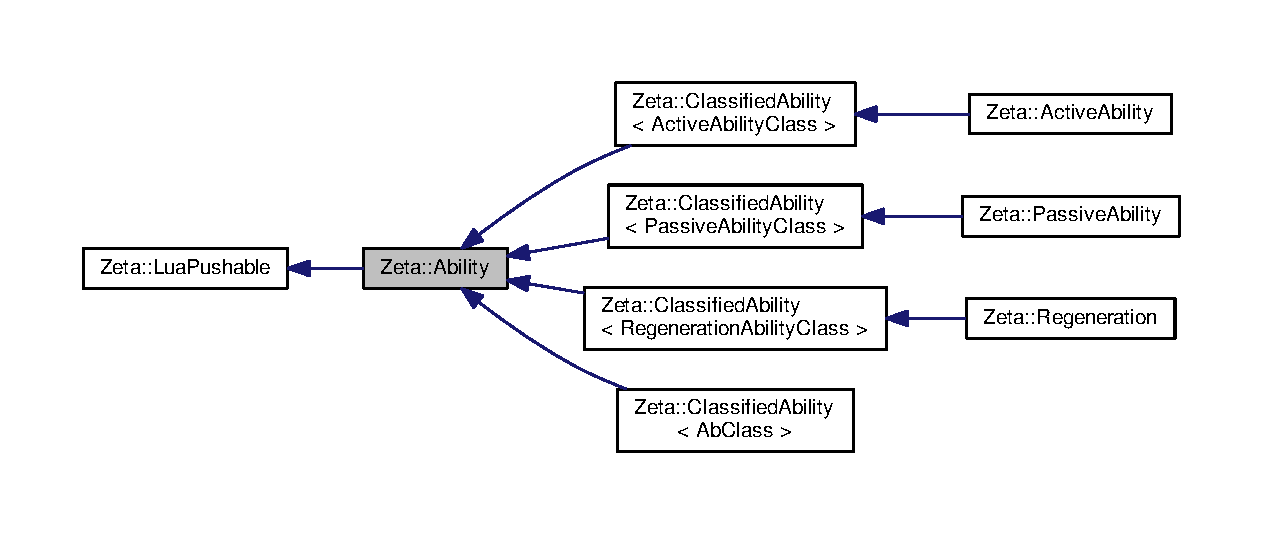
\includegraphics[width=350pt]{classZeta_1_1Ability__inherit__graph}
\end{center}
\end{figure}


Collaboration diagram for Zeta\+:\+:Ability\+:
\nopagebreak
\begin{figure}[H]
\begin{center}
\leavevmode
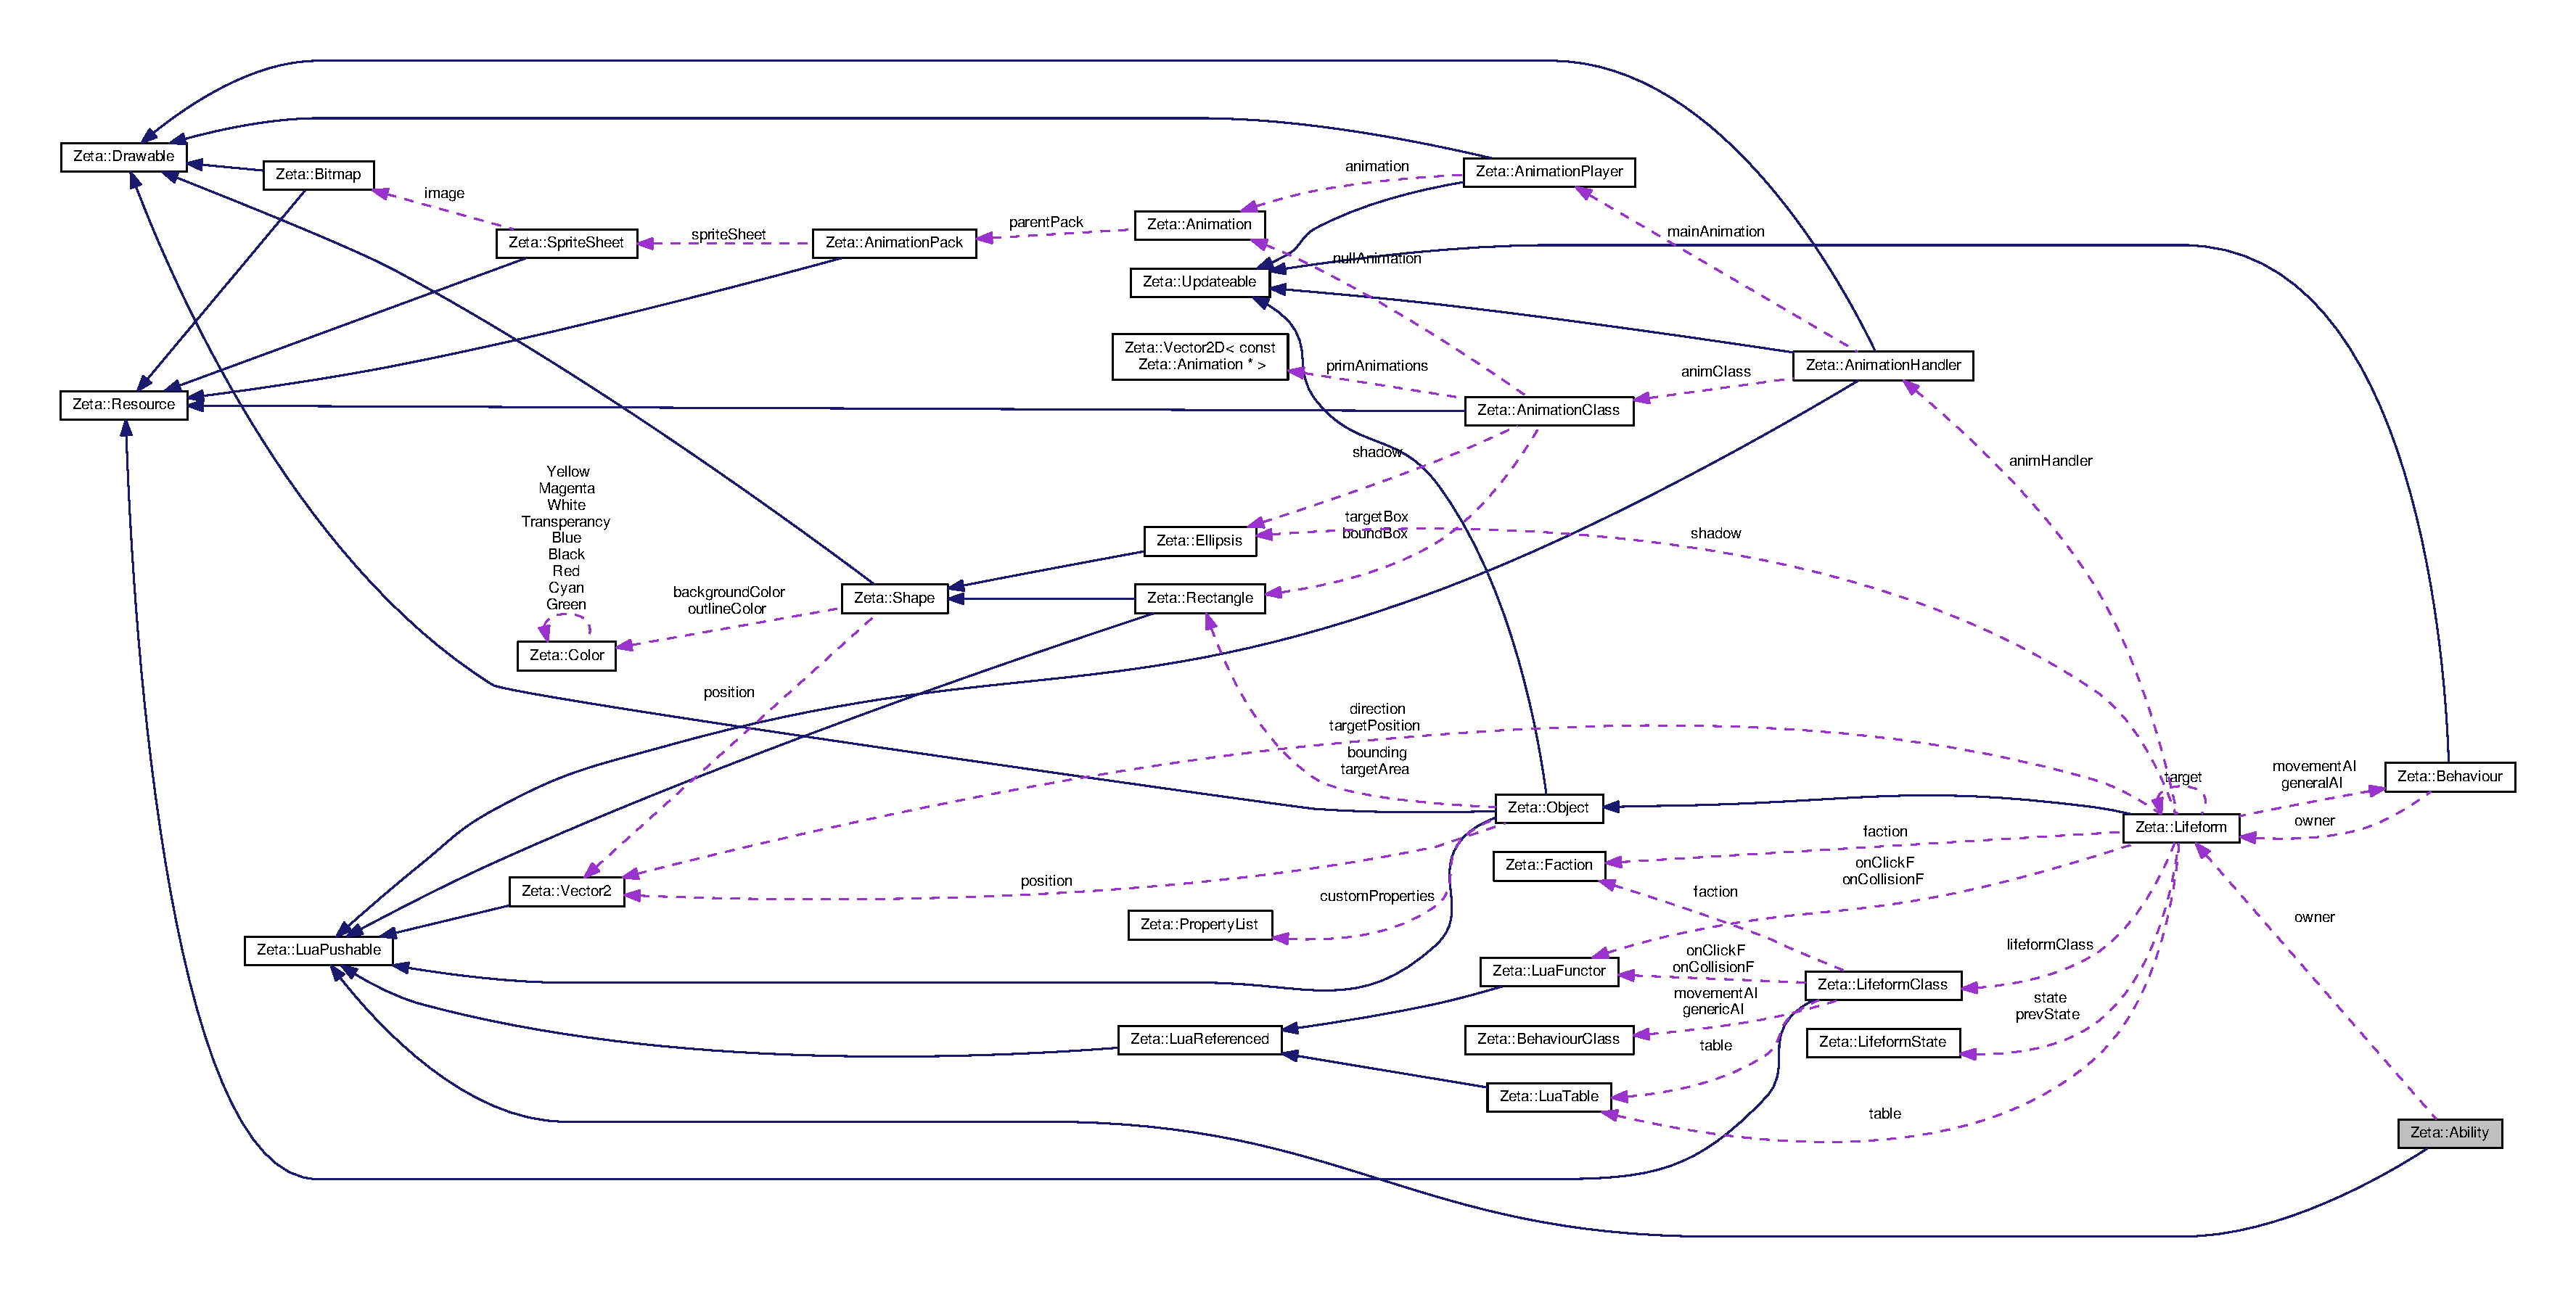
\includegraphics[width=350pt]{classZeta_1_1Ability__coll__graph}
\end{center}
\end{figure}
\subsection*{Public Types}
\begin{DoxyCompactItemize}
\item 
enum \hyperlink{classZeta_1_1Ability_acbc80e4d82c9683d190ed8ca1c80f597}{Result} \{ \\*
\hyperlink{classZeta_1_1Ability_acbc80e4d82c9683d190ed8ca1c80f597a505a83f220c02df2f85c3810cd9ceb38}{Result\+::\+Success}, 
\hyperlink{classZeta_1_1Ability_acbc80e4d82c9683d190ed8ca1c80f597ae3c0ba3c83c17a047a9a5c4f53be2217}{Result\+::on\+Cooldown}, 
\hyperlink{classZeta_1_1Ability_acbc80e4d82c9683d190ed8ca1c80f597aff4d8f7b051f09ecae01888dda54c15c}{Result\+::\+No\+Target}, 
\hyperlink{classZeta_1_1Ability_acbc80e4d82c9683d190ed8ca1c80f597a78833d84bf23f43a08b9ad42eb11dd89}{Result\+::\+No\+Mana}, 
\\*
\hyperlink{classZeta_1_1Ability_acbc80e4d82c9683d190ed8ca1c80f597a365b2699d38b61ef4b4c8a1066c8468f}{Result\+::\+Out\+Of\+Range}, 
\hyperlink{classZeta_1_1Ability_acbc80e4d82c9683d190ed8ca1c80f597ac926f8700f3a5b1ae6f9ef9675ca93fd}{Result\+::\+Target\+Is\+Dead}, 
\hyperlink{classZeta_1_1Ability_acbc80e4d82c9683d190ed8ca1c80f597aff0026030492922584aab202394db49a}{Result\+::\+Target\+Is\+Not\+Hostile}, 
\hyperlink{classZeta_1_1Ability_acbc80e4d82c9683d190ed8ca1c80f597a48c2128daef352af23cb92c859d06d5f}{Result\+::\+Invalid\+Ability}, 
\\*
\hyperlink{classZeta_1_1Ability_acbc80e4d82c9683d190ed8ca1c80f597a6311ae17c1ee52b36e68aaf4ad066387}{Result\+::\+Other}
 \}
\end{DoxyCompactItemize}
\subsection*{Public Member Functions}
\begin{DoxyCompactItemize}
\item 
int \hyperlink{classZeta_1_1Ability_a472b49c779602e2839a0afa4a504ebf0}{get\+Level} () const 
\item 
void \hyperlink{classZeta_1_1Ability_af8e3a64ad3b461ee91cc10b896a16684}{set\+Level} (int \hyperlink{classZeta_1_1Ability_a41d29a6fb79dd19a7eed5f6a4be5de9a}{level})
\item 
\hyperlink{classZeta_1_1Lifeform}{Lifeform} \& \hyperlink{classZeta_1_1Ability_a3bec1acb0d85225a0b067bc14b497100}{get\+Owner} ()
\item 
void \hyperlink{classZeta_1_1Ability_a14e4cb9c0e8b9d35bd46659291f73f76}{set\+Owner} (\hyperlink{classZeta_1_1Lifeform}{Lifeform} $\ast$\hyperlink{classZeta_1_1Ability_ad37bed67f04178297d6fe4c9a2ed619a}{owner})
\item 
\hyperlink{classZeta_1_1Ability_aeb18eb5f68dec2d1a7fc15cf35ba35e6}{Ability} (\hyperlink{classZeta_1_1Lifeform}{Lifeform} $\ast$\hyperlink{classZeta_1_1Ability_ad37bed67f04178297d6fe4c9a2ed619a}{owner}, int \hyperlink{classZeta_1_1Ability_a41d29a6fb79dd19a7eed5f6a4be5de9a}{level})
\item 
virtual \hyperlink{classZeta_1_1Ability_a234169c0dbb3ffe0086ca628901b705d}{$\sim$\+Ability} ()
\end{DoxyCompactItemize}
\subsection*{Protected Member Functions}
\begin{DoxyCompactItemize}
\item 
\hyperlink{classZeta_1_1Ability_a8400f68abcd13d41bfbb1d1cc03b38ff}{Ability} ()
\item 
virtual void \hyperlink{classZeta_1_1Ability_ac81e774451daa9476b02ba442a2ea047}{on\+Level\+Change} ()=0
\end{DoxyCompactItemize}
\subsection*{Protected Attributes}
\begin{DoxyCompactItemize}
\item 
\hyperlink{classZeta_1_1Lifeform}{Lifeform} $\ast$ \hyperlink{classZeta_1_1Ability_ad37bed67f04178297d6fe4c9a2ed619a}{owner}
\item 
int \hyperlink{classZeta_1_1Ability_a41d29a6fb79dd19a7eed5f6a4be5de9a}{level}
\end{DoxyCompactItemize}


\subsection{Member Enumeration Documentation}
\hypertarget{classZeta_1_1Ability_acbc80e4d82c9683d190ed8ca1c80f597}{\index{Zeta\+::\+Ability@{Zeta\+::\+Ability}!Result@{Result}}
\index{Result@{Result}!Zeta\+::\+Ability@{Zeta\+::\+Ability}}
\subsubsection[{Result}]{\setlength{\rightskip}{0pt plus 5cm}enum {\bf Zeta\+::\+Ability\+::\+Result}\hspace{0.3cm}{\ttfamily [strong]}}}\label{classZeta_1_1Ability_acbc80e4d82c9683d190ed8ca1c80f597}
\begin{Desc}
\item[Enumerator]\par
\begin{description}
\index{Success@{Success}!Zeta\+::\+Ability@{Zeta\+::\+Ability}}\index{Zeta\+::\+Ability@{Zeta\+::\+Ability}!Success@{Success}}\item[{\em 
\hypertarget{classZeta_1_1Ability_acbc80e4d82c9683d190ed8ca1c80f597a505a83f220c02df2f85c3810cd9ceb38}{Success}\label{classZeta_1_1Ability_acbc80e4d82c9683d190ed8ca1c80f597a505a83f220c02df2f85c3810cd9ceb38}
}]\index{on\+Cooldown@{on\+Cooldown}!Zeta\+::\+Ability@{Zeta\+::\+Ability}}\index{Zeta\+::\+Ability@{Zeta\+::\+Ability}!on\+Cooldown@{on\+Cooldown}}\item[{\em 
\hypertarget{classZeta_1_1Ability_acbc80e4d82c9683d190ed8ca1c80f597ae3c0ba3c83c17a047a9a5c4f53be2217}{on\+Cooldown}\label{classZeta_1_1Ability_acbc80e4d82c9683d190ed8ca1c80f597ae3c0ba3c83c17a047a9a5c4f53be2217}
}]\index{No\+Target@{No\+Target}!Zeta\+::\+Ability@{Zeta\+::\+Ability}}\index{Zeta\+::\+Ability@{Zeta\+::\+Ability}!No\+Target@{No\+Target}}\item[{\em 
\hypertarget{classZeta_1_1Ability_acbc80e4d82c9683d190ed8ca1c80f597aff4d8f7b051f09ecae01888dda54c15c}{No\+Target}\label{classZeta_1_1Ability_acbc80e4d82c9683d190ed8ca1c80f597aff4d8f7b051f09ecae01888dda54c15c}
}]\index{No\+Mana@{No\+Mana}!Zeta\+::\+Ability@{Zeta\+::\+Ability}}\index{Zeta\+::\+Ability@{Zeta\+::\+Ability}!No\+Mana@{No\+Mana}}\item[{\em 
\hypertarget{classZeta_1_1Ability_acbc80e4d82c9683d190ed8ca1c80f597a78833d84bf23f43a08b9ad42eb11dd89}{No\+Mana}\label{classZeta_1_1Ability_acbc80e4d82c9683d190ed8ca1c80f597a78833d84bf23f43a08b9ad42eb11dd89}
}]\index{Out\+Of\+Range@{Out\+Of\+Range}!Zeta\+::\+Ability@{Zeta\+::\+Ability}}\index{Zeta\+::\+Ability@{Zeta\+::\+Ability}!Out\+Of\+Range@{Out\+Of\+Range}}\item[{\em 
\hypertarget{classZeta_1_1Ability_acbc80e4d82c9683d190ed8ca1c80f597a365b2699d38b61ef4b4c8a1066c8468f}{Out\+Of\+Range}\label{classZeta_1_1Ability_acbc80e4d82c9683d190ed8ca1c80f597a365b2699d38b61ef4b4c8a1066c8468f}
}]\index{Target\+Is\+Dead@{Target\+Is\+Dead}!Zeta\+::\+Ability@{Zeta\+::\+Ability}}\index{Zeta\+::\+Ability@{Zeta\+::\+Ability}!Target\+Is\+Dead@{Target\+Is\+Dead}}\item[{\em 
\hypertarget{classZeta_1_1Ability_acbc80e4d82c9683d190ed8ca1c80f597ac926f8700f3a5b1ae6f9ef9675ca93fd}{Target\+Is\+Dead}\label{classZeta_1_1Ability_acbc80e4d82c9683d190ed8ca1c80f597ac926f8700f3a5b1ae6f9ef9675ca93fd}
}]\index{Target\+Is\+Not\+Hostile@{Target\+Is\+Not\+Hostile}!Zeta\+::\+Ability@{Zeta\+::\+Ability}}\index{Zeta\+::\+Ability@{Zeta\+::\+Ability}!Target\+Is\+Not\+Hostile@{Target\+Is\+Not\+Hostile}}\item[{\em 
\hypertarget{classZeta_1_1Ability_acbc80e4d82c9683d190ed8ca1c80f597aff0026030492922584aab202394db49a}{Target\+Is\+Not\+Hostile}\label{classZeta_1_1Ability_acbc80e4d82c9683d190ed8ca1c80f597aff0026030492922584aab202394db49a}
}]\index{Invalid\+Ability@{Invalid\+Ability}!Zeta\+::\+Ability@{Zeta\+::\+Ability}}\index{Zeta\+::\+Ability@{Zeta\+::\+Ability}!Invalid\+Ability@{Invalid\+Ability}}\item[{\em 
\hypertarget{classZeta_1_1Ability_acbc80e4d82c9683d190ed8ca1c80f597a48c2128daef352af23cb92c859d06d5f}{Invalid\+Ability}\label{classZeta_1_1Ability_acbc80e4d82c9683d190ed8ca1c80f597a48c2128daef352af23cb92c859d06d5f}
}]\index{Other@{Other}!Zeta\+::\+Ability@{Zeta\+::\+Ability}}\index{Zeta\+::\+Ability@{Zeta\+::\+Ability}!Other@{Other}}\item[{\em 
\hypertarget{classZeta_1_1Ability_acbc80e4d82c9683d190ed8ca1c80f597a6311ae17c1ee52b36e68aaf4ad066387}{Other}\label{classZeta_1_1Ability_acbc80e4d82c9683d190ed8ca1c80f597a6311ae17c1ee52b36e68aaf4ad066387}
}]\end{description}
\end{Desc}


\subsection{Constructor \& Destructor Documentation}
\hypertarget{classZeta_1_1Ability_aeb18eb5f68dec2d1a7fc15cf35ba35e6}{\index{Zeta\+::\+Ability@{Zeta\+::\+Ability}!Ability@{Ability}}
\index{Ability@{Ability}!Zeta\+::\+Ability@{Zeta\+::\+Ability}}
\subsubsection[{Ability}]{\setlength{\rightskip}{0pt plus 5cm}Zeta\+::\+Ability\+::\+Ability (
\begin{DoxyParamCaption}
\item[{{\bf Lifeform} $\ast$}]{owner, }
\item[{int}]{level}
\end{DoxyParamCaption}
)\hspace{0.3cm}{\ttfamily [inline]}}}\label{classZeta_1_1Ability_aeb18eb5f68dec2d1a7fc15cf35ba35e6}
\hypertarget{classZeta_1_1Ability_a234169c0dbb3ffe0086ca628901b705d}{\index{Zeta\+::\+Ability@{Zeta\+::\+Ability}!````~Ability@{$\sim$\+Ability}}
\index{````~Ability@{$\sim$\+Ability}!Zeta\+::\+Ability@{Zeta\+::\+Ability}}
\subsubsection[{$\sim$\+Ability}]{\setlength{\rightskip}{0pt plus 5cm}virtual Zeta\+::\+Ability\+::$\sim$\+Ability (
\begin{DoxyParamCaption}
{}
\end{DoxyParamCaption}
)\hspace{0.3cm}{\ttfamily [inline]}, {\ttfamily [virtual]}}}\label{classZeta_1_1Ability_a234169c0dbb3ffe0086ca628901b705d}
\hypertarget{classZeta_1_1Ability_a8400f68abcd13d41bfbb1d1cc03b38ff}{\index{Zeta\+::\+Ability@{Zeta\+::\+Ability}!Ability@{Ability}}
\index{Ability@{Ability}!Zeta\+::\+Ability@{Zeta\+::\+Ability}}
\subsubsection[{Ability}]{\setlength{\rightskip}{0pt plus 5cm}Zeta\+::\+Ability\+::\+Ability (
\begin{DoxyParamCaption}
{}
\end{DoxyParamCaption}
)\hspace{0.3cm}{\ttfamily [inline]}, {\ttfamily [protected]}}}\label{classZeta_1_1Ability_a8400f68abcd13d41bfbb1d1cc03b38ff}


\subsection{Member Function Documentation}
\hypertarget{classZeta_1_1Ability_a472b49c779602e2839a0afa4a504ebf0}{\index{Zeta\+::\+Ability@{Zeta\+::\+Ability}!get\+Level@{get\+Level}}
\index{get\+Level@{get\+Level}!Zeta\+::\+Ability@{Zeta\+::\+Ability}}
\subsubsection[{get\+Level}]{\setlength{\rightskip}{0pt plus 5cm}int Zeta\+::\+Ability\+::get\+Level (
\begin{DoxyParamCaption}
{}
\end{DoxyParamCaption}
) const\hspace{0.3cm}{\ttfamily [inline]}}}\label{classZeta_1_1Ability_a472b49c779602e2839a0afa4a504ebf0}
\hypertarget{classZeta_1_1Ability_a3bec1acb0d85225a0b067bc14b497100}{\index{Zeta\+::\+Ability@{Zeta\+::\+Ability}!get\+Owner@{get\+Owner}}
\index{get\+Owner@{get\+Owner}!Zeta\+::\+Ability@{Zeta\+::\+Ability}}
\subsubsection[{get\+Owner}]{\setlength{\rightskip}{0pt plus 5cm}{\bf Lifeform}\& Zeta\+::\+Ability\+::get\+Owner (
\begin{DoxyParamCaption}
{}
\end{DoxyParamCaption}
)\hspace{0.3cm}{\ttfamily [inline]}}}\label{classZeta_1_1Ability_a3bec1acb0d85225a0b067bc14b497100}
\hypertarget{classZeta_1_1Ability_ac81e774451daa9476b02ba442a2ea047}{\index{Zeta\+::\+Ability@{Zeta\+::\+Ability}!on\+Level\+Change@{on\+Level\+Change}}
\index{on\+Level\+Change@{on\+Level\+Change}!Zeta\+::\+Ability@{Zeta\+::\+Ability}}
\subsubsection[{on\+Level\+Change}]{\setlength{\rightskip}{0pt plus 5cm}virtual void Zeta\+::\+Ability\+::on\+Level\+Change (
\begin{DoxyParamCaption}
{}
\end{DoxyParamCaption}
)\hspace{0.3cm}{\ttfamily [protected]}, {\ttfamily [pure virtual]}}}\label{classZeta_1_1Ability_ac81e774451daa9476b02ba442a2ea047}


Implemented in \hyperlink{classZeta_1_1ActiveAbility_a6a2a131788a14830aba711262235cf26}{Zeta\+::\+Active\+Ability}, \hyperlink{classZeta_1_1Regeneration_a937aac46f00754b7d1e4e757b8c4a252}{Zeta\+::\+Regeneration}, and \hyperlink{classZeta_1_1PassiveAbility_aef651b48cfdd153aca93192cdc5f7ccd}{Zeta\+::\+Passive\+Ability}.

\hypertarget{classZeta_1_1Ability_af8e3a64ad3b461ee91cc10b896a16684}{\index{Zeta\+::\+Ability@{Zeta\+::\+Ability}!set\+Level@{set\+Level}}
\index{set\+Level@{set\+Level}!Zeta\+::\+Ability@{Zeta\+::\+Ability}}
\subsubsection[{set\+Level}]{\setlength{\rightskip}{0pt plus 5cm}void Zeta\+::\+Ability\+::set\+Level (
\begin{DoxyParamCaption}
\item[{int}]{level}
\end{DoxyParamCaption}
)\hspace{0.3cm}{\ttfamily [inline]}}}\label{classZeta_1_1Ability_af8e3a64ad3b461ee91cc10b896a16684}


Here is the call graph for this function\+:\nopagebreak
\begin{figure}[H]
\begin{center}
\leavevmode
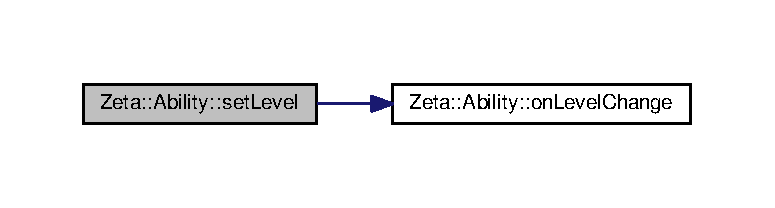
\includegraphics[width=350pt]{classZeta_1_1Ability_af8e3a64ad3b461ee91cc10b896a16684_cgraph}
\end{center}
\end{figure}


\hypertarget{classZeta_1_1Ability_a14e4cb9c0e8b9d35bd46659291f73f76}{\index{Zeta\+::\+Ability@{Zeta\+::\+Ability}!set\+Owner@{set\+Owner}}
\index{set\+Owner@{set\+Owner}!Zeta\+::\+Ability@{Zeta\+::\+Ability}}
\subsubsection[{set\+Owner}]{\setlength{\rightskip}{0pt plus 5cm}void Zeta\+::\+Ability\+::set\+Owner (
\begin{DoxyParamCaption}
\item[{{\bf Lifeform} $\ast$}]{owner}
\end{DoxyParamCaption}
)\hspace{0.3cm}{\ttfamily [inline]}}}\label{classZeta_1_1Ability_a14e4cb9c0e8b9d35bd46659291f73f76}


\subsection{Member Data Documentation}
\hypertarget{classZeta_1_1Ability_a41d29a6fb79dd19a7eed5f6a4be5de9a}{\index{Zeta\+::\+Ability@{Zeta\+::\+Ability}!level@{level}}
\index{level@{level}!Zeta\+::\+Ability@{Zeta\+::\+Ability}}
\subsubsection[{level}]{\setlength{\rightskip}{0pt plus 5cm}int Zeta\+::\+Ability\+::level\hspace{0.3cm}{\ttfamily [protected]}}}\label{classZeta_1_1Ability_a41d29a6fb79dd19a7eed5f6a4be5de9a}
\hypertarget{classZeta_1_1Ability_ad37bed67f04178297d6fe4c9a2ed619a}{\index{Zeta\+::\+Ability@{Zeta\+::\+Ability}!owner@{owner}}
\index{owner@{owner}!Zeta\+::\+Ability@{Zeta\+::\+Ability}}
\subsubsection[{owner}]{\setlength{\rightskip}{0pt plus 5cm}{\bf Lifeform}$\ast$ Zeta\+::\+Ability\+::owner\hspace{0.3cm}{\ttfamily [protected]}}}\label{classZeta_1_1Ability_ad37bed67f04178297d6fe4c9a2ed619a}


The documentation for this class was generated from the following file\+:\begin{DoxyCompactItemize}
\item 
include/\+Zeta/\+Core/\+R\+P\+G\+Classes/\hyperlink{Ability_8hpp}{Ability.\+hpp}\end{DoxyCompactItemize}

\hypertarget{classZeta_1_1AbilityClass}{\section{Zeta\+:\+:Ability\+Class Class Reference}
\label{classZeta_1_1AbilityClass}\index{Zeta\+::\+Ability\+Class@{Zeta\+::\+Ability\+Class}}
}


{\ttfamily \#include $<$Ability\+Class.\+hpp$>$}



Inheritance diagram for Zeta\+:\+:Ability\+Class\+:\nopagebreak
\begin{figure}[H]
\begin{center}
\leavevmode
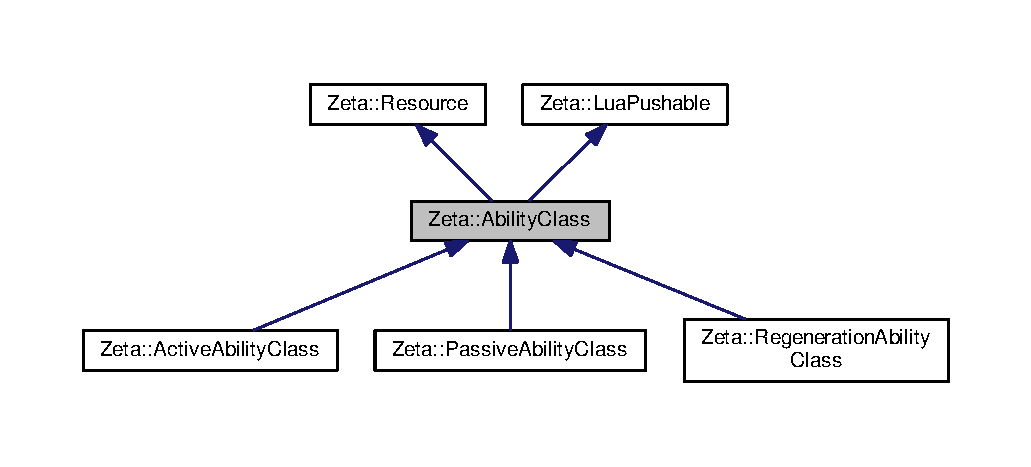
\includegraphics[width=350pt]{classZeta_1_1AbilityClass__inherit__graph}
\end{center}
\end{figure}


Collaboration diagram for Zeta\+:\+:Ability\+Class\+:\nopagebreak
\begin{figure}[H]
\begin{center}
\leavevmode
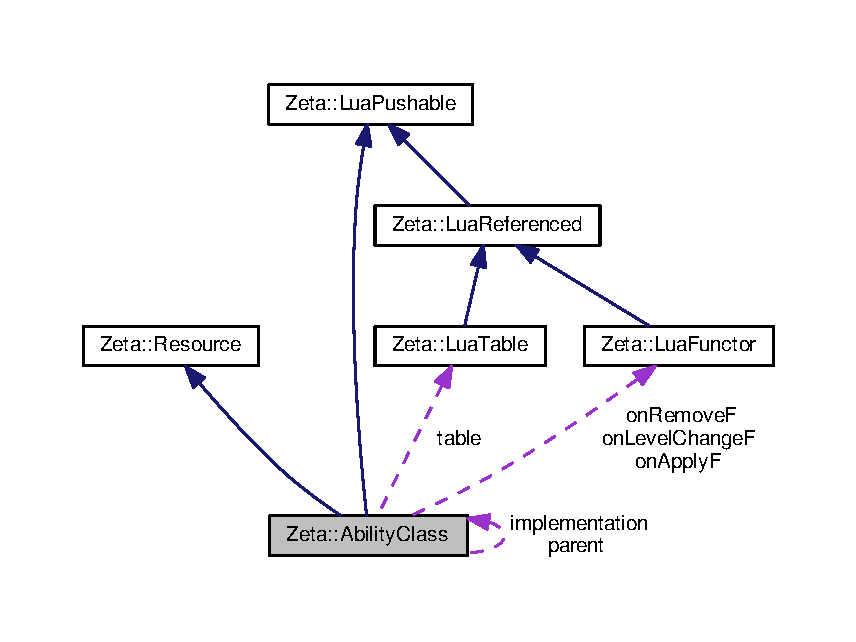
\includegraphics[width=350pt]{classZeta_1_1AbilityClass__coll__graph}
\end{center}
\end{figure}
\subsection*{Public Types}
\begin{DoxyCompactItemize}
\item 
enum \hyperlink{classZeta_1_1AbilityClass_a371c2c662780f1c4a796a3332d6568b3}{Type} \{ \hyperlink{classZeta_1_1AbilityClass_a371c2c662780f1c4a796a3332d6568b3a4d3d769b812b6faa6b76e1a8abaece2d}{Type\+::\+Active}, 
\hyperlink{classZeta_1_1AbilityClass_a371c2c662780f1c4a796a3332d6568b3af80bc338b6146b566004a046f8137c85}{Type\+::\+Passive}, 
\hyperlink{classZeta_1_1AbilityClass_a371c2c662780f1c4a796a3332d6568b3a93fb94ede88fe65704d75647dfc6595f}{Type\+::\+Regeneration}
 \}
\end{DoxyCompactItemize}
\subsection*{Public Member Functions}
\begin{DoxyCompactItemize}
\item 
int \hyperlink{classZeta_1_1AbilityClass_a727597e2c4d3452ca33b8754b61fc6fc}{get\+Levels} () const 
\item 
const std\+::string \& \hyperlink{classZeta_1_1AbilityClass_a3035a01ec5eb65fe6429147e96edf9e9}{get\+Ability\+Name} () const 
\item 
bool \hyperlink{classZeta_1_1AbilityClass_acaaa4b554085556b2bf56e6cf2c2e960}{is\+Passive} () const 
\item 
\hyperlink{classZeta_1_1AbilityClass_a371c2c662780f1c4a796a3332d6568b3}{Type} \hyperlink{classZeta_1_1AbilityClass_a36853a94f0caffa6ac3f31c38e5bdcda}{get\+Type} () const 
\item 
const \hyperlink{classZeta_1_1AbilityClass}{Ability\+Class} $\ast$ \hyperlink{classZeta_1_1AbilityClass_aadac51d50e52982bc72a2a91e9bc33c4}{get\+Parent} () const 
\item 
const \hyperlink{classZeta_1_1LuaTable}{Lua\+Table} \& \hyperlink{classZeta_1_1AbilityClass_a6442689e370a2843fe2b7e3d14c957a3}{get\+Table} () const 
\item 
\hyperlink{ZetaConfig_8hpp_ae7be32b73848041a60f2412f72bbb221}{lua\+\_\+\+Object} \hyperlink{classZeta_1_1AbilityClass_a32bf638f5d5c1430e369943d43ce00fe}{get\+Lua\+Table} () const 
\item 
void \hyperlink{classZeta_1_1AbilityClass_a36fbfde58302cc1ad1fd728d25865973}{on\+Apply} (\hyperlink{classZeta_1_1Ability}{Ability} $\ast$invoker, \hyperlink{classZeta_1_1Lifeform}{Lifeform} $\ast$caster, \hyperlink{classZeta_1_1Lifeform}{Lifeform} $\ast$target) const 
\item 
void \hyperlink{classZeta_1_1AbilityClass_a16f5bd30070add8d629a05d2de54b8f5}{on\+Remove} (\hyperlink{classZeta_1_1Ability}{Ability} $\ast$invoker, \hyperlink{classZeta_1_1Lifeform}{Lifeform} $\ast$caster, \hyperlink{classZeta_1_1Lifeform}{Lifeform} $\ast$target) const 
\item 
void \hyperlink{classZeta_1_1AbilityClass_a6ab615405530bc3ab616ebc555a70904}{on\+Level\+Change} (\hyperlink{classZeta_1_1Ability}{Ability} $\ast$invoker) const 
\item 
virtual \hyperlink{classZeta_1_1Ability}{Ability} $\ast$ \hyperlink{classZeta_1_1AbilityClass_a15470bcd0795b12410e6f138a1b1a804}{get\+New\+Ability} (\hyperlink{classZeta_1_1Lifeform}{Lifeform} $\ast$caster, int level) const 
\item 
virtual void \hyperlink{classZeta_1_1AbilityClass_a3535ae18fef8d447febab98c85e169f3}{push\+To\+Lua} (lua\+\_\+\+State $\ast$lstate)
\item 
\hyperlink{classZeta_1_1AbilityClass_afbdb2842a741a1ec61d368b7feba0c8b}{Ability\+Class} ()
\item 
\hyperlink{classZeta_1_1AbilityClass_a148bb2b5a878395c3438bb26e8227c51}{Ability\+Class} (const std\+::string \&path)
\item 
\hyperlink{classZeta_1_1AbilityClass_a2e016d5e1a98e26e1804c8b1207d7f07}{Ability\+Class} (\hyperlink{ZetaConfig_8hpp_ae7be32b73848041a60f2412f72bbb221}{lua\+\_\+\+Object} \hyperlink{classZeta_1_1AbilityClass_a58065ca9d19ff9366c09bfc8d81abbac}{table})
\item 
\hyperlink{classZeta_1_1AbilityClass_ad69921fb28e2f0b2caae837c56025913}{Ability\+Class} (\hyperlink{classZeta_1_1AbilityClass}{Ability\+Class} \&\hyperlink{classZeta_1_1AbilityClass_ad862e9ba14d23afb20786a1eeb2ca872}{parent}, \hyperlink{classZeta_1_1LuaTable}{Lua\+Table} \&\hyperlink{classZeta_1_1AbilityClass_a58065ca9d19ff9366c09bfc8d81abbac}{table})
\item 
virtual \hyperlink{classZeta_1_1AbilityClass_a0ae1dbc0026536a2a2b6074885899bd6}{$\sim$\+Ability\+Class} ()
\end{DoxyCompactItemize}
\subsection*{Protected Member Functions}
\begin{DoxyCompactItemize}
\item 
void \hyperlink{classZeta_1_1AbilityClass_a22c6c3ac2ca9c1c9ba048a27bb3fca04}{get\+Data} (\hyperlink{classZeta_1_1LuaTable}{Lua\+Table} \&\hyperlink{classZeta_1_1AbilityClass_a58065ca9d19ff9366c09bfc8d81abbac}{table})
\item 
void \hyperlink{classZeta_1_1AbilityClass_acb06bb30168d885e2aa583296f0e7396}{nullise} ()
\end{DoxyCompactItemize}
\subsection*{Protected Attributes}
\begin{DoxyCompactItemize}
\item 
std\+::string \hyperlink{classZeta_1_1AbilityClass_af998b8b5d45ef4853cfac4afe78aff4d}{ability\+Name}
\item 
\hyperlink{classZeta_1_1LuaTable}{Lua\+Table} \hyperlink{classZeta_1_1AbilityClass_a58065ca9d19ff9366c09bfc8d81abbac}{table}
\item 
\hyperlink{classZeta_1_1LuaFunctor}{Lua\+Functor} \hyperlink{classZeta_1_1AbilityClass_a74da9c30cf5040a98cfd8d69c90538cd}{on\+Apply\+F}
\item 
\hyperlink{classZeta_1_1LuaFunctor}{Lua\+Functor} \hyperlink{classZeta_1_1AbilityClass_ace27cfeff8dfc3e4af385d72a010f4b9}{on\+Remove\+F}
\item 
\hyperlink{classZeta_1_1LuaFunctor}{Lua\+Functor} \hyperlink{classZeta_1_1AbilityClass_a030755a406dea76a11609e1cca3a4ea3}{on\+Level\+Change\+F}
\item 
\hyperlink{classZeta_1_1AbilityClass}{Ability\+Class} $\ast$ \hyperlink{classZeta_1_1AbilityClass_a4a0d26c946a8b406ec6394849c931a51}{implementation}
\item 
\hyperlink{classZeta_1_1AbilityClass}{Ability\+Class} $\ast$ \hyperlink{classZeta_1_1AbilityClass_ad862e9ba14d23afb20786a1eeb2ca872}{parent}
\item 
int \hyperlink{classZeta_1_1AbilityClass_a8524be37623bb3ba701d9727be8ab042}{levels}
\item 
\hyperlink{classZeta_1_1AbilityClass_a371c2c662780f1c4a796a3332d6568b3}{Type} \hyperlink{classZeta_1_1AbilityClass_a4ffb80485a1b4321c6c243d80dce1ed5}{type}
\end{DoxyCompactItemize}


\subsection{Member Enumeration Documentation}
\hypertarget{classZeta_1_1AbilityClass_a371c2c662780f1c4a796a3332d6568b3}{\index{Zeta\+::\+Ability\+Class@{Zeta\+::\+Ability\+Class}!Type@{Type}}
\index{Type@{Type}!Zeta\+::\+Ability\+Class@{Zeta\+::\+Ability\+Class}}
\subsubsection[{Type}]{\setlength{\rightskip}{0pt plus 5cm}enum {\bf Zeta\+::\+Ability\+Class\+::\+Type}\hspace{0.3cm}{\ttfamily [strong]}}}\label{classZeta_1_1AbilityClass_a371c2c662780f1c4a796a3332d6568b3}
\begin{Desc}
\item[Enumerator]\par
\begin{description}
\index{Active@{Active}!Zeta\+::\+Ability\+Class@{Zeta\+::\+Ability\+Class}}\index{Zeta\+::\+Ability\+Class@{Zeta\+::\+Ability\+Class}!Active@{Active}}\item[{\em 
\hypertarget{classZeta_1_1AbilityClass_a371c2c662780f1c4a796a3332d6568b3a4d3d769b812b6faa6b76e1a8abaece2d}{Active}\label{classZeta_1_1AbilityClass_a371c2c662780f1c4a796a3332d6568b3a4d3d769b812b6faa6b76e1a8abaece2d}
}]\index{Passive@{Passive}!Zeta\+::\+Ability\+Class@{Zeta\+::\+Ability\+Class}}\index{Zeta\+::\+Ability\+Class@{Zeta\+::\+Ability\+Class}!Passive@{Passive}}\item[{\em 
\hypertarget{classZeta_1_1AbilityClass_a371c2c662780f1c4a796a3332d6568b3af80bc338b6146b566004a046f8137c85}{Passive}\label{classZeta_1_1AbilityClass_a371c2c662780f1c4a796a3332d6568b3af80bc338b6146b566004a046f8137c85}
}]\index{Regeneration@{Regeneration}!Zeta\+::\+Ability\+Class@{Zeta\+::\+Ability\+Class}}\index{Zeta\+::\+Ability\+Class@{Zeta\+::\+Ability\+Class}!Regeneration@{Regeneration}}\item[{\em 
\hypertarget{classZeta_1_1AbilityClass_a371c2c662780f1c4a796a3332d6568b3a93fb94ede88fe65704d75647dfc6595f}{Regeneration}\label{classZeta_1_1AbilityClass_a371c2c662780f1c4a796a3332d6568b3a93fb94ede88fe65704d75647dfc6595f}
}]\end{description}
\end{Desc}


\subsection{Constructor \& Destructor Documentation}
\hypertarget{classZeta_1_1AbilityClass_afbdb2842a741a1ec61d368b7feba0c8b}{\index{Zeta\+::\+Ability\+Class@{Zeta\+::\+Ability\+Class}!Ability\+Class@{Ability\+Class}}
\index{Ability\+Class@{Ability\+Class}!Zeta\+::\+Ability\+Class@{Zeta\+::\+Ability\+Class}}
\subsubsection[{Ability\+Class}]{\setlength{\rightskip}{0pt plus 5cm}Zeta\+::\+Ability\+Class\+::\+Ability\+Class (
\begin{DoxyParamCaption}
{}
\end{DoxyParamCaption}
)}}\label{classZeta_1_1AbilityClass_afbdb2842a741a1ec61d368b7feba0c8b}
\hypertarget{classZeta_1_1AbilityClass_a148bb2b5a878395c3438bb26e8227c51}{\index{Zeta\+::\+Ability\+Class@{Zeta\+::\+Ability\+Class}!Ability\+Class@{Ability\+Class}}
\index{Ability\+Class@{Ability\+Class}!Zeta\+::\+Ability\+Class@{Zeta\+::\+Ability\+Class}}
\subsubsection[{Ability\+Class}]{\setlength{\rightskip}{0pt plus 5cm}Zeta\+::\+Ability\+Class\+::\+Ability\+Class (
\begin{DoxyParamCaption}
\item[{const std\+::string \&}]{path}
\end{DoxyParamCaption}
)}}\label{classZeta_1_1AbilityClass_a148bb2b5a878395c3438bb26e8227c51}
\hypertarget{classZeta_1_1AbilityClass_a2e016d5e1a98e26e1804c8b1207d7f07}{\index{Zeta\+::\+Ability\+Class@{Zeta\+::\+Ability\+Class}!Ability\+Class@{Ability\+Class}}
\index{Ability\+Class@{Ability\+Class}!Zeta\+::\+Ability\+Class@{Zeta\+::\+Ability\+Class}}
\subsubsection[{Ability\+Class}]{\setlength{\rightskip}{0pt plus 5cm}Zeta\+::\+Ability\+Class\+::\+Ability\+Class (
\begin{DoxyParamCaption}
\item[{{\bf lua\+\_\+\+Object}}]{table}
\end{DoxyParamCaption}
)}}\label{classZeta_1_1AbilityClass_a2e016d5e1a98e26e1804c8b1207d7f07}
\hypertarget{classZeta_1_1AbilityClass_ad69921fb28e2f0b2caae837c56025913}{\index{Zeta\+::\+Ability\+Class@{Zeta\+::\+Ability\+Class}!Ability\+Class@{Ability\+Class}}
\index{Ability\+Class@{Ability\+Class}!Zeta\+::\+Ability\+Class@{Zeta\+::\+Ability\+Class}}
\subsubsection[{Ability\+Class}]{\setlength{\rightskip}{0pt plus 5cm}Zeta\+::\+Ability\+Class\+::\+Ability\+Class (
\begin{DoxyParamCaption}
\item[{{\bf Ability\+Class} \&}]{parent, }
\item[{{\bf Lua\+Table} \&}]{table}
\end{DoxyParamCaption}
)}}\label{classZeta_1_1AbilityClass_ad69921fb28e2f0b2caae837c56025913}
\hypertarget{classZeta_1_1AbilityClass_a0ae1dbc0026536a2a2b6074885899bd6}{\index{Zeta\+::\+Ability\+Class@{Zeta\+::\+Ability\+Class}!````~Ability\+Class@{$\sim$\+Ability\+Class}}
\index{````~Ability\+Class@{$\sim$\+Ability\+Class}!Zeta\+::\+Ability\+Class@{Zeta\+::\+Ability\+Class}}
\subsubsection[{$\sim$\+Ability\+Class}]{\setlength{\rightskip}{0pt plus 5cm}virtual Zeta\+::\+Ability\+Class\+::$\sim$\+Ability\+Class (
\begin{DoxyParamCaption}
{}
\end{DoxyParamCaption}
)\hspace{0.3cm}{\ttfamily [virtual]}}}\label{classZeta_1_1AbilityClass_a0ae1dbc0026536a2a2b6074885899bd6}


\subsection{Member Function Documentation}
\hypertarget{classZeta_1_1AbilityClass_a3035a01ec5eb65fe6429147e96edf9e9}{\index{Zeta\+::\+Ability\+Class@{Zeta\+::\+Ability\+Class}!get\+Ability\+Name@{get\+Ability\+Name}}
\index{get\+Ability\+Name@{get\+Ability\+Name}!Zeta\+::\+Ability\+Class@{Zeta\+::\+Ability\+Class}}
\subsubsection[{get\+Ability\+Name}]{\setlength{\rightskip}{0pt plus 5cm}const std\+::string\& Zeta\+::\+Ability\+Class\+::get\+Ability\+Name (
\begin{DoxyParamCaption}
{}
\end{DoxyParamCaption}
) const\hspace{0.3cm}{\ttfamily [inline]}}}\label{classZeta_1_1AbilityClass_a3035a01ec5eb65fe6429147e96edf9e9}
\hypertarget{classZeta_1_1AbilityClass_a22c6c3ac2ca9c1c9ba048a27bb3fca04}{\index{Zeta\+::\+Ability\+Class@{Zeta\+::\+Ability\+Class}!get\+Data@{get\+Data}}
\index{get\+Data@{get\+Data}!Zeta\+::\+Ability\+Class@{Zeta\+::\+Ability\+Class}}
\subsubsection[{get\+Data}]{\setlength{\rightskip}{0pt plus 5cm}void Zeta\+::\+Ability\+Class\+::get\+Data (
\begin{DoxyParamCaption}
\item[{{\bf Lua\+Table} \&}]{table}
\end{DoxyParamCaption}
)\hspace{0.3cm}{\ttfamily [protected]}}}\label{classZeta_1_1AbilityClass_a22c6c3ac2ca9c1c9ba048a27bb3fca04}
\hypertarget{classZeta_1_1AbilityClass_a727597e2c4d3452ca33b8754b61fc6fc}{\index{Zeta\+::\+Ability\+Class@{Zeta\+::\+Ability\+Class}!get\+Levels@{get\+Levels}}
\index{get\+Levels@{get\+Levels}!Zeta\+::\+Ability\+Class@{Zeta\+::\+Ability\+Class}}
\subsubsection[{get\+Levels}]{\setlength{\rightskip}{0pt plus 5cm}int Zeta\+::\+Ability\+Class\+::get\+Levels (
\begin{DoxyParamCaption}
{}
\end{DoxyParamCaption}
) const\hspace{0.3cm}{\ttfamily [inline]}}}\label{classZeta_1_1AbilityClass_a727597e2c4d3452ca33b8754b61fc6fc}
\hypertarget{classZeta_1_1AbilityClass_a32bf638f5d5c1430e369943d43ce00fe}{\index{Zeta\+::\+Ability\+Class@{Zeta\+::\+Ability\+Class}!get\+Lua\+Table@{get\+Lua\+Table}}
\index{get\+Lua\+Table@{get\+Lua\+Table}!Zeta\+::\+Ability\+Class@{Zeta\+::\+Ability\+Class}}
\subsubsection[{get\+Lua\+Table}]{\setlength{\rightskip}{0pt plus 5cm}{\bf lua\+\_\+\+Object} Zeta\+::\+Ability\+Class\+::get\+Lua\+Table (
\begin{DoxyParamCaption}
{}
\end{DoxyParamCaption}
) const}}\label{classZeta_1_1AbilityClass_a32bf638f5d5c1430e369943d43ce00fe}
\hypertarget{classZeta_1_1AbilityClass_a15470bcd0795b12410e6f138a1b1a804}{\index{Zeta\+::\+Ability\+Class@{Zeta\+::\+Ability\+Class}!get\+New\+Ability@{get\+New\+Ability}}
\index{get\+New\+Ability@{get\+New\+Ability}!Zeta\+::\+Ability\+Class@{Zeta\+::\+Ability\+Class}}
\subsubsection[{get\+New\+Ability}]{\setlength{\rightskip}{0pt plus 5cm}virtual {\bf Ability}$\ast$ Zeta\+::\+Ability\+Class\+::get\+New\+Ability (
\begin{DoxyParamCaption}
\item[{{\bf Lifeform} $\ast$}]{caster, }
\item[{int}]{level}
\end{DoxyParamCaption}
) const\hspace{0.3cm}{\ttfamily [virtual]}}}\label{classZeta_1_1AbilityClass_a15470bcd0795b12410e6f138a1b1a804}


Reimplemented in \hyperlink{classZeta_1_1ActiveAbilityClass_a7bc4309f792992dd7fb24bd9f1153b01}{Zeta\+::\+Active\+Ability\+Class}, \hyperlink{classZeta_1_1RegenerationAbilityClass_ab238cfad5341977c2033a1cb0593fa87}{Zeta\+::\+Regeneration\+Ability\+Class}, and \hyperlink{classZeta_1_1PassiveAbilityClass_a33fb90d8a7f5855ebcac5be5d8e04c46}{Zeta\+::\+Passive\+Ability\+Class}.

\hypertarget{classZeta_1_1AbilityClass_aadac51d50e52982bc72a2a91e9bc33c4}{\index{Zeta\+::\+Ability\+Class@{Zeta\+::\+Ability\+Class}!get\+Parent@{get\+Parent}}
\index{get\+Parent@{get\+Parent}!Zeta\+::\+Ability\+Class@{Zeta\+::\+Ability\+Class}}
\subsubsection[{get\+Parent}]{\setlength{\rightskip}{0pt plus 5cm}const {\bf Ability\+Class}$\ast$ Zeta\+::\+Ability\+Class\+::get\+Parent (
\begin{DoxyParamCaption}
{}
\end{DoxyParamCaption}
) const\hspace{0.3cm}{\ttfamily [inline]}}}\label{classZeta_1_1AbilityClass_aadac51d50e52982bc72a2a91e9bc33c4}
\hypertarget{classZeta_1_1AbilityClass_a6442689e370a2843fe2b7e3d14c957a3}{\index{Zeta\+::\+Ability\+Class@{Zeta\+::\+Ability\+Class}!get\+Table@{get\+Table}}
\index{get\+Table@{get\+Table}!Zeta\+::\+Ability\+Class@{Zeta\+::\+Ability\+Class}}
\subsubsection[{get\+Table}]{\setlength{\rightskip}{0pt plus 5cm}const {\bf Lua\+Table}\& Zeta\+::\+Ability\+Class\+::get\+Table (
\begin{DoxyParamCaption}
{}
\end{DoxyParamCaption}
) const\hspace{0.3cm}{\ttfamily [inline]}}}\label{classZeta_1_1AbilityClass_a6442689e370a2843fe2b7e3d14c957a3}
\hypertarget{classZeta_1_1AbilityClass_a36853a94f0caffa6ac3f31c38e5bdcda}{\index{Zeta\+::\+Ability\+Class@{Zeta\+::\+Ability\+Class}!get\+Type@{get\+Type}}
\index{get\+Type@{get\+Type}!Zeta\+::\+Ability\+Class@{Zeta\+::\+Ability\+Class}}
\subsubsection[{get\+Type}]{\setlength{\rightskip}{0pt plus 5cm}{\bf Type} Zeta\+::\+Ability\+Class\+::get\+Type (
\begin{DoxyParamCaption}
{}
\end{DoxyParamCaption}
) const\hspace{0.3cm}{\ttfamily [inline]}}}\label{classZeta_1_1AbilityClass_a36853a94f0caffa6ac3f31c38e5bdcda}
\hypertarget{classZeta_1_1AbilityClass_acaaa4b554085556b2bf56e6cf2c2e960}{\index{Zeta\+::\+Ability\+Class@{Zeta\+::\+Ability\+Class}!is\+Passive@{is\+Passive}}
\index{is\+Passive@{is\+Passive}!Zeta\+::\+Ability\+Class@{Zeta\+::\+Ability\+Class}}
\subsubsection[{is\+Passive}]{\setlength{\rightskip}{0pt plus 5cm}bool Zeta\+::\+Ability\+Class\+::is\+Passive (
\begin{DoxyParamCaption}
{}
\end{DoxyParamCaption}
) const\hspace{0.3cm}{\ttfamily [inline]}}}\label{classZeta_1_1AbilityClass_acaaa4b554085556b2bf56e6cf2c2e960}
\hypertarget{classZeta_1_1AbilityClass_acb06bb30168d885e2aa583296f0e7396}{\index{Zeta\+::\+Ability\+Class@{Zeta\+::\+Ability\+Class}!nullise@{nullise}}
\index{nullise@{nullise}!Zeta\+::\+Ability\+Class@{Zeta\+::\+Ability\+Class}}
\subsubsection[{nullise}]{\setlength{\rightskip}{0pt plus 5cm}void Zeta\+::\+Ability\+Class\+::nullise (
\begin{DoxyParamCaption}
{}
\end{DoxyParamCaption}
)\hspace{0.3cm}{\ttfamily [protected]}}}\label{classZeta_1_1AbilityClass_acb06bb30168d885e2aa583296f0e7396}
\hypertarget{classZeta_1_1AbilityClass_a36fbfde58302cc1ad1fd728d25865973}{\index{Zeta\+::\+Ability\+Class@{Zeta\+::\+Ability\+Class}!on\+Apply@{on\+Apply}}
\index{on\+Apply@{on\+Apply}!Zeta\+::\+Ability\+Class@{Zeta\+::\+Ability\+Class}}
\subsubsection[{on\+Apply}]{\setlength{\rightskip}{0pt plus 5cm}void Zeta\+::\+Ability\+Class\+::on\+Apply (
\begin{DoxyParamCaption}
\item[{{\bf Ability} $\ast$}]{invoker, }
\item[{{\bf Lifeform} $\ast$}]{caster, }
\item[{{\bf Lifeform} $\ast$}]{target}
\end{DoxyParamCaption}
) const}}\label{classZeta_1_1AbilityClass_a36fbfde58302cc1ad1fd728d25865973}
\hypertarget{classZeta_1_1AbilityClass_a6ab615405530bc3ab616ebc555a70904}{\index{Zeta\+::\+Ability\+Class@{Zeta\+::\+Ability\+Class}!on\+Level\+Change@{on\+Level\+Change}}
\index{on\+Level\+Change@{on\+Level\+Change}!Zeta\+::\+Ability\+Class@{Zeta\+::\+Ability\+Class}}
\subsubsection[{on\+Level\+Change}]{\setlength{\rightskip}{0pt plus 5cm}void Zeta\+::\+Ability\+Class\+::on\+Level\+Change (
\begin{DoxyParamCaption}
\item[{{\bf Ability} $\ast$}]{invoker}
\end{DoxyParamCaption}
) const}}\label{classZeta_1_1AbilityClass_a6ab615405530bc3ab616ebc555a70904}
\hypertarget{classZeta_1_1AbilityClass_a16f5bd30070add8d629a05d2de54b8f5}{\index{Zeta\+::\+Ability\+Class@{Zeta\+::\+Ability\+Class}!on\+Remove@{on\+Remove}}
\index{on\+Remove@{on\+Remove}!Zeta\+::\+Ability\+Class@{Zeta\+::\+Ability\+Class}}
\subsubsection[{on\+Remove}]{\setlength{\rightskip}{0pt plus 5cm}void Zeta\+::\+Ability\+Class\+::on\+Remove (
\begin{DoxyParamCaption}
\item[{{\bf Ability} $\ast$}]{invoker, }
\item[{{\bf Lifeform} $\ast$}]{caster, }
\item[{{\bf Lifeform} $\ast$}]{target}
\end{DoxyParamCaption}
) const}}\label{classZeta_1_1AbilityClass_a16f5bd30070add8d629a05d2de54b8f5}
\hypertarget{classZeta_1_1AbilityClass_a3535ae18fef8d447febab98c85e169f3}{\index{Zeta\+::\+Ability\+Class@{Zeta\+::\+Ability\+Class}!push\+To\+Lua@{push\+To\+Lua}}
\index{push\+To\+Lua@{push\+To\+Lua}!Zeta\+::\+Ability\+Class@{Zeta\+::\+Ability\+Class}}
\subsubsection[{push\+To\+Lua}]{\setlength{\rightskip}{0pt plus 5cm}virtual void Zeta\+::\+Ability\+Class\+::push\+To\+Lua (
\begin{DoxyParamCaption}
\item[{lua\+\_\+\+State $\ast$}]{lstate}
\end{DoxyParamCaption}
)\hspace{0.3cm}{\ttfamily [virtual]}}}\label{classZeta_1_1AbilityClass_a3535ae18fef8d447febab98c85e169f3}


Implements \hyperlink{classZeta_1_1LuaPushable_a0380ec9cff11f749e8eb67b51b8f82fc}{Zeta\+::\+Lua\+Pushable}.



Reimplemented in \hyperlink{classZeta_1_1ActiveAbilityClass_aee8c5ff9d2858223e36758a36058cbe9}{Zeta\+::\+Active\+Ability\+Class}, \hyperlink{classZeta_1_1RegenerationAbilityClass_a13af8e7c56d7532c0aa48788ab943d78}{Zeta\+::\+Regeneration\+Ability\+Class}, and \hyperlink{classZeta_1_1PassiveAbilityClass_a2f77c91b9f09a9aebe7648de40d6d928}{Zeta\+::\+Passive\+Ability\+Class}.



\subsection{Member Data Documentation}
\hypertarget{classZeta_1_1AbilityClass_af998b8b5d45ef4853cfac4afe78aff4d}{\index{Zeta\+::\+Ability\+Class@{Zeta\+::\+Ability\+Class}!ability\+Name@{ability\+Name}}
\index{ability\+Name@{ability\+Name}!Zeta\+::\+Ability\+Class@{Zeta\+::\+Ability\+Class}}
\subsubsection[{ability\+Name}]{\setlength{\rightskip}{0pt plus 5cm}std\+::string Zeta\+::\+Ability\+Class\+::ability\+Name\hspace{0.3cm}{\ttfamily [protected]}}}\label{classZeta_1_1AbilityClass_af998b8b5d45ef4853cfac4afe78aff4d}
\hypertarget{classZeta_1_1AbilityClass_a4a0d26c946a8b406ec6394849c931a51}{\index{Zeta\+::\+Ability\+Class@{Zeta\+::\+Ability\+Class}!implementation@{implementation}}
\index{implementation@{implementation}!Zeta\+::\+Ability\+Class@{Zeta\+::\+Ability\+Class}}
\subsubsection[{implementation}]{\setlength{\rightskip}{0pt plus 5cm}{\bf Ability\+Class}$\ast$ Zeta\+::\+Ability\+Class\+::implementation\hspace{0.3cm}{\ttfamily [protected]}}}\label{classZeta_1_1AbilityClass_a4a0d26c946a8b406ec6394849c931a51}
\hypertarget{classZeta_1_1AbilityClass_a8524be37623bb3ba701d9727be8ab042}{\index{Zeta\+::\+Ability\+Class@{Zeta\+::\+Ability\+Class}!levels@{levels}}
\index{levels@{levels}!Zeta\+::\+Ability\+Class@{Zeta\+::\+Ability\+Class}}
\subsubsection[{levels}]{\setlength{\rightskip}{0pt plus 5cm}int Zeta\+::\+Ability\+Class\+::levels\hspace{0.3cm}{\ttfamily [protected]}}}\label{classZeta_1_1AbilityClass_a8524be37623bb3ba701d9727be8ab042}
\hypertarget{classZeta_1_1AbilityClass_a74da9c30cf5040a98cfd8d69c90538cd}{\index{Zeta\+::\+Ability\+Class@{Zeta\+::\+Ability\+Class}!on\+Apply\+F@{on\+Apply\+F}}
\index{on\+Apply\+F@{on\+Apply\+F}!Zeta\+::\+Ability\+Class@{Zeta\+::\+Ability\+Class}}
\subsubsection[{on\+Apply\+F}]{\setlength{\rightskip}{0pt plus 5cm}{\bf Lua\+Functor} Zeta\+::\+Ability\+Class\+::on\+Apply\+F\hspace{0.3cm}{\ttfamily [protected]}}}\label{classZeta_1_1AbilityClass_a74da9c30cf5040a98cfd8d69c90538cd}
\hypertarget{classZeta_1_1AbilityClass_a030755a406dea76a11609e1cca3a4ea3}{\index{Zeta\+::\+Ability\+Class@{Zeta\+::\+Ability\+Class}!on\+Level\+Change\+F@{on\+Level\+Change\+F}}
\index{on\+Level\+Change\+F@{on\+Level\+Change\+F}!Zeta\+::\+Ability\+Class@{Zeta\+::\+Ability\+Class}}
\subsubsection[{on\+Level\+Change\+F}]{\setlength{\rightskip}{0pt plus 5cm}{\bf Lua\+Functor} Zeta\+::\+Ability\+Class\+::on\+Level\+Change\+F\hspace{0.3cm}{\ttfamily [protected]}}}\label{classZeta_1_1AbilityClass_a030755a406dea76a11609e1cca3a4ea3}
\hypertarget{classZeta_1_1AbilityClass_ace27cfeff8dfc3e4af385d72a010f4b9}{\index{Zeta\+::\+Ability\+Class@{Zeta\+::\+Ability\+Class}!on\+Remove\+F@{on\+Remove\+F}}
\index{on\+Remove\+F@{on\+Remove\+F}!Zeta\+::\+Ability\+Class@{Zeta\+::\+Ability\+Class}}
\subsubsection[{on\+Remove\+F}]{\setlength{\rightskip}{0pt plus 5cm}{\bf Lua\+Functor} Zeta\+::\+Ability\+Class\+::on\+Remove\+F\hspace{0.3cm}{\ttfamily [protected]}}}\label{classZeta_1_1AbilityClass_ace27cfeff8dfc3e4af385d72a010f4b9}
\hypertarget{classZeta_1_1AbilityClass_ad862e9ba14d23afb20786a1eeb2ca872}{\index{Zeta\+::\+Ability\+Class@{Zeta\+::\+Ability\+Class}!parent@{parent}}
\index{parent@{parent}!Zeta\+::\+Ability\+Class@{Zeta\+::\+Ability\+Class}}
\subsubsection[{parent}]{\setlength{\rightskip}{0pt plus 5cm}{\bf Ability\+Class}$\ast$ Zeta\+::\+Ability\+Class\+::parent\hspace{0.3cm}{\ttfamily [protected]}}}\label{classZeta_1_1AbilityClass_ad862e9ba14d23afb20786a1eeb2ca872}
\hypertarget{classZeta_1_1AbilityClass_a58065ca9d19ff9366c09bfc8d81abbac}{\index{Zeta\+::\+Ability\+Class@{Zeta\+::\+Ability\+Class}!table@{table}}
\index{table@{table}!Zeta\+::\+Ability\+Class@{Zeta\+::\+Ability\+Class}}
\subsubsection[{table}]{\setlength{\rightskip}{0pt plus 5cm}{\bf Lua\+Table} Zeta\+::\+Ability\+Class\+::table\hspace{0.3cm}{\ttfamily [mutable]}, {\ttfamily [protected]}}}\label{classZeta_1_1AbilityClass_a58065ca9d19ff9366c09bfc8d81abbac}
\hypertarget{classZeta_1_1AbilityClass_a4ffb80485a1b4321c6c243d80dce1ed5}{\index{Zeta\+::\+Ability\+Class@{Zeta\+::\+Ability\+Class}!type@{type}}
\index{type@{type}!Zeta\+::\+Ability\+Class@{Zeta\+::\+Ability\+Class}}
\subsubsection[{type}]{\setlength{\rightskip}{0pt plus 5cm}{\bf Type} Zeta\+::\+Ability\+Class\+::type\hspace{0.3cm}{\ttfamily [protected]}}}\label{classZeta_1_1AbilityClass_a4ffb80485a1b4321c6c243d80dce1ed5}


The documentation for this class was generated from the following file\+:\begin{DoxyCompactItemize}
\item 
include/\+Zeta/\+Core/\+R\+P\+G\+Classes/\hyperlink{AbilityClass_8hpp}{Ability\+Class.\+hpp}\end{DoxyCompactItemize}

\hypertarget{structZeta_1_1WorldEvent_1_1AbilityUseEvent}{\section{Zeta\+:\+:World\+Event\+:\+:Ability\+Use\+Event Struct Reference}
\label{structZeta_1_1WorldEvent_1_1AbilityUseEvent}\index{Zeta\+::\+World\+Event\+::\+Ability\+Use\+Event@{Zeta\+::\+World\+Event\+::\+Ability\+Use\+Event}}
}


{\ttfamily \#include $<$World\+Event.\+hpp$>$}



Collaboration diagram for Zeta\+:\+:World\+Event\+:\+:Ability\+Use\+Event\+:
\nopagebreak
\begin{figure}[H]
\begin{center}
\leavevmode
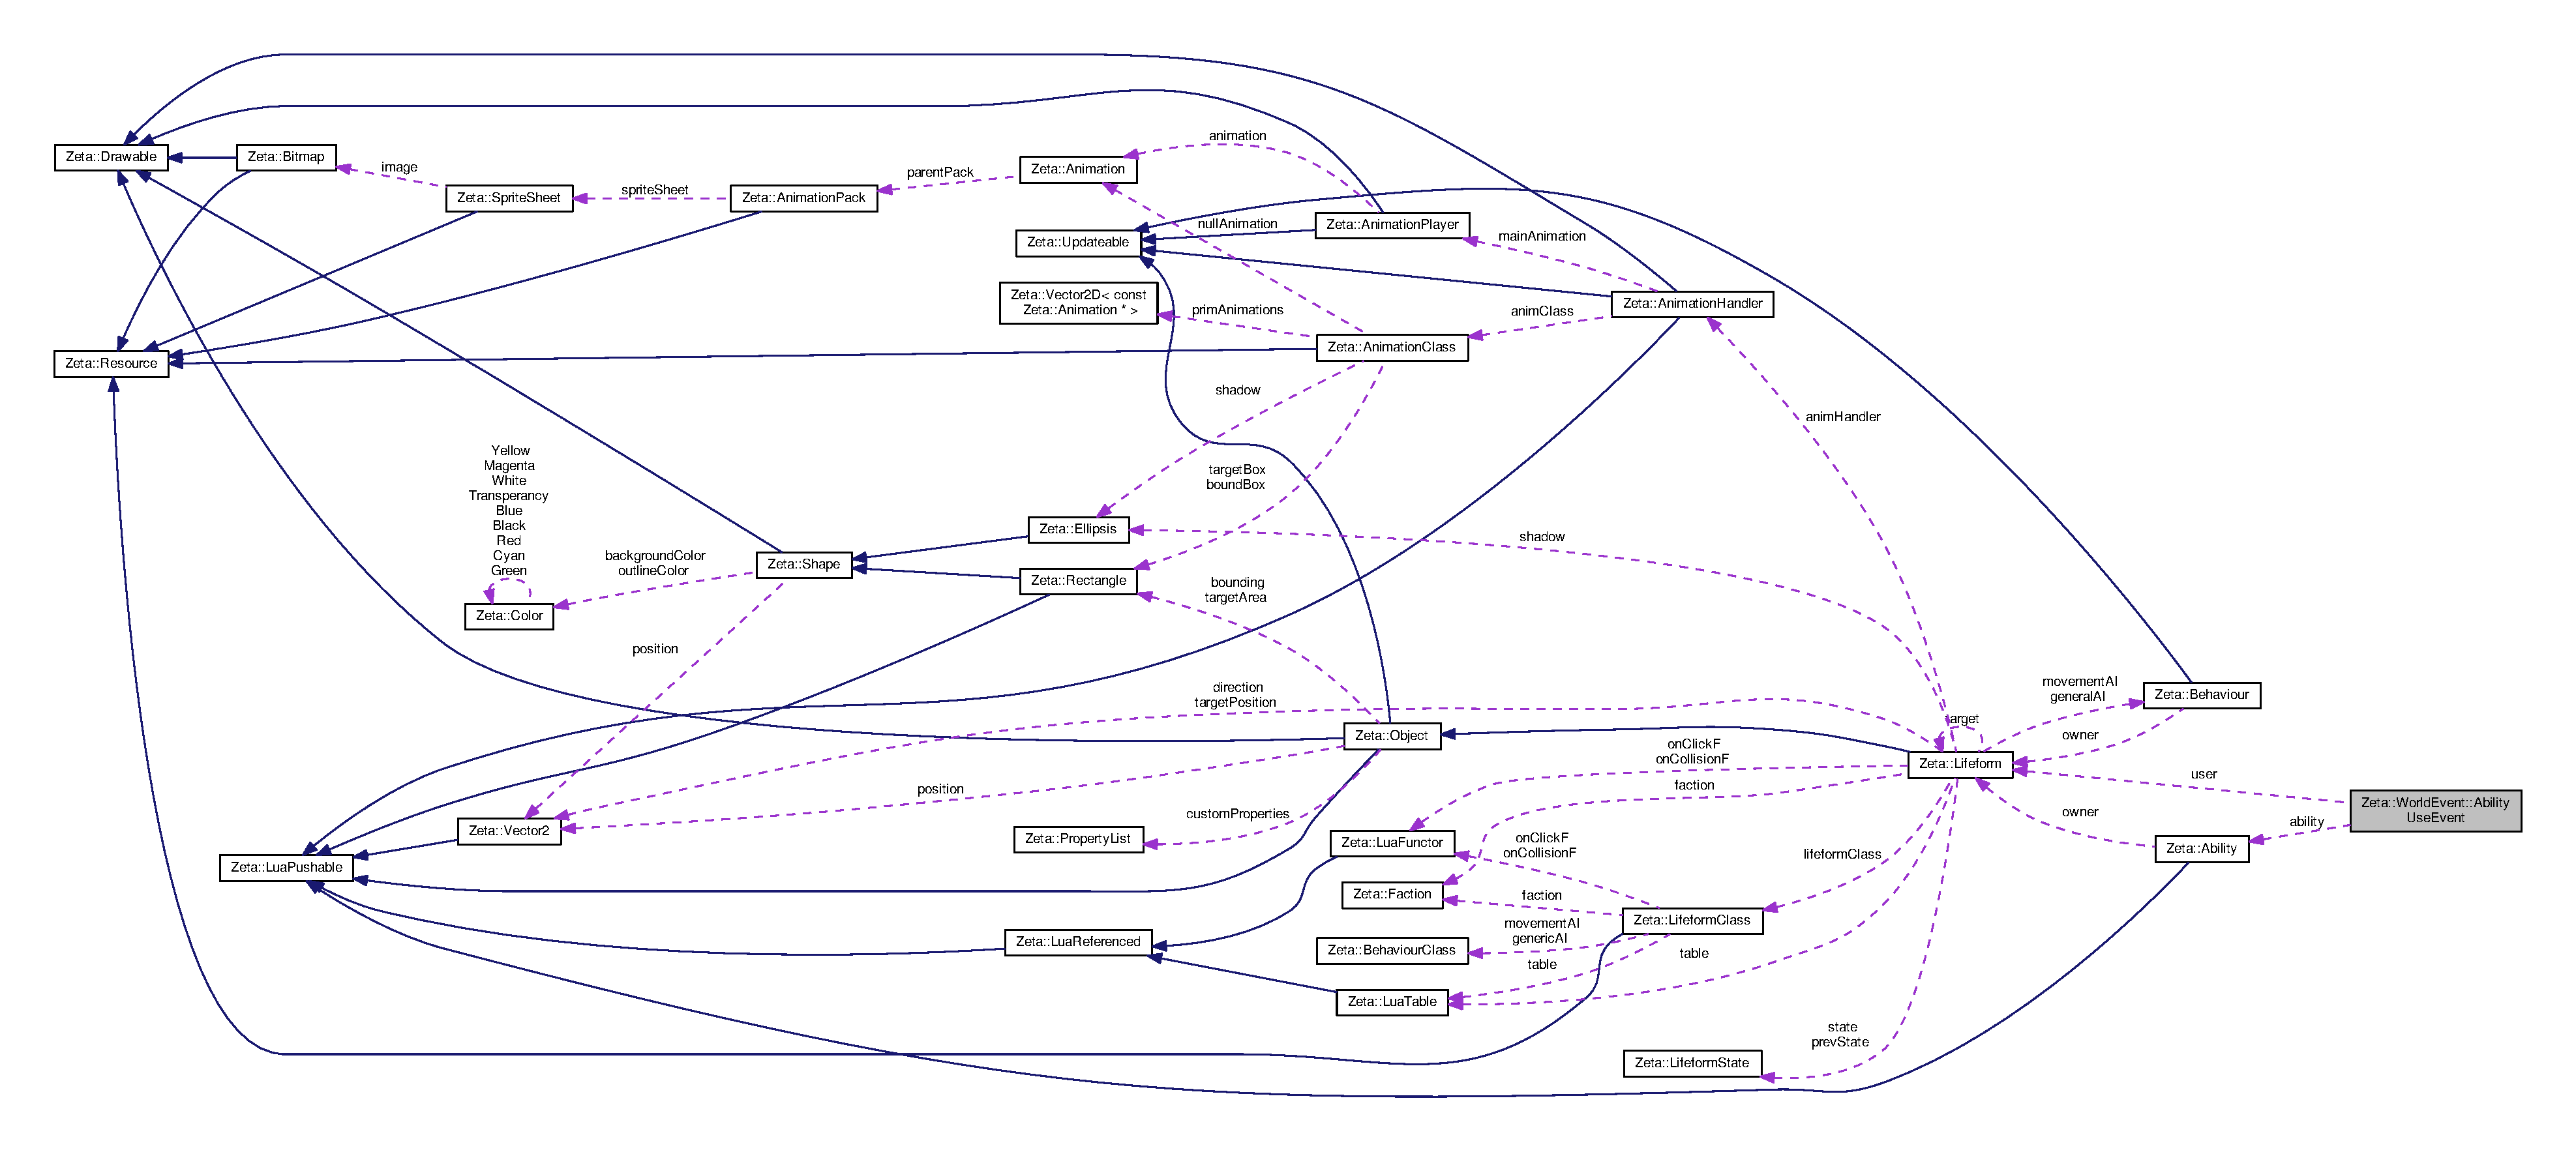
\includegraphics[width=350pt]{structZeta_1_1WorldEvent_1_1AbilityUseEvent__coll__graph}
\end{center}
\end{figure}
\subsection*{Public Attributes}
\begin{DoxyCompactItemize}
\item 
\hyperlink{classZeta_1_1Lifeform}{Lifeform} $\ast$ \hyperlink{structZeta_1_1WorldEvent_1_1AbilityUseEvent_aab3be9afa99cc7fac216891e84abb3c1}{user}
\item 
\hyperlink{classZeta_1_1Ability}{Ability} $\ast$ \hyperlink{structZeta_1_1WorldEvent_1_1AbilityUseEvent_a2d31acd2e159683b69c3046e1c355000}{ability}
\end{DoxyCompactItemize}


\subsection{Member Data Documentation}
\hypertarget{structZeta_1_1WorldEvent_1_1AbilityUseEvent_a2d31acd2e159683b69c3046e1c355000}{\index{Zeta\+::\+World\+Event\+::\+Ability\+Use\+Event@{Zeta\+::\+World\+Event\+::\+Ability\+Use\+Event}!ability@{ability}}
\index{ability@{ability}!Zeta\+::\+World\+Event\+::\+Ability\+Use\+Event@{Zeta\+::\+World\+Event\+::\+Ability\+Use\+Event}}
\subsubsection[{ability}]{\setlength{\rightskip}{0pt plus 5cm}{\bf Ability}$\ast$ Zeta\+::\+World\+Event\+::\+Ability\+Use\+Event\+::ability}}\label{structZeta_1_1WorldEvent_1_1AbilityUseEvent_a2d31acd2e159683b69c3046e1c355000}
\hypertarget{structZeta_1_1WorldEvent_1_1AbilityUseEvent_aab3be9afa99cc7fac216891e84abb3c1}{\index{Zeta\+::\+World\+Event\+::\+Ability\+Use\+Event@{Zeta\+::\+World\+Event\+::\+Ability\+Use\+Event}!user@{user}}
\index{user@{user}!Zeta\+::\+World\+Event\+::\+Ability\+Use\+Event@{Zeta\+::\+World\+Event\+::\+Ability\+Use\+Event}}
\subsubsection[{user}]{\setlength{\rightskip}{0pt plus 5cm}{\bf Lifeform}$\ast$ Zeta\+::\+World\+Event\+::\+Ability\+Use\+Event\+::user}}\label{structZeta_1_1WorldEvent_1_1AbilityUseEvent_aab3be9afa99cc7fac216891e84abb3c1}


The documentation for this struct was generated from the following file\+:\begin{DoxyCompactItemize}
\item 
include/\+Zeta/\+Core/\+R\+P\+G\+Classes/\hyperlink{WorldEvent_8hpp}{World\+Event.\+hpp}\end{DoxyCompactItemize}

\hypertarget{classZeta_1_1ActiveAbility}{\section{Zeta\+:\+:Active\+Ability Class Reference}
\label{classZeta_1_1ActiveAbility}\index{Zeta\+::\+Active\+Ability@{Zeta\+::\+Active\+Ability}}
}


{\ttfamily \#include $<$Active\+Ability.\+hpp$>$}



Inheritance diagram for Zeta\+:\+:Active\+Ability\+:\nopagebreak
\begin{figure}[H]
\begin{center}
\leavevmode
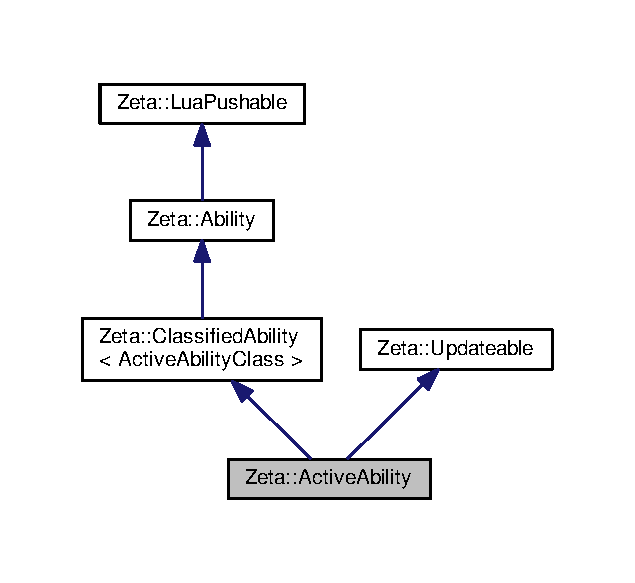
\includegraphics[width=305pt]{classZeta_1_1ActiveAbility__inherit__graph}
\end{center}
\end{figure}


Collaboration diagram for Zeta\+:\+:Active\+Ability\+:
\nopagebreak
\begin{figure}[H]
\begin{center}
\leavevmode
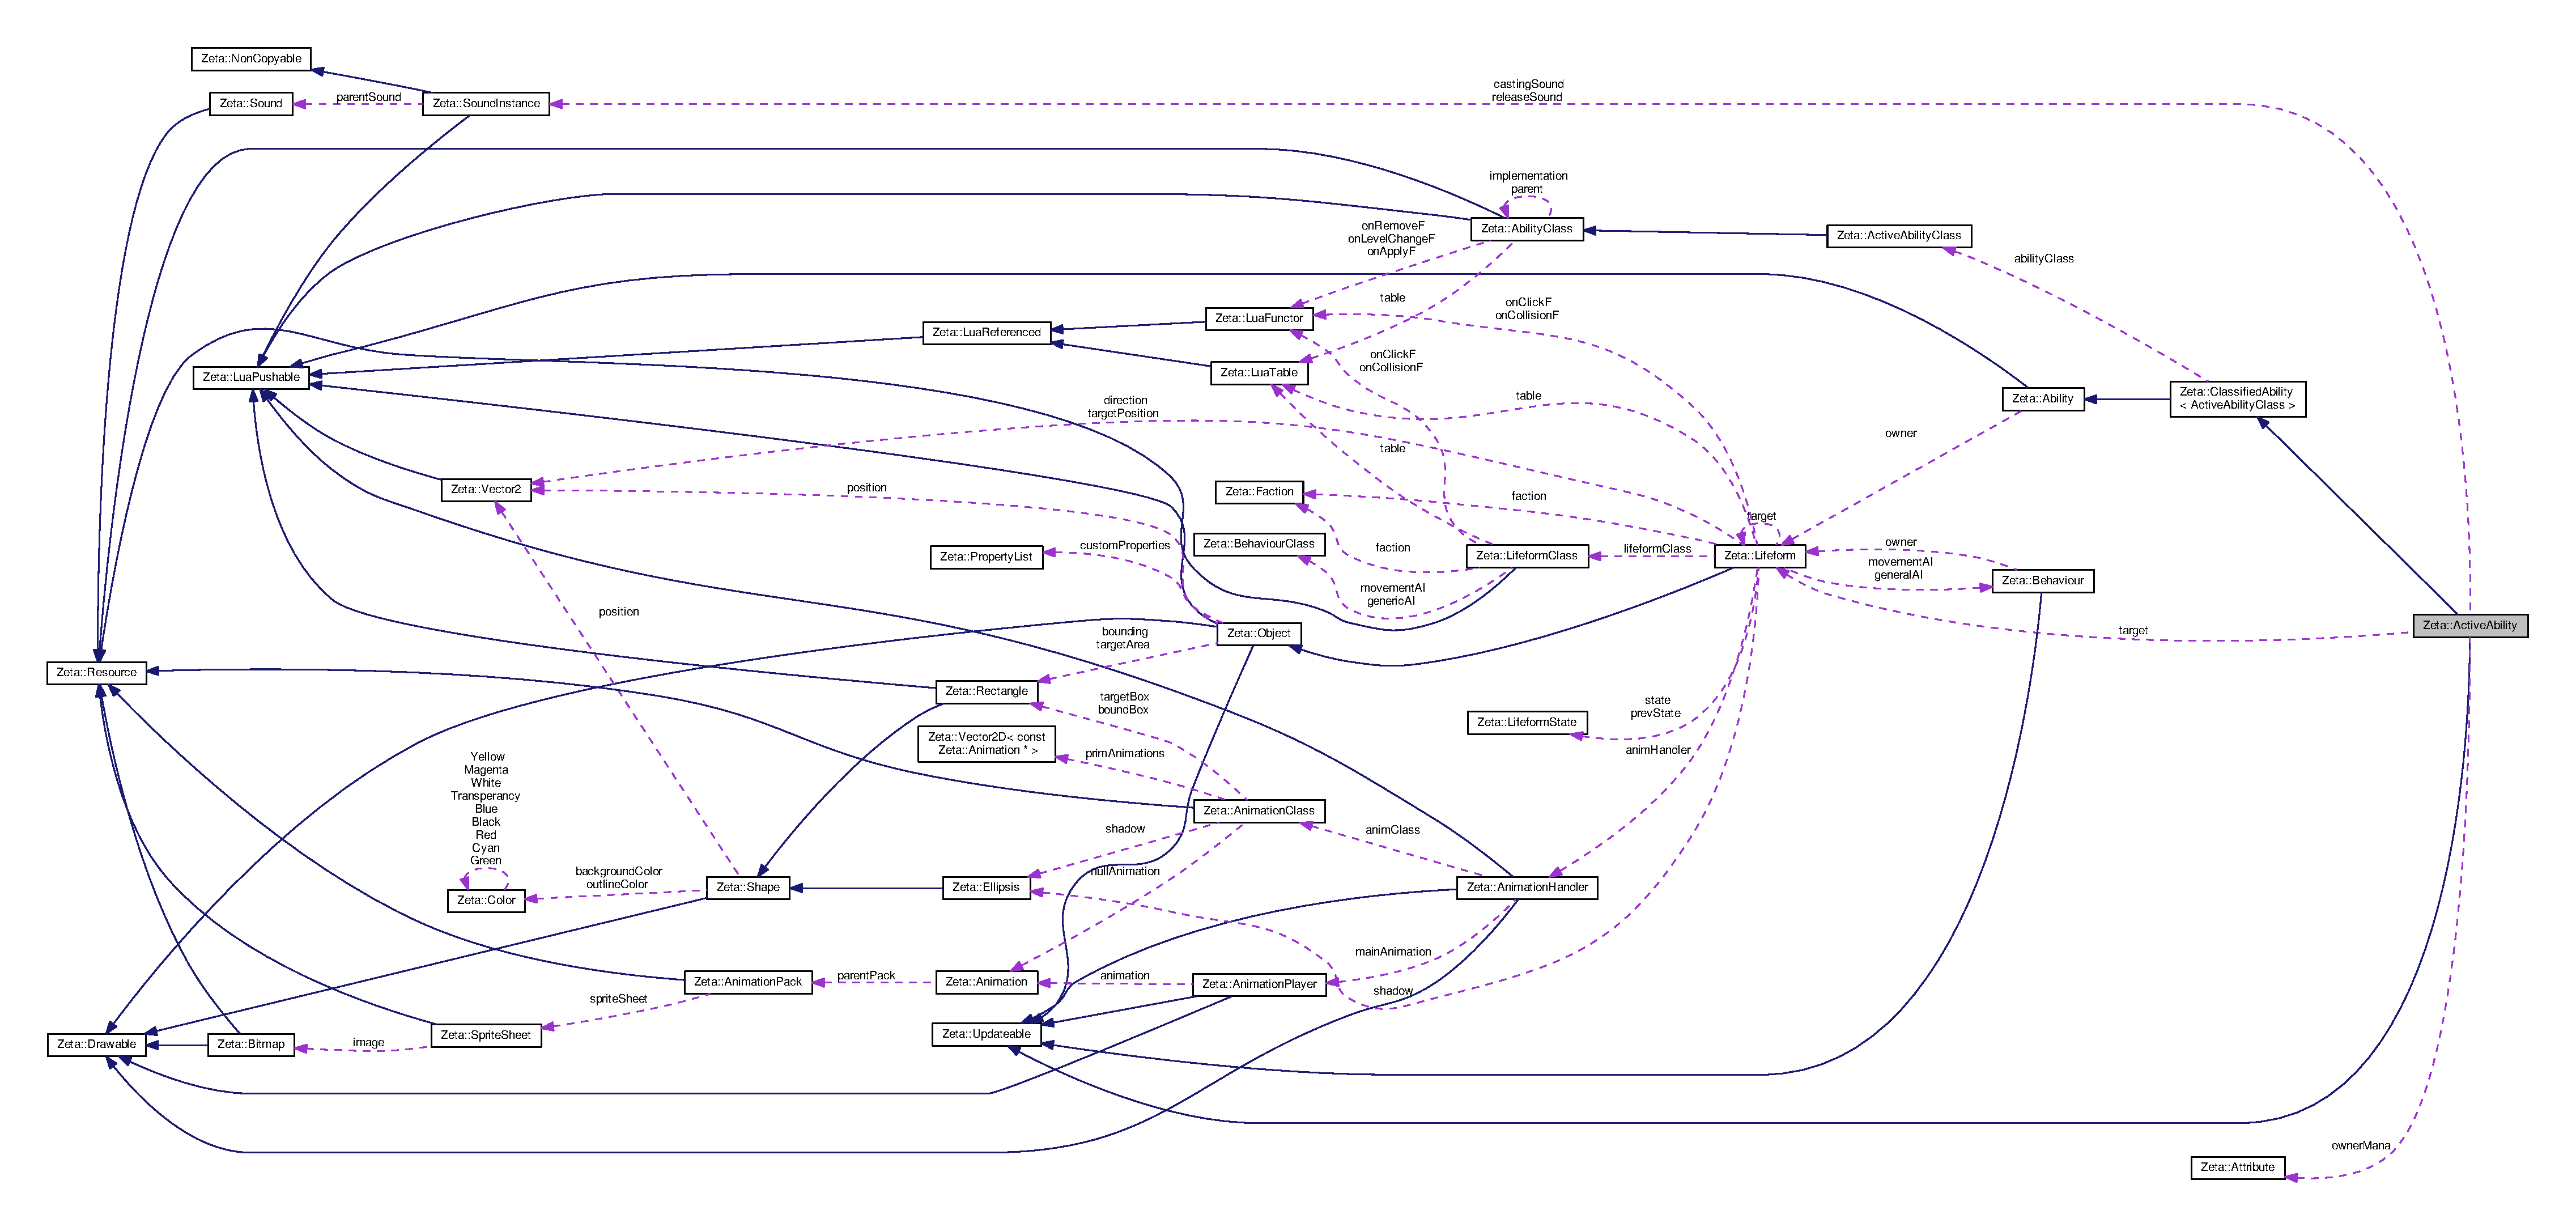
\includegraphics[width=350pt]{classZeta_1_1ActiveAbility__coll__graph}
\end{center}
\end{figure}
\subsection*{Public Types}
\begin{DoxyCompactItemize}
\item 
enum \hyperlink{classZeta_1_1ActiveAbility_ae0b5a1d1421d441d744f7ff7d9952457}{State} \{ \hyperlink{classZeta_1_1ActiveAbility_ae0b5a1d1421d441d744f7ff7d9952457ae7d31fc0602fb2ede144d18cdffd816b}{State\+::\+Ready}, 
\hyperlink{classZeta_1_1ActiveAbility_ae0b5a1d1421d441d744f7ff7d9952457a0f1c308819e46b9203b485ff5ee1877c}{State\+::on\+Coodown}, 
\hyperlink{classZeta_1_1ActiveAbility_ae0b5a1d1421d441d744f7ff7d9952457a86a59ad7ba2334ad7505f303d3f2ab6e}{State\+::\+Casting}, 
\hyperlink{classZeta_1_1ActiveAbility_ae0b5a1d1421d441d744f7ff7d9952457a3cab03c00dbd11bc3569afa0748013f0}{State\+::\+Inactive}
 \}
\end{DoxyCompactItemize}
\subsection*{Public Member Functions}
\begin{DoxyCompactItemize}
\item 
\hyperlink{classZeta_1_1Ability_acbc80e4d82c9683d190ed8ca1c80f597}{Result} \hyperlink{classZeta_1_1ActiveAbility_a46023874b199a7bdb565e9183b9ac2a5}{invoke} ()
\item 
void \hyperlink{classZeta_1_1ActiveAbility_a2fd33f973a6465e2676f96e801c876a5}{update} (\hyperlink{namespaceZeta_a1e0a1265f9b3bd3075fb0fabd39088ba}{Float} elapsed\+Time)
\item 
\hyperlink{namespaceZeta_a1e0a1265f9b3bd3075fb0fabd39088ba}{Float} \hyperlink{classZeta_1_1ActiveAbility_a439a4383db68777ee0c470ba2b0cdb9e}{get\+Remaining\+Cooldown} () const 
\item 
bool \hyperlink{classZeta_1_1ActiveAbility_a4dc0971df65c51832aa66a19ea633975}{is\+Casting} () const 
\item 
bool \hyperlink{classZeta_1_1ActiveAbility_a9fb0208b07148ac22c4315cf3be019d5}{is\+Ready} () const 
\item 
bool \hyperlink{classZeta_1_1ActiveAbility_a123c7db247dd64d0d313c256c35d5672}{is\+On\+Cooldown} () const 
\item 
bool \hyperlink{classZeta_1_1ActiveAbility_abf8bed3dae7891ec6edf3017f8ae0f6e}{is\+Done} () const 
\item 
bool \hyperlink{classZeta_1_1ActiveAbility_a412dc4526b26c5bab6550bcfd51cb115}{can\+Be\+Invoked} () const 
\item 
bool \hyperlink{classZeta_1_1ActiveAbility_a27e34f191cc69b670b0d3bd098c1e840}{is\+There\+Enough\+Mana} () const 
\item 
\hyperlink{namespaceZeta_a1e0a1265f9b3bd3075fb0fabd39088ba}{Float} \hyperlink{classZeta_1_1ActiveAbility_aa6498ca1448a63c2a10b635f095f8647}{get\+Cast\+Time} () const 
\item 
void \hyperlink{classZeta_1_1ActiveAbility_a326fbed7538adc7f7757b677c62a428e}{set\+Cast\+Time} (\hyperlink{namespaceZeta_a1e0a1265f9b3bd3075fb0fabd39088ba}{Float} \hyperlink{classZeta_1_1ActiveAbility_ab501566943e05f567f2d79426cf04e84}{cast\+Time})
\item 
\hyperlink{namespaceZeta_a1e0a1265f9b3bd3075fb0fabd39088ba}{Float} \hyperlink{classZeta_1_1ActiveAbility_add329505b459888d51b06f130a99e539}{get\+Cool\+Down} () const 
\item 
void \hyperlink{classZeta_1_1ActiveAbility_afc40cf0dda0f01a908b6e11e60e391ef}{set\+Cool\+Down} (\hyperlink{namespaceZeta_a1e0a1265f9b3bd3075fb0fabd39088ba}{Float} \hyperlink{classZeta_1_1ActiveAbility_ac4948af3377c964955adce51f87fb7f7}{cool\+Down})
\item 
\hyperlink{namespaceZeta_a1e0a1265f9b3bd3075fb0fabd39088ba}{Float} \hyperlink{classZeta_1_1ActiveAbility_a993aecd3af90be3f055b4577a8be75d3}{get\+Mana\+Cost} () const 
\item 
void \hyperlink{classZeta_1_1ActiveAbility_a09c042609d0dde554202c365568c8921}{set\+Mana\+Cost} (\hyperlink{namespaceZeta_a1e0a1265f9b3bd3075fb0fabd39088ba}{Float} \hyperlink{classZeta_1_1ActiveAbility_a6c8fca9f95c29edce442d557da31c97c}{mana\+Cost})
\item 
\hyperlink{namespaceZeta_a1e0a1265f9b3bd3075fb0fabd39088ba}{Float} \hyperlink{classZeta_1_1ActiveAbility_ad3b58bd804087c55fde27ef693bf2f39}{get\+Range} () const 
\item 
void \hyperlink{classZeta_1_1ActiveAbility_acf2addb391d9daa760660bcebe3afc7a}{set\+Range} (\hyperlink{namespaceZeta_a1e0a1265f9b3bd3075fb0fabd39088ba}{Float} \hyperlink{classZeta_1_1ActiveAbility_a556c513b5f222362222237baa86ef99b}{range})
\item 
void \hyperlink{classZeta_1_1ActiveAbility_ad8000083d66515c38fef09a24ce41dd3}{stop\+Casting} ()
\item 
void \hyperlink{classZeta_1_1ActiveAbility_aac2b2d046c757e45487aae9224f78882}{invoke\+Projectile} (const std\+::string \&name, \hyperlink{namespaceZeta_a1e0a1265f9b3bd3075fb0fabd39088ba}{Float} x, \hyperlink{namespaceZeta_a1e0a1265f9b3bd3075fb0fabd39088ba}{Float} y)
\item 
void \hyperlink{classZeta_1_1ActiveAbility_a40a0d966de4cdcba37c68ac15d0dec3b}{apply\+Effect} (const std\+::string \&name, \hyperlink{classZeta_1_1Lifeform}{Lifeform} $\ast$\hyperlink{classZeta_1_1ActiveAbility_a8fa764979494dc8c1a482d61fd701f0a}{target}, int \hyperlink{classZeta_1_1Ability_a41d29a6fb79dd19a7eed5f6a4be5de9a}{level})
\item 
void \hyperlink{classZeta_1_1ActiveAbility_a37ff91607af1c0d9a824eea119b00668}{accept} (\hyperlink{classZeta_1_1Visitor}{Visitor} \&visitor)
\item 
void \hyperlink{classZeta_1_1ActiveAbility_a74626319027e26b26e310f7d713beb2e}{push\+To\+Lua} (lua\+\_\+\+State $\ast$lstate)
\item 
\hyperlink{classZeta_1_1ActiveAbility_ab30e9c3361c326e3779cc72d47b18f6c}{Active\+Ability} (const \hyperlink{classZeta_1_1ActiveAbilityClass}{Active\+Ability\+Class} \&\hyperlink{classZeta_1_1ClassifiedAbility_abd6f78106602f84787cac967c2308abe}{ability\+Class}, \hyperlink{classZeta_1_1Lifeform}{Lifeform} $\ast$\hyperlink{classZeta_1_1Ability_ad37bed67f04178297d6fe4c9a2ed619a}{owner}, int \hyperlink{classZeta_1_1Ability_a41d29a6fb79dd19a7eed5f6a4be5de9a}{level})
\item 
virtual \hyperlink{classZeta_1_1ActiveAbility_a2b60fcfa31204947f1bfada035e45f34}{$\sim$\+Active\+Ability} ()
\end{DoxyCompactItemize}
\subsection*{Protected Member Functions}
\begin{DoxyCompactItemize}
\item 
virtual void \hyperlink{classZeta_1_1ActiveAbility_a0550b9267729ad07ac0b74bb44bb2885}{release} ()
\item 
virtual \hyperlink{classZeta_1_1Ability_acbc80e4d82c9683d190ed8ca1c80f597}{Result} \hyperlink{classZeta_1_1ActiveAbility_a93f4fdf59bfeee2e9876012a36086ce1}{check\+Conditions} ()
\item 
virtual void \hyperlink{classZeta_1_1ActiveAbility_a3c41095a949478a4f5438cc612636bef}{cast} ()
\item 
void \hyperlink{classZeta_1_1ActiveAbility_a6a2a131788a14830aba711262235cf26}{on\+Level\+Change} ()
\end{DoxyCompactItemize}
\subsection*{Protected Attributes}
\begin{DoxyCompactItemize}
\item 
\hyperlink{namespaceZeta_a4c11e23ddc559dccdb5e85901d7dfb84}{Z\+Small\+Map}$<$ std\+::string, \\*
\hyperlink{classZeta_1_1Projectile}{Projectile} $\ast$ $>$ \hyperlink{classZeta_1_1ActiveAbility_a5f3cc050a91d4426eff5b876bd3b5cd0}{available\+Projectiles}
\item 
\hyperlink{namespaceZeta_a44c717c98a964d0ebf6ea954cb9c91bf}{Z\+Small\+Set}$<$ \hyperlink{classZeta_1_1Projectile}{Projectile} $\ast$ $>$ \hyperlink{classZeta_1_1ActiveAbility_a62d796d7d80e14fe2b9f4c7d245c1ea6}{projectiles}
\item 
\hyperlink{classZeta_1_1SoundInstance}{Sound\+Instance} $\ast$ \hyperlink{classZeta_1_1ActiveAbility_a5383a436ae261b80675f20034816a22f}{casting\+Sound}
\item 
\hyperlink{classZeta_1_1SoundInstance}{Sound\+Instance} $\ast$ \hyperlink{classZeta_1_1ActiveAbility_a6d77d8fa73fb84a4424ed4e0e2424dcd}{release\+Sound}
\item 
\hyperlink{classZeta_1_1Lifeform}{Lifeform} $\ast$ \hyperlink{classZeta_1_1ActiveAbility_a8fa764979494dc8c1a482d61fd701f0a}{target}
\item 
\hyperlink{classZeta_1_1Attribute}{Attribute} \& \hyperlink{classZeta_1_1ActiveAbility_a5936f29e808d3878b4f83c2dae8af85f}{owner\+Mana}
\item 
\hyperlink{namespaceZeta_a1e0a1265f9b3bd3075fb0fabd39088ba}{Float} \hyperlink{classZeta_1_1ActiveAbility_a6c8fca9f95c29edce442d557da31c97c}{mana\+Cost}
\item 
\hyperlink{namespaceZeta_a1e0a1265f9b3bd3075fb0fabd39088ba}{Float} \hyperlink{classZeta_1_1ActiveAbility_ac4948af3377c964955adce51f87fb7f7}{cool\+Down}
\item 
\hyperlink{namespaceZeta_a1e0a1265f9b3bd3075fb0fabd39088ba}{Float} \hyperlink{classZeta_1_1ActiveAbility_ab501566943e05f567f2d79426cf04e84}{cast\+Time}
\item 
\hyperlink{namespaceZeta_a1e0a1265f9b3bd3075fb0fabd39088ba}{Float} \hyperlink{classZeta_1_1ActiveAbility_a556c513b5f222362222237baa86ef99b}{range}
\item 
\hyperlink{namespaceZeta_a1e0a1265f9b3bd3075fb0fabd39088ba}{Float} \hyperlink{classZeta_1_1ActiveAbility_a1d19f65b04e8c7222854cfeae31aad06}{frame\+Counter}
\item 
\hyperlink{classZeta_1_1ActiveAbility_ae0b5a1d1421d441d744f7ff7d9952457}{State} \hyperlink{classZeta_1_1ActiveAbility_a7eafb2407ae9edc5722576c6e2fe1195}{state}
\item 
bool \hyperlink{classZeta_1_1ActiveAbility_a92e0659685a9fd1b6f04c0a99a7a4c10}{has\+Casting\+Animation}
\item 
bool \hyperlink{classZeta_1_1ActiveAbility_ad58fc9ff0a47dd234302c31c53b3ce00}{has\+Release\+Animation}
\item 
bool \hyperlink{classZeta_1_1ActiveAbility_ab6a38b1fc8e7b68f84c5824b4f25dfef}{has\+Casting\+Sound}
\item 
bool \hyperlink{classZeta_1_1ActiveAbility_ace11cc3ceccd2feba9aaea2424c4dc8b}{has\+Release\+Sound}
\item 
bool \hyperlink{classZeta_1_1ActiveAbility_a2f677d94741cf5893ae1b1b9e04c1eb9}{animation\+Changed}
\item 
bool \hyperlink{classZeta_1_1ActiveAbility_ad2f27536fef9544224c2d329df50cba0}{is\+Casting\+Sound\+Playing}
\item 
bool \hyperlink{classZeta_1_1ActiveAbility_ae2c8c887e8478ac646e2911ec4ab73dc}{finished}
\end{DoxyCompactItemize}


\subsection{Member Enumeration Documentation}
\hypertarget{classZeta_1_1ActiveAbility_ae0b5a1d1421d441d744f7ff7d9952457}{\index{Zeta\+::\+Active\+Ability@{Zeta\+::\+Active\+Ability}!State@{State}}
\index{State@{State}!Zeta\+::\+Active\+Ability@{Zeta\+::\+Active\+Ability}}
\subsubsection[{State}]{\setlength{\rightskip}{0pt plus 5cm}enum {\bf Zeta\+::\+Active\+Ability\+::\+State}\hspace{0.3cm}{\ttfamily [strong]}}}\label{classZeta_1_1ActiveAbility_ae0b5a1d1421d441d744f7ff7d9952457}
\begin{Desc}
\item[Enumerator]\par
\begin{description}
\index{Ready@{Ready}!Zeta\+::\+Active\+Ability@{Zeta\+::\+Active\+Ability}}\index{Zeta\+::\+Active\+Ability@{Zeta\+::\+Active\+Ability}!Ready@{Ready}}\item[{\em 
\hypertarget{classZeta_1_1ActiveAbility_ae0b5a1d1421d441d744f7ff7d9952457ae7d31fc0602fb2ede144d18cdffd816b}{Ready}\label{classZeta_1_1ActiveAbility_ae0b5a1d1421d441d744f7ff7d9952457ae7d31fc0602fb2ede144d18cdffd816b}
}]\index{on\+Coodown@{on\+Coodown}!Zeta\+::\+Active\+Ability@{Zeta\+::\+Active\+Ability}}\index{Zeta\+::\+Active\+Ability@{Zeta\+::\+Active\+Ability}!on\+Coodown@{on\+Coodown}}\item[{\em 
\hypertarget{classZeta_1_1ActiveAbility_ae0b5a1d1421d441d744f7ff7d9952457a0f1c308819e46b9203b485ff5ee1877c}{on\+Coodown}\label{classZeta_1_1ActiveAbility_ae0b5a1d1421d441d744f7ff7d9952457a0f1c308819e46b9203b485ff5ee1877c}
}]\index{Casting@{Casting}!Zeta\+::\+Active\+Ability@{Zeta\+::\+Active\+Ability}}\index{Zeta\+::\+Active\+Ability@{Zeta\+::\+Active\+Ability}!Casting@{Casting}}\item[{\em 
\hypertarget{classZeta_1_1ActiveAbility_ae0b5a1d1421d441d744f7ff7d9952457a86a59ad7ba2334ad7505f303d3f2ab6e}{Casting}\label{classZeta_1_1ActiveAbility_ae0b5a1d1421d441d744f7ff7d9952457a86a59ad7ba2334ad7505f303d3f2ab6e}
}]\index{Inactive@{Inactive}!Zeta\+::\+Active\+Ability@{Zeta\+::\+Active\+Ability}}\index{Zeta\+::\+Active\+Ability@{Zeta\+::\+Active\+Ability}!Inactive@{Inactive}}\item[{\em 
\hypertarget{classZeta_1_1ActiveAbility_ae0b5a1d1421d441d744f7ff7d9952457a3cab03c00dbd11bc3569afa0748013f0}{Inactive}\label{classZeta_1_1ActiveAbility_ae0b5a1d1421d441d744f7ff7d9952457a3cab03c00dbd11bc3569afa0748013f0}
}]\end{description}
\end{Desc}


\subsection{Constructor \& Destructor Documentation}
\hypertarget{classZeta_1_1ActiveAbility_ab30e9c3361c326e3779cc72d47b18f6c}{\index{Zeta\+::\+Active\+Ability@{Zeta\+::\+Active\+Ability}!Active\+Ability@{Active\+Ability}}
\index{Active\+Ability@{Active\+Ability}!Zeta\+::\+Active\+Ability@{Zeta\+::\+Active\+Ability}}
\subsubsection[{Active\+Ability}]{\setlength{\rightskip}{0pt plus 5cm}Zeta\+::\+Active\+Ability\+::\+Active\+Ability (
\begin{DoxyParamCaption}
\item[{const {\bf Active\+Ability\+Class} \&}]{ability\+Class, }
\item[{{\bf Lifeform} $\ast$}]{owner, }
\item[{int}]{level}
\end{DoxyParamCaption}
)}}\label{classZeta_1_1ActiveAbility_ab30e9c3361c326e3779cc72d47b18f6c}
\hypertarget{classZeta_1_1ActiveAbility_a2b60fcfa31204947f1bfada035e45f34}{\index{Zeta\+::\+Active\+Ability@{Zeta\+::\+Active\+Ability}!````~Active\+Ability@{$\sim$\+Active\+Ability}}
\index{````~Active\+Ability@{$\sim$\+Active\+Ability}!Zeta\+::\+Active\+Ability@{Zeta\+::\+Active\+Ability}}
\subsubsection[{$\sim$\+Active\+Ability}]{\setlength{\rightskip}{0pt plus 5cm}virtual Zeta\+::\+Active\+Ability\+::$\sim$\+Active\+Ability (
\begin{DoxyParamCaption}
{}
\end{DoxyParamCaption}
)\hspace{0.3cm}{\ttfamily [virtual]}}}\label{classZeta_1_1ActiveAbility_a2b60fcfa31204947f1bfada035e45f34}


\subsection{Member Function Documentation}
\hypertarget{classZeta_1_1ActiveAbility_a37ff91607af1c0d9a824eea119b00668}{\index{Zeta\+::\+Active\+Ability@{Zeta\+::\+Active\+Ability}!accept@{accept}}
\index{accept@{accept}!Zeta\+::\+Active\+Ability@{Zeta\+::\+Active\+Ability}}
\subsubsection[{accept}]{\setlength{\rightskip}{0pt plus 5cm}void Zeta\+::\+Active\+Ability\+::accept (
\begin{DoxyParamCaption}
\item[{{\bf Visitor} \&}]{visitor}
\end{DoxyParamCaption}
)}}\label{classZeta_1_1ActiveAbility_a37ff91607af1c0d9a824eea119b00668}
\hypertarget{classZeta_1_1ActiveAbility_a40a0d966de4cdcba37c68ac15d0dec3b}{\index{Zeta\+::\+Active\+Ability@{Zeta\+::\+Active\+Ability}!apply\+Effect@{apply\+Effect}}
\index{apply\+Effect@{apply\+Effect}!Zeta\+::\+Active\+Ability@{Zeta\+::\+Active\+Ability}}
\subsubsection[{apply\+Effect}]{\setlength{\rightskip}{0pt plus 5cm}void Zeta\+::\+Active\+Ability\+::apply\+Effect (
\begin{DoxyParamCaption}
\item[{const std\+::string \&}]{name, }
\item[{{\bf Lifeform} $\ast$}]{target, }
\item[{int}]{level}
\end{DoxyParamCaption}
)}}\label{classZeta_1_1ActiveAbility_a40a0d966de4cdcba37c68ac15d0dec3b}
\hypertarget{classZeta_1_1ActiveAbility_a412dc4526b26c5bab6550bcfd51cb115}{\index{Zeta\+::\+Active\+Ability@{Zeta\+::\+Active\+Ability}!can\+Be\+Invoked@{can\+Be\+Invoked}}
\index{can\+Be\+Invoked@{can\+Be\+Invoked}!Zeta\+::\+Active\+Ability@{Zeta\+::\+Active\+Ability}}
\subsubsection[{can\+Be\+Invoked}]{\setlength{\rightskip}{0pt plus 5cm}bool Zeta\+::\+Active\+Ability\+::can\+Be\+Invoked (
\begin{DoxyParamCaption}
{}
\end{DoxyParamCaption}
) const}}\label{classZeta_1_1ActiveAbility_a412dc4526b26c5bab6550bcfd51cb115}
\hypertarget{classZeta_1_1ActiveAbility_a3c41095a949478a4f5438cc612636bef}{\index{Zeta\+::\+Active\+Ability@{Zeta\+::\+Active\+Ability}!cast@{cast}}
\index{cast@{cast}!Zeta\+::\+Active\+Ability@{Zeta\+::\+Active\+Ability}}
\subsubsection[{cast}]{\setlength{\rightskip}{0pt plus 5cm}virtual void Zeta\+::\+Active\+Ability\+::cast (
\begin{DoxyParamCaption}
{}
\end{DoxyParamCaption}
)\hspace{0.3cm}{\ttfamily [protected]}, {\ttfamily [virtual]}}}\label{classZeta_1_1ActiveAbility_a3c41095a949478a4f5438cc612636bef}
\hypertarget{classZeta_1_1ActiveAbility_a93f4fdf59bfeee2e9876012a36086ce1}{\index{Zeta\+::\+Active\+Ability@{Zeta\+::\+Active\+Ability}!check\+Conditions@{check\+Conditions}}
\index{check\+Conditions@{check\+Conditions}!Zeta\+::\+Active\+Ability@{Zeta\+::\+Active\+Ability}}
\subsubsection[{check\+Conditions}]{\setlength{\rightskip}{0pt plus 5cm}virtual {\bf Result} Zeta\+::\+Active\+Ability\+::check\+Conditions (
\begin{DoxyParamCaption}
{}
\end{DoxyParamCaption}
)\hspace{0.3cm}{\ttfamily [protected]}, {\ttfamily [virtual]}}}\label{classZeta_1_1ActiveAbility_a93f4fdf59bfeee2e9876012a36086ce1}
\hypertarget{classZeta_1_1ActiveAbility_aa6498ca1448a63c2a10b635f095f8647}{\index{Zeta\+::\+Active\+Ability@{Zeta\+::\+Active\+Ability}!get\+Cast\+Time@{get\+Cast\+Time}}
\index{get\+Cast\+Time@{get\+Cast\+Time}!Zeta\+::\+Active\+Ability@{Zeta\+::\+Active\+Ability}}
\subsubsection[{get\+Cast\+Time}]{\setlength{\rightskip}{0pt plus 5cm}{\bf Float} Zeta\+::\+Active\+Ability\+::get\+Cast\+Time (
\begin{DoxyParamCaption}
{}
\end{DoxyParamCaption}
) const\hspace{0.3cm}{\ttfamily [inline]}}}\label{classZeta_1_1ActiveAbility_aa6498ca1448a63c2a10b635f095f8647}
\hypertarget{classZeta_1_1ActiveAbility_add329505b459888d51b06f130a99e539}{\index{Zeta\+::\+Active\+Ability@{Zeta\+::\+Active\+Ability}!get\+Cool\+Down@{get\+Cool\+Down}}
\index{get\+Cool\+Down@{get\+Cool\+Down}!Zeta\+::\+Active\+Ability@{Zeta\+::\+Active\+Ability}}
\subsubsection[{get\+Cool\+Down}]{\setlength{\rightskip}{0pt plus 5cm}{\bf Float} Zeta\+::\+Active\+Ability\+::get\+Cool\+Down (
\begin{DoxyParamCaption}
{}
\end{DoxyParamCaption}
) const\hspace{0.3cm}{\ttfamily [inline]}}}\label{classZeta_1_1ActiveAbility_add329505b459888d51b06f130a99e539}
\hypertarget{classZeta_1_1ActiveAbility_a993aecd3af90be3f055b4577a8be75d3}{\index{Zeta\+::\+Active\+Ability@{Zeta\+::\+Active\+Ability}!get\+Mana\+Cost@{get\+Mana\+Cost}}
\index{get\+Mana\+Cost@{get\+Mana\+Cost}!Zeta\+::\+Active\+Ability@{Zeta\+::\+Active\+Ability}}
\subsubsection[{get\+Mana\+Cost}]{\setlength{\rightskip}{0pt plus 5cm}{\bf Float} Zeta\+::\+Active\+Ability\+::get\+Mana\+Cost (
\begin{DoxyParamCaption}
{}
\end{DoxyParamCaption}
) const\hspace{0.3cm}{\ttfamily [inline]}}}\label{classZeta_1_1ActiveAbility_a993aecd3af90be3f055b4577a8be75d3}
\hypertarget{classZeta_1_1ActiveAbility_ad3b58bd804087c55fde27ef693bf2f39}{\index{Zeta\+::\+Active\+Ability@{Zeta\+::\+Active\+Ability}!get\+Range@{get\+Range}}
\index{get\+Range@{get\+Range}!Zeta\+::\+Active\+Ability@{Zeta\+::\+Active\+Ability}}
\subsubsection[{get\+Range}]{\setlength{\rightskip}{0pt plus 5cm}{\bf Float} Zeta\+::\+Active\+Ability\+::get\+Range (
\begin{DoxyParamCaption}
{}
\end{DoxyParamCaption}
) const\hspace{0.3cm}{\ttfamily [inline]}}}\label{classZeta_1_1ActiveAbility_ad3b58bd804087c55fde27ef693bf2f39}
\hypertarget{classZeta_1_1ActiveAbility_a439a4383db68777ee0c470ba2b0cdb9e}{\index{Zeta\+::\+Active\+Ability@{Zeta\+::\+Active\+Ability}!get\+Remaining\+Cooldown@{get\+Remaining\+Cooldown}}
\index{get\+Remaining\+Cooldown@{get\+Remaining\+Cooldown}!Zeta\+::\+Active\+Ability@{Zeta\+::\+Active\+Ability}}
\subsubsection[{get\+Remaining\+Cooldown}]{\setlength{\rightskip}{0pt plus 5cm}{\bf Float} Zeta\+::\+Active\+Ability\+::get\+Remaining\+Cooldown (
\begin{DoxyParamCaption}
{}
\end{DoxyParamCaption}
) const\hspace{0.3cm}{\ttfamily [inline]}}}\label{classZeta_1_1ActiveAbility_a439a4383db68777ee0c470ba2b0cdb9e}
\hypertarget{classZeta_1_1ActiveAbility_a46023874b199a7bdb565e9183b9ac2a5}{\index{Zeta\+::\+Active\+Ability@{Zeta\+::\+Active\+Ability}!invoke@{invoke}}
\index{invoke@{invoke}!Zeta\+::\+Active\+Ability@{Zeta\+::\+Active\+Ability}}
\subsubsection[{invoke}]{\setlength{\rightskip}{0pt plus 5cm}{\bf Result} Zeta\+::\+Active\+Ability\+::invoke (
\begin{DoxyParamCaption}
{}
\end{DoxyParamCaption}
)}}\label{classZeta_1_1ActiveAbility_a46023874b199a7bdb565e9183b9ac2a5}
\hypertarget{classZeta_1_1ActiveAbility_aac2b2d046c757e45487aae9224f78882}{\index{Zeta\+::\+Active\+Ability@{Zeta\+::\+Active\+Ability}!invoke\+Projectile@{invoke\+Projectile}}
\index{invoke\+Projectile@{invoke\+Projectile}!Zeta\+::\+Active\+Ability@{Zeta\+::\+Active\+Ability}}
\subsubsection[{invoke\+Projectile}]{\setlength{\rightskip}{0pt plus 5cm}void Zeta\+::\+Active\+Ability\+::invoke\+Projectile (
\begin{DoxyParamCaption}
\item[{const std\+::string \&}]{name, }
\item[{{\bf Float}}]{x, }
\item[{{\bf Float}}]{y}
\end{DoxyParamCaption}
)}}\label{classZeta_1_1ActiveAbility_aac2b2d046c757e45487aae9224f78882}
\hypertarget{classZeta_1_1ActiveAbility_a4dc0971df65c51832aa66a19ea633975}{\index{Zeta\+::\+Active\+Ability@{Zeta\+::\+Active\+Ability}!is\+Casting@{is\+Casting}}
\index{is\+Casting@{is\+Casting}!Zeta\+::\+Active\+Ability@{Zeta\+::\+Active\+Ability}}
\subsubsection[{is\+Casting}]{\setlength{\rightskip}{0pt plus 5cm}bool Zeta\+::\+Active\+Ability\+::is\+Casting (
\begin{DoxyParamCaption}
{}
\end{DoxyParamCaption}
) const\hspace{0.3cm}{\ttfamily [inline]}}}\label{classZeta_1_1ActiveAbility_a4dc0971df65c51832aa66a19ea633975}
\hypertarget{classZeta_1_1ActiveAbility_abf8bed3dae7891ec6edf3017f8ae0f6e}{\index{Zeta\+::\+Active\+Ability@{Zeta\+::\+Active\+Ability}!is\+Done@{is\+Done}}
\index{is\+Done@{is\+Done}!Zeta\+::\+Active\+Ability@{Zeta\+::\+Active\+Ability}}
\subsubsection[{is\+Done}]{\setlength{\rightskip}{0pt plus 5cm}bool Zeta\+::\+Active\+Ability\+::is\+Done (
\begin{DoxyParamCaption}
{}
\end{DoxyParamCaption}
) const\hspace{0.3cm}{\ttfamily [inline]}}}\label{classZeta_1_1ActiveAbility_abf8bed3dae7891ec6edf3017f8ae0f6e}
\hypertarget{classZeta_1_1ActiveAbility_a123c7db247dd64d0d313c256c35d5672}{\index{Zeta\+::\+Active\+Ability@{Zeta\+::\+Active\+Ability}!is\+On\+Cooldown@{is\+On\+Cooldown}}
\index{is\+On\+Cooldown@{is\+On\+Cooldown}!Zeta\+::\+Active\+Ability@{Zeta\+::\+Active\+Ability}}
\subsubsection[{is\+On\+Cooldown}]{\setlength{\rightskip}{0pt plus 5cm}bool Zeta\+::\+Active\+Ability\+::is\+On\+Cooldown (
\begin{DoxyParamCaption}
{}
\end{DoxyParamCaption}
) const\hspace{0.3cm}{\ttfamily [inline]}}}\label{classZeta_1_1ActiveAbility_a123c7db247dd64d0d313c256c35d5672}
\hypertarget{classZeta_1_1ActiveAbility_a9fb0208b07148ac22c4315cf3be019d5}{\index{Zeta\+::\+Active\+Ability@{Zeta\+::\+Active\+Ability}!is\+Ready@{is\+Ready}}
\index{is\+Ready@{is\+Ready}!Zeta\+::\+Active\+Ability@{Zeta\+::\+Active\+Ability}}
\subsubsection[{is\+Ready}]{\setlength{\rightskip}{0pt plus 5cm}bool Zeta\+::\+Active\+Ability\+::is\+Ready (
\begin{DoxyParamCaption}
{}
\end{DoxyParamCaption}
) const\hspace{0.3cm}{\ttfamily [inline]}}}\label{classZeta_1_1ActiveAbility_a9fb0208b07148ac22c4315cf3be019d5}
\hypertarget{classZeta_1_1ActiveAbility_a27e34f191cc69b670b0d3bd098c1e840}{\index{Zeta\+::\+Active\+Ability@{Zeta\+::\+Active\+Ability}!is\+There\+Enough\+Mana@{is\+There\+Enough\+Mana}}
\index{is\+There\+Enough\+Mana@{is\+There\+Enough\+Mana}!Zeta\+::\+Active\+Ability@{Zeta\+::\+Active\+Ability}}
\subsubsection[{is\+There\+Enough\+Mana}]{\setlength{\rightskip}{0pt plus 5cm}bool Zeta\+::\+Active\+Ability\+::is\+There\+Enough\+Mana (
\begin{DoxyParamCaption}
{}
\end{DoxyParamCaption}
) const}}\label{classZeta_1_1ActiveAbility_a27e34f191cc69b670b0d3bd098c1e840}
\hypertarget{classZeta_1_1ActiveAbility_a6a2a131788a14830aba711262235cf26}{\index{Zeta\+::\+Active\+Ability@{Zeta\+::\+Active\+Ability}!on\+Level\+Change@{on\+Level\+Change}}
\index{on\+Level\+Change@{on\+Level\+Change}!Zeta\+::\+Active\+Ability@{Zeta\+::\+Active\+Ability}}
\subsubsection[{on\+Level\+Change}]{\setlength{\rightskip}{0pt plus 5cm}void Zeta\+::\+Active\+Ability\+::on\+Level\+Change (
\begin{DoxyParamCaption}
{}
\end{DoxyParamCaption}
)\hspace{0.3cm}{\ttfamily [protected]}, {\ttfamily [virtual]}}}\label{classZeta_1_1ActiveAbility_a6a2a131788a14830aba711262235cf26}


Implements \hyperlink{classZeta_1_1Ability_ac81e774451daa9476b02ba442a2ea047}{Zeta\+::\+Ability}.

\hypertarget{classZeta_1_1ActiveAbility_a74626319027e26b26e310f7d713beb2e}{\index{Zeta\+::\+Active\+Ability@{Zeta\+::\+Active\+Ability}!push\+To\+Lua@{push\+To\+Lua}}
\index{push\+To\+Lua@{push\+To\+Lua}!Zeta\+::\+Active\+Ability@{Zeta\+::\+Active\+Ability}}
\subsubsection[{push\+To\+Lua}]{\setlength{\rightskip}{0pt plus 5cm}void Zeta\+::\+Active\+Ability\+::push\+To\+Lua (
\begin{DoxyParamCaption}
\item[{lua\+\_\+\+State $\ast$}]{lstate}
\end{DoxyParamCaption}
)\hspace{0.3cm}{\ttfamily [virtual]}}}\label{classZeta_1_1ActiveAbility_a74626319027e26b26e310f7d713beb2e}


Implements \hyperlink{classZeta_1_1LuaPushable_a0380ec9cff11f749e8eb67b51b8f82fc}{Zeta\+::\+Lua\+Pushable}.

\hypertarget{classZeta_1_1ActiveAbility_a0550b9267729ad07ac0b74bb44bb2885}{\index{Zeta\+::\+Active\+Ability@{Zeta\+::\+Active\+Ability}!release@{release}}
\index{release@{release}!Zeta\+::\+Active\+Ability@{Zeta\+::\+Active\+Ability}}
\subsubsection[{release}]{\setlength{\rightskip}{0pt plus 5cm}virtual void Zeta\+::\+Active\+Ability\+::release (
\begin{DoxyParamCaption}
{}
\end{DoxyParamCaption}
)\hspace{0.3cm}{\ttfamily [protected]}, {\ttfamily [virtual]}}}\label{classZeta_1_1ActiveAbility_a0550b9267729ad07ac0b74bb44bb2885}
\hypertarget{classZeta_1_1ActiveAbility_a326fbed7538adc7f7757b677c62a428e}{\index{Zeta\+::\+Active\+Ability@{Zeta\+::\+Active\+Ability}!set\+Cast\+Time@{set\+Cast\+Time}}
\index{set\+Cast\+Time@{set\+Cast\+Time}!Zeta\+::\+Active\+Ability@{Zeta\+::\+Active\+Ability}}
\subsubsection[{set\+Cast\+Time}]{\setlength{\rightskip}{0pt plus 5cm}void Zeta\+::\+Active\+Ability\+::set\+Cast\+Time (
\begin{DoxyParamCaption}
\item[{{\bf Float}}]{cast\+Time}
\end{DoxyParamCaption}
)\hspace{0.3cm}{\ttfamily [inline]}}}\label{classZeta_1_1ActiveAbility_a326fbed7538adc7f7757b677c62a428e}
\hypertarget{classZeta_1_1ActiveAbility_afc40cf0dda0f01a908b6e11e60e391ef}{\index{Zeta\+::\+Active\+Ability@{Zeta\+::\+Active\+Ability}!set\+Cool\+Down@{set\+Cool\+Down}}
\index{set\+Cool\+Down@{set\+Cool\+Down}!Zeta\+::\+Active\+Ability@{Zeta\+::\+Active\+Ability}}
\subsubsection[{set\+Cool\+Down}]{\setlength{\rightskip}{0pt plus 5cm}void Zeta\+::\+Active\+Ability\+::set\+Cool\+Down (
\begin{DoxyParamCaption}
\item[{{\bf Float}}]{cool\+Down}
\end{DoxyParamCaption}
)\hspace{0.3cm}{\ttfamily [inline]}}}\label{classZeta_1_1ActiveAbility_afc40cf0dda0f01a908b6e11e60e391ef}
\hypertarget{classZeta_1_1ActiveAbility_a09c042609d0dde554202c365568c8921}{\index{Zeta\+::\+Active\+Ability@{Zeta\+::\+Active\+Ability}!set\+Mana\+Cost@{set\+Mana\+Cost}}
\index{set\+Mana\+Cost@{set\+Mana\+Cost}!Zeta\+::\+Active\+Ability@{Zeta\+::\+Active\+Ability}}
\subsubsection[{set\+Mana\+Cost}]{\setlength{\rightskip}{0pt plus 5cm}void Zeta\+::\+Active\+Ability\+::set\+Mana\+Cost (
\begin{DoxyParamCaption}
\item[{{\bf Float}}]{mana\+Cost}
\end{DoxyParamCaption}
)\hspace{0.3cm}{\ttfamily [inline]}}}\label{classZeta_1_1ActiveAbility_a09c042609d0dde554202c365568c8921}
\hypertarget{classZeta_1_1ActiveAbility_acf2addb391d9daa760660bcebe3afc7a}{\index{Zeta\+::\+Active\+Ability@{Zeta\+::\+Active\+Ability}!set\+Range@{set\+Range}}
\index{set\+Range@{set\+Range}!Zeta\+::\+Active\+Ability@{Zeta\+::\+Active\+Ability}}
\subsubsection[{set\+Range}]{\setlength{\rightskip}{0pt plus 5cm}void Zeta\+::\+Active\+Ability\+::set\+Range (
\begin{DoxyParamCaption}
\item[{{\bf Float}}]{range}
\end{DoxyParamCaption}
)\hspace{0.3cm}{\ttfamily [inline]}}}\label{classZeta_1_1ActiveAbility_acf2addb391d9daa760660bcebe3afc7a}
\hypertarget{classZeta_1_1ActiveAbility_ad8000083d66515c38fef09a24ce41dd3}{\index{Zeta\+::\+Active\+Ability@{Zeta\+::\+Active\+Ability}!stop\+Casting@{stop\+Casting}}
\index{stop\+Casting@{stop\+Casting}!Zeta\+::\+Active\+Ability@{Zeta\+::\+Active\+Ability}}
\subsubsection[{stop\+Casting}]{\setlength{\rightskip}{0pt plus 5cm}void Zeta\+::\+Active\+Ability\+::stop\+Casting (
\begin{DoxyParamCaption}
{}
\end{DoxyParamCaption}
)}}\label{classZeta_1_1ActiveAbility_ad8000083d66515c38fef09a24ce41dd3}
\hypertarget{classZeta_1_1ActiveAbility_a2fd33f973a6465e2676f96e801c876a5}{\index{Zeta\+::\+Active\+Ability@{Zeta\+::\+Active\+Ability}!update@{update}}
\index{update@{update}!Zeta\+::\+Active\+Ability@{Zeta\+::\+Active\+Ability}}
\subsubsection[{update}]{\setlength{\rightskip}{0pt plus 5cm}void Zeta\+::\+Active\+Ability\+::update (
\begin{DoxyParamCaption}
\item[{{\bf Float}}]{elapsed\+Time}
\end{DoxyParamCaption}
)\hspace{0.3cm}{\ttfamily [virtual]}}}\label{classZeta_1_1ActiveAbility_a2fd33f973a6465e2676f96e801c876a5}


Implements \hyperlink{classZeta_1_1Updateable_af4006bfccb762454b4da08786ad93de0}{Zeta\+::\+Updateable}.



\subsection{Member Data Documentation}
\hypertarget{classZeta_1_1ActiveAbility_a2f677d94741cf5893ae1b1b9e04c1eb9}{\index{Zeta\+::\+Active\+Ability@{Zeta\+::\+Active\+Ability}!animation\+Changed@{animation\+Changed}}
\index{animation\+Changed@{animation\+Changed}!Zeta\+::\+Active\+Ability@{Zeta\+::\+Active\+Ability}}
\subsubsection[{animation\+Changed}]{\setlength{\rightskip}{0pt plus 5cm}bool Zeta\+::\+Active\+Ability\+::animation\+Changed\hspace{0.3cm}{\ttfamily [protected]}}}\label{classZeta_1_1ActiveAbility_a2f677d94741cf5893ae1b1b9e04c1eb9}
\hypertarget{classZeta_1_1ActiveAbility_a5f3cc050a91d4426eff5b876bd3b5cd0}{\index{Zeta\+::\+Active\+Ability@{Zeta\+::\+Active\+Ability}!available\+Projectiles@{available\+Projectiles}}
\index{available\+Projectiles@{available\+Projectiles}!Zeta\+::\+Active\+Ability@{Zeta\+::\+Active\+Ability}}
\subsubsection[{available\+Projectiles}]{\setlength{\rightskip}{0pt plus 5cm}{\bf Z\+Small\+Map}$<$std\+::string, {\bf Projectile}$\ast$$>$ Zeta\+::\+Active\+Ability\+::available\+Projectiles\hspace{0.3cm}{\ttfamily [protected]}}}\label{classZeta_1_1ActiveAbility_a5f3cc050a91d4426eff5b876bd3b5cd0}
\hypertarget{classZeta_1_1ActiveAbility_a5383a436ae261b80675f20034816a22f}{\index{Zeta\+::\+Active\+Ability@{Zeta\+::\+Active\+Ability}!casting\+Sound@{casting\+Sound}}
\index{casting\+Sound@{casting\+Sound}!Zeta\+::\+Active\+Ability@{Zeta\+::\+Active\+Ability}}
\subsubsection[{casting\+Sound}]{\setlength{\rightskip}{0pt plus 5cm}{\bf Sound\+Instance}$\ast$ Zeta\+::\+Active\+Ability\+::casting\+Sound\hspace{0.3cm}{\ttfamily [protected]}}}\label{classZeta_1_1ActiveAbility_a5383a436ae261b80675f20034816a22f}
\hypertarget{classZeta_1_1ActiveAbility_ab501566943e05f567f2d79426cf04e84}{\index{Zeta\+::\+Active\+Ability@{Zeta\+::\+Active\+Ability}!cast\+Time@{cast\+Time}}
\index{cast\+Time@{cast\+Time}!Zeta\+::\+Active\+Ability@{Zeta\+::\+Active\+Ability}}
\subsubsection[{cast\+Time}]{\setlength{\rightskip}{0pt plus 5cm}{\bf Float} Zeta\+::\+Active\+Ability\+::cast\+Time\hspace{0.3cm}{\ttfamily [protected]}}}\label{classZeta_1_1ActiveAbility_ab501566943e05f567f2d79426cf04e84}
\hypertarget{classZeta_1_1ActiveAbility_ac4948af3377c964955adce51f87fb7f7}{\index{Zeta\+::\+Active\+Ability@{Zeta\+::\+Active\+Ability}!cool\+Down@{cool\+Down}}
\index{cool\+Down@{cool\+Down}!Zeta\+::\+Active\+Ability@{Zeta\+::\+Active\+Ability}}
\subsubsection[{cool\+Down}]{\setlength{\rightskip}{0pt plus 5cm}{\bf Float} Zeta\+::\+Active\+Ability\+::cool\+Down\hspace{0.3cm}{\ttfamily [protected]}}}\label{classZeta_1_1ActiveAbility_ac4948af3377c964955adce51f87fb7f7}
\hypertarget{classZeta_1_1ActiveAbility_ae2c8c887e8478ac646e2911ec4ab73dc}{\index{Zeta\+::\+Active\+Ability@{Zeta\+::\+Active\+Ability}!finished@{finished}}
\index{finished@{finished}!Zeta\+::\+Active\+Ability@{Zeta\+::\+Active\+Ability}}
\subsubsection[{finished}]{\setlength{\rightskip}{0pt plus 5cm}bool Zeta\+::\+Active\+Ability\+::finished\hspace{0.3cm}{\ttfamily [protected]}}}\label{classZeta_1_1ActiveAbility_ae2c8c887e8478ac646e2911ec4ab73dc}
\hypertarget{classZeta_1_1ActiveAbility_a1d19f65b04e8c7222854cfeae31aad06}{\index{Zeta\+::\+Active\+Ability@{Zeta\+::\+Active\+Ability}!frame\+Counter@{frame\+Counter}}
\index{frame\+Counter@{frame\+Counter}!Zeta\+::\+Active\+Ability@{Zeta\+::\+Active\+Ability}}
\subsubsection[{frame\+Counter}]{\setlength{\rightskip}{0pt plus 5cm}{\bf Float} Zeta\+::\+Active\+Ability\+::frame\+Counter\hspace{0.3cm}{\ttfamily [protected]}}}\label{classZeta_1_1ActiveAbility_a1d19f65b04e8c7222854cfeae31aad06}
\hypertarget{classZeta_1_1ActiveAbility_a92e0659685a9fd1b6f04c0a99a7a4c10}{\index{Zeta\+::\+Active\+Ability@{Zeta\+::\+Active\+Ability}!has\+Casting\+Animation@{has\+Casting\+Animation}}
\index{has\+Casting\+Animation@{has\+Casting\+Animation}!Zeta\+::\+Active\+Ability@{Zeta\+::\+Active\+Ability}}
\subsubsection[{has\+Casting\+Animation}]{\setlength{\rightskip}{0pt plus 5cm}bool Zeta\+::\+Active\+Ability\+::has\+Casting\+Animation\hspace{0.3cm}{\ttfamily [protected]}}}\label{classZeta_1_1ActiveAbility_a92e0659685a9fd1b6f04c0a99a7a4c10}
\hypertarget{classZeta_1_1ActiveAbility_ab6a38b1fc8e7b68f84c5824b4f25dfef}{\index{Zeta\+::\+Active\+Ability@{Zeta\+::\+Active\+Ability}!has\+Casting\+Sound@{has\+Casting\+Sound}}
\index{has\+Casting\+Sound@{has\+Casting\+Sound}!Zeta\+::\+Active\+Ability@{Zeta\+::\+Active\+Ability}}
\subsubsection[{has\+Casting\+Sound}]{\setlength{\rightskip}{0pt plus 5cm}bool Zeta\+::\+Active\+Ability\+::has\+Casting\+Sound\hspace{0.3cm}{\ttfamily [protected]}}}\label{classZeta_1_1ActiveAbility_ab6a38b1fc8e7b68f84c5824b4f25dfef}
\hypertarget{classZeta_1_1ActiveAbility_ad58fc9ff0a47dd234302c31c53b3ce00}{\index{Zeta\+::\+Active\+Ability@{Zeta\+::\+Active\+Ability}!has\+Release\+Animation@{has\+Release\+Animation}}
\index{has\+Release\+Animation@{has\+Release\+Animation}!Zeta\+::\+Active\+Ability@{Zeta\+::\+Active\+Ability}}
\subsubsection[{has\+Release\+Animation}]{\setlength{\rightskip}{0pt plus 5cm}bool Zeta\+::\+Active\+Ability\+::has\+Release\+Animation\hspace{0.3cm}{\ttfamily [protected]}}}\label{classZeta_1_1ActiveAbility_ad58fc9ff0a47dd234302c31c53b3ce00}
\hypertarget{classZeta_1_1ActiveAbility_ace11cc3ceccd2feba9aaea2424c4dc8b}{\index{Zeta\+::\+Active\+Ability@{Zeta\+::\+Active\+Ability}!has\+Release\+Sound@{has\+Release\+Sound}}
\index{has\+Release\+Sound@{has\+Release\+Sound}!Zeta\+::\+Active\+Ability@{Zeta\+::\+Active\+Ability}}
\subsubsection[{has\+Release\+Sound}]{\setlength{\rightskip}{0pt plus 5cm}bool Zeta\+::\+Active\+Ability\+::has\+Release\+Sound\hspace{0.3cm}{\ttfamily [protected]}}}\label{classZeta_1_1ActiveAbility_ace11cc3ceccd2feba9aaea2424c4dc8b}
\hypertarget{classZeta_1_1ActiveAbility_ad2f27536fef9544224c2d329df50cba0}{\index{Zeta\+::\+Active\+Ability@{Zeta\+::\+Active\+Ability}!is\+Casting\+Sound\+Playing@{is\+Casting\+Sound\+Playing}}
\index{is\+Casting\+Sound\+Playing@{is\+Casting\+Sound\+Playing}!Zeta\+::\+Active\+Ability@{Zeta\+::\+Active\+Ability}}
\subsubsection[{is\+Casting\+Sound\+Playing}]{\setlength{\rightskip}{0pt plus 5cm}bool Zeta\+::\+Active\+Ability\+::is\+Casting\+Sound\+Playing\hspace{0.3cm}{\ttfamily [protected]}}}\label{classZeta_1_1ActiveAbility_ad2f27536fef9544224c2d329df50cba0}
\hypertarget{classZeta_1_1ActiveAbility_a6c8fca9f95c29edce442d557da31c97c}{\index{Zeta\+::\+Active\+Ability@{Zeta\+::\+Active\+Ability}!mana\+Cost@{mana\+Cost}}
\index{mana\+Cost@{mana\+Cost}!Zeta\+::\+Active\+Ability@{Zeta\+::\+Active\+Ability}}
\subsubsection[{mana\+Cost}]{\setlength{\rightskip}{0pt plus 5cm}{\bf Float} Zeta\+::\+Active\+Ability\+::mana\+Cost\hspace{0.3cm}{\ttfamily [protected]}}}\label{classZeta_1_1ActiveAbility_a6c8fca9f95c29edce442d557da31c97c}
\hypertarget{classZeta_1_1ActiveAbility_a5936f29e808d3878b4f83c2dae8af85f}{\index{Zeta\+::\+Active\+Ability@{Zeta\+::\+Active\+Ability}!owner\+Mana@{owner\+Mana}}
\index{owner\+Mana@{owner\+Mana}!Zeta\+::\+Active\+Ability@{Zeta\+::\+Active\+Ability}}
\subsubsection[{owner\+Mana}]{\setlength{\rightskip}{0pt plus 5cm}{\bf Attribute}\& Zeta\+::\+Active\+Ability\+::owner\+Mana\hspace{0.3cm}{\ttfamily [protected]}}}\label{classZeta_1_1ActiveAbility_a5936f29e808d3878b4f83c2dae8af85f}
\hypertarget{classZeta_1_1ActiveAbility_a62d796d7d80e14fe2b9f4c7d245c1ea6}{\index{Zeta\+::\+Active\+Ability@{Zeta\+::\+Active\+Ability}!projectiles@{projectiles}}
\index{projectiles@{projectiles}!Zeta\+::\+Active\+Ability@{Zeta\+::\+Active\+Ability}}
\subsubsection[{projectiles}]{\setlength{\rightskip}{0pt plus 5cm}{\bf Z\+Small\+Set}$<${\bf Projectile}$\ast$$>$ Zeta\+::\+Active\+Ability\+::projectiles\hspace{0.3cm}{\ttfamily [protected]}}}\label{classZeta_1_1ActiveAbility_a62d796d7d80e14fe2b9f4c7d245c1ea6}
\hypertarget{classZeta_1_1ActiveAbility_a556c513b5f222362222237baa86ef99b}{\index{Zeta\+::\+Active\+Ability@{Zeta\+::\+Active\+Ability}!range@{range}}
\index{range@{range}!Zeta\+::\+Active\+Ability@{Zeta\+::\+Active\+Ability}}
\subsubsection[{range}]{\setlength{\rightskip}{0pt plus 5cm}{\bf Float} Zeta\+::\+Active\+Ability\+::range\hspace{0.3cm}{\ttfamily [protected]}}}\label{classZeta_1_1ActiveAbility_a556c513b5f222362222237baa86ef99b}
\hypertarget{classZeta_1_1ActiveAbility_a6d77d8fa73fb84a4424ed4e0e2424dcd}{\index{Zeta\+::\+Active\+Ability@{Zeta\+::\+Active\+Ability}!release\+Sound@{release\+Sound}}
\index{release\+Sound@{release\+Sound}!Zeta\+::\+Active\+Ability@{Zeta\+::\+Active\+Ability}}
\subsubsection[{release\+Sound}]{\setlength{\rightskip}{0pt plus 5cm}{\bf Sound\+Instance}$\ast$ Zeta\+::\+Active\+Ability\+::release\+Sound\hspace{0.3cm}{\ttfamily [protected]}}}\label{classZeta_1_1ActiveAbility_a6d77d8fa73fb84a4424ed4e0e2424dcd}
\hypertarget{classZeta_1_1ActiveAbility_a7eafb2407ae9edc5722576c6e2fe1195}{\index{Zeta\+::\+Active\+Ability@{Zeta\+::\+Active\+Ability}!state@{state}}
\index{state@{state}!Zeta\+::\+Active\+Ability@{Zeta\+::\+Active\+Ability}}
\subsubsection[{state}]{\setlength{\rightskip}{0pt plus 5cm}{\bf State} Zeta\+::\+Active\+Ability\+::state\hspace{0.3cm}{\ttfamily [protected]}}}\label{classZeta_1_1ActiveAbility_a7eafb2407ae9edc5722576c6e2fe1195}
\hypertarget{classZeta_1_1ActiveAbility_a8fa764979494dc8c1a482d61fd701f0a}{\index{Zeta\+::\+Active\+Ability@{Zeta\+::\+Active\+Ability}!target@{target}}
\index{target@{target}!Zeta\+::\+Active\+Ability@{Zeta\+::\+Active\+Ability}}
\subsubsection[{target}]{\setlength{\rightskip}{0pt plus 5cm}{\bf Lifeform}$\ast$ Zeta\+::\+Active\+Ability\+::target\hspace{0.3cm}{\ttfamily [protected]}}}\label{classZeta_1_1ActiveAbility_a8fa764979494dc8c1a482d61fd701f0a}


The documentation for this class was generated from the following file\+:\begin{DoxyCompactItemize}
\item 
include/\+Zeta/\+Core/\+R\+P\+G\+Classes/\hyperlink{ActiveAbility_8hpp}{Active\+Ability.\+hpp}\end{DoxyCompactItemize}

\hypertarget{classZeta_1_1ActiveAbilityClass}{\section{Zeta\+:\+:Active\+Ability\+Class Class Reference}
\label{classZeta_1_1ActiveAbilityClass}\index{Zeta\+::\+Active\+Ability\+Class@{Zeta\+::\+Active\+Ability\+Class}}
}


{\ttfamily \#include $<$Active\+Ability\+Class.\+hpp$>$}



Inheritance diagram for Zeta\+:\+:Active\+Ability\+Class\+:\nopagebreak
\begin{figure}[H]
\begin{center}
\leavevmode
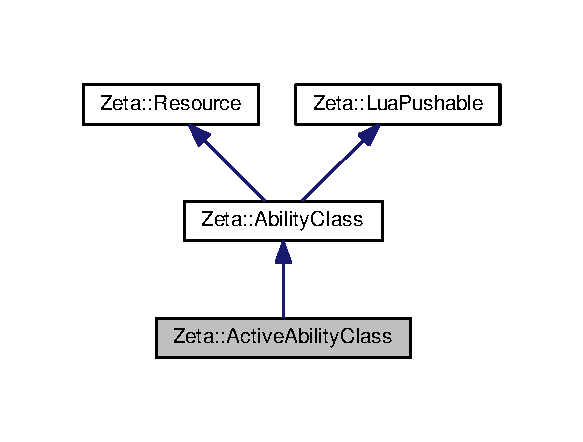
\includegraphics[width=280pt]{classZeta_1_1ActiveAbilityClass__inherit__graph}
\end{center}
\end{figure}


Collaboration diagram for Zeta\+:\+:Active\+Ability\+Class\+:\nopagebreak
\begin{figure}[H]
\begin{center}
\leavevmode
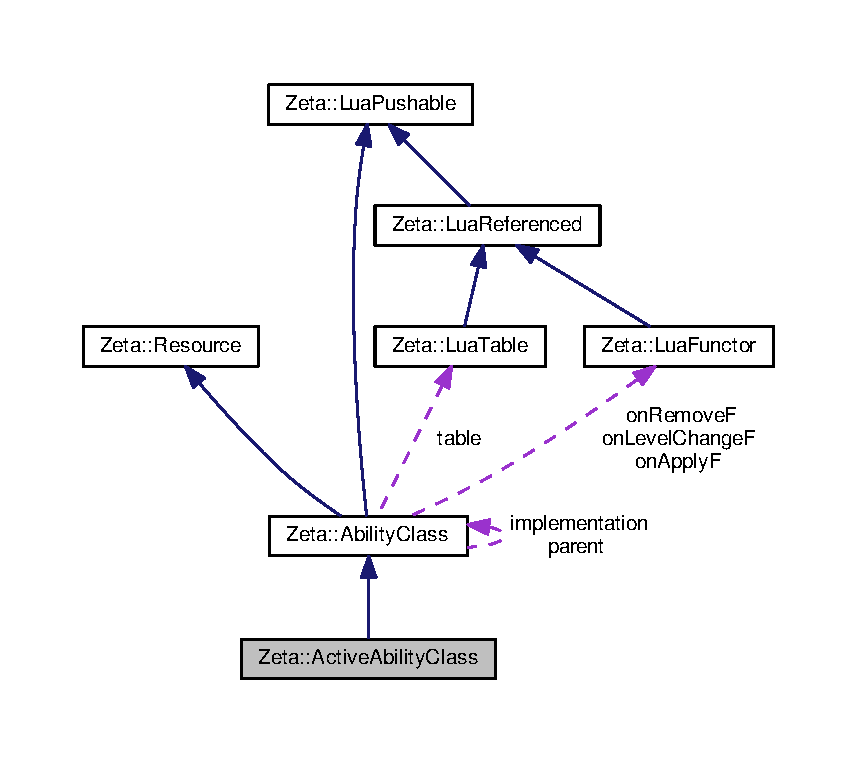
\includegraphics[width=350pt]{classZeta_1_1ActiveAbilityClass__coll__graph}
\end{center}
\end{figure}
\subsection*{Public Member Functions}
\begin{DoxyCompactItemize}
\item 
\hyperlink{namespaceZeta_a1e0a1265f9b3bd3075fb0fabd39088ba}{Float} \hyperlink{classZeta_1_1ActiveAbilityClass_af6927e9b8b25c44539a5e1f563f8ec7d}{get\+Cooldown} () const 
\item 
\hyperlink{namespaceZeta_a1e0a1265f9b3bd3075fb0fabd39088ba}{Float} \hyperlink{classZeta_1_1ActiveAbilityClass_aad91e6ee0b80697e2012e9973231ff19}{get\+Mana\+Cost} () const 
\item 
\hyperlink{namespaceZeta_a1e0a1265f9b3bd3075fb0fabd39088ba}{Float} \hyperlink{classZeta_1_1ActiveAbilityClass_afda1ffbd0f535675ac77a6d77f3e52eb}{get\+Cast\+Time} () const 
\item 
\hyperlink{namespaceZeta_a1e0a1265f9b3bd3075fb0fabd39088ba}{Float} \hyperlink{classZeta_1_1ActiveAbilityClass_a74c2f5b18dcff1dde6e66b6e3cde6985}{get\+Range} () const 
\item 
const std\+::string \& \hyperlink{classZeta_1_1ActiveAbilityClass_ab0346d994703ba5a12bdef64024ea9bd}{get\+Cast\+Animation} () const 
\item 
const std\+::string \& \hyperlink{classZeta_1_1ActiveAbilityClass_a15910a91b272b272b2e5baff4b4d7d9e}{get\+Release\+Animation} () const 
\item 
const std\+::string \& \hyperlink{classZeta_1_1ActiveAbilityClass_a87de08ce87355e4c9ee4cbb75d25abcf}{get\+Cast\+Sound} () const 
\item 
const std\+::string \& \hyperlink{classZeta_1_1ActiveAbilityClass_a61f29173a1b156cedbbe5928d9e74aa7}{get\+Release\+Sound} () const 
\item 
const \hyperlink{classZeta_1_1ProjectileClass}{Projectile\+Class} $\ast$ \hyperlink{classZeta_1_1ActiveAbilityClass_a180f0054f453213eb15e925fa919a01a}{get\+Projectile\+Class} (const std\+::string \&\hyperlink{classZeta_1_1Resource_a44c5721216f4beb31c0b3d2ef2aecf1d}{name}) const 
\item 
\hyperlink{classZeta_1_1Ability}{Ability} $\ast$ \hyperlink{classZeta_1_1ActiveAbilityClass_a7bc4309f792992dd7fb24bd9f1153b01}{get\+New\+Ability} (\hyperlink{classZeta_1_1Lifeform}{Lifeform} $\ast$caster, int level) const 
\item 
const \hyperlink{namespaceZeta_a9af2e12c4e432d2a1725f19e5a648a04}{Z\+Map}$<$ std\+::string, \\*
\hyperlink{classZeta_1_1ProjectileClass}{Projectile\+Class} $>$ \& \hyperlink{classZeta_1_1ActiveAbilityClass_ada3442d70e784a20c2ce9a19df2c0cb2}{get\+Projectile\+Classes} () const 
\item 
const \hyperlink{namespaceZeta_a9af2e12c4e432d2a1725f19e5a648a04}{Z\+Map}$<$ std\+::string, \\*
\hyperlink{classZeta_1_1EffectClass}{Effect\+Class} $>$ \& \hyperlink{classZeta_1_1ActiveAbilityClass_a5adaf78b13d013b38004f72c3b90bc5f}{get\+Effect\+Classes} () const 
\item 
void \hyperlink{classZeta_1_1ActiveAbilityClass_ad4916e9a102c5300d1eddb1723fd0298}{apply\+Effect} (const std\+::string \&\hyperlink{classZeta_1_1Resource_a44c5721216f4beb31c0b3d2ef2aecf1d}{name}, \hyperlink{classZeta_1_1Lifeform}{Lifeform} $\ast$target, int level, \hyperlink{classZeta_1_1ActiveAbility}{Active\+Ability} $\ast$ability=nullptr) const 
\item 
void \hyperlink{classZeta_1_1ActiveAbilityClass_aee8c5ff9d2858223e36758a36058cbe9}{push\+To\+Lua} (lua\+\_\+\+State $\ast$lstate)
\item 
\hyperlink{classZeta_1_1ActiveAbilityClass_ab1c8e4fd674f08755a3312eaa3f7ef8a}{Active\+Ability\+Class} (\hyperlink{classZeta_1_1AbilityClass}{Ability\+Class} \&\hyperlink{classZeta_1_1AbilityClass_ad862e9ba14d23afb20786a1eeb2ca872}{parent}, \hyperlink{classZeta_1_1LuaTable}{Lua\+Table} \&\hyperlink{classZeta_1_1AbilityClass_a58065ca9d19ff9366c09bfc8d81abbac}{table})
\item 
\hyperlink{classZeta_1_1ActiveAbilityClass_afb0d7c65437fbab71a9047562048ae8f}{$\sim$\+Active\+Ability\+Class} ()
\end{DoxyCompactItemize}
\subsection*{Private Attributes}
\begin{DoxyCompactItemize}
\item 
\hyperlink{namespaceZeta_a9af2e12c4e432d2a1725f19e5a648a04}{Z\+Map}$<$ std\+::string, \hyperlink{classZeta_1_1EffectClass}{Effect\+Class} $>$ \hyperlink{classZeta_1_1ActiveAbilityClass_a788c0ef48061e2a7e8906c0a93ca3d69}{effects}
\item 
\hyperlink{namespaceZeta_a9af2e12c4e432d2a1725f19e5a648a04}{Z\+Map}$<$ std\+::string, \\*
\hyperlink{classZeta_1_1ProjectileClass}{Projectile\+Class} $>$ \hyperlink{classZeta_1_1ActiveAbilityClass_a113456627f82c54c0f24569817f47867}{projectiles}
\item 
std\+::string \hyperlink{classZeta_1_1ActiveAbilityClass_a0571f13949f9bbdcf09b23ee645fda98}{cast\+Animation}
\item 
std\+::string \hyperlink{classZeta_1_1ActiveAbilityClass_a1cc52858da7286705d8aa755790cddc1}{release\+Animation}
\item 
std\+::string \hyperlink{classZeta_1_1ActiveAbilityClass_af7987f069a6f1f166ba58bb181926752}{cast\+Sound}
\item 
std\+::string \hyperlink{classZeta_1_1ActiveAbilityClass_ad7c34fbf83b75f826243df751de480a0}{release\+Sound}
\item 
\hyperlink{namespaceZeta_a1e0a1265f9b3bd3075fb0fabd39088ba}{Float} \hyperlink{classZeta_1_1ActiveAbilityClass_a592c33c2febef27c1db7eb3c6569f4f6}{range}
\item 
\hyperlink{namespaceZeta_a1e0a1265f9b3bd3075fb0fabd39088ba}{Float} \hyperlink{classZeta_1_1ActiveAbilityClass_aaff991d71ec034fcd902f720d3f5136a}{mana\+Cost}
\item 
\hyperlink{namespaceZeta_a1e0a1265f9b3bd3075fb0fabd39088ba}{Float} \hyperlink{classZeta_1_1ActiveAbilityClass_a7aceb1c38d3a0aa9796903f5d32d750f}{cast\+Time}
\item 
\hyperlink{namespaceZeta_a1e0a1265f9b3bd3075fb0fabd39088ba}{Float} \hyperlink{classZeta_1_1ActiveAbilityClass_a2f97b3b77b0a02adf554af6e59fa81fb}{cooldown}
\end{DoxyCompactItemize}
\subsection*{Additional Inherited Members}


\subsection{Constructor \& Destructor Documentation}
\hypertarget{classZeta_1_1ActiveAbilityClass_ab1c8e4fd674f08755a3312eaa3f7ef8a}{\index{Zeta\+::\+Active\+Ability\+Class@{Zeta\+::\+Active\+Ability\+Class}!Active\+Ability\+Class@{Active\+Ability\+Class}}
\index{Active\+Ability\+Class@{Active\+Ability\+Class}!Zeta\+::\+Active\+Ability\+Class@{Zeta\+::\+Active\+Ability\+Class}}
\subsubsection[{Active\+Ability\+Class}]{\setlength{\rightskip}{0pt plus 5cm}Zeta\+::\+Active\+Ability\+Class\+::\+Active\+Ability\+Class (
\begin{DoxyParamCaption}
\item[{{\bf Ability\+Class} \&}]{parent, }
\item[{{\bf Lua\+Table} \&}]{table}
\end{DoxyParamCaption}
)}}\label{classZeta_1_1ActiveAbilityClass_ab1c8e4fd674f08755a3312eaa3f7ef8a}
\hypertarget{classZeta_1_1ActiveAbilityClass_afb0d7c65437fbab71a9047562048ae8f}{\index{Zeta\+::\+Active\+Ability\+Class@{Zeta\+::\+Active\+Ability\+Class}!````~Active\+Ability\+Class@{$\sim$\+Active\+Ability\+Class}}
\index{````~Active\+Ability\+Class@{$\sim$\+Active\+Ability\+Class}!Zeta\+::\+Active\+Ability\+Class@{Zeta\+::\+Active\+Ability\+Class}}
\subsubsection[{$\sim$\+Active\+Ability\+Class}]{\setlength{\rightskip}{0pt plus 5cm}Zeta\+::\+Active\+Ability\+Class\+::$\sim$\+Active\+Ability\+Class (
\begin{DoxyParamCaption}
{}
\end{DoxyParamCaption}
)}}\label{classZeta_1_1ActiveAbilityClass_afb0d7c65437fbab71a9047562048ae8f}


\subsection{Member Function Documentation}
\hypertarget{classZeta_1_1ActiveAbilityClass_ad4916e9a102c5300d1eddb1723fd0298}{\index{Zeta\+::\+Active\+Ability\+Class@{Zeta\+::\+Active\+Ability\+Class}!apply\+Effect@{apply\+Effect}}
\index{apply\+Effect@{apply\+Effect}!Zeta\+::\+Active\+Ability\+Class@{Zeta\+::\+Active\+Ability\+Class}}
\subsubsection[{apply\+Effect}]{\setlength{\rightskip}{0pt plus 5cm}void Zeta\+::\+Active\+Ability\+Class\+::apply\+Effect (
\begin{DoxyParamCaption}
\item[{const std\+::string \&}]{name, }
\item[{{\bf Lifeform} $\ast$}]{target, }
\item[{int}]{level, }
\item[{{\bf Active\+Ability} $\ast$}]{ability = {\ttfamily nullptr}}
\end{DoxyParamCaption}
) const}}\label{classZeta_1_1ActiveAbilityClass_ad4916e9a102c5300d1eddb1723fd0298}
\hypertarget{classZeta_1_1ActiveAbilityClass_ab0346d994703ba5a12bdef64024ea9bd}{\index{Zeta\+::\+Active\+Ability\+Class@{Zeta\+::\+Active\+Ability\+Class}!get\+Cast\+Animation@{get\+Cast\+Animation}}
\index{get\+Cast\+Animation@{get\+Cast\+Animation}!Zeta\+::\+Active\+Ability\+Class@{Zeta\+::\+Active\+Ability\+Class}}
\subsubsection[{get\+Cast\+Animation}]{\setlength{\rightskip}{0pt plus 5cm}const std\+::string\& Zeta\+::\+Active\+Ability\+Class\+::get\+Cast\+Animation (
\begin{DoxyParamCaption}
{}
\end{DoxyParamCaption}
) const\hspace{0.3cm}{\ttfamily [inline]}}}\label{classZeta_1_1ActiveAbilityClass_ab0346d994703ba5a12bdef64024ea9bd}
\hypertarget{classZeta_1_1ActiveAbilityClass_a87de08ce87355e4c9ee4cbb75d25abcf}{\index{Zeta\+::\+Active\+Ability\+Class@{Zeta\+::\+Active\+Ability\+Class}!get\+Cast\+Sound@{get\+Cast\+Sound}}
\index{get\+Cast\+Sound@{get\+Cast\+Sound}!Zeta\+::\+Active\+Ability\+Class@{Zeta\+::\+Active\+Ability\+Class}}
\subsubsection[{get\+Cast\+Sound}]{\setlength{\rightskip}{0pt plus 5cm}const std\+::string\& Zeta\+::\+Active\+Ability\+Class\+::get\+Cast\+Sound (
\begin{DoxyParamCaption}
{}
\end{DoxyParamCaption}
) const\hspace{0.3cm}{\ttfamily [inline]}}}\label{classZeta_1_1ActiveAbilityClass_a87de08ce87355e4c9ee4cbb75d25abcf}
\hypertarget{classZeta_1_1ActiveAbilityClass_afda1ffbd0f535675ac77a6d77f3e52eb}{\index{Zeta\+::\+Active\+Ability\+Class@{Zeta\+::\+Active\+Ability\+Class}!get\+Cast\+Time@{get\+Cast\+Time}}
\index{get\+Cast\+Time@{get\+Cast\+Time}!Zeta\+::\+Active\+Ability\+Class@{Zeta\+::\+Active\+Ability\+Class}}
\subsubsection[{get\+Cast\+Time}]{\setlength{\rightskip}{0pt plus 5cm}{\bf Float} Zeta\+::\+Active\+Ability\+Class\+::get\+Cast\+Time (
\begin{DoxyParamCaption}
{}
\end{DoxyParamCaption}
) const\hspace{0.3cm}{\ttfamily [inline]}}}\label{classZeta_1_1ActiveAbilityClass_afda1ffbd0f535675ac77a6d77f3e52eb}
\hypertarget{classZeta_1_1ActiveAbilityClass_af6927e9b8b25c44539a5e1f563f8ec7d}{\index{Zeta\+::\+Active\+Ability\+Class@{Zeta\+::\+Active\+Ability\+Class}!get\+Cooldown@{get\+Cooldown}}
\index{get\+Cooldown@{get\+Cooldown}!Zeta\+::\+Active\+Ability\+Class@{Zeta\+::\+Active\+Ability\+Class}}
\subsubsection[{get\+Cooldown}]{\setlength{\rightskip}{0pt plus 5cm}{\bf Float} Zeta\+::\+Active\+Ability\+Class\+::get\+Cooldown (
\begin{DoxyParamCaption}
{}
\end{DoxyParamCaption}
) const\hspace{0.3cm}{\ttfamily [inline]}}}\label{classZeta_1_1ActiveAbilityClass_af6927e9b8b25c44539a5e1f563f8ec7d}
\hypertarget{classZeta_1_1ActiveAbilityClass_a5adaf78b13d013b38004f72c3b90bc5f}{\index{Zeta\+::\+Active\+Ability\+Class@{Zeta\+::\+Active\+Ability\+Class}!get\+Effect\+Classes@{get\+Effect\+Classes}}
\index{get\+Effect\+Classes@{get\+Effect\+Classes}!Zeta\+::\+Active\+Ability\+Class@{Zeta\+::\+Active\+Ability\+Class}}
\subsubsection[{get\+Effect\+Classes}]{\setlength{\rightskip}{0pt plus 5cm}const {\bf Z\+Map}$<$std\+::string, {\bf Effect\+Class}$>$\& Zeta\+::\+Active\+Ability\+Class\+::get\+Effect\+Classes (
\begin{DoxyParamCaption}
{}
\end{DoxyParamCaption}
) const\hspace{0.3cm}{\ttfamily [inline]}}}\label{classZeta_1_1ActiveAbilityClass_a5adaf78b13d013b38004f72c3b90bc5f}
\hypertarget{classZeta_1_1ActiveAbilityClass_aad91e6ee0b80697e2012e9973231ff19}{\index{Zeta\+::\+Active\+Ability\+Class@{Zeta\+::\+Active\+Ability\+Class}!get\+Mana\+Cost@{get\+Mana\+Cost}}
\index{get\+Mana\+Cost@{get\+Mana\+Cost}!Zeta\+::\+Active\+Ability\+Class@{Zeta\+::\+Active\+Ability\+Class}}
\subsubsection[{get\+Mana\+Cost}]{\setlength{\rightskip}{0pt plus 5cm}{\bf Float} Zeta\+::\+Active\+Ability\+Class\+::get\+Mana\+Cost (
\begin{DoxyParamCaption}
{}
\end{DoxyParamCaption}
) const\hspace{0.3cm}{\ttfamily [inline]}}}\label{classZeta_1_1ActiveAbilityClass_aad91e6ee0b80697e2012e9973231ff19}
\hypertarget{classZeta_1_1ActiveAbilityClass_a7bc4309f792992dd7fb24bd9f1153b01}{\index{Zeta\+::\+Active\+Ability\+Class@{Zeta\+::\+Active\+Ability\+Class}!get\+New\+Ability@{get\+New\+Ability}}
\index{get\+New\+Ability@{get\+New\+Ability}!Zeta\+::\+Active\+Ability\+Class@{Zeta\+::\+Active\+Ability\+Class}}
\subsubsection[{get\+New\+Ability}]{\setlength{\rightskip}{0pt plus 5cm}{\bf Ability}$\ast$ Zeta\+::\+Active\+Ability\+Class\+::get\+New\+Ability (
\begin{DoxyParamCaption}
\item[{{\bf Lifeform} $\ast$}]{caster, }
\item[{int}]{level}
\end{DoxyParamCaption}
) const\hspace{0.3cm}{\ttfamily [virtual]}}}\label{classZeta_1_1ActiveAbilityClass_a7bc4309f792992dd7fb24bd9f1153b01}


Reimplemented from \hyperlink{classZeta_1_1AbilityClass_a15470bcd0795b12410e6f138a1b1a804}{Zeta\+::\+Ability\+Class}.

\hypertarget{classZeta_1_1ActiveAbilityClass_a180f0054f453213eb15e925fa919a01a}{\index{Zeta\+::\+Active\+Ability\+Class@{Zeta\+::\+Active\+Ability\+Class}!get\+Projectile\+Class@{get\+Projectile\+Class}}
\index{get\+Projectile\+Class@{get\+Projectile\+Class}!Zeta\+::\+Active\+Ability\+Class@{Zeta\+::\+Active\+Ability\+Class}}
\subsubsection[{get\+Projectile\+Class}]{\setlength{\rightskip}{0pt plus 5cm}const {\bf Projectile\+Class}$\ast$ Zeta\+::\+Active\+Ability\+Class\+::get\+Projectile\+Class (
\begin{DoxyParamCaption}
\item[{const std\+::string \&}]{name}
\end{DoxyParamCaption}
) const}}\label{classZeta_1_1ActiveAbilityClass_a180f0054f453213eb15e925fa919a01a}
\hypertarget{classZeta_1_1ActiveAbilityClass_ada3442d70e784a20c2ce9a19df2c0cb2}{\index{Zeta\+::\+Active\+Ability\+Class@{Zeta\+::\+Active\+Ability\+Class}!get\+Projectile\+Classes@{get\+Projectile\+Classes}}
\index{get\+Projectile\+Classes@{get\+Projectile\+Classes}!Zeta\+::\+Active\+Ability\+Class@{Zeta\+::\+Active\+Ability\+Class}}
\subsubsection[{get\+Projectile\+Classes}]{\setlength{\rightskip}{0pt plus 5cm}const {\bf Z\+Map}$<$std\+::string, {\bf Projectile\+Class}$>$\& Zeta\+::\+Active\+Ability\+Class\+::get\+Projectile\+Classes (
\begin{DoxyParamCaption}
{}
\end{DoxyParamCaption}
) const\hspace{0.3cm}{\ttfamily [inline]}}}\label{classZeta_1_1ActiveAbilityClass_ada3442d70e784a20c2ce9a19df2c0cb2}
\hypertarget{classZeta_1_1ActiveAbilityClass_a74c2f5b18dcff1dde6e66b6e3cde6985}{\index{Zeta\+::\+Active\+Ability\+Class@{Zeta\+::\+Active\+Ability\+Class}!get\+Range@{get\+Range}}
\index{get\+Range@{get\+Range}!Zeta\+::\+Active\+Ability\+Class@{Zeta\+::\+Active\+Ability\+Class}}
\subsubsection[{get\+Range}]{\setlength{\rightskip}{0pt plus 5cm}{\bf Float} Zeta\+::\+Active\+Ability\+Class\+::get\+Range (
\begin{DoxyParamCaption}
{}
\end{DoxyParamCaption}
) const\hspace{0.3cm}{\ttfamily [inline]}}}\label{classZeta_1_1ActiveAbilityClass_a74c2f5b18dcff1dde6e66b6e3cde6985}
\hypertarget{classZeta_1_1ActiveAbilityClass_a15910a91b272b272b2e5baff4b4d7d9e}{\index{Zeta\+::\+Active\+Ability\+Class@{Zeta\+::\+Active\+Ability\+Class}!get\+Release\+Animation@{get\+Release\+Animation}}
\index{get\+Release\+Animation@{get\+Release\+Animation}!Zeta\+::\+Active\+Ability\+Class@{Zeta\+::\+Active\+Ability\+Class}}
\subsubsection[{get\+Release\+Animation}]{\setlength{\rightskip}{0pt plus 5cm}const std\+::string\& Zeta\+::\+Active\+Ability\+Class\+::get\+Release\+Animation (
\begin{DoxyParamCaption}
{}
\end{DoxyParamCaption}
) const\hspace{0.3cm}{\ttfamily [inline]}}}\label{classZeta_1_1ActiveAbilityClass_a15910a91b272b272b2e5baff4b4d7d9e}
\hypertarget{classZeta_1_1ActiveAbilityClass_a61f29173a1b156cedbbe5928d9e74aa7}{\index{Zeta\+::\+Active\+Ability\+Class@{Zeta\+::\+Active\+Ability\+Class}!get\+Release\+Sound@{get\+Release\+Sound}}
\index{get\+Release\+Sound@{get\+Release\+Sound}!Zeta\+::\+Active\+Ability\+Class@{Zeta\+::\+Active\+Ability\+Class}}
\subsubsection[{get\+Release\+Sound}]{\setlength{\rightskip}{0pt plus 5cm}const std\+::string\& Zeta\+::\+Active\+Ability\+Class\+::get\+Release\+Sound (
\begin{DoxyParamCaption}
{}
\end{DoxyParamCaption}
) const\hspace{0.3cm}{\ttfamily [inline]}}}\label{classZeta_1_1ActiveAbilityClass_a61f29173a1b156cedbbe5928d9e74aa7}
\hypertarget{classZeta_1_1ActiveAbilityClass_aee8c5ff9d2858223e36758a36058cbe9}{\index{Zeta\+::\+Active\+Ability\+Class@{Zeta\+::\+Active\+Ability\+Class}!push\+To\+Lua@{push\+To\+Lua}}
\index{push\+To\+Lua@{push\+To\+Lua}!Zeta\+::\+Active\+Ability\+Class@{Zeta\+::\+Active\+Ability\+Class}}
\subsubsection[{push\+To\+Lua}]{\setlength{\rightskip}{0pt plus 5cm}void Zeta\+::\+Active\+Ability\+Class\+::push\+To\+Lua (
\begin{DoxyParamCaption}
\item[{lua\+\_\+\+State $\ast$}]{lstate}
\end{DoxyParamCaption}
)\hspace{0.3cm}{\ttfamily [virtual]}}}\label{classZeta_1_1ActiveAbilityClass_aee8c5ff9d2858223e36758a36058cbe9}


Reimplemented from \hyperlink{classZeta_1_1AbilityClass_a3535ae18fef8d447febab98c85e169f3}{Zeta\+::\+Ability\+Class}.



\subsection{Member Data Documentation}
\hypertarget{classZeta_1_1ActiveAbilityClass_a0571f13949f9bbdcf09b23ee645fda98}{\index{Zeta\+::\+Active\+Ability\+Class@{Zeta\+::\+Active\+Ability\+Class}!cast\+Animation@{cast\+Animation}}
\index{cast\+Animation@{cast\+Animation}!Zeta\+::\+Active\+Ability\+Class@{Zeta\+::\+Active\+Ability\+Class}}
\subsubsection[{cast\+Animation}]{\setlength{\rightskip}{0pt plus 5cm}std\+::string Zeta\+::\+Active\+Ability\+Class\+::cast\+Animation\hspace{0.3cm}{\ttfamily [private]}}}\label{classZeta_1_1ActiveAbilityClass_a0571f13949f9bbdcf09b23ee645fda98}
\hypertarget{classZeta_1_1ActiveAbilityClass_af7987f069a6f1f166ba58bb181926752}{\index{Zeta\+::\+Active\+Ability\+Class@{Zeta\+::\+Active\+Ability\+Class}!cast\+Sound@{cast\+Sound}}
\index{cast\+Sound@{cast\+Sound}!Zeta\+::\+Active\+Ability\+Class@{Zeta\+::\+Active\+Ability\+Class}}
\subsubsection[{cast\+Sound}]{\setlength{\rightskip}{0pt plus 5cm}std\+::string Zeta\+::\+Active\+Ability\+Class\+::cast\+Sound\hspace{0.3cm}{\ttfamily [private]}}}\label{classZeta_1_1ActiveAbilityClass_af7987f069a6f1f166ba58bb181926752}
\hypertarget{classZeta_1_1ActiveAbilityClass_a7aceb1c38d3a0aa9796903f5d32d750f}{\index{Zeta\+::\+Active\+Ability\+Class@{Zeta\+::\+Active\+Ability\+Class}!cast\+Time@{cast\+Time}}
\index{cast\+Time@{cast\+Time}!Zeta\+::\+Active\+Ability\+Class@{Zeta\+::\+Active\+Ability\+Class}}
\subsubsection[{cast\+Time}]{\setlength{\rightskip}{0pt plus 5cm}{\bf Float} Zeta\+::\+Active\+Ability\+Class\+::cast\+Time\hspace{0.3cm}{\ttfamily [private]}}}\label{classZeta_1_1ActiveAbilityClass_a7aceb1c38d3a0aa9796903f5d32d750f}
\hypertarget{classZeta_1_1ActiveAbilityClass_a2f97b3b77b0a02adf554af6e59fa81fb}{\index{Zeta\+::\+Active\+Ability\+Class@{Zeta\+::\+Active\+Ability\+Class}!cooldown@{cooldown}}
\index{cooldown@{cooldown}!Zeta\+::\+Active\+Ability\+Class@{Zeta\+::\+Active\+Ability\+Class}}
\subsubsection[{cooldown}]{\setlength{\rightskip}{0pt plus 5cm}{\bf Float} Zeta\+::\+Active\+Ability\+Class\+::cooldown\hspace{0.3cm}{\ttfamily [private]}}}\label{classZeta_1_1ActiveAbilityClass_a2f97b3b77b0a02adf554af6e59fa81fb}
\hypertarget{classZeta_1_1ActiveAbilityClass_a788c0ef48061e2a7e8906c0a93ca3d69}{\index{Zeta\+::\+Active\+Ability\+Class@{Zeta\+::\+Active\+Ability\+Class}!effects@{effects}}
\index{effects@{effects}!Zeta\+::\+Active\+Ability\+Class@{Zeta\+::\+Active\+Ability\+Class}}
\subsubsection[{effects}]{\setlength{\rightskip}{0pt plus 5cm}{\bf Z\+Map}$<$std\+::string, {\bf Effect\+Class}$>$ Zeta\+::\+Active\+Ability\+Class\+::effects\hspace{0.3cm}{\ttfamily [private]}}}\label{classZeta_1_1ActiveAbilityClass_a788c0ef48061e2a7e8906c0a93ca3d69}
\hypertarget{classZeta_1_1ActiveAbilityClass_aaff991d71ec034fcd902f720d3f5136a}{\index{Zeta\+::\+Active\+Ability\+Class@{Zeta\+::\+Active\+Ability\+Class}!mana\+Cost@{mana\+Cost}}
\index{mana\+Cost@{mana\+Cost}!Zeta\+::\+Active\+Ability\+Class@{Zeta\+::\+Active\+Ability\+Class}}
\subsubsection[{mana\+Cost}]{\setlength{\rightskip}{0pt plus 5cm}{\bf Float} Zeta\+::\+Active\+Ability\+Class\+::mana\+Cost\hspace{0.3cm}{\ttfamily [private]}}}\label{classZeta_1_1ActiveAbilityClass_aaff991d71ec034fcd902f720d3f5136a}
\hypertarget{classZeta_1_1ActiveAbilityClass_a113456627f82c54c0f24569817f47867}{\index{Zeta\+::\+Active\+Ability\+Class@{Zeta\+::\+Active\+Ability\+Class}!projectiles@{projectiles}}
\index{projectiles@{projectiles}!Zeta\+::\+Active\+Ability\+Class@{Zeta\+::\+Active\+Ability\+Class}}
\subsubsection[{projectiles}]{\setlength{\rightskip}{0pt plus 5cm}{\bf Z\+Map}$<$std\+::string, {\bf Projectile\+Class}$>$ Zeta\+::\+Active\+Ability\+Class\+::projectiles\hspace{0.3cm}{\ttfamily [private]}}}\label{classZeta_1_1ActiveAbilityClass_a113456627f82c54c0f24569817f47867}
\hypertarget{classZeta_1_1ActiveAbilityClass_a592c33c2febef27c1db7eb3c6569f4f6}{\index{Zeta\+::\+Active\+Ability\+Class@{Zeta\+::\+Active\+Ability\+Class}!range@{range}}
\index{range@{range}!Zeta\+::\+Active\+Ability\+Class@{Zeta\+::\+Active\+Ability\+Class}}
\subsubsection[{range}]{\setlength{\rightskip}{0pt plus 5cm}{\bf Float} Zeta\+::\+Active\+Ability\+Class\+::range\hspace{0.3cm}{\ttfamily [private]}}}\label{classZeta_1_1ActiveAbilityClass_a592c33c2febef27c1db7eb3c6569f4f6}
\hypertarget{classZeta_1_1ActiveAbilityClass_a1cc52858da7286705d8aa755790cddc1}{\index{Zeta\+::\+Active\+Ability\+Class@{Zeta\+::\+Active\+Ability\+Class}!release\+Animation@{release\+Animation}}
\index{release\+Animation@{release\+Animation}!Zeta\+::\+Active\+Ability\+Class@{Zeta\+::\+Active\+Ability\+Class}}
\subsubsection[{release\+Animation}]{\setlength{\rightskip}{0pt plus 5cm}std\+::string Zeta\+::\+Active\+Ability\+Class\+::release\+Animation\hspace{0.3cm}{\ttfamily [private]}}}\label{classZeta_1_1ActiveAbilityClass_a1cc52858da7286705d8aa755790cddc1}
\hypertarget{classZeta_1_1ActiveAbilityClass_ad7c34fbf83b75f826243df751de480a0}{\index{Zeta\+::\+Active\+Ability\+Class@{Zeta\+::\+Active\+Ability\+Class}!release\+Sound@{release\+Sound}}
\index{release\+Sound@{release\+Sound}!Zeta\+::\+Active\+Ability\+Class@{Zeta\+::\+Active\+Ability\+Class}}
\subsubsection[{release\+Sound}]{\setlength{\rightskip}{0pt plus 5cm}std\+::string Zeta\+::\+Active\+Ability\+Class\+::release\+Sound\hspace{0.3cm}{\ttfamily [private]}}}\label{classZeta_1_1ActiveAbilityClass_ad7c34fbf83b75f826243df751de480a0}


The documentation for this class was generated from the following file\+:\begin{DoxyCompactItemize}
\item 
include/\+Zeta/\+Core/\+R\+P\+G\+Classes/\hyperlink{ActiveAbilityClass_8hpp}{Active\+Ability\+Class.\+hpp}\end{DoxyCompactItemize}

\hypertarget{classZeta_1_1AggressiveBehaviour}{\section{Zeta\+:\+:Aggressive\+Behaviour Class Reference}
\label{classZeta_1_1AggressiveBehaviour}\index{Zeta\+::\+Aggressive\+Behaviour@{Zeta\+::\+Aggressive\+Behaviour}}
}


{\ttfamily \#include $<$Aggressive\+Behaviour.\+hpp$>$}



Inheritance diagram for Zeta\+:\+:Aggressive\+Behaviour\+:\nopagebreak
\begin{figure}[H]
\begin{center}
\leavevmode
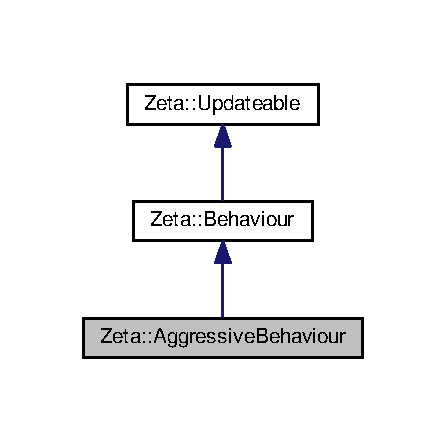
\includegraphics[width=214pt]{classZeta_1_1AggressiveBehaviour__inherit__graph}
\end{center}
\end{figure}


Collaboration diagram for Zeta\+:\+:Aggressive\+Behaviour\+:
\nopagebreak
\begin{figure}[H]
\begin{center}
\leavevmode
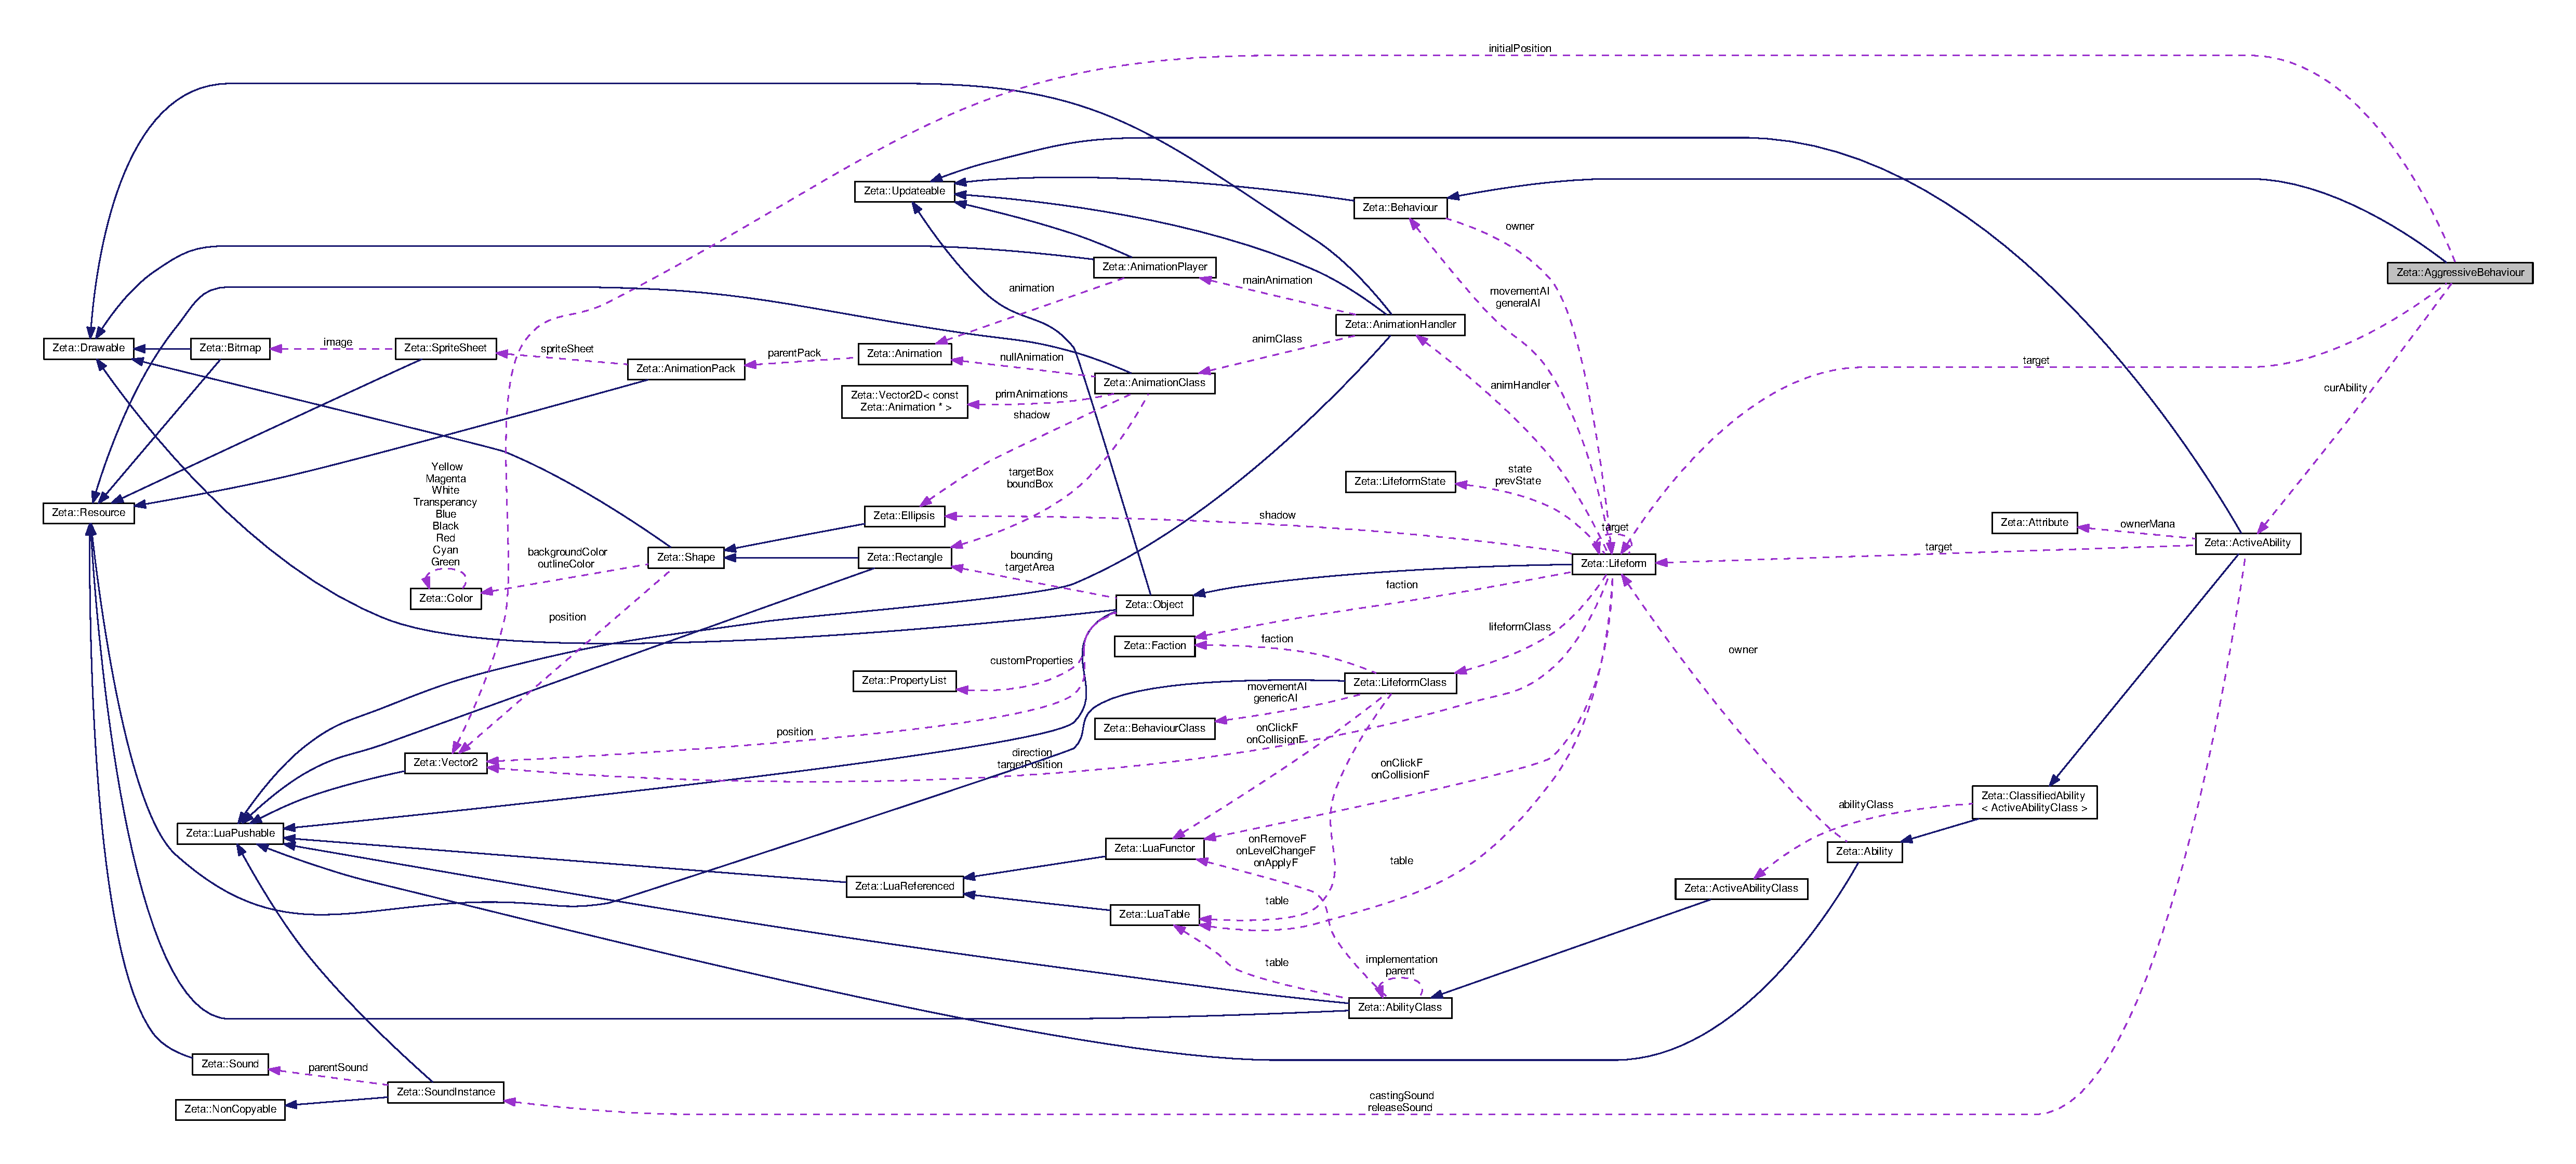
\includegraphics[width=350pt]{classZeta_1_1AggressiveBehaviour__coll__graph}
\end{center}
\end{figure}
\subsection*{Public Member Functions}
\begin{DoxyCompactItemize}
\item 
void \hyperlink{classZeta_1_1AggressiveBehaviour_a8303e71d7a3e283685573fc9c13e1640}{update} (\hyperlink{namespaceZeta_a1e0a1265f9b3bd3075fb0fabd39088ba}{Float} elapsed\+Time)
\item 
void \hyperlink{classZeta_1_1AggressiveBehaviour_a7ebb4cd0f618f9dd9e1e723e77aac292}{on\+Death} ()
\item 
\hyperlink{classZeta_1_1AggressiveBehaviour_a89c1244634a7f268ec45c6a04a244e59}{Aggressive\+Behaviour} (\hyperlink{classZeta_1_1Lifeform}{Lifeform} \&\hyperlink{classZeta_1_1Behaviour_ad32d56994e4e09e01ef86bcbb5c85e0a}{owner}, \hyperlink{namespaceZeta_a1e0a1265f9b3bd3075fb0fabd39088ba}{Float} \hyperlink{classZeta_1_1AggressiveBehaviour_a46ae846d179081d36af1daaeb21c0a55}{agro\+Range}=300, \hyperlink{namespaceZeta_a1e0a1265f9b3bd3075fb0fabd39088ba}{Float} \hyperlink{classZeta_1_1AggressiveBehaviour_af3f8203e1075c28d5141810ac07f1f5e}{drift\+Range}=600)
\item 
virtual \hyperlink{classZeta_1_1AggressiveBehaviour_a13d12742f4cca79e654b7e5c72a9cb50}{$\sim$\+Aggressive\+Behaviour} ()
\end{DoxyCompactItemize}
\subsection*{Private Types}
\begin{DoxyCompactItemize}
\item 
enum \hyperlink{classZeta_1_1AggressiveBehaviour_a768e2c9d0969879f4980d72220e11fbe}{State} \{ \\*
\hyperlink{classZeta_1_1AggressiveBehaviour_a768e2c9d0969879f4980d72220e11fbea495c55c275d09a00aaeb7482365ab300}{State\+::\+Scanning}, 
\hyperlink{classZeta_1_1AggressiveBehaviour_a768e2c9d0969879f4980d72220e11fbea8abd002ea36128383f3269de7e74039b}{State\+::\+Attacking}, 
\hyperlink{classZeta_1_1AggressiveBehaviour_a768e2c9d0969879f4980d72220e11fbead4e119b080e498be2b4712005e81f842}{State\+::\+Fall\+Back}, 
\hyperlink{classZeta_1_1AggressiveBehaviour_a768e2c9d0969879f4980d72220e11fbeadefe967ad0373b2274fc298f19125ca7}{State\+::\+Moving}, 
\\*
\hyperlink{classZeta_1_1AggressiveBehaviour_a768e2c9d0969879f4980d72220e11fbea86a59ad7ba2334ad7505f303d3f2ab6e}{State\+::\+Casting}
 \}
\end{DoxyCompactItemize}
\subsection*{Private Member Functions}
\begin{DoxyCompactItemize}
\item 
void \hyperlink{classZeta_1_1AggressiveBehaviour_a2e8b01db56c557cefdcd72d94610ffca}{scan} ()
\item 
void \hyperlink{classZeta_1_1AggressiveBehaviour_a54bc15050dd6470acd003d2d33b0b99f}{attack} ()
\item 
void \hyperlink{classZeta_1_1AggressiveBehaviour_a5db91c7bfcf560b936fce836ef02ca1d}{get\+Ability} ()
\end{DoxyCompactItemize}
\subsection*{Private Attributes}
\begin{DoxyCompactItemize}
\item 
\hyperlink{classZeta_1_1Vector2}{Vector2} \hyperlink{classZeta_1_1AggressiveBehaviour_a5301708e316129eb682436d7b8a09cac}{initial\+Position}
\item 
\hyperlink{classZeta_1_1Lifeform}{Lifeform} $\ast$ \hyperlink{classZeta_1_1AggressiveBehaviour_a7f1e06e7f51216cb7d9bb8ade9d79a47}{target}
\item 
\hyperlink{classZeta_1_1ActiveAbility}{Active\+Ability} $\ast$ \hyperlink{classZeta_1_1AggressiveBehaviour_affc1dc9f79144d64b9f627458442b7c5}{cur\+Ability}
\item 
\hyperlink{namespaceZeta_a1e0a1265f9b3bd3075fb0fabd39088ba}{Float} \hyperlink{classZeta_1_1AggressiveBehaviour_a46ae846d179081d36af1daaeb21c0a55}{agro\+Range}
\item 
\hyperlink{namespaceZeta_a1e0a1265f9b3bd3075fb0fabd39088ba}{Float} \hyperlink{classZeta_1_1AggressiveBehaviour_af3f8203e1075c28d5141810ac07f1f5e}{drift\+Range}
\item 
\hyperlink{classZeta_1_1AggressiveBehaviour_a768e2c9d0969879f4980d72220e11fbe}{State} \hyperlink{classZeta_1_1AggressiveBehaviour_ae0a924de0719f042bcb2f9def9a61e2b}{state}
\end{DoxyCompactItemize}
\subsection*{Additional Inherited Members}


\subsection{Member Enumeration Documentation}
\hypertarget{classZeta_1_1AggressiveBehaviour_a768e2c9d0969879f4980d72220e11fbe}{\index{Zeta\+::\+Aggressive\+Behaviour@{Zeta\+::\+Aggressive\+Behaviour}!State@{State}}
\index{State@{State}!Zeta\+::\+Aggressive\+Behaviour@{Zeta\+::\+Aggressive\+Behaviour}}
\subsubsection[{State}]{\setlength{\rightskip}{0pt plus 5cm}enum {\bf Zeta\+::\+Aggressive\+Behaviour\+::\+State}\hspace{0.3cm}{\ttfamily [strong]}, {\ttfamily [private]}}}\label{classZeta_1_1AggressiveBehaviour_a768e2c9d0969879f4980d72220e11fbe}
\begin{Desc}
\item[Enumerator]\par
\begin{description}
\index{Scanning@{Scanning}!Zeta\+::\+Aggressive\+Behaviour@{Zeta\+::\+Aggressive\+Behaviour}}\index{Zeta\+::\+Aggressive\+Behaviour@{Zeta\+::\+Aggressive\+Behaviour}!Scanning@{Scanning}}\item[{\em 
\hypertarget{classZeta_1_1AggressiveBehaviour_a768e2c9d0969879f4980d72220e11fbea495c55c275d09a00aaeb7482365ab300}{Scanning}\label{classZeta_1_1AggressiveBehaviour_a768e2c9d0969879f4980d72220e11fbea495c55c275d09a00aaeb7482365ab300}
}]\index{Attacking@{Attacking}!Zeta\+::\+Aggressive\+Behaviour@{Zeta\+::\+Aggressive\+Behaviour}}\index{Zeta\+::\+Aggressive\+Behaviour@{Zeta\+::\+Aggressive\+Behaviour}!Attacking@{Attacking}}\item[{\em 
\hypertarget{classZeta_1_1AggressiveBehaviour_a768e2c9d0969879f4980d72220e11fbea8abd002ea36128383f3269de7e74039b}{Attacking}\label{classZeta_1_1AggressiveBehaviour_a768e2c9d0969879f4980d72220e11fbea8abd002ea36128383f3269de7e74039b}
}]\index{Fall\+Back@{Fall\+Back}!Zeta\+::\+Aggressive\+Behaviour@{Zeta\+::\+Aggressive\+Behaviour}}\index{Zeta\+::\+Aggressive\+Behaviour@{Zeta\+::\+Aggressive\+Behaviour}!Fall\+Back@{Fall\+Back}}\item[{\em 
\hypertarget{classZeta_1_1AggressiveBehaviour_a768e2c9d0969879f4980d72220e11fbead4e119b080e498be2b4712005e81f842}{Fall\+Back}\label{classZeta_1_1AggressiveBehaviour_a768e2c9d0969879f4980d72220e11fbead4e119b080e498be2b4712005e81f842}
}]\index{Moving@{Moving}!Zeta\+::\+Aggressive\+Behaviour@{Zeta\+::\+Aggressive\+Behaviour}}\index{Zeta\+::\+Aggressive\+Behaviour@{Zeta\+::\+Aggressive\+Behaviour}!Moving@{Moving}}\item[{\em 
\hypertarget{classZeta_1_1AggressiveBehaviour_a768e2c9d0969879f4980d72220e11fbeadefe967ad0373b2274fc298f19125ca7}{Moving}\label{classZeta_1_1AggressiveBehaviour_a768e2c9d0969879f4980d72220e11fbeadefe967ad0373b2274fc298f19125ca7}
}]\index{Casting@{Casting}!Zeta\+::\+Aggressive\+Behaviour@{Zeta\+::\+Aggressive\+Behaviour}}\index{Zeta\+::\+Aggressive\+Behaviour@{Zeta\+::\+Aggressive\+Behaviour}!Casting@{Casting}}\item[{\em 
\hypertarget{classZeta_1_1AggressiveBehaviour_a768e2c9d0969879f4980d72220e11fbea86a59ad7ba2334ad7505f303d3f2ab6e}{Casting}\label{classZeta_1_1AggressiveBehaviour_a768e2c9d0969879f4980d72220e11fbea86a59ad7ba2334ad7505f303d3f2ab6e}
}]\end{description}
\end{Desc}


\subsection{Constructor \& Destructor Documentation}
\hypertarget{classZeta_1_1AggressiveBehaviour_a89c1244634a7f268ec45c6a04a244e59}{\index{Zeta\+::\+Aggressive\+Behaviour@{Zeta\+::\+Aggressive\+Behaviour}!Aggressive\+Behaviour@{Aggressive\+Behaviour}}
\index{Aggressive\+Behaviour@{Aggressive\+Behaviour}!Zeta\+::\+Aggressive\+Behaviour@{Zeta\+::\+Aggressive\+Behaviour}}
\subsubsection[{Aggressive\+Behaviour}]{\setlength{\rightskip}{0pt plus 5cm}Zeta\+::\+Aggressive\+Behaviour\+::\+Aggressive\+Behaviour (
\begin{DoxyParamCaption}
\item[{{\bf Lifeform} \&}]{owner, }
\item[{{\bf Float}}]{agro\+Range = {\ttfamily 300}, }
\item[{{\bf Float}}]{drift\+Range = {\ttfamily 600}}
\end{DoxyParamCaption}
)}}\label{classZeta_1_1AggressiveBehaviour_a89c1244634a7f268ec45c6a04a244e59}
\hypertarget{classZeta_1_1AggressiveBehaviour_a13d12742f4cca79e654b7e5c72a9cb50}{\index{Zeta\+::\+Aggressive\+Behaviour@{Zeta\+::\+Aggressive\+Behaviour}!````~Aggressive\+Behaviour@{$\sim$\+Aggressive\+Behaviour}}
\index{````~Aggressive\+Behaviour@{$\sim$\+Aggressive\+Behaviour}!Zeta\+::\+Aggressive\+Behaviour@{Zeta\+::\+Aggressive\+Behaviour}}
\subsubsection[{$\sim$\+Aggressive\+Behaviour}]{\setlength{\rightskip}{0pt plus 5cm}virtual Zeta\+::\+Aggressive\+Behaviour\+::$\sim$\+Aggressive\+Behaviour (
\begin{DoxyParamCaption}
{}
\end{DoxyParamCaption}
)\hspace{0.3cm}{\ttfamily [virtual]}}}\label{classZeta_1_1AggressiveBehaviour_a13d12742f4cca79e654b7e5c72a9cb50}


\subsection{Member Function Documentation}
\hypertarget{classZeta_1_1AggressiveBehaviour_a54bc15050dd6470acd003d2d33b0b99f}{\index{Zeta\+::\+Aggressive\+Behaviour@{Zeta\+::\+Aggressive\+Behaviour}!attack@{attack}}
\index{attack@{attack}!Zeta\+::\+Aggressive\+Behaviour@{Zeta\+::\+Aggressive\+Behaviour}}
\subsubsection[{attack}]{\setlength{\rightskip}{0pt plus 5cm}void Zeta\+::\+Aggressive\+Behaviour\+::attack (
\begin{DoxyParamCaption}
{}
\end{DoxyParamCaption}
)\hspace{0.3cm}{\ttfamily [private]}}}\label{classZeta_1_1AggressiveBehaviour_a54bc15050dd6470acd003d2d33b0b99f}
\hypertarget{classZeta_1_1AggressiveBehaviour_a5db91c7bfcf560b936fce836ef02ca1d}{\index{Zeta\+::\+Aggressive\+Behaviour@{Zeta\+::\+Aggressive\+Behaviour}!get\+Ability@{get\+Ability}}
\index{get\+Ability@{get\+Ability}!Zeta\+::\+Aggressive\+Behaviour@{Zeta\+::\+Aggressive\+Behaviour}}
\subsubsection[{get\+Ability}]{\setlength{\rightskip}{0pt plus 5cm}void Zeta\+::\+Aggressive\+Behaviour\+::get\+Ability (
\begin{DoxyParamCaption}
{}
\end{DoxyParamCaption}
)\hspace{0.3cm}{\ttfamily [private]}}}\label{classZeta_1_1AggressiveBehaviour_a5db91c7bfcf560b936fce836ef02ca1d}
\hypertarget{classZeta_1_1AggressiveBehaviour_a7ebb4cd0f618f9dd9e1e723e77aac292}{\index{Zeta\+::\+Aggressive\+Behaviour@{Zeta\+::\+Aggressive\+Behaviour}!on\+Death@{on\+Death}}
\index{on\+Death@{on\+Death}!Zeta\+::\+Aggressive\+Behaviour@{Zeta\+::\+Aggressive\+Behaviour}}
\subsubsection[{on\+Death}]{\setlength{\rightskip}{0pt plus 5cm}void Zeta\+::\+Aggressive\+Behaviour\+::on\+Death (
\begin{DoxyParamCaption}
{}
\end{DoxyParamCaption}
)\hspace{0.3cm}{\ttfamily [virtual]}}}\label{classZeta_1_1AggressiveBehaviour_a7ebb4cd0f618f9dd9e1e723e77aac292}


Implements \hyperlink{classZeta_1_1Behaviour_ac8c86b2e91f99441ee2e7de54e7d17d9}{Zeta\+::\+Behaviour}.

\hypertarget{classZeta_1_1AggressiveBehaviour_a2e8b01db56c557cefdcd72d94610ffca}{\index{Zeta\+::\+Aggressive\+Behaviour@{Zeta\+::\+Aggressive\+Behaviour}!scan@{scan}}
\index{scan@{scan}!Zeta\+::\+Aggressive\+Behaviour@{Zeta\+::\+Aggressive\+Behaviour}}
\subsubsection[{scan}]{\setlength{\rightskip}{0pt plus 5cm}void Zeta\+::\+Aggressive\+Behaviour\+::scan (
\begin{DoxyParamCaption}
{}
\end{DoxyParamCaption}
)\hspace{0.3cm}{\ttfamily [private]}}}\label{classZeta_1_1AggressiveBehaviour_a2e8b01db56c557cefdcd72d94610ffca}
\hypertarget{classZeta_1_1AggressiveBehaviour_a8303e71d7a3e283685573fc9c13e1640}{\index{Zeta\+::\+Aggressive\+Behaviour@{Zeta\+::\+Aggressive\+Behaviour}!update@{update}}
\index{update@{update}!Zeta\+::\+Aggressive\+Behaviour@{Zeta\+::\+Aggressive\+Behaviour}}
\subsubsection[{update}]{\setlength{\rightskip}{0pt plus 5cm}void Zeta\+::\+Aggressive\+Behaviour\+::update (
\begin{DoxyParamCaption}
\item[{{\bf Float}}]{elapsed\+Time}
\end{DoxyParamCaption}
)\hspace{0.3cm}{\ttfamily [virtual]}}}\label{classZeta_1_1AggressiveBehaviour_a8303e71d7a3e283685573fc9c13e1640}


Implements \hyperlink{classZeta_1_1Updateable_af4006bfccb762454b4da08786ad93de0}{Zeta\+::\+Updateable}.



\subsection{Member Data Documentation}
\hypertarget{classZeta_1_1AggressiveBehaviour_a46ae846d179081d36af1daaeb21c0a55}{\index{Zeta\+::\+Aggressive\+Behaviour@{Zeta\+::\+Aggressive\+Behaviour}!agro\+Range@{agro\+Range}}
\index{agro\+Range@{agro\+Range}!Zeta\+::\+Aggressive\+Behaviour@{Zeta\+::\+Aggressive\+Behaviour}}
\subsubsection[{agro\+Range}]{\setlength{\rightskip}{0pt plus 5cm}{\bf Float} Zeta\+::\+Aggressive\+Behaviour\+::agro\+Range\hspace{0.3cm}{\ttfamily [private]}}}\label{classZeta_1_1AggressiveBehaviour_a46ae846d179081d36af1daaeb21c0a55}
\hypertarget{classZeta_1_1AggressiveBehaviour_affc1dc9f79144d64b9f627458442b7c5}{\index{Zeta\+::\+Aggressive\+Behaviour@{Zeta\+::\+Aggressive\+Behaviour}!cur\+Ability@{cur\+Ability}}
\index{cur\+Ability@{cur\+Ability}!Zeta\+::\+Aggressive\+Behaviour@{Zeta\+::\+Aggressive\+Behaviour}}
\subsubsection[{cur\+Ability}]{\setlength{\rightskip}{0pt plus 5cm}{\bf Active\+Ability}$\ast$ Zeta\+::\+Aggressive\+Behaviour\+::cur\+Ability\hspace{0.3cm}{\ttfamily [private]}}}\label{classZeta_1_1AggressiveBehaviour_affc1dc9f79144d64b9f627458442b7c5}
\hypertarget{classZeta_1_1AggressiveBehaviour_af3f8203e1075c28d5141810ac07f1f5e}{\index{Zeta\+::\+Aggressive\+Behaviour@{Zeta\+::\+Aggressive\+Behaviour}!drift\+Range@{drift\+Range}}
\index{drift\+Range@{drift\+Range}!Zeta\+::\+Aggressive\+Behaviour@{Zeta\+::\+Aggressive\+Behaviour}}
\subsubsection[{drift\+Range}]{\setlength{\rightskip}{0pt plus 5cm}{\bf Float} Zeta\+::\+Aggressive\+Behaviour\+::drift\+Range\hspace{0.3cm}{\ttfamily [private]}}}\label{classZeta_1_1AggressiveBehaviour_af3f8203e1075c28d5141810ac07f1f5e}
\hypertarget{classZeta_1_1AggressiveBehaviour_a5301708e316129eb682436d7b8a09cac}{\index{Zeta\+::\+Aggressive\+Behaviour@{Zeta\+::\+Aggressive\+Behaviour}!initial\+Position@{initial\+Position}}
\index{initial\+Position@{initial\+Position}!Zeta\+::\+Aggressive\+Behaviour@{Zeta\+::\+Aggressive\+Behaviour}}
\subsubsection[{initial\+Position}]{\setlength{\rightskip}{0pt plus 5cm}{\bf Vector2} Zeta\+::\+Aggressive\+Behaviour\+::initial\+Position\hspace{0.3cm}{\ttfamily [private]}}}\label{classZeta_1_1AggressiveBehaviour_a5301708e316129eb682436d7b8a09cac}
\hypertarget{classZeta_1_1AggressiveBehaviour_ae0a924de0719f042bcb2f9def9a61e2b}{\index{Zeta\+::\+Aggressive\+Behaviour@{Zeta\+::\+Aggressive\+Behaviour}!state@{state}}
\index{state@{state}!Zeta\+::\+Aggressive\+Behaviour@{Zeta\+::\+Aggressive\+Behaviour}}
\subsubsection[{state}]{\setlength{\rightskip}{0pt plus 5cm}{\bf State} Zeta\+::\+Aggressive\+Behaviour\+::state\hspace{0.3cm}{\ttfamily [private]}}}\label{classZeta_1_1AggressiveBehaviour_ae0a924de0719f042bcb2f9def9a61e2b}
\hypertarget{classZeta_1_1AggressiveBehaviour_a7f1e06e7f51216cb7d9bb8ade9d79a47}{\index{Zeta\+::\+Aggressive\+Behaviour@{Zeta\+::\+Aggressive\+Behaviour}!target@{target}}
\index{target@{target}!Zeta\+::\+Aggressive\+Behaviour@{Zeta\+::\+Aggressive\+Behaviour}}
\subsubsection[{target}]{\setlength{\rightskip}{0pt plus 5cm}{\bf Lifeform}$\ast$ Zeta\+::\+Aggressive\+Behaviour\+::target\hspace{0.3cm}{\ttfamily [private]}}}\label{classZeta_1_1AggressiveBehaviour_a7f1e06e7f51216cb7d9bb8ade9d79a47}


The documentation for this class was generated from the following file\+:\begin{DoxyCompactItemize}
\item 
include/\+Zeta/\+Core/\+R\+P\+G\+Classes/\+A\+I/\hyperlink{AggressiveBehaviour_8hpp}{Aggressive\+Behaviour.\+hpp}\end{DoxyCompactItemize}

\hypertarget{classZeta_1_1AggressiveBehaviourClass}{\section{Zeta\+:\+:Aggressive\+Behaviour\+Class Class Reference}
\label{classZeta_1_1AggressiveBehaviourClass}\index{Zeta\+::\+Aggressive\+Behaviour\+Class@{Zeta\+::\+Aggressive\+Behaviour\+Class}}
}


{\ttfamily \#include $<$Aggressive\+Behaviour\+Class.\+hpp$>$}



Inheritance diagram for Zeta\+:\+:Aggressive\+Behaviour\+Class\+:\nopagebreak
\begin{figure}[H]
\begin{center}
\leavevmode
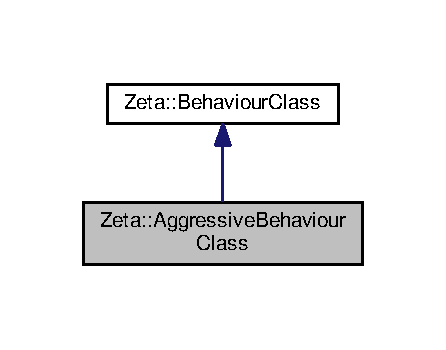
\includegraphics[width=214pt]{classZeta_1_1AggressiveBehaviourClass__inherit__graph}
\end{center}
\end{figure}


Collaboration diagram for Zeta\+:\+:Aggressive\+Behaviour\+Class\+:\nopagebreak
\begin{figure}[H]
\begin{center}
\leavevmode
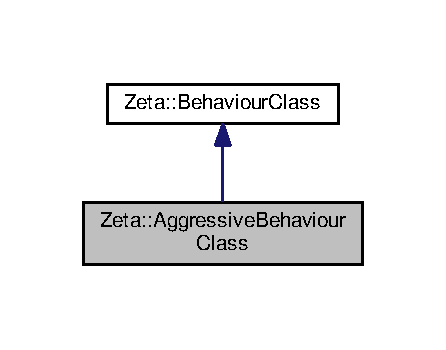
\includegraphics[width=214pt]{classZeta_1_1AggressiveBehaviourClass__coll__graph}
\end{center}
\end{figure}
\subsection*{Public Member Functions}
\begin{DoxyCompactItemize}
\item 
\hyperlink{classZeta_1_1Behaviour}{Behaviour} $\ast$ \hyperlink{classZeta_1_1AggressiveBehaviourClass_a94e8ce28a8c07370b144ac050f447823}{get\+New\+Behaviour} (\hyperlink{classZeta_1_1Lifeform}{Lifeform} \&owner) const 
\item 
\hyperlink{classZeta_1_1AggressiveBehaviourClass_a77d754731d3344ae59021421c5b417a6}{Aggressive\+Behaviour\+Class} (\hyperlink{namespaceZeta_a1e0a1265f9b3bd3075fb0fabd39088ba}{Float} \hyperlink{classZeta_1_1AggressiveBehaviourClass_aeb4248d80fec91bd36a462aee39a8832}{aggro\+Range}, \hyperlink{namespaceZeta_a1e0a1265f9b3bd3075fb0fabd39088ba}{Float} \hyperlink{classZeta_1_1AggressiveBehaviourClass_a86ac42f764b1691c4fc29b215605b5b6}{drift\+Range})
\item 
\hyperlink{classZeta_1_1AggressiveBehaviourClass_a95f3018f93087500afe5bbe1629e79b1}{$\sim$\+Aggressive\+Behaviour\+Class} ()
\end{DoxyCompactItemize}
\subsection*{Private Attributes}
\begin{DoxyCompactItemize}
\item 
\hyperlink{namespaceZeta_a1e0a1265f9b3bd3075fb0fabd39088ba}{Float} \hyperlink{classZeta_1_1AggressiveBehaviourClass_aeb4248d80fec91bd36a462aee39a8832}{aggro\+Range}
\item 
\hyperlink{namespaceZeta_a1e0a1265f9b3bd3075fb0fabd39088ba}{Float} \hyperlink{classZeta_1_1AggressiveBehaviourClass_a86ac42f764b1691c4fc29b215605b5b6}{drift\+Range}
\end{DoxyCompactItemize}


\subsection{Constructor \& Destructor Documentation}
\hypertarget{classZeta_1_1AggressiveBehaviourClass_a77d754731d3344ae59021421c5b417a6}{\index{Zeta\+::\+Aggressive\+Behaviour\+Class@{Zeta\+::\+Aggressive\+Behaviour\+Class}!Aggressive\+Behaviour\+Class@{Aggressive\+Behaviour\+Class}}
\index{Aggressive\+Behaviour\+Class@{Aggressive\+Behaviour\+Class}!Zeta\+::\+Aggressive\+Behaviour\+Class@{Zeta\+::\+Aggressive\+Behaviour\+Class}}
\subsubsection[{Aggressive\+Behaviour\+Class}]{\setlength{\rightskip}{0pt plus 5cm}Zeta\+::\+Aggressive\+Behaviour\+Class\+::\+Aggressive\+Behaviour\+Class (
\begin{DoxyParamCaption}
\item[{{\bf Float}}]{aggro\+Range, }
\item[{{\bf Float}}]{drift\+Range}
\end{DoxyParamCaption}
)\hspace{0.3cm}{\ttfamily [inline]}}}\label{classZeta_1_1AggressiveBehaviourClass_a77d754731d3344ae59021421c5b417a6}
\hypertarget{classZeta_1_1AggressiveBehaviourClass_a95f3018f93087500afe5bbe1629e79b1}{\index{Zeta\+::\+Aggressive\+Behaviour\+Class@{Zeta\+::\+Aggressive\+Behaviour\+Class}!````~Aggressive\+Behaviour\+Class@{$\sim$\+Aggressive\+Behaviour\+Class}}
\index{````~Aggressive\+Behaviour\+Class@{$\sim$\+Aggressive\+Behaviour\+Class}!Zeta\+::\+Aggressive\+Behaviour\+Class@{Zeta\+::\+Aggressive\+Behaviour\+Class}}
\subsubsection[{$\sim$\+Aggressive\+Behaviour\+Class}]{\setlength{\rightskip}{0pt plus 5cm}Zeta\+::\+Aggressive\+Behaviour\+Class\+::$\sim$\+Aggressive\+Behaviour\+Class (
\begin{DoxyParamCaption}
{}
\end{DoxyParamCaption}
)\hspace{0.3cm}{\ttfamily [inline]}}}\label{classZeta_1_1AggressiveBehaviourClass_a95f3018f93087500afe5bbe1629e79b1}


\subsection{Member Function Documentation}
\hypertarget{classZeta_1_1AggressiveBehaviourClass_a94e8ce28a8c07370b144ac050f447823}{\index{Zeta\+::\+Aggressive\+Behaviour\+Class@{Zeta\+::\+Aggressive\+Behaviour\+Class}!get\+New\+Behaviour@{get\+New\+Behaviour}}
\index{get\+New\+Behaviour@{get\+New\+Behaviour}!Zeta\+::\+Aggressive\+Behaviour\+Class@{Zeta\+::\+Aggressive\+Behaviour\+Class}}
\subsubsection[{get\+New\+Behaviour}]{\setlength{\rightskip}{0pt plus 5cm}{\bf Behaviour}$\ast$ Zeta\+::\+Aggressive\+Behaviour\+Class\+::get\+New\+Behaviour (
\begin{DoxyParamCaption}
\item[{{\bf Lifeform} \&}]{owner}
\end{DoxyParamCaption}
) const\hspace{0.3cm}{\ttfamily [virtual]}}}\label{classZeta_1_1AggressiveBehaviourClass_a94e8ce28a8c07370b144ac050f447823}


Implements \hyperlink{classZeta_1_1BehaviourClass_aeaf604f49cc95501422dfd177de64287}{Zeta\+::\+Behaviour\+Class}.



\subsection{Member Data Documentation}
\hypertarget{classZeta_1_1AggressiveBehaviourClass_aeb4248d80fec91bd36a462aee39a8832}{\index{Zeta\+::\+Aggressive\+Behaviour\+Class@{Zeta\+::\+Aggressive\+Behaviour\+Class}!aggro\+Range@{aggro\+Range}}
\index{aggro\+Range@{aggro\+Range}!Zeta\+::\+Aggressive\+Behaviour\+Class@{Zeta\+::\+Aggressive\+Behaviour\+Class}}
\subsubsection[{aggro\+Range}]{\setlength{\rightskip}{0pt plus 5cm}{\bf Float} Zeta\+::\+Aggressive\+Behaviour\+Class\+::aggro\+Range\hspace{0.3cm}{\ttfamily [private]}}}\label{classZeta_1_1AggressiveBehaviourClass_aeb4248d80fec91bd36a462aee39a8832}
\hypertarget{classZeta_1_1AggressiveBehaviourClass_a86ac42f764b1691c4fc29b215605b5b6}{\index{Zeta\+::\+Aggressive\+Behaviour\+Class@{Zeta\+::\+Aggressive\+Behaviour\+Class}!drift\+Range@{drift\+Range}}
\index{drift\+Range@{drift\+Range}!Zeta\+::\+Aggressive\+Behaviour\+Class@{Zeta\+::\+Aggressive\+Behaviour\+Class}}
\subsubsection[{drift\+Range}]{\setlength{\rightskip}{0pt plus 5cm}{\bf Float} Zeta\+::\+Aggressive\+Behaviour\+Class\+::drift\+Range\hspace{0.3cm}{\ttfamily [private]}}}\label{classZeta_1_1AggressiveBehaviourClass_a86ac42f764b1691c4fc29b215605b5b6}


The documentation for this class was generated from the following file\+:\begin{DoxyCompactItemize}
\item 
include/\+Zeta/\+Core/\+R\+P\+G\+Classes/\+A\+I/\hyperlink{AggressiveBehaviourClass_8hpp}{Aggressive\+Behaviour\+Class.\+hpp}\end{DoxyCompactItemize}

\hypertarget{classZeta_1_1AllegroAudioContext}{\section{Zeta\+:\+:Allegro\+Audio\+Context Class Reference}
\label{classZeta_1_1AllegroAudioContext}\index{Zeta\+::\+Allegro\+Audio\+Context@{Zeta\+::\+Allegro\+Audio\+Context}}
}


{\ttfamily \#include $<$Allegro\+Audio\+Context.\+hpp$>$}



Inheritance diagram for Zeta\+:\+:Allegro\+Audio\+Context\+:\nopagebreak
\begin{figure}[H]
\begin{center}
\leavevmode
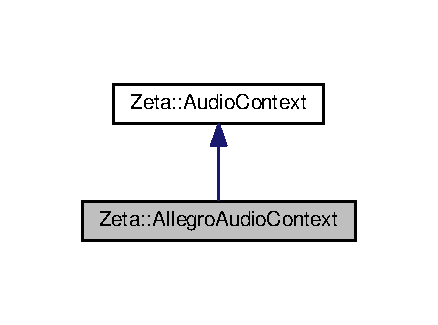
\includegraphics[width=210pt]{classZeta_1_1AllegroAudioContext__inherit__graph}
\end{center}
\end{figure}


Collaboration diagram for Zeta\+:\+:Allegro\+Audio\+Context\+:\nopagebreak
\begin{figure}[H]
\begin{center}
\leavevmode
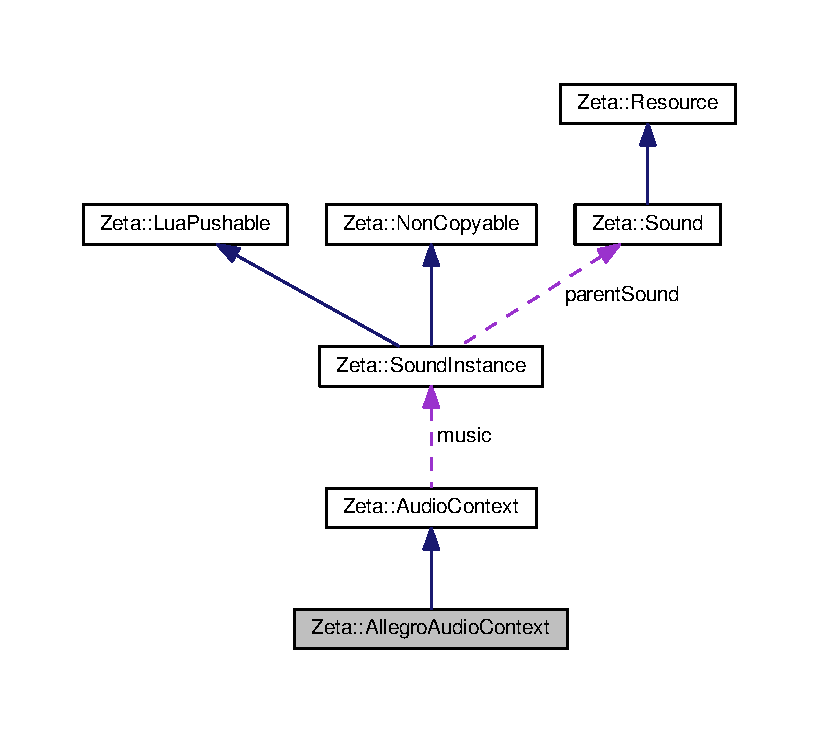
\includegraphics[width=350pt]{classZeta_1_1AllegroAudioContext__coll__graph}
\end{center}
\end{figure}
\subsection*{Public Member Functions}
\begin{DoxyCompactItemize}
\item 
float \hyperlink{classZeta_1_1AllegroAudioContext_a093e94d2f271f0030573e3c7f112fe17}{get\+Main\+Gain} () const 
\item 
void \hyperlink{classZeta_1_1AllegroAudioContext_ab2e61ddbafdb74657390ecdc813501b8}{set\+Main\+Gain} (float main\+Gain)
\item 
\hyperlink{classZeta_1_1AllegroAudioContext_a071c1b779505fa226d1dbb565f9e5283}{Allegro\+Audio\+Context} ()
\item 
\hyperlink{classZeta_1_1AllegroAudioContext_a02d34f4d72a3e85e1610fb59b0872f6e}{$\sim$\+Allegro\+Audio\+Context} ()
\end{DoxyCompactItemize}


\subsection{Constructor \& Destructor Documentation}
\hypertarget{classZeta_1_1AllegroAudioContext_a071c1b779505fa226d1dbb565f9e5283}{\index{Zeta\+::\+Allegro\+Audio\+Context@{Zeta\+::\+Allegro\+Audio\+Context}!Allegro\+Audio\+Context@{Allegro\+Audio\+Context}}
\index{Allegro\+Audio\+Context@{Allegro\+Audio\+Context}!Zeta\+::\+Allegro\+Audio\+Context@{Zeta\+::\+Allegro\+Audio\+Context}}
\subsubsection[{Allegro\+Audio\+Context}]{\setlength{\rightskip}{0pt plus 5cm}Zeta\+::\+Allegro\+Audio\+Context\+::\+Allegro\+Audio\+Context (
\begin{DoxyParamCaption}
{}
\end{DoxyParamCaption}
)}}\label{classZeta_1_1AllegroAudioContext_a071c1b779505fa226d1dbb565f9e5283}
\hypertarget{classZeta_1_1AllegroAudioContext_a02d34f4d72a3e85e1610fb59b0872f6e}{\index{Zeta\+::\+Allegro\+Audio\+Context@{Zeta\+::\+Allegro\+Audio\+Context}!````~Allegro\+Audio\+Context@{$\sim$\+Allegro\+Audio\+Context}}
\index{````~Allegro\+Audio\+Context@{$\sim$\+Allegro\+Audio\+Context}!Zeta\+::\+Allegro\+Audio\+Context@{Zeta\+::\+Allegro\+Audio\+Context}}
\subsubsection[{$\sim$\+Allegro\+Audio\+Context}]{\setlength{\rightskip}{0pt plus 5cm}Zeta\+::\+Allegro\+Audio\+Context\+::$\sim$\+Allegro\+Audio\+Context (
\begin{DoxyParamCaption}
{}
\end{DoxyParamCaption}
)}}\label{classZeta_1_1AllegroAudioContext_a02d34f4d72a3e85e1610fb59b0872f6e}


\subsection{Member Function Documentation}
\hypertarget{classZeta_1_1AllegroAudioContext_a093e94d2f271f0030573e3c7f112fe17}{\index{Zeta\+::\+Allegro\+Audio\+Context@{Zeta\+::\+Allegro\+Audio\+Context}!get\+Main\+Gain@{get\+Main\+Gain}}
\index{get\+Main\+Gain@{get\+Main\+Gain}!Zeta\+::\+Allegro\+Audio\+Context@{Zeta\+::\+Allegro\+Audio\+Context}}
\subsubsection[{get\+Main\+Gain}]{\setlength{\rightskip}{0pt plus 5cm}float Zeta\+::\+Allegro\+Audio\+Context\+::get\+Main\+Gain (
\begin{DoxyParamCaption}
{}
\end{DoxyParamCaption}
) const\hspace{0.3cm}{\ttfamily [virtual]}}}\label{classZeta_1_1AllegroAudioContext_a093e94d2f271f0030573e3c7f112fe17}
Gets the main \hyperlink{classZeta_1_1Sound}{Sound} gain. \begin{DoxyReturn}{Returns}
Float 0.\+0f-\/1.\+0f representing the Main Mixer Gain 
\end{DoxyReturn}


Implements \hyperlink{classZeta_1_1AudioContext_ab492d715ae780a8d6c2fc4e7a0432355}{Zeta\+::\+Audio\+Context}.

\hypertarget{classZeta_1_1AllegroAudioContext_ab2e61ddbafdb74657390ecdc813501b8}{\index{Zeta\+::\+Allegro\+Audio\+Context@{Zeta\+::\+Allegro\+Audio\+Context}!set\+Main\+Gain@{set\+Main\+Gain}}
\index{set\+Main\+Gain@{set\+Main\+Gain}!Zeta\+::\+Allegro\+Audio\+Context@{Zeta\+::\+Allegro\+Audio\+Context}}
\subsubsection[{set\+Main\+Gain}]{\setlength{\rightskip}{0pt plus 5cm}void Zeta\+::\+Allegro\+Audio\+Context\+::set\+Main\+Gain (
\begin{DoxyParamCaption}
\item[{float}]{main\+Gain}
\end{DoxyParamCaption}
)\hspace{0.3cm}{\ttfamily [virtual]}}}\label{classZeta_1_1AllegroAudioContext_ab2e61ddbafdb74657390ecdc813501b8}
Sets the main Soung Gain. 
\begin{DoxyParams}{Parameters}
{\em main\+Gain} & Float representing the main\+Gain \\
\hline
\end{DoxyParams}


Implements \hyperlink{classZeta_1_1AudioContext_af861f3797591e2c62040a18b3d4daa51}{Zeta\+::\+Audio\+Context}.



The documentation for this class was generated from the following file\+:\begin{DoxyCompactItemize}
\item 
include/\+Zeta/\+Library\+Binders/\+Allegro5/\hyperlink{AllegroAudioContext_8hpp}{Allegro\+Audio\+Context.\+hpp}\end{DoxyCompactItemize}

\hypertarget{classZeta_1_1AllegroBitmap}{\section{Zeta\+:\+:Allegro\+Bitmap Class Reference}
\label{classZeta_1_1AllegroBitmap}\index{Zeta\+::\+Allegro\+Bitmap@{Zeta\+::\+Allegro\+Bitmap}}
}


{\ttfamily \#include $<$Allegro\+Bitmap.\+hpp$>$}



Inheritance diagram for Zeta\+:\+:Allegro\+Bitmap\+:\nopagebreak
\begin{figure}[H]
\begin{center}
\leavevmode
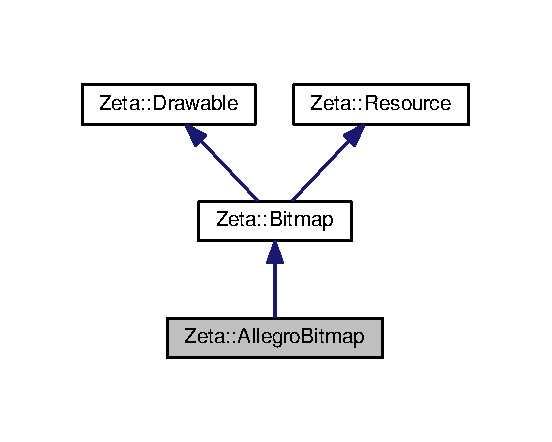
\includegraphics[width=265pt]{classZeta_1_1AllegroBitmap__inherit__graph}
\end{center}
\end{figure}


Collaboration diagram for Zeta\+:\+:Allegro\+Bitmap\+:\nopagebreak
\begin{figure}[H]
\begin{center}
\leavevmode
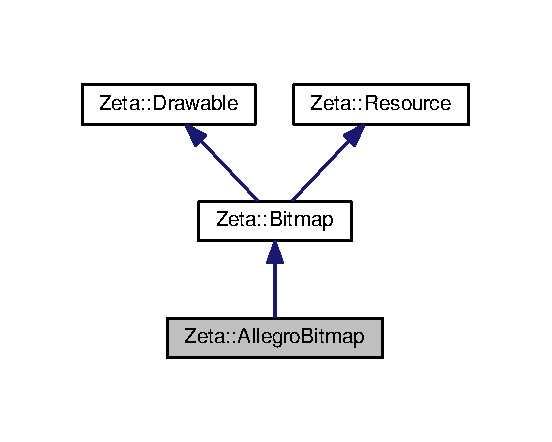
\includegraphics[width=265pt]{classZeta_1_1AllegroBitmap__coll__graph}
\end{center}
\end{figure}
\subsection*{Public Member Functions}
\begin{DoxyCompactItemize}
\item 
void \hyperlink{classZeta_1_1AllegroBitmap_ab3ddef20d1597683a99dcfdc5cfb3c5f}{draw} (\hyperlink{namespaceZeta_a1e0a1265f9b3bd3075fb0fabd39088ba}{Float} x, \hyperlink{namespaceZeta_a1e0a1265f9b3bd3075fb0fabd39088ba}{Float} y, \hyperlink{namespaceZeta_a1e0a1265f9b3bd3075fb0fabd39088ba}{Float} rotation=0.\+0f, Float scale=1.\+0f) const 
\item 
void \hyperlink{classZeta_1_1AllegroBitmap_a26b3206d585a5f30b990c1279eb92e7a}{draw} (\hyperlink{namespaceZeta_a1e0a1265f9b3bd3075fb0fabd39088ba}{Float} x, \hyperlink{namespaceZeta_a1e0a1265f9b3bd3075fb0fabd39088ba}{Float} y, \hyperlink{namespaceZeta_a1e0a1265f9b3bd3075fb0fabd39088ba}{Float} rotation, \hyperlink{namespaceZeta_a1e0a1265f9b3bd3075fb0fabd39088ba}{Float} scale, \hyperlink{classZeta_1_1Bitmap_a8cb28cf4226b7d6bedf6c9bb2413b3fa}{Flip\+Flag} flip) const 
\item 
void \hyperlink{classZeta_1_1AllegroBitmap_ac914238cb9e48e6f3e4260f7c62b40f8}{draw\+At\+Centre} (\hyperlink{namespaceZeta_a1e0a1265f9b3bd3075fb0fabd39088ba}{Float} x, \hyperlink{namespaceZeta_a1e0a1265f9b3bd3075fb0fabd39088ba}{Float} y, \hyperlink{namespaceZeta_a1e0a1265f9b3bd3075fb0fabd39088ba}{Float} rotation, \hyperlink{namespaceZeta_a1e0a1265f9b3bd3075fb0fabd39088ba}{Float} scale, \hyperlink{classZeta_1_1Bitmap_a8cb28cf4226b7d6bedf6c9bb2413b3fa}{Flip\+Flag} flip=\hyperlink{classZeta_1_1Bitmap_a8cb28cf4226b7d6bedf6c9bb2413b3faad95504740b4fa9384ac72564cd282755}{Normal}) const 
\item 
\hyperlink{classZeta_1_1Bitmap}{Bitmap} \& \hyperlink{classZeta_1_1AllegroBitmap_a92c61e54a550c9756b5567a20625c31d}{create\+Sub\+Bitmap} (int x, int y, int \hyperlink{classZeta_1_1Bitmap_affa526cccd51b4ac5db7aac25ff7f6a9}{width}, int \hyperlink{classZeta_1_1Bitmap_a4d9a82acc6c418dc9b72227b0d63d9aa}{height}) const 
\item 
void \hyperlink{classZeta_1_1AllegroBitmap_a2e7d04979e1c34a3d1c320ba67c429d2}{erase\+Sub\+Bitmap} (\hyperlink{classZeta_1_1Bitmap}{Bitmap} \&\hyperlink{classZeta_1_1AllegroBitmap_aec65e1335da328dd4d7964e97297ea72}{bitmap}) const 
\item 
void \hyperlink{classZeta_1_1AllegroBitmap_ac37c6b783f388afe960479b9addcf0a7}{reserve\+Sub\+Bitmaps} (size\+\_\+t number) const 
\item 
\hyperlink{classZeta_1_1AllegroBitmap_a4c1224bf83513d60af3209d3807a9c70}{Allegro\+Bitmap} (\hyperlink{classZeta_1_1AllegroBitmap}{Allegro\+Bitmap} \&\&)=default
\item 
\hyperlink{classZeta_1_1AllegroBitmap}{Allegro\+Bitmap} \& \hyperlink{classZeta_1_1AllegroBitmap_a645f5970ef80feef64ad19d9c99773ca}{operator=} (\hyperlink{classZeta_1_1AllegroBitmap}{Allegro\+Bitmap} \&\&)=default
\item 
\hyperlink{classZeta_1_1AllegroBitmap_ab8a2848f4c9f089363a7ab0e261b4107}{Allegro\+Bitmap} ()
\item 
\hyperlink{classZeta_1_1AllegroBitmap_ad931383a1e65f676b78b5f85200f3e3d}{Allegro\+Bitmap} (int \hyperlink{classZeta_1_1Bitmap_affa526cccd51b4ac5db7aac25ff7f6a9}{width}, int \hyperlink{classZeta_1_1Bitmap_a4d9a82acc6c418dc9b72227b0d63d9aa}{height})
\item 
\hyperlink{classZeta_1_1AllegroBitmap_abc130d8cfc269eae73b18802f3022949}{Allegro\+Bitmap} (const std\+::string \&path)
\item 
\hyperlink{classZeta_1_1AllegroBitmap_ad4f55c47944ac52b4d4970e648e8be91}{$\sim$\+Allegro\+Bitmap} ()
\end{DoxyCompactItemize}
\subsection*{Private Member Functions}
\begin{DoxyCompactItemize}
\item 
\hyperlink{classZeta_1_1AllegroBitmap_ad7310439fb73c60db7979f21e438f89f}{Allegro\+Bitmap} (const \hyperlink{classZeta_1_1AllegroBitmap}{Allegro\+Bitmap} \&parent, int x, int y, int \hyperlink{classZeta_1_1Bitmap_affa526cccd51b4ac5db7aac25ff7f6a9}{width}, int \hyperlink{classZeta_1_1Bitmap_a4d9a82acc6c418dc9b72227b0d63d9aa}{height})
\end{DoxyCompactItemize}
\subsection*{Private Attributes}
\begin{DoxyCompactItemize}
\item 
\hyperlink{namespaceZeta_a92c229b4db6ab7275c2b7f32bdfabc87}{Z\+Set}$<$ \hyperlink{classZeta_1_1AllegroBitmap}{Allegro\+Bitmap} $\ast$ $>$ \hyperlink{classZeta_1_1AllegroBitmap_ac12c67de5ad5f7e08ec77bff1def3e15}{sub\+Bitmaps}
\item 
A\+L\+L\+E\+G\+R\+O\+\_\+\+B\+I\+T\+M\+A\+P $\ast$ \hyperlink{classZeta_1_1AllegroBitmap_aec65e1335da328dd4d7964e97297ea72}{bitmap}
\item 
int \hyperlink{classZeta_1_1AllegroBitmap_a223f2bc3bdc93e0d8195bd29bcaadbc7}{h\+\_\+width}
\item 
int \hyperlink{classZeta_1_1AllegroBitmap_aca7f1a2bb6f23d51235f04dfba1ebbfb}{h\+\_\+height}
\end{DoxyCompactItemize}
\subsection*{Additional Inherited Members}


\subsection{Constructor \& Destructor Documentation}
\hypertarget{classZeta_1_1AllegroBitmap_a4c1224bf83513d60af3209d3807a9c70}{\index{Zeta\+::\+Allegro\+Bitmap@{Zeta\+::\+Allegro\+Bitmap}!Allegro\+Bitmap@{Allegro\+Bitmap}}
\index{Allegro\+Bitmap@{Allegro\+Bitmap}!Zeta\+::\+Allegro\+Bitmap@{Zeta\+::\+Allegro\+Bitmap}}
\subsubsection[{Allegro\+Bitmap}]{\setlength{\rightskip}{0pt plus 5cm}Zeta\+::\+Allegro\+Bitmap\+::\+Allegro\+Bitmap (
\begin{DoxyParamCaption}
\item[{{\bf Allegro\+Bitmap} \&\&}]{}
\end{DoxyParamCaption}
)\hspace{0.3cm}{\ttfamily [default]}}}\label{classZeta_1_1AllegroBitmap_a4c1224bf83513d60af3209d3807a9c70}
\hypertarget{classZeta_1_1AllegroBitmap_ab8a2848f4c9f089363a7ab0e261b4107}{\index{Zeta\+::\+Allegro\+Bitmap@{Zeta\+::\+Allegro\+Bitmap}!Allegro\+Bitmap@{Allegro\+Bitmap}}
\index{Allegro\+Bitmap@{Allegro\+Bitmap}!Zeta\+::\+Allegro\+Bitmap@{Zeta\+::\+Allegro\+Bitmap}}
\subsubsection[{Allegro\+Bitmap}]{\setlength{\rightskip}{0pt plus 5cm}Zeta\+::\+Allegro\+Bitmap\+::\+Allegro\+Bitmap (
\begin{DoxyParamCaption}
{}
\end{DoxyParamCaption}
)}}\label{classZeta_1_1AllegroBitmap_ab8a2848f4c9f089363a7ab0e261b4107}
\hypertarget{classZeta_1_1AllegroBitmap_ad931383a1e65f676b78b5f85200f3e3d}{\index{Zeta\+::\+Allegro\+Bitmap@{Zeta\+::\+Allegro\+Bitmap}!Allegro\+Bitmap@{Allegro\+Bitmap}}
\index{Allegro\+Bitmap@{Allegro\+Bitmap}!Zeta\+::\+Allegro\+Bitmap@{Zeta\+::\+Allegro\+Bitmap}}
\subsubsection[{Allegro\+Bitmap}]{\setlength{\rightskip}{0pt plus 5cm}Zeta\+::\+Allegro\+Bitmap\+::\+Allegro\+Bitmap (
\begin{DoxyParamCaption}
\item[{int}]{width, }
\item[{int}]{height}
\end{DoxyParamCaption}
)}}\label{classZeta_1_1AllegroBitmap_ad931383a1e65f676b78b5f85200f3e3d}
\hypertarget{classZeta_1_1AllegroBitmap_abc130d8cfc269eae73b18802f3022949}{\index{Zeta\+::\+Allegro\+Bitmap@{Zeta\+::\+Allegro\+Bitmap}!Allegro\+Bitmap@{Allegro\+Bitmap}}
\index{Allegro\+Bitmap@{Allegro\+Bitmap}!Zeta\+::\+Allegro\+Bitmap@{Zeta\+::\+Allegro\+Bitmap}}
\subsubsection[{Allegro\+Bitmap}]{\setlength{\rightskip}{0pt plus 5cm}Zeta\+::\+Allegro\+Bitmap\+::\+Allegro\+Bitmap (
\begin{DoxyParamCaption}
\item[{const std\+::string \&}]{path}
\end{DoxyParamCaption}
)}}\label{classZeta_1_1AllegroBitmap_abc130d8cfc269eae73b18802f3022949}
\hypertarget{classZeta_1_1AllegroBitmap_ad4f55c47944ac52b4d4970e648e8be91}{\index{Zeta\+::\+Allegro\+Bitmap@{Zeta\+::\+Allegro\+Bitmap}!````~Allegro\+Bitmap@{$\sim$\+Allegro\+Bitmap}}
\index{````~Allegro\+Bitmap@{$\sim$\+Allegro\+Bitmap}!Zeta\+::\+Allegro\+Bitmap@{Zeta\+::\+Allegro\+Bitmap}}
\subsubsection[{$\sim$\+Allegro\+Bitmap}]{\setlength{\rightskip}{0pt plus 5cm}Zeta\+::\+Allegro\+Bitmap\+::$\sim$\+Allegro\+Bitmap (
\begin{DoxyParamCaption}
{}
\end{DoxyParamCaption}
)}}\label{classZeta_1_1AllegroBitmap_ad4f55c47944ac52b4d4970e648e8be91}
\hypertarget{classZeta_1_1AllegroBitmap_ad7310439fb73c60db7979f21e438f89f}{\index{Zeta\+::\+Allegro\+Bitmap@{Zeta\+::\+Allegro\+Bitmap}!Allegro\+Bitmap@{Allegro\+Bitmap}}
\index{Allegro\+Bitmap@{Allegro\+Bitmap}!Zeta\+::\+Allegro\+Bitmap@{Zeta\+::\+Allegro\+Bitmap}}
\subsubsection[{Allegro\+Bitmap}]{\setlength{\rightskip}{0pt plus 5cm}Zeta\+::\+Allegro\+Bitmap\+::\+Allegro\+Bitmap (
\begin{DoxyParamCaption}
\item[{const {\bf Allegro\+Bitmap} \&}]{parent, }
\item[{int}]{x, }
\item[{int}]{y, }
\item[{int}]{width, }
\item[{int}]{height}
\end{DoxyParamCaption}
)\hspace{0.3cm}{\ttfamily [private]}}}\label{classZeta_1_1AllegroBitmap_ad7310439fb73c60db7979f21e438f89f}


\subsection{Member Function Documentation}
\hypertarget{classZeta_1_1AllegroBitmap_a92c61e54a550c9756b5567a20625c31d}{\index{Zeta\+::\+Allegro\+Bitmap@{Zeta\+::\+Allegro\+Bitmap}!create\+Sub\+Bitmap@{create\+Sub\+Bitmap}}
\index{create\+Sub\+Bitmap@{create\+Sub\+Bitmap}!Zeta\+::\+Allegro\+Bitmap@{Zeta\+::\+Allegro\+Bitmap}}
\subsubsection[{create\+Sub\+Bitmap}]{\setlength{\rightskip}{0pt plus 5cm}{\bf Bitmap}\& Zeta\+::\+Allegro\+Bitmap\+::create\+Sub\+Bitmap (
\begin{DoxyParamCaption}
\item[{int}]{x, }
\item[{int}]{y, }
\item[{int}]{width, }
\item[{int}]{height}
\end{DoxyParamCaption}
) const\hspace{0.3cm}{\ttfamily [virtual]}}}\label{classZeta_1_1AllegroBitmap_a92c61e54a550c9756b5567a20625c31d}


Implements \hyperlink{classZeta_1_1Bitmap_a790614f445f0c59f9533ed1d4046dd74}{Zeta\+::\+Bitmap}.

\hypertarget{classZeta_1_1AllegroBitmap_ab3ddef20d1597683a99dcfdc5cfb3c5f}{\index{Zeta\+::\+Allegro\+Bitmap@{Zeta\+::\+Allegro\+Bitmap}!draw@{draw}}
\index{draw@{draw}!Zeta\+::\+Allegro\+Bitmap@{Zeta\+::\+Allegro\+Bitmap}}
\subsubsection[{draw}]{\setlength{\rightskip}{0pt plus 5cm}void Zeta\+::\+Allegro\+Bitmap\+::draw (
\begin{DoxyParamCaption}
\item[{{\bf Float}}]{x, }
\item[{{\bf Float}}]{y, }
\item[{{\bf Float}}]{rotation = {\ttfamily 0.0f}, }
\item[{{\bf Float}}]{scale = {\ttfamily 1.0f}}
\end{DoxyParamCaption}
) const\hspace{0.3cm}{\ttfamily [virtual]}}}\label{classZeta_1_1AllegroBitmap_ab3ddef20d1597683a99dcfdc5cfb3c5f}
Draws the \hyperlink{classZeta_1_1Object}{Object} on screen. Be advised, the x,y, offsets might have different meaning on different implementations. 
\begin{DoxyParams}{Parameters}
{\em x} & X offset to be applied on the drawing \\
\hline
{\em y} & Y offset to be applied on the drawing \\
\hline
{\em rotation} & the rotation to be applied on the drawing \\
\hline
\end{DoxyParams}


Implements \hyperlink{classZeta_1_1Drawable_a3f453a7a971b7eeba1768be3eaedc192}{Zeta\+::\+Drawable}.

\hypertarget{classZeta_1_1AllegroBitmap_a26b3206d585a5f30b990c1279eb92e7a}{\index{Zeta\+::\+Allegro\+Bitmap@{Zeta\+::\+Allegro\+Bitmap}!draw@{draw}}
\index{draw@{draw}!Zeta\+::\+Allegro\+Bitmap@{Zeta\+::\+Allegro\+Bitmap}}
\subsubsection[{draw}]{\setlength{\rightskip}{0pt plus 5cm}void Zeta\+::\+Allegro\+Bitmap\+::draw (
\begin{DoxyParamCaption}
\item[{{\bf Float}}]{x, }
\item[{{\bf Float}}]{y, }
\item[{{\bf Float}}]{rotation, }
\item[{{\bf Float}}]{scale, }
\item[{{\bf Flip\+Flag}}]{flip}
\end{DoxyParamCaption}
) const\hspace{0.3cm}{\ttfamily [virtual]}}}\label{classZeta_1_1AllegroBitmap_a26b3206d585a5f30b990c1279eb92e7a}


Implements \hyperlink{classZeta_1_1Bitmap_a2a5af6ab1c1237efe52d155fe63e24b7}{Zeta\+::\+Bitmap}.

\hypertarget{classZeta_1_1AllegroBitmap_ac914238cb9e48e6f3e4260f7c62b40f8}{\index{Zeta\+::\+Allegro\+Bitmap@{Zeta\+::\+Allegro\+Bitmap}!draw\+At\+Centre@{draw\+At\+Centre}}
\index{draw\+At\+Centre@{draw\+At\+Centre}!Zeta\+::\+Allegro\+Bitmap@{Zeta\+::\+Allegro\+Bitmap}}
\subsubsection[{draw\+At\+Centre}]{\setlength{\rightskip}{0pt plus 5cm}void Zeta\+::\+Allegro\+Bitmap\+::draw\+At\+Centre (
\begin{DoxyParamCaption}
\item[{{\bf Float}}]{x, }
\item[{{\bf Float}}]{y, }
\item[{{\bf Float}}]{rotation, }
\item[{{\bf Float}}]{scale, }
\item[{{\bf Flip\+Flag}}]{flip = {\ttfamily {\bf Normal}}}
\end{DoxyParamCaption}
) const\hspace{0.3cm}{\ttfamily [virtual]}}}\label{classZeta_1_1AllegroBitmap_ac914238cb9e48e6f3e4260f7c62b40f8}


Implements \hyperlink{classZeta_1_1Bitmap_af06b42874ae626ca8e403c478fab46e9}{Zeta\+::\+Bitmap}.

\hypertarget{classZeta_1_1AllegroBitmap_a2e7d04979e1c34a3d1c320ba67c429d2}{\index{Zeta\+::\+Allegro\+Bitmap@{Zeta\+::\+Allegro\+Bitmap}!erase\+Sub\+Bitmap@{erase\+Sub\+Bitmap}}
\index{erase\+Sub\+Bitmap@{erase\+Sub\+Bitmap}!Zeta\+::\+Allegro\+Bitmap@{Zeta\+::\+Allegro\+Bitmap}}
\subsubsection[{erase\+Sub\+Bitmap}]{\setlength{\rightskip}{0pt plus 5cm}void Zeta\+::\+Allegro\+Bitmap\+::erase\+Sub\+Bitmap (
\begin{DoxyParamCaption}
\item[{{\bf Bitmap} \&}]{bitmap}
\end{DoxyParamCaption}
) const\hspace{0.3cm}{\ttfamily [virtual]}}}\label{classZeta_1_1AllegroBitmap_a2e7d04979e1c34a3d1c320ba67c429d2}


Implements \hyperlink{classZeta_1_1Bitmap_acaef132548ff57ccdc725b864a1150b8}{Zeta\+::\+Bitmap}.

\hypertarget{classZeta_1_1AllegroBitmap_a645f5970ef80feef64ad19d9c99773ca}{\index{Zeta\+::\+Allegro\+Bitmap@{Zeta\+::\+Allegro\+Bitmap}!operator=@{operator=}}
\index{operator=@{operator=}!Zeta\+::\+Allegro\+Bitmap@{Zeta\+::\+Allegro\+Bitmap}}
\subsubsection[{operator=}]{\setlength{\rightskip}{0pt plus 5cm}{\bf Allegro\+Bitmap}\& Zeta\+::\+Allegro\+Bitmap\+::operator= (
\begin{DoxyParamCaption}
\item[{{\bf Allegro\+Bitmap} \&\&}]{}
\end{DoxyParamCaption}
)\hspace{0.3cm}{\ttfamily [default]}}}\label{classZeta_1_1AllegroBitmap_a645f5970ef80feef64ad19d9c99773ca}
\hypertarget{classZeta_1_1AllegroBitmap_ac37c6b783f388afe960479b9addcf0a7}{\index{Zeta\+::\+Allegro\+Bitmap@{Zeta\+::\+Allegro\+Bitmap}!reserve\+Sub\+Bitmaps@{reserve\+Sub\+Bitmaps}}
\index{reserve\+Sub\+Bitmaps@{reserve\+Sub\+Bitmaps}!Zeta\+::\+Allegro\+Bitmap@{Zeta\+::\+Allegro\+Bitmap}}
\subsubsection[{reserve\+Sub\+Bitmaps}]{\setlength{\rightskip}{0pt plus 5cm}void Zeta\+::\+Allegro\+Bitmap\+::reserve\+Sub\+Bitmaps (
\begin{DoxyParamCaption}
\item[{size\+\_\+t}]{number}
\end{DoxyParamCaption}
) const\hspace{0.3cm}{\ttfamily [virtual]}}}\label{classZeta_1_1AllegroBitmap_ac37c6b783f388afe960479b9addcf0a7}


Implements \hyperlink{classZeta_1_1Bitmap_afc49ceff653f55699fe7b723eb6193ae}{Zeta\+::\+Bitmap}.



\subsection{Member Data Documentation}
\hypertarget{classZeta_1_1AllegroBitmap_aec65e1335da328dd4d7964e97297ea72}{\index{Zeta\+::\+Allegro\+Bitmap@{Zeta\+::\+Allegro\+Bitmap}!bitmap@{bitmap}}
\index{bitmap@{bitmap}!Zeta\+::\+Allegro\+Bitmap@{Zeta\+::\+Allegro\+Bitmap}}
\subsubsection[{bitmap}]{\setlength{\rightskip}{0pt plus 5cm}A\+L\+L\+E\+G\+R\+O\+\_\+\+B\+I\+T\+M\+A\+P$\ast$ Zeta\+::\+Allegro\+Bitmap\+::bitmap\hspace{0.3cm}{\ttfamily [mutable]}, {\ttfamily [private]}}}\label{classZeta_1_1AllegroBitmap_aec65e1335da328dd4d7964e97297ea72}
\hypertarget{classZeta_1_1AllegroBitmap_aca7f1a2bb6f23d51235f04dfba1ebbfb}{\index{Zeta\+::\+Allegro\+Bitmap@{Zeta\+::\+Allegro\+Bitmap}!h\+\_\+height@{h\+\_\+height}}
\index{h\+\_\+height@{h\+\_\+height}!Zeta\+::\+Allegro\+Bitmap@{Zeta\+::\+Allegro\+Bitmap}}
\subsubsection[{h\+\_\+height}]{\setlength{\rightskip}{0pt plus 5cm}int Zeta\+::\+Allegro\+Bitmap\+::h\+\_\+height\hspace{0.3cm}{\ttfamily [private]}}}\label{classZeta_1_1AllegroBitmap_aca7f1a2bb6f23d51235f04dfba1ebbfb}
\hypertarget{classZeta_1_1AllegroBitmap_a223f2bc3bdc93e0d8195bd29bcaadbc7}{\index{Zeta\+::\+Allegro\+Bitmap@{Zeta\+::\+Allegro\+Bitmap}!h\+\_\+width@{h\+\_\+width}}
\index{h\+\_\+width@{h\+\_\+width}!Zeta\+::\+Allegro\+Bitmap@{Zeta\+::\+Allegro\+Bitmap}}
\subsubsection[{h\+\_\+width}]{\setlength{\rightskip}{0pt plus 5cm}int Zeta\+::\+Allegro\+Bitmap\+::h\+\_\+width\hspace{0.3cm}{\ttfamily [private]}}}\label{classZeta_1_1AllegroBitmap_a223f2bc3bdc93e0d8195bd29bcaadbc7}
\hypertarget{classZeta_1_1AllegroBitmap_ac12c67de5ad5f7e08ec77bff1def3e15}{\index{Zeta\+::\+Allegro\+Bitmap@{Zeta\+::\+Allegro\+Bitmap}!sub\+Bitmaps@{sub\+Bitmaps}}
\index{sub\+Bitmaps@{sub\+Bitmaps}!Zeta\+::\+Allegro\+Bitmap@{Zeta\+::\+Allegro\+Bitmap}}
\subsubsection[{sub\+Bitmaps}]{\setlength{\rightskip}{0pt plus 5cm}{\bf Z\+Set}$<${\bf Allegro\+Bitmap}$\ast$$>$ Zeta\+::\+Allegro\+Bitmap\+::sub\+Bitmaps\hspace{0.3cm}{\ttfamily [mutable]}, {\ttfamily [private]}}}\label{classZeta_1_1AllegroBitmap_ac12c67de5ad5f7e08ec77bff1def3e15}


The documentation for this class was generated from the following file\+:\begin{DoxyCompactItemize}
\item 
include/\+Zeta/\+Library\+Binders/\+Allegro5/\hyperlink{AllegroBitmap_8hpp}{Allegro\+Bitmap.\+hpp}\end{DoxyCompactItemize}

\hypertarget{classZeta_1_1AllegroDisplay}{\section{Zeta\+:\+:Allegro\+Display Class Reference}
\label{classZeta_1_1AllegroDisplay}\index{Zeta\+::\+Allegro\+Display@{Zeta\+::\+Allegro\+Display}}
}


{\ttfamily \#include $<$Allegro\+Display.\+hpp$>$}



Inheritance diagram for Zeta\+:\+:Allegro\+Display\+:\nopagebreak
\begin{figure}[H]
\begin{center}
\leavevmode
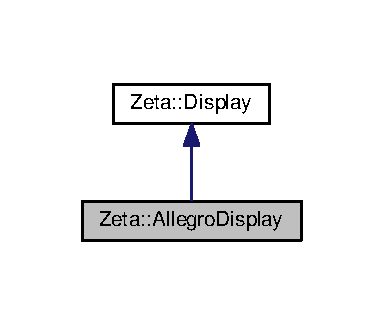
\includegraphics[width=184pt]{classZeta_1_1AllegroDisplay__inherit__graph}
\end{center}
\end{figure}


Collaboration diagram for Zeta\+:\+:Allegro\+Display\+:\nopagebreak
\begin{figure}[H]
\begin{center}
\leavevmode
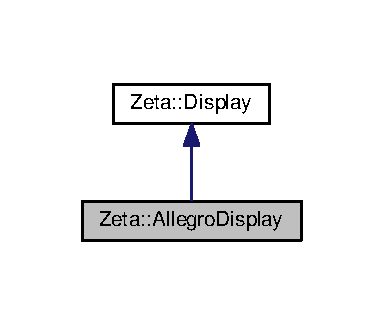
\includegraphics[width=184pt]{classZeta_1_1AllegroDisplay__coll__graph}
\end{center}
\end{figure}
\subsection*{Public Member Functions}
\begin{DoxyCompactItemize}
\item 
void \hyperlink{classZeta_1_1AllegroDisplay_a0eec86886654b8c7fa824e0f1a60c666}{resize} (int width, int height)
\item 
void \hyperlink{classZeta_1_1AllegroDisplay_a66c5cff25c281458c26e62e2a4298a9f}{set\+Full\+Screen} (bool value)
\item 
std\+::vector$<$ \hyperlink{classZeta_1_1Display_1_1Resolution}{Resolution} $>$ \hyperlink{classZeta_1_1AllegroDisplay_a3e6075814fc06dd14c99f95f6981d46c}{get\+Available\+Resolutions} () const 
\item 
int \hyperlink{classZeta_1_1AllegroDisplay_a235298ad063c22b30a1086d5cd442ad9}{get\+Width} () const 
\item 
int \hyperlink{classZeta_1_1AllegroDisplay_a9b876ad99147faae16f98ddfa44edf90}{get\+Height} () const 
\item 
void \hyperlink{classZeta_1_1AllegroDisplay_ab008d06f28f31d2cda41622eb7d60c43}{switch\+Framebuffer} ()
\item 
\hyperlink{classZeta_1_1AllegroDisplay_adb8a26bec17d2b24956cf3a703aa0d7e}{Allegro\+Display} ()
\item 
\hyperlink{classZeta_1_1AllegroDisplay_a019ed5b16f4ec65446f20b7239dcce7e}{Allegro\+Display} (int width, int height)
\item 
\hyperlink{classZeta_1_1AllegroDisplay_a670536f0e93a8f0ad3460a40b78d5423}{$\sim$\+Allegro\+Display} ()
\end{DoxyCompactItemize}
\subsection*{Private Attributes}
\begin{DoxyCompactItemize}
\item 
A\+L\+L\+E\+G\+R\+O\+\_\+\+D\+I\+S\+P\+L\+A\+Y $\ast$ \hyperlink{classZeta_1_1AllegroDisplay_ae4e2198bfdb2680b78ae3ae1702f89ee}{disp}
\end{DoxyCompactItemize}
\subsection*{Additional Inherited Members}


\subsection{Constructor \& Destructor Documentation}
\hypertarget{classZeta_1_1AllegroDisplay_adb8a26bec17d2b24956cf3a703aa0d7e}{\index{Zeta\+::\+Allegro\+Display@{Zeta\+::\+Allegro\+Display}!Allegro\+Display@{Allegro\+Display}}
\index{Allegro\+Display@{Allegro\+Display}!Zeta\+::\+Allegro\+Display@{Zeta\+::\+Allegro\+Display}}
\subsubsection[{Allegro\+Display}]{\setlength{\rightskip}{0pt plus 5cm}Zeta\+::\+Allegro\+Display\+::\+Allegro\+Display (
\begin{DoxyParamCaption}
{}
\end{DoxyParamCaption}
)}}\label{classZeta_1_1AllegroDisplay_adb8a26bec17d2b24956cf3a703aa0d7e}
\hypertarget{classZeta_1_1AllegroDisplay_a019ed5b16f4ec65446f20b7239dcce7e}{\index{Zeta\+::\+Allegro\+Display@{Zeta\+::\+Allegro\+Display}!Allegro\+Display@{Allegro\+Display}}
\index{Allegro\+Display@{Allegro\+Display}!Zeta\+::\+Allegro\+Display@{Zeta\+::\+Allegro\+Display}}
\subsubsection[{Allegro\+Display}]{\setlength{\rightskip}{0pt plus 5cm}Zeta\+::\+Allegro\+Display\+::\+Allegro\+Display (
\begin{DoxyParamCaption}
\item[{int}]{width, }
\item[{int}]{height}
\end{DoxyParamCaption}
)}}\label{classZeta_1_1AllegroDisplay_a019ed5b16f4ec65446f20b7239dcce7e}
\hypertarget{classZeta_1_1AllegroDisplay_a670536f0e93a8f0ad3460a40b78d5423}{\index{Zeta\+::\+Allegro\+Display@{Zeta\+::\+Allegro\+Display}!````~Allegro\+Display@{$\sim$\+Allegro\+Display}}
\index{````~Allegro\+Display@{$\sim$\+Allegro\+Display}!Zeta\+::\+Allegro\+Display@{Zeta\+::\+Allegro\+Display}}
\subsubsection[{$\sim$\+Allegro\+Display}]{\setlength{\rightskip}{0pt plus 5cm}Zeta\+::\+Allegro\+Display\+::$\sim$\+Allegro\+Display (
\begin{DoxyParamCaption}
{}
\end{DoxyParamCaption}
)}}\label{classZeta_1_1AllegroDisplay_a670536f0e93a8f0ad3460a40b78d5423}


\subsection{Member Function Documentation}
\hypertarget{classZeta_1_1AllegroDisplay_a3e6075814fc06dd14c99f95f6981d46c}{\index{Zeta\+::\+Allegro\+Display@{Zeta\+::\+Allegro\+Display}!get\+Available\+Resolutions@{get\+Available\+Resolutions}}
\index{get\+Available\+Resolutions@{get\+Available\+Resolutions}!Zeta\+::\+Allegro\+Display@{Zeta\+::\+Allegro\+Display}}
\subsubsection[{get\+Available\+Resolutions}]{\setlength{\rightskip}{0pt plus 5cm}std\+::vector$<${\bf Resolution}$>$ Zeta\+::\+Allegro\+Display\+::get\+Available\+Resolutions (
\begin{DoxyParamCaption}
{}
\end{DoxyParamCaption}
) const\hspace{0.3cm}{\ttfamily [virtual]}}}\label{classZeta_1_1AllegroDisplay_a3e6075814fc06dd14c99f95f6981d46c}
Gets the available Resolutions for this \hyperlink{classZeta_1_1Display}{Display} \begin{DoxyReturn}{Returns}
A std\+::vector$<$\+Zeta\+::\+Display\+::\+Resoultion$>$ contain all Resolutions 
\end{DoxyReturn}


Implements \hyperlink{classZeta_1_1Display_ae7ebedea6e6ed113e847e426d6697bb9}{Zeta\+::\+Display}.

\hypertarget{classZeta_1_1AllegroDisplay_a9b876ad99147faae16f98ddfa44edf90}{\index{Zeta\+::\+Allegro\+Display@{Zeta\+::\+Allegro\+Display}!get\+Height@{get\+Height}}
\index{get\+Height@{get\+Height}!Zeta\+::\+Allegro\+Display@{Zeta\+::\+Allegro\+Display}}
\subsubsection[{get\+Height}]{\setlength{\rightskip}{0pt plus 5cm}int Zeta\+::\+Allegro\+Display\+::get\+Height (
\begin{DoxyParamCaption}
{}
\end{DoxyParamCaption}
) const\hspace{0.3cm}{\ttfamily [virtual]}}}\label{classZeta_1_1AllegroDisplay_a9b876ad99147faae16f98ddfa44edf90}
Gets the Main Window Height \begin{DoxyReturn}{Returns}
The main window height; 
\end{DoxyReturn}


Implements \hyperlink{classZeta_1_1Display_ac8b58d29e59ee15c40523dc6661e7c9a}{Zeta\+::\+Display}.

\hypertarget{classZeta_1_1AllegroDisplay_a235298ad063c22b30a1086d5cd442ad9}{\index{Zeta\+::\+Allegro\+Display@{Zeta\+::\+Allegro\+Display}!get\+Width@{get\+Width}}
\index{get\+Width@{get\+Width}!Zeta\+::\+Allegro\+Display@{Zeta\+::\+Allegro\+Display}}
\subsubsection[{get\+Width}]{\setlength{\rightskip}{0pt plus 5cm}int Zeta\+::\+Allegro\+Display\+::get\+Width (
\begin{DoxyParamCaption}
{}
\end{DoxyParamCaption}
) const\hspace{0.3cm}{\ttfamily [virtual]}}}\label{classZeta_1_1AllegroDisplay_a235298ad063c22b30a1086d5cd442ad9}
Gets the Main Window Width \begin{DoxyReturn}{Returns}
The main window Width; 
\end{DoxyReturn}


Implements \hyperlink{classZeta_1_1Display_ac1ac8b765b5bc2589c4f8e01943e41eb}{Zeta\+::\+Display}.

\hypertarget{classZeta_1_1AllegroDisplay_a0eec86886654b8c7fa824e0f1a60c666}{\index{Zeta\+::\+Allegro\+Display@{Zeta\+::\+Allegro\+Display}!resize@{resize}}
\index{resize@{resize}!Zeta\+::\+Allegro\+Display@{Zeta\+::\+Allegro\+Display}}
\subsubsection[{resize}]{\setlength{\rightskip}{0pt plus 5cm}void Zeta\+::\+Allegro\+Display\+::resize (
\begin{DoxyParamCaption}
\item[{int}]{width, }
\item[{int}]{height}
\end{DoxyParamCaption}
)\hspace{0.3cm}{\ttfamily [virtual]}}}\label{classZeta_1_1AllegroDisplay_a0eec86886654b8c7fa824e0f1a60c666}
Resizes the Main Window to the specified Dimensions 
\begin{DoxyParams}{Parameters}
{\em width} & the target width \\
\hline
{\em height} & the target Height \\
\hline
\end{DoxyParams}


Implements \hyperlink{classZeta_1_1Display_a42a19d96e61bac76216071efe61bf8e6}{Zeta\+::\+Display}.

\hypertarget{classZeta_1_1AllegroDisplay_a66c5cff25c281458c26e62e2a4298a9f}{\index{Zeta\+::\+Allegro\+Display@{Zeta\+::\+Allegro\+Display}!set\+Full\+Screen@{set\+Full\+Screen}}
\index{set\+Full\+Screen@{set\+Full\+Screen}!Zeta\+::\+Allegro\+Display@{Zeta\+::\+Allegro\+Display}}
\subsubsection[{set\+Full\+Screen}]{\setlength{\rightskip}{0pt plus 5cm}void Zeta\+::\+Allegro\+Display\+::set\+Full\+Screen (
\begin{DoxyParamCaption}
\item[{bool}]{value}
\end{DoxyParamCaption}
)\hspace{0.3cm}{\ttfamily [virtual]}}}\label{classZeta_1_1AllegroDisplay_a66c5cff25c281458c26e62e2a4298a9f}
Toggles the Main Window Full-\/screen Mode 
\begin{DoxyParams}{Parameters}
{\em value} & True for Fullscreen \\
\hline
\end{DoxyParams}


Implements \hyperlink{classZeta_1_1Display_a07ba98d5a7accc4cad08923e65286912}{Zeta\+::\+Display}.

\hypertarget{classZeta_1_1AllegroDisplay_ab008d06f28f31d2cda41622eb7d60c43}{\index{Zeta\+::\+Allegro\+Display@{Zeta\+::\+Allegro\+Display}!switch\+Framebuffer@{switch\+Framebuffer}}
\index{switch\+Framebuffer@{switch\+Framebuffer}!Zeta\+::\+Allegro\+Display@{Zeta\+::\+Allegro\+Display}}
\subsubsection[{switch\+Framebuffer}]{\setlength{\rightskip}{0pt plus 5cm}void Zeta\+::\+Allegro\+Display\+::switch\+Framebuffer (
\begin{DoxyParamCaption}
{}
\end{DoxyParamCaption}
)\hspace{0.3cm}{\ttfamily [virtual]}}}\label{classZeta_1_1AllegroDisplay_ab008d06f28f31d2cda41622eb7d60c43}
Switches the framebuffer. It should be used on Double or Triple Buffering implementations 

Implements \hyperlink{classZeta_1_1Display_a727a7d347a8145029975ec8eef5339d3}{Zeta\+::\+Display}.



\subsection{Member Data Documentation}
\hypertarget{classZeta_1_1AllegroDisplay_ae4e2198bfdb2680b78ae3ae1702f89ee}{\index{Zeta\+::\+Allegro\+Display@{Zeta\+::\+Allegro\+Display}!disp@{disp}}
\index{disp@{disp}!Zeta\+::\+Allegro\+Display@{Zeta\+::\+Allegro\+Display}}
\subsubsection[{disp}]{\setlength{\rightskip}{0pt plus 5cm}A\+L\+L\+E\+G\+R\+O\+\_\+\+D\+I\+S\+P\+L\+A\+Y$\ast$ Zeta\+::\+Allegro\+Display\+::disp\hspace{0.3cm}{\ttfamily [private]}}}\label{classZeta_1_1AllegroDisplay_ae4e2198bfdb2680b78ae3ae1702f89ee}


The documentation for this class was generated from the following file\+:\begin{DoxyCompactItemize}
\item 
include/\+Zeta/\+Library\+Binders/\+Allegro5/\hyperlink{AllegroDisplay_8hpp}{Allegro\+Display.\+hpp}\end{DoxyCompactItemize}

\hypertarget{classZeta_1_1AllegroEvent}{\section{Zeta\+:\+:Allegro\+Event Class Reference}
\label{classZeta_1_1AllegroEvent}\index{Zeta\+::\+Allegro\+Event@{Zeta\+::\+Allegro\+Event}}
}


{\ttfamily \#include $<$Allegro\+Event.\+hpp$>$}



Inheritance diagram for Zeta\+:\+:Allegro\+Event\+:\nopagebreak
\begin{figure}[H]
\begin{center}
\leavevmode
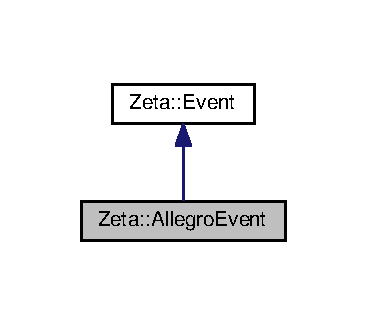
\includegraphics[width=176pt]{classZeta_1_1AllegroEvent__inherit__graph}
\end{center}
\end{figure}


Collaboration diagram for Zeta\+:\+:Allegro\+Event\+:\nopagebreak
\begin{figure}[H]
\begin{center}
\leavevmode
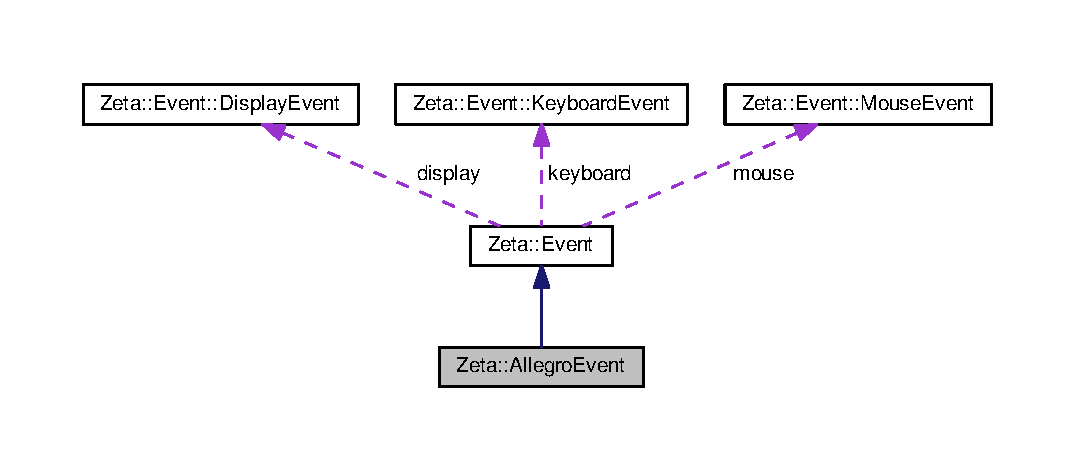
\includegraphics[width=350pt]{classZeta_1_1AllegroEvent__coll__graph}
\end{center}
\end{figure}
\subsection*{Public Member Functions}
\begin{DoxyCompactItemize}
\item 
\hyperlink{classZeta_1_1AllegroEvent_aaaebaa75a7bdda5762265631212defc8}{Allegro\+Event} (A\+L\+L\+E\+G\+R\+O\+\_\+\+E\+V\+E\+N\+T \&event)
\item 
\hyperlink{classZeta_1_1AllegroEvent_ae328ab540d2f31a80a13a6268849e485}{$\sim$\+Allegro\+Event} ()
\end{DoxyCompactItemize}
\subsection*{Additional Inherited Members}


\subsection{Constructor \& Destructor Documentation}
\hypertarget{classZeta_1_1AllegroEvent_aaaebaa75a7bdda5762265631212defc8}{\index{Zeta\+::\+Allegro\+Event@{Zeta\+::\+Allegro\+Event}!Allegro\+Event@{Allegro\+Event}}
\index{Allegro\+Event@{Allegro\+Event}!Zeta\+::\+Allegro\+Event@{Zeta\+::\+Allegro\+Event}}
\subsubsection[{Allegro\+Event}]{\setlength{\rightskip}{0pt plus 5cm}Zeta\+::\+Allegro\+Event\+::\+Allegro\+Event (
\begin{DoxyParamCaption}
\item[{A\+L\+L\+E\+G\+R\+O\+\_\+\+E\+V\+E\+N\+T \&}]{event}
\end{DoxyParamCaption}
)}}\label{classZeta_1_1AllegroEvent_aaaebaa75a7bdda5762265631212defc8}
\hypertarget{classZeta_1_1AllegroEvent_ae328ab540d2f31a80a13a6268849e485}{\index{Zeta\+::\+Allegro\+Event@{Zeta\+::\+Allegro\+Event}!````~Allegro\+Event@{$\sim$\+Allegro\+Event}}
\index{````~Allegro\+Event@{$\sim$\+Allegro\+Event}!Zeta\+::\+Allegro\+Event@{Zeta\+::\+Allegro\+Event}}
\subsubsection[{$\sim$\+Allegro\+Event}]{\setlength{\rightskip}{0pt plus 5cm}Zeta\+::\+Allegro\+Event\+::$\sim$\+Allegro\+Event (
\begin{DoxyParamCaption}
{}
\end{DoxyParamCaption}
)\hspace{0.3cm}{\ttfamily [inline]}}}\label{classZeta_1_1AllegroEvent_ae328ab540d2f31a80a13a6268849e485}


The documentation for this class was generated from the following file\+:\begin{DoxyCompactItemize}
\item 
include/\+Zeta/\+Library\+Binders/\+Allegro5/\hyperlink{AllegroEvent_8hpp}{Allegro\+Event.\+hpp}\end{DoxyCompactItemize}

\hypertarget{classZeta_1_1AllegroLoop}{\section{Zeta\+:\+:Allegro\+Loop Class Reference}
\label{classZeta_1_1AllegroLoop}\index{Zeta\+::\+Allegro\+Loop@{Zeta\+::\+Allegro\+Loop}}
}


{\ttfamily \#include $<$Allegro\+Loop.\+hpp$>$}



Inheritance diagram for Zeta\+:\+:Allegro\+Loop\+:\nopagebreak
\begin{figure}[H]
\begin{center}
\leavevmode
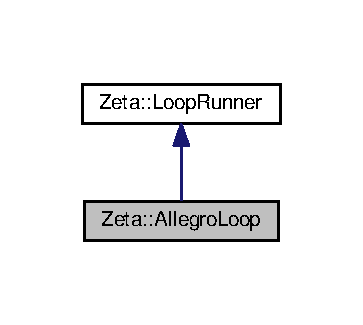
\includegraphics[width=174pt]{classZeta_1_1AllegroLoop__inherit__graph}
\end{center}
\end{figure}


Collaboration diagram for Zeta\+:\+:Allegro\+Loop\+:\nopagebreak
\begin{figure}[H]
\begin{center}
\leavevmode
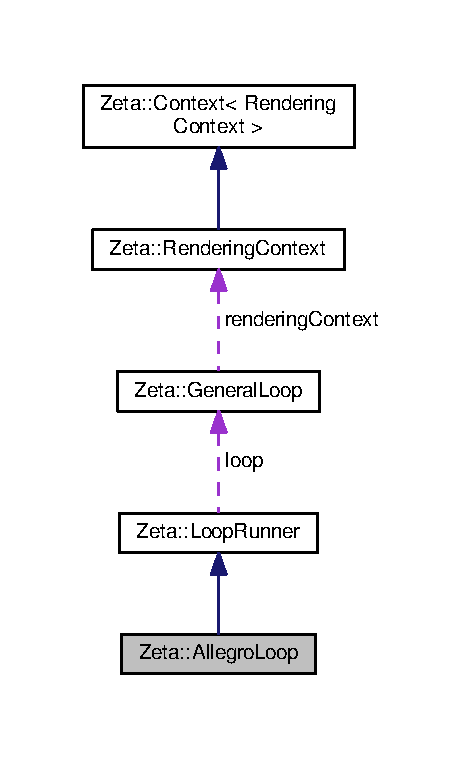
\includegraphics[width=223pt]{classZeta_1_1AllegroLoop__coll__graph}
\end{center}
\end{figure}
\subsection*{Public Member Functions}
\begin{DoxyCompactItemize}
\item 
void \hyperlink{classZeta_1_1AllegroLoop_a95ef031ace6f929a450c80c9ecdaa057}{start} ()
\item 
int \hyperlink{classZeta_1_1AllegroLoop_ac422e8f5961d13161c63a3863236ce99}{get\+Target\+Fps} () const 
\item 
void \hyperlink{classZeta_1_1AllegroLoop_a845300a5ce14dd8fb8c7f2ffeb0afbb2}{set\+Target\+Fps} (int \hyperlink{classZeta_1_1AllegroLoop_a0ee2957a3e13030b26e3c87aec68317f}{target\+Fps})
\item 
\hyperlink{classZeta_1_1AllegroLoop_ab9b29f07be1ed13902a51291295768b4}{Allegro\+Loop} (int \hyperlink{classZeta_1_1AllegroLoop_a0ee2957a3e13030b26e3c87aec68317f}{target\+Fps})
\item 
\hyperlink{classZeta_1_1AllegroLoop_a1ba1e6ed2ebfb75a43c085139a20ae3d}{$\sim$\+Allegro\+Loop} ()
\end{DoxyCompactItemize}
\subsection*{Private Attributes}
\begin{DoxyCompactItemize}
\item 
A\+L\+L\+E\+G\+R\+O\+\_\+\+T\+I\+M\+E\+R $\ast$ \hyperlink{classZeta_1_1AllegroLoop_ac1fae67baa5962de17573211a1a93e16}{frame\+\_\+timer}
\item 
int \hyperlink{classZeta_1_1AllegroLoop_a0ee2957a3e13030b26e3c87aec68317f}{target\+Fps}
\end{DoxyCompactItemize}
\subsection*{Additional Inherited Members}


\subsection{Constructor \& Destructor Documentation}
\hypertarget{classZeta_1_1AllegroLoop_ab9b29f07be1ed13902a51291295768b4}{\index{Zeta\+::\+Allegro\+Loop@{Zeta\+::\+Allegro\+Loop}!Allegro\+Loop@{Allegro\+Loop}}
\index{Allegro\+Loop@{Allegro\+Loop}!Zeta\+::\+Allegro\+Loop@{Zeta\+::\+Allegro\+Loop}}
\subsubsection[{Allegro\+Loop}]{\setlength{\rightskip}{0pt plus 5cm}Zeta\+::\+Allegro\+Loop\+::\+Allegro\+Loop (
\begin{DoxyParamCaption}
\item[{int}]{target\+Fps}
\end{DoxyParamCaption}
)}}\label{classZeta_1_1AllegroLoop_ab9b29f07be1ed13902a51291295768b4}
\hypertarget{classZeta_1_1AllegroLoop_a1ba1e6ed2ebfb75a43c085139a20ae3d}{\index{Zeta\+::\+Allegro\+Loop@{Zeta\+::\+Allegro\+Loop}!````~Allegro\+Loop@{$\sim$\+Allegro\+Loop}}
\index{````~Allegro\+Loop@{$\sim$\+Allegro\+Loop}!Zeta\+::\+Allegro\+Loop@{Zeta\+::\+Allegro\+Loop}}
\subsubsection[{$\sim$\+Allegro\+Loop}]{\setlength{\rightskip}{0pt plus 5cm}Zeta\+::\+Allegro\+Loop\+::$\sim$\+Allegro\+Loop (
\begin{DoxyParamCaption}
{}
\end{DoxyParamCaption}
)}}\label{classZeta_1_1AllegroLoop_a1ba1e6ed2ebfb75a43c085139a20ae3d}


\subsection{Member Function Documentation}
\hypertarget{classZeta_1_1AllegroLoop_ac422e8f5961d13161c63a3863236ce99}{\index{Zeta\+::\+Allegro\+Loop@{Zeta\+::\+Allegro\+Loop}!get\+Target\+Fps@{get\+Target\+Fps}}
\index{get\+Target\+Fps@{get\+Target\+Fps}!Zeta\+::\+Allegro\+Loop@{Zeta\+::\+Allegro\+Loop}}
\subsubsection[{get\+Target\+Fps}]{\setlength{\rightskip}{0pt plus 5cm}int Zeta\+::\+Allegro\+Loop\+::get\+Target\+Fps (
\begin{DoxyParamCaption}
{}
\end{DoxyParamCaption}
) const\hspace{0.3cm}{\ttfamily [inline]}, {\ttfamily [virtual]}}}\label{classZeta_1_1AllegroLoop_ac422e8f5961d13161c63a3863236ce99}
Gets the Loops target F\+P\+S Warning this is not the Current Engine's F\+P\+S \begin{DoxyReturn}{Returns}
the target F\+P\+S 
\end{DoxyReturn}


Implements \hyperlink{classZeta_1_1LoopRunner_ab9ab29d4239c98b49e11879528817dc3}{Zeta\+::\+Loop\+Runner}.

\hypertarget{classZeta_1_1AllegroLoop_a845300a5ce14dd8fb8c7f2ffeb0afbb2}{\index{Zeta\+::\+Allegro\+Loop@{Zeta\+::\+Allegro\+Loop}!set\+Target\+Fps@{set\+Target\+Fps}}
\index{set\+Target\+Fps@{set\+Target\+Fps}!Zeta\+::\+Allegro\+Loop@{Zeta\+::\+Allegro\+Loop}}
\subsubsection[{set\+Target\+Fps}]{\setlength{\rightskip}{0pt plus 5cm}void Zeta\+::\+Allegro\+Loop\+::set\+Target\+Fps (
\begin{DoxyParamCaption}
\item[{int}]{target\+Fps}
\end{DoxyParamCaption}
)\hspace{0.3cm}{\ttfamily [virtual]}}}\label{classZeta_1_1AllegroLoop_a845300a5ce14dd8fb8c7f2ffeb0afbb2}
Sets the Loops target F\+P\+S Warning this is not the Current Engine's F\+P\+S 
\begin{DoxyParams}{Parameters}
{\em target\+Fps} & the target F\+P\+S \\
\hline
\end{DoxyParams}


Implements \hyperlink{classZeta_1_1LoopRunner_a82d681fc778e4eb3078c8dc0eac059a0}{Zeta\+::\+Loop\+Runner}.

\hypertarget{classZeta_1_1AllegroLoop_a95ef031ace6f929a450c80c9ecdaa057}{\index{Zeta\+::\+Allegro\+Loop@{Zeta\+::\+Allegro\+Loop}!start@{start}}
\index{start@{start}!Zeta\+::\+Allegro\+Loop@{Zeta\+::\+Allegro\+Loop}}
\subsubsection[{start}]{\setlength{\rightskip}{0pt plus 5cm}void Zeta\+::\+Allegro\+Loop\+::start (
\begin{DoxyParamCaption}
{}
\end{DoxyParamCaption}
)\hspace{0.3cm}{\ttfamily [virtual]}}}\label{classZeta_1_1AllegroLoop_a95ef031ace6f929a450c80c9ecdaa057}
Causes the Main Loop to start 

Implements \hyperlink{classZeta_1_1LoopRunner_a45c0f0ec5b7d1f48f3aebc429908c456}{Zeta\+::\+Loop\+Runner}.



\subsection{Member Data Documentation}
\hypertarget{classZeta_1_1AllegroLoop_ac1fae67baa5962de17573211a1a93e16}{\index{Zeta\+::\+Allegro\+Loop@{Zeta\+::\+Allegro\+Loop}!frame\+\_\+timer@{frame\+\_\+timer}}
\index{frame\+\_\+timer@{frame\+\_\+timer}!Zeta\+::\+Allegro\+Loop@{Zeta\+::\+Allegro\+Loop}}
\subsubsection[{frame\+\_\+timer}]{\setlength{\rightskip}{0pt plus 5cm}A\+L\+L\+E\+G\+R\+O\+\_\+\+T\+I\+M\+E\+R$\ast$ Zeta\+::\+Allegro\+Loop\+::frame\+\_\+timer\hspace{0.3cm}{\ttfamily [private]}}}\label{classZeta_1_1AllegroLoop_ac1fae67baa5962de17573211a1a93e16}
\hypertarget{classZeta_1_1AllegroLoop_a0ee2957a3e13030b26e3c87aec68317f}{\index{Zeta\+::\+Allegro\+Loop@{Zeta\+::\+Allegro\+Loop}!target\+Fps@{target\+Fps}}
\index{target\+Fps@{target\+Fps}!Zeta\+::\+Allegro\+Loop@{Zeta\+::\+Allegro\+Loop}}
\subsubsection[{target\+Fps}]{\setlength{\rightskip}{0pt plus 5cm}int Zeta\+::\+Allegro\+Loop\+::target\+Fps\hspace{0.3cm}{\ttfamily [private]}}}\label{classZeta_1_1AllegroLoop_a0ee2957a3e13030b26e3c87aec68317f}


The documentation for this class was generated from the following file\+:\begin{DoxyCompactItemize}
\item 
include/\+Zeta/\+Library\+Binders/\+Allegro5/\hyperlink{AllegroLoop_8hpp}{Allegro\+Loop.\+hpp}\end{DoxyCompactItemize}

\hypertarget{classZeta_1_1AllegroRenderer}{\section{Zeta\+:\+:Allegro\+Renderer Class Reference}
\label{classZeta_1_1AllegroRenderer}\index{Zeta\+::\+Allegro\+Renderer@{Zeta\+::\+Allegro\+Renderer}}
}


{\ttfamily \#include $<$Allegro\+Renderer.\+hpp$>$}



Inheritance diagram for Zeta\+:\+:Allegro\+Renderer\+:\nopagebreak
\begin{figure}[H]
\begin{center}
\leavevmode
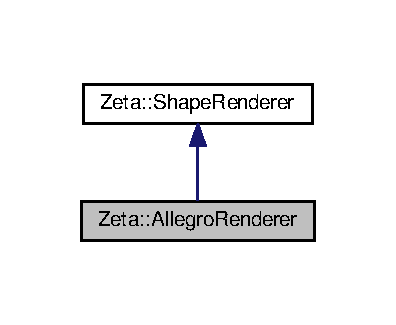
\includegraphics[width=190pt]{classZeta_1_1AllegroRenderer__inherit__graph}
\end{center}
\end{figure}


Collaboration diagram for Zeta\+:\+:Allegro\+Renderer\+:\nopagebreak
\begin{figure}[H]
\begin{center}
\leavevmode
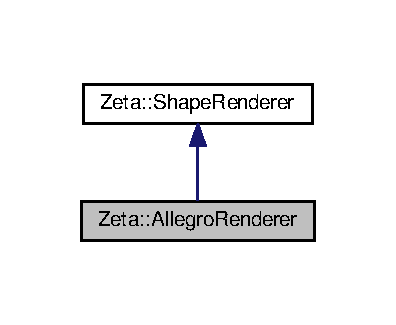
\includegraphics[width=190pt]{classZeta_1_1AllegroRenderer__coll__graph}
\end{center}
\end{figure}
\subsection*{Public Member Functions}
\begin{DoxyCompactItemize}
\item 
void \hyperlink{classZeta_1_1AllegroRenderer_aea34760ff1fd46b7e38c5e3491fc9e13}{hold\+Bitmap\+Draw} (bool vall)
\item 
void \hyperlink{classZeta_1_1AllegroRenderer_acc295b7409ffe9a03ce89150092d9e64}{draw\+Ellipsis} (float center\+\_\+x, float center\+\_\+y, float radius\+\_\+x, float radius\+\_\+y, const \hyperlink{classZeta_1_1Color}{Color} \&border\+C, float thickness)
\item 
void \hyperlink{classZeta_1_1AllegroRenderer_ad12e55e570eae5ea500657fdcb14c24e}{draw\+Filled\+Ellipsis} (float center\+\_\+x, float center\+\_\+y, float radius\+\_\+x, float radius\+\_\+y, const \hyperlink{classZeta_1_1Color}{Color} \&fill\+C)
\item 
void \hyperlink{classZeta_1_1AllegroRenderer_a9e82ac53fe00a8fffcfab1b8ed069bf1}{draw\+Rectangle} (float a\+\_\+x, float a\+\_\+y, float b\+\_\+x, float b\+\_\+y, const \hyperlink{classZeta_1_1Color}{Color} \&border\+C, float thickness)
\item 
void \hyperlink{classZeta_1_1AllegroRenderer_ab8991aa90c1dc6e781f72e980ffcbf7f}{draw\+Filled\+Rectangle} (float a\+\_\+x, float a\+\_\+y, float b\+\_\+x, float b\+\_\+y, const \hyperlink{classZeta_1_1Color}{Color} \&fill\+C)
\item 
void \hyperlink{classZeta_1_1AllegroRenderer_a391bc752b95b7305b91e66178078e40e}{draw\+Line} (float x1, float y1, float x2, float y2, const \hyperlink{classZeta_1_1Color}{Color} \&fill\+C, float thickness)
\item 
\hyperlink{classZeta_1_1AllegroRenderer_a55714e4509781eb64b932cf3d872fece}{Allegro\+Renderer} ()
\item 
\hyperlink{classZeta_1_1AllegroRenderer_a1f3aaed20d689b8939bde84bac546c77}{$\sim$\+Allegro\+Renderer} ()
\end{DoxyCompactItemize}


\subsection{Constructor \& Destructor Documentation}
\hypertarget{classZeta_1_1AllegroRenderer_a55714e4509781eb64b932cf3d872fece}{\index{Zeta\+::\+Allegro\+Renderer@{Zeta\+::\+Allegro\+Renderer}!Allegro\+Renderer@{Allegro\+Renderer}}
\index{Allegro\+Renderer@{Allegro\+Renderer}!Zeta\+::\+Allegro\+Renderer@{Zeta\+::\+Allegro\+Renderer}}
\subsubsection[{Allegro\+Renderer}]{\setlength{\rightskip}{0pt plus 5cm}Zeta\+::\+Allegro\+Renderer\+::\+Allegro\+Renderer (
\begin{DoxyParamCaption}
{}
\end{DoxyParamCaption}
)\hspace{0.3cm}{\ttfamily [inline]}}}\label{classZeta_1_1AllegroRenderer_a55714e4509781eb64b932cf3d872fece}
\hypertarget{classZeta_1_1AllegroRenderer_a1f3aaed20d689b8939bde84bac546c77}{\index{Zeta\+::\+Allegro\+Renderer@{Zeta\+::\+Allegro\+Renderer}!````~Allegro\+Renderer@{$\sim$\+Allegro\+Renderer}}
\index{````~Allegro\+Renderer@{$\sim$\+Allegro\+Renderer}!Zeta\+::\+Allegro\+Renderer@{Zeta\+::\+Allegro\+Renderer}}
\subsubsection[{$\sim$\+Allegro\+Renderer}]{\setlength{\rightskip}{0pt plus 5cm}Zeta\+::\+Allegro\+Renderer\+::$\sim$\+Allegro\+Renderer (
\begin{DoxyParamCaption}
{}
\end{DoxyParamCaption}
)\hspace{0.3cm}{\ttfamily [inline]}}}\label{classZeta_1_1AllegroRenderer_a1f3aaed20d689b8939bde84bac546c77}


\subsection{Member Function Documentation}
\hypertarget{classZeta_1_1AllegroRenderer_acc295b7409ffe9a03ce89150092d9e64}{\index{Zeta\+::\+Allegro\+Renderer@{Zeta\+::\+Allegro\+Renderer}!draw\+Ellipsis@{draw\+Ellipsis}}
\index{draw\+Ellipsis@{draw\+Ellipsis}!Zeta\+::\+Allegro\+Renderer@{Zeta\+::\+Allegro\+Renderer}}
\subsubsection[{draw\+Ellipsis}]{\setlength{\rightskip}{0pt plus 5cm}void Zeta\+::\+Allegro\+Renderer\+::draw\+Ellipsis (
\begin{DoxyParamCaption}
\item[{float}]{center\+\_\+x, }
\item[{float}]{center\+\_\+y, }
\item[{float}]{radius\+\_\+x, }
\item[{float}]{radius\+\_\+y, }
\item[{const {\bf Color} \&}]{border\+C, }
\item[{float}]{thickness}
\end{DoxyParamCaption}
)\hspace{0.3cm}{\ttfamily [virtual]}}}\label{classZeta_1_1AllegroRenderer_acc295b7409ffe9a03ce89150092d9e64}
Draws an \hyperlink{classZeta_1_1Ellipsis}{Ellipsis} with no Fill 
\begin{DoxyParams}{Parameters}
{\em center\+\_\+x} & The x coordinate of the center of the \hyperlink{classZeta_1_1Ellipsis}{Ellipsis} \\
\hline
{\em center\+\_\+y} & The y coordinate of the center of the \hyperlink{classZeta_1_1Ellipsis}{Ellipsis} \\
\hline
{\em radius\+\_\+x} & The radius on the x axis \\
\hline
{\em radius\+\_\+y} & The radius on the y axis \\
\hline
{\em border\+C} & The color of the outline \\
\hline
{\em thickness} & The thickness of the outline \\
\hline
\end{DoxyParams}


Implements \hyperlink{classZeta_1_1ShapeRenderer_acf165e896b1ba10239a5652a97b95a08}{Zeta\+::\+Shape\+Renderer}.

\hypertarget{classZeta_1_1AllegroRenderer_ad12e55e570eae5ea500657fdcb14c24e}{\index{Zeta\+::\+Allegro\+Renderer@{Zeta\+::\+Allegro\+Renderer}!draw\+Filled\+Ellipsis@{draw\+Filled\+Ellipsis}}
\index{draw\+Filled\+Ellipsis@{draw\+Filled\+Ellipsis}!Zeta\+::\+Allegro\+Renderer@{Zeta\+::\+Allegro\+Renderer}}
\subsubsection[{draw\+Filled\+Ellipsis}]{\setlength{\rightskip}{0pt plus 5cm}void Zeta\+::\+Allegro\+Renderer\+::draw\+Filled\+Ellipsis (
\begin{DoxyParamCaption}
\item[{float}]{center\+\_\+x, }
\item[{float}]{center\+\_\+y, }
\item[{float}]{radius\+\_\+x, }
\item[{float}]{radius\+\_\+y, }
\item[{const {\bf Color} \&}]{fill\+C}
\end{DoxyParamCaption}
)\hspace{0.3cm}{\ttfamily [virtual]}}}\label{classZeta_1_1AllegroRenderer_ad12e55e570eae5ea500657fdcb14c24e}
Draws a Filled \hyperlink{classZeta_1_1Ellipsis}{Ellipsis} 
\begin{DoxyParams}{Parameters}
{\em center\+\_\+x} & The x coordinate of the center of the \hyperlink{classZeta_1_1Ellipsis}{Ellipsis} \\
\hline
{\em center\+\_\+y} & The y coordinate of the center of the \hyperlink{classZeta_1_1Ellipsis}{Ellipsis} \\
\hline
{\em radius\+\_\+x} & The radius on the x axis \\
\hline
{\em radius\+\_\+y} & The radius on the y axis \\
\hline
{\em fill\+C} & The color of the fill of the ellipsis \\
\hline
\end{DoxyParams}


Implements \hyperlink{classZeta_1_1ShapeRenderer_a9ae3456ae2966b77cbf97cbf28240b5e}{Zeta\+::\+Shape\+Renderer}.

\hypertarget{classZeta_1_1AllegroRenderer_ab8991aa90c1dc6e781f72e980ffcbf7f}{\index{Zeta\+::\+Allegro\+Renderer@{Zeta\+::\+Allegro\+Renderer}!draw\+Filled\+Rectangle@{draw\+Filled\+Rectangle}}
\index{draw\+Filled\+Rectangle@{draw\+Filled\+Rectangle}!Zeta\+::\+Allegro\+Renderer@{Zeta\+::\+Allegro\+Renderer}}
\subsubsection[{draw\+Filled\+Rectangle}]{\setlength{\rightskip}{0pt plus 5cm}void Zeta\+::\+Allegro\+Renderer\+::draw\+Filled\+Rectangle (
\begin{DoxyParamCaption}
\item[{float}]{a\+\_\+x, }
\item[{float}]{a\+\_\+y, }
\item[{float}]{b\+\_\+x, }
\item[{float}]{b\+\_\+y, }
\item[{const {\bf Color} \&}]{fill\+C}
\end{DoxyParamCaption}
)\hspace{0.3cm}{\ttfamily [virtual]}}}\label{classZeta_1_1AllegroRenderer_ab8991aa90c1dc6e781f72e980ffcbf7f}
Draws a Filled \hyperlink{classZeta_1_1Rectangle}{Rectangle} The rectangle is defined by 2 points, the Top-\/\+Left, Bottom-\/\+Right 
\begin{DoxyParams}{Parameters}
{\em a\+\_\+x} & The x coordinate of the Top-\/\+Left point of the \hyperlink{classZeta_1_1Rectangle}{Rectangle} \\
\hline
{\em a\+\_\+y} & The y coordinate of the Top-\/\+Left point of the \hyperlink{classZeta_1_1Rectangle}{Rectangle} \\
\hline
{\em b\+\_\+x} & The x coordinate of the Bottom-\/\+Right point of the \hyperlink{classZeta_1_1Rectangle}{Rectangle} \\
\hline
{\em b\+\_\+y} & The y coordinate of the Bottom-\/\+Right point of the \hyperlink{classZeta_1_1Rectangle}{Rectangle} \\
\hline
{\em fill\+C} & The color of the Fill \\
\hline
\end{DoxyParams}


Implements \hyperlink{classZeta_1_1ShapeRenderer_a496f71ef238b32e0b7d54120b6f452ac}{Zeta\+::\+Shape\+Renderer}.

\hypertarget{classZeta_1_1AllegroRenderer_a391bc752b95b7305b91e66178078e40e}{\index{Zeta\+::\+Allegro\+Renderer@{Zeta\+::\+Allegro\+Renderer}!draw\+Line@{draw\+Line}}
\index{draw\+Line@{draw\+Line}!Zeta\+::\+Allegro\+Renderer@{Zeta\+::\+Allegro\+Renderer}}
\subsubsection[{draw\+Line}]{\setlength{\rightskip}{0pt plus 5cm}void Zeta\+::\+Allegro\+Renderer\+::draw\+Line (
\begin{DoxyParamCaption}
\item[{float}]{x1, }
\item[{float}]{y1, }
\item[{float}]{x2, }
\item[{float}]{y2, }
\item[{const {\bf Color} \&}]{fill\+C, }
\item[{float}]{thickness}
\end{DoxyParamCaption}
)\hspace{0.3cm}{\ttfamily [virtual]}}}\label{classZeta_1_1AllegroRenderer_a391bc752b95b7305b91e66178078e40e}
Draws a Line The line is defined by 2 points 
\begin{DoxyParams}{Parameters}
{\em x1} & The x coordinate of the First point \\
\hline
{\em y1} & The y coordinate of the First point \\
\hline
{\em x2} & The x coordinate of the Second point \\
\hline
{\em y2} & The y coordinate of the Second point \\
\hline
{\em fill\+C} & The color of the line \\
\hline
{\em thickness} & the Thickness of the line \\
\hline
\end{DoxyParams}


Implements \hyperlink{classZeta_1_1ShapeRenderer_a451fedfb9589ec09fa2d5e30dd4c708d}{Zeta\+::\+Shape\+Renderer}.

\hypertarget{classZeta_1_1AllegroRenderer_a9e82ac53fe00a8fffcfab1b8ed069bf1}{\index{Zeta\+::\+Allegro\+Renderer@{Zeta\+::\+Allegro\+Renderer}!draw\+Rectangle@{draw\+Rectangle}}
\index{draw\+Rectangle@{draw\+Rectangle}!Zeta\+::\+Allegro\+Renderer@{Zeta\+::\+Allegro\+Renderer}}
\subsubsection[{draw\+Rectangle}]{\setlength{\rightskip}{0pt plus 5cm}void Zeta\+::\+Allegro\+Renderer\+::draw\+Rectangle (
\begin{DoxyParamCaption}
\item[{float}]{a\+\_\+x, }
\item[{float}]{a\+\_\+y, }
\item[{float}]{b\+\_\+x, }
\item[{float}]{b\+\_\+y, }
\item[{const {\bf Color} \&}]{border\+C, }
\item[{float}]{thickness}
\end{DoxyParamCaption}
)\hspace{0.3cm}{\ttfamily [virtual]}}}\label{classZeta_1_1AllegroRenderer_a9e82ac53fe00a8fffcfab1b8ed069bf1}
Draws a \hyperlink{classZeta_1_1Rectangle}{Rectangle} with no Fill The rectangle is defined by 2 points, the Top-\/\+Left, Bottom-\/\+Right 
\begin{DoxyParams}{Parameters}
{\em a\+\_\+x} & The x coordinate of the Top-\/\+Left point of the \hyperlink{classZeta_1_1Rectangle}{Rectangle} \\
\hline
{\em a\+\_\+y} & The y coordinate of the Top-\/\+Left point of the \hyperlink{classZeta_1_1Rectangle}{Rectangle} \\
\hline
{\em b\+\_\+x} & The x coordinate of the Bottom-\/\+Right point of the \hyperlink{classZeta_1_1Rectangle}{Rectangle} \\
\hline
{\em b\+\_\+y} & The y coordinate of the Bottom-\/\+Right point of the \hyperlink{classZeta_1_1Rectangle}{Rectangle} \\
\hline
{\em border\+C} & The color of the outline \\
\hline
{\em thickness} & The thickness of the outline \\
\hline
\end{DoxyParams}


Implements \hyperlink{classZeta_1_1ShapeRenderer_aa20b1c2e175e21ccf7dc63ef5ad231c8}{Zeta\+::\+Shape\+Renderer}.

\hypertarget{classZeta_1_1AllegroRenderer_aea34760ff1fd46b7e38c5e3491fc9e13}{\index{Zeta\+::\+Allegro\+Renderer@{Zeta\+::\+Allegro\+Renderer}!hold\+Bitmap\+Draw@{hold\+Bitmap\+Draw}}
\index{hold\+Bitmap\+Draw@{hold\+Bitmap\+Draw}!Zeta\+::\+Allegro\+Renderer@{Zeta\+::\+Allegro\+Renderer}}
\subsubsection[{hold\+Bitmap\+Draw}]{\setlength{\rightskip}{0pt plus 5cm}void Zeta\+::\+Allegro\+Renderer\+::hold\+Bitmap\+Draw (
\begin{DoxyParamCaption}
\item[{bool}]{vall}
\end{DoxyParamCaption}
)\hspace{0.3cm}{\ttfamily [virtual]}}}\label{classZeta_1_1AllegroRenderer_aea34760ff1fd46b7e38c5e3491fc9e13}
Enables or disables differed drawing where possible Differed drawing is a certain mode that have some S\+K\+Ds that draws bitmaps more efficient when the bitmaps are sub-\/bitmaps to a larger. If the implementing S\+D\+K does not have such function, then it should not do anything 
\begin{DoxyParams}{Parameters}
{\em vall} & true to enable differed drawing, false to disable \\
\hline
\end{DoxyParams}


Implements \hyperlink{classZeta_1_1ShapeRenderer_a65232f651234132c00b23335ce13ceba}{Zeta\+::\+Shape\+Renderer}.



The documentation for this class was generated from the following file\+:\begin{DoxyCompactItemize}
\item 
include/\+Zeta/\+Library\+Binders/\+Allegro5/\hyperlink{AllegroRenderer_8hpp}{Allegro\+Renderer.\+hpp}\end{DoxyCompactItemize}

\hypertarget{classZeta_1_1AllegroSDK}{\section{Zeta\+:\+:Allegro\+S\+D\+K Class Reference}
\label{classZeta_1_1AllegroSDK}\index{Zeta\+::\+Allegro\+S\+D\+K@{Zeta\+::\+Allegro\+S\+D\+K}}
}


{\ttfamily \#include $<$Allegro\+S\+D\+K.\+hpp$>$}

\subsection*{Static Public Member Functions}
\begin{DoxyCompactItemize}
\item 
static void \hyperlink{classZeta_1_1AllegroSDK_a576f5a2bc5f501d1d14ea90344fd3116}{bootstrap} ()
\end{DoxyCompactItemize}


\subsection{Member Function Documentation}
\hypertarget{classZeta_1_1AllegroSDK_a576f5a2bc5f501d1d14ea90344fd3116}{\index{Zeta\+::\+Allegro\+S\+D\+K@{Zeta\+::\+Allegro\+S\+D\+K}!bootstrap@{bootstrap}}
\index{bootstrap@{bootstrap}!Zeta\+::\+Allegro\+S\+D\+K@{Zeta\+::\+Allegro\+S\+D\+K}}
\subsubsection[{bootstrap}]{\setlength{\rightskip}{0pt plus 5cm}static void Zeta\+::\+Allegro\+S\+D\+K\+::bootstrap (
\begin{DoxyParamCaption}
{}
\end{DoxyParamCaption}
)\hspace{0.3cm}{\ttfamily [static]}}}\label{classZeta_1_1AllegroSDK_a576f5a2bc5f501d1d14ea90344fd3116}


The documentation for this class was generated from the following file\+:\begin{DoxyCompactItemize}
\item 
include/\+Zeta/\+Library\+Binders/\+Allegro5/\hyperlink{AllegroSDK_8hpp}{Allegro\+S\+D\+K.\+hpp}\end{DoxyCompactItemize}

\hypertarget{classZeta_1_1AllegroSound}{\section{Zeta\+:\+:Allegro\+Sound Class Reference}
\label{classZeta_1_1AllegroSound}\index{Zeta\+::\+Allegro\+Sound@{Zeta\+::\+Allegro\+Sound}}
}


{\ttfamily \#include $<$Allegro\+Sound.\+hpp$>$}



Inheritance diagram for Zeta\+:\+:Allegro\+Sound\+:\nopagebreak
\begin{figure}[H]
\begin{center}
\leavevmode
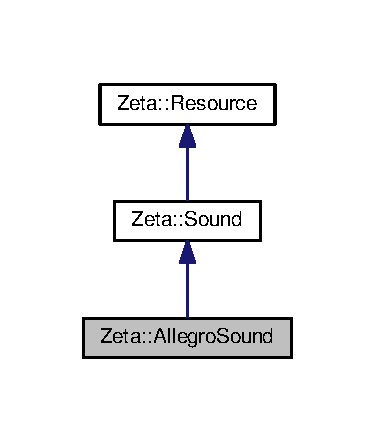
\includegraphics[width=180pt]{classZeta_1_1AllegroSound__inherit__graph}
\end{center}
\end{figure}


Collaboration diagram for Zeta\+:\+:Allegro\+Sound\+:\nopagebreak
\begin{figure}[H]
\begin{center}
\leavevmode
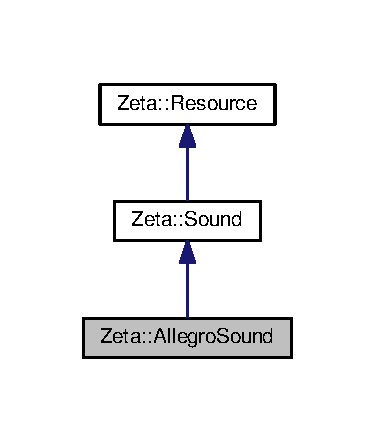
\includegraphics[width=180pt]{classZeta_1_1AllegroSound__coll__graph}
\end{center}
\end{figure}
\subsection*{Public Member Functions}
\begin{DoxyCompactItemize}
\item 
\hyperlink{classZeta_1_1SoundInstance}{Sound\+Instance} \& \hyperlink{classZeta_1_1AllegroSound_a3b483c40403834b6048283ad56774637}{create\+New\+Instance} () const 
\item 
\hyperlink{classZeta_1_1AllegroSound_adbde39881d7c93c88902cc34a26ed6aa}{Allegro\+Sound} ()
\item 
\hyperlink{classZeta_1_1AllegroSound_a535e4f2f64cf096924d58eb4508bf05b}{Allegro\+Sound} (const std\+::string \&path)
\item 
\hyperlink{classZeta_1_1AllegroSound_a329d68ff0379371fb7427d5b1725f3ac}{$\sim$\+Allegro\+Sound} ()
\end{DoxyCompactItemize}
\subsection*{Private Attributes}
\begin{DoxyCompactItemize}
\item 
A\+L\+L\+E\+G\+R\+O\+\_\+\+S\+A\+M\+P\+L\+E $\ast$ \hyperlink{classZeta_1_1AllegroSound_ae95788952c729697ade91a6a9a0d806b}{sample}
\end{DoxyCompactItemize}
\subsection*{Additional Inherited Members}


\subsection{Constructor \& Destructor Documentation}
\hypertarget{classZeta_1_1AllegroSound_adbde39881d7c93c88902cc34a26ed6aa}{\index{Zeta\+::\+Allegro\+Sound@{Zeta\+::\+Allegro\+Sound}!Allegro\+Sound@{Allegro\+Sound}}
\index{Allegro\+Sound@{Allegro\+Sound}!Zeta\+::\+Allegro\+Sound@{Zeta\+::\+Allegro\+Sound}}
\subsubsection[{Allegro\+Sound}]{\setlength{\rightskip}{0pt plus 5cm}Zeta\+::\+Allegro\+Sound\+::\+Allegro\+Sound (
\begin{DoxyParamCaption}
{}
\end{DoxyParamCaption}
)}}\label{classZeta_1_1AllegroSound_adbde39881d7c93c88902cc34a26ed6aa}
\hypertarget{classZeta_1_1AllegroSound_a535e4f2f64cf096924d58eb4508bf05b}{\index{Zeta\+::\+Allegro\+Sound@{Zeta\+::\+Allegro\+Sound}!Allegro\+Sound@{Allegro\+Sound}}
\index{Allegro\+Sound@{Allegro\+Sound}!Zeta\+::\+Allegro\+Sound@{Zeta\+::\+Allegro\+Sound}}
\subsubsection[{Allegro\+Sound}]{\setlength{\rightskip}{0pt plus 5cm}Zeta\+::\+Allegro\+Sound\+::\+Allegro\+Sound (
\begin{DoxyParamCaption}
\item[{const std\+::string \&}]{path}
\end{DoxyParamCaption}
)}}\label{classZeta_1_1AllegroSound_a535e4f2f64cf096924d58eb4508bf05b}
\hypertarget{classZeta_1_1AllegroSound_a329d68ff0379371fb7427d5b1725f3ac}{\index{Zeta\+::\+Allegro\+Sound@{Zeta\+::\+Allegro\+Sound}!````~Allegro\+Sound@{$\sim$\+Allegro\+Sound}}
\index{````~Allegro\+Sound@{$\sim$\+Allegro\+Sound}!Zeta\+::\+Allegro\+Sound@{Zeta\+::\+Allegro\+Sound}}
\subsubsection[{$\sim$\+Allegro\+Sound}]{\setlength{\rightskip}{0pt plus 5cm}Zeta\+::\+Allegro\+Sound\+::$\sim$\+Allegro\+Sound (
\begin{DoxyParamCaption}
{}
\end{DoxyParamCaption}
)}}\label{classZeta_1_1AllegroSound_a329d68ff0379371fb7427d5b1725f3ac}


\subsection{Member Function Documentation}
\hypertarget{classZeta_1_1AllegroSound_a3b483c40403834b6048283ad56774637}{\index{Zeta\+::\+Allegro\+Sound@{Zeta\+::\+Allegro\+Sound}!create\+New\+Instance@{create\+New\+Instance}}
\index{create\+New\+Instance@{create\+New\+Instance}!Zeta\+::\+Allegro\+Sound@{Zeta\+::\+Allegro\+Sound}}
\subsubsection[{create\+New\+Instance}]{\setlength{\rightskip}{0pt plus 5cm}{\bf Sound\+Instance}\& Zeta\+::\+Allegro\+Sound\+::create\+New\+Instance (
\begin{DoxyParamCaption}
{}
\end{DoxyParamCaption}
) const\hspace{0.3cm}{\ttfamily [virtual]}}}\label{classZeta_1_1AllegroSound_a3b483c40403834b6048283ad56774637}
Creates and returns a new \hyperlink{classZeta_1_1SoundInstance}{Sound\+Instance} \begin{DoxyReturn}{Returns}
The new \hyperlink{classZeta_1_1SoundInstance}{Sound\+Instance} 
\end{DoxyReturn}


Implements \hyperlink{classZeta_1_1Sound_a2b31c94598562cddcd180ea2416af32b}{Zeta\+::\+Sound}.



\subsection{Member Data Documentation}
\hypertarget{classZeta_1_1AllegroSound_ae95788952c729697ade91a6a9a0d806b}{\index{Zeta\+::\+Allegro\+Sound@{Zeta\+::\+Allegro\+Sound}!sample@{sample}}
\index{sample@{sample}!Zeta\+::\+Allegro\+Sound@{Zeta\+::\+Allegro\+Sound}}
\subsubsection[{sample}]{\setlength{\rightskip}{0pt plus 5cm}A\+L\+L\+E\+G\+R\+O\+\_\+\+S\+A\+M\+P\+L\+E$\ast$ Zeta\+::\+Allegro\+Sound\+::sample\hspace{0.3cm}{\ttfamily [private]}}}\label{classZeta_1_1AllegroSound_ae95788952c729697ade91a6a9a0d806b}


The documentation for this class was generated from the following file\+:\begin{DoxyCompactItemize}
\item 
include/\+Zeta/\+Library\+Binders/\+Allegro5/\hyperlink{AllegroSound_8hpp}{Allegro\+Sound.\+hpp}\end{DoxyCompactItemize}

\hypertarget{classZeta_1_1AllegroSoundInstance}{\section{Zeta\+:\+:Allegro\+Sound\+Instance Class Reference}
\label{classZeta_1_1AllegroSoundInstance}\index{Zeta\+::\+Allegro\+Sound\+Instance@{Zeta\+::\+Allegro\+Sound\+Instance}}
}


{\ttfamily \#include $<$Allegro\+Sound\+Instance.\+hpp$>$}



Inheritance diagram for Zeta\+:\+:Allegro\+Sound\+Instance\+:\nopagebreak
\begin{figure}[H]
\begin{center}
\leavevmode
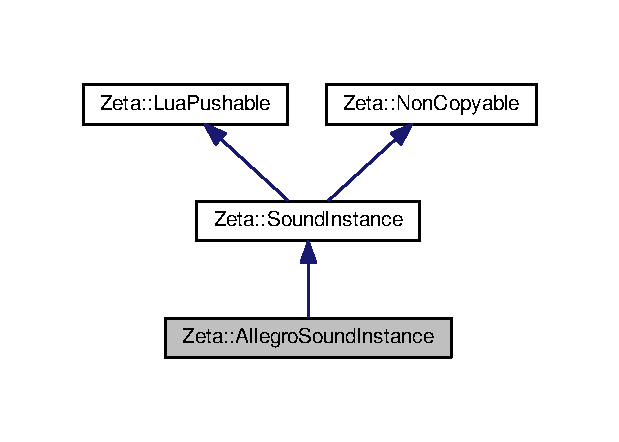
\includegraphics[width=297pt]{classZeta_1_1AllegroSoundInstance__inherit__graph}
\end{center}
\end{figure}


Collaboration diagram for Zeta\+:\+:Allegro\+Sound\+Instance\+:\nopagebreak
\begin{figure}[H]
\begin{center}
\leavevmode
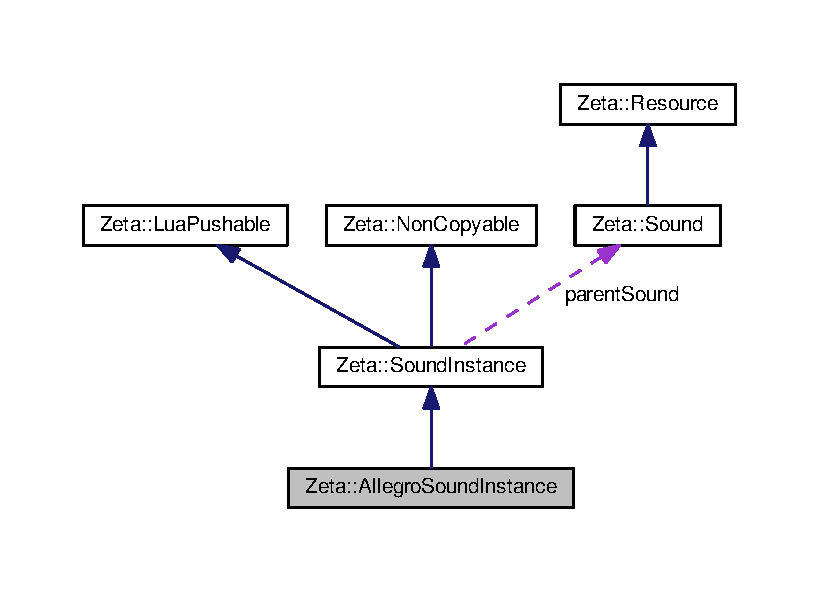
\includegraphics[width=350pt]{classZeta_1_1AllegroSoundInstance__coll__graph}
\end{center}
\end{figure}
\subsection*{Public Member Functions}
\begin{DoxyCompactItemize}
\item 
void \hyperlink{classZeta_1_1AllegroSoundInstance_a03445ff331168cd23b5943f324a5c0ce}{play} ()
\item 
void \hyperlink{classZeta_1_1AllegroSoundInstance_a35f836c6af4e94f3796ce2b3b87883b6}{stop} ()
\item 
void \hyperlink{classZeta_1_1AllegroSoundInstance_a8c61431dc1a8435a4c7916b66958f7aa}{set\+Loop} (bool value)
\item 
void \hyperlink{classZeta_1_1AllegroSoundInstance_a6775c3c2771979d75c9feb3f8bdab4c7}{set\+Gain} (float value)
\item 
void \hyperlink{classZeta_1_1AllegroSoundInstance_af1ed68d1916fde033a179da5cf83b9ec}{set\+Pan} (float value)
\item 
\hyperlink{classZeta_1_1AllegroSoundInstance_a05aac96240f7fb1254877f217adc5798}{Allegro\+Sound\+Instance} (A\+L\+L\+E\+G\+R\+O\+\_\+\+S\+A\+M\+P\+L\+E\+\_\+\+I\+N\+S\+T\+A\+N\+C\+E $\ast$\hyperlink{classZeta_1_1AllegroSoundInstance_a92a840b4c42200f0e6706d2b4df308e7}{instance})
\item 
\hyperlink{classZeta_1_1AllegroSoundInstance_a9f31883d1283966d23fbb624e339f1db}{$\sim$\+Allegro\+Sound\+Instance} ()
\end{DoxyCompactItemize}
\subsection*{Private Attributes}
\begin{DoxyCompactItemize}
\item 
A\+L\+L\+E\+G\+R\+O\+\_\+\+S\+A\+M\+P\+L\+E\+\_\+\+I\+N\+S\+T\+A\+N\+C\+E $\ast$ \hyperlink{classZeta_1_1AllegroSoundInstance_a92a840b4c42200f0e6706d2b4df308e7}{instance}
\end{DoxyCompactItemize}
\subsection*{Additional Inherited Members}


\subsection{Constructor \& Destructor Documentation}
\hypertarget{classZeta_1_1AllegroSoundInstance_a05aac96240f7fb1254877f217adc5798}{\index{Zeta\+::\+Allegro\+Sound\+Instance@{Zeta\+::\+Allegro\+Sound\+Instance}!Allegro\+Sound\+Instance@{Allegro\+Sound\+Instance}}
\index{Allegro\+Sound\+Instance@{Allegro\+Sound\+Instance}!Zeta\+::\+Allegro\+Sound\+Instance@{Zeta\+::\+Allegro\+Sound\+Instance}}
\subsubsection[{Allegro\+Sound\+Instance}]{\setlength{\rightskip}{0pt plus 5cm}Zeta\+::\+Allegro\+Sound\+Instance\+::\+Allegro\+Sound\+Instance (
\begin{DoxyParamCaption}
\item[{A\+L\+L\+E\+G\+R\+O\+\_\+\+S\+A\+M\+P\+L\+E\+\_\+\+I\+N\+S\+T\+A\+N\+C\+E $\ast$}]{instance}
\end{DoxyParamCaption}
)}}\label{classZeta_1_1AllegroSoundInstance_a05aac96240f7fb1254877f217adc5798}
\hypertarget{classZeta_1_1AllegroSoundInstance_a9f31883d1283966d23fbb624e339f1db}{\index{Zeta\+::\+Allegro\+Sound\+Instance@{Zeta\+::\+Allegro\+Sound\+Instance}!````~Allegro\+Sound\+Instance@{$\sim$\+Allegro\+Sound\+Instance}}
\index{````~Allegro\+Sound\+Instance@{$\sim$\+Allegro\+Sound\+Instance}!Zeta\+::\+Allegro\+Sound\+Instance@{Zeta\+::\+Allegro\+Sound\+Instance}}
\subsubsection[{$\sim$\+Allegro\+Sound\+Instance}]{\setlength{\rightskip}{0pt plus 5cm}Zeta\+::\+Allegro\+Sound\+Instance\+::$\sim$\+Allegro\+Sound\+Instance (
\begin{DoxyParamCaption}
{}
\end{DoxyParamCaption}
)}}\label{classZeta_1_1AllegroSoundInstance_a9f31883d1283966d23fbb624e339f1db}


\subsection{Member Function Documentation}
\hypertarget{classZeta_1_1AllegroSoundInstance_a03445ff331168cd23b5943f324a5c0ce}{\index{Zeta\+::\+Allegro\+Sound\+Instance@{Zeta\+::\+Allegro\+Sound\+Instance}!play@{play}}
\index{play@{play}!Zeta\+::\+Allegro\+Sound\+Instance@{Zeta\+::\+Allegro\+Sound\+Instance}}
\subsubsection[{play}]{\setlength{\rightskip}{0pt plus 5cm}void Zeta\+::\+Allegro\+Sound\+Instance\+::play (
\begin{DoxyParamCaption}
{}
\end{DoxyParamCaption}
)\hspace{0.3cm}{\ttfamily [virtual]}}}\label{classZeta_1_1AllegroSoundInstance_a03445ff331168cd23b5943f324a5c0ce}
Plays the sound 

Implements \hyperlink{classZeta_1_1SoundInstance_a9c0c29e0bd01fbd1ae9704153ee061d4}{Zeta\+::\+Sound\+Instance}.

\hypertarget{classZeta_1_1AllegroSoundInstance_a6775c3c2771979d75c9feb3f8bdab4c7}{\index{Zeta\+::\+Allegro\+Sound\+Instance@{Zeta\+::\+Allegro\+Sound\+Instance}!set\+Gain@{set\+Gain}}
\index{set\+Gain@{set\+Gain}!Zeta\+::\+Allegro\+Sound\+Instance@{Zeta\+::\+Allegro\+Sound\+Instance}}
\subsubsection[{set\+Gain}]{\setlength{\rightskip}{0pt plus 5cm}void Zeta\+::\+Allegro\+Sound\+Instance\+::set\+Gain (
\begin{DoxyParamCaption}
\item[{float}]{value}
\end{DoxyParamCaption}
)\hspace{0.3cm}{\ttfamily [virtual]}}}\label{classZeta_1_1AllegroSoundInstance_a6775c3c2771979d75c9feb3f8bdab4c7}
Sets the gain of the sound (Right of left) I\+M\+P\+O\+R\+T\+A\+N\+T! The field gain should set too! 
\begin{DoxyParams}{Parameters}
{\em value} & the gain of the sound to set \\
\hline
\end{DoxyParams}


Implements \hyperlink{classZeta_1_1SoundInstance_ad12e077da7bb16115ebff1405353834d}{Zeta\+::\+Sound\+Instance}.

\hypertarget{classZeta_1_1AllegroSoundInstance_a8c61431dc1a8435a4c7916b66958f7aa}{\index{Zeta\+::\+Allegro\+Sound\+Instance@{Zeta\+::\+Allegro\+Sound\+Instance}!set\+Loop@{set\+Loop}}
\index{set\+Loop@{set\+Loop}!Zeta\+::\+Allegro\+Sound\+Instance@{Zeta\+::\+Allegro\+Sound\+Instance}}
\subsubsection[{set\+Loop}]{\setlength{\rightskip}{0pt plus 5cm}void Zeta\+::\+Allegro\+Sound\+Instance\+::set\+Loop (
\begin{DoxyParamCaption}
\item[{bool}]{value}
\end{DoxyParamCaption}
)\hspace{0.3cm}{\ttfamily [virtual]}}}\label{classZeta_1_1AllegroSoundInstance_a8c61431dc1a8435a4c7916b66958f7aa}
Sets if the sound should repeat after it ended I\+M\+P\+O\+R\+T\+A\+N\+T! The field loops should set too! 
\begin{DoxyParams}{Parameters}
{\em value} & true if the sound should loop, otherwise false \\
\hline
\end{DoxyParams}


Implements \hyperlink{classZeta_1_1SoundInstance_ab0223c560591b60ff283893c518b28b1}{Zeta\+::\+Sound\+Instance}.

\hypertarget{classZeta_1_1AllegroSoundInstance_af1ed68d1916fde033a179da5cf83b9ec}{\index{Zeta\+::\+Allegro\+Sound\+Instance@{Zeta\+::\+Allegro\+Sound\+Instance}!set\+Pan@{set\+Pan}}
\index{set\+Pan@{set\+Pan}!Zeta\+::\+Allegro\+Sound\+Instance@{Zeta\+::\+Allegro\+Sound\+Instance}}
\subsubsection[{set\+Pan}]{\setlength{\rightskip}{0pt plus 5cm}void Zeta\+::\+Allegro\+Sound\+Instance\+::set\+Pan (
\begin{DoxyParamCaption}
\item[{float}]{value}
\end{DoxyParamCaption}
)\hspace{0.3cm}{\ttfamily [virtual]}}}\label{classZeta_1_1AllegroSoundInstance_af1ed68d1916fde033a179da5cf83b9ec}
Sets the pan of the sound The pan takes a value between -\/1 to 1 where -\/1=Left, 0=Center, 1=Right I\+M\+P\+O\+R\+T\+A\+N\+T! The field pan should set too! 
\begin{DoxyParams}{Parameters}
{\em value} & the pan of the sound to set \\
\hline
\end{DoxyParams}


Implements \hyperlink{classZeta_1_1SoundInstance_a34b3034515461fd964bba4221ac56a29}{Zeta\+::\+Sound\+Instance}.

\hypertarget{classZeta_1_1AllegroSoundInstance_a35f836c6af4e94f3796ce2b3b87883b6}{\index{Zeta\+::\+Allegro\+Sound\+Instance@{Zeta\+::\+Allegro\+Sound\+Instance}!stop@{stop}}
\index{stop@{stop}!Zeta\+::\+Allegro\+Sound\+Instance@{Zeta\+::\+Allegro\+Sound\+Instance}}
\subsubsection[{stop}]{\setlength{\rightskip}{0pt plus 5cm}void Zeta\+::\+Allegro\+Sound\+Instance\+::stop (
\begin{DoxyParamCaption}
{}
\end{DoxyParamCaption}
)\hspace{0.3cm}{\ttfamily [virtual]}}}\label{classZeta_1_1AllegroSoundInstance_a35f836c6af4e94f3796ce2b3b87883b6}
Stops the sound if playing 

Implements \hyperlink{classZeta_1_1SoundInstance_ac373cb282c51c26b715568e5dbd28afe}{Zeta\+::\+Sound\+Instance}.



\subsection{Member Data Documentation}
\hypertarget{classZeta_1_1AllegroSoundInstance_a92a840b4c42200f0e6706d2b4df308e7}{\index{Zeta\+::\+Allegro\+Sound\+Instance@{Zeta\+::\+Allegro\+Sound\+Instance}!instance@{instance}}
\index{instance@{instance}!Zeta\+::\+Allegro\+Sound\+Instance@{Zeta\+::\+Allegro\+Sound\+Instance}}
\subsubsection[{instance}]{\setlength{\rightskip}{0pt plus 5cm}A\+L\+L\+E\+G\+R\+O\+\_\+\+S\+A\+M\+P\+L\+E\+\_\+\+I\+N\+S\+T\+A\+N\+C\+E$\ast$ Zeta\+::\+Allegro\+Sound\+Instance\+::instance\hspace{0.3cm}{\ttfamily [private]}}}\label{classZeta_1_1AllegroSoundInstance_a92a840b4c42200f0e6706d2b4df308e7}


The documentation for this class was generated from the following file\+:\begin{DoxyCompactItemize}
\item 
include/\+Zeta/\+Library\+Binders/\+Allegro5/\hyperlink{AllegroSoundInstance_8hpp}{Allegro\+Sound\+Instance.\+hpp}\end{DoxyCompactItemize}

\hypertarget{classZeta_1_1Animation}{\section{Zeta\+:\+:Animation Class Reference}
\label{classZeta_1_1Animation}\index{Zeta\+::\+Animation@{Zeta\+::\+Animation}}
}


{\ttfamily \#include $<$Animation.\+hpp$>$}



Collaboration diagram for Zeta\+:\+:Animation\+:
\nopagebreak
\begin{figure}[H]
\begin{center}
\leavevmode
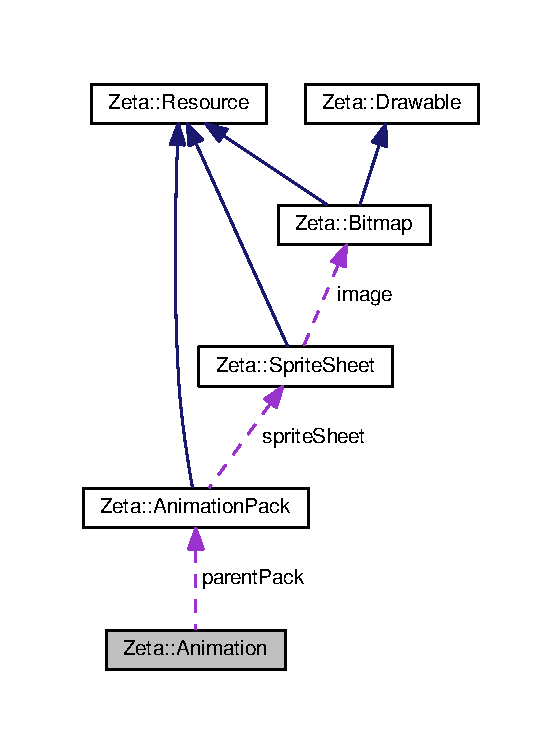
\includegraphics[width=269pt]{classZeta_1_1Animation__coll__graph}
\end{center}
\end{figure}
\subsection*{Public Member Functions}
\begin{DoxyCompactItemize}
\item 
const std\+::string \& \hyperlink{classZeta_1_1Animation_a697aa8eb070668cec1f2e4d7b25df597}{get\+Name} () const 
\item 
void \hyperlink{classZeta_1_1Animation_a30ad50fa2e22482dcbaf3502376cc490}{set\+Name} (const std\+::string \&\hyperlink{classZeta_1_1Animation_ac532add4feb3dd5e33f722a8142aedd6}{name})
\item 
bool \hyperlink{classZeta_1_1Animation_aa57126967823aa208c75d84460caef3c}{is\+Looping} () const 
\item 
const \hyperlink{classZeta_1_1AnimationPack}{Animation\+Pack} \& \hyperlink{classZeta_1_1Animation_a076b235101d9accb1c700354a5d338a9}{get\+Animation\+Pack} () const 
\item 
int \hyperlink{classZeta_1_1Animation_a9db1e0875105a9ac926ffd6073c1e06c}{get\+Num\+Frames} () const 
\item 
const \hyperlink{classZeta_1_1Cell}{Cell} \& \hyperlink{classZeta_1_1Animation_abea6f68c17959f92e7c2ed184c1a8ba8}{get\+Frame} (unsigned int index) const 
\item 
void \hyperlink{classZeta_1_1Animation_a6c141b127a9d83d17959259dcb07c48b}{set} (xmlpp\+::\+Node $\ast$node, const \hyperlink{classZeta_1_1AnimationPack}{Animation\+Pack} \&parent)
\item 
\hyperlink{classZeta_1_1Animation_adb107c29b84109e5e6df6debc953acea}{Animation} (\hyperlink{classZeta_1_1Animation}{Animation} \&\&)=default
\item 
\hyperlink{classZeta_1_1Animation}{Animation} \& \hyperlink{classZeta_1_1Animation_a464caf337fc48417e1d0157cb8f98200}{operator=} (\hyperlink{classZeta_1_1Animation}{Animation} \&\&)=default
\item 
\hyperlink{classZeta_1_1Animation_a89a1e45fbeb6582448bcf878e1b20be7}{Animation} ()
\item 
\hyperlink{classZeta_1_1Animation_a7591b35b9b593b1f22316af9d1f081fb}{Animation} (xmlpp\+::\+Node $\ast$node, const \hyperlink{classZeta_1_1AnimationPack}{Animation\+Pack} \&parent)
\item 
virtual \hyperlink{classZeta_1_1Animation_a43a5f796d416cf2e8c3f5cd8153e4277}{$\sim$\+Animation} ()
\end{DoxyCompactItemize}
\subsection*{Protected Attributes}
\begin{DoxyCompactItemize}
\item 
std\+::string \hyperlink{classZeta_1_1Animation_ac532add4feb3dd5e33f722a8142aedd6}{name}
\item 
std\+::vector$<$ \hyperlink{classZeta_1_1Cell}{Cell} $>$ \hyperlink{classZeta_1_1Animation_aa31ff21bcccd45e09ad6924087e9c1c7}{cells}
\item 
const \hyperlink{classZeta_1_1AnimationPack}{Animation\+Pack} $\ast$ \hyperlink{classZeta_1_1Animation_a2cbc0d0aac921dbc343ae864af112559}{parent\+Pack}
\item 
int \hyperlink{classZeta_1_1Animation_a6449ef440e5d9ce97187a00d32b637e5}{num\+\_\+\+Cells}
\item 
bool \hyperlink{classZeta_1_1Animation_af3097763657c74004f42843fdd6b577b}{loops}
\end{DoxyCompactItemize}


\subsection{Constructor \& Destructor Documentation}
\hypertarget{classZeta_1_1Animation_adb107c29b84109e5e6df6debc953acea}{\index{Zeta\+::\+Animation@{Zeta\+::\+Animation}!Animation@{Animation}}
\index{Animation@{Animation}!Zeta\+::\+Animation@{Zeta\+::\+Animation}}
\subsubsection[{Animation}]{\setlength{\rightskip}{0pt plus 5cm}Zeta\+::\+Animation\+::\+Animation (
\begin{DoxyParamCaption}
\item[{{\bf Animation} \&\&}]{}
\end{DoxyParamCaption}
)\hspace{0.3cm}{\ttfamily [default]}}}\label{classZeta_1_1Animation_adb107c29b84109e5e6df6debc953acea}
\hypertarget{classZeta_1_1Animation_a89a1e45fbeb6582448bcf878e1b20be7}{\index{Zeta\+::\+Animation@{Zeta\+::\+Animation}!Animation@{Animation}}
\index{Animation@{Animation}!Zeta\+::\+Animation@{Zeta\+::\+Animation}}
\subsubsection[{Animation}]{\setlength{\rightskip}{0pt plus 5cm}Zeta\+::\+Animation\+::\+Animation (
\begin{DoxyParamCaption}
{}
\end{DoxyParamCaption}
)}}\label{classZeta_1_1Animation_a89a1e45fbeb6582448bcf878e1b20be7}
\hypertarget{classZeta_1_1Animation_a7591b35b9b593b1f22316af9d1f081fb}{\index{Zeta\+::\+Animation@{Zeta\+::\+Animation}!Animation@{Animation}}
\index{Animation@{Animation}!Zeta\+::\+Animation@{Zeta\+::\+Animation}}
\subsubsection[{Animation}]{\setlength{\rightskip}{0pt plus 5cm}Zeta\+::\+Animation\+::\+Animation (
\begin{DoxyParamCaption}
\item[{xmlpp\+::\+Node $\ast$}]{node, }
\item[{const {\bf Animation\+Pack} \&}]{parent}
\end{DoxyParamCaption}
)}}\label{classZeta_1_1Animation_a7591b35b9b593b1f22316af9d1f081fb}
\hypertarget{classZeta_1_1Animation_a43a5f796d416cf2e8c3f5cd8153e4277}{\index{Zeta\+::\+Animation@{Zeta\+::\+Animation}!````~Animation@{$\sim$\+Animation}}
\index{````~Animation@{$\sim$\+Animation}!Zeta\+::\+Animation@{Zeta\+::\+Animation}}
\subsubsection[{$\sim$\+Animation}]{\setlength{\rightskip}{0pt plus 5cm}virtual Zeta\+::\+Animation\+::$\sim$\+Animation (
\begin{DoxyParamCaption}
{}
\end{DoxyParamCaption}
)\hspace{0.3cm}{\ttfamily [virtual]}}}\label{classZeta_1_1Animation_a43a5f796d416cf2e8c3f5cd8153e4277}


\subsection{Member Function Documentation}
\hypertarget{classZeta_1_1Animation_a076b235101d9accb1c700354a5d338a9}{\index{Zeta\+::\+Animation@{Zeta\+::\+Animation}!get\+Animation\+Pack@{get\+Animation\+Pack}}
\index{get\+Animation\+Pack@{get\+Animation\+Pack}!Zeta\+::\+Animation@{Zeta\+::\+Animation}}
\subsubsection[{get\+Animation\+Pack}]{\setlength{\rightskip}{0pt plus 5cm}const {\bf Animation\+Pack}\& Zeta\+::\+Animation\+::get\+Animation\+Pack (
\begin{DoxyParamCaption}
{}
\end{DoxyParamCaption}
) const\hspace{0.3cm}{\ttfamily [inline]}}}\label{classZeta_1_1Animation_a076b235101d9accb1c700354a5d338a9}
\hypertarget{classZeta_1_1Animation_abea6f68c17959f92e7c2ed184c1a8ba8}{\index{Zeta\+::\+Animation@{Zeta\+::\+Animation}!get\+Frame@{get\+Frame}}
\index{get\+Frame@{get\+Frame}!Zeta\+::\+Animation@{Zeta\+::\+Animation}}
\subsubsection[{get\+Frame}]{\setlength{\rightskip}{0pt plus 5cm}const {\bf Cell}\& Zeta\+::\+Animation\+::get\+Frame (
\begin{DoxyParamCaption}
\item[{unsigned int}]{index}
\end{DoxyParamCaption}
) const\hspace{0.3cm}{\ttfamily [inline]}}}\label{classZeta_1_1Animation_abea6f68c17959f92e7c2ed184c1a8ba8}
\hypertarget{classZeta_1_1Animation_a697aa8eb070668cec1f2e4d7b25df597}{\index{Zeta\+::\+Animation@{Zeta\+::\+Animation}!get\+Name@{get\+Name}}
\index{get\+Name@{get\+Name}!Zeta\+::\+Animation@{Zeta\+::\+Animation}}
\subsubsection[{get\+Name}]{\setlength{\rightskip}{0pt plus 5cm}const std\+::string\& Zeta\+::\+Animation\+::get\+Name (
\begin{DoxyParamCaption}
{}
\end{DoxyParamCaption}
) const\hspace{0.3cm}{\ttfamily [inline]}}}\label{classZeta_1_1Animation_a697aa8eb070668cec1f2e4d7b25df597}
\hypertarget{classZeta_1_1Animation_a9db1e0875105a9ac926ffd6073c1e06c}{\index{Zeta\+::\+Animation@{Zeta\+::\+Animation}!get\+Num\+Frames@{get\+Num\+Frames}}
\index{get\+Num\+Frames@{get\+Num\+Frames}!Zeta\+::\+Animation@{Zeta\+::\+Animation}}
\subsubsection[{get\+Num\+Frames}]{\setlength{\rightskip}{0pt plus 5cm}int Zeta\+::\+Animation\+::get\+Num\+Frames (
\begin{DoxyParamCaption}
{}
\end{DoxyParamCaption}
) const\hspace{0.3cm}{\ttfamily [inline]}}}\label{classZeta_1_1Animation_a9db1e0875105a9ac926ffd6073c1e06c}
\hypertarget{classZeta_1_1Animation_aa57126967823aa208c75d84460caef3c}{\index{Zeta\+::\+Animation@{Zeta\+::\+Animation}!is\+Looping@{is\+Looping}}
\index{is\+Looping@{is\+Looping}!Zeta\+::\+Animation@{Zeta\+::\+Animation}}
\subsubsection[{is\+Looping}]{\setlength{\rightskip}{0pt plus 5cm}bool Zeta\+::\+Animation\+::is\+Looping (
\begin{DoxyParamCaption}
{}
\end{DoxyParamCaption}
) const\hspace{0.3cm}{\ttfamily [inline]}}}\label{classZeta_1_1Animation_aa57126967823aa208c75d84460caef3c}
\hypertarget{classZeta_1_1Animation_a464caf337fc48417e1d0157cb8f98200}{\index{Zeta\+::\+Animation@{Zeta\+::\+Animation}!operator=@{operator=}}
\index{operator=@{operator=}!Zeta\+::\+Animation@{Zeta\+::\+Animation}}
\subsubsection[{operator=}]{\setlength{\rightskip}{0pt plus 5cm}{\bf Animation}\& Zeta\+::\+Animation\+::operator= (
\begin{DoxyParamCaption}
\item[{{\bf Animation} \&\&}]{}
\end{DoxyParamCaption}
)\hspace{0.3cm}{\ttfamily [default]}}}\label{classZeta_1_1Animation_a464caf337fc48417e1d0157cb8f98200}
\hypertarget{classZeta_1_1Animation_a6c141b127a9d83d17959259dcb07c48b}{\index{Zeta\+::\+Animation@{Zeta\+::\+Animation}!set@{set}}
\index{set@{set}!Zeta\+::\+Animation@{Zeta\+::\+Animation}}
\subsubsection[{set}]{\setlength{\rightskip}{0pt plus 5cm}void Zeta\+::\+Animation\+::set (
\begin{DoxyParamCaption}
\item[{xmlpp\+::\+Node $\ast$}]{node, }
\item[{const {\bf Animation\+Pack} \&}]{parent}
\end{DoxyParamCaption}
)}}\label{classZeta_1_1Animation_a6c141b127a9d83d17959259dcb07c48b}
\hypertarget{classZeta_1_1Animation_a30ad50fa2e22482dcbaf3502376cc490}{\index{Zeta\+::\+Animation@{Zeta\+::\+Animation}!set\+Name@{set\+Name}}
\index{set\+Name@{set\+Name}!Zeta\+::\+Animation@{Zeta\+::\+Animation}}
\subsubsection[{set\+Name}]{\setlength{\rightskip}{0pt plus 5cm}void Zeta\+::\+Animation\+::set\+Name (
\begin{DoxyParamCaption}
\item[{const std\+::string \&}]{name}
\end{DoxyParamCaption}
)\hspace{0.3cm}{\ttfamily [inline]}}}\label{classZeta_1_1Animation_a30ad50fa2e22482dcbaf3502376cc490}


\subsection{Member Data Documentation}
\hypertarget{classZeta_1_1Animation_aa31ff21bcccd45e09ad6924087e9c1c7}{\index{Zeta\+::\+Animation@{Zeta\+::\+Animation}!cells@{cells}}
\index{cells@{cells}!Zeta\+::\+Animation@{Zeta\+::\+Animation}}
\subsubsection[{cells}]{\setlength{\rightskip}{0pt plus 5cm}std\+::vector$<${\bf Cell}$>$ Zeta\+::\+Animation\+::cells\hspace{0.3cm}{\ttfamily [protected]}}}\label{classZeta_1_1Animation_aa31ff21bcccd45e09ad6924087e9c1c7}
\hypertarget{classZeta_1_1Animation_af3097763657c74004f42843fdd6b577b}{\index{Zeta\+::\+Animation@{Zeta\+::\+Animation}!loops@{loops}}
\index{loops@{loops}!Zeta\+::\+Animation@{Zeta\+::\+Animation}}
\subsubsection[{loops}]{\setlength{\rightskip}{0pt plus 5cm}bool Zeta\+::\+Animation\+::loops\hspace{0.3cm}{\ttfamily [protected]}}}\label{classZeta_1_1Animation_af3097763657c74004f42843fdd6b577b}
\hypertarget{classZeta_1_1Animation_ac532add4feb3dd5e33f722a8142aedd6}{\index{Zeta\+::\+Animation@{Zeta\+::\+Animation}!name@{name}}
\index{name@{name}!Zeta\+::\+Animation@{Zeta\+::\+Animation}}
\subsubsection[{name}]{\setlength{\rightskip}{0pt plus 5cm}std\+::string Zeta\+::\+Animation\+::name\hspace{0.3cm}{\ttfamily [protected]}}}\label{classZeta_1_1Animation_ac532add4feb3dd5e33f722a8142aedd6}
\hypertarget{classZeta_1_1Animation_a6449ef440e5d9ce97187a00d32b637e5}{\index{Zeta\+::\+Animation@{Zeta\+::\+Animation}!num\+\_\+\+Cells@{num\+\_\+\+Cells}}
\index{num\+\_\+\+Cells@{num\+\_\+\+Cells}!Zeta\+::\+Animation@{Zeta\+::\+Animation}}
\subsubsection[{num\+\_\+\+Cells}]{\setlength{\rightskip}{0pt plus 5cm}int Zeta\+::\+Animation\+::num\+\_\+\+Cells\hspace{0.3cm}{\ttfamily [protected]}}}\label{classZeta_1_1Animation_a6449ef440e5d9ce97187a00d32b637e5}
\hypertarget{classZeta_1_1Animation_a2cbc0d0aac921dbc343ae864af112559}{\index{Zeta\+::\+Animation@{Zeta\+::\+Animation}!parent\+Pack@{parent\+Pack}}
\index{parent\+Pack@{parent\+Pack}!Zeta\+::\+Animation@{Zeta\+::\+Animation}}
\subsubsection[{parent\+Pack}]{\setlength{\rightskip}{0pt plus 5cm}const {\bf Animation\+Pack}$\ast$ Zeta\+::\+Animation\+::parent\+Pack\hspace{0.3cm}{\ttfamily [protected]}}}\label{classZeta_1_1Animation_a2cbc0d0aac921dbc343ae864af112559}


The documentation for this class was generated from the following file\+:\begin{DoxyCompactItemize}
\item 
include/\+Zeta/\+Core/\+Animation\+Classes/\hyperlink{Animation_8hpp}{Animation.\+hpp}\end{DoxyCompactItemize}

\hypertarget{classZeta_1_1AnimationClass}{\section{Zeta\+:\+:Animation\+Class Class Reference}
\label{classZeta_1_1AnimationClass}\index{Zeta\+::\+Animation\+Class@{Zeta\+::\+Animation\+Class}}
}


{\ttfamily \#include $<$Animation\+Class.\+hpp$>$}



Inheritance diagram for Zeta\+:\+:Animation\+Class\+:\nopagebreak
\begin{figure}[H]
\begin{center}
\leavevmode
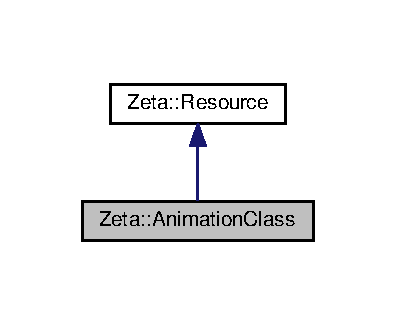
\includegraphics[width=190pt]{classZeta_1_1AnimationClass__inherit__graph}
\end{center}
\end{figure}


Collaboration diagram for Zeta\+:\+:Animation\+Class\+:
\nopagebreak
\begin{figure}[H]
\begin{center}
\leavevmode
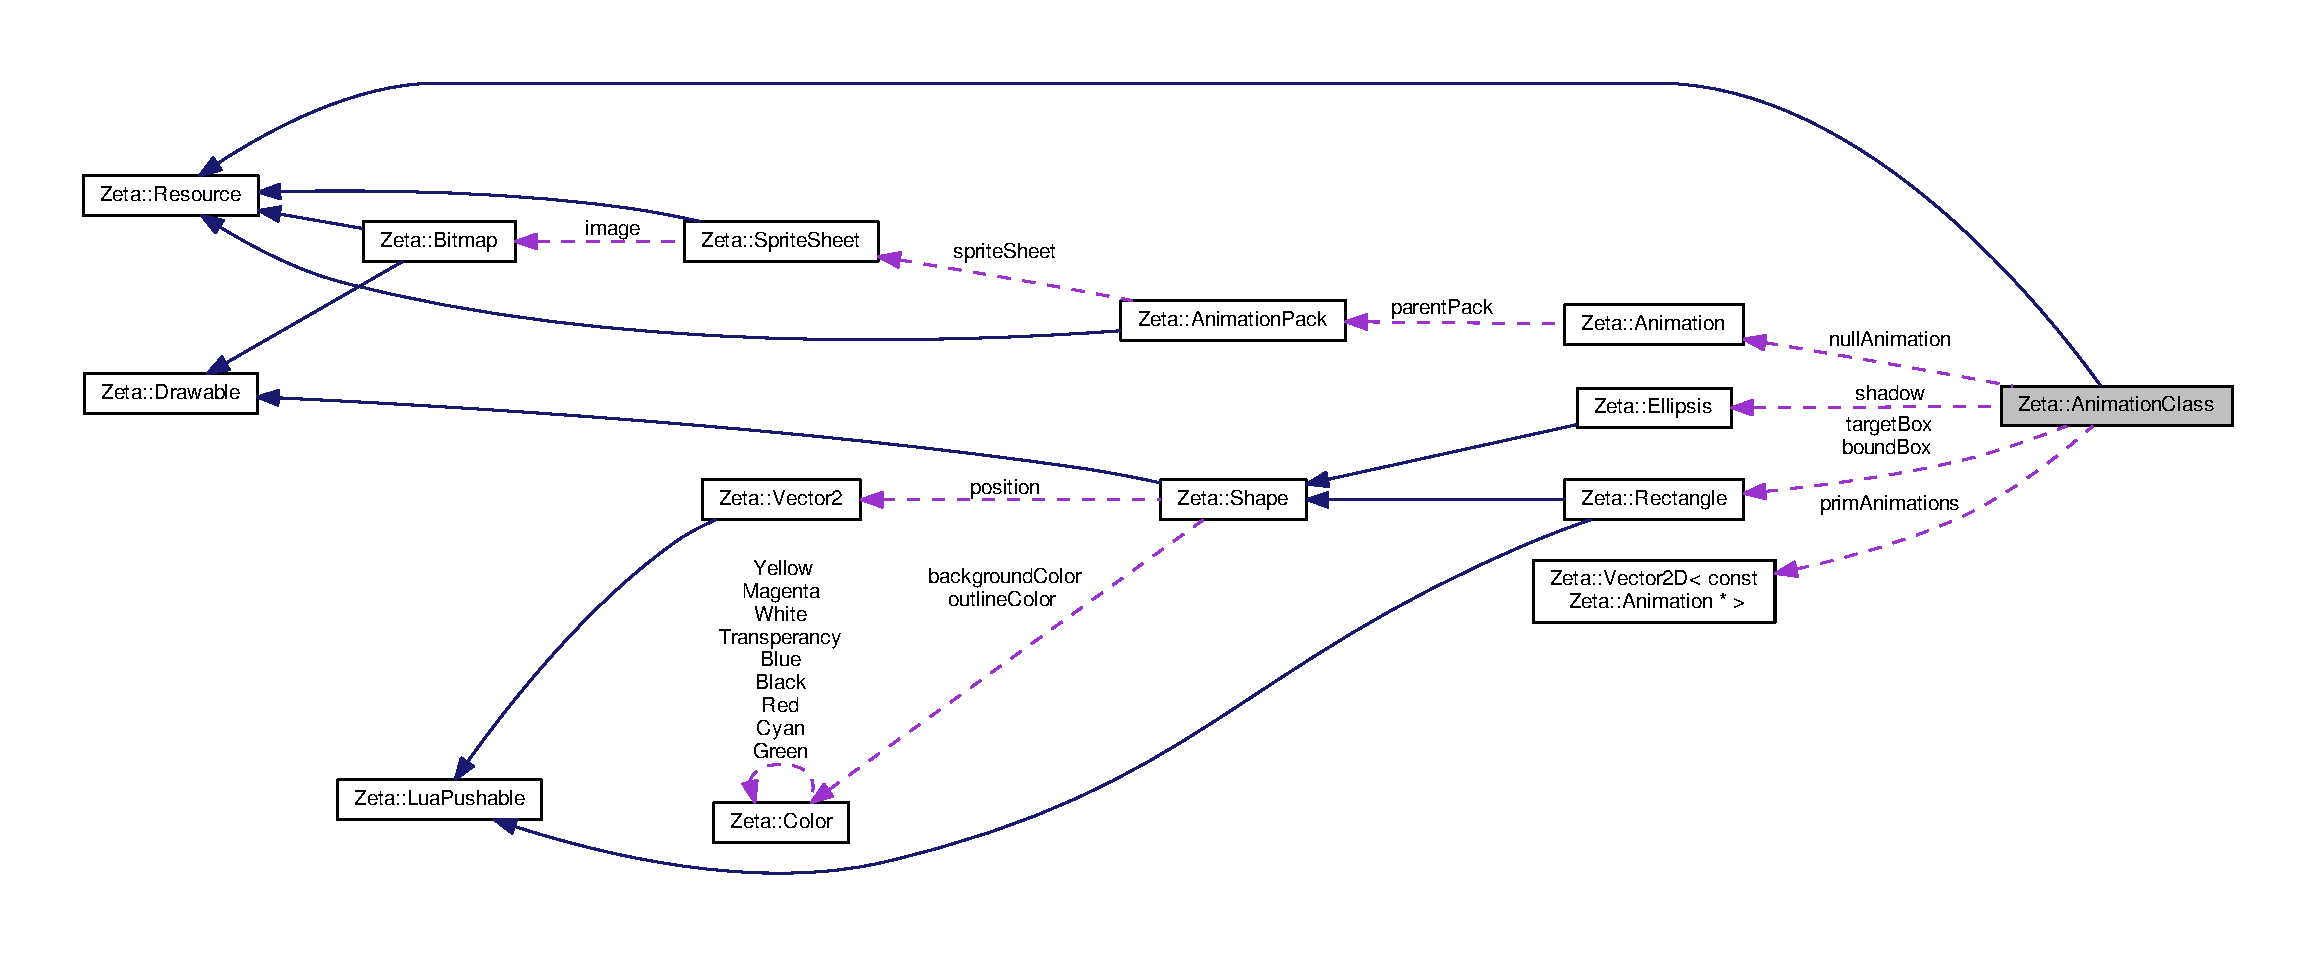
\includegraphics[width=350pt]{classZeta_1_1AnimationClass__coll__graph}
\end{center}
\end{figure}
\subsection*{Public Member Functions}
\begin{DoxyCompactItemize}
\item 
const \hyperlink{classZeta_1_1Animation}{Animation} \& \hyperlink{classZeta_1_1AnimationClass_a08189e19359afd81fbfc326ddbf4df67}{get\+Animation} (const std\+::string \&\hyperlink{classZeta_1_1Resource_a44c5721216f4beb31c0b3d2ef2aecf1d}{name}, \hyperlink{classZeta_1_1LifeformState_a877fbe4e8efefd0a5323f950909181b6}{Lifeform\+State\+::\+Combined\+State} fallback\+Animation=Lifeform\+State\+::\+Action\+::\+Idle$\vert$Lifeform\+State\+::\+Direction\+::\+Down) const 
\item 
const \hyperlink{classZeta_1_1Animation}{Animation} \& \hyperlink{classZeta_1_1AnimationClass_a83d5eab51620488465f3cc855ce63c81}{get\+Animation} (\hyperlink{classZeta_1_1LifeformState_a877fbe4e8efefd0a5323f950909181b6}{Lifeform\+State\+::\+Combined\+State} state) const 
\item 
const \hyperlink{classZeta_1_1Rectangle}{Rectangle} \& \hyperlink{classZeta_1_1AnimationClass_ade1b42c7e1174a6a0996c5d565178e58}{get\+Bound\+Box} () const 
\item 
const \hyperlink{classZeta_1_1Rectangle}{Rectangle} \& \hyperlink{classZeta_1_1AnimationClass_a49da6527fe78be2ea9960521791ee103}{get\+Target\+Box} () const 
\item 
const \hyperlink{classZeta_1_1Ellipsis}{Ellipsis} \& \hyperlink{classZeta_1_1AnimationClass_aee9e50033789d54b124747fc0148a7cf}{get\+Shadow} () const 
\item 
bool \hyperlink{classZeta_1_1AnimationClass_a5d0eab997f120d86e55fa81738935187}{has\+Shadow} () const 
\item 
\hyperlink{classZeta_1_1AnimationClass_a1f7a167d864f4699a52de6fe6d959615}{Animation\+Class} ()
\item 
\hyperlink{classZeta_1_1AnimationClass_a14cb2ae834895163a353e22e3ccefb30}{Animation\+Class} (const std\+::string \&path)
\item 
virtual \hyperlink{classZeta_1_1AnimationClass_ad30602ed6077999bc479e05e8fa4a689}{$\sim$\+Animation\+Class} ()
\end{DoxyCompactItemize}
\subsection*{Protected Member Functions}
\begin{DoxyCompactItemize}
\item 
void \hyperlink{classZeta_1_1AnimationClass_ab25150bb5125a485174e6bc1b2968216}{retrive\+Primitives} ()
\end{DoxyCompactItemize}
\subsection*{Protected Attributes}
\begin{DoxyCompactItemize}
\item 
\hyperlink{namespaceZeta_a4c11e23ddc559dccdb5e85901d7dfb84}{Z\+Small\+Map}$<$ std\+::string, const \\*
\hyperlink{classZeta_1_1Animation}{Animation} $\ast$ $>$ \hyperlink{classZeta_1_1AnimationClass_a8b61708081d2967f65f4d3a34048dd36}{animations}
\item 
\hyperlink{classZeta_1_1Vector2D}{Vector2\+D}$<$ const \hyperlink{classZeta_1_1Animation}{Animation} $\ast$ $>$ \hyperlink{classZeta_1_1AnimationClass_a75ec3cd5a2fe104b9e8ac92858faca4c}{prim\+Animations}
\item 
\hyperlink{classZeta_1_1Rectangle}{Rectangle} \hyperlink{classZeta_1_1AnimationClass_a4e11683656c6f0648464c5b9b4e630c4}{bound\+Box}
\item 
\hyperlink{classZeta_1_1Rectangle}{Rectangle} \hyperlink{classZeta_1_1AnimationClass_a5d9cf5c7819f3f1bc9addadba989e96c}{target\+Box}
\item 
\hyperlink{classZeta_1_1Ellipsis}{Ellipsis} \hyperlink{classZeta_1_1AnimationClass_a5a1c48380989f66dfc1d90caa615ff55}{shadow}
\item 
const \hyperlink{classZeta_1_1Animation}{Animation} $\ast$ \hyperlink{classZeta_1_1AnimationClass_aa74a96c176531b81900c8568f77f966c}{null\+Animation}
\item 
bool \hyperlink{classZeta_1_1AnimationClass_a24192e217829955ac2f97a940be58922}{has\+\_\+\+Shadow}
\end{DoxyCompactItemize}


\subsection{Detailed Description}
Class for \hyperlink{classZeta_1_1Animation}{Animation} Classes \hyperlink{classZeta_1_1Animation}{Animation} Classes are a group of Animations that can be assigned to a \hyperlink{classZeta_1_1Lifeform}{Lifeform}. Usually the animations are related 

\subsection{Constructor \& Destructor Documentation}
\hypertarget{classZeta_1_1AnimationClass_a1f7a167d864f4699a52de6fe6d959615}{\index{Zeta\+::\+Animation\+Class@{Zeta\+::\+Animation\+Class}!Animation\+Class@{Animation\+Class}}
\index{Animation\+Class@{Animation\+Class}!Zeta\+::\+Animation\+Class@{Zeta\+::\+Animation\+Class}}
\subsubsection[{Animation\+Class}]{\setlength{\rightskip}{0pt plus 5cm}Zeta\+::\+Animation\+Class\+::\+Animation\+Class (
\begin{DoxyParamCaption}
{}
\end{DoxyParamCaption}
)}}\label{classZeta_1_1AnimationClass_a1f7a167d864f4699a52de6fe6d959615}
Default Constructor Constructs a Null \hyperlink{classZeta_1_1AnimationClass}{Animation\+Class} that contains no Animations and all State Animations are Null\+Animations \hypertarget{classZeta_1_1AnimationClass_a14cb2ae834895163a353e22e3ccefb30}{\index{Zeta\+::\+Animation\+Class@{Zeta\+::\+Animation\+Class}!Animation\+Class@{Animation\+Class}}
\index{Animation\+Class@{Animation\+Class}!Zeta\+::\+Animation\+Class@{Zeta\+::\+Animation\+Class}}
\subsubsection[{Animation\+Class}]{\setlength{\rightskip}{0pt plus 5cm}Zeta\+::\+Animation\+Class\+::\+Animation\+Class (
\begin{DoxyParamCaption}
\item[{const std\+::string \&}]{path}
\end{DoxyParamCaption}
)}}\label{classZeta_1_1AnimationClass_a14cb2ae834895163a353e22e3ccefb30}
Loads the \hyperlink{classZeta_1_1Animation}{Animation} Class \hyperlink{classZeta_1_1File}{File} \hypertarget{classZeta_1_1AnimationClass_ad30602ed6077999bc479e05e8fa4a689}{\index{Zeta\+::\+Animation\+Class@{Zeta\+::\+Animation\+Class}!````~Animation\+Class@{$\sim$\+Animation\+Class}}
\index{````~Animation\+Class@{$\sim$\+Animation\+Class}!Zeta\+::\+Animation\+Class@{Zeta\+::\+Animation\+Class}}
\subsubsection[{$\sim$\+Animation\+Class}]{\setlength{\rightskip}{0pt plus 5cm}virtual Zeta\+::\+Animation\+Class\+::$\sim$\+Animation\+Class (
\begin{DoxyParamCaption}
{}
\end{DoxyParamCaption}
)\hspace{0.3cm}{\ttfamily [virtual]}}}\label{classZeta_1_1AnimationClass_ad30602ed6077999bc479e05e8fa4a689}


\subsection{Member Function Documentation}
\hypertarget{classZeta_1_1AnimationClass_a08189e19359afd81fbfc326ddbf4df67}{\index{Zeta\+::\+Animation\+Class@{Zeta\+::\+Animation\+Class}!get\+Animation@{get\+Animation}}
\index{get\+Animation@{get\+Animation}!Zeta\+::\+Animation\+Class@{Zeta\+::\+Animation\+Class}}
\subsubsection[{get\+Animation}]{\setlength{\rightskip}{0pt plus 5cm}const {\bf Animation}\& Zeta\+::\+Animation\+Class\+::get\+Animation (
\begin{DoxyParamCaption}
\item[{const std\+::string \&}]{name, }
\item[{{\bf Lifeform\+State\+::\+Combined\+State}}]{fallback\+Animation = {\ttfamily LifeformState\+:\+:Action\+:\+:Idle$\vert$LifeformState\+:\+:Direction\+:\+:Down}}
\end{DoxyParamCaption}
) const}}\label{classZeta_1_1AnimationClass_a08189e19359afd81fbfc326ddbf4df67}
Gets the named animation If the animation does not exist, then the fallback animation will be returned. If not defined, the fallback is I\+D\+L\+E+\+D\+O\+W\+N. 
\begin{DoxyParams}{Parameters}
{\em name} & The name of the animation to return \\
\hline
{\em fallback\+Animation} & The animation State to return if the animation does not exist \\
\hline
\end{DoxyParams}
\begin{DoxyReturn}{Returns}
the \hyperlink{classZeta_1_1Animation}{Animation} to be returned 
\end{DoxyReturn}
\hypertarget{classZeta_1_1AnimationClass_a83d5eab51620488465f3cc855ce63c81}{\index{Zeta\+::\+Animation\+Class@{Zeta\+::\+Animation\+Class}!get\+Animation@{get\+Animation}}
\index{get\+Animation@{get\+Animation}!Zeta\+::\+Animation\+Class@{Zeta\+::\+Animation\+Class}}
\subsubsection[{get\+Animation}]{\setlength{\rightskip}{0pt plus 5cm}const {\bf Animation}\& Zeta\+::\+Animation\+Class\+::get\+Animation (
\begin{DoxyParamCaption}
\item[{{\bf Lifeform\+State\+::\+Combined\+State}}]{state}
\end{DoxyParamCaption}
) const}}\label{classZeta_1_1AnimationClass_a83d5eab51620488465f3cc855ce63c81}
Gets the \hyperlink{classZeta_1_1Animation}{Animation} defined by the State 
\begin{DoxyParams}{Parameters}
{\em state} & The state that has the animation \\
\hline
\end{DoxyParams}
\begin{DoxyReturn}{Returns}
the \hyperlink{classZeta_1_1Animation}{Animation} to be returned 
\end{DoxyReturn}
\hypertarget{classZeta_1_1AnimationClass_ade1b42c7e1174a6a0996c5d565178e58}{\index{Zeta\+::\+Animation\+Class@{Zeta\+::\+Animation\+Class}!get\+Bound\+Box@{get\+Bound\+Box}}
\index{get\+Bound\+Box@{get\+Bound\+Box}!Zeta\+::\+Animation\+Class@{Zeta\+::\+Animation\+Class}}
\subsubsection[{get\+Bound\+Box}]{\setlength{\rightskip}{0pt plus 5cm}const {\bf Rectangle}\& Zeta\+::\+Animation\+Class\+::get\+Bound\+Box (
\begin{DoxyParamCaption}
{}
\end{DoxyParamCaption}
) const\hspace{0.3cm}{\ttfamily [inline]}}}\label{classZeta_1_1AnimationClass_ade1b42c7e1174a6a0996c5d565178e58}
Gets the Boundary \hyperlink{classZeta_1_1Rectangle}{Rectangle} of this Class This rectangle is used for Collision Detection \begin{DoxyReturn}{Returns}
The Boundary \hyperlink{classZeta_1_1Rectangle}{Rectangle} 
\end{DoxyReturn}
\hypertarget{classZeta_1_1AnimationClass_aee9e50033789d54b124747fc0148a7cf}{\index{Zeta\+::\+Animation\+Class@{Zeta\+::\+Animation\+Class}!get\+Shadow@{get\+Shadow}}
\index{get\+Shadow@{get\+Shadow}!Zeta\+::\+Animation\+Class@{Zeta\+::\+Animation\+Class}}
\subsubsection[{get\+Shadow}]{\setlength{\rightskip}{0pt plus 5cm}const {\bf Ellipsis}\& Zeta\+::\+Animation\+Class\+::get\+Shadow (
\begin{DoxyParamCaption}
{}
\end{DoxyParamCaption}
) const\hspace{0.3cm}{\ttfamily [inline]}}}\label{classZeta_1_1AnimationClass_aee9e50033789d54b124747fc0148a7cf}
Gets the Shadow \hyperlink{classZeta_1_1Ellipsis}{Ellipsis} of this Class \begin{DoxyReturn}{Returns}
The Shadow \hyperlink{classZeta_1_1Ellipsis}{Ellipsis} 
\end{DoxyReturn}
\hypertarget{classZeta_1_1AnimationClass_a49da6527fe78be2ea9960521791ee103}{\index{Zeta\+::\+Animation\+Class@{Zeta\+::\+Animation\+Class}!get\+Target\+Box@{get\+Target\+Box}}
\index{get\+Target\+Box@{get\+Target\+Box}!Zeta\+::\+Animation\+Class@{Zeta\+::\+Animation\+Class}}
\subsubsection[{get\+Target\+Box}]{\setlength{\rightskip}{0pt plus 5cm}const {\bf Rectangle}\& Zeta\+::\+Animation\+Class\+::get\+Target\+Box (
\begin{DoxyParamCaption}
{}
\end{DoxyParamCaption}
) const\hspace{0.3cm}{\ttfamily [inline]}}}\label{classZeta_1_1AnimationClass_a49da6527fe78be2ea9960521791ee103}
Gets the Target \hyperlink{classZeta_1_1Rectangle}{Rectangle} of this Class This rectangle is used for Targeting \begin{DoxyReturn}{Returns}
The Target \hyperlink{classZeta_1_1Rectangle}{Rectangle} 
\end{DoxyReturn}
\hypertarget{classZeta_1_1AnimationClass_a5d0eab997f120d86e55fa81738935187}{\index{Zeta\+::\+Animation\+Class@{Zeta\+::\+Animation\+Class}!has\+Shadow@{has\+Shadow}}
\index{has\+Shadow@{has\+Shadow}!Zeta\+::\+Animation\+Class@{Zeta\+::\+Animation\+Class}}
\subsubsection[{has\+Shadow}]{\setlength{\rightskip}{0pt plus 5cm}bool Zeta\+::\+Animation\+Class\+::has\+Shadow (
\begin{DoxyParamCaption}
{}
\end{DoxyParamCaption}
) const\hspace{0.3cm}{\ttfamily [inline]}}}\label{classZeta_1_1AnimationClass_a5d0eab997f120d86e55fa81738935187}
Get whether this Class has a Shadow \begin{DoxyReturn}{Returns}
true if it has Shadow 
\end{DoxyReturn}
\hypertarget{classZeta_1_1AnimationClass_ab25150bb5125a485174e6bc1b2968216}{\index{Zeta\+::\+Animation\+Class@{Zeta\+::\+Animation\+Class}!retrive\+Primitives@{retrive\+Primitives}}
\index{retrive\+Primitives@{retrive\+Primitives}!Zeta\+::\+Animation\+Class@{Zeta\+::\+Animation\+Class}}
\subsubsection[{retrive\+Primitives}]{\setlength{\rightskip}{0pt plus 5cm}void Zeta\+::\+Animation\+Class\+::retrive\+Primitives (
\begin{DoxyParamCaption}
{}
\end{DoxyParamCaption}
)\hspace{0.3cm}{\ttfamily [protected]}}}\label{classZeta_1_1AnimationClass_ab25150bb5125a485174e6bc1b2968216}


\subsection{Member Data Documentation}
\hypertarget{classZeta_1_1AnimationClass_a8b61708081d2967f65f4d3a34048dd36}{\index{Zeta\+::\+Animation\+Class@{Zeta\+::\+Animation\+Class}!animations@{animations}}
\index{animations@{animations}!Zeta\+::\+Animation\+Class@{Zeta\+::\+Animation\+Class}}
\subsubsection[{animations}]{\setlength{\rightskip}{0pt plus 5cm}{\bf Z\+Small\+Map}$<$std\+::string, const {\bf Animation}$\ast$$>$ Zeta\+::\+Animation\+Class\+::animations\hspace{0.3cm}{\ttfamily [protected]}}}\label{classZeta_1_1AnimationClass_a8b61708081d2967f65f4d3a34048dd36}
\hypertarget{classZeta_1_1AnimationClass_a4e11683656c6f0648464c5b9b4e630c4}{\index{Zeta\+::\+Animation\+Class@{Zeta\+::\+Animation\+Class}!bound\+Box@{bound\+Box}}
\index{bound\+Box@{bound\+Box}!Zeta\+::\+Animation\+Class@{Zeta\+::\+Animation\+Class}}
\subsubsection[{bound\+Box}]{\setlength{\rightskip}{0pt plus 5cm}{\bf Rectangle} Zeta\+::\+Animation\+Class\+::bound\+Box\hspace{0.3cm}{\ttfamily [protected]}}}\label{classZeta_1_1AnimationClass_a4e11683656c6f0648464c5b9b4e630c4}
\hypertarget{classZeta_1_1AnimationClass_a24192e217829955ac2f97a940be58922}{\index{Zeta\+::\+Animation\+Class@{Zeta\+::\+Animation\+Class}!has\+\_\+\+Shadow@{has\+\_\+\+Shadow}}
\index{has\+\_\+\+Shadow@{has\+\_\+\+Shadow}!Zeta\+::\+Animation\+Class@{Zeta\+::\+Animation\+Class}}
\subsubsection[{has\+\_\+\+Shadow}]{\setlength{\rightskip}{0pt plus 5cm}bool Zeta\+::\+Animation\+Class\+::has\+\_\+\+Shadow\hspace{0.3cm}{\ttfamily [protected]}}}\label{classZeta_1_1AnimationClass_a24192e217829955ac2f97a940be58922}
\hypertarget{classZeta_1_1AnimationClass_aa74a96c176531b81900c8568f77f966c}{\index{Zeta\+::\+Animation\+Class@{Zeta\+::\+Animation\+Class}!null\+Animation@{null\+Animation}}
\index{null\+Animation@{null\+Animation}!Zeta\+::\+Animation\+Class@{Zeta\+::\+Animation\+Class}}
\subsubsection[{null\+Animation}]{\setlength{\rightskip}{0pt plus 5cm}const {\bf Animation}$\ast$ Zeta\+::\+Animation\+Class\+::null\+Animation\hspace{0.3cm}{\ttfamily [protected]}}}\label{classZeta_1_1AnimationClass_aa74a96c176531b81900c8568f77f966c}
\hypertarget{classZeta_1_1AnimationClass_a75ec3cd5a2fe104b9e8ac92858faca4c}{\index{Zeta\+::\+Animation\+Class@{Zeta\+::\+Animation\+Class}!prim\+Animations@{prim\+Animations}}
\index{prim\+Animations@{prim\+Animations}!Zeta\+::\+Animation\+Class@{Zeta\+::\+Animation\+Class}}
\subsubsection[{prim\+Animations}]{\setlength{\rightskip}{0pt plus 5cm}{\bf Vector2\+D}$<$const {\bf Animation}$\ast$$>$ Zeta\+::\+Animation\+Class\+::prim\+Animations\hspace{0.3cm}{\ttfamily [protected]}}}\label{classZeta_1_1AnimationClass_a75ec3cd5a2fe104b9e8ac92858faca4c}
\hypertarget{classZeta_1_1AnimationClass_a5a1c48380989f66dfc1d90caa615ff55}{\index{Zeta\+::\+Animation\+Class@{Zeta\+::\+Animation\+Class}!shadow@{shadow}}
\index{shadow@{shadow}!Zeta\+::\+Animation\+Class@{Zeta\+::\+Animation\+Class}}
\subsubsection[{shadow}]{\setlength{\rightskip}{0pt plus 5cm}{\bf Ellipsis} Zeta\+::\+Animation\+Class\+::shadow\hspace{0.3cm}{\ttfamily [protected]}}}\label{classZeta_1_1AnimationClass_a5a1c48380989f66dfc1d90caa615ff55}
\hypertarget{classZeta_1_1AnimationClass_a5d9cf5c7819f3f1bc9addadba989e96c}{\index{Zeta\+::\+Animation\+Class@{Zeta\+::\+Animation\+Class}!target\+Box@{target\+Box}}
\index{target\+Box@{target\+Box}!Zeta\+::\+Animation\+Class@{Zeta\+::\+Animation\+Class}}
\subsubsection[{target\+Box}]{\setlength{\rightskip}{0pt plus 5cm}{\bf Rectangle} Zeta\+::\+Animation\+Class\+::target\+Box\hspace{0.3cm}{\ttfamily [protected]}}}\label{classZeta_1_1AnimationClass_a5d9cf5c7819f3f1bc9addadba989e96c}


The documentation for this class was generated from the following file\+:\begin{DoxyCompactItemize}
\item 
include/\+Zeta/\+Core/\+Resource\+Classes/\hyperlink{AnimationClass_8hpp}{Animation\+Class.\+hpp}\end{DoxyCompactItemize}

\hypertarget{classZeta_1_1AnimationEffectsManager}{\section{Zeta\+:\+:Animation\+Effects\+Manager Class Reference}
\label{classZeta_1_1AnimationEffectsManager}\index{Zeta\+::\+Animation\+Effects\+Manager@{Zeta\+::\+Animation\+Effects\+Manager}}
}


{\ttfamily \#include $<$Animation\+Effects\+Manager.\+hpp$>$}



Inheritance diagram for Zeta\+:\+:Animation\+Effects\+Manager\+:\nopagebreak
\begin{figure}[H]
\begin{center}
\leavevmode
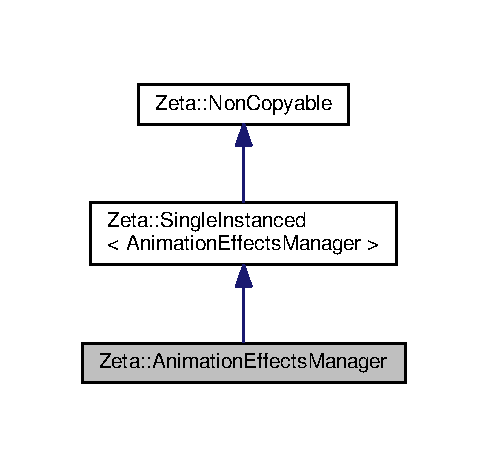
\includegraphics[width=234pt]{classZeta_1_1AnimationEffectsManager__inherit__graph}
\end{center}
\end{figure}


Collaboration diagram for Zeta\+:\+:Animation\+Effects\+Manager\+:\nopagebreak
\begin{figure}[H]
\begin{center}
\leavevmode
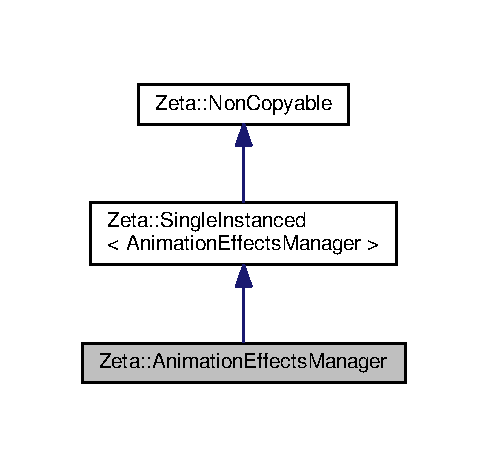
\includegraphics[width=234pt]{classZeta_1_1AnimationEffectsManager__coll__graph}
\end{center}
\end{figure}
\subsection*{Public Member Functions}
\begin{DoxyCompactItemize}
\item 
const \hyperlink{classZeta_1_1Animation}{Animation} \& \hyperlink{classZeta_1_1AnimationEffectsManager_ade4093a0103e37f447b20d16c4e74ccb}{get\+Animation\+F\+X} (const std\+::string \&name, const std\+::string \&animation\+Pack) const 
\item 
void \hyperlink{classZeta_1_1AnimationEffectsManager_a886e393d24c8f2f1db24fc1ab74b591c}{add\+Animation\+Pack} (const std\+::string \&path, const std\+::string \&name=\char`\"{}\char`\"{})
\end{DoxyCompactItemize}
\subsection*{Private Member Functions}
\begin{DoxyCompactItemize}
\item 
\hyperlink{classZeta_1_1AnimationEffectsManager_aab69711ef8a65d33d85d19ada9a0d2fa}{Animation\+Effects\+Manager} ()
\item 
\hyperlink{classZeta_1_1AnimationEffectsManager_a1d80cddee87e29b1f04df633547d8282}{$\sim$\+Animation\+Effects\+Manager} ()
\end{DoxyCompactItemize}
\subsection*{Private Attributes}
\begin{DoxyCompactItemize}
\item 
\hyperlink{namespaceZeta_a9af2e12c4e432d2a1725f19e5a648a04}{Z\+Map}$<$ std\+::string, const \\*
\hyperlink{classZeta_1_1AnimationPack}{Animation\+Pack} $\ast$ $>$ \hyperlink{classZeta_1_1AnimationEffectsManager_a3850f148abb88205f126e936cea09266}{animation\+Packs}
\end{DoxyCompactItemize}
\subsection*{Friends}
\begin{DoxyCompactItemize}
\item 
class \hyperlink{classZeta_1_1AnimationEffectsManager_a2fa95d69b32a77fffa4b730679a8b08c}{Single\+Instanced}
\end{DoxyCompactItemize}
\subsection*{Additional Inherited Members}


\subsection{Constructor \& Destructor Documentation}
\hypertarget{classZeta_1_1AnimationEffectsManager_aab69711ef8a65d33d85d19ada9a0d2fa}{\index{Zeta\+::\+Animation\+Effects\+Manager@{Zeta\+::\+Animation\+Effects\+Manager}!Animation\+Effects\+Manager@{Animation\+Effects\+Manager}}
\index{Animation\+Effects\+Manager@{Animation\+Effects\+Manager}!Zeta\+::\+Animation\+Effects\+Manager@{Zeta\+::\+Animation\+Effects\+Manager}}
\subsubsection[{Animation\+Effects\+Manager}]{\setlength{\rightskip}{0pt plus 5cm}Zeta\+::\+Animation\+Effects\+Manager\+::\+Animation\+Effects\+Manager (
\begin{DoxyParamCaption}
{}
\end{DoxyParamCaption}
)\hspace{0.3cm}{\ttfamily [private]}}}\label{classZeta_1_1AnimationEffectsManager_aab69711ef8a65d33d85d19ada9a0d2fa}
\hypertarget{classZeta_1_1AnimationEffectsManager_a1d80cddee87e29b1f04df633547d8282}{\index{Zeta\+::\+Animation\+Effects\+Manager@{Zeta\+::\+Animation\+Effects\+Manager}!````~Animation\+Effects\+Manager@{$\sim$\+Animation\+Effects\+Manager}}
\index{````~Animation\+Effects\+Manager@{$\sim$\+Animation\+Effects\+Manager}!Zeta\+::\+Animation\+Effects\+Manager@{Zeta\+::\+Animation\+Effects\+Manager}}
\subsubsection[{$\sim$\+Animation\+Effects\+Manager}]{\setlength{\rightskip}{0pt plus 5cm}Zeta\+::\+Animation\+Effects\+Manager\+::$\sim$\+Animation\+Effects\+Manager (
\begin{DoxyParamCaption}
{}
\end{DoxyParamCaption}
)\hspace{0.3cm}{\ttfamily [private]}}}\label{classZeta_1_1AnimationEffectsManager_a1d80cddee87e29b1f04df633547d8282}


\subsection{Member Function Documentation}
\hypertarget{classZeta_1_1AnimationEffectsManager_a886e393d24c8f2f1db24fc1ab74b591c}{\index{Zeta\+::\+Animation\+Effects\+Manager@{Zeta\+::\+Animation\+Effects\+Manager}!add\+Animation\+Pack@{add\+Animation\+Pack}}
\index{add\+Animation\+Pack@{add\+Animation\+Pack}!Zeta\+::\+Animation\+Effects\+Manager@{Zeta\+::\+Animation\+Effects\+Manager}}
\subsubsection[{add\+Animation\+Pack}]{\setlength{\rightskip}{0pt plus 5cm}void Zeta\+::\+Animation\+Effects\+Manager\+::add\+Animation\+Pack (
\begin{DoxyParamCaption}
\item[{const std\+::string \&}]{path, }
\item[{const std\+::string \&}]{name = {\ttfamily \char`\"{}\char`\"{}}}
\end{DoxyParamCaption}
)}}\label{classZeta_1_1AnimationEffectsManager_a886e393d24c8f2f1db24fc1ab74b591c}
\hypertarget{classZeta_1_1AnimationEffectsManager_ade4093a0103e37f447b20d16c4e74ccb}{\index{Zeta\+::\+Animation\+Effects\+Manager@{Zeta\+::\+Animation\+Effects\+Manager}!get\+Animation\+F\+X@{get\+Animation\+F\+X}}
\index{get\+Animation\+F\+X@{get\+Animation\+F\+X}!Zeta\+::\+Animation\+Effects\+Manager@{Zeta\+::\+Animation\+Effects\+Manager}}
\subsubsection[{get\+Animation\+F\+X}]{\setlength{\rightskip}{0pt plus 5cm}const {\bf Animation}\& Zeta\+::\+Animation\+Effects\+Manager\+::get\+Animation\+F\+X (
\begin{DoxyParamCaption}
\item[{const std\+::string \&}]{name, }
\item[{const std\+::string \&}]{animation\+Pack}
\end{DoxyParamCaption}
) const}}\label{classZeta_1_1AnimationEffectsManager_ade4093a0103e37f447b20d16c4e74ccb}


\subsection{Friends And Related Function Documentation}
\hypertarget{classZeta_1_1AnimationEffectsManager_a2fa95d69b32a77fffa4b730679a8b08c}{\index{Zeta\+::\+Animation\+Effects\+Manager@{Zeta\+::\+Animation\+Effects\+Manager}!Single\+Instanced@{Single\+Instanced}}
\index{Single\+Instanced@{Single\+Instanced}!Zeta\+::\+Animation\+Effects\+Manager@{Zeta\+::\+Animation\+Effects\+Manager}}
\subsubsection[{Single\+Instanced}]{\setlength{\rightskip}{0pt plus 5cm}friend class {\bf Single\+Instanced}\hspace{0.3cm}{\ttfamily [friend]}}}\label{classZeta_1_1AnimationEffectsManager_a2fa95d69b32a77fffa4b730679a8b08c}


\subsection{Member Data Documentation}
\hypertarget{classZeta_1_1AnimationEffectsManager_a3850f148abb88205f126e936cea09266}{\index{Zeta\+::\+Animation\+Effects\+Manager@{Zeta\+::\+Animation\+Effects\+Manager}!animation\+Packs@{animation\+Packs}}
\index{animation\+Packs@{animation\+Packs}!Zeta\+::\+Animation\+Effects\+Manager@{Zeta\+::\+Animation\+Effects\+Manager}}
\subsubsection[{animation\+Packs}]{\setlength{\rightskip}{0pt plus 5cm}{\bf Z\+Map}$<$std\+::string, const {\bf Animation\+Pack}$\ast$$>$ Zeta\+::\+Animation\+Effects\+Manager\+::animation\+Packs\hspace{0.3cm}{\ttfamily [private]}}}\label{classZeta_1_1AnimationEffectsManager_a3850f148abb88205f126e936cea09266}


The documentation for this class was generated from the following file\+:\begin{DoxyCompactItemize}
\item 
include/\+Zeta/\+Core/\+Animation\+Classes/\hyperlink{AnimationEffectsManager_8hpp}{Animation\+Effects\+Manager.\+hpp}\end{DoxyCompactItemize}

\hypertarget{classZeta_1_1AnimationHandler}{\section{Zeta\+:\+:Animation\+Handler Class Reference}
\label{classZeta_1_1AnimationHandler}\index{Zeta\+::\+Animation\+Handler@{Zeta\+::\+Animation\+Handler}}
}


{\ttfamily \#include $<$Animation\+Handler.\+hpp$>$}



Inheritance diagram for Zeta\+:\+:Animation\+Handler\+:\nopagebreak
\begin{figure}[H]
\begin{center}
\leavevmode
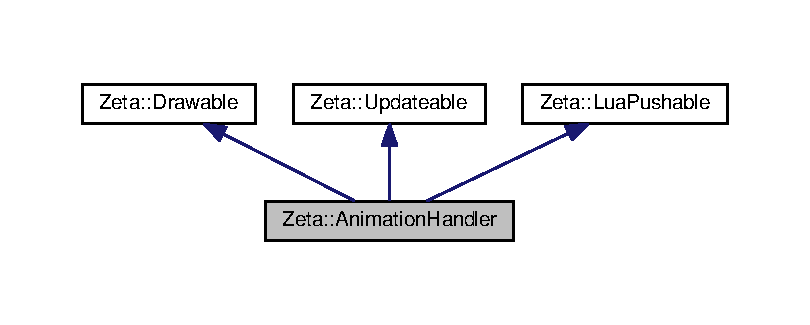
\includegraphics[width=350pt]{classZeta_1_1AnimationHandler__inherit__graph}
\end{center}
\end{figure}


Collaboration diagram for Zeta\+:\+:Animation\+Handler\+:
\nopagebreak
\begin{figure}[H]
\begin{center}
\leavevmode
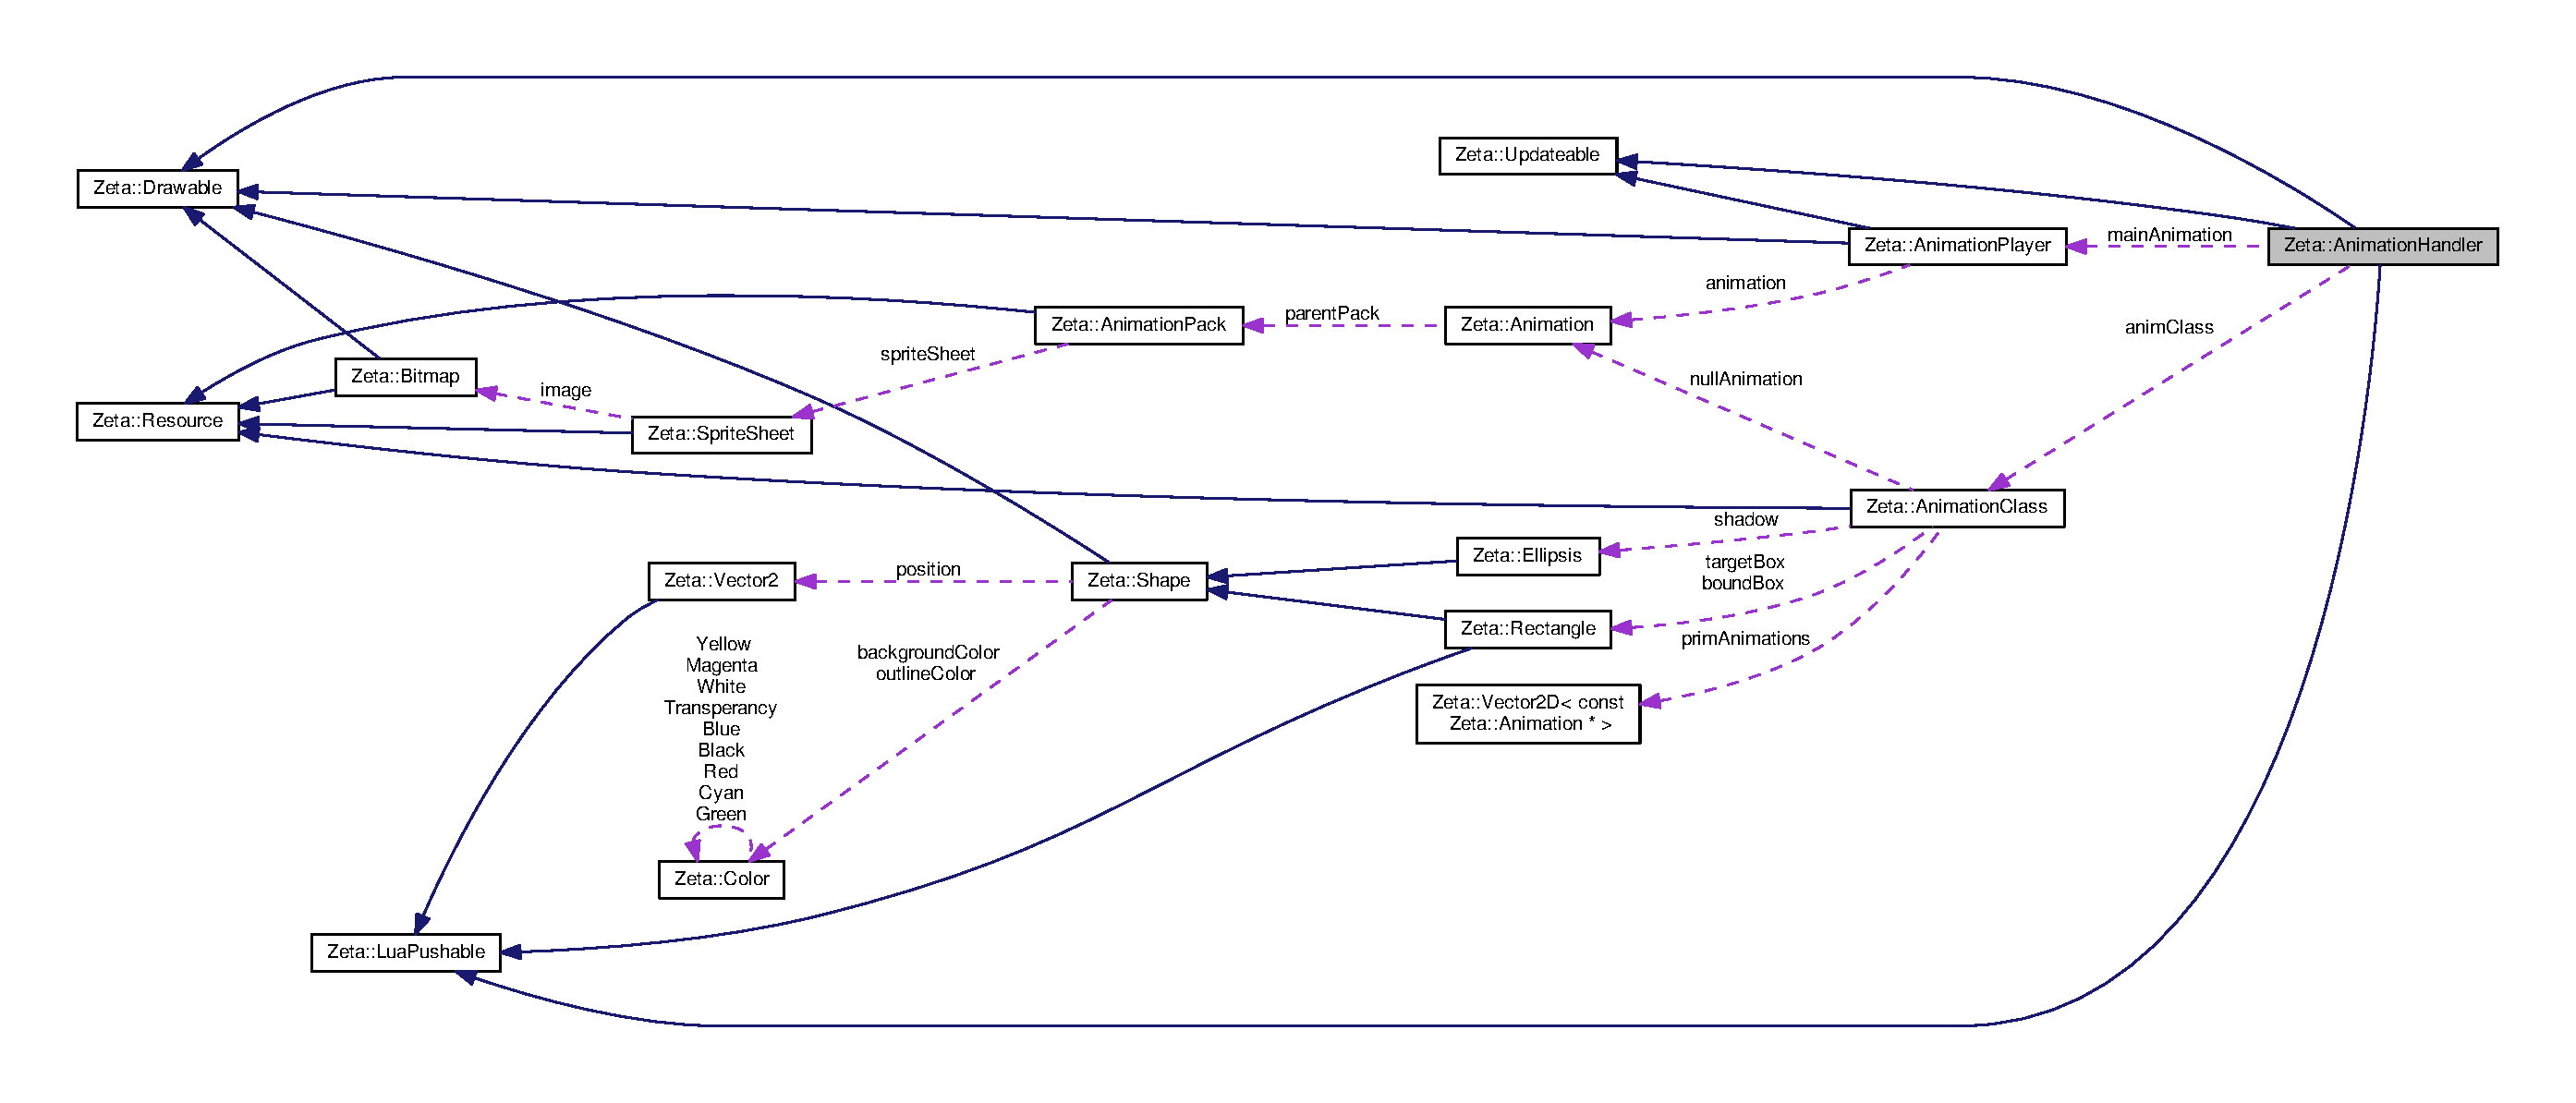
\includegraphics[width=350pt]{classZeta_1_1AnimationHandler__coll__graph}
\end{center}
\end{figure}
\subsection*{Public Types}
\begin{DoxyCompactItemize}
\item 
enum \hyperlink{classZeta_1_1AnimationHandler_a7b026ece57bb2e774c0367ff0bf15f69}{Queue\+Place} \{ \hyperlink{classZeta_1_1AnimationHandler_a7b026ece57bb2e774c0367ff0bf15f69a5835bab1ade0060909e31a06af2e2cde}{Queue\+Place\+::\+Front}, 
\hyperlink{classZeta_1_1AnimationHandler_a7b026ece57bb2e774c0367ff0bf15f69a0557fa923dcee4d0f86b1409f5c2167f}{Queue\+Place\+::\+Back}
 \}
\end{DoxyCompactItemize}
\subsection*{Public Member Functions}
\begin{DoxyCompactItemize}
\item 
const \hyperlink{classZeta_1_1AnimationClass}{Animation\+Class} \& \hyperlink{classZeta_1_1AnimationHandler_a2245299025192fe0fd523bb740a9e478}{get\+Animation\+Class} () const 
\item 
bool \hyperlink{classZeta_1_1AnimationHandler_a27e43b08d62d413291389fb11bb8f479}{is\+Release\+Resources} () const 
\item 
void \hyperlink{classZeta_1_1AnimationHandler_ab1c932b6678c36a00c762cd26e02332f}{set\+Release\+Resources} (bool \hyperlink{classZeta_1_1AnimationHandler_a8d3b5145dbc58320cbf903810be8166e}{release\+Resources})
\item 
\hyperlink{classZeta_1_1AnimationPlayer}{Animation\+Player} \& \hyperlink{classZeta_1_1AnimationHandler_af845886e40f9145313c7002666e0fcea}{get\+Main\+Animation\+Player} () const 
\item 
void \hyperlink{classZeta_1_1AnimationHandler_a72c87fa76361b8d8f3653d4370fcc5e4}{set\+Animation} (const std\+::string \&name, \hyperlink{classZeta_1_1LifeformState_a877fbe4e8efefd0a5323f950909181b6}{Lifeform\+State\+::\+Combined\+State} non\+Exist=Lifeform\+State\+::\+Action\+::\+Idle$\vert$Lifeform\+State\+::\+Direction\+::\+Down)
\item 
void \hyperlink{classZeta_1_1AnimationHandler_a7eaf5e56f986497be8a626a9e782bd91}{set\+Animation} (\hyperlink{classZeta_1_1LifeformState_a877fbe4e8efefd0a5323f950909181b6}{Lifeform\+State\+::\+Combined\+State} name)
\item 
void \hyperlink{classZeta_1_1AnimationHandler_a12af742e0a71ec9e1314e8e228b686a9}{update} (\hyperlink{namespaceZeta_a1e0a1265f9b3bd3075fb0fabd39088ba}{Float} elapsed\+Time)
\item 
void \hyperlink{classZeta_1_1AnimationHandler_aa39b0ead39df1eb3d677531a1ce582e2}{draw} (\hyperlink{namespaceZeta_a1e0a1265f9b3bd3075fb0fabd39088ba}{Float} x, \hyperlink{namespaceZeta_a1e0a1265f9b3bd3075fb0fabd39088ba}{Float} y, \hyperlink{namespaceZeta_a1e0a1265f9b3bd3075fb0fabd39088ba}{Float} rotation=0.\+0f, Float scale=1.\+0f) const 
\item 
void \hyperlink{classZeta_1_1AnimationHandler_a3f58f7e4ab38df79d2ca6baa68f5e5db}{set\+Animation\+Class} (const \hyperlink{classZeta_1_1AnimationClass}{Animation\+Class} \&\hyperlink{classZeta_1_1AnimationHandler_a7b87046e8ddd604eaba79f49a2ee3de5}{anim\+Class})
\item 
void \hyperlink{classZeta_1_1AnimationHandler_a4d6a67cad171c8b92aafd2c1dd504ff0}{set\+Animation\+Class} (const std\+::string \&path)
\item 
void \hyperlink{classZeta_1_1AnimationHandler_a43b5ff928cb19825ad0bf610611b9c40}{add\+Off\+Animation} (const \hyperlink{classZeta_1_1Animation}{Animation} \&animation, \hyperlink{namespaceZeta_a1e0a1265f9b3bd3075fb0fabd39088ba}{Float} dx=0.\+0f, Float dy=0.\+0f, Queue\+Place queue=\+Queue\+Place\+::\+Front)
\item 
\hyperlink{classZeta_1_1OffAnimation}{Off\+Animation} \& \hyperlink{classZeta_1_1AnimationHandler_a8d7804fcbf7711b387f4ac842423e2e5}{get\+Off\+Animation} (const std\+::string \&name, \hyperlink{classZeta_1_1AnimationHandler_a7b026ece57bb2e774c0367ff0bf15f69}{Queue\+Place} queue=\hyperlink{classZeta_1_1AnimationHandler_a7b026ece57bb2e774c0367ff0bf15f69a5835bab1ade0060909e31a06af2e2cde}{Queue\+Place\+::\+Front})
\item 
void \hyperlink{classZeta_1_1AnimationHandler_a509ac593a41b821d89436f8b7ace13fc}{push\+To\+Lua} (lua\+\_\+\+State $\ast$lstate)
\item 
\hyperlink{classZeta_1_1AnimationHandler_adc5e04e53688506da6b16d9ffa73fea1}{Animation\+Handler} ()
\item 
\hyperlink{classZeta_1_1AnimationHandler_aaa023d298a75cbfdbd8db57fb7f207ee}{Animation\+Handler} (const \hyperlink{classZeta_1_1AnimationClass}{Animation\+Class} \&\hyperlink{classZeta_1_1AnimationHandler_a7b87046e8ddd604eaba79f49a2ee3de5}{anim\+Class})
\item 
\hyperlink{classZeta_1_1AnimationHandler_a49124e8d1738950f3965321fc24a5bf8}{Animation\+Handler} (const std\+::string \&class\+Path, const std\+::string \&animation=\char`\"{}\char`\"{})
\item 
\hyperlink{classZeta_1_1AnimationHandler_aa36e8a645b6bb59a91fc8e8add8208ed}{$\sim$\+Animation\+Handler} ()
\end{DoxyCompactItemize}
\subsection*{Private Attributes}
\begin{DoxyCompactItemize}
\item 
\hyperlink{namespaceZeta_a9af2e12c4e432d2a1725f19e5a648a04}{Z\+Map}$<$ std\+::string, \hyperlink{classZeta_1_1OffAnimation}{Off\+Animation} $>$ \hyperlink{classZeta_1_1AnimationHandler_acac6efc040935b01a3c1705c2b9ed9a0}{frontal\+Animations}
\item 
\hyperlink{namespaceZeta_a9af2e12c4e432d2a1725f19e5a648a04}{Z\+Map}$<$ std\+::string, \hyperlink{classZeta_1_1OffAnimation}{Off\+Animation} $>$ \hyperlink{classZeta_1_1AnimationHandler_a7bc18188974f6605cb89466cd5677155}{back\+Animations}
\item 
\hyperlink{classZeta_1_1AnimationPlayer}{Animation\+Player} \hyperlink{classZeta_1_1AnimationHandler_a309fc74c793ad1b479c45bbe646c7a65}{main\+Animation}
\item 
const \hyperlink{classZeta_1_1AnimationClass}{Animation\+Class} $\ast$ \hyperlink{classZeta_1_1AnimationHandler_a7b87046e8ddd604eaba79f49a2ee3de5}{anim\+Class}
\item 
bool \hyperlink{classZeta_1_1AnimationHandler_a8d3b5145dbc58320cbf903810be8166e}{release\+Resources}
\end{DoxyCompactItemize}


\subsection{Member Enumeration Documentation}
\hypertarget{classZeta_1_1AnimationHandler_a7b026ece57bb2e774c0367ff0bf15f69}{\index{Zeta\+::\+Animation\+Handler@{Zeta\+::\+Animation\+Handler}!Queue\+Place@{Queue\+Place}}
\index{Queue\+Place@{Queue\+Place}!Zeta\+::\+Animation\+Handler@{Zeta\+::\+Animation\+Handler}}
\subsubsection[{Queue\+Place}]{\setlength{\rightskip}{0pt plus 5cm}enum {\bf Zeta\+::\+Animation\+Handler\+::\+Queue\+Place}\hspace{0.3cm}{\ttfamily [strong]}}}\label{classZeta_1_1AnimationHandler_a7b026ece57bb2e774c0367ff0bf15f69}
\begin{Desc}
\item[Enumerator]\par
\begin{description}
\index{Front@{Front}!Zeta\+::\+Animation\+Handler@{Zeta\+::\+Animation\+Handler}}\index{Zeta\+::\+Animation\+Handler@{Zeta\+::\+Animation\+Handler}!Front@{Front}}\item[{\em 
\hypertarget{classZeta_1_1AnimationHandler_a7b026ece57bb2e774c0367ff0bf15f69a5835bab1ade0060909e31a06af2e2cde}{Front}\label{classZeta_1_1AnimationHandler_a7b026ece57bb2e774c0367ff0bf15f69a5835bab1ade0060909e31a06af2e2cde}
}]\index{Back@{Back}!Zeta\+::\+Animation\+Handler@{Zeta\+::\+Animation\+Handler}}\index{Zeta\+::\+Animation\+Handler@{Zeta\+::\+Animation\+Handler}!Back@{Back}}\item[{\em 
\hypertarget{classZeta_1_1AnimationHandler_a7b026ece57bb2e774c0367ff0bf15f69a0557fa923dcee4d0f86b1409f5c2167f}{Back}\label{classZeta_1_1AnimationHandler_a7b026ece57bb2e774c0367ff0bf15f69a0557fa923dcee4d0f86b1409f5c2167f}
}]\end{description}
\end{Desc}


\subsection{Constructor \& Destructor Documentation}
\hypertarget{classZeta_1_1AnimationHandler_adc5e04e53688506da6b16d9ffa73fea1}{\index{Zeta\+::\+Animation\+Handler@{Zeta\+::\+Animation\+Handler}!Animation\+Handler@{Animation\+Handler}}
\index{Animation\+Handler@{Animation\+Handler}!Zeta\+::\+Animation\+Handler@{Zeta\+::\+Animation\+Handler}}
\subsubsection[{Animation\+Handler}]{\setlength{\rightskip}{0pt plus 5cm}Zeta\+::\+Animation\+Handler\+::\+Animation\+Handler (
\begin{DoxyParamCaption}
{}
\end{DoxyParamCaption}
)}}\label{classZeta_1_1AnimationHandler_adc5e04e53688506da6b16d9ffa73fea1}
\hypertarget{classZeta_1_1AnimationHandler_aaa023d298a75cbfdbd8db57fb7f207ee}{\index{Zeta\+::\+Animation\+Handler@{Zeta\+::\+Animation\+Handler}!Animation\+Handler@{Animation\+Handler}}
\index{Animation\+Handler@{Animation\+Handler}!Zeta\+::\+Animation\+Handler@{Zeta\+::\+Animation\+Handler}}
\subsubsection[{Animation\+Handler}]{\setlength{\rightskip}{0pt plus 5cm}Zeta\+::\+Animation\+Handler\+::\+Animation\+Handler (
\begin{DoxyParamCaption}
\item[{const {\bf Animation\+Class} \&}]{anim\+Class}
\end{DoxyParamCaption}
)}}\label{classZeta_1_1AnimationHandler_aaa023d298a75cbfdbd8db57fb7f207ee}
\hypertarget{classZeta_1_1AnimationHandler_a49124e8d1738950f3965321fc24a5bf8}{\index{Zeta\+::\+Animation\+Handler@{Zeta\+::\+Animation\+Handler}!Animation\+Handler@{Animation\+Handler}}
\index{Animation\+Handler@{Animation\+Handler}!Zeta\+::\+Animation\+Handler@{Zeta\+::\+Animation\+Handler}}
\subsubsection[{Animation\+Handler}]{\setlength{\rightskip}{0pt plus 5cm}Zeta\+::\+Animation\+Handler\+::\+Animation\+Handler (
\begin{DoxyParamCaption}
\item[{const std\+::string \&}]{class\+Path, }
\item[{const std\+::string \&}]{animation = {\ttfamily \char`\"{}\char`\"{}}}
\end{DoxyParamCaption}
)}}\label{classZeta_1_1AnimationHandler_a49124e8d1738950f3965321fc24a5bf8}
\hypertarget{classZeta_1_1AnimationHandler_aa36e8a645b6bb59a91fc8e8add8208ed}{\index{Zeta\+::\+Animation\+Handler@{Zeta\+::\+Animation\+Handler}!````~Animation\+Handler@{$\sim$\+Animation\+Handler}}
\index{````~Animation\+Handler@{$\sim$\+Animation\+Handler}!Zeta\+::\+Animation\+Handler@{Zeta\+::\+Animation\+Handler}}
\subsubsection[{$\sim$\+Animation\+Handler}]{\setlength{\rightskip}{0pt plus 5cm}Zeta\+::\+Animation\+Handler\+::$\sim$\+Animation\+Handler (
\begin{DoxyParamCaption}
{}
\end{DoxyParamCaption}
)}}\label{classZeta_1_1AnimationHandler_aa36e8a645b6bb59a91fc8e8add8208ed}


\subsection{Member Function Documentation}
\hypertarget{classZeta_1_1AnimationHandler_a43b5ff928cb19825ad0bf610611b9c40}{\index{Zeta\+::\+Animation\+Handler@{Zeta\+::\+Animation\+Handler}!add\+Off\+Animation@{add\+Off\+Animation}}
\index{add\+Off\+Animation@{add\+Off\+Animation}!Zeta\+::\+Animation\+Handler@{Zeta\+::\+Animation\+Handler}}
\subsubsection[{add\+Off\+Animation}]{\setlength{\rightskip}{0pt plus 5cm}void Zeta\+::\+Animation\+Handler\+::add\+Off\+Animation (
\begin{DoxyParamCaption}
\item[{const {\bf Animation} \&}]{animation, }
\item[{{\bf Float}}]{dx = {\ttfamily 0.0f}, }
\item[{{\bf Float}}]{dy = {\ttfamily 0.0f}, }
\item[{{\bf Queue\+Place}}]{queue = {\ttfamily {\bf Queue\+Place\+::\+Front}}}
\end{DoxyParamCaption}
)}}\label{classZeta_1_1AnimationHandler_a43b5ff928cb19825ad0bf610611b9c40}
\hypertarget{classZeta_1_1AnimationHandler_aa39b0ead39df1eb3d677531a1ce582e2}{\index{Zeta\+::\+Animation\+Handler@{Zeta\+::\+Animation\+Handler}!draw@{draw}}
\index{draw@{draw}!Zeta\+::\+Animation\+Handler@{Zeta\+::\+Animation\+Handler}}
\subsubsection[{draw}]{\setlength{\rightskip}{0pt plus 5cm}void Zeta\+::\+Animation\+Handler\+::draw (
\begin{DoxyParamCaption}
\item[{{\bf Float}}]{x, }
\item[{{\bf Float}}]{y, }
\item[{{\bf Float}}]{rotation = {\ttfamily 0.0f}, }
\item[{{\bf Float}}]{scale = {\ttfamily 1.0f}}
\end{DoxyParamCaption}
) const\hspace{0.3cm}{\ttfamily [virtual]}}}\label{classZeta_1_1AnimationHandler_aa39b0ead39df1eb3d677531a1ce582e2}
Draws the \hyperlink{classZeta_1_1Object}{Object} on screen. Be advised, the x,y, offsets might have different meaning on different implementations. 
\begin{DoxyParams}{Parameters}
{\em x} & X offset to be applied on the drawing \\
\hline
{\em y} & Y offset to be applied on the drawing \\
\hline
{\em rotation} & the rotation to be applied on the drawing \\
\hline
\end{DoxyParams}


Implements \hyperlink{classZeta_1_1Drawable_a3f453a7a971b7eeba1768be3eaedc192}{Zeta\+::\+Drawable}.

\hypertarget{classZeta_1_1AnimationHandler_a2245299025192fe0fd523bb740a9e478}{\index{Zeta\+::\+Animation\+Handler@{Zeta\+::\+Animation\+Handler}!get\+Animation\+Class@{get\+Animation\+Class}}
\index{get\+Animation\+Class@{get\+Animation\+Class}!Zeta\+::\+Animation\+Handler@{Zeta\+::\+Animation\+Handler}}
\subsubsection[{get\+Animation\+Class}]{\setlength{\rightskip}{0pt plus 5cm}const {\bf Animation\+Class}\& Zeta\+::\+Animation\+Handler\+::get\+Animation\+Class (
\begin{DoxyParamCaption}
{}
\end{DoxyParamCaption}
) const\hspace{0.3cm}{\ttfamily [inline]}}}\label{classZeta_1_1AnimationHandler_a2245299025192fe0fd523bb740a9e478}
\hypertarget{classZeta_1_1AnimationHandler_af845886e40f9145313c7002666e0fcea}{\index{Zeta\+::\+Animation\+Handler@{Zeta\+::\+Animation\+Handler}!get\+Main\+Animation\+Player@{get\+Main\+Animation\+Player}}
\index{get\+Main\+Animation\+Player@{get\+Main\+Animation\+Player}!Zeta\+::\+Animation\+Handler@{Zeta\+::\+Animation\+Handler}}
\subsubsection[{get\+Main\+Animation\+Player}]{\setlength{\rightskip}{0pt plus 5cm}{\bf Animation\+Player}\& Zeta\+::\+Animation\+Handler\+::get\+Main\+Animation\+Player (
\begin{DoxyParamCaption}
{}
\end{DoxyParamCaption}
) const\hspace{0.3cm}{\ttfamily [inline]}}}\label{classZeta_1_1AnimationHandler_af845886e40f9145313c7002666e0fcea}
\hypertarget{classZeta_1_1AnimationHandler_a8d7804fcbf7711b387f4ac842423e2e5}{\index{Zeta\+::\+Animation\+Handler@{Zeta\+::\+Animation\+Handler}!get\+Off\+Animation@{get\+Off\+Animation}}
\index{get\+Off\+Animation@{get\+Off\+Animation}!Zeta\+::\+Animation\+Handler@{Zeta\+::\+Animation\+Handler}}
\subsubsection[{get\+Off\+Animation}]{\setlength{\rightskip}{0pt plus 5cm}{\bf Off\+Animation}\& Zeta\+::\+Animation\+Handler\+::get\+Off\+Animation (
\begin{DoxyParamCaption}
\item[{const std\+::string \&}]{name, }
\item[{{\bf Queue\+Place}}]{queue = {\ttfamily {\bf Queue\+Place\+::\+Front}}}
\end{DoxyParamCaption}
)}}\label{classZeta_1_1AnimationHandler_a8d7804fcbf7711b387f4ac842423e2e5}
\hypertarget{classZeta_1_1AnimationHandler_a27e43b08d62d413291389fb11bb8f479}{\index{Zeta\+::\+Animation\+Handler@{Zeta\+::\+Animation\+Handler}!is\+Release\+Resources@{is\+Release\+Resources}}
\index{is\+Release\+Resources@{is\+Release\+Resources}!Zeta\+::\+Animation\+Handler@{Zeta\+::\+Animation\+Handler}}
\subsubsection[{is\+Release\+Resources}]{\setlength{\rightskip}{0pt plus 5cm}bool Zeta\+::\+Animation\+Handler\+::is\+Release\+Resources (
\begin{DoxyParamCaption}
{}
\end{DoxyParamCaption}
) const\hspace{0.3cm}{\ttfamily [inline]}}}\label{classZeta_1_1AnimationHandler_a27e43b08d62d413291389fb11bb8f479}
\hypertarget{classZeta_1_1AnimationHandler_a509ac593a41b821d89436f8b7ace13fc}{\index{Zeta\+::\+Animation\+Handler@{Zeta\+::\+Animation\+Handler}!push\+To\+Lua@{push\+To\+Lua}}
\index{push\+To\+Lua@{push\+To\+Lua}!Zeta\+::\+Animation\+Handler@{Zeta\+::\+Animation\+Handler}}
\subsubsection[{push\+To\+Lua}]{\setlength{\rightskip}{0pt plus 5cm}void Zeta\+::\+Animation\+Handler\+::push\+To\+Lua (
\begin{DoxyParamCaption}
\item[{lua\+\_\+\+State $\ast$}]{lstate}
\end{DoxyParamCaption}
)\hspace{0.3cm}{\ttfamily [virtual]}}}\label{classZeta_1_1AnimationHandler_a509ac593a41b821d89436f8b7ace13fc}


Implements \hyperlink{classZeta_1_1LuaPushable_a0380ec9cff11f749e8eb67b51b8f82fc}{Zeta\+::\+Lua\+Pushable}.

\hypertarget{classZeta_1_1AnimationHandler_a72c87fa76361b8d8f3653d4370fcc5e4}{\index{Zeta\+::\+Animation\+Handler@{Zeta\+::\+Animation\+Handler}!set\+Animation@{set\+Animation}}
\index{set\+Animation@{set\+Animation}!Zeta\+::\+Animation\+Handler@{Zeta\+::\+Animation\+Handler}}
\subsubsection[{set\+Animation}]{\setlength{\rightskip}{0pt plus 5cm}void Zeta\+::\+Animation\+Handler\+::set\+Animation (
\begin{DoxyParamCaption}
\item[{const std\+::string \&}]{name, }
\item[{{\bf Lifeform\+State\+::\+Combined\+State}}]{non\+Exist = {\ttfamily LifeformState\+:\+:Action\+:\+:Idle$\vert$LifeformState\+:\+:Direction\+:\+:Down}}
\end{DoxyParamCaption}
)}}\label{classZeta_1_1AnimationHandler_a72c87fa76361b8d8f3653d4370fcc5e4}
\hypertarget{classZeta_1_1AnimationHandler_a7eaf5e56f986497be8a626a9e782bd91}{\index{Zeta\+::\+Animation\+Handler@{Zeta\+::\+Animation\+Handler}!set\+Animation@{set\+Animation}}
\index{set\+Animation@{set\+Animation}!Zeta\+::\+Animation\+Handler@{Zeta\+::\+Animation\+Handler}}
\subsubsection[{set\+Animation}]{\setlength{\rightskip}{0pt plus 5cm}void Zeta\+::\+Animation\+Handler\+::set\+Animation (
\begin{DoxyParamCaption}
\item[{{\bf Lifeform\+State\+::\+Combined\+State}}]{name}
\end{DoxyParamCaption}
)}}\label{classZeta_1_1AnimationHandler_a7eaf5e56f986497be8a626a9e782bd91}
\hypertarget{classZeta_1_1AnimationHandler_a3f58f7e4ab38df79d2ca6baa68f5e5db}{\index{Zeta\+::\+Animation\+Handler@{Zeta\+::\+Animation\+Handler}!set\+Animation\+Class@{set\+Animation\+Class}}
\index{set\+Animation\+Class@{set\+Animation\+Class}!Zeta\+::\+Animation\+Handler@{Zeta\+::\+Animation\+Handler}}
\subsubsection[{set\+Animation\+Class}]{\setlength{\rightskip}{0pt plus 5cm}void Zeta\+::\+Animation\+Handler\+::set\+Animation\+Class (
\begin{DoxyParamCaption}
\item[{const {\bf Animation\+Class} \&}]{anim\+Class}
\end{DoxyParamCaption}
)}}\label{classZeta_1_1AnimationHandler_a3f58f7e4ab38df79d2ca6baa68f5e5db}
\hypertarget{classZeta_1_1AnimationHandler_a4d6a67cad171c8b92aafd2c1dd504ff0}{\index{Zeta\+::\+Animation\+Handler@{Zeta\+::\+Animation\+Handler}!set\+Animation\+Class@{set\+Animation\+Class}}
\index{set\+Animation\+Class@{set\+Animation\+Class}!Zeta\+::\+Animation\+Handler@{Zeta\+::\+Animation\+Handler}}
\subsubsection[{set\+Animation\+Class}]{\setlength{\rightskip}{0pt plus 5cm}void Zeta\+::\+Animation\+Handler\+::set\+Animation\+Class (
\begin{DoxyParamCaption}
\item[{const std\+::string \&}]{path}
\end{DoxyParamCaption}
)}}\label{classZeta_1_1AnimationHandler_a4d6a67cad171c8b92aafd2c1dd504ff0}
\hypertarget{classZeta_1_1AnimationHandler_ab1c932b6678c36a00c762cd26e02332f}{\index{Zeta\+::\+Animation\+Handler@{Zeta\+::\+Animation\+Handler}!set\+Release\+Resources@{set\+Release\+Resources}}
\index{set\+Release\+Resources@{set\+Release\+Resources}!Zeta\+::\+Animation\+Handler@{Zeta\+::\+Animation\+Handler}}
\subsubsection[{set\+Release\+Resources}]{\setlength{\rightskip}{0pt plus 5cm}void Zeta\+::\+Animation\+Handler\+::set\+Release\+Resources (
\begin{DoxyParamCaption}
\item[{bool}]{release\+Resources}
\end{DoxyParamCaption}
)\hspace{0.3cm}{\ttfamily [inline]}}}\label{classZeta_1_1AnimationHandler_ab1c932b6678c36a00c762cd26e02332f}
\hypertarget{classZeta_1_1AnimationHandler_a12af742e0a71ec9e1314e8e228b686a9}{\index{Zeta\+::\+Animation\+Handler@{Zeta\+::\+Animation\+Handler}!update@{update}}
\index{update@{update}!Zeta\+::\+Animation\+Handler@{Zeta\+::\+Animation\+Handler}}
\subsubsection[{update}]{\setlength{\rightskip}{0pt plus 5cm}void Zeta\+::\+Animation\+Handler\+::update (
\begin{DoxyParamCaption}
\item[{{\bf Float}}]{elapsed\+Time}
\end{DoxyParamCaption}
)\hspace{0.3cm}{\ttfamily [virtual]}}}\label{classZeta_1_1AnimationHandler_a12af742e0a71ec9e1314e8e228b686a9}


Implements \hyperlink{classZeta_1_1Updateable_af4006bfccb762454b4da08786ad93de0}{Zeta\+::\+Updateable}.



\subsection{Member Data Documentation}
\hypertarget{classZeta_1_1AnimationHandler_a7b87046e8ddd604eaba79f49a2ee3de5}{\index{Zeta\+::\+Animation\+Handler@{Zeta\+::\+Animation\+Handler}!anim\+Class@{anim\+Class}}
\index{anim\+Class@{anim\+Class}!Zeta\+::\+Animation\+Handler@{Zeta\+::\+Animation\+Handler}}
\subsubsection[{anim\+Class}]{\setlength{\rightskip}{0pt plus 5cm}const {\bf Animation\+Class}$\ast$ Zeta\+::\+Animation\+Handler\+::anim\+Class\hspace{0.3cm}{\ttfamily [private]}}}\label{classZeta_1_1AnimationHandler_a7b87046e8ddd604eaba79f49a2ee3de5}
\hypertarget{classZeta_1_1AnimationHandler_a7bc18188974f6605cb89466cd5677155}{\index{Zeta\+::\+Animation\+Handler@{Zeta\+::\+Animation\+Handler}!back\+Animations@{back\+Animations}}
\index{back\+Animations@{back\+Animations}!Zeta\+::\+Animation\+Handler@{Zeta\+::\+Animation\+Handler}}
\subsubsection[{back\+Animations}]{\setlength{\rightskip}{0pt plus 5cm}{\bf Z\+Map}$<$std\+::string, {\bf Off\+Animation}$>$ Zeta\+::\+Animation\+Handler\+::back\+Animations\hspace{0.3cm}{\ttfamily [private]}}}\label{classZeta_1_1AnimationHandler_a7bc18188974f6605cb89466cd5677155}
\hypertarget{classZeta_1_1AnimationHandler_acac6efc040935b01a3c1705c2b9ed9a0}{\index{Zeta\+::\+Animation\+Handler@{Zeta\+::\+Animation\+Handler}!frontal\+Animations@{frontal\+Animations}}
\index{frontal\+Animations@{frontal\+Animations}!Zeta\+::\+Animation\+Handler@{Zeta\+::\+Animation\+Handler}}
\subsubsection[{frontal\+Animations}]{\setlength{\rightskip}{0pt plus 5cm}{\bf Z\+Map}$<$std\+::string, {\bf Off\+Animation}$>$ Zeta\+::\+Animation\+Handler\+::frontal\+Animations\hspace{0.3cm}{\ttfamily [private]}}}\label{classZeta_1_1AnimationHandler_acac6efc040935b01a3c1705c2b9ed9a0}
\hypertarget{classZeta_1_1AnimationHandler_a309fc74c793ad1b479c45bbe646c7a65}{\index{Zeta\+::\+Animation\+Handler@{Zeta\+::\+Animation\+Handler}!main\+Animation@{main\+Animation}}
\index{main\+Animation@{main\+Animation}!Zeta\+::\+Animation\+Handler@{Zeta\+::\+Animation\+Handler}}
\subsubsection[{main\+Animation}]{\setlength{\rightskip}{0pt plus 5cm}{\bf Animation\+Player} Zeta\+::\+Animation\+Handler\+::main\+Animation\hspace{0.3cm}{\ttfamily [mutable]}, {\ttfamily [private]}}}\label{classZeta_1_1AnimationHandler_a309fc74c793ad1b479c45bbe646c7a65}
\hypertarget{classZeta_1_1AnimationHandler_a8d3b5145dbc58320cbf903810be8166e}{\index{Zeta\+::\+Animation\+Handler@{Zeta\+::\+Animation\+Handler}!release\+Resources@{release\+Resources}}
\index{release\+Resources@{release\+Resources}!Zeta\+::\+Animation\+Handler@{Zeta\+::\+Animation\+Handler}}
\subsubsection[{release\+Resources}]{\setlength{\rightskip}{0pt plus 5cm}bool Zeta\+::\+Animation\+Handler\+::release\+Resources\hspace{0.3cm}{\ttfamily [private]}}}\label{classZeta_1_1AnimationHandler_a8d3b5145dbc58320cbf903810be8166e}


The documentation for this class was generated from the following file\+:\begin{DoxyCompactItemize}
\item 
include/\+Zeta/\+Core/\+Animation\+Classes/\hyperlink{AnimationHandler_8hpp}{Animation\+Handler.\+hpp}\end{DoxyCompactItemize}

\hypertarget{classZeta_1_1AnimationPack}{\section{Zeta\+:\+:Animation\+Pack Class Reference}
\label{classZeta_1_1AnimationPack}\index{Zeta\+::\+Animation\+Pack@{Zeta\+::\+Animation\+Pack}}
}


{\ttfamily \#include $<$Animation\+Pack.\+hpp$>$}



Inheritance diagram for Zeta\+:\+:Animation\+Pack\+:\nopagebreak
\begin{figure}[H]
\begin{center}
\leavevmode
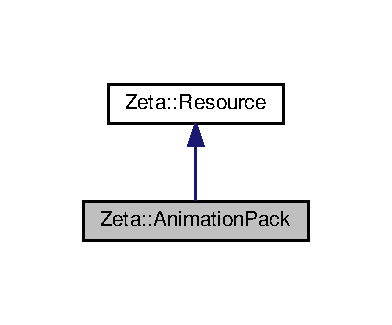
\includegraphics[width=188pt]{classZeta_1_1AnimationPack__inherit__graph}
\end{center}
\end{figure}


Collaboration diagram for Zeta\+:\+:Animation\+Pack\+:
\nopagebreak
\begin{figure}[H]
\begin{center}
\leavevmode
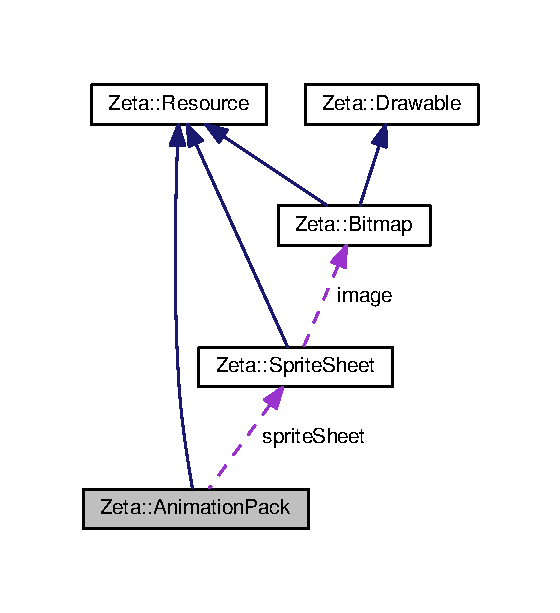
\includegraphics[width=269pt]{classZeta_1_1AnimationPack__coll__graph}
\end{center}
\end{figure}
\subsection*{Public Member Functions}
\begin{DoxyCompactItemize}
\item 
const \hyperlink{classZeta_1_1Animation}{Animation} \& \hyperlink{classZeta_1_1AnimationPack_adda733bd90a57d0307cb2731fd2a9ac3}{get\+Animation} (const std\+::string \&\hyperlink{classZeta_1_1Resource_a44c5721216f4beb31c0b3d2ef2aecf1d}{name}) const 
\item 
const \hyperlink{classZeta_1_1SpriteSheet}{Sprite\+Sheet} \& \hyperlink{classZeta_1_1AnimationPack_a08dbc3a645410b3a42e3831c85f5174e}{get\+Sprite\+Sheet} () const 
\item 
std\+::vector$<$ std\+::string $>$ \hyperlink{classZeta_1_1AnimationPack_a7f57cb4b8ec3f87a2ac982b12d669274}{list\+Animation\+Names} () const 
\item 
\hyperlink{classZeta_1_1AnimationPack_a22ce850bd316ed6925705110db62f600}{Animation\+Pack} ()
\item 
\hyperlink{classZeta_1_1AnimationPack_ac8e81972797da8e31bcabab51a9c2f64}{Animation\+Pack} (const std\+::string \&path)
\item 
\hyperlink{classZeta_1_1AnimationPack_a997cbde781439cd3d3add5f9337379f9}{$\sim$\+Animation\+Pack} ()
\end{DoxyCompactItemize}
\subsection*{Protected Attributes}
\begin{DoxyCompactItemize}
\item 
\hyperlink{namespaceZeta_a4c11e23ddc559dccdb5e85901d7dfb84}{Z\+Small\+Map}$<$ std\+::string, \hyperlink{classZeta_1_1Animation}{Animation} $>$ \hyperlink{classZeta_1_1AnimationPack_ad75ffd44330a99663b2d47247e51597b}{animations}
\item 
const \hyperlink{classZeta_1_1SpriteSheet}{Sprite\+Sheet} $\ast$ \hyperlink{classZeta_1_1AnimationPack_aaba44d7110313c7ce6e840a72d775dd9}{sprite\+Sheet}
\end{DoxyCompactItemize}


\subsection{Detailed Description}
A Class for loading animation Files ($\ast$.anim) 

\subsection{Constructor \& Destructor Documentation}
\hypertarget{classZeta_1_1AnimationPack_a22ce850bd316ed6925705110db62f600}{\index{Zeta\+::\+Animation\+Pack@{Zeta\+::\+Animation\+Pack}!Animation\+Pack@{Animation\+Pack}}
\index{Animation\+Pack@{Animation\+Pack}!Zeta\+::\+Animation\+Pack@{Zeta\+::\+Animation\+Pack}}
\subsubsection[{Animation\+Pack}]{\setlength{\rightskip}{0pt plus 5cm}Zeta\+::\+Animation\+Pack\+::\+Animation\+Pack (
\begin{DoxyParamCaption}
{}
\end{DoxyParamCaption}
)}}\label{classZeta_1_1AnimationPack_a22ce850bd316ed6925705110db62f600}
Default Constructor Creates a Null \hyperlink{classZeta_1_1AnimationPack}{Animation\+Pack} with no animations and a Null Spritesheet \hypertarget{classZeta_1_1AnimationPack_ac8e81972797da8e31bcabab51a9c2f64}{\index{Zeta\+::\+Animation\+Pack@{Zeta\+::\+Animation\+Pack}!Animation\+Pack@{Animation\+Pack}}
\index{Animation\+Pack@{Animation\+Pack}!Zeta\+::\+Animation\+Pack@{Zeta\+::\+Animation\+Pack}}
\subsubsection[{Animation\+Pack}]{\setlength{\rightskip}{0pt plus 5cm}Zeta\+::\+Animation\+Pack\+::\+Animation\+Pack (
\begin{DoxyParamCaption}
\item[{const std\+::string \&}]{path}
\end{DoxyParamCaption}
)}}\label{classZeta_1_1AnimationPack_ac8e81972797da8e31bcabab51a9c2f64}
Loads the \hyperlink{classZeta_1_1Animation}{Animation} Pack \hyperlink{classZeta_1_1File}{File} and Parses it If anything goes wrong, then it throws a \hyperlink{classZeta_1_1Exception}{Zeta\+::\+Exception} 
\begin{DoxyParams}{Parameters}
{\em path} & The filename to load \\
\hline
\end{DoxyParams}
\hypertarget{classZeta_1_1AnimationPack_a997cbde781439cd3d3add5f9337379f9}{\index{Zeta\+::\+Animation\+Pack@{Zeta\+::\+Animation\+Pack}!````~Animation\+Pack@{$\sim$\+Animation\+Pack}}
\index{````~Animation\+Pack@{$\sim$\+Animation\+Pack}!Zeta\+::\+Animation\+Pack@{Zeta\+::\+Animation\+Pack}}
\subsubsection[{$\sim$\+Animation\+Pack}]{\setlength{\rightskip}{0pt plus 5cm}Zeta\+::\+Animation\+Pack\+::$\sim$\+Animation\+Pack (
\begin{DoxyParamCaption}
{}
\end{DoxyParamCaption}
)}}\label{classZeta_1_1AnimationPack_a997cbde781439cd3d3add5f9337379f9}
Deconstructor Deallocates all animations and releases the Reference to the Spritesheet 

\subsection{Member Function Documentation}
\hypertarget{classZeta_1_1AnimationPack_adda733bd90a57d0307cb2731fd2a9ac3}{\index{Zeta\+::\+Animation\+Pack@{Zeta\+::\+Animation\+Pack}!get\+Animation@{get\+Animation}}
\index{get\+Animation@{get\+Animation}!Zeta\+::\+Animation\+Pack@{Zeta\+::\+Animation\+Pack}}
\subsubsection[{get\+Animation}]{\setlength{\rightskip}{0pt plus 5cm}const {\bf Animation}\& Zeta\+::\+Animation\+Pack\+::get\+Animation (
\begin{DoxyParamCaption}
\item[{const std\+::string \&}]{name}
\end{DoxyParamCaption}
) const}}\label{classZeta_1_1AnimationPack_adda733bd90a57d0307cb2731fd2a9ac3}
Gets the animation by name If the requested animation is not availabe, then a Null\+Animation will be returned 
\begin{DoxyParams}{Parameters}
{\em name} & The name of the animation to retrieve \\
\hline
\end{DoxyParams}
\begin{DoxyReturn}{Returns}
The animation requested 
\end{DoxyReturn}
\hypertarget{classZeta_1_1AnimationPack_a08dbc3a645410b3a42e3831c85f5174e}{\index{Zeta\+::\+Animation\+Pack@{Zeta\+::\+Animation\+Pack}!get\+Sprite\+Sheet@{get\+Sprite\+Sheet}}
\index{get\+Sprite\+Sheet@{get\+Sprite\+Sheet}!Zeta\+::\+Animation\+Pack@{Zeta\+::\+Animation\+Pack}}
\subsubsection[{get\+Sprite\+Sheet}]{\setlength{\rightskip}{0pt plus 5cm}const {\bf Sprite\+Sheet}\& Zeta\+::\+Animation\+Pack\+::get\+Sprite\+Sheet (
\begin{DoxyParamCaption}
{}
\end{DoxyParamCaption}
) const\hspace{0.3cm}{\ttfamily [inline]}}}\label{classZeta_1_1AnimationPack_a08dbc3a645410b3a42e3831c85f5174e}
Gets the referenced Spritesheet of the Animations \begin{DoxyReturn}{Returns}
The Spritesheet 
\end{DoxyReturn}
\hypertarget{classZeta_1_1AnimationPack_a7f57cb4b8ec3f87a2ac982b12d669274}{\index{Zeta\+::\+Animation\+Pack@{Zeta\+::\+Animation\+Pack}!list\+Animation\+Names@{list\+Animation\+Names}}
\index{list\+Animation\+Names@{list\+Animation\+Names}!Zeta\+::\+Animation\+Pack@{Zeta\+::\+Animation\+Pack}}
\subsubsection[{list\+Animation\+Names}]{\setlength{\rightskip}{0pt plus 5cm}std\+::vector$<$std\+::string$>$ Zeta\+::\+Animation\+Pack\+::list\+Animation\+Names (
\begin{DoxyParamCaption}
{}
\end{DoxyParamCaption}
) const}}\label{classZeta_1_1AnimationPack_a7f57cb4b8ec3f87a2ac982b12d669274}
Gets a list of the Names of the Available animations \begin{DoxyReturn}{Returns}
A vector of the names 
\end{DoxyReturn}


\subsection{Member Data Documentation}
\hypertarget{classZeta_1_1AnimationPack_ad75ffd44330a99663b2d47247e51597b}{\index{Zeta\+::\+Animation\+Pack@{Zeta\+::\+Animation\+Pack}!animations@{animations}}
\index{animations@{animations}!Zeta\+::\+Animation\+Pack@{Zeta\+::\+Animation\+Pack}}
\subsubsection[{animations}]{\setlength{\rightskip}{0pt plus 5cm}{\bf Z\+Small\+Map}$<$std\+::string, {\bf Animation}$>$ Zeta\+::\+Animation\+Pack\+::animations\hspace{0.3cm}{\ttfamily [protected]}}}\label{classZeta_1_1AnimationPack_ad75ffd44330a99663b2d47247e51597b}
\hypertarget{classZeta_1_1AnimationPack_aaba44d7110313c7ce6e840a72d775dd9}{\index{Zeta\+::\+Animation\+Pack@{Zeta\+::\+Animation\+Pack}!sprite\+Sheet@{sprite\+Sheet}}
\index{sprite\+Sheet@{sprite\+Sheet}!Zeta\+::\+Animation\+Pack@{Zeta\+::\+Animation\+Pack}}
\subsubsection[{sprite\+Sheet}]{\setlength{\rightskip}{0pt plus 5cm}const {\bf Sprite\+Sheet}$\ast$ Zeta\+::\+Animation\+Pack\+::sprite\+Sheet\hspace{0.3cm}{\ttfamily [protected]}}}\label{classZeta_1_1AnimationPack_aaba44d7110313c7ce6e840a72d775dd9}


The documentation for this class was generated from the following file\+:\begin{DoxyCompactItemize}
\item 
include/\+Zeta/\+Core/\+Resource\+Classes/\hyperlink{AnimationPack_8hpp}{Animation\+Pack.\+hpp}\end{DoxyCompactItemize}

\hypertarget{classZeta_1_1AnimationPlayer}{\section{Zeta\+:\+:Animation\+Player Class Reference}
\label{classZeta_1_1AnimationPlayer}\index{Zeta\+::\+Animation\+Player@{Zeta\+::\+Animation\+Player}}
}


{\ttfamily \#include $<$Animation\+Player.\+hpp$>$}



Inheritance diagram for Zeta\+:\+:Animation\+Player\+:\nopagebreak
\begin{figure}[H]
\begin{center}
\leavevmode
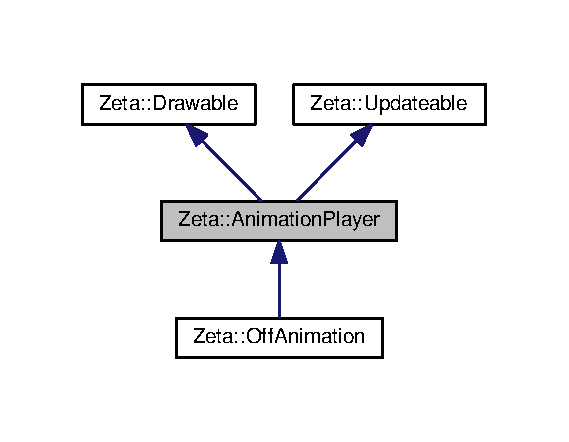
\includegraphics[width=273pt]{classZeta_1_1AnimationPlayer__inherit__graph}
\end{center}
\end{figure}


Collaboration diagram for Zeta\+:\+:Animation\+Player\+:
\nopagebreak
\begin{figure}[H]
\begin{center}
\leavevmode
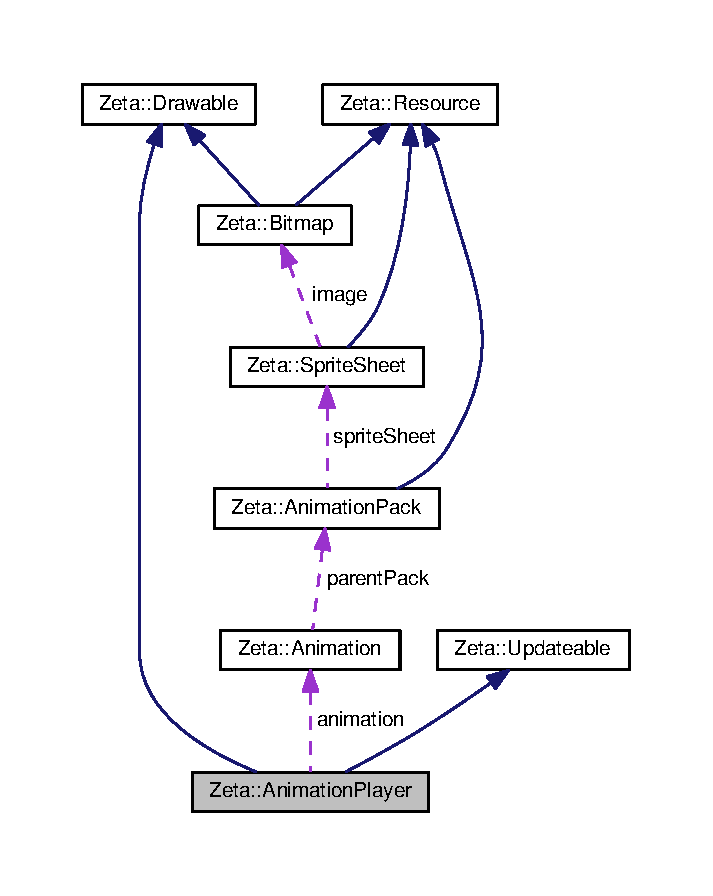
\includegraphics[width=342pt]{classZeta_1_1AnimationPlayer__coll__graph}
\end{center}
\end{figure}
\subsection*{Public Member Functions}
\begin{DoxyCompactItemize}
\item 
bool \hyperlink{classZeta_1_1AnimationPlayer_a33843a3b32e529d2c49451e8509e49dd}{is\+Playing} () const 
\item 
bool \hyperlink{classZeta_1_1AnimationPlayer_a5cdd2521e62f0a552332227ed255025c}{is\+Visible} () const 
\item 
void \hyperlink{classZeta_1_1AnimationPlayer_a8e9810b807fa865af2f36b486dfe8986}{set\+Visible} (bool \hyperlink{classZeta_1_1AnimationPlayer_a38f2ef2f0e15300c862b860ab3eb8534}{visible})
\item 
const \hyperlink{classZeta_1_1Animation}{Animation} \& \hyperlink{classZeta_1_1AnimationPlayer_a815936f25bc83a7e951c02be2fa2947d}{get\+Animation} () const 
\item 
void \hyperlink{classZeta_1_1AnimationPlayer_a7b5eb7c5d405ad4eeadd1cec7b5b0b31}{hide} ()
\item 
void \hyperlink{classZeta_1_1AnimationPlayer_a73b292e4320d72d6876c83c721c4d3f9}{show} ()
\item 
void \hyperlink{classZeta_1_1AnimationPlayer_af46deb8bcb0d0b7ae3b05143cdd0e723}{play} ()
\item 
void \hyperlink{classZeta_1_1AnimationPlayer_abeb67556245a21b3b4920d2e1ddde5ad}{stop} ()
\item 
void \hyperlink{classZeta_1_1AnimationPlayer_a9ea098f3652d0b2c71a6df288d14f2b7}{pause} ()
\item 
void \hyperlink{classZeta_1_1AnimationPlayer_a3172032334596a83d068be6b8d793b37}{reset} ()
\item 
void \hyperlink{classZeta_1_1AnimationPlayer_ae955334186f203dd9a9bcde92e2d464b}{set\+Animation} (const \hyperlink{classZeta_1_1Animation}{Animation} \&\hyperlink{classZeta_1_1AnimationPlayer_a4b97c373a921a0ea6a67c5371f346ddf}{animation})
\item 
virtual void \hyperlink{classZeta_1_1AnimationPlayer_af1f79cd641cebc5f2a8522c95d5b51a9}{draw} (\hyperlink{namespaceZeta_a1e0a1265f9b3bd3075fb0fabd39088ba}{Float} x, \hyperlink{namespaceZeta_a1e0a1265f9b3bd3075fb0fabd39088ba}{Float} y, \hyperlink{namespaceZeta_a1e0a1265f9b3bd3075fb0fabd39088ba}{Float} rotation=0.\+0f, Float scale=1.\+0f) const 
\item 
void \hyperlink{classZeta_1_1AnimationPlayer_a90616e48740857dbdad920ed871223d3}{update} (\hyperlink{namespaceZeta_a1e0a1265f9b3bd3075fb0fabd39088ba}{Float} elapsed\+Time)
\item 
\hyperlink{classZeta_1_1AnimationPlayer_acf5fb0662e00a33f07c417a03e3a9349}{Animation\+Player} ()
\item 
\hyperlink{classZeta_1_1AnimationPlayer_a6984991c2012ea4e58d56a37ac03ffbd}{Animation\+Player} (const \hyperlink{classZeta_1_1Animation}{Animation} \&\hyperlink{classZeta_1_1AnimationPlayer_a4b97c373a921a0ea6a67c5371f346ddf}{animation})
\item 
\hyperlink{classZeta_1_1AnimationPlayer_a05788d29d1c53962a54baf1aef04bb0f}{Animation\+Player} (\hyperlink{classZeta_1_1AnimationPlayer}{Animation\+Player} \&\&)=default
\item 
\hyperlink{classZeta_1_1AnimationPlayer_a6a4fe4e31848481c2bf9e9c65e64451f}{Animation\+Player} (const \hyperlink{classZeta_1_1AnimationPlayer}{Animation\+Player} \&)=default
\item 
\hyperlink{classZeta_1_1AnimationPlayer}{Animation\+Player} \& \hyperlink{classZeta_1_1AnimationPlayer_a99b51751fa45e06d1b60a88578bf6771}{operator=} (\hyperlink{classZeta_1_1AnimationPlayer}{Animation\+Player} \&\&)=default
\item 
\hyperlink{classZeta_1_1AnimationPlayer}{Animation\+Player} \& \hyperlink{classZeta_1_1AnimationPlayer_a7f8e9d9bcd00cd22fddab46505e12745}{operator=} (const \hyperlink{classZeta_1_1AnimationPlayer}{Animation\+Player} \&)=default
\item 
virtual \hyperlink{classZeta_1_1AnimationPlayer_a0482bd50671616b8af87a8b096131b70}{$\sim$\+Animation\+Player} ()
\end{DoxyCompactItemize}
\subsection*{Private Attributes}
\begin{DoxyCompactItemize}
\item 
const \hyperlink{classZeta_1_1Animation}{Animation} $\ast$ \hyperlink{classZeta_1_1AnimationPlayer_a4b97c373a921a0ea6a67c5371f346ddf}{animation}
\item 
int \hyperlink{classZeta_1_1AnimationPlayer_a18cdb164a09c132e5d94d20e65d0ee97}{frame\+Index}
\item 
\hyperlink{namespaceZeta_a1e0a1265f9b3bd3075fb0fabd39088ba}{Float} \hyperlink{classZeta_1_1AnimationPlayer_a9976b8e6d0bb822f289fa5caaf1de8c9}{frame\+Counter}
\item 
bool \hyperlink{classZeta_1_1AnimationPlayer_a0f2b6832532d76d52acff90e31b27f15}{playing}
\item 
bool \hyperlink{classZeta_1_1AnimationPlayer_a38f2ef2f0e15300c862b860ab3eb8534}{visible}
\end{DoxyCompactItemize}


\subsection{Constructor \& Destructor Documentation}
\hypertarget{classZeta_1_1AnimationPlayer_acf5fb0662e00a33f07c417a03e3a9349}{\index{Zeta\+::\+Animation\+Player@{Zeta\+::\+Animation\+Player}!Animation\+Player@{Animation\+Player}}
\index{Animation\+Player@{Animation\+Player}!Zeta\+::\+Animation\+Player@{Zeta\+::\+Animation\+Player}}
\subsubsection[{Animation\+Player}]{\setlength{\rightskip}{0pt plus 5cm}Zeta\+::\+Animation\+Player\+::\+Animation\+Player (
\begin{DoxyParamCaption}
{}
\end{DoxyParamCaption}
)}}\label{classZeta_1_1AnimationPlayer_acf5fb0662e00a33f07c417a03e3a9349}
\hypertarget{classZeta_1_1AnimationPlayer_a6984991c2012ea4e58d56a37ac03ffbd}{\index{Zeta\+::\+Animation\+Player@{Zeta\+::\+Animation\+Player}!Animation\+Player@{Animation\+Player}}
\index{Animation\+Player@{Animation\+Player}!Zeta\+::\+Animation\+Player@{Zeta\+::\+Animation\+Player}}
\subsubsection[{Animation\+Player}]{\setlength{\rightskip}{0pt plus 5cm}Zeta\+::\+Animation\+Player\+::\+Animation\+Player (
\begin{DoxyParamCaption}
\item[{const {\bf Animation} \&}]{animation}
\end{DoxyParamCaption}
)}}\label{classZeta_1_1AnimationPlayer_a6984991c2012ea4e58d56a37ac03ffbd}
\hypertarget{classZeta_1_1AnimationPlayer_a05788d29d1c53962a54baf1aef04bb0f}{\index{Zeta\+::\+Animation\+Player@{Zeta\+::\+Animation\+Player}!Animation\+Player@{Animation\+Player}}
\index{Animation\+Player@{Animation\+Player}!Zeta\+::\+Animation\+Player@{Zeta\+::\+Animation\+Player}}
\subsubsection[{Animation\+Player}]{\setlength{\rightskip}{0pt plus 5cm}Zeta\+::\+Animation\+Player\+::\+Animation\+Player (
\begin{DoxyParamCaption}
\item[{{\bf Animation\+Player} \&\&}]{}
\end{DoxyParamCaption}
)\hspace{0.3cm}{\ttfamily [default]}}}\label{classZeta_1_1AnimationPlayer_a05788d29d1c53962a54baf1aef04bb0f}
\hypertarget{classZeta_1_1AnimationPlayer_a6a4fe4e31848481c2bf9e9c65e64451f}{\index{Zeta\+::\+Animation\+Player@{Zeta\+::\+Animation\+Player}!Animation\+Player@{Animation\+Player}}
\index{Animation\+Player@{Animation\+Player}!Zeta\+::\+Animation\+Player@{Zeta\+::\+Animation\+Player}}
\subsubsection[{Animation\+Player}]{\setlength{\rightskip}{0pt plus 5cm}Zeta\+::\+Animation\+Player\+::\+Animation\+Player (
\begin{DoxyParamCaption}
\item[{const {\bf Animation\+Player} \&}]{}
\end{DoxyParamCaption}
)\hspace{0.3cm}{\ttfamily [default]}}}\label{classZeta_1_1AnimationPlayer_a6a4fe4e31848481c2bf9e9c65e64451f}
\hypertarget{classZeta_1_1AnimationPlayer_a0482bd50671616b8af87a8b096131b70}{\index{Zeta\+::\+Animation\+Player@{Zeta\+::\+Animation\+Player}!````~Animation\+Player@{$\sim$\+Animation\+Player}}
\index{````~Animation\+Player@{$\sim$\+Animation\+Player}!Zeta\+::\+Animation\+Player@{Zeta\+::\+Animation\+Player}}
\subsubsection[{$\sim$\+Animation\+Player}]{\setlength{\rightskip}{0pt plus 5cm}virtual Zeta\+::\+Animation\+Player\+::$\sim$\+Animation\+Player (
\begin{DoxyParamCaption}
{}
\end{DoxyParamCaption}
)\hspace{0.3cm}{\ttfamily [virtual]}}}\label{classZeta_1_1AnimationPlayer_a0482bd50671616b8af87a8b096131b70}


\subsection{Member Function Documentation}
\hypertarget{classZeta_1_1AnimationPlayer_af1f79cd641cebc5f2a8522c95d5b51a9}{\index{Zeta\+::\+Animation\+Player@{Zeta\+::\+Animation\+Player}!draw@{draw}}
\index{draw@{draw}!Zeta\+::\+Animation\+Player@{Zeta\+::\+Animation\+Player}}
\subsubsection[{draw}]{\setlength{\rightskip}{0pt plus 5cm}virtual void Zeta\+::\+Animation\+Player\+::draw (
\begin{DoxyParamCaption}
\item[{{\bf Float}}]{x, }
\item[{{\bf Float}}]{y, }
\item[{{\bf Float}}]{rotation = {\ttfamily 0.0f}, }
\item[{{\bf Float}}]{scale = {\ttfamily 1.0f}}
\end{DoxyParamCaption}
) const\hspace{0.3cm}{\ttfamily [virtual]}}}\label{classZeta_1_1AnimationPlayer_af1f79cd641cebc5f2a8522c95d5b51a9}
Draws the \hyperlink{classZeta_1_1Object}{Object} on screen. Be advised, the x,y, offsets might have different meaning on different implementations. 
\begin{DoxyParams}{Parameters}
{\em x} & X offset to be applied on the drawing \\
\hline
{\em y} & Y offset to be applied on the drawing \\
\hline
{\em rotation} & the rotation to be applied on the drawing \\
\hline
\end{DoxyParams}


Implements \hyperlink{classZeta_1_1Drawable_a3f453a7a971b7eeba1768be3eaedc192}{Zeta\+::\+Drawable}.



Reimplemented in \hyperlink{classZeta_1_1OffAnimation_a38f8d188be29034bf6016a1c77a3958d}{Zeta\+::\+Off\+Animation}.

\hypertarget{classZeta_1_1AnimationPlayer_a815936f25bc83a7e951c02be2fa2947d}{\index{Zeta\+::\+Animation\+Player@{Zeta\+::\+Animation\+Player}!get\+Animation@{get\+Animation}}
\index{get\+Animation@{get\+Animation}!Zeta\+::\+Animation\+Player@{Zeta\+::\+Animation\+Player}}
\subsubsection[{get\+Animation}]{\setlength{\rightskip}{0pt plus 5cm}const {\bf Animation}\& Zeta\+::\+Animation\+Player\+::get\+Animation (
\begin{DoxyParamCaption}
{}
\end{DoxyParamCaption}
) const\hspace{0.3cm}{\ttfamily [inline]}}}\label{classZeta_1_1AnimationPlayer_a815936f25bc83a7e951c02be2fa2947d}
\hypertarget{classZeta_1_1AnimationPlayer_a7b5eb7c5d405ad4eeadd1cec7b5b0b31}{\index{Zeta\+::\+Animation\+Player@{Zeta\+::\+Animation\+Player}!hide@{hide}}
\index{hide@{hide}!Zeta\+::\+Animation\+Player@{Zeta\+::\+Animation\+Player}}
\subsubsection[{hide}]{\setlength{\rightskip}{0pt plus 5cm}void Zeta\+::\+Animation\+Player\+::hide (
\begin{DoxyParamCaption}
{}
\end{DoxyParamCaption}
)\hspace{0.3cm}{\ttfamily [inline]}}}\label{classZeta_1_1AnimationPlayer_a7b5eb7c5d405ad4eeadd1cec7b5b0b31}
\hypertarget{classZeta_1_1AnimationPlayer_a33843a3b32e529d2c49451e8509e49dd}{\index{Zeta\+::\+Animation\+Player@{Zeta\+::\+Animation\+Player}!is\+Playing@{is\+Playing}}
\index{is\+Playing@{is\+Playing}!Zeta\+::\+Animation\+Player@{Zeta\+::\+Animation\+Player}}
\subsubsection[{is\+Playing}]{\setlength{\rightskip}{0pt plus 5cm}bool Zeta\+::\+Animation\+Player\+::is\+Playing (
\begin{DoxyParamCaption}
{}
\end{DoxyParamCaption}
) const\hspace{0.3cm}{\ttfamily [inline]}}}\label{classZeta_1_1AnimationPlayer_a33843a3b32e529d2c49451e8509e49dd}
\hypertarget{classZeta_1_1AnimationPlayer_a5cdd2521e62f0a552332227ed255025c}{\index{Zeta\+::\+Animation\+Player@{Zeta\+::\+Animation\+Player}!is\+Visible@{is\+Visible}}
\index{is\+Visible@{is\+Visible}!Zeta\+::\+Animation\+Player@{Zeta\+::\+Animation\+Player}}
\subsubsection[{is\+Visible}]{\setlength{\rightskip}{0pt plus 5cm}bool Zeta\+::\+Animation\+Player\+::is\+Visible (
\begin{DoxyParamCaption}
{}
\end{DoxyParamCaption}
) const\hspace{0.3cm}{\ttfamily [inline]}}}\label{classZeta_1_1AnimationPlayer_a5cdd2521e62f0a552332227ed255025c}
\hypertarget{classZeta_1_1AnimationPlayer_a99b51751fa45e06d1b60a88578bf6771}{\index{Zeta\+::\+Animation\+Player@{Zeta\+::\+Animation\+Player}!operator=@{operator=}}
\index{operator=@{operator=}!Zeta\+::\+Animation\+Player@{Zeta\+::\+Animation\+Player}}
\subsubsection[{operator=}]{\setlength{\rightskip}{0pt plus 5cm}{\bf Animation\+Player}\& Zeta\+::\+Animation\+Player\+::operator= (
\begin{DoxyParamCaption}
\item[{{\bf Animation\+Player} \&\&}]{}
\end{DoxyParamCaption}
)\hspace{0.3cm}{\ttfamily [default]}}}\label{classZeta_1_1AnimationPlayer_a99b51751fa45e06d1b60a88578bf6771}
\hypertarget{classZeta_1_1AnimationPlayer_a7f8e9d9bcd00cd22fddab46505e12745}{\index{Zeta\+::\+Animation\+Player@{Zeta\+::\+Animation\+Player}!operator=@{operator=}}
\index{operator=@{operator=}!Zeta\+::\+Animation\+Player@{Zeta\+::\+Animation\+Player}}
\subsubsection[{operator=}]{\setlength{\rightskip}{0pt plus 5cm}{\bf Animation\+Player}\& Zeta\+::\+Animation\+Player\+::operator= (
\begin{DoxyParamCaption}
\item[{const {\bf Animation\+Player} \&}]{}
\end{DoxyParamCaption}
)\hspace{0.3cm}{\ttfamily [default]}}}\label{classZeta_1_1AnimationPlayer_a7f8e9d9bcd00cd22fddab46505e12745}
\hypertarget{classZeta_1_1AnimationPlayer_a9ea098f3652d0b2c71a6df288d14f2b7}{\index{Zeta\+::\+Animation\+Player@{Zeta\+::\+Animation\+Player}!pause@{pause}}
\index{pause@{pause}!Zeta\+::\+Animation\+Player@{Zeta\+::\+Animation\+Player}}
\subsubsection[{pause}]{\setlength{\rightskip}{0pt plus 5cm}void Zeta\+::\+Animation\+Player\+::pause (
\begin{DoxyParamCaption}
{}
\end{DoxyParamCaption}
)}}\label{classZeta_1_1AnimationPlayer_a9ea098f3652d0b2c71a6df288d14f2b7}
\hypertarget{classZeta_1_1AnimationPlayer_af46deb8bcb0d0b7ae3b05143cdd0e723}{\index{Zeta\+::\+Animation\+Player@{Zeta\+::\+Animation\+Player}!play@{play}}
\index{play@{play}!Zeta\+::\+Animation\+Player@{Zeta\+::\+Animation\+Player}}
\subsubsection[{play}]{\setlength{\rightskip}{0pt plus 5cm}void Zeta\+::\+Animation\+Player\+::play (
\begin{DoxyParamCaption}
{}
\end{DoxyParamCaption}
)}}\label{classZeta_1_1AnimationPlayer_af46deb8bcb0d0b7ae3b05143cdd0e723}
\hypertarget{classZeta_1_1AnimationPlayer_a3172032334596a83d068be6b8d793b37}{\index{Zeta\+::\+Animation\+Player@{Zeta\+::\+Animation\+Player}!reset@{reset}}
\index{reset@{reset}!Zeta\+::\+Animation\+Player@{Zeta\+::\+Animation\+Player}}
\subsubsection[{reset}]{\setlength{\rightskip}{0pt plus 5cm}void Zeta\+::\+Animation\+Player\+::reset (
\begin{DoxyParamCaption}
{}
\end{DoxyParamCaption}
)}}\label{classZeta_1_1AnimationPlayer_a3172032334596a83d068be6b8d793b37}
\hypertarget{classZeta_1_1AnimationPlayer_ae955334186f203dd9a9bcde92e2d464b}{\index{Zeta\+::\+Animation\+Player@{Zeta\+::\+Animation\+Player}!set\+Animation@{set\+Animation}}
\index{set\+Animation@{set\+Animation}!Zeta\+::\+Animation\+Player@{Zeta\+::\+Animation\+Player}}
\subsubsection[{set\+Animation}]{\setlength{\rightskip}{0pt plus 5cm}void Zeta\+::\+Animation\+Player\+::set\+Animation (
\begin{DoxyParamCaption}
\item[{const {\bf Animation} \&}]{animation}
\end{DoxyParamCaption}
)}}\label{classZeta_1_1AnimationPlayer_ae955334186f203dd9a9bcde92e2d464b}
\hypertarget{classZeta_1_1AnimationPlayer_a8e9810b807fa865af2f36b486dfe8986}{\index{Zeta\+::\+Animation\+Player@{Zeta\+::\+Animation\+Player}!set\+Visible@{set\+Visible}}
\index{set\+Visible@{set\+Visible}!Zeta\+::\+Animation\+Player@{Zeta\+::\+Animation\+Player}}
\subsubsection[{set\+Visible}]{\setlength{\rightskip}{0pt plus 5cm}void Zeta\+::\+Animation\+Player\+::set\+Visible (
\begin{DoxyParamCaption}
\item[{bool}]{visible}
\end{DoxyParamCaption}
)\hspace{0.3cm}{\ttfamily [inline]}}}\label{classZeta_1_1AnimationPlayer_a8e9810b807fa865af2f36b486dfe8986}
\hypertarget{classZeta_1_1AnimationPlayer_a73b292e4320d72d6876c83c721c4d3f9}{\index{Zeta\+::\+Animation\+Player@{Zeta\+::\+Animation\+Player}!show@{show}}
\index{show@{show}!Zeta\+::\+Animation\+Player@{Zeta\+::\+Animation\+Player}}
\subsubsection[{show}]{\setlength{\rightskip}{0pt plus 5cm}void Zeta\+::\+Animation\+Player\+::show (
\begin{DoxyParamCaption}
{}
\end{DoxyParamCaption}
)\hspace{0.3cm}{\ttfamily [inline]}}}\label{classZeta_1_1AnimationPlayer_a73b292e4320d72d6876c83c721c4d3f9}
\hypertarget{classZeta_1_1AnimationPlayer_abeb67556245a21b3b4920d2e1ddde5ad}{\index{Zeta\+::\+Animation\+Player@{Zeta\+::\+Animation\+Player}!stop@{stop}}
\index{stop@{stop}!Zeta\+::\+Animation\+Player@{Zeta\+::\+Animation\+Player}}
\subsubsection[{stop}]{\setlength{\rightskip}{0pt plus 5cm}void Zeta\+::\+Animation\+Player\+::stop (
\begin{DoxyParamCaption}
{}
\end{DoxyParamCaption}
)}}\label{classZeta_1_1AnimationPlayer_abeb67556245a21b3b4920d2e1ddde5ad}
\hypertarget{classZeta_1_1AnimationPlayer_a90616e48740857dbdad920ed871223d3}{\index{Zeta\+::\+Animation\+Player@{Zeta\+::\+Animation\+Player}!update@{update}}
\index{update@{update}!Zeta\+::\+Animation\+Player@{Zeta\+::\+Animation\+Player}}
\subsubsection[{update}]{\setlength{\rightskip}{0pt plus 5cm}void Zeta\+::\+Animation\+Player\+::update (
\begin{DoxyParamCaption}
\item[{{\bf Float}}]{elapsed\+Time}
\end{DoxyParamCaption}
)\hspace{0.3cm}{\ttfamily [virtual]}}}\label{classZeta_1_1AnimationPlayer_a90616e48740857dbdad920ed871223d3}


Implements \hyperlink{classZeta_1_1Updateable_af4006bfccb762454b4da08786ad93de0}{Zeta\+::\+Updateable}.



\subsection{Member Data Documentation}
\hypertarget{classZeta_1_1AnimationPlayer_a4b97c373a921a0ea6a67c5371f346ddf}{\index{Zeta\+::\+Animation\+Player@{Zeta\+::\+Animation\+Player}!animation@{animation}}
\index{animation@{animation}!Zeta\+::\+Animation\+Player@{Zeta\+::\+Animation\+Player}}
\subsubsection[{animation}]{\setlength{\rightskip}{0pt plus 5cm}const {\bf Animation}$\ast$ Zeta\+::\+Animation\+Player\+::animation\hspace{0.3cm}{\ttfamily [private]}}}\label{classZeta_1_1AnimationPlayer_a4b97c373a921a0ea6a67c5371f346ddf}
\hypertarget{classZeta_1_1AnimationPlayer_a9976b8e6d0bb822f289fa5caaf1de8c9}{\index{Zeta\+::\+Animation\+Player@{Zeta\+::\+Animation\+Player}!frame\+Counter@{frame\+Counter}}
\index{frame\+Counter@{frame\+Counter}!Zeta\+::\+Animation\+Player@{Zeta\+::\+Animation\+Player}}
\subsubsection[{frame\+Counter}]{\setlength{\rightskip}{0pt plus 5cm}{\bf Float} Zeta\+::\+Animation\+Player\+::frame\+Counter\hspace{0.3cm}{\ttfamily [private]}}}\label{classZeta_1_1AnimationPlayer_a9976b8e6d0bb822f289fa5caaf1de8c9}
\hypertarget{classZeta_1_1AnimationPlayer_a18cdb164a09c132e5d94d20e65d0ee97}{\index{Zeta\+::\+Animation\+Player@{Zeta\+::\+Animation\+Player}!frame\+Index@{frame\+Index}}
\index{frame\+Index@{frame\+Index}!Zeta\+::\+Animation\+Player@{Zeta\+::\+Animation\+Player}}
\subsubsection[{frame\+Index}]{\setlength{\rightskip}{0pt plus 5cm}int Zeta\+::\+Animation\+Player\+::frame\+Index\hspace{0.3cm}{\ttfamily [private]}}}\label{classZeta_1_1AnimationPlayer_a18cdb164a09c132e5d94d20e65d0ee97}
\hypertarget{classZeta_1_1AnimationPlayer_a0f2b6832532d76d52acff90e31b27f15}{\index{Zeta\+::\+Animation\+Player@{Zeta\+::\+Animation\+Player}!playing@{playing}}
\index{playing@{playing}!Zeta\+::\+Animation\+Player@{Zeta\+::\+Animation\+Player}}
\subsubsection[{playing}]{\setlength{\rightskip}{0pt plus 5cm}bool Zeta\+::\+Animation\+Player\+::playing\hspace{0.3cm}{\ttfamily [private]}}}\label{classZeta_1_1AnimationPlayer_a0f2b6832532d76d52acff90e31b27f15}
\hypertarget{classZeta_1_1AnimationPlayer_a38f2ef2f0e15300c862b860ab3eb8534}{\index{Zeta\+::\+Animation\+Player@{Zeta\+::\+Animation\+Player}!visible@{visible}}
\index{visible@{visible}!Zeta\+::\+Animation\+Player@{Zeta\+::\+Animation\+Player}}
\subsubsection[{visible}]{\setlength{\rightskip}{0pt plus 5cm}bool Zeta\+::\+Animation\+Player\+::visible\hspace{0.3cm}{\ttfamily [private]}}}\label{classZeta_1_1AnimationPlayer_a38f2ef2f0e15300c862b860ab3eb8534}


The documentation for this class was generated from the following file\+:\begin{DoxyCompactItemize}
\item 
include/\+Zeta/\+Core/\+Animation\+Classes/\hyperlink{AnimationPlayer_8hpp}{Animation\+Player.\+hpp}\end{DoxyCompactItemize}

\hypertarget{classZeta_1_1AsynchronousWorker}{\section{Zeta\+:\+:Asynchronous\+Worker Class Reference}
\label{classZeta_1_1AsynchronousWorker}\index{Zeta\+::\+Asynchronous\+Worker@{Zeta\+::\+Asynchronous\+Worker}}
}


{\ttfamily \#include $<$Asynchronous\+Worker.\+hpp$>$}

\subsection*{Public Member Functions}
\begin{DoxyCompactItemize}
\item 
void \hyperlink{classZeta_1_1AsynchronousWorker_a7e5d9fb9919bc9eaf90c27c3db4f3b01}{perform\+Cycle} ()
\begin{DoxyCompactList}\small\item\em Makes the runner thread to call the \hyperlink{classZeta_1_1AsynchronousWorker_a68dbe522e2718cffa436df2f1999369e}{run\+Cycle\+Operations()} \end{DoxyCompactList}\item 
\hyperlink{classZeta_1_1AsynchronousWorker_aabcc75dc05b5525620fdaf474d70dfb3}{Asynchronous\+Worker} ()
\begin{DoxyCompactList}\small\item\em Constructs a runner thread. \end{DoxyCompactList}\item 
virtual \hyperlink{classZeta_1_1AsynchronousWorker_a638b21020fa75875c04b2e98e3762944}{$\sim$\+Asynchronous\+Worker} ()
\end{DoxyCompactItemize}
\subsection*{Protected Member Functions}
\begin{DoxyCompactItemize}
\item 
virtual void \hyperlink{classZeta_1_1AsynchronousWorker_a68dbe522e2718cffa436df2f1999369e}{run\+Cycle\+Operations} ()=0
\end{DoxyCompactItemize}
\subsection*{Protected Attributes}
\begin{DoxyCompactItemize}
\item 
std\+::mutex \hyperlink{classZeta_1_1AsynchronousWorker_ae0ae2b7e721ff8c47bb67665523d9876}{mutex}
\end{DoxyCompactItemize}
\subsection*{Private Member Functions}
\begin{DoxyCompactItemize}
\item 
void \hyperlink{classZeta_1_1AsynchronousWorker_aee7e9cb362533e9dcd834ff9174b5096}{loop} ()
\end{DoxyCompactItemize}
\subsection*{Private Attributes}
\begin{DoxyCompactItemize}
\item 
std\+::thread \hyperlink{classZeta_1_1AsynchronousWorker_ae654cd21c700dc571aa2ed53bf291ee1}{worker}
\item 
std\+::condition\+\_\+variable \hyperlink{classZeta_1_1AsynchronousWorker_af9d697955024d6a72c9d4bb977c10571}{cycle}
\item 
bool \hyperlink{classZeta_1_1AsynchronousWorker_a5ad6cb6f5b8abb7f9a9da695ef02e334}{running}
\end{DoxyCompactItemize}


\subsection{Detailed Description}
\hyperlink{classZeta_1_1AsynchronousWorker}{Asynchronous\+Worker} base class. Used for the derived classes to create objects that execute actions on a unique separate thread. 

\subsection{Constructor \& Destructor Documentation}
\hypertarget{classZeta_1_1AsynchronousWorker_aabcc75dc05b5525620fdaf474d70dfb3}{\index{Zeta\+::\+Asynchronous\+Worker@{Zeta\+::\+Asynchronous\+Worker}!Asynchronous\+Worker@{Asynchronous\+Worker}}
\index{Asynchronous\+Worker@{Asynchronous\+Worker}!Zeta\+::\+Asynchronous\+Worker@{Zeta\+::\+Asynchronous\+Worker}}
\subsubsection[{Asynchronous\+Worker}]{\setlength{\rightskip}{0pt plus 5cm}Zeta\+::\+Asynchronous\+Worker\+::\+Asynchronous\+Worker (
\begin{DoxyParamCaption}
{}
\end{DoxyParamCaption}
)\hspace{0.3cm}{\ttfamily [inline]}}}\label{classZeta_1_1AsynchronousWorker_aabcc75dc05b5525620fdaf474d70dfb3}


Constructs a runner thread. 



Here is the call graph for this function\+:\nopagebreak
\begin{figure}[H]
\begin{center}
\leavevmode
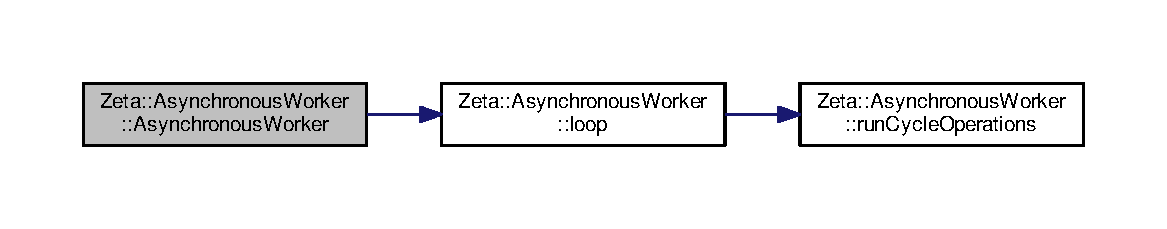
\includegraphics[width=350pt]{classZeta_1_1AsynchronousWorker_aabcc75dc05b5525620fdaf474d70dfb3_cgraph}
\end{center}
\end{figure}


\hypertarget{classZeta_1_1AsynchronousWorker_a638b21020fa75875c04b2e98e3762944}{\index{Zeta\+::\+Asynchronous\+Worker@{Zeta\+::\+Asynchronous\+Worker}!````~Asynchronous\+Worker@{$\sim$\+Asynchronous\+Worker}}
\index{````~Asynchronous\+Worker@{$\sim$\+Asynchronous\+Worker}!Zeta\+::\+Asynchronous\+Worker@{Zeta\+::\+Asynchronous\+Worker}}
\subsubsection[{$\sim$\+Asynchronous\+Worker}]{\setlength{\rightskip}{0pt plus 5cm}virtual Zeta\+::\+Asynchronous\+Worker\+::$\sim$\+Asynchronous\+Worker (
\begin{DoxyParamCaption}
{}
\end{DoxyParamCaption}
)\hspace{0.3cm}{\ttfamily [inline]}, {\ttfamily [virtual]}}}\label{classZeta_1_1AsynchronousWorker_a638b21020fa75875c04b2e98e3762944}


\subsection{Member Function Documentation}
\hypertarget{classZeta_1_1AsynchronousWorker_aee7e9cb362533e9dcd834ff9174b5096}{\index{Zeta\+::\+Asynchronous\+Worker@{Zeta\+::\+Asynchronous\+Worker}!loop@{loop}}
\index{loop@{loop}!Zeta\+::\+Asynchronous\+Worker@{Zeta\+::\+Asynchronous\+Worker}}
\subsubsection[{loop}]{\setlength{\rightskip}{0pt plus 5cm}void Zeta\+::\+Asynchronous\+Worker\+::loop (
\begin{DoxyParamCaption}
{}
\end{DoxyParamCaption}
)\hspace{0.3cm}{\ttfamily [inline]}, {\ttfamily [private]}}}\label{classZeta_1_1AsynchronousWorker_aee7e9cb362533e9dcd834ff9174b5096}


Here is the call graph for this function\+:\nopagebreak
\begin{figure}[H]
\begin{center}
\leavevmode
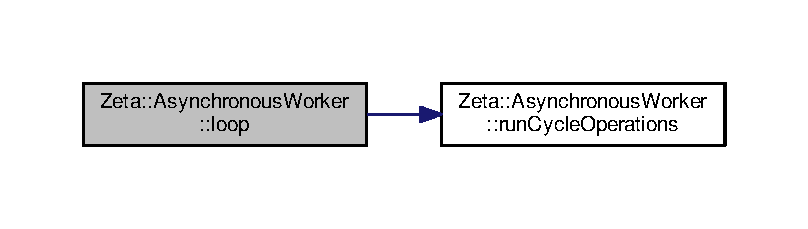
\includegraphics[width=350pt]{classZeta_1_1AsynchronousWorker_aee7e9cb362533e9dcd834ff9174b5096_cgraph}
\end{center}
\end{figure}


\hypertarget{classZeta_1_1AsynchronousWorker_a7e5d9fb9919bc9eaf90c27c3db4f3b01}{\index{Zeta\+::\+Asynchronous\+Worker@{Zeta\+::\+Asynchronous\+Worker}!perform\+Cycle@{perform\+Cycle}}
\index{perform\+Cycle@{perform\+Cycle}!Zeta\+::\+Asynchronous\+Worker@{Zeta\+::\+Asynchronous\+Worker}}
\subsubsection[{perform\+Cycle}]{\setlength{\rightskip}{0pt plus 5cm}void Zeta\+::\+Asynchronous\+Worker\+::perform\+Cycle (
\begin{DoxyParamCaption}
{}
\end{DoxyParamCaption}
)\hspace{0.3cm}{\ttfamily [inline]}}}\label{classZeta_1_1AsynchronousWorker_a7e5d9fb9919bc9eaf90c27c3db4f3b01}


Makes the runner thread to call the \hyperlink{classZeta_1_1AsynchronousWorker_a68dbe522e2718cffa436df2f1999369e}{run\+Cycle\+Operations()} 

\hypertarget{classZeta_1_1AsynchronousWorker_a68dbe522e2718cffa436df2f1999369e}{\index{Zeta\+::\+Asynchronous\+Worker@{Zeta\+::\+Asynchronous\+Worker}!run\+Cycle\+Operations@{run\+Cycle\+Operations}}
\index{run\+Cycle\+Operations@{run\+Cycle\+Operations}!Zeta\+::\+Asynchronous\+Worker@{Zeta\+::\+Asynchronous\+Worker}}
\subsubsection[{run\+Cycle\+Operations}]{\setlength{\rightskip}{0pt plus 5cm}virtual void Zeta\+::\+Asynchronous\+Worker\+::run\+Cycle\+Operations (
\begin{DoxyParamCaption}
{}
\end{DoxyParamCaption}
)\hspace{0.3cm}{\ttfamily [protected]}, {\ttfamily [pure virtual]}}}\label{classZeta_1_1AsynchronousWorker_a68dbe522e2718cffa436df2f1999369e}
/brief Pure virtual member function to be implemented by derived classes It should contain any actions that should be executed by the object's runner thread 

\subsection{Member Data Documentation}
\hypertarget{classZeta_1_1AsynchronousWorker_af9d697955024d6a72c9d4bb977c10571}{\index{Zeta\+::\+Asynchronous\+Worker@{Zeta\+::\+Asynchronous\+Worker}!cycle@{cycle}}
\index{cycle@{cycle}!Zeta\+::\+Asynchronous\+Worker@{Zeta\+::\+Asynchronous\+Worker}}
\subsubsection[{cycle}]{\setlength{\rightskip}{0pt plus 5cm}std\+::condition\+\_\+variable Zeta\+::\+Asynchronous\+Worker\+::cycle\hspace{0.3cm}{\ttfamily [private]}}}\label{classZeta_1_1AsynchronousWorker_af9d697955024d6a72c9d4bb977c10571}
\hypertarget{classZeta_1_1AsynchronousWorker_ae0ae2b7e721ff8c47bb67665523d9876}{\index{Zeta\+::\+Asynchronous\+Worker@{Zeta\+::\+Asynchronous\+Worker}!mutex@{mutex}}
\index{mutex@{mutex}!Zeta\+::\+Asynchronous\+Worker@{Zeta\+::\+Asynchronous\+Worker}}
\subsubsection[{mutex}]{\setlength{\rightskip}{0pt plus 5cm}std\+::mutex Zeta\+::\+Asynchronous\+Worker\+::mutex\hspace{0.3cm}{\ttfamily [protected]}}}\label{classZeta_1_1AsynchronousWorker_ae0ae2b7e721ff8c47bb67665523d9876}
\hypertarget{classZeta_1_1AsynchronousWorker_a5ad6cb6f5b8abb7f9a9da695ef02e334}{\index{Zeta\+::\+Asynchronous\+Worker@{Zeta\+::\+Asynchronous\+Worker}!running@{running}}
\index{running@{running}!Zeta\+::\+Asynchronous\+Worker@{Zeta\+::\+Asynchronous\+Worker}}
\subsubsection[{running}]{\setlength{\rightskip}{0pt plus 5cm}bool Zeta\+::\+Asynchronous\+Worker\+::running\hspace{0.3cm}{\ttfamily [private]}}}\label{classZeta_1_1AsynchronousWorker_a5ad6cb6f5b8abb7f9a9da695ef02e334}
\hypertarget{classZeta_1_1AsynchronousWorker_ae654cd21c700dc571aa2ed53bf291ee1}{\index{Zeta\+::\+Asynchronous\+Worker@{Zeta\+::\+Asynchronous\+Worker}!worker@{worker}}
\index{worker@{worker}!Zeta\+::\+Asynchronous\+Worker@{Zeta\+::\+Asynchronous\+Worker}}
\subsubsection[{worker}]{\setlength{\rightskip}{0pt plus 5cm}std\+::thread Zeta\+::\+Asynchronous\+Worker\+::worker\hspace{0.3cm}{\ttfamily [private]}}}\label{classZeta_1_1AsynchronousWorker_ae654cd21c700dc571aa2ed53bf291ee1}


The documentation for this class was generated from the following file\+:\begin{DoxyCompactItemize}
\item 
include/\+Zeta/\+Core/\hyperlink{AsynchronousWorker_8hpp}{Asynchronous\+Worker.\+hpp}\end{DoxyCompactItemize}

\hypertarget{classZeta_1_1Attribute}{\section{Zeta\+:\+:Attribute Class Reference}
\label{classZeta_1_1Attribute}\index{Zeta\+::\+Attribute@{Zeta\+::\+Attribute}}
}


{\ttfamily \#include $<$Attribute.\+hpp$>$}

\subsection*{Public Member Functions}
\begin{DoxyCompactItemize}
\item 
void \hyperlink{classZeta_1_1Attribute_a3f9e6340e8ea4b5e9ad74c9898696a0b}{calculate} ()
\item 
void \hyperlink{classZeta_1_1Attribute_a24922604f4f328d952c44be03a0cea0d}{add\+Modifier} (\hyperlink{classZeta_1_1Modifier}{Modifier} $\ast$mod)
\item 
void \hyperlink{classZeta_1_1Attribute_ab99269eaf181406cbf7a154b86af1634}{remove\+Modifier} (\hyperlink{classZeta_1_1Modifier}{Modifier} $\ast$mod)
\item 
void \hyperlink{classZeta_1_1Attribute_ad19018db150427661cec8516ed1e9e51}{remove\+Modifier\+And\+Delete} (\hyperlink{classZeta_1_1Modifier}{Modifier} $\ast$mod)
\item 
\hyperlink{namespaceZeta_ab5947f98c0ab6302b51f8c6e93ec5581}{Attribute\+Value} \hyperlink{classZeta_1_1Attribute_a1b1c22b638e4dc8e2746deb53adb04a8}{get\+Value} () const 
\item 
\hyperlink{namespaceZeta_ab5947f98c0ab6302b51f8c6e93ec5581}{Attribute\+Value} \hyperlink{classZeta_1_1Attribute_af56df540b0a1a253b67ef5eac778a6ee}{get\+Base\+Value} () const 
\item 
\hyperlink{classZeta_1_1Attribute_a9ee74be316ff855f0a2e2f2b2dacacbd}{Attribute} ()
\item 
\hyperlink{classZeta_1_1Attribute_a21ad4fc1a49e3b39d356038ca177182a}{Attribute} (\hyperlink{namespaceZeta_ab5947f98c0ab6302b51f8c6e93ec5581}{Attribute\+Value} \hyperlink{classZeta_1_1Attribute_ab96690c561ec9b78648dafc70bc37529}{base\+Value})
\item 
void \hyperlink{classZeta_1_1Attribute_a7071cfacafb5d9d0b4da3913386f61a7}{apply\+To\+Base\+Flat} (\hyperlink{namespaceZeta_ab5947f98c0ab6302b51f8c6e93ec5581}{Attribute\+Value} x)
\item 
void \hyperlink{classZeta_1_1Attribute_a4d9cecf6c61ba0ea47b825a6fb8d954e}{apply\+To\+Base\+Mul} (\hyperlink{namespaceZeta_ab5947f98c0ab6302b51f8c6e93ec5581}{Attribute\+Value} x)
\item 
void \hyperlink{classZeta_1_1Attribute_a190c07ba11e10554c6819583d7f68317}{set\+Base} (\hyperlink{namespaceZeta_ab5947f98c0ab6302b51f8c6e93ec5581}{Attribute\+Value} value)
\item 
void \hyperlink{classZeta_1_1Attribute_a04ef4458c01cf3fce8731bc4d5a010a2}{set\+Calculated\+Value} (\hyperlink{namespaceZeta_ab5947f98c0ab6302b51f8c6e93ec5581}{Attribute\+Value} value)
\item 
void \hyperlink{classZeta_1_1Attribute_a7728554250846cbef54e9e1e6f141436}{remove\+All\+Modifiers} (bool delete\+Them)
\item 
\hyperlink{classZeta_1_1Attribute_ac564fc00e5396b62e764bd0fe11bbf27}{Attribute} (const \hyperlink{classZeta_1_1Attribute}{Attribute} \&other)
\item 
\hyperlink{classZeta_1_1Attribute}{Attribute} \& \hyperlink{classZeta_1_1Attribute_af57980fcca07e00f0464432f45e011ca}{operator=} (const \hyperlink{classZeta_1_1Attribute}{Attribute} \&other)
\item 
\hyperlink{classZeta_1_1Attribute}{Attribute} \& \hyperlink{classZeta_1_1Attribute_a58360d435e262ee8fb79d4e62242abb7}{operator=} (\hyperlink{namespaceZeta_ab5947f98c0ab6302b51f8c6e93ec5581}{Attribute\+Value} value)
\item 
virtual \hyperlink{classZeta_1_1Attribute_a11b58919e8801749aec2e9e2d933d043}{$\sim$\+Attribute} ()
\end{DoxyCompactItemize}
\subsection*{Protected Attributes}
\begin{DoxyCompactItemize}
\item 
\hyperlink{namespaceZeta_a44c717c98a964d0ebf6ea954cb9c91bf}{Z\+Small\+Set}$<$ \hyperlink{classZeta_1_1Modifier}{Modifier} $\ast$ $>$ \hyperlink{classZeta_1_1Attribute_a340f14d134cb26bf1c8685df3199ffcb}{modifiers}
\item 
\hyperlink{namespaceZeta_ab5947f98c0ab6302b51f8c6e93ec5581}{Attribute\+Value} \hyperlink{classZeta_1_1Attribute_ab96690c561ec9b78648dafc70bc37529}{base\+Value}
\item 
\hyperlink{namespaceZeta_ab5947f98c0ab6302b51f8c6e93ec5581}{Attribute\+Value} \hyperlink{classZeta_1_1Attribute_a76b3de0b3f4037ed5c19d3da82f105d8}{calculated\+Value}
\end{DoxyCompactItemize}


\subsection{Constructor \& Destructor Documentation}
\hypertarget{classZeta_1_1Attribute_a9ee74be316ff855f0a2e2f2b2dacacbd}{\index{Zeta\+::\+Attribute@{Zeta\+::\+Attribute}!Attribute@{Attribute}}
\index{Attribute@{Attribute}!Zeta\+::\+Attribute@{Zeta\+::\+Attribute}}
\subsubsection[{Attribute}]{\setlength{\rightskip}{0pt plus 5cm}Zeta\+::\+Attribute\+::\+Attribute (
\begin{DoxyParamCaption}
{}
\end{DoxyParamCaption}
)\hspace{0.3cm}{\ttfamily [inline]}}}\label{classZeta_1_1Attribute_a9ee74be316ff855f0a2e2f2b2dacacbd}
\hypertarget{classZeta_1_1Attribute_a21ad4fc1a49e3b39d356038ca177182a}{\index{Zeta\+::\+Attribute@{Zeta\+::\+Attribute}!Attribute@{Attribute}}
\index{Attribute@{Attribute}!Zeta\+::\+Attribute@{Zeta\+::\+Attribute}}
\subsubsection[{Attribute}]{\setlength{\rightskip}{0pt plus 5cm}Zeta\+::\+Attribute\+::\+Attribute (
\begin{DoxyParamCaption}
\item[{{\bf Attribute\+Value}}]{base\+Value}
\end{DoxyParamCaption}
)\hspace{0.3cm}{\ttfamily [inline]}}}\label{classZeta_1_1Attribute_a21ad4fc1a49e3b39d356038ca177182a}
\hypertarget{classZeta_1_1Attribute_ac564fc00e5396b62e764bd0fe11bbf27}{\index{Zeta\+::\+Attribute@{Zeta\+::\+Attribute}!Attribute@{Attribute}}
\index{Attribute@{Attribute}!Zeta\+::\+Attribute@{Zeta\+::\+Attribute}}
\subsubsection[{Attribute}]{\setlength{\rightskip}{0pt plus 5cm}Zeta\+::\+Attribute\+::\+Attribute (
\begin{DoxyParamCaption}
\item[{const {\bf Attribute} \&}]{other}
\end{DoxyParamCaption}
)}}\label{classZeta_1_1Attribute_ac564fc00e5396b62e764bd0fe11bbf27}
\hypertarget{classZeta_1_1Attribute_a11b58919e8801749aec2e9e2d933d043}{\index{Zeta\+::\+Attribute@{Zeta\+::\+Attribute}!````~Attribute@{$\sim$\+Attribute}}
\index{````~Attribute@{$\sim$\+Attribute}!Zeta\+::\+Attribute@{Zeta\+::\+Attribute}}
\subsubsection[{$\sim$\+Attribute}]{\setlength{\rightskip}{0pt plus 5cm}virtual Zeta\+::\+Attribute\+::$\sim$\+Attribute (
\begin{DoxyParamCaption}
{}
\end{DoxyParamCaption}
)\hspace{0.3cm}{\ttfamily [inline]}, {\ttfamily [virtual]}}}\label{classZeta_1_1Attribute_a11b58919e8801749aec2e9e2d933d043}


\subsection{Member Function Documentation}
\hypertarget{classZeta_1_1Attribute_a24922604f4f328d952c44be03a0cea0d}{\index{Zeta\+::\+Attribute@{Zeta\+::\+Attribute}!add\+Modifier@{add\+Modifier}}
\index{add\+Modifier@{add\+Modifier}!Zeta\+::\+Attribute@{Zeta\+::\+Attribute}}
\subsubsection[{add\+Modifier}]{\setlength{\rightskip}{0pt plus 5cm}void Zeta\+::\+Attribute\+::add\+Modifier (
\begin{DoxyParamCaption}
\item[{{\bf Modifier} $\ast$}]{mod}
\end{DoxyParamCaption}
)}}\label{classZeta_1_1Attribute_a24922604f4f328d952c44be03a0cea0d}
\hypertarget{classZeta_1_1Attribute_a7071cfacafb5d9d0b4da3913386f61a7}{\index{Zeta\+::\+Attribute@{Zeta\+::\+Attribute}!apply\+To\+Base\+Flat@{apply\+To\+Base\+Flat}}
\index{apply\+To\+Base\+Flat@{apply\+To\+Base\+Flat}!Zeta\+::\+Attribute@{Zeta\+::\+Attribute}}
\subsubsection[{apply\+To\+Base\+Flat}]{\setlength{\rightskip}{0pt plus 5cm}void Zeta\+::\+Attribute\+::apply\+To\+Base\+Flat (
\begin{DoxyParamCaption}
\item[{{\bf Attribute\+Value}}]{x}
\end{DoxyParamCaption}
)\hspace{0.3cm}{\ttfamily [inline]}}}\label{classZeta_1_1Attribute_a7071cfacafb5d9d0b4da3913386f61a7}


Here is the call graph for this function\+:\nopagebreak
\begin{figure}[H]
\begin{center}
\leavevmode
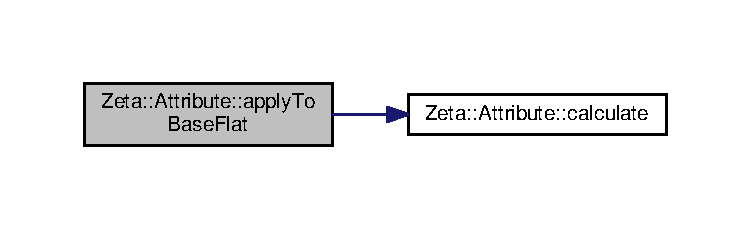
\includegraphics[width=350pt]{classZeta_1_1Attribute_a7071cfacafb5d9d0b4da3913386f61a7_cgraph}
\end{center}
\end{figure}


\hypertarget{classZeta_1_1Attribute_a4d9cecf6c61ba0ea47b825a6fb8d954e}{\index{Zeta\+::\+Attribute@{Zeta\+::\+Attribute}!apply\+To\+Base\+Mul@{apply\+To\+Base\+Mul}}
\index{apply\+To\+Base\+Mul@{apply\+To\+Base\+Mul}!Zeta\+::\+Attribute@{Zeta\+::\+Attribute}}
\subsubsection[{apply\+To\+Base\+Mul}]{\setlength{\rightskip}{0pt plus 5cm}void Zeta\+::\+Attribute\+::apply\+To\+Base\+Mul (
\begin{DoxyParamCaption}
\item[{{\bf Attribute\+Value}}]{x}
\end{DoxyParamCaption}
)\hspace{0.3cm}{\ttfamily [inline]}}}\label{classZeta_1_1Attribute_a4d9cecf6c61ba0ea47b825a6fb8d954e}


Here is the call graph for this function\+:\nopagebreak
\begin{figure}[H]
\begin{center}
\leavevmode
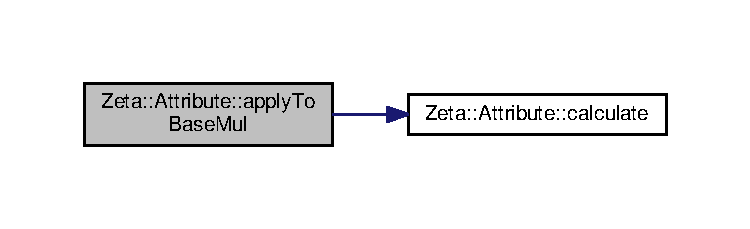
\includegraphics[width=350pt]{classZeta_1_1Attribute_a4d9cecf6c61ba0ea47b825a6fb8d954e_cgraph}
\end{center}
\end{figure}


\hypertarget{classZeta_1_1Attribute_a3f9e6340e8ea4b5e9ad74c9898696a0b}{\index{Zeta\+::\+Attribute@{Zeta\+::\+Attribute}!calculate@{calculate}}
\index{calculate@{calculate}!Zeta\+::\+Attribute@{Zeta\+::\+Attribute}}
\subsubsection[{calculate}]{\setlength{\rightskip}{0pt plus 5cm}void Zeta\+::\+Attribute\+::calculate (
\begin{DoxyParamCaption}
{}
\end{DoxyParamCaption}
)}}\label{classZeta_1_1Attribute_a3f9e6340e8ea4b5e9ad74c9898696a0b}
\hypertarget{classZeta_1_1Attribute_af56df540b0a1a253b67ef5eac778a6ee}{\index{Zeta\+::\+Attribute@{Zeta\+::\+Attribute}!get\+Base\+Value@{get\+Base\+Value}}
\index{get\+Base\+Value@{get\+Base\+Value}!Zeta\+::\+Attribute@{Zeta\+::\+Attribute}}
\subsubsection[{get\+Base\+Value}]{\setlength{\rightskip}{0pt plus 5cm}{\bf Attribute\+Value} Zeta\+::\+Attribute\+::get\+Base\+Value (
\begin{DoxyParamCaption}
{}
\end{DoxyParamCaption}
) const\hspace{0.3cm}{\ttfamily [inline]}}}\label{classZeta_1_1Attribute_af56df540b0a1a253b67ef5eac778a6ee}
\hypertarget{classZeta_1_1Attribute_a1b1c22b638e4dc8e2746deb53adb04a8}{\index{Zeta\+::\+Attribute@{Zeta\+::\+Attribute}!get\+Value@{get\+Value}}
\index{get\+Value@{get\+Value}!Zeta\+::\+Attribute@{Zeta\+::\+Attribute}}
\subsubsection[{get\+Value}]{\setlength{\rightskip}{0pt plus 5cm}{\bf Attribute\+Value} Zeta\+::\+Attribute\+::get\+Value (
\begin{DoxyParamCaption}
{}
\end{DoxyParamCaption}
) const\hspace{0.3cm}{\ttfamily [inline]}}}\label{classZeta_1_1Attribute_a1b1c22b638e4dc8e2746deb53adb04a8}
\hypertarget{classZeta_1_1Attribute_af57980fcca07e00f0464432f45e011ca}{\index{Zeta\+::\+Attribute@{Zeta\+::\+Attribute}!operator=@{operator=}}
\index{operator=@{operator=}!Zeta\+::\+Attribute@{Zeta\+::\+Attribute}}
\subsubsection[{operator=}]{\setlength{\rightskip}{0pt plus 5cm}{\bf Attribute}\& Zeta\+::\+Attribute\+::operator= (
\begin{DoxyParamCaption}
\item[{const {\bf Attribute} \&}]{other}
\end{DoxyParamCaption}
)}}\label{classZeta_1_1Attribute_af57980fcca07e00f0464432f45e011ca}
\hypertarget{classZeta_1_1Attribute_a58360d435e262ee8fb79d4e62242abb7}{\index{Zeta\+::\+Attribute@{Zeta\+::\+Attribute}!operator=@{operator=}}
\index{operator=@{operator=}!Zeta\+::\+Attribute@{Zeta\+::\+Attribute}}
\subsubsection[{operator=}]{\setlength{\rightskip}{0pt plus 5cm}{\bf Attribute}\& Zeta\+::\+Attribute\+::operator= (
\begin{DoxyParamCaption}
\item[{{\bf Attribute\+Value}}]{value}
\end{DoxyParamCaption}
)\hspace{0.3cm}{\ttfamily [inline]}}}\label{classZeta_1_1Attribute_a58360d435e262ee8fb79d4e62242abb7}
\hypertarget{classZeta_1_1Attribute_a7728554250846cbef54e9e1e6f141436}{\index{Zeta\+::\+Attribute@{Zeta\+::\+Attribute}!remove\+All\+Modifiers@{remove\+All\+Modifiers}}
\index{remove\+All\+Modifiers@{remove\+All\+Modifiers}!Zeta\+::\+Attribute@{Zeta\+::\+Attribute}}
\subsubsection[{remove\+All\+Modifiers}]{\setlength{\rightskip}{0pt plus 5cm}void Zeta\+::\+Attribute\+::remove\+All\+Modifiers (
\begin{DoxyParamCaption}
\item[{bool}]{delete\+Them}
\end{DoxyParamCaption}
)}}\label{classZeta_1_1Attribute_a7728554250846cbef54e9e1e6f141436}
\hypertarget{classZeta_1_1Attribute_ab99269eaf181406cbf7a154b86af1634}{\index{Zeta\+::\+Attribute@{Zeta\+::\+Attribute}!remove\+Modifier@{remove\+Modifier}}
\index{remove\+Modifier@{remove\+Modifier}!Zeta\+::\+Attribute@{Zeta\+::\+Attribute}}
\subsubsection[{remove\+Modifier}]{\setlength{\rightskip}{0pt plus 5cm}void Zeta\+::\+Attribute\+::remove\+Modifier (
\begin{DoxyParamCaption}
\item[{{\bf Modifier} $\ast$}]{mod}
\end{DoxyParamCaption}
)}}\label{classZeta_1_1Attribute_ab99269eaf181406cbf7a154b86af1634}
\hypertarget{classZeta_1_1Attribute_ad19018db150427661cec8516ed1e9e51}{\index{Zeta\+::\+Attribute@{Zeta\+::\+Attribute}!remove\+Modifier\+And\+Delete@{remove\+Modifier\+And\+Delete}}
\index{remove\+Modifier\+And\+Delete@{remove\+Modifier\+And\+Delete}!Zeta\+::\+Attribute@{Zeta\+::\+Attribute}}
\subsubsection[{remove\+Modifier\+And\+Delete}]{\setlength{\rightskip}{0pt plus 5cm}void Zeta\+::\+Attribute\+::remove\+Modifier\+And\+Delete (
\begin{DoxyParamCaption}
\item[{{\bf Modifier} $\ast$}]{mod}
\end{DoxyParamCaption}
)}}\label{classZeta_1_1Attribute_ad19018db150427661cec8516ed1e9e51}
\hypertarget{classZeta_1_1Attribute_a190c07ba11e10554c6819583d7f68317}{\index{Zeta\+::\+Attribute@{Zeta\+::\+Attribute}!set\+Base@{set\+Base}}
\index{set\+Base@{set\+Base}!Zeta\+::\+Attribute@{Zeta\+::\+Attribute}}
\subsubsection[{set\+Base}]{\setlength{\rightskip}{0pt plus 5cm}void Zeta\+::\+Attribute\+::set\+Base (
\begin{DoxyParamCaption}
\item[{{\bf Attribute\+Value}}]{value}
\end{DoxyParamCaption}
)\hspace{0.3cm}{\ttfamily [inline]}}}\label{classZeta_1_1Attribute_a190c07ba11e10554c6819583d7f68317}


Here is the call graph for this function\+:\nopagebreak
\begin{figure}[H]
\begin{center}
\leavevmode
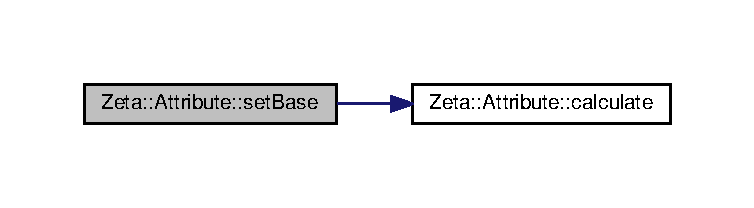
\includegraphics[width=350pt]{classZeta_1_1Attribute_a190c07ba11e10554c6819583d7f68317_cgraph}
\end{center}
\end{figure}


\hypertarget{classZeta_1_1Attribute_a04ef4458c01cf3fce8731bc4d5a010a2}{\index{Zeta\+::\+Attribute@{Zeta\+::\+Attribute}!set\+Calculated\+Value@{set\+Calculated\+Value}}
\index{set\+Calculated\+Value@{set\+Calculated\+Value}!Zeta\+::\+Attribute@{Zeta\+::\+Attribute}}
\subsubsection[{set\+Calculated\+Value}]{\setlength{\rightskip}{0pt plus 5cm}void Zeta\+::\+Attribute\+::set\+Calculated\+Value (
\begin{DoxyParamCaption}
\item[{{\bf Attribute\+Value}}]{value}
\end{DoxyParamCaption}
)\hspace{0.3cm}{\ttfamily [inline]}}}\label{classZeta_1_1Attribute_a04ef4458c01cf3fce8731bc4d5a010a2}


\subsection{Member Data Documentation}
\hypertarget{classZeta_1_1Attribute_ab96690c561ec9b78648dafc70bc37529}{\index{Zeta\+::\+Attribute@{Zeta\+::\+Attribute}!base\+Value@{base\+Value}}
\index{base\+Value@{base\+Value}!Zeta\+::\+Attribute@{Zeta\+::\+Attribute}}
\subsubsection[{base\+Value}]{\setlength{\rightskip}{0pt plus 5cm}{\bf Attribute\+Value} Zeta\+::\+Attribute\+::base\+Value\hspace{0.3cm}{\ttfamily [protected]}}}\label{classZeta_1_1Attribute_ab96690c561ec9b78648dafc70bc37529}
\hypertarget{classZeta_1_1Attribute_a76b3de0b3f4037ed5c19d3da82f105d8}{\index{Zeta\+::\+Attribute@{Zeta\+::\+Attribute}!calculated\+Value@{calculated\+Value}}
\index{calculated\+Value@{calculated\+Value}!Zeta\+::\+Attribute@{Zeta\+::\+Attribute}}
\subsubsection[{calculated\+Value}]{\setlength{\rightskip}{0pt plus 5cm}{\bf Attribute\+Value} Zeta\+::\+Attribute\+::calculated\+Value\hspace{0.3cm}{\ttfamily [protected]}}}\label{classZeta_1_1Attribute_a76b3de0b3f4037ed5c19d3da82f105d8}
\hypertarget{classZeta_1_1Attribute_a340f14d134cb26bf1c8685df3199ffcb}{\index{Zeta\+::\+Attribute@{Zeta\+::\+Attribute}!modifiers@{modifiers}}
\index{modifiers@{modifiers}!Zeta\+::\+Attribute@{Zeta\+::\+Attribute}}
\subsubsection[{modifiers}]{\setlength{\rightskip}{0pt plus 5cm}{\bf Z\+Small\+Set}$<${\bf Modifier}$\ast$$>$ Zeta\+::\+Attribute\+::modifiers\hspace{0.3cm}{\ttfamily [protected]}}}\label{classZeta_1_1Attribute_a340f14d134cb26bf1c8685df3199ffcb}


The documentation for this class was generated from the following file\+:\begin{DoxyCompactItemize}
\item 
include/\+Zeta/\+Core/\+R\+P\+G\+Classes/\hyperlink{Attribute_8hpp}{Attribute.\+hpp}\end{DoxyCompactItemize}

\hypertarget{classZeta_1_1AudioContext}{\section{Zeta\+:\+:Audio\+Context Class Reference}
\label{classZeta_1_1AudioContext}\index{Zeta\+::\+Audio\+Context@{Zeta\+::\+Audio\+Context}}
}


{\ttfamily \#include $<$Audio\+Context.\+hpp$>$}



Inheritance diagram for Zeta\+:\+:Audio\+Context\+:\nopagebreak
\begin{figure}[H]
\begin{center}
\leavevmode
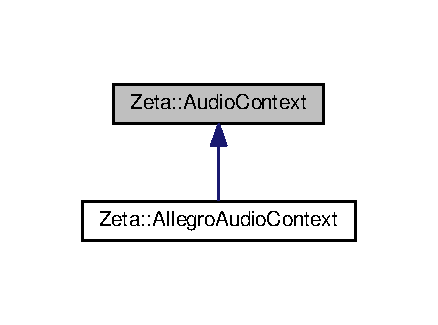
\includegraphics[width=210pt]{classZeta_1_1AudioContext__inherit__graph}
\end{center}
\end{figure}


Collaboration diagram for Zeta\+:\+:Audio\+Context\+:\nopagebreak
\begin{figure}[H]
\begin{center}
\leavevmode
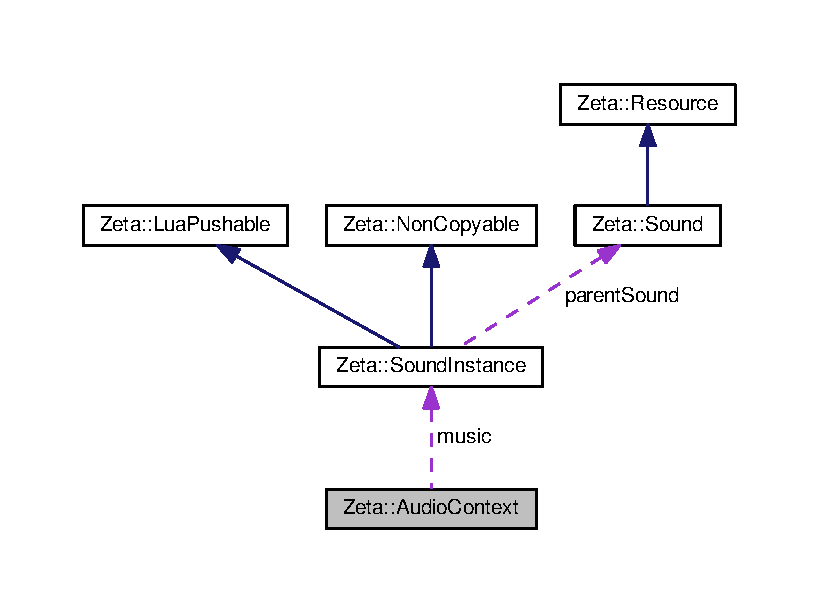
\includegraphics[width=350pt]{classZeta_1_1AudioContext__coll__graph}
\end{center}
\end{figure}
\subsection*{Public Member Functions}
\begin{DoxyCompactItemize}
\item 
virtual float \hyperlink{classZeta_1_1AudioContext_ab492d715ae780a8d6c2fc4e7a0432355}{get\+Main\+Gain} () const =0
\item 
virtual void \hyperlink{classZeta_1_1AudioContext_af861f3797591e2c62040a18b3d4daa51}{set\+Main\+Gain} (float main\+Gain)=0
\item 
void \hyperlink{classZeta_1_1AudioContext_a56c0028bdeadb4901aede192f2af115a}{set\+Music} (const std\+::string \&path)
\item 
void \hyperlink{classZeta_1_1AudioContext_a99eaeb4a6af9c515c02eaaf406592833}{start} ()
\item 
void \hyperlink{classZeta_1_1AudioContext_a839246cbcf16e65920ad1a5bad31bd22}{stop} ()
\item 
\hyperlink{classZeta_1_1AudioContext_a6eacef723378137c0e758a320ee21d7a}{Audio\+Context} ()
\item 
virtual \hyperlink{classZeta_1_1AudioContext_a963fbc68f296d7f7b96c2e51799e8855}{$\sim$\+Audio\+Context} ()
\end{DoxyCompactItemize}
\subsection*{Private Attributes}
\begin{DoxyCompactItemize}
\item 
\hyperlink{classZeta_1_1SoundInstance}{Sound\+Instance} $\ast$ \hyperlink{classZeta_1_1AudioContext_aae43d48fd2d78a63baaf534d7df56481}{music}
\end{DoxyCompactItemize}


\subsection{Detailed Description}
\hyperlink{classZeta_1_1AudioContext}{Audio\+Context} Base class Used to create Main \hyperlink{classZeta_1_1Sound}{Sound} Wrappers to connect to Engine's core 

\subsection{Constructor \& Destructor Documentation}
\hypertarget{classZeta_1_1AudioContext_a6eacef723378137c0e758a320ee21d7a}{\index{Zeta\+::\+Audio\+Context@{Zeta\+::\+Audio\+Context}!Audio\+Context@{Audio\+Context}}
\index{Audio\+Context@{Audio\+Context}!Zeta\+::\+Audio\+Context@{Zeta\+::\+Audio\+Context}}
\subsubsection[{Audio\+Context}]{\setlength{\rightskip}{0pt plus 5cm}Zeta\+::\+Audio\+Context\+::\+Audio\+Context (
\begin{DoxyParamCaption}
{}
\end{DoxyParamCaption}
)}}\label{classZeta_1_1AudioContext_a6eacef723378137c0e758a320ee21d7a}
\hypertarget{classZeta_1_1AudioContext_a963fbc68f296d7f7b96c2e51799e8855}{\index{Zeta\+::\+Audio\+Context@{Zeta\+::\+Audio\+Context}!````~Audio\+Context@{$\sim$\+Audio\+Context}}
\index{````~Audio\+Context@{$\sim$\+Audio\+Context}!Zeta\+::\+Audio\+Context@{Zeta\+::\+Audio\+Context}}
\subsubsection[{$\sim$\+Audio\+Context}]{\setlength{\rightskip}{0pt plus 5cm}virtual Zeta\+::\+Audio\+Context\+::$\sim$\+Audio\+Context (
\begin{DoxyParamCaption}
{}
\end{DoxyParamCaption}
)\hspace{0.3cm}{\ttfamily [virtual]}}}\label{classZeta_1_1AudioContext_a963fbc68f296d7f7b96c2e51799e8855}


\subsection{Member Function Documentation}
\hypertarget{classZeta_1_1AudioContext_ab492d715ae780a8d6c2fc4e7a0432355}{\index{Zeta\+::\+Audio\+Context@{Zeta\+::\+Audio\+Context}!get\+Main\+Gain@{get\+Main\+Gain}}
\index{get\+Main\+Gain@{get\+Main\+Gain}!Zeta\+::\+Audio\+Context@{Zeta\+::\+Audio\+Context}}
\subsubsection[{get\+Main\+Gain}]{\setlength{\rightskip}{0pt plus 5cm}virtual float Zeta\+::\+Audio\+Context\+::get\+Main\+Gain (
\begin{DoxyParamCaption}
{}
\end{DoxyParamCaption}
) const\hspace{0.3cm}{\ttfamily [pure virtual]}}}\label{classZeta_1_1AudioContext_ab492d715ae780a8d6c2fc4e7a0432355}
Gets the main \hyperlink{classZeta_1_1Sound}{Sound} gain. \begin{DoxyReturn}{Returns}
Float 0.\+0f-\/1.\+0f representing the Main Mixer Gain 
\end{DoxyReturn}


Implemented in \hyperlink{classZeta_1_1AllegroAudioContext_a093e94d2f271f0030573e3c7f112fe17}{Zeta\+::\+Allegro\+Audio\+Context}.

\hypertarget{classZeta_1_1AudioContext_af861f3797591e2c62040a18b3d4daa51}{\index{Zeta\+::\+Audio\+Context@{Zeta\+::\+Audio\+Context}!set\+Main\+Gain@{set\+Main\+Gain}}
\index{set\+Main\+Gain@{set\+Main\+Gain}!Zeta\+::\+Audio\+Context@{Zeta\+::\+Audio\+Context}}
\subsubsection[{set\+Main\+Gain}]{\setlength{\rightskip}{0pt plus 5cm}virtual void Zeta\+::\+Audio\+Context\+::set\+Main\+Gain (
\begin{DoxyParamCaption}
\item[{float}]{main\+Gain}
\end{DoxyParamCaption}
)\hspace{0.3cm}{\ttfamily [pure virtual]}}}\label{classZeta_1_1AudioContext_af861f3797591e2c62040a18b3d4daa51}
Sets the main Soung Gain. 
\begin{DoxyParams}{Parameters}
{\em main\+Gain} & Float representing the main\+Gain \\
\hline
\end{DoxyParams}


Implemented in \hyperlink{classZeta_1_1AllegroAudioContext_ab2e61ddbafdb74657390ecdc813501b8}{Zeta\+::\+Allegro\+Audio\+Context}.

\hypertarget{classZeta_1_1AudioContext_a56c0028bdeadb4901aede192f2af115a}{\index{Zeta\+::\+Audio\+Context@{Zeta\+::\+Audio\+Context}!set\+Music@{set\+Music}}
\index{set\+Music@{set\+Music}!Zeta\+::\+Audio\+Context@{Zeta\+::\+Audio\+Context}}
\subsubsection[{set\+Music}]{\setlength{\rightskip}{0pt plus 5cm}void Zeta\+::\+Audio\+Context\+::set\+Music (
\begin{DoxyParamCaption}
\item[{const std\+::string \&}]{path}
\end{DoxyParamCaption}
)}}\label{classZeta_1_1AudioContext_a56c0028bdeadb4901aede192f2af115a}
Sets the music to be played when \hyperlink{classZeta_1_1AudioContext_a99eaeb4a6af9c515c02eaaf406592833}{start()} is called 
\begin{DoxyParams}{Parameters}
{\em path} & The path of the sound file to be played \\
\hline
\end{DoxyParams}
\hypertarget{classZeta_1_1AudioContext_a99eaeb4a6af9c515c02eaaf406592833}{\index{Zeta\+::\+Audio\+Context@{Zeta\+::\+Audio\+Context}!start@{start}}
\index{start@{start}!Zeta\+::\+Audio\+Context@{Zeta\+::\+Audio\+Context}}
\subsubsection[{start}]{\setlength{\rightskip}{0pt plus 5cm}void Zeta\+::\+Audio\+Context\+::start (
\begin{DoxyParamCaption}
{}
\end{DoxyParamCaption}
)}}\label{classZeta_1_1AudioContext_a99eaeb4a6af9c515c02eaaf406592833}
Starts playing (Looped) the sound file specified by \hyperlink{classZeta_1_1AudioContext_a56c0028bdeadb4901aede192f2af115a}{set\+Music()}. \hypertarget{classZeta_1_1AudioContext_a839246cbcf16e65920ad1a5bad31bd22}{\index{Zeta\+::\+Audio\+Context@{Zeta\+::\+Audio\+Context}!stop@{stop}}
\index{stop@{stop}!Zeta\+::\+Audio\+Context@{Zeta\+::\+Audio\+Context}}
\subsubsection[{stop}]{\setlength{\rightskip}{0pt plus 5cm}void Zeta\+::\+Audio\+Context\+::stop (
\begin{DoxyParamCaption}
{}
\end{DoxyParamCaption}
)}}\label{classZeta_1_1AudioContext_a839246cbcf16e65920ad1a5bad31bd22}
Stops playing the sound that is being played by calling \hyperlink{classZeta_1_1AudioContext_a99eaeb4a6af9c515c02eaaf406592833}{start()} 

\subsection{Member Data Documentation}
\hypertarget{classZeta_1_1AudioContext_aae43d48fd2d78a63baaf534d7df56481}{\index{Zeta\+::\+Audio\+Context@{Zeta\+::\+Audio\+Context}!music@{music}}
\index{music@{music}!Zeta\+::\+Audio\+Context@{Zeta\+::\+Audio\+Context}}
\subsubsection[{music}]{\setlength{\rightskip}{0pt plus 5cm}{\bf Sound\+Instance}$\ast$ Zeta\+::\+Audio\+Context\+::music\hspace{0.3cm}{\ttfamily [private]}}}\label{classZeta_1_1AudioContext_aae43d48fd2d78a63baaf534d7df56481}


The documentation for this class was generated from the following file\+:\begin{DoxyCompactItemize}
\item 
include/\+Zeta/\+Core/\hyperlink{AudioContext_8hpp}{Audio\+Context.\+hpp}\end{DoxyCompactItemize}

\hypertarget{classZeta_1_1Behaviour}{\section{Zeta\+:\+:Behaviour Class Reference}
\label{classZeta_1_1Behaviour}\index{Zeta\+::\+Behaviour@{Zeta\+::\+Behaviour}}
}


{\ttfamily \#include $<$Behaviour.\+hpp$>$}



Inheritance diagram for Zeta\+:\+:Behaviour\+:\nopagebreak
\begin{figure}[H]
\begin{center}
\leavevmode
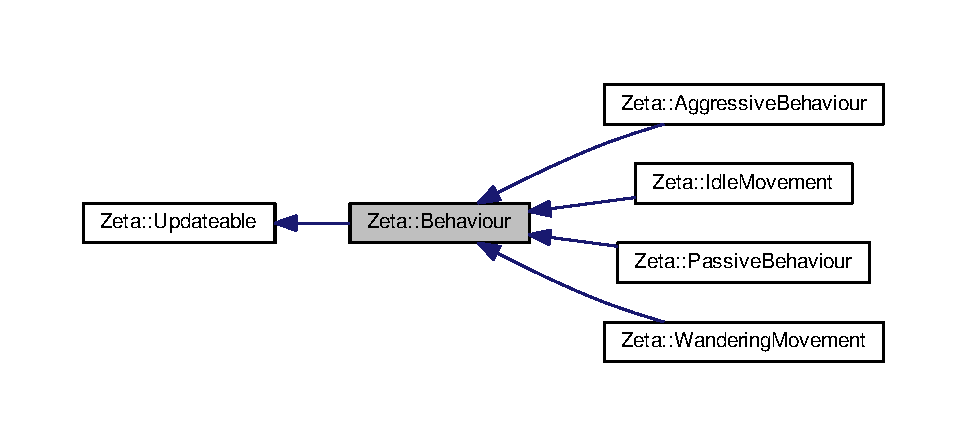
\includegraphics[width=350pt]{classZeta_1_1Behaviour__inherit__graph}
\end{center}
\end{figure}


Collaboration diagram for Zeta\+:\+:Behaviour\+:
\nopagebreak
\begin{figure}[H]
\begin{center}
\leavevmode
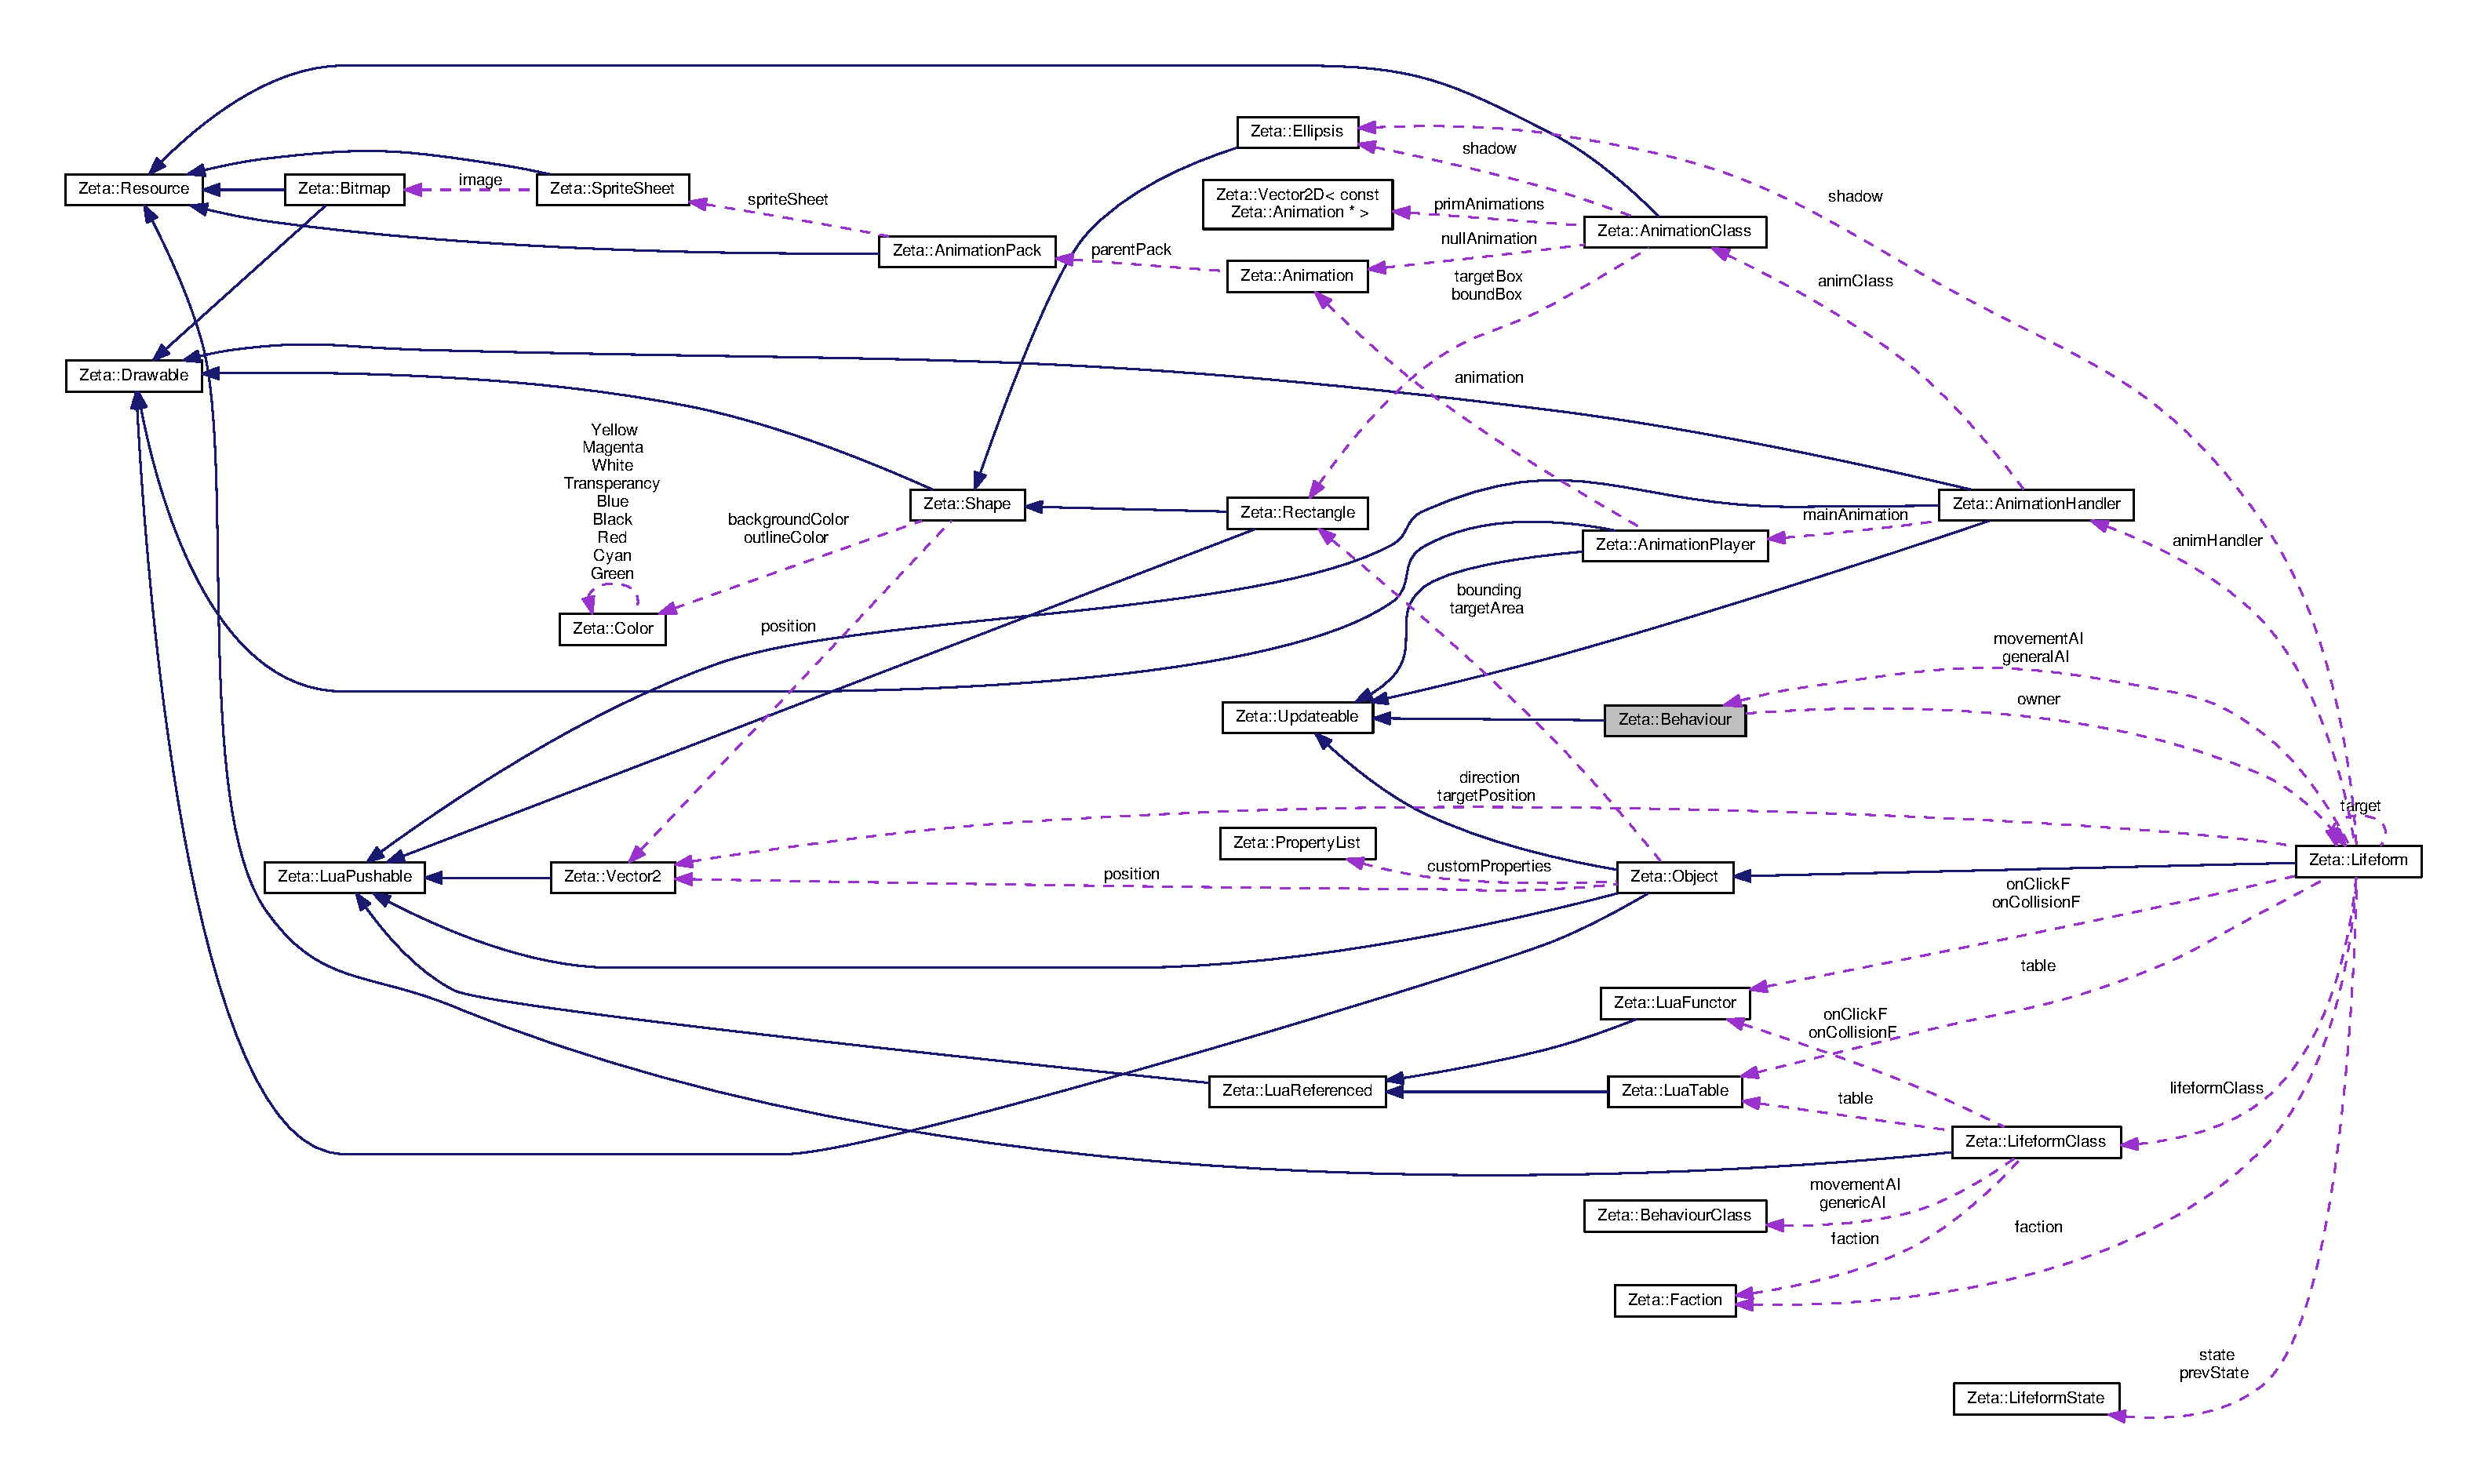
\includegraphics[width=350pt]{classZeta_1_1Behaviour__coll__graph}
\end{center}
\end{figure}
\subsection*{Public Member Functions}
\begin{DoxyCompactItemize}
\item 
virtual void \hyperlink{classZeta_1_1Behaviour_ac8c86b2e91f99441ee2e7de54e7d17d9}{on\+Death} ()=0
\item 
\hyperlink{classZeta_1_1Behaviour_a31a2749e194ed8344ba3fd136a5fa44f}{Behaviour} (\hyperlink{classZeta_1_1Lifeform}{Lifeform} \&\hyperlink{classZeta_1_1Behaviour_ad32d56994e4e09e01ef86bcbb5c85e0a}{owner})
\item 
virtual \hyperlink{classZeta_1_1Behaviour_a1571d412ef383378054ae8a3098d3820}{$\sim$\+Behaviour} ()
\end{DoxyCompactItemize}
\subsection*{Protected Attributes}
\begin{DoxyCompactItemize}
\item 
\hyperlink{classZeta_1_1Lifeform}{Lifeform} $\ast$ \hyperlink{classZeta_1_1Behaviour_ad32d56994e4e09e01ef86bcbb5c85e0a}{owner}
\end{DoxyCompactItemize}


\subsection{Constructor \& Destructor Documentation}
\hypertarget{classZeta_1_1Behaviour_a31a2749e194ed8344ba3fd136a5fa44f}{\index{Zeta\+::\+Behaviour@{Zeta\+::\+Behaviour}!Behaviour@{Behaviour}}
\index{Behaviour@{Behaviour}!Zeta\+::\+Behaviour@{Zeta\+::\+Behaviour}}
\subsubsection[{Behaviour}]{\setlength{\rightskip}{0pt plus 5cm}Zeta\+::\+Behaviour\+::\+Behaviour (
\begin{DoxyParamCaption}
\item[{{\bf Lifeform} \&}]{owner}
\end{DoxyParamCaption}
)\hspace{0.3cm}{\ttfamily [inline]}}}\label{classZeta_1_1Behaviour_a31a2749e194ed8344ba3fd136a5fa44f}
\hypertarget{classZeta_1_1Behaviour_a1571d412ef383378054ae8a3098d3820}{\index{Zeta\+::\+Behaviour@{Zeta\+::\+Behaviour}!````~Behaviour@{$\sim$\+Behaviour}}
\index{````~Behaviour@{$\sim$\+Behaviour}!Zeta\+::\+Behaviour@{Zeta\+::\+Behaviour}}
\subsubsection[{$\sim$\+Behaviour}]{\setlength{\rightskip}{0pt plus 5cm}virtual Zeta\+::\+Behaviour\+::$\sim$\+Behaviour (
\begin{DoxyParamCaption}
{}
\end{DoxyParamCaption}
)\hspace{0.3cm}{\ttfamily [inline]}, {\ttfamily [virtual]}}}\label{classZeta_1_1Behaviour_a1571d412ef383378054ae8a3098d3820}


\subsection{Member Function Documentation}
\hypertarget{classZeta_1_1Behaviour_ac8c86b2e91f99441ee2e7de54e7d17d9}{\index{Zeta\+::\+Behaviour@{Zeta\+::\+Behaviour}!on\+Death@{on\+Death}}
\index{on\+Death@{on\+Death}!Zeta\+::\+Behaviour@{Zeta\+::\+Behaviour}}
\subsubsection[{on\+Death}]{\setlength{\rightskip}{0pt plus 5cm}virtual void Zeta\+::\+Behaviour\+::on\+Death (
\begin{DoxyParamCaption}
{}
\end{DoxyParamCaption}
)\hspace{0.3cm}{\ttfamily [pure virtual]}}}\label{classZeta_1_1Behaviour_ac8c86b2e91f99441ee2e7de54e7d17d9}


Implemented in \hyperlink{classZeta_1_1WanderingMovement_a1940a0d9b48694a37c4cd022646c3af1}{Zeta\+::\+Wandering\+Movement}, \hyperlink{classZeta_1_1IdleMovement_ac56edecbac5c0e75e90a7933c24ead62}{Zeta\+::\+Idle\+Movement}, \hyperlink{classZeta_1_1PassiveBehaviour_a75e470e40f36e747eee57a1eb5f903f0}{Zeta\+::\+Passive\+Behaviour}, and \hyperlink{classZeta_1_1AggressiveBehaviour_a7ebb4cd0f618f9dd9e1e723e77aac292}{Zeta\+::\+Aggressive\+Behaviour}.



\subsection{Member Data Documentation}
\hypertarget{classZeta_1_1Behaviour_ad32d56994e4e09e01ef86bcbb5c85e0a}{\index{Zeta\+::\+Behaviour@{Zeta\+::\+Behaviour}!owner@{owner}}
\index{owner@{owner}!Zeta\+::\+Behaviour@{Zeta\+::\+Behaviour}}
\subsubsection[{owner}]{\setlength{\rightskip}{0pt plus 5cm}{\bf Lifeform}$\ast$ Zeta\+::\+Behaviour\+::owner\hspace{0.3cm}{\ttfamily [protected]}}}\label{classZeta_1_1Behaviour_ad32d56994e4e09e01ef86bcbb5c85e0a}


The documentation for this class was generated from the following file\+:\begin{DoxyCompactItemize}
\item 
include/\+Zeta/\+Core/\+R\+P\+G\+Classes/\+A\+I/\hyperlink{Behaviour_8hpp}{Behaviour.\+hpp}\end{DoxyCompactItemize}

\hypertarget{classZeta_1_1BehaviourClass}{\section{Zeta\+:\+:Behaviour\+Class Class Reference}
\label{classZeta_1_1BehaviourClass}\index{Zeta\+::\+Behaviour\+Class@{Zeta\+::\+Behaviour\+Class}}
}


{\ttfamily \#include $<$Behaviour\+Class.\+hpp$>$}



Inheritance diagram for Zeta\+:\+:Behaviour\+Class\+:\nopagebreak
\begin{figure}[H]
\begin{center}
\leavevmode
\includegraphics[width=350pt]{classZeta_1_1BehaviourClass__inherit__graph}
\end{center}
\end{figure}
\subsection*{Public Member Functions}
\begin{DoxyCompactItemize}
\item 
virtual \hyperlink{classZeta_1_1Behaviour}{Behaviour} $\ast$ \hyperlink{classZeta_1_1BehaviourClass_aeaf604f49cc95501422dfd177de64287}{get\+New\+Behaviour} (\hyperlink{classZeta_1_1Lifeform}{Lifeform} \&owner) const =0
\item 
\hyperlink{classZeta_1_1BehaviourClass_a260d021f1fcd5494303e7fcbf78b3428}{Behaviour\+Class} ()
\item 
virtual \hyperlink{classZeta_1_1BehaviourClass_abcb609496d577d3fa9da748c130813d6}{$\sim$\+Behaviour\+Class} ()
\end{DoxyCompactItemize}


\subsection{Constructor \& Destructor Documentation}
\hypertarget{classZeta_1_1BehaviourClass_a260d021f1fcd5494303e7fcbf78b3428}{\index{Zeta\+::\+Behaviour\+Class@{Zeta\+::\+Behaviour\+Class}!Behaviour\+Class@{Behaviour\+Class}}
\index{Behaviour\+Class@{Behaviour\+Class}!Zeta\+::\+Behaviour\+Class@{Zeta\+::\+Behaviour\+Class}}
\subsubsection[{Behaviour\+Class}]{\setlength{\rightskip}{0pt plus 5cm}Zeta\+::\+Behaviour\+Class\+::\+Behaviour\+Class (
\begin{DoxyParamCaption}
{}
\end{DoxyParamCaption}
)\hspace{0.3cm}{\ttfamily [inline]}}}\label{classZeta_1_1BehaviourClass_a260d021f1fcd5494303e7fcbf78b3428}
\hypertarget{classZeta_1_1BehaviourClass_abcb609496d577d3fa9da748c130813d6}{\index{Zeta\+::\+Behaviour\+Class@{Zeta\+::\+Behaviour\+Class}!````~Behaviour\+Class@{$\sim$\+Behaviour\+Class}}
\index{````~Behaviour\+Class@{$\sim$\+Behaviour\+Class}!Zeta\+::\+Behaviour\+Class@{Zeta\+::\+Behaviour\+Class}}
\subsubsection[{$\sim$\+Behaviour\+Class}]{\setlength{\rightskip}{0pt plus 5cm}virtual Zeta\+::\+Behaviour\+Class\+::$\sim$\+Behaviour\+Class (
\begin{DoxyParamCaption}
{}
\end{DoxyParamCaption}
)\hspace{0.3cm}{\ttfamily [inline]}, {\ttfamily [virtual]}}}\label{classZeta_1_1BehaviourClass_abcb609496d577d3fa9da748c130813d6}


\subsection{Member Function Documentation}
\hypertarget{classZeta_1_1BehaviourClass_aeaf604f49cc95501422dfd177de64287}{\index{Zeta\+::\+Behaviour\+Class@{Zeta\+::\+Behaviour\+Class}!get\+New\+Behaviour@{get\+New\+Behaviour}}
\index{get\+New\+Behaviour@{get\+New\+Behaviour}!Zeta\+::\+Behaviour\+Class@{Zeta\+::\+Behaviour\+Class}}
\subsubsection[{get\+New\+Behaviour}]{\setlength{\rightskip}{0pt plus 5cm}virtual {\bf Behaviour}$\ast$ Zeta\+::\+Behaviour\+Class\+::get\+New\+Behaviour (
\begin{DoxyParamCaption}
\item[{{\bf Lifeform} \&}]{owner}
\end{DoxyParamCaption}
) const\hspace{0.3cm}{\ttfamily [pure virtual]}}}\label{classZeta_1_1BehaviourClass_aeaf604f49cc95501422dfd177de64287}


Implemented in \hyperlink{classZeta_1_1AggressiveBehaviourClass_a94e8ce28a8c07370b144ac050f447823}{Zeta\+::\+Aggressive\+Behaviour\+Class}, \hyperlink{classZeta_1_1WanderingMovementClass_a3b2cfba3c84bd5cdd892c09d8fd8a0fd}{Zeta\+::\+Wandering\+Movement\+Class}, \hyperlink{classZeta_1_1IdleMovementClass_a4ba32888d1561f7b5820d2620e7762e9}{Zeta\+::\+Idle\+Movement\+Class}, and \hyperlink{classZeta_1_1PassiveBehaviourClass_a1923b88aff0a6ec1e902f8820c6e4c3f}{Zeta\+::\+Passive\+Behaviour\+Class}.



The documentation for this class was generated from the following file\+:\begin{DoxyCompactItemize}
\item 
include/\+Zeta/\+Core/\+R\+P\+G\+Classes/\+A\+I/\hyperlink{BehaviourClass_8hpp}{Behaviour\+Class.\+hpp}\end{DoxyCompactItemize}

\hypertarget{classZeta_1_1Bitmap}{\section{Zeta\+:\+:Bitmap Class Reference}
\label{classZeta_1_1Bitmap}\index{Zeta\+::\+Bitmap@{Zeta\+::\+Bitmap}}
}


{\ttfamily \#include $<$Bitmap.\+hpp$>$}



Inheritance diagram for Zeta\+:\+:Bitmap\+:\nopagebreak
\begin{figure}[H]
\begin{center}
\leavevmode
\includegraphics[width=265pt]{classZeta_1_1Bitmap__inherit__graph}
\end{center}
\end{figure}


Collaboration diagram for Zeta\+:\+:Bitmap\+:\nopagebreak
\begin{figure}[H]
\begin{center}
\leavevmode
\includegraphics[width=265pt]{classZeta_1_1Bitmap__coll__graph}
\end{center}
\end{figure}
\subsection*{Public Types}
\begin{DoxyCompactItemize}
\item 
enum \hyperlink{classZeta_1_1Bitmap_a8cb28cf4226b7d6bedf6c9bb2413b3fa}{Flip\+Flag} \{ \hyperlink{classZeta_1_1Bitmap_a8cb28cf4226b7d6bedf6c9bb2413b3faad95504740b4fa9384ac72564cd282755}{Normal}, 
\hyperlink{classZeta_1_1Bitmap_a8cb28cf4226b7d6bedf6c9bb2413b3faaf348b571904c666b29639666ab027697}{Fliped\+\_\+\+Horizontaly}, 
\hyperlink{classZeta_1_1Bitmap_a8cb28cf4226b7d6bedf6c9bb2413b3faaac56c661dd220f5f9dd9b79fc5cf53de}{Fliped\+\_\+\+Verticaly}, 
\hyperlink{classZeta_1_1Bitmap_a8cb28cf4226b7d6bedf6c9bb2413b3faa8593d3469b4055679283171c09dba43d}{Fliped\+\_\+\+Both}
 \}
\end{DoxyCompactItemize}
\subsection*{Public Member Functions}
\begin{DoxyCompactItemize}
\item 
int \hyperlink{classZeta_1_1Bitmap_a5b41472f13ef2763ef6c4c6e85a706da}{get\+Width} () const 
\item 
int \hyperlink{classZeta_1_1Bitmap_ae35e49275691a0b9a5b67b5fb906941b}{get\+Height} () const 
\item 
virtual void \hyperlink{classZeta_1_1Bitmap_a2a5af6ab1c1237efe52d155fe63e24b7}{draw} (\hyperlink{namespaceZeta_a1e0a1265f9b3bd3075fb0fabd39088ba}{Float} x, \hyperlink{namespaceZeta_a1e0a1265f9b3bd3075fb0fabd39088ba}{Float} y, \hyperlink{namespaceZeta_a1e0a1265f9b3bd3075fb0fabd39088ba}{Float} rotation, \hyperlink{namespaceZeta_a1e0a1265f9b3bd3075fb0fabd39088ba}{Float} scale, \hyperlink{classZeta_1_1Bitmap_a8cb28cf4226b7d6bedf6c9bb2413b3fa}{Flip\+Flag} flip=\hyperlink{classZeta_1_1Bitmap_a8cb28cf4226b7d6bedf6c9bb2413b3faad95504740b4fa9384ac72564cd282755}{Normal}) const =0
\item 
virtual void \hyperlink{classZeta_1_1Bitmap_af06b42874ae626ca8e403c478fab46e9}{draw\+At\+Centre} (\hyperlink{namespaceZeta_a1e0a1265f9b3bd3075fb0fabd39088ba}{Float} x, \hyperlink{namespaceZeta_a1e0a1265f9b3bd3075fb0fabd39088ba}{Float} y, \hyperlink{namespaceZeta_a1e0a1265f9b3bd3075fb0fabd39088ba}{Float} rotation, \hyperlink{namespaceZeta_a1e0a1265f9b3bd3075fb0fabd39088ba}{Float} scale, \hyperlink{classZeta_1_1Bitmap_a8cb28cf4226b7d6bedf6c9bb2413b3fa}{Flip\+Flag} flip=\hyperlink{classZeta_1_1Bitmap_a8cb28cf4226b7d6bedf6c9bb2413b3faad95504740b4fa9384ac72564cd282755}{Normal}) const =0
\item 
virtual \hyperlink{classZeta_1_1Bitmap}{Bitmap} \& \hyperlink{classZeta_1_1Bitmap_a790614f445f0c59f9533ed1d4046dd74}{create\+Sub\+Bitmap} (int x, int y, int \hyperlink{classZeta_1_1Bitmap_affa526cccd51b4ac5db7aac25ff7f6a9}{width}, int \hyperlink{classZeta_1_1Bitmap_a4d9a82acc6c418dc9b72227b0d63d9aa}{height}) const =0
\item 
virtual void \hyperlink{classZeta_1_1Bitmap_acaef132548ff57ccdc725b864a1150b8}{erase\+Sub\+Bitmap} (\hyperlink{classZeta_1_1Bitmap}{Bitmap} \&bitmap) const =0
\item 
virtual void \hyperlink{classZeta_1_1Bitmap_afc49ceff653f55699fe7b723eb6193ae}{reserve\+Sub\+Bitmaps} (size\+\_\+t number) const =0
\item 
\hyperlink{classZeta_1_1Bitmap_add684ebb8c0f5dc04376eb1ed760f8b7}{Bitmap} (\hyperlink{classZeta_1_1Bitmap}{Bitmap} \&\&)=default
\item 
\hyperlink{classZeta_1_1Bitmap}{Bitmap} \& \hyperlink{classZeta_1_1Bitmap_ace6923621ad08915460c840f12ec701a}{operator=} (\hyperlink{classZeta_1_1Bitmap}{Bitmap} \&\&)=default
\item 
\hyperlink{classZeta_1_1Bitmap_aa2abefaeb9204d8f0184c036984f8b2d}{Bitmap} (const std\+::string \&path)
\item 
\hyperlink{classZeta_1_1Bitmap_a1338d6c3b7eb2be1dccb247fbf9728c2}{Bitmap} (int \hyperlink{classZeta_1_1Bitmap_affa526cccd51b4ac5db7aac25ff7f6a9}{width}, int \hyperlink{classZeta_1_1Bitmap_a4d9a82acc6c418dc9b72227b0d63d9aa}{height})
\item 
virtual \hyperlink{classZeta_1_1Bitmap_a2a62cac74fb6f69afc519b026c63cb17}{$\sim$\+Bitmap} ()
\end{DoxyCompactItemize}
\subsection*{Protected Attributes}
\begin{DoxyCompactItemize}
\item 
int \hyperlink{classZeta_1_1Bitmap_affa526cccd51b4ac5db7aac25ff7f6a9}{width}
\item 
int \hyperlink{classZeta_1_1Bitmap_a4d9a82acc6c418dc9b72227b0d63d9aa}{height}
\end{DoxyCompactItemize}


\subsection{Member Enumeration Documentation}
\hypertarget{classZeta_1_1Bitmap_a8cb28cf4226b7d6bedf6c9bb2413b3fa}{\index{Zeta\+::\+Bitmap@{Zeta\+::\+Bitmap}!Flip\+Flag@{Flip\+Flag}}
\index{Flip\+Flag@{Flip\+Flag}!Zeta\+::\+Bitmap@{Zeta\+::\+Bitmap}}
\subsubsection[{Flip\+Flag}]{\setlength{\rightskip}{0pt plus 5cm}enum {\bf Zeta\+::\+Bitmap\+::\+Flip\+Flag}}}\label{classZeta_1_1Bitmap_a8cb28cf4226b7d6bedf6c9bb2413b3fa}
\begin{Desc}
\item[Enumerator]\par
\begin{description}
\index{Normal@{Normal}!Zeta\+::\+Bitmap@{Zeta\+::\+Bitmap}}\index{Zeta\+::\+Bitmap@{Zeta\+::\+Bitmap}!Normal@{Normal}}\item[{\em 
\hypertarget{classZeta_1_1Bitmap_a8cb28cf4226b7d6bedf6c9bb2413b3faad95504740b4fa9384ac72564cd282755}{Normal}\label{classZeta_1_1Bitmap_a8cb28cf4226b7d6bedf6c9bb2413b3faad95504740b4fa9384ac72564cd282755}
}]\index{Fliped\+\_\+\+Horizontaly@{Fliped\+\_\+\+Horizontaly}!Zeta\+::\+Bitmap@{Zeta\+::\+Bitmap}}\index{Zeta\+::\+Bitmap@{Zeta\+::\+Bitmap}!Fliped\+\_\+\+Horizontaly@{Fliped\+\_\+\+Horizontaly}}\item[{\em 
\hypertarget{classZeta_1_1Bitmap_a8cb28cf4226b7d6bedf6c9bb2413b3faaf348b571904c666b29639666ab027697}{Fliped\+\_\+\+Horizontaly}\label{classZeta_1_1Bitmap_a8cb28cf4226b7d6bedf6c9bb2413b3faaf348b571904c666b29639666ab027697}
}]\index{Fliped\+\_\+\+Verticaly@{Fliped\+\_\+\+Verticaly}!Zeta\+::\+Bitmap@{Zeta\+::\+Bitmap}}\index{Zeta\+::\+Bitmap@{Zeta\+::\+Bitmap}!Fliped\+\_\+\+Verticaly@{Fliped\+\_\+\+Verticaly}}\item[{\em 
\hypertarget{classZeta_1_1Bitmap_a8cb28cf4226b7d6bedf6c9bb2413b3faaac56c661dd220f5f9dd9b79fc5cf53de}{Fliped\+\_\+\+Verticaly}\label{classZeta_1_1Bitmap_a8cb28cf4226b7d6bedf6c9bb2413b3faaac56c661dd220f5f9dd9b79fc5cf53de}
}]\index{Fliped\+\_\+\+Both@{Fliped\+\_\+\+Both}!Zeta\+::\+Bitmap@{Zeta\+::\+Bitmap}}\index{Zeta\+::\+Bitmap@{Zeta\+::\+Bitmap}!Fliped\+\_\+\+Both@{Fliped\+\_\+\+Both}}\item[{\em 
\hypertarget{classZeta_1_1Bitmap_a8cb28cf4226b7d6bedf6c9bb2413b3faa8593d3469b4055679283171c09dba43d}{Fliped\+\_\+\+Both}\label{classZeta_1_1Bitmap_a8cb28cf4226b7d6bedf6c9bb2413b3faa8593d3469b4055679283171c09dba43d}
}]\end{description}
\end{Desc}


\subsection{Constructor \& Destructor Documentation}
\hypertarget{classZeta_1_1Bitmap_add684ebb8c0f5dc04376eb1ed760f8b7}{\index{Zeta\+::\+Bitmap@{Zeta\+::\+Bitmap}!Bitmap@{Bitmap}}
\index{Bitmap@{Bitmap}!Zeta\+::\+Bitmap@{Zeta\+::\+Bitmap}}
\subsubsection[{Bitmap}]{\setlength{\rightskip}{0pt plus 5cm}Zeta\+::\+Bitmap\+::\+Bitmap (
\begin{DoxyParamCaption}
\item[{{\bf Bitmap} \&\&}]{}
\end{DoxyParamCaption}
)\hspace{0.3cm}{\ttfamily [default]}}}\label{classZeta_1_1Bitmap_add684ebb8c0f5dc04376eb1ed760f8b7}
\hypertarget{classZeta_1_1Bitmap_aa2abefaeb9204d8f0184c036984f8b2d}{\index{Zeta\+::\+Bitmap@{Zeta\+::\+Bitmap}!Bitmap@{Bitmap}}
\index{Bitmap@{Bitmap}!Zeta\+::\+Bitmap@{Zeta\+::\+Bitmap}}
\subsubsection[{Bitmap}]{\setlength{\rightskip}{0pt plus 5cm}Zeta\+::\+Bitmap\+::\+Bitmap (
\begin{DoxyParamCaption}
\item[{const std\+::string \&}]{path}
\end{DoxyParamCaption}
)\hspace{0.3cm}{\ttfamily [inline]}}}\label{classZeta_1_1Bitmap_aa2abefaeb9204d8f0184c036984f8b2d}
\hypertarget{classZeta_1_1Bitmap_a1338d6c3b7eb2be1dccb247fbf9728c2}{\index{Zeta\+::\+Bitmap@{Zeta\+::\+Bitmap}!Bitmap@{Bitmap}}
\index{Bitmap@{Bitmap}!Zeta\+::\+Bitmap@{Zeta\+::\+Bitmap}}
\subsubsection[{Bitmap}]{\setlength{\rightskip}{0pt plus 5cm}Zeta\+::\+Bitmap\+::\+Bitmap (
\begin{DoxyParamCaption}
\item[{int}]{width, }
\item[{int}]{height}
\end{DoxyParamCaption}
)\hspace{0.3cm}{\ttfamily [inline]}}}\label{classZeta_1_1Bitmap_a1338d6c3b7eb2be1dccb247fbf9728c2}
\hypertarget{classZeta_1_1Bitmap_a2a62cac74fb6f69afc519b026c63cb17}{\index{Zeta\+::\+Bitmap@{Zeta\+::\+Bitmap}!````~Bitmap@{$\sim$\+Bitmap}}
\index{````~Bitmap@{$\sim$\+Bitmap}!Zeta\+::\+Bitmap@{Zeta\+::\+Bitmap}}
\subsubsection[{$\sim$\+Bitmap}]{\setlength{\rightskip}{0pt plus 5cm}virtual Zeta\+::\+Bitmap\+::$\sim$\+Bitmap (
\begin{DoxyParamCaption}
{}
\end{DoxyParamCaption}
)\hspace{0.3cm}{\ttfamily [inline]}, {\ttfamily [virtual]}}}\label{classZeta_1_1Bitmap_a2a62cac74fb6f69afc519b026c63cb17}


\subsection{Member Function Documentation}
\hypertarget{classZeta_1_1Bitmap_a790614f445f0c59f9533ed1d4046dd74}{\index{Zeta\+::\+Bitmap@{Zeta\+::\+Bitmap}!create\+Sub\+Bitmap@{create\+Sub\+Bitmap}}
\index{create\+Sub\+Bitmap@{create\+Sub\+Bitmap}!Zeta\+::\+Bitmap@{Zeta\+::\+Bitmap}}
\subsubsection[{create\+Sub\+Bitmap}]{\setlength{\rightskip}{0pt plus 5cm}virtual {\bf Bitmap}\& Zeta\+::\+Bitmap\+::create\+Sub\+Bitmap (
\begin{DoxyParamCaption}
\item[{int}]{x, }
\item[{int}]{y, }
\item[{int}]{width, }
\item[{int}]{height}
\end{DoxyParamCaption}
) const\hspace{0.3cm}{\ttfamily [pure virtual]}}}\label{classZeta_1_1Bitmap_a790614f445f0c59f9533ed1d4046dd74}


Implemented in \hyperlink{classZeta_1_1AllegroBitmap_a92c61e54a550c9756b5567a20625c31d}{Zeta\+::\+Allegro\+Bitmap}.

\hypertarget{classZeta_1_1Bitmap_a2a5af6ab1c1237efe52d155fe63e24b7}{\index{Zeta\+::\+Bitmap@{Zeta\+::\+Bitmap}!draw@{draw}}
\index{draw@{draw}!Zeta\+::\+Bitmap@{Zeta\+::\+Bitmap}}
\subsubsection[{draw}]{\setlength{\rightskip}{0pt plus 5cm}virtual void Zeta\+::\+Bitmap\+::draw (
\begin{DoxyParamCaption}
\item[{{\bf Float}}]{x, }
\item[{{\bf Float}}]{y, }
\item[{{\bf Float}}]{rotation, }
\item[{{\bf Float}}]{scale, }
\item[{{\bf Flip\+Flag}}]{flip = {\ttfamily {\bf Normal}}}
\end{DoxyParamCaption}
) const\hspace{0.3cm}{\ttfamily [pure virtual]}}}\label{classZeta_1_1Bitmap_a2a5af6ab1c1237efe52d155fe63e24b7}


Implemented in \hyperlink{classZeta_1_1AllegroBitmap_a26b3206d585a5f30b990c1279eb92e7a}{Zeta\+::\+Allegro\+Bitmap}.

\hypertarget{classZeta_1_1Bitmap_af06b42874ae626ca8e403c478fab46e9}{\index{Zeta\+::\+Bitmap@{Zeta\+::\+Bitmap}!draw\+At\+Centre@{draw\+At\+Centre}}
\index{draw\+At\+Centre@{draw\+At\+Centre}!Zeta\+::\+Bitmap@{Zeta\+::\+Bitmap}}
\subsubsection[{draw\+At\+Centre}]{\setlength{\rightskip}{0pt plus 5cm}virtual void Zeta\+::\+Bitmap\+::draw\+At\+Centre (
\begin{DoxyParamCaption}
\item[{{\bf Float}}]{x, }
\item[{{\bf Float}}]{y, }
\item[{{\bf Float}}]{rotation, }
\item[{{\bf Float}}]{scale, }
\item[{{\bf Flip\+Flag}}]{flip = {\ttfamily {\bf Normal}}}
\end{DoxyParamCaption}
) const\hspace{0.3cm}{\ttfamily [pure virtual]}}}\label{classZeta_1_1Bitmap_af06b42874ae626ca8e403c478fab46e9}


Implemented in \hyperlink{classZeta_1_1AllegroBitmap_ac914238cb9e48e6f3e4260f7c62b40f8}{Zeta\+::\+Allegro\+Bitmap}.

\hypertarget{classZeta_1_1Bitmap_acaef132548ff57ccdc725b864a1150b8}{\index{Zeta\+::\+Bitmap@{Zeta\+::\+Bitmap}!erase\+Sub\+Bitmap@{erase\+Sub\+Bitmap}}
\index{erase\+Sub\+Bitmap@{erase\+Sub\+Bitmap}!Zeta\+::\+Bitmap@{Zeta\+::\+Bitmap}}
\subsubsection[{erase\+Sub\+Bitmap}]{\setlength{\rightskip}{0pt plus 5cm}virtual void Zeta\+::\+Bitmap\+::erase\+Sub\+Bitmap (
\begin{DoxyParamCaption}
\item[{{\bf Bitmap} \&}]{bitmap}
\end{DoxyParamCaption}
) const\hspace{0.3cm}{\ttfamily [pure virtual]}}}\label{classZeta_1_1Bitmap_acaef132548ff57ccdc725b864a1150b8}


Implemented in \hyperlink{classZeta_1_1AllegroBitmap_a2e7d04979e1c34a3d1c320ba67c429d2}{Zeta\+::\+Allegro\+Bitmap}.

\hypertarget{classZeta_1_1Bitmap_ae35e49275691a0b9a5b67b5fb906941b}{\index{Zeta\+::\+Bitmap@{Zeta\+::\+Bitmap}!get\+Height@{get\+Height}}
\index{get\+Height@{get\+Height}!Zeta\+::\+Bitmap@{Zeta\+::\+Bitmap}}
\subsubsection[{get\+Height}]{\setlength{\rightskip}{0pt plus 5cm}int Zeta\+::\+Bitmap\+::get\+Height (
\begin{DoxyParamCaption}
{}
\end{DoxyParamCaption}
) const\hspace{0.3cm}{\ttfamily [inline]}}}\label{classZeta_1_1Bitmap_ae35e49275691a0b9a5b67b5fb906941b}
\hypertarget{classZeta_1_1Bitmap_a5b41472f13ef2763ef6c4c6e85a706da}{\index{Zeta\+::\+Bitmap@{Zeta\+::\+Bitmap}!get\+Width@{get\+Width}}
\index{get\+Width@{get\+Width}!Zeta\+::\+Bitmap@{Zeta\+::\+Bitmap}}
\subsubsection[{get\+Width}]{\setlength{\rightskip}{0pt plus 5cm}int Zeta\+::\+Bitmap\+::get\+Width (
\begin{DoxyParamCaption}
{}
\end{DoxyParamCaption}
) const\hspace{0.3cm}{\ttfamily [inline]}}}\label{classZeta_1_1Bitmap_a5b41472f13ef2763ef6c4c6e85a706da}
\hypertarget{classZeta_1_1Bitmap_ace6923621ad08915460c840f12ec701a}{\index{Zeta\+::\+Bitmap@{Zeta\+::\+Bitmap}!operator=@{operator=}}
\index{operator=@{operator=}!Zeta\+::\+Bitmap@{Zeta\+::\+Bitmap}}
\subsubsection[{operator=}]{\setlength{\rightskip}{0pt plus 5cm}{\bf Bitmap}\& Zeta\+::\+Bitmap\+::operator= (
\begin{DoxyParamCaption}
\item[{{\bf Bitmap} \&\&}]{}
\end{DoxyParamCaption}
)\hspace{0.3cm}{\ttfamily [default]}}}\label{classZeta_1_1Bitmap_ace6923621ad08915460c840f12ec701a}
\hypertarget{classZeta_1_1Bitmap_afc49ceff653f55699fe7b723eb6193ae}{\index{Zeta\+::\+Bitmap@{Zeta\+::\+Bitmap}!reserve\+Sub\+Bitmaps@{reserve\+Sub\+Bitmaps}}
\index{reserve\+Sub\+Bitmaps@{reserve\+Sub\+Bitmaps}!Zeta\+::\+Bitmap@{Zeta\+::\+Bitmap}}
\subsubsection[{reserve\+Sub\+Bitmaps}]{\setlength{\rightskip}{0pt plus 5cm}virtual void Zeta\+::\+Bitmap\+::reserve\+Sub\+Bitmaps (
\begin{DoxyParamCaption}
\item[{size\+\_\+t}]{number}
\end{DoxyParamCaption}
) const\hspace{0.3cm}{\ttfamily [pure virtual]}}}\label{classZeta_1_1Bitmap_afc49ceff653f55699fe7b723eb6193ae}


Implemented in \hyperlink{classZeta_1_1AllegroBitmap_ac37c6b783f388afe960479b9addcf0a7}{Zeta\+::\+Allegro\+Bitmap}.



\subsection{Member Data Documentation}
\hypertarget{classZeta_1_1Bitmap_a4d9a82acc6c418dc9b72227b0d63d9aa}{\index{Zeta\+::\+Bitmap@{Zeta\+::\+Bitmap}!height@{height}}
\index{height@{height}!Zeta\+::\+Bitmap@{Zeta\+::\+Bitmap}}
\subsubsection[{height}]{\setlength{\rightskip}{0pt plus 5cm}int Zeta\+::\+Bitmap\+::height\hspace{0.3cm}{\ttfamily [protected]}}}\label{classZeta_1_1Bitmap_a4d9a82acc6c418dc9b72227b0d63d9aa}
\hypertarget{classZeta_1_1Bitmap_affa526cccd51b4ac5db7aac25ff7f6a9}{\index{Zeta\+::\+Bitmap@{Zeta\+::\+Bitmap}!width@{width}}
\index{width@{width}!Zeta\+::\+Bitmap@{Zeta\+::\+Bitmap}}
\subsubsection[{width}]{\setlength{\rightskip}{0pt plus 5cm}int Zeta\+::\+Bitmap\+::width\hspace{0.3cm}{\ttfamily [protected]}}}\label{classZeta_1_1Bitmap_affa526cccd51b4ac5db7aac25ff7f6a9}


The documentation for this class was generated from the following file\+:\begin{DoxyCompactItemize}
\item 
include/\+Zeta/\+Core/\+Resource\+Classes/\hyperlink{Bitmap_8hpp}{Bitmap.\+hpp}\end{DoxyCompactItemize}

\hypertarget{classZeta_1_1SynchronousResourceContext_1_1BitmapLoadRequest}{\section{Zeta\+:\+:Synchronous\+Resource\+Context$<$ Bitmap\+T, Sound\+T $>$\+:\+:Bitmap\+Load\+Request Class Reference}
\label{classZeta_1_1SynchronousResourceContext_1_1BitmapLoadRequest}\index{Zeta\+::\+Synchronous\+Resource\+Context$<$ Bitmap\+T, Sound\+T $>$\+::\+Bitmap\+Load\+Request@{Zeta\+::\+Synchronous\+Resource\+Context$<$ Bitmap\+T, Sound\+T $>$\+::\+Bitmap\+Load\+Request}}
}


Inheritance diagram for Zeta\+:\+:Synchronous\+Resource\+Context$<$ Bitmap\+T, Sound\+T $>$\+:\+:Bitmap\+Load\+Request\+:\nopagebreak
\begin{figure}[H]
\begin{center}
\leavevmode
\includegraphics[width=220pt]{classZeta_1_1SynchronousResourceContext_1_1BitmapLoadRequest__inherit__graph}
\end{center}
\end{figure}


Collaboration diagram for Zeta\+:\+:Synchronous\+Resource\+Context$<$ Bitmap\+T, Sound\+T $>$\+:\+:Bitmap\+Load\+Request\+:\nopagebreak
\begin{figure}[H]
\begin{center}
\leavevmode
\includegraphics[width=346pt]{classZeta_1_1SynchronousResourceContext_1_1BitmapLoadRequest__coll__graph}
\end{center}
\end{figure}
\subsection*{Public Member Functions}
\begin{DoxyCompactItemize}
\item 
const std\+::string \& \hyperlink{classZeta_1_1SynchronousResourceContext_1_1BitmapLoadRequest_ab7cd162bdc01a896f43bb115b21c6503}{get\+Path} () const 
\item 
const \hyperlink{classZeta_1_1Bitmap}{Bitmap} \& \hyperlink{classZeta_1_1SynchronousResourceContext_1_1BitmapLoadRequest_a860dec69644bf5f78508285537b29796}{get\+Bitmap} () const 
\item 
void \hyperlink{classZeta_1_1SynchronousResourceContext_1_1BitmapLoadRequest_a1f89da097222c4dad665bdd6010919c8}{handle} (\hyperlink{classZeta_1_1RenderingContext}{Rendering\+Context} \&context)
\item 
\hyperlink{classZeta_1_1SynchronousResourceContext_1_1BitmapLoadRequest_ad1677ca9bf7b7f976e45e01b34f2a7a3}{Bitmap\+Load\+Request} (const std\+::string \&\hyperlink{classZeta_1_1SynchronousResourceContext_1_1BitmapLoadRequest_a4c4c292da6fd58426599a99034152002}{path})
\item 
\hyperlink{classZeta_1_1SynchronousResourceContext_1_1BitmapLoadRequest_a888d6fe21f82a92c74294200facdc9ff}{$\sim$\+Bitmap\+Load\+Request} ()
\end{DoxyCompactItemize}
\subsection*{Private Attributes}
\begin{DoxyCompactItemize}
\item 
std\+::string \hyperlink{classZeta_1_1SynchronousResourceContext_1_1BitmapLoadRequest_a4c4c292da6fd58426599a99034152002}{path}
\item 
const \hyperlink{classZeta_1_1Bitmap}{Bitmap} $\ast$ \hyperlink{classZeta_1_1SynchronousResourceContext_1_1BitmapLoadRequest_ae376e7355bdd78c46198009e88709c90}{bitmap}
\end{DoxyCompactItemize}
\subsection*{Additional Inherited Members}


\subsection{Constructor \& Destructor Documentation}
\hypertarget{classZeta_1_1SynchronousResourceContext_1_1BitmapLoadRequest_ad1677ca9bf7b7f976e45e01b34f2a7a3}{\index{Zeta\+::\+Synchronous\+Resource\+Context\+::\+Bitmap\+Load\+Request@{Zeta\+::\+Synchronous\+Resource\+Context\+::\+Bitmap\+Load\+Request}!Bitmap\+Load\+Request@{Bitmap\+Load\+Request}}
\index{Bitmap\+Load\+Request@{Bitmap\+Load\+Request}!Zeta\+::\+Synchronous\+Resource\+Context\+::\+Bitmap\+Load\+Request@{Zeta\+::\+Synchronous\+Resource\+Context\+::\+Bitmap\+Load\+Request}}
\subsubsection[{Bitmap\+Load\+Request}]{\setlength{\rightskip}{0pt plus 5cm}template$<$typename Bitmap\+T , typename Sound\+T $>$ {\bf Zeta\+::\+Synchronous\+Resource\+Context}$<$ Bitmap\+T, Sound\+T $>$\+::Bitmap\+Load\+Request\+::\+Bitmap\+Load\+Request (
\begin{DoxyParamCaption}
\item[{const std\+::string \&}]{path}
\end{DoxyParamCaption}
)\hspace{0.3cm}{\ttfamily [inline]}}}\label{classZeta_1_1SynchronousResourceContext_1_1BitmapLoadRequest_ad1677ca9bf7b7f976e45e01b34f2a7a3}
\hypertarget{classZeta_1_1SynchronousResourceContext_1_1BitmapLoadRequest_a888d6fe21f82a92c74294200facdc9ff}{\index{Zeta\+::\+Synchronous\+Resource\+Context\+::\+Bitmap\+Load\+Request@{Zeta\+::\+Synchronous\+Resource\+Context\+::\+Bitmap\+Load\+Request}!````~Bitmap\+Load\+Request@{$\sim$\+Bitmap\+Load\+Request}}
\index{````~Bitmap\+Load\+Request@{$\sim$\+Bitmap\+Load\+Request}!Zeta\+::\+Synchronous\+Resource\+Context\+::\+Bitmap\+Load\+Request@{Zeta\+::\+Synchronous\+Resource\+Context\+::\+Bitmap\+Load\+Request}}
\subsubsection[{$\sim$\+Bitmap\+Load\+Request}]{\setlength{\rightskip}{0pt plus 5cm}template$<$typename Bitmap\+T , typename Sound\+T $>$ {\bf Zeta\+::\+Synchronous\+Resource\+Context}$<$ Bitmap\+T, Sound\+T $>$\+::Bitmap\+Load\+Request\+::$\sim$\+Bitmap\+Load\+Request (
\begin{DoxyParamCaption}
{}
\end{DoxyParamCaption}
)\hspace{0.3cm}{\ttfamily [inline]}}}\label{classZeta_1_1SynchronousResourceContext_1_1BitmapLoadRequest_a888d6fe21f82a92c74294200facdc9ff}


\subsection{Member Function Documentation}
\hypertarget{classZeta_1_1SynchronousResourceContext_1_1BitmapLoadRequest_a860dec69644bf5f78508285537b29796}{\index{Zeta\+::\+Synchronous\+Resource\+Context\+::\+Bitmap\+Load\+Request@{Zeta\+::\+Synchronous\+Resource\+Context\+::\+Bitmap\+Load\+Request}!get\+Bitmap@{get\+Bitmap}}
\index{get\+Bitmap@{get\+Bitmap}!Zeta\+::\+Synchronous\+Resource\+Context\+::\+Bitmap\+Load\+Request@{Zeta\+::\+Synchronous\+Resource\+Context\+::\+Bitmap\+Load\+Request}}
\subsubsection[{get\+Bitmap}]{\setlength{\rightskip}{0pt plus 5cm}template$<$typename Bitmap\+T , typename Sound\+T $>$ const {\bf Bitmap}\& {\bf Zeta\+::\+Synchronous\+Resource\+Context}$<$ Bitmap\+T, Sound\+T $>$\+::Bitmap\+Load\+Request\+::get\+Bitmap (
\begin{DoxyParamCaption}
{}
\end{DoxyParamCaption}
) const\hspace{0.3cm}{\ttfamily [inline]}}}\label{classZeta_1_1SynchronousResourceContext_1_1BitmapLoadRequest_a860dec69644bf5f78508285537b29796}
\hypertarget{classZeta_1_1SynchronousResourceContext_1_1BitmapLoadRequest_ab7cd162bdc01a896f43bb115b21c6503}{\index{Zeta\+::\+Synchronous\+Resource\+Context\+::\+Bitmap\+Load\+Request@{Zeta\+::\+Synchronous\+Resource\+Context\+::\+Bitmap\+Load\+Request}!get\+Path@{get\+Path}}
\index{get\+Path@{get\+Path}!Zeta\+::\+Synchronous\+Resource\+Context\+::\+Bitmap\+Load\+Request@{Zeta\+::\+Synchronous\+Resource\+Context\+::\+Bitmap\+Load\+Request}}
\subsubsection[{get\+Path}]{\setlength{\rightskip}{0pt plus 5cm}template$<$typename Bitmap\+T , typename Sound\+T $>$ const std\+::string\& {\bf Zeta\+::\+Synchronous\+Resource\+Context}$<$ Bitmap\+T, Sound\+T $>$\+::Bitmap\+Load\+Request\+::get\+Path (
\begin{DoxyParamCaption}
{}
\end{DoxyParamCaption}
) const\hspace{0.3cm}{\ttfamily [inline]}}}\label{classZeta_1_1SynchronousResourceContext_1_1BitmapLoadRequest_ab7cd162bdc01a896f43bb115b21c6503}
\hypertarget{classZeta_1_1SynchronousResourceContext_1_1BitmapLoadRequest_a1f89da097222c4dad665bdd6010919c8}{\index{Zeta\+::\+Synchronous\+Resource\+Context\+::\+Bitmap\+Load\+Request@{Zeta\+::\+Synchronous\+Resource\+Context\+::\+Bitmap\+Load\+Request}!handle@{handle}}
\index{handle@{handle}!Zeta\+::\+Synchronous\+Resource\+Context\+::\+Bitmap\+Load\+Request@{Zeta\+::\+Synchronous\+Resource\+Context\+::\+Bitmap\+Load\+Request}}
\subsubsection[{handle}]{\setlength{\rightskip}{0pt plus 5cm}template$<$typename Bitmap\+T , typename Sound\+T $>$ void {\bf Zeta\+::\+Synchronous\+Resource\+Context}$<$ Bitmap\+T, Sound\+T $>$\+::Bitmap\+Load\+Request\+::handle (
\begin{DoxyParamCaption}
\item[{{\bf Rendering\+Context} \&}]{context}
\end{DoxyParamCaption}
)\hspace{0.3cm}{\ttfamily [inline]}, {\ttfamily [virtual]}}}\label{classZeta_1_1SynchronousResourceContext_1_1BitmapLoadRequest_a1f89da097222c4dad665bdd6010919c8}
Pure virtual member Function to be called by the Context\+Type 
\begin{DoxyParams}{Parameters}
{\em context} & the \hyperlink{classZeta_1_1Context}{Context} that called it \\
\hline
\end{DoxyParams}


Implements \hyperlink{classZeta_1_1ContextOperation_a3e7286287026324335d352933fb62a78}{Zeta\+::\+Context\+Operation$<$ Rendering\+Context $>$}.



Here is the call graph for this function\+:\nopagebreak
\begin{figure}[H]
\begin{center}
\leavevmode
\includegraphics[width=350pt]{classZeta_1_1SynchronousResourceContext_1_1BitmapLoadRequest_a1f89da097222c4dad665bdd6010919c8_cgraph}
\end{center}
\end{figure}




\subsection{Member Data Documentation}
\hypertarget{classZeta_1_1SynchronousResourceContext_1_1BitmapLoadRequest_ae376e7355bdd78c46198009e88709c90}{\index{Zeta\+::\+Synchronous\+Resource\+Context\+::\+Bitmap\+Load\+Request@{Zeta\+::\+Synchronous\+Resource\+Context\+::\+Bitmap\+Load\+Request}!bitmap@{bitmap}}
\index{bitmap@{bitmap}!Zeta\+::\+Synchronous\+Resource\+Context\+::\+Bitmap\+Load\+Request@{Zeta\+::\+Synchronous\+Resource\+Context\+::\+Bitmap\+Load\+Request}}
\subsubsection[{bitmap}]{\setlength{\rightskip}{0pt plus 5cm}template$<$typename Bitmap\+T , typename Sound\+T $>$ const {\bf Bitmap}$\ast$ {\bf Zeta\+::\+Synchronous\+Resource\+Context}$<$ Bitmap\+T, Sound\+T $>$\+::Bitmap\+Load\+Request\+::bitmap\hspace{0.3cm}{\ttfamily [private]}}}\label{classZeta_1_1SynchronousResourceContext_1_1BitmapLoadRequest_ae376e7355bdd78c46198009e88709c90}
\hypertarget{classZeta_1_1SynchronousResourceContext_1_1BitmapLoadRequest_a4c4c292da6fd58426599a99034152002}{\index{Zeta\+::\+Synchronous\+Resource\+Context\+::\+Bitmap\+Load\+Request@{Zeta\+::\+Synchronous\+Resource\+Context\+::\+Bitmap\+Load\+Request}!path@{path}}
\index{path@{path}!Zeta\+::\+Synchronous\+Resource\+Context\+::\+Bitmap\+Load\+Request@{Zeta\+::\+Synchronous\+Resource\+Context\+::\+Bitmap\+Load\+Request}}
\subsubsection[{path}]{\setlength{\rightskip}{0pt plus 5cm}template$<$typename Bitmap\+T , typename Sound\+T $>$ std\+::string {\bf Zeta\+::\+Synchronous\+Resource\+Context}$<$ Bitmap\+T, Sound\+T $>$\+::Bitmap\+Load\+Request\+::path\hspace{0.3cm}{\ttfamily [private]}}}\label{classZeta_1_1SynchronousResourceContext_1_1BitmapLoadRequest_a4c4c292da6fd58426599a99034152002}


The documentation for this class was generated from the following file\+:\begin{DoxyCompactItemize}
\item 
include/\+Zeta/\+Core/\hyperlink{SynchronousResourceContext_8hpp}{Synchronous\+Resource\+Context.\+hpp}\end{DoxyCompactItemize}

\hypertarget{classZeta_1_1CEGUIChild}{\section{Zeta\+:\+:C\+E\+G\+U\+I\+Child Class Reference}
\label{classZeta_1_1CEGUIChild}\index{Zeta\+::\+C\+E\+G\+U\+I\+Child@{Zeta\+::\+C\+E\+G\+U\+I\+Child}}
}


{\ttfamily \#include $<$C\+E\+G\+U\+I\+Child.\+hpp$>$}



Inheritance diagram for Zeta\+:\+:C\+E\+G\+U\+I\+Child\+:\nopagebreak
\begin{figure}[H]
\begin{center}
\leavevmode
\includegraphics[width=350pt]{classZeta_1_1CEGUIChild__inherit__graph}
\end{center}
\end{figure}


Collaboration diagram for Zeta\+:\+:C\+E\+G\+U\+I\+Child\+:
\nopagebreak
\begin{figure}[H]
\begin{center}
\leavevmode
\includegraphics[width=350pt]{classZeta_1_1CEGUIChild__coll__graph}
\end{center}
\end{figure}
\subsection*{Public Member Functions}
\begin{DoxyCompactItemize}
\item 
void \hyperlink{classZeta_1_1CEGUIChild_a8aeee04fbae4f660078cbd8e2971e6c9}{set\+Offesets} (\hyperlink{namespaceZeta_a1e0a1265f9b3bd3075fb0fabd39088ba}{Float} \hyperlink{classZeta_1_1CEGUIChild_ab310788932185a4617ad278b5c2191d4}{off\+X}, \hyperlink{namespaceZeta_a1e0a1265f9b3bd3075fb0fabd39088ba}{Float} \hyperlink{classZeta_1_1CEGUIChild_ad4f34c974859b029a4ccea381ba23fae}{off\+Y})
\item 
bool \hyperlink{classZeta_1_1CEGUIChild_a243ff48679f52fd5be232d18ccc7501e}{is\+Destroy} () const 
\item 
void \hyperlink{classZeta_1_1CEGUIChild_a0904a4c41359797e5b5199545fe7b8d2}{set\+Destroy} (bool \hyperlink{classZeta_1_1CEGUIChild_a048b0e5733cbe3e069a3f1e7787aa3c9}{destroy})
\item 
\hyperlink{namespaceZeta_a1e0a1265f9b3bd3075fb0fabd39088ba}{Float} \hyperlink{classZeta_1_1CEGUIChild_aa5956c4e7689160fa4c3ff84d237b99d}{get\+Offset\+X} () const 
\item 
void \hyperlink{classZeta_1_1CEGUIChild_a0c4d07d37fb49e719f6cb9adc4b43a06}{set\+Offset\+X} (\hyperlink{namespaceZeta_a1e0a1265f9b3bd3075fb0fabd39088ba}{Float} \hyperlink{classZeta_1_1CEGUIChild_ab310788932185a4617ad278b5c2191d4}{off\+X})
\item 
\hyperlink{namespaceZeta_a1e0a1265f9b3bd3075fb0fabd39088ba}{Float} \hyperlink{classZeta_1_1CEGUIChild_ab655630496f7d89b2333c3d3dfc383bf}{get\+Offset\+Y} () const 
\item 
void \hyperlink{classZeta_1_1CEGUIChild_aae430c63cdc33aabdc07e070262c69bd}{set\+Offset\+Y} (\hyperlink{namespaceZeta_a1e0a1265f9b3bd3075fb0fabd39088ba}{Float} \hyperlink{classZeta_1_1CEGUIChild_ad4f34c974859b029a4ccea381ba23fae}{off\+Y})
\item 
C\+E\+G\+U\+I\+::\+Window $\ast$ \hyperlink{classZeta_1_1CEGUIChild_a4364c2dade6defabac10c8c2aac29a5e}{get\+Window} () const 
\item 
void \hyperlink{classZeta_1_1CEGUIChild_afed50afc0941b6ad0db81dd0d65f8504}{set\+Window} (C\+E\+G\+U\+I\+::\+Window $\ast$\hyperlink{classZeta_1_1CEGUIChild_a613512ccdd6b324a8a15e063b6a56fdd}{window})
\item 
void \hyperlink{classZeta_1_1CEGUIChild_a46f89f7ef921246d22690d7e1900da35}{draw} (\hyperlink{namespaceZeta_a1e0a1265f9b3bd3075fb0fabd39088ba}{Float} x, \hyperlink{namespaceZeta_a1e0a1265f9b3bd3075fb0fabd39088ba}{Float} y, \hyperlink{namespaceZeta_a1e0a1265f9b3bd3075fb0fabd39088ba}{Float} rotation=0.\+0f, Float scale=1.\+0f) const 
\item 
void \hyperlink{classZeta_1_1CEGUIChild_ad7939c69d9fb86d146b446ec7c0bcd3d}{on\+Hide} ()
\item 
void \hyperlink{classZeta_1_1CEGUIChild_a348279ecf3a20fca40e5db481ec38487}{on\+Show} ()
\item 
void \hyperlink{classZeta_1_1CEGUIChild_abc0b4ebe7e8e822a2d56fbc30a2bca07}{set\+Position} (\hyperlink{namespaceZeta_a1e0a1265f9b3bd3075fb0fabd39088ba}{Float} x, \hyperlink{namespaceZeta_a1e0a1265f9b3bd3075fb0fabd39088ba}{Float} y)
\item 
void \hyperlink{classZeta_1_1CEGUIChild_a87c1f1fa12e40608b632628988e73f63}{offset\+Position} (\hyperlink{namespaceZeta_a1e0a1265f9b3bd3075fb0fabd39088ba}{Float} dx, \hyperlink{namespaceZeta_a1e0a1265f9b3bd3075fb0fabd39088ba}{Float} dy)
\item 
\hyperlink{classZeta_1_1CEGUIChild_aec3783c7454a938bc107443da2b743e7}{C\+E\+G\+U\+I\+Child} (C\+E\+G\+U\+I\+::\+Window $\ast$\hyperlink{classZeta_1_1CEGUIChild_a613512ccdd6b324a8a15e063b6a56fdd}{window}, bool \hyperlink{classZeta_1_1CEGUIChild_a048b0e5733cbe3e069a3f1e7787aa3c9}{destroy}=false)
\item 
\hyperlink{classZeta_1_1CEGUIChild_a52ef8ac3fe52fdd2e707e0fb38aea074}{$\sim$\+C\+E\+G\+U\+I\+Child} ()
\end{DoxyCompactItemize}
\subsection*{Private Attributes}
\begin{DoxyCompactItemize}
\item 
C\+E\+G\+U\+I\+::\+Window $\ast$ \hyperlink{classZeta_1_1CEGUIChild_a613512ccdd6b324a8a15e063b6a56fdd}{window}
\item 
\hyperlink{namespaceZeta_a1e0a1265f9b3bd3075fb0fabd39088ba}{Float} \hyperlink{classZeta_1_1CEGUIChild_ab310788932185a4617ad278b5c2191d4}{off\+X}
\item 
\hyperlink{namespaceZeta_a1e0a1265f9b3bd3075fb0fabd39088ba}{Float} \hyperlink{classZeta_1_1CEGUIChild_ad4f34c974859b029a4ccea381ba23fae}{off\+Y}
\item 
bool \hyperlink{classZeta_1_1CEGUIChild_a048b0e5733cbe3e069a3f1e7787aa3c9}{destroy}
\end{DoxyCompactItemize}
\subsection*{Additional Inherited Members}


\subsection{Constructor \& Destructor Documentation}
\hypertarget{classZeta_1_1CEGUIChild_aec3783c7454a938bc107443da2b743e7}{\index{Zeta\+::\+C\+E\+G\+U\+I\+Child@{Zeta\+::\+C\+E\+G\+U\+I\+Child}!C\+E\+G\+U\+I\+Child@{C\+E\+G\+U\+I\+Child}}
\index{C\+E\+G\+U\+I\+Child@{C\+E\+G\+U\+I\+Child}!Zeta\+::\+C\+E\+G\+U\+I\+Child@{Zeta\+::\+C\+E\+G\+U\+I\+Child}}
\subsubsection[{C\+E\+G\+U\+I\+Child}]{\setlength{\rightskip}{0pt plus 5cm}Zeta\+::\+C\+E\+G\+U\+I\+Child\+::\+C\+E\+G\+U\+I\+Child (
\begin{DoxyParamCaption}
\item[{C\+E\+G\+U\+I\+::\+Window $\ast$}]{window, }
\item[{bool}]{destroy = {\ttfamily false}}
\end{DoxyParamCaption}
)}}\label{classZeta_1_1CEGUIChild_aec3783c7454a938bc107443da2b743e7}
\hypertarget{classZeta_1_1CEGUIChild_a52ef8ac3fe52fdd2e707e0fb38aea074}{\index{Zeta\+::\+C\+E\+G\+U\+I\+Child@{Zeta\+::\+C\+E\+G\+U\+I\+Child}!````~C\+E\+G\+U\+I\+Child@{$\sim$\+C\+E\+G\+U\+I\+Child}}
\index{````~C\+E\+G\+U\+I\+Child@{$\sim$\+C\+E\+G\+U\+I\+Child}!Zeta\+::\+C\+E\+G\+U\+I\+Child@{Zeta\+::\+C\+E\+G\+U\+I\+Child}}
\subsubsection[{$\sim$\+C\+E\+G\+U\+I\+Child}]{\setlength{\rightskip}{0pt plus 5cm}Zeta\+::\+C\+E\+G\+U\+I\+Child\+::$\sim$\+C\+E\+G\+U\+I\+Child (
\begin{DoxyParamCaption}
{}
\end{DoxyParamCaption}
)}}\label{classZeta_1_1CEGUIChild_a52ef8ac3fe52fdd2e707e0fb38aea074}


\subsection{Member Function Documentation}
\hypertarget{classZeta_1_1CEGUIChild_a46f89f7ef921246d22690d7e1900da35}{\index{Zeta\+::\+C\+E\+G\+U\+I\+Child@{Zeta\+::\+C\+E\+G\+U\+I\+Child}!draw@{draw}}
\index{draw@{draw}!Zeta\+::\+C\+E\+G\+U\+I\+Child@{Zeta\+::\+C\+E\+G\+U\+I\+Child}}
\subsubsection[{draw}]{\setlength{\rightskip}{0pt plus 5cm}void Zeta\+::\+C\+E\+G\+U\+I\+Child\+::draw (
\begin{DoxyParamCaption}
\item[{{\bf Float}}]{x, }
\item[{{\bf Float}}]{y, }
\item[{{\bf Float}}]{rotation = {\ttfamily 0.0f}, }
\item[{{\bf Float}}]{scale = {\ttfamily 1.0f}}
\end{DoxyParamCaption}
) const\hspace{0.3cm}{\ttfamily [virtual]}}}\label{classZeta_1_1CEGUIChild_a46f89f7ef921246d22690d7e1900da35}
Draws the \hyperlink{classZeta_1_1Object}{Object} on screen. Be advised, the x,y, offsets might have different meaning on different implementations. 
\begin{DoxyParams}{Parameters}
{\em x} & X offset to be applied on the drawing \\
\hline
{\em y} & Y offset to be applied on the drawing \\
\hline
{\em rotation} & the rotation to be applied on the drawing \\
\hline
\end{DoxyParams}


Reimplemented from \hyperlink{classZeta_1_1ChildObject_a561389a9afe2cac7363ead7234a79a87}{Zeta\+::\+Child\+Object}.

\hypertarget{classZeta_1_1CEGUIChild_aa5956c4e7689160fa4c3ff84d237b99d}{\index{Zeta\+::\+C\+E\+G\+U\+I\+Child@{Zeta\+::\+C\+E\+G\+U\+I\+Child}!get\+Offset\+X@{get\+Offset\+X}}
\index{get\+Offset\+X@{get\+Offset\+X}!Zeta\+::\+C\+E\+G\+U\+I\+Child@{Zeta\+::\+C\+E\+G\+U\+I\+Child}}
\subsubsection[{get\+Offset\+X}]{\setlength{\rightskip}{0pt plus 5cm}{\bf Float} Zeta\+::\+C\+E\+G\+U\+I\+Child\+::get\+Offset\+X (
\begin{DoxyParamCaption}
{}
\end{DoxyParamCaption}
) const\hspace{0.3cm}{\ttfamily [inline]}}}\label{classZeta_1_1CEGUIChild_aa5956c4e7689160fa4c3ff84d237b99d}
\hypertarget{classZeta_1_1CEGUIChild_ab655630496f7d89b2333c3d3dfc383bf}{\index{Zeta\+::\+C\+E\+G\+U\+I\+Child@{Zeta\+::\+C\+E\+G\+U\+I\+Child}!get\+Offset\+Y@{get\+Offset\+Y}}
\index{get\+Offset\+Y@{get\+Offset\+Y}!Zeta\+::\+C\+E\+G\+U\+I\+Child@{Zeta\+::\+C\+E\+G\+U\+I\+Child}}
\subsubsection[{get\+Offset\+Y}]{\setlength{\rightskip}{0pt plus 5cm}{\bf Float} Zeta\+::\+C\+E\+G\+U\+I\+Child\+::get\+Offset\+Y (
\begin{DoxyParamCaption}
{}
\end{DoxyParamCaption}
) const\hspace{0.3cm}{\ttfamily [inline]}}}\label{classZeta_1_1CEGUIChild_ab655630496f7d89b2333c3d3dfc383bf}
\hypertarget{classZeta_1_1CEGUIChild_a4364c2dade6defabac10c8c2aac29a5e}{\index{Zeta\+::\+C\+E\+G\+U\+I\+Child@{Zeta\+::\+C\+E\+G\+U\+I\+Child}!get\+Window@{get\+Window}}
\index{get\+Window@{get\+Window}!Zeta\+::\+C\+E\+G\+U\+I\+Child@{Zeta\+::\+C\+E\+G\+U\+I\+Child}}
\subsubsection[{get\+Window}]{\setlength{\rightskip}{0pt plus 5cm}C\+E\+G\+U\+I\+::\+Window$\ast$ Zeta\+::\+C\+E\+G\+U\+I\+Child\+::get\+Window (
\begin{DoxyParamCaption}
{}
\end{DoxyParamCaption}
) const\hspace{0.3cm}{\ttfamily [inline]}}}\label{classZeta_1_1CEGUIChild_a4364c2dade6defabac10c8c2aac29a5e}
\hypertarget{classZeta_1_1CEGUIChild_a243ff48679f52fd5be232d18ccc7501e}{\index{Zeta\+::\+C\+E\+G\+U\+I\+Child@{Zeta\+::\+C\+E\+G\+U\+I\+Child}!is\+Destroy@{is\+Destroy}}
\index{is\+Destroy@{is\+Destroy}!Zeta\+::\+C\+E\+G\+U\+I\+Child@{Zeta\+::\+C\+E\+G\+U\+I\+Child}}
\subsubsection[{is\+Destroy}]{\setlength{\rightskip}{0pt plus 5cm}bool Zeta\+::\+C\+E\+G\+U\+I\+Child\+::is\+Destroy (
\begin{DoxyParamCaption}
{}
\end{DoxyParamCaption}
) const\hspace{0.3cm}{\ttfamily [inline]}}}\label{classZeta_1_1CEGUIChild_a243ff48679f52fd5be232d18ccc7501e}
\hypertarget{classZeta_1_1CEGUIChild_a87c1f1fa12e40608b632628988e73f63}{\index{Zeta\+::\+C\+E\+G\+U\+I\+Child@{Zeta\+::\+C\+E\+G\+U\+I\+Child}!offset\+Position@{offset\+Position}}
\index{offset\+Position@{offset\+Position}!Zeta\+::\+C\+E\+G\+U\+I\+Child@{Zeta\+::\+C\+E\+G\+U\+I\+Child}}
\subsubsection[{offset\+Position}]{\setlength{\rightskip}{0pt plus 5cm}void Zeta\+::\+C\+E\+G\+U\+I\+Child\+::offset\+Position (
\begin{DoxyParamCaption}
\item[{{\bf Float}}]{dx, }
\item[{{\bf Float}}]{dy}
\end{DoxyParamCaption}
)\hspace{0.3cm}{\ttfamily [virtual]}}}\label{classZeta_1_1CEGUIChild_a87c1f1fa12e40608b632628988e73f63}


Reimplemented from \hyperlink{classZeta_1_1Object_aa5c7489cba4d33f3ee45a742b1555ee0}{Zeta\+::\+Object}.

\hypertarget{classZeta_1_1CEGUIChild_ad7939c69d9fb86d146b446ec7c0bcd3d}{\index{Zeta\+::\+C\+E\+G\+U\+I\+Child@{Zeta\+::\+C\+E\+G\+U\+I\+Child}!on\+Hide@{on\+Hide}}
\index{on\+Hide@{on\+Hide}!Zeta\+::\+C\+E\+G\+U\+I\+Child@{Zeta\+::\+C\+E\+G\+U\+I\+Child}}
\subsubsection[{on\+Hide}]{\setlength{\rightskip}{0pt plus 5cm}void Zeta\+::\+C\+E\+G\+U\+I\+Child\+::on\+Hide (
\begin{DoxyParamCaption}
{}
\end{DoxyParamCaption}
)\hspace{0.3cm}{\ttfamily [virtual]}}}\label{classZeta_1_1CEGUIChild_ad7939c69d9fb86d146b446ec7c0bcd3d}


Reimplemented from \hyperlink{classZeta_1_1Object_a13813b4db4644d759b771ba25edf1d80}{Zeta\+::\+Object}.

\hypertarget{classZeta_1_1CEGUIChild_a348279ecf3a20fca40e5db481ec38487}{\index{Zeta\+::\+C\+E\+G\+U\+I\+Child@{Zeta\+::\+C\+E\+G\+U\+I\+Child}!on\+Show@{on\+Show}}
\index{on\+Show@{on\+Show}!Zeta\+::\+C\+E\+G\+U\+I\+Child@{Zeta\+::\+C\+E\+G\+U\+I\+Child}}
\subsubsection[{on\+Show}]{\setlength{\rightskip}{0pt plus 5cm}void Zeta\+::\+C\+E\+G\+U\+I\+Child\+::on\+Show (
\begin{DoxyParamCaption}
{}
\end{DoxyParamCaption}
)\hspace{0.3cm}{\ttfamily [virtual]}}}\label{classZeta_1_1CEGUIChild_a348279ecf3a20fca40e5db481ec38487}


Reimplemented from \hyperlink{classZeta_1_1Object_ad3abbbefc457b05de5205f5f9159f76e}{Zeta\+::\+Object}.

\hypertarget{classZeta_1_1CEGUIChild_a0904a4c41359797e5b5199545fe7b8d2}{\index{Zeta\+::\+C\+E\+G\+U\+I\+Child@{Zeta\+::\+C\+E\+G\+U\+I\+Child}!set\+Destroy@{set\+Destroy}}
\index{set\+Destroy@{set\+Destroy}!Zeta\+::\+C\+E\+G\+U\+I\+Child@{Zeta\+::\+C\+E\+G\+U\+I\+Child}}
\subsubsection[{set\+Destroy}]{\setlength{\rightskip}{0pt plus 5cm}void Zeta\+::\+C\+E\+G\+U\+I\+Child\+::set\+Destroy (
\begin{DoxyParamCaption}
\item[{bool}]{destroy}
\end{DoxyParamCaption}
)\hspace{0.3cm}{\ttfamily [inline]}}}\label{classZeta_1_1CEGUIChild_a0904a4c41359797e5b5199545fe7b8d2}
\hypertarget{classZeta_1_1CEGUIChild_a8aeee04fbae4f660078cbd8e2971e6c9}{\index{Zeta\+::\+C\+E\+G\+U\+I\+Child@{Zeta\+::\+C\+E\+G\+U\+I\+Child}!set\+Offesets@{set\+Offesets}}
\index{set\+Offesets@{set\+Offesets}!Zeta\+::\+C\+E\+G\+U\+I\+Child@{Zeta\+::\+C\+E\+G\+U\+I\+Child}}
\subsubsection[{set\+Offesets}]{\setlength{\rightskip}{0pt plus 5cm}void Zeta\+::\+C\+E\+G\+U\+I\+Child\+::set\+Offesets (
\begin{DoxyParamCaption}
\item[{{\bf Float}}]{off\+X, }
\item[{{\bf Float}}]{off\+Y}
\end{DoxyParamCaption}
)\hspace{0.3cm}{\ttfamily [inline]}}}\label{classZeta_1_1CEGUIChild_a8aeee04fbae4f660078cbd8e2971e6c9}
\hypertarget{classZeta_1_1CEGUIChild_a0c4d07d37fb49e719f6cb9adc4b43a06}{\index{Zeta\+::\+C\+E\+G\+U\+I\+Child@{Zeta\+::\+C\+E\+G\+U\+I\+Child}!set\+Offset\+X@{set\+Offset\+X}}
\index{set\+Offset\+X@{set\+Offset\+X}!Zeta\+::\+C\+E\+G\+U\+I\+Child@{Zeta\+::\+C\+E\+G\+U\+I\+Child}}
\subsubsection[{set\+Offset\+X}]{\setlength{\rightskip}{0pt plus 5cm}void Zeta\+::\+C\+E\+G\+U\+I\+Child\+::set\+Offset\+X (
\begin{DoxyParamCaption}
\item[{{\bf Float}}]{off\+X}
\end{DoxyParamCaption}
)\hspace{0.3cm}{\ttfamily [inline]}}}\label{classZeta_1_1CEGUIChild_a0c4d07d37fb49e719f6cb9adc4b43a06}
\hypertarget{classZeta_1_1CEGUIChild_aae430c63cdc33aabdc07e070262c69bd}{\index{Zeta\+::\+C\+E\+G\+U\+I\+Child@{Zeta\+::\+C\+E\+G\+U\+I\+Child}!set\+Offset\+Y@{set\+Offset\+Y}}
\index{set\+Offset\+Y@{set\+Offset\+Y}!Zeta\+::\+C\+E\+G\+U\+I\+Child@{Zeta\+::\+C\+E\+G\+U\+I\+Child}}
\subsubsection[{set\+Offset\+Y}]{\setlength{\rightskip}{0pt plus 5cm}void Zeta\+::\+C\+E\+G\+U\+I\+Child\+::set\+Offset\+Y (
\begin{DoxyParamCaption}
\item[{{\bf Float}}]{off\+Y}
\end{DoxyParamCaption}
)\hspace{0.3cm}{\ttfamily [inline]}}}\label{classZeta_1_1CEGUIChild_aae430c63cdc33aabdc07e070262c69bd}
\hypertarget{classZeta_1_1CEGUIChild_abc0b4ebe7e8e822a2d56fbc30a2bca07}{\index{Zeta\+::\+C\+E\+G\+U\+I\+Child@{Zeta\+::\+C\+E\+G\+U\+I\+Child}!set\+Position@{set\+Position}}
\index{set\+Position@{set\+Position}!Zeta\+::\+C\+E\+G\+U\+I\+Child@{Zeta\+::\+C\+E\+G\+U\+I\+Child}}
\subsubsection[{set\+Position}]{\setlength{\rightskip}{0pt plus 5cm}void Zeta\+::\+C\+E\+G\+U\+I\+Child\+::set\+Position (
\begin{DoxyParamCaption}
\item[{{\bf Float}}]{x, }
\item[{{\bf Float}}]{y}
\end{DoxyParamCaption}
)\hspace{0.3cm}{\ttfamily [virtual]}}}\label{classZeta_1_1CEGUIChild_abc0b4ebe7e8e822a2d56fbc30a2bca07}


Reimplemented from \hyperlink{classZeta_1_1Object_a17dcbaf63f7611fdc2beb94c196b2ed7}{Zeta\+::\+Object}.

\hypertarget{classZeta_1_1CEGUIChild_afed50afc0941b6ad0db81dd0d65f8504}{\index{Zeta\+::\+C\+E\+G\+U\+I\+Child@{Zeta\+::\+C\+E\+G\+U\+I\+Child}!set\+Window@{set\+Window}}
\index{set\+Window@{set\+Window}!Zeta\+::\+C\+E\+G\+U\+I\+Child@{Zeta\+::\+C\+E\+G\+U\+I\+Child}}
\subsubsection[{set\+Window}]{\setlength{\rightskip}{0pt plus 5cm}void Zeta\+::\+C\+E\+G\+U\+I\+Child\+::set\+Window (
\begin{DoxyParamCaption}
\item[{C\+E\+G\+U\+I\+::\+Window $\ast$}]{window}
\end{DoxyParamCaption}
)\hspace{0.3cm}{\ttfamily [inline]}}}\label{classZeta_1_1CEGUIChild_afed50afc0941b6ad0db81dd0d65f8504}


\subsection{Member Data Documentation}
\hypertarget{classZeta_1_1CEGUIChild_a048b0e5733cbe3e069a3f1e7787aa3c9}{\index{Zeta\+::\+C\+E\+G\+U\+I\+Child@{Zeta\+::\+C\+E\+G\+U\+I\+Child}!destroy@{destroy}}
\index{destroy@{destroy}!Zeta\+::\+C\+E\+G\+U\+I\+Child@{Zeta\+::\+C\+E\+G\+U\+I\+Child}}
\subsubsection[{destroy}]{\setlength{\rightskip}{0pt plus 5cm}bool Zeta\+::\+C\+E\+G\+U\+I\+Child\+::destroy\hspace{0.3cm}{\ttfamily [private]}}}\label{classZeta_1_1CEGUIChild_a048b0e5733cbe3e069a3f1e7787aa3c9}
\hypertarget{classZeta_1_1CEGUIChild_ab310788932185a4617ad278b5c2191d4}{\index{Zeta\+::\+C\+E\+G\+U\+I\+Child@{Zeta\+::\+C\+E\+G\+U\+I\+Child}!off\+X@{off\+X}}
\index{off\+X@{off\+X}!Zeta\+::\+C\+E\+G\+U\+I\+Child@{Zeta\+::\+C\+E\+G\+U\+I\+Child}}
\subsubsection[{off\+X}]{\setlength{\rightskip}{0pt plus 5cm}{\bf Float} Zeta\+::\+C\+E\+G\+U\+I\+Child\+::off\+X\hspace{0.3cm}{\ttfamily [private]}}}\label{classZeta_1_1CEGUIChild_ab310788932185a4617ad278b5c2191d4}
\hypertarget{classZeta_1_1CEGUIChild_ad4f34c974859b029a4ccea381ba23fae}{\index{Zeta\+::\+C\+E\+G\+U\+I\+Child@{Zeta\+::\+C\+E\+G\+U\+I\+Child}!off\+Y@{off\+Y}}
\index{off\+Y@{off\+Y}!Zeta\+::\+C\+E\+G\+U\+I\+Child@{Zeta\+::\+C\+E\+G\+U\+I\+Child}}
\subsubsection[{off\+Y}]{\setlength{\rightskip}{0pt plus 5cm}{\bf Float} Zeta\+::\+C\+E\+G\+U\+I\+Child\+::off\+Y\hspace{0.3cm}{\ttfamily [private]}}}\label{classZeta_1_1CEGUIChild_ad4f34c974859b029a4ccea381ba23fae}
\hypertarget{classZeta_1_1CEGUIChild_a613512ccdd6b324a8a15e063b6a56fdd}{\index{Zeta\+::\+C\+E\+G\+U\+I\+Child@{Zeta\+::\+C\+E\+G\+U\+I\+Child}!window@{window}}
\index{window@{window}!Zeta\+::\+C\+E\+G\+U\+I\+Child@{Zeta\+::\+C\+E\+G\+U\+I\+Child}}
\subsubsection[{window}]{\setlength{\rightskip}{0pt plus 5cm}C\+E\+G\+U\+I\+::\+Window$\ast$ Zeta\+::\+C\+E\+G\+U\+I\+Child\+::window\hspace{0.3cm}{\ttfamily [private]}}}\label{classZeta_1_1CEGUIChild_a613512ccdd6b324a8a15e063b6a56fdd}


The documentation for this class was generated from the following file\+:\begin{DoxyCompactItemize}
\item 
include/\+Zeta/\+Core/\+R\+P\+G\+Classes/\hyperlink{CEGUIChild_8hpp}{C\+E\+G\+U\+I\+Child.\+hpp}\end{DoxyCompactItemize}

\hypertarget{classZeta_1_1CEGUIObject}{\section{Zeta\+:\+:C\+E\+G\+U\+I\+Object Class Reference}
\label{classZeta_1_1CEGUIObject}\index{Zeta\+::\+C\+E\+G\+U\+I\+Object@{Zeta\+::\+C\+E\+G\+U\+I\+Object}}
}


{\ttfamily \#include $<$C\+E\+G\+U\+I\+Object.\+hpp$>$}



Inheritance diagram for Zeta\+:\+:C\+E\+G\+U\+I\+Object\+:\nopagebreak
\begin{figure}[H]
\begin{center}
\leavevmode
\includegraphics[width=350pt]{classZeta_1_1CEGUIObject__inherit__graph}
\end{center}
\end{figure}


Collaboration diagram for Zeta\+:\+:C\+E\+G\+U\+I\+Object\+:
\nopagebreak
\begin{figure}[H]
\begin{center}
\leavevmode
\includegraphics[width=350pt]{classZeta_1_1CEGUIObject__coll__graph}
\end{center}
\end{figure}
\subsection*{Public Member Functions}
\begin{DoxyCompactItemize}
\item 
void \hyperlink{classZeta_1_1CEGUIObject_a00e1036150aee25bf5817c12c4fa1626}{set\+Offesets} (\hyperlink{namespaceZeta_a1e0a1265f9b3bd3075fb0fabd39088ba}{Float} \hyperlink{classZeta_1_1CEGUIObject_a4f94b208ed33894670d451e1b7d0033d}{off\+X}, \hyperlink{namespaceZeta_a1e0a1265f9b3bd3075fb0fabd39088ba}{Float} \hyperlink{classZeta_1_1CEGUIObject_a990bbaa17ea97bb261742b31439d9b2d}{off\+Y})
\item 
bool \hyperlink{classZeta_1_1CEGUIObject_a32f5898bc2d2e728d6702470a5da1cc0}{is\+Destroy} () const 
\item 
void \hyperlink{classZeta_1_1CEGUIObject_afade333c547b393007afe859a72687cc}{set\+Destroy} (bool \hyperlink{classZeta_1_1CEGUIObject_afa1dddd4f2b7f71071cb7a4a9db79f0d}{destroy})
\item 
\hyperlink{namespaceZeta_a1e0a1265f9b3bd3075fb0fabd39088ba}{Float} \hyperlink{classZeta_1_1CEGUIObject_aa43a2e8607808eed1b227c98d1b5e1f8}{get\+Offset\+X} () const 
\item 
void \hyperlink{classZeta_1_1CEGUIObject_adbe87c139a5cb6a1a78a8c4bf4eacb1b}{set\+Offset\+X} (\hyperlink{namespaceZeta_a1e0a1265f9b3bd3075fb0fabd39088ba}{Float} \hyperlink{classZeta_1_1CEGUIObject_a4f94b208ed33894670d451e1b7d0033d}{off\+X})
\item 
\hyperlink{namespaceZeta_a1e0a1265f9b3bd3075fb0fabd39088ba}{Float} \hyperlink{classZeta_1_1CEGUIObject_ab9830ea3f478ce0c2aa5d6bc25d0bc53}{get\+Offset\+Y} () const 
\item 
void \hyperlink{classZeta_1_1CEGUIObject_a56bcaec1937ea607def6efe6c942b847}{set\+Offset\+Y} (\hyperlink{namespaceZeta_a1e0a1265f9b3bd3075fb0fabd39088ba}{Float} \hyperlink{classZeta_1_1CEGUIObject_a990bbaa17ea97bb261742b31439d9b2d}{off\+Y})
\item 
C\+E\+G\+U\+I\+::\+Window $\ast$ \hyperlink{classZeta_1_1CEGUIObject_afcdd74da0a0a770f4d80d8866e419650}{get\+Window} () const 
\item 
void \hyperlink{classZeta_1_1CEGUIObject_a349e0d1782586befbab7991a69846912}{set\+Window} (C\+E\+G\+U\+I\+::\+Window $\ast$\hyperlink{classZeta_1_1CEGUIObject_a3dcaa63869fa949e36cc765143571963}{window})
\item 
void \hyperlink{classZeta_1_1CEGUIObject_a1405067e8f017f628134304da11dc0bf}{update} (\hyperlink{namespaceZeta_a1e0a1265f9b3bd3075fb0fabd39088ba}{Float} elapsed\+Time)
\item 
void \hyperlink{classZeta_1_1CEGUIObject_a8236a240cba193bbef94d41c7a4298b0}{set\+Lua\+Table} (\hyperlink{ZetaConfig_8hpp_ae7be32b73848041a60f2412f72bbb221}{lua\+\_\+\+Object} \hyperlink{classZeta_1_1CEGUIObject_aea2af13d5b10dcf739073d39b3aaf206}{table})
\item 
void \hyperlink{classZeta_1_1CEGUIObject_a290ed8ce06dc21739956cb69788518a7}{set\+On\+Click} (\hyperlink{ZetaConfig_8hpp_ae7be32b73848041a60f2412f72bbb221}{lua\+\_\+\+Object} func)
\item 
\hyperlink{classZeta_1_1AnimationHandler}{Animation\+Handler} \& \hyperlink{classZeta_1_1CEGUIObject_ae54b4916e8a11ca818f8fe9580c8944d}{get\+Animation\+Handler} ()
\item 
void \hyperlink{classZeta_1_1CEGUIObject_a7faadfc88dae840a884513af9f84bca5}{draw} (\hyperlink{namespaceZeta_a1e0a1265f9b3bd3075fb0fabd39088ba}{Float} x, \hyperlink{namespaceZeta_a1e0a1265f9b3bd3075fb0fabd39088ba}{Float} y, \hyperlink{namespaceZeta_a1e0a1265f9b3bd3075fb0fabd39088ba}{Float} rotation=0.\+0f, Float scale=1.\+0f) const 
\item 
void \hyperlink{classZeta_1_1CEGUIObject_a49403556509b9a9d13e5456598dedd8e}{on\+Hide} ()
\item 
void \hyperlink{classZeta_1_1CEGUIObject_af3ce50d6c46154c514aaba792da27b2e}{on\+Show} ()
\item 
void \hyperlink{classZeta_1_1CEGUIObject_afe2218ea6474ad5bcec573fb5cfad0c9}{set\+Position} (\hyperlink{namespaceZeta_a1e0a1265f9b3bd3075fb0fabd39088ba}{Float} x, \hyperlink{namespaceZeta_a1e0a1265f9b3bd3075fb0fabd39088ba}{Float} y)
\item 
void \hyperlink{classZeta_1_1CEGUIObject_acade0bc722e9086f2b3ee3f7fbb72720}{offset\+Position} (\hyperlink{namespaceZeta_a1e0a1265f9b3bd3075fb0fabd39088ba}{Float} dx, \hyperlink{namespaceZeta_a1e0a1265f9b3bd3075fb0fabd39088ba}{Float} dy)
\item 
void \hyperlink{classZeta_1_1CEGUIObject_a14e7fd93199aac07ddbcec0cfcd7193d}{on\+Collided\+With} (\hyperlink{classZeta_1_1Object}{Object} $\ast$other)
\item 
void \hyperlink{classZeta_1_1CEGUIObject_a7c80da617f44c0077604bed6025e71b1}{on\+Click} (\hyperlink{classZeta_1_1Object}{Object} $\ast$other)
\item 
void \hyperlink{classZeta_1_1CEGUIObject_a6f0b26fbbe0c824ca01b54783dbd3b75}{accept} (\hyperlink{classZeta_1_1Visitor}{Visitor} \&visitor)
\item 
void \hyperlink{classZeta_1_1CEGUIObject_a2a5f91ecdd89433dca6f394006407c09}{push\+To\+Lua} (lua\+\_\+\+State $\ast$lstate)
\item 
\hyperlink{classZeta_1_1CEGUIObject_aeb3c48229a3112dfde99135aa0619f8b}{C\+E\+G\+U\+I\+Object} (C\+E\+G\+U\+I\+::\+Window $\ast$\hyperlink{classZeta_1_1CEGUIObject_a3dcaa63869fa949e36cc765143571963}{window}, \hyperlink{namespaceZeta_a1e0a1265f9b3bd3075fb0fabd39088ba}{Float} x, \hyperlink{namespaceZeta_a1e0a1265f9b3bd3075fb0fabd39088ba}{Float} y, const std\+::string \&animation\+Class=\char`\"{}\char`\"{})
\item 
\hyperlink{classZeta_1_1CEGUIObject_ac461f59488cc5bf4b831487213317070}{$\sim$\+C\+E\+G\+U\+I\+Object} ()
\end{DoxyCompactItemize}
\subsection*{Private Attributes}
\begin{DoxyCompactItemize}
\item 
\hyperlink{classZeta_1_1AnimationHandler}{Animation\+Handler} \hyperlink{classZeta_1_1CEGUIObject_ab0f378ea1178e0ef223464c4652e2997}{anim\+Handler}
\item 
\hyperlink{classZeta_1_1LuaTable}{Lua\+Table} \hyperlink{classZeta_1_1CEGUIObject_aea2af13d5b10dcf739073d39b3aaf206}{table}
\item 
\hyperlink{classZeta_1_1LuaFunctor}{Lua\+Functor} \hyperlink{classZeta_1_1CEGUIObject_a75308bc9e27f88d7aafc0097ceec796d}{on\+Click\+F}
\item 
C\+E\+G\+U\+I\+::\+Window $\ast$ \hyperlink{classZeta_1_1CEGUIObject_a3dcaa63869fa949e36cc765143571963}{window}
\item 
\hyperlink{namespaceZeta_a1e0a1265f9b3bd3075fb0fabd39088ba}{Float} \hyperlink{classZeta_1_1CEGUIObject_a4f94b208ed33894670d451e1b7d0033d}{off\+X}
\item 
\hyperlink{namespaceZeta_a1e0a1265f9b3bd3075fb0fabd39088ba}{Float} \hyperlink{classZeta_1_1CEGUIObject_a990bbaa17ea97bb261742b31439d9b2d}{off\+Y}
\item 
bool \hyperlink{classZeta_1_1CEGUIObject_afa1dddd4f2b7f71071cb7a4a9db79f0d}{destroy}
\end{DoxyCompactItemize}
\subsection*{Additional Inherited Members}


\subsection{Constructor \& Destructor Documentation}
\hypertarget{classZeta_1_1CEGUIObject_aeb3c48229a3112dfde99135aa0619f8b}{\index{Zeta\+::\+C\+E\+G\+U\+I\+Object@{Zeta\+::\+C\+E\+G\+U\+I\+Object}!C\+E\+G\+U\+I\+Object@{C\+E\+G\+U\+I\+Object}}
\index{C\+E\+G\+U\+I\+Object@{C\+E\+G\+U\+I\+Object}!Zeta\+::\+C\+E\+G\+U\+I\+Object@{Zeta\+::\+C\+E\+G\+U\+I\+Object}}
\subsubsection[{C\+E\+G\+U\+I\+Object}]{\setlength{\rightskip}{0pt plus 5cm}Zeta\+::\+C\+E\+G\+U\+I\+Object\+::\+C\+E\+G\+U\+I\+Object (
\begin{DoxyParamCaption}
\item[{C\+E\+G\+U\+I\+::\+Window $\ast$}]{window, }
\item[{{\bf Float}}]{x, }
\item[{{\bf Float}}]{y, }
\item[{const std\+::string \&}]{animation\+Class = {\ttfamily \char`\"{}\char`\"{}}}
\end{DoxyParamCaption}
)}}\label{classZeta_1_1CEGUIObject_aeb3c48229a3112dfde99135aa0619f8b}
\hypertarget{classZeta_1_1CEGUIObject_ac461f59488cc5bf4b831487213317070}{\index{Zeta\+::\+C\+E\+G\+U\+I\+Object@{Zeta\+::\+C\+E\+G\+U\+I\+Object}!````~C\+E\+G\+U\+I\+Object@{$\sim$\+C\+E\+G\+U\+I\+Object}}
\index{````~C\+E\+G\+U\+I\+Object@{$\sim$\+C\+E\+G\+U\+I\+Object}!Zeta\+::\+C\+E\+G\+U\+I\+Object@{Zeta\+::\+C\+E\+G\+U\+I\+Object}}
\subsubsection[{$\sim$\+C\+E\+G\+U\+I\+Object}]{\setlength{\rightskip}{0pt plus 5cm}Zeta\+::\+C\+E\+G\+U\+I\+Object\+::$\sim$\+C\+E\+G\+U\+I\+Object (
\begin{DoxyParamCaption}
{}
\end{DoxyParamCaption}
)}}\label{classZeta_1_1CEGUIObject_ac461f59488cc5bf4b831487213317070}


\subsection{Member Function Documentation}
\hypertarget{classZeta_1_1CEGUIObject_a6f0b26fbbe0c824ca01b54783dbd3b75}{\index{Zeta\+::\+C\+E\+G\+U\+I\+Object@{Zeta\+::\+C\+E\+G\+U\+I\+Object}!accept@{accept}}
\index{accept@{accept}!Zeta\+::\+C\+E\+G\+U\+I\+Object@{Zeta\+::\+C\+E\+G\+U\+I\+Object}}
\subsubsection[{accept}]{\setlength{\rightskip}{0pt plus 5cm}void Zeta\+::\+C\+E\+G\+U\+I\+Object\+::accept (
\begin{DoxyParamCaption}
\item[{{\bf Visitor} \&}]{visitor}
\end{DoxyParamCaption}
)\hspace{0.3cm}{\ttfamily [virtual]}}}\label{classZeta_1_1CEGUIObject_a6f0b26fbbe0c824ca01b54783dbd3b75}


Implements \hyperlink{classZeta_1_1Object_ab89312e192868609f745c27748a2e669}{Zeta\+::\+Object}.

\hypertarget{classZeta_1_1CEGUIObject_a7faadfc88dae840a884513af9f84bca5}{\index{Zeta\+::\+C\+E\+G\+U\+I\+Object@{Zeta\+::\+C\+E\+G\+U\+I\+Object}!draw@{draw}}
\index{draw@{draw}!Zeta\+::\+C\+E\+G\+U\+I\+Object@{Zeta\+::\+C\+E\+G\+U\+I\+Object}}
\subsubsection[{draw}]{\setlength{\rightskip}{0pt plus 5cm}void Zeta\+::\+C\+E\+G\+U\+I\+Object\+::draw (
\begin{DoxyParamCaption}
\item[{{\bf Float}}]{x, }
\item[{{\bf Float}}]{y, }
\item[{{\bf Float}}]{rotation = {\ttfamily 0.0f}, }
\item[{{\bf Float}}]{scale = {\ttfamily 1.0f}}
\end{DoxyParamCaption}
) const\hspace{0.3cm}{\ttfamily [virtual]}}}\label{classZeta_1_1CEGUIObject_a7faadfc88dae840a884513af9f84bca5}
Draws the \hyperlink{classZeta_1_1Object}{Object} on screen. Be advised, the x,y, offsets might have different meaning on different implementations. 
\begin{DoxyParams}{Parameters}
{\em x} & X offset to be applied on the drawing \\
\hline
{\em y} & Y offset to be applied on the drawing \\
\hline
{\em rotation} & the rotation to be applied on the drawing \\
\hline
\end{DoxyParams}


Implements \hyperlink{classZeta_1_1Drawable_a3f453a7a971b7eeba1768be3eaedc192}{Zeta\+::\+Drawable}.

\hypertarget{classZeta_1_1CEGUIObject_ae54b4916e8a11ca818f8fe9580c8944d}{\index{Zeta\+::\+C\+E\+G\+U\+I\+Object@{Zeta\+::\+C\+E\+G\+U\+I\+Object}!get\+Animation\+Handler@{get\+Animation\+Handler}}
\index{get\+Animation\+Handler@{get\+Animation\+Handler}!Zeta\+::\+C\+E\+G\+U\+I\+Object@{Zeta\+::\+C\+E\+G\+U\+I\+Object}}
\subsubsection[{get\+Animation\+Handler}]{\setlength{\rightskip}{0pt plus 5cm}{\bf Animation\+Handler}\& Zeta\+::\+C\+E\+G\+U\+I\+Object\+::get\+Animation\+Handler (
\begin{DoxyParamCaption}
{}
\end{DoxyParamCaption}
)\hspace{0.3cm}{\ttfamily [inline]}}}\label{classZeta_1_1CEGUIObject_ae54b4916e8a11ca818f8fe9580c8944d}
\hypertarget{classZeta_1_1CEGUIObject_aa43a2e8607808eed1b227c98d1b5e1f8}{\index{Zeta\+::\+C\+E\+G\+U\+I\+Object@{Zeta\+::\+C\+E\+G\+U\+I\+Object}!get\+Offset\+X@{get\+Offset\+X}}
\index{get\+Offset\+X@{get\+Offset\+X}!Zeta\+::\+C\+E\+G\+U\+I\+Object@{Zeta\+::\+C\+E\+G\+U\+I\+Object}}
\subsubsection[{get\+Offset\+X}]{\setlength{\rightskip}{0pt plus 5cm}{\bf Float} Zeta\+::\+C\+E\+G\+U\+I\+Object\+::get\+Offset\+X (
\begin{DoxyParamCaption}
{}
\end{DoxyParamCaption}
) const\hspace{0.3cm}{\ttfamily [inline]}}}\label{classZeta_1_1CEGUIObject_aa43a2e8607808eed1b227c98d1b5e1f8}
\hypertarget{classZeta_1_1CEGUIObject_ab9830ea3f478ce0c2aa5d6bc25d0bc53}{\index{Zeta\+::\+C\+E\+G\+U\+I\+Object@{Zeta\+::\+C\+E\+G\+U\+I\+Object}!get\+Offset\+Y@{get\+Offset\+Y}}
\index{get\+Offset\+Y@{get\+Offset\+Y}!Zeta\+::\+C\+E\+G\+U\+I\+Object@{Zeta\+::\+C\+E\+G\+U\+I\+Object}}
\subsubsection[{get\+Offset\+Y}]{\setlength{\rightskip}{0pt plus 5cm}{\bf Float} Zeta\+::\+C\+E\+G\+U\+I\+Object\+::get\+Offset\+Y (
\begin{DoxyParamCaption}
{}
\end{DoxyParamCaption}
) const\hspace{0.3cm}{\ttfamily [inline]}}}\label{classZeta_1_1CEGUIObject_ab9830ea3f478ce0c2aa5d6bc25d0bc53}
\hypertarget{classZeta_1_1CEGUIObject_afcdd74da0a0a770f4d80d8866e419650}{\index{Zeta\+::\+C\+E\+G\+U\+I\+Object@{Zeta\+::\+C\+E\+G\+U\+I\+Object}!get\+Window@{get\+Window}}
\index{get\+Window@{get\+Window}!Zeta\+::\+C\+E\+G\+U\+I\+Object@{Zeta\+::\+C\+E\+G\+U\+I\+Object}}
\subsubsection[{get\+Window}]{\setlength{\rightskip}{0pt plus 5cm}C\+E\+G\+U\+I\+::\+Window$\ast$ Zeta\+::\+C\+E\+G\+U\+I\+Object\+::get\+Window (
\begin{DoxyParamCaption}
{}
\end{DoxyParamCaption}
) const\hspace{0.3cm}{\ttfamily [inline]}}}\label{classZeta_1_1CEGUIObject_afcdd74da0a0a770f4d80d8866e419650}
\hypertarget{classZeta_1_1CEGUIObject_a32f5898bc2d2e728d6702470a5da1cc0}{\index{Zeta\+::\+C\+E\+G\+U\+I\+Object@{Zeta\+::\+C\+E\+G\+U\+I\+Object}!is\+Destroy@{is\+Destroy}}
\index{is\+Destroy@{is\+Destroy}!Zeta\+::\+C\+E\+G\+U\+I\+Object@{Zeta\+::\+C\+E\+G\+U\+I\+Object}}
\subsubsection[{is\+Destroy}]{\setlength{\rightskip}{0pt plus 5cm}bool Zeta\+::\+C\+E\+G\+U\+I\+Object\+::is\+Destroy (
\begin{DoxyParamCaption}
{}
\end{DoxyParamCaption}
) const\hspace{0.3cm}{\ttfamily [inline]}}}\label{classZeta_1_1CEGUIObject_a32f5898bc2d2e728d6702470a5da1cc0}
\hypertarget{classZeta_1_1CEGUIObject_acade0bc722e9086f2b3ee3f7fbb72720}{\index{Zeta\+::\+C\+E\+G\+U\+I\+Object@{Zeta\+::\+C\+E\+G\+U\+I\+Object}!offset\+Position@{offset\+Position}}
\index{offset\+Position@{offset\+Position}!Zeta\+::\+C\+E\+G\+U\+I\+Object@{Zeta\+::\+C\+E\+G\+U\+I\+Object}}
\subsubsection[{offset\+Position}]{\setlength{\rightskip}{0pt plus 5cm}void Zeta\+::\+C\+E\+G\+U\+I\+Object\+::offset\+Position (
\begin{DoxyParamCaption}
\item[{{\bf Float}}]{dx, }
\item[{{\bf Float}}]{dy}
\end{DoxyParamCaption}
)\hspace{0.3cm}{\ttfamily [virtual]}}}\label{classZeta_1_1CEGUIObject_acade0bc722e9086f2b3ee3f7fbb72720}


Reimplemented from \hyperlink{classZeta_1_1Object_aa5c7489cba4d33f3ee45a742b1555ee0}{Zeta\+::\+Object}.

\hypertarget{classZeta_1_1CEGUIObject_a7c80da617f44c0077604bed6025e71b1}{\index{Zeta\+::\+C\+E\+G\+U\+I\+Object@{Zeta\+::\+C\+E\+G\+U\+I\+Object}!on\+Click@{on\+Click}}
\index{on\+Click@{on\+Click}!Zeta\+::\+C\+E\+G\+U\+I\+Object@{Zeta\+::\+C\+E\+G\+U\+I\+Object}}
\subsubsection[{on\+Click}]{\setlength{\rightskip}{0pt plus 5cm}void Zeta\+::\+C\+E\+G\+U\+I\+Object\+::on\+Click (
\begin{DoxyParamCaption}
\item[{{\bf Object} $\ast$}]{other}
\end{DoxyParamCaption}
)\hspace{0.3cm}{\ttfamily [virtual]}}}\label{classZeta_1_1CEGUIObject_a7c80da617f44c0077604bed6025e71b1}


Implements \hyperlink{classZeta_1_1Object_a334f107411268cefd5d88a1ec40bb639}{Zeta\+::\+Object}.

\hypertarget{classZeta_1_1CEGUIObject_a14e7fd93199aac07ddbcec0cfcd7193d}{\index{Zeta\+::\+C\+E\+G\+U\+I\+Object@{Zeta\+::\+C\+E\+G\+U\+I\+Object}!on\+Collided\+With@{on\+Collided\+With}}
\index{on\+Collided\+With@{on\+Collided\+With}!Zeta\+::\+C\+E\+G\+U\+I\+Object@{Zeta\+::\+C\+E\+G\+U\+I\+Object}}
\subsubsection[{on\+Collided\+With}]{\setlength{\rightskip}{0pt plus 5cm}void Zeta\+::\+C\+E\+G\+U\+I\+Object\+::on\+Collided\+With (
\begin{DoxyParamCaption}
\item[{{\bf Object} $\ast$}]{other}
\end{DoxyParamCaption}
)\hspace{0.3cm}{\ttfamily [virtual]}}}\label{classZeta_1_1CEGUIObject_a14e7fd93199aac07ddbcec0cfcd7193d}


Implements \hyperlink{classZeta_1_1Object_ae8d403a3bb343fb169347251b8eaa219}{Zeta\+::\+Object}.

\hypertarget{classZeta_1_1CEGUIObject_a49403556509b9a9d13e5456598dedd8e}{\index{Zeta\+::\+C\+E\+G\+U\+I\+Object@{Zeta\+::\+C\+E\+G\+U\+I\+Object}!on\+Hide@{on\+Hide}}
\index{on\+Hide@{on\+Hide}!Zeta\+::\+C\+E\+G\+U\+I\+Object@{Zeta\+::\+C\+E\+G\+U\+I\+Object}}
\subsubsection[{on\+Hide}]{\setlength{\rightskip}{0pt plus 5cm}void Zeta\+::\+C\+E\+G\+U\+I\+Object\+::on\+Hide (
\begin{DoxyParamCaption}
{}
\end{DoxyParamCaption}
)\hspace{0.3cm}{\ttfamily [virtual]}}}\label{classZeta_1_1CEGUIObject_a49403556509b9a9d13e5456598dedd8e}


Reimplemented from \hyperlink{classZeta_1_1Object_a13813b4db4644d759b771ba25edf1d80}{Zeta\+::\+Object}.

\hypertarget{classZeta_1_1CEGUIObject_af3ce50d6c46154c514aaba792da27b2e}{\index{Zeta\+::\+C\+E\+G\+U\+I\+Object@{Zeta\+::\+C\+E\+G\+U\+I\+Object}!on\+Show@{on\+Show}}
\index{on\+Show@{on\+Show}!Zeta\+::\+C\+E\+G\+U\+I\+Object@{Zeta\+::\+C\+E\+G\+U\+I\+Object}}
\subsubsection[{on\+Show}]{\setlength{\rightskip}{0pt plus 5cm}void Zeta\+::\+C\+E\+G\+U\+I\+Object\+::on\+Show (
\begin{DoxyParamCaption}
{}
\end{DoxyParamCaption}
)\hspace{0.3cm}{\ttfamily [virtual]}}}\label{classZeta_1_1CEGUIObject_af3ce50d6c46154c514aaba792da27b2e}


Reimplemented from \hyperlink{classZeta_1_1Object_ad3abbbefc457b05de5205f5f9159f76e}{Zeta\+::\+Object}.

\hypertarget{classZeta_1_1CEGUIObject_a2a5f91ecdd89433dca6f394006407c09}{\index{Zeta\+::\+C\+E\+G\+U\+I\+Object@{Zeta\+::\+C\+E\+G\+U\+I\+Object}!push\+To\+Lua@{push\+To\+Lua}}
\index{push\+To\+Lua@{push\+To\+Lua}!Zeta\+::\+C\+E\+G\+U\+I\+Object@{Zeta\+::\+C\+E\+G\+U\+I\+Object}}
\subsubsection[{push\+To\+Lua}]{\setlength{\rightskip}{0pt plus 5cm}void Zeta\+::\+C\+E\+G\+U\+I\+Object\+::push\+To\+Lua (
\begin{DoxyParamCaption}
\item[{lua\+\_\+\+State $\ast$}]{lstate}
\end{DoxyParamCaption}
)\hspace{0.3cm}{\ttfamily [virtual]}}}\label{classZeta_1_1CEGUIObject_a2a5f91ecdd89433dca6f394006407c09}


Implements \hyperlink{classZeta_1_1LuaPushable_a0380ec9cff11f749e8eb67b51b8f82fc}{Zeta\+::\+Lua\+Pushable}.

\hypertarget{classZeta_1_1CEGUIObject_afade333c547b393007afe859a72687cc}{\index{Zeta\+::\+C\+E\+G\+U\+I\+Object@{Zeta\+::\+C\+E\+G\+U\+I\+Object}!set\+Destroy@{set\+Destroy}}
\index{set\+Destroy@{set\+Destroy}!Zeta\+::\+C\+E\+G\+U\+I\+Object@{Zeta\+::\+C\+E\+G\+U\+I\+Object}}
\subsubsection[{set\+Destroy}]{\setlength{\rightskip}{0pt plus 5cm}void Zeta\+::\+C\+E\+G\+U\+I\+Object\+::set\+Destroy (
\begin{DoxyParamCaption}
\item[{bool}]{destroy}
\end{DoxyParamCaption}
)\hspace{0.3cm}{\ttfamily [inline]}}}\label{classZeta_1_1CEGUIObject_afade333c547b393007afe859a72687cc}
\hypertarget{classZeta_1_1CEGUIObject_a8236a240cba193bbef94d41c7a4298b0}{\index{Zeta\+::\+C\+E\+G\+U\+I\+Object@{Zeta\+::\+C\+E\+G\+U\+I\+Object}!set\+Lua\+Table@{set\+Lua\+Table}}
\index{set\+Lua\+Table@{set\+Lua\+Table}!Zeta\+::\+C\+E\+G\+U\+I\+Object@{Zeta\+::\+C\+E\+G\+U\+I\+Object}}
\subsubsection[{set\+Lua\+Table}]{\setlength{\rightskip}{0pt plus 5cm}void Zeta\+::\+C\+E\+G\+U\+I\+Object\+::set\+Lua\+Table (
\begin{DoxyParamCaption}
\item[{{\bf lua\+\_\+\+Object}}]{table}
\end{DoxyParamCaption}
)}}\label{classZeta_1_1CEGUIObject_a8236a240cba193bbef94d41c7a4298b0}
\hypertarget{classZeta_1_1CEGUIObject_a00e1036150aee25bf5817c12c4fa1626}{\index{Zeta\+::\+C\+E\+G\+U\+I\+Object@{Zeta\+::\+C\+E\+G\+U\+I\+Object}!set\+Offesets@{set\+Offesets}}
\index{set\+Offesets@{set\+Offesets}!Zeta\+::\+C\+E\+G\+U\+I\+Object@{Zeta\+::\+C\+E\+G\+U\+I\+Object}}
\subsubsection[{set\+Offesets}]{\setlength{\rightskip}{0pt plus 5cm}void Zeta\+::\+C\+E\+G\+U\+I\+Object\+::set\+Offesets (
\begin{DoxyParamCaption}
\item[{{\bf Float}}]{off\+X, }
\item[{{\bf Float}}]{off\+Y}
\end{DoxyParamCaption}
)\hspace{0.3cm}{\ttfamily [inline]}}}\label{classZeta_1_1CEGUIObject_a00e1036150aee25bf5817c12c4fa1626}
\hypertarget{classZeta_1_1CEGUIObject_adbe87c139a5cb6a1a78a8c4bf4eacb1b}{\index{Zeta\+::\+C\+E\+G\+U\+I\+Object@{Zeta\+::\+C\+E\+G\+U\+I\+Object}!set\+Offset\+X@{set\+Offset\+X}}
\index{set\+Offset\+X@{set\+Offset\+X}!Zeta\+::\+C\+E\+G\+U\+I\+Object@{Zeta\+::\+C\+E\+G\+U\+I\+Object}}
\subsubsection[{set\+Offset\+X}]{\setlength{\rightskip}{0pt plus 5cm}void Zeta\+::\+C\+E\+G\+U\+I\+Object\+::set\+Offset\+X (
\begin{DoxyParamCaption}
\item[{{\bf Float}}]{off\+X}
\end{DoxyParamCaption}
)\hspace{0.3cm}{\ttfamily [inline]}}}\label{classZeta_1_1CEGUIObject_adbe87c139a5cb6a1a78a8c4bf4eacb1b}
\hypertarget{classZeta_1_1CEGUIObject_a56bcaec1937ea607def6efe6c942b847}{\index{Zeta\+::\+C\+E\+G\+U\+I\+Object@{Zeta\+::\+C\+E\+G\+U\+I\+Object}!set\+Offset\+Y@{set\+Offset\+Y}}
\index{set\+Offset\+Y@{set\+Offset\+Y}!Zeta\+::\+C\+E\+G\+U\+I\+Object@{Zeta\+::\+C\+E\+G\+U\+I\+Object}}
\subsubsection[{set\+Offset\+Y}]{\setlength{\rightskip}{0pt plus 5cm}void Zeta\+::\+C\+E\+G\+U\+I\+Object\+::set\+Offset\+Y (
\begin{DoxyParamCaption}
\item[{{\bf Float}}]{off\+Y}
\end{DoxyParamCaption}
)\hspace{0.3cm}{\ttfamily [inline]}}}\label{classZeta_1_1CEGUIObject_a56bcaec1937ea607def6efe6c942b847}
\hypertarget{classZeta_1_1CEGUIObject_a290ed8ce06dc21739956cb69788518a7}{\index{Zeta\+::\+C\+E\+G\+U\+I\+Object@{Zeta\+::\+C\+E\+G\+U\+I\+Object}!set\+On\+Click@{set\+On\+Click}}
\index{set\+On\+Click@{set\+On\+Click}!Zeta\+::\+C\+E\+G\+U\+I\+Object@{Zeta\+::\+C\+E\+G\+U\+I\+Object}}
\subsubsection[{set\+On\+Click}]{\setlength{\rightskip}{0pt plus 5cm}void Zeta\+::\+C\+E\+G\+U\+I\+Object\+::set\+On\+Click (
\begin{DoxyParamCaption}
\item[{{\bf lua\+\_\+\+Object}}]{func}
\end{DoxyParamCaption}
)}}\label{classZeta_1_1CEGUIObject_a290ed8ce06dc21739956cb69788518a7}
\hypertarget{classZeta_1_1CEGUIObject_afe2218ea6474ad5bcec573fb5cfad0c9}{\index{Zeta\+::\+C\+E\+G\+U\+I\+Object@{Zeta\+::\+C\+E\+G\+U\+I\+Object}!set\+Position@{set\+Position}}
\index{set\+Position@{set\+Position}!Zeta\+::\+C\+E\+G\+U\+I\+Object@{Zeta\+::\+C\+E\+G\+U\+I\+Object}}
\subsubsection[{set\+Position}]{\setlength{\rightskip}{0pt plus 5cm}void Zeta\+::\+C\+E\+G\+U\+I\+Object\+::set\+Position (
\begin{DoxyParamCaption}
\item[{{\bf Float}}]{x, }
\item[{{\bf Float}}]{y}
\end{DoxyParamCaption}
)\hspace{0.3cm}{\ttfamily [virtual]}}}\label{classZeta_1_1CEGUIObject_afe2218ea6474ad5bcec573fb5cfad0c9}


Reimplemented from \hyperlink{classZeta_1_1Object_a17dcbaf63f7611fdc2beb94c196b2ed7}{Zeta\+::\+Object}.

\hypertarget{classZeta_1_1CEGUIObject_a349e0d1782586befbab7991a69846912}{\index{Zeta\+::\+C\+E\+G\+U\+I\+Object@{Zeta\+::\+C\+E\+G\+U\+I\+Object}!set\+Window@{set\+Window}}
\index{set\+Window@{set\+Window}!Zeta\+::\+C\+E\+G\+U\+I\+Object@{Zeta\+::\+C\+E\+G\+U\+I\+Object}}
\subsubsection[{set\+Window}]{\setlength{\rightskip}{0pt plus 5cm}void Zeta\+::\+C\+E\+G\+U\+I\+Object\+::set\+Window (
\begin{DoxyParamCaption}
\item[{C\+E\+G\+U\+I\+::\+Window $\ast$}]{window}
\end{DoxyParamCaption}
)\hspace{0.3cm}{\ttfamily [inline]}}}\label{classZeta_1_1CEGUIObject_a349e0d1782586befbab7991a69846912}
\hypertarget{classZeta_1_1CEGUIObject_a1405067e8f017f628134304da11dc0bf}{\index{Zeta\+::\+C\+E\+G\+U\+I\+Object@{Zeta\+::\+C\+E\+G\+U\+I\+Object}!update@{update}}
\index{update@{update}!Zeta\+::\+C\+E\+G\+U\+I\+Object@{Zeta\+::\+C\+E\+G\+U\+I\+Object}}
\subsubsection[{update}]{\setlength{\rightskip}{0pt plus 5cm}void Zeta\+::\+C\+E\+G\+U\+I\+Object\+::update (
\begin{DoxyParamCaption}
\item[{{\bf Float}}]{elapsed\+Time}
\end{DoxyParamCaption}
)\hspace{0.3cm}{\ttfamily [inline]}, {\ttfamily [virtual]}}}\label{classZeta_1_1CEGUIObject_a1405067e8f017f628134304da11dc0bf}


Implements \hyperlink{classZeta_1_1Updateable_af4006bfccb762454b4da08786ad93de0}{Zeta\+::\+Updateable}.



Here is the call graph for this function\+:\nopagebreak
\begin{figure}[H]
\begin{center}
\leavevmode
\includegraphics[width=346pt]{classZeta_1_1CEGUIObject_a1405067e8f017f628134304da11dc0bf_cgraph}
\end{center}
\end{figure}




\subsection{Member Data Documentation}
\hypertarget{classZeta_1_1CEGUIObject_ab0f378ea1178e0ef223464c4652e2997}{\index{Zeta\+::\+C\+E\+G\+U\+I\+Object@{Zeta\+::\+C\+E\+G\+U\+I\+Object}!anim\+Handler@{anim\+Handler}}
\index{anim\+Handler@{anim\+Handler}!Zeta\+::\+C\+E\+G\+U\+I\+Object@{Zeta\+::\+C\+E\+G\+U\+I\+Object}}
\subsubsection[{anim\+Handler}]{\setlength{\rightskip}{0pt plus 5cm}{\bf Animation\+Handler} Zeta\+::\+C\+E\+G\+U\+I\+Object\+::anim\+Handler\hspace{0.3cm}{\ttfamily [private]}}}\label{classZeta_1_1CEGUIObject_ab0f378ea1178e0ef223464c4652e2997}
\hypertarget{classZeta_1_1CEGUIObject_afa1dddd4f2b7f71071cb7a4a9db79f0d}{\index{Zeta\+::\+C\+E\+G\+U\+I\+Object@{Zeta\+::\+C\+E\+G\+U\+I\+Object}!destroy@{destroy}}
\index{destroy@{destroy}!Zeta\+::\+C\+E\+G\+U\+I\+Object@{Zeta\+::\+C\+E\+G\+U\+I\+Object}}
\subsubsection[{destroy}]{\setlength{\rightskip}{0pt plus 5cm}bool Zeta\+::\+C\+E\+G\+U\+I\+Object\+::destroy\hspace{0.3cm}{\ttfamily [private]}}}\label{classZeta_1_1CEGUIObject_afa1dddd4f2b7f71071cb7a4a9db79f0d}
\hypertarget{classZeta_1_1CEGUIObject_a4f94b208ed33894670d451e1b7d0033d}{\index{Zeta\+::\+C\+E\+G\+U\+I\+Object@{Zeta\+::\+C\+E\+G\+U\+I\+Object}!off\+X@{off\+X}}
\index{off\+X@{off\+X}!Zeta\+::\+C\+E\+G\+U\+I\+Object@{Zeta\+::\+C\+E\+G\+U\+I\+Object}}
\subsubsection[{off\+X}]{\setlength{\rightskip}{0pt plus 5cm}{\bf Float} Zeta\+::\+C\+E\+G\+U\+I\+Object\+::off\+X\hspace{0.3cm}{\ttfamily [private]}}}\label{classZeta_1_1CEGUIObject_a4f94b208ed33894670d451e1b7d0033d}
\hypertarget{classZeta_1_1CEGUIObject_a990bbaa17ea97bb261742b31439d9b2d}{\index{Zeta\+::\+C\+E\+G\+U\+I\+Object@{Zeta\+::\+C\+E\+G\+U\+I\+Object}!off\+Y@{off\+Y}}
\index{off\+Y@{off\+Y}!Zeta\+::\+C\+E\+G\+U\+I\+Object@{Zeta\+::\+C\+E\+G\+U\+I\+Object}}
\subsubsection[{off\+Y}]{\setlength{\rightskip}{0pt plus 5cm}{\bf Float} Zeta\+::\+C\+E\+G\+U\+I\+Object\+::off\+Y\hspace{0.3cm}{\ttfamily [private]}}}\label{classZeta_1_1CEGUIObject_a990bbaa17ea97bb261742b31439d9b2d}
\hypertarget{classZeta_1_1CEGUIObject_a75308bc9e27f88d7aafc0097ceec796d}{\index{Zeta\+::\+C\+E\+G\+U\+I\+Object@{Zeta\+::\+C\+E\+G\+U\+I\+Object}!on\+Click\+F@{on\+Click\+F}}
\index{on\+Click\+F@{on\+Click\+F}!Zeta\+::\+C\+E\+G\+U\+I\+Object@{Zeta\+::\+C\+E\+G\+U\+I\+Object}}
\subsubsection[{on\+Click\+F}]{\setlength{\rightskip}{0pt plus 5cm}{\bf Lua\+Functor} Zeta\+::\+C\+E\+G\+U\+I\+Object\+::on\+Click\+F\hspace{0.3cm}{\ttfamily [private]}}}\label{classZeta_1_1CEGUIObject_a75308bc9e27f88d7aafc0097ceec796d}
\hypertarget{classZeta_1_1CEGUIObject_aea2af13d5b10dcf739073d39b3aaf206}{\index{Zeta\+::\+C\+E\+G\+U\+I\+Object@{Zeta\+::\+C\+E\+G\+U\+I\+Object}!table@{table}}
\index{table@{table}!Zeta\+::\+C\+E\+G\+U\+I\+Object@{Zeta\+::\+C\+E\+G\+U\+I\+Object}}
\subsubsection[{table}]{\setlength{\rightskip}{0pt plus 5cm}{\bf Lua\+Table} Zeta\+::\+C\+E\+G\+U\+I\+Object\+::table\hspace{0.3cm}{\ttfamily [private]}}}\label{classZeta_1_1CEGUIObject_aea2af13d5b10dcf739073d39b3aaf206}
\hypertarget{classZeta_1_1CEGUIObject_a3dcaa63869fa949e36cc765143571963}{\index{Zeta\+::\+C\+E\+G\+U\+I\+Object@{Zeta\+::\+C\+E\+G\+U\+I\+Object}!window@{window}}
\index{window@{window}!Zeta\+::\+C\+E\+G\+U\+I\+Object@{Zeta\+::\+C\+E\+G\+U\+I\+Object}}
\subsubsection[{window}]{\setlength{\rightskip}{0pt plus 5cm}C\+E\+G\+U\+I\+::\+Window$\ast$ Zeta\+::\+C\+E\+G\+U\+I\+Object\+::window\hspace{0.3cm}{\ttfamily [private]}}}\label{classZeta_1_1CEGUIObject_a3dcaa63869fa949e36cc765143571963}


The documentation for this class was generated from the following file\+:\begin{DoxyCompactItemize}
\item 
include/\+Zeta/\+Core/\+R\+P\+G\+Classes/\hyperlink{CEGUIObject_8hpp}{C\+E\+G\+U\+I\+Object.\+hpp}\end{DoxyCompactItemize}

\hypertarget{classZeta_1_1Cell}{\section{Zeta\+:\+:Cell Class Reference}
\label{classZeta_1_1Cell}\index{Zeta\+::\+Cell@{Zeta\+::\+Cell}}
}


{\ttfamily \#include $<$Cell.\+hpp$>$}



Inheritance diagram for Zeta\+:\+:Cell\+:\nopagebreak
\begin{figure}[H]
\begin{center}
\leavevmode
\includegraphics[width=162pt]{classZeta_1_1Cell__inherit__graph}
\end{center}
\end{figure}


Collaboration diagram for Zeta\+:\+:Cell\+:\nopagebreak
\begin{figure}[H]
\begin{center}
\leavevmode
\includegraphics[width=162pt]{classZeta_1_1Cell__coll__graph}
\end{center}
\end{figure}
\subsection*{Classes}
\begin{DoxyCompactItemize}
\item 
class \hyperlink{classZeta_1_1Cell_1_1Sprite}{Sprite}
\end{DoxyCompactItemize}
\subsection*{Public Member Functions}
\begin{DoxyCompactItemize}
\item 
void \hyperlink{classZeta_1_1Cell_ad9f006fa7d204493878e288f1ba35b75}{draw} (\hyperlink{namespaceZeta_a1e0a1265f9b3bd3075fb0fabd39088ba}{Float} x, \hyperlink{namespaceZeta_a1e0a1265f9b3bd3075fb0fabd39088ba}{Float} y, \hyperlink{namespaceZeta_a1e0a1265f9b3bd3075fb0fabd39088ba}{Float} rotation=0.\+0f, Float scale=1.\+0f) const 
\item 
void \hyperlink{classZeta_1_1Cell_ae2d0f2242819da0a814872d19333ebc4}{add\+Sprite} (const \hyperlink{classZeta_1_1Cell_1_1Sprite}{Sprite} \&spr)
\item 
void \hyperlink{classZeta_1_1Cell_a79565540268e51b526f6f9cae67d443c}{add\+Sprite} (xmlpp\+::\+Node $\ast$spr\+Node, const \hyperlink{classZeta_1_1SpriteSheet}{Sprite\+Sheet} \&sprite\+Sheet)
\item 
\hyperlink{namespaceZeta_a1e0a1265f9b3bd3075fb0fabd39088ba}{Float} \hyperlink{classZeta_1_1Cell_a6b6b39710a29aeacf0a8546044bb0abb}{get\+Delay} () const 
\item 
void \hyperlink{classZeta_1_1Cell_a3c6553cf74e7ea8f6e6a44371fe244aa}{clear\+Sprites} ()
\item 
\hyperlink{classZeta_1_1Cell_a96ba2d0bcbd286fb3c2921f100bb769a}{Cell} (\hyperlink{classZeta_1_1Cell}{Cell} \&\&)=default
\item 
\hyperlink{classZeta_1_1Cell}{Cell} \& \hyperlink{classZeta_1_1Cell_a6d143f1384be8587876e13f825d6fb5f}{operator=} (\hyperlink{classZeta_1_1Cell}{Cell} \&\&)=default
\item 
\hyperlink{classZeta_1_1Cell_a8fdaa0f6790d19175af373611ac93dfc}{Cell} ()
\item 
\hyperlink{classZeta_1_1Cell_a319638156f2ebb8c12148036a756ed3b}{Cell} (\hyperlink{namespaceZeta_a1e0a1265f9b3bd3075fb0fabd39088ba}{Float} \hyperlink{classZeta_1_1Cell_a04e89b75d1e55f552f18b0b99d5340ae}{delay})
\item 
\hyperlink{classZeta_1_1Cell_a24e7d7a65465d35eb418c8ac80166f65}{Cell} (\hyperlink{namespaceZeta_a1e0a1265f9b3bd3075fb0fabd39088ba}{Float} \hyperlink{classZeta_1_1Cell_a04e89b75d1e55f552f18b0b99d5340ae}{delay}, const \hyperlink{classZeta_1_1Cell_1_1Sprite}{Sprite} \&sprite)
\item 
\hyperlink{classZeta_1_1Cell_aa31e8a72a07450e3f2d18d5fdced5463}{$\sim$\+Cell} ()
\end{DoxyCompactItemize}
\subsection*{Protected Attributes}
\begin{DoxyCompactItemize}
\item 
std\+::list$<$ \hyperlink{classZeta_1_1Cell_1_1Sprite}{Sprite} $>$ \hyperlink{classZeta_1_1Cell_aa14a04a512b4577d3af71f9bf0b54731}{sprites}
\item 
\hyperlink{namespaceZeta_a1e0a1265f9b3bd3075fb0fabd39088ba}{Float} \hyperlink{classZeta_1_1Cell_a04e89b75d1e55f552f18b0b99d5340ae}{delay}
\end{DoxyCompactItemize}


\subsection{Constructor \& Destructor Documentation}
\hypertarget{classZeta_1_1Cell_a96ba2d0bcbd286fb3c2921f100bb769a}{\index{Zeta\+::\+Cell@{Zeta\+::\+Cell}!Cell@{Cell}}
\index{Cell@{Cell}!Zeta\+::\+Cell@{Zeta\+::\+Cell}}
\subsubsection[{Cell}]{\setlength{\rightskip}{0pt plus 5cm}Zeta\+::\+Cell\+::\+Cell (
\begin{DoxyParamCaption}
\item[{{\bf Cell} \&\&}]{}
\end{DoxyParamCaption}
)\hspace{0.3cm}{\ttfamily [default]}}}\label{classZeta_1_1Cell_a96ba2d0bcbd286fb3c2921f100bb769a}
\hypertarget{classZeta_1_1Cell_a8fdaa0f6790d19175af373611ac93dfc}{\index{Zeta\+::\+Cell@{Zeta\+::\+Cell}!Cell@{Cell}}
\index{Cell@{Cell}!Zeta\+::\+Cell@{Zeta\+::\+Cell}}
\subsubsection[{Cell}]{\setlength{\rightskip}{0pt plus 5cm}Zeta\+::\+Cell\+::\+Cell (
\begin{DoxyParamCaption}
{}
\end{DoxyParamCaption}
)\hspace{0.3cm}{\ttfamily [inline]}}}\label{classZeta_1_1Cell_a8fdaa0f6790d19175af373611ac93dfc}
\hypertarget{classZeta_1_1Cell_a319638156f2ebb8c12148036a756ed3b}{\index{Zeta\+::\+Cell@{Zeta\+::\+Cell}!Cell@{Cell}}
\index{Cell@{Cell}!Zeta\+::\+Cell@{Zeta\+::\+Cell}}
\subsubsection[{Cell}]{\setlength{\rightskip}{0pt plus 5cm}Zeta\+::\+Cell\+::\+Cell (
\begin{DoxyParamCaption}
\item[{{\bf Float}}]{delay}
\end{DoxyParamCaption}
)\hspace{0.3cm}{\ttfamily [inline]}}}\label{classZeta_1_1Cell_a319638156f2ebb8c12148036a756ed3b}
\hypertarget{classZeta_1_1Cell_a24e7d7a65465d35eb418c8ac80166f65}{\index{Zeta\+::\+Cell@{Zeta\+::\+Cell}!Cell@{Cell}}
\index{Cell@{Cell}!Zeta\+::\+Cell@{Zeta\+::\+Cell}}
\subsubsection[{Cell}]{\setlength{\rightskip}{0pt plus 5cm}Zeta\+::\+Cell\+::\+Cell (
\begin{DoxyParamCaption}
\item[{{\bf Float}}]{delay, }
\item[{const {\bf Sprite} \&}]{sprite}
\end{DoxyParamCaption}
)\hspace{0.3cm}{\ttfamily [inline]}}}\label{classZeta_1_1Cell_a24e7d7a65465d35eb418c8ac80166f65}
\hypertarget{classZeta_1_1Cell_aa31e8a72a07450e3f2d18d5fdced5463}{\index{Zeta\+::\+Cell@{Zeta\+::\+Cell}!````~Cell@{$\sim$\+Cell}}
\index{````~Cell@{$\sim$\+Cell}!Zeta\+::\+Cell@{Zeta\+::\+Cell}}
\subsubsection[{$\sim$\+Cell}]{\setlength{\rightskip}{0pt plus 5cm}Zeta\+::\+Cell\+::$\sim$\+Cell (
\begin{DoxyParamCaption}
{}
\end{DoxyParamCaption}
)\hspace{0.3cm}{\ttfamily [inline]}}}\label{classZeta_1_1Cell_aa31e8a72a07450e3f2d18d5fdced5463}


\subsection{Member Function Documentation}
\hypertarget{classZeta_1_1Cell_ae2d0f2242819da0a814872d19333ebc4}{\index{Zeta\+::\+Cell@{Zeta\+::\+Cell}!add\+Sprite@{add\+Sprite}}
\index{add\+Sprite@{add\+Sprite}!Zeta\+::\+Cell@{Zeta\+::\+Cell}}
\subsubsection[{add\+Sprite}]{\setlength{\rightskip}{0pt plus 5cm}void Zeta\+::\+Cell\+::add\+Sprite (
\begin{DoxyParamCaption}
\item[{const {\bf Sprite} \&}]{spr}
\end{DoxyParamCaption}
)}}\label{classZeta_1_1Cell_ae2d0f2242819da0a814872d19333ebc4}
\hypertarget{classZeta_1_1Cell_a79565540268e51b526f6f9cae67d443c}{\index{Zeta\+::\+Cell@{Zeta\+::\+Cell}!add\+Sprite@{add\+Sprite}}
\index{add\+Sprite@{add\+Sprite}!Zeta\+::\+Cell@{Zeta\+::\+Cell}}
\subsubsection[{add\+Sprite}]{\setlength{\rightskip}{0pt plus 5cm}void Zeta\+::\+Cell\+::add\+Sprite (
\begin{DoxyParamCaption}
\item[{xmlpp\+::\+Node $\ast$}]{spr\+Node, }
\item[{const {\bf Sprite\+Sheet} \&}]{sprite\+Sheet}
\end{DoxyParamCaption}
)}}\label{classZeta_1_1Cell_a79565540268e51b526f6f9cae67d443c}
\hypertarget{classZeta_1_1Cell_a3c6553cf74e7ea8f6e6a44371fe244aa}{\index{Zeta\+::\+Cell@{Zeta\+::\+Cell}!clear\+Sprites@{clear\+Sprites}}
\index{clear\+Sprites@{clear\+Sprites}!Zeta\+::\+Cell@{Zeta\+::\+Cell}}
\subsubsection[{clear\+Sprites}]{\setlength{\rightskip}{0pt plus 5cm}void Zeta\+::\+Cell\+::clear\+Sprites (
\begin{DoxyParamCaption}
{}
\end{DoxyParamCaption}
)\hspace{0.3cm}{\ttfamily [inline]}}}\label{classZeta_1_1Cell_a3c6553cf74e7ea8f6e6a44371fe244aa}
\hypertarget{classZeta_1_1Cell_ad9f006fa7d204493878e288f1ba35b75}{\index{Zeta\+::\+Cell@{Zeta\+::\+Cell}!draw@{draw}}
\index{draw@{draw}!Zeta\+::\+Cell@{Zeta\+::\+Cell}}
\subsubsection[{draw}]{\setlength{\rightskip}{0pt plus 5cm}void Zeta\+::\+Cell\+::draw (
\begin{DoxyParamCaption}
\item[{{\bf Float}}]{x, }
\item[{{\bf Float}}]{y, }
\item[{{\bf Float}}]{rotation = {\ttfamily 0.0f}, }
\item[{{\bf Float}}]{scale = {\ttfamily 1.0f}}
\end{DoxyParamCaption}
) const\hspace{0.3cm}{\ttfamily [virtual]}}}\label{classZeta_1_1Cell_ad9f006fa7d204493878e288f1ba35b75}
Draws the \hyperlink{classZeta_1_1Object}{Object} on screen. Be advised, the x,y, offsets might have different meaning on different implementations. 
\begin{DoxyParams}{Parameters}
{\em x} & X offset to be applied on the drawing \\
\hline
{\em y} & Y offset to be applied on the drawing \\
\hline
{\em rotation} & the rotation to be applied on the drawing \\
\hline
\end{DoxyParams}


Implements \hyperlink{classZeta_1_1Drawable_a3f453a7a971b7eeba1768be3eaedc192}{Zeta\+::\+Drawable}.

\hypertarget{classZeta_1_1Cell_a6b6b39710a29aeacf0a8546044bb0abb}{\index{Zeta\+::\+Cell@{Zeta\+::\+Cell}!get\+Delay@{get\+Delay}}
\index{get\+Delay@{get\+Delay}!Zeta\+::\+Cell@{Zeta\+::\+Cell}}
\subsubsection[{get\+Delay}]{\setlength{\rightskip}{0pt plus 5cm}{\bf Float} Zeta\+::\+Cell\+::get\+Delay (
\begin{DoxyParamCaption}
{}
\end{DoxyParamCaption}
) const\hspace{0.3cm}{\ttfamily [inline]}}}\label{classZeta_1_1Cell_a6b6b39710a29aeacf0a8546044bb0abb}
\hypertarget{classZeta_1_1Cell_a6d143f1384be8587876e13f825d6fb5f}{\index{Zeta\+::\+Cell@{Zeta\+::\+Cell}!operator=@{operator=}}
\index{operator=@{operator=}!Zeta\+::\+Cell@{Zeta\+::\+Cell}}
\subsubsection[{operator=}]{\setlength{\rightskip}{0pt plus 5cm}{\bf Cell}\& Zeta\+::\+Cell\+::operator= (
\begin{DoxyParamCaption}
\item[{{\bf Cell} \&\&}]{}
\end{DoxyParamCaption}
)\hspace{0.3cm}{\ttfamily [default]}}}\label{classZeta_1_1Cell_a6d143f1384be8587876e13f825d6fb5f}


\subsection{Member Data Documentation}
\hypertarget{classZeta_1_1Cell_a04e89b75d1e55f552f18b0b99d5340ae}{\index{Zeta\+::\+Cell@{Zeta\+::\+Cell}!delay@{delay}}
\index{delay@{delay}!Zeta\+::\+Cell@{Zeta\+::\+Cell}}
\subsubsection[{delay}]{\setlength{\rightskip}{0pt plus 5cm}{\bf Float} Zeta\+::\+Cell\+::delay\hspace{0.3cm}{\ttfamily [protected]}}}\label{classZeta_1_1Cell_a04e89b75d1e55f552f18b0b99d5340ae}
\hypertarget{classZeta_1_1Cell_aa14a04a512b4577d3af71f9bf0b54731}{\index{Zeta\+::\+Cell@{Zeta\+::\+Cell}!sprites@{sprites}}
\index{sprites@{sprites}!Zeta\+::\+Cell@{Zeta\+::\+Cell}}
\subsubsection[{sprites}]{\setlength{\rightskip}{0pt plus 5cm}std\+::list$<${\bf Sprite}$>$ Zeta\+::\+Cell\+::sprites\hspace{0.3cm}{\ttfamily [protected]}}}\label{classZeta_1_1Cell_aa14a04a512b4577d3af71f9bf0b54731}


The documentation for this class was generated from the following file\+:\begin{DoxyCompactItemize}
\item 
include/\+Zeta/\+Core/\+Animation\+Classes/\hyperlink{Cell_8hpp}{Cell.\+hpp}\end{DoxyCompactItemize}

\hypertarget{classZeta_1_1Chance}{\section{Zeta\+:\+:Chance Class Reference}
\label{classZeta_1_1Chance}\index{Zeta\+::\+Chance@{Zeta\+::\+Chance}}
}


{\ttfamily \#include $<$Chance.\+hpp$>$}

\subsection*{Public Member Functions}
\begin{DoxyCompactItemize}
\item 
void \hyperlink{classZeta_1_1Chance_a97ca6263cbad55db4bd29a0b675c67fa}{set} (\hyperlink{namespaceZeta_a1e0a1265f9b3bd3075fb0fabd39088ba}{Float} \hyperlink{classZeta_1_1Chance_aa64e6fa1fe4642f0fd72018cfe820fd3}{percent})
\item 
bool \hyperlink{classZeta_1_1Chance_a647d1eada73f1a9af7cd6f2d2ab28bdf}{get} () const 
\item 
\hyperlink{classZeta_1_1Chance_a8f5af96177635578c6510b6121ad5689}{Chance} ()
\item 
\hyperlink{classZeta_1_1Chance_ac9edc11f1d124d71c622843531a2640d}{Chance} (\hyperlink{namespaceZeta_a1e0a1265f9b3bd3075fb0fabd39088ba}{Float} \hyperlink{classZeta_1_1Chance_aa64e6fa1fe4642f0fd72018cfe820fd3}{percent})
\item 
\hyperlink{classZeta_1_1Chance_aeb8dbfb061c095015308d745dab549e3}{$\sim$\+Chance} ()
\end{DoxyCompactItemize}
\subsection*{Private Attributes}
\begin{DoxyCompactItemize}
\item 
\hyperlink{namespaceZeta_a1e0a1265f9b3bd3075fb0fabd39088ba}{Float} \hyperlink{classZeta_1_1Chance_aa64e6fa1fe4642f0fd72018cfe820fd3}{percent}
\end{DoxyCompactItemize}


\subsection{Constructor \& Destructor Documentation}
\hypertarget{classZeta_1_1Chance_a8f5af96177635578c6510b6121ad5689}{\index{Zeta\+::\+Chance@{Zeta\+::\+Chance}!Chance@{Chance}}
\index{Chance@{Chance}!Zeta\+::\+Chance@{Zeta\+::\+Chance}}
\subsubsection[{Chance}]{\setlength{\rightskip}{0pt plus 5cm}Zeta\+::\+Chance\+::\+Chance (
\begin{DoxyParamCaption}
{}
\end{DoxyParamCaption}
)}}\label{classZeta_1_1Chance_a8f5af96177635578c6510b6121ad5689}
\hypertarget{classZeta_1_1Chance_ac9edc11f1d124d71c622843531a2640d}{\index{Zeta\+::\+Chance@{Zeta\+::\+Chance}!Chance@{Chance}}
\index{Chance@{Chance}!Zeta\+::\+Chance@{Zeta\+::\+Chance}}
\subsubsection[{Chance}]{\setlength{\rightskip}{0pt plus 5cm}Zeta\+::\+Chance\+::\+Chance (
\begin{DoxyParamCaption}
\item[{{\bf Float}}]{percent}
\end{DoxyParamCaption}
)}}\label{classZeta_1_1Chance_ac9edc11f1d124d71c622843531a2640d}
\hypertarget{classZeta_1_1Chance_aeb8dbfb061c095015308d745dab549e3}{\index{Zeta\+::\+Chance@{Zeta\+::\+Chance}!````~Chance@{$\sim$\+Chance}}
\index{````~Chance@{$\sim$\+Chance}!Zeta\+::\+Chance@{Zeta\+::\+Chance}}
\subsubsection[{$\sim$\+Chance}]{\setlength{\rightskip}{0pt plus 5cm}Zeta\+::\+Chance\+::$\sim$\+Chance (
\begin{DoxyParamCaption}
{}
\end{DoxyParamCaption}
)}}\label{classZeta_1_1Chance_aeb8dbfb061c095015308d745dab549e3}


\subsection{Member Function Documentation}
\hypertarget{classZeta_1_1Chance_a647d1eada73f1a9af7cd6f2d2ab28bdf}{\index{Zeta\+::\+Chance@{Zeta\+::\+Chance}!get@{get}}
\index{get@{get}!Zeta\+::\+Chance@{Zeta\+::\+Chance}}
\subsubsection[{get}]{\setlength{\rightskip}{0pt plus 5cm}bool Zeta\+::\+Chance\+::get (
\begin{DoxyParamCaption}
{}
\end{DoxyParamCaption}
) const}}\label{classZeta_1_1Chance_a647d1eada73f1a9af7cd6f2d2ab28bdf}
\hypertarget{classZeta_1_1Chance_a97ca6263cbad55db4bd29a0b675c67fa}{\index{Zeta\+::\+Chance@{Zeta\+::\+Chance}!set@{set}}
\index{set@{set}!Zeta\+::\+Chance@{Zeta\+::\+Chance}}
\subsubsection[{set}]{\setlength{\rightskip}{0pt plus 5cm}void Zeta\+::\+Chance\+::set (
\begin{DoxyParamCaption}
\item[{{\bf Float}}]{percent}
\end{DoxyParamCaption}
)}}\label{classZeta_1_1Chance_a97ca6263cbad55db4bd29a0b675c67fa}


\subsection{Member Data Documentation}
\hypertarget{classZeta_1_1Chance_aa64e6fa1fe4642f0fd72018cfe820fd3}{\index{Zeta\+::\+Chance@{Zeta\+::\+Chance}!percent@{percent}}
\index{percent@{percent}!Zeta\+::\+Chance@{Zeta\+::\+Chance}}
\subsubsection[{percent}]{\setlength{\rightskip}{0pt plus 5cm}{\bf Float} Zeta\+::\+Chance\+::percent\hspace{0.3cm}{\ttfamily [private]}}}\label{classZeta_1_1Chance_aa64e6fa1fe4642f0fd72018cfe820fd3}


The documentation for this class was generated from the following file\+:\begin{DoxyCompactItemize}
\item 
include/\+Zeta/\+Core/\+R\+P\+G\+Classes/\hyperlink{Chance_8hpp}{Chance.\+hpp}\end{DoxyCompactItemize}

\hypertarget{classZeta_1_1ChildObject}{\section{Zeta\+:\+:Child\+Object Class Reference}
\label{classZeta_1_1ChildObject}\index{Zeta\+::\+Child\+Object@{Zeta\+::\+Child\+Object}}
}


{\ttfamily \#include $<$Child\+Object.\+hpp$>$}



Inheritance diagram for Zeta\+:\+:Child\+Object\+:\nopagebreak
\begin{figure}[H]
\begin{center}
\leavevmode
\includegraphics[width=350pt]{classZeta_1_1ChildObject__inherit__graph}
\end{center}
\end{figure}


Collaboration diagram for Zeta\+:\+:Child\+Object\+:
\nopagebreak
\begin{figure}[H]
\begin{center}
\leavevmode
\includegraphics[width=350pt]{classZeta_1_1ChildObject__coll__graph}
\end{center}
\end{figure}
\subsection*{Public Member Functions}
\begin{DoxyCompactItemize}
\item 
\hyperlink{classZeta_1_1Object}{Object} $\ast$ \hyperlink{classZeta_1_1ChildObject_af82270dd9f75f27022a574e92d1b02aa}{get\+Parent} ()
\item 
bool \hyperlink{classZeta_1_1ChildObject_ab703ec20290946ca573c3db862e438a8}{has\+Parent} () const 
\item 
void \hyperlink{classZeta_1_1ChildObject_a4bb3e87da8660d667a433f9fb9017bda}{set\+Parent} (\hyperlink{classZeta_1_1Object}{Object} $\ast$\hyperlink{classZeta_1_1ChildObject_aca8fcd19fdb0291c58a21cd91046e4aa}{parent})
\item 
virtual void \hyperlink{classZeta_1_1ChildObject_ad4832e3d30aff763d06ea631df01ca28}{on\+Collided\+With} (\hyperlink{classZeta_1_1Object}{Object} $\ast$other)
\item 
virtual void \hyperlink{classZeta_1_1ChildObject_af410405ced53e5719996157aadf4154e}{on\+Click} (\hyperlink{classZeta_1_1Object}{Object} $\ast$other)
\item 
\hyperlink{classZeta_1_1AnimationHandler}{Animation\+Handler} \& \hyperlink{classZeta_1_1ChildObject_a8f3255571ff4e3055920c6c73531c071}{get\+Animation\+Handler} ()
\item 
bool \hyperlink{classZeta_1_1ChildObject_ab10b86507072e36092b5e1ee45e8bda9}{is\+To\+Be\+Deleted} () const 
\item 
void \hyperlink{classZeta_1_1ChildObject_a93a9382628178e787a3d12a86ae328c6}{set\+To\+Be\+Deleted} (bool \hyperlink{classZeta_1_1ChildObject_aefd99848653386c7e7d98d2f9d66f25d}{to\+Be\+Deleted})
\item 
virtual void \hyperlink{classZeta_1_1ChildObject_a3cdc2e1198344a027e48328e5b8fc018}{update} (\hyperlink{namespaceZeta_a1e0a1265f9b3bd3075fb0fabd39088ba}{Float} elapsed\+Time)
\item 
virtual void \hyperlink{classZeta_1_1ChildObject_a561389a9afe2cac7363ead7234a79a87}{draw} (\hyperlink{namespaceZeta_a1e0a1265f9b3bd3075fb0fabd39088ba}{Float} x, \hyperlink{namespaceZeta_a1e0a1265f9b3bd3075fb0fabd39088ba}{Float} y, \hyperlink{namespaceZeta_a1e0a1265f9b3bd3075fb0fabd39088ba}{Float} rotation=0.\+0f, Float scale=1.\+0f) const 
\item 
virtual void \hyperlink{classZeta_1_1ChildObject_a1727027b77076f5bb59df22f57a148ec}{accept} (\hyperlink{classZeta_1_1Visitor}{Visitor} \&visitor)
\item 
virtual void \hyperlink{classZeta_1_1ChildObject_ad424271e178d77b184385a7254a6e712}{push\+To\+Lua} (lua\+\_\+\+State $\ast$lstate)
\item 
\hyperlink{classZeta_1_1ChildObject_a7a76839e0b4a8438ed74f2cea71a1e39}{Child\+Object} ()
\item 
\hyperlink{classZeta_1_1ChildObject_a60bb3b34fb53d06c8d8272d0046ade4d}{Child\+Object} (\hyperlink{namespaceZeta_a1e0a1265f9b3bd3075fb0fabd39088ba}{Float} x, \hyperlink{namespaceZeta_a1e0a1265f9b3bd3075fb0fabd39088ba}{Float} y, \hyperlink{classZeta_1_1Object}{Object} $\ast$\hyperlink{classZeta_1_1ChildObject_aca8fcd19fdb0291c58a21cd91046e4aa}{parent}, const std\+::string \&\hyperlink{classZeta_1_1Object_ace4ef81b7c300e0a170292e9888cd66f}{name}, const std\+::string \&animation\+Class, const std\+::string \&anim\+Name)
\item 
virtual \hyperlink{classZeta_1_1ChildObject_a33d32a8ccc1b63bbe462568c63abeeef}{$\sim$\+Child\+Object} ()
\end{DoxyCompactItemize}
\subsection*{Protected Attributes}
\begin{DoxyCompactItemize}
\item 
\hyperlink{classZeta_1_1AnimationHandler}{Animation\+Handler} \hyperlink{classZeta_1_1ChildObject_aa53737b5485a63b87c9e50c5f0b9652b}{anim\+Handler}
\item 
\hyperlink{classZeta_1_1Object}{Object} $\ast$ \hyperlink{classZeta_1_1ChildObject_aca8fcd19fdb0291c58a21cd91046e4aa}{parent}
\item 
bool \hyperlink{classZeta_1_1ChildObject_aefd99848653386c7e7d98d2f9d66f25d}{to\+Be\+Deleted}
\end{DoxyCompactItemize}
\subsection*{Additional Inherited Members}


\subsection{Constructor \& Destructor Documentation}
\hypertarget{classZeta_1_1ChildObject_a7a76839e0b4a8438ed74f2cea71a1e39}{\index{Zeta\+::\+Child\+Object@{Zeta\+::\+Child\+Object}!Child\+Object@{Child\+Object}}
\index{Child\+Object@{Child\+Object}!Zeta\+::\+Child\+Object@{Zeta\+::\+Child\+Object}}
\subsubsection[{Child\+Object}]{\setlength{\rightskip}{0pt plus 5cm}Zeta\+::\+Child\+Object\+::\+Child\+Object (
\begin{DoxyParamCaption}
{}
\end{DoxyParamCaption}
)}}\label{classZeta_1_1ChildObject_a7a76839e0b4a8438ed74f2cea71a1e39}
\hypertarget{classZeta_1_1ChildObject_a60bb3b34fb53d06c8d8272d0046ade4d}{\index{Zeta\+::\+Child\+Object@{Zeta\+::\+Child\+Object}!Child\+Object@{Child\+Object}}
\index{Child\+Object@{Child\+Object}!Zeta\+::\+Child\+Object@{Zeta\+::\+Child\+Object}}
\subsubsection[{Child\+Object}]{\setlength{\rightskip}{0pt plus 5cm}Zeta\+::\+Child\+Object\+::\+Child\+Object (
\begin{DoxyParamCaption}
\item[{{\bf Float}}]{x, }
\item[{{\bf Float}}]{y, }
\item[{{\bf Object} $\ast$}]{parent, }
\item[{const std\+::string \&}]{name, }
\item[{const std\+::string \&}]{animation\+Class, }
\item[{const std\+::string \&}]{anim\+Name}
\end{DoxyParamCaption}
)}}\label{classZeta_1_1ChildObject_a60bb3b34fb53d06c8d8272d0046ade4d}
\hypertarget{classZeta_1_1ChildObject_a33d32a8ccc1b63bbe462568c63abeeef}{\index{Zeta\+::\+Child\+Object@{Zeta\+::\+Child\+Object}!````~Child\+Object@{$\sim$\+Child\+Object}}
\index{````~Child\+Object@{$\sim$\+Child\+Object}!Zeta\+::\+Child\+Object@{Zeta\+::\+Child\+Object}}
\subsubsection[{$\sim$\+Child\+Object}]{\setlength{\rightskip}{0pt plus 5cm}virtual Zeta\+::\+Child\+Object\+::$\sim$\+Child\+Object (
\begin{DoxyParamCaption}
{}
\end{DoxyParamCaption}
)\hspace{0.3cm}{\ttfamily [virtual]}}}\label{classZeta_1_1ChildObject_a33d32a8ccc1b63bbe462568c63abeeef}


\subsection{Member Function Documentation}
\hypertarget{classZeta_1_1ChildObject_a1727027b77076f5bb59df22f57a148ec}{\index{Zeta\+::\+Child\+Object@{Zeta\+::\+Child\+Object}!accept@{accept}}
\index{accept@{accept}!Zeta\+::\+Child\+Object@{Zeta\+::\+Child\+Object}}
\subsubsection[{accept}]{\setlength{\rightskip}{0pt plus 5cm}virtual void Zeta\+::\+Child\+Object\+::accept (
\begin{DoxyParamCaption}
\item[{{\bf Visitor} \&}]{visitor}
\end{DoxyParamCaption}
)\hspace{0.3cm}{\ttfamily [virtual]}}}\label{classZeta_1_1ChildObject_a1727027b77076f5bb59df22f57a148ec}


Implements \hyperlink{classZeta_1_1Object_ab89312e192868609f745c27748a2e669}{Zeta\+::\+Object}.

\hypertarget{classZeta_1_1ChildObject_a561389a9afe2cac7363ead7234a79a87}{\index{Zeta\+::\+Child\+Object@{Zeta\+::\+Child\+Object}!draw@{draw}}
\index{draw@{draw}!Zeta\+::\+Child\+Object@{Zeta\+::\+Child\+Object}}
\subsubsection[{draw}]{\setlength{\rightskip}{0pt plus 5cm}virtual void Zeta\+::\+Child\+Object\+::draw (
\begin{DoxyParamCaption}
\item[{{\bf Float}}]{x, }
\item[{{\bf Float}}]{y, }
\item[{{\bf Float}}]{rotation = {\ttfamily 0.0f}, }
\item[{{\bf Float}}]{scale = {\ttfamily 1.0f}}
\end{DoxyParamCaption}
) const\hspace{0.3cm}{\ttfamily [virtual]}}}\label{classZeta_1_1ChildObject_a561389a9afe2cac7363ead7234a79a87}
Draws the \hyperlink{classZeta_1_1Object}{Object} on screen. Be advised, the x,y, offsets might have different meaning on different implementations. 
\begin{DoxyParams}{Parameters}
{\em x} & X offset to be applied on the drawing \\
\hline
{\em y} & Y offset to be applied on the drawing \\
\hline
{\em rotation} & the rotation to be applied on the drawing \\
\hline
\end{DoxyParams}


Implements \hyperlink{classZeta_1_1Drawable_a3f453a7a971b7eeba1768be3eaedc192}{Zeta\+::\+Drawable}.



Reimplemented in \hyperlink{classZeta_1_1CEGUIChild_a46f89f7ef921246d22690d7e1900da35}{Zeta\+::\+C\+E\+G\+U\+I\+Child}.

\hypertarget{classZeta_1_1ChildObject_a8f3255571ff4e3055920c6c73531c071}{\index{Zeta\+::\+Child\+Object@{Zeta\+::\+Child\+Object}!get\+Animation\+Handler@{get\+Animation\+Handler}}
\index{get\+Animation\+Handler@{get\+Animation\+Handler}!Zeta\+::\+Child\+Object@{Zeta\+::\+Child\+Object}}
\subsubsection[{get\+Animation\+Handler}]{\setlength{\rightskip}{0pt plus 5cm}{\bf Animation\+Handler}\& Zeta\+::\+Child\+Object\+::get\+Animation\+Handler (
\begin{DoxyParamCaption}
{}
\end{DoxyParamCaption}
)\hspace{0.3cm}{\ttfamily [inline]}}}\label{classZeta_1_1ChildObject_a8f3255571ff4e3055920c6c73531c071}
\hypertarget{classZeta_1_1ChildObject_af82270dd9f75f27022a574e92d1b02aa}{\index{Zeta\+::\+Child\+Object@{Zeta\+::\+Child\+Object}!get\+Parent@{get\+Parent}}
\index{get\+Parent@{get\+Parent}!Zeta\+::\+Child\+Object@{Zeta\+::\+Child\+Object}}
\subsubsection[{get\+Parent}]{\setlength{\rightskip}{0pt plus 5cm}{\bf Object}$\ast$ Zeta\+::\+Child\+Object\+::get\+Parent (
\begin{DoxyParamCaption}
{}
\end{DoxyParamCaption}
)\hspace{0.3cm}{\ttfamily [inline]}}}\label{classZeta_1_1ChildObject_af82270dd9f75f27022a574e92d1b02aa}
\hypertarget{classZeta_1_1ChildObject_ab703ec20290946ca573c3db862e438a8}{\index{Zeta\+::\+Child\+Object@{Zeta\+::\+Child\+Object}!has\+Parent@{has\+Parent}}
\index{has\+Parent@{has\+Parent}!Zeta\+::\+Child\+Object@{Zeta\+::\+Child\+Object}}
\subsubsection[{has\+Parent}]{\setlength{\rightskip}{0pt plus 5cm}bool Zeta\+::\+Child\+Object\+::has\+Parent (
\begin{DoxyParamCaption}
{}
\end{DoxyParamCaption}
) const\hspace{0.3cm}{\ttfamily [inline]}}}\label{classZeta_1_1ChildObject_ab703ec20290946ca573c3db862e438a8}
\hypertarget{classZeta_1_1ChildObject_ab10b86507072e36092b5e1ee45e8bda9}{\index{Zeta\+::\+Child\+Object@{Zeta\+::\+Child\+Object}!is\+To\+Be\+Deleted@{is\+To\+Be\+Deleted}}
\index{is\+To\+Be\+Deleted@{is\+To\+Be\+Deleted}!Zeta\+::\+Child\+Object@{Zeta\+::\+Child\+Object}}
\subsubsection[{is\+To\+Be\+Deleted}]{\setlength{\rightskip}{0pt plus 5cm}bool Zeta\+::\+Child\+Object\+::is\+To\+Be\+Deleted (
\begin{DoxyParamCaption}
{}
\end{DoxyParamCaption}
) const\hspace{0.3cm}{\ttfamily [inline]}}}\label{classZeta_1_1ChildObject_ab10b86507072e36092b5e1ee45e8bda9}
\hypertarget{classZeta_1_1ChildObject_af410405ced53e5719996157aadf4154e}{\index{Zeta\+::\+Child\+Object@{Zeta\+::\+Child\+Object}!on\+Click@{on\+Click}}
\index{on\+Click@{on\+Click}!Zeta\+::\+Child\+Object@{Zeta\+::\+Child\+Object}}
\subsubsection[{on\+Click}]{\setlength{\rightskip}{0pt plus 5cm}virtual void Zeta\+::\+Child\+Object\+::on\+Click (
\begin{DoxyParamCaption}
\item[{{\bf Object} $\ast$}]{other}
\end{DoxyParamCaption}
)\hspace{0.3cm}{\ttfamily [inline]}, {\ttfamily [virtual]}}}\label{classZeta_1_1ChildObject_af410405ced53e5719996157aadf4154e}


Implements \hyperlink{classZeta_1_1Object_a334f107411268cefd5d88a1ec40bb639}{Zeta\+::\+Object}.

\hypertarget{classZeta_1_1ChildObject_ad4832e3d30aff763d06ea631df01ca28}{\index{Zeta\+::\+Child\+Object@{Zeta\+::\+Child\+Object}!on\+Collided\+With@{on\+Collided\+With}}
\index{on\+Collided\+With@{on\+Collided\+With}!Zeta\+::\+Child\+Object@{Zeta\+::\+Child\+Object}}
\subsubsection[{on\+Collided\+With}]{\setlength{\rightskip}{0pt plus 5cm}virtual void Zeta\+::\+Child\+Object\+::on\+Collided\+With (
\begin{DoxyParamCaption}
\item[{{\bf Object} $\ast$}]{other}
\end{DoxyParamCaption}
)\hspace{0.3cm}{\ttfamily [inline]}, {\ttfamily [virtual]}}}\label{classZeta_1_1ChildObject_ad4832e3d30aff763d06ea631df01ca28}


Implements \hyperlink{classZeta_1_1Object_ae8d403a3bb343fb169347251b8eaa219}{Zeta\+::\+Object}.

\hypertarget{classZeta_1_1ChildObject_ad424271e178d77b184385a7254a6e712}{\index{Zeta\+::\+Child\+Object@{Zeta\+::\+Child\+Object}!push\+To\+Lua@{push\+To\+Lua}}
\index{push\+To\+Lua@{push\+To\+Lua}!Zeta\+::\+Child\+Object@{Zeta\+::\+Child\+Object}}
\subsubsection[{push\+To\+Lua}]{\setlength{\rightskip}{0pt plus 5cm}virtual void Zeta\+::\+Child\+Object\+::push\+To\+Lua (
\begin{DoxyParamCaption}
\item[{lua\+\_\+\+State $\ast$}]{lstate}
\end{DoxyParamCaption}
)\hspace{0.3cm}{\ttfamily [virtual]}}}\label{classZeta_1_1ChildObject_ad424271e178d77b184385a7254a6e712}


Implements \hyperlink{classZeta_1_1LuaPushable_a0380ec9cff11f749e8eb67b51b8f82fc}{Zeta\+::\+Lua\+Pushable}.

\hypertarget{classZeta_1_1ChildObject_a4bb3e87da8660d667a433f9fb9017bda}{\index{Zeta\+::\+Child\+Object@{Zeta\+::\+Child\+Object}!set\+Parent@{set\+Parent}}
\index{set\+Parent@{set\+Parent}!Zeta\+::\+Child\+Object@{Zeta\+::\+Child\+Object}}
\subsubsection[{set\+Parent}]{\setlength{\rightskip}{0pt plus 5cm}void Zeta\+::\+Child\+Object\+::set\+Parent (
\begin{DoxyParamCaption}
\item[{{\bf Object} $\ast$}]{parent}
\end{DoxyParamCaption}
)\hspace{0.3cm}{\ttfamily [inline]}}}\label{classZeta_1_1ChildObject_a4bb3e87da8660d667a433f9fb9017bda}
\hypertarget{classZeta_1_1ChildObject_a93a9382628178e787a3d12a86ae328c6}{\index{Zeta\+::\+Child\+Object@{Zeta\+::\+Child\+Object}!set\+To\+Be\+Deleted@{set\+To\+Be\+Deleted}}
\index{set\+To\+Be\+Deleted@{set\+To\+Be\+Deleted}!Zeta\+::\+Child\+Object@{Zeta\+::\+Child\+Object}}
\subsubsection[{set\+To\+Be\+Deleted}]{\setlength{\rightskip}{0pt plus 5cm}void Zeta\+::\+Child\+Object\+::set\+To\+Be\+Deleted (
\begin{DoxyParamCaption}
\item[{bool}]{to\+Be\+Deleted}
\end{DoxyParamCaption}
)\hspace{0.3cm}{\ttfamily [inline]}}}\label{classZeta_1_1ChildObject_a93a9382628178e787a3d12a86ae328c6}
\hypertarget{classZeta_1_1ChildObject_a3cdc2e1198344a027e48328e5b8fc018}{\index{Zeta\+::\+Child\+Object@{Zeta\+::\+Child\+Object}!update@{update}}
\index{update@{update}!Zeta\+::\+Child\+Object@{Zeta\+::\+Child\+Object}}
\subsubsection[{update}]{\setlength{\rightskip}{0pt plus 5cm}virtual void Zeta\+::\+Child\+Object\+::update (
\begin{DoxyParamCaption}
\item[{{\bf Float}}]{elapsed\+Time}
\end{DoxyParamCaption}
)\hspace{0.3cm}{\ttfamily [virtual]}}}\label{classZeta_1_1ChildObject_a3cdc2e1198344a027e48328e5b8fc018}


Implements \hyperlink{classZeta_1_1Updateable_af4006bfccb762454b4da08786ad93de0}{Zeta\+::\+Updateable}.



\subsection{Member Data Documentation}
\hypertarget{classZeta_1_1ChildObject_aa53737b5485a63b87c9e50c5f0b9652b}{\index{Zeta\+::\+Child\+Object@{Zeta\+::\+Child\+Object}!anim\+Handler@{anim\+Handler}}
\index{anim\+Handler@{anim\+Handler}!Zeta\+::\+Child\+Object@{Zeta\+::\+Child\+Object}}
\subsubsection[{anim\+Handler}]{\setlength{\rightskip}{0pt plus 5cm}{\bf Animation\+Handler} Zeta\+::\+Child\+Object\+::anim\+Handler\hspace{0.3cm}{\ttfamily [protected]}}}\label{classZeta_1_1ChildObject_aa53737b5485a63b87c9e50c5f0b9652b}
\hypertarget{classZeta_1_1ChildObject_aca8fcd19fdb0291c58a21cd91046e4aa}{\index{Zeta\+::\+Child\+Object@{Zeta\+::\+Child\+Object}!parent@{parent}}
\index{parent@{parent}!Zeta\+::\+Child\+Object@{Zeta\+::\+Child\+Object}}
\subsubsection[{parent}]{\setlength{\rightskip}{0pt plus 5cm}{\bf Object}$\ast$ Zeta\+::\+Child\+Object\+::parent\hspace{0.3cm}{\ttfamily [protected]}}}\label{classZeta_1_1ChildObject_aca8fcd19fdb0291c58a21cd91046e4aa}
\hypertarget{classZeta_1_1ChildObject_aefd99848653386c7e7d98d2f9d66f25d}{\index{Zeta\+::\+Child\+Object@{Zeta\+::\+Child\+Object}!to\+Be\+Deleted@{to\+Be\+Deleted}}
\index{to\+Be\+Deleted@{to\+Be\+Deleted}!Zeta\+::\+Child\+Object@{Zeta\+::\+Child\+Object}}
\subsubsection[{to\+Be\+Deleted}]{\setlength{\rightskip}{0pt plus 5cm}bool Zeta\+::\+Child\+Object\+::to\+Be\+Deleted\hspace{0.3cm}{\ttfamily [protected]}}}\label{classZeta_1_1ChildObject_aefd99848653386c7e7d98d2f9d66f25d}


The documentation for this class was generated from the following file\+:\begin{DoxyCompactItemize}
\item 
include/\+Zeta/\+Core/\+R\+P\+G\+Classes/\hyperlink{ChildObject_8hpp}{Child\+Object.\+hpp}\end{DoxyCompactItemize}

\hypertarget{classZeta_1_1LifeformClass_1_1ChildParams}{\section{Zeta\+:\+:Lifeform\+Class\+:\+:Child\+Params Class Reference}
\label{classZeta_1_1LifeformClass_1_1ChildParams}\index{Zeta\+::\+Lifeform\+Class\+::\+Child\+Params@{Zeta\+::\+Lifeform\+Class\+::\+Child\+Params}}
}
\subsection*{Public Types}
\begin{DoxyCompactItemize}
\item 
enum \hyperlink{classZeta_1_1LifeformClass_1_1ChildParams_aad6ee0ed3431ee2d31268a851fb09bdc}{Child\+Type} \{ \hyperlink{classZeta_1_1LifeformClass_1_1ChildParams_aad6ee0ed3431ee2d31268a851fb09bdcad8f6d391ba573fe747a3360afb99904d}{Child\+Type\+::\+Sticky}, 
\hyperlink{classZeta_1_1LifeformClass_1_1ChildParams_aad6ee0ed3431ee2d31268a851fb09bdca84a8921b25f505d0d2077aeb5db4bc16}{Child\+Type\+::\+Static}
 \}
\end{DoxyCompactItemize}
\subsection*{Public Member Functions}
\begin{DoxyCompactItemize}
\item 
const std\+::string \& \hyperlink{classZeta_1_1LifeformClass_1_1ChildParams_ac5321462471652b1397268dff61e8a7a}{get\+Name} () const 
\item 
const std\+::string \& \hyperlink{classZeta_1_1LifeformClass_1_1ChildParams_a534c7e115c5a52f31a8702244a0348b3}{get\+Animation\+Class} () const 
\item 
const std\+::string \& \hyperlink{classZeta_1_1LifeformClass_1_1ChildParams_ab959e2b930366526ec0408f6135c1b7f}{get\+Animation\+Name} () const 
\item 
\hyperlink{namespaceZeta_a1e0a1265f9b3bd3075fb0fabd39088ba}{Float} \hyperlink{classZeta_1_1LifeformClass_1_1ChildParams_a674e1db35d2a4fadf87ebc8bab1d1da1}{get\+Dx} () const 
\item 
\hyperlink{namespaceZeta_a1e0a1265f9b3bd3075fb0fabd39088ba}{Float} \hyperlink{classZeta_1_1LifeformClass_1_1ChildParams_afbcfcdcc7b8d09639ffb24d98c0a6e32}{get\+Dy} () const 
\item 
\hyperlink{classZeta_1_1LifeformClass_1_1ChildParams_aad6ee0ed3431ee2d31268a851fb09bdc}{Child\+Type} \hyperlink{classZeta_1_1LifeformClass_1_1ChildParams_aa0efbac3f295316e0e4d895b1fda7c76}{get\+Type} () const 
\item 
\hyperlink{classZeta_1_1LifeformClass_1_1ChildParams_a99dfddd8b0b910534971c502850a0dfb}{Child\+Params} (const std\+::string \&\hyperlink{classZeta_1_1LifeformClass_1_1ChildParams_ae22918edf2f05d8fa5378fec5df11584}{name}, const std\+::string \&\hyperlink{classZeta_1_1LifeformClass_a0857894140b809d306d5ae432988e859}{anim\+Class}, const std\+::string \&anim\+Name, \hyperlink{namespaceZeta_a1e0a1265f9b3bd3075fb0fabd39088ba}{Float} \hyperlink{classZeta_1_1LifeformClass_1_1ChildParams_ad0327186e2721826893396f0de6665f1}{dx}, \hyperlink{namespaceZeta_a1e0a1265f9b3bd3075fb0fabd39088ba}{Float} \hyperlink{classZeta_1_1LifeformClass_1_1ChildParams_a23c7f18dbfe81afe4be803ddd9b09f72}{dy}, \hyperlink{classZeta_1_1LifeformClass_1_1ChildParams_aad6ee0ed3431ee2d31268a851fb09bdc}{Child\+Type} \hyperlink{classZeta_1_1LifeformClass_1_1ChildParams_a88dbed142675376bb55611550d44fa67}{type})
\end{DoxyCompactItemize}
\subsection*{Private Attributes}
\begin{DoxyCompactItemize}
\item 
std\+::string \hyperlink{classZeta_1_1LifeformClass_1_1ChildParams_ae22918edf2f05d8fa5378fec5df11584}{name}
\item 
std\+::string \hyperlink{classZeta_1_1LifeformClass_1_1ChildParams_a468482fb2306135e38fccd2aeadab0ec}{animation\+Class}
\item 
std\+::string \hyperlink{classZeta_1_1LifeformClass_1_1ChildParams_ad7f2b3de5aded18522c64e3b7c90f16f}{animation\+Name}
\item 
\hyperlink{classZeta_1_1LifeformClass_1_1ChildParams_aad6ee0ed3431ee2d31268a851fb09bdc}{Child\+Type} \hyperlink{classZeta_1_1LifeformClass_1_1ChildParams_a88dbed142675376bb55611550d44fa67}{type}
\item 
\hyperlink{namespaceZeta_a1e0a1265f9b3bd3075fb0fabd39088ba}{Float} \hyperlink{classZeta_1_1LifeformClass_1_1ChildParams_ad0327186e2721826893396f0de6665f1}{dx}
\item 
\hyperlink{namespaceZeta_a1e0a1265f9b3bd3075fb0fabd39088ba}{Float} \hyperlink{classZeta_1_1LifeformClass_1_1ChildParams_a23c7f18dbfe81afe4be803ddd9b09f72}{dy}
\end{DoxyCompactItemize}


\subsection{Member Enumeration Documentation}
\hypertarget{classZeta_1_1LifeformClass_1_1ChildParams_aad6ee0ed3431ee2d31268a851fb09bdc}{\index{Zeta\+::\+Lifeform\+Class\+::\+Child\+Params@{Zeta\+::\+Lifeform\+Class\+::\+Child\+Params}!Child\+Type@{Child\+Type}}
\index{Child\+Type@{Child\+Type}!Zeta\+::\+Lifeform\+Class\+::\+Child\+Params@{Zeta\+::\+Lifeform\+Class\+::\+Child\+Params}}
\subsubsection[{Child\+Type}]{\setlength{\rightskip}{0pt plus 5cm}enum {\bf Zeta\+::\+Lifeform\+Class\+::\+Child\+Params\+::\+Child\+Type}\hspace{0.3cm}{\ttfamily [strong]}}}\label{classZeta_1_1LifeformClass_1_1ChildParams_aad6ee0ed3431ee2d31268a851fb09bdc}
\begin{Desc}
\item[Enumerator]\par
\begin{description}
\index{Sticky@{Sticky}!Zeta\+::\+Lifeform\+Class\+::\+Child\+Params@{Zeta\+::\+Lifeform\+Class\+::\+Child\+Params}}\index{Zeta\+::\+Lifeform\+Class\+::\+Child\+Params@{Zeta\+::\+Lifeform\+Class\+::\+Child\+Params}!Sticky@{Sticky}}\item[{\em 
\hypertarget{classZeta_1_1LifeformClass_1_1ChildParams_aad6ee0ed3431ee2d31268a851fb09bdcad8f6d391ba573fe747a3360afb99904d}{Sticky}\label{classZeta_1_1LifeformClass_1_1ChildParams_aad6ee0ed3431ee2d31268a851fb09bdcad8f6d391ba573fe747a3360afb99904d}
}]\index{Static@{Static}!Zeta\+::\+Lifeform\+Class\+::\+Child\+Params@{Zeta\+::\+Lifeform\+Class\+::\+Child\+Params}}\index{Zeta\+::\+Lifeform\+Class\+::\+Child\+Params@{Zeta\+::\+Lifeform\+Class\+::\+Child\+Params}!Static@{Static}}\item[{\em 
\hypertarget{classZeta_1_1LifeformClass_1_1ChildParams_aad6ee0ed3431ee2d31268a851fb09bdca84a8921b25f505d0d2077aeb5db4bc16}{Static}\label{classZeta_1_1LifeformClass_1_1ChildParams_aad6ee0ed3431ee2d31268a851fb09bdca84a8921b25f505d0d2077aeb5db4bc16}
}]\end{description}
\end{Desc}


\subsection{Constructor \& Destructor Documentation}
\hypertarget{classZeta_1_1LifeformClass_1_1ChildParams_a99dfddd8b0b910534971c502850a0dfb}{\index{Zeta\+::\+Lifeform\+Class\+::\+Child\+Params@{Zeta\+::\+Lifeform\+Class\+::\+Child\+Params}!Child\+Params@{Child\+Params}}
\index{Child\+Params@{Child\+Params}!Zeta\+::\+Lifeform\+Class\+::\+Child\+Params@{Zeta\+::\+Lifeform\+Class\+::\+Child\+Params}}
\subsubsection[{Child\+Params}]{\setlength{\rightskip}{0pt plus 5cm}Zeta\+::\+Lifeform\+Class\+::\+Child\+Params\+::\+Child\+Params (
\begin{DoxyParamCaption}
\item[{const std\+::string \&}]{name, }
\item[{const std\+::string \&}]{anim\+Class, }
\item[{const std\+::string \&}]{anim\+Name, }
\item[{{\bf Float}}]{dx, }
\item[{{\bf Float}}]{dy, }
\item[{{\bf Child\+Type}}]{type}
\end{DoxyParamCaption}
)\hspace{0.3cm}{\ttfamily [inline]}}}\label{classZeta_1_1LifeformClass_1_1ChildParams_a99dfddd8b0b910534971c502850a0dfb}


\subsection{Member Function Documentation}
\hypertarget{classZeta_1_1LifeformClass_1_1ChildParams_a534c7e115c5a52f31a8702244a0348b3}{\index{Zeta\+::\+Lifeform\+Class\+::\+Child\+Params@{Zeta\+::\+Lifeform\+Class\+::\+Child\+Params}!get\+Animation\+Class@{get\+Animation\+Class}}
\index{get\+Animation\+Class@{get\+Animation\+Class}!Zeta\+::\+Lifeform\+Class\+::\+Child\+Params@{Zeta\+::\+Lifeform\+Class\+::\+Child\+Params}}
\subsubsection[{get\+Animation\+Class}]{\setlength{\rightskip}{0pt plus 5cm}const std\+::string\& Zeta\+::\+Lifeform\+Class\+::\+Child\+Params\+::get\+Animation\+Class (
\begin{DoxyParamCaption}
{}
\end{DoxyParamCaption}
) const\hspace{0.3cm}{\ttfamily [inline]}}}\label{classZeta_1_1LifeformClass_1_1ChildParams_a534c7e115c5a52f31a8702244a0348b3}
\hypertarget{classZeta_1_1LifeformClass_1_1ChildParams_ab959e2b930366526ec0408f6135c1b7f}{\index{Zeta\+::\+Lifeform\+Class\+::\+Child\+Params@{Zeta\+::\+Lifeform\+Class\+::\+Child\+Params}!get\+Animation\+Name@{get\+Animation\+Name}}
\index{get\+Animation\+Name@{get\+Animation\+Name}!Zeta\+::\+Lifeform\+Class\+::\+Child\+Params@{Zeta\+::\+Lifeform\+Class\+::\+Child\+Params}}
\subsubsection[{get\+Animation\+Name}]{\setlength{\rightskip}{0pt plus 5cm}const std\+::string\& Zeta\+::\+Lifeform\+Class\+::\+Child\+Params\+::get\+Animation\+Name (
\begin{DoxyParamCaption}
{}
\end{DoxyParamCaption}
) const\hspace{0.3cm}{\ttfamily [inline]}}}\label{classZeta_1_1LifeformClass_1_1ChildParams_ab959e2b930366526ec0408f6135c1b7f}
\hypertarget{classZeta_1_1LifeformClass_1_1ChildParams_a674e1db35d2a4fadf87ebc8bab1d1da1}{\index{Zeta\+::\+Lifeform\+Class\+::\+Child\+Params@{Zeta\+::\+Lifeform\+Class\+::\+Child\+Params}!get\+Dx@{get\+Dx}}
\index{get\+Dx@{get\+Dx}!Zeta\+::\+Lifeform\+Class\+::\+Child\+Params@{Zeta\+::\+Lifeform\+Class\+::\+Child\+Params}}
\subsubsection[{get\+Dx}]{\setlength{\rightskip}{0pt plus 5cm}{\bf Float} Zeta\+::\+Lifeform\+Class\+::\+Child\+Params\+::get\+Dx (
\begin{DoxyParamCaption}
{}
\end{DoxyParamCaption}
) const\hspace{0.3cm}{\ttfamily [inline]}}}\label{classZeta_1_1LifeformClass_1_1ChildParams_a674e1db35d2a4fadf87ebc8bab1d1da1}
\hypertarget{classZeta_1_1LifeformClass_1_1ChildParams_afbcfcdcc7b8d09639ffb24d98c0a6e32}{\index{Zeta\+::\+Lifeform\+Class\+::\+Child\+Params@{Zeta\+::\+Lifeform\+Class\+::\+Child\+Params}!get\+Dy@{get\+Dy}}
\index{get\+Dy@{get\+Dy}!Zeta\+::\+Lifeform\+Class\+::\+Child\+Params@{Zeta\+::\+Lifeform\+Class\+::\+Child\+Params}}
\subsubsection[{get\+Dy}]{\setlength{\rightskip}{0pt plus 5cm}{\bf Float} Zeta\+::\+Lifeform\+Class\+::\+Child\+Params\+::get\+Dy (
\begin{DoxyParamCaption}
{}
\end{DoxyParamCaption}
) const\hspace{0.3cm}{\ttfamily [inline]}}}\label{classZeta_1_1LifeformClass_1_1ChildParams_afbcfcdcc7b8d09639ffb24d98c0a6e32}
\hypertarget{classZeta_1_1LifeformClass_1_1ChildParams_ac5321462471652b1397268dff61e8a7a}{\index{Zeta\+::\+Lifeform\+Class\+::\+Child\+Params@{Zeta\+::\+Lifeform\+Class\+::\+Child\+Params}!get\+Name@{get\+Name}}
\index{get\+Name@{get\+Name}!Zeta\+::\+Lifeform\+Class\+::\+Child\+Params@{Zeta\+::\+Lifeform\+Class\+::\+Child\+Params}}
\subsubsection[{get\+Name}]{\setlength{\rightskip}{0pt plus 5cm}const std\+::string\& Zeta\+::\+Lifeform\+Class\+::\+Child\+Params\+::get\+Name (
\begin{DoxyParamCaption}
{}
\end{DoxyParamCaption}
) const\hspace{0.3cm}{\ttfamily [inline]}}}\label{classZeta_1_1LifeformClass_1_1ChildParams_ac5321462471652b1397268dff61e8a7a}
\hypertarget{classZeta_1_1LifeformClass_1_1ChildParams_aa0efbac3f295316e0e4d895b1fda7c76}{\index{Zeta\+::\+Lifeform\+Class\+::\+Child\+Params@{Zeta\+::\+Lifeform\+Class\+::\+Child\+Params}!get\+Type@{get\+Type}}
\index{get\+Type@{get\+Type}!Zeta\+::\+Lifeform\+Class\+::\+Child\+Params@{Zeta\+::\+Lifeform\+Class\+::\+Child\+Params}}
\subsubsection[{get\+Type}]{\setlength{\rightskip}{0pt plus 5cm}{\bf Child\+Type} Zeta\+::\+Lifeform\+Class\+::\+Child\+Params\+::get\+Type (
\begin{DoxyParamCaption}
{}
\end{DoxyParamCaption}
) const\hspace{0.3cm}{\ttfamily [inline]}}}\label{classZeta_1_1LifeformClass_1_1ChildParams_aa0efbac3f295316e0e4d895b1fda7c76}


\subsection{Member Data Documentation}
\hypertarget{classZeta_1_1LifeformClass_1_1ChildParams_a468482fb2306135e38fccd2aeadab0ec}{\index{Zeta\+::\+Lifeform\+Class\+::\+Child\+Params@{Zeta\+::\+Lifeform\+Class\+::\+Child\+Params}!animation\+Class@{animation\+Class}}
\index{animation\+Class@{animation\+Class}!Zeta\+::\+Lifeform\+Class\+::\+Child\+Params@{Zeta\+::\+Lifeform\+Class\+::\+Child\+Params}}
\subsubsection[{animation\+Class}]{\setlength{\rightskip}{0pt plus 5cm}std\+::string Zeta\+::\+Lifeform\+Class\+::\+Child\+Params\+::animation\+Class\hspace{0.3cm}{\ttfamily [private]}}}\label{classZeta_1_1LifeformClass_1_1ChildParams_a468482fb2306135e38fccd2aeadab0ec}
\hypertarget{classZeta_1_1LifeformClass_1_1ChildParams_ad7f2b3de5aded18522c64e3b7c90f16f}{\index{Zeta\+::\+Lifeform\+Class\+::\+Child\+Params@{Zeta\+::\+Lifeform\+Class\+::\+Child\+Params}!animation\+Name@{animation\+Name}}
\index{animation\+Name@{animation\+Name}!Zeta\+::\+Lifeform\+Class\+::\+Child\+Params@{Zeta\+::\+Lifeform\+Class\+::\+Child\+Params}}
\subsubsection[{animation\+Name}]{\setlength{\rightskip}{0pt plus 5cm}std\+::string Zeta\+::\+Lifeform\+Class\+::\+Child\+Params\+::animation\+Name\hspace{0.3cm}{\ttfamily [private]}}}\label{classZeta_1_1LifeformClass_1_1ChildParams_ad7f2b3de5aded18522c64e3b7c90f16f}
\hypertarget{classZeta_1_1LifeformClass_1_1ChildParams_ad0327186e2721826893396f0de6665f1}{\index{Zeta\+::\+Lifeform\+Class\+::\+Child\+Params@{Zeta\+::\+Lifeform\+Class\+::\+Child\+Params}!dx@{dx}}
\index{dx@{dx}!Zeta\+::\+Lifeform\+Class\+::\+Child\+Params@{Zeta\+::\+Lifeform\+Class\+::\+Child\+Params}}
\subsubsection[{dx}]{\setlength{\rightskip}{0pt plus 5cm}{\bf Float} Zeta\+::\+Lifeform\+Class\+::\+Child\+Params\+::dx\hspace{0.3cm}{\ttfamily [private]}}}\label{classZeta_1_1LifeformClass_1_1ChildParams_ad0327186e2721826893396f0de6665f1}
\hypertarget{classZeta_1_1LifeformClass_1_1ChildParams_a23c7f18dbfe81afe4be803ddd9b09f72}{\index{Zeta\+::\+Lifeform\+Class\+::\+Child\+Params@{Zeta\+::\+Lifeform\+Class\+::\+Child\+Params}!dy@{dy}}
\index{dy@{dy}!Zeta\+::\+Lifeform\+Class\+::\+Child\+Params@{Zeta\+::\+Lifeform\+Class\+::\+Child\+Params}}
\subsubsection[{dy}]{\setlength{\rightskip}{0pt plus 5cm}{\bf Float} Zeta\+::\+Lifeform\+Class\+::\+Child\+Params\+::dy\hspace{0.3cm}{\ttfamily [private]}}}\label{classZeta_1_1LifeformClass_1_1ChildParams_a23c7f18dbfe81afe4be803ddd9b09f72}
\hypertarget{classZeta_1_1LifeformClass_1_1ChildParams_ae22918edf2f05d8fa5378fec5df11584}{\index{Zeta\+::\+Lifeform\+Class\+::\+Child\+Params@{Zeta\+::\+Lifeform\+Class\+::\+Child\+Params}!name@{name}}
\index{name@{name}!Zeta\+::\+Lifeform\+Class\+::\+Child\+Params@{Zeta\+::\+Lifeform\+Class\+::\+Child\+Params}}
\subsubsection[{name}]{\setlength{\rightskip}{0pt plus 5cm}std\+::string Zeta\+::\+Lifeform\+Class\+::\+Child\+Params\+::name\hspace{0.3cm}{\ttfamily [private]}}}\label{classZeta_1_1LifeformClass_1_1ChildParams_ae22918edf2f05d8fa5378fec5df11584}
\hypertarget{classZeta_1_1LifeformClass_1_1ChildParams_a88dbed142675376bb55611550d44fa67}{\index{Zeta\+::\+Lifeform\+Class\+::\+Child\+Params@{Zeta\+::\+Lifeform\+Class\+::\+Child\+Params}!type@{type}}
\index{type@{type}!Zeta\+::\+Lifeform\+Class\+::\+Child\+Params@{Zeta\+::\+Lifeform\+Class\+::\+Child\+Params}}
\subsubsection[{type}]{\setlength{\rightskip}{0pt plus 5cm}{\bf Child\+Type} Zeta\+::\+Lifeform\+Class\+::\+Child\+Params\+::type\hspace{0.3cm}{\ttfamily [private]}}}\label{classZeta_1_1LifeformClass_1_1ChildParams_a88dbed142675376bb55611550d44fa67}


The documentation for this class was generated from the following file\+:\begin{DoxyCompactItemize}
\item 
include/\+Zeta/\+Core/\+R\+P\+G\+Classes/\hyperlink{LifeformClass_8hpp}{Lifeform\+Class.\+hpp}\end{DoxyCompactItemize}

\hypertarget{classZeta_1_1ClassifiedAbility}{\section{Zeta\+:\+:Classified\+Ability$<$ Ab\+Class $>$ Class Template Reference}
\label{classZeta_1_1ClassifiedAbility}\index{Zeta\+::\+Classified\+Ability$<$ Ab\+Class $>$@{Zeta\+::\+Classified\+Ability$<$ Ab\+Class $>$}}
}


{\ttfamily \#include $<$Classified\+Ability.\+hpp$>$}



Inheritance diagram for Zeta\+:\+:Classified\+Ability$<$ Ab\+Class $>$\+:\nopagebreak
\begin{figure}[H]
\begin{center}
\leavevmode
\includegraphics[width=192pt]{classZeta_1_1ClassifiedAbility__inherit__graph}
\end{center}
\end{figure}


Collaboration diagram for Zeta\+:\+:Classified\+Ability$<$ Ab\+Class $>$\+:
\nopagebreak
\begin{figure}[H]
\begin{center}
\leavevmode
\includegraphics[width=350pt]{classZeta_1_1ClassifiedAbility__coll__graph}
\end{center}
\end{figure}
\subsection*{Public Member Functions}
\begin{DoxyCompactItemize}
\item 
const Ab\+Class \& \hyperlink{classZeta_1_1ClassifiedAbility_ad50f45d360b911d4a67da6963b0d64ad}{get\+Class} () const 
\item 
\hyperlink{classZeta_1_1ClassifiedAbility_a4797947885ec916219ad1f2bf77c6689}{Classified\+Ability} (const Ab\+Class \&\hyperlink{classZeta_1_1ClassifiedAbility_abd6f78106602f84787cac967c2308abe}{ability\+Class}, \hyperlink{classZeta_1_1Lifeform}{Lifeform} $\ast$\hyperlink{classZeta_1_1Ability_ad37bed67f04178297d6fe4c9a2ed619a}{owner}, int \hyperlink{classZeta_1_1Ability_a41d29a6fb79dd19a7eed5f6a4be5de9a}{level})
\item 
virtual \hyperlink{classZeta_1_1ClassifiedAbility_a7746283195cf3a062c083d18d2a689d7}{$\sim$\+Classified\+Ability} ()
\end{DoxyCompactItemize}
\subsection*{Protected Attributes}
\begin{DoxyCompactItemize}
\item 
const Ab\+Class \& \hyperlink{classZeta_1_1ClassifiedAbility_abd6f78106602f84787cac967c2308abe}{ability\+Class}
\end{DoxyCompactItemize}
\subsection*{Additional Inherited Members}


\subsection{Constructor \& Destructor Documentation}
\hypertarget{classZeta_1_1ClassifiedAbility_a4797947885ec916219ad1f2bf77c6689}{\index{Zeta\+::\+Classified\+Ability@{Zeta\+::\+Classified\+Ability}!Classified\+Ability@{Classified\+Ability}}
\index{Classified\+Ability@{Classified\+Ability}!Zeta\+::\+Classified\+Ability@{Zeta\+::\+Classified\+Ability}}
\subsubsection[{Classified\+Ability}]{\setlength{\rightskip}{0pt plus 5cm}template$<$typename Ab\+Class$>$ {\bf Zeta\+::\+Classified\+Ability}$<$ Ab\+Class $>$\+::{\bf Classified\+Ability} (
\begin{DoxyParamCaption}
\item[{const Ab\+Class \&}]{ability\+Class, }
\item[{{\bf Lifeform} $\ast$}]{owner, }
\item[{int}]{level}
\end{DoxyParamCaption}
)\hspace{0.3cm}{\ttfamily [inline]}}}\label{classZeta_1_1ClassifiedAbility_a4797947885ec916219ad1f2bf77c6689}
\hypertarget{classZeta_1_1ClassifiedAbility_a7746283195cf3a062c083d18d2a689d7}{\index{Zeta\+::\+Classified\+Ability@{Zeta\+::\+Classified\+Ability}!````~Classified\+Ability@{$\sim$\+Classified\+Ability}}
\index{````~Classified\+Ability@{$\sim$\+Classified\+Ability}!Zeta\+::\+Classified\+Ability@{Zeta\+::\+Classified\+Ability}}
\subsubsection[{$\sim$\+Classified\+Ability}]{\setlength{\rightskip}{0pt plus 5cm}template$<$typename Ab\+Class$>$ virtual {\bf Zeta\+::\+Classified\+Ability}$<$ Ab\+Class $>$\+::$\sim${\bf Classified\+Ability} (
\begin{DoxyParamCaption}
{}
\end{DoxyParamCaption}
)\hspace{0.3cm}{\ttfamily [inline]}, {\ttfamily [virtual]}}}\label{classZeta_1_1ClassifiedAbility_a7746283195cf3a062c083d18d2a689d7}


\subsection{Member Function Documentation}
\hypertarget{classZeta_1_1ClassifiedAbility_ad50f45d360b911d4a67da6963b0d64ad}{\index{Zeta\+::\+Classified\+Ability@{Zeta\+::\+Classified\+Ability}!get\+Class@{get\+Class}}
\index{get\+Class@{get\+Class}!Zeta\+::\+Classified\+Ability@{Zeta\+::\+Classified\+Ability}}
\subsubsection[{get\+Class}]{\setlength{\rightskip}{0pt plus 5cm}template$<$typename Ab\+Class$>$ const Ab\+Class\& {\bf Zeta\+::\+Classified\+Ability}$<$ Ab\+Class $>$\+::get\+Class (
\begin{DoxyParamCaption}
{}
\end{DoxyParamCaption}
) const\hspace{0.3cm}{\ttfamily [inline]}}}\label{classZeta_1_1ClassifiedAbility_ad50f45d360b911d4a67da6963b0d64ad}


\subsection{Member Data Documentation}
\hypertarget{classZeta_1_1ClassifiedAbility_abd6f78106602f84787cac967c2308abe}{\index{Zeta\+::\+Classified\+Ability@{Zeta\+::\+Classified\+Ability}!ability\+Class@{ability\+Class}}
\index{ability\+Class@{ability\+Class}!Zeta\+::\+Classified\+Ability@{Zeta\+::\+Classified\+Ability}}
\subsubsection[{ability\+Class}]{\setlength{\rightskip}{0pt plus 5cm}template$<$typename Ab\+Class$>$ const Ab\+Class\& {\bf Zeta\+::\+Classified\+Ability}$<$ Ab\+Class $>$\+::ability\+Class\hspace{0.3cm}{\ttfamily [protected]}}}\label{classZeta_1_1ClassifiedAbility_abd6f78106602f84787cac967c2308abe}


The documentation for this class was generated from the following file\+:\begin{DoxyCompactItemize}
\item 
include/\+Zeta/\+Core/\+R\+P\+G\+Classes/\hyperlink{ClassifiedAbility_8hpp}{Classified\+Ability.\+hpp}\end{DoxyCompactItemize}

\hypertarget{classZeta_1_1Player_1_1ClickHandler}{\section{Zeta\+:\+:Player\+:\+:Click\+Handler Class Reference}
\label{classZeta_1_1Player_1_1ClickHandler}\index{Zeta\+::\+Player\+::\+Click\+Handler@{Zeta\+::\+Player\+::\+Click\+Handler}}
}


Inheritance diagram for Zeta\+:\+:Player\+:\+:Click\+Handler\+:\nopagebreak
\begin{figure}[H]
\begin{center}
\leavevmode
\includegraphics[width=212pt]{classZeta_1_1Player_1_1ClickHandler__inherit__graph}
\end{center}
\end{figure}


Collaboration diagram for Zeta\+:\+:Player\+:\+:Click\+Handler\+:
\nopagebreak
\begin{figure}[H]
\begin{center}
\leavevmode
\includegraphics[width=350pt]{classZeta_1_1Player_1_1ClickHandler__coll__graph}
\end{center}
\end{figure}
\subsection*{Public Member Functions}
\begin{DoxyCompactItemize}
\item 
void \hyperlink{classZeta_1_1Player_1_1ClickHandler_a0f5e769cd7bfac2c905c59dc368a4dd2}{handle} (\hyperlink{classZeta_1_1Lifeform}{Lifeform} \&obj)
\item 
\hyperlink{classZeta_1_1Player_1_1ClickHandler_a94ee26832ceade6648e924636a7c5dc3}{Click\+Handler} (\hyperlink{classZeta_1_1Player}{Player} $\ast$\hyperlink{classZeta_1_1Player_1_1ClickHandler_a638644f469abeffdba719060f509049c}{plyr})
\end{DoxyCompactItemize}
\subsection*{Private Attributes}
\begin{DoxyCompactItemize}
\item 
\hyperlink{classZeta_1_1Player}{Player} $\ast$ \hyperlink{classZeta_1_1Player_1_1ClickHandler_a638644f469abeffdba719060f509049c}{plyr}
\end{DoxyCompactItemize}


\subsection{Constructor \& Destructor Documentation}
\hypertarget{classZeta_1_1Player_1_1ClickHandler_a94ee26832ceade6648e924636a7c5dc3}{\index{Zeta\+::\+Player\+::\+Click\+Handler@{Zeta\+::\+Player\+::\+Click\+Handler}!Click\+Handler@{Click\+Handler}}
\index{Click\+Handler@{Click\+Handler}!Zeta\+::\+Player\+::\+Click\+Handler@{Zeta\+::\+Player\+::\+Click\+Handler}}
\subsubsection[{Click\+Handler}]{\setlength{\rightskip}{0pt plus 5cm}Zeta\+::\+Player\+::\+Click\+Handler\+::\+Click\+Handler (
\begin{DoxyParamCaption}
\item[{{\bf Player} $\ast$}]{plyr}
\end{DoxyParamCaption}
)\hspace{0.3cm}{\ttfamily [inline]}}}\label{classZeta_1_1Player_1_1ClickHandler_a94ee26832ceade6648e924636a7c5dc3}


\subsection{Member Function Documentation}
\hypertarget{classZeta_1_1Player_1_1ClickHandler_a0f5e769cd7bfac2c905c59dc368a4dd2}{\index{Zeta\+::\+Player\+::\+Click\+Handler@{Zeta\+::\+Player\+::\+Click\+Handler}!handle@{handle}}
\index{handle@{handle}!Zeta\+::\+Player\+::\+Click\+Handler@{Zeta\+::\+Player\+::\+Click\+Handler}}
\subsubsection[{handle}]{\setlength{\rightskip}{0pt plus 5cm}void Zeta\+::\+Player\+::\+Click\+Handler\+::handle (
\begin{DoxyParamCaption}
\item[{{\bf Lifeform} \&}]{obj}
\end{DoxyParamCaption}
)\hspace{0.3cm}{\ttfamily [virtual]}}}\label{classZeta_1_1Player_1_1ClickHandler_a0f5e769cd7bfac2c905c59dc368a4dd2}


Reimplemented from \hyperlink{classZeta_1_1Visitor_a4548e3dde9b14b28026c9d081dcb6b75}{Zeta\+::\+Visitor}.



\subsection{Member Data Documentation}
\hypertarget{classZeta_1_1Player_1_1ClickHandler_a638644f469abeffdba719060f509049c}{\index{Zeta\+::\+Player\+::\+Click\+Handler@{Zeta\+::\+Player\+::\+Click\+Handler}!plyr@{plyr}}
\index{plyr@{plyr}!Zeta\+::\+Player\+::\+Click\+Handler@{Zeta\+::\+Player\+::\+Click\+Handler}}
\subsubsection[{plyr}]{\setlength{\rightskip}{0pt plus 5cm}{\bf Player}$\ast$ Zeta\+::\+Player\+::\+Click\+Handler\+::plyr\hspace{0.3cm}{\ttfamily [private]}}}\label{classZeta_1_1Player_1_1ClickHandler_a638644f469abeffdba719060f509049c}


The documentation for this class was generated from the following file\+:\begin{DoxyCompactItemize}
\item 
include/\+Zeta/\+Core/\+R\+P\+G\+Classes/\hyperlink{Player_8hpp}{Player.\+hpp}\end{DoxyCompactItemize}

\hypertarget{structZeta_1_1WorldEvent_1_1CollisionEvent}{\section{Zeta\+:\+:World\+Event\+:\+:Collision\+Event Struct Reference}
\label{structZeta_1_1WorldEvent_1_1CollisionEvent}\index{Zeta\+::\+World\+Event\+::\+Collision\+Event@{Zeta\+::\+World\+Event\+::\+Collision\+Event}}
}


{\ttfamily \#include $<$World\+Event.\+hpp$>$}



Collaboration diagram for Zeta\+:\+:World\+Event\+:\+:Collision\+Event\+:
\nopagebreak
\begin{figure}[H]
\begin{center}
\leavevmode
\includegraphics[width=350pt]{structZeta_1_1WorldEvent_1_1CollisionEvent__coll__graph}
\end{center}
\end{figure}
\subsection*{Public Attributes}
\begin{DoxyCompactItemize}
\item 
\hyperlink{classZeta_1_1Lifeform}{Lifeform} $\ast$ \hyperlink{structZeta_1_1WorldEvent_1_1CollisionEvent_aaf69fb5dd0c843c4cd2ee87f0ab43010}{invoker}
\item 
\hyperlink{classZeta_1_1Object}{Object} $\ast$ \hyperlink{structZeta_1_1WorldEvent_1_1CollisionEvent_ac9b2b1215997c379ef4329e4548a977d}{other}
\end{DoxyCompactItemize}


\subsection{Member Data Documentation}
\hypertarget{structZeta_1_1WorldEvent_1_1CollisionEvent_aaf69fb5dd0c843c4cd2ee87f0ab43010}{\index{Zeta\+::\+World\+Event\+::\+Collision\+Event@{Zeta\+::\+World\+Event\+::\+Collision\+Event}!invoker@{invoker}}
\index{invoker@{invoker}!Zeta\+::\+World\+Event\+::\+Collision\+Event@{Zeta\+::\+World\+Event\+::\+Collision\+Event}}
\subsubsection[{invoker}]{\setlength{\rightskip}{0pt plus 5cm}{\bf Lifeform}$\ast$ Zeta\+::\+World\+Event\+::\+Collision\+Event\+::invoker}}\label{structZeta_1_1WorldEvent_1_1CollisionEvent_aaf69fb5dd0c843c4cd2ee87f0ab43010}
\hypertarget{structZeta_1_1WorldEvent_1_1CollisionEvent_ac9b2b1215997c379ef4329e4548a977d}{\index{Zeta\+::\+World\+Event\+::\+Collision\+Event@{Zeta\+::\+World\+Event\+::\+Collision\+Event}!other@{other}}
\index{other@{other}!Zeta\+::\+World\+Event\+::\+Collision\+Event@{Zeta\+::\+World\+Event\+::\+Collision\+Event}}
\subsubsection[{other}]{\setlength{\rightskip}{0pt plus 5cm}{\bf Object}$\ast$ Zeta\+::\+World\+Event\+::\+Collision\+Event\+::other}}\label{structZeta_1_1WorldEvent_1_1CollisionEvent_ac9b2b1215997c379ef4329e4548a977d}


The documentation for this struct was generated from the following file\+:\begin{DoxyCompactItemize}
\item 
include/\+Zeta/\+Core/\+R\+P\+G\+Classes/\hyperlink{WorldEvent_8hpp}{World\+Event.\+hpp}\end{DoxyCompactItemize}

\hypertarget{classZeta_1_1TeleportField_1_1CollisionHandler}{\section{Zeta\+:\+:Teleport\+Field\+:\+:Collision\+Handler Class Reference}
\label{classZeta_1_1TeleportField_1_1CollisionHandler}\index{Zeta\+::\+Teleport\+Field\+::\+Collision\+Handler@{Zeta\+::\+Teleport\+Field\+::\+Collision\+Handler}}
}


Inheritance diagram for Zeta\+:\+:Teleport\+Field\+:\+:Collision\+Handler\+:\nopagebreak
\begin{figure}[H]
\begin{center}
\leavevmode
\includegraphics[width=176pt]{classZeta_1_1TeleportField_1_1CollisionHandler__inherit__graph}
\end{center}
\end{figure}


Collaboration diagram for Zeta\+:\+:Teleport\+Field\+:\+:Collision\+Handler\+:\nopagebreak
\begin{figure}[H]
\begin{center}
\leavevmode
\includegraphics[width=350pt]{classZeta_1_1TeleportField_1_1CollisionHandler__coll__graph}
\end{center}
\end{figure}
\subsection*{Public Member Functions}
\begin{DoxyCompactItemize}
\item 
void \hyperlink{classZeta_1_1TeleportField_1_1CollisionHandler_a884373a9db9df004f2d0d7b3e3fd4458}{handle} (\hyperlink{classZeta_1_1Player}{Player} \&obj)
\item 
\hyperlink{classZeta_1_1TeleportField_1_1CollisionHandler_a7d6176efdfdc13f925af82ccb56d770c}{Collision\+Handler} (\hyperlink{classZeta_1_1TeleportField}{Teleport\+Field} \&\hyperlink{classZeta_1_1TeleportField_1_1CollisionHandler_a77c025b99e8a0c447cabc24896ed1b6d}{caller})
\end{DoxyCompactItemize}
\subsection*{Private Attributes}
\begin{DoxyCompactItemize}
\item 
\hyperlink{classZeta_1_1TeleportField}{Teleport\+Field} \& \hyperlink{classZeta_1_1TeleportField_1_1CollisionHandler_a77c025b99e8a0c447cabc24896ed1b6d}{caller}
\end{DoxyCompactItemize}


\subsection{Constructor \& Destructor Documentation}
\hypertarget{classZeta_1_1TeleportField_1_1CollisionHandler_a7d6176efdfdc13f925af82ccb56d770c}{\index{Zeta\+::\+Teleport\+Field\+::\+Collision\+Handler@{Zeta\+::\+Teleport\+Field\+::\+Collision\+Handler}!Collision\+Handler@{Collision\+Handler}}
\index{Collision\+Handler@{Collision\+Handler}!Zeta\+::\+Teleport\+Field\+::\+Collision\+Handler@{Zeta\+::\+Teleport\+Field\+::\+Collision\+Handler}}
\subsubsection[{Collision\+Handler}]{\setlength{\rightskip}{0pt plus 5cm}Zeta\+::\+Teleport\+Field\+::\+Collision\+Handler\+::\+Collision\+Handler (
\begin{DoxyParamCaption}
\item[{{\bf Teleport\+Field} \&}]{caller}
\end{DoxyParamCaption}
)\hspace{0.3cm}{\ttfamily [inline]}}}\label{classZeta_1_1TeleportField_1_1CollisionHandler_a7d6176efdfdc13f925af82ccb56d770c}


\subsection{Member Function Documentation}
\hypertarget{classZeta_1_1TeleportField_1_1CollisionHandler_a884373a9db9df004f2d0d7b3e3fd4458}{\index{Zeta\+::\+Teleport\+Field\+::\+Collision\+Handler@{Zeta\+::\+Teleport\+Field\+::\+Collision\+Handler}!handle@{handle}}
\index{handle@{handle}!Zeta\+::\+Teleport\+Field\+::\+Collision\+Handler@{Zeta\+::\+Teleport\+Field\+::\+Collision\+Handler}}
\subsubsection[{handle}]{\setlength{\rightskip}{0pt plus 5cm}void Zeta\+::\+Teleport\+Field\+::\+Collision\+Handler\+::handle (
\begin{DoxyParamCaption}
\item[{{\bf Player} \&}]{obj}
\end{DoxyParamCaption}
)\hspace{0.3cm}{\ttfamily [virtual]}}}\label{classZeta_1_1TeleportField_1_1CollisionHandler_a884373a9db9df004f2d0d7b3e3fd4458}


Reimplemented from \hyperlink{classZeta_1_1Visitor_ad7030244adc72eaafdd98ebaade80a71}{Zeta\+::\+Visitor}.



\subsection{Member Data Documentation}
\hypertarget{classZeta_1_1TeleportField_1_1CollisionHandler_a77c025b99e8a0c447cabc24896ed1b6d}{\index{Zeta\+::\+Teleport\+Field\+::\+Collision\+Handler@{Zeta\+::\+Teleport\+Field\+::\+Collision\+Handler}!caller@{caller}}
\index{caller@{caller}!Zeta\+::\+Teleport\+Field\+::\+Collision\+Handler@{Zeta\+::\+Teleport\+Field\+::\+Collision\+Handler}}
\subsubsection[{caller}]{\setlength{\rightskip}{0pt plus 5cm}{\bf Teleport\+Field}\& Zeta\+::\+Teleport\+Field\+::\+Collision\+Handler\+::caller\hspace{0.3cm}{\ttfamily [private]}}}\label{classZeta_1_1TeleportField_1_1CollisionHandler_a77c025b99e8a0c447cabc24896ed1b6d}


The documentation for this class was generated from the following file\+:\begin{DoxyCompactItemize}
\item 
include/\+Zeta/\+Core/\+Map\+Classes/\hyperlink{TeleportField_8hpp}{Teleport\+Field.\+hpp}\end{DoxyCompactItemize}

\hypertarget{classZeta_1_1Color}{\section{Zeta\+:\+:Color Class Reference}
\label{classZeta_1_1Color}\index{Zeta\+::\+Color@{Zeta\+::\+Color}}
}


{\ttfamily \#include $<$Color.\+hpp$>$}



Collaboration diagram for Zeta\+:\+:Color\+:\nopagebreak
\begin{figure}[H]
\begin{center}
\leavevmode
\includegraphics[width=222pt]{classZeta_1_1Color__coll__graph}
\end{center}
\end{figure}
\subsection*{Public Member Functions}
\begin{DoxyCompactItemize}
\item 
\hyperlink{classZeta_1_1Color}{Color} \& \hyperlink{classZeta_1_1Color_aff976900fa0c51c742e3345d0bc27f10}{operator=} (unsigned int R\+G\+B\+A)
\item 
constexpr \hyperlink{classZeta_1_1Color_a1c0837513aef1fa9ded2aa4c6feda6b6}{Color} ()
\item 
constexpr \hyperlink{classZeta_1_1Color_a3c8c6c9c4d6e3bc834d7ecd70c0a1860}{Color} (unsigned char \hyperlink{classZeta_1_1Color_ab68e8e6fef0897fa6aaf8f146f84e3f3}{r}, unsigned char \hyperlink{classZeta_1_1Color_ace64cee4008c1510194a6ecac6cfe054}{g}, unsigned char \hyperlink{classZeta_1_1Color_aadf5ef88938d4df94d82e00052592338}{b}, unsigned char \hyperlink{classZeta_1_1Color_ad77a91a8d6ba6cab44c9e9bfae669ec0}{a})
\item 
constexpr \hyperlink{classZeta_1_1Color_ad4bda4cc7675712b8846821ff8bc7ba5}{Color} (unsigned int R\+G\+B\+A)
\item 
\hyperlink{classZeta_1_1Color}{Color} \& \hyperlink{classZeta_1_1Color_a07d268f5be983e561df11491d3f842ff}{operator=} (const \hyperlink{classZeta_1_1Color}{Color} \&other)=default
\item 
\hyperlink{classZeta_1_1Color}{Color} \& \hyperlink{classZeta_1_1Color_a5379d58470b953b6270b14700bafde92}{operator=} (\hyperlink{classZeta_1_1Color}{Color} \&\&other)=default
\item 
\hyperlink{classZeta_1_1Color_a84e49d019822b365daeefdabe0929a2f}{Color} (const \hyperlink{classZeta_1_1Color}{Color} \&other)=default
\item 
\hyperlink{classZeta_1_1Color_ac56538bb8ccdf0f976b88513fe4c79e2}{Color} (\hyperlink{classZeta_1_1Color}{Color} \&\&other)=default
\item 
\hyperlink{classZeta_1_1Color_aa8b7b90a765114693318cb9d6f435a59}{$\sim$\+Color} ()
\end{DoxyCompactItemize}
\subsection*{Public Attributes}
\begin{DoxyCompactItemize}
\item 
unsigned char \hyperlink{classZeta_1_1Color_ad77a91a8d6ba6cab44c9e9bfae669ec0}{a}
\item 
unsigned char \hyperlink{classZeta_1_1Color_aadf5ef88938d4df94d82e00052592338}{b}
\item 
unsigned char \hyperlink{classZeta_1_1Color_ace64cee4008c1510194a6ecac6cfe054}{g}
\item 
unsigned char \hyperlink{classZeta_1_1Color_ab68e8e6fef0897fa6aaf8f146f84e3f3}{r}
\end{DoxyCompactItemize}
\subsection*{Static Public Attributes}
\begin{DoxyCompactItemize}
\item 
static const \hyperlink{classZeta_1_1Color}{Color} \hyperlink{classZeta_1_1Color_a07cd49e6ad69b3581321718e2ae31086}{Transperancy}
\item 
static const \hyperlink{classZeta_1_1Color}{Color} \hyperlink{classZeta_1_1Color_a58b9e675ed8534eaf2463cf73000d18a}{White}
\item 
static const \hyperlink{classZeta_1_1Color}{Color} \hyperlink{classZeta_1_1Color_a4a6a583730b56c02ac6eac1f75d29895}{Black}
\item 
static const \hyperlink{classZeta_1_1Color}{Color} \hyperlink{classZeta_1_1Color_acaedffbab8412fba2b45a475acae85ba}{Red}
\item 
static const \hyperlink{classZeta_1_1Color}{Color} \hyperlink{classZeta_1_1Color_aa32c920f12466da2c4e34eed06330f3d}{Green}
\item 
static const \hyperlink{classZeta_1_1Color}{Color} \hyperlink{classZeta_1_1Color_afd1ab70350452370df5d4588ae84282b}{Blue}
\item 
static const \hyperlink{classZeta_1_1Color}{Color} \hyperlink{classZeta_1_1Color_a0761150a2e61ee142822f4ac99a3e0bb}{Yellow}
\item 
static const \hyperlink{classZeta_1_1Color}{Color} \hyperlink{classZeta_1_1Color_a59a0124f868c4d4e93dd11d3c3cb560c}{Cyan}
\item 
static const \hyperlink{classZeta_1_1Color}{Color} \hyperlink{classZeta_1_1Color_a30ea5a81617f7067293385af6e5c0958}{Magenta}
\end{DoxyCompactItemize}


\subsection{Detailed Description}
\hyperlink{classZeta_1_1Color}{Color} helper Class to be used inside the Core. 

\subsection{Constructor \& Destructor Documentation}
\hypertarget{classZeta_1_1Color_a1c0837513aef1fa9ded2aa4c6feda6b6}{\index{Zeta\+::\+Color@{Zeta\+::\+Color}!Color@{Color}}
\index{Color@{Color}!Zeta\+::\+Color@{Zeta\+::\+Color}}
\subsubsection[{Color}]{\setlength{\rightskip}{0pt plus 5cm}constexpr Zeta\+::\+Color\+::\+Color (
\begin{DoxyParamCaption}
{}
\end{DoxyParamCaption}
)\hspace{0.3cm}{\ttfamily [inline]}}}\label{classZeta_1_1Color_a1c0837513aef1fa9ded2aa4c6feda6b6}
Constructs a default color The color is 0x\+F\+F\+F\+F\+F\+F\+F\+F (White) \hypertarget{classZeta_1_1Color_a3c8c6c9c4d6e3bc834d7ecd70c0a1860}{\index{Zeta\+::\+Color@{Zeta\+::\+Color}!Color@{Color}}
\index{Color@{Color}!Zeta\+::\+Color@{Zeta\+::\+Color}}
\subsubsection[{Color}]{\setlength{\rightskip}{0pt plus 5cm}constexpr Zeta\+::\+Color\+::\+Color (
\begin{DoxyParamCaption}
\item[{unsigned char}]{r, }
\item[{unsigned char}]{g, }
\item[{unsigned char}]{b, }
\item[{unsigned char}]{a}
\end{DoxyParamCaption}
)\hspace{0.3cm}{\ttfamily [inline]}}}\label{classZeta_1_1Color_a3c8c6c9c4d6e3bc834d7ecd70c0a1860}
Constructs a \hyperlink{classZeta_1_1Color}{Color} 
\begin{DoxyParams}{Parameters}
{\em r} & Red number \\
\hline
{\em g} & Green Number \\
\hline
{\em b} & Blue Number \\
\hline
{\em a} & Alpha Number \\
\hline
\end{DoxyParams}
\hypertarget{classZeta_1_1Color_ad4bda4cc7675712b8846821ff8bc7ba5}{\index{Zeta\+::\+Color@{Zeta\+::\+Color}!Color@{Color}}
\index{Color@{Color}!Zeta\+::\+Color@{Zeta\+::\+Color}}
\subsubsection[{Color}]{\setlength{\rightskip}{0pt plus 5cm}constexpr Zeta\+::\+Color\+::\+Color (
\begin{DoxyParamCaption}
\item[{unsigned int}]{R\+G\+B\+A}
\end{DoxyParamCaption}
)\hspace{0.3cm}{\ttfamily [inline]}}}\label{classZeta_1_1Color_ad4bda4cc7675712b8846821ff8bc7ba5}
Constructs the color represented by the integer E.\+g \hyperlink{classZeta_1_1Color}{Color} c(0x\+E\+D12\+C\+A\+F\+F); Will set R=E\+D, G=12, B=C\+A, Alpha=F\+F 
\begin{DoxyParams}{Parameters}
{\em R\+G\+B\+A} & the number to be assigned \\
\hline
\end{DoxyParams}
\hypertarget{classZeta_1_1Color_a84e49d019822b365daeefdabe0929a2f}{\index{Zeta\+::\+Color@{Zeta\+::\+Color}!Color@{Color}}
\index{Color@{Color}!Zeta\+::\+Color@{Zeta\+::\+Color}}
\subsubsection[{Color}]{\setlength{\rightskip}{0pt plus 5cm}Zeta\+::\+Color\+::\+Color (
\begin{DoxyParamCaption}
\item[{const {\bf Color} \&}]{other}
\end{DoxyParamCaption}
)\hspace{0.3cm}{\ttfamily [default]}}}\label{classZeta_1_1Color_a84e49d019822b365daeefdabe0929a2f}
Copy Constructor \hypertarget{classZeta_1_1Color_ac56538bb8ccdf0f976b88513fe4c79e2}{\index{Zeta\+::\+Color@{Zeta\+::\+Color}!Color@{Color}}
\index{Color@{Color}!Zeta\+::\+Color@{Zeta\+::\+Color}}
\subsubsection[{Color}]{\setlength{\rightskip}{0pt plus 5cm}Zeta\+::\+Color\+::\+Color (
\begin{DoxyParamCaption}
\item[{{\bf Color} \&\&}]{other}
\end{DoxyParamCaption}
)\hspace{0.3cm}{\ttfamily [default]}}}\label{classZeta_1_1Color_ac56538bb8ccdf0f976b88513fe4c79e2}
Move Constructor \hypertarget{classZeta_1_1Color_aa8b7b90a765114693318cb9d6f435a59}{\index{Zeta\+::\+Color@{Zeta\+::\+Color}!````~Color@{$\sim$\+Color}}
\index{````~Color@{$\sim$\+Color}!Zeta\+::\+Color@{Zeta\+::\+Color}}
\subsubsection[{$\sim$\+Color}]{\setlength{\rightskip}{0pt plus 5cm}Zeta\+::\+Color\+::$\sim$\+Color (
\begin{DoxyParamCaption}
{}
\end{DoxyParamCaption}
)\hspace{0.3cm}{\ttfamily [inline]}}}\label{classZeta_1_1Color_aa8b7b90a765114693318cb9d6f435a59}


\subsection{Member Function Documentation}
\hypertarget{classZeta_1_1Color_aff976900fa0c51c742e3345d0bc27f10}{\index{Zeta\+::\+Color@{Zeta\+::\+Color}!operator=@{operator=}}
\index{operator=@{operator=}!Zeta\+::\+Color@{Zeta\+::\+Color}}
\subsubsection[{operator=}]{\setlength{\rightskip}{0pt plus 5cm}{\bf Color}\& Zeta\+::\+Color\+::operator= (
\begin{DoxyParamCaption}
\item[{unsigned int}]{R\+G\+B\+A}
\end{DoxyParamCaption}
)\hspace{0.3cm}{\ttfamily [inline]}}}\label{classZeta_1_1Color_aff976900fa0c51c742e3345d0bc27f10}
Assigns the color represented by the integer E.\+g \hyperlink{classZeta_1_1Color}{Color} c = 0x\+E\+D12\+C\+A\+F\+F; Will set R=E\+D, G=12, B=C\+A, Alpha=F\+F 
\begin{DoxyParams}{Parameters}
{\em R\+G\+B\+A} & the number to be assigned \\
\hline
\end{DoxyParams}
\hypertarget{classZeta_1_1Color_a07d268f5be983e561df11491d3f842ff}{\index{Zeta\+::\+Color@{Zeta\+::\+Color}!operator=@{operator=}}
\index{operator=@{operator=}!Zeta\+::\+Color@{Zeta\+::\+Color}}
\subsubsection[{operator=}]{\setlength{\rightskip}{0pt plus 5cm}{\bf Color}\& Zeta\+::\+Color\+::operator= (
\begin{DoxyParamCaption}
\item[{const {\bf Color} \&}]{other}
\end{DoxyParamCaption}
)\hspace{0.3cm}{\ttfamily [default]}}}\label{classZeta_1_1Color_a07d268f5be983e561df11491d3f842ff}
Copy assignment operator \hypertarget{classZeta_1_1Color_a5379d58470b953b6270b14700bafde92}{\index{Zeta\+::\+Color@{Zeta\+::\+Color}!operator=@{operator=}}
\index{operator=@{operator=}!Zeta\+::\+Color@{Zeta\+::\+Color}}
\subsubsection[{operator=}]{\setlength{\rightskip}{0pt plus 5cm}{\bf Color}\& Zeta\+::\+Color\+::operator= (
\begin{DoxyParamCaption}
\item[{{\bf Color} \&\&}]{other}
\end{DoxyParamCaption}
)\hspace{0.3cm}{\ttfamily [default]}}}\label{classZeta_1_1Color_a5379d58470b953b6270b14700bafde92}
Move assignment operator 

\subsection{Member Data Documentation}
\hypertarget{classZeta_1_1Color_ad77a91a8d6ba6cab44c9e9bfae669ec0}{\index{Zeta\+::\+Color@{Zeta\+::\+Color}!a@{a}}
\index{a@{a}!Zeta\+::\+Color@{Zeta\+::\+Color}}
\subsubsection[{a}]{\setlength{\rightskip}{0pt plus 5cm}unsigned char Zeta\+::\+Color\+::a}}\label{classZeta_1_1Color_ad77a91a8d6ba6cab44c9e9bfae669ec0}
The color channels \hypertarget{classZeta_1_1Color_aadf5ef88938d4df94d82e00052592338}{\index{Zeta\+::\+Color@{Zeta\+::\+Color}!b@{b}}
\index{b@{b}!Zeta\+::\+Color@{Zeta\+::\+Color}}
\subsubsection[{b}]{\setlength{\rightskip}{0pt plus 5cm}unsigned char Zeta\+::\+Color\+::b}}\label{classZeta_1_1Color_aadf5ef88938d4df94d82e00052592338}
\hypertarget{classZeta_1_1Color_a4a6a583730b56c02ac6eac1f75d29895}{\index{Zeta\+::\+Color@{Zeta\+::\+Color}!Black@{Black}}
\index{Black@{Black}!Zeta\+::\+Color@{Zeta\+::\+Color}}
\subsubsection[{Black}]{\setlength{\rightskip}{0pt plus 5cm}const {\bf Color} Zeta\+::\+Color\+::\+Black\hspace{0.3cm}{\ttfamily [static]}}}\label{classZeta_1_1Color_a4a6a583730b56c02ac6eac1f75d29895}
\hypertarget{classZeta_1_1Color_afd1ab70350452370df5d4588ae84282b}{\index{Zeta\+::\+Color@{Zeta\+::\+Color}!Blue@{Blue}}
\index{Blue@{Blue}!Zeta\+::\+Color@{Zeta\+::\+Color}}
\subsubsection[{Blue}]{\setlength{\rightskip}{0pt plus 5cm}const {\bf Color} Zeta\+::\+Color\+::\+Blue\hspace{0.3cm}{\ttfamily [static]}}}\label{classZeta_1_1Color_afd1ab70350452370df5d4588ae84282b}
\hypertarget{classZeta_1_1Color_a59a0124f868c4d4e93dd11d3c3cb560c}{\index{Zeta\+::\+Color@{Zeta\+::\+Color}!Cyan@{Cyan}}
\index{Cyan@{Cyan}!Zeta\+::\+Color@{Zeta\+::\+Color}}
\subsubsection[{Cyan}]{\setlength{\rightskip}{0pt plus 5cm}const {\bf Color} Zeta\+::\+Color\+::\+Cyan\hspace{0.3cm}{\ttfamily [static]}}}\label{classZeta_1_1Color_a59a0124f868c4d4e93dd11d3c3cb560c}
\hypertarget{classZeta_1_1Color_ace64cee4008c1510194a6ecac6cfe054}{\index{Zeta\+::\+Color@{Zeta\+::\+Color}!g@{g}}
\index{g@{g}!Zeta\+::\+Color@{Zeta\+::\+Color}}
\subsubsection[{g}]{\setlength{\rightskip}{0pt plus 5cm}unsigned char Zeta\+::\+Color\+::g}}\label{classZeta_1_1Color_ace64cee4008c1510194a6ecac6cfe054}
\hypertarget{classZeta_1_1Color_aa32c920f12466da2c4e34eed06330f3d}{\index{Zeta\+::\+Color@{Zeta\+::\+Color}!Green@{Green}}
\index{Green@{Green}!Zeta\+::\+Color@{Zeta\+::\+Color}}
\subsubsection[{Green}]{\setlength{\rightskip}{0pt plus 5cm}const {\bf Color} Zeta\+::\+Color\+::\+Green\hspace{0.3cm}{\ttfamily [static]}}}\label{classZeta_1_1Color_aa32c920f12466da2c4e34eed06330f3d}
\hypertarget{classZeta_1_1Color_a30ea5a81617f7067293385af6e5c0958}{\index{Zeta\+::\+Color@{Zeta\+::\+Color}!Magenta@{Magenta}}
\index{Magenta@{Magenta}!Zeta\+::\+Color@{Zeta\+::\+Color}}
\subsubsection[{Magenta}]{\setlength{\rightskip}{0pt plus 5cm}const {\bf Color} Zeta\+::\+Color\+::\+Magenta\hspace{0.3cm}{\ttfamily [static]}}}\label{classZeta_1_1Color_a30ea5a81617f7067293385af6e5c0958}
\hypertarget{classZeta_1_1Color_ab68e8e6fef0897fa6aaf8f146f84e3f3}{\index{Zeta\+::\+Color@{Zeta\+::\+Color}!r@{r}}
\index{r@{r}!Zeta\+::\+Color@{Zeta\+::\+Color}}
\subsubsection[{r}]{\setlength{\rightskip}{0pt plus 5cm}unsigned char Zeta\+::\+Color\+::r}}\label{classZeta_1_1Color_ab68e8e6fef0897fa6aaf8f146f84e3f3}
\hypertarget{classZeta_1_1Color_acaedffbab8412fba2b45a475acae85ba}{\index{Zeta\+::\+Color@{Zeta\+::\+Color}!Red@{Red}}
\index{Red@{Red}!Zeta\+::\+Color@{Zeta\+::\+Color}}
\subsubsection[{Red}]{\setlength{\rightskip}{0pt plus 5cm}const {\bf Color} Zeta\+::\+Color\+::\+Red\hspace{0.3cm}{\ttfamily [static]}}}\label{classZeta_1_1Color_acaedffbab8412fba2b45a475acae85ba}
\hypertarget{classZeta_1_1Color_a07cd49e6ad69b3581321718e2ae31086}{\index{Zeta\+::\+Color@{Zeta\+::\+Color}!Transperancy@{Transperancy}}
\index{Transperancy@{Transperancy}!Zeta\+::\+Color@{Zeta\+::\+Color}}
\subsubsection[{Transperancy}]{\setlength{\rightskip}{0pt plus 5cm}const {\bf Color} Zeta\+::\+Color\+::\+Transperancy\hspace{0.3cm}{\ttfamily [static]}}}\label{classZeta_1_1Color_a07cd49e6ad69b3581321718e2ae31086}
Helper pre-\/\+Defined colors \hypertarget{classZeta_1_1Color_a58b9e675ed8534eaf2463cf73000d18a}{\index{Zeta\+::\+Color@{Zeta\+::\+Color}!White@{White}}
\index{White@{White}!Zeta\+::\+Color@{Zeta\+::\+Color}}
\subsubsection[{White}]{\setlength{\rightskip}{0pt plus 5cm}const {\bf Color} Zeta\+::\+Color\+::\+White\hspace{0.3cm}{\ttfamily [static]}}}\label{classZeta_1_1Color_a58b9e675ed8534eaf2463cf73000d18a}
\hypertarget{classZeta_1_1Color_a0761150a2e61ee142822f4ac99a3e0bb}{\index{Zeta\+::\+Color@{Zeta\+::\+Color}!Yellow@{Yellow}}
\index{Yellow@{Yellow}!Zeta\+::\+Color@{Zeta\+::\+Color}}
\subsubsection[{Yellow}]{\setlength{\rightskip}{0pt plus 5cm}const {\bf Color} Zeta\+::\+Color\+::\+Yellow\hspace{0.3cm}{\ttfamily [static]}}}\label{classZeta_1_1Color_a0761150a2e61ee142822f4ac99a3e0bb}


The documentation for this class was generated from the following file\+:\begin{DoxyCompactItemize}
\item 
include/\+Zeta/\+Core/\hyperlink{Color_8hpp}{Color.\+hpp}\end{DoxyCompactItemize}

\hypertarget{classZeta_1_1ConsoleFunctions}{\section{Zeta\+:\+:Console\+Functions Class Reference}
\label{classZeta_1_1ConsoleFunctions}\index{Zeta\+::\+Console\+Functions@{Zeta\+::\+Console\+Functions}}
}


{\ttfamily \#include $<$Console\+Functions.\+hpp$>$}



Inheritance diagram for Zeta\+:\+:Console\+Functions\+:\nopagebreak
\begin{figure}[H]
\begin{center}
\leavevmode
\includegraphics[width=200pt]{classZeta_1_1ConsoleFunctions__inherit__graph}
\end{center}
\end{figure}


Collaboration diagram for Zeta\+:\+:Console\+Functions\+:\nopagebreak
\begin{figure}[H]
\begin{center}
\leavevmode
\includegraphics[width=200pt]{classZeta_1_1ConsoleFunctions__coll__graph}
\end{center}
\end{figure}
\subsection*{Public Member Functions}
\begin{DoxyCompactItemize}
\item 
bool \hyperlink{classZeta_1_1ConsoleFunctions_a0fc245176635bc9839df05180dc54e85}{is\+Bounds\+Shown} () const 
\item 
void \hyperlink{classZeta_1_1ConsoleFunctions_a69b48bf060d9c96d2e1cc52606c21906}{set\+Bounds\+Shown} (bool \hyperlink{classZeta_1_1ConsoleFunctions_ab493f2acca519714be35b1f821d21422}{bounds\+Shown})
\end{DoxyCompactItemize}
\subsection*{Static Public Member Functions}
\begin{DoxyCompactItemize}
\item 
static std\+::string \hyperlink{classZeta_1_1ConsoleFunctions_abab9d670fa482c97d4b22a7c2ed033d0}{exit} (const std\+::string \&args)
\item 
static std\+::string \hyperlink{classZeta_1_1ConsoleFunctions_a2182303550ce1bd56f471e9a3e3d1e9c}{echo} (const std\+::string \&args)
\item 
static std\+::string \hyperlink{classZeta_1_1ConsoleFunctions_a8f524cd2bd76c5ba85f16528cc7cc1d0}{teleport} (const std\+::string \&args)
\item 
static std\+::string \hyperlink{classZeta_1_1ConsoleFunctions_ab1a1977bfb56fa3ba44c99b1d03ca1df}{use\+Ability} (const std\+::string \&args)
\item 
static std\+::string \hyperlink{classZeta_1_1ConsoleFunctions_a7f90a5a1df8c4ade37f382a4e1e85df0}{toggle\+Bound\+Boxes} (const std\+::string \&args)
\item 
static std\+::string \hyperlink{classZeta_1_1ConsoleFunctions_a47a0c6f038fd9bd9bb572f0ebdfa3cf0}{set\+Bound\+Position} (const std\+::string \&args)
\item 
static std\+::string \hyperlink{classZeta_1_1ConsoleFunctions_aecaa5ce0a4b57f801eb06bc4f14c46c3}{set\+Bound\+Size} (const std\+::string \&args)
\item 
static std\+::string \hyperlink{classZeta_1_1ConsoleFunctions_a7850bf2985e29ac68ce2c03cbaf8ceb4}{offset\+Bound} (const std\+::string \&args)
\item 
static std\+::string \hyperlink{classZeta_1_1ConsoleFunctions_ac2ce2a78fcd52cf2c91c9ee267d7dd4e}{reload\+Script} (const std\+::string \&args)
\end{DoxyCompactItemize}
\subsection*{Private Member Functions}
\begin{DoxyCompactItemize}
\item 
\hyperlink{classZeta_1_1ConsoleFunctions_aa5761a2b11813db1f409d4a6d0bf8f00}{Console\+Functions} ()
\item 
\hyperlink{classZeta_1_1ConsoleFunctions_a265e553e278a678d11d51c08942554b6}{$\sim$\+Console\+Functions} ()
\end{DoxyCompactItemize}
\subsection*{Private Attributes}
\begin{DoxyCompactItemize}
\item 
bool \hyperlink{classZeta_1_1ConsoleFunctions_ab493f2acca519714be35b1f821d21422}{bounds\+Shown}
\end{DoxyCompactItemize}
\subsection*{Friends}
\begin{DoxyCompactItemize}
\item 
class \hyperlink{classZeta_1_1ConsoleFunctions_a2fa95d69b32a77fffa4b730679a8b08c}{Single\+Instanced}
\end{DoxyCompactItemize}


\subsection{Constructor \& Destructor Documentation}
\hypertarget{classZeta_1_1ConsoleFunctions_aa5761a2b11813db1f409d4a6d0bf8f00}{\index{Zeta\+::\+Console\+Functions@{Zeta\+::\+Console\+Functions}!Console\+Functions@{Console\+Functions}}
\index{Console\+Functions@{Console\+Functions}!Zeta\+::\+Console\+Functions@{Zeta\+::\+Console\+Functions}}
\subsubsection[{Console\+Functions}]{\setlength{\rightskip}{0pt plus 5cm}Zeta\+::\+Console\+Functions\+::\+Console\+Functions (
\begin{DoxyParamCaption}
{}
\end{DoxyParamCaption}
)\hspace{0.3cm}{\ttfamily [inline]}, {\ttfamily [private]}}}\label{classZeta_1_1ConsoleFunctions_aa5761a2b11813db1f409d4a6d0bf8f00}
\hypertarget{classZeta_1_1ConsoleFunctions_a265e553e278a678d11d51c08942554b6}{\index{Zeta\+::\+Console\+Functions@{Zeta\+::\+Console\+Functions}!````~Console\+Functions@{$\sim$\+Console\+Functions}}
\index{````~Console\+Functions@{$\sim$\+Console\+Functions}!Zeta\+::\+Console\+Functions@{Zeta\+::\+Console\+Functions}}
\subsubsection[{$\sim$\+Console\+Functions}]{\setlength{\rightskip}{0pt plus 5cm}Zeta\+::\+Console\+Functions\+::$\sim$\+Console\+Functions (
\begin{DoxyParamCaption}
{}
\end{DoxyParamCaption}
)\hspace{0.3cm}{\ttfamily [inline]}, {\ttfamily [private]}}}\label{classZeta_1_1ConsoleFunctions_a265e553e278a678d11d51c08942554b6}


\subsection{Member Function Documentation}
\hypertarget{classZeta_1_1ConsoleFunctions_a2182303550ce1bd56f471e9a3e3d1e9c}{\index{Zeta\+::\+Console\+Functions@{Zeta\+::\+Console\+Functions}!echo@{echo}}
\index{echo@{echo}!Zeta\+::\+Console\+Functions@{Zeta\+::\+Console\+Functions}}
\subsubsection[{echo}]{\setlength{\rightskip}{0pt plus 5cm}static std\+::string Zeta\+::\+Console\+Functions\+::echo (
\begin{DoxyParamCaption}
\item[{const std\+::string \&}]{args}
\end{DoxyParamCaption}
)\hspace{0.3cm}{\ttfamily [static]}}}\label{classZeta_1_1ConsoleFunctions_a2182303550ce1bd56f471e9a3e3d1e9c}
\hypertarget{classZeta_1_1ConsoleFunctions_abab9d670fa482c97d4b22a7c2ed033d0}{\index{Zeta\+::\+Console\+Functions@{Zeta\+::\+Console\+Functions}!exit@{exit}}
\index{exit@{exit}!Zeta\+::\+Console\+Functions@{Zeta\+::\+Console\+Functions}}
\subsubsection[{exit}]{\setlength{\rightskip}{0pt plus 5cm}static std\+::string Zeta\+::\+Console\+Functions\+::exit (
\begin{DoxyParamCaption}
\item[{const std\+::string \&}]{args}
\end{DoxyParamCaption}
)\hspace{0.3cm}{\ttfamily [static]}}}\label{classZeta_1_1ConsoleFunctions_abab9d670fa482c97d4b22a7c2ed033d0}
\hypertarget{classZeta_1_1ConsoleFunctions_a0fc245176635bc9839df05180dc54e85}{\index{Zeta\+::\+Console\+Functions@{Zeta\+::\+Console\+Functions}!is\+Bounds\+Shown@{is\+Bounds\+Shown}}
\index{is\+Bounds\+Shown@{is\+Bounds\+Shown}!Zeta\+::\+Console\+Functions@{Zeta\+::\+Console\+Functions}}
\subsubsection[{is\+Bounds\+Shown}]{\setlength{\rightskip}{0pt plus 5cm}bool Zeta\+::\+Console\+Functions\+::is\+Bounds\+Shown (
\begin{DoxyParamCaption}
{}
\end{DoxyParamCaption}
) const\hspace{0.3cm}{\ttfamily [inline]}}}\label{classZeta_1_1ConsoleFunctions_a0fc245176635bc9839df05180dc54e85}
\hypertarget{classZeta_1_1ConsoleFunctions_a7850bf2985e29ac68ce2c03cbaf8ceb4}{\index{Zeta\+::\+Console\+Functions@{Zeta\+::\+Console\+Functions}!offset\+Bound@{offset\+Bound}}
\index{offset\+Bound@{offset\+Bound}!Zeta\+::\+Console\+Functions@{Zeta\+::\+Console\+Functions}}
\subsubsection[{offset\+Bound}]{\setlength{\rightskip}{0pt plus 5cm}static std\+::string Zeta\+::\+Console\+Functions\+::offset\+Bound (
\begin{DoxyParamCaption}
\item[{const std\+::string \&}]{args}
\end{DoxyParamCaption}
)\hspace{0.3cm}{\ttfamily [static]}}}\label{classZeta_1_1ConsoleFunctions_a7850bf2985e29ac68ce2c03cbaf8ceb4}
\hypertarget{classZeta_1_1ConsoleFunctions_ac2ce2a78fcd52cf2c91c9ee267d7dd4e}{\index{Zeta\+::\+Console\+Functions@{Zeta\+::\+Console\+Functions}!reload\+Script@{reload\+Script}}
\index{reload\+Script@{reload\+Script}!Zeta\+::\+Console\+Functions@{Zeta\+::\+Console\+Functions}}
\subsubsection[{reload\+Script}]{\setlength{\rightskip}{0pt plus 5cm}static std\+::string Zeta\+::\+Console\+Functions\+::reload\+Script (
\begin{DoxyParamCaption}
\item[{const std\+::string \&}]{args}
\end{DoxyParamCaption}
)\hspace{0.3cm}{\ttfamily [static]}}}\label{classZeta_1_1ConsoleFunctions_ac2ce2a78fcd52cf2c91c9ee267d7dd4e}
\hypertarget{classZeta_1_1ConsoleFunctions_a47a0c6f038fd9bd9bb572f0ebdfa3cf0}{\index{Zeta\+::\+Console\+Functions@{Zeta\+::\+Console\+Functions}!set\+Bound\+Position@{set\+Bound\+Position}}
\index{set\+Bound\+Position@{set\+Bound\+Position}!Zeta\+::\+Console\+Functions@{Zeta\+::\+Console\+Functions}}
\subsubsection[{set\+Bound\+Position}]{\setlength{\rightskip}{0pt plus 5cm}static std\+::string Zeta\+::\+Console\+Functions\+::set\+Bound\+Position (
\begin{DoxyParamCaption}
\item[{const std\+::string \&}]{args}
\end{DoxyParamCaption}
)\hspace{0.3cm}{\ttfamily [static]}}}\label{classZeta_1_1ConsoleFunctions_a47a0c6f038fd9bd9bb572f0ebdfa3cf0}
\hypertarget{classZeta_1_1ConsoleFunctions_aecaa5ce0a4b57f801eb06bc4f14c46c3}{\index{Zeta\+::\+Console\+Functions@{Zeta\+::\+Console\+Functions}!set\+Bound\+Size@{set\+Bound\+Size}}
\index{set\+Bound\+Size@{set\+Bound\+Size}!Zeta\+::\+Console\+Functions@{Zeta\+::\+Console\+Functions}}
\subsubsection[{set\+Bound\+Size}]{\setlength{\rightskip}{0pt plus 5cm}static std\+::string Zeta\+::\+Console\+Functions\+::set\+Bound\+Size (
\begin{DoxyParamCaption}
\item[{const std\+::string \&}]{args}
\end{DoxyParamCaption}
)\hspace{0.3cm}{\ttfamily [static]}}}\label{classZeta_1_1ConsoleFunctions_aecaa5ce0a4b57f801eb06bc4f14c46c3}
\hypertarget{classZeta_1_1ConsoleFunctions_a69b48bf060d9c96d2e1cc52606c21906}{\index{Zeta\+::\+Console\+Functions@{Zeta\+::\+Console\+Functions}!set\+Bounds\+Shown@{set\+Bounds\+Shown}}
\index{set\+Bounds\+Shown@{set\+Bounds\+Shown}!Zeta\+::\+Console\+Functions@{Zeta\+::\+Console\+Functions}}
\subsubsection[{set\+Bounds\+Shown}]{\setlength{\rightskip}{0pt plus 5cm}void Zeta\+::\+Console\+Functions\+::set\+Bounds\+Shown (
\begin{DoxyParamCaption}
\item[{bool}]{bounds\+Shown}
\end{DoxyParamCaption}
)\hspace{0.3cm}{\ttfamily [inline]}}}\label{classZeta_1_1ConsoleFunctions_a69b48bf060d9c96d2e1cc52606c21906}
\hypertarget{classZeta_1_1ConsoleFunctions_a8f524cd2bd76c5ba85f16528cc7cc1d0}{\index{Zeta\+::\+Console\+Functions@{Zeta\+::\+Console\+Functions}!teleport@{teleport}}
\index{teleport@{teleport}!Zeta\+::\+Console\+Functions@{Zeta\+::\+Console\+Functions}}
\subsubsection[{teleport}]{\setlength{\rightskip}{0pt plus 5cm}static std\+::string Zeta\+::\+Console\+Functions\+::teleport (
\begin{DoxyParamCaption}
\item[{const std\+::string \&}]{args}
\end{DoxyParamCaption}
)\hspace{0.3cm}{\ttfamily [static]}}}\label{classZeta_1_1ConsoleFunctions_a8f524cd2bd76c5ba85f16528cc7cc1d0}
\hypertarget{classZeta_1_1ConsoleFunctions_a7f90a5a1df8c4ade37f382a4e1e85df0}{\index{Zeta\+::\+Console\+Functions@{Zeta\+::\+Console\+Functions}!toggle\+Bound\+Boxes@{toggle\+Bound\+Boxes}}
\index{toggle\+Bound\+Boxes@{toggle\+Bound\+Boxes}!Zeta\+::\+Console\+Functions@{Zeta\+::\+Console\+Functions}}
\subsubsection[{toggle\+Bound\+Boxes}]{\setlength{\rightskip}{0pt plus 5cm}static std\+::string Zeta\+::\+Console\+Functions\+::toggle\+Bound\+Boxes (
\begin{DoxyParamCaption}
\item[{const std\+::string \&}]{args}
\end{DoxyParamCaption}
)\hspace{0.3cm}{\ttfamily [static]}}}\label{classZeta_1_1ConsoleFunctions_a7f90a5a1df8c4ade37f382a4e1e85df0}
\hypertarget{classZeta_1_1ConsoleFunctions_ab1a1977bfb56fa3ba44c99b1d03ca1df}{\index{Zeta\+::\+Console\+Functions@{Zeta\+::\+Console\+Functions}!use\+Ability@{use\+Ability}}
\index{use\+Ability@{use\+Ability}!Zeta\+::\+Console\+Functions@{Zeta\+::\+Console\+Functions}}
\subsubsection[{use\+Ability}]{\setlength{\rightskip}{0pt plus 5cm}static std\+::string Zeta\+::\+Console\+Functions\+::use\+Ability (
\begin{DoxyParamCaption}
\item[{const std\+::string \&}]{args}
\end{DoxyParamCaption}
)\hspace{0.3cm}{\ttfamily [static]}}}\label{classZeta_1_1ConsoleFunctions_ab1a1977bfb56fa3ba44c99b1d03ca1df}


\subsection{Friends And Related Function Documentation}
\hypertarget{classZeta_1_1ConsoleFunctions_a2fa95d69b32a77fffa4b730679a8b08c}{\index{Zeta\+::\+Console\+Functions@{Zeta\+::\+Console\+Functions}!Single\+Instanced@{Single\+Instanced}}
\index{Single\+Instanced@{Single\+Instanced}!Zeta\+::\+Console\+Functions@{Zeta\+::\+Console\+Functions}}
\subsubsection[{Single\+Instanced}]{\setlength{\rightskip}{0pt plus 5cm}friend class {\bf Single\+Instanced}\hspace{0.3cm}{\ttfamily [friend]}}}\label{classZeta_1_1ConsoleFunctions_a2fa95d69b32a77fffa4b730679a8b08c}


\subsection{Member Data Documentation}
\hypertarget{classZeta_1_1ConsoleFunctions_ab493f2acca519714be35b1f821d21422}{\index{Zeta\+::\+Console\+Functions@{Zeta\+::\+Console\+Functions}!bounds\+Shown@{bounds\+Shown}}
\index{bounds\+Shown@{bounds\+Shown}!Zeta\+::\+Console\+Functions@{Zeta\+::\+Console\+Functions}}
\subsubsection[{bounds\+Shown}]{\setlength{\rightskip}{0pt plus 5cm}bool Zeta\+::\+Console\+Functions\+::bounds\+Shown\hspace{0.3cm}{\ttfamily [private]}}}\label{classZeta_1_1ConsoleFunctions_ab493f2acca519714be35b1f821d21422}


The documentation for this class was generated from the following file\+:\begin{DoxyCompactItemize}
\item 
include/\+Zeta/\+Core/\hyperlink{ConsoleFunctions_8hpp}{Console\+Functions.\+hpp}\end{DoxyCompactItemize}

\hypertarget{classZeta_1_1ConsoleManager}{\section{Zeta\+:\+:Console\+Manager Class Reference}
\label{classZeta_1_1ConsoleManager}\index{Zeta\+::\+Console\+Manager@{Zeta\+::\+Console\+Manager}}
}


{\ttfamily \#include $<$Console\+Manager.\+hpp$>$}



Inheritance diagram for Zeta\+:\+:Console\+Manager\+:\nopagebreak
\begin{figure}[H]
\begin{center}
\leavevmode
\includegraphics[width=308pt]{classZeta_1_1ConsoleManager__inherit__graph}
\end{center}
\end{figure}


Collaboration diagram for Zeta\+:\+:Console\+Manager\+:\nopagebreak
\begin{figure}[H]
\begin{center}
\leavevmode
\includegraphics[width=308pt]{classZeta_1_1ConsoleManager__coll__graph}
\end{center}
\end{figure}
\subsection*{Public Types}
\begin{DoxyCompactItemize}
\item 
typedef std\+::string($\ast$ \hyperlink{classZeta_1_1ConsoleManager_a24cbcf9867d966f7e17af66a3f7f2df2}{Command} )(const std\+::string \&)
\end{DoxyCompactItemize}
\subsection*{Public Member Functions}
\begin{DoxyCompactItemize}
\item 
std\+::string \hyperlink{classZeta_1_1ConsoleManager_aa34b2682ebcd6ca625549e0485abd031}{excecute\+Line} (const std\+::string \&line)
\item 
void \hyperlink{classZeta_1_1ConsoleManager_a26a4eb8a062008e3a74f528f70951ab3}{add\+Command} (const std\+::string \&name, \hyperlink{classZeta_1_1ConsoleManager_a24cbcf9867d966f7e17af66a3f7f2df2}{Command} command)
\item 
void \hyperlink{classZeta_1_1ConsoleManager_adecb14334f9be9e036c726ee511bf7c7}{push\+To\+Lua} (lua\+\_\+\+State $\ast$lstate)
\end{DoxyCompactItemize}
\subsection*{Private Member Functions}
\begin{DoxyCompactItemize}
\item 
\hyperlink{classZeta_1_1ConsoleManager_a9dc25e0c604db55c02e9f48daa51d099}{Console\+Manager} ()
\item 
\hyperlink{classZeta_1_1ConsoleManager_a7a6f0c4566f2353834cfe61a9d84aea5}{$\sim$\+Console\+Manager} ()
\end{DoxyCompactItemize}
\subsection*{Private Attributes}
\begin{DoxyCompactItemize}
\item 
\hyperlink{namespaceZeta_a9af2e12c4e432d2a1725f19e5a648a04}{Z\+Map}$<$ std\+::string, \hyperlink{classZeta_1_1ConsoleManager_a24cbcf9867d966f7e17af66a3f7f2df2}{Command} $>$ \hyperlink{classZeta_1_1ConsoleManager_a6d48909add29aa8abf67a142cde8f84a}{commands}
\item 
\hyperlink{namespaceZeta_a9af2e12c4e432d2a1725f19e5a648a04}{Z\+Map}$<$ std\+::string, std\+::string $>$ \hyperlink{classZeta_1_1ConsoleManager_a6373f97ce6c358df596d68b1e0420bdb}{command\+Help}
\end{DoxyCompactItemize}
\subsection*{Friends}
\begin{DoxyCompactItemize}
\item 
class \hyperlink{classZeta_1_1ConsoleManager_a2fa95d69b32a77fffa4b730679a8b08c}{Single\+Instanced}
\end{DoxyCompactItemize}
\subsection*{Additional Inherited Members}


\subsection{Detailed Description}
\hyperlink{classZeta_1_1ConsoleManager}{Console\+Manager}. Singleton Class to handle Console commands 

\subsection{Member Typedef Documentation}
\hypertarget{classZeta_1_1ConsoleManager_a24cbcf9867d966f7e17af66a3f7f2df2}{\index{Zeta\+::\+Console\+Manager@{Zeta\+::\+Console\+Manager}!Command@{Command}}
\index{Command@{Command}!Zeta\+::\+Console\+Manager@{Zeta\+::\+Console\+Manager}}
\subsubsection[{Command}]{\setlength{\rightskip}{0pt plus 5cm}typedef std\+::string($\ast$ Zeta\+::\+Console\+Manager\+::\+Command)(const std\+::string \&)}}\label{classZeta_1_1ConsoleManager_a24cbcf9867d966f7e17af66a3f7f2df2}


\subsection{Constructor \& Destructor Documentation}
\hypertarget{classZeta_1_1ConsoleManager_a9dc25e0c604db55c02e9f48daa51d099}{\index{Zeta\+::\+Console\+Manager@{Zeta\+::\+Console\+Manager}!Console\+Manager@{Console\+Manager}}
\index{Console\+Manager@{Console\+Manager}!Zeta\+::\+Console\+Manager@{Zeta\+::\+Console\+Manager}}
\subsubsection[{Console\+Manager}]{\setlength{\rightskip}{0pt plus 5cm}Zeta\+::\+Console\+Manager\+::\+Console\+Manager (
\begin{DoxyParamCaption}
{}
\end{DoxyParamCaption}
)\hspace{0.3cm}{\ttfamily [private]}}}\label{classZeta_1_1ConsoleManager_a9dc25e0c604db55c02e9f48daa51d099}
\hypertarget{classZeta_1_1ConsoleManager_a7a6f0c4566f2353834cfe61a9d84aea5}{\index{Zeta\+::\+Console\+Manager@{Zeta\+::\+Console\+Manager}!````~Console\+Manager@{$\sim$\+Console\+Manager}}
\index{````~Console\+Manager@{$\sim$\+Console\+Manager}!Zeta\+::\+Console\+Manager@{Zeta\+::\+Console\+Manager}}
\subsubsection[{$\sim$\+Console\+Manager}]{\setlength{\rightskip}{0pt plus 5cm}Zeta\+::\+Console\+Manager\+::$\sim$\+Console\+Manager (
\begin{DoxyParamCaption}
{}
\end{DoxyParamCaption}
)\hspace{0.3cm}{\ttfamily [private]}}}\label{classZeta_1_1ConsoleManager_a7a6f0c4566f2353834cfe61a9d84aea5}


\subsection{Member Function Documentation}
\hypertarget{classZeta_1_1ConsoleManager_a26a4eb8a062008e3a74f528f70951ab3}{\index{Zeta\+::\+Console\+Manager@{Zeta\+::\+Console\+Manager}!add\+Command@{add\+Command}}
\index{add\+Command@{add\+Command}!Zeta\+::\+Console\+Manager@{Zeta\+::\+Console\+Manager}}
\subsubsection[{add\+Command}]{\setlength{\rightskip}{0pt plus 5cm}void Zeta\+::\+Console\+Manager\+::add\+Command (
\begin{DoxyParamCaption}
\item[{const std\+::string \&}]{name, }
\item[{{\bf Command}}]{command}
\end{DoxyParamCaption}
)\hspace{0.3cm}{\ttfamily [inline]}}}\label{classZeta_1_1ConsoleManager_a26a4eb8a062008e3a74f528f70951ab3}
\hypertarget{classZeta_1_1ConsoleManager_aa34b2682ebcd6ca625549e0485abd031}{\index{Zeta\+::\+Console\+Manager@{Zeta\+::\+Console\+Manager}!excecute\+Line@{excecute\+Line}}
\index{excecute\+Line@{excecute\+Line}!Zeta\+::\+Console\+Manager@{Zeta\+::\+Console\+Manager}}
\subsubsection[{excecute\+Line}]{\setlength{\rightskip}{0pt plus 5cm}std\+::string Zeta\+::\+Console\+Manager\+::excecute\+Line (
\begin{DoxyParamCaption}
\item[{const std\+::string \&}]{line}
\end{DoxyParamCaption}
)}}\label{classZeta_1_1ConsoleManager_aa34b2682ebcd6ca625549e0485abd031}
Executes the string provided 
\begin{DoxyParams}{Parameters}
{\em line} & The string that has the command \\
\hline
\end{DoxyParams}
\begin{DoxyReturn}{Returns}
The commands output 
\end{DoxyReturn}
\hypertarget{classZeta_1_1ConsoleManager_adecb14334f9be9e036c726ee511bf7c7}{\index{Zeta\+::\+Console\+Manager@{Zeta\+::\+Console\+Manager}!push\+To\+Lua@{push\+To\+Lua}}
\index{push\+To\+Lua@{push\+To\+Lua}!Zeta\+::\+Console\+Manager@{Zeta\+::\+Console\+Manager}}
\subsubsection[{push\+To\+Lua}]{\setlength{\rightskip}{0pt plus 5cm}void Zeta\+::\+Console\+Manager\+::push\+To\+Lua (
\begin{DoxyParamCaption}
\item[{lua\+\_\+\+State $\ast$}]{lstate}
\end{DoxyParamCaption}
)\hspace{0.3cm}{\ttfamily [virtual]}}}\label{classZeta_1_1ConsoleManager_adecb14334f9be9e036c726ee511bf7c7}
Push\+To\+Lua Implementation. Pushes to Lua Stack the \hyperlink{classZeta_1_1Object}{Object} casted to the appropriate Type 
\begin{DoxyParams}{Parameters}
{\em lstate} & the Lua State to push it. \\
\hline
\end{DoxyParams}


Implements \hyperlink{classZeta_1_1LuaPushable_a0380ec9cff11f749e8eb67b51b8f82fc}{Zeta\+::\+Lua\+Pushable}.



\subsection{Friends And Related Function Documentation}
\hypertarget{classZeta_1_1ConsoleManager_a2fa95d69b32a77fffa4b730679a8b08c}{\index{Zeta\+::\+Console\+Manager@{Zeta\+::\+Console\+Manager}!Single\+Instanced@{Single\+Instanced}}
\index{Single\+Instanced@{Single\+Instanced}!Zeta\+::\+Console\+Manager@{Zeta\+::\+Console\+Manager}}
\subsubsection[{Single\+Instanced}]{\setlength{\rightskip}{0pt plus 5cm}friend class {\bf Single\+Instanced}\hspace{0.3cm}{\ttfamily [friend]}}}\label{classZeta_1_1ConsoleManager_a2fa95d69b32a77fffa4b730679a8b08c}


\subsection{Member Data Documentation}
\hypertarget{classZeta_1_1ConsoleManager_a6373f97ce6c358df596d68b1e0420bdb}{\index{Zeta\+::\+Console\+Manager@{Zeta\+::\+Console\+Manager}!command\+Help@{command\+Help}}
\index{command\+Help@{command\+Help}!Zeta\+::\+Console\+Manager@{Zeta\+::\+Console\+Manager}}
\subsubsection[{command\+Help}]{\setlength{\rightskip}{0pt plus 5cm}{\bf Z\+Map}$<$std\+::string, std\+::string$>$ Zeta\+::\+Console\+Manager\+::command\+Help\hspace{0.3cm}{\ttfamily [private]}}}\label{classZeta_1_1ConsoleManager_a6373f97ce6c358df596d68b1e0420bdb}
\hypertarget{classZeta_1_1ConsoleManager_a6d48909add29aa8abf67a142cde8f84a}{\index{Zeta\+::\+Console\+Manager@{Zeta\+::\+Console\+Manager}!commands@{commands}}
\index{commands@{commands}!Zeta\+::\+Console\+Manager@{Zeta\+::\+Console\+Manager}}
\subsubsection[{commands}]{\setlength{\rightskip}{0pt plus 5cm}{\bf Z\+Map}$<$std\+::string, {\bf Command}$>$ Zeta\+::\+Console\+Manager\+::commands\hspace{0.3cm}{\ttfamily [private]}}}\label{classZeta_1_1ConsoleManager_a6d48909add29aa8abf67a142cde8f84a}


The documentation for this class was generated from the following file\+:\begin{DoxyCompactItemize}
\item 
include/\+Zeta/\+Core/\hyperlink{ConsoleManager_8hpp}{Console\+Manager.\+hpp}\end{DoxyCompactItemize}

\hypertarget{classZeta_1_1Context}{\section{Zeta\+:\+:Context$<$ Context\+Type $>$ Class Template Reference}
\label{classZeta_1_1Context}\index{Zeta\+::\+Context$<$ Context\+Type $>$@{Zeta\+::\+Context$<$ Context\+Type $>$}}
}


{\ttfamily \#include $<$Context.\+hpp$>$}

\subsection*{Public Member Functions}
\begin{DoxyCompactItemize}
\item 
virtual void \hyperlink{classZeta_1_1Context_a67df6157eb24688cc02a33b6f02b458d}{add\+Operation\+To\+Queue} (\hyperlink{classZeta_1_1ContextOperation}{Context\+Operation}$<$ Context\+Type $>$ \&operation)
\item 
virtual void \hyperlink{classZeta_1_1Context_ac6162b04dc1fc87cab6bc754b9ef9f0b}{execute\+Operations} ()
\item 
\hyperlink{classZeta_1_1Context_acc478d1a08452c3ad34b7d439163dbb1}{Context} ()
\item 
virtual \hyperlink{classZeta_1_1Context_a9abaabfd04b805c0e397f6cc7198d784}{$\sim$\+Context} ()
\end{DoxyCompactItemize}
\subsection*{Protected Attributes}
\begin{DoxyCompactItemize}
\item 
std\+::queue$<$ \hyperlink{classZeta_1_1ContextOperation}{Context\+Operation}\\*
$<$ Context\+Type $>$ $\ast$ $>$ \hyperlink{classZeta_1_1Context_a6861c96e000f7ada4f5ca007defbe9a8}{operations}
\end{DoxyCompactItemize}


\subsection{Detailed Description}
\subsubsection*{template$<$typename Context\+Type$>$class Zeta\+::\+Context$<$ Context\+Type $>$}

Template to create Contextes 
\begin{DoxyParams}{Parameters}
{\em Context\+Type} & the Context-\/\+Derived class to be used \\
\hline
\end{DoxyParams}


\subsection{Constructor \& Destructor Documentation}
\hypertarget{classZeta_1_1Context_acc478d1a08452c3ad34b7d439163dbb1}{\index{Zeta\+::\+Context@{Zeta\+::\+Context}!Context@{Context}}
\index{Context@{Context}!Zeta\+::\+Context@{Zeta\+::\+Context}}
\subsubsection[{Context}]{\setlength{\rightskip}{0pt plus 5cm}template$<$typename Context\+Type$>$ {\bf Zeta\+::\+Context}$<$ Context\+Type $>$\+::{\bf Context} (
\begin{DoxyParamCaption}
{}
\end{DoxyParamCaption}
)\hspace{0.3cm}{\ttfamily [inline]}}}\label{classZeta_1_1Context_acc478d1a08452c3ad34b7d439163dbb1}
\hypertarget{classZeta_1_1Context_a9abaabfd04b805c0e397f6cc7198d784}{\index{Zeta\+::\+Context@{Zeta\+::\+Context}!````~Context@{$\sim$\+Context}}
\index{````~Context@{$\sim$\+Context}!Zeta\+::\+Context@{Zeta\+::\+Context}}
\subsubsection[{$\sim$\+Context}]{\setlength{\rightskip}{0pt plus 5cm}template$<$typename Context\+Type$>$ virtual {\bf Zeta\+::\+Context}$<$ Context\+Type $>$\+::$\sim${\bf Context} (
\begin{DoxyParamCaption}
{}
\end{DoxyParamCaption}
)\hspace{0.3cm}{\ttfamily [inline]}, {\ttfamily [virtual]}}}\label{classZeta_1_1Context_a9abaabfd04b805c0e397f6cc7198d784}


\subsection{Member Function Documentation}
\hypertarget{classZeta_1_1Context_a67df6157eb24688cc02a33b6f02b458d}{\index{Zeta\+::\+Context@{Zeta\+::\+Context}!add\+Operation\+To\+Queue@{add\+Operation\+To\+Queue}}
\index{add\+Operation\+To\+Queue@{add\+Operation\+To\+Queue}!Zeta\+::\+Context@{Zeta\+::\+Context}}
\subsubsection[{add\+Operation\+To\+Queue}]{\setlength{\rightskip}{0pt plus 5cm}template$<$typename Context\+Type$>$ virtual void {\bf Zeta\+::\+Context}$<$ Context\+Type $>$\+::add\+Operation\+To\+Queue (
\begin{DoxyParamCaption}
\item[{{\bf Context\+Operation}$<$ Context\+Type $>$ \&}]{operation}
\end{DoxyParamCaption}
)\hspace{0.3cm}{\ttfamily [inline]}, {\ttfamily [virtual]}}}\label{classZeta_1_1Context_a67df6157eb24688cc02a33b6f02b458d}
Pushes a \hyperlink{classZeta_1_1ContextOperation}{Context\+Operation} to the contexte's Queue 
\begin{DoxyParams}{Parameters}
{\em operation} & The context to be added \\
\hline
\end{DoxyParams}


Reimplemented in \hyperlink{classZeta_1_1SynchronousRenderingContext_a7bf5cc95e195b09df8d75f75e771115a}{Zeta\+::\+Synchronous\+Rendering\+Context$<$ Display\+T $>$}.

\hypertarget{classZeta_1_1Context_ac6162b04dc1fc87cab6bc754b9ef9f0b}{\index{Zeta\+::\+Context@{Zeta\+::\+Context}!execute\+Operations@{execute\+Operations}}
\index{execute\+Operations@{execute\+Operations}!Zeta\+::\+Context@{Zeta\+::\+Context}}
\subsubsection[{execute\+Operations}]{\setlength{\rightskip}{0pt plus 5cm}template$<$typename Context\+Type$>$ virtual void {\bf Zeta\+::\+Context}$<$ Context\+Type $>$\+::execute\+Operations (
\begin{DoxyParamCaption}
{}
\end{DoxyParamCaption}
)\hspace{0.3cm}{\ttfamily [inline]}, {\ttfamily [virtual]}}}\label{classZeta_1_1Context_ac6162b04dc1fc87cab6bc754b9ef9f0b}
Executes all the operations on the \hyperlink{classZeta_1_1Context}{Context}'s Queue if an Operation should be deallocated, it will be done. All waiters will be notified when Handled. 

Reimplemented in \hyperlink{classZeta_1_1SynchronousRenderingContext_afe8b238d3302e2bdb0f2fcc0735c24e3}{Zeta\+::\+Synchronous\+Rendering\+Context$<$ Display\+T $>$}.



\subsection{Member Data Documentation}
\hypertarget{classZeta_1_1Context_a6861c96e000f7ada4f5ca007defbe9a8}{\index{Zeta\+::\+Context@{Zeta\+::\+Context}!operations@{operations}}
\index{operations@{operations}!Zeta\+::\+Context@{Zeta\+::\+Context}}
\subsubsection[{operations}]{\setlength{\rightskip}{0pt plus 5cm}template$<$typename Context\+Type$>$ std\+::queue$<${\bf Context\+Operation}$<$Context\+Type$>$$\ast$$>$ {\bf Zeta\+::\+Context}$<$ Context\+Type $>$\+::operations\hspace{0.3cm}{\ttfamily [protected]}}}\label{classZeta_1_1Context_a6861c96e000f7ada4f5ca007defbe9a8}


The documentation for this class was generated from the following file\+:\begin{DoxyCompactItemize}
\item 
include/\+Zeta/\+Core/\hyperlink{Context_8hpp}{Context.\+hpp}\end{DoxyCompactItemize}

\hypertarget{classZeta_1_1ContextOperation}{\section{Zeta\+:\+:Context\+Operation$<$ Context\+Type $>$ Class Template Reference}
\label{classZeta_1_1ContextOperation}\index{Zeta\+::\+Context\+Operation$<$ Context\+Type $>$@{Zeta\+::\+Context\+Operation$<$ Context\+Type $>$}}
}


{\ttfamily \#include $<$Context\+Operation.\+hpp$>$}



Inheritance diagram for Zeta\+:\+:Context\+Operation$<$ Context\+Type $>$\+:\nopagebreak
\begin{figure}[H]
\begin{center}
\leavevmode
\includegraphics[width=232pt]{classZeta_1_1ContextOperation__inherit__graph}
\end{center}
\end{figure}
\subsection*{Public Member Functions}
\begin{DoxyCompactItemize}
\item 
virtual void \hyperlink{classZeta_1_1ContextOperation_a3e7286287026324335d352933fb62a78}{handle} (Context\+Type \&context)=0
\item 
bool \hyperlink{classZeta_1_1ContextOperation_a309a672c56b746f00896e5980579593f}{is\+Handled} () const 
\item 
void \hyperlink{classZeta_1_1ContextOperation_a5b9c9a0244dfd3ea5583a8b1e29b66a0}{set\+Handled} (bool \hyperlink{classZeta_1_1ContextOperation_a015a74ff36e2bc7d9b949ad8d12d7ca1}{handled})
\item 
bool \hyperlink{classZeta_1_1ContextOperation_a016f4784e825b6f33d6a49a51f6c0232}{is\+To\+Be\+Deleted} () const 
\item 
void \hyperlink{classZeta_1_1ContextOperation_a5fbd2d0daba4c6c475faedcb8a4b6bec}{set\+To\+Be\+Deleted} (bool \hyperlink{classZeta_1_1ContextOperation_a74d249e9f1614a29999b811772a41c1b}{to\+Be\+Deleted})
\item 
void \hyperlink{classZeta_1_1ContextOperation_ac552818f408c4d7c75a954f4b92348bd}{wait\+To\+Be\+Completed} ()
\item 
void \hyperlink{classZeta_1_1ContextOperation_ad67e1e1af4b3ef3017df33f9a8dcc3c0}{notify\+Waiters} ()
\item 
\hyperlink{classZeta_1_1ContextOperation_acce7568104c7be4ba10442d91d215556}{Context\+Operation} ()
\item 
\hyperlink{classZeta_1_1ContextOperation_a241337497a8f43e1e4bff37b72a7daf5}{Context\+Operation} (bool \hyperlink{classZeta_1_1ContextOperation_a74d249e9f1614a29999b811772a41c1b}{to\+Be\+Deleted})
\item 
\hyperlink{classZeta_1_1ContextOperation_af5e7953f74575c780d9e731c557f57e1}{Context\+Operation} (\hyperlink{classZeta_1_1ContextOperation}{Context\+Operation} \&\&)=default
\item 
\hyperlink{classZeta_1_1ContextOperation}{Context\+Operation} \& \hyperlink{classZeta_1_1ContextOperation_a0d8e7b29d53c91c5bdc4a946f92e884e}{operator=} (\hyperlink{classZeta_1_1ContextOperation}{Context\+Operation} \&\&)=default
\item 
virtual \hyperlink{classZeta_1_1ContextOperation_a11dbe052f6287ac9bea5cf2e813d6616}{$\sim$\+Context\+Operation} ()
\end{DoxyCompactItemize}
\subsection*{Protected Attributes}
\begin{DoxyCompactItemize}
\item 
std\+::mutex \hyperlink{classZeta_1_1ContextOperation_a38829d81157a6de9612f541d86215a68}{mutex}
\item 
std\+::condition\+\_\+variable \hyperlink{classZeta_1_1ContextOperation_a19abe2b5eb5218526a7e8823aec107a4}{done}
\item 
bool \hyperlink{classZeta_1_1ContextOperation_a015a74ff36e2bc7d9b949ad8d12d7ca1}{handled}
\item 
bool \hyperlink{classZeta_1_1ContextOperation_a74d249e9f1614a29999b811772a41c1b}{to\+Be\+Deleted}
\end{DoxyCompactItemize}


\subsection{Detailed Description}
\subsubsection*{template$<$typename Context\+Type$>$class Zeta\+::\+Context\+Operation$<$ Context\+Type $>$}

Template to create Context\+Operations to be handled by \char`\"{}\+Context\+Type\char`\"{} contexts 

\subsection{Constructor \& Destructor Documentation}
\hypertarget{classZeta_1_1ContextOperation_acce7568104c7be4ba10442d91d215556}{\index{Zeta\+::\+Context\+Operation@{Zeta\+::\+Context\+Operation}!Context\+Operation@{Context\+Operation}}
\index{Context\+Operation@{Context\+Operation}!Zeta\+::\+Context\+Operation@{Zeta\+::\+Context\+Operation}}
\subsubsection[{Context\+Operation}]{\setlength{\rightskip}{0pt plus 5cm}template$<$typename Context\+Type$>$ {\bf Zeta\+::\+Context\+Operation}$<$ Context\+Type $>$\+::{\bf Context\+Operation} (
\begin{DoxyParamCaption}
{}
\end{DoxyParamCaption}
)\hspace{0.3cm}{\ttfamily [inline]}}}\label{classZeta_1_1ContextOperation_acce7568104c7be4ba10442d91d215556}
Default constructor sets the to\+Be\+Deleted flag to false. Best used for Stack objects that will wait for completion. \hypertarget{classZeta_1_1ContextOperation_a241337497a8f43e1e4bff37b72a7daf5}{\index{Zeta\+::\+Context\+Operation@{Zeta\+::\+Context\+Operation}!Context\+Operation@{Context\+Operation}}
\index{Context\+Operation@{Context\+Operation}!Zeta\+::\+Context\+Operation@{Zeta\+::\+Context\+Operation}}
\subsubsection[{Context\+Operation}]{\setlength{\rightskip}{0pt plus 5cm}template$<$typename Context\+Type$>$ {\bf Zeta\+::\+Context\+Operation}$<$ Context\+Type $>$\+::{\bf Context\+Operation} (
\begin{DoxyParamCaption}
\item[{bool}]{to\+Be\+Deleted}
\end{DoxyParamCaption}
)\hspace{0.3cm}{\ttfamily [inline]}}}\label{classZeta_1_1ContextOperation_a241337497a8f43e1e4bff37b72a7daf5}
Constructs an Operation with a specified to\+Be\+Deleted flag The to\+Be\+Deleted flag specifies if the Operation should be deallocated by the \hyperlink{classZeta_1_1Context}{Context} once handled. 
\begin{DoxyParams}{Parameters}
{\em to\+Be\+Deleted} & The to\+Be\+Deleted Flag to set \\
\hline
\end{DoxyParams}
\hypertarget{classZeta_1_1ContextOperation_af5e7953f74575c780d9e731c557f57e1}{\index{Zeta\+::\+Context\+Operation@{Zeta\+::\+Context\+Operation}!Context\+Operation@{Context\+Operation}}
\index{Context\+Operation@{Context\+Operation}!Zeta\+::\+Context\+Operation@{Zeta\+::\+Context\+Operation}}
\subsubsection[{Context\+Operation}]{\setlength{\rightskip}{0pt plus 5cm}template$<$typename Context\+Type$>$ {\bf Zeta\+::\+Context\+Operation}$<$ Context\+Type $>$\+::{\bf Context\+Operation} (
\begin{DoxyParamCaption}
\item[{{\bf Context\+Operation}$<$ Context\+Type $>$ \&\&}]{}
\end{DoxyParamCaption}
)\hspace{0.3cm}{\ttfamily [default]}}}\label{classZeta_1_1ContextOperation_af5e7953f74575c780d9e731c557f57e1}
Move Constructor \hypertarget{classZeta_1_1ContextOperation_a11dbe052f6287ac9bea5cf2e813d6616}{\index{Zeta\+::\+Context\+Operation@{Zeta\+::\+Context\+Operation}!````~Context\+Operation@{$\sim$\+Context\+Operation}}
\index{````~Context\+Operation@{$\sim$\+Context\+Operation}!Zeta\+::\+Context\+Operation@{Zeta\+::\+Context\+Operation}}
\subsubsection[{$\sim$\+Context\+Operation}]{\setlength{\rightskip}{0pt plus 5cm}template$<$typename Context\+Type$>$ virtual {\bf Zeta\+::\+Context\+Operation}$<$ Context\+Type $>$\+::$\sim${\bf Context\+Operation} (
\begin{DoxyParamCaption}
{}
\end{DoxyParamCaption}
)\hspace{0.3cm}{\ttfamily [inline]}, {\ttfamily [virtual]}}}\label{classZeta_1_1ContextOperation_a11dbe052f6287ac9bea5cf2e813d6616}


\subsection{Member Function Documentation}
\hypertarget{classZeta_1_1ContextOperation_a3e7286287026324335d352933fb62a78}{\index{Zeta\+::\+Context\+Operation@{Zeta\+::\+Context\+Operation}!handle@{handle}}
\index{handle@{handle}!Zeta\+::\+Context\+Operation@{Zeta\+::\+Context\+Operation}}
\subsubsection[{handle}]{\setlength{\rightskip}{0pt plus 5cm}template$<$typename Context\+Type$>$ virtual void {\bf Zeta\+::\+Context\+Operation}$<$ Context\+Type $>$\+::handle (
\begin{DoxyParamCaption}
\item[{Context\+Type \&}]{context}
\end{DoxyParamCaption}
)\hspace{0.3cm}{\ttfamily [pure virtual]}}}\label{classZeta_1_1ContextOperation_a3e7286287026324335d352933fb62a78}
Pure virtual member Function to be called by the Context\+Type 
\begin{DoxyParams}{Parameters}
{\em context} & the \hyperlink{classZeta_1_1Context}{Context} that called it \\
\hline
\end{DoxyParams}


Implemented in \hyperlink{classZeta_1_1SynchronousResourceContext_1_1BitmapLoadRequest_a1f89da097222c4dad665bdd6010919c8}{Zeta\+::\+Synchronous\+Resource\+Context$<$ Bitmap\+T, Sound\+T $>$\+::\+Bitmap\+Load\+Request}, \hyperlink{classZeta_1_1MapLoader_1_1LoadEndCall_a332c82fb3a3285762b3619492ace2f07}{Zeta\+::\+Map\+Loader\+::\+Load\+End\+Call}, \hyperlink{classZeta_1_1MapLoader_1_1LoadBeginCall_a32cf42f4232fae17fd3123b6511b056f}{Zeta\+::\+Map\+Loader\+::\+Load\+Begin\+Call}, \hyperlink{classZeta_1_1ExternalObjectRequest_afb1f3ec439ec7b858fd5bd4762f28971}{Zeta\+::\+External\+Object\+Request}, \hyperlink{classZeta_1_1FunctorContextOperation_aaddb1910026a9c905afb14b5cfc2000e}{Zeta\+::\+Functor\+Context\+Operation$<$ Context\+Type $>$}, and \hyperlink{classZeta_1_1RenderRequest_ac290a8dbdd74ca0d20016490fb9410bd}{Zeta\+::\+Render\+Request}.

\hypertarget{classZeta_1_1ContextOperation_a309a672c56b746f00896e5980579593f}{\index{Zeta\+::\+Context\+Operation@{Zeta\+::\+Context\+Operation}!is\+Handled@{is\+Handled}}
\index{is\+Handled@{is\+Handled}!Zeta\+::\+Context\+Operation@{Zeta\+::\+Context\+Operation}}
\subsubsection[{is\+Handled}]{\setlength{\rightskip}{0pt plus 5cm}template$<$typename Context\+Type$>$ bool {\bf Zeta\+::\+Context\+Operation}$<$ Context\+Type $>$\+::is\+Handled (
\begin{DoxyParamCaption}
{}
\end{DoxyParamCaption}
) const\hspace{0.3cm}{\ttfamily [inline]}}}\label{classZeta_1_1ContextOperation_a309a672c56b746f00896e5980579593f}
Get's if the Operation has been Handled. \begin{DoxyReturn}{Returns}
True if it has been Handled 
\end{DoxyReturn}
\hypertarget{classZeta_1_1ContextOperation_a016f4784e825b6f33d6a49a51f6c0232}{\index{Zeta\+::\+Context\+Operation@{Zeta\+::\+Context\+Operation}!is\+To\+Be\+Deleted@{is\+To\+Be\+Deleted}}
\index{is\+To\+Be\+Deleted@{is\+To\+Be\+Deleted}!Zeta\+::\+Context\+Operation@{Zeta\+::\+Context\+Operation}}
\subsubsection[{is\+To\+Be\+Deleted}]{\setlength{\rightskip}{0pt plus 5cm}template$<$typename Context\+Type$>$ bool {\bf Zeta\+::\+Context\+Operation}$<$ Context\+Type $>$\+::is\+To\+Be\+Deleted (
\begin{DoxyParamCaption}
{}
\end{DoxyParamCaption}
) const\hspace{0.3cm}{\ttfamily [inline]}}}\label{classZeta_1_1ContextOperation_a016f4784e825b6f33d6a49a51f6c0232}
Get's if the Operation should be deallocated once it has been Handled. \begin{DoxyReturn}{Returns}
true if it should be deallocated 
\end{DoxyReturn}
\hypertarget{classZeta_1_1ContextOperation_ad67e1e1af4b3ef3017df33f9a8dcc3c0}{\index{Zeta\+::\+Context\+Operation@{Zeta\+::\+Context\+Operation}!notify\+Waiters@{notify\+Waiters}}
\index{notify\+Waiters@{notify\+Waiters}!Zeta\+::\+Context\+Operation@{Zeta\+::\+Context\+Operation}}
\subsubsection[{notify\+Waiters}]{\setlength{\rightskip}{0pt plus 5cm}template$<$typename Context\+Type$>$ void {\bf Zeta\+::\+Context\+Operation}$<$ Context\+Type $>$\+::notify\+Waiters (
\begin{DoxyParamCaption}
{}
\end{DoxyParamCaption}
)\hspace{0.3cm}{\ttfamily [inline]}}}\label{classZeta_1_1ContextOperation_ad67e1e1af4b3ef3017df33f9a8dcc3c0}
Notifies all waiters that called \hyperlink{classZeta_1_1ContextOperation_ac552818f408c4d7c75a954f4b92348bd}{wait\+To\+Be\+Completed()} to continue. This in most cases is called by a context. Calling it with the Handled flag=false will literally do nothing, except consume system resources. So don't call it from anywhere else than a context. \hypertarget{classZeta_1_1ContextOperation_a0d8e7b29d53c91c5bdc4a946f92e884e}{\index{Zeta\+::\+Context\+Operation@{Zeta\+::\+Context\+Operation}!operator=@{operator=}}
\index{operator=@{operator=}!Zeta\+::\+Context\+Operation@{Zeta\+::\+Context\+Operation}}
\subsubsection[{operator=}]{\setlength{\rightskip}{0pt plus 5cm}template$<$typename Context\+Type$>$ {\bf Context\+Operation}\& {\bf Zeta\+::\+Context\+Operation}$<$ Context\+Type $>$\+::operator= (
\begin{DoxyParamCaption}
\item[{{\bf Context\+Operation}$<$ Context\+Type $>$ \&\&}]{}
\end{DoxyParamCaption}
)\hspace{0.3cm}{\ttfamily [default]}}}\label{classZeta_1_1ContextOperation_a0d8e7b29d53c91c5bdc4a946f92e884e}
Move assignment operator \hypertarget{classZeta_1_1ContextOperation_a5b9c9a0244dfd3ea5583a8b1e29b66a0}{\index{Zeta\+::\+Context\+Operation@{Zeta\+::\+Context\+Operation}!set\+Handled@{set\+Handled}}
\index{set\+Handled@{set\+Handled}!Zeta\+::\+Context\+Operation@{Zeta\+::\+Context\+Operation}}
\subsubsection[{set\+Handled}]{\setlength{\rightskip}{0pt plus 5cm}template$<$typename Context\+Type$>$ void {\bf Zeta\+::\+Context\+Operation}$<$ Context\+Type $>$\+::set\+Handled (
\begin{DoxyParamCaption}
\item[{bool}]{handled}
\end{DoxyParamCaption}
)\hspace{0.3cm}{\ttfamily [inline]}}}\label{classZeta_1_1ContextOperation_a5b9c9a0244dfd3ea5583a8b1e29b66a0}
Sets the Handled Flag. This call is Thread-\/\+Safe. In most cases only a \hyperlink{classZeta_1_1Context}{Context} should call it. 
\begin{DoxyParams}{Parameters}
{\em handled} & the value to be give to the Handled flag \\
\hline
\end{DoxyParams}
\hypertarget{classZeta_1_1ContextOperation_a5fbd2d0daba4c6c475faedcb8a4b6bec}{\index{Zeta\+::\+Context\+Operation@{Zeta\+::\+Context\+Operation}!set\+To\+Be\+Deleted@{set\+To\+Be\+Deleted}}
\index{set\+To\+Be\+Deleted@{set\+To\+Be\+Deleted}!Zeta\+::\+Context\+Operation@{Zeta\+::\+Context\+Operation}}
\subsubsection[{set\+To\+Be\+Deleted}]{\setlength{\rightskip}{0pt plus 5cm}template$<$typename Context\+Type$>$ void {\bf Zeta\+::\+Context\+Operation}$<$ Context\+Type $>$\+::set\+To\+Be\+Deleted (
\begin{DoxyParamCaption}
\item[{bool}]{to\+Be\+Deleted}
\end{DoxyParamCaption}
)\hspace{0.3cm}{\ttfamily [inline]}}}\label{classZeta_1_1ContextOperation_a5fbd2d0daba4c6c475faedcb8a4b6bec}
Sets if the Operation should be deallocated by the \hyperlink{classZeta_1_1Context}{Context} once it is handled. 
\begin{DoxyParams}{Parameters}
{\em to\+Be\+Deleted} & true or false \\
\hline
\end{DoxyParams}
\hypertarget{classZeta_1_1ContextOperation_ac552818f408c4d7c75a954f4b92348bd}{\index{Zeta\+::\+Context\+Operation@{Zeta\+::\+Context\+Operation}!wait\+To\+Be\+Completed@{wait\+To\+Be\+Completed}}
\index{wait\+To\+Be\+Completed@{wait\+To\+Be\+Completed}!Zeta\+::\+Context\+Operation@{Zeta\+::\+Context\+Operation}}
\subsubsection[{wait\+To\+Be\+Completed}]{\setlength{\rightskip}{0pt plus 5cm}template$<$typename Context\+Type$>$ void {\bf Zeta\+::\+Context\+Operation}$<$ Context\+Type $>$\+::wait\+To\+Be\+Completed (
\begin{DoxyParamCaption}
{}
\end{DoxyParamCaption}
)\hspace{0.3cm}{\ttfamily [inline]}}}\label{classZeta_1_1ContextOperation_ac552818f408c4d7c75a954f4b92348bd}
Makes the calling thread to wait until the assigned context handles the Operation. Warning! This can cause deadlock if both \hyperlink{classZeta_1_1Context}{Context} and Caller are in the same Thread. Use only if you know what you are doing. 

\subsection{Member Data Documentation}
\hypertarget{classZeta_1_1ContextOperation_a19abe2b5eb5218526a7e8823aec107a4}{\index{Zeta\+::\+Context\+Operation@{Zeta\+::\+Context\+Operation}!done@{done}}
\index{done@{done}!Zeta\+::\+Context\+Operation@{Zeta\+::\+Context\+Operation}}
\subsubsection[{done}]{\setlength{\rightskip}{0pt plus 5cm}template$<$typename Context\+Type$>$ std\+::condition\+\_\+variable {\bf Zeta\+::\+Context\+Operation}$<$ Context\+Type $>$\+::done\hspace{0.3cm}{\ttfamily [protected]}}}\label{classZeta_1_1ContextOperation_a19abe2b5eb5218526a7e8823aec107a4}
\hypertarget{classZeta_1_1ContextOperation_a015a74ff36e2bc7d9b949ad8d12d7ca1}{\index{Zeta\+::\+Context\+Operation@{Zeta\+::\+Context\+Operation}!handled@{handled}}
\index{handled@{handled}!Zeta\+::\+Context\+Operation@{Zeta\+::\+Context\+Operation}}
\subsubsection[{handled}]{\setlength{\rightskip}{0pt plus 5cm}template$<$typename Context\+Type$>$ bool {\bf Zeta\+::\+Context\+Operation}$<$ Context\+Type $>$\+::handled\hspace{0.3cm}{\ttfamily [protected]}}}\label{classZeta_1_1ContextOperation_a015a74ff36e2bc7d9b949ad8d12d7ca1}
\hypertarget{classZeta_1_1ContextOperation_a38829d81157a6de9612f541d86215a68}{\index{Zeta\+::\+Context\+Operation@{Zeta\+::\+Context\+Operation}!mutex@{mutex}}
\index{mutex@{mutex}!Zeta\+::\+Context\+Operation@{Zeta\+::\+Context\+Operation}}
\subsubsection[{mutex}]{\setlength{\rightskip}{0pt plus 5cm}template$<$typename Context\+Type$>$ std\+::mutex {\bf Zeta\+::\+Context\+Operation}$<$ Context\+Type $>$\+::mutex\hspace{0.3cm}{\ttfamily [protected]}}}\label{classZeta_1_1ContextOperation_a38829d81157a6de9612f541d86215a68}
\hypertarget{classZeta_1_1ContextOperation_a74d249e9f1614a29999b811772a41c1b}{\index{Zeta\+::\+Context\+Operation@{Zeta\+::\+Context\+Operation}!to\+Be\+Deleted@{to\+Be\+Deleted}}
\index{to\+Be\+Deleted@{to\+Be\+Deleted}!Zeta\+::\+Context\+Operation@{Zeta\+::\+Context\+Operation}}
\subsubsection[{to\+Be\+Deleted}]{\setlength{\rightskip}{0pt plus 5cm}template$<$typename Context\+Type$>$ bool {\bf Zeta\+::\+Context\+Operation}$<$ Context\+Type $>$\+::to\+Be\+Deleted\hspace{0.3cm}{\ttfamily [protected]}}}\label{classZeta_1_1ContextOperation_a74d249e9f1614a29999b811772a41c1b}


The documentation for this class was generated from the following file\+:\begin{DoxyCompactItemize}
\item 
include/\+Zeta/\+Core/\hyperlink{ContextOperation_8hpp}{Context\+Operation.\+hpp}\end{DoxyCompactItemize}

\hypertarget{classZeta_1_1Crosshair}{\section{Zeta\+:\+:Crosshair Class Reference}
\label{classZeta_1_1Crosshair}\index{Zeta\+::\+Crosshair@{Zeta\+::\+Crosshair}}
}


{\ttfamily \#include $<$Crosshair.\+hpp$>$}



Inheritance diagram for Zeta\+:\+:Crosshair\+:\nopagebreak
\begin{figure}[H]
\begin{center}
\leavevmode
\includegraphics[width=162pt]{classZeta_1_1Crosshair__inherit__graph}
\end{center}
\end{figure}


Collaboration diagram for Zeta\+:\+:Crosshair\+:\nopagebreak
\begin{figure}[H]
\begin{center}
\leavevmode
\includegraphics[width=350pt]{classZeta_1_1Crosshair__coll__graph}
\end{center}
\end{figure}
\subsection*{Public Member Functions}
\begin{DoxyCompactItemize}
\item 
void \hyperlink{classZeta_1_1Crosshair_a0b34e157105bf3826dce7bf734a8ceac}{offset\+Crosshair} (\hyperlink{namespaceZeta_a1e0a1265f9b3bd3075fb0fabd39088ba}{Float} dx, \hyperlink{namespaceZeta_a1e0a1265f9b3bd3075fb0fabd39088ba}{Float} dy)
\item 
void \hyperlink{classZeta_1_1Crosshair_a35242211c7d422ce483e3449c3030c73}{reset\+Crosshair} ()
\item 
int \hyperlink{classZeta_1_1Crosshair_a7038919a21855c9887f1ad6df99879c3}{get\+Height} () const 
\item 
void \hyperlink{classZeta_1_1Crosshair_a15e84f752038333c88a271271726d38a}{set\+Height} (int \hyperlink{classZeta_1_1Crosshair_a18b73261c9cebb4413675105c0ff25a9}{height})
\item 
\hyperlink{namespaceZeta_a1e0a1265f9b3bd3075fb0fabd39088ba}{Float} \hyperlink{classZeta_1_1Crosshair_a56ac8566445e45a3e988ffbb9d7e12a0}{get\+Cross\+Y} () const 
\item 
void \hyperlink{classZeta_1_1Crosshair_a478784b6ca1277fd3645bfb84f49444b}{set\+Cross\+Y} (\hyperlink{namespaceZeta_a1e0a1265f9b3bd3075fb0fabd39088ba}{Float} cross\+Y)
\item 
\hyperlink{namespaceZeta_a1e0a1265f9b3bd3075fb0fabd39088ba}{Float} \hyperlink{classZeta_1_1Crosshair_ae1a04dc41c936952776c135fb9b1a2f6}{get\+Cross\+X} () const 
\item 
void \hyperlink{classZeta_1_1Crosshair_a08fcd8105bf34b47b8a84d3360f71243}{set\+Cross\+X} (\hyperlink{namespaceZeta_a1e0a1265f9b3bd3075fb0fabd39088ba}{Float} cross\+X)
\item 
int \hyperlink{classZeta_1_1Crosshair_a23c128c3e556e7f37bacde499c083951}{get\+Width} () const 
\item 
void \hyperlink{classZeta_1_1Crosshair_a83582b3d704f5ff77d51c99445f9f7f5}{set\+Width} (int \hyperlink{classZeta_1_1Crosshair_aabcdae88e34ee8532c8d755adc9504c4}{width})
\item 
virtual void \hyperlink{classZeta_1_1Crosshair_aec17be6aca9cb0a92c8c9c8f12dae003}{draw} (\hyperlink{namespaceZeta_a1e0a1265f9b3bd3075fb0fabd39088ba}{Float} x, \hyperlink{namespaceZeta_a1e0a1265f9b3bd3075fb0fabd39088ba}{Float} y, \hyperlink{namespaceZeta_a1e0a1265f9b3bd3075fb0fabd39088ba}{Float} rotation=0.\+0f, Float scale=1.\+0f) const 
\item 
\hyperlink{classZeta_1_1Crosshair_a441af6130b2127f851bb302ad6720a1c}{Crosshair} ()
\item 
\hyperlink{classZeta_1_1Crosshair_aa0f08149374c9d2baf223187118b9142}{Crosshair} (\hyperlink{namespaceZeta_a1e0a1265f9b3bd3075fb0fabd39088ba}{Float} x, \hyperlink{namespaceZeta_a1e0a1265f9b3bd3075fb0fabd39088ba}{Float} y, int \hyperlink{classZeta_1_1Crosshair_aabcdae88e34ee8532c8d755adc9504c4}{width}, int \hyperlink{classZeta_1_1Crosshair_a18b73261c9cebb4413675105c0ff25a9}{height})
\item 
\hyperlink{classZeta_1_1Crosshair_a68a0549b1aa820acf65beb233cf554be}{$\sim$\+Crosshair} ()
\end{DoxyCompactItemize}
\subsection*{Protected Attributes}
\begin{DoxyCompactItemize}
\item 
\hyperlink{namespaceZeta_a1e0a1265f9b3bd3075fb0fabd39088ba}{Float} \hyperlink{classZeta_1_1Crosshair_a44ec60aa2174dac29978ded67f854b7a}{cross\+\_\+x}
\item 
\hyperlink{namespaceZeta_a1e0a1265f9b3bd3075fb0fabd39088ba}{Float} \hyperlink{classZeta_1_1Crosshair_adfcdf50feef48497972cae1467a59260}{cross\+\_\+y}
\item 
int \hyperlink{classZeta_1_1Crosshair_aabcdae88e34ee8532c8d755adc9504c4}{width}
\item 
int \hyperlink{classZeta_1_1Crosshair_a18b73261c9cebb4413675105c0ff25a9}{height}
\end{DoxyCompactItemize}


\subsection{Constructor \& Destructor Documentation}
\hypertarget{classZeta_1_1Crosshair_a441af6130b2127f851bb302ad6720a1c}{\index{Zeta\+::\+Crosshair@{Zeta\+::\+Crosshair}!Crosshair@{Crosshair}}
\index{Crosshair@{Crosshair}!Zeta\+::\+Crosshair@{Zeta\+::\+Crosshair}}
\subsubsection[{Crosshair}]{\setlength{\rightskip}{0pt plus 5cm}Zeta\+::\+Crosshair\+::\+Crosshair (
\begin{DoxyParamCaption}
{}
\end{DoxyParamCaption}
)\hspace{0.3cm}{\ttfamily [inline]}}}\label{classZeta_1_1Crosshair_a441af6130b2127f851bb302ad6720a1c}
\hypertarget{classZeta_1_1Crosshair_aa0f08149374c9d2baf223187118b9142}{\index{Zeta\+::\+Crosshair@{Zeta\+::\+Crosshair}!Crosshair@{Crosshair}}
\index{Crosshair@{Crosshair}!Zeta\+::\+Crosshair@{Zeta\+::\+Crosshair}}
\subsubsection[{Crosshair}]{\setlength{\rightskip}{0pt plus 5cm}Zeta\+::\+Crosshair\+::\+Crosshair (
\begin{DoxyParamCaption}
\item[{{\bf Float}}]{x, }
\item[{{\bf Float}}]{y, }
\item[{int}]{width, }
\item[{int}]{height}
\end{DoxyParamCaption}
)\hspace{0.3cm}{\ttfamily [inline]}}}\label{classZeta_1_1Crosshair_aa0f08149374c9d2baf223187118b9142}
\hypertarget{classZeta_1_1Crosshair_a68a0549b1aa820acf65beb233cf554be}{\index{Zeta\+::\+Crosshair@{Zeta\+::\+Crosshair}!````~Crosshair@{$\sim$\+Crosshair}}
\index{````~Crosshair@{$\sim$\+Crosshair}!Zeta\+::\+Crosshair@{Zeta\+::\+Crosshair}}
\subsubsection[{$\sim$\+Crosshair}]{\setlength{\rightskip}{0pt plus 5cm}Zeta\+::\+Crosshair\+::$\sim$\+Crosshair (
\begin{DoxyParamCaption}
{}
\end{DoxyParamCaption}
)\hspace{0.3cm}{\ttfamily [inline]}}}\label{classZeta_1_1Crosshair_a68a0549b1aa820acf65beb233cf554be}


\subsection{Member Function Documentation}
\hypertarget{classZeta_1_1Crosshair_aec17be6aca9cb0a92c8c9c8f12dae003}{\index{Zeta\+::\+Crosshair@{Zeta\+::\+Crosshair}!draw@{draw}}
\index{draw@{draw}!Zeta\+::\+Crosshair@{Zeta\+::\+Crosshair}}
\subsubsection[{draw}]{\setlength{\rightskip}{0pt plus 5cm}virtual void Zeta\+::\+Crosshair\+::draw (
\begin{DoxyParamCaption}
\item[{{\bf Float}}]{x, }
\item[{{\bf Float}}]{y, }
\item[{{\bf Float}}]{rotation = {\ttfamily 0.0f}, }
\item[{{\bf Float}}]{scale = {\ttfamily 1.0f}}
\end{DoxyParamCaption}
) const\hspace{0.3cm}{\ttfamily [virtual]}}}\label{classZeta_1_1Crosshair_aec17be6aca9cb0a92c8c9c8f12dae003}
Draws the \hyperlink{classZeta_1_1Object}{Object} on screen. Be advised, the x,y, offsets might have different meaning on different implementations. 
\begin{DoxyParams}{Parameters}
{\em x} & X offset to be applied on the drawing \\
\hline
{\em y} & Y offset to be applied on the drawing \\
\hline
{\em rotation} & the rotation to be applied on the drawing \\
\hline
\end{DoxyParams}


Implements \hyperlink{classZeta_1_1Drawable_a3f453a7a971b7eeba1768be3eaedc192}{Zeta\+::\+Drawable}.

\hypertarget{classZeta_1_1Crosshair_ae1a04dc41c936952776c135fb9b1a2f6}{\index{Zeta\+::\+Crosshair@{Zeta\+::\+Crosshair}!get\+Cross\+X@{get\+Cross\+X}}
\index{get\+Cross\+X@{get\+Cross\+X}!Zeta\+::\+Crosshair@{Zeta\+::\+Crosshair}}
\subsubsection[{get\+Cross\+X}]{\setlength{\rightskip}{0pt plus 5cm}{\bf Float} Zeta\+::\+Crosshair\+::get\+Cross\+X (
\begin{DoxyParamCaption}
{}
\end{DoxyParamCaption}
) const\hspace{0.3cm}{\ttfamily [inline]}}}\label{classZeta_1_1Crosshair_ae1a04dc41c936952776c135fb9b1a2f6}
\hypertarget{classZeta_1_1Crosshair_a56ac8566445e45a3e988ffbb9d7e12a0}{\index{Zeta\+::\+Crosshair@{Zeta\+::\+Crosshair}!get\+Cross\+Y@{get\+Cross\+Y}}
\index{get\+Cross\+Y@{get\+Cross\+Y}!Zeta\+::\+Crosshair@{Zeta\+::\+Crosshair}}
\subsubsection[{get\+Cross\+Y}]{\setlength{\rightskip}{0pt plus 5cm}{\bf Float} Zeta\+::\+Crosshair\+::get\+Cross\+Y (
\begin{DoxyParamCaption}
{}
\end{DoxyParamCaption}
) const\hspace{0.3cm}{\ttfamily [inline]}}}\label{classZeta_1_1Crosshair_a56ac8566445e45a3e988ffbb9d7e12a0}
\hypertarget{classZeta_1_1Crosshair_a7038919a21855c9887f1ad6df99879c3}{\index{Zeta\+::\+Crosshair@{Zeta\+::\+Crosshair}!get\+Height@{get\+Height}}
\index{get\+Height@{get\+Height}!Zeta\+::\+Crosshair@{Zeta\+::\+Crosshair}}
\subsubsection[{get\+Height}]{\setlength{\rightskip}{0pt plus 5cm}int Zeta\+::\+Crosshair\+::get\+Height (
\begin{DoxyParamCaption}
{}
\end{DoxyParamCaption}
) const\hspace{0.3cm}{\ttfamily [inline]}}}\label{classZeta_1_1Crosshair_a7038919a21855c9887f1ad6df99879c3}
\hypertarget{classZeta_1_1Crosshair_a23c128c3e556e7f37bacde499c083951}{\index{Zeta\+::\+Crosshair@{Zeta\+::\+Crosshair}!get\+Width@{get\+Width}}
\index{get\+Width@{get\+Width}!Zeta\+::\+Crosshair@{Zeta\+::\+Crosshair}}
\subsubsection[{get\+Width}]{\setlength{\rightskip}{0pt plus 5cm}int Zeta\+::\+Crosshair\+::get\+Width (
\begin{DoxyParamCaption}
{}
\end{DoxyParamCaption}
) const\hspace{0.3cm}{\ttfamily [inline]}}}\label{classZeta_1_1Crosshair_a23c128c3e556e7f37bacde499c083951}
\hypertarget{classZeta_1_1Crosshair_a0b34e157105bf3826dce7bf734a8ceac}{\index{Zeta\+::\+Crosshair@{Zeta\+::\+Crosshair}!offset\+Crosshair@{offset\+Crosshair}}
\index{offset\+Crosshair@{offset\+Crosshair}!Zeta\+::\+Crosshair@{Zeta\+::\+Crosshair}}
\subsubsection[{offset\+Crosshair}]{\setlength{\rightskip}{0pt plus 5cm}void Zeta\+::\+Crosshair\+::offset\+Crosshair (
\begin{DoxyParamCaption}
\item[{{\bf Float}}]{dx, }
\item[{{\bf Float}}]{dy}
\end{DoxyParamCaption}
)\hspace{0.3cm}{\ttfamily [inline]}}}\label{classZeta_1_1Crosshair_a0b34e157105bf3826dce7bf734a8ceac}
\hypertarget{classZeta_1_1Crosshair_a35242211c7d422ce483e3449c3030c73}{\index{Zeta\+::\+Crosshair@{Zeta\+::\+Crosshair}!reset\+Crosshair@{reset\+Crosshair}}
\index{reset\+Crosshair@{reset\+Crosshair}!Zeta\+::\+Crosshair@{Zeta\+::\+Crosshair}}
\subsubsection[{reset\+Crosshair}]{\setlength{\rightskip}{0pt plus 5cm}void Zeta\+::\+Crosshair\+::reset\+Crosshair (
\begin{DoxyParamCaption}
{}
\end{DoxyParamCaption}
)\hspace{0.3cm}{\ttfamily [inline]}}}\label{classZeta_1_1Crosshair_a35242211c7d422ce483e3449c3030c73}


Here is the call graph for this function\+:\nopagebreak
\begin{figure}[H]
\begin{center}
\leavevmode
\includegraphics[width=350pt]{classZeta_1_1Crosshair_a35242211c7d422ce483e3449c3030c73_cgraph}
\end{center}
\end{figure}


\hypertarget{classZeta_1_1Crosshair_a08fcd8105bf34b47b8a84d3360f71243}{\index{Zeta\+::\+Crosshair@{Zeta\+::\+Crosshair}!set\+Cross\+X@{set\+Cross\+X}}
\index{set\+Cross\+X@{set\+Cross\+X}!Zeta\+::\+Crosshair@{Zeta\+::\+Crosshair}}
\subsubsection[{set\+Cross\+X}]{\setlength{\rightskip}{0pt plus 5cm}void Zeta\+::\+Crosshair\+::set\+Cross\+X (
\begin{DoxyParamCaption}
\item[{{\bf Float}}]{cross\+X}
\end{DoxyParamCaption}
)\hspace{0.3cm}{\ttfamily [inline]}}}\label{classZeta_1_1Crosshair_a08fcd8105bf34b47b8a84d3360f71243}
\hypertarget{classZeta_1_1Crosshair_a478784b6ca1277fd3645bfb84f49444b}{\index{Zeta\+::\+Crosshair@{Zeta\+::\+Crosshair}!set\+Cross\+Y@{set\+Cross\+Y}}
\index{set\+Cross\+Y@{set\+Cross\+Y}!Zeta\+::\+Crosshair@{Zeta\+::\+Crosshair}}
\subsubsection[{set\+Cross\+Y}]{\setlength{\rightskip}{0pt plus 5cm}void Zeta\+::\+Crosshair\+::set\+Cross\+Y (
\begin{DoxyParamCaption}
\item[{{\bf Float}}]{cross\+Y}
\end{DoxyParamCaption}
)\hspace{0.3cm}{\ttfamily [inline]}}}\label{classZeta_1_1Crosshair_a478784b6ca1277fd3645bfb84f49444b}
\hypertarget{classZeta_1_1Crosshair_a15e84f752038333c88a271271726d38a}{\index{Zeta\+::\+Crosshair@{Zeta\+::\+Crosshair}!set\+Height@{set\+Height}}
\index{set\+Height@{set\+Height}!Zeta\+::\+Crosshair@{Zeta\+::\+Crosshair}}
\subsubsection[{set\+Height}]{\setlength{\rightskip}{0pt plus 5cm}void Zeta\+::\+Crosshair\+::set\+Height (
\begin{DoxyParamCaption}
\item[{int}]{height}
\end{DoxyParamCaption}
)\hspace{0.3cm}{\ttfamily [inline]}}}\label{classZeta_1_1Crosshair_a15e84f752038333c88a271271726d38a}
\hypertarget{classZeta_1_1Crosshair_a83582b3d704f5ff77d51c99445f9f7f5}{\index{Zeta\+::\+Crosshair@{Zeta\+::\+Crosshair}!set\+Width@{set\+Width}}
\index{set\+Width@{set\+Width}!Zeta\+::\+Crosshair@{Zeta\+::\+Crosshair}}
\subsubsection[{set\+Width}]{\setlength{\rightskip}{0pt plus 5cm}void Zeta\+::\+Crosshair\+::set\+Width (
\begin{DoxyParamCaption}
\item[{int}]{width}
\end{DoxyParamCaption}
)\hspace{0.3cm}{\ttfamily [inline]}}}\label{classZeta_1_1Crosshair_a83582b3d704f5ff77d51c99445f9f7f5}


\subsection{Member Data Documentation}
\hypertarget{classZeta_1_1Crosshair_a44ec60aa2174dac29978ded67f854b7a}{\index{Zeta\+::\+Crosshair@{Zeta\+::\+Crosshair}!cross\+\_\+x@{cross\+\_\+x}}
\index{cross\+\_\+x@{cross\+\_\+x}!Zeta\+::\+Crosshair@{Zeta\+::\+Crosshair}}
\subsubsection[{cross\+\_\+x}]{\setlength{\rightskip}{0pt plus 5cm}{\bf Float} Zeta\+::\+Crosshair\+::cross\+\_\+x\hspace{0.3cm}{\ttfamily [protected]}}}\label{classZeta_1_1Crosshair_a44ec60aa2174dac29978ded67f854b7a}
\hypertarget{classZeta_1_1Crosshair_adfcdf50feef48497972cae1467a59260}{\index{Zeta\+::\+Crosshair@{Zeta\+::\+Crosshair}!cross\+\_\+y@{cross\+\_\+y}}
\index{cross\+\_\+y@{cross\+\_\+y}!Zeta\+::\+Crosshair@{Zeta\+::\+Crosshair}}
\subsubsection[{cross\+\_\+y}]{\setlength{\rightskip}{0pt plus 5cm}{\bf Float} Zeta\+::\+Crosshair\+::cross\+\_\+y\hspace{0.3cm}{\ttfamily [protected]}}}\label{classZeta_1_1Crosshair_adfcdf50feef48497972cae1467a59260}
\hypertarget{classZeta_1_1Crosshair_a18b73261c9cebb4413675105c0ff25a9}{\index{Zeta\+::\+Crosshair@{Zeta\+::\+Crosshair}!height@{height}}
\index{height@{height}!Zeta\+::\+Crosshair@{Zeta\+::\+Crosshair}}
\subsubsection[{height}]{\setlength{\rightskip}{0pt plus 5cm}int Zeta\+::\+Crosshair\+::height\hspace{0.3cm}{\ttfamily [protected]}}}\label{classZeta_1_1Crosshair_a18b73261c9cebb4413675105c0ff25a9}
\hypertarget{classZeta_1_1Crosshair_aabcdae88e34ee8532c8d755adc9504c4}{\index{Zeta\+::\+Crosshair@{Zeta\+::\+Crosshair}!width@{width}}
\index{width@{width}!Zeta\+::\+Crosshair@{Zeta\+::\+Crosshair}}
\subsubsection[{width}]{\setlength{\rightskip}{0pt plus 5cm}int Zeta\+::\+Crosshair\+::width\hspace{0.3cm}{\ttfamily [protected]}}}\label{classZeta_1_1Crosshair_aabcdae88e34ee8532c8d755adc9504c4}


The documentation for this class was generated from the following file\+:\begin{DoxyCompactItemize}
\item 
include/\+Zeta/\+Core/\+Utility\+Classes/\hyperlink{Crosshair_8hpp}{Crosshair.\+hpp}\end{DoxyCompactItemize}

\hypertarget{structZeta_1_1WorldEvent_1_1CustomEvent}{\section{Zeta\+:\+:World\+Event\+:\+:Custom\+Event Struct Reference}
\label{structZeta_1_1WorldEvent_1_1CustomEvent}\index{Zeta\+::\+World\+Event\+::\+Custom\+Event@{Zeta\+::\+World\+Event\+::\+Custom\+Event}}
}


{\ttfamily \#include $<$World\+Event.\+hpp$>$}



Collaboration diagram for Zeta\+:\+:World\+Event\+:\+:Custom\+Event\+:\nopagebreak
\begin{figure}[H]
\begin{center}
\leavevmode
\includegraphics[width=214pt]{structZeta_1_1WorldEvent_1_1CustomEvent__coll__graph}
\end{center}
\end{figure}
\subsection*{Public Attributes}
\begin{DoxyCompactItemize}
\item 
std\+::string \hyperlink{structZeta_1_1WorldEvent_1_1CustomEvent_a2f563de54065ecc45d46ed7be7d251a1}{channel}
\item 
\hyperlink{classZeta_1_1LuaTable}{Lua\+Table} \hyperlink{structZeta_1_1WorldEvent_1_1CustomEvent_af364dcbc8aae84e80b6ea0b1f90eb1eb}{table}
\end{DoxyCompactItemize}


\subsection{Member Data Documentation}
\hypertarget{structZeta_1_1WorldEvent_1_1CustomEvent_a2f563de54065ecc45d46ed7be7d251a1}{\index{Zeta\+::\+World\+Event\+::\+Custom\+Event@{Zeta\+::\+World\+Event\+::\+Custom\+Event}!channel@{channel}}
\index{channel@{channel}!Zeta\+::\+World\+Event\+::\+Custom\+Event@{Zeta\+::\+World\+Event\+::\+Custom\+Event}}
\subsubsection[{channel}]{\setlength{\rightskip}{0pt plus 5cm}std\+::string Zeta\+::\+World\+Event\+::\+Custom\+Event\+::channel}}\label{structZeta_1_1WorldEvent_1_1CustomEvent_a2f563de54065ecc45d46ed7be7d251a1}
\hypertarget{structZeta_1_1WorldEvent_1_1CustomEvent_af364dcbc8aae84e80b6ea0b1f90eb1eb}{\index{Zeta\+::\+World\+Event\+::\+Custom\+Event@{Zeta\+::\+World\+Event\+::\+Custom\+Event}!table@{table}}
\index{table@{table}!Zeta\+::\+World\+Event\+::\+Custom\+Event@{Zeta\+::\+World\+Event\+::\+Custom\+Event}}
\subsubsection[{table}]{\setlength{\rightskip}{0pt plus 5cm}{\bf Lua\+Table} Zeta\+::\+World\+Event\+::\+Custom\+Event\+::table\hspace{0.3cm}{\ttfamily [mutable]}}}\label{structZeta_1_1WorldEvent_1_1CustomEvent_af364dcbc8aae84e80b6ea0b1f90eb1eb}


The documentation for this struct was generated from the following file\+:\begin{DoxyCompactItemize}
\item 
include/\+Zeta/\+Core/\+R\+P\+G\+Classes/\hyperlink{WorldEvent_8hpp}{World\+Event.\+hpp}\end{DoxyCompactItemize}

\hypertarget{structZeta_1_1WorldManager_1_1CustomListenerPair}{\section{Zeta\+:\+:World\+Manager\+:\+:Custom\+Listener\+Pair Struct Reference}
\label{structZeta_1_1WorldManager_1_1CustomListenerPair}\index{Zeta\+::\+World\+Manager\+::\+Custom\+Listener\+Pair@{Zeta\+::\+World\+Manager\+::\+Custom\+Listener\+Pair}}
}


Collaboration diagram for Zeta\+:\+:World\+Manager\+:\+:Custom\+Listener\+Pair\+:\nopagebreak
\begin{figure}[H]
\begin{center}
\leavevmode
\includegraphics[width=188pt]{structZeta_1_1WorldManager_1_1CustomListenerPair__coll__graph}
\end{center}
\end{figure}
\subsection*{Public Attributes}
\begin{DoxyCompactItemize}
\item 
std\+::string \hyperlink{structZeta_1_1WorldManager_1_1CustomListenerPair_a73f8c370312bd98d15e9a14a6ef19639}{channel}
\item 
\hyperlink{classZeta_1_1WorldListener}{World\+Listener} $\ast$ \hyperlink{structZeta_1_1WorldManager_1_1CustomListenerPair_ab919df922f917c625f063c4e91d23890}{listener}
\end{DoxyCompactItemize}


\subsection{Member Data Documentation}
\hypertarget{structZeta_1_1WorldManager_1_1CustomListenerPair_a73f8c370312bd98d15e9a14a6ef19639}{\index{Zeta\+::\+World\+Manager\+::\+Custom\+Listener\+Pair@{Zeta\+::\+World\+Manager\+::\+Custom\+Listener\+Pair}!channel@{channel}}
\index{channel@{channel}!Zeta\+::\+World\+Manager\+::\+Custom\+Listener\+Pair@{Zeta\+::\+World\+Manager\+::\+Custom\+Listener\+Pair}}
\subsubsection[{channel}]{\setlength{\rightskip}{0pt plus 5cm}std\+::string Zeta\+::\+World\+Manager\+::\+Custom\+Listener\+Pair\+::channel}}\label{structZeta_1_1WorldManager_1_1CustomListenerPair_a73f8c370312bd98d15e9a14a6ef19639}
\hypertarget{structZeta_1_1WorldManager_1_1CustomListenerPair_ab919df922f917c625f063c4e91d23890}{\index{Zeta\+::\+World\+Manager\+::\+Custom\+Listener\+Pair@{Zeta\+::\+World\+Manager\+::\+Custom\+Listener\+Pair}!listener@{listener}}
\index{listener@{listener}!Zeta\+::\+World\+Manager\+::\+Custom\+Listener\+Pair@{Zeta\+::\+World\+Manager\+::\+Custom\+Listener\+Pair}}
\subsubsection[{listener}]{\setlength{\rightskip}{0pt plus 5cm}{\bf World\+Listener}$\ast$ Zeta\+::\+World\+Manager\+::\+Custom\+Listener\+Pair\+::listener}}\label{structZeta_1_1WorldManager_1_1CustomListenerPair_ab919df922f917c625f063c4e91d23890}


The documentation for this struct was generated from the following file\+:\begin{DoxyCompactItemize}
\item 
include/\+Zeta/\+Core/\+R\+P\+G\+Classes/\hyperlink{WorldManager_8hpp}{World\+Manager.\+hpp}\end{DoxyCompactItemize}

\hypertarget{structZeta_1_1WorldEvent_1_1DamageEvent}{\section{Zeta\+:\+:World\+Event\+:\+:Damage\+Event Struct Reference}
\label{structZeta_1_1WorldEvent_1_1DamageEvent}\index{Zeta\+::\+World\+Event\+::\+Damage\+Event@{Zeta\+::\+World\+Event\+::\+Damage\+Event}}
}


{\ttfamily \#include $<$World\+Event.\+hpp$>$}



Collaboration diagram for Zeta\+:\+:World\+Event\+:\+:Damage\+Event\+:
\nopagebreak
\begin{figure}[H]
\begin{center}
\leavevmode
\includegraphics[width=350pt]{structZeta_1_1WorldEvent_1_1DamageEvent__coll__graph}
\end{center}
\end{figure}
\subsection*{Public Attributes}
\begin{DoxyCompactItemize}
\item 
\hyperlink{classZeta_1_1Lifeform}{Lifeform} $\ast$ \hyperlink{structZeta_1_1WorldEvent_1_1DamageEvent_ad4e847d07d5ac8dce777c67366e1284d}{victim}
\item 
\hyperlink{classZeta_1_1Lifeform}{Lifeform} $\ast$ \hyperlink{structZeta_1_1WorldEvent_1_1DamageEvent_aade109eb1787736c4058c174d744636a}{dealer}
\item 
unsigned \hyperlink{structZeta_1_1WorldEvent_1_1DamageEvent_a975b2f7cd9156f2e20a57bbd32ed28c1}{amount}
\end{DoxyCompactItemize}


\subsection{Member Data Documentation}
\hypertarget{structZeta_1_1WorldEvent_1_1DamageEvent_a975b2f7cd9156f2e20a57bbd32ed28c1}{\index{Zeta\+::\+World\+Event\+::\+Damage\+Event@{Zeta\+::\+World\+Event\+::\+Damage\+Event}!amount@{amount}}
\index{amount@{amount}!Zeta\+::\+World\+Event\+::\+Damage\+Event@{Zeta\+::\+World\+Event\+::\+Damage\+Event}}
\subsubsection[{amount}]{\setlength{\rightskip}{0pt plus 5cm}unsigned Zeta\+::\+World\+Event\+::\+Damage\+Event\+::amount}}\label{structZeta_1_1WorldEvent_1_1DamageEvent_a975b2f7cd9156f2e20a57bbd32ed28c1}
\hypertarget{structZeta_1_1WorldEvent_1_1DamageEvent_aade109eb1787736c4058c174d744636a}{\index{Zeta\+::\+World\+Event\+::\+Damage\+Event@{Zeta\+::\+World\+Event\+::\+Damage\+Event}!dealer@{dealer}}
\index{dealer@{dealer}!Zeta\+::\+World\+Event\+::\+Damage\+Event@{Zeta\+::\+World\+Event\+::\+Damage\+Event}}
\subsubsection[{dealer}]{\setlength{\rightskip}{0pt plus 5cm}{\bf Lifeform}$\ast$ Zeta\+::\+World\+Event\+::\+Damage\+Event\+::dealer}}\label{structZeta_1_1WorldEvent_1_1DamageEvent_aade109eb1787736c4058c174d744636a}
\hypertarget{structZeta_1_1WorldEvent_1_1DamageEvent_ad4e847d07d5ac8dce777c67366e1284d}{\index{Zeta\+::\+World\+Event\+::\+Damage\+Event@{Zeta\+::\+World\+Event\+::\+Damage\+Event}!victim@{victim}}
\index{victim@{victim}!Zeta\+::\+World\+Event\+::\+Damage\+Event@{Zeta\+::\+World\+Event\+::\+Damage\+Event}}
\subsubsection[{victim}]{\setlength{\rightskip}{0pt plus 5cm}{\bf Lifeform}$\ast$ Zeta\+::\+World\+Event\+::\+Damage\+Event\+::victim}}\label{structZeta_1_1WorldEvent_1_1DamageEvent_ad4e847d07d5ac8dce777c67366e1284d}


The documentation for this struct was generated from the following file\+:\begin{DoxyCompactItemize}
\item 
include/\+Zeta/\+Core/\+R\+P\+G\+Classes/\hyperlink{WorldEvent_8hpp}{World\+Event.\+hpp}\end{DoxyCompactItemize}

\hypertarget{structZeta_1_1WorldEvent_1_1DeathEvent}{\section{Zeta\+:\+:World\+Event\+:\+:Death\+Event Struct Reference}
\label{structZeta_1_1WorldEvent_1_1DeathEvent}\index{Zeta\+::\+World\+Event\+::\+Death\+Event@{Zeta\+::\+World\+Event\+::\+Death\+Event}}
}


{\ttfamily \#include $<$World\+Event.\+hpp$>$}



Collaboration diagram for Zeta\+:\+:World\+Event\+:\+:Death\+Event\+:
\nopagebreak
\begin{figure}[H]
\begin{center}
\leavevmode
\includegraphics[width=350pt]{structZeta_1_1WorldEvent_1_1DeathEvent__coll__graph}
\end{center}
\end{figure}
\subsection*{Public Attributes}
\begin{DoxyCompactItemize}
\item 
\hyperlink{classZeta_1_1Lifeform}{Lifeform} $\ast$ \hyperlink{structZeta_1_1WorldEvent_1_1DeathEvent_ac3c60b0c3b7a3b7f76abe273668e0054}{victim}
\end{DoxyCompactItemize}


\subsection{Member Data Documentation}
\hypertarget{structZeta_1_1WorldEvent_1_1DeathEvent_ac3c60b0c3b7a3b7f76abe273668e0054}{\index{Zeta\+::\+World\+Event\+::\+Death\+Event@{Zeta\+::\+World\+Event\+::\+Death\+Event}!victim@{victim}}
\index{victim@{victim}!Zeta\+::\+World\+Event\+::\+Death\+Event@{Zeta\+::\+World\+Event\+::\+Death\+Event}}
\subsubsection[{victim}]{\setlength{\rightskip}{0pt plus 5cm}{\bf Lifeform}$\ast$ Zeta\+::\+World\+Event\+::\+Death\+Event\+::victim}}\label{structZeta_1_1WorldEvent_1_1DeathEvent_ac3c60b0c3b7a3b7f76abe273668e0054}


The documentation for this struct was generated from the following file\+:\begin{DoxyCompactItemize}
\item 
include/\+Zeta/\+Core/\+R\+P\+G\+Classes/\hyperlink{WorldEvent_8hpp}{World\+Event.\+hpp}\end{DoxyCompactItemize}

\hypertarget{classZeta_1_1DirectionalProjectile}{\section{Zeta\+:\+:Directional\+Projectile Class Reference}
\label{classZeta_1_1DirectionalProjectile}\index{Zeta\+::\+Directional\+Projectile@{Zeta\+::\+Directional\+Projectile}}
}


{\ttfamily \#include $<$Directional\+Projectile.\+hpp$>$}



Inheritance diagram for Zeta\+:\+:Directional\+Projectile\+:\nopagebreak
\begin{figure}[H]
\begin{center}
\leavevmode
\includegraphics[width=350pt]{classZeta_1_1DirectionalProjectile__inherit__graph}
\end{center}
\end{figure}


Collaboration diagram for Zeta\+:\+:Directional\+Projectile\+:
\nopagebreak
\begin{figure}[H]
\begin{center}
\leavevmode
\includegraphics[width=350pt]{classZeta_1_1DirectionalProjectile__coll__graph}
\end{center}
\end{figure}
\subsection*{Public Member Functions}
\begin{DoxyCompactItemize}
\item 
\hyperlink{classZeta_1_1DirectionalProjectile_ad411d16f495f9712188441535ae8b436}{Directional\+Projectile} (const \hyperlink{classZeta_1_1ProjectileClass}{Projectile\+Class} $\ast$cls, \hyperlink{classZeta_1_1ActiveAbility}{Active\+Ability} $\ast$parent, \hyperlink{namespaceZeta_a1e0a1265f9b3bd3075fb0fabd39088ba}{Float} x, \hyperlink{namespaceZeta_a1e0a1265f9b3bd3075fb0fabd39088ba}{Float} y)
\item 
\hyperlink{classZeta_1_1DirectionalProjectile_a6758be2164bd96353878e380e1ddaa16}{$\sim$\+Directional\+Projectile} ()
\end{DoxyCompactItemize}
\subsection*{Private Member Functions}
\begin{DoxyCompactItemize}
\item 
void \hyperlink{classZeta_1_1DirectionalProjectile_a90615ae6809e060094a7136db9460d2d}{move} ()
\item 
void \hyperlink{classZeta_1_1DirectionalProjectile_aafcfc8cb12d63fb4979f861924c8a4f6}{calculate\+Target\+Position} ()
\end{DoxyCompactItemize}
\subsection*{Additional Inherited Members}


\subsection{Constructor \& Destructor Documentation}
\hypertarget{classZeta_1_1DirectionalProjectile_ad411d16f495f9712188441535ae8b436}{\index{Zeta\+::\+Directional\+Projectile@{Zeta\+::\+Directional\+Projectile}!Directional\+Projectile@{Directional\+Projectile}}
\index{Directional\+Projectile@{Directional\+Projectile}!Zeta\+::\+Directional\+Projectile@{Zeta\+::\+Directional\+Projectile}}
\subsubsection[{Directional\+Projectile}]{\setlength{\rightskip}{0pt plus 5cm}Zeta\+::\+Directional\+Projectile\+::\+Directional\+Projectile (
\begin{DoxyParamCaption}
\item[{const {\bf Projectile\+Class} $\ast$}]{cls, }
\item[{{\bf Active\+Ability} $\ast$}]{parent, }
\item[{{\bf Float}}]{x, }
\item[{{\bf Float}}]{y}
\end{DoxyParamCaption}
)}}\label{classZeta_1_1DirectionalProjectile_ad411d16f495f9712188441535ae8b436}
\hypertarget{classZeta_1_1DirectionalProjectile_a6758be2164bd96353878e380e1ddaa16}{\index{Zeta\+::\+Directional\+Projectile@{Zeta\+::\+Directional\+Projectile}!````~Directional\+Projectile@{$\sim$\+Directional\+Projectile}}
\index{````~Directional\+Projectile@{$\sim$\+Directional\+Projectile}!Zeta\+::\+Directional\+Projectile@{Zeta\+::\+Directional\+Projectile}}
\subsubsection[{$\sim$\+Directional\+Projectile}]{\setlength{\rightskip}{0pt plus 5cm}Zeta\+::\+Directional\+Projectile\+::$\sim$\+Directional\+Projectile (
\begin{DoxyParamCaption}
{}
\end{DoxyParamCaption}
)}}\label{classZeta_1_1DirectionalProjectile_a6758be2164bd96353878e380e1ddaa16}


\subsection{Member Function Documentation}
\hypertarget{classZeta_1_1DirectionalProjectile_aafcfc8cb12d63fb4979f861924c8a4f6}{\index{Zeta\+::\+Directional\+Projectile@{Zeta\+::\+Directional\+Projectile}!calculate\+Target\+Position@{calculate\+Target\+Position}}
\index{calculate\+Target\+Position@{calculate\+Target\+Position}!Zeta\+::\+Directional\+Projectile@{Zeta\+::\+Directional\+Projectile}}
\subsubsection[{calculate\+Target\+Position}]{\setlength{\rightskip}{0pt plus 5cm}void Zeta\+::\+Directional\+Projectile\+::calculate\+Target\+Position (
\begin{DoxyParamCaption}
{}
\end{DoxyParamCaption}
)\hspace{0.3cm}{\ttfamily [private]}}}\label{classZeta_1_1DirectionalProjectile_aafcfc8cb12d63fb4979f861924c8a4f6}
\hypertarget{classZeta_1_1DirectionalProjectile_a90615ae6809e060094a7136db9460d2d}{\index{Zeta\+::\+Directional\+Projectile@{Zeta\+::\+Directional\+Projectile}!move@{move}}
\index{move@{move}!Zeta\+::\+Directional\+Projectile@{Zeta\+::\+Directional\+Projectile}}
\subsubsection[{move}]{\setlength{\rightskip}{0pt plus 5cm}void Zeta\+::\+Directional\+Projectile\+::move (
\begin{DoxyParamCaption}
{}
\end{DoxyParamCaption}
)\hspace{0.3cm}{\ttfamily [private]}}}\label{classZeta_1_1DirectionalProjectile_a90615ae6809e060094a7136db9460d2d}


The documentation for this class was generated from the following file\+:\begin{DoxyCompactItemize}
\item 
include/\+Zeta/\+Core/\+R\+P\+G\+Classes/\hyperlink{DirectionalProjectile_8hpp}{Directional\+Projectile.\+hpp}\end{DoxyCompactItemize}

\hypertarget{classZeta_1_1Display}{\section{Zeta\+:\+:Display Class Reference}
\label{classZeta_1_1Display}\index{Zeta\+::\+Display@{Zeta\+::\+Display}}
}


{\ttfamily \#include $<$Display.\+hpp$>$}



Inheritance diagram for Zeta\+:\+:Display\+:\nopagebreak
\begin{figure}[H]
\begin{center}
\leavevmode
\includegraphics[width=184pt]{classZeta_1_1Display__inherit__graph}
\end{center}
\end{figure}
\subsection*{Classes}
\begin{DoxyCompactItemize}
\item 
class \hyperlink{classZeta_1_1Display_1_1Resolution}{Resolution}
\end{DoxyCompactItemize}
\subsection*{Public Member Functions}
\begin{DoxyCompactItemize}
\item 
void \hyperlink{classZeta_1_1Display_aa2b1d08b26f25efe5864d950ce3bec61}{resize} (const \hyperlink{classZeta_1_1Display_1_1Resolution}{Resolution} \&res)
\item 
virtual int \hyperlink{classZeta_1_1Display_ac1ac8b765b5bc2589c4f8e01943e41eb}{get\+Width} () const =0
\item 
virtual int \hyperlink{classZeta_1_1Display_ac8b58d29e59ee15c40523dc6661e7c9a}{get\+Height} () const =0
\item 
virtual void \hyperlink{classZeta_1_1Display_a42a19d96e61bac76216071efe61bf8e6}{resize} (int width, int height)=0
\item 
virtual void \hyperlink{classZeta_1_1Display_a07ba98d5a7accc4cad08923e65286912}{set\+Full\+Screen} (bool value)=0
\item 
virtual std\+::vector$<$ \hyperlink{classZeta_1_1Display_1_1Resolution}{Resolution} $>$ \hyperlink{classZeta_1_1Display_ae7ebedea6e6ed113e847e426d6697bb9}{get\+Available\+Resolutions} () const =0
\item 
virtual void \hyperlink{classZeta_1_1Display_a727a7d347a8145029975ec8eef5339d3}{switch\+Framebuffer} ()=0
\item 
\hyperlink{classZeta_1_1Display_a57910f8212688724529fa29b037aa278}{Display} (const \hyperlink{classZeta_1_1Display}{Display} \&)=delete
\item 
\hyperlink{classZeta_1_1Display}{Display} \& \hyperlink{classZeta_1_1Display_ae936382a172e74c4122926862d208b7d}{operator=} (const \hyperlink{classZeta_1_1Display}{Display} \&)=delete
\item 
\hyperlink{classZeta_1_1Display_ada90ecc8f24c9d373a226d64793bfde3}{Display} (\hyperlink{classZeta_1_1Display}{Display} \&\&)=default
\item 
\hyperlink{classZeta_1_1Display}{Display} \& \hyperlink{classZeta_1_1Display_a22b011a76fa73de9f697d78ba1845ea9}{operator=} (\hyperlink{classZeta_1_1Display}{Display} \&\&)=default
\item 
\hyperlink{classZeta_1_1Display_a8908c7b5af77a9ac397e02576da8a78a}{Display} ()
\item 
virtual \hyperlink{classZeta_1_1Display_a92108116b5647ceed7e2aecb97518d01}{$\sim$\+Display} ()
\end{DoxyCompactItemize}
\subsection*{Static Public Member Functions}
\begin{DoxyCompactItemize}
\item 
static bool \hyperlink{classZeta_1_1Display_adbe20015304e9c656029feef77bdb78d}{is\+Rendering\+Thread} ()
\end{DoxyCompactItemize}
\subsection*{Static Private Attributes}
\begin{DoxyCompactItemize}
\item 
static thread\+\_\+local bool \hyperlink{classZeta_1_1Display_a6c38447130075602f29a3ab3ba7c5d5c}{rendering\+Thread}
\end{DoxyCompactItemize}


\subsection{Detailed Description}
\hyperlink{classZeta_1_1Display}{Display} Base class Used to create Library-\/\+Specific Wrappers to be used inside the Engine's Core 

\subsection{Constructor \& Destructor Documentation}
\hypertarget{classZeta_1_1Display_a57910f8212688724529fa29b037aa278}{\index{Zeta\+::\+Display@{Zeta\+::\+Display}!Display@{Display}}
\index{Display@{Display}!Zeta\+::\+Display@{Zeta\+::\+Display}}
\subsubsection[{Display}]{\setlength{\rightskip}{0pt plus 5cm}Zeta\+::\+Display\+::\+Display (
\begin{DoxyParamCaption}
\item[{const {\bf Display} \&}]{}
\end{DoxyParamCaption}
)\hspace{0.3cm}{\ttfamily [delete]}}}\label{classZeta_1_1Display_a57910f8212688724529fa29b037aa278}
No Copy Constructor \hypertarget{classZeta_1_1Display_ada90ecc8f24c9d373a226d64793bfde3}{\index{Zeta\+::\+Display@{Zeta\+::\+Display}!Display@{Display}}
\index{Display@{Display}!Zeta\+::\+Display@{Zeta\+::\+Display}}
\subsubsection[{Display}]{\setlength{\rightskip}{0pt plus 5cm}Zeta\+::\+Display\+::\+Display (
\begin{DoxyParamCaption}
\item[{{\bf Display} \&\&}]{}
\end{DoxyParamCaption}
)\hspace{0.3cm}{\ttfamily [default]}}}\label{classZeta_1_1Display_ada90ecc8f24c9d373a226d64793bfde3}
Move Constructor \hypertarget{classZeta_1_1Display_a8908c7b5af77a9ac397e02576da8a78a}{\index{Zeta\+::\+Display@{Zeta\+::\+Display}!Display@{Display}}
\index{Display@{Display}!Zeta\+::\+Display@{Zeta\+::\+Display}}
\subsubsection[{Display}]{\setlength{\rightskip}{0pt plus 5cm}Zeta\+::\+Display\+::\+Display (
\begin{DoxyParamCaption}
{}
\end{DoxyParamCaption}
)\hspace{0.3cm}{\ttfamily [inline]}}}\label{classZeta_1_1Display_a8908c7b5af77a9ac397e02576da8a78a}
Creates a \hyperlink{classZeta_1_1Display}{Display}. Created displays set the Thread-\/\+Specific flag rendering\+Thread to true. \hypertarget{classZeta_1_1Display_a92108116b5647ceed7e2aecb97518d01}{\index{Zeta\+::\+Display@{Zeta\+::\+Display}!````~Display@{$\sim$\+Display}}
\index{````~Display@{$\sim$\+Display}!Zeta\+::\+Display@{Zeta\+::\+Display}}
\subsubsection[{$\sim$\+Display}]{\setlength{\rightskip}{0pt plus 5cm}virtual Zeta\+::\+Display\+::$\sim$\+Display (
\begin{DoxyParamCaption}
{}
\end{DoxyParamCaption}
)\hspace{0.3cm}{\ttfamily [inline]}, {\ttfamily [virtual]}}}\label{classZeta_1_1Display_a92108116b5647ceed7e2aecb97518d01}


\subsection{Member Function Documentation}
\hypertarget{classZeta_1_1Display_ae7ebedea6e6ed113e847e426d6697bb9}{\index{Zeta\+::\+Display@{Zeta\+::\+Display}!get\+Available\+Resolutions@{get\+Available\+Resolutions}}
\index{get\+Available\+Resolutions@{get\+Available\+Resolutions}!Zeta\+::\+Display@{Zeta\+::\+Display}}
\subsubsection[{get\+Available\+Resolutions}]{\setlength{\rightskip}{0pt plus 5cm}virtual std\+::vector$<${\bf Resolution}$>$ Zeta\+::\+Display\+::get\+Available\+Resolutions (
\begin{DoxyParamCaption}
{}
\end{DoxyParamCaption}
) const\hspace{0.3cm}{\ttfamily [pure virtual]}}}\label{classZeta_1_1Display_ae7ebedea6e6ed113e847e426d6697bb9}
Gets the available Resolutions for this \hyperlink{classZeta_1_1Display}{Display} \begin{DoxyReturn}{Returns}
A std\+::vector$<$\+Zeta\+::\+Display\+::\+Resoultion$>$ contain all Resolutions 
\end{DoxyReturn}


Implemented in \hyperlink{classZeta_1_1AllegroDisplay_a3e6075814fc06dd14c99f95f6981d46c}{Zeta\+::\+Allegro\+Display}.

\hypertarget{classZeta_1_1Display_ac8b58d29e59ee15c40523dc6661e7c9a}{\index{Zeta\+::\+Display@{Zeta\+::\+Display}!get\+Height@{get\+Height}}
\index{get\+Height@{get\+Height}!Zeta\+::\+Display@{Zeta\+::\+Display}}
\subsubsection[{get\+Height}]{\setlength{\rightskip}{0pt plus 5cm}virtual int Zeta\+::\+Display\+::get\+Height (
\begin{DoxyParamCaption}
{}
\end{DoxyParamCaption}
) const\hspace{0.3cm}{\ttfamily [pure virtual]}}}\label{classZeta_1_1Display_ac8b58d29e59ee15c40523dc6661e7c9a}
Gets the Main Window Height \begin{DoxyReturn}{Returns}
The main window height; 
\end{DoxyReturn}


Implemented in \hyperlink{classZeta_1_1AllegroDisplay_a9b876ad99147faae16f98ddfa44edf90}{Zeta\+::\+Allegro\+Display}.

\hypertarget{classZeta_1_1Display_ac1ac8b765b5bc2589c4f8e01943e41eb}{\index{Zeta\+::\+Display@{Zeta\+::\+Display}!get\+Width@{get\+Width}}
\index{get\+Width@{get\+Width}!Zeta\+::\+Display@{Zeta\+::\+Display}}
\subsubsection[{get\+Width}]{\setlength{\rightskip}{0pt plus 5cm}virtual int Zeta\+::\+Display\+::get\+Width (
\begin{DoxyParamCaption}
{}
\end{DoxyParamCaption}
) const\hspace{0.3cm}{\ttfamily [pure virtual]}}}\label{classZeta_1_1Display_ac1ac8b765b5bc2589c4f8e01943e41eb}
Gets the Main Window Width \begin{DoxyReturn}{Returns}
The main window Width; 
\end{DoxyReturn}


Implemented in \hyperlink{classZeta_1_1AllegroDisplay_a235298ad063c22b30a1086d5cd442ad9}{Zeta\+::\+Allegro\+Display}.

\hypertarget{classZeta_1_1Display_adbe20015304e9c656029feef77bdb78d}{\index{Zeta\+::\+Display@{Zeta\+::\+Display}!is\+Rendering\+Thread@{is\+Rendering\+Thread}}
\index{is\+Rendering\+Thread@{is\+Rendering\+Thread}!Zeta\+::\+Display@{Zeta\+::\+Display}}
\subsubsection[{is\+Rendering\+Thread}]{\setlength{\rightskip}{0pt plus 5cm}static bool Zeta\+::\+Display\+::is\+Rendering\+Thread (
\begin{DoxyParamCaption}
{}
\end{DoxyParamCaption}
)\hspace{0.3cm}{\ttfamily [inline]}, {\ttfamily [static]}}}\label{classZeta_1_1Display_adbe20015304e9c656029feef77bdb78d}
Get's if the calling thread is the same with the Rendering. This is used by the \hyperlink{classZeta_1_1ResourceContext}{Resource\+Context} to distinguish if the caller thread can load V\+R\+A\+M Textures. \begin{DoxyReturn}{Returns}
true if the calling thread is the rendering Thread 
\end{DoxyReturn}
\hypertarget{classZeta_1_1Display_ae936382a172e74c4122926862d208b7d}{\index{Zeta\+::\+Display@{Zeta\+::\+Display}!operator=@{operator=}}
\index{operator=@{operator=}!Zeta\+::\+Display@{Zeta\+::\+Display}}
\subsubsection[{operator=}]{\setlength{\rightskip}{0pt plus 5cm}{\bf Display}\& Zeta\+::\+Display\+::operator= (
\begin{DoxyParamCaption}
\item[{const {\bf Display} \&}]{}
\end{DoxyParamCaption}
)\hspace{0.3cm}{\ttfamily [delete]}}}\label{classZeta_1_1Display_ae936382a172e74c4122926862d208b7d}
No Copy Assignment operator \hypertarget{classZeta_1_1Display_a22b011a76fa73de9f697d78ba1845ea9}{\index{Zeta\+::\+Display@{Zeta\+::\+Display}!operator=@{operator=}}
\index{operator=@{operator=}!Zeta\+::\+Display@{Zeta\+::\+Display}}
\subsubsection[{operator=}]{\setlength{\rightskip}{0pt plus 5cm}{\bf Display}\& Zeta\+::\+Display\+::operator= (
\begin{DoxyParamCaption}
\item[{{\bf Display} \&\&}]{}
\end{DoxyParamCaption}
)\hspace{0.3cm}{\ttfamily [default]}}}\label{classZeta_1_1Display_a22b011a76fa73de9f697d78ba1845ea9}
Move assignment operator \hypertarget{classZeta_1_1Display_aa2b1d08b26f25efe5864d950ce3bec61}{\index{Zeta\+::\+Display@{Zeta\+::\+Display}!resize@{resize}}
\index{resize@{resize}!Zeta\+::\+Display@{Zeta\+::\+Display}}
\subsubsection[{resize}]{\setlength{\rightskip}{0pt plus 5cm}void Zeta\+::\+Display\+::resize (
\begin{DoxyParamCaption}
\item[{const {\bf Resolution} \&}]{res}
\end{DoxyParamCaption}
)\hspace{0.3cm}{\ttfamily [inline]}}}\label{classZeta_1_1Display_aa2b1d08b26f25efe5864d950ce3bec61}
Resize overload to accept \hyperlink{classZeta_1_1Display_1_1Resolution}{Resolution} Objects 
\begin{DoxyParams}{Parameters}
{\em res} & The resolution to resize the Main Window. \\
\hline
\end{DoxyParams}
\hypertarget{classZeta_1_1Display_a42a19d96e61bac76216071efe61bf8e6}{\index{Zeta\+::\+Display@{Zeta\+::\+Display}!resize@{resize}}
\index{resize@{resize}!Zeta\+::\+Display@{Zeta\+::\+Display}}
\subsubsection[{resize}]{\setlength{\rightskip}{0pt plus 5cm}virtual void Zeta\+::\+Display\+::resize (
\begin{DoxyParamCaption}
\item[{int}]{width, }
\item[{int}]{height}
\end{DoxyParamCaption}
)\hspace{0.3cm}{\ttfamily [pure virtual]}}}\label{classZeta_1_1Display_a42a19d96e61bac76216071efe61bf8e6}
Resizes the Main Window to the specified Dimensions 
\begin{DoxyParams}{Parameters}
{\em width} & the target width \\
\hline
{\em height} & the target Height \\
\hline
\end{DoxyParams}


Implemented in \hyperlink{classZeta_1_1AllegroDisplay_a0eec86886654b8c7fa824e0f1a60c666}{Zeta\+::\+Allegro\+Display}.

\hypertarget{classZeta_1_1Display_a07ba98d5a7accc4cad08923e65286912}{\index{Zeta\+::\+Display@{Zeta\+::\+Display}!set\+Full\+Screen@{set\+Full\+Screen}}
\index{set\+Full\+Screen@{set\+Full\+Screen}!Zeta\+::\+Display@{Zeta\+::\+Display}}
\subsubsection[{set\+Full\+Screen}]{\setlength{\rightskip}{0pt plus 5cm}virtual void Zeta\+::\+Display\+::set\+Full\+Screen (
\begin{DoxyParamCaption}
\item[{bool}]{value}
\end{DoxyParamCaption}
)\hspace{0.3cm}{\ttfamily [pure virtual]}}}\label{classZeta_1_1Display_a07ba98d5a7accc4cad08923e65286912}
Toggles the Main Window Full-\/screen Mode 
\begin{DoxyParams}{Parameters}
{\em value} & True for Fullscreen \\
\hline
\end{DoxyParams}


Implemented in \hyperlink{classZeta_1_1AllegroDisplay_a66c5cff25c281458c26e62e2a4298a9f}{Zeta\+::\+Allegro\+Display}.

\hypertarget{classZeta_1_1Display_a727a7d347a8145029975ec8eef5339d3}{\index{Zeta\+::\+Display@{Zeta\+::\+Display}!switch\+Framebuffer@{switch\+Framebuffer}}
\index{switch\+Framebuffer@{switch\+Framebuffer}!Zeta\+::\+Display@{Zeta\+::\+Display}}
\subsubsection[{switch\+Framebuffer}]{\setlength{\rightskip}{0pt plus 5cm}virtual void Zeta\+::\+Display\+::switch\+Framebuffer (
\begin{DoxyParamCaption}
{}
\end{DoxyParamCaption}
)\hspace{0.3cm}{\ttfamily [pure virtual]}}}\label{classZeta_1_1Display_a727a7d347a8145029975ec8eef5339d3}
Switches the framebuffer. It should be used on Double or Triple Buffering implementations 

Implemented in \hyperlink{classZeta_1_1AllegroDisplay_ab008d06f28f31d2cda41622eb7d60c43}{Zeta\+::\+Allegro\+Display}.



\subsection{Member Data Documentation}
\hypertarget{classZeta_1_1Display_a6c38447130075602f29a3ab3ba7c5d5c}{\index{Zeta\+::\+Display@{Zeta\+::\+Display}!rendering\+Thread@{rendering\+Thread}}
\index{rendering\+Thread@{rendering\+Thread}!Zeta\+::\+Display@{Zeta\+::\+Display}}
\subsubsection[{rendering\+Thread}]{\setlength{\rightskip}{0pt plus 5cm}thread\+\_\+local bool Zeta\+::\+Display\+::rendering\+Thread\hspace{0.3cm}{\ttfamily [static]}, {\ttfamily [private]}}}\label{classZeta_1_1Display_a6c38447130075602f29a3ab3ba7c5d5c}


The documentation for this class was generated from the following file\+:\begin{DoxyCompactItemize}
\item 
include/\+Zeta/\+Core/\hyperlink{Display_8hpp}{Display.\+hpp}\end{DoxyCompactItemize}

\hypertarget{structZeta_1_1Event_1_1DisplayEvent}{\section{Zeta\+:\+:Event\+:\+:Display\+Event Struct Reference}
\label{structZeta_1_1Event_1_1DisplayEvent}\index{Zeta\+::\+Event\+::\+Display\+Event@{Zeta\+::\+Event\+::\+Display\+Event}}
}


{\ttfamily \#include $<$Event.\+hpp$>$}

\subsection*{Public Attributes}
\begin{DoxyCompactItemize}
\item 
int \hyperlink{structZeta_1_1Event_1_1DisplayEvent_ad7063ad46350261a2d99a40e53713dea}{x}
\item 
int \hyperlink{structZeta_1_1Event_1_1DisplayEvent_a7554c6694a9aa0e32e40dca0be20f84b}{y}
\item 
int \hyperlink{structZeta_1_1Event_1_1DisplayEvent_a8387ebc2911a483428dd1b3f6c78ae7a}{width}
\item 
int \hyperlink{structZeta_1_1Event_1_1DisplayEvent_a7dee6ab4b0ad930516054fa39c42f3f9}{height}
\end{DoxyCompactItemize}


\subsection{Member Data Documentation}
\hypertarget{structZeta_1_1Event_1_1DisplayEvent_a7dee6ab4b0ad930516054fa39c42f3f9}{\index{Zeta\+::\+Event\+::\+Display\+Event@{Zeta\+::\+Event\+::\+Display\+Event}!height@{height}}
\index{height@{height}!Zeta\+::\+Event\+::\+Display\+Event@{Zeta\+::\+Event\+::\+Display\+Event}}
\subsubsection[{height}]{\setlength{\rightskip}{0pt plus 5cm}int Zeta\+::\+Event\+::\+Display\+Event\+::height}}\label{structZeta_1_1Event_1_1DisplayEvent_a7dee6ab4b0ad930516054fa39c42f3f9}
\hypertarget{structZeta_1_1Event_1_1DisplayEvent_a8387ebc2911a483428dd1b3f6c78ae7a}{\index{Zeta\+::\+Event\+::\+Display\+Event@{Zeta\+::\+Event\+::\+Display\+Event}!width@{width}}
\index{width@{width}!Zeta\+::\+Event\+::\+Display\+Event@{Zeta\+::\+Event\+::\+Display\+Event}}
\subsubsection[{width}]{\setlength{\rightskip}{0pt plus 5cm}int Zeta\+::\+Event\+::\+Display\+Event\+::width}}\label{structZeta_1_1Event_1_1DisplayEvent_a8387ebc2911a483428dd1b3f6c78ae7a}
\hypertarget{structZeta_1_1Event_1_1DisplayEvent_ad7063ad46350261a2d99a40e53713dea}{\index{Zeta\+::\+Event\+::\+Display\+Event@{Zeta\+::\+Event\+::\+Display\+Event}!x@{x}}
\index{x@{x}!Zeta\+::\+Event\+::\+Display\+Event@{Zeta\+::\+Event\+::\+Display\+Event}}
\subsubsection[{x}]{\setlength{\rightskip}{0pt plus 5cm}int Zeta\+::\+Event\+::\+Display\+Event\+::x}}\label{structZeta_1_1Event_1_1DisplayEvent_ad7063ad46350261a2d99a40e53713dea}
\hypertarget{structZeta_1_1Event_1_1DisplayEvent_a7554c6694a9aa0e32e40dca0be20f84b}{\index{Zeta\+::\+Event\+::\+Display\+Event@{Zeta\+::\+Event\+::\+Display\+Event}!y@{y}}
\index{y@{y}!Zeta\+::\+Event\+::\+Display\+Event@{Zeta\+::\+Event\+::\+Display\+Event}}
\subsubsection[{y}]{\setlength{\rightskip}{0pt plus 5cm}int Zeta\+::\+Event\+::\+Display\+Event\+::y}}\label{structZeta_1_1Event_1_1DisplayEvent_a7554c6694a9aa0e32e40dca0be20f84b}


The documentation for this struct was generated from the following file\+:\begin{DoxyCompactItemize}
\item 
include/\+Zeta/\+Core/\hyperlink{Event_8hpp}{Event.\+hpp}\end{DoxyCompactItemize}

\hypertarget{classZeta_1_1Drawable}{\section{Zeta\+:\+:Drawable Class Reference}
\label{classZeta_1_1Drawable}\index{Zeta\+::\+Drawable@{Zeta\+::\+Drawable}}
}


{\ttfamily \#include $<$Drawable.\+hpp$>$}



Inheritance diagram for Zeta\+:\+:Drawable\+:\nopagebreak
\begin{figure}[H]
\begin{center}
\leavevmode
\includegraphics[width=350pt]{classZeta_1_1Drawable__inherit__graph}
\end{center}
\end{figure}
\subsection*{Public Member Functions}
\begin{DoxyCompactItemize}
\item 
virtual void \hyperlink{classZeta_1_1Drawable_a3f453a7a971b7eeba1768be3eaedc192}{draw} (\hyperlink{namespaceZeta_a1e0a1265f9b3bd3075fb0fabd39088ba}{Float} x, \hyperlink{namespaceZeta_a1e0a1265f9b3bd3075fb0fabd39088ba}{Float} y, \hyperlink{namespaceZeta_a1e0a1265f9b3bd3075fb0fabd39088ba}{Float} rotation=0.\+0f, Float scale=1.\+0f) const =0
\item 
\hyperlink{classZeta_1_1Drawable_aaa7960918ffa769dd0dd2c37e9a17574}{Drawable} ()
\item 
virtual \hyperlink{classZeta_1_1Drawable_af9738b49ccdedab8591f0652ff559270}{$\sim$\+Drawable} ()
\end{DoxyCompactItemize}


\subsection{Detailed Description}
Abstract Class that ensures that derived classes can be drawn on Screen 

\subsection{Constructor \& Destructor Documentation}
\hypertarget{classZeta_1_1Drawable_aaa7960918ffa769dd0dd2c37e9a17574}{\index{Zeta\+::\+Drawable@{Zeta\+::\+Drawable}!Drawable@{Drawable}}
\index{Drawable@{Drawable}!Zeta\+::\+Drawable@{Zeta\+::\+Drawable}}
\subsubsection[{Drawable}]{\setlength{\rightskip}{0pt plus 5cm}Zeta\+::\+Drawable\+::\+Drawable (
\begin{DoxyParamCaption}
{}
\end{DoxyParamCaption}
)\hspace{0.3cm}{\ttfamily [inline]}}}\label{classZeta_1_1Drawable_aaa7960918ffa769dd0dd2c37e9a17574}
\hypertarget{classZeta_1_1Drawable_af9738b49ccdedab8591f0652ff559270}{\index{Zeta\+::\+Drawable@{Zeta\+::\+Drawable}!````~Drawable@{$\sim$\+Drawable}}
\index{````~Drawable@{$\sim$\+Drawable}!Zeta\+::\+Drawable@{Zeta\+::\+Drawable}}
\subsubsection[{$\sim$\+Drawable}]{\setlength{\rightskip}{0pt plus 5cm}virtual Zeta\+::\+Drawable\+::$\sim$\+Drawable (
\begin{DoxyParamCaption}
{}
\end{DoxyParamCaption}
)\hspace{0.3cm}{\ttfamily [inline]}, {\ttfamily [virtual]}}}\label{classZeta_1_1Drawable_af9738b49ccdedab8591f0652ff559270}


\subsection{Member Function Documentation}
\hypertarget{classZeta_1_1Drawable_a3f453a7a971b7eeba1768be3eaedc192}{\index{Zeta\+::\+Drawable@{Zeta\+::\+Drawable}!draw@{draw}}
\index{draw@{draw}!Zeta\+::\+Drawable@{Zeta\+::\+Drawable}}
\subsubsection[{draw}]{\setlength{\rightskip}{0pt plus 5cm}virtual void Zeta\+::\+Drawable\+::draw (
\begin{DoxyParamCaption}
\item[{{\bf Float}}]{x, }
\item[{{\bf Float}}]{y, }
\item[{{\bf Float}}]{rotation = {\ttfamily 0.0f}, }
\item[{{\bf Float}}]{scale = {\ttfamily 1.0f}}
\end{DoxyParamCaption}
) const\hspace{0.3cm}{\ttfamily [pure virtual]}}}\label{classZeta_1_1Drawable_a3f453a7a971b7eeba1768be3eaedc192}
Draws the \hyperlink{classZeta_1_1Object}{Object} on screen. Be advised, the x,y, offsets might have different meaning on different implementations. 
\begin{DoxyParams}{Parameters}
{\em x} & X offset to be applied on the drawing \\
\hline
{\em y} & Y offset to be applied on the drawing \\
\hline
{\em rotation} & the rotation to be applied on the drawing \\
\hline
\end{DoxyParams}


Implemented in \hyperlink{classZeta_1_1WorldManager_a695f5b869c76518c338529caa44538db}{Zeta\+::\+World\+Manager}, \hyperlink{classZeta_1_1Tile_a272534e2d1aeca3057cece7fdefece72}{Zeta\+::\+Tile}, \hyperlink{classZeta_1_1CEGUIObject_a7faadfc88dae840a884513af9f84bca5}{Zeta\+::\+C\+E\+G\+U\+I\+Object}, \hyperlink{classZeta_1_1Rectangle_a2ed6e665e3fd875143cf6bdad95277bb}{Zeta\+::\+Rectangle}, \hyperlink{classZeta_1_1CEGUIChild_a46f89f7ef921246d22690d7e1900da35}{Zeta\+::\+C\+E\+G\+U\+I\+Child}, \hyperlink{classZeta_1_1ChildObject_a561389a9afe2cac7363ead7234a79a87}{Zeta\+::\+Child\+Object}, \hyperlink{classZeta_1_1Cell_ad9f006fa7d204493878e288f1ba35b75}{Zeta\+::\+Cell}, \hyperlink{classZeta_1_1GUIManager_ad7015380f8d03224a633b3a644087b29}{Zeta\+::\+G\+U\+I\+Manager}, \hyperlink{classZeta_1_1Lifeform_a12e6dabebc0844eb84a6cb60a226fb5f}{Zeta\+::\+Lifeform}, \hyperlink{classZeta_1_1AnimationHandler_aa39b0ead39df1eb3d677531a1ce582e2}{Zeta\+::\+Animation\+Handler}, \hyperlink{classZeta_1_1AnimationPlayer_af1f79cd641cebc5f2a8522c95d5b51a9}{Zeta\+::\+Animation\+Player}, \hyperlink{classZeta_1_1OffAnimation_a38f8d188be29034bf6016a1c77a3958d}{Zeta\+::\+Off\+Animation}, \hyperlink{classZeta_1_1Crosshair_aec17be6aca9cb0a92c8c9c8f12dae003}{Zeta\+::\+Crosshair}, \hyperlink{classZeta_1_1StaticQuadtree_a24b8d0e8b3ccbfcffc65300e9ff1d860}{Zeta\+::\+Static\+Quadtree}, \hyperlink{classZeta_1_1Projectile_aad582299efafe6e189c593b140f9e59b}{Zeta\+::\+Projectile}, \hyperlink{classZeta_1_1Ellipsis_a210b99ead8474b14bc95f89a4995ba9b}{Zeta\+::\+Ellipsis}, \hyperlink{classZeta_1_1Cell_1_1Sprite_a05a31c5ef9a91d6e92ecc77df3bbf010}{Zeta\+::\+Cell\+::\+Sprite}, \hyperlink{classZeta_1_1StaticObject_a62f25c386ff3b715e30ef5d4f5834805}{Zeta\+::\+Static\+Object}, \hyperlink{classZeta_1_1InteractField_a423e159f4cd90fb7f30ff3a576523b4a}{Zeta\+::\+Interact\+Field}, \hyperlink{classZeta_1_1TeleportField_a8b6962191caa86d2f70093fafe02e174}{Zeta\+::\+Teleport\+Field}, \hyperlink{classZeta_1_1AllegroBitmap_ab3ddef20d1597683a99dcfdc5cfb3c5f}{Zeta\+::\+Allegro\+Bitmap}, and \hyperlink{classZeta_1_1InteractObject_a1a9f0b7c74fb38466bf203896b994dba}{Zeta\+::\+Interact\+Object}.



The documentation for this class was generated from the following file\+:\begin{DoxyCompactItemize}
\item 
include/\+Zeta/\+Core/\hyperlink{Drawable_8hpp}{Drawable.\+hpp}\end{DoxyCompactItemize}

\hypertarget{classZeta_1_1DurableEffect}{\section{Zeta\+:\+:Durable\+Effect Class Reference}
\label{classZeta_1_1DurableEffect}\index{Zeta\+::\+Durable\+Effect@{Zeta\+::\+Durable\+Effect}}
}


{\ttfamily \#include $<$Durable\+Effect.\+hpp$>$}



Inheritance diagram for Zeta\+:\+:Durable\+Effect\+:\nopagebreak
\begin{figure}[H]
\begin{center}
\leavevmode
\includegraphics[width=288pt]{classZeta_1_1DurableEffect__inherit__graph}
\end{center}
\end{figure}


Collaboration diagram for Zeta\+:\+:Durable\+Effect\+:
\nopagebreak
\begin{figure}[H]
\begin{center}
\leavevmode
\includegraphics[width=350pt]{classZeta_1_1DurableEffect__coll__graph}
\end{center}
\end{figure}
\subsection*{Public Member Functions}
\begin{DoxyCompactItemize}
\item 
\hyperlink{namespaceZeta_a1e0a1265f9b3bd3075fb0fabd39088ba}{Float} \hyperlink{classZeta_1_1DurableEffect_a7c79f9b9ccbff3e835205a9bc64396ab}{get\+Remaining\+Time} () const 
\item 
\hyperlink{namespaceZeta_a1e0a1265f9b3bd3075fb0fabd39088ba}{Float} \hyperlink{classZeta_1_1DurableEffect_ae8b0278a05521d23487df0344a4150b3}{get\+Up\+Time} () const 
\item 
void \hyperlink{classZeta_1_1DurableEffect_aca458dc1f813daa173b2ee947a2ea5dd}{set\+Up\+Time} (\hyperlink{namespaceZeta_a1e0a1265f9b3bd3075fb0fabd39088ba}{Float} \hyperlink{classZeta_1_1DurableEffect_ab8ee9c3e4b0a65c2c150b3baadd2ca5c}{up\+Time})
\item 
void \hyperlink{classZeta_1_1DurableEffect_af248002385f1ae31a3f053bd74748a23}{reset} ()
\item 
virtual void \hyperlink{classZeta_1_1DurableEffect_a307aa900d5ab1f188cd4bc0c706bd910}{push\+To\+Lua} (lua\+\_\+\+State $\ast$lstate)
\item 
virtual void \hyperlink{classZeta_1_1DurableEffect_aa9ebe74ba0c6c7b724473f3ab81b08f0}{update} (\hyperlink{namespaceZeta_a1e0a1265f9b3bd3075fb0fabd39088ba}{Float} elapsed\+Time)
\item 
\hyperlink{classZeta_1_1DurableEffect_ab3fa069cf8c745ad238cedb5c89b7720}{Durable\+Effect} (const \hyperlink{classZeta_1_1EffectClass}{Effect\+Class} \&eff\+Cls, \hyperlink{classZeta_1_1Lifeform}{Lifeform} $\ast$target, int \hyperlink{classZeta_1_1Effect_aec101c1a7eda022328a0b0ebb1b10c77}{level})
\item 
virtual \hyperlink{classZeta_1_1DurableEffect_af38f16c0189ad5dae484b4e722250468}{$\sim$\+Durable\+Effect} ()
\end{DoxyCompactItemize}
\subsection*{Protected Types}
\begin{DoxyCompactItemize}
\item 
enum \hyperlink{classZeta_1_1DurableEffect_abcf4ec499ab94dbad5b1e6aeb45d6ba4}{Effect\+State} \{ \hyperlink{classZeta_1_1DurableEffect_abcf4ec499ab94dbad5b1e6aeb45d6ba4a1a06729125544cab7cee73195fc044f0}{Effect\+State\+::\+Begin}, 
\hyperlink{classZeta_1_1DurableEffect_abcf4ec499ab94dbad5b1e6aeb45d6ba4a5bda814c4aedb126839228f1a3d92f09}{Effect\+State\+::\+Running}, 
\hyperlink{classZeta_1_1DurableEffect_abcf4ec499ab94dbad5b1e6aeb45d6ba4a87557f11575c0ad78e4e28abedc13b6e}{Effect\+State\+::\+End}
 \}
\end{DoxyCompactItemize}
\subsection*{Protected Attributes}
\begin{DoxyCompactItemize}
\item 
\hyperlink{namespaceZeta_a1e0a1265f9b3bd3075fb0fabd39088ba}{Float} \hyperlink{classZeta_1_1DurableEffect_ae4d3f95cb12a14ab8b592e3344643b9d}{frame\+Counter}
\item 
\hyperlink{namespaceZeta_a1e0a1265f9b3bd3075fb0fabd39088ba}{Float} \hyperlink{classZeta_1_1DurableEffect_ab8ee9c3e4b0a65c2c150b3baadd2ca5c}{up\+Time}
\item 
\hyperlink{classZeta_1_1DurableEffect_abcf4ec499ab94dbad5b1e6aeb45d6ba4}{Effect\+State} \hyperlink{classZeta_1_1DurableEffect_a4ab32aaf7391e368086aba8e2030d9f6}{state}
\end{DoxyCompactItemize}


\subsection{Member Enumeration Documentation}
\hypertarget{classZeta_1_1DurableEffect_abcf4ec499ab94dbad5b1e6aeb45d6ba4}{\index{Zeta\+::\+Durable\+Effect@{Zeta\+::\+Durable\+Effect}!Effect\+State@{Effect\+State}}
\index{Effect\+State@{Effect\+State}!Zeta\+::\+Durable\+Effect@{Zeta\+::\+Durable\+Effect}}
\subsubsection[{Effect\+State}]{\setlength{\rightskip}{0pt plus 5cm}enum {\bf Zeta\+::\+Durable\+Effect\+::\+Effect\+State}\hspace{0.3cm}{\ttfamily [strong]}, {\ttfamily [protected]}}}\label{classZeta_1_1DurableEffect_abcf4ec499ab94dbad5b1e6aeb45d6ba4}
\begin{Desc}
\item[Enumerator]\par
\begin{description}
\index{Begin@{Begin}!Zeta\+::\+Durable\+Effect@{Zeta\+::\+Durable\+Effect}}\index{Zeta\+::\+Durable\+Effect@{Zeta\+::\+Durable\+Effect}!Begin@{Begin}}\item[{\em 
\hypertarget{classZeta_1_1DurableEffect_abcf4ec499ab94dbad5b1e6aeb45d6ba4a1a06729125544cab7cee73195fc044f0}{Begin}\label{classZeta_1_1DurableEffect_abcf4ec499ab94dbad5b1e6aeb45d6ba4a1a06729125544cab7cee73195fc044f0}
}]\index{Running@{Running}!Zeta\+::\+Durable\+Effect@{Zeta\+::\+Durable\+Effect}}\index{Zeta\+::\+Durable\+Effect@{Zeta\+::\+Durable\+Effect}!Running@{Running}}\item[{\em 
\hypertarget{classZeta_1_1DurableEffect_abcf4ec499ab94dbad5b1e6aeb45d6ba4a5bda814c4aedb126839228f1a3d92f09}{Running}\label{classZeta_1_1DurableEffect_abcf4ec499ab94dbad5b1e6aeb45d6ba4a5bda814c4aedb126839228f1a3d92f09}
}]\index{End@{End}!Zeta\+::\+Durable\+Effect@{Zeta\+::\+Durable\+Effect}}\index{Zeta\+::\+Durable\+Effect@{Zeta\+::\+Durable\+Effect}!End@{End}}\item[{\em 
\hypertarget{classZeta_1_1DurableEffect_abcf4ec499ab94dbad5b1e6aeb45d6ba4a87557f11575c0ad78e4e28abedc13b6e}{End}\label{classZeta_1_1DurableEffect_abcf4ec499ab94dbad5b1e6aeb45d6ba4a87557f11575c0ad78e4e28abedc13b6e}
}]\end{description}
\end{Desc}


\subsection{Constructor \& Destructor Documentation}
\hypertarget{classZeta_1_1DurableEffect_ab3fa069cf8c745ad238cedb5c89b7720}{\index{Zeta\+::\+Durable\+Effect@{Zeta\+::\+Durable\+Effect}!Durable\+Effect@{Durable\+Effect}}
\index{Durable\+Effect@{Durable\+Effect}!Zeta\+::\+Durable\+Effect@{Zeta\+::\+Durable\+Effect}}
\subsubsection[{Durable\+Effect}]{\setlength{\rightskip}{0pt plus 5cm}Zeta\+::\+Durable\+Effect\+::\+Durable\+Effect (
\begin{DoxyParamCaption}
\item[{const {\bf Effect\+Class} \&}]{eff\+Cls, }
\item[{{\bf Lifeform} $\ast$}]{target, }
\item[{int}]{level}
\end{DoxyParamCaption}
)}}\label{classZeta_1_1DurableEffect_ab3fa069cf8c745ad238cedb5c89b7720}
\hypertarget{classZeta_1_1DurableEffect_af38f16c0189ad5dae484b4e722250468}{\index{Zeta\+::\+Durable\+Effect@{Zeta\+::\+Durable\+Effect}!````~Durable\+Effect@{$\sim$\+Durable\+Effect}}
\index{````~Durable\+Effect@{$\sim$\+Durable\+Effect}!Zeta\+::\+Durable\+Effect@{Zeta\+::\+Durable\+Effect}}
\subsubsection[{$\sim$\+Durable\+Effect}]{\setlength{\rightskip}{0pt plus 5cm}virtual Zeta\+::\+Durable\+Effect\+::$\sim$\+Durable\+Effect (
\begin{DoxyParamCaption}
{}
\end{DoxyParamCaption}
)\hspace{0.3cm}{\ttfamily [virtual]}}}\label{classZeta_1_1DurableEffect_af38f16c0189ad5dae484b4e722250468}


\subsection{Member Function Documentation}
\hypertarget{classZeta_1_1DurableEffect_a7c79f9b9ccbff3e835205a9bc64396ab}{\index{Zeta\+::\+Durable\+Effect@{Zeta\+::\+Durable\+Effect}!get\+Remaining\+Time@{get\+Remaining\+Time}}
\index{get\+Remaining\+Time@{get\+Remaining\+Time}!Zeta\+::\+Durable\+Effect@{Zeta\+::\+Durable\+Effect}}
\subsubsection[{get\+Remaining\+Time}]{\setlength{\rightskip}{0pt plus 5cm}{\bf Float} Zeta\+::\+Durable\+Effect\+::get\+Remaining\+Time (
\begin{DoxyParamCaption}
{}
\end{DoxyParamCaption}
) const\hspace{0.3cm}{\ttfamily [inline]}}}\label{classZeta_1_1DurableEffect_a7c79f9b9ccbff3e835205a9bc64396ab}
\hypertarget{classZeta_1_1DurableEffect_ae8b0278a05521d23487df0344a4150b3}{\index{Zeta\+::\+Durable\+Effect@{Zeta\+::\+Durable\+Effect}!get\+Up\+Time@{get\+Up\+Time}}
\index{get\+Up\+Time@{get\+Up\+Time}!Zeta\+::\+Durable\+Effect@{Zeta\+::\+Durable\+Effect}}
\subsubsection[{get\+Up\+Time}]{\setlength{\rightskip}{0pt plus 5cm}{\bf Float} Zeta\+::\+Durable\+Effect\+::get\+Up\+Time (
\begin{DoxyParamCaption}
{}
\end{DoxyParamCaption}
) const\hspace{0.3cm}{\ttfamily [inline]}}}\label{classZeta_1_1DurableEffect_ae8b0278a05521d23487df0344a4150b3}
\hypertarget{classZeta_1_1DurableEffect_a307aa900d5ab1f188cd4bc0c706bd910}{\index{Zeta\+::\+Durable\+Effect@{Zeta\+::\+Durable\+Effect}!push\+To\+Lua@{push\+To\+Lua}}
\index{push\+To\+Lua@{push\+To\+Lua}!Zeta\+::\+Durable\+Effect@{Zeta\+::\+Durable\+Effect}}
\subsubsection[{push\+To\+Lua}]{\setlength{\rightskip}{0pt plus 5cm}virtual void Zeta\+::\+Durable\+Effect\+::push\+To\+Lua (
\begin{DoxyParamCaption}
\item[{lua\+\_\+\+State $\ast$}]{lstate}
\end{DoxyParamCaption}
)\hspace{0.3cm}{\ttfamily [virtual]}}}\label{classZeta_1_1DurableEffect_a307aa900d5ab1f188cd4bc0c706bd910}


Reimplemented from \hyperlink{classZeta_1_1Effect_a48281d13dac1e240278ac7588762b8c7}{Zeta\+::\+Effect}.



Reimplemented in \hyperlink{classZeta_1_1OverTimeEffect_aa8dbf53cae3c9a1b92591d209bc37320}{Zeta\+::\+Over\+Time\+Effect}.

\hypertarget{classZeta_1_1DurableEffect_af248002385f1ae31a3f053bd74748a23}{\index{Zeta\+::\+Durable\+Effect@{Zeta\+::\+Durable\+Effect}!reset@{reset}}
\index{reset@{reset}!Zeta\+::\+Durable\+Effect@{Zeta\+::\+Durable\+Effect}}
\subsubsection[{reset}]{\setlength{\rightskip}{0pt plus 5cm}void Zeta\+::\+Durable\+Effect\+::reset (
\begin{DoxyParamCaption}
{}
\end{DoxyParamCaption}
)}}\label{classZeta_1_1DurableEffect_af248002385f1ae31a3f053bd74748a23}
\hypertarget{classZeta_1_1DurableEffect_aca458dc1f813daa173b2ee947a2ea5dd}{\index{Zeta\+::\+Durable\+Effect@{Zeta\+::\+Durable\+Effect}!set\+Up\+Time@{set\+Up\+Time}}
\index{set\+Up\+Time@{set\+Up\+Time}!Zeta\+::\+Durable\+Effect@{Zeta\+::\+Durable\+Effect}}
\subsubsection[{set\+Up\+Time}]{\setlength{\rightskip}{0pt plus 5cm}void Zeta\+::\+Durable\+Effect\+::set\+Up\+Time (
\begin{DoxyParamCaption}
\item[{{\bf Float}}]{up\+Time}
\end{DoxyParamCaption}
)\hspace{0.3cm}{\ttfamily [inline]}}}\label{classZeta_1_1DurableEffect_aca458dc1f813daa173b2ee947a2ea5dd}
\hypertarget{classZeta_1_1DurableEffect_aa9ebe74ba0c6c7b724473f3ab81b08f0}{\index{Zeta\+::\+Durable\+Effect@{Zeta\+::\+Durable\+Effect}!update@{update}}
\index{update@{update}!Zeta\+::\+Durable\+Effect@{Zeta\+::\+Durable\+Effect}}
\subsubsection[{update}]{\setlength{\rightskip}{0pt plus 5cm}virtual void Zeta\+::\+Durable\+Effect\+::update (
\begin{DoxyParamCaption}
\item[{{\bf Float}}]{elapsed\+Time}
\end{DoxyParamCaption}
)\hspace{0.3cm}{\ttfamily [virtual]}}}\label{classZeta_1_1DurableEffect_aa9ebe74ba0c6c7b724473f3ab81b08f0}


Reimplemented from \hyperlink{classZeta_1_1Effect_a85a3bc561d4280c6dc042f898e2f620e}{Zeta\+::\+Effect}.



Reimplemented in \hyperlink{classZeta_1_1OverTimeEffect_aedb8e15db2f8320f951fed874cdb0c4c}{Zeta\+::\+Over\+Time\+Effect}.



\subsection{Member Data Documentation}
\hypertarget{classZeta_1_1DurableEffect_ae4d3f95cb12a14ab8b592e3344643b9d}{\index{Zeta\+::\+Durable\+Effect@{Zeta\+::\+Durable\+Effect}!frame\+Counter@{frame\+Counter}}
\index{frame\+Counter@{frame\+Counter}!Zeta\+::\+Durable\+Effect@{Zeta\+::\+Durable\+Effect}}
\subsubsection[{frame\+Counter}]{\setlength{\rightskip}{0pt plus 5cm}{\bf Float} Zeta\+::\+Durable\+Effect\+::frame\+Counter\hspace{0.3cm}{\ttfamily [protected]}}}\label{classZeta_1_1DurableEffect_ae4d3f95cb12a14ab8b592e3344643b9d}
\hypertarget{classZeta_1_1DurableEffect_a4ab32aaf7391e368086aba8e2030d9f6}{\index{Zeta\+::\+Durable\+Effect@{Zeta\+::\+Durable\+Effect}!state@{state}}
\index{state@{state}!Zeta\+::\+Durable\+Effect@{Zeta\+::\+Durable\+Effect}}
\subsubsection[{state}]{\setlength{\rightskip}{0pt plus 5cm}{\bf Effect\+State} Zeta\+::\+Durable\+Effect\+::state\hspace{0.3cm}{\ttfamily [protected]}}}\label{classZeta_1_1DurableEffect_a4ab32aaf7391e368086aba8e2030d9f6}
\hypertarget{classZeta_1_1DurableEffect_ab8ee9c3e4b0a65c2c150b3baadd2ca5c}{\index{Zeta\+::\+Durable\+Effect@{Zeta\+::\+Durable\+Effect}!up\+Time@{up\+Time}}
\index{up\+Time@{up\+Time}!Zeta\+::\+Durable\+Effect@{Zeta\+::\+Durable\+Effect}}
\subsubsection[{up\+Time}]{\setlength{\rightskip}{0pt plus 5cm}{\bf Float} Zeta\+::\+Durable\+Effect\+::up\+Time\hspace{0.3cm}{\ttfamily [protected]}}}\label{classZeta_1_1DurableEffect_ab8ee9c3e4b0a65c2c150b3baadd2ca5c}


The documentation for this class was generated from the following file\+:\begin{DoxyCompactItemize}
\item 
include/\+Zeta/\+Core/\+R\+P\+G\+Classes/\hyperlink{DurableEffect_8hpp}{Durable\+Effect.\+hpp}\end{DoxyCompactItemize}

\hypertarget{classZeta_1_1Effect}{\section{Zeta\+:\+:Effect Class Reference}
\label{classZeta_1_1Effect}\index{Zeta\+::\+Effect@{Zeta\+::\+Effect}}
}


{\ttfamily \#include $<$Effect.\+hpp$>$}



Inheritance diagram for Zeta\+:\+:Effect\+:\nopagebreak
\begin{figure}[H]
\begin{center}
\leavevmode
\includegraphics[width=288pt]{classZeta_1_1Effect__inherit__graph}
\end{center}
\end{figure}


Collaboration diagram for Zeta\+:\+:Effect\+:
\nopagebreak
\begin{figure}[H]
\begin{center}
\leavevmode
\includegraphics[width=350pt]{classZeta_1_1Effect__coll__graph}
\end{center}
\end{figure}
\subsection*{Public Member Functions}
\begin{DoxyCompactItemize}
\item 
bool \hyperlink{classZeta_1_1Effect_a29712372704f9e84d54a0c8cb93fb3c6}{is\+Finished} () const 
\item 
const \hyperlink{classZeta_1_1EffectClass}{Effect\+Class} \& \hyperlink{classZeta_1_1Effect_aaf7157b61cedb98ae6d470d34377ef87}{get\+Class} () const 
\item 
\hyperlink{classZeta_1_1Ability}{Ability} $\ast$ \hyperlink{classZeta_1_1Effect_a8cc64ed1b22c063af761c1fcdd08ee9a}{get\+Source} ()
\item 
void \hyperlink{classZeta_1_1Effect_a4488ac8d539165fb7c3f16dd828b8962}{set\+Source} (\hyperlink{classZeta_1_1Ability}{Ability} $\ast$\hyperlink{classZeta_1_1Effect_aa4bffc23c071f21e72c577c2e16e40ee}{source})
\item 
void \hyperlink{classZeta_1_1Effect_a80384289982d02d6fe7c4764ebd9ac63}{end} ()
\item 
virtual void \hyperlink{classZeta_1_1Effect_a85a3bc561d4280c6dc042f898e2f620e}{update} (\hyperlink{namespaceZeta_a1e0a1265f9b3bd3075fb0fabd39088ba}{Float} elapsed\+Time)
\item 
virtual void \hyperlink{classZeta_1_1Effect_a48281d13dac1e240278ac7588762b8c7}{push\+To\+Lua} (lua\+\_\+\+State $\ast$lstate)
\item 
\hyperlink{classZeta_1_1Effect_a56974695a36fc3026a8cc2e2148f8736}{Effect} (const \hyperlink{classZeta_1_1EffectClass}{Effect\+Class} \&eff\+Cls, \hyperlink{classZeta_1_1Lifeform}{Lifeform} $\ast$target, int \hyperlink{classZeta_1_1Effect_aec101c1a7eda022328a0b0ebb1b10c77}{level})
\item 
virtual \hyperlink{classZeta_1_1Effect_a2322a5386a06c8354acac70d5f7ffb2c}{$\sim$\+Effect} ()
\end{DoxyCompactItemize}
\subsection*{Protected Attributes}
\begin{DoxyCompactItemize}
\item 
\hyperlink{classZeta_1_1Lifeform}{Lifeform} $\ast$ \hyperlink{classZeta_1_1Effect_a6c8500520ef68281241fd7276ea2e214}{owner}
\item 
const \hyperlink{classZeta_1_1EffectClass}{Effect\+Class} $\ast$ \hyperlink{classZeta_1_1Effect_aef82ce8a35dd7cb89ded50aa2e7dbebc}{eff\+Class}
\item 
\hyperlink{classZeta_1_1Ability}{Ability} $\ast$ \hyperlink{classZeta_1_1Effect_aa4bffc23c071f21e72c577c2e16e40ee}{source}
\item 
int \hyperlink{classZeta_1_1Effect_aec101c1a7eda022328a0b0ebb1b10c77}{level}
\item 
bool \hyperlink{classZeta_1_1Effect_ad278320e1e1434a248f9ca14347c1d32}{finished}
\end{DoxyCompactItemize}
\subsection*{Private Attributes}
\begin{DoxyCompactItemize}
\item 
bool \hyperlink{classZeta_1_1Effect_a3457ad78b5b7d1c75b5d6116350a89b8}{was\+Applied}
\end{DoxyCompactItemize}


\subsection{Constructor \& Destructor Documentation}
\hypertarget{classZeta_1_1Effect_a56974695a36fc3026a8cc2e2148f8736}{\index{Zeta\+::\+Effect@{Zeta\+::\+Effect}!Effect@{Effect}}
\index{Effect@{Effect}!Zeta\+::\+Effect@{Zeta\+::\+Effect}}
\subsubsection[{Effect}]{\setlength{\rightskip}{0pt plus 5cm}Zeta\+::\+Effect\+::\+Effect (
\begin{DoxyParamCaption}
\item[{const {\bf Effect\+Class} \&}]{eff\+Cls, }
\item[{{\bf Lifeform} $\ast$}]{target, }
\item[{int}]{level}
\end{DoxyParamCaption}
)}}\label{classZeta_1_1Effect_a56974695a36fc3026a8cc2e2148f8736}
\hypertarget{classZeta_1_1Effect_a2322a5386a06c8354acac70d5f7ffb2c}{\index{Zeta\+::\+Effect@{Zeta\+::\+Effect}!````~Effect@{$\sim$\+Effect}}
\index{````~Effect@{$\sim$\+Effect}!Zeta\+::\+Effect@{Zeta\+::\+Effect}}
\subsubsection[{$\sim$\+Effect}]{\setlength{\rightskip}{0pt plus 5cm}virtual Zeta\+::\+Effect\+::$\sim$\+Effect (
\begin{DoxyParamCaption}
{}
\end{DoxyParamCaption}
)\hspace{0.3cm}{\ttfamily [virtual]}}}\label{classZeta_1_1Effect_a2322a5386a06c8354acac70d5f7ffb2c}


\subsection{Member Function Documentation}
\hypertarget{classZeta_1_1Effect_a80384289982d02d6fe7c4764ebd9ac63}{\index{Zeta\+::\+Effect@{Zeta\+::\+Effect}!end@{end}}
\index{end@{end}!Zeta\+::\+Effect@{Zeta\+::\+Effect}}
\subsubsection[{end}]{\setlength{\rightskip}{0pt plus 5cm}void Zeta\+::\+Effect\+::end (
\begin{DoxyParamCaption}
{}
\end{DoxyParamCaption}
)\hspace{0.3cm}{\ttfamily [inline]}}}\label{classZeta_1_1Effect_a80384289982d02d6fe7c4764ebd9ac63}
\hypertarget{classZeta_1_1Effect_aaf7157b61cedb98ae6d470d34377ef87}{\index{Zeta\+::\+Effect@{Zeta\+::\+Effect}!get\+Class@{get\+Class}}
\index{get\+Class@{get\+Class}!Zeta\+::\+Effect@{Zeta\+::\+Effect}}
\subsubsection[{get\+Class}]{\setlength{\rightskip}{0pt plus 5cm}const {\bf Effect\+Class}\& Zeta\+::\+Effect\+::get\+Class (
\begin{DoxyParamCaption}
{}
\end{DoxyParamCaption}
) const\hspace{0.3cm}{\ttfamily [inline]}}}\label{classZeta_1_1Effect_aaf7157b61cedb98ae6d470d34377ef87}
\hypertarget{classZeta_1_1Effect_a8cc64ed1b22c063af761c1fcdd08ee9a}{\index{Zeta\+::\+Effect@{Zeta\+::\+Effect}!get\+Source@{get\+Source}}
\index{get\+Source@{get\+Source}!Zeta\+::\+Effect@{Zeta\+::\+Effect}}
\subsubsection[{get\+Source}]{\setlength{\rightskip}{0pt plus 5cm}{\bf Ability}$\ast$ Zeta\+::\+Effect\+::get\+Source (
\begin{DoxyParamCaption}
{}
\end{DoxyParamCaption}
)\hspace{0.3cm}{\ttfamily [inline]}}}\label{classZeta_1_1Effect_a8cc64ed1b22c063af761c1fcdd08ee9a}
\hypertarget{classZeta_1_1Effect_a29712372704f9e84d54a0c8cb93fb3c6}{\index{Zeta\+::\+Effect@{Zeta\+::\+Effect}!is\+Finished@{is\+Finished}}
\index{is\+Finished@{is\+Finished}!Zeta\+::\+Effect@{Zeta\+::\+Effect}}
\subsubsection[{is\+Finished}]{\setlength{\rightskip}{0pt plus 5cm}bool Zeta\+::\+Effect\+::is\+Finished (
\begin{DoxyParamCaption}
{}
\end{DoxyParamCaption}
) const\hspace{0.3cm}{\ttfamily [inline]}}}\label{classZeta_1_1Effect_a29712372704f9e84d54a0c8cb93fb3c6}
\hypertarget{classZeta_1_1Effect_a48281d13dac1e240278ac7588762b8c7}{\index{Zeta\+::\+Effect@{Zeta\+::\+Effect}!push\+To\+Lua@{push\+To\+Lua}}
\index{push\+To\+Lua@{push\+To\+Lua}!Zeta\+::\+Effect@{Zeta\+::\+Effect}}
\subsubsection[{push\+To\+Lua}]{\setlength{\rightskip}{0pt plus 5cm}virtual void Zeta\+::\+Effect\+::push\+To\+Lua (
\begin{DoxyParamCaption}
\item[{lua\+\_\+\+State $\ast$}]{lstate}
\end{DoxyParamCaption}
)\hspace{0.3cm}{\ttfamily [virtual]}}}\label{classZeta_1_1Effect_a48281d13dac1e240278ac7588762b8c7}


Implements \hyperlink{classZeta_1_1LuaPushable_a0380ec9cff11f749e8eb67b51b8f82fc}{Zeta\+::\+Lua\+Pushable}.



Reimplemented in \hyperlink{classZeta_1_1DurableEffect_a307aa900d5ab1f188cd4bc0c706bd910}{Zeta\+::\+Durable\+Effect}, and \hyperlink{classZeta_1_1OverTimeEffect_aa8dbf53cae3c9a1b92591d209bc37320}{Zeta\+::\+Over\+Time\+Effect}.

\hypertarget{classZeta_1_1Effect_a4488ac8d539165fb7c3f16dd828b8962}{\index{Zeta\+::\+Effect@{Zeta\+::\+Effect}!set\+Source@{set\+Source}}
\index{set\+Source@{set\+Source}!Zeta\+::\+Effect@{Zeta\+::\+Effect}}
\subsubsection[{set\+Source}]{\setlength{\rightskip}{0pt plus 5cm}void Zeta\+::\+Effect\+::set\+Source (
\begin{DoxyParamCaption}
\item[{{\bf Ability} $\ast$}]{source}
\end{DoxyParamCaption}
)\hspace{0.3cm}{\ttfamily [inline]}}}\label{classZeta_1_1Effect_a4488ac8d539165fb7c3f16dd828b8962}
\hypertarget{classZeta_1_1Effect_a85a3bc561d4280c6dc042f898e2f620e}{\index{Zeta\+::\+Effect@{Zeta\+::\+Effect}!update@{update}}
\index{update@{update}!Zeta\+::\+Effect@{Zeta\+::\+Effect}}
\subsubsection[{update}]{\setlength{\rightskip}{0pt plus 5cm}virtual void Zeta\+::\+Effect\+::update (
\begin{DoxyParamCaption}
\item[{{\bf Float}}]{elapsed\+Time}
\end{DoxyParamCaption}
)\hspace{0.3cm}{\ttfamily [virtual]}}}\label{classZeta_1_1Effect_a85a3bc561d4280c6dc042f898e2f620e}


Implements \hyperlink{classZeta_1_1Updateable_af4006bfccb762454b4da08786ad93de0}{Zeta\+::\+Updateable}.



Reimplemented in \hyperlink{classZeta_1_1DurableEffect_aa9ebe74ba0c6c7b724473f3ab81b08f0}{Zeta\+::\+Durable\+Effect}, and \hyperlink{classZeta_1_1OverTimeEffect_aedb8e15db2f8320f951fed874cdb0c4c}{Zeta\+::\+Over\+Time\+Effect}.



\subsection{Member Data Documentation}
\hypertarget{classZeta_1_1Effect_aef82ce8a35dd7cb89ded50aa2e7dbebc}{\index{Zeta\+::\+Effect@{Zeta\+::\+Effect}!eff\+Class@{eff\+Class}}
\index{eff\+Class@{eff\+Class}!Zeta\+::\+Effect@{Zeta\+::\+Effect}}
\subsubsection[{eff\+Class}]{\setlength{\rightskip}{0pt plus 5cm}const {\bf Effect\+Class}$\ast$ Zeta\+::\+Effect\+::eff\+Class\hspace{0.3cm}{\ttfamily [protected]}}}\label{classZeta_1_1Effect_aef82ce8a35dd7cb89ded50aa2e7dbebc}
\hypertarget{classZeta_1_1Effect_ad278320e1e1434a248f9ca14347c1d32}{\index{Zeta\+::\+Effect@{Zeta\+::\+Effect}!finished@{finished}}
\index{finished@{finished}!Zeta\+::\+Effect@{Zeta\+::\+Effect}}
\subsubsection[{finished}]{\setlength{\rightskip}{0pt plus 5cm}bool Zeta\+::\+Effect\+::finished\hspace{0.3cm}{\ttfamily [protected]}}}\label{classZeta_1_1Effect_ad278320e1e1434a248f9ca14347c1d32}
\hypertarget{classZeta_1_1Effect_aec101c1a7eda022328a0b0ebb1b10c77}{\index{Zeta\+::\+Effect@{Zeta\+::\+Effect}!level@{level}}
\index{level@{level}!Zeta\+::\+Effect@{Zeta\+::\+Effect}}
\subsubsection[{level}]{\setlength{\rightskip}{0pt plus 5cm}int Zeta\+::\+Effect\+::level\hspace{0.3cm}{\ttfamily [protected]}}}\label{classZeta_1_1Effect_aec101c1a7eda022328a0b0ebb1b10c77}
\hypertarget{classZeta_1_1Effect_a6c8500520ef68281241fd7276ea2e214}{\index{Zeta\+::\+Effect@{Zeta\+::\+Effect}!owner@{owner}}
\index{owner@{owner}!Zeta\+::\+Effect@{Zeta\+::\+Effect}}
\subsubsection[{owner}]{\setlength{\rightskip}{0pt plus 5cm}{\bf Lifeform}$\ast$ Zeta\+::\+Effect\+::owner\hspace{0.3cm}{\ttfamily [protected]}}}\label{classZeta_1_1Effect_a6c8500520ef68281241fd7276ea2e214}
\hypertarget{classZeta_1_1Effect_aa4bffc23c071f21e72c577c2e16e40ee}{\index{Zeta\+::\+Effect@{Zeta\+::\+Effect}!source@{source}}
\index{source@{source}!Zeta\+::\+Effect@{Zeta\+::\+Effect}}
\subsubsection[{source}]{\setlength{\rightskip}{0pt plus 5cm}{\bf Ability}$\ast$ Zeta\+::\+Effect\+::source\hspace{0.3cm}{\ttfamily [protected]}}}\label{classZeta_1_1Effect_aa4bffc23c071f21e72c577c2e16e40ee}
\hypertarget{classZeta_1_1Effect_a3457ad78b5b7d1c75b5d6116350a89b8}{\index{Zeta\+::\+Effect@{Zeta\+::\+Effect}!was\+Applied@{was\+Applied}}
\index{was\+Applied@{was\+Applied}!Zeta\+::\+Effect@{Zeta\+::\+Effect}}
\subsubsection[{was\+Applied}]{\setlength{\rightskip}{0pt plus 5cm}bool Zeta\+::\+Effect\+::was\+Applied\hspace{0.3cm}{\ttfamily [private]}}}\label{classZeta_1_1Effect_a3457ad78b5b7d1c75b5d6116350a89b8}


The documentation for this class was generated from the following file\+:\begin{DoxyCompactItemize}
\item 
include/\+Zeta/\+Core/\+R\+P\+G\+Classes/\hyperlink{Effect_8hpp}{Effect.\+hpp}\end{DoxyCompactItemize}

\hypertarget{classZeta_1_1EffectClass}{\section{Zeta\+:\+:Effect\+Class Class Reference}
\label{classZeta_1_1EffectClass}\index{Zeta\+::\+Effect\+Class@{Zeta\+::\+Effect\+Class}}
}


{\ttfamily \#include $<$Effect\+Class.\+hpp$>$}



Collaboration diagram for Zeta\+:\+:Effect\+Class\+:\nopagebreak
\begin{figure}[H]
\begin{center}
\leavevmode
\includegraphics[width=188pt]{classZeta_1_1EffectClass__coll__graph}
\end{center}
\end{figure}
\subsection*{Public Member Functions}
\begin{DoxyCompactItemize}
\item 
const std\+::string \& \hyperlink{classZeta_1_1EffectClass_acffab078eec3b03e011dc92af17a8eb5}{get\+Name} () const 
\item 
const \hyperlink{classZeta_1_1LuaFunctor}{Lua\+Functor} \& \hyperlink{classZeta_1_1EffectClass_ae7619cf0ddbb7b07693afeb354014406}{get\+On\+Apply} () const 
\item 
const \hyperlink{classZeta_1_1LuaFunctor}{Lua\+Functor} \& \hyperlink{classZeta_1_1EffectClass_a068f166b6405eb77660f19358a7432fb}{get\+On\+Remove} () const 
\item 
const \hyperlink{classZeta_1_1LuaFunctor}{Lua\+Functor} \& \hyperlink{classZeta_1_1EffectClass_ab4a4c2b602cb09e5fbee4234dca45b82}{get\+On\+Tick} () const 
\item 
\hyperlink{namespaceZeta_a1e0a1265f9b3bd3075fb0fabd39088ba}{Float} \hyperlink{classZeta_1_1EffectClass_ab695b1de8727f2f50f5fc1f94e601837}{get\+Up\+Time} () const 
\item 
\hyperlink{namespaceZeta_a1e0a1265f9b3bd3075fb0fabd39088ba}{Float} \hyperlink{classZeta_1_1EffectClass_a8d3047afe4c901842e4387850ef1dcbf}{get\+Tick\+Every} () const 
\item 
bool \hyperlink{classZeta_1_1EffectClass_afaa59f5fa4fcd560a2cf3926e67e2409}{is\+Stackable} () const 
\item 
\hyperlink{classZeta_1_1EffectClass_ab3d5f3cb9038ce002b47027e36e73be7}{Effect\+Class} (\hyperlink{classZeta_1_1EffectClass}{Effect\+Class} \&\&)=default
\item 
\hyperlink{classZeta_1_1EffectClass}{Effect\+Class} \& \hyperlink{classZeta_1_1EffectClass_a2558ee0901b026deb54f7a30ef292ca0}{operator=} (\hyperlink{classZeta_1_1EffectClass}{Effect\+Class} \&\&)=default
\item 
\hyperlink{classZeta_1_1Effect}{Effect} $\ast$ \hyperlink{classZeta_1_1EffectClass_aa7fa8227db2da62bb69e17ceaeaa414c}{get\+New\+Effect} (\hyperlink{classZeta_1_1Lifeform}{Lifeform} $\ast$target, int level) const 
\item 
\hyperlink{classZeta_1_1EffectClass_a1d54a009b82f0835d4d9917f7a48b632}{Effect\+Class} ()
\item 
\hyperlink{classZeta_1_1EffectClass_a5d25ef586862dcb0ab29707fae914716}{Effect\+Class} (const \hyperlink{classZeta_1_1LuaTable}{Lua\+Table} \&table)
\item 
\hyperlink{classZeta_1_1EffectClass_a9c28c66f6159856bd31e3b75580648aa}{Effect\+Class} (\hyperlink{ZetaConfig_8hpp_ae7be32b73848041a60f2412f72bbb221}{lua\+\_\+\+Object} table)
\item 
\hyperlink{classZeta_1_1EffectClass_ac6c4386d9e57983ee3f2e6bc66f8c50f}{$\sim$\+Effect\+Class} ()
\end{DoxyCompactItemize}
\subsection*{Private Attributes}
\begin{DoxyCompactItemize}
\item 
std\+::string \hyperlink{classZeta_1_1EffectClass_ac20c1881c824fcb670d2eeb5e6cab3f1}{name}
\item 
\hyperlink{classZeta_1_1LuaFunctor}{Lua\+Functor} \hyperlink{classZeta_1_1EffectClass_a6b2d56017a95611770c31abffcb56ebe}{on\+Apply}
\item 
\hyperlink{classZeta_1_1LuaFunctor}{Lua\+Functor} \hyperlink{classZeta_1_1EffectClass_aba30418df52daa58a2c274a1faa7b9eb}{on\+Remove}
\item 
\hyperlink{classZeta_1_1LuaFunctor}{Lua\+Functor} \hyperlink{classZeta_1_1EffectClass_a14d197393f35d3ca3b61c000e8e573e0}{on\+Tick}
\item 
\hyperlink{namespaceZeta_a1e0a1265f9b3bd3075fb0fabd39088ba}{Float} \hyperlink{classZeta_1_1EffectClass_ad29c439f4a24e07879aa5d4c971ff892}{uptime}
\item 
\hyperlink{namespaceZeta_a1e0a1265f9b3bd3075fb0fabd39088ba}{Float} \hyperlink{classZeta_1_1EffectClass_a321f0c4dc9e8b1ed3b10fac54e6169b2}{tick\+Every}
\item 
bool \hyperlink{classZeta_1_1EffectClass_ab4dcfa9cda880a9a9ee33a18f1e8d89c}{durable}
\item 
bool \hyperlink{classZeta_1_1EffectClass_a03340f9f61382b97d518f6c2dd4fb646}{over\+Time}
\item 
bool \hyperlink{classZeta_1_1EffectClass_a785b3ab368d2d9ea24078ec8ceee863f}{stackable}
\end{DoxyCompactItemize}


\subsection{Constructor \& Destructor Documentation}
\hypertarget{classZeta_1_1EffectClass_ab3d5f3cb9038ce002b47027e36e73be7}{\index{Zeta\+::\+Effect\+Class@{Zeta\+::\+Effect\+Class}!Effect\+Class@{Effect\+Class}}
\index{Effect\+Class@{Effect\+Class}!Zeta\+::\+Effect\+Class@{Zeta\+::\+Effect\+Class}}
\subsubsection[{Effect\+Class}]{\setlength{\rightskip}{0pt plus 5cm}Zeta\+::\+Effect\+Class\+::\+Effect\+Class (
\begin{DoxyParamCaption}
\item[{{\bf Effect\+Class} \&\&}]{}
\end{DoxyParamCaption}
)\hspace{0.3cm}{\ttfamily [default]}}}\label{classZeta_1_1EffectClass_ab3d5f3cb9038ce002b47027e36e73be7}
\hypertarget{classZeta_1_1EffectClass_a1d54a009b82f0835d4d9917f7a48b632}{\index{Zeta\+::\+Effect\+Class@{Zeta\+::\+Effect\+Class}!Effect\+Class@{Effect\+Class}}
\index{Effect\+Class@{Effect\+Class}!Zeta\+::\+Effect\+Class@{Zeta\+::\+Effect\+Class}}
\subsubsection[{Effect\+Class}]{\setlength{\rightskip}{0pt plus 5cm}Zeta\+::\+Effect\+Class\+::\+Effect\+Class (
\begin{DoxyParamCaption}
{}
\end{DoxyParamCaption}
)}}\label{classZeta_1_1EffectClass_a1d54a009b82f0835d4d9917f7a48b632}
\hypertarget{classZeta_1_1EffectClass_a5d25ef586862dcb0ab29707fae914716}{\index{Zeta\+::\+Effect\+Class@{Zeta\+::\+Effect\+Class}!Effect\+Class@{Effect\+Class}}
\index{Effect\+Class@{Effect\+Class}!Zeta\+::\+Effect\+Class@{Zeta\+::\+Effect\+Class}}
\subsubsection[{Effect\+Class}]{\setlength{\rightskip}{0pt plus 5cm}Zeta\+::\+Effect\+Class\+::\+Effect\+Class (
\begin{DoxyParamCaption}
\item[{const {\bf Lua\+Table} \&}]{table}
\end{DoxyParamCaption}
)}}\label{classZeta_1_1EffectClass_a5d25ef586862dcb0ab29707fae914716}
\hypertarget{classZeta_1_1EffectClass_a9c28c66f6159856bd31e3b75580648aa}{\index{Zeta\+::\+Effect\+Class@{Zeta\+::\+Effect\+Class}!Effect\+Class@{Effect\+Class}}
\index{Effect\+Class@{Effect\+Class}!Zeta\+::\+Effect\+Class@{Zeta\+::\+Effect\+Class}}
\subsubsection[{Effect\+Class}]{\setlength{\rightskip}{0pt plus 5cm}Zeta\+::\+Effect\+Class\+::\+Effect\+Class (
\begin{DoxyParamCaption}
\item[{{\bf lua\+\_\+\+Object}}]{table}
\end{DoxyParamCaption}
)}}\label{classZeta_1_1EffectClass_a9c28c66f6159856bd31e3b75580648aa}
\hypertarget{classZeta_1_1EffectClass_ac6c4386d9e57983ee3f2e6bc66f8c50f}{\index{Zeta\+::\+Effect\+Class@{Zeta\+::\+Effect\+Class}!````~Effect\+Class@{$\sim$\+Effect\+Class}}
\index{````~Effect\+Class@{$\sim$\+Effect\+Class}!Zeta\+::\+Effect\+Class@{Zeta\+::\+Effect\+Class}}
\subsubsection[{$\sim$\+Effect\+Class}]{\setlength{\rightskip}{0pt plus 5cm}Zeta\+::\+Effect\+Class\+::$\sim$\+Effect\+Class (
\begin{DoxyParamCaption}
{}
\end{DoxyParamCaption}
)}}\label{classZeta_1_1EffectClass_ac6c4386d9e57983ee3f2e6bc66f8c50f}


\subsection{Member Function Documentation}
\hypertarget{classZeta_1_1EffectClass_acffab078eec3b03e011dc92af17a8eb5}{\index{Zeta\+::\+Effect\+Class@{Zeta\+::\+Effect\+Class}!get\+Name@{get\+Name}}
\index{get\+Name@{get\+Name}!Zeta\+::\+Effect\+Class@{Zeta\+::\+Effect\+Class}}
\subsubsection[{get\+Name}]{\setlength{\rightskip}{0pt plus 5cm}const std\+::string\& Zeta\+::\+Effect\+Class\+::get\+Name (
\begin{DoxyParamCaption}
{}
\end{DoxyParamCaption}
) const\hspace{0.3cm}{\ttfamily [inline]}}}\label{classZeta_1_1EffectClass_acffab078eec3b03e011dc92af17a8eb5}
\hypertarget{classZeta_1_1EffectClass_aa7fa8227db2da62bb69e17ceaeaa414c}{\index{Zeta\+::\+Effect\+Class@{Zeta\+::\+Effect\+Class}!get\+New\+Effect@{get\+New\+Effect}}
\index{get\+New\+Effect@{get\+New\+Effect}!Zeta\+::\+Effect\+Class@{Zeta\+::\+Effect\+Class}}
\subsubsection[{get\+New\+Effect}]{\setlength{\rightskip}{0pt plus 5cm}{\bf Effect}$\ast$ Zeta\+::\+Effect\+Class\+::get\+New\+Effect (
\begin{DoxyParamCaption}
\item[{{\bf Lifeform} $\ast$}]{target, }
\item[{int}]{level}
\end{DoxyParamCaption}
) const}}\label{classZeta_1_1EffectClass_aa7fa8227db2da62bb69e17ceaeaa414c}
\hypertarget{classZeta_1_1EffectClass_ae7619cf0ddbb7b07693afeb354014406}{\index{Zeta\+::\+Effect\+Class@{Zeta\+::\+Effect\+Class}!get\+On\+Apply@{get\+On\+Apply}}
\index{get\+On\+Apply@{get\+On\+Apply}!Zeta\+::\+Effect\+Class@{Zeta\+::\+Effect\+Class}}
\subsubsection[{get\+On\+Apply}]{\setlength{\rightskip}{0pt plus 5cm}const {\bf Lua\+Functor}\& Zeta\+::\+Effect\+Class\+::get\+On\+Apply (
\begin{DoxyParamCaption}
{}
\end{DoxyParamCaption}
) const\hspace{0.3cm}{\ttfamily [inline]}}}\label{classZeta_1_1EffectClass_ae7619cf0ddbb7b07693afeb354014406}
\hypertarget{classZeta_1_1EffectClass_a068f166b6405eb77660f19358a7432fb}{\index{Zeta\+::\+Effect\+Class@{Zeta\+::\+Effect\+Class}!get\+On\+Remove@{get\+On\+Remove}}
\index{get\+On\+Remove@{get\+On\+Remove}!Zeta\+::\+Effect\+Class@{Zeta\+::\+Effect\+Class}}
\subsubsection[{get\+On\+Remove}]{\setlength{\rightskip}{0pt plus 5cm}const {\bf Lua\+Functor}\& Zeta\+::\+Effect\+Class\+::get\+On\+Remove (
\begin{DoxyParamCaption}
{}
\end{DoxyParamCaption}
) const\hspace{0.3cm}{\ttfamily [inline]}}}\label{classZeta_1_1EffectClass_a068f166b6405eb77660f19358a7432fb}
\hypertarget{classZeta_1_1EffectClass_ab4a4c2b602cb09e5fbee4234dca45b82}{\index{Zeta\+::\+Effect\+Class@{Zeta\+::\+Effect\+Class}!get\+On\+Tick@{get\+On\+Tick}}
\index{get\+On\+Tick@{get\+On\+Tick}!Zeta\+::\+Effect\+Class@{Zeta\+::\+Effect\+Class}}
\subsubsection[{get\+On\+Tick}]{\setlength{\rightskip}{0pt plus 5cm}const {\bf Lua\+Functor}\& Zeta\+::\+Effect\+Class\+::get\+On\+Tick (
\begin{DoxyParamCaption}
{}
\end{DoxyParamCaption}
) const\hspace{0.3cm}{\ttfamily [inline]}}}\label{classZeta_1_1EffectClass_ab4a4c2b602cb09e5fbee4234dca45b82}
\hypertarget{classZeta_1_1EffectClass_a8d3047afe4c901842e4387850ef1dcbf}{\index{Zeta\+::\+Effect\+Class@{Zeta\+::\+Effect\+Class}!get\+Tick\+Every@{get\+Tick\+Every}}
\index{get\+Tick\+Every@{get\+Tick\+Every}!Zeta\+::\+Effect\+Class@{Zeta\+::\+Effect\+Class}}
\subsubsection[{get\+Tick\+Every}]{\setlength{\rightskip}{0pt plus 5cm}{\bf Float} Zeta\+::\+Effect\+Class\+::get\+Tick\+Every (
\begin{DoxyParamCaption}
{}
\end{DoxyParamCaption}
) const\hspace{0.3cm}{\ttfamily [inline]}}}\label{classZeta_1_1EffectClass_a8d3047afe4c901842e4387850ef1dcbf}
\hypertarget{classZeta_1_1EffectClass_ab695b1de8727f2f50f5fc1f94e601837}{\index{Zeta\+::\+Effect\+Class@{Zeta\+::\+Effect\+Class}!get\+Up\+Time@{get\+Up\+Time}}
\index{get\+Up\+Time@{get\+Up\+Time}!Zeta\+::\+Effect\+Class@{Zeta\+::\+Effect\+Class}}
\subsubsection[{get\+Up\+Time}]{\setlength{\rightskip}{0pt plus 5cm}{\bf Float} Zeta\+::\+Effect\+Class\+::get\+Up\+Time (
\begin{DoxyParamCaption}
{}
\end{DoxyParamCaption}
) const\hspace{0.3cm}{\ttfamily [inline]}}}\label{classZeta_1_1EffectClass_ab695b1de8727f2f50f5fc1f94e601837}
\hypertarget{classZeta_1_1EffectClass_afaa59f5fa4fcd560a2cf3926e67e2409}{\index{Zeta\+::\+Effect\+Class@{Zeta\+::\+Effect\+Class}!is\+Stackable@{is\+Stackable}}
\index{is\+Stackable@{is\+Stackable}!Zeta\+::\+Effect\+Class@{Zeta\+::\+Effect\+Class}}
\subsubsection[{is\+Stackable}]{\setlength{\rightskip}{0pt plus 5cm}bool Zeta\+::\+Effect\+Class\+::is\+Stackable (
\begin{DoxyParamCaption}
{}
\end{DoxyParamCaption}
) const\hspace{0.3cm}{\ttfamily [inline]}}}\label{classZeta_1_1EffectClass_afaa59f5fa4fcd560a2cf3926e67e2409}
\hypertarget{classZeta_1_1EffectClass_a2558ee0901b026deb54f7a30ef292ca0}{\index{Zeta\+::\+Effect\+Class@{Zeta\+::\+Effect\+Class}!operator=@{operator=}}
\index{operator=@{operator=}!Zeta\+::\+Effect\+Class@{Zeta\+::\+Effect\+Class}}
\subsubsection[{operator=}]{\setlength{\rightskip}{0pt plus 5cm}{\bf Effect\+Class}\& Zeta\+::\+Effect\+Class\+::operator= (
\begin{DoxyParamCaption}
\item[{{\bf Effect\+Class} \&\&}]{}
\end{DoxyParamCaption}
)\hspace{0.3cm}{\ttfamily [default]}}}\label{classZeta_1_1EffectClass_a2558ee0901b026deb54f7a30ef292ca0}


\subsection{Member Data Documentation}
\hypertarget{classZeta_1_1EffectClass_ab4dcfa9cda880a9a9ee33a18f1e8d89c}{\index{Zeta\+::\+Effect\+Class@{Zeta\+::\+Effect\+Class}!durable@{durable}}
\index{durable@{durable}!Zeta\+::\+Effect\+Class@{Zeta\+::\+Effect\+Class}}
\subsubsection[{durable}]{\setlength{\rightskip}{0pt plus 5cm}bool Zeta\+::\+Effect\+Class\+::durable\hspace{0.3cm}{\ttfamily [private]}}}\label{classZeta_1_1EffectClass_ab4dcfa9cda880a9a9ee33a18f1e8d89c}
\hypertarget{classZeta_1_1EffectClass_ac20c1881c824fcb670d2eeb5e6cab3f1}{\index{Zeta\+::\+Effect\+Class@{Zeta\+::\+Effect\+Class}!name@{name}}
\index{name@{name}!Zeta\+::\+Effect\+Class@{Zeta\+::\+Effect\+Class}}
\subsubsection[{name}]{\setlength{\rightskip}{0pt plus 5cm}std\+::string Zeta\+::\+Effect\+Class\+::name\hspace{0.3cm}{\ttfamily [private]}}}\label{classZeta_1_1EffectClass_ac20c1881c824fcb670d2eeb5e6cab3f1}
\hypertarget{classZeta_1_1EffectClass_a6b2d56017a95611770c31abffcb56ebe}{\index{Zeta\+::\+Effect\+Class@{Zeta\+::\+Effect\+Class}!on\+Apply@{on\+Apply}}
\index{on\+Apply@{on\+Apply}!Zeta\+::\+Effect\+Class@{Zeta\+::\+Effect\+Class}}
\subsubsection[{on\+Apply}]{\setlength{\rightskip}{0pt plus 5cm}{\bf Lua\+Functor} Zeta\+::\+Effect\+Class\+::on\+Apply\hspace{0.3cm}{\ttfamily [private]}}}\label{classZeta_1_1EffectClass_a6b2d56017a95611770c31abffcb56ebe}
\hypertarget{classZeta_1_1EffectClass_aba30418df52daa58a2c274a1faa7b9eb}{\index{Zeta\+::\+Effect\+Class@{Zeta\+::\+Effect\+Class}!on\+Remove@{on\+Remove}}
\index{on\+Remove@{on\+Remove}!Zeta\+::\+Effect\+Class@{Zeta\+::\+Effect\+Class}}
\subsubsection[{on\+Remove}]{\setlength{\rightskip}{0pt plus 5cm}{\bf Lua\+Functor} Zeta\+::\+Effect\+Class\+::on\+Remove\hspace{0.3cm}{\ttfamily [private]}}}\label{classZeta_1_1EffectClass_aba30418df52daa58a2c274a1faa7b9eb}
\hypertarget{classZeta_1_1EffectClass_a14d197393f35d3ca3b61c000e8e573e0}{\index{Zeta\+::\+Effect\+Class@{Zeta\+::\+Effect\+Class}!on\+Tick@{on\+Tick}}
\index{on\+Tick@{on\+Tick}!Zeta\+::\+Effect\+Class@{Zeta\+::\+Effect\+Class}}
\subsubsection[{on\+Tick}]{\setlength{\rightskip}{0pt plus 5cm}{\bf Lua\+Functor} Zeta\+::\+Effect\+Class\+::on\+Tick\hspace{0.3cm}{\ttfamily [private]}}}\label{classZeta_1_1EffectClass_a14d197393f35d3ca3b61c000e8e573e0}
\hypertarget{classZeta_1_1EffectClass_a03340f9f61382b97d518f6c2dd4fb646}{\index{Zeta\+::\+Effect\+Class@{Zeta\+::\+Effect\+Class}!over\+Time@{over\+Time}}
\index{over\+Time@{over\+Time}!Zeta\+::\+Effect\+Class@{Zeta\+::\+Effect\+Class}}
\subsubsection[{over\+Time}]{\setlength{\rightskip}{0pt plus 5cm}bool Zeta\+::\+Effect\+Class\+::over\+Time\hspace{0.3cm}{\ttfamily [private]}}}\label{classZeta_1_1EffectClass_a03340f9f61382b97d518f6c2dd4fb646}
\hypertarget{classZeta_1_1EffectClass_a785b3ab368d2d9ea24078ec8ceee863f}{\index{Zeta\+::\+Effect\+Class@{Zeta\+::\+Effect\+Class}!stackable@{stackable}}
\index{stackable@{stackable}!Zeta\+::\+Effect\+Class@{Zeta\+::\+Effect\+Class}}
\subsubsection[{stackable}]{\setlength{\rightskip}{0pt plus 5cm}bool Zeta\+::\+Effect\+Class\+::stackable\hspace{0.3cm}{\ttfamily [private]}}}\label{classZeta_1_1EffectClass_a785b3ab368d2d9ea24078ec8ceee863f}
\hypertarget{classZeta_1_1EffectClass_a321f0c4dc9e8b1ed3b10fac54e6169b2}{\index{Zeta\+::\+Effect\+Class@{Zeta\+::\+Effect\+Class}!tick\+Every@{tick\+Every}}
\index{tick\+Every@{tick\+Every}!Zeta\+::\+Effect\+Class@{Zeta\+::\+Effect\+Class}}
\subsubsection[{tick\+Every}]{\setlength{\rightskip}{0pt plus 5cm}{\bf Float} Zeta\+::\+Effect\+Class\+::tick\+Every\hspace{0.3cm}{\ttfamily [private]}}}\label{classZeta_1_1EffectClass_a321f0c4dc9e8b1ed3b10fac54e6169b2}
\hypertarget{classZeta_1_1EffectClass_ad29c439f4a24e07879aa5d4c971ff892}{\index{Zeta\+::\+Effect\+Class@{Zeta\+::\+Effect\+Class}!uptime@{uptime}}
\index{uptime@{uptime}!Zeta\+::\+Effect\+Class@{Zeta\+::\+Effect\+Class}}
\subsubsection[{uptime}]{\setlength{\rightskip}{0pt plus 5cm}{\bf Float} Zeta\+::\+Effect\+Class\+::uptime\hspace{0.3cm}{\ttfamily [private]}}}\label{classZeta_1_1EffectClass_ad29c439f4a24e07879aa5d4c971ff892}


The documentation for this class was generated from the following file\+:\begin{DoxyCompactItemize}
\item 
include/\+Zeta/\+Core/\+R\+P\+G\+Classes/\hyperlink{EffectClass_8hpp}{Effect\+Class.\+hpp}\end{DoxyCompactItemize}

\hypertarget{classZeta_1_1Ellipsis}{\section{Zeta\+:\+:Ellipsis Class Reference}
\label{classZeta_1_1Ellipsis}\index{Zeta\+::\+Ellipsis@{Zeta\+::\+Ellipsis}}
}


{\ttfamily \#include $<$Ellipsis.\+hpp$>$}



Inheritance diagram for Zeta\+:\+:Ellipsis\+:\nopagebreak
\begin{figure}[H]
\begin{center}
\leavevmode
\includegraphics[width=162pt]{classZeta_1_1Ellipsis__inherit__graph}
\end{center}
\end{figure}


Collaboration diagram for Zeta\+:\+:Ellipsis\+:\nopagebreak
\begin{figure}[H]
\begin{center}
\leavevmode
\includegraphics[width=350pt]{classZeta_1_1Ellipsis__coll__graph}
\end{center}
\end{figure}
\subsection*{Public Member Functions}
\begin{DoxyCompactItemize}
\item 
\hyperlink{namespaceZeta_a1e0a1265f9b3bd3075fb0fabd39088ba}{Float} \hyperlink{classZeta_1_1Ellipsis_a92dee9c33fbc459aae4125edf57a8ecd}{get\+Radius\+X} () const 
\item 
void \hyperlink{classZeta_1_1Ellipsis_a16632fc74a10cb7bac6488ae64e23f9c}{set\+Radius\+X} (\hyperlink{namespaceZeta_a1e0a1265f9b3bd3075fb0fabd39088ba}{Float} \hyperlink{classZeta_1_1Ellipsis_a9c875dc466b5880b11d808ad5e3bfb3c}{radius\+X})
\item 
\hyperlink{namespaceZeta_a1e0a1265f9b3bd3075fb0fabd39088ba}{Float} \hyperlink{classZeta_1_1Ellipsis_a4e3fb79c6be31636ae080441dc78ef0a}{get\+Radius\+Y} () const 
\item 
void \hyperlink{classZeta_1_1Ellipsis_a8e0c98ea0ba3645a73b939ad00782a81}{set\+Radius\+Y} (\hyperlink{namespaceZeta_a1e0a1265f9b3bd3075fb0fabd39088ba}{Float} \hyperlink{classZeta_1_1Ellipsis_aa6b5d0ee74c527d2be837dfbbbcfc0bb}{radius\+Y})
\item 
void \hyperlink{classZeta_1_1Ellipsis_a210b99ead8474b14bc95f89a4995ba9b}{draw} (\hyperlink{namespaceZeta_a1e0a1265f9b3bd3075fb0fabd39088ba}{Float} x, \hyperlink{namespaceZeta_a1e0a1265f9b3bd3075fb0fabd39088ba}{Float} y, \hyperlink{namespaceZeta_a1e0a1265f9b3bd3075fb0fabd39088ba}{Float} rotation=0.\+0f, Float scale=1.\+0f) const 
\item 
\hyperlink{classZeta_1_1Ellipsis_a819f892352d565bbabe21b617f66e2cd}{Ellipsis} ()
\item 
\hyperlink{classZeta_1_1Ellipsis_a07a716eb298028653e9c8d19adda7bf8}{Ellipsis} (\hyperlink{namespaceZeta_a1e0a1265f9b3bd3075fb0fabd39088ba}{Float} x, \hyperlink{namespaceZeta_a1e0a1265f9b3bd3075fb0fabd39088ba}{Float} y)
\item 
\hyperlink{classZeta_1_1Ellipsis_acff5f437b3e6dd03dc65f9d414d394c4}{Ellipsis} (\hyperlink{namespaceZeta_a1e0a1265f9b3bd3075fb0fabd39088ba}{Float} x, \hyperlink{namespaceZeta_a1e0a1265f9b3bd3075fb0fabd39088ba}{Float} y, \hyperlink{namespaceZeta_a1e0a1265f9b3bd3075fb0fabd39088ba}{Float} \hyperlink{classZeta_1_1Ellipsis_a9c875dc466b5880b11d808ad5e3bfb3c}{radius\+X}, \hyperlink{namespaceZeta_a1e0a1265f9b3bd3075fb0fabd39088ba}{Float} \hyperlink{classZeta_1_1Ellipsis_aa6b5d0ee74c527d2be837dfbbbcfc0bb}{radius\+Y})
\item 
\hyperlink{classZeta_1_1Ellipsis_a4cf61225956b97a0d5733a829291903d}{$\sim$\+Ellipsis} ()
\end{DoxyCompactItemize}
\subsection*{Protected Attributes}
\begin{DoxyCompactItemize}
\item 
\hyperlink{namespaceZeta_a1e0a1265f9b3bd3075fb0fabd39088ba}{Float} \hyperlink{classZeta_1_1Ellipsis_a9c875dc466b5880b11d808ad5e3bfb3c}{radius\+X}
\item 
\hyperlink{namespaceZeta_a1e0a1265f9b3bd3075fb0fabd39088ba}{Float} \hyperlink{classZeta_1_1Ellipsis_aa6b5d0ee74c527d2be837dfbbbcfc0bb}{radius\+Y}
\end{DoxyCompactItemize}


\subsection{Constructor \& Destructor Documentation}
\hypertarget{classZeta_1_1Ellipsis_a819f892352d565bbabe21b617f66e2cd}{\index{Zeta\+::\+Ellipsis@{Zeta\+::\+Ellipsis}!Ellipsis@{Ellipsis}}
\index{Ellipsis@{Ellipsis}!Zeta\+::\+Ellipsis@{Zeta\+::\+Ellipsis}}
\subsubsection[{Ellipsis}]{\setlength{\rightskip}{0pt plus 5cm}Zeta\+::\+Ellipsis\+::\+Ellipsis (
\begin{DoxyParamCaption}
{}
\end{DoxyParamCaption}
)\hspace{0.3cm}{\ttfamily [inline]}}}\label{classZeta_1_1Ellipsis_a819f892352d565bbabe21b617f66e2cd}
\hypertarget{classZeta_1_1Ellipsis_a07a716eb298028653e9c8d19adda7bf8}{\index{Zeta\+::\+Ellipsis@{Zeta\+::\+Ellipsis}!Ellipsis@{Ellipsis}}
\index{Ellipsis@{Ellipsis}!Zeta\+::\+Ellipsis@{Zeta\+::\+Ellipsis}}
\subsubsection[{Ellipsis}]{\setlength{\rightskip}{0pt plus 5cm}Zeta\+::\+Ellipsis\+::\+Ellipsis (
\begin{DoxyParamCaption}
\item[{{\bf Float}}]{x, }
\item[{{\bf Float}}]{y}
\end{DoxyParamCaption}
)\hspace{0.3cm}{\ttfamily [inline]}}}\label{classZeta_1_1Ellipsis_a07a716eb298028653e9c8d19adda7bf8}
\hypertarget{classZeta_1_1Ellipsis_acff5f437b3e6dd03dc65f9d414d394c4}{\index{Zeta\+::\+Ellipsis@{Zeta\+::\+Ellipsis}!Ellipsis@{Ellipsis}}
\index{Ellipsis@{Ellipsis}!Zeta\+::\+Ellipsis@{Zeta\+::\+Ellipsis}}
\subsubsection[{Ellipsis}]{\setlength{\rightskip}{0pt plus 5cm}Zeta\+::\+Ellipsis\+::\+Ellipsis (
\begin{DoxyParamCaption}
\item[{{\bf Float}}]{x, }
\item[{{\bf Float}}]{y, }
\item[{{\bf Float}}]{radius\+X, }
\item[{{\bf Float}}]{radius\+Y}
\end{DoxyParamCaption}
)\hspace{0.3cm}{\ttfamily [inline]}}}\label{classZeta_1_1Ellipsis_acff5f437b3e6dd03dc65f9d414d394c4}
\hypertarget{classZeta_1_1Ellipsis_a4cf61225956b97a0d5733a829291903d}{\index{Zeta\+::\+Ellipsis@{Zeta\+::\+Ellipsis}!````~Ellipsis@{$\sim$\+Ellipsis}}
\index{````~Ellipsis@{$\sim$\+Ellipsis}!Zeta\+::\+Ellipsis@{Zeta\+::\+Ellipsis}}
\subsubsection[{$\sim$\+Ellipsis}]{\setlength{\rightskip}{0pt plus 5cm}Zeta\+::\+Ellipsis\+::$\sim$\+Ellipsis (
\begin{DoxyParamCaption}
{}
\end{DoxyParamCaption}
)\hspace{0.3cm}{\ttfamily [inline]}}}\label{classZeta_1_1Ellipsis_a4cf61225956b97a0d5733a829291903d}


\subsection{Member Function Documentation}
\hypertarget{classZeta_1_1Ellipsis_a210b99ead8474b14bc95f89a4995ba9b}{\index{Zeta\+::\+Ellipsis@{Zeta\+::\+Ellipsis}!draw@{draw}}
\index{draw@{draw}!Zeta\+::\+Ellipsis@{Zeta\+::\+Ellipsis}}
\subsubsection[{draw}]{\setlength{\rightskip}{0pt plus 5cm}void Zeta\+::\+Ellipsis\+::draw (
\begin{DoxyParamCaption}
\item[{{\bf Float}}]{x, }
\item[{{\bf Float}}]{y, }
\item[{{\bf Float}}]{rotation = {\ttfamily 0.0f}, }
\item[{{\bf Float}}]{scale = {\ttfamily 1.0f}}
\end{DoxyParamCaption}
) const\hspace{0.3cm}{\ttfamily [virtual]}}}\label{classZeta_1_1Ellipsis_a210b99ead8474b14bc95f89a4995ba9b}
Draws the \hyperlink{classZeta_1_1Object}{Object} on screen. Be advised, the x,y, offsets might have different meaning on different implementations. 
\begin{DoxyParams}{Parameters}
{\em x} & X offset to be applied on the drawing \\
\hline
{\em y} & Y offset to be applied on the drawing \\
\hline
{\em rotation} & the rotation to be applied on the drawing \\
\hline
\end{DoxyParams}


Implements \hyperlink{classZeta_1_1Drawable_a3f453a7a971b7eeba1768be3eaedc192}{Zeta\+::\+Drawable}.

\hypertarget{classZeta_1_1Ellipsis_a92dee9c33fbc459aae4125edf57a8ecd}{\index{Zeta\+::\+Ellipsis@{Zeta\+::\+Ellipsis}!get\+Radius\+X@{get\+Radius\+X}}
\index{get\+Radius\+X@{get\+Radius\+X}!Zeta\+::\+Ellipsis@{Zeta\+::\+Ellipsis}}
\subsubsection[{get\+Radius\+X}]{\setlength{\rightskip}{0pt plus 5cm}{\bf Float} Zeta\+::\+Ellipsis\+::get\+Radius\+X (
\begin{DoxyParamCaption}
{}
\end{DoxyParamCaption}
) const\hspace{0.3cm}{\ttfamily [inline]}}}\label{classZeta_1_1Ellipsis_a92dee9c33fbc459aae4125edf57a8ecd}
\hypertarget{classZeta_1_1Ellipsis_a4e3fb79c6be31636ae080441dc78ef0a}{\index{Zeta\+::\+Ellipsis@{Zeta\+::\+Ellipsis}!get\+Radius\+Y@{get\+Radius\+Y}}
\index{get\+Radius\+Y@{get\+Radius\+Y}!Zeta\+::\+Ellipsis@{Zeta\+::\+Ellipsis}}
\subsubsection[{get\+Radius\+Y}]{\setlength{\rightskip}{0pt plus 5cm}{\bf Float} Zeta\+::\+Ellipsis\+::get\+Radius\+Y (
\begin{DoxyParamCaption}
{}
\end{DoxyParamCaption}
) const\hspace{0.3cm}{\ttfamily [inline]}}}\label{classZeta_1_1Ellipsis_a4e3fb79c6be31636ae080441dc78ef0a}
\hypertarget{classZeta_1_1Ellipsis_a16632fc74a10cb7bac6488ae64e23f9c}{\index{Zeta\+::\+Ellipsis@{Zeta\+::\+Ellipsis}!set\+Radius\+X@{set\+Radius\+X}}
\index{set\+Radius\+X@{set\+Radius\+X}!Zeta\+::\+Ellipsis@{Zeta\+::\+Ellipsis}}
\subsubsection[{set\+Radius\+X}]{\setlength{\rightskip}{0pt plus 5cm}void Zeta\+::\+Ellipsis\+::set\+Radius\+X (
\begin{DoxyParamCaption}
\item[{{\bf Float}}]{radius\+X}
\end{DoxyParamCaption}
)\hspace{0.3cm}{\ttfamily [inline]}}}\label{classZeta_1_1Ellipsis_a16632fc74a10cb7bac6488ae64e23f9c}
\hypertarget{classZeta_1_1Ellipsis_a8e0c98ea0ba3645a73b939ad00782a81}{\index{Zeta\+::\+Ellipsis@{Zeta\+::\+Ellipsis}!set\+Radius\+Y@{set\+Radius\+Y}}
\index{set\+Radius\+Y@{set\+Radius\+Y}!Zeta\+::\+Ellipsis@{Zeta\+::\+Ellipsis}}
\subsubsection[{set\+Radius\+Y}]{\setlength{\rightskip}{0pt plus 5cm}void Zeta\+::\+Ellipsis\+::set\+Radius\+Y (
\begin{DoxyParamCaption}
\item[{{\bf Float}}]{radius\+Y}
\end{DoxyParamCaption}
)\hspace{0.3cm}{\ttfamily [inline]}}}\label{classZeta_1_1Ellipsis_a8e0c98ea0ba3645a73b939ad00782a81}


\subsection{Member Data Documentation}
\hypertarget{classZeta_1_1Ellipsis_a9c875dc466b5880b11d808ad5e3bfb3c}{\index{Zeta\+::\+Ellipsis@{Zeta\+::\+Ellipsis}!radius\+X@{radius\+X}}
\index{radius\+X@{radius\+X}!Zeta\+::\+Ellipsis@{Zeta\+::\+Ellipsis}}
\subsubsection[{radius\+X}]{\setlength{\rightskip}{0pt plus 5cm}{\bf Float} Zeta\+::\+Ellipsis\+::radius\+X\hspace{0.3cm}{\ttfamily [protected]}}}\label{classZeta_1_1Ellipsis_a9c875dc466b5880b11d808ad5e3bfb3c}
\hypertarget{classZeta_1_1Ellipsis_aa6b5d0ee74c527d2be837dfbbbcfc0bb}{\index{Zeta\+::\+Ellipsis@{Zeta\+::\+Ellipsis}!radius\+Y@{radius\+Y}}
\index{radius\+Y@{radius\+Y}!Zeta\+::\+Ellipsis@{Zeta\+::\+Ellipsis}}
\subsubsection[{radius\+Y}]{\setlength{\rightskip}{0pt plus 5cm}{\bf Float} Zeta\+::\+Ellipsis\+::radius\+Y\hspace{0.3cm}{\ttfamily [protected]}}}\label{classZeta_1_1Ellipsis_aa6b5d0ee74c527d2be837dfbbbcfc0bb}


The documentation for this class was generated from the following file\+:\begin{DoxyCompactItemize}
\item 
include/\+Zeta/\+Core/\+Utility\+Classes/\hyperlink{Ellipsis_8hpp}{Ellipsis.\+hpp}\end{DoxyCompactItemize}

\hypertarget{classZeta_1_1Enemy}{\section{Zeta\+:\+:Enemy Class Reference}
\label{classZeta_1_1Enemy}\index{Zeta\+::\+Enemy@{Zeta\+::\+Enemy}}
}


{\ttfamily \#include $<$Enemy.\+hpp$>$}



Inheritance diagram for Zeta\+:\+:Enemy\+:\nopagebreak
\begin{figure}[H]
\begin{center}
\leavevmode
\includegraphics[width=350pt]{classZeta_1_1Enemy__inherit__graph}
\end{center}
\end{figure}


Collaboration diagram for Zeta\+:\+:Enemy\+:
\nopagebreak
\begin{figure}[H]
\begin{center}
\leavevmode
\includegraphics[width=350pt]{classZeta_1_1Enemy__coll__graph}
\end{center}
\end{figure}
\subsection*{Public Member Functions}
\begin{DoxyCompactItemize}
\item 
virtual void \hyperlink{classZeta_1_1Enemy_aaaf552df4ff3f920662496f8abbe46e7}{update} (\hyperlink{namespaceZeta_a1e0a1265f9b3bd3075fb0fabd39088ba}{Float} elapsed\+Time)
\item 
virtual void \hyperlink{classZeta_1_1Enemy_a9592e2e4b7663b98aa3a1352bad28342}{die} ()
\item 
virtual void \hyperlink{classZeta_1_1Enemy_add1a2316358c32695376bed8f29f4f88}{push\+To\+Lua} (lua\+\_\+\+State $\ast$lstate)
\item 
\hyperlink{classZeta_1_1Enemy_ab4ad41632788da06d1b78b4af9ae0959}{Enemy} (const std\+::string \&life\+Class, \hyperlink{namespaceZeta_a1e0a1265f9b3bd3075fb0fabd39088ba}{Float} x, \hyperlink{namespaceZeta_a1e0a1265f9b3bd3075fb0fabd39088ba}{Float} y, \hyperlink{namespaceZeta_a1e0a1265f9b3bd3075fb0fabd39088ba}{Float} \hyperlink{classZeta_1_1Enemy_ad36f629c50a6aa803d35c91d1614a08a}{respawn\+Time}=30, \hyperlink{namespaceZeta_a1e0a1265f9b3bd3075fb0fabd39088ba}{Float} \hyperlink{classZeta_1_1Enemy_ada5f42b351b3ba7fbb72ca3b87dcc7f3}{vanish\+Time}=10)
\item 
\hyperlink{classZeta_1_1Enemy_a9de67318d4f91caffbcc0d08997ae081}{Enemy} (const \hyperlink{classZeta_1_1LifeformClass}{Lifeform\+Class} \&life\+Class, \hyperlink{namespaceZeta_a1e0a1265f9b3bd3075fb0fabd39088ba}{Float} x, \hyperlink{namespaceZeta_a1e0a1265f9b3bd3075fb0fabd39088ba}{Float} y, \hyperlink{namespaceZeta_a1e0a1265f9b3bd3075fb0fabd39088ba}{Float} \hyperlink{classZeta_1_1Enemy_ad36f629c50a6aa803d35c91d1614a08a}{respawn\+Time}=30, \hyperlink{namespaceZeta_a1e0a1265f9b3bd3075fb0fabd39088ba}{Float} \hyperlink{classZeta_1_1Enemy_ada5f42b351b3ba7fbb72ca3b87dcc7f3}{vanish\+Time}=10)
\item 
virtual \hyperlink{classZeta_1_1Enemy_aeaa15ca818aae74e132565576bd16b30}{$\sim$\+Enemy} ()
\end{DoxyCompactItemize}
\subsection*{Protected Member Functions}
\begin{DoxyCompactItemize}
\item 
void \hyperlink{classZeta_1_1Enemy_a3e2e3b7ded67b08f5df6d422f2572579}{respawn} ()
\end{DoxyCompactItemize}
\subsection*{Protected Attributes}
\begin{DoxyCompactItemize}
\item 
\hyperlink{classZeta_1_1Vector2}{Vector2} \hyperlink{classZeta_1_1Enemy_a2f1534012f4fc7b82c43304280c1d8d6}{spawn\+Position}
\item 
\hyperlink{namespaceZeta_a1e0a1265f9b3bd3075fb0fabd39088ba}{Float} \hyperlink{classZeta_1_1Enemy_ad36f629c50a6aa803d35c91d1614a08a}{respawn\+Time}
\item 
\hyperlink{namespaceZeta_a1e0a1265f9b3bd3075fb0fabd39088ba}{Float} \hyperlink{classZeta_1_1Enemy_af9dca0ba9b175eb91b23fc4751b50cc2}{respawn\+Counter}
\item 
\hyperlink{namespaceZeta_a1e0a1265f9b3bd3075fb0fabd39088ba}{Float} \hyperlink{classZeta_1_1Enemy_ada5f42b351b3ba7fbb72ca3b87dcc7f3}{vanish\+Time}
\item 
\hyperlink{namespaceZeta_a1e0a1265f9b3bd3075fb0fabd39088ba}{Float} \hyperlink{classZeta_1_1Enemy_a57fec4d209c1cee8f0a9dc05f09fc977}{vanish\+Counter}
\end{DoxyCompactItemize}


\subsection{Constructor \& Destructor Documentation}
\hypertarget{classZeta_1_1Enemy_ab4ad41632788da06d1b78b4af9ae0959}{\index{Zeta\+::\+Enemy@{Zeta\+::\+Enemy}!Enemy@{Enemy}}
\index{Enemy@{Enemy}!Zeta\+::\+Enemy@{Zeta\+::\+Enemy}}
\subsubsection[{Enemy}]{\setlength{\rightskip}{0pt plus 5cm}Zeta\+::\+Enemy\+::\+Enemy (
\begin{DoxyParamCaption}
\item[{const std\+::string \&}]{life\+Class, }
\item[{{\bf Float}}]{x, }
\item[{{\bf Float}}]{y, }
\item[{{\bf Float}}]{respawn\+Time = {\ttfamily 30}, }
\item[{{\bf Float}}]{vanish\+Time = {\ttfamily 10}}
\end{DoxyParamCaption}
)}}\label{classZeta_1_1Enemy_ab4ad41632788da06d1b78b4af9ae0959}
\hypertarget{classZeta_1_1Enemy_a9de67318d4f91caffbcc0d08997ae081}{\index{Zeta\+::\+Enemy@{Zeta\+::\+Enemy}!Enemy@{Enemy}}
\index{Enemy@{Enemy}!Zeta\+::\+Enemy@{Zeta\+::\+Enemy}}
\subsubsection[{Enemy}]{\setlength{\rightskip}{0pt plus 5cm}Zeta\+::\+Enemy\+::\+Enemy (
\begin{DoxyParamCaption}
\item[{const {\bf Lifeform\+Class} \&}]{life\+Class, }
\item[{{\bf Float}}]{x, }
\item[{{\bf Float}}]{y, }
\item[{{\bf Float}}]{respawn\+Time = {\ttfamily 30}, }
\item[{{\bf Float}}]{vanish\+Time = {\ttfamily 10}}
\end{DoxyParamCaption}
)}}\label{classZeta_1_1Enemy_a9de67318d4f91caffbcc0d08997ae081}
\hypertarget{classZeta_1_1Enemy_aeaa15ca818aae74e132565576bd16b30}{\index{Zeta\+::\+Enemy@{Zeta\+::\+Enemy}!````~Enemy@{$\sim$\+Enemy}}
\index{````~Enemy@{$\sim$\+Enemy}!Zeta\+::\+Enemy@{Zeta\+::\+Enemy}}
\subsubsection[{$\sim$\+Enemy}]{\setlength{\rightskip}{0pt plus 5cm}virtual Zeta\+::\+Enemy\+::$\sim$\+Enemy (
\begin{DoxyParamCaption}
{}
\end{DoxyParamCaption}
)\hspace{0.3cm}{\ttfamily [virtual]}}}\label{classZeta_1_1Enemy_aeaa15ca818aae74e132565576bd16b30}


\subsection{Member Function Documentation}
\hypertarget{classZeta_1_1Enemy_a9592e2e4b7663b98aa3a1352bad28342}{\index{Zeta\+::\+Enemy@{Zeta\+::\+Enemy}!die@{die}}
\index{die@{die}!Zeta\+::\+Enemy@{Zeta\+::\+Enemy}}
\subsubsection[{die}]{\setlength{\rightskip}{0pt plus 5cm}virtual void Zeta\+::\+Enemy\+::die (
\begin{DoxyParamCaption}
{}
\end{DoxyParamCaption}
)\hspace{0.3cm}{\ttfamily [virtual]}}}\label{classZeta_1_1Enemy_a9592e2e4b7663b98aa3a1352bad28342}


Reimplemented from \hyperlink{classZeta_1_1Lifeform_adb880c031ef285dc10b0f48d8f5381b7}{Zeta\+::\+Lifeform}.

\hypertarget{classZeta_1_1Enemy_add1a2316358c32695376bed8f29f4f88}{\index{Zeta\+::\+Enemy@{Zeta\+::\+Enemy}!push\+To\+Lua@{push\+To\+Lua}}
\index{push\+To\+Lua@{push\+To\+Lua}!Zeta\+::\+Enemy@{Zeta\+::\+Enemy}}
\subsubsection[{push\+To\+Lua}]{\setlength{\rightskip}{0pt plus 5cm}virtual void Zeta\+::\+Enemy\+::push\+To\+Lua (
\begin{DoxyParamCaption}
\item[{lua\+\_\+\+State $\ast$}]{lstate}
\end{DoxyParamCaption}
)\hspace{0.3cm}{\ttfamily [virtual]}}}\label{classZeta_1_1Enemy_add1a2316358c32695376bed8f29f4f88}


Reimplemented from \hyperlink{classZeta_1_1Lifeform_a23778517011fd3df0af5413fbfa5ff5c}{Zeta\+::\+Lifeform}.

\hypertarget{classZeta_1_1Enemy_a3e2e3b7ded67b08f5df6d422f2572579}{\index{Zeta\+::\+Enemy@{Zeta\+::\+Enemy}!respawn@{respawn}}
\index{respawn@{respawn}!Zeta\+::\+Enemy@{Zeta\+::\+Enemy}}
\subsubsection[{respawn}]{\setlength{\rightskip}{0pt plus 5cm}void Zeta\+::\+Enemy\+::respawn (
\begin{DoxyParamCaption}
{}
\end{DoxyParamCaption}
)\hspace{0.3cm}{\ttfamily [protected]}}}\label{classZeta_1_1Enemy_a3e2e3b7ded67b08f5df6d422f2572579}
\hypertarget{classZeta_1_1Enemy_aaaf552df4ff3f920662496f8abbe46e7}{\index{Zeta\+::\+Enemy@{Zeta\+::\+Enemy}!update@{update}}
\index{update@{update}!Zeta\+::\+Enemy@{Zeta\+::\+Enemy}}
\subsubsection[{update}]{\setlength{\rightskip}{0pt plus 5cm}virtual void Zeta\+::\+Enemy\+::update (
\begin{DoxyParamCaption}
\item[{{\bf Float}}]{elapsed\+Time}
\end{DoxyParamCaption}
)\hspace{0.3cm}{\ttfamily [virtual]}}}\label{classZeta_1_1Enemy_aaaf552df4ff3f920662496f8abbe46e7}


Reimplemented from \hyperlink{classZeta_1_1Lifeform_a2c0d4d94f6254006bedf8a3b3713aeff}{Zeta\+::\+Lifeform}.



\subsection{Member Data Documentation}
\hypertarget{classZeta_1_1Enemy_af9dca0ba9b175eb91b23fc4751b50cc2}{\index{Zeta\+::\+Enemy@{Zeta\+::\+Enemy}!respawn\+Counter@{respawn\+Counter}}
\index{respawn\+Counter@{respawn\+Counter}!Zeta\+::\+Enemy@{Zeta\+::\+Enemy}}
\subsubsection[{respawn\+Counter}]{\setlength{\rightskip}{0pt plus 5cm}{\bf Float} Zeta\+::\+Enemy\+::respawn\+Counter\hspace{0.3cm}{\ttfamily [protected]}}}\label{classZeta_1_1Enemy_af9dca0ba9b175eb91b23fc4751b50cc2}
\hypertarget{classZeta_1_1Enemy_ad36f629c50a6aa803d35c91d1614a08a}{\index{Zeta\+::\+Enemy@{Zeta\+::\+Enemy}!respawn\+Time@{respawn\+Time}}
\index{respawn\+Time@{respawn\+Time}!Zeta\+::\+Enemy@{Zeta\+::\+Enemy}}
\subsubsection[{respawn\+Time}]{\setlength{\rightskip}{0pt plus 5cm}{\bf Float} Zeta\+::\+Enemy\+::respawn\+Time\hspace{0.3cm}{\ttfamily [protected]}}}\label{classZeta_1_1Enemy_ad36f629c50a6aa803d35c91d1614a08a}
\hypertarget{classZeta_1_1Enemy_a2f1534012f4fc7b82c43304280c1d8d6}{\index{Zeta\+::\+Enemy@{Zeta\+::\+Enemy}!spawn\+Position@{spawn\+Position}}
\index{spawn\+Position@{spawn\+Position}!Zeta\+::\+Enemy@{Zeta\+::\+Enemy}}
\subsubsection[{spawn\+Position}]{\setlength{\rightskip}{0pt plus 5cm}{\bf Vector2} Zeta\+::\+Enemy\+::spawn\+Position\hspace{0.3cm}{\ttfamily [protected]}}}\label{classZeta_1_1Enemy_a2f1534012f4fc7b82c43304280c1d8d6}
\hypertarget{classZeta_1_1Enemy_a57fec4d209c1cee8f0a9dc05f09fc977}{\index{Zeta\+::\+Enemy@{Zeta\+::\+Enemy}!vanish\+Counter@{vanish\+Counter}}
\index{vanish\+Counter@{vanish\+Counter}!Zeta\+::\+Enemy@{Zeta\+::\+Enemy}}
\subsubsection[{vanish\+Counter}]{\setlength{\rightskip}{0pt plus 5cm}{\bf Float} Zeta\+::\+Enemy\+::vanish\+Counter\hspace{0.3cm}{\ttfamily [protected]}}}\label{classZeta_1_1Enemy_a57fec4d209c1cee8f0a9dc05f09fc977}
\hypertarget{classZeta_1_1Enemy_ada5f42b351b3ba7fbb72ca3b87dcc7f3}{\index{Zeta\+::\+Enemy@{Zeta\+::\+Enemy}!vanish\+Time@{vanish\+Time}}
\index{vanish\+Time@{vanish\+Time}!Zeta\+::\+Enemy@{Zeta\+::\+Enemy}}
\subsubsection[{vanish\+Time}]{\setlength{\rightskip}{0pt plus 5cm}{\bf Float} Zeta\+::\+Enemy\+::vanish\+Time\hspace{0.3cm}{\ttfamily [protected]}}}\label{classZeta_1_1Enemy_ada5f42b351b3ba7fbb72ca3b87dcc7f3}


The documentation for this class was generated from the following file\+:\begin{DoxyCompactItemize}
\item 
include/\+Zeta/\+Core/\+R\+P\+G\+Classes/\hyperlink{Enemy_8hpp}{Enemy.\+hpp}\end{DoxyCompactItemize}

\hypertarget{unionZeta_1_1WorldEvent_1_1Event}{\section{Zeta\+:\+:World\+Event\+:\+:Event Union Reference}
\label{unionZeta_1_1WorldEvent_1_1Event}\index{Zeta\+::\+World\+Event\+::\+Event@{Zeta\+::\+World\+Event\+::\+Event}}
}


{\ttfamily \#include $<$World\+Event.\+hpp$>$}



Collaboration diagram for Zeta\+:\+:World\+Event\+:\+:Event\+:
\nopagebreak
\begin{figure}[H]
\begin{center}
\leavevmode
\includegraphics[width=350pt]{unionZeta_1_1WorldEvent_1_1Event__coll__graph}
\end{center}
\end{figure}
\subsection*{Public Attributes}
\begin{DoxyCompactItemize}
\item 
\hyperlink{structZeta_1_1WorldEvent_1_1DamageEvent}{Damage\+Event} \hyperlink{unionZeta_1_1WorldEvent_1_1Event_a209ed7daf76d79c4bf4000670b221aa3}{damage\+Event}
\item 
\hyperlink{structZeta_1_1WorldEvent_1_1DeathEvent}{Death\+Event} \hyperlink{unionZeta_1_1WorldEvent_1_1Event_a7890bab8e592e6c494dda0a747eec848}{death\+Event}
\item 
\hyperlink{structZeta_1_1WorldEvent_1_1InteractEvent}{Interact\+Event} \hyperlink{unionZeta_1_1WorldEvent_1_1Event_a6a15dbd736564d471da9539d726eb0b7}{interact\+Event}
\item 
\hyperlink{structZeta_1_1WorldEvent_1_1AbilityUseEvent}{Ability\+Use\+Event} \hyperlink{unionZeta_1_1WorldEvent_1_1Event_aad3c685154206580c34f3c2395617520}{ability\+Use\+Event}
\item 
\hyperlink{structZeta_1_1WorldEvent_1_1WorldExitEvent}{World\+Exit\+Event} \hyperlink{unionZeta_1_1WorldEvent_1_1Event_afce93a16f939122fc59048073f235613}{world\+Exit\+Event}
\item 
\hyperlink{structZeta_1_1WorldEvent_1_1CollisionEvent}{Collision\+Event} \hyperlink{unionZeta_1_1WorldEvent_1_1Event_a5eeaa0a2b92852f85503402cbf6f12fa}{collision\+Event}
\end{DoxyCompactItemize}


\subsection{Member Data Documentation}
\hypertarget{unionZeta_1_1WorldEvent_1_1Event_aad3c685154206580c34f3c2395617520}{\index{Zeta\+::\+World\+Event\+::\+Event@{Zeta\+::\+World\+Event\+::\+Event}!ability\+Use\+Event@{ability\+Use\+Event}}
\index{ability\+Use\+Event@{ability\+Use\+Event}!Zeta\+::\+World\+Event\+::\+Event@{Zeta\+::\+World\+Event\+::\+Event}}
\subsubsection[{ability\+Use\+Event}]{\setlength{\rightskip}{0pt plus 5cm}{\bf Ability\+Use\+Event} Zeta\+::\+World\+Event\+::\+Event\+::ability\+Use\+Event}}\label{unionZeta_1_1WorldEvent_1_1Event_aad3c685154206580c34f3c2395617520}
\hypertarget{unionZeta_1_1WorldEvent_1_1Event_a5eeaa0a2b92852f85503402cbf6f12fa}{\index{Zeta\+::\+World\+Event\+::\+Event@{Zeta\+::\+World\+Event\+::\+Event}!collision\+Event@{collision\+Event}}
\index{collision\+Event@{collision\+Event}!Zeta\+::\+World\+Event\+::\+Event@{Zeta\+::\+World\+Event\+::\+Event}}
\subsubsection[{collision\+Event}]{\setlength{\rightskip}{0pt plus 5cm}{\bf Collision\+Event} Zeta\+::\+World\+Event\+::\+Event\+::collision\+Event}}\label{unionZeta_1_1WorldEvent_1_1Event_a5eeaa0a2b92852f85503402cbf6f12fa}
\hypertarget{unionZeta_1_1WorldEvent_1_1Event_a209ed7daf76d79c4bf4000670b221aa3}{\index{Zeta\+::\+World\+Event\+::\+Event@{Zeta\+::\+World\+Event\+::\+Event}!damage\+Event@{damage\+Event}}
\index{damage\+Event@{damage\+Event}!Zeta\+::\+World\+Event\+::\+Event@{Zeta\+::\+World\+Event\+::\+Event}}
\subsubsection[{damage\+Event}]{\setlength{\rightskip}{0pt plus 5cm}{\bf Damage\+Event} Zeta\+::\+World\+Event\+::\+Event\+::damage\+Event}}\label{unionZeta_1_1WorldEvent_1_1Event_a209ed7daf76d79c4bf4000670b221aa3}
\hypertarget{unionZeta_1_1WorldEvent_1_1Event_a7890bab8e592e6c494dda0a747eec848}{\index{Zeta\+::\+World\+Event\+::\+Event@{Zeta\+::\+World\+Event\+::\+Event}!death\+Event@{death\+Event}}
\index{death\+Event@{death\+Event}!Zeta\+::\+World\+Event\+::\+Event@{Zeta\+::\+World\+Event\+::\+Event}}
\subsubsection[{death\+Event}]{\setlength{\rightskip}{0pt plus 5cm}{\bf Death\+Event} Zeta\+::\+World\+Event\+::\+Event\+::death\+Event}}\label{unionZeta_1_1WorldEvent_1_1Event_a7890bab8e592e6c494dda0a747eec848}
\hypertarget{unionZeta_1_1WorldEvent_1_1Event_a6a15dbd736564d471da9539d726eb0b7}{\index{Zeta\+::\+World\+Event\+::\+Event@{Zeta\+::\+World\+Event\+::\+Event}!interact\+Event@{interact\+Event}}
\index{interact\+Event@{interact\+Event}!Zeta\+::\+World\+Event\+::\+Event@{Zeta\+::\+World\+Event\+::\+Event}}
\subsubsection[{interact\+Event}]{\setlength{\rightskip}{0pt plus 5cm}{\bf Interact\+Event} Zeta\+::\+World\+Event\+::\+Event\+::interact\+Event}}\label{unionZeta_1_1WorldEvent_1_1Event_a6a15dbd736564d471da9539d726eb0b7}
\hypertarget{unionZeta_1_1WorldEvent_1_1Event_afce93a16f939122fc59048073f235613}{\index{Zeta\+::\+World\+Event\+::\+Event@{Zeta\+::\+World\+Event\+::\+Event}!world\+Exit\+Event@{world\+Exit\+Event}}
\index{world\+Exit\+Event@{world\+Exit\+Event}!Zeta\+::\+World\+Event\+::\+Event@{Zeta\+::\+World\+Event\+::\+Event}}
\subsubsection[{world\+Exit\+Event}]{\setlength{\rightskip}{0pt plus 5cm}{\bf World\+Exit\+Event} Zeta\+::\+World\+Event\+::\+Event\+::world\+Exit\+Event}}\label{unionZeta_1_1WorldEvent_1_1Event_afce93a16f939122fc59048073f235613}


The documentation for this union was generated from the following file\+:\begin{DoxyCompactItemize}
\item 
include/\+Zeta/\+Core/\+R\+P\+G\+Classes/\hyperlink{WorldEvent_8hpp}{World\+Event.\+hpp}\end{DoxyCompactItemize}

\hypertarget{classZeta_1_1Event}{\section{Zeta\+:\+:Event Class Reference}
\label{classZeta_1_1Event}\index{Zeta\+::\+Event@{Zeta\+::\+Event}}
}


{\ttfamily \#include $<$Event.\+hpp$>$}



Inheritance diagram for Zeta\+:\+:Event\+:\nopagebreak
\begin{figure}[H]
\begin{center}
\leavevmode
\includegraphics[width=176pt]{classZeta_1_1Event__inherit__graph}
\end{center}
\end{figure}


Collaboration diagram for Zeta\+:\+:Event\+:\nopagebreak
\begin{figure}[H]
\begin{center}
\leavevmode
\includegraphics[width=350pt]{classZeta_1_1Event__coll__graph}
\end{center}
\end{figure}
\subsection*{Classes}
\begin{DoxyCompactItemize}
\item 
struct \hyperlink{structZeta_1_1Event_1_1DisplayEvent}{Display\+Event}
\item 
struct \hyperlink{structZeta_1_1Event_1_1KeyboardEvent}{Keyboard\+Event}
\item 
struct \hyperlink{structZeta_1_1Event_1_1MouseEvent}{Mouse\+Event}
\end{DoxyCompactItemize}
\subsection*{Public Member Functions}
\begin{DoxyCompactItemize}
\item 
void \hyperlink{classZeta_1_1Event_acda69faf8654653da900fcb8a6d206c8}{to\+No\+Event} ()
\item 
void \hyperlink{classZeta_1_1Event_a956388e8c0923b21f20d8bb5197a16ca}{to\+Display\+Event} (\hyperlink{namespaceZeta_a2417d0aa7e77bdc1e5a79bbb909680ec}{Event\+Type} \hyperlink{classZeta_1_1Event_a6a2e98809068443e94dcf60f45cd45be}{type}, int x, int y, int width, int height)
\item 
void \hyperlink{classZeta_1_1Event_ac22bcd99528bd8995eb4dea400f81a51}{to\+Mouse\+Event} (\hyperlink{namespaceZeta_a2417d0aa7e77bdc1e5a79bbb909680ec}{Event\+Type} \hyperlink{classZeta_1_1Event_a6a2e98809068443e94dcf60f45cd45be}{type}, int x, int y, int wheel, \hyperlink{namespaceZeta_ad0d73128c6ba1daad12e3e286d63c7d3}{Mouse\+Button} button, float pressure, int dx=0, int dy=0)
\item 
void \hyperlink{classZeta_1_1Event_a42aa75c0af72e8bc41aa2e1daf47835b}{to\+Keyboard\+Event} (\hyperlink{namespaceZeta_a2417d0aa7e77bdc1e5a79bbb909680ec}{Event\+Type} \hyperlink{classZeta_1_1Event_a6a2e98809068443e94dcf60f45cd45be}{type}, \hyperlink{namespaceZeta_ad9d19d996b624b55871338b8ca7e629e}{Keyboard\+Key} key, int unichar, unsigned int modifiers)
\item 
virtual \hyperlink{classZeta_1_1Event_af2bd6a6a26b5bdbdc54265d898702b7f}{$\sim$\+Event} ()
\end{DoxyCompactItemize}
\subsection*{Public Attributes}
\begin{DoxyCompactItemize}
\item 
\hyperlink{namespaceZeta_a2417d0aa7e77bdc1e5a79bbb909680ec}{Event\+Type} \hyperlink{classZeta_1_1Event_a6a2e98809068443e94dcf60f45cd45be}{type}
\item 
\begin{tabbing}
xx\=xx\=xx\=xx\=xx\=xx\=xx\=xx\=xx\=\kill
union \{\\
\>\hyperlink{structZeta_1_1Event_1_1DisplayEvent}{DisplayEvent} \hyperlink{classZeta_1_1Event_a9985c0e4f8a18ef859f658dec0dff04d}{display}\\
\>\hyperlink{structZeta_1_1Event_1_1KeyboardEvent}{KeyboardEvent} \hyperlink{classZeta_1_1Event_ae834d422c824e40cb7e50f02653a333f}{keyboard}\\
\>\hyperlink{structZeta_1_1Event_1_1MouseEvent}{MouseEvent} \hyperlink{classZeta_1_1Event_a8e6641071b0b13020a31bb388af1ce2d}{mouse}\\
\}; \\

\end{tabbing}\end{DoxyCompactItemize}


\subsection{Detailed Description}
\hyperlink{classZeta_1_1Event}{Event} Base class to Wrap Library-\/\+Specific Events. 

\subsection{Constructor \& Destructor Documentation}
\hypertarget{classZeta_1_1Event_af2bd6a6a26b5bdbdc54265d898702b7f}{\index{Zeta\+::\+Event@{Zeta\+::\+Event}!````~Event@{$\sim$\+Event}}
\index{````~Event@{$\sim$\+Event}!Zeta\+::\+Event@{Zeta\+::\+Event}}
\subsubsection[{$\sim$\+Event}]{\setlength{\rightskip}{0pt plus 5cm}virtual Zeta\+::\+Event\+::$\sim$\+Event (
\begin{DoxyParamCaption}
{}
\end{DoxyParamCaption}
)\hspace{0.3cm}{\ttfamily [inline]}, {\ttfamily [virtual]}}}\label{classZeta_1_1Event_af2bd6a6a26b5bdbdc54265d898702b7f}


\subsection{Member Function Documentation}
\hypertarget{classZeta_1_1Event_a956388e8c0923b21f20d8bb5197a16ca}{\index{Zeta\+::\+Event@{Zeta\+::\+Event}!to\+Display\+Event@{to\+Display\+Event}}
\index{to\+Display\+Event@{to\+Display\+Event}!Zeta\+::\+Event@{Zeta\+::\+Event}}
\subsubsection[{to\+Display\+Event}]{\setlength{\rightskip}{0pt plus 5cm}void Zeta\+::\+Event\+::to\+Display\+Event (
\begin{DoxyParamCaption}
\item[{{\bf Event\+Type}}]{type, }
\item[{int}]{x, }
\item[{int}]{y, }
\item[{int}]{width, }
\item[{int}]{height}
\end{DoxyParamCaption}
)\hspace{0.3cm}{\ttfamily [inline]}}}\label{classZeta_1_1Event_a956388e8c0923b21f20d8bb5197a16ca}
\hypertarget{classZeta_1_1Event_a42aa75c0af72e8bc41aa2e1daf47835b}{\index{Zeta\+::\+Event@{Zeta\+::\+Event}!to\+Keyboard\+Event@{to\+Keyboard\+Event}}
\index{to\+Keyboard\+Event@{to\+Keyboard\+Event}!Zeta\+::\+Event@{Zeta\+::\+Event}}
\subsubsection[{to\+Keyboard\+Event}]{\setlength{\rightskip}{0pt plus 5cm}void Zeta\+::\+Event\+::to\+Keyboard\+Event (
\begin{DoxyParamCaption}
\item[{{\bf Event\+Type}}]{type, }
\item[{{\bf Keyboard\+Key}}]{key, }
\item[{int}]{unichar, }
\item[{unsigned int}]{modifiers}
\end{DoxyParamCaption}
)\hspace{0.3cm}{\ttfamily [inline]}}}\label{classZeta_1_1Event_a42aa75c0af72e8bc41aa2e1daf47835b}
\hypertarget{classZeta_1_1Event_ac22bcd99528bd8995eb4dea400f81a51}{\index{Zeta\+::\+Event@{Zeta\+::\+Event}!to\+Mouse\+Event@{to\+Mouse\+Event}}
\index{to\+Mouse\+Event@{to\+Mouse\+Event}!Zeta\+::\+Event@{Zeta\+::\+Event}}
\subsubsection[{to\+Mouse\+Event}]{\setlength{\rightskip}{0pt plus 5cm}void Zeta\+::\+Event\+::to\+Mouse\+Event (
\begin{DoxyParamCaption}
\item[{{\bf Event\+Type}}]{type, }
\item[{int}]{x, }
\item[{int}]{y, }
\item[{int}]{wheel, }
\item[{{\bf Mouse\+Button}}]{button, }
\item[{float}]{pressure, }
\item[{int}]{dx = {\ttfamily 0}, }
\item[{int}]{dy = {\ttfamily 0}}
\end{DoxyParamCaption}
)\hspace{0.3cm}{\ttfamily [inline]}}}\label{classZeta_1_1Event_ac22bcd99528bd8995eb4dea400f81a51}
\hypertarget{classZeta_1_1Event_acda69faf8654653da900fcb8a6d206c8}{\index{Zeta\+::\+Event@{Zeta\+::\+Event}!to\+No\+Event@{to\+No\+Event}}
\index{to\+No\+Event@{to\+No\+Event}!Zeta\+::\+Event@{Zeta\+::\+Event}}
\subsubsection[{to\+No\+Event}]{\setlength{\rightskip}{0pt plus 5cm}void Zeta\+::\+Event\+::to\+No\+Event (
\begin{DoxyParamCaption}
{}
\end{DoxyParamCaption}
)\hspace{0.3cm}{\ttfamily [inline]}}}\label{classZeta_1_1Event_acda69faf8654653da900fcb8a6d206c8}


\subsection{Member Data Documentation}
\hypertarget{classZeta_1_1Event_a6d7bf4095cdeed5b547b50b59acf624d}{\subsubsection[{"@1}]{\setlength{\rightskip}{0pt plus 5cm}union \{ ... \} }}\label{classZeta_1_1Event_a6d7bf4095cdeed5b547b50b59acf624d}
\hypertarget{classZeta_1_1Event_a9985c0e4f8a18ef859f658dec0dff04d}{\index{Zeta\+::\+Event@{Zeta\+::\+Event}!display@{display}}
\index{display@{display}!Zeta\+::\+Event@{Zeta\+::\+Event}}
\subsubsection[{display}]{\setlength{\rightskip}{0pt plus 5cm}{\bf Display\+Event} Zeta\+::\+Event\+::display}}\label{classZeta_1_1Event_a9985c0e4f8a18ef859f658dec0dff04d}
\hypertarget{classZeta_1_1Event_ae834d422c824e40cb7e50f02653a333f}{\index{Zeta\+::\+Event@{Zeta\+::\+Event}!keyboard@{keyboard}}
\index{keyboard@{keyboard}!Zeta\+::\+Event@{Zeta\+::\+Event}}
\subsubsection[{keyboard}]{\setlength{\rightskip}{0pt plus 5cm}{\bf Keyboard\+Event} Zeta\+::\+Event\+::keyboard}}\label{classZeta_1_1Event_ae834d422c824e40cb7e50f02653a333f}
\hypertarget{classZeta_1_1Event_a8e6641071b0b13020a31bb388af1ce2d}{\index{Zeta\+::\+Event@{Zeta\+::\+Event}!mouse@{mouse}}
\index{mouse@{mouse}!Zeta\+::\+Event@{Zeta\+::\+Event}}
\subsubsection[{mouse}]{\setlength{\rightskip}{0pt plus 5cm}{\bf Mouse\+Event} Zeta\+::\+Event\+::mouse}}\label{classZeta_1_1Event_a8e6641071b0b13020a31bb388af1ce2d}
\hypertarget{classZeta_1_1Event_a6a2e98809068443e94dcf60f45cd45be}{\index{Zeta\+::\+Event@{Zeta\+::\+Event}!type@{type}}
\index{type@{type}!Zeta\+::\+Event@{Zeta\+::\+Event}}
\subsubsection[{type}]{\setlength{\rightskip}{0pt plus 5cm}{\bf Event\+Type} Zeta\+::\+Event\+::type}}\label{classZeta_1_1Event_a6a2e98809068443e94dcf60f45cd45be}


The documentation for this class was generated from the following file\+:\begin{DoxyCompactItemize}
\item 
include/\+Zeta/\+Core/\hyperlink{Event_8hpp}{Event.\+hpp}\end{DoxyCompactItemize}

\hypertarget{classZeta_1_1Exception}{\section{Zeta\+:\+:Exception Class Reference}
\label{classZeta_1_1Exception}\index{Zeta\+::\+Exception@{Zeta\+::\+Exception}}
}


{\ttfamily \#include $<$Exception.\+hpp$>$}



Inheritance diagram for Zeta\+:\+:Exception\+:\nopagebreak
\begin{figure}[H]
\begin{center}
\leavevmode
\includegraphics[width=166pt]{classZeta_1_1Exception__inherit__graph}
\end{center}
\end{figure}


Collaboration diagram for Zeta\+:\+:Exception\+:\nopagebreak
\begin{figure}[H]
\begin{center}
\leavevmode
\includegraphics[width=166pt]{classZeta_1_1Exception__coll__graph}
\end{center}
\end{figure}
\subsection*{Public Member Functions}
\begin{DoxyCompactItemize}
\item 
const char $\ast$ \hyperlink{classZeta_1_1Exception_a74d3c28b54557759fe1933c175e79dd9}{what} () const noexcept
\item 
const std\+::string \& \hyperlink{classZeta_1_1Exception_a922d1ce8c9116f72e98078cd00c97567}{reason} () const noexcept
\item 
\hyperlink{classZeta_1_1Exception_ab1dd443e8d3f4c010e5bc6ffc08d074d}{Exception} ()
\item 
\hyperlink{classZeta_1_1Exception_a98a26da907159df2cb9fc561e2872a7e}{Exception} (const std\+::string \&\hyperlink{classZeta_1_1Exception_a74d3c28b54557759fe1933c175e79dd9}{what}, const std\+::string \&\hyperlink{classZeta_1_1Exception_a922d1ce8c9116f72e98078cd00c97567}{reason}) noexcept
\item 
virtual \hyperlink{classZeta_1_1Exception_af4b74f2259dcad91e775744fedc2383c}{$\sim$\+Exception} ()
\end{DoxyCompactItemize}
\subsection*{Protected Attributes}
\begin{DoxyCompactItemize}
\item 
std\+::string \hyperlink{classZeta_1_1Exception_abdbd69ae319e0fc17cd71064882313f1}{m\+\_\+what}
\item 
std\+::string \hyperlink{classZeta_1_1Exception_a23f8475c255769b1d365927ea09dc7f7}{m\+\_\+reason}
\end{DoxyCompactItemize}


\subsection{Constructor \& Destructor Documentation}
\hypertarget{classZeta_1_1Exception_ab1dd443e8d3f4c010e5bc6ffc08d074d}{\index{Zeta\+::\+Exception@{Zeta\+::\+Exception}!Exception@{Exception}}
\index{Exception@{Exception}!Zeta\+::\+Exception@{Zeta\+::\+Exception}}
\subsubsection[{Exception}]{\setlength{\rightskip}{0pt plus 5cm}Zeta\+::\+Exception\+::\+Exception (
\begin{DoxyParamCaption}
{}
\end{DoxyParamCaption}
)\hspace{0.3cm}{\ttfamily [inline]}}}\label{classZeta_1_1Exception_ab1dd443e8d3f4c010e5bc6ffc08d074d}
\hypertarget{classZeta_1_1Exception_a98a26da907159df2cb9fc561e2872a7e}{\index{Zeta\+::\+Exception@{Zeta\+::\+Exception}!Exception@{Exception}}
\index{Exception@{Exception}!Zeta\+::\+Exception@{Zeta\+::\+Exception}}
\subsubsection[{Exception}]{\setlength{\rightskip}{0pt plus 5cm}Zeta\+::\+Exception\+::\+Exception (
\begin{DoxyParamCaption}
\item[{const std\+::string \&}]{what, }
\item[{const std\+::string \&}]{reason}
\end{DoxyParamCaption}
)\hspace{0.3cm}{\ttfamily [inline]}, {\ttfamily [noexcept]}}}\label{classZeta_1_1Exception_a98a26da907159df2cb9fc561e2872a7e}
\hypertarget{classZeta_1_1Exception_af4b74f2259dcad91e775744fedc2383c}{\index{Zeta\+::\+Exception@{Zeta\+::\+Exception}!````~Exception@{$\sim$\+Exception}}
\index{````~Exception@{$\sim$\+Exception}!Zeta\+::\+Exception@{Zeta\+::\+Exception}}
\subsubsection[{$\sim$\+Exception}]{\setlength{\rightskip}{0pt plus 5cm}virtual Zeta\+::\+Exception\+::$\sim$\+Exception (
\begin{DoxyParamCaption}
{}
\end{DoxyParamCaption}
)\hspace{0.3cm}{\ttfamily [inline]}, {\ttfamily [virtual]}}}\label{classZeta_1_1Exception_af4b74f2259dcad91e775744fedc2383c}


\subsection{Member Function Documentation}
\hypertarget{classZeta_1_1Exception_a922d1ce8c9116f72e98078cd00c97567}{\index{Zeta\+::\+Exception@{Zeta\+::\+Exception}!reason@{reason}}
\index{reason@{reason}!Zeta\+::\+Exception@{Zeta\+::\+Exception}}
\subsubsection[{reason}]{\setlength{\rightskip}{0pt plus 5cm}const std\+::string\& Zeta\+::\+Exception\+::reason (
\begin{DoxyParamCaption}
{}
\end{DoxyParamCaption}
) const\hspace{0.3cm}{\ttfamily [inline]}, {\ttfamily [noexcept]}}}\label{classZeta_1_1Exception_a922d1ce8c9116f72e98078cd00c97567}
\hypertarget{classZeta_1_1Exception_a74d3c28b54557759fe1933c175e79dd9}{\index{Zeta\+::\+Exception@{Zeta\+::\+Exception}!what@{what}}
\index{what@{what}!Zeta\+::\+Exception@{Zeta\+::\+Exception}}
\subsubsection[{what}]{\setlength{\rightskip}{0pt plus 5cm}const char$\ast$ Zeta\+::\+Exception\+::what (
\begin{DoxyParamCaption}
{}
\end{DoxyParamCaption}
) const\hspace{0.3cm}{\ttfamily [inline]}, {\ttfamily [noexcept]}}}\label{classZeta_1_1Exception_a74d3c28b54557759fe1933c175e79dd9}


\subsection{Member Data Documentation}
\hypertarget{classZeta_1_1Exception_a23f8475c255769b1d365927ea09dc7f7}{\index{Zeta\+::\+Exception@{Zeta\+::\+Exception}!m\+\_\+reason@{m\+\_\+reason}}
\index{m\+\_\+reason@{m\+\_\+reason}!Zeta\+::\+Exception@{Zeta\+::\+Exception}}
\subsubsection[{m\+\_\+reason}]{\setlength{\rightskip}{0pt plus 5cm}std\+::string Zeta\+::\+Exception\+::m\+\_\+reason\hspace{0.3cm}{\ttfamily [protected]}}}\label{classZeta_1_1Exception_a23f8475c255769b1d365927ea09dc7f7}
\hypertarget{classZeta_1_1Exception_abdbd69ae319e0fc17cd71064882313f1}{\index{Zeta\+::\+Exception@{Zeta\+::\+Exception}!m\+\_\+what@{m\+\_\+what}}
\index{m\+\_\+what@{m\+\_\+what}!Zeta\+::\+Exception@{Zeta\+::\+Exception}}
\subsubsection[{m\+\_\+what}]{\setlength{\rightskip}{0pt plus 5cm}std\+::string Zeta\+::\+Exception\+::m\+\_\+what\hspace{0.3cm}{\ttfamily [protected]}}}\label{classZeta_1_1Exception_abdbd69ae319e0fc17cd71064882313f1}


The documentation for this class was generated from the following file\+:\begin{DoxyCompactItemize}
\item 
include/\+Zeta/\+Core/\+Utility\+Classes/\hyperlink{Exception_8hpp}{Exception.\+hpp}\end{DoxyCompactItemize}

\hypertarget{classZeta_1_1ExternalObjectRequest}{\section{Zeta\+:\+:External\+Object\+Request Class Reference}
\label{classZeta_1_1ExternalObjectRequest}\index{Zeta\+::\+External\+Object\+Request@{Zeta\+::\+External\+Object\+Request}}
}


{\ttfamily \#include $<$External\+Object\+Request.\+hpp$>$}



Inheritance diagram for Zeta\+:\+:External\+Object\+Request\+:\nopagebreak
\begin{figure}[H]
\begin{center}
\leavevmode
\includegraphics[width=222pt]{classZeta_1_1ExternalObjectRequest__inherit__graph}
\end{center}
\end{figure}


Collaboration diagram for Zeta\+:\+:External\+Object\+Request\+:\nopagebreak
\begin{figure}[H]
\begin{center}
\leavevmode
\includegraphics[width=222pt]{classZeta_1_1ExternalObjectRequest__coll__graph}
\end{center}
\end{figure}
\subsection*{Classes}
\begin{DoxyCompactItemize}
\item 
struct \hyperlink{structZeta_1_1ExternalObjectRequest_1_1ObjectSource}{Object\+Source}
\end{DoxyCompactItemize}
\subsection*{Public Member Functions}
\begin{DoxyCompactItemize}
\item 
std\+::vector$<$ \hyperlink{classZeta_1_1Object}{Object} $\ast$ $>$ \& \hyperlink{classZeta_1_1ExternalObjectRequest_a7ff291816739593ca735b27366476ec4}{get\+Objects} ()
\item 
void \hyperlink{classZeta_1_1ExternalObjectRequest_afb1f3ec439ec7b858fd5bd4762f28971}{handle} (\hyperlink{classZeta_1_1RenderingContext}{Rendering\+Context} \&context)
\item 
\hyperlink{classZeta_1_1ExternalObjectRequest_a621d66932f822fe2c39c8d634b0745ec}{External\+Object\+Request} (const std\+::vector$<$ \hyperlink{structZeta_1_1ExternalObjectRequest_1_1ObjectSource}{Object\+Source} $>$ \&\hyperlink{classZeta_1_1ExternalObjectRequest_ab2a5b87e64de0bed5732e2741abc6ba6}{object\+Classes})
\item 
\hyperlink{classZeta_1_1ExternalObjectRequest_af8e83f60dc6805d7f511ba680e818cfb}{$\sim$\+External\+Object\+Request} ()
\end{DoxyCompactItemize}
\subsection*{Private Member Functions}
\begin{DoxyCompactItemize}
\item 
void \hyperlink{classZeta_1_1ExternalObjectRequest_a49e26c991546d03ad57da57189dc837e}{get\+Enemy} (lua\+\_\+\+State $\ast$lstate, \hyperlink{namespaceZeta_a1e0a1265f9b3bd3075fb0fabd39088ba}{Float} x, \hyperlink{namespaceZeta_a1e0a1265f9b3bd3075fb0fabd39088ba}{Float} y)
\item 
void \hyperlink{classZeta_1_1ExternalObjectRequest_adb70d23f8eb716cc9e1d9333c417b5bf}{get\+Npc} (lua\+\_\+\+State $\ast$lstate, \hyperlink{namespaceZeta_a1e0a1265f9b3bd3075fb0fabd39088ba}{Float} x, \hyperlink{namespaceZeta_a1e0a1265f9b3bd3075fb0fabd39088ba}{Float} y)
\end{DoxyCompactItemize}
\subsection*{Private Attributes}
\begin{DoxyCompactItemize}
\item 
const std\+::vector$<$ \hyperlink{structZeta_1_1ExternalObjectRequest_1_1ObjectSource}{Object\+Source} $>$ $\ast$ \hyperlink{classZeta_1_1ExternalObjectRequest_ab2a5b87e64de0bed5732e2741abc6ba6}{object\+Classes}
\item 
std\+::vector$<$ \hyperlink{classZeta_1_1Object}{Object} $\ast$ $>$ \hyperlink{classZeta_1_1ExternalObjectRequest_a983916469bdc42f289e71fda3c2dc506}{objects}
\end{DoxyCompactItemize}
\subsection*{Additional Inherited Members}


\subsection{Constructor \& Destructor Documentation}
\hypertarget{classZeta_1_1ExternalObjectRequest_a621d66932f822fe2c39c8d634b0745ec}{\index{Zeta\+::\+External\+Object\+Request@{Zeta\+::\+External\+Object\+Request}!External\+Object\+Request@{External\+Object\+Request}}
\index{External\+Object\+Request@{External\+Object\+Request}!Zeta\+::\+External\+Object\+Request@{Zeta\+::\+External\+Object\+Request}}
\subsubsection[{External\+Object\+Request}]{\setlength{\rightskip}{0pt plus 5cm}Zeta\+::\+External\+Object\+Request\+::\+External\+Object\+Request (
\begin{DoxyParamCaption}
\item[{const std\+::vector$<$ {\bf Object\+Source} $>$ \&}]{object\+Classes}
\end{DoxyParamCaption}
)}}\label{classZeta_1_1ExternalObjectRequest_a621d66932f822fe2c39c8d634b0745ec}
\hypertarget{classZeta_1_1ExternalObjectRequest_af8e83f60dc6805d7f511ba680e818cfb}{\index{Zeta\+::\+External\+Object\+Request@{Zeta\+::\+External\+Object\+Request}!````~External\+Object\+Request@{$\sim$\+External\+Object\+Request}}
\index{````~External\+Object\+Request@{$\sim$\+External\+Object\+Request}!Zeta\+::\+External\+Object\+Request@{Zeta\+::\+External\+Object\+Request}}
\subsubsection[{$\sim$\+External\+Object\+Request}]{\setlength{\rightskip}{0pt plus 5cm}Zeta\+::\+External\+Object\+Request\+::$\sim$\+External\+Object\+Request (
\begin{DoxyParamCaption}
{}
\end{DoxyParamCaption}
)}}\label{classZeta_1_1ExternalObjectRequest_af8e83f60dc6805d7f511ba680e818cfb}


\subsection{Member Function Documentation}
\hypertarget{classZeta_1_1ExternalObjectRequest_a49e26c991546d03ad57da57189dc837e}{\index{Zeta\+::\+External\+Object\+Request@{Zeta\+::\+External\+Object\+Request}!get\+Enemy@{get\+Enemy}}
\index{get\+Enemy@{get\+Enemy}!Zeta\+::\+External\+Object\+Request@{Zeta\+::\+External\+Object\+Request}}
\subsubsection[{get\+Enemy}]{\setlength{\rightskip}{0pt plus 5cm}void Zeta\+::\+External\+Object\+Request\+::get\+Enemy (
\begin{DoxyParamCaption}
\item[{lua\+\_\+\+State $\ast$}]{lstate, }
\item[{{\bf Float}}]{x, }
\item[{{\bf Float}}]{y}
\end{DoxyParamCaption}
)\hspace{0.3cm}{\ttfamily [private]}}}\label{classZeta_1_1ExternalObjectRequest_a49e26c991546d03ad57da57189dc837e}
\hypertarget{classZeta_1_1ExternalObjectRequest_adb70d23f8eb716cc9e1d9333c417b5bf}{\index{Zeta\+::\+External\+Object\+Request@{Zeta\+::\+External\+Object\+Request}!get\+Npc@{get\+Npc}}
\index{get\+Npc@{get\+Npc}!Zeta\+::\+External\+Object\+Request@{Zeta\+::\+External\+Object\+Request}}
\subsubsection[{get\+Npc}]{\setlength{\rightskip}{0pt plus 5cm}void Zeta\+::\+External\+Object\+Request\+::get\+Npc (
\begin{DoxyParamCaption}
\item[{lua\+\_\+\+State $\ast$}]{lstate, }
\item[{{\bf Float}}]{x, }
\item[{{\bf Float}}]{y}
\end{DoxyParamCaption}
)\hspace{0.3cm}{\ttfamily [private]}}}\label{classZeta_1_1ExternalObjectRequest_adb70d23f8eb716cc9e1d9333c417b5bf}
\hypertarget{classZeta_1_1ExternalObjectRequest_a7ff291816739593ca735b27366476ec4}{\index{Zeta\+::\+External\+Object\+Request@{Zeta\+::\+External\+Object\+Request}!get\+Objects@{get\+Objects}}
\index{get\+Objects@{get\+Objects}!Zeta\+::\+External\+Object\+Request@{Zeta\+::\+External\+Object\+Request}}
\subsubsection[{get\+Objects}]{\setlength{\rightskip}{0pt plus 5cm}std\+::vector$<${\bf Object}$\ast$$>$\& Zeta\+::\+External\+Object\+Request\+::get\+Objects (
\begin{DoxyParamCaption}
{}
\end{DoxyParamCaption}
)\hspace{0.3cm}{\ttfamily [inline]}}}\label{classZeta_1_1ExternalObjectRequest_a7ff291816739593ca735b27366476ec4}
\hypertarget{classZeta_1_1ExternalObjectRequest_afb1f3ec439ec7b858fd5bd4762f28971}{\index{Zeta\+::\+External\+Object\+Request@{Zeta\+::\+External\+Object\+Request}!handle@{handle}}
\index{handle@{handle}!Zeta\+::\+External\+Object\+Request@{Zeta\+::\+External\+Object\+Request}}
\subsubsection[{handle}]{\setlength{\rightskip}{0pt plus 5cm}void Zeta\+::\+External\+Object\+Request\+::handle (
\begin{DoxyParamCaption}
\item[{{\bf Rendering\+Context} \&}]{context}
\end{DoxyParamCaption}
)\hspace{0.3cm}{\ttfamily [virtual]}}}\label{classZeta_1_1ExternalObjectRequest_afb1f3ec439ec7b858fd5bd4762f28971}
Pure virtual member Function to be called by the Context\+Type 
\begin{DoxyParams}{Parameters}
{\em context} & the \hyperlink{classZeta_1_1Context}{Context} that called it \\
\hline
\end{DoxyParams}


Implements \hyperlink{classZeta_1_1ContextOperation_a3e7286287026324335d352933fb62a78}{Zeta\+::\+Context\+Operation$<$ Rendering\+Context $>$}.



\subsection{Member Data Documentation}
\hypertarget{classZeta_1_1ExternalObjectRequest_ab2a5b87e64de0bed5732e2741abc6ba6}{\index{Zeta\+::\+External\+Object\+Request@{Zeta\+::\+External\+Object\+Request}!object\+Classes@{object\+Classes}}
\index{object\+Classes@{object\+Classes}!Zeta\+::\+External\+Object\+Request@{Zeta\+::\+External\+Object\+Request}}
\subsubsection[{object\+Classes}]{\setlength{\rightskip}{0pt plus 5cm}const std\+::vector$<${\bf Object\+Source}$>$$\ast$ Zeta\+::\+External\+Object\+Request\+::object\+Classes\hspace{0.3cm}{\ttfamily [private]}}}\label{classZeta_1_1ExternalObjectRequest_ab2a5b87e64de0bed5732e2741abc6ba6}
\hypertarget{classZeta_1_1ExternalObjectRequest_a983916469bdc42f289e71fda3c2dc506}{\index{Zeta\+::\+External\+Object\+Request@{Zeta\+::\+External\+Object\+Request}!objects@{objects}}
\index{objects@{objects}!Zeta\+::\+External\+Object\+Request@{Zeta\+::\+External\+Object\+Request}}
\subsubsection[{objects}]{\setlength{\rightskip}{0pt plus 5cm}std\+::vector$<${\bf Object}$\ast$$>$ Zeta\+::\+External\+Object\+Request\+::objects\hspace{0.3cm}{\ttfamily [private]}}}\label{classZeta_1_1ExternalObjectRequest_a983916469bdc42f289e71fda3c2dc506}


The documentation for this class was generated from the following file\+:\begin{DoxyCompactItemize}
\item 
include/\+Zeta/\+Core/\+Map\+Classes/\hyperlink{ExternalObjectRequest_8hpp}{External\+Object\+Request.\+hpp}\end{DoxyCompactItemize}

\hypertarget{classZeta_1_1Faction}{\section{Zeta\+:\+:Faction Class Reference}
\label{classZeta_1_1Faction}\index{Zeta\+::\+Faction@{Zeta\+::\+Faction}}
}


{\ttfamily \#include $<$Faction.\+hpp$>$}

\subsection*{Public Member Functions}
\begin{DoxyCompactItemize}
\item 
bool \hyperlink{classZeta_1_1Faction_ac7c799b5795f9d8c8e2500e38a3c34cc}{is\+Hostile} (const std\+::string \&faction) const 
\item 
void \hyperlink{classZeta_1_1Faction_ac2d2bf47fb9ab58d11ad42ecb41f981a}{set\+Hostile} (const std\+::string \&faction)
\item 
bool \hyperlink{classZeta_1_1Faction_a11c964d71ab86f957d2c07f57850a0cc}{is\+Hostile} (const \hyperlink{classZeta_1_1Faction}{Faction} \&other) const 
\item 
const std\+::string \& \hyperlink{classZeta_1_1Faction_a78d4f731dc466fd24f44dc4fb1cf2c7e}{get\+Name} () const 
\item 
void \hyperlink{classZeta_1_1Faction_a9baca188f1cc1f54ba431a722437333e}{set\+Name} (const std\+::string \&\hyperlink{classZeta_1_1Faction_aff5abc55d9c2e0ae29d2560c633ceb1e}{name})
\item 
\hyperlink{classZeta_1_1Faction_a317ef98f8262e3fceb5fe94eda85fd1f}{Faction} ()
\item 
\hyperlink{classZeta_1_1Faction_acd3a2c24832295b193183e71bcdae349}{$\sim$\+Faction} ()
\end{DoxyCompactItemize}
\subsection*{Private Attributes}
\begin{DoxyCompactItemize}
\item 
std\+::string \hyperlink{classZeta_1_1Faction_aff5abc55d9c2e0ae29d2560c633ceb1e}{name}
\item 
\hyperlink{namespaceZeta_a92c229b4db6ab7275c2b7f32bdfabc87}{Z\+Set}$<$ std\+::string $>$ \hyperlink{classZeta_1_1Faction_a3155b01010dbaba9b6143fab550a4885}{hostile}
\end{DoxyCompactItemize}


\subsection{Constructor \& Destructor Documentation}
\hypertarget{classZeta_1_1Faction_a317ef98f8262e3fceb5fe94eda85fd1f}{\index{Zeta\+::\+Faction@{Zeta\+::\+Faction}!Faction@{Faction}}
\index{Faction@{Faction}!Zeta\+::\+Faction@{Zeta\+::\+Faction}}
\subsubsection[{Faction}]{\setlength{\rightskip}{0pt plus 5cm}Zeta\+::\+Faction\+::\+Faction (
\begin{DoxyParamCaption}
{}
\end{DoxyParamCaption}
)\hspace{0.3cm}{\ttfamily [inline]}}}\label{classZeta_1_1Faction_a317ef98f8262e3fceb5fe94eda85fd1f}
\hypertarget{classZeta_1_1Faction_acd3a2c24832295b193183e71bcdae349}{\index{Zeta\+::\+Faction@{Zeta\+::\+Faction}!````~Faction@{$\sim$\+Faction}}
\index{````~Faction@{$\sim$\+Faction}!Zeta\+::\+Faction@{Zeta\+::\+Faction}}
\subsubsection[{$\sim$\+Faction}]{\setlength{\rightskip}{0pt plus 5cm}Zeta\+::\+Faction\+::$\sim$\+Faction (
\begin{DoxyParamCaption}
{}
\end{DoxyParamCaption}
)\hspace{0.3cm}{\ttfamily [inline]}}}\label{classZeta_1_1Faction_acd3a2c24832295b193183e71bcdae349}


\subsection{Member Function Documentation}
\hypertarget{classZeta_1_1Faction_a78d4f731dc466fd24f44dc4fb1cf2c7e}{\index{Zeta\+::\+Faction@{Zeta\+::\+Faction}!get\+Name@{get\+Name}}
\index{get\+Name@{get\+Name}!Zeta\+::\+Faction@{Zeta\+::\+Faction}}
\subsubsection[{get\+Name}]{\setlength{\rightskip}{0pt plus 5cm}const std\+::string\& Zeta\+::\+Faction\+::get\+Name (
\begin{DoxyParamCaption}
{}
\end{DoxyParamCaption}
) const\hspace{0.3cm}{\ttfamily [inline]}}}\label{classZeta_1_1Faction_a78d4f731dc466fd24f44dc4fb1cf2c7e}
\hypertarget{classZeta_1_1Faction_ac7c799b5795f9d8c8e2500e38a3c34cc}{\index{Zeta\+::\+Faction@{Zeta\+::\+Faction}!is\+Hostile@{is\+Hostile}}
\index{is\+Hostile@{is\+Hostile}!Zeta\+::\+Faction@{Zeta\+::\+Faction}}
\subsubsection[{is\+Hostile}]{\setlength{\rightskip}{0pt plus 5cm}bool Zeta\+::\+Faction\+::is\+Hostile (
\begin{DoxyParamCaption}
\item[{const std\+::string \&}]{faction}
\end{DoxyParamCaption}
) const\hspace{0.3cm}{\ttfamily [inline]}}}\label{classZeta_1_1Faction_ac7c799b5795f9d8c8e2500e38a3c34cc}
\hypertarget{classZeta_1_1Faction_a11c964d71ab86f957d2c07f57850a0cc}{\index{Zeta\+::\+Faction@{Zeta\+::\+Faction}!is\+Hostile@{is\+Hostile}}
\index{is\+Hostile@{is\+Hostile}!Zeta\+::\+Faction@{Zeta\+::\+Faction}}
\subsubsection[{is\+Hostile}]{\setlength{\rightskip}{0pt plus 5cm}bool Zeta\+::\+Faction\+::is\+Hostile (
\begin{DoxyParamCaption}
\item[{const {\bf Faction} \&}]{other}
\end{DoxyParamCaption}
) const\hspace{0.3cm}{\ttfamily [inline]}}}\label{classZeta_1_1Faction_a11c964d71ab86f957d2c07f57850a0cc}


Here is the call graph for this function\+:\nopagebreak
\begin{figure}[H]
\begin{center}
\leavevmode
\includegraphics[width=350pt]{classZeta_1_1Faction_a11c964d71ab86f957d2c07f57850a0cc_cgraph}
\end{center}
\end{figure}


\hypertarget{classZeta_1_1Faction_ac2d2bf47fb9ab58d11ad42ecb41f981a}{\index{Zeta\+::\+Faction@{Zeta\+::\+Faction}!set\+Hostile@{set\+Hostile}}
\index{set\+Hostile@{set\+Hostile}!Zeta\+::\+Faction@{Zeta\+::\+Faction}}
\subsubsection[{set\+Hostile}]{\setlength{\rightskip}{0pt plus 5cm}void Zeta\+::\+Faction\+::set\+Hostile (
\begin{DoxyParamCaption}
\item[{const std\+::string \&}]{faction}
\end{DoxyParamCaption}
)\hspace{0.3cm}{\ttfamily [inline]}}}\label{classZeta_1_1Faction_ac2d2bf47fb9ab58d11ad42ecb41f981a}
\hypertarget{classZeta_1_1Faction_a9baca188f1cc1f54ba431a722437333e}{\index{Zeta\+::\+Faction@{Zeta\+::\+Faction}!set\+Name@{set\+Name}}
\index{set\+Name@{set\+Name}!Zeta\+::\+Faction@{Zeta\+::\+Faction}}
\subsubsection[{set\+Name}]{\setlength{\rightskip}{0pt plus 5cm}void Zeta\+::\+Faction\+::set\+Name (
\begin{DoxyParamCaption}
\item[{const std\+::string \&}]{name}
\end{DoxyParamCaption}
)\hspace{0.3cm}{\ttfamily [inline]}}}\label{classZeta_1_1Faction_a9baca188f1cc1f54ba431a722437333e}


\subsection{Member Data Documentation}
\hypertarget{classZeta_1_1Faction_a3155b01010dbaba9b6143fab550a4885}{\index{Zeta\+::\+Faction@{Zeta\+::\+Faction}!hostile@{hostile}}
\index{hostile@{hostile}!Zeta\+::\+Faction@{Zeta\+::\+Faction}}
\subsubsection[{hostile}]{\setlength{\rightskip}{0pt plus 5cm}{\bf Z\+Set}$<$std\+::string$>$ Zeta\+::\+Faction\+::hostile\hspace{0.3cm}{\ttfamily [private]}}}\label{classZeta_1_1Faction_a3155b01010dbaba9b6143fab550a4885}
\hypertarget{classZeta_1_1Faction_aff5abc55d9c2e0ae29d2560c633ceb1e}{\index{Zeta\+::\+Faction@{Zeta\+::\+Faction}!name@{name}}
\index{name@{name}!Zeta\+::\+Faction@{Zeta\+::\+Faction}}
\subsubsection[{name}]{\setlength{\rightskip}{0pt plus 5cm}std\+::string Zeta\+::\+Faction\+::name\hspace{0.3cm}{\ttfamily [private]}}}\label{classZeta_1_1Faction_aff5abc55d9c2e0ae29d2560c633ceb1e}


The documentation for this class was generated from the following file\+:\begin{DoxyCompactItemize}
\item 
include/\+Zeta/\+Core/\+R\+P\+G\+Classes/\+A\+I/\hyperlink{Faction_8hpp}{Faction.\+hpp}\end{DoxyCompactItemize}

\hypertarget{classZeta_1_1FactionManager}{\section{Zeta\+:\+:Faction\+Manager Class Reference}
\label{classZeta_1_1FactionManager}\index{Zeta\+::\+Faction\+Manager@{Zeta\+::\+Faction\+Manager}}
}


{\ttfamily \#include $<$Faction\+Manager.\+hpp$>$}



Inheritance diagram for Zeta\+:\+:Faction\+Manager\+:\nopagebreak
\begin{figure}[H]
\begin{center}
\leavevmode
\includegraphics[width=190pt]{classZeta_1_1FactionManager__inherit__graph}
\end{center}
\end{figure}


Collaboration diagram for Zeta\+:\+:Faction\+Manager\+:\nopagebreak
\begin{figure}[H]
\begin{center}
\leavevmode
\includegraphics[width=190pt]{classZeta_1_1FactionManager__coll__graph}
\end{center}
\end{figure}
\subsection*{Public Member Functions}
\begin{DoxyCompactItemize}
\item 
const \hyperlink{classZeta_1_1Faction}{Faction} \& \hyperlink{classZeta_1_1FactionManager_ab88cf03cc587ea857b2444f6defbb006}{get\+Faction} (const std\+::string \&name) const 
\item 
void \hyperlink{classZeta_1_1FactionManager_a7d6acaf2fedc9812db6aef238b0b63c3}{parse\+Faction\+File} (const std\+::string \&path)
\end{DoxyCompactItemize}
\subsection*{Private Member Functions}
\begin{DoxyCompactItemize}
\item 
\hyperlink{classZeta_1_1FactionManager_aa8678cc1f7917950bdb227fc5c9a8ba5}{Faction\+Manager} ()
\item 
\hyperlink{classZeta_1_1FactionManager_af00b1f83825cae8fc214e53cb7e7f394}{$\sim$\+Faction\+Manager} ()
\end{DoxyCompactItemize}
\subsection*{Private Attributes}
\begin{DoxyCompactItemize}
\item 
\hyperlink{namespaceZeta_a9af2e12c4e432d2a1725f19e5a648a04}{Z\+Map}$<$ std\+::string, \hyperlink{classZeta_1_1Faction}{Faction} $>$ \hyperlink{classZeta_1_1FactionManager_aac5322c29ef171ee50661c38767681f4}{factions}
\end{DoxyCompactItemize}
\subsection*{Friends}
\begin{DoxyCompactItemize}
\item 
class \hyperlink{classZeta_1_1FactionManager_a2fa95d69b32a77fffa4b730679a8b08c}{Single\+Instanced}
\end{DoxyCompactItemize}
\subsection*{Additional Inherited Members}


\subsection{Constructor \& Destructor Documentation}
\hypertarget{classZeta_1_1FactionManager_aa8678cc1f7917950bdb227fc5c9a8ba5}{\index{Zeta\+::\+Faction\+Manager@{Zeta\+::\+Faction\+Manager}!Faction\+Manager@{Faction\+Manager}}
\index{Faction\+Manager@{Faction\+Manager}!Zeta\+::\+Faction\+Manager@{Zeta\+::\+Faction\+Manager}}
\subsubsection[{Faction\+Manager}]{\setlength{\rightskip}{0pt plus 5cm}Zeta\+::\+Faction\+Manager\+::\+Faction\+Manager (
\begin{DoxyParamCaption}
{}
\end{DoxyParamCaption}
)\hspace{0.3cm}{\ttfamily [inline]}, {\ttfamily [private]}}}\label{classZeta_1_1FactionManager_aa8678cc1f7917950bdb227fc5c9a8ba5}
\hypertarget{classZeta_1_1FactionManager_af00b1f83825cae8fc214e53cb7e7f394}{\index{Zeta\+::\+Faction\+Manager@{Zeta\+::\+Faction\+Manager}!````~Faction\+Manager@{$\sim$\+Faction\+Manager}}
\index{````~Faction\+Manager@{$\sim$\+Faction\+Manager}!Zeta\+::\+Faction\+Manager@{Zeta\+::\+Faction\+Manager}}
\subsubsection[{$\sim$\+Faction\+Manager}]{\setlength{\rightskip}{0pt plus 5cm}Zeta\+::\+Faction\+Manager\+::$\sim$\+Faction\+Manager (
\begin{DoxyParamCaption}
{}
\end{DoxyParamCaption}
)\hspace{0.3cm}{\ttfamily [inline]}, {\ttfamily [private]}}}\label{classZeta_1_1FactionManager_af00b1f83825cae8fc214e53cb7e7f394}


\subsection{Member Function Documentation}
\hypertarget{classZeta_1_1FactionManager_ab88cf03cc587ea857b2444f6defbb006}{\index{Zeta\+::\+Faction\+Manager@{Zeta\+::\+Faction\+Manager}!get\+Faction@{get\+Faction}}
\index{get\+Faction@{get\+Faction}!Zeta\+::\+Faction\+Manager@{Zeta\+::\+Faction\+Manager}}
\subsubsection[{get\+Faction}]{\setlength{\rightskip}{0pt plus 5cm}const {\bf Faction}\& Zeta\+::\+Faction\+Manager\+::get\+Faction (
\begin{DoxyParamCaption}
\item[{const std\+::string \&}]{name}
\end{DoxyParamCaption}
) const}}\label{classZeta_1_1FactionManager_ab88cf03cc587ea857b2444f6defbb006}
\hypertarget{classZeta_1_1FactionManager_a7d6acaf2fedc9812db6aef238b0b63c3}{\index{Zeta\+::\+Faction\+Manager@{Zeta\+::\+Faction\+Manager}!parse\+Faction\+File@{parse\+Faction\+File}}
\index{parse\+Faction\+File@{parse\+Faction\+File}!Zeta\+::\+Faction\+Manager@{Zeta\+::\+Faction\+Manager}}
\subsubsection[{parse\+Faction\+File}]{\setlength{\rightskip}{0pt plus 5cm}void Zeta\+::\+Faction\+Manager\+::parse\+Faction\+File (
\begin{DoxyParamCaption}
\item[{const std\+::string \&}]{path}
\end{DoxyParamCaption}
)}}\label{classZeta_1_1FactionManager_a7d6acaf2fedc9812db6aef238b0b63c3}


\subsection{Friends And Related Function Documentation}
\hypertarget{classZeta_1_1FactionManager_a2fa95d69b32a77fffa4b730679a8b08c}{\index{Zeta\+::\+Faction\+Manager@{Zeta\+::\+Faction\+Manager}!Single\+Instanced@{Single\+Instanced}}
\index{Single\+Instanced@{Single\+Instanced}!Zeta\+::\+Faction\+Manager@{Zeta\+::\+Faction\+Manager}}
\subsubsection[{Single\+Instanced}]{\setlength{\rightskip}{0pt plus 5cm}friend class {\bf Single\+Instanced}\hspace{0.3cm}{\ttfamily [friend]}}}\label{classZeta_1_1FactionManager_a2fa95d69b32a77fffa4b730679a8b08c}


\subsection{Member Data Documentation}
\hypertarget{classZeta_1_1FactionManager_aac5322c29ef171ee50661c38767681f4}{\index{Zeta\+::\+Faction\+Manager@{Zeta\+::\+Faction\+Manager}!factions@{factions}}
\index{factions@{factions}!Zeta\+::\+Faction\+Manager@{Zeta\+::\+Faction\+Manager}}
\subsubsection[{factions}]{\setlength{\rightskip}{0pt plus 5cm}{\bf Z\+Map}$<$std\+::string, {\bf Faction}$>$ Zeta\+::\+Faction\+Manager\+::factions\hspace{0.3cm}{\ttfamily [private]}}}\label{classZeta_1_1FactionManager_aac5322c29ef171ee50661c38767681f4}


The documentation for this class was generated from the following file\+:\begin{DoxyCompactItemize}
\item 
include/\+Zeta/\+Core/\+R\+P\+G\+Classes/\+A\+I/\hyperlink{FactionManager_8hpp}{Faction\+Manager.\+hpp}\end{DoxyCompactItemize}

\hypertarget{classZeta_1_1File}{\section{Zeta\+:\+:File Class Reference}
\label{classZeta_1_1File}\index{Zeta\+::\+File@{Zeta\+::\+File}}
}


{\ttfamily \#include $<$File.\+hpp$>$}



Inheritance diagram for Zeta\+:\+:File\+:\nopagebreak
\begin{figure}[H]
\begin{center}
\leavevmode
\includegraphics[width=162pt]{classZeta_1_1File__inherit__graph}
\end{center}
\end{figure}


Collaboration diagram for Zeta\+:\+:File\+:\nopagebreak
\begin{figure}[H]
\begin{center}
\leavevmode
\includegraphics[width=162pt]{classZeta_1_1File__coll__graph}
\end{center}
\end{figure}
\subsection*{Public Member Functions}
\begin{DoxyCompactItemize}
\item 
char $\ast$ \hyperlink{classZeta_1_1File_aa8de0ecc1b2774ccdbbd7bf5b58d68b1}{get\+Data} () const 
\item 
size\+\_\+t \hyperlink{classZeta_1_1File_a7d8a666b770612808c011a4973e76f69}{get\+Size} () const 
\item 
\hyperlink{classZeta_1_1File_a3bf5c32b64ef1cf1faf8f16e8b92a5d6}{File} ()
\item 
\hyperlink{classZeta_1_1File_a2c8d93b819603f1ee2685275319bdd8a}{File} (const std\+::string \&path)
\item 
\hyperlink{classZeta_1_1File_ad606293e884ff632b6c42cc3114bddac}{$\sim$\+File} ()
\end{DoxyCompactItemize}
\subsection*{Protected Attributes}
\begin{DoxyCompactItemize}
\item 
size\+\_\+t \hyperlink{classZeta_1_1File_a4693dd90932cd5d4c7303a101050a5ce}{size}
\item 
char $\ast$ \hyperlink{classZeta_1_1File_ada4a3a7dbe4e52d9176e84b99d33c19c}{data}
\end{DoxyCompactItemize}


\subsection{Detailed Description}
General \hyperlink{classZeta_1_1File}{File} Class This class loads a file to memory 

\subsection{Constructor \& Destructor Documentation}
\hypertarget{classZeta_1_1File_a3bf5c32b64ef1cf1faf8f16e8b92a5d6}{\index{Zeta\+::\+File@{Zeta\+::\+File}!File@{File}}
\index{File@{File}!Zeta\+::\+File@{Zeta\+::\+File}}
\subsubsection[{File}]{\setlength{\rightskip}{0pt plus 5cm}Zeta\+::\+File\+::\+File (
\begin{DoxyParamCaption}
{}
\end{DoxyParamCaption}
)}}\label{classZeta_1_1File_a3bf5c32b64ef1cf1faf8f16e8b92a5d6}
Default Constructor It creates a empty X\+M\+L \hyperlink{classZeta_1_1File}{File} in the memory \hypertarget{classZeta_1_1File_a2c8d93b819603f1ee2685275319bdd8a}{\index{Zeta\+::\+File@{Zeta\+::\+File}!File@{File}}
\index{File@{File}!Zeta\+::\+File@{Zeta\+::\+File}}
\subsubsection[{File}]{\setlength{\rightskip}{0pt plus 5cm}Zeta\+::\+File\+::\+File (
\begin{DoxyParamCaption}
\item[{const std\+::string \&}]{path}
\end{DoxyParamCaption}
)}}\label{classZeta_1_1File_a2c8d93b819603f1ee2685275319bdd8a}
Loads the file in memory from the path 
\begin{DoxyParams}{Parameters}
{\em path} & The filename path to load \\
\hline
\end{DoxyParams}
\hypertarget{classZeta_1_1File_ad606293e884ff632b6c42cc3114bddac}{\index{Zeta\+::\+File@{Zeta\+::\+File}!````~File@{$\sim$\+File}}
\index{````~File@{$\sim$\+File}!Zeta\+::\+File@{Zeta\+::\+File}}
\subsubsection[{$\sim$\+File}]{\setlength{\rightskip}{0pt plus 5cm}Zeta\+::\+File\+::$\sim$\+File (
\begin{DoxyParamCaption}
{}
\end{DoxyParamCaption}
)}}\label{classZeta_1_1File_ad606293e884ff632b6c42cc3114bddac}
Deallocates the memory that the file data used 

\subsection{Member Function Documentation}
\hypertarget{classZeta_1_1File_aa8de0ecc1b2774ccdbbd7bf5b58d68b1}{\index{Zeta\+::\+File@{Zeta\+::\+File}!get\+Data@{get\+Data}}
\index{get\+Data@{get\+Data}!Zeta\+::\+File@{Zeta\+::\+File}}
\subsubsection[{get\+Data}]{\setlength{\rightskip}{0pt plus 5cm}char$\ast$ Zeta\+::\+File\+::get\+Data (
\begin{DoxyParamCaption}
{}
\end{DoxyParamCaption}
) const\hspace{0.3cm}{\ttfamily [inline]}}}\label{classZeta_1_1File_aa8de0ecc1b2774ccdbbd7bf5b58d68b1}
Gets the pointer to the data of the \hyperlink{classZeta_1_1File}{File} The Pointer is at the beginning of the file \begin{DoxyReturn}{Returns}
The Pointer to the file data 
\end{DoxyReturn}
\hypertarget{classZeta_1_1File_a7d8a666b770612808c011a4973e76f69}{\index{Zeta\+::\+File@{Zeta\+::\+File}!get\+Size@{get\+Size}}
\index{get\+Size@{get\+Size}!Zeta\+::\+File@{Zeta\+::\+File}}
\subsubsection[{get\+Size}]{\setlength{\rightskip}{0pt plus 5cm}size\+\_\+t Zeta\+::\+File\+::get\+Size (
\begin{DoxyParamCaption}
{}
\end{DoxyParamCaption}
) const\hspace{0.3cm}{\ttfamily [inline]}}}\label{classZeta_1_1File_a7d8a666b770612808c011a4973e76f69}
Gets the size of the file in bytes \begin{DoxyReturn}{Returns}
The file Size 
\end{DoxyReturn}


\subsection{Member Data Documentation}
\hypertarget{classZeta_1_1File_ada4a3a7dbe4e52d9176e84b99d33c19c}{\index{Zeta\+::\+File@{Zeta\+::\+File}!data@{data}}
\index{data@{data}!Zeta\+::\+File@{Zeta\+::\+File}}
\subsubsection[{data}]{\setlength{\rightskip}{0pt plus 5cm}char$\ast$ Zeta\+::\+File\+::data\hspace{0.3cm}{\ttfamily [mutable]}, {\ttfamily [protected]}}}\label{classZeta_1_1File_ada4a3a7dbe4e52d9176e84b99d33c19c}
\hypertarget{classZeta_1_1File_a4693dd90932cd5d4c7303a101050a5ce}{\index{Zeta\+::\+File@{Zeta\+::\+File}!size@{size}}
\index{size@{size}!Zeta\+::\+File@{Zeta\+::\+File}}
\subsubsection[{size}]{\setlength{\rightskip}{0pt plus 5cm}size\+\_\+t Zeta\+::\+File\+::size\hspace{0.3cm}{\ttfamily [protected]}}}\label{classZeta_1_1File_a4693dd90932cd5d4c7303a101050a5ce}


The documentation for this class was generated from the following file\+:\begin{DoxyCompactItemize}
\item 
include/\+Zeta/\+Core/\+Resource\+Classes/\hyperlink{File_8hpp}{File.\+hpp}\end{DoxyCompactItemize}

\hypertarget{classZeta_1_1FileLoader}{\section{Zeta\+:\+:File\+Loader Class Reference}
\label{classZeta_1_1FileLoader}\index{Zeta\+::\+File\+Loader@{Zeta\+::\+File\+Loader}}
}


{\ttfamily \#include $<$File\+Loader.\+hpp$>$}

\subsection*{Classes}
\begin{DoxyCompactItemize}
\item 
struct \hyperlink{structZeta_1_1FileLoader_1_1FileStat}{File\+Stat}
\end{DoxyCompactItemize}
\subsection*{Static Public Member Functions}
\begin{DoxyCompactItemize}
\item 
static \hyperlink{structZeta_1_1FileLoader_1_1FileStat}{File\+Stat} \hyperlink{classZeta_1_1FileLoader_a6b0fb3a642afb9d316e75b88b00d45e0}{Load} (const char $\ast$path)
\item 
static bool \hyperlink{classZeta_1_1FileLoader_aad604fa6b1626be357d14d2e6795b026}{file\+Exists} (const char $\ast$path)
\end{DoxyCompactItemize}


\subsection{Detailed Description}
Interface for loading files 

\subsection{Member Function Documentation}
\hypertarget{classZeta_1_1FileLoader_aad604fa6b1626be357d14d2e6795b026}{\index{Zeta\+::\+File\+Loader@{Zeta\+::\+File\+Loader}!file\+Exists@{file\+Exists}}
\index{file\+Exists@{file\+Exists}!Zeta\+::\+File\+Loader@{Zeta\+::\+File\+Loader}}
\subsubsection[{file\+Exists}]{\setlength{\rightskip}{0pt plus 5cm}static bool Zeta\+::\+File\+Loader\+::file\+Exists (
\begin{DoxyParamCaption}
\item[{const char $\ast$}]{path}
\end{DoxyParamCaption}
)\hspace{0.3cm}{\ttfamily [static]}}}\label{classZeta_1_1FileLoader_aad604fa6b1626be357d14d2e6795b026}
Checks if the \hyperlink{classZeta_1_1File}{File} exits 
\begin{DoxyParams}{Parameters}
{\em The} & filename to check \\
\hline
\end{DoxyParams}
\begin{DoxyReturn}{Returns}
True if the file exists 
\end{DoxyReturn}
\hypertarget{classZeta_1_1FileLoader_a6b0fb3a642afb9d316e75b88b00d45e0}{\index{Zeta\+::\+File\+Loader@{Zeta\+::\+File\+Loader}!Load@{Load}}
\index{Load@{Load}!Zeta\+::\+File\+Loader@{Zeta\+::\+File\+Loader}}
\subsubsection[{Load}]{\setlength{\rightskip}{0pt plus 5cm}static {\bf File\+Stat} Zeta\+::\+File\+Loader\+::\+Load (
\begin{DoxyParamCaption}
\item[{const char $\ast$}]{path}
\end{DoxyParamCaption}
)\hspace{0.3cm}{\ttfamily [static]}}}\label{classZeta_1_1FileLoader_a6b0fb3a642afb9d316e75b88b00d45e0}
Static Function that Loads a \hyperlink{classZeta_1_1File}{File} to memory \begin{DoxySeeAlso}{See also}
\hyperlink{structZeta_1_1FileLoader_1_1FileStat}{File\+Stat} 
\end{DoxySeeAlso}

\begin{DoxyParams}{Parameters}
{\em path} & The filename to load \\
\hline
\end{DoxyParams}
\begin{DoxyReturn}{Returns}
The \hyperlink{structZeta_1_1FileLoader_1_1FileStat}{File\+Stat} of the \hyperlink{classZeta_1_1File}{File} 
\end{DoxyReturn}


The documentation for this class was generated from the following file\+:\begin{DoxyCompactItemize}
\item 
include/\+Zeta/\+Library\+Binders/\+Loaders/\hyperlink{FileLoader_8hpp}{File\+Loader.\+hpp}\end{DoxyCompactItemize}

\hypertarget{structZeta_1_1FileLoader_1_1FileStat}{\section{Zeta\+:\+:File\+Loader\+:\+:File\+Stat Struct Reference}
\label{structZeta_1_1FileLoader_1_1FileStat}\index{Zeta\+::\+File\+Loader\+::\+File\+Stat@{Zeta\+::\+File\+Loader\+::\+File\+Stat}}
}


{\ttfamily \#include $<$File\+Loader.\+hpp$>$}

\subsection*{Public Attributes}
\begin{DoxyCompactItemize}
\item 
char $\ast$ \hyperlink{structZeta_1_1FileLoader_1_1FileStat_ae5ffa8222df3d49b3ab4df4a9c50500d}{data}
\item 
size\+\_\+t \hyperlink{structZeta_1_1FileLoader_1_1FileStat_a5ac4888bac398526841df314bc883955}{size}
\end{DoxyCompactItemize}


\subsection{Detailed Description}
Struct for returning the \hyperlink{classZeta_1_1File}{File} data and size 

\subsection{Member Data Documentation}
\hypertarget{structZeta_1_1FileLoader_1_1FileStat_ae5ffa8222df3d49b3ab4df4a9c50500d}{\index{Zeta\+::\+File\+Loader\+::\+File\+Stat@{Zeta\+::\+File\+Loader\+::\+File\+Stat}!data@{data}}
\index{data@{data}!Zeta\+::\+File\+Loader\+::\+File\+Stat@{Zeta\+::\+File\+Loader\+::\+File\+Stat}}
\subsubsection[{data}]{\setlength{\rightskip}{0pt plus 5cm}char$\ast$ Zeta\+::\+File\+Loader\+::\+File\+Stat\+::data}}\label{structZeta_1_1FileLoader_1_1FileStat_ae5ffa8222df3d49b3ab4df4a9c50500d}
\hypertarget{structZeta_1_1FileLoader_1_1FileStat_a5ac4888bac398526841df314bc883955}{\index{Zeta\+::\+File\+Loader\+::\+File\+Stat@{Zeta\+::\+File\+Loader\+::\+File\+Stat}!size@{size}}
\index{size@{size}!Zeta\+::\+File\+Loader\+::\+File\+Stat@{Zeta\+::\+File\+Loader\+::\+File\+Stat}}
\subsubsection[{size}]{\setlength{\rightskip}{0pt plus 5cm}size\+\_\+t Zeta\+::\+File\+Loader\+::\+File\+Stat\+::size}}\label{structZeta_1_1FileLoader_1_1FileStat_a5ac4888bac398526841df314bc883955}


The documentation for this struct was generated from the following file\+:\begin{DoxyCompactItemize}
\item 
include/\+Zeta/\+Library\+Binders/\+Loaders/\hyperlink{FileLoader_8hpp}{File\+Loader.\+hpp}\end{DoxyCompactItemize}

\hypertarget{classZeta_1_1FlatModifier}{\section{Zeta\+:\+:Flat\+Modifier Class Reference}
\label{classZeta_1_1FlatModifier}\index{Zeta\+::\+Flat\+Modifier@{Zeta\+::\+Flat\+Modifier}}
}


{\ttfamily \#include $<$Flat\+Modifier.\+hpp$>$}



Inheritance diagram for Zeta\+:\+:Flat\+Modifier\+:\nopagebreak
\begin{figure}[H]
\begin{center}
\leavevmode
\includegraphics[width=172pt]{classZeta_1_1FlatModifier__inherit__graph}
\end{center}
\end{figure}


Collaboration diagram for Zeta\+:\+:Flat\+Modifier\+:\nopagebreak
\begin{figure}[H]
\begin{center}
\leavevmode
\includegraphics[width=172pt]{classZeta_1_1FlatModifier__coll__graph}
\end{center}
\end{figure}
\subsection*{Public Member Functions}
\begin{DoxyCompactItemize}
\item 
void \hyperlink{classZeta_1_1FlatModifier_a2d19ec8d276a43036d3e92462fda7de4}{calculate} (\hyperlink{namespaceZeta_ab5947f98c0ab6302b51f8c6e93ec5581}{Attribute\+Value} \&value) const 
\item 
\hyperlink{classZeta_1_1FlatModifier_a6f8cfbcba966a8e13f61f03430d04fd7}{Flat\+Modifier} (\hyperlink{namespaceZeta_ab5947f98c0ab6302b51f8c6e93ec5581}{Attribute\+Value} \hyperlink{classZeta_1_1Modifier_ae9685e22722b0aaae9edd1a074a6251d}{mod\+Value})
\item 
\hyperlink{classZeta_1_1FlatModifier_a3e7e3c24eabcb5072e9dabd1c6d685a4}{$\sim$\+Flat\+Modifier} ()
\end{DoxyCompactItemize}
\subsection*{Additional Inherited Members}


\subsection{Constructor \& Destructor Documentation}
\hypertarget{classZeta_1_1FlatModifier_a6f8cfbcba966a8e13f61f03430d04fd7}{\index{Zeta\+::\+Flat\+Modifier@{Zeta\+::\+Flat\+Modifier}!Flat\+Modifier@{Flat\+Modifier}}
\index{Flat\+Modifier@{Flat\+Modifier}!Zeta\+::\+Flat\+Modifier@{Zeta\+::\+Flat\+Modifier}}
\subsubsection[{Flat\+Modifier}]{\setlength{\rightskip}{0pt plus 5cm}Zeta\+::\+Flat\+Modifier\+::\+Flat\+Modifier (
\begin{DoxyParamCaption}
\item[{{\bf Attribute\+Value}}]{mod\+Value}
\end{DoxyParamCaption}
)\hspace{0.3cm}{\ttfamily [inline]}}}\label{classZeta_1_1FlatModifier_a6f8cfbcba966a8e13f61f03430d04fd7}
\hypertarget{classZeta_1_1FlatModifier_a3e7e3c24eabcb5072e9dabd1c6d685a4}{\index{Zeta\+::\+Flat\+Modifier@{Zeta\+::\+Flat\+Modifier}!````~Flat\+Modifier@{$\sim$\+Flat\+Modifier}}
\index{````~Flat\+Modifier@{$\sim$\+Flat\+Modifier}!Zeta\+::\+Flat\+Modifier@{Zeta\+::\+Flat\+Modifier}}
\subsubsection[{$\sim$\+Flat\+Modifier}]{\setlength{\rightskip}{0pt plus 5cm}Zeta\+::\+Flat\+Modifier\+::$\sim$\+Flat\+Modifier (
\begin{DoxyParamCaption}
{}
\end{DoxyParamCaption}
)\hspace{0.3cm}{\ttfamily [inline]}}}\label{classZeta_1_1FlatModifier_a3e7e3c24eabcb5072e9dabd1c6d685a4}


\subsection{Member Function Documentation}
\hypertarget{classZeta_1_1FlatModifier_a2d19ec8d276a43036d3e92462fda7de4}{\index{Zeta\+::\+Flat\+Modifier@{Zeta\+::\+Flat\+Modifier}!calculate@{calculate}}
\index{calculate@{calculate}!Zeta\+::\+Flat\+Modifier@{Zeta\+::\+Flat\+Modifier}}
\subsubsection[{calculate}]{\setlength{\rightskip}{0pt plus 5cm}void Zeta\+::\+Flat\+Modifier\+::calculate (
\begin{DoxyParamCaption}
\item[{{\bf Attribute\+Value} \&}]{value}
\end{DoxyParamCaption}
) const\hspace{0.3cm}{\ttfamily [inline]}, {\ttfamily [virtual]}}}\label{classZeta_1_1FlatModifier_a2d19ec8d276a43036d3e92462fda7de4}


Implements \hyperlink{classZeta_1_1Modifier_a43bf640dc0ed6404e42469f073759b32}{Zeta\+::\+Modifier}.



The documentation for this class was generated from the following file\+:\begin{DoxyCompactItemize}
\item 
include/\+Zeta/\+Core/\+R\+P\+G\+Classes/\hyperlink{FlatModifier_8hpp}{Flat\+Modifier.\+hpp}\end{DoxyCompactItemize}

\hypertarget{classZeta_1_1FunctorContextOperation}{\section{Zeta\+:\+:Functor\+Context\+Operation$<$ Context\+Type $>$ Class Template Reference}
\label{classZeta_1_1FunctorContextOperation}\index{Zeta\+::\+Functor\+Context\+Operation$<$ Context\+Type $>$@{Zeta\+::\+Functor\+Context\+Operation$<$ Context\+Type $>$}}
}


{\ttfamily \#include $<$Functor\+Context\+Operation.\+hpp$>$}



Inheritance diagram for Zeta\+:\+:Functor\+Context\+Operation$<$ Context\+Type $>$\+:\nopagebreak
\begin{figure}[H]
\begin{center}
\leavevmode
\includegraphics[width=232pt]{classZeta_1_1FunctorContextOperation__inherit__graph}
\end{center}
\end{figure}


Collaboration diagram for Zeta\+:\+:Functor\+Context\+Operation$<$ Context\+Type $>$\+:\nopagebreak
\begin{figure}[H]
\begin{center}
\leavevmode
\includegraphics[width=232pt]{classZeta_1_1FunctorContextOperation__coll__graph}
\end{center}
\end{figure}
\subsection*{Public Member Functions}
\begin{DoxyCompactItemize}
\item 
void \hyperlink{classZeta_1_1FunctorContextOperation_aaddb1910026a9c905afb14b5cfc2000e}{handle} (Context\+Type \&context)
\item 
\hyperlink{classZeta_1_1FunctorContextOperation_a24b3a5fd20f5fdec75904615f4fe0edb}{Functor\+Context\+Operation} (std\+::function$<$ void(Context\+Type \&)$>$ \hyperlink{classZeta_1_1FunctorContextOperation_a082fe8d9aa9f4e2689fcf809fd7c218c}{func}, bool \hyperlink{classZeta_1_1ContextOperation_a74d249e9f1614a29999b811772a41c1b}{to\+Be\+Deleted}=true)
\item 
\hyperlink{classZeta_1_1FunctorContextOperation_af23ff142b1cde19d64715065477c5145}{$\sim$\+Functor\+Context\+Operation} ()
\end{DoxyCompactItemize}
\subsection*{Private Attributes}
\begin{DoxyCompactItemize}
\item 
std\+::function$<$ void(Context\+Type \&)$>$ \hyperlink{classZeta_1_1FunctorContextOperation_a082fe8d9aa9f4e2689fcf809fd7c218c}{func}
\end{DoxyCompactItemize}
\subsection*{Additional Inherited Members}


\subsection{Detailed Description}
\subsubsection*{template$<$typename Context\+Type$>$class Zeta\+::\+Functor\+Context\+Operation$<$ Context\+Type $>$}

Captures a Lambda function and the \hyperlink{classZeta_1_1Context}{Context} Executes it. The most fast (in terms of code writing) \hyperlink{classZeta_1_1ContextOperation}{Context\+Operation} Type 

\subsection{Constructor \& Destructor Documentation}
\hypertarget{classZeta_1_1FunctorContextOperation_a24b3a5fd20f5fdec75904615f4fe0edb}{\index{Zeta\+::\+Functor\+Context\+Operation@{Zeta\+::\+Functor\+Context\+Operation}!Functor\+Context\+Operation@{Functor\+Context\+Operation}}
\index{Functor\+Context\+Operation@{Functor\+Context\+Operation}!Zeta\+::\+Functor\+Context\+Operation@{Zeta\+::\+Functor\+Context\+Operation}}
\subsubsection[{Functor\+Context\+Operation}]{\setlength{\rightskip}{0pt plus 5cm}template$<$typename Context\+Type $>$ {\bf Zeta\+::\+Functor\+Context\+Operation}$<$ Context\+Type $>$\+::{\bf Functor\+Context\+Operation} (
\begin{DoxyParamCaption}
\item[{std\+::function$<$ void(Context\+Type \&)$>$}]{func, }
\item[{bool}]{to\+Be\+Deleted = {\ttfamily true}}
\end{DoxyParamCaption}
)\hspace{0.3cm}{\ttfamily [inline]}}}\label{classZeta_1_1FunctorContextOperation_a24b3a5fd20f5fdec75904615f4fe0edb}
Creates a \hyperlink{classZeta_1_1ContextOperation}{Context\+Operation} with the lambda function provided Warning! This is by default deallocated by the \hyperlink{classZeta_1_1Context}{Context}. Set the to\+Be\+Deleted flag if you want otherwise. 
\begin{DoxyParams}{Parameters}
{\em func} & The lambda Function to be executed by the \hyperlink{classZeta_1_1Context}{Context} \\
\hline
{\em to\+Be\+Deleted} & if the \hyperlink{classZeta_1_1Context}{Context} should deallocate the Operation (Default = true) \\
\hline
\end{DoxyParams}
\hypertarget{classZeta_1_1FunctorContextOperation_af23ff142b1cde19d64715065477c5145}{\index{Zeta\+::\+Functor\+Context\+Operation@{Zeta\+::\+Functor\+Context\+Operation}!````~Functor\+Context\+Operation@{$\sim$\+Functor\+Context\+Operation}}
\index{````~Functor\+Context\+Operation@{$\sim$\+Functor\+Context\+Operation}!Zeta\+::\+Functor\+Context\+Operation@{Zeta\+::\+Functor\+Context\+Operation}}
\subsubsection[{$\sim$\+Functor\+Context\+Operation}]{\setlength{\rightskip}{0pt plus 5cm}template$<$typename Context\+Type $>$ {\bf Zeta\+::\+Functor\+Context\+Operation}$<$ Context\+Type $>$\+::$\sim${\bf Functor\+Context\+Operation} (
\begin{DoxyParamCaption}
{}
\end{DoxyParamCaption}
)\hspace{0.3cm}{\ttfamily [inline]}}}\label{classZeta_1_1FunctorContextOperation_af23ff142b1cde19d64715065477c5145}


\subsection{Member Function Documentation}
\hypertarget{classZeta_1_1FunctorContextOperation_aaddb1910026a9c905afb14b5cfc2000e}{\index{Zeta\+::\+Functor\+Context\+Operation@{Zeta\+::\+Functor\+Context\+Operation}!handle@{handle}}
\index{handle@{handle}!Zeta\+::\+Functor\+Context\+Operation@{Zeta\+::\+Functor\+Context\+Operation}}
\subsubsection[{handle}]{\setlength{\rightskip}{0pt plus 5cm}template$<$typename Context\+Type $>$ void {\bf Zeta\+::\+Functor\+Context\+Operation}$<$ Context\+Type $>$\+::handle (
\begin{DoxyParamCaption}
\item[{Context\+Type \&}]{context}
\end{DoxyParamCaption}
)\hspace{0.3cm}{\ttfamily [inline]}, {\ttfamily [virtual]}}}\label{classZeta_1_1FunctorContextOperation_aaddb1910026a9c905afb14b5cfc2000e}
Calls the lambda function provided 
\begin{DoxyParams}{Parameters}
{\em context} & the context that called it. \\
\hline
\end{DoxyParams}


Implements \hyperlink{classZeta_1_1ContextOperation_a3e7286287026324335d352933fb62a78}{Zeta\+::\+Context\+Operation$<$ Context\+Type $>$}.



\subsection{Member Data Documentation}
\hypertarget{classZeta_1_1FunctorContextOperation_a082fe8d9aa9f4e2689fcf809fd7c218c}{\index{Zeta\+::\+Functor\+Context\+Operation@{Zeta\+::\+Functor\+Context\+Operation}!func@{func}}
\index{func@{func}!Zeta\+::\+Functor\+Context\+Operation@{Zeta\+::\+Functor\+Context\+Operation}}
\subsubsection[{func}]{\setlength{\rightskip}{0pt plus 5cm}template$<$typename Context\+Type $>$ std\+::function$<$void(Context\+Type\&)$>$ {\bf Zeta\+::\+Functor\+Context\+Operation}$<$ Context\+Type $>$\+::func\hspace{0.3cm}{\ttfamily [private]}}}\label{classZeta_1_1FunctorContextOperation_a082fe8d9aa9f4e2689fcf809fd7c218c}


The documentation for this class was generated from the following file\+:\begin{DoxyCompactItemize}
\item 
include/\+Zeta/\+Core/\hyperlink{FunctorContextOperation_8hpp}{Functor\+Context\+Operation.\+hpp}\end{DoxyCompactItemize}

\hypertarget{classZeta_1_1GeneralLoop}{\section{Zeta\+:\+:General\+Loop Class Reference}
\label{classZeta_1_1GeneralLoop}\index{Zeta\+::\+General\+Loop@{Zeta\+::\+General\+Loop}}
}


{\ttfamily \#include $<$General\+Loop.\+hpp$>$}



Inheritance diagram for Zeta\+:\+:General\+Loop\+:\nopagebreak
\begin{figure}[H]
\begin{center}
\leavevmode
\includegraphics[width=176pt]{classZeta_1_1GeneralLoop__inherit__graph}
\end{center}
\end{figure}


Collaboration diagram for Zeta\+:\+:General\+Loop\+:\nopagebreak
\begin{figure}[H]
\begin{center}
\leavevmode
\includegraphics[width=223pt]{classZeta_1_1GeneralLoop__coll__graph}
\end{center}
\end{figure}
\subsection*{Public Types}
\begin{DoxyCompactItemize}
\item 
typedef std\+::list$<$ \hyperlink{classZeta_1_1Updateable}{Updateable} $\ast$ $>$\\*
\+::iterator \hyperlink{classZeta_1_1GeneralLoop_ae1284d366ca644323f019a9e3fcb1b0e}{Update\+Index}
\item 
typedef std\+::list$<$ \hyperlink{classZeta_1_1Drawable}{Drawable} $\ast$ $>$\\*
\+::iterator \hyperlink{classZeta_1_1GeneralLoop_a2da478213f010a795485306725782cf4}{Draw\+Index}
\item 
typedef std\+::list\\*
$<$ \hyperlink{classZeta_1_1SystemEventListener}{System\+Event\+Listener} $\ast$ $>$\\*
\+::iterator \hyperlink{classZeta_1_1GeneralLoop_a1e3fa8c44577a032a92aca0828310d30}{Listener\+Index}
\end{DoxyCompactItemize}
\subsection*{Public Member Functions}
\begin{DoxyCompactItemize}
\item 
\hyperlink{classZeta_1_1GeneralLoop_ae1284d366ca644323f019a9e3fcb1b0e}{Update\+Index} \hyperlink{classZeta_1_1GeneralLoop_a35b72f6ff8e3db3f0fa5c6d5f214551c}{add\+Item\+To\+Be\+Updated} (\hyperlink{classZeta_1_1Updateable}{Updateable} $\ast$item)
\item 
\hyperlink{classZeta_1_1GeneralLoop_ae1284d366ca644323f019a9e3fcb1b0e}{Update\+Index} \hyperlink{classZeta_1_1GeneralLoop_a744036b6c533ce6b9d97d73f2c2a9bd2}{insert\+Item\+To\+Be\+Updated} (const \hyperlink{classZeta_1_1GeneralLoop_ae1284d366ca644323f019a9e3fcb1b0e}{Update\+Index} \&itr, \hyperlink{classZeta_1_1Updateable}{Updateable} $\ast$item)
\item 
void \hyperlink{classZeta_1_1GeneralLoop_a35bd3ccd1ade50dc0b038f7590c43660}{remove\+Item\+To\+Be\+Updated} (const \hyperlink{classZeta_1_1GeneralLoop_ae1284d366ca644323f019a9e3fcb1b0e}{Update\+Index} \&itr)
\item 
\hyperlink{classZeta_1_1GeneralLoop_a2da478213f010a795485306725782cf4}{Draw\+Index} \hyperlink{classZeta_1_1GeneralLoop_a4da63a2f94d6b70bd7592a95adbd2b28}{add\+Item\+To\+Be\+Drawn} (\hyperlink{classZeta_1_1Drawable}{Drawable} $\ast$item)
\item 
\hyperlink{classZeta_1_1GeneralLoop_a2da478213f010a795485306725782cf4}{Draw\+Index} \hyperlink{classZeta_1_1GeneralLoop_a7a797e55987c1eada965ba3633056e2d}{insert\+Item\+To\+Be\+Drawn} (const \hyperlink{classZeta_1_1GeneralLoop_a2da478213f010a795485306725782cf4}{Draw\+Index} \&itr, \hyperlink{classZeta_1_1Drawable}{Drawable} $\ast$item)
\item 
void \hyperlink{classZeta_1_1GeneralLoop_aeb55df0ba9b5ac76db741d68a0b6601d}{remove\+Item\+To\+Be\+Drawn} (const \hyperlink{classZeta_1_1GeneralLoop_a2da478213f010a795485306725782cf4}{Draw\+Index} \&itr)
\item 
\hyperlink{classZeta_1_1GeneralLoop_a1e3fa8c44577a032a92aca0828310d30}{Listener\+Index} \hyperlink{classZeta_1_1GeneralLoop_a6855283a3c95e37a77c4454a7b152856}{add\+System\+Listener} (\hyperlink{classZeta_1_1SystemEventListener}{System\+Event\+Listener} $\ast$item)
\item 
\hyperlink{classZeta_1_1GeneralLoop_a1e3fa8c44577a032a92aca0828310d30}{Listener\+Index} \hyperlink{classZeta_1_1GeneralLoop_a58807d603313d970072bef8bac9f6154}{insert\+System\+Listener} (const \hyperlink{classZeta_1_1GeneralLoop_a1e3fa8c44577a032a92aca0828310d30}{Listener\+Index} \&itr, \hyperlink{classZeta_1_1SystemEventListener}{System\+Event\+Listener} $\ast$item)
\item 
void \hyperlink{classZeta_1_1GeneralLoop_a1cbaa4500e8ee1c2d8de6633b96b9221}{remove\+System\+Listener} (const \hyperlink{classZeta_1_1GeneralLoop_a1e3fa8c44577a032a92aca0828310d30}{Listener\+Index} \&itr)
\item 
void \hyperlink{classZeta_1_1GeneralLoop_a748f6265153c6a08e3413bdd2f58ee89}{start} ()
\item 
void \hyperlink{classZeta_1_1GeneralLoop_ae31c6fb01360a94070c65c3cec4345ba}{stop} ()
\item 
bool \hyperlink{classZeta_1_1GeneralLoop_a53cbe7a1e4a10f2ef0cc23b62cb34ff8}{is\+Loop\+Running} () const 
\item 
float \hyperlink{classZeta_1_1GeneralLoop_abc9e31895b7942a7da5d3381356660a3}{get\+Current\+F\+P\+S} () const 
\item 
void \hyperlink{classZeta_1_1GeneralLoop_a53c6783932abb77d44760c218d2662c8}{update} ()
\item 
void \hyperlink{classZeta_1_1GeneralLoop_a8eacfbb51e318b435eb7f181d029c175}{draw} ()
\item 
void \hyperlink{classZeta_1_1GeneralLoop_a06b8656bbb27d183f74ba0bea8b6b7c9}{handle\+Event} (\hyperlink{classZeta_1_1Event}{Event} \&event)
\item 
\hyperlink{classZeta_1_1GeneralLoop_a4a1e4bd5d7176c6ddef32268c7d1aee6}{General\+Loop} ()
\item 
virtual \hyperlink{classZeta_1_1GeneralLoop_a7e2c9f744ce2419b8ecc3183372ab714}{$\sim$\+General\+Loop} ()
\end{DoxyCompactItemize}
\subsection*{Private Types}
\begin{DoxyCompactItemize}
\item 
typedef std\+::chrono\+::duration\\*
$<$ float, \\*
std\+::chrono\+::seconds\+::period $>$ \hyperlink{classZeta_1_1GeneralLoop_a08762f0ffcb03c63096b0da1f5cdf24d}{fp\+Time}
\end{DoxyCompactItemize}
\subsection*{Private Attributes}
\begin{DoxyCompactItemize}
\item 
std\+::list$<$ \hyperlink{classZeta_1_1Updateable}{Updateable} $\ast$ $>$ \hyperlink{classZeta_1_1GeneralLoop_af765b95f83aad985b7d056d154335db9}{updateable\+Items}
\item 
std\+::list$<$ \hyperlink{classZeta_1_1Drawable}{Drawable} $\ast$ $>$ \hyperlink{classZeta_1_1GeneralLoop_a20d3c4bcc87b4885636e29efd45b196e}{drawable\+Items}
\item 
std\+::list$<$ \hyperlink{classZeta_1_1SystemEventListener}{System\+Event\+Listener} $\ast$ $>$ \hyperlink{classZeta_1_1GeneralLoop_a30eda9d355645737c2c4bd8e30f9eb43}{event\+Listeners}
\item 
std\+::chrono\+::high\+\_\+resolution\+\_\+clock\+::time\+\_\+point \hyperlink{classZeta_1_1GeneralLoop_a885569a048470ed6451c1d7e95e56df5}{ltime}
\item 
\hyperlink{classZeta_1_1RenderingContext}{Rendering\+Context} $\ast$ \hyperlink{classZeta_1_1GeneralLoop_ac9c60e031a0455d332294c2f38098ad0}{rendering\+Context}
\item 
float \hyperlink{classZeta_1_1GeneralLoop_a3f81a307d14ee0944a74c4e1fc9737a4}{elapsed}
\item 
float \hyperlink{classZeta_1_1GeneralLoop_a4d4c7e4a92bc9ec7d3cc0a75a0dd7371}{cur\+Fps}
\item 
bool \hyperlink{classZeta_1_1GeneralLoop_acf550e56f0fddfcd5f9a5cb35ba036e3}{running}
\end{DoxyCompactItemize}


\subsection{Member Typedef Documentation}
\hypertarget{classZeta_1_1GeneralLoop_a2da478213f010a795485306725782cf4}{\index{Zeta\+::\+General\+Loop@{Zeta\+::\+General\+Loop}!Draw\+Index@{Draw\+Index}}
\index{Draw\+Index@{Draw\+Index}!Zeta\+::\+General\+Loop@{Zeta\+::\+General\+Loop}}
\subsubsection[{Draw\+Index}]{\setlength{\rightskip}{0pt plus 5cm}typedef std\+::list$<${\bf Drawable}$\ast$$>$\+::iterator {\bf Zeta\+::\+General\+Loop\+::\+Draw\+Index}}}\label{classZeta_1_1GeneralLoop_a2da478213f010a795485306725782cf4}
\hypertarget{classZeta_1_1GeneralLoop_a08762f0ffcb03c63096b0da1f5cdf24d}{\index{Zeta\+::\+General\+Loop@{Zeta\+::\+General\+Loop}!fp\+Time@{fp\+Time}}
\index{fp\+Time@{fp\+Time}!Zeta\+::\+General\+Loop@{Zeta\+::\+General\+Loop}}
\subsubsection[{fp\+Time}]{\setlength{\rightskip}{0pt plus 5cm}typedef std\+::chrono\+::duration$<$float, std\+::chrono\+::seconds\+::period$>$ {\bf Zeta\+::\+General\+Loop\+::fp\+Time}\hspace{0.3cm}{\ttfamily [private]}}}\label{classZeta_1_1GeneralLoop_a08762f0ffcb03c63096b0da1f5cdf24d}
\hypertarget{classZeta_1_1GeneralLoop_a1e3fa8c44577a032a92aca0828310d30}{\index{Zeta\+::\+General\+Loop@{Zeta\+::\+General\+Loop}!Listener\+Index@{Listener\+Index}}
\index{Listener\+Index@{Listener\+Index}!Zeta\+::\+General\+Loop@{Zeta\+::\+General\+Loop}}
\subsubsection[{Listener\+Index}]{\setlength{\rightskip}{0pt plus 5cm}typedef std\+::list$<${\bf System\+Event\+Listener}$\ast$$>$\+::iterator {\bf Zeta\+::\+General\+Loop\+::\+Listener\+Index}}}\label{classZeta_1_1GeneralLoop_a1e3fa8c44577a032a92aca0828310d30}
\hypertarget{classZeta_1_1GeneralLoop_ae1284d366ca644323f019a9e3fcb1b0e}{\index{Zeta\+::\+General\+Loop@{Zeta\+::\+General\+Loop}!Update\+Index@{Update\+Index}}
\index{Update\+Index@{Update\+Index}!Zeta\+::\+General\+Loop@{Zeta\+::\+General\+Loop}}
\subsubsection[{Update\+Index}]{\setlength{\rightskip}{0pt plus 5cm}typedef std\+::list$<${\bf Updateable}$\ast$$>$\+::iterator {\bf Zeta\+::\+General\+Loop\+::\+Update\+Index}}}\label{classZeta_1_1GeneralLoop_ae1284d366ca644323f019a9e3fcb1b0e}


\subsection{Constructor \& Destructor Documentation}
\hypertarget{classZeta_1_1GeneralLoop_a4a1e4bd5d7176c6ddef32268c7d1aee6}{\index{Zeta\+::\+General\+Loop@{Zeta\+::\+General\+Loop}!General\+Loop@{General\+Loop}}
\index{General\+Loop@{General\+Loop}!Zeta\+::\+General\+Loop@{Zeta\+::\+General\+Loop}}
\subsubsection[{General\+Loop}]{\setlength{\rightskip}{0pt plus 5cm}Zeta\+::\+General\+Loop\+::\+General\+Loop (
\begin{DoxyParamCaption}
{}
\end{DoxyParamCaption}
)}}\label{classZeta_1_1GeneralLoop_a4a1e4bd5d7176c6ddef32268c7d1aee6}
\hypertarget{classZeta_1_1GeneralLoop_a7e2c9f744ce2419b8ecc3183372ab714}{\index{Zeta\+::\+General\+Loop@{Zeta\+::\+General\+Loop}!````~General\+Loop@{$\sim$\+General\+Loop}}
\index{````~General\+Loop@{$\sim$\+General\+Loop}!Zeta\+::\+General\+Loop@{Zeta\+::\+General\+Loop}}
\subsubsection[{$\sim$\+General\+Loop}]{\setlength{\rightskip}{0pt plus 5cm}virtual Zeta\+::\+General\+Loop\+::$\sim$\+General\+Loop (
\begin{DoxyParamCaption}
{}
\end{DoxyParamCaption}
)\hspace{0.3cm}{\ttfamily [inline]}, {\ttfamily [virtual]}}}\label{classZeta_1_1GeneralLoop_a7e2c9f744ce2419b8ecc3183372ab714}


\subsection{Member Function Documentation}
\hypertarget{classZeta_1_1GeneralLoop_a4da63a2f94d6b70bd7592a95adbd2b28}{\index{Zeta\+::\+General\+Loop@{Zeta\+::\+General\+Loop}!add\+Item\+To\+Be\+Drawn@{add\+Item\+To\+Be\+Drawn}}
\index{add\+Item\+To\+Be\+Drawn@{add\+Item\+To\+Be\+Drawn}!Zeta\+::\+General\+Loop@{Zeta\+::\+General\+Loop}}
\subsubsection[{add\+Item\+To\+Be\+Drawn}]{\setlength{\rightskip}{0pt plus 5cm}{\bf Draw\+Index} Zeta\+::\+General\+Loop\+::add\+Item\+To\+Be\+Drawn (
\begin{DoxyParamCaption}
\item[{{\bf Drawable} $\ast$}]{item}
\end{DoxyParamCaption}
)\hspace{0.3cm}{\ttfamily [inline]}}}\label{classZeta_1_1GeneralLoop_a4da63a2f94d6b70bd7592a95adbd2b28}
\hypertarget{classZeta_1_1GeneralLoop_a35b72f6ff8e3db3f0fa5c6d5f214551c}{\index{Zeta\+::\+General\+Loop@{Zeta\+::\+General\+Loop}!add\+Item\+To\+Be\+Updated@{add\+Item\+To\+Be\+Updated}}
\index{add\+Item\+To\+Be\+Updated@{add\+Item\+To\+Be\+Updated}!Zeta\+::\+General\+Loop@{Zeta\+::\+General\+Loop}}
\subsubsection[{add\+Item\+To\+Be\+Updated}]{\setlength{\rightskip}{0pt plus 5cm}{\bf Update\+Index} Zeta\+::\+General\+Loop\+::add\+Item\+To\+Be\+Updated (
\begin{DoxyParamCaption}
\item[{{\bf Updateable} $\ast$}]{item}
\end{DoxyParamCaption}
)\hspace{0.3cm}{\ttfamily [inline]}}}\label{classZeta_1_1GeneralLoop_a35b72f6ff8e3db3f0fa5c6d5f214551c}
\hypertarget{classZeta_1_1GeneralLoop_a6855283a3c95e37a77c4454a7b152856}{\index{Zeta\+::\+General\+Loop@{Zeta\+::\+General\+Loop}!add\+System\+Listener@{add\+System\+Listener}}
\index{add\+System\+Listener@{add\+System\+Listener}!Zeta\+::\+General\+Loop@{Zeta\+::\+General\+Loop}}
\subsubsection[{add\+System\+Listener}]{\setlength{\rightskip}{0pt plus 5cm}{\bf Listener\+Index} Zeta\+::\+General\+Loop\+::add\+System\+Listener (
\begin{DoxyParamCaption}
\item[{{\bf System\+Event\+Listener} $\ast$}]{item}
\end{DoxyParamCaption}
)\hspace{0.3cm}{\ttfamily [inline]}}}\label{classZeta_1_1GeneralLoop_a6855283a3c95e37a77c4454a7b152856}
\hypertarget{classZeta_1_1GeneralLoop_a8eacfbb51e318b435eb7f181d029c175}{\index{Zeta\+::\+General\+Loop@{Zeta\+::\+General\+Loop}!draw@{draw}}
\index{draw@{draw}!Zeta\+::\+General\+Loop@{Zeta\+::\+General\+Loop}}
\subsubsection[{draw}]{\setlength{\rightskip}{0pt plus 5cm}void Zeta\+::\+General\+Loop\+::draw (
\begin{DoxyParamCaption}
{}
\end{DoxyParamCaption}
)}}\label{classZeta_1_1GeneralLoop_a8eacfbb51e318b435eb7f181d029c175}
\hypertarget{classZeta_1_1GeneralLoop_abc9e31895b7942a7da5d3381356660a3}{\index{Zeta\+::\+General\+Loop@{Zeta\+::\+General\+Loop}!get\+Current\+F\+P\+S@{get\+Current\+F\+P\+S}}
\index{get\+Current\+F\+P\+S@{get\+Current\+F\+P\+S}!Zeta\+::\+General\+Loop@{Zeta\+::\+General\+Loop}}
\subsubsection[{get\+Current\+F\+P\+S}]{\setlength{\rightskip}{0pt plus 5cm}float Zeta\+::\+General\+Loop\+::get\+Current\+F\+P\+S (
\begin{DoxyParamCaption}
{}
\end{DoxyParamCaption}
) const\hspace{0.3cm}{\ttfamily [inline]}}}\label{classZeta_1_1GeneralLoop_abc9e31895b7942a7da5d3381356660a3}
\hypertarget{classZeta_1_1GeneralLoop_a06b8656bbb27d183f74ba0bea8b6b7c9}{\index{Zeta\+::\+General\+Loop@{Zeta\+::\+General\+Loop}!handle\+Event@{handle\+Event}}
\index{handle\+Event@{handle\+Event}!Zeta\+::\+General\+Loop@{Zeta\+::\+General\+Loop}}
\subsubsection[{handle\+Event}]{\setlength{\rightskip}{0pt plus 5cm}void Zeta\+::\+General\+Loop\+::handle\+Event (
\begin{DoxyParamCaption}
\item[{{\bf Event} \&}]{event}
\end{DoxyParamCaption}
)}}\label{classZeta_1_1GeneralLoop_a06b8656bbb27d183f74ba0bea8b6b7c9}
\hypertarget{classZeta_1_1GeneralLoop_a7a797e55987c1eada965ba3633056e2d}{\index{Zeta\+::\+General\+Loop@{Zeta\+::\+General\+Loop}!insert\+Item\+To\+Be\+Drawn@{insert\+Item\+To\+Be\+Drawn}}
\index{insert\+Item\+To\+Be\+Drawn@{insert\+Item\+To\+Be\+Drawn}!Zeta\+::\+General\+Loop@{Zeta\+::\+General\+Loop}}
\subsubsection[{insert\+Item\+To\+Be\+Drawn}]{\setlength{\rightskip}{0pt plus 5cm}{\bf Draw\+Index} Zeta\+::\+General\+Loop\+::insert\+Item\+To\+Be\+Drawn (
\begin{DoxyParamCaption}
\item[{const {\bf Draw\+Index} \&}]{itr, }
\item[{{\bf Drawable} $\ast$}]{item}
\end{DoxyParamCaption}
)\hspace{0.3cm}{\ttfamily [inline]}}}\label{classZeta_1_1GeneralLoop_a7a797e55987c1eada965ba3633056e2d}
\hypertarget{classZeta_1_1GeneralLoop_a744036b6c533ce6b9d97d73f2c2a9bd2}{\index{Zeta\+::\+General\+Loop@{Zeta\+::\+General\+Loop}!insert\+Item\+To\+Be\+Updated@{insert\+Item\+To\+Be\+Updated}}
\index{insert\+Item\+To\+Be\+Updated@{insert\+Item\+To\+Be\+Updated}!Zeta\+::\+General\+Loop@{Zeta\+::\+General\+Loop}}
\subsubsection[{insert\+Item\+To\+Be\+Updated}]{\setlength{\rightskip}{0pt plus 5cm}{\bf Update\+Index} Zeta\+::\+General\+Loop\+::insert\+Item\+To\+Be\+Updated (
\begin{DoxyParamCaption}
\item[{const {\bf Update\+Index} \&}]{itr, }
\item[{{\bf Updateable} $\ast$}]{item}
\end{DoxyParamCaption}
)\hspace{0.3cm}{\ttfamily [inline]}}}\label{classZeta_1_1GeneralLoop_a744036b6c533ce6b9d97d73f2c2a9bd2}
\hypertarget{classZeta_1_1GeneralLoop_a58807d603313d970072bef8bac9f6154}{\index{Zeta\+::\+General\+Loop@{Zeta\+::\+General\+Loop}!insert\+System\+Listener@{insert\+System\+Listener}}
\index{insert\+System\+Listener@{insert\+System\+Listener}!Zeta\+::\+General\+Loop@{Zeta\+::\+General\+Loop}}
\subsubsection[{insert\+System\+Listener}]{\setlength{\rightskip}{0pt plus 5cm}{\bf Listener\+Index} Zeta\+::\+General\+Loop\+::insert\+System\+Listener (
\begin{DoxyParamCaption}
\item[{const {\bf Listener\+Index} \&}]{itr, }
\item[{{\bf System\+Event\+Listener} $\ast$}]{item}
\end{DoxyParamCaption}
)\hspace{0.3cm}{\ttfamily [inline]}}}\label{classZeta_1_1GeneralLoop_a58807d603313d970072bef8bac9f6154}
\hypertarget{classZeta_1_1GeneralLoop_a53cbe7a1e4a10f2ef0cc23b62cb34ff8}{\index{Zeta\+::\+General\+Loop@{Zeta\+::\+General\+Loop}!is\+Loop\+Running@{is\+Loop\+Running}}
\index{is\+Loop\+Running@{is\+Loop\+Running}!Zeta\+::\+General\+Loop@{Zeta\+::\+General\+Loop}}
\subsubsection[{is\+Loop\+Running}]{\setlength{\rightskip}{0pt plus 5cm}bool Zeta\+::\+General\+Loop\+::is\+Loop\+Running (
\begin{DoxyParamCaption}
{}
\end{DoxyParamCaption}
) const\hspace{0.3cm}{\ttfamily [inline]}}}\label{classZeta_1_1GeneralLoop_a53cbe7a1e4a10f2ef0cc23b62cb34ff8}
\hypertarget{classZeta_1_1GeneralLoop_aeb55df0ba9b5ac76db741d68a0b6601d}{\index{Zeta\+::\+General\+Loop@{Zeta\+::\+General\+Loop}!remove\+Item\+To\+Be\+Drawn@{remove\+Item\+To\+Be\+Drawn}}
\index{remove\+Item\+To\+Be\+Drawn@{remove\+Item\+To\+Be\+Drawn}!Zeta\+::\+General\+Loop@{Zeta\+::\+General\+Loop}}
\subsubsection[{remove\+Item\+To\+Be\+Drawn}]{\setlength{\rightskip}{0pt plus 5cm}void Zeta\+::\+General\+Loop\+::remove\+Item\+To\+Be\+Drawn (
\begin{DoxyParamCaption}
\item[{const {\bf Draw\+Index} \&}]{itr}
\end{DoxyParamCaption}
)\hspace{0.3cm}{\ttfamily [inline]}}}\label{classZeta_1_1GeneralLoop_aeb55df0ba9b5ac76db741d68a0b6601d}
\hypertarget{classZeta_1_1GeneralLoop_a35bd3ccd1ade50dc0b038f7590c43660}{\index{Zeta\+::\+General\+Loop@{Zeta\+::\+General\+Loop}!remove\+Item\+To\+Be\+Updated@{remove\+Item\+To\+Be\+Updated}}
\index{remove\+Item\+To\+Be\+Updated@{remove\+Item\+To\+Be\+Updated}!Zeta\+::\+General\+Loop@{Zeta\+::\+General\+Loop}}
\subsubsection[{remove\+Item\+To\+Be\+Updated}]{\setlength{\rightskip}{0pt plus 5cm}void Zeta\+::\+General\+Loop\+::remove\+Item\+To\+Be\+Updated (
\begin{DoxyParamCaption}
\item[{const {\bf Update\+Index} \&}]{itr}
\end{DoxyParamCaption}
)\hspace{0.3cm}{\ttfamily [inline]}}}\label{classZeta_1_1GeneralLoop_a35bd3ccd1ade50dc0b038f7590c43660}
\hypertarget{classZeta_1_1GeneralLoop_a1cbaa4500e8ee1c2d8de6633b96b9221}{\index{Zeta\+::\+General\+Loop@{Zeta\+::\+General\+Loop}!remove\+System\+Listener@{remove\+System\+Listener}}
\index{remove\+System\+Listener@{remove\+System\+Listener}!Zeta\+::\+General\+Loop@{Zeta\+::\+General\+Loop}}
\subsubsection[{remove\+System\+Listener}]{\setlength{\rightskip}{0pt plus 5cm}void Zeta\+::\+General\+Loop\+::remove\+System\+Listener (
\begin{DoxyParamCaption}
\item[{const {\bf Listener\+Index} \&}]{itr}
\end{DoxyParamCaption}
)\hspace{0.3cm}{\ttfamily [inline]}}}\label{classZeta_1_1GeneralLoop_a1cbaa4500e8ee1c2d8de6633b96b9221}
\hypertarget{classZeta_1_1GeneralLoop_a748f6265153c6a08e3413bdd2f58ee89}{\index{Zeta\+::\+General\+Loop@{Zeta\+::\+General\+Loop}!start@{start}}
\index{start@{start}!Zeta\+::\+General\+Loop@{Zeta\+::\+General\+Loop}}
\subsubsection[{start}]{\setlength{\rightskip}{0pt plus 5cm}void Zeta\+::\+General\+Loop\+::start (
\begin{DoxyParamCaption}
{}
\end{DoxyParamCaption}
)\hspace{0.3cm}{\ttfamily [inline]}}}\label{classZeta_1_1GeneralLoop_a748f6265153c6a08e3413bdd2f58ee89}
\hypertarget{classZeta_1_1GeneralLoop_ae31c6fb01360a94070c65c3cec4345ba}{\index{Zeta\+::\+General\+Loop@{Zeta\+::\+General\+Loop}!stop@{stop}}
\index{stop@{stop}!Zeta\+::\+General\+Loop@{Zeta\+::\+General\+Loop}}
\subsubsection[{stop}]{\setlength{\rightskip}{0pt plus 5cm}void Zeta\+::\+General\+Loop\+::stop (
\begin{DoxyParamCaption}
{}
\end{DoxyParamCaption}
)\hspace{0.3cm}{\ttfamily [inline]}}}\label{classZeta_1_1GeneralLoop_ae31c6fb01360a94070c65c3cec4345ba}
\hypertarget{classZeta_1_1GeneralLoop_a53c6783932abb77d44760c218d2662c8}{\index{Zeta\+::\+General\+Loop@{Zeta\+::\+General\+Loop}!update@{update}}
\index{update@{update}!Zeta\+::\+General\+Loop@{Zeta\+::\+General\+Loop}}
\subsubsection[{update}]{\setlength{\rightskip}{0pt plus 5cm}void Zeta\+::\+General\+Loop\+::update (
\begin{DoxyParamCaption}
{}
\end{DoxyParamCaption}
)}}\label{classZeta_1_1GeneralLoop_a53c6783932abb77d44760c218d2662c8}


\subsection{Member Data Documentation}
\hypertarget{classZeta_1_1GeneralLoop_a4d4c7e4a92bc9ec7d3cc0a75a0dd7371}{\index{Zeta\+::\+General\+Loop@{Zeta\+::\+General\+Loop}!cur\+Fps@{cur\+Fps}}
\index{cur\+Fps@{cur\+Fps}!Zeta\+::\+General\+Loop@{Zeta\+::\+General\+Loop}}
\subsubsection[{cur\+Fps}]{\setlength{\rightskip}{0pt plus 5cm}float Zeta\+::\+General\+Loop\+::cur\+Fps\hspace{0.3cm}{\ttfamily [private]}}}\label{classZeta_1_1GeneralLoop_a4d4c7e4a92bc9ec7d3cc0a75a0dd7371}
\hypertarget{classZeta_1_1GeneralLoop_a20d3c4bcc87b4885636e29efd45b196e}{\index{Zeta\+::\+General\+Loop@{Zeta\+::\+General\+Loop}!drawable\+Items@{drawable\+Items}}
\index{drawable\+Items@{drawable\+Items}!Zeta\+::\+General\+Loop@{Zeta\+::\+General\+Loop}}
\subsubsection[{drawable\+Items}]{\setlength{\rightskip}{0pt plus 5cm}std\+::list$<${\bf Drawable}$\ast$$>$ Zeta\+::\+General\+Loop\+::drawable\+Items\hspace{0.3cm}{\ttfamily [private]}}}\label{classZeta_1_1GeneralLoop_a20d3c4bcc87b4885636e29efd45b196e}
\hypertarget{classZeta_1_1GeneralLoop_a3f81a307d14ee0944a74c4e1fc9737a4}{\index{Zeta\+::\+General\+Loop@{Zeta\+::\+General\+Loop}!elapsed@{elapsed}}
\index{elapsed@{elapsed}!Zeta\+::\+General\+Loop@{Zeta\+::\+General\+Loop}}
\subsubsection[{elapsed}]{\setlength{\rightskip}{0pt plus 5cm}float Zeta\+::\+General\+Loop\+::elapsed\hspace{0.3cm}{\ttfamily [private]}}}\label{classZeta_1_1GeneralLoop_a3f81a307d14ee0944a74c4e1fc9737a4}
\hypertarget{classZeta_1_1GeneralLoop_a30eda9d355645737c2c4bd8e30f9eb43}{\index{Zeta\+::\+General\+Loop@{Zeta\+::\+General\+Loop}!event\+Listeners@{event\+Listeners}}
\index{event\+Listeners@{event\+Listeners}!Zeta\+::\+General\+Loop@{Zeta\+::\+General\+Loop}}
\subsubsection[{event\+Listeners}]{\setlength{\rightskip}{0pt plus 5cm}std\+::list$<${\bf System\+Event\+Listener}$\ast$$>$ Zeta\+::\+General\+Loop\+::event\+Listeners\hspace{0.3cm}{\ttfamily [private]}}}\label{classZeta_1_1GeneralLoop_a30eda9d355645737c2c4bd8e30f9eb43}
\hypertarget{classZeta_1_1GeneralLoop_a885569a048470ed6451c1d7e95e56df5}{\index{Zeta\+::\+General\+Loop@{Zeta\+::\+General\+Loop}!ltime@{ltime}}
\index{ltime@{ltime}!Zeta\+::\+General\+Loop@{Zeta\+::\+General\+Loop}}
\subsubsection[{ltime}]{\setlength{\rightskip}{0pt plus 5cm}std\+::chrono\+::high\+\_\+resolution\+\_\+clock\+::time\+\_\+point Zeta\+::\+General\+Loop\+::ltime\hspace{0.3cm}{\ttfamily [private]}}}\label{classZeta_1_1GeneralLoop_a885569a048470ed6451c1d7e95e56df5}
\hypertarget{classZeta_1_1GeneralLoop_ac9c60e031a0455d332294c2f38098ad0}{\index{Zeta\+::\+General\+Loop@{Zeta\+::\+General\+Loop}!rendering\+Context@{rendering\+Context}}
\index{rendering\+Context@{rendering\+Context}!Zeta\+::\+General\+Loop@{Zeta\+::\+General\+Loop}}
\subsubsection[{rendering\+Context}]{\setlength{\rightskip}{0pt plus 5cm}{\bf Rendering\+Context}$\ast$ Zeta\+::\+General\+Loop\+::rendering\+Context\hspace{0.3cm}{\ttfamily [private]}}}\label{classZeta_1_1GeneralLoop_ac9c60e031a0455d332294c2f38098ad0}
\hypertarget{classZeta_1_1GeneralLoop_acf550e56f0fddfcd5f9a5cb35ba036e3}{\index{Zeta\+::\+General\+Loop@{Zeta\+::\+General\+Loop}!running@{running}}
\index{running@{running}!Zeta\+::\+General\+Loop@{Zeta\+::\+General\+Loop}}
\subsubsection[{running}]{\setlength{\rightskip}{0pt plus 5cm}bool Zeta\+::\+General\+Loop\+::running\hspace{0.3cm}{\ttfamily [private]}}}\label{classZeta_1_1GeneralLoop_acf550e56f0fddfcd5f9a5cb35ba036e3}
\hypertarget{classZeta_1_1GeneralLoop_af765b95f83aad985b7d056d154335db9}{\index{Zeta\+::\+General\+Loop@{Zeta\+::\+General\+Loop}!updateable\+Items@{updateable\+Items}}
\index{updateable\+Items@{updateable\+Items}!Zeta\+::\+General\+Loop@{Zeta\+::\+General\+Loop}}
\subsubsection[{updateable\+Items}]{\setlength{\rightskip}{0pt plus 5cm}std\+::list$<${\bf Updateable}$\ast$$>$ Zeta\+::\+General\+Loop\+::updateable\+Items\hspace{0.3cm}{\ttfamily [private]}}}\label{classZeta_1_1GeneralLoop_af765b95f83aad985b7d056d154335db9}


The documentation for this class was generated from the following file\+:\begin{DoxyCompactItemize}
\item 
include/\+Zeta/\+Core/\hyperlink{GeneralLoop_8hpp}{General\+Loop.\+hpp}\end{DoxyCompactItemize}

\hypertarget{classZeta_1_1GUIManager}{\section{Zeta\+:\+:G\+U\+I\+Manager Class Reference}
\label{classZeta_1_1GUIManager}\index{Zeta\+::\+G\+U\+I\+Manager@{Zeta\+::\+G\+U\+I\+Manager}}
}


{\ttfamily \#include $<$G\+U\+I\+Manager.\+hpp$>$}



Inheritance diagram for Zeta\+:\+:G\+U\+I\+Manager\+:\nopagebreak
\begin{figure}[H]
\begin{center}
\leavevmode
\includegraphics[width=350pt]{classZeta_1_1GUIManager__inherit__graph}
\end{center}
\end{figure}


Collaboration diagram for Zeta\+:\+:G\+U\+I\+Manager\+:\nopagebreak
\begin{figure}[H]
\begin{center}
\leavevmode
\includegraphics[width=350pt]{classZeta_1_1GUIManager__coll__graph}
\end{center}
\end{figure}
\subsection*{Public Member Functions}
\begin{DoxyCompactItemize}
\item 
void \hyperlink{classZeta_1_1GUIManager_a2d19f5a925049f6ce166e223442834c6}{handle\+Event} (\hyperlink{classZeta_1_1Event}{Event} \&event)
\item 
void \hyperlink{classZeta_1_1GUIManager_af33fc7fef32ac295497ca989b9e90a34}{update} (\hyperlink{namespaceZeta_a1e0a1265f9b3bd3075fb0fabd39088ba}{Float} elapsed\+Time)
\item 
void \hyperlink{classZeta_1_1GUIManager_ad7015380f8d03224a633b3a644087b29}{draw} (\hyperlink{namespaceZeta_a1e0a1265f9b3bd3075fb0fabd39088ba}{Float} x, \hyperlink{namespaceZeta_a1e0a1265f9b3bd3075fb0fabd39088ba}{Float} y, \hyperlink{namespaceZeta_a1e0a1265f9b3bd3075fb0fabd39088ba}{Float} rotation=0.\+0f, Float scale=1.\+0f) const 
\item 
void \hyperlink{classZeta_1_1GUIManager_ad36444b67147a64dead1f1a428b1bba2}{display\+Resized} (int width, int height)
\item 
void \hyperlink{classZeta_1_1GUIManager_a48a024b48e5abc5a945a22b5e85fc482}{initialize\+Context} (const std\+::string \&settings\+Path)
\item 
void \hyperlink{classZeta_1_1GUIManager_add2c26747f77b95ffacf62a7480faeac}{destroy\+Context} ()
\item 
\hyperlink{classZeta_1_1GUIManager_a8f92825b38fb25547d86b638880ba634}{$\sim$\+G\+U\+I\+Manager} ()
\end{DoxyCompactItemize}
\subsection*{Private Member Functions}
\begin{DoxyCompactItemize}
\item 
\hyperlink{classZeta_1_1GUIManager_a79d3d3506109b9d4039f26f2ba87fbba}{G\+U\+I\+Manager} ()
\end{DoxyCompactItemize}
\subsection*{Private Attributes}
\begin{DoxyCompactItemize}
\item 
C\+E\+G\+U\+I\+::\+G\+U\+I\+Context $\ast$ \hyperlink{classZeta_1_1GUIManager_a3b8922a1be0f73ace046033806c6e142}{context}
\item 
C\+E\+G\+U\+I\+::\+System $\ast$ \hyperlink{classZeta_1_1GUIManager_a670884c848cec41b709da2643da97772}{sys}
\end{DoxyCompactItemize}
\subsection*{Friends}
\begin{DoxyCompactItemize}
\item 
class \hyperlink{classZeta_1_1GUIManager_a2fa95d69b32a77fffa4b730679a8b08c}{Single\+Instanced}
\end{DoxyCompactItemize}
\subsection*{Additional Inherited Members}


\subsection{Detailed Description}
Singleton Class to handle the G\+U\+I \hyperlink{classZeta_1_1System}{System} 

\subsection{Constructor \& Destructor Documentation}
\hypertarget{classZeta_1_1GUIManager_a8f92825b38fb25547d86b638880ba634}{\index{Zeta\+::\+G\+U\+I\+Manager@{Zeta\+::\+G\+U\+I\+Manager}!````~G\+U\+I\+Manager@{$\sim$\+G\+U\+I\+Manager}}
\index{````~G\+U\+I\+Manager@{$\sim$\+G\+U\+I\+Manager}!Zeta\+::\+G\+U\+I\+Manager@{Zeta\+::\+G\+U\+I\+Manager}}
\subsubsection[{$\sim$\+G\+U\+I\+Manager}]{\setlength{\rightskip}{0pt plus 5cm}Zeta\+::\+G\+U\+I\+Manager\+::$\sim$\+G\+U\+I\+Manager (
\begin{DoxyParamCaption}
{}
\end{DoxyParamCaption}
)}}\label{classZeta_1_1GUIManager_a8f92825b38fb25547d86b638880ba634}
\hypertarget{classZeta_1_1GUIManager_a79d3d3506109b9d4039f26f2ba87fbba}{\index{Zeta\+::\+G\+U\+I\+Manager@{Zeta\+::\+G\+U\+I\+Manager}!G\+U\+I\+Manager@{G\+U\+I\+Manager}}
\index{G\+U\+I\+Manager@{G\+U\+I\+Manager}!Zeta\+::\+G\+U\+I\+Manager@{Zeta\+::\+G\+U\+I\+Manager}}
\subsubsection[{G\+U\+I\+Manager}]{\setlength{\rightskip}{0pt plus 5cm}Zeta\+::\+G\+U\+I\+Manager\+::\+G\+U\+I\+Manager (
\begin{DoxyParamCaption}
{}
\end{DoxyParamCaption}
)\hspace{0.3cm}{\ttfamily [private]}}}\label{classZeta_1_1GUIManager_a79d3d3506109b9d4039f26f2ba87fbba}


\subsection{Member Function Documentation}
\hypertarget{classZeta_1_1GUIManager_add2c26747f77b95ffacf62a7480faeac}{\index{Zeta\+::\+G\+U\+I\+Manager@{Zeta\+::\+G\+U\+I\+Manager}!destroy\+Context@{destroy\+Context}}
\index{destroy\+Context@{destroy\+Context}!Zeta\+::\+G\+U\+I\+Manager@{Zeta\+::\+G\+U\+I\+Manager}}
\subsubsection[{destroy\+Context}]{\setlength{\rightskip}{0pt plus 5cm}void Zeta\+::\+G\+U\+I\+Manager\+::destroy\+Context (
\begin{DoxyParamCaption}
{}
\end{DoxyParamCaption}
)}}\label{classZeta_1_1GUIManager_add2c26747f77b95ffacf62a7480faeac}
\hypertarget{classZeta_1_1GUIManager_ad36444b67147a64dead1f1a428b1bba2}{\index{Zeta\+::\+G\+U\+I\+Manager@{Zeta\+::\+G\+U\+I\+Manager}!display\+Resized@{display\+Resized}}
\index{display\+Resized@{display\+Resized}!Zeta\+::\+G\+U\+I\+Manager@{Zeta\+::\+G\+U\+I\+Manager}}
\subsubsection[{display\+Resized}]{\setlength{\rightskip}{0pt plus 5cm}void Zeta\+::\+G\+U\+I\+Manager\+::display\+Resized (
\begin{DoxyParamCaption}
\item[{int}]{width, }
\item[{int}]{height}
\end{DoxyParamCaption}
)}}\label{classZeta_1_1GUIManager_ad36444b67147a64dead1f1a428b1bba2}
Notifies the G\+U\+I that Main Window Size has changed 
\begin{DoxyParams}{Parameters}
{\em width} & the New Width \\
\hline
{\em height} & the New Height \\
\hline
\end{DoxyParams}
\hypertarget{classZeta_1_1GUIManager_ad7015380f8d03224a633b3a644087b29}{\index{Zeta\+::\+G\+U\+I\+Manager@{Zeta\+::\+G\+U\+I\+Manager}!draw@{draw}}
\index{draw@{draw}!Zeta\+::\+G\+U\+I\+Manager@{Zeta\+::\+G\+U\+I\+Manager}}
\subsubsection[{draw}]{\setlength{\rightskip}{0pt plus 5cm}void Zeta\+::\+G\+U\+I\+Manager\+::draw (
\begin{DoxyParamCaption}
\item[{{\bf Float}}]{x, }
\item[{{\bf Float}}]{y, }
\item[{{\bf Float}}]{rotation = {\ttfamily 0.0f}, }
\item[{{\bf Float}}]{scale = {\ttfamily 1.0f}}
\end{DoxyParamCaption}
) const\hspace{0.3cm}{\ttfamily [virtual]}}}\label{classZeta_1_1GUIManager_ad7015380f8d03224a633b3a644087b29}
Requests the G\+U\+I \hyperlink{classZeta_1_1System}{System} to draw on screen 

Implements \hyperlink{classZeta_1_1Drawable_a3f453a7a971b7eeba1768be3eaedc192}{Zeta\+::\+Drawable}.

\hypertarget{classZeta_1_1GUIManager_a2d19f5a925049f6ce166e223442834c6}{\index{Zeta\+::\+G\+U\+I\+Manager@{Zeta\+::\+G\+U\+I\+Manager}!handle\+Event@{handle\+Event}}
\index{handle\+Event@{handle\+Event}!Zeta\+::\+G\+U\+I\+Manager@{Zeta\+::\+G\+U\+I\+Manager}}
\subsubsection[{handle\+Event}]{\setlength{\rightskip}{0pt plus 5cm}void Zeta\+::\+G\+U\+I\+Manager\+::handle\+Event (
\begin{DoxyParamCaption}
\item[{{\bf Event} \&}]{event}
\end{DoxyParamCaption}
)\hspace{0.3cm}{\ttfamily [virtual]}}}\label{classZeta_1_1GUIManager_a2d19f5a925049f6ce166e223442834c6}
Forward the \hyperlink{classZeta_1_1Event}{Event} to G\+U\+I to handle it 
\begin{DoxyParams}{Parameters}
{\em event} & the \hyperlink{classZeta_1_1Event}{Event} to forward. \\
\hline
\end{DoxyParams}


Implements \hyperlink{classZeta_1_1SystemEventListener_ad2436f151ef1cbb4cc94962a2211b131}{Zeta\+::\+System\+Event\+Listener}.

\hypertarget{classZeta_1_1GUIManager_a48a024b48e5abc5a945a22b5e85fc482}{\index{Zeta\+::\+G\+U\+I\+Manager@{Zeta\+::\+G\+U\+I\+Manager}!initialize\+Context@{initialize\+Context}}
\index{initialize\+Context@{initialize\+Context}!Zeta\+::\+G\+U\+I\+Manager@{Zeta\+::\+G\+U\+I\+Manager}}
\subsubsection[{initialize\+Context}]{\setlength{\rightskip}{0pt plus 5cm}void Zeta\+::\+G\+U\+I\+Manager\+::initialize\+Context (
\begin{DoxyParamCaption}
\item[{const std\+::string \&}]{settings\+Path}
\end{DoxyParamCaption}
)}}\label{classZeta_1_1GUIManager_a48a024b48e5abc5a945a22b5e85fc482}
Initializes the G\+U\+I with the provided settings file 
\begin{DoxyParams}{Parameters}
{\em settings\+Path} & the Configuration \hyperlink{classZeta_1_1File}{File} \\
\hline
\end{DoxyParams}
\hypertarget{classZeta_1_1GUIManager_af33fc7fef32ac295497ca989b9e90a34}{\index{Zeta\+::\+G\+U\+I\+Manager@{Zeta\+::\+G\+U\+I\+Manager}!update@{update}}
\index{update@{update}!Zeta\+::\+G\+U\+I\+Manager@{Zeta\+::\+G\+U\+I\+Manager}}
\subsubsection[{update}]{\setlength{\rightskip}{0pt plus 5cm}void Zeta\+::\+G\+U\+I\+Manager\+::update (
\begin{DoxyParamCaption}
\item[{{\bf Float}}]{elapsed\+Time}
\end{DoxyParamCaption}
)\hspace{0.3cm}{\ttfamily [virtual]}}}\label{classZeta_1_1GUIManager_af33fc7fef32ac295497ca989b9e90a34}
Notifies the G\+U\+I that time has passes since last call of this function 
\begin{DoxyParams}{Parameters}
{\em time} & the time passed. \\
\hline
\end{DoxyParams}


Implements \hyperlink{classZeta_1_1Updateable_af4006bfccb762454b4da08786ad93de0}{Zeta\+::\+Updateable}.



\subsection{Friends And Related Function Documentation}
\hypertarget{classZeta_1_1GUIManager_a2fa95d69b32a77fffa4b730679a8b08c}{\index{Zeta\+::\+G\+U\+I\+Manager@{Zeta\+::\+G\+U\+I\+Manager}!Single\+Instanced@{Single\+Instanced}}
\index{Single\+Instanced@{Single\+Instanced}!Zeta\+::\+G\+U\+I\+Manager@{Zeta\+::\+G\+U\+I\+Manager}}
\subsubsection[{Single\+Instanced}]{\setlength{\rightskip}{0pt plus 5cm}friend class {\bf Single\+Instanced}\hspace{0.3cm}{\ttfamily [friend]}}}\label{classZeta_1_1GUIManager_a2fa95d69b32a77fffa4b730679a8b08c}


\subsection{Member Data Documentation}
\hypertarget{classZeta_1_1GUIManager_a3b8922a1be0f73ace046033806c6e142}{\index{Zeta\+::\+G\+U\+I\+Manager@{Zeta\+::\+G\+U\+I\+Manager}!context@{context}}
\index{context@{context}!Zeta\+::\+G\+U\+I\+Manager@{Zeta\+::\+G\+U\+I\+Manager}}
\subsubsection[{context}]{\setlength{\rightskip}{0pt plus 5cm}C\+E\+G\+U\+I\+::\+G\+U\+I\+Context$\ast$ Zeta\+::\+G\+U\+I\+Manager\+::context\hspace{0.3cm}{\ttfamily [private]}}}\label{classZeta_1_1GUIManager_a3b8922a1be0f73ace046033806c6e142}
\hypertarget{classZeta_1_1GUIManager_a670884c848cec41b709da2643da97772}{\index{Zeta\+::\+G\+U\+I\+Manager@{Zeta\+::\+G\+U\+I\+Manager}!sys@{sys}}
\index{sys@{sys}!Zeta\+::\+G\+U\+I\+Manager@{Zeta\+::\+G\+U\+I\+Manager}}
\subsubsection[{sys}]{\setlength{\rightskip}{0pt plus 5cm}C\+E\+G\+U\+I\+::\+System$\ast$ Zeta\+::\+G\+U\+I\+Manager\+::sys\hspace{0.3cm}{\ttfamily [private]}}}\label{classZeta_1_1GUIManager_a670884c848cec41b709da2643da97772}


The documentation for this class was generated from the following file\+:\begin{DoxyCompactItemize}
\item 
include/\+Zeta/\+Core/\hyperlink{GUIManager_8hpp}{G\+U\+I\+Manager.\+hpp}\end{DoxyCompactItemize}

\hypertarget{classZeta_1_1IdleMovement}{\section{Zeta\+:\+:Idle\+Movement Class Reference}
\label{classZeta_1_1IdleMovement}\index{Zeta\+::\+Idle\+Movement@{Zeta\+::\+Idle\+Movement}}
}


{\ttfamily \#include $<$Idle\+Movement.\+hpp$>$}



Inheritance diagram for Zeta\+:\+:Idle\+Movement\+:\nopagebreak
\begin{figure}[H]
\begin{center}
\leavevmode
\includegraphics[width=184pt]{classZeta_1_1IdleMovement__inherit__graph}
\end{center}
\end{figure}


Collaboration diagram for Zeta\+:\+:Idle\+Movement\+:
\nopagebreak
\begin{figure}[H]
\begin{center}
\leavevmode
\includegraphics[width=350pt]{classZeta_1_1IdleMovement__coll__graph}
\end{center}
\end{figure}
\subsection*{Public Member Functions}
\begin{DoxyCompactItemize}
\item 
void \hyperlink{classZeta_1_1IdleMovement_a40e30aa635ad5bfa2e2dff7d733d86d4}{update} (\hyperlink{namespaceZeta_a1e0a1265f9b3bd3075fb0fabd39088ba}{Float} elapsed\+Time)
\item 
void \hyperlink{classZeta_1_1IdleMovement_ac56edecbac5c0e75e90a7933c24ead62}{on\+Death} ()
\item 
\hyperlink{classZeta_1_1IdleMovement_abb1132800d1481e106430e89c504d4ee}{Idle\+Movement} (\hyperlink{classZeta_1_1Lifeform}{Lifeform} \&\hyperlink{classZeta_1_1Behaviour_ad32d56994e4e09e01ef86bcbb5c85e0a}{owner})
\item 
\hyperlink{classZeta_1_1IdleMovement_a8f22dc7f34cd7251ce83961ea49e63e9}{$\sim$\+Idle\+Movement} ()
\end{DoxyCompactItemize}
\subsection*{Additional Inherited Members}


\subsection{Constructor \& Destructor Documentation}
\hypertarget{classZeta_1_1IdleMovement_abb1132800d1481e106430e89c504d4ee}{\index{Zeta\+::\+Idle\+Movement@{Zeta\+::\+Idle\+Movement}!Idle\+Movement@{Idle\+Movement}}
\index{Idle\+Movement@{Idle\+Movement}!Zeta\+::\+Idle\+Movement@{Zeta\+::\+Idle\+Movement}}
\subsubsection[{Idle\+Movement}]{\setlength{\rightskip}{0pt plus 5cm}Zeta\+::\+Idle\+Movement\+::\+Idle\+Movement (
\begin{DoxyParamCaption}
\item[{{\bf Lifeform} \&}]{owner}
\end{DoxyParamCaption}
)\hspace{0.3cm}{\ttfamily [inline]}}}\label{classZeta_1_1IdleMovement_abb1132800d1481e106430e89c504d4ee}
\hypertarget{classZeta_1_1IdleMovement_a8f22dc7f34cd7251ce83961ea49e63e9}{\index{Zeta\+::\+Idle\+Movement@{Zeta\+::\+Idle\+Movement}!````~Idle\+Movement@{$\sim$\+Idle\+Movement}}
\index{````~Idle\+Movement@{$\sim$\+Idle\+Movement}!Zeta\+::\+Idle\+Movement@{Zeta\+::\+Idle\+Movement}}
\subsubsection[{$\sim$\+Idle\+Movement}]{\setlength{\rightskip}{0pt plus 5cm}Zeta\+::\+Idle\+Movement\+::$\sim$\+Idle\+Movement (
\begin{DoxyParamCaption}
{}
\end{DoxyParamCaption}
)\hspace{0.3cm}{\ttfamily [inline]}}}\label{classZeta_1_1IdleMovement_a8f22dc7f34cd7251ce83961ea49e63e9}


\subsection{Member Function Documentation}
\hypertarget{classZeta_1_1IdleMovement_ac56edecbac5c0e75e90a7933c24ead62}{\index{Zeta\+::\+Idle\+Movement@{Zeta\+::\+Idle\+Movement}!on\+Death@{on\+Death}}
\index{on\+Death@{on\+Death}!Zeta\+::\+Idle\+Movement@{Zeta\+::\+Idle\+Movement}}
\subsubsection[{on\+Death}]{\setlength{\rightskip}{0pt plus 5cm}void Zeta\+::\+Idle\+Movement\+::on\+Death (
\begin{DoxyParamCaption}
{}
\end{DoxyParamCaption}
)\hspace{0.3cm}{\ttfamily [inline]}, {\ttfamily [virtual]}}}\label{classZeta_1_1IdleMovement_ac56edecbac5c0e75e90a7933c24ead62}


Implements \hyperlink{classZeta_1_1Behaviour_ac8c86b2e91f99441ee2e7de54e7d17d9}{Zeta\+::\+Behaviour}.

\hypertarget{classZeta_1_1IdleMovement_a40e30aa635ad5bfa2e2dff7d733d86d4}{\index{Zeta\+::\+Idle\+Movement@{Zeta\+::\+Idle\+Movement}!update@{update}}
\index{update@{update}!Zeta\+::\+Idle\+Movement@{Zeta\+::\+Idle\+Movement}}
\subsubsection[{update}]{\setlength{\rightskip}{0pt plus 5cm}void Zeta\+::\+Idle\+Movement\+::update (
\begin{DoxyParamCaption}
\item[{{\bf Float}}]{elapsed\+Time}
\end{DoxyParamCaption}
)\hspace{0.3cm}{\ttfamily [inline]}, {\ttfamily [virtual]}}}\label{classZeta_1_1IdleMovement_a40e30aa635ad5bfa2e2dff7d733d86d4}


Implements \hyperlink{classZeta_1_1Updateable_af4006bfccb762454b4da08786ad93de0}{Zeta\+::\+Updateable}.



The documentation for this class was generated from the following file\+:\begin{DoxyCompactItemize}
\item 
include/\+Zeta/\+Core/\+R\+P\+G\+Classes/\+A\+I/\hyperlink{IdleMovement_8hpp}{Idle\+Movement.\+hpp}\end{DoxyCompactItemize}

\hypertarget{classZeta_1_1IdleMovementClass}{\section{Zeta\+:\+:Idle\+Movement\+Class Class Reference}
\label{classZeta_1_1IdleMovementClass}\index{Zeta\+::\+Idle\+Movement\+Class@{Zeta\+::\+Idle\+Movement\+Class}}
}


{\ttfamily \#include $<$Idle\+Movement\+Class.\+hpp$>$}



Inheritance diagram for Zeta\+:\+:Idle\+Movement\+Class\+:\nopagebreak
\begin{figure}[H]
\begin{center}
\leavevmode
\includegraphics[width=208pt]{classZeta_1_1IdleMovementClass__inherit__graph}
\end{center}
\end{figure}


Collaboration diagram for Zeta\+:\+:Idle\+Movement\+Class\+:\nopagebreak
\begin{figure}[H]
\begin{center}
\leavevmode
\includegraphics[width=208pt]{classZeta_1_1IdleMovementClass__coll__graph}
\end{center}
\end{figure}
\subsection*{Public Member Functions}
\begin{DoxyCompactItemize}
\item 
\hyperlink{classZeta_1_1Behaviour}{Behaviour} $\ast$ \hyperlink{classZeta_1_1IdleMovementClass_a4ba32888d1561f7b5820d2620e7762e9}{get\+New\+Behaviour} (\hyperlink{classZeta_1_1Lifeform}{Lifeform} \&owner) const 
\item 
\hyperlink{classZeta_1_1IdleMovementClass_a69973c6d5799cea639fc1c561367d287}{Idle\+Movement\+Class} ()
\item 
\hyperlink{classZeta_1_1IdleMovementClass_af9298775f530af8dccd910c056fe6a3c}{$\sim$\+Idle\+Movement\+Class} ()
\end{DoxyCompactItemize}


\subsection{Constructor \& Destructor Documentation}
\hypertarget{classZeta_1_1IdleMovementClass_a69973c6d5799cea639fc1c561367d287}{\index{Zeta\+::\+Idle\+Movement\+Class@{Zeta\+::\+Idle\+Movement\+Class}!Idle\+Movement\+Class@{Idle\+Movement\+Class}}
\index{Idle\+Movement\+Class@{Idle\+Movement\+Class}!Zeta\+::\+Idle\+Movement\+Class@{Zeta\+::\+Idle\+Movement\+Class}}
\subsubsection[{Idle\+Movement\+Class}]{\setlength{\rightskip}{0pt plus 5cm}Zeta\+::\+Idle\+Movement\+Class\+::\+Idle\+Movement\+Class (
\begin{DoxyParamCaption}
{}
\end{DoxyParamCaption}
)\hspace{0.3cm}{\ttfamily [inline]}}}\label{classZeta_1_1IdleMovementClass_a69973c6d5799cea639fc1c561367d287}
\hypertarget{classZeta_1_1IdleMovementClass_af9298775f530af8dccd910c056fe6a3c}{\index{Zeta\+::\+Idle\+Movement\+Class@{Zeta\+::\+Idle\+Movement\+Class}!````~Idle\+Movement\+Class@{$\sim$\+Idle\+Movement\+Class}}
\index{````~Idle\+Movement\+Class@{$\sim$\+Idle\+Movement\+Class}!Zeta\+::\+Idle\+Movement\+Class@{Zeta\+::\+Idle\+Movement\+Class}}
\subsubsection[{$\sim$\+Idle\+Movement\+Class}]{\setlength{\rightskip}{0pt plus 5cm}Zeta\+::\+Idle\+Movement\+Class\+::$\sim$\+Idle\+Movement\+Class (
\begin{DoxyParamCaption}
{}
\end{DoxyParamCaption}
)\hspace{0.3cm}{\ttfamily [inline]}}}\label{classZeta_1_1IdleMovementClass_af9298775f530af8dccd910c056fe6a3c}


\subsection{Member Function Documentation}
\hypertarget{classZeta_1_1IdleMovementClass_a4ba32888d1561f7b5820d2620e7762e9}{\index{Zeta\+::\+Idle\+Movement\+Class@{Zeta\+::\+Idle\+Movement\+Class}!get\+New\+Behaviour@{get\+New\+Behaviour}}
\index{get\+New\+Behaviour@{get\+New\+Behaviour}!Zeta\+::\+Idle\+Movement\+Class@{Zeta\+::\+Idle\+Movement\+Class}}
\subsubsection[{get\+New\+Behaviour}]{\setlength{\rightskip}{0pt plus 5cm}{\bf Behaviour}$\ast$ Zeta\+::\+Idle\+Movement\+Class\+::get\+New\+Behaviour (
\begin{DoxyParamCaption}
\item[{{\bf Lifeform} \&}]{owner}
\end{DoxyParamCaption}
) const\hspace{0.3cm}{\ttfamily [virtual]}}}\label{classZeta_1_1IdleMovementClass_a4ba32888d1561f7b5820d2620e7762e9}


Implements \hyperlink{classZeta_1_1BehaviourClass_aeaf604f49cc95501422dfd177de64287}{Zeta\+::\+Behaviour\+Class}.



The documentation for this class was generated from the following file\+:\begin{DoxyCompactItemize}
\item 
include/\+Zeta/\+Core/\+R\+P\+G\+Classes/\+A\+I/\hyperlink{IdleMovementClass_8hpp}{Idle\+Movement\+Class.\+hpp}\end{DoxyCompactItemize}

\hypertarget{structZeta_1_1WorldEvent_1_1InteractEvent}{\section{Zeta\+:\+:World\+Event\+:\+:Interact\+Event Struct Reference}
\label{structZeta_1_1WorldEvent_1_1InteractEvent}\index{Zeta\+::\+World\+Event\+::\+Interact\+Event@{Zeta\+::\+World\+Event\+::\+Interact\+Event}}
}


{\ttfamily \#include $<$World\+Event.\+hpp$>$}



Collaboration diagram for Zeta\+:\+:World\+Event\+:\+:Interact\+Event\+:
\nopagebreak
\begin{figure}[H]
\begin{center}
\leavevmode
\includegraphics[width=350pt]{structZeta_1_1WorldEvent_1_1InteractEvent__coll__graph}
\end{center}
\end{figure}
\subsection*{Public Attributes}
\begin{DoxyCompactItemize}
\item 
\hyperlink{classZeta_1_1Lifeform}{Lifeform} $\ast$ \hyperlink{structZeta_1_1WorldEvent_1_1InteractEvent_a14b39bc56740da876999b43dbef4ab07}{user1}
\item 
\hyperlink{classZeta_1_1Lifeform}{Lifeform} $\ast$ \hyperlink{structZeta_1_1WorldEvent_1_1InteractEvent_a23b10dc79715de1a0b40df45181b804b}{user2}
\end{DoxyCompactItemize}


\subsection{Member Data Documentation}
\hypertarget{structZeta_1_1WorldEvent_1_1InteractEvent_a14b39bc56740da876999b43dbef4ab07}{\index{Zeta\+::\+World\+Event\+::\+Interact\+Event@{Zeta\+::\+World\+Event\+::\+Interact\+Event}!user1@{user1}}
\index{user1@{user1}!Zeta\+::\+World\+Event\+::\+Interact\+Event@{Zeta\+::\+World\+Event\+::\+Interact\+Event}}
\subsubsection[{user1}]{\setlength{\rightskip}{0pt plus 5cm}{\bf Lifeform}$\ast$ Zeta\+::\+World\+Event\+::\+Interact\+Event\+::user1}}\label{structZeta_1_1WorldEvent_1_1InteractEvent_a14b39bc56740da876999b43dbef4ab07}
\hypertarget{structZeta_1_1WorldEvent_1_1InteractEvent_a23b10dc79715de1a0b40df45181b804b}{\index{Zeta\+::\+World\+Event\+::\+Interact\+Event@{Zeta\+::\+World\+Event\+::\+Interact\+Event}!user2@{user2}}
\index{user2@{user2}!Zeta\+::\+World\+Event\+::\+Interact\+Event@{Zeta\+::\+World\+Event\+::\+Interact\+Event}}
\subsubsection[{user2}]{\setlength{\rightskip}{0pt plus 5cm}{\bf Lifeform}$\ast$ Zeta\+::\+World\+Event\+::\+Interact\+Event\+::user2}}\label{structZeta_1_1WorldEvent_1_1InteractEvent_a23b10dc79715de1a0b40df45181b804b}


The documentation for this struct was generated from the following file\+:\begin{DoxyCompactItemize}
\item 
include/\+Zeta/\+Core/\+R\+P\+G\+Classes/\hyperlink{WorldEvent_8hpp}{World\+Event.\+hpp}\end{DoxyCompactItemize}

\hypertarget{classZeta_1_1InteractField}{\section{Zeta\+:\+:Interact\+Field Class Reference}
\label{classZeta_1_1InteractField}\index{Zeta\+::\+Interact\+Field@{Zeta\+::\+Interact\+Field}}
}


{\ttfamily \#include $<$Interact\+Field.\+hpp$>$}



Inheritance diagram for Zeta\+:\+:Interact\+Field\+:\nopagebreak
\begin{figure}[H]
\begin{center}
\leavevmode
\includegraphics[width=350pt]{classZeta_1_1InteractField__inherit__graph}
\end{center}
\end{figure}


Collaboration diagram for Zeta\+:\+:Interact\+Field\+:\nopagebreak
\begin{figure}[H]
\begin{center}
\leavevmode
\includegraphics[width=350pt]{classZeta_1_1InteractField__coll__graph}
\end{center}
\end{figure}
\subsection*{Classes}
\begin{DoxyCompactItemize}
\item 
class \hyperlink{classZeta_1_1InteractField_1_1OnClickHandler}{On\+Click\+Handler}
\item 
class \hyperlink{classZeta_1_1InteractField_1_1OnCollisionHandler}{On\+Collision\+Handler}
\end{DoxyCompactItemize}
\subsection*{Public Member Functions}
\begin{DoxyCompactItemize}
\item 
void \hyperlink{classZeta_1_1InteractField_a716063f0c98f54b398a19cd00ceadaca}{update} (\hyperlink{namespaceZeta_a1e0a1265f9b3bd3075fb0fabd39088ba}{Float} elapsed\+Time)
\item 
void \hyperlink{classZeta_1_1InteractField_adb5e9c403bbd371895fd56b6d8dd9d03}{on\+Collided\+With} (\hyperlink{classZeta_1_1Object}{Object} $\ast$other)
\item 
void \hyperlink{classZeta_1_1InteractField_a32087d6a65889ab7910aa16a5a87bc7e}{on\+Click} (\hyperlink{classZeta_1_1Object}{Object} $\ast$other)
\item 
void \hyperlink{classZeta_1_1InteractField_a423e159f4cd90fb7f30ff3a576523b4a}{draw} (\hyperlink{namespaceZeta_a1e0a1265f9b3bd3075fb0fabd39088ba}{Float} x, \hyperlink{namespaceZeta_a1e0a1265f9b3bd3075fb0fabd39088ba}{Float} y, \hyperlink{namespaceZeta_a1e0a1265f9b3bd3075fb0fabd39088ba}{Float} rotation=0.\+0f, Float scale=1.\+0f) const 
\item 
void \hyperlink{classZeta_1_1InteractField_a48b8a49e04f820765d454d27c9f0d1e0}{set\+On\+Collision} (int lua\+Reference)
\item 
void \hyperlink{classZeta_1_1InteractField_a741f908fe8543f89ffe81a68fddd7ee7}{set\+On\+Click} (int lua\+Reference)
\item 
void \hyperlink{classZeta_1_1InteractField_adc1ed059f2ad3943171d83c2ebf1fc98}{accept} (\hyperlink{classZeta_1_1Visitor}{Visitor} \&visitor)
\item 
void \hyperlink{classZeta_1_1InteractField_a8db01310564889f9feb542c1584b6697}{push\+To\+Lua} (lua\+\_\+\+State $\ast$lstate)
\item 
\hyperlink{classZeta_1_1InteractField_a2b9f54d082f516e03631d37cc9261af8}{Interact\+Field} (\hyperlink{namespaceZeta_a1e0a1265f9b3bd3075fb0fabd39088ba}{Float} x, \hyperlink{namespaceZeta_a1e0a1265f9b3bd3075fb0fabd39088ba}{Float} y, int width=64, int height=64)
\item 
virtual \hyperlink{classZeta_1_1InteractField_a93711a1e51107b5d19db8c5380b88cf2}{$\sim$\+Interact\+Field} ()
\end{DoxyCompactItemize}
\subsection*{Private Attributes}
\begin{DoxyCompactItemize}
\item 
\hyperlink{classZeta_1_1Object}{Object} $\ast$ \hyperlink{classZeta_1_1InteractField_a5adb02a1c196e8f715cd63fc2bd9cad2}{previous\+Invoker}
\item 
\hyperlink{classZeta_1_1LuaFunctor}{Lua\+Functor} \hyperlink{classZeta_1_1InteractField_a7c1f68e96ceef6bc5afdb2640f8e19fc}{on\+Collision\+F}
\item 
\hyperlink{classZeta_1_1LuaFunctor}{Lua\+Functor} \hyperlink{classZeta_1_1InteractField_aa3a858d6a7029cb3dc72c70797f610c7}{on\+Click\+F}
\end{DoxyCompactItemize}
\subsection*{Additional Inherited Members}


\subsection{Constructor \& Destructor Documentation}
\hypertarget{classZeta_1_1InteractField_a2b9f54d082f516e03631d37cc9261af8}{\index{Zeta\+::\+Interact\+Field@{Zeta\+::\+Interact\+Field}!Interact\+Field@{Interact\+Field}}
\index{Interact\+Field@{Interact\+Field}!Zeta\+::\+Interact\+Field@{Zeta\+::\+Interact\+Field}}
\subsubsection[{Interact\+Field}]{\setlength{\rightskip}{0pt plus 5cm}Zeta\+::\+Interact\+Field\+::\+Interact\+Field (
\begin{DoxyParamCaption}
\item[{{\bf Float}}]{x, }
\item[{{\bf Float}}]{y, }
\item[{int}]{width = {\ttfamily 64}, }
\item[{int}]{height = {\ttfamily 64}}
\end{DoxyParamCaption}
)}}\label{classZeta_1_1InteractField_a2b9f54d082f516e03631d37cc9261af8}
\hypertarget{classZeta_1_1InteractField_a93711a1e51107b5d19db8c5380b88cf2}{\index{Zeta\+::\+Interact\+Field@{Zeta\+::\+Interact\+Field}!````~Interact\+Field@{$\sim$\+Interact\+Field}}
\index{````~Interact\+Field@{$\sim$\+Interact\+Field}!Zeta\+::\+Interact\+Field@{Zeta\+::\+Interact\+Field}}
\subsubsection[{$\sim$\+Interact\+Field}]{\setlength{\rightskip}{0pt plus 5cm}virtual Zeta\+::\+Interact\+Field\+::$\sim$\+Interact\+Field (
\begin{DoxyParamCaption}
{}
\end{DoxyParamCaption}
)\hspace{0.3cm}{\ttfamily [virtual]}}}\label{classZeta_1_1InteractField_a93711a1e51107b5d19db8c5380b88cf2}


\subsection{Member Function Documentation}
\hypertarget{classZeta_1_1InteractField_adc1ed059f2ad3943171d83c2ebf1fc98}{\index{Zeta\+::\+Interact\+Field@{Zeta\+::\+Interact\+Field}!accept@{accept}}
\index{accept@{accept}!Zeta\+::\+Interact\+Field@{Zeta\+::\+Interact\+Field}}
\subsubsection[{accept}]{\setlength{\rightskip}{0pt plus 5cm}void Zeta\+::\+Interact\+Field\+::accept (
\begin{DoxyParamCaption}
\item[{{\bf Visitor} \&}]{visitor}
\end{DoxyParamCaption}
)\hspace{0.3cm}{\ttfamily [virtual]}}}\label{classZeta_1_1InteractField_adc1ed059f2ad3943171d83c2ebf1fc98}


Implements \hyperlink{classZeta_1_1Object_ab89312e192868609f745c27748a2e669}{Zeta\+::\+Object}.

\hypertarget{classZeta_1_1InteractField_a423e159f4cd90fb7f30ff3a576523b4a}{\index{Zeta\+::\+Interact\+Field@{Zeta\+::\+Interact\+Field}!draw@{draw}}
\index{draw@{draw}!Zeta\+::\+Interact\+Field@{Zeta\+::\+Interact\+Field}}
\subsubsection[{draw}]{\setlength{\rightskip}{0pt plus 5cm}void Zeta\+::\+Interact\+Field\+::draw (
\begin{DoxyParamCaption}
\item[{{\bf Float}}]{x, }
\item[{{\bf Float}}]{y, }
\item[{{\bf Float}}]{rotation = {\ttfamily 0.0f}, }
\item[{{\bf Float}}]{scale = {\ttfamily 1.0f}}
\end{DoxyParamCaption}
) const\hspace{0.3cm}{\ttfamily [virtual]}}}\label{classZeta_1_1InteractField_a423e159f4cd90fb7f30ff3a576523b4a}
Draws the \hyperlink{classZeta_1_1Object}{Object} on screen. Be advised, the x,y, offsets might have different meaning on different implementations. 
\begin{DoxyParams}{Parameters}
{\em x} & X offset to be applied on the drawing \\
\hline
{\em y} & Y offset to be applied on the drawing \\
\hline
{\em rotation} & the rotation to be applied on the drawing \\
\hline
\end{DoxyParams}


Implements \hyperlink{classZeta_1_1Drawable_a3f453a7a971b7eeba1768be3eaedc192}{Zeta\+::\+Drawable}.

\hypertarget{classZeta_1_1InteractField_a32087d6a65889ab7910aa16a5a87bc7e}{\index{Zeta\+::\+Interact\+Field@{Zeta\+::\+Interact\+Field}!on\+Click@{on\+Click}}
\index{on\+Click@{on\+Click}!Zeta\+::\+Interact\+Field@{Zeta\+::\+Interact\+Field}}
\subsubsection[{on\+Click}]{\setlength{\rightskip}{0pt plus 5cm}void Zeta\+::\+Interact\+Field\+::on\+Click (
\begin{DoxyParamCaption}
\item[{{\bf Object} $\ast$}]{other}
\end{DoxyParamCaption}
)\hspace{0.3cm}{\ttfamily [virtual]}}}\label{classZeta_1_1InteractField_a32087d6a65889ab7910aa16a5a87bc7e}


Implements \hyperlink{classZeta_1_1Object_a334f107411268cefd5d88a1ec40bb639}{Zeta\+::\+Object}.

\hypertarget{classZeta_1_1InteractField_adb5e9c403bbd371895fd56b6d8dd9d03}{\index{Zeta\+::\+Interact\+Field@{Zeta\+::\+Interact\+Field}!on\+Collided\+With@{on\+Collided\+With}}
\index{on\+Collided\+With@{on\+Collided\+With}!Zeta\+::\+Interact\+Field@{Zeta\+::\+Interact\+Field}}
\subsubsection[{on\+Collided\+With}]{\setlength{\rightskip}{0pt plus 5cm}void Zeta\+::\+Interact\+Field\+::on\+Collided\+With (
\begin{DoxyParamCaption}
\item[{{\bf Object} $\ast$}]{other}
\end{DoxyParamCaption}
)\hspace{0.3cm}{\ttfamily [virtual]}}}\label{classZeta_1_1InteractField_adb5e9c403bbd371895fd56b6d8dd9d03}


Implements \hyperlink{classZeta_1_1Object_ae8d403a3bb343fb169347251b8eaa219}{Zeta\+::\+Object}.

\hypertarget{classZeta_1_1InteractField_a8db01310564889f9feb542c1584b6697}{\index{Zeta\+::\+Interact\+Field@{Zeta\+::\+Interact\+Field}!push\+To\+Lua@{push\+To\+Lua}}
\index{push\+To\+Lua@{push\+To\+Lua}!Zeta\+::\+Interact\+Field@{Zeta\+::\+Interact\+Field}}
\subsubsection[{push\+To\+Lua}]{\setlength{\rightskip}{0pt plus 5cm}void Zeta\+::\+Interact\+Field\+::push\+To\+Lua (
\begin{DoxyParamCaption}
\item[{lua\+\_\+\+State $\ast$}]{lstate}
\end{DoxyParamCaption}
)\hspace{0.3cm}{\ttfamily [virtual]}}}\label{classZeta_1_1InteractField_a8db01310564889f9feb542c1584b6697}


Implements \hyperlink{classZeta_1_1LuaPushable_a0380ec9cff11f749e8eb67b51b8f82fc}{Zeta\+::\+Lua\+Pushable}.

\hypertarget{classZeta_1_1InteractField_a741f908fe8543f89ffe81a68fddd7ee7}{\index{Zeta\+::\+Interact\+Field@{Zeta\+::\+Interact\+Field}!set\+On\+Click@{set\+On\+Click}}
\index{set\+On\+Click@{set\+On\+Click}!Zeta\+::\+Interact\+Field@{Zeta\+::\+Interact\+Field}}
\subsubsection[{set\+On\+Click}]{\setlength{\rightskip}{0pt plus 5cm}void Zeta\+::\+Interact\+Field\+::set\+On\+Click (
\begin{DoxyParamCaption}
\item[{int}]{lua\+Reference}
\end{DoxyParamCaption}
)}}\label{classZeta_1_1InteractField_a741f908fe8543f89ffe81a68fddd7ee7}
\hypertarget{classZeta_1_1InteractField_a48b8a49e04f820765d454d27c9f0d1e0}{\index{Zeta\+::\+Interact\+Field@{Zeta\+::\+Interact\+Field}!set\+On\+Collision@{set\+On\+Collision}}
\index{set\+On\+Collision@{set\+On\+Collision}!Zeta\+::\+Interact\+Field@{Zeta\+::\+Interact\+Field}}
\subsubsection[{set\+On\+Collision}]{\setlength{\rightskip}{0pt plus 5cm}void Zeta\+::\+Interact\+Field\+::set\+On\+Collision (
\begin{DoxyParamCaption}
\item[{int}]{lua\+Reference}
\end{DoxyParamCaption}
)}}\label{classZeta_1_1InteractField_a48b8a49e04f820765d454d27c9f0d1e0}
\hypertarget{classZeta_1_1InteractField_a716063f0c98f54b398a19cd00ceadaca}{\index{Zeta\+::\+Interact\+Field@{Zeta\+::\+Interact\+Field}!update@{update}}
\index{update@{update}!Zeta\+::\+Interact\+Field@{Zeta\+::\+Interact\+Field}}
\subsubsection[{update}]{\setlength{\rightskip}{0pt plus 5cm}void Zeta\+::\+Interact\+Field\+::update (
\begin{DoxyParamCaption}
\item[{{\bf Float}}]{elapsed\+Time}
\end{DoxyParamCaption}
)\hspace{0.3cm}{\ttfamily [inline]}, {\ttfamily [virtual]}}}\label{classZeta_1_1InteractField_a716063f0c98f54b398a19cd00ceadaca}


Implements \hyperlink{classZeta_1_1Updateable_af4006bfccb762454b4da08786ad93de0}{Zeta\+::\+Updateable}.



\subsection{Member Data Documentation}
\hypertarget{classZeta_1_1InteractField_aa3a858d6a7029cb3dc72c70797f610c7}{\index{Zeta\+::\+Interact\+Field@{Zeta\+::\+Interact\+Field}!on\+Click\+F@{on\+Click\+F}}
\index{on\+Click\+F@{on\+Click\+F}!Zeta\+::\+Interact\+Field@{Zeta\+::\+Interact\+Field}}
\subsubsection[{on\+Click\+F}]{\setlength{\rightskip}{0pt plus 5cm}{\bf Lua\+Functor} Zeta\+::\+Interact\+Field\+::on\+Click\+F\hspace{0.3cm}{\ttfamily [private]}}}\label{classZeta_1_1InteractField_aa3a858d6a7029cb3dc72c70797f610c7}
\hypertarget{classZeta_1_1InteractField_a7c1f68e96ceef6bc5afdb2640f8e19fc}{\index{Zeta\+::\+Interact\+Field@{Zeta\+::\+Interact\+Field}!on\+Collision\+F@{on\+Collision\+F}}
\index{on\+Collision\+F@{on\+Collision\+F}!Zeta\+::\+Interact\+Field@{Zeta\+::\+Interact\+Field}}
\subsubsection[{on\+Collision\+F}]{\setlength{\rightskip}{0pt plus 5cm}{\bf Lua\+Functor} Zeta\+::\+Interact\+Field\+::on\+Collision\+F\hspace{0.3cm}{\ttfamily [private]}}}\label{classZeta_1_1InteractField_a7c1f68e96ceef6bc5afdb2640f8e19fc}
\hypertarget{classZeta_1_1InteractField_a5adb02a1c196e8f715cd63fc2bd9cad2}{\index{Zeta\+::\+Interact\+Field@{Zeta\+::\+Interact\+Field}!previous\+Invoker@{previous\+Invoker}}
\index{previous\+Invoker@{previous\+Invoker}!Zeta\+::\+Interact\+Field@{Zeta\+::\+Interact\+Field}}
\subsubsection[{previous\+Invoker}]{\setlength{\rightskip}{0pt plus 5cm}{\bf Object}$\ast$ Zeta\+::\+Interact\+Field\+::previous\+Invoker\hspace{0.3cm}{\ttfamily [private]}}}\label{classZeta_1_1InteractField_a5adb02a1c196e8f715cd63fc2bd9cad2}


The documentation for this class was generated from the following file\+:\begin{DoxyCompactItemize}
\item 
include/\+Zeta/\+Core/\+Map\+Classes/\hyperlink{InteractField_8hpp}{Interact\+Field.\+hpp}\end{DoxyCompactItemize}

\hypertarget{classZeta_1_1InteractObject}{\section{Zeta\+:\+:Interact\+Object Class Reference}
\label{classZeta_1_1InteractObject}\index{Zeta\+::\+Interact\+Object@{Zeta\+::\+Interact\+Object}}
}


{\ttfamily \#include $<$Interact\+Object.\+hpp$>$}



Inheritance diagram for Zeta\+:\+:Interact\+Object\+:\nopagebreak
\begin{figure}[H]
\begin{center}
\leavevmode
\includegraphics[width=350pt]{classZeta_1_1InteractObject__inherit__graph}
\end{center}
\end{figure}


Collaboration diagram for Zeta\+:\+:Interact\+Object\+:
\nopagebreak
\begin{figure}[H]
\begin{center}
\leavevmode
\includegraphics[width=350pt]{classZeta_1_1InteractObject__coll__graph}
\end{center}
\end{figure}
\subsection*{Public Member Functions}
\begin{DoxyCompactItemize}
\item 
void \hyperlink{classZeta_1_1InteractObject_a1a9f0b7c74fb38466bf203896b994dba}{draw} (\hyperlink{namespaceZeta_a1e0a1265f9b3bd3075fb0fabd39088ba}{Float} x, \hyperlink{namespaceZeta_a1e0a1265f9b3bd3075fb0fabd39088ba}{Float} y, \hyperlink{namespaceZeta_a1e0a1265f9b3bd3075fb0fabd39088ba}{Float} rotation=0.\+0f, Float scale=1.\+0f) const 
\item 
void \hyperlink{classZeta_1_1InteractObject_ac5db80cfe9420736ddcbc84ab2733137}{update} (\hyperlink{namespaceZeta_a1e0a1265f9b3bd3075fb0fabd39088ba}{Float} elapsed\+Time)
\item 
void \hyperlink{classZeta_1_1InteractObject_a4284ede98266a3837f19dda5472e1c13}{on\+Collided\+With} (\hyperlink{classZeta_1_1Object}{Object} $\ast$other)
\item 
void \hyperlink{classZeta_1_1InteractObject_af8c542cd9c095794be5ea46a284a4125}{on\+Click} (\hyperlink{classZeta_1_1Object}{Object} $\ast$other)
\item 
void \hyperlink{classZeta_1_1InteractObject_ae9b7d8b2ace39b714917766a0bab4809}{set\+On\+Click} (\hyperlink{ZetaConfig_8hpp_ae7be32b73848041a60f2412f72bbb221}{lua\+\_\+\+Object} func)
\item 
void \hyperlink{classZeta_1_1InteractObject_a5d6bb28ba0fd9791e16b95b3449ee445}{set\+On\+Collide} (\hyperlink{ZetaConfig_8hpp_ae7be32b73848041a60f2412f72bbb221}{lua\+\_\+\+Object} func)
\item 
void \hyperlink{classZeta_1_1InteractObject_ae21efe5065e6bb8eb3e01a07cb9f007f}{set\+Animation} (const std\+::string \&\hyperlink{classZeta_1_1Object_ace4ef81b7c300e0a170292e9888cd66f}{name})
\item 
void \hyperlink{classZeta_1_1InteractObject_a4288d930f580cd6e4ddf6098e4b83898}{accept} (\hyperlink{classZeta_1_1Visitor}{Visitor} \&visitor)
\item 
void \hyperlink{classZeta_1_1InteractObject_ac422353b524575f4be794623631debaf}{push\+To\+Lua} (lua\+\_\+\+State $\ast$lstate)
\item 
\hyperlink{classZeta_1_1InteractObject_a7afbf3132da1a38e0d7bedb560eb1571}{Interact\+Object} (const std\+::string \&animation\+Class, \hyperlink{namespaceZeta_a1e0a1265f9b3bd3075fb0fabd39088ba}{Float} x, \hyperlink{namespaceZeta_a1e0a1265f9b3bd3075fb0fabd39088ba}{Float} y)
\item 
\hyperlink{classZeta_1_1InteractObject_a36a29713aa96c5a382d3cd7076e12199}{$\sim$\+Interact\+Object} ()
\end{DoxyCompactItemize}
\subsection*{Private Attributes}
\begin{DoxyCompactItemize}
\item 
\hyperlink{classZeta_1_1AnimationHandler}{Animation\+Handler} \hyperlink{classZeta_1_1InteractObject_ae11e1d3a934160243a3ef12a47355118}{anim\+Handler}
\item 
\hyperlink{classZeta_1_1LuaFunctor}{Lua\+Functor} \hyperlink{classZeta_1_1InteractObject_a370c5c376ef48153bf767e5cbfc73ec0}{on\+Click\+F}
\item 
\hyperlink{classZeta_1_1LuaFunctor}{Lua\+Functor} \hyperlink{classZeta_1_1InteractObject_a06c002c859383d13b6e8f3a0698c836d}{on\+Collide\+F}
\end{DoxyCompactItemize}
\subsection*{Additional Inherited Members}


\subsection{Constructor \& Destructor Documentation}
\hypertarget{classZeta_1_1InteractObject_a7afbf3132da1a38e0d7bedb560eb1571}{\index{Zeta\+::\+Interact\+Object@{Zeta\+::\+Interact\+Object}!Interact\+Object@{Interact\+Object}}
\index{Interact\+Object@{Interact\+Object}!Zeta\+::\+Interact\+Object@{Zeta\+::\+Interact\+Object}}
\subsubsection[{Interact\+Object}]{\setlength{\rightskip}{0pt plus 5cm}Zeta\+::\+Interact\+Object\+::\+Interact\+Object (
\begin{DoxyParamCaption}
\item[{const std\+::string \&}]{animation\+Class, }
\item[{{\bf Float}}]{x, }
\item[{{\bf Float}}]{y}
\end{DoxyParamCaption}
)}}\label{classZeta_1_1InteractObject_a7afbf3132da1a38e0d7bedb560eb1571}
\hypertarget{classZeta_1_1InteractObject_a36a29713aa96c5a382d3cd7076e12199}{\index{Zeta\+::\+Interact\+Object@{Zeta\+::\+Interact\+Object}!````~Interact\+Object@{$\sim$\+Interact\+Object}}
\index{````~Interact\+Object@{$\sim$\+Interact\+Object}!Zeta\+::\+Interact\+Object@{Zeta\+::\+Interact\+Object}}
\subsubsection[{$\sim$\+Interact\+Object}]{\setlength{\rightskip}{0pt plus 5cm}Zeta\+::\+Interact\+Object\+::$\sim$\+Interact\+Object (
\begin{DoxyParamCaption}
{}
\end{DoxyParamCaption}
)}}\label{classZeta_1_1InteractObject_a36a29713aa96c5a382d3cd7076e12199}


\subsection{Member Function Documentation}
\hypertarget{classZeta_1_1InteractObject_a4288d930f580cd6e4ddf6098e4b83898}{\index{Zeta\+::\+Interact\+Object@{Zeta\+::\+Interact\+Object}!accept@{accept}}
\index{accept@{accept}!Zeta\+::\+Interact\+Object@{Zeta\+::\+Interact\+Object}}
\subsubsection[{accept}]{\setlength{\rightskip}{0pt plus 5cm}void Zeta\+::\+Interact\+Object\+::accept (
\begin{DoxyParamCaption}
\item[{{\bf Visitor} \&}]{visitor}
\end{DoxyParamCaption}
)\hspace{0.3cm}{\ttfamily [virtual]}}}\label{classZeta_1_1InteractObject_a4288d930f580cd6e4ddf6098e4b83898}


Implements \hyperlink{classZeta_1_1Object_ab89312e192868609f745c27748a2e669}{Zeta\+::\+Object}.

\hypertarget{classZeta_1_1InteractObject_a1a9f0b7c74fb38466bf203896b994dba}{\index{Zeta\+::\+Interact\+Object@{Zeta\+::\+Interact\+Object}!draw@{draw}}
\index{draw@{draw}!Zeta\+::\+Interact\+Object@{Zeta\+::\+Interact\+Object}}
\subsubsection[{draw}]{\setlength{\rightskip}{0pt plus 5cm}void Zeta\+::\+Interact\+Object\+::draw (
\begin{DoxyParamCaption}
\item[{{\bf Float}}]{x, }
\item[{{\bf Float}}]{y, }
\item[{{\bf Float}}]{rotation = {\ttfamily 0.0f}, }
\item[{{\bf Float}}]{scale = {\ttfamily 1.0f}}
\end{DoxyParamCaption}
) const\hspace{0.3cm}{\ttfamily [virtual]}}}\label{classZeta_1_1InteractObject_a1a9f0b7c74fb38466bf203896b994dba}
Draws the \hyperlink{classZeta_1_1Object}{Object} on screen. Be advised, the x,y, offsets might have different meaning on different implementations. 
\begin{DoxyParams}{Parameters}
{\em x} & X offset to be applied on the drawing \\
\hline
{\em y} & Y offset to be applied on the drawing \\
\hline
{\em rotation} & the rotation to be applied on the drawing \\
\hline
\end{DoxyParams}


Implements \hyperlink{classZeta_1_1Drawable_a3f453a7a971b7eeba1768be3eaedc192}{Zeta\+::\+Drawable}.

\hypertarget{classZeta_1_1InteractObject_af8c542cd9c095794be5ea46a284a4125}{\index{Zeta\+::\+Interact\+Object@{Zeta\+::\+Interact\+Object}!on\+Click@{on\+Click}}
\index{on\+Click@{on\+Click}!Zeta\+::\+Interact\+Object@{Zeta\+::\+Interact\+Object}}
\subsubsection[{on\+Click}]{\setlength{\rightskip}{0pt plus 5cm}void Zeta\+::\+Interact\+Object\+::on\+Click (
\begin{DoxyParamCaption}
\item[{{\bf Object} $\ast$}]{other}
\end{DoxyParamCaption}
)\hspace{0.3cm}{\ttfamily [virtual]}}}\label{classZeta_1_1InteractObject_af8c542cd9c095794be5ea46a284a4125}


Implements \hyperlink{classZeta_1_1Object_a334f107411268cefd5d88a1ec40bb639}{Zeta\+::\+Object}.

\hypertarget{classZeta_1_1InteractObject_a4284ede98266a3837f19dda5472e1c13}{\index{Zeta\+::\+Interact\+Object@{Zeta\+::\+Interact\+Object}!on\+Collided\+With@{on\+Collided\+With}}
\index{on\+Collided\+With@{on\+Collided\+With}!Zeta\+::\+Interact\+Object@{Zeta\+::\+Interact\+Object}}
\subsubsection[{on\+Collided\+With}]{\setlength{\rightskip}{0pt plus 5cm}void Zeta\+::\+Interact\+Object\+::on\+Collided\+With (
\begin{DoxyParamCaption}
\item[{{\bf Object} $\ast$}]{other}
\end{DoxyParamCaption}
)\hspace{0.3cm}{\ttfamily [virtual]}}}\label{classZeta_1_1InteractObject_a4284ede98266a3837f19dda5472e1c13}


Implements \hyperlink{classZeta_1_1Object_ae8d403a3bb343fb169347251b8eaa219}{Zeta\+::\+Object}.

\hypertarget{classZeta_1_1InteractObject_ac422353b524575f4be794623631debaf}{\index{Zeta\+::\+Interact\+Object@{Zeta\+::\+Interact\+Object}!push\+To\+Lua@{push\+To\+Lua}}
\index{push\+To\+Lua@{push\+To\+Lua}!Zeta\+::\+Interact\+Object@{Zeta\+::\+Interact\+Object}}
\subsubsection[{push\+To\+Lua}]{\setlength{\rightskip}{0pt plus 5cm}void Zeta\+::\+Interact\+Object\+::push\+To\+Lua (
\begin{DoxyParamCaption}
\item[{lua\+\_\+\+State $\ast$}]{lstate}
\end{DoxyParamCaption}
)\hspace{0.3cm}{\ttfamily [virtual]}}}\label{classZeta_1_1InteractObject_ac422353b524575f4be794623631debaf}


Implements \hyperlink{classZeta_1_1LuaPushable_a0380ec9cff11f749e8eb67b51b8f82fc}{Zeta\+::\+Lua\+Pushable}.

\hypertarget{classZeta_1_1InteractObject_ae21efe5065e6bb8eb3e01a07cb9f007f}{\index{Zeta\+::\+Interact\+Object@{Zeta\+::\+Interact\+Object}!set\+Animation@{set\+Animation}}
\index{set\+Animation@{set\+Animation}!Zeta\+::\+Interact\+Object@{Zeta\+::\+Interact\+Object}}
\subsubsection[{set\+Animation}]{\setlength{\rightskip}{0pt plus 5cm}void Zeta\+::\+Interact\+Object\+::set\+Animation (
\begin{DoxyParamCaption}
\item[{const std\+::string \&}]{name}
\end{DoxyParamCaption}
)}}\label{classZeta_1_1InteractObject_ae21efe5065e6bb8eb3e01a07cb9f007f}
\hypertarget{classZeta_1_1InteractObject_ae9b7d8b2ace39b714917766a0bab4809}{\index{Zeta\+::\+Interact\+Object@{Zeta\+::\+Interact\+Object}!set\+On\+Click@{set\+On\+Click}}
\index{set\+On\+Click@{set\+On\+Click}!Zeta\+::\+Interact\+Object@{Zeta\+::\+Interact\+Object}}
\subsubsection[{set\+On\+Click}]{\setlength{\rightskip}{0pt plus 5cm}void Zeta\+::\+Interact\+Object\+::set\+On\+Click (
\begin{DoxyParamCaption}
\item[{{\bf lua\+\_\+\+Object}}]{func}
\end{DoxyParamCaption}
)}}\label{classZeta_1_1InteractObject_ae9b7d8b2ace39b714917766a0bab4809}
\hypertarget{classZeta_1_1InteractObject_a5d6bb28ba0fd9791e16b95b3449ee445}{\index{Zeta\+::\+Interact\+Object@{Zeta\+::\+Interact\+Object}!set\+On\+Collide@{set\+On\+Collide}}
\index{set\+On\+Collide@{set\+On\+Collide}!Zeta\+::\+Interact\+Object@{Zeta\+::\+Interact\+Object}}
\subsubsection[{set\+On\+Collide}]{\setlength{\rightskip}{0pt plus 5cm}void Zeta\+::\+Interact\+Object\+::set\+On\+Collide (
\begin{DoxyParamCaption}
\item[{{\bf lua\+\_\+\+Object}}]{func}
\end{DoxyParamCaption}
)}}\label{classZeta_1_1InteractObject_a5d6bb28ba0fd9791e16b95b3449ee445}
\hypertarget{classZeta_1_1InteractObject_ac5db80cfe9420736ddcbc84ab2733137}{\index{Zeta\+::\+Interact\+Object@{Zeta\+::\+Interact\+Object}!update@{update}}
\index{update@{update}!Zeta\+::\+Interact\+Object@{Zeta\+::\+Interact\+Object}}
\subsubsection[{update}]{\setlength{\rightskip}{0pt plus 5cm}void Zeta\+::\+Interact\+Object\+::update (
\begin{DoxyParamCaption}
\item[{{\bf Float}}]{elapsed\+Time}
\end{DoxyParamCaption}
)\hspace{0.3cm}{\ttfamily [inline]}, {\ttfamily [virtual]}}}\label{classZeta_1_1InteractObject_ac5db80cfe9420736ddcbc84ab2733137}


Implements \hyperlink{classZeta_1_1Updateable_af4006bfccb762454b4da08786ad93de0}{Zeta\+::\+Updateable}.



\subsection{Member Data Documentation}
\hypertarget{classZeta_1_1InteractObject_ae11e1d3a934160243a3ef12a47355118}{\index{Zeta\+::\+Interact\+Object@{Zeta\+::\+Interact\+Object}!anim\+Handler@{anim\+Handler}}
\index{anim\+Handler@{anim\+Handler}!Zeta\+::\+Interact\+Object@{Zeta\+::\+Interact\+Object}}
\subsubsection[{anim\+Handler}]{\setlength{\rightskip}{0pt plus 5cm}{\bf Animation\+Handler} Zeta\+::\+Interact\+Object\+::anim\+Handler\hspace{0.3cm}{\ttfamily [private]}}}\label{classZeta_1_1InteractObject_ae11e1d3a934160243a3ef12a47355118}
\hypertarget{classZeta_1_1InteractObject_a370c5c376ef48153bf767e5cbfc73ec0}{\index{Zeta\+::\+Interact\+Object@{Zeta\+::\+Interact\+Object}!on\+Click\+F@{on\+Click\+F}}
\index{on\+Click\+F@{on\+Click\+F}!Zeta\+::\+Interact\+Object@{Zeta\+::\+Interact\+Object}}
\subsubsection[{on\+Click\+F}]{\setlength{\rightskip}{0pt plus 5cm}{\bf Lua\+Functor} Zeta\+::\+Interact\+Object\+::on\+Click\+F\hspace{0.3cm}{\ttfamily [private]}}}\label{classZeta_1_1InteractObject_a370c5c376ef48153bf767e5cbfc73ec0}
\hypertarget{classZeta_1_1InteractObject_a06c002c859383d13b6e8f3a0698c836d}{\index{Zeta\+::\+Interact\+Object@{Zeta\+::\+Interact\+Object}!on\+Collide\+F@{on\+Collide\+F}}
\index{on\+Collide\+F@{on\+Collide\+F}!Zeta\+::\+Interact\+Object@{Zeta\+::\+Interact\+Object}}
\subsubsection[{on\+Collide\+F}]{\setlength{\rightskip}{0pt plus 5cm}{\bf Lua\+Functor} Zeta\+::\+Interact\+Object\+::on\+Collide\+F\hspace{0.3cm}{\ttfamily [private]}}}\label{classZeta_1_1InteractObject_a06c002c859383d13b6e8f3a0698c836d}


The documentation for this class was generated from the following file\+:\begin{DoxyCompactItemize}
\item 
include/\+Zeta/\+Core/\+R\+P\+G\+Classes/\hyperlink{InteractObject_8hpp}{Interact\+Object.\+hpp}\end{DoxyCompactItemize}

\hypertarget{structZeta_1_1Event_1_1KeyboardEvent}{\section{Zeta\+:\+:Event\+:\+:Keyboard\+Event Struct Reference}
\label{structZeta_1_1Event_1_1KeyboardEvent}\index{Zeta\+::\+Event\+::\+Keyboard\+Event@{Zeta\+::\+Event\+::\+Keyboard\+Event}}
}


{\ttfamily \#include $<$Event.\+hpp$>$}

\subsection*{Public Attributes}
\begin{DoxyCompactItemize}
\item 
\hyperlink{namespaceZeta_ad9d19d996b624b55871338b8ca7e629e}{Keyboard\+Key} \hyperlink{structZeta_1_1Event_1_1KeyboardEvent_a0403d05eef48b6c3f9fd289437559494}{key}
\item 
int \hyperlink{structZeta_1_1Event_1_1KeyboardEvent_aa85199cbe831fb21614471006bf0cb8f}{unichar}
\item 
unsigned int \hyperlink{structZeta_1_1Event_1_1KeyboardEvent_a72c26e4419dc2819ac5a149a23e5bb93}{modifiers}
\end{DoxyCompactItemize}


\subsection{Member Data Documentation}
\hypertarget{structZeta_1_1Event_1_1KeyboardEvent_a0403d05eef48b6c3f9fd289437559494}{\index{Zeta\+::\+Event\+::\+Keyboard\+Event@{Zeta\+::\+Event\+::\+Keyboard\+Event}!key@{key}}
\index{key@{key}!Zeta\+::\+Event\+::\+Keyboard\+Event@{Zeta\+::\+Event\+::\+Keyboard\+Event}}
\subsubsection[{key}]{\setlength{\rightskip}{0pt plus 5cm}{\bf Keyboard\+Key} Zeta\+::\+Event\+::\+Keyboard\+Event\+::key}}\label{structZeta_1_1Event_1_1KeyboardEvent_a0403d05eef48b6c3f9fd289437559494}
\hypertarget{structZeta_1_1Event_1_1KeyboardEvent_a72c26e4419dc2819ac5a149a23e5bb93}{\index{Zeta\+::\+Event\+::\+Keyboard\+Event@{Zeta\+::\+Event\+::\+Keyboard\+Event}!modifiers@{modifiers}}
\index{modifiers@{modifiers}!Zeta\+::\+Event\+::\+Keyboard\+Event@{Zeta\+::\+Event\+::\+Keyboard\+Event}}
\subsubsection[{modifiers}]{\setlength{\rightskip}{0pt plus 5cm}unsigned int Zeta\+::\+Event\+::\+Keyboard\+Event\+::modifiers}}\label{structZeta_1_1Event_1_1KeyboardEvent_a72c26e4419dc2819ac5a149a23e5bb93}
\hypertarget{structZeta_1_1Event_1_1KeyboardEvent_aa85199cbe831fb21614471006bf0cb8f}{\index{Zeta\+::\+Event\+::\+Keyboard\+Event@{Zeta\+::\+Event\+::\+Keyboard\+Event}!unichar@{unichar}}
\index{unichar@{unichar}!Zeta\+::\+Event\+::\+Keyboard\+Event@{Zeta\+::\+Event\+::\+Keyboard\+Event}}
\subsubsection[{unichar}]{\setlength{\rightskip}{0pt plus 5cm}int Zeta\+::\+Event\+::\+Keyboard\+Event\+::unichar}}\label{structZeta_1_1Event_1_1KeyboardEvent_aa85199cbe831fb21614471006bf0cb8f}


The documentation for this struct was generated from the following file\+:\begin{DoxyCompactItemize}
\item 
include/\+Zeta/\+Core/\hyperlink{Event_8hpp}{Event.\+hpp}\end{DoxyCompactItemize}

\hypertarget{classZeta_1_1Layer}{\section{Zeta\+:\+:Layer Class Reference}
\label{classZeta_1_1Layer}\index{Zeta\+::\+Layer@{Zeta\+::\+Layer}}
}


{\ttfamily \#include $<$Layer.\+hpp$>$}



Collaboration diagram for Zeta\+:\+:Layer\+:\nopagebreak
\begin{figure}[H]
\begin{center}
\leavevmode
\includegraphics[width=350pt]{classZeta_1_1Layer__coll__graph}
\end{center}
\end{figure}
\subsection*{Public Member Functions}
\begin{DoxyCompactItemize}
\item 
void \hyperlink{classZeta_1_1Layer_a41fad4b82a3b0025907251d119a2c139}{draw} (float dx, float dy, int num\+Tiles\+X, int num\+Tiles\+Y) const 
\item 
const \hyperlink{classZeta_1_1Tile}{Tile} $\ast$ \hyperlink{classZeta_1_1Layer_ade1096e346e20c5ac5c082544e67f2ad}{get\+Tile\+At} (unsigned int x, unsigned int y) const 
\item 
\hyperlink{classZeta_1_1Layer_ac6a5b93d3d8f47b9a49f9f59c6ddd878}{Layer} ()
\item 
\hyperlink{classZeta_1_1Layer_a6cc3e826eaed2a4db87cea49ab5617e1}{Layer} (xmlpp\+::\+Element $\ast$layer\+Node, const std\+::vector$<$ \hyperlink{structZeta_1_1Map_1_1MapTileset}{Map\+::\+Map\+Tileset} $>$ \&tilesets, \hyperlink{classZeta_1_1Map}{Map} \&parrent)
\item 
\hyperlink{classZeta_1_1Layer_a43cd99220b952a50c4726165813493ec}{$\sim$\+Layer} ()
\end{DoxyCompactItemize}
\subsection*{Protected Types}
\begin{DoxyCompactItemize}
\item 
enum \hyperlink{classZeta_1_1Layer_ab1768053815c074b3c2d67ef0febbe62}{Tile\+Flags} \{ \hyperlink{classZeta_1_1Layer_ab1768053815c074b3c2d67ef0febbe62ab8105bd631a70bfb79613af0a6b6b2af}{Flipped\+\_\+\+Horizontally} = 0x80000000u, 
\hyperlink{classZeta_1_1Layer_ab1768053815c074b3c2d67ef0febbe62a1a365f133a94cd971fa2f048af328f1a}{Flipped\+\_\+\+Vertically} = 0x40000000u, 
\hyperlink{classZeta_1_1Layer_ab1768053815c074b3c2d67ef0febbe62a0023f8ea7cfb1575d730ad65b8c0accc}{Flipped\+\_\+\+Diagonally} = 0x20000000u
 \}
\end{DoxyCompactItemize}
\subsection*{Protected Attributes}
\begin{DoxyCompactItemize}
\item 
\hyperlink{classZeta_1_1Vector2D}{Vector2\+D}$<$ const \hyperlink{classZeta_1_1Tile}{Tile} $\ast$ $>$ \hyperlink{classZeta_1_1Layer_ad2debb7e51a62d88aade1a49b8e30c62}{tiles}
\item 
\hyperlink{classZeta_1_1Map}{Map} $\ast$ \hyperlink{classZeta_1_1Layer_aadb72623ad904047668639af8c78e01d}{parent}
\item 
unsigned int \hyperlink{classZeta_1_1Layer_a31e7f0ffc14b15386dfe57954c0b3014}{width}
\item 
unsigned int \hyperlink{classZeta_1_1Layer_adba7108294edeeda935d66231cfb373c}{height}
\item 
int \hyperlink{classZeta_1_1Layer_a1fb367fb1511d1eda90d13921870e5b7}{tile\+Width}
\item 
int \hyperlink{classZeta_1_1Layer_ad484e0330d01061ce13220c964bf1622}{tile\+Height}
\end{DoxyCompactItemize}


\subsection{Member Enumeration Documentation}
\hypertarget{classZeta_1_1Layer_ab1768053815c074b3c2d67ef0febbe62}{\index{Zeta\+::\+Layer@{Zeta\+::\+Layer}!Tile\+Flags@{Tile\+Flags}}
\index{Tile\+Flags@{Tile\+Flags}!Zeta\+::\+Layer@{Zeta\+::\+Layer}}
\subsubsection[{Tile\+Flags}]{\setlength{\rightskip}{0pt plus 5cm}enum {\bf Zeta\+::\+Layer\+::\+Tile\+Flags}\hspace{0.3cm}{\ttfamily [protected]}}}\label{classZeta_1_1Layer_ab1768053815c074b3c2d67ef0febbe62}
\begin{Desc}
\item[Enumerator]\par
\begin{description}
\index{Flipped\+\_\+\+Horizontally@{Flipped\+\_\+\+Horizontally}!Zeta\+::\+Layer@{Zeta\+::\+Layer}}\index{Zeta\+::\+Layer@{Zeta\+::\+Layer}!Flipped\+\_\+\+Horizontally@{Flipped\+\_\+\+Horizontally}}\item[{\em 
\hypertarget{classZeta_1_1Layer_ab1768053815c074b3c2d67ef0febbe62ab8105bd631a70bfb79613af0a6b6b2af}{Flipped\+\_\+\+Horizontally}\label{classZeta_1_1Layer_ab1768053815c074b3c2d67ef0febbe62ab8105bd631a70bfb79613af0a6b6b2af}
}]\index{Flipped\+\_\+\+Vertically@{Flipped\+\_\+\+Vertically}!Zeta\+::\+Layer@{Zeta\+::\+Layer}}\index{Zeta\+::\+Layer@{Zeta\+::\+Layer}!Flipped\+\_\+\+Vertically@{Flipped\+\_\+\+Vertically}}\item[{\em 
\hypertarget{classZeta_1_1Layer_ab1768053815c074b3c2d67ef0febbe62a1a365f133a94cd971fa2f048af328f1a}{Flipped\+\_\+\+Vertically}\label{classZeta_1_1Layer_ab1768053815c074b3c2d67ef0febbe62a1a365f133a94cd971fa2f048af328f1a}
}]\index{Flipped\+\_\+\+Diagonally@{Flipped\+\_\+\+Diagonally}!Zeta\+::\+Layer@{Zeta\+::\+Layer}}\index{Zeta\+::\+Layer@{Zeta\+::\+Layer}!Flipped\+\_\+\+Diagonally@{Flipped\+\_\+\+Diagonally}}\item[{\em 
\hypertarget{classZeta_1_1Layer_ab1768053815c074b3c2d67ef0febbe62a0023f8ea7cfb1575d730ad65b8c0accc}{Flipped\+\_\+\+Diagonally}\label{classZeta_1_1Layer_ab1768053815c074b3c2d67ef0febbe62a0023f8ea7cfb1575d730ad65b8c0accc}
}]\end{description}
\end{Desc}


\subsection{Constructor \& Destructor Documentation}
\hypertarget{classZeta_1_1Layer_ac6a5b93d3d8f47b9a49f9f59c6ddd878}{\index{Zeta\+::\+Layer@{Zeta\+::\+Layer}!Layer@{Layer}}
\index{Layer@{Layer}!Zeta\+::\+Layer@{Zeta\+::\+Layer}}
\subsubsection[{Layer}]{\setlength{\rightskip}{0pt plus 5cm}Zeta\+::\+Layer\+::\+Layer (
\begin{DoxyParamCaption}
{}
\end{DoxyParamCaption}
)}}\label{classZeta_1_1Layer_ac6a5b93d3d8f47b9a49f9f59c6ddd878}
\hypertarget{classZeta_1_1Layer_a6cc3e826eaed2a4db87cea49ab5617e1}{\index{Zeta\+::\+Layer@{Zeta\+::\+Layer}!Layer@{Layer}}
\index{Layer@{Layer}!Zeta\+::\+Layer@{Zeta\+::\+Layer}}
\subsubsection[{Layer}]{\setlength{\rightskip}{0pt plus 5cm}Zeta\+::\+Layer\+::\+Layer (
\begin{DoxyParamCaption}
\item[{xmlpp\+::\+Element $\ast$}]{layer\+Node, }
\item[{const std\+::vector$<$ {\bf Map\+::\+Map\+Tileset} $>$ \&}]{tilesets, }
\item[{{\bf Map} \&}]{parrent}
\end{DoxyParamCaption}
)}}\label{classZeta_1_1Layer_a6cc3e826eaed2a4db87cea49ab5617e1}
\hypertarget{classZeta_1_1Layer_a43cd99220b952a50c4726165813493ec}{\index{Zeta\+::\+Layer@{Zeta\+::\+Layer}!````~Layer@{$\sim$\+Layer}}
\index{````~Layer@{$\sim$\+Layer}!Zeta\+::\+Layer@{Zeta\+::\+Layer}}
\subsubsection[{$\sim$\+Layer}]{\setlength{\rightskip}{0pt plus 5cm}Zeta\+::\+Layer\+::$\sim$\+Layer (
\begin{DoxyParamCaption}
{}
\end{DoxyParamCaption}
)}}\label{classZeta_1_1Layer_a43cd99220b952a50c4726165813493ec}


\subsection{Member Function Documentation}
\hypertarget{classZeta_1_1Layer_a41fad4b82a3b0025907251d119a2c139}{\index{Zeta\+::\+Layer@{Zeta\+::\+Layer}!draw@{draw}}
\index{draw@{draw}!Zeta\+::\+Layer@{Zeta\+::\+Layer}}
\subsubsection[{draw}]{\setlength{\rightskip}{0pt plus 5cm}void Zeta\+::\+Layer\+::draw (
\begin{DoxyParamCaption}
\item[{float}]{dx, }
\item[{float}]{dy, }
\item[{int}]{num\+Tiles\+X, }
\item[{int}]{num\+Tiles\+Y}
\end{DoxyParamCaption}
) const}}\label{classZeta_1_1Layer_a41fad4b82a3b0025907251d119a2c139}
\hypertarget{classZeta_1_1Layer_ade1096e346e20c5ac5c082544e67f2ad}{\index{Zeta\+::\+Layer@{Zeta\+::\+Layer}!get\+Tile\+At@{get\+Tile\+At}}
\index{get\+Tile\+At@{get\+Tile\+At}!Zeta\+::\+Layer@{Zeta\+::\+Layer}}
\subsubsection[{get\+Tile\+At}]{\setlength{\rightskip}{0pt plus 5cm}const {\bf Tile}$\ast$ Zeta\+::\+Layer\+::get\+Tile\+At (
\begin{DoxyParamCaption}
\item[{unsigned int}]{x, }
\item[{unsigned int}]{y}
\end{DoxyParamCaption}
) const}}\label{classZeta_1_1Layer_ade1096e346e20c5ac5c082544e67f2ad}


\subsection{Member Data Documentation}
\hypertarget{classZeta_1_1Layer_adba7108294edeeda935d66231cfb373c}{\index{Zeta\+::\+Layer@{Zeta\+::\+Layer}!height@{height}}
\index{height@{height}!Zeta\+::\+Layer@{Zeta\+::\+Layer}}
\subsubsection[{height}]{\setlength{\rightskip}{0pt plus 5cm}unsigned int Zeta\+::\+Layer\+::height\hspace{0.3cm}{\ttfamily [protected]}}}\label{classZeta_1_1Layer_adba7108294edeeda935d66231cfb373c}
\hypertarget{classZeta_1_1Layer_aadb72623ad904047668639af8c78e01d}{\index{Zeta\+::\+Layer@{Zeta\+::\+Layer}!parent@{parent}}
\index{parent@{parent}!Zeta\+::\+Layer@{Zeta\+::\+Layer}}
\subsubsection[{parent}]{\setlength{\rightskip}{0pt plus 5cm}{\bf Map}$\ast$ Zeta\+::\+Layer\+::parent\hspace{0.3cm}{\ttfamily [protected]}}}\label{classZeta_1_1Layer_aadb72623ad904047668639af8c78e01d}
\hypertarget{classZeta_1_1Layer_ad484e0330d01061ce13220c964bf1622}{\index{Zeta\+::\+Layer@{Zeta\+::\+Layer}!tile\+Height@{tile\+Height}}
\index{tile\+Height@{tile\+Height}!Zeta\+::\+Layer@{Zeta\+::\+Layer}}
\subsubsection[{tile\+Height}]{\setlength{\rightskip}{0pt plus 5cm}int Zeta\+::\+Layer\+::tile\+Height\hspace{0.3cm}{\ttfamily [protected]}}}\label{classZeta_1_1Layer_ad484e0330d01061ce13220c964bf1622}
\hypertarget{classZeta_1_1Layer_ad2debb7e51a62d88aade1a49b8e30c62}{\index{Zeta\+::\+Layer@{Zeta\+::\+Layer}!tiles@{tiles}}
\index{tiles@{tiles}!Zeta\+::\+Layer@{Zeta\+::\+Layer}}
\subsubsection[{tiles}]{\setlength{\rightskip}{0pt plus 5cm}{\bf Vector2\+D}$<$const {\bf Tile}$\ast$$>$ Zeta\+::\+Layer\+::tiles\hspace{0.3cm}{\ttfamily [protected]}}}\label{classZeta_1_1Layer_ad2debb7e51a62d88aade1a49b8e30c62}
\hypertarget{classZeta_1_1Layer_a1fb367fb1511d1eda90d13921870e5b7}{\index{Zeta\+::\+Layer@{Zeta\+::\+Layer}!tile\+Width@{tile\+Width}}
\index{tile\+Width@{tile\+Width}!Zeta\+::\+Layer@{Zeta\+::\+Layer}}
\subsubsection[{tile\+Width}]{\setlength{\rightskip}{0pt plus 5cm}int Zeta\+::\+Layer\+::tile\+Width\hspace{0.3cm}{\ttfamily [protected]}}}\label{classZeta_1_1Layer_a1fb367fb1511d1eda90d13921870e5b7}
\hypertarget{classZeta_1_1Layer_a31e7f0ffc14b15386dfe57954c0b3014}{\index{Zeta\+::\+Layer@{Zeta\+::\+Layer}!width@{width}}
\index{width@{width}!Zeta\+::\+Layer@{Zeta\+::\+Layer}}
\subsubsection[{width}]{\setlength{\rightskip}{0pt plus 5cm}unsigned int Zeta\+::\+Layer\+::width\hspace{0.3cm}{\ttfamily [protected]}}}\label{classZeta_1_1Layer_a31e7f0ffc14b15386dfe57954c0b3014}


The documentation for this class was generated from the following file\+:\begin{DoxyCompactItemize}
\item 
include/\+Zeta/\+Core/\+Map\+Classes/\hyperlink{Layer_8hpp}{Layer.\+hpp}\end{DoxyCompactItemize}

\hypertarget{classZeta_1_1Lifeform}{\section{Zeta\+:\+:Lifeform Class Reference}
\label{classZeta_1_1Lifeform}\index{Zeta\+::\+Lifeform@{Zeta\+::\+Lifeform}}
}


{\ttfamily \#include $<$Lifeform.\+hpp$>$}



Inheritance diagram for Zeta\+:\+:Lifeform\+:\nopagebreak
\begin{figure}[H]
\begin{center}
\leavevmode
\includegraphics[width=350pt]{classZeta_1_1Lifeform__inherit__graph}
\end{center}
\end{figure}


Collaboration diagram for Zeta\+:\+:Lifeform\+:
\nopagebreak
\begin{figure}[H]
\begin{center}
\leavevmode
\includegraphics[width=350pt]{classZeta_1_1Lifeform__coll__graph}
\end{center}
\end{figure}
\subsection*{Public Member Functions}
\begin{DoxyCompactItemize}
\item 
virtual void \hyperlink{classZeta_1_1Lifeform_a2c0d4d94f6254006bedf8a3b3713aeff}{update} (\hyperlink{namespaceZeta_a1e0a1265f9b3bd3075fb0fabd39088ba}{Float} elapsed\+Time)
\item 
virtual void \hyperlink{classZeta_1_1Lifeform_a12e6dabebc0844eb84a6cb60a226fb5f}{draw} (\hyperlink{namespaceZeta_a1e0a1265f9b3bd3075fb0fabd39088ba}{Float} x, \hyperlink{namespaceZeta_a1e0a1265f9b3bd3075fb0fabd39088ba}{Float} y, \hyperlink{namespaceZeta_a1e0a1265f9b3bd3075fb0fabd39088ba}{Float} rotation=0.\+0f, Float scale=1.\+0f) const 
\item 
virtual void \hyperlink{classZeta_1_1Lifeform_aeb704d42e63d0628e403411ef90e1a00}{on\+Collided\+With} (\hyperlink{classZeta_1_1Object}{Object} $\ast$other)
\item 
virtual void \hyperlink{classZeta_1_1Lifeform_af5af49463b71390564c298b3b2305ae9}{on\+Click} (\hyperlink{classZeta_1_1Object}{Object} $\ast$other)
\item 
virtual void \hyperlink{classZeta_1_1Lifeform_a7c5d94a47e9a824b910ff4776f973c9e}{on\+Show} ()
\item 
virtual void \hyperlink{classZeta_1_1Lifeform_af03a97a7d117b37f4922ab292c71f7d7}{on\+Hide} ()
\item 
void \hyperlink{classZeta_1_1Lifeform_afcbcb711849e683c3f0216255819ff13}{move\+To\+Position} (\hyperlink{namespaceZeta_a1e0a1265f9b3bd3075fb0fabd39088ba}{Float} x, \hyperlink{namespaceZeta_a1e0a1265f9b3bd3075fb0fabd39088ba}{Float} y)
\item 
void \hyperlink{classZeta_1_1Lifeform_a167c3aa9de300292d2c7fc9ab1201b4f}{move\+To\+Position} (const \hyperlink{classZeta_1_1Vector2}{Vector2} \&pos)
\item 
void \hyperlink{classZeta_1_1Lifeform_a82d0895250690a0efe41d99693300a10}{start\+Moving\+To\+Direction} (const \hyperlink{classZeta_1_1Vector2}{Vector2} \&pos)
\item 
const \hyperlink{classZeta_1_1LifeformState}{Lifeform\+State} \& \hyperlink{classZeta_1_1Lifeform_ae90a25c28c5e56ea7e6b76c040e30cd1}{get\+State} () const 
\item 
void \hyperlink{classZeta_1_1Lifeform_abea881d16d0c359e9b530b92dfe8375a}{stop\+Moving} ()
\item 
void \hyperlink{classZeta_1_1Lifeform_a330cd11468675e9fc215e5649d281f7b}{set\+Class} (const std\+::string \&path)
\item 
void \hyperlink{classZeta_1_1Lifeform_aafcbf8a714e30af1ec7ec0fc60fa6c1b}{set\+Class} (const \hyperlink{classZeta_1_1LifeformClass}{Lifeform\+Class} \&life\+Class)
\item 
const \hyperlink{classZeta_1_1LifeformClass}{Lifeform\+Class} \& \hyperlink{classZeta_1_1Lifeform_ab1bc9310d2e8130afe9c06b9e926bc03}{get\+Class} () const 
\item 
void \hyperlink{classZeta_1_1Lifeform_adaf04a24d29a8651ddbb5d3332d7e2df}{set\+Animation\+Class} (const std\+::string \&path)
\item 
void \hyperlink{classZeta_1_1Lifeform_acc4362ea2d4e66b0ae2fe78824a7f1f2}{set\+Action\+Animation} (const std\+::string \&\hyperlink{classZeta_1_1Object_ace4ef81b7c300e0a170292e9888cd66f}{name})
\item 
bool \hyperlink{classZeta_1_1Lifeform_a5251e65a65a6de5f83d5b9df4eceeb68}{is\+Animation\+Finished} () const 
\item 
void \hyperlink{classZeta_1_1Lifeform_ad5cc085bb836660c16371f5ed0d449e6}{add\+Off\+Animation} (const \hyperlink{classZeta_1_1Animation}{Animation} \&animation, \hyperlink{namespaceZeta_a1e0a1265f9b3bd3075fb0fabd39088ba}{Float} dx=0.\+0f, Float dy=0.\+0f, Animation\+Handler\+::\+Queue\+Place queue=\+Animation\+Handler\+::\+Queue\+Place\+::\+Front)
\item 
\hyperlink{classZeta_1_1AnimationHandler}{Animation\+Handler} \& \hyperlink{classZeta_1_1Lifeform_a8d11e612386d21634b923cfca6dc4afd}{get\+Animation\+Handler} ()
\item 
const \hyperlink{classZeta_1_1AnimationHandler}{Animation\+Handler} \& \hyperlink{classZeta_1_1Lifeform_a7035cff18ad23c446e5d15c1084172f0}{get\+Animation\+Handler} () const 
\item 
void \hyperlink{classZeta_1_1Lifeform_a37dabf5fd260c6009d23eed775502243}{reset\+State} ()
\item 
bool \hyperlink{classZeta_1_1Lifeform_acf4de0c95d32740cf9f9364de00a0463}{can\+Move} () const 
\item 
void \hyperlink{classZeta_1_1Lifeform_a07b644beaefa9f7e6425c16d1d18046b}{full\+Reset\+State} ()
\item 
bool \hyperlink{classZeta_1_1Lifeform_adc2aee9184c78aa22d2692a501b3f1ac}{is\+Alive} () const 
\item 
\hyperlink{namespaceZeta_ab5947f98c0ab6302b51f8c6e93ec5581}{Attribute\+Value} \hyperlink{classZeta_1_1Lifeform_a135b49f4390746e490aed318f3308895}{get\+Attribute\+Value} (const std\+::string \&\hyperlink{classZeta_1_1Object_ace4ef81b7c300e0a170292e9888cd66f}{name}) const 
\item 
\hyperlink{classZeta_1_1Attribute}{Attribute} \& \hyperlink{classZeta_1_1Lifeform_a8008efe18a65460dab2ca60464b1e71d}{get\+Attribute} (const std\+::string \&\hyperlink{classZeta_1_1Object_ace4ef81b7c300e0a170292e9888cd66f}{name})
\item 
const \hyperlink{classZeta_1_1Attribute}{Attribute} \& \hyperlink{classZeta_1_1Lifeform_a9ea8d04a84705bb2070ec0105e7bbfcb}{get\+Attribute} (const std\+::string \&\hyperlink{classZeta_1_1Object_ace4ef81b7c300e0a170292e9888cd66f}{name}) const 
\item 
void \hyperlink{classZeta_1_1Lifeform_a81fed62e1dc53f02584d56ee42f56723}{set\+Attribute\+Base\+Value} (const std\+::string \&\hyperlink{classZeta_1_1Object_ace4ef81b7c300e0a170292e9888cd66f}{name}, \hyperlink{namespaceZeta_ab5947f98c0ab6302b51f8c6e93ec5581}{Attribute\+Value} value)
\item 
void \hyperlink{classZeta_1_1Lifeform_adf8702f7e1e454d5002eeaa5b63f173d}{get\+Attributes\+Lua\+Table} () const 
\item 
void \hyperlink{classZeta_1_1Lifeform_ab1cf0a00f58435f9e7661b95252ae8bf}{add\+Attribute\+Modifier} (const std\+::string \&attribute\+Name, \hyperlink{classZeta_1_1Modifier}{Modifier} $\ast$mod)
\item 
void \hyperlink{classZeta_1_1Lifeform_a4dcdd3ab52f7053d1fb69c4ba57342e5}{add\+Attribute\+Modifier} (const std\+::string \&attribute\+Name, const std\+::string \&modifier\+Name, \hyperlink{namespaceZeta_a1e0a1265f9b3bd3075fb0fabd39088ba}{Float} value, enum \hyperlink{classZeta_1_1Modifier_a0081811b87d3bc0fc672b9773951d0b7}{Modifier\+::\+Type} type)
\item 
void \hyperlink{classZeta_1_1Lifeform_ae8ce74f9117ed7b78b97f9f965085b68}{remove\+Attribute\+Modifier} (const std\+::string \&attribute\+Name, const std\+::string \&modifier\+Name)
\item 
void \hyperlink{classZeta_1_1Lifeform_a44a93a5a48a6327a97e532f95a52ba68}{offset\+Mana} (\hyperlink{namespaceZeta_ab5947f98c0ab6302b51f8c6e93ec5581}{Attribute\+Value} value)
\item 
void \hyperlink{classZeta_1_1Lifeform_adb9c90bcd004c46ed69a1b1e0975d27d}{offset\+H\+P} (\hyperlink{namespaceZeta_ab5947f98c0ab6302b51f8c6e93ec5581}{Attribute\+Value} value)
\item 
void \hyperlink{classZeta_1_1Lifeform_a7e05ceca459cc1da9ebc73cfa65ec54a}{set\+H\+P} (\hyperlink{namespaceZeta_ab5947f98c0ab6302b51f8c6e93ec5581}{Attribute\+Value} value)
\item 
void \hyperlink{classZeta_1_1Lifeform_a5065071f5d7261813aef8a9690f42532}{set\+Mana} (\hyperlink{namespaceZeta_ab5947f98c0ab6302b51f8c6e93ec5581}{Attribute\+Value} value)
\item 
void \hyperlink{classZeta_1_1Lifeform_a4ee61365e2049b0bea2df0081d13303a}{add\+Effect} (\hyperlink{classZeta_1_1Effect}{Effect} $\ast$eff)
\item 
bool \hyperlink{classZeta_1_1Lifeform_a24057f38e07bbad1247b4325b1b1e400}{can\+Receive\+Effect} (const \hyperlink{classZeta_1_1EffectClass}{Effect\+Class} \&eff\+Class) const 
\item 
const std\+::list$<$ \hyperlink{classZeta_1_1Effect}{Effect} $\ast$ $>$ \& \hyperlink{classZeta_1_1Lifeform_a46b4126b1e7147bcfa1bbfab5a8e99ca}{get\+Effects} () const 
\item 
const \hyperlink{namespaceZeta_a9af2e12c4e432d2a1725f19e5a648a04}{Z\+Map}$<$ std\+::string, \\*
\hyperlink{classZeta_1_1ActiveAbility}{Active\+Ability} $\ast$ $>$ \& \hyperlink{classZeta_1_1Lifeform_aef63acecb213176b223e90686704b05e}{get\+Active\+Abilities} () const 
\item 
bool \hyperlink{classZeta_1_1Lifeform_adc5bad00964ab3d8ab7e566dc6aa8bbc}{has\+Target} () const 
\item 
bool \hyperlink{classZeta_1_1Lifeform_aa7c8f7d38ea6bf25bd2262ddf3a17d51}{is\+Dirty} () const 
\item 
void \hyperlink{classZeta_1_1Lifeform_a55d8fd5248ea953dd1c6174d996dadef}{set\+Dirty} (bool val=true)
\item 
void \hyperlink{classZeta_1_1Lifeform_a033669caa15e809b0516221582da61ee}{set\+Target} (\hyperlink{classZeta_1_1Lifeform}{Lifeform} $\ast$trg)
\item 
\hyperlink{classZeta_1_1Lifeform}{Lifeform} $\ast$ \hyperlink{classZeta_1_1Lifeform_ab6362abf8443b77e940e476aadc081fc}{get\+Target} ()
\item 
bool \hyperlink{classZeta_1_1Lifeform_a221d61b6395fe4b0d7651ddb5c190592}{is\+In\+Melee\+Range} (const \hyperlink{classZeta_1_1Lifeform}{Lifeform} $\ast$lf) const 
\item 
int \hyperlink{classZeta_1_1Lifeform_ae9e6af8277747693478f6173397bbaff}{get\+Level} () const 
\item 
bool \hyperlink{classZeta_1_1Lifeform_a9681e69a16716578965f6e42ce818c60}{is\+Moving} () const 
\item 
bool \hyperlink{classZeta_1_1Lifeform_a298b7b46098b376c8271770ee5b212e4}{is\+Dying} () const 
\item 
bool \hyperlink{classZeta_1_1Lifeform_a82ca96737248ec7c54d85dbdf0321350}{is\+In\+Combat} () const 
\item 
void \hyperlink{classZeta_1_1Lifeform_ad8ce2bed937c57d7d910faaeebfa749b}{set\+In\+Combat} (bool combat)
\item 
bool \hyperlink{classZeta_1_1Lifeform_a2ef9b9dd2514a407ad65e15990f884da}{is\+Action\+Locked} () const 
\item 
void \hyperlink{classZeta_1_1Lifeform_aeeb1a2452c3acdc50ba5cec0a915eebb}{set\+Action\+Locked} (bool lock)
\item 
const \hyperlink{classZeta_1_1Faction}{Faction} \& \hyperlink{classZeta_1_1Lifeform_a431fc4a72875c866dc9f3ebec2afe3f9}{get\+Faction} () const 
\item 
bool \hyperlink{classZeta_1_1Lifeform_a9f2ece92dddf8e595b81ecf3f3e6b354}{is\+Hostile\+With} (\hyperlink{classZeta_1_1Lifeform}{Lifeform} $\ast$other) const 
\item 
const \hyperlink{classZeta_1_1LuaTable}{Lua\+Table} \& \hyperlink{classZeta_1_1Lifeform_ae38a019dfa3a731a6c5e95bf612779c4}{get\+Table} () const 
\item 
\hyperlink{ZetaConfig_8hpp_ae7be32b73848041a60f2412f72bbb221}{lua\+\_\+\+Object} \hyperlink{classZeta_1_1Lifeform_a8e9c92fc82b434e9d80b0713a528ebd5}{get\+Lua\+Table} ()
\item 
void \hyperlink{classZeta_1_1Lifeform_ac7a5c5413c89b1cdcdeef9d4b21a7e97}{set\+Lua\+Table} (\hyperlink{ZetaConfig_8hpp_ae7be32b73848041a60f2412f72bbb221}{lua\+\_\+\+Object} \hyperlink{classZeta_1_1Lifeform_a21a6e67148dc921adb0ae02af0e8e729}{table})
\item 
\hyperlink{classZeta_1_1Ability_acbc80e4d82c9683d190ed8ca1c80f597}{Ability\+::\+Result} \hyperlink{classZeta_1_1Lifeform_aa6e3b3db07a9650bfec718aeb2525223}{invoke\+Ability} (const std\+::string \&\hyperlink{classZeta_1_1Object_ace4ef81b7c300e0a170292e9888cd66f}{name}) const 
\item 
void \hyperlink{classZeta_1_1Lifeform_a58147d47cdd9b90ce3fa47db85671c5b}{add\+Ability} (const std\+::string \&ability\+Class, int \hyperlink{classZeta_1_1Lifeform_aca50d42a46ffaa5e478fb434ccd39e6e}{level})
\item 
void \hyperlink{classZeta_1_1Lifeform_ac8cda46923f9bf4a6bc75de0725c9a49}{add\+Ability} (const \hyperlink{classZeta_1_1AbilityClass}{Ability\+Class} \&ability\+Class, int \hyperlink{classZeta_1_1Lifeform_aca50d42a46ffaa5e478fb434ccd39e6e}{level})
\item 
\hyperlink{classZeta_1_1ActiveAbility}{Active\+Ability} $\ast$ \hyperlink{classZeta_1_1Lifeform_a0ce2976074f8659b196ca27510eb5674}{get\+Active\+Ability} (const std\+::string \&ability\+Name)
\item 
\hyperlink{classZeta_1_1PassiveAbility}{Passive\+Ability} $\ast$ \hyperlink{classZeta_1_1Lifeform_ac176b1bdbe102fc035ff0b07778aa909}{get\+Passive\+Ability} (const std\+::string \&ability\+Name)
\item 
\hyperlink{classZeta_1_1Regeneration}{Regeneration} $\ast$ \hyperlink{classZeta_1_1Lifeform_a4335babc59b44197e65b93de6049a31e}{get\+Regeneration} (const std\+::string \&regeneration\+Name)
\item 
\hyperlink{classZeta_1_1Ability}{Ability} $\ast$ \hyperlink{classZeta_1_1Lifeform_a1447e287b1c7f9dbd5a999f8c4132cac}{get\+Ability} (const std\+::string \&ability\+Name)
\item 
virtual void \hyperlink{classZeta_1_1Lifeform_ac04c640f993208699ba02f996fd39107}{teleport\+To\+Cordinates} (\hyperlink{namespaceZeta_a1e0a1265f9b3bd3075fb0fabd39088ba}{Float} x, \hyperlink{namespaceZeta_a1e0a1265f9b3bd3075fb0fabd39088ba}{Float} y)
\item 
virtual void \hyperlink{classZeta_1_1Lifeform_adb880c031ef285dc10b0f48d8f5381b7}{die} ()
\item 
virtual void \hyperlink{classZeta_1_1Lifeform_a75de0c9b2babb8a2cb3987620d2c0b56}{resurect} ()
\item 
void \hyperlink{classZeta_1_1Lifeform_ae3d97ad71c556854a2a2e86b866f5bbb}{set\+Casting\+State} ()
\item 
void \hyperlink{classZeta_1_1Lifeform_a272e506ace6dbe2e1b156d69b66f5a33}{hard\+Reset} ()
\item 
void \hyperlink{classZeta_1_1Lifeform_aa32186819fccd35ac0c4a1bebd5f8ba2}{reset\+Shapes} ()
\item 
void \hyperlink{classZeta_1_1Lifeform_aaed1791a9e8a292c4ba4e26055860bdb}{face} (const \hyperlink{classZeta_1_1Vector2}{Vector2} \&\hyperlink{classZeta_1_1Object_a4035f758ac73cb1f0e4d85778d033956}{position})
\item 
void \hyperlink{classZeta_1_1Lifeform_a5f32aa001fc2ea28da443d7e5780f692}{face} (\hyperlink{namespaceZeta_a1e0a1265f9b3bd3075fb0fabd39088ba}{Float} x, \hyperlink{namespaceZeta_a1e0a1265f9b3bd3075fb0fabd39088ba}{Float} y)
\item 
void \hyperlink{classZeta_1_1Lifeform_a6072092d3346c643511439e9a203e3cd}{face} (\hyperlink{classZeta_1_1Object}{Object} $\ast$other)
\item 
bool \hyperlink{classZeta_1_1Lifeform_a65b18af57b0a49048c181e5da01fbbc9}{is\+Facing} (\hyperlink{classZeta_1_1Object}{Object} $\ast$other) const 
\item 
virtual void \hyperlink{classZeta_1_1Lifeform_a23778517011fd3df0af5413fbfa5ff5c}{push\+To\+Lua} (lua\+\_\+\+State $\ast$lstate)
\item 
virtual void \hyperlink{classZeta_1_1Lifeform_a8d9df7a3696d586e7eba63a165a40425}{accept} (\hyperlink{classZeta_1_1Visitor}{Visitor} \&visitor)
\item 
\hyperlink{classZeta_1_1Lifeform_a04bc53d1a8c4fb72aec2f244445d69e3}{Lifeform} ()
\item 
\hyperlink{classZeta_1_1Lifeform_af5f68ee9aa65abb1ed775b2eada6201b}{Lifeform} (const std\+::string \&life\+Class, \hyperlink{namespaceZeta_a1e0a1265f9b3bd3075fb0fabd39088ba}{Float} x, \hyperlink{namespaceZeta_a1e0a1265f9b3bd3075fb0fabd39088ba}{Float} y)
\item 
\hyperlink{classZeta_1_1Lifeform_a2faa49721af756f9d12aefa074b5f010}{Lifeform} (const \hyperlink{classZeta_1_1LifeformClass}{Lifeform\+Class} \&life\+Class, \hyperlink{namespaceZeta_a1e0a1265f9b3bd3075fb0fabd39088ba}{Float} x, \hyperlink{namespaceZeta_a1e0a1265f9b3bd3075fb0fabd39088ba}{Float} y)
\item 
virtual \hyperlink{classZeta_1_1Lifeform_acd76f41ddac833fd7053c99a8b522d4b}{$\sim$\+Lifeform} ()
\end{DoxyCompactItemize}
\subsection*{Protected Member Functions}
\begin{DoxyCompactItemize}
\item 
void \hyperlink{classZeta_1_1Lifeform_a12b1e47a03118fddd9186235f8812363}{set\+Idle\+State} ()
\item 
void \hyperlink{classZeta_1_1Lifeform_ab1b89c60a06773c5c5ea853d0cfc6c89}{set\+Dead\+State} ()
\item 
void \hyperlink{classZeta_1_1Lifeform_a4d456e5d04dc5d727e86ba8662b05ba3}{set\+Moving\+State} ()
\item 
void \hyperlink{classZeta_1_1Lifeform_ae0b3f022a32c0d3553b735a11b46a393}{set\+State} (const \hyperlink{classZeta_1_1LifeformState}{Lifeform\+State} \&st)
\item 
void \hyperlink{classZeta_1_1Lifeform_abb64d379ec1ade8adbcc57a01e12c7d4}{set\+State} (\hyperlink{classZeta_1_1LifeformState_a877fbe4e8efefd0a5323f950909181b6}{Lifeform\+State\+::\+Combined\+State} new\+State)
\item 
virtual void \hyperlink{classZeta_1_1Lifeform_a6f0e5123f472a9c45a89ef13ec115bf0}{update\+Movement} (\hyperlink{namespaceZeta_a1e0a1265f9b3bd3075fb0fabd39088ba}{Float} elapsed\+Time)
\item 
void \hyperlink{classZeta_1_1Lifeform_a4ec6399acd21b86d5a54d8486620dcb4}{update\+Effects} (\hyperlink{namespaceZeta_a1e0a1265f9b3bd3075fb0fabd39088ba}{Float} elapsed\+Time)
\item 
void \hyperlink{classZeta_1_1Lifeform_aaf8874404bce339925fed45aa8754c13}{update\+Abilities} (\hyperlink{namespaceZeta_a1e0a1265f9b3bd3075fb0fabd39088ba}{Float} elapsed\+Time)
\item 
virtual void \hyperlink{classZeta_1_1Lifeform_a685f1911becf86807c1148ce2e8b1d0b}{add\+Shapes\+To\+Be\+Offseted} ()
\item 
void \hyperlink{classZeta_1_1Lifeform_aa56fa0ecbf19526166739b7fb9106412}{calculate\+Direction} ()
\end{DoxyCompactItemize}
\subsection*{Protected Attributes}
\begin{DoxyCompactItemize}
\item 
\hyperlink{namespaceZeta_a9af2e12c4e432d2a1725f19e5a648a04}{Z\+Map}$<$ std\+::string, \hyperlink{classZeta_1_1Attribute}{Attribute} $>$ \hyperlink{classZeta_1_1Lifeform_a0bac715f4ec7912886826a9147c22a72}{attributes}
\item 
\hyperlink{namespaceZeta_a9af2e12c4e432d2a1725f19e5a648a04}{Z\+Map}$<$ std\+::string, \hyperlink{classZeta_1_1Modifier}{Modifier} $\ast$ $>$ \hyperlink{classZeta_1_1Lifeform_a014f732d966378c29874a6e021650115}{modifiers}
\item 
\hyperlink{namespaceZeta_a9af2e12c4e432d2a1725f19e5a648a04}{Z\+Map}$<$ std\+::string, \\*
\hyperlink{classZeta_1_1ActiveAbility}{Active\+Ability} $\ast$ $>$ \hyperlink{classZeta_1_1Lifeform_aa0877b745f61e351278ce84ac7411084}{active\+Abilities}
\item 
\hyperlink{namespaceZeta_a9af2e12c4e432d2a1725f19e5a648a04}{Z\+Map}$<$ std\+::string, \\*
\hyperlink{classZeta_1_1PassiveAbility}{Passive\+Ability} $\ast$ $>$ \hyperlink{classZeta_1_1Lifeform_ae0a3b754094ebfb05ccb74a78a657f85}{passive\+Abilities}
\item 
\hyperlink{namespaceZeta_a9af2e12c4e432d2a1725f19e5a648a04}{Z\+Map}$<$ std\+::string, \hyperlink{classZeta_1_1Regeneration}{Regeneration} $\ast$ $>$ \hyperlink{classZeta_1_1Lifeform_ae52c17b261ae604b6d397250d1880e60}{regenerations}
\item 
std\+::list$<$ \hyperlink{classZeta_1_1Effect}{Effect} $\ast$ $>$ \hyperlink{classZeta_1_1Lifeform_ae4dfca2529755e270ba2f498e7271dec}{effects}
\item 
\hyperlink{namespaceZeta_a92c229b4db6ab7275c2b7f32bdfabc87}{Z\+Set}$<$ std\+::string $>$ \hyperlink{classZeta_1_1Lifeform_ab5307139ec0eef6369f5cf64766ead24}{non\+Stackable\+Effects}
\item 
\hyperlink{classZeta_1_1AnimationHandler}{Animation\+Handler} \hyperlink{classZeta_1_1Lifeform_a4ff129ee1b26d50bb69a96e2eea07d49}{anim\+Handler}
\item 
const \hyperlink{classZeta_1_1LifeformClass}{Lifeform\+Class} $\ast$ \hyperlink{classZeta_1_1Lifeform_a20a9acf52939d7b191511c4556dc9d4c}{lifeform\+Class}
\item 
\hyperlink{classZeta_1_1Ellipsis}{Ellipsis} \hyperlink{classZeta_1_1Lifeform_a29237d06af5397c6c01d75eba15a19ae}{shadow}
\item 
\hyperlink{classZeta_1_1Vector2}{Vector2} \hyperlink{classZeta_1_1Lifeform_a96335354b0e3994fcee2c0c09822862b}{target\+Position}
\item 
\hyperlink{classZeta_1_1Vector2}{Vector2} \hyperlink{classZeta_1_1Lifeform_a8aa9c4a8d9cfa1d52bd8969f122afb22}{direction}
\item 
\hyperlink{classZeta_1_1LuaTable}{Lua\+Table} \hyperlink{classZeta_1_1Lifeform_a21a6e67148dc921adb0ae02af0e8e729}{table}
\item 
\hyperlink{classZeta_1_1LuaFunctor}{Lua\+Functor} \hyperlink{classZeta_1_1Lifeform_aab4cd095bb564432c238e5881e70b3a8}{on\+Collision\+F}
\item 
\hyperlink{classZeta_1_1LuaFunctor}{Lua\+Functor} \hyperlink{classZeta_1_1Lifeform_aa7a2cf0feb73744d6244437f36ce5366}{on\+Click\+F}
\item 
\hyperlink{classZeta_1_1Lifeform}{Lifeform} $\ast$ \hyperlink{classZeta_1_1Lifeform_a1b7a44ef56356f249876dd8be09276ba}{target}
\item 
\hyperlink{classZeta_1_1Behaviour}{Behaviour} $\ast$ \hyperlink{classZeta_1_1Lifeform_a6790b20ddccc8e81cbfcb15e667e95a1}{general\+A\+I}
\item 
\hyperlink{classZeta_1_1Behaviour}{Behaviour} $\ast$ \hyperlink{classZeta_1_1Lifeform_a961bc94bf0ec45e3398799889a1605dc}{movement\+A\+I}
\item 
const \hyperlink{classZeta_1_1Faction}{Faction} $\ast$ \hyperlink{classZeta_1_1Lifeform_a8c2584987801ccc4a85ff7314dc9da02}{faction}
\item 
int \hyperlink{classZeta_1_1Lifeform_aca50d42a46ffaa5e478fb434ccd39e6e}{level}
\item 
\hyperlink{classZeta_1_1LifeformState}{Lifeform\+State} \hyperlink{classZeta_1_1Lifeform_a3b82b64b65c5cd5368207288beac1abe}{state}
\item 
\hyperlink{classZeta_1_1LifeformState}{Lifeform\+State} \hyperlink{classZeta_1_1Lifeform_a1246baf7d5323079611928f07a72a997}{prev\+State}
\item 
bool \hyperlink{classZeta_1_1Lifeform_a7875b195ba7243c864bd56f70d9f27d3}{in\+Combat}
\item 
bool \hyperlink{classZeta_1_1Lifeform_a52679b6d923e5c7ea46f3906a389a222}{dirty}
\item 
bool \hyperlink{classZeta_1_1Lifeform_a6242d7fb4501f142e093968344764715}{action\+Locked}
\end{DoxyCompactItemize}
\subsection*{Friends}
\begin{DoxyCompactItemize}
\item 
class \hyperlink{classZeta_1_1Lifeform_a7ffb604937129303b18f86529c2e146f}{Lifeform\+Class}
\end{DoxyCompactItemize}


\subsection{Constructor \& Destructor Documentation}
\hypertarget{classZeta_1_1Lifeform_a04bc53d1a8c4fb72aec2f244445d69e3}{\index{Zeta\+::\+Lifeform@{Zeta\+::\+Lifeform}!Lifeform@{Lifeform}}
\index{Lifeform@{Lifeform}!Zeta\+::\+Lifeform@{Zeta\+::\+Lifeform}}
\subsubsection[{Lifeform}]{\setlength{\rightskip}{0pt plus 5cm}Zeta\+::\+Lifeform\+::\+Lifeform (
\begin{DoxyParamCaption}
{}
\end{DoxyParamCaption}
)}}\label{classZeta_1_1Lifeform_a04bc53d1a8c4fb72aec2f244445d69e3}
\hypertarget{classZeta_1_1Lifeform_af5f68ee9aa65abb1ed775b2eada6201b}{\index{Zeta\+::\+Lifeform@{Zeta\+::\+Lifeform}!Lifeform@{Lifeform}}
\index{Lifeform@{Lifeform}!Zeta\+::\+Lifeform@{Zeta\+::\+Lifeform}}
\subsubsection[{Lifeform}]{\setlength{\rightskip}{0pt plus 5cm}Zeta\+::\+Lifeform\+::\+Lifeform (
\begin{DoxyParamCaption}
\item[{const std\+::string \&}]{life\+Class, }
\item[{{\bf Float}}]{x, }
\item[{{\bf Float}}]{y}
\end{DoxyParamCaption}
)}}\label{classZeta_1_1Lifeform_af5f68ee9aa65abb1ed775b2eada6201b}
\hypertarget{classZeta_1_1Lifeform_a2faa49721af756f9d12aefa074b5f010}{\index{Zeta\+::\+Lifeform@{Zeta\+::\+Lifeform}!Lifeform@{Lifeform}}
\index{Lifeform@{Lifeform}!Zeta\+::\+Lifeform@{Zeta\+::\+Lifeform}}
\subsubsection[{Lifeform}]{\setlength{\rightskip}{0pt plus 5cm}Zeta\+::\+Lifeform\+::\+Lifeform (
\begin{DoxyParamCaption}
\item[{const {\bf Lifeform\+Class} \&}]{life\+Class, }
\item[{{\bf Float}}]{x, }
\item[{{\bf Float}}]{y}
\end{DoxyParamCaption}
)}}\label{classZeta_1_1Lifeform_a2faa49721af756f9d12aefa074b5f010}
\hypertarget{classZeta_1_1Lifeform_acd76f41ddac833fd7053c99a8b522d4b}{\index{Zeta\+::\+Lifeform@{Zeta\+::\+Lifeform}!````~Lifeform@{$\sim$\+Lifeform}}
\index{````~Lifeform@{$\sim$\+Lifeform}!Zeta\+::\+Lifeform@{Zeta\+::\+Lifeform}}
\subsubsection[{$\sim$\+Lifeform}]{\setlength{\rightskip}{0pt plus 5cm}virtual Zeta\+::\+Lifeform\+::$\sim$\+Lifeform (
\begin{DoxyParamCaption}
{}
\end{DoxyParamCaption}
)\hspace{0.3cm}{\ttfamily [virtual]}}}\label{classZeta_1_1Lifeform_acd76f41ddac833fd7053c99a8b522d4b}


\subsection{Member Function Documentation}
\hypertarget{classZeta_1_1Lifeform_a8d9df7a3696d586e7eba63a165a40425}{\index{Zeta\+::\+Lifeform@{Zeta\+::\+Lifeform}!accept@{accept}}
\index{accept@{accept}!Zeta\+::\+Lifeform@{Zeta\+::\+Lifeform}}
\subsubsection[{accept}]{\setlength{\rightskip}{0pt plus 5cm}virtual void Zeta\+::\+Lifeform\+::accept (
\begin{DoxyParamCaption}
\item[{{\bf Visitor} \&}]{visitor}
\end{DoxyParamCaption}
)\hspace{0.3cm}{\ttfamily [virtual]}}}\label{classZeta_1_1Lifeform_a8d9df7a3696d586e7eba63a165a40425}


Implements \hyperlink{classZeta_1_1Object_ab89312e192868609f745c27748a2e669}{Zeta\+::\+Object}.



Reimplemented in \hyperlink{classZeta_1_1Player_adc1fe500bc911c0eb7b73364d951db3c}{Zeta\+::\+Player}.

\hypertarget{classZeta_1_1Lifeform_a58147d47cdd9b90ce3fa47db85671c5b}{\index{Zeta\+::\+Lifeform@{Zeta\+::\+Lifeform}!add\+Ability@{add\+Ability}}
\index{add\+Ability@{add\+Ability}!Zeta\+::\+Lifeform@{Zeta\+::\+Lifeform}}
\subsubsection[{add\+Ability}]{\setlength{\rightskip}{0pt plus 5cm}void Zeta\+::\+Lifeform\+::add\+Ability (
\begin{DoxyParamCaption}
\item[{const std\+::string \&}]{ability\+Class, }
\item[{int}]{level}
\end{DoxyParamCaption}
)}}\label{classZeta_1_1Lifeform_a58147d47cdd9b90ce3fa47db85671c5b}
\hypertarget{classZeta_1_1Lifeform_ac8cda46923f9bf4a6bc75de0725c9a49}{\index{Zeta\+::\+Lifeform@{Zeta\+::\+Lifeform}!add\+Ability@{add\+Ability}}
\index{add\+Ability@{add\+Ability}!Zeta\+::\+Lifeform@{Zeta\+::\+Lifeform}}
\subsubsection[{add\+Ability}]{\setlength{\rightskip}{0pt plus 5cm}void Zeta\+::\+Lifeform\+::add\+Ability (
\begin{DoxyParamCaption}
\item[{const {\bf Ability\+Class} \&}]{ability\+Class, }
\item[{int}]{level}
\end{DoxyParamCaption}
)}}\label{classZeta_1_1Lifeform_ac8cda46923f9bf4a6bc75de0725c9a49}
\hypertarget{classZeta_1_1Lifeform_ab1cf0a00f58435f9e7661b95252ae8bf}{\index{Zeta\+::\+Lifeform@{Zeta\+::\+Lifeform}!add\+Attribute\+Modifier@{add\+Attribute\+Modifier}}
\index{add\+Attribute\+Modifier@{add\+Attribute\+Modifier}!Zeta\+::\+Lifeform@{Zeta\+::\+Lifeform}}
\subsubsection[{add\+Attribute\+Modifier}]{\setlength{\rightskip}{0pt plus 5cm}void Zeta\+::\+Lifeform\+::add\+Attribute\+Modifier (
\begin{DoxyParamCaption}
\item[{const std\+::string \&}]{attribute\+Name, }
\item[{{\bf Modifier} $\ast$}]{mod}
\end{DoxyParamCaption}
)}}\label{classZeta_1_1Lifeform_ab1cf0a00f58435f9e7661b95252ae8bf}
\hypertarget{classZeta_1_1Lifeform_a4dcdd3ab52f7053d1fb69c4ba57342e5}{\index{Zeta\+::\+Lifeform@{Zeta\+::\+Lifeform}!add\+Attribute\+Modifier@{add\+Attribute\+Modifier}}
\index{add\+Attribute\+Modifier@{add\+Attribute\+Modifier}!Zeta\+::\+Lifeform@{Zeta\+::\+Lifeform}}
\subsubsection[{add\+Attribute\+Modifier}]{\setlength{\rightskip}{0pt plus 5cm}void Zeta\+::\+Lifeform\+::add\+Attribute\+Modifier (
\begin{DoxyParamCaption}
\item[{const std\+::string \&}]{attribute\+Name, }
\item[{const std\+::string \&}]{modifier\+Name, }
\item[{{\bf Float}}]{value, }
\item[{enum {\bf Modifier\+::\+Type}}]{type}
\end{DoxyParamCaption}
)}}\label{classZeta_1_1Lifeform_a4dcdd3ab52f7053d1fb69c4ba57342e5}
\hypertarget{classZeta_1_1Lifeform_a4ee61365e2049b0bea2df0081d13303a}{\index{Zeta\+::\+Lifeform@{Zeta\+::\+Lifeform}!add\+Effect@{add\+Effect}}
\index{add\+Effect@{add\+Effect}!Zeta\+::\+Lifeform@{Zeta\+::\+Lifeform}}
\subsubsection[{add\+Effect}]{\setlength{\rightskip}{0pt plus 5cm}void Zeta\+::\+Lifeform\+::add\+Effect (
\begin{DoxyParamCaption}
\item[{{\bf Effect} $\ast$}]{eff}
\end{DoxyParamCaption}
)}}\label{classZeta_1_1Lifeform_a4ee61365e2049b0bea2df0081d13303a}
\hypertarget{classZeta_1_1Lifeform_ad5cc085bb836660c16371f5ed0d449e6}{\index{Zeta\+::\+Lifeform@{Zeta\+::\+Lifeform}!add\+Off\+Animation@{add\+Off\+Animation}}
\index{add\+Off\+Animation@{add\+Off\+Animation}!Zeta\+::\+Lifeform@{Zeta\+::\+Lifeform}}
\subsubsection[{add\+Off\+Animation}]{\setlength{\rightskip}{0pt plus 5cm}void Zeta\+::\+Lifeform\+::add\+Off\+Animation (
\begin{DoxyParamCaption}
\item[{const {\bf Animation} \&}]{animation, }
\item[{{\bf Float}}]{dx = {\ttfamily 0.0f}, }
\item[{{\bf Float}}]{dy = {\ttfamily 0.0f}, }
\item[{{\bf Animation\+Handler\+::\+Queue\+Place}}]{queue = {\ttfamily {\bf Animation\+Handler\+::\+Queue\+Place\+::\+Front}}}
\end{DoxyParamCaption}
)\hspace{0.3cm}{\ttfamily [inline]}}}\label{classZeta_1_1Lifeform_ad5cc085bb836660c16371f5ed0d449e6}


Here is the call graph for this function\+:\nopagebreak
\begin{figure}[H]
\begin{center}
\leavevmode
\includegraphics[width=350pt]{classZeta_1_1Lifeform_ad5cc085bb836660c16371f5ed0d449e6_cgraph}
\end{center}
\end{figure}


\hypertarget{classZeta_1_1Lifeform_a685f1911becf86807c1148ce2e8b1d0b}{\index{Zeta\+::\+Lifeform@{Zeta\+::\+Lifeform}!add\+Shapes\+To\+Be\+Offseted@{add\+Shapes\+To\+Be\+Offseted}}
\index{add\+Shapes\+To\+Be\+Offseted@{add\+Shapes\+To\+Be\+Offseted}!Zeta\+::\+Lifeform@{Zeta\+::\+Lifeform}}
\subsubsection[{add\+Shapes\+To\+Be\+Offseted}]{\setlength{\rightskip}{0pt plus 5cm}virtual void Zeta\+::\+Lifeform\+::add\+Shapes\+To\+Be\+Offseted (
\begin{DoxyParamCaption}
{}
\end{DoxyParamCaption}
)\hspace{0.3cm}{\ttfamily [protected]}, {\ttfamily [virtual]}}}\label{classZeta_1_1Lifeform_a685f1911becf86807c1148ce2e8b1d0b}


Reimplemented from \hyperlink{classZeta_1_1Object_ace7bd18a2fec07bf94fd0fcc4cf9163c}{Zeta\+::\+Object}.

\hypertarget{classZeta_1_1Lifeform_aa56fa0ecbf19526166739b7fb9106412}{\index{Zeta\+::\+Lifeform@{Zeta\+::\+Lifeform}!calculate\+Direction@{calculate\+Direction}}
\index{calculate\+Direction@{calculate\+Direction}!Zeta\+::\+Lifeform@{Zeta\+::\+Lifeform}}
\subsubsection[{calculate\+Direction}]{\setlength{\rightskip}{0pt plus 5cm}void Zeta\+::\+Lifeform\+::calculate\+Direction (
\begin{DoxyParamCaption}
{}
\end{DoxyParamCaption}
)\hspace{0.3cm}{\ttfamily [protected]}}}\label{classZeta_1_1Lifeform_aa56fa0ecbf19526166739b7fb9106412}
\hypertarget{classZeta_1_1Lifeform_acf4de0c95d32740cf9f9364de00a0463}{\index{Zeta\+::\+Lifeform@{Zeta\+::\+Lifeform}!can\+Move@{can\+Move}}
\index{can\+Move@{can\+Move}!Zeta\+::\+Lifeform@{Zeta\+::\+Lifeform}}
\subsubsection[{can\+Move}]{\setlength{\rightskip}{0pt plus 5cm}bool Zeta\+::\+Lifeform\+::can\+Move (
\begin{DoxyParamCaption}
{}
\end{DoxyParamCaption}
) const\hspace{0.3cm}{\ttfamily [inline]}}}\label{classZeta_1_1Lifeform_acf4de0c95d32740cf9f9364de00a0463}


Here is the call graph for this function\+:\nopagebreak
\begin{figure}[H]
\begin{center}
\leavevmode
\includegraphics[width=342pt]{classZeta_1_1Lifeform_acf4de0c95d32740cf9f9364de00a0463_cgraph}
\end{center}
\end{figure}


\hypertarget{classZeta_1_1Lifeform_a24057f38e07bbad1247b4325b1b1e400}{\index{Zeta\+::\+Lifeform@{Zeta\+::\+Lifeform}!can\+Receive\+Effect@{can\+Receive\+Effect}}
\index{can\+Receive\+Effect@{can\+Receive\+Effect}!Zeta\+::\+Lifeform@{Zeta\+::\+Lifeform}}
\subsubsection[{can\+Receive\+Effect}]{\setlength{\rightskip}{0pt plus 5cm}bool Zeta\+::\+Lifeform\+::can\+Receive\+Effect (
\begin{DoxyParamCaption}
\item[{const {\bf Effect\+Class} \&}]{eff\+Class}
\end{DoxyParamCaption}
) const}}\label{classZeta_1_1Lifeform_a24057f38e07bbad1247b4325b1b1e400}
\hypertarget{classZeta_1_1Lifeform_adb880c031ef285dc10b0f48d8f5381b7}{\index{Zeta\+::\+Lifeform@{Zeta\+::\+Lifeform}!die@{die}}
\index{die@{die}!Zeta\+::\+Lifeform@{Zeta\+::\+Lifeform}}
\subsubsection[{die}]{\setlength{\rightskip}{0pt plus 5cm}virtual void Zeta\+::\+Lifeform\+::die (
\begin{DoxyParamCaption}
{}
\end{DoxyParamCaption}
)\hspace{0.3cm}{\ttfamily [virtual]}}}\label{classZeta_1_1Lifeform_adb880c031ef285dc10b0f48d8f5381b7}


Reimplemented in \hyperlink{classZeta_1_1Enemy_a9592e2e4b7663b98aa3a1352bad28342}{Zeta\+::\+Enemy}.

\hypertarget{classZeta_1_1Lifeform_a12e6dabebc0844eb84a6cb60a226fb5f}{\index{Zeta\+::\+Lifeform@{Zeta\+::\+Lifeform}!draw@{draw}}
\index{draw@{draw}!Zeta\+::\+Lifeform@{Zeta\+::\+Lifeform}}
\subsubsection[{draw}]{\setlength{\rightskip}{0pt plus 5cm}virtual void Zeta\+::\+Lifeform\+::draw (
\begin{DoxyParamCaption}
\item[{{\bf Float}}]{x, }
\item[{{\bf Float}}]{y, }
\item[{{\bf Float}}]{rotation = {\ttfamily 0.0f}, }
\item[{{\bf Float}}]{scale = {\ttfamily 1.0f}}
\end{DoxyParamCaption}
) const\hspace{0.3cm}{\ttfamily [virtual]}}}\label{classZeta_1_1Lifeform_a12e6dabebc0844eb84a6cb60a226fb5f}
Draws the \hyperlink{classZeta_1_1Object}{Object} on screen. Be advised, the x,y, offsets might have different meaning on different implementations. 
\begin{DoxyParams}{Parameters}
{\em x} & X offset to be applied on the drawing \\
\hline
{\em y} & Y offset to be applied on the drawing \\
\hline
{\em rotation} & the rotation to be applied on the drawing \\
\hline
\end{DoxyParams}


Implements \hyperlink{classZeta_1_1Drawable_a3f453a7a971b7eeba1768be3eaedc192}{Zeta\+::\+Drawable}.

\hypertarget{classZeta_1_1Lifeform_aaed1791a9e8a292c4ba4e26055860bdb}{\index{Zeta\+::\+Lifeform@{Zeta\+::\+Lifeform}!face@{face}}
\index{face@{face}!Zeta\+::\+Lifeform@{Zeta\+::\+Lifeform}}
\subsubsection[{face}]{\setlength{\rightskip}{0pt plus 5cm}void Zeta\+::\+Lifeform\+::face (
\begin{DoxyParamCaption}
\item[{const {\bf Vector2} \&}]{position}
\end{DoxyParamCaption}
)}}\label{classZeta_1_1Lifeform_aaed1791a9e8a292c4ba4e26055860bdb}
\hypertarget{classZeta_1_1Lifeform_a5f32aa001fc2ea28da443d7e5780f692}{\index{Zeta\+::\+Lifeform@{Zeta\+::\+Lifeform}!face@{face}}
\index{face@{face}!Zeta\+::\+Lifeform@{Zeta\+::\+Lifeform}}
\subsubsection[{face}]{\setlength{\rightskip}{0pt plus 5cm}void Zeta\+::\+Lifeform\+::face (
\begin{DoxyParamCaption}
\item[{{\bf Float}}]{x, }
\item[{{\bf Float}}]{y}
\end{DoxyParamCaption}
)\hspace{0.3cm}{\ttfamily [inline]}}}\label{classZeta_1_1Lifeform_a5f32aa001fc2ea28da443d7e5780f692}


Here is the call graph for this function\+:\nopagebreak
\begin{figure}[H]
\begin{center}
\leavevmode
\includegraphics[width=320pt]{classZeta_1_1Lifeform_a5f32aa001fc2ea28da443d7e5780f692_cgraph}
\end{center}
\end{figure}


\hypertarget{classZeta_1_1Lifeform_a6072092d3346c643511439e9a203e3cd}{\index{Zeta\+::\+Lifeform@{Zeta\+::\+Lifeform}!face@{face}}
\index{face@{face}!Zeta\+::\+Lifeform@{Zeta\+::\+Lifeform}}
\subsubsection[{face}]{\setlength{\rightskip}{0pt plus 5cm}void Zeta\+::\+Lifeform\+::face (
\begin{DoxyParamCaption}
\item[{{\bf Object} $\ast$}]{other}
\end{DoxyParamCaption}
)\hspace{0.3cm}{\ttfamily [inline]}}}\label{classZeta_1_1Lifeform_a6072092d3346c643511439e9a203e3cd}


Here is the call graph for this function\+:\nopagebreak
\begin{figure}[H]
\begin{center}
\leavevmode
\includegraphics[width=344pt]{classZeta_1_1Lifeform_a6072092d3346c643511439e9a203e3cd_cgraph}
\end{center}
\end{figure}


\hypertarget{classZeta_1_1Lifeform_a07b644beaefa9f7e6425c16d1d18046b}{\index{Zeta\+::\+Lifeform@{Zeta\+::\+Lifeform}!full\+Reset\+State@{full\+Reset\+State}}
\index{full\+Reset\+State@{full\+Reset\+State}!Zeta\+::\+Lifeform@{Zeta\+::\+Lifeform}}
\subsubsection[{full\+Reset\+State}]{\setlength{\rightskip}{0pt plus 5cm}void Zeta\+::\+Lifeform\+::full\+Reset\+State (
\begin{DoxyParamCaption}
{}
\end{DoxyParamCaption}
)}}\label{classZeta_1_1Lifeform_a07b644beaefa9f7e6425c16d1d18046b}
\hypertarget{classZeta_1_1Lifeform_a1447e287b1c7f9dbd5a999f8c4132cac}{\index{Zeta\+::\+Lifeform@{Zeta\+::\+Lifeform}!get\+Ability@{get\+Ability}}
\index{get\+Ability@{get\+Ability}!Zeta\+::\+Lifeform@{Zeta\+::\+Lifeform}}
\subsubsection[{get\+Ability}]{\setlength{\rightskip}{0pt plus 5cm}{\bf Ability}$\ast$ Zeta\+::\+Lifeform\+::get\+Ability (
\begin{DoxyParamCaption}
\item[{const std\+::string \&}]{ability\+Name}
\end{DoxyParamCaption}
)}}\label{classZeta_1_1Lifeform_a1447e287b1c7f9dbd5a999f8c4132cac}
\hypertarget{classZeta_1_1Lifeform_aef63acecb213176b223e90686704b05e}{\index{Zeta\+::\+Lifeform@{Zeta\+::\+Lifeform}!get\+Active\+Abilities@{get\+Active\+Abilities}}
\index{get\+Active\+Abilities@{get\+Active\+Abilities}!Zeta\+::\+Lifeform@{Zeta\+::\+Lifeform}}
\subsubsection[{get\+Active\+Abilities}]{\setlength{\rightskip}{0pt plus 5cm}const {\bf Z\+Map}$<$std\+::string, {\bf Active\+Ability}$\ast$$>$\& Zeta\+::\+Lifeform\+::get\+Active\+Abilities (
\begin{DoxyParamCaption}
{}
\end{DoxyParamCaption}
) const\hspace{0.3cm}{\ttfamily [inline]}}}\label{classZeta_1_1Lifeform_aef63acecb213176b223e90686704b05e}
\hypertarget{classZeta_1_1Lifeform_a0ce2976074f8659b196ca27510eb5674}{\index{Zeta\+::\+Lifeform@{Zeta\+::\+Lifeform}!get\+Active\+Ability@{get\+Active\+Ability}}
\index{get\+Active\+Ability@{get\+Active\+Ability}!Zeta\+::\+Lifeform@{Zeta\+::\+Lifeform}}
\subsubsection[{get\+Active\+Ability}]{\setlength{\rightskip}{0pt plus 5cm}{\bf Active\+Ability}$\ast$ Zeta\+::\+Lifeform\+::get\+Active\+Ability (
\begin{DoxyParamCaption}
\item[{const std\+::string \&}]{ability\+Name}
\end{DoxyParamCaption}
)}}\label{classZeta_1_1Lifeform_a0ce2976074f8659b196ca27510eb5674}
\hypertarget{classZeta_1_1Lifeform_a8d11e612386d21634b923cfca6dc4afd}{\index{Zeta\+::\+Lifeform@{Zeta\+::\+Lifeform}!get\+Animation\+Handler@{get\+Animation\+Handler}}
\index{get\+Animation\+Handler@{get\+Animation\+Handler}!Zeta\+::\+Lifeform@{Zeta\+::\+Lifeform}}
\subsubsection[{get\+Animation\+Handler}]{\setlength{\rightskip}{0pt plus 5cm}{\bf Animation\+Handler}\& Zeta\+::\+Lifeform\+::get\+Animation\+Handler (
\begin{DoxyParamCaption}
{}
\end{DoxyParamCaption}
)\hspace{0.3cm}{\ttfamily [inline]}}}\label{classZeta_1_1Lifeform_a8d11e612386d21634b923cfca6dc4afd}
\hypertarget{classZeta_1_1Lifeform_a7035cff18ad23c446e5d15c1084172f0}{\index{Zeta\+::\+Lifeform@{Zeta\+::\+Lifeform}!get\+Animation\+Handler@{get\+Animation\+Handler}}
\index{get\+Animation\+Handler@{get\+Animation\+Handler}!Zeta\+::\+Lifeform@{Zeta\+::\+Lifeform}}
\subsubsection[{get\+Animation\+Handler}]{\setlength{\rightskip}{0pt plus 5cm}const {\bf Animation\+Handler}\& Zeta\+::\+Lifeform\+::get\+Animation\+Handler (
\begin{DoxyParamCaption}
{}
\end{DoxyParamCaption}
) const\hspace{0.3cm}{\ttfamily [inline]}}}\label{classZeta_1_1Lifeform_a7035cff18ad23c446e5d15c1084172f0}
\hypertarget{classZeta_1_1Lifeform_a8008efe18a65460dab2ca60464b1e71d}{\index{Zeta\+::\+Lifeform@{Zeta\+::\+Lifeform}!get\+Attribute@{get\+Attribute}}
\index{get\+Attribute@{get\+Attribute}!Zeta\+::\+Lifeform@{Zeta\+::\+Lifeform}}
\subsubsection[{get\+Attribute}]{\setlength{\rightskip}{0pt plus 5cm}{\bf Attribute}\& Zeta\+::\+Lifeform\+::get\+Attribute (
\begin{DoxyParamCaption}
\item[{const std\+::string \&}]{name}
\end{DoxyParamCaption}
)\hspace{0.3cm}{\ttfamily [inline]}}}\label{classZeta_1_1Lifeform_a8008efe18a65460dab2ca60464b1e71d}
\hypertarget{classZeta_1_1Lifeform_a9ea8d04a84705bb2070ec0105e7bbfcb}{\index{Zeta\+::\+Lifeform@{Zeta\+::\+Lifeform}!get\+Attribute@{get\+Attribute}}
\index{get\+Attribute@{get\+Attribute}!Zeta\+::\+Lifeform@{Zeta\+::\+Lifeform}}
\subsubsection[{get\+Attribute}]{\setlength{\rightskip}{0pt plus 5cm}const {\bf Attribute}\& Zeta\+::\+Lifeform\+::get\+Attribute (
\begin{DoxyParamCaption}
\item[{const std\+::string \&}]{name}
\end{DoxyParamCaption}
) const\hspace{0.3cm}{\ttfamily [inline]}}}\label{classZeta_1_1Lifeform_a9ea8d04a84705bb2070ec0105e7bbfcb}
\hypertarget{classZeta_1_1Lifeform_adf8702f7e1e454d5002eeaa5b63f173d}{\index{Zeta\+::\+Lifeform@{Zeta\+::\+Lifeform}!get\+Attributes\+Lua\+Table@{get\+Attributes\+Lua\+Table}}
\index{get\+Attributes\+Lua\+Table@{get\+Attributes\+Lua\+Table}!Zeta\+::\+Lifeform@{Zeta\+::\+Lifeform}}
\subsubsection[{get\+Attributes\+Lua\+Table}]{\setlength{\rightskip}{0pt plus 5cm}void Zeta\+::\+Lifeform\+::get\+Attributes\+Lua\+Table (
\begin{DoxyParamCaption}
{}
\end{DoxyParamCaption}
) const}}\label{classZeta_1_1Lifeform_adf8702f7e1e454d5002eeaa5b63f173d}
\hypertarget{classZeta_1_1Lifeform_a135b49f4390746e490aed318f3308895}{\index{Zeta\+::\+Lifeform@{Zeta\+::\+Lifeform}!get\+Attribute\+Value@{get\+Attribute\+Value}}
\index{get\+Attribute\+Value@{get\+Attribute\+Value}!Zeta\+::\+Lifeform@{Zeta\+::\+Lifeform}}
\subsubsection[{get\+Attribute\+Value}]{\setlength{\rightskip}{0pt plus 5cm}{\bf Attribute\+Value} Zeta\+::\+Lifeform\+::get\+Attribute\+Value (
\begin{DoxyParamCaption}
\item[{const std\+::string \&}]{name}
\end{DoxyParamCaption}
) const\hspace{0.3cm}{\ttfamily [inline]}}}\label{classZeta_1_1Lifeform_a135b49f4390746e490aed318f3308895}
\hypertarget{classZeta_1_1Lifeform_ab1bc9310d2e8130afe9c06b9e926bc03}{\index{Zeta\+::\+Lifeform@{Zeta\+::\+Lifeform}!get\+Class@{get\+Class}}
\index{get\+Class@{get\+Class}!Zeta\+::\+Lifeform@{Zeta\+::\+Lifeform}}
\subsubsection[{get\+Class}]{\setlength{\rightskip}{0pt plus 5cm}const {\bf Lifeform\+Class}\& Zeta\+::\+Lifeform\+::get\+Class (
\begin{DoxyParamCaption}
{}
\end{DoxyParamCaption}
) const\hspace{0.3cm}{\ttfamily [inline]}}}\label{classZeta_1_1Lifeform_ab1bc9310d2e8130afe9c06b9e926bc03}
\hypertarget{classZeta_1_1Lifeform_a46b4126b1e7147bcfa1bbfab5a8e99ca}{\index{Zeta\+::\+Lifeform@{Zeta\+::\+Lifeform}!get\+Effects@{get\+Effects}}
\index{get\+Effects@{get\+Effects}!Zeta\+::\+Lifeform@{Zeta\+::\+Lifeform}}
\subsubsection[{get\+Effects}]{\setlength{\rightskip}{0pt plus 5cm}const std\+::list$<${\bf Effect}$\ast$$>$\& Zeta\+::\+Lifeform\+::get\+Effects (
\begin{DoxyParamCaption}
{}
\end{DoxyParamCaption}
) const\hspace{0.3cm}{\ttfamily [inline]}}}\label{classZeta_1_1Lifeform_a46b4126b1e7147bcfa1bbfab5a8e99ca}
\hypertarget{classZeta_1_1Lifeform_a431fc4a72875c866dc9f3ebec2afe3f9}{\index{Zeta\+::\+Lifeform@{Zeta\+::\+Lifeform}!get\+Faction@{get\+Faction}}
\index{get\+Faction@{get\+Faction}!Zeta\+::\+Lifeform@{Zeta\+::\+Lifeform}}
\subsubsection[{get\+Faction}]{\setlength{\rightskip}{0pt plus 5cm}const {\bf Faction}\& Zeta\+::\+Lifeform\+::get\+Faction (
\begin{DoxyParamCaption}
{}
\end{DoxyParamCaption}
) const\hspace{0.3cm}{\ttfamily [inline]}}}\label{classZeta_1_1Lifeform_a431fc4a72875c866dc9f3ebec2afe3f9}
\hypertarget{classZeta_1_1Lifeform_ae9e6af8277747693478f6173397bbaff}{\index{Zeta\+::\+Lifeform@{Zeta\+::\+Lifeform}!get\+Level@{get\+Level}}
\index{get\+Level@{get\+Level}!Zeta\+::\+Lifeform@{Zeta\+::\+Lifeform}}
\subsubsection[{get\+Level}]{\setlength{\rightskip}{0pt plus 5cm}int Zeta\+::\+Lifeform\+::get\+Level (
\begin{DoxyParamCaption}
{}
\end{DoxyParamCaption}
) const\hspace{0.3cm}{\ttfamily [inline]}}}\label{classZeta_1_1Lifeform_ae9e6af8277747693478f6173397bbaff}
\hypertarget{classZeta_1_1Lifeform_a8e9c92fc82b434e9d80b0713a528ebd5}{\index{Zeta\+::\+Lifeform@{Zeta\+::\+Lifeform}!get\+Lua\+Table@{get\+Lua\+Table}}
\index{get\+Lua\+Table@{get\+Lua\+Table}!Zeta\+::\+Lifeform@{Zeta\+::\+Lifeform}}
\subsubsection[{get\+Lua\+Table}]{\setlength{\rightskip}{0pt plus 5cm}{\bf lua\+\_\+\+Object} Zeta\+::\+Lifeform\+::get\+Lua\+Table (
\begin{DoxyParamCaption}
{}
\end{DoxyParamCaption}
)}}\label{classZeta_1_1Lifeform_a8e9c92fc82b434e9d80b0713a528ebd5}
\hypertarget{classZeta_1_1Lifeform_ac176b1bdbe102fc035ff0b07778aa909}{\index{Zeta\+::\+Lifeform@{Zeta\+::\+Lifeform}!get\+Passive\+Ability@{get\+Passive\+Ability}}
\index{get\+Passive\+Ability@{get\+Passive\+Ability}!Zeta\+::\+Lifeform@{Zeta\+::\+Lifeform}}
\subsubsection[{get\+Passive\+Ability}]{\setlength{\rightskip}{0pt plus 5cm}{\bf Passive\+Ability}$\ast$ Zeta\+::\+Lifeform\+::get\+Passive\+Ability (
\begin{DoxyParamCaption}
\item[{const std\+::string \&}]{ability\+Name}
\end{DoxyParamCaption}
)}}\label{classZeta_1_1Lifeform_ac176b1bdbe102fc035ff0b07778aa909}
\hypertarget{classZeta_1_1Lifeform_a4335babc59b44197e65b93de6049a31e}{\index{Zeta\+::\+Lifeform@{Zeta\+::\+Lifeform}!get\+Regeneration@{get\+Regeneration}}
\index{get\+Regeneration@{get\+Regeneration}!Zeta\+::\+Lifeform@{Zeta\+::\+Lifeform}}
\subsubsection[{get\+Regeneration}]{\setlength{\rightskip}{0pt plus 5cm}{\bf Regeneration}$\ast$ Zeta\+::\+Lifeform\+::get\+Regeneration (
\begin{DoxyParamCaption}
\item[{const std\+::string \&}]{regeneration\+Name}
\end{DoxyParamCaption}
)}}\label{classZeta_1_1Lifeform_a4335babc59b44197e65b93de6049a31e}
\hypertarget{classZeta_1_1Lifeform_ae90a25c28c5e56ea7e6b76c040e30cd1}{\index{Zeta\+::\+Lifeform@{Zeta\+::\+Lifeform}!get\+State@{get\+State}}
\index{get\+State@{get\+State}!Zeta\+::\+Lifeform@{Zeta\+::\+Lifeform}}
\subsubsection[{get\+State}]{\setlength{\rightskip}{0pt plus 5cm}const {\bf Lifeform\+State}\& Zeta\+::\+Lifeform\+::get\+State (
\begin{DoxyParamCaption}
{}
\end{DoxyParamCaption}
) const\hspace{0.3cm}{\ttfamily [inline]}}}\label{classZeta_1_1Lifeform_ae90a25c28c5e56ea7e6b76c040e30cd1}
\hypertarget{classZeta_1_1Lifeform_ae38a019dfa3a731a6c5e95bf612779c4}{\index{Zeta\+::\+Lifeform@{Zeta\+::\+Lifeform}!get\+Table@{get\+Table}}
\index{get\+Table@{get\+Table}!Zeta\+::\+Lifeform@{Zeta\+::\+Lifeform}}
\subsubsection[{get\+Table}]{\setlength{\rightskip}{0pt plus 5cm}const {\bf Lua\+Table}\& Zeta\+::\+Lifeform\+::get\+Table (
\begin{DoxyParamCaption}
{}
\end{DoxyParamCaption}
) const\hspace{0.3cm}{\ttfamily [inline]}}}\label{classZeta_1_1Lifeform_ae38a019dfa3a731a6c5e95bf612779c4}
\hypertarget{classZeta_1_1Lifeform_ab6362abf8443b77e940e476aadc081fc}{\index{Zeta\+::\+Lifeform@{Zeta\+::\+Lifeform}!get\+Target@{get\+Target}}
\index{get\+Target@{get\+Target}!Zeta\+::\+Lifeform@{Zeta\+::\+Lifeform}}
\subsubsection[{get\+Target}]{\setlength{\rightskip}{0pt plus 5cm}{\bf Lifeform}$\ast$ Zeta\+::\+Lifeform\+::get\+Target (
\begin{DoxyParamCaption}
{}
\end{DoxyParamCaption}
)\hspace{0.3cm}{\ttfamily [inline]}}}\label{classZeta_1_1Lifeform_ab6362abf8443b77e940e476aadc081fc}
\hypertarget{classZeta_1_1Lifeform_a272e506ace6dbe2e1b156d69b66f5a33}{\index{Zeta\+::\+Lifeform@{Zeta\+::\+Lifeform}!hard\+Reset@{hard\+Reset}}
\index{hard\+Reset@{hard\+Reset}!Zeta\+::\+Lifeform@{Zeta\+::\+Lifeform}}
\subsubsection[{hard\+Reset}]{\setlength{\rightskip}{0pt plus 5cm}void Zeta\+::\+Lifeform\+::hard\+Reset (
\begin{DoxyParamCaption}
{}
\end{DoxyParamCaption}
)}}\label{classZeta_1_1Lifeform_a272e506ace6dbe2e1b156d69b66f5a33}
\hypertarget{classZeta_1_1Lifeform_adc5bad00964ab3d8ab7e566dc6aa8bbc}{\index{Zeta\+::\+Lifeform@{Zeta\+::\+Lifeform}!has\+Target@{has\+Target}}
\index{has\+Target@{has\+Target}!Zeta\+::\+Lifeform@{Zeta\+::\+Lifeform}}
\subsubsection[{has\+Target}]{\setlength{\rightskip}{0pt plus 5cm}bool Zeta\+::\+Lifeform\+::has\+Target (
\begin{DoxyParamCaption}
{}
\end{DoxyParamCaption}
) const\hspace{0.3cm}{\ttfamily [inline]}}}\label{classZeta_1_1Lifeform_adc5bad00964ab3d8ab7e566dc6aa8bbc}
\hypertarget{classZeta_1_1Lifeform_aa6e3b3db07a9650bfec718aeb2525223}{\index{Zeta\+::\+Lifeform@{Zeta\+::\+Lifeform}!invoke\+Ability@{invoke\+Ability}}
\index{invoke\+Ability@{invoke\+Ability}!Zeta\+::\+Lifeform@{Zeta\+::\+Lifeform}}
\subsubsection[{invoke\+Ability}]{\setlength{\rightskip}{0pt plus 5cm}{\bf Ability\+::\+Result} Zeta\+::\+Lifeform\+::invoke\+Ability (
\begin{DoxyParamCaption}
\item[{const std\+::string \&}]{name}
\end{DoxyParamCaption}
) const}}\label{classZeta_1_1Lifeform_aa6e3b3db07a9650bfec718aeb2525223}
\hypertarget{classZeta_1_1Lifeform_a2ef9b9dd2514a407ad65e15990f884da}{\index{Zeta\+::\+Lifeform@{Zeta\+::\+Lifeform}!is\+Action\+Locked@{is\+Action\+Locked}}
\index{is\+Action\+Locked@{is\+Action\+Locked}!Zeta\+::\+Lifeform@{Zeta\+::\+Lifeform}}
\subsubsection[{is\+Action\+Locked}]{\setlength{\rightskip}{0pt plus 5cm}bool Zeta\+::\+Lifeform\+::is\+Action\+Locked (
\begin{DoxyParamCaption}
{}
\end{DoxyParamCaption}
) const\hspace{0.3cm}{\ttfamily [inline]}}}\label{classZeta_1_1Lifeform_a2ef9b9dd2514a407ad65e15990f884da}
\hypertarget{classZeta_1_1Lifeform_adc2aee9184c78aa22d2692a501b3f1ac}{\index{Zeta\+::\+Lifeform@{Zeta\+::\+Lifeform}!is\+Alive@{is\+Alive}}
\index{is\+Alive@{is\+Alive}!Zeta\+::\+Lifeform@{Zeta\+::\+Lifeform}}
\subsubsection[{is\+Alive}]{\setlength{\rightskip}{0pt plus 5cm}bool Zeta\+::\+Lifeform\+::is\+Alive (
\begin{DoxyParamCaption}
{}
\end{DoxyParamCaption}
) const\hspace{0.3cm}{\ttfamily [inline]}}}\label{classZeta_1_1Lifeform_adc2aee9184c78aa22d2692a501b3f1ac}


Here is the call graph for this function\+:\nopagebreak
\begin{figure}[H]
\begin{center}
\leavevmode
\includegraphics[width=332pt]{classZeta_1_1Lifeform_adc2aee9184c78aa22d2692a501b3f1ac_cgraph}
\end{center}
\end{figure}


\hypertarget{classZeta_1_1Lifeform_a5251e65a65a6de5f83d5b9df4eceeb68}{\index{Zeta\+::\+Lifeform@{Zeta\+::\+Lifeform}!is\+Animation\+Finished@{is\+Animation\+Finished}}
\index{is\+Animation\+Finished@{is\+Animation\+Finished}!Zeta\+::\+Lifeform@{Zeta\+::\+Lifeform}}
\subsubsection[{is\+Animation\+Finished}]{\setlength{\rightskip}{0pt plus 5cm}bool Zeta\+::\+Lifeform\+::is\+Animation\+Finished (
\begin{DoxyParamCaption}
{}
\end{DoxyParamCaption}
) const}}\label{classZeta_1_1Lifeform_a5251e65a65a6de5f83d5b9df4eceeb68}
\hypertarget{classZeta_1_1Lifeform_aa7c8f7d38ea6bf25bd2262ddf3a17d51}{\index{Zeta\+::\+Lifeform@{Zeta\+::\+Lifeform}!is\+Dirty@{is\+Dirty}}
\index{is\+Dirty@{is\+Dirty}!Zeta\+::\+Lifeform@{Zeta\+::\+Lifeform}}
\subsubsection[{is\+Dirty}]{\setlength{\rightskip}{0pt plus 5cm}bool Zeta\+::\+Lifeform\+::is\+Dirty (
\begin{DoxyParamCaption}
{}
\end{DoxyParamCaption}
) const\hspace{0.3cm}{\ttfamily [inline]}}}\label{classZeta_1_1Lifeform_aa7c8f7d38ea6bf25bd2262ddf3a17d51}
\hypertarget{classZeta_1_1Lifeform_a298b7b46098b376c8271770ee5b212e4}{\index{Zeta\+::\+Lifeform@{Zeta\+::\+Lifeform}!is\+Dying@{is\+Dying}}
\index{is\+Dying@{is\+Dying}!Zeta\+::\+Lifeform@{Zeta\+::\+Lifeform}}
\subsubsection[{is\+Dying}]{\setlength{\rightskip}{0pt plus 5cm}bool Zeta\+::\+Lifeform\+::is\+Dying (
\begin{DoxyParamCaption}
{}
\end{DoxyParamCaption}
) const\hspace{0.3cm}{\ttfamily [inline]}}}\label{classZeta_1_1Lifeform_a298b7b46098b376c8271770ee5b212e4}


Here is the call graph for this function\+:\nopagebreak
\begin{figure}[H]
\begin{center}
\leavevmode
\includegraphics[width=334pt]{classZeta_1_1Lifeform_a298b7b46098b376c8271770ee5b212e4_cgraph}
\end{center}
\end{figure}


\hypertarget{classZeta_1_1Lifeform_a65b18af57b0a49048c181e5da01fbbc9}{\index{Zeta\+::\+Lifeform@{Zeta\+::\+Lifeform}!is\+Facing@{is\+Facing}}
\index{is\+Facing@{is\+Facing}!Zeta\+::\+Lifeform@{Zeta\+::\+Lifeform}}
\subsubsection[{is\+Facing}]{\setlength{\rightskip}{0pt plus 5cm}bool Zeta\+::\+Lifeform\+::is\+Facing (
\begin{DoxyParamCaption}
\item[{{\bf Object} $\ast$}]{other}
\end{DoxyParamCaption}
) const}}\label{classZeta_1_1Lifeform_a65b18af57b0a49048c181e5da01fbbc9}
\hypertarget{classZeta_1_1Lifeform_a9f2ece92dddf8e595b81ecf3f3e6b354}{\index{Zeta\+::\+Lifeform@{Zeta\+::\+Lifeform}!is\+Hostile\+With@{is\+Hostile\+With}}
\index{is\+Hostile\+With@{is\+Hostile\+With}!Zeta\+::\+Lifeform@{Zeta\+::\+Lifeform}}
\subsubsection[{is\+Hostile\+With}]{\setlength{\rightskip}{0pt plus 5cm}bool Zeta\+::\+Lifeform\+::is\+Hostile\+With (
\begin{DoxyParamCaption}
\item[{{\bf Lifeform} $\ast$}]{other}
\end{DoxyParamCaption}
) const}}\label{classZeta_1_1Lifeform_a9f2ece92dddf8e595b81ecf3f3e6b354}
\hypertarget{classZeta_1_1Lifeform_a82ca96737248ec7c54d85dbdf0321350}{\index{Zeta\+::\+Lifeform@{Zeta\+::\+Lifeform}!is\+In\+Combat@{is\+In\+Combat}}
\index{is\+In\+Combat@{is\+In\+Combat}!Zeta\+::\+Lifeform@{Zeta\+::\+Lifeform}}
\subsubsection[{is\+In\+Combat}]{\setlength{\rightskip}{0pt plus 5cm}bool Zeta\+::\+Lifeform\+::is\+In\+Combat (
\begin{DoxyParamCaption}
{}
\end{DoxyParamCaption}
) const\hspace{0.3cm}{\ttfamily [inline]}}}\label{classZeta_1_1Lifeform_a82ca96737248ec7c54d85dbdf0321350}
\hypertarget{classZeta_1_1Lifeform_a221d61b6395fe4b0d7651ddb5c190592}{\index{Zeta\+::\+Lifeform@{Zeta\+::\+Lifeform}!is\+In\+Melee\+Range@{is\+In\+Melee\+Range}}
\index{is\+In\+Melee\+Range@{is\+In\+Melee\+Range}!Zeta\+::\+Lifeform@{Zeta\+::\+Lifeform}}
\subsubsection[{is\+In\+Melee\+Range}]{\setlength{\rightskip}{0pt plus 5cm}bool Zeta\+::\+Lifeform\+::is\+In\+Melee\+Range (
\begin{DoxyParamCaption}
\item[{const {\bf Lifeform} $\ast$}]{lf}
\end{DoxyParamCaption}
) const\hspace{0.3cm}{\ttfamily [inline]}}}\label{classZeta_1_1Lifeform_a221d61b6395fe4b0d7651ddb5c190592}


Here is the call graph for this function\+:\nopagebreak
\begin{figure}[H]
\begin{center}
\leavevmode
\includegraphics[width=350pt]{classZeta_1_1Lifeform_a221d61b6395fe4b0d7651ddb5c190592_cgraph}
\end{center}
\end{figure}


\hypertarget{classZeta_1_1Lifeform_a9681e69a16716578965f6e42ce818c60}{\index{Zeta\+::\+Lifeform@{Zeta\+::\+Lifeform}!is\+Moving@{is\+Moving}}
\index{is\+Moving@{is\+Moving}!Zeta\+::\+Lifeform@{Zeta\+::\+Lifeform}}
\subsubsection[{is\+Moving}]{\setlength{\rightskip}{0pt plus 5cm}bool Zeta\+::\+Lifeform\+::is\+Moving (
\begin{DoxyParamCaption}
{}
\end{DoxyParamCaption}
) const\hspace{0.3cm}{\ttfamily [inline]}}}\label{classZeta_1_1Lifeform_a9681e69a16716578965f6e42ce818c60}


Here is the call graph for this function\+:\nopagebreak
\begin{figure}[H]
\begin{center}
\leavevmode
\includegraphics[width=340pt]{classZeta_1_1Lifeform_a9681e69a16716578965f6e42ce818c60_cgraph}
\end{center}
\end{figure}


\hypertarget{classZeta_1_1Lifeform_afcbcb711849e683c3f0216255819ff13}{\index{Zeta\+::\+Lifeform@{Zeta\+::\+Lifeform}!move\+To\+Position@{move\+To\+Position}}
\index{move\+To\+Position@{move\+To\+Position}!Zeta\+::\+Lifeform@{Zeta\+::\+Lifeform}}
\subsubsection[{move\+To\+Position}]{\setlength{\rightskip}{0pt plus 5cm}void Zeta\+::\+Lifeform\+::move\+To\+Position (
\begin{DoxyParamCaption}
\item[{{\bf Float}}]{x, }
\item[{{\bf Float}}]{y}
\end{DoxyParamCaption}
)}}\label{classZeta_1_1Lifeform_afcbcb711849e683c3f0216255819ff13}
\hypertarget{classZeta_1_1Lifeform_a167c3aa9de300292d2c7fc9ab1201b4f}{\index{Zeta\+::\+Lifeform@{Zeta\+::\+Lifeform}!move\+To\+Position@{move\+To\+Position}}
\index{move\+To\+Position@{move\+To\+Position}!Zeta\+::\+Lifeform@{Zeta\+::\+Lifeform}}
\subsubsection[{move\+To\+Position}]{\setlength{\rightskip}{0pt plus 5cm}void Zeta\+::\+Lifeform\+::move\+To\+Position (
\begin{DoxyParamCaption}
\item[{const {\bf Vector2} \&}]{pos}
\end{DoxyParamCaption}
)\hspace{0.3cm}{\ttfamily [inline]}}}\label{classZeta_1_1Lifeform_a167c3aa9de300292d2c7fc9ab1201b4f}


Here is the call graph for this function\+:\nopagebreak
\begin{figure}[H]
\begin{center}
\leavevmode
\includegraphics[width=350pt]{classZeta_1_1Lifeform_a167c3aa9de300292d2c7fc9ab1201b4f_cgraph}
\end{center}
\end{figure}


\hypertarget{classZeta_1_1Lifeform_adb9c90bcd004c46ed69a1b1e0975d27d}{\index{Zeta\+::\+Lifeform@{Zeta\+::\+Lifeform}!offset\+H\+P@{offset\+H\+P}}
\index{offset\+H\+P@{offset\+H\+P}!Zeta\+::\+Lifeform@{Zeta\+::\+Lifeform}}
\subsubsection[{offset\+H\+P}]{\setlength{\rightskip}{0pt plus 5cm}void Zeta\+::\+Lifeform\+::offset\+H\+P (
\begin{DoxyParamCaption}
\item[{{\bf Attribute\+Value}}]{value}
\end{DoxyParamCaption}
)}}\label{classZeta_1_1Lifeform_adb9c90bcd004c46ed69a1b1e0975d27d}
\hypertarget{classZeta_1_1Lifeform_a44a93a5a48a6327a97e532f95a52ba68}{\index{Zeta\+::\+Lifeform@{Zeta\+::\+Lifeform}!offset\+Mana@{offset\+Mana}}
\index{offset\+Mana@{offset\+Mana}!Zeta\+::\+Lifeform@{Zeta\+::\+Lifeform}}
\subsubsection[{offset\+Mana}]{\setlength{\rightskip}{0pt plus 5cm}void Zeta\+::\+Lifeform\+::offset\+Mana (
\begin{DoxyParamCaption}
\item[{{\bf Attribute\+Value}}]{value}
\end{DoxyParamCaption}
)}}\label{classZeta_1_1Lifeform_a44a93a5a48a6327a97e532f95a52ba68}
\hypertarget{classZeta_1_1Lifeform_af5af49463b71390564c298b3b2305ae9}{\index{Zeta\+::\+Lifeform@{Zeta\+::\+Lifeform}!on\+Click@{on\+Click}}
\index{on\+Click@{on\+Click}!Zeta\+::\+Lifeform@{Zeta\+::\+Lifeform}}
\subsubsection[{on\+Click}]{\setlength{\rightskip}{0pt plus 5cm}virtual void Zeta\+::\+Lifeform\+::on\+Click (
\begin{DoxyParamCaption}
\item[{{\bf Object} $\ast$}]{other}
\end{DoxyParamCaption}
)\hspace{0.3cm}{\ttfamily [virtual]}}}\label{classZeta_1_1Lifeform_af5af49463b71390564c298b3b2305ae9}


Implements \hyperlink{classZeta_1_1Object_a334f107411268cefd5d88a1ec40bb639}{Zeta\+::\+Object}.



Reimplemented in \hyperlink{classZeta_1_1Npc_a38560c0741970ce44ae9e0e2fe1e1d71}{Zeta\+::\+Npc}.

\hypertarget{classZeta_1_1Lifeform_aeb704d42e63d0628e403411ef90e1a00}{\index{Zeta\+::\+Lifeform@{Zeta\+::\+Lifeform}!on\+Collided\+With@{on\+Collided\+With}}
\index{on\+Collided\+With@{on\+Collided\+With}!Zeta\+::\+Lifeform@{Zeta\+::\+Lifeform}}
\subsubsection[{on\+Collided\+With}]{\setlength{\rightskip}{0pt plus 5cm}virtual void Zeta\+::\+Lifeform\+::on\+Collided\+With (
\begin{DoxyParamCaption}
\item[{{\bf Object} $\ast$}]{other}
\end{DoxyParamCaption}
)\hspace{0.3cm}{\ttfamily [virtual]}}}\label{classZeta_1_1Lifeform_aeb704d42e63d0628e403411ef90e1a00}


Implements \hyperlink{classZeta_1_1Object_ae8d403a3bb343fb169347251b8eaa219}{Zeta\+::\+Object}.



Reimplemented in \hyperlink{classZeta_1_1Npc_a2e042037eb5d4659e2d14261cc2c56c1}{Zeta\+::\+Npc}.

\hypertarget{classZeta_1_1Lifeform_af03a97a7d117b37f4922ab292c71f7d7}{\index{Zeta\+::\+Lifeform@{Zeta\+::\+Lifeform}!on\+Hide@{on\+Hide}}
\index{on\+Hide@{on\+Hide}!Zeta\+::\+Lifeform@{Zeta\+::\+Lifeform}}
\subsubsection[{on\+Hide}]{\setlength{\rightskip}{0pt plus 5cm}virtual void Zeta\+::\+Lifeform\+::on\+Hide (
\begin{DoxyParamCaption}
{}
\end{DoxyParamCaption}
)\hspace{0.3cm}{\ttfamily [virtual]}}}\label{classZeta_1_1Lifeform_af03a97a7d117b37f4922ab292c71f7d7}


Reimplemented from \hyperlink{classZeta_1_1Object_a13813b4db4644d759b771ba25edf1d80}{Zeta\+::\+Object}.



Reimplemented in \hyperlink{classZeta_1_1Player_a30802e9024cf58afddaed02ad760649c}{Zeta\+::\+Player}.

\hypertarget{classZeta_1_1Lifeform_a7c5d94a47e9a824b910ff4776f973c9e}{\index{Zeta\+::\+Lifeform@{Zeta\+::\+Lifeform}!on\+Show@{on\+Show}}
\index{on\+Show@{on\+Show}!Zeta\+::\+Lifeform@{Zeta\+::\+Lifeform}}
\subsubsection[{on\+Show}]{\setlength{\rightskip}{0pt plus 5cm}virtual void Zeta\+::\+Lifeform\+::on\+Show (
\begin{DoxyParamCaption}
{}
\end{DoxyParamCaption}
)\hspace{0.3cm}{\ttfamily [virtual]}}}\label{classZeta_1_1Lifeform_a7c5d94a47e9a824b910ff4776f973c9e}


Reimplemented from \hyperlink{classZeta_1_1Object_ad3abbbefc457b05de5205f5f9159f76e}{Zeta\+::\+Object}.



Reimplemented in \hyperlink{classZeta_1_1Player_aa5228f99584e10fbbca521ce588b2320}{Zeta\+::\+Player}.

\hypertarget{classZeta_1_1Lifeform_a23778517011fd3df0af5413fbfa5ff5c}{\index{Zeta\+::\+Lifeform@{Zeta\+::\+Lifeform}!push\+To\+Lua@{push\+To\+Lua}}
\index{push\+To\+Lua@{push\+To\+Lua}!Zeta\+::\+Lifeform@{Zeta\+::\+Lifeform}}
\subsubsection[{push\+To\+Lua}]{\setlength{\rightskip}{0pt plus 5cm}virtual void Zeta\+::\+Lifeform\+::push\+To\+Lua (
\begin{DoxyParamCaption}
\item[{lua\+\_\+\+State $\ast$}]{lstate}
\end{DoxyParamCaption}
)\hspace{0.3cm}{\ttfamily [virtual]}}}\label{classZeta_1_1Lifeform_a23778517011fd3df0af5413fbfa5ff5c}


Implements \hyperlink{classZeta_1_1LuaPushable_a0380ec9cff11f749e8eb67b51b8f82fc}{Zeta\+::\+Lua\+Pushable}.



Reimplemented in \hyperlink{classZeta_1_1Player_a72a7d06fbbcef4d096211cf6a80d5fb6}{Zeta\+::\+Player}, \hyperlink{classZeta_1_1Enemy_add1a2316358c32695376bed8f29f4f88}{Zeta\+::\+Enemy}, and \hyperlink{classZeta_1_1Npc_a0943cb88b0b4bcc18a4c19f4c9b8b060}{Zeta\+::\+Npc}.

\hypertarget{classZeta_1_1Lifeform_ae8ce74f9117ed7b78b97f9f965085b68}{\index{Zeta\+::\+Lifeform@{Zeta\+::\+Lifeform}!remove\+Attribute\+Modifier@{remove\+Attribute\+Modifier}}
\index{remove\+Attribute\+Modifier@{remove\+Attribute\+Modifier}!Zeta\+::\+Lifeform@{Zeta\+::\+Lifeform}}
\subsubsection[{remove\+Attribute\+Modifier}]{\setlength{\rightskip}{0pt plus 5cm}void Zeta\+::\+Lifeform\+::remove\+Attribute\+Modifier (
\begin{DoxyParamCaption}
\item[{const std\+::string \&}]{attribute\+Name, }
\item[{const std\+::string \&}]{modifier\+Name}
\end{DoxyParamCaption}
)}}\label{classZeta_1_1Lifeform_ae8ce74f9117ed7b78b97f9f965085b68}
\hypertarget{classZeta_1_1Lifeform_aa32186819fccd35ac0c4a1bebd5f8ba2}{\index{Zeta\+::\+Lifeform@{Zeta\+::\+Lifeform}!reset\+Shapes@{reset\+Shapes}}
\index{reset\+Shapes@{reset\+Shapes}!Zeta\+::\+Lifeform@{Zeta\+::\+Lifeform}}
\subsubsection[{reset\+Shapes}]{\setlength{\rightskip}{0pt plus 5cm}void Zeta\+::\+Lifeform\+::reset\+Shapes (
\begin{DoxyParamCaption}
{}
\end{DoxyParamCaption}
)}}\label{classZeta_1_1Lifeform_aa32186819fccd35ac0c4a1bebd5f8ba2}
\hypertarget{classZeta_1_1Lifeform_a37dabf5fd260c6009d23eed775502243}{\index{Zeta\+::\+Lifeform@{Zeta\+::\+Lifeform}!reset\+State@{reset\+State}}
\index{reset\+State@{reset\+State}!Zeta\+::\+Lifeform@{Zeta\+::\+Lifeform}}
\subsubsection[{reset\+State}]{\setlength{\rightskip}{0pt plus 5cm}void Zeta\+::\+Lifeform\+::reset\+State (
\begin{DoxyParamCaption}
{}
\end{DoxyParamCaption}
)\hspace{0.3cm}{\ttfamily [inline]}}}\label{classZeta_1_1Lifeform_a37dabf5fd260c6009d23eed775502243}


Here is the call graph for this function\+:\nopagebreak
\begin{figure}[H]
\begin{center}
\leavevmode
\includegraphics[width=350pt]{classZeta_1_1Lifeform_a37dabf5fd260c6009d23eed775502243_cgraph}
\end{center}
\end{figure}


\hypertarget{classZeta_1_1Lifeform_a75de0c9b2babb8a2cb3987620d2c0b56}{\index{Zeta\+::\+Lifeform@{Zeta\+::\+Lifeform}!resurect@{resurect}}
\index{resurect@{resurect}!Zeta\+::\+Lifeform@{Zeta\+::\+Lifeform}}
\subsubsection[{resurect}]{\setlength{\rightskip}{0pt plus 5cm}virtual void Zeta\+::\+Lifeform\+::resurect (
\begin{DoxyParamCaption}
{}
\end{DoxyParamCaption}
)\hspace{0.3cm}{\ttfamily [virtual]}}}\label{classZeta_1_1Lifeform_a75de0c9b2babb8a2cb3987620d2c0b56}
\hypertarget{classZeta_1_1Lifeform_acc4362ea2d4e66b0ae2fe78824a7f1f2}{\index{Zeta\+::\+Lifeform@{Zeta\+::\+Lifeform}!set\+Action\+Animation@{set\+Action\+Animation}}
\index{set\+Action\+Animation@{set\+Action\+Animation}!Zeta\+::\+Lifeform@{Zeta\+::\+Lifeform}}
\subsubsection[{set\+Action\+Animation}]{\setlength{\rightskip}{0pt plus 5cm}void Zeta\+::\+Lifeform\+::set\+Action\+Animation (
\begin{DoxyParamCaption}
\item[{const std\+::string \&}]{name}
\end{DoxyParamCaption}
)}}\label{classZeta_1_1Lifeform_acc4362ea2d4e66b0ae2fe78824a7f1f2}
\hypertarget{classZeta_1_1Lifeform_aeeb1a2452c3acdc50ba5cec0a915eebb}{\index{Zeta\+::\+Lifeform@{Zeta\+::\+Lifeform}!set\+Action\+Locked@{set\+Action\+Locked}}
\index{set\+Action\+Locked@{set\+Action\+Locked}!Zeta\+::\+Lifeform@{Zeta\+::\+Lifeform}}
\subsubsection[{set\+Action\+Locked}]{\setlength{\rightskip}{0pt plus 5cm}void Zeta\+::\+Lifeform\+::set\+Action\+Locked (
\begin{DoxyParamCaption}
\item[{bool}]{lock}
\end{DoxyParamCaption}
)\hspace{0.3cm}{\ttfamily [inline]}}}\label{classZeta_1_1Lifeform_aeeb1a2452c3acdc50ba5cec0a915eebb}
\hypertarget{classZeta_1_1Lifeform_adaf04a24d29a8651ddbb5d3332d7e2df}{\index{Zeta\+::\+Lifeform@{Zeta\+::\+Lifeform}!set\+Animation\+Class@{set\+Animation\+Class}}
\index{set\+Animation\+Class@{set\+Animation\+Class}!Zeta\+::\+Lifeform@{Zeta\+::\+Lifeform}}
\subsubsection[{set\+Animation\+Class}]{\setlength{\rightskip}{0pt plus 5cm}void Zeta\+::\+Lifeform\+::set\+Animation\+Class (
\begin{DoxyParamCaption}
\item[{const std\+::string \&}]{path}
\end{DoxyParamCaption}
)}}\label{classZeta_1_1Lifeform_adaf04a24d29a8651ddbb5d3332d7e2df}
\hypertarget{classZeta_1_1Lifeform_a81fed62e1dc53f02584d56ee42f56723}{\index{Zeta\+::\+Lifeform@{Zeta\+::\+Lifeform}!set\+Attribute\+Base\+Value@{set\+Attribute\+Base\+Value}}
\index{set\+Attribute\+Base\+Value@{set\+Attribute\+Base\+Value}!Zeta\+::\+Lifeform@{Zeta\+::\+Lifeform}}
\subsubsection[{set\+Attribute\+Base\+Value}]{\setlength{\rightskip}{0pt plus 5cm}void Zeta\+::\+Lifeform\+::set\+Attribute\+Base\+Value (
\begin{DoxyParamCaption}
\item[{const std\+::string \&}]{name, }
\item[{{\bf Attribute\+Value}}]{value}
\end{DoxyParamCaption}
)}}\label{classZeta_1_1Lifeform_a81fed62e1dc53f02584d56ee42f56723}
\hypertarget{classZeta_1_1Lifeform_ae3d97ad71c556854a2a2e86b866f5bbb}{\index{Zeta\+::\+Lifeform@{Zeta\+::\+Lifeform}!set\+Casting\+State@{set\+Casting\+State}}
\index{set\+Casting\+State@{set\+Casting\+State}!Zeta\+::\+Lifeform@{Zeta\+::\+Lifeform}}
\subsubsection[{set\+Casting\+State}]{\setlength{\rightskip}{0pt plus 5cm}void Zeta\+::\+Lifeform\+::set\+Casting\+State (
\begin{DoxyParamCaption}
{}
\end{DoxyParamCaption}
)}}\label{classZeta_1_1Lifeform_ae3d97ad71c556854a2a2e86b866f5bbb}
\hypertarget{classZeta_1_1Lifeform_a330cd11468675e9fc215e5649d281f7b}{\index{Zeta\+::\+Lifeform@{Zeta\+::\+Lifeform}!set\+Class@{set\+Class}}
\index{set\+Class@{set\+Class}!Zeta\+::\+Lifeform@{Zeta\+::\+Lifeform}}
\subsubsection[{set\+Class}]{\setlength{\rightskip}{0pt plus 5cm}void Zeta\+::\+Lifeform\+::set\+Class (
\begin{DoxyParamCaption}
\item[{const std\+::string \&}]{path}
\end{DoxyParamCaption}
)}}\label{classZeta_1_1Lifeform_a330cd11468675e9fc215e5649d281f7b}
\hypertarget{classZeta_1_1Lifeform_aafcbf8a714e30af1ec7ec0fc60fa6c1b}{\index{Zeta\+::\+Lifeform@{Zeta\+::\+Lifeform}!set\+Class@{set\+Class}}
\index{set\+Class@{set\+Class}!Zeta\+::\+Lifeform@{Zeta\+::\+Lifeform}}
\subsubsection[{set\+Class}]{\setlength{\rightskip}{0pt plus 5cm}void Zeta\+::\+Lifeform\+::set\+Class (
\begin{DoxyParamCaption}
\item[{const {\bf Lifeform\+Class} \&}]{life\+Class}
\end{DoxyParamCaption}
)}}\label{classZeta_1_1Lifeform_aafcbf8a714e30af1ec7ec0fc60fa6c1b}
\hypertarget{classZeta_1_1Lifeform_ab1b89c60a06773c5c5ea853d0cfc6c89}{\index{Zeta\+::\+Lifeform@{Zeta\+::\+Lifeform}!set\+Dead\+State@{set\+Dead\+State}}
\index{set\+Dead\+State@{set\+Dead\+State}!Zeta\+::\+Lifeform@{Zeta\+::\+Lifeform}}
\subsubsection[{set\+Dead\+State}]{\setlength{\rightskip}{0pt plus 5cm}void Zeta\+::\+Lifeform\+::set\+Dead\+State (
\begin{DoxyParamCaption}
{}
\end{DoxyParamCaption}
)\hspace{0.3cm}{\ttfamily [protected]}}}\label{classZeta_1_1Lifeform_ab1b89c60a06773c5c5ea853d0cfc6c89}
\hypertarget{classZeta_1_1Lifeform_a55d8fd5248ea953dd1c6174d996dadef}{\index{Zeta\+::\+Lifeform@{Zeta\+::\+Lifeform}!set\+Dirty@{set\+Dirty}}
\index{set\+Dirty@{set\+Dirty}!Zeta\+::\+Lifeform@{Zeta\+::\+Lifeform}}
\subsubsection[{set\+Dirty}]{\setlength{\rightskip}{0pt plus 5cm}void Zeta\+::\+Lifeform\+::set\+Dirty (
\begin{DoxyParamCaption}
\item[{bool}]{val = {\ttfamily true}}
\end{DoxyParamCaption}
)\hspace{0.3cm}{\ttfamily [inline]}}}\label{classZeta_1_1Lifeform_a55d8fd5248ea953dd1c6174d996dadef}
\hypertarget{classZeta_1_1Lifeform_a7e05ceca459cc1da9ebc73cfa65ec54a}{\index{Zeta\+::\+Lifeform@{Zeta\+::\+Lifeform}!set\+H\+P@{set\+H\+P}}
\index{set\+H\+P@{set\+H\+P}!Zeta\+::\+Lifeform@{Zeta\+::\+Lifeform}}
\subsubsection[{set\+H\+P}]{\setlength{\rightskip}{0pt plus 5cm}void Zeta\+::\+Lifeform\+::set\+H\+P (
\begin{DoxyParamCaption}
\item[{{\bf Attribute\+Value}}]{value}
\end{DoxyParamCaption}
)}}\label{classZeta_1_1Lifeform_a7e05ceca459cc1da9ebc73cfa65ec54a}
\hypertarget{classZeta_1_1Lifeform_a12b1e47a03118fddd9186235f8812363}{\index{Zeta\+::\+Lifeform@{Zeta\+::\+Lifeform}!set\+Idle\+State@{set\+Idle\+State}}
\index{set\+Idle\+State@{set\+Idle\+State}!Zeta\+::\+Lifeform@{Zeta\+::\+Lifeform}}
\subsubsection[{set\+Idle\+State}]{\setlength{\rightskip}{0pt plus 5cm}void Zeta\+::\+Lifeform\+::set\+Idle\+State (
\begin{DoxyParamCaption}
{}
\end{DoxyParamCaption}
)\hspace{0.3cm}{\ttfamily [protected]}}}\label{classZeta_1_1Lifeform_a12b1e47a03118fddd9186235f8812363}
\hypertarget{classZeta_1_1Lifeform_ad8ce2bed937c57d7d910faaeebfa749b}{\index{Zeta\+::\+Lifeform@{Zeta\+::\+Lifeform}!set\+In\+Combat@{set\+In\+Combat}}
\index{set\+In\+Combat@{set\+In\+Combat}!Zeta\+::\+Lifeform@{Zeta\+::\+Lifeform}}
\subsubsection[{set\+In\+Combat}]{\setlength{\rightskip}{0pt plus 5cm}void Zeta\+::\+Lifeform\+::set\+In\+Combat (
\begin{DoxyParamCaption}
\item[{bool}]{combat}
\end{DoxyParamCaption}
)\hspace{0.3cm}{\ttfamily [inline]}}}\label{classZeta_1_1Lifeform_ad8ce2bed937c57d7d910faaeebfa749b}
\hypertarget{classZeta_1_1Lifeform_ac7a5c5413c89b1cdcdeef9d4b21a7e97}{\index{Zeta\+::\+Lifeform@{Zeta\+::\+Lifeform}!set\+Lua\+Table@{set\+Lua\+Table}}
\index{set\+Lua\+Table@{set\+Lua\+Table}!Zeta\+::\+Lifeform@{Zeta\+::\+Lifeform}}
\subsubsection[{set\+Lua\+Table}]{\setlength{\rightskip}{0pt plus 5cm}void Zeta\+::\+Lifeform\+::set\+Lua\+Table (
\begin{DoxyParamCaption}
\item[{{\bf lua\+\_\+\+Object}}]{table}
\end{DoxyParamCaption}
)}}\label{classZeta_1_1Lifeform_ac7a5c5413c89b1cdcdeef9d4b21a7e97}
\hypertarget{classZeta_1_1Lifeform_a5065071f5d7261813aef8a9690f42532}{\index{Zeta\+::\+Lifeform@{Zeta\+::\+Lifeform}!set\+Mana@{set\+Mana}}
\index{set\+Mana@{set\+Mana}!Zeta\+::\+Lifeform@{Zeta\+::\+Lifeform}}
\subsubsection[{set\+Mana}]{\setlength{\rightskip}{0pt plus 5cm}void Zeta\+::\+Lifeform\+::set\+Mana (
\begin{DoxyParamCaption}
\item[{{\bf Attribute\+Value}}]{value}
\end{DoxyParamCaption}
)}}\label{classZeta_1_1Lifeform_a5065071f5d7261813aef8a9690f42532}
\hypertarget{classZeta_1_1Lifeform_a4d456e5d04dc5d727e86ba8662b05ba3}{\index{Zeta\+::\+Lifeform@{Zeta\+::\+Lifeform}!set\+Moving\+State@{set\+Moving\+State}}
\index{set\+Moving\+State@{set\+Moving\+State}!Zeta\+::\+Lifeform@{Zeta\+::\+Lifeform}}
\subsubsection[{set\+Moving\+State}]{\setlength{\rightskip}{0pt plus 5cm}void Zeta\+::\+Lifeform\+::set\+Moving\+State (
\begin{DoxyParamCaption}
{}
\end{DoxyParamCaption}
)\hspace{0.3cm}{\ttfamily [protected]}}}\label{classZeta_1_1Lifeform_a4d456e5d04dc5d727e86ba8662b05ba3}
\hypertarget{classZeta_1_1Lifeform_ae0b3f022a32c0d3553b735a11b46a393}{\index{Zeta\+::\+Lifeform@{Zeta\+::\+Lifeform}!set\+State@{set\+State}}
\index{set\+State@{set\+State}!Zeta\+::\+Lifeform@{Zeta\+::\+Lifeform}}
\subsubsection[{set\+State}]{\setlength{\rightskip}{0pt plus 5cm}void Zeta\+::\+Lifeform\+::set\+State (
\begin{DoxyParamCaption}
\item[{const {\bf Lifeform\+State} \&}]{st}
\end{DoxyParamCaption}
)\hspace{0.3cm}{\ttfamily [protected]}}}\label{classZeta_1_1Lifeform_ae0b3f022a32c0d3553b735a11b46a393}
\hypertarget{classZeta_1_1Lifeform_abb64d379ec1ade8adbcc57a01e12c7d4}{\index{Zeta\+::\+Lifeform@{Zeta\+::\+Lifeform}!set\+State@{set\+State}}
\index{set\+State@{set\+State}!Zeta\+::\+Lifeform@{Zeta\+::\+Lifeform}}
\subsubsection[{set\+State}]{\setlength{\rightskip}{0pt plus 5cm}void Zeta\+::\+Lifeform\+::set\+State (
\begin{DoxyParamCaption}
\item[{{\bf Lifeform\+State\+::\+Combined\+State}}]{new\+State}
\end{DoxyParamCaption}
)\hspace{0.3cm}{\ttfamily [protected]}}}\label{classZeta_1_1Lifeform_abb64d379ec1ade8adbcc57a01e12c7d4}
\hypertarget{classZeta_1_1Lifeform_a033669caa15e809b0516221582da61ee}{\index{Zeta\+::\+Lifeform@{Zeta\+::\+Lifeform}!set\+Target@{set\+Target}}
\index{set\+Target@{set\+Target}!Zeta\+::\+Lifeform@{Zeta\+::\+Lifeform}}
\subsubsection[{set\+Target}]{\setlength{\rightskip}{0pt plus 5cm}void Zeta\+::\+Lifeform\+::set\+Target (
\begin{DoxyParamCaption}
\item[{{\bf Lifeform} $\ast$}]{trg}
\end{DoxyParamCaption}
)\hspace{0.3cm}{\ttfamily [inline]}}}\label{classZeta_1_1Lifeform_a033669caa15e809b0516221582da61ee}
\hypertarget{classZeta_1_1Lifeform_a82d0895250690a0efe41d99693300a10}{\index{Zeta\+::\+Lifeform@{Zeta\+::\+Lifeform}!start\+Moving\+To\+Direction@{start\+Moving\+To\+Direction}}
\index{start\+Moving\+To\+Direction@{start\+Moving\+To\+Direction}!Zeta\+::\+Lifeform@{Zeta\+::\+Lifeform}}
\subsubsection[{start\+Moving\+To\+Direction}]{\setlength{\rightskip}{0pt plus 5cm}void Zeta\+::\+Lifeform\+::start\+Moving\+To\+Direction (
\begin{DoxyParamCaption}
\item[{const {\bf Vector2} \&}]{pos}
\end{DoxyParamCaption}
)}}\label{classZeta_1_1Lifeform_a82d0895250690a0efe41d99693300a10}
\hypertarget{classZeta_1_1Lifeform_abea881d16d0c359e9b530b92dfe8375a}{\index{Zeta\+::\+Lifeform@{Zeta\+::\+Lifeform}!stop\+Moving@{stop\+Moving}}
\index{stop\+Moving@{stop\+Moving}!Zeta\+::\+Lifeform@{Zeta\+::\+Lifeform}}
\subsubsection[{stop\+Moving}]{\setlength{\rightskip}{0pt plus 5cm}void Zeta\+::\+Lifeform\+::stop\+Moving (
\begin{DoxyParamCaption}
{}
\end{DoxyParamCaption}
)}}\label{classZeta_1_1Lifeform_abea881d16d0c359e9b530b92dfe8375a}
\hypertarget{classZeta_1_1Lifeform_ac04c640f993208699ba02f996fd39107}{\index{Zeta\+::\+Lifeform@{Zeta\+::\+Lifeform}!teleport\+To\+Cordinates@{teleport\+To\+Cordinates}}
\index{teleport\+To\+Cordinates@{teleport\+To\+Cordinates}!Zeta\+::\+Lifeform@{Zeta\+::\+Lifeform}}
\subsubsection[{teleport\+To\+Cordinates}]{\setlength{\rightskip}{0pt plus 5cm}virtual void Zeta\+::\+Lifeform\+::teleport\+To\+Cordinates (
\begin{DoxyParamCaption}
\item[{{\bf Float}}]{x, }
\item[{{\bf Float}}]{y}
\end{DoxyParamCaption}
)\hspace{0.3cm}{\ttfamily [virtual]}}}\label{classZeta_1_1Lifeform_ac04c640f993208699ba02f996fd39107}


Reimplemented in \hyperlink{classZeta_1_1Player_acda5df80136c21ea267dda5b2423bdb7}{Zeta\+::\+Player}.

\hypertarget{classZeta_1_1Lifeform_a2c0d4d94f6254006bedf8a3b3713aeff}{\index{Zeta\+::\+Lifeform@{Zeta\+::\+Lifeform}!update@{update}}
\index{update@{update}!Zeta\+::\+Lifeform@{Zeta\+::\+Lifeform}}
\subsubsection[{update}]{\setlength{\rightskip}{0pt plus 5cm}virtual void Zeta\+::\+Lifeform\+::update (
\begin{DoxyParamCaption}
\item[{{\bf Float}}]{elapsed\+Time}
\end{DoxyParamCaption}
)\hspace{0.3cm}{\ttfamily [virtual]}}}\label{classZeta_1_1Lifeform_a2c0d4d94f6254006bedf8a3b3713aeff}


Implements \hyperlink{classZeta_1_1Updateable_af4006bfccb762454b4da08786ad93de0}{Zeta\+::\+Updateable}.



Reimplemented in \hyperlink{classZeta_1_1Player_aa1da2b76db5db0367d613f9234f08a8a}{Zeta\+::\+Player}, and \hyperlink{classZeta_1_1Enemy_aaaf552df4ff3f920662496f8abbe46e7}{Zeta\+::\+Enemy}.

\hypertarget{classZeta_1_1Lifeform_aaf8874404bce339925fed45aa8754c13}{\index{Zeta\+::\+Lifeform@{Zeta\+::\+Lifeform}!update\+Abilities@{update\+Abilities}}
\index{update\+Abilities@{update\+Abilities}!Zeta\+::\+Lifeform@{Zeta\+::\+Lifeform}}
\subsubsection[{update\+Abilities}]{\setlength{\rightskip}{0pt plus 5cm}void Zeta\+::\+Lifeform\+::update\+Abilities (
\begin{DoxyParamCaption}
\item[{{\bf Float}}]{elapsed\+Time}
\end{DoxyParamCaption}
)\hspace{0.3cm}{\ttfamily [protected]}}}\label{classZeta_1_1Lifeform_aaf8874404bce339925fed45aa8754c13}
\hypertarget{classZeta_1_1Lifeform_a4ec6399acd21b86d5a54d8486620dcb4}{\index{Zeta\+::\+Lifeform@{Zeta\+::\+Lifeform}!update\+Effects@{update\+Effects}}
\index{update\+Effects@{update\+Effects}!Zeta\+::\+Lifeform@{Zeta\+::\+Lifeform}}
\subsubsection[{update\+Effects}]{\setlength{\rightskip}{0pt plus 5cm}void Zeta\+::\+Lifeform\+::update\+Effects (
\begin{DoxyParamCaption}
\item[{{\bf Float}}]{elapsed\+Time}
\end{DoxyParamCaption}
)\hspace{0.3cm}{\ttfamily [protected]}}}\label{classZeta_1_1Lifeform_a4ec6399acd21b86d5a54d8486620dcb4}
\hypertarget{classZeta_1_1Lifeform_a6f0e5123f472a9c45a89ef13ec115bf0}{\index{Zeta\+::\+Lifeform@{Zeta\+::\+Lifeform}!update\+Movement@{update\+Movement}}
\index{update\+Movement@{update\+Movement}!Zeta\+::\+Lifeform@{Zeta\+::\+Lifeform}}
\subsubsection[{update\+Movement}]{\setlength{\rightskip}{0pt plus 5cm}virtual void Zeta\+::\+Lifeform\+::update\+Movement (
\begin{DoxyParamCaption}
\item[{{\bf Float}}]{elapsed\+Time}
\end{DoxyParamCaption}
)\hspace{0.3cm}{\ttfamily [protected]}, {\ttfamily [virtual]}}}\label{classZeta_1_1Lifeform_a6f0e5123f472a9c45a89ef13ec115bf0}


Reimplemented in \hyperlink{classZeta_1_1Player_ab8a83fff1013ce770f28e6510b1e55f6}{Zeta\+::\+Player}.



\subsection{Friends And Related Function Documentation}
\hypertarget{classZeta_1_1Lifeform_a7ffb604937129303b18f86529c2e146f}{\index{Zeta\+::\+Lifeform@{Zeta\+::\+Lifeform}!Lifeform\+Class@{Lifeform\+Class}}
\index{Lifeform\+Class@{Lifeform\+Class}!Zeta\+::\+Lifeform@{Zeta\+::\+Lifeform}}
\subsubsection[{Lifeform\+Class}]{\setlength{\rightskip}{0pt plus 5cm}friend class {\bf Lifeform\+Class}\hspace{0.3cm}{\ttfamily [friend]}}}\label{classZeta_1_1Lifeform_a7ffb604937129303b18f86529c2e146f}


\subsection{Member Data Documentation}
\hypertarget{classZeta_1_1Lifeform_a6242d7fb4501f142e093968344764715}{\index{Zeta\+::\+Lifeform@{Zeta\+::\+Lifeform}!action\+Locked@{action\+Locked}}
\index{action\+Locked@{action\+Locked}!Zeta\+::\+Lifeform@{Zeta\+::\+Lifeform}}
\subsubsection[{action\+Locked}]{\setlength{\rightskip}{0pt plus 5cm}bool Zeta\+::\+Lifeform\+::action\+Locked\hspace{0.3cm}{\ttfamily [protected]}}}\label{classZeta_1_1Lifeform_a6242d7fb4501f142e093968344764715}
\hypertarget{classZeta_1_1Lifeform_aa0877b745f61e351278ce84ac7411084}{\index{Zeta\+::\+Lifeform@{Zeta\+::\+Lifeform}!active\+Abilities@{active\+Abilities}}
\index{active\+Abilities@{active\+Abilities}!Zeta\+::\+Lifeform@{Zeta\+::\+Lifeform}}
\subsubsection[{active\+Abilities}]{\setlength{\rightskip}{0pt plus 5cm}{\bf Z\+Map}$<$std\+::string, {\bf Active\+Ability}$\ast$$>$ Zeta\+::\+Lifeform\+::active\+Abilities\hspace{0.3cm}{\ttfamily [protected]}}}\label{classZeta_1_1Lifeform_aa0877b745f61e351278ce84ac7411084}
\hypertarget{classZeta_1_1Lifeform_a4ff129ee1b26d50bb69a96e2eea07d49}{\index{Zeta\+::\+Lifeform@{Zeta\+::\+Lifeform}!anim\+Handler@{anim\+Handler}}
\index{anim\+Handler@{anim\+Handler}!Zeta\+::\+Lifeform@{Zeta\+::\+Lifeform}}
\subsubsection[{anim\+Handler}]{\setlength{\rightskip}{0pt plus 5cm}{\bf Animation\+Handler} Zeta\+::\+Lifeform\+::anim\+Handler\hspace{0.3cm}{\ttfamily [protected]}}}\label{classZeta_1_1Lifeform_a4ff129ee1b26d50bb69a96e2eea07d49}
\hypertarget{classZeta_1_1Lifeform_a0bac715f4ec7912886826a9147c22a72}{\index{Zeta\+::\+Lifeform@{Zeta\+::\+Lifeform}!attributes@{attributes}}
\index{attributes@{attributes}!Zeta\+::\+Lifeform@{Zeta\+::\+Lifeform}}
\subsubsection[{attributes}]{\setlength{\rightskip}{0pt plus 5cm}{\bf Z\+Map}$<$std\+::string, {\bf Attribute}$>$ Zeta\+::\+Lifeform\+::attributes\hspace{0.3cm}{\ttfamily [mutable]}, {\ttfamily [protected]}}}\label{classZeta_1_1Lifeform_a0bac715f4ec7912886826a9147c22a72}
\hypertarget{classZeta_1_1Lifeform_a8aa9c4a8d9cfa1d52bd8969f122afb22}{\index{Zeta\+::\+Lifeform@{Zeta\+::\+Lifeform}!direction@{direction}}
\index{direction@{direction}!Zeta\+::\+Lifeform@{Zeta\+::\+Lifeform}}
\subsubsection[{direction}]{\setlength{\rightskip}{0pt plus 5cm}{\bf Vector2} Zeta\+::\+Lifeform\+::direction\hspace{0.3cm}{\ttfamily [protected]}}}\label{classZeta_1_1Lifeform_a8aa9c4a8d9cfa1d52bd8969f122afb22}
\hypertarget{classZeta_1_1Lifeform_a52679b6d923e5c7ea46f3906a389a222}{\index{Zeta\+::\+Lifeform@{Zeta\+::\+Lifeform}!dirty@{dirty}}
\index{dirty@{dirty}!Zeta\+::\+Lifeform@{Zeta\+::\+Lifeform}}
\subsubsection[{dirty}]{\setlength{\rightskip}{0pt plus 5cm}bool Zeta\+::\+Lifeform\+::dirty\hspace{0.3cm}{\ttfamily [protected]}}}\label{classZeta_1_1Lifeform_a52679b6d923e5c7ea46f3906a389a222}
\hypertarget{classZeta_1_1Lifeform_ae4dfca2529755e270ba2f498e7271dec}{\index{Zeta\+::\+Lifeform@{Zeta\+::\+Lifeform}!effects@{effects}}
\index{effects@{effects}!Zeta\+::\+Lifeform@{Zeta\+::\+Lifeform}}
\subsubsection[{effects}]{\setlength{\rightskip}{0pt plus 5cm}std\+::list$<${\bf Effect}$\ast$$>$ Zeta\+::\+Lifeform\+::effects\hspace{0.3cm}{\ttfamily [protected]}}}\label{classZeta_1_1Lifeform_ae4dfca2529755e270ba2f498e7271dec}
\hypertarget{classZeta_1_1Lifeform_a8c2584987801ccc4a85ff7314dc9da02}{\index{Zeta\+::\+Lifeform@{Zeta\+::\+Lifeform}!faction@{faction}}
\index{faction@{faction}!Zeta\+::\+Lifeform@{Zeta\+::\+Lifeform}}
\subsubsection[{faction}]{\setlength{\rightskip}{0pt plus 5cm}const {\bf Faction}$\ast$ Zeta\+::\+Lifeform\+::faction\hspace{0.3cm}{\ttfamily [protected]}}}\label{classZeta_1_1Lifeform_a8c2584987801ccc4a85ff7314dc9da02}
\hypertarget{classZeta_1_1Lifeform_a6790b20ddccc8e81cbfcb15e667e95a1}{\index{Zeta\+::\+Lifeform@{Zeta\+::\+Lifeform}!general\+A\+I@{general\+A\+I}}
\index{general\+A\+I@{general\+A\+I}!Zeta\+::\+Lifeform@{Zeta\+::\+Lifeform}}
\subsubsection[{general\+A\+I}]{\setlength{\rightskip}{0pt plus 5cm}{\bf Behaviour}$\ast$ Zeta\+::\+Lifeform\+::general\+A\+I\hspace{0.3cm}{\ttfamily [protected]}}}\label{classZeta_1_1Lifeform_a6790b20ddccc8e81cbfcb15e667e95a1}
\hypertarget{classZeta_1_1Lifeform_a7875b195ba7243c864bd56f70d9f27d3}{\index{Zeta\+::\+Lifeform@{Zeta\+::\+Lifeform}!in\+Combat@{in\+Combat}}
\index{in\+Combat@{in\+Combat}!Zeta\+::\+Lifeform@{Zeta\+::\+Lifeform}}
\subsubsection[{in\+Combat}]{\setlength{\rightskip}{0pt plus 5cm}bool Zeta\+::\+Lifeform\+::in\+Combat\hspace{0.3cm}{\ttfamily [protected]}}}\label{classZeta_1_1Lifeform_a7875b195ba7243c864bd56f70d9f27d3}
\hypertarget{classZeta_1_1Lifeform_aca50d42a46ffaa5e478fb434ccd39e6e}{\index{Zeta\+::\+Lifeform@{Zeta\+::\+Lifeform}!level@{level}}
\index{level@{level}!Zeta\+::\+Lifeform@{Zeta\+::\+Lifeform}}
\subsubsection[{level}]{\setlength{\rightskip}{0pt plus 5cm}int Zeta\+::\+Lifeform\+::level\hspace{0.3cm}{\ttfamily [protected]}}}\label{classZeta_1_1Lifeform_aca50d42a46ffaa5e478fb434ccd39e6e}
\hypertarget{classZeta_1_1Lifeform_a20a9acf52939d7b191511c4556dc9d4c}{\index{Zeta\+::\+Lifeform@{Zeta\+::\+Lifeform}!lifeform\+Class@{lifeform\+Class}}
\index{lifeform\+Class@{lifeform\+Class}!Zeta\+::\+Lifeform@{Zeta\+::\+Lifeform}}
\subsubsection[{lifeform\+Class}]{\setlength{\rightskip}{0pt plus 5cm}const {\bf Lifeform\+Class}$\ast$ Zeta\+::\+Lifeform\+::lifeform\+Class\hspace{0.3cm}{\ttfamily [protected]}}}\label{classZeta_1_1Lifeform_a20a9acf52939d7b191511c4556dc9d4c}
\hypertarget{classZeta_1_1Lifeform_a014f732d966378c29874a6e021650115}{\index{Zeta\+::\+Lifeform@{Zeta\+::\+Lifeform}!modifiers@{modifiers}}
\index{modifiers@{modifiers}!Zeta\+::\+Lifeform@{Zeta\+::\+Lifeform}}
\subsubsection[{modifiers}]{\setlength{\rightskip}{0pt plus 5cm}{\bf Z\+Map}$<$std\+::string, {\bf Modifier}$\ast$$>$ Zeta\+::\+Lifeform\+::modifiers\hspace{0.3cm}{\ttfamily [protected]}}}\label{classZeta_1_1Lifeform_a014f732d966378c29874a6e021650115}
\hypertarget{classZeta_1_1Lifeform_a961bc94bf0ec45e3398799889a1605dc}{\index{Zeta\+::\+Lifeform@{Zeta\+::\+Lifeform}!movement\+A\+I@{movement\+A\+I}}
\index{movement\+A\+I@{movement\+A\+I}!Zeta\+::\+Lifeform@{Zeta\+::\+Lifeform}}
\subsubsection[{movement\+A\+I}]{\setlength{\rightskip}{0pt plus 5cm}{\bf Behaviour}$\ast$ Zeta\+::\+Lifeform\+::movement\+A\+I\hspace{0.3cm}{\ttfamily [protected]}}}\label{classZeta_1_1Lifeform_a961bc94bf0ec45e3398799889a1605dc}
\hypertarget{classZeta_1_1Lifeform_ab5307139ec0eef6369f5cf64766ead24}{\index{Zeta\+::\+Lifeform@{Zeta\+::\+Lifeform}!non\+Stackable\+Effects@{non\+Stackable\+Effects}}
\index{non\+Stackable\+Effects@{non\+Stackable\+Effects}!Zeta\+::\+Lifeform@{Zeta\+::\+Lifeform}}
\subsubsection[{non\+Stackable\+Effects}]{\setlength{\rightskip}{0pt plus 5cm}{\bf Z\+Set}$<$std\+::string$>$ Zeta\+::\+Lifeform\+::non\+Stackable\+Effects\hspace{0.3cm}{\ttfamily [protected]}}}\label{classZeta_1_1Lifeform_ab5307139ec0eef6369f5cf64766ead24}
\hypertarget{classZeta_1_1Lifeform_aa7a2cf0feb73744d6244437f36ce5366}{\index{Zeta\+::\+Lifeform@{Zeta\+::\+Lifeform}!on\+Click\+F@{on\+Click\+F}}
\index{on\+Click\+F@{on\+Click\+F}!Zeta\+::\+Lifeform@{Zeta\+::\+Lifeform}}
\subsubsection[{on\+Click\+F}]{\setlength{\rightskip}{0pt plus 5cm}{\bf Lua\+Functor} Zeta\+::\+Lifeform\+::on\+Click\+F\hspace{0.3cm}{\ttfamily [protected]}}}\label{classZeta_1_1Lifeform_aa7a2cf0feb73744d6244437f36ce5366}
\hypertarget{classZeta_1_1Lifeform_aab4cd095bb564432c238e5881e70b3a8}{\index{Zeta\+::\+Lifeform@{Zeta\+::\+Lifeform}!on\+Collision\+F@{on\+Collision\+F}}
\index{on\+Collision\+F@{on\+Collision\+F}!Zeta\+::\+Lifeform@{Zeta\+::\+Lifeform}}
\subsubsection[{on\+Collision\+F}]{\setlength{\rightskip}{0pt plus 5cm}{\bf Lua\+Functor} Zeta\+::\+Lifeform\+::on\+Collision\+F\hspace{0.3cm}{\ttfamily [protected]}}}\label{classZeta_1_1Lifeform_aab4cd095bb564432c238e5881e70b3a8}
\hypertarget{classZeta_1_1Lifeform_ae0a3b754094ebfb05ccb74a78a657f85}{\index{Zeta\+::\+Lifeform@{Zeta\+::\+Lifeform}!passive\+Abilities@{passive\+Abilities}}
\index{passive\+Abilities@{passive\+Abilities}!Zeta\+::\+Lifeform@{Zeta\+::\+Lifeform}}
\subsubsection[{passive\+Abilities}]{\setlength{\rightskip}{0pt plus 5cm}{\bf Z\+Map}$<$std\+::string, {\bf Passive\+Ability}$\ast$$>$ Zeta\+::\+Lifeform\+::passive\+Abilities\hspace{0.3cm}{\ttfamily [protected]}}}\label{classZeta_1_1Lifeform_ae0a3b754094ebfb05ccb74a78a657f85}
\hypertarget{classZeta_1_1Lifeform_a1246baf7d5323079611928f07a72a997}{\index{Zeta\+::\+Lifeform@{Zeta\+::\+Lifeform}!prev\+State@{prev\+State}}
\index{prev\+State@{prev\+State}!Zeta\+::\+Lifeform@{Zeta\+::\+Lifeform}}
\subsubsection[{prev\+State}]{\setlength{\rightskip}{0pt plus 5cm}{\bf Lifeform\+State} Zeta\+::\+Lifeform\+::prev\+State\hspace{0.3cm}{\ttfamily [protected]}}}\label{classZeta_1_1Lifeform_a1246baf7d5323079611928f07a72a997}
\hypertarget{classZeta_1_1Lifeform_ae52c17b261ae604b6d397250d1880e60}{\index{Zeta\+::\+Lifeform@{Zeta\+::\+Lifeform}!regenerations@{regenerations}}
\index{regenerations@{regenerations}!Zeta\+::\+Lifeform@{Zeta\+::\+Lifeform}}
\subsubsection[{regenerations}]{\setlength{\rightskip}{0pt plus 5cm}{\bf Z\+Map}$<$std\+::string, {\bf Regeneration}$\ast$$>$ Zeta\+::\+Lifeform\+::regenerations\hspace{0.3cm}{\ttfamily [protected]}}}\label{classZeta_1_1Lifeform_ae52c17b261ae604b6d397250d1880e60}
\hypertarget{classZeta_1_1Lifeform_a29237d06af5397c6c01d75eba15a19ae}{\index{Zeta\+::\+Lifeform@{Zeta\+::\+Lifeform}!shadow@{shadow}}
\index{shadow@{shadow}!Zeta\+::\+Lifeform@{Zeta\+::\+Lifeform}}
\subsubsection[{shadow}]{\setlength{\rightskip}{0pt plus 5cm}{\bf Ellipsis} Zeta\+::\+Lifeform\+::shadow\hspace{0.3cm}{\ttfamily [protected]}}}\label{classZeta_1_1Lifeform_a29237d06af5397c6c01d75eba15a19ae}
\hypertarget{classZeta_1_1Lifeform_a3b82b64b65c5cd5368207288beac1abe}{\index{Zeta\+::\+Lifeform@{Zeta\+::\+Lifeform}!state@{state}}
\index{state@{state}!Zeta\+::\+Lifeform@{Zeta\+::\+Lifeform}}
\subsubsection[{state}]{\setlength{\rightskip}{0pt plus 5cm}{\bf Lifeform\+State} Zeta\+::\+Lifeform\+::state\hspace{0.3cm}{\ttfamily [protected]}}}\label{classZeta_1_1Lifeform_a3b82b64b65c5cd5368207288beac1abe}
\hypertarget{classZeta_1_1Lifeform_a21a6e67148dc921adb0ae02af0e8e729}{\index{Zeta\+::\+Lifeform@{Zeta\+::\+Lifeform}!table@{table}}
\index{table@{table}!Zeta\+::\+Lifeform@{Zeta\+::\+Lifeform}}
\subsubsection[{table}]{\setlength{\rightskip}{0pt plus 5cm}{\bf Lua\+Table} Zeta\+::\+Lifeform\+::table\hspace{0.3cm}{\ttfamily [protected]}}}\label{classZeta_1_1Lifeform_a21a6e67148dc921adb0ae02af0e8e729}
\hypertarget{classZeta_1_1Lifeform_a1b7a44ef56356f249876dd8be09276ba}{\index{Zeta\+::\+Lifeform@{Zeta\+::\+Lifeform}!target@{target}}
\index{target@{target}!Zeta\+::\+Lifeform@{Zeta\+::\+Lifeform}}
\subsubsection[{target}]{\setlength{\rightskip}{0pt plus 5cm}{\bf Lifeform}$\ast$ Zeta\+::\+Lifeform\+::target\hspace{0.3cm}{\ttfamily [protected]}}}\label{classZeta_1_1Lifeform_a1b7a44ef56356f249876dd8be09276ba}
\hypertarget{classZeta_1_1Lifeform_a96335354b0e3994fcee2c0c09822862b}{\index{Zeta\+::\+Lifeform@{Zeta\+::\+Lifeform}!target\+Position@{target\+Position}}
\index{target\+Position@{target\+Position}!Zeta\+::\+Lifeform@{Zeta\+::\+Lifeform}}
\subsubsection[{target\+Position}]{\setlength{\rightskip}{0pt plus 5cm}{\bf Vector2} Zeta\+::\+Lifeform\+::target\+Position\hspace{0.3cm}{\ttfamily [protected]}}}\label{classZeta_1_1Lifeform_a96335354b0e3994fcee2c0c09822862b}


The documentation for this class was generated from the following file\+:\begin{DoxyCompactItemize}
\item 
include/\+Zeta/\+Core/\+R\+P\+G\+Classes/\hyperlink{Lifeform_8hpp}{Lifeform.\+hpp}\end{DoxyCompactItemize}

\hypertarget{structZeta_1_1LifeformClass_1_1LifeformAbility}{\section{Zeta\+:\+:Lifeform\+Class\+:\+:Lifeform\+Ability Struct Reference}
\label{structZeta_1_1LifeformClass_1_1LifeformAbility}\index{Zeta\+::\+Lifeform\+Class\+::\+Lifeform\+Ability@{Zeta\+::\+Lifeform\+Class\+::\+Lifeform\+Ability}}
}
\subsection*{Public Attributes}
\begin{DoxyCompactItemize}
\item 
std\+::string \hyperlink{structZeta_1_1LifeformClass_1_1LifeformAbility_adfd286b664fd5536f77e18e82e5029fe}{ab\+Class}
\item 
int \hyperlink{structZeta_1_1LifeformClass_1_1LifeformAbility_ab495901a7579f59da5082639f4816b1d}{level}
\end{DoxyCompactItemize}


\subsection{Member Data Documentation}
\hypertarget{structZeta_1_1LifeformClass_1_1LifeformAbility_adfd286b664fd5536f77e18e82e5029fe}{\index{Zeta\+::\+Lifeform\+Class\+::\+Lifeform\+Ability@{Zeta\+::\+Lifeform\+Class\+::\+Lifeform\+Ability}!ab\+Class@{ab\+Class}}
\index{ab\+Class@{ab\+Class}!Zeta\+::\+Lifeform\+Class\+::\+Lifeform\+Ability@{Zeta\+::\+Lifeform\+Class\+::\+Lifeform\+Ability}}
\subsubsection[{ab\+Class}]{\setlength{\rightskip}{0pt plus 5cm}std\+::string Zeta\+::\+Lifeform\+Class\+::\+Lifeform\+Ability\+::ab\+Class}}\label{structZeta_1_1LifeformClass_1_1LifeformAbility_adfd286b664fd5536f77e18e82e5029fe}
\hypertarget{structZeta_1_1LifeformClass_1_1LifeformAbility_ab495901a7579f59da5082639f4816b1d}{\index{Zeta\+::\+Lifeform\+Class\+::\+Lifeform\+Ability@{Zeta\+::\+Lifeform\+Class\+::\+Lifeform\+Ability}!level@{level}}
\index{level@{level}!Zeta\+::\+Lifeform\+Class\+::\+Lifeform\+Ability@{Zeta\+::\+Lifeform\+Class\+::\+Lifeform\+Ability}}
\subsubsection[{level}]{\setlength{\rightskip}{0pt plus 5cm}int Zeta\+::\+Lifeform\+Class\+::\+Lifeform\+Ability\+::level}}\label{structZeta_1_1LifeformClass_1_1LifeformAbility_ab495901a7579f59da5082639f4816b1d}


The documentation for this struct was generated from the following file\+:\begin{DoxyCompactItemize}
\item 
include/\+Zeta/\+Core/\+R\+P\+G\+Classes/\hyperlink{LifeformClass_8hpp}{Lifeform\+Class.\+hpp}\end{DoxyCompactItemize}

\hypertarget{classZeta_1_1LifeformClass}{\section{Zeta\+:\+:Lifeform\+Class Class Reference}
\label{classZeta_1_1LifeformClass}\index{Zeta\+::\+Lifeform\+Class@{Zeta\+::\+Lifeform\+Class}}
}


{\ttfamily \#include $<$Lifeform\+Class.\+hpp$>$}



Inheritance diagram for Zeta\+:\+:Lifeform\+Class\+:\nopagebreak
\begin{figure}[H]
\begin{center}
\leavevmode
\includegraphics[width=182pt]{classZeta_1_1LifeformClass__inherit__graph}
\end{center}
\end{figure}


Collaboration diagram for Zeta\+:\+:Lifeform\+Class\+:\nopagebreak
\begin{figure}[H]
\begin{center}
\leavevmode
\includegraphics[width=350pt]{classZeta_1_1LifeformClass__coll__graph}
\end{center}
\end{figure}
\subsection*{Classes}
\begin{DoxyCompactItemize}
\item 
class \hyperlink{classZeta_1_1LifeformClass_1_1ChildParams}{Child\+Params}
\item 
struct \hyperlink{structZeta_1_1LifeformClass_1_1LifeformAbility}{Lifeform\+Ability}
\item 
struct \hyperlink{structZeta_1_1LifeformClass_1_1LuaAbility}{Lua\+Ability}
\end{DoxyCompactItemize}
\subsection*{Public Member Functions}
\begin{DoxyCompactItemize}
\item 
const std\+::string \& \hyperlink{classZeta_1_1LifeformClass_a9fcea8174f8b84f648162ec3968dc2bc}{get\+Lifeform\+Name} () const 
\item 
void \hyperlink{classZeta_1_1LifeformClass_ab55b76b464c8df908b1fb79495fa5828}{get\+Stats} (\hyperlink{namespaceZeta_a9af2e12c4e432d2a1725f19e5a648a04}{Z\+Map}$<$ std\+::string, \hyperlink{classZeta_1_1Attribute}{Attribute} $>$ \&\hyperlink{classZeta_1_1LifeformClass_a4451d269f7dc4c5544d8b89b63a420ca}{stats}) const 
\item 
void \hyperlink{classZeta_1_1LifeformClass_a292adb3fb19fbca90235bf0b855a9306}{get\+Abilities} (\hyperlink{classZeta_1_1Lifeform}{Lifeform} $\ast$owner) const 
\item 
void \hyperlink{classZeta_1_1LifeformClass_a3368d8263af6c9af9ac6b78fcf10f924}{get\+Child\+Objets} (\hyperlink{classZeta_1_1Lifeform}{Lifeform} $\ast$owner) const 
\item 
const std\+::string \& \hyperlink{classZeta_1_1LifeformClass_a6ff99eb86e194319ab458c5052d2e27a}{get\+Animation\+Class\+Name} () const 
\item 
int \hyperlink{classZeta_1_1LifeformClass_a362d94718a6e35b0745555b3c8eba592}{get\+Level} () const 
\item 
const \hyperlink{classZeta_1_1LuaTable}{Lua\+Table} \& \hyperlink{classZeta_1_1LifeformClass_a924311bd77f7ce2432d6cdea75411f0b}{get\+Table} () const 
\item 
const \hyperlink{classZeta_1_1LuaFunctor}{Lua\+Functor} \& \hyperlink{classZeta_1_1LifeformClass_a1c4fec0e840f301224c3412f51046482}{get\+On\+Click} () const 
\item 
const \hyperlink{classZeta_1_1LuaFunctor}{Lua\+Functor} \& \hyperlink{classZeta_1_1LifeformClass_a9e113478f4a990860fe2de198f59f24a}{get\+On\+Collision} () const 
\item 
const \hyperlink{classZeta_1_1Faction}{Faction} \& \hyperlink{classZeta_1_1LifeformClass_a6f8697377531c7c68f5ae1000877757e}{get\+Faction} () const 
\item 
void \hyperlink{classZeta_1_1LifeformClass_aeb670ab1c93460280608ce915b899071}{set\+Table} (\hyperlink{ZetaConfig_8hpp_ae7be32b73848041a60f2412f72bbb221}{lua\+\_\+\+Object} \hyperlink{classZeta_1_1LifeformClass_aa8731df77ae7bd670fea69e182266dd3}{table})
\item 
void \hyperlink{classZeta_1_1LifeformClass_a138bb3ccc7206b6db397cb680ed37aba}{set\+On\+Click} (\hyperlink{ZetaConfig_8hpp_ae7be32b73848041a60f2412f72bbb221}{lua\+\_\+\+Object} func)
\item 
void \hyperlink{classZeta_1_1LifeformClass_a92551e5adaa9a0ee11b46e89e8045f80}{set\+On\+Collision} (\hyperlink{ZetaConfig_8hpp_ae7be32b73848041a60f2412f72bbb221}{lua\+\_\+\+Object} func)
\item 
\hyperlink{classZeta_1_1Behaviour}{Behaviour} $\ast$ \hyperlink{classZeta_1_1LifeformClass_a39369e2a337ae6d01dbd0a9ae3b38df3}{get\+General\+Behaviour} (\hyperlink{classZeta_1_1Lifeform}{Lifeform} \&owner) const 
\item 
\hyperlink{classZeta_1_1Behaviour}{Behaviour} $\ast$ \hyperlink{classZeta_1_1LifeformClass_a83a72d25a5124ca4160f55c84dc1a6e9}{get\+Movement\+Behaviour} (\hyperlink{classZeta_1_1Lifeform}{Lifeform} \&owner) const 
\item 
void \hyperlink{classZeta_1_1LifeformClass_abcb3777fac723d397f8c1574a3a05f20}{levelize\+Stats} (float level\+Multiplier=1.\+0f)
\item 
void \hyperlink{classZeta_1_1LifeformClass_a114502043e6f3740306a8a5dcf315d9b}{levelize\+Stats} (float multiplier, int lower\+Bound, int upper\+Bound)
\item 
void \hyperlink{classZeta_1_1LifeformClass_a9e08aa445c26953e8c22edf168cc633d}{add\+Ability} (const \hyperlink{classZeta_1_1AbilityClass}{Ability\+Class} \&ab\+Class, int \hyperlink{classZeta_1_1LifeformClass_ab00327ecb94395422bc02d9ff5c7bfb3}{level})
\item 
\hyperlink{classZeta_1_1LifeformClass_a7bd16a6d2e48cd98fdb0ab0551c4b025}{Lifeform\+Class} ()
\item 
\hyperlink{classZeta_1_1LifeformClass_ac713077ce7ce46f5398f63749d1e82af}{Lifeform\+Class} (const std\+::string \&path)
\item 
virtual \hyperlink{classZeta_1_1LifeformClass_aea0a4184fe494b04d1bd4f9551e02359}{$\sim$\+Lifeform\+Class} ()
\end{DoxyCompactItemize}
\subsection*{Private Attributes}
\begin{DoxyCompactItemize}
\item 
\hyperlink{namespaceZeta_a9af2e12c4e432d2a1725f19e5a648a04}{Z\+Map}$<$ std\+::string, \\*
\hyperlink{structZeta_1_1LifeformClass_1_1LifeformAbility}{Lifeform\+Ability} $>$ \hyperlink{classZeta_1_1LifeformClass_a002f20ed3a907ee996b35fbd79d6fb5d}{abilities}
\item 
std\+::vector$<$ \hyperlink{structZeta_1_1LifeformClass_1_1LuaAbility}{Lua\+Ability} $>$ \hyperlink{classZeta_1_1LifeformClass_af30b98b4fe2f81cb08c053539625ddca}{lua\+Abilities}
\item 
\hyperlink{namespaceZeta_a9af2e12c4e432d2a1725f19e5a648a04}{Z\+Map}$<$ std\+::string, \\*
std\+::uniform\+\_\+int\+\_\+distribution\\*
$<$ int $>$ $>$ \hyperlink{classZeta_1_1LifeformClass_a4451d269f7dc4c5544d8b89b63a420ca}{stats}
\item 
std\+::vector$<$ \hyperlink{classZeta_1_1LifeformClass_1_1ChildParams}{Child\+Params} $>$ \hyperlink{classZeta_1_1LifeformClass_abe8c654163027c7b4810c115ee40a928}{child\+Parameters}
\item 
std\+::string \hyperlink{classZeta_1_1LifeformClass_aea28cfcaa64c28804ca61c4a29916380}{lifeform\+\_\+name}
\item 
std\+::string \hyperlink{classZeta_1_1LifeformClass_a0857894140b809d306d5ae432988e859}{anim\+Class}
\item 
\hyperlink{classZeta_1_1LuaTable}{Lua\+Table} \hyperlink{classZeta_1_1LifeformClass_aa8731df77ae7bd670fea69e182266dd3}{table}
\item 
\hyperlink{classZeta_1_1LuaFunctor}{Lua\+Functor} \hyperlink{classZeta_1_1LifeformClass_a13a27238c6107f52ec96528a36e783b4}{on\+Collision\+F}
\item 
\hyperlink{classZeta_1_1LuaFunctor}{Lua\+Functor} \hyperlink{classZeta_1_1LifeformClass_a47cd54e7ddee3d1da5413b2d30f77b40}{on\+Click\+F}
\item 
const \hyperlink{classZeta_1_1Faction}{Faction} $\ast$ \hyperlink{classZeta_1_1LifeformClass_a9784dbf810a8da0ede8893bf5dc7f6ba}{faction}
\item 
\hyperlink{classZeta_1_1BehaviourClass}{Behaviour\+Class} $\ast$ \hyperlink{classZeta_1_1LifeformClass_a2a2d0934222b4115f89c295f31f43f09}{generic\+A\+I}
\item 
\hyperlink{classZeta_1_1BehaviourClass}{Behaviour\+Class} $\ast$ \hyperlink{classZeta_1_1LifeformClass_a2bb480c69b4b233f19ecc8e5b01c426e}{movement\+A\+I}
\item 
int \hyperlink{classZeta_1_1LifeformClass_ab00327ecb94395422bc02d9ff5c7bfb3}{level}
\end{DoxyCompactItemize}
\subsection*{Additional Inherited Members}


\subsection{Constructor \& Destructor Documentation}
\hypertarget{classZeta_1_1LifeformClass_a7bd16a6d2e48cd98fdb0ab0551c4b025}{\index{Zeta\+::\+Lifeform\+Class@{Zeta\+::\+Lifeform\+Class}!Lifeform\+Class@{Lifeform\+Class}}
\index{Lifeform\+Class@{Lifeform\+Class}!Zeta\+::\+Lifeform\+Class@{Zeta\+::\+Lifeform\+Class}}
\subsubsection[{Lifeform\+Class}]{\setlength{\rightskip}{0pt plus 5cm}Zeta\+::\+Lifeform\+Class\+::\+Lifeform\+Class (
\begin{DoxyParamCaption}
{}
\end{DoxyParamCaption}
)}}\label{classZeta_1_1LifeformClass_a7bd16a6d2e48cd98fdb0ab0551c4b025}
\hypertarget{classZeta_1_1LifeformClass_ac713077ce7ce46f5398f63749d1e82af}{\index{Zeta\+::\+Lifeform\+Class@{Zeta\+::\+Lifeform\+Class}!Lifeform\+Class@{Lifeform\+Class}}
\index{Lifeform\+Class@{Lifeform\+Class}!Zeta\+::\+Lifeform\+Class@{Zeta\+::\+Lifeform\+Class}}
\subsubsection[{Lifeform\+Class}]{\setlength{\rightskip}{0pt plus 5cm}Zeta\+::\+Lifeform\+Class\+::\+Lifeform\+Class (
\begin{DoxyParamCaption}
\item[{const std\+::string \&}]{path}
\end{DoxyParamCaption}
)}}\label{classZeta_1_1LifeformClass_ac713077ce7ce46f5398f63749d1e82af}
\hypertarget{classZeta_1_1LifeformClass_aea0a4184fe494b04d1bd4f9551e02359}{\index{Zeta\+::\+Lifeform\+Class@{Zeta\+::\+Lifeform\+Class}!````~Lifeform\+Class@{$\sim$\+Lifeform\+Class}}
\index{````~Lifeform\+Class@{$\sim$\+Lifeform\+Class}!Zeta\+::\+Lifeform\+Class@{Zeta\+::\+Lifeform\+Class}}
\subsubsection[{$\sim$\+Lifeform\+Class}]{\setlength{\rightskip}{0pt plus 5cm}virtual Zeta\+::\+Lifeform\+Class\+::$\sim$\+Lifeform\+Class (
\begin{DoxyParamCaption}
{}
\end{DoxyParamCaption}
)\hspace{0.3cm}{\ttfamily [virtual]}}}\label{classZeta_1_1LifeformClass_aea0a4184fe494b04d1bd4f9551e02359}


\subsection{Member Function Documentation}
\hypertarget{classZeta_1_1LifeformClass_a9e08aa445c26953e8c22edf168cc633d}{\index{Zeta\+::\+Lifeform\+Class@{Zeta\+::\+Lifeform\+Class}!add\+Ability@{add\+Ability}}
\index{add\+Ability@{add\+Ability}!Zeta\+::\+Lifeform\+Class@{Zeta\+::\+Lifeform\+Class}}
\subsubsection[{add\+Ability}]{\setlength{\rightskip}{0pt plus 5cm}void Zeta\+::\+Lifeform\+Class\+::add\+Ability (
\begin{DoxyParamCaption}
\item[{const {\bf Ability\+Class} \&}]{ab\+Class, }
\item[{int}]{level}
\end{DoxyParamCaption}
)}}\label{classZeta_1_1LifeformClass_a9e08aa445c26953e8c22edf168cc633d}
\hypertarget{classZeta_1_1LifeformClass_a292adb3fb19fbca90235bf0b855a9306}{\index{Zeta\+::\+Lifeform\+Class@{Zeta\+::\+Lifeform\+Class}!get\+Abilities@{get\+Abilities}}
\index{get\+Abilities@{get\+Abilities}!Zeta\+::\+Lifeform\+Class@{Zeta\+::\+Lifeform\+Class}}
\subsubsection[{get\+Abilities}]{\setlength{\rightskip}{0pt plus 5cm}void Zeta\+::\+Lifeform\+Class\+::get\+Abilities (
\begin{DoxyParamCaption}
\item[{{\bf Lifeform} $\ast$}]{owner}
\end{DoxyParamCaption}
) const}}\label{classZeta_1_1LifeformClass_a292adb3fb19fbca90235bf0b855a9306}
\hypertarget{classZeta_1_1LifeformClass_a6ff99eb86e194319ab458c5052d2e27a}{\index{Zeta\+::\+Lifeform\+Class@{Zeta\+::\+Lifeform\+Class}!get\+Animation\+Class\+Name@{get\+Animation\+Class\+Name}}
\index{get\+Animation\+Class\+Name@{get\+Animation\+Class\+Name}!Zeta\+::\+Lifeform\+Class@{Zeta\+::\+Lifeform\+Class}}
\subsubsection[{get\+Animation\+Class\+Name}]{\setlength{\rightskip}{0pt plus 5cm}const std\+::string\& Zeta\+::\+Lifeform\+Class\+::get\+Animation\+Class\+Name (
\begin{DoxyParamCaption}
{}
\end{DoxyParamCaption}
) const\hspace{0.3cm}{\ttfamily [inline]}}}\label{classZeta_1_1LifeformClass_a6ff99eb86e194319ab458c5052d2e27a}
\hypertarget{classZeta_1_1LifeformClass_a3368d8263af6c9af9ac6b78fcf10f924}{\index{Zeta\+::\+Lifeform\+Class@{Zeta\+::\+Lifeform\+Class}!get\+Child\+Objets@{get\+Child\+Objets}}
\index{get\+Child\+Objets@{get\+Child\+Objets}!Zeta\+::\+Lifeform\+Class@{Zeta\+::\+Lifeform\+Class}}
\subsubsection[{get\+Child\+Objets}]{\setlength{\rightskip}{0pt plus 5cm}void Zeta\+::\+Lifeform\+Class\+::get\+Child\+Objets (
\begin{DoxyParamCaption}
\item[{{\bf Lifeform} $\ast$}]{owner}
\end{DoxyParamCaption}
) const}}\label{classZeta_1_1LifeformClass_a3368d8263af6c9af9ac6b78fcf10f924}
\hypertarget{classZeta_1_1LifeformClass_a6f8697377531c7c68f5ae1000877757e}{\index{Zeta\+::\+Lifeform\+Class@{Zeta\+::\+Lifeform\+Class}!get\+Faction@{get\+Faction}}
\index{get\+Faction@{get\+Faction}!Zeta\+::\+Lifeform\+Class@{Zeta\+::\+Lifeform\+Class}}
\subsubsection[{get\+Faction}]{\setlength{\rightskip}{0pt plus 5cm}const {\bf Faction}\& Zeta\+::\+Lifeform\+Class\+::get\+Faction (
\begin{DoxyParamCaption}
{}
\end{DoxyParamCaption}
) const\hspace{0.3cm}{\ttfamily [inline]}}}\label{classZeta_1_1LifeformClass_a6f8697377531c7c68f5ae1000877757e}
\hypertarget{classZeta_1_1LifeformClass_a39369e2a337ae6d01dbd0a9ae3b38df3}{\index{Zeta\+::\+Lifeform\+Class@{Zeta\+::\+Lifeform\+Class}!get\+General\+Behaviour@{get\+General\+Behaviour}}
\index{get\+General\+Behaviour@{get\+General\+Behaviour}!Zeta\+::\+Lifeform\+Class@{Zeta\+::\+Lifeform\+Class}}
\subsubsection[{get\+General\+Behaviour}]{\setlength{\rightskip}{0pt plus 5cm}{\bf Behaviour}$\ast$ Zeta\+::\+Lifeform\+Class\+::get\+General\+Behaviour (
\begin{DoxyParamCaption}
\item[{{\bf Lifeform} \&}]{owner}
\end{DoxyParamCaption}
) const}}\label{classZeta_1_1LifeformClass_a39369e2a337ae6d01dbd0a9ae3b38df3}
\hypertarget{classZeta_1_1LifeformClass_a362d94718a6e35b0745555b3c8eba592}{\index{Zeta\+::\+Lifeform\+Class@{Zeta\+::\+Lifeform\+Class}!get\+Level@{get\+Level}}
\index{get\+Level@{get\+Level}!Zeta\+::\+Lifeform\+Class@{Zeta\+::\+Lifeform\+Class}}
\subsubsection[{get\+Level}]{\setlength{\rightskip}{0pt plus 5cm}int Zeta\+::\+Lifeform\+Class\+::get\+Level (
\begin{DoxyParamCaption}
{}
\end{DoxyParamCaption}
) const\hspace{0.3cm}{\ttfamily [inline]}}}\label{classZeta_1_1LifeformClass_a362d94718a6e35b0745555b3c8eba592}
\hypertarget{classZeta_1_1LifeformClass_a9fcea8174f8b84f648162ec3968dc2bc}{\index{Zeta\+::\+Lifeform\+Class@{Zeta\+::\+Lifeform\+Class}!get\+Lifeform\+Name@{get\+Lifeform\+Name}}
\index{get\+Lifeform\+Name@{get\+Lifeform\+Name}!Zeta\+::\+Lifeform\+Class@{Zeta\+::\+Lifeform\+Class}}
\subsubsection[{get\+Lifeform\+Name}]{\setlength{\rightskip}{0pt plus 5cm}const std\+::string\& Zeta\+::\+Lifeform\+Class\+::get\+Lifeform\+Name (
\begin{DoxyParamCaption}
{}
\end{DoxyParamCaption}
) const\hspace{0.3cm}{\ttfamily [inline]}}}\label{classZeta_1_1LifeformClass_a9fcea8174f8b84f648162ec3968dc2bc}
\hypertarget{classZeta_1_1LifeformClass_a83a72d25a5124ca4160f55c84dc1a6e9}{\index{Zeta\+::\+Lifeform\+Class@{Zeta\+::\+Lifeform\+Class}!get\+Movement\+Behaviour@{get\+Movement\+Behaviour}}
\index{get\+Movement\+Behaviour@{get\+Movement\+Behaviour}!Zeta\+::\+Lifeform\+Class@{Zeta\+::\+Lifeform\+Class}}
\subsubsection[{get\+Movement\+Behaviour}]{\setlength{\rightskip}{0pt plus 5cm}{\bf Behaviour}$\ast$ Zeta\+::\+Lifeform\+Class\+::get\+Movement\+Behaviour (
\begin{DoxyParamCaption}
\item[{{\bf Lifeform} \&}]{owner}
\end{DoxyParamCaption}
) const}}\label{classZeta_1_1LifeformClass_a83a72d25a5124ca4160f55c84dc1a6e9}
\hypertarget{classZeta_1_1LifeformClass_a1c4fec0e840f301224c3412f51046482}{\index{Zeta\+::\+Lifeform\+Class@{Zeta\+::\+Lifeform\+Class}!get\+On\+Click@{get\+On\+Click}}
\index{get\+On\+Click@{get\+On\+Click}!Zeta\+::\+Lifeform\+Class@{Zeta\+::\+Lifeform\+Class}}
\subsubsection[{get\+On\+Click}]{\setlength{\rightskip}{0pt plus 5cm}const {\bf Lua\+Functor}\& Zeta\+::\+Lifeform\+Class\+::get\+On\+Click (
\begin{DoxyParamCaption}
{}
\end{DoxyParamCaption}
) const\hspace{0.3cm}{\ttfamily [inline]}}}\label{classZeta_1_1LifeformClass_a1c4fec0e840f301224c3412f51046482}
\hypertarget{classZeta_1_1LifeformClass_a9e113478f4a990860fe2de198f59f24a}{\index{Zeta\+::\+Lifeform\+Class@{Zeta\+::\+Lifeform\+Class}!get\+On\+Collision@{get\+On\+Collision}}
\index{get\+On\+Collision@{get\+On\+Collision}!Zeta\+::\+Lifeform\+Class@{Zeta\+::\+Lifeform\+Class}}
\subsubsection[{get\+On\+Collision}]{\setlength{\rightskip}{0pt plus 5cm}const {\bf Lua\+Functor}\& Zeta\+::\+Lifeform\+Class\+::get\+On\+Collision (
\begin{DoxyParamCaption}
{}
\end{DoxyParamCaption}
) const\hspace{0.3cm}{\ttfamily [inline]}}}\label{classZeta_1_1LifeformClass_a9e113478f4a990860fe2de198f59f24a}
\hypertarget{classZeta_1_1LifeformClass_ab55b76b464c8df908b1fb79495fa5828}{\index{Zeta\+::\+Lifeform\+Class@{Zeta\+::\+Lifeform\+Class}!get\+Stats@{get\+Stats}}
\index{get\+Stats@{get\+Stats}!Zeta\+::\+Lifeform\+Class@{Zeta\+::\+Lifeform\+Class}}
\subsubsection[{get\+Stats}]{\setlength{\rightskip}{0pt plus 5cm}void Zeta\+::\+Lifeform\+Class\+::get\+Stats (
\begin{DoxyParamCaption}
\item[{{\bf Z\+Map}$<$ std\+::string, {\bf Attribute} $>$ \&}]{stats}
\end{DoxyParamCaption}
) const}}\label{classZeta_1_1LifeformClass_ab55b76b464c8df908b1fb79495fa5828}
\hypertarget{classZeta_1_1LifeformClass_a924311bd77f7ce2432d6cdea75411f0b}{\index{Zeta\+::\+Lifeform\+Class@{Zeta\+::\+Lifeform\+Class}!get\+Table@{get\+Table}}
\index{get\+Table@{get\+Table}!Zeta\+::\+Lifeform\+Class@{Zeta\+::\+Lifeform\+Class}}
\subsubsection[{get\+Table}]{\setlength{\rightskip}{0pt plus 5cm}const {\bf Lua\+Table}\& Zeta\+::\+Lifeform\+Class\+::get\+Table (
\begin{DoxyParamCaption}
{}
\end{DoxyParamCaption}
) const\hspace{0.3cm}{\ttfamily [inline]}}}\label{classZeta_1_1LifeformClass_a924311bd77f7ce2432d6cdea75411f0b}
\hypertarget{classZeta_1_1LifeformClass_abcb3777fac723d397f8c1574a3a05f20}{\index{Zeta\+::\+Lifeform\+Class@{Zeta\+::\+Lifeform\+Class}!levelize\+Stats@{levelize\+Stats}}
\index{levelize\+Stats@{levelize\+Stats}!Zeta\+::\+Lifeform\+Class@{Zeta\+::\+Lifeform\+Class}}
\subsubsection[{levelize\+Stats}]{\setlength{\rightskip}{0pt plus 5cm}void Zeta\+::\+Lifeform\+Class\+::levelize\+Stats (
\begin{DoxyParamCaption}
\item[{float}]{level\+Multiplier = {\ttfamily 1.0f}}
\end{DoxyParamCaption}
)}}\label{classZeta_1_1LifeformClass_abcb3777fac723d397f8c1574a3a05f20}
\hypertarget{classZeta_1_1LifeformClass_a114502043e6f3740306a8a5dcf315d9b}{\index{Zeta\+::\+Lifeform\+Class@{Zeta\+::\+Lifeform\+Class}!levelize\+Stats@{levelize\+Stats}}
\index{levelize\+Stats@{levelize\+Stats}!Zeta\+::\+Lifeform\+Class@{Zeta\+::\+Lifeform\+Class}}
\subsubsection[{levelize\+Stats}]{\setlength{\rightskip}{0pt plus 5cm}void Zeta\+::\+Lifeform\+Class\+::levelize\+Stats (
\begin{DoxyParamCaption}
\item[{float}]{multiplier, }
\item[{int}]{lower\+Bound, }
\item[{int}]{upper\+Bound}
\end{DoxyParamCaption}
)}}\label{classZeta_1_1LifeformClass_a114502043e6f3740306a8a5dcf315d9b}
\hypertarget{classZeta_1_1LifeformClass_a138bb3ccc7206b6db397cb680ed37aba}{\index{Zeta\+::\+Lifeform\+Class@{Zeta\+::\+Lifeform\+Class}!set\+On\+Click@{set\+On\+Click}}
\index{set\+On\+Click@{set\+On\+Click}!Zeta\+::\+Lifeform\+Class@{Zeta\+::\+Lifeform\+Class}}
\subsubsection[{set\+On\+Click}]{\setlength{\rightskip}{0pt plus 5cm}void Zeta\+::\+Lifeform\+Class\+::set\+On\+Click (
\begin{DoxyParamCaption}
\item[{{\bf lua\+\_\+\+Object}}]{func}
\end{DoxyParamCaption}
)}}\label{classZeta_1_1LifeformClass_a138bb3ccc7206b6db397cb680ed37aba}
\hypertarget{classZeta_1_1LifeformClass_a92551e5adaa9a0ee11b46e89e8045f80}{\index{Zeta\+::\+Lifeform\+Class@{Zeta\+::\+Lifeform\+Class}!set\+On\+Collision@{set\+On\+Collision}}
\index{set\+On\+Collision@{set\+On\+Collision}!Zeta\+::\+Lifeform\+Class@{Zeta\+::\+Lifeform\+Class}}
\subsubsection[{set\+On\+Collision}]{\setlength{\rightskip}{0pt plus 5cm}void Zeta\+::\+Lifeform\+Class\+::set\+On\+Collision (
\begin{DoxyParamCaption}
\item[{{\bf lua\+\_\+\+Object}}]{func}
\end{DoxyParamCaption}
)}}\label{classZeta_1_1LifeformClass_a92551e5adaa9a0ee11b46e89e8045f80}
\hypertarget{classZeta_1_1LifeformClass_aeb670ab1c93460280608ce915b899071}{\index{Zeta\+::\+Lifeform\+Class@{Zeta\+::\+Lifeform\+Class}!set\+Table@{set\+Table}}
\index{set\+Table@{set\+Table}!Zeta\+::\+Lifeform\+Class@{Zeta\+::\+Lifeform\+Class}}
\subsubsection[{set\+Table}]{\setlength{\rightskip}{0pt plus 5cm}void Zeta\+::\+Lifeform\+Class\+::set\+Table (
\begin{DoxyParamCaption}
\item[{{\bf lua\+\_\+\+Object}}]{table}
\end{DoxyParamCaption}
)}}\label{classZeta_1_1LifeformClass_aeb670ab1c93460280608ce915b899071}


\subsection{Member Data Documentation}
\hypertarget{classZeta_1_1LifeformClass_a002f20ed3a907ee996b35fbd79d6fb5d}{\index{Zeta\+::\+Lifeform\+Class@{Zeta\+::\+Lifeform\+Class}!abilities@{abilities}}
\index{abilities@{abilities}!Zeta\+::\+Lifeform\+Class@{Zeta\+::\+Lifeform\+Class}}
\subsubsection[{abilities}]{\setlength{\rightskip}{0pt plus 5cm}{\bf Z\+Map}$<$std\+::string, {\bf Lifeform\+Ability}$>$ Zeta\+::\+Lifeform\+Class\+::abilities\hspace{0.3cm}{\ttfamily [mutable]}, {\ttfamily [private]}}}\label{classZeta_1_1LifeformClass_a002f20ed3a907ee996b35fbd79d6fb5d}
\hypertarget{classZeta_1_1LifeformClass_a0857894140b809d306d5ae432988e859}{\index{Zeta\+::\+Lifeform\+Class@{Zeta\+::\+Lifeform\+Class}!anim\+Class@{anim\+Class}}
\index{anim\+Class@{anim\+Class}!Zeta\+::\+Lifeform\+Class@{Zeta\+::\+Lifeform\+Class}}
\subsubsection[{anim\+Class}]{\setlength{\rightskip}{0pt plus 5cm}std\+::string Zeta\+::\+Lifeform\+Class\+::anim\+Class\hspace{0.3cm}{\ttfamily [private]}}}\label{classZeta_1_1LifeformClass_a0857894140b809d306d5ae432988e859}
\hypertarget{classZeta_1_1LifeformClass_abe8c654163027c7b4810c115ee40a928}{\index{Zeta\+::\+Lifeform\+Class@{Zeta\+::\+Lifeform\+Class}!child\+Parameters@{child\+Parameters}}
\index{child\+Parameters@{child\+Parameters}!Zeta\+::\+Lifeform\+Class@{Zeta\+::\+Lifeform\+Class}}
\subsubsection[{child\+Parameters}]{\setlength{\rightskip}{0pt plus 5cm}std\+::vector$<${\bf Child\+Params}$>$ Zeta\+::\+Lifeform\+Class\+::child\+Parameters\hspace{0.3cm}{\ttfamily [private]}}}\label{classZeta_1_1LifeformClass_abe8c654163027c7b4810c115ee40a928}
\hypertarget{classZeta_1_1LifeformClass_a9784dbf810a8da0ede8893bf5dc7f6ba}{\index{Zeta\+::\+Lifeform\+Class@{Zeta\+::\+Lifeform\+Class}!faction@{faction}}
\index{faction@{faction}!Zeta\+::\+Lifeform\+Class@{Zeta\+::\+Lifeform\+Class}}
\subsubsection[{faction}]{\setlength{\rightskip}{0pt plus 5cm}const {\bf Faction}$\ast$ Zeta\+::\+Lifeform\+Class\+::faction\hspace{0.3cm}{\ttfamily [private]}}}\label{classZeta_1_1LifeformClass_a9784dbf810a8da0ede8893bf5dc7f6ba}
\hypertarget{classZeta_1_1LifeformClass_a2a2d0934222b4115f89c295f31f43f09}{\index{Zeta\+::\+Lifeform\+Class@{Zeta\+::\+Lifeform\+Class}!generic\+A\+I@{generic\+A\+I}}
\index{generic\+A\+I@{generic\+A\+I}!Zeta\+::\+Lifeform\+Class@{Zeta\+::\+Lifeform\+Class}}
\subsubsection[{generic\+A\+I}]{\setlength{\rightskip}{0pt plus 5cm}{\bf Behaviour\+Class}$\ast$ Zeta\+::\+Lifeform\+Class\+::generic\+A\+I\hspace{0.3cm}{\ttfamily [private]}}}\label{classZeta_1_1LifeformClass_a2a2d0934222b4115f89c295f31f43f09}
\hypertarget{classZeta_1_1LifeformClass_ab00327ecb94395422bc02d9ff5c7bfb3}{\index{Zeta\+::\+Lifeform\+Class@{Zeta\+::\+Lifeform\+Class}!level@{level}}
\index{level@{level}!Zeta\+::\+Lifeform\+Class@{Zeta\+::\+Lifeform\+Class}}
\subsubsection[{level}]{\setlength{\rightskip}{0pt plus 5cm}int Zeta\+::\+Lifeform\+Class\+::level\hspace{0.3cm}{\ttfamily [private]}}}\label{classZeta_1_1LifeformClass_ab00327ecb94395422bc02d9ff5c7bfb3}
\hypertarget{classZeta_1_1LifeformClass_aea28cfcaa64c28804ca61c4a29916380}{\index{Zeta\+::\+Lifeform\+Class@{Zeta\+::\+Lifeform\+Class}!lifeform\+\_\+name@{lifeform\+\_\+name}}
\index{lifeform\+\_\+name@{lifeform\+\_\+name}!Zeta\+::\+Lifeform\+Class@{Zeta\+::\+Lifeform\+Class}}
\subsubsection[{lifeform\+\_\+name}]{\setlength{\rightskip}{0pt plus 5cm}std\+::string Zeta\+::\+Lifeform\+Class\+::lifeform\+\_\+name\hspace{0.3cm}{\ttfamily [private]}}}\label{classZeta_1_1LifeformClass_aea28cfcaa64c28804ca61c4a29916380}
\hypertarget{classZeta_1_1LifeformClass_af30b98b4fe2f81cb08c053539625ddca}{\index{Zeta\+::\+Lifeform\+Class@{Zeta\+::\+Lifeform\+Class}!lua\+Abilities@{lua\+Abilities}}
\index{lua\+Abilities@{lua\+Abilities}!Zeta\+::\+Lifeform\+Class@{Zeta\+::\+Lifeform\+Class}}
\subsubsection[{lua\+Abilities}]{\setlength{\rightskip}{0pt plus 5cm}std\+::vector$<${\bf Lua\+Ability}$>$ Zeta\+::\+Lifeform\+Class\+::lua\+Abilities\hspace{0.3cm}{\ttfamily [mutable]}, {\ttfamily [private]}}}\label{classZeta_1_1LifeformClass_af30b98b4fe2f81cb08c053539625ddca}
\hypertarget{classZeta_1_1LifeformClass_a2bb480c69b4b233f19ecc8e5b01c426e}{\index{Zeta\+::\+Lifeform\+Class@{Zeta\+::\+Lifeform\+Class}!movement\+A\+I@{movement\+A\+I}}
\index{movement\+A\+I@{movement\+A\+I}!Zeta\+::\+Lifeform\+Class@{Zeta\+::\+Lifeform\+Class}}
\subsubsection[{movement\+A\+I}]{\setlength{\rightskip}{0pt plus 5cm}{\bf Behaviour\+Class}$\ast$ Zeta\+::\+Lifeform\+Class\+::movement\+A\+I\hspace{0.3cm}{\ttfamily [private]}}}\label{classZeta_1_1LifeformClass_a2bb480c69b4b233f19ecc8e5b01c426e}
\hypertarget{classZeta_1_1LifeformClass_a47cd54e7ddee3d1da5413b2d30f77b40}{\index{Zeta\+::\+Lifeform\+Class@{Zeta\+::\+Lifeform\+Class}!on\+Click\+F@{on\+Click\+F}}
\index{on\+Click\+F@{on\+Click\+F}!Zeta\+::\+Lifeform\+Class@{Zeta\+::\+Lifeform\+Class}}
\subsubsection[{on\+Click\+F}]{\setlength{\rightskip}{0pt plus 5cm}{\bf Lua\+Functor} Zeta\+::\+Lifeform\+Class\+::on\+Click\+F\hspace{0.3cm}{\ttfamily [private]}}}\label{classZeta_1_1LifeformClass_a47cd54e7ddee3d1da5413b2d30f77b40}
\hypertarget{classZeta_1_1LifeformClass_a13a27238c6107f52ec96528a36e783b4}{\index{Zeta\+::\+Lifeform\+Class@{Zeta\+::\+Lifeform\+Class}!on\+Collision\+F@{on\+Collision\+F}}
\index{on\+Collision\+F@{on\+Collision\+F}!Zeta\+::\+Lifeform\+Class@{Zeta\+::\+Lifeform\+Class}}
\subsubsection[{on\+Collision\+F}]{\setlength{\rightskip}{0pt plus 5cm}{\bf Lua\+Functor} Zeta\+::\+Lifeform\+Class\+::on\+Collision\+F\hspace{0.3cm}{\ttfamily [private]}}}\label{classZeta_1_1LifeformClass_a13a27238c6107f52ec96528a36e783b4}
\hypertarget{classZeta_1_1LifeformClass_a4451d269f7dc4c5544d8b89b63a420ca}{\index{Zeta\+::\+Lifeform\+Class@{Zeta\+::\+Lifeform\+Class}!stats@{stats}}
\index{stats@{stats}!Zeta\+::\+Lifeform\+Class@{Zeta\+::\+Lifeform\+Class}}
\subsubsection[{stats}]{\setlength{\rightskip}{0pt plus 5cm}{\bf Z\+Map}$<$std\+::string, std\+::uniform\+\_\+int\+\_\+distribution$<$int$>$ $>$ Zeta\+::\+Lifeform\+Class\+::stats\hspace{0.3cm}{\ttfamily [mutable]}, {\ttfamily [private]}}}\label{classZeta_1_1LifeformClass_a4451d269f7dc4c5544d8b89b63a420ca}
\hypertarget{classZeta_1_1LifeformClass_aa8731df77ae7bd670fea69e182266dd3}{\index{Zeta\+::\+Lifeform\+Class@{Zeta\+::\+Lifeform\+Class}!table@{table}}
\index{table@{table}!Zeta\+::\+Lifeform\+Class@{Zeta\+::\+Lifeform\+Class}}
\subsubsection[{table}]{\setlength{\rightskip}{0pt plus 5cm}{\bf Lua\+Table} Zeta\+::\+Lifeform\+Class\+::table\hspace{0.3cm}{\ttfamily [private]}}}\label{classZeta_1_1LifeformClass_aa8731df77ae7bd670fea69e182266dd3}


The documentation for this class was generated from the following file\+:\begin{DoxyCompactItemize}
\item 
include/\+Zeta/\+Core/\+R\+P\+G\+Classes/\hyperlink{LifeformClass_8hpp}{Lifeform\+Class.\+hpp}\end{DoxyCompactItemize}

\hypertarget{classZeta_1_1LifeformClassContainer}{\section{Zeta\+:\+:Lifeform\+Class\+Container Class Reference}
\label{classZeta_1_1LifeformClassContainer}\index{Zeta\+::\+Lifeform\+Class\+Container@{Zeta\+::\+Lifeform\+Class\+Container}}
}


{\ttfamily \#include $<$Lifeform\+Class\+Container.\+hpp$>$}



Collaboration diagram for Zeta\+:\+:Lifeform\+Class\+Container\+:\nopagebreak
\begin{figure}[H]
\begin{center}
\leavevmode
\includegraphics[width=350pt]{classZeta_1_1LifeformClassContainer__coll__graph}
\end{center}
\end{figure}
\subsection*{Public Member Functions}
\begin{DoxyCompactItemize}
\item 
\hyperlink{classZeta_1_1LifeformClass}{Lifeform\+Class} \& \hyperlink{classZeta_1_1LifeformClassContainer_a3dbdb2435d11a3dd680ac6f52f9d976b}{get} ()
\item 
\hyperlink{classZeta_1_1LifeformClassContainer_abd3e4168721a06d89c739510c9ce8078}{Lifeform\+Class\+Container} (const std\+::string \&path)
\item 
\hyperlink{classZeta_1_1LifeformClassContainer_a014729315ed7b99f23b2456b5509825e}{$\sim$\+Lifeform\+Class\+Container} ()
\end{DoxyCompactItemize}
\subsection*{Private Attributes}
\begin{DoxyCompactItemize}
\item 
\hyperlink{classZeta_1_1LifeformClass}{Lifeform\+Class} $\ast$ \hyperlink{classZeta_1_1LifeformClassContainer_a462b408a813cc5532d40214058afc059}{lf\+Class}
\end{DoxyCompactItemize}


\subsection{Constructor \& Destructor Documentation}
\hypertarget{classZeta_1_1LifeformClassContainer_abd3e4168721a06d89c739510c9ce8078}{\index{Zeta\+::\+Lifeform\+Class\+Container@{Zeta\+::\+Lifeform\+Class\+Container}!Lifeform\+Class\+Container@{Lifeform\+Class\+Container}}
\index{Lifeform\+Class\+Container@{Lifeform\+Class\+Container}!Zeta\+::\+Lifeform\+Class\+Container@{Zeta\+::\+Lifeform\+Class\+Container}}
\subsubsection[{Lifeform\+Class\+Container}]{\setlength{\rightskip}{0pt plus 5cm}Zeta\+::\+Lifeform\+Class\+Container\+::\+Lifeform\+Class\+Container (
\begin{DoxyParamCaption}
\item[{const std\+::string \&}]{path}
\end{DoxyParamCaption}
)}}\label{classZeta_1_1LifeformClassContainer_abd3e4168721a06d89c739510c9ce8078}
\hypertarget{classZeta_1_1LifeformClassContainer_a014729315ed7b99f23b2456b5509825e}{\index{Zeta\+::\+Lifeform\+Class\+Container@{Zeta\+::\+Lifeform\+Class\+Container}!````~Lifeform\+Class\+Container@{$\sim$\+Lifeform\+Class\+Container}}
\index{````~Lifeform\+Class\+Container@{$\sim$\+Lifeform\+Class\+Container}!Zeta\+::\+Lifeform\+Class\+Container@{Zeta\+::\+Lifeform\+Class\+Container}}
\subsubsection[{$\sim$\+Lifeform\+Class\+Container}]{\setlength{\rightskip}{0pt plus 5cm}Zeta\+::\+Lifeform\+Class\+Container\+::$\sim$\+Lifeform\+Class\+Container (
\begin{DoxyParamCaption}
{}
\end{DoxyParamCaption}
)}}\label{classZeta_1_1LifeformClassContainer_a014729315ed7b99f23b2456b5509825e}


\subsection{Member Function Documentation}
\hypertarget{classZeta_1_1LifeformClassContainer_a3dbdb2435d11a3dd680ac6f52f9d976b}{\index{Zeta\+::\+Lifeform\+Class\+Container@{Zeta\+::\+Lifeform\+Class\+Container}!get@{get}}
\index{get@{get}!Zeta\+::\+Lifeform\+Class\+Container@{Zeta\+::\+Lifeform\+Class\+Container}}
\subsubsection[{get}]{\setlength{\rightskip}{0pt plus 5cm}{\bf Lifeform\+Class}\& Zeta\+::\+Lifeform\+Class\+Container\+::get (
\begin{DoxyParamCaption}
{}
\end{DoxyParamCaption}
)\hspace{0.3cm}{\ttfamily [inline]}}}\label{classZeta_1_1LifeformClassContainer_a3dbdb2435d11a3dd680ac6f52f9d976b}


\subsection{Member Data Documentation}
\hypertarget{classZeta_1_1LifeformClassContainer_a462b408a813cc5532d40214058afc059}{\index{Zeta\+::\+Lifeform\+Class\+Container@{Zeta\+::\+Lifeform\+Class\+Container}!lf\+Class@{lf\+Class}}
\index{lf\+Class@{lf\+Class}!Zeta\+::\+Lifeform\+Class\+Container@{Zeta\+::\+Lifeform\+Class\+Container}}
\subsubsection[{lf\+Class}]{\setlength{\rightskip}{0pt plus 5cm}{\bf Lifeform\+Class}$\ast$ Zeta\+::\+Lifeform\+Class\+Container\+::lf\+Class\hspace{0.3cm}{\ttfamily [private]}}}\label{classZeta_1_1LifeformClassContainer_a462b408a813cc5532d40214058afc059}


The documentation for this class was generated from the following file\+:\begin{DoxyCompactItemize}
\item 
include/\+Zeta/\+Core/\+R\+P\+G\+Classes/\hyperlink{LifeformClassContainer_8hpp}{Lifeform\+Class\+Container.\+hpp}\end{DoxyCompactItemize}

\hypertarget{classZeta_1_1LifeformState}{\section{Zeta\+:\+:Lifeform\+State Class Reference}
\label{classZeta_1_1LifeformState}\index{Zeta\+::\+Lifeform\+State@{Zeta\+::\+Lifeform\+State}}
}


{\ttfamily \#include $<$Lifeform\+State.\+hpp$>$}

\subsection*{Public Types}
\begin{DoxyCompactItemize}
\item 
enum \hyperlink{classZeta_1_1LifeformState_a63f770b2fa2c1d9b86b59108888d2806}{Direction} \{ \hyperlink{classZeta_1_1LifeformState_a63f770b2fa2c1d9b86b59108888d2806a29a5961497126fb4f6461866d5729b85}{Down} = 1, 
\hyperlink{classZeta_1_1LifeformState_a63f770b2fa2c1d9b86b59108888d2806a57307df8aa928d6f8c41590fde9ed200}{Up}, 
\hyperlink{classZeta_1_1LifeformState_a63f770b2fa2c1d9b86b59108888d2806aa68660fe7c8c1290263f4730ef614b05}{Left}, 
\hyperlink{classZeta_1_1LifeformState_a63f770b2fa2c1d9b86b59108888d2806ab000dd815e34d2ef6ce88493b1a1f5eb}{Right}
 \}
\item 
enum \hyperlink{classZeta_1_1LifeformState_a965add1b0f9a548c9f3f9147b34b4816}{Action} \{ \\*
\hyperlink{classZeta_1_1LifeformState_a965add1b0f9a548c9f3f9147b34b4816ad01637e23e43aad62b74fae8f549e596}{Idle} = (1 $<$$<$ 4), 
\hyperlink{classZeta_1_1LifeformState_a965add1b0f9a548c9f3f9147b34b4816a52953f7bff45d440cd6397305b714e7d}{Moving} = (2 $<$$<$ 4), 
\hyperlink{classZeta_1_1LifeformState_a965add1b0f9a548c9f3f9147b34b4816a141e153e6f7481678ab57e7f408edb03}{Dying} = (3 $<$$<$ 4), 
\hyperlink{classZeta_1_1LifeformState_a965add1b0f9a548c9f3f9147b34b4816af1c88975cad85dc039c4e2bff23c9dee}{Dead} = (4 $<$$<$ 4), 
\\*
\hyperlink{classZeta_1_1LifeformState_a965add1b0f9a548c9f3f9147b34b4816a817d466cbf3364cadb5310208800701c}{Casting} = (5 $<$$<$ 4)
 \}
\item 
typedef int \hyperlink{classZeta_1_1LifeformState_a877fbe4e8efefd0a5323f950909181b6}{Combined\+State}
\end{DoxyCompactItemize}
\subsection*{Public Member Functions}
\begin{DoxyCompactItemize}
\item 
void \hyperlink{classZeta_1_1LifeformState_adcf9a8412c09be44bced238d79cba407}{set} (int combined\+State)
\item 
\hyperlink{classZeta_1_1LifeformState_a877fbe4e8efefd0a5323f950909181b6}{Combined\+State} \hyperlink{classZeta_1_1LifeformState_a95038676dc5242b76ab976c0fb8455e6}{get\+Combined\+State} () const 
\item 
void \hyperlink{classZeta_1_1LifeformState_ab43573f2b2577534a0e62114b5eb1c53}{set\+Action} (\hyperlink{classZeta_1_1LifeformState_a965add1b0f9a548c9f3f9147b34b4816}{Action} action)
\item 
void \hyperlink{classZeta_1_1LifeformState_aeb54cf32de83f687d291bc3c19259f28}{set\+Direction} (\hyperlink{classZeta_1_1LifeformState_a63f770b2fa2c1d9b86b59108888d2806}{Direction} direction)
\item 
\hyperlink{classZeta_1_1LifeformState_a965add1b0f9a548c9f3f9147b34b4816}{Action} \hyperlink{classZeta_1_1LifeformState_a513bee67924829cce8715f68df29a413}{get\+Action} () const 
\item 
\hyperlink{classZeta_1_1LifeformState_a63f770b2fa2c1d9b86b59108888d2806}{Direction} \hyperlink{classZeta_1_1LifeformState_a2fd48dd5ca23ef0b381aa44574fb64c3}{get\+Direction} () const 
\item 
void \hyperlink{classZeta_1_1LifeformState_afdda73f560b7c74750e80a55c002e9df}{operator=} (int combined\+State)
\item 
\hyperlink{classZeta_1_1LifeformState_accac9f491141ee845e142142ae423d2c}{Lifeform\+State} ()
\item 
\hyperlink{classZeta_1_1LifeformState_a99f4f177a56da799393c6d7d0fe072d3}{Lifeform\+State} (int combined\+State)
\item 
\hyperlink{classZeta_1_1LifeformState_adee7dc3255716a6623c32072f80a98b7}{Lifeform\+State} (const \hyperlink{classZeta_1_1LifeformState}{Lifeform\+State} \&)=default
\item 
\hyperlink{classZeta_1_1LifeformState_a129c1cbe089d1ddb8fc0eee876b8526f}{Lifeform\+State} (\hyperlink{classZeta_1_1LifeformState}{Lifeform\+State} \&\&)=default
\item 
\hyperlink{classZeta_1_1LifeformState}{Lifeform\+State} \& \hyperlink{classZeta_1_1LifeformState_ac4d8d23ce382bf1a46004f38b4be003c}{operator=} (const \hyperlink{classZeta_1_1LifeformState}{Lifeform\+State} \&)=default
\item 
\hyperlink{classZeta_1_1LifeformState_a4d71acd0fb41d88f38c7bdccbef06038}{$\sim$\+Lifeform\+State} ()
\end{DoxyCompactItemize}
\subsection*{Static Public Attributes}
\begin{DoxyCompactItemize}
\item 
static const int \hyperlink{classZeta_1_1LifeformState_a1d7a962e39e64266d685cce63e94774f}{max\+Direction\+Value} = \hyperlink{classZeta_1_1LifeformState_a63f770b2fa2c1d9b86b59108888d2806ab000dd815e34d2ef6ce88493b1a1f5eb}{Right}
\item 
static const int \hyperlink{classZeta_1_1LifeformState_a89d30f2c8086821c2d0346fcf867f473}{max\+Action\+Value} = \hyperlink{classZeta_1_1LifeformState_a965add1b0f9a548c9f3f9147b34b4816a817d466cbf3364cadb5310208800701c}{Casting} $>$$>$ 4
\end{DoxyCompactItemize}
\subsection*{Private Attributes}
\begin{DoxyCompactItemize}
\item 
\hyperlink{classZeta_1_1LifeformState_a63f770b2fa2c1d9b86b59108888d2806}{Direction} \hyperlink{classZeta_1_1LifeformState_a9d68e33fdffc2a4b3c9aded59895041f}{m\+\_\+direction}
\item 
\hyperlink{classZeta_1_1LifeformState_a965add1b0f9a548c9f3f9147b34b4816}{Action} \hyperlink{classZeta_1_1LifeformState_ae7fa763bada25f73ce0eb41995600ce1}{m\+\_\+action}
\end{DoxyCompactItemize}


\subsection{Member Typedef Documentation}
\hypertarget{classZeta_1_1LifeformState_a877fbe4e8efefd0a5323f950909181b6}{\index{Zeta\+::\+Lifeform\+State@{Zeta\+::\+Lifeform\+State}!Combined\+State@{Combined\+State}}
\index{Combined\+State@{Combined\+State}!Zeta\+::\+Lifeform\+State@{Zeta\+::\+Lifeform\+State}}
\subsubsection[{Combined\+State}]{\setlength{\rightskip}{0pt plus 5cm}typedef int {\bf Zeta\+::\+Lifeform\+State\+::\+Combined\+State}}}\label{classZeta_1_1LifeformState_a877fbe4e8efefd0a5323f950909181b6}


\subsection{Member Enumeration Documentation}
\hypertarget{classZeta_1_1LifeformState_a965add1b0f9a548c9f3f9147b34b4816}{\index{Zeta\+::\+Lifeform\+State@{Zeta\+::\+Lifeform\+State}!Action@{Action}}
\index{Action@{Action}!Zeta\+::\+Lifeform\+State@{Zeta\+::\+Lifeform\+State}}
\subsubsection[{Action}]{\setlength{\rightskip}{0pt plus 5cm}enum {\bf Zeta\+::\+Lifeform\+State\+::\+Action}}}\label{classZeta_1_1LifeformState_a965add1b0f9a548c9f3f9147b34b4816}
\begin{Desc}
\item[Enumerator]\par
\begin{description}
\index{Idle@{Idle}!Zeta\+::\+Lifeform\+State@{Zeta\+::\+Lifeform\+State}}\index{Zeta\+::\+Lifeform\+State@{Zeta\+::\+Lifeform\+State}!Idle@{Idle}}\item[{\em 
\hypertarget{classZeta_1_1LifeformState_a965add1b0f9a548c9f3f9147b34b4816ad01637e23e43aad62b74fae8f549e596}{Idle}\label{classZeta_1_1LifeformState_a965add1b0f9a548c9f3f9147b34b4816ad01637e23e43aad62b74fae8f549e596}
}]\index{Moving@{Moving}!Zeta\+::\+Lifeform\+State@{Zeta\+::\+Lifeform\+State}}\index{Zeta\+::\+Lifeform\+State@{Zeta\+::\+Lifeform\+State}!Moving@{Moving}}\item[{\em 
\hypertarget{classZeta_1_1LifeformState_a965add1b0f9a548c9f3f9147b34b4816a52953f7bff45d440cd6397305b714e7d}{Moving}\label{classZeta_1_1LifeformState_a965add1b0f9a548c9f3f9147b34b4816a52953f7bff45d440cd6397305b714e7d}
}]\index{Dying@{Dying}!Zeta\+::\+Lifeform\+State@{Zeta\+::\+Lifeform\+State}}\index{Zeta\+::\+Lifeform\+State@{Zeta\+::\+Lifeform\+State}!Dying@{Dying}}\item[{\em 
\hypertarget{classZeta_1_1LifeformState_a965add1b0f9a548c9f3f9147b34b4816a141e153e6f7481678ab57e7f408edb03}{Dying}\label{classZeta_1_1LifeformState_a965add1b0f9a548c9f3f9147b34b4816a141e153e6f7481678ab57e7f408edb03}
}]\index{Dead@{Dead}!Zeta\+::\+Lifeform\+State@{Zeta\+::\+Lifeform\+State}}\index{Zeta\+::\+Lifeform\+State@{Zeta\+::\+Lifeform\+State}!Dead@{Dead}}\item[{\em 
\hypertarget{classZeta_1_1LifeformState_a965add1b0f9a548c9f3f9147b34b4816af1c88975cad85dc039c4e2bff23c9dee}{Dead}\label{classZeta_1_1LifeformState_a965add1b0f9a548c9f3f9147b34b4816af1c88975cad85dc039c4e2bff23c9dee}
}]\index{Casting@{Casting}!Zeta\+::\+Lifeform\+State@{Zeta\+::\+Lifeform\+State}}\index{Zeta\+::\+Lifeform\+State@{Zeta\+::\+Lifeform\+State}!Casting@{Casting}}\item[{\em 
\hypertarget{classZeta_1_1LifeformState_a965add1b0f9a548c9f3f9147b34b4816a817d466cbf3364cadb5310208800701c}{Casting}\label{classZeta_1_1LifeformState_a965add1b0f9a548c9f3f9147b34b4816a817d466cbf3364cadb5310208800701c}
}]\end{description}
\end{Desc}
\hypertarget{classZeta_1_1LifeformState_a63f770b2fa2c1d9b86b59108888d2806}{\index{Zeta\+::\+Lifeform\+State@{Zeta\+::\+Lifeform\+State}!Direction@{Direction}}
\index{Direction@{Direction}!Zeta\+::\+Lifeform\+State@{Zeta\+::\+Lifeform\+State}}
\subsubsection[{Direction}]{\setlength{\rightskip}{0pt plus 5cm}enum {\bf Zeta\+::\+Lifeform\+State\+::\+Direction}}}\label{classZeta_1_1LifeformState_a63f770b2fa2c1d9b86b59108888d2806}
\begin{Desc}
\item[Enumerator]\par
\begin{description}
\index{Down@{Down}!Zeta\+::\+Lifeform\+State@{Zeta\+::\+Lifeform\+State}}\index{Zeta\+::\+Lifeform\+State@{Zeta\+::\+Lifeform\+State}!Down@{Down}}\item[{\em 
\hypertarget{classZeta_1_1LifeformState_a63f770b2fa2c1d9b86b59108888d2806a29a5961497126fb4f6461866d5729b85}{Down}\label{classZeta_1_1LifeformState_a63f770b2fa2c1d9b86b59108888d2806a29a5961497126fb4f6461866d5729b85}
}]\index{Up@{Up}!Zeta\+::\+Lifeform\+State@{Zeta\+::\+Lifeform\+State}}\index{Zeta\+::\+Lifeform\+State@{Zeta\+::\+Lifeform\+State}!Up@{Up}}\item[{\em 
\hypertarget{classZeta_1_1LifeformState_a63f770b2fa2c1d9b86b59108888d2806a57307df8aa928d6f8c41590fde9ed200}{Up}\label{classZeta_1_1LifeformState_a63f770b2fa2c1d9b86b59108888d2806a57307df8aa928d6f8c41590fde9ed200}
}]\index{Left@{Left}!Zeta\+::\+Lifeform\+State@{Zeta\+::\+Lifeform\+State}}\index{Zeta\+::\+Lifeform\+State@{Zeta\+::\+Lifeform\+State}!Left@{Left}}\item[{\em 
\hypertarget{classZeta_1_1LifeformState_a63f770b2fa2c1d9b86b59108888d2806aa68660fe7c8c1290263f4730ef614b05}{Left}\label{classZeta_1_1LifeformState_a63f770b2fa2c1d9b86b59108888d2806aa68660fe7c8c1290263f4730ef614b05}
}]\index{Right@{Right}!Zeta\+::\+Lifeform\+State@{Zeta\+::\+Lifeform\+State}}\index{Zeta\+::\+Lifeform\+State@{Zeta\+::\+Lifeform\+State}!Right@{Right}}\item[{\em 
\hypertarget{classZeta_1_1LifeformState_a63f770b2fa2c1d9b86b59108888d2806ab000dd815e34d2ef6ce88493b1a1f5eb}{Right}\label{classZeta_1_1LifeformState_a63f770b2fa2c1d9b86b59108888d2806ab000dd815e34d2ef6ce88493b1a1f5eb}
}]\end{description}
\end{Desc}


\subsection{Constructor \& Destructor Documentation}
\hypertarget{classZeta_1_1LifeformState_accac9f491141ee845e142142ae423d2c}{\index{Zeta\+::\+Lifeform\+State@{Zeta\+::\+Lifeform\+State}!Lifeform\+State@{Lifeform\+State}}
\index{Lifeform\+State@{Lifeform\+State}!Zeta\+::\+Lifeform\+State@{Zeta\+::\+Lifeform\+State}}
\subsubsection[{Lifeform\+State}]{\setlength{\rightskip}{0pt plus 5cm}Zeta\+::\+Lifeform\+State\+::\+Lifeform\+State (
\begin{DoxyParamCaption}
{}
\end{DoxyParamCaption}
)\hspace{0.3cm}{\ttfamily [inline]}}}\label{classZeta_1_1LifeformState_accac9f491141ee845e142142ae423d2c}
\hypertarget{classZeta_1_1LifeformState_a99f4f177a56da799393c6d7d0fe072d3}{\index{Zeta\+::\+Lifeform\+State@{Zeta\+::\+Lifeform\+State}!Lifeform\+State@{Lifeform\+State}}
\index{Lifeform\+State@{Lifeform\+State}!Zeta\+::\+Lifeform\+State@{Zeta\+::\+Lifeform\+State}}
\subsubsection[{Lifeform\+State}]{\setlength{\rightskip}{0pt plus 5cm}Zeta\+::\+Lifeform\+State\+::\+Lifeform\+State (
\begin{DoxyParamCaption}
\item[{int}]{combined\+State}
\end{DoxyParamCaption}
)\hspace{0.3cm}{\ttfamily [inline]}}}\label{classZeta_1_1LifeformState_a99f4f177a56da799393c6d7d0fe072d3}


Here is the call graph for this function\+:\nopagebreak
\begin{figure}[H]
\begin{center}
\leavevmode
\includegraphics[width=338pt]{classZeta_1_1LifeformState_a99f4f177a56da799393c6d7d0fe072d3_cgraph}
\end{center}
\end{figure}


\hypertarget{classZeta_1_1LifeformState_adee7dc3255716a6623c32072f80a98b7}{\index{Zeta\+::\+Lifeform\+State@{Zeta\+::\+Lifeform\+State}!Lifeform\+State@{Lifeform\+State}}
\index{Lifeform\+State@{Lifeform\+State}!Zeta\+::\+Lifeform\+State@{Zeta\+::\+Lifeform\+State}}
\subsubsection[{Lifeform\+State}]{\setlength{\rightskip}{0pt plus 5cm}Zeta\+::\+Lifeform\+State\+::\+Lifeform\+State (
\begin{DoxyParamCaption}
\item[{const {\bf Lifeform\+State} \&}]{}
\end{DoxyParamCaption}
)\hspace{0.3cm}{\ttfamily [default]}}}\label{classZeta_1_1LifeformState_adee7dc3255716a6623c32072f80a98b7}
\hypertarget{classZeta_1_1LifeformState_a129c1cbe089d1ddb8fc0eee876b8526f}{\index{Zeta\+::\+Lifeform\+State@{Zeta\+::\+Lifeform\+State}!Lifeform\+State@{Lifeform\+State}}
\index{Lifeform\+State@{Lifeform\+State}!Zeta\+::\+Lifeform\+State@{Zeta\+::\+Lifeform\+State}}
\subsubsection[{Lifeform\+State}]{\setlength{\rightskip}{0pt plus 5cm}Zeta\+::\+Lifeform\+State\+::\+Lifeform\+State (
\begin{DoxyParamCaption}
\item[{{\bf Lifeform\+State} \&\&}]{}
\end{DoxyParamCaption}
)\hspace{0.3cm}{\ttfamily [default]}}}\label{classZeta_1_1LifeformState_a129c1cbe089d1ddb8fc0eee876b8526f}
\hypertarget{classZeta_1_1LifeformState_a4d71acd0fb41d88f38c7bdccbef06038}{\index{Zeta\+::\+Lifeform\+State@{Zeta\+::\+Lifeform\+State}!````~Lifeform\+State@{$\sim$\+Lifeform\+State}}
\index{````~Lifeform\+State@{$\sim$\+Lifeform\+State}!Zeta\+::\+Lifeform\+State@{Zeta\+::\+Lifeform\+State}}
\subsubsection[{$\sim$\+Lifeform\+State}]{\setlength{\rightskip}{0pt plus 5cm}Zeta\+::\+Lifeform\+State\+::$\sim$\+Lifeform\+State (
\begin{DoxyParamCaption}
{}
\end{DoxyParamCaption}
)\hspace{0.3cm}{\ttfamily [inline]}}}\label{classZeta_1_1LifeformState_a4d71acd0fb41d88f38c7bdccbef06038}


\subsection{Member Function Documentation}
\hypertarget{classZeta_1_1LifeformState_a513bee67924829cce8715f68df29a413}{\index{Zeta\+::\+Lifeform\+State@{Zeta\+::\+Lifeform\+State}!get\+Action@{get\+Action}}
\index{get\+Action@{get\+Action}!Zeta\+::\+Lifeform\+State@{Zeta\+::\+Lifeform\+State}}
\subsubsection[{get\+Action}]{\setlength{\rightskip}{0pt plus 5cm}{\bf Action} Zeta\+::\+Lifeform\+State\+::get\+Action (
\begin{DoxyParamCaption}
{}
\end{DoxyParamCaption}
) const\hspace{0.3cm}{\ttfamily [inline]}}}\label{classZeta_1_1LifeformState_a513bee67924829cce8715f68df29a413}
\hypertarget{classZeta_1_1LifeformState_a95038676dc5242b76ab976c0fb8455e6}{\index{Zeta\+::\+Lifeform\+State@{Zeta\+::\+Lifeform\+State}!get\+Combined\+State@{get\+Combined\+State}}
\index{get\+Combined\+State@{get\+Combined\+State}!Zeta\+::\+Lifeform\+State@{Zeta\+::\+Lifeform\+State}}
\subsubsection[{get\+Combined\+State}]{\setlength{\rightskip}{0pt plus 5cm}{\bf Combined\+State} Zeta\+::\+Lifeform\+State\+::get\+Combined\+State (
\begin{DoxyParamCaption}
{}
\end{DoxyParamCaption}
) const\hspace{0.3cm}{\ttfamily [inline]}}}\label{classZeta_1_1LifeformState_a95038676dc5242b76ab976c0fb8455e6}
\hypertarget{classZeta_1_1LifeformState_a2fd48dd5ca23ef0b381aa44574fb64c3}{\index{Zeta\+::\+Lifeform\+State@{Zeta\+::\+Lifeform\+State}!get\+Direction@{get\+Direction}}
\index{get\+Direction@{get\+Direction}!Zeta\+::\+Lifeform\+State@{Zeta\+::\+Lifeform\+State}}
\subsubsection[{get\+Direction}]{\setlength{\rightskip}{0pt plus 5cm}{\bf Direction} Zeta\+::\+Lifeform\+State\+::get\+Direction (
\begin{DoxyParamCaption}
{}
\end{DoxyParamCaption}
) const\hspace{0.3cm}{\ttfamily [inline]}}}\label{classZeta_1_1LifeformState_a2fd48dd5ca23ef0b381aa44574fb64c3}
\hypertarget{classZeta_1_1LifeformState_afdda73f560b7c74750e80a55c002e9df}{\index{Zeta\+::\+Lifeform\+State@{Zeta\+::\+Lifeform\+State}!operator=@{operator=}}
\index{operator=@{operator=}!Zeta\+::\+Lifeform\+State@{Zeta\+::\+Lifeform\+State}}
\subsubsection[{operator=}]{\setlength{\rightskip}{0pt plus 5cm}void Zeta\+::\+Lifeform\+State\+::operator= (
\begin{DoxyParamCaption}
\item[{int}]{combined\+State}
\end{DoxyParamCaption}
)\hspace{0.3cm}{\ttfamily [inline]}}}\label{classZeta_1_1LifeformState_afdda73f560b7c74750e80a55c002e9df}


Here is the call graph for this function\+:\nopagebreak
\begin{figure}[H]
\begin{center}
\leavevmode
\includegraphics[width=338pt]{classZeta_1_1LifeformState_afdda73f560b7c74750e80a55c002e9df_cgraph}
\end{center}
\end{figure}


\hypertarget{classZeta_1_1LifeformState_ac4d8d23ce382bf1a46004f38b4be003c}{\index{Zeta\+::\+Lifeform\+State@{Zeta\+::\+Lifeform\+State}!operator=@{operator=}}
\index{operator=@{operator=}!Zeta\+::\+Lifeform\+State@{Zeta\+::\+Lifeform\+State}}
\subsubsection[{operator=}]{\setlength{\rightskip}{0pt plus 5cm}{\bf Lifeform\+State}\& Zeta\+::\+Lifeform\+State\+::operator= (
\begin{DoxyParamCaption}
\item[{const {\bf Lifeform\+State} \&}]{}
\end{DoxyParamCaption}
)\hspace{0.3cm}{\ttfamily [default]}}}\label{classZeta_1_1LifeformState_ac4d8d23ce382bf1a46004f38b4be003c}
\hypertarget{classZeta_1_1LifeformState_adcf9a8412c09be44bced238d79cba407}{\index{Zeta\+::\+Lifeform\+State@{Zeta\+::\+Lifeform\+State}!set@{set}}
\index{set@{set}!Zeta\+::\+Lifeform\+State@{Zeta\+::\+Lifeform\+State}}
\subsubsection[{set}]{\setlength{\rightskip}{0pt plus 5cm}void Zeta\+::\+Lifeform\+State\+::set (
\begin{DoxyParamCaption}
\item[{int}]{combined\+State}
\end{DoxyParamCaption}
)\hspace{0.3cm}{\ttfamily [inline]}}}\label{classZeta_1_1LifeformState_adcf9a8412c09be44bced238d79cba407}
\hypertarget{classZeta_1_1LifeformState_ab43573f2b2577534a0e62114b5eb1c53}{\index{Zeta\+::\+Lifeform\+State@{Zeta\+::\+Lifeform\+State}!set\+Action@{set\+Action}}
\index{set\+Action@{set\+Action}!Zeta\+::\+Lifeform\+State@{Zeta\+::\+Lifeform\+State}}
\subsubsection[{set\+Action}]{\setlength{\rightskip}{0pt plus 5cm}void Zeta\+::\+Lifeform\+State\+::set\+Action (
\begin{DoxyParamCaption}
\item[{{\bf Action}}]{action}
\end{DoxyParamCaption}
)\hspace{0.3cm}{\ttfamily [inline]}}}\label{classZeta_1_1LifeformState_ab43573f2b2577534a0e62114b5eb1c53}
\hypertarget{classZeta_1_1LifeformState_aeb54cf32de83f687d291bc3c19259f28}{\index{Zeta\+::\+Lifeform\+State@{Zeta\+::\+Lifeform\+State}!set\+Direction@{set\+Direction}}
\index{set\+Direction@{set\+Direction}!Zeta\+::\+Lifeform\+State@{Zeta\+::\+Lifeform\+State}}
\subsubsection[{set\+Direction}]{\setlength{\rightskip}{0pt plus 5cm}void Zeta\+::\+Lifeform\+State\+::set\+Direction (
\begin{DoxyParamCaption}
\item[{{\bf Direction}}]{direction}
\end{DoxyParamCaption}
)\hspace{0.3cm}{\ttfamily [inline]}}}\label{classZeta_1_1LifeformState_aeb54cf32de83f687d291bc3c19259f28}


\subsection{Member Data Documentation}
\hypertarget{classZeta_1_1LifeformState_ae7fa763bada25f73ce0eb41995600ce1}{\index{Zeta\+::\+Lifeform\+State@{Zeta\+::\+Lifeform\+State}!m\+\_\+action@{m\+\_\+action}}
\index{m\+\_\+action@{m\+\_\+action}!Zeta\+::\+Lifeform\+State@{Zeta\+::\+Lifeform\+State}}
\subsubsection[{m\+\_\+action}]{\setlength{\rightskip}{0pt plus 5cm}{\bf Action} Zeta\+::\+Lifeform\+State\+::m\+\_\+action\hspace{0.3cm}{\ttfamily [private]}}}\label{classZeta_1_1LifeformState_ae7fa763bada25f73ce0eb41995600ce1}
\hypertarget{classZeta_1_1LifeformState_a9d68e33fdffc2a4b3c9aded59895041f}{\index{Zeta\+::\+Lifeform\+State@{Zeta\+::\+Lifeform\+State}!m\+\_\+direction@{m\+\_\+direction}}
\index{m\+\_\+direction@{m\+\_\+direction}!Zeta\+::\+Lifeform\+State@{Zeta\+::\+Lifeform\+State}}
\subsubsection[{m\+\_\+direction}]{\setlength{\rightskip}{0pt plus 5cm}{\bf Direction} Zeta\+::\+Lifeform\+State\+::m\+\_\+direction\hspace{0.3cm}{\ttfamily [private]}}}\label{classZeta_1_1LifeformState_a9d68e33fdffc2a4b3c9aded59895041f}
\hypertarget{classZeta_1_1LifeformState_a89d30f2c8086821c2d0346fcf867f473}{\index{Zeta\+::\+Lifeform\+State@{Zeta\+::\+Lifeform\+State}!max\+Action\+Value@{max\+Action\+Value}}
\index{max\+Action\+Value@{max\+Action\+Value}!Zeta\+::\+Lifeform\+State@{Zeta\+::\+Lifeform\+State}}
\subsubsection[{max\+Action\+Value}]{\setlength{\rightskip}{0pt plus 5cm}const int Zeta\+::\+Lifeform\+State\+::max\+Action\+Value = {\bf Casting} $>$$>$ 4\hspace{0.3cm}{\ttfamily [static]}}}\label{classZeta_1_1LifeformState_a89d30f2c8086821c2d0346fcf867f473}
\hypertarget{classZeta_1_1LifeformState_a1d7a962e39e64266d685cce63e94774f}{\index{Zeta\+::\+Lifeform\+State@{Zeta\+::\+Lifeform\+State}!max\+Direction\+Value@{max\+Direction\+Value}}
\index{max\+Direction\+Value@{max\+Direction\+Value}!Zeta\+::\+Lifeform\+State@{Zeta\+::\+Lifeform\+State}}
\subsubsection[{max\+Direction\+Value}]{\setlength{\rightskip}{0pt plus 5cm}const int Zeta\+::\+Lifeform\+State\+::max\+Direction\+Value = {\bf Right}\hspace{0.3cm}{\ttfamily [static]}}}\label{classZeta_1_1LifeformState_a1d7a962e39e64266d685cce63e94774f}


The documentation for this class was generated from the following file\+:\begin{DoxyCompactItemize}
\item 
include/\+Zeta/\+Core/\+R\+P\+G\+Classes/\hyperlink{LifeformState_8hpp}{Lifeform\+State.\+hpp}\end{DoxyCompactItemize}

\hypertarget{classZeta_1_1MapLoader_1_1LoadBeginCall}{\section{Zeta\+:\+:Map\+Loader\+:\+:Load\+Begin\+Call Class Reference}
\label{classZeta_1_1MapLoader_1_1LoadBeginCall}\index{Zeta\+::\+Map\+Loader\+::\+Load\+Begin\+Call@{Zeta\+::\+Map\+Loader\+::\+Load\+Begin\+Call}}
}


Inheritance diagram for Zeta\+:\+:Map\+Loader\+:\+:Load\+Begin\+Call\+:\nopagebreak
\begin{figure}[H]
\begin{center}
\leavevmode
\includegraphics[width=238pt]{classZeta_1_1MapLoader_1_1LoadBeginCall__inherit__graph}
\end{center}
\end{figure}


Collaboration diagram for Zeta\+:\+:Map\+Loader\+:\+:Load\+Begin\+Call\+:\nopagebreak
\begin{figure}[H]
\begin{center}
\leavevmode
\includegraphics[width=238pt]{classZeta_1_1MapLoader_1_1LoadBeginCall__coll__graph}
\end{center}
\end{figure}
\subsection*{Public Member Functions}
\begin{DoxyCompactItemize}
\item 
void \hyperlink{classZeta_1_1MapLoader_1_1LoadBeginCall_a32cf42f4232fae17fd3123b6511b056f}{handle} (\hyperlink{classZeta_1_1RenderingContext}{Rendering\+Context} \&context)
\item 
\hyperlink{classZeta_1_1MapLoader_1_1LoadBeginCall_a39a91113605014ed0d956d514f0074b3}{Load\+Begin\+Call} ()
\end{DoxyCompactItemize}
\subsection*{Additional Inherited Members}


\subsection{Constructor \& Destructor Documentation}
\hypertarget{classZeta_1_1MapLoader_1_1LoadBeginCall_a39a91113605014ed0d956d514f0074b3}{\index{Zeta\+::\+Map\+Loader\+::\+Load\+Begin\+Call@{Zeta\+::\+Map\+Loader\+::\+Load\+Begin\+Call}!Load\+Begin\+Call@{Load\+Begin\+Call}}
\index{Load\+Begin\+Call@{Load\+Begin\+Call}!Zeta\+::\+Map\+Loader\+::\+Load\+Begin\+Call@{Zeta\+::\+Map\+Loader\+::\+Load\+Begin\+Call}}
\subsubsection[{Load\+Begin\+Call}]{\setlength{\rightskip}{0pt plus 5cm}Zeta\+::\+Map\+Loader\+::\+Load\+Begin\+Call\+::\+Load\+Begin\+Call (
\begin{DoxyParamCaption}
{}
\end{DoxyParamCaption}
)\hspace{0.3cm}{\ttfamily [inline]}}}\label{classZeta_1_1MapLoader_1_1LoadBeginCall_a39a91113605014ed0d956d514f0074b3}


\subsection{Member Function Documentation}
\hypertarget{classZeta_1_1MapLoader_1_1LoadBeginCall_a32cf42f4232fae17fd3123b6511b056f}{\index{Zeta\+::\+Map\+Loader\+::\+Load\+Begin\+Call@{Zeta\+::\+Map\+Loader\+::\+Load\+Begin\+Call}!handle@{handle}}
\index{handle@{handle}!Zeta\+::\+Map\+Loader\+::\+Load\+Begin\+Call@{Zeta\+::\+Map\+Loader\+::\+Load\+Begin\+Call}}
\subsubsection[{handle}]{\setlength{\rightskip}{0pt plus 5cm}void Zeta\+::\+Map\+Loader\+::\+Load\+Begin\+Call\+::handle (
\begin{DoxyParamCaption}
\item[{{\bf Rendering\+Context} \&}]{context}
\end{DoxyParamCaption}
)\hspace{0.3cm}{\ttfamily [virtual]}}}\label{classZeta_1_1MapLoader_1_1LoadBeginCall_a32cf42f4232fae17fd3123b6511b056f}
Pure virtual member Function to be called by the Context\+Type 
\begin{DoxyParams}{Parameters}
{\em context} & the \hyperlink{classZeta_1_1Context}{Context} that called it \\
\hline
\end{DoxyParams}


Implements \hyperlink{classZeta_1_1ContextOperation_a3e7286287026324335d352933fb62a78}{Zeta\+::\+Context\+Operation$<$ Rendering\+Context $>$}.



The documentation for this class was generated from the following file\+:\begin{DoxyCompactItemize}
\item 
include/\+Zeta/\+Core/\hyperlink{MapLoader_8hpp}{Map\+Loader.\+hpp}\end{DoxyCompactItemize}

\hypertarget{classZeta_1_1MapLoader_1_1LoadEndCall}{\section{Zeta\+:\+:Map\+Loader\+:\+:Load\+End\+Call Class Reference}
\label{classZeta_1_1MapLoader_1_1LoadEndCall}\index{Zeta\+::\+Map\+Loader\+::\+Load\+End\+Call@{Zeta\+::\+Map\+Loader\+::\+Load\+End\+Call}}
}


Inheritance diagram for Zeta\+:\+:Map\+Loader\+:\+:Load\+End\+Call\+:\nopagebreak
\begin{figure}[H]
\begin{center}
\leavevmode
\includegraphics[width=232pt]{classZeta_1_1MapLoader_1_1LoadEndCall__inherit__graph}
\end{center}
\end{figure}


Collaboration diagram for Zeta\+:\+:Map\+Loader\+:\+:Load\+End\+Call\+:\nopagebreak
\begin{figure}[H]
\begin{center}
\leavevmode
\includegraphics[width=232pt]{classZeta_1_1MapLoader_1_1LoadEndCall__coll__graph}
\end{center}
\end{figure}
\subsection*{Public Member Functions}
\begin{DoxyCompactItemize}
\item 
void \hyperlink{classZeta_1_1MapLoader_1_1LoadEndCall_a332c82fb3a3285762b3619492ace2f07}{handle} (\hyperlink{classZeta_1_1RenderingContext}{Rendering\+Context} \&context)
\item 
\hyperlink{classZeta_1_1MapLoader_1_1LoadEndCall_aa867f93d5f176e1ba42cee769150164e}{Load\+End\+Call} ()
\end{DoxyCompactItemize}
\subsection*{Additional Inherited Members}


\subsection{Constructor \& Destructor Documentation}
\hypertarget{classZeta_1_1MapLoader_1_1LoadEndCall_aa867f93d5f176e1ba42cee769150164e}{\index{Zeta\+::\+Map\+Loader\+::\+Load\+End\+Call@{Zeta\+::\+Map\+Loader\+::\+Load\+End\+Call}!Load\+End\+Call@{Load\+End\+Call}}
\index{Load\+End\+Call@{Load\+End\+Call}!Zeta\+::\+Map\+Loader\+::\+Load\+End\+Call@{Zeta\+::\+Map\+Loader\+::\+Load\+End\+Call}}
\subsubsection[{Load\+End\+Call}]{\setlength{\rightskip}{0pt plus 5cm}Zeta\+::\+Map\+Loader\+::\+Load\+End\+Call\+::\+Load\+End\+Call (
\begin{DoxyParamCaption}
{}
\end{DoxyParamCaption}
)\hspace{0.3cm}{\ttfamily [inline]}}}\label{classZeta_1_1MapLoader_1_1LoadEndCall_aa867f93d5f176e1ba42cee769150164e}


\subsection{Member Function Documentation}
\hypertarget{classZeta_1_1MapLoader_1_1LoadEndCall_a332c82fb3a3285762b3619492ace2f07}{\index{Zeta\+::\+Map\+Loader\+::\+Load\+End\+Call@{Zeta\+::\+Map\+Loader\+::\+Load\+End\+Call}!handle@{handle}}
\index{handle@{handle}!Zeta\+::\+Map\+Loader\+::\+Load\+End\+Call@{Zeta\+::\+Map\+Loader\+::\+Load\+End\+Call}}
\subsubsection[{handle}]{\setlength{\rightskip}{0pt plus 5cm}void Zeta\+::\+Map\+Loader\+::\+Load\+End\+Call\+::handle (
\begin{DoxyParamCaption}
\item[{{\bf Rendering\+Context} \&}]{context}
\end{DoxyParamCaption}
)\hspace{0.3cm}{\ttfamily [virtual]}}}\label{classZeta_1_1MapLoader_1_1LoadEndCall_a332c82fb3a3285762b3619492ace2f07}
Pure virtual member Function to be called by the Context\+Type 
\begin{DoxyParams}{Parameters}
{\em context} & the \hyperlink{classZeta_1_1Context}{Context} that called it \\
\hline
\end{DoxyParams}


Implements \hyperlink{classZeta_1_1ContextOperation_a3e7286287026324335d352933fb62a78}{Zeta\+::\+Context\+Operation$<$ Rendering\+Context $>$}.



The documentation for this class was generated from the following file\+:\begin{DoxyCompactItemize}
\item 
include/\+Zeta/\+Core/\hyperlink{MapLoader_8hpp}{Map\+Loader.\+hpp}\end{DoxyCompactItemize}

\hypertarget{classZeta_1_1Logger}{\section{Zeta\+:\+:Logger Class Reference}
\label{classZeta_1_1Logger}\index{Zeta\+::\+Logger@{Zeta\+::\+Logger}}
}


{\ttfamily \#include $<$Logger.\+hpp$>$}



Inheritance diagram for Zeta\+:\+:Logger\+:\nopagebreak
\begin{figure}[H]
\begin{center}
\leavevmode
\includegraphics[width=308pt]{classZeta_1_1Logger__inherit__graph}
\end{center}
\end{figure}


Collaboration diagram for Zeta\+:\+:Logger\+:\nopagebreak
\begin{figure}[H]
\begin{center}
\leavevmode
\includegraphics[width=308pt]{classZeta_1_1Logger__coll__graph}
\end{center}
\end{figure}
\subsection*{Public Types}
\begin{DoxyCompactItemize}
\item 
enum \hyperlink{classZeta_1_1Logger_a8d3c7c723be28f87ac974c2dd07a1659}{Message\+Type} \{ \hyperlink{classZeta_1_1Logger_a8d3c7c723be28f87ac974c2dd07a1659a4059b0251f66a18cb56f544728796875}{Message\+Type\+::\+Info}, 
\hyperlink{classZeta_1_1Logger_a8d3c7c723be28f87ac974c2dd07a1659a0eaadb4fcb48a0a0ed7bc9868be9fbaa}{Message\+Type\+::\+Warning}, 
\hyperlink{classZeta_1_1Logger_a8d3c7c723be28f87ac974c2dd07a1659a902b0d55fddef6f8d651fe1035b7d4bd}{Message\+Type\+::\+Error}, 
\hyperlink{classZeta_1_1Logger_a8d3c7c723be28f87ac974c2dd07a1659a798ccc83d545e9494c77e9d6b3590267}{Message\+Type\+::\+Lua\+Error}
 \}
\end{DoxyCompactItemize}
\subsection*{Public Member Functions}
\begin{DoxyCompactItemize}
\item 
void \hyperlink{classZeta_1_1Logger_a4b6d5de6bcd9a2924fceea1f56266115}{push\+To\+Lua} (lua\+\_\+\+State $\ast$lstate)
\item 
void \hyperlink{classZeta_1_1Logger_af7a67ad7ba12c200679d8108339d4ed2}{write} (const std\+::string \&message, \hyperlink{classZeta_1_1Logger_a8d3c7c723be28f87ac974c2dd07a1659}{Message\+Type} type=\hyperlink{classZeta_1_1Logger_a8d3c7c723be28f87ac974c2dd07a1659a4059b0251f66a18cb56f544728796875}{Message\+Type\+::\+Info})
\item 
\hyperlink{classZeta_1_1Logger_ac780772489bea354784ebb686801bca9}{Logger} ()
\item 
\hyperlink{classZeta_1_1Logger_aae06a81dbb47d9b08484d7da844c37e3}{$\sim$\+Logger} ()
\end{DoxyCompactItemize}
\subsection*{Private Attributes}
\begin{DoxyCompactItemize}
\item 
std\+::ofstream \hyperlink{classZeta_1_1Logger_ac3dd593d966ebf8f8be09b8e0acb1665}{out\+\_\+\+File}
\item 
std\+::ostringstream \hyperlink{classZeta_1_1Logger_a23cc893d82b06f5e3196d34fe555ec46}{string\+Buffer}
\item 
std\+::string \hyperlink{classZeta_1_1Logger_ac458dd40dd985abdcdc0b23af80f3e6f}{types} \mbox{[}4\mbox{]} = \{ \char`\"{}Info\char`\"{}, \char`\"{}Warning\char`\"{}, \char`\"{}Core\+Error\char`\"{}, \char`\"{}Lua\+Error\char`\"{} \}
\end{DoxyCompactItemize}
\subsection*{Additional Inherited Members}


\subsection{Detailed Description}
Singleton Class to provide with a \hyperlink{classZeta_1_1Logger}{Logger} Logs to a file with Time stamps 

\subsection{Member Enumeration Documentation}
\hypertarget{classZeta_1_1Logger_a8d3c7c723be28f87ac974c2dd07a1659}{\index{Zeta\+::\+Logger@{Zeta\+::\+Logger}!Message\+Type@{Message\+Type}}
\index{Message\+Type@{Message\+Type}!Zeta\+::\+Logger@{Zeta\+::\+Logger}}
\subsubsection[{Message\+Type}]{\setlength{\rightskip}{0pt plus 5cm}enum {\bf Zeta\+::\+Logger\+::\+Message\+Type}\hspace{0.3cm}{\ttfamily [strong]}}}\label{classZeta_1_1Logger_a8d3c7c723be28f87ac974c2dd07a1659}
\begin{Desc}
\item[Enumerator]\par
\begin{description}
\index{Info@{Info}!Zeta\+::\+Logger@{Zeta\+::\+Logger}}\index{Zeta\+::\+Logger@{Zeta\+::\+Logger}!Info@{Info}}\item[{\em 
\hypertarget{classZeta_1_1Logger_a8d3c7c723be28f87ac974c2dd07a1659a4059b0251f66a18cb56f544728796875}{Info}\label{classZeta_1_1Logger_a8d3c7c723be28f87ac974c2dd07a1659a4059b0251f66a18cb56f544728796875}
}]\index{Warning@{Warning}!Zeta\+::\+Logger@{Zeta\+::\+Logger}}\index{Zeta\+::\+Logger@{Zeta\+::\+Logger}!Warning@{Warning}}\item[{\em 
\hypertarget{classZeta_1_1Logger_a8d3c7c723be28f87ac974c2dd07a1659a0eaadb4fcb48a0a0ed7bc9868be9fbaa}{Warning}\label{classZeta_1_1Logger_a8d3c7c723be28f87ac974c2dd07a1659a0eaadb4fcb48a0a0ed7bc9868be9fbaa}
}]\index{Error@{Error}!Zeta\+::\+Logger@{Zeta\+::\+Logger}}\index{Zeta\+::\+Logger@{Zeta\+::\+Logger}!Error@{Error}}\item[{\em 
\hypertarget{classZeta_1_1Logger_a8d3c7c723be28f87ac974c2dd07a1659a902b0d55fddef6f8d651fe1035b7d4bd}{Error}\label{classZeta_1_1Logger_a8d3c7c723be28f87ac974c2dd07a1659a902b0d55fddef6f8d651fe1035b7d4bd}
}]\index{Lua\+Error@{Lua\+Error}!Zeta\+::\+Logger@{Zeta\+::\+Logger}}\index{Zeta\+::\+Logger@{Zeta\+::\+Logger}!Lua\+Error@{Lua\+Error}}\item[{\em 
\hypertarget{classZeta_1_1Logger_a8d3c7c723be28f87ac974c2dd07a1659a798ccc83d545e9494c77e9d6b3590267}{Lua\+Error}\label{classZeta_1_1Logger_a8d3c7c723be28f87ac974c2dd07a1659a798ccc83d545e9494c77e9d6b3590267}
}]\end{description}
\end{Desc}


\subsection{Constructor \& Destructor Documentation}
\hypertarget{classZeta_1_1Logger_ac780772489bea354784ebb686801bca9}{\index{Zeta\+::\+Logger@{Zeta\+::\+Logger}!Logger@{Logger}}
\index{Logger@{Logger}!Zeta\+::\+Logger@{Zeta\+::\+Logger}}
\subsubsection[{Logger}]{\setlength{\rightskip}{0pt plus 5cm}Zeta\+::\+Logger\+::\+Logger (
\begin{DoxyParamCaption}
{}
\end{DoxyParamCaption}
)}}\label{classZeta_1_1Logger_ac780772489bea354784ebb686801bca9}
\hypertarget{classZeta_1_1Logger_aae06a81dbb47d9b08484d7da844c37e3}{\index{Zeta\+::\+Logger@{Zeta\+::\+Logger}!````~Logger@{$\sim$\+Logger}}
\index{````~Logger@{$\sim$\+Logger}!Zeta\+::\+Logger@{Zeta\+::\+Logger}}
\subsubsection[{$\sim$\+Logger}]{\setlength{\rightskip}{0pt plus 5cm}Zeta\+::\+Logger\+::$\sim$\+Logger (
\begin{DoxyParamCaption}
{}
\end{DoxyParamCaption}
)}}\label{classZeta_1_1Logger_aae06a81dbb47d9b08484d7da844c37e3}


\subsection{Member Function Documentation}
\hypertarget{classZeta_1_1Logger_a4b6d5de6bcd9a2924fceea1f56266115}{\index{Zeta\+::\+Logger@{Zeta\+::\+Logger}!push\+To\+Lua@{push\+To\+Lua}}
\index{push\+To\+Lua@{push\+To\+Lua}!Zeta\+::\+Logger@{Zeta\+::\+Logger}}
\subsubsection[{push\+To\+Lua}]{\setlength{\rightskip}{0pt plus 5cm}void Zeta\+::\+Logger\+::push\+To\+Lua (
\begin{DoxyParamCaption}
\item[{lua\+\_\+\+State $\ast$}]{lstate}
\end{DoxyParamCaption}
)\hspace{0.3cm}{\ttfamily [virtual]}}}\label{classZeta_1_1Logger_a4b6d5de6bcd9a2924fceea1f56266115}
Push\+To\+Lua Implementation. Pushes to Lua Stack the \hyperlink{classZeta_1_1Object}{Object} casted to the appropriate Type 
\begin{DoxyParams}{Parameters}
{\em lstate} & the Lua State to push it. \\
\hline
\end{DoxyParams}


Implements \hyperlink{classZeta_1_1LuaPushable_a0380ec9cff11f749e8eb67b51b8f82fc}{Zeta\+::\+Lua\+Pushable}.

\hypertarget{classZeta_1_1Logger_af7a67ad7ba12c200679d8108339d4ed2}{\index{Zeta\+::\+Logger@{Zeta\+::\+Logger}!write@{write}}
\index{write@{write}!Zeta\+::\+Logger@{Zeta\+::\+Logger}}
\subsubsection[{write}]{\setlength{\rightskip}{0pt plus 5cm}void Zeta\+::\+Logger\+::write (
\begin{DoxyParamCaption}
\item[{const std\+::string \&}]{message, }
\item[{{\bf Message\+Type}}]{type = {\ttfamily {\bf Message\+Type\+::\+Info}}}
\end{DoxyParamCaption}
)}}\label{classZeta_1_1Logger_af7a67ad7ba12c200679d8108339d4ed2}
Writes to Log \hyperlink{classZeta_1_1File}{File} the Message with a time Stamp The message is assigned a type from the provided one 
\begin{DoxyParams}{Parameters}
{\em message} & The message to write \\
\hline
{\em type} & the Message type \\
\hline
\end{DoxyParams}


\subsection{Member Data Documentation}
\hypertarget{classZeta_1_1Logger_ac3dd593d966ebf8f8be09b8e0acb1665}{\index{Zeta\+::\+Logger@{Zeta\+::\+Logger}!out\+\_\+\+File@{out\+\_\+\+File}}
\index{out\+\_\+\+File@{out\+\_\+\+File}!Zeta\+::\+Logger@{Zeta\+::\+Logger}}
\subsubsection[{out\+\_\+\+File}]{\setlength{\rightskip}{0pt plus 5cm}std\+::ofstream Zeta\+::\+Logger\+::out\+\_\+\+File\hspace{0.3cm}{\ttfamily [private]}}}\label{classZeta_1_1Logger_ac3dd593d966ebf8f8be09b8e0acb1665}
\hypertarget{classZeta_1_1Logger_a23cc893d82b06f5e3196d34fe555ec46}{\index{Zeta\+::\+Logger@{Zeta\+::\+Logger}!string\+Buffer@{string\+Buffer}}
\index{string\+Buffer@{string\+Buffer}!Zeta\+::\+Logger@{Zeta\+::\+Logger}}
\subsubsection[{string\+Buffer}]{\setlength{\rightskip}{0pt plus 5cm}std\+::ostringstream Zeta\+::\+Logger\+::string\+Buffer\hspace{0.3cm}{\ttfamily [private]}}}\label{classZeta_1_1Logger_a23cc893d82b06f5e3196d34fe555ec46}
\hypertarget{classZeta_1_1Logger_ac458dd40dd985abdcdc0b23af80f3e6f}{\index{Zeta\+::\+Logger@{Zeta\+::\+Logger}!types@{types}}
\index{types@{types}!Zeta\+::\+Logger@{Zeta\+::\+Logger}}
\subsubsection[{types}]{\setlength{\rightskip}{0pt plus 5cm}std\+::string Zeta\+::\+Logger\+::types\mbox{[}4\mbox{]} = \{ \char`\"{}Info\char`\"{}, \char`\"{}Warning\char`\"{}, \char`\"{}Core\+Error\char`\"{}, \char`\"{}Lua\+Error\char`\"{} \}\hspace{0.3cm}{\ttfamily [private]}}}\label{classZeta_1_1Logger_ac458dd40dd985abdcdc0b23af80f3e6f}


The documentation for this class was generated from the following file\+:\begin{DoxyCompactItemize}
\item 
include/\+Zeta/\+Core/\hyperlink{Logger_8hpp}{Logger.\+hpp}\end{DoxyCompactItemize}

\hypertarget{classZeta_1_1LoopRunner}{\section{Zeta\+:\+:Loop\+Runner Class Reference}
\label{classZeta_1_1LoopRunner}\index{Zeta\+::\+Loop\+Runner@{Zeta\+::\+Loop\+Runner}}
}


{\ttfamily \#include $<$Loop\+Runner.\+hpp$>$}



Inheritance diagram for Zeta\+:\+:Loop\+Runner\+:\nopagebreak
\begin{figure}[H]
\begin{center}
\leavevmode
\includegraphics[width=174pt]{classZeta_1_1LoopRunner__inherit__graph}
\end{center}
\end{figure}


Collaboration diagram for Zeta\+:\+:Loop\+Runner\+:\nopagebreak
\begin{figure}[H]
\begin{center}
\leavevmode
\includegraphics[width=223pt]{classZeta_1_1LoopRunner__coll__graph}
\end{center}
\end{figure}
\subsection*{Public Member Functions}
\begin{DoxyCompactItemize}
\item 
virtual void \hyperlink{classZeta_1_1LoopRunner_a45c0f0ec5b7d1f48f3aebc429908c456}{start} ()=0
\item 
virtual int \hyperlink{classZeta_1_1LoopRunner_ab9ab29d4239c98b49e11879528817dc3}{get\+Target\+Fps} () const =0
\item 
virtual void \hyperlink{classZeta_1_1LoopRunner_a82d681fc778e4eb3078c8dc0eac059a0}{set\+Target\+Fps} (int target\+Fps)=0
\item 
void \hyperlink{classZeta_1_1LoopRunner_ad0ef83982d819b87a6e5c71a9bbd11b0}{set\+Loop} (\hyperlink{classZeta_1_1GeneralLoop}{General\+Loop} $\ast$\hyperlink{classZeta_1_1LoopRunner_a6ba0f28d22a7645ad1edc49ab9c1e732}{loop})
\item 
\hyperlink{classZeta_1_1GeneralLoop}{General\+Loop} $\ast$ \hyperlink{classZeta_1_1LoopRunner_a11df692d8d810585a35379fb8fb306a3}{get\+Loop} () const 
\item 
\hyperlink{classZeta_1_1LoopRunner_a6a811a3c856aacf2bfe759c877d91e95}{Loop\+Runner} ()
\item 
virtual \hyperlink{classZeta_1_1LoopRunner_a27027688ab6f384cfcf5198eae43a69a}{$\sim$\+Loop\+Runner} ()
\end{DoxyCompactItemize}
\subsection*{Protected Member Functions}
\begin{DoxyCompactItemize}
\item 
void \hyperlink{classZeta_1_1LoopRunner_af7d8607eb7de15f7463809ee16254f33}{render} ()
\item 
void \hyperlink{classZeta_1_1LoopRunner_a19daf63249a85380485ff0c98bd16e09}{update} ()
\item 
void \hyperlink{classZeta_1_1LoopRunner_a1095c1b13cf9909e895d9777fb20fec7}{handle\+Events} (\hyperlink{classZeta_1_1Event}{Event} \&event)
\item 
bool \hyperlink{classZeta_1_1LoopRunner_a06d8692924dc367d965c2da59f20cd5c}{is\+Loop\+Running} ()
\end{DoxyCompactItemize}
\subsection*{Private Attributes}
\begin{DoxyCompactItemize}
\item 
\hyperlink{classZeta_1_1GeneralLoop}{General\+Loop} $\ast$ \hyperlink{classZeta_1_1LoopRunner_a6ba0f28d22a7645ad1edc49ab9c1e732}{loop}
\end{DoxyCompactItemize}


\subsection{Detailed Description}
\hyperlink{classZeta_1_1LoopRunner}{Loop\+Runner} abstract class to write Library-\/\+Specific Wrappers 

\subsection{Constructor \& Destructor Documentation}
\hypertarget{classZeta_1_1LoopRunner_a6a811a3c856aacf2bfe759c877d91e95}{\index{Zeta\+::\+Loop\+Runner@{Zeta\+::\+Loop\+Runner}!Loop\+Runner@{Loop\+Runner}}
\index{Loop\+Runner@{Loop\+Runner}!Zeta\+::\+Loop\+Runner@{Zeta\+::\+Loop\+Runner}}
\subsubsection[{Loop\+Runner}]{\setlength{\rightskip}{0pt plus 5cm}Zeta\+::\+Loop\+Runner\+::\+Loop\+Runner (
\begin{DoxyParamCaption}
{}
\end{DoxyParamCaption}
)\hspace{0.3cm}{\ttfamily [inline]}}}\label{classZeta_1_1LoopRunner_a6a811a3c856aacf2bfe759c877d91e95}
Constructs a \hyperlink{classZeta_1_1LoopRunner}{Loop\+Runner} with no Loop assigned \hypertarget{classZeta_1_1LoopRunner_a27027688ab6f384cfcf5198eae43a69a}{\index{Zeta\+::\+Loop\+Runner@{Zeta\+::\+Loop\+Runner}!````~Loop\+Runner@{$\sim$\+Loop\+Runner}}
\index{````~Loop\+Runner@{$\sim$\+Loop\+Runner}!Zeta\+::\+Loop\+Runner@{Zeta\+::\+Loop\+Runner}}
\subsubsection[{$\sim$\+Loop\+Runner}]{\setlength{\rightskip}{0pt plus 5cm}virtual Zeta\+::\+Loop\+Runner\+::$\sim$\+Loop\+Runner (
\begin{DoxyParamCaption}
{}
\end{DoxyParamCaption}
)\hspace{0.3cm}{\ttfamily [inline]}, {\ttfamily [virtual]}}}\label{classZeta_1_1LoopRunner_a27027688ab6f384cfcf5198eae43a69a}


\subsection{Member Function Documentation}
\hypertarget{classZeta_1_1LoopRunner_a11df692d8d810585a35379fb8fb306a3}{\index{Zeta\+::\+Loop\+Runner@{Zeta\+::\+Loop\+Runner}!get\+Loop@{get\+Loop}}
\index{get\+Loop@{get\+Loop}!Zeta\+::\+Loop\+Runner@{Zeta\+::\+Loop\+Runner}}
\subsubsection[{get\+Loop}]{\setlength{\rightskip}{0pt plus 5cm}{\bf General\+Loop}$\ast$ Zeta\+::\+Loop\+Runner\+::get\+Loop (
\begin{DoxyParamCaption}
{}
\end{DoxyParamCaption}
) const\hspace{0.3cm}{\ttfamily [inline]}}}\label{classZeta_1_1LoopRunner_a11df692d8d810585a35379fb8fb306a3}
Gets the Loop \hyperlink{classZeta_1_1Object}{Object} that runs \begin{DoxyReturn}{Returns}
The loop object assigned 
\end{DoxyReturn}
\hypertarget{classZeta_1_1LoopRunner_ab9ab29d4239c98b49e11879528817dc3}{\index{Zeta\+::\+Loop\+Runner@{Zeta\+::\+Loop\+Runner}!get\+Target\+Fps@{get\+Target\+Fps}}
\index{get\+Target\+Fps@{get\+Target\+Fps}!Zeta\+::\+Loop\+Runner@{Zeta\+::\+Loop\+Runner}}
\subsubsection[{get\+Target\+Fps}]{\setlength{\rightskip}{0pt plus 5cm}virtual int Zeta\+::\+Loop\+Runner\+::get\+Target\+Fps (
\begin{DoxyParamCaption}
{}
\end{DoxyParamCaption}
) const\hspace{0.3cm}{\ttfamily [pure virtual]}}}\label{classZeta_1_1LoopRunner_ab9ab29d4239c98b49e11879528817dc3}
Gets the Loops target F\+P\+S Warning this is not the Current Engine's F\+P\+S \begin{DoxyReturn}{Returns}
the target F\+P\+S 
\end{DoxyReturn}


Implemented in \hyperlink{classZeta_1_1AllegroLoop_ac422e8f5961d13161c63a3863236ce99}{Zeta\+::\+Allegro\+Loop}.

\hypertarget{classZeta_1_1LoopRunner_a1095c1b13cf9909e895d9777fb20fec7}{\index{Zeta\+::\+Loop\+Runner@{Zeta\+::\+Loop\+Runner}!handle\+Events@{handle\+Events}}
\index{handle\+Events@{handle\+Events}!Zeta\+::\+Loop\+Runner@{Zeta\+::\+Loop\+Runner}}
\subsubsection[{handle\+Events}]{\setlength{\rightskip}{0pt plus 5cm}void Zeta\+::\+Loop\+Runner\+::handle\+Events (
\begin{DoxyParamCaption}
\item[{{\bf Event} \&}]{event}
\end{DoxyParamCaption}
)\hspace{0.3cm}{\ttfamily [protected]}}}\label{classZeta_1_1LoopRunner_a1095c1b13cf9909e895d9777fb20fec7}
Causes the Loop \hyperlink{classZeta_1_1Object}{Object} to handle the system \hyperlink{classZeta_1_1Event}{Event} 
\begin{DoxyParams}{Parameters}
{\em event} & The event to handle \\
\hline
\end{DoxyParams}
\hypertarget{classZeta_1_1LoopRunner_a06d8692924dc367d965c2da59f20cd5c}{\index{Zeta\+::\+Loop\+Runner@{Zeta\+::\+Loop\+Runner}!is\+Loop\+Running@{is\+Loop\+Running}}
\index{is\+Loop\+Running@{is\+Loop\+Running}!Zeta\+::\+Loop\+Runner@{Zeta\+::\+Loop\+Runner}}
\subsubsection[{is\+Loop\+Running}]{\setlength{\rightskip}{0pt plus 5cm}bool Zeta\+::\+Loop\+Runner\+::is\+Loop\+Running (
\begin{DoxyParamCaption}
{}
\end{DoxyParamCaption}
)\hspace{0.3cm}{\ttfamily [protected]}}}\label{classZeta_1_1LoopRunner_a06d8692924dc367d965c2da59f20cd5c}
Gets if the Loop \hyperlink{classZeta_1_1Object}{Object} must be running As soon this function returns true, the Loop must run \begin{DoxyReturn}{Returns}
true if the Loop must continue running 
\end{DoxyReturn}
\hypertarget{classZeta_1_1LoopRunner_af7d8607eb7de15f7463809ee16254f33}{\index{Zeta\+::\+Loop\+Runner@{Zeta\+::\+Loop\+Runner}!render@{render}}
\index{render@{render}!Zeta\+::\+Loop\+Runner@{Zeta\+::\+Loop\+Runner}}
\subsubsection[{render}]{\setlength{\rightskip}{0pt plus 5cm}void Zeta\+::\+Loop\+Runner\+::render (
\begin{DoxyParamCaption}
{}
\end{DoxyParamCaption}
)\hspace{0.3cm}{\ttfamily [protected]}}}\label{classZeta_1_1LoopRunner_af7d8607eb7de15f7463809ee16254f33}
Causes the Loop \hyperlink{classZeta_1_1Object}{Object} to render everything it should render \hypertarget{classZeta_1_1LoopRunner_ad0ef83982d819b87a6e5c71a9bbd11b0}{\index{Zeta\+::\+Loop\+Runner@{Zeta\+::\+Loop\+Runner}!set\+Loop@{set\+Loop}}
\index{set\+Loop@{set\+Loop}!Zeta\+::\+Loop\+Runner@{Zeta\+::\+Loop\+Runner}}
\subsubsection[{set\+Loop}]{\setlength{\rightskip}{0pt plus 5cm}void Zeta\+::\+Loop\+Runner\+::set\+Loop (
\begin{DoxyParamCaption}
\item[{{\bf General\+Loop} $\ast$}]{loop}
\end{DoxyParamCaption}
)\hspace{0.3cm}{\ttfamily [inline]}}}\label{classZeta_1_1LoopRunner_ad0ef83982d819b87a6e5c71a9bbd11b0}
Sets the Loop Implementation \hyperlink{classZeta_1_1Object}{Object} to run 
\begin{DoxyParams}{Parameters}
{\em loop} & The Loop to run \\
\hline
\end{DoxyParams}
\hypertarget{classZeta_1_1LoopRunner_a82d681fc778e4eb3078c8dc0eac059a0}{\index{Zeta\+::\+Loop\+Runner@{Zeta\+::\+Loop\+Runner}!set\+Target\+Fps@{set\+Target\+Fps}}
\index{set\+Target\+Fps@{set\+Target\+Fps}!Zeta\+::\+Loop\+Runner@{Zeta\+::\+Loop\+Runner}}
\subsubsection[{set\+Target\+Fps}]{\setlength{\rightskip}{0pt plus 5cm}virtual void Zeta\+::\+Loop\+Runner\+::set\+Target\+Fps (
\begin{DoxyParamCaption}
\item[{int}]{target\+Fps}
\end{DoxyParamCaption}
)\hspace{0.3cm}{\ttfamily [pure virtual]}}}\label{classZeta_1_1LoopRunner_a82d681fc778e4eb3078c8dc0eac059a0}
Sets the Loops target F\+P\+S Warning this is not the Current Engine's F\+P\+S 
\begin{DoxyParams}{Parameters}
{\em target\+Fps} & the target F\+P\+S \\
\hline
\end{DoxyParams}


Implemented in \hyperlink{classZeta_1_1AllegroLoop_a845300a5ce14dd8fb8c7f2ffeb0afbb2}{Zeta\+::\+Allegro\+Loop}.

\hypertarget{classZeta_1_1LoopRunner_a45c0f0ec5b7d1f48f3aebc429908c456}{\index{Zeta\+::\+Loop\+Runner@{Zeta\+::\+Loop\+Runner}!start@{start}}
\index{start@{start}!Zeta\+::\+Loop\+Runner@{Zeta\+::\+Loop\+Runner}}
\subsubsection[{start}]{\setlength{\rightskip}{0pt plus 5cm}virtual void Zeta\+::\+Loop\+Runner\+::start (
\begin{DoxyParamCaption}
{}
\end{DoxyParamCaption}
)\hspace{0.3cm}{\ttfamily [pure virtual]}}}\label{classZeta_1_1LoopRunner_a45c0f0ec5b7d1f48f3aebc429908c456}
Causes the Main Loop to start 

Implemented in \hyperlink{classZeta_1_1AllegroLoop_a95ef031ace6f929a450c80c9ecdaa057}{Zeta\+::\+Allegro\+Loop}.

\hypertarget{classZeta_1_1LoopRunner_a19daf63249a85380485ff0c98bd16e09}{\index{Zeta\+::\+Loop\+Runner@{Zeta\+::\+Loop\+Runner}!update@{update}}
\index{update@{update}!Zeta\+::\+Loop\+Runner@{Zeta\+::\+Loop\+Runner}}
\subsubsection[{update}]{\setlength{\rightskip}{0pt plus 5cm}void Zeta\+::\+Loop\+Runner\+::update (
\begin{DoxyParamCaption}
{}
\end{DoxyParamCaption}
)\hspace{0.3cm}{\ttfamily [protected]}}}\label{classZeta_1_1LoopRunner_a19daf63249a85380485ff0c98bd16e09}
Causes the Loop \hyperlink{classZeta_1_1Object}{Object} to update everything it should update 

\subsection{Member Data Documentation}
\hypertarget{classZeta_1_1LoopRunner_a6ba0f28d22a7645ad1edc49ab9c1e732}{\index{Zeta\+::\+Loop\+Runner@{Zeta\+::\+Loop\+Runner}!loop@{loop}}
\index{loop@{loop}!Zeta\+::\+Loop\+Runner@{Zeta\+::\+Loop\+Runner}}
\subsubsection[{loop}]{\setlength{\rightskip}{0pt plus 5cm}{\bf General\+Loop}$\ast$ Zeta\+::\+Loop\+Runner\+::loop\hspace{0.3cm}{\ttfamily [private]}}}\label{classZeta_1_1LoopRunner_a6ba0f28d22a7645ad1edc49ab9c1e732}


The documentation for this class was generated from the following file\+:\begin{DoxyCompactItemize}
\item 
include/\+Zeta/\+Core/\hyperlink{LoopRunner_8hpp}{Loop\+Runner.\+hpp}\end{DoxyCompactItemize}

\hypertarget{structZeta_1_1LifeformClass_1_1LuaAbility}{\section{Zeta\+:\+:Lifeform\+Class\+:\+:Lua\+Ability Struct Reference}
\label{structZeta_1_1LifeformClass_1_1LuaAbility}\index{Zeta\+::\+Lifeform\+Class\+::\+Lua\+Ability@{Zeta\+::\+Lifeform\+Class\+::\+Lua\+Ability}}
}


Collaboration diagram for Zeta\+:\+:Lifeform\+Class\+:\+:Lua\+Ability\+:\nopagebreak
\begin{figure}[H]
\begin{center}
\leavevmode
\includegraphics[width=350pt]{structZeta_1_1LifeformClass_1_1LuaAbility__coll__graph}
\end{center}
\end{figure}
\subsection*{Public Attributes}
\begin{DoxyCompactItemize}
\item 
const \hyperlink{classZeta_1_1AbilityClass}{Ability\+Class} $\ast$ \hyperlink{structZeta_1_1LifeformClass_1_1LuaAbility_a729d1fa401b842ecc7d38c5eeb7eca2c}{ab\+Class}
\item 
int \hyperlink{structZeta_1_1LifeformClass_1_1LuaAbility_a76846d56d9f5298ad5925987c5cd3e6c}{level}
\end{DoxyCompactItemize}


\subsection{Member Data Documentation}
\hypertarget{structZeta_1_1LifeformClass_1_1LuaAbility_a729d1fa401b842ecc7d38c5eeb7eca2c}{\index{Zeta\+::\+Lifeform\+Class\+::\+Lua\+Ability@{Zeta\+::\+Lifeform\+Class\+::\+Lua\+Ability}!ab\+Class@{ab\+Class}}
\index{ab\+Class@{ab\+Class}!Zeta\+::\+Lifeform\+Class\+::\+Lua\+Ability@{Zeta\+::\+Lifeform\+Class\+::\+Lua\+Ability}}
\subsubsection[{ab\+Class}]{\setlength{\rightskip}{0pt plus 5cm}const {\bf Ability\+Class}$\ast$ Zeta\+::\+Lifeform\+Class\+::\+Lua\+Ability\+::ab\+Class}}\label{structZeta_1_1LifeformClass_1_1LuaAbility_a729d1fa401b842ecc7d38c5eeb7eca2c}
\hypertarget{structZeta_1_1LifeformClass_1_1LuaAbility_a76846d56d9f5298ad5925987c5cd3e6c}{\index{Zeta\+::\+Lifeform\+Class\+::\+Lua\+Ability@{Zeta\+::\+Lifeform\+Class\+::\+Lua\+Ability}!level@{level}}
\index{level@{level}!Zeta\+::\+Lifeform\+Class\+::\+Lua\+Ability@{Zeta\+::\+Lifeform\+Class\+::\+Lua\+Ability}}
\subsubsection[{level}]{\setlength{\rightskip}{0pt plus 5cm}int Zeta\+::\+Lifeform\+Class\+::\+Lua\+Ability\+::level}}\label{structZeta_1_1LifeformClass_1_1LuaAbility_a76846d56d9f5298ad5925987c5cd3e6c}


The documentation for this struct was generated from the following file\+:\begin{DoxyCompactItemize}
\item 
include/\+Zeta/\+Core/\+R\+P\+G\+Classes/\hyperlink{LifeformClass_8hpp}{Lifeform\+Class.\+hpp}\end{DoxyCompactItemize}

\hypertarget{classZeta_1_1LuaBoolean}{\section{Zeta\+:\+:Lua\+Boolean Class Reference}
\label{classZeta_1_1LuaBoolean}\index{Zeta\+::\+Lua\+Boolean@{Zeta\+::\+Lua\+Boolean}}
}


{\ttfamily \#include $<$Lua\+Boolean.\+hpp$>$}



Inheritance diagram for Zeta\+:\+:Lua\+Boolean\+:\nopagebreak
\begin{figure}[H]
\begin{center}
\leavevmode
\includegraphics[width=176pt]{classZeta_1_1LuaBoolean__inherit__graph}
\end{center}
\end{figure}


Collaboration diagram for Zeta\+:\+:Lua\+Boolean\+:\nopagebreak
\begin{figure}[H]
\begin{center}
\leavevmode
\includegraphics[width=176pt]{classZeta_1_1LuaBoolean__coll__graph}
\end{center}
\end{figure}
\subsection*{Public Member Functions}
\begin{DoxyCompactItemize}
\item 
void \hyperlink{classZeta_1_1LuaBoolean_a8db81f14b50e4c0dee9fcd0a89f9df79}{push\+To\+Lua} (lua\+\_\+\+State $\ast$lstate)
\item 
void \hyperlink{classZeta_1_1LuaBoolean_aaab86c4734acde62aaee7ced8779639f}{set\+Value} (bool \hyperlink{classZeta_1_1LuaBoolean_ad22a5b12f437e27fa9b79e8765085ec7}{value})
\item 
bool \hyperlink{classZeta_1_1LuaBoolean_afc866fe0aee6611b33cb371d59eae327}{get\+Value} () const 
\item 
constexpr \hyperlink{classZeta_1_1LuaBoolean_aac4f895357a06b4857cd3f803c718802}{Lua\+Boolean} ()
\item 
constexpr \hyperlink{classZeta_1_1LuaBoolean_ae8aff03c5f0fc4b8d61d67774c037597}{Lua\+Boolean} (bool \hyperlink{classZeta_1_1LuaBoolean_ad22a5b12f437e27fa9b79e8765085ec7}{value})
\item 
\hyperlink{classZeta_1_1LuaBoolean_aabae7089a1497a39f954750de68233ca}{$\sim$\+Lua\+Boolean} ()
\end{DoxyCompactItemize}
\subsection*{Private Attributes}
\begin{DoxyCompactItemize}
\item 
bool \hyperlink{classZeta_1_1LuaBoolean_ad22a5b12f437e27fa9b79e8765085ec7}{value}
\end{DoxyCompactItemize}


\subsection{Detailed Description}
\hyperlink{classZeta_1_1LuaBoolean}{Lua\+Boolean} wrapper Class Used to be used as a \hyperlink{classZeta_1_1LuaPushable}{Lua\+Pushable} on Lua Modules 

\subsection{Constructor \& Destructor Documentation}
\hypertarget{classZeta_1_1LuaBoolean_aac4f895357a06b4857cd3f803c718802}{\index{Zeta\+::\+Lua\+Boolean@{Zeta\+::\+Lua\+Boolean}!Lua\+Boolean@{Lua\+Boolean}}
\index{Lua\+Boolean@{Lua\+Boolean}!Zeta\+::\+Lua\+Boolean@{Zeta\+::\+Lua\+Boolean}}
\subsubsection[{Lua\+Boolean}]{\setlength{\rightskip}{0pt plus 5cm}constexpr Zeta\+::\+Lua\+Boolean\+::\+Lua\+Boolean (
\begin{DoxyParamCaption}
{}
\end{DoxyParamCaption}
)\hspace{0.3cm}{\ttfamily [inline]}}}\label{classZeta_1_1LuaBoolean_aac4f895357a06b4857cd3f803c718802}
\hypertarget{classZeta_1_1LuaBoolean_ae8aff03c5f0fc4b8d61d67774c037597}{\index{Zeta\+::\+Lua\+Boolean@{Zeta\+::\+Lua\+Boolean}!Lua\+Boolean@{Lua\+Boolean}}
\index{Lua\+Boolean@{Lua\+Boolean}!Zeta\+::\+Lua\+Boolean@{Zeta\+::\+Lua\+Boolean}}
\subsubsection[{Lua\+Boolean}]{\setlength{\rightskip}{0pt plus 5cm}constexpr Zeta\+::\+Lua\+Boolean\+::\+Lua\+Boolean (
\begin{DoxyParamCaption}
\item[{bool}]{value}
\end{DoxyParamCaption}
)\hspace{0.3cm}{\ttfamily [inline]}}}\label{classZeta_1_1LuaBoolean_ae8aff03c5f0fc4b8d61d67774c037597}
\hypertarget{classZeta_1_1LuaBoolean_aabae7089a1497a39f954750de68233ca}{\index{Zeta\+::\+Lua\+Boolean@{Zeta\+::\+Lua\+Boolean}!````~Lua\+Boolean@{$\sim$\+Lua\+Boolean}}
\index{````~Lua\+Boolean@{$\sim$\+Lua\+Boolean}!Zeta\+::\+Lua\+Boolean@{Zeta\+::\+Lua\+Boolean}}
\subsubsection[{$\sim$\+Lua\+Boolean}]{\setlength{\rightskip}{0pt plus 5cm}Zeta\+::\+Lua\+Boolean\+::$\sim$\+Lua\+Boolean (
\begin{DoxyParamCaption}
{}
\end{DoxyParamCaption}
)\hspace{0.3cm}{\ttfamily [inline]}}}\label{classZeta_1_1LuaBoolean_aabae7089a1497a39f954750de68233ca}


\subsection{Member Function Documentation}
\hypertarget{classZeta_1_1LuaBoolean_afc866fe0aee6611b33cb371d59eae327}{\index{Zeta\+::\+Lua\+Boolean@{Zeta\+::\+Lua\+Boolean}!get\+Value@{get\+Value}}
\index{get\+Value@{get\+Value}!Zeta\+::\+Lua\+Boolean@{Zeta\+::\+Lua\+Boolean}}
\subsubsection[{get\+Value}]{\setlength{\rightskip}{0pt plus 5cm}bool Zeta\+::\+Lua\+Boolean\+::get\+Value (
\begin{DoxyParamCaption}
{}
\end{DoxyParamCaption}
) const\hspace{0.3cm}{\ttfamily [inline]}}}\label{classZeta_1_1LuaBoolean_afc866fe0aee6611b33cb371d59eae327}
\hypertarget{classZeta_1_1LuaBoolean_a8db81f14b50e4c0dee9fcd0a89f9df79}{\index{Zeta\+::\+Lua\+Boolean@{Zeta\+::\+Lua\+Boolean}!push\+To\+Lua@{push\+To\+Lua}}
\index{push\+To\+Lua@{push\+To\+Lua}!Zeta\+::\+Lua\+Boolean@{Zeta\+::\+Lua\+Boolean}}
\subsubsection[{push\+To\+Lua}]{\setlength{\rightskip}{0pt plus 5cm}void Zeta\+::\+Lua\+Boolean\+::push\+To\+Lua (
\begin{DoxyParamCaption}
\item[{lua\+\_\+\+State $\ast$}]{lstate}
\end{DoxyParamCaption}
)\hspace{0.3cm}{\ttfamily [virtual]}}}\label{classZeta_1_1LuaBoolean_a8db81f14b50e4c0dee9fcd0a89f9df79}


Implements \hyperlink{classZeta_1_1LuaPushable_a0380ec9cff11f749e8eb67b51b8f82fc}{Zeta\+::\+Lua\+Pushable}.

\hypertarget{classZeta_1_1LuaBoolean_aaab86c4734acde62aaee7ced8779639f}{\index{Zeta\+::\+Lua\+Boolean@{Zeta\+::\+Lua\+Boolean}!set\+Value@{set\+Value}}
\index{set\+Value@{set\+Value}!Zeta\+::\+Lua\+Boolean@{Zeta\+::\+Lua\+Boolean}}
\subsubsection[{set\+Value}]{\setlength{\rightskip}{0pt plus 5cm}void Zeta\+::\+Lua\+Boolean\+::set\+Value (
\begin{DoxyParamCaption}
\item[{bool}]{value}
\end{DoxyParamCaption}
)\hspace{0.3cm}{\ttfamily [inline]}}}\label{classZeta_1_1LuaBoolean_aaab86c4734acde62aaee7ced8779639f}


\subsection{Member Data Documentation}
\hypertarget{classZeta_1_1LuaBoolean_ad22a5b12f437e27fa9b79e8765085ec7}{\index{Zeta\+::\+Lua\+Boolean@{Zeta\+::\+Lua\+Boolean}!value@{value}}
\index{value@{value}!Zeta\+::\+Lua\+Boolean@{Zeta\+::\+Lua\+Boolean}}
\subsubsection[{value}]{\setlength{\rightskip}{0pt plus 5cm}bool Zeta\+::\+Lua\+Boolean\+::value\hspace{0.3cm}{\ttfamily [private]}}}\label{classZeta_1_1LuaBoolean_ad22a5b12f437e27fa9b79e8765085ec7}


The documentation for this class was generated from the following file\+:\begin{DoxyCompactItemize}
\item 
include/\+Zeta/\+Core/\hyperlink{LuaBoolean_8hpp}{Lua\+Boolean.\+hpp}\end{DoxyCompactItemize}

\hypertarget{classZeta_1_1LuaEngine}{\section{Zeta\+:\+:Lua\+Engine Class Reference}
\label{classZeta_1_1LuaEngine}\index{Zeta\+::\+Lua\+Engine@{Zeta\+::\+Lua\+Engine}}
}


{\ttfamily \#include $<$Lua\+Engine.\+hpp$>$}



Inheritance diagram for Zeta\+:\+:Lua\+Engine\+:\nopagebreak
\begin{figure}[H]
\begin{center}
\leavevmode
\includegraphics[width=190pt]{classZeta_1_1LuaEngine__inherit__graph}
\end{center}
\end{figure}


Collaboration diagram for Zeta\+:\+:Lua\+Engine\+:\nopagebreak
\begin{figure}[H]
\begin{center}
\leavevmode
\includegraphics[width=190pt]{classZeta_1_1LuaEngine__coll__graph}
\end{center}
\end{figure}
\subsection*{Public Member Functions}
\begin{DoxyCompactItemize}
\item 
lua\+\_\+\+State $\ast$ \hyperlink{classZeta_1_1LuaEngine_a6243b6e56304a41c5c46808b8f405110}{get\+State} ()
\item 
void \hyperlink{classZeta_1_1LuaEngine_a3c24040b93a059c70a79ccd0380b6771}{include\+Path} (std\+::string path)
\item 
int \hyperlink{classZeta_1_1LuaEngine_a4c6758aaf0f4fec27032f6d032d8a45c}{get\+Reference} (int index)
\item 
int \hyperlink{classZeta_1_1LuaEngine_ac196eab11779d991559d94f89533523f}{get\+Reference} (const std\+::string \&full\+Name)
\item 
void \hyperlink{classZeta_1_1LuaEngine_abced20bfcc3b0b9382a891f3f3e5458c}{increase\+Reference} (int reference)
\item 
void \hyperlink{classZeta_1_1LuaEngine_ad36d9187ac9a5d794722169f5b916f59}{decrease\+Reference} (int reference)
\item 
void \hyperlink{classZeta_1_1LuaEngine_ad7ea8746b8018280f07393a011486738}{release\+Reference} (int lua\+Reference)
\item 
void \hyperlink{classZeta_1_1LuaEngine_a7e14b6a034d71ee1691d967317ae5f78}{push\+To\+Stack\+Value} (const std\+::string \&full\+Name)
\item 
void \hyperlink{classZeta_1_1LuaEngine_aae892ca8271565dfc2438bf0794d52b4}{register\+Function} (const std\+::string \&name, \hyperlink{ZetaConfig_8hpp_a5f5bedea265eccf43c6e404e020988ce}{lua\+\_\+\+C\+Function} func)
\item 
void \hyperlink{classZeta_1_1LuaEngine_ab65326b6249a6da8a4113c708fb07d80}{excecute\+Script\+File} (const std\+::string \&path, bool force=false)
\item 
void \hyperlink{classZeta_1_1LuaEngine_a1d8c46316ba05608992740d8f6624e06}{perform\+Garbage\+Collection} ()
\item 
\hyperlink{classZeta_1_1LuaEngine_ad7b697451f5321df636f807c01b40939}{$\sim$\+Lua\+Engine} ()
\end{DoxyCompactItemize}
\subsection*{Private Member Functions}
\begin{DoxyCompactItemize}
\item 
\hyperlink{classZeta_1_1LuaEngine_a016308cae95287e1f5ca00592db9169b}{Lua\+Engine} ()
\item 
void \hyperlink{classZeta_1_1LuaEngine_a26ce27255b6b26603ffc08251f7043e7}{create\+State} ()
\item 
void \hyperlink{classZeta_1_1LuaEngine_a5ab62f14dc4cad15e2653b8af65abb3f}{destroy\+State} ()
\item 
void \hyperlink{classZeta_1_1LuaEngine_a08d7bed35fde73a1f6aa5c68c1f687ca}{get\+Function} (const std\+::string \&full\+Name)
\end{DoxyCompactItemize}
\subsection*{Private Attributes}
\begin{DoxyCompactItemize}
\item 
std\+::unordered\+\_\+set$<$ std\+::string $>$ \hyperlink{classZeta_1_1LuaEngine_ac2c806337f55ab7d87e09fdbb052c4ce}{excecuted\+Scripts}
\item 
std\+::unordered\+\_\+map$<$ int, \\*
std\+::string $>$ \hyperlink{classZeta_1_1LuaEngine_ab5b777346b1ce3fbb8848d72eb3657ad}{named\+References}
\item 
std\+::unordered\+\_\+map$<$ int, int $>$ \hyperlink{classZeta_1_1LuaEngine_a6ae178c96d635fedd5de66fca06af4b2}{shared\+References}
\item 
lua\+\_\+\+State $\ast$ \hyperlink{classZeta_1_1LuaEngine_a3ea9f2a55e1fe3037f542c88a2b1c652}{lstate}
\item 
int \hyperlink{classZeta_1_1LuaEngine_a8ca9a31f2d28f6c0928cebe3990aef4b}{arg\+C}
\item 
int \hyperlink{classZeta_1_1LuaEngine_a7d5faf4154dcd428f46435070bb6972f}{stack\+Top}
\item 
bool \hyperlink{classZeta_1_1LuaEngine_a9bb8e36de6cd25f3d8c9acec396f00a6}{func\+Pushed}
\end{DoxyCompactItemize}
\subsection*{Friends}
\begin{DoxyCompactItemize}
\item 
class \hyperlink{classZeta_1_1LuaEngine_af18a9ee98e70982bfe2975391d7221a5}{System}
\item 
class \hyperlink{classZeta_1_1LuaEngine_a2fa95d69b32a77fffa4b730679a8b08c}{Single\+Instanced}
\end{DoxyCompactItemize}
\subsection*{Additional Inherited Members}


\subsection{Detailed Description}
The global Lua State. (Singleton) T\+O\+D\+O\+: Cleanup... 

\subsection{Constructor \& Destructor Documentation}
\hypertarget{classZeta_1_1LuaEngine_ad7b697451f5321df636f807c01b40939}{\index{Zeta\+::\+Lua\+Engine@{Zeta\+::\+Lua\+Engine}!````~Lua\+Engine@{$\sim$\+Lua\+Engine}}
\index{````~Lua\+Engine@{$\sim$\+Lua\+Engine}!Zeta\+::\+Lua\+Engine@{Zeta\+::\+Lua\+Engine}}
\subsubsection[{$\sim$\+Lua\+Engine}]{\setlength{\rightskip}{0pt plus 5cm}Zeta\+::\+Lua\+Engine\+::$\sim$\+Lua\+Engine (
\begin{DoxyParamCaption}
{}
\end{DoxyParamCaption}
)}}\label{classZeta_1_1LuaEngine_ad7b697451f5321df636f807c01b40939}
\hypertarget{classZeta_1_1LuaEngine_a016308cae95287e1f5ca00592db9169b}{\index{Zeta\+::\+Lua\+Engine@{Zeta\+::\+Lua\+Engine}!Lua\+Engine@{Lua\+Engine}}
\index{Lua\+Engine@{Lua\+Engine}!Zeta\+::\+Lua\+Engine@{Zeta\+::\+Lua\+Engine}}
\subsubsection[{Lua\+Engine}]{\setlength{\rightskip}{0pt plus 5cm}Zeta\+::\+Lua\+Engine\+::\+Lua\+Engine (
\begin{DoxyParamCaption}
{}
\end{DoxyParamCaption}
)\hspace{0.3cm}{\ttfamily [private]}}}\label{classZeta_1_1LuaEngine_a016308cae95287e1f5ca00592db9169b}


\subsection{Member Function Documentation}
\hypertarget{classZeta_1_1LuaEngine_a26ce27255b6b26603ffc08251f7043e7}{\index{Zeta\+::\+Lua\+Engine@{Zeta\+::\+Lua\+Engine}!create\+State@{create\+State}}
\index{create\+State@{create\+State}!Zeta\+::\+Lua\+Engine@{Zeta\+::\+Lua\+Engine}}
\subsubsection[{create\+State}]{\setlength{\rightskip}{0pt plus 5cm}void Zeta\+::\+Lua\+Engine\+::create\+State (
\begin{DoxyParamCaption}
{}
\end{DoxyParamCaption}
)\hspace{0.3cm}{\ttfamily [private]}}}\label{classZeta_1_1LuaEngine_a26ce27255b6b26603ffc08251f7043e7}
\hypertarget{classZeta_1_1LuaEngine_ad36d9187ac9a5d794722169f5b916f59}{\index{Zeta\+::\+Lua\+Engine@{Zeta\+::\+Lua\+Engine}!decrease\+Reference@{decrease\+Reference}}
\index{decrease\+Reference@{decrease\+Reference}!Zeta\+::\+Lua\+Engine@{Zeta\+::\+Lua\+Engine}}
\subsubsection[{decrease\+Reference}]{\setlength{\rightskip}{0pt plus 5cm}void Zeta\+::\+Lua\+Engine\+::decrease\+Reference (
\begin{DoxyParamCaption}
\item[{int}]{reference}
\end{DoxyParamCaption}
)}}\label{classZeta_1_1LuaEngine_ad36d9187ac9a5d794722169f5b916f59}
\hypertarget{classZeta_1_1LuaEngine_a5ab62f14dc4cad15e2653b8af65abb3f}{\index{Zeta\+::\+Lua\+Engine@{Zeta\+::\+Lua\+Engine}!destroy\+State@{destroy\+State}}
\index{destroy\+State@{destroy\+State}!Zeta\+::\+Lua\+Engine@{Zeta\+::\+Lua\+Engine}}
\subsubsection[{destroy\+State}]{\setlength{\rightskip}{0pt plus 5cm}void Zeta\+::\+Lua\+Engine\+::destroy\+State (
\begin{DoxyParamCaption}
{}
\end{DoxyParamCaption}
)\hspace{0.3cm}{\ttfamily [private]}}}\label{classZeta_1_1LuaEngine_a5ab62f14dc4cad15e2653b8af65abb3f}
\hypertarget{classZeta_1_1LuaEngine_ab65326b6249a6da8a4113c708fb07d80}{\index{Zeta\+::\+Lua\+Engine@{Zeta\+::\+Lua\+Engine}!excecute\+Script\+File@{excecute\+Script\+File}}
\index{excecute\+Script\+File@{excecute\+Script\+File}!Zeta\+::\+Lua\+Engine@{Zeta\+::\+Lua\+Engine}}
\subsubsection[{excecute\+Script\+File}]{\setlength{\rightskip}{0pt plus 5cm}void Zeta\+::\+Lua\+Engine\+::excecute\+Script\+File (
\begin{DoxyParamCaption}
\item[{const std\+::string \&}]{path, }
\item[{bool}]{force = {\ttfamily false}}
\end{DoxyParamCaption}
)}}\label{classZeta_1_1LuaEngine_ab65326b6249a6da8a4113c708fb07d80}
\hypertarget{classZeta_1_1LuaEngine_a08d7bed35fde73a1f6aa5c68c1f687ca}{\index{Zeta\+::\+Lua\+Engine@{Zeta\+::\+Lua\+Engine}!get\+Function@{get\+Function}}
\index{get\+Function@{get\+Function}!Zeta\+::\+Lua\+Engine@{Zeta\+::\+Lua\+Engine}}
\subsubsection[{get\+Function}]{\setlength{\rightskip}{0pt plus 5cm}void Zeta\+::\+Lua\+Engine\+::get\+Function (
\begin{DoxyParamCaption}
\item[{const std\+::string \&}]{full\+Name}
\end{DoxyParamCaption}
)\hspace{0.3cm}{\ttfamily [private]}}}\label{classZeta_1_1LuaEngine_a08d7bed35fde73a1f6aa5c68c1f687ca}
\hypertarget{classZeta_1_1LuaEngine_a4c6758aaf0f4fec27032f6d032d8a45c}{\index{Zeta\+::\+Lua\+Engine@{Zeta\+::\+Lua\+Engine}!get\+Reference@{get\+Reference}}
\index{get\+Reference@{get\+Reference}!Zeta\+::\+Lua\+Engine@{Zeta\+::\+Lua\+Engine}}
\subsubsection[{get\+Reference}]{\setlength{\rightskip}{0pt plus 5cm}int Zeta\+::\+Lua\+Engine\+::get\+Reference (
\begin{DoxyParamCaption}
\item[{int}]{index}
\end{DoxyParamCaption}
)}}\label{classZeta_1_1LuaEngine_a4c6758aaf0f4fec27032f6d032d8a45c}
\hypertarget{classZeta_1_1LuaEngine_ac196eab11779d991559d94f89533523f}{\index{Zeta\+::\+Lua\+Engine@{Zeta\+::\+Lua\+Engine}!get\+Reference@{get\+Reference}}
\index{get\+Reference@{get\+Reference}!Zeta\+::\+Lua\+Engine@{Zeta\+::\+Lua\+Engine}}
\subsubsection[{get\+Reference}]{\setlength{\rightskip}{0pt plus 5cm}int Zeta\+::\+Lua\+Engine\+::get\+Reference (
\begin{DoxyParamCaption}
\item[{const std\+::string \&}]{full\+Name}
\end{DoxyParamCaption}
)}}\label{classZeta_1_1LuaEngine_ac196eab11779d991559d94f89533523f}
\hypertarget{classZeta_1_1LuaEngine_a6243b6e56304a41c5c46808b8f405110}{\index{Zeta\+::\+Lua\+Engine@{Zeta\+::\+Lua\+Engine}!get\+State@{get\+State}}
\index{get\+State@{get\+State}!Zeta\+::\+Lua\+Engine@{Zeta\+::\+Lua\+Engine}}
\subsubsection[{get\+State}]{\setlength{\rightskip}{0pt plus 5cm}lua\+\_\+\+State$\ast$ Zeta\+::\+Lua\+Engine\+::get\+State (
\begin{DoxyParamCaption}
{}
\end{DoxyParamCaption}
)\hspace{0.3cm}{\ttfamily [inline]}}}\label{classZeta_1_1LuaEngine_a6243b6e56304a41c5c46808b8f405110}
Gets the Engine's lua\+\_\+\+State \begin{DoxyReturn}{Returns}
the Lua\+\_\+\+State. 
\end{DoxyReturn}
\hypertarget{classZeta_1_1LuaEngine_a3c24040b93a059c70a79ccd0380b6771}{\index{Zeta\+::\+Lua\+Engine@{Zeta\+::\+Lua\+Engine}!include\+Path@{include\+Path}}
\index{include\+Path@{include\+Path}!Zeta\+::\+Lua\+Engine@{Zeta\+::\+Lua\+Engine}}
\subsubsection[{include\+Path}]{\setlength{\rightskip}{0pt plus 5cm}void Zeta\+::\+Lua\+Engine\+::include\+Path (
\begin{DoxyParamCaption}
\item[{std\+::string}]{path}
\end{DoxyParamCaption}
)}}\label{classZeta_1_1LuaEngine_a3c24040b93a059c70a79ccd0380b6771}
\hypertarget{classZeta_1_1LuaEngine_abced20bfcc3b0b9382a891f3f3e5458c}{\index{Zeta\+::\+Lua\+Engine@{Zeta\+::\+Lua\+Engine}!increase\+Reference@{increase\+Reference}}
\index{increase\+Reference@{increase\+Reference}!Zeta\+::\+Lua\+Engine@{Zeta\+::\+Lua\+Engine}}
\subsubsection[{increase\+Reference}]{\setlength{\rightskip}{0pt plus 5cm}void Zeta\+::\+Lua\+Engine\+::increase\+Reference (
\begin{DoxyParamCaption}
\item[{int}]{reference}
\end{DoxyParamCaption}
)}}\label{classZeta_1_1LuaEngine_abced20bfcc3b0b9382a891f3f3e5458c}
\hypertarget{classZeta_1_1LuaEngine_a1d8c46316ba05608992740d8f6624e06}{\index{Zeta\+::\+Lua\+Engine@{Zeta\+::\+Lua\+Engine}!perform\+Garbage\+Collection@{perform\+Garbage\+Collection}}
\index{perform\+Garbage\+Collection@{perform\+Garbage\+Collection}!Zeta\+::\+Lua\+Engine@{Zeta\+::\+Lua\+Engine}}
\subsubsection[{perform\+Garbage\+Collection}]{\setlength{\rightskip}{0pt plus 5cm}void Zeta\+::\+Lua\+Engine\+::perform\+Garbage\+Collection (
\begin{DoxyParamCaption}
{}
\end{DoxyParamCaption}
)}}\label{classZeta_1_1LuaEngine_a1d8c46316ba05608992740d8f6624e06}
\hypertarget{classZeta_1_1LuaEngine_a7e14b6a034d71ee1691d967317ae5f78}{\index{Zeta\+::\+Lua\+Engine@{Zeta\+::\+Lua\+Engine}!push\+To\+Stack\+Value@{push\+To\+Stack\+Value}}
\index{push\+To\+Stack\+Value@{push\+To\+Stack\+Value}!Zeta\+::\+Lua\+Engine@{Zeta\+::\+Lua\+Engine}}
\subsubsection[{push\+To\+Stack\+Value}]{\setlength{\rightskip}{0pt plus 5cm}void Zeta\+::\+Lua\+Engine\+::push\+To\+Stack\+Value (
\begin{DoxyParamCaption}
\item[{const std\+::string \&}]{full\+Name}
\end{DoxyParamCaption}
)}}\label{classZeta_1_1LuaEngine_a7e14b6a034d71ee1691d967317ae5f78}
\hypertarget{classZeta_1_1LuaEngine_aae892ca8271565dfc2438bf0794d52b4}{\index{Zeta\+::\+Lua\+Engine@{Zeta\+::\+Lua\+Engine}!register\+Function@{register\+Function}}
\index{register\+Function@{register\+Function}!Zeta\+::\+Lua\+Engine@{Zeta\+::\+Lua\+Engine}}
\subsubsection[{register\+Function}]{\setlength{\rightskip}{0pt plus 5cm}void Zeta\+::\+Lua\+Engine\+::register\+Function (
\begin{DoxyParamCaption}
\item[{const std\+::string \&}]{name, }
\item[{{\bf lua\+\_\+\+C\+Function}}]{func}
\end{DoxyParamCaption}
)}}\label{classZeta_1_1LuaEngine_aae892ca8271565dfc2438bf0794d52b4}
\hypertarget{classZeta_1_1LuaEngine_ad7ea8746b8018280f07393a011486738}{\index{Zeta\+::\+Lua\+Engine@{Zeta\+::\+Lua\+Engine}!release\+Reference@{release\+Reference}}
\index{release\+Reference@{release\+Reference}!Zeta\+::\+Lua\+Engine@{Zeta\+::\+Lua\+Engine}}
\subsubsection[{release\+Reference}]{\setlength{\rightskip}{0pt plus 5cm}void Zeta\+::\+Lua\+Engine\+::release\+Reference (
\begin{DoxyParamCaption}
\item[{int}]{lua\+Reference}
\end{DoxyParamCaption}
)}}\label{classZeta_1_1LuaEngine_ad7ea8746b8018280f07393a011486738}


\subsection{Friends And Related Function Documentation}
\hypertarget{classZeta_1_1LuaEngine_a2fa95d69b32a77fffa4b730679a8b08c}{\index{Zeta\+::\+Lua\+Engine@{Zeta\+::\+Lua\+Engine}!Single\+Instanced@{Single\+Instanced}}
\index{Single\+Instanced@{Single\+Instanced}!Zeta\+::\+Lua\+Engine@{Zeta\+::\+Lua\+Engine}}
\subsubsection[{Single\+Instanced}]{\setlength{\rightskip}{0pt plus 5cm}friend class {\bf Single\+Instanced}\hspace{0.3cm}{\ttfamily [friend]}}}\label{classZeta_1_1LuaEngine_a2fa95d69b32a77fffa4b730679a8b08c}
\hypertarget{classZeta_1_1LuaEngine_af18a9ee98e70982bfe2975391d7221a5}{\index{Zeta\+::\+Lua\+Engine@{Zeta\+::\+Lua\+Engine}!System@{System}}
\index{System@{System}!Zeta\+::\+Lua\+Engine@{Zeta\+::\+Lua\+Engine}}
\subsubsection[{System}]{\setlength{\rightskip}{0pt plus 5cm}friend class {\bf System}\hspace{0.3cm}{\ttfamily [friend]}}}\label{classZeta_1_1LuaEngine_af18a9ee98e70982bfe2975391d7221a5}


\subsection{Member Data Documentation}
\hypertarget{classZeta_1_1LuaEngine_a8ca9a31f2d28f6c0928cebe3990aef4b}{\index{Zeta\+::\+Lua\+Engine@{Zeta\+::\+Lua\+Engine}!arg\+C@{arg\+C}}
\index{arg\+C@{arg\+C}!Zeta\+::\+Lua\+Engine@{Zeta\+::\+Lua\+Engine}}
\subsubsection[{arg\+C}]{\setlength{\rightskip}{0pt plus 5cm}int Zeta\+::\+Lua\+Engine\+::arg\+C\hspace{0.3cm}{\ttfamily [private]}}}\label{classZeta_1_1LuaEngine_a8ca9a31f2d28f6c0928cebe3990aef4b}
\hypertarget{classZeta_1_1LuaEngine_ac2c806337f55ab7d87e09fdbb052c4ce}{\index{Zeta\+::\+Lua\+Engine@{Zeta\+::\+Lua\+Engine}!excecuted\+Scripts@{excecuted\+Scripts}}
\index{excecuted\+Scripts@{excecuted\+Scripts}!Zeta\+::\+Lua\+Engine@{Zeta\+::\+Lua\+Engine}}
\subsubsection[{excecuted\+Scripts}]{\setlength{\rightskip}{0pt plus 5cm}std\+::unordered\+\_\+set$<$std\+::string$>$ Zeta\+::\+Lua\+Engine\+::excecuted\+Scripts\hspace{0.3cm}{\ttfamily [private]}}}\label{classZeta_1_1LuaEngine_ac2c806337f55ab7d87e09fdbb052c4ce}
\hypertarget{classZeta_1_1LuaEngine_a9bb8e36de6cd25f3d8c9acec396f00a6}{\index{Zeta\+::\+Lua\+Engine@{Zeta\+::\+Lua\+Engine}!func\+Pushed@{func\+Pushed}}
\index{func\+Pushed@{func\+Pushed}!Zeta\+::\+Lua\+Engine@{Zeta\+::\+Lua\+Engine}}
\subsubsection[{func\+Pushed}]{\setlength{\rightskip}{0pt plus 5cm}bool Zeta\+::\+Lua\+Engine\+::func\+Pushed\hspace{0.3cm}{\ttfamily [private]}}}\label{classZeta_1_1LuaEngine_a9bb8e36de6cd25f3d8c9acec396f00a6}
\hypertarget{classZeta_1_1LuaEngine_a3ea9f2a55e1fe3037f542c88a2b1c652}{\index{Zeta\+::\+Lua\+Engine@{Zeta\+::\+Lua\+Engine}!lstate@{lstate}}
\index{lstate@{lstate}!Zeta\+::\+Lua\+Engine@{Zeta\+::\+Lua\+Engine}}
\subsubsection[{lstate}]{\setlength{\rightskip}{0pt plus 5cm}lua\+\_\+\+State$\ast$ Zeta\+::\+Lua\+Engine\+::lstate\hspace{0.3cm}{\ttfamily [private]}}}\label{classZeta_1_1LuaEngine_a3ea9f2a55e1fe3037f542c88a2b1c652}
\hypertarget{classZeta_1_1LuaEngine_ab5b777346b1ce3fbb8848d72eb3657ad}{\index{Zeta\+::\+Lua\+Engine@{Zeta\+::\+Lua\+Engine}!named\+References@{named\+References}}
\index{named\+References@{named\+References}!Zeta\+::\+Lua\+Engine@{Zeta\+::\+Lua\+Engine}}
\subsubsection[{named\+References}]{\setlength{\rightskip}{0pt plus 5cm}std\+::unordered\+\_\+map$<$int, std\+::string$>$ Zeta\+::\+Lua\+Engine\+::named\+References\hspace{0.3cm}{\ttfamily [private]}}}\label{classZeta_1_1LuaEngine_ab5b777346b1ce3fbb8848d72eb3657ad}
\hypertarget{classZeta_1_1LuaEngine_a6ae178c96d635fedd5de66fca06af4b2}{\index{Zeta\+::\+Lua\+Engine@{Zeta\+::\+Lua\+Engine}!shared\+References@{shared\+References}}
\index{shared\+References@{shared\+References}!Zeta\+::\+Lua\+Engine@{Zeta\+::\+Lua\+Engine}}
\subsubsection[{shared\+References}]{\setlength{\rightskip}{0pt plus 5cm}std\+::unordered\+\_\+map$<$int, int$>$ Zeta\+::\+Lua\+Engine\+::shared\+References\hspace{0.3cm}{\ttfamily [private]}}}\label{classZeta_1_1LuaEngine_a6ae178c96d635fedd5de66fca06af4b2}
\hypertarget{classZeta_1_1LuaEngine_a7d5faf4154dcd428f46435070bb6972f}{\index{Zeta\+::\+Lua\+Engine@{Zeta\+::\+Lua\+Engine}!stack\+Top@{stack\+Top}}
\index{stack\+Top@{stack\+Top}!Zeta\+::\+Lua\+Engine@{Zeta\+::\+Lua\+Engine}}
\subsubsection[{stack\+Top}]{\setlength{\rightskip}{0pt plus 5cm}int Zeta\+::\+Lua\+Engine\+::stack\+Top\hspace{0.3cm}{\ttfamily [private]}}}\label{classZeta_1_1LuaEngine_a7d5faf4154dcd428f46435070bb6972f}


The documentation for this class was generated from the following file\+:\begin{DoxyCompactItemize}
\item 
include/\+Zeta/\+Core/\hyperlink{LuaEngine_8hpp}{Lua\+Engine.\+hpp}\end{DoxyCompactItemize}

\hypertarget{classZeta_1_1LuaFunctor}{\section{Zeta\+:\+:Lua\+Functor Class Reference}
\label{classZeta_1_1LuaFunctor}\index{Zeta\+::\+Lua\+Functor@{Zeta\+::\+Lua\+Functor}}
}


{\ttfamily \#include $<$Lua\+Functor.\+hpp$>$}



Inheritance diagram for Zeta\+:\+:Lua\+Functor\+:\nopagebreak
\begin{figure}[H]
\begin{center}
\leavevmode
\includegraphics[width=188pt]{classZeta_1_1LuaFunctor__inherit__graph}
\end{center}
\end{figure}


Collaboration diagram for Zeta\+:\+:Lua\+Functor\+:\nopagebreak
\begin{figure}[H]
\begin{center}
\leavevmode
\includegraphics[width=188pt]{classZeta_1_1LuaFunctor__coll__graph}
\end{center}
\end{figure}
\subsection*{Public Member Functions}
\begin{DoxyCompactItemize}
\item 
void \hyperlink{classZeta_1_1LuaFunctor_ae55fd17050bf4caa280ba050da6b3fe7}{operator()} (std\+::initializer\+\_\+list$<$ \hyperlink{classZeta_1_1LuaPushable}{Lua\+Pushable} $\ast$ $>$ arg\+List) const 
\item 
void \hyperlink{classZeta_1_1LuaFunctor_acf00a4d0775702e50cbd3ea2f8e7a480}{operator()} () const 
\item 
void \hyperlink{classZeta_1_1LuaFunctor_a98abacbb6f907e8cd94256ca91d9cafc}{set} (int stack\+Index)
\item 
void \hyperlink{classZeta_1_1LuaFunctor_a0c68049e101d7b1d869f701f1a9b5d90}{set} (const std\+::string \&script)
\item 
void \hyperlink{classZeta_1_1LuaFunctor_a6b31b753129eaf7a32904842c9a6efc1}{operator=} (const std\+::string \&script)
\item 
void \hyperlink{classZeta_1_1LuaFunctor_acff4acd53e83b765f55942c6c9b0d156}{operator=} (int stack\+Index)
\item 
void \hyperlink{classZeta_1_1LuaFunctor_a6ec24e778260eec5818278d6bbed01c3}{set\+Lua\+Reference} (int reference)
\item 
\hyperlink{classZeta_1_1LuaFunctor_acee7d7515bdc178e27d441984dfdd1b7}{Lua\+Functor} ()
\item 
\hyperlink{classZeta_1_1LuaFunctor_a627928b600c176a8366da8c9ea3a4bb2}{Lua\+Functor} (int stack\+Index, const std\+::string \&\hyperlink{classZeta_1_1LuaReferenced_ad6f7a947b37382f9968f4a54bd718119}{name}=\char`\"{}\char`\"{})
\item 
\hyperlink{classZeta_1_1LuaFunctor_a2b7dc6b3983b44d18ceb15a3d45d8196}{Lua\+Functor} (const std\+::string \&script)
\item 
\hyperlink{classZeta_1_1LuaFunctor_af63f9d94a52a280a8293b7d04713facb}{Lua\+Functor} (\hyperlink{classZeta_1_1LuaFunctor}{Lua\+Functor} \&\&other)=default
\item 
\hyperlink{classZeta_1_1LuaFunctor_aa6d2720639d0c9be429404caf0b13983}{Lua\+Functor} (const \hyperlink{classZeta_1_1LuaFunctor}{Lua\+Functor} \&other)=default
\item 
\hyperlink{classZeta_1_1LuaFunctor}{Lua\+Functor} \& \hyperlink{classZeta_1_1LuaFunctor_a126209ca362d7593a02fc038a8e0a743}{operator=} (const \hyperlink{classZeta_1_1LuaFunctor}{Lua\+Functor} \&other)=default
\item 
\hyperlink{classZeta_1_1LuaFunctor}{Lua\+Functor} \& \hyperlink{classZeta_1_1LuaFunctor_a8a29527d610ea86a5fc79956e0b54cab}{operator=} (\hyperlink{classZeta_1_1LuaFunctor}{Lua\+Functor} \&\&other)=default
\item 
\hyperlink{classZeta_1_1LuaFunctor_a02432a039f85d8d460311bbb0f48ec79}{$\sim$\+Lua\+Functor} ()
\end{DoxyCompactItemize}
\subsection*{Additional Inherited Members}


\subsection{Detailed Description}
Lua Function \hyperlink{classZeta_1_1Object}{Object} Used to store Lua Code to C++ Memory to be called fast when needed. 

\subsection{Constructor \& Destructor Documentation}
\hypertarget{classZeta_1_1LuaFunctor_acee7d7515bdc178e27d441984dfdd1b7}{\index{Zeta\+::\+Lua\+Functor@{Zeta\+::\+Lua\+Functor}!Lua\+Functor@{Lua\+Functor}}
\index{Lua\+Functor@{Lua\+Functor}!Zeta\+::\+Lua\+Functor@{Zeta\+::\+Lua\+Functor}}
\subsubsection[{Lua\+Functor}]{\setlength{\rightskip}{0pt plus 5cm}Zeta\+::\+Lua\+Functor\+::\+Lua\+Functor (
\begin{DoxyParamCaption}
{}
\end{DoxyParamCaption}
)}}\label{classZeta_1_1LuaFunctor_acee7d7515bdc178e27d441984dfdd1b7}
Default Constructor No reference is stored, so calling this won't do anything. \hypertarget{classZeta_1_1LuaFunctor_a627928b600c176a8366da8c9ea3a4bb2}{\index{Zeta\+::\+Lua\+Functor@{Zeta\+::\+Lua\+Functor}!Lua\+Functor@{Lua\+Functor}}
\index{Lua\+Functor@{Lua\+Functor}!Zeta\+::\+Lua\+Functor@{Zeta\+::\+Lua\+Functor}}
\subsubsection[{Lua\+Functor}]{\setlength{\rightskip}{0pt plus 5cm}Zeta\+::\+Lua\+Functor\+::\+Lua\+Functor (
\begin{DoxyParamCaption}
\item[{int}]{stack\+Index, }
\item[{const std\+::string \&}]{name = {\ttfamily \char`\"{}\char`\"{}}}
\end{DoxyParamCaption}
)}}\label{classZeta_1_1LuaFunctor_a627928b600c176a8366da8c9ea3a4bb2}
Constructs a \hyperlink{classZeta_1_1LuaFunctor}{Lua\+Functor} with the function at the provided Index It also assigns a name if provided. 
\begin{DoxyParams}{Parameters}
{\em stack\+Index} & the Stack index where the Lua Function is \\
\hline
{\em (\+Optional)} & a name for the function \\
\hline
\end{DoxyParams}
\hypertarget{classZeta_1_1LuaFunctor_a2b7dc6b3983b44d18ceb15a3d45d8196}{\index{Zeta\+::\+Lua\+Functor@{Zeta\+::\+Lua\+Functor}!Lua\+Functor@{Lua\+Functor}}
\index{Lua\+Functor@{Lua\+Functor}!Zeta\+::\+Lua\+Functor@{Zeta\+::\+Lua\+Functor}}
\subsubsection[{Lua\+Functor}]{\setlength{\rightskip}{0pt plus 5cm}Zeta\+::\+Lua\+Functor\+::\+Lua\+Functor (
\begin{DoxyParamCaption}
\item[{const std\+::string \&}]{script}
\end{DoxyParamCaption}
)}}\label{classZeta_1_1LuaFunctor_a2b7dc6b3983b44d18ceb15a3d45d8196}
Constructs a \hyperlink{classZeta_1_1LuaFunctor}{Lua\+Functor} with the String as script 
\begin{DoxyParams}{Parameters}
{\em script} & the String that has the script \\
\hline
\end{DoxyParams}
\hypertarget{classZeta_1_1LuaFunctor_af63f9d94a52a280a8293b7d04713facb}{\index{Zeta\+::\+Lua\+Functor@{Zeta\+::\+Lua\+Functor}!Lua\+Functor@{Lua\+Functor}}
\index{Lua\+Functor@{Lua\+Functor}!Zeta\+::\+Lua\+Functor@{Zeta\+::\+Lua\+Functor}}
\subsubsection[{Lua\+Functor}]{\setlength{\rightskip}{0pt plus 5cm}Zeta\+::\+Lua\+Functor\+::\+Lua\+Functor (
\begin{DoxyParamCaption}
\item[{{\bf Lua\+Functor} \&\&}]{other}
\end{DoxyParamCaption}
)\hspace{0.3cm}{\ttfamily [default]}}}\label{classZeta_1_1LuaFunctor_af63f9d94a52a280a8293b7d04713facb}
Move Constructor \hypertarget{classZeta_1_1LuaFunctor_aa6d2720639d0c9be429404caf0b13983}{\index{Zeta\+::\+Lua\+Functor@{Zeta\+::\+Lua\+Functor}!Lua\+Functor@{Lua\+Functor}}
\index{Lua\+Functor@{Lua\+Functor}!Zeta\+::\+Lua\+Functor@{Zeta\+::\+Lua\+Functor}}
\subsubsection[{Lua\+Functor}]{\setlength{\rightskip}{0pt plus 5cm}Zeta\+::\+Lua\+Functor\+::\+Lua\+Functor (
\begin{DoxyParamCaption}
\item[{const {\bf Lua\+Functor} \&}]{other}
\end{DoxyParamCaption}
)\hspace{0.3cm}{\ttfamily [default]}}}\label{classZeta_1_1LuaFunctor_aa6d2720639d0c9be429404caf0b13983}
Copy Constructor \hypertarget{classZeta_1_1LuaFunctor_a02432a039f85d8d460311bbb0f48ec79}{\index{Zeta\+::\+Lua\+Functor@{Zeta\+::\+Lua\+Functor}!````~Lua\+Functor@{$\sim$\+Lua\+Functor}}
\index{````~Lua\+Functor@{$\sim$\+Lua\+Functor}!Zeta\+::\+Lua\+Functor@{Zeta\+::\+Lua\+Functor}}
\subsubsection[{$\sim$\+Lua\+Functor}]{\setlength{\rightskip}{0pt plus 5cm}Zeta\+::\+Lua\+Functor\+::$\sim$\+Lua\+Functor (
\begin{DoxyParamCaption}
{}
\end{DoxyParamCaption}
)}}\label{classZeta_1_1LuaFunctor_a02432a039f85d8d460311bbb0f48ec79}


\subsection{Member Function Documentation}
\hypertarget{classZeta_1_1LuaFunctor_ae55fd17050bf4caa280ba050da6b3fe7}{\index{Zeta\+::\+Lua\+Functor@{Zeta\+::\+Lua\+Functor}!operator()@{operator()}}
\index{operator()@{operator()}!Zeta\+::\+Lua\+Functor@{Zeta\+::\+Lua\+Functor}}
\subsubsection[{operator()}]{\setlength{\rightskip}{0pt plus 5cm}void Zeta\+::\+Lua\+Functor\+::operator() (
\begin{DoxyParamCaption}
\item[{std\+::initializer\+\_\+list$<$ {\bf Lua\+Pushable} $\ast$ $>$}]{arg\+List}
\end{DoxyParamCaption}
) const}}\label{classZeta_1_1LuaFunctor_ae55fd17050bf4caa280ba050da6b3fe7}
Calls the Lua Function with the arguments provided 
\begin{DoxyParams}{Parameters}
{\em arg\+List} & an std\+::initializer\+\_\+list$<$\+Lua\+Pushable$>$ of arguments to pass \\
\hline
\end{DoxyParams}
\hypertarget{classZeta_1_1LuaFunctor_acf00a4d0775702e50cbd3ea2f8e7a480}{\index{Zeta\+::\+Lua\+Functor@{Zeta\+::\+Lua\+Functor}!operator()@{operator()}}
\index{operator()@{operator()}!Zeta\+::\+Lua\+Functor@{Zeta\+::\+Lua\+Functor}}
\subsubsection[{operator()}]{\setlength{\rightskip}{0pt plus 5cm}void Zeta\+::\+Lua\+Functor\+::operator() (
\begin{DoxyParamCaption}
{}
\end{DoxyParamCaption}
) const}}\label{classZeta_1_1LuaFunctor_acf00a4d0775702e50cbd3ea2f8e7a480}
A more Optimized version of the original operator() This takes no arguments \hypertarget{classZeta_1_1LuaFunctor_a6b31b753129eaf7a32904842c9a6efc1}{\index{Zeta\+::\+Lua\+Functor@{Zeta\+::\+Lua\+Functor}!operator=@{operator=}}
\index{operator=@{operator=}!Zeta\+::\+Lua\+Functor@{Zeta\+::\+Lua\+Functor}}
\subsubsection[{operator=}]{\setlength{\rightskip}{0pt plus 5cm}void Zeta\+::\+Lua\+Functor\+::operator= (
\begin{DoxyParamCaption}
\item[{const std\+::string \&}]{script}
\end{DoxyParamCaption}
)\hspace{0.3cm}{\ttfamily [inline]}}}\label{classZeta_1_1LuaFunctor_a6b31b753129eaf7a32904842c9a6efc1}
/see \hyperlink{classZeta_1_1LuaFunctor_a0c68049e101d7b1d869f701f1a9b5d90}{set(const std\+::string\&)} 

Here is the call graph for this function\+:\nopagebreak
\begin{figure}[H]
\begin{center}
\leavevmode
\includegraphics[width=350pt]{classZeta_1_1LuaFunctor_a6b31b753129eaf7a32904842c9a6efc1_cgraph}
\end{center}
\end{figure}


\hypertarget{classZeta_1_1LuaFunctor_acff4acd53e83b765f55942c6c9b0d156}{\index{Zeta\+::\+Lua\+Functor@{Zeta\+::\+Lua\+Functor}!operator=@{operator=}}
\index{operator=@{operator=}!Zeta\+::\+Lua\+Functor@{Zeta\+::\+Lua\+Functor}}
\subsubsection[{operator=}]{\setlength{\rightskip}{0pt plus 5cm}void Zeta\+::\+Lua\+Functor\+::operator= (
\begin{DoxyParamCaption}
\item[{int}]{stack\+Index}
\end{DoxyParamCaption}
)\hspace{0.3cm}{\ttfamily [inline]}}}\label{classZeta_1_1LuaFunctor_acff4acd53e83b765f55942c6c9b0d156}
/see \hyperlink{classZeta_1_1LuaFunctor_a98abacbb6f907e8cd94256ca91d9cafc}{set(int)} 

Here is the call graph for this function\+:\nopagebreak
\begin{figure}[H]
\begin{center}
\leavevmode
\includegraphics[width=350pt]{classZeta_1_1LuaFunctor_acff4acd53e83b765f55942c6c9b0d156_cgraph}
\end{center}
\end{figure}


\hypertarget{classZeta_1_1LuaFunctor_a126209ca362d7593a02fc038a8e0a743}{\index{Zeta\+::\+Lua\+Functor@{Zeta\+::\+Lua\+Functor}!operator=@{operator=}}
\index{operator=@{operator=}!Zeta\+::\+Lua\+Functor@{Zeta\+::\+Lua\+Functor}}
\subsubsection[{operator=}]{\setlength{\rightskip}{0pt plus 5cm}{\bf Lua\+Functor}\& Zeta\+::\+Lua\+Functor\+::operator= (
\begin{DoxyParamCaption}
\item[{const {\bf Lua\+Functor} \&}]{other}
\end{DoxyParamCaption}
)\hspace{0.3cm}{\ttfamily [default]}}}\label{classZeta_1_1LuaFunctor_a126209ca362d7593a02fc038a8e0a743}
Copy assignment operator \hypertarget{classZeta_1_1LuaFunctor_a8a29527d610ea86a5fc79956e0b54cab}{\index{Zeta\+::\+Lua\+Functor@{Zeta\+::\+Lua\+Functor}!operator=@{operator=}}
\index{operator=@{operator=}!Zeta\+::\+Lua\+Functor@{Zeta\+::\+Lua\+Functor}}
\subsubsection[{operator=}]{\setlength{\rightskip}{0pt plus 5cm}{\bf Lua\+Functor}\& Zeta\+::\+Lua\+Functor\+::operator= (
\begin{DoxyParamCaption}
\item[{{\bf Lua\+Functor} \&\&}]{other}
\end{DoxyParamCaption}
)\hspace{0.3cm}{\ttfamily [default]}}}\label{classZeta_1_1LuaFunctor_a8a29527d610ea86a5fc79956e0b54cab}
Move assignment operator \hypertarget{classZeta_1_1LuaFunctor_a98abacbb6f907e8cd94256ca91d9cafc}{\index{Zeta\+::\+Lua\+Functor@{Zeta\+::\+Lua\+Functor}!set@{set}}
\index{set@{set}!Zeta\+::\+Lua\+Functor@{Zeta\+::\+Lua\+Functor}}
\subsubsection[{set}]{\setlength{\rightskip}{0pt plus 5cm}void Zeta\+::\+Lua\+Functor\+::set (
\begin{DoxyParamCaption}
\item[{int}]{stack\+Index}
\end{DoxyParamCaption}
)\hspace{0.3cm}{\ttfamily [virtual]}}}\label{classZeta_1_1LuaFunctor_a98abacbb6f907e8cd94256ca91d9cafc}
References the Lua Functor at the Lua Stack Pointer This function can throw Zeta\+::\+Exeption if the object at the Stack is not valid. Notice\+: This does not remove the \hyperlink{classZeta_1_1Object}{Object} from stack. 
\begin{DoxyParams}{Parameters}
{\em stack\+Index} & the index at Lua Stack the Function is. \\
\hline
\end{DoxyParams}


Implements \hyperlink{classZeta_1_1LuaReferenced_a9b61c3cb2dde8a50d1c463dfe7df146c}{Zeta\+::\+Lua\+Referenced}.

\hypertarget{classZeta_1_1LuaFunctor_a0c68049e101d7b1d869f701f1a9b5d90}{\index{Zeta\+::\+Lua\+Functor@{Zeta\+::\+Lua\+Functor}!set@{set}}
\index{set@{set}!Zeta\+::\+Lua\+Functor@{Zeta\+::\+Lua\+Functor}}
\subsubsection[{set}]{\setlength{\rightskip}{0pt plus 5cm}void Zeta\+::\+Lua\+Functor\+::set (
\begin{DoxyParamCaption}
\item[{const std\+::string \&}]{script}
\end{DoxyParamCaption}
)}}\label{classZeta_1_1LuaFunctor_a0c68049e101d7b1d869f701f1a9b5d90}
Loads and stores the script provided in the String 
\begin{DoxyParams}{Parameters}
{\em script} & the String with the script to store \\
\hline
\end{DoxyParams}
\hypertarget{classZeta_1_1LuaFunctor_a6ec24e778260eec5818278d6bbed01c3}{\index{Zeta\+::\+Lua\+Functor@{Zeta\+::\+Lua\+Functor}!set\+Lua\+Reference@{set\+Lua\+Reference}}
\index{set\+Lua\+Reference@{set\+Lua\+Reference}!Zeta\+::\+Lua\+Functor@{Zeta\+::\+Lua\+Functor}}
\subsubsection[{set\+Lua\+Reference}]{\setlength{\rightskip}{0pt plus 5cm}void Zeta\+::\+Lua\+Functor\+::set\+Lua\+Reference (
\begin{DoxyParamCaption}
\item[{int}]{reference}
\end{DoxyParamCaption}
)\hspace{0.3cm}{\ttfamily [virtual]}}}\label{classZeta_1_1LuaFunctor_a6ec24e778260eec5818278d6bbed01c3}
Sets the Lua\+Reference. This is different with \hyperlink{classZeta_1_1LuaFunctor_a98abacbb6f907e8cd94256ca91d9cafc}{set()} The reference should be already taken. 
\begin{DoxyParams}{Parameters}
{\em reference} & the Reference to Lua Code \\
\hline
\end{DoxyParams}


Implements \hyperlink{classZeta_1_1LuaReferenced_a8e487b719107baad17268854b878fc81}{Zeta\+::\+Lua\+Referenced}.



The documentation for this class was generated from the following file\+:\begin{DoxyCompactItemize}
\item 
include/\+Zeta/\+Core/\hyperlink{LuaFunctor_8hpp}{Lua\+Functor.\+hpp}\end{DoxyCompactItemize}

\hypertarget{classZeta_1_1LuaListener}{\section{Zeta\+:\+:Lua\+Listener Class Reference}
\label{classZeta_1_1LuaListener}\index{Zeta\+::\+Lua\+Listener@{Zeta\+::\+Lua\+Listener}}
}


{\ttfamily \#include $<$Lua\+Listener.\+hpp$>$}



Inheritance diagram for Zeta\+:\+:Lua\+Listener\+:\nopagebreak
\begin{figure}[H]
\begin{center}
\leavevmode
\includegraphics[width=298pt]{classZeta_1_1LuaListener__inherit__graph}
\end{center}
\end{figure}


Collaboration diagram for Zeta\+:\+:Lua\+Listener\+:\nopagebreak
\begin{figure}[H]
\begin{center}
\leavevmode
\includegraphics[width=346pt]{classZeta_1_1LuaListener__coll__graph}
\end{center}
\end{figure}
\subsection*{Public Member Functions}
\begin{DoxyCompactItemize}
\item 
void \hyperlink{classZeta_1_1LuaListener_a2a146ab94f79bc94242e8f14d39fe11c}{accept\+Event} (const \hyperlink{classZeta_1_1WorldEvent}{World\+Event} \&event)
\item 
void \hyperlink{classZeta_1_1LuaListener_a4cd46326ef2704e9e8fbc1506509914a}{push\+To\+Lua} (lua\+\_\+\+State $\ast$lstate)
\item 
void \hyperlink{classZeta_1_1LuaListener_a504bb95fb6231769fbdc63fd5fdafc21}{deactivate} ()
\item 
void \hyperlink{classZeta_1_1LuaListener_ac57925d0b9780296c79cc39fcda24ebe}{activate} ()
\item 
\hyperlink{classZeta_1_1LuaListener_a7fd2cbabe7eff70aabff732f0da7e287}{Lua\+Listener} (\hyperlink{ZetaConfig_8hpp_ae7be32b73848041a60f2412f72bbb221}{lua\+\_\+\+Object} func, \hyperlink{classZeta_1_1WorldEvent_a92adb82c22c6f59afec5911098f85158}{World\+Event\+::\+Type} \hyperlink{classZeta_1_1LuaListener_acec59aa6dc0dcec125e577da5b2c42b5}{type})
\item 
\hyperlink{classZeta_1_1LuaListener_afb6eee0ff7b104acfbc9f298195f4524}{Lua\+Listener} (const std\+::string \&channel, \hyperlink{ZetaConfig_8hpp_ae7be32b73848041a60f2412f72bbb221}{lua\+\_\+\+Object} func)
\item 
\hyperlink{classZeta_1_1LuaListener_ac7e40cd001c0c272ecf2bb3d21856363}{$\sim$\+Lua\+Listener} ()
\end{DoxyCompactItemize}
\subsection*{Private Attributes}
\begin{DoxyCompactItemize}
\item 
std\+::string \hyperlink{classZeta_1_1LuaListener_a54cdfbad704945bc74e36ef3af9eaaed}{custom\+Channel}
\item 
\hyperlink{classZeta_1_1LuaFunctor}{Lua\+Functor} \hyperlink{classZeta_1_1LuaListener_a5ed6fcdda5ab83eeb8a3fea904f22aaf}{callback}
\item 
\hyperlink{classZeta_1_1WorldEvent_a92adb82c22c6f59afec5911098f85158}{World\+Event\+::\+Type} \hyperlink{classZeta_1_1LuaListener_acec59aa6dc0dcec125e577da5b2c42b5}{type}
\item 
bool \hyperlink{classZeta_1_1LuaListener_a6e7d565c03b9774a1c8222abaa88a37b}{active}
\end{DoxyCompactItemize}


\subsection{Constructor \& Destructor Documentation}
\hypertarget{classZeta_1_1LuaListener_a7fd2cbabe7eff70aabff732f0da7e287}{\index{Zeta\+::\+Lua\+Listener@{Zeta\+::\+Lua\+Listener}!Lua\+Listener@{Lua\+Listener}}
\index{Lua\+Listener@{Lua\+Listener}!Zeta\+::\+Lua\+Listener@{Zeta\+::\+Lua\+Listener}}
\subsubsection[{Lua\+Listener}]{\setlength{\rightskip}{0pt plus 5cm}Zeta\+::\+Lua\+Listener\+::\+Lua\+Listener (
\begin{DoxyParamCaption}
\item[{{\bf lua\+\_\+\+Object}}]{func, }
\item[{{\bf World\+Event\+::\+Type}}]{type}
\end{DoxyParamCaption}
)}}\label{classZeta_1_1LuaListener_a7fd2cbabe7eff70aabff732f0da7e287}
\hypertarget{classZeta_1_1LuaListener_afb6eee0ff7b104acfbc9f298195f4524}{\index{Zeta\+::\+Lua\+Listener@{Zeta\+::\+Lua\+Listener}!Lua\+Listener@{Lua\+Listener}}
\index{Lua\+Listener@{Lua\+Listener}!Zeta\+::\+Lua\+Listener@{Zeta\+::\+Lua\+Listener}}
\subsubsection[{Lua\+Listener}]{\setlength{\rightskip}{0pt plus 5cm}Zeta\+::\+Lua\+Listener\+::\+Lua\+Listener (
\begin{DoxyParamCaption}
\item[{const std\+::string \&}]{channel, }
\item[{{\bf lua\+\_\+\+Object}}]{func}
\end{DoxyParamCaption}
)}}\label{classZeta_1_1LuaListener_afb6eee0ff7b104acfbc9f298195f4524}
\hypertarget{classZeta_1_1LuaListener_ac7e40cd001c0c272ecf2bb3d21856363}{\index{Zeta\+::\+Lua\+Listener@{Zeta\+::\+Lua\+Listener}!````~Lua\+Listener@{$\sim$\+Lua\+Listener}}
\index{````~Lua\+Listener@{$\sim$\+Lua\+Listener}!Zeta\+::\+Lua\+Listener@{Zeta\+::\+Lua\+Listener}}
\subsubsection[{$\sim$\+Lua\+Listener}]{\setlength{\rightskip}{0pt plus 5cm}Zeta\+::\+Lua\+Listener\+::$\sim$\+Lua\+Listener (
\begin{DoxyParamCaption}
{}
\end{DoxyParamCaption}
)}}\label{classZeta_1_1LuaListener_ac7e40cd001c0c272ecf2bb3d21856363}


\subsection{Member Function Documentation}
\hypertarget{classZeta_1_1LuaListener_a2a146ab94f79bc94242e8f14d39fe11c}{\index{Zeta\+::\+Lua\+Listener@{Zeta\+::\+Lua\+Listener}!accept\+Event@{accept\+Event}}
\index{accept\+Event@{accept\+Event}!Zeta\+::\+Lua\+Listener@{Zeta\+::\+Lua\+Listener}}
\subsubsection[{accept\+Event}]{\setlength{\rightskip}{0pt plus 5cm}void Zeta\+::\+Lua\+Listener\+::accept\+Event (
\begin{DoxyParamCaption}
\item[{const {\bf World\+Event} \&}]{event}
\end{DoxyParamCaption}
)\hspace{0.3cm}{\ttfamily [virtual]}}}\label{classZeta_1_1LuaListener_a2a146ab94f79bc94242e8f14d39fe11c}


Implements \hyperlink{classZeta_1_1WorldListener_a8a8236575671cb7cd40c5e7eb6991080}{Zeta\+::\+World\+Listener}.

\hypertarget{classZeta_1_1LuaListener_ac57925d0b9780296c79cc39fcda24ebe}{\index{Zeta\+::\+Lua\+Listener@{Zeta\+::\+Lua\+Listener}!activate@{activate}}
\index{activate@{activate}!Zeta\+::\+Lua\+Listener@{Zeta\+::\+Lua\+Listener}}
\subsubsection[{activate}]{\setlength{\rightskip}{0pt plus 5cm}void Zeta\+::\+Lua\+Listener\+::activate (
\begin{DoxyParamCaption}
{}
\end{DoxyParamCaption}
)}}\label{classZeta_1_1LuaListener_ac57925d0b9780296c79cc39fcda24ebe}
\hypertarget{classZeta_1_1LuaListener_a504bb95fb6231769fbdc63fd5fdafc21}{\index{Zeta\+::\+Lua\+Listener@{Zeta\+::\+Lua\+Listener}!deactivate@{deactivate}}
\index{deactivate@{deactivate}!Zeta\+::\+Lua\+Listener@{Zeta\+::\+Lua\+Listener}}
\subsubsection[{deactivate}]{\setlength{\rightskip}{0pt plus 5cm}void Zeta\+::\+Lua\+Listener\+::deactivate (
\begin{DoxyParamCaption}
{}
\end{DoxyParamCaption}
)}}\label{classZeta_1_1LuaListener_a504bb95fb6231769fbdc63fd5fdafc21}
\hypertarget{classZeta_1_1LuaListener_a4cd46326ef2704e9e8fbc1506509914a}{\index{Zeta\+::\+Lua\+Listener@{Zeta\+::\+Lua\+Listener}!push\+To\+Lua@{push\+To\+Lua}}
\index{push\+To\+Lua@{push\+To\+Lua}!Zeta\+::\+Lua\+Listener@{Zeta\+::\+Lua\+Listener}}
\subsubsection[{push\+To\+Lua}]{\setlength{\rightskip}{0pt plus 5cm}void Zeta\+::\+Lua\+Listener\+::push\+To\+Lua (
\begin{DoxyParamCaption}
\item[{lua\+\_\+\+State $\ast$}]{lstate}
\end{DoxyParamCaption}
)\hspace{0.3cm}{\ttfamily [virtual]}}}\label{classZeta_1_1LuaListener_a4cd46326ef2704e9e8fbc1506509914a}


Implements \hyperlink{classZeta_1_1LuaPushable_a0380ec9cff11f749e8eb67b51b8f82fc}{Zeta\+::\+Lua\+Pushable}.



\subsection{Member Data Documentation}
\hypertarget{classZeta_1_1LuaListener_a6e7d565c03b9774a1c8222abaa88a37b}{\index{Zeta\+::\+Lua\+Listener@{Zeta\+::\+Lua\+Listener}!active@{active}}
\index{active@{active}!Zeta\+::\+Lua\+Listener@{Zeta\+::\+Lua\+Listener}}
\subsubsection[{active}]{\setlength{\rightskip}{0pt plus 5cm}bool Zeta\+::\+Lua\+Listener\+::active\hspace{0.3cm}{\ttfamily [private]}}}\label{classZeta_1_1LuaListener_a6e7d565c03b9774a1c8222abaa88a37b}
\hypertarget{classZeta_1_1LuaListener_a5ed6fcdda5ab83eeb8a3fea904f22aaf}{\index{Zeta\+::\+Lua\+Listener@{Zeta\+::\+Lua\+Listener}!callback@{callback}}
\index{callback@{callback}!Zeta\+::\+Lua\+Listener@{Zeta\+::\+Lua\+Listener}}
\subsubsection[{callback}]{\setlength{\rightskip}{0pt plus 5cm}{\bf Lua\+Functor} Zeta\+::\+Lua\+Listener\+::callback\hspace{0.3cm}{\ttfamily [private]}}}\label{classZeta_1_1LuaListener_a5ed6fcdda5ab83eeb8a3fea904f22aaf}
\hypertarget{classZeta_1_1LuaListener_a54cdfbad704945bc74e36ef3af9eaaed}{\index{Zeta\+::\+Lua\+Listener@{Zeta\+::\+Lua\+Listener}!custom\+Channel@{custom\+Channel}}
\index{custom\+Channel@{custom\+Channel}!Zeta\+::\+Lua\+Listener@{Zeta\+::\+Lua\+Listener}}
\subsubsection[{custom\+Channel}]{\setlength{\rightskip}{0pt plus 5cm}std\+::string Zeta\+::\+Lua\+Listener\+::custom\+Channel\hspace{0.3cm}{\ttfamily [private]}}}\label{classZeta_1_1LuaListener_a54cdfbad704945bc74e36ef3af9eaaed}
\hypertarget{classZeta_1_1LuaListener_acec59aa6dc0dcec125e577da5b2c42b5}{\index{Zeta\+::\+Lua\+Listener@{Zeta\+::\+Lua\+Listener}!type@{type}}
\index{type@{type}!Zeta\+::\+Lua\+Listener@{Zeta\+::\+Lua\+Listener}}
\subsubsection[{type}]{\setlength{\rightskip}{0pt plus 5cm}{\bf World\+Event\+::\+Type} Zeta\+::\+Lua\+Listener\+::type\hspace{0.3cm}{\ttfamily [private]}}}\label{classZeta_1_1LuaListener_acec59aa6dc0dcec125e577da5b2c42b5}


The documentation for this class was generated from the following file\+:\begin{DoxyCompactItemize}
\item 
include/\+Zeta/\+Core/\+R\+P\+G\+Classes/\hyperlink{LuaListener_8hpp}{Lua\+Listener.\+hpp}\end{DoxyCompactItemize}

\hypertarget{classZeta_1_1LuaNumber}{\section{Zeta\+:\+:Lua\+Number Class Reference}
\label{classZeta_1_1LuaNumber}\index{Zeta\+::\+Lua\+Number@{Zeta\+::\+Lua\+Number}}
}


{\ttfamily \#include $<$Lua\+Number.\+hpp$>$}



Inheritance diagram for Zeta\+:\+:Lua\+Number\+:\nopagebreak
\begin{figure}[H]
\begin{center}
\leavevmode
\includegraphics[width=176pt]{classZeta_1_1LuaNumber__inherit__graph}
\end{center}
\end{figure}


Collaboration diagram for Zeta\+:\+:Lua\+Number\+:\nopagebreak
\begin{figure}[H]
\begin{center}
\leavevmode
\includegraphics[width=176pt]{classZeta_1_1LuaNumber__coll__graph}
\end{center}
\end{figure}
\subsection*{Public Member Functions}
\begin{DoxyCompactItemize}
\item 
void \hyperlink{classZeta_1_1LuaNumber_a20dd0dac6890fe253a106613b8095350}{push\+To\+Lua} (lua\+\_\+\+State $\ast$lstate)
\item 
void \hyperlink{classZeta_1_1LuaNumber_aea800e007d89a394c850e508fc736977}{set\+Value} (\hyperlink{namespaceZeta_a1e0a1265f9b3bd3075fb0fabd39088ba}{Float} \hyperlink{classZeta_1_1LuaNumber_a8c5f69af7e47bc7411c00c712d62646b}{value})
\item 
\hyperlink{namespaceZeta_a1e0a1265f9b3bd3075fb0fabd39088ba}{Float} \hyperlink{classZeta_1_1LuaNumber_a6b91d278eed317f90140e11409ef2e3f}{get\+Value} () const 
\item 
constexpr \hyperlink{classZeta_1_1LuaNumber_a5175eafdc66cf17ee5356aebdf8b77cf}{Lua\+Number} ()
\item 
constexpr \hyperlink{classZeta_1_1LuaNumber_aa0c1facf7f242f4d16c928e0f89d0592}{Lua\+Number} (\hyperlink{namespaceZeta_a1e0a1265f9b3bd3075fb0fabd39088ba}{Float} \hyperlink{classZeta_1_1LuaNumber_a8c5f69af7e47bc7411c00c712d62646b}{value})
\item 
\hyperlink{classZeta_1_1LuaNumber_a8eddcd79817fb7141d1bc53dc6e58cb0}{$\sim$\+Lua\+Number} ()
\end{DoxyCompactItemize}
\subsection*{Private Attributes}
\begin{DoxyCompactItemize}
\item 
\hyperlink{namespaceZeta_a1e0a1265f9b3bd3075fb0fabd39088ba}{Float} \hyperlink{classZeta_1_1LuaNumber_a8c5f69af7e47bc7411c00c712d62646b}{value}
\end{DoxyCompactItemize}


\subsection{Detailed Description}
\hyperlink{classZeta_1_1LuaNumber}{Lua\+Number} Wrapper class to be used by \hyperlink{classZeta_1_1LuaFunctor}{Lua\+Functor} and \hyperlink{classZeta_1_1LuaTable}{Lua\+Table} 

\subsection{Constructor \& Destructor Documentation}
\hypertarget{classZeta_1_1LuaNumber_a5175eafdc66cf17ee5356aebdf8b77cf}{\index{Zeta\+::\+Lua\+Number@{Zeta\+::\+Lua\+Number}!Lua\+Number@{Lua\+Number}}
\index{Lua\+Number@{Lua\+Number}!Zeta\+::\+Lua\+Number@{Zeta\+::\+Lua\+Number}}
\subsubsection[{Lua\+Number}]{\setlength{\rightskip}{0pt plus 5cm}constexpr Zeta\+::\+Lua\+Number\+::\+Lua\+Number (
\begin{DoxyParamCaption}
{}
\end{DoxyParamCaption}
)\hspace{0.3cm}{\ttfamily [inline]}}}\label{classZeta_1_1LuaNumber_a5175eafdc66cf17ee5356aebdf8b77cf}
\hypertarget{classZeta_1_1LuaNumber_aa0c1facf7f242f4d16c928e0f89d0592}{\index{Zeta\+::\+Lua\+Number@{Zeta\+::\+Lua\+Number}!Lua\+Number@{Lua\+Number}}
\index{Lua\+Number@{Lua\+Number}!Zeta\+::\+Lua\+Number@{Zeta\+::\+Lua\+Number}}
\subsubsection[{Lua\+Number}]{\setlength{\rightskip}{0pt plus 5cm}constexpr Zeta\+::\+Lua\+Number\+::\+Lua\+Number (
\begin{DoxyParamCaption}
\item[{{\bf Float}}]{value}
\end{DoxyParamCaption}
)\hspace{0.3cm}{\ttfamily [inline]}}}\label{classZeta_1_1LuaNumber_aa0c1facf7f242f4d16c928e0f89d0592}
\hypertarget{classZeta_1_1LuaNumber_a8eddcd79817fb7141d1bc53dc6e58cb0}{\index{Zeta\+::\+Lua\+Number@{Zeta\+::\+Lua\+Number}!````~Lua\+Number@{$\sim$\+Lua\+Number}}
\index{````~Lua\+Number@{$\sim$\+Lua\+Number}!Zeta\+::\+Lua\+Number@{Zeta\+::\+Lua\+Number}}
\subsubsection[{$\sim$\+Lua\+Number}]{\setlength{\rightskip}{0pt plus 5cm}Zeta\+::\+Lua\+Number\+::$\sim$\+Lua\+Number (
\begin{DoxyParamCaption}
{}
\end{DoxyParamCaption}
)\hspace{0.3cm}{\ttfamily [inline]}}}\label{classZeta_1_1LuaNumber_a8eddcd79817fb7141d1bc53dc6e58cb0}


\subsection{Member Function Documentation}
\hypertarget{classZeta_1_1LuaNumber_a6b91d278eed317f90140e11409ef2e3f}{\index{Zeta\+::\+Lua\+Number@{Zeta\+::\+Lua\+Number}!get\+Value@{get\+Value}}
\index{get\+Value@{get\+Value}!Zeta\+::\+Lua\+Number@{Zeta\+::\+Lua\+Number}}
\subsubsection[{get\+Value}]{\setlength{\rightskip}{0pt plus 5cm}{\bf Float} Zeta\+::\+Lua\+Number\+::get\+Value (
\begin{DoxyParamCaption}
{}
\end{DoxyParamCaption}
) const\hspace{0.3cm}{\ttfamily [inline]}}}\label{classZeta_1_1LuaNumber_a6b91d278eed317f90140e11409ef2e3f}
\hypertarget{classZeta_1_1LuaNumber_a20dd0dac6890fe253a106613b8095350}{\index{Zeta\+::\+Lua\+Number@{Zeta\+::\+Lua\+Number}!push\+To\+Lua@{push\+To\+Lua}}
\index{push\+To\+Lua@{push\+To\+Lua}!Zeta\+::\+Lua\+Number@{Zeta\+::\+Lua\+Number}}
\subsubsection[{push\+To\+Lua}]{\setlength{\rightskip}{0pt plus 5cm}void Zeta\+::\+Lua\+Number\+::push\+To\+Lua (
\begin{DoxyParamCaption}
\item[{lua\+\_\+\+State $\ast$}]{lstate}
\end{DoxyParamCaption}
)\hspace{0.3cm}{\ttfamily [virtual]}}}\label{classZeta_1_1LuaNumber_a20dd0dac6890fe253a106613b8095350}


Implements \hyperlink{classZeta_1_1LuaPushable_a0380ec9cff11f749e8eb67b51b8f82fc}{Zeta\+::\+Lua\+Pushable}.

\hypertarget{classZeta_1_1LuaNumber_aea800e007d89a394c850e508fc736977}{\index{Zeta\+::\+Lua\+Number@{Zeta\+::\+Lua\+Number}!set\+Value@{set\+Value}}
\index{set\+Value@{set\+Value}!Zeta\+::\+Lua\+Number@{Zeta\+::\+Lua\+Number}}
\subsubsection[{set\+Value}]{\setlength{\rightskip}{0pt plus 5cm}void Zeta\+::\+Lua\+Number\+::set\+Value (
\begin{DoxyParamCaption}
\item[{{\bf Float}}]{value}
\end{DoxyParamCaption}
)\hspace{0.3cm}{\ttfamily [inline]}}}\label{classZeta_1_1LuaNumber_aea800e007d89a394c850e508fc736977}


\subsection{Member Data Documentation}
\hypertarget{classZeta_1_1LuaNumber_a8c5f69af7e47bc7411c00c712d62646b}{\index{Zeta\+::\+Lua\+Number@{Zeta\+::\+Lua\+Number}!value@{value}}
\index{value@{value}!Zeta\+::\+Lua\+Number@{Zeta\+::\+Lua\+Number}}
\subsubsection[{value}]{\setlength{\rightskip}{0pt plus 5cm}{\bf Float} Zeta\+::\+Lua\+Number\+::value\hspace{0.3cm}{\ttfamily [private]}}}\label{classZeta_1_1LuaNumber_a8c5f69af7e47bc7411c00c712d62646b}


The documentation for this class was generated from the following file\+:\begin{DoxyCompactItemize}
\item 
include/\+Zeta/\+Core/\hyperlink{LuaNumber_8hpp}{Lua\+Number.\+hpp}\end{DoxyCompactItemize}

\hypertarget{classZeta_1_1LuaPushable}{\section{Zeta\+:\+:Lua\+Pushable Class Reference}
\label{classZeta_1_1LuaPushable}\index{Zeta\+::\+Lua\+Pushable@{Zeta\+::\+Lua\+Pushable}}
}


{\ttfamily \#include $<$Lua\+Pushable.\+hpp$>$}



Inheritance diagram for Zeta\+:\+:Lua\+Pushable\+:\nopagebreak
\begin{figure}[H]
\begin{center}
\leavevmode
\includegraphics[height=550pt]{classZeta_1_1LuaPushable__inherit__graph}
\end{center}
\end{figure}
\subsection*{Public Member Functions}
\begin{DoxyCompactItemize}
\item 
virtual void \hyperlink{classZeta_1_1LuaPushable_a0380ec9cff11f749e8eb67b51b8f82fc}{push\+To\+Lua} (lua\+\_\+\+State $\ast$lstate)=0
\item 
constexpr \hyperlink{classZeta_1_1LuaPushable_af8e2f7f90ca465d918d1a3a707780c48}{Lua\+Pushable} ()
\item 
virtual \hyperlink{classZeta_1_1LuaPushable_ae7a9733f89c55b7c1fd02305ff04573d}{$\sim$\+Lua\+Pushable} ()
\end{DoxyCompactItemize}


\subsection{Detailed Description}
\hyperlink{classZeta_1_1LuaPushable}{Lua\+Pushable} Interface to ensure some classes to be able to be passed in Lua Environment 

\subsection{Constructor \& Destructor Documentation}
\hypertarget{classZeta_1_1LuaPushable_af8e2f7f90ca465d918d1a3a707780c48}{\index{Zeta\+::\+Lua\+Pushable@{Zeta\+::\+Lua\+Pushable}!Lua\+Pushable@{Lua\+Pushable}}
\index{Lua\+Pushable@{Lua\+Pushable}!Zeta\+::\+Lua\+Pushable@{Zeta\+::\+Lua\+Pushable}}
\subsubsection[{Lua\+Pushable}]{\setlength{\rightskip}{0pt plus 5cm}constexpr Zeta\+::\+Lua\+Pushable\+::\+Lua\+Pushable (
\begin{DoxyParamCaption}
{}
\end{DoxyParamCaption}
)\hspace{0.3cm}{\ttfamily [inline]}}}\label{classZeta_1_1LuaPushable_af8e2f7f90ca465d918d1a3a707780c48}
\hypertarget{classZeta_1_1LuaPushable_ae7a9733f89c55b7c1fd02305ff04573d}{\index{Zeta\+::\+Lua\+Pushable@{Zeta\+::\+Lua\+Pushable}!````~Lua\+Pushable@{$\sim$\+Lua\+Pushable}}
\index{````~Lua\+Pushable@{$\sim$\+Lua\+Pushable}!Zeta\+::\+Lua\+Pushable@{Zeta\+::\+Lua\+Pushable}}
\subsubsection[{$\sim$\+Lua\+Pushable}]{\setlength{\rightskip}{0pt plus 5cm}virtual Zeta\+::\+Lua\+Pushable\+::$\sim$\+Lua\+Pushable (
\begin{DoxyParamCaption}
{}
\end{DoxyParamCaption}
)\hspace{0.3cm}{\ttfamily [inline]}, {\ttfamily [virtual]}}}\label{classZeta_1_1LuaPushable_ae7a9733f89c55b7c1fd02305ff04573d}


\subsection{Member Function Documentation}
\hypertarget{classZeta_1_1LuaPushable_a0380ec9cff11f749e8eb67b51b8f82fc}{\index{Zeta\+::\+Lua\+Pushable@{Zeta\+::\+Lua\+Pushable}!push\+To\+Lua@{push\+To\+Lua}}
\index{push\+To\+Lua@{push\+To\+Lua}!Zeta\+::\+Lua\+Pushable@{Zeta\+::\+Lua\+Pushable}}
\subsubsection[{push\+To\+Lua}]{\setlength{\rightskip}{0pt plus 5cm}virtual void Zeta\+::\+Lua\+Pushable\+::push\+To\+Lua (
\begin{DoxyParamCaption}
\item[{lua\+\_\+\+State $\ast$}]{lstate}
\end{DoxyParamCaption}
)\hspace{0.3cm}{\ttfamily [pure virtual]}}}\label{classZeta_1_1LuaPushable_a0380ec9cff11f749e8eb67b51b8f82fc}


Implemented in \hyperlink{classZeta_1_1Lifeform_a23778517011fd3df0af5413fbfa5ff5c}{Zeta\+::\+Lifeform}, \hyperlink{classZeta_1_1Map_a68b88003b8c3bcae76bdd4c4246002e6}{Zeta\+::\+Map}, \hyperlink{classZeta_1_1System_aa254f4b483da23f65037862c84ad4fdb}{Zeta\+::\+System}, \hyperlink{classZeta_1_1WorldManager_a3a267423a70758aa2b72ad311e19e8d7}{Zeta\+::\+World\+Manager}, \hyperlink{classZeta_1_1ActiveAbility_a74626319027e26b26e310f7d713beb2e}{Zeta\+::\+Active\+Ability}, \hyperlink{classZeta_1_1SoundInstance_a8c6ae7df7fbd5a602bec4a80f40a6ccd}{Zeta\+::\+Sound\+Instance}, \hyperlink{classZeta_1_1Vector2_a2ac1e36d2358b361d04946dcf4590b4e}{Zeta\+::\+Vector2}, \hyperlink{classZeta_1_1CEGUIObject_a2a5f91ecdd89433dca6f394006407c09}{Zeta\+::\+C\+E\+G\+U\+I\+Object}, \hyperlink{classZeta_1_1WorldEvent_a4896beb135bfca13676d749d40b5f9d9}{Zeta\+::\+World\+Event}, \hyperlink{classZeta_1_1Rectangle_ac890285bf9b61bd9a55486743c7f8474}{Zeta\+::\+Rectangle}, \hyperlink{classZeta_1_1LuaReferenced_adac9c2f2ad3aafa4e0b6d193075dca76}{Zeta\+::\+Lua\+Referenced}, \hyperlink{classZeta_1_1View_ab607b1c586cf4060d0883cf82c8b9bc9}{Zeta\+::\+View}, \hyperlink{classZeta_1_1ActiveAbilityClass_aee8c5ff9d2858223e36758a36058cbe9}{Zeta\+::\+Active\+Ability\+Class}, \hyperlink{classZeta_1_1Timer_aa04d9cc692f5a21d2908bc0ae4c4d6c3}{Zeta\+::\+Timer}, \hyperlink{classZeta_1_1Projectile_aed223f728aa24c42953167f1b863fb77}{Zeta\+::\+Projectile}, \hyperlink{classZeta_1_1AbilityClass_a3535ae18fef8d447febab98c85e169f3}{Zeta\+::\+Ability\+Class}, \hyperlink{classZeta_1_1ChildObject_ad424271e178d77b184385a7254a6e712}{Zeta\+::\+Child\+Object}, \hyperlink{classZeta_1_1AnimationHandler_a509ac593a41b821d89436f8b7ace13fc}{Zeta\+::\+Animation\+Handler}, \hyperlink{classZeta_1_1Settings_a6faac6b9ffa5772039b0dc642da8997d}{Zeta\+::\+Settings}, \hyperlink{classZeta_1_1Player_a72a7d06fbbcef4d096211cf6a80d5fb6}{Zeta\+::\+Player}, \hyperlink{classZeta_1_1Effect_a48281d13dac1e240278ac7588762b8c7}{Zeta\+::\+Effect}, \hyperlink{classZeta_1_1ConsoleManager_adecb14334f9be9e036c726ee511bf7c7}{Zeta\+::\+Console\+Manager}, \hyperlink{classZeta_1_1Logger_a4b6d5de6bcd9a2924fceea1f56266115}{Zeta\+::\+Logger}, \hyperlink{classZeta_1_1DurableEffect_a307aa900d5ab1f188cd4bc0c706bd910}{Zeta\+::\+Durable\+Effect}, \hyperlink{classZeta_1_1InteractObject_ac422353b524575f4be794623631debaf}{Zeta\+::\+Interact\+Object}, \hyperlink{classZeta_1_1Display_1_1Resolution_a19b4a389898dc9e2c499f921396f0aab}{Zeta\+::\+Display\+::\+Resolution}, \hyperlink{classZeta_1_1StaticObject_a9715902c42dc00103e894e9c5c4a0770}{Zeta\+::\+Static\+Object}, \hyperlink{classZeta_1_1SaveManager_aadb7174777b902b5ac5fd477a28274b7}{Zeta\+::\+Save\+Manager}, \hyperlink{classZeta_1_1InteractField_a8db01310564889f9feb542c1584b6697}{Zeta\+::\+Interact\+Field}, \hyperlink{classZeta_1_1PassiveAbility_af182d11a5f157d108a39f0e323ed7ea4}{Zeta\+::\+Passive\+Ability}, \hyperlink{classZeta_1_1OverTimeEffect_aa8dbf53cae3c9a1b92591d209bc37320}{Zeta\+::\+Over\+Time\+Effect}, \hyperlink{classZeta_1_1Regeneration_a74a20dc10ddeb7f515881f386320f85f}{Zeta\+::\+Regeneration}, \hyperlink{classZeta_1_1MainLoop_a6acb380569713fbfce0304cc5747a91d}{Zeta\+::\+Main\+Loop}, \hyperlink{classZeta_1_1RegenerationAbilityClass_a13af8e7c56d7532c0aa48788ab943d78}{Zeta\+::\+Regeneration\+Ability\+Class}, \hyperlink{classZeta_1_1SeekingProjectile_a5ddeabc562a342aca955a69eba498ec3}{Zeta\+::\+Seeking\+Projectile}, \hyperlink{classZeta_1_1LuaNumber_a20dd0dac6890fe253a106613b8095350}{Zeta\+::\+Lua\+Number}, \hyperlink{classZeta_1_1Enemy_add1a2316358c32695376bed8f29f4f88}{Zeta\+::\+Enemy}, \hyperlink{classZeta_1_1LuaListener_a4cd46326ef2704e9e8fbc1506509914a}{Zeta\+::\+Lua\+Listener}, \hyperlink{classZeta_1_1Npc_a0943cb88b0b4bcc18a4c19f4c9b8b060}{Zeta\+::\+Npc}, \hyperlink{classZeta_1_1LuaBoolean_a8db81f14b50e4c0dee9fcd0a89f9df79}{Zeta\+::\+Lua\+Boolean}, \hyperlink{classZeta_1_1LuaString_a769f02cc816861d8f3a694ebe4ff330a}{Zeta\+::\+Lua\+String}, \hyperlink{classZeta_1_1PassiveAbilityClass_a2f77c91b9f09a9aebe7648de40d6d928}{Zeta\+::\+Passive\+Ability\+Class}, and \hyperlink{classZeta_1_1MusicManager_a1122a343faebeaadb193a14450586184}{Zeta\+::\+Music\+Manager}.



The documentation for this class was generated from the following file\+:\begin{DoxyCompactItemize}
\item 
include/\+Zeta/\+Core/\hyperlink{LuaPushable_8hpp}{Lua\+Pushable.\+hpp}\end{DoxyCompactItemize}

\hypertarget{classZeta_1_1LuaReferenced}{\section{Zeta\+:\+:Lua\+Referenced Class Reference}
\label{classZeta_1_1LuaReferenced}\index{Zeta\+::\+Lua\+Referenced@{Zeta\+::\+Lua\+Referenced}}
}


{\ttfamily \#include $<$Lua\+Referenced.\+hpp$>$}



Inheritance diagram for Zeta\+:\+:Lua\+Referenced\+:\nopagebreak
\begin{figure}[H]
\begin{center}
\leavevmode
\includegraphics[width=271pt]{classZeta_1_1LuaReferenced__inherit__graph}
\end{center}
\end{figure}


Collaboration diagram for Zeta\+:\+:Lua\+Referenced\+:\nopagebreak
\begin{figure}[H]
\begin{center}
\leavevmode
\includegraphics[width=188pt]{classZeta_1_1LuaReferenced__coll__graph}
\end{center}
\end{figure}
\subsection*{Public Member Functions}
\begin{DoxyCompactItemize}
\item 
const std\+::string \& \hyperlink{classZeta_1_1LuaReferenced_a8a1cc4ca0f13f9523957c4b5a406f8de}{get\+Name} () const 
\item 
void \hyperlink{classZeta_1_1LuaReferenced_a221f63ccf254251ccb97b6f6acfe800c}{set\+Name} (const std\+::string \&\hyperlink{classZeta_1_1LuaReferenced_ad6f7a947b37382f9968f4a54bd718119}{name})
\item 
int \hyperlink{classZeta_1_1LuaReferenced_a848feb700634411658791251023970ea}{get\+Lua\+Reference} () const 
\item 
virtual void \hyperlink{classZeta_1_1LuaReferenced_a9b61c3cb2dde8a50d1c463dfe7df146c}{set} (int stack\+Index)=0
\item 
virtual void \hyperlink{classZeta_1_1LuaReferenced_a8e487b719107baad17268854b878fc81}{set\+Lua\+Reference} (int reference)=0
\item 
bool \hyperlink{classZeta_1_1LuaReferenced_a25a6e3458bed7bfd4ac1d7a24d1a8278}{is\+Valid} () const 
\item 
void \hyperlink{classZeta_1_1LuaReferenced_adac9c2f2ad3aafa4e0b6d193075dca76}{push\+To\+Lua} (lua\+\_\+\+State $\ast$lstate)
\item 
\hyperlink{classZeta_1_1LuaReferenced_a55b255c116050cb7610abcc53ce67a3a}{Lua\+Referenced} ()
\item 
\hyperlink{classZeta_1_1LuaReferenced_ab57ebe8c68b61fae88b3eef4b92582ce}{Lua\+Referenced} (const std\+::string \&lua\+Name)
\item 
\hyperlink{classZeta_1_1LuaReferenced_aac7ce73e71472d0eab8f0a74d7ee7e3a}{Lua\+Referenced} (int stack\+Index)
\item 
\hyperlink{classZeta_1_1LuaReferenced_a98910517c18314f6f7d53fd6b758e9a8}{Lua\+Referenced} (\hyperlink{classZeta_1_1LuaReferenced}{Lua\+Referenced} \&\&other)
\item 
\hyperlink{classZeta_1_1LuaReferenced_a19e872857191135725c0f37e6fa8745e}{Lua\+Referenced} (const \hyperlink{classZeta_1_1LuaReferenced}{Lua\+Referenced} \&other)
\item 
\hyperlink{classZeta_1_1LuaReferenced}{Lua\+Referenced} \& \hyperlink{classZeta_1_1LuaReferenced_abf192c4b4fd21769bc026fed3a44c9a5}{operator=} (const \hyperlink{classZeta_1_1LuaReferenced}{Lua\+Referenced} \&other)
\item 
\hyperlink{classZeta_1_1LuaReferenced}{Lua\+Referenced} \& \hyperlink{classZeta_1_1LuaReferenced_a7d4a40188fbf14f638d88891efebf167}{operator=} (\hyperlink{classZeta_1_1LuaReferenced}{Lua\+Referenced} \&\&other)
\item 
virtual \hyperlink{classZeta_1_1LuaReferenced_abaac777edfe7db27ed63020b976e5362}{$\sim$\+Lua\+Referenced} ()
\end{DoxyCompactItemize}
\subsection*{Protected Attributes}
\begin{DoxyCompactItemize}
\item 
std\+::string \hyperlink{classZeta_1_1LuaReferenced_ad6f7a947b37382f9968f4a54bd718119}{name}
\item 
int \hyperlink{classZeta_1_1LuaReferenced_a1b8fa758a5b30071d7b8fb0280d164a4}{lua\+Reference}
\end{DoxyCompactItemize}


\subsection{Detailed Description}
\hyperlink{classZeta_1_1LuaReferenced}{Lua\+Referenced} Is derived by classes representing Lua Code in C++ This means that Objects of the derived classes have a Reference to Lua Environment A \hyperlink{classZeta_1_1LuaReferenced}{Lua\+Referenced} object can have a Name to make debugging easier. 

\subsection{Constructor \& Destructor Documentation}
\hypertarget{classZeta_1_1LuaReferenced_a55b255c116050cb7610abcc53ce67a3a}{\index{Zeta\+::\+Lua\+Referenced@{Zeta\+::\+Lua\+Referenced}!Lua\+Referenced@{Lua\+Referenced}}
\index{Lua\+Referenced@{Lua\+Referenced}!Zeta\+::\+Lua\+Referenced@{Zeta\+::\+Lua\+Referenced}}
\subsubsection[{Lua\+Referenced}]{\setlength{\rightskip}{0pt plus 5cm}Zeta\+::\+Lua\+Referenced\+::\+Lua\+Referenced (
\begin{DoxyParamCaption}
{}
\end{DoxyParamCaption}
)}}\label{classZeta_1_1LuaReferenced_a55b255c116050cb7610abcc53ce67a3a}
\hypertarget{classZeta_1_1LuaReferenced_ab57ebe8c68b61fae88b3eef4b92582ce}{\index{Zeta\+::\+Lua\+Referenced@{Zeta\+::\+Lua\+Referenced}!Lua\+Referenced@{Lua\+Referenced}}
\index{Lua\+Referenced@{Lua\+Referenced}!Zeta\+::\+Lua\+Referenced@{Zeta\+::\+Lua\+Referenced}}
\subsubsection[{Lua\+Referenced}]{\setlength{\rightskip}{0pt plus 5cm}Zeta\+::\+Lua\+Referenced\+::\+Lua\+Referenced (
\begin{DoxyParamCaption}
\item[{const std\+::string \&}]{lua\+Name}
\end{DoxyParamCaption}
)}}\label{classZeta_1_1LuaReferenced_ab57ebe8c68b61fae88b3eef4b92582ce}
\hypertarget{classZeta_1_1LuaReferenced_aac7ce73e71472d0eab8f0a74d7ee7e3a}{\index{Zeta\+::\+Lua\+Referenced@{Zeta\+::\+Lua\+Referenced}!Lua\+Referenced@{Lua\+Referenced}}
\index{Lua\+Referenced@{Lua\+Referenced}!Zeta\+::\+Lua\+Referenced@{Zeta\+::\+Lua\+Referenced}}
\subsubsection[{Lua\+Referenced}]{\setlength{\rightskip}{0pt plus 5cm}Zeta\+::\+Lua\+Referenced\+::\+Lua\+Referenced (
\begin{DoxyParamCaption}
\item[{int}]{stack\+Index}
\end{DoxyParamCaption}
)}}\label{classZeta_1_1LuaReferenced_aac7ce73e71472d0eab8f0a74d7ee7e3a}
\hypertarget{classZeta_1_1LuaReferenced_a98910517c18314f6f7d53fd6b758e9a8}{\index{Zeta\+::\+Lua\+Referenced@{Zeta\+::\+Lua\+Referenced}!Lua\+Referenced@{Lua\+Referenced}}
\index{Lua\+Referenced@{Lua\+Referenced}!Zeta\+::\+Lua\+Referenced@{Zeta\+::\+Lua\+Referenced}}
\subsubsection[{Lua\+Referenced}]{\setlength{\rightskip}{0pt plus 5cm}Zeta\+::\+Lua\+Referenced\+::\+Lua\+Referenced (
\begin{DoxyParamCaption}
\item[{{\bf Lua\+Referenced} \&\&}]{other}
\end{DoxyParamCaption}
)}}\label{classZeta_1_1LuaReferenced_a98910517c18314f6f7d53fd6b758e9a8}
\hypertarget{classZeta_1_1LuaReferenced_a19e872857191135725c0f37e6fa8745e}{\index{Zeta\+::\+Lua\+Referenced@{Zeta\+::\+Lua\+Referenced}!Lua\+Referenced@{Lua\+Referenced}}
\index{Lua\+Referenced@{Lua\+Referenced}!Zeta\+::\+Lua\+Referenced@{Zeta\+::\+Lua\+Referenced}}
\subsubsection[{Lua\+Referenced}]{\setlength{\rightskip}{0pt plus 5cm}Zeta\+::\+Lua\+Referenced\+::\+Lua\+Referenced (
\begin{DoxyParamCaption}
\item[{const {\bf Lua\+Referenced} \&}]{other}
\end{DoxyParamCaption}
)}}\label{classZeta_1_1LuaReferenced_a19e872857191135725c0f37e6fa8745e}
\hypertarget{classZeta_1_1LuaReferenced_abaac777edfe7db27ed63020b976e5362}{\index{Zeta\+::\+Lua\+Referenced@{Zeta\+::\+Lua\+Referenced}!````~Lua\+Referenced@{$\sim$\+Lua\+Referenced}}
\index{````~Lua\+Referenced@{$\sim$\+Lua\+Referenced}!Zeta\+::\+Lua\+Referenced@{Zeta\+::\+Lua\+Referenced}}
\subsubsection[{$\sim$\+Lua\+Referenced}]{\setlength{\rightskip}{0pt plus 5cm}virtual Zeta\+::\+Lua\+Referenced\+::$\sim$\+Lua\+Referenced (
\begin{DoxyParamCaption}
{}
\end{DoxyParamCaption}
)\hspace{0.3cm}{\ttfamily [virtual]}}}\label{classZeta_1_1LuaReferenced_abaac777edfe7db27ed63020b976e5362}


\subsection{Member Function Documentation}
\hypertarget{classZeta_1_1LuaReferenced_a848feb700634411658791251023970ea}{\index{Zeta\+::\+Lua\+Referenced@{Zeta\+::\+Lua\+Referenced}!get\+Lua\+Reference@{get\+Lua\+Reference}}
\index{get\+Lua\+Reference@{get\+Lua\+Reference}!Zeta\+::\+Lua\+Referenced@{Zeta\+::\+Lua\+Referenced}}
\subsubsection[{get\+Lua\+Reference}]{\setlength{\rightskip}{0pt plus 5cm}int Zeta\+::\+Lua\+Referenced\+::get\+Lua\+Reference (
\begin{DoxyParamCaption}
{}
\end{DoxyParamCaption}
) const\hspace{0.3cm}{\ttfamily [inline]}}}\label{classZeta_1_1LuaReferenced_a848feb700634411658791251023970ea}
Gets the Reference Int in Lua \begin{DoxyReturn}{Returns}
the integer that represents something in Lua 
\end{DoxyReturn}
\hypertarget{classZeta_1_1LuaReferenced_a8a1cc4ca0f13f9523957c4b5a406f8de}{\index{Zeta\+::\+Lua\+Referenced@{Zeta\+::\+Lua\+Referenced}!get\+Name@{get\+Name}}
\index{get\+Name@{get\+Name}!Zeta\+::\+Lua\+Referenced@{Zeta\+::\+Lua\+Referenced}}
\subsubsection[{get\+Name}]{\setlength{\rightskip}{0pt plus 5cm}const std\+::string\& Zeta\+::\+Lua\+Referenced\+::get\+Name (
\begin{DoxyParamCaption}
{}
\end{DoxyParamCaption}
) const\hspace{0.3cm}{\ttfamily [inline]}}}\label{classZeta_1_1LuaReferenced_a8a1cc4ca0f13f9523957c4b5a406f8de}
Gets the references Name \begin{DoxyReturn}{Returns}
the name 
\end{DoxyReturn}
\hypertarget{classZeta_1_1LuaReferenced_a25a6e3458bed7bfd4ac1d7a24d1a8278}{\index{Zeta\+::\+Lua\+Referenced@{Zeta\+::\+Lua\+Referenced}!is\+Valid@{is\+Valid}}
\index{is\+Valid@{is\+Valid}!Zeta\+::\+Lua\+Referenced@{Zeta\+::\+Lua\+Referenced}}
\subsubsection[{is\+Valid}]{\setlength{\rightskip}{0pt plus 5cm}bool Zeta\+::\+Lua\+Referenced\+::is\+Valid (
\begin{DoxyParamCaption}
{}
\end{DoxyParamCaption}
) const}}\label{classZeta_1_1LuaReferenced_a25a6e3458bed7bfd4ac1d7a24d1a8278}
Checks if the Reference is actually pointing to something \begin{DoxyReturn}{Returns}
True if the reference can be used. 
\end{DoxyReturn}
\hypertarget{classZeta_1_1LuaReferenced_abf192c4b4fd21769bc026fed3a44c9a5}{\index{Zeta\+::\+Lua\+Referenced@{Zeta\+::\+Lua\+Referenced}!operator=@{operator=}}
\index{operator=@{operator=}!Zeta\+::\+Lua\+Referenced@{Zeta\+::\+Lua\+Referenced}}
\subsubsection[{operator=}]{\setlength{\rightskip}{0pt plus 5cm}{\bf Lua\+Referenced}\& Zeta\+::\+Lua\+Referenced\+::operator= (
\begin{DoxyParamCaption}
\item[{const {\bf Lua\+Referenced} \&}]{other}
\end{DoxyParamCaption}
)}}\label{classZeta_1_1LuaReferenced_abf192c4b4fd21769bc026fed3a44c9a5}
\hypertarget{classZeta_1_1LuaReferenced_a7d4a40188fbf14f638d88891efebf167}{\index{Zeta\+::\+Lua\+Referenced@{Zeta\+::\+Lua\+Referenced}!operator=@{operator=}}
\index{operator=@{operator=}!Zeta\+::\+Lua\+Referenced@{Zeta\+::\+Lua\+Referenced}}
\subsubsection[{operator=}]{\setlength{\rightskip}{0pt plus 5cm}{\bf Lua\+Referenced}\& Zeta\+::\+Lua\+Referenced\+::operator= (
\begin{DoxyParamCaption}
\item[{{\bf Lua\+Referenced} \&\&}]{other}
\end{DoxyParamCaption}
)}}\label{classZeta_1_1LuaReferenced_a7d4a40188fbf14f638d88891efebf167}
\hypertarget{classZeta_1_1LuaReferenced_adac9c2f2ad3aafa4e0b6d193075dca76}{\index{Zeta\+::\+Lua\+Referenced@{Zeta\+::\+Lua\+Referenced}!push\+To\+Lua@{push\+To\+Lua}}
\index{push\+To\+Lua@{push\+To\+Lua}!Zeta\+::\+Lua\+Referenced@{Zeta\+::\+Lua\+Referenced}}
\subsubsection[{push\+To\+Lua}]{\setlength{\rightskip}{0pt plus 5cm}void Zeta\+::\+Lua\+Referenced\+::push\+To\+Lua (
\begin{DoxyParamCaption}
\item[{lua\+\_\+\+State $\ast$}]{lstate}
\end{DoxyParamCaption}
)\hspace{0.3cm}{\ttfamily [virtual]}}}\label{classZeta_1_1LuaReferenced_adac9c2f2ad3aafa4e0b6d193075dca76}
Pushes the referenced object to Lua. 
\begin{DoxyParams}{Parameters}
{\em lstate} & the lua\+\_\+\+State to push it. \\
\hline
\end{DoxyParams}


Implements \hyperlink{classZeta_1_1LuaPushable_a0380ec9cff11f749e8eb67b51b8f82fc}{Zeta\+::\+Lua\+Pushable}.

\hypertarget{classZeta_1_1LuaReferenced_a9b61c3cb2dde8a50d1c463dfe7df146c}{\index{Zeta\+::\+Lua\+Referenced@{Zeta\+::\+Lua\+Referenced}!set@{set}}
\index{set@{set}!Zeta\+::\+Lua\+Referenced@{Zeta\+::\+Lua\+Referenced}}
\subsubsection[{set}]{\setlength{\rightskip}{0pt plus 5cm}virtual void Zeta\+::\+Lua\+Referenced\+::set (
\begin{DoxyParamCaption}
\item[{int}]{stack\+Index}
\end{DoxyParamCaption}
)\hspace{0.3cm}{\ttfamily [pure virtual]}}}\label{classZeta_1_1LuaReferenced_a9b61c3cb2dde8a50d1c463dfe7df146c}
Sets the reference according to the stack Pointer provided 
\begin{DoxyParams}{Parameters}
{\em stack\+Index} & the Stack\+Index the obejct is in Lua \\
\hline
\end{DoxyParams}


Implemented in \hyperlink{classZeta_1_1LuaTable_aaef5554a255658a2fefa84610b240865}{Zeta\+::\+Lua\+Table}, and \hyperlink{classZeta_1_1LuaFunctor_a98abacbb6f907e8cd94256ca91d9cafc}{Zeta\+::\+Lua\+Functor}.

\hypertarget{classZeta_1_1LuaReferenced_a8e487b719107baad17268854b878fc81}{\index{Zeta\+::\+Lua\+Referenced@{Zeta\+::\+Lua\+Referenced}!set\+Lua\+Reference@{set\+Lua\+Reference}}
\index{set\+Lua\+Reference@{set\+Lua\+Reference}!Zeta\+::\+Lua\+Referenced@{Zeta\+::\+Lua\+Referenced}}
\subsubsection[{set\+Lua\+Reference}]{\setlength{\rightskip}{0pt plus 5cm}virtual void Zeta\+::\+Lua\+Referenced\+::set\+Lua\+Reference (
\begin{DoxyParamCaption}
\item[{int}]{reference}
\end{DoxyParamCaption}
)\hspace{0.3cm}{\ttfamily [pure virtual]}}}\label{classZeta_1_1LuaReferenced_a8e487b719107baad17268854b878fc81}
Sets the Lua Reference directly 
\begin{DoxyParams}{Parameters}
{\em reference} & the Reference int to set \\
\hline
\end{DoxyParams}


Implemented in \hyperlink{classZeta_1_1LuaTable_a51832c582c39dc740c54f7aadfa510ac}{Zeta\+::\+Lua\+Table}, and \hyperlink{classZeta_1_1LuaFunctor_a6ec24e778260eec5818278d6bbed01c3}{Zeta\+::\+Lua\+Functor}.

\hypertarget{classZeta_1_1LuaReferenced_a221f63ccf254251ccb97b6f6acfe800c}{\index{Zeta\+::\+Lua\+Referenced@{Zeta\+::\+Lua\+Referenced}!set\+Name@{set\+Name}}
\index{set\+Name@{set\+Name}!Zeta\+::\+Lua\+Referenced@{Zeta\+::\+Lua\+Referenced}}
\subsubsection[{set\+Name}]{\setlength{\rightskip}{0pt plus 5cm}void Zeta\+::\+Lua\+Referenced\+::set\+Name (
\begin{DoxyParamCaption}
\item[{const std\+::string \&}]{name}
\end{DoxyParamCaption}
)\hspace{0.3cm}{\ttfamily [inline]}}}\label{classZeta_1_1LuaReferenced_a221f63ccf254251ccb97b6f6acfe800c}
Sets the references Name 
\begin{DoxyParams}{Parameters}
{\em name} & the Name \\
\hline
\end{DoxyParams}


\subsection{Member Data Documentation}
\hypertarget{classZeta_1_1LuaReferenced_a1b8fa758a5b30071d7b8fb0280d164a4}{\index{Zeta\+::\+Lua\+Referenced@{Zeta\+::\+Lua\+Referenced}!lua\+Reference@{lua\+Reference}}
\index{lua\+Reference@{lua\+Reference}!Zeta\+::\+Lua\+Referenced@{Zeta\+::\+Lua\+Referenced}}
\subsubsection[{lua\+Reference}]{\setlength{\rightskip}{0pt plus 5cm}int Zeta\+::\+Lua\+Referenced\+::lua\+Reference\hspace{0.3cm}{\ttfamily [protected]}}}\label{classZeta_1_1LuaReferenced_a1b8fa758a5b30071d7b8fb0280d164a4}
\hypertarget{classZeta_1_1LuaReferenced_ad6f7a947b37382f9968f4a54bd718119}{\index{Zeta\+::\+Lua\+Referenced@{Zeta\+::\+Lua\+Referenced}!name@{name}}
\index{name@{name}!Zeta\+::\+Lua\+Referenced@{Zeta\+::\+Lua\+Referenced}}
\subsubsection[{name}]{\setlength{\rightskip}{0pt plus 5cm}std\+::string Zeta\+::\+Lua\+Referenced\+::name\hspace{0.3cm}{\ttfamily [protected]}}}\label{classZeta_1_1LuaReferenced_ad6f7a947b37382f9968f4a54bd718119}


The documentation for this class was generated from the following file\+:\begin{DoxyCompactItemize}
\item 
include/\+Zeta/\+Core/\hyperlink{LuaReferenced_8hpp}{Lua\+Referenced.\+hpp}\end{DoxyCompactItemize}

\hypertarget{classZeta_1_1LuaString}{\section{Zeta\+:\+:Lua\+String Class Reference}
\label{classZeta_1_1LuaString}\index{Zeta\+::\+Lua\+String@{Zeta\+::\+Lua\+String}}
}


{\ttfamily \#include $<$Lua\+String.\+hpp$>$}



Inheritance diagram for Zeta\+:\+:Lua\+String\+:\nopagebreak
\begin{figure}[H]
\begin{center}
\leavevmode
\includegraphics[width=176pt]{classZeta_1_1LuaString__inherit__graph}
\end{center}
\end{figure}


Collaboration diagram for Zeta\+:\+:Lua\+String\+:\nopagebreak
\begin{figure}[H]
\begin{center}
\leavevmode
\includegraphics[width=176pt]{classZeta_1_1LuaString__coll__graph}
\end{center}
\end{figure}
\subsection*{Public Member Functions}
\begin{DoxyCompactItemize}
\item 
void \hyperlink{classZeta_1_1LuaString_a769f02cc816861d8f3a694ebe4ff330a}{push\+To\+Lua} (lua\+\_\+\+State $\ast$lstate)
\item 
\hyperlink{classZeta_1_1LuaString_aee0b5b994d9d427ff18b4c51db10302b}{Lua\+String} ()
\item 
\hyperlink{classZeta_1_1LuaString_a9b8ba1a341b5252d124a17161246aac8}{Lua\+String} (const std\+::string \&\hyperlink{classZeta_1_1LuaString_a80a19e5adfd90bc98ae80740edb99e5b}{str})
\item 
\hyperlink{classZeta_1_1LuaString_aeb0dcc41286ff70bbb098e0c61ecf747}{$\sim$\+Lua\+String} ()
\end{DoxyCompactItemize}
\subsection*{Private Attributes}
\begin{DoxyCompactItemize}
\item 
std\+::string \hyperlink{classZeta_1_1LuaString_a80a19e5adfd90bc98ae80740edb99e5b}{str}
\end{DoxyCompactItemize}


\subsection{Detailed Description}
\hyperlink{classZeta_1_1LuaString}{Lua\+String} Wrapper class to be used as \hyperlink{classZeta_1_1LuaPushable}{Lua\+Pushable} 

\subsection{Constructor \& Destructor Documentation}
\hypertarget{classZeta_1_1LuaString_aee0b5b994d9d427ff18b4c51db10302b}{\index{Zeta\+::\+Lua\+String@{Zeta\+::\+Lua\+String}!Lua\+String@{Lua\+String}}
\index{Lua\+String@{Lua\+String}!Zeta\+::\+Lua\+String@{Zeta\+::\+Lua\+String}}
\subsubsection[{Lua\+String}]{\setlength{\rightskip}{0pt plus 5cm}Zeta\+::\+Lua\+String\+::\+Lua\+String (
\begin{DoxyParamCaption}
{}
\end{DoxyParamCaption}
)\hspace{0.3cm}{\ttfamily [inline]}}}\label{classZeta_1_1LuaString_aee0b5b994d9d427ff18b4c51db10302b}
\hypertarget{classZeta_1_1LuaString_a9b8ba1a341b5252d124a17161246aac8}{\index{Zeta\+::\+Lua\+String@{Zeta\+::\+Lua\+String}!Lua\+String@{Lua\+String}}
\index{Lua\+String@{Lua\+String}!Zeta\+::\+Lua\+String@{Zeta\+::\+Lua\+String}}
\subsubsection[{Lua\+String}]{\setlength{\rightskip}{0pt plus 5cm}Zeta\+::\+Lua\+String\+::\+Lua\+String (
\begin{DoxyParamCaption}
\item[{const std\+::string \&}]{str}
\end{DoxyParamCaption}
)\hspace{0.3cm}{\ttfamily [inline]}}}\label{classZeta_1_1LuaString_a9b8ba1a341b5252d124a17161246aac8}
\hypertarget{classZeta_1_1LuaString_aeb0dcc41286ff70bbb098e0c61ecf747}{\index{Zeta\+::\+Lua\+String@{Zeta\+::\+Lua\+String}!````~Lua\+String@{$\sim$\+Lua\+String}}
\index{````~Lua\+String@{$\sim$\+Lua\+String}!Zeta\+::\+Lua\+String@{Zeta\+::\+Lua\+String}}
\subsubsection[{$\sim$\+Lua\+String}]{\setlength{\rightskip}{0pt plus 5cm}Zeta\+::\+Lua\+String\+::$\sim$\+Lua\+String (
\begin{DoxyParamCaption}
{}
\end{DoxyParamCaption}
)\hspace{0.3cm}{\ttfamily [inline]}}}\label{classZeta_1_1LuaString_aeb0dcc41286ff70bbb098e0c61ecf747}


\subsection{Member Function Documentation}
\hypertarget{classZeta_1_1LuaString_a769f02cc816861d8f3a694ebe4ff330a}{\index{Zeta\+::\+Lua\+String@{Zeta\+::\+Lua\+String}!push\+To\+Lua@{push\+To\+Lua}}
\index{push\+To\+Lua@{push\+To\+Lua}!Zeta\+::\+Lua\+String@{Zeta\+::\+Lua\+String}}
\subsubsection[{push\+To\+Lua}]{\setlength{\rightskip}{0pt plus 5cm}void Zeta\+::\+Lua\+String\+::push\+To\+Lua (
\begin{DoxyParamCaption}
\item[{lua\+\_\+\+State $\ast$}]{lstate}
\end{DoxyParamCaption}
)\hspace{0.3cm}{\ttfamily [virtual]}}}\label{classZeta_1_1LuaString_a769f02cc816861d8f3a694ebe4ff330a}


Implements \hyperlink{classZeta_1_1LuaPushable_a0380ec9cff11f749e8eb67b51b8f82fc}{Zeta\+::\+Lua\+Pushable}.



\subsection{Member Data Documentation}
\hypertarget{classZeta_1_1LuaString_a80a19e5adfd90bc98ae80740edb99e5b}{\index{Zeta\+::\+Lua\+String@{Zeta\+::\+Lua\+String}!str@{str}}
\index{str@{str}!Zeta\+::\+Lua\+String@{Zeta\+::\+Lua\+String}}
\subsubsection[{str}]{\setlength{\rightskip}{0pt plus 5cm}std\+::string Zeta\+::\+Lua\+String\+::str\hspace{0.3cm}{\ttfamily [private]}}}\label{classZeta_1_1LuaString_a80a19e5adfd90bc98ae80740edb99e5b}


The documentation for this class was generated from the following file\+:\begin{DoxyCompactItemize}
\item 
include/\+Zeta/\+Core/\hyperlink{LuaString_8hpp}{Lua\+String.\+hpp}\end{DoxyCompactItemize}

\hypertarget{classZeta_1_1LuaTable}{\section{Zeta\+:\+:Lua\+Table Class Reference}
\label{classZeta_1_1LuaTable}\index{Zeta\+::\+Lua\+Table@{Zeta\+::\+Lua\+Table}}
}


{\ttfamily \#include $<$Lua\+Table.\+hpp$>$}



Inheritance diagram for Zeta\+:\+:Lua\+Table\+:\nopagebreak
\begin{figure}[H]
\begin{center}
\leavevmode
\includegraphics[width=188pt]{classZeta_1_1LuaTable__inherit__graph}
\end{center}
\end{figure}


Collaboration diagram for Zeta\+:\+:Lua\+Table\+:\nopagebreak
\begin{figure}[H]
\begin{center}
\leavevmode
\includegraphics[width=188pt]{classZeta_1_1LuaTable__coll__graph}
\end{center}
\end{figure}
\subsection*{Public Member Functions}
\begin{DoxyCompactItemize}
\item 
bool \hyperlink{classZeta_1_1LuaTable_af8dd387feb91dd1cf8b1914158db9978}{get\+Field} (const std\+::string \&field\+Name, std\+::string \&value) const 
\item 
bool \hyperlink{classZeta_1_1LuaTable_acd9742e11993874cb4b228aa98cc7c98}{get\+Field} (const std\+::string \&field\+Name, \hyperlink{namespaceZeta_a1e0a1265f9b3bd3075fb0fabd39088ba}{Float} \&value) const 
\item 
bool \hyperlink{classZeta_1_1LuaTable_a9f552444d5a1c3a5f38d21cd2fc7301a}{get\+Field} (const std\+::string \&field\+Name, bool \&value) const 
\item 
bool \hyperlink{classZeta_1_1LuaTable_af768a3ce187111d392b3ee408b9aa516}{get\+Field} (const std\+::string \&field\+Name, int \&value) const 
\item 
bool \hyperlink{classZeta_1_1LuaTable_a89fb7b32813ce3b7744343c0a12088d0}{get\+Field} (const std\+::string \&field\+Name, \hyperlink{classZeta_1_1LuaTable}{Lua\+Table} \&value) const 
\item 
bool \hyperlink{classZeta_1_1LuaTable_a9f3a5fed7812bf30d0e1600244e29deb}{get\+Field} (const std\+::string \&field\+Name, \hyperlink{classZeta_1_1LuaFunctor}{Lua\+Functor} \&value) const 
\item 
bool \hyperlink{classZeta_1_1LuaTable_aa351b953f20deab59361ab9e5d54c926}{get\+Field} (int index, std\+::string \&value) const 
\item 
bool \hyperlink{classZeta_1_1LuaTable_acf034ca97dd8fcbf3b2753b34d9df522}{get\+Field} (int index, \hyperlink{namespaceZeta_a1e0a1265f9b3bd3075fb0fabd39088ba}{Float} \&value) const 
\item 
bool \hyperlink{classZeta_1_1LuaTable_abc7efc6d6e6d594e575dffaaa465c30e}{get\+Field} (int index, bool \&value) const 
\item 
bool \hyperlink{classZeta_1_1LuaTable_af0deadd5e9a6755fcb372ca63660d83c}{get\+Field} (int index, int \&value) const 
\item 
bool \hyperlink{classZeta_1_1LuaTable_aa14aaa851d56d0b044592e7e8e4d052e}{get\+Field} (int index, \hyperlink{classZeta_1_1LuaTable}{Lua\+Table} \&value) const 
\item 
bool \hyperlink{classZeta_1_1LuaTable_a866ea58f1c89657f4f7a14d28462aa69}{get\+Field} (int index, \hyperlink{classZeta_1_1LuaFunctor}{Lua\+Functor} \&value) const 
\item 
int \hyperlink{classZeta_1_1LuaTable_ac25dfbe8ed541513df53b10d1a5aabfa}{get\+Field\+Reference} (const std\+::string \&\hyperlink{classZeta_1_1LuaReferenced_ad6f7a947b37382f9968f4a54bd718119}{name}) const 
\item 
int \hyperlink{classZeta_1_1LuaTable_a1dc9bc7777fd3ef0a462bb0bdc213383}{get\+Field\+Reference} (int index) const 
\item 
void \hyperlink{classZeta_1_1LuaTable_a2c44ea84bc5479c11e33a82a05298eec}{set\+Field} (const std\+::string \&field\+Name, \hyperlink{classZeta_1_1LuaPushable}{Lua\+Pushable} \&value)
\item 
void \hyperlink{classZeta_1_1LuaTable_aab965da35db04c5626db8a65687a2ae8}{set\+Field} (const std\+::string \&field\+Name, const std\+::string \&value)
\item 
void \hyperlink{classZeta_1_1LuaTable_a4a0d50b713f344bec172302fe4129a26}{set\+Field} (const std\+::string \&field\+Name, \hyperlink{namespaceZeta_a1e0a1265f9b3bd3075fb0fabd39088ba}{Float} value)
\item 
void \hyperlink{classZeta_1_1LuaTable_a1d61a28fc9258a17340dee8f06be55bb}{set\+Field} (const std\+::string \&field\+Name, bool value)
\item 
void \hyperlink{classZeta_1_1LuaTable_ae9378ab219462193654cd3b38b133122}{set\+Field} (const std\+::string \&field\+Name, void $\ast$value, const std\+::string \&type\+Name)
\item 
void \hyperlink{classZeta_1_1LuaTable_a2084235ff0ff723ca40e1e70f2f84a2d}{set\+Field} (int index, \hyperlink{classZeta_1_1LuaPushable}{Lua\+Pushable} \&value)
\item 
void \hyperlink{classZeta_1_1LuaTable_a635fc954e1f55a61478dad42eb3a73bd}{set\+Field} (int index, const std\+::string \&value)
\item 
void \hyperlink{classZeta_1_1LuaTable_a86d60ec46ab36d4b40b28b65161cd08c}{set\+Field} (int index, \hyperlink{namespaceZeta_a1e0a1265f9b3bd3075fb0fabd39088ba}{Float} value)
\item 
void \hyperlink{classZeta_1_1LuaTable_ab5270fab51fd1f60cb2e0f844d827341}{set\+Field} (int index, bool value)
\item 
void \hyperlink{classZeta_1_1LuaTable_ab50a4a9303e2c84f22a57ada48f1775d}{set\+Field} (\hyperlink{classZeta_1_1LuaPushable}{Lua\+Pushable} \&value)
\item 
void \hyperlink{classZeta_1_1LuaTable_a2352879fe4d248a06e75ab8b98bd43fb}{nilise\+Field} (const std\+::string \&field\+Name)
\item 
void \hyperlink{classZeta_1_1LuaTable_a4bb98d474069e7d38ed9dfac07002bc1}{nilise\+Field} (int index)
\item 
void \hyperlink{classZeta_1_1LuaTable_a5caefcb14bbefe927f6893b59602d510}{nilise\+Field} (\hyperlink{classZeta_1_1LuaPushable}{Lua\+Pushable} \&value)
\item 
void \hyperlink{classZeta_1_1LuaTable_a47e2538869a20041a1474baa49976e4a}{for\+Each} (const std\+::function$<$ void(lua\+\_\+\+State $\ast$)$>$ \&func)
\item 
void \hyperlink{classZeta_1_1LuaTable_a68ee9bbc9f59ad6f3f422d36a96e32e2}{for\+Each\+I} (const std\+::function$<$ void(lua\+\_\+\+State $\ast$)$>$ \&func)
\item 
\hyperlink{classZeta_1_1LuaTable_a9e20341b47a2b724a14fa16def2ebdb0}{Lua\+Table} (\hyperlink{classZeta_1_1LuaTable}{Lua\+Table} \&\&other)=default
\item 
\hyperlink{classZeta_1_1LuaTable_acc5cbc6d660cbb5bff9fe81e338e8083}{Lua\+Table} (const \hyperlink{classZeta_1_1LuaTable}{Lua\+Table} \&other)=default
\item 
\hyperlink{classZeta_1_1LuaTable}{Lua\+Table} \& \hyperlink{classZeta_1_1LuaTable_ad9a4684480bc181eb3b47be62aa7c4bf}{operator=} (const \hyperlink{classZeta_1_1LuaTable}{Lua\+Table} \&other)=default
\item 
\hyperlink{classZeta_1_1LuaTable}{Lua\+Table} \& \hyperlink{classZeta_1_1LuaTable_a586c4fc36125a9426ba0e5bc7fa78a45}{operator=} (\hyperlink{classZeta_1_1LuaTable}{Lua\+Table} \&\&other)=default
\item 
void \hyperlink{classZeta_1_1LuaTable_aaef5554a255658a2fefa84610b240865}{set} (int stack\+Index)
\item 
void \hyperlink{classZeta_1_1LuaTable_a51832c582c39dc740c54f7aadfa510ac}{set\+Lua\+Reference} (int reference)
\item 
void \hyperlink{classZeta_1_1LuaTable_a0d661eec5da2ffa0eb2351279faaa71d}{print\+Contents} () const 
\item 
void \hyperlink{classZeta_1_1LuaTable_ac670a2371e5f57e5c80928117c7e44e0}{create} (int reserve=0)
\item 
\hyperlink{classZeta_1_1LuaTable_a64d45ec1a82a6883390c2bbc4afda739}{Lua\+Table} ()
\item 
\hyperlink{classZeta_1_1LuaTable_a9ce97f11e24e66624d435698ee5591a2}{Lua\+Table} (int stack\+Index)
\item 
\hyperlink{classZeta_1_1LuaTable_abba2b58c4f154ec6d29b11561dcdadf5}{$\sim$\+Lua\+Table} ()
\end{DoxyCompactItemize}
\subsection*{Private Attributes}
\begin{DoxyCompactItemize}
\item 
lua\+\_\+\+State $\ast$ \hyperlink{classZeta_1_1LuaTable_a8530dc5cd0c6dc37be20d0b771bfad82}{lstate}
\end{DoxyCompactItemize}
\subsection*{Additional Inherited Members}


\subsection{Detailed Description}
\hyperlink{classZeta_1_1LuaTable}{Lua\+Table} class for easy Lua table management in C++ Lua tables are used as References. 

\subsection{Constructor \& Destructor Documentation}
\hypertarget{classZeta_1_1LuaTable_a9e20341b47a2b724a14fa16def2ebdb0}{\index{Zeta\+::\+Lua\+Table@{Zeta\+::\+Lua\+Table}!Lua\+Table@{Lua\+Table}}
\index{Lua\+Table@{Lua\+Table}!Zeta\+::\+Lua\+Table@{Zeta\+::\+Lua\+Table}}
\subsubsection[{Lua\+Table}]{\setlength{\rightskip}{0pt plus 5cm}Zeta\+::\+Lua\+Table\+::\+Lua\+Table (
\begin{DoxyParamCaption}
\item[{{\bf Lua\+Table} \&\&}]{other}
\end{DoxyParamCaption}
)\hspace{0.3cm}{\ttfamily [default]}}}\label{classZeta_1_1LuaTable_a9e20341b47a2b724a14fa16def2ebdb0}
\hypertarget{classZeta_1_1LuaTable_acc5cbc6d660cbb5bff9fe81e338e8083}{\index{Zeta\+::\+Lua\+Table@{Zeta\+::\+Lua\+Table}!Lua\+Table@{Lua\+Table}}
\index{Lua\+Table@{Lua\+Table}!Zeta\+::\+Lua\+Table@{Zeta\+::\+Lua\+Table}}
\subsubsection[{Lua\+Table}]{\setlength{\rightskip}{0pt plus 5cm}Zeta\+::\+Lua\+Table\+::\+Lua\+Table (
\begin{DoxyParamCaption}
\item[{const {\bf Lua\+Table} \&}]{other}
\end{DoxyParamCaption}
)\hspace{0.3cm}{\ttfamily [default]}}}\label{classZeta_1_1LuaTable_acc5cbc6d660cbb5bff9fe81e338e8083}
\hypertarget{classZeta_1_1LuaTable_a64d45ec1a82a6883390c2bbc4afda739}{\index{Zeta\+::\+Lua\+Table@{Zeta\+::\+Lua\+Table}!Lua\+Table@{Lua\+Table}}
\index{Lua\+Table@{Lua\+Table}!Zeta\+::\+Lua\+Table@{Zeta\+::\+Lua\+Table}}
\subsubsection[{Lua\+Table}]{\setlength{\rightskip}{0pt plus 5cm}Zeta\+::\+Lua\+Table\+::\+Lua\+Table (
\begin{DoxyParamCaption}
{}
\end{DoxyParamCaption}
)}}\label{classZeta_1_1LuaTable_a64d45ec1a82a6883390c2bbc4afda739}
Constructs a default table with no reference. Until a reference is assigned, any member call will do nothing. \hypertarget{classZeta_1_1LuaTable_a9ce97f11e24e66624d435698ee5591a2}{\index{Zeta\+::\+Lua\+Table@{Zeta\+::\+Lua\+Table}!Lua\+Table@{Lua\+Table}}
\index{Lua\+Table@{Lua\+Table}!Zeta\+::\+Lua\+Table@{Zeta\+::\+Lua\+Table}}
\subsubsection[{Lua\+Table}]{\setlength{\rightskip}{0pt plus 5cm}Zeta\+::\+Lua\+Table\+::\+Lua\+Table (
\begin{DoxyParamCaption}
\item[{int}]{stack\+Index}
\end{DoxyParamCaption}
)}}\label{classZeta_1_1LuaTable_a9ce97f11e24e66624d435698ee5591a2}
Constructs a Table with the table at the Lua Stack at stack\+Intex This can throw \hyperlink{classZeta_1_1Exception}{Zeta\+::\+Exception} if the object at pointer is not a table. 
\begin{DoxyParams}{Parameters}
{\em stack\+Index} & the index at stack the Table is. \\
\hline
\end{DoxyParams}
\hypertarget{classZeta_1_1LuaTable_abba2b58c4f154ec6d29b11561dcdadf5}{\index{Zeta\+::\+Lua\+Table@{Zeta\+::\+Lua\+Table}!````~Lua\+Table@{$\sim$\+Lua\+Table}}
\index{````~Lua\+Table@{$\sim$\+Lua\+Table}!Zeta\+::\+Lua\+Table@{Zeta\+::\+Lua\+Table}}
\subsubsection[{$\sim$\+Lua\+Table}]{\setlength{\rightskip}{0pt plus 5cm}Zeta\+::\+Lua\+Table\+::$\sim$\+Lua\+Table (
\begin{DoxyParamCaption}
{}
\end{DoxyParamCaption}
)}}\label{classZeta_1_1LuaTable_abba2b58c4f154ec6d29b11561dcdadf5}


\subsection{Member Function Documentation}
\hypertarget{classZeta_1_1LuaTable_ac670a2371e5f57e5c80928117c7e44e0}{\index{Zeta\+::\+Lua\+Table@{Zeta\+::\+Lua\+Table}!create@{create}}
\index{create@{create}!Zeta\+::\+Lua\+Table@{Zeta\+::\+Lua\+Table}}
\subsubsection[{create}]{\setlength{\rightskip}{0pt plus 5cm}void Zeta\+::\+Lua\+Table\+::create (
\begin{DoxyParamCaption}
\item[{int}]{reserve = {\ttfamily 0}}
\end{DoxyParamCaption}
)}}\label{classZeta_1_1LuaTable_ac670a2371e5f57e5c80928117c7e44e0}
\hypertarget{classZeta_1_1LuaTable_a47e2538869a20041a1474baa49976e4a}{\index{Zeta\+::\+Lua\+Table@{Zeta\+::\+Lua\+Table}!for\+Each@{for\+Each}}
\index{for\+Each@{for\+Each}!Zeta\+::\+Lua\+Table@{Zeta\+::\+Lua\+Table}}
\subsubsection[{for\+Each}]{\setlength{\rightskip}{0pt plus 5cm}void Zeta\+::\+Lua\+Table\+::for\+Each (
\begin{DoxyParamCaption}
\item[{const std\+::function$<$ void(lua\+\_\+\+State $\ast$)$>$ \&}]{func}
\end{DoxyParamCaption}
)}}\label{classZeta_1_1LuaTable_a47e2538869a20041a1474baa49976e4a}
Calls the provided lambda function for every table Element The function must has an argument(lua\+\_\+\+State$\ast$) to access the key and element. The Element is on -\/1, and key on -\/2. W\+A\+R\+N\+I\+N\+G! don't touch the Key! If you want to use it, push a copy with lua\+\_\+pushvalue(lstate,-\/2) 
\begin{DoxyParams}{Parameters}
{\em func} & the function to call. \\
\hline
\end{DoxyParams}
\hypertarget{classZeta_1_1LuaTable_a68ee9bbc9f59ad6f3f422d36a96e32e2}{\index{Zeta\+::\+Lua\+Table@{Zeta\+::\+Lua\+Table}!for\+Each\+I@{for\+Each\+I}}
\index{for\+Each\+I@{for\+Each\+I}!Zeta\+::\+Lua\+Table@{Zeta\+::\+Lua\+Table}}
\subsubsection[{for\+Each\+I}]{\setlength{\rightskip}{0pt plus 5cm}void Zeta\+::\+Lua\+Table\+::for\+Each\+I (
\begin{DoxyParamCaption}
\item[{const std\+::function$<$ void(lua\+\_\+\+State $\ast$)$>$ \&}]{func}
\end{DoxyParamCaption}
)}}\label{classZeta_1_1LuaTable_a68ee9bbc9f59ad6f3f422d36a96e32e2}
Same with \hyperlink{classZeta_1_1LuaTable_a47e2538869a20041a1474baa49976e4a}{for\+Each()} but indexes table by integer Keys Eg. table\mbox{[}0\mbox{]}, table\mbox{[}1\mbox{]} 
\begin{DoxyParams}{Parameters}
{\em func} & the function to call \\
\hline
\end{DoxyParams}
\hypertarget{classZeta_1_1LuaTable_af8dd387feb91dd1cf8b1914158db9978}{\index{Zeta\+::\+Lua\+Table@{Zeta\+::\+Lua\+Table}!get\+Field@{get\+Field}}
\index{get\+Field@{get\+Field}!Zeta\+::\+Lua\+Table@{Zeta\+::\+Lua\+Table}}
\subsubsection[{get\+Field}]{\setlength{\rightskip}{0pt plus 5cm}bool Zeta\+::\+Lua\+Table\+::get\+Field (
\begin{DoxyParamCaption}
\item[{const std\+::string \&}]{field\+Name, }
\item[{std\+::string \&}]{value}
\end{DoxyParamCaption}
) const}}\label{classZeta_1_1LuaTable_af8dd387feb91dd1cf8b1914158db9978}
get\+Field from the Lua Table this Function uses an overloaded version depending on what type you pass. Eg. if you call get\+Field(\char`\"{}tade\char`\"{}, $<$std\+::string$>$) will check if the field exists. If exists, checks if it is string. If it is string, it assigns to the argument passed and returns true, else returns false. 
\begin{DoxyParams}{Parameters}
{\em field\+Name} & the Field to get \\
\hline
{\em value} & a reference to value to put the value got from Field\+Name \\
\hline
\end{DoxyParams}
\begin{DoxyReturn}{Returns}
True if successful assigned value, or false if invalid Field\+Name or Field\+Type 
\end{DoxyReturn}
\hypertarget{classZeta_1_1LuaTable_acd9742e11993874cb4b228aa98cc7c98}{\index{Zeta\+::\+Lua\+Table@{Zeta\+::\+Lua\+Table}!get\+Field@{get\+Field}}
\index{get\+Field@{get\+Field}!Zeta\+::\+Lua\+Table@{Zeta\+::\+Lua\+Table}}
\subsubsection[{get\+Field}]{\setlength{\rightskip}{0pt plus 5cm}bool Zeta\+::\+Lua\+Table\+::get\+Field (
\begin{DoxyParamCaption}
\item[{const std\+::string \&}]{field\+Name, }
\item[{{\bf Float} \&}]{value}
\end{DoxyParamCaption}
) const}}\label{classZeta_1_1LuaTable_acd9742e11993874cb4b228aa98cc7c98}
\hypertarget{classZeta_1_1LuaTable_a9f552444d5a1c3a5f38d21cd2fc7301a}{\index{Zeta\+::\+Lua\+Table@{Zeta\+::\+Lua\+Table}!get\+Field@{get\+Field}}
\index{get\+Field@{get\+Field}!Zeta\+::\+Lua\+Table@{Zeta\+::\+Lua\+Table}}
\subsubsection[{get\+Field}]{\setlength{\rightskip}{0pt plus 5cm}bool Zeta\+::\+Lua\+Table\+::get\+Field (
\begin{DoxyParamCaption}
\item[{const std\+::string \&}]{field\+Name, }
\item[{bool \&}]{value}
\end{DoxyParamCaption}
) const}}\label{classZeta_1_1LuaTable_a9f552444d5a1c3a5f38d21cd2fc7301a}
\hypertarget{classZeta_1_1LuaTable_af768a3ce187111d392b3ee408b9aa516}{\index{Zeta\+::\+Lua\+Table@{Zeta\+::\+Lua\+Table}!get\+Field@{get\+Field}}
\index{get\+Field@{get\+Field}!Zeta\+::\+Lua\+Table@{Zeta\+::\+Lua\+Table}}
\subsubsection[{get\+Field}]{\setlength{\rightskip}{0pt plus 5cm}bool Zeta\+::\+Lua\+Table\+::get\+Field (
\begin{DoxyParamCaption}
\item[{const std\+::string \&}]{field\+Name, }
\item[{int \&}]{value}
\end{DoxyParamCaption}
) const}}\label{classZeta_1_1LuaTable_af768a3ce187111d392b3ee408b9aa516}
\hypertarget{classZeta_1_1LuaTable_a89fb7b32813ce3b7744343c0a12088d0}{\index{Zeta\+::\+Lua\+Table@{Zeta\+::\+Lua\+Table}!get\+Field@{get\+Field}}
\index{get\+Field@{get\+Field}!Zeta\+::\+Lua\+Table@{Zeta\+::\+Lua\+Table}}
\subsubsection[{get\+Field}]{\setlength{\rightskip}{0pt plus 5cm}bool Zeta\+::\+Lua\+Table\+::get\+Field (
\begin{DoxyParamCaption}
\item[{const std\+::string \&}]{field\+Name, }
\item[{{\bf Lua\+Table} \&}]{value}
\end{DoxyParamCaption}
) const}}\label{classZeta_1_1LuaTable_a89fb7b32813ce3b7744343c0a12088d0}
\hypertarget{classZeta_1_1LuaTable_a9f3a5fed7812bf30d0e1600244e29deb}{\index{Zeta\+::\+Lua\+Table@{Zeta\+::\+Lua\+Table}!get\+Field@{get\+Field}}
\index{get\+Field@{get\+Field}!Zeta\+::\+Lua\+Table@{Zeta\+::\+Lua\+Table}}
\subsubsection[{get\+Field}]{\setlength{\rightskip}{0pt plus 5cm}bool Zeta\+::\+Lua\+Table\+::get\+Field (
\begin{DoxyParamCaption}
\item[{const std\+::string \&}]{field\+Name, }
\item[{{\bf Lua\+Functor} \&}]{value}
\end{DoxyParamCaption}
) const}}\label{classZeta_1_1LuaTable_a9f3a5fed7812bf30d0e1600244e29deb}
\hypertarget{classZeta_1_1LuaTable_aa351b953f20deab59361ab9e5d54c926}{\index{Zeta\+::\+Lua\+Table@{Zeta\+::\+Lua\+Table}!get\+Field@{get\+Field}}
\index{get\+Field@{get\+Field}!Zeta\+::\+Lua\+Table@{Zeta\+::\+Lua\+Table}}
\subsubsection[{get\+Field}]{\setlength{\rightskip}{0pt plus 5cm}bool Zeta\+::\+Lua\+Table\+::get\+Field (
\begin{DoxyParamCaption}
\item[{int}]{index, }
\item[{std\+::string \&}]{value}
\end{DoxyParamCaption}
) const}}\label{classZeta_1_1LuaTable_aa351b953f20deab59361ab9e5d54c926}
Same with get\+Field(const std\+::string\&) but instead of indexing string key to Table, it index an integer key. \hypertarget{classZeta_1_1LuaTable_acf034ca97dd8fcbf3b2753b34d9df522}{\index{Zeta\+::\+Lua\+Table@{Zeta\+::\+Lua\+Table}!get\+Field@{get\+Field}}
\index{get\+Field@{get\+Field}!Zeta\+::\+Lua\+Table@{Zeta\+::\+Lua\+Table}}
\subsubsection[{get\+Field}]{\setlength{\rightskip}{0pt plus 5cm}bool Zeta\+::\+Lua\+Table\+::get\+Field (
\begin{DoxyParamCaption}
\item[{int}]{index, }
\item[{{\bf Float} \&}]{value}
\end{DoxyParamCaption}
) const}}\label{classZeta_1_1LuaTable_acf034ca97dd8fcbf3b2753b34d9df522}
\hypertarget{classZeta_1_1LuaTable_abc7efc6d6e6d594e575dffaaa465c30e}{\index{Zeta\+::\+Lua\+Table@{Zeta\+::\+Lua\+Table}!get\+Field@{get\+Field}}
\index{get\+Field@{get\+Field}!Zeta\+::\+Lua\+Table@{Zeta\+::\+Lua\+Table}}
\subsubsection[{get\+Field}]{\setlength{\rightskip}{0pt plus 5cm}bool Zeta\+::\+Lua\+Table\+::get\+Field (
\begin{DoxyParamCaption}
\item[{int}]{index, }
\item[{bool \&}]{value}
\end{DoxyParamCaption}
) const}}\label{classZeta_1_1LuaTable_abc7efc6d6e6d594e575dffaaa465c30e}
\hypertarget{classZeta_1_1LuaTable_af0deadd5e9a6755fcb372ca63660d83c}{\index{Zeta\+::\+Lua\+Table@{Zeta\+::\+Lua\+Table}!get\+Field@{get\+Field}}
\index{get\+Field@{get\+Field}!Zeta\+::\+Lua\+Table@{Zeta\+::\+Lua\+Table}}
\subsubsection[{get\+Field}]{\setlength{\rightskip}{0pt plus 5cm}bool Zeta\+::\+Lua\+Table\+::get\+Field (
\begin{DoxyParamCaption}
\item[{int}]{index, }
\item[{int \&}]{value}
\end{DoxyParamCaption}
) const}}\label{classZeta_1_1LuaTable_af0deadd5e9a6755fcb372ca63660d83c}
\hypertarget{classZeta_1_1LuaTable_aa14aaa851d56d0b044592e7e8e4d052e}{\index{Zeta\+::\+Lua\+Table@{Zeta\+::\+Lua\+Table}!get\+Field@{get\+Field}}
\index{get\+Field@{get\+Field}!Zeta\+::\+Lua\+Table@{Zeta\+::\+Lua\+Table}}
\subsubsection[{get\+Field}]{\setlength{\rightskip}{0pt plus 5cm}bool Zeta\+::\+Lua\+Table\+::get\+Field (
\begin{DoxyParamCaption}
\item[{int}]{index, }
\item[{{\bf Lua\+Table} \&}]{value}
\end{DoxyParamCaption}
) const}}\label{classZeta_1_1LuaTable_aa14aaa851d56d0b044592e7e8e4d052e}
\hypertarget{classZeta_1_1LuaTable_a866ea58f1c89657f4f7a14d28462aa69}{\index{Zeta\+::\+Lua\+Table@{Zeta\+::\+Lua\+Table}!get\+Field@{get\+Field}}
\index{get\+Field@{get\+Field}!Zeta\+::\+Lua\+Table@{Zeta\+::\+Lua\+Table}}
\subsubsection[{get\+Field}]{\setlength{\rightskip}{0pt plus 5cm}bool Zeta\+::\+Lua\+Table\+::get\+Field (
\begin{DoxyParamCaption}
\item[{int}]{index, }
\item[{{\bf Lua\+Functor} \&}]{value}
\end{DoxyParamCaption}
) const}}\label{classZeta_1_1LuaTable_a866ea58f1c89657f4f7a14d28462aa69}
\hypertarget{classZeta_1_1LuaTable_ac25dfbe8ed541513df53b10d1a5aabfa}{\index{Zeta\+::\+Lua\+Table@{Zeta\+::\+Lua\+Table}!get\+Field\+Reference@{get\+Field\+Reference}}
\index{get\+Field\+Reference@{get\+Field\+Reference}!Zeta\+::\+Lua\+Table@{Zeta\+::\+Lua\+Table}}
\subsubsection[{get\+Field\+Reference}]{\setlength{\rightskip}{0pt plus 5cm}int Zeta\+::\+Lua\+Table\+::get\+Field\+Reference (
\begin{DoxyParamCaption}
\item[{const std\+::string \&}]{name}
\end{DoxyParamCaption}
) const}}\label{classZeta_1_1LuaTable_ac25dfbe8ed541513df53b10d1a5aabfa}
Gets a Lua Reference for the specified field 
\begin{DoxyParams}{Parameters}
{\em field} & the field to get the Reference \\
\hline
\end{DoxyParams}
\begin{DoxyReturn}{Returns}
an Valid Integer referencing the field or L\+U\+A\+\_\+\+N\+O\+R\+E\+F in invalid index 
\end{DoxyReturn}
\hypertarget{classZeta_1_1LuaTable_a1dc9bc7777fd3ef0a462bb0bdc213383}{\index{Zeta\+::\+Lua\+Table@{Zeta\+::\+Lua\+Table}!get\+Field\+Reference@{get\+Field\+Reference}}
\index{get\+Field\+Reference@{get\+Field\+Reference}!Zeta\+::\+Lua\+Table@{Zeta\+::\+Lua\+Table}}
\subsubsection[{get\+Field\+Reference}]{\setlength{\rightskip}{0pt plus 5cm}int Zeta\+::\+Lua\+Table\+::get\+Field\+Reference (
\begin{DoxyParamCaption}
\item[{int}]{index}
\end{DoxyParamCaption}
) const}}\label{classZeta_1_1LuaTable_a1dc9bc7777fd3ef0a462bb0bdc213383}
\hypertarget{classZeta_1_1LuaTable_a2352879fe4d248a06e75ab8b98bd43fb}{\index{Zeta\+::\+Lua\+Table@{Zeta\+::\+Lua\+Table}!nilise\+Field@{nilise\+Field}}
\index{nilise\+Field@{nilise\+Field}!Zeta\+::\+Lua\+Table@{Zeta\+::\+Lua\+Table}}
\subsubsection[{nilise\+Field}]{\setlength{\rightskip}{0pt plus 5cm}void Zeta\+::\+Lua\+Table\+::nilise\+Field (
\begin{DoxyParamCaption}
\item[{const std\+::string \&}]{field\+Name}
\end{DoxyParamCaption}
)}}\label{classZeta_1_1LuaTable_a2352879fe4d248a06e75ab8b98bd43fb}
Sets the 'field\+Name' field of the Lua Table to nil \hypertarget{classZeta_1_1LuaTable_a4bb98d474069e7d38ed9dfac07002bc1}{\index{Zeta\+::\+Lua\+Table@{Zeta\+::\+Lua\+Table}!nilise\+Field@{nilise\+Field}}
\index{nilise\+Field@{nilise\+Field}!Zeta\+::\+Lua\+Table@{Zeta\+::\+Lua\+Table}}
\subsubsection[{nilise\+Field}]{\setlength{\rightskip}{0pt plus 5cm}void Zeta\+::\+Lua\+Table\+::nilise\+Field (
\begin{DoxyParamCaption}
\item[{int}]{index}
\end{DoxyParamCaption}
)}}\label{classZeta_1_1LuaTable_a4bb98d474069e7d38ed9dfac07002bc1}
\hypertarget{classZeta_1_1LuaTable_a5caefcb14bbefe927f6893b59602d510}{\index{Zeta\+::\+Lua\+Table@{Zeta\+::\+Lua\+Table}!nilise\+Field@{nilise\+Field}}
\index{nilise\+Field@{nilise\+Field}!Zeta\+::\+Lua\+Table@{Zeta\+::\+Lua\+Table}}
\subsubsection[{nilise\+Field}]{\setlength{\rightskip}{0pt plus 5cm}void Zeta\+::\+Lua\+Table\+::nilise\+Field (
\begin{DoxyParamCaption}
\item[{{\bf Lua\+Pushable} \&}]{value}
\end{DoxyParamCaption}
)}}\label{classZeta_1_1LuaTable_a5caefcb14bbefe927f6893b59602d510}
\hypertarget{classZeta_1_1LuaTable_ad9a4684480bc181eb3b47be62aa7c4bf}{\index{Zeta\+::\+Lua\+Table@{Zeta\+::\+Lua\+Table}!operator=@{operator=}}
\index{operator=@{operator=}!Zeta\+::\+Lua\+Table@{Zeta\+::\+Lua\+Table}}
\subsubsection[{operator=}]{\setlength{\rightskip}{0pt plus 5cm}{\bf Lua\+Table}\& Zeta\+::\+Lua\+Table\+::operator= (
\begin{DoxyParamCaption}
\item[{const {\bf Lua\+Table} \&}]{other}
\end{DoxyParamCaption}
)\hspace{0.3cm}{\ttfamily [default]}}}\label{classZeta_1_1LuaTable_ad9a4684480bc181eb3b47be62aa7c4bf}
\hypertarget{classZeta_1_1LuaTable_a586c4fc36125a9426ba0e5bc7fa78a45}{\index{Zeta\+::\+Lua\+Table@{Zeta\+::\+Lua\+Table}!operator=@{operator=}}
\index{operator=@{operator=}!Zeta\+::\+Lua\+Table@{Zeta\+::\+Lua\+Table}}
\subsubsection[{operator=}]{\setlength{\rightskip}{0pt plus 5cm}{\bf Lua\+Table}\& Zeta\+::\+Lua\+Table\+::operator= (
\begin{DoxyParamCaption}
\item[{{\bf Lua\+Table} \&\&}]{other}
\end{DoxyParamCaption}
)\hspace{0.3cm}{\ttfamily [default]}}}\label{classZeta_1_1LuaTable_a586c4fc36125a9426ba0e5bc7fa78a45}
\hypertarget{classZeta_1_1LuaTable_a0d661eec5da2ffa0eb2351279faaa71d}{\index{Zeta\+::\+Lua\+Table@{Zeta\+::\+Lua\+Table}!print\+Contents@{print\+Contents}}
\index{print\+Contents@{print\+Contents}!Zeta\+::\+Lua\+Table@{Zeta\+::\+Lua\+Table}}
\subsubsection[{print\+Contents}]{\setlength{\rightskip}{0pt plus 5cm}void Zeta\+::\+Lua\+Table\+::print\+Contents (
\begin{DoxyParamCaption}
{}
\end{DoxyParamCaption}
) const}}\label{classZeta_1_1LuaTable_a0d661eec5da2ffa0eb2351279faaa71d}
Prints all elements of the Table. It prints whatever can be printed. \hypertarget{classZeta_1_1LuaTable_aaef5554a255658a2fefa84610b240865}{\index{Zeta\+::\+Lua\+Table@{Zeta\+::\+Lua\+Table}!set@{set}}
\index{set@{set}!Zeta\+::\+Lua\+Table@{Zeta\+::\+Lua\+Table}}
\subsubsection[{set}]{\setlength{\rightskip}{0pt plus 5cm}void Zeta\+::\+Lua\+Table\+::set (
\begin{DoxyParamCaption}
\item[{int}]{stack\+Index}
\end{DoxyParamCaption}
)\hspace{0.3cm}{\ttfamily [virtual]}}}\label{classZeta_1_1LuaTable_aaef5554a255658a2fefa84610b240865}
Implementation of \hyperlink{classZeta_1_1LuaReferenced}{Lua\+Referenced} 

Implements \hyperlink{classZeta_1_1LuaReferenced_a9b61c3cb2dde8a50d1c463dfe7df146c}{Zeta\+::\+Lua\+Referenced}.

\hypertarget{classZeta_1_1LuaTable_a2c44ea84bc5479c11e33a82a05298eec}{\index{Zeta\+::\+Lua\+Table@{Zeta\+::\+Lua\+Table}!set\+Field@{set\+Field}}
\index{set\+Field@{set\+Field}!Zeta\+::\+Lua\+Table@{Zeta\+::\+Lua\+Table}}
\subsubsection[{set\+Field}]{\setlength{\rightskip}{0pt plus 5cm}void Zeta\+::\+Lua\+Table\+::set\+Field (
\begin{DoxyParamCaption}
\item[{const std\+::string \&}]{field\+Name, }
\item[{{\bf Lua\+Pushable} \&}]{value}
\end{DoxyParamCaption}
)}}\label{classZeta_1_1LuaTable_a2c44ea84bc5479c11e33a82a05298eec}
Sets the Table Field with the value provided 
\begin{DoxyParams}{Parameters}
{\em field\+Name} & the field to set the value \\
\hline
{\em value} & the Value to set. \\
\hline
\end{DoxyParams}
\hypertarget{classZeta_1_1LuaTable_aab965da35db04c5626db8a65687a2ae8}{\index{Zeta\+::\+Lua\+Table@{Zeta\+::\+Lua\+Table}!set\+Field@{set\+Field}}
\index{set\+Field@{set\+Field}!Zeta\+::\+Lua\+Table@{Zeta\+::\+Lua\+Table}}
\subsubsection[{set\+Field}]{\setlength{\rightskip}{0pt plus 5cm}void Zeta\+::\+Lua\+Table\+::set\+Field (
\begin{DoxyParamCaption}
\item[{const std\+::string \&}]{field\+Name, }
\item[{const std\+::string \&}]{value}
\end{DoxyParamCaption}
)}}\label{classZeta_1_1LuaTable_aab965da35db04c5626db8a65687a2ae8}
\hypertarget{classZeta_1_1LuaTable_a4a0d50b713f344bec172302fe4129a26}{\index{Zeta\+::\+Lua\+Table@{Zeta\+::\+Lua\+Table}!set\+Field@{set\+Field}}
\index{set\+Field@{set\+Field}!Zeta\+::\+Lua\+Table@{Zeta\+::\+Lua\+Table}}
\subsubsection[{set\+Field}]{\setlength{\rightskip}{0pt plus 5cm}void Zeta\+::\+Lua\+Table\+::set\+Field (
\begin{DoxyParamCaption}
\item[{const std\+::string \&}]{field\+Name, }
\item[{{\bf Float}}]{value}
\end{DoxyParamCaption}
)}}\label{classZeta_1_1LuaTable_a4a0d50b713f344bec172302fe4129a26}
\hypertarget{classZeta_1_1LuaTable_a1d61a28fc9258a17340dee8f06be55bb}{\index{Zeta\+::\+Lua\+Table@{Zeta\+::\+Lua\+Table}!set\+Field@{set\+Field}}
\index{set\+Field@{set\+Field}!Zeta\+::\+Lua\+Table@{Zeta\+::\+Lua\+Table}}
\subsubsection[{set\+Field}]{\setlength{\rightskip}{0pt plus 5cm}void Zeta\+::\+Lua\+Table\+::set\+Field (
\begin{DoxyParamCaption}
\item[{const std\+::string \&}]{field\+Name, }
\item[{bool}]{value}
\end{DoxyParamCaption}
)}}\label{classZeta_1_1LuaTable_a1d61a28fc9258a17340dee8f06be55bb}
\hypertarget{classZeta_1_1LuaTable_ae9378ab219462193654cd3b38b133122}{\index{Zeta\+::\+Lua\+Table@{Zeta\+::\+Lua\+Table}!set\+Field@{set\+Field}}
\index{set\+Field@{set\+Field}!Zeta\+::\+Lua\+Table@{Zeta\+::\+Lua\+Table}}
\subsubsection[{set\+Field}]{\setlength{\rightskip}{0pt plus 5cm}void Zeta\+::\+Lua\+Table\+::set\+Field (
\begin{DoxyParamCaption}
\item[{const std\+::string \&}]{field\+Name, }
\item[{void $\ast$}]{value, }
\item[{const std\+::string \&}]{type\+Name}
\end{DoxyParamCaption}
)}}\label{classZeta_1_1LuaTable_ae9378ab219462193654cd3b38b133122}
\hypertarget{classZeta_1_1LuaTable_a2084235ff0ff723ca40e1e70f2f84a2d}{\index{Zeta\+::\+Lua\+Table@{Zeta\+::\+Lua\+Table}!set\+Field@{set\+Field}}
\index{set\+Field@{set\+Field}!Zeta\+::\+Lua\+Table@{Zeta\+::\+Lua\+Table}}
\subsubsection[{set\+Field}]{\setlength{\rightskip}{0pt plus 5cm}void Zeta\+::\+Lua\+Table\+::set\+Field (
\begin{DoxyParamCaption}
\item[{int}]{index, }
\item[{{\bf Lua\+Pushable} \&}]{value}
\end{DoxyParamCaption}
)}}\label{classZeta_1_1LuaTable_a2084235ff0ff723ca40e1e70f2f84a2d}
Same with set\+Field(const std\+::string\&) but instead of indexing string key to Table, it index an integer key. \hypertarget{classZeta_1_1LuaTable_a635fc954e1f55a61478dad42eb3a73bd}{\index{Zeta\+::\+Lua\+Table@{Zeta\+::\+Lua\+Table}!set\+Field@{set\+Field}}
\index{set\+Field@{set\+Field}!Zeta\+::\+Lua\+Table@{Zeta\+::\+Lua\+Table}}
\subsubsection[{set\+Field}]{\setlength{\rightskip}{0pt plus 5cm}void Zeta\+::\+Lua\+Table\+::set\+Field (
\begin{DoxyParamCaption}
\item[{int}]{index, }
\item[{const std\+::string \&}]{value}
\end{DoxyParamCaption}
)}}\label{classZeta_1_1LuaTable_a635fc954e1f55a61478dad42eb3a73bd}
\hypertarget{classZeta_1_1LuaTable_a86d60ec46ab36d4b40b28b65161cd08c}{\index{Zeta\+::\+Lua\+Table@{Zeta\+::\+Lua\+Table}!set\+Field@{set\+Field}}
\index{set\+Field@{set\+Field}!Zeta\+::\+Lua\+Table@{Zeta\+::\+Lua\+Table}}
\subsubsection[{set\+Field}]{\setlength{\rightskip}{0pt plus 5cm}void Zeta\+::\+Lua\+Table\+::set\+Field (
\begin{DoxyParamCaption}
\item[{int}]{index, }
\item[{{\bf Float}}]{value}
\end{DoxyParamCaption}
)}}\label{classZeta_1_1LuaTable_a86d60ec46ab36d4b40b28b65161cd08c}
\hypertarget{classZeta_1_1LuaTable_ab5270fab51fd1f60cb2e0f844d827341}{\index{Zeta\+::\+Lua\+Table@{Zeta\+::\+Lua\+Table}!set\+Field@{set\+Field}}
\index{set\+Field@{set\+Field}!Zeta\+::\+Lua\+Table@{Zeta\+::\+Lua\+Table}}
\subsubsection[{set\+Field}]{\setlength{\rightskip}{0pt plus 5cm}void Zeta\+::\+Lua\+Table\+::set\+Field (
\begin{DoxyParamCaption}
\item[{int}]{index, }
\item[{bool}]{value}
\end{DoxyParamCaption}
)}}\label{classZeta_1_1LuaTable_ab5270fab51fd1f60cb2e0f844d827341}
\hypertarget{classZeta_1_1LuaTable_ab50a4a9303e2c84f22a57ada48f1775d}{\index{Zeta\+::\+Lua\+Table@{Zeta\+::\+Lua\+Table}!set\+Field@{set\+Field}}
\index{set\+Field@{set\+Field}!Zeta\+::\+Lua\+Table@{Zeta\+::\+Lua\+Table}}
\subsubsection[{set\+Field}]{\setlength{\rightskip}{0pt plus 5cm}void Zeta\+::\+Lua\+Table\+::set\+Field (
\begin{DoxyParamCaption}
\item[{{\bf Lua\+Pushable} \&}]{value}
\end{DoxyParamCaption}
)}}\label{classZeta_1_1LuaTable_ab50a4a9303e2c84f22a57ada48f1775d}
Sets Table\mbox{[}\&value\mbox{]} = value \hypertarget{classZeta_1_1LuaTable_a51832c582c39dc740c54f7aadfa510ac}{\index{Zeta\+::\+Lua\+Table@{Zeta\+::\+Lua\+Table}!set\+Lua\+Reference@{set\+Lua\+Reference}}
\index{set\+Lua\+Reference@{set\+Lua\+Reference}!Zeta\+::\+Lua\+Table@{Zeta\+::\+Lua\+Table}}
\subsubsection[{set\+Lua\+Reference}]{\setlength{\rightskip}{0pt plus 5cm}void Zeta\+::\+Lua\+Table\+::set\+Lua\+Reference (
\begin{DoxyParamCaption}
\item[{int}]{reference}
\end{DoxyParamCaption}
)\hspace{0.3cm}{\ttfamily [virtual]}}}\label{classZeta_1_1LuaTable_a51832c582c39dc740c54f7aadfa510ac}
Sets the Lua Reference directly 
\begin{DoxyParams}{Parameters}
{\em reference} & the Reference int to set \\
\hline
\end{DoxyParams}


Implements \hyperlink{classZeta_1_1LuaReferenced_a8e487b719107baad17268854b878fc81}{Zeta\+::\+Lua\+Referenced}.



\subsection{Member Data Documentation}
\hypertarget{classZeta_1_1LuaTable_a8530dc5cd0c6dc37be20d0b771bfad82}{\index{Zeta\+::\+Lua\+Table@{Zeta\+::\+Lua\+Table}!lstate@{lstate}}
\index{lstate@{lstate}!Zeta\+::\+Lua\+Table@{Zeta\+::\+Lua\+Table}}
\subsubsection[{lstate}]{\setlength{\rightskip}{0pt plus 5cm}lua\+\_\+\+State$\ast$ Zeta\+::\+Lua\+Table\+::lstate\hspace{0.3cm}{\ttfamily [private]}}}\label{classZeta_1_1LuaTable_a8530dc5cd0c6dc37be20d0b771bfad82}


The documentation for this class was generated from the following file\+:\begin{DoxyCompactItemize}
\item 
include/\+Zeta/\+Core/\hyperlink{LuaTable_8hpp}{Lua\+Table.\+hpp}\end{DoxyCompactItemize}

\hypertarget{classZeta_1_1MainLoop}{\section{Zeta\+:\+:Main\+Loop Class Reference}
\label{classZeta_1_1MainLoop}\index{Zeta\+::\+Main\+Loop@{Zeta\+::\+Main\+Loop}}
}


{\ttfamily \#include $<$Main\+Loop.\+hpp$>$}



Inheritance diagram for Zeta\+:\+:Main\+Loop\+:\nopagebreak
\begin{figure}[H]
\begin{center}
\leavevmode
\includegraphics[width=350pt]{classZeta_1_1MainLoop__inherit__graph}
\end{center}
\end{figure}


Collaboration diagram for Zeta\+:\+:Main\+Loop\+:
\nopagebreak
\begin{figure}[H]
\begin{center}
\leavevmode
\includegraphics[width=350pt]{classZeta_1_1MainLoop__coll__graph}
\end{center}
\end{figure}
\subsection*{Public Member Functions}
\begin{DoxyCompactItemize}
\item 
void \hyperlink{classZeta_1_1MainLoop_a6acb380569713fbfce0304cc5747a91d}{push\+To\+Lua} (lua\+\_\+\+State $\ast$lstate)
\end{DoxyCompactItemize}
\subsection*{Private Member Functions}
\begin{DoxyCompactItemize}
\item 
\hyperlink{classZeta_1_1MainLoop_af8d0ff54f5ea9122bd19274466a49993}{Main\+Loop} ()
\item 
\hyperlink{classZeta_1_1MainLoop_a2aa4c89baf062ad717e0de366b8421e6}{$\sim$\+Main\+Loop} ()
\end{DoxyCompactItemize}
\subsection*{Private Attributes}
\begin{DoxyCompactItemize}
\item 
\hyperlink{classZeta_1_1GUIManager}{G\+U\+I\+Manager} $\ast$ \hyperlink{classZeta_1_1MainLoop_a64ee8d94a5b467c5b25bfc77268e268e}{gui\+Mgr}
\item 
\hyperlink{classZeta_1_1WorldManager}{World\+Manager} $\ast$ \hyperlink{classZeta_1_1MainLoop_aa971c465639f0d7c7a8499706d002004}{world\+Mgr}
\end{DoxyCompactItemize}
\subsection*{Friends}
\begin{DoxyCompactItemize}
\item 
class \hyperlink{classZeta_1_1MainLoop_a2fa95d69b32a77fffa4b730679a8b08c}{Single\+Instanced}
\end{DoxyCompactItemize}
\subsection*{Additional Inherited Members}


\subsection{Constructor \& Destructor Documentation}
\hypertarget{classZeta_1_1MainLoop_af8d0ff54f5ea9122bd19274466a49993}{\index{Zeta\+::\+Main\+Loop@{Zeta\+::\+Main\+Loop}!Main\+Loop@{Main\+Loop}}
\index{Main\+Loop@{Main\+Loop}!Zeta\+::\+Main\+Loop@{Zeta\+::\+Main\+Loop}}
\subsubsection[{Main\+Loop}]{\setlength{\rightskip}{0pt plus 5cm}Zeta\+::\+Main\+Loop\+::\+Main\+Loop (
\begin{DoxyParamCaption}
{}
\end{DoxyParamCaption}
)\hspace{0.3cm}{\ttfamily [private]}}}\label{classZeta_1_1MainLoop_af8d0ff54f5ea9122bd19274466a49993}
\hypertarget{classZeta_1_1MainLoop_a2aa4c89baf062ad717e0de366b8421e6}{\index{Zeta\+::\+Main\+Loop@{Zeta\+::\+Main\+Loop}!````~Main\+Loop@{$\sim$\+Main\+Loop}}
\index{````~Main\+Loop@{$\sim$\+Main\+Loop}!Zeta\+::\+Main\+Loop@{Zeta\+::\+Main\+Loop}}
\subsubsection[{$\sim$\+Main\+Loop}]{\setlength{\rightskip}{0pt plus 5cm}Zeta\+::\+Main\+Loop\+::$\sim$\+Main\+Loop (
\begin{DoxyParamCaption}
{}
\end{DoxyParamCaption}
)\hspace{0.3cm}{\ttfamily [inline]}, {\ttfamily [private]}}}\label{classZeta_1_1MainLoop_a2aa4c89baf062ad717e0de366b8421e6}


\subsection{Member Function Documentation}
\hypertarget{classZeta_1_1MainLoop_a6acb380569713fbfce0304cc5747a91d}{\index{Zeta\+::\+Main\+Loop@{Zeta\+::\+Main\+Loop}!push\+To\+Lua@{push\+To\+Lua}}
\index{push\+To\+Lua@{push\+To\+Lua}!Zeta\+::\+Main\+Loop@{Zeta\+::\+Main\+Loop}}
\subsubsection[{push\+To\+Lua}]{\setlength{\rightskip}{0pt plus 5cm}void Zeta\+::\+Main\+Loop\+::push\+To\+Lua (
\begin{DoxyParamCaption}
\item[{lua\+\_\+\+State $\ast$}]{lstate}
\end{DoxyParamCaption}
)\hspace{0.3cm}{\ttfamily [virtual]}}}\label{classZeta_1_1MainLoop_a6acb380569713fbfce0304cc5747a91d}


Implements \hyperlink{classZeta_1_1LuaPushable_a0380ec9cff11f749e8eb67b51b8f82fc}{Zeta\+::\+Lua\+Pushable}.



\subsection{Friends And Related Function Documentation}
\hypertarget{classZeta_1_1MainLoop_a2fa95d69b32a77fffa4b730679a8b08c}{\index{Zeta\+::\+Main\+Loop@{Zeta\+::\+Main\+Loop}!Single\+Instanced@{Single\+Instanced}}
\index{Single\+Instanced@{Single\+Instanced}!Zeta\+::\+Main\+Loop@{Zeta\+::\+Main\+Loop}}
\subsubsection[{Single\+Instanced}]{\setlength{\rightskip}{0pt plus 5cm}friend class {\bf Single\+Instanced}\hspace{0.3cm}{\ttfamily [friend]}}}\label{classZeta_1_1MainLoop_a2fa95d69b32a77fffa4b730679a8b08c}


\subsection{Member Data Documentation}
\hypertarget{classZeta_1_1MainLoop_a64ee8d94a5b467c5b25bfc77268e268e}{\index{Zeta\+::\+Main\+Loop@{Zeta\+::\+Main\+Loop}!gui\+Mgr@{gui\+Mgr}}
\index{gui\+Mgr@{gui\+Mgr}!Zeta\+::\+Main\+Loop@{Zeta\+::\+Main\+Loop}}
\subsubsection[{gui\+Mgr}]{\setlength{\rightskip}{0pt plus 5cm}{\bf G\+U\+I\+Manager}$\ast$ Zeta\+::\+Main\+Loop\+::gui\+Mgr\hspace{0.3cm}{\ttfamily [private]}}}\label{classZeta_1_1MainLoop_a64ee8d94a5b467c5b25bfc77268e268e}
\hypertarget{classZeta_1_1MainLoop_aa971c465639f0d7c7a8499706d002004}{\index{Zeta\+::\+Main\+Loop@{Zeta\+::\+Main\+Loop}!world\+Mgr@{world\+Mgr}}
\index{world\+Mgr@{world\+Mgr}!Zeta\+::\+Main\+Loop@{Zeta\+::\+Main\+Loop}}
\subsubsection[{world\+Mgr}]{\setlength{\rightskip}{0pt plus 5cm}{\bf World\+Manager}$\ast$ Zeta\+::\+Main\+Loop\+::world\+Mgr\hspace{0.3cm}{\ttfamily [private]}}}\label{classZeta_1_1MainLoop_aa971c465639f0d7c7a8499706d002004}


The documentation for this class was generated from the following file\+:\begin{DoxyCompactItemize}
\item 
include/\+Zeta/\+Core/\hyperlink{MainLoop_8hpp}{Main\+Loop.\+hpp}\end{DoxyCompactItemize}

\hypertarget{classZeta_1_1Map}{\section{Zeta\+:\+:Map Class Reference}
\label{classZeta_1_1Map}\index{Zeta\+::\+Map@{Zeta\+::\+Map}}
}


{\ttfamily \#include $<$Map.\+hpp$>$}



Inheritance diagram for Zeta\+:\+:Map\+:\nopagebreak
\begin{figure}[H]
\begin{center}
\leavevmode
\includegraphics[width=350pt]{classZeta_1_1Map__inherit__graph}
\end{center}
\end{figure}


Collaboration diagram for Zeta\+:\+:Map\+:\nopagebreak
\begin{figure}[H]
\begin{center}
\leavevmode
\includegraphics[width=350pt]{classZeta_1_1Map__coll__graph}
\end{center}
\end{figure}
\subsection*{Classes}
\begin{DoxyCompactItemize}
\item 
struct \hyperlink{structZeta_1_1Map_1_1MapTileset}{Map\+Tileset}
\item 
class \hyperlink{classZeta_1_1Map_1_1ObjectPair}{Object\+Pair}
\end{DoxyCompactItemize}
\subsection*{Public Member Functions}
\begin{DoxyCompactItemize}
\item 
unsigned int \hyperlink{classZeta_1_1Map_abac53fd3dac48523eae38f958246e7a2}{get\+Height} () const 
\item 
const \hyperlink{classZeta_1_1PropertyList}{Property\+List} \& \hyperlink{classZeta_1_1Map_afa58aa638021348a4949a99c86c0bf65}{get\+Properties} () const 
\item 
unsigned int \hyperlink{classZeta_1_1Map_af71bdf85fe3e634ac50db6b978142db4}{get\+Tile\+Height} () const 
\item 
unsigned int \hyperlink{classZeta_1_1Map_a17d30173db304ee800268b25d0a8dece}{get\+Tile\+Width} () const 
\item 
unsigned int \hyperlink{classZeta_1_1Map_a24cb5a26f6e74d10c5f3bbedcb2fdf6f}{get\+Width} () const 
\item 
void \hyperlink{classZeta_1_1Map_a60d8d526121ede30bf298e5bc37ea513}{set\+View} (\hyperlink{classZeta_1_1View}{View} \&\hyperlink{classZeta_1_1Map_a9b9106c7c9476767a019f2a0a6a6e29b}{camera})
\item 
const std\+::string \& \hyperlink{classZeta_1_1Map_a3644cf87a279008dd7c9756e61720453}{get\+Script\+Filename} () const 
\item 
const \hyperlink{classZeta_1_1Tile}{Tile} \& \hyperlink{classZeta_1_1Map_a89a394411081092638efa88f89058f55}{get\+Tile\+By\+G\+I\+D} (unsigned int gid) const 
\item 
bool \hyperlink{classZeta_1_1Map_a5e0e65bb558ba450a0b15d8619e596b1}{is\+Cordinate\+Colliding} (\hyperlink{namespaceZeta_a1e0a1265f9b3bd3075fb0fabd39088ba}{Float} x, \hyperlink{namespaceZeta_a1e0a1265f9b3bd3075fb0fabd39088ba}{Float} y) const 
\item 
bool \hyperlink{classZeta_1_1Map_a337efdfa761e96d37f4b50c9c717e623}{is\+Cordinate\+Colliding} (\hyperlink{namespaceZeta_a1e0a1265f9b3bd3075fb0fabd39088ba}{Float} x, \hyperlink{namespaceZeta_a1e0a1265f9b3bd3075fb0fabd39088ba}{Float} y, \hyperlink{classZeta_1_1Object}{Object} $\ast$other) const 
\item 
bool \hyperlink{classZeta_1_1Map_aa891631eb5263b1a7fdf8474d042ce07}{is\+Rectangle\+Colliding} (const \hyperlink{classZeta_1_1Rectangle}{Rectangle} \&rect, \hyperlink{classZeta_1_1Object}{Object} $\ast$owner, \hyperlink{classZeta_1_1Rectangle_a04ae0d4d037f13e313b042bff55c5f62}{Rectangle\+::\+Surface} surface=\hyperlink{classZeta_1_1Rectangle_a04ae0d4d037f13e313b042bff55c5f62affcf70e892b8ac3facbac0f88602396b}{Rectangle\+::\+Surface\+::\+Every}) const 
\item 
void \hyperlink{classZeta_1_1Map_a696046ca9c8e32e74c830473358fab17}{set\+Cordinate\+Colliding} (\hyperlink{namespaceZeta_a1e0a1265f9b3bd3075fb0fabd39088ba}{Float} x, \hyperlink{namespaceZeta_a1e0a1265f9b3bd3075fb0fabd39088ba}{Float} y, bool val)
\item 
\hyperlink{classZeta_1_1Object}{Object} $\ast$ \hyperlink{classZeta_1_1Map_a65be7fa78fde99a6899858b6a378f0ff}{get\+Object\+At\+Position} (\hyperlink{namespaceZeta_a1e0a1265f9b3bd3075fb0fabd39088ba}{Float} x, \hyperlink{namespaceZeta_a1e0a1265f9b3bd3075fb0fabd39088ba}{Float} y, \hyperlink{classZeta_1_1Object}{Object} $\ast$ignore\+This=nullptr)
\item 
std\+::vector$<$ \hyperlink{classZeta_1_1Object}{Object} $\ast$ $>$ \hyperlink{classZeta_1_1Map_ab0a72c0184d3623f4c5ec5a97f2fbf5d}{get\+All\+Objects\+At\+Position} (\hyperlink{namespaceZeta_a1e0a1265f9b3bd3075fb0fabd39088ba}{Float} x, \hyperlink{namespaceZeta_a1e0a1265f9b3bd3075fb0fabd39088ba}{Float} y, \hyperlink{classZeta_1_1Object}{Object} $\ast$ignore\+This=nullptr)
\item 
const std\+::unordered\+\_\+set\\*
$<$ \hyperlink{classZeta_1_1Object}{Object} $\ast$ $>$ \& \hyperlink{classZeta_1_1Map_ab6eea0b928a00906163751cd8c3c3ffe}{get\+Visible\+Objects} () const 
\item 
void \hyperlink{classZeta_1_1Map_add631106527f8d2d596698242a4052cd}{add\+Tile\+To\+Update} (\hyperlink{classZeta_1_1Tile}{Tile} $\ast$tile) const 
\item 
void \hyperlink{classZeta_1_1Map_a9e76ebd42c7c4c0d9d19769dabe5ae4c}{load} (const std\+::string \&path)
\item 
void \hyperlink{classZeta_1_1Map_a89c43b931650ea3a821f552ebc502268}{nullise} ()
\item 
void \hyperlink{classZeta_1_1Map_adc7b5ab14aabe2fbbe7348a86dec51cf}{clear\+Cached\+Tilesets} ()
\item 
void \hyperlink{classZeta_1_1Map_a2b64eee9d40bae1881b9a791197bf009}{add\+Object} (\hyperlink{classZeta_1_1Object}{Object} $\ast$obj, bool \hyperlink{classZeta_1_1Map_a5de1db4936f619768db7ee633eb0c696}{to\+Be\+Deleted})
\item 
void \hyperlink{classZeta_1_1Map_ae508c20f9331cd5d6f4ff353cd13e5c1}{insert\+Object} (\hyperlink{classZeta_1_1Object}{Object} $\ast$obj, bool \hyperlink{classZeta_1_1Map_a5de1db4936f619768db7ee633eb0c696}{to\+Be\+Deleted})
\item 
void \hyperlink{classZeta_1_1Map_adee694d959e68748624dd76ea7553689}{remove\+Object} (\hyperlink{classZeta_1_1Object}{Object} $\ast$obj)
\item 
void \hyperlink{classZeta_1_1Map_a6c37c6a69fd3749b894f28ed8fdbb2d8}{draw} (const \hyperlink{classZeta_1_1View}{View} \&\hyperlink{classZeta_1_1Map_a9b9106c7c9476767a019f2a0a6a6e29b}{camera}) const 
\item 
void \hyperlink{classZeta_1_1Map_a7b3aa19b060050a5657c169cc7aa996e}{update} (\hyperlink{namespaceZeta_a1e0a1265f9b3bd3075fb0fabd39088ba}{Float} elapsed\+Time)
\item 
void \hyperlink{classZeta_1_1Map_a68b88003b8c3bcae76bdd4c4246002e6}{push\+To\+Lua} (lua\+\_\+\+State $\ast$lstate)
\item 
\hyperlink{classZeta_1_1Map_a68f3f5be0dd1a6fce4d2a6d0002bd5eb}{Map} ()
\item 
\hyperlink{classZeta_1_1Map_a0445d64bdcedf4f5f3340ef647ad4fa7}{Map} (const std\+::string \&path)
\item 
\hyperlink{classZeta_1_1Map_ac89422bb05ffd8b5f90752061c24ec76}{$\sim$\+Map} ()
\end{DoxyCompactItemize}
\subsection*{Protected Member Functions}
\begin{DoxyCompactItemize}
\item 
void \hyperlink{classZeta_1_1Map_ad50855a750ca319974e3cbecf906f816}{parse\+Priorities} (const std\+::string \&value)
\item 
void \hyperlink{classZeta_1_1Map_a83fcba0d3acc11658c8ac474312b6211}{load\+Collisions} ()
\item 
void \hyperlink{classZeta_1_1Map_a4aabbc3524b483d07aae5416d96e3c17}{clear} ()
\end{DoxyCompactItemize}
\subsection*{Protected Attributes}
\begin{DoxyCompactItemize}
\item 
\hyperlink{namespaceZeta_a9af2e12c4e432d2a1725f19e5a648a04}{Z\+Map}$<$ std\+::string, \hyperlink{classZeta_1_1Tileset}{Tileset} $>$ \hyperlink{classZeta_1_1Map_aa4510662d56f1daac52bf382de75ad99}{cached\+Tilesets}
\item 
std\+::vector$<$ \hyperlink{structZeta_1_1Map_1_1MapTileset}{Map\+Tileset} $>$ \hyperlink{classZeta_1_1Map_a76a42ab4191ef49db6f59cc02a8a73b8}{tilesets}
\item 
\hyperlink{namespaceZeta_a9af2e12c4e432d2a1725f19e5a648a04}{Z\+Map}$<$ std\+::string, \hyperlink{classZeta_1_1Layer}{Layer} $\ast$ $>$ \hyperlink{classZeta_1_1Map_a0ad84eeb92c6849acf15de9c44adc9df}{layers}
\item 
std\+::vector$<$ \hyperlink{classZeta_1_1Layer}{Layer} $\ast$ $>$ \hyperlink{classZeta_1_1Map_ac88a82b8df86430865af9ad1a35f728c}{upper\+Layers}
\item 
std\+::vector$<$ \hyperlink{classZeta_1_1Layer}{Layer} $\ast$ $>$ \hyperlink{classZeta_1_1Map_ae6d4f933c620e45cd0c3d847b2ae336d}{lower\+Layers}
\item 
std\+::list$<$ \hyperlink{classZeta_1_1Map_1_1ObjectPair}{Object\+Pair} $>$ \hyperlink{classZeta_1_1Map_ad962606f526bd307b2949b2e40e4b7ab}{objects}
\item 
std\+::list$<$ \hyperlink{classZeta_1_1Object}{Object} $\ast$ $>$ \hyperlink{classZeta_1_1Map_a3b792a8851f4e9805ed5cc3afaec5399}{visibles}
\item 
\hyperlink{namespaceZeta_a92c229b4db6ab7275c2b7f32bdfabc87}{Z\+Set}$<$ \hyperlink{classZeta_1_1Object}{Object} $\ast$ $>$ \hyperlink{classZeta_1_1Map_af7ed558b80874484fa96cf3547852449}{in\+View}
\item 
\hyperlink{namespaceZeta_a92c229b4db6ab7275c2b7f32bdfabc87}{Z\+Set}$<$ \hyperlink{classZeta_1_1Tile}{Tile} $\ast$ $>$ \hyperlink{classZeta_1_1Map_a86f6145f0e835f7edcc000fc62b8d018}{tiles\+To\+Be\+Updated}
\item 
\hyperlink{namespaceZeta_a9af2e12c4e432d2a1725f19e5a648a04}{Z\+Map}$<$ \hyperlink{classZeta_1_1Object}{Object} $\ast$, std\+::list\\*
$<$ \hyperlink{classZeta_1_1Map_1_1ObjectPair}{Object\+Pair} $>$\+::iterator $>$ \hyperlink{classZeta_1_1Map_a7e96e8b33c42888db24f27559743970c}{inserted\+Objects}
\item 
std\+::vector$<$ std\+::list\\*
$<$ \hyperlink{classZeta_1_1Map_1_1ObjectPair}{Object\+Pair} $>$\+::iterator $>$ \hyperlink{classZeta_1_1Map_a5de1db4936f619768db7ee633eb0c696}{to\+Be\+Deleted}
\item 
\hyperlink{classZeta_1_1Vector2D}{Vector2\+D}$<$ int $>$ \hyperlink{classZeta_1_1Map_af6cc05c67e067a4b85bd54087875589d}{collisions}
\item 
\hyperlink{classZeta_1_1PropertyList}{Property\+List} \hyperlink{classZeta_1_1Map_a0ac3e5a50a5d64ab1f86fcf8b19dbd06}{properties}
\item 
\hyperlink{classZeta_1_1StaticQuadtree}{Static\+Quadtree} \hyperlink{classZeta_1_1Map_a7a9cabc93228166f370f5efaf80208fe}{quadtree}
\item 
std\+::string \hyperlink{classZeta_1_1Map_aa0e65da68b4d45da8c9c64104b85ef9d}{script\+Filename}
\item 
\hyperlink{classZeta_1_1View}{View} $\ast$ \hyperlink{classZeta_1_1Map_a9b9106c7c9476767a019f2a0a6a6e29b}{camera}
\item 
unsigned int \hyperlink{classZeta_1_1Map_abcd90abc2faf333eeedd81aa4c45853b}{width}
\item 
unsigned int \hyperlink{classZeta_1_1Map_aa28d08e860a10888d104dd06e662d2d9}{height}
\item 
unsigned int \hyperlink{classZeta_1_1Map_a7e857a9f55fc8afc4af291f55f5da0e0}{tile\+Width}
\item 
unsigned int \hyperlink{classZeta_1_1Map_a8199c841d1fee09ee6b334c4f2007eb0}{tile\+Height}
\item 
unsigned int \hyperlink{classZeta_1_1Map_ac3743d9eb646f17f80283a0a7d8a2ff7}{sub\+Width}
\item 
unsigned int \hyperlink{classZeta_1_1Map_a3c433d3e6f2b32b929d9bc83f6052ca0}{sub\+Height}
\item 
unsigned int \hyperlink{classZeta_1_1Map_a158ad62af3a54acc1d0ee072cc522462}{sub\+Tile\+Width}
\item 
unsigned int \hyperlink{classZeta_1_1Map_a729a5c62168e4e49d6096f54ee348ec8}{sub\+Tile\+Height}
\item 
bool \hyperlink{classZeta_1_1Map_a3a1da1a33ac12ed9d36fa0529705a1ba}{rendering}
\end{DoxyCompactItemize}


\subsection{Constructor \& Destructor Documentation}
\hypertarget{classZeta_1_1Map_a68f3f5be0dd1a6fce4d2a6d0002bd5eb}{\index{Zeta\+::\+Map@{Zeta\+::\+Map}!Map@{Map}}
\index{Map@{Map}!Zeta\+::\+Map@{Zeta\+::\+Map}}
\subsubsection[{Map}]{\setlength{\rightskip}{0pt plus 5cm}Zeta\+::\+Map\+::\+Map (
\begin{DoxyParamCaption}
{}
\end{DoxyParamCaption}
)}}\label{classZeta_1_1Map_a68f3f5be0dd1a6fce4d2a6d0002bd5eb}
\hypertarget{classZeta_1_1Map_a0445d64bdcedf4f5f3340ef647ad4fa7}{\index{Zeta\+::\+Map@{Zeta\+::\+Map}!Map@{Map}}
\index{Map@{Map}!Zeta\+::\+Map@{Zeta\+::\+Map}}
\subsubsection[{Map}]{\setlength{\rightskip}{0pt plus 5cm}Zeta\+::\+Map\+::\+Map (
\begin{DoxyParamCaption}
\item[{const std\+::string \&}]{path}
\end{DoxyParamCaption}
)}}\label{classZeta_1_1Map_a0445d64bdcedf4f5f3340ef647ad4fa7}
\hypertarget{classZeta_1_1Map_ac89422bb05ffd8b5f90752061c24ec76}{\index{Zeta\+::\+Map@{Zeta\+::\+Map}!````~Map@{$\sim$\+Map}}
\index{````~Map@{$\sim$\+Map}!Zeta\+::\+Map@{Zeta\+::\+Map}}
\subsubsection[{$\sim$\+Map}]{\setlength{\rightskip}{0pt plus 5cm}Zeta\+::\+Map\+::$\sim$\+Map (
\begin{DoxyParamCaption}
{}
\end{DoxyParamCaption}
)}}\label{classZeta_1_1Map_ac89422bb05ffd8b5f90752061c24ec76}


\subsection{Member Function Documentation}
\hypertarget{classZeta_1_1Map_a2b64eee9d40bae1881b9a791197bf009}{\index{Zeta\+::\+Map@{Zeta\+::\+Map}!add\+Object@{add\+Object}}
\index{add\+Object@{add\+Object}!Zeta\+::\+Map@{Zeta\+::\+Map}}
\subsubsection[{add\+Object}]{\setlength{\rightskip}{0pt plus 5cm}void Zeta\+::\+Map\+::add\+Object (
\begin{DoxyParamCaption}
\item[{{\bf Object} $\ast$}]{obj, }
\item[{bool}]{to\+Be\+Deleted}
\end{DoxyParamCaption}
)}}\label{classZeta_1_1Map_a2b64eee9d40bae1881b9a791197bf009}
\hypertarget{classZeta_1_1Map_add631106527f8d2d596698242a4052cd}{\index{Zeta\+::\+Map@{Zeta\+::\+Map}!add\+Tile\+To\+Update@{add\+Tile\+To\+Update}}
\index{add\+Tile\+To\+Update@{add\+Tile\+To\+Update}!Zeta\+::\+Map@{Zeta\+::\+Map}}
\subsubsection[{add\+Tile\+To\+Update}]{\setlength{\rightskip}{0pt plus 5cm}void Zeta\+::\+Map\+::add\+Tile\+To\+Update (
\begin{DoxyParamCaption}
\item[{{\bf Tile} $\ast$}]{tile}
\end{DoxyParamCaption}
) const}}\label{classZeta_1_1Map_add631106527f8d2d596698242a4052cd}
\hypertarget{classZeta_1_1Map_a4aabbc3524b483d07aae5416d96e3c17}{\index{Zeta\+::\+Map@{Zeta\+::\+Map}!clear@{clear}}
\index{clear@{clear}!Zeta\+::\+Map@{Zeta\+::\+Map}}
\subsubsection[{clear}]{\setlength{\rightskip}{0pt plus 5cm}void Zeta\+::\+Map\+::clear (
\begin{DoxyParamCaption}
{}
\end{DoxyParamCaption}
)\hspace{0.3cm}{\ttfamily [protected]}}}\label{classZeta_1_1Map_a4aabbc3524b483d07aae5416d96e3c17}
\hypertarget{classZeta_1_1Map_adc7b5ab14aabe2fbbe7348a86dec51cf}{\index{Zeta\+::\+Map@{Zeta\+::\+Map}!clear\+Cached\+Tilesets@{clear\+Cached\+Tilesets}}
\index{clear\+Cached\+Tilesets@{clear\+Cached\+Tilesets}!Zeta\+::\+Map@{Zeta\+::\+Map}}
\subsubsection[{clear\+Cached\+Tilesets}]{\setlength{\rightskip}{0pt plus 5cm}void Zeta\+::\+Map\+::clear\+Cached\+Tilesets (
\begin{DoxyParamCaption}
{}
\end{DoxyParamCaption}
)}}\label{classZeta_1_1Map_adc7b5ab14aabe2fbbe7348a86dec51cf}
\hypertarget{classZeta_1_1Map_a6c37c6a69fd3749b894f28ed8fdbb2d8}{\index{Zeta\+::\+Map@{Zeta\+::\+Map}!draw@{draw}}
\index{draw@{draw}!Zeta\+::\+Map@{Zeta\+::\+Map}}
\subsubsection[{draw}]{\setlength{\rightskip}{0pt plus 5cm}void Zeta\+::\+Map\+::draw (
\begin{DoxyParamCaption}
\item[{const {\bf View} \&}]{camera}
\end{DoxyParamCaption}
) const}}\label{classZeta_1_1Map_a6c37c6a69fd3749b894f28ed8fdbb2d8}
\hypertarget{classZeta_1_1Map_ab0a72c0184d3623f4c5ec5a97f2fbf5d}{\index{Zeta\+::\+Map@{Zeta\+::\+Map}!get\+All\+Objects\+At\+Position@{get\+All\+Objects\+At\+Position}}
\index{get\+All\+Objects\+At\+Position@{get\+All\+Objects\+At\+Position}!Zeta\+::\+Map@{Zeta\+::\+Map}}
\subsubsection[{get\+All\+Objects\+At\+Position}]{\setlength{\rightskip}{0pt plus 5cm}std\+::vector$<${\bf Object}$\ast$$>$ Zeta\+::\+Map\+::get\+All\+Objects\+At\+Position (
\begin{DoxyParamCaption}
\item[{{\bf Float}}]{x, }
\item[{{\bf Float}}]{y, }
\item[{{\bf Object} $\ast$}]{ignore\+This = {\ttfamily nullptr}}
\end{DoxyParamCaption}
)}}\label{classZeta_1_1Map_ab0a72c0184d3623f4c5ec5a97f2fbf5d}
\hypertarget{classZeta_1_1Map_abac53fd3dac48523eae38f958246e7a2}{\index{Zeta\+::\+Map@{Zeta\+::\+Map}!get\+Height@{get\+Height}}
\index{get\+Height@{get\+Height}!Zeta\+::\+Map@{Zeta\+::\+Map}}
\subsubsection[{get\+Height}]{\setlength{\rightskip}{0pt plus 5cm}unsigned int Zeta\+::\+Map\+::get\+Height (
\begin{DoxyParamCaption}
{}
\end{DoxyParamCaption}
) const\hspace{0.3cm}{\ttfamily [inline]}}}\label{classZeta_1_1Map_abac53fd3dac48523eae38f958246e7a2}
\hypertarget{classZeta_1_1Map_a65be7fa78fde99a6899858b6a378f0ff}{\index{Zeta\+::\+Map@{Zeta\+::\+Map}!get\+Object\+At\+Position@{get\+Object\+At\+Position}}
\index{get\+Object\+At\+Position@{get\+Object\+At\+Position}!Zeta\+::\+Map@{Zeta\+::\+Map}}
\subsubsection[{get\+Object\+At\+Position}]{\setlength{\rightskip}{0pt plus 5cm}{\bf Object}$\ast$ Zeta\+::\+Map\+::get\+Object\+At\+Position (
\begin{DoxyParamCaption}
\item[{{\bf Float}}]{x, }
\item[{{\bf Float}}]{y, }
\item[{{\bf Object} $\ast$}]{ignore\+This = {\ttfamily nullptr}}
\end{DoxyParamCaption}
)}}\label{classZeta_1_1Map_a65be7fa78fde99a6899858b6a378f0ff}
\hypertarget{classZeta_1_1Map_afa58aa638021348a4949a99c86c0bf65}{\index{Zeta\+::\+Map@{Zeta\+::\+Map}!get\+Properties@{get\+Properties}}
\index{get\+Properties@{get\+Properties}!Zeta\+::\+Map@{Zeta\+::\+Map}}
\subsubsection[{get\+Properties}]{\setlength{\rightskip}{0pt plus 5cm}const {\bf Property\+List}\& Zeta\+::\+Map\+::get\+Properties (
\begin{DoxyParamCaption}
{}
\end{DoxyParamCaption}
) const\hspace{0.3cm}{\ttfamily [inline]}}}\label{classZeta_1_1Map_afa58aa638021348a4949a99c86c0bf65}
\hypertarget{classZeta_1_1Map_a3644cf87a279008dd7c9756e61720453}{\index{Zeta\+::\+Map@{Zeta\+::\+Map}!get\+Script\+Filename@{get\+Script\+Filename}}
\index{get\+Script\+Filename@{get\+Script\+Filename}!Zeta\+::\+Map@{Zeta\+::\+Map}}
\subsubsection[{get\+Script\+Filename}]{\setlength{\rightskip}{0pt plus 5cm}const std\+::string\& Zeta\+::\+Map\+::get\+Script\+Filename (
\begin{DoxyParamCaption}
{}
\end{DoxyParamCaption}
) const\hspace{0.3cm}{\ttfamily [inline]}}}\label{classZeta_1_1Map_a3644cf87a279008dd7c9756e61720453}
\hypertarget{classZeta_1_1Map_a89a394411081092638efa88f89058f55}{\index{Zeta\+::\+Map@{Zeta\+::\+Map}!get\+Tile\+By\+G\+I\+D@{get\+Tile\+By\+G\+I\+D}}
\index{get\+Tile\+By\+G\+I\+D@{get\+Tile\+By\+G\+I\+D}!Zeta\+::\+Map@{Zeta\+::\+Map}}
\subsubsection[{get\+Tile\+By\+G\+I\+D}]{\setlength{\rightskip}{0pt plus 5cm}const {\bf Tile}\& Zeta\+::\+Map\+::get\+Tile\+By\+G\+I\+D (
\begin{DoxyParamCaption}
\item[{unsigned int}]{gid}
\end{DoxyParamCaption}
) const}}\label{classZeta_1_1Map_a89a394411081092638efa88f89058f55}
\hypertarget{classZeta_1_1Map_af71bdf85fe3e634ac50db6b978142db4}{\index{Zeta\+::\+Map@{Zeta\+::\+Map}!get\+Tile\+Height@{get\+Tile\+Height}}
\index{get\+Tile\+Height@{get\+Tile\+Height}!Zeta\+::\+Map@{Zeta\+::\+Map}}
\subsubsection[{get\+Tile\+Height}]{\setlength{\rightskip}{0pt plus 5cm}unsigned int Zeta\+::\+Map\+::get\+Tile\+Height (
\begin{DoxyParamCaption}
{}
\end{DoxyParamCaption}
) const\hspace{0.3cm}{\ttfamily [inline]}}}\label{classZeta_1_1Map_af71bdf85fe3e634ac50db6b978142db4}
\hypertarget{classZeta_1_1Map_a17d30173db304ee800268b25d0a8dece}{\index{Zeta\+::\+Map@{Zeta\+::\+Map}!get\+Tile\+Width@{get\+Tile\+Width}}
\index{get\+Tile\+Width@{get\+Tile\+Width}!Zeta\+::\+Map@{Zeta\+::\+Map}}
\subsubsection[{get\+Tile\+Width}]{\setlength{\rightskip}{0pt plus 5cm}unsigned int Zeta\+::\+Map\+::get\+Tile\+Width (
\begin{DoxyParamCaption}
{}
\end{DoxyParamCaption}
) const\hspace{0.3cm}{\ttfamily [inline]}}}\label{classZeta_1_1Map_a17d30173db304ee800268b25d0a8dece}
\hypertarget{classZeta_1_1Map_ab6eea0b928a00906163751cd8c3c3ffe}{\index{Zeta\+::\+Map@{Zeta\+::\+Map}!get\+Visible\+Objects@{get\+Visible\+Objects}}
\index{get\+Visible\+Objects@{get\+Visible\+Objects}!Zeta\+::\+Map@{Zeta\+::\+Map}}
\subsubsection[{get\+Visible\+Objects}]{\setlength{\rightskip}{0pt plus 5cm}const std\+::unordered\+\_\+set$<${\bf Object}$\ast$$>$\& Zeta\+::\+Map\+::get\+Visible\+Objects (
\begin{DoxyParamCaption}
{}
\end{DoxyParamCaption}
) const\hspace{0.3cm}{\ttfamily [inline]}}}\label{classZeta_1_1Map_ab6eea0b928a00906163751cd8c3c3ffe}
\hypertarget{classZeta_1_1Map_a24cb5a26f6e74d10c5f3bbedcb2fdf6f}{\index{Zeta\+::\+Map@{Zeta\+::\+Map}!get\+Width@{get\+Width}}
\index{get\+Width@{get\+Width}!Zeta\+::\+Map@{Zeta\+::\+Map}}
\subsubsection[{get\+Width}]{\setlength{\rightskip}{0pt plus 5cm}unsigned int Zeta\+::\+Map\+::get\+Width (
\begin{DoxyParamCaption}
{}
\end{DoxyParamCaption}
) const\hspace{0.3cm}{\ttfamily [inline]}}}\label{classZeta_1_1Map_a24cb5a26f6e74d10c5f3bbedcb2fdf6f}
\hypertarget{classZeta_1_1Map_ae508c20f9331cd5d6f4ff353cd13e5c1}{\index{Zeta\+::\+Map@{Zeta\+::\+Map}!insert\+Object@{insert\+Object}}
\index{insert\+Object@{insert\+Object}!Zeta\+::\+Map@{Zeta\+::\+Map}}
\subsubsection[{insert\+Object}]{\setlength{\rightskip}{0pt plus 5cm}void Zeta\+::\+Map\+::insert\+Object (
\begin{DoxyParamCaption}
\item[{{\bf Object} $\ast$}]{obj, }
\item[{bool}]{to\+Be\+Deleted}
\end{DoxyParamCaption}
)}}\label{classZeta_1_1Map_ae508c20f9331cd5d6f4ff353cd13e5c1}
\hypertarget{classZeta_1_1Map_a5e0e65bb558ba450a0b15d8619e596b1}{\index{Zeta\+::\+Map@{Zeta\+::\+Map}!is\+Cordinate\+Colliding@{is\+Cordinate\+Colliding}}
\index{is\+Cordinate\+Colliding@{is\+Cordinate\+Colliding}!Zeta\+::\+Map@{Zeta\+::\+Map}}
\subsubsection[{is\+Cordinate\+Colliding}]{\setlength{\rightskip}{0pt plus 5cm}bool Zeta\+::\+Map\+::is\+Cordinate\+Colliding (
\begin{DoxyParamCaption}
\item[{{\bf Float}}]{x, }
\item[{{\bf Float}}]{y}
\end{DoxyParamCaption}
) const}}\label{classZeta_1_1Map_a5e0e65bb558ba450a0b15d8619e596b1}
\hypertarget{classZeta_1_1Map_a337efdfa761e96d37f4b50c9c717e623}{\index{Zeta\+::\+Map@{Zeta\+::\+Map}!is\+Cordinate\+Colliding@{is\+Cordinate\+Colliding}}
\index{is\+Cordinate\+Colliding@{is\+Cordinate\+Colliding}!Zeta\+::\+Map@{Zeta\+::\+Map}}
\subsubsection[{is\+Cordinate\+Colliding}]{\setlength{\rightskip}{0pt plus 5cm}bool Zeta\+::\+Map\+::is\+Cordinate\+Colliding (
\begin{DoxyParamCaption}
\item[{{\bf Float}}]{x, }
\item[{{\bf Float}}]{y, }
\item[{{\bf Object} $\ast$}]{other}
\end{DoxyParamCaption}
) const}}\label{classZeta_1_1Map_a337efdfa761e96d37f4b50c9c717e623}
\hypertarget{classZeta_1_1Map_aa891631eb5263b1a7fdf8474d042ce07}{\index{Zeta\+::\+Map@{Zeta\+::\+Map}!is\+Rectangle\+Colliding@{is\+Rectangle\+Colliding}}
\index{is\+Rectangle\+Colliding@{is\+Rectangle\+Colliding}!Zeta\+::\+Map@{Zeta\+::\+Map}}
\subsubsection[{is\+Rectangle\+Colliding}]{\setlength{\rightskip}{0pt plus 5cm}bool Zeta\+::\+Map\+::is\+Rectangle\+Colliding (
\begin{DoxyParamCaption}
\item[{const {\bf Rectangle} \&}]{rect, }
\item[{{\bf Object} $\ast$}]{owner, }
\item[{{\bf Rectangle\+::\+Surface}}]{surface = {\ttfamily {\bf Rectangle\+::\+Surface\+::\+Every}}}
\end{DoxyParamCaption}
) const}}\label{classZeta_1_1Map_aa891631eb5263b1a7fdf8474d042ce07}
\hypertarget{classZeta_1_1Map_a9e76ebd42c7c4c0d9d19769dabe5ae4c}{\index{Zeta\+::\+Map@{Zeta\+::\+Map}!load@{load}}
\index{load@{load}!Zeta\+::\+Map@{Zeta\+::\+Map}}
\subsubsection[{load}]{\setlength{\rightskip}{0pt plus 5cm}void Zeta\+::\+Map\+::load (
\begin{DoxyParamCaption}
\item[{const std\+::string \&}]{path}
\end{DoxyParamCaption}
)}}\label{classZeta_1_1Map_a9e76ebd42c7c4c0d9d19769dabe5ae4c}
\hypertarget{classZeta_1_1Map_a83fcba0d3acc11658c8ac474312b6211}{\index{Zeta\+::\+Map@{Zeta\+::\+Map}!load\+Collisions@{load\+Collisions}}
\index{load\+Collisions@{load\+Collisions}!Zeta\+::\+Map@{Zeta\+::\+Map}}
\subsubsection[{load\+Collisions}]{\setlength{\rightskip}{0pt plus 5cm}void Zeta\+::\+Map\+::load\+Collisions (
\begin{DoxyParamCaption}
{}
\end{DoxyParamCaption}
)\hspace{0.3cm}{\ttfamily [protected]}}}\label{classZeta_1_1Map_a83fcba0d3acc11658c8ac474312b6211}
\hypertarget{classZeta_1_1Map_a89c43b931650ea3a821f552ebc502268}{\index{Zeta\+::\+Map@{Zeta\+::\+Map}!nullise@{nullise}}
\index{nullise@{nullise}!Zeta\+::\+Map@{Zeta\+::\+Map}}
\subsubsection[{nullise}]{\setlength{\rightskip}{0pt plus 5cm}void Zeta\+::\+Map\+::nullise (
\begin{DoxyParamCaption}
{}
\end{DoxyParamCaption}
)}}\label{classZeta_1_1Map_a89c43b931650ea3a821f552ebc502268}
\hypertarget{classZeta_1_1Map_ad50855a750ca319974e3cbecf906f816}{\index{Zeta\+::\+Map@{Zeta\+::\+Map}!parse\+Priorities@{parse\+Priorities}}
\index{parse\+Priorities@{parse\+Priorities}!Zeta\+::\+Map@{Zeta\+::\+Map}}
\subsubsection[{parse\+Priorities}]{\setlength{\rightskip}{0pt plus 5cm}void Zeta\+::\+Map\+::parse\+Priorities (
\begin{DoxyParamCaption}
\item[{const std\+::string \&}]{value}
\end{DoxyParamCaption}
)\hspace{0.3cm}{\ttfamily [protected]}}}\label{classZeta_1_1Map_ad50855a750ca319974e3cbecf906f816}
\hypertarget{classZeta_1_1Map_a68b88003b8c3bcae76bdd4c4246002e6}{\index{Zeta\+::\+Map@{Zeta\+::\+Map}!push\+To\+Lua@{push\+To\+Lua}}
\index{push\+To\+Lua@{push\+To\+Lua}!Zeta\+::\+Map@{Zeta\+::\+Map}}
\subsubsection[{push\+To\+Lua}]{\setlength{\rightskip}{0pt plus 5cm}void Zeta\+::\+Map\+::push\+To\+Lua (
\begin{DoxyParamCaption}
\item[{lua\+\_\+\+State $\ast$}]{lstate}
\end{DoxyParamCaption}
)\hspace{0.3cm}{\ttfamily [virtual]}}}\label{classZeta_1_1Map_a68b88003b8c3bcae76bdd4c4246002e6}


Implements \hyperlink{classZeta_1_1LuaPushable_a0380ec9cff11f749e8eb67b51b8f82fc}{Zeta\+::\+Lua\+Pushable}.

\hypertarget{classZeta_1_1Map_adee694d959e68748624dd76ea7553689}{\index{Zeta\+::\+Map@{Zeta\+::\+Map}!remove\+Object@{remove\+Object}}
\index{remove\+Object@{remove\+Object}!Zeta\+::\+Map@{Zeta\+::\+Map}}
\subsubsection[{remove\+Object}]{\setlength{\rightskip}{0pt plus 5cm}void Zeta\+::\+Map\+::remove\+Object (
\begin{DoxyParamCaption}
\item[{{\bf Object} $\ast$}]{obj}
\end{DoxyParamCaption}
)}}\label{classZeta_1_1Map_adee694d959e68748624dd76ea7553689}
\hypertarget{classZeta_1_1Map_a696046ca9c8e32e74c830473358fab17}{\index{Zeta\+::\+Map@{Zeta\+::\+Map}!set\+Cordinate\+Colliding@{set\+Cordinate\+Colliding}}
\index{set\+Cordinate\+Colliding@{set\+Cordinate\+Colliding}!Zeta\+::\+Map@{Zeta\+::\+Map}}
\subsubsection[{set\+Cordinate\+Colliding}]{\setlength{\rightskip}{0pt plus 5cm}void Zeta\+::\+Map\+::set\+Cordinate\+Colliding (
\begin{DoxyParamCaption}
\item[{{\bf Float}}]{x, }
\item[{{\bf Float}}]{y, }
\item[{bool}]{val}
\end{DoxyParamCaption}
)}}\label{classZeta_1_1Map_a696046ca9c8e32e74c830473358fab17}
\hypertarget{classZeta_1_1Map_a60d8d526121ede30bf298e5bc37ea513}{\index{Zeta\+::\+Map@{Zeta\+::\+Map}!set\+View@{set\+View}}
\index{set\+View@{set\+View}!Zeta\+::\+Map@{Zeta\+::\+Map}}
\subsubsection[{set\+View}]{\setlength{\rightskip}{0pt plus 5cm}void Zeta\+::\+Map\+::set\+View (
\begin{DoxyParamCaption}
\item[{{\bf View} \&}]{camera}
\end{DoxyParamCaption}
)\hspace{0.3cm}{\ttfamily [inline]}}}\label{classZeta_1_1Map_a60d8d526121ede30bf298e5bc37ea513}
\hypertarget{classZeta_1_1Map_a7b3aa19b060050a5657c169cc7aa996e}{\index{Zeta\+::\+Map@{Zeta\+::\+Map}!update@{update}}
\index{update@{update}!Zeta\+::\+Map@{Zeta\+::\+Map}}
\subsubsection[{update}]{\setlength{\rightskip}{0pt plus 5cm}void Zeta\+::\+Map\+::update (
\begin{DoxyParamCaption}
\item[{{\bf Float}}]{elapsed\+Time}
\end{DoxyParamCaption}
)\hspace{0.3cm}{\ttfamily [virtual]}}}\label{classZeta_1_1Map_a7b3aa19b060050a5657c169cc7aa996e}


Implements \hyperlink{classZeta_1_1Updateable_af4006bfccb762454b4da08786ad93de0}{Zeta\+::\+Updateable}.



\subsection{Member Data Documentation}
\hypertarget{classZeta_1_1Map_aa4510662d56f1daac52bf382de75ad99}{\index{Zeta\+::\+Map@{Zeta\+::\+Map}!cached\+Tilesets@{cached\+Tilesets}}
\index{cached\+Tilesets@{cached\+Tilesets}!Zeta\+::\+Map@{Zeta\+::\+Map}}
\subsubsection[{cached\+Tilesets}]{\setlength{\rightskip}{0pt plus 5cm}{\bf Z\+Map}$<$std\+::string, {\bf Tileset}$>$ Zeta\+::\+Map\+::cached\+Tilesets\hspace{0.3cm}{\ttfamily [protected]}}}\label{classZeta_1_1Map_aa4510662d56f1daac52bf382de75ad99}
\hypertarget{classZeta_1_1Map_a9b9106c7c9476767a019f2a0a6a6e29b}{\index{Zeta\+::\+Map@{Zeta\+::\+Map}!camera@{camera}}
\index{camera@{camera}!Zeta\+::\+Map@{Zeta\+::\+Map}}
\subsubsection[{camera}]{\setlength{\rightskip}{0pt plus 5cm}{\bf View}$\ast$ Zeta\+::\+Map\+::camera\hspace{0.3cm}{\ttfamily [protected]}}}\label{classZeta_1_1Map_a9b9106c7c9476767a019f2a0a6a6e29b}
\hypertarget{classZeta_1_1Map_af6cc05c67e067a4b85bd54087875589d}{\index{Zeta\+::\+Map@{Zeta\+::\+Map}!collisions@{collisions}}
\index{collisions@{collisions}!Zeta\+::\+Map@{Zeta\+::\+Map}}
\subsubsection[{collisions}]{\setlength{\rightskip}{0pt plus 5cm}{\bf Vector2\+D}$<$int$>$ Zeta\+::\+Map\+::collisions\hspace{0.3cm}{\ttfamily [protected]}}}\label{classZeta_1_1Map_af6cc05c67e067a4b85bd54087875589d}
\hypertarget{classZeta_1_1Map_aa28d08e860a10888d104dd06e662d2d9}{\index{Zeta\+::\+Map@{Zeta\+::\+Map}!height@{height}}
\index{height@{height}!Zeta\+::\+Map@{Zeta\+::\+Map}}
\subsubsection[{height}]{\setlength{\rightskip}{0pt plus 5cm}unsigned int Zeta\+::\+Map\+::height\hspace{0.3cm}{\ttfamily [protected]}}}\label{classZeta_1_1Map_aa28d08e860a10888d104dd06e662d2d9}
\hypertarget{classZeta_1_1Map_a7e96e8b33c42888db24f27559743970c}{\index{Zeta\+::\+Map@{Zeta\+::\+Map}!inserted\+Objects@{inserted\+Objects}}
\index{inserted\+Objects@{inserted\+Objects}!Zeta\+::\+Map@{Zeta\+::\+Map}}
\subsubsection[{inserted\+Objects}]{\setlength{\rightskip}{0pt plus 5cm}{\bf Z\+Map}$<${\bf Object}$\ast$, std\+::list$<${\bf Object\+Pair}$>$\+::iterator$>$ Zeta\+::\+Map\+::inserted\+Objects\hspace{0.3cm}{\ttfamily [protected]}}}\label{classZeta_1_1Map_a7e96e8b33c42888db24f27559743970c}
\hypertarget{classZeta_1_1Map_af7ed558b80874484fa96cf3547852449}{\index{Zeta\+::\+Map@{Zeta\+::\+Map}!in\+View@{in\+View}}
\index{in\+View@{in\+View}!Zeta\+::\+Map@{Zeta\+::\+Map}}
\subsubsection[{in\+View}]{\setlength{\rightskip}{0pt plus 5cm}{\bf Z\+Set}$<${\bf Object}$\ast$$>$ Zeta\+::\+Map\+::in\+View\hspace{0.3cm}{\ttfamily [protected]}}}\label{classZeta_1_1Map_af7ed558b80874484fa96cf3547852449}
\hypertarget{classZeta_1_1Map_a0ad84eeb92c6849acf15de9c44adc9df}{\index{Zeta\+::\+Map@{Zeta\+::\+Map}!layers@{layers}}
\index{layers@{layers}!Zeta\+::\+Map@{Zeta\+::\+Map}}
\subsubsection[{layers}]{\setlength{\rightskip}{0pt plus 5cm}{\bf Z\+Map}$<$std\+::string, {\bf Layer}$\ast$$>$ Zeta\+::\+Map\+::layers\hspace{0.3cm}{\ttfamily [protected]}}}\label{classZeta_1_1Map_a0ad84eeb92c6849acf15de9c44adc9df}
\hypertarget{classZeta_1_1Map_ae6d4f933c620e45cd0c3d847b2ae336d}{\index{Zeta\+::\+Map@{Zeta\+::\+Map}!lower\+Layers@{lower\+Layers}}
\index{lower\+Layers@{lower\+Layers}!Zeta\+::\+Map@{Zeta\+::\+Map}}
\subsubsection[{lower\+Layers}]{\setlength{\rightskip}{0pt plus 5cm}std\+::vector$<${\bf Layer}$\ast$$>$ Zeta\+::\+Map\+::lower\+Layers\hspace{0.3cm}{\ttfamily [protected]}}}\label{classZeta_1_1Map_ae6d4f933c620e45cd0c3d847b2ae336d}
\hypertarget{classZeta_1_1Map_ad962606f526bd307b2949b2e40e4b7ab}{\index{Zeta\+::\+Map@{Zeta\+::\+Map}!objects@{objects}}
\index{objects@{objects}!Zeta\+::\+Map@{Zeta\+::\+Map}}
\subsubsection[{objects}]{\setlength{\rightskip}{0pt plus 5cm}std\+::list$<${\bf Object\+Pair}$>$ Zeta\+::\+Map\+::objects\hspace{0.3cm}{\ttfamily [protected]}}}\label{classZeta_1_1Map_ad962606f526bd307b2949b2e40e4b7ab}
\hypertarget{classZeta_1_1Map_a0ac3e5a50a5d64ab1f86fcf8b19dbd06}{\index{Zeta\+::\+Map@{Zeta\+::\+Map}!properties@{properties}}
\index{properties@{properties}!Zeta\+::\+Map@{Zeta\+::\+Map}}
\subsubsection[{properties}]{\setlength{\rightskip}{0pt plus 5cm}{\bf Property\+List} Zeta\+::\+Map\+::properties\hspace{0.3cm}{\ttfamily [protected]}}}\label{classZeta_1_1Map_a0ac3e5a50a5d64ab1f86fcf8b19dbd06}
\hypertarget{classZeta_1_1Map_a7a9cabc93228166f370f5efaf80208fe}{\index{Zeta\+::\+Map@{Zeta\+::\+Map}!quadtree@{quadtree}}
\index{quadtree@{quadtree}!Zeta\+::\+Map@{Zeta\+::\+Map}}
\subsubsection[{quadtree}]{\setlength{\rightskip}{0pt plus 5cm}{\bf Static\+Quadtree} Zeta\+::\+Map\+::quadtree\hspace{0.3cm}{\ttfamily [protected]}}}\label{classZeta_1_1Map_a7a9cabc93228166f370f5efaf80208fe}
\hypertarget{classZeta_1_1Map_a3a1da1a33ac12ed9d36fa0529705a1ba}{\index{Zeta\+::\+Map@{Zeta\+::\+Map}!rendering@{rendering}}
\index{rendering@{rendering}!Zeta\+::\+Map@{Zeta\+::\+Map}}
\subsubsection[{rendering}]{\setlength{\rightskip}{0pt plus 5cm}bool Zeta\+::\+Map\+::rendering\hspace{0.3cm}{\ttfamily [protected]}}}\label{classZeta_1_1Map_a3a1da1a33ac12ed9d36fa0529705a1ba}
\hypertarget{classZeta_1_1Map_aa0e65da68b4d45da8c9c64104b85ef9d}{\index{Zeta\+::\+Map@{Zeta\+::\+Map}!script\+Filename@{script\+Filename}}
\index{script\+Filename@{script\+Filename}!Zeta\+::\+Map@{Zeta\+::\+Map}}
\subsubsection[{script\+Filename}]{\setlength{\rightskip}{0pt plus 5cm}std\+::string Zeta\+::\+Map\+::script\+Filename\hspace{0.3cm}{\ttfamily [protected]}}}\label{classZeta_1_1Map_aa0e65da68b4d45da8c9c64104b85ef9d}
\hypertarget{classZeta_1_1Map_a3c433d3e6f2b32b929d9bc83f6052ca0}{\index{Zeta\+::\+Map@{Zeta\+::\+Map}!sub\+Height@{sub\+Height}}
\index{sub\+Height@{sub\+Height}!Zeta\+::\+Map@{Zeta\+::\+Map}}
\subsubsection[{sub\+Height}]{\setlength{\rightskip}{0pt plus 5cm}unsigned int Zeta\+::\+Map\+::sub\+Height\hspace{0.3cm}{\ttfamily [protected]}}}\label{classZeta_1_1Map_a3c433d3e6f2b32b929d9bc83f6052ca0}
\hypertarget{classZeta_1_1Map_a729a5c62168e4e49d6096f54ee348ec8}{\index{Zeta\+::\+Map@{Zeta\+::\+Map}!sub\+Tile\+Height@{sub\+Tile\+Height}}
\index{sub\+Tile\+Height@{sub\+Tile\+Height}!Zeta\+::\+Map@{Zeta\+::\+Map}}
\subsubsection[{sub\+Tile\+Height}]{\setlength{\rightskip}{0pt plus 5cm}unsigned int Zeta\+::\+Map\+::sub\+Tile\+Height\hspace{0.3cm}{\ttfamily [protected]}}}\label{classZeta_1_1Map_a729a5c62168e4e49d6096f54ee348ec8}
\hypertarget{classZeta_1_1Map_a158ad62af3a54acc1d0ee072cc522462}{\index{Zeta\+::\+Map@{Zeta\+::\+Map}!sub\+Tile\+Width@{sub\+Tile\+Width}}
\index{sub\+Tile\+Width@{sub\+Tile\+Width}!Zeta\+::\+Map@{Zeta\+::\+Map}}
\subsubsection[{sub\+Tile\+Width}]{\setlength{\rightskip}{0pt plus 5cm}unsigned int Zeta\+::\+Map\+::sub\+Tile\+Width\hspace{0.3cm}{\ttfamily [protected]}}}\label{classZeta_1_1Map_a158ad62af3a54acc1d0ee072cc522462}
\hypertarget{classZeta_1_1Map_ac3743d9eb646f17f80283a0a7d8a2ff7}{\index{Zeta\+::\+Map@{Zeta\+::\+Map}!sub\+Width@{sub\+Width}}
\index{sub\+Width@{sub\+Width}!Zeta\+::\+Map@{Zeta\+::\+Map}}
\subsubsection[{sub\+Width}]{\setlength{\rightskip}{0pt plus 5cm}unsigned int Zeta\+::\+Map\+::sub\+Width\hspace{0.3cm}{\ttfamily [protected]}}}\label{classZeta_1_1Map_ac3743d9eb646f17f80283a0a7d8a2ff7}
\hypertarget{classZeta_1_1Map_a8199c841d1fee09ee6b334c4f2007eb0}{\index{Zeta\+::\+Map@{Zeta\+::\+Map}!tile\+Height@{tile\+Height}}
\index{tile\+Height@{tile\+Height}!Zeta\+::\+Map@{Zeta\+::\+Map}}
\subsubsection[{tile\+Height}]{\setlength{\rightskip}{0pt plus 5cm}unsigned int Zeta\+::\+Map\+::tile\+Height\hspace{0.3cm}{\ttfamily [protected]}}}\label{classZeta_1_1Map_a8199c841d1fee09ee6b334c4f2007eb0}
\hypertarget{classZeta_1_1Map_a76a42ab4191ef49db6f59cc02a8a73b8}{\index{Zeta\+::\+Map@{Zeta\+::\+Map}!tilesets@{tilesets}}
\index{tilesets@{tilesets}!Zeta\+::\+Map@{Zeta\+::\+Map}}
\subsubsection[{tilesets}]{\setlength{\rightskip}{0pt plus 5cm}std\+::vector$<${\bf Map\+Tileset}$>$ Zeta\+::\+Map\+::tilesets\hspace{0.3cm}{\ttfamily [protected]}}}\label{classZeta_1_1Map_a76a42ab4191ef49db6f59cc02a8a73b8}
\hypertarget{classZeta_1_1Map_a86f6145f0e835f7edcc000fc62b8d018}{\index{Zeta\+::\+Map@{Zeta\+::\+Map}!tiles\+To\+Be\+Updated@{tiles\+To\+Be\+Updated}}
\index{tiles\+To\+Be\+Updated@{tiles\+To\+Be\+Updated}!Zeta\+::\+Map@{Zeta\+::\+Map}}
\subsubsection[{tiles\+To\+Be\+Updated}]{\setlength{\rightskip}{0pt plus 5cm}{\bf Z\+Set}$<${\bf Tile}$\ast$$>$ Zeta\+::\+Map\+::tiles\+To\+Be\+Updated\hspace{0.3cm}{\ttfamily [mutable]}, {\ttfamily [protected]}}}\label{classZeta_1_1Map_a86f6145f0e835f7edcc000fc62b8d018}
\hypertarget{classZeta_1_1Map_a7e857a9f55fc8afc4af291f55f5da0e0}{\index{Zeta\+::\+Map@{Zeta\+::\+Map}!tile\+Width@{tile\+Width}}
\index{tile\+Width@{tile\+Width}!Zeta\+::\+Map@{Zeta\+::\+Map}}
\subsubsection[{tile\+Width}]{\setlength{\rightskip}{0pt plus 5cm}unsigned int Zeta\+::\+Map\+::tile\+Width\hspace{0.3cm}{\ttfamily [protected]}}}\label{classZeta_1_1Map_a7e857a9f55fc8afc4af291f55f5da0e0}
\hypertarget{classZeta_1_1Map_a5de1db4936f619768db7ee633eb0c696}{\index{Zeta\+::\+Map@{Zeta\+::\+Map}!to\+Be\+Deleted@{to\+Be\+Deleted}}
\index{to\+Be\+Deleted@{to\+Be\+Deleted}!Zeta\+::\+Map@{Zeta\+::\+Map}}
\subsubsection[{to\+Be\+Deleted}]{\setlength{\rightskip}{0pt plus 5cm}std\+::vector$<$std\+::list$<${\bf Object\+Pair}$>$\+::iterator$>$ Zeta\+::\+Map\+::to\+Be\+Deleted\hspace{0.3cm}{\ttfamily [protected]}}}\label{classZeta_1_1Map_a5de1db4936f619768db7ee633eb0c696}
\hypertarget{classZeta_1_1Map_ac88a82b8df86430865af9ad1a35f728c}{\index{Zeta\+::\+Map@{Zeta\+::\+Map}!upper\+Layers@{upper\+Layers}}
\index{upper\+Layers@{upper\+Layers}!Zeta\+::\+Map@{Zeta\+::\+Map}}
\subsubsection[{upper\+Layers}]{\setlength{\rightskip}{0pt plus 5cm}std\+::vector$<${\bf Layer}$\ast$$>$ Zeta\+::\+Map\+::upper\+Layers\hspace{0.3cm}{\ttfamily [protected]}}}\label{classZeta_1_1Map_ac88a82b8df86430865af9ad1a35f728c}
\hypertarget{classZeta_1_1Map_a3b792a8851f4e9805ed5cc3afaec5399}{\index{Zeta\+::\+Map@{Zeta\+::\+Map}!visibles@{visibles}}
\index{visibles@{visibles}!Zeta\+::\+Map@{Zeta\+::\+Map}}
\subsubsection[{visibles}]{\setlength{\rightskip}{0pt plus 5cm}std\+::list$<${\bf Object}$\ast$$>$ Zeta\+::\+Map\+::visibles\hspace{0.3cm}{\ttfamily [protected]}}}\label{classZeta_1_1Map_a3b792a8851f4e9805ed5cc3afaec5399}
\hypertarget{classZeta_1_1Map_abcd90abc2faf333eeedd81aa4c45853b}{\index{Zeta\+::\+Map@{Zeta\+::\+Map}!width@{width}}
\index{width@{width}!Zeta\+::\+Map@{Zeta\+::\+Map}}
\subsubsection[{width}]{\setlength{\rightskip}{0pt plus 5cm}unsigned int Zeta\+::\+Map\+::width\hspace{0.3cm}{\ttfamily [protected]}}}\label{classZeta_1_1Map_abcd90abc2faf333eeedd81aa4c45853b}


The documentation for this class was generated from the following file\+:\begin{DoxyCompactItemize}
\item 
include/\+Zeta/\+Core/\+Map\+Classes/\hyperlink{Map_8hpp}{Map.\+hpp}\end{DoxyCompactItemize}

\hypertarget{classZeta_1_1MapLoader}{\section{Zeta\+:\+:Map\+Loader Class Reference}
\label{classZeta_1_1MapLoader}\index{Zeta\+::\+Map\+Loader@{Zeta\+::\+Map\+Loader}}
}


{\ttfamily \#include $<$Map\+Loader.\+hpp$>$}



Collaboration diagram for Zeta\+:\+:Map\+Loader\+:\nopagebreak
\begin{figure}[H]
\begin{center}
\leavevmode
\includegraphics[width=350pt]{classZeta_1_1MapLoader__coll__graph}
\end{center}
\end{figure}
\subsection*{Classes}
\begin{DoxyCompactItemize}
\item 
class \hyperlink{classZeta_1_1MapLoader_1_1LoadBeginCall}{Load\+Begin\+Call}
\item 
class \hyperlink{classZeta_1_1MapLoader_1_1LoadEndCall}{Load\+End\+Call}
\end{DoxyCompactItemize}
\subsection*{Public Member Functions}
\begin{DoxyCompactItemize}
\item 
bool \hyperlink{classZeta_1_1MapLoader_aa6ee7e9a20549f3194a8da7468557110}{is\+Ready} ()
\item 
void \hyperlink{classZeta_1_1MapLoader_a2d7fc7a07f9f84fe9fb183dbff398cba}{set\+Next\+Map} (const std\+::string \&path)
\item 
\hyperlink{classZeta_1_1Map}{Map} \& \hyperlink{classZeta_1_1MapLoader_a2ea1f933cf25da59ccbb44e9c7aed53c}{get\+Map} ()
\item 
const \hyperlink{classZeta_1_1Map}{Map} \& \hyperlink{classZeta_1_1MapLoader_a1b4e5462b6759e3f7f596bb701dde344}{get\+Map} () const 
\item 
void \hyperlink{classZeta_1_1MapLoader_aff6fbb30b6b07da75660f7dd83666166}{start\+Load} ()
\item 
\hyperlink{classZeta_1_1MapLoader_a2c401d8dc802d29fb004ff6c7d76aa40}{Map\+Loader} (const \hyperlink{classZeta_1_1MapLoader}{Map\+Loader} \&)=default
\item 
\hyperlink{classZeta_1_1MapLoader}{Map\+Loader} \& \hyperlink{classZeta_1_1MapLoader_a5f075ad707bd7f9115fa0af1c1c76efa}{operator=} (const \hyperlink{classZeta_1_1MapLoader}{Map\+Loader} \&)=default
\item 
\hyperlink{classZeta_1_1MapLoader_abac0cf1f6843a3dccfde587e466f68b2}{Map\+Loader} ()
\item 
\hyperlink{classZeta_1_1MapLoader_a517c96723adf19ebca92ce02c86ebed4}{$\sim$\+Map\+Loader} ()
\end{DoxyCompactItemize}
\subsection*{Private Member Functions}
\begin{DoxyCompactItemize}
\item 
void \hyperlink{classZeta_1_1MapLoader_a8a8e0f178ee827813c0595df6471d246}{do\+Load} ()
\end{DoxyCompactItemize}
\subsection*{Private Attributes}
\begin{DoxyCompactItemize}
\item 
\hyperlink{classZeta_1_1Map}{Map} \hyperlink{classZeta_1_1MapLoader_a3caaef11ab483388c87e5f0db9b995fa}{map}
\item 
std\+::thread \hyperlink{classZeta_1_1MapLoader_a73bd9a2d52358d4c8188327505919fa6}{worker}
\item 
std\+::mutex \hyperlink{classZeta_1_1MapLoader_a586211703714fdf5fce629fa25a846ec}{mutex}
\item 
std\+::string \hyperlink{classZeta_1_1MapLoader_a63b8fd33a09d3f7bf26a822ece396195}{next\+Map}
\item 
\hyperlink{classZeta_1_1MapLoader_1_1LoadBeginCall}{Load\+Begin\+Call} \hyperlink{classZeta_1_1MapLoader_a64d774c15fed3fc5ac1e505d2f1b1588}{on\+Begin}
\item 
\hyperlink{classZeta_1_1MapLoader_1_1LoadEndCall}{Load\+End\+Call} \hyperlink{classZeta_1_1MapLoader_a5f9ca0c93a698b67b7cb9dfff3828cc1}{on\+End}
\item 
bool \hyperlink{classZeta_1_1MapLoader_a44233c4f572f8b99aeceb47f7c2300db}{ready}
\end{DoxyCompactItemize}


\subsection{Constructor \& Destructor Documentation}
\hypertarget{classZeta_1_1MapLoader_a2c401d8dc802d29fb004ff6c7d76aa40}{\index{Zeta\+::\+Map\+Loader@{Zeta\+::\+Map\+Loader}!Map\+Loader@{Map\+Loader}}
\index{Map\+Loader@{Map\+Loader}!Zeta\+::\+Map\+Loader@{Zeta\+::\+Map\+Loader}}
\subsubsection[{Map\+Loader}]{\setlength{\rightskip}{0pt plus 5cm}Zeta\+::\+Map\+Loader\+::\+Map\+Loader (
\begin{DoxyParamCaption}
\item[{const {\bf Map\+Loader} \&}]{}
\end{DoxyParamCaption}
)\hspace{0.3cm}{\ttfamily [default]}}}\label{classZeta_1_1MapLoader_a2c401d8dc802d29fb004ff6c7d76aa40}
\hypertarget{classZeta_1_1MapLoader_abac0cf1f6843a3dccfde587e466f68b2}{\index{Zeta\+::\+Map\+Loader@{Zeta\+::\+Map\+Loader}!Map\+Loader@{Map\+Loader}}
\index{Map\+Loader@{Map\+Loader}!Zeta\+::\+Map\+Loader@{Zeta\+::\+Map\+Loader}}
\subsubsection[{Map\+Loader}]{\setlength{\rightskip}{0pt plus 5cm}Zeta\+::\+Map\+Loader\+::\+Map\+Loader (
\begin{DoxyParamCaption}
{}
\end{DoxyParamCaption}
)}}\label{classZeta_1_1MapLoader_abac0cf1f6843a3dccfde587e466f68b2}
\hypertarget{classZeta_1_1MapLoader_a517c96723adf19ebca92ce02c86ebed4}{\index{Zeta\+::\+Map\+Loader@{Zeta\+::\+Map\+Loader}!````~Map\+Loader@{$\sim$\+Map\+Loader}}
\index{````~Map\+Loader@{$\sim$\+Map\+Loader}!Zeta\+::\+Map\+Loader@{Zeta\+::\+Map\+Loader}}
\subsubsection[{$\sim$\+Map\+Loader}]{\setlength{\rightskip}{0pt plus 5cm}Zeta\+::\+Map\+Loader\+::$\sim$\+Map\+Loader (
\begin{DoxyParamCaption}
{}
\end{DoxyParamCaption}
)}}\label{classZeta_1_1MapLoader_a517c96723adf19ebca92ce02c86ebed4}


\subsection{Member Function Documentation}
\hypertarget{classZeta_1_1MapLoader_a8a8e0f178ee827813c0595df6471d246}{\index{Zeta\+::\+Map\+Loader@{Zeta\+::\+Map\+Loader}!do\+Load@{do\+Load}}
\index{do\+Load@{do\+Load}!Zeta\+::\+Map\+Loader@{Zeta\+::\+Map\+Loader}}
\subsubsection[{do\+Load}]{\setlength{\rightskip}{0pt plus 5cm}void Zeta\+::\+Map\+Loader\+::do\+Load (
\begin{DoxyParamCaption}
{}
\end{DoxyParamCaption}
)\hspace{0.3cm}{\ttfamily [private]}}}\label{classZeta_1_1MapLoader_a8a8e0f178ee827813c0595df6471d246}
\hypertarget{classZeta_1_1MapLoader_a2ea1f933cf25da59ccbb44e9c7aed53c}{\index{Zeta\+::\+Map\+Loader@{Zeta\+::\+Map\+Loader}!get\+Map@{get\+Map}}
\index{get\+Map@{get\+Map}!Zeta\+::\+Map\+Loader@{Zeta\+::\+Map\+Loader}}
\subsubsection[{get\+Map}]{\setlength{\rightskip}{0pt plus 5cm}{\bf Map}\& Zeta\+::\+Map\+Loader\+::get\+Map (
\begin{DoxyParamCaption}
{}
\end{DoxyParamCaption}
)\hspace{0.3cm}{\ttfamily [inline]}}}\label{classZeta_1_1MapLoader_a2ea1f933cf25da59ccbb44e9c7aed53c}
\hypertarget{classZeta_1_1MapLoader_a1b4e5462b6759e3f7f596bb701dde344}{\index{Zeta\+::\+Map\+Loader@{Zeta\+::\+Map\+Loader}!get\+Map@{get\+Map}}
\index{get\+Map@{get\+Map}!Zeta\+::\+Map\+Loader@{Zeta\+::\+Map\+Loader}}
\subsubsection[{get\+Map}]{\setlength{\rightskip}{0pt plus 5cm}const {\bf Map}\& Zeta\+::\+Map\+Loader\+::get\+Map (
\begin{DoxyParamCaption}
{}
\end{DoxyParamCaption}
) const\hspace{0.3cm}{\ttfamily [inline]}}}\label{classZeta_1_1MapLoader_a1b4e5462b6759e3f7f596bb701dde344}
\hypertarget{classZeta_1_1MapLoader_aa6ee7e9a20549f3194a8da7468557110}{\index{Zeta\+::\+Map\+Loader@{Zeta\+::\+Map\+Loader}!is\+Ready@{is\+Ready}}
\index{is\+Ready@{is\+Ready}!Zeta\+::\+Map\+Loader@{Zeta\+::\+Map\+Loader}}
\subsubsection[{is\+Ready}]{\setlength{\rightskip}{0pt plus 5cm}bool Zeta\+::\+Map\+Loader\+::is\+Ready (
\begin{DoxyParamCaption}
{}
\end{DoxyParamCaption}
)\hspace{0.3cm}{\ttfamily [inline]}}}\label{classZeta_1_1MapLoader_aa6ee7e9a20549f3194a8da7468557110}
\hypertarget{classZeta_1_1MapLoader_a5f075ad707bd7f9115fa0af1c1c76efa}{\index{Zeta\+::\+Map\+Loader@{Zeta\+::\+Map\+Loader}!operator=@{operator=}}
\index{operator=@{operator=}!Zeta\+::\+Map\+Loader@{Zeta\+::\+Map\+Loader}}
\subsubsection[{operator=}]{\setlength{\rightskip}{0pt plus 5cm}{\bf Map\+Loader}\& Zeta\+::\+Map\+Loader\+::operator= (
\begin{DoxyParamCaption}
\item[{const {\bf Map\+Loader} \&}]{}
\end{DoxyParamCaption}
)\hspace{0.3cm}{\ttfamily [default]}}}\label{classZeta_1_1MapLoader_a5f075ad707bd7f9115fa0af1c1c76efa}
\hypertarget{classZeta_1_1MapLoader_a2d7fc7a07f9f84fe9fb183dbff398cba}{\index{Zeta\+::\+Map\+Loader@{Zeta\+::\+Map\+Loader}!set\+Next\+Map@{set\+Next\+Map}}
\index{set\+Next\+Map@{set\+Next\+Map}!Zeta\+::\+Map\+Loader@{Zeta\+::\+Map\+Loader}}
\subsubsection[{set\+Next\+Map}]{\setlength{\rightskip}{0pt plus 5cm}void Zeta\+::\+Map\+Loader\+::set\+Next\+Map (
\begin{DoxyParamCaption}
\item[{const std\+::string \&}]{path}
\end{DoxyParamCaption}
)\hspace{0.3cm}{\ttfamily [inline]}}}\label{classZeta_1_1MapLoader_a2d7fc7a07f9f84fe9fb183dbff398cba}
\hypertarget{classZeta_1_1MapLoader_aff6fbb30b6b07da75660f7dd83666166}{\index{Zeta\+::\+Map\+Loader@{Zeta\+::\+Map\+Loader}!start\+Load@{start\+Load}}
\index{start\+Load@{start\+Load}!Zeta\+::\+Map\+Loader@{Zeta\+::\+Map\+Loader}}
\subsubsection[{start\+Load}]{\setlength{\rightskip}{0pt plus 5cm}void Zeta\+::\+Map\+Loader\+::start\+Load (
\begin{DoxyParamCaption}
{}
\end{DoxyParamCaption}
)}}\label{classZeta_1_1MapLoader_aff6fbb30b6b07da75660f7dd83666166}


\subsection{Member Data Documentation}
\hypertarget{classZeta_1_1MapLoader_a3caaef11ab483388c87e5f0db9b995fa}{\index{Zeta\+::\+Map\+Loader@{Zeta\+::\+Map\+Loader}!map@{map}}
\index{map@{map}!Zeta\+::\+Map\+Loader@{Zeta\+::\+Map\+Loader}}
\subsubsection[{map}]{\setlength{\rightskip}{0pt plus 5cm}{\bf Map} Zeta\+::\+Map\+Loader\+::map\hspace{0.3cm}{\ttfamily [private]}}}\label{classZeta_1_1MapLoader_a3caaef11ab483388c87e5f0db9b995fa}
\hypertarget{classZeta_1_1MapLoader_a586211703714fdf5fce629fa25a846ec}{\index{Zeta\+::\+Map\+Loader@{Zeta\+::\+Map\+Loader}!mutex@{mutex}}
\index{mutex@{mutex}!Zeta\+::\+Map\+Loader@{Zeta\+::\+Map\+Loader}}
\subsubsection[{mutex}]{\setlength{\rightskip}{0pt plus 5cm}std\+::mutex Zeta\+::\+Map\+Loader\+::mutex\hspace{0.3cm}{\ttfamily [private]}}}\label{classZeta_1_1MapLoader_a586211703714fdf5fce629fa25a846ec}
\hypertarget{classZeta_1_1MapLoader_a63b8fd33a09d3f7bf26a822ece396195}{\index{Zeta\+::\+Map\+Loader@{Zeta\+::\+Map\+Loader}!next\+Map@{next\+Map}}
\index{next\+Map@{next\+Map}!Zeta\+::\+Map\+Loader@{Zeta\+::\+Map\+Loader}}
\subsubsection[{next\+Map}]{\setlength{\rightskip}{0pt plus 5cm}std\+::string Zeta\+::\+Map\+Loader\+::next\+Map\hspace{0.3cm}{\ttfamily [private]}}}\label{classZeta_1_1MapLoader_a63b8fd33a09d3f7bf26a822ece396195}
\hypertarget{classZeta_1_1MapLoader_a64d774c15fed3fc5ac1e505d2f1b1588}{\index{Zeta\+::\+Map\+Loader@{Zeta\+::\+Map\+Loader}!on\+Begin@{on\+Begin}}
\index{on\+Begin@{on\+Begin}!Zeta\+::\+Map\+Loader@{Zeta\+::\+Map\+Loader}}
\subsubsection[{on\+Begin}]{\setlength{\rightskip}{0pt plus 5cm}{\bf Load\+Begin\+Call} Zeta\+::\+Map\+Loader\+::on\+Begin\hspace{0.3cm}{\ttfamily [private]}}}\label{classZeta_1_1MapLoader_a64d774c15fed3fc5ac1e505d2f1b1588}
\hypertarget{classZeta_1_1MapLoader_a5f9ca0c93a698b67b7cb9dfff3828cc1}{\index{Zeta\+::\+Map\+Loader@{Zeta\+::\+Map\+Loader}!on\+End@{on\+End}}
\index{on\+End@{on\+End}!Zeta\+::\+Map\+Loader@{Zeta\+::\+Map\+Loader}}
\subsubsection[{on\+End}]{\setlength{\rightskip}{0pt plus 5cm}{\bf Load\+End\+Call} Zeta\+::\+Map\+Loader\+::on\+End\hspace{0.3cm}{\ttfamily [private]}}}\label{classZeta_1_1MapLoader_a5f9ca0c93a698b67b7cb9dfff3828cc1}
\hypertarget{classZeta_1_1MapLoader_a44233c4f572f8b99aeceb47f7c2300db}{\index{Zeta\+::\+Map\+Loader@{Zeta\+::\+Map\+Loader}!ready@{ready}}
\index{ready@{ready}!Zeta\+::\+Map\+Loader@{Zeta\+::\+Map\+Loader}}
\subsubsection[{ready}]{\setlength{\rightskip}{0pt plus 5cm}bool Zeta\+::\+Map\+Loader\+::ready\hspace{0.3cm}{\ttfamily [private]}}}\label{classZeta_1_1MapLoader_a44233c4f572f8b99aeceb47f7c2300db}
\hypertarget{classZeta_1_1MapLoader_a73bd9a2d52358d4c8188327505919fa6}{\index{Zeta\+::\+Map\+Loader@{Zeta\+::\+Map\+Loader}!worker@{worker}}
\index{worker@{worker}!Zeta\+::\+Map\+Loader@{Zeta\+::\+Map\+Loader}}
\subsubsection[{worker}]{\setlength{\rightskip}{0pt plus 5cm}std\+::thread Zeta\+::\+Map\+Loader\+::worker\hspace{0.3cm}{\ttfamily [private]}}}\label{classZeta_1_1MapLoader_a73bd9a2d52358d4c8188327505919fa6}


The documentation for this class was generated from the following file\+:\begin{DoxyCompactItemize}
\item 
include/\+Zeta/\+Core/\hyperlink{MapLoader_8hpp}{Map\+Loader.\+hpp}\end{DoxyCompactItemize}

\hypertarget{structZeta_1_1Map_1_1MapTileset}{\section{Zeta\+:\+:Map\+:\+:Map\+Tileset Struct Reference}
\label{structZeta_1_1Map_1_1MapTileset}\index{Zeta\+::\+Map\+::\+Map\+Tileset@{Zeta\+::\+Map\+::\+Map\+Tileset}}
}


{\ttfamily \#include $<$Map.\+hpp$>$}



Collaboration diagram for Zeta\+:\+:Map\+:\+:Map\+Tileset\+:\nopagebreak
\begin{figure}[H]
\begin{center}
\leavevmode
\includegraphics[width=265pt]{structZeta_1_1Map_1_1MapTileset__coll__graph}
\end{center}
\end{figure}
\subsection*{Public Attributes}
\begin{DoxyCompactItemize}
\item 
\hyperlink{classZeta_1_1Tileset}{Tileset} $\ast$ \hyperlink{structZeta_1_1Map_1_1MapTileset_a36dd1867bb6d3c2e35567c22bfc23f1b}{tileset}
\item 
unsigned int \hyperlink{structZeta_1_1Map_1_1MapTileset_ae4c1d0dd4b98d9cefd633593fb0a0207}{id}
\end{DoxyCompactItemize}


\subsection{Member Data Documentation}
\hypertarget{structZeta_1_1Map_1_1MapTileset_ae4c1d0dd4b98d9cefd633593fb0a0207}{\index{Zeta\+::\+Map\+::\+Map\+Tileset@{Zeta\+::\+Map\+::\+Map\+Tileset}!id@{id}}
\index{id@{id}!Zeta\+::\+Map\+::\+Map\+Tileset@{Zeta\+::\+Map\+::\+Map\+Tileset}}
\subsubsection[{id}]{\setlength{\rightskip}{0pt plus 5cm}unsigned int Zeta\+::\+Map\+::\+Map\+Tileset\+::id}}\label{structZeta_1_1Map_1_1MapTileset_ae4c1d0dd4b98d9cefd633593fb0a0207}
\hypertarget{structZeta_1_1Map_1_1MapTileset_a36dd1867bb6d3c2e35567c22bfc23f1b}{\index{Zeta\+::\+Map\+::\+Map\+Tileset@{Zeta\+::\+Map\+::\+Map\+Tileset}!tileset@{tileset}}
\index{tileset@{tileset}!Zeta\+::\+Map\+::\+Map\+Tileset@{Zeta\+::\+Map\+::\+Map\+Tileset}}
\subsubsection[{tileset}]{\setlength{\rightskip}{0pt plus 5cm}{\bf Tileset}$\ast$ Zeta\+::\+Map\+::\+Map\+Tileset\+::tileset}}\label{structZeta_1_1Map_1_1MapTileset_a36dd1867bb6d3c2e35567c22bfc23f1b}


The documentation for this struct was generated from the following file\+:\begin{DoxyCompactItemize}
\item 
include/\+Zeta/\+Core/\+Map\+Classes/\hyperlink{Map_8hpp}{Map.\+hpp}\end{DoxyCompactItemize}

\hypertarget{classZeta_1_1Modifier}{\section{Zeta\+:\+:Modifier Class Reference}
\label{classZeta_1_1Modifier}\index{Zeta\+::\+Modifier@{Zeta\+::\+Modifier}}
}


{\ttfamily \#include $<$Modifier.\+hpp$>$}



Inheritance diagram for Zeta\+:\+:Modifier\+:\nopagebreak
\begin{figure}[H]
\begin{center}
\leavevmode
\includegraphics[width=283pt]{classZeta_1_1Modifier__inherit__graph}
\end{center}
\end{figure}
\subsection*{Public Types}
\begin{DoxyCompactItemize}
\item 
enum \hyperlink{classZeta_1_1Modifier_a0081811b87d3bc0fc672b9773951d0b7}{Type} \{ \hyperlink{classZeta_1_1Modifier_a0081811b87d3bc0fc672b9773951d0b7a745e3db6a7ffd50e1a72b39482f0882d}{Type\+::\+Flat}, 
\hyperlink{classZeta_1_1Modifier_a0081811b87d3bc0fc672b9773951d0b7af60357a8d17e45793298323f1b372a74}{Type\+::\+Scalar}
 \}
\end{DoxyCompactItemize}
\subsection*{Public Member Functions}
\begin{DoxyCompactItemize}
\item 
virtual void \hyperlink{classZeta_1_1Modifier_a43bf640dc0ed6404e42469f073759b32}{calculate} (\hyperlink{namespaceZeta_ab5947f98c0ab6302b51f8c6e93ec5581}{Attribute\+Value} \&value) const =0
\item 
\hyperlink{classZeta_1_1Modifier_a9fe83840f871853e8f572a60a1e3f868}{Modifier} (\hyperlink{namespaceZeta_ab5947f98c0ab6302b51f8c6e93ec5581}{Attribute\+Value} \hyperlink{classZeta_1_1Modifier_ae9685e22722b0aaae9edd1a074a6251d}{mod\+Value})
\item 
virtual \hyperlink{classZeta_1_1Modifier_a45edbe90d1c8b4a24776d5a61a41e756}{$\sim$\+Modifier} ()
\end{DoxyCompactItemize}
\subsection*{Protected Attributes}
\begin{DoxyCompactItemize}
\item 
\hyperlink{namespaceZeta_ab5947f98c0ab6302b51f8c6e93ec5581}{Attribute\+Value} \hyperlink{classZeta_1_1Modifier_ae9685e22722b0aaae9edd1a074a6251d}{mod\+Value}
\end{DoxyCompactItemize}


\subsection{Member Enumeration Documentation}
\hypertarget{classZeta_1_1Modifier_a0081811b87d3bc0fc672b9773951d0b7}{\index{Zeta\+::\+Modifier@{Zeta\+::\+Modifier}!Type@{Type}}
\index{Type@{Type}!Zeta\+::\+Modifier@{Zeta\+::\+Modifier}}
\subsubsection[{Type}]{\setlength{\rightskip}{0pt plus 5cm}enum {\bf Zeta\+::\+Modifier\+::\+Type}\hspace{0.3cm}{\ttfamily [strong]}}}\label{classZeta_1_1Modifier_a0081811b87d3bc0fc672b9773951d0b7}
\begin{Desc}
\item[Enumerator]\par
\begin{description}
\index{Flat@{Flat}!Zeta\+::\+Modifier@{Zeta\+::\+Modifier}}\index{Zeta\+::\+Modifier@{Zeta\+::\+Modifier}!Flat@{Flat}}\item[{\em 
\hypertarget{classZeta_1_1Modifier_a0081811b87d3bc0fc672b9773951d0b7a745e3db6a7ffd50e1a72b39482f0882d}{Flat}\label{classZeta_1_1Modifier_a0081811b87d3bc0fc672b9773951d0b7a745e3db6a7ffd50e1a72b39482f0882d}
}]\index{Scalar@{Scalar}!Zeta\+::\+Modifier@{Zeta\+::\+Modifier}}\index{Zeta\+::\+Modifier@{Zeta\+::\+Modifier}!Scalar@{Scalar}}\item[{\em 
\hypertarget{classZeta_1_1Modifier_a0081811b87d3bc0fc672b9773951d0b7af60357a8d17e45793298323f1b372a74}{Scalar}\label{classZeta_1_1Modifier_a0081811b87d3bc0fc672b9773951d0b7af60357a8d17e45793298323f1b372a74}
}]\end{description}
\end{Desc}


\subsection{Constructor \& Destructor Documentation}
\hypertarget{classZeta_1_1Modifier_a9fe83840f871853e8f572a60a1e3f868}{\index{Zeta\+::\+Modifier@{Zeta\+::\+Modifier}!Modifier@{Modifier}}
\index{Modifier@{Modifier}!Zeta\+::\+Modifier@{Zeta\+::\+Modifier}}
\subsubsection[{Modifier}]{\setlength{\rightskip}{0pt plus 5cm}Zeta\+::\+Modifier\+::\+Modifier (
\begin{DoxyParamCaption}
\item[{{\bf Attribute\+Value}}]{mod\+Value}
\end{DoxyParamCaption}
)\hspace{0.3cm}{\ttfamily [inline]}}}\label{classZeta_1_1Modifier_a9fe83840f871853e8f572a60a1e3f868}
\hypertarget{classZeta_1_1Modifier_a45edbe90d1c8b4a24776d5a61a41e756}{\index{Zeta\+::\+Modifier@{Zeta\+::\+Modifier}!````~Modifier@{$\sim$\+Modifier}}
\index{````~Modifier@{$\sim$\+Modifier}!Zeta\+::\+Modifier@{Zeta\+::\+Modifier}}
\subsubsection[{$\sim$\+Modifier}]{\setlength{\rightskip}{0pt plus 5cm}virtual Zeta\+::\+Modifier\+::$\sim$\+Modifier (
\begin{DoxyParamCaption}
{}
\end{DoxyParamCaption}
)\hspace{0.3cm}{\ttfamily [inline]}, {\ttfamily [virtual]}}}\label{classZeta_1_1Modifier_a45edbe90d1c8b4a24776d5a61a41e756}


\subsection{Member Function Documentation}
\hypertarget{classZeta_1_1Modifier_a43bf640dc0ed6404e42469f073759b32}{\index{Zeta\+::\+Modifier@{Zeta\+::\+Modifier}!calculate@{calculate}}
\index{calculate@{calculate}!Zeta\+::\+Modifier@{Zeta\+::\+Modifier}}
\subsubsection[{calculate}]{\setlength{\rightskip}{0pt plus 5cm}virtual void Zeta\+::\+Modifier\+::calculate (
\begin{DoxyParamCaption}
\item[{{\bf Attribute\+Value} \&}]{value}
\end{DoxyParamCaption}
) const\hspace{0.3cm}{\ttfamily [pure virtual]}}}\label{classZeta_1_1Modifier_a43bf640dc0ed6404e42469f073759b32}


Implemented in \hyperlink{classZeta_1_1FlatModifier_a2d19ec8d276a43036d3e92462fda7de4}{Zeta\+::\+Flat\+Modifier}, and \hyperlink{classZeta_1_1MulModifier_a499c654aca31ee826db5c88bd4792f52}{Zeta\+::\+Mul\+Modifier}.



\subsection{Member Data Documentation}
\hypertarget{classZeta_1_1Modifier_ae9685e22722b0aaae9edd1a074a6251d}{\index{Zeta\+::\+Modifier@{Zeta\+::\+Modifier}!mod\+Value@{mod\+Value}}
\index{mod\+Value@{mod\+Value}!Zeta\+::\+Modifier@{Zeta\+::\+Modifier}}
\subsubsection[{mod\+Value}]{\setlength{\rightskip}{0pt plus 5cm}{\bf Attribute\+Value} Zeta\+::\+Modifier\+::mod\+Value\hspace{0.3cm}{\ttfamily [protected]}}}\label{classZeta_1_1Modifier_ae9685e22722b0aaae9edd1a074a6251d}


The documentation for this class was generated from the following file\+:\begin{DoxyCompactItemize}
\item 
include/\+Zeta/\+Core/\+R\+P\+G\+Classes/\hyperlink{Modifier_8hpp}{Modifier.\+hpp}\end{DoxyCompactItemize}

\hypertarget{structZeta_1_1Event_1_1MouseEvent}{\section{Zeta\+:\+:Event\+:\+:Mouse\+Event Struct Reference}
\label{structZeta_1_1Event_1_1MouseEvent}\index{Zeta\+::\+Event\+::\+Mouse\+Event@{Zeta\+::\+Event\+::\+Mouse\+Event}}
}


{\ttfamily \#include $<$Event.\+hpp$>$}

\subsection*{Public Attributes}
\begin{DoxyCompactItemize}
\item 
int \hyperlink{structZeta_1_1Event_1_1MouseEvent_a2a2d85d1de763cb6aae7663e4612bd25}{x}
\item 
int \hyperlink{structZeta_1_1Event_1_1MouseEvent_ac156879c22a05daa1bdb1a60f8ca5f63}{y}
\item 
int \hyperlink{structZeta_1_1Event_1_1MouseEvent_a5bb942a148c877e42736eb54f4f338c8}{wheel}
\item 
\hyperlink{namespaceZeta_ad0d73128c6ba1daad12e3e286d63c7d3}{Mouse\+Button} \hyperlink{structZeta_1_1Event_1_1MouseEvent_a7dce83438e062fe49bf7d7bd8e883298}{button}
\item 
float \hyperlink{structZeta_1_1Event_1_1MouseEvent_a6c7e16cd4ef1eaf2a1a7243dd9296b64}{pressure}
\item 
int \hyperlink{structZeta_1_1Event_1_1MouseEvent_a15c1baccd49cbd74ac9a4d6bc5275dc3}{dx}
\item 
int \hyperlink{structZeta_1_1Event_1_1MouseEvent_a834c2f8cb2ec702823f1a2cb961c9dd7}{dy}
\end{DoxyCompactItemize}


\subsection{Member Data Documentation}
\hypertarget{structZeta_1_1Event_1_1MouseEvent_a7dce83438e062fe49bf7d7bd8e883298}{\index{Zeta\+::\+Event\+::\+Mouse\+Event@{Zeta\+::\+Event\+::\+Mouse\+Event}!button@{button}}
\index{button@{button}!Zeta\+::\+Event\+::\+Mouse\+Event@{Zeta\+::\+Event\+::\+Mouse\+Event}}
\subsubsection[{button}]{\setlength{\rightskip}{0pt plus 5cm}{\bf Mouse\+Button} Zeta\+::\+Event\+::\+Mouse\+Event\+::button}}\label{structZeta_1_1Event_1_1MouseEvent_a7dce83438e062fe49bf7d7bd8e883298}
\hypertarget{structZeta_1_1Event_1_1MouseEvent_a15c1baccd49cbd74ac9a4d6bc5275dc3}{\index{Zeta\+::\+Event\+::\+Mouse\+Event@{Zeta\+::\+Event\+::\+Mouse\+Event}!dx@{dx}}
\index{dx@{dx}!Zeta\+::\+Event\+::\+Mouse\+Event@{Zeta\+::\+Event\+::\+Mouse\+Event}}
\subsubsection[{dx}]{\setlength{\rightskip}{0pt plus 5cm}int Zeta\+::\+Event\+::\+Mouse\+Event\+::dx}}\label{structZeta_1_1Event_1_1MouseEvent_a15c1baccd49cbd74ac9a4d6bc5275dc3}
\hypertarget{structZeta_1_1Event_1_1MouseEvent_a834c2f8cb2ec702823f1a2cb961c9dd7}{\index{Zeta\+::\+Event\+::\+Mouse\+Event@{Zeta\+::\+Event\+::\+Mouse\+Event}!dy@{dy}}
\index{dy@{dy}!Zeta\+::\+Event\+::\+Mouse\+Event@{Zeta\+::\+Event\+::\+Mouse\+Event}}
\subsubsection[{dy}]{\setlength{\rightskip}{0pt plus 5cm}int Zeta\+::\+Event\+::\+Mouse\+Event\+::dy}}\label{structZeta_1_1Event_1_1MouseEvent_a834c2f8cb2ec702823f1a2cb961c9dd7}
\hypertarget{structZeta_1_1Event_1_1MouseEvent_a6c7e16cd4ef1eaf2a1a7243dd9296b64}{\index{Zeta\+::\+Event\+::\+Mouse\+Event@{Zeta\+::\+Event\+::\+Mouse\+Event}!pressure@{pressure}}
\index{pressure@{pressure}!Zeta\+::\+Event\+::\+Mouse\+Event@{Zeta\+::\+Event\+::\+Mouse\+Event}}
\subsubsection[{pressure}]{\setlength{\rightskip}{0pt plus 5cm}float Zeta\+::\+Event\+::\+Mouse\+Event\+::pressure}}\label{structZeta_1_1Event_1_1MouseEvent_a6c7e16cd4ef1eaf2a1a7243dd9296b64}
\hypertarget{structZeta_1_1Event_1_1MouseEvent_a5bb942a148c877e42736eb54f4f338c8}{\index{Zeta\+::\+Event\+::\+Mouse\+Event@{Zeta\+::\+Event\+::\+Mouse\+Event}!wheel@{wheel}}
\index{wheel@{wheel}!Zeta\+::\+Event\+::\+Mouse\+Event@{Zeta\+::\+Event\+::\+Mouse\+Event}}
\subsubsection[{wheel}]{\setlength{\rightskip}{0pt plus 5cm}int Zeta\+::\+Event\+::\+Mouse\+Event\+::wheel}}\label{structZeta_1_1Event_1_1MouseEvent_a5bb942a148c877e42736eb54f4f338c8}
\hypertarget{structZeta_1_1Event_1_1MouseEvent_a2a2d85d1de763cb6aae7663e4612bd25}{\index{Zeta\+::\+Event\+::\+Mouse\+Event@{Zeta\+::\+Event\+::\+Mouse\+Event}!x@{x}}
\index{x@{x}!Zeta\+::\+Event\+::\+Mouse\+Event@{Zeta\+::\+Event\+::\+Mouse\+Event}}
\subsubsection[{x}]{\setlength{\rightskip}{0pt plus 5cm}int Zeta\+::\+Event\+::\+Mouse\+Event\+::x}}\label{structZeta_1_1Event_1_1MouseEvent_a2a2d85d1de763cb6aae7663e4612bd25}
\hypertarget{structZeta_1_1Event_1_1MouseEvent_ac156879c22a05daa1bdb1a60f8ca5f63}{\index{Zeta\+::\+Event\+::\+Mouse\+Event@{Zeta\+::\+Event\+::\+Mouse\+Event}!y@{y}}
\index{y@{y}!Zeta\+::\+Event\+::\+Mouse\+Event@{Zeta\+::\+Event\+::\+Mouse\+Event}}
\subsubsection[{y}]{\setlength{\rightskip}{0pt plus 5cm}int Zeta\+::\+Event\+::\+Mouse\+Event\+::y}}\label{structZeta_1_1Event_1_1MouseEvent_ac156879c22a05daa1bdb1a60f8ca5f63}


The documentation for this struct was generated from the following file\+:\begin{DoxyCompactItemize}
\item 
include/\+Zeta/\+Core/\hyperlink{Event_8hpp}{Event.\+hpp}\end{DoxyCompactItemize}

\hypertarget{classZeta_1_1MulModifier}{\section{Zeta\+:\+:Mul\+Modifier Class Reference}
\label{classZeta_1_1MulModifier}\index{Zeta\+::\+Mul\+Modifier@{Zeta\+::\+Mul\+Modifier}}
}


{\ttfamily \#include $<$Mul\+Modifier.\+hpp$>$}



Inheritance diagram for Zeta\+:\+:Mul\+Modifier\+:\nopagebreak
\begin{figure}[H]
\begin{center}
\leavevmode
\includegraphics[width=172pt]{classZeta_1_1MulModifier__inherit__graph}
\end{center}
\end{figure}


Collaboration diagram for Zeta\+:\+:Mul\+Modifier\+:\nopagebreak
\begin{figure}[H]
\begin{center}
\leavevmode
\includegraphics[width=172pt]{classZeta_1_1MulModifier__coll__graph}
\end{center}
\end{figure}
\subsection*{Public Member Functions}
\begin{DoxyCompactItemize}
\item 
void \hyperlink{classZeta_1_1MulModifier_a499c654aca31ee826db5c88bd4792f52}{calculate} (\hyperlink{namespaceZeta_ab5947f98c0ab6302b51f8c6e93ec5581}{Attribute\+Value} \&value) const 
\item 
\hyperlink{classZeta_1_1MulModifier_a2535875f758af79637ecb690ff640dcb}{Mul\+Modifier} (\hyperlink{namespaceZeta_ab5947f98c0ab6302b51f8c6e93ec5581}{Attribute\+Value} \hyperlink{classZeta_1_1Modifier_ae9685e22722b0aaae9edd1a074a6251d}{mod\+Value})
\item 
\hyperlink{classZeta_1_1MulModifier_af31398376cb30d3a4a1d2794cd1954ba}{$\sim$\+Mul\+Modifier} ()
\end{DoxyCompactItemize}
\subsection*{Additional Inherited Members}


\subsection{Constructor \& Destructor Documentation}
\hypertarget{classZeta_1_1MulModifier_a2535875f758af79637ecb690ff640dcb}{\index{Zeta\+::\+Mul\+Modifier@{Zeta\+::\+Mul\+Modifier}!Mul\+Modifier@{Mul\+Modifier}}
\index{Mul\+Modifier@{Mul\+Modifier}!Zeta\+::\+Mul\+Modifier@{Zeta\+::\+Mul\+Modifier}}
\subsubsection[{Mul\+Modifier}]{\setlength{\rightskip}{0pt plus 5cm}Zeta\+::\+Mul\+Modifier\+::\+Mul\+Modifier (
\begin{DoxyParamCaption}
\item[{{\bf Attribute\+Value}}]{mod\+Value}
\end{DoxyParamCaption}
)\hspace{0.3cm}{\ttfamily [inline]}}}\label{classZeta_1_1MulModifier_a2535875f758af79637ecb690ff640dcb}
\hypertarget{classZeta_1_1MulModifier_af31398376cb30d3a4a1d2794cd1954ba}{\index{Zeta\+::\+Mul\+Modifier@{Zeta\+::\+Mul\+Modifier}!````~Mul\+Modifier@{$\sim$\+Mul\+Modifier}}
\index{````~Mul\+Modifier@{$\sim$\+Mul\+Modifier}!Zeta\+::\+Mul\+Modifier@{Zeta\+::\+Mul\+Modifier}}
\subsubsection[{$\sim$\+Mul\+Modifier}]{\setlength{\rightskip}{0pt plus 5cm}Zeta\+::\+Mul\+Modifier\+::$\sim$\+Mul\+Modifier (
\begin{DoxyParamCaption}
{}
\end{DoxyParamCaption}
)\hspace{0.3cm}{\ttfamily [inline]}}}\label{classZeta_1_1MulModifier_af31398376cb30d3a4a1d2794cd1954ba}


\subsection{Member Function Documentation}
\hypertarget{classZeta_1_1MulModifier_a499c654aca31ee826db5c88bd4792f52}{\index{Zeta\+::\+Mul\+Modifier@{Zeta\+::\+Mul\+Modifier}!calculate@{calculate}}
\index{calculate@{calculate}!Zeta\+::\+Mul\+Modifier@{Zeta\+::\+Mul\+Modifier}}
\subsubsection[{calculate}]{\setlength{\rightskip}{0pt plus 5cm}void Zeta\+::\+Mul\+Modifier\+::calculate (
\begin{DoxyParamCaption}
\item[{{\bf Attribute\+Value} \&}]{value}
\end{DoxyParamCaption}
) const\hspace{0.3cm}{\ttfamily [inline]}, {\ttfamily [virtual]}}}\label{classZeta_1_1MulModifier_a499c654aca31ee826db5c88bd4792f52}


Implements \hyperlink{classZeta_1_1Modifier_a43bf640dc0ed6404e42469f073759b32}{Zeta\+::\+Modifier}.



The documentation for this class was generated from the following file\+:\begin{DoxyCompactItemize}
\item 
include/\+Zeta/\+Core/\+R\+P\+G\+Classes/\hyperlink{MulModifier_8hpp}{Mul\+Modifier.\+hpp}\end{DoxyCompactItemize}

\hypertarget{classZeta_1_1MusicManager}{\section{Zeta\+:\+:Music\+Manager Class Reference}
\label{classZeta_1_1MusicManager}\index{Zeta\+::\+Music\+Manager@{Zeta\+::\+Music\+Manager}}
}


{\ttfamily \#include $<$Music\+Manager.\+hpp$>$}



Inheritance diagram for Zeta\+:\+:Music\+Manager\+:\nopagebreak
\begin{figure}[H]
\begin{center}
\leavevmode
\includegraphics[width=315pt]{classZeta_1_1MusicManager__inherit__graph}
\end{center}
\end{figure}


Collaboration diagram for Zeta\+:\+:Music\+Manager\+:\nopagebreak
\begin{figure}[H]
\begin{center}
\leavevmode
\includegraphics[width=350pt]{classZeta_1_1MusicManager__coll__graph}
\end{center}
\end{figure}
\subsection*{Public Member Functions}
\begin{DoxyCompactItemize}
\item 
void \hyperlink{classZeta_1_1MusicManager_a1122a343faebeaadb193a14450586184}{push\+To\+Lua} (lua\+\_\+\+State $\ast$lstate)
\item 
void \hyperlink{classZeta_1_1MusicManager_a4c2193efbf9036ea55ada1672a26be43}{set\+Main\+Gain} (float \hyperlink{classZeta_1_1SoundInstance_acb82c5783574e56f82116574bea15e6d}{gain})
\end{DoxyCompactItemize}
\subsection*{Private Member Functions}
\begin{DoxyCompactItemize}
\item 
\hyperlink{classZeta_1_1MusicManager_adccef959cd30a1e4e4c4402903c9afda}{Music\+Manager} ()
\item 
\hyperlink{classZeta_1_1MusicManager_adb8c17f0b50dcb49a997ac5010a6b700}{$\sim$\+Music\+Manager} ()
\end{DoxyCompactItemize}
\subsection*{Friends}
\begin{DoxyCompactItemize}
\item 
class \hyperlink{classZeta_1_1MusicManager_a2fa95d69b32a77fffa4b730679a8b08c}{Single\+Instanced}
\end{DoxyCompactItemize}
\subsection*{Additional Inherited Members}


\subsection{Constructor \& Destructor Documentation}
\hypertarget{classZeta_1_1MusicManager_adccef959cd30a1e4e4c4402903c9afda}{\index{Zeta\+::\+Music\+Manager@{Zeta\+::\+Music\+Manager}!Music\+Manager@{Music\+Manager}}
\index{Music\+Manager@{Music\+Manager}!Zeta\+::\+Music\+Manager@{Zeta\+::\+Music\+Manager}}
\subsubsection[{Music\+Manager}]{\setlength{\rightskip}{0pt plus 5cm}Zeta\+::\+Music\+Manager\+::\+Music\+Manager (
\begin{DoxyParamCaption}
{}
\end{DoxyParamCaption}
)\hspace{0.3cm}{\ttfamily [private]}}}\label{classZeta_1_1MusicManager_adccef959cd30a1e4e4c4402903c9afda}
\hypertarget{classZeta_1_1MusicManager_adb8c17f0b50dcb49a997ac5010a6b700}{\index{Zeta\+::\+Music\+Manager@{Zeta\+::\+Music\+Manager}!````~Music\+Manager@{$\sim$\+Music\+Manager}}
\index{````~Music\+Manager@{$\sim$\+Music\+Manager}!Zeta\+::\+Music\+Manager@{Zeta\+::\+Music\+Manager}}
\subsubsection[{$\sim$\+Music\+Manager}]{\setlength{\rightskip}{0pt plus 5cm}Zeta\+::\+Music\+Manager\+::$\sim$\+Music\+Manager (
\begin{DoxyParamCaption}
{}
\end{DoxyParamCaption}
)\hspace{0.3cm}{\ttfamily [private]}}}\label{classZeta_1_1MusicManager_adb8c17f0b50dcb49a997ac5010a6b700}


\subsection{Member Function Documentation}
\hypertarget{classZeta_1_1MusicManager_a1122a343faebeaadb193a14450586184}{\index{Zeta\+::\+Music\+Manager@{Zeta\+::\+Music\+Manager}!push\+To\+Lua@{push\+To\+Lua}}
\index{push\+To\+Lua@{push\+To\+Lua}!Zeta\+::\+Music\+Manager@{Zeta\+::\+Music\+Manager}}
\subsubsection[{push\+To\+Lua}]{\setlength{\rightskip}{0pt plus 5cm}void Zeta\+::\+Music\+Manager\+::push\+To\+Lua (
\begin{DoxyParamCaption}
\item[{lua\+\_\+\+State $\ast$}]{lstate}
\end{DoxyParamCaption}
)\hspace{0.3cm}{\ttfamily [virtual]}}}\label{classZeta_1_1MusicManager_a1122a343faebeaadb193a14450586184}


Implements \hyperlink{classZeta_1_1LuaPushable_a0380ec9cff11f749e8eb67b51b8f82fc}{Zeta\+::\+Lua\+Pushable}.

\hypertarget{classZeta_1_1MusicManager_a4c2193efbf9036ea55ada1672a26be43}{\index{Zeta\+::\+Music\+Manager@{Zeta\+::\+Music\+Manager}!set\+Main\+Gain@{set\+Main\+Gain}}
\index{set\+Main\+Gain@{set\+Main\+Gain}!Zeta\+::\+Music\+Manager@{Zeta\+::\+Music\+Manager}}
\subsubsection[{set\+Main\+Gain}]{\setlength{\rightskip}{0pt plus 5cm}void Zeta\+::\+Music\+Manager\+::set\+Main\+Gain (
\begin{DoxyParamCaption}
\item[{float}]{gain}
\end{DoxyParamCaption}
)}}\label{classZeta_1_1MusicManager_a4c2193efbf9036ea55ada1672a26be43}


\subsection{Friends And Related Function Documentation}
\hypertarget{classZeta_1_1MusicManager_a2fa95d69b32a77fffa4b730679a8b08c}{\index{Zeta\+::\+Music\+Manager@{Zeta\+::\+Music\+Manager}!Single\+Instanced@{Single\+Instanced}}
\index{Single\+Instanced@{Single\+Instanced}!Zeta\+::\+Music\+Manager@{Zeta\+::\+Music\+Manager}}
\subsubsection[{Single\+Instanced}]{\setlength{\rightskip}{0pt plus 5cm}friend class {\bf Single\+Instanced}\hspace{0.3cm}{\ttfamily [friend]}}}\label{classZeta_1_1MusicManager_a2fa95d69b32a77fffa4b730679a8b08c}


The documentation for this class was generated from the following file\+:\begin{DoxyCompactItemize}
\item 
include/\+Zeta/\+Core/\hyperlink{MusicManager_8hpp}{Music\+Manager.\+hpp}\end{DoxyCompactItemize}

\hypertarget{classZeta_1_1NonCopyable}{\section{Zeta\+:\+:Non\+Copyable Class Reference}
\label{classZeta_1_1NonCopyable}\index{Zeta\+::\+Non\+Copyable@{Zeta\+::\+Non\+Copyable}}
}


{\ttfamily \#include $<$Non\+Copyable.\+hpp$>$}



Inheritance diagram for Zeta\+:\+:Non\+Copyable\+:\nopagebreak
\begin{figure}[H]
\begin{center}
\leavevmode
\includegraphics[height=550pt]{classZeta_1_1NonCopyable__inherit__graph}
\end{center}
\end{figure}
\subsection*{Public Member Functions}
\begin{DoxyCompactItemize}
\item 
\hyperlink{classZeta_1_1NonCopyable_af5ba80833e6a68dac53d33c19013137e}{Non\+Copyable} ()=default
\item 
\hyperlink{classZeta_1_1NonCopyable_a75950979be4d6815fd48f8349b029d7b}{Non\+Copyable} (const \hyperlink{classZeta_1_1NonCopyable}{Non\+Copyable} \&)=delete
\item 
\hyperlink{classZeta_1_1NonCopyable}{Non\+Copyable} \& \hyperlink{classZeta_1_1NonCopyable_a6db77b43af9e31552f871b727771b840}{operator=} (const \hyperlink{classZeta_1_1NonCopyable}{Non\+Copyable} \&)=delete
\item 
\hyperlink{classZeta_1_1NonCopyable_a3937a4453d46df76d9ffc4e12e4de6b9}{Non\+Copyable} (\hyperlink{classZeta_1_1NonCopyable}{Non\+Copyable} \&\&)=default
\item 
\hyperlink{classZeta_1_1NonCopyable}{Non\+Copyable} \& \hyperlink{classZeta_1_1NonCopyable_a78e1fdbeb65b3bf7b2ce71daddedfc0e}{operator=} (\hyperlink{classZeta_1_1NonCopyable}{Non\+Copyable} \&\&)=default
\end{DoxyCompactItemize}


\subsection{Constructor \& Destructor Documentation}
\hypertarget{classZeta_1_1NonCopyable_af5ba80833e6a68dac53d33c19013137e}{\index{Zeta\+::\+Non\+Copyable@{Zeta\+::\+Non\+Copyable}!Non\+Copyable@{Non\+Copyable}}
\index{Non\+Copyable@{Non\+Copyable}!Zeta\+::\+Non\+Copyable@{Zeta\+::\+Non\+Copyable}}
\subsubsection[{Non\+Copyable}]{\setlength{\rightskip}{0pt plus 5cm}Zeta\+::\+Non\+Copyable\+::\+Non\+Copyable (
\begin{DoxyParamCaption}
{}
\end{DoxyParamCaption}
)\hspace{0.3cm}{\ttfamily [default]}}}\label{classZeta_1_1NonCopyable_af5ba80833e6a68dac53d33c19013137e}
\hypertarget{classZeta_1_1NonCopyable_a75950979be4d6815fd48f8349b029d7b}{\index{Zeta\+::\+Non\+Copyable@{Zeta\+::\+Non\+Copyable}!Non\+Copyable@{Non\+Copyable}}
\index{Non\+Copyable@{Non\+Copyable}!Zeta\+::\+Non\+Copyable@{Zeta\+::\+Non\+Copyable}}
\subsubsection[{Non\+Copyable}]{\setlength{\rightskip}{0pt plus 5cm}Zeta\+::\+Non\+Copyable\+::\+Non\+Copyable (
\begin{DoxyParamCaption}
\item[{const {\bf Non\+Copyable} \&}]{}
\end{DoxyParamCaption}
)\hspace{0.3cm}{\ttfamily [delete]}}}\label{classZeta_1_1NonCopyable_a75950979be4d6815fd48f8349b029d7b}
\hypertarget{classZeta_1_1NonCopyable_a3937a4453d46df76d9ffc4e12e4de6b9}{\index{Zeta\+::\+Non\+Copyable@{Zeta\+::\+Non\+Copyable}!Non\+Copyable@{Non\+Copyable}}
\index{Non\+Copyable@{Non\+Copyable}!Zeta\+::\+Non\+Copyable@{Zeta\+::\+Non\+Copyable}}
\subsubsection[{Non\+Copyable}]{\setlength{\rightskip}{0pt plus 5cm}Zeta\+::\+Non\+Copyable\+::\+Non\+Copyable (
\begin{DoxyParamCaption}
\item[{{\bf Non\+Copyable} \&\&}]{}
\end{DoxyParamCaption}
)\hspace{0.3cm}{\ttfamily [default]}}}\label{classZeta_1_1NonCopyable_a3937a4453d46df76d9ffc4e12e4de6b9}


\subsection{Member Function Documentation}
\hypertarget{classZeta_1_1NonCopyable_a6db77b43af9e31552f871b727771b840}{\index{Zeta\+::\+Non\+Copyable@{Zeta\+::\+Non\+Copyable}!operator=@{operator=}}
\index{operator=@{operator=}!Zeta\+::\+Non\+Copyable@{Zeta\+::\+Non\+Copyable}}
\subsubsection[{operator=}]{\setlength{\rightskip}{0pt plus 5cm}{\bf Non\+Copyable}\& Zeta\+::\+Non\+Copyable\+::operator= (
\begin{DoxyParamCaption}
\item[{const {\bf Non\+Copyable} \&}]{}
\end{DoxyParamCaption}
)\hspace{0.3cm}{\ttfamily [delete]}}}\label{classZeta_1_1NonCopyable_a6db77b43af9e31552f871b727771b840}
\hypertarget{classZeta_1_1NonCopyable_a78e1fdbeb65b3bf7b2ce71daddedfc0e}{\index{Zeta\+::\+Non\+Copyable@{Zeta\+::\+Non\+Copyable}!operator=@{operator=}}
\index{operator=@{operator=}!Zeta\+::\+Non\+Copyable@{Zeta\+::\+Non\+Copyable}}
\subsubsection[{operator=}]{\setlength{\rightskip}{0pt plus 5cm}{\bf Non\+Copyable}\& Zeta\+::\+Non\+Copyable\+::operator= (
\begin{DoxyParamCaption}
\item[{{\bf Non\+Copyable} \&\&}]{}
\end{DoxyParamCaption}
)\hspace{0.3cm}{\ttfamily [default]}}}\label{classZeta_1_1NonCopyable_a78e1fdbeb65b3bf7b2ce71daddedfc0e}


The documentation for this class was generated from the following file\+:\begin{DoxyCompactItemize}
\item 
include/\+Zeta/\+Core/\hyperlink{NonCopyable_8hpp}{Non\+Copyable.\+hpp}\end{DoxyCompactItemize}

\hypertarget{classZeta_1_1Npc}{\section{Zeta\+:\+:Npc Class Reference}
\label{classZeta_1_1Npc}\index{Zeta\+::\+Npc@{Zeta\+::\+Npc}}
}


{\ttfamily \#include $<$Npc.\+hpp$>$}



Inheritance diagram for Zeta\+:\+:Npc\+:\nopagebreak
\begin{figure}[H]
\begin{center}
\leavevmode
\includegraphics[width=350pt]{classZeta_1_1Npc__inherit__graph}
\end{center}
\end{figure}


Collaboration diagram for Zeta\+:\+:Npc\+:
\nopagebreak
\begin{figure}[H]
\begin{center}
\leavevmode
\includegraphics[width=350pt]{classZeta_1_1Npc__coll__graph}
\end{center}
\end{figure}
\subsection*{Public Member Functions}
\begin{DoxyCompactItemize}
\item 
void \hyperlink{classZeta_1_1Npc_a38560c0741970ce44ae9e0e2fe1e1d71}{on\+Click} (\hyperlink{classZeta_1_1Object}{Object} $\ast$other)
\item 
void \hyperlink{classZeta_1_1Npc_a2e042037eb5d4659e2d14261cc2c56c1}{on\+Collided\+With} (\hyperlink{classZeta_1_1Object}{Object} $\ast$other)
\item 
void \hyperlink{classZeta_1_1Npc_a0943cb88b0b4bcc18a4c19f4c9b8b060}{push\+To\+Lua} (lua\+\_\+\+State $\ast$lstate)
\item 
\hyperlink{classZeta_1_1Npc_a0b6df1693c3f19a67f1f2f1a37167f79}{Npc} (const std\+::string \&class\+Path, \hyperlink{namespaceZeta_a1e0a1265f9b3bd3075fb0fabd39088ba}{Float} x, \hyperlink{namespaceZeta_a1e0a1265f9b3bd3075fb0fabd39088ba}{Float} y, \hyperlink{ZetaConfig_8hpp_ae7be32b73848041a60f2412f72bbb221}{lua\+\_\+\+Object} \hyperlink{classZeta_1_1Lifeform_a21a6e67148dc921adb0ae02af0e8e729}{table})
\item 
virtual \hyperlink{classZeta_1_1Npc_a852df40c2c31e687bc188a790141840b}{$\sim$\+Npc} ()
\end{DoxyCompactItemize}
\subsection*{Additional Inherited Members}


\subsection{Constructor \& Destructor Documentation}
\hypertarget{classZeta_1_1Npc_a0b6df1693c3f19a67f1f2f1a37167f79}{\index{Zeta\+::\+Npc@{Zeta\+::\+Npc}!Npc@{Npc}}
\index{Npc@{Npc}!Zeta\+::\+Npc@{Zeta\+::\+Npc}}
\subsubsection[{Npc}]{\setlength{\rightskip}{0pt plus 5cm}Zeta\+::\+Npc\+::\+Npc (
\begin{DoxyParamCaption}
\item[{const std\+::string \&}]{class\+Path, }
\item[{{\bf Float}}]{x, }
\item[{{\bf Float}}]{y, }
\item[{{\bf lua\+\_\+\+Object}}]{table}
\end{DoxyParamCaption}
)}}\label{classZeta_1_1Npc_a0b6df1693c3f19a67f1f2f1a37167f79}
\hypertarget{classZeta_1_1Npc_a852df40c2c31e687bc188a790141840b}{\index{Zeta\+::\+Npc@{Zeta\+::\+Npc}!````~Npc@{$\sim$\+Npc}}
\index{````~Npc@{$\sim$\+Npc}!Zeta\+::\+Npc@{Zeta\+::\+Npc}}
\subsubsection[{$\sim$\+Npc}]{\setlength{\rightskip}{0pt plus 5cm}virtual Zeta\+::\+Npc\+::$\sim$\+Npc (
\begin{DoxyParamCaption}
{}
\end{DoxyParamCaption}
)\hspace{0.3cm}{\ttfamily [virtual]}}}\label{classZeta_1_1Npc_a852df40c2c31e687bc188a790141840b}


\subsection{Member Function Documentation}
\hypertarget{classZeta_1_1Npc_a38560c0741970ce44ae9e0e2fe1e1d71}{\index{Zeta\+::\+Npc@{Zeta\+::\+Npc}!on\+Click@{on\+Click}}
\index{on\+Click@{on\+Click}!Zeta\+::\+Npc@{Zeta\+::\+Npc}}
\subsubsection[{on\+Click}]{\setlength{\rightskip}{0pt plus 5cm}void Zeta\+::\+Npc\+::on\+Click (
\begin{DoxyParamCaption}
\item[{{\bf Object} $\ast$}]{other}
\end{DoxyParamCaption}
)\hspace{0.3cm}{\ttfamily [virtual]}}}\label{classZeta_1_1Npc_a38560c0741970ce44ae9e0e2fe1e1d71}


Reimplemented from \hyperlink{classZeta_1_1Lifeform_af5af49463b71390564c298b3b2305ae9}{Zeta\+::\+Lifeform}.

\hypertarget{classZeta_1_1Npc_a2e042037eb5d4659e2d14261cc2c56c1}{\index{Zeta\+::\+Npc@{Zeta\+::\+Npc}!on\+Collided\+With@{on\+Collided\+With}}
\index{on\+Collided\+With@{on\+Collided\+With}!Zeta\+::\+Npc@{Zeta\+::\+Npc}}
\subsubsection[{on\+Collided\+With}]{\setlength{\rightskip}{0pt plus 5cm}void Zeta\+::\+Npc\+::on\+Collided\+With (
\begin{DoxyParamCaption}
\item[{{\bf Object} $\ast$}]{other}
\end{DoxyParamCaption}
)\hspace{0.3cm}{\ttfamily [virtual]}}}\label{classZeta_1_1Npc_a2e042037eb5d4659e2d14261cc2c56c1}


Reimplemented from \hyperlink{classZeta_1_1Lifeform_aeb704d42e63d0628e403411ef90e1a00}{Zeta\+::\+Lifeform}.

\hypertarget{classZeta_1_1Npc_a0943cb88b0b4bcc18a4c19f4c9b8b060}{\index{Zeta\+::\+Npc@{Zeta\+::\+Npc}!push\+To\+Lua@{push\+To\+Lua}}
\index{push\+To\+Lua@{push\+To\+Lua}!Zeta\+::\+Npc@{Zeta\+::\+Npc}}
\subsubsection[{push\+To\+Lua}]{\setlength{\rightskip}{0pt plus 5cm}void Zeta\+::\+Npc\+::push\+To\+Lua (
\begin{DoxyParamCaption}
\item[{lua\+\_\+\+State $\ast$}]{lstate}
\end{DoxyParamCaption}
)\hspace{0.3cm}{\ttfamily [virtual]}}}\label{classZeta_1_1Npc_a0943cb88b0b4bcc18a4c19f4c9b8b060}


Reimplemented from \hyperlink{classZeta_1_1Lifeform_a23778517011fd3df0af5413fbfa5ff5c}{Zeta\+::\+Lifeform}.



The documentation for this class was generated from the following file\+:\begin{DoxyCompactItemize}
\item 
include/\+Zeta/\+Core/\+R\+P\+G\+Classes/\hyperlink{Npc_8hpp}{Npc.\+hpp}\end{DoxyCompactItemize}

\hypertarget{classZeta_1_1NullReference}{\section{Zeta\+:\+:Null\+Reference$<$ type $>$ Class Template Reference}
\label{classZeta_1_1NullReference}\index{Zeta\+::\+Null\+Reference$<$ type $>$@{Zeta\+::\+Null\+Reference$<$ type $>$}}
}


{\ttfamily \#include $<$Null\+Reference.\+hpp$>$}

\subsection*{Public Member Functions}
\begin{DoxyCompactItemize}
\item 
\hyperlink{classZeta_1_1NullReference_a4f11695356973e84183be274341ec839}{Null\+Reference} ()
\item 
virtual \hyperlink{classZeta_1_1NullReference_ad9207034e2552223d15c94c1c6cf8a4c}{$\sim$\+Null\+Reference} ()
\end{DoxyCompactItemize}
\subsection*{Static Public Member Functions}
\begin{DoxyCompactItemize}
\item 
static type \& \hyperlink{classZeta_1_1NullReference_a770ed5c85c6b2682ca76fe2df45ed360}{get\+Null} ()
\end{DoxyCompactItemize}


\subsection{Constructor \& Destructor Documentation}
\hypertarget{classZeta_1_1NullReference_a4f11695356973e84183be274341ec839}{\index{Zeta\+::\+Null\+Reference@{Zeta\+::\+Null\+Reference}!Null\+Reference@{Null\+Reference}}
\index{Null\+Reference@{Null\+Reference}!Zeta\+::\+Null\+Reference@{Zeta\+::\+Null\+Reference}}
\subsubsection[{Null\+Reference}]{\setlength{\rightskip}{0pt plus 5cm}template$<$typename type $>$ {\bf Zeta\+::\+Null\+Reference}$<$ type $>$\+::{\bf Null\+Reference} (
\begin{DoxyParamCaption}
{}
\end{DoxyParamCaption}
)\hspace{0.3cm}{\ttfamily [inline]}}}\label{classZeta_1_1NullReference_a4f11695356973e84183be274341ec839}
\hypertarget{classZeta_1_1NullReference_ad9207034e2552223d15c94c1c6cf8a4c}{\index{Zeta\+::\+Null\+Reference@{Zeta\+::\+Null\+Reference}!````~Null\+Reference@{$\sim$\+Null\+Reference}}
\index{````~Null\+Reference@{$\sim$\+Null\+Reference}!Zeta\+::\+Null\+Reference@{Zeta\+::\+Null\+Reference}}
\subsubsection[{$\sim$\+Null\+Reference}]{\setlength{\rightskip}{0pt plus 5cm}template$<$typename type $>$ virtual {\bf Zeta\+::\+Null\+Reference}$<$ type $>$\+::$\sim${\bf Null\+Reference} (
\begin{DoxyParamCaption}
{}
\end{DoxyParamCaption}
)\hspace{0.3cm}{\ttfamily [inline]}, {\ttfamily [virtual]}}}\label{classZeta_1_1NullReference_ad9207034e2552223d15c94c1c6cf8a4c}


\subsection{Member Function Documentation}
\hypertarget{classZeta_1_1NullReference_a770ed5c85c6b2682ca76fe2df45ed360}{\index{Zeta\+::\+Null\+Reference@{Zeta\+::\+Null\+Reference}!get\+Null@{get\+Null}}
\index{get\+Null@{get\+Null}!Zeta\+::\+Null\+Reference@{Zeta\+::\+Null\+Reference}}
\subsubsection[{get\+Null}]{\setlength{\rightskip}{0pt plus 5cm}template$<$typename type $>$ static type\& {\bf Zeta\+::\+Null\+Reference}$<$ type $>$\+::get\+Null (
\begin{DoxyParamCaption}
{}
\end{DoxyParamCaption}
)\hspace{0.3cm}{\ttfamily [inline]}, {\ttfamily [static]}}}\label{classZeta_1_1NullReference_a770ed5c85c6b2682ca76fe2df45ed360}


The documentation for this class was generated from the following file\+:\begin{DoxyCompactItemize}
\item 
include/\+Zeta/\+Core/\hyperlink{NullReference_8hpp}{Null\+Reference.\+hpp}\end{DoxyCompactItemize}

\hypertarget{classZeta_1_1Object}{\section{Zeta\+:\+:Object Class Reference}
\label{classZeta_1_1Object}\index{Zeta\+::\+Object@{Zeta\+::\+Object}}
}


{\ttfamily \#include $<$Object.\+hpp$>$}



Inheritance diagram for Zeta\+:\+:Object\+:\nopagebreak
\begin{figure}[H]
\begin{center}
\leavevmode
\includegraphics[width=350pt]{classZeta_1_1Object__inherit__graph}
\end{center}
\end{figure}


Collaboration diagram for Zeta\+:\+:Object\+:\nopagebreak
\begin{figure}[H]
\begin{center}
\leavevmode
\includegraphics[width=350pt]{classZeta_1_1Object__coll__graph}
\end{center}
\end{figure}
\subsection*{Public Member Functions}
\begin{DoxyCompactItemize}
\item 
const \hyperlink{classZeta_1_1Rectangle}{Rectangle} \& \hyperlink{classZeta_1_1Object_a8b16181788abd146eb33c1bf14ebe032}{get\+Bounding} () const 
\item 
\hyperlink{classZeta_1_1Rectangle}{Rectangle} \& \hyperlink{classZeta_1_1Object_a07ddb0faf04d91e0c5497e518fe36d54}{get\+Bounding} ()
\item 
void \hyperlink{classZeta_1_1Object_a2fa22178b6795a2dbe27becd334576a9}{set\+Bounding} (const \hyperlink{classZeta_1_1Rectangle}{Rectangle} \&\hyperlink{classZeta_1_1Object_a7dc7d781f8f3d6f38860b4df26fc58c4}{bounding})
\item 
const \hyperlink{classZeta_1_1Rectangle}{Rectangle} \& \hyperlink{classZeta_1_1Object_a783dccb1e186f4bf199fd0b304a37aa1}{get\+Target\+Area} () const 
\item 
\hyperlink{classZeta_1_1Rectangle}{Rectangle} \& \hyperlink{classZeta_1_1Object_a06561d91db89be83194bf6514e65d91c}{get\+Target\+Area} ()
\item 
const \hyperlink{classZeta_1_1Vector2}{Vector2} \& \hyperlink{classZeta_1_1Object_aae8d77cba6bd50478d56310ac82abb30}{get\+Position} () const 
\item 
void \hyperlink{classZeta_1_1Object_a145aeca2fc9b1e148410aa8dc7bd9a3b}{set\+Position} (const \hyperlink{classZeta_1_1Vector2}{Vector2} \&\hyperlink{classZeta_1_1Object_a4035f758ac73cb1f0e4d85778d033956}{position})
\item 
virtual void \hyperlink{classZeta_1_1Object_a17dcbaf63f7611fdc2beb94c196b2ed7}{set\+Position} (\hyperlink{namespaceZeta_a1e0a1265f9b3bd3075fb0fabd39088ba}{Float} x, \hyperlink{namespaceZeta_a1e0a1265f9b3bd3075fb0fabd39088ba}{Float} y)
\item 
const std\+::string \& \hyperlink{classZeta_1_1Object_a553e358963e2b0b1ccce68f8487078a3}{get\+Name} () const 
\item 
void \hyperlink{classZeta_1_1Object_a58cbdf64f3a92a4b8a5423fba28b019e}{set\+Name} (const std\+::string \&\hyperlink{classZeta_1_1Object_ace4ef81b7c300e0a170292e9888cd66f}{name})
\item 
const \hyperlink{classZeta_1_1PropertyList}{Property\+List} \& \hyperlink{classZeta_1_1Object_a0c1d4c353847dd343cf01a9d21889f76}{get\+Custom\+Properties} () const 
\item 
\hyperlink{classZeta_1_1PropertyList}{Property\+List} \& \hyperlink{classZeta_1_1Object_a5f6f0eb7c70118ec76f4ba2d09cff1c8}{get\+Custom\+Properties} ()
\item 
const std\+::string \& \hyperlink{classZeta_1_1Object_a1dc8e69a73ed1d19d848c10ab7da6bdc}{get\+Custom\+Property} (const std\+::string \&\hyperlink{classZeta_1_1Object_ace4ef81b7c300e0a170292e9888cd66f}{name}) const 
\item 
void \hyperlink{classZeta_1_1Object_a807e2507c0238b8f81c48b08f9b45055}{set\+Custom\+Property} (const std\+::string \&\hyperlink{classZeta_1_1Object_ace4ef81b7c300e0a170292e9888cd66f}{name}, const std\+::string \&value)
\item 
\hyperlink{namespaceZeta_a1e0a1265f9b3bd3075fb0fabd39088ba}{Float} \hyperlink{classZeta_1_1Object_a270ae3be74f7e45effe46acd35f8a05a}{get\+Distance} (const \hyperlink{classZeta_1_1Object}{Object} \&other) const 
\item 
\hyperlink{namespaceZeta_a1e0a1265f9b3bd3075fb0fabd39088ba}{Float} \hyperlink{classZeta_1_1Object_a414f8fbbc7cec966b793d85de9ec8fad}{get\+Distance} (const \hyperlink{classZeta_1_1Vector2}{Vector2} \&\hyperlink{classZeta_1_1Object_a4035f758ac73cb1f0e4d85778d033956}{position}) const 
\item 
bool \hyperlink{classZeta_1_1Object_ab5fdb9b738428321a464baaf9bbc90d4}{is\+Collide\+Able} () const 
\item 
void \hyperlink{classZeta_1_1Object_ac5e5f960bb9b1d0a88ff888650e5bd24}{set\+Coolide\+Able} (bool value)
\item 
bool \hyperlink{classZeta_1_1Object_a0bedbadc3c7caf3fa6ce80f9c3b9f7e0}{is\+Triggering\+Collision\+Events} () const 
\item 
void \hyperlink{classZeta_1_1Object_a2fad9e395b31a55f23ad0f17f47935e2}{set\+Triggering\+Collision\+Events} (bool value)
\item 
bool \hyperlink{classZeta_1_1Object_a8a1bc7d5c04a5345466146e14d75a6e3}{is\+Visible} () const 
\item 
void \hyperlink{classZeta_1_1Object_a5b7631e0546ac0a8b6fba5a4bc35c28c}{set\+Visible} (bool \hyperlink{classZeta_1_1Object_ade6a7a114b24232510cb6a23a2547f4d}{visible})
\item 
void \hyperlink{classZeta_1_1Object_ac17a97edf8f43464ac51c852ebecaf44}{show} ()
\item 
void \hyperlink{classZeta_1_1Object_af7f50768ceed6021d81b45ecfaac4d8f}{hide} ()
\item 
virtual void \hyperlink{classZeta_1_1Object_ae8d403a3bb343fb169347251b8eaa219}{on\+Collided\+With} (\hyperlink{classZeta_1_1Object}{Object} $\ast$other)=0
\item 
virtual void \hyperlink{classZeta_1_1Object_a334f107411268cefd5d88a1ec40bb639}{on\+Click} (\hyperlink{classZeta_1_1Object}{Object} $\ast$other)=0
\item 
virtual void \hyperlink{classZeta_1_1Object_ad3abbbefc457b05de5205f5f9159f76e}{on\+Show} ()
\item 
virtual void \hyperlink{classZeta_1_1Object_a13813b4db4644d759b771ba25edf1d80}{on\+Hide} ()
\item 
void \hyperlink{classZeta_1_1Object_a2a198ba422c3303c91736b886a6b0890}{add\+Child\+Object} (const std\+::string \&\hyperlink{classZeta_1_1Object_ace4ef81b7c300e0a170292e9888cd66f}{name}, \hyperlink{classZeta_1_1ChildObject}{Child\+Object} $\ast$child)
\item 
void \hyperlink{classZeta_1_1Object_a6dee7bca619018bf6487d35a67f71e9c}{add\+Child\+Object} (\hyperlink{namespaceZeta_a1e0a1265f9b3bd3075fb0fabd39088ba}{Float} x, \hyperlink{namespaceZeta_a1e0a1265f9b3bd3075fb0fabd39088ba}{Float} y, const std\+::string \&\hyperlink{classZeta_1_1Object_ace4ef81b7c300e0a170292e9888cd66f}{name}, const std\+::string \&class\+Path, const std\+::string \&anim\+Name)
\item 
void \hyperlink{classZeta_1_1Object_a46fafb10165fe6de939ef65a3a7be67f}{remove\+Child\+Object} (const std\+::string \&\hyperlink{classZeta_1_1Object_ace4ef81b7c300e0a170292e9888cd66f}{name})
\item 
\hyperlink{classZeta_1_1ChildObject}{Child\+Object} $\ast$ \hyperlink{classZeta_1_1Object_aaaf9997e2d4e730f1cc4236ecc2743a4}{get\+Child\+Object} (const std\+::string \&\hyperlink{classZeta_1_1Object_ace4ef81b7c300e0a170292e9888cd66f}{name})
\item 
virtual void \hyperlink{classZeta_1_1Object_aa5c7489cba4d33f3ee45a742b1555ee0}{offset\+Position} (\hyperlink{namespaceZeta_a1e0a1265f9b3bd3075fb0fabd39088ba}{Float} dx, \hyperlink{namespaceZeta_a1e0a1265f9b3bd3075fb0fabd39088ba}{Float} dy)
\item 
void \hyperlink{classZeta_1_1Object_aa79360b5705302ce0e8b964b68ce1a2e}{offset\+Shapes} (\hyperlink{namespaceZeta_a1e0a1265f9b3bd3075fb0fabd39088ba}{Float} dx, \hyperlink{namespaceZeta_a1e0a1265f9b3bd3075fb0fabd39088ba}{Float} dy)
\item 
void \hyperlink{classZeta_1_1Object_aeecd5de95fcafde86b0fb1e80260b2e1}{add\+Child\+To\+Be\+Offseted} (const std\+::string \&\hyperlink{classZeta_1_1Object_ace4ef81b7c300e0a170292e9888cd66f}{name})
\item 
void \hyperlink{classZeta_1_1Object_ad12dd49fa2eac033513634beeb5024e6}{remove\+Child\+To\+Be\+Offseted} (const std\+::string \&\hyperlink{classZeta_1_1Object_ace4ef81b7c300e0a170292e9888cd66f}{name})
\item 
\hyperlink{classZeta_1_1Vector2}{Vector2} \hyperlink{classZeta_1_1Object_acc13e1e951de1a2ef39d2f6c3947ecea}{get\+Render\+Position} () const 
\item 
virtual void \hyperlink{classZeta_1_1Object_ab89312e192868609f745c27748a2e669}{accept} (\hyperlink{classZeta_1_1Visitor}{Visitor} \&visitor)=0
\item 
\hyperlink{classZeta_1_1Object_abdbdcc04e7784e844794eae8bfd99afc}{Object} ()
\item 
\hyperlink{classZeta_1_1Object_af5a4fb4a9ed915a42d6b498f498b90b0}{Object} (\hyperlink{namespaceZeta_a1e0a1265f9b3bd3075fb0fabd39088ba}{Float} x, \hyperlink{namespaceZeta_a1e0a1265f9b3bd3075fb0fabd39088ba}{Float} y)
\item 
\hyperlink{classZeta_1_1Object_a737426c6f8f2873efef20d9bf88777d3}{Object} (\hyperlink{namespaceZeta_a1e0a1265f9b3bd3075fb0fabd39088ba}{Float} x, \hyperlink{namespaceZeta_a1e0a1265f9b3bd3075fb0fabd39088ba}{Float} y, int width, int height)
\item 
virtual \hyperlink{classZeta_1_1Object_ab1a13ba4fe0675c4d5ca1835adb05cad}{$\sim$\+Object} ()
\end{DoxyCompactItemize}
\subsection*{Protected Member Functions}
\begin{DoxyCompactItemize}
\item 
virtual void \hyperlink{classZeta_1_1Object_ace7bd18a2fec07bf94fd0fcc4cf9163c}{add\+Shapes\+To\+Be\+Offseted} ()
\end{DoxyCompactItemize}
\subsection*{Protected Attributes}
\begin{DoxyCompactItemize}
\item 
\hyperlink{classZeta_1_1PropertyList}{Property\+List} \hyperlink{classZeta_1_1Object_a016caea2cc9a05ded2ce7a4c552bc6f3}{custom\+Properties}
\item 
\hyperlink{namespaceZeta_a9af2e12c4e432d2a1725f19e5a648a04}{Z\+Map}$<$ std\+::string, \hyperlink{classZeta_1_1ChildObject}{Child\+Object} $\ast$ $>$ \hyperlink{classZeta_1_1Object_a096fb830516bf1ec03d3e393e59c9538}{childs}
\item 
\hyperlink{namespaceZeta_a9af2e12c4e432d2a1725f19e5a648a04}{Z\+Map}$<$ std\+::string, \hyperlink{classZeta_1_1ChildObject}{Child\+Object} $\ast$ $>$ \hyperlink{classZeta_1_1Object_a655c8364527b4257b0a8f565fc633d9d}{childs\+To\+Be\+Offseted}
\item 
std\+::vector$<$ \hyperlink{classZeta_1_1Shape}{Shape} $\ast$ $>$ \hyperlink{classZeta_1_1Object_a4680f2dd1ca348e68baa45386b20ee6b}{shapes\+To\+Be\+Offseted}
\item 
std\+::string \hyperlink{classZeta_1_1Object_ace4ef81b7c300e0a170292e9888cd66f}{name}
\item 
\hyperlink{classZeta_1_1Vector2}{Vector2} \hyperlink{classZeta_1_1Object_a4035f758ac73cb1f0e4d85778d033956}{position}
\item 
\hyperlink{classZeta_1_1Rectangle}{Rectangle} \hyperlink{classZeta_1_1Object_a7dc7d781f8f3d6f38860b4df26fc58c4}{bounding}
\item 
\hyperlink{classZeta_1_1Rectangle}{Rectangle} \hyperlink{classZeta_1_1Object_aca5eecedb46a3e27855c60ae371ecb95}{target\+Area}
\item 
bool \hyperlink{classZeta_1_1Object_ae01335456c115c493d4bb9c67c3897ce}{collide\+Able}
\item 
bool \hyperlink{classZeta_1_1Object_a3934d0e7fed3786937394643d2adc24c}{triggers\+Collision\+Events}
\item 
bool \hyperlink{classZeta_1_1Object_ade6a7a114b24232510cb6a23a2547f4d}{visible}
\end{DoxyCompactItemize}


\subsection{Constructor \& Destructor Documentation}
\hypertarget{classZeta_1_1Object_abdbdcc04e7784e844794eae8bfd99afc}{\index{Zeta\+::\+Object@{Zeta\+::\+Object}!Object@{Object}}
\index{Object@{Object}!Zeta\+::\+Object@{Zeta\+::\+Object}}
\subsubsection[{Object}]{\setlength{\rightskip}{0pt plus 5cm}Zeta\+::\+Object\+::\+Object (
\begin{DoxyParamCaption}
{}
\end{DoxyParamCaption}
)}}\label{classZeta_1_1Object_abdbdcc04e7784e844794eae8bfd99afc}
\hypertarget{classZeta_1_1Object_af5a4fb4a9ed915a42d6b498f498b90b0}{\index{Zeta\+::\+Object@{Zeta\+::\+Object}!Object@{Object}}
\index{Object@{Object}!Zeta\+::\+Object@{Zeta\+::\+Object}}
\subsubsection[{Object}]{\setlength{\rightskip}{0pt plus 5cm}Zeta\+::\+Object\+::\+Object (
\begin{DoxyParamCaption}
\item[{{\bf Float}}]{x, }
\item[{{\bf Float}}]{y}
\end{DoxyParamCaption}
)}}\label{classZeta_1_1Object_af5a4fb4a9ed915a42d6b498f498b90b0}
\hypertarget{classZeta_1_1Object_a737426c6f8f2873efef20d9bf88777d3}{\index{Zeta\+::\+Object@{Zeta\+::\+Object}!Object@{Object}}
\index{Object@{Object}!Zeta\+::\+Object@{Zeta\+::\+Object}}
\subsubsection[{Object}]{\setlength{\rightskip}{0pt plus 5cm}Zeta\+::\+Object\+::\+Object (
\begin{DoxyParamCaption}
\item[{{\bf Float}}]{x, }
\item[{{\bf Float}}]{y, }
\item[{int}]{width, }
\item[{int}]{height}
\end{DoxyParamCaption}
)}}\label{classZeta_1_1Object_a737426c6f8f2873efef20d9bf88777d3}
\hypertarget{classZeta_1_1Object_ab1a13ba4fe0675c4d5ca1835adb05cad}{\index{Zeta\+::\+Object@{Zeta\+::\+Object}!````~Object@{$\sim$\+Object}}
\index{````~Object@{$\sim$\+Object}!Zeta\+::\+Object@{Zeta\+::\+Object}}
\subsubsection[{$\sim$\+Object}]{\setlength{\rightskip}{0pt plus 5cm}virtual Zeta\+::\+Object\+::$\sim$\+Object (
\begin{DoxyParamCaption}
{}
\end{DoxyParamCaption}
)\hspace{0.3cm}{\ttfamily [virtual]}}}\label{classZeta_1_1Object_ab1a13ba4fe0675c4d5ca1835adb05cad}


\subsection{Member Function Documentation}
\hypertarget{classZeta_1_1Object_ab89312e192868609f745c27748a2e669}{\index{Zeta\+::\+Object@{Zeta\+::\+Object}!accept@{accept}}
\index{accept@{accept}!Zeta\+::\+Object@{Zeta\+::\+Object}}
\subsubsection[{accept}]{\setlength{\rightskip}{0pt plus 5cm}virtual void Zeta\+::\+Object\+::accept (
\begin{DoxyParamCaption}
\item[{{\bf Visitor} \&}]{visitor}
\end{DoxyParamCaption}
)\hspace{0.3cm}{\ttfamily [pure virtual]}}}\label{classZeta_1_1Object_ab89312e192868609f745c27748a2e669}


Implemented in \hyperlink{classZeta_1_1Lifeform_a8d9df7a3696d586e7eba63a165a40425}{Zeta\+::\+Lifeform}, \hyperlink{classZeta_1_1CEGUIObject_a6f0b26fbbe0c824ca01b54783dbd3b75}{Zeta\+::\+C\+E\+G\+U\+I\+Object}, \hyperlink{classZeta_1_1ChildObject_a1727027b77076f5bb59df22f57a148ec}{Zeta\+::\+Child\+Object}, \hyperlink{classZeta_1_1Player_adc1fe500bc911c0eb7b73364d951db3c}{Zeta\+::\+Player}, \hyperlink{classZeta_1_1Projectile_acc983839b25b6f2722605b6d26f8de03}{Zeta\+::\+Projectile}, \hyperlink{classZeta_1_1InteractObject_a4288d930f580cd6e4ddf6098e4b83898}{Zeta\+::\+Interact\+Object}, \hyperlink{classZeta_1_1InteractField_adc1ed059f2ad3943171d83c2ebf1fc98}{Zeta\+::\+Interact\+Field}, and \hyperlink{classZeta_1_1StaticObject_aa0f0de22fd6d22d3fcc06ddcc8f83c99}{Zeta\+::\+Static\+Object}.

\hypertarget{classZeta_1_1Object_a2a198ba422c3303c91736b886a6b0890}{\index{Zeta\+::\+Object@{Zeta\+::\+Object}!add\+Child\+Object@{add\+Child\+Object}}
\index{add\+Child\+Object@{add\+Child\+Object}!Zeta\+::\+Object@{Zeta\+::\+Object}}
\subsubsection[{add\+Child\+Object}]{\setlength{\rightskip}{0pt plus 5cm}void Zeta\+::\+Object\+::add\+Child\+Object (
\begin{DoxyParamCaption}
\item[{const std\+::string \&}]{name, }
\item[{{\bf Child\+Object} $\ast$}]{child}
\end{DoxyParamCaption}
)}}\label{classZeta_1_1Object_a2a198ba422c3303c91736b886a6b0890}
\hypertarget{classZeta_1_1Object_a6dee7bca619018bf6487d35a67f71e9c}{\index{Zeta\+::\+Object@{Zeta\+::\+Object}!add\+Child\+Object@{add\+Child\+Object}}
\index{add\+Child\+Object@{add\+Child\+Object}!Zeta\+::\+Object@{Zeta\+::\+Object}}
\subsubsection[{add\+Child\+Object}]{\setlength{\rightskip}{0pt plus 5cm}void Zeta\+::\+Object\+::add\+Child\+Object (
\begin{DoxyParamCaption}
\item[{{\bf Float}}]{x, }
\item[{{\bf Float}}]{y, }
\item[{const std\+::string \&}]{name, }
\item[{const std\+::string \&}]{class\+Path, }
\item[{const std\+::string \&}]{anim\+Name}
\end{DoxyParamCaption}
)}}\label{classZeta_1_1Object_a6dee7bca619018bf6487d35a67f71e9c}
\hypertarget{classZeta_1_1Object_aeecd5de95fcafde86b0fb1e80260b2e1}{\index{Zeta\+::\+Object@{Zeta\+::\+Object}!add\+Child\+To\+Be\+Offseted@{add\+Child\+To\+Be\+Offseted}}
\index{add\+Child\+To\+Be\+Offseted@{add\+Child\+To\+Be\+Offseted}!Zeta\+::\+Object@{Zeta\+::\+Object}}
\subsubsection[{add\+Child\+To\+Be\+Offseted}]{\setlength{\rightskip}{0pt plus 5cm}void Zeta\+::\+Object\+::add\+Child\+To\+Be\+Offseted (
\begin{DoxyParamCaption}
\item[{const std\+::string \&}]{name}
\end{DoxyParamCaption}
)}}\label{classZeta_1_1Object_aeecd5de95fcafde86b0fb1e80260b2e1}
\hypertarget{classZeta_1_1Object_ace7bd18a2fec07bf94fd0fcc4cf9163c}{\index{Zeta\+::\+Object@{Zeta\+::\+Object}!add\+Shapes\+To\+Be\+Offseted@{add\+Shapes\+To\+Be\+Offseted}}
\index{add\+Shapes\+To\+Be\+Offseted@{add\+Shapes\+To\+Be\+Offseted}!Zeta\+::\+Object@{Zeta\+::\+Object}}
\subsubsection[{add\+Shapes\+To\+Be\+Offseted}]{\setlength{\rightskip}{0pt plus 5cm}virtual void Zeta\+::\+Object\+::add\+Shapes\+To\+Be\+Offseted (
\begin{DoxyParamCaption}
{}
\end{DoxyParamCaption}
)\hspace{0.3cm}{\ttfamily [protected]}, {\ttfamily [virtual]}}}\label{classZeta_1_1Object_ace7bd18a2fec07bf94fd0fcc4cf9163c}


Reimplemented in \hyperlink{classZeta_1_1Lifeform_a685f1911becf86807c1148ce2e8b1d0b}{Zeta\+::\+Lifeform}.

\hypertarget{classZeta_1_1Object_a8b16181788abd146eb33c1bf14ebe032}{\index{Zeta\+::\+Object@{Zeta\+::\+Object}!get\+Bounding@{get\+Bounding}}
\index{get\+Bounding@{get\+Bounding}!Zeta\+::\+Object@{Zeta\+::\+Object}}
\subsubsection[{get\+Bounding}]{\setlength{\rightskip}{0pt plus 5cm}const {\bf Rectangle}\& Zeta\+::\+Object\+::get\+Bounding (
\begin{DoxyParamCaption}
{}
\end{DoxyParamCaption}
) const\hspace{0.3cm}{\ttfamily [inline]}}}\label{classZeta_1_1Object_a8b16181788abd146eb33c1bf14ebe032}
\hypertarget{classZeta_1_1Object_a07ddb0faf04d91e0c5497e518fe36d54}{\index{Zeta\+::\+Object@{Zeta\+::\+Object}!get\+Bounding@{get\+Bounding}}
\index{get\+Bounding@{get\+Bounding}!Zeta\+::\+Object@{Zeta\+::\+Object}}
\subsubsection[{get\+Bounding}]{\setlength{\rightskip}{0pt plus 5cm}{\bf Rectangle}\& Zeta\+::\+Object\+::get\+Bounding (
\begin{DoxyParamCaption}
{}
\end{DoxyParamCaption}
)\hspace{0.3cm}{\ttfamily [inline]}}}\label{classZeta_1_1Object_a07ddb0faf04d91e0c5497e518fe36d54}
\hypertarget{classZeta_1_1Object_aaaf9997e2d4e730f1cc4236ecc2743a4}{\index{Zeta\+::\+Object@{Zeta\+::\+Object}!get\+Child\+Object@{get\+Child\+Object}}
\index{get\+Child\+Object@{get\+Child\+Object}!Zeta\+::\+Object@{Zeta\+::\+Object}}
\subsubsection[{get\+Child\+Object}]{\setlength{\rightskip}{0pt plus 5cm}{\bf Child\+Object}$\ast$ Zeta\+::\+Object\+::get\+Child\+Object (
\begin{DoxyParamCaption}
\item[{const std\+::string \&}]{name}
\end{DoxyParamCaption}
)}}\label{classZeta_1_1Object_aaaf9997e2d4e730f1cc4236ecc2743a4}
\hypertarget{classZeta_1_1Object_a0c1d4c353847dd343cf01a9d21889f76}{\index{Zeta\+::\+Object@{Zeta\+::\+Object}!get\+Custom\+Properties@{get\+Custom\+Properties}}
\index{get\+Custom\+Properties@{get\+Custom\+Properties}!Zeta\+::\+Object@{Zeta\+::\+Object}}
\subsubsection[{get\+Custom\+Properties}]{\setlength{\rightskip}{0pt plus 5cm}const {\bf Property\+List}\& Zeta\+::\+Object\+::get\+Custom\+Properties (
\begin{DoxyParamCaption}
{}
\end{DoxyParamCaption}
) const\hspace{0.3cm}{\ttfamily [inline]}}}\label{classZeta_1_1Object_a0c1d4c353847dd343cf01a9d21889f76}
\hypertarget{classZeta_1_1Object_a5f6f0eb7c70118ec76f4ba2d09cff1c8}{\index{Zeta\+::\+Object@{Zeta\+::\+Object}!get\+Custom\+Properties@{get\+Custom\+Properties}}
\index{get\+Custom\+Properties@{get\+Custom\+Properties}!Zeta\+::\+Object@{Zeta\+::\+Object}}
\subsubsection[{get\+Custom\+Properties}]{\setlength{\rightskip}{0pt plus 5cm}{\bf Property\+List}\& Zeta\+::\+Object\+::get\+Custom\+Properties (
\begin{DoxyParamCaption}
{}
\end{DoxyParamCaption}
)\hspace{0.3cm}{\ttfamily [inline]}}}\label{classZeta_1_1Object_a5f6f0eb7c70118ec76f4ba2d09cff1c8}
\hypertarget{classZeta_1_1Object_a1dc8e69a73ed1d19d848c10ab7da6bdc}{\index{Zeta\+::\+Object@{Zeta\+::\+Object}!get\+Custom\+Property@{get\+Custom\+Property}}
\index{get\+Custom\+Property@{get\+Custom\+Property}!Zeta\+::\+Object@{Zeta\+::\+Object}}
\subsubsection[{get\+Custom\+Property}]{\setlength{\rightskip}{0pt plus 5cm}const std\+::string\& Zeta\+::\+Object\+::get\+Custom\+Property (
\begin{DoxyParamCaption}
\item[{const std\+::string \&}]{name}
\end{DoxyParamCaption}
) const\hspace{0.3cm}{\ttfamily [inline]}}}\label{classZeta_1_1Object_a1dc8e69a73ed1d19d848c10ab7da6bdc}


Here is the call graph for this function\+:\nopagebreak
\begin{figure}[H]
\begin{center}
\leavevmode
\includegraphics[width=350pt]{classZeta_1_1Object_a1dc8e69a73ed1d19d848c10ab7da6bdc_cgraph}
\end{center}
\end{figure}


\hypertarget{classZeta_1_1Object_a270ae3be74f7e45effe46acd35f8a05a}{\index{Zeta\+::\+Object@{Zeta\+::\+Object}!get\+Distance@{get\+Distance}}
\index{get\+Distance@{get\+Distance}!Zeta\+::\+Object@{Zeta\+::\+Object}}
\subsubsection[{get\+Distance}]{\setlength{\rightskip}{0pt plus 5cm}{\bf Float} Zeta\+::\+Object\+::get\+Distance (
\begin{DoxyParamCaption}
\item[{const {\bf Object} \&}]{other}
\end{DoxyParamCaption}
) const\hspace{0.3cm}{\ttfamily [inline]}}}\label{classZeta_1_1Object_a270ae3be74f7e45effe46acd35f8a05a}


Here is the call graph for this function\+:\nopagebreak
\begin{figure}[H]
\begin{center}
\leavevmode
\includegraphics[width=350pt]{classZeta_1_1Object_a270ae3be74f7e45effe46acd35f8a05a_cgraph}
\end{center}
\end{figure}


\hypertarget{classZeta_1_1Object_a414f8fbbc7cec966b793d85de9ec8fad}{\index{Zeta\+::\+Object@{Zeta\+::\+Object}!get\+Distance@{get\+Distance}}
\index{get\+Distance@{get\+Distance}!Zeta\+::\+Object@{Zeta\+::\+Object}}
\subsubsection[{get\+Distance}]{\setlength{\rightskip}{0pt plus 5cm}{\bf Float} Zeta\+::\+Object\+::get\+Distance (
\begin{DoxyParamCaption}
\item[{const {\bf Vector2} \&}]{position}
\end{DoxyParamCaption}
) const\hspace{0.3cm}{\ttfamily [inline]}}}\label{classZeta_1_1Object_a414f8fbbc7cec966b793d85de9ec8fad}


Here is the call graph for this function\+:\nopagebreak
\begin{figure}[H]
\begin{center}
\leavevmode
\includegraphics[width=350pt]{classZeta_1_1Object_a414f8fbbc7cec966b793d85de9ec8fad_cgraph}
\end{center}
\end{figure}


\hypertarget{classZeta_1_1Object_a553e358963e2b0b1ccce68f8487078a3}{\index{Zeta\+::\+Object@{Zeta\+::\+Object}!get\+Name@{get\+Name}}
\index{get\+Name@{get\+Name}!Zeta\+::\+Object@{Zeta\+::\+Object}}
\subsubsection[{get\+Name}]{\setlength{\rightskip}{0pt plus 5cm}const std\+::string\& Zeta\+::\+Object\+::get\+Name (
\begin{DoxyParamCaption}
{}
\end{DoxyParamCaption}
) const\hspace{0.3cm}{\ttfamily [inline]}}}\label{classZeta_1_1Object_a553e358963e2b0b1ccce68f8487078a3}
\hypertarget{classZeta_1_1Object_aae8d77cba6bd50478d56310ac82abb30}{\index{Zeta\+::\+Object@{Zeta\+::\+Object}!get\+Position@{get\+Position}}
\index{get\+Position@{get\+Position}!Zeta\+::\+Object@{Zeta\+::\+Object}}
\subsubsection[{get\+Position}]{\setlength{\rightskip}{0pt plus 5cm}const {\bf Vector2}\& Zeta\+::\+Object\+::get\+Position (
\begin{DoxyParamCaption}
{}
\end{DoxyParamCaption}
) const\hspace{0.3cm}{\ttfamily [inline]}}}\label{classZeta_1_1Object_aae8d77cba6bd50478d56310ac82abb30}
\hypertarget{classZeta_1_1Object_acc13e1e951de1a2ef39d2f6c3947ecea}{\index{Zeta\+::\+Object@{Zeta\+::\+Object}!get\+Render\+Position@{get\+Render\+Position}}
\index{get\+Render\+Position@{get\+Render\+Position}!Zeta\+::\+Object@{Zeta\+::\+Object}}
\subsubsection[{get\+Render\+Position}]{\setlength{\rightskip}{0pt plus 5cm}{\bf Vector2} Zeta\+::\+Object\+::get\+Render\+Position (
\begin{DoxyParamCaption}
{}
\end{DoxyParamCaption}
) const}}\label{classZeta_1_1Object_acc13e1e951de1a2ef39d2f6c3947ecea}
\hypertarget{classZeta_1_1Object_a783dccb1e186f4bf199fd0b304a37aa1}{\index{Zeta\+::\+Object@{Zeta\+::\+Object}!get\+Target\+Area@{get\+Target\+Area}}
\index{get\+Target\+Area@{get\+Target\+Area}!Zeta\+::\+Object@{Zeta\+::\+Object}}
\subsubsection[{get\+Target\+Area}]{\setlength{\rightskip}{0pt plus 5cm}const {\bf Rectangle}\& Zeta\+::\+Object\+::get\+Target\+Area (
\begin{DoxyParamCaption}
{}
\end{DoxyParamCaption}
) const\hspace{0.3cm}{\ttfamily [inline]}}}\label{classZeta_1_1Object_a783dccb1e186f4bf199fd0b304a37aa1}
\hypertarget{classZeta_1_1Object_a06561d91db89be83194bf6514e65d91c}{\index{Zeta\+::\+Object@{Zeta\+::\+Object}!get\+Target\+Area@{get\+Target\+Area}}
\index{get\+Target\+Area@{get\+Target\+Area}!Zeta\+::\+Object@{Zeta\+::\+Object}}
\subsubsection[{get\+Target\+Area}]{\setlength{\rightskip}{0pt plus 5cm}{\bf Rectangle}\& Zeta\+::\+Object\+::get\+Target\+Area (
\begin{DoxyParamCaption}
{}
\end{DoxyParamCaption}
)\hspace{0.3cm}{\ttfamily [inline]}}}\label{classZeta_1_1Object_a06561d91db89be83194bf6514e65d91c}
\hypertarget{classZeta_1_1Object_af7f50768ceed6021d81b45ecfaac4d8f}{\index{Zeta\+::\+Object@{Zeta\+::\+Object}!hide@{hide}}
\index{hide@{hide}!Zeta\+::\+Object@{Zeta\+::\+Object}}
\subsubsection[{hide}]{\setlength{\rightskip}{0pt plus 5cm}void Zeta\+::\+Object\+::hide (
\begin{DoxyParamCaption}
{}
\end{DoxyParamCaption}
)\hspace{0.3cm}{\ttfamily [inline]}}}\label{classZeta_1_1Object_af7f50768ceed6021d81b45ecfaac4d8f}


Here is the call graph for this function\+:\nopagebreak
\begin{figure}[H]
\begin{center}
\leavevmode
\includegraphics[width=320pt]{classZeta_1_1Object_af7f50768ceed6021d81b45ecfaac4d8f_cgraph}
\end{center}
\end{figure}


\hypertarget{classZeta_1_1Object_ab5fdb9b738428321a464baaf9bbc90d4}{\index{Zeta\+::\+Object@{Zeta\+::\+Object}!is\+Collide\+Able@{is\+Collide\+Able}}
\index{is\+Collide\+Able@{is\+Collide\+Able}!Zeta\+::\+Object@{Zeta\+::\+Object}}
\subsubsection[{is\+Collide\+Able}]{\setlength{\rightskip}{0pt plus 5cm}bool Zeta\+::\+Object\+::is\+Collide\+Able (
\begin{DoxyParamCaption}
{}
\end{DoxyParamCaption}
) const\hspace{0.3cm}{\ttfamily [inline]}}}\label{classZeta_1_1Object_ab5fdb9b738428321a464baaf9bbc90d4}
\hypertarget{classZeta_1_1Object_a0bedbadc3c7caf3fa6ce80f9c3b9f7e0}{\index{Zeta\+::\+Object@{Zeta\+::\+Object}!is\+Triggering\+Collision\+Events@{is\+Triggering\+Collision\+Events}}
\index{is\+Triggering\+Collision\+Events@{is\+Triggering\+Collision\+Events}!Zeta\+::\+Object@{Zeta\+::\+Object}}
\subsubsection[{is\+Triggering\+Collision\+Events}]{\setlength{\rightskip}{0pt plus 5cm}bool Zeta\+::\+Object\+::is\+Triggering\+Collision\+Events (
\begin{DoxyParamCaption}
{}
\end{DoxyParamCaption}
) const\hspace{0.3cm}{\ttfamily [inline]}}}\label{classZeta_1_1Object_a0bedbadc3c7caf3fa6ce80f9c3b9f7e0}
\hypertarget{classZeta_1_1Object_a8a1bc7d5c04a5345466146e14d75a6e3}{\index{Zeta\+::\+Object@{Zeta\+::\+Object}!is\+Visible@{is\+Visible}}
\index{is\+Visible@{is\+Visible}!Zeta\+::\+Object@{Zeta\+::\+Object}}
\subsubsection[{is\+Visible}]{\setlength{\rightskip}{0pt plus 5cm}bool Zeta\+::\+Object\+::is\+Visible (
\begin{DoxyParamCaption}
{}
\end{DoxyParamCaption}
) const\hspace{0.3cm}{\ttfamily [inline]}}}\label{classZeta_1_1Object_a8a1bc7d5c04a5345466146e14d75a6e3}
\hypertarget{classZeta_1_1Object_aa5c7489cba4d33f3ee45a742b1555ee0}{\index{Zeta\+::\+Object@{Zeta\+::\+Object}!offset\+Position@{offset\+Position}}
\index{offset\+Position@{offset\+Position}!Zeta\+::\+Object@{Zeta\+::\+Object}}
\subsubsection[{offset\+Position}]{\setlength{\rightskip}{0pt plus 5cm}virtual void Zeta\+::\+Object\+::offset\+Position (
\begin{DoxyParamCaption}
\item[{{\bf Float}}]{dx, }
\item[{{\bf Float}}]{dy}
\end{DoxyParamCaption}
)\hspace{0.3cm}{\ttfamily [virtual]}}}\label{classZeta_1_1Object_aa5c7489cba4d33f3ee45a742b1555ee0}


Reimplemented in \hyperlink{classZeta_1_1CEGUIObject_acade0bc722e9086f2b3ee3f7fbb72720}{Zeta\+::\+C\+E\+G\+U\+I\+Object}, and \hyperlink{classZeta_1_1CEGUIChild_a87c1f1fa12e40608b632628988e73f63}{Zeta\+::\+C\+E\+G\+U\+I\+Child}.

\hypertarget{classZeta_1_1Object_aa79360b5705302ce0e8b964b68ce1a2e}{\index{Zeta\+::\+Object@{Zeta\+::\+Object}!offset\+Shapes@{offset\+Shapes}}
\index{offset\+Shapes@{offset\+Shapes}!Zeta\+::\+Object@{Zeta\+::\+Object}}
\subsubsection[{offset\+Shapes}]{\setlength{\rightskip}{0pt plus 5cm}void Zeta\+::\+Object\+::offset\+Shapes (
\begin{DoxyParamCaption}
\item[{{\bf Float}}]{dx, }
\item[{{\bf Float}}]{dy}
\end{DoxyParamCaption}
)\hspace{0.3cm}{\ttfamily [inline]}}}\label{classZeta_1_1Object_aa79360b5705302ce0e8b964b68ce1a2e}
\hypertarget{classZeta_1_1Object_a334f107411268cefd5d88a1ec40bb639}{\index{Zeta\+::\+Object@{Zeta\+::\+Object}!on\+Click@{on\+Click}}
\index{on\+Click@{on\+Click}!Zeta\+::\+Object@{Zeta\+::\+Object}}
\subsubsection[{on\+Click}]{\setlength{\rightskip}{0pt plus 5cm}virtual void Zeta\+::\+Object\+::on\+Click (
\begin{DoxyParamCaption}
\item[{{\bf Object} $\ast$}]{other}
\end{DoxyParamCaption}
)\hspace{0.3cm}{\ttfamily [pure virtual]}}}\label{classZeta_1_1Object_a334f107411268cefd5d88a1ec40bb639}


Implemented in \hyperlink{classZeta_1_1CEGUIObject_a7c80da617f44c0077604bed6025e71b1}{Zeta\+::\+C\+E\+G\+U\+I\+Object}, \hyperlink{classZeta_1_1Lifeform_af5af49463b71390564c298b3b2305ae9}{Zeta\+::\+Lifeform}, \hyperlink{classZeta_1_1Projectile_af4c81d1a28f45fd5c54c9dd02f4d1282}{Zeta\+::\+Projectile}, \hyperlink{classZeta_1_1ChildObject_af410405ced53e5719996157aadf4154e}{Zeta\+::\+Child\+Object}, \hyperlink{classZeta_1_1TeleportField_a1552c4e86d672918b7145c950ca2d6be}{Zeta\+::\+Teleport\+Field}, \hyperlink{classZeta_1_1InteractObject_af8c542cd9c095794be5ea46a284a4125}{Zeta\+::\+Interact\+Object}, \hyperlink{classZeta_1_1InteractField_a32087d6a65889ab7910aa16a5a87bc7e}{Zeta\+::\+Interact\+Field}, \hyperlink{classZeta_1_1StaticObject_aeeb287b41279c7b10345989f4f737485}{Zeta\+::\+Static\+Object}, and \hyperlink{classZeta_1_1Npc_a38560c0741970ce44ae9e0e2fe1e1d71}{Zeta\+::\+Npc}.

\hypertarget{classZeta_1_1Object_ae8d403a3bb343fb169347251b8eaa219}{\index{Zeta\+::\+Object@{Zeta\+::\+Object}!on\+Collided\+With@{on\+Collided\+With}}
\index{on\+Collided\+With@{on\+Collided\+With}!Zeta\+::\+Object@{Zeta\+::\+Object}}
\subsubsection[{on\+Collided\+With}]{\setlength{\rightskip}{0pt plus 5cm}virtual void Zeta\+::\+Object\+::on\+Collided\+With (
\begin{DoxyParamCaption}
\item[{{\bf Object} $\ast$}]{other}
\end{DoxyParamCaption}
)\hspace{0.3cm}{\ttfamily [pure virtual]}}}\label{classZeta_1_1Object_ae8d403a3bb343fb169347251b8eaa219}


Implemented in \hyperlink{classZeta_1_1CEGUIObject_a14e7fd93199aac07ddbcec0cfcd7193d}{Zeta\+::\+C\+E\+G\+U\+I\+Object}, \hyperlink{classZeta_1_1Lifeform_aeb704d42e63d0628e403411ef90e1a00}{Zeta\+::\+Lifeform}, \hyperlink{classZeta_1_1Projectile_abc96b0d41f7f4e43dec4a30821bd67be}{Zeta\+::\+Projectile}, \hyperlink{classZeta_1_1ChildObject_ad4832e3d30aff763d06ea631df01ca28}{Zeta\+::\+Child\+Object}, \hyperlink{classZeta_1_1TeleportField_af75c6e36d28226b3aa5e1d4587ee833c}{Zeta\+::\+Teleport\+Field}, \hyperlink{classZeta_1_1InteractObject_a4284ede98266a3837f19dda5472e1c13}{Zeta\+::\+Interact\+Object}, \hyperlink{classZeta_1_1InteractField_adb5e9c403bbd371895fd56b6d8dd9d03}{Zeta\+::\+Interact\+Field}, \hyperlink{classZeta_1_1Npc_a2e042037eb5d4659e2d14261cc2c56c1}{Zeta\+::\+Npc}, \hyperlink{classZeta_1_1StaticObject_ad49353bc198af9cf18df5dbadd9b57d1}{Zeta\+::\+Static\+Object}, and \hyperlink{classZeta_1_1SeekingProjectile_afe1b12cde5fd78cd19e586088e225582}{Zeta\+::\+Seeking\+Projectile}.

\hypertarget{classZeta_1_1Object_a13813b4db4644d759b771ba25edf1d80}{\index{Zeta\+::\+Object@{Zeta\+::\+Object}!on\+Hide@{on\+Hide}}
\index{on\+Hide@{on\+Hide}!Zeta\+::\+Object@{Zeta\+::\+Object}}
\subsubsection[{on\+Hide}]{\setlength{\rightskip}{0pt plus 5cm}virtual void Zeta\+::\+Object\+::on\+Hide (
\begin{DoxyParamCaption}
{}
\end{DoxyParamCaption}
)\hspace{0.3cm}{\ttfamily [inline]}, {\ttfamily [virtual]}}}\label{classZeta_1_1Object_a13813b4db4644d759b771ba25edf1d80}


Reimplemented in \hyperlink{classZeta_1_1CEGUIObject_a49403556509b9a9d13e5456598dedd8e}{Zeta\+::\+C\+E\+G\+U\+I\+Object}, \hyperlink{classZeta_1_1CEGUIChild_ad7939c69d9fb86d146b446ec7c0bcd3d}{Zeta\+::\+C\+E\+G\+U\+I\+Child}, \hyperlink{classZeta_1_1Lifeform_af03a97a7d117b37f4922ab292c71f7d7}{Zeta\+::\+Lifeform}, and \hyperlink{classZeta_1_1Player_a30802e9024cf58afddaed02ad760649c}{Zeta\+::\+Player}.

\hypertarget{classZeta_1_1Object_ad3abbbefc457b05de5205f5f9159f76e}{\index{Zeta\+::\+Object@{Zeta\+::\+Object}!on\+Show@{on\+Show}}
\index{on\+Show@{on\+Show}!Zeta\+::\+Object@{Zeta\+::\+Object}}
\subsubsection[{on\+Show}]{\setlength{\rightskip}{0pt plus 5cm}virtual void Zeta\+::\+Object\+::on\+Show (
\begin{DoxyParamCaption}
{}
\end{DoxyParamCaption}
)\hspace{0.3cm}{\ttfamily [inline]}, {\ttfamily [virtual]}}}\label{classZeta_1_1Object_ad3abbbefc457b05de5205f5f9159f76e}


Reimplemented in \hyperlink{classZeta_1_1CEGUIObject_af3ce50d6c46154c514aaba792da27b2e}{Zeta\+::\+C\+E\+G\+U\+I\+Object}, \hyperlink{classZeta_1_1CEGUIChild_a348279ecf3a20fca40e5db481ec38487}{Zeta\+::\+C\+E\+G\+U\+I\+Child}, \hyperlink{classZeta_1_1Lifeform_a7c5d94a47e9a824b910ff4776f973c9e}{Zeta\+::\+Lifeform}, and \hyperlink{classZeta_1_1Player_aa5228f99584e10fbbca521ce588b2320}{Zeta\+::\+Player}.

\hypertarget{classZeta_1_1Object_a46fafb10165fe6de939ef65a3a7be67f}{\index{Zeta\+::\+Object@{Zeta\+::\+Object}!remove\+Child\+Object@{remove\+Child\+Object}}
\index{remove\+Child\+Object@{remove\+Child\+Object}!Zeta\+::\+Object@{Zeta\+::\+Object}}
\subsubsection[{remove\+Child\+Object}]{\setlength{\rightskip}{0pt plus 5cm}void Zeta\+::\+Object\+::remove\+Child\+Object (
\begin{DoxyParamCaption}
\item[{const std\+::string \&}]{name}
\end{DoxyParamCaption}
)}}\label{classZeta_1_1Object_a46fafb10165fe6de939ef65a3a7be67f}
\hypertarget{classZeta_1_1Object_ad12dd49fa2eac033513634beeb5024e6}{\index{Zeta\+::\+Object@{Zeta\+::\+Object}!remove\+Child\+To\+Be\+Offseted@{remove\+Child\+To\+Be\+Offseted}}
\index{remove\+Child\+To\+Be\+Offseted@{remove\+Child\+To\+Be\+Offseted}!Zeta\+::\+Object@{Zeta\+::\+Object}}
\subsubsection[{remove\+Child\+To\+Be\+Offseted}]{\setlength{\rightskip}{0pt plus 5cm}void Zeta\+::\+Object\+::remove\+Child\+To\+Be\+Offseted (
\begin{DoxyParamCaption}
\item[{const std\+::string \&}]{name}
\end{DoxyParamCaption}
)}}\label{classZeta_1_1Object_ad12dd49fa2eac033513634beeb5024e6}
\hypertarget{classZeta_1_1Object_a2fa22178b6795a2dbe27becd334576a9}{\index{Zeta\+::\+Object@{Zeta\+::\+Object}!set\+Bounding@{set\+Bounding}}
\index{set\+Bounding@{set\+Bounding}!Zeta\+::\+Object@{Zeta\+::\+Object}}
\subsubsection[{set\+Bounding}]{\setlength{\rightskip}{0pt plus 5cm}void Zeta\+::\+Object\+::set\+Bounding (
\begin{DoxyParamCaption}
\item[{const {\bf Rectangle} \&}]{bounding}
\end{DoxyParamCaption}
)\hspace{0.3cm}{\ttfamily [inline]}}}\label{classZeta_1_1Object_a2fa22178b6795a2dbe27becd334576a9}
\hypertarget{classZeta_1_1Object_ac5e5f960bb9b1d0a88ff888650e5bd24}{\index{Zeta\+::\+Object@{Zeta\+::\+Object}!set\+Coolide\+Able@{set\+Coolide\+Able}}
\index{set\+Coolide\+Able@{set\+Coolide\+Able}!Zeta\+::\+Object@{Zeta\+::\+Object}}
\subsubsection[{set\+Coolide\+Able}]{\setlength{\rightskip}{0pt plus 5cm}void Zeta\+::\+Object\+::set\+Coolide\+Able (
\begin{DoxyParamCaption}
\item[{bool}]{value}
\end{DoxyParamCaption}
)\hspace{0.3cm}{\ttfamily [inline]}}}\label{classZeta_1_1Object_ac5e5f960bb9b1d0a88ff888650e5bd24}
\hypertarget{classZeta_1_1Object_a807e2507c0238b8f81c48b08f9b45055}{\index{Zeta\+::\+Object@{Zeta\+::\+Object}!set\+Custom\+Property@{set\+Custom\+Property}}
\index{set\+Custom\+Property@{set\+Custom\+Property}!Zeta\+::\+Object@{Zeta\+::\+Object}}
\subsubsection[{set\+Custom\+Property}]{\setlength{\rightskip}{0pt plus 5cm}void Zeta\+::\+Object\+::set\+Custom\+Property (
\begin{DoxyParamCaption}
\item[{const std\+::string \&}]{name, }
\item[{const std\+::string \&}]{value}
\end{DoxyParamCaption}
)\hspace{0.3cm}{\ttfamily [inline]}}}\label{classZeta_1_1Object_a807e2507c0238b8f81c48b08f9b45055}


Here is the call graph for this function\+:\nopagebreak
\begin{figure}[H]
\begin{center}
\leavevmode
\includegraphics[width=350pt]{classZeta_1_1Object_a807e2507c0238b8f81c48b08f9b45055_cgraph}
\end{center}
\end{figure}


\hypertarget{classZeta_1_1Object_a58cbdf64f3a92a4b8a5423fba28b019e}{\index{Zeta\+::\+Object@{Zeta\+::\+Object}!set\+Name@{set\+Name}}
\index{set\+Name@{set\+Name}!Zeta\+::\+Object@{Zeta\+::\+Object}}
\subsubsection[{set\+Name}]{\setlength{\rightskip}{0pt plus 5cm}void Zeta\+::\+Object\+::set\+Name (
\begin{DoxyParamCaption}
\item[{const std\+::string \&}]{name}
\end{DoxyParamCaption}
)\hspace{0.3cm}{\ttfamily [inline]}}}\label{classZeta_1_1Object_a58cbdf64f3a92a4b8a5423fba28b019e}
\hypertarget{classZeta_1_1Object_a145aeca2fc9b1e148410aa8dc7bd9a3b}{\index{Zeta\+::\+Object@{Zeta\+::\+Object}!set\+Position@{set\+Position}}
\index{set\+Position@{set\+Position}!Zeta\+::\+Object@{Zeta\+::\+Object}}
\subsubsection[{set\+Position}]{\setlength{\rightskip}{0pt plus 5cm}void Zeta\+::\+Object\+::set\+Position (
\begin{DoxyParamCaption}
\item[{const {\bf Vector2} \&}]{position}
\end{DoxyParamCaption}
)}}\label{classZeta_1_1Object_a145aeca2fc9b1e148410aa8dc7bd9a3b}
\hypertarget{classZeta_1_1Object_a17dcbaf63f7611fdc2beb94c196b2ed7}{\index{Zeta\+::\+Object@{Zeta\+::\+Object}!set\+Position@{set\+Position}}
\index{set\+Position@{set\+Position}!Zeta\+::\+Object@{Zeta\+::\+Object}}
\subsubsection[{set\+Position}]{\setlength{\rightskip}{0pt plus 5cm}virtual void Zeta\+::\+Object\+::set\+Position (
\begin{DoxyParamCaption}
\item[{{\bf Float}}]{x, }
\item[{{\bf Float}}]{y}
\end{DoxyParamCaption}
)\hspace{0.3cm}{\ttfamily [virtual]}}}\label{classZeta_1_1Object_a17dcbaf63f7611fdc2beb94c196b2ed7}


Reimplemented in \hyperlink{classZeta_1_1CEGUIObject_afe2218ea6474ad5bcec573fb5cfad0c9}{Zeta\+::\+C\+E\+G\+U\+I\+Object}, and \hyperlink{classZeta_1_1CEGUIChild_abc0b4ebe7e8e822a2d56fbc30a2bca07}{Zeta\+::\+C\+E\+G\+U\+I\+Child}.

\hypertarget{classZeta_1_1Object_a2fad9e395b31a55f23ad0f17f47935e2}{\index{Zeta\+::\+Object@{Zeta\+::\+Object}!set\+Triggering\+Collision\+Events@{set\+Triggering\+Collision\+Events}}
\index{set\+Triggering\+Collision\+Events@{set\+Triggering\+Collision\+Events}!Zeta\+::\+Object@{Zeta\+::\+Object}}
\subsubsection[{set\+Triggering\+Collision\+Events}]{\setlength{\rightskip}{0pt plus 5cm}void Zeta\+::\+Object\+::set\+Triggering\+Collision\+Events (
\begin{DoxyParamCaption}
\item[{bool}]{value}
\end{DoxyParamCaption}
)\hspace{0.3cm}{\ttfamily [inline]}}}\label{classZeta_1_1Object_a2fad9e395b31a55f23ad0f17f47935e2}
\hypertarget{classZeta_1_1Object_a5b7631e0546ac0a8b6fba5a4bc35c28c}{\index{Zeta\+::\+Object@{Zeta\+::\+Object}!set\+Visible@{set\+Visible}}
\index{set\+Visible@{set\+Visible}!Zeta\+::\+Object@{Zeta\+::\+Object}}
\subsubsection[{set\+Visible}]{\setlength{\rightskip}{0pt plus 5cm}void Zeta\+::\+Object\+::set\+Visible (
\begin{DoxyParamCaption}
\item[{bool}]{visible}
\end{DoxyParamCaption}
)\hspace{0.3cm}{\ttfamily [inline]}}}\label{classZeta_1_1Object_a5b7631e0546ac0a8b6fba5a4bc35c28c}


Here is the call graph for this function\+:\nopagebreak
\begin{figure}[H]
\begin{center}
\leavevmode
\includegraphics[width=348pt]{classZeta_1_1Object_a5b7631e0546ac0a8b6fba5a4bc35c28c_cgraph}
\end{center}
\end{figure}


\hypertarget{classZeta_1_1Object_ac17a97edf8f43464ac51c852ebecaf44}{\index{Zeta\+::\+Object@{Zeta\+::\+Object}!show@{show}}
\index{show@{show}!Zeta\+::\+Object@{Zeta\+::\+Object}}
\subsubsection[{show}]{\setlength{\rightskip}{0pt plus 5cm}void Zeta\+::\+Object\+::show (
\begin{DoxyParamCaption}
{}
\end{DoxyParamCaption}
)\hspace{0.3cm}{\ttfamily [inline]}}}\label{classZeta_1_1Object_ac17a97edf8f43464ac51c852ebecaf44}


Here is the call graph for this function\+:\nopagebreak
\begin{figure}[H]
\begin{center}
\leavevmode
\includegraphics[width=328pt]{classZeta_1_1Object_ac17a97edf8f43464ac51c852ebecaf44_cgraph}
\end{center}
\end{figure}




\subsection{Member Data Documentation}
\hypertarget{classZeta_1_1Object_a7dc7d781f8f3d6f38860b4df26fc58c4}{\index{Zeta\+::\+Object@{Zeta\+::\+Object}!bounding@{bounding}}
\index{bounding@{bounding}!Zeta\+::\+Object@{Zeta\+::\+Object}}
\subsubsection[{bounding}]{\setlength{\rightskip}{0pt plus 5cm}{\bf Rectangle} Zeta\+::\+Object\+::bounding\hspace{0.3cm}{\ttfamily [protected]}}}\label{classZeta_1_1Object_a7dc7d781f8f3d6f38860b4df26fc58c4}
\hypertarget{classZeta_1_1Object_a096fb830516bf1ec03d3e393e59c9538}{\index{Zeta\+::\+Object@{Zeta\+::\+Object}!childs@{childs}}
\index{childs@{childs}!Zeta\+::\+Object@{Zeta\+::\+Object}}
\subsubsection[{childs}]{\setlength{\rightskip}{0pt plus 5cm}{\bf Z\+Map}$<$std\+::string, {\bf Child\+Object}$\ast$$>$ Zeta\+::\+Object\+::childs\hspace{0.3cm}{\ttfamily [protected]}}}\label{classZeta_1_1Object_a096fb830516bf1ec03d3e393e59c9538}
\hypertarget{classZeta_1_1Object_a655c8364527b4257b0a8f565fc633d9d}{\index{Zeta\+::\+Object@{Zeta\+::\+Object}!childs\+To\+Be\+Offseted@{childs\+To\+Be\+Offseted}}
\index{childs\+To\+Be\+Offseted@{childs\+To\+Be\+Offseted}!Zeta\+::\+Object@{Zeta\+::\+Object}}
\subsubsection[{childs\+To\+Be\+Offseted}]{\setlength{\rightskip}{0pt plus 5cm}{\bf Z\+Map}$<$std\+::string, {\bf Child\+Object}$\ast$$>$ Zeta\+::\+Object\+::childs\+To\+Be\+Offseted\hspace{0.3cm}{\ttfamily [protected]}}}\label{classZeta_1_1Object_a655c8364527b4257b0a8f565fc633d9d}
\hypertarget{classZeta_1_1Object_ae01335456c115c493d4bb9c67c3897ce}{\index{Zeta\+::\+Object@{Zeta\+::\+Object}!collide\+Able@{collide\+Able}}
\index{collide\+Able@{collide\+Able}!Zeta\+::\+Object@{Zeta\+::\+Object}}
\subsubsection[{collide\+Able}]{\setlength{\rightskip}{0pt plus 5cm}bool Zeta\+::\+Object\+::collide\+Able\hspace{0.3cm}{\ttfamily [protected]}}}\label{classZeta_1_1Object_ae01335456c115c493d4bb9c67c3897ce}
\hypertarget{classZeta_1_1Object_a016caea2cc9a05ded2ce7a4c552bc6f3}{\index{Zeta\+::\+Object@{Zeta\+::\+Object}!custom\+Properties@{custom\+Properties}}
\index{custom\+Properties@{custom\+Properties}!Zeta\+::\+Object@{Zeta\+::\+Object}}
\subsubsection[{custom\+Properties}]{\setlength{\rightskip}{0pt plus 5cm}{\bf Property\+List} Zeta\+::\+Object\+::custom\+Properties\hspace{0.3cm}{\ttfamily [protected]}}}\label{classZeta_1_1Object_a016caea2cc9a05ded2ce7a4c552bc6f3}
\hypertarget{classZeta_1_1Object_ace4ef81b7c300e0a170292e9888cd66f}{\index{Zeta\+::\+Object@{Zeta\+::\+Object}!name@{name}}
\index{name@{name}!Zeta\+::\+Object@{Zeta\+::\+Object}}
\subsubsection[{name}]{\setlength{\rightskip}{0pt plus 5cm}std\+::string Zeta\+::\+Object\+::name\hspace{0.3cm}{\ttfamily [protected]}}}\label{classZeta_1_1Object_ace4ef81b7c300e0a170292e9888cd66f}
\hypertarget{classZeta_1_1Object_a4035f758ac73cb1f0e4d85778d033956}{\index{Zeta\+::\+Object@{Zeta\+::\+Object}!position@{position}}
\index{position@{position}!Zeta\+::\+Object@{Zeta\+::\+Object}}
\subsubsection[{position}]{\setlength{\rightskip}{0pt plus 5cm}{\bf Vector2} Zeta\+::\+Object\+::position\hspace{0.3cm}{\ttfamily [protected]}}}\label{classZeta_1_1Object_a4035f758ac73cb1f0e4d85778d033956}
\hypertarget{classZeta_1_1Object_a4680f2dd1ca348e68baa45386b20ee6b}{\index{Zeta\+::\+Object@{Zeta\+::\+Object}!shapes\+To\+Be\+Offseted@{shapes\+To\+Be\+Offseted}}
\index{shapes\+To\+Be\+Offseted@{shapes\+To\+Be\+Offseted}!Zeta\+::\+Object@{Zeta\+::\+Object}}
\subsubsection[{shapes\+To\+Be\+Offseted}]{\setlength{\rightskip}{0pt plus 5cm}std\+::vector$<${\bf Shape}$\ast$$>$ Zeta\+::\+Object\+::shapes\+To\+Be\+Offseted\hspace{0.3cm}{\ttfamily [protected]}}}\label{classZeta_1_1Object_a4680f2dd1ca348e68baa45386b20ee6b}
\hypertarget{classZeta_1_1Object_aca5eecedb46a3e27855c60ae371ecb95}{\index{Zeta\+::\+Object@{Zeta\+::\+Object}!target\+Area@{target\+Area}}
\index{target\+Area@{target\+Area}!Zeta\+::\+Object@{Zeta\+::\+Object}}
\subsubsection[{target\+Area}]{\setlength{\rightskip}{0pt plus 5cm}{\bf Rectangle} Zeta\+::\+Object\+::target\+Area\hspace{0.3cm}{\ttfamily [protected]}}}\label{classZeta_1_1Object_aca5eecedb46a3e27855c60ae371ecb95}
\hypertarget{classZeta_1_1Object_a3934d0e7fed3786937394643d2adc24c}{\index{Zeta\+::\+Object@{Zeta\+::\+Object}!triggers\+Collision\+Events@{triggers\+Collision\+Events}}
\index{triggers\+Collision\+Events@{triggers\+Collision\+Events}!Zeta\+::\+Object@{Zeta\+::\+Object}}
\subsubsection[{triggers\+Collision\+Events}]{\setlength{\rightskip}{0pt plus 5cm}bool Zeta\+::\+Object\+::triggers\+Collision\+Events\hspace{0.3cm}{\ttfamily [protected]}}}\label{classZeta_1_1Object_a3934d0e7fed3786937394643d2adc24c}
\hypertarget{classZeta_1_1Object_ade6a7a114b24232510cb6a23a2547f4d}{\index{Zeta\+::\+Object@{Zeta\+::\+Object}!visible@{visible}}
\index{visible@{visible}!Zeta\+::\+Object@{Zeta\+::\+Object}}
\subsubsection[{visible}]{\setlength{\rightskip}{0pt plus 5cm}bool Zeta\+::\+Object\+::visible\hspace{0.3cm}{\ttfamily [protected]}}}\label{classZeta_1_1Object_ade6a7a114b24232510cb6a23a2547f4d}


The documentation for this class was generated from the following file\+:\begin{DoxyCompactItemize}
\item 
include/\+Zeta/\+Core/\+R\+P\+G\+Classes/\hyperlink{Object_8hpp}{Object.\+hpp}\end{DoxyCompactItemize}

\hypertarget{classZeta_1_1ProjectileClass_1_1ObjectHandler}{\section{Zeta\+:\+:Projectile\+Class\+:\+:Object\+Handler Class Reference}
\label{classZeta_1_1ProjectileClass_1_1ObjectHandler}\index{Zeta\+::\+Projectile\+Class\+::\+Object\+Handler@{Zeta\+::\+Projectile\+Class\+::\+Object\+Handler}}
}


Inheritance diagram for Zeta\+:\+:Projectile\+Class\+:\+:Object\+Handler\+:\nopagebreak
\begin{figure}[H]
\begin{center}
\leavevmode
\includegraphics[width=188pt]{classZeta_1_1ProjectileClass_1_1ObjectHandler__inherit__graph}
\end{center}
\end{figure}


Collaboration diagram for Zeta\+:\+:Projectile\+Class\+:\+:Object\+Handler\+:
\nopagebreak
\begin{figure}[H]
\begin{center}
\leavevmode
\includegraphics[width=350pt]{classZeta_1_1ProjectileClass_1_1ObjectHandler__coll__graph}
\end{center}
\end{figure}
\subsection*{Public Member Functions}
\begin{DoxyCompactItemize}
\item 
void \hyperlink{classZeta_1_1ProjectileClass_1_1ObjectHandler_a14739d74d7a361deee013123ef347dfa}{handle} (\hyperlink{classZeta_1_1Lifeform}{Lifeform} \&obj)
\item 
void \hyperlink{classZeta_1_1ProjectileClass_1_1ObjectHandler_a885d683a53c2eaa2a61b99419ccb66ee}{handle} (\hyperlink{classZeta_1_1Player}{Player} \&obj)
\item 
\hyperlink{classZeta_1_1ProjectileClass_1_1ObjectHandler_a3c22c794ccbe5d1d53cdde8f5b75c24d}{Object\+Handler} (const \hyperlink{classZeta_1_1ProjectileClass}{Projectile\+Class} $\ast$\hyperlink{classZeta_1_1ProjectileClass_1_1ObjectHandler_a8ef2409521566f3668ecda356e6ef23f}{cls}, \hyperlink{classZeta_1_1Projectile}{Projectile} $\ast$\hyperlink{classZeta_1_1ProjectileClass_1_1ObjectHandler_ae64fa3eda0a7d808ad809694edb6fe73}{proj})
\end{DoxyCompactItemize}
\subsection*{Private Attributes}
\begin{DoxyCompactItemize}
\item 
const \hyperlink{classZeta_1_1ProjectileClass}{Projectile\+Class} $\ast$ \hyperlink{classZeta_1_1ProjectileClass_1_1ObjectHandler_a8ef2409521566f3668ecda356e6ef23f}{cls}
\item 
\hyperlink{classZeta_1_1Projectile}{Projectile} $\ast$ \hyperlink{classZeta_1_1ProjectileClass_1_1ObjectHandler_ae64fa3eda0a7d808ad809694edb6fe73}{proj}
\end{DoxyCompactItemize}


\subsection{Constructor \& Destructor Documentation}
\hypertarget{classZeta_1_1ProjectileClass_1_1ObjectHandler_a3c22c794ccbe5d1d53cdde8f5b75c24d}{\index{Zeta\+::\+Projectile\+Class\+::\+Object\+Handler@{Zeta\+::\+Projectile\+Class\+::\+Object\+Handler}!Object\+Handler@{Object\+Handler}}
\index{Object\+Handler@{Object\+Handler}!Zeta\+::\+Projectile\+Class\+::\+Object\+Handler@{Zeta\+::\+Projectile\+Class\+::\+Object\+Handler}}
\subsubsection[{Object\+Handler}]{\setlength{\rightskip}{0pt plus 5cm}Zeta\+::\+Projectile\+Class\+::\+Object\+Handler\+::\+Object\+Handler (
\begin{DoxyParamCaption}
\item[{const {\bf Projectile\+Class} $\ast$}]{cls, }
\item[{{\bf Projectile} $\ast$}]{proj}
\end{DoxyParamCaption}
)\hspace{0.3cm}{\ttfamily [inline]}}}\label{classZeta_1_1ProjectileClass_1_1ObjectHandler_a3c22c794ccbe5d1d53cdde8f5b75c24d}


\subsection{Member Function Documentation}
\hypertarget{classZeta_1_1ProjectileClass_1_1ObjectHandler_a14739d74d7a361deee013123ef347dfa}{\index{Zeta\+::\+Projectile\+Class\+::\+Object\+Handler@{Zeta\+::\+Projectile\+Class\+::\+Object\+Handler}!handle@{handle}}
\index{handle@{handle}!Zeta\+::\+Projectile\+Class\+::\+Object\+Handler@{Zeta\+::\+Projectile\+Class\+::\+Object\+Handler}}
\subsubsection[{handle}]{\setlength{\rightskip}{0pt plus 5cm}void Zeta\+::\+Projectile\+Class\+::\+Object\+Handler\+::handle (
\begin{DoxyParamCaption}
\item[{{\bf Lifeform} \&}]{obj}
\end{DoxyParamCaption}
)\hspace{0.3cm}{\ttfamily [virtual]}}}\label{classZeta_1_1ProjectileClass_1_1ObjectHandler_a14739d74d7a361deee013123ef347dfa}


Reimplemented from \hyperlink{classZeta_1_1Visitor_a4548e3dde9b14b28026c9d081dcb6b75}{Zeta\+::\+Visitor}.

\hypertarget{classZeta_1_1ProjectileClass_1_1ObjectHandler_a885d683a53c2eaa2a61b99419ccb66ee}{\index{Zeta\+::\+Projectile\+Class\+::\+Object\+Handler@{Zeta\+::\+Projectile\+Class\+::\+Object\+Handler}!handle@{handle}}
\index{handle@{handle}!Zeta\+::\+Projectile\+Class\+::\+Object\+Handler@{Zeta\+::\+Projectile\+Class\+::\+Object\+Handler}}
\subsubsection[{handle}]{\setlength{\rightskip}{0pt plus 5cm}void Zeta\+::\+Projectile\+Class\+::\+Object\+Handler\+::handle (
\begin{DoxyParamCaption}
\item[{{\bf Player} \&}]{obj}
\end{DoxyParamCaption}
)\hspace{0.3cm}{\ttfamily [virtual]}}}\label{classZeta_1_1ProjectileClass_1_1ObjectHandler_a885d683a53c2eaa2a61b99419ccb66ee}


Reimplemented from \hyperlink{classZeta_1_1Visitor_ad7030244adc72eaafdd98ebaade80a71}{Zeta\+::\+Visitor}.



\subsection{Member Data Documentation}
\hypertarget{classZeta_1_1ProjectileClass_1_1ObjectHandler_a8ef2409521566f3668ecda356e6ef23f}{\index{Zeta\+::\+Projectile\+Class\+::\+Object\+Handler@{Zeta\+::\+Projectile\+Class\+::\+Object\+Handler}!cls@{cls}}
\index{cls@{cls}!Zeta\+::\+Projectile\+Class\+::\+Object\+Handler@{Zeta\+::\+Projectile\+Class\+::\+Object\+Handler}}
\subsubsection[{cls}]{\setlength{\rightskip}{0pt plus 5cm}const {\bf Projectile\+Class}$\ast$ Zeta\+::\+Projectile\+Class\+::\+Object\+Handler\+::cls\hspace{0.3cm}{\ttfamily [private]}}}\label{classZeta_1_1ProjectileClass_1_1ObjectHandler_a8ef2409521566f3668ecda356e6ef23f}
\hypertarget{classZeta_1_1ProjectileClass_1_1ObjectHandler_ae64fa3eda0a7d808ad809694edb6fe73}{\index{Zeta\+::\+Projectile\+Class\+::\+Object\+Handler@{Zeta\+::\+Projectile\+Class\+::\+Object\+Handler}!proj@{proj}}
\index{proj@{proj}!Zeta\+::\+Projectile\+Class\+::\+Object\+Handler@{Zeta\+::\+Projectile\+Class\+::\+Object\+Handler}}
\subsubsection[{proj}]{\setlength{\rightskip}{0pt plus 5cm}{\bf Projectile}$\ast$ Zeta\+::\+Projectile\+Class\+::\+Object\+Handler\+::proj\hspace{0.3cm}{\ttfamily [private]}}}\label{classZeta_1_1ProjectileClass_1_1ObjectHandler_ae64fa3eda0a7d808ad809694edb6fe73}


The documentation for this class was generated from the following file\+:\begin{DoxyCompactItemize}
\item 
include/\+Zeta/\+Core/\+R\+P\+G\+Classes/\hyperlink{ProjectileClass_8hpp}{Projectile\+Class.\+hpp}\end{DoxyCompactItemize}

\hypertarget{classZeta_1_1Map_1_1ObjectPair}{\section{Zeta\+:\+:Map\+:\+:Object\+Pair Class Reference}
\label{classZeta_1_1Map_1_1ObjectPair}\index{Zeta\+::\+Map\+::\+Object\+Pair@{Zeta\+::\+Map\+::\+Object\+Pair}}
}


{\ttfamily \#include $<$Map.\+hpp$>$}



Collaboration diagram for Zeta\+:\+:Map\+:\+:Object\+Pair\+:\nopagebreak
\begin{figure}[H]
\begin{center}
\leavevmode
\includegraphics[width=350pt]{classZeta_1_1Map_1_1ObjectPair__coll__graph}
\end{center}
\end{figure}
\subsection*{Public Member Functions}
\begin{DoxyCompactItemize}
\item 
\hyperlink{classZeta_1_1Object}{Object} $\ast$ \hyperlink{classZeta_1_1Map_1_1ObjectPair_ab463107ec0102da7c40cc83056bfcee1}{get\+Object} ()
\item 
bool \hyperlink{classZeta_1_1Map_1_1ObjectPair_ae99860dfce764394d088116ddafdedf7}{is\+To\+Be\+Deleted} ()
\item 
\hyperlink{classZeta_1_1Map_1_1ObjectPair_a1a78b2cd9a82fb08e41c7e628ad6d9e5}{Object\+Pair} (\hyperlink{classZeta_1_1Object}{Object} $\ast$\hyperlink{classZeta_1_1Map_1_1ObjectPair_a381c6e43cf2fbc05383bcd3f3cb6067a}{obj}, bool \hyperlink{classZeta_1_1Map_1_1ObjectPair_a4ce67245e31ab1c72a52eb97c2e2ca8c}{to\+Be\+Deleted})
\item 
\hyperlink{classZeta_1_1Map_1_1ObjectPair_ae7e59b3420c4bf71ab3f88d383ca6ef0}{$\sim$\+Object\+Pair} ()
\end{DoxyCompactItemize}
\subsection*{Private Attributes}
\begin{DoxyCompactItemize}
\item 
\hyperlink{classZeta_1_1Object}{Object} $\ast$ \hyperlink{classZeta_1_1Map_1_1ObjectPair_a381c6e43cf2fbc05383bcd3f3cb6067a}{obj}
\item 
bool \hyperlink{classZeta_1_1Map_1_1ObjectPair_a4ce67245e31ab1c72a52eb97c2e2ca8c}{to\+Be\+Deleted}
\end{DoxyCompactItemize}


\subsection{Constructor \& Destructor Documentation}
\hypertarget{classZeta_1_1Map_1_1ObjectPair_a1a78b2cd9a82fb08e41c7e628ad6d9e5}{\index{Zeta\+::\+Map\+::\+Object\+Pair@{Zeta\+::\+Map\+::\+Object\+Pair}!Object\+Pair@{Object\+Pair}}
\index{Object\+Pair@{Object\+Pair}!Zeta\+::\+Map\+::\+Object\+Pair@{Zeta\+::\+Map\+::\+Object\+Pair}}
\subsubsection[{Object\+Pair}]{\setlength{\rightskip}{0pt plus 5cm}Zeta\+::\+Map\+::\+Object\+Pair\+::\+Object\+Pair (
\begin{DoxyParamCaption}
\item[{{\bf Object} $\ast$}]{obj, }
\item[{bool}]{to\+Be\+Deleted}
\end{DoxyParamCaption}
)\hspace{0.3cm}{\ttfamily [inline]}}}\label{classZeta_1_1Map_1_1ObjectPair_a1a78b2cd9a82fb08e41c7e628ad6d9e5}
\hypertarget{classZeta_1_1Map_1_1ObjectPair_ae7e59b3420c4bf71ab3f88d383ca6ef0}{\index{Zeta\+::\+Map\+::\+Object\+Pair@{Zeta\+::\+Map\+::\+Object\+Pair}!````~Object\+Pair@{$\sim$\+Object\+Pair}}
\index{````~Object\+Pair@{$\sim$\+Object\+Pair}!Zeta\+::\+Map\+::\+Object\+Pair@{Zeta\+::\+Map\+::\+Object\+Pair}}
\subsubsection[{$\sim$\+Object\+Pair}]{\setlength{\rightskip}{0pt plus 5cm}Zeta\+::\+Map\+::\+Object\+Pair\+::$\sim$\+Object\+Pair (
\begin{DoxyParamCaption}
{}
\end{DoxyParamCaption}
)\hspace{0.3cm}{\ttfamily [inline]}}}\label{classZeta_1_1Map_1_1ObjectPair_ae7e59b3420c4bf71ab3f88d383ca6ef0}


\subsection{Member Function Documentation}
\hypertarget{classZeta_1_1Map_1_1ObjectPair_ab463107ec0102da7c40cc83056bfcee1}{\index{Zeta\+::\+Map\+::\+Object\+Pair@{Zeta\+::\+Map\+::\+Object\+Pair}!get\+Object@{get\+Object}}
\index{get\+Object@{get\+Object}!Zeta\+::\+Map\+::\+Object\+Pair@{Zeta\+::\+Map\+::\+Object\+Pair}}
\subsubsection[{get\+Object}]{\setlength{\rightskip}{0pt plus 5cm}{\bf Object}$\ast$ Zeta\+::\+Map\+::\+Object\+Pair\+::get\+Object (
\begin{DoxyParamCaption}
{}
\end{DoxyParamCaption}
)\hspace{0.3cm}{\ttfamily [inline]}}}\label{classZeta_1_1Map_1_1ObjectPair_ab463107ec0102da7c40cc83056bfcee1}
\hypertarget{classZeta_1_1Map_1_1ObjectPair_ae99860dfce764394d088116ddafdedf7}{\index{Zeta\+::\+Map\+::\+Object\+Pair@{Zeta\+::\+Map\+::\+Object\+Pair}!is\+To\+Be\+Deleted@{is\+To\+Be\+Deleted}}
\index{is\+To\+Be\+Deleted@{is\+To\+Be\+Deleted}!Zeta\+::\+Map\+::\+Object\+Pair@{Zeta\+::\+Map\+::\+Object\+Pair}}
\subsubsection[{is\+To\+Be\+Deleted}]{\setlength{\rightskip}{0pt plus 5cm}bool Zeta\+::\+Map\+::\+Object\+Pair\+::is\+To\+Be\+Deleted (
\begin{DoxyParamCaption}
{}
\end{DoxyParamCaption}
)\hspace{0.3cm}{\ttfamily [inline]}}}\label{classZeta_1_1Map_1_1ObjectPair_ae99860dfce764394d088116ddafdedf7}


\subsection{Member Data Documentation}
\hypertarget{classZeta_1_1Map_1_1ObjectPair_a381c6e43cf2fbc05383bcd3f3cb6067a}{\index{Zeta\+::\+Map\+::\+Object\+Pair@{Zeta\+::\+Map\+::\+Object\+Pair}!obj@{obj}}
\index{obj@{obj}!Zeta\+::\+Map\+::\+Object\+Pair@{Zeta\+::\+Map\+::\+Object\+Pair}}
\subsubsection[{obj}]{\setlength{\rightskip}{0pt plus 5cm}{\bf Object}$\ast$ Zeta\+::\+Map\+::\+Object\+Pair\+::obj\hspace{0.3cm}{\ttfamily [private]}}}\label{classZeta_1_1Map_1_1ObjectPair_a381c6e43cf2fbc05383bcd3f3cb6067a}
\hypertarget{classZeta_1_1Map_1_1ObjectPair_a4ce67245e31ab1c72a52eb97c2e2ca8c}{\index{Zeta\+::\+Map\+::\+Object\+Pair@{Zeta\+::\+Map\+::\+Object\+Pair}!to\+Be\+Deleted@{to\+Be\+Deleted}}
\index{to\+Be\+Deleted@{to\+Be\+Deleted}!Zeta\+::\+Map\+::\+Object\+Pair@{Zeta\+::\+Map\+::\+Object\+Pair}}
\subsubsection[{to\+Be\+Deleted}]{\setlength{\rightskip}{0pt plus 5cm}bool Zeta\+::\+Map\+::\+Object\+Pair\+::to\+Be\+Deleted\hspace{0.3cm}{\ttfamily [private]}}}\label{classZeta_1_1Map_1_1ObjectPair_a4ce67245e31ab1c72a52eb97c2e2ca8c}


The documentation for this class was generated from the following file\+:\begin{DoxyCompactItemize}
\item 
include/\+Zeta/\+Core/\+Map\+Classes/\hyperlink{Map_8hpp}{Map.\+hpp}\end{DoxyCompactItemize}

\hypertarget{structZeta_1_1ExternalObjectRequest_1_1ObjectSource}{\section{Zeta\+:\+:External\+Object\+Request\+:\+:Object\+Source Struct Reference}
\label{structZeta_1_1ExternalObjectRequest_1_1ObjectSource}\index{Zeta\+::\+External\+Object\+Request\+::\+Object\+Source@{Zeta\+::\+External\+Object\+Request\+::\+Object\+Source}}
}


{\ttfamily \#include $<$External\+Object\+Request.\+hpp$>$}

\subsection*{Public Types}
\begin{DoxyCompactItemize}
\item 
enum \hyperlink{structZeta_1_1ExternalObjectRequest_1_1ObjectSource_adca92b0095acf659c6ed69206f8ecf83}{Object\+Type} \{ \hyperlink{structZeta_1_1ExternalObjectRequest_1_1ObjectSource_adca92b0095acf659c6ed69206f8ecf83a6f16a5f8ff5d75ab84c018adacdfcbb7}{Object\+Type\+::\+Field}, 
\hyperlink{structZeta_1_1ExternalObjectRequest_1_1ObjectSource_adca92b0095acf659c6ed69206f8ecf83a8c6d21187fb58b7a079d70030686b33e}{Object\+Type\+::\+Enemy}, 
\hyperlink{structZeta_1_1ExternalObjectRequest_1_1ObjectSource_adca92b0095acf659c6ed69206f8ecf83aaa1c4bfa703b52579a551e9d7d35dced}{Object\+Type\+::\+Npc}
 \}
\end{DoxyCompactItemize}
\subsection*{Public Attributes}
\begin{DoxyCompactItemize}
\item 
std\+::string \hyperlink{structZeta_1_1ExternalObjectRequest_1_1ObjectSource_ad6c259786b43d77567f15593dc471788}{module}
\item 
\hyperlink{namespaceZeta_a1e0a1265f9b3bd3075fb0fabd39088ba}{Float} \hyperlink{structZeta_1_1ExternalObjectRequest_1_1ObjectSource_ab7107419e7d1e42cb5ac7b6afec85bff}{spawn\+X}
\item 
\hyperlink{namespaceZeta_a1e0a1265f9b3bd3075fb0fabd39088ba}{Float} \hyperlink{structZeta_1_1ExternalObjectRequest_1_1ObjectSource_a96ac7d56e90fcbd88a94fffd4a4a52a8}{spawn\+Y}
\item 
enum \\*
\hyperlink{structZeta_1_1ExternalObjectRequest_1_1ObjectSource_adca92b0095acf659c6ed69206f8ecf83}{Zeta\+::\+External\+Object\+Request\+::\+Object\+Source\+::\+Object\+Type} \hyperlink{structZeta_1_1ExternalObjectRequest_1_1ObjectSource_ab89fa828c4b926fb79e40fcf706daf60}{type}
\end{DoxyCompactItemize}


\subsection{Member Enumeration Documentation}
\hypertarget{structZeta_1_1ExternalObjectRequest_1_1ObjectSource_adca92b0095acf659c6ed69206f8ecf83}{\index{Zeta\+::\+External\+Object\+Request\+::\+Object\+Source@{Zeta\+::\+External\+Object\+Request\+::\+Object\+Source}!Object\+Type@{Object\+Type}}
\index{Object\+Type@{Object\+Type}!Zeta\+::\+External\+Object\+Request\+::\+Object\+Source@{Zeta\+::\+External\+Object\+Request\+::\+Object\+Source}}
\subsubsection[{Object\+Type}]{\setlength{\rightskip}{0pt plus 5cm}enum {\bf Zeta\+::\+External\+Object\+Request\+::\+Object\+Source\+::\+Object\+Type}\hspace{0.3cm}{\ttfamily [strong]}}}\label{structZeta_1_1ExternalObjectRequest_1_1ObjectSource_adca92b0095acf659c6ed69206f8ecf83}
\begin{Desc}
\item[Enumerator]\par
\begin{description}
\index{Field@{Field}!Zeta\+::\+External\+Object\+Request\+::\+Object\+Source@{Zeta\+::\+External\+Object\+Request\+::\+Object\+Source}}\index{Zeta\+::\+External\+Object\+Request\+::\+Object\+Source@{Zeta\+::\+External\+Object\+Request\+::\+Object\+Source}!Field@{Field}}\item[{\em 
\hypertarget{structZeta_1_1ExternalObjectRequest_1_1ObjectSource_adca92b0095acf659c6ed69206f8ecf83a6f16a5f8ff5d75ab84c018adacdfcbb7}{Field}\label{structZeta_1_1ExternalObjectRequest_1_1ObjectSource_adca92b0095acf659c6ed69206f8ecf83a6f16a5f8ff5d75ab84c018adacdfcbb7}
}]\index{Enemy@{Enemy}!Zeta\+::\+External\+Object\+Request\+::\+Object\+Source@{Zeta\+::\+External\+Object\+Request\+::\+Object\+Source}}\index{Zeta\+::\+External\+Object\+Request\+::\+Object\+Source@{Zeta\+::\+External\+Object\+Request\+::\+Object\+Source}!Enemy@{Enemy}}\item[{\em 
\hypertarget{structZeta_1_1ExternalObjectRequest_1_1ObjectSource_adca92b0095acf659c6ed69206f8ecf83a8c6d21187fb58b7a079d70030686b33e}{Enemy}\label{structZeta_1_1ExternalObjectRequest_1_1ObjectSource_adca92b0095acf659c6ed69206f8ecf83a8c6d21187fb58b7a079d70030686b33e}
}]\index{Npc@{Npc}!Zeta\+::\+External\+Object\+Request\+::\+Object\+Source@{Zeta\+::\+External\+Object\+Request\+::\+Object\+Source}}\index{Zeta\+::\+External\+Object\+Request\+::\+Object\+Source@{Zeta\+::\+External\+Object\+Request\+::\+Object\+Source}!Npc@{Npc}}\item[{\em 
\hypertarget{structZeta_1_1ExternalObjectRequest_1_1ObjectSource_adca92b0095acf659c6ed69206f8ecf83aaa1c4bfa703b52579a551e9d7d35dced}{Npc}\label{structZeta_1_1ExternalObjectRequest_1_1ObjectSource_adca92b0095acf659c6ed69206f8ecf83aaa1c4bfa703b52579a551e9d7d35dced}
}]\end{description}
\end{Desc}


\subsection{Member Data Documentation}
\hypertarget{structZeta_1_1ExternalObjectRequest_1_1ObjectSource_ad6c259786b43d77567f15593dc471788}{\index{Zeta\+::\+External\+Object\+Request\+::\+Object\+Source@{Zeta\+::\+External\+Object\+Request\+::\+Object\+Source}!module@{module}}
\index{module@{module}!Zeta\+::\+External\+Object\+Request\+::\+Object\+Source@{Zeta\+::\+External\+Object\+Request\+::\+Object\+Source}}
\subsubsection[{module}]{\setlength{\rightskip}{0pt plus 5cm}std\+::string Zeta\+::\+External\+Object\+Request\+::\+Object\+Source\+::module}}\label{structZeta_1_1ExternalObjectRequest_1_1ObjectSource_ad6c259786b43d77567f15593dc471788}
\hypertarget{structZeta_1_1ExternalObjectRequest_1_1ObjectSource_ab7107419e7d1e42cb5ac7b6afec85bff}{\index{Zeta\+::\+External\+Object\+Request\+::\+Object\+Source@{Zeta\+::\+External\+Object\+Request\+::\+Object\+Source}!spawn\+X@{spawn\+X}}
\index{spawn\+X@{spawn\+X}!Zeta\+::\+External\+Object\+Request\+::\+Object\+Source@{Zeta\+::\+External\+Object\+Request\+::\+Object\+Source}}
\subsubsection[{spawn\+X}]{\setlength{\rightskip}{0pt plus 5cm}{\bf Float} Zeta\+::\+External\+Object\+Request\+::\+Object\+Source\+::spawn\+X}}\label{structZeta_1_1ExternalObjectRequest_1_1ObjectSource_ab7107419e7d1e42cb5ac7b6afec85bff}
\hypertarget{structZeta_1_1ExternalObjectRequest_1_1ObjectSource_a96ac7d56e90fcbd88a94fffd4a4a52a8}{\index{Zeta\+::\+External\+Object\+Request\+::\+Object\+Source@{Zeta\+::\+External\+Object\+Request\+::\+Object\+Source}!spawn\+Y@{spawn\+Y}}
\index{spawn\+Y@{spawn\+Y}!Zeta\+::\+External\+Object\+Request\+::\+Object\+Source@{Zeta\+::\+External\+Object\+Request\+::\+Object\+Source}}
\subsubsection[{spawn\+Y}]{\setlength{\rightskip}{0pt plus 5cm}{\bf Float} Zeta\+::\+External\+Object\+Request\+::\+Object\+Source\+::spawn\+Y}}\label{structZeta_1_1ExternalObjectRequest_1_1ObjectSource_a96ac7d56e90fcbd88a94fffd4a4a52a8}
\hypertarget{structZeta_1_1ExternalObjectRequest_1_1ObjectSource_ab89fa828c4b926fb79e40fcf706daf60}{\index{Zeta\+::\+External\+Object\+Request\+::\+Object\+Source@{Zeta\+::\+External\+Object\+Request\+::\+Object\+Source}!type@{type}}
\index{type@{type}!Zeta\+::\+External\+Object\+Request\+::\+Object\+Source@{Zeta\+::\+External\+Object\+Request\+::\+Object\+Source}}
\subsubsection[{type}]{\setlength{\rightskip}{0pt plus 5cm}enum {\bf Zeta\+::\+External\+Object\+Request\+::\+Object\+Source\+::\+Object\+Type}  Zeta\+::\+External\+Object\+Request\+::\+Object\+Source\+::type}}\label{structZeta_1_1ExternalObjectRequest_1_1ObjectSource_ab89fa828c4b926fb79e40fcf706daf60}


The documentation for this struct was generated from the following file\+:\begin{DoxyCompactItemize}
\item 
include/\+Zeta/\+Core/\+Map\+Classes/\hyperlink{ExternalObjectRequest_8hpp}{External\+Object\+Request.\+hpp}\end{DoxyCompactItemize}

\hypertarget{classZeta_1_1OffAnimation}{\section{Zeta\+:\+:Off\+Animation Class Reference}
\label{classZeta_1_1OffAnimation}\index{Zeta\+::\+Off\+Animation@{Zeta\+::\+Off\+Animation}}
}


{\ttfamily \#include $<$Off\+Animation.\+hpp$>$}



Inheritance diagram for Zeta\+:\+:Off\+Animation\+:\nopagebreak
\begin{figure}[H]
\begin{center}
\leavevmode
\includegraphics[width=273pt]{classZeta_1_1OffAnimation__inherit__graph}
\end{center}
\end{figure}


Collaboration diagram for Zeta\+:\+:Off\+Animation\+:
\nopagebreak
\begin{figure}[H]
\begin{center}
\leavevmode
\includegraphics[width=342pt]{classZeta_1_1OffAnimation__coll__graph}
\end{center}
\end{figure}
\subsection*{Public Member Functions}
\begin{DoxyCompactItemize}
\item 
\hyperlink{namespaceZeta_a1e0a1265f9b3bd3075fb0fabd39088ba}{Float} \hyperlink{classZeta_1_1OffAnimation_af6892aee405005f1a6a6780ec17abb74}{get\+Dx} () const 
\item 
void \hyperlink{classZeta_1_1OffAnimation_a29b2a1bf936674bb92064e068a59227b}{set\+Dx} (\hyperlink{namespaceZeta_a1e0a1265f9b3bd3075fb0fabd39088ba}{Float} \hyperlink{classZeta_1_1OffAnimation_ab879452af04426400b413016d06e323d}{dx})
\item 
\hyperlink{namespaceZeta_a1e0a1265f9b3bd3075fb0fabd39088ba}{Float} \hyperlink{classZeta_1_1OffAnimation_a01223ad8f5db96ee89f87b8789a870f1}{get\+Dy} () const 
\item 
void \hyperlink{classZeta_1_1OffAnimation_a2bf334917852332c5497f7673daa2f10}{set\+Dy} (\hyperlink{namespaceZeta_a1e0a1265f9b3bd3075fb0fabd39088ba}{Float} \hyperlink{classZeta_1_1OffAnimation_ac8e57a2ab7810a34f1b984e72cb68081}{dy})
\item 
void \hyperlink{classZeta_1_1OffAnimation_aa4608197a8ea5ec14cbbbc6eca0aa3cc}{set\+Offsets} (\hyperlink{namespaceZeta_a1e0a1265f9b3bd3075fb0fabd39088ba}{Float} \hyperlink{classZeta_1_1OffAnimation_ab879452af04426400b413016d06e323d}{dx}, \hyperlink{namespaceZeta_a1e0a1265f9b3bd3075fb0fabd39088ba}{Float} \hyperlink{classZeta_1_1OffAnimation_ac8e57a2ab7810a34f1b984e72cb68081}{dy})
\item 
void \hyperlink{classZeta_1_1OffAnimation_a38f8d188be29034bf6016a1c77a3958d}{draw} (\hyperlink{namespaceZeta_a1e0a1265f9b3bd3075fb0fabd39088ba}{Float} x, \hyperlink{namespaceZeta_a1e0a1265f9b3bd3075fb0fabd39088ba}{Float} y, \hyperlink{namespaceZeta_a1e0a1265f9b3bd3075fb0fabd39088ba}{Float} rotation=0.\+0f, Float scale=1.\+0f) const 
\item 
\hyperlink{classZeta_1_1OffAnimation_a9cb93f415e60e930ab55af242db8f2e2}{Off\+Animation} ()
\item 
\hyperlink{classZeta_1_1OffAnimation_aceda997e51ad38e53eb3f852862529c3}{Off\+Animation} (const \hyperlink{classZeta_1_1Animation}{Animation} \&\hyperlink{classZeta_1_1AnimationPlayer_a4b97c373a921a0ea6a67c5371f346ddf}{animation})
\item 
\hyperlink{classZeta_1_1OffAnimation_a7c3ad661bf98f466022d4ad5a011ae8a}{Off\+Animation} (\hyperlink{classZeta_1_1OffAnimation}{Off\+Animation} \&\&)=default
\item 
\hyperlink{classZeta_1_1OffAnimation_a35d1389cd458d4e364e732fe7f0a68b8}{Off\+Animation} (const \hyperlink{classZeta_1_1OffAnimation}{Off\+Animation} \&)=default
\item 
\hyperlink{classZeta_1_1OffAnimation}{Off\+Animation} \& \hyperlink{classZeta_1_1OffAnimation_a10c6dd51ce28d6c4ec72d0f38b6c0237}{operator=} (\hyperlink{classZeta_1_1OffAnimation}{Off\+Animation} \&\&)=default
\item 
\hyperlink{classZeta_1_1OffAnimation}{Off\+Animation} \& \hyperlink{classZeta_1_1OffAnimation_ac192d9ec8923e7b494fc12796eea98fe}{operator=} (const \hyperlink{classZeta_1_1OffAnimation}{Off\+Animation} \&)=default
\item 
\hyperlink{classZeta_1_1OffAnimation_af077c1c6a11064df0bbec8d0255c6f6c}{$\sim$\+Off\+Animation} ()
\end{DoxyCompactItemize}
\subsection*{Private Attributes}
\begin{DoxyCompactItemize}
\item 
\hyperlink{namespaceZeta_a1e0a1265f9b3bd3075fb0fabd39088ba}{Float} \hyperlink{classZeta_1_1OffAnimation_ab879452af04426400b413016d06e323d}{dx}
\item 
\hyperlink{namespaceZeta_a1e0a1265f9b3bd3075fb0fabd39088ba}{Float} \hyperlink{classZeta_1_1OffAnimation_ac8e57a2ab7810a34f1b984e72cb68081}{dy}
\end{DoxyCompactItemize}


\subsection{Constructor \& Destructor Documentation}
\hypertarget{classZeta_1_1OffAnimation_a9cb93f415e60e930ab55af242db8f2e2}{\index{Zeta\+::\+Off\+Animation@{Zeta\+::\+Off\+Animation}!Off\+Animation@{Off\+Animation}}
\index{Off\+Animation@{Off\+Animation}!Zeta\+::\+Off\+Animation@{Zeta\+::\+Off\+Animation}}
\subsubsection[{Off\+Animation}]{\setlength{\rightskip}{0pt plus 5cm}Zeta\+::\+Off\+Animation\+::\+Off\+Animation (
\begin{DoxyParamCaption}
{}
\end{DoxyParamCaption}
)\hspace{0.3cm}{\ttfamily [inline]}}}\label{classZeta_1_1OffAnimation_a9cb93f415e60e930ab55af242db8f2e2}
\hypertarget{classZeta_1_1OffAnimation_aceda997e51ad38e53eb3f852862529c3}{\index{Zeta\+::\+Off\+Animation@{Zeta\+::\+Off\+Animation}!Off\+Animation@{Off\+Animation}}
\index{Off\+Animation@{Off\+Animation}!Zeta\+::\+Off\+Animation@{Zeta\+::\+Off\+Animation}}
\subsubsection[{Off\+Animation}]{\setlength{\rightskip}{0pt plus 5cm}Zeta\+::\+Off\+Animation\+::\+Off\+Animation (
\begin{DoxyParamCaption}
\item[{const {\bf Animation} \&}]{animation}
\end{DoxyParamCaption}
)\hspace{0.3cm}{\ttfamily [inline]}}}\label{classZeta_1_1OffAnimation_aceda997e51ad38e53eb3f852862529c3}
\hypertarget{classZeta_1_1OffAnimation_a7c3ad661bf98f466022d4ad5a011ae8a}{\index{Zeta\+::\+Off\+Animation@{Zeta\+::\+Off\+Animation}!Off\+Animation@{Off\+Animation}}
\index{Off\+Animation@{Off\+Animation}!Zeta\+::\+Off\+Animation@{Zeta\+::\+Off\+Animation}}
\subsubsection[{Off\+Animation}]{\setlength{\rightskip}{0pt plus 5cm}Zeta\+::\+Off\+Animation\+::\+Off\+Animation (
\begin{DoxyParamCaption}
\item[{{\bf Off\+Animation} \&\&}]{}
\end{DoxyParamCaption}
)\hspace{0.3cm}{\ttfamily [default]}}}\label{classZeta_1_1OffAnimation_a7c3ad661bf98f466022d4ad5a011ae8a}
\hypertarget{classZeta_1_1OffAnimation_a35d1389cd458d4e364e732fe7f0a68b8}{\index{Zeta\+::\+Off\+Animation@{Zeta\+::\+Off\+Animation}!Off\+Animation@{Off\+Animation}}
\index{Off\+Animation@{Off\+Animation}!Zeta\+::\+Off\+Animation@{Zeta\+::\+Off\+Animation}}
\subsubsection[{Off\+Animation}]{\setlength{\rightskip}{0pt plus 5cm}Zeta\+::\+Off\+Animation\+::\+Off\+Animation (
\begin{DoxyParamCaption}
\item[{const {\bf Off\+Animation} \&}]{}
\end{DoxyParamCaption}
)\hspace{0.3cm}{\ttfamily [default]}}}\label{classZeta_1_1OffAnimation_a35d1389cd458d4e364e732fe7f0a68b8}
\hypertarget{classZeta_1_1OffAnimation_af077c1c6a11064df0bbec8d0255c6f6c}{\index{Zeta\+::\+Off\+Animation@{Zeta\+::\+Off\+Animation}!````~Off\+Animation@{$\sim$\+Off\+Animation}}
\index{````~Off\+Animation@{$\sim$\+Off\+Animation}!Zeta\+::\+Off\+Animation@{Zeta\+::\+Off\+Animation}}
\subsubsection[{$\sim$\+Off\+Animation}]{\setlength{\rightskip}{0pt plus 5cm}Zeta\+::\+Off\+Animation\+::$\sim$\+Off\+Animation (
\begin{DoxyParamCaption}
{}
\end{DoxyParamCaption}
)\hspace{0.3cm}{\ttfamily [inline]}}}\label{classZeta_1_1OffAnimation_af077c1c6a11064df0bbec8d0255c6f6c}


\subsection{Member Function Documentation}
\hypertarget{classZeta_1_1OffAnimation_a38f8d188be29034bf6016a1c77a3958d}{\index{Zeta\+::\+Off\+Animation@{Zeta\+::\+Off\+Animation}!draw@{draw}}
\index{draw@{draw}!Zeta\+::\+Off\+Animation@{Zeta\+::\+Off\+Animation}}
\subsubsection[{draw}]{\setlength{\rightskip}{0pt plus 5cm}void Zeta\+::\+Off\+Animation\+::draw (
\begin{DoxyParamCaption}
\item[{{\bf Float}}]{x, }
\item[{{\bf Float}}]{y, }
\item[{{\bf Float}}]{rotation = {\ttfamily 0.0f}, }
\item[{{\bf Float}}]{scale = {\ttfamily 1.0f}}
\end{DoxyParamCaption}
) const\hspace{0.3cm}{\ttfamily [inline]}, {\ttfamily [virtual]}}}\label{classZeta_1_1OffAnimation_a38f8d188be29034bf6016a1c77a3958d}
Draws the \hyperlink{classZeta_1_1Object}{Object} on screen. Be advised, the x,y, offsets might have different meaning on different implementations. 
\begin{DoxyParams}{Parameters}
{\em x} & X offset to be applied on the drawing \\
\hline
{\em y} & Y offset to be applied on the drawing \\
\hline
{\em rotation} & the rotation to be applied on the drawing \\
\hline
\end{DoxyParams}


Reimplemented from \hyperlink{classZeta_1_1AnimationPlayer_af1f79cd641cebc5f2a8522c95d5b51a9}{Zeta\+::\+Animation\+Player}.



Here is the call graph for this function\+:\nopagebreak
\begin{figure}[H]
\begin{center}
\leavevmode
\includegraphics[width=330pt]{classZeta_1_1OffAnimation_a38f8d188be29034bf6016a1c77a3958d_cgraph}
\end{center}
\end{figure}


\hypertarget{classZeta_1_1OffAnimation_af6892aee405005f1a6a6780ec17abb74}{\index{Zeta\+::\+Off\+Animation@{Zeta\+::\+Off\+Animation}!get\+Dx@{get\+Dx}}
\index{get\+Dx@{get\+Dx}!Zeta\+::\+Off\+Animation@{Zeta\+::\+Off\+Animation}}
\subsubsection[{get\+Dx}]{\setlength{\rightskip}{0pt plus 5cm}{\bf Float} Zeta\+::\+Off\+Animation\+::get\+Dx (
\begin{DoxyParamCaption}
{}
\end{DoxyParamCaption}
) const\hspace{0.3cm}{\ttfamily [inline]}}}\label{classZeta_1_1OffAnimation_af6892aee405005f1a6a6780ec17abb74}
\hypertarget{classZeta_1_1OffAnimation_a01223ad8f5db96ee89f87b8789a870f1}{\index{Zeta\+::\+Off\+Animation@{Zeta\+::\+Off\+Animation}!get\+Dy@{get\+Dy}}
\index{get\+Dy@{get\+Dy}!Zeta\+::\+Off\+Animation@{Zeta\+::\+Off\+Animation}}
\subsubsection[{get\+Dy}]{\setlength{\rightskip}{0pt plus 5cm}{\bf Float} Zeta\+::\+Off\+Animation\+::get\+Dy (
\begin{DoxyParamCaption}
{}
\end{DoxyParamCaption}
) const\hspace{0.3cm}{\ttfamily [inline]}}}\label{classZeta_1_1OffAnimation_a01223ad8f5db96ee89f87b8789a870f1}
\hypertarget{classZeta_1_1OffAnimation_a10c6dd51ce28d6c4ec72d0f38b6c0237}{\index{Zeta\+::\+Off\+Animation@{Zeta\+::\+Off\+Animation}!operator=@{operator=}}
\index{operator=@{operator=}!Zeta\+::\+Off\+Animation@{Zeta\+::\+Off\+Animation}}
\subsubsection[{operator=}]{\setlength{\rightskip}{0pt plus 5cm}{\bf Off\+Animation}\& Zeta\+::\+Off\+Animation\+::operator= (
\begin{DoxyParamCaption}
\item[{{\bf Off\+Animation} \&\&}]{}
\end{DoxyParamCaption}
)\hspace{0.3cm}{\ttfamily [default]}}}\label{classZeta_1_1OffAnimation_a10c6dd51ce28d6c4ec72d0f38b6c0237}
\hypertarget{classZeta_1_1OffAnimation_ac192d9ec8923e7b494fc12796eea98fe}{\index{Zeta\+::\+Off\+Animation@{Zeta\+::\+Off\+Animation}!operator=@{operator=}}
\index{operator=@{operator=}!Zeta\+::\+Off\+Animation@{Zeta\+::\+Off\+Animation}}
\subsubsection[{operator=}]{\setlength{\rightskip}{0pt plus 5cm}{\bf Off\+Animation}\& Zeta\+::\+Off\+Animation\+::operator= (
\begin{DoxyParamCaption}
\item[{const {\bf Off\+Animation} \&}]{}
\end{DoxyParamCaption}
)\hspace{0.3cm}{\ttfamily [default]}}}\label{classZeta_1_1OffAnimation_ac192d9ec8923e7b494fc12796eea98fe}
\hypertarget{classZeta_1_1OffAnimation_a29b2a1bf936674bb92064e068a59227b}{\index{Zeta\+::\+Off\+Animation@{Zeta\+::\+Off\+Animation}!set\+Dx@{set\+Dx}}
\index{set\+Dx@{set\+Dx}!Zeta\+::\+Off\+Animation@{Zeta\+::\+Off\+Animation}}
\subsubsection[{set\+Dx}]{\setlength{\rightskip}{0pt plus 5cm}void Zeta\+::\+Off\+Animation\+::set\+Dx (
\begin{DoxyParamCaption}
\item[{{\bf Float}}]{dx}
\end{DoxyParamCaption}
)\hspace{0.3cm}{\ttfamily [inline]}}}\label{classZeta_1_1OffAnimation_a29b2a1bf936674bb92064e068a59227b}
\hypertarget{classZeta_1_1OffAnimation_a2bf334917852332c5497f7673daa2f10}{\index{Zeta\+::\+Off\+Animation@{Zeta\+::\+Off\+Animation}!set\+Dy@{set\+Dy}}
\index{set\+Dy@{set\+Dy}!Zeta\+::\+Off\+Animation@{Zeta\+::\+Off\+Animation}}
\subsubsection[{set\+Dy}]{\setlength{\rightskip}{0pt plus 5cm}void Zeta\+::\+Off\+Animation\+::set\+Dy (
\begin{DoxyParamCaption}
\item[{{\bf Float}}]{dy}
\end{DoxyParamCaption}
)\hspace{0.3cm}{\ttfamily [inline]}}}\label{classZeta_1_1OffAnimation_a2bf334917852332c5497f7673daa2f10}
\hypertarget{classZeta_1_1OffAnimation_aa4608197a8ea5ec14cbbbc6eca0aa3cc}{\index{Zeta\+::\+Off\+Animation@{Zeta\+::\+Off\+Animation}!set\+Offsets@{set\+Offsets}}
\index{set\+Offsets@{set\+Offsets}!Zeta\+::\+Off\+Animation@{Zeta\+::\+Off\+Animation}}
\subsubsection[{set\+Offsets}]{\setlength{\rightskip}{0pt plus 5cm}void Zeta\+::\+Off\+Animation\+::set\+Offsets (
\begin{DoxyParamCaption}
\item[{{\bf Float}}]{dx, }
\item[{{\bf Float}}]{dy}
\end{DoxyParamCaption}
)\hspace{0.3cm}{\ttfamily [inline]}}}\label{classZeta_1_1OffAnimation_aa4608197a8ea5ec14cbbbc6eca0aa3cc}


\subsection{Member Data Documentation}
\hypertarget{classZeta_1_1OffAnimation_ab879452af04426400b413016d06e323d}{\index{Zeta\+::\+Off\+Animation@{Zeta\+::\+Off\+Animation}!dx@{dx}}
\index{dx@{dx}!Zeta\+::\+Off\+Animation@{Zeta\+::\+Off\+Animation}}
\subsubsection[{dx}]{\setlength{\rightskip}{0pt plus 5cm}{\bf Float} Zeta\+::\+Off\+Animation\+::dx\hspace{0.3cm}{\ttfamily [private]}}}\label{classZeta_1_1OffAnimation_ab879452af04426400b413016d06e323d}
\hypertarget{classZeta_1_1OffAnimation_ac8e57a2ab7810a34f1b984e72cb68081}{\index{Zeta\+::\+Off\+Animation@{Zeta\+::\+Off\+Animation}!dy@{dy}}
\index{dy@{dy}!Zeta\+::\+Off\+Animation@{Zeta\+::\+Off\+Animation}}
\subsubsection[{dy}]{\setlength{\rightskip}{0pt plus 5cm}{\bf Float} Zeta\+::\+Off\+Animation\+::dy\hspace{0.3cm}{\ttfamily [private]}}}\label{classZeta_1_1OffAnimation_ac8e57a2ab7810a34f1b984e72cb68081}


The documentation for this class was generated from the following file\+:\begin{DoxyCompactItemize}
\item 
include/\+Zeta/\+Core/\+Animation\+Classes/\hyperlink{OffAnimation_8hpp}{Off\+Animation.\+hpp}\end{DoxyCompactItemize}

\hypertarget{classZeta_1_1InteractField_1_1OnClickHandler}{\section{Zeta\+:\+:Interact\+Field\+:\+:On\+Click\+Handler Class Reference}
\label{classZeta_1_1InteractField_1_1OnClickHandler}\index{Zeta\+::\+Interact\+Field\+::\+On\+Click\+Handler@{Zeta\+::\+Interact\+Field\+::\+On\+Click\+Handler}}
}


Inheritance diagram for Zeta\+:\+:Interact\+Field\+:\+:On\+Click\+Handler\+:\nopagebreak
\begin{figure}[H]
\begin{center}
\leavevmode
\includegraphics[width=176pt]{classZeta_1_1InteractField_1_1OnClickHandler__inherit__graph}
\end{center}
\end{figure}


Collaboration diagram for Zeta\+:\+:Interact\+Field\+:\+:On\+Click\+Handler\+:\nopagebreak
\begin{figure}[H]
\begin{center}
\leavevmode
\includegraphics[width=350pt]{classZeta_1_1InteractField_1_1OnClickHandler__coll__graph}
\end{center}
\end{figure}
\subsection*{Public Member Functions}
\begin{DoxyCompactItemize}
\item 
void \hyperlink{classZeta_1_1InteractField_1_1OnClickHandler_a53292f10b7796158b22e0d116f5631a7}{handle} (\hyperlink{classZeta_1_1Player}{Player} \&\hyperlink{classZeta_1_1InteractField_1_1OnClickHandler_a3e784e284713db71a1d20090231f73d1}{obj})
\item 
\hyperlink{classZeta_1_1InteractField_1_1OnClickHandler_a5f51d901bb2eb9fd3ec8260bc4a05f6e}{On\+Click\+Handler} (\hyperlink{classZeta_1_1InteractField}{Interact\+Field} $\ast$\hyperlink{classZeta_1_1InteractField_1_1OnClickHandler_a3e784e284713db71a1d20090231f73d1}{obj})
\end{DoxyCompactItemize}
\subsection*{Private Attributes}
\begin{DoxyCompactItemize}
\item 
\hyperlink{classZeta_1_1InteractField}{Interact\+Field} $\ast$ \hyperlink{classZeta_1_1InteractField_1_1OnClickHandler_a3e784e284713db71a1d20090231f73d1}{obj}
\end{DoxyCompactItemize}


\subsection{Constructor \& Destructor Documentation}
\hypertarget{classZeta_1_1InteractField_1_1OnClickHandler_a5f51d901bb2eb9fd3ec8260bc4a05f6e}{\index{Zeta\+::\+Interact\+Field\+::\+On\+Click\+Handler@{Zeta\+::\+Interact\+Field\+::\+On\+Click\+Handler}!On\+Click\+Handler@{On\+Click\+Handler}}
\index{On\+Click\+Handler@{On\+Click\+Handler}!Zeta\+::\+Interact\+Field\+::\+On\+Click\+Handler@{Zeta\+::\+Interact\+Field\+::\+On\+Click\+Handler}}
\subsubsection[{On\+Click\+Handler}]{\setlength{\rightskip}{0pt plus 5cm}Zeta\+::\+Interact\+Field\+::\+On\+Click\+Handler\+::\+On\+Click\+Handler (
\begin{DoxyParamCaption}
\item[{{\bf Interact\+Field} $\ast$}]{obj}
\end{DoxyParamCaption}
)\hspace{0.3cm}{\ttfamily [inline]}}}\label{classZeta_1_1InteractField_1_1OnClickHandler_a5f51d901bb2eb9fd3ec8260bc4a05f6e}


\subsection{Member Function Documentation}
\hypertarget{classZeta_1_1InteractField_1_1OnClickHandler_a53292f10b7796158b22e0d116f5631a7}{\index{Zeta\+::\+Interact\+Field\+::\+On\+Click\+Handler@{Zeta\+::\+Interact\+Field\+::\+On\+Click\+Handler}!handle@{handle}}
\index{handle@{handle}!Zeta\+::\+Interact\+Field\+::\+On\+Click\+Handler@{Zeta\+::\+Interact\+Field\+::\+On\+Click\+Handler}}
\subsubsection[{handle}]{\setlength{\rightskip}{0pt plus 5cm}void Zeta\+::\+Interact\+Field\+::\+On\+Click\+Handler\+::handle (
\begin{DoxyParamCaption}
\item[{{\bf Player} \&}]{obj}
\end{DoxyParamCaption}
)\hspace{0.3cm}{\ttfamily [virtual]}}}\label{classZeta_1_1InteractField_1_1OnClickHandler_a53292f10b7796158b22e0d116f5631a7}


Reimplemented from \hyperlink{classZeta_1_1Visitor_ad7030244adc72eaafdd98ebaade80a71}{Zeta\+::\+Visitor}.



\subsection{Member Data Documentation}
\hypertarget{classZeta_1_1InteractField_1_1OnClickHandler_a3e784e284713db71a1d20090231f73d1}{\index{Zeta\+::\+Interact\+Field\+::\+On\+Click\+Handler@{Zeta\+::\+Interact\+Field\+::\+On\+Click\+Handler}!obj@{obj}}
\index{obj@{obj}!Zeta\+::\+Interact\+Field\+::\+On\+Click\+Handler@{Zeta\+::\+Interact\+Field\+::\+On\+Click\+Handler}}
\subsubsection[{obj}]{\setlength{\rightskip}{0pt plus 5cm}{\bf Interact\+Field}$\ast$ Zeta\+::\+Interact\+Field\+::\+On\+Click\+Handler\+::obj\hspace{0.3cm}{\ttfamily [private]}}}\label{classZeta_1_1InteractField_1_1OnClickHandler_a3e784e284713db71a1d20090231f73d1}


The documentation for this class was generated from the following file\+:\begin{DoxyCompactItemize}
\item 
include/\+Zeta/\+Core/\+Map\+Classes/\hyperlink{InteractField_8hpp}{Interact\+Field.\+hpp}\end{DoxyCompactItemize}

\hypertarget{classZeta_1_1InteractField_1_1OnCollisionHandler}{\section{Zeta\+:\+:Interact\+Field\+:\+:On\+Collision\+Handler Class Reference}
\label{classZeta_1_1InteractField_1_1OnCollisionHandler}\index{Zeta\+::\+Interact\+Field\+::\+On\+Collision\+Handler@{Zeta\+::\+Interact\+Field\+::\+On\+Collision\+Handler}}
}


Inheritance diagram for Zeta\+:\+:Interact\+Field\+:\+:On\+Collision\+Handler\+:\nopagebreak
\begin{figure}[H]
\begin{center}
\leavevmode
\includegraphics[width=186pt]{classZeta_1_1InteractField_1_1OnCollisionHandler__inherit__graph}
\end{center}
\end{figure}


Collaboration diagram for Zeta\+:\+:Interact\+Field\+:\+:On\+Collision\+Handler\+:\nopagebreak
\begin{figure}[H]
\begin{center}
\leavevmode
\includegraphics[width=350pt]{classZeta_1_1InteractField_1_1OnCollisionHandler__coll__graph}
\end{center}
\end{figure}
\subsection*{Public Member Functions}
\begin{DoxyCompactItemize}
\item 
void \hyperlink{classZeta_1_1InteractField_1_1OnCollisionHandler_ad4aafc260a80e475bfa096829fb823aa}{handle} (\hyperlink{classZeta_1_1Lifeform}{Lifeform} \&\hyperlink{classZeta_1_1InteractField_1_1OnCollisionHandler_ad270268daee27622af25a41137817fc2}{obj})
\item 
void \hyperlink{classZeta_1_1InteractField_1_1OnCollisionHandler_ad2ed0ffc585a5509d74c06fa87b86e3b}{handle} (\hyperlink{classZeta_1_1Player}{Player} \&\hyperlink{classZeta_1_1InteractField_1_1OnCollisionHandler_ad270268daee27622af25a41137817fc2}{obj})
\item 
\hyperlink{classZeta_1_1InteractField_1_1OnCollisionHandler_a9a7b9dc026e919b5f256e46b586733ba}{On\+Collision\+Handler} (\hyperlink{classZeta_1_1InteractField}{Interact\+Field} $\ast$\hyperlink{classZeta_1_1InteractField_1_1OnCollisionHandler_ad270268daee27622af25a41137817fc2}{obj})
\end{DoxyCompactItemize}
\subsection*{Private Attributes}
\begin{DoxyCompactItemize}
\item 
\hyperlink{classZeta_1_1InteractField}{Interact\+Field} $\ast$ \hyperlink{classZeta_1_1InteractField_1_1OnCollisionHandler_ad270268daee27622af25a41137817fc2}{obj}
\end{DoxyCompactItemize}


\subsection{Constructor \& Destructor Documentation}
\hypertarget{classZeta_1_1InteractField_1_1OnCollisionHandler_a9a7b9dc026e919b5f256e46b586733ba}{\index{Zeta\+::\+Interact\+Field\+::\+On\+Collision\+Handler@{Zeta\+::\+Interact\+Field\+::\+On\+Collision\+Handler}!On\+Collision\+Handler@{On\+Collision\+Handler}}
\index{On\+Collision\+Handler@{On\+Collision\+Handler}!Zeta\+::\+Interact\+Field\+::\+On\+Collision\+Handler@{Zeta\+::\+Interact\+Field\+::\+On\+Collision\+Handler}}
\subsubsection[{On\+Collision\+Handler}]{\setlength{\rightskip}{0pt plus 5cm}Zeta\+::\+Interact\+Field\+::\+On\+Collision\+Handler\+::\+On\+Collision\+Handler (
\begin{DoxyParamCaption}
\item[{{\bf Interact\+Field} $\ast$}]{obj}
\end{DoxyParamCaption}
)\hspace{0.3cm}{\ttfamily [inline]}}}\label{classZeta_1_1InteractField_1_1OnCollisionHandler_a9a7b9dc026e919b5f256e46b586733ba}


\subsection{Member Function Documentation}
\hypertarget{classZeta_1_1InteractField_1_1OnCollisionHandler_ad4aafc260a80e475bfa096829fb823aa}{\index{Zeta\+::\+Interact\+Field\+::\+On\+Collision\+Handler@{Zeta\+::\+Interact\+Field\+::\+On\+Collision\+Handler}!handle@{handle}}
\index{handle@{handle}!Zeta\+::\+Interact\+Field\+::\+On\+Collision\+Handler@{Zeta\+::\+Interact\+Field\+::\+On\+Collision\+Handler}}
\subsubsection[{handle}]{\setlength{\rightskip}{0pt plus 5cm}void Zeta\+::\+Interact\+Field\+::\+On\+Collision\+Handler\+::handle (
\begin{DoxyParamCaption}
\item[{{\bf Lifeform} \&}]{obj}
\end{DoxyParamCaption}
)\hspace{0.3cm}{\ttfamily [virtual]}}}\label{classZeta_1_1InteractField_1_1OnCollisionHandler_ad4aafc260a80e475bfa096829fb823aa}


Reimplemented from \hyperlink{classZeta_1_1Visitor_a4548e3dde9b14b28026c9d081dcb6b75}{Zeta\+::\+Visitor}.

\hypertarget{classZeta_1_1InteractField_1_1OnCollisionHandler_ad2ed0ffc585a5509d74c06fa87b86e3b}{\index{Zeta\+::\+Interact\+Field\+::\+On\+Collision\+Handler@{Zeta\+::\+Interact\+Field\+::\+On\+Collision\+Handler}!handle@{handle}}
\index{handle@{handle}!Zeta\+::\+Interact\+Field\+::\+On\+Collision\+Handler@{Zeta\+::\+Interact\+Field\+::\+On\+Collision\+Handler}}
\subsubsection[{handle}]{\setlength{\rightskip}{0pt plus 5cm}void Zeta\+::\+Interact\+Field\+::\+On\+Collision\+Handler\+::handle (
\begin{DoxyParamCaption}
\item[{{\bf Player} \&}]{obj}
\end{DoxyParamCaption}
)\hspace{0.3cm}{\ttfamily [virtual]}}}\label{classZeta_1_1InteractField_1_1OnCollisionHandler_ad2ed0ffc585a5509d74c06fa87b86e3b}


Reimplemented from \hyperlink{classZeta_1_1Visitor_ad7030244adc72eaafdd98ebaade80a71}{Zeta\+::\+Visitor}.



\subsection{Member Data Documentation}
\hypertarget{classZeta_1_1InteractField_1_1OnCollisionHandler_ad270268daee27622af25a41137817fc2}{\index{Zeta\+::\+Interact\+Field\+::\+On\+Collision\+Handler@{Zeta\+::\+Interact\+Field\+::\+On\+Collision\+Handler}!obj@{obj}}
\index{obj@{obj}!Zeta\+::\+Interact\+Field\+::\+On\+Collision\+Handler@{Zeta\+::\+Interact\+Field\+::\+On\+Collision\+Handler}}
\subsubsection[{obj}]{\setlength{\rightskip}{0pt plus 5cm}{\bf Interact\+Field}$\ast$ Zeta\+::\+Interact\+Field\+::\+On\+Collision\+Handler\+::obj\hspace{0.3cm}{\ttfamily [private]}}}\label{classZeta_1_1InteractField_1_1OnCollisionHandler_ad270268daee27622af25a41137817fc2}


The documentation for this class was generated from the following file\+:\begin{DoxyCompactItemize}
\item 
include/\+Zeta/\+Core/\+Map\+Classes/\hyperlink{InteractField_8hpp}{Interact\+Field.\+hpp}\end{DoxyCompactItemize}

\hypertarget{classZeta_1_1OverTimeEffect}{\section{Zeta\+:\+:Over\+Time\+Effect Class Reference}
\label{classZeta_1_1OverTimeEffect}\index{Zeta\+::\+Over\+Time\+Effect@{Zeta\+::\+Over\+Time\+Effect}}
}


{\ttfamily \#include $<$Over\+Time\+Effect.\+hpp$>$}



Inheritance diagram for Zeta\+:\+:Over\+Time\+Effect\+:\nopagebreak
\begin{figure}[H]
\begin{center}
\leavevmode
\includegraphics[width=288pt]{classZeta_1_1OverTimeEffect__inherit__graph}
\end{center}
\end{figure}


Collaboration diagram for Zeta\+:\+:Over\+Time\+Effect\+:
\nopagebreak
\begin{figure}[H]
\begin{center}
\leavevmode
\includegraphics[width=350pt]{classZeta_1_1OverTimeEffect__coll__graph}
\end{center}
\end{figure}
\subsection*{Public Member Functions}
\begin{DoxyCompactItemize}
\item 
\hyperlink{namespaceZeta_a1e0a1265f9b3bd3075fb0fabd39088ba}{Float} \hyperlink{classZeta_1_1OverTimeEffect_a9dd808f24df1b231601517b18570a6c4}{get\+Tick\+Every} () const 
\item 
void \hyperlink{classZeta_1_1OverTimeEffect_a3cf5930ea13d07dd263d241031c86e3d}{set\+Tick\+Every} (\hyperlink{namespaceZeta_a1e0a1265f9b3bd3075fb0fabd39088ba}{Float} \hyperlink{classZeta_1_1OverTimeEffect_a7ce6ce07d39162a1d43a5f57d3acd980}{tick\+Every})
\item 
void \hyperlink{classZeta_1_1OverTimeEffect_aedb8e15db2f8320f951fed874cdb0c4c}{update} (\hyperlink{namespaceZeta_a1e0a1265f9b3bd3075fb0fabd39088ba}{Float} elapsed\+Time)
\item 
void \hyperlink{classZeta_1_1OverTimeEffect_aa8dbf53cae3c9a1b92591d209bc37320}{push\+To\+Lua} (lua\+\_\+\+State $\ast$lstate)
\item 
\hyperlink{classZeta_1_1OverTimeEffect_a74c77e506d1bb9ec6fb3534942f003ba}{Over\+Time\+Effect} (const \hyperlink{classZeta_1_1EffectClass}{Effect\+Class} \&eff\+Cls, \hyperlink{classZeta_1_1Lifeform}{Lifeform} $\ast$target, int \hyperlink{classZeta_1_1Effect_aec101c1a7eda022328a0b0ebb1b10c77}{level})
\item 
virtual \hyperlink{classZeta_1_1OverTimeEffect_aa09780908b99bb53ae67600dd49309d7}{$\sim$\+Over\+Time\+Effect} ()
\end{DoxyCompactItemize}
\subsection*{Private Attributes}
\begin{DoxyCompactItemize}
\item 
\hyperlink{namespaceZeta_a1e0a1265f9b3bd3075fb0fabd39088ba}{Float} \hyperlink{classZeta_1_1OverTimeEffect_a7ce6ce07d39162a1d43a5f57d3acd980}{tick\+Every}
\item 
\hyperlink{namespaceZeta_a1e0a1265f9b3bd3075fb0fabd39088ba}{Float} \hyperlink{classZeta_1_1OverTimeEffect_a90137be439da945f6b551ea974ac5890}{tick\+Counter}
\end{DoxyCompactItemize}
\subsection*{Additional Inherited Members}


\subsection{Constructor \& Destructor Documentation}
\hypertarget{classZeta_1_1OverTimeEffect_a74c77e506d1bb9ec6fb3534942f003ba}{\index{Zeta\+::\+Over\+Time\+Effect@{Zeta\+::\+Over\+Time\+Effect}!Over\+Time\+Effect@{Over\+Time\+Effect}}
\index{Over\+Time\+Effect@{Over\+Time\+Effect}!Zeta\+::\+Over\+Time\+Effect@{Zeta\+::\+Over\+Time\+Effect}}
\subsubsection[{Over\+Time\+Effect}]{\setlength{\rightskip}{0pt plus 5cm}Zeta\+::\+Over\+Time\+Effect\+::\+Over\+Time\+Effect (
\begin{DoxyParamCaption}
\item[{const {\bf Effect\+Class} \&}]{eff\+Cls, }
\item[{{\bf Lifeform} $\ast$}]{target, }
\item[{int}]{level}
\end{DoxyParamCaption}
)}}\label{classZeta_1_1OverTimeEffect_a74c77e506d1bb9ec6fb3534942f003ba}
\hypertarget{classZeta_1_1OverTimeEffect_aa09780908b99bb53ae67600dd49309d7}{\index{Zeta\+::\+Over\+Time\+Effect@{Zeta\+::\+Over\+Time\+Effect}!````~Over\+Time\+Effect@{$\sim$\+Over\+Time\+Effect}}
\index{````~Over\+Time\+Effect@{$\sim$\+Over\+Time\+Effect}!Zeta\+::\+Over\+Time\+Effect@{Zeta\+::\+Over\+Time\+Effect}}
\subsubsection[{$\sim$\+Over\+Time\+Effect}]{\setlength{\rightskip}{0pt plus 5cm}virtual Zeta\+::\+Over\+Time\+Effect\+::$\sim$\+Over\+Time\+Effect (
\begin{DoxyParamCaption}
{}
\end{DoxyParamCaption}
)\hspace{0.3cm}{\ttfamily [virtual]}}}\label{classZeta_1_1OverTimeEffect_aa09780908b99bb53ae67600dd49309d7}


\subsection{Member Function Documentation}
\hypertarget{classZeta_1_1OverTimeEffect_a9dd808f24df1b231601517b18570a6c4}{\index{Zeta\+::\+Over\+Time\+Effect@{Zeta\+::\+Over\+Time\+Effect}!get\+Tick\+Every@{get\+Tick\+Every}}
\index{get\+Tick\+Every@{get\+Tick\+Every}!Zeta\+::\+Over\+Time\+Effect@{Zeta\+::\+Over\+Time\+Effect}}
\subsubsection[{get\+Tick\+Every}]{\setlength{\rightskip}{0pt plus 5cm}{\bf Float} Zeta\+::\+Over\+Time\+Effect\+::get\+Tick\+Every (
\begin{DoxyParamCaption}
{}
\end{DoxyParamCaption}
) const\hspace{0.3cm}{\ttfamily [inline]}}}\label{classZeta_1_1OverTimeEffect_a9dd808f24df1b231601517b18570a6c4}
\hypertarget{classZeta_1_1OverTimeEffect_aa8dbf53cae3c9a1b92591d209bc37320}{\index{Zeta\+::\+Over\+Time\+Effect@{Zeta\+::\+Over\+Time\+Effect}!push\+To\+Lua@{push\+To\+Lua}}
\index{push\+To\+Lua@{push\+To\+Lua}!Zeta\+::\+Over\+Time\+Effect@{Zeta\+::\+Over\+Time\+Effect}}
\subsubsection[{push\+To\+Lua}]{\setlength{\rightskip}{0pt plus 5cm}void Zeta\+::\+Over\+Time\+Effect\+::push\+To\+Lua (
\begin{DoxyParamCaption}
\item[{lua\+\_\+\+State $\ast$}]{lstate}
\end{DoxyParamCaption}
)\hspace{0.3cm}{\ttfamily [virtual]}}}\label{classZeta_1_1OverTimeEffect_aa8dbf53cae3c9a1b92591d209bc37320}


Reimplemented from \hyperlink{classZeta_1_1DurableEffect_a307aa900d5ab1f188cd4bc0c706bd910}{Zeta\+::\+Durable\+Effect}.

\hypertarget{classZeta_1_1OverTimeEffect_a3cf5930ea13d07dd263d241031c86e3d}{\index{Zeta\+::\+Over\+Time\+Effect@{Zeta\+::\+Over\+Time\+Effect}!set\+Tick\+Every@{set\+Tick\+Every}}
\index{set\+Tick\+Every@{set\+Tick\+Every}!Zeta\+::\+Over\+Time\+Effect@{Zeta\+::\+Over\+Time\+Effect}}
\subsubsection[{set\+Tick\+Every}]{\setlength{\rightskip}{0pt plus 5cm}void Zeta\+::\+Over\+Time\+Effect\+::set\+Tick\+Every (
\begin{DoxyParamCaption}
\item[{{\bf Float}}]{tick\+Every}
\end{DoxyParamCaption}
)\hspace{0.3cm}{\ttfamily [inline]}}}\label{classZeta_1_1OverTimeEffect_a3cf5930ea13d07dd263d241031c86e3d}
\hypertarget{classZeta_1_1OverTimeEffect_aedb8e15db2f8320f951fed874cdb0c4c}{\index{Zeta\+::\+Over\+Time\+Effect@{Zeta\+::\+Over\+Time\+Effect}!update@{update}}
\index{update@{update}!Zeta\+::\+Over\+Time\+Effect@{Zeta\+::\+Over\+Time\+Effect}}
\subsubsection[{update}]{\setlength{\rightskip}{0pt plus 5cm}void Zeta\+::\+Over\+Time\+Effect\+::update (
\begin{DoxyParamCaption}
\item[{{\bf Float}}]{elapsed\+Time}
\end{DoxyParamCaption}
)\hspace{0.3cm}{\ttfamily [virtual]}}}\label{classZeta_1_1OverTimeEffect_aedb8e15db2f8320f951fed874cdb0c4c}


Reimplemented from \hyperlink{classZeta_1_1DurableEffect_aa9ebe74ba0c6c7b724473f3ab81b08f0}{Zeta\+::\+Durable\+Effect}.



\subsection{Member Data Documentation}
\hypertarget{classZeta_1_1OverTimeEffect_a90137be439da945f6b551ea974ac5890}{\index{Zeta\+::\+Over\+Time\+Effect@{Zeta\+::\+Over\+Time\+Effect}!tick\+Counter@{tick\+Counter}}
\index{tick\+Counter@{tick\+Counter}!Zeta\+::\+Over\+Time\+Effect@{Zeta\+::\+Over\+Time\+Effect}}
\subsubsection[{tick\+Counter}]{\setlength{\rightskip}{0pt plus 5cm}{\bf Float} Zeta\+::\+Over\+Time\+Effect\+::tick\+Counter\hspace{0.3cm}{\ttfamily [private]}}}\label{classZeta_1_1OverTimeEffect_a90137be439da945f6b551ea974ac5890}
\hypertarget{classZeta_1_1OverTimeEffect_a7ce6ce07d39162a1d43a5f57d3acd980}{\index{Zeta\+::\+Over\+Time\+Effect@{Zeta\+::\+Over\+Time\+Effect}!tick\+Every@{tick\+Every}}
\index{tick\+Every@{tick\+Every}!Zeta\+::\+Over\+Time\+Effect@{Zeta\+::\+Over\+Time\+Effect}}
\subsubsection[{tick\+Every}]{\setlength{\rightskip}{0pt plus 5cm}{\bf Float} Zeta\+::\+Over\+Time\+Effect\+::tick\+Every\hspace{0.3cm}{\ttfamily [private]}}}\label{classZeta_1_1OverTimeEffect_a7ce6ce07d39162a1d43a5f57d3acd980}


The documentation for this class was generated from the following file\+:\begin{DoxyCompactItemize}
\item 
include/\+Zeta/\+Core/\+R\+P\+G\+Classes/\hyperlink{OverTimeEffect_8hpp}{Over\+Time\+Effect.\+hpp}\end{DoxyCompactItemize}

\hypertarget{classZeta_1_1PassiveAbility}{\section{Zeta\+:\+:Passive\+Ability Class Reference}
\label{classZeta_1_1PassiveAbility}\index{Zeta\+::\+Passive\+Ability@{Zeta\+::\+Passive\+Ability}}
}


{\ttfamily \#include $<$Passive\+Ability.\+hpp$>$}



Inheritance diagram for Zeta\+:\+:Passive\+Ability\+:\nopagebreak
\begin{figure}[H]
\begin{center}
\leavevmode
\includegraphics[width=202pt]{classZeta_1_1PassiveAbility__inherit__graph}
\end{center}
\end{figure}


Collaboration diagram for Zeta\+:\+:Passive\+Ability\+:
\nopagebreak
\begin{figure}[H]
\begin{center}
\leavevmode
\includegraphics[width=350pt]{classZeta_1_1PassiveAbility__coll__graph}
\end{center}
\end{figure}
\subsection*{Public Member Functions}
\begin{DoxyCompactItemize}
\item 
\hyperlink{classZeta_1_1Ability_acbc80e4d82c9683d190ed8ca1c80f597}{Result} \hyperlink{classZeta_1_1PassiveAbility_a614c5620ca721be42857860d6b08b297}{invoke} ()
\item 
virtual void \hyperlink{classZeta_1_1PassiveAbility_a45d40753e324bfc4752304607b8e8427}{update} (\hyperlink{namespaceZeta_a1e0a1265f9b3bd3075fb0fabd39088ba}{Float} elapsed\+Time)
\item 
void \hyperlink{classZeta_1_1PassiveAbility_a9bc4ddcb3bdfef6f55ff478c3fbe4dd2}{accept} (\hyperlink{classZeta_1_1Visitor}{Visitor} \&visitor)
\item 
void \hyperlink{classZeta_1_1PassiveAbility_af182d11a5f157d108a39f0e323ed7ea4}{push\+To\+Lua} (lua\+\_\+\+State $\ast$lstate)
\item 
\hyperlink{classZeta_1_1PassiveAbility_aed871699023859d3a5327d7c531a0435}{Passive\+Ability} (const \hyperlink{classZeta_1_1PassiveAbilityClass}{Passive\+Ability\+Class} \&\hyperlink{classZeta_1_1ClassifiedAbility_abd6f78106602f84787cac967c2308abe}{ability\+Class}, \hyperlink{classZeta_1_1Lifeform}{Lifeform} $\ast$\hyperlink{classZeta_1_1Ability_ad37bed67f04178297d6fe4c9a2ed619a}{owner}, int \hyperlink{classZeta_1_1Ability_a41d29a6fb79dd19a7eed5f6a4be5de9a}{level})
\item 
\hyperlink{classZeta_1_1PassiveAbility_aa2664407054a65ea243f595e3158344c}{$\sim$\+Passive\+Ability} ()
\end{DoxyCompactItemize}
\subsection*{Protected Member Functions}
\begin{DoxyCompactItemize}
\item 
void \hyperlink{classZeta_1_1PassiveAbility_aef651b48cfdd153aca93192cdc5f7ccd}{on\+Level\+Change} ()
\end{DoxyCompactItemize}
\subsection*{Additional Inherited Members}


\subsection{Constructor \& Destructor Documentation}
\hypertarget{classZeta_1_1PassiveAbility_aed871699023859d3a5327d7c531a0435}{\index{Zeta\+::\+Passive\+Ability@{Zeta\+::\+Passive\+Ability}!Passive\+Ability@{Passive\+Ability}}
\index{Passive\+Ability@{Passive\+Ability}!Zeta\+::\+Passive\+Ability@{Zeta\+::\+Passive\+Ability}}
\subsubsection[{Passive\+Ability}]{\setlength{\rightskip}{0pt plus 5cm}Zeta\+::\+Passive\+Ability\+::\+Passive\+Ability (
\begin{DoxyParamCaption}
\item[{const {\bf Passive\+Ability\+Class} \&}]{ability\+Class, }
\item[{{\bf Lifeform} $\ast$}]{owner, }
\item[{int}]{level}
\end{DoxyParamCaption}
)}}\label{classZeta_1_1PassiveAbility_aed871699023859d3a5327d7c531a0435}
\hypertarget{classZeta_1_1PassiveAbility_aa2664407054a65ea243f595e3158344c}{\index{Zeta\+::\+Passive\+Ability@{Zeta\+::\+Passive\+Ability}!````~Passive\+Ability@{$\sim$\+Passive\+Ability}}
\index{````~Passive\+Ability@{$\sim$\+Passive\+Ability}!Zeta\+::\+Passive\+Ability@{Zeta\+::\+Passive\+Ability}}
\subsubsection[{$\sim$\+Passive\+Ability}]{\setlength{\rightskip}{0pt plus 5cm}Zeta\+::\+Passive\+Ability\+::$\sim$\+Passive\+Ability (
\begin{DoxyParamCaption}
{}
\end{DoxyParamCaption}
)}}\label{classZeta_1_1PassiveAbility_aa2664407054a65ea243f595e3158344c}


\subsection{Member Function Documentation}
\hypertarget{classZeta_1_1PassiveAbility_a9bc4ddcb3bdfef6f55ff478c3fbe4dd2}{\index{Zeta\+::\+Passive\+Ability@{Zeta\+::\+Passive\+Ability}!accept@{accept}}
\index{accept@{accept}!Zeta\+::\+Passive\+Ability@{Zeta\+::\+Passive\+Ability}}
\subsubsection[{accept}]{\setlength{\rightskip}{0pt plus 5cm}void Zeta\+::\+Passive\+Ability\+::accept (
\begin{DoxyParamCaption}
\item[{{\bf Visitor} \&}]{visitor}
\end{DoxyParamCaption}
)}}\label{classZeta_1_1PassiveAbility_a9bc4ddcb3bdfef6f55ff478c3fbe4dd2}
\hypertarget{classZeta_1_1PassiveAbility_a614c5620ca721be42857860d6b08b297}{\index{Zeta\+::\+Passive\+Ability@{Zeta\+::\+Passive\+Ability}!invoke@{invoke}}
\index{invoke@{invoke}!Zeta\+::\+Passive\+Ability@{Zeta\+::\+Passive\+Ability}}
\subsubsection[{invoke}]{\setlength{\rightskip}{0pt plus 5cm}{\bf Result} Zeta\+::\+Passive\+Ability\+::invoke (
\begin{DoxyParamCaption}
{}
\end{DoxyParamCaption}
)}}\label{classZeta_1_1PassiveAbility_a614c5620ca721be42857860d6b08b297}
\hypertarget{classZeta_1_1PassiveAbility_aef651b48cfdd153aca93192cdc5f7ccd}{\index{Zeta\+::\+Passive\+Ability@{Zeta\+::\+Passive\+Ability}!on\+Level\+Change@{on\+Level\+Change}}
\index{on\+Level\+Change@{on\+Level\+Change}!Zeta\+::\+Passive\+Ability@{Zeta\+::\+Passive\+Ability}}
\subsubsection[{on\+Level\+Change}]{\setlength{\rightskip}{0pt plus 5cm}void Zeta\+::\+Passive\+Ability\+::on\+Level\+Change (
\begin{DoxyParamCaption}
{}
\end{DoxyParamCaption}
)\hspace{0.3cm}{\ttfamily [inline]}, {\ttfamily [protected]}, {\ttfamily [virtual]}}}\label{classZeta_1_1PassiveAbility_aef651b48cfdd153aca93192cdc5f7ccd}


Implements \hyperlink{classZeta_1_1Ability_ac81e774451daa9476b02ba442a2ea047}{Zeta\+::\+Ability}.



Here is the call graph for this function\+:\nopagebreak
\begin{figure}[H]
\begin{center}
\leavevmode
\includegraphics[width=316pt]{classZeta_1_1PassiveAbility_aef651b48cfdd153aca93192cdc5f7ccd_cgraph}
\end{center}
\end{figure}


\hypertarget{classZeta_1_1PassiveAbility_af182d11a5f157d108a39f0e323ed7ea4}{\index{Zeta\+::\+Passive\+Ability@{Zeta\+::\+Passive\+Ability}!push\+To\+Lua@{push\+To\+Lua}}
\index{push\+To\+Lua@{push\+To\+Lua}!Zeta\+::\+Passive\+Ability@{Zeta\+::\+Passive\+Ability}}
\subsubsection[{push\+To\+Lua}]{\setlength{\rightskip}{0pt plus 5cm}void Zeta\+::\+Passive\+Ability\+::push\+To\+Lua (
\begin{DoxyParamCaption}
\item[{lua\+\_\+\+State $\ast$}]{lstate}
\end{DoxyParamCaption}
)\hspace{0.3cm}{\ttfamily [virtual]}}}\label{classZeta_1_1PassiveAbility_af182d11a5f157d108a39f0e323ed7ea4}


Implements \hyperlink{classZeta_1_1LuaPushable_a0380ec9cff11f749e8eb67b51b8f82fc}{Zeta\+::\+Lua\+Pushable}.

\hypertarget{classZeta_1_1PassiveAbility_a45d40753e324bfc4752304607b8e8427}{\index{Zeta\+::\+Passive\+Ability@{Zeta\+::\+Passive\+Ability}!update@{update}}
\index{update@{update}!Zeta\+::\+Passive\+Ability@{Zeta\+::\+Passive\+Ability}}
\subsubsection[{update}]{\setlength{\rightskip}{0pt plus 5cm}virtual void Zeta\+::\+Passive\+Ability\+::update (
\begin{DoxyParamCaption}
\item[{{\bf Float}}]{elapsed\+Time}
\end{DoxyParamCaption}
)\hspace{0.3cm}{\ttfamily [inline]}, {\ttfamily [virtual]}}}\label{classZeta_1_1PassiveAbility_a45d40753e324bfc4752304607b8e8427}


The documentation for this class was generated from the following file\+:\begin{DoxyCompactItemize}
\item 
include/\+Zeta/\+Core/\+R\+P\+G\+Classes/\hyperlink{PassiveAbility_8hpp}{Passive\+Ability.\+hpp}\end{DoxyCompactItemize}

\hypertarget{classZeta_1_1PassiveAbilityClass}{\section{Zeta\+:\+:Passive\+Ability\+Class Class Reference}
\label{classZeta_1_1PassiveAbilityClass}\index{Zeta\+::\+Passive\+Ability\+Class@{Zeta\+::\+Passive\+Ability\+Class}}
}


{\ttfamily \#include $<$Passive\+Ability\+Class.\+hpp$>$}



Inheritance diagram for Zeta\+:\+:Passive\+Ability\+Class\+:\nopagebreak
\begin{figure}[H]
\begin{center}
\leavevmode
\includegraphics[width=280pt]{classZeta_1_1PassiveAbilityClass__inherit__graph}
\end{center}
\end{figure}


Collaboration diagram for Zeta\+:\+:Passive\+Ability\+Class\+:\nopagebreak
\begin{figure}[H]
\begin{center}
\leavevmode
\includegraphics[width=350pt]{classZeta_1_1PassiveAbilityClass__coll__graph}
\end{center}
\end{figure}
\subsection*{Public Member Functions}
\begin{DoxyCompactItemize}
\item 
\hyperlink{classZeta_1_1Ability}{Ability} $\ast$ \hyperlink{classZeta_1_1PassiveAbilityClass_a33fb90d8a7f5855ebcac5be5d8e04c46}{get\+New\+Ability} (\hyperlink{classZeta_1_1Lifeform}{Lifeform} $\ast$caster, int level) const 
\item 
void \hyperlink{classZeta_1_1PassiveAbilityClass_a2f77c91b9f09a9aebe7648de40d6d928}{push\+To\+Lua} (lua\+\_\+\+State $\ast$lstate)
\item 
\hyperlink{classZeta_1_1PassiveAbilityClass_ab644860071ead1f76514ae84055d073a}{Passive\+Ability\+Class} (\hyperlink{classZeta_1_1AbilityClass}{Ability\+Class} \&\hyperlink{classZeta_1_1AbilityClass_ad862e9ba14d23afb20786a1eeb2ca872}{parent}, \hyperlink{classZeta_1_1LuaTable}{Lua\+Table} \&\hyperlink{classZeta_1_1AbilityClass_a58065ca9d19ff9366c09bfc8d81abbac}{table})
\item 
\hyperlink{classZeta_1_1PassiveAbilityClass_a5383655a4c365769019b76ecaaee4162}{$\sim$\+Passive\+Ability\+Class} ()
\end{DoxyCompactItemize}
\subsection*{Additional Inherited Members}


\subsection{Constructor \& Destructor Documentation}
\hypertarget{classZeta_1_1PassiveAbilityClass_ab644860071ead1f76514ae84055d073a}{\index{Zeta\+::\+Passive\+Ability\+Class@{Zeta\+::\+Passive\+Ability\+Class}!Passive\+Ability\+Class@{Passive\+Ability\+Class}}
\index{Passive\+Ability\+Class@{Passive\+Ability\+Class}!Zeta\+::\+Passive\+Ability\+Class@{Zeta\+::\+Passive\+Ability\+Class}}
\subsubsection[{Passive\+Ability\+Class}]{\setlength{\rightskip}{0pt plus 5cm}Zeta\+::\+Passive\+Ability\+Class\+::\+Passive\+Ability\+Class (
\begin{DoxyParamCaption}
\item[{{\bf Ability\+Class} \&}]{parent, }
\item[{{\bf Lua\+Table} \&}]{table}
\end{DoxyParamCaption}
)}}\label{classZeta_1_1PassiveAbilityClass_ab644860071ead1f76514ae84055d073a}
\hypertarget{classZeta_1_1PassiveAbilityClass_a5383655a4c365769019b76ecaaee4162}{\index{Zeta\+::\+Passive\+Ability\+Class@{Zeta\+::\+Passive\+Ability\+Class}!````~Passive\+Ability\+Class@{$\sim$\+Passive\+Ability\+Class}}
\index{````~Passive\+Ability\+Class@{$\sim$\+Passive\+Ability\+Class}!Zeta\+::\+Passive\+Ability\+Class@{Zeta\+::\+Passive\+Ability\+Class}}
\subsubsection[{$\sim$\+Passive\+Ability\+Class}]{\setlength{\rightskip}{0pt plus 5cm}Zeta\+::\+Passive\+Ability\+Class\+::$\sim$\+Passive\+Ability\+Class (
\begin{DoxyParamCaption}
{}
\end{DoxyParamCaption}
)}}\label{classZeta_1_1PassiveAbilityClass_a5383655a4c365769019b76ecaaee4162}


\subsection{Member Function Documentation}
\hypertarget{classZeta_1_1PassiveAbilityClass_a33fb90d8a7f5855ebcac5be5d8e04c46}{\index{Zeta\+::\+Passive\+Ability\+Class@{Zeta\+::\+Passive\+Ability\+Class}!get\+New\+Ability@{get\+New\+Ability}}
\index{get\+New\+Ability@{get\+New\+Ability}!Zeta\+::\+Passive\+Ability\+Class@{Zeta\+::\+Passive\+Ability\+Class}}
\subsubsection[{get\+New\+Ability}]{\setlength{\rightskip}{0pt plus 5cm}{\bf Ability}$\ast$ Zeta\+::\+Passive\+Ability\+Class\+::get\+New\+Ability (
\begin{DoxyParamCaption}
\item[{{\bf Lifeform} $\ast$}]{caster, }
\item[{int}]{level}
\end{DoxyParamCaption}
) const\hspace{0.3cm}{\ttfamily [virtual]}}}\label{classZeta_1_1PassiveAbilityClass_a33fb90d8a7f5855ebcac5be5d8e04c46}


Reimplemented from \hyperlink{classZeta_1_1AbilityClass_a15470bcd0795b12410e6f138a1b1a804}{Zeta\+::\+Ability\+Class}.

\hypertarget{classZeta_1_1PassiveAbilityClass_a2f77c91b9f09a9aebe7648de40d6d928}{\index{Zeta\+::\+Passive\+Ability\+Class@{Zeta\+::\+Passive\+Ability\+Class}!push\+To\+Lua@{push\+To\+Lua}}
\index{push\+To\+Lua@{push\+To\+Lua}!Zeta\+::\+Passive\+Ability\+Class@{Zeta\+::\+Passive\+Ability\+Class}}
\subsubsection[{push\+To\+Lua}]{\setlength{\rightskip}{0pt plus 5cm}void Zeta\+::\+Passive\+Ability\+Class\+::push\+To\+Lua (
\begin{DoxyParamCaption}
\item[{lua\+\_\+\+State $\ast$}]{lstate}
\end{DoxyParamCaption}
)\hspace{0.3cm}{\ttfamily [virtual]}}}\label{classZeta_1_1PassiveAbilityClass_a2f77c91b9f09a9aebe7648de40d6d928}


Reimplemented from \hyperlink{classZeta_1_1AbilityClass_a3535ae18fef8d447febab98c85e169f3}{Zeta\+::\+Ability\+Class}.



The documentation for this class was generated from the following file\+:\begin{DoxyCompactItemize}
\item 
include/\+Zeta/\+Core/\+R\+P\+G\+Classes/\hyperlink{PassiveAbilityClass_8hpp}{Passive\+Ability\+Class.\+hpp}\end{DoxyCompactItemize}

\hypertarget{classZeta_1_1PassiveBehaviour}{\section{Zeta\+:\+:Passive\+Behaviour Class Reference}
\label{classZeta_1_1PassiveBehaviour}\index{Zeta\+::\+Passive\+Behaviour@{Zeta\+::\+Passive\+Behaviour}}
}


{\ttfamily \#include $<$Passive\+Behaviour.\+hpp$>$}



Inheritance diagram for Zeta\+:\+:Passive\+Behaviour\+:\nopagebreak
\begin{figure}[H]
\begin{center}
\leavevmode
\includegraphics[width=200pt]{classZeta_1_1PassiveBehaviour__inherit__graph}
\end{center}
\end{figure}


Collaboration diagram for Zeta\+:\+:Passive\+Behaviour\+:
\nopagebreak
\begin{figure}[H]
\begin{center}
\leavevmode
\includegraphics[width=350pt]{classZeta_1_1PassiveBehaviour__coll__graph}
\end{center}
\end{figure}
\subsection*{Public Member Functions}
\begin{DoxyCompactItemize}
\item 
void \hyperlink{classZeta_1_1PassiveBehaviour_aa884cb727e9de839188485eec9a5ca46}{update} (\hyperlink{namespaceZeta_a1e0a1265f9b3bd3075fb0fabd39088ba}{Float} elapsed\+Time)
\item 
void \hyperlink{classZeta_1_1PassiveBehaviour_a75e470e40f36e747eee57a1eb5f903f0}{on\+Death} ()
\item 
\hyperlink{classZeta_1_1PassiveBehaviour_a3e3c5225729ef313c1706abea2d9f8d4}{Passive\+Behaviour} (\hyperlink{classZeta_1_1Lifeform}{Lifeform} \&\hyperlink{classZeta_1_1Behaviour_ad32d56994e4e09e01ef86bcbb5c85e0a}{owner})
\item 
\hyperlink{classZeta_1_1PassiveBehaviour_ada5e5e8e0063902058494b735918ec3e}{$\sim$\+Passive\+Behaviour} ()
\end{DoxyCompactItemize}
\subsection*{Additional Inherited Members}


\subsection{Constructor \& Destructor Documentation}
\hypertarget{classZeta_1_1PassiveBehaviour_a3e3c5225729ef313c1706abea2d9f8d4}{\index{Zeta\+::\+Passive\+Behaviour@{Zeta\+::\+Passive\+Behaviour}!Passive\+Behaviour@{Passive\+Behaviour}}
\index{Passive\+Behaviour@{Passive\+Behaviour}!Zeta\+::\+Passive\+Behaviour@{Zeta\+::\+Passive\+Behaviour}}
\subsubsection[{Passive\+Behaviour}]{\setlength{\rightskip}{0pt plus 5cm}Zeta\+::\+Passive\+Behaviour\+::\+Passive\+Behaviour (
\begin{DoxyParamCaption}
\item[{{\bf Lifeform} \&}]{owner}
\end{DoxyParamCaption}
)\hspace{0.3cm}{\ttfamily [inline]}}}\label{classZeta_1_1PassiveBehaviour_a3e3c5225729ef313c1706abea2d9f8d4}
\hypertarget{classZeta_1_1PassiveBehaviour_ada5e5e8e0063902058494b735918ec3e}{\index{Zeta\+::\+Passive\+Behaviour@{Zeta\+::\+Passive\+Behaviour}!````~Passive\+Behaviour@{$\sim$\+Passive\+Behaviour}}
\index{````~Passive\+Behaviour@{$\sim$\+Passive\+Behaviour}!Zeta\+::\+Passive\+Behaviour@{Zeta\+::\+Passive\+Behaviour}}
\subsubsection[{$\sim$\+Passive\+Behaviour}]{\setlength{\rightskip}{0pt plus 5cm}Zeta\+::\+Passive\+Behaviour\+::$\sim$\+Passive\+Behaviour (
\begin{DoxyParamCaption}
{}
\end{DoxyParamCaption}
)\hspace{0.3cm}{\ttfamily [inline]}}}\label{classZeta_1_1PassiveBehaviour_ada5e5e8e0063902058494b735918ec3e}


\subsection{Member Function Documentation}
\hypertarget{classZeta_1_1PassiveBehaviour_a75e470e40f36e747eee57a1eb5f903f0}{\index{Zeta\+::\+Passive\+Behaviour@{Zeta\+::\+Passive\+Behaviour}!on\+Death@{on\+Death}}
\index{on\+Death@{on\+Death}!Zeta\+::\+Passive\+Behaviour@{Zeta\+::\+Passive\+Behaviour}}
\subsubsection[{on\+Death}]{\setlength{\rightskip}{0pt plus 5cm}void Zeta\+::\+Passive\+Behaviour\+::on\+Death (
\begin{DoxyParamCaption}
{}
\end{DoxyParamCaption}
)\hspace{0.3cm}{\ttfamily [inline]}, {\ttfamily [virtual]}}}\label{classZeta_1_1PassiveBehaviour_a75e470e40f36e747eee57a1eb5f903f0}


Implements \hyperlink{classZeta_1_1Behaviour_ac8c86b2e91f99441ee2e7de54e7d17d9}{Zeta\+::\+Behaviour}.

\hypertarget{classZeta_1_1PassiveBehaviour_aa884cb727e9de839188485eec9a5ca46}{\index{Zeta\+::\+Passive\+Behaviour@{Zeta\+::\+Passive\+Behaviour}!update@{update}}
\index{update@{update}!Zeta\+::\+Passive\+Behaviour@{Zeta\+::\+Passive\+Behaviour}}
\subsubsection[{update}]{\setlength{\rightskip}{0pt plus 5cm}void Zeta\+::\+Passive\+Behaviour\+::update (
\begin{DoxyParamCaption}
\item[{{\bf Float}}]{elapsed\+Time}
\end{DoxyParamCaption}
)\hspace{0.3cm}{\ttfamily [inline]}, {\ttfamily [virtual]}}}\label{classZeta_1_1PassiveBehaviour_aa884cb727e9de839188485eec9a5ca46}


Implements \hyperlink{classZeta_1_1Updateable_af4006bfccb762454b4da08786ad93de0}{Zeta\+::\+Updateable}.



The documentation for this class was generated from the following file\+:\begin{DoxyCompactItemize}
\item 
include/\+Zeta/\+Core/\+R\+P\+G\+Classes/\+A\+I/\hyperlink{PassiveBehaviour_8hpp}{Passive\+Behaviour.\+hpp}\end{DoxyCompactItemize}

\hypertarget{classZeta_1_1PassiveBehaviourClass}{\section{Zeta\+:\+:Passive\+Behaviour\+Class Class Reference}
\label{classZeta_1_1PassiveBehaviourClass}\index{Zeta\+::\+Passive\+Behaviour\+Class@{Zeta\+::\+Passive\+Behaviour\+Class}}
}


{\ttfamily \#include $<$Passive\+Behaviour\+Class.\+hpp$>$}



Inheritance diagram for Zeta\+:\+:Passive\+Behaviour\+Class\+:\nopagebreak
\begin{figure}[H]
\begin{center}
\leavevmode
\includegraphics[width=226pt]{classZeta_1_1PassiveBehaviourClass__inherit__graph}
\end{center}
\end{figure}


Collaboration diagram for Zeta\+:\+:Passive\+Behaviour\+Class\+:\nopagebreak
\begin{figure}[H]
\begin{center}
\leavevmode
\includegraphics[width=226pt]{classZeta_1_1PassiveBehaviourClass__coll__graph}
\end{center}
\end{figure}
\subsection*{Public Member Functions}
\begin{DoxyCompactItemize}
\item 
\hyperlink{classZeta_1_1Behaviour}{Behaviour} $\ast$ \hyperlink{classZeta_1_1PassiveBehaviourClass_a1923b88aff0a6ec1e902f8820c6e4c3f}{get\+New\+Behaviour} (\hyperlink{classZeta_1_1Lifeform}{Lifeform} \&owner) const 
\item 
\hyperlink{classZeta_1_1PassiveBehaviourClass_a8166d64bc121b62b4469ac46517e3f84}{Passive\+Behaviour\+Class} ()
\item 
\hyperlink{classZeta_1_1PassiveBehaviourClass_aa4b96d6f2a505b6d869fc644a97cf2a5}{$\sim$\+Passive\+Behaviour\+Class} ()
\end{DoxyCompactItemize}


\subsection{Constructor \& Destructor Documentation}
\hypertarget{classZeta_1_1PassiveBehaviourClass_a8166d64bc121b62b4469ac46517e3f84}{\index{Zeta\+::\+Passive\+Behaviour\+Class@{Zeta\+::\+Passive\+Behaviour\+Class}!Passive\+Behaviour\+Class@{Passive\+Behaviour\+Class}}
\index{Passive\+Behaviour\+Class@{Passive\+Behaviour\+Class}!Zeta\+::\+Passive\+Behaviour\+Class@{Zeta\+::\+Passive\+Behaviour\+Class}}
\subsubsection[{Passive\+Behaviour\+Class}]{\setlength{\rightskip}{0pt plus 5cm}Zeta\+::\+Passive\+Behaviour\+Class\+::\+Passive\+Behaviour\+Class (
\begin{DoxyParamCaption}
{}
\end{DoxyParamCaption}
)\hspace{0.3cm}{\ttfamily [inline]}}}\label{classZeta_1_1PassiveBehaviourClass_a8166d64bc121b62b4469ac46517e3f84}
\hypertarget{classZeta_1_1PassiveBehaviourClass_aa4b96d6f2a505b6d869fc644a97cf2a5}{\index{Zeta\+::\+Passive\+Behaviour\+Class@{Zeta\+::\+Passive\+Behaviour\+Class}!````~Passive\+Behaviour\+Class@{$\sim$\+Passive\+Behaviour\+Class}}
\index{````~Passive\+Behaviour\+Class@{$\sim$\+Passive\+Behaviour\+Class}!Zeta\+::\+Passive\+Behaviour\+Class@{Zeta\+::\+Passive\+Behaviour\+Class}}
\subsubsection[{$\sim$\+Passive\+Behaviour\+Class}]{\setlength{\rightskip}{0pt plus 5cm}Zeta\+::\+Passive\+Behaviour\+Class\+::$\sim$\+Passive\+Behaviour\+Class (
\begin{DoxyParamCaption}
{}
\end{DoxyParamCaption}
)\hspace{0.3cm}{\ttfamily [inline]}}}\label{classZeta_1_1PassiveBehaviourClass_aa4b96d6f2a505b6d869fc644a97cf2a5}


\subsection{Member Function Documentation}
\hypertarget{classZeta_1_1PassiveBehaviourClass_a1923b88aff0a6ec1e902f8820c6e4c3f}{\index{Zeta\+::\+Passive\+Behaviour\+Class@{Zeta\+::\+Passive\+Behaviour\+Class}!get\+New\+Behaviour@{get\+New\+Behaviour}}
\index{get\+New\+Behaviour@{get\+New\+Behaviour}!Zeta\+::\+Passive\+Behaviour\+Class@{Zeta\+::\+Passive\+Behaviour\+Class}}
\subsubsection[{get\+New\+Behaviour}]{\setlength{\rightskip}{0pt plus 5cm}{\bf Behaviour}$\ast$ Zeta\+::\+Passive\+Behaviour\+Class\+::get\+New\+Behaviour (
\begin{DoxyParamCaption}
\item[{{\bf Lifeform} \&}]{owner}
\end{DoxyParamCaption}
) const\hspace{0.3cm}{\ttfamily [virtual]}}}\label{classZeta_1_1PassiveBehaviourClass_a1923b88aff0a6ec1e902f8820c6e4c3f}


Implements \hyperlink{classZeta_1_1BehaviourClass_aeaf604f49cc95501422dfd177de64287}{Zeta\+::\+Behaviour\+Class}.



The documentation for this class was generated from the following file\+:\begin{DoxyCompactItemize}
\item 
include/\+Zeta/\+Core/\+R\+P\+G\+Classes/\+A\+I/\hyperlink{PassiveBehaviourClass_8hpp}{Passive\+Behaviour\+Class.\+hpp}\end{DoxyCompactItemize}

\hypertarget{classZeta_1_1Player}{\section{Zeta\+:\+:Player Class Reference}
\label{classZeta_1_1Player}\index{Zeta\+::\+Player@{Zeta\+::\+Player}}
}


{\ttfamily \#include $<$Player.\+hpp$>$}



Inheritance diagram for Zeta\+:\+:Player\+:\nopagebreak
\begin{figure}[H]
\begin{center}
\leavevmode
\includegraphics[width=350pt]{classZeta_1_1Player__inherit__graph}
\end{center}
\end{figure}


Collaboration diagram for Zeta\+:\+:Player\+:
\nopagebreak
\begin{figure}[H]
\begin{center}
\leavevmode
\includegraphics[width=350pt]{classZeta_1_1Player__coll__graph}
\end{center}
\end{figure}
\subsection*{Classes}
\begin{DoxyCompactItemize}
\item 
class \hyperlink{classZeta_1_1Player_1_1ClickHandler}{Click\+Handler}
\end{DoxyCompactItemize}
\subsection*{Public Member Functions}
\begin{DoxyCompactItemize}
\item 
void \hyperlink{classZeta_1_1Player_aa5228f99584e10fbbca521ce588b2320}{on\+Show} ()
\item 
void \hyperlink{classZeta_1_1Player_a30802e9024cf58afddaed02ad760649c}{on\+Hide} ()
\item 
void \hyperlink{classZeta_1_1Player_aa1da2b76db5db0367d613f9234f08a8a}{update} (\hyperlink{namespaceZeta_a1e0a1265f9b3bd3075fb0fabd39088ba}{Float} elapsed\+Time)
\item 
void \hyperlink{classZeta_1_1Player_a4cc40236224bd9dab47e52b80983b793}{set\+View} (\hyperlink{classZeta_1_1View}{View} \&\hyperlink{classZeta_1_1Player_a6c696154bc9063a4ec37dc76ddae56e3}{camera})
\item 
void \hyperlink{classZeta_1_1Player_acda5df80136c21ea267dda5b2423bdb7}{teleport\+To\+Cordinates} (\hyperlink{namespaceZeta_a1e0a1265f9b3bd3075fb0fabd39088ba}{Float} x, \hyperlink{namespaceZeta_a1e0a1265f9b3bd3075fb0fabd39088ba}{Float} y)
\item 
void \hyperlink{classZeta_1_1Player_a9e14088502aa7ba7bd899185a73e2d30}{target\+Lifeform\+Position} (\hyperlink{namespaceZeta_a1e0a1265f9b3bd3075fb0fabd39088ba}{Float} x, \hyperlink{namespaceZeta_a1e0a1265f9b3bd3075fb0fabd39088ba}{Float} y)
\item 
void \hyperlink{classZeta_1_1Player_a27bda60271dd38274107ab52ad99061f}{move\+To\+World\+Position} (\hyperlink{namespaceZeta_a1e0a1265f9b3bd3075fb0fabd39088ba}{Float} x, \hyperlink{namespaceZeta_a1e0a1265f9b3bd3075fb0fabd39088ba}{Float} y)
\item 
void \hyperlink{classZeta_1_1Player_a003ca959b1351f9bf42a572c4a3faac3}{set\+Target\+Indicator} (const std\+::string \&child\+Name)
\item 
\hyperlink{namespaceZeta_a1e0a1265f9b3bd3075fb0fabd39088ba}{Float} \hyperlink{classZeta_1_1Player_a6267d20751e93d94991eaf403950b1b2}{get\+Xp} () const 
\item 
void \hyperlink{classZeta_1_1Player_a16fc5395962d2a0d6022038a04effcc8}{set\+Xp} (\hyperlink{namespaceZeta_a1e0a1265f9b3bd3075fb0fabd39088ba}{Float} value)
\item 
void \hyperlink{classZeta_1_1Player_a80ac761708c20f55faa0158e80f394be}{offset\+Xp} (\hyperlink{namespaceZeta_a1e0a1265f9b3bd3075fb0fabd39088ba}{Float} value)
\item 
void \hyperlink{classZeta_1_1Player_a2a978dfe97f6e32e39c78dfaebf1af39}{set\+Xp\+To\+Next\+Level} (\hyperlink{namespaceZeta_a1e0a1265f9b3bd3075fb0fabd39088ba}{Float} value)
\item 
\hyperlink{namespaceZeta_a1e0a1265f9b3bd3075fb0fabd39088ba}{Float} \hyperlink{classZeta_1_1Player_a5c17fe17fd7a67a5e9d58b812ef72ffe}{get\+Xp\+To\+Next\+Level} () const 
\item 
void \hyperlink{classZeta_1_1Player_a72a7d06fbbcef4d096211cf6a80d5fb6}{push\+To\+Lua} (lua\+\_\+\+State $\ast$lstate)
\item 
void \hyperlink{classZeta_1_1Player_a2801d34fcd1497e73865482b743a5040}{set\+Level\+Up\+Callback} (\hyperlink{ZetaConfig_8hpp_ae7be32b73848041a60f2412f72bbb221}{lua\+\_\+\+Object} func)
\item 
void \hyperlink{classZeta_1_1Player_adc1fe500bc911c0eb7b73364d951db3c}{accept} (\hyperlink{classZeta_1_1Visitor}{Visitor} \&visitor)
\item 
\hyperlink{classZeta_1_1Player_adc06e1109f910e6b28546bb94c75dda3}{Player} ()
\item 
\hyperlink{classZeta_1_1Player_ac1a7c73ef662e1fcaf4f83ebb6c38fa9}{Player} (const std\+::string \&class\+File, \hyperlink{namespaceZeta_a1e0a1265f9b3bd3075fb0fabd39088ba}{Float} x, \hyperlink{namespaceZeta_a1e0a1265f9b3bd3075fb0fabd39088ba}{Float} y)
\item 
virtual \hyperlink{classZeta_1_1Player_aa136d1f1c5f1d1e32b8aeb35fe7b5d3a}{$\sim$\+Player} ()
\end{DoxyCompactItemize}
\subsection*{Private Member Functions}
\begin{DoxyCompactItemize}
\item 
void \hyperlink{classZeta_1_1Player_ab8a83fff1013ce770f28e6510b1e55f6}{update\+Movement} (\hyperlink{namespaceZeta_a1e0a1265f9b3bd3075fb0fabd39088ba}{Float} elapsed\+Time)
\item 
void \hyperlink{classZeta_1_1Player_ae6511bc7f20627689bca026a7ba2354e}{level\+Up} ()
\end{DoxyCompactItemize}
\subsection*{Private Attributes}
\begin{DoxyCompactItemize}
\item 
\hyperlink{classZeta_1_1LuaFunctor}{Lua\+Functor} \hyperlink{classZeta_1_1Player_a514a6c8dab45dc80d2c8cfc3ad472345}{on\+Level\+Up}
\item 
\hyperlink{classZeta_1_1View}{View} $\ast$ \hyperlink{classZeta_1_1Player_a6c696154bc9063a4ec37dc76ddae56e3}{camera}
\item 
\hyperlink{classZeta_1_1ChildObject}{Child\+Object} $\ast$ \hyperlink{classZeta_1_1Player_a50f0a0349f1969acae952aada0ae16d6}{target\+Indicator}
\item 
\hyperlink{namespaceZeta_a1e0a1265f9b3bd3075fb0fabd39088ba}{Float} \hyperlink{classZeta_1_1Player_ac438ac12c1f3996494083d2fc6e351bc}{xp}
\item 
\hyperlink{namespaceZeta_a1e0a1265f9b3bd3075fb0fabd39088ba}{Float} \hyperlink{classZeta_1_1Player_a47b3afa0d89ecca9f1cd50174d8f549e}{xp\+To\+Next\+Level}
\end{DoxyCompactItemize}
\subsection*{Friends}
\begin{DoxyCompactItemize}
\item 
class \hyperlink{classZeta_1_1Player_a77fe9d9f64cee2f5d94d306baf7b6a8d}{Save\+Manager}
\end{DoxyCompactItemize}
\subsection*{Additional Inherited Members}


\subsection{Constructor \& Destructor Documentation}
\hypertarget{classZeta_1_1Player_adc06e1109f910e6b28546bb94c75dda3}{\index{Zeta\+::\+Player@{Zeta\+::\+Player}!Player@{Player}}
\index{Player@{Player}!Zeta\+::\+Player@{Zeta\+::\+Player}}
\subsubsection[{Player}]{\setlength{\rightskip}{0pt plus 5cm}Zeta\+::\+Player\+::\+Player (
\begin{DoxyParamCaption}
{}
\end{DoxyParamCaption}
)}}\label{classZeta_1_1Player_adc06e1109f910e6b28546bb94c75dda3}
\hypertarget{classZeta_1_1Player_ac1a7c73ef662e1fcaf4f83ebb6c38fa9}{\index{Zeta\+::\+Player@{Zeta\+::\+Player}!Player@{Player}}
\index{Player@{Player}!Zeta\+::\+Player@{Zeta\+::\+Player}}
\subsubsection[{Player}]{\setlength{\rightskip}{0pt plus 5cm}Zeta\+::\+Player\+::\+Player (
\begin{DoxyParamCaption}
\item[{const std\+::string \&}]{class\+File, }
\item[{{\bf Float}}]{x, }
\item[{{\bf Float}}]{y}
\end{DoxyParamCaption}
)}}\label{classZeta_1_1Player_ac1a7c73ef662e1fcaf4f83ebb6c38fa9}
\hypertarget{classZeta_1_1Player_aa136d1f1c5f1d1e32b8aeb35fe7b5d3a}{\index{Zeta\+::\+Player@{Zeta\+::\+Player}!````~Player@{$\sim$\+Player}}
\index{````~Player@{$\sim$\+Player}!Zeta\+::\+Player@{Zeta\+::\+Player}}
\subsubsection[{$\sim$\+Player}]{\setlength{\rightskip}{0pt plus 5cm}virtual Zeta\+::\+Player\+::$\sim$\+Player (
\begin{DoxyParamCaption}
{}
\end{DoxyParamCaption}
)\hspace{0.3cm}{\ttfamily [virtual]}}}\label{classZeta_1_1Player_aa136d1f1c5f1d1e32b8aeb35fe7b5d3a}


\subsection{Member Function Documentation}
\hypertarget{classZeta_1_1Player_adc1fe500bc911c0eb7b73364d951db3c}{\index{Zeta\+::\+Player@{Zeta\+::\+Player}!accept@{accept}}
\index{accept@{accept}!Zeta\+::\+Player@{Zeta\+::\+Player}}
\subsubsection[{accept}]{\setlength{\rightskip}{0pt plus 5cm}void Zeta\+::\+Player\+::accept (
\begin{DoxyParamCaption}
\item[{{\bf Visitor} \&}]{visitor}
\end{DoxyParamCaption}
)\hspace{0.3cm}{\ttfamily [virtual]}}}\label{classZeta_1_1Player_adc1fe500bc911c0eb7b73364d951db3c}


Reimplemented from \hyperlink{classZeta_1_1Lifeform_a8d9df7a3696d586e7eba63a165a40425}{Zeta\+::\+Lifeform}.

\hypertarget{classZeta_1_1Player_a6267d20751e93d94991eaf403950b1b2}{\index{Zeta\+::\+Player@{Zeta\+::\+Player}!get\+Xp@{get\+Xp}}
\index{get\+Xp@{get\+Xp}!Zeta\+::\+Player@{Zeta\+::\+Player}}
\subsubsection[{get\+Xp}]{\setlength{\rightskip}{0pt plus 5cm}{\bf Float} Zeta\+::\+Player\+::get\+Xp (
\begin{DoxyParamCaption}
{}
\end{DoxyParamCaption}
) const\hspace{0.3cm}{\ttfamily [inline]}}}\label{classZeta_1_1Player_a6267d20751e93d94991eaf403950b1b2}
\hypertarget{classZeta_1_1Player_a5c17fe17fd7a67a5e9d58b812ef72ffe}{\index{Zeta\+::\+Player@{Zeta\+::\+Player}!get\+Xp\+To\+Next\+Level@{get\+Xp\+To\+Next\+Level}}
\index{get\+Xp\+To\+Next\+Level@{get\+Xp\+To\+Next\+Level}!Zeta\+::\+Player@{Zeta\+::\+Player}}
\subsubsection[{get\+Xp\+To\+Next\+Level}]{\setlength{\rightskip}{0pt plus 5cm}{\bf Float} Zeta\+::\+Player\+::get\+Xp\+To\+Next\+Level (
\begin{DoxyParamCaption}
{}
\end{DoxyParamCaption}
) const\hspace{0.3cm}{\ttfamily [inline]}}}\label{classZeta_1_1Player_a5c17fe17fd7a67a5e9d58b812ef72ffe}
\hypertarget{classZeta_1_1Player_ae6511bc7f20627689bca026a7ba2354e}{\index{Zeta\+::\+Player@{Zeta\+::\+Player}!level\+Up@{level\+Up}}
\index{level\+Up@{level\+Up}!Zeta\+::\+Player@{Zeta\+::\+Player}}
\subsubsection[{level\+Up}]{\setlength{\rightskip}{0pt plus 5cm}void Zeta\+::\+Player\+::level\+Up (
\begin{DoxyParamCaption}
{}
\end{DoxyParamCaption}
)\hspace{0.3cm}{\ttfamily [private]}}}\label{classZeta_1_1Player_ae6511bc7f20627689bca026a7ba2354e}
\hypertarget{classZeta_1_1Player_a27bda60271dd38274107ab52ad99061f}{\index{Zeta\+::\+Player@{Zeta\+::\+Player}!move\+To\+World\+Position@{move\+To\+World\+Position}}
\index{move\+To\+World\+Position@{move\+To\+World\+Position}!Zeta\+::\+Player@{Zeta\+::\+Player}}
\subsubsection[{move\+To\+World\+Position}]{\setlength{\rightskip}{0pt plus 5cm}void Zeta\+::\+Player\+::move\+To\+World\+Position (
\begin{DoxyParamCaption}
\item[{{\bf Float}}]{x, }
\item[{{\bf Float}}]{y}
\end{DoxyParamCaption}
)}}\label{classZeta_1_1Player_a27bda60271dd38274107ab52ad99061f}
\hypertarget{classZeta_1_1Player_a80ac761708c20f55faa0158e80f394be}{\index{Zeta\+::\+Player@{Zeta\+::\+Player}!offset\+Xp@{offset\+Xp}}
\index{offset\+Xp@{offset\+Xp}!Zeta\+::\+Player@{Zeta\+::\+Player}}
\subsubsection[{offset\+Xp}]{\setlength{\rightskip}{0pt plus 5cm}void Zeta\+::\+Player\+::offset\+Xp (
\begin{DoxyParamCaption}
\item[{{\bf Float}}]{value}
\end{DoxyParamCaption}
)}}\label{classZeta_1_1Player_a80ac761708c20f55faa0158e80f394be}
\hypertarget{classZeta_1_1Player_a30802e9024cf58afddaed02ad760649c}{\index{Zeta\+::\+Player@{Zeta\+::\+Player}!on\+Hide@{on\+Hide}}
\index{on\+Hide@{on\+Hide}!Zeta\+::\+Player@{Zeta\+::\+Player}}
\subsubsection[{on\+Hide}]{\setlength{\rightskip}{0pt plus 5cm}void Zeta\+::\+Player\+::on\+Hide (
\begin{DoxyParamCaption}
{}
\end{DoxyParamCaption}
)\hspace{0.3cm}{\ttfamily [inline]}, {\ttfamily [virtual]}}}\label{classZeta_1_1Player_a30802e9024cf58afddaed02ad760649c}


Reimplemented from \hyperlink{classZeta_1_1Lifeform_af03a97a7d117b37f4922ab292c71f7d7}{Zeta\+::\+Lifeform}.

\hypertarget{classZeta_1_1Player_aa5228f99584e10fbbca521ce588b2320}{\index{Zeta\+::\+Player@{Zeta\+::\+Player}!on\+Show@{on\+Show}}
\index{on\+Show@{on\+Show}!Zeta\+::\+Player@{Zeta\+::\+Player}}
\subsubsection[{on\+Show}]{\setlength{\rightskip}{0pt plus 5cm}void Zeta\+::\+Player\+::on\+Show (
\begin{DoxyParamCaption}
{}
\end{DoxyParamCaption}
)\hspace{0.3cm}{\ttfamily [inline]}, {\ttfamily [virtual]}}}\label{classZeta_1_1Player_aa5228f99584e10fbbca521ce588b2320}


Reimplemented from \hyperlink{classZeta_1_1Lifeform_a7c5d94a47e9a824b910ff4776f973c9e}{Zeta\+::\+Lifeform}.

\hypertarget{classZeta_1_1Player_a72a7d06fbbcef4d096211cf6a80d5fb6}{\index{Zeta\+::\+Player@{Zeta\+::\+Player}!push\+To\+Lua@{push\+To\+Lua}}
\index{push\+To\+Lua@{push\+To\+Lua}!Zeta\+::\+Player@{Zeta\+::\+Player}}
\subsubsection[{push\+To\+Lua}]{\setlength{\rightskip}{0pt plus 5cm}void Zeta\+::\+Player\+::push\+To\+Lua (
\begin{DoxyParamCaption}
\item[{lua\+\_\+\+State $\ast$}]{lstate}
\end{DoxyParamCaption}
)\hspace{0.3cm}{\ttfamily [virtual]}}}\label{classZeta_1_1Player_a72a7d06fbbcef4d096211cf6a80d5fb6}


Reimplemented from \hyperlink{classZeta_1_1Lifeform_a23778517011fd3df0af5413fbfa5ff5c}{Zeta\+::\+Lifeform}.

\hypertarget{classZeta_1_1Player_a2801d34fcd1497e73865482b743a5040}{\index{Zeta\+::\+Player@{Zeta\+::\+Player}!set\+Level\+Up\+Callback@{set\+Level\+Up\+Callback}}
\index{set\+Level\+Up\+Callback@{set\+Level\+Up\+Callback}!Zeta\+::\+Player@{Zeta\+::\+Player}}
\subsubsection[{set\+Level\+Up\+Callback}]{\setlength{\rightskip}{0pt plus 5cm}void Zeta\+::\+Player\+::set\+Level\+Up\+Callback (
\begin{DoxyParamCaption}
\item[{{\bf lua\+\_\+\+Object}}]{func}
\end{DoxyParamCaption}
)}}\label{classZeta_1_1Player_a2801d34fcd1497e73865482b743a5040}
\hypertarget{classZeta_1_1Player_a003ca959b1351f9bf42a572c4a3faac3}{\index{Zeta\+::\+Player@{Zeta\+::\+Player}!set\+Target\+Indicator@{set\+Target\+Indicator}}
\index{set\+Target\+Indicator@{set\+Target\+Indicator}!Zeta\+::\+Player@{Zeta\+::\+Player}}
\subsubsection[{set\+Target\+Indicator}]{\setlength{\rightskip}{0pt plus 5cm}void Zeta\+::\+Player\+::set\+Target\+Indicator (
\begin{DoxyParamCaption}
\item[{const std\+::string \&}]{child\+Name}
\end{DoxyParamCaption}
)}}\label{classZeta_1_1Player_a003ca959b1351f9bf42a572c4a3faac3}
\hypertarget{classZeta_1_1Player_a4cc40236224bd9dab47e52b80983b793}{\index{Zeta\+::\+Player@{Zeta\+::\+Player}!set\+View@{set\+View}}
\index{set\+View@{set\+View}!Zeta\+::\+Player@{Zeta\+::\+Player}}
\subsubsection[{set\+View}]{\setlength{\rightskip}{0pt plus 5cm}void Zeta\+::\+Player\+::set\+View (
\begin{DoxyParamCaption}
\item[{{\bf View} \&}]{camera}
\end{DoxyParamCaption}
)}}\label{classZeta_1_1Player_a4cc40236224bd9dab47e52b80983b793}
\hypertarget{classZeta_1_1Player_a16fc5395962d2a0d6022038a04effcc8}{\index{Zeta\+::\+Player@{Zeta\+::\+Player}!set\+Xp@{set\+Xp}}
\index{set\+Xp@{set\+Xp}!Zeta\+::\+Player@{Zeta\+::\+Player}}
\subsubsection[{set\+Xp}]{\setlength{\rightskip}{0pt plus 5cm}void Zeta\+::\+Player\+::set\+Xp (
\begin{DoxyParamCaption}
\item[{{\bf Float}}]{value}
\end{DoxyParamCaption}
)}}\label{classZeta_1_1Player_a16fc5395962d2a0d6022038a04effcc8}
\hypertarget{classZeta_1_1Player_a2a978dfe97f6e32e39c78dfaebf1af39}{\index{Zeta\+::\+Player@{Zeta\+::\+Player}!set\+Xp\+To\+Next\+Level@{set\+Xp\+To\+Next\+Level}}
\index{set\+Xp\+To\+Next\+Level@{set\+Xp\+To\+Next\+Level}!Zeta\+::\+Player@{Zeta\+::\+Player}}
\subsubsection[{set\+Xp\+To\+Next\+Level}]{\setlength{\rightskip}{0pt plus 5cm}void Zeta\+::\+Player\+::set\+Xp\+To\+Next\+Level (
\begin{DoxyParamCaption}
\item[{{\bf Float}}]{value}
\end{DoxyParamCaption}
)}}\label{classZeta_1_1Player_a2a978dfe97f6e32e39c78dfaebf1af39}
\hypertarget{classZeta_1_1Player_a9e14088502aa7ba7bd899185a73e2d30}{\index{Zeta\+::\+Player@{Zeta\+::\+Player}!target\+Lifeform\+Position@{target\+Lifeform\+Position}}
\index{target\+Lifeform\+Position@{target\+Lifeform\+Position}!Zeta\+::\+Player@{Zeta\+::\+Player}}
\subsubsection[{target\+Lifeform\+Position}]{\setlength{\rightskip}{0pt plus 5cm}void Zeta\+::\+Player\+::target\+Lifeform\+Position (
\begin{DoxyParamCaption}
\item[{{\bf Float}}]{x, }
\item[{{\bf Float}}]{y}
\end{DoxyParamCaption}
)}}\label{classZeta_1_1Player_a9e14088502aa7ba7bd899185a73e2d30}
\hypertarget{classZeta_1_1Player_acda5df80136c21ea267dda5b2423bdb7}{\index{Zeta\+::\+Player@{Zeta\+::\+Player}!teleport\+To\+Cordinates@{teleport\+To\+Cordinates}}
\index{teleport\+To\+Cordinates@{teleport\+To\+Cordinates}!Zeta\+::\+Player@{Zeta\+::\+Player}}
\subsubsection[{teleport\+To\+Cordinates}]{\setlength{\rightskip}{0pt plus 5cm}void Zeta\+::\+Player\+::teleport\+To\+Cordinates (
\begin{DoxyParamCaption}
\item[{{\bf Float}}]{x, }
\item[{{\bf Float}}]{y}
\end{DoxyParamCaption}
)\hspace{0.3cm}{\ttfamily [virtual]}}}\label{classZeta_1_1Player_acda5df80136c21ea267dda5b2423bdb7}


Reimplemented from \hyperlink{classZeta_1_1Lifeform_ac04c640f993208699ba02f996fd39107}{Zeta\+::\+Lifeform}.

\hypertarget{classZeta_1_1Player_aa1da2b76db5db0367d613f9234f08a8a}{\index{Zeta\+::\+Player@{Zeta\+::\+Player}!update@{update}}
\index{update@{update}!Zeta\+::\+Player@{Zeta\+::\+Player}}
\subsubsection[{update}]{\setlength{\rightskip}{0pt plus 5cm}void Zeta\+::\+Player\+::update (
\begin{DoxyParamCaption}
\item[{{\bf Float}}]{elapsed\+Time}
\end{DoxyParamCaption}
)\hspace{0.3cm}{\ttfamily [virtual]}}}\label{classZeta_1_1Player_aa1da2b76db5db0367d613f9234f08a8a}


Reimplemented from \hyperlink{classZeta_1_1Lifeform_a2c0d4d94f6254006bedf8a3b3713aeff}{Zeta\+::\+Lifeform}.

\hypertarget{classZeta_1_1Player_ab8a83fff1013ce770f28e6510b1e55f6}{\index{Zeta\+::\+Player@{Zeta\+::\+Player}!update\+Movement@{update\+Movement}}
\index{update\+Movement@{update\+Movement}!Zeta\+::\+Player@{Zeta\+::\+Player}}
\subsubsection[{update\+Movement}]{\setlength{\rightskip}{0pt plus 5cm}void Zeta\+::\+Player\+::update\+Movement (
\begin{DoxyParamCaption}
\item[{{\bf Float}}]{elapsed\+Time}
\end{DoxyParamCaption}
)\hspace{0.3cm}{\ttfamily [private]}, {\ttfamily [virtual]}}}\label{classZeta_1_1Player_ab8a83fff1013ce770f28e6510b1e55f6}


Reimplemented from \hyperlink{classZeta_1_1Lifeform_a6f0e5123f472a9c45a89ef13ec115bf0}{Zeta\+::\+Lifeform}.



\subsection{Friends And Related Function Documentation}
\hypertarget{classZeta_1_1Player_a77fe9d9f64cee2f5d94d306baf7b6a8d}{\index{Zeta\+::\+Player@{Zeta\+::\+Player}!Save\+Manager@{Save\+Manager}}
\index{Save\+Manager@{Save\+Manager}!Zeta\+::\+Player@{Zeta\+::\+Player}}
\subsubsection[{Save\+Manager}]{\setlength{\rightskip}{0pt plus 5cm}friend class {\bf Save\+Manager}\hspace{0.3cm}{\ttfamily [friend]}}}\label{classZeta_1_1Player_a77fe9d9f64cee2f5d94d306baf7b6a8d}


\subsection{Member Data Documentation}
\hypertarget{classZeta_1_1Player_a6c696154bc9063a4ec37dc76ddae56e3}{\index{Zeta\+::\+Player@{Zeta\+::\+Player}!camera@{camera}}
\index{camera@{camera}!Zeta\+::\+Player@{Zeta\+::\+Player}}
\subsubsection[{camera}]{\setlength{\rightskip}{0pt plus 5cm}{\bf View}$\ast$ Zeta\+::\+Player\+::camera\hspace{0.3cm}{\ttfamily [private]}}}\label{classZeta_1_1Player_a6c696154bc9063a4ec37dc76ddae56e3}
\hypertarget{classZeta_1_1Player_a514a6c8dab45dc80d2c8cfc3ad472345}{\index{Zeta\+::\+Player@{Zeta\+::\+Player}!on\+Level\+Up@{on\+Level\+Up}}
\index{on\+Level\+Up@{on\+Level\+Up}!Zeta\+::\+Player@{Zeta\+::\+Player}}
\subsubsection[{on\+Level\+Up}]{\setlength{\rightskip}{0pt plus 5cm}{\bf Lua\+Functor} Zeta\+::\+Player\+::on\+Level\+Up\hspace{0.3cm}{\ttfamily [private]}}}\label{classZeta_1_1Player_a514a6c8dab45dc80d2c8cfc3ad472345}
\hypertarget{classZeta_1_1Player_a50f0a0349f1969acae952aada0ae16d6}{\index{Zeta\+::\+Player@{Zeta\+::\+Player}!target\+Indicator@{target\+Indicator}}
\index{target\+Indicator@{target\+Indicator}!Zeta\+::\+Player@{Zeta\+::\+Player}}
\subsubsection[{target\+Indicator}]{\setlength{\rightskip}{0pt plus 5cm}{\bf Child\+Object}$\ast$ Zeta\+::\+Player\+::target\+Indicator\hspace{0.3cm}{\ttfamily [private]}}}\label{classZeta_1_1Player_a50f0a0349f1969acae952aada0ae16d6}
\hypertarget{classZeta_1_1Player_ac438ac12c1f3996494083d2fc6e351bc}{\index{Zeta\+::\+Player@{Zeta\+::\+Player}!xp@{xp}}
\index{xp@{xp}!Zeta\+::\+Player@{Zeta\+::\+Player}}
\subsubsection[{xp}]{\setlength{\rightskip}{0pt plus 5cm}{\bf Float} Zeta\+::\+Player\+::xp\hspace{0.3cm}{\ttfamily [private]}}}\label{classZeta_1_1Player_ac438ac12c1f3996494083d2fc6e351bc}
\hypertarget{classZeta_1_1Player_a47b3afa0d89ecca9f1cd50174d8f549e}{\index{Zeta\+::\+Player@{Zeta\+::\+Player}!xp\+To\+Next\+Level@{xp\+To\+Next\+Level}}
\index{xp\+To\+Next\+Level@{xp\+To\+Next\+Level}!Zeta\+::\+Player@{Zeta\+::\+Player}}
\subsubsection[{xp\+To\+Next\+Level}]{\setlength{\rightskip}{0pt plus 5cm}{\bf Float} Zeta\+::\+Player\+::xp\+To\+Next\+Level\hspace{0.3cm}{\ttfamily [private]}}}\label{classZeta_1_1Player_a47b3afa0d89ecca9f1cd50174d8f549e}


The documentation for this class was generated from the following file\+:\begin{DoxyCompactItemize}
\item 
include/\+Zeta/\+Core/\+R\+P\+G\+Classes/\hyperlink{Player_8hpp}{Player.\+hpp}\end{DoxyCompactItemize}

\hypertarget{classZeta_1_1Projectile}{\section{Zeta\+:\+:Projectile Class Reference}
\label{classZeta_1_1Projectile}\index{Zeta\+::\+Projectile@{Zeta\+::\+Projectile}}
}


{\ttfamily \#include $<$Projectile.\+hpp$>$}



Inheritance diagram for Zeta\+:\+:Projectile\+:\nopagebreak
\begin{figure}[H]
\begin{center}
\leavevmode
\includegraphics[width=350pt]{classZeta_1_1Projectile__inherit__graph}
\end{center}
\end{figure}


Collaboration diagram for Zeta\+:\+:Projectile\+:
\nopagebreak
\begin{figure}[H]
\begin{center}
\leavevmode
\includegraphics[width=350pt]{classZeta_1_1Projectile__coll__graph}
\end{center}
\end{figure}
\subsection*{Public Types}
\begin{DoxyCompactItemize}
\item 
enum \hyperlink{classZeta_1_1Projectile_aacad4e6f44c0a40539f4ec22ac93ee27}{Projectile\+State} \{ \\*
\hyperlink{classZeta_1_1Projectile_aacad4e6f44c0a40539f4ec22ac93ee27ad7b54fc61b65b19c4694a29b6044aacd}{Projectile\+State\+::\+Charging}, 
\hyperlink{classZeta_1_1Projectile_aacad4e6f44c0a40539f4ec22ac93ee27adefe967ad0373b2274fc298f19125ca7}{Projectile\+State\+::\+Moving}, 
\hyperlink{classZeta_1_1Projectile_aacad4e6f44c0a40539f4ec22ac93ee27a2ef54119c1f0d131a1a60e7776fa78f0}{Projectile\+State\+::\+Dying}, 
\hyperlink{classZeta_1_1Projectile_aacad4e6f44c0a40539f4ec22ac93ee27a183b62c7f067711f9c5a54913c054617}{Projectile\+State\+::\+Dead}, 
\\*
\hyperlink{classZeta_1_1Projectile_aacad4e6f44c0a40539f4ec22ac93ee27a3cab03c00dbd11bc3569afa0748013f0}{Projectile\+State\+::\+Inactive}
 \}
\end{DoxyCompactItemize}
\subsection*{Public Member Functions}
\begin{DoxyCompactItemize}
\item 
void \hyperlink{classZeta_1_1Projectile_a43eb183c50f2945ecf82cc4a8284abfa}{update} (\hyperlink{namespaceZeta_a1e0a1265f9b3bd3075fb0fabd39088ba}{Float} elapsed\+Time)
\item 
virtual void \hyperlink{classZeta_1_1Projectile_abc96b0d41f7f4e43dec4a30821bd67be}{on\+Collided\+With} (\hyperlink{classZeta_1_1Object}{Object} $\ast$other)
\item 
void \hyperlink{classZeta_1_1Projectile_aad582299efafe6e189c593b140f9e59b}{draw} (\hyperlink{namespaceZeta_a1e0a1265f9b3bd3075fb0fabd39088ba}{Float} x, \hyperlink{namespaceZeta_a1e0a1265f9b3bd3075fb0fabd39088ba}{Float} y, \hyperlink{namespaceZeta_a1e0a1265f9b3bd3075fb0fabd39088ba}{Float} \hyperlink{classZeta_1_1Projectile_ac8ea8a49b50c1e3ce011ca9e7a03ce3c}{rotation}=0.\+0f, Float scale=1.\+0f) const 
\item 
void \hyperlink{classZeta_1_1Projectile_acc983839b25b6f2722605b6d26f8de03}{accept} (\hyperlink{classZeta_1_1Visitor}{Visitor} \&visitor)
\item 
void \hyperlink{classZeta_1_1Projectile_a8fa00ff17b93b4a6073912e1e33da79a}{clear\+Collided\+Objects} ()
\item 
void \hyperlink{classZeta_1_1Projectile_af4c81d1a28f45fd5c54c9dd02f4d1282}{on\+Click} (\hyperlink{classZeta_1_1Object}{Object} $\ast$other)
\item 
void \hyperlink{classZeta_1_1Projectile_a9d12fc2a30bcabf19a87bef6d0ec4d0e}{destroy} ()
\item 
void \hyperlink{classZeta_1_1Projectile_ac261d2a8c2c8a1005f3848d231847ef7}{charge} ()
\item 
void \hyperlink{classZeta_1_1Projectile_a21ef4f7d9b80934bf4cfcac6cf0128f6}{release} ()
\item 
void \hyperlink{classZeta_1_1Projectile_ac24627f14ea0a0545b7113518bb9676e}{abort} ()
\item 
void \hyperlink{classZeta_1_1Projectile_a83f6af0f8bd17f89e95e388cdac9abad}{apply\+Offsets} ()
\item 
bool \hyperlink{classZeta_1_1Projectile_ad2a89d0808a541a372508812b4dfaf25}{is\+To\+Be\+Deleted} () const 
\item 
void \hyperlink{classZeta_1_1Projectile_ab87776cfb299513d683a5e2413884f6b}{set\+Target\+Location} (\hyperlink{namespaceZeta_a1e0a1265f9b3bd3075fb0fabd39088ba}{Float} x, \hyperlink{namespaceZeta_a1e0a1265f9b3bd3075fb0fabd39088ba}{Float} y)
\item 
\hyperlink{classZeta_1_1ActiveAbility}{Active\+Ability} $\ast$ \hyperlink{classZeta_1_1Projectile_a1e01ea4d15b0e693aa780e08ad64adc3}{get\+Parent\+Ability} ()
\item 
virtual void \hyperlink{classZeta_1_1Projectile_a3205782e632079d56a65ea165caa2932}{reset\+State} ()
\item 
virtual void \hyperlink{classZeta_1_1Projectile_aed223f728aa24c42953167f1b863fb77}{push\+To\+Lua} (lua\+\_\+\+State $\ast$lstate)
\item 
\hyperlink{classZeta_1_1Projectile_a15f8f3be24867d36b6f81cdccad86644}{Projectile} (const \hyperlink{classZeta_1_1ProjectileClass}{Projectile\+Class} $\ast$cls, \hyperlink{classZeta_1_1ActiveAbility}{Active\+Ability} $\ast$parent, \hyperlink{namespaceZeta_a1e0a1265f9b3bd3075fb0fabd39088ba}{Float} x, \hyperlink{namespaceZeta_a1e0a1265f9b3bd3075fb0fabd39088ba}{Float} y)
\item 
virtual \hyperlink{classZeta_1_1Projectile_a92cd7c083a8576938adcd72670d10507}{$\sim$\+Projectile} ()
\end{DoxyCompactItemize}
\subsection*{Protected Types}
\begin{DoxyCompactItemize}
\item 
enum \hyperlink{classZeta_1_1Projectile_a749ddf84f5e255f4c58d2fd37be8a566}{Animation\+Direction} \{ \hyperlink{classZeta_1_1Projectile_a749ddf84f5e255f4c58d2fd37be8a566a92b09c7c48c520c3c55e497875da437c}{Animation\+Direction\+::\+Right}, 
\hyperlink{classZeta_1_1Projectile_a749ddf84f5e255f4c58d2fd37be8a566a945d5e233cf7d6240f6b783b36a374ff}{Animation\+Direction\+::\+Left}, 
\hyperlink{classZeta_1_1Projectile_a749ddf84f5e255f4c58d2fd37be8a566a258f49887ef8d14ac268c92b02503aaa}{Animation\+Direction\+::\+Up}, 
\hyperlink{classZeta_1_1Projectile_a749ddf84f5e255f4c58d2fd37be8a566a08a38277b0309070706f6652eeae9a53}{Animation\+Direction\+::\+Down}
 \}
\end{DoxyCompactItemize}
\subsection*{Protected Member Functions}
\begin{DoxyCompactItemize}
\item 
virtual void \hyperlink{classZeta_1_1Projectile_a0d45fb8dac7385df02133b94ecfac5f5}{move} (\hyperlink{namespaceZeta_a1e0a1265f9b3bd3075fb0fabd39088ba}{Float} elapsed\+Time)
\item 
void \hyperlink{classZeta_1_1Projectile_acd286f924590421f7ac885dcd287c3cb}{calculate\+Animation\+Direction} (\hyperlink{classZeta_1_1LifeformState_a965add1b0f9a548c9f3f9147b34b4816}{Lifeform\+State\+::\+Action} action, bool change\+Animation=false)
\end{DoxyCompactItemize}
\subsection*{Protected Attributes}
\begin{DoxyCompactItemize}
\item 
\hyperlink{namespaceZeta_a92c229b4db6ab7275c2b7f32bdfabc87}{Z\+Set}$<$ \hyperlink{classZeta_1_1Object}{Object} $\ast$ $>$ \hyperlink{classZeta_1_1Projectile_a97d2d1a5090514b119db842ebec18cd7}{collided\+Objects}
\item 
\hyperlink{classZeta_1_1AnimationHandler}{Animation\+Handler} \hyperlink{classZeta_1_1Projectile_aefe42e3e404d48862671645fd79d19dd}{animation}
\item 
const \hyperlink{classZeta_1_1ProjectileClass}{Projectile\+Class} $\ast$ \hyperlink{classZeta_1_1Projectile_a21466c968ccab5bd82b9369f6445f094}{projectile\+Class}
\item 
\hyperlink{classZeta_1_1ActiveAbility}{Active\+Ability} $\ast$ \hyperlink{classZeta_1_1Projectile_adef774c425ee6c3af82e408269cfee08}{parent\+Ability}
\item 
\hyperlink{classZeta_1_1View}{View} $\ast$ \hyperlink{classZeta_1_1Projectile_a15208dfa71713b04823b1aa8d2a23a1e}{camera}
\item 
\hyperlink{classZeta_1_1Vector2}{Vector2} \hyperlink{classZeta_1_1Projectile_ac3e3496cf0700e62f7f3d54b782e07e1}{target\+Position}
\item 
\hyperlink{classZeta_1_1Vector2}{Vector2} \hyperlink{classZeta_1_1Projectile_aaf2edb8925817cb4647910eaf4e0c1d7}{direction}
\item 
\hyperlink{classZeta_1_1Projectile_aacad4e6f44c0a40539f4ec22ac93ee27}{Projectile\+State} \hyperlink{classZeta_1_1Projectile_ac6c490114f270934af7728c905d8b9fe}{state}
\item 
\hyperlink{classZeta_1_1LifeformState}{Lifeform\+State} \hyperlink{classZeta_1_1Projectile_a5b028ee3773dd1e5b7cb86dacc757907}{anim\+Dir}
\item 
\hyperlink{namespaceZeta_a1e0a1265f9b3bd3075fb0fabd39088ba}{Float} \hyperlink{classZeta_1_1Projectile_ac8ea8a49b50c1e3ce011ca9e7a03ce3c}{rotation}
\end{DoxyCompactItemize}


\subsection{Member Enumeration Documentation}
\hypertarget{classZeta_1_1Projectile_a749ddf84f5e255f4c58d2fd37be8a566}{\index{Zeta\+::\+Projectile@{Zeta\+::\+Projectile}!Animation\+Direction@{Animation\+Direction}}
\index{Animation\+Direction@{Animation\+Direction}!Zeta\+::\+Projectile@{Zeta\+::\+Projectile}}
\subsubsection[{Animation\+Direction}]{\setlength{\rightskip}{0pt plus 5cm}enum {\bf Zeta\+::\+Projectile\+::\+Animation\+Direction}\hspace{0.3cm}{\ttfamily [strong]}, {\ttfamily [protected]}}}\label{classZeta_1_1Projectile_a749ddf84f5e255f4c58d2fd37be8a566}
\begin{Desc}
\item[Enumerator]\par
\begin{description}
\index{Right@{Right}!Zeta\+::\+Projectile@{Zeta\+::\+Projectile}}\index{Zeta\+::\+Projectile@{Zeta\+::\+Projectile}!Right@{Right}}\item[{\em 
\hypertarget{classZeta_1_1Projectile_a749ddf84f5e255f4c58d2fd37be8a566a92b09c7c48c520c3c55e497875da437c}{Right}\label{classZeta_1_1Projectile_a749ddf84f5e255f4c58d2fd37be8a566a92b09c7c48c520c3c55e497875da437c}
}]\index{Left@{Left}!Zeta\+::\+Projectile@{Zeta\+::\+Projectile}}\index{Zeta\+::\+Projectile@{Zeta\+::\+Projectile}!Left@{Left}}\item[{\em 
\hypertarget{classZeta_1_1Projectile_a749ddf84f5e255f4c58d2fd37be8a566a945d5e233cf7d6240f6b783b36a374ff}{Left}\label{classZeta_1_1Projectile_a749ddf84f5e255f4c58d2fd37be8a566a945d5e233cf7d6240f6b783b36a374ff}
}]\index{Up@{Up}!Zeta\+::\+Projectile@{Zeta\+::\+Projectile}}\index{Zeta\+::\+Projectile@{Zeta\+::\+Projectile}!Up@{Up}}\item[{\em 
\hypertarget{classZeta_1_1Projectile_a749ddf84f5e255f4c58d2fd37be8a566a258f49887ef8d14ac268c92b02503aaa}{Up}\label{classZeta_1_1Projectile_a749ddf84f5e255f4c58d2fd37be8a566a258f49887ef8d14ac268c92b02503aaa}
}]\index{Down@{Down}!Zeta\+::\+Projectile@{Zeta\+::\+Projectile}}\index{Zeta\+::\+Projectile@{Zeta\+::\+Projectile}!Down@{Down}}\item[{\em 
\hypertarget{classZeta_1_1Projectile_a749ddf84f5e255f4c58d2fd37be8a566a08a38277b0309070706f6652eeae9a53}{Down}\label{classZeta_1_1Projectile_a749ddf84f5e255f4c58d2fd37be8a566a08a38277b0309070706f6652eeae9a53}
}]\end{description}
\end{Desc}
\hypertarget{classZeta_1_1Projectile_aacad4e6f44c0a40539f4ec22ac93ee27}{\index{Zeta\+::\+Projectile@{Zeta\+::\+Projectile}!Projectile\+State@{Projectile\+State}}
\index{Projectile\+State@{Projectile\+State}!Zeta\+::\+Projectile@{Zeta\+::\+Projectile}}
\subsubsection[{Projectile\+State}]{\setlength{\rightskip}{0pt plus 5cm}enum {\bf Zeta\+::\+Projectile\+::\+Projectile\+State}\hspace{0.3cm}{\ttfamily [strong]}}}\label{classZeta_1_1Projectile_aacad4e6f44c0a40539f4ec22ac93ee27}
\begin{Desc}
\item[Enumerator]\par
\begin{description}
\index{Charging@{Charging}!Zeta\+::\+Projectile@{Zeta\+::\+Projectile}}\index{Zeta\+::\+Projectile@{Zeta\+::\+Projectile}!Charging@{Charging}}\item[{\em 
\hypertarget{classZeta_1_1Projectile_aacad4e6f44c0a40539f4ec22ac93ee27ad7b54fc61b65b19c4694a29b6044aacd}{Charging}\label{classZeta_1_1Projectile_aacad4e6f44c0a40539f4ec22ac93ee27ad7b54fc61b65b19c4694a29b6044aacd}
}]\index{Moving@{Moving}!Zeta\+::\+Projectile@{Zeta\+::\+Projectile}}\index{Zeta\+::\+Projectile@{Zeta\+::\+Projectile}!Moving@{Moving}}\item[{\em 
\hypertarget{classZeta_1_1Projectile_aacad4e6f44c0a40539f4ec22ac93ee27adefe967ad0373b2274fc298f19125ca7}{Moving}\label{classZeta_1_1Projectile_aacad4e6f44c0a40539f4ec22ac93ee27adefe967ad0373b2274fc298f19125ca7}
}]\index{Dying@{Dying}!Zeta\+::\+Projectile@{Zeta\+::\+Projectile}}\index{Zeta\+::\+Projectile@{Zeta\+::\+Projectile}!Dying@{Dying}}\item[{\em 
\hypertarget{classZeta_1_1Projectile_aacad4e6f44c0a40539f4ec22ac93ee27a2ef54119c1f0d131a1a60e7776fa78f0}{Dying}\label{classZeta_1_1Projectile_aacad4e6f44c0a40539f4ec22ac93ee27a2ef54119c1f0d131a1a60e7776fa78f0}
}]\index{Dead@{Dead}!Zeta\+::\+Projectile@{Zeta\+::\+Projectile}}\index{Zeta\+::\+Projectile@{Zeta\+::\+Projectile}!Dead@{Dead}}\item[{\em 
\hypertarget{classZeta_1_1Projectile_aacad4e6f44c0a40539f4ec22ac93ee27a183b62c7f067711f9c5a54913c054617}{Dead}\label{classZeta_1_1Projectile_aacad4e6f44c0a40539f4ec22ac93ee27a183b62c7f067711f9c5a54913c054617}
}]\index{Inactive@{Inactive}!Zeta\+::\+Projectile@{Zeta\+::\+Projectile}}\index{Zeta\+::\+Projectile@{Zeta\+::\+Projectile}!Inactive@{Inactive}}\item[{\em 
\hypertarget{classZeta_1_1Projectile_aacad4e6f44c0a40539f4ec22ac93ee27a3cab03c00dbd11bc3569afa0748013f0}{Inactive}\label{classZeta_1_1Projectile_aacad4e6f44c0a40539f4ec22ac93ee27a3cab03c00dbd11bc3569afa0748013f0}
}]\end{description}
\end{Desc}


\subsection{Constructor \& Destructor Documentation}
\hypertarget{classZeta_1_1Projectile_a15f8f3be24867d36b6f81cdccad86644}{\index{Zeta\+::\+Projectile@{Zeta\+::\+Projectile}!Projectile@{Projectile}}
\index{Projectile@{Projectile}!Zeta\+::\+Projectile@{Zeta\+::\+Projectile}}
\subsubsection[{Projectile}]{\setlength{\rightskip}{0pt plus 5cm}Zeta\+::\+Projectile\+::\+Projectile (
\begin{DoxyParamCaption}
\item[{const {\bf Projectile\+Class} $\ast$}]{cls, }
\item[{{\bf Active\+Ability} $\ast$}]{parent, }
\item[{{\bf Float}}]{x, }
\item[{{\bf Float}}]{y}
\end{DoxyParamCaption}
)}}\label{classZeta_1_1Projectile_a15f8f3be24867d36b6f81cdccad86644}
\hypertarget{classZeta_1_1Projectile_a92cd7c083a8576938adcd72670d10507}{\index{Zeta\+::\+Projectile@{Zeta\+::\+Projectile}!````~Projectile@{$\sim$\+Projectile}}
\index{````~Projectile@{$\sim$\+Projectile}!Zeta\+::\+Projectile@{Zeta\+::\+Projectile}}
\subsubsection[{$\sim$\+Projectile}]{\setlength{\rightskip}{0pt plus 5cm}virtual Zeta\+::\+Projectile\+::$\sim$\+Projectile (
\begin{DoxyParamCaption}
{}
\end{DoxyParamCaption}
)\hspace{0.3cm}{\ttfamily [virtual]}}}\label{classZeta_1_1Projectile_a92cd7c083a8576938adcd72670d10507}


\subsection{Member Function Documentation}
\hypertarget{classZeta_1_1Projectile_ac24627f14ea0a0545b7113518bb9676e}{\index{Zeta\+::\+Projectile@{Zeta\+::\+Projectile}!abort@{abort}}
\index{abort@{abort}!Zeta\+::\+Projectile@{Zeta\+::\+Projectile}}
\subsubsection[{abort}]{\setlength{\rightskip}{0pt plus 5cm}void Zeta\+::\+Projectile\+::abort (
\begin{DoxyParamCaption}
{}
\end{DoxyParamCaption}
)}}\label{classZeta_1_1Projectile_ac24627f14ea0a0545b7113518bb9676e}
\hypertarget{classZeta_1_1Projectile_acc983839b25b6f2722605b6d26f8de03}{\index{Zeta\+::\+Projectile@{Zeta\+::\+Projectile}!accept@{accept}}
\index{accept@{accept}!Zeta\+::\+Projectile@{Zeta\+::\+Projectile}}
\subsubsection[{accept}]{\setlength{\rightskip}{0pt plus 5cm}void Zeta\+::\+Projectile\+::accept (
\begin{DoxyParamCaption}
\item[{{\bf Visitor} \&}]{visitor}
\end{DoxyParamCaption}
)\hspace{0.3cm}{\ttfamily [virtual]}}}\label{classZeta_1_1Projectile_acc983839b25b6f2722605b6d26f8de03}


Implements \hyperlink{classZeta_1_1Object_ab89312e192868609f745c27748a2e669}{Zeta\+::\+Object}.

\hypertarget{classZeta_1_1Projectile_a83f6af0f8bd17f89e95e388cdac9abad}{\index{Zeta\+::\+Projectile@{Zeta\+::\+Projectile}!apply\+Offsets@{apply\+Offsets}}
\index{apply\+Offsets@{apply\+Offsets}!Zeta\+::\+Projectile@{Zeta\+::\+Projectile}}
\subsubsection[{apply\+Offsets}]{\setlength{\rightskip}{0pt plus 5cm}void Zeta\+::\+Projectile\+::apply\+Offsets (
\begin{DoxyParamCaption}
{}
\end{DoxyParamCaption}
)}}\label{classZeta_1_1Projectile_a83f6af0f8bd17f89e95e388cdac9abad}
\hypertarget{classZeta_1_1Projectile_acd286f924590421f7ac885dcd287c3cb}{\index{Zeta\+::\+Projectile@{Zeta\+::\+Projectile}!calculate\+Animation\+Direction@{calculate\+Animation\+Direction}}
\index{calculate\+Animation\+Direction@{calculate\+Animation\+Direction}!Zeta\+::\+Projectile@{Zeta\+::\+Projectile}}
\subsubsection[{calculate\+Animation\+Direction}]{\setlength{\rightskip}{0pt plus 5cm}void Zeta\+::\+Projectile\+::calculate\+Animation\+Direction (
\begin{DoxyParamCaption}
\item[{{\bf Lifeform\+State\+::\+Action}}]{action, }
\item[{bool}]{change\+Animation = {\ttfamily false}}
\end{DoxyParamCaption}
)\hspace{0.3cm}{\ttfamily [protected]}}}\label{classZeta_1_1Projectile_acd286f924590421f7ac885dcd287c3cb}
\hypertarget{classZeta_1_1Projectile_ac261d2a8c2c8a1005f3848d231847ef7}{\index{Zeta\+::\+Projectile@{Zeta\+::\+Projectile}!charge@{charge}}
\index{charge@{charge}!Zeta\+::\+Projectile@{Zeta\+::\+Projectile}}
\subsubsection[{charge}]{\setlength{\rightskip}{0pt plus 5cm}void Zeta\+::\+Projectile\+::charge (
\begin{DoxyParamCaption}
{}
\end{DoxyParamCaption}
)}}\label{classZeta_1_1Projectile_ac261d2a8c2c8a1005f3848d231847ef7}
\hypertarget{classZeta_1_1Projectile_a8fa00ff17b93b4a6073912e1e33da79a}{\index{Zeta\+::\+Projectile@{Zeta\+::\+Projectile}!clear\+Collided\+Objects@{clear\+Collided\+Objects}}
\index{clear\+Collided\+Objects@{clear\+Collided\+Objects}!Zeta\+::\+Projectile@{Zeta\+::\+Projectile}}
\subsubsection[{clear\+Collided\+Objects}]{\setlength{\rightskip}{0pt plus 5cm}void Zeta\+::\+Projectile\+::clear\+Collided\+Objects (
\begin{DoxyParamCaption}
{}
\end{DoxyParamCaption}
)\hspace{0.3cm}{\ttfamily [inline]}}}\label{classZeta_1_1Projectile_a8fa00ff17b93b4a6073912e1e33da79a}
\hypertarget{classZeta_1_1Projectile_a9d12fc2a30bcabf19a87bef6d0ec4d0e}{\index{Zeta\+::\+Projectile@{Zeta\+::\+Projectile}!destroy@{destroy}}
\index{destroy@{destroy}!Zeta\+::\+Projectile@{Zeta\+::\+Projectile}}
\subsubsection[{destroy}]{\setlength{\rightskip}{0pt plus 5cm}void Zeta\+::\+Projectile\+::destroy (
\begin{DoxyParamCaption}
{}
\end{DoxyParamCaption}
)}}\label{classZeta_1_1Projectile_a9d12fc2a30bcabf19a87bef6d0ec4d0e}
\hypertarget{classZeta_1_1Projectile_aad582299efafe6e189c593b140f9e59b}{\index{Zeta\+::\+Projectile@{Zeta\+::\+Projectile}!draw@{draw}}
\index{draw@{draw}!Zeta\+::\+Projectile@{Zeta\+::\+Projectile}}
\subsubsection[{draw}]{\setlength{\rightskip}{0pt plus 5cm}void Zeta\+::\+Projectile\+::draw (
\begin{DoxyParamCaption}
\item[{{\bf Float}}]{x, }
\item[{{\bf Float}}]{y, }
\item[{{\bf Float}}]{rotation = {\ttfamily 0.0f}, }
\item[{{\bf Float}}]{scale = {\ttfamily 1.0f}}
\end{DoxyParamCaption}
) const\hspace{0.3cm}{\ttfamily [virtual]}}}\label{classZeta_1_1Projectile_aad582299efafe6e189c593b140f9e59b}
Draws the \hyperlink{classZeta_1_1Object}{Object} on screen. Be advised, the x,y, offsets might have different meaning on different implementations. 
\begin{DoxyParams}{Parameters}
{\em x} & X offset to be applied on the drawing \\
\hline
{\em y} & Y offset to be applied on the drawing \\
\hline
{\em rotation} & the rotation to be applied on the drawing \\
\hline
\end{DoxyParams}


Implements \hyperlink{classZeta_1_1Drawable_a3f453a7a971b7eeba1768be3eaedc192}{Zeta\+::\+Drawable}.

\hypertarget{classZeta_1_1Projectile_a1e01ea4d15b0e693aa780e08ad64adc3}{\index{Zeta\+::\+Projectile@{Zeta\+::\+Projectile}!get\+Parent\+Ability@{get\+Parent\+Ability}}
\index{get\+Parent\+Ability@{get\+Parent\+Ability}!Zeta\+::\+Projectile@{Zeta\+::\+Projectile}}
\subsubsection[{get\+Parent\+Ability}]{\setlength{\rightskip}{0pt plus 5cm}{\bf Active\+Ability}$\ast$ Zeta\+::\+Projectile\+::get\+Parent\+Ability (
\begin{DoxyParamCaption}
{}
\end{DoxyParamCaption}
)\hspace{0.3cm}{\ttfamily [inline]}}}\label{classZeta_1_1Projectile_a1e01ea4d15b0e693aa780e08ad64adc3}
\hypertarget{classZeta_1_1Projectile_ad2a89d0808a541a372508812b4dfaf25}{\index{Zeta\+::\+Projectile@{Zeta\+::\+Projectile}!is\+To\+Be\+Deleted@{is\+To\+Be\+Deleted}}
\index{is\+To\+Be\+Deleted@{is\+To\+Be\+Deleted}!Zeta\+::\+Projectile@{Zeta\+::\+Projectile}}
\subsubsection[{is\+To\+Be\+Deleted}]{\setlength{\rightskip}{0pt plus 5cm}bool Zeta\+::\+Projectile\+::is\+To\+Be\+Deleted (
\begin{DoxyParamCaption}
{}
\end{DoxyParamCaption}
) const\hspace{0.3cm}{\ttfamily [inline]}}}\label{classZeta_1_1Projectile_ad2a89d0808a541a372508812b4dfaf25}
\hypertarget{classZeta_1_1Projectile_a0d45fb8dac7385df02133b94ecfac5f5}{\index{Zeta\+::\+Projectile@{Zeta\+::\+Projectile}!move@{move}}
\index{move@{move}!Zeta\+::\+Projectile@{Zeta\+::\+Projectile}}
\subsubsection[{move}]{\setlength{\rightskip}{0pt plus 5cm}virtual void Zeta\+::\+Projectile\+::move (
\begin{DoxyParamCaption}
\item[{{\bf Float}}]{elapsed\+Time}
\end{DoxyParamCaption}
)\hspace{0.3cm}{\ttfamily [protected]}, {\ttfamily [virtual]}}}\label{classZeta_1_1Projectile_a0d45fb8dac7385df02133b94ecfac5f5}


Reimplemented in \hyperlink{classZeta_1_1SeekingProjectile_af9aa108d70ecbaa9290fb267f5e5337c}{Zeta\+::\+Seeking\+Projectile}.

\hypertarget{classZeta_1_1Projectile_af4c81d1a28f45fd5c54c9dd02f4d1282}{\index{Zeta\+::\+Projectile@{Zeta\+::\+Projectile}!on\+Click@{on\+Click}}
\index{on\+Click@{on\+Click}!Zeta\+::\+Projectile@{Zeta\+::\+Projectile}}
\subsubsection[{on\+Click}]{\setlength{\rightskip}{0pt plus 5cm}void Zeta\+::\+Projectile\+::on\+Click (
\begin{DoxyParamCaption}
\item[{{\bf Object} $\ast$}]{other}
\end{DoxyParamCaption}
)\hspace{0.3cm}{\ttfamily [inline]}, {\ttfamily [virtual]}}}\label{classZeta_1_1Projectile_af4c81d1a28f45fd5c54c9dd02f4d1282}


Implements \hyperlink{classZeta_1_1Object_a334f107411268cefd5d88a1ec40bb639}{Zeta\+::\+Object}.

\hypertarget{classZeta_1_1Projectile_abc96b0d41f7f4e43dec4a30821bd67be}{\index{Zeta\+::\+Projectile@{Zeta\+::\+Projectile}!on\+Collided\+With@{on\+Collided\+With}}
\index{on\+Collided\+With@{on\+Collided\+With}!Zeta\+::\+Projectile@{Zeta\+::\+Projectile}}
\subsubsection[{on\+Collided\+With}]{\setlength{\rightskip}{0pt plus 5cm}virtual void Zeta\+::\+Projectile\+::on\+Collided\+With (
\begin{DoxyParamCaption}
\item[{{\bf Object} $\ast$}]{other}
\end{DoxyParamCaption}
)\hspace{0.3cm}{\ttfamily [virtual]}}}\label{classZeta_1_1Projectile_abc96b0d41f7f4e43dec4a30821bd67be}


Implements \hyperlink{classZeta_1_1Object_ae8d403a3bb343fb169347251b8eaa219}{Zeta\+::\+Object}.



Reimplemented in \hyperlink{classZeta_1_1SeekingProjectile_afe1b12cde5fd78cd19e586088e225582}{Zeta\+::\+Seeking\+Projectile}.

\hypertarget{classZeta_1_1Projectile_aed223f728aa24c42953167f1b863fb77}{\index{Zeta\+::\+Projectile@{Zeta\+::\+Projectile}!push\+To\+Lua@{push\+To\+Lua}}
\index{push\+To\+Lua@{push\+To\+Lua}!Zeta\+::\+Projectile@{Zeta\+::\+Projectile}}
\subsubsection[{push\+To\+Lua}]{\setlength{\rightskip}{0pt plus 5cm}virtual void Zeta\+::\+Projectile\+::push\+To\+Lua (
\begin{DoxyParamCaption}
\item[{lua\+\_\+\+State $\ast$}]{lstate}
\end{DoxyParamCaption}
)\hspace{0.3cm}{\ttfamily [virtual]}}}\label{classZeta_1_1Projectile_aed223f728aa24c42953167f1b863fb77}


Implements \hyperlink{classZeta_1_1LuaPushable_a0380ec9cff11f749e8eb67b51b8f82fc}{Zeta\+::\+Lua\+Pushable}.



Reimplemented in \hyperlink{classZeta_1_1SeekingProjectile_a5ddeabc562a342aca955a69eba498ec3}{Zeta\+::\+Seeking\+Projectile}.

\hypertarget{classZeta_1_1Projectile_a21ef4f7d9b80934bf4cfcac6cf0128f6}{\index{Zeta\+::\+Projectile@{Zeta\+::\+Projectile}!release@{release}}
\index{release@{release}!Zeta\+::\+Projectile@{Zeta\+::\+Projectile}}
\subsubsection[{release}]{\setlength{\rightskip}{0pt plus 5cm}void Zeta\+::\+Projectile\+::release (
\begin{DoxyParamCaption}
{}
\end{DoxyParamCaption}
)}}\label{classZeta_1_1Projectile_a21ef4f7d9b80934bf4cfcac6cf0128f6}
\hypertarget{classZeta_1_1Projectile_a3205782e632079d56a65ea165caa2932}{\index{Zeta\+::\+Projectile@{Zeta\+::\+Projectile}!reset\+State@{reset\+State}}
\index{reset\+State@{reset\+State}!Zeta\+::\+Projectile@{Zeta\+::\+Projectile}}
\subsubsection[{reset\+State}]{\setlength{\rightskip}{0pt plus 5cm}virtual void Zeta\+::\+Projectile\+::reset\+State (
\begin{DoxyParamCaption}
{}
\end{DoxyParamCaption}
)\hspace{0.3cm}{\ttfamily [inline]}, {\ttfamily [virtual]}}}\label{classZeta_1_1Projectile_a3205782e632079d56a65ea165caa2932}


Reimplemented in \hyperlink{classZeta_1_1SeekingProjectile_a7e6d4a3cff7871bda6c656988a9c34ce}{Zeta\+::\+Seeking\+Projectile}.

\hypertarget{classZeta_1_1Projectile_ab87776cfb299513d683a5e2413884f6b}{\index{Zeta\+::\+Projectile@{Zeta\+::\+Projectile}!set\+Target\+Location@{set\+Target\+Location}}
\index{set\+Target\+Location@{set\+Target\+Location}!Zeta\+::\+Projectile@{Zeta\+::\+Projectile}}
\subsubsection[{set\+Target\+Location}]{\setlength{\rightskip}{0pt plus 5cm}void Zeta\+::\+Projectile\+::set\+Target\+Location (
\begin{DoxyParamCaption}
\item[{{\bf Float}}]{x, }
\item[{{\bf Float}}]{y}
\end{DoxyParamCaption}
)\hspace{0.3cm}{\ttfamily [inline]}}}\label{classZeta_1_1Projectile_ab87776cfb299513d683a5e2413884f6b}


Here is the call graph for this function\+:\nopagebreak
\begin{figure}[H]
\begin{center}
\leavevmode
\includegraphics[width=342pt]{classZeta_1_1Projectile_ab87776cfb299513d683a5e2413884f6b_cgraph}
\end{center}
\end{figure}


\hypertarget{classZeta_1_1Projectile_a43eb183c50f2945ecf82cc4a8284abfa}{\index{Zeta\+::\+Projectile@{Zeta\+::\+Projectile}!update@{update}}
\index{update@{update}!Zeta\+::\+Projectile@{Zeta\+::\+Projectile}}
\subsubsection[{update}]{\setlength{\rightskip}{0pt plus 5cm}void Zeta\+::\+Projectile\+::update (
\begin{DoxyParamCaption}
\item[{{\bf Float}}]{elapsed\+Time}
\end{DoxyParamCaption}
)\hspace{0.3cm}{\ttfamily [virtual]}}}\label{classZeta_1_1Projectile_a43eb183c50f2945ecf82cc4a8284abfa}


Implements \hyperlink{classZeta_1_1Updateable_af4006bfccb762454b4da08786ad93de0}{Zeta\+::\+Updateable}.



\subsection{Member Data Documentation}
\hypertarget{classZeta_1_1Projectile_aefe42e3e404d48862671645fd79d19dd}{\index{Zeta\+::\+Projectile@{Zeta\+::\+Projectile}!animation@{animation}}
\index{animation@{animation}!Zeta\+::\+Projectile@{Zeta\+::\+Projectile}}
\subsubsection[{animation}]{\setlength{\rightskip}{0pt plus 5cm}{\bf Animation\+Handler} Zeta\+::\+Projectile\+::animation\hspace{0.3cm}{\ttfamily [protected]}}}\label{classZeta_1_1Projectile_aefe42e3e404d48862671645fd79d19dd}
\hypertarget{classZeta_1_1Projectile_a5b028ee3773dd1e5b7cb86dacc757907}{\index{Zeta\+::\+Projectile@{Zeta\+::\+Projectile}!anim\+Dir@{anim\+Dir}}
\index{anim\+Dir@{anim\+Dir}!Zeta\+::\+Projectile@{Zeta\+::\+Projectile}}
\subsubsection[{anim\+Dir}]{\setlength{\rightskip}{0pt plus 5cm}{\bf Lifeform\+State} Zeta\+::\+Projectile\+::anim\+Dir\hspace{0.3cm}{\ttfamily [protected]}}}\label{classZeta_1_1Projectile_a5b028ee3773dd1e5b7cb86dacc757907}
\hypertarget{classZeta_1_1Projectile_a15208dfa71713b04823b1aa8d2a23a1e}{\index{Zeta\+::\+Projectile@{Zeta\+::\+Projectile}!camera@{camera}}
\index{camera@{camera}!Zeta\+::\+Projectile@{Zeta\+::\+Projectile}}
\subsubsection[{camera}]{\setlength{\rightskip}{0pt plus 5cm}{\bf View}$\ast$ Zeta\+::\+Projectile\+::camera\hspace{0.3cm}{\ttfamily [protected]}}}\label{classZeta_1_1Projectile_a15208dfa71713b04823b1aa8d2a23a1e}
\hypertarget{classZeta_1_1Projectile_a97d2d1a5090514b119db842ebec18cd7}{\index{Zeta\+::\+Projectile@{Zeta\+::\+Projectile}!collided\+Objects@{collided\+Objects}}
\index{collided\+Objects@{collided\+Objects}!Zeta\+::\+Projectile@{Zeta\+::\+Projectile}}
\subsubsection[{collided\+Objects}]{\setlength{\rightskip}{0pt plus 5cm}{\bf Z\+Set}$<${\bf Object}$\ast$$>$ Zeta\+::\+Projectile\+::collided\+Objects\hspace{0.3cm}{\ttfamily [protected]}}}\label{classZeta_1_1Projectile_a97d2d1a5090514b119db842ebec18cd7}
\hypertarget{classZeta_1_1Projectile_aaf2edb8925817cb4647910eaf4e0c1d7}{\index{Zeta\+::\+Projectile@{Zeta\+::\+Projectile}!direction@{direction}}
\index{direction@{direction}!Zeta\+::\+Projectile@{Zeta\+::\+Projectile}}
\subsubsection[{direction}]{\setlength{\rightskip}{0pt plus 5cm}{\bf Vector2} Zeta\+::\+Projectile\+::direction\hspace{0.3cm}{\ttfamily [protected]}}}\label{classZeta_1_1Projectile_aaf2edb8925817cb4647910eaf4e0c1d7}
\hypertarget{classZeta_1_1Projectile_adef774c425ee6c3af82e408269cfee08}{\index{Zeta\+::\+Projectile@{Zeta\+::\+Projectile}!parent\+Ability@{parent\+Ability}}
\index{parent\+Ability@{parent\+Ability}!Zeta\+::\+Projectile@{Zeta\+::\+Projectile}}
\subsubsection[{parent\+Ability}]{\setlength{\rightskip}{0pt plus 5cm}{\bf Active\+Ability}$\ast$ Zeta\+::\+Projectile\+::parent\+Ability\hspace{0.3cm}{\ttfamily [protected]}}}\label{classZeta_1_1Projectile_adef774c425ee6c3af82e408269cfee08}
\hypertarget{classZeta_1_1Projectile_a21466c968ccab5bd82b9369f6445f094}{\index{Zeta\+::\+Projectile@{Zeta\+::\+Projectile}!projectile\+Class@{projectile\+Class}}
\index{projectile\+Class@{projectile\+Class}!Zeta\+::\+Projectile@{Zeta\+::\+Projectile}}
\subsubsection[{projectile\+Class}]{\setlength{\rightskip}{0pt plus 5cm}const {\bf Projectile\+Class}$\ast$ Zeta\+::\+Projectile\+::projectile\+Class\hspace{0.3cm}{\ttfamily [protected]}}}\label{classZeta_1_1Projectile_a21466c968ccab5bd82b9369f6445f094}
\hypertarget{classZeta_1_1Projectile_ac8ea8a49b50c1e3ce011ca9e7a03ce3c}{\index{Zeta\+::\+Projectile@{Zeta\+::\+Projectile}!rotation@{rotation}}
\index{rotation@{rotation}!Zeta\+::\+Projectile@{Zeta\+::\+Projectile}}
\subsubsection[{rotation}]{\setlength{\rightskip}{0pt plus 5cm}{\bf Float} Zeta\+::\+Projectile\+::rotation\hspace{0.3cm}{\ttfamily [protected]}}}\label{classZeta_1_1Projectile_ac8ea8a49b50c1e3ce011ca9e7a03ce3c}
\hypertarget{classZeta_1_1Projectile_ac6c490114f270934af7728c905d8b9fe}{\index{Zeta\+::\+Projectile@{Zeta\+::\+Projectile}!state@{state}}
\index{state@{state}!Zeta\+::\+Projectile@{Zeta\+::\+Projectile}}
\subsubsection[{state}]{\setlength{\rightskip}{0pt plus 5cm}{\bf Projectile\+State} Zeta\+::\+Projectile\+::state\hspace{0.3cm}{\ttfamily [protected]}}}\label{classZeta_1_1Projectile_ac6c490114f270934af7728c905d8b9fe}
\hypertarget{classZeta_1_1Projectile_ac3e3496cf0700e62f7f3d54b782e07e1}{\index{Zeta\+::\+Projectile@{Zeta\+::\+Projectile}!target\+Position@{target\+Position}}
\index{target\+Position@{target\+Position}!Zeta\+::\+Projectile@{Zeta\+::\+Projectile}}
\subsubsection[{target\+Position}]{\setlength{\rightskip}{0pt plus 5cm}{\bf Vector2} Zeta\+::\+Projectile\+::target\+Position\hspace{0.3cm}{\ttfamily [protected]}}}\label{classZeta_1_1Projectile_ac3e3496cf0700e62f7f3d54b782e07e1}


The documentation for this class was generated from the following file\+:\begin{DoxyCompactItemize}
\item 
include/\+Zeta/\+Core/\+R\+P\+G\+Classes/\hyperlink{Projectile_8hpp}{Projectile.\+hpp}\end{DoxyCompactItemize}

\hypertarget{classZeta_1_1ProjectileClass}{\section{Zeta\+:\+:Projectile\+Class Class Reference}
\label{classZeta_1_1ProjectileClass}\index{Zeta\+::\+Projectile\+Class@{Zeta\+::\+Projectile\+Class}}
}


{\ttfamily \#include $<$Projectile\+Class.\+hpp$>$}



Collaboration diagram for Zeta\+:\+:Projectile\+Class\+:
\nopagebreak
\begin{figure}[H]
\begin{center}
\leavevmode
\includegraphics[width=350pt]{classZeta_1_1ProjectileClass__coll__graph}
\end{center}
\end{figure}
\subsection*{Classes}
\begin{DoxyCompactItemize}
\item 
class \hyperlink{classZeta_1_1ProjectileClass_1_1ObjectHandler}{Object\+Handler}
\end{DoxyCompactItemize}
\subsection*{Public Types}
\begin{DoxyCompactItemize}
\item 
enum \hyperlink{classZeta_1_1ProjectileClass_a724c4a052d876f0b7ea61719cd020e46}{Spawn\+Offset} \{ \hyperlink{classZeta_1_1ProjectileClass_a724c4a052d876f0b7ea61719cd020e46a258f49887ef8d14ac268c92b02503aaa}{Spawn\+Offset\+::\+Up} = 0, 
\hyperlink{classZeta_1_1ProjectileClass_a724c4a052d876f0b7ea61719cd020e46a92b09c7c48c520c3c55e497875da437c}{Spawn\+Offset\+::\+Right}, 
\hyperlink{classZeta_1_1ProjectileClass_a724c4a052d876f0b7ea61719cd020e46a945d5e233cf7d6240f6b783b36a374ff}{Spawn\+Offset\+::\+Left}, 
\hyperlink{classZeta_1_1ProjectileClass_a724c4a052d876f0b7ea61719cd020e46a08a38277b0309070706f6652eeae9a53}{Spawn\+Offset\+::\+Down}
 \}
\item 
enum \hyperlink{classZeta_1_1ProjectileClass_ae4d46651595803ab0093180758ca94b0}{Projectile\+Type} \{ \hyperlink{classZeta_1_1ProjectileClass_ae4d46651595803ab0093180758ca94b0a960b44c579bc2f6818d2daaf9e4c16f0}{Projectile\+Type\+::\+Normal}, 
\hyperlink{classZeta_1_1ProjectileClass_ae4d46651595803ab0093180758ca94b0ab04a8341537fac392bfd17776491d03c}{Projectile\+Type\+::\+Directional}, 
\hyperlink{classZeta_1_1ProjectileClass_ae4d46651595803ab0093180758ca94b0adfa6bb51bca02efb16d45113cd76c1f4}{Projectile\+Type\+::\+Seeking}
 \}
\end{DoxyCompactItemize}
\subsection*{Public Member Functions}
\begin{DoxyCompactItemize}
\item 
const \hyperlink{classZeta_1_1LuaFunctor}{Lua\+Functor} \& \hyperlink{classZeta_1_1ProjectileClass_a2ddf1d00628893348e6d91180232bc91}{get\+On\+Collision} () const 
\item 
void \hyperlink{classZeta_1_1ProjectileClass_a43c864ffb777d1636fbeb5324dd61fcc}{set\+On\+Collision} (const \hyperlink{classZeta_1_1LuaFunctor}{Lua\+Functor} \&\hyperlink{classZeta_1_1ProjectileClass_a08f1625c591d5cb199dd7cfd110bfe6c}{on\+Collision\+F})
\item 
const \hyperlink{classZeta_1_1LuaFunctor}{Lua\+Functor} \& \hyperlink{classZeta_1_1ProjectileClass_ad04c9fe40fe805df5098e4e1561df636}{get\+On\+Destination\+Reach} () const 
\item 
void \hyperlink{classZeta_1_1ProjectileClass_ad01e66330094ea4d0d47137a028e7764}{set\+On\+Destination\+Reach} (const \hyperlink{classZeta_1_1LuaFunctor}{Lua\+Functor} \&\hyperlink{classZeta_1_1ProjectileClass_ab237dd1036988cc3a6c4cdb00bf9317e}{on\+Destination\+Reach\+F})
\item 
const \hyperlink{classZeta_1_1LuaFunctor}{Lua\+Functor} \& \hyperlink{classZeta_1_1ProjectileClass_a08a22d5481dc19308f94bbbf7d8067e4}{get\+On\+Release} () const 
\item 
void \hyperlink{classZeta_1_1ProjectileClass_a9570f46faa11d6b683d24e22541a6882}{set\+On\+Release} (const \hyperlink{classZeta_1_1LuaFunctor}{Lua\+Functor} \&\hyperlink{classZeta_1_1ProjectileClass_a95bcce095c57f5186dfc8f7e774810f5}{on\+Release})
\item 
const \hyperlink{classZeta_1_1AnimationClass}{Animation\+Class} \& \hyperlink{classZeta_1_1ProjectileClass_a3a1ed1f4a4bc58bcc15c1c937a2aa3a9}{get\+Animation\+Class} () const 
\item 
\hyperlink{namespaceZeta_a1e0a1265f9b3bd3075fb0fabd39088ba}{Float} \hyperlink{classZeta_1_1ProjectileClass_a2b4c9be99b5a93482a3737bd723832c0}{get\+Speed} () const 
\item 
bool \hyperlink{classZeta_1_1ProjectileClass_a3345a4d39a77044417fd944a38f11e9d}{is\+Directional\+Rotate} () const 
\item 
void \hyperlink{classZeta_1_1ProjectileClass_a3626482a3dcbae4811a20045640e5869}{load} (const \hyperlink{classZeta_1_1LuaTable}{Lua\+Table} \&table)
\item 
const \hyperlink{classZeta_1_1Vector2}{Vector2} \& \hyperlink{classZeta_1_1ProjectileClass_a7d00a0113179c9cb57bbf18c85bf6768}{get\+Offset} (\hyperlink{classZeta_1_1ProjectileClass_a724c4a052d876f0b7ea61719cd020e46}{Spawn\+Offset} offset) const 
\item 
void \hyperlink{classZeta_1_1ProjectileClass_a7410837585e51ef07067f218802a914e}{on\+Collision} (\hyperlink{classZeta_1_1Projectile}{Projectile} $\ast$invoker, \hyperlink{classZeta_1_1Object}{Object} $\ast$obj) const 
\item 
void \hyperlink{classZeta_1_1ProjectileClass_a95bcce095c57f5186dfc8f7e774810f5}{on\+Release} (\hyperlink{classZeta_1_1Projectile}{Projectile} $\ast$invoker) const 
\item 
void \hyperlink{classZeta_1_1ProjectileClass_a56d6c2b029e7632bce7cef13f6507084}{on\+Destination\+Reach} (\hyperlink{classZeta_1_1Projectile}{Projectile} $\ast$invoker) const 
\item 
\hyperlink{classZeta_1_1ProjectileClass_a020e52aa99701f7537c550e3c073355e}{Projectile\+Class} (\hyperlink{classZeta_1_1ProjectileClass}{Projectile\+Class} \&\&)=default
\item 
\hyperlink{classZeta_1_1ProjectileClass}{Projectile\+Class} \& \hyperlink{classZeta_1_1ProjectileClass_a7fe1a7198f71c58d6b88700118bfde07}{operator=} (\hyperlink{classZeta_1_1ProjectileClass}{Projectile\+Class} \&\&)=default
\item 
\hyperlink{classZeta_1_1Projectile}{Projectile} $\ast$ \hyperlink{classZeta_1_1ProjectileClass_a295fcbeeea1b8b9c79e8b91646d6b7a0}{create} (\hyperlink{classZeta_1_1ActiveAbility}{Active\+Ability} $\ast$parent) const 
\item 
\hyperlink{classZeta_1_1ProjectileClass_af0970765a0af10075ee34a6a10e2bf21}{Projectile\+Class} ()
\item 
\hyperlink{classZeta_1_1ProjectileClass_abd64376c3f9259da43c7c7122196144f}{Projectile\+Class} (const \hyperlink{classZeta_1_1LuaTable}{Lua\+Table} \&table)
\item 
virtual \hyperlink{classZeta_1_1ProjectileClass_a43b7e22d15f394dd76041889f6a13b74}{$\sim$\+Projectile\+Class} ()
\end{DoxyCompactItemize}
\subsection*{Private Attributes}
\begin{DoxyCompactItemize}
\item 
\hyperlink{classZeta_1_1Vector2}{Vector2} \hyperlink{classZeta_1_1ProjectileClass_affd8ec969cb93a388e5e8542e3756f68}{spawn\+Offsets} \mbox{[}4\mbox{]}
\item 
std\+::string \hyperlink{classZeta_1_1ProjectileClass_a6eff7fe4769fa6286c2c763a97bd2da6}{name}
\item 
const \hyperlink{classZeta_1_1AnimationClass}{Animation\+Class} $\ast$ \hyperlink{classZeta_1_1ProjectileClass_a0c1826e924c0be03a17b8aeaf0f920e1}{anim\+Class}
\item 
\hyperlink{namespaceZeta_a1e0a1265f9b3bd3075fb0fabd39088ba}{Float} \hyperlink{classZeta_1_1ProjectileClass_ad93f9e1468a485598c1f0547bf7d9a70}{speed}
\item 
\hyperlink{classZeta_1_1LuaFunctor}{Lua\+Functor} \hyperlink{classZeta_1_1ProjectileClass_a61883efe5b8af3c8ac891a8e52c463ee}{on\+Release\+F}
\item 
\hyperlink{classZeta_1_1LuaFunctor}{Lua\+Functor} \hyperlink{classZeta_1_1ProjectileClass_a08f1625c591d5cb199dd7cfd110bfe6c}{on\+Collision\+F}
\item 
\hyperlink{classZeta_1_1LuaFunctor}{Lua\+Functor} \hyperlink{classZeta_1_1ProjectileClass_ab237dd1036988cc3a6c4cdb00bf9317e}{on\+Destination\+Reach\+F}
\item 
\hyperlink{classZeta_1_1ProjectileClass_ae4d46651595803ab0093180758ca94b0}{Projectile\+Type} \hyperlink{classZeta_1_1ProjectileClass_a381e3da4614d6af578994ab37f3c2019}{type}
\item 
bool \hyperlink{classZeta_1_1ProjectileClass_ac6336e57e6469d2fdf62960b00ac4ce7}{directional\+Rotate}
\end{DoxyCompactItemize}


\subsection{Member Enumeration Documentation}
\hypertarget{classZeta_1_1ProjectileClass_ae4d46651595803ab0093180758ca94b0}{\index{Zeta\+::\+Projectile\+Class@{Zeta\+::\+Projectile\+Class}!Projectile\+Type@{Projectile\+Type}}
\index{Projectile\+Type@{Projectile\+Type}!Zeta\+::\+Projectile\+Class@{Zeta\+::\+Projectile\+Class}}
\subsubsection[{Projectile\+Type}]{\setlength{\rightskip}{0pt plus 5cm}enum {\bf Zeta\+::\+Projectile\+Class\+::\+Projectile\+Type}\hspace{0.3cm}{\ttfamily [strong]}}}\label{classZeta_1_1ProjectileClass_ae4d46651595803ab0093180758ca94b0}
\begin{Desc}
\item[Enumerator]\par
\begin{description}
\index{Normal@{Normal}!Zeta\+::\+Projectile\+Class@{Zeta\+::\+Projectile\+Class}}\index{Zeta\+::\+Projectile\+Class@{Zeta\+::\+Projectile\+Class}!Normal@{Normal}}\item[{\em 
\hypertarget{classZeta_1_1ProjectileClass_ae4d46651595803ab0093180758ca94b0a960b44c579bc2f6818d2daaf9e4c16f0}{Normal}\label{classZeta_1_1ProjectileClass_ae4d46651595803ab0093180758ca94b0a960b44c579bc2f6818d2daaf9e4c16f0}
}]\index{Directional@{Directional}!Zeta\+::\+Projectile\+Class@{Zeta\+::\+Projectile\+Class}}\index{Zeta\+::\+Projectile\+Class@{Zeta\+::\+Projectile\+Class}!Directional@{Directional}}\item[{\em 
\hypertarget{classZeta_1_1ProjectileClass_ae4d46651595803ab0093180758ca94b0ab04a8341537fac392bfd17776491d03c}{Directional}\label{classZeta_1_1ProjectileClass_ae4d46651595803ab0093180758ca94b0ab04a8341537fac392bfd17776491d03c}
}]\index{Seeking@{Seeking}!Zeta\+::\+Projectile\+Class@{Zeta\+::\+Projectile\+Class}}\index{Zeta\+::\+Projectile\+Class@{Zeta\+::\+Projectile\+Class}!Seeking@{Seeking}}\item[{\em 
\hypertarget{classZeta_1_1ProjectileClass_ae4d46651595803ab0093180758ca94b0adfa6bb51bca02efb16d45113cd76c1f4}{Seeking}\label{classZeta_1_1ProjectileClass_ae4d46651595803ab0093180758ca94b0adfa6bb51bca02efb16d45113cd76c1f4}
}]\end{description}
\end{Desc}
\hypertarget{classZeta_1_1ProjectileClass_a724c4a052d876f0b7ea61719cd020e46}{\index{Zeta\+::\+Projectile\+Class@{Zeta\+::\+Projectile\+Class}!Spawn\+Offset@{Spawn\+Offset}}
\index{Spawn\+Offset@{Spawn\+Offset}!Zeta\+::\+Projectile\+Class@{Zeta\+::\+Projectile\+Class}}
\subsubsection[{Spawn\+Offset}]{\setlength{\rightskip}{0pt plus 5cm}enum {\bf Zeta\+::\+Projectile\+Class\+::\+Spawn\+Offset}\hspace{0.3cm}{\ttfamily [strong]}}}\label{classZeta_1_1ProjectileClass_a724c4a052d876f0b7ea61719cd020e46}
\begin{Desc}
\item[Enumerator]\par
\begin{description}
\index{Up@{Up}!Zeta\+::\+Projectile\+Class@{Zeta\+::\+Projectile\+Class}}\index{Zeta\+::\+Projectile\+Class@{Zeta\+::\+Projectile\+Class}!Up@{Up}}\item[{\em 
\hypertarget{classZeta_1_1ProjectileClass_a724c4a052d876f0b7ea61719cd020e46a258f49887ef8d14ac268c92b02503aaa}{Up}\label{classZeta_1_1ProjectileClass_a724c4a052d876f0b7ea61719cd020e46a258f49887ef8d14ac268c92b02503aaa}
}]\index{Right@{Right}!Zeta\+::\+Projectile\+Class@{Zeta\+::\+Projectile\+Class}}\index{Zeta\+::\+Projectile\+Class@{Zeta\+::\+Projectile\+Class}!Right@{Right}}\item[{\em 
\hypertarget{classZeta_1_1ProjectileClass_a724c4a052d876f0b7ea61719cd020e46a92b09c7c48c520c3c55e497875da437c}{Right}\label{classZeta_1_1ProjectileClass_a724c4a052d876f0b7ea61719cd020e46a92b09c7c48c520c3c55e497875da437c}
}]\index{Left@{Left}!Zeta\+::\+Projectile\+Class@{Zeta\+::\+Projectile\+Class}}\index{Zeta\+::\+Projectile\+Class@{Zeta\+::\+Projectile\+Class}!Left@{Left}}\item[{\em 
\hypertarget{classZeta_1_1ProjectileClass_a724c4a052d876f0b7ea61719cd020e46a945d5e233cf7d6240f6b783b36a374ff}{Left}\label{classZeta_1_1ProjectileClass_a724c4a052d876f0b7ea61719cd020e46a945d5e233cf7d6240f6b783b36a374ff}
}]\index{Down@{Down}!Zeta\+::\+Projectile\+Class@{Zeta\+::\+Projectile\+Class}}\index{Zeta\+::\+Projectile\+Class@{Zeta\+::\+Projectile\+Class}!Down@{Down}}\item[{\em 
\hypertarget{classZeta_1_1ProjectileClass_a724c4a052d876f0b7ea61719cd020e46a08a38277b0309070706f6652eeae9a53}{Down}\label{classZeta_1_1ProjectileClass_a724c4a052d876f0b7ea61719cd020e46a08a38277b0309070706f6652eeae9a53}
}]\end{description}
\end{Desc}


\subsection{Constructor \& Destructor Documentation}
\hypertarget{classZeta_1_1ProjectileClass_a020e52aa99701f7537c550e3c073355e}{\index{Zeta\+::\+Projectile\+Class@{Zeta\+::\+Projectile\+Class}!Projectile\+Class@{Projectile\+Class}}
\index{Projectile\+Class@{Projectile\+Class}!Zeta\+::\+Projectile\+Class@{Zeta\+::\+Projectile\+Class}}
\subsubsection[{Projectile\+Class}]{\setlength{\rightskip}{0pt plus 5cm}Zeta\+::\+Projectile\+Class\+::\+Projectile\+Class (
\begin{DoxyParamCaption}
\item[{{\bf Projectile\+Class} \&\&}]{}
\end{DoxyParamCaption}
)\hspace{0.3cm}{\ttfamily [default]}}}\label{classZeta_1_1ProjectileClass_a020e52aa99701f7537c550e3c073355e}
\hypertarget{classZeta_1_1ProjectileClass_af0970765a0af10075ee34a6a10e2bf21}{\index{Zeta\+::\+Projectile\+Class@{Zeta\+::\+Projectile\+Class}!Projectile\+Class@{Projectile\+Class}}
\index{Projectile\+Class@{Projectile\+Class}!Zeta\+::\+Projectile\+Class@{Zeta\+::\+Projectile\+Class}}
\subsubsection[{Projectile\+Class}]{\setlength{\rightskip}{0pt plus 5cm}Zeta\+::\+Projectile\+Class\+::\+Projectile\+Class (
\begin{DoxyParamCaption}
{}
\end{DoxyParamCaption}
)}}\label{classZeta_1_1ProjectileClass_af0970765a0af10075ee34a6a10e2bf21}
\hypertarget{classZeta_1_1ProjectileClass_abd64376c3f9259da43c7c7122196144f}{\index{Zeta\+::\+Projectile\+Class@{Zeta\+::\+Projectile\+Class}!Projectile\+Class@{Projectile\+Class}}
\index{Projectile\+Class@{Projectile\+Class}!Zeta\+::\+Projectile\+Class@{Zeta\+::\+Projectile\+Class}}
\subsubsection[{Projectile\+Class}]{\setlength{\rightskip}{0pt plus 5cm}Zeta\+::\+Projectile\+Class\+::\+Projectile\+Class (
\begin{DoxyParamCaption}
\item[{const {\bf Lua\+Table} \&}]{table}
\end{DoxyParamCaption}
)}}\label{classZeta_1_1ProjectileClass_abd64376c3f9259da43c7c7122196144f}
\hypertarget{classZeta_1_1ProjectileClass_a43b7e22d15f394dd76041889f6a13b74}{\index{Zeta\+::\+Projectile\+Class@{Zeta\+::\+Projectile\+Class}!````~Projectile\+Class@{$\sim$\+Projectile\+Class}}
\index{````~Projectile\+Class@{$\sim$\+Projectile\+Class}!Zeta\+::\+Projectile\+Class@{Zeta\+::\+Projectile\+Class}}
\subsubsection[{$\sim$\+Projectile\+Class}]{\setlength{\rightskip}{0pt plus 5cm}virtual Zeta\+::\+Projectile\+Class\+::$\sim$\+Projectile\+Class (
\begin{DoxyParamCaption}
{}
\end{DoxyParamCaption}
)\hspace{0.3cm}{\ttfamily [virtual]}}}\label{classZeta_1_1ProjectileClass_a43b7e22d15f394dd76041889f6a13b74}


\subsection{Member Function Documentation}
\hypertarget{classZeta_1_1ProjectileClass_a295fcbeeea1b8b9c79e8b91646d6b7a0}{\index{Zeta\+::\+Projectile\+Class@{Zeta\+::\+Projectile\+Class}!create@{create}}
\index{create@{create}!Zeta\+::\+Projectile\+Class@{Zeta\+::\+Projectile\+Class}}
\subsubsection[{create}]{\setlength{\rightskip}{0pt plus 5cm}{\bf Projectile}$\ast$ Zeta\+::\+Projectile\+Class\+::create (
\begin{DoxyParamCaption}
\item[{{\bf Active\+Ability} $\ast$}]{parent}
\end{DoxyParamCaption}
) const}}\label{classZeta_1_1ProjectileClass_a295fcbeeea1b8b9c79e8b91646d6b7a0}
\hypertarget{classZeta_1_1ProjectileClass_a3a1ed1f4a4bc58bcc15c1c937a2aa3a9}{\index{Zeta\+::\+Projectile\+Class@{Zeta\+::\+Projectile\+Class}!get\+Animation\+Class@{get\+Animation\+Class}}
\index{get\+Animation\+Class@{get\+Animation\+Class}!Zeta\+::\+Projectile\+Class@{Zeta\+::\+Projectile\+Class}}
\subsubsection[{get\+Animation\+Class}]{\setlength{\rightskip}{0pt plus 5cm}const {\bf Animation\+Class}\& Zeta\+::\+Projectile\+Class\+::get\+Animation\+Class (
\begin{DoxyParamCaption}
{}
\end{DoxyParamCaption}
) const\hspace{0.3cm}{\ttfamily [inline]}}}\label{classZeta_1_1ProjectileClass_a3a1ed1f4a4bc58bcc15c1c937a2aa3a9}
\hypertarget{classZeta_1_1ProjectileClass_a7d00a0113179c9cb57bbf18c85bf6768}{\index{Zeta\+::\+Projectile\+Class@{Zeta\+::\+Projectile\+Class}!get\+Offset@{get\+Offset}}
\index{get\+Offset@{get\+Offset}!Zeta\+::\+Projectile\+Class@{Zeta\+::\+Projectile\+Class}}
\subsubsection[{get\+Offset}]{\setlength{\rightskip}{0pt plus 5cm}const {\bf Vector2}\& Zeta\+::\+Projectile\+Class\+::get\+Offset (
\begin{DoxyParamCaption}
\item[{{\bf Spawn\+Offset}}]{offset}
\end{DoxyParamCaption}
) const}}\label{classZeta_1_1ProjectileClass_a7d00a0113179c9cb57bbf18c85bf6768}
\hypertarget{classZeta_1_1ProjectileClass_a2ddf1d00628893348e6d91180232bc91}{\index{Zeta\+::\+Projectile\+Class@{Zeta\+::\+Projectile\+Class}!get\+On\+Collision@{get\+On\+Collision}}
\index{get\+On\+Collision@{get\+On\+Collision}!Zeta\+::\+Projectile\+Class@{Zeta\+::\+Projectile\+Class}}
\subsubsection[{get\+On\+Collision}]{\setlength{\rightskip}{0pt plus 5cm}const {\bf Lua\+Functor}\& Zeta\+::\+Projectile\+Class\+::get\+On\+Collision (
\begin{DoxyParamCaption}
{}
\end{DoxyParamCaption}
) const\hspace{0.3cm}{\ttfamily [inline]}}}\label{classZeta_1_1ProjectileClass_a2ddf1d00628893348e6d91180232bc91}
\hypertarget{classZeta_1_1ProjectileClass_ad04c9fe40fe805df5098e4e1561df636}{\index{Zeta\+::\+Projectile\+Class@{Zeta\+::\+Projectile\+Class}!get\+On\+Destination\+Reach@{get\+On\+Destination\+Reach}}
\index{get\+On\+Destination\+Reach@{get\+On\+Destination\+Reach}!Zeta\+::\+Projectile\+Class@{Zeta\+::\+Projectile\+Class}}
\subsubsection[{get\+On\+Destination\+Reach}]{\setlength{\rightskip}{0pt plus 5cm}const {\bf Lua\+Functor}\& Zeta\+::\+Projectile\+Class\+::get\+On\+Destination\+Reach (
\begin{DoxyParamCaption}
{}
\end{DoxyParamCaption}
) const\hspace{0.3cm}{\ttfamily [inline]}}}\label{classZeta_1_1ProjectileClass_ad04c9fe40fe805df5098e4e1561df636}
\hypertarget{classZeta_1_1ProjectileClass_a08a22d5481dc19308f94bbbf7d8067e4}{\index{Zeta\+::\+Projectile\+Class@{Zeta\+::\+Projectile\+Class}!get\+On\+Release@{get\+On\+Release}}
\index{get\+On\+Release@{get\+On\+Release}!Zeta\+::\+Projectile\+Class@{Zeta\+::\+Projectile\+Class}}
\subsubsection[{get\+On\+Release}]{\setlength{\rightskip}{0pt plus 5cm}const {\bf Lua\+Functor}\& Zeta\+::\+Projectile\+Class\+::get\+On\+Release (
\begin{DoxyParamCaption}
{}
\end{DoxyParamCaption}
) const\hspace{0.3cm}{\ttfamily [inline]}}}\label{classZeta_1_1ProjectileClass_a08a22d5481dc19308f94bbbf7d8067e4}
\hypertarget{classZeta_1_1ProjectileClass_a2b4c9be99b5a93482a3737bd723832c0}{\index{Zeta\+::\+Projectile\+Class@{Zeta\+::\+Projectile\+Class}!get\+Speed@{get\+Speed}}
\index{get\+Speed@{get\+Speed}!Zeta\+::\+Projectile\+Class@{Zeta\+::\+Projectile\+Class}}
\subsubsection[{get\+Speed}]{\setlength{\rightskip}{0pt plus 5cm}{\bf Float} Zeta\+::\+Projectile\+Class\+::get\+Speed (
\begin{DoxyParamCaption}
{}
\end{DoxyParamCaption}
) const\hspace{0.3cm}{\ttfamily [inline]}}}\label{classZeta_1_1ProjectileClass_a2b4c9be99b5a93482a3737bd723832c0}
\hypertarget{classZeta_1_1ProjectileClass_a3345a4d39a77044417fd944a38f11e9d}{\index{Zeta\+::\+Projectile\+Class@{Zeta\+::\+Projectile\+Class}!is\+Directional\+Rotate@{is\+Directional\+Rotate}}
\index{is\+Directional\+Rotate@{is\+Directional\+Rotate}!Zeta\+::\+Projectile\+Class@{Zeta\+::\+Projectile\+Class}}
\subsubsection[{is\+Directional\+Rotate}]{\setlength{\rightskip}{0pt plus 5cm}bool Zeta\+::\+Projectile\+Class\+::is\+Directional\+Rotate (
\begin{DoxyParamCaption}
{}
\end{DoxyParamCaption}
) const\hspace{0.3cm}{\ttfamily [inline]}}}\label{classZeta_1_1ProjectileClass_a3345a4d39a77044417fd944a38f11e9d}
\hypertarget{classZeta_1_1ProjectileClass_a3626482a3dcbae4811a20045640e5869}{\index{Zeta\+::\+Projectile\+Class@{Zeta\+::\+Projectile\+Class}!load@{load}}
\index{load@{load}!Zeta\+::\+Projectile\+Class@{Zeta\+::\+Projectile\+Class}}
\subsubsection[{load}]{\setlength{\rightskip}{0pt plus 5cm}void Zeta\+::\+Projectile\+Class\+::load (
\begin{DoxyParamCaption}
\item[{const {\bf Lua\+Table} \&}]{table}
\end{DoxyParamCaption}
)}}\label{classZeta_1_1ProjectileClass_a3626482a3dcbae4811a20045640e5869}
\hypertarget{classZeta_1_1ProjectileClass_a7410837585e51ef07067f218802a914e}{\index{Zeta\+::\+Projectile\+Class@{Zeta\+::\+Projectile\+Class}!on\+Collision@{on\+Collision}}
\index{on\+Collision@{on\+Collision}!Zeta\+::\+Projectile\+Class@{Zeta\+::\+Projectile\+Class}}
\subsubsection[{on\+Collision}]{\setlength{\rightskip}{0pt plus 5cm}void Zeta\+::\+Projectile\+Class\+::on\+Collision (
\begin{DoxyParamCaption}
\item[{{\bf Projectile} $\ast$}]{invoker, }
\item[{{\bf Object} $\ast$}]{obj}
\end{DoxyParamCaption}
) const}}\label{classZeta_1_1ProjectileClass_a7410837585e51ef07067f218802a914e}
\hypertarget{classZeta_1_1ProjectileClass_a56d6c2b029e7632bce7cef13f6507084}{\index{Zeta\+::\+Projectile\+Class@{Zeta\+::\+Projectile\+Class}!on\+Destination\+Reach@{on\+Destination\+Reach}}
\index{on\+Destination\+Reach@{on\+Destination\+Reach}!Zeta\+::\+Projectile\+Class@{Zeta\+::\+Projectile\+Class}}
\subsubsection[{on\+Destination\+Reach}]{\setlength{\rightskip}{0pt plus 5cm}void Zeta\+::\+Projectile\+Class\+::on\+Destination\+Reach (
\begin{DoxyParamCaption}
\item[{{\bf Projectile} $\ast$}]{invoker}
\end{DoxyParamCaption}
) const}}\label{classZeta_1_1ProjectileClass_a56d6c2b029e7632bce7cef13f6507084}
\hypertarget{classZeta_1_1ProjectileClass_a95bcce095c57f5186dfc8f7e774810f5}{\index{Zeta\+::\+Projectile\+Class@{Zeta\+::\+Projectile\+Class}!on\+Release@{on\+Release}}
\index{on\+Release@{on\+Release}!Zeta\+::\+Projectile\+Class@{Zeta\+::\+Projectile\+Class}}
\subsubsection[{on\+Release}]{\setlength{\rightskip}{0pt plus 5cm}void Zeta\+::\+Projectile\+Class\+::on\+Release (
\begin{DoxyParamCaption}
\item[{{\bf Projectile} $\ast$}]{invoker}
\end{DoxyParamCaption}
) const}}\label{classZeta_1_1ProjectileClass_a95bcce095c57f5186dfc8f7e774810f5}
\hypertarget{classZeta_1_1ProjectileClass_a7fe1a7198f71c58d6b88700118bfde07}{\index{Zeta\+::\+Projectile\+Class@{Zeta\+::\+Projectile\+Class}!operator=@{operator=}}
\index{operator=@{operator=}!Zeta\+::\+Projectile\+Class@{Zeta\+::\+Projectile\+Class}}
\subsubsection[{operator=}]{\setlength{\rightskip}{0pt plus 5cm}{\bf Projectile\+Class}\& Zeta\+::\+Projectile\+Class\+::operator= (
\begin{DoxyParamCaption}
\item[{{\bf Projectile\+Class} \&\&}]{}
\end{DoxyParamCaption}
)\hspace{0.3cm}{\ttfamily [default]}}}\label{classZeta_1_1ProjectileClass_a7fe1a7198f71c58d6b88700118bfde07}
\hypertarget{classZeta_1_1ProjectileClass_a43c864ffb777d1636fbeb5324dd61fcc}{\index{Zeta\+::\+Projectile\+Class@{Zeta\+::\+Projectile\+Class}!set\+On\+Collision@{set\+On\+Collision}}
\index{set\+On\+Collision@{set\+On\+Collision}!Zeta\+::\+Projectile\+Class@{Zeta\+::\+Projectile\+Class}}
\subsubsection[{set\+On\+Collision}]{\setlength{\rightskip}{0pt plus 5cm}void Zeta\+::\+Projectile\+Class\+::set\+On\+Collision (
\begin{DoxyParamCaption}
\item[{const {\bf Lua\+Functor} \&}]{on\+Collision\+F}
\end{DoxyParamCaption}
)\hspace{0.3cm}{\ttfamily [inline]}}}\label{classZeta_1_1ProjectileClass_a43c864ffb777d1636fbeb5324dd61fcc}
\hypertarget{classZeta_1_1ProjectileClass_ad01e66330094ea4d0d47137a028e7764}{\index{Zeta\+::\+Projectile\+Class@{Zeta\+::\+Projectile\+Class}!set\+On\+Destination\+Reach@{set\+On\+Destination\+Reach}}
\index{set\+On\+Destination\+Reach@{set\+On\+Destination\+Reach}!Zeta\+::\+Projectile\+Class@{Zeta\+::\+Projectile\+Class}}
\subsubsection[{set\+On\+Destination\+Reach}]{\setlength{\rightskip}{0pt plus 5cm}void Zeta\+::\+Projectile\+Class\+::set\+On\+Destination\+Reach (
\begin{DoxyParamCaption}
\item[{const {\bf Lua\+Functor} \&}]{on\+Destination\+Reach\+F}
\end{DoxyParamCaption}
)\hspace{0.3cm}{\ttfamily [inline]}}}\label{classZeta_1_1ProjectileClass_ad01e66330094ea4d0d47137a028e7764}
\hypertarget{classZeta_1_1ProjectileClass_a9570f46faa11d6b683d24e22541a6882}{\index{Zeta\+::\+Projectile\+Class@{Zeta\+::\+Projectile\+Class}!set\+On\+Release@{set\+On\+Release}}
\index{set\+On\+Release@{set\+On\+Release}!Zeta\+::\+Projectile\+Class@{Zeta\+::\+Projectile\+Class}}
\subsubsection[{set\+On\+Release}]{\setlength{\rightskip}{0pt plus 5cm}void Zeta\+::\+Projectile\+Class\+::set\+On\+Release (
\begin{DoxyParamCaption}
\item[{const {\bf Lua\+Functor} \&}]{on\+Release}
\end{DoxyParamCaption}
)\hspace{0.3cm}{\ttfamily [inline]}}}\label{classZeta_1_1ProjectileClass_a9570f46faa11d6b683d24e22541a6882}


\subsection{Member Data Documentation}
\hypertarget{classZeta_1_1ProjectileClass_a0c1826e924c0be03a17b8aeaf0f920e1}{\index{Zeta\+::\+Projectile\+Class@{Zeta\+::\+Projectile\+Class}!anim\+Class@{anim\+Class}}
\index{anim\+Class@{anim\+Class}!Zeta\+::\+Projectile\+Class@{Zeta\+::\+Projectile\+Class}}
\subsubsection[{anim\+Class}]{\setlength{\rightskip}{0pt plus 5cm}const {\bf Animation\+Class}$\ast$ Zeta\+::\+Projectile\+Class\+::anim\+Class\hspace{0.3cm}{\ttfamily [private]}}}\label{classZeta_1_1ProjectileClass_a0c1826e924c0be03a17b8aeaf0f920e1}
\hypertarget{classZeta_1_1ProjectileClass_ac6336e57e6469d2fdf62960b00ac4ce7}{\index{Zeta\+::\+Projectile\+Class@{Zeta\+::\+Projectile\+Class}!directional\+Rotate@{directional\+Rotate}}
\index{directional\+Rotate@{directional\+Rotate}!Zeta\+::\+Projectile\+Class@{Zeta\+::\+Projectile\+Class}}
\subsubsection[{directional\+Rotate}]{\setlength{\rightskip}{0pt plus 5cm}bool Zeta\+::\+Projectile\+Class\+::directional\+Rotate\hspace{0.3cm}{\ttfamily [private]}}}\label{classZeta_1_1ProjectileClass_ac6336e57e6469d2fdf62960b00ac4ce7}
\hypertarget{classZeta_1_1ProjectileClass_a6eff7fe4769fa6286c2c763a97bd2da6}{\index{Zeta\+::\+Projectile\+Class@{Zeta\+::\+Projectile\+Class}!name@{name}}
\index{name@{name}!Zeta\+::\+Projectile\+Class@{Zeta\+::\+Projectile\+Class}}
\subsubsection[{name}]{\setlength{\rightskip}{0pt plus 5cm}std\+::string Zeta\+::\+Projectile\+Class\+::name\hspace{0.3cm}{\ttfamily [private]}}}\label{classZeta_1_1ProjectileClass_a6eff7fe4769fa6286c2c763a97bd2da6}
\hypertarget{classZeta_1_1ProjectileClass_a08f1625c591d5cb199dd7cfd110bfe6c}{\index{Zeta\+::\+Projectile\+Class@{Zeta\+::\+Projectile\+Class}!on\+Collision\+F@{on\+Collision\+F}}
\index{on\+Collision\+F@{on\+Collision\+F}!Zeta\+::\+Projectile\+Class@{Zeta\+::\+Projectile\+Class}}
\subsubsection[{on\+Collision\+F}]{\setlength{\rightskip}{0pt plus 5cm}{\bf Lua\+Functor} Zeta\+::\+Projectile\+Class\+::on\+Collision\+F\hspace{0.3cm}{\ttfamily [private]}}}\label{classZeta_1_1ProjectileClass_a08f1625c591d5cb199dd7cfd110bfe6c}
\hypertarget{classZeta_1_1ProjectileClass_ab237dd1036988cc3a6c4cdb00bf9317e}{\index{Zeta\+::\+Projectile\+Class@{Zeta\+::\+Projectile\+Class}!on\+Destination\+Reach\+F@{on\+Destination\+Reach\+F}}
\index{on\+Destination\+Reach\+F@{on\+Destination\+Reach\+F}!Zeta\+::\+Projectile\+Class@{Zeta\+::\+Projectile\+Class}}
\subsubsection[{on\+Destination\+Reach\+F}]{\setlength{\rightskip}{0pt plus 5cm}{\bf Lua\+Functor} Zeta\+::\+Projectile\+Class\+::on\+Destination\+Reach\+F\hspace{0.3cm}{\ttfamily [private]}}}\label{classZeta_1_1ProjectileClass_ab237dd1036988cc3a6c4cdb00bf9317e}
\hypertarget{classZeta_1_1ProjectileClass_a61883efe5b8af3c8ac891a8e52c463ee}{\index{Zeta\+::\+Projectile\+Class@{Zeta\+::\+Projectile\+Class}!on\+Release\+F@{on\+Release\+F}}
\index{on\+Release\+F@{on\+Release\+F}!Zeta\+::\+Projectile\+Class@{Zeta\+::\+Projectile\+Class}}
\subsubsection[{on\+Release\+F}]{\setlength{\rightskip}{0pt plus 5cm}{\bf Lua\+Functor} Zeta\+::\+Projectile\+Class\+::on\+Release\+F\hspace{0.3cm}{\ttfamily [private]}}}\label{classZeta_1_1ProjectileClass_a61883efe5b8af3c8ac891a8e52c463ee}
\hypertarget{classZeta_1_1ProjectileClass_affd8ec969cb93a388e5e8542e3756f68}{\index{Zeta\+::\+Projectile\+Class@{Zeta\+::\+Projectile\+Class}!spawn\+Offsets@{spawn\+Offsets}}
\index{spawn\+Offsets@{spawn\+Offsets}!Zeta\+::\+Projectile\+Class@{Zeta\+::\+Projectile\+Class}}
\subsubsection[{spawn\+Offsets}]{\setlength{\rightskip}{0pt plus 5cm}{\bf Vector2} Zeta\+::\+Projectile\+Class\+::spawn\+Offsets\mbox{[}4\mbox{]}\hspace{0.3cm}{\ttfamily [private]}}}\label{classZeta_1_1ProjectileClass_affd8ec969cb93a388e5e8542e3756f68}
\hypertarget{classZeta_1_1ProjectileClass_ad93f9e1468a485598c1f0547bf7d9a70}{\index{Zeta\+::\+Projectile\+Class@{Zeta\+::\+Projectile\+Class}!speed@{speed}}
\index{speed@{speed}!Zeta\+::\+Projectile\+Class@{Zeta\+::\+Projectile\+Class}}
\subsubsection[{speed}]{\setlength{\rightskip}{0pt plus 5cm}{\bf Float} Zeta\+::\+Projectile\+Class\+::speed\hspace{0.3cm}{\ttfamily [private]}}}\label{classZeta_1_1ProjectileClass_ad93f9e1468a485598c1f0547bf7d9a70}
\hypertarget{classZeta_1_1ProjectileClass_a381e3da4614d6af578994ab37f3c2019}{\index{Zeta\+::\+Projectile\+Class@{Zeta\+::\+Projectile\+Class}!type@{type}}
\index{type@{type}!Zeta\+::\+Projectile\+Class@{Zeta\+::\+Projectile\+Class}}
\subsubsection[{type}]{\setlength{\rightskip}{0pt plus 5cm}{\bf Projectile\+Type} Zeta\+::\+Projectile\+Class\+::type\hspace{0.3cm}{\ttfamily [private]}}}\label{classZeta_1_1ProjectileClass_a381e3da4614d6af578994ab37f3c2019}


The documentation for this class was generated from the following file\+:\begin{DoxyCompactItemize}
\item 
include/\+Zeta/\+Core/\+R\+P\+G\+Classes/\hyperlink{ProjectileClass_8hpp}{Projectile\+Class.\+hpp}\end{DoxyCompactItemize}

\hypertarget{classZeta_1_1PropertyList}{\section{Zeta\+:\+:Property\+List Class Reference}
\label{classZeta_1_1PropertyList}\index{Zeta\+::\+Property\+List@{Zeta\+::\+Property\+List}}
}


{\ttfamily \#include $<$Property\+List.\+hpp$>$}

\subsection*{Public Member Functions}
\begin{DoxyCompactItemize}
\item 
\hyperlink{ZetaConfig_8hpp_ae7be32b73848041a60f2412f72bbb221}{lua\+\_\+\+Object} \hyperlink{classZeta_1_1PropertyList_aae83e92d4a97ba9262351ac1fc2da306}{get\+Lua\+Table} () const 
\item 
const std\+::string \& \hyperlink{classZeta_1_1PropertyList_ac8bfe6232755a1971d3c3b59873e0dc9}{get\+Property} (const std\+::string \&name) const 
\item 
void \hyperlink{classZeta_1_1PropertyList_ad928d944ea5cc566b96451fe7ff314bf}{set\+Property} (const std\+::string \&name, const std\+::string \&value)
\item 
\hyperlink{classZeta_1_1PropertyList_ad8a54b1655e22ff048b68f782c0fa5c4}{Property\+List} ()
\item 
\hyperlink{classZeta_1_1PropertyList_add66a061171c6ea22b57f7de175c3862}{$\sim$\+Property\+List} ()
\end{DoxyCompactItemize}
\subsection*{Private Attributes}
\begin{DoxyCompactItemize}
\item 
\hyperlink{namespaceZeta_a4c11e23ddc559dccdb5e85901d7dfb84}{Z\+Small\+Map}$<$ std\+::string, \\*
std\+::string $>$ \hyperlink{classZeta_1_1PropertyList_aff0507b325954cc7419e4b6234a46a32}{properties}
\end{DoxyCompactItemize}
\subsection*{Static Private Attributes}
\begin{DoxyCompactItemize}
\item 
static std\+::string \hyperlink{classZeta_1_1PropertyList_a9b4b0e40bbe6e3f988a7c2c49574d0aa}{null\+Property}
\end{DoxyCompactItemize}


\subsection{Constructor \& Destructor Documentation}
\hypertarget{classZeta_1_1PropertyList_ad8a54b1655e22ff048b68f782c0fa5c4}{\index{Zeta\+::\+Property\+List@{Zeta\+::\+Property\+List}!Property\+List@{Property\+List}}
\index{Property\+List@{Property\+List}!Zeta\+::\+Property\+List@{Zeta\+::\+Property\+List}}
\subsubsection[{Property\+List}]{\setlength{\rightskip}{0pt plus 5cm}Zeta\+::\+Property\+List\+::\+Property\+List (
\begin{DoxyParamCaption}
{}
\end{DoxyParamCaption}
)}}\label{classZeta_1_1PropertyList_ad8a54b1655e22ff048b68f782c0fa5c4}
\hypertarget{classZeta_1_1PropertyList_add66a061171c6ea22b57f7de175c3862}{\index{Zeta\+::\+Property\+List@{Zeta\+::\+Property\+List}!````~Property\+List@{$\sim$\+Property\+List}}
\index{````~Property\+List@{$\sim$\+Property\+List}!Zeta\+::\+Property\+List@{Zeta\+::\+Property\+List}}
\subsubsection[{$\sim$\+Property\+List}]{\setlength{\rightskip}{0pt plus 5cm}Zeta\+::\+Property\+List\+::$\sim$\+Property\+List (
\begin{DoxyParamCaption}
{}
\end{DoxyParamCaption}
)}}\label{classZeta_1_1PropertyList_add66a061171c6ea22b57f7de175c3862}


\subsection{Member Function Documentation}
\hypertarget{classZeta_1_1PropertyList_aae83e92d4a97ba9262351ac1fc2da306}{\index{Zeta\+::\+Property\+List@{Zeta\+::\+Property\+List}!get\+Lua\+Table@{get\+Lua\+Table}}
\index{get\+Lua\+Table@{get\+Lua\+Table}!Zeta\+::\+Property\+List@{Zeta\+::\+Property\+List}}
\subsubsection[{get\+Lua\+Table}]{\setlength{\rightskip}{0pt plus 5cm}{\bf lua\+\_\+\+Object} Zeta\+::\+Property\+List\+::get\+Lua\+Table (
\begin{DoxyParamCaption}
{}
\end{DoxyParamCaption}
) const}}\label{classZeta_1_1PropertyList_aae83e92d4a97ba9262351ac1fc2da306}
\hypertarget{classZeta_1_1PropertyList_ac8bfe6232755a1971d3c3b59873e0dc9}{\index{Zeta\+::\+Property\+List@{Zeta\+::\+Property\+List}!get\+Property@{get\+Property}}
\index{get\+Property@{get\+Property}!Zeta\+::\+Property\+List@{Zeta\+::\+Property\+List}}
\subsubsection[{get\+Property}]{\setlength{\rightskip}{0pt plus 5cm}const std\+::string\& Zeta\+::\+Property\+List\+::get\+Property (
\begin{DoxyParamCaption}
\item[{const std\+::string \&}]{name}
\end{DoxyParamCaption}
) const}}\label{classZeta_1_1PropertyList_ac8bfe6232755a1971d3c3b59873e0dc9}
\hypertarget{classZeta_1_1PropertyList_ad928d944ea5cc566b96451fe7ff314bf}{\index{Zeta\+::\+Property\+List@{Zeta\+::\+Property\+List}!set\+Property@{set\+Property}}
\index{set\+Property@{set\+Property}!Zeta\+::\+Property\+List@{Zeta\+::\+Property\+List}}
\subsubsection[{set\+Property}]{\setlength{\rightskip}{0pt plus 5cm}void Zeta\+::\+Property\+List\+::set\+Property (
\begin{DoxyParamCaption}
\item[{const std\+::string \&}]{name, }
\item[{const std\+::string \&}]{value}
\end{DoxyParamCaption}
)}}\label{classZeta_1_1PropertyList_ad928d944ea5cc566b96451fe7ff314bf}


\subsection{Member Data Documentation}
\hypertarget{classZeta_1_1PropertyList_a9b4b0e40bbe6e3f988a7c2c49574d0aa}{\index{Zeta\+::\+Property\+List@{Zeta\+::\+Property\+List}!null\+Property@{null\+Property}}
\index{null\+Property@{null\+Property}!Zeta\+::\+Property\+List@{Zeta\+::\+Property\+List}}
\subsubsection[{null\+Property}]{\setlength{\rightskip}{0pt plus 5cm}std\+::string Zeta\+::\+Property\+List\+::null\+Property\hspace{0.3cm}{\ttfamily [static]}, {\ttfamily [private]}}}\label{classZeta_1_1PropertyList_a9b4b0e40bbe6e3f988a7c2c49574d0aa}
\hypertarget{classZeta_1_1PropertyList_aff0507b325954cc7419e4b6234a46a32}{\index{Zeta\+::\+Property\+List@{Zeta\+::\+Property\+List}!properties@{properties}}
\index{properties@{properties}!Zeta\+::\+Property\+List@{Zeta\+::\+Property\+List}}
\subsubsection[{properties}]{\setlength{\rightskip}{0pt plus 5cm}{\bf Z\+Small\+Map}$<$std\+::string, std\+::string$>$ Zeta\+::\+Property\+List\+::properties\hspace{0.3cm}{\ttfamily [private]}}}\label{classZeta_1_1PropertyList_aff0507b325954cc7419e4b6234a46a32}


The documentation for this class was generated from the following file\+:\begin{DoxyCompactItemize}
\item 
include/\+Zeta/\+Core/\hyperlink{PropertyList_8hpp}{Property\+List.\+hpp}\end{DoxyCompactItemize}

\hypertarget{classZeta_1_1Quadtree}{\section{Zeta\+:\+:Quadtree Class Reference}
\label{classZeta_1_1Quadtree}\index{Zeta\+::\+Quadtree@{Zeta\+::\+Quadtree}}
}


{\ttfamily \#include $<$Quadtree.\+hpp$>$}



Collaboration diagram for Zeta\+:\+:Quadtree\+:\nopagebreak
\begin{figure}[H]
\begin{center}
\leavevmode
\includegraphics[width=350pt]{classZeta_1_1Quadtree__coll__graph}
\end{center}
\end{figure}
\subsection*{Public Member Functions}
\begin{DoxyCompactItemize}
\item 
int \hyperlink{classZeta_1_1Quadtree_afb2c506cade7f8b766d469f4ce3d32e6}{insert} (\hyperlink{classZeta_1_1Object}{Object} $\ast$obj)
\item 
std\+::vector$<$ \hyperlink{classZeta_1_1Object}{Object} $\ast$ $>$ \hyperlink{classZeta_1_1Quadtree_ac916f81ac78c527bc2d8599fe71cd158}{get\+Objects\+At} (\hyperlink{namespaceZeta_a1e0a1265f9b3bd3075fb0fabd39088ba}{Float} x, \hyperlink{namespaceZeta_a1e0a1265f9b3bd3075fb0fabd39088ba}{Float} y) const 
\item 
std\+::vector$<$ \hyperlink{classZeta_1_1Object}{Object} $\ast$ $>$ \hyperlink{classZeta_1_1Quadtree_afd21a661f6ea079a77ee87fe84d8ce7e}{get\+Objects\+At} (const \hyperlink{classZeta_1_1Rectangle}{Rectangle} \&rect) const 
\item 
void \hyperlink{classZeta_1_1Quadtree_abaadb90723fb3241b3e7bdceff2d5365}{draw} (\hyperlink{namespaceZeta_a1e0a1265f9b3bd3075fb0fabd39088ba}{Float} x, \hyperlink{namespaceZeta_a1e0a1265f9b3bd3075fb0fabd39088ba}{Float} y) const 
\item 
void \hyperlink{classZeta_1_1Quadtree_ac4897d571c35ac8370554169a0ef69c4}{clear} ()
\item 
\hyperlink{classZeta_1_1Quadtree_a19c6688c4915a0b8988c568191d5f520}{Quadtree} ()
\item 
\hyperlink{classZeta_1_1Quadtree_a458335e4f031471bf4bc901c0e258625}{Quadtree} (\hyperlink{namespaceZeta_a1e0a1265f9b3bd3075fb0fabd39088ba}{Float} x, \hyperlink{namespaceZeta_a1e0a1265f9b3bd3075fb0fabd39088ba}{Float} y, \hyperlink{namespaceZeta_a1e0a1265f9b3bd3075fb0fabd39088ba}{Float} width, \hyperlink{namespaceZeta_a1e0a1265f9b3bd3075fb0fabd39088ba}{Float} height, int \hyperlink{classZeta_1_1Quadtree_aff9fb924702a36cd3dd1d12bcf59d61a}{level}, int \hyperlink{classZeta_1_1Quadtree_a0b93f88a779c0cbc86be78a402f287eb}{max\+Level}, \hyperlink{classZeta_1_1Quadtree}{Quadtree} $\ast$parrent)
\item 
\hyperlink{classZeta_1_1Quadtree_a2c0cabec42c1ee81ca065f54e72ebf0b}{$\sim$\+Quadtree} ()
\end{DoxyCompactItemize}
\subsection*{Private Types}
\begin{DoxyCompactItemize}
\item 
enum \hyperlink{classZeta_1_1Quadtree_ace8ecc1e77d061de56fcd30fe6b89700}{N\+O\+D\+E\+S} \{ \hyperlink{classZeta_1_1Quadtree_ace8ecc1e77d061de56fcd30fe6b89700a00f51a18873e0a3e08f70b6ff2a58408}{N\+W}, 
\hyperlink{classZeta_1_1Quadtree_ace8ecc1e77d061de56fcd30fe6b89700ab8c7508608d8bd966205581a5b654b3e}{N\+E}, 
\hyperlink{classZeta_1_1Quadtree_ace8ecc1e77d061de56fcd30fe6b89700a30db909dde4808ae1e529677b362e198}{S\+W}, 
\hyperlink{classZeta_1_1Quadtree_ace8ecc1e77d061de56fcd30fe6b89700ad1d2c57a846649d1454fd1046440966c}{S\+E}
 \}
\item 
enum \hyperlink{classZeta_1_1Quadtree_af191b822596d50f3f6e76bfc7f172866}{Insert\+\_\+\+Out} \{ \hyperlink{classZeta_1_1Quadtree_af191b822596d50f3f6e76bfc7f172866add04aa16bbad7ed8f3e90020d3959500}{No\+\_\+\+Contact} = -\/2, 
\hyperlink{classZeta_1_1Quadtree_af191b822596d50f3f6e76bfc7f172866a4161ca3bd51be13b21d6b2857fb6f5c3}{Child\+\_\+\+Handles} = -\/1, 
\hyperlink{classZeta_1_1Quadtree_af191b822596d50f3f6e76bfc7f172866a63bbbb43599d0ff05855a7fad0350a93}{Parent\+\_\+\+Handles} = 0
 \}
\end{DoxyCompactItemize}
\subsection*{Private Member Functions}
\begin{DoxyCompactItemize}
\item 
void \hyperlink{classZeta_1_1Quadtree_a858356278c562b87641aa894d8215d2f}{sub\+Divide} ()
\item 
bool \hyperlink{classZeta_1_1Quadtree_a2b6fe8797312617c6864e902fad24425}{is\+Inside} (\hyperlink{classZeta_1_1Object}{Object} $\ast$obj)
\item 
bool \hyperlink{classZeta_1_1Quadtree_adde186259db20df28aa3cab2899df848}{touches} (\hyperlink{classZeta_1_1Object}{Object} $\ast$obj)
\end{DoxyCompactItemize}
\subsection*{Private Attributes}
\begin{DoxyCompactItemize}
\item 
std\+::vector$<$ \hyperlink{classZeta_1_1Object}{Object} $\ast$ $>$ \hyperlink{classZeta_1_1Quadtree_ab65f2fd401040f96f51fdfb4eb54dcc6}{objects}
\item 
\hyperlink{classZeta_1_1Quadtree}{Quadtree} $\ast$ \hyperlink{classZeta_1_1Quadtree_a5917b7519f54850f0600f49f713b2d60}{childs} \mbox{[}4\mbox{]}
\item 
\hyperlink{classZeta_1_1Quadtree}{Quadtree} $\ast$ \hyperlink{classZeta_1_1Quadtree_a27afc304ca92719e0616c388f7e79475}{parent}
\item 
\hyperlink{classZeta_1_1Rectangle}{Rectangle} \hyperlink{classZeta_1_1Quadtree_acf16413c75f2089560a1861360f01b8f}{bounds}
\item 
int \hyperlink{classZeta_1_1Quadtree_aff9fb924702a36cd3dd1d12bcf59d61a}{level}
\item 
int \hyperlink{classZeta_1_1Quadtree_a0b93f88a779c0cbc86be78a402f287eb}{max\+Level}
\item 
unsigned int \hyperlink{classZeta_1_1Quadtree_aa483835272c340ea1b0d5e97f4a6aafa}{max\+Objects}
\item 
bool \hyperlink{classZeta_1_1Quadtree_a53e74b3d83a27ae72fe4cc799d58c3e0}{leaf}
\end{DoxyCompactItemize}


\subsection{Member Enumeration Documentation}
\hypertarget{classZeta_1_1Quadtree_af191b822596d50f3f6e76bfc7f172866}{\index{Zeta\+::\+Quadtree@{Zeta\+::\+Quadtree}!Insert\+\_\+\+Out@{Insert\+\_\+\+Out}}
\index{Insert\+\_\+\+Out@{Insert\+\_\+\+Out}!Zeta\+::\+Quadtree@{Zeta\+::\+Quadtree}}
\subsubsection[{Insert\+\_\+\+Out}]{\setlength{\rightskip}{0pt plus 5cm}enum {\bf Zeta\+::\+Quadtree\+::\+Insert\+\_\+\+Out}\hspace{0.3cm}{\ttfamily [private]}}}\label{classZeta_1_1Quadtree_af191b822596d50f3f6e76bfc7f172866}
\begin{Desc}
\item[Enumerator]\par
\begin{description}
\index{No\+\_\+\+Contact@{No\+\_\+\+Contact}!Zeta\+::\+Quadtree@{Zeta\+::\+Quadtree}}\index{Zeta\+::\+Quadtree@{Zeta\+::\+Quadtree}!No\+\_\+\+Contact@{No\+\_\+\+Contact}}\item[{\em 
\hypertarget{classZeta_1_1Quadtree_af191b822596d50f3f6e76bfc7f172866add04aa16bbad7ed8f3e90020d3959500}{No\+\_\+\+Contact}\label{classZeta_1_1Quadtree_af191b822596d50f3f6e76bfc7f172866add04aa16bbad7ed8f3e90020d3959500}
}]\index{Child\+\_\+\+Handles@{Child\+\_\+\+Handles}!Zeta\+::\+Quadtree@{Zeta\+::\+Quadtree}}\index{Zeta\+::\+Quadtree@{Zeta\+::\+Quadtree}!Child\+\_\+\+Handles@{Child\+\_\+\+Handles}}\item[{\em 
\hypertarget{classZeta_1_1Quadtree_af191b822596d50f3f6e76bfc7f172866a4161ca3bd51be13b21d6b2857fb6f5c3}{Child\+\_\+\+Handles}\label{classZeta_1_1Quadtree_af191b822596d50f3f6e76bfc7f172866a4161ca3bd51be13b21d6b2857fb6f5c3}
}]\index{Parent\+\_\+\+Handles@{Parent\+\_\+\+Handles}!Zeta\+::\+Quadtree@{Zeta\+::\+Quadtree}}\index{Zeta\+::\+Quadtree@{Zeta\+::\+Quadtree}!Parent\+\_\+\+Handles@{Parent\+\_\+\+Handles}}\item[{\em 
\hypertarget{classZeta_1_1Quadtree_af191b822596d50f3f6e76bfc7f172866a63bbbb43599d0ff05855a7fad0350a93}{Parent\+\_\+\+Handles}\label{classZeta_1_1Quadtree_af191b822596d50f3f6e76bfc7f172866a63bbbb43599d0ff05855a7fad0350a93}
}]\end{description}
\end{Desc}
\hypertarget{classZeta_1_1Quadtree_ace8ecc1e77d061de56fcd30fe6b89700}{\index{Zeta\+::\+Quadtree@{Zeta\+::\+Quadtree}!N\+O\+D\+E\+S@{N\+O\+D\+E\+S}}
\index{N\+O\+D\+E\+S@{N\+O\+D\+E\+S}!Zeta\+::\+Quadtree@{Zeta\+::\+Quadtree}}
\subsubsection[{N\+O\+D\+E\+S}]{\setlength{\rightskip}{0pt plus 5cm}enum {\bf Zeta\+::\+Quadtree\+::\+N\+O\+D\+E\+S}\hspace{0.3cm}{\ttfamily [private]}}}\label{classZeta_1_1Quadtree_ace8ecc1e77d061de56fcd30fe6b89700}
\begin{Desc}
\item[Enumerator]\par
\begin{description}
\index{N\+W@{N\+W}!Zeta\+::\+Quadtree@{Zeta\+::\+Quadtree}}\index{Zeta\+::\+Quadtree@{Zeta\+::\+Quadtree}!N\+W@{N\+W}}\item[{\em 
\hypertarget{classZeta_1_1Quadtree_ace8ecc1e77d061de56fcd30fe6b89700a00f51a18873e0a3e08f70b6ff2a58408}{N\+W}\label{classZeta_1_1Quadtree_ace8ecc1e77d061de56fcd30fe6b89700a00f51a18873e0a3e08f70b6ff2a58408}
}]\index{N\+E@{N\+E}!Zeta\+::\+Quadtree@{Zeta\+::\+Quadtree}}\index{Zeta\+::\+Quadtree@{Zeta\+::\+Quadtree}!N\+E@{N\+E}}\item[{\em 
\hypertarget{classZeta_1_1Quadtree_ace8ecc1e77d061de56fcd30fe6b89700ab8c7508608d8bd966205581a5b654b3e}{N\+E}\label{classZeta_1_1Quadtree_ace8ecc1e77d061de56fcd30fe6b89700ab8c7508608d8bd966205581a5b654b3e}
}]\index{S\+W@{S\+W}!Zeta\+::\+Quadtree@{Zeta\+::\+Quadtree}}\index{Zeta\+::\+Quadtree@{Zeta\+::\+Quadtree}!S\+W@{S\+W}}\item[{\em 
\hypertarget{classZeta_1_1Quadtree_ace8ecc1e77d061de56fcd30fe6b89700a30db909dde4808ae1e529677b362e198}{S\+W}\label{classZeta_1_1Quadtree_ace8ecc1e77d061de56fcd30fe6b89700a30db909dde4808ae1e529677b362e198}
}]\index{S\+E@{S\+E}!Zeta\+::\+Quadtree@{Zeta\+::\+Quadtree}}\index{Zeta\+::\+Quadtree@{Zeta\+::\+Quadtree}!S\+E@{S\+E}}\item[{\em 
\hypertarget{classZeta_1_1Quadtree_ace8ecc1e77d061de56fcd30fe6b89700ad1d2c57a846649d1454fd1046440966c}{S\+E}\label{classZeta_1_1Quadtree_ace8ecc1e77d061de56fcd30fe6b89700ad1d2c57a846649d1454fd1046440966c}
}]\end{description}
\end{Desc}


\subsection{Constructor \& Destructor Documentation}
\hypertarget{classZeta_1_1Quadtree_a19c6688c4915a0b8988c568191d5f520}{\index{Zeta\+::\+Quadtree@{Zeta\+::\+Quadtree}!Quadtree@{Quadtree}}
\index{Quadtree@{Quadtree}!Zeta\+::\+Quadtree@{Zeta\+::\+Quadtree}}
\subsubsection[{Quadtree}]{\setlength{\rightskip}{0pt plus 5cm}Zeta\+::\+Quadtree\+::\+Quadtree (
\begin{DoxyParamCaption}
{}
\end{DoxyParamCaption}
)}}\label{classZeta_1_1Quadtree_a19c6688c4915a0b8988c568191d5f520}
\hypertarget{classZeta_1_1Quadtree_a458335e4f031471bf4bc901c0e258625}{\index{Zeta\+::\+Quadtree@{Zeta\+::\+Quadtree}!Quadtree@{Quadtree}}
\index{Quadtree@{Quadtree}!Zeta\+::\+Quadtree@{Zeta\+::\+Quadtree}}
\subsubsection[{Quadtree}]{\setlength{\rightskip}{0pt plus 5cm}Zeta\+::\+Quadtree\+::\+Quadtree (
\begin{DoxyParamCaption}
\item[{{\bf Float}}]{x, }
\item[{{\bf Float}}]{y, }
\item[{{\bf Float}}]{width, }
\item[{{\bf Float}}]{height, }
\item[{int}]{level, }
\item[{int}]{max\+Level, }
\item[{{\bf Quadtree} $\ast$}]{parrent}
\end{DoxyParamCaption}
)}}\label{classZeta_1_1Quadtree_a458335e4f031471bf4bc901c0e258625}
\hypertarget{classZeta_1_1Quadtree_a2c0cabec42c1ee81ca065f54e72ebf0b}{\index{Zeta\+::\+Quadtree@{Zeta\+::\+Quadtree}!````~Quadtree@{$\sim$\+Quadtree}}
\index{````~Quadtree@{$\sim$\+Quadtree}!Zeta\+::\+Quadtree@{Zeta\+::\+Quadtree}}
\subsubsection[{$\sim$\+Quadtree}]{\setlength{\rightskip}{0pt plus 5cm}Zeta\+::\+Quadtree\+::$\sim$\+Quadtree (
\begin{DoxyParamCaption}
{}
\end{DoxyParamCaption}
)}}\label{classZeta_1_1Quadtree_a2c0cabec42c1ee81ca065f54e72ebf0b}


\subsection{Member Function Documentation}
\hypertarget{classZeta_1_1Quadtree_ac4897d571c35ac8370554169a0ef69c4}{\index{Zeta\+::\+Quadtree@{Zeta\+::\+Quadtree}!clear@{clear}}
\index{clear@{clear}!Zeta\+::\+Quadtree@{Zeta\+::\+Quadtree}}
\subsubsection[{clear}]{\setlength{\rightskip}{0pt plus 5cm}void Zeta\+::\+Quadtree\+::clear (
\begin{DoxyParamCaption}
{}
\end{DoxyParamCaption}
)}}\label{classZeta_1_1Quadtree_ac4897d571c35ac8370554169a0ef69c4}
\hypertarget{classZeta_1_1Quadtree_abaadb90723fb3241b3e7bdceff2d5365}{\index{Zeta\+::\+Quadtree@{Zeta\+::\+Quadtree}!draw@{draw}}
\index{draw@{draw}!Zeta\+::\+Quadtree@{Zeta\+::\+Quadtree}}
\subsubsection[{draw}]{\setlength{\rightskip}{0pt plus 5cm}void Zeta\+::\+Quadtree\+::draw (
\begin{DoxyParamCaption}
\item[{{\bf Float}}]{x, }
\item[{{\bf Float}}]{y}
\end{DoxyParamCaption}
) const}}\label{classZeta_1_1Quadtree_abaadb90723fb3241b3e7bdceff2d5365}
\hypertarget{classZeta_1_1Quadtree_ac916f81ac78c527bc2d8599fe71cd158}{\index{Zeta\+::\+Quadtree@{Zeta\+::\+Quadtree}!get\+Objects\+At@{get\+Objects\+At}}
\index{get\+Objects\+At@{get\+Objects\+At}!Zeta\+::\+Quadtree@{Zeta\+::\+Quadtree}}
\subsubsection[{get\+Objects\+At}]{\setlength{\rightskip}{0pt plus 5cm}std\+::vector$<${\bf Object}$\ast$$>$ Zeta\+::\+Quadtree\+::get\+Objects\+At (
\begin{DoxyParamCaption}
\item[{{\bf Float}}]{x, }
\item[{{\bf Float}}]{y}
\end{DoxyParamCaption}
) const}}\label{classZeta_1_1Quadtree_ac916f81ac78c527bc2d8599fe71cd158}
\hypertarget{classZeta_1_1Quadtree_afd21a661f6ea079a77ee87fe84d8ce7e}{\index{Zeta\+::\+Quadtree@{Zeta\+::\+Quadtree}!get\+Objects\+At@{get\+Objects\+At}}
\index{get\+Objects\+At@{get\+Objects\+At}!Zeta\+::\+Quadtree@{Zeta\+::\+Quadtree}}
\subsubsection[{get\+Objects\+At}]{\setlength{\rightskip}{0pt plus 5cm}std\+::vector$<${\bf Object}$\ast$$>$ Zeta\+::\+Quadtree\+::get\+Objects\+At (
\begin{DoxyParamCaption}
\item[{const {\bf Rectangle} \&}]{rect}
\end{DoxyParamCaption}
) const}}\label{classZeta_1_1Quadtree_afd21a661f6ea079a77ee87fe84d8ce7e}
\hypertarget{classZeta_1_1Quadtree_afb2c506cade7f8b766d469f4ce3d32e6}{\index{Zeta\+::\+Quadtree@{Zeta\+::\+Quadtree}!insert@{insert}}
\index{insert@{insert}!Zeta\+::\+Quadtree@{Zeta\+::\+Quadtree}}
\subsubsection[{insert}]{\setlength{\rightskip}{0pt plus 5cm}int Zeta\+::\+Quadtree\+::insert (
\begin{DoxyParamCaption}
\item[{{\bf Object} $\ast$}]{obj}
\end{DoxyParamCaption}
)}}\label{classZeta_1_1Quadtree_afb2c506cade7f8b766d469f4ce3d32e6}
\hypertarget{classZeta_1_1Quadtree_a2b6fe8797312617c6864e902fad24425}{\index{Zeta\+::\+Quadtree@{Zeta\+::\+Quadtree}!is\+Inside@{is\+Inside}}
\index{is\+Inside@{is\+Inside}!Zeta\+::\+Quadtree@{Zeta\+::\+Quadtree}}
\subsubsection[{is\+Inside}]{\setlength{\rightskip}{0pt plus 5cm}bool Zeta\+::\+Quadtree\+::is\+Inside (
\begin{DoxyParamCaption}
\item[{{\bf Object} $\ast$}]{obj}
\end{DoxyParamCaption}
)\hspace{0.3cm}{\ttfamily [private]}}}\label{classZeta_1_1Quadtree_a2b6fe8797312617c6864e902fad24425}
\hypertarget{classZeta_1_1Quadtree_a858356278c562b87641aa894d8215d2f}{\index{Zeta\+::\+Quadtree@{Zeta\+::\+Quadtree}!sub\+Divide@{sub\+Divide}}
\index{sub\+Divide@{sub\+Divide}!Zeta\+::\+Quadtree@{Zeta\+::\+Quadtree}}
\subsubsection[{sub\+Divide}]{\setlength{\rightskip}{0pt plus 5cm}void Zeta\+::\+Quadtree\+::sub\+Divide (
\begin{DoxyParamCaption}
{}
\end{DoxyParamCaption}
)\hspace{0.3cm}{\ttfamily [private]}}}\label{classZeta_1_1Quadtree_a858356278c562b87641aa894d8215d2f}
\hypertarget{classZeta_1_1Quadtree_adde186259db20df28aa3cab2899df848}{\index{Zeta\+::\+Quadtree@{Zeta\+::\+Quadtree}!touches@{touches}}
\index{touches@{touches}!Zeta\+::\+Quadtree@{Zeta\+::\+Quadtree}}
\subsubsection[{touches}]{\setlength{\rightskip}{0pt plus 5cm}bool Zeta\+::\+Quadtree\+::touches (
\begin{DoxyParamCaption}
\item[{{\bf Object} $\ast$}]{obj}
\end{DoxyParamCaption}
)\hspace{0.3cm}{\ttfamily [private]}}}\label{classZeta_1_1Quadtree_adde186259db20df28aa3cab2899df848}


\subsection{Member Data Documentation}
\hypertarget{classZeta_1_1Quadtree_acf16413c75f2089560a1861360f01b8f}{\index{Zeta\+::\+Quadtree@{Zeta\+::\+Quadtree}!bounds@{bounds}}
\index{bounds@{bounds}!Zeta\+::\+Quadtree@{Zeta\+::\+Quadtree}}
\subsubsection[{bounds}]{\setlength{\rightskip}{0pt plus 5cm}{\bf Rectangle} Zeta\+::\+Quadtree\+::bounds\hspace{0.3cm}{\ttfamily [private]}}}\label{classZeta_1_1Quadtree_acf16413c75f2089560a1861360f01b8f}
\hypertarget{classZeta_1_1Quadtree_a5917b7519f54850f0600f49f713b2d60}{\index{Zeta\+::\+Quadtree@{Zeta\+::\+Quadtree}!childs@{childs}}
\index{childs@{childs}!Zeta\+::\+Quadtree@{Zeta\+::\+Quadtree}}
\subsubsection[{childs}]{\setlength{\rightskip}{0pt plus 5cm}{\bf Quadtree}$\ast$ Zeta\+::\+Quadtree\+::childs\mbox{[}4\mbox{]}\hspace{0.3cm}{\ttfamily [private]}}}\label{classZeta_1_1Quadtree_a5917b7519f54850f0600f49f713b2d60}
\hypertarget{classZeta_1_1Quadtree_a53e74b3d83a27ae72fe4cc799d58c3e0}{\index{Zeta\+::\+Quadtree@{Zeta\+::\+Quadtree}!leaf@{leaf}}
\index{leaf@{leaf}!Zeta\+::\+Quadtree@{Zeta\+::\+Quadtree}}
\subsubsection[{leaf}]{\setlength{\rightskip}{0pt plus 5cm}bool Zeta\+::\+Quadtree\+::leaf\hspace{0.3cm}{\ttfamily [private]}}}\label{classZeta_1_1Quadtree_a53e74b3d83a27ae72fe4cc799d58c3e0}
\hypertarget{classZeta_1_1Quadtree_aff9fb924702a36cd3dd1d12bcf59d61a}{\index{Zeta\+::\+Quadtree@{Zeta\+::\+Quadtree}!level@{level}}
\index{level@{level}!Zeta\+::\+Quadtree@{Zeta\+::\+Quadtree}}
\subsubsection[{level}]{\setlength{\rightskip}{0pt plus 5cm}int Zeta\+::\+Quadtree\+::level\hspace{0.3cm}{\ttfamily [private]}}}\label{classZeta_1_1Quadtree_aff9fb924702a36cd3dd1d12bcf59d61a}
\hypertarget{classZeta_1_1Quadtree_a0b93f88a779c0cbc86be78a402f287eb}{\index{Zeta\+::\+Quadtree@{Zeta\+::\+Quadtree}!max\+Level@{max\+Level}}
\index{max\+Level@{max\+Level}!Zeta\+::\+Quadtree@{Zeta\+::\+Quadtree}}
\subsubsection[{max\+Level}]{\setlength{\rightskip}{0pt plus 5cm}int Zeta\+::\+Quadtree\+::max\+Level\hspace{0.3cm}{\ttfamily [private]}}}\label{classZeta_1_1Quadtree_a0b93f88a779c0cbc86be78a402f287eb}
\hypertarget{classZeta_1_1Quadtree_aa483835272c340ea1b0d5e97f4a6aafa}{\index{Zeta\+::\+Quadtree@{Zeta\+::\+Quadtree}!max\+Objects@{max\+Objects}}
\index{max\+Objects@{max\+Objects}!Zeta\+::\+Quadtree@{Zeta\+::\+Quadtree}}
\subsubsection[{max\+Objects}]{\setlength{\rightskip}{0pt plus 5cm}unsigned int Zeta\+::\+Quadtree\+::max\+Objects\hspace{0.3cm}{\ttfamily [private]}}}\label{classZeta_1_1Quadtree_aa483835272c340ea1b0d5e97f4a6aafa}
\hypertarget{classZeta_1_1Quadtree_ab65f2fd401040f96f51fdfb4eb54dcc6}{\index{Zeta\+::\+Quadtree@{Zeta\+::\+Quadtree}!objects@{objects}}
\index{objects@{objects}!Zeta\+::\+Quadtree@{Zeta\+::\+Quadtree}}
\subsubsection[{objects}]{\setlength{\rightskip}{0pt plus 5cm}std\+::vector$<${\bf Object}$\ast$$>$ Zeta\+::\+Quadtree\+::objects\hspace{0.3cm}{\ttfamily [private]}}}\label{classZeta_1_1Quadtree_ab65f2fd401040f96f51fdfb4eb54dcc6}
\hypertarget{classZeta_1_1Quadtree_a27afc304ca92719e0616c388f7e79475}{\index{Zeta\+::\+Quadtree@{Zeta\+::\+Quadtree}!parent@{parent}}
\index{parent@{parent}!Zeta\+::\+Quadtree@{Zeta\+::\+Quadtree}}
\subsubsection[{parent}]{\setlength{\rightskip}{0pt plus 5cm}{\bf Quadtree}$\ast$ Zeta\+::\+Quadtree\+::parent\hspace{0.3cm}{\ttfamily [private]}}}\label{classZeta_1_1Quadtree_a27afc304ca92719e0616c388f7e79475}


The documentation for this class was generated from the following file\+:\begin{DoxyCompactItemize}
\item 
include/\+Zeta/\+Core/\+Map\+Classes/\hyperlink{Quadtree_8hpp}{Quadtree.\+hpp}\end{DoxyCompactItemize}

\hypertarget{classZeta_1_1Rectangle}{\section{Zeta\+:\+:Rectangle Class Reference}
\label{classZeta_1_1Rectangle}\index{Zeta\+::\+Rectangle@{Zeta\+::\+Rectangle}}
}


{\ttfamily \#include $<$Rectangle.\+hpp$>$}



Inheritance diagram for Zeta\+:\+:Rectangle\+:\nopagebreak
\begin{figure}[H]
\begin{center}
\leavevmode
\includegraphics[width=272pt]{classZeta_1_1Rectangle__inherit__graph}
\end{center}
\end{figure}


Collaboration diagram for Zeta\+:\+:Rectangle\+:\nopagebreak
\begin{figure}[H]
\begin{center}
\leavevmode
\includegraphics[width=350pt]{classZeta_1_1Rectangle__coll__graph}
\end{center}
\end{figure}
\subsection*{Public Types}
\begin{DoxyCompactItemize}
\item 
enum \hyperlink{classZeta_1_1Rectangle_a04ae0d4d037f13e313b042bff55c5f62}{Surface} \{ \\*
\hyperlink{classZeta_1_1Rectangle_a04ae0d4d037f13e313b042bff55c5f62aa4ffdcf0dc1f31b9acaf295d75b51d00}{Surface\+::\+Top}, 
\hyperlink{classZeta_1_1Rectangle_a04ae0d4d037f13e313b042bff55c5f62a945d5e233cf7d6240f6b783b36a374ff}{Surface\+::\+Left}, 
\hyperlink{classZeta_1_1Rectangle_a04ae0d4d037f13e313b042bff55c5f62a92b09c7c48c520c3c55e497875da437c}{Surface\+::\+Right}, 
\hyperlink{classZeta_1_1Rectangle_a04ae0d4d037f13e313b042bff55c5f62a2ad9d63b69c4a10a5cc9cad923133bc4}{Surface\+::\+Bottom}, 
\\*
\hyperlink{classZeta_1_1Rectangle_a04ae0d4d037f13e313b042bff55c5f62affcf70e892b8ac3facbac0f88602396b}{Surface\+::\+Every}
 \}
\end{DoxyCompactItemize}
\subsection*{Public Member Functions}
\begin{DoxyCompactItemize}
\item 
\hyperlink{namespaceZeta_a1e0a1265f9b3bd3075fb0fabd39088ba}{Float} \hyperlink{classZeta_1_1Rectangle_a45c5fe8a824e41de4c5f9268e34c298c}{get\+Width} () const 
\item 
\hyperlink{namespaceZeta_a1e0a1265f9b3bd3075fb0fabd39088ba}{Float} \hyperlink{classZeta_1_1Rectangle_abe3bf5a637e5fb73078e3c3a28a04699}{get\+Height} () const 
\item 
void \hyperlink{classZeta_1_1Rectangle_ae93bd8646b6bd28b1fcc6a2ce6fe3a84}{set\+Height} (\hyperlink{namespaceZeta_a1e0a1265f9b3bd3075fb0fabd39088ba}{Float} \hyperlink{classZeta_1_1Rectangle_a640f13febc3856b9c4a0729a3aeec1a8}{height})
\item 
void \hyperlink{classZeta_1_1Rectangle_af602ae20ae9d10466a5d6c4028ff180d}{set\+Width} (\hyperlink{namespaceZeta_a1e0a1265f9b3bd3075fb0fabd39088ba}{Float} \hyperlink{classZeta_1_1Rectangle_a1d564c934b684c156de3fe425ac42e74}{width})
\item 
void \hyperlink{classZeta_1_1Rectangle_a60f5840446193641ebceb4440c97bcc5}{set\+Size} (\hyperlink{namespaceZeta_a1e0a1265f9b3bd3075fb0fabd39088ba}{Float} \hyperlink{classZeta_1_1Rectangle_a1d564c934b684c156de3fe425ac42e74}{width}, \hyperlink{namespaceZeta_a1e0a1265f9b3bd3075fb0fabd39088ba}{Float} \hyperlink{classZeta_1_1Rectangle_a640f13febc3856b9c4a0729a3aeec1a8}{height})
\item 
bool \hyperlink{classZeta_1_1Rectangle_a35e931b62b3b071ec1ce821ab0e84dbb}{overlaps\+Point} (\hyperlink{namespaceZeta_a1e0a1265f9b3bd3075fb0fabd39088ba}{Float} x, \hyperlink{namespaceZeta_a1e0a1265f9b3bd3075fb0fabd39088ba}{Float} y) const 
\item 
bool \hyperlink{classZeta_1_1Rectangle_afbc6bf03a13a7958532740cf9ff53131}{overlaps\+Point} (const \hyperlink{classZeta_1_1Vector2}{Vector2} \&point) const 
\item 
bool \hyperlink{classZeta_1_1Rectangle_af705894435b5bc4dacf3bc5a108f47af}{overlaps\+Rectangle} (const \hyperlink{classZeta_1_1Rectangle}{Rectangle} \&other) const 
\item 
bool \hyperlink{classZeta_1_1Rectangle_ad30eac6fe579eb693e169009be2a02d8}{overlaps\+Whole\+Rectangle} (const \hyperlink{classZeta_1_1Rectangle}{Rectangle} \&other) const 
\item 
\hyperlink{classZeta_1_1Rectangle}{Rectangle} \& \hyperlink{classZeta_1_1Rectangle_a8f621ef5572f32caaaf564f5557e6085}{operator=} (const \hyperlink{classZeta_1_1Rectangle}{Rectangle} \&other)=default
\item 
\hyperlink{classZeta_1_1Rectangle_a6534ea87af2bfb9a8200baeae4701e25}{Rectangle} (const \hyperlink{classZeta_1_1Rectangle}{Rectangle} \&other)=default
\item 
\hyperlink{classZeta_1_1Rectangle_a3da14f013b2eb447d9edfeb259d597bb}{Rectangle} (\hyperlink{classZeta_1_1Rectangle}{Rectangle} \&\&other)=default
\item 
virtual void \hyperlink{classZeta_1_1Rectangle_a2ed6e665e3fd875143cf6bdad95277bb}{draw} (\hyperlink{namespaceZeta_a1e0a1265f9b3bd3075fb0fabd39088ba}{Float} x, \hyperlink{namespaceZeta_a1e0a1265f9b3bd3075fb0fabd39088ba}{Float} y, \hyperlink{namespaceZeta_a1e0a1265f9b3bd3075fb0fabd39088ba}{Float} rotation=0.\+0f, Float scale=1.\+0f) const 
\item 
void \hyperlink{classZeta_1_1Rectangle_ac890285bf9b61bd9a55486743c7f8474}{push\+To\+Lua} (lua\+\_\+\+State $\ast$lstate)
\item 
\hyperlink{classZeta_1_1Rectangle_a809e8853350dd461924d8128b527418e}{Rectangle} ()
\item 
\hyperlink{classZeta_1_1Rectangle_ad44726d525575ad1af0dac91222f6317}{Rectangle} (const \hyperlink{classZeta_1_1Vector2}{Vector2} \&location, \hyperlink{namespaceZeta_a1e0a1265f9b3bd3075fb0fabd39088ba}{Float} \hyperlink{classZeta_1_1Rectangle_a1d564c934b684c156de3fe425ac42e74}{width}, \hyperlink{namespaceZeta_a1e0a1265f9b3bd3075fb0fabd39088ba}{Float} \hyperlink{classZeta_1_1Rectangle_a640f13febc3856b9c4a0729a3aeec1a8}{height})
\item 
\hyperlink{classZeta_1_1Rectangle_a4a0abfaed61c28d07dbf20dcda9c3346}{Rectangle} (\hyperlink{namespaceZeta_a1e0a1265f9b3bd3075fb0fabd39088ba}{Float} x, \hyperlink{namespaceZeta_a1e0a1265f9b3bd3075fb0fabd39088ba}{Float} y, \hyperlink{namespaceZeta_a1e0a1265f9b3bd3075fb0fabd39088ba}{Float} \hyperlink{classZeta_1_1Rectangle_a1d564c934b684c156de3fe425ac42e74}{width}, \hyperlink{namespaceZeta_a1e0a1265f9b3bd3075fb0fabd39088ba}{Float} \hyperlink{classZeta_1_1Rectangle_a640f13febc3856b9c4a0729a3aeec1a8}{height})
\item 
\hyperlink{classZeta_1_1Rectangle_a88af684a512b1b4a6e5b1b2815f160a3}{$\sim$\+Rectangle} ()
\end{DoxyCompactItemize}
\subsection*{Protected Attributes}
\begin{DoxyCompactItemize}
\item 
\hyperlink{namespaceZeta_a1e0a1265f9b3bd3075fb0fabd39088ba}{Float} \hyperlink{classZeta_1_1Rectangle_a1d564c934b684c156de3fe425ac42e74}{width}
\item 
\hyperlink{namespaceZeta_a1e0a1265f9b3bd3075fb0fabd39088ba}{Float} \hyperlink{classZeta_1_1Rectangle_a640f13febc3856b9c4a0729a3aeec1a8}{height}
\end{DoxyCompactItemize}


\subsection{Member Enumeration Documentation}
\hypertarget{classZeta_1_1Rectangle_a04ae0d4d037f13e313b042bff55c5f62}{\index{Zeta\+::\+Rectangle@{Zeta\+::\+Rectangle}!Surface@{Surface}}
\index{Surface@{Surface}!Zeta\+::\+Rectangle@{Zeta\+::\+Rectangle}}
\subsubsection[{Surface}]{\setlength{\rightskip}{0pt plus 5cm}enum {\bf Zeta\+::\+Rectangle\+::\+Surface}\hspace{0.3cm}{\ttfamily [strong]}}}\label{classZeta_1_1Rectangle_a04ae0d4d037f13e313b042bff55c5f62}
\begin{Desc}
\item[Enumerator]\par
\begin{description}
\index{Top@{Top}!Zeta\+::\+Rectangle@{Zeta\+::\+Rectangle}}\index{Zeta\+::\+Rectangle@{Zeta\+::\+Rectangle}!Top@{Top}}\item[{\em 
\hypertarget{classZeta_1_1Rectangle_a04ae0d4d037f13e313b042bff55c5f62aa4ffdcf0dc1f31b9acaf295d75b51d00}{Top}\label{classZeta_1_1Rectangle_a04ae0d4d037f13e313b042bff55c5f62aa4ffdcf0dc1f31b9acaf295d75b51d00}
}]\index{Left@{Left}!Zeta\+::\+Rectangle@{Zeta\+::\+Rectangle}}\index{Zeta\+::\+Rectangle@{Zeta\+::\+Rectangle}!Left@{Left}}\item[{\em 
\hypertarget{classZeta_1_1Rectangle_a04ae0d4d037f13e313b042bff55c5f62a945d5e233cf7d6240f6b783b36a374ff}{Left}\label{classZeta_1_1Rectangle_a04ae0d4d037f13e313b042bff55c5f62a945d5e233cf7d6240f6b783b36a374ff}
}]\index{Right@{Right}!Zeta\+::\+Rectangle@{Zeta\+::\+Rectangle}}\index{Zeta\+::\+Rectangle@{Zeta\+::\+Rectangle}!Right@{Right}}\item[{\em 
\hypertarget{classZeta_1_1Rectangle_a04ae0d4d037f13e313b042bff55c5f62a92b09c7c48c520c3c55e497875da437c}{Right}\label{classZeta_1_1Rectangle_a04ae0d4d037f13e313b042bff55c5f62a92b09c7c48c520c3c55e497875da437c}
}]\index{Bottom@{Bottom}!Zeta\+::\+Rectangle@{Zeta\+::\+Rectangle}}\index{Zeta\+::\+Rectangle@{Zeta\+::\+Rectangle}!Bottom@{Bottom}}\item[{\em 
\hypertarget{classZeta_1_1Rectangle_a04ae0d4d037f13e313b042bff55c5f62a2ad9d63b69c4a10a5cc9cad923133bc4}{Bottom}\label{classZeta_1_1Rectangle_a04ae0d4d037f13e313b042bff55c5f62a2ad9d63b69c4a10a5cc9cad923133bc4}
}]\index{Every@{Every}!Zeta\+::\+Rectangle@{Zeta\+::\+Rectangle}}\index{Zeta\+::\+Rectangle@{Zeta\+::\+Rectangle}!Every@{Every}}\item[{\em 
\hypertarget{classZeta_1_1Rectangle_a04ae0d4d037f13e313b042bff55c5f62affcf70e892b8ac3facbac0f88602396b}{Every}\label{classZeta_1_1Rectangle_a04ae0d4d037f13e313b042bff55c5f62affcf70e892b8ac3facbac0f88602396b}
}]\end{description}
\end{Desc}


\subsection{Constructor \& Destructor Documentation}
\hypertarget{classZeta_1_1Rectangle_a6534ea87af2bfb9a8200baeae4701e25}{\index{Zeta\+::\+Rectangle@{Zeta\+::\+Rectangle}!Rectangle@{Rectangle}}
\index{Rectangle@{Rectangle}!Zeta\+::\+Rectangle@{Zeta\+::\+Rectangle}}
\subsubsection[{Rectangle}]{\setlength{\rightskip}{0pt plus 5cm}Zeta\+::\+Rectangle\+::\+Rectangle (
\begin{DoxyParamCaption}
\item[{const {\bf Rectangle} \&}]{other}
\end{DoxyParamCaption}
)\hspace{0.3cm}{\ttfamily [default]}}}\label{classZeta_1_1Rectangle_a6534ea87af2bfb9a8200baeae4701e25}
\hypertarget{classZeta_1_1Rectangle_a3da14f013b2eb447d9edfeb259d597bb}{\index{Zeta\+::\+Rectangle@{Zeta\+::\+Rectangle}!Rectangle@{Rectangle}}
\index{Rectangle@{Rectangle}!Zeta\+::\+Rectangle@{Zeta\+::\+Rectangle}}
\subsubsection[{Rectangle}]{\setlength{\rightskip}{0pt plus 5cm}Zeta\+::\+Rectangle\+::\+Rectangle (
\begin{DoxyParamCaption}
\item[{{\bf Rectangle} \&\&}]{other}
\end{DoxyParamCaption}
)\hspace{0.3cm}{\ttfamily [default]}}}\label{classZeta_1_1Rectangle_a3da14f013b2eb447d9edfeb259d597bb}
\hypertarget{classZeta_1_1Rectangle_a809e8853350dd461924d8128b527418e}{\index{Zeta\+::\+Rectangle@{Zeta\+::\+Rectangle}!Rectangle@{Rectangle}}
\index{Rectangle@{Rectangle}!Zeta\+::\+Rectangle@{Zeta\+::\+Rectangle}}
\subsubsection[{Rectangle}]{\setlength{\rightskip}{0pt plus 5cm}Zeta\+::\+Rectangle\+::\+Rectangle (
\begin{DoxyParamCaption}
{}
\end{DoxyParamCaption}
)\hspace{0.3cm}{\ttfamily [inline]}}}\label{classZeta_1_1Rectangle_a809e8853350dd461924d8128b527418e}
\hypertarget{classZeta_1_1Rectangle_ad44726d525575ad1af0dac91222f6317}{\index{Zeta\+::\+Rectangle@{Zeta\+::\+Rectangle}!Rectangle@{Rectangle}}
\index{Rectangle@{Rectangle}!Zeta\+::\+Rectangle@{Zeta\+::\+Rectangle}}
\subsubsection[{Rectangle}]{\setlength{\rightskip}{0pt plus 5cm}Zeta\+::\+Rectangle\+::\+Rectangle (
\begin{DoxyParamCaption}
\item[{const {\bf Vector2} \&}]{location, }
\item[{{\bf Float}}]{width, }
\item[{{\bf Float}}]{height}
\end{DoxyParamCaption}
)\hspace{0.3cm}{\ttfamily [inline]}}}\label{classZeta_1_1Rectangle_ad44726d525575ad1af0dac91222f6317}
\hypertarget{classZeta_1_1Rectangle_a4a0abfaed61c28d07dbf20dcda9c3346}{\index{Zeta\+::\+Rectangle@{Zeta\+::\+Rectangle}!Rectangle@{Rectangle}}
\index{Rectangle@{Rectangle}!Zeta\+::\+Rectangle@{Zeta\+::\+Rectangle}}
\subsubsection[{Rectangle}]{\setlength{\rightskip}{0pt plus 5cm}Zeta\+::\+Rectangle\+::\+Rectangle (
\begin{DoxyParamCaption}
\item[{{\bf Float}}]{x, }
\item[{{\bf Float}}]{y, }
\item[{{\bf Float}}]{width, }
\item[{{\bf Float}}]{height}
\end{DoxyParamCaption}
)\hspace{0.3cm}{\ttfamily [inline]}}}\label{classZeta_1_1Rectangle_a4a0abfaed61c28d07dbf20dcda9c3346}
\hypertarget{classZeta_1_1Rectangle_a88af684a512b1b4a6e5b1b2815f160a3}{\index{Zeta\+::\+Rectangle@{Zeta\+::\+Rectangle}!````~Rectangle@{$\sim$\+Rectangle}}
\index{````~Rectangle@{$\sim$\+Rectangle}!Zeta\+::\+Rectangle@{Zeta\+::\+Rectangle}}
\subsubsection[{$\sim$\+Rectangle}]{\setlength{\rightskip}{0pt plus 5cm}Zeta\+::\+Rectangle\+::$\sim$\+Rectangle (
\begin{DoxyParamCaption}
{}
\end{DoxyParamCaption}
)\hspace{0.3cm}{\ttfamily [inline]}}}\label{classZeta_1_1Rectangle_a88af684a512b1b4a6e5b1b2815f160a3}


\subsection{Member Function Documentation}
\hypertarget{classZeta_1_1Rectangle_a2ed6e665e3fd875143cf6bdad95277bb}{\index{Zeta\+::\+Rectangle@{Zeta\+::\+Rectangle}!draw@{draw}}
\index{draw@{draw}!Zeta\+::\+Rectangle@{Zeta\+::\+Rectangle}}
\subsubsection[{draw}]{\setlength{\rightskip}{0pt plus 5cm}virtual void Zeta\+::\+Rectangle\+::draw (
\begin{DoxyParamCaption}
\item[{{\bf Float}}]{x, }
\item[{{\bf Float}}]{y, }
\item[{{\bf Float}}]{rotation = {\ttfamily 0.0f}, }
\item[{{\bf Float}}]{scale = {\ttfamily 1.0f}}
\end{DoxyParamCaption}
) const\hspace{0.3cm}{\ttfamily [virtual]}}}\label{classZeta_1_1Rectangle_a2ed6e665e3fd875143cf6bdad95277bb}
Draws the \hyperlink{classZeta_1_1Object}{Object} on screen. Be advised, the x,y, offsets might have different meaning on different implementations. 
\begin{DoxyParams}{Parameters}
{\em x} & X offset to be applied on the drawing \\
\hline
{\em y} & Y offset to be applied on the drawing \\
\hline
{\em rotation} & the rotation to be applied on the drawing \\
\hline
\end{DoxyParams}


Implements \hyperlink{classZeta_1_1Drawable_a3f453a7a971b7eeba1768be3eaedc192}{Zeta\+::\+Drawable}.

\hypertarget{classZeta_1_1Rectangle_abe3bf5a637e5fb73078e3c3a28a04699}{\index{Zeta\+::\+Rectangle@{Zeta\+::\+Rectangle}!get\+Height@{get\+Height}}
\index{get\+Height@{get\+Height}!Zeta\+::\+Rectangle@{Zeta\+::\+Rectangle}}
\subsubsection[{get\+Height}]{\setlength{\rightskip}{0pt plus 5cm}{\bf Float} Zeta\+::\+Rectangle\+::get\+Height (
\begin{DoxyParamCaption}
{}
\end{DoxyParamCaption}
) const\hspace{0.3cm}{\ttfamily [inline]}}}\label{classZeta_1_1Rectangle_abe3bf5a637e5fb73078e3c3a28a04699}
\hypertarget{classZeta_1_1Rectangle_a45c5fe8a824e41de4c5f9268e34c298c}{\index{Zeta\+::\+Rectangle@{Zeta\+::\+Rectangle}!get\+Width@{get\+Width}}
\index{get\+Width@{get\+Width}!Zeta\+::\+Rectangle@{Zeta\+::\+Rectangle}}
\subsubsection[{get\+Width}]{\setlength{\rightskip}{0pt plus 5cm}{\bf Float} Zeta\+::\+Rectangle\+::get\+Width (
\begin{DoxyParamCaption}
{}
\end{DoxyParamCaption}
) const\hspace{0.3cm}{\ttfamily [inline]}}}\label{classZeta_1_1Rectangle_a45c5fe8a824e41de4c5f9268e34c298c}
\hypertarget{classZeta_1_1Rectangle_a8f621ef5572f32caaaf564f5557e6085}{\index{Zeta\+::\+Rectangle@{Zeta\+::\+Rectangle}!operator=@{operator=}}
\index{operator=@{operator=}!Zeta\+::\+Rectangle@{Zeta\+::\+Rectangle}}
\subsubsection[{operator=}]{\setlength{\rightskip}{0pt plus 5cm}{\bf Rectangle}\& Zeta\+::\+Rectangle\+::operator= (
\begin{DoxyParamCaption}
\item[{const {\bf Rectangle} \&}]{other}
\end{DoxyParamCaption}
)\hspace{0.3cm}{\ttfamily [default]}}}\label{classZeta_1_1Rectangle_a8f621ef5572f32caaaf564f5557e6085}
\hypertarget{classZeta_1_1Rectangle_a35e931b62b3b071ec1ce821ab0e84dbb}{\index{Zeta\+::\+Rectangle@{Zeta\+::\+Rectangle}!overlaps\+Point@{overlaps\+Point}}
\index{overlaps\+Point@{overlaps\+Point}!Zeta\+::\+Rectangle@{Zeta\+::\+Rectangle}}
\subsubsection[{overlaps\+Point}]{\setlength{\rightskip}{0pt plus 5cm}bool Zeta\+::\+Rectangle\+::overlaps\+Point (
\begin{DoxyParamCaption}
\item[{{\bf Float}}]{x, }
\item[{{\bf Float}}]{y}
\end{DoxyParamCaption}
) const\hspace{0.3cm}{\ttfamily [inline]}}}\label{classZeta_1_1Rectangle_a35e931b62b3b071ec1ce821ab0e84dbb}
\hypertarget{classZeta_1_1Rectangle_afbc6bf03a13a7958532740cf9ff53131}{\index{Zeta\+::\+Rectangle@{Zeta\+::\+Rectangle}!overlaps\+Point@{overlaps\+Point}}
\index{overlaps\+Point@{overlaps\+Point}!Zeta\+::\+Rectangle@{Zeta\+::\+Rectangle}}
\subsubsection[{overlaps\+Point}]{\setlength{\rightskip}{0pt plus 5cm}bool Zeta\+::\+Rectangle\+::overlaps\+Point (
\begin{DoxyParamCaption}
\item[{const {\bf Vector2} \&}]{point}
\end{DoxyParamCaption}
) const\hspace{0.3cm}{\ttfamily [inline]}}}\label{classZeta_1_1Rectangle_afbc6bf03a13a7958532740cf9ff53131}
\hypertarget{classZeta_1_1Rectangle_af705894435b5bc4dacf3bc5a108f47af}{\index{Zeta\+::\+Rectangle@{Zeta\+::\+Rectangle}!overlaps\+Rectangle@{overlaps\+Rectangle}}
\index{overlaps\+Rectangle@{overlaps\+Rectangle}!Zeta\+::\+Rectangle@{Zeta\+::\+Rectangle}}
\subsubsection[{overlaps\+Rectangle}]{\setlength{\rightskip}{0pt plus 5cm}bool Zeta\+::\+Rectangle\+::overlaps\+Rectangle (
\begin{DoxyParamCaption}
\item[{const {\bf Rectangle} \&}]{other}
\end{DoxyParamCaption}
) const\hspace{0.3cm}{\ttfamily [inline]}}}\label{classZeta_1_1Rectangle_af705894435b5bc4dacf3bc5a108f47af}
\hypertarget{classZeta_1_1Rectangle_ad30eac6fe579eb693e169009be2a02d8}{\index{Zeta\+::\+Rectangle@{Zeta\+::\+Rectangle}!overlaps\+Whole\+Rectangle@{overlaps\+Whole\+Rectangle}}
\index{overlaps\+Whole\+Rectangle@{overlaps\+Whole\+Rectangle}!Zeta\+::\+Rectangle@{Zeta\+::\+Rectangle}}
\subsubsection[{overlaps\+Whole\+Rectangle}]{\setlength{\rightskip}{0pt plus 5cm}bool Zeta\+::\+Rectangle\+::overlaps\+Whole\+Rectangle (
\begin{DoxyParamCaption}
\item[{const {\bf Rectangle} \&}]{other}
\end{DoxyParamCaption}
) const\hspace{0.3cm}{\ttfamily [inline]}}}\label{classZeta_1_1Rectangle_ad30eac6fe579eb693e169009be2a02d8}
\hypertarget{classZeta_1_1Rectangle_ac890285bf9b61bd9a55486743c7f8474}{\index{Zeta\+::\+Rectangle@{Zeta\+::\+Rectangle}!push\+To\+Lua@{push\+To\+Lua}}
\index{push\+To\+Lua@{push\+To\+Lua}!Zeta\+::\+Rectangle@{Zeta\+::\+Rectangle}}
\subsubsection[{push\+To\+Lua}]{\setlength{\rightskip}{0pt plus 5cm}void Zeta\+::\+Rectangle\+::push\+To\+Lua (
\begin{DoxyParamCaption}
\item[{lua\+\_\+\+State $\ast$}]{lstate}
\end{DoxyParamCaption}
)\hspace{0.3cm}{\ttfamily [virtual]}}}\label{classZeta_1_1Rectangle_ac890285bf9b61bd9a55486743c7f8474}


Implements \hyperlink{classZeta_1_1LuaPushable_a0380ec9cff11f749e8eb67b51b8f82fc}{Zeta\+::\+Lua\+Pushable}.

\hypertarget{classZeta_1_1Rectangle_ae93bd8646b6bd28b1fcc6a2ce6fe3a84}{\index{Zeta\+::\+Rectangle@{Zeta\+::\+Rectangle}!set\+Height@{set\+Height}}
\index{set\+Height@{set\+Height}!Zeta\+::\+Rectangle@{Zeta\+::\+Rectangle}}
\subsubsection[{set\+Height}]{\setlength{\rightskip}{0pt plus 5cm}void Zeta\+::\+Rectangle\+::set\+Height (
\begin{DoxyParamCaption}
\item[{{\bf Float}}]{height}
\end{DoxyParamCaption}
)\hspace{0.3cm}{\ttfamily [inline]}}}\label{classZeta_1_1Rectangle_ae93bd8646b6bd28b1fcc6a2ce6fe3a84}
\hypertarget{classZeta_1_1Rectangle_a60f5840446193641ebceb4440c97bcc5}{\index{Zeta\+::\+Rectangle@{Zeta\+::\+Rectangle}!set\+Size@{set\+Size}}
\index{set\+Size@{set\+Size}!Zeta\+::\+Rectangle@{Zeta\+::\+Rectangle}}
\subsubsection[{set\+Size}]{\setlength{\rightskip}{0pt plus 5cm}void Zeta\+::\+Rectangle\+::set\+Size (
\begin{DoxyParamCaption}
\item[{{\bf Float}}]{width, }
\item[{{\bf Float}}]{height}
\end{DoxyParamCaption}
)\hspace{0.3cm}{\ttfamily [inline]}}}\label{classZeta_1_1Rectangle_a60f5840446193641ebceb4440c97bcc5}
\hypertarget{classZeta_1_1Rectangle_af602ae20ae9d10466a5d6c4028ff180d}{\index{Zeta\+::\+Rectangle@{Zeta\+::\+Rectangle}!set\+Width@{set\+Width}}
\index{set\+Width@{set\+Width}!Zeta\+::\+Rectangle@{Zeta\+::\+Rectangle}}
\subsubsection[{set\+Width}]{\setlength{\rightskip}{0pt plus 5cm}void Zeta\+::\+Rectangle\+::set\+Width (
\begin{DoxyParamCaption}
\item[{{\bf Float}}]{width}
\end{DoxyParamCaption}
)\hspace{0.3cm}{\ttfamily [inline]}}}\label{classZeta_1_1Rectangle_af602ae20ae9d10466a5d6c4028ff180d}


\subsection{Member Data Documentation}
\hypertarget{classZeta_1_1Rectangle_a640f13febc3856b9c4a0729a3aeec1a8}{\index{Zeta\+::\+Rectangle@{Zeta\+::\+Rectangle}!height@{height}}
\index{height@{height}!Zeta\+::\+Rectangle@{Zeta\+::\+Rectangle}}
\subsubsection[{height}]{\setlength{\rightskip}{0pt plus 5cm}{\bf Float} Zeta\+::\+Rectangle\+::height\hspace{0.3cm}{\ttfamily [protected]}}}\label{classZeta_1_1Rectangle_a640f13febc3856b9c4a0729a3aeec1a8}
\hypertarget{classZeta_1_1Rectangle_a1d564c934b684c156de3fe425ac42e74}{\index{Zeta\+::\+Rectangle@{Zeta\+::\+Rectangle}!width@{width}}
\index{width@{width}!Zeta\+::\+Rectangle@{Zeta\+::\+Rectangle}}
\subsubsection[{width}]{\setlength{\rightskip}{0pt plus 5cm}{\bf Float} Zeta\+::\+Rectangle\+::width\hspace{0.3cm}{\ttfamily [protected]}}}\label{classZeta_1_1Rectangle_a1d564c934b684c156de3fe425ac42e74}


The documentation for this class was generated from the following file\+:\begin{DoxyCompactItemize}
\item 
include/\+Zeta/\+Core/\+Utility\+Classes/\hyperlink{Rectangle_8hpp}{Rectangle.\+hpp}\end{DoxyCompactItemize}

\hypertarget{classZeta_1_1Regeneration}{\section{Zeta\+:\+:Regeneration Class Reference}
\label{classZeta_1_1Regeneration}\index{Zeta\+::\+Regeneration@{Zeta\+::\+Regeneration}}
}


{\ttfamily \#include $<$Regeneration.\+hpp$>$}



Inheritance diagram for Zeta\+:\+:Regeneration\+:\nopagebreak
\begin{figure}[H]
\begin{center}
\leavevmode
\includegraphics[width=335pt]{classZeta_1_1Regeneration__inherit__graph}
\end{center}
\end{figure}


Collaboration diagram for Zeta\+:\+:Regeneration\+:
\nopagebreak
\begin{figure}[H]
\begin{center}
\leavevmode
\includegraphics[width=350pt]{classZeta_1_1Regeneration__coll__graph}
\end{center}
\end{figure}
\subsection*{Public Member Functions}
\begin{DoxyCompactItemize}
\item 
void \hyperlink{classZeta_1_1Regeneration_ac5b8c20a390119872a5d25d158382a3e}{update} (\hyperlink{namespaceZeta_a1e0a1265f9b3bd3075fb0fabd39088ba}{Float} elapsed\+Time)
\item 
void \hyperlink{classZeta_1_1Regeneration_a74a20dc10ddeb7f515881f386320f85f}{push\+To\+Lua} (lua\+\_\+\+State $\ast$lstate)
\item 
\hyperlink{classZeta_1_1Regeneration_ad1b002c316cd73638fde0b8da6631afb}{Regeneration} (const \hyperlink{classZeta_1_1RegenerationAbilityClass}{Regeneration\+Ability\+Class} \&cls, \hyperlink{classZeta_1_1Lifeform}{Lifeform} \&\hyperlink{classZeta_1_1Ability_ad37bed67f04178297d6fe4c9a2ed619a}{owner}, int \hyperlink{classZeta_1_1Ability_a41d29a6fb79dd19a7eed5f6a4be5de9a}{level}, \hyperlink{classZeta_1_1Attribute}{Attribute} \&\hyperlink{classZeta_1_1Regeneration_a4fa438adb70cb98b169aa2931378d48c}{attribute}, const \hyperlink{classZeta_1_1Attribute}{Attribute} \&\hyperlink{classZeta_1_1Regeneration_ad671097a7b0231886a723123b6edd4d3}{max\+Value}, const \hyperlink{classZeta_1_1Attribute}{Attribute} \&\hyperlink{classZeta_1_1Regeneration_aab9346cb0b0f4d353d51192d7c019a0d}{modifier}, \hyperlink{namespaceZeta_a1e0a1265f9b3bd3075fb0fabd39088ba}{Float} \hyperlink{classZeta_1_1Regeneration_a6aad295d1fb310f9bd575baaa8d124a3}{trigger\+Every})
\item 
\hyperlink{classZeta_1_1Regeneration_a3ae37ce13183ba2ae93e8ca2cff3db6a}{$\sim$\+Regeneration} ()
\end{DoxyCompactItemize}
\subsection*{Private Member Functions}
\begin{DoxyCompactItemize}
\item 
void \hyperlink{classZeta_1_1Regeneration_a937aac46f00754b7d1e4e757b8c4a252}{on\+Level\+Change} ()
\end{DoxyCompactItemize}
\subsection*{Private Attributes}
\begin{DoxyCompactItemize}
\item 
\hyperlink{classZeta_1_1Attribute}{Attribute} $\ast$ \hyperlink{classZeta_1_1Regeneration_a4fa438adb70cb98b169aa2931378d48c}{attribute}
\item 
const \hyperlink{classZeta_1_1Attribute}{Attribute} $\ast$ \hyperlink{classZeta_1_1Regeneration_ad671097a7b0231886a723123b6edd4d3}{max\+Value}
\item 
const \hyperlink{classZeta_1_1Attribute}{Attribute} $\ast$ \hyperlink{classZeta_1_1Regeneration_aab9346cb0b0f4d353d51192d7c019a0d}{modifier}
\item 
\hyperlink{namespaceZeta_a1e0a1265f9b3bd3075fb0fabd39088ba}{Float} \hyperlink{classZeta_1_1Regeneration_a6aad295d1fb310f9bd575baaa8d124a3}{trigger\+Every}
\item 
\hyperlink{namespaceZeta_a1e0a1265f9b3bd3075fb0fabd39088ba}{Float} \hyperlink{classZeta_1_1Regeneration_ae9403b80316143c9293d069bb1dc88a5}{time\+Passed}
\end{DoxyCompactItemize}
\subsection*{Additional Inherited Members}


\subsection{Constructor \& Destructor Documentation}
\hypertarget{classZeta_1_1Regeneration_ad1b002c316cd73638fde0b8da6631afb}{\index{Zeta\+::\+Regeneration@{Zeta\+::\+Regeneration}!Regeneration@{Regeneration}}
\index{Regeneration@{Regeneration}!Zeta\+::\+Regeneration@{Zeta\+::\+Regeneration}}
\subsubsection[{Regeneration}]{\setlength{\rightskip}{0pt plus 5cm}Zeta\+::\+Regeneration\+::\+Regeneration (
\begin{DoxyParamCaption}
\item[{const {\bf Regeneration\+Ability\+Class} \&}]{cls, }
\item[{{\bf Lifeform} \&}]{owner, }
\item[{int}]{level, }
\item[{{\bf Attribute} \&}]{attribute, }
\item[{const {\bf Attribute} \&}]{max\+Value, }
\item[{const {\bf Attribute} \&}]{modifier, }
\item[{{\bf Float}}]{trigger\+Every}
\end{DoxyParamCaption}
)}}\label{classZeta_1_1Regeneration_ad1b002c316cd73638fde0b8da6631afb}
\hypertarget{classZeta_1_1Regeneration_a3ae37ce13183ba2ae93e8ca2cff3db6a}{\index{Zeta\+::\+Regeneration@{Zeta\+::\+Regeneration}!````~Regeneration@{$\sim$\+Regeneration}}
\index{````~Regeneration@{$\sim$\+Regeneration}!Zeta\+::\+Regeneration@{Zeta\+::\+Regeneration}}
\subsubsection[{$\sim$\+Regeneration}]{\setlength{\rightskip}{0pt plus 5cm}Zeta\+::\+Regeneration\+::$\sim$\+Regeneration (
\begin{DoxyParamCaption}
{}
\end{DoxyParamCaption}
)}}\label{classZeta_1_1Regeneration_a3ae37ce13183ba2ae93e8ca2cff3db6a}


\subsection{Member Function Documentation}
\hypertarget{classZeta_1_1Regeneration_a937aac46f00754b7d1e4e757b8c4a252}{\index{Zeta\+::\+Regeneration@{Zeta\+::\+Regeneration}!on\+Level\+Change@{on\+Level\+Change}}
\index{on\+Level\+Change@{on\+Level\+Change}!Zeta\+::\+Regeneration@{Zeta\+::\+Regeneration}}
\subsubsection[{on\+Level\+Change}]{\setlength{\rightskip}{0pt plus 5cm}void Zeta\+::\+Regeneration\+::on\+Level\+Change (
\begin{DoxyParamCaption}
{}
\end{DoxyParamCaption}
)\hspace{0.3cm}{\ttfamily [inline]}, {\ttfamily [private]}, {\ttfamily [virtual]}}}\label{classZeta_1_1Regeneration_a937aac46f00754b7d1e4e757b8c4a252}


Implements \hyperlink{classZeta_1_1Ability_ac81e774451daa9476b02ba442a2ea047}{Zeta\+::\+Ability}.



Here is the call graph for this function\+:\nopagebreak
\begin{figure}[H]
\begin{center}
\leavevmode
\includegraphics[width=312pt]{classZeta_1_1Regeneration_a937aac46f00754b7d1e4e757b8c4a252_cgraph}
\end{center}
\end{figure}


\hypertarget{classZeta_1_1Regeneration_a74a20dc10ddeb7f515881f386320f85f}{\index{Zeta\+::\+Regeneration@{Zeta\+::\+Regeneration}!push\+To\+Lua@{push\+To\+Lua}}
\index{push\+To\+Lua@{push\+To\+Lua}!Zeta\+::\+Regeneration@{Zeta\+::\+Regeneration}}
\subsubsection[{push\+To\+Lua}]{\setlength{\rightskip}{0pt plus 5cm}void Zeta\+::\+Regeneration\+::push\+To\+Lua (
\begin{DoxyParamCaption}
\item[{lua\+\_\+\+State $\ast$}]{lstate}
\end{DoxyParamCaption}
)\hspace{0.3cm}{\ttfamily [virtual]}}}\label{classZeta_1_1Regeneration_a74a20dc10ddeb7f515881f386320f85f}


Implements \hyperlink{classZeta_1_1LuaPushable_a0380ec9cff11f749e8eb67b51b8f82fc}{Zeta\+::\+Lua\+Pushable}.

\hypertarget{classZeta_1_1Regeneration_ac5b8c20a390119872a5d25d158382a3e}{\index{Zeta\+::\+Regeneration@{Zeta\+::\+Regeneration}!update@{update}}
\index{update@{update}!Zeta\+::\+Regeneration@{Zeta\+::\+Regeneration}}
\subsubsection[{update}]{\setlength{\rightskip}{0pt plus 5cm}void Zeta\+::\+Regeneration\+::update (
\begin{DoxyParamCaption}
\item[{{\bf Float}}]{elapsed\+Time}
\end{DoxyParamCaption}
)\hspace{0.3cm}{\ttfamily [virtual]}}}\label{classZeta_1_1Regeneration_ac5b8c20a390119872a5d25d158382a3e}


Implements \hyperlink{classZeta_1_1Updateable_af4006bfccb762454b4da08786ad93de0}{Zeta\+::\+Updateable}.



\subsection{Member Data Documentation}
\hypertarget{classZeta_1_1Regeneration_a4fa438adb70cb98b169aa2931378d48c}{\index{Zeta\+::\+Regeneration@{Zeta\+::\+Regeneration}!attribute@{attribute}}
\index{attribute@{attribute}!Zeta\+::\+Regeneration@{Zeta\+::\+Regeneration}}
\subsubsection[{attribute}]{\setlength{\rightskip}{0pt plus 5cm}{\bf Attribute}$\ast$ Zeta\+::\+Regeneration\+::attribute\hspace{0.3cm}{\ttfamily [private]}}}\label{classZeta_1_1Regeneration_a4fa438adb70cb98b169aa2931378d48c}
\hypertarget{classZeta_1_1Regeneration_ad671097a7b0231886a723123b6edd4d3}{\index{Zeta\+::\+Regeneration@{Zeta\+::\+Regeneration}!max\+Value@{max\+Value}}
\index{max\+Value@{max\+Value}!Zeta\+::\+Regeneration@{Zeta\+::\+Regeneration}}
\subsubsection[{max\+Value}]{\setlength{\rightskip}{0pt plus 5cm}const {\bf Attribute}$\ast$ Zeta\+::\+Regeneration\+::max\+Value\hspace{0.3cm}{\ttfamily [private]}}}\label{classZeta_1_1Regeneration_ad671097a7b0231886a723123b6edd4d3}
\hypertarget{classZeta_1_1Regeneration_aab9346cb0b0f4d353d51192d7c019a0d}{\index{Zeta\+::\+Regeneration@{Zeta\+::\+Regeneration}!modifier@{modifier}}
\index{modifier@{modifier}!Zeta\+::\+Regeneration@{Zeta\+::\+Regeneration}}
\subsubsection[{modifier}]{\setlength{\rightskip}{0pt plus 5cm}const {\bf Attribute}$\ast$ Zeta\+::\+Regeneration\+::modifier\hspace{0.3cm}{\ttfamily [private]}}}\label{classZeta_1_1Regeneration_aab9346cb0b0f4d353d51192d7c019a0d}
\hypertarget{classZeta_1_1Regeneration_ae9403b80316143c9293d069bb1dc88a5}{\index{Zeta\+::\+Regeneration@{Zeta\+::\+Regeneration}!time\+Passed@{time\+Passed}}
\index{time\+Passed@{time\+Passed}!Zeta\+::\+Regeneration@{Zeta\+::\+Regeneration}}
\subsubsection[{time\+Passed}]{\setlength{\rightskip}{0pt plus 5cm}{\bf Float} Zeta\+::\+Regeneration\+::time\+Passed\hspace{0.3cm}{\ttfamily [private]}}}\label{classZeta_1_1Regeneration_ae9403b80316143c9293d069bb1dc88a5}
\hypertarget{classZeta_1_1Regeneration_a6aad295d1fb310f9bd575baaa8d124a3}{\index{Zeta\+::\+Regeneration@{Zeta\+::\+Regeneration}!trigger\+Every@{trigger\+Every}}
\index{trigger\+Every@{trigger\+Every}!Zeta\+::\+Regeneration@{Zeta\+::\+Regeneration}}
\subsubsection[{trigger\+Every}]{\setlength{\rightskip}{0pt plus 5cm}{\bf Float} Zeta\+::\+Regeneration\+::trigger\+Every\hspace{0.3cm}{\ttfamily [private]}}}\label{classZeta_1_1Regeneration_a6aad295d1fb310f9bd575baaa8d124a3}


The documentation for this class was generated from the following file\+:\begin{DoxyCompactItemize}
\item 
include/\+Zeta/\+Core/\+R\+P\+G\+Classes/\hyperlink{Regeneration_8hpp}{Regeneration.\+hpp}\end{DoxyCompactItemize}

\hypertarget{classZeta_1_1RegenerationAbilityClass}{\section{Zeta\+:\+:Regeneration\+Ability\+Class Class Reference}
\label{classZeta_1_1RegenerationAbilityClass}\index{Zeta\+::\+Regeneration\+Ability\+Class@{Zeta\+::\+Regeneration\+Ability\+Class}}
}


{\ttfamily \#include $<$Regeneration\+Ability\+Class.\+hpp$>$}



Inheritance diagram for Zeta\+:\+:Regeneration\+Ability\+Class\+:\nopagebreak
\begin{figure}[H]
\begin{center}
\leavevmode
\includegraphics[width=280pt]{classZeta_1_1RegenerationAbilityClass__inherit__graph}
\end{center}
\end{figure}


Collaboration diagram for Zeta\+:\+:Regeneration\+Ability\+Class\+:\nopagebreak
\begin{figure}[H]
\begin{center}
\leavevmode
\includegraphics[width=350pt]{classZeta_1_1RegenerationAbilityClass__coll__graph}
\end{center}
\end{figure}
\subsection*{Public Member Functions}
\begin{DoxyCompactItemize}
\item 
\hyperlink{classZeta_1_1Ability}{Ability} $\ast$ \hyperlink{classZeta_1_1RegenerationAbilityClass_ab238cfad5341977c2033a1cb0593fa87}{get\+New\+Ability} (\hyperlink{classZeta_1_1Lifeform}{Lifeform} $\ast$caster, int level) const 
\item 
void \hyperlink{classZeta_1_1RegenerationAbilityClass_a13af8e7c56d7532c0aa48788ab943d78}{push\+To\+Lua} (lua\+\_\+\+State $\ast$lstate)
\item 
\hyperlink{classZeta_1_1RegenerationAbilityClass_a08b64672e0fa42298a8d9740c7832694}{Regeneration\+Ability\+Class} (\hyperlink{classZeta_1_1AbilityClass}{Ability\+Class} \&\hyperlink{classZeta_1_1AbilityClass_ad862e9ba14d23afb20786a1eeb2ca872}{parent}, \hyperlink{classZeta_1_1LuaTable}{Lua\+Table} \&\hyperlink{classZeta_1_1AbilityClass_a58065ca9d19ff9366c09bfc8d81abbac}{table})
\item 
\hyperlink{classZeta_1_1RegenerationAbilityClass_a47e3f9fc19bd721ceca74702b4512db3}{$\sim$\+Regeneration\+Ability\+Class} ()
\end{DoxyCompactItemize}
\subsection*{Private Attributes}
\begin{DoxyCompactItemize}
\item 
std\+::string \hyperlink{classZeta_1_1RegenerationAbilityClass_a71b59a691f2408177894f1f84d14e121}{attribute}
\item 
std\+::string \hyperlink{classZeta_1_1RegenerationAbilityClass_a845194fe275b7911aff30ee70c0aeb02}{max\+Value}
\item 
std\+::string \hyperlink{classZeta_1_1RegenerationAbilityClass_a0e836c289e8d4631ca995fe3d5223671}{modifier}
\item 
\hyperlink{namespaceZeta_a1e0a1265f9b3bd3075fb0fabd39088ba}{Float} \hyperlink{classZeta_1_1RegenerationAbilityClass_a0f0ae20d7223b9a9bf20e3d20500f653}{trigger\+Every}
\end{DoxyCompactItemize}
\subsection*{Additional Inherited Members}


\subsection{Constructor \& Destructor Documentation}
\hypertarget{classZeta_1_1RegenerationAbilityClass_a08b64672e0fa42298a8d9740c7832694}{\index{Zeta\+::\+Regeneration\+Ability\+Class@{Zeta\+::\+Regeneration\+Ability\+Class}!Regeneration\+Ability\+Class@{Regeneration\+Ability\+Class}}
\index{Regeneration\+Ability\+Class@{Regeneration\+Ability\+Class}!Zeta\+::\+Regeneration\+Ability\+Class@{Zeta\+::\+Regeneration\+Ability\+Class}}
\subsubsection[{Regeneration\+Ability\+Class}]{\setlength{\rightskip}{0pt plus 5cm}Zeta\+::\+Regeneration\+Ability\+Class\+::\+Regeneration\+Ability\+Class (
\begin{DoxyParamCaption}
\item[{{\bf Ability\+Class} \&}]{parent, }
\item[{{\bf Lua\+Table} \&}]{table}
\end{DoxyParamCaption}
)}}\label{classZeta_1_1RegenerationAbilityClass_a08b64672e0fa42298a8d9740c7832694}
\hypertarget{classZeta_1_1RegenerationAbilityClass_a47e3f9fc19bd721ceca74702b4512db3}{\index{Zeta\+::\+Regeneration\+Ability\+Class@{Zeta\+::\+Regeneration\+Ability\+Class}!````~Regeneration\+Ability\+Class@{$\sim$\+Regeneration\+Ability\+Class}}
\index{````~Regeneration\+Ability\+Class@{$\sim$\+Regeneration\+Ability\+Class}!Zeta\+::\+Regeneration\+Ability\+Class@{Zeta\+::\+Regeneration\+Ability\+Class}}
\subsubsection[{$\sim$\+Regeneration\+Ability\+Class}]{\setlength{\rightskip}{0pt plus 5cm}Zeta\+::\+Regeneration\+Ability\+Class\+::$\sim$\+Regeneration\+Ability\+Class (
\begin{DoxyParamCaption}
{}
\end{DoxyParamCaption}
)}}\label{classZeta_1_1RegenerationAbilityClass_a47e3f9fc19bd721ceca74702b4512db3}


\subsection{Member Function Documentation}
\hypertarget{classZeta_1_1RegenerationAbilityClass_ab238cfad5341977c2033a1cb0593fa87}{\index{Zeta\+::\+Regeneration\+Ability\+Class@{Zeta\+::\+Regeneration\+Ability\+Class}!get\+New\+Ability@{get\+New\+Ability}}
\index{get\+New\+Ability@{get\+New\+Ability}!Zeta\+::\+Regeneration\+Ability\+Class@{Zeta\+::\+Regeneration\+Ability\+Class}}
\subsubsection[{get\+New\+Ability}]{\setlength{\rightskip}{0pt plus 5cm}{\bf Ability}$\ast$ Zeta\+::\+Regeneration\+Ability\+Class\+::get\+New\+Ability (
\begin{DoxyParamCaption}
\item[{{\bf Lifeform} $\ast$}]{caster, }
\item[{int}]{level}
\end{DoxyParamCaption}
) const\hspace{0.3cm}{\ttfamily [virtual]}}}\label{classZeta_1_1RegenerationAbilityClass_ab238cfad5341977c2033a1cb0593fa87}


Reimplemented from \hyperlink{classZeta_1_1AbilityClass_a15470bcd0795b12410e6f138a1b1a804}{Zeta\+::\+Ability\+Class}.

\hypertarget{classZeta_1_1RegenerationAbilityClass_a13af8e7c56d7532c0aa48788ab943d78}{\index{Zeta\+::\+Regeneration\+Ability\+Class@{Zeta\+::\+Regeneration\+Ability\+Class}!push\+To\+Lua@{push\+To\+Lua}}
\index{push\+To\+Lua@{push\+To\+Lua}!Zeta\+::\+Regeneration\+Ability\+Class@{Zeta\+::\+Regeneration\+Ability\+Class}}
\subsubsection[{push\+To\+Lua}]{\setlength{\rightskip}{0pt plus 5cm}void Zeta\+::\+Regeneration\+Ability\+Class\+::push\+To\+Lua (
\begin{DoxyParamCaption}
\item[{lua\+\_\+\+State $\ast$}]{lstate}
\end{DoxyParamCaption}
)\hspace{0.3cm}{\ttfamily [virtual]}}}\label{classZeta_1_1RegenerationAbilityClass_a13af8e7c56d7532c0aa48788ab943d78}


Reimplemented from \hyperlink{classZeta_1_1AbilityClass_a3535ae18fef8d447febab98c85e169f3}{Zeta\+::\+Ability\+Class}.



\subsection{Member Data Documentation}
\hypertarget{classZeta_1_1RegenerationAbilityClass_a71b59a691f2408177894f1f84d14e121}{\index{Zeta\+::\+Regeneration\+Ability\+Class@{Zeta\+::\+Regeneration\+Ability\+Class}!attribute@{attribute}}
\index{attribute@{attribute}!Zeta\+::\+Regeneration\+Ability\+Class@{Zeta\+::\+Regeneration\+Ability\+Class}}
\subsubsection[{attribute}]{\setlength{\rightskip}{0pt plus 5cm}std\+::string Zeta\+::\+Regeneration\+Ability\+Class\+::attribute\hspace{0.3cm}{\ttfamily [private]}}}\label{classZeta_1_1RegenerationAbilityClass_a71b59a691f2408177894f1f84d14e121}
\hypertarget{classZeta_1_1RegenerationAbilityClass_a845194fe275b7911aff30ee70c0aeb02}{\index{Zeta\+::\+Regeneration\+Ability\+Class@{Zeta\+::\+Regeneration\+Ability\+Class}!max\+Value@{max\+Value}}
\index{max\+Value@{max\+Value}!Zeta\+::\+Regeneration\+Ability\+Class@{Zeta\+::\+Regeneration\+Ability\+Class}}
\subsubsection[{max\+Value}]{\setlength{\rightskip}{0pt plus 5cm}std\+::string Zeta\+::\+Regeneration\+Ability\+Class\+::max\+Value\hspace{0.3cm}{\ttfamily [private]}}}\label{classZeta_1_1RegenerationAbilityClass_a845194fe275b7911aff30ee70c0aeb02}
\hypertarget{classZeta_1_1RegenerationAbilityClass_a0e836c289e8d4631ca995fe3d5223671}{\index{Zeta\+::\+Regeneration\+Ability\+Class@{Zeta\+::\+Regeneration\+Ability\+Class}!modifier@{modifier}}
\index{modifier@{modifier}!Zeta\+::\+Regeneration\+Ability\+Class@{Zeta\+::\+Regeneration\+Ability\+Class}}
\subsubsection[{modifier}]{\setlength{\rightskip}{0pt plus 5cm}std\+::string Zeta\+::\+Regeneration\+Ability\+Class\+::modifier\hspace{0.3cm}{\ttfamily [private]}}}\label{classZeta_1_1RegenerationAbilityClass_a0e836c289e8d4631ca995fe3d5223671}
\hypertarget{classZeta_1_1RegenerationAbilityClass_a0f0ae20d7223b9a9bf20e3d20500f653}{\index{Zeta\+::\+Regeneration\+Ability\+Class@{Zeta\+::\+Regeneration\+Ability\+Class}!trigger\+Every@{trigger\+Every}}
\index{trigger\+Every@{trigger\+Every}!Zeta\+::\+Regeneration\+Ability\+Class@{Zeta\+::\+Regeneration\+Ability\+Class}}
\subsubsection[{trigger\+Every}]{\setlength{\rightskip}{0pt plus 5cm}{\bf Float} Zeta\+::\+Regeneration\+Ability\+Class\+::trigger\+Every\hspace{0.3cm}{\ttfamily [private]}}}\label{classZeta_1_1RegenerationAbilityClass_a0f0ae20d7223b9a9bf20e3d20500f653}


The documentation for this class was generated from the following file\+:\begin{DoxyCompactItemize}
\item 
include/\+Zeta/\+Core/\+R\+P\+G\+Classes/\hyperlink{RegenerationAbilityClass_8hpp}{Regeneration\+Ability\+Class.\+hpp}\end{DoxyCompactItemize}

\hypertarget{classZeta_1_1RenderingContext}{\section{Zeta\+:\+:Rendering\+Context Class Reference}
\label{classZeta_1_1RenderingContext}\index{Zeta\+::\+Rendering\+Context@{Zeta\+::\+Rendering\+Context}}
}


{\ttfamily \#include $<$Rendering\+Context.\+hpp$>$}



Inheritance diagram for Zeta\+:\+:Rendering\+Context\+:\nopagebreak
\begin{figure}[H]
\begin{center}
\leavevmode
\includegraphics[width=222pt]{classZeta_1_1RenderingContext__inherit__graph}
\end{center}
\end{figure}


Collaboration diagram for Zeta\+:\+:Rendering\+Context\+:\nopagebreak
\begin{figure}[H]
\begin{center}
\leavevmode
\includegraphics[width=210pt]{classZeta_1_1RenderingContext__coll__graph}
\end{center}
\end{figure}
\subsection*{Public Member Functions}
\begin{DoxyCompactItemize}
\item 
virtual \hyperlink{classZeta_1_1Display}{Display} \& \hyperlink{classZeta_1_1RenderingContext_af56b7711c685f9e0331dbcf7b63ac73b}{get\+Display} ()=0
\item 
\hyperlink{classZeta_1_1RenderingContext_acd0164d241c5ee49dc50fae8f41c6696}{Rendering\+Context} ()
\item 
virtual \hyperlink{classZeta_1_1RenderingContext_a7959191a1b1c8717687a78f2a2517151}{$\sim$\+Rendering\+Context} ()
\end{DoxyCompactItemize}
\subsection*{Additional Inherited Members}


\subsection{Detailed Description}
Base Class for the Rendering \hyperlink{classZeta_1_1Context}{Context} It contains the \hyperlink{classZeta_1_1Object}{Object} that will represent the created Open\+G\+L \hyperlink{classZeta_1_1Context}{Context} 

\subsection{Constructor \& Destructor Documentation}
\hypertarget{classZeta_1_1RenderingContext_acd0164d241c5ee49dc50fae8f41c6696}{\index{Zeta\+::\+Rendering\+Context@{Zeta\+::\+Rendering\+Context}!Rendering\+Context@{Rendering\+Context}}
\index{Rendering\+Context@{Rendering\+Context}!Zeta\+::\+Rendering\+Context@{Zeta\+::\+Rendering\+Context}}
\subsubsection[{Rendering\+Context}]{\setlength{\rightskip}{0pt plus 5cm}Zeta\+::\+Rendering\+Context\+::\+Rendering\+Context (
\begin{DoxyParamCaption}
{}
\end{DoxyParamCaption}
)\hspace{0.3cm}{\ttfamily [inline]}}}\label{classZeta_1_1RenderingContext_acd0164d241c5ee49dc50fae8f41c6696}
The default Constructor should create a \hyperlink{classZeta_1_1Display}{Display} object and host it on the \hyperlink{classZeta_1_1RenderingContext}{Rendering\+Context} \hypertarget{classZeta_1_1RenderingContext_a7959191a1b1c8717687a78f2a2517151}{\index{Zeta\+::\+Rendering\+Context@{Zeta\+::\+Rendering\+Context}!````~Rendering\+Context@{$\sim$\+Rendering\+Context}}
\index{````~Rendering\+Context@{$\sim$\+Rendering\+Context}!Zeta\+::\+Rendering\+Context@{Zeta\+::\+Rendering\+Context}}
\subsubsection[{$\sim$\+Rendering\+Context}]{\setlength{\rightskip}{0pt plus 5cm}virtual Zeta\+::\+Rendering\+Context\+::$\sim$\+Rendering\+Context (
\begin{DoxyParamCaption}
{}
\end{DoxyParamCaption}
)\hspace{0.3cm}{\ttfamily [inline]}, {\ttfamily [virtual]}}}\label{classZeta_1_1RenderingContext_a7959191a1b1c8717687a78f2a2517151}
The destructor should destroy the \hyperlink{classZeta_1_1Display}{Display} \hyperlink{classZeta_1_1Object}{Object} 

\subsection{Member Function Documentation}
\hypertarget{classZeta_1_1RenderingContext_af56b7711c685f9e0331dbcf7b63ac73b}{\index{Zeta\+::\+Rendering\+Context@{Zeta\+::\+Rendering\+Context}!get\+Display@{get\+Display}}
\index{get\+Display@{get\+Display}!Zeta\+::\+Rendering\+Context@{Zeta\+::\+Rendering\+Context}}
\subsubsection[{get\+Display}]{\setlength{\rightskip}{0pt plus 5cm}virtual {\bf Display}\& Zeta\+::\+Rendering\+Context\+::get\+Display (
\begin{DoxyParamCaption}
{}
\end{DoxyParamCaption}
)\hspace{0.3cm}{\ttfamily [pure virtual]}}}\label{classZeta_1_1RenderingContext_af56b7711c685f9e0331dbcf7b63ac73b}
Returns the Contexts \hyperlink{classZeta_1_1Display}{Display} object \begin{DoxyReturn}{Returns}
The display \hyperlink{classZeta_1_1Object}{Object} 
\end{DoxyReturn}


Implemented in \hyperlink{classZeta_1_1SynchronousRenderingContext_afaa2ed7e145e76c86cfc8b2a2758ee84}{Zeta\+::\+Synchronous\+Rendering\+Context$<$ Display\+T $>$}.



The documentation for this class was generated from the following file\+:\begin{DoxyCompactItemize}
\item 
include/\+Zeta/\+Core/\hyperlink{RenderingContext_8hpp}{Rendering\+Context.\+hpp}\end{DoxyCompactItemize}

\hypertarget{classZeta_1_1RenderRequest}{\section{Zeta\+:\+:Render\+Request Class Reference}
\label{classZeta_1_1RenderRequest}\index{Zeta\+::\+Render\+Request@{Zeta\+::\+Render\+Request}}
}


{\ttfamily \#include $<$Render\+Request.\+hpp$>$}



Inheritance diagram for Zeta\+:\+:Render\+Request\+:\nopagebreak
\begin{figure}[H]
\begin{center}
\leavevmode
\includegraphics[width=198pt]{classZeta_1_1RenderRequest__inherit__graph}
\end{center}
\end{figure}


Collaboration diagram for Zeta\+:\+:Render\+Request\+:\nopagebreak
\begin{figure}[H]
\begin{center}
\leavevmode
\includegraphics[width=198pt]{classZeta_1_1RenderRequest__coll__graph}
\end{center}
\end{figure}
\subsection*{Public Member Functions}
\begin{DoxyCompactItemize}
\item 
void \hyperlink{classZeta_1_1RenderRequest_ac290a8dbdd74ca0d20016490fb9410bd}{handle} (\hyperlink{classZeta_1_1RenderingContext}{Rendering\+Context} \&context)
\item 
\hyperlink{classZeta_1_1RenderRequest_a016670411d272d35b3e8d4db66ff12a1}{Render\+Request} ()
\item 
\hyperlink{classZeta_1_1RenderRequest_aef68d0ad677bbfbde76b566687768d1e}{$\sim$\+Render\+Request} ()
\end{DoxyCompactItemize}
\subsection*{Additional Inherited Members}


\subsection{Constructor \& Destructor Documentation}
\hypertarget{classZeta_1_1RenderRequest_a016670411d272d35b3e8d4db66ff12a1}{\index{Zeta\+::\+Render\+Request@{Zeta\+::\+Render\+Request}!Render\+Request@{Render\+Request}}
\index{Render\+Request@{Render\+Request}!Zeta\+::\+Render\+Request@{Zeta\+::\+Render\+Request}}
\subsubsection[{Render\+Request}]{\setlength{\rightskip}{0pt plus 5cm}Zeta\+::\+Render\+Request\+::\+Render\+Request (
\begin{DoxyParamCaption}
{}
\end{DoxyParamCaption}
)\hspace{0.3cm}{\ttfamily [inline]}}}\label{classZeta_1_1RenderRequest_a016670411d272d35b3e8d4db66ff12a1}
\hypertarget{classZeta_1_1RenderRequest_aef68d0ad677bbfbde76b566687768d1e}{\index{Zeta\+::\+Render\+Request@{Zeta\+::\+Render\+Request}!````~Render\+Request@{$\sim$\+Render\+Request}}
\index{````~Render\+Request@{$\sim$\+Render\+Request}!Zeta\+::\+Render\+Request@{Zeta\+::\+Render\+Request}}
\subsubsection[{$\sim$\+Render\+Request}]{\setlength{\rightskip}{0pt plus 5cm}Zeta\+::\+Render\+Request\+::$\sim$\+Render\+Request (
\begin{DoxyParamCaption}
{}
\end{DoxyParamCaption}
)\hspace{0.3cm}{\ttfamily [inline]}}}\label{classZeta_1_1RenderRequest_aef68d0ad677bbfbde76b566687768d1e}


\subsection{Member Function Documentation}
\hypertarget{classZeta_1_1RenderRequest_ac290a8dbdd74ca0d20016490fb9410bd}{\index{Zeta\+::\+Render\+Request@{Zeta\+::\+Render\+Request}!handle@{handle}}
\index{handle@{handle}!Zeta\+::\+Render\+Request@{Zeta\+::\+Render\+Request}}
\subsubsection[{handle}]{\setlength{\rightskip}{0pt plus 5cm}void Zeta\+::\+Render\+Request\+::handle (
\begin{DoxyParamCaption}
\item[{{\bf Rendering\+Context} \&}]{context}
\end{DoxyParamCaption}
)\hspace{0.3cm}{\ttfamily [virtual]}}}\label{classZeta_1_1RenderRequest_ac290a8dbdd74ca0d20016490fb9410bd}
Pure virtual member Function to be called by the Context\+Type 
\begin{DoxyParams}{Parameters}
{\em context} & the \hyperlink{classZeta_1_1Context}{Context} that called it \\
\hline
\end{DoxyParams}


Implements \hyperlink{classZeta_1_1ContextOperation_a3e7286287026324335d352933fb62a78}{Zeta\+::\+Context\+Operation$<$ Rendering\+Context $>$}.



The documentation for this class was generated from the following file\+:\begin{DoxyCompactItemize}
\item 
include/\+Zeta/\+Core/\hyperlink{RenderRequest_8hpp}{Render\+Request.\+hpp}\end{DoxyCompactItemize}

\hypertarget{classZeta_1_1Display_1_1Resolution}{\section{Zeta\+:\+:Display\+:\+:Resolution Class Reference}
\label{classZeta_1_1Display_1_1Resolution}\index{Zeta\+::\+Display\+::\+Resolution@{Zeta\+::\+Display\+::\+Resolution}}
}


{\ttfamily \#include $<$Display.\+hpp$>$}



Inheritance diagram for Zeta\+:\+:Display\+:\+:Resolution\+:\nopagebreak
\begin{figure}[H]
\begin{center}
\leavevmode
\includegraphics[width=208pt]{classZeta_1_1Display_1_1Resolution__inherit__graph}
\end{center}
\end{figure}


Collaboration diagram for Zeta\+:\+:Display\+:\+:Resolution\+:\nopagebreak
\begin{figure}[H]
\begin{center}
\leavevmode
\includegraphics[width=208pt]{classZeta_1_1Display_1_1Resolution__coll__graph}
\end{center}
\end{figure}
\subsection*{Public Member Functions}
\begin{DoxyCompactItemize}
\item 
void \hyperlink{classZeta_1_1Display_1_1Resolution_a19b4a389898dc9e2c499f921396f0aab}{push\+To\+Lua} (lua\+\_\+\+State $\ast$lstate)
\end{DoxyCompactItemize}
\subsection*{Public Attributes}
\begin{DoxyCompactItemize}
\item 
int \hyperlink{classZeta_1_1Display_1_1Resolution_aa2abad33f7824c1b9cf36965825b564b}{height}
\item 
int \hyperlink{classZeta_1_1Display_1_1Resolution_a56351470d4c2084ffe9d8273d4cd86d2}{width}
\end{DoxyCompactItemize}


\subsection{Detailed Description}
\hyperlink{classZeta_1_1Display_1_1Resolution}{Resolution} Class to pass \hyperlink{classZeta_1_1Display}{Display} resolutions 

\subsection{Member Function Documentation}
\hypertarget{classZeta_1_1Display_1_1Resolution_a19b4a389898dc9e2c499f921396f0aab}{\index{Zeta\+::\+Display\+::\+Resolution@{Zeta\+::\+Display\+::\+Resolution}!push\+To\+Lua@{push\+To\+Lua}}
\index{push\+To\+Lua@{push\+To\+Lua}!Zeta\+::\+Display\+::\+Resolution@{Zeta\+::\+Display\+::\+Resolution}}
\subsubsection[{push\+To\+Lua}]{\setlength{\rightskip}{0pt plus 5cm}void Zeta\+::\+Display\+::\+Resolution\+::push\+To\+Lua (
\begin{DoxyParamCaption}
\item[{lua\+\_\+\+State $\ast$}]{lstate}
\end{DoxyParamCaption}
)\hspace{0.3cm}{\ttfamily [virtual]}}}\label{classZeta_1_1Display_1_1Resolution_a19b4a389898dc9e2c499f921396f0aab}


Implements \hyperlink{classZeta_1_1LuaPushable_a0380ec9cff11f749e8eb67b51b8f82fc}{Zeta\+::\+Lua\+Pushable}.



\subsection{Member Data Documentation}
\hypertarget{classZeta_1_1Display_1_1Resolution_aa2abad33f7824c1b9cf36965825b564b}{\index{Zeta\+::\+Display\+::\+Resolution@{Zeta\+::\+Display\+::\+Resolution}!height@{height}}
\index{height@{height}!Zeta\+::\+Display\+::\+Resolution@{Zeta\+::\+Display\+::\+Resolution}}
\subsubsection[{height}]{\setlength{\rightskip}{0pt plus 5cm}int Zeta\+::\+Display\+::\+Resolution\+::height}}\label{classZeta_1_1Display_1_1Resolution_aa2abad33f7824c1b9cf36965825b564b}
\hypertarget{classZeta_1_1Display_1_1Resolution_a56351470d4c2084ffe9d8273d4cd86d2}{\index{Zeta\+::\+Display\+::\+Resolution@{Zeta\+::\+Display\+::\+Resolution}!width@{width}}
\index{width@{width}!Zeta\+::\+Display\+::\+Resolution@{Zeta\+::\+Display\+::\+Resolution}}
\subsubsection[{width}]{\setlength{\rightskip}{0pt plus 5cm}int Zeta\+::\+Display\+::\+Resolution\+::width}}\label{classZeta_1_1Display_1_1Resolution_a56351470d4c2084ffe9d8273d4cd86d2}


The documentation for this class was generated from the following file\+:\begin{DoxyCompactItemize}
\item 
include/\+Zeta/\+Core/\hyperlink{Display_8hpp}{Display.\+hpp}\end{DoxyCompactItemize}

\hypertarget{classZeta_1_1Resource}{\section{Zeta\+:\+:Resource Class Reference}
\label{classZeta_1_1Resource}\index{Zeta\+::\+Resource@{Zeta\+::\+Resource}}
}


{\ttfamily \#include $<$Resource.\+hpp$>$}



Inheritance diagram for Zeta\+:\+:Resource\+:\nopagebreak
\begin{figure}[H]
\begin{center}
\leavevmode
\includegraphics[width=350pt]{classZeta_1_1Resource__inherit__graph}
\end{center}
\end{figure}
\subsection*{Public Member Functions}
\begin{DoxyCompactItemize}
\item 
const std\+::string \& \hyperlink{classZeta_1_1Resource_a04a886f7e400bad89a110fdedd9bd198}{get\+Name} () const 
\item 
void \hyperlink{classZeta_1_1Resource_a1e6846de6d1d22b8a1bd8d7c8bf1ea21}{set\+Name} (const std\+::string \&\hyperlink{classZeta_1_1Resource_a44c5721216f4beb31c0b3d2ef2aecf1d}{name})
\item 
\hyperlink{classZeta_1_1Resource_a714f0e0360cc94a81974c044963c3f59}{Resource} (const std\+::string \&\hyperlink{classZeta_1_1Resource_a44c5721216f4beb31c0b3d2ef2aecf1d}{name})
\item 
virtual \hyperlink{classZeta_1_1Resource_a733f525566dcde3fe52576f40079dbbc}{$\sim$\+Resource} ()
\end{DoxyCompactItemize}
\subsection*{Protected Attributes}
\begin{DoxyCompactItemize}
\item 
std\+::string \hyperlink{classZeta_1_1Resource_a44c5721216f4beb31c0b3d2ef2aecf1d}{name}
\end{DoxyCompactItemize}


\subsection{Detailed Description}
Base Class for all \hyperlink{classZeta_1_1Resource}{Resource} Types 

\subsection{Constructor \& Destructor Documentation}
\hypertarget{classZeta_1_1Resource_a714f0e0360cc94a81974c044963c3f59}{\index{Zeta\+::\+Resource@{Zeta\+::\+Resource}!Resource@{Resource}}
\index{Resource@{Resource}!Zeta\+::\+Resource@{Zeta\+::\+Resource}}
\subsubsection[{Resource}]{\setlength{\rightskip}{0pt plus 5cm}Zeta\+::\+Resource\+::\+Resource (
\begin{DoxyParamCaption}
\item[{const std\+::string \&}]{name}
\end{DoxyParamCaption}
)\hspace{0.3cm}{\ttfamily [inline]}}}\label{classZeta_1_1Resource_a714f0e0360cc94a81974c044963c3f59}
Default constructor 
\begin{DoxyParams}{Parameters}
{\em The} & name to assign to the \hyperlink{classZeta_1_1Resource}{Resource} \\
\hline
\end{DoxyParams}
\hypertarget{classZeta_1_1Resource_a733f525566dcde3fe52576f40079dbbc}{\index{Zeta\+::\+Resource@{Zeta\+::\+Resource}!````~Resource@{$\sim$\+Resource}}
\index{````~Resource@{$\sim$\+Resource}!Zeta\+::\+Resource@{Zeta\+::\+Resource}}
\subsubsection[{$\sim$\+Resource}]{\setlength{\rightskip}{0pt plus 5cm}virtual Zeta\+::\+Resource\+::$\sim$\+Resource (
\begin{DoxyParamCaption}
{}
\end{DoxyParamCaption}
)\hspace{0.3cm}{\ttfamily [inline]}, {\ttfamily [virtual]}}}\label{classZeta_1_1Resource_a733f525566dcde3fe52576f40079dbbc}


\subsection{Member Function Documentation}
\hypertarget{classZeta_1_1Resource_a04a886f7e400bad89a110fdedd9bd198}{\index{Zeta\+::\+Resource@{Zeta\+::\+Resource}!get\+Name@{get\+Name}}
\index{get\+Name@{get\+Name}!Zeta\+::\+Resource@{Zeta\+::\+Resource}}
\subsubsection[{get\+Name}]{\setlength{\rightskip}{0pt plus 5cm}const std\+::string\& Zeta\+::\+Resource\+::get\+Name (
\begin{DoxyParamCaption}
{}
\end{DoxyParamCaption}
) const\hspace{0.3cm}{\ttfamily [inline]}}}\label{classZeta_1_1Resource_a04a886f7e400bad89a110fdedd9bd198}
Returns the name of the \hyperlink{classZeta_1_1Resource}{Resource} \begin{DoxyReturn}{Returns}
The name of the \hyperlink{classZeta_1_1Resource}{Resource} 
\end{DoxyReturn}
\hypertarget{classZeta_1_1Resource_a1e6846de6d1d22b8a1bd8d7c8bf1ea21}{\index{Zeta\+::\+Resource@{Zeta\+::\+Resource}!set\+Name@{set\+Name}}
\index{set\+Name@{set\+Name}!Zeta\+::\+Resource@{Zeta\+::\+Resource}}
\subsubsection[{set\+Name}]{\setlength{\rightskip}{0pt plus 5cm}void Zeta\+::\+Resource\+::set\+Name (
\begin{DoxyParamCaption}
\item[{const std\+::string \&}]{name}
\end{DoxyParamCaption}
)\hspace{0.3cm}{\ttfamily [inline]}}}\label{classZeta_1_1Resource_a1e6846de6d1d22b8a1bd8d7c8bf1ea21}
Sets the name of the \hyperlink{classZeta_1_1Resource}{Resource} 
\begin{DoxyParams}{Parameters}
{\em The} & name to assign \\
\hline
\end{DoxyParams}


\subsection{Member Data Documentation}
\hypertarget{classZeta_1_1Resource_a44c5721216f4beb31c0b3d2ef2aecf1d}{\index{Zeta\+::\+Resource@{Zeta\+::\+Resource}!name@{name}}
\index{name@{name}!Zeta\+::\+Resource@{Zeta\+::\+Resource}}
\subsubsection[{name}]{\setlength{\rightskip}{0pt plus 5cm}std\+::string Zeta\+::\+Resource\+::name\hspace{0.3cm}{\ttfamily [protected]}}}\label{classZeta_1_1Resource_a44c5721216f4beb31c0b3d2ef2aecf1d}


The documentation for this class was generated from the following file\+:\begin{DoxyCompactItemize}
\item 
include/\+Zeta/\+Core/\+Resource\+Classes/\hyperlink{Resource_8hpp}{Resource.\+hpp}\end{DoxyCompactItemize}

\hypertarget{classZeta_1_1ResourceCache}{\section{Zeta\+:\+:Resource\+Cache Class Reference}
\label{classZeta_1_1ResourceCache}\index{Zeta\+::\+Resource\+Cache@{Zeta\+::\+Resource\+Cache}}
}


{\ttfamily \#include $<$Resource\+Cache.\+hpp$>$}



Inheritance diagram for Zeta\+:\+:Resource\+Cache\+:\nopagebreak
\begin{figure}[H]
\begin{center}
\leavevmode
\includegraphics[width=192pt]{classZeta_1_1ResourceCache__inherit__graph}
\end{center}
\end{figure}


Collaboration diagram for Zeta\+:\+:Resource\+Cache\+:\nopagebreak
\begin{figure}[H]
\begin{center}
\leavevmode
\includegraphics[width=192pt]{classZeta_1_1ResourceCache__coll__graph}
\end{center}
\end{figure}
\subsection*{Public Member Functions}
\begin{DoxyCompactItemize}
\item 
const \hyperlink{classZeta_1_1AbilityClass}{Ability\+Class} \& \hyperlink{classZeta_1_1ResourceCache_a8e54f7bee7fc228735130fef21f7c160}{get\+Ability\+Class} (const std\+::string \&path)
\item 
const \hyperlink{classZeta_1_1LifeformClass}{Lifeform\+Class} \& \hyperlink{classZeta_1_1ResourceCache_a06d59ea554c45515e3f571698d6e32f3}{get\+Lifeform\+Class} (const std\+::string \&path)
\item 
void \hyperlink{classZeta_1_1ResourceCache_af2e2b3b906f55a2312f6a53d8b096a5c}{release\+Resource} (const \hyperlink{classZeta_1_1AbilityClass}{Ability\+Class} \&value)
\item 
void \hyperlink{classZeta_1_1ResourceCache_a85381642c92fd8f4c624709893f72ce0}{release\+Resource} (const \hyperlink{classZeta_1_1LifeformClass}{Lifeform\+Class} \&value)
\end{DoxyCompactItemize}
\subsection*{Private Member Functions}
\begin{DoxyCompactItemize}
\item 
\hyperlink{classZeta_1_1ResourceCache_a2441f22f60cf12b6683c43bda3a60401}{Resource\+Cache} ()
\item 
\hyperlink{classZeta_1_1ResourceCache_a0d1dffd1e8862f0a0c9fb28d45b30955}{$\sim$\+Resource\+Cache} ()
\item 
{\footnotesize template$<$typename R\+Type $>$ }\\const R\+Type \& \hyperlink{classZeta_1_1ResourceCache_ae1bfc8155fa59c6315dced944253a3e9}{get\+Resource} (const std\+::string \&path, \hyperlink{namespaceZeta_a9af2e12c4e432d2a1725f19e5a648a04}{Z\+Map}$<$ std\+::string, \hyperlink{classZeta_1_1SharedResource}{Shared\+Resource}$<$ R\+Type $>$$>$ \&map)
\item 
{\footnotesize template$<$typename R\+Type $>$ }\\void \hyperlink{classZeta_1_1ResourceCache_ae23468ce4f59a689353542ec52bae9d5}{release\+Mapped\+Resource} (const std\+::string \&path, \hyperlink{namespaceZeta_a9af2e12c4e432d2a1725f19e5a648a04}{Z\+Map}$<$ std\+::string, \hyperlink{classZeta_1_1SharedResource}{Shared\+Resource}$<$ R\+Type $>$$>$ \&map)
\end{DoxyCompactItemize}
\subsection*{Private Attributes}
\begin{DoxyCompactItemize}
\item 
\hyperlink{namespaceZeta_a9af2e12c4e432d2a1725f19e5a648a04}{Z\+Map}$<$ std\+::string, \\*
\hyperlink{classZeta_1_1SharedResource}{Shared\+Resource}$<$ \hyperlink{classZeta_1_1AbilityClass}{Ability\+Class} $>$ $>$ \hyperlink{classZeta_1_1ResourceCache_abc312f77d6f49e402cbdf9681610c578}{ability\+Classes}
\item 
\hyperlink{namespaceZeta_a9af2e12c4e432d2a1725f19e5a648a04}{Z\+Map}$<$ std\+::string, \\*
\hyperlink{classZeta_1_1SharedResource}{Shared\+Resource}$<$ \hyperlink{classZeta_1_1LifeformClass}{Lifeform\+Class} $>$ $>$ \hyperlink{classZeta_1_1ResourceCache_a9b038082ffed4386c9515bfc82e0c4c7}{lifeform\+Classes}
\end{DoxyCompactItemize}
\subsection*{Friends}
\begin{DoxyCompactItemize}
\item 
class \hyperlink{classZeta_1_1ResourceCache_a2fa95d69b32a77fffa4b730679a8b08c}{Single\+Instanced}
\end{DoxyCompactItemize}
\subsection*{Additional Inherited Members}


\subsection{Constructor \& Destructor Documentation}
\hypertarget{classZeta_1_1ResourceCache_a2441f22f60cf12b6683c43bda3a60401}{\index{Zeta\+::\+Resource\+Cache@{Zeta\+::\+Resource\+Cache}!Resource\+Cache@{Resource\+Cache}}
\index{Resource\+Cache@{Resource\+Cache}!Zeta\+::\+Resource\+Cache@{Zeta\+::\+Resource\+Cache}}
\subsubsection[{Resource\+Cache}]{\setlength{\rightskip}{0pt plus 5cm}Zeta\+::\+Resource\+Cache\+::\+Resource\+Cache (
\begin{DoxyParamCaption}
{}
\end{DoxyParamCaption}
)\hspace{0.3cm}{\ttfamily [inline]}, {\ttfamily [private]}}}\label{classZeta_1_1ResourceCache_a2441f22f60cf12b6683c43bda3a60401}
\hypertarget{classZeta_1_1ResourceCache_a0d1dffd1e8862f0a0c9fb28d45b30955}{\index{Zeta\+::\+Resource\+Cache@{Zeta\+::\+Resource\+Cache}!````~Resource\+Cache@{$\sim$\+Resource\+Cache}}
\index{````~Resource\+Cache@{$\sim$\+Resource\+Cache}!Zeta\+::\+Resource\+Cache@{Zeta\+::\+Resource\+Cache}}
\subsubsection[{$\sim$\+Resource\+Cache}]{\setlength{\rightskip}{0pt plus 5cm}Zeta\+::\+Resource\+Cache\+::$\sim$\+Resource\+Cache (
\begin{DoxyParamCaption}
{}
\end{DoxyParamCaption}
)\hspace{0.3cm}{\ttfamily [inline]}, {\ttfamily [private]}}}\label{classZeta_1_1ResourceCache_a0d1dffd1e8862f0a0c9fb28d45b30955}


\subsection{Member Function Documentation}
\hypertarget{classZeta_1_1ResourceCache_a8e54f7bee7fc228735130fef21f7c160}{\index{Zeta\+::\+Resource\+Cache@{Zeta\+::\+Resource\+Cache}!get\+Ability\+Class@{get\+Ability\+Class}}
\index{get\+Ability\+Class@{get\+Ability\+Class}!Zeta\+::\+Resource\+Cache@{Zeta\+::\+Resource\+Cache}}
\subsubsection[{get\+Ability\+Class}]{\setlength{\rightskip}{0pt plus 5cm}const {\bf Ability\+Class}\& Zeta\+::\+Resource\+Cache\+::get\+Ability\+Class (
\begin{DoxyParamCaption}
\item[{const std\+::string \&}]{path}
\end{DoxyParamCaption}
)\hspace{0.3cm}{\ttfamily [inline]}}}\label{classZeta_1_1ResourceCache_a8e54f7bee7fc228735130fef21f7c160}


Here is the call graph for this function\+:\nopagebreak
\begin{figure}[H]
\begin{center}
\leavevmode
\includegraphics[width=350pt]{classZeta_1_1ResourceCache_a8e54f7bee7fc228735130fef21f7c160_cgraph}
\end{center}
\end{figure}


\hypertarget{classZeta_1_1ResourceCache_a06d59ea554c45515e3f571698d6e32f3}{\index{Zeta\+::\+Resource\+Cache@{Zeta\+::\+Resource\+Cache}!get\+Lifeform\+Class@{get\+Lifeform\+Class}}
\index{get\+Lifeform\+Class@{get\+Lifeform\+Class}!Zeta\+::\+Resource\+Cache@{Zeta\+::\+Resource\+Cache}}
\subsubsection[{get\+Lifeform\+Class}]{\setlength{\rightskip}{0pt plus 5cm}const {\bf Lifeform\+Class}\& Zeta\+::\+Resource\+Cache\+::get\+Lifeform\+Class (
\begin{DoxyParamCaption}
\item[{const std\+::string \&}]{path}
\end{DoxyParamCaption}
)\hspace{0.3cm}{\ttfamily [inline]}}}\label{classZeta_1_1ResourceCache_a06d59ea554c45515e3f571698d6e32f3}


Here is the call graph for this function\+:\nopagebreak
\begin{figure}[H]
\begin{center}
\leavevmode
\includegraphics[width=350pt]{classZeta_1_1ResourceCache_a06d59ea554c45515e3f571698d6e32f3_cgraph}
\end{center}
\end{figure}


\hypertarget{classZeta_1_1ResourceCache_ae1bfc8155fa59c6315dced944253a3e9}{\index{Zeta\+::\+Resource\+Cache@{Zeta\+::\+Resource\+Cache}!get\+Resource@{get\+Resource}}
\index{get\+Resource@{get\+Resource}!Zeta\+::\+Resource\+Cache@{Zeta\+::\+Resource\+Cache}}
\subsubsection[{get\+Resource}]{\setlength{\rightskip}{0pt plus 5cm}template$<$typename R\+Type $>$ const R\+Type\& Zeta\+::\+Resource\+Cache\+::get\+Resource (
\begin{DoxyParamCaption}
\item[{const std\+::string \&}]{path, }
\item[{{\bf Z\+Map}$<$ std\+::string, {\bf Shared\+Resource}$<$ R\+Type $>$$>$ \&}]{map}
\end{DoxyParamCaption}
)\hspace{0.3cm}{\ttfamily [inline]}, {\ttfamily [private]}}}\label{classZeta_1_1ResourceCache_ae1bfc8155fa59c6315dced944253a3e9}


Here is the call graph for this function\+:\nopagebreak
\begin{figure}[H]
\begin{center}
\leavevmode
\includegraphics[width=350pt]{classZeta_1_1ResourceCache_ae1bfc8155fa59c6315dced944253a3e9_cgraph}
\end{center}
\end{figure}


\hypertarget{classZeta_1_1ResourceCache_ae23468ce4f59a689353542ec52bae9d5}{\index{Zeta\+::\+Resource\+Cache@{Zeta\+::\+Resource\+Cache}!release\+Mapped\+Resource@{release\+Mapped\+Resource}}
\index{release\+Mapped\+Resource@{release\+Mapped\+Resource}!Zeta\+::\+Resource\+Cache@{Zeta\+::\+Resource\+Cache}}
\subsubsection[{release\+Mapped\+Resource}]{\setlength{\rightskip}{0pt plus 5cm}template$<$typename R\+Type $>$ void Zeta\+::\+Resource\+Cache\+::release\+Mapped\+Resource (
\begin{DoxyParamCaption}
\item[{const std\+::string \&}]{path, }
\item[{{\bf Z\+Map}$<$ std\+::string, {\bf Shared\+Resource}$<$ R\+Type $>$$>$ \&}]{map}
\end{DoxyParamCaption}
)\hspace{0.3cm}{\ttfamily [inline]}, {\ttfamily [private]}}}\label{classZeta_1_1ResourceCache_ae23468ce4f59a689353542ec52bae9d5}


Here is the call graph for this function\+:\nopagebreak
\begin{figure}[H]
\begin{center}
\leavevmode
\includegraphics[width=350pt]{classZeta_1_1ResourceCache_ae23468ce4f59a689353542ec52bae9d5_cgraph}
\end{center}
\end{figure}


\hypertarget{classZeta_1_1ResourceCache_af2e2b3b906f55a2312f6a53d8b096a5c}{\index{Zeta\+::\+Resource\+Cache@{Zeta\+::\+Resource\+Cache}!release\+Resource@{release\+Resource}}
\index{release\+Resource@{release\+Resource}!Zeta\+::\+Resource\+Cache@{Zeta\+::\+Resource\+Cache}}
\subsubsection[{release\+Resource}]{\setlength{\rightskip}{0pt plus 5cm}void Zeta\+::\+Resource\+Cache\+::release\+Resource (
\begin{DoxyParamCaption}
\item[{const {\bf Ability\+Class} \&}]{value}
\end{DoxyParamCaption}
)\hspace{0.3cm}{\ttfamily [inline]}}}\label{classZeta_1_1ResourceCache_af2e2b3b906f55a2312f6a53d8b096a5c}


Here is the call graph for this function\+:\nopagebreak
\begin{figure}[H]
\begin{center}
\leavevmode
\includegraphics[width=350pt]{classZeta_1_1ResourceCache_af2e2b3b906f55a2312f6a53d8b096a5c_cgraph}
\end{center}
\end{figure}


\hypertarget{classZeta_1_1ResourceCache_a85381642c92fd8f4c624709893f72ce0}{\index{Zeta\+::\+Resource\+Cache@{Zeta\+::\+Resource\+Cache}!release\+Resource@{release\+Resource}}
\index{release\+Resource@{release\+Resource}!Zeta\+::\+Resource\+Cache@{Zeta\+::\+Resource\+Cache}}
\subsubsection[{release\+Resource}]{\setlength{\rightskip}{0pt plus 5cm}void Zeta\+::\+Resource\+Cache\+::release\+Resource (
\begin{DoxyParamCaption}
\item[{const {\bf Lifeform\+Class} \&}]{value}
\end{DoxyParamCaption}
)\hspace{0.3cm}{\ttfamily [inline]}}}\label{classZeta_1_1ResourceCache_a85381642c92fd8f4c624709893f72ce0}


Here is the call graph for this function\+:\nopagebreak
\begin{figure}[H]
\begin{center}
\leavevmode
\includegraphics[width=350pt]{classZeta_1_1ResourceCache_a85381642c92fd8f4c624709893f72ce0_cgraph}
\end{center}
\end{figure}




\subsection{Friends And Related Function Documentation}
\hypertarget{classZeta_1_1ResourceCache_a2fa95d69b32a77fffa4b730679a8b08c}{\index{Zeta\+::\+Resource\+Cache@{Zeta\+::\+Resource\+Cache}!Single\+Instanced@{Single\+Instanced}}
\index{Single\+Instanced@{Single\+Instanced}!Zeta\+::\+Resource\+Cache@{Zeta\+::\+Resource\+Cache}}
\subsubsection[{Single\+Instanced}]{\setlength{\rightskip}{0pt plus 5cm}friend class {\bf Single\+Instanced}\hspace{0.3cm}{\ttfamily [friend]}}}\label{classZeta_1_1ResourceCache_a2fa95d69b32a77fffa4b730679a8b08c}


\subsection{Member Data Documentation}
\hypertarget{classZeta_1_1ResourceCache_abc312f77d6f49e402cbdf9681610c578}{\index{Zeta\+::\+Resource\+Cache@{Zeta\+::\+Resource\+Cache}!ability\+Classes@{ability\+Classes}}
\index{ability\+Classes@{ability\+Classes}!Zeta\+::\+Resource\+Cache@{Zeta\+::\+Resource\+Cache}}
\subsubsection[{ability\+Classes}]{\setlength{\rightskip}{0pt plus 5cm}{\bf Z\+Map}$<$std\+::string, {\bf Shared\+Resource}$<${\bf Ability\+Class}$>$ $>$ Zeta\+::\+Resource\+Cache\+::ability\+Classes\hspace{0.3cm}{\ttfamily [private]}}}\label{classZeta_1_1ResourceCache_abc312f77d6f49e402cbdf9681610c578}
\hypertarget{classZeta_1_1ResourceCache_a9b038082ffed4386c9515bfc82e0c4c7}{\index{Zeta\+::\+Resource\+Cache@{Zeta\+::\+Resource\+Cache}!lifeform\+Classes@{lifeform\+Classes}}
\index{lifeform\+Classes@{lifeform\+Classes}!Zeta\+::\+Resource\+Cache@{Zeta\+::\+Resource\+Cache}}
\subsubsection[{lifeform\+Classes}]{\setlength{\rightskip}{0pt plus 5cm}{\bf Z\+Map}$<$std\+::string, {\bf Shared\+Resource}$<${\bf Lifeform\+Class}$>$ $>$ Zeta\+::\+Resource\+Cache\+::lifeform\+Classes\hspace{0.3cm}{\ttfamily [private]}}}\label{classZeta_1_1ResourceCache_a9b038082ffed4386c9515bfc82e0c4c7}


The documentation for this class was generated from the following file\+:\begin{DoxyCompactItemize}
\item 
include/\+Zeta/\+Core/\hyperlink{ResourceCache_8hpp}{Resource\+Cache.\+hpp}\end{DoxyCompactItemize}

\hypertarget{classZeta_1_1ResourceContext}{\section{Zeta\+:\+:Resource\+Context Class Reference}
\label{classZeta_1_1ResourceContext}\index{Zeta\+::\+Resource\+Context@{Zeta\+::\+Resource\+Context}}
}


{\ttfamily \#include $<$Resource\+Context.\+hpp$>$}



Inheritance diagram for Zeta\+:\+:Resource\+Context\+:\nopagebreak
\begin{figure}[H]
\begin{center}
\leavevmode
\includegraphics[width=250pt]{classZeta_1_1ResourceContext__inherit__graph}
\end{center}
\end{figure}


Collaboration diagram for Zeta\+:\+:Resource\+Context\+:\nopagebreak
\begin{figure}[H]
\begin{center}
\leavevmode
\includegraphics[width=250pt]{classZeta_1_1ResourceContext__coll__graph}
\end{center}
\end{figure}
\subsection*{Public Member Functions}
\begin{DoxyCompactItemize}
\item 
virtual \hyperlink{classZeta_1_1SoundInstance}{Sound\+Instance} \& \hyperlink{classZeta_1_1ResourceContext_a99ebb244f5c39029064d2bbab258734e}{get\+Sound} (const std\+::string \&path)=0
\item 
virtual const \hyperlink{classZeta_1_1Bitmap}{Bitmap} \& \hyperlink{classZeta_1_1ResourceContext_a986f4506f9d8c626e37652f4947ac468}{get\+Bitmap} (const std\+::string \&path)=0
\item 
virtual const \hyperlink{classZeta_1_1AnimationClass}{Animation\+Class} \& \hyperlink{classZeta_1_1ResourceContext_a09c7fc0046ae45ea5965b220d77f4be9}{get\+Animation\+Class} (const std\+::string \&path)=0
\item 
virtual const \hyperlink{classZeta_1_1AnimationPack}{Animation\+Pack} \& \hyperlink{classZeta_1_1ResourceContext_a9fa4e4df1de9c377fc65f7dcd635ff8f}{get\+Animation\+Pack} (const std\+::string \&path)=0
\item 
virtual const \hyperlink{classZeta_1_1File}{File} \& \hyperlink{classZeta_1_1ResourceContext_a017710935af7fcacca2a4e2885d196d2}{get\+File} (const std\+::string \&path)=0
\item 
virtual const \hyperlink{classZeta_1_1SpriteSheet}{Sprite\+Sheet} \& \hyperlink{classZeta_1_1ResourceContext_a6564190a3f21b0d1c0bc32b975390f7d}{get\+Sprite\+Sheet} (const std\+::string \&path)=0
\item 
virtual const \hyperlink{classZeta_1_1AbilityClass}{Ability\+Class} \& \hyperlink{classZeta_1_1ResourceContext_a7daeeb09f333778959f0dc842e63190b}{get\+Ability\+Class} (const std\+::string \&path)=0
\item 
virtual const \hyperlink{classZeta_1_1LifeformClass}{Lifeform\+Class} \& \hyperlink{classZeta_1_1ResourceContext_aed4ba06d87808b0177e2b0a9224f69f7}{get\+Lifeform\+Class} (const std\+::string \&path)=0
\item 
virtual void \hyperlink{classZeta_1_1ResourceContext_a8a04cda626646eca5621394c9427a78e}{release\+Resource} (const \hyperlink{classZeta_1_1Bitmap}{Bitmap} \&resource)=0
\item 
virtual void \hyperlink{classZeta_1_1ResourceContext_a80d832c39ab1add3ca3e760c62335f85}{release\+Resource} (const \hyperlink{classZeta_1_1Sound}{Sound} \&resource)=0
\item 
virtual void \hyperlink{classZeta_1_1ResourceContext_a340b915daf48c6e16290bd702e35d092}{release\+Resource} (const \hyperlink{classZeta_1_1AnimationClass}{Animation\+Class} \&resource)=0
\item 
virtual void \hyperlink{classZeta_1_1ResourceContext_afa0b03c9c8fde0d11cf989c60cc142cf}{release\+Resource} (const \hyperlink{classZeta_1_1File}{File} \&resource)=0
\item 
virtual void \hyperlink{classZeta_1_1ResourceContext_a46f859918df3ec32d57e82d442fd3d12}{release\+Resource} (const \hyperlink{classZeta_1_1SpriteSheet}{Sprite\+Sheet} \&resource)=0
\item 
virtual void \hyperlink{classZeta_1_1ResourceContext_acd0f23e14c8195682b0978abb4833e2c}{release\+Resource} (const \hyperlink{classZeta_1_1AnimationPack}{Animation\+Pack} \&resource)=0
\item 
virtual void \hyperlink{classZeta_1_1ResourceContext_ac50cf4bf7e2be1d2a61673d69bd6a2e7}{release\+Resource} (const \hyperlink{classZeta_1_1AbilityClass}{Ability\+Class} \&resource)=0
\item 
virtual void \hyperlink{classZeta_1_1ResourceContext_a04b09ec9b7d07ac30def909e469a29ec}{release\+Resource} (const \hyperlink{classZeta_1_1LifeformClass}{Lifeform\+Class} \&resource)=0
\item 
virtual const \hyperlink{classZeta_1_1Bitmap}{Bitmap} \& \hyperlink{classZeta_1_1ResourceContext_a995fd748b85a3157b38bd3f6f1ad1043}{get\+Null\+Bitmap} ()=0
\item 
virtual const \hyperlink{classZeta_1_1Sound}{Sound} \& \hyperlink{classZeta_1_1ResourceContext_aa554f22a7babb913a3c574242480f0b8}{get\+Null\+Sound} ()=0
\item 
\hyperlink{classZeta_1_1ResourceContext_a26154e5b9866f9c2b6b1650bf311079a}{Resource\+Context} ()
\item 
virtual \hyperlink{classZeta_1_1ResourceContext_ad84b5a7dbb842168fc14e1808eab2a8b}{$\sim$\+Resource\+Context} ()
\end{DoxyCompactItemize}
\subsection*{Additional Inherited Members}


\subsection{Constructor \& Destructor Documentation}
\hypertarget{classZeta_1_1ResourceContext_a26154e5b9866f9c2b6b1650bf311079a}{\index{Zeta\+::\+Resource\+Context@{Zeta\+::\+Resource\+Context}!Resource\+Context@{Resource\+Context}}
\index{Resource\+Context@{Resource\+Context}!Zeta\+::\+Resource\+Context@{Zeta\+::\+Resource\+Context}}
\subsubsection[{Resource\+Context}]{\setlength{\rightskip}{0pt plus 5cm}Zeta\+::\+Resource\+Context\+::\+Resource\+Context (
\begin{DoxyParamCaption}
{}
\end{DoxyParamCaption}
)\hspace{0.3cm}{\ttfamily [inline]}}}\label{classZeta_1_1ResourceContext_a26154e5b9866f9c2b6b1650bf311079a}
\hypertarget{classZeta_1_1ResourceContext_ad84b5a7dbb842168fc14e1808eab2a8b}{\index{Zeta\+::\+Resource\+Context@{Zeta\+::\+Resource\+Context}!````~Resource\+Context@{$\sim$\+Resource\+Context}}
\index{````~Resource\+Context@{$\sim$\+Resource\+Context}!Zeta\+::\+Resource\+Context@{Zeta\+::\+Resource\+Context}}
\subsubsection[{$\sim$\+Resource\+Context}]{\setlength{\rightskip}{0pt plus 5cm}virtual Zeta\+::\+Resource\+Context\+::$\sim$\+Resource\+Context (
\begin{DoxyParamCaption}
{}
\end{DoxyParamCaption}
)\hspace{0.3cm}{\ttfamily [inline]}, {\ttfamily [virtual]}}}\label{classZeta_1_1ResourceContext_ad84b5a7dbb842168fc14e1808eab2a8b}


\subsection{Member Function Documentation}
\hypertarget{classZeta_1_1ResourceContext_a7daeeb09f333778959f0dc842e63190b}{\index{Zeta\+::\+Resource\+Context@{Zeta\+::\+Resource\+Context}!get\+Ability\+Class@{get\+Ability\+Class}}
\index{get\+Ability\+Class@{get\+Ability\+Class}!Zeta\+::\+Resource\+Context@{Zeta\+::\+Resource\+Context}}
\subsubsection[{get\+Ability\+Class}]{\setlength{\rightskip}{0pt plus 5cm}virtual const {\bf Ability\+Class}\& Zeta\+::\+Resource\+Context\+::get\+Ability\+Class (
\begin{DoxyParamCaption}
\item[{const std\+::string \&}]{path}
\end{DoxyParamCaption}
)\hspace{0.3cm}{\ttfamily [pure virtual]}}}\label{classZeta_1_1ResourceContext_a7daeeb09f333778959f0dc842e63190b}


Implemented in \hyperlink{classZeta_1_1SynchronousResourceContext_ac44ae65984e2797771508fe18ab2ead4}{Zeta\+::\+Synchronous\+Resource\+Context$<$ Bitmap\+T, Sound\+T $>$}.

\hypertarget{classZeta_1_1ResourceContext_a09c7fc0046ae45ea5965b220d77f4be9}{\index{Zeta\+::\+Resource\+Context@{Zeta\+::\+Resource\+Context}!get\+Animation\+Class@{get\+Animation\+Class}}
\index{get\+Animation\+Class@{get\+Animation\+Class}!Zeta\+::\+Resource\+Context@{Zeta\+::\+Resource\+Context}}
\subsubsection[{get\+Animation\+Class}]{\setlength{\rightskip}{0pt plus 5cm}virtual const {\bf Animation\+Class}\& Zeta\+::\+Resource\+Context\+::get\+Animation\+Class (
\begin{DoxyParamCaption}
\item[{const std\+::string \&}]{path}
\end{DoxyParamCaption}
)\hspace{0.3cm}{\ttfamily [pure virtual]}}}\label{classZeta_1_1ResourceContext_a09c7fc0046ae45ea5965b220d77f4be9}


Implemented in \hyperlink{classZeta_1_1SynchronousResourceContext_aeb940b34e56d1acb56c3f0fb880faa0d}{Zeta\+::\+Synchronous\+Resource\+Context$<$ Bitmap\+T, Sound\+T $>$}.

\hypertarget{classZeta_1_1ResourceContext_a9fa4e4df1de9c377fc65f7dcd635ff8f}{\index{Zeta\+::\+Resource\+Context@{Zeta\+::\+Resource\+Context}!get\+Animation\+Pack@{get\+Animation\+Pack}}
\index{get\+Animation\+Pack@{get\+Animation\+Pack}!Zeta\+::\+Resource\+Context@{Zeta\+::\+Resource\+Context}}
\subsubsection[{get\+Animation\+Pack}]{\setlength{\rightskip}{0pt plus 5cm}virtual const {\bf Animation\+Pack}\& Zeta\+::\+Resource\+Context\+::get\+Animation\+Pack (
\begin{DoxyParamCaption}
\item[{const std\+::string \&}]{path}
\end{DoxyParamCaption}
)\hspace{0.3cm}{\ttfamily [pure virtual]}}}\label{classZeta_1_1ResourceContext_a9fa4e4df1de9c377fc65f7dcd635ff8f}


Implemented in \hyperlink{classZeta_1_1SynchronousResourceContext_a0e106241deb5872901a6775a467cdbfd}{Zeta\+::\+Synchronous\+Resource\+Context$<$ Bitmap\+T, Sound\+T $>$}.

\hypertarget{classZeta_1_1ResourceContext_a986f4506f9d8c626e37652f4947ac468}{\index{Zeta\+::\+Resource\+Context@{Zeta\+::\+Resource\+Context}!get\+Bitmap@{get\+Bitmap}}
\index{get\+Bitmap@{get\+Bitmap}!Zeta\+::\+Resource\+Context@{Zeta\+::\+Resource\+Context}}
\subsubsection[{get\+Bitmap}]{\setlength{\rightskip}{0pt plus 5cm}virtual const {\bf Bitmap}\& Zeta\+::\+Resource\+Context\+::get\+Bitmap (
\begin{DoxyParamCaption}
\item[{const std\+::string \&}]{path}
\end{DoxyParamCaption}
)\hspace{0.3cm}{\ttfamily [pure virtual]}}}\label{classZeta_1_1ResourceContext_a986f4506f9d8c626e37652f4947ac468}


Implemented in \hyperlink{classZeta_1_1SynchronousResourceContext_a2e1a647e7fb09d4473db1ababc41f8f8}{Zeta\+::\+Synchronous\+Resource\+Context$<$ Bitmap\+T, Sound\+T $>$}.

\hypertarget{classZeta_1_1ResourceContext_a017710935af7fcacca2a4e2885d196d2}{\index{Zeta\+::\+Resource\+Context@{Zeta\+::\+Resource\+Context}!get\+File@{get\+File}}
\index{get\+File@{get\+File}!Zeta\+::\+Resource\+Context@{Zeta\+::\+Resource\+Context}}
\subsubsection[{get\+File}]{\setlength{\rightskip}{0pt plus 5cm}virtual const {\bf File}\& Zeta\+::\+Resource\+Context\+::get\+File (
\begin{DoxyParamCaption}
\item[{const std\+::string \&}]{path}
\end{DoxyParamCaption}
)\hspace{0.3cm}{\ttfamily [pure virtual]}}}\label{classZeta_1_1ResourceContext_a017710935af7fcacca2a4e2885d196d2}


Implemented in \hyperlink{classZeta_1_1SynchronousResourceContext_ac2df915fb0b31bcf4c759517e6214253}{Zeta\+::\+Synchronous\+Resource\+Context$<$ Bitmap\+T, Sound\+T $>$}.

\hypertarget{classZeta_1_1ResourceContext_aed4ba06d87808b0177e2b0a9224f69f7}{\index{Zeta\+::\+Resource\+Context@{Zeta\+::\+Resource\+Context}!get\+Lifeform\+Class@{get\+Lifeform\+Class}}
\index{get\+Lifeform\+Class@{get\+Lifeform\+Class}!Zeta\+::\+Resource\+Context@{Zeta\+::\+Resource\+Context}}
\subsubsection[{get\+Lifeform\+Class}]{\setlength{\rightskip}{0pt plus 5cm}virtual const {\bf Lifeform\+Class}\& Zeta\+::\+Resource\+Context\+::get\+Lifeform\+Class (
\begin{DoxyParamCaption}
\item[{const std\+::string \&}]{path}
\end{DoxyParamCaption}
)\hspace{0.3cm}{\ttfamily [pure virtual]}}}\label{classZeta_1_1ResourceContext_aed4ba06d87808b0177e2b0a9224f69f7}


Implemented in \hyperlink{classZeta_1_1SynchronousResourceContext_a4616dfa5fe15ddc86b746e62297cc745}{Zeta\+::\+Synchronous\+Resource\+Context$<$ Bitmap\+T, Sound\+T $>$}.

\hypertarget{classZeta_1_1ResourceContext_a995fd748b85a3157b38bd3f6f1ad1043}{\index{Zeta\+::\+Resource\+Context@{Zeta\+::\+Resource\+Context}!get\+Null\+Bitmap@{get\+Null\+Bitmap}}
\index{get\+Null\+Bitmap@{get\+Null\+Bitmap}!Zeta\+::\+Resource\+Context@{Zeta\+::\+Resource\+Context}}
\subsubsection[{get\+Null\+Bitmap}]{\setlength{\rightskip}{0pt plus 5cm}virtual const {\bf Bitmap}\& Zeta\+::\+Resource\+Context\+::get\+Null\+Bitmap (
\begin{DoxyParamCaption}
{}
\end{DoxyParamCaption}
)\hspace{0.3cm}{\ttfamily [pure virtual]}}}\label{classZeta_1_1ResourceContext_a995fd748b85a3157b38bd3f6f1ad1043}


Implemented in \hyperlink{classZeta_1_1SynchronousResourceContext_ad4935f0e4ee00502fc1853f3ae60ec36}{Zeta\+::\+Synchronous\+Resource\+Context$<$ Bitmap\+T, Sound\+T $>$}.

\hypertarget{classZeta_1_1ResourceContext_aa554f22a7babb913a3c574242480f0b8}{\index{Zeta\+::\+Resource\+Context@{Zeta\+::\+Resource\+Context}!get\+Null\+Sound@{get\+Null\+Sound}}
\index{get\+Null\+Sound@{get\+Null\+Sound}!Zeta\+::\+Resource\+Context@{Zeta\+::\+Resource\+Context}}
\subsubsection[{get\+Null\+Sound}]{\setlength{\rightskip}{0pt plus 5cm}virtual const {\bf Sound}\& Zeta\+::\+Resource\+Context\+::get\+Null\+Sound (
\begin{DoxyParamCaption}
{}
\end{DoxyParamCaption}
)\hspace{0.3cm}{\ttfamily [pure virtual]}}}\label{classZeta_1_1ResourceContext_aa554f22a7babb913a3c574242480f0b8}


Implemented in \hyperlink{classZeta_1_1SynchronousResourceContext_a2ba9b32bec9f2f2bbf7b88d53e861fe5}{Zeta\+::\+Synchronous\+Resource\+Context$<$ Bitmap\+T, Sound\+T $>$}.

\hypertarget{classZeta_1_1ResourceContext_a99ebb244f5c39029064d2bbab258734e}{\index{Zeta\+::\+Resource\+Context@{Zeta\+::\+Resource\+Context}!get\+Sound@{get\+Sound}}
\index{get\+Sound@{get\+Sound}!Zeta\+::\+Resource\+Context@{Zeta\+::\+Resource\+Context}}
\subsubsection[{get\+Sound}]{\setlength{\rightskip}{0pt plus 5cm}virtual {\bf Sound\+Instance}\& Zeta\+::\+Resource\+Context\+::get\+Sound (
\begin{DoxyParamCaption}
\item[{const std\+::string \&}]{path}
\end{DoxyParamCaption}
)\hspace{0.3cm}{\ttfamily [pure virtual]}}}\label{classZeta_1_1ResourceContext_a99ebb244f5c39029064d2bbab258734e}


Implemented in \hyperlink{classZeta_1_1SynchronousResourceContext_ae790684b923bc6da219264f8ff18f411}{Zeta\+::\+Synchronous\+Resource\+Context$<$ Bitmap\+T, Sound\+T $>$}.

\hypertarget{classZeta_1_1ResourceContext_a6564190a3f21b0d1c0bc32b975390f7d}{\index{Zeta\+::\+Resource\+Context@{Zeta\+::\+Resource\+Context}!get\+Sprite\+Sheet@{get\+Sprite\+Sheet}}
\index{get\+Sprite\+Sheet@{get\+Sprite\+Sheet}!Zeta\+::\+Resource\+Context@{Zeta\+::\+Resource\+Context}}
\subsubsection[{get\+Sprite\+Sheet}]{\setlength{\rightskip}{0pt plus 5cm}virtual const {\bf Sprite\+Sheet}\& Zeta\+::\+Resource\+Context\+::get\+Sprite\+Sheet (
\begin{DoxyParamCaption}
\item[{const std\+::string \&}]{path}
\end{DoxyParamCaption}
)\hspace{0.3cm}{\ttfamily [pure virtual]}}}\label{classZeta_1_1ResourceContext_a6564190a3f21b0d1c0bc32b975390f7d}


Implemented in \hyperlink{classZeta_1_1SynchronousResourceContext_aeb258ef6edd0e9b8e0e85c9511bc8fb1}{Zeta\+::\+Synchronous\+Resource\+Context$<$ Bitmap\+T, Sound\+T $>$}.

\hypertarget{classZeta_1_1ResourceContext_a8a04cda626646eca5621394c9427a78e}{\index{Zeta\+::\+Resource\+Context@{Zeta\+::\+Resource\+Context}!release\+Resource@{release\+Resource}}
\index{release\+Resource@{release\+Resource}!Zeta\+::\+Resource\+Context@{Zeta\+::\+Resource\+Context}}
\subsubsection[{release\+Resource}]{\setlength{\rightskip}{0pt plus 5cm}virtual void Zeta\+::\+Resource\+Context\+::release\+Resource (
\begin{DoxyParamCaption}
\item[{const {\bf Bitmap} \&}]{resource}
\end{DoxyParamCaption}
)\hspace{0.3cm}{\ttfamily [pure virtual]}}}\label{classZeta_1_1ResourceContext_a8a04cda626646eca5621394c9427a78e}


Implemented in \hyperlink{classZeta_1_1SynchronousResourceContext_a0cd50c2bb5d7f311d71ad1e9a73e22aa}{Zeta\+::\+Synchronous\+Resource\+Context$<$ Bitmap\+T, Sound\+T $>$}.

\hypertarget{classZeta_1_1ResourceContext_a80d832c39ab1add3ca3e760c62335f85}{\index{Zeta\+::\+Resource\+Context@{Zeta\+::\+Resource\+Context}!release\+Resource@{release\+Resource}}
\index{release\+Resource@{release\+Resource}!Zeta\+::\+Resource\+Context@{Zeta\+::\+Resource\+Context}}
\subsubsection[{release\+Resource}]{\setlength{\rightskip}{0pt plus 5cm}virtual void Zeta\+::\+Resource\+Context\+::release\+Resource (
\begin{DoxyParamCaption}
\item[{const {\bf Sound} \&}]{resource}
\end{DoxyParamCaption}
)\hspace{0.3cm}{\ttfamily [pure virtual]}}}\label{classZeta_1_1ResourceContext_a80d832c39ab1add3ca3e760c62335f85}


Implemented in \hyperlink{classZeta_1_1SynchronousResourceContext_adb54a2cc4768246457180dd309a47179}{Zeta\+::\+Synchronous\+Resource\+Context$<$ Bitmap\+T, Sound\+T $>$}.

\hypertarget{classZeta_1_1ResourceContext_a340b915daf48c6e16290bd702e35d092}{\index{Zeta\+::\+Resource\+Context@{Zeta\+::\+Resource\+Context}!release\+Resource@{release\+Resource}}
\index{release\+Resource@{release\+Resource}!Zeta\+::\+Resource\+Context@{Zeta\+::\+Resource\+Context}}
\subsubsection[{release\+Resource}]{\setlength{\rightskip}{0pt plus 5cm}virtual void Zeta\+::\+Resource\+Context\+::release\+Resource (
\begin{DoxyParamCaption}
\item[{const {\bf Animation\+Class} \&}]{resource}
\end{DoxyParamCaption}
)\hspace{0.3cm}{\ttfamily [pure virtual]}}}\label{classZeta_1_1ResourceContext_a340b915daf48c6e16290bd702e35d092}


Implemented in \hyperlink{classZeta_1_1SynchronousResourceContext_a2cb3a0f64ae99ee4ae9b1620cd98af62}{Zeta\+::\+Synchronous\+Resource\+Context$<$ Bitmap\+T, Sound\+T $>$}.

\hypertarget{classZeta_1_1ResourceContext_afa0b03c9c8fde0d11cf989c60cc142cf}{\index{Zeta\+::\+Resource\+Context@{Zeta\+::\+Resource\+Context}!release\+Resource@{release\+Resource}}
\index{release\+Resource@{release\+Resource}!Zeta\+::\+Resource\+Context@{Zeta\+::\+Resource\+Context}}
\subsubsection[{release\+Resource}]{\setlength{\rightskip}{0pt plus 5cm}virtual void Zeta\+::\+Resource\+Context\+::release\+Resource (
\begin{DoxyParamCaption}
\item[{const {\bf File} \&}]{resource}
\end{DoxyParamCaption}
)\hspace{0.3cm}{\ttfamily [pure virtual]}}}\label{classZeta_1_1ResourceContext_afa0b03c9c8fde0d11cf989c60cc142cf}


Implemented in \hyperlink{classZeta_1_1SynchronousResourceContext_ae8681d66166117258d6d6cb6cb197532}{Zeta\+::\+Synchronous\+Resource\+Context$<$ Bitmap\+T, Sound\+T $>$}.

\hypertarget{classZeta_1_1ResourceContext_a46f859918df3ec32d57e82d442fd3d12}{\index{Zeta\+::\+Resource\+Context@{Zeta\+::\+Resource\+Context}!release\+Resource@{release\+Resource}}
\index{release\+Resource@{release\+Resource}!Zeta\+::\+Resource\+Context@{Zeta\+::\+Resource\+Context}}
\subsubsection[{release\+Resource}]{\setlength{\rightskip}{0pt plus 5cm}virtual void Zeta\+::\+Resource\+Context\+::release\+Resource (
\begin{DoxyParamCaption}
\item[{const {\bf Sprite\+Sheet} \&}]{resource}
\end{DoxyParamCaption}
)\hspace{0.3cm}{\ttfamily [pure virtual]}}}\label{classZeta_1_1ResourceContext_a46f859918df3ec32d57e82d442fd3d12}


Implemented in \hyperlink{classZeta_1_1SynchronousResourceContext_a12de8f78b89a4d3c811a84f546a17f90}{Zeta\+::\+Synchronous\+Resource\+Context$<$ Bitmap\+T, Sound\+T $>$}.

\hypertarget{classZeta_1_1ResourceContext_acd0f23e14c8195682b0978abb4833e2c}{\index{Zeta\+::\+Resource\+Context@{Zeta\+::\+Resource\+Context}!release\+Resource@{release\+Resource}}
\index{release\+Resource@{release\+Resource}!Zeta\+::\+Resource\+Context@{Zeta\+::\+Resource\+Context}}
\subsubsection[{release\+Resource}]{\setlength{\rightskip}{0pt plus 5cm}virtual void Zeta\+::\+Resource\+Context\+::release\+Resource (
\begin{DoxyParamCaption}
\item[{const {\bf Animation\+Pack} \&}]{resource}
\end{DoxyParamCaption}
)\hspace{0.3cm}{\ttfamily [pure virtual]}}}\label{classZeta_1_1ResourceContext_acd0f23e14c8195682b0978abb4833e2c}


Implemented in \hyperlink{classZeta_1_1SynchronousResourceContext_a55dc7d67ee0eaaf7b8e94ac4d86732af}{Zeta\+::\+Synchronous\+Resource\+Context$<$ Bitmap\+T, Sound\+T $>$}.

\hypertarget{classZeta_1_1ResourceContext_ac50cf4bf7e2be1d2a61673d69bd6a2e7}{\index{Zeta\+::\+Resource\+Context@{Zeta\+::\+Resource\+Context}!release\+Resource@{release\+Resource}}
\index{release\+Resource@{release\+Resource}!Zeta\+::\+Resource\+Context@{Zeta\+::\+Resource\+Context}}
\subsubsection[{release\+Resource}]{\setlength{\rightskip}{0pt plus 5cm}virtual void Zeta\+::\+Resource\+Context\+::release\+Resource (
\begin{DoxyParamCaption}
\item[{const {\bf Ability\+Class} \&}]{resource}
\end{DoxyParamCaption}
)\hspace{0.3cm}{\ttfamily [pure virtual]}}}\label{classZeta_1_1ResourceContext_ac50cf4bf7e2be1d2a61673d69bd6a2e7}


Implemented in \hyperlink{classZeta_1_1SynchronousResourceContext_a455a47fc849b9d63aad294ed9e259997}{Zeta\+::\+Synchronous\+Resource\+Context$<$ Bitmap\+T, Sound\+T $>$}.

\hypertarget{classZeta_1_1ResourceContext_a04b09ec9b7d07ac30def909e469a29ec}{\index{Zeta\+::\+Resource\+Context@{Zeta\+::\+Resource\+Context}!release\+Resource@{release\+Resource}}
\index{release\+Resource@{release\+Resource}!Zeta\+::\+Resource\+Context@{Zeta\+::\+Resource\+Context}}
\subsubsection[{release\+Resource}]{\setlength{\rightskip}{0pt plus 5cm}virtual void Zeta\+::\+Resource\+Context\+::release\+Resource (
\begin{DoxyParamCaption}
\item[{const {\bf Lifeform\+Class} \&}]{resource}
\end{DoxyParamCaption}
)\hspace{0.3cm}{\ttfamily [pure virtual]}}}\label{classZeta_1_1ResourceContext_a04b09ec9b7d07ac30def909e469a29ec}


Implemented in \hyperlink{classZeta_1_1SynchronousResourceContext_ae369199439b45ebde85be03d7f7e259d}{Zeta\+::\+Synchronous\+Resource\+Context$<$ Bitmap\+T, Sound\+T $>$}.



The documentation for this class was generated from the following file\+:\begin{DoxyCompactItemize}
\item 
include/\+Zeta/\+Core/\hyperlink{ResourceContext_8hpp}{Resource\+Context.\+hpp}\end{DoxyCompactItemize}

\hypertarget{classZeta_1_1ResourceReleaseRequest}{\section{Zeta\+:\+:Resource\+Release\+Request Class Reference}
\label{classZeta_1_1ResourceReleaseRequest}\index{Zeta\+::\+Resource\+Release\+Request@{Zeta\+::\+Resource\+Release\+Request}}
}


{\ttfamily \#include $<$Resource\+Release\+Request.\+hpp$>$}



Inheritance diagram for Zeta\+:\+:Resource\+Release\+Request\+:\nopagebreak
\begin{figure}[H]
\begin{center}
\leavevmode
\includegraphics[width=236pt]{classZeta_1_1ResourceReleaseRequest__inherit__graph}
\end{center}
\end{figure}


Collaboration diagram for Zeta\+:\+:Resource\+Release\+Request\+:\nopagebreak
\begin{figure}[H]
\begin{center}
\leavevmode
\includegraphics[width=236pt]{classZeta_1_1ResourceReleaseRequest__coll__graph}
\end{center}
\end{figure}
\subsection*{Public Member Functions}
\begin{DoxyCompactItemize}
\item 
void \hyperlink{classZeta_1_1ResourceReleaseRequest_af5b090fb37d4d6e429ef37944f54409d}{handle} (\hyperlink{classZeta_1_1Context}{Context}$<$ \hyperlink{classZeta_1_1ResourceContext}{Resource\+Context} $>$ \&context)
\item 
\hyperlink{classZeta_1_1ResourceReleaseRequest_a77c574b8f95a069fd82976829f167245}{Resource\+Release\+Request} ()
\item 
\hyperlink{classZeta_1_1ResourceReleaseRequest_a40f4ed2f53432ec30ae62b281613b130}{$\sim$\+Resource\+Release\+Request} ()
\end{DoxyCompactItemize}
\subsection*{Additional Inherited Members}


\subsection{Constructor \& Destructor Documentation}
\hypertarget{classZeta_1_1ResourceReleaseRequest_a77c574b8f95a069fd82976829f167245}{\index{Zeta\+::\+Resource\+Release\+Request@{Zeta\+::\+Resource\+Release\+Request}!Resource\+Release\+Request@{Resource\+Release\+Request}}
\index{Resource\+Release\+Request@{Resource\+Release\+Request}!Zeta\+::\+Resource\+Release\+Request@{Zeta\+::\+Resource\+Release\+Request}}
\subsubsection[{Resource\+Release\+Request}]{\setlength{\rightskip}{0pt plus 5cm}Zeta\+::\+Resource\+Release\+Request\+::\+Resource\+Release\+Request (
\begin{DoxyParamCaption}
{}
\end{DoxyParamCaption}
)}}\label{classZeta_1_1ResourceReleaseRequest_a77c574b8f95a069fd82976829f167245}
\hypertarget{classZeta_1_1ResourceReleaseRequest_a40f4ed2f53432ec30ae62b281613b130}{\index{Zeta\+::\+Resource\+Release\+Request@{Zeta\+::\+Resource\+Release\+Request}!````~Resource\+Release\+Request@{$\sim$\+Resource\+Release\+Request}}
\index{````~Resource\+Release\+Request@{$\sim$\+Resource\+Release\+Request}!Zeta\+::\+Resource\+Release\+Request@{Zeta\+::\+Resource\+Release\+Request}}
\subsubsection[{$\sim$\+Resource\+Release\+Request}]{\setlength{\rightskip}{0pt plus 5cm}Zeta\+::\+Resource\+Release\+Request\+::$\sim$\+Resource\+Release\+Request (
\begin{DoxyParamCaption}
{}
\end{DoxyParamCaption}
)}}\label{classZeta_1_1ResourceReleaseRequest_a40f4ed2f53432ec30ae62b281613b130}


\subsection{Member Function Documentation}
\hypertarget{classZeta_1_1ResourceReleaseRequest_af5b090fb37d4d6e429ef37944f54409d}{\index{Zeta\+::\+Resource\+Release\+Request@{Zeta\+::\+Resource\+Release\+Request}!handle@{handle}}
\index{handle@{handle}!Zeta\+::\+Resource\+Release\+Request@{Zeta\+::\+Resource\+Release\+Request}}
\subsubsection[{handle}]{\setlength{\rightskip}{0pt plus 5cm}void Zeta\+::\+Resource\+Release\+Request\+::handle (
\begin{DoxyParamCaption}
\item[{{\bf Context}$<$ {\bf Resource\+Context} $>$ \&}]{context}
\end{DoxyParamCaption}
)}}\label{classZeta_1_1ResourceReleaseRequest_af5b090fb37d4d6e429ef37944f54409d}


The documentation for this class was generated from the following file\+:\begin{DoxyCompactItemize}
\item 
include/\+Zeta/\+Core/\hyperlink{ResourceReleaseRequest_8hpp}{Resource\+Release\+Request.\+hpp}\end{DoxyCompactItemize}

\hypertarget{classZeta_1_1SaveManager}{\section{Zeta\+:\+:Save\+Manager Class Reference}
\label{classZeta_1_1SaveManager}\index{Zeta\+::\+Save\+Manager@{Zeta\+::\+Save\+Manager}}
}


{\ttfamily \#include $<$Save\+Manager.\+hpp$>$}



Inheritance diagram for Zeta\+:\+:Save\+Manager\+:\nopagebreak
\begin{figure}[H]
\begin{center}
\leavevmode
\includegraphics[width=308pt]{classZeta_1_1SaveManager__inherit__graph}
\end{center}
\end{figure}


Collaboration diagram for Zeta\+:\+:Save\+Manager\+:\nopagebreak
\begin{figure}[H]
\begin{center}
\leavevmode
\includegraphics[width=308pt]{classZeta_1_1SaveManager__coll__graph}
\end{center}
\end{figure}
\subsection*{Public Member Functions}
\begin{DoxyCompactItemize}
\item 
void \hyperlink{classZeta_1_1SaveManager_ae2b12abe95b617c9cf648b1e934f32de}{set\+File} (const std\+::string \&path)
\item 
void \hyperlink{classZeta_1_1SaveManager_a9c2ad5c1f46820364bb7069b3210bfd3}{save} ()
\item 
void \hyperlink{classZeta_1_1SaveManager_af710d9514c282b0c2ad3241129db2c9d}{load} ()
\item 
xmlpp\+::\+Element $\ast$ \hyperlink{classZeta_1_1SaveManager_a5ecfa156a86e386839462f81b6cf7876}{get\+Save\+File\+Root} ()
\item 
void \hyperlink{classZeta_1_1SaveManager_a137ffc0553ab71e347ed2c5f90f63afd}{write} (const std\+::string \&name, const std\+::string \&value)
\item 
std\+::string \hyperlink{classZeta_1_1SaveManager_aefcf49f2e8712a999d710e94724305eb}{read} (const std\+::string \&name) const 
\item 
void \hyperlink{classZeta_1_1SaveManager_aadb7174777b902b5ac5fd477a28274b7}{push\+To\+Lua} (lua\+\_\+\+State $\ast$lstate)
\end{DoxyCompactItemize}
\subsection*{Private Member Functions}
\begin{DoxyCompactItemize}
\item 
void \hyperlink{classZeta_1_1SaveManager_a31218fc86079c1af8c75379b17531042}{retrieve\+Player} (xmlpp\+::\+Element $\ast$node)
\item 
void \hyperlink{classZeta_1_1SaveManager_a3965ccc6c602f25563c07ae64c9eef07}{retrieve\+Map} (xmlpp\+::\+Element $\ast$node)
\item 
void \hyperlink{classZeta_1_1SaveManager_af24a1731daba5561770a663a32607c81}{save\+Player} (xmlpp\+::\+Element $\ast$node)
\item 
void \hyperlink{classZeta_1_1SaveManager_a78b9ff589296056df3c9668e06cceecd}{save\+Map} (xmlpp\+::\+Element $\ast$node)
\item 
\hyperlink{classZeta_1_1SaveManager_a259e51095034ed0508435cd82c773749}{Save\+Manager} ()
\item 
\hyperlink{classZeta_1_1SaveManager_a914cdeaa9169406acb886bfd9bb5e0bc}{$\sim$\+Save\+Manager} ()
\end{DoxyCompactItemize}
\subsection*{Private Attributes}
\begin{DoxyCompactItemize}
\item 
xmlpp\+::\+Dom\+Parser \hyperlink{classZeta_1_1SaveManager_a53455bdada02c8001e49ae1bb19febe7}{parser}
\item 
std\+::string \hyperlink{classZeta_1_1SaveManager_ad94304e398c256cf5f661e4d34317cf5}{filename}
\end{DoxyCompactItemize}
\subsection*{Friends}
\begin{DoxyCompactItemize}
\item 
class \hyperlink{classZeta_1_1SaveManager_a2fa95d69b32a77fffa4b730679a8b08c}{Single\+Instanced}
\end{DoxyCompactItemize}
\subsection*{Additional Inherited Members}


\subsection{Constructor \& Destructor Documentation}
\hypertarget{classZeta_1_1SaveManager_a259e51095034ed0508435cd82c773749}{\index{Zeta\+::\+Save\+Manager@{Zeta\+::\+Save\+Manager}!Save\+Manager@{Save\+Manager}}
\index{Save\+Manager@{Save\+Manager}!Zeta\+::\+Save\+Manager@{Zeta\+::\+Save\+Manager}}
\subsubsection[{Save\+Manager}]{\setlength{\rightskip}{0pt plus 5cm}Zeta\+::\+Save\+Manager\+::\+Save\+Manager (
\begin{DoxyParamCaption}
{}
\end{DoxyParamCaption}
)\hspace{0.3cm}{\ttfamily [private]}}}\label{classZeta_1_1SaveManager_a259e51095034ed0508435cd82c773749}
\hypertarget{classZeta_1_1SaveManager_a914cdeaa9169406acb886bfd9bb5e0bc}{\index{Zeta\+::\+Save\+Manager@{Zeta\+::\+Save\+Manager}!````~Save\+Manager@{$\sim$\+Save\+Manager}}
\index{````~Save\+Manager@{$\sim$\+Save\+Manager}!Zeta\+::\+Save\+Manager@{Zeta\+::\+Save\+Manager}}
\subsubsection[{$\sim$\+Save\+Manager}]{\setlength{\rightskip}{0pt plus 5cm}Zeta\+::\+Save\+Manager\+::$\sim$\+Save\+Manager (
\begin{DoxyParamCaption}
{}
\end{DoxyParamCaption}
)\hspace{0.3cm}{\ttfamily [private]}}}\label{classZeta_1_1SaveManager_a914cdeaa9169406acb886bfd9bb5e0bc}


\subsection{Member Function Documentation}
\hypertarget{classZeta_1_1SaveManager_a5ecfa156a86e386839462f81b6cf7876}{\index{Zeta\+::\+Save\+Manager@{Zeta\+::\+Save\+Manager}!get\+Save\+File\+Root@{get\+Save\+File\+Root}}
\index{get\+Save\+File\+Root@{get\+Save\+File\+Root}!Zeta\+::\+Save\+Manager@{Zeta\+::\+Save\+Manager}}
\subsubsection[{get\+Save\+File\+Root}]{\setlength{\rightskip}{0pt plus 5cm}xmlpp\+::\+Element$\ast$ Zeta\+::\+Save\+Manager\+::get\+Save\+File\+Root (
\begin{DoxyParamCaption}
{}
\end{DoxyParamCaption}
)}}\label{classZeta_1_1SaveManager_a5ecfa156a86e386839462f81b6cf7876}
\hypertarget{classZeta_1_1SaveManager_af710d9514c282b0c2ad3241129db2c9d}{\index{Zeta\+::\+Save\+Manager@{Zeta\+::\+Save\+Manager}!load@{load}}
\index{load@{load}!Zeta\+::\+Save\+Manager@{Zeta\+::\+Save\+Manager}}
\subsubsection[{load}]{\setlength{\rightskip}{0pt plus 5cm}void Zeta\+::\+Save\+Manager\+::load (
\begin{DoxyParamCaption}
{}
\end{DoxyParamCaption}
)}}\label{classZeta_1_1SaveManager_af710d9514c282b0c2ad3241129db2c9d}
\hypertarget{classZeta_1_1SaveManager_aadb7174777b902b5ac5fd477a28274b7}{\index{Zeta\+::\+Save\+Manager@{Zeta\+::\+Save\+Manager}!push\+To\+Lua@{push\+To\+Lua}}
\index{push\+To\+Lua@{push\+To\+Lua}!Zeta\+::\+Save\+Manager@{Zeta\+::\+Save\+Manager}}
\subsubsection[{push\+To\+Lua}]{\setlength{\rightskip}{0pt plus 5cm}void Zeta\+::\+Save\+Manager\+::push\+To\+Lua (
\begin{DoxyParamCaption}
\item[{lua\+\_\+\+State $\ast$}]{lstate}
\end{DoxyParamCaption}
)\hspace{0.3cm}{\ttfamily [virtual]}}}\label{classZeta_1_1SaveManager_aadb7174777b902b5ac5fd477a28274b7}


Implements \hyperlink{classZeta_1_1LuaPushable_a0380ec9cff11f749e8eb67b51b8f82fc}{Zeta\+::\+Lua\+Pushable}.

\hypertarget{classZeta_1_1SaveManager_aefcf49f2e8712a999d710e94724305eb}{\index{Zeta\+::\+Save\+Manager@{Zeta\+::\+Save\+Manager}!read@{read}}
\index{read@{read}!Zeta\+::\+Save\+Manager@{Zeta\+::\+Save\+Manager}}
\subsubsection[{read}]{\setlength{\rightskip}{0pt plus 5cm}std\+::string Zeta\+::\+Save\+Manager\+::read (
\begin{DoxyParamCaption}
\item[{const std\+::string \&}]{name}
\end{DoxyParamCaption}
) const}}\label{classZeta_1_1SaveManager_aefcf49f2e8712a999d710e94724305eb}
\hypertarget{classZeta_1_1SaveManager_a3965ccc6c602f25563c07ae64c9eef07}{\index{Zeta\+::\+Save\+Manager@{Zeta\+::\+Save\+Manager}!retrieve\+Map@{retrieve\+Map}}
\index{retrieve\+Map@{retrieve\+Map}!Zeta\+::\+Save\+Manager@{Zeta\+::\+Save\+Manager}}
\subsubsection[{retrieve\+Map}]{\setlength{\rightskip}{0pt plus 5cm}void Zeta\+::\+Save\+Manager\+::retrieve\+Map (
\begin{DoxyParamCaption}
\item[{xmlpp\+::\+Element $\ast$}]{node}
\end{DoxyParamCaption}
)\hspace{0.3cm}{\ttfamily [private]}}}\label{classZeta_1_1SaveManager_a3965ccc6c602f25563c07ae64c9eef07}
\hypertarget{classZeta_1_1SaveManager_a31218fc86079c1af8c75379b17531042}{\index{Zeta\+::\+Save\+Manager@{Zeta\+::\+Save\+Manager}!retrieve\+Player@{retrieve\+Player}}
\index{retrieve\+Player@{retrieve\+Player}!Zeta\+::\+Save\+Manager@{Zeta\+::\+Save\+Manager}}
\subsubsection[{retrieve\+Player}]{\setlength{\rightskip}{0pt plus 5cm}void Zeta\+::\+Save\+Manager\+::retrieve\+Player (
\begin{DoxyParamCaption}
\item[{xmlpp\+::\+Element $\ast$}]{node}
\end{DoxyParamCaption}
)\hspace{0.3cm}{\ttfamily [private]}}}\label{classZeta_1_1SaveManager_a31218fc86079c1af8c75379b17531042}
\hypertarget{classZeta_1_1SaveManager_a9c2ad5c1f46820364bb7069b3210bfd3}{\index{Zeta\+::\+Save\+Manager@{Zeta\+::\+Save\+Manager}!save@{save}}
\index{save@{save}!Zeta\+::\+Save\+Manager@{Zeta\+::\+Save\+Manager}}
\subsubsection[{save}]{\setlength{\rightskip}{0pt plus 5cm}void Zeta\+::\+Save\+Manager\+::save (
\begin{DoxyParamCaption}
{}
\end{DoxyParamCaption}
)}}\label{classZeta_1_1SaveManager_a9c2ad5c1f46820364bb7069b3210bfd3}
\hypertarget{classZeta_1_1SaveManager_a78b9ff589296056df3c9668e06cceecd}{\index{Zeta\+::\+Save\+Manager@{Zeta\+::\+Save\+Manager}!save\+Map@{save\+Map}}
\index{save\+Map@{save\+Map}!Zeta\+::\+Save\+Manager@{Zeta\+::\+Save\+Manager}}
\subsubsection[{save\+Map}]{\setlength{\rightskip}{0pt plus 5cm}void Zeta\+::\+Save\+Manager\+::save\+Map (
\begin{DoxyParamCaption}
\item[{xmlpp\+::\+Element $\ast$}]{node}
\end{DoxyParamCaption}
)\hspace{0.3cm}{\ttfamily [private]}}}\label{classZeta_1_1SaveManager_a78b9ff589296056df3c9668e06cceecd}
\hypertarget{classZeta_1_1SaveManager_af24a1731daba5561770a663a32607c81}{\index{Zeta\+::\+Save\+Manager@{Zeta\+::\+Save\+Manager}!save\+Player@{save\+Player}}
\index{save\+Player@{save\+Player}!Zeta\+::\+Save\+Manager@{Zeta\+::\+Save\+Manager}}
\subsubsection[{save\+Player}]{\setlength{\rightskip}{0pt plus 5cm}void Zeta\+::\+Save\+Manager\+::save\+Player (
\begin{DoxyParamCaption}
\item[{xmlpp\+::\+Element $\ast$}]{node}
\end{DoxyParamCaption}
)\hspace{0.3cm}{\ttfamily [private]}}}\label{classZeta_1_1SaveManager_af24a1731daba5561770a663a32607c81}
\hypertarget{classZeta_1_1SaveManager_ae2b12abe95b617c9cf648b1e934f32de}{\index{Zeta\+::\+Save\+Manager@{Zeta\+::\+Save\+Manager}!set\+File@{set\+File}}
\index{set\+File@{set\+File}!Zeta\+::\+Save\+Manager@{Zeta\+::\+Save\+Manager}}
\subsubsection[{set\+File}]{\setlength{\rightskip}{0pt plus 5cm}void Zeta\+::\+Save\+Manager\+::set\+File (
\begin{DoxyParamCaption}
\item[{const std\+::string \&}]{path}
\end{DoxyParamCaption}
)}}\label{classZeta_1_1SaveManager_ae2b12abe95b617c9cf648b1e934f32de}
\hypertarget{classZeta_1_1SaveManager_a137ffc0553ab71e347ed2c5f90f63afd}{\index{Zeta\+::\+Save\+Manager@{Zeta\+::\+Save\+Manager}!write@{write}}
\index{write@{write}!Zeta\+::\+Save\+Manager@{Zeta\+::\+Save\+Manager}}
\subsubsection[{write}]{\setlength{\rightskip}{0pt plus 5cm}void Zeta\+::\+Save\+Manager\+::write (
\begin{DoxyParamCaption}
\item[{const std\+::string \&}]{name, }
\item[{const std\+::string \&}]{value}
\end{DoxyParamCaption}
)}}\label{classZeta_1_1SaveManager_a137ffc0553ab71e347ed2c5f90f63afd}


\subsection{Friends And Related Function Documentation}
\hypertarget{classZeta_1_1SaveManager_a2fa95d69b32a77fffa4b730679a8b08c}{\index{Zeta\+::\+Save\+Manager@{Zeta\+::\+Save\+Manager}!Single\+Instanced@{Single\+Instanced}}
\index{Single\+Instanced@{Single\+Instanced}!Zeta\+::\+Save\+Manager@{Zeta\+::\+Save\+Manager}}
\subsubsection[{Single\+Instanced}]{\setlength{\rightskip}{0pt plus 5cm}friend class {\bf Single\+Instanced}\hspace{0.3cm}{\ttfamily [friend]}}}\label{classZeta_1_1SaveManager_a2fa95d69b32a77fffa4b730679a8b08c}


\subsection{Member Data Documentation}
\hypertarget{classZeta_1_1SaveManager_ad94304e398c256cf5f661e4d34317cf5}{\index{Zeta\+::\+Save\+Manager@{Zeta\+::\+Save\+Manager}!filename@{filename}}
\index{filename@{filename}!Zeta\+::\+Save\+Manager@{Zeta\+::\+Save\+Manager}}
\subsubsection[{filename}]{\setlength{\rightskip}{0pt plus 5cm}std\+::string Zeta\+::\+Save\+Manager\+::filename\hspace{0.3cm}{\ttfamily [private]}}}\label{classZeta_1_1SaveManager_ad94304e398c256cf5f661e4d34317cf5}
\hypertarget{classZeta_1_1SaveManager_a53455bdada02c8001e49ae1bb19febe7}{\index{Zeta\+::\+Save\+Manager@{Zeta\+::\+Save\+Manager}!parser@{parser}}
\index{parser@{parser}!Zeta\+::\+Save\+Manager@{Zeta\+::\+Save\+Manager}}
\subsubsection[{parser}]{\setlength{\rightskip}{0pt plus 5cm}xmlpp\+::\+Dom\+Parser Zeta\+::\+Save\+Manager\+::parser\hspace{0.3cm}{\ttfamily [private]}}}\label{classZeta_1_1SaveManager_a53455bdada02c8001e49ae1bb19febe7}


The documentation for this class was generated from the following file\+:\begin{DoxyCompactItemize}
\item 
include/\+Zeta/\+Core/\hyperlink{SaveManager_8hpp}{Save\+Manager.\+hpp}\end{DoxyCompactItemize}

\hypertarget{classZeta_1_1SeekingProjectile}{\section{Zeta\+:\+:Seeking\+Projectile Class Reference}
\label{classZeta_1_1SeekingProjectile}\index{Zeta\+::\+Seeking\+Projectile@{Zeta\+::\+Seeking\+Projectile}}
}


{\ttfamily \#include $<$Seeking\+Projectile.\+hpp$>$}



Inheritance diagram for Zeta\+:\+:Seeking\+Projectile\+:\nopagebreak
\begin{figure}[H]
\begin{center}
\leavevmode
\includegraphics[width=350pt]{classZeta_1_1SeekingProjectile__inherit__graph}
\end{center}
\end{figure}


Collaboration diagram for Zeta\+:\+:Seeking\+Projectile\+:
\nopagebreak
\begin{figure}[H]
\begin{center}
\leavevmode
\includegraphics[width=350pt]{classZeta_1_1SeekingProjectile__coll__graph}
\end{center}
\end{figure}
\subsection*{Public Member Functions}
\begin{DoxyCompactItemize}
\item 
void \hyperlink{classZeta_1_1SeekingProjectile_afe1b12cde5fd78cd19e586088e225582}{on\+Collided\+With} (\hyperlink{classZeta_1_1Object}{Object} $\ast$other)
\item 
void \hyperlink{classZeta_1_1SeekingProjectile_a7e6d4a3cff7871bda6c656988a9c34ce}{reset\+State} ()
\item 
void \hyperlink{classZeta_1_1SeekingProjectile_a9487dc7fef7add664f3852fa1ec760d2}{set\+Target} (\hyperlink{classZeta_1_1Lifeform}{Lifeform} $\ast$\hyperlink{classZeta_1_1SeekingProjectile_af1f24a9e079f103da71f11383f93892a}{target})
\item 
void \hyperlink{classZeta_1_1SeekingProjectile_a5ddeabc562a342aca955a69eba498ec3}{push\+To\+Lua} (lua\+\_\+\+State $\ast$lstate)
\item 
\hyperlink{classZeta_1_1SeekingProjectile_a6eb875aeef6af8e485d5e5cb9beaf878}{Seeking\+Projectile} (const \hyperlink{classZeta_1_1ProjectileClass}{Projectile\+Class} $\ast$cls, \hyperlink{classZeta_1_1ActiveAbility}{Active\+Ability} $\ast$parent, \hyperlink{namespaceZeta_a1e0a1265f9b3bd3075fb0fabd39088ba}{Float} x, \hyperlink{namespaceZeta_a1e0a1265f9b3bd3075fb0fabd39088ba}{Float} y)
\item 
\hyperlink{classZeta_1_1SeekingProjectile_a3524c46fbcd95c16bef0669eeff7d226}{$\sim$\+Seeking\+Projectile} ()
\end{DoxyCompactItemize}
\subsection*{Private Member Functions}
\begin{DoxyCompactItemize}
\item 
void \hyperlink{classZeta_1_1SeekingProjectile_af9aa108d70ecbaa9290fb267f5e5337c}{move} (\hyperlink{namespaceZeta_a1e0a1265f9b3bd3075fb0fabd39088ba}{Float} elapsed\+Time)
\end{DoxyCompactItemize}
\subsection*{Private Attributes}
\begin{DoxyCompactItemize}
\item 
\hyperlink{classZeta_1_1Lifeform}{Lifeform} $\ast$ \hyperlink{classZeta_1_1SeekingProjectile_af1f24a9e079f103da71f11383f93892a}{target}
\item 
bool \hyperlink{classZeta_1_1SeekingProjectile_af08575fbf434bc405367c4a47180fe5f}{destination\+Reached}
\end{DoxyCompactItemize}
\subsection*{Additional Inherited Members}


\subsection{Constructor \& Destructor Documentation}
\hypertarget{classZeta_1_1SeekingProjectile_a6eb875aeef6af8e485d5e5cb9beaf878}{\index{Zeta\+::\+Seeking\+Projectile@{Zeta\+::\+Seeking\+Projectile}!Seeking\+Projectile@{Seeking\+Projectile}}
\index{Seeking\+Projectile@{Seeking\+Projectile}!Zeta\+::\+Seeking\+Projectile@{Zeta\+::\+Seeking\+Projectile}}
\subsubsection[{Seeking\+Projectile}]{\setlength{\rightskip}{0pt plus 5cm}Zeta\+::\+Seeking\+Projectile\+::\+Seeking\+Projectile (
\begin{DoxyParamCaption}
\item[{const {\bf Projectile\+Class} $\ast$}]{cls, }
\item[{{\bf Active\+Ability} $\ast$}]{parent, }
\item[{{\bf Float}}]{x, }
\item[{{\bf Float}}]{y}
\end{DoxyParamCaption}
)}}\label{classZeta_1_1SeekingProjectile_a6eb875aeef6af8e485d5e5cb9beaf878}
\hypertarget{classZeta_1_1SeekingProjectile_a3524c46fbcd95c16bef0669eeff7d226}{\index{Zeta\+::\+Seeking\+Projectile@{Zeta\+::\+Seeking\+Projectile}!````~Seeking\+Projectile@{$\sim$\+Seeking\+Projectile}}
\index{````~Seeking\+Projectile@{$\sim$\+Seeking\+Projectile}!Zeta\+::\+Seeking\+Projectile@{Zeta\+::\+Seeking\+Projectile}}
\subsubsection[{$\sim$\+Seeking\+Projectile}]{\setlength{\rightskip}{0pt plus 5cm}Zeta\+::\+Seeking\+Projectile\+::$\sim$\+Seeking\+Projectile (
\begin{DoxyParamCaption}
{}
\end{DoxyParamCaption}
)}}\label{classZeta_1_1SeekingProjectile_a3524c46fbcd95c16bef0669eeff7d226}


\subsection{Member Function Documentation}
\hypertarget{classZeta_1_1SeekingProjectile_af9aa108d70ecbaa9290fb267f5e5337c}{\index{Zeta\+::\+Seeking\+Projectile@{Zeta\+::\+Seeking\+Projectile}!move@{move}}
\index{move@{move}!Zeta\+::\+Seeking\+Projectile@{Zeta\+::\+Seeking\+Projectile}}
\subsubsection[{move}]{\setlength{\rightskip}{0pt plus 5cm}void Zeta\+::\+Seeking\+Projectile\+::move (
\begin{DoxyParamCaption}
\item[{{\bf Float}}]{elapsed\+Time}
\end{DoxyParamCaption}
)\hspace{0.3cm}{\ttfamily [private]}, {\ttfamily [virtual]}}}\label{classZeta_1_1SeekingProjectile_af9aa108d70ecbaa9290fb267f5e5337c}


Reimplemented from \hyperlink{classZeta_1_1Projectile_a0d45fb8dac7385df02133b94ecfac5f5}{Zeta\+::\+Projectile}.

\hypertarget{classZeta_1_1SeekingProjectile_afe1b12cde5fd78cd19e586088e225582}{\index{Zeta\+::\+Seeking\+Projectile@{Zeta\+::\+Seeking\+Projectile}!on\+Collided\+With@{on\+Collided\+With}}
\index{on\+Collided\+With@{on\+Collided\+With}!Zeta\+::\+Seeking\+Projectile@{Zeta\+::\+Seeking\+Projectile}}
\subsubsection[{on\+Collided\+With}]{\setlength{\rightskip}{0pt plus 5cm}void Zeta\+::\+Seeking\+Projectile\+::on\+Collided\+With (
\begin{DoxyParamCaption}
\item[{{\bf Object} $\ast$}]{other}
\end{DoxyParamCaption}
)\hspace{0.3cm}{\ttfamily [virtual]}}}\label{classZeta_1_1SeekingProjectile_afe1b12cde5fd78cd19e586088e225582}


Reimplemented from \hyperlink{classZeta_1_1Projectile_abc96b0d41f7f4e43dec4a30821bd67be}{Zeta\+::\+Projectile}.

\hypertarget{classZeta_1_1SeekingProjectile_a5ddeabc562a342aca955a69eba498ec3}{\index{Zeta\+::\+Seeking\+Projectile@{Zeta\+::\+Seeking\+Projectile}!push\+To\+Lua@{push\+To\+Lua}}
\index{push\+To\+Lua@{push\+To\+Lua}!Zeta\+::\+Seeking\+Projectile@{Zeta\+::\+Seeking\+Projectile}}
\subsubsection[{push\+To\+Lua}]{\setlength{\rightskip}{0pt plus 5cm}void Zeta\+::\+Seeking\+Projectile\+::push\+To\+Lua (
\begin{DoxyParamCaption}
\item[{lua\+\_\+\+State $\ast$}]{lstate}
\end{DoxyParamCaption}
)\hspace{0.3cm}{\ttfamily [virtual]}}}\label{classZeta_1_1SeekingProjectile_a5ddeabc562a342aca955a69eba498ec3}


Reimplemented from \hyperlink{classZeta_1_1Projectile_aed223f728aa24c42953167f1b863fb77}{Zeta\+::\+Projectile}.

\hypertarget{classZeta_1_1SeekingProjectile_a7e6d4a3cff7871bda6c656988a9c34ce}{\index{Zeta\+::\+Seeking\+Projectile@{Zeta\+::\+Seeking\+Projectile}!reset\+State@{reset\+State}}
\index{reset\+State@{reset\+State}!Zeta\+::\+Seeking\+Projectile@{Zeta\+::\+Seeking\+Projectile}}
\subsubsection[{reset\+State}]{\setlength{\rightskip}{0pt plus 5cm}void Zeta\+::\+Seeking\+Projectile\+::reset\+State (
\begin{DoxyParamCaption}
{}
\end{DoxyParamCaption}
)\hspace{0.3cm}{\ttfamily [virtual]}}}\label{classZeta_1_1SeekingProjectile_a7e6d4a3cff7871bda6c656988a9c34ce}


Reimplemented from \hyperlink{classZeta_1_1Projectile_a3205782e632079d56a65ea165caa2932}{Zeta\+::\+Projectile}.

\hypertarget{classZeta_1_1SeekingProjectile_a9487dc7fef7add664f3852fa1ec760d2}{\index{Zeta\+::\+Seeking\+Projectile@{Zeta\+::\+Seeking\+Projectile}!set\+Target@{set\+Target}}
\index{set\+Target@{set\+Target}!Zeta\+::\+Seeking\+Projectile@{Zeta\+::\+Seeking\+Projectile}}
\subsubsection[{set\+Target}]{\setlength{\rightskip}{0pt plus 5cm}void Zeta\+::\+Seeking\+Projectile\+::set\+Target (
\begin{DoxyParamCaption}
\item[{{\bf Lifeform} $\ast$}]{target}
\end{DoxyParamCaption}
)\hspace{0.3cm}{\ttfamily [inline]}}}\label{classZeta_1_1SeekingProjectile_a9487dc7fef7add664f3852fa1ec760d2}


\subsection{Member Data Documentation}
\hypertarget{classZeta_1_1SeekingProjectile_af08575fbf434bc405367c4a47180fe5f}{\index{Zeta\+::\+Seeking\+Projectile@{Zeta\+::\+Seeking\+Projectile}!destination\+Reached@{destination\+Reached}}
\index{destination\+Reached@{destination\+Reached}!Zeta\+::\+Seeking\+Projectile@{Zeta\+::\+Seeking\+Projectile}}
\subsubsection[{destination\+Reached}]{\setlength{\rightskip}{0pt plus 5cm}bool Zeta\+::\+Seeking\+Projectile\+::destination\+Reached\hspace{0.3cm}{\ttfamily [private]}}}\label{classZeta_1_1SeekingProjectile_af08575fbf434bc405367c4a47180fe5f}
\hypertarget{classZeta_1_1SeekingProjectile_af1f24a9e079f103da71f11383f93892a}{\index{Zeta\+::\+Seeking\+Projectile@{Zeta\+::\+Seeking\+Projectile}!target@{target}}
\index{target@{target}!Zeta\+::\+Seeking\+Projectile@{Zeta\+::\+Seeking\+Projectile}}
\subsubsection[{target}]{\setlength{\rightskip}{0pt plus 5cm}{\bf Lifeform}$\ast$ Zeta\+::\+Seeking\+Projectile\+::target\hspace{0.3cm}{\ttfamily [private]}}}\label{classZeta_1_1SeekingProjectile_af1f24a9e079f103da71f11383f93892a}


The documentation for this class was generated from the following file\+:\begin{DoxyCompactItemize}
\item 
include/\+Zeta/\+Core/\+R\+P\+G\+Classes/\hyperlink{SeekingProjectile_8hpp}{Seeking\+Projectile.\+hpp}\end{DoxyCompactItemize}

\hypertarget{classZeta_1_1Settings}{\section{Zeta\+:\+:Settings Class Reference}
\label{classZeta_1_1Settings}\index{Zeta\+::\+Settings@{Zeta\+::\+Settings}}
}


{\ttfamily \#include $<$Settings.\+hpp$>$}



Inheritance diagram for Zeta\+:\+:Settings\+:\nopagebreak
\begin{figure}[H]
\begin{center}
\leavevmode
\includegraphics[width=308pt]{classZeta_1_1Settings__inherit__graph}
\end{center}
\end{figure}


Collaboration diagram for Zeta\+:\+:Settings\+:\nopagebreak
\begin{figure}[H]
\begin{center}
\leavevmode
\includegraphics[width=350pt]{classZeta_1_1Settings__coll__graph}
\end{center}
\end{figure}
\subsection*{Public Member Functions}
\begin{DoxyCompactItemize}
\item 
std\+::vector\\*
$<$ \hyperlink{classZeta_1_1Display_1_1Resolution}{Display\+::\+Resolution} $>$ \& \hyperlink{classZeta_1_1Settings_afaa9addd4769a11e2de305b16d011829}{get\+Resolutions} ()
\item 
const \hyperlink{classZeta_1_1Display_1_1Resolution}{Display\+::\+Resolution} \& \hyperlink{classZeta_1_1Settings_a7f9fde9e7657abde359a20db22ba6b1b}{get\+Resolution\+At} (unsigned int index)
\item 
unsigned int \hyperlink{classZeta_1_1Settings_a3a2607406227c4380bd99cf0b6dd206a}{get\+Resolution\+Num} () const 
\item 
const \hyperlink{classZeta_1_1Display_1_1Resolution}{Display\+::\+Resolution} \& \hyperlink{classZeta_1_1Settings_a291c862b740824716b3700a63e0b9b44}{get\+Current\+Resolution} () const 
\item 
bool \hyperlink{classZeta_1_1Settings_a693742f95d2c7a38ee555aab7c05b2de}{get\+Fullscreen} () const 
\item 
void \hyperlink{classZeta_1_1Settings_a06acd4f0308e6eb168e9a9f7124de9ec}{set\+Fullscreen} (bool val)
\item 
void \hyperlink{classZeta_1_1Settings_ab0eec21fdf77d6a2b8a9fb10b6483423}{set\+Resolution} (const \hyperlink{classZeta_1_1Display_1_1Resolution}{Display\+::\+Resolution} \&res)
\item 
void \hyperlink{classZeta_1_1Settings_afd63482656e1b4101be17f16674059da}{load\+File} (const std\+::string \&path=\char`\"{}X\+M\+L\+Files/Settings.\+xml\char`\"{})
\item 
void \hyperlink{classZeta_1_1Settings_a6b4363ae09e449958db4e5f9b73a268c}{save\+Settings} (const std\+::string \&path=\char`\"{}X\+M\+L\+Files/Settings.\+xml\char`\"{})
\item 
\hyperlink{ZetaConfig_8hpp_ae7be32b73848041a60f2412f72bbb221}{lua\+\_\+\+Object} \hyperlink{classZeta_1_1Settings_abf5bb2f29ba4c1d4e481760bfaea1c04}{get\+Resolutions\+Table} ()
\item 
void \hyperlink{classZeta_1_1Settings_a6faac6b9ffa5772039b0dc642da8997d}{push\+To\+Lua} (lua\+\_\+\+State $\ast$lstate)
\item 
\hyperlink{classZeta_1_1Settings_ab5edf939940b07192d2564cce53e5095}{$\sim$\+Settings} ()
\end{DoxyCompactItemize}
\subsection*{Private Member Functions}
\begin{DoxyCompactItemize}
\item 
\hyperlink{classZeta_1_1Settings_a0c1b4df0d27eac87d81a073a5e5198a0}{Settings} ()
\item 
void \hyperlink{classZeta_1_1Settings_a816736b7d3226f4a79439cbe67e7fcb1}{default\+Settings} ()
\end{DoxyCompactItemize}
\subsection*{Private Attributes}
\begin{DoxyCompactItemize}
\item 
std\+::vector$<$ \hyperlink{classZeta_1_1Display_1_1Resolution}{Display\+::\+Resolution} $>$ \hyperlink{classZeta_1_1Settings_a4edd784ac3f38ad781dc214ad776e87e}{resolutions}
\item 
\hyperlink{classZeta_1_1Display_1_1Resolution}{Display\+::\+Resolution} \hyperlink{classZeta_1_1Settings_a48d7642ab9f41200a04b8fa87df6bd21}{current\+Resolution}
\item 
float \hyperlink{classZeta_1_1Settings_a32644610eb7d398eb5b679937bd270b3}{sound\+Gain}
\item 
bool \hyperlink{classZeta_1_1Settings_a9ab00f9bfa9b51a82e362109c7c98809}{full\+Screen}
\end{DoxyCompactItemize}
\subsection*{Friends}
\begin{DoxyCompactItemize}
\item 
class \hyperlink{classZeta_1_1Settings_a2fa95d69b32a77fffa4b730679a8b08c}{Single\+Instanced}
\end{DoxyCompactItemize}
\subsection*{Additional Inherited Members}


\subsection{Constructor \& Destructor Documentation}
\hypertarget{classZeta_1_1Settings_ab5edf939940b07192d2564cce53e5095}{\index{Zeta\+::\+Settings@{Zeta\+::\+Settings}!````~Settings@{$\sim$\+Settings}}
\index{````~Settings@{$\sim$\+Settings}!Zeta\+::\+Settings@{Zeta\+::\+Settings}}
\subsubsection[{$\sim$\+Settings}]{\setlength{\rightskip}{0pt plus 5cm}Zeta\+::\+Settings\+::$\sim$\+Settings (
\begin{DoxyParamCaption}
{}
\end{DoxyParamCaption}
)}}\label{classZeta_1_1Settings_ab5edf939940b07192d2564cce53e5095}
\hypertarget{classZeta_1_1Settings_a0c1b4df0d27eac87d81a073a5e5198a0}{\index{Zeta\+::\+Settings@{Zeta\+::\+Settings}!Settings@{Settings}}
\index{Settings@{Settings}!Zeta\+::\+Settings@{Zeta\+::\+Settings}}
\subsubsection[{Settings}]{\setlength{\rightskip}{0pt plus 5cm}Zeta\+::\+Settings\+::\+Settings (
\begin{DoxyParamCaption}
{}
\end{DoxyParamCaption}
)\hspace{0.3cm}{\ttfamily [private]}}}\label{classZeta_1_1Settings_a0c1b4df0d27eac87d81a073a5e5198a0}


\subsection{Member Function Documentation}
\hypertarget{classZeta_1_1Settings_a816736b7d3226f4a79439cbe67e7fcb1}{\index{Zeta\+::\+Settings@{Zeta\+::\+Settings}!default\+Settings@{default\+Settings}}
\index{default\+Settings@{default\+Settings}!Zeta\+::\+Settings@{Zeta\+::\+Settings}}
\subsubsection[{default\+Settings}]{\setlength{\rightskip}{0pt plus 5cm}void Zeta\+::\+Settings\+::default\+Settings (
\begin{DoxyParamCaption}
{}
\end{DoxyParamCaption}
)\hspace{0.3cm}{\ttfamily [private]}}}\label{classZeta_1_1Settings_a816736b7d3226f4a79439cbe67e7fcb1}
\hypertarget{classZeta_1_1Settings_a291c862b740824716b3700a63e0b9b44}{\index{Zeta\+::\+Settings@{Zeta\+::\+Settings}!get\+Current\+Resolution@{get\+Current\+Resolution}}
\index{get\+Current\+Resolution@{get\+Current\+Resolution}!Zeta\+::\+Settings@{Zeta\+::\+Settings}}
\subsubsection[{get\+Current\+Resolution}]{\setlength{\rightskip}{0pt plus 5cm}const {\bf Display\+::\+Resolution}\& Zeta\+::\+Settings\+::get\+Current\+Resolution (
\begin{DoxyParamCaption}
{}
\end{DoxyParamCaption}
) const\hspace{0.3cm}{\ttfamily [inline]}}}\label{classZeta_1_1Settings_a291c862b740824716b3700a63e0b9b44}
\hypertarget{classZeta_1_1Settings_a693742f95d2c7a38ee555aab7c05b2de}{\index{Zeta\+::\+Settings@{Zeta\+::\+Settings}!get\+Fullscreen@{get\+Fullscreen}}
\index{get\+Fullscreen@{get\+Fullscreen}!Zeta\+::\+Settings@{Zeta\+::\+Settings}}
\subsubsection[{get\+Fullscreen}]{\setlength{\rightskip}{0pt plus 5cm}bool Zeta\+::\+Settings\+::get\+Fullscreen (
\begin{DoxyParamCaption}
{}
\end{DoxyParamCaption}
) const\hspace{0.3cm}{\ttfamily [inline]}}}\label{classZeta_1_1Settings_a693742f95d2c7a38ee555aab7c05b2de}
\hypertarget{classZeta_1_1Settings_a7f9fde9e7657abde359a20db22ba6b1b}{\index{Zeta\+::\+Settings@{Zeta\+::\+Settings}!get\+Resolution\+At@{get\+Resolution\+At}}
\index{get\+Resolution\+At@{get\+Resolution\+At}!Zeta\+::\+Settings@{Zeta\+::\+Settings}}
\subsubsection[{get\+Resolution\+At}]{\setlength{\rightskip}{0pt plus 5cm}const {\bf Display\+::\+Resolution}\& Zeta\+::\+Settings\+::get\+Resolution\+At (
\begin{DoxyParamCaption}
\item[{unsigned int}]{index}
\end{DoxyParamCaption}
)\hspace{0.3cm}{\ttfamily [inline]}}}\label{classZeta_1_1Settings_a7f9fde9e7657abde359a20db22ba6b1b}
\hypertarget{classZeta_1_1Settings_a3a2607406227c4380bd99cf0b6dd206a}{\index{Zeta\+::\+Settings@{Zeta\+::\+Settings}!get\+Resolution\+Num@{get\+Resolution\+Num}}
\index{get\+Resolution\+Num@{get\+Resolution\+Num}!Zeta\+::\+Settings@{Zeta\+::\+Settings}}
\subsubsection[{get\+Resolution\+Num}]{\setlength{\rightskip}{0pt plus 5cm}unsigned int Zeta\+::\+Settings\+::get\+Resolution\+Num (
\begin{DoxyParamCaption}
{}
\end{DoxyParamCaption}
) const\hspace{0.3cm}{\ttfamily [inline]}}}\label{classZeta_1_1Settings_a3a2607406227c4380bd99cf0b6dd206a}
\hypertarget{classZeta_1_1Settings_afaa9addd4769a11e2de305b16d011829}{\index{Zeta\+::\+Settings@{Zeta\+::\+Settings}!get\+Resolutions@{get\+Resolutions}}
\index{get\+Resolutions@{get\+Resolutions}!Zeta\+::\+Settings@{Zeta\+::\+Settings}}
\subsubsection[{get\+Resolutions}]{\setlength{\rightskip}{0pt plus 5cm}std\+::vector$<${\bf Display\+::\+Resolution}$>$\& Zeta\+::\+Settings\+::get\+Resolutions (
\begin{DoxyParamCaption}
{}
\end{DoxyParamCaption}
)\hspace{0.3cm}{\ttfamily [inline]}}}\label{classZeta_1_1Settings_afaa9addd4769a11e2de305b16d011829}
\hypertarget{classZeta_1_1Settings_abf5bb2f29ba4c1d4e481760bfaea1c04}{\index{Zeta\+::\+Settings@{Zeta\+::\+Settings}!get\+Resolutions\+Table@{get\+Resolutions\+Table}}
\index{get\+Resolutions\+Table@{get\+Resolutions\+Table}!Zeta\+::\+Settings@{Zeta\+::\+Settings}}
\subsubsection[{get\+Resolutions\+Table}]{\setlength{\rightskip}{0pt plus 5cm}{\bf lua\+\_\+\+Object} Zeta\+::\+Settings\+::get\+Resolutions\+Table (
\begin{DoxyParamCaption}
{}
\end{DoxyParamCaption}
)}}\label{classZeta_1_1Settings_abf5bb2f29ba4c1d4e481760bfaea1c04}
\hypertarget{classZeta_1_1Settings_afd63482656e1b4101be17f16674059da}{\index{Zeta\+::\+Settings@{Zeta\+::\+Settings}!load\+File@{load\+File}}
\index{load\+File@{load\+File}!Zeta\+::\+Settings@{Zeta\+::\+Settings}}
\subsubsection[{load\+File}]{\setlength{\rightskip}{0pt plus 5cm}void Zeta\+::\+Settings\+::load\+File (
\begin{DoxyParamCaption}
\item[{const std\+::string \&}]{path = {\ttfamily \char`\"{}XMLFiles/Settings.xml\char`\"{}}}
\end{DoxyParamCaption}
)}}\label{classZeta_1_1Settings_afd63482656e1b4101be17f16674059da}
\hypertarget{classZeta_1_1Settings_a6faac6b9ffa5772039b0dc642da8997d}{\index{Zeta\+::\+Settings@{Zeta\+::\+Settings}!push\+To\+Lua@{push\+To\+Lua}}
\index{push\+To\+Lua@{push\+To\+Lua}!Zeta\+::\+Settings@{Zeta\+::\+Settings}}
\subsubsection[{push\+To\+Lua}]{\setlength{\rightskip}{0pt plus 5cm}void Zeta\+::\+Settings\+::push\+To\+Lua (
\begin{DoxyParamCaption}
\item[{lua\+\_\+\+State $\ast$}]{lstate}
\end{DoxyParamCaption}
)\hspace{0.3cm}{\ttfamily [virtual]}}}\label{classZeta_1_1Settings_a6faac6b9ffa5772039b0dc642da8997d}


Implements \hyperlink{classZeta_1_1LuaPushable_a0380ec9cff11f749e8eb67b51b8f82fc}{Zeta\+::\+Lua\+Pushable}.

\hypertarget{classZeta_1_1Settings_a6b4363ae09e449958db4e5f9b73a268c}{\index{Zeta\+::\+Settings@{Zeta\+::\+Settings}!save\+Settings@{save\+Settings}}
\index{save\+Settings@{save\+Settings}!Zeta\+::\+Settings@{Zeta\+::\+Settings}}
\subsubsection[{save\+Settings}]{\setlength{\rightskip}{0pt plus 5cm}void Zeta\+::\+Settings\+::save\+Settings (
\begin{DoxyParamCaption}
\item[{const std\+::string \&}]{path = {\ttfamily \char`\"{}XMLFiles/Settings.xml\char`\"{}}}
\end{DoxyParamCaption}
)}}\label{classZeta_1_1Settings_a6b4363ae09e449958db4e5f9b73a268c}
\hypertarget{classZeta_1_1Settings_a06acd4f0308e6eb168e9a9f7124de9ec}{\index{Zeta\+::\+Settings@{Zeta\+::\+Settings}!set\+Fullscreen@{set\+Fullscreen}}
\index{set\+Fullscreen@{set\+Fullscreen}!Zeta\+::\+Settings@{Zeta\+::\+Settings}}
\subsubsection[{set\+Fullscreen}]{\setlength{\rightskip}{0pt plus 5cm}void Zeta\+::\+Settings\+::set\+Fullscreen (
\begin{DoxyParamCaption}
\item[{bool}]{val}
\end{DoxyParamCaption}
)}}\label{classZeta_1_1Settings_a06acd4f0308e6eb168e9a9f7124de9ec}
\hypertarget{classZeta_1_1Settings_ab0eec21fdf77d6a2b8a9fb10b6483423}{\index{Zeta\+::\+Settings@{Zeta\+::\+Settings}!set\+Resolution@{set\+Resolution}}
\index{set\+Resolution@{set\+Resolution}!Zeta\+::\+Settings@{Zeta\+::\+Settings}}
\subsubsection[{set\+Resolution}]{\setlength{\rightskip}{0pt plus 5cm}void Zeta\+::\+Settings\+::set\+Resolution (
\begin{DoxyParamCaption}
\item[{const {\bf Display\+::\+Resolution} \&}]{res}
\end{DoxyParamCaption}
)}}\label{classZeta_1_1Settings_ab0eec21fdf77d6a2b8a9fb10b6483423}


\subsection{Friends And Related Function Documentation}
\hypertarget{classZeta_1_1Settings_a2fa95d69b32a77fffa4b730679a8b08c}{\index{Zeta\+::\+Settings@{Zeta\+::\+Settings}!Single\+Instanced@{Single\+Instanced}}
\index{Single\+Instanced@{Single\+Instanced}!Zeta\+::\+Settings@{Zeta\+::\+Settings}}
\subsubsection[{Single\+Instanced}]{\setlength{\rightskip}{0pt plus 5cm}friend class {\bf Single\+Instanced}\hspace{0.3cm}{\ttfamily [friend]}}}\label{classZeta_1_1Settings_a2fa95d69b32a77fffa4b730679a8b08c}


\subsection{Member Data Documentation}
\hypertarget{classZeta_1_1Settings_a48d7642ab9f41200a04b8fa87df6bd21}{\index{Zeta\+::\+Settings@{Zeta\+::\+Settings}!current\+Resolution@{current\+Resolution}}
\index{current\+Resolution@{current\+Resolution}!Zeta\+::\+Settings@{Zeta\+::\+Settings}}
\subsubsection[{current\+Resolution}]{\setlength{\rightskip}{0pt plus 5cm}{\bf Display\+::\+Resolution} Zeta\+::\+Settings\+::current\+Resolution\hspace{0.3cm}{\ttfamily [private]}}}\label{classZeta_1_1Settings_a48d7642ab9f41200a04b8fa87df6bd21}
\hypertarget{classZeta_1_1Settings_a9ab00f9bfa9b51a82e362109c7c98809}{\index{Zeta\+::\+Settings@{Zeta\+::\+Settings}!full\+Screen@{full\+Screen}}
\index{full\+Screen@{full\+Screen}!Zeta\+::\+Settings@{Zeta\+::\+Settings}}
\subsubsection[{full\+Screen}]{\setlength{\rightskip}{0pt plus 5cm}bool Zeta\+::\+Settings\+::full\+Screen\hspace{0.3cm}{\ttfamily [private]}}}\label{classZeta_1_1Settings_a9ab00f9bfa9b51a82e362109c7c98809}
\hypertarget{classZeta_1_1Settings_a4edd784ac3f38ad781dc214ad776e87e}{\index{Zeta\+::\+Settings@{Zeta\+::\+Settings}!resolutions@{resolutions}}
\index{resolutions@{resolutions}!Zeta\+::\+Settings@{Zeta\+::\+Settings}}
\subsubsection[{resolutions}]{\setlength{\rightskip}{0pt plus 5cm}std\+::vector$<${\bf Display\+::\+Resolution}$>$ Zeta\+::\+Settings\+::resolutions\hspace{0.3cm}{\ttfamily [private]}}}\label{classZeta_1_1Settings_a4edd784ac3f38ad781dc214ad776e87e}
\hypertarget{classZeta_1_1Settings_a32644610eb7d398eb5b679937bd270b3}{\index{Zeta\+::\+Settings@{Zeta\+::\+Settings}!sound\+Gain@{sound\+Gain}}
\index{sound\+Gain@{sound\+Gain}!Zeta\+::\+Settings@{Zeta\+::\+Settings}}
\subsubsection[{sound\+Gain}]{\setlength{\rightskip}{0pt plus 5cm}float Zeta\+::\+Settings\+::sound\+Gain\hspace{0.3cm}{\ttfamily [private]}}}\label{classZeta_1_1Settings_a32644610eb7d398eb5b679937bd270b3}


The documentation for this class was generated from the following file\+:\begin{DoxyCompactItemize}
\item 
include/\+Zeta/\+Core/\hyperlink{Settings_8hpp}{Settings.\+hpp}\end{DoxyCompactItemize}

\hypertarget{classZeta_1_1Shape}{\section{Zeta\+:\+:Shape Class Reference}
\label{classZeta_1_1Shape}\index{Zeta\+::\+Shape@{Zeta\+::\+Shape}}
}


{\ttfamily \#include $<$Shape.\+hpp$>$}



Inheritance diagram for Zeta\+:\+:Shape\+:\nopagebreak
\begin{figure}[H]
\begin{center}
\leavevmode
\includegraphics[width=350pt]{classZeta_1_1Shape__inherit__graph}
\end{center}
\end{figure}


Collaboration diagram for Zeta\+:\+:Shape\+:\nopagebreak
\begin{figure}[H]
\begin{center}
\leavevmode
\includegraphics[width=350pt]{classZeta_1_1Shape__coll__graph}
\end{center}
\end{figure}
\subsection*{Public Member Functions}
\begin{DoxyCompactItemize}
\item 
\hyperlink{namespaceZeta_a1e0a1265f9b3bd3075fb0fabd39088ba}{Float} \hyperlink{classZeta_1_1Shape_a481b69bb98662c19663216e28e78e83d}{get\+X} () const 
\item 
\hyperlink{namespaceZeta_a1e0a1265f9b3bd3075fb0fabd39088ba}{Float} \hyperlink{classZeta_1_1Shape_a1724fbcd620ee41b19528fdfb6029377}{get\+Y} () const 
\item 
void \hyperlink{classZeta_1_1Shape_a1701b86c4015032cf25ce63c4a2538c6}{set\+Position} (\hyperlink{namespaceZeta_a1e0a1265f9b3bd3075fb0fabd39088ba}{Float} x, \hyperlink{namespaceZeta_a1e0a1265f9b3bd3075fb0fabd39088ba}{Float} y)
\item 
void \hyperlink{classZeta_1_1Shape_a59f686d454ab8c8840d7d8a942259b54}{set\+Position} (const \hyperlink{classZeta_1_1Vector2}{Vector2} \&pos)
\item 
\hyperlink{classZeta_1_1Vector2}{Vector2} \& \hyperlink{classZeta_1_1Shape_aad7487725bac7b1e3002ccf8f756e4ae}{get\+Position} ()
\item 
const \hyperlink{classZeta_1_1Vector2}{Vector2} \& \hyperlink{classZeta_1_1Shape_aad2a1fc749aaf84463b096ccac64d406}{get\+Position} () const 
\item 
void \hyperlink{classZeta_1_1Shape_a2e2e58e81986309f17514cde13146086}{offset\+Position} (\hyperlink{namespaceZeta_a1e0a1265f9b3bd3075fb0fabd39088ba}{Float} dx, \hyperlink{namespaceZeta_a1e0a1265f9b3bd3075fb0fabd39088ba}{Float} dy)
\item 
bool \hyperlink{classZeta_1_1Shape_a72269cd2f8c81f6a2ea7d3b913b47b62}{is\+Background\+Enabled} () const 
\item 
void \hyperlink{classZeta_1_1Shape_a59c1351cfd203b8375c3831b1829970a}{set\+Background\+Enabled} (bool \hyperlink{classZeta_1_1Shape_add1c090c91ae81618c02e99c2faa00f4}{background\+Enabled})
\item 
bool \hyperlink{classZeta_1_1Shape_a3d35f70c36eddb457392224354325bf5}{is\+Outline\+Enabled} () const 
\item 
void \hyperlink{classZeta_1_1Shape_a83ba281ed26b72b032eee349e83a46fd}{set\+Outline\+Enabled} (bool \hyperlink{classZeta_1_1Shape_abc2977287c5a9d23e7feb098efeb2b21}{outline\+Enabled})
\item 
const \hyperlink{classZeta_1_1Color}{Color} \& \hyperlink{classZeta_1_1Shape_ac9f8057b6617b3e1207226c8173b885d}{get\+Outline\+Color} () const 
\item 
void \hyperlink{classZeta_1_1Shape_a7c76b1c1451a9132e5febdca51f5f332}{set\+Outline\+Color} (const \hyperlink{classZeta_1_1Color}{Color} \&\hyperlink{classZeta_1_1Shape_aaa2b28f381c0230656757fc2fbdb3101}{outline\+Color})
\item 
const \hyperlink{classZeta_1_1Color}{Color} \& \hyperlink{classZeta_1_1Shape_a93e4ef2a66784b7a2c24a8ee1f62e570}{get\+Background\+Color} () const 
\item 
void \hyperlink{classZeta_1_1Shape_a3b60c6845357d7a5728e9a7cc8e2d345}{set\+Background\+Color} (const \hyperlink{classZeta_1_1Color}{Color} \&\hyperlink{classZeta_1_1Shape_a39c21aac4bc876b13d1d208223ee5d13}{background\+Color})
\item 
\hyperlink{namespaceZeta_a1e0a1265f9b3bd3075fb0fabd39088ba}{Float} \hyperlink{classZeta_1_1Shape_a837f9d7c8c48a19a05ee6224ce5a7c58}{get\+Outline\+Thickness} () const 
\item 
void \hyperlink{classZeta_1_1Shape_a3aa19df841ee929ab99e12da722f5db2}{set\+Outline\+Thickness} (\hyperlink{namespaceZeta_a1e0a1265f9b3bd3075fb0fabd39088ba}{Float} \hyperlink{classZeta_1_1Shape_ad7939b5b43a612405ef8807b0202fd64}{outline\+Thickness})
\item 
\hyperlink{classZeta_1_1Shape_a39c13e9ecee8d16f0bb19ddc2951de68}{Shape} ()
\item 
\hyperlink{classZeta_1_1Shape_ab850ff85f217961069d8079d86ba55cd}{Shape} (\hyperlink{namespaceZeta_a1e0a1265f9b3bd3075fb0fabd39088ba}{Float} x, \hyperlink{namespaceZeta_a1e0a1265f9b3bd3075fb0fabd39088ba}{Float} y)
\item 
\hyperlink{classZeta_1_1Shape_a0204f3274e945419dcabdd95abb8020c}{Shape} (const \hyperlink{classZeta_1_1Vector2}{Vector2} \&\hyperlink{classZeta_1_1Shape_ab60c908376dd309194138fe775230e4b}{position})
\item 
virtual \hyperlink{classZeta_1_1Shape_a19920fa7a95ecc3d38057724f7696d5d}{$\sim$\+Shape} ()
\end{DoxyCompactItemize}
\subsection*{Protected Attributes}
\begin{DoxyCompactItemize}
\item 
\hyperlink{classZeta_1_1Vector2}{Vector2} \hyperlink{classZeta_1_1Shape_ab60c908376dd309194138fe775230e4b}{position}
\item 
\hyperlink{classZeta_1_1Color}{Color} \hyperlink{classZeta_1_1Shape_aaa2b28f381c0230656757fc2fbdb3101}{outline\+Color}
\item 
\hyperlink{classZeta_1_1Color}{Color} \hyperlink{classZeta_1_1Shape_a39c21aac4bc876b13d1d208223ee5d13}{background\+Color}
\item 
\hyperlink{namespaceZeta_a1e0a1265f9b3bd3075fb0fabd39088ba}{Float} \hyperlink{classZeta_1_1Shape_ad7939b5b43a612405ef8807b0202fd64}{outline\+Thickness}
\item 
bool \hyperlink{classZeta_1_1Shape_abc2977287c5a9d23e7feb098efeb2b21}{outline\+Enabled}
\item 
bool \hyperlink{classZeta_1_1Shape_add1c090c91ae81618c02e99c2faa00f4}{background\+Enabled}
\end{DoxyCompactItemize}


\subsection{Constructor \& Destructor Documentation}
\hypertarget{classZeta_1_1Shape_a39c13e9ecee8d16f0bb19ddc2951de68}{\index{Zeta\+::\+Shape@{Zeta\+::\+Shape}!Shape@{Shape}}
\index{Shape@{Shape}!Zeta\+::\+Shape@{Zeta\+::\+Shape}}
\subsubsection[{Shape}]{\setlength{\rightskip}{0pt plus 5cm}Zeta\+::\+Shape\+::\+Shape (
\begin{DoxyParamCaption}
{}
\end{DoxyParamCaption}
)\hspace{0.3cm}{\ttfamily [inline]}}}\label{classZeta_1_1Shape_a39c13e9ecee8d16f0bb19ddc2951de68}
\hypertarget{classZeta_1_1Shape_ab850ff85f217961069d8079d86ba55cd}{\index{Zeta\+::\+Shape@{Zeta\+::\+Shape}!Shape@{Shape}}
\index{Shape@{Shape}!Zeta\+::\+Shape@{Zeta\+::\+Shape}}
\subsubsection[{Shape}]{\setlength{\rightskip}{0pt plus 5cm}Zeta\+::\+Shape\+::\+Shape (
\begin{DoxyParamCaption}
\item[{{\bf Float}}]{x, }
\item[{{\bf Float}}]{y}
\end{DoxyParamCaption}
)\hspace{0.3cm}{\ttfamily [inline]}}}\label{classZeta_1_1Shape_ab850ff85f217961069d8079d86ba55cd}
\hypertarget{classZeta_1_1Shape_a0204f3274e945419dcabdd95abb8020c}{\index{Zeta\+::\+Shape@{Zeta\+::\+Shape}!Shape@{Shape}}
\index{Shape@{Shape}!Zeta\+::\+Shape@{Zeta\+::\+Shape}}
\subsubsection[{Shape}]{\setlength{\rightskip}{0pt plus 5cm}Zeta\+::\+Shape\+::\+Shape (
\begin{DoxyParamCaption}
\item[{const {\bf Vector2} \&}]{position}
\end{DoxyParamCaption}
)\hspace{0.3cm}{\ttfamily [inline]}}}\label{classZeta_1_1Shape_a0204f3274e945419dcabdd95abb8020c}
\hypertarget{classZeta_1_1Shape_a19920fa7a95ecc3d38057724f7696d5d}{\index{Zeta\+::\+Shape@{Zeta\+::\+Shape}!````~Shape@{$\sim$\+Shape}}
\index{````~Shape@{$\sim$\+Shape}!Zeta\+::\+Shape@{Zeta\+::\+Shape}}
\subsubsection[{$\sim$\+Shape}]{\setlength{\rightskip}{0pt plus 5cm}virtual Zeta\+::\+Shape\+::$\sim$\+Shape (
\begin{DoxyParamCaption}
{}
\end{DoxyParamCaption}
)\hspace{0.3cm}{\ttfamily [inline]}, {\ttfamily [virtual]}}}\label{classZeta_1_1Shape_a19920fa7a95ecc3d38057724f7696d5d}


\subsection{Member Function Documentation}
\hypertarget{classZeta_1_1Shape_a93e4ef2a66784b7a2c24a8ee1f62e570}{\index{Zeta\+::\+Shape@{Zeta\+::\+Shape}!get\+Background\+Color@{get\+Background\+Color}}
\index{get\+Background\+Color@{get\+Background\+Color}!Zeta\+::\+Shape@{Zeta\+::\+Shape}}
\subsubsection[{get\+Background\+Color}]{\setlength{\rightskip}{0pt plus 5cm}const {\bf Color}\& Zeta\+::\+Shape\+::get\+Background\+Color (
\begin{DoxyParamCaption}
{}
\end{DoxyParamCaption}
) const\hspace{0.3cm}{\ttfamily [inline]}}}\label{classZeta_1_1Shape_a93e4ef2a66784b7a2c24a8ee1f62e570}
\hypertarget{classZeta_1_1Shape_ac9f8057b6617b3e1207226c8173b885d}{\index{Zeta\+::\+Shape@{Zeta\+::\+Shape}!get\+Outline\+Color@{get\+Outline\+Color}}
\index{get\+Outline\+Color@{get\+Outline\+Color}!Zeta\+::\+Shape@{Zeta\+::\+Shape}}
\subsubsection[{get\+Outline\+Color}]{\setlength{\rightskip}{0pt plus 5cm}const {\bf Color}\& Zeta\+::\+Shape\+::get\+Outline\+Color (
\begin{DoxyParamCaption}
{}
\end{DoxyParamCaption}
) const\hspace{0.3cm}{\ttfamily [inline]}}}\label{classZeta_1_1Shape_ac9f8057b6617b3e1207226c8173b885d}
\hypertarget{classZeta_1_1Shape_a837f9d7c8c48a19a05ee6224ce5a7c58}{\index{Zeta\+::\+Shape@{Zeta\+::\+Shape}!get\+Outline\+Thickness@{get\+Outline\+Thickness}}
\index{get\+Outline\+Thickness@{get\+Outline\+Thickness}!Zeta\+::\+Shape@{Zeta\+::\+Shape}}
\subsubsection[{get\+Outline\+Thickness}]{\setlength{\rightskip}{0pt plus 5cm}{\bf Float} Zeta\+::\+Shape\+::get\+Outline\+Thickness (
\begin{DoxyParamCaption}
{}
\end{DoxyParamCaption}
) const\hspace{0.3cm}{\ttfamily [inline]}}}\label{classZeta_1_1Shape_a837f9d7c8c48a19a05ee6224ce5a7c58}
\hypertarget{classZeta_1_1Shape_aad7487725bac7b1e3002ccf8f756e4ae}{\index{Zeta\+::\+Shape@{Zeta\+::\+Shape}!get\+Position@{get\+Position}}
\index{get\+Position@{get\+Position}!Zeta\+::\+Shape@{Zeta\+::\+Shape}}
\subsubsection[{get\+Position}]{\setlength{\rightskip}{0pt plus 5cm}{\bf Vector2}\& Zeta\+::\+Shape\+::get\+Position (
\begin{DoxyParamCaption}
{}
\end{DoxyParamCaption}
)\hspace{0.3cm}{\ttfamily [inline]}}}\label{classZeta_1_1Shape_aad7487725bac7b1e3002ccf8f756e4ae}
\hypertarget{classZeta_1_1Shape_aad2a1fc749aaf84463b096ccac64d406}{\index{Zeta\+::\+Shape@{Zeta\+::\+Shape}!get\+Position@{get\+Position}}
\index{get\+Position@{get\+Position}!Zeta\+::\+Shape@{Zeta\+::\+Shape}}
\subsubsection[{get\+Position}]{\setlength{\rightskip}{0pt plus 5cm}const {\bf Vector2}\& Zeta\+::\+Shape\+::get\+Position (
\begin{DoxyParamCaption}
{}
\end{DoxyParamCaption}
) const\hspace{0.3cm}{\ttfamily [inline]}}}\label{classZeta_1_1Shape_aad2a1fc749aaf84463b096ccac64d406}
\hypertarget{classZeta_1_1Shape_a481b69bb98662c19663216e28e78e83d}{\index{Zeta\+::\+Shape@{Zeta\+::\+Shape}!get\+X@{get\+X}}
\index{get\+X@{get\+X}!Zeta\+::\+Shape@{Zeta\+::\+Shape}}
\subsubsection[{get\+X}]{\setlength{\rightskip}{0pt plus 5cm}{\bf Float} Zeta\+::\+Shape\+::get\+X (
\begin{DoxyParamCaption}
{}
\end{DoxyParamCaption}
) const\hspace{0.3cm}{\ttfamily [inline]}}}\label{classZeta_1_1Shape_a481b69bb98662c19663216e28e78e83d}


Here is the call graph for this function\+:\nopagebreak
\begin{figure}[H]
\begin{center}
\leavevmode
\includegraphics[width=314pt]{classZeta_1_1Shape_a481b69bb98662c19663216e28e78e83d_cgraph}
\end{center}
\end{figure}


\hypertarget{classZeta_1_1Shape_a1724fbcd620ee41b19528fdfb6029377}{\index{Zeta\+::\+Shape@{Zeta\+::\+Shape}!get\+Y@{get\+Y}}
\index{get\+Y@{get\+Y}!Zeta\+::\+Shape@{Zeta\+::\+Shape}}
\subsubsection[{get\+Y}]{\setlength{\rightskip}{0pt plus 5cm}{\bf Float} Zeta\+::\+Shape\+::get\+Y (
\begin{DoxyParamCaption}
{}
\end{DoxyParamCaption}
) const\hspace{0.3cm}{\ttfamily [inline]}}}\label{classZeta_1_1Shape_a1724fbcd620ee41b19528fdfb6029377}


Here is the call graph for this function\+:\nopagebreak
\begin{figure}[H]
\begin{center}
\leavevmode
\includegraphics[width=314pt]{classZeta_1_1Shape_a1724fbcd620ee41b19528fdfb6029377_cgraph}
\end{center}
\end{figure}


\hypertarget{classZeta_1_1Shape_a72269cd2f8c81f6a2ea7d3b913b47b62}{\index{Zeta\+::\+Shape@{Zeta\+::\+Shape}!is\+Background\+Enabled@{is\+Background\+Enabled}}
\index{is\+Background\+Enabled@{is\+Background\+Enabled}!Zeta\+::\+Shape@{Zeta\+::\+Shape}}
\subsubsection[{is\+Background\+Enabled}]{\setlength{\rightskip}{0pt plus 5cm}bool Zeta\+::\+Shape\+::is\+Background\+Enabled (
\begin{DoxyParamCaption}
{}
\end{DoxyParamCaption}
) const\hspace{0.3cm}{\ttfamily [inline]}}}\label{classZeta_1_1Shape_a72269cd2f8c81f6a2ea7d3b913b47b62}
\hypertarget{classZeta_1_1Shape_a3d35f70c36eddb457392224354325bf5}{\index{Zeta\+::\+Shape@{Zeta\+::\+Shape}!is\+Outline\+Enabled@{is\+Outline\+Enabled}}
\index{is\+Outline\+Enabled@{is\+Outline\+Enabled}!Zeta\+::\+Shape@{Zeta\+::\+Shape}}
\subsubsection[{is\+Outline\+Enabled}]{\setlength{\rightskip}{0pt plus 5cm}bool Zeta\+::\+Shape\+::is\+Outline\+Enabled (
\begin{DoxyParamCaption}
{}
\end{DoxyParamCaption}
) const\hspace{0.3cm}{\ttfamily [inline]}}}\label{classZeta_1_1Shape_a3d35f70c36eddb457392224354325bf5}
\hypertarget{classZeta_1_1Shape_a2e2e58e81986309f17514cde13146086}{\index{Zeta\+::\+Shape@{Zeta\+::\+Shape}!offset\+Position@{offset\+Position}}
\index{offset\+Position@{offset\+Position}!Zeta\+::\+Shape@{Zeta\+::\+Shape}}
\subsubsection[{offset\+Position}]{\setlength{\rightskip}{0pt plus 5cm}void Zeta\+::\+Shape\+::offset\+Position (
\begin{DoxyParamCaption}
\item[{{\bf Float}}]{dx, }
\item[{{\bf Float}}]{dy}
\end{DoxyParamCaption}
)\hspace{0.3cm}{\ttfamily [inline]}}}\label{classZeta_1_1Shape_a2e2e58e81986309f17514cde13146086}


Here is the call graph for this function\+:\nopagebreak
\begin{figure}[H]
\begin{center}
\leavevmode
\includegraphics[width=350pt]{classZeta_1_1Shape_a2e2e58e81986309f17514cde13146086_cgraph}
\end{center}
\end{figure}


\hypertarget{classZeta_1_1Shape_a3b60c6845357d7a5728e9a7cc8e2d345}{\index{Zeta\+::\+Shape@{Zeta\+::\+Shape}!set\+Background\+Color@{set\+Background\+Color}}
\index{set\+Background\+Color@{set\+Background\+Color}!Zeta\+::\+Shape@{Zeta\+::\+Shape}}
\subsubsection[{set\+Background\+Color}]{\setlength{\rightskip}{0pt plus 5cm}void Zeta\+::\+Shape\+::set\+Background\+Color (
\begin{DoxyParamCaption}
\item[{const {\bf Color} \&}]{background\+Color}
\end{DoxyParamCaption}
)\hspace{0.3cm}{\ttfamily [inline]}}}\label{classZeta_1_1Shape_a3b60c6845357d7a5728e9a7cc8e2d345}
\hypertarget{classZeta_1_1Shape_a59c1351cfd203b8375c3831b1829970a}{\index{Zeta\+::\+Shape@{Zeta\+::\+Shape}!set\+Background\+Enabled@{set\+Background\+Enabled}}
\index{set\+Background\+Enabled@{set\+Background\+Enabled}!Zeta\+::\+Shape@{Zeta\+::\+Shape}}
\subsubsection[{set\+Background\+Enabled}]{\setlength{\rightskip}{0pt plus 5cm}void Zeta\+::\+Shape\+::set\+Background\+Enabled (
\begin{DoxyParamCaption}
\item[{bool}]{background\+Enabled}
\end{DoxyParamCaption}
)\hspace{0.3cm}{\ttfamily [inline]}}}\label{classZeta_1_1Shape_a59c1351cfd203b8375c3831b1829970a}
\hypertarget{classZeta_1_1Shape_a7c76b1c1451a9132e5febdca51f5f332}{\index{Zeta\+::\+Shape@{Zeta\+::\+Shape}!set\+Outline\+Color@{set\+Outline\+Color}}
\index{set\+Outline\+Color@{set\+Outline\+Color}!Zeta\+::\+Shape@{Zeta\+::\+Shape}}
\subsubsection[{set\+Outline\+Color}]{\setlength{\rightskip}{0pt plus 5cm}void Zeta\+::\+Shape\+::set\+Outline\+Color (
\begin{DoxyParamCaption}
\item[{const {\bf Color} \&}]{outline\+Color}
\end{DoxyParamCaption}
)\hspace{0.3cm}{\ttfamily [inline]}}}\label{classZeta_1_1Shape_a7c76b1c1451a9132e5febdca51f5f332}
\hypertarget{classZeta_1_1Shape_a83ba281ed26b72b032eee349e83a46fd}{\index{Zeta\+::\+Shape@{Zeta\+::\+Shape}!set\+Outline\+Enabled@{set\+Outline\+Enabled}}
\index{set\+Outline\+Enabled@{set\+Outline\+Enabled}!Zeta\+::\+Shape@{Zeta\+::\+Shape}}
\subsubsection[{set\+Outline\+Enabled}]{\setlength{\rightskip}{0pt plus 5cm}void Zeta\+::\+Shape\+::set\+Outline\+Enabled (
\begin{DoxyParamCaption}
\item[{bool}]{outline\+Enabled}
\end{DoxyParamCaption}
)\hspace{0.3cm}{\ttfamily [inline]}}}\label{classZeta_1_1Shape_a83ba281ed26b72b032eee349e83a46fd}
\hypertarget{classZeta_1_1Shape_a3aa19df841ee929ab99e12da722f5db2}{\index{Zeta\+::\+Shape@{Zeta\+::\+Shape}!set\+Outline\+Thickness@{set\+Outline\+Thickness}}
\index{set\+Outline\+Thickness@{set\+Outline\+Thickness}!Zeta\+::\+Shape@{Zeta\+::\+Shape}}
\subsubsection[{set\+Outline\+Thickness}]{\setlength{\rightskip}{0pt plus 5cm}void Zeta\+::\+Shape\+::set\+Outline\+Thickness (
\begin{DoxyParamCaption}
\item[{{\bf Float}}]{outline\+Thickness}
\end{DoxyParamCaption}
)\hspace{0.3cm}{\ttfamily [inline]}}}\label{classZeta_1_1Shape_a3aa19df841ee929ab99e12da722f5db2}
\hypertarget{classZeta_1_1Shape_a1701b86c4015032cf25ce63c4a2538c6}{\index{Zeta\+::\+Shape@{Zeta\+::\+Shape}!set\+Position@{set\+Position}}
\index{set\+Position@{set\+Position}!Zeta\+::\+Shape@{Zeta\+::\+Shape}}
\subsubsection[{set\+Position}]{\setlength{\rightskip}{0pt plus 5cm}void Zeta\+::\+Shape\+::set\+Position (
\begin{DoxyParamCaption}
\item[{{\bf Float}}]{x, }
\item[{{\bf Float}}]{y}
\end{DoxyParamCaption}
)\hspace{0.3cm}{\ttfamily [inline]}}}\label{classZeta_1_1Shape_a1701b86c4015032cf25ce63c4a2538c6}


Here is the call graph for this function\+:\nopagebreak
\begin{figure}[H]
\begin{center}
\leavevmode
\includegraphics[width=338pt]{classZeta_1_1Shape_a1701b86c4015032cf25ce63c4a2538c6_cgraph}
\end{center}
\end{figure}


\hypertarget{classZeta_1_1Shape_a59f686d454ab8c8840d7d8a942259b54}{\index{Zeta\+::\+Shape@{Zeta\+::\+Shape}!set\+Position@{set\+Position}}
\index{set\+Position@{set\+Position}!Zeta\+::\+Shape@{Zeta\+::\+Shape}}
\subsubsection[{set\+Position}]{\setlength{\rightskip}{0pt plus 5cm}void Zeta\+::\+Shape\+::set\+Position (
\begin{DoxyParamCaption}
\item[{const {\bf Vector2} \&}]{pos}
\end{DoxyParamCaption}
)\hspace{0.3cm}{\ttfamily [inline]}}}\label{classZeta_1_1Shape_a59f686d454ab8c8840d7d8a942259b54}


\subsection{Member Data Documentation}
\hypertarget{classZeta_1_1Shape_a39c21aac4bc876b13d1d208223ee5d13}{\index{Zeta\+::\+Shape@{Zeta\+::\+Shape}!background\+Color@{background\+Color}}
\index{background\+Color@{background\+Color}!Zeta\+::\+Shape@{Zeta\+::\+Shape}}
\subsubsection[{background\+Color}]{\setlength{\rightskip}{0pt plus 5cm}{\bf Color} Zeta\+::\+Shape\+::background\+Color\hspace{0.3cm}{\ttfamily [protected]}}}\label{classZeta_1_1Shape_a39c21aac4bc876b13d1d208223ee5d13}
\hypertarget{classZeta_1_1Shape_add1c090c91ae81618c02e99c2faa00f4}{\index{Zeta\+::\+Shape@{Zeta\+::\+Shape}!background\+Enabled@{background\+Enabled}}
\index{background\+Enabled@{background\+Enabled}!Zeta\+::\+Shape@{Zeta\+::\+Shape}}
\subsubsection[{background\+Enabled}]{\setlength{\rightskip}{0pt plus 5cm}bool Zeta\+::\+Shape\+::background\+Enabled\hspace{0.3cm}{\ttfamily [protected]}}}\label{classZeta_1_1Shape_add1c090c91ae81618c02e99c2faa00f4}
\hypertarget{classZeta_1_1Shape_aaa2b28f381c0230656757fc2fbdb3101}{\index{Zeta\+::\+Shape@{Zeta\+::\+Shape}!outline\+Color@{outline\+Color}}
\index{outline\+Color@{outline\+Color}!Zeta\+::\+Shape@{Zeta\+::\+Shape}}
\subsubsection[{outline\+Color}]{\setlength{\rightskip}{0pt plus 5cm}{\bf Color} Zeta\+::\+Shape\+::outline\+Color\hspace{0.3cm}{\ttfamily [protected]}}}\label{classZeta_1_1Shape_aaa2b28f381c0230656757fc2fbdb3101}
\hypertarget{classZeta_1_1Shape_abc2977287c5a9d23e7feb098efeb2b21}{\index{Zeta\+::\+Shape@{Zeta\+::\+Shape}!outline\+Enabled@{outline\+Enabled}}
\index{outline\+Enabled@{outline\+Enabled}!Zeta\+::\+Shape@{Zeta\+::\+Shape}}
\subsubsection[{outline\+Enabled}]{\setlength{\rightskip}{0pt plus 5cm}bool Zeta\+::\+Shape\+::outline\+Enabled\hspace{0.3cm}{\ttfamily [protected]}}}\label{classZeta_1_1Shape_abc2977287c5a9d23e7feb098efeb2b21}
\hypertarget{classZeta_1_1Shape_ad7939b5b43a612405ef8807b0202fd64}{\index{Zeta\+::\+Shape@{Zeta\+::\+Shape}!outline\+Thickness@{outline\+Thickness}}
\index{outline\+Thickness@{outline\+Thickness}!Zeta\+::\+Shape@{Zeta\+::\+Shape}}
\subsubsection[{outline\+Thickness}]{\setlength{\rightskip}{0pt plus 5cm}{\bf Float} Zeta\+::\+Shape\+::outline\+Thickness\hspace{0.3cm}{\ttfamily [protected]}}}\label{classZeta_1_1Shape_ad7939b5b43a612405ef8807b0202fd64}
\hypertarget{classZeta_1_1Shape_ab60c908376dd309194138fe775230e4b}{\index{Zeta\+::\+Shape@{Zeta\+::\+Shape}!position@{position}}
\index{position@{position}!Zeta\+::\+Shape@{Zeta\+::\+Shape}}
\subsubsection[{position}]{\setlength{\rightskip}{0pt plus 5cm}{\bf Vector2} Zeta\+::\+Shape\+::position\hspace{0.3cm}{\ttfamily [protected]}}}\label{classZeta_1_1Shape_ab60c908376dd309194138fe775230e4b}


The documentation for this class was generated from the following file\+:\begin{DoxyCompactItemize}
\item 
include/\+Zeta/\+Core/\+Utility\+Classes/\hyperlink{Shape_8hpp}{Shape.\+hpp}\end{DoxyCompactItemize}

\hypertarget{classZeta_1_1ShapeRenderer}{\section{Zeta\+:\+:Shape\+Renderer Class Reference}
\label{classZeta_1_1ShapeRenderer}\index{Zeta\+::\+Shape\+Renderer@{Zeta\+::\+Shape\+Renderer}}
}


{\ttfamily \#include $<$Shape\+Renderer.\+hpp$>$}



Inheritance diagram for Zeta\+:\+:Shape\+Renderer\+:\nopagebreak
\begin{figure}[H]
\begin{center}
\leavevmode
\includegraphics[width=190pt]{classZeta_1_1ShapeRenderer__inherit__graph}
\end{center}
\end{figure}
\subsection*{Public Member Functions}
\begin{DoxyCompactItemize}
\item 
virtual void \hyperlink{classZeta_1_1ShapeRenderer_a65232f651234132c00b23335ce13ceba}{hold\+Bitmap\+Draw} (bool vall)=0
\item 
virtual void \hyperlink{classZeta_1_1ShapeRenderer_acf165e896b1ba10239a5652a97b95a08}{draw\+Ellipsis} (float center\+\_\+x, float center\+\_\+y, float radius\+\_\+x, float radius\+\_\+y, const \hyperlink{classZeta_1_1Color}{Color} \&border\+C, float thickness)=0
\item 
virtual void \hyperlink{classZeta_1_1ShapeRenderer_a9ae3456ae2966b77cbf97cbf28240b5e}{draw\+Filled\+Ellipsis} (float center\+\_\+x, float center\+\_\+y, float radius\+\_\+x, float radius\+\_\+y, const \hyperlink{classZeta_1_1Color}{Color} \&fill\+C)=0
\item 
virtual void \hyperlink{classZeta_1_1ShapeRenderer_aa20b1c2e175e21ccf7dc63ef5ad231c8}{draw\+Rectangle} (float a\+\_\+x, float a\+\_\+y, float b\+\_\+x, float b\+\_\+y, const \hyperlink{classZeta_1_1Color}{Color} \&border\+C, float thickness)=0
\item 
virtual void \hyperlink{classZeta_1_1ShapeRenderer_a496f71ef238b32e0b7d54120b6f452ac}{draw\+Filled\+Rectangle} (float a\+\_\+x, float a\+\_\+y, float b\+\_\+x, float b\+\_\+y, const \hyperlink{classZeta_1_1Color}{Color} \&fill\+C)=0
\item 
virtual void \hyperlink{classZeta_1_1ShapeRenderer_a451fedfb9589ec09fa2d5e30dd4c708d}{draw\+Line} (float x1, float y1, float x2, float y2, const \hyperlink{classZeta_1_1Color}{Color} \&fill\+C, float thickness)=0
\item 
\hyperlink{classZeta_1_1ShapeRenderer_a42f2de449e91b81b2907d2666684cfb2}{Shape\+Renderer} ()
\item 
virtual \hyperlink{classZeta_1_1ShapeRenderer_a13c1e06aa71d946425c95b4d43430b44}{$\sim$\+Shape\+Renderer} ()
\end{DoxyCompactItemize}


\subsection{Detailed Description}
\hyperlink{classZeta_1_1ShapeRenderer}{Shape\+Renderer} Interface Provides functions to draw different shapes 

\subsection{Constructor \& Destructor Documentation}
\hypertarget{classZeta_1_1ShapeRenderer_a42f2de449e91b81b2907d2666684cfb2}{\index{Zeta\+::\+Shape\+Renderer@{Zeta\+::\+Shape\+Renderer}!Shape\+Renderer@{Shape\+Renderer}}
\index{Shape\+Renderer@{Shape\+Renderer}!Zeta\+::\+Shape\+Renderer@{Zeta\+::\+Shape\+Renderer}}
\subsubsection[{Shape\+Renderer}]{\setlength{\rightskip}{0pt plus 5cm}Zeta\+::\+Shape\+Renderer\+::\+Shape\+Renderer (
\begin{DoxyParamCaption}
{}
\end{DoxyParamCaption}
)\hspace{0.3cm}{\ttfamily [inline]}}}\label{classZeta_1_1ShapeRenderer_a42f2de449e91b81b2907d2666684cfb2}
\hypertarget{classZeta_1_1ShapeRenderer_a13c1e06aa71d946425c95b4d43430b44}{\index{Zeta\+::\+Shape\+Renderer@{Zeta\+::\+Shape\+Renderer}!````~Shape\+Renderer@{$\sim$\+Shape\+Renderer}}
\index{````~Shape\+Renderer@{$\sim$\+Shape\+Renderer}!Zeta\+::\+Shape\+Renderer@{Zeta\+::\+Shape\+Renderer}}
\subsubsection[{$\sim$\+Shape\+Renderer}]{\setlength{\rightskip}{0pt plus 5cm}virtual Zeta\+::\+Shape\+Renderer\+::$\sim$\+Shape\+Renderer (
\begin{DoxyParamCaption}
{}
\end{DoxyParamCaption}
)\hspace{0.3cm}{\ttfamily [inline]}, {\ttfamily [virtual]}}}\label{classZeta_1_1ShapeRenderer_a13c1e06aa71d946425c95b4d43430b44}


\subsection{Member Function Documentation}
\hypertarget{classZeta_1_1ShapeRenderer_acf165e896b1ba10239a5652a97b95a08}{\index{Zeta\+::\+Shape\+Renderer@{Zeta\+::\+Shape\+Renderer}!draw\+Ellipsis@{draw\+Ellipsis}}
\index{draw\+Ellipsis@{draw\+Ellipsis}!Zeta\+::\+Shape\+Renderer@{Zeta\+::\+Shape\+Renderer}}
\subsubsection[{draw\+Ellipsis}]{\setlength{\rightskip}{0pt plus 5cm}virtual void Zeta\+::\+Shape\+Renderer\+::draw\+Ellipsis (
\begin{DoxyParamCaption}
\item[{float}]{center\+\_\+x, }
\item[{float}]{center\+\_\+y, }
\item[{float}]{radius\+\_\+x, }
\item[{float}]{radius\+\_\+y, }
\item[{const {\bf Color} \&}]{border\+C, }
\item[{float}]{thickness}
\end{DoxyParamCaption}
)\hspace{0.3cm}{\ttfamily [pure virtual]}}}\label{classZeta_1_1ShapeRenderer_acf165e896b1ba10239a5652a97b95a08}
Draws an \hyperlink{classZeta_1_1Ellipsis}{Ellipsis} with no Fill 
\begin{DoxyParams}{Parameters}
{\em center\+\_\+x} & The x coordinate of the center of the \hyperlink{classZeta_1_1Ellipsis}{Ellipsis} \\
\hline
{\em center\+\_\+y} & The y coordinate of the center of the \hyperlink{classZeta_1_1Ellipsis}{Ellipsis} \\
\hline
{\em radius\+\_\+x} & The radius on the x axis \\
\hline
{\em radius\+\_\+y} & The radius on the y axis \\
\hline
{\em border\+C} & The color of the outline \\
\hline
{\em thickness} & The thickness of the outline \\
\hline
\end{DoxyParams}


Implemented in \hyperlink{classZeta_1_1AllegroRenderer_acc295b7409ffe9a03ce89150092d9e64}{Zeta\+::\+Allegro\+Renderer}.

\hypertarget{classZeta_1_1ShapeRenderer_a9ae3456ae2966b77cbf97cbf28240b5e}{\index{Zeta\+::\+Shape\+Renderer@{Zeta\+::\+Shape\+Renderer}!draw\+Filled\+Ellipsis@{draw\+Filled\+Ellipsis}}
\index{draw\+Filled\+Ellipsis@{draw\+Filled\+Ellipsis}!Zeta\+::\+Shape\+Renderer@{Zeta\+::\+Shape\+Renderer}}
\subsubsection[{draw\+Filled\+Ellipsis}]{\setlength{\rightskip}{0pt plus 5cm}virtual void Zeta\+::\+Shape\+Renderer\+::draw\+Filled\+Ellipsis (
\begin{DoxyParamCaption}
\item[{float}]{center\+\_\+x, }
\item[{float}]{center\+\_\+y, }
\item[{float}]{radius\+\_\+x, }
\item[{float}]{radius\+\_\+y, }
\item[{const {\bf Color} \&}]{fill\+C}
\end{DoxyParamCaption}
)\hspace{0.3cm}{\ttfamily [pure virtual]}}}\label{classZeta_1_1ShapeRenderer_a9ae3456ae2966b77cbf97cbf28240b5e}
Draws a Filled \hyperlink{classZeta_1_1Ellipsis}{Ellipsis} 
\begin{DoxyParams}{Parameters}
{\em center\+\_\+x} & The x coordinate of the center of the \hyperlink{classZeta_1_1Ellipsis}{Ellipsis} \\
\hline
{\em center\+\_\+y} & The y coordinate of the center of the \hyperlink{classZeta_1_1Ellipsis}{Ellipsis} \\
\hline
{\em radius\+\_\+x} & The radius on the x axis \\
\hline
{\em radius\+\_\+y} & The radius on the y axis \\
\hline
{\em fill\+C} & The color of the fill of the ellipsis \\
\hline
\end{DoxyParams}


Implemented in \hyperlink{classZeta_1_1AllegroRenderer_ad12e55e570eae5ea500657fdcb14c24e}{Zeta\+::\+Allegro\+Renderer}.

\hypertarget{classZeta_1_1ShapeRenderer_a496f71ef238b32e0b7d54120b6f452ac}{\index{Zeta\+::\+Shape\+Renderer@{Zeta\+::\+Shape\+Renderer}!draw\+Filled\+Rectangle@{draw\+Filled\+Rectangle}}
\index{draw\+Filled\+Rectangle@{draw\+Filled\+Rectangle}!Zeta\+::\+Shape\+Renderer@{Zeta\+::\+Shape\+Renderer}}
\subsubsection[{draw\+Filled\+Rectangle}]{\setlength{\rightskip}{0pt plus 5cm}virtual void Zeta\+::\+Shape\+Renderer\+::draw\+Filled\+Rectangle (
\begin{DoxyParamCaption}
\item[{float}]{a\+\_\+x, }
\item[{float}]{a\+\_\+y, }
\item[{float}]{b\+\_\+x, }
\item[{float}]{b\+\_\+y, }
\item[{const {\bf Color} \&}]{fill\+C}
\end{DoxyParamCaption}
)\hspace{0.3cm}{\ttfamily [pure virtual]}}}\label{classZeta_1_1ShapeRenderer_a496f71ef238b32e0b7d54120b6f452ac}
Draws a Filled \hyperlink{classZeta_1_1Rectangle}{Rectangle} The rectangle is defined by 2 points, the Top-\/\+Left, Bottom-\/\+Right 
\begin{DoxyParams}{Parameters}
{\em a\+\_\+x} & The x coordinate of the Top-\/\+Left point of the \hyperlink{classZeta_1_1Rectangle}{Rectangle} \\
\hline
{\em a\+\_\+y} & The y coordinate of the Top-\/\+Left point of the \hyperlink{classZeta_1_1Rectangle}{Rectangle} \\
\hline
{\em b\+\_\+x} & The x coordinate of the Bottom-\/\+Right point of the \hyperlink{classZeta_1_1Rectangle}{Rectangle} \\
\hline
{\em b\+\_\+y} & The y coordinate of the Bottom-\/\+Right point of the \hyperlink{classZeta_1_1Rectangle}{Rectangle} \\
\hline
{\em fill\+C} & The color of the Fill \\
\hline
\end{DoxyParams}


Implemented in \hyperlink{classZeta_1_1AllegroRenderer_ab8991aa90c1dc6e781f72e980ffcbf7f}{Zeta\+::\+Allegro\+Renderer}.

\hypertarget{classZeta_1_1ShapeRenderer_a451fedfb9589ec09fa2d5e30dd4c708d}{\index{Zeta\+::\+Shape\+Renderer@{Zeta\+::\+Shape\+Renderer}!draw\+Line@{draw\+Line}}
\index{draw\+Line@{draw\+Line}!Zeta\+::\+Shape\+Renderer@{Zeta\+::\+Shape\+Renderer}}
\subsubsection[{draw\+Line}]{\setlength{\rightskip}{0pt plus 5cm}virtual void Zeta\+::\+Shape\+Renderer\+::draw\+Line (
\begin{DoxyParamCaption}
\item[{float}]{x1, }
\item[{float}]{y1, }
\item[{float}]{x2, }
\item[{float}]{y2, }
\item[{const {\bf Color} \&}]{fill\+C, }
\item[{float}]{thickness}
\end{DoxyParamCaption}
)\hspace{0.3cm}{\ttfamily [pure virtual]}}}\label{classZeta_1_1ShapeRenderer_a451fedfb9589ec09fa2d5e30dd4c708d}
Draws a Line The line is defined by 2 points 
\begin{DoxyParams}{Parameters}
{\em x1} & The x coordinate of the First point \\
\hline
{\em y1} & The y coordinate of the First point \\
\hline
{\em x2} & The x coordinate of the Second point \\
\hline
{\em y2} & The y coordinate of the Second point \\
\hline
{\em fill\+C} & The color of the line \\
\hline
{\em thickness} & the Thickness of the line \\
\hline
\end{DoxyParams}


Implemented in \hyperlink{classZeta_1_1AllegroRenderer_a391bc752b95b7305b91e66178078e40e}{Zeta\+::\+Allegro\+Renderer}.

\hypertarget{classZeta_1_1ShapeRenderer_aa20b1c2e175e21ccf7dc63ef5ad231c8}{\index{Zeta\+::\+Shape\+Renderer@{Zeta\+::\+Shape\+Renderer}!draw\+Rectangle@{draw\+Rectangle}}
\index{draw\+Rectangle@{draw\+Rectangle}!Zeta\+::\+Shape\+Renderer@{Zeta\+::\+Shape\+Renderer}}
\subsubsection[{draw\+Rectangle}]{\setlength{\rightskip}{0pt plus 5cm}virtual void Zeta\+::\+Shape\+Renderer\+::draw\+Rectangle (
\begin{DoxyParamCaption}
\item[{float}]{a\+\_\+x, }
\item[{float}]{a\+\_\+y, }
\item[{float}]{b\+\_\+x, }
\item[{float}]{b\+\_\+y, }
\item[{const {\bf Color} \&}]{border\+C, }
\item[{float}]{thickness}
\end{DoxyParamCaption}
)\hspace{0.3cm}{\ttfamily [pure virtual]}}}\label{classZeta_1_1ShapeRenderer_aa20b1c2e175e21ccf7dc63ef5ad231c8}
Draws a \hyperlink{classZeta_1_1Rectangle}{Rectangle} with no Fill The rectangle is defined by 2 points, the Top-\/\+Left, Bottom-\/\+Right 
\begin{DoxyParams}{Parameters}
{\em a\+\_\+x} & The x coordinate of the Top-\/\+Left point of the \hyperlink{classZeta_1_1Rectangle}{Rectangle} \\
\hline
{\em a\+\_\+y} & The y coordinate of the Top-\/\+Left point of the \hyperlink{classZeta_1_1Rectangle}{Rectangle} \\
\hline
{\em b\+\_\+x} & The x coordinate of the Bottom-\/\+Right point of the \hyperlink{classZeta_1_1Rectangle}{Rectangle} \\
\hline
{\em b\+\_\+y} & The y coordinate of the Bottom-\/\+Right point of the \hyperlink{classZeta_1_1Rectangle}{Rectangle} \\
\hline
{\em border\+C} & The color of the outline \\
\hline
{\em thickness} & The thickness of the outline \\
\hline
\end{DoxyParams}


Implemented in \hyperlink{classZeta_1_1AllegroRenderer_a9e82ac53fe00a8fffcfab1b8ed069bf1}{Zeta\+::\+Allegro\+Renderer}.

\hypertarget{classZeta_1_1ShapeRenderer_a65232f651234132c00b23335ce13ceba}{\index{Zeta\+::\+Shape\+Renderer@{Zeta\+::\+Shape\+Renderer}!hold\+Bitmap\+Draw@{hold\+Bitmap\+Draw}}
\index{hold\+Bitmap\+Draw@{hold\+Bitmap\+Draw}!Zeta\+::\+Shape\+Renderer@{Zeta\+::\+Shape\+Renderer}}
\subsubsection[{hold\+Bitmap\+Draw}]{\setlength{\rightskip}{0pt plus 5cm}virtual void Zeta\+::\+Shape\+Renderer\+::hold\+Bitmap\+Draw (
\begin{DoxyParamCaption}
\item[{bool}]{vall}
\end{DoxyParamCaption}
)\hspace{0.3cm}{\ttfamily [pure virtual]}}}\label{classZeta_1_1ShapeRenderer_a65232f651234132c00b23335ce13ceba}
Enables or disables differed drawing where possible Differed drawing is a certain mode that have some S\+K\+Ds that draws bitmaps more efficient when the bitmaps are sub-\/bitmaps to a larger. If the implementing S\+D\+K does not have such function, then it should not do anything 
\begin{DoxyParams}{Parameters}
{\em vall} & true to enable differed drawing, false to disable \\
\hline
\end{DoxyParams}


Implemented in \hyperlink{classZeta_1_1AllegroRenderer_aea34760ff1fd46b7e38c5e3491fc9e13}{Zeta\+::\+Allegro\+Renderer}.



The documentation for this class was generated from the following file\+:\begin{DoxyCompactItemize}
\item 
include/\+Zeta/\+Core/\hyperlink{ShapeRenderer_8hpp}{Shape\+Renderer.\+hpp}\end{DoxyCompactItemize}

\hypertarget{classZeta_1_1SharedResource}{\section{Zeta\+:\+:Shared\+Resource$<$ R\+Type $>$ Class Template Reference}
\label{classZeta_1_1SharedResource}\index{Zeta\+::\+Shared\+Resource$<$ R\+Type $>$@{Zeta\+::\+Shared\+Resource$<$ R\+Type $>$}}
}


{\ttfamily \#include $<$Shared\+Resource.\+hpp$>$}



Inheritance diagram for Zeta\+:\+:Shared\+Resource$<$ R\+Type $>$\+:\nopagebreak
\begin{figure}[H]
\begin{center}
\leavevmode
\includegraphics[width=194pt]{classZeta_1_1SharedResource__inherit__graph}
\end{center}
\end{figure}


Collaboration diagram for Zeta\+:\+:Shared\+Resource$<$ R\+Type $>$\+:\nopagebreak
\begin{figure}[H]
\begin{center}
\leavevmode
\includegraphics[width=194pt]{classZeta_1_1SharedResource__coll__graph}
\end{center}
\end{figure}
\subsection*{Public Member Functions}
\begin{DoxyCompactItemize}
\item 
bool \hyperlink{classZeta_1_1SharedResource_a837ee944ca089fcc1f54b9d4e0b530b3}{is\+Valid} () const 
\item 
void \hyperlink{classZeta_1_1SharedResource_abbb89843eff487a6f0ecbee8d51b3757}{set\+Valid} (bool \hyperlink{classZeta_1_1SharedResource_aeff02cb931824d567b4f028b733e5ca1}{valid})
\item 
int \hyperlink{classZeta_1_1SharedResource_a1fab8bb2ccbc553972f9e49521350e89}{get\+Reference\+Count} () const 
\item 
const R\+Type \& \hyperlink{classZeta_1_1SharedResource_aa3d4ba5410d77a977ed73121a42eee70}{get\+Instance} () const 
\item 
void \hyperlink{classZeta_1_1SharedResource_a6c45e851cf2be63af170006a465591ff}{set\+Instance} (R\+Type \&\hyperlink{classZeta_1_1SharedResource_ac9580c623e0c67cdcc4dadb34ceebba1}{instance})
\item 
void \hyperlink{classZeta_1_1SharedResource_ad1e168b140359bfb79be98f81af9e19e}{load} (const std\+::string \&path)
\item 
void \hyperlink{classZeta_1_1SharedResource_a3a507e4daffff077d81ec1af71416f2c}{increase\+Reference} ()
\item 
void \hyperlink{classZeta_1_1SharedResource_aaa8146213f4022f067771c8f8f70f6e6}{decrease\+Reference} ()
\item 
\hyperlink{classZeta_1_1SharedResource_a13a4823827c762e18f68f8657a42746f}{Shared\+Resource} (\hyperlink{classZeta_1_1SharedResource}{Shared\+Resource} \&\&)=default
\item 
\hyperlink{classZeta_1_1SharedResource}{Shared\+Resource} \& \hyperlink{classZeta_1_1SharedResource_a841fab36c8d3b60361638cf4578c5f31}{operator=} (\hyperlink{classZeta_1_1SharedResource}{Shared\+Resource} \&\&)=default
\item 
\hyperlink{classZeta_1_1SharedResource_a3bc6e1f0b56cb87f4d34a488837c4a57}{Shared\+Resource} ()
\item 
\hyperlink{classZeta_1_1SharedResource_a28156681bc57e72d57cb8018d69bcfbf}{Shared\+Resource} (const std\+::string \&path)
\item 
\hyperlink{classZeta_1_1SharedResource_abe5814bd29124d389cfd8e7c908eada0}{Shared\+Resource} (R\+Type \&resource)
\item 
\hyperlink{classZeta_1_1SharedResource_ae37184e14dc3a0ea75ea1c1cca2fcbfc}{$\sim$\+Shared\+Resource} ()
\end{DoxyCompactItemize}
\subsection*{Private Attributes}
\begin{DoxyCompactItemize}
\item 
R\+Type $\ast$ \hyperlink{classZeta_1_1SharedResource_ac9580c623e0c67cdcc4dadb34ceebba1}{instance}
\item 
int \hyperlink{classZeta_1_1SharedResource_ac2cba2af1e886b9e371f9055b4f67097}{reference\+Count}
\item 
bool \hyperlink{classZeta_1_1SharedResource_aeff02cb931824d567b4f028b733e5ca1}{valid}
\end{DoxyCompactItemize}


\subsection{Detailed Description}
\subsubsection*{template$<$typename R\+Type$>$class Zeta\+::\+Shared\+Resource$<$ R\+Type $>$}

Shared Resouce Template It defines a \hyperlink{classZeta_1_1Resource}{Resource} Type that will be shared among other Engine parts 

\subsection{Constructor \& Destructor Documentation}
\hypertarget{classZeta_1_1SharedResource_a13a4823827c762e18f68f8657a42746f}{\index{Zeta\+::\+Shared\+Resource@{Zeta\+::\+Shared\+Resource}!Shared\+Resource@{Shared\+Resource}}
\index{Shared\+Resource@{Shared\+Resource}!Zeta\+::\+Shared\+Resource@{Zeta\+::\+Shared\+Resource}}
\subsubsection[{Shared\+Resource}]{\setlength{\rightskip}{0pt plus 5cm}template$<$typename R\+Type$>$ {\bf Zeta\+::\+Shared\+Resource}$<$ R\+Type $>$\+::{\bf Shared\+Resource} (
\begin{DoxyParamCaption}
\item[{{\bf Shared\+Resource}$<$ R\+Type $>$ \&\&}]{}
\end{DoxyParamCaption}
)\hspace{0.3cm}{\ttfamily [default]}}}\label{classZeta_1_1SharedResource_a13a4823827c762e18f68f8657a42746f}
\hypertarget{classZeta_1_1SharedResource_a3bc6e1f0b56cb87f4d34a488837c4a57}{\index{Zeta\+::\+Shared\+Resource@{Zeta\+::\+Shared\+Resource}!Shared\+Resource@{Shared\+Resource}}
\index{Shared\+Resource@{Shared\+Resource}!Zeta\+::\+Shared\+Resource@{Zeta\+::\+Shared\+Resource}}
\subsubsection[{Shared\+Resource}]{\setlength{\rightskip}{0pt plus 5cm}template$<$typename R\+Type$>$ {\bf Zeta\+::\+Shared\+Resource}$<$ R\+Type $>$\+::{\bf Shared\+Resource} (
\begin{DoxyParamCaption}
{}
\end{DoxyParamCaption}
)\hspace{0.3cm}{\ttfamily [inline]}}}\label{classZeta_1_1SharedResource_a3bc6e1f0b56cb87f4d34a488837c4a57}
\hypertarget{classZeta_1_1SharedResource_a28156681bc57e72d57cb8018d69bcfbf}{\index{Zeta\+::\+Shared\+Resource@{Zeta\+::\+Shared\+Resource}!Shared\+Resource@{Shared\+Resource}}
\index{Shared\+Resource@{Shared\+Resource}!Zeta\+::\+Shared\+Resource@{Zeta\+::\+Shared\+Resource}}
\subsubsection[{Shared\+Resource}]{\setlength{\rightskip}{0pt plus 5cm}template$<$typename R\+Type$>$ {\bf Zeta\+::\+Shared\+Resource}$<$ R\+Type $>$\+::{\bf Shared\+Resource} (
\begin{DoxyParamCaption}
\item[{const std\+::string \&}]{path}
\end{DoxyParamCaption}
)\hspace{0.3cm}{\ttfamily [inline]}}}\label{classZeta_1_1SharedResource_a28156681bc57e72d57cb8018d69bcfbf}
\hypertarget{classZeta_1_1SharedResource_abe5814bd29124d389cfd8e7c908eada0}{\index{Zeta\+::\+Shared\+Resource@{Zeta\+::\+Shared\+Resource}!Shared\+Resource@{Shared\+Resource}}
\index{Shared\+Resource@{Shared\+Resource}!Zeta\+::\+Shared\+Resource@{Zeta\+::\+Shared\+Resource}}
\subsubsection[{Shared\+Resource}]{\setlength{\rightskip}{0pt plus 5cm}template$<$typename R\+Type$>$ {\bf Zeta\+::\+Shared\+Resource}$<$ R\+Type $>$\+::{\bf Shared\+Resource} (
\begin{DoxyParamCaption}
\item[{R\+Type \&}]{resource}
\end{DoxyParamCaption}
)\hspace{0.3cm}{\ttfamily [inline]}}}\label{classZeta_1_1SharedResource_abe5814bd29124d389cfd8e7c908eada0}
\hypertarget{classZeta_1_1SharedResource_ae37184e14dc3a0ea75ea1c1cca2fcbfc}{\index{Zeta\+::\+Shared\+Resource@{Zeta\+::\+Shared\+Resource}!````~Shared\+Resource@{$\sim$\+Shared\+Resource}}
\index{````~Shared\+Resource@{$\sim$\+Shared\+Resource}!Zeta\+::\+Shared\+Resource@{Zeta\+::\+Shared\+Resource}}
\subsubsection[{$\sim$\+Shared\+Resource}]{\setlength{\rightskip}{0pt plus 5cm}template$<$typename R\+Type$>$ {\bf Zeta\+::\+Shared\+Resource}$<$ R\+Type $>$\+::$\sim${\bf Shared\+Resource} (
\begin{DoxyParamCaption}
{}
\end{DoxyParamCaption}
)\hspace{0.3cm}{\ttfamily [inline]}}}\label{classZeta_1_1SharedResource_ae37184e14dc3a0ea75ea1c1cca2fcbfc}


\subsection{Member Function Documentation}
\hypertarget{classZeta_1_1SharedResource_aaa8146213f4022f067771c8f8f70f6e6}{\index{Zeta\+::\+Shared\+Resource@{Zeta\+::\+Shared\+Resource}!decrease\+Reference@{decrease\+Reference}}
\index{decrease\+Reference@{decrease\+Reference}!Zeta\+::\+Shared\+Resource@{Zeta\+::\+Shared\+Resource}}
\subsubsection[{decrease\+Reference}]{\setlength{\rightskip}{0pt plus 5cm}template$<$typename R\+Type$>$ void {\bf Zeta\+::\+Shared\+Resource}$<$ R\+Type $>$\+::decrease\+Reference (
\begin{DoxyParamCaption}
{}
\end{DoxyParamCaption}
)\hspace{0.3cm}{\ttfamily [inline]}}}\label{classZeta_1_1SharedResource_aaa8146213f4022f067771c8f8f70f6e6}
\hypertarget{classZeta_1_1SharedResource_aa3d4ba5410d77a977ed73121a42eee70}{\index{Zeta\+::\+Shared\+Resource@{Zeta\+::\+Shared\+Resource}!get\+Instance@{get\+Instance}}
\index{get\+Instance@{get\+Instance}!Zeta\+::\+Shared\+Resource@{Zeta\+::\+Shared\+Resource}}
\subsubsection[{get\+Instance}]{\setlength{\rightskip}{0pt plus 5cm}template$<$typename R\+Type$>$ const R\+Type\& {\bf Zeta\+::\+Shared\+Resource}$<$ R\+Type $>$\+::get\+Instance (
\begin{DoxyParamCaption}
{}
\end{DoxyParamCaption}
) const\hspace{0.3cm}{\ttfamily [inline]}}}\label{classZeta_1_1SharedResource_aa3d4ba5410d77a977ed73121a42eee70}
\hypertarget{classZeta_1_1SharedResource_a1fab8bb2ccbc553972f9e49521350e89}{\index{Zeta\+::\+Shared\+Resource@{Zeta\+::\+Shared\+Resource}!get\+Reference\+Count@{get\+Reference\+Count}}
\index{get\+Reference\+Count@{get\+Reference\+Count}!Zeta\+::\+Shared\+Resource@{Zeta\+::\+Shared\+Resource}}
\subsubsection[{get\+Reference\+Count}]{\setlength{\rightskip}{0pt plus 5cm}template$<$typename R\+Type$>$ int {\bf Zeta\+::\+Shared\+Resource}$<$ R\+Type $>$\+::get\+Reference\+Count (
\begin{DoxyParamCaption}
{}
\end{DoxyParamCaption}
) const\hspace{0.3cm}{\ttfamily [inline]}}}\label{classZeta_1_1SharedResource_a1fab8bb2ccbc553972f9e49521350e89}
Gets the Reference Count for this resource The Reference Count is a number of how many objects have a reference to this \hyperlink{classZeta_1_1Resource}{Resource}. \begin{DoxyReturn}{Returns}
The reference Count number 
\end{DoxyReturn}
\hypertarget{classZeta_1_1SharedResource_a3a507e4daffff077d81ec1af71416f2c}{\index{Zeta\+::\+Shared\+Resource@{Zeta\+::\+Shared\+Resource}!increase\+Reference@{increase\+Reference}}
\index{increase\+Reference@{increase\+Reference}!Zeta\+::\+Shared\+Resource@{Zeta\+::\+Shared\+Resource}}
\subsubsection[{increase\+Reference}]{\setlength{\rightskip}{0pt plus 5cm}template$<$typename R\+Type$>$ void {\bf Zeta\+::\+Shared\+Resource}$<$ R\+Type $>$\+::increase\+Reference (
\begin{DoxyParamCaption}
{}
\end{DoxyParamCaption}
)\hspace{0.3cm}{\ttfamily [inline]}}}\label{classZeta_1_1SharedResource_a3a507e4daffff077d81ec1af71416f2c}
\hypertarget{classZeta_1_1SharedResource_a837ee944ca089fcc1f54b9d4e0b530b3}{\index{Zeta\+::\+Shared\+Resource@{Zeta\+::\+Shared\+Resource}!is\+Valid@{is\+Valid}}
\index{is\+Valid@{is\+Valid}!Zeta\+::\+Shared\+Resource@{Zeta\+::\+Shared\+Resource}}
\subsubsection[{is\+Valid}]{\setlength{\rightskip}{0pt plus 5cm}template$<$typename R\+Type$>$ bool {\bf Zeta\+::\+Shared\+Resource}$<$ R\+Type $>$\+::is\+Valid (
\begin{DoxyParamCaption}
{}
\end{DoxyParamCaption}
) const\hspace{0.3cm}{\ttfamily [inline]}}}\label{classZeta_1_1SharedResource_a837ee944ca089fcc1f54b9d4e0b530b3}
We must make sure that the Template argument has \hyperlink{classZeta_1_1Resource}{Resource} as Base class Check whether the resource is Valid Valid means that the resource is loaded and can be used \begin{DoxyReturn}{Returns}
true if the resource is valid for use 
\end{DoxyReturn}
\hypertarget{classZeta_1_1SharedResource_ad1e168b140359bfb79be98f81af9e19e}{\index{Zeta\+::\+Shared\+Resource@{Zeta\+::\+Shared\+Resource}!load@{load}}
\index{load@{load}!Zeta\+::\+Shared\+Resource@{Zeta\+::\+Shared\+Resource}}
\subsubsection[{load}]{\setlength{\rightskip}{0pt plus 5cm}template$<$typename R\+Type$>$ void {\bf Zeta\+::\+Shared\+Resource}$<$ R\+Type $>$\+::load (
\begin{DoxyParamCaption}
\item[{const std\+::string \&}]{path}
\end{DoxyParamCaption}
)\hspace{0.3cm}{\ttfamily [inline]}}}\label{classZeta_1_1SharedResource_ad1e168b140359bfb79be98f81af9e19e}


Here is the call graph for this function\+:\nopagebreak
\begin{figure}[H]
\begin{center}
\leavevmode
\includegraphics[width=350pt]{classZeta_1_1SharedResource_ad1e168b140359bfb79be98f81af9e19e_cgraph}
\end{center}
\end{figure}


\hypertarget{classZeta_1_1SharedResource_a841fab36c8d3b60361638cf4578c5f31}{\index{Zeta\+::\+Shared\+Resource@{Zeta\+::\+Shared\+Resource}!operator=@{operator=}}
\index{operator=@{operator=}!Zeta\+::\+Shared\+Resource@{Zeta\+::\+Shared\+Resource}}
\subsubsection[{operator=}]{\setlength{\rightskip}{0pt plus 5cm}template$<$typename R\+Type$>$ {\bf Shared\+Resource}\& {\bf Zeta\+::\+Shared\+Resource}$<$ R\+Type $>$\+::operator= (
\begin{DoxyParamCaption}
\item[{{\bf Shared\+Resource}$<$ R\+Type $>$ \&\&}]{}
\end{DoxyParamCaption}
)\hspace{0.3cm}{\ttfamily [default]}}}\label{classZeta_1_1SharedResource_a841fab36c8d3b60361638cf4578c5f31}
\hypertarget{classZeta_1_1SharedResource_a6c45e851cf2be63af170006a465591ff}{\index{Zeta\+::\+Shared\+Resource@{Zeta\+::\+Shared\+Resource}!set\+Instance@{set\+Instance}}
\index{set\+Instance@{set\+Instance}!Zeta\+::\+Shared\+Resource@{Zeta\+::\+Shared\+Resource}}
\subsubsection[{set\+Instance}]{\setlength{\rightskip}{0pt plus 5cm}template$<$typename R\+Type$>$ void {\bf Zeta\+::\+Shared\+Resource}$<$ R\+Type $>$\+::set\+Instance (
\begin{DoxyParamCaption}
\item[{R\+Type \&}]{instance}
\end{DoxyParamCaption}
)\hspace{0.3cm}{\ttfamily [inline]}}}\label{classZeta_1_1SharedResource_a6c45e851cf2be63af170006a465591ff}
\hypertarget{classZeta_1_1SharedResource_abbb89843eff487a6f0ecbee8d51b3757}{\index{Zeta\+::\+Shared\+Resource@{Zeta\+::\+Shared\+Resource}!set\+Valid@{set\+Valid}}
\index{set\+Valid@{set\+Valid}!Zeta\+::\+Shared\+Resource@{Zeta\+::\+Shared\+Resource}}
\subsubsection[{set\+Valid}]{\setlength{\rightskip}{0pt plus 5cm}template$<$typename R\+Type$>$ void {\bf Zeta\+::\+Shared\+Resource}$<$ R\+Type $>$\+::set\+Valid (
\begin{DoxyParamCaption}
\item[{bool}]{valid}
\end{DoxyParamCaption}
)\hspace{0.3cm}{\ttfamily [inline]}}}\label{classZeta_1_1SharedResource_abbb89843eff487a6f0ecbee8d51b3757}
Set whether the resource is Valid Valid means that the resource is loaded and can be used 
\begin{DoxyParams}{Parameters}
{\em valid} & The value to assign to the valid falg \\
\hline
\end{DoxyParams}


\subsection{Member Data Documentation}
\hypertarget{classZeta_1_1SharedResource_ac9580c623e0c67cdcc4dadb34ceebba1}{\index{Zeta\+::\+Shared\+Resource@{Zeta\+::\+Shared\+Resource}!instance@{instance}}
\index{instance@{instance}!Zeta\+::\+Shared\+Resource@{Zeta\+::\+Shared\+Resource}}
\subsubsection[{instance}]{\setlength{\rightskip}{0pt plus 5cm}template$<$typename R\+Type$>$ R\+Type$\ast$ {\bf Zeta\+::\+Shared\+Resource}$<$ R\+Type $>$\+::instance\hspace{0.3cm}{\ttfamily [private]}}}\label{classZeta_1_1SharedResource_ac9580c623e0c67cdcc4dadb34ceebba1}
\hypertarget{classZeta_1_1SharedResource_ac2cba2af1e886b9e371f9055b4f67097}{\index{Zeta\+::\+Shared\+Resource@{Zeta\+::\+Shared\+Resource}!reference\+Count@{reference\+Count}}
\index{reference\+Count@{reference\+Count}!Zeta\+::\+Shared\+Resource@{Zeta\+::\+Shared\+Resource}}
\subsubsection[{reference\+Count}]{\setlength{\rightskip}{0pt plus 5cm}template$<$typename R\+Type$>$ int {\bf Zeta\+::\+Shared\+Resource}$<$ R\+Type $>$\+::reference\+Count\hspace{0.3cm}{\ttfamily [private]}}}\label{classZeta_1_1SharedResource_ac2cba2af1e886b9e371f9055b4f67097}
\hypertarget{classZeta_1_1SharedResource_aeff02cb931824d567b4f028b733e5ca1}{\index{Zeta\+::\+Shared\+Resource@{Zeta\+::\+Shared\+Resource}!valid@{valid}}
\index{valid@{valid}!Zeta\+::\+Shared\+Resource@{Zeta\+::\+Shared\+Resource}}
\subsubsection[{valid}]{\setlength{\rightskip}{0pt plus 5cm}template$<$typename R\+Type$>$ bool {\bf Zeta\+::\+Shared\+Resource}$<$ R\+Type $>$\+::valid\hspace{0.3cm}{\ttfamily [private]}}}\label{classZeta_1_1SharedResource_aeff02cb931824d567b4f028b733e5ca1}


The documentation for this class was generated from the following file\+:\begin{DoxyCompactItemize}
\item 
include/\+Zeta/\+Core/\+Resource\+Classes/\hyperlink{SharedResource_8hpp}{Shared\+Resource.\+hpp}\end{DoxyCompactItemize}

\hypertarget{classZeta_1_1SingleInstanced}{\section{Zeta\+:\+:Single\+Instanced$<$ type $>$ Class Template Reference}
\label{classZeta_1_1SingleInstanced}\index{Zeta\+::\+Single\+Instanced$<$ type $>$@{Zeta\+::\+Single\+Instanced$<$ type $>$}}
}


{\ttfamily \#include $<$Single\+Instanced.\+hpp$>$}



Inheritance diagram for Zeta\+:\+:Single\+Instanced$<$ type $>$\+:\nopagebreak
\begin{figure}[H]
\begin{center}
\leavevmode
\includegraphics[width=190pt]{classZeta_1_1SingleInstanced__inherit__graph}
\end{center}
\end{figure}


Collaboration diagram for Zeta\+:\+:Single\+Instanced$<$ type $>$\+:\nopagebreak
\begin{figure}[H]
\begin{center}
\leavevmode
\includegraphics[width=190pt]{classZeta_1_1SingleInstanced__coll__graph}
\end{center}
\end{figure}
\subsection*{Public Member Functions}
\begin{DoxyCompactItemize}
\item 
\hyperlink{classZeta_1_1SingleInstanced_a85ddd9cc6b8c4cb46db4316c802f08fc}{Single\+Instanced} ()
\item 
\hyperlink{classZeta_1_1SingleInstanced_a7ef99cce1bdb94956f35e043af1e3d0c}{$\sim$\+Single\+Instanced} ()
\end{DoxyCompactItemize}
\subsection*{Static Public Member Functions}
\begin{DoxyCompactItemize}
\item 
static type \& \hyperlink{classZeta_1_1SingleInstanced_af49c6efd918b81e5716e5523122b95f0}{get\+Instance} ()
\end{DoxyCompactItemize}


\subsection{Constructor \& Destructor Documentation}
\hypertarget{classZeta_1_1SingleInstanced_a85ddd9cc6b8c4cb46db4316c802f08fc}{\index{Zeta\+::\+Single\+Instanced@{Zeta\+::\+Single\+Instanced}!Single\+Instanced@{Single\+Instanced}}
\index{Single\+Instanced@{Single\+Instanced}!Zeta\+::\+Single\+Instanced@{Zeta\+::\+Single\+Instanced}}
\subsubsection[{Single\+Instanced}]{\setlength{\rightskip}{0pt plus 5cm}template$<$typename type$>$ {\bf Zeta\+::\+Single\+Instanced}$<$ type $>$\+::{\bf Single\+Instanced} (
\begin{DoxyParamCaption}
{}
\end{DoxyParamCaption}
)\hspace{0.3cm}{\ttfamily [inline]}}}\label{classZeta_1_1SingleInstanced_a85ddd9cc6b8c4cb46db4316c802f08fc}
\hypertarget{classZeta_1_1SingleInstanced_a7ef99cce1bdb94956f35e043af1e3d0c}{\index{Zeta\+::\+Single\+Instanced@{Zeta\+::\+Single\+Instanced}!````~Single\+Instanced@{$\sim$\+Single\+Instanced}}
\index{````~Single\+Instanced@{$\sim$\+Single\+Instanced}!Zeta\+::\+Single\+Instanced@{Zeta\+::\+Single\+Instanced}}
\subsubsection[{$\sim$\+Single\+Instanced}]{\setlength{\rightskip}{0pt plus 5cm}template$<$typename type$>$ {\bf Zeta\+::\+Single\+Instanced}$<$ type $>$\+::$\sim${\bf Single\+Instanced} (
\begin{DoxyParamCaption}
{}
\end{DoxyParamCaption}
)\hspace{0.3cm}{\ttfamily [inline]}}}\label{classZeta_1_1SingleInstanced_a7ef99cce1bdb94956f35e043af1e3d0c}


\subsection{Member Function Documentation}
\hypertarget{classZeta_1_1SingleInstanced_af49c6efd918b81e5716e5523122b95f0}{\index{Zeta\+::\+Single\+Instanced@{Zeta\+::\+Single\+Instanced}!get\+Instance@{get\+Instance}}
\index{get\+Instance@{get\+Instance}!Zeta\+::\+Single\+Instanced@{Zeta\+::\+Single\+Instanced}}
\subsubsection[{get\+Instance}]{\setlength{\rightskip}{0pt plus 5cm}template$<$typename type$>$ static type\& {\bf Zeta\+::\+Single\+Instanced}$<$ type $>$\+::get\+Instance (
\begin{DoxyParamCaption}
{}
\end{DoxyParamCaption}
)\hspace{0.3cm}{\ttfamily [inline]}, {\ttfamily [static]}}}\label{classZeta_1_1SingleInstanced_af49c6efd918b81e5716e5523122b95f0}


The documentation for this class was generated from the following file\+:\begin{DoxyCompactItemize}
\item 
include/\+Zeta/\+Core/\hyperlink{SingleInstanced_8hpp}{Single\+Instanced.\+hpp}\end{DoxyCompactItemize}

\hypertarget{classZeta_1_1Sound}{\section{Zeta\+:\+:Sound Class Reference}
\label{classZeta_1_1Sound}\index{Zeta\+::\+Sound@{Zeta\+::\+Sound}}
}


{\ttfamily \#include $<$Sound.\+hpp$>$}



Inheritance diagram for Zeta\+:\+:Sound\+:\nopagebreak
\begin{figure}[H]
\begin{center}
\leavevmode
\includegraphics[width=180pt]{classZeta_1_1Sound__inherit__graph}
\end{center}
\end{figure}


Collaboration diagram for Zeta\+:\+:Sound\+:\nopagebreak
\begin{figure}[H]
\begin{center}
\leavevmode
\includegraphics[width=162pt]{classZeta_1_1Sound__coll__graph}
\end{center}
\end{figure}
\subsection*{Public Member Functions}
\begin{DoxyCompactItemize}
\item 
virtual \hyperlink{classZeta_1_1SoundInstance}{Sound\+Instance} \& \hyperlink{classZeta_1_1Sound_a2b31c94598562cddcd180ea2416af32b}{create\+New\+Instance} () const =0
\item 
\hyperlink{classZeta_1_1Sound_a36be403d2e23f674188cc170df7e086e}{Sound} ()
\item 
\hyperlink{classZeta_1_1Sound_ab3d8d66bca2f13d5f1b0592c06b77bf1}{Sound} (const std\+::string \&\hyperlink{classZeta_1_1Resource_a44c5721216f4beb31c0b3d2ef2aecf1d}{name})
\item 
virtual \hyperlink{classZeta_1_1Sound_ae775dfe50a6289c22ca1c7c97f54e366}{$\sim$\+Sound} ()
\end{DoxyCompactItemize}
\subsection*{Additional Inherited Members}


\subsection{Detailed Description}
\hyperlink{classZeta_1_1Sound}{Sound} Class This Abstract Class provides the Interface for creating Sound\+Instances from one \hyperlink{classZeta_1_1Sound}{Sound} \hyperlink{classZeta_1_1File}{File} 

\subsection{Constructor \& Destructor Documentation}
\hypertarget{classZeta_1_1Sound_a36be403d2e23f674188cc170df7e086e}{\index{Zeta\+::\+Sound@{Zeta\+::\+Sound}!Sound@{Sound}}
\index{Sound@{Sound}!Zeta\+::\+Sound@{Zeta\+::\+Sound}}
\subsubsection[{Sound}]{\setlength{\rightskip}{0pt plus 5cm}Zeta\+::\+Sound\+::\+Sound (
\begin{DoxyParamCaption}
{}
\end{DoxyParamCaption}
)\hspace{0.3cm}{\ttfamily [inline]}}}\label{classZeta_1_1Sound_a36be403d2e23f674188cc170df7e086e}
The Default Constructor should create a Blank \hyperlink{classZeta_1_1Sound}{Sound} \hypertarget{classZeta_1_1Sound_ab3d8d66bca2f13d5f1b0592c06b77bf1}{\index{Zeta\+::\+Sound@{Zeta\+::\+Sound}!Sound@{Sound}}
\index{Sound@{Sound}!Zeta\+::\+Sound@{Zeta\+::\+Sound}}
\subsubsection[{Sound}]{\setlength{\rightskip}{0pt plus 5cm}Zeta\+::\+Sound\+::\+Sound (
\begin{DoxyParamCaption}
\item[{const std\+::string \&}]{name}
\end{DoxyParamCaption}
)\hspace{0.3cm}{\ttfamily [inline]}}}\label{classZeta_1_1Sound_ab3d8d66bca2f13d5f1b0592c06b77bf1}
\hypertarget{classZeta_1_1Sound_ae775dfe50a6289c22ca1c7c97f54e366}{\index{Zeta\+::\+Sound@{Zeta\+::\+Sound}!````~Sound@{$\sim$\+Sound}}
\index{````~Sound@{$\sim$\+Sound}!Zeta\+::\+Sound@{Zeta\+::\+Sound}}
\subsubsection[{$\sim$\+Sound}]{\setlength{\rightskip}{0pt plus 5cm}virtual Zeta\+::\+Sound\+::$\sim$\+Sound (
\begin{DoxyParamCaption}
{}
\end{DoxyParamCaption}
)\hspace{0.3cm}{\ttfamily [inline]}, {\ttfamily [virtual]}}}\label{classZeta_1_1Sound_ae775dfe50a6289c22ca1c7c97f54e366}


\subsection{Member Function Documentation}
\hypertarget{classZeta_1_1Sound_a2b31c94598562cddcd180ea2416af32b}{\index{Zeta\+::\+Sound@{Zeta\+::\+Sound}!create\+New\+Instance@{create\+New\+Instance}}
\index{create\+New\+Instance@{create\+New\+Instance}!Zeta\+::\+Sound@{Zeta\+::\+Sound}}
\subsubsection[{create\+New\+Instance}]{\setlength{\rightskip}{0pt plus 5cm}virtual {\bf Sound\+Instance}\& Zeta\+::\+Sound\+::create\+New\+Instance (
\begin{DoxyParamCaption}
{}
\end{DoxyParamCaption}
) const\hspace{0.3cm}{\ttfamily [pure virtual]}}}\label{classZeta_1_1Sound_a2b31c94598562cddcd180ea2416af32b}
Creates and returns a new \hyperlink{classZeta_1_1SoundInstance}{Sound\+Instance} \begin{DoxyReturn}{Returns}
The new \hyperlink{classZeta_1_1SoundInstance}{Sound\+Instance} 
\end{DoxyReturn}


Implemented in \hyperlink{classZeta_1_1AllegroSound_a3b483c40403834b6048283ad56774637}{Zeta\+::\+Allegro\+Sound}.



The documentation for this class was generated from the following file\+:\begin{DoxyCompactItemize}
\item 
include/\+Zeta/\+Core/\+Resource\+Classes/\hyperlink{Sound_8hpp}{Sound.\+hpp}\end{DoxyCompactItemize}

\hypertarget{classZeta_1_1SoundInstance}{\section{Zeta\+:\+:Sound\+Instance Class Reference}
\label{classZeta_1_1SoundInstance}\index{Zeta\+::\+Sound\+Instance@{Zeta\+::\+Sound\+Instance}}
}


{\ttfamily \#include $<$Sound\+Instance.\+hpp$>$}



Inheritance diagram for Zeta\+:\+:Sound\+Instance\+:\nopagebreak
\begin{figure}[H]
\begin{center}
\leavevmode
\includegraphics[width=341pt]{classZeta_1_1SoundInstance__inherit__graph}
\end{center}
\end{figure}


Collaboration diagram for Zeta\+:\+:Sound\+Instance\+:\nopagebreak
\begin{figure}[H]
\begin{center}
\leavevmode
\includegraphics[width=350pt]{classZeta_1_1SoundInstance__coll__graph}
\end{center}
\end{figure}
\subsection*{Public Member Functions}
\begin{DoxyCompactItemize}
\item 
virtual void \hyperlink{classZeta_1_1SoundInstance_a9c0c29e0bd01fbd1ae9704153ee061d4}{play} ()=0
\item 
virtual void \hyperlink{classZeta_1_1SoundInstance_ac373cb282c51c26b715568e5dbd28afe}{stop} ()=0
\item 
virtual void \hyperlink{classZeta_1_1SoundInstance_ab0223c560591b60ff283893c518b28b1}{set\+Loop} (bool value)=0
\item 
virtual void \hyperlink{classZeta_1_1SoundInstance_ad12e077da7bb16115ebff1405353834d}{set\+Gain} (float value)=0
\item 
virtual void \hyperlink{classZeta_1_1SoundInstance_a34b3034515461fd964bba4221ac56a29}{set\+Pan} (float value)=0
\item 
float \hyperlink{classZeta_1_1SoundInstance_af7af15c981c0f6230dcbb05eb1ad8586}{get\+Pan} () const 
\item 
bool \hyperlink{classZeta_1_1SoundInstance_a1fee274c2701140ba7d84c4c0163c042}{get\+Loop} () const 
\item 
float \hyperlink{classZeta_1_1SoundInstance_a8907cccaf49f73bffb6b48bbc60b9556}{get\+Gain} () const 
\item 
\hyperlink{classZeta_1_1SoundInstance_a5f03830c771b1ef79829f89bf5986806}{Sound\+Instance} (\hyperlink{classZeta_1_1SoundInstance}{Sound\+Instance} \&\&)=default
\item 
\hyperlink{classZeta_1_1SoundInstance}{Sound\+Instance} \& \hyperlink{classZeta_1_1SoundInstance_a94f956d0fd08725a3d1117be47ba78c1}{operator=} (\hyperlink{classZeta_1_1SoundInstance}{Sound\+Instance} \&\&)=default
\item 
void \hyperlink{classZeta_1_1SoundInstance_a8c6ae7df7fbd5a602bec4a80f40a6ccd}{push\+To\+Lua} (lua\+\_\+\+State $\ast$lstate)
\item 
\hyperlink{classZeta_1_1SoundInstance_a375ece8ce8d33105bc37d25d0aecf178}{Sound\+Instance} ()
\item 
virtual \hyperlink{classZeta_1_1SoundInstance_a56d82d0c43f4153b1e15ee8df123bc5e}{$\sim$\+Sound\+Instance} ()
\end{DoxyCompactItemize}
\subsection*{Protected Attributes}
\begin{DoxyCompactItemize}
\item 
const \hyperlink{classZeta_1_1Sound}{Sound} $\ast$ \hyperlink{classZeta_1_1SoundInstance_a1a11c5a5c711141061cda151207eb730}{parent\+Sound}
\item 
float \hyperlink{classZeta_1_1SoundInstance_acb82c5783574e56f82116574bea15e6d}{gain}
\item 
float \hyperlink{classZeta_1_1SoundInstance_a7635755856cabd34dd383bf8edddfdbb}{pan}
\item 
bool \hyperlink{classZeta_1_1SoundInstance_a22ccff32fba2ad1ea881a186c86f93c0}{loops}
\end{DoxyCompactItemize}


\subsection{Detailed Description}
The \hyperlink{classZeta_1_1SoundInstance}{Sound\+Instance} Class These objects are created by Sounds to distribute the control to the rest parts of the Engine where they need this \hyperlink{classZeta_1_1Sound}{Sound}, rather control the \hyperlink{classZeta_1_1Sound}{Sound} itself and create Havoc when many parts need it at the same time. It sound behave as a copy of the sound. 

\subsection{Constructor \& Destructor Documentation}
\hypertarget{classZeta_1_1SoundInstance_a5f03830c771b1ef79829f89bf5986806}{\index{Zeta\+::\+Sound\+Instance@{Zeta\+::\+Sound\+Instance}!Sound\+Instance@{Sound\+Instance}}
\index{Sound\+Instance@{Sound\+Instance}!Zeta\+::\+Sound\+Instance@{Zeta\+::\+Sound\+Instance}}
\subsubsection[{Sound\+Instance}]{\setlength{\rightskip}{0pt plus 5cm}Zeta\+::\+Sound\+Instance\+::\+Sound\+Instance (
\begin{DoxyParamCaption}
\item[{{\bf Sound\+Instance} \&\&}]{}
\end{DoxyParamCaption}
)\hspace{0.3cm}{\ttfamily [default]}}}\label{classZeta_1_1SoundInstance_a5f03830c771b1ef79829f89bf5986806}
\hypertarget{classZeta_1_1SoundInstance_a375ece8ce8d33105bc37d25d0aecf178}{\index{Zeta\+::\+Sound\+Instance@{Zeta\+::\+Sound\+Instance}!Sound\+Instance@{Sound\+Instance}}
\index{Sound\+Instance@{Sound\+Instance}!Zeta\+::\+Sound\+Instance@{Zeta\+::\+Sound\+Instance}}
\subsubsection[{Sound\+Instance}]{\setlength{\rightskip}{0pt plus 5cm}Zeta\+::\+Sound\+Instance\+::\+Sound\+Instance (
\begin{DoxyParamCaption}
{}
\end{DoxyParamCaption}
)}}\label{classZeta_1_1SoundInstance_a375ece8ce8d33105bc37d25d0aecf178}
\hypertarget{classZeta_1_1SoundInstance_a56d82d0c43f4153b1e15ee8df123bc5e}{\index{Zeta\+::\+Sound\+Instance@{Zeta\+::\+Sound\+Instance}!````~Sound\+Instance@{$\sim$\+Sound\+Instance}}
\index{````~Sound\+Instance@{$\sim$\+Sound\+Instance}!Zeta\+::\+Sound\+Instance@{Zeta\+::\+Sound\+Instance}}
\subsubsection[{$\sim$\+Sound\+Instance}]{\setlength{\rightskip}{0pt plus 5cm}virtual Zeta\+::\+Sound\+Instance\+::$\sim$\+Sound\+Instance (
\begin{DoxyParamCaption}
{}
\end{DoxyParamCaption}
)\hspace{0.3cm}{\ttfamily [virtual]}}}\label{classZeta_1_1SoundInstance_a56d82d0c43f4153b1e15ee8df123bc5e}


\subsection{Member Function Documentation}
\hypertarget{classZeta_1_1SoundInstance_a8907cccaf49f73bffb6b48bbc60b9556}{\index{Zeta\+::\+Sound\+Instance@{Zeta\+::\+Sound\+Instance}!get\+Gain@{get\+Gain}}
\index{get\+Gain@{get\+Gain}!Zeta\+::\+Sound\+Instance@{Zeta\+::\+Sound\+Instance}}
\subsubsection[{get\+Gain}]{\setlength{\rightskip}{0pt plus 5cm}float Zeta\+::\+Sound\+Instance\+::get\+Gain (
\begin{DoxyParamCaption}
{}
\end{DoxyParamCaption}
) const\hspace{0.3cm}{\ttfamily [inline]}}}\label{classZeta_1_1SoundInstance_a8907cccaf49f73bffb6b48bbc60b9556}
Returns the value of the Gain \begin{DoxyReturn}{Returns}
The Current gain 
\end{DoxyReturn}
\hypertarget{classZeta_1_1SoundInstance_a1fee274c2701140ba7d84c4c0163c042}{\index{Zeta\+::\+Sound\+Instance@{Zeta\+::\+Sound\+Instance}!get\+Loop@{get\+Loop}}
\index{get\+Loop@{get\+Loop}!Zeta\+::\+Sound\+Instance@{Zeta\+::\+Sound\+Instance}}
\subsubsection[{get\+Loop}]{\setlength{\rightskip}{0pt plus 5cm}bool Zeta\+::\+Sound\+Instance\+::get\+Loop (
\begin{DoxyParamCaption}
{}
\end{DoxyParamCaption}
) const\hspace{0.3cm}{\ttfamily [inline]}}}\label{classZeta_1_1SoundInstance_a1fee274c2701140ba7d84c4c0163c042}
Returns if the sound will Loop \begin{DoxyReturn}{Returns}
true if the sound will Loop 
\end{DoxyReturn}
\hypertarget{classZeta_1_1SoundInstance_af7af15c981c0f6230dcbb05eb1ad8586}{\index{Zeta\+::\+Sound\+Instance@{Zeta\+::\+Sound\+Instance}!get\+Pan@{get\+Pan}}
\index{get\+Pan@{get\+Pan}!Zeta\+::\+Sound\+Instance@{Zeta\+::\+Sound\+Instance}}
\subsubsection[{get\+Pan}]{\setlength{\rightskip}{0pt plus 5cm}float Zeta\+::\+Sound\+Instance\+::get\+Pan (
\begin{DoxyParamCaption}
{}
\end{DoxyParamCaption}
) const\hspace{0.3cm}{\ttfamily [inline]}}}\label{classZeta_1_1SoundInstance_af7af15c981c0f6230dcbb05eb1ad8586}
Returns the value of the Pan \begin{DoxyReturn}{Returns}
The Current pan 
\end{DoxyReturn}
\hypertarget{classZeta_1_1SoundInstance_a94f956d0fd08725a3d1117be47ba78c1}{\index{Zeta\+::\+Sound\+Instance@{Zeta\+::\+Sound\+Instance}!operator=@{operator=}}
\index{operator=@{operator=}!Zeta\+::\+Sound\+Instance@{Zeta\+::\+Sound\+Instance}}
\subsubsection[{operator=}]{\setlength{\rightskip}{0pt plus 5cm}{\bf Sound\+Instance}\& Zeta\+::\+Sound\+Instance\+::operator= (
\begin{DoxyParamCaption}
\item[{{\bf Sound\+Instance} \&\&}]{}
\end{DoxyParamCaption}
)\hspace{0.3cm}{\ttfamily [default]}}}\label{classZeta_1_1SoundInstance_a94f956d0fd08725a3d1117be47ba78c1}
\hypertarget{classZeta_1_1SoundInstance_a9c0c29e0bd01fbd1ae9704153ee061d4}{\index{Zeta\+::\+Sound\+Instance@{Zeta\+::\+Sound\+Instance}!play@{play}}
\index{play@{play}!Zeta\+::\+Sound\+Instance@{Zeta\+::\+Sound\+Instance}}
\subsubsection[{play}]{\setlength{\rightskip}{0pt plus 5cm}virtual void Zeta\+::\+Sound\+Instance\+::play (
\begin{DoxyParamCaption}
{}
\end{DoxyParamCaption}
)\hspace{0.3cm}{\ttfamily [pure virtual]}}}\label{classZeta_1_1SoundInstance_a9c0c29e0bd01fbd1ae9704153ee061d4}
Plays the sound 

Implemented in \hyperlink{classZeta_1_1AllegroSoundInstance_a03445ff331168cd23b5943f324a5c0ce}{Zeta\+::\+Allegro\+Sound\+Instance}.

\hypertarget{classZeta_1_1SoundInstance_a8c6ae7df7fbd5a602bec4a80f40a6ccd}{\index{Zeta\+::\+Sound\+Instance@{Zeta\+::\+Sound\+Instance}!push\+To\+Lua@{push\+To\+Lua}}
\index{push\+To\+Lua@{push\+To\+Lua}!Zeta\+::\+Sound\+Instance@{Zeta\+::\+Sound\+Instance}}
\subsubsection[{push\+To\+Lua}]{\setlength{\rightskip}{0pt plus 5cm}void Zeta\+::\+Sound\+Instance\+::push\+To\+Lua (
\begin{DoxyParamCaption}
\item[{lua\+\_\+\+State $\ast$}]{lstate}
\end{DoxyParamCaption}
)\hspace{0.3cm}{\ttfamily [virtual]}}}\label{classZeta_1_1SoundInstance_a8c6ae7df7fbd5a602bec4a80f40a6ccd}
Pushes the \hyperlink{classZeta_1_1Object}{Object} to the Lua Environment 
\begin{DoxyParams}{Parameters}
{\em lstate} & The Lua Environment to push to. \\
\hline
\end{DoxyParams}


Implements \hyperlink{classZeta_1_1LuaPushable_a0380ec9cff11f749e8eb67b51b8f82fc}{Zeta\+::\+Lua\+Pushable}.

\hypertarget{classZeta_1_1SoundInstance_ad12e077da7bb16115ebff1405353834d}{\index{Zeta\+::\+Sound\+Instance@{Zeta\+::\+Sound\+Instance}!set\+Gain@{set\+Gain}}
\index{set\+Gain@{set\+Gain}!Zeta\+::\+Sound\+Instance@{Zeta\+::\+Sound\+Instance}}
\subsubsection[{set\+Gain}]{\setlength{\rightskip}{0pt plus 5cm}virtual void Zeta\+::\+Sound\+Instance\+::set\+Gain (
\begin{DoxyParamCaption}
\item[{float}]{value}
\end{DoxyParamCaption}
)\hspace{0.3cm}{\ttfamily [pure virtual]}}}\label{classZeta_1_1SoundInstance_ad12e077da7bb16115ebff1405353834d}
Sets the gain of the sound (Right of left) I\+M\+P\+O\+R\+T\+A\+N\+T! The field gain should set too! 
\begin{DoxyParams}{Parameters}
{\em value} & the gain of the sound to set \\
\hline
\end{DoxyParams}


Implemented in \hyperlink{classZeta_1_1AllegroSoundInstance_a6775c3c2771979d75c9feb3f8bdab4c7}{Zeta\+::\+Allegro\+Sound\+Instance}.

\hypertarget{classZeta_1_1SoundInstance_ab0223c560591b60ff283893c518b28b1}{\index{Zeta\+::\+Sound\+Instance@{Zeta\+::\+Sound\+Instance}!set\+Loop@{set\+Loop}}
\index{set\+Loop@{set\+Loop}!Zeta\+::\+Sound\+Instance@{Zeta\+::\+Sound\+Instance}}
\subsubsection[{set\+Loop}]{\setlength{\rightskip}{0pt plus 5cm}virtual void Zeta\+::\+Sound\+Instance\+::set\+Loop (
\begin{DoxyParamCaption}
\item[{bool}]{value}
\end{DoxyParamCaption}
)\hspace{0.3cm}{\ttfamily [pure virtual]}}}\label{classZeta_1_1SoundInstance_ab0223c560591b60ff283893c518b28b1}
Sets if the sound should repeat after it ended I\+M\+P\+O\+R\+T\+A\+N\+T! The field loops should set too! 
\begin{DoxyParams}{Parameters}
{\em value} & true if the sound should loop, otherwise false \\
\hline
\end{DoxyParams}


Implemented in \hyperlink{classZeta_1_1AllegroSoundInstance_a8c61431dc1a8435a4c7916b66958f7aa}{Zeta\+::\+Allegro\+Sound\+Instance}.

\hypertarget{classZeta_1_1SoundInstance_a34b3034515461fd964bba4221ac56a29}{\index{Zeta\+::\+Sound\+Instance@{Zeta\+::\+Sound\+Instance}!set\+Pan@{set\+Pan}}
\index{set\+Pan@{set\+Pan}!Zeta\+::\+Sound\+Instance@{Zeta\+::\+Sound\+Instance}}
\subsubsection[{set\+Pan}]{\setlength{\rightskip}{0pt plus 5cm}virtual void Zeta\+::\+Sound\+Instance\+::set\+Pan (
\begin{DoxyParamCaption}
\item[{float}]{value}
\end{DoxyParamCaption}
)\hspace{0.3cm}{\ttfamily [pure virtual]}}}\label{classZeta_1_1SoundInstance_a34b3034515461fd964bba4221ac56a29}
Sets the pan of the sound The pan takes a value between -\/1 to 1 where -\/1=Left, 0=Center, 1=Right I\+M\+P\+O\+R\+T\+A\+N\+T! The field pan should set too! 
\begin{DoxyParams}{Parameters}
{\em value} & the pan of the sound to set \\
\hline
\end{DoxyParams}


Implemented in \hyperlink{classZeta_1_1AllegroSoundInstance_af1ed68d1916fde033a179da5cf83b9ec}{Zeta\+::\+Allegro\+Sound\+Instance}.

\hypertarget{classZeta_1_1SoundInstance_ac373cb282c51c26b715568e5dbd28afe}{\index{Zeta\+::\+Sound\+Instance@{Zeta\+::\+Sound\+Instance}!stop@{stop}}
\index{stop@{stop}!Zeta\+::\+Sound\+Instance@{Zeta\+::\+Sound\+Instance}}
\subsubsection[{stop}]{\setlength{\rightskip}{0pt plus 5cm}virtual void Zeta\+::\+Sound\+Instance\+::stop (
\begin{DoxyParamCaption}
{}
\end{DoxyParamCaption}
)\hspace{0.3cm}{\ttfamily [pure virtual]}}}\label{classZeta_1_1SoundInstance_ac373cb282c51c26b715568e5dbd28afe}
Stops the sound if playing 

Implemented in \hyperlink{classZeta_1_1AllegroSoundInstance_a35f836c6af4e94f3796ce2b3b87883b6}{Zeta\+::\+Allegro\+Sound\+Instance}.



\subsection{Member Data Documentation}
\hypertarget{classZeta_1_1SoundInstance_acb82c5783574e56f82116574bea15e6d}{\index{Zeta\+::\+Sound\+Instance@{Zeta\+::\+Sound\+Instance}!gain@{gain}}
\index{gain@{gain}!Zeta\+::\+Sound\+Instance@{Zeta\+::\+Sound\+Instance}}
\subsubsection[{gain}]{\setlength{\rightskip}{0pt plus 5cm}float Zeta\+::\+Sound\+Instance\+::gain\hspace{0.3cm}{\ttfamily [protected]}}}\label{classZeta_1_1SoundInstance_acb82c5783574e56f82116574bea15e6d}
\hypertarget{classZeta_1_1SoundInstance_a22ccff32fba2ad1ea881a186c86f93c0}{\index{Zeta\+::\+Sound\+Instance@{Zeta\+::\+Sound\+Instance}!loops@{loops}}
\index{loops@{loops}!Zeta\+::\+Sound\+Instance@{Zeta\+::\+Sound\+Instance}}
\subsubsection[{loops}]{\setlength{\rightskip}{0pt plus 5cm}bool Zeta\+::\+Sound\+Instance\+::loops\hspace{0.3cm}{\ttfamily [protected]}}}\label{classZeta_1_1SoundInstance_a22ccff32fba2ad1ea881a186c86f93c0}
\hypertarget{classZeta_1_1SoundInstance_a7635755856cabd34dd383bf8edddfdbb}{\index{Zeta\+::\+Sound\+Instance@{Zeta\+::\+Sound\+Instance}!pan@{pan}}
\index{pan@{pan}!Zeta\+::\+Sound\+Instance@{Zeta\+::\+Sound\+Instance}}
\subsubsection[{pan}]{\setlength{\rightskip}{0pt plus 5cm}float Zeta\+::\+Sound\+Instance\+::pan\hspace{0.3cm}{\ttfamily [protected]}}}\label{classZeta_1_1SoundInstance_a7635755856cabd34dd383bf8edddfdbb}
\hypertarget{classZeta_1_1SoundInstance_a1a11c5a5c711141061cda151207eb730}{\index{Zeta\+::\+Sound\+Instance@{Zeta\+::\+Sound\+Instance}!parent\+Sound@{parent\+Sound}}
\index{parent\+Sound@{parent\+Sound}!Zeta\+::\+Sound\+Instance@{Zeta\+::\+Sound\+Instance}}
\subsubsection[{parent\+Sound}]{\setlength{\rightskip}{0pt plus 5cm}const {\bf Sound}$\ast$ Zeta\+::\+Sound\+Instance\+::parent\+Sound\hspace{0.3cm}{\ttfamily [protected]}}}\label{classZeta_1_1SoundInstance_a1a11c5a5c711141061cda151207eb730}


The documentation for this class was generated from the following file\+:\begin{DoxyCompactItemize}
\item 
include/\+Zeta/\+Core/\+Resource\+Classes/\hyperlink{SoundInstance_8hpp}{Sound\+Instance.\+hpp}\end{DoxyCompactItemize}

\hypertarget{classZeta_1_1Cell_1_1Sprite}{\section{Zeta\+:\+:Cell\+:\+:Sprite Class Reference}
\label{classZeta_1_1Cell_1_1Sprite}\index{Zeta\+::\+Cell\+::\+Sprite@{Zeta\+::\+Cell\+::\+Sprite}}
}


{\ttfamily \#include $<$Cell.\+hpp$>$}



Inheritance diagram for Zeta\+:\+:Cell\+:\+:Sprite\+:\nopagebreak
\begin{figure}[H]
\begin{center}
\leavevmode
\includegraphics[width=170pt]{classZeta_1_1Cell_1_1Sprite__inherit__graph}
\end{center}
\end{figure}


Collaboration diagram for Zeta\+:\+:Cell\+:\+:Sprite\+:\nopagebreak
\begin{figure}[H]
\begin{center}
\leavevmode
\includegraphics[width=264pt]{classZeta_1_1Cell_1_1Sprite__coll__graph}
\end{center}
\end{figure}
\subsection*{Public Member Functions}
\begin{DoxyCompactItemize}
\item 
int \hyperlink{classZeta_1_1Cell_1_1Sprite_a32816204c36139db9c6419dfb941b9d2}{get\+Z} () const 
\item 
void \hyperlink{classZeta_1_1Cell_1_1Sprite_a05a31c5ef9a91d6e92ecc77df3bbf010}{draw} (\hyperlink{namespaceZeta_a1e0a1265f9b3bd3075fb0fabd39088ba}{Float} \hyperlink{classZeta_1_1Cell_1_1Sprite_aed4855117315ce32960e1c4282e580e2}{x}, \hyperlink{namespaceZeta_a1e0a1265f9b3bd3075fb0fabd39088ba}{Float} \hyperlink{classZeta_1_1Cell_1_1Sprite_afccf05d1dfa7d34ee26386c2435d1013}{y}, \hyperlink{namespaceZeta_a1e0a1265f9b3bd3075fb0fabd39088ba}{Float} rotation=0.\+0f, Float scale=1.\+0f) const 
\item 
\hyperlink{classZeta_1_1Cell_1_1Sprite_a7ef6f37254859c0c984b43a39bfd215d}{Sprite} (\hyperlink{classZeta_1_1Cell_1_1Sprite}{Sprite} \&\&)=default
\item 
\hyperlink{classZeta_1_1Cell_1_1Sprite}{Sprite} \& \hyperlink{classZeta_1_1Cell_1_1Sprite_a631fbdb695857a670a0af11c12f43a3f}{operator=} (\hyperlink{classZeta_1_1Cell_1_1Sprite}{Sprite} \&\&)=default
\item 
\hyperlink{classZeta_1_1Cell_1_1Sprite_a6c39a1b9f6686d33d892612baab2e72f}{Sprite} (const \hyperlink{classZeta_1_1Cell_1_1Sprite}{Sprite} \&)=default
\item 
\hyperlink{classZeta_1_1Cell_1_1Sprite}{Sprite} \& \hyperlink{classZeta_1_1Cell_1_1Sprite_a261cfe9a1399e0020b86802e69c965a2}{operator=} (const \hyperlink{classZeta_1_1Cell_1_1Sprite}{Sprite} \&)=default
\item 
\hyperlink{classZeta_1_1Cell_1_1Sprite_ac6431539df4ecfae0656e8acbf26ad71}{Sprite} ()
\item 
\hyperlink{classZeta_1_1Cell_1_1Sprite_aa87752188c3d01043fc82dd9627076d5}{Sprite} (xmlpp\+::\+Node $\ast$node, const \hyperlink{classZeta_1_1SpriteSheet}{Sprite\+Sheet} \&sprite\+Sheet)
\item 
\hyperlink{classZeta_1_1Cell_1_1Sprite_aa4658c60df41cc00471d2d96959bab3c}{$\sim$\+Sprite} ()
\end{DoxyCompactItemize}
\subsection*{Protected Attributes}
\begin{DoxyCompactItemize}
\item 
const \hyperlink{classZeta_1_1Bitmap}{Bitmap} $\ast$ \hyperlink{classZeta_1_1Cell_1_1Sprite_af36bb2f8a2d321718e8f78585a732c3c}{image}
\item 
int \hyperlink{classZeta_1_1Cell_1_1Sprite_aed4855117315ce32960e1c4282e580e2}{x}
\item 
int \hyperlink{classZeta_1_1Cell_1_1Sprite_afccf05d1dfa7d34ee26386c2435d1013}{y}
\item 
int \hyperlink{classZeta_1_1Cell_1_1Sprite_adef754042fa2f27edabeffe9342a66b5}{z}
\item 
float \hyperlink{classZeta_1_1Cell_1_1Sprite_a4313514d9f73710ec8d4bbc2cfa7695f}{angle}
\item 
\hyperlink{classZeta_1_1Bitmap_a8cb28cf4226b7d6bedf6c9bb2413b3fa}{Bitmap\+::\+Flip\+Flag} \hyperlink{classZeta_1_1Cell_1_1Sprite_aa361f0dca933bdf723194d0c5b667220}{flip}
\end{DoxyCompactItemize}


\subsection{Constructor \& Destructor Documentation}
\hypertarget{classZeta_1_1Cell_1_1Sprite_a7ef6f37254859c0c984b43a39bfd215d}{\index{Zeta\+::\+Cell\+::\+Sprite@{Zeta\+::\+Cell\+::\+Sprite}!Sprite@{Sprite}}
\index{Sprite@{Sprite}!Zeta\+::\+Cell\+::\+Sprite@{Zeta\+::\+Cell\+::\+Sprite}}
\subsubsection[{Sprite}]{\setlength{\rightskip}{0pt plus 5cm}Zeta\+::\+Cell\+::\+Sprite\+::\+Sprite (
\begin{DoxyParamCaption}
\item[{{\bf Sprite} \&\&}]{}
\end{DoxyParamCaption}
)\hspace{0.3cm}{\ttfamily [default]}}}\label{classZeta_1_1Cell_1_1Sprite_a7ef6f37254859c0c984b43a39bfd215d}
\hypertarget{classZeta_1_1Cell_1_1Sprite_a6c39a1b9f6686d33d892612baab2e72f}{\index{Zeta\+::\+Cell\+::\+Sprite@{Zeta\+::\+Cell\+::\+Sprite}!Sprite@{Sprite}}
\index{Sprite@{Sprite}!Zeta\+::\+Cell\+::\+Sprite@{Zeta\+::\+Cell\+::\+Sprite}}
\subsubsection[{Sprite}]{\setlength{\rightskip}{0pt plus 5cm}Zeta\+::\+Cell\+::\+Sprite\+::\+Sprite (
\begin{DoxyParamCaption}
\item[{const {\bf Sprite} \&}]{}
\end{DoxyParamCaption}
)\hspace{0.3cm}{\ttfamily [default]}}}\label{classZeta_1_1Cell_1_1Sprite_a6c39a1b9f6686d33d892612baab2e72f}
\hypertarget{classZeta_1_1Cell_1_1Sprite_ac6431539df4ecfae0656e8acbf26ad71}{\index{Zeta\+::\+Cell\+::\+Sprite@{Zeta\+::\+Cell\+::\+Sprite}!Sprite@{Sprite}}
\index{Sprite@{Sprite}!Zeta\+::\+Cell\+::\+Sprite@{Zeta\+::\+Cell\+::\+Sprite}}
\subsubsection[{Sprite}]{\setlength{\rightskip}{0pt plus 5cm}Zeta\+::\+Cell\+::\+Sprite\+::\+Sprite (
\begin{DoxyParamCaption}
{}
\end{DoxyParamCaption}
)}}\label{classZeta_1_1Cell_1_1Sprite_ac6431539df4ecfae0656e8acbf26ad71}
\hypertarget{classZeta_1_1Cell_1_1Sprite_aa87752188c3d01043fc82dd9627076d5}{\index{Zeta\+::\+Cell\+::\+Sprite@{Zeta\+::\+Cell\+::\+Sprite}!Sprite@{Sprite}}
\index{Sprite@{Sprite}!Zeta\+::\+Cell\+::\+Sprite@{Zeta\+::\+Cell\+::\+Sprite}}
\subsubsection[{Sprite}]{\setlength{\rightskip}{0pt plus 5cm}Zeta\+::\+Cell\+::\+Sprite\+::\+Sprite (
\begin{DoxyParamCaption}
\item[{xmlpp\+::\+Node $\ast$}]{node, }
\item[{const {\bf Sprite\+Sheet} \&}]{sprite\+Sheet}
\end{DoxyParamCaption}
)}}\label{classZeta_1_1Cell_1_1Sprite_aa87752188c3d01043fc82dd9627076d5}
\hypertarget{classZeta_1_1Cell_1_1Sprite_aa4658c60df41cc00471d2d96959bab3c}{\index{Zeta\+::\+Cell\+::\+Sprite@{Zeta\+::\+Cell\+::\+Sprite}!````~Sprite@{$\sim$\+Sprite}}
\index{````~Sprite@{$\sim$\+Sprite}!Zeta\+::\+Cell\+::\+Sprite@{Zeta\+::\+Cell\+::\+Sprite}}
\subsubsection[{$\sim$\+Sprite}]{\setlength{\rightskip}{0pt plus 5cm}Zeta\+::\+Cell\+::\+Sprite\+::$\sim$\+Sprite (
\begin{DoxyParamCaption}
{}
\end{DoxyParamCaption}
)}}\label{classZeta_1_1Cell_1_1Sprite_aa4658c60df41cc00471d2d96959bab3c}


\subsection{Member Function Documentation}
\hypertarget{classZeta_1_1Cell_1_1Sprite_a05a31c5ef9a91d6e92ecc77df3bbf010}{\index{Zeta\+::\+Cell\+::\+Sprite@{Zeta\+::\+Cell\+::\+Sprite}!draw@{draw}}
\index{draw@{draw}!Zeta\+::\+Cell\+::\+Sprite@{Zeta\+::\+Cell\+::\+Sprite}}
\subsubsection[{draw}]{\setlength{\rightskip}{0pt plus 5cm}void Zeta\+::\+Cell\+::\+Sprite\+::draw (
\begin{DoxyParamCaption}
\item[{{\bf Float}}]{x, }
\item[{{\bf Float}}]{y, }
\item[{{\bf Float}}]{rotation = {\ttfamily 0.0f}, }
\item[{{\bf Float}}]{scale = {\ttfamily 1.0f}}
\end{DoxyParamCaption}
) const\hspace{0.3cm}{\ttfamily [virtual]}}}\label{classZeta_1_1Cell_1_1Sprite_a05a31c5ef9a91d6e92ecc77df3bbf010}
Draws the \hyperlink{classZeta_1_1Object}{Object} on screen. Be advised, the x,y, offsets might have different meaning on different implementations. 
\begin{DoxyParams}{Parameters}
{\em x} & X offset to be applied on the drawing \\
\hline
{\em y} & Y offset to be applied on the drawing \\
\hline
{\em rotation} & the rotation to be applied on the drawing \\
\hline
\end{DoxyParams}


Implements \hyperlink{classZeta_1_1Drawable_a3f453a7a971b7eeba1768be3eaedc192}{Zeta\+::\+Drawable}.

\hypertarget{classZeta_1_1Cell_1_1Sprite_a32816204c36139db9c6419dfb941b9d2}{\index{Zeta\+::\+Cell\+::\+Sprite@{Zeta\+::\+Cell\+::\+Sprite}!get\+Z@{get\+Z}}
\index{get\+Z@{get\+Z}!Zeta\+::\+Cell\+::\+Sprite@{Zeta\+::\+Cell\+::\+Sprite}}
\subsubsection[{get\+Z}]{\setlength{\rightskip}{0pt plus 5cm}int Zeta\+::\+Cell\+::\+Sprite\+::get\+Z (
\begin{DoxyParamCaption}
{}
\end{DoxyParamCaption}
) const\hspace{0.3cm}{\ttfamily [inline]}}}\label{classZeta_1_1Cell_1_1Sprite_a32816204c36139db9c6419dfb941b9d2}
\hypertarget{classZeta_1_1Cell_1_1Sprite_a631fbdb695857a670a0af11c12f43a3f}{\index{Zeta\+::\+Cell\+::\+Sprite@{Zeta\+::\+Cell\+::\+Sprite}!operator=@{operator=}}
\index{operator=@{operator=}!Zeta\+::\+Cell\+::\+Sprite@{Zeta\+::\+Cell\+::\+Sprite}}
\subsubsection[{operator=}]{\setlength{\rightskip}{0pt plus 5cm}{\bf Sprite}\& Zeta\+::\+Cell\+::\+Sprite\+::operator= (
\begin{DoxyParamCaption}
\item[{{\bf Sprite} \&\&}]{}
\end{DoxyParamCaption}
)\hspace{0.3cm}{\ttfamily [default]}}}\label{classZeta_1_1Cell_1_1Sprite_a631fbdb695857a670a0af11c12f43a3f}
\hypertarget{classZeta_1_1Cell_1_1Sprite_a261cfe9a1399e0020b86802e69c965a2}{\index{Zeta\+::\+Cell\+::\+Sprite@{Zeta\+::\+Cell\+::\+Sprite}!operator=@{operator=}}
\index{operator=@{operator=}!Zeta\+::\+Cell\+::\+Sprite@{Zeta\+::\+Cell\+::\+Sprite}}
\subsubsection[{operator=}]{\setlength{\rightskip}{0pt plus 5cm}{\bf Sprite}\& Zeta\+::\+Cell\+::\+Sprite\+::operator= (
\begin{DoxyParamCaption}
\item[{const {\bf Sprite} \&}]{}
\end{DoxyParamCaption}
)\hspace{0.3cm}{\ttfamily [default]}}}\label{classZeta_1_1Cell_1_1Sprite_a261cfe9a1399e0020b86802e69c965a2}


\subsection{Member Data Documentation}
\hypertarget{classZeta_1_1Cell_1_1Sprite_a4313514d9f73710ec8d4bbc2cfa7695f}{\index{Zeta\+::\+Cell\+::\+Sprite@{Zeta\+::\+Cell\+::\+Sprite}!angle@{angle}}
\index{angle@{angle}!Zeta\+::\+Cell\+::\+Sprite@{Zeta\+::\+Cell\+::\+Sprite}}
\subsubsection[{angle}]{\setlength{\rightskip}{0pt plus 5cm}float Zeta\+::\+Cell\+::\+Sprite\+::angle\hspace{0.3cm}{\ttfamily [protected]}}}\label{classZeta_1_1Cell_1_1Sprite_a4313514d9f73710ec8d4bbc2cfa7695f}
\hypertarget{classZeta_1_1Cell_1_1Sprite_aa361f0dca933bdf723194d0c5b667220}{\index{Zeta\+::\+Cell\+::\+Sprite@{Zeta\+::\+Cell\+::\+Sprite}!flip@{flip}}
\index{flip@{flip}!Zeta\+::\+Cell\+::\+Sprite@{Zeta\+::\+Cell\+::\+Sprite}}
\subsubsection[{flip}]{\setlength{\rightskip}{0pt plus 5cm}{\bf Bitmap\+::\+Flip\+Flag} Zeta\+::\+Cell\+::\+Sprite\+::flip\hspace{0.3cm}{\ttfamily [protected]}}}\label{classZeta_1_1Cell_1_1Sprite_aa361f0dca933bdf723194d0c5b667220}
\hypertarget{classZeta_1_1Cell_1_1Sprite_af36bb2f8a2d321718e8f78585a732c3c}{\index{Zeta\+::\+Cell\+::\+Sprite@{Zeta\+::\+Cell\+::\+Sprite}!image@{image}}
\index{image@{image}!Zeta\+::\+Cell\+::\+Sprite@{Zeta\+::\+Cell\+::\+Sprite}}
\subsubsection[{image}]{\setlength{\rightskip}{0pt plus 5cm}const {\bf Bitmap}$\ast$ Zeta\+::\+Cell\+::\+Sprite\+::image\hspace{0.3cm}{\ttfamily [protected]}}}\label{classZeta_1_1Cell_1_1Sprite_af36bb2f8a2d321718e8f78585a732c3c}
\hypertarget{classZeta_1_1Cell_1_1Sprite_aed4855117315ce32960e1c4282e580e2}{\index{Zeta\+::\+Cell\+::\+Sprite@{Zeta\+::\+Cell\+::\+Sprite}!x@{x}}
\index{x@{x}!Zeta\+::\+Cell\+::\+Sprite@{Zeta\+::\+Cell\+::\+Sprite}}
\subsubsection[{x}]{\setlength{\rightskip}{0pt plus 5cm}int Zeta\+::\+Cell\+::\+Sprite\+::x\hspace{0.3cm}{\ttfamily [protected]}}}\label{classZeta_1_1Cell_1_1Sprite_aed4855117315ce32960e1c4282e580e2}
\hypertarget{classZeta_1_1Cell_1_1Sprite_afccf05d1dfa7d34ee26386c2435d1013}{\index{Zeta\+::\+Cell\+::\+Sprite@{Zeta\+::\+Cell\+::\+Sprite}!y@{y}}
\index{y@{y}!Zeta\+::\+Cell\+::\+Sprite@{Zeta\+::\+Cell\+::\+Sprite}}
\subsubsection[{y}]{\setlength{\rightskip}{0pt plus 5cm}int Zeta\+::\+Cell\+::\+Sprite\+::y\hspace{0.3cm}{\ttfamily [protected]}}}\label{classZeta_1_1Cell_1_1Sprite_afccf05d1dfa7d34ee26386c2435d1013}
\hypertarget{classZeta_1_1Cell_1_1Sprite_adef754042fa2f27edabeffe9342a66b5}{\index{Zeta\+::\+Cell\+::\+Sprite@{Zeta\+::\+Cell\+::\+Sprite}!z@{z}}
\index{z@{z}!Zeta\+::\+Cell\+::\+Sprite@{Zeta\+::\+Cell\+::\+Sprite}}
\subsubsection[{z}]{\setlength{\rightskip}{0pt plus 5cm}int Zeta\+::\+Cell\+::\+Sprite\+::z\hspace{0.3cm}{\ttfamily [protected]}}}\label{classZeta_1_1Cell_1_1Sprite_adef754042fa2f27edabeffe9342a66b5}


The documentation for this class was generated from the following file\+:\begin{DoxyCompactItemize}
\item 
include/\+Zeta/\+Core/\+Animation\+Classes/\hyperlink{Cell_8hpp}{Cell.\+hpp}\end{DoxyCompactItemize}

\hypertarget{classZeta_1_1SpriteSheet}{\section{Zeta\+:\+:Sprite\+Sheet Class Reference}
\label{classZeta_1_1SpriteSheet}\index{Zeta\+::\+Sprite\+Sheet@{Zeta\+::\+Sprite\+Sheet}}
}


{\ttfamily \#include $<$Sprite\+Sheet.\+hpp$>$}



Inheritance diagram for Zeta\+:\+:Sprite\+Sheet\+:\nopagebreak
\begin{figure}[H]
\begin{center}
\leavevmode
\includegraphics[width=172pt]{classZeta_1_1SpriteSheet__inherit__graph}
\end{center}
\end{figure}


Collaboration diagram for Zeta\+:\+:Sprite\+Sheet\+:
\nopagebreak
\begin{figure}[H]
\begin{center}
\leavevmode
\includegraphics[width=265pt]{classZeta_1_1SpriteSheet__coll__graph}
\end{center}
\end{figure}
\subsection*{Public Member Functions}
\begin{DoxyCompactItemize}
\item 
const \hyperlink{classZeta_1_1Bitmap}{Bitmap} \& \hyperlink{classZeta_1_1SpriteSheet_aa57c119e462b4ab2267a86e7efa3c2a8}{get\+Sprite} (const std\+::string \&path) const 
\item 
const \hyperlink{classZeta_1_1Bitmap}{Bitmap} \& \hyperlink{classZeta_1_1SpriteSheet_abfef12fc599bdd29ebbe9e03fbb78ab2}{get\+Image} () const 
\item 
\hyperlink{classZeta_1_1SpriteSheet_aa6c5c8d15d657a611b8a456769b1a627}{Sprite\+Sheet} ()
\item 
\hyperlink{classZeta_1_1SpriteSheet_aebfc743153a89951225edfd2c65ba525}{Sprite\+Sheet} (const std\+::string \&path)
\item 
\hyperlink{classZeta_1_1SpriteSheet_a1b27eccbe11e3056d284e4e531c2cc42}{$\sim$\+Sprite\+Sheet} ()
\end{DoxyCompactItemize}
\subsection*{Protected Attributes}
\begin{DoxyCompactItemize}
\item 
\hyperlink{namespaceZeta_a4c11e23ddc559dccdb5e85901d7dfb84}{Z\+Small\+Map}$<$ std\+::string, \hyperlink{classZeta_1_1Bitmap}{Bitmap} $\ast$ $>$ \hyperlink{classZeta_1_1SpriteSheet_a2420b47ed8881c5140278fa8687b4e22}{sprites}
\item 
const \hyperlink{classZeta_1_1Bitmap}{Bitmap} $\ast$ \hyperlink{classZeta_1_1SpriteSheet_aadb38736b2c4b9901102934a7fd2498e}{image}
\end{DoxyCompactItemize}
\subsection*{Private Member Functions}
\begin{DoxyCompactItemize}
\item 
void \hyperlink{classZeta_1_1SpriteSheet_afdd3a14d8aab2b78eb47c112ac6281f9}{handle\+Node} (const std\+::string \&cur\+Name, xmlpp\+::\+Element $\ast$cur\+Node)
\end{DoxyCompactItemize}


\subsection{Detailed Description}
\hyperlink{classZeta_1_1SpriteSheet}{Sprite\+Sheet} Class It handles the loading of $\ast$.sprites X\+M\+L Files 

\subsection{Constructor \& Destructor Documentation}
\hypertarget{classZeta_1_1SpriteSheet_aa6c5c8d15d657a611b8a456769b1a627}{\index{Zeta\+::\+Sprite\+Sheet@{Zeta\+::\+Sprite\+Sheet}!Sprite\+Sheet@{Sprite\+Sheet}}
\index{Sprite\+Sheet@{Sprite\+Sheet}!Zeta\+::\+Sprite\+Sheet@{Zeta\+::\+Sprite\+Sheet}}
\subsubsection[{Sprite\+Sheet}]{\setlength{\rightskip}{0pt plus 5cm}Zeta\+::\+Sprite\+Sheet\+::\+Sprite\+Sheet (
\begin{DoxyParamCaption}
{}
\end{DoxyParamCaption}
)}}\label{classZeta_1_1SpriteSheet_aa6c5c8d15d657a611b8a456769b1a627}
Default Constructor Creates an Empty Spritesheet \hypertarget{classZeta_1_1SpriteSheet_aebfc743153a89951225edfd2c65ba525}{\index{Zeta\+::\+Sprite\+Sheet@{Zeta\+::\+Sprite\+Sheet}!Sprite\+Sheet@{Sprite\+Sheet}}
\index{Sprite\+Sheet@{Sprite\+Sheet}!Zeta\+::\+Sprite\+Sheet@{Zeta\+::\+Sprite\+Sheet}}
\subsubsection[{Sprite\+Sheet}]{\setlength{\rightskip}{0pt plus 5cm}Zeta\+::\+Sprite\+Sheet\+::\+Sprite\+Sheet (
\begin{DoxyParamCaption}
\item[{const std\+::string \&}]{path}
\end{DoxyParamCaption}
)}}\label{classZeta_1_1SpriteSheet_aebfc743153a89951225edfd2c65ba525}
Loads the X\+M\+L Spritesheet 
\begin{DoxyParams}{Parameters}
{\em path} & The Filename to the X\+M\+L \hyperlink{classZeta_1_1File}{File} \\
\hline
\end{DoxyParams}
\hypertarget{classZeta_1_1SpriteSheet_a1b27eccbe11e3056d284e4e531c2cc42}{\index{Zeta\+::\+Sprite\+Sheet@{Zeta\+::\+Sprite\+Sheet}!````~Sprite\+Sheet@{$\sim$\+Sprite\+Sheet}}
\index{````~Sprite\+Sheet@{$\sim$\+Sprite\+Sheet}!Zeta\+::\+Sprite\+Sheet@{Zeta\+::\+Sprite\+Sheet}}
\subsubsection[{$\sim$\+Sprite\+Sheet}]{\setlength{\rightskip}{0pt plus 5cm}Zeta\+::\+Sprite\+Sheet\+::$\sim$\+Sprite\+Sheet (
\begin{DoxyParamCaption}
{}
\end{DoxyParamCaption}
)}}\label{classZeta_1_1SpriteSheet_a1b27eccbe11e3056d284e4e531c2cc42}
Destructor Destroys all Sprites and Unloads the Mother \hyperlink{classZeta_1_1Bitmap}{Bitmap} 

\subsection{Member Function Documentation}
\hypertarget{classZeta_1_1SpriteSheet_abfef12fc599bdd29ebbe9e03fbb78ab2}{\index{Zeta\+::\+Sprite\+Sheet@{Zeta\+::\+Sprite\+Sheet}!get\+Image@{get\+Image}}
\index{get\+Image@{get\+Image}!Zeta\+::\+Sprite\+Sheet@{Zeta\+::\+Sprite\+Sheet}}
\subsubsection[{get\+Image}]{\setlength{\rightskip}{0pt plus 5cm}const {\bf Bitmap}\& Zeta\+::\+Sprite\+Sheet\+::get\+Image (
\begin{DoxyParamCaption}
{}
\end{DoxyParamCaption}
) const\hspace{0.3cm}{\ttfamily [inline]}}}\label{classZeta_1_1SpriteSheet_abfef12fc599bdd29ebbe9e03fbb78ab2}
Gets the Spritesheet's Mother \hyperlink{classZeta_1_1Bitmap}{Bitmap} \begin{DoxyReturn}{Returns}
The Spritesheet \hyperlink{classZeta_1_1Bitmap}{Bitmap} 
\end{DoxyReturn}
\hypertarget{classZeta_1_1SpriteSheet_aa57c119e462b4ab2267a86e7efa3c2a8}{\index{Zeta\+::\+Sprite\+Sheet@{Zeta\+::\+Sprite\+Sheet}!get\+Sprite@{get\+Sprite}}
\index{get\+Sprite@{get\+Sprite}!Zeta\+::\+Sprite\+Sheet@{Zeta\+::\+Sprite\+Sheet}}
\subsubsection[{get\+Sprite}]{\setlength{\rightskip}{0pt plus 5cm}const {\bf Bitmap}\& Zeta\+::\+Sprite\+Sheet\+::get\+Sprite (
\begin{DoxyParamCaption}
\item[{const std\+::string \&}]{path}
\end{DoxyParamCaption}
) const}}\label{classZeta_1_1SpriteSheet_aa57c119e462b4ab2267a86e7efa3c2a8}
Gets the Named Sprite The names are Path-\/like If the name does not exist in the spritesheet, it returns Null\+Bitmap 
\begin{DoxyParams}{Parameters}
{\em path} & The name of the Sprite \\
\hline
\end{DoxyParams}
\begin{DoxyReturn}{Returns}
The Sprite 
\end{DoxyReturn}
\hypertarget{classZeta_1_1SpriteSheet_afdd3a14d8aab2b78eb47c112ac6281f9}{\index{Zeta\+::\+Sprite\+Sheet@{Zeta\+::\+Sprite\+Sheet}!handle\+Node@{handle\+Node}}
\index{handle\+Node@{handle\+Node}!Zeta\+::\+Sprite\+Sheet@{Zeta\+::\+Sprite\+Sheet}}
\subsubsection[{handle\+Node}]{\setlength{\rightskip}{0pt plus 5cm}void Zeta\+::\+Sprite\+Sheet\+::handle\+Node (
\begin{DoxyParamCaption}
\item[{const std\+::string \&}]{cur\+Name, }
\item[{xmlpp\+::\+Element $\ast$}]{cur\+Node}
\end{DoxyParamCaption}
)\hspace{0.3cm}{\ttfamily [private]}}}\label{classZeta_1_1SpriteSheet_afdd3a14d8aab2b78eb47c112ac6281f9}


\subsection{Member Data Documentation}
\hypertarget{classZeta_1_1SpriteSheet_aadb38736b2c4b9901102934a7fd2498e}{\index{Zeta\+::\+Sprite\+Sheet@{Zeta\+::\+Sprite\+Sheet}!image@{image}}
\index{image@{image}!Zeta\+::\+Sprite\+Sheet@{Zeta\+::\+Sprite\+Sheet}}
\subsubsection[{image}]{\setlength{\rightskip}{0pt plus 5cm}const {\bf Bitmap}$\ast$ Zeta\+::\+Sprite\+Sheet\+::image\hspace{0.3cm}{\ttfamily [protected]}}}\label{classZeta_1_1SpriteSheet_aadb38736b2c4b9901102934a7fd2498e}
\hypertarget{classZeta_1_1SpriteSheet_a2420b47ed8881c5140278fa8687b4e22}{\index{Zeta\+::\+Sprite\+Sheet@{Zeta\+::\+Sprite\+Sheet}!sprites@{sprites}}
\index{sprites@{sprites}!Zeta\+::\+Sprite\+Sheet@{Zeta\+::\+Sprite\+Sheet}}
\subsubsection[{sprites}]{\setlength{\rightskip}{0pt plus 5cm}{\bf Z\+Small\+Map}$<$std\+::string, {\bf Bitmap}$\ast$$>$ Zeta\+::\+Sprite\+Sheet\+::sprites\hspace{0.3cm}{\ttfamily [protected]}}}\label{classZeta_1_1SpriteSheet_a2420b47ed8881c5140278fa8687b4e22}


The documentation for this class was generated from the following file\+:\begin{DoxyCompactItemize}
\item 
include/\+Zeta/\+Core/\+Resource\+Classes/\hyperlink{SpriteSheet_8hpp}{Sprite\+Sheet.\+hpp}\end{DoxyCompactItemize}

\hypertarget{classZeta_1_1StaticObject}{\section{Zeta\+:\+:Static\+Object Class Reference}
\label{classZeta_1_1StaticObject}\index{Zeta\+::\+Static\+Object@{Zeta\+::\+Static\+Object}}
}


{\ttfamily \#include $<$Static\+Object.\+hpp$>$}



Inheritance diagram for Zeta\+:\+:Static\+Object\+:\nopagebreak
\begin{figure}[H]
\begin{center}
\leavevmode
\includegraphics[width=350pt]{classZeta_1_1StaticObject__inherit__graph}
\end{center}
\end{figure}


Collaboration diagram for Zeta\+:\+:Static\+Object\+:\nopagebreak
\begin{figure}[H]
\begin{center}
\leavevmode
\includegraphics[width=350pt]{classZeta_1_1StaticObject__coll__graph}
\end{center}
\end{figure}
\subsection*{Public Member Functions}
\begin{DoxyCompactItemize}
\item 
void \hyperlink{classZeta_1_1StaticObject_ad49353bc198af9cf18df5dbadd9b57d1}{on\+Collided\+With} (\hyperlink{classZeta_1_1Object}{Object} $\ast$other)
\item 
void \hyperlink{classZeta_1_1StaticObject_aeeb287b41279c7b10345989f4f737485}{on\+Click} (\hyperlink{classZeta_1_1Object}{Object} $\ast$other)
\item 
void \hyperlink{classZeta_1_1StaticObject_a329b8627e8fb9e8fd73952d11e5f6ed8}{update} (\hyperlink{namespaceZeta_a1e0a1265f9b3bd3075fb0fabd39088ba}{Float} elapsed\+Time)
\item 
void \hyperlink{classZeta_1_1StaticObject_aa0f0de22fd6d22d3fcc06ddcc8f83c99}{accept} (\hyperlink{classZeta_1_1Visitor}{Visitor} \&visitor)
\item 
void \hyperlink{classZeta_1_1StaticObject_a62f25c386ff3b715e30ef5d4f5834805}{draw} (\hyperlink{namespaceZeta_a1e0a1265f9b3bd3075fb0fabd39088ba}{Float} x, \hyperlink{namespaceZeta_a1e0a1265f9b3bd3075fb0fabd39088ba}{Float} y, \hyperlink{namespaceZeta_a1e0a1265f9b3bd3075fb0fabd39088ba}{Float} rotation=0.\+0f, Float scale=1.\+0f) const 
\item 
void \hyperlink{classZeta_1_1StaticObject_a9715902c42dc00103e894e9c5c4a0770}{push\+To\+Lua} (lua\+\_\+\+State $\ast$lstate)
\item 
\hyperlink{classZeta_1_1StaticObject_ade9aab8ef74300cc18d67ea66bd5a8c4}{Static\+Object} (\hyperlink{namespaceZeta_a1e0a1265f9b3bd3075fb0fabd39088ba}{Float} x, \hyperlink{namespaceZeta_a1e0a1265f9b3bd3075fb0fabd39088ba}{Float} y, const \hyperlink{classZeta_1_1Tile}{Tile} \&\hyperlink{classZeta_1_1StaticObject_aae62a6e0faf04194212028767dd96671}{tile}, unsigned int \hyperlink{classZeta_1_1StaticObject_a4d6836b08c51b2807558c39ddc598b33}{tile\+Width}, unsigned int \hyperlink{classZeta_1_1StaticObject_a1cb176fcfe2074edffcaedff80f7fd16}{tile\+Height})
\item 
\hyperlink{classZeta_1_1StaticObject_a82765e6553b1b587a6b835ff24001ea3}{$\sim$\+Static\+Object} ()
\end{DoxyCompactItemize}
\subsection*{Private Attributes}
\begin{DoxyCompactItemize}
\item 
const \hyperlink{classZeta_1_1Tile}{Tile} \& \hyperlink{classZeta_1_1StaticObject_aae62a6e0faf04194212028767dd96671}{tile}
\item 
unsigned int \hyperlink{classZeta_1_1StaticObject_a4d6836b08c51b2807558c39ddc598b33}{tile\+Width}
\item 
unsigned int \hyperlink{classZeta_1_1StaticObject_a1cb176fcfe2074edffcaedff80f7fd16}{tile\+Height}
\end{DoxyCompactItemize}
\subsection*{Additional Inherited Members}


\subsection{Constructor \& Destructor Documentation}
\hypertarget{classZeta_1_1StaticObject_ade9aab8ef74300cc18d67ea66bd5a8c4}{\index{Zeta\+::\+Static\+Object@{Zeta\+::\+Static\+Object}!Static\+Object@{Static\+Object}}
\index{Static\+Object@{Static\+Object}!Zeta\+::\+Static\+Object@{Zeta\+::\+Static\+Object}}
\subsubsection[{Static\+Object}]{\setlength{\rightskip}{0pt plus 5cm}Zeta\+::\+Static\+Object\+::\+Static\+Object (
\begin{DoxyParamCaption}
\item[{{\bf Float}}]{x, }
\item[{{\bf Float}}]{y, }
\item[{const {\bf Tile} \&}]{tile, }
\item[{unsigned int}]{tile\+Width, }
\item[{unsigned int}]{tile\+Height}
\end{DoxyParamCaption}
)}}\label{classZeta_1_1StaticObject_ade9aab8ef74300cc18d67ea66bd5a8c4}
\hypertarget{classZeta_1_1StaticObject_a82765e6553b1b587a6b835ff24001ea3}{\index{Zeta\+::\+Static\+Object@{Zeta\+::\+Static\+Object}!````~Static\+Object@{$\sim$\+Static\+Object}}
\index{````~Static\+Object@{$\sim$\+Static\+Object}!Zeta\+::\+Static\+Object@{Zeta\+::\+Static\+Object}}
\subsubsection[{$\sim$\+Static\+Object}]{\setlength{\rightskip}{0pt plus 5cm}Zeta\+::\+Static\+Object\+::$\sim$\+Static\+Object (
\begin{DoxyParamCaption}
{}
\end{DoxyParamCaption}
)}}\label{classZeta_1_1StaticObject_a82765e6553b1b587a6b835ff24001ea3}


\subsection{Member Function Documentation}
\hypertarget{classZeta_1_1StaticObject_aa0f0de22fd6d22d3fcc06ddcc8f83c99}{\index{Zeta\+::\+Static\+Object@{Zeta\+::\+Static\+Object}!accept@{accept}}
\index{accept@{accept}!Zeta\+::\+Static\+Object@{Zeta\+::\+Static\+Object}}
\subsubsection[{accept}]{\setlength{\rightskip}{0pt plus 5cm}void Zeta\+::\+Static\+Object\+::accept (
\begin{DoxyParamCaption}
\item[{{\bf Visitor} \&}]{visitor}
\end{DoxyParamCaption}
)\hspace{0.3cm}{\ttfamily [virtual]}}}\label{classZeta_1_1StaticObject_aa0f0de22fd6d22d3fcc06ddcc8f83c99}


Implements \hyperlink{classZeta_1_1Object_ab89312e192868609f745c27748a2e669}{Zeta\+::\+Object}.

\hypertarget{classZeta_1_1StaticObject_a62f25c386ff3b715e30ef5d4f5834805}{\index{Zeta\+::\+Static\+Object@{Zeta\+::\+Static\+Object}!draw@{draw}}
\index{draw@{draw}!Zeta\+::\+Static\+Object@{Zeta\+::\+Static\+Object}}
\subsubsection[{draw}]{\setlength{\rightskip}{0pt plus 5cm}void Zeta\+::\+Static\+Object\+::draw (
\begin{DoxyParamCaption}
\item[{{\bf Float}}]{x, }
\item[{{\bf Float}}]{y, }
\item[{{\bf Float}}]{rotation = {\ttfamily 0.0f}, }
\item[{{\bf Float}}]{scale = {\ttfamily 1.0f}}
\end{DoxyParamCaption}
) const\hspace{0.3cm}{\ttfamily [virtual]}}}\label{classZeta_1_1StaticObject_a62f25c386ff3b715e30ef5d4f5834805}
Draws the \hyperlink{classZeta_1_1Object}{Object} on screen. Be advised, the x,y, offsets might have different meaning on different implementations. 
\begin{DoxyParams}{Parameters}
{\em x} & X offset to be applied on the drawing \\
\hline
{\em y} & Y offset to be applied on the drawing \\
\hline
{\em rotation} & the rotation to be applied on the drawing \\
\hline
\end{DoxyParams}


Implements \hyperlink{classZeta_1_1Drawable_a3f453a7a971b7eeba1768be3eaedc192}{Zeta\+::\+Drawable}.

\hypertarget{classZeta_1_1StaticObject_aeeb287b41279c7b10345989f4f737485}{\index{Zeta\+::\+Static\+Object@{Zeta\+::\+Static\+Object}!on\+Click@{on\+Click}}
\index{on\+Click@{on\+Click}!Zeta\+::\+Static\+Object@{Zeta\+::\+Static\+Object}}
\subsubsection[{on\+Click}]{\setlength{\rightskip}{0pt plus 5cm}void Zeta\+::\+Static\+Object\+::on\+Click (
\begin{DoxyParamCaption}
\item[{{\bf Object} $\ast$}]{other}
\end{DoxyParamCaption}
)\hspace{0.3cm}{\ttfamily [inline]}, {\ttfamily [virtual]}}}\label{classZeta_1_1StaticObject_aeeb287b41279c7b10345989f4f737485}


Implements \hyperlink{classZeta_1_1Object_a334f107411268cefd5d88a1ec40bb639}{Zeta\+::\+Object}.

\hypertarget{classZeta_1_1StaticObject_ad49353bc198af9cf18df5dbadd9b57d1}{\index{Zeta\+::\+Static\+Object@{Zeta\+::\+Static\+Object}!on\+Collided\+With@{on\+Collided\+With}}
\index{on\+Collided\+With@{on\+Collided\+With}!Zeta\+::\+Static\+Object@{Zeta\+::\+Static\+Object}}
\subsubsection[{on\+Collided\+With}]{\setlength{\rightskip}{0pt plus 5cm}void Zeta\+::\+Static\+Object\+::on\+Collided\+With (
\begin{DoxyParamCaption}
\item[{{\bf Object} $\ast$}]{other}
\end{DoxyParamCaption}
)\hspace{0.3cm}{\ttfamily [inline]}, {\ttfamily [virtual]}}}\label{classZeta_1_1StaticObject_ad49353bc198af9cf18df5dbadd9b57d1}


Implements \hyperlink{classZeta_1_1Object_ae8d403a3bb343fb169347251b8eaa219}{Zeta\+::\+Object}.

\hypertarget{classZeta_1_1StaticObject_a9715902c42dc00103e894e9c5c4a0770}{\index{Zeta\+::\+Static\+Object@{Zeta\+::\+Static\+Object}!push\+To\+Lua@{push\+To\+Lua}}
\index{push\+To\+Lua@{push\+To\+Lua}!Zeta\+::\+Static\+Object@{Zeta\+::\+Static\+Object}}
\subsubsection[{push\+To\+Lua}]{\setlength{\rightskip}{0pt plus 5cm}void Zeta\+::\+Static\+Object\+::push\+To\+Lua (
\begin{DoxyParamCaption}
\item[{lua\+\_\+\+State $\ast$}]{lstate}
\end{DoxyParamCaption}
)\hspace{0.3cm}{\ttfamily [virtual]}}}\label{classZeta_1_1StaticObject_a9715902c42dc00103e894e9c5c4a0770}


Implements \hyperlink{classZeta_1_1LuaPushable_a0380ec9cff11f749e8eb67b51b8f82fc}{Zeta\+::\+Lua\+Pushable}.

\hypertarget{classZeta_1_1StaticObject_a329b8627e8fb9e8fd73952d11e5f6ed8}{\index{Zeta\+::\+Static\+Object@{Zeta\+::\+Static\+Object}!update@{update}}
\index{update@{update}!Zeta\+::\+Static\+Object@{Zeta\+::\+Static\+Object}}
\subsubsection[{update}]{\setlength{\rightskip}{0pt plus 5cm}void Zeta\+::\+Static\+Object\+::update (
\begin{DoxyParamCaption}
\item[{{\bf Float}}]{elapsed\+Time}
\end{DoxyParamCaption}
)\hspace{0.3cm}{\ttfamily [inline]}, {\ttfamily [virtual]}}}\label{classZeta_1_1StaticObject_a329b8627e8fb9e8fd73952d11e5f6ed8}


Implements \hyperlink{classZeta_1_1Updateable_af4006bfccb762454b4da08786ad93de0}{Zeta\+::\+Updateable}.



\subsection{Member Data Documentation}
\hypertarget{classZeta_1_1StaticObject_aae62a6e0faf04194212028767dd96671}{\index{Zeta\+::\+Static\+Object@{Zeta\+::\+Static\+Object}!tile@{tile}}
\index{tile@{tile}!Zeta\+::\+Static\+Object@{Zeta\+::\+Static\+Object}}
\subsubsection[{tile}]{\setlength{\rightskip}{0pt plus 5cm}const {\bf Tile}\& Zeta\+::\+Static\+Object\+::tile\hspace{0.3cm}{\ttfamily [private]}}}\label{classZeta_1_1StaticObject_aae62a6e0faf04194212028767dd96671}
\hypertarget{classZeta_1_1StaticObject_a1cb176fcfe2074edffcaedff80f7fd16}{\index{Zeta\+::\+Static\+Object@{Zeta\+::\+Static\+Object}!tile\+Height@{tile\+Height}}
\index{tile\+Height@{tile\+Height}!Zeta\+::\+Static\+Object@{Zeta\+::\+Static\+Object}}
\subsubsection[{tile\+Height}]{\setlength{\rightskip}{0pt plus 5cm}unsigned int Zeta\+::\+Static\+Object\+::tile\+Height\hspace{0.3cm}{\ttfamily [private]}}}\label{classZeta_1_1StaticObject_a1cb176fcfe2074edffcaedff80f7fd16}
\hypertarget{classZeta_1_1StaticObject_a4d6836b08c51b2807558c39ddc598b33}{\index{Zeta\+::\+Static\+Object@{Zeta\+::\+Static\+Object}!tile\+Width@{tile\+Width}}
\index{tile\+Width@{tile\+Width}!Zeta\+::\+Static\+Object@{Zeta\+::\+Static\+Object}}
\subsubsection[{tile\+Width}]{\setlength{\rightskip}{0pt plus 5cm}unsigned int Zeta\+::\+Static\+Object\+::tile\+Width\hspace{0.3cm}{\ttfamily [private]}}}\label{classZeta_1_1StaticObject_a4d6836b08c51b2807558c39ddc598b33}


The documentation for this class was generated from the following file\+:\begin{DoxyCompactItemize}
\item 
include/\+Zeta/\+Core/\+Map\+Classes/\hyperlink{StaticObject_8hpp}{Static\+Object.\+hpp}\end{DoxyCompactItemize}

\hypertarget{classZeta_1_1StaticQuadtree}{\section{Zeta\+:\+:Static\+Quadtree Class Reference}
\label{classZeta_1_1StaticQuadtree}\index{Zeta\+::\+Static\+Quadtree@{Zeta\+::\+Static\+Quadtree}}
}


{\ttfamily \#include $<$Static\+Quadtree.\+hpp$>$}



Inheritance diagram for Zeta\+:\+:Static\+Quadtree\+:\nopagebreak
\begin{figure}[H]
\begin{center}
\leavevmode
\includegraphics[width=186pt]{classZeta_1_1StaticQuadtree__inherit__graph}
\end{center}
\end{figure}


Collaboration diagram for Zeta\+:\+:Static\+Quadtree\+:\nopagebreak
\begin{figure}[H]
\begin{center}
\leavevmode
\includegraphics[width=350pt]{classZeta_1_1StaticQuadtree__coll__graph}
\end{center}
\end{figure}
\subsection*{Public Member Functions}
\begin{DoxyCompactItemize}
\item 
bool \hyperlink{classZeta_1_1StaticQuadtree_a2f9ecc36ae022da28b05c3df8d4bdfed}{is\+Leaf} () const 
\item 
void \hyperlink{classZeta_1_1StaticQuadtree_a2fa63262d64ac6a8544ce91cd0726344}{set\+Leaf} (bool \hyperlink{classZeta_1_1StaticQuadtree_a9a02ad0fad2aa38f649769dd371467d4}{leaf})
\item 
int \hyperlink{classZeta_1_1StaticQuadtree_a9e9baf436deb842b6f13140e6639bfdc}{insert} (\hyperlink{classZeta_1_1Object}{Object} $\ast$obj)
\item 
std\+::vector$<$ \hyperlink{classZeta_1_1Object}{Object} $\ast$ $>$ \hyperlink{classZeta_1_1StaticQuadtree_aff8dbd7a1c218eb78cd1b91fbd1626ca}{get\+Objects\+At} (\hyperlink{namespaceZeta_a1e0a1265f9b3bd3075fb0fabd39088ba}{Float} x, \hyperlink{namespaceZeta_a1e0a1265f9b3bd3075fb0fabd39088ba}{Float} y) const 
\item 
std\+::vector$<$ \hyperlink{classZeta_1_1Object}{Object} $\ast$ $>$ \hyperlink{classZeta_1_1StaticQuadtree_a2c3252569dd151af15204cca8dae523f}{get\+Objects\+At} (const \hyperlink{classZeta_1_1Rectangle}{Rectangle} \&rect) const 
\item 
void \hyperlink{classZeta_1_1StaticQuadtree_a24b8d0e8b3ccbfcffc65300e9ff1d860}{draw} (\hyperlink{namespaceZeta_a1e0a1265f9b3bd3075fb0fabd39088ba}{Float} x, \hyperlink{namespaceZeta_a1e0a1265f9b3bd3075fb0fabd39088ba}{Float} y, \hyperlink{namespaceZeta_a1e0a1265f9b3bd3075fb0fabd39088ba}{Float} rotation=0.\+0f, Float scale=1.\+0f) const 
\item 
void \hyperlink{classZeta_1_1StaticQuadtree_a7575ffa13b3f6fe929b781bdf328ae68}{clear} ()
\item 
void \hyperlink{classZeta_1_1StaticQuadtree_a6243625ecb8a71826f71a3b0652f694e}{set\+Bounds} (\hyperlink{namespaceZeta_a1e0a1265f9b3bd3075fb0fabd39088ba}{Float} x, \hyperlink{namespaceZeta_a1e0a1265f9b3bd3075fb0fabd39088ba}{Float} y, \hyperlink{namespaceZeta_a1e0a1265f9b3bd3075fb0fabd39088ba}{Float} width, \hyperlink{namespaceZeta_a1e0a1265f9b3bd3075fb0fabd39088ba}{Float} height)
\item 
void \hyperlink{classZeta_1_1StaticQuadtree_aa5f3fec20f813edd9586d7173bebbbcc}{offset} (\hyperlink{namespaceZeta_a1e0a1265f9b3bd3075fb0fabd39088ba}{Float} dx, \hyperlink{namespaceZeta_a1e0a1265f9b3bd3075fb0fabd39088ba}{Float} dy)
\item 
void \hyperlink{classZeta_1_1StaticQuadtree_aee2421ed826dcab6969e2c0c08528a5b}{reset\+Position} ()
\item 
void \hyperlink{classZeta_1_1StaticQuadtree_a47eba70e9caf15afa4fee715f1e16edb}{set\+Size} (\hyperlink{namespaceZeta_a1e0a1265f9b3bd3075fb0fabd39088ba}{Float} width, \hyperlink{namespaceZeta_a1e0a1265f9b3bd3075fb0fabd39088ba}{Float} height)
\item 
void \hyperlink{classZeta_1_1StaticQuadtree_a6f715aaabbcb78bfc73c6a67f9c61ccf}{set\+Position} (\hyperlink{namespaceZeta_a1e0a1265f9b3bd3075fb0fabd39088ba}{Float} x, \hyperlink{namespaceZeta_a1e0a1265f9b3bd3075fb0fabd39088ba}{Float} y)
\item 
\hyperlink{namespaceZeta_a1e0a1265f9b3bd3075fb0fabd39088ba}{Float} \hyperlink{classZeta_1_1StaticQuadtree_ac89feec85c2e85c4ce5891e5466a2c41}{get\+Width} () const 
\item 
\hyperlink{namespaceZeta_a1e0a1265f9b3bd3075fb0fabd39088ba}{Float} \hyperlink{classZeta_1_1StaticQuadtree_aa838f7e2fb7bd0acbee25511cbcbf345}{get\+Height} () const 
\item 
\hyperlink{classZeta_1_1StaticQuadtree_a480626fb343b0dd5c1f534e09eb942a0}{Static\+Quadtree} ()
\item 
\hyperlink{classZeta_1_1StaticQuadtree_aedb71b4a1d2c7e8ff91b8e9269f05726}{Static\+Quadtree} (\hyperlink{classZeta_1_1StaticQuadtree}{Static\+Quadtree} $\ast$\hyperlink{classZeta_1_1StaticQuadtree_adc1adf63b09a4d7d322602a72b89803d}{parent}, int \hyperlink{classZeta_1_1StaticQuadtree_a53059e324eaf43b4e55b55fa67cf9931}{level})
\item 
\hyperlink{classZeta_1_1StaticQuadtree_aad72a66594b975133d08d23572c044f8}{$\sim$\+Static\+Quadtree} ()
\end{DoxyCompactItemize}
\subsection*{Private Types}
\begin{DoxyCompactItemize}
\item 
enum \hyperlink{classZeta_1_1StaticQuadtree_a5447a115ca91e5d463f0646e12fbdda8}{Node} \{ \hyperlink{classZeta_1_1StaticQuadtree_a5447a115ca91e5d463f0646e12fbdda8a730c120f5cefb489a66f7a3847be6f5c}{N\+W}, 
\hyperlink{classZeta_1_1StaticQuadtree_a5447a115ca91e5d463f0646e12fbdda8a9368e3cecc435a66480efb0fb4d9e086}{N\+E}, 
\hyperlink{classZeta_1_1StaticQuadtree_a5447a115ca91e5d463f0646e12fbdda8a8f3c83bc8c396a5e38056efa871963f1}{S\+W}, 
\hyperlink{classZeta_1_1StaticQuadtree_a5447a115ca91e5d463f0646e12fbdda8ad5fa116f6606e9ca89086207acbb8bea}{S\+E}
 \}
\item 
enum \hyperlink{classZeta_1_1StaticQuadtree_a9613abd8f8d7db2a870f49ddc956e261}{Insert\+\_\+\+Out} \{ \hyperlink{classZeta_1_1StaticQuadtree_a9613abd8f8d7db2a870f49ddc956e261ae964d92b0d82384f7ca60b33e08a5f5a}{No\+\_\+\+Contact} = -\/2, 
\hyperlink{classZeta_1_1StaticQuadtree_a9613abd8f8d7db2a870f49ddc956e261a4a8e080f1857db031566e60efebf378c}{Child\+\_\+\+Handles} = -\/1, 
\hyperlink{classZeta_1_1StaticQuadtree_a9613abd8f8d7db2a870f49ddc956e261ac0bf14a140ae4833e4571c75cc682dd7}{Parent\+\_\+\+Handles} = 0
 \}
\end{DoxyCompactItemize}
\subsection*{Private Member Functions}
\begin{DoxyCompactItemize}
\item 
void \hyperlink{classZeta_1_1StaticQuadtree_aff2484ac4c3a89d6ac3f3a883e03b258}{sub\+Divide} ()
\item 
bool \hyperlink{classZeta_1_1StaticQuadtree_af930b82ce76d93375a5ab67151d4fa71}{is\+Inside} (\hyperlink{classZeta_1_1Object}{Object} $\ast$obj)
\item 
bool \hyperlink{classZeta_1_1StaticQuadtree_a198d4941d1a591e541ccc319d38ea27a}{touches} (\hyperlink{classZeta_1_1Object}{Object} $\ast$obj)
\end{DoxyCompactItemize}
\subsection*{Private Attributes}
\begin{DoxyCompactItemize}
\item 
std\+::vector$<$ \hyperlink{classZeta_1_1Object}{Object} $\ast$ $>$ \hyperlink{classZeta_1_1StaticQuadtree_a96f2f99c2fb37d79ae230ce0fd547f0d}{objects}
\item 
\hyperlink{classZeta_1_1StaticQuadtree}{Static\+Quadtree} $\ast$ \hyperlink{classZeta_1_1StaticQuadtree_a5525d75fb8f121ddc3c162a971146506}{childs} \mbox{[}4\mbox{]}
\item 
\hyperlink{classZeta_1_1StaticQuadtree}{Static\+Quadtree} $\ast$ \hyperlink{classZeta_1_1StaticQuadtree_adc1adf63b09a4d7d322602a72b89803d}{parent}
\item 
\hyperlink{classZeta_1_1Rectangle}{Rectangle} \hyperlink{classZeta_1_1StaticQuadtree_a753ee640c2596a4f83ec6d0f8e574e21}{bounds}
\item 
int \hyperlink{classZeta_1_1StaticQuadtree_a53059e324eaf43b4e55b55fa67cf9931}{level}
\item 
const int \hyperlink{classZeta_1_1StaticQuadtree_a048cc44a90aab6c8971d18c294da8648}{max\+Level} = 5
\item 
const unsigned int \hyperlink{classZeta_1_1StaticQuadtree_a18f3e883d1a83290f6290ae30fda27af}{max\+Objects} = 10
\item 
bool \hyperlink{classZeta_1_1StaticQuadtree_a9a02ad0fad2aa38f649769dd371467d4}{leaf}
\end{DoxyCompactItemize}


\subsection{Member Enumeration Documentation}
\hypertarget{classZeta_1_1StaticQuadtree_a9613abd8f8d7db2a870f49ddc956e261}{\index{Zeta\+::\+Static\+Quadtree@{Zeta\+::\+Static\+Quadtree}!Insert\+\_\+\+Out@{Insert\+\_\+\+Out}}
\index{Insert\+\_\+\+Out@{Insert\+\_\+\+Out}!Zeta\+::\+Static\+Quadtree@{Zeta\+::\+Static\+Quadtree}}
\subsubsection[{Insert\+\_\+\+Out}]{\setlength{\rightskip}{0pt plus 5cm}enum {\bf Zeta\+::\+Static\+Quadtree\+::\+Insert\+\_\+\+Out}\hspace{0.3cm}{\ttfamily [private]}}}\label{classZeta_1_1StaticQuadtree_a9613abd8f8d7db2a870f49ddc956e261}
\begin{Desc}
\item[Enumerator]\par
\begin{description}
\index{No\+\_\+\+Contact@{No\+\_\+\+Contact}!Zeta\+::\+Static\+Quadtree@{Zeta\+::\+Static\+Quadtree}}\index{Zeta\+::\+Static\+Quadtree@{Zeta\+::\+Static\+Quadtree}!No\+\_\+\+Contact@{No\+\_\+\+Contact}}\item[{\em 
\hypertarget{classZeta_1_1StaticQuadtree_a9613abd8f8d7db2a870f49ddc956e261ae964d92b0d82384f7ca60b33e08a5f5a}{No\+\_\+\+Contact}\label{classZeta_1_1StaticQuadtree_a9613abd8f8d7db2a870f49ddc956e261ae964d92b0d82384f7ca60b33e08a5f5a}
}]\index{Child\+\_\+\+Handles@{Child\+\_\+\+Handles}!Zeta\+::\+Static\+Quadtree@{Zeta\+::\+Static\+Quadtree}}\index{Zeta\+::\+Static\+Quadtree@{Zeta\+::\+Static\+Quadtree}!Child\+\_\+\+Handles@{Child\+\_\+\+Handles}}\item[{\em 
\hypertarget{classZeta_1_1StaticQuadtree_a9613abd8f8d7db2a870f49ddc956e261a4a8e080f1857db031566e60efebf378c}{Child\+\_\+\+Handles}\label{classZeta_1_1StaticQuadtree_a9613abd8f8d7db2a870f49ddc956e261a4a8e080f1857db031566e60efebf378c}
}]\index{Parent\+\_\+\+Handles@{Parent\+\_\+\+Handles}!Zeta\+::\+Static\+Quadtree@{Zeta\+::\+Static\+Quadtree}}\index{Zeta\+::\+Static\+Quadtree@{Zeta\+::\+Static\+Quadtree}!Parent\+\_\+\+Handles@{Parent\+\_\+\+Handles}}\item[{\em 
\hypertarget{classZeta_1_1StaticQuadtree_a9613abd8f8d7db2a870f49ddc956e261ac0bf14a140ae4833e4571c75cc682dd7}{Parent\+\_\+\+Handles}\label{classZeta_1_1StaticQuadtree_a9613abd8f8d7db2a870f49ddc956e261ac0bf14a140ae4833e4571c75cc682dd7}
}]\end{description}
\end{Desc}
\hypertarget{classZeta_1_1StaticQuadtree_a5447a115ca91e5d463f0646e12fbdda8}{\index{Zeta\+::\+Static\+Quadtree@{Zeta\+::\+Static\+Quadtree}!Node@{Node}}
\index{Node@{Node}!Zeta\+::\+Static\+Quadtree@{Zeta\+::\+Static\+Quadtree}}
\subsubsection[{Node}]{\setlength{\rightskip}{0pt plus 5cm}enum {\bf Zeta\+::\+Static\+Quadtree\+::\+Node}\hspace{0.3cm}{\ttfamily [private]}}}\label{classZeta_1_1StaticQuadtree_a5447a115ca91e5d463f0646e12fbdda8}
\begin{Desc}
\item[Enumerator]\par
\begin{description}
\index{N\+W@{N\+W}!Zeta\+::\+Static\+Quadtree@{Zeta\+::\+Static\+Quadtree}}\index{Zeta\+::\+Static\+Quadtree@{Zeta\+::\+Static\+Quadtree}!N\+W@{N\+W}}\item[{\em 
\hypertarget{classZeta_1_1StaticQuadtree_a5447a115ca91e5d463f0646e12fbdda8a730c120f5cefb489a66f7a3847be6f5c}{N\+W}\label{classZeta_1_1StaticQuadtree_a5447a115ca91e5d463f0646e12fbdda8a730c120f5cefb489a66f7a3847be6f5c}
}]\index{N\+E@{N\+E}!Zeta\+::\+Static\+Quadtree@{Zeta\+::\+Static\+Quadtree}}\index{Zeta\+::\+Static\+Quadtree@{Zeta\+::\+Static\+Quadtree}!N\+E@{N\+E}}\item[{\em 
\hypertarget{classZeta_1_1StaticQuadtree_a5447a115ca91e5d463f0646e12fbdda8a9368e3cecc435a66480efb0fb4d9e086}{N\+E}\label{classZeta_1_1StaticQuadtree_a5447a115ca91e5d463f0646e12fbdda8a9368e3cecc435a66480efb0fb4d9e086}
}]\index{S\+W@{S\+W}!Zeta\+::\+Static\+Quadtree@{Zeta\+::\+Static\+Quadtree}}\index{Zeta\+::\+Static\+Quadtree@{Zeta\+::\+Static\+Quadtree}!S\+W@{S\+W}}\item[{\em 
\hypertarget{classZeta_1_1StaticQuadtree_a5447a115ca91e5d463f0646e12fbdda8a8f3c83bc8c396a5e38056efa871963f1}{S\+W}\label{classZeta_1_1StaticQuadtree_a5447a115ca91e5d463f0646e12fbdda8a8f3c83bc8c396a5e38056efa871963f1}
}]\index{S\+E@{S\+E}!Zeta\+::\+Static\+Quadtree@{Zeta\+::\+Static\+Quadtree}}\index{Zeta\+::\+Static\+Quadtree@{Zeta\+::\+Static\+Quadtree}!S\+E@{S\+E}}\item[{\em 
\hypertarget{classZeta_1_1StaticQuadtree_a5447a115ca91e5d463f0646e12fbdda8ad5fa116f6606e9ca89086207acbb8bea}{S\+E}\label{classZeta_1_1StaticQuadtree_a5447a115ca91e5d463f0646e12fbdda8ad5fa116f6606e9ca89086207acbb8bea}
}]\end{description}
\end{Desc}


\subsection{Constructor \& Destructor Documentation}
\hypertarget{classZeta_1_1StaticQuadtree_a480626fb343b0dd5c1f534e09eb942a0}{\index{Zeta\+::\+Static\+Quadtree@{Zeta\+::\+Static\+Quadtree}!Static\+Quadtree@{Static\+Quadtree}}
\index{Static\+Quadtree@{Static\+Quadtree}!Zeta\+::\+Static\+Quadtree@{Zeta\+::\+Static\+Quadtree}}
\subsubsection[{Static\+Quadtree}]{\setlength{\rightskip}{0pt plus 5cm}Zeta\+::\+Static\+Quadtree\+::\+Static\+Quadtree (
\begin{DoxyParamCaption}
{}
\end{DoxyParamCaption}
)}}\label{classZeta_1_1StaticQuadtree_a480626fb343b0dd5c1f534e09eb942a0}
\hypertarget{classZeta_1_1StaticQuadtree_aedb71b4a1d2c7e8ff91b8e9269f05726}{\index{Zeta\+::\+Static\+Quadtree@{Zeta\+::\+Static\+Quadtree}!Static\+Quadtree@{Static\+Quadtree}}
\index{Static\+Quadtree@{Static\+Quadtree}!Zeta\+::\+Static\+Quadtree@{Zeta\+::\+Static\+Quadtree}}
\subsubsection[{Static\+Quadtree}]{\setlength{\rightskip}{0pt plus 5cm}Zeta\+::\+Static\+Quadtree\+::\+Static\+Quadtree (
\begin{DoxyParamCaption}
\item[{{\bf Static\+Quadtree} $\ast$}]{parent, }
\item[{int}]{level}
\end{DoxyParamCaption}
)}}\label{classZeta_1_1StaticQuadtree_aedb71b4a1d2c7e8ff91b8e9269f05726}
\hypertarget{classZeta_1_1StaticQuadtree_aad72a66594b975133d08d23572c044f8}{\index{Zeta\+::\+Static\+Quadtree@{Zeta\+::\+Static\+Quadtree}!````~Static\+Quadtree@{$\sim$\+Static\+Quadtree}}
\index{````~Static\+Quadtree@{$\sim$\+Static\+Quadtree}!Zeta\+::\+Static\+Quadtree@{Zeta\+::\+Static\+Quadtree}}
\subsubsection[{$\sim$\+Static\+Quadtree}]{\setlength{\rightskip}{0pt plus 5cm}Zeta\+::\+Static\+Quadtree\+::$\sim$\+Static\+Quadtree (
\begin{DoxyParamCaption}
{}
\end{DoxyParamCaption}
)}}\label{classZeta_1_1StaticQuadtree_aad72a66594b975133d08d23572c044f8}


\subsection{Member Function Documentation}
\hypertarget{classZeta_1_1StaticQuadtree_a7575ffa13b3f6fe929b781bdf328ae68}{\index{Zeta\+::\+Static\+Quadtree@{Zeta\+::\+Static\+Quadtree}!clear@{clear}}
\index{clear@{clear}!Zeta\+::\+Static\+Quadtree@{Zeta\+::\+Static\+Quadtree}}
\subsubsection[{clear}]{\setlength{\rightskip}{0pt plus 5cm}void Zeta\+::\+Static\+Quadtree\+::clear (
\begin{DoxyParamCaption}
{}
\end{DoxyParamCaption}
)}}\label{classZeta_1_1StaticQuadtree_a7575ffa13b3f6fe929b781bdf328ae68}
\hypertarget{classZeta_1_1StaticQuadtree_a24b8d0e8b3ccbfcffc65300e9ff1d860}{\index{Zeta\+::\+Static\+Quadtree@{Zeta\+::\+Static\+Quadtree}!draw@{draw}}
\index{draw@{draw}!Zeta\+::\+Static\+Quadtree@{Zeta\+::\+Static\+Quadtree}}
\subsubsection[{draw}]{\setlength{\rightskip}{0pt plus 5cm}void Zeta\+::\+Static\+Quadtree\+::draw (
\begin{DoxyParamCaption}
\item[{{\bf Float}}]{x, }
\item[{{\bf Float}}]{y, }
\item[{{\bf Float}}]{rotation = {\ttfamily 0.0f}, }
\item[{{\bf Float}}]{scale = {\ttfamily 1.0f}}
\end{DoxyParamCaption}
) const\hspace{0.3cm}{\ttfamily [virtual]}}}\label{classZeta_1_1StaticQuadtree_a24b8d0e8b3ccbfcffc65300e9ff1d860}
Draws the \hyperlink{classZeta_1_1Object}{Object} on screen. Be advised, the x,y, offsets might have different meaning on different implementations. 
\begin{DoxyParams}{Parameters}
{\em x} & X offset to be applied on the drawing \\
\hline
{\em y} & Y offset to be applied on the drawing \\
\hline
{\em rotation} & the rotation to be applied on the drawing \\
\hline
\end{DoxyParams}


Implements \hyperlink{classZeta_1_1Drawable_a3f453a7a971b7eeba1768be3eaedc192}{Zeta\+::\+Drawable}.

\hypertarget{classZeta_1_1StaticQuadtree_aa838f7e2fb7bd0acbee25511cbcbf345}{\index{Zeta\+::\+Static\+Quadtree@{Zeta\+::\+Static\+Quadtree}!get\+Height@{get\+Height}}
\index{get\+Height@{get\+Height}!Zeta\+::\+Static\+Quadtree@{Zeta\+::\+Static\+Quadtree}}
\subsubsection[{get\+Height}]{\setlength{\rightskip}{0pt plus 5cm}{\bf Float} Zeta\+::\+Static\+Quadtree\+::get\+Height (
\begin{DoxyParamCaption}
{}
\end{DoxyParamCaption}
) const\hspace{0.3cm}{\ttfamily [inline]}}}\label{classZeta_1_1StaticQuadtree_aa838f7e2fb7bd0acbee25511cbcbf345}


Here is the call graph for this function\+:\nopagebreak
\begin{figure}[H]
\begin{center}
\leavevmode
\includegraphics[width=350pt]{classZeta_1_1StaticQuadtree_aa838f7e2fb7bd0acbee25511cbcbf345_cgraph}
\end{center}
\end{figure}


\hypertarget{classZeta_1_1StaticQuadtree_aff8dbd7a1c218eb78cd1b91fbd1626ca}{\index{Zeta\+::\+Static\+Quadtree@{Zeta\+::\+Static\+Quadtree}!get\+Objects\+At@{get\+Objects\+At}}
\index{get\+Objects\+At@{get\+Objects\+At}!Zeta\+::\+Static\+Quadtree@{Zeta\+::\+Static\+Quadtree}}
\subsubsection[{get\+Objects\+At}]{\setlength{\rightskip}{0pt plus 5cm}std\+::vector$<${\bf Object}$\ast$$>$ Zeta\+::\+Static\+Quadtree\+::get\+Objects\+At (
\begin{DoxyParamCaption}
\item[{{\bf Float}}]{x, }
\item[{{\bf Float}}]{y}
\end{DoxyParamCaption}
) const}}\label{classZeta_1_1StaticQuadtree_aff8dbd7a1c218eb78cd1b91fbd1626ca}
\hypertarget{classZeta_1_1StaticQuadtree_a2c3252569dd151af15204cca8dae523f}{\index{Zeta\+::\+Static\+Quadtree@{Zeta\+::\+Static\+Quadtree}!get\+Objects\+At@{get\+Objects\+At}}
\index{get\+Objects\+At@{get\+Objects\+At}!Zeta\+::\+Static\+Quadtree@{Zeta\+::\+Static\+Quadtree}}
\subsubsection[{get\+Objects\+At}]{\setlength{\rightskip}{0pt plus 5cm}std\+::vector$<${\bf Object}$\ast$$>$ Zeta\+::\+Static\+Quadtree\+::get\+Objects\+At (
\begin{DoxyParamCaption}
\item[{const {\bf Rectangle} \&}]{rect}
\end{DoxyParamCaption}
) const}}\label{classZeta_1_1StaticQuadtree_a2c3252569dd151af15204cca8dae523f}
\hypertarget{classZeta_1_1StaticQuadtree_ac89feec85c2e85c4ce5891e5466a2c41}{\index{Zeta\+::\+Static\+Quadtree@{Zeta\+::\+Static\+Quadtree}!get\+Width@{get\+Width}}
\index{get\+Width@{get\+Width}!Zeta\+::\+Static\+Quadtree@{Zeta\+::\+Static\+Quadtree}}
\subsubsection[{get\+Width}]{\setlength{\rightskip}{0pt plus 5cm}{\bf Float} Zeta\+::\+Static\+Quadtree\+::get\+Width (
\begin{DoxyParamCaption}
{}
\end{DoxyParamCaption}
) const\hspace{0.3cm}{\ttfamily [inline]}}}\label{classZeta_1_1StaticQuadtree_ac89feec85c2e85c4ce5891e5466a2c41}


Here is the call graph for this function\+:\nopagebreak
\begin{figure}[H]
\begin{center}
\leavevmode
\includegraphics[width=350pt]{classZeta_1_1StaticQuadtree_ac89feec85c2e85c4ce5891e5466a2c41_cgraph}
\end{center}
\end{figure}


\hypertarget{classZeta_1_1StaticQuadtree_a9e9baf436deb842b6f13140e6639bfdc}{\index{Zeta\+::\+Static\+Quadtree@{Zeta\+::\+Static\+Quadtree}!insert@{insert}}
\index{insert@{insert}!Zeta\+::\+Static\+Quadtree@{Zeta\+::\+Static\+Quadtree}}
\subsubsection[{insert}]{\setlength{\rightskip}{0pt plus 5cm}int Zeta\+::\+Static\+Quadtree\+::insert (
\begin{DoxyParamCaption}
\item[{{\bf Object} $\ast$}]{obj}
\end{DoxyParamCaption}
)}}\label{classZeta_1_1StaticQuadtree_a9e9baf436deb842b6f13140e6639bfdc}
\hypertarget{classZeta_1_1StaticQuadtree_af930b82ce76d93375a5ab67151d4fa71}{\index{Zeta\+::\+Static\+Quadtree@{Zeta\+::\+Static\+Quadtree}!is\+Inside@{is\+Inside}}
\index{is\+Inside@{is\+Inside}!Zeta\+::\+Static\+Quadtree@{Zeta\+::\+Static\+Quadtree}}
\subsubsection[{is\+Inside}]{\setlength{\rightskip}{0pt plus 5cm}bool Zeta\+::\+Static\+Quadtree\+::is\+Inside (
\begin{DoxyParamCaption}
\item[{{\bf Object} $\ast$}]{obj}
\end{DoxyParamCaption}
)\hspace{0.3cm}{\ttfamily [private]}}}\label{classZeta_1_1StaticQuadtree_af930b82ce76d93375a5ab67151d4fa71}
\hypertarget{classZeta_1_1StaticQuadtree_a2f9ecc36ae022da28b05c3df8d4bdfed}{\index{Zeta\+::\+Static\+Quadtree@{Zeta\+::\+Static\+Quadtree}!is\+Leaf@{is\+Leaf}}
\index{is\+Leaf@{is\+Leaf}!Zeta\+::\+Static\+Quadtree@{Zeta\+::\+Static\+Quadtree}}
\subsubsection[{is\+Leaf}]{\setlength{\rightskip}{0pt plus 5cm}bool Zeta\+::\+Static\+Quadtree\+::is\+Leaf (
\begin{DoxyParamCaption}
{}
\end{DoxyParamCaption}
) const\hspace{0.3cm}{\ttfamily [inline]}}}\label{classZeta_1_1StaticQuadtree_a2f9ecc36ae022da28b05c3df8d4bdfed}
\hypertarget{classZeta_1_1StaticQuadtree_aa5f3fec20f813edd9586d7173bebbbcc}{\index{Zeta\+::\+Static\+Quadtree@{Zeta\+::\+Static\+Quadtree}!offset@{offset}}
\index{offset@{offset}!Zeta\+::\+Static\+Quadtree@{Zeta\+::\+Static\+Quadtree}}
\subsubsection[{offset}]{\setlength{\rightskip}{0pt plus 5cm}void Zeta\+::\+Static\+Quadtree\+::offset (
\begin{DoxyParamCaption}
\item[{{\bf Float}}]{dx, }
\item[{{\bf Float}}]{dy}
\end{DoxyParamCaption}
)}}\label{classZeta_1_1StaticQuadtree_aa5f3fec20f813edd9586d7173bebbbcc}
\hypertarget{classZeta_1_1StaticQuadtree_aee2421ed826dcab6969e2c0c08528a5b}{\index{Zeta\+::\+Static\+Quadtree@{Zeta\+::\+Static\+Quadtree}!reset\+Position@{reset\+Position}}
\index{reset\+Position@{reset\+Position}!Zeta\+::\+Static\+Quadtree@{Zeta\+::\+Static\+Quadtree}}
\subsubsection[{reset\+Position}]{\setlength{\rightskip}{0pt plus 5cm}void Zeta\+::\+Static\+Quadtree\+::reset\+Position (
\begin{DoxyParamCaption}
{}
\end{DoxyParamCaption}
)}}\label{classZeta_1_1StaticQuadtree_aee2421ed826dcab6969e2c0c08528a5b}
\hypertarget{classZeta_1_1StaticQuadtree_a6243625ecb8a71826f71a3b0652f694e}{\index{Zeta\+::\+Static\+Quadtree@{Zeta\+::\+Static\+Quadtree}!set\+Bounds@{set\+Bounds}}
\index{set\+Bounds@{set\+Bounds}!Zeta\+::\+Static\+Quadtree@{Zeta\+::\+Static\+Quadtree}}
\subsubsection[{set\+Bounds}]{\setlength{\rightskip}{0pt plus 5cm}void Zeta\+::\+Static\+Quadtree\+::set\+Bounds (
\begin{DoxyParamCaption}
\item[{{\bf Float}}]{x, }
\item[{{\bf Float}}]{y, }
\item[{{\bf Float}}]{width, }
\item[{{\bf Float}}]{height}
\end{DoxyParamCaption}
)}}\label{classZeta_1_1StaticQuadtree_a6243625ecb8a71826f71a3b0652f694e}
\hypertarget{classZeta_1_1StaticQuadtree_a2fa63262d64ac6a8544ce91cd0726344}{\index{Zeta\+::\+Static\+Quadtree@{Zeta\+::\+Static\+Quadtree}!set\+Leaf@{set\+Leaf}}
\index{set\+Leaf@{set\+Leaf}!Zeta\+::\+Static\+Quadtree@{Zeta\+::\+Static\+Quadtree}}
\subsubsection[{set\+Leaf}]{\setlength{\rightskip}{0pt plus 5cm}void Zeta\+::\+Static\+Quadtree\+::set\+Leaf (
\begin{DoxyParamCaption}
\item[{bool}]{leaf}
\end{DoxyParamCaption}
)\hspace{0.3cm}{\ttfamily [inline]}}}\label{classZeta_1_1StaticQuadtree_a2fa63262d64ac6a8544ce91cd0726344}
\hypertarget{classZeta_1_1StaticQuadtree_a6f715aaabbcb78bfc73c6a67f9c61ccf}{\index{Zeta\+::\+Static\+Quadtree@{Zeta\+::\+Static\+Quadtree}!set\+Position@{set\+Position}}
\index{set\+Position@{set\+Position}!Zeta\+::\+Static\+Quadtree@{Zeta\+::\+Static\+Quadtree}}
\subsubsection[{set\+Position}]{\setlength{\rightskip}{0pt plus 5cm}void Zeta\+::\+Static\+Quadtree\+::set\+Position (
\begin{DoxyParamCaption}
\item[{{\bf Float}}]{x, }
\item[{{\bf Float}}]{y}
\end{DoxyParamCaption}
)}}\label{classZeta_1_1StaticQuadtree_a6f715aaabbcb78bfc73c6a67f9c61ccf}
\hypertarget{classZeta_1_1StaticQuadtree_a47eba70e9caf15afa4fee715f1e16edb}{\index{Zeta\+::\+Static\+Quadtree@{Zeta\+::\+Static\+Quadtree}!set\+Size@{set\+Size}}
\index{set\+Size@{set\+Size}!Zeta\+::\+Static\+Quadtree@{Zeta\+::\+Static\+Quadtree}}
\subsubsection[{set\+Size}]{\setlength{\rightskip}{0pt plus 5cm}void Zeta\+::\+Static\+Quadtree\+::set\+Size (
\begin{DoxyParamCaption}
\item[{{\bf Float}}]{width, }
\item[{{\bf Float}}]{height}
\end{DoxyParamCaption}
)}}\label{classZeta_1_1StaticQuadtree_a47eba70e9caf15afa4fee715f1e16edb}
\hypertarget{classZeta_1_1StaticQuadtree_aff2484ac4c3a89d6ac3f3a883e03b258}{\index{Zeta\+::\+Static\+Quadtree@{Zeta\+::\+Static\+Quadtree}!sub\+Divide@{sub\+Divide}}
\index{sub\+Divide@{sub\+Divide}!Zeta\+::\+Static\+Quadtree@{Zeta\+::\+Static\+Quadtree}}
\subsubsection[{sub\+Divide}]{\setlength{\rightskip}{0pt plus 5cm}void Zeta\+::\+Static\+Quadtree\+::sub\+Divide (
\begin{DoxyParamCaption}
{}
\end{DoxyParamCaption}
)\hspace{0.3cm}{\ttfamily [private]}}}\label{classZeta_1_1StaticQuadtree_aff2484ac4c3a89d6ac3f3a883e03b258}
\hypertarget{classZeta_1_1StaticQuadtree_a198d4941d1a591e541ccc319d38ea27a}{\index{Zeta\+::\+Static\+Quadtree@{Zeta\+::\+Static\+Quadtree}!touches@{touches}}
\index{touches@{touches}!Zeta\+::\+Static\+Quadtree@{Zeta\+::\+Static\+Quadtree}}
\subsubsection[{touches}]{\setlength{\rightskip}{0pt plus 5cm}bool Zeta\+::\+Static\+Quadtree\+::touches (
\begin{DoxyParamCaption}
\item[{{\bf Object} $\ast$}]{obj}
\end{DoxyParamCaption}
)\hspace{0.3cm}{\ttfamily [private]}}}\label{classZeta_1_1StaticQuadtree_a198d4941d1a591e541ccc319d38ea27a}


\subsection{Member Data Documentation}
\hypertarget{classZeta_1_1StaticQuadtree_a753ee640c2596a4f83ec6d0f8e574e21}{\index{Zeta\+::\+Static\+Quadtree@{Zeta\+::\+Static\+Quadtree}!bounds@{bounds}}
\index{bounds@{bounds}!Zeta\+::\+Static\+Quadtree@{Zeta\+::\+Static\+Quadtree}}
\subsubsection[{bounds}]{\setlength{\rightskip}{0pt plus 5cm}{\bf Rectangle} Zeta\+::\+Static\+Quadtree\+::bounds\hspace{0.3cm}{\ttfamily [private]}}}\label{classZeta_1_1StaticQuadtree_a753ee640c2596a4f83ec6d0f8e574e21}
\hypertarget{classZeta_1_1StaticQuadtree_a5525d75fb8f121ddc3c162a971146506}{\index{Zeta\+::\+Static\+Quadtree@{Zeta\+::\+Static\+Quadtree}!childs@{childs}}
\index{childs@{childs}!Zeta\+::\+Static\+Quadtree@{Zeta\+::\+Static\+Quadtree}}
\subsubsection[{childs}]{\setlength{\rightskip}{0pt plus 5cm}{\bf Static\+Quadtree}$\ast$ Zeta\+::\+Static\+Quadtree\+::childs\mbox{[}4\mbox{]}\hspace{0.3cm}{\ttfamily [private]}}}\label{classZeta_1_1StaticQuadtree_a5525d75fb8f121ddc3c162a971146506}
\hypertarget{classZeta_1_1StaticQuadtree_a9a02ad0fad2aa38f649769dd371467d4}{\index{Zeta\+::\+Static\+Quadtree@{Zeta\+::\+Static\+Quadtree}!leaf@{leaf}}
\index{leaf@{leaf}!Zeta\+::\+Static\+Quadtree@{Zeta\+::\+Static\+Quadtree}}
\subsubsection[{leaf}]{\setlength{\rightskip}{0pt plus 5cm}bool Zeta\+::\+Static\+Quadtree\+::leaf\hspace{0.3cm}{\ttfamily [private]}}}\label{classZeta_1_1StaticQuadtree_a9a02ad0fad2aa38f649769dd371467d4}
\hypertarget{classZeta_1_1StaticQuadtree_a53059e324eaf43b4e55b55fa67cf9931}{\index{Zeta\+::\+Static\+Quadtree@{Zeta\+::\+Static\+Quadtree}!level@{level}}
\index{level@{level}!Zeta\+::\+Static\+Quadtree@{Zeta\+::\+Static\+Quadtree}}
\subsubsection[{level}]{\setlength{\rightskip}{0pt plus 5cm}int Zeta\+::\+Static\+Quadtree\+::level\hspace{0.3cm}{\ttfamily [private]}}}\label{classZeta_1_1StaticQuadtree_a53059e324eaf43b4e55b55fa67cf9931}
\hypertarget{classZeta_1_1StaticQuadtree_a048cc44a90aab6c8971d18c294da8648}{\index{Zeta\+::\+Static\+Quadtree@{Zeta\+::\+Static\+Quadtree}!max\+Level@{max\+Level}}
\index{max\+Level@{max\+Level}!Zeta\+::\+Static\+Quadtree@{Zeta\+::\+Static\+Quadtree}}
\subsubsection[{max\+Level}]{\setlength{\rightskip}{0pt plus 5cm}const int Zeta\+::\+Static\+Quadtree\+::max\+Level = 5\hspace{0.3cm}{\ttfamily [private]}}}\label{classZeta_1_1StaticQuadtree_a048cc44a90aab6c8971d18c294da8648}
\hypertarget{classZeta_1_1StaticQuadtree_a18f3e883d1a83290f6290ae30fda27af}{\index{Zeta\+::\+Static\+Quadtree@{Zeta\+::\+Static\+Quadtree}!max\+Objects@{max\+Objects}}
\index{max\+Objects@{max\+Objects}!Zeta\+::\+Static\+Quadtree@{Zeta\+::\+Static\+Quadtree}}
\subsubsection[{max\+Objects}]{\setlength{\rightskip}{0pt plus 5cm}const unsigned int Zeta\+::\+Static\+Quadtree\+::max\+Objects = 10\hspace{0.3cm}{\ttfamily [private]}}}\label{classZeta_1_1StaticQuadtree_a18f3e883d1a83290f6290ae30fda27af}
\hypertarget{classZeta_1_1StaticQuadtree_a96f2f99c2fb37d79ae230ce0fd547f0d}{\index{Zeta\+::\+Static\+Quadtree@{Zeta\+::\+Static\+Quadtree}!objects@{objects}}
\index{objects@{objects}!Zeta\+::\+Static\+Quadtree@{Zeta\+::\+Static\+Quadtree}}
\subsubsection[{objects}]{\setlength{\rightskip}{0pt plus 5cm}std\+::vector$<${\bf Object}$\ast$$>$ Zeta\+::\+Static\+Quadtree\+::objects\hspace{0.3cm}{\ttfamily [private]}}}\label{classZeta_1_1StaticQuadtree_a96f2f99c2fb37d79ae230ce0fd547f0d}
\hypertarget{classZeta_1_1StaticQuadtree_adc1adf63b09a4d7d322602a72b89803d}{\index{Zeta\+::\+Static\+Quadtree@{Zeta\+::\+Static\+Quadtree}!parent@{parent}}
\index{parent@{parent}!Zeta\+::\+Static\+Quadtree@{Zeta\+::\+Static\+Quadtree}}
\subsubsection[{parent}]{\setlength{\rightskip}{0pt plus 5cm}{\bf Static\+Quadtree}$\ast$ Zeta\+::\+Static\+Quadtree\+::parent\hspace{0.3cm}{\ttfamily [private]}}}\label{classZeta_1_1StaticQuadtree_adc1adf63b09a4d7d322602a72b89803d}


The documentation for this class was generated from the following file\+:\begin{DoxyCompactItemize}
\item 
include/\+Zeta/\+Core/\+Map\+Classes/\hyperlink{StaticQuadtree_8hpp}{Static\+Quadtree.\+hpp}\end{DoxyCompactItemize}

\hypertarget{structZeta_1_1Stats}{\section{Zeta\+:\+:Stats Struct Reference}
\label{structZeta_1_1Stats}\index{Zeta\+::\+Stats@{Zeta\+::\+Stats}}
}


{\ttfamily \#include $<$Lifeform\+Class.\+hpp$>$}

\subsection*{Static Public Attributes}
\begin{DoxyCompactItemize}
\item 
static const std\+::string \hyperlink{structZeta_1_1Stats_aa5922fb31d2790f7779ad2e7e4d464ce}{H\+P}
\item 
static const std\+::string \hyperlink{structZeta_1_1Stats_aee195a6f113d82bd5e561fcc69abb44c}{Max\+H\+P}
\item 
static const std\+::string \hyperlink{structZeta_1_1Stats_a66d2fd47b970cc2381f931f7752d8812}{Mana}
\item 
static const std\+::string \hyperlink{structZeta_1_1Stats_a4353689bc3919919c8052d834810813f}{Max\+Mana}
\item 
static const std\+::string \hyperlink{structZeta_1_1Stats_af09b51db0fc0d7f5c223d4691a5f40fd}{Speed}
\end{DoxyCompactItemize}


\subsection{Member Data Documentation}
\hypertarget{structZeta_1_1Stats_aa5922fb31d2790f7779ad2e7e4d464ce}{\index{Zeta\+::\+Stats@{Zeta\+::\+Stats}!H\+P@{H\+P}}
\index{H\+P@{H\+P}!Zeta\+::\+Stats@{Zeta\+::\+Stats}}
\subsubsection[{H\+P}]{\setlength{\rightskip}{0pt plus 5cm}const std\+::string Zeta\+::\+Stats\+::\+H\+P\hspace{0.3cm}{\ttfamily [static]}}}\label{structZeta_1_1Stats_aa5922fb31d2790f7779ad2e7e4d464ce}
\hypertarget{structZeta_1_1Stats_a66d2fd47b970cc2381f931f7752d8812}{\index{Zeta\+::\+Stats@{Zeta\+::\+Stats}!Mana@{Mana}}
\index{Mana@{Mana}!Zeta\+::\+Stats@{Zeta\+::\+Stats}}
\subsubsection[{Mana}]{\setlength{\rightskip}{0pt plus 5cm}const std\+::string Zeta\+::\+Stats\+::\+Mana\hspace{0.3cm}{\ttfamily [static]}}}\label{structZeta_1_1Stats_a66d2fd47b970cc2381f931f7752d8812}
\hypertarget{structZeta_1_1Stats_aee195a6f113d82bd5e561fcc69abb44c}{\index{Zeta\+::\+Stats@{Zeta\+::\+Stats}!Max\+H\+P@{Max\+H\+P}}
\index{Max\+H\+P@{Max\+H\+P}!Zeta\+::\+Stats@{Zeta\+::\+Stats}}
\subsubsection[{Max\+H\+P}]{\setlength{\rightskip}{0pt plus 5cm}const std\+::string Zeta\+::\+Stats\+::\+Max\+H\+P\hspace{0.3cm}{\ttfamily [static]}}}\label{structZeta_1_1Stats_aee195a6f113d82bd5e561fcc69abb44c}
\hypertarget{structZeta_1_1Stats_a4353689bc3919919c8052d834810813f}{\index{Zeta\+::\+Stats@{Zeta\+::\+Stats}!Max\+Mana@{Max\+Mana}}
\index{Max\+Mana@{Max\+Mana}!Zeta\+::\+Stats@{Zeta\+::\+Stats}}
\subsubsection[{Max\+Mana}]{\setlength{\rightskip}{0pt plus 5cm}const std\+::string Zeta\+::\+Stats\+::\+Max\+Mana\hspace{0.3cm}{\ttfamily [static]}}}\label{structZeta_1_1Stats_a4353689bc3919919c8052d834810813f}
\hypertarget{structZeta_1_1Stats_af09b51db0fc0d7f5c223d4691a5f40fd}{\index{Zeta\+::\+Stats@{Zeta\+::\+Stats}!Speed@{Speed}}
\index{Speed@{Speed}!Zeta\+::\+Stats@{Zeta\+::\+Stats}}
\subsubsection[{Speed}]{\setlength{\rightskip}{0pt plus 5cm}const std\+::string Zeta\+::\+Stats\+::\+Speed\hspace{0.3cm}{\ttfamily [static]}}}\label{structZeta_1_1Stats_af09b51db0fc0d7f5c223d4691a5f40fd}


The documentation for this struct was generated from the following file\+:\begin{DoxyCompactItemize}
\item 
include/\+Zeta/\+Core/\+R\+P\+G\+Classes/\hyperlink{LifeformClass_8hpp}{Lifeform\+Class.\+hpp}\end{DoxyCompactItemize}

\hypertarget{classZeta_1_1StickyObject}{\section{Zeta\+:\+:Sticky\+Object Class Reference}
\label{classZeta_1_1StickyObject}\index{Zeta\+::\+Sticky\+Object@{Zeta\+::\+Sticky\+Object}}
}


{\ttfamily \#include $<$Sticky\+Object.\+hpp$>$}



Inheritance diagram for Zeta\+:\+:Sticky\+Object\+:\nopagebreak
\begin{figure}[H]
\begin{center}
\leavevmode
\includegraphics[width=350pt]{classZeta_1_1StickyObject__inherit__graph}
\end{center}
\end{figure}


Collaboration diagram for Zeta\+:\+:Sticky\+Object\+:
\nopagebreak
\begin{figure}[H]
\begin{center}
\leavevmode
\includegraphics[width=350pt]{classZeta_1_1StickyObject__coll__graph}
\end{center}
\end{figure}
\subsection*{Public Member Functions}
\begin{DoxyCompactItemize}
\item 
\hyperlink{classZeta_1_1StickyObject_a379ad6051030fd7787db911283dce49d}{Sticky\+Object} (\hyperlink{namespaceZeta_a1e0a1265f9b3bd3075fb0fabd39088ba}{Float} x, \hyperlink{namespaceZeta_a1e0a1265f9b3bd3075fb0fabd39088ba}{Float} y, \hyperlink{classZeta_1_1Object}{Object} $\ast$\hyperlink{classZeta_1_1ChildObject_aca8fcd19fdb0291c58a21cd91046e4aa}{parent}, const std\+::string \&\hyperlink{classZeta_1_1Object_ace4ef81b7c300e0a170292e9888cd66f}{name}, const std\+::string \&animation\+Class, const std\+::string \&anim\+Name)
\item 
\hyperlink{classZeta_1_1StickyObject_ab2028985b88fc6fe4d3a41e7e2926e6c}{$\sim$\+Sticky\+Object} ()
\end{DoxyCompactItemize}
\subsection*{Additional Inherited Members}


\subsection{Constructor \& Destructor Documentation}
\hypertarget{classZeta_1_1StickyObject_a379ad6051030fd7787db911283dce49d}{\index{Zeta\+::\+Sticky\+Object@{Zeta\+::\+Sticky\+Object}!Sticky\+Object@{Sticky\+Object}}
\index{Sticky\+Object@{Sticky\+Object}!Zeta\+::\+Sticky\+Object@{Zeta\+::\+Sticky\+Object}}
\subsubsection[{Sticky\+Object}]{\setlength{\rightskip}{0pt plus 5cm}Zeta\+::\+Sticky\+Object\+::\+Sticky\+Object (
\begin{DoxyParamCaption}
\item[{{\bf Float}}]{x, }
\item[{{\bf Float}}]{y, }
\item[{{\bf Object} $\ast$}]{parent, }
\item[{const std\+::string \&}]{name, }
\item[{const std\+::string \&}]{animation\+Class, }
\item[{const std\+::string \&}]{anim\+Name}
\end{DoxyParamCaption}
)}}\label{classZeta_1_1StickyObject_a379ad6051030fd7787db911283dce49d}
\hypertarget{classZeta_1_1StickyObject_ab2028985b88fc6fe4d3a41e7e2926e6c}{\index{Zeta\+::\+Sticky\+Object@{Zeta\+::\+Sticky\+Object}!````~Sticky\+Object@{$\sim$\+Sticky\+Object}}
\index{````~Sticky\+Object@{$\sim$\+Sticky\+Object}!Zeta\+::\+Sticky\+Object@{Zeta\+::\+Sticky\+Object}}
\subsubsection[{$\sim$\+Sticky\+Object}]{\setlength{\rightskip}{0pt plus 5cm}Zeta\+::\+Sticky\+Object\+::$\sim$\+Sticky\+Object (
\begin{DoxyParamCaption}
{}
\end{DoxyParamCaption}
)}}\label{classZeta_1_1StickyObject_ab2028985b88fc6fe4d3a41e7e2926e6c}


The documentation for this class was generated from the following file\+:\begin{DoxyCompactItemize}
\item 
include/\+Zeta/\+Core/\+R\+P\+G\+Classes/\hyperlink{StickyObject_8hpp}{Sticky\+Object.\+hpp}\end{DoxyCompactItemize}

\hypertarget{classZeta_1_1StringOperations}{\section{Zeta\+:\+:String\+Operations Class Reference}
\label{classZeta_1_1StringOperations}\index{Zeta\+::\+String\+Operations@{Zeta\+::\+String\+Operations}}
}


{\ttfamily \#include $<$String\+Operations.\+hpp$>$}

\subsection*{Static Public Member Functions}
\begin{DoxyCompactItemize}
\item 
static void \hyperlink{classZeta_1_1StringOperations_a10b1cba7af0b0c87b276d6c28a0e1d65}{get\+Tokens} (const std\+::string \&value, char delimiter, std\+::list$<$ std\+::string $>$ \&token\+List, char stop\+On=0, bool ignore\+Space=true)
\item 
static std\+::string \hyperlink{classZeta_1_1StringOperations_a31d487a5ff525bbf43569bef675a9e6d}{translate\+Unix\+Path} (const std\+::string \&this\+Path, const std\+::string \&relative\+Path)
\end{DoxyCompactItemize}


\subsection{Member Function Documentation}
\hypertarget{classZeta_1_1StringOperations_a10b1cba7af0b0c87b276d6c28a0e1d65}{\index{Zeta\+::\+String\+Operations@{Zeta\+::\+String\+Operations}!get\+Tokens@{get\+Tokens}}
\index{get\+Tokens@{get\+Tokens}!Zeta\+::\+String\+Operations@{Zeta\+::\+String\+Operations}}
\subsubsection[{get\+Tokens}]{\setlength{\rightskip}{0pt plus 5cm}static void Zeta\+::\+String\+Operations\+::get\+Tokens (
\begin{DoxyParamCaption}
\item[{const std\+::string \&}]{value, }
\item[{char}]{delimiter, }
\item[{std\+::list$<$ std\+::string $>$ \&}]{token\+List, }
\item[{char}]{stop\+On = {\ttfamily 0}, }
\item[{bool}]{ignore\+Space = {\ttfamily true}}
\end{DoxyParamCaption}
)\hspace{0.3cm}{\ttfamily [static]}}}\label{classZeta_1_1StringOperations_a10b1cba7af0b0c87b276d6c28a0e1d65}
\hypertarget{classZeta_1_1StringOperations_a31d487a5ff525bbf43569bef675a9e6d}{\index{Zeta\+::\+String\+Operations@{Zeta\+::\+String\+Operations}!translate\+Unix\+Path@{translate\+Unix\+Path}}
\index{translate\+Unix\+Path@{translate\+Unix\+Path}!Zeta\+::\+String\+Operations@{Zeta\+::\+String\+Operations}}
\subsubsection[{translate\+Unix\+Path}]{\setlength{\rightskip}{0pt plus 5cm}static std\+::string Zeta\+::\+String\+Operations\+::translate\+Unix\+Path (
\begin{DoxyParamCaption}
\item[{const std\+::string \&}]{this\+Path, }
\item[{const std\+::string \&}]{relative\+Path}
\end{DoxyParamCaption}
)\hspace{0.3cm}{\ttfamily [static]}}}\label{classZeta_1_1StringOperations_a31d487a5ff525bbf43569bef675a9e6d}


The documentation for this class was generated from the following file\+:\begin{DoxyCompactItemize}
\item 
include/\+Zeta/\+Core/\+Utility\+Classes/\hyperlink{StringOperations_8hpp}{String\+Operations.\+hpp}\end{DoxyCompactItemize}

\hypertarget{classZeta_1_1SynchronousRenderingContext}{\section{Zeta\+:\+:Synchronous\+Rendering\+Context$<$ Display\+T $>$ Class Template Reference}
\label{classZeta_1_1SynchronousRenderingContext}\index{Zeta\+::\+Synchronous\+Rendering\+Context$<$ Display\+T $>$@{Zeta\+::\+Synchronous\+Rendering\+Context$<$ Display\+T $>$}}
}


{\ttfamily \#include $<$Synchronous\+Rendering\+Context.\+hpp$>$}



Inheritance diagram for Zeta\+:\+:Synchronous\+Rendering\+Context$<$ Display\+T $>$\+:\nopagebreak
\begin{figure}[H]
\begin{center}
\leavevmode
\includegraphics[width=222pt]{classZeta_1_1SynchronousRenderingContext__inherit__graph}
\end{center}
\end{figure}


Collaboration diagram for Zeta\+:\+:Synchronous\+Rendering\+Context$<$ Display\+T $>$\+:\nopagebreak
\begin{figure}[H]
\begin{center}
\leavevmode
\includegraphics[width=222pt]{classZeta_1_1SynchronousRenderingContext__coll__graph}
\end{center}
\end{figure}
\subsection*{Public Member Functions}
\begin{DoxyCompactItemize}
\item 
\hyperlink{classZeta_1_1Display}{Display} \& \hyperlink{classZeta_1_1SynchronousRenderingContext_afaa2ed7e145e76c86cfc8b2a2758ee84}{get\+Display} ()
\item 
void \hyperlink{classZeta_1_1SynchronousRenderingContext_a7bf5cc95e195b09df8d75f75e771115a}{add\+Operation\+To\+Queue} (\hyperlink{classZeta_1_1ContextOperation}{Context\+Operation}$<$ \hyperlink{classZeta_1_1RenderingContext}{Rendering\+Context} $>$ \&operation)
\item 
void \hyperlink{classZeta_1_1SynchronousRenderingContext_afe8b238d3302e2bdb0f2fcc0735c24e3}{execute\+Operations} ()
\item 
\hyperlink{classZeta_1_1SynchronousRenderingContext_a9e871f9f8f8c4a55657dbc816f75ee63}{Synchronous\+Rendering\+Context} ()
\item 
\hyperlink{classZeta_1_1SynchronousRenderingContext_a74ac76c14c19a5645c24c68cd3195f1f}{$\sim$\+Synchronous\+Rendering\+Context} ()
\end{DoxyCompactItemize}
\subsection*{Private Attributes}
\begin{DoxyCompactItemize}
\item 
std\+::mutex \hyperlink{classZeta_1_1SynchronousRenderingContext_a9d7b048e2278ca9878847e053fb57f44}{mutex}
\item 
Display\+T \hyperlink{classZeta_1_1SynchronousRenderingContext_a6c95c3ec9d5089710d48fb5a3ef3f7a6}{display}
\end{DoxyCompactItemize}
\subsection*{Additional Inherited Members}


\subsection{Detailed Description}
\subsubsection*{template$<$typename Display\+T$>$class Zeta\+::\+Synchronous\+Rendering\+Context$<$ Display\+T $>$}

Template for creating Synchronous Rendering Contexts The Synchronous Contexts are the ones that run on the same thread they are created The template parameter is the Class that will create the \hyperlink{classZeta_1_1Display}{Display} \hyperlink{classZeta_1_1Object}{Object} 

\subsection{Constructor \& Destructor Documentation}
\hypertarget{classZeta_1_1SynchronousRenderingContext_a9e871f9f8f8c4a55657dbc816f75ee63}{\index{Zeta\+::\+Synchronous\+Rendering\+Context@{Zeta\+::\+Synchronous\+Rendering\+Context}!Synchronous\+Rendering\+Context@{Synchronous\+Rendering\+Context}}
\index{Synchronous\+Rendering\+Context@{Synchronous\+Rendering\+Context}!Zeta\+::\+Synchronous\+Rendering\+Context@{Zeta\+::\+Synchronous\+Rendering\+Context}}
\subsubsection[{Synchronous\+Rendering\+Context}]{\setlength{\rightskip}{0pt plus 5cm}template$<$typename Display\+T $>$ {\bf Zeta\+::\+Synchronous\+Rendering\+Context}$<$ Display\+T $>$\+::{\bf Synchronous\+Rendering\+Context} (
\begin{DoxyParamCaption}
{}
\end{DoxyParamCaption}
)\hspace{0.3cm}{\ttfamily [inline]}}}\label{classZeta_1_1SynchronousRenderingContext_a9e871f9f8f8c4a55657dbc816f75ee63}
Default Constructor Upon Creation, the Class will create a \hyperlink{classZeta_1_1Object}{Object} defined by the Template Argument \hypertarget{classZeta_1_1SynchronousRenderingContext_a74ac76c14c19a5645c24c68cd3195f1f}{\index{Zeta\+::\+Synchronous\+Rendering\+Context@{Zeta\+::\+Synchronous\+Rendering\+Context}!````~Synchronous\+Rendering\+Context@{$\sim$\+Synchronous\+Rendering\+Context}}
\index{````~Synchronous\+Rendering\+Context@{$\sim$\+Synchronous\+Rendering\+Context}!Zeta\+::\+Synchronous\+Rendering\+Context@{Zeta\+::\+Synchronous\+Rendering\+Context}}
\subsubsection[{$\sim$\+Synchronous\+Rendering\+Context}]{\setlength{\rightskip}{0pt plus 5cm}template$<$typename Display\+T $>$ {\bf Zeta\+::\+Synchronous\+Rendering\+Context}$<$ Display\+T $>$\+::$\sim${\bf Synchronous\+Rendering\+Context} (
\begin{DoxyParamCaption}
{}
\end{DoxyParamCaption}
)\hspace{0.3cm}{\ttfamily [inline]}}}\label{classZeta_1_1SynchronousRenderingContext_a74ac76c14c19a5645c24c68cd3195f1f}
Destructor Upon destruction, the \hyperlink{classZeta_1_1Display}{Display} \hyperlink{classZeta_1_1Object}{Object} is destroyed too 

\subsection{Member Function Documentation}
\hypertarget{classZeta_1_1SynchronousRenderingContext_a7bf5cc95e195b09df8d75f75e771115a}{\index{Zeta\+::\+Synchronous\+Rendering\+Context@{Zeta\+::\+Synchronous\+Rendering\+Context}!add\+Operation\+To\+Queue@{add\+Operation\+To\+Queue}}
\index{add\+Operation\+To\+Queue@{add\+Operation\+To\+Queue}!Zeta\+::\+Synchronous\+Rendering\+Context@{Zeta\+::\+Synchronous\+Rendering\+Context}}
\subsubsection[{add\+Operation\+To\+Queue}]{\setlength{\rightskip}{0pt plus 5cm}template$<$typename Display\+T $>$ void {\bf Zeta\+::\+Synchronous\+Rendering\+Context}$<$ Display\+T $>$\+::add\+Operation\+To\+Queue (
\begin{DoxyParamCaption}
\item[{{\bf Context\+Operation}$<$ {\bf Rendering\+Context} $>$ \&}]{operation}
\end{DoxyParamCaption}
)\hspace{0.3cm}{\ttfamily [inline]}, {\ttfamily [virtual]}}}\label{classZeta_1_1SynchronousRenderingContext_a7bf5cc95e195b09df8d75f75e771115a}
Adds the Operation to the Queue for execution 
\begin{DoxyParams}{Parameters}
{\em operation} & The operation to add \\
\hline
\end{DoxyParams}


Reimplemented from \hyperlink{classZeta_1_1Context_a67df6157eb24688cc02a33b6f02b458d}{Zeta\+::\+Context$<$ Rendering\+Context $>$}.



Here is the call graph for this function\+:\nopagebreak
\begin{figure}[H]
\begin{center}
\leavevmode
\includegraphics[width=350pt]{classZeta_1_1SynchronousRenderingContext_a7bf5cc95e195b09df8d75f75e771115a_cgraph}
\end{center}
\end{figure}


\hypertarget{classZeta_1_1SynchronousRenderingContext_afe8b238d3302e2bdb0f2fcc0735c24e3}{\index{Zeta\+::\+Synchronous\+Rendering\+Context@{Zeta\+::\+Synchronous\+Rendering\+Context}!execute\+Operations@{execute\+Operations}}
\index{execute\+Operations@{execute\+Operations}!Zeta\+::\+Synchronous\+Rendering\+Context@{Zeta\+::\+Synchronous\+Rendering\+Context}}
\subsubsection[{execute\+Operations}]{\setlength{\rightskip}{0pt plus 5cm}template$<$typename Display\+T $>$ void {\bf Zeta\+::\+Synchronous\+Rendering\+Context}$<$ Display\+T $>$\+::execute\+Operations (
\begin{DoxyParamCaption}
{}
\end{DoxyParamCaption}
)\hspace{0.3cm}{\ttfamily [inline]}, {\ttfamily [virtual]}}}\label{classZeta_1_1SynchronousRenderingContext_afe8b238d3302e2bdb0f2fcc0735c24e3}
Executes all the operations that are on the Queue 

Reimplemented from \hyperlink{classZeta_1_1Context_ac6162b04dc1fc87cab6bc754b9ef9f0b}{Zeta\+::\+Context$<$ Rendering\+Context $>$}.



Here is the call graph for this function\+:\nopagebreak
\begin{figure}[H]
\begin{center}
\leavevmode
\includegraphics[width=350pt]{classZeta_1_1SynchronousRenderingContext_afe8b238d3302e2bdb0f2fcc0735c24e3_cgraph}
\end{center}
\end{figure}


\hypertarget{classZeta_1_1SynchronousRenderingContext_afaa2ed7e145e76c86cfc8b2a2758ee84}{\index{Zeta\+::\+Synchronous\+Rendering\+Context@{Zeta\+::\+Synchronous\+Rendering\+Context}!get\+Display@{get\+Display}}
\index{get\+Display@{get\+Display}!Zeta\+::\+Synchronous\+Rendering\+Context@{Zeta\+::\+Synchronous\+Rendering\+Context}}
\subsubsection[{get\+Display}]{\setlength{\rightskip}{0pt plus 5cm}template$<$typename Display\+T $>$ {\bf Display}\& {\bf Zeta\+::\+Synchronous\+Rendering\+Context}$<$ Display\+T $>$\+::get\+Display (
\begin{DoxyParamCaption}
{}
\end{DoxyParamCaption}
)\hspace{0.3cm}{\ttfamily [inline]}, {\ttfamily [virtual]}}}\label{classZeta_1_1SynchronousRenderingContext_afaa2ed7e145e76c86cfc8b2a2758ee84}
Returns the Contexts \hyperlink{classZeta_1_1Display}{Display} object \begin{DoxyReturn}{Returns}
The display \hyperlink{classZeta_1_1Object}{Object} 
\end{DoxyReturn}


Implements \hyperlink{classZeta_1_1RenderingContext_af56b7711c685f9e0331dbcf7b63ac73b}{Zeta\+::\+Rendering\+Context}.



\subsection{Member Data Documentation}
\hypertarget{classZeta_1_1SynchronousRenderingContext_a6c95c3ec9d5089710d48fb5a3ef3f7a6}{\index{Zeta\+::\+Synchronous\+Rendering\+Context@{Zeta\+::\+Synchronous\+Rendering\+Context}!display@{display}}
\index{display@{display}!Zeta\+::\+Synchronous\+Rendering\+Context@{Zeta\+::\+Synchronous\+Rendering\+Context}}
\subsubsection[{display}]{\setlength{\rightskip}{0pt plus 5cm}template$<$typename Display\+T $>$ Display\+T {\bf Zeta\+::\+Synchronous\+Rendering\+Context}$<$ Display\+T $>$\+::display\hspace{0.3cm}{\ttfamily [private]}}}\label{classZeta_1_1SynchronousRenderingContext_a6c95c3ec9d5089710d48fb5a3ef3f7a6}
\hypertarget{classZeta_1_1SynchronousRenderingContext_a9d7b048e2278ca9878847e053fb57f44}{\index{Zeta\+::\+Synchronous\+Rendering\+Context@{Zeta\+::\+Synchronous\+Rendering\+Context}!mutex@{mutex}}
\index{mutex@{mutex}!Zeta\+::\+Synchronous\+Rendering\+Context@{Zeta\+::\+Synchronous\+Rendering\+Context}}
\subsubsection[{mutex}]{\setlength{\rightskip}{0pt plus 5cm}template$<$typename Display\+T $>$ std\+::mutex {\bf Zeta\+::\+Synchronous\+Rendering\+Context}$<$ Display\+T $>$\+::mutex\hspace{0.3cm}{\ttfamily [private]}}}\label{classZeta_1_1SynchronousRenderingContext_a9d7b048e2278ca9878847e053fb57f44}


The documentation for this class was generated from the following file\+:\begin{DoxyCompactItemize}
\item 
include/\+Zeta/\+Core/\hyperlink{SynchronousRenderingContext_8hpp}{Synchronous\+Rendering\+Context.\+hpp}\end{DoxyCompactItemize}

\hypertarget{classZeta_1_1SynchronousResourceContext}{\section{Zeta\+:\+:Synchronous\+Resource\+Context$<$ Bitmap\+T, Sound\+T $>$ Class Template Reference}
\label{classZeta_1_1SynchronousResourceContext}\index{Zeta\+::\+Synchronous\+Resource\+Context$<$ Bitmap\+T, Sound\+T $>$@{Zeta\+::\+Synchronous\+Resource\+Context$<$ Bitmap\+T, Sound\+T $>$}}
}


{\ttfamily \#include $<$Synchronous\+Resource\+Context.\+hpp$>$}



Inheritance diagram for Zeta\+:\+:Synchronous\+Resource\+Context$<$ Bitmap\+T, Sound\+T $>$\+:\nopagebreak
\begin{figure}[H]
\begin{center}
\leavevmode
\includegraphics[width=250pt]{classZeta_1_1SynchronousResourceContext__inherit__graph}
\end{center}
\end{figure}


Collaboration diagram for Zeta\+:\+:Synchronous\+Resource\+Context$<$ Bitmap\+T, Sound\+T $>$\+:\nopagebreak
\begin{figure}[H]
\begin{center}
\leavevmode
\includegraphics[width=250pt]{classZeta_1_1SynchronousResourceContext__coll__graph}
\end{center}
\end{figure}
\subsection*{Classes}
\begin{DoxyCompactItemize}
\item 
class \hyperlink{classZeta_1_1SynchronousResourceContext_1_1BitmapLoadRequest}{Bitmap\+Load\+Request}
\end{DoxyCompactItemize}
\subsection*{Public Member Functions}
\begin{DoxyCompactItemize}
\item 
\hyperlink{classZeta_1_1SoundInstance}{Sound\+Instance} \& \hyperlink{classZeta_1_1SynchronousResourceContext_ae790684b923bc6da219264f8ff18f411}{get\+Sound} (const std\+::string \&path)
\item 
const \hyperlink{classZeta_1_1Bitmap}{Bitmap} \& \hyperlink{classZeta_1_1SynchronousResourceContext_a2e1a647e7fb09d4473db1ababc41f8f8}{get\+Bitmap} (const std\+::string \&path)
\item 
const \hyperlink{classZeta_1_1AnimationClass}{Animation\+Class} \& \hyperlink{classZeta_1_1SynchronousResourceContext_aeb940b34e56d1acb56c3f0fb880faa0d}{get\+Animation\+Class} (const std\+::string \&path)
\item 
const \hyperlink{classZeta_1_1File}{File} \& \hyperlink{classZeta_1_1SynchronousResourceContext_ac2df915fb0b31bcf4c759517e6214253}{get\+File} (const std\+::string \&path)
\item 
const \hyperlink{classZeta_1_1SpriteSheet}{Sprite\+Sheet} \& \hyperlink{classZeta_1_1SynchronousResourceContext_aeb258ef6edd0e9b8e0e85c9511bc8fb1}{get\+Sprite\+Sheet} (const std\+::string \&path)
\item 
const \hyperlink{classZeta_1_1AnimationPack}{Animation\+Pack} \& \hyperlink{classZeta_1_1SynchronousResourceContext_a0e106241deb5872901a6775a467cdbfd}{get\+Animation\+Pack} (const std\+::string \&path)
\item 
const \hyperlink{classZeta_1_1AbilityClass}{Ability\+Class} \& \hyperlink{classZeta_1_1SynchronousResourceContext_ac44ae65984e2797771508fe18ab2ead4}{get\+Ability\+Class} (const std\+::string \&path)
\item 
const \hyperlink{classZeta_1_1LifeformClass}{Lifeform\+Class} \& \hyperlink{classZeta_1_1SynchronousResourceContext_a4616dfa5fe15ddc86b746e62297cc745}{get\+Lifeform\+Class} (const std\+::string \&path)
\item 
void \hyperlink{classZeta_1_1SynchronousResourceContext_a0cd50c2bb5d7f311d71ad1e9a73e22aa}{release\+Resource} (const \hyperlink{classZeta_1_1Bitmap}{Bitmap} \&value)
\item 
void \hyperlink{classZeta_1_1SynchronousResourceContext_adb54a2cc4768246457180dd309a47179}{release\+Resource} (const \hyperlink{classZeta_1_1Sound}{Sound} \&value)
\item 
void \hyperlink{classZeta_1_1SynchronousResourceContext_a2cb3a0f64ae99ee4ae9b1620cd98af62}{release\+Resource} (const \hyperlink{classZeta_1_1AnimationClass}{Animation\+Class} \&value)
\item 
void \hyperlink{classZeta_1_1SynchronousResourceContext_ae8681d66166117258d6d6cb6cb197532}{release\+Resource} (const \hyperlink{classZeta_1_1File}{File} \&value)
\item 
void \hyperlink{classZeta_1_1SynchronousResourceContext_a12de8f78b89a4d3c811a84f546a17f90}{release\+Resource} (const \hyperlink{classZeta_1_1SpriteSheet}{Sprite\+Sheet} \&value)
\item 
void \hyperlink{classZeta_1_1SynchronousResourceContext_a55dc7d67ee0eaaf7b8e94ac4d86732af}{release\+Resource} (const \hyperlink{classZeta_1_1AnimationPack}{Animation\+Pack} \&value)
\item 
void \hyperlink{classZeta_1_1SynchronousResourceContext_a455a47fc849b9d63aad294ed9e259997}{release\+Resource} (const \hyperlink{classZeta_1_1AbilityClass}{Ability\+Class} \&value)
\item 
void \hyperlink{classZeta_1_1SynchronousResourceContext_ae369199439b45ebde85be03d7f7e259d}{release\+Resource} (const \hyperlink{classZeta_1_1LifeformClass}{Lifeform\+Class} \&value)
\item 
const \hyperlink{classZeta_1_1Bitmap}{Bitmap} \& \hyperlink{classZeta_1_1SynchronousResourceContext_ad4935f0e4ee00502fc1853f3ae60ec36}{get\+Null\+Bitmap} ()
\item 
const \hyperlink{classZeta_1_1Sound}{Sound} \& \hyperlink{classZeta_1_1SynchronousResourceContext_a2ba9b32bec9f2f2bbf7b88d53e861fe5}{get\+Null\+Sound} ()
\item 
\hyperlink{classZeta_1_1SynchronousResourceContext_a5ecdc991243f68323b74346506f05dc1}{Synchronous\+Resource\+Context} ()
\item 
\hyperlink{classZeta_1_1SynchronousResourceContext_a41569cc0d1b917a8e09121393aff0574}{$\sim$\+Synchronous\+Resource\+Context} ()
\end{DoxyCompactItemize}
\subsection*{Private Member Functions}
\begin{DoxyCompactItemize}
\item 
{\footnotesize template$<$typename R\+Type $>$ }\\const R\+Type \& \hyperlink{classZeta_1_1SynchronousResourceContext_a828e39ceb8bb1321c42237a151b214e0}{get\+Resource} (const std\+::string \&path, std\+::unordered\+\_\+map$<$ std\+::string, \hyperlink{classZeta_1_1SharedResource}{Shared\+Resource}$<$ R\+Type $>$$>$ \&map, std\+::mutex \&mutex)
\item 
{\footnotesize template$<$typename R\+Type $>$ }\\void \hyperlink{classZeta_1_1SynchronousResourceContext_aaf68cc9769f4092aa55bca5acf344a45}{release\+Mapped\+Resource} (const std\+::string \&path, std\+::unordered\+\_\+map$<$ std\+::string, \hyperlink{classZeta_1_1SharedResource}{Shared\+Resource}$<$ R\+Type $>$$>$ \&map, std\+::mutex \&mutex)
\item 
const \hyperlink{classZeta_1_1Bitmap}{Bitmap} \& \hyperlink{classZeta_1_1SynchronousResourceContext_ab65813b0a4c767d7c59f325b653fd591}{get\+Bitmap\+Impl} (const std\+::string \&path)
\end{DoxyCompactItemize}
\subsection*{Private Attributes}
\begin{DoxyCompactItemize}
\item 
std\+::mutex \hyperlink{classZeta_1_1SynchronousResourceContext_ae7d5c99c24762905e6cc314fedb91c0c}{bitmap\+Mutex}
\item 
std\+::mutex \hyperlink{classZeta_1_1SynchronousResourceContext_aa7904efdbca71cf9c2bd5eb173f833c5}{sound\+Mutex}
\item 
std\+::mutex \hyperlink{classZeta_1_1SynchronousResourceContext_a5bf36b85ddebabaac9ea46b7f42ec9a4}{animation\+Class\+Mutex}
\item 
std\+::mutex \hyperlink{classZeta_1_1SynchronousResourceContext_ad83017d7bfd0b5c61ec19a18ef89b288}{file\+Mutex}
\item 
std\+::mutex \hyperlink{classZeta_1_1SynchronousResourceContext_a20f00d1c973bfd31be6d14ccfc1c0138}{sprite\+Sheet\+Mutex}
\item 
std\+::mutex \hyperlink{classZeta_1_1SynchronousResourceContext_a48a55edb975afcd2681c98803620f834}{animation\+Pack\+Mutex}
\item 
std\+::mutex \hyperlink{classZeta_1_1SynchronousResourceContext_a69f971f6543a486673fa6c79cec08e52}{ability\+Class\+Mutex}
\item 
std\+::mutex \hyperlink{classZeta_1_1SynchronousResourceContext_aca2297e03ae27fb38aee8d4a3e5ab2b2}{lifeform\+Class\+Mutex}
\item 
std\+::unordered\+\_\+map\\*
$<$ std\+::string, \hyperlink{classZeta_1_1SharedResource}{Shared\+Resource}\\*
$<$ Bitmap\+T $>$ $>$ \hyperlink{classZeta_1_1SynchronousResourceContext_aae69d1a9031c5ed934cf32ac126e9bc8}{bitmaps}
\item 
std\+::unordered\+\_\+map\\*
$<$ std\+::string, \hyperlink{classZeta_1_1SharedResource}{Shared\+Resource}\\*
$<$ Sound\+T $>$ $>$ \hyperlink{classZeta_1_1SynchronousResourceContext_a22e87474e59bc81d6a2cfa5ee98e277e}{sounds}
\item 
std\+::unordered\+\_\+map\\*
$<$ std\+::string, \hyperlink{classZeta_1_1SharedResource}{Shared\+Resource}\\*
$<$ \hyperlink{classZeta_1_1AnimationClass}{Animation\+Class} $>$ $>$ \hyperlink{classZeta_1_1SynchronousResourceContext_ae7a50d651f47ae84c2b1e700ea690698}{animation\+Classes}
\item 
std\+::unordered\+\_\+map\\*
$<$ std\+::string, \hyperlink{classZeta_1_1SharedResource}{Shared\+Resource}\\*
$<$ \hyperlink{classZeta_1_1File}{File} $>$ $>$ \hyperlink{classZeta_1_1SynchronousResourceContext_a5d64c2516174f662c56ab56132bb2260}{files}
\item 
std\+::unordered\+\_\+map\\*
$<$ std\+::string, \hyperlink{classZeta_1_1SharedResource}{Shared\+Resource}\\*
$<$ \hyperlink{classZeta_1_1SpriteSheet}{Sprite\+Sheet} $>$ $>$ \hyperlink{classZeta_1_1SynchronousResourceContext_a6039dc77546b72da03e229e2f1e48add}{sprite\+Sheets}
\item 
std\+::unordered\+\_\+map\\*
$<$ std\+::string, \hyperlink{classZeta_1_1SharedResource}{Shared\+Resource}\\*
$<$ \hyperlink{classZeta_1_1AnimationPack}{Animation\+Pack} $>$ $>$ \hyperlink{classZeta_1_1SynchronousResourceContext_a930d4937be63a59ffd6852085e864fc7}{animation\+Packs}
\item 
std\+::unordered\+\_\+map\\*
$<$ std\+::string, \hyperlink{classZeta_1_1SharedResource}{Shared\+Resource}\\*
$<$ \hyperlink{classZeta_1_1AbilityClass}{Ability\+Class} $>$ $>$ \hyperlink{classZeta_1_1SynchronousResourceContext_a4dd6ba3c7087214fbb1a9ee9ab5d1617}{ability\+Classes}
\item 
std\+::unordered\+\_\+map\\*
$<$ std\+::string, \hyperlink{classZeta_1_1SharedResource}{Shared\+Resource}\\*
$<$ \hyperlink{classZeta_1_1LifeformClass}{Lifeform\+Class} $>$ $>$ \hyperlink{classZeta_1_1SynchronousResourceContext_af6a05268e24c8652866d5c324e3b13df}{lifeform\+Classes}
\end{DoxyCompactItemize}
\subsection*{Additional Inherited Members}


\subsection{Constructor \& Destructor Documentation}
\hypertarget{classZeta_1_1SynchronousResourceContext_a5ecdc991243f68323b74346506f05dc1}{\index{Zeta\+::\+Synchronous\+Resource\+Context@{Zeta\+::\+Synchronous\+Resource\+Context}!Synchronous\+Resource\+Context@{Synchronous\+Resource\+Context}}
\index{Synchronous\+Resource\+Context@{Synchronous\+Resource\+Context}!Zeta\+::\+Synchronous\+Resource\+Context@{Zeta\+::\+Synchronous\+Resource\+Context}}
\subsubsection[{Synchronous\+Resource\+Context}]{\setlength{\rightskip}{0pt plus 5cm}template$<$typename Bitmap\+T , typename Sound\+T $>$ {\bf Zeta\+::\+Synchronous\+Resource\+Context}$<$ Bitmap\+T, Sound\+T $>$\+::{\bf Synchronous\+Resource\+Context} (
\begin{DoxyParamCaption}
{}
\end{DoxyParamCaption}
)\hspace{0.3cm}{\ttfamily [inline]}}}\label{classZeta_1_1SynchronousResourceContext_a5ecdc991243f68323b74346506f05dc1}
\hypertarget{classZeta_1_1SynchronousResourceContext_a41569cc0d1b917a8e09121393aff0574}{\index{Zeta\+::\+Synchronous\+Resource\+Context@{Zeta\+::\+Synchronous\+Resource\+Context}!````~Synchronous\+Resource\+Context@{$\sim$\+Synchronous\+Resource\+Context}}
\index{````~Synchronous\+Resource\+Context@{$\sim$\+Synchronous\+Resource\+Context}!Zeta\+::\+Synchronous\+Resource\+Context@{Zeta\+::\+Synchronous\+Resource\+Context}}
\subsubsection[{$\sim$\+Synchronous\+Resource\+Context}]{\setlength{\rightskip}{0pt plus 5cm}template$<$typename Bitmap\+T , typename Sound\+T $>$ {\bf Zeta\+::\+Synchronous\+Resource\+Context}$<$ Bitmap\+T, Sound\+T $>$\+::$\sim${\bf Synchronous\+Resource\+Context} (
\begin{DoxyParamCaption}
{}
\end{DoxyParamCaption}
)\hspace{0.3cm}{\ttfamily [inline]}}}\label{classZeta_1_1SynchronousResourceContext_a41569cc0d1b917a8e09121393aff0574}


\subsection{Member Function Documentation}
\hypertarget{classZeta_1_1SynchronousResourceContext_ac44ae65984e2797771508fe18ab2ead4}{\index{Zeta\+::\+Synchronous\+Resource\+Context@{Zeta\+::\+Synchronous\+Resource\+Context}!get\+Ability\+Class@{get\+Ability\+Class}}
\index{get\+Ability\+Class@{get\+Ability\+Class}!Zeta\+::\+Synchronous\+Resource\+Context@{Zeta\+::\+Synchronous\+Resource\+Context}}
\subsubsection[{get\+Ability\+Class}]{\setlength{\rightskip}{0pt plus 5cm}template$<$typename Bitmap\+T , typename Sound\+T $>$ const {\bf Ability\+Class}\& {\bf Zeta\+::\+Synchronous\+Resource\+Context}$<$ Bitmap\+T, Sound\+T $>$\+::get\+Ability\+Class (
\begin{DoxyParamCaption}
\item[{const std\+::string \&}]{path}
\end{DoxyParamCaption}
)\hspace{0.3cm}{\ttfamily [inline]}, {\ttfamily [virtual]}}}\label{classZeta_1_1SynchronousResourceContext_ac44ae65984e2797771508fe18ab2ead4}


Implements \hyperlink{classZeta_1_1ResourceContext_a7daeeb09f333778959f0dc842e63190b}{Zeta\+::\+Resource\+Context}.



Here is the call graph for this function\+:\nopagebreak
\begin{figure}[H]
\begin{center}
\leavevmode
\includegraphics[width=350pt]{classZeta_1_1SynchronousResourceContext_ac44ae65984e2797771508fe18ab2ead4_cgraph}
\end{center}
\end{figure}


\hypertarget{classZeta_1_1SynchronousResourceContext_aeb940b34e56d1acb56c3f0fb880faa0d}{\index{Zeta\+::\+Synchronous\+Resource\+Context@{Zeta\+::\+Synchronous\+Resource\+Context}!get\+Animation\+Class@{get\+Animation\+Class}}
\index{get\+Animation\+Class@{get\+Animation\+Class}!Zeta\+::\+Synchronous\+Resource\+Context@{Zeta\+::\+Synchronous\+Resource\+Context}}
\subsubsection[{get\+Animation\+Class}]{\setlength{\rightskip}{0pt plus 5cm}template$<$typename Bitmap\+T , typename Sound\+T $>$ const {\bf Animation\+Class}\& {\bf Zeta\+::\+Synchronous\+Resource\+Context}$<$ Bitmap\+T, Sound\+T $>$\+::get\+Animation\+Class (
\begin{DoxyParamCaption}
\item[{const std\+::string \&}]{path}
\end{DoxyParamCaption}
)\hspace{0.3cm}{\ttfamily [inline]}, {\ttfamily [virtual]}}}\label{classZeta_1_1SynchronousResourceContext_aeb940b34e56d1acb56c3f0fb880faa0d}


Implements \hyperlink{classZeta_1_1ResourceContext_a09c7fc0046ae45ea5965b220d77f4be9}{Zeta\+::\+Resource\+Context}.



Here is the call graph for this function\+:\nopagebreak
\begin{figure}[H]
\begin{center}
\leavevmode
\includegraphics[width=350pt]{classZeta_1_1SynchronousResourceContext_aeb940b34e56d1acb56c3f0fb880faa0d_cgraph}
\end{center}
\end{figure}


\hypertarget{classZeta_1_1SynchronousResourceContext_a0e106241deb5872901a6775a467cdbfd}{\index{Zeta\+::\+Synchronous\+Resource\+Context@{Zeta\+::\+Synchronous\+Resource\+Context}!get\+Animation\+Pack@{get\+Animation\+Pack}}
\index{get\+Animation\+Pack@{get\+Animation\+Pack}!Zeta\+::\+Synchronous\+Resource\+Context@{Zeta\+::\+Synchronous\+Resource\+Context}}
\subsubsection[{get\+Animation\+Pack}]{\setlength{\rightskip}{0pt plus 5cm}template$<$typename Bitmap\+T , typename Sound\+T $>$ const {\bf Animation\+Pack}\& {\bf Zeta\+::\+Synchronous\+Resource\+Context}$<$ Bitmap\+T, Sound\+T $>$\+::get\+Animation\+Pack (
\begin{DoxyParamCaption}
\item[{const std\+::string \&}]{path}
\end{DoxyParamCaption}
)\hspace{0.3cm}{\ttfamily [inline]}, {\ttfamily [virtual]}}}\label{classZeta_1_1SynchronousResourceContext_a0e106241deb5872901a6775a467cdbfd}


Implements \hyperlink{classZeta_1_1ResourceContext_a9fa4e4df1de9c377fc65f7dcd635ff8f}{Zeta\+::\+Resource\+Context}.



Here is the call graph for this function\+:\nopagebreak
\begin{figure}[H]
\begin{center}
\leavevmode
\includegraphics[width=350pt]{classZeta_1_1SynchronousResourceContext_a0e106241deb5872901a6775a467cdbfd_cgraph}
\end{center}
\end{figure}


\hypertarget{classZeta_1_1SynchronousResourceContext_a2e1a647e7fb09d4473db1ababc41f8f8}{\index{Zeta\+::\+Synchronous\+Resource\+Context@{Zeta\+::\+Synchronous\+Resource\+Context}!get\+Bitmap@{get\+Bitmap}}
\index{get\+Bitmap@{get\+Bitmap}!Zeta\+::\+Synchronous\+Resource\+Context@{Zeta\+::\+Synchronous\+Resource\+Context}}
\subsubsection[{get\+Bitmap}]{\setlength{\rightskip}{0pt plus 5cm}template$<$typename Bitmap\+T , typename Sound\+T $>$ const {\bf Bitmap}\& {\bf Zeta\+::\+Synchronous\+Resource\+Context}$<$ Bitmap\+T, Sound\+T $>$\+::get\+Bitmap (
\begin{DoxyParamCaption}
\item[{const std\+::string \&}]{path}
\end{DoxyParamCaption}
)\hspace{0.3cm}{\ttfamily [inline]}, {\ttfamily [virtual]}}}\label{classZeta_1_1SynchronousResourceContext_a2e1a647e7fb09d4473db1ababc41f8f8}


Implements \hyperlink{classZeta_1_1ResourceContext_a986f4506f9d8c626e37652f4947ac468}{Zeta\+::\+Resource\+Context}.



Here is the call graph for this function\+:\nopagebreak
\begin{figure}[H]
\begin{center}
\leavevmode
\includegraphics[width=350pt]{classZeta_1_1SynchronousResourceContext_a2e1a647e7fb09d4473db1ababc41f8f8_cgraph}
\end{center}
\end{figure}


\hypertarget{classZeta_1_1SynchronousResourceContext_ab65813b0a4c767d7c59f325b653fd591}{\index{Zeta\+::\+Synchronous\+Resource\+Context@{Zeta\+::\+Synchronous\+Resource\+Context}!get\+Bitmap\+Impl@{get\+Bitmap\+Impl}}
\index{get\+Bitmap\+Impl@{get\+Bitmap\+Impl}!Zeta\+::\+Synchronous\+Resource\+Context@{Zeta\+::\+Synchronous\+Resource\+Context}}
\subsubsection[{get\+Bitmap\+Impl}]{\setlength{\rightskip}{0pt plus 5cm}template$<$typename Bitmap\+T , typename Sound\+T $>$ const {\bf Bitmap}\& {\bf Zeta\+::\+Synchronous\+Resource\+Context}$<$ Bitmap\+T, Sound\+T $>$\+::get\+Bitmap\+Impl (
\begin{DoxyParamCaption}
\item[{const std\+::string \&}]{path}
\end{DoxyParamCaption}
)\hspace{0.3cm}{\ttfamily [inline]}, {\ttfamily [private]}}}\label{classZeta_1_1SynchronousResourceContext_ab65813b0a4c767d7c59f325b653fd591}


Here is the call graph for this function\+:\nopagebreak
\begin{figure}[H]
\begin{center}
\leavevmode
\includegraphics[width=350pt]{classZeta_1_1SynchronousResourceContext_ab65813b0a4c767d7c59f325b653fd591_cgraph}
\end{center}
\end{figure}


\hypertarget{classZeta_1_1SynchronousResourceContext_ac2df915fb0b31bcf4c759517e6214253}{\index{Zeta\+::\+Synchronous\+Resource\+Context@{Zeta\+::\+Synchronous\+Resource\+Context}!get\+File@{get\+File}}
\index{get\+File@{get\+File}!Zeta\+::\+Synchronous\+Resource\+Context@{Zeta\+::\+Synchronous\+Resource\+Context}}
\subsubsection[{get\+File}]{\setlength{\rightskip}{0pt plus 5cm}template$<$typename Bitmap\+T , typename Sound\+T $>$ const {\bf File}\& {\bf Zeta\+::\+Synchronous\+Resource\+Context}$<$ Bitmap\+T, Sound\+T $>$\+::get\+File (
\begin{DoxyParamCaption}
\item[{const std\+::string \&}]{path}
\end{DoxyParamCaption}
)\hspace{0.3cm}{\ttfamily [inline]}, {\ttfamily [virtual]}}}\label{classZeta_1_1SynchronousResourceContext_ac2df915fb0b31bcf4c759517e6214253}


Implements \hyperlink{classZeta_1_1ResourceContext_a017710935af7fcacca2a4e2885d196d2}{Zeta\+::\+Resource\+Context}.



Here is the call graph for this function\+:\nopagebreak
\begin{figure}[H]
\begin{center}
\leavevmode
\includegraphics[width=350pt]{classZeta_1_1SynchronousResourceContext_ac2df915fb0b31bcf4c759517e6214253_cgraph}
\end{center}
\end{figure}


\hypertarget{classZeta_1_1SynchronousResourceContext_a4616dfa5fe15ddc86b746e62297cc745}{\index{Zeta\+::\+Synchronous\+Resource\+Context@{Zeta\+::\+Synchronous\+Resource\+Context}!get\+Lifeform\+Class@{get\+Lifeform\+Class}}
\index{get\+Lifeform\+Class@{get\+Lifeform\+Class}!Zeta\+::\+Synchronous\+Resource\+Context@{Zeta\+::\+Synchronous\+Resource\+Context}}
\subsubsection[{get\+Lifeform\+Class}]{\setlength{\rightskip}{0pt plus 5cm}template$<$typename Bitmap\+T , typename Sound\+T $>$ const {\bf Lifeform\+Class}\& {\bf Zeta\+::\+Synchronous\+Resource\+Context}$<$ Bitmap\+T, Sound\+T $>$\+::get\+Lifeform\+Class (
\begin{DoxyParamCaption}
\item[{const std\+::string \&}]{path}
\end{DoxyParamCaption}
)\hspace{0.3cm}{\ttfamily [inline]}, {\ttfamily [virtual]}}}\label{classZeta_1_1SynchronousResourceContext_a4616dfa5fe15ddc86b746e62297cc745}


Implements \hyperlink{classZeta_1_1ResourceContext_aed4ba06d87808b0177e2b0a9224f69f7}{Zeta\+::\+Resource\+Context}.



Here is the call graph for this function\+:\nopagebreak
\begin{figure}[H]
\begin{center}
\leavevmode
\includegraphics[width=350pt]{classZeta_1_1SynchronousResourceContext_a4616dfa5fe15ddc86b746e62297cc745_cgraph}
\end{center}
\end{figure}


\hypertarget{classZeta_1_1SynchronousResourceContext_ad4935f0e4ee00502fc1853f3ae60ec36}{\index{Zeta\+::\+Synchronous\+Resource\+Context@{Zeta\+::\+Synchronous\+Resource\+Context}!get\+Null\+Bitmap@{get\+Null\+Bitmap}}
\index{get\+Null\+Bitmap@{get\+Null\+Bitmap}!Zeta\+::\+Synchronous\+Resource\+Context@{Zeta\+::\+Synchronous\+Resource\+Context}}
\subsubsection[{get\+Null\+Bitmap}]{\setlength{\rightskip}{0pt plus 5cm}template$<$typename Bitmap\+T , typename Sound\+T $>$ const {\bf Bitmap}\& {\bf Zeta\+::\+Synchronous\+Resource\+Context}$<$ Bitmap\+T, Sound\+T $>$\+::get\+Null\+Bitmap (
\begin{DoxyParamCaption}
{}
\end{DoxyParamCaption}
)\hspace{0.3cm}{\ttfamily [inline]}, {\ttfamily [virtual]}}}\label{classZeta_1_1SynchronousResourceContext_ad4935f0e4ee00502fc1853f3ae60ec36}


Implements \hyperlink{classZeta_1_1ResourceContext_a995fd748b85a3157b38bd3f6f1ad1043}{Zeta\+::\+Resource\+Context}.



Here is the call graph for this function\+:\nopagebreak
\begin{figure}[H]
\begin{center}
\leavevmode
\includegraphics[width=350pt]{classZeta_1_1SynchronousResourceContext_ad4935f0e4ee00502fc1853f3ae60ec36_cgraph}
\end{center}
\end{figure}


\hypertarget{classZeta_1_1SynchronousResourceContext_a2ba9b32bec9f2f2bbf7b88d53e861fe5}{\index{Zeta\+::\+Synchronous\+Resource\+Context@{Zeta\+::\+Synchronous\+Resource\+Context}!get\+Null\+Sound@{get\+Null\+Sound}}
\index{get\+Null\+Sound@{get\+Null\+Sound}!Zeta\+::\+Synchronous\+Resource\+Context@{Zeta\+::\+Synchronous\+Resource\+Context}}
\subsubsection[{get\+Null\+Sound}]{\setlength{\rightskip}{0pt plus 5cm}template$<$typename Bitmap\+T , typename Sound\+T $>$ const {\bf Sound}\& {\bf Zeta\+::\+Synchronous\+Resource\+Context}$<$ Bitmap\+T, Sound\+T $>$\+::get\+Null\+Sound (
\begin{DoxyParamCaption}
{}
\end{DoxyParamCaption}
)\hspace{0.3cm}{\ttfamily [inline]}, {\ttfamily [virtual]}}}\label{classZeta_1_1SynchronousResourceContext_a2ba9b32bec9f2f2bbf7b88d53e861fe5}


Implements \hyperlink{classZeta_1_1ResourceContext_aa554f22a7babb913a3c574242480f0b8}{Zeta\+::\+Resource\+Context}.



Here is the call graph for this function\+:\nopagebreak
\begin{figure}[H]
\begin{center}
\leavevmode
\includegraphics[width=350pt]{classZeta_1_1SynchronousResourceContext_a2ba9b32bec9f2f2bbf7b88d53e861fe5_cgraph}
\end{center}
\end{figure}


\hypertarget{classZeta_1_1SynchronousResourceContext_a828e39ceb8bb1321c42237a151b214e0}{\index{Zeta\+::\+Synchronous\+Resource\+Context@{Zeta\+::\+Synchronous\+Resource\+Context}!get\+Resource@{get\+Resource}}
\index{get\+Resource@{get\+Resource}!Zeta\+::\+Synchronous\+Resource\+Context@{Zeta\+::\+Synchronous\+Resource\+Context}}
\subsubsection[{get\+Resource}]{\setlength{\rightskip}{0pt plus 5cm}template$<$typename Bitmap\+T , typename Sound\+T $>$ template$<$typename R\+Type $>$ const R\+Type\& {\bf Zeta\+::\+Synchronous\+Resource\+Context}$<$ Bitmap\+T, Sound\+T $>$\+::get\+Resource (
\begin{DoxyParamCaption}
\item[{const std\+::string \&}]{path, }
\item[{std\+::unordered\+\_\+map$<$ std\+::string, {\bf Shared\+Resource}$<$ R\+Type $>$$>$ \&}]{map, }
\item[{std\+::mutex \&}]{mutex}
\end{DoxyParamCaption}
)\hspace{0.3cm}{\ttfamily [inline]}, {\ttfamily [private]}}}\label{classZeta_1_1SynchronousResourceContext_a828e39ceb8bb1321c42237a151b214e0}


Here is the call graph for this function\+:\nopagebreak
\begin{figure}[H]
\begin{center}
\leavevmode
\includegraphics[width=350pt]{classZeta_1_1SynchronousResourceContext_a828e39ceb8bb1321c42237a151b214e0_cgraph}
\end{center}
\end{figure}


\hypertarget{classZeta_1_1SynchronousResourceContext_ae790684b923bc6da219264f8ff18f411}{\index{Zeta\+::\+Synchronous\+Resource\+Context@{Zeta\+::\+Synchronous\+Resource\+Context}!get\+Sound@{get\+Sound}}
\index{get\+Sound@{get\+Sound}!Zeta\+::\+Synchronous\+Resource\+Context@{Zeta\+::\+Synchronous\+Resource\+Context}}
\subsubsection[{get\+Sound}]{\setlength{\rightskip}{0pt plus 5cm}template$<$typename Bitmap\+T , typename Sound\+T $>$ {\bf Sound\+Instance}\& {\bf Zeta\+::\+Synchronous\+Resource\+Context}$<$ Bitmap\+T, Sound\+T $>$\+::get\+Sound (
\begin{DoxyParamCaption}
\item[{const std\+::string \&}]{path}
\end{DoxyParamCaption}
)\hspace{0.3cm}{\ttfamily [inline]}, {\ttfamily [virtual]}}}\label{classZeta_1_1SynchronousResourceContext_ae790684b923bc6da219264f8ff18f411}


Implements \hyperlink{classZeta_1_1ResourceContext_a99ebb244f5c39029064d2bbab258734e}{Zeta\+::\+Resource\+Context}.



Here is the call graph for this function\+:\nopagebreak
\begin{figure}[H]
\begin{center}
\leavevmode
\includegraphics[width=350pt]{classZeta_1_1SynchronousResourceContext_ae790684b923bc6da219264f8ff18f411_cgraph}
\end{center}
\end{figure}


\hypertarget{classZeta_1_1SynchronousResourceContext_aeb258ef6edd0e9b8e0e85c9511bc8fb1}{\index{Zeta\+::\+Synchronous\+Resource\+Context@{Zeta\+::\+Synchronous\+Resource\+Context}!get\+Sprite\+Sheet@{get\+Sprite\+Sheet}}
\index{get\+Sprite\+Sheet@{get\+Sprite\+Sheet}!Zeta\+::\+Synchronous\+Resource\+Context@{Zeta\+::\+Synchronous\+Resource\+Context}}
\subsubsection[{get\+Sprite\+Sheet}]{\setlength{\rightskip}{0pt plus 5cm}template$<$typename Bitmap\+T , typename Sound\+T $>$ const {\bf Sprite\+Sheet}\& {\bf Zeta\+::\+Synchronous\+Resource\+Context}$<$ Bitmap\+T, Sound\+T $>$\+::get\+Sprite\+Sheet (
\begin{DoxyParamCaption}
\item[{const std\+::string \&}]{path}
\end{DoxyParamCaption}
)\hspace{0.3cm}{\ttfamily [inline]}, {\ttfamily [virtual]}}}\label{classZeta_1_1SynchronousResourceContext_aeb258ef6edd0e9b8e0e85c9511bc8fb1}


Implements \hyperlink{classZeta_1_1ResourceContext_a6564190a3f21b0d1c0bc32b975390f7d}{Zeta\+::\+Resource\+Context}.



Here is the call graph for this function\+:\nopagebreak
\begin{figure}[H]
\begin{center}
\leavevmode
\includegraphics[width=350pt]{classZeta_1_1SynchronousResourceContext_aeb258ef6edd0e9b8e0e85c9511bc8fb1_cgraph}
\end{center}
\end{figure}


\hypertarget{classZeta_1_1SynchronousResourceContext_aaf68cc9769f4092aa55bca5acf344a45}{\index{Zeta\+::\+Synchronous\+Resource\+Context@{Zeta\+::\+Synchronous\+Resource\+Context}!release\+Mapped\+Resource@{release\+Mapped\+Resource}}
\index{release\+Mapped\+Resource@{release\+Mapped\+Resource}!Zeta\+::\+Synchronous\+Resource\+Context@{Zeta\+::\+Synchronous\+Resource\+Context}}
\subsubsection[{release\+Mapped\+Resource}]{\setlength{\rightskip}{0pt plus 5cm}template$<$typename Bitmap\+T , typename Sound\+T $>$ template$<$typename R\+Type $>$ void {\bf Zeta\+::\+Synchronous\+Resource\+Context}$<$ Bitmap\+T, Sound\+T $>$\+::release\+Mapped\+Resource (
\begin{DoxyParamCaption}
\item[{const std\+::string \&}]{path, }
\item[{std\+::unordered\+\_\+map$<$ std\+::string, {\bf Shared\+Resource}$<$ R\+Type $>$$>$ \&}]{map, }
\item[{std\+::mutex \&}]{mutex}
\end{DoxyParamCaption}
)\hspace{0.3cm}{\ttfamily [inline]}, {\ttfamily [private]}}}\label{classZeta_1_1SynchronousResourceContext_aaf68cc9769f4092aa55bca5acf344a45}


Here is the call graph for this function\+:\nopagebreak
\begin{figure}[H]
\begin{center}
\leavevmode
\includegraphics[width=350pt]{classZeta_1_1SynchronousResourceContext_aaf68cc9769f4092aa55bca5acf344a45_cgraph}
\end{center}
\end{figure}


\hypertarget{classZeta_1_1SynchronousResourceContext_a0cd50c2bb5d7f311d71ad1e9a73e22aa}{\index{Zeta\+::\+Synchronous\+Resource\+Context@{Zeta\+::\+Synchronous\+Resource\+Context}!release\+Resource@{release\+Resource}}
\index{release\+Resource@{release\+Resource}!Zeta\+::\+Synchronous\+Resource\+Context@{Zeta\+::\+Synchronous\+Resource\+Context}}
\subsubsection[{release\+Resource}]{\setlength{\rightskip}{0pt plus 5cm}template$<$typename Bitmap\+T , typename Sound\+T $>$ void {\bf Zeta\+::\+Synchronous\+Resource\+Context}$<$ Bitmap\+T, Sound\+T $>$\+::release\+Resource (
\begin{DoxyParamCaption}
\item[{const {\bf Bitmap} \&}]{value}
\end{DoxyParamCaption}
)\hspace{0.3cm}{\ttfamily [inline]}, {\ttfamily [virtual]}}}\label{classZeta_1_1SynchronousResourceContext_a0cd50c2bb5d7f311d71ad1e9a73e22aa}


Implements \hyperlink{classZeta_1_1ResourceContext_a8a04cda626646eca5621394c9427a78e}{Zeta\+::\+Resource\+Context}.



Here is the call graph for this function\+:\nopagebreak
\begin{figure}[H]
\begin{center}
\leavevmode
\includegraphics[width=350pt]{classZeta_1_1SynchronousResourceContext_a0cd50c2bb5d7f311d71ad1e9a73e22aa_cgraph}
\end{center}
\end{figure}


\hypertarget{classZeta_1_1SynchronousResourceContext_adb54a2cc4768246457180dd309a47179}{\index{Zeta\+::\+Synchronous\+Resource\+Context@{Zeta\+::\+Synchronous\+Resource\+Context}!release\+Resource@{release\+Resource}}
\index{release\+Resource@{release\+Resource}!Zeta\+::\+Synchronous\+Resource\+Context@{Zeta\+::\+Synchronous\+Resource\+Context}}
\subsubsection[{release\+Resource}]{\setlength{\rightskip}{0pt plus 5cm}template$<$typename Bitmap\+T , typename Sound\+T $>$ void {\bf Zeta\+::\+Synchronous\+Resource\+Context}$<$ Bitmap\+T, Sound\+T $>$\+::release\+Resource (
\begin{DoxyParamCaption}
\item[{const {\bf Sound} \&}]{value}
\end{DoxyParamCaption}
)\hspace{0.3cm}{\ttfamily [inline]}, {\ttfamily [virtual]}}}\label{classZeta_1_1SynchronousResourceContext_adb54a2cc4768246457180dd309a47179}


Implements \hyperlink{classZeta_1_1ResourceContext_a80d832c39ab1add3ca3e760c62335f85}{Zeta\+::\+Resource\+Context}.



Here is the call graph for this function\+:\nopagebreak
\begin{figure}[H]
\begin{center}
\leavevmode
\includegraphics[width=350pt]{classZeta_1_1SynchronousResourceContext_adb54a2cc4768246457180dd309a47179_cgraph}
\end{center}
\end{figure}


\hypertarget{classZeta_1_1SynchronousResourceContext_a2cb3a0f64ae99ee4ae9b1620cd98af62}{\index{Zeta\+::\+Synchronous\+Resource\+Context@{Zeta\+::\+Synchronous\+Resource\+Context}!release\+Resource@{release\+Resource}}
\index{release\+Resource@{release\+Resource}!Zeta\+::\+Synchronous\+Resource\+Context@{Zeta\+::\+Synchronous\+Resource\+Context}}
\subsubsection[{release\+Resource}]{\setlength{\rightskip}{0pt plus 5cm}template$<$typename Bitmap\+T , typename Sound\+T $>$ void {\bf Zeta\+::\+Synchronous\+Resource\+Context}$<$ Bitmap\+T, Sound\+T $>$\+::release\+Resource (
\begin{DoxyParamCaption}
\item[{const {\bf Animation\+Class} \&}]{value}
\end{DoxyParamCaption}
)\hspace{0.3cm}{\ttfamily [inline]}, {\ttfamily [virtual]}}}\label{classZeta_1_1SynchronousResourceContext_a2cb3a0f64ae99ee4ae9b1620cd98af62}


Implements \hyperlink{classZeta_1_1ResourceContext_a340b915daf48c6e16290bd702e35d092}{Zeta\+::\+Resource\+Context}.



Here is the call graph for this function\+:\nopagebreak
\begin{figure}[H]
\begin{center}
\leavevmode
\includegraphics[width=350pt]{classZeta_1_1SynchronousResourceContext_a2cb3a0f64ae99ee4ae9b1620cd98af62_cgraph}
\end{center}
\end{figure}


\hypertarget{classZeta_1_1SynchronousResourceContext_ae8681d66166117258d6d6cb6cb197532}{\index{Zeta\+::\+Synchronous\+Resource\+Context@{Zeta\+::\+Synchronous\+Resource\+Context}!release\+Resource@{release\+Resource}}
\index{release\+Resource@{release\+Resource}!Zeta\+::\+Synchronous\+Resource\+Context@{Zeta\+::\+Synchronous\+Resource\+Context}}
\subsubsection[{release\+Resource}]{\setlength{\rightskip}{0pt plus 5cm}template$<$typename Bitmap\+T , typename Sound\+T $>$ void {\bf Zeta\+::\+Synchronous\+Resource\+Context}$<$ Bitmap\+T, Sound\+T $>$\+::release\+Resource (
\begin{DoxyParamCaption}
\item[{const {\bf File} \&}]{value}
\end{DoxyParamCaption}
)\hspace{0.3cm}{\ttfamily [inline]}, {\ttfamily [virtual]}}}\label{classZeta_1_1SynchronousResourceContext_ae8681d66166117258d6d6cb6cb197532}


Implements \hyperlink{classZeta_1_1ResourceContext_afa0b03c9c8fde0d11cf989c60cc142cf}{Zeta\+::\+Resource\+Context}.



Here is the call graph for this function\+:\nopagebreak
\begin{figure}[H]
\begin{center}
\leavevmode
\includegraphics[width=350pt]{classZeta_1_1SynchronousResourceContext_ae8681d66166117258d6d6cb6cb197532_cgraph}
\end{center}
\end{figure}


\hypertarget{classZeta_1_1SynchronousResourceContext_a12de8f78b89a4d3c811a84f546a17f90}{\index{Zeta\+::\+Synchronous\+Resource\+Context@{Zeta\+::\+Synchronous\+Resource\+Context}!release\+Resource@{release\+Resource}}
\index{release\+Resource@{release\+Resource}!Zeta\+::\+Synchronous\+Resource\+Context@{Zeta\+::\+Synchronous\+Resource\+Context}}
\subsubsection[{release\+Resource}]{\setlength{\rightskip}{0pt plus 5cm}template$<$typename Bitmap\+T , typename Sound\+T $>$ void {\bf Zeta\+::\+Synchronous\+Resource\+Context}$<$ Bitmap\+T, Sound\+T $>$\+::release\+Resource (
\begin{DoxyParamCaption}
\item[{const {\bf Sprite\+Sheet} \&}]{value}
\end{DoxyParamCaption}
)\hspace{0.3cm}{\ttfamily [inline]}, {\ttfamily [virtual]}}}\label{classZeta_1_1SynchronousResourceContext_a12de8f78b89a4d3c811a84f546a17f90}


Implements \hyperlink{classZeta_1_1ResourceContext_a46f859918df3ec32d57e82d442fd3d12}{Zeta\+::\+Resource\+Context}.



Here is the call graph for this function\+:\nopagebreak
\begin{figure}[H]
\begin{center}
\leavevmode
\includegraphics[width=350pt]{classZeta_1_1SynchronousResourceContext_a12de8f78b89a4d3c811a84f546a17f90_cgraph}
\end{center}
\end{figure}


\hypertarget{classZeta_1_1SynchronousResourceContext_a55dc7d67ee0eaaf7b8e94ac4d86732af}{\index{Zeta\+::\+Synchronous\+Resource\+Context@{Zeta\+::\+Synchronous\+Resource\+Context}!release\+Resource@{release\+Resource}}
\index{release\+Resource@{release\+Resource}!Zeta\+::\+Synchronous\+Resource\+Context@{Zeta\+::\+Synchronous\+Resource\+Context}}
\subsubsection[{release\+Resource}]{\setlength{\rightskip}{0pt plus 5cm}template$<$typename Bitmap\+T , typename Sound\+T $>$ void {\bf Zeta\+::\+Synchronous\+Resource\+Context}$<$ Bitmap\+T, Sound\+T $>$\+::release\+Resource (
\begin{DoxyParamCaption}
\item[{const {\bf Animation\+Pack} \&}]{value}
\end{DoxyParamCaption}
)\hspace{0.3cm}{\ttfamily [inline]}, {\ttfamily [virtual]}}}\label{classZeta_1_1SynchronousResourceContext_a55dc7d67ee0eaaf7b8e94ac4d86732af}


Implements \hyperlink{classZeta_1_1ResourceContext_acd0f23e14c8195682b0978abb4833e2c}{Zeta\+::\+Resource\+Context}.



Here is the call graph for this function\+:\nopagebreak
\begin{figure}[H]
\begin{center}
\leavevmode
\includegraphics[width=350pt]{classZeta_1_1SynchronousResourceContext_a55dc7d67ee0eaaf7b8e94ac4d86732af_cgraph}
\end{center}
\end{figure}


\hypertarget{classZeta_1_1SynchronousResourceContext_a455a47fc849b9d63aad294ed9e259997}{\index{Zeta\+::\+Synchronous\+Resource\+Context@{Zeta\+::\+Synchronous\+Resource\+Context}!release\+Resource@{release\+Resource}}
\index{release\+Resource@{release\+Resource}!Zeta\+::\+Synchronous\+Resource\+Context@{Zeta\+::\+Synchronous\+Resource\+Context}}
\subsubsection[{release\+Resource}]{\setlength{\rightskip}{0pt plus 5cm}template$<$typename Bitmap\+T , typename Sound\+T $>$ void {\bf Zeta\+::\+Synchronous\+Resource\+Context}$<$ Bitmap\+T, Sound\+T $>$\+::release\+Resource (
\begin{DoxyParamCaption}
\item[{const {\bf Ability\+Class} \&}]{value}
\end{DoxyParamCaption}
)\hspace{0.3cm}{\ttfamily [inline]}, {\ttfamily [virtual]}}}\label{classZeta_1_1SynchronousResourceContext_a455a47fc849b9d63aad294ed9e259997}


Implements \hyperlink{classZeta_1_1ResourceContext_ac50cf4bf7e2be1d2a61673d69bd6a2e7}{Zeta\+::\+Resource\+Context}.



Here is the call graph for this function\+:\nopagebreak
\begin{figure}[H]
\begin{center}
\leavevmode
\includegraphics[width=350pt]{classZeta_1_1SynchronousResourceContext_a455a47fc849b9d63aad294ed9e259997_cgraph}
\end{center}
\end{figure}


\hypertarget{classZeta_1_1SynchronousResourceContext_ae369199439b45ebde85be03d7f7e259d}{\index{Zeta\+::\+Synchronous\+Resource\+Context@{Zeta\+::\+Synchronous\+Resource\+Context}!release\+Resource@{release\+Resource}}
\index{release\+Resource@{release\+Resource}!Zeta\+::\+Synchronous\+Resource\+Context@{Zeta\+::\+Synchronous\+Resource\+Context}}
\subsubsection[{release\+Resource}]{\setlength{\rightskip}{0pt plus 5cm}template$<$typename Bitmap\+T , typename Sound\+T $>$ void {\bf Zeta\+::\+Synchronous\+Resource\+Context}$<$ Bitmap\+T, Sound\+T $>$\+::release\+Resource (
\begin{DoxyParamCaption}
\item[{const {\bf Lifeform\+Class} \&}]{value}
\end{DoxyParamCaption}
)\hspace{0.3cm}{\ttfamily [inline]}, {\ttfamily [virtual]}}}\label{classZeta_1_1SynchronousResourceContext_ae369199439b45ebde85be03d7f7e259d}


Implements \hyperlink{classZeta_1_1ResourceContext_a04b09ec9b7d07ac30def909e469a29ec}{Zeta\+::\+Resource\+Context}.



Here is the call graph for this function\+:\nopagebreak
\begin{figure}[H]
\begin{center}
\leavevmode
\includegraphics[width=350pt]{classZeta_1_1SynchronousResourceContext_ae369199439b45ebde85be03d7f7e259d_cgraph}
\end{center}
\end{figure}




\subsection{Member Data Documentation}
\hypertarget{classZeta_1_1SynchronousResourceContext_a4dd6ba3c7087214fbb1a9ee9ab5d1617}{\index{Zeta\+::\+Synchronous\+Resource\+Context@{Zeta\+::\+Synchronous\+Resource\+Context}!ability\+Classes@{ability\+Classes}}
\index{ability\+Classes@{ability\+Classes}!Zeta\+::\+Synchronous\+Resource\+Context@{Zeta\+::\+Synchronous\+Resource\+Context}}
\subsubsection[{ability\+Classes}]{\setlength{\rightskip}{0pt plus 5cm}template$<$typename Bitmap\+T , typename Sound\+T $>$ std\+::unordered\+\_\+map$<$std\+::string, {\bf Shared\+Resource}$<${\bf Ability\+Class}$>$ $>$ {\bf Zeta\+::\+Synchronous\+Resource\+Context}$<$ Bitmap\+T, Sound\+T $>$\+::ability\+Classes\hspace{0.3cm}{\ttfamily [private]}}}\label{classZeta_1_1SynchronousResourceContext_a4dd6ba3c7087214fbb1a9ee9ab5d1617}
\hypertarget{classZeta_1_1SynchronousResourceContext_a69f971f6543a486673fa6c79cec08e52}{\index{Zeta\+::\+Synchronous\+Resource\+Context@{Zeta\+::\+Synchronous\+Resource\+Context}!ability\+Class\+Mutex@{ability\+Class\+Mutex}}
\index{ability\+Class\+Mutex@{ability\+Class\+Mutex}!Zeta\+::\+Synchronous\+Resource\+Context@{Zeta\+::\+Synchronous\+Resource\+Context}}
\subsubsection[{ability\+Class\+Mutex}]{\setlength{\rightskip}{0pt plus 5cm}template$<$typename Bitmap\+T , typename Sound\+T $>$ std\+::mutex {\bf Zeta\+::\+Synchronous\+Resource\+Context}$<$ Bitmap\+T, Sound\+T $>$\+::ability\+Class\+Mutex\hspace{0.3cm}{\ttfamily [private]}}}\label{classZeta_1_1SynchronousResourceContext_a69f971f6543a486673fa6c79cec08e52}
\hypertarget{classZeta_1_1SynchronousResourceContext_ae7a50d651f47ae84c2b1e700ea690698}{\index{Zeta\+::\+Synchronous\+Resource\+Context@{Zeta\+::\+Synchronous\+Resource\+Context}!animation\+Classes@{animation\+Classes}}
\index{animation\+Classes@{animation\+Classes}!Zeta\+::\+Synchronous\+Resource\+Context@{Zeta\+::\+Synchronous\+Resource\+Context}}
\subsubsection[{animation\+Classes}]{\setlength{\rightskip}{0pt plus 5cm}template$<$typename Bitmap\+T , typename Sound\+T $>$ std\+::unordered\+\_\+map$<$std\+::string, {\bf Shared\+Resource}$<${\bf Animation\+Class}$>$ $>$ {\bf Zeta\+::\+Synchronous\+Resource\+Context}$<$ Bitmap\+T, Sound\+T $>$\+::animation\+Classes\hspace{0.3cm}{\ttfamily [private]}}}\label{classZeta_1_1SynchronousResourceContext_ae7a50d651f47ae84c2b1e700ea690698}
\hypertarget{classZeta_1_1SynchronousResourceContext_a5bf36b85ddebabaac9ea46b7f42ec9a4}{\index{Zeta\+::\+Synchronous\+Resource\+Context@{Zeta\+::\+Synchronous\+Resource\+Context}!animation\+Class\+Mutex@{animation\+Class\+Mutex}}
\index{animation\+Class\+Mutex@{animation\+Class\+Mutex}!Zeta\+::\+Synchronous\+Resource\+Context@{Zeta\+::\+Synchronous\+Resource\+Context}}
\subsubsection[{animation\+Class\+Mutex}]{\setlength{\rightskip}{0pt plus 5cm}template$<$typename Bitmap\+T , typename Sound\+T $>$ std\+::mutex {\bf Zeta\+::\+Synchronous\+Resource\+Context}$<$ Bitmap\+T, Sound\+T $>$\+::animation\+Class\+Mutex\hspace{0.3cm}{\ttfamily [private]}}}\label{classZeta_1_1SynchronousResourceContext_a5bf36b85ddebabaac9ea46b7f42ec9a4}
\hypertarget{classZeta_1_1SynchronousResourceContext_a48a55edb975afcd2681c98803620f834}{\index{Zeta\+::\+Synchronous\+Resource\+Context@{Zeta\+::\+Synchronous\+Resource\+Context}!animation\+Pack\+Mutex@{animation\+Pack\+Mutex}}
\index{animation\+Pack\+Mutex@{animation\+Pack\+Mutex}!Zeta\+::\+Synchronous\+Resource\+Context@{Zeta\+::\+Synchronous\+Resource\+Context}}
\subsubsection[{animation\+Pack\+Mutex}]{\setlength{\rightskip}{0pt plus 5cm}template$<$typename Bitmap\+T , typename Sound\+T $>$ std\+::mutex {\bf Zeta\+::\+Synchronous\+Resource\+Context}$<$ Bitmap\+T, Sound\+T $>$\+::animation\+Pack\+Mutex\hspace{0.3cm}{\ttfamily [private]}}}\label{classZeta_1_1SynchronousResourceContext_a48a55edb975afcd2681c98803620f834}
\hypertarget{classZeta_1_1SynchronousResourceContext_a930d4937be63a59ffd6852085e864fc7}{\index{Zeta\+::\+Synchronous\+Resource\+Context@{Zeta\+::\+Synchronous\+Resource\+Context}!animation\+Packs@{animation\+Packs}}
\index{animation\+Packs@{animation\+Packs}!Zeta\+::\+Synchronous\+Resource\+Context@{Zeta\+::\+Synchronous\+Resource\+Context}}
\subsubsection[{animation\+Packs}]{\setlength{\rightskip}{0pt plus 5cm}template$<$typename Bitmap\+T , typename Sound\+T $>$ std\+::unordered\+\_\+map$<$std\+::string, {\bf Shared\+Resource}$<${\bf Animation\+Pack}$>$ $>$ {\bf Zeta\+::\+Synchronous\+Resource\+Context}$<$ Bitmap\+T, Sound\+T $>$\+::animation\+Packs\hspace{0.3cm}{\ttfamily [private]}}}\label{classZeta_1_1SynchronousResourceContext_a930d4937be63a59ffd6852085e864fc7}
\hypertarget{classZeta_1_1SynchronousResourceContext_ae7d5c99c24762905e6cc314fedb91c0c}{\index{Zeta\+::\+Synchronous\+Resource\+Context@{Zeta\+::\+Synchronous\+Resource\+Context}!bitmap\+Mutex@{bitmap\+Mutex}}
\index{bitmap\+Mutex@{bitmap\+Mutex}!Zeta\+::\+Synchronous\+Resource\+Context@{Zeta\+::\+Synchronous\+Resource\+Context}}
\subsubsection[{bitmap\+Mutex}]{\setlength{\rightskip}{0pt plus 5cm}template$<$typename Bitmap\+T , typename Sound\+T $>$ std\+::mutex {\bf Zeta\+::\+Synchronous\+Resource\+Context}$<$ Bitmap\+T, Sound\+T $>$\+::bitmap\+Mutex\hspace{0.3cm}{\ttfamily [private]}}}\label{classZeta_1_1SynchronousResourceContext_ae7d5c99c24762905e6cc314fedb91c0c}
\hypertarget{classZeta_1_1SynchronousResourceContext_aae69d1a9031c5ed934cf32ac126e9bc8}{\index{Zeta\+::\+Synchronous\+Resource\+Context@{Zeta\+::\+Synchronous\+Resource\+Context}!bitmaps@{bitmaps}}
\index{bitmaps@{bitmaps}!Zeta\+::\+Synchronous\+Resource\+Context@{Zeta\+::\+Synchronous\+Resource\+Context}}
\subsubsection[{bitmaps}]{\setlength{\rightskip}{0pt plus 5cm}template$<$typename Bitmap\+T , typename Sound\+T $>$ std\+::unordered\+\_\+map$<$std\+::string, {\bf Shared\+Resource}$<$Bitmap\+T$>$ $>$ {\bf Zeta\+::\+Synchronous\+Resource\+Context}$<$ Bitmap\+T, Sound\+T $>$\+::bitmaps\hspace{0.3cm}{\ttfamily [private]}}}\label{classZeta_1_1SynchronousResourceContext_aae69d1a9031c5ed934cf32ac126e9bc8}
\hypertarget{classZeta_1_1SynchronousResourceContext_ad83017d7bfd0b5c61ec19a18ef89b288}{\index{Zeta\+::\+Synchronous\+Resource\+Context@{Zeta\+::\+Synchronous\+Resource\+Context}!file\+Mutex@{file\+Mutex}}
\index{file\+Mutex@{file\+Mutex}!Zeta\+::\+Synchronous\+Resource\+Context@{Zeta\+::\+Synchronous\+Resource\+Context}}
\subsubsection[{file\+Mutex}]{\setlength{\rightskip}{0pt plus 5cm}template$<$typename Bitmap\+T , typename Sound\+T $>$ std\+::mutex {\bf Zeta\+::\+Synchronous\+Resource\+Context}$<$ Bitmap\+T, Sound\+T $>$\+::file\+Mutex\hspace{0.3cm}{\ttfamily [private]}}}\label{classZeta_1_1SynchronousResourceContext_ad83017d7bfd0b5c61ec19a18ef89b288}
\hypertarget{classZeta_1_1SynchronousResourceContext_a5d64c2516174f662c56ab56132bb2260}{\index{Zeta\+::\+Synchronous\+Resource\+Context@{Zeta\+::\+Synchronous\+Resource\+Context}!files@{files}}
\index{files@{files}!Zeta\+::\+Synchronous\+Resource\+Context@{Zeta\+::\+Synchronous\+Resource\+Context}}
\subsubsection[{files}]{\setlength{\rightskip}{0pt plus 5cm}template$<$typename Bitmap\+T , typename Sound\+T $>$ std\+::unordered\+\_\+map$<$std\+::string, {\bf Shared\+Resource}$<${\bf File}$>$ $>$ {\bf Zeta\+::\+Synchronous\+Resource\+Context}$<$ Bitmap\+T, Sound\+T $>$\+::files\hspace{0.3cm}{\ttfamily [private]}}}\label{classZeta_1_1SynchronousResourceContext_a5d64c2516174f662c56ab56132bb2260}
\hypertarget{classZeta_1_1SynchronousResourceContext_af6a05268e24c8652866d5c324e3b13df}{\index{Zeta\+::\+Synchronous\+Resource\+Context@{Zeta\+::\+Synchronous\+Resource\+Context}!lifeform\+Classes@{lifeform\+Classes}}
\index{lifeform\+Classes@{lifeform\+Classes}!Zeta\+::\+Synchronous\+Resource\+Context@{Zeta\+::\+Synchronous\+Resource\+Context}}
\subsubsection[{lifeform\+Classes}]{\setlength{\rightskip}{0pt plus 5cm}template$<$typename Bitmap\+T , typename Sound\+T $>$ std\+::unordered\+\_\+map$<$std\+::string, {\bf Shared\+Resource}$<${\bf Lifeform\+Class}$>$ $>$ {\bf Zeta\+::\+Synchronous\+Resource\+Context}$<$ Bitmap\+T, Sound\+T $>$\+::lifeform\+Classes\hspace{0.3cm}{\ttfamily [private]}}}\label{classZeta_1_1SynchronousResourceContext_af6a05268e24c8652866d5c324e3b13df}
\hypertarget{classZeta_1_1SynchronousResourceContext_aca2297e03ae27fb38aee8d4a3e5ab2b2}{\index{Zeta\+::\+Synchronous\+Resource\+Context@{Zeta\+::\+Synchronous\+Resource\+Context}!lifeform\+Class\+Mutex@{lifeform\+Class\+Mutex}}
\index{lifeform\+Class\+Mutex@{lifeform\+Class\+Mutex}!Zeta\+::\+Synchronous\+Resource\+Context@{Zeta\+::\+Synchronous\+Resource\+Context}}
\subsubsection[{lifeform\+Class\+Mutex}]{\setlength{\rightskip}{0pt plus 5cm}template$<$typename Bitmap\+T , typename Sound\+T $>$ std\+::mutex {\bf Zeta\+::\+Synchronous\+Resource\+Context}$<$ Bitmap\+T, Sound\+T $>$\+::lifeform\+Class\+Mutex\hspace{0.3cm}{\ttfamily [private]}}}\label{classZeta_1_1SynchronousResourceContext_aca2297e03ae27fb38aee8d4a3e5ab2b2}
\hypertarget{classZeta_1_1SynchronousResourceContext_aa7904efdbca71cf9c2bd5eb173f833c5}{\index{Zeta\+::\+Synchronous\+Resource\+Context@{Zeta\+::\+Synchronous\+Resource\+Context}!sound\+Mutex@{sound\+Mutex}}
\index{sound\+Mutex@{sound\+Mutex}!Zeta\+::\+Synchronous\+Resource\+Context@{Zeta\+::\+Synchronous\+Resource\+Context}}
\subsubsection[{sound\+Mutex}]{\setlength{\rightskip}{0pt plus 5cm}template$<$typename Bitmap\+T , typename Sound\+T $>$ std\+::mutex {\bf Zeta\+::\+Synchronous\+Resource\+Context}$<$ Bitmap\+T, Sound\+T $>$\+::sound\+Mutex\hspace{0.3cm}{\ttfamily [private]}}}\label{classZeta_1_1SynchronousResourceContext_aa7904efdbca71cf9c2bd5eb173f833c5}
\hypertarget{classZeta_1_1SynchronousResourceContext_a22e87474e59bc81d6a2cfa5ee98e277e}{\index{Zeta\+::\+Synchronous\+Resource\+Context@{Zeta\+::\+Synchronous\+Resource\+Context}!sounds@{sounds}}
\index{sounds@{sounds}!Zeta\+::\+Synchronous\+Resource\+Context@{Zeta\+::\+Synchronous\+Resource\+Context}}
\subsubsection[{sounds}]{\setlength{\rightskip}{0pt plus 5cm}template$<$typename Bitmap\+T , typename Sound\+T $>$ std\+::unordered\+\_\+map$<$std\+::string, {\bf Shared\+Resource}$<$Sound\+T$>$ $>$ {\bf Zeta\+::\+Synchronous\+Resource\+Context}$<$ Bitmap\+T, Sound\+T $>$\+::sounds\hspace{0.3cm}{\ttfamily [private]}}}\label{classZeta_1_1SynchronousResourceContext_a22e87474e59bc81d6a2cfa5ee98e277e}
\hypertarget{classZeta_1_1SynchronousResourceContext_a20f00d1c973bfd31be6d14ccfc1c0138}{\index{Zeta\+::\+Synchronous\+Resource\+Context@{Zeta\+::\+Synchronous\+Resource\+Context}!sprite\+Sheet\+Mutex@{sprite\+Sheet\+Mutex}}
\index{sprite\+Sheet\+Mutex@{sprite\+Sheet\+Mutex}!Zeta\+::\+Synchronous\+Resource\+Context@{Zeta\+::\+Synchronous\+Resource\+Context}}
\subsubsection[{sprite\+Sheet\+Mutex}]{\setlength{\rightskip}{0pt plus 5cm}template$<$typename Bitmap\+T , typename Sound\+T $>$ std\+::mutex {\bf Zeta\+::\+Synchronous\+Resource\+Context}$<$ Bitmap\+T, Sound\+T $>$\+::sprite\+Sheet\+Mutex\hspace{0.3cm}{\ttfamily [private]}}}\label{classZeta_1_1SynchronousResourceContext_a20f00d1c973bfd31be6d14ccfc1c0138}
\hypertarget{classZeta_1_1SynchronousResourceContext_a6039dc77546b72da03e229e2f1e48add}{\index{Zeta\+::\+Synchronous\+Resource\+Context@{Zeta\+::\+Synchronous\+Resource\+Context}!sprite\+Sheets@{sprite\+Sheets}}
\index{sprite\+Sheets@{sprite\+Sheets}!Zeta\+::\+Synchronous\+Resource\+Context@{Zeta\+::\+Synchronous\+Resource\+Context}}
\subsubsection[{sprite\+Sheets}]{\setlength{\rightskip}{0pt plus 5cm}template$<$typename Bitmap\+T , typename Sound\+T $>$ std\+::unordered\+\_\+map$<$std\+::string, {\bf Shared\+Resource}$<${\bf Sprite\+Sheet}$>$ $>$ {\bf Zeta\+::\+Synchronous\+Resource\+Context}$<$ Bitmap\+T, Sound\+T $>$\+::sprite\+Sheets\hspace{0.3cm}{\ttfamily [private]}}}\label{classZeta_1_1SynchronousResourceContext_a6039dc77546b72da03e229e2f1e48add}


The documentation for this class was generated from the following file\+:\begin{DoxyCompactItemize}
\item 
include/\+Zeta/\+Core/\hyperlink{SynchronousResourceContext_8hpp}{Synchronous\+Resource\+Context.\+hpp}\end{DoxyCompactItemize}

\hypertarget{classZeta_1_1System}{\section{Zeta\+:\+:System Class Reference}
\label{classZeta_1_1System}\index{Zeta\+::\+System@{Zeta\+::\+System}}
}


{\ttfamily \#include $<$System.\+hpp$>$}



Inheritance diagram for Zeta\+:\+:System\+:\nopagebreak
\begin{figure}[H]
\begin{center}
\leavevmode
\includegraphics[width=176pt]{classZeta_1_1System__inherit__graph}
\end{center}
\end{figure}


Collaboration diagram for Zeta\+:\+:System\+:\nopagebreak
\begin{figure}[H]
\begin{center}
\leavevmode
\includegraphics[width=350pt]{classZeta_1_1System__coll__graph}
\end{center}
\end{figure}
\subsection*{Public Member Functions}
\begin{DoxyCompactItemize}
\item 
void \hyperlink{classZeta_1_1System_a4df15bace1765af483b834f0a532005a}{start} ()
\item 
\hyperlink{classZeta_1_1RenderingContext}{Rendering\+Context} \& \hyperlink{classZeta_1_1System_a16bf408e9f5a74af163f2b5ce3b281f3}{get\+Rendering\+Context} ()
\item 
\hyperlink{classZeta_1_1ResourceContext}{Resource\+Context} \& \hyperlink{classZeta_1_1System_a2569e9f3aa3c3d1cfe9c1ceab9c58a99}{get\+Resources\+Manager} ()
\item 
\hyperlink{classZeta_1_1AudioContext}{Audio\+Context} \& \hyperlink{classZeta_1_1System_a3c1029b0c434eac250a4639d4e1dbdf6}{get\+Audio\+Context} ()
\item 
\hyperlink{classZeta_1_1ShapeRenderer}{Shape\+Renderer} \& \hyperlink{classZeta_1_1System_a3cfcb9cf93c2078f87a221ff5b9b8eaf}{get\+Shape\+Renderer} ()
\item 
void \hyperlink{classZeta_1_1System_ae54c4f75c927b0aa423286718d51fb9f}{shutdown} ()
\item 
void \hyperlink{classZeta_1_1System_a9c331697b7f1c90e298c426d77bff4f8}{abort} (const std\+::string \&error)
\item 
void \hyperlink{classZeta_1_1System_aa254f4b483da23f65037862c84ad4fdb}{push\+To\+Lua} (lua\+\_\+\+State $\ast$lstate)
\end{DoxyCompactItemize}
\subsection*{Static Public Member Functions}
\begin{DoxyCompactItemize}
\item 
static \hyperlink{classZeta_1_1System}{System} \& \hyperlink{classZeta_1_1System_a092ead3475d9f6696020001e9fe53da9}{get\+Instance} ()
\item 
static \hyperlink{classZeta_1_1System}{System} \& \hyperlink{classZeta_1_1System_aa32e4541ea4281b76834c7e6f94f0a74}{create} (\hyperlink{classZeta_1_1RenderingContext}{Rendering\+Context} $\ast$\hyperlink{classZeta_1_1System_ab9e2c432557b97211aa16f7dbe141935}{rendering\+Context}, \hyperlink{classZeta_1_1ResourceContext}{Resource\+Context} $\ast$\hyperlink{classZeta_1_1System_a303ac11860bb3d3739841d28d067a585}{res\+Manager}, \hyperlink{classZeta_1_1AudioContext}{Audio\+Context} $\ast$\hyperlink{classZeta_1_1System_a61f585e0dc227e82f965dbdb5537e60c}{audio}, \hyperlink{classZeta_1_1ShapeRenderer}{Shape\+Renderer} $\ast$\hyperlink{classZeta_1_1System_a1be4cf982a5738ac3787ed01faed74ab}{renderer})
\end{DoxyCompactItemize}
\subsection*{Private Member Functions}
\begin{DoxyCompactItemize}
\item 
\hyperlink{classZeta_1_1System_a5d071efafa2bc4581217ee803bf437d4}{System} (\hyperlink{classZeta_1_1ResourceContext}{Resource\+Context} $\ast$\hyperlink{classZeta_1_1System_a303ac11860bb3d3739841d28d067a585}{res\+Manager}, \hyperlink{classZeta_1_1RenderingContext}{Rendering\+Context} $\ast$\hyperlink{classZeta_1_1System_ab9e2c432557b97211aa16f7dbe141935}{rendering\+Context}, \hyperlink{classZeta_1_1AudioContext}{Audio\+Context} $\ast$\hyperlink{classZeta_1_1System_a61f585e0dc227e82f965dbdb5537e60c}{audio}, \hyperlink{classZeta_1_1ShapeRenderer}{Shape\+Renderer} $\ast$\hyperlink{classZeta_1_1System_a1be4cf982a5738ac3787ed01faed74ab}{renderer})
\item 
\hyperlink{classZeta_1_1System_ab8cec5a111594ec68990549ff98b66d1}{$\sim$\+System} ()
\end{DoxyCompactItemize}
\subsection*{Private Attributes}
\begin{DoxyCompactItemize}
\item 
\hyperlink{classZeta_1_1ResourceContext}{Resource\+Context} $\ast$ \hyperlink{classZeta_1_1System_a303ac11860bb3d3739841d28d067a585}{res\+Manager}
\item 
\hyperlink{classZeta_1_1RenderingContext}{Rendering\+Context} $\ast$ \hyperlink{classZeta_1_1System_ab9e2c432557b97211aa16f7dbe141935}{rendering\+Context}
\item 
\hyperlink{classZeta_1_1AudioContext}{Audio\+Context} $\ast$ \hyperlink{classZeta_1_1System_a61f585e0dc227e82f965dbdb5537e60c}{audio}
\item 
\hyperlink{classZeta_1_1ShapeRenderer}{Shape\+Renderer} $\ast$ \hyperlink{classZeta_1_1System_a1be4cf982a5738ac3787ed01faed74ab}{renderer}
\end{DoxyCompactItemize}
\subsection*{Static Private Attributes}
\begin{DoxyCompactItemize}
\item 
static \hyperlink{classZeta_1_1System}{System} $\ast$ \hyperlink{classZeta_1_1System_a4b6738bd3000082341fa756ad4b474c5}{instance}
\end{DoxyCompactItemize}


\subsection{Detailed Description}
The main \hyperlink{classZeta_1_1System}{System} Class This Singleton \hyperlink{classZeta_1_1Object}{Object} contains all the main Modules of the Engine 

\subsection{Constructor \& Destructor Documentation}
\hypertarget{classZeta_1_1System_a5d071efafa2bc4581217ee803bf437d4}{\index{Zeta\+::\+System@{Zeta\+::\+System}!System@{System}}
\index{System@{System}!Zeta\+::\+System@{Zeta\+::\+System}}
\subsubsection[{System}]{\setlength{\rightskip}{0pt plus 5cm}Zeta\+::\+System\+::\+System (
\begin{DoxyParamCaption}
\item[{{\bf Resource\+Context} $\ast$}]{res\+Manager, }
\item[{{\bf Rendering\+Context} $\ast$}]{rendering\+Context, }
\item[{{\bf Audio\+Context} $\ast$}]{audio, }
\item[{{\bf Shape\+Renderer} $\ast$}]{renderer}
\end{DoxyParamCaption}
)\hspace{0.3cm}{\ttfamily [private]}}}\label{classZeta_1_1System_a5d071efafa2bc4581217ee803bf437d4}
\hypertarget{classZeta_1_1System_ab8cec5a111594ec68990549ff98b66d1}{\index{Zeta\+::\+System@{Zeta\+::\+System}!````~System@{$\sim$\+System}}
\index{````~System@{$\sim$\+System}!Zeta\+::\+System@{Zeta\+::\+System}}
\subsubsection[{$\sim$\+System}]{\setlength{\rightskip}{0pt plus 5cm}Zeta\+::\+System\+::$\sim$\+System (
\begin{DoxyParamCaption}
{}
\end{DoxyParamCaption}
)\hspace{0.3cm}{\ttfamily [private]}}}\label{classZeta_1_1System_ab8cec5a111594ec68990549ff98b66d1}


\subsection{Member Function Documentation}
\hypertarget{classZeta_1_1System_a9c331697b7f1c90e298c426d77bff4f8}{\index{Zeta\+::\+System@{Zeta\+::\+System}!abort@{abort}}
\index{abort@{abort}!Zeta\+::\+System@{Zeta\+::\+System}}
\subsubsection[{abort}]{\setlength{\rightskip}{0pt plus 5cm}void Zeta\+::\+System\+::abort (
\begin{DoxyParamCaption}
\item[{const std\+::string \&}]{error}
\end{DoxyParamCaption}
)}}\label{classZeta_1_1System_a9c331697b7f1c90e298c426d77bff4f8}
Shutdowns and terminates the execution of the program writing a message to the Log \hyperlink{classZeta_1_1File}{File} All the modules are destroyed and the resources are freed before termination with exception the static allocated objects. The message is written to the Log\+File before terminating 
\begin{DoxyParams}{Parameters}
{\em error} & The message to write on the Log \hyperlink{classZeta_1_1File}{File} \\
\hline
\end{DoxyParams}
\hypertarget{classZeta_1_1System_aa32e4541ea4281b76834c7e6f94f0a74}{\index{Zeta\+::\+System@{Zeta\+::\+System}!create@{create}}
\index{create@{create}!Zeta\+::\+System@{Zeta\+::\+System}}
\subsubsection[{create}]{\setlength{\rightskip}{0pt plus 5cm}static {\bf System}\& Zeta\+::\+System\+::create (
\begin{DoxyParamCaption}
\item[{{\bf Rendering\+Context} $\ast$}]{rendering\+Context, }
\item[{{\bf Resource\+Context} $\ast$}]{res\+Manager, }
\item[{{\bf Audio\+Context} $\ast$}]{audio, }
\item[{{\bf Shape\+Renderer} $\ast$}]{renderer}
\end{DoxyParamCaption}
)\hspace{0.3cm}{\ttfamily [inline]}, {\ttfamily [static]}}}\label{classZeta_1_1System_aa32e4541ea4281b76834c7e6f94f0a74}
Creates the \hyperlink{classZeta_1_1System}{System} \hyperlink{classZeta_1_1Object}{Object} and assigns the Modules defined The modules will be destroyed by the \hyperlink{classZeta_1_1System}{System} when it will shutdown If there is already a \hyperlink{classZeta_1_1System}{System} \hyperlink{classZeta_1_1Object}{Object} created, the old one will be destroyed and its modules will be destroyed too. 
\begin{DoxyParams}{Parameters}
{\em rendering\+Context} & The \hyperlink{classZeta_1_1RenderingContext}{Rendering\+Context} to assign \\
\hline
{\em res\+Manager} & The \hyperlink{classZeta_1_1ResourceContext}{Resource\+Context} to assign \\
\hline
{\em audio} & The \hyperlink{classZeta_1_1AudioContext}{Audio\+Context} to assign \\
\hline
{\em renderer} & The \hyperlink{classZeta_1_1ShapeRenderer}{Shape\+Renderer} to assign \\
\hline
\end{DoxyParams}
\begin{DoxyReturn}{Returns}
The created \hyperlink{classZeta_1_1Object}{Object} 
\end{DoxyReturn}


Here is the call graph for this function\+:\nopagebreak
\begin{figure}[H]
\begin{center}
\leavevmode
\includegraphics[width=342pt]{classZeta_1_1System_aa32e4541ea4281b76834c7e6f94f0a74_cgraph}
\end{center}
\end{figure}


\hypertarget{classZeta_1_1System_a3c1029b0c434eac250a4639d4e1dbdf6}{\index{Zeta\+::\+System@{Zeta\+::\+System}!get\+Audio\+Context@{get\+Audio\+Context}}
\index{get\+Audio\+Context@{get\+Audio\+Context}!Zeta\+::\+System@{Zeta\+::\+System}}
\subsubsection[{get\+Audio\+Context}]{\setlength{\rightskip}{0pt plus 5cm}{\bf Audio\+Context}\& Zeta\+::\+System\+::get\+Audio\+Context (
\begin{DoxyParamCaption}
{}
\end{DoxyParamCaption}
)\hspace{0.3cm}{\ttfamily [inline]}}}\label{classZeta_1_1System_a3c1029b0c434eac250a4639d4e1dbdf6}
Returns the assigned \hyperlink{classZeta_1_1AudioContext}{Audio\+Context} \begin{DoxyReturn}{Returns}
The assigned \hyperlink{classZeta_1_1AudioContext}{Audio\+Context} 
\end{DoxyReturn}
\hypertarget{classZeta_1_1System_a092ead3475d9f6696020001e9fe53da9}{\index{Zeta\+::\+System@{Zeta\+::\+System}!get\+Instance@{get\+Instance}}
\index{get\+Instance@{get\+Instance}!Zeta\+::\+System@{Zeta\+::\+System}}
\subsubsection[{get\+Instance}]{\setlength{\rightskip}{0pt plus 5cm}static {\bf System}\& Zeta\+::\+System\+::get\+Instance (
\begin{DoxyParamCaption}
{}
\end{DoxyParamCaption}
)\hspace{0.3cm}{\ttfamily [inline]}, {\ttfamily [static]}}}\label{classZeta_1_1System_a092ead3475d9f6696020001e9fe53da9}
Returns the \hyperlink{classZeta_1_1System}{System} Object(\+Singleton) \begin{DoxyReturn}{Returns}
The \hyperlink{classZeta_1_1System}{System} \hyperlink{classZeta_1_1Object}{Object} 
\end{DoxyReturn}
\hypertarget{classZeta_1_1System_a16bf408e9f5a74af163f2b5ce3b281f3}{\index{Zeta\+::\+System@{Zeta\+::\+System}!get\+Rendering\+Context@{get\+Rendering\+Context}}
\index{get\+Rendering\+Context@{get\+Rendering\+Context}!Zeta\+::\+System@{Zeta\+::\+System}}
\subsubsection[{get\+Rendering\+Context}]{\setlength{\rightskip}{0pt plus 5cm}{\bf Rendering\+Context}\& Zeta\+::\+System\+::get\+Rendering\+Context (
\begin{DoxyParamCaption}
{}
\end{DoxyParamCaption}
)\hspace{0.3cm}{\ttfamily [inline]}}}\label{classZeta_1_1System_a16bf408e9f5a74af163f2b5ce3b281f3}
Returns the assigned \hyperlink{classZeta_1_1RenderingContext}{Rendering\+Context} \begin{DoxyReturn}{Returns}
The assigned \hyperlink{classZeta_1_1RenderingContext}{Rendering\+Context} 
\end{DoxyReturn}
\hypertarget{classZeta_1_1System_a2569e9f3aa3c3d1cfe9c1ceab9c58a99}{\index{Zeta\+::\+System@{Zeta\+::\+System}!get\+Resources\+Manager@{get\+Resources\+Manager}}
\index{get\+Resources\+Manager@{get\+Resources\+Manager}!Zeta\+::\+System@{Zeta\+::\+System}}
\subsubsection[{get\+Resources\+Manager}]{\setlength{\rightskip}{0pt plus 5cm}{\bf Resource\+Context}\& Zeta\+::\+System\+::get\+Resources\+Manager (
\begin{DoxyParamCaption}
{}
\end{DoxyParamCaption}
)\hspace{0.3cm}{\ttfamily [inline]}}}\label{classZeta_1_1System_a2569e9f3aa3c3d1cfe9c1ceab9c58a99}
Returns the assigned \hyperlink{classZeta_1_1ResourceContext}{Resource\+Context} \begin{DoxyReturn}{Returns}
The assigned \hyperlink{classZeta_1_1ResourceContext}{Resource\+Context} 
\end{DoxyReturn}
\hypertarget{classZeta_1_1System_a3cfcb9cf93c2078f87a221ff5b9b8eaf}{\index{Zeta\+::\+System@{Zeta\+::\+System}!get\+Shape\+Renderer@{get\+Shape\+Renderer}}
\index{get\+Shape\+Renderer@{get\+Shape\+Renderer}!Zeta\+::\+System@{Zeta\+::\+System}}
\subsubsection[{get\+Shape\+Renderer}]{\setlength{\rightskip}{0pt plus 5cm}{\bf Shape\+Renderer}\& Zeta\+::\+System\+::get\+Shape\+Renderer (
\begin{DoxyParamCaption}
{}
\end{DoxyParamCaption}
)\hspace{0.3cm}{\ttfamily [inline]}}}\label{classZeta_1_1System_a3cfcb9cf93c2078f87a221ff5b9b8eaf}
Returns the assigned \hyperlink{classZeta_1_1ShapeRenderer}{Shape\+Renderer} \begin{DoxyReturn}{Returns}
The assigned \hyperlink{classZeta_1_1ShapeRenderer}{Shape\+Renderer} 
\end{DoxyReturn}
\hypertarget{classZeta_1_1System_aa254f4b483da23f65037862c84ad4fdb}{\index{Zeta\+::\+System@{Zeta\+::\+System}!push\+To\+Lua@{push\+To\+Lua}}
\index{push\+To\+Lua@{push\+To\+Lua}!Zeta\+::\+System@{Zeta\+::\+System}}
\subsubsection[{push\+To\+Lua}]{\setlength{\rightskip}{0pt plus 5cm}void Zeta\+::\+System\+::push\+To\+Lua (
\begin{DoxyParamCaption}
\item[{lua\+\_\+\+State $\ast$}]{lstate}
\end{DoxyParamCaption}
)\hspace{0.3cm}{\ttfamily [virtual]}}}\label{classZeta_1_1System_aa254f4b483da23f65037862c84ad4fdb}
Pushes the \hyperlink{classZeta_1_1Object}{Object} to the Lua Environment 
\begin{DoxyParams}{Parameters}
{\em lstate} & The Lua Environment to push to. \\
\hline
\end{DoxyParams}


Implements \hyperlink{classZeta_1_1LuaPushable_a0380ec9cff11f749e8eb67b51b8f82fc}{Zeta\+::\+Lua\+Pushable}.

\hypertarget{classZeta_1_1System_ae54c4f75c927b0aa423286718d51fb9f}{\index{Zeta\+::\+System@{Zeta\+::\+System}!shutdown@{shutdown}}
\index{shutdown@{shutdown}!Zeta\+::\+System@{Zeta\+::\+System}}
\subsubsection[{shutdown}]{\setlength{\rightskip}{0pt plus 5cm}void Zeta\+::\+System\+::shutdown (
\begin{DoxyParamCaption}
{}
\end{DoxyParamCaption}
)}}\label{classZeta_1_1System_ae54c4f75c927b0aa423286718d51fb9f}
Shutdowns and terminates the execution of the program All the modules are destroyed and the resources are freed before termination with exception the static allocated objects. \hypertarget{classZeta_1_1System_a4df15bace1765af483b834f0a532005a}{\index{Zeta\+::\+System@{Zeta\+::\+System}!start@{start}}
\index{start@{start}!Zeta\+::\+System@{Zeta\+::\+System}}
\subsubsection[{start}]{\setlength{\rightskip}{0pt plus 5cm}void Zeta\+::\+System\+::start (
\begin{DoxyParamCaption}
{}
\end{DoxyParamCaption}
)}}\label{classZeta_1_1System_a4df15bace1765af483b834f0a532005a}
Causes the Main Loop to start Running 

\subsection{Member Data Documentation}
\hypertarget{classZeta_1_1System_a61f585e0dc227e82f965dbdb5537e60c}{\index{Zeta\+::\+System@{Zeta\+::\+System}!audio@{audio}}
\index{audio@{audio}!Zeta\+::\+System@{Zeta\+::\+System}}
\subsubsection[{audio}]{\setlength{\rightskip}{0pt plus 5cm}{\bf Audio\+Context}$\ast$ Zeta\+::\+System\+::audio\hspace{0.3cm}{\ttfamily [private]}}}\label{classZeta_1_1System_a61f585e0dc227e82f965dbdb5537e60c}
\hypertarget{classZeta_1_1System_a4b6738bd3000082341fa756ad4b474c5}{\index{Zeta\+::\+System@{Zeta\+::\+System}!instance@{instance}}
\index{instance@{instance}!Zeta\+::\+System@{Zeta\+::\+System}}
\subsubsection[{instance}]{\setlength{\rightskip}{0pt plus 5cm}{\bf System}$\ast$ Zeta\+::\+System\+::instance\hspace{0.3cm}{\ttfamily [static]}, {\ttfamily [private]}}}\label{classZeta_1_1System_a4b6738bd3000082341fa756ad4b474c5}
\hypertarget{classZeta_1_1System_a1be4cf982a5738ac3787ed01faed74ab}{\index{Zeta\+::\+System@{Zeta\+::\+System}!renderer@{renderer}}
\index{renderer@{renderer}!Zeta\+::\+System@{Zeta\+::\+System}}
\subsubsection[{renderer}]{\setlength{\rightskip}{0pt plus 5cm}{\bf Shape\+Renderer}$\ast$ Zeta\+::\+System\+::renderer\hspace{0.3cm}{\ttfamily [private]}}}\label{classZeta_1_1System_a1be4cf982a5738ac3787ed01faed74ab}
\hypertarget{classZeta_1_1System_ab9e2c432557b97211aa16f7dbe141935}{\index{Zeta\+::\+System@{Zeta\+::\+System}!rendering\+Context@{rendering\+Context}}
\index{rendering\+Context@{rendering\+Context}!Zeta\+::\+System@{Zeta\+::\+System}}
\subsubsection[{rendering\+Context}]{\setlength{\rightskip}{0pt plus 5cm}{\bf Rendering\+Context}$\ast$ Zeta\+::\+System\+::rendering\+Context\hspace{0.3cm}{\ttfamily [private]}}}\label{classZeta_1_1System_ab9e2c432557b97211aa16f7dbe141935}
\hypertarget{classZeta_1_1System_a303ac11860bb3d3739841d28d067a585}{\index{Zeta\+::\+System@{Zeta\+::\+System}!res\+Manager@{res\+Manager}}
\index{res\+Manager@{res\+Manager}!Zeta\+::\+System@{Zeta\+::\+System}}
\subsubsection[{res\+Manager}]{\setlength{\rightskip}{0pt plus 5cm}{\bf Resource\+Context}$\ast$ Zeta\+::\+System\+::res\+Manager\hspace{0.3cm}{\ttfamily [private]}}}\label{classZeta_1_1System_a303ac11860bb3d3739841d28d067a585}


The documentation for this class was generated from the following file\+:\begin{DoxyCompactItemize}
\item 
include/\+Zeta/\+Core/\hyperlink{System_8hpp}{System.\+hpp}\end{DoxyCompactItemize}

\hypertarget{classZeta_1_1SystemEventListener}{\section{Zeta\+:\+:System\+Event\+Listener Class Reference}
\label{classZeta_1_1SystemEventListener}\index{Zeta\+::\+System\+Event\+Listener@{Zeta\+::\+System\+Event\+Listener}}
}


{\ttfamily \#include $<$System\+Event\+Listener.\+hpp$>$}



Inheritance diagram for Zeta\+:\+:System\+Event\+Listener\+:\nopagebreak
\begin{figure}[H]
\begin{center}
\leavevmode
\includegraphics[width=216pt]{classZeta_1_1SystemEventListener__inherit__graph}
\end{center}
\end{figure}
\subsection*{Public Member Functions}
\begin{DoxyCompactItemize}
\item 
virtual void \hyperlink{classZeta_1_1SystemEventListener_ad2436f151ef1cbb4cc94962a2211b131}{handle\+Event} (\hyperlink{classZeta_1_1Event}{Event} \&event)=0
\item 
\hyperlink{classZeta_1_1SystemEventListener_aa212c9882bd8dbe498732fdbb3b8b282}{System\+Event\+Listener} ()
\item 
virtual \hyperlink{classZeta_1_1SystemEventListener_a554acdbc79a0e026354ab8b1c76cb038}{$\sim$\+System\+Event\+Listener} ()
\end{DoxyCompactItemize}


\subsection{Constructor \& Destructor Documentation}
\hypertarget{classZeta_1_1SystemEventListener_aa212c9882bd8dbe498732fdbb3b8b282}{\index{Zeta\+::\+System\+Event\+Listener@{Zeta\+::\+System\+Event\+Listener}!System\+Event\+Listener@{System\+Event\+Listener}}
\index{System\+Event\+Listener@{System\+Event\+Listener}!Zeta\+::\+System\+Event\+Listener@{Zeta\+::\+System\+Event\+Listener}}
\subsubsection[{System\+Event\+Listener}]{\setlength{\rightskip}{0pt plus 5cm}Zeta\+::\+System\+Event\+Listener\+::\+System\+Event\+Listener (
\begin{DoxyParamCaption}
{}
\end{DoxyParamCaption}
)\hspace{0.3cm}{\ttfamily [inline]}}}\label{classZeta_1_1SystemEventListener_aa212c9882bd8dbe498732fdbb3b8b282}
\hypertarget{classZeta_1_1SystemEventListener_a554acdbc79a0e026354ab8b1c76cb038}{\index{Zeta\+::\+System\+Event\+Listener@{Zeta\+::\+System\+Event\+Listener}!````~System\+Event\+Listener@{$\sim$\+System\+Event\+Listener}}
\index{````~System\+Event\+Listener@{$\sim$\+System\+Event\+Listener}!Zeta\+::\+System\+Event\+Listener@{Zeta\+::\+System\+Event\+Listener}}
\subsubsection[{$\sim$\+System\+Event\+Listener}]{\setlength{\rightskip}{0pt plus 5cm}virtual Zeta\+::\+System\+Event\+Listener\+::$\sim$\+System\+Event\+Listener (
\begin{DoxyParamCaption}
{}
\end{DoxyParamCaption}
)\hspace{0.3cm}{\ttfamily [inline]}, {\ttfamily [virtual]}}}\label{classZeta_1_1SystemEventListener_a554acdbc79a0e026354ab8b1c76cb038}


\subsection{Member Function Documentation}
\hypertarget{classZeta_1_1SystemEventListener_ad2436f151ef1cbb4cc94962a2211b131}{\index{Zeta\+::\+System\+Event\+Listener@{Zeta\+::\+System\+Event\+Listener}!handle\+Event@{handle\+Event}}
\index{handle\+Event@{handle\+Event}!Zeta\+::\+System\+Event\+Listener@{Zeta\+::\+System\+Event\+Listener}}
\subsubsection[{handle\+Event}]{\setlength{\rightskip}{0pt plus 5cm}virtual void Zeta\+::\+System\+Event\+Listener\+::handle\+Event (
\begin{DoxyParamCaption}
\item[{{\bf Event} \&}]{event}
\end{DoxyParamCaption}
)\hspace{0.3cm}{\ttfamily [pure virtual]}}}\label{classZeta_1_1SystemEventListener_ad2436f151ef1cbb4cc94962a2211b131}


Implemented in \hyperlink{classZeta_1_1GUIManager_a2d19f5a925049f6ce166e223442834c6}{Zeta\+::\+G\+U\+I\+Manager}.



The documentation for this class was generated from the following file\+:\begin{DoxyCompactItemize}
\item 
include/\+Zeta/\+Core/\hyperlink{SystemEventListener_8hpp}{System\+Event\+Listener.\+hpp}\end{DoxyCompactItemize}

\hypertarget{classZeta_1_1TeleportField}{\section{Zeta\+:\+:Teleport\+Field Class Reference}
\label{classZeta_1_1TeleportField}\index{Zeta\+::\+Teleport\+Field@{Zeta\+::\+Teleport\+Field}}
}


{\ttfamily \#include $<$Teleport\+Field.\+hpp$>$}



Inheritance diagram for Zeta\+:\+:Teleport\+Field\+:\nopagebreak
\begin{figure}[H]
\begin{center}
\leavevmode
\includegraphics[width=350pt]{classZeta_1_1TeleportField__inherit__graph}
\end{center}
\end{figure}


Collaboration diagram for Zeta\+:\+:Teleport\+Field\+:\nopagebreak
\begin{figure}[H]
\begin{center}
\leavevmode
\includegraphics[width=350pt]{classZeta_1_1TeleportField__coll__graph}
\end{center}
\end{figure}
\subsection*{Classes}
\begin{DoxyCompactItemize}
\item 
class \hyperlink{classZeta_1_1TeleportField_1_1CollisionHandler}{Collision\+Handler}
\end{DoxyCompactItemize}
\subsection*{Public Member Functions}
\begin{DoxyCompactItemize}
\item 
void \hyperlink{classZeta_1_1TeleportField_adb34dc8923414172d3b00ae12bccfcd9}{update} (\hyperlink{namespaceZeta_a1e0a1265f9b3bd3075fb0fabd39088ba}{Float} elapsed\+Time)
\item 
void \hyperlink{classZeta_1_1TeleportField_a8b6962191caa86d2f70093fafe02e174}{draw} (\hyperlink{namespaceZeta_a1e0a1265f9b3bd3075fb0fabd39088ba}{Float} x, \hyperlink{namespaceZeta_a1e0a1265f9b3bd3075fb0fabd39088ba}{Float} y, \hyperlink{namespaceZeta_a1e0a1265f9b3bd3075fb0fabd39088ba}{Float} rotation=0.\+0f, Float scale=1.\+0f) const 
\item 
void \hyperlink{classZeta_1_1TeleportField_aeb8172def07ccade8d9bba8c99ec62d6}{set\+Target\+Location} (\hyperlink{namespaceZeta_a1e0a1265f9b3bd3075fb0fabd39088ba}{Float} x, \hyperlink{namespaceZeta_a1e0a1265f9b3bd3075fb0fabd39088ba}{Float} y)
\item 
void \hyperlink{classZeta_1_1TeleportField_af75c6e36d28226b3aa5e1d4587ee833c}{on\+Collided\+With} (\hyperlink{classZeta_1_1Object}{Object} $\ast$other)
\item 
void \hyperlink{classZeta_1_1TeleportField_a1552c4e86d672918b7145c950ca2d6be}{on\+Click} (\hyperlink{classZeta_1_1Object}{Object} $\ast$other)
\item 
\hyperlink{classZeta_1_1TeleportField_a3ea0d91f37961034f89657dc16432348}{Teleport\+Field} (const std\+::string \&target\+Map, \hyperlink{namespaceZeta_a1e0a1265f9b3bd3075fb0fabd39088ba}{Float} x, \hyperlink{namespaceZeta_a1e0a1265f9b3bd3075fb0fabd39088ba}{Float} y, int width=64, int height=64)
\item 
\hyperlink{classZeta_1_1TeleportField_af1dde529ae823f016c8db3536e1b67d0}{$\sim$\+Teleport\+Field} ()
\end{DoxyCompactItemize}
\subsection*{Private Attributes}
\begin{DoxyCompactItemize}
\item 
\hyperlink{namespaceZeta_a1e0a1265f9b3bd3075fb0fabd39088ba}{Float} \hyperlink{classZeta_1_1TeleportField_ab2862eb499f66d91c7594f01e141d48b}{target\+X}
\item 
\hyperlink{namespaceZeta_a1e0a1265f9b3bd3075fb0fabd39088ba}{Float} \hyperlink{classZeta_1_1TeleportField_a71ec5c1808f550d6e11c4fb889776d49}{target\+Y}
\end{DoxyCompactItemize}
\subsection*{Additional Inherited Members}


\subsection{Constructor \& Destructor Documentation}
\hypertarget{classZeta_1_1TeleportField_a3ea0d91f37961034f89657dc16432348}{\index{Zeta\+::\+Teleport\+Field@{Zeta\+::\+Teleport\+Field}!Teleport\+Field@{Teleport\+Field}}
\index{Teleport\+Field@{Teleport\+Field}!Zeta\+::\+Teleport\+Field@{Zeta\+::\+Teleport\+Field}}
\subsubsection[{Teleport\+Field}]{\setlength{\rightskip}{0pt plus 5cm}Zeta\+::\+Teleport\+Field\+::\+Teleport\+Field (
\begin{DoxyParamCaption}
\item[{const std\+::string \&}]{target\+Map, }
\item[{{\bf Float}}]{x, }
\item[{{\bf Float}}]{y, }
\item[{int}]{width = {\ttfamily 64}, }
\item[{int}]{height = {\ttfamily 64}}
\end{DoxyParamCaption}
)}}\label{classZeta_1_1TeleportField_a3ea0d91f37961034f89657dc16432348}
\hypertarget{classZeta_1_1TeleportField_af1dde529ae823f016c8db3536e1b67d0}{\index{Zeta\+::\+Teleport\+Field@{Zeta\+::\+Teleport\+Field}!````~Teleport\+Field@{$\sim$\+Teleport\+Field}}
\index{````~Teleport\+Field@{$\sim$\+Teleport\+Field}!Zeta\+::\+Teleport\+Field@{Zeta\+::\+Teleport\+Field}}
\subsubsection[{$\sim$\+Teleport\+Field}]{\setlength{\rightskip}{0pt plus 5cm}Zeta\+::\+Teleport\+Field\+::$\sim$\+Teleport\+Field (
\begin{DoxyParamCaption}
{}
\end{DoxyParamCaption}
)}}\label{classZeta_1_1TeleportField_af1dde529ae823f016c8db3536e1b67d0}


\subsection{Member Function Documentation}
\hypertarget{classZeta_1_1TeleportField_a8b6962191caa86d2f70093fafe02e174}{\index{Zeta\+::\+Teleport\+Field@{Zeta\+::\+Teleport\+Field}!draw@{draw}}
\index{draw@{draw}!Zeta\+::\+Teleport\+Field@{Zeta\+::\+Teleport\+Field}}
\subsubsection[{draw}]{\setlength{\rightskip}{0pt plus 5cm}void Zeta\+::\+Teleport\+Field\+::draw (
\begin{DoxyParamCaption}
\item[{{\bf Float}}]{x, }
\item[{{\bf Float}}]{y, }
\item[{{\bf Float}}]{rotation = {\ttfamily 0.0f}, }
\item[{{\bf Float}}]{scale = {\ttfamily 1.0f}}
\end{DoxyParamCaption}
) const\hspace{0.3cm}{\ttfamily [inline]}, {\ttfamily [virtual]}}}\label{classZeta_1_1TeleportField_a8b6962191caa86d2f70093fafe02e174}
Draws the \hyperlink{classZeta_1_1Object}{Object} on screen. Be advised, the x,y, offsets might have different meaning on different implementations. 
\begin{DoxyParams}{Parameters}
{\em x} & X offset to be applied on the drawing \\
\hline
{\em y} & Y offset to be applied on the drawing \\
\hline
{\em rotation} & the rotation to be applied on the drawing \\
\hline
\end{DoxyParams}


Implements \hyperlink{classZeta_1_1Drawable_a3f453a7a971b7eeba1768be3eaedc192}{Zeta\+::\+Drawable}.

\hypertarget{classZeta_1_1TeleportField_a1552c4e86d672918b7145c950ca2d6be}{\index{Zeta\+::\+Teleport\+Field@{Zeta\+::\+Teleport\+Field}!on\+Click@{on\+Click}}
\index{on\+Click@{on\+Click}!Zeta\+::\+Teleport\+Field@{Zeta\+::\+Teleport\+Field}}
\subsubsection[{on\+Click}]{\setlength{\rightskip}{0pt plus 5cm}void Zeta\+::\+Teleport\+Field\+::on\+Click (
\begin{DoxyParamCaption}
\item[{{\bf Object} $\ast$}]{other}
\end{DoxyParamCaption}
)\hspace{0.3cm}{\ttfamily [inline]}, {\ttfamily [virtual]}}}\label{classZeta_1_1TeleportField_a1552c4e86d672918b7145c950ca2d6be}


Implements \hyperlink{classZeta_1_1Object_a334f107411268cefd5d88a1ec40bb639}{Zeta\+::\+Object}.

\hypertarget{classZeta_1_1TeleportField_af75c6e36d28226b3aa5e1d4587ee833c}{\index{Zeta\+::\+Teleport\+Field@{Zeta\+::\+Teleport\+Field}!on\+Collided\+With@{on\+Collided\+With}}
\index{on\+Collided\+With@{on\+Collided\+With}!Zeta\+::\+Teleport\+Field@{Zeta\+::\+Teleport\+Field}}
\subsubsection[{on\+Collided\+With}]{\setlength{\rightskip}{0pt plus 5cm}void Zeta\+::\+Teleport\+Field\+::on\+Collided\+With (
\begin{DoxyParamCaption}
\item[{{\bf Object} $\ast$}]{other}
\end{DoxyParamCaption}
)\hspace{0.3cm}{\ttfamily [virtual]}}}\label{classZeta_1_1TeleportField_af75c6e36d28226b3aa5e1d4587ee833c}


Implements \hyperlink{classZeta_1_1Object_ae8d403a3bb343fb169347251b8eaa219}{Zeta\+::\+Object}.

\hypertarget{classZeta_1_1TeleportField_aeb8172def07ccade8d9bba8c99ec62d6}{\index{Zeta\+::\+Teleport\+Field@{Zeta\+::\+Teleport\+Field}!set\+Target\+Location@{set\+Target\+Location}}
\index{set\+Target\+Location@{set\+Target\+Location}!Zeta\+::\+Teleport\+Field@{Zeta\+::\+Teleport\+Field}}
\subsubsection[{set\+Target\+Location}]{\setlength{\rightskip}{0pt plus 5cm}void Zeta\+::\+Teleport\+Field\+::set\+Target\+Location (
\begin{DoxyParamCaption}
\item[{{\bf Float}}]{x, }
\item[{{\bf Float}}]{y}
\end{DoxyParamCaption}
)\hspace{0.3cm}{\ttfamily [inline]}}}\label{classZeta_1_1TeleportField_aeb8172def07ccade8d9bba8c99ec62d6}
\hypertarget{classZeta_1_1TeleportField_adb34dc8923414172d3b00ae12bccfcd9}{\index{Zeta\+::\+Teleport\+Field@{Zeta\+::\+Teleport\+Field}!update@{update}}
\index{update@{update}!Zeta\+::\+Teleport\+Field@{Zeta\+::\+Teleport\+Field}}
\subsubsection[{update}]{\setlength{\rightskip}{0pt plus 5cm}void Zeta\+::\+Teleport\+Field\+::update (
\begin{DoxyParamCaption}
\item[{{\bf Float}}]{elapsed\+Time}
\end{DoxyParamCaption}
)\hspace{0.3cm}{\ttfamily [inline]}, {\ttfamily [virtual]}}}\label{classZeta_1_1TeleportField_adb34dc8923414172d3b00ae12bccfcd9}


Implements \hyperlink{classZeta_1_1Updateable_af4006bfccb762454b4da08786ad93de0}{Zeta\+::\+Updateable}.



\subsection{Member Data Documentation}
\hypertarget{classZeta_1_1TeleportField_ab2862eb499f66d91c7594f01e141d48b}{\index{Zeta\+::\+Teleport\+Field@{Zeta\+::\+Teleport\+Field}!target\+X@{target\+X}}
\index{target\+X@{target\+X}!Zeta\+::\+Teleport\+Field@{Zeta\+::\+Teleport\+Field}}
\subsubsection[{target\+X}]{\setlength{\rightskip}{0pt plus 5cm}{\bf Float} Zeta\+::\+Teleport\+Field\+::target\+X\hspace{0.3cm}{\ttfamily [private]}}}\label{classZeta_1_1TeleportField_ab2862eb499f66d91c7594f01e141d48b}
\hypertarget{classZeta_1_1TeleportField_a71ec5c1808f550d6e11c4fb889776d49}{\index{Zeta\+::\+Teleport\+Field@{Zeta\+::\+Teleport\+Field}!target\+Y@{target\+Y}}
\index{target\+Y@{target\+Y}!Zeta\+::\+Teleport\+Field@{Zeta\+::\+Teleport\+Field}}
\subsubsection[{target\+Y}]{\setlength{\rightskip}{0pt plus 5cm}{\bf Float} Zeta\+::\+Teleport\+Field\+::target\+Y\hspace{0.3cm}{\ttfamily [private]}}}\label{classZeta_1_1TeleportField_a71ec5c1808f550d6e11c4fb889776d49}


The documentation for this class was generated from the following file\+:\begin{DoxyCompactItemize}
\item 
include/\+Zeta/\+Core/\+Map\+Classes/\hyperlink{TeleportField_8hpp}{Teleport\+Field.\+hpp}\end{DoxyCompactItemize}

\hypertarget{classZeta_1_1Tile}{\section{Zeta\+:\+:Tile Class Reference}
\label{classZeta_1_1Tile}\index{Zeta\+::\+Tile@{Zeta\+::\+Tile}}
}


{\ttfamily \#include $<$Tile.\+hpp$>$}



Inheritance diagram for Zeta\+:\+:Tile\+:\nopagebreak
\begin{figure}[H]
\begin{center}
\leavevmode
\includegraphics[width=273pt]{classZeta_1_1Tile__inherit__graph}
\end{center}
\end{figure}


Collaboration diagram for Zeta\+:\+:Tile\+:\nopagebreak
\begin{figure}[H]
\begin{center}
\leavevmode
\includegraphics[width=333pt]{classZeta_1_1Tile__coll__graph}
\end{center}
\end{figure}
\subsection*{Classes}
\begin{DoxyCompactItemize}
\item 
struct \hyperlink{structZeta_1_1Tile_1_1TileFrame}{Tile\+Frame}
\end{DoxyCompactItemize}
\subsection*{Public Types}
\begin{DoxyCompactItemize}
\item 
enum \hyperlink{classZeta_1_1Tile_ae68e7d2b2d2660734fa5f65d690c47eb}{Collision} \{ \\*
\hyperlink{classZeta_1_1Tile_ae68e7d2b2d2660734fa5f65d690c47eba1ef5b51ca25340c3d603d99411271b63}{None} = 0x0, 
\hyperlink{classZeta_1_1Tile_ae68e7d2b2d2660734fa5f65d690c47ebac0599785cf29ae34f3682be804b6d926}{N} = 0x3, 
\hyperlink{classZeta_1_1Tile_ae68e7d2b2d2660734fa5f65d690c47eba946922494faf8ef678bb47fa46dc89c6}{E} = 0x\+A, 
\hyperlink{classZeta_1_1Tile_ae68e7d2b2d2660734fa5f65d690c47ebabc5b6687ef30f7cc07ddf2ec9fe3e214}{S} = 0x\+C, 
\\*
\hyperlink{classZeta_1_1Tile_ae68e7d2b2d2660734fa5f65d690c47ebacc5dc60b00e530533ac85a4dbb516aec}{W} = 0x5, 
\hyperlink{classZeta_1_1Tile_ae68e7d2b2d2660734fa5f65d690c47eba8fdf62bb45064df93c0676c20d553e7e}{N\+W} = 0x1, 
\hyperlink{classZeta_1_1Tile_ae68e7d2b2d2660734fa5f65d690c47eba99a2837dc3ca23d44dcfa5f7ff800c45}{N\+E} = 0x2, 
\hyperlink{classZeta_1_1Tile_ae68e7d2b2d2660734fa5f65d690c47eba5fe020e81050654c99cec894dbf3b537}{S\+E} = 0x8, 
\\*
\hyperlink{classZeta_1_1Tile_ae68e7d2b2d2660734fa5f65d690c47eba9fe9676f68d32ce472ffd4b246074c3b}{S\+W} = 0x4, 
\hyperlink{classZeta_1_1Tile_ae68e7d2b2d2660734fa5f65d690c47eba3572eb380394d5bd69f1cffc38f201e9}{Nx\+W} = 0x7, 
\hyperlink{classZeta_1_1Tile_ae68e7d2b2d2660734fa5f65d690c47ebab32a862ff0b7442d3101a9656abf559c}{Nx\+E} = 0x\+B, 
\hyperlink{classZeta_1_1Tile_ae68e7d2b2d2660734fa5f65d690c47ebaba610b000b083982a9b6a4304e99a609}{Sx\+E} = 0x\+E, 
\\*
\hyperlink{classZeta_1_1Tile_ae68e7d2b2d2660734fa5f65d690c47eba5dbd4497a6cf44be308b541cd7a9f183}{Sx\+W} = 0x\+D, 
\hyperlink{classZeta_1_1Tile_ae68e7d2b2d2660734fa5f65d690c47eba5d58087cf8fa27eb80c38ac6d1b29292}{N\+Wx\+S\+E} = 0x9, 
\hyperlink{classZeta_1_1Tile_ae68e7d2b2d2660734fa5f65d690c47eba5dca8349ed2d2ed3d3a96e750dc988f4}{S\+Wx\+N\+E} = 0x6, 
\hyperlink{classZeta_1_1Tile_ae68e7d2b2d2660734fa5f65d690c47eba8696a4b80dd519c047d89d5f4174ea22}{Full} = 0x\+F
 \}
\end{DoxyCompactItemize}
\subsection*{Public Member Functions}
\begin{DoxyCompactItemize}
\item 
unsigned int \hyperlink{classZeta_1_1Tile_a2605879617c901eb63870400b1459f30}{get\+G\+I\+D} () const 
\item 
void \hyperlink{classZeta_1_1Tile_a1dc7e317950b40aa79e25bf8c5108b44}{set\+Collision} (int coll)
\item 
int \hyperlink{classZeta_1_1Tile_a680a98169e1f5bc5ed929e55458670af}{get\+Collision} () const 
\item 
void \hyperlink{classZeta_1_1Tile_a2893f0b4e1fe83087757a79335405bd6}{add\+Frame} (\hyperlink{structZeta_1_1Tile_1_1TileFrame}{Tile\+Frame} \&frame)
\item 
void \hyperlink{classZeta_1_1Tile_a55269b5653598909030d67b05334154c}{add\+Relative\+Tile} (\hyperlink{classZeta_1_1Tile}{Tile} \&other)
\item 
void \hyperlink{classZeta_1_1Tile_a60843b6e0db0807cfc8ad6b265174ef7}{set\+Animated} (bool value)
\item 
bool \hyperlink{classZeta_1_1Tile_a1dbf9bcc8c3dc0c03de9eafe50e01e3d}{is\+Animated} () const 
\item 
const std\+::vector$<$ \hyperlink{classZeta_1_1Tile}{Tile} $\ast$ $>$ \& \hyperlink{classZeta_1_1Tile_a78dab2f64a620fdc26ae7bd60fa30d5b}{get\+Relative\+Tiles} () const 
\item 
void \hyperlink{classZeta_1_1Tile_a272534e2d1aeca3057cece7fdefece72}{draw} (\hyperlink{namespaceZeta_a1e0a1265f9b3bd3075fb0fabd39088ba}{Float} x, \hyperlink{namespaceZeta_a1e0a1265f9b3bd3075fb0fabd39088ba}{Float} y, \hyperlink{namespaceZeta_a1e0a1265f9b3bd3075fb0fabd39088ba}{Float} rotation=0.\+0f, Float scale=1.\+0f) const 
\item 
void \hyperlink{classZeta_1_1Tile_ada0187d097d6b51c20dd3cef9103b41f}{set} (const \hyperlink{classZeta_1_1Bitmap}{Bitmap} \&bmp, unsigned int \hyperlink{classZeta_1_1Tile_a73e4f7fc4c4770d3dd4ddd823f168944}{id})
\item 
void \hyperlink{classZeta_1_1Tile_a7efa5c5a7d45ef571f12900f7ba2f11c}{update} (\hyperlink{namespaceZeta_a1e0a1265f9b3bd3075fb0fabd39088ba}{Float} elapsed\+Time)
\item 
\hyperlink{classZeta_1_1Tile_a33756b3554776031cc7f2a46919c020c}{Tile} ()
\item 
\hyperlink{classZeta_1_1Tile_a4dddb2eba3e006220022931e820fefe5}{Tile} (const \hyperlink{classZeta_1_1Bitmap}{Bitmap} \&bmp, unsigned int \hyperlink{classZeta_1_1Tile_a73e4f7fc4c4770d3dd4ddd823f168944}{id})
\item 
virtual \hyperlink{classZeta_1_1Tile_a807a04438f5ee741791b41141962a772}{$\sim$\+Tile} ()
\end{DoxyCompactItemize}
\subsection*{Protected Attributes}
\begin{DoxyCompactItemize}
\item 
std\+::vector$<$ \hyperlink{structZeta_1_1Tile_1_1TileFrame}{Tile\+Frame} $>$ \hyperlink{classZeta_1_1Tile_a7bb5f244f2fcfd4d1555b1fc34ed83bf}{frames}
\item 
std\+::vector$<$ \hyperlink{classZeta_1_1Tile}{Tile} $\ast$ $>$ \hyperlink{classZeta_1_1Tile_a87ad7f87310b4f614a91027f2eb80ac6}{relative\+Tiles}
\item 
const \hyperlink{classZeta_1_1Bitmap}{Bitmap} $\ast$ \hyperlink{classZeta_1_1Tile_a07ecd5534c5706c34caa24b76d1f7732}{img}
\item 
unsigned int \hyperlink{classZeta_1_1Tile_a73e4f7fc4c4770d3dd4ddd823f168944}{id}
\item 
int \hyperlink{classZeta_1_1Tile_a14528e0a0089ba6d1ef9c7212b0979ef}{collision}
\item 
unsigned int \hyperlink{classZeta_1_1Tile_a82054179dbf538fb3f4fb90d27f3c989}{frame\+Index}
\item 
\hyperlink{namespaceZeta_a1e0a1265f9b3bd3075fb0fabd39088ba}{Float} \hyperlink{classZeta_1_1Tile_a75c9f1e8284016d616ff77d45be4b4c7}{frame\+Counter}
\item 
bool \hyperlink{classZeta_1_1Tile_abbdf92d372e2f64b3d5fdbbcd802c65d}{animated}
\end{DoxyCompactItemize}
\subsection*{Friends}
\begin{DoxyCompactItemize}
\item 
class \hyperlink{classZeta_1_1Tile_ad3a332aadb166ba7a00d4f642709063e}{Tileset}
\end{DoxyCompactItemize}


\subsection{Member Enumeration Documentation}
\hypertarget{classZeta_1_1Tile_ae68e7d2b2d2660734fa5f65d690c47eb}{\index{Zeta\+::\+Tile@{Zeta\+::\+Tile}!Collision@{Collision}}
\index{Collision@{Collision}!Zeta\+::\+Tile@{Zeta\+::\+Tile}}
\subsubsection[{Collision}]{\setlength{\rightskip}{0pt plus 5cm}enum {\bf Zeta\+::\+Tile\+::\+Collision}}}\label{classZeta_1_1Tile_ae68e7d2b2d2660734fa5f65d690c47eb}
\begin{Desc}
\item[Enumerator]\par
\begin{description}
\index{None@{None}!Zeta\+::\+Tile@{Zeta\+::\+Tile}}\index{Zeta\+::\+Tile@{Zeta\+::\+Tile}!None@{None}}\item[{\em 
\hypertarget{classZeta_1_1Tile_ae68e7d2b2d2660734fa5f65d690c47eba1ef5b51ca25340c3d603d99411271b63}{None}\label{classZeta_1_1Tile_ae68e7d2b2d2660734fa5f65d690c47eba1ef5b51ca25340c3d603d99411271b63}
}]\index{N@{N}!Zeta\+::\+Tile@{Zeta\+::\+Tile}}\index{Zeta\+::\+Tile@{Zeta\+::\+Tile}!N@{N}}\item[{\em 
\hypertarget{classZeta_1_1Tile_ae68e7d2b2d2660734fa5f65d690c47ebac0599785cf29ae34f3682be804b6d926}{N}\label{classZeta_1_1Tile_ae68e7d2b2d2660734fa5f65d690c47ebac0599785cf29ae34f3682be804b6d926}
}]\index{E@{E}!Zeta\+::\+Tile@{Zeta\+::\+Tile}}\index{Zeta\+::\+Tile@{Zeta\+::\+Tile}!E@{E}}\item[{\em 
\hypertarget{classZeta_1_1Tile_ae68e7d2b2d2660734fa5f65d690c47eba946922494faf8ef678bb47fa46dc89c6}{E}\label{classZeta_1_1Tile_ae68e7d2b2d2660734fa5f65d690c47eba946922494faf8ef678bb47fa46dc89c6}
}]\index{S@{S}!Zeta\+::\+Tile@{Zeta\+::\+Tile}}\index{Zeta\+::\+Tile@{Zeta\+::\+Tile}!S@{S}}\item[{\em 
\hypertarget{classZeta_1_1Tile_ae68e7d2b2d2660734fa5f65d690c47ebabc5b6687ef30f7cc07ddf2ec9fe3e214}{S}\label{classZeta_1_1Tile_ae68e7d2b2d2660734fa5f65d690c47ebabc5b6687ef30f7cc07ddf2ec9fe3e214}
}]\index{W@{W}!Zeta\+::\+Tile@{Zeta\+::\+Tile}}\index{Zeta\+::\+Tile@{Zeta\+::\+Tile}!W@{W}}\item[{\em 
\hypertarget{classZeta_1_1Tile_ae68e7d2b2d2660734fa5f65d690c47ebacc5dc60b00e530533ac85a4dbb516aec}{W}\label{classZeta_1_1Tile_ae68e7d2b2d2660734fa5f65d690c47ebacc5dc60b00e530533ac85a4dbb516aec}
}]\index{N\+W@{N\+W}!Zeta\+::\+Tile@{Zeta\+::\+Tile}}\index{Zeta\+::\+Tile@{Zeta\+::\+Tile}!N\+W@{N\+W}}\item[{\em 
\hypertarget{classZeta_1_1Tile_ae68e7d2b2d2660734fa5f65d690c47eba8fdf62bb45064df93c0676c20d553e7e}{N\+W}\label{classZeta_1_1Tile_ae68e7d2b2d2660734fa5f65d690c47eba8fdf62bb45064df93c0676c20d553e7e}
}]\index{N\+E@{N\+E}!Zeta\+::\+Tile@{Zeta\+::\+Tile}}\index{Zeta\+::\+Tile@{Zeta\+::\+Tile}!N\+E@{N\+E}}\item[{\em 
\hypertarget{classZeta_1_1Tile_ae68e7d2b2d2660734fa5f65d690c47eba99a2837dc3ca23d44dcfa5f7ff800c45}{N\+E}\label{classZeta_1_1Tile_ae68e7d2b2d2660734fa5f65d690c47eba99a2837dc3ca23d44dcfa5f7ff800c45}
}]\index{S\+E@{S\+E}!Zeta\+::\+Tile@{Zeta\+::\+Tile}}\index{Zeta\+::\+Tile@{Zeta\+::\+Tile}!S\+E@{S\+E}}\item[{\em 
\hypertarget{classZeta_1_1Tile_ae68e7d2b2d2660734fa5f65d690c47eba5fe020e81050654c99cec894dbf3b537}{S\+E}\label{classZeta_1_1Tile_ae68e7d2b2d2660734fa5f65d690c47eba5fe020e81050654c99cec894dbf3b537}
}]\index{S\+W@{S\+W}!Zeta\+::\+Tile@{Zeta\+::\+Tile}}\index{Zeta\+::\+Tile@{Zeta\+::\+Tile}!S\+W@{S\+W}}\item[{\em 
\hypertarget{classZeta_1_1Tile_ae68e7d2b2d2660734fa5f65d690c47eba9fe9676f68d32ce472ffd4b246074c3b}{S\+W}\label{classZeta_1_1Tile_ae68e7d2b2d2660734fa5f65d690c47eba9fe9676f68d32ce472ffd4b246074c3b}
}]\index{Nx\+W@{Nx\+W}!Zeta\+::\+Tile@{Zeta\+::\+Tile}}\index{Zeta\+::\+Tile@{Zeta\+::\+Tile}!Nx\+W@{Nx\+W}}\item[{\em 
\hypertarget{classZeta_1_1Tile_ae68e7d2b2d2660734fa5f65d690c47eba3572eb380394d5bd69f1cffc38f201e9}{Nx\+W}\label{classZeta_1_1Tile_ae68e7d2b2d2660734fa5f65d690c47eba3572eb380394d5bd69f1cffc38f201e9}
}]\index{Nx\+E@{Nx\+E}!Zeta\+::\+Tile@{Zeta\+::\+Tile}}\index{Zeta\+::\+Tile@{Zeta\+::\+Tile}!Nx\+E@{Nx\+E}}\item[{\em 
\hypertarget{classZeta_1_1Tile_ae68e7d2b2d2660734fa5f65d690c47ebab32a862ff0b7442d3101a9656abf559c}{Nx\+E}\label{classZeta_1_1Tile_ae68e7d2b2d2660734fa5f65d690c47ebab32a862ff0b7442d3101a9656abf559c}
}]\index{Sx\+E@{Sx\+E}!Zeta\+::\+Tile@{Zeta\+::\+Tile}}\index{Zeta\+::\+Tile@{Zeta\+::\+Tile}!Sx\+E@{Sx\+E}}\item[{\em 
\hypertarget{classZeta_1_1Tile_ae68e7d2b2d2660734fa5f65d690c47ebaba610b000b083982a9b6a4304e99a609}{Sx\+E}\label{classZeta_1_1Tile_ae68e7d2b2d2660734fa5f65d690c47ebaba610b000b083982a9b6a4304e99a609}
}]\index{Sx\+W@{Sx\+W}!Zeta\+::\+Tile@{Zeta\+::\+Tile}}\index{Zeta\+::\+Tile@{Zeta\+::\+Tile}!Sx\+W@{Sx\+W}}\item[{\em 
\hypertarget{classZeta_1_1Tile_ae68e7d2b2d2660734fa5f65d690c47eba5dbd4497a6cf44be308b541cd7a9f183}{Sx\+W}\label{classZeta_1_1Tile_ae68e7d2b2d2660734fa5f65d690c47eba5dbd4497a6cf44be308b541cd7a9f183}
}]\index{N\+Wx\+S\+E@{N\+Wx\+S\+E}!Zeta\+::\+Tile@{Zeta\+::\+Tile}}\index{Zeta\+::\+Tile@{Zeta\+::\+Tile}!N\+Wx\+S\+E@{N\+Wx\+S\+E}}\item[{\em 
\hypertarget{classZeta_1_1Tile_ae68e7d2b2d2660734fa5f65d690c47eba5d58087cf8fa27eb80c38ac6d1b29292}{N\+Wx\+S\+E}\label{classZeta_1_1Tile_ae68e7d2b2d2660734fa5f65d690c47eba5d58087cf8fa27eb80c38ac6d1b29292}
}]\index{S\+Wx\+N\+E@{S\+Wx\+N\+E}!Zeta\+::\+Tile@{Zeta\+::\+Tile}}\index{Zeta\+::\+Tile@{Zeta\+::\+Tile}!S\+Wx\+N\+E@{S\+Wx\+N\+E}}\item[{\em 
\hypertarget{classZeta_1_1Tile_ae68e7d2b2d2660734fa5f65d690c47eba5dca8349ed2d2ed3d3a96e750dc988f4}{S\+Wx\+N\+E}\label{classZeta_1_1Tile_ae68e7d2b2d2660734fa5f65d690c47eba5dca8349ed2d2ed3d3a96e750dc988f4}
}]\index{Full@{Full}!Zeta\+::\+Tile@{Zeta\+::\+Tile}}\index{Zeta\+::\+Tile@{Zeta\+::\+Tile}!Full@{Full}}\item[{\em 
\hypertarget{classZeta_1_1Tile_ae68e7d2b2d2660734fa5f65d690c47eba8696a4b80dd519c047d89d5f4174ea22}{Full}\label{classZeta_1_1Tile_ae68e7d2b2d2660734fa5f65d690c47eba8696a4b80dd519c047d89d5f4174ea22}
}]\end{description}
\end{Desc}


\subsection{Constructor \& Destructor Documentation}
\hypertarget{classZeta_1_1Tile_a33756b3554776031cc7f2a46919c020c}{\index{Zeta\+::\+Tile@{Zeta\+::\+Tile}!Tile@{Tile}}
\index{Tile@{Tile}!Zeta\+::\+Tile@{Zeta\+::\+Tile}}
\subsubsection[{Tile}]{\setlength{\rightskip}{0pt plus 5cm}Zeta\+::\+Tile\+::\+Tile (
\begin{DoxyParamCaption}
{}
\end{DoxyParamCaption}
)}}\label{classZeta_1_1Tile_a33756b3554776031cc7f2a46919c020c}
\hypertarget{classZeta_1_1Tile_a4dddb2eba3e006220022931e820fefe5}{\index{Zeta\+::\+Tile@{Zeta\+::\+Tile}!Tile@{Tile}}
\index{Tile@{Tile}!Zeta\+::\+Tile@{Zeta\+::\+Tile}}
\subsubsection[{Tile}]{\setlength{\rightskip}{0pt plus 5cm}Zeta\+::\+Tile\+::\+Tile (
\begin{DoxyParamCaption}
\item[{const {\bf Bitmap} \&}]{bmp, }
\item[{unsigned int}]{id}
\end{DoxyParamCaption}
)}}\label{classZeta_1_1Tile_a4dddb2eba3e006220022931e820fefe5}
\hypertarget{classZeta_1_1Tile_a807a04438f5ee741791b41141962a772}{\index{Zeta\+::\+Tile@{Zeta\+::\+Tile}!````~Tile@{$\sim$\+Tile}}
\index{````~Tile@{$\sim$\+Tile}!Zeta\+::\+Tile@{Zeta\+::\+Tile}}
\subsubsection[{$\sim$\+Tile}]{\setlength{\rightskip}{0pt plus 5cm}virtual Zeta\+::\+Tile\+::$\sim$\+Tile (
\begin{DoxyParamCaption}
{}
\end{DoxyParamCaption}
)\hspace{0.3cm}{\ttfamily [virtual]}}}\label{classZeta_1_1Tile_a807a04438f5ee741791b41141962a772}


\subsection{Member Function Documentation}
\hypertarget{classZeta_1_1Tile_a2893f0b4e1fe83087757a79335405bd6}{\index{Zeta\+::\+Tile@{Zeta\+::\+Tile}!add\+Frame@{add\+Frame}}
\index{add\+Frame@{add\+Frame}!Zeta\+::\+Tile@{Zeta\+::\+Tile}}
\subsubsection[{add\+Frame}]{\setlength{\rightskip}{0pt plus 5cm}void Zeta\+::\+Tile\+::add\+Frame (
\begin{DoxyParamCaption}
\item[{{\bf Tile\+Frame} \&}]{frame}
\end{DoxyParamCaption}
)\hspace{0.3cm}{\ttfamily [inline]}}}\label{classZeta_1_1Tile_a2893f0b4e1fe83087757a79335405bd6}
\hypertarget{classZeta_1_1Tile_a55269b5653598909030d67b05334154c}{\index{Zeta\+::\+Tile@{Zeta\+::\+Tile}!add\+Relative\+Tile@{add\+Relative\+Tile}}
\index{add\+Relative\+Tile@{add\+Relative\+Tile}!Zeta\+::\+Tile@{Zeta\+::\+Tile}}
\subsubsection[{add\+Relative\+Tile}]{\setlength{\rightskip}{0pt plus 5cm}void Zeta\+::\+Tile\+::add\+Relative\+Tile (
\begin{DoxyParamCaption}
\item[{{\bf Tile} \&}]{other}
\end{DoxyParamCaption}
)\hspace{0.3cm}{\ttfamily [inline]}}}\label{classZeta_1_1Tile_a55269b5653598909030d67b05334154c}
\hypertarget{classZeta_1_1Tile_a272534e2d1aeca3057cece7fdefece72}{\index{Zeta\+::\+Tile@{Zeta\+::\+Tile}!draw@{draw}}
\index{draw@{draw}!Zeta\+::\+Tile@{Zeta\+::\+Tile}}
\subsubsection[{draw}]{\setlength{\rightskip}{0pt plus 5cm}void Zeta\+::\+Tile\+::draw (
\begin{DoxyParamCaption}
\item[{{\bf Float}}]{x, }
\item[{{\bf Float}}]{y, }
\item[{{\bf Float}}]{rotation = {\ttfamily 0.0f}, }
\item[{{\bf Float}}]{scale = {\ttfamily 1.0f}}
\end{DoxyParamCaption}
) const\hspace{0.3cm}{\ttfamily [virtual]}}}\label{classZeta_1_1Tile_a272534e2d1aeca3057cece7fdefece72}
Draws the \hyperlink{classZeta_1_1Object}{Object} on screen. Be advised, the x,y, offsets might have different meaning on different implementations. 
\begin{DoxyParams}{Parameters}
{\em x} & X offset to be applied on the drawing \\
\hline
{\em y} & Y offset to be applied on the drawing \\
\hline
{\em rotation} & the rotation to be applied on the drawing \\
\hline
\end{DoxyParams}


Implements \hyperlink{classZeta_1_1Drawable_a3f453a7a971b7eeba1768be3eaedc192}{Zeta\+::\+Drawable}.

\hypertarget{classZeta_1_1Tile_a680a98169e1f5bc5ed929e55458670af}{\index{Zeta\+::\+Tile@{Zeta\+::\+Tile}!get\+Collision@{get\+Collision}}
\index{get\+Collision@{get\+Collision}!Zeta\+::\+Tile@{Zeta\+::\+Tile}}
\subsubsection[{get\+Collision}]{\setlength{\rightskip}{0pt plus 5cm}int Zeta\+::\+Tile\+::get\+Collision (
\begin{DoxyParamCaption}
{}
\end{DoxyParamCaption}
) const\hspace{0.3cm}{\ttfamily [inline]}}}\label{classZeta_1_1Tile_a680a98169e1f5bc5ed929e55458670af}
\hypertarget{classZeta_1_1Tile_a2605879617c901eb63870400b1459f30}{\index{Zeta\+::\+Tile@{Zeta\+::\+Tile}!get\+G\+I\+D@{get\+G\+I\+D}}
\index{get\+G\+I\+D@{get\+G\+I\+D}!Zeta\+::\+Tile@{Zeta\+::\+Tile}}
\subsubsection[{get\+G\+I\+D}]{\setlength{\rightskip}{0pt plus 5cm}unsigned int Zeta\+::\+Tile\+::get\+G\+I\+D (
\begin{DoxyParamCaption}
{}
\end{DoxyParamCaption}
) const\hspace{0.3cm}{\ttfamily [inline]}}}\label{classZeta_1_1Tile_a2605879617c901eb63870400b1459f30}
\hypertarget{classZeta_1_1Tile_a78dab2f64a620fdc26ae7bd60fa30d5b}{\index{Zeta\+::\+Tile@{Zeta\+::\+Tile}!get\+Relative\+Tiles@{get\+Relative\+Tiles}}
\index{get\+Relative\+Tiles@{get\+Relative\+Tiles}!Zeta\+::\+Tile@{Zeta\+::\+Tile}}
\subsubsection[{get\+Relative\+Tiles}]{\setlength{\rightskip}{0pt plus 5cm}const std\+::vector$<${\bf Tile}$\ast$$>$\& Zeta\+::\+Tile\+::get\+Relative\+Tiles (
\begin{DoxyParamCaption}
{}
\end{DoxyParamCaption}
) const\hspace{0.3cm}{\ttfamily [inline]}}}\label{classZeta_1_1Tile_a78dab2f64a620fdc26ae7bd60fa30d5b}
\hypertarget{classZeta_1_1Tile_a1dbf9bcc8c3dc0c03de9eafe50e01e3d}{\index{Zeta\+::\+Tile@{Zeta\+::\+Tile}!is\+Animated@{is\+Animated}}
\index{is\+Animated@{is\+Animated}!Zeta\+::\+Tile@{Zeta\+::\+Tile}}
\subsubsection[{is\+Animated}]{\setlength{\rightskip}{0pt plus 5cm}bool Zeta\+::\+Tile\+::is\+Animated (
\begin{DoxyParamCaption}
{}
\end{DoxyParamCaption}
) const\hspace{0.3cm}{\ttfamily [inline]}}}\label{classZeta_1_1Tile_a1dbf9bcc8c3dc0c03de9eafe50e01e3d}
\hypertarget{classZeta_1_1Tile_ada0187d097d6b51c20dd3cef9103b41f}{\index{Zeta\+::\+Tile@{Zeta\+::\+Tile}!set@{set}}
\index{set@{set}!Zeta\+::\+Tile@{Zeta\+::\+Tile}}
\subsubsection[{set}]{\setlength{\rightskip}{0pt plus 5cm}void Zeta\+::\+Tile\+::set (
\begin{DoxyParamCaption}
\item[{const {\bf Bitmap} \&}]{bmp, }
\item[{unsigned int}]{id}
\end{DoxyParamCaption}
)}}\label{classZeta_1_1Tile_ada0187d097d6b51c20dd3cef9103b41f}
\hypertarget{classZeta_1_1Tile_a60843b6e0db0807cfc8ad6b265174ef7}{\index{Zeta\+::\+Tile@{Zeta\+::\+Tile}!set\+Animated@{set\+Animated}}
\index{set\+Animated@{set\+Animated}!Zeta\+::\+Tile@{Zeta\+::\+Tile}}
\subsubsection[{set\+Animated}]{\setlength{\rightskip}{0pt plus 5cm}void Zeta\+::\+Tile\+::set\+Animated (
\begin{DoxyParamCaption}
\item[{bool}]{value}
\end{DoxyParamCaption}
)\hspace{0.3cm}{\ttfamily [inline]}}}\label{classZeta_1_1Tile_a60843b6e0db0807cfc8ad6b265174ef7}
\hypertarget{classZeta_1_1Tile_a1dc7e317950b40aa79e25bf8c5108b44}{\index{Zeta\+::\+Tile@{Zeta\+::\+Tile}!set\+Collision@{set\+Collision}}
\index{set\+Collision@{set\+Collision}!Zeta\+::\+Tile@{Zeta\+::\+Tile}}
\subsubsection[{set\+Collision}]{\setlength{\rightskip}{0pt plus 5cm}void Zeta\+::\+Tile\+::set\+Collision (
\begin{DoxyParamCaption}
\item[{int}]{coll}
\end{DoxyParamCaption}
)\hspace{0.3cm}{\ttfamily [inline]}}}\label{classZeta_1_1Tile_a1dc7e317950b40aa79e25bf8c5108b44}
\hypertarget{classZeta_1_1Tile_a7efa5c5a7d45ef571f12900f7ba2f11c}{\index{Zeta\+::\+Tile@{Zeta\+::\+Tile}!update@{update}}
\index{update@{update}!Zeta\+::\+Tile@{Zeta\+::\+Tile}}
\subsubsection[{update}]{\setlength{\rightskip}{0pt plus 5cm}void Zeta\+::\+Tile\+::update (
\begin{DoxyParamCaption}
\item[{{\bf Float}}]{elapsed\+Time}
\end{DoxyParamCaption}
)\hspace{0.3cm}{\ttfamily [inline]}, {\ttfamily [virtual]}}}\label{classZeta_1_1Tile_a7efa5c5a7d45ef571f12900f7ba2f11c}


Implements \hyperlink{classZeta_1_1Updateable_af4006bfccb762454b4da08786ad93de0}{Zeta\+::\+Updateable}.



\subsection{Friends And Related Function Documentation}
\hypertarget{classZeta_1_1Tile_ad3a332aadb166ba7a00d4f642709063e}{\index{Zeta\+::\+Tile@{Zeta\+::\+Tile}!Tileset@{Tileset}}
\index{Tileset@{Tileset}!Zeta\+::\+Tile@{Zeta\+::\+Tile}}
\subsubsection[{Tileset}]{\setlength{\rightskip}{0pt plus 5cm}friend class {\bf Tileset}\hspace{0.3cm}{\ttfamily [friend]}}}\label{classZeta_1_1Tile_ad3a332aadb166ba7a00d4f642709063e}


\subsection{Member Data Documentation}
\hypertarget{classZeta_1_1Tile_abbdf92d372e2f64b3d5fdbbcd802c65d}{\index{Zeta\+::\+Tile@{Zeta\+::\+Tile}!animated@{animated}}
\index{animated@{animated}!Zeta\+::\+Tile@{Zeta\+::\+Tile}}
\subsubsection[{animated}]{\setlength{\rightskip}{0pt plus 5cm}bool Zeta\+::\+Tile\+::animated\hspace{0.3cm}{\ttfamily [protected]}}}\label{classZeta_1_1Tile_abbdf92d372e2f64b3d5fdbbcd802c65d}
\hypertarget{classZeta_1_1Tile_a14528e0a0089ba6d1ef9c7212b0979ef}{\index{Zeta\+::\+Tile@{Zeta\+::\+Tile}!collision@{collision}}
\index{collision@{collision}!Zeta\+::\+Tile@{Zeta\+::\+Tile}}
\subsubsection[{collision}]{\setlength{\rightskip}{0pt plus 5cm}int Zeta\+::\+Tile\+::collision\hspace{0.3cm}{\ttfamily [protected]}}}\label{classZeta_1_1Tile_a14528e0a0089ba6d1ef9c7212b0979ef}
\hypertarget{classZeta_1_1Tile_a75c9f1e8284016d616ff77d45be4b4c7}{\index{Zeta\+::\+Tile@{Zeta\+::\+Tile}!frame\+Counter@{frame\+Counter}}
\index{frame\+Counter@{frame\+Counter}!Zeta\+::\+Tile@{Zeta\+::\+Tile}}
\subsubsection[{frame\+Counter}]{\setlength{\rightskip}{0pt plus 5cm}{\bf Float} Zeta\+::\+Tile\+::frame\+Counter\hspace{0.3cm}{\ttfamily [protected]}}}\label{classZeta_1_1Tile_a75c9f1e8284016d616ff77d45be4b4c7}
\hypertarget{classZeta_1_1Tile_a82054179dbf538fb3f4fb90d27f3c989}{\index{Zeta\+::\+Tile@{Zeta\+::\+Tile}!frame\+Index@{frame\+Index}}
\index{frame\+Index@{frame\+Index}!Zeta\+::\+Tile@{Zeta\+::\+Tile}}
\subsubsection[{frame\+Index}]{\setlength{\rightskip}{0pt plus 5cm}unsigned int Zeta\+::\+Tile\+::frame\+Index\hspace{0.3cm}{\ttfamily [protected]}}}\label{classZeta_1_1Tile_a82054179dbf538fb3f4fb90d27f3c989}
\hypertarget{classZeta_1_1Tile_a7bb5f244f2fcfd4d1555b1fc34ed83bf}{\index{Zeta\+::\+Tile@{Zeta\+::\+Tile}!frames@{frames}}
\index{frames@{frames}!Zeta\+::\+Tile@{Zeta\+::\+Tile}}
\subsubsection[{frames}]{\setlength{\rightskip}{0pt plus 5cm}std\+::vector$<${\bf Tile\+Frame}$>$ Zeta\+::\+Tile\+::frames\hspace{0.3cm}{\ttfamily [protected]}}}\label{classZeta_1_1Tile_a7bb5f244f2fcfd4d1555b1fc34ed83bf}
\hypertarget{classZeta_1_1Tile_a73e4f7fc4c4770d3dd4ddd823f168944}{\index{Zeta\+::\+Tile@{Zeta\+::\+Tile}!id@{id}}
\index{id@{id}!Zeta\+::\+Tile@{Zeta\+::\+Tile}}
\subsubsection[{id}]{\setlength{\rightskip}{0pt plus 5cm}unsigned int Zeta\+::\+Tile\+::id\hspace{0.3cm}{\ttfamily [protected]}}}\label{classZeta_1_1Tile_a73e4f7fc4c4770d3dd4ddd823f168944}
\hypertarget{classZeta_1_1Tile_a07ecd5534c5706c34caa24b76d1f7732}{\index{Zeta\+::\+Tile@{Zeta\+::\+Tile}!img@{img}}
\index{img@{img}!Zeta\+::\+Tile@{Zeta\+::\+Tile}}
\subsubsection[{img}]{\setlength{\rightskip}{0pt plus 5cm}const {\bf Bitmap}$\ast$ Zeta\+::\+Tile\+::img\hspace{0.3cm}{\ttfamily [protected]}}}\label{classZeta_1_1Tile_a07ecd5534c5706c34caa24b76d1f7732}
\hypertarget{classZeta_1_1Tile_a87ad7f87310b4f614a91027f2eb80ac6}{\index{Zeta\+::\+Tile@{Zeta\+::\+Tile}!relative\+Tiles@{relative\+Tiles}}
\index{relative\+Tiles@{relative\+Tiles}!Zeta\+::\+Tile@{Zeta\+::\+Tile}}
\subsubsection[{relative\+Tiles}]{\setlength{\rightskip}{0pt plus 5cm}std\+::vector$<${\bf Tile}$\ast$$>$ Zeta\+::\+Tile\+::relative\+Tiles\hspace{0.3cm}{\ttfamily [protected]}}}\label{classZeta_1_1Tile_a87ad7f87310b4f614a91027f2eb80ac6}


The documentation for this class was generated from the following file\+:\begin{DoxyCompactItemize}
\item 
include/\+Zeta/\+Core/\+Map\+Classes/\hyperlink{Tile_8hpp}{Tile.\+hpp}\end{DoxyCompactItemize}

\hypertarget{structZeta_1_1Tile_1_1TileFrame}{\section{Zeta\+:\+:Tile\+:\+:Tile\+Frame Struct Reference}
\label{structZeta_1_1Tile_1_1TileFrame}\index{Zeta\+::\+Tile\+::\+Tile\+Frame@{Zeta\+::\+Tile\+::\+Tile\+Frame}}
}


{\ttfamily \#include $<$Tile.\+hpp$>$}



Collaboration diagram for Zeta\+:\+:Tile\+:\+:Tile\+Frame\+:\nopagebreak
\begin{figure}[H]
\begin{center}
\leavevmode
\includegraphics[width=333pt]{structZeta_1_1Tile_1_1TileFrame__coll__graph}
\end{center}
\end{figure}
\subsection*{Public Attributes}
\begin{DoxyCompactItemize}
\item 
\hyperlink{classZeta_1_1Tile}{Tile} $\ast$ \hyperlink{structZeta_1_1Tile_1_1TileFrame_a1abbf5d54b4c227d1d3c72595987e814}{tile}
\item 
\hyperlink{namespaceZeta_a1e0a1265f9b3bd3075fb0fabd39088ba}{Float} \hyperlink{structZeta_1_1Tile_1_1TileFrame_a8238c284c81423ea18c6b40d46522704}{uptime}
\end{DoxyCompactItemize}


\subsection{Member Data Documentation}
\hypertarget{structZeta_1_1Tile_1_1TileFrame_a1abbf5d54b4c227d1d3c72595987e814}{\index{Zeta\+::\+Tile\+::\+Tile\+Frame@{Zeta\+::\+Tile\+::\+Tile\+Frame}!tile@{tile}}
\index{tile@{tile}!Zeta\+::\+Tile\+::\+Tile\+Frame@{Zeta\+::\+Tile\+::\+Tile\+Frame}}
\subsubsection[{tile}]{\setlength{\rightskip}{0pt plus 5cm}{\bf Tile}$\ast$ Zeta\+::\+Tile\+::\+Tile\+Frame\+::tile}}\label{structZeta_1_1Tile_1_1TileFrame_a1abbf5d54b4c227d1d3c72595987e814}
\hypertarget{structZeta_1_1Tile_1_1TileFrame_a8238c284c81423ea18c6b40d46522704}{\index{Zeta\+::\+Tile\+::\+Tile\+Frame@{Zeta\+::\+Tile\+::\+Tile\+Frame}!uptime@{uptime}}
\index{uptime@{uptime}!Zeta\+::\+Tile\+::\+Tile\+Frame@{Zeta\+::\+Tile\+::\+Tile\+Frame}}
\subsubsection[{uptime}]{\setlength{\rightskip}{0pt plus 5cm}{\bf Float} Zeta\+::\+Tile\+::\+Tile\+Frame\+::uptime}}\label{structZeta_1_1Tile_1_1TileFrame_a8238c284c81423ea18c6b40d46522704}


The documentation for this struct was generated from the following file\+:\begin{DoxyCompactItemize}
\item 
include/\+Zeta/\+Core/\+Map\+Classes/\hyperlink{Tile_8hpp}{Tile.\+hpp}\end{DoxyCompactItemize}

\hypertarget{classZeta_1_1Tileset}{\section{Zeta\+:\+:Tileset Class Reference}
\label{classZeta_1_1Tileset}\index{Zeta\+::\+Tileset@{Zeta\+::\+Tileset}}
}


{\ttfamily \#include $<$Tileset.\+hpp$>$}



Inheritance diagram for Zeta\+:\+:Tileset\+:\nopagebreak
\begin{figure}[H]
\begin{center}
\leavevmode
\includegraphics[width=162pt]{classZeta_1_1Tileset__inherit__graph}
\end{center}
\end{figure}


Collaboration diagram for Zeta\+:\+:Tileset\+:\nopagebreak
\begin{figure}[H]
\begin{center}
\leavevmode
\includegraphics[width=265pt]{classZeta_1_1Tileset__coll__graph}
\end{center}
\end{figure}
\subsection*{Public Member Functions}
\begin{DoxyCompactItemize}
\item 
const \hyperlink{classZeta_1_1Tile}{Tile} \& \hyperlink{classZeta_1_1Tileset_af349a0e0ad0184f2ac718ab47f2513eb}{get\+Tile} (unsigned int id) const 
\item 
const \hyperlink{classZeta_1_1Tile}{Tile} $\ast$ \hyperlink{classZeta_1_1Tileset_adfbc014ed18d2558953302b6eaede783}{get\+Map\+Tile} (unsigned int id) const 
\item 
void \hyperlink{classZeta_1_1Tileset_a2236e4c111d25de13ffbb581684a1f8a}{load} (const std\+::string \&path)
\item 
\hyperlink{classZeta_1_1Tileset_ab0a91f588dc2e7ffef4a4a7bc9c6a829}{Tileset} (\hyperlink{classZeta_1_1Tileset}{Tileset} \&\&)=default
\item 
\hyperlink{classZeta_1_1Tileset_a73e10e2d3c692b13fc37caac4e717f5f}{Tileset} (const \hyperlink{classZeta_1_1Tileset}{Tileset} \&)=default
\item 
\hyperlink{classZeta_1_1Tileset}{Tileset} \& \hyperlink{classZeta_1_1Tileset_a82155644fa91d8ab457529ddbd8f644c}{operator=} (const \hyperlink{classZeta_1_1Tileset}{Tileset} \&)=default
\item 
\hyperlink{classZeta_1_1Tileset}{Tileset} \& \hyperlink{classZeta_1_1Tileset_aad61e5ad55ff57078283055003aa0e00}{operator=} (\hyperlink{classZeta_1_1Tileset}{Tileset} \&\&)=default
\item 
\hyperlink{classZeta_1_1Tileset_a8d20f06870c3a62e03f0bd76c36977ee}{Tileset} ()
\item 
\hyperlink{classZeta_1_1Tileset_abeb5e3b16c3cf2c35ffaf6f07d236ef4}{Tileset} (const std\+::string \&path)
\item 
virtual \hyperlink{classZeta_1_1Tileset_ad32098815ac32879cdc6d560fec13bbb}{$\sim$\+Tileset} ()
\end{DoxyCompactItemize}
\subsection*{Protected Attributes}
\begin{DoxyCompactItemize}
\item 
std\+::vector$<$ \hyperlink{classZeta_1_1Tile}{Tile} $>$ \hyperlink{classZeta_1_1Tileset_adc7b8608cb43ca104c1f93254d5f59f3}{tiles}
\item 
const \hyperlink{classZeta_1_1Bitmap}{Bitmap} $\ast$ \hyperlink{classZeta_1_1Tileset_a489e70507ae6d8b72fb9fe0f902d6f09}{img}
\item 
int \hyperlink{classZeta_1_1Tileset_a1ea0b39b40b488f44813f854d55914be}{tile\+Width}
\item 
int \hyperlink{classZeta_1_1Tileset_a5de00da0d0b2ac5b6fe03b1a4a024867}{tile\+Height}
\item 
unsigned int \hyperlink{classZeta_1_1Tileset_a3f4b2bd8dd2232ddd13f36f0fd6c45e5}{num\+Tiles}
\end{DoxyCompactItemize}


\subsection{Constructor \& Destructor Documentation}
\hypertarget{classZeta_1_1Tileset_ab0a91f588dc2e7ffef4a4a7bc9c6a829}{\index{Zeta\+::\+Tileset@{Zeta\+::\+Tileset}!Tileset@{Tileset}}
\index{Tileset@{Tileset}!Zeta\+::\+Tileset@{Zeta\+::\+Tileset}}
\subsubsection[{Tileset}]{\setlength{\rightskip}{0pt plus 5cm}Zeta\+::\+Tileset\+::\+Tileset (
\begin{DoxyParamCaption}
\item[{{\bf Tileset} \&\&}]{}
\end{DoxyParamCaption}
)\hspace{0.3cm}{\ttfamily [default]}}}\label{classZeta_1_1Tileset_ab0a91f588dc2e7ffef4a4a7bc9c6a829}
\hypertarget{classZeta_1_1Tileset_a73e10e2d3c692b13fc37caac4e717f5f}{\index{Zeta\+::\+Tileset@{Zeta\+::\+Tileset}!Tileset@{Tileset}}
\index{Tileset@{Tileset}!Zeta\+::\+Tileset@{Zeta\+::\+Tileset}}
\subsubsection[{Tileset}]{\setlength{\rightskip}{0pt plus 5cm}Zeta\+::\+Tileset\+::\+Tileset (
\begin{DoxyParamCaption}
\item[{const {\bf Tileset} \&}]{}
\end{DoxyParamCaption}
)\hspace{0.3cm}{\ttfamily [default]}}}\label{classZeta_1_1Tileset_a73e10e2d3c692b13fc37caac4e717f5f}
\hypertarget{classZeta_1_1Tileset_a8d20f06870c3a62e03f0bd76c36977ee}{\index{Zeta\+::\+Tileset@{Zeta\+::\+Tileset}!Tileset@{Tileset}}
\index{Tileset@{Tileset}!Zeta\+::\+Tileset@{Zeta\+::\+Tileset}}
\subsubsection[{Tileset}]{\setlength{\rightskip}{0pt plus 5cm}Zeta\+::\+Tileset\+::\+Tileset (
\begin{DoxyParamCaption}
{}
\end{DoxyParamCaption}
)}}\label{classZeta_1_1Tileset_a8d20f06870c3a62e03f0bd76c36977ee}
\hypertarget{classZeta_1_1Tileset_abeb5e3b16c3cf2c35ffaf6f07d236ef4}{\index{Zeta\+::\+Tileset@{Zeta\+::\+Tileset}!Tileset@{Tileset}}
\index{Tileset@{Tileset}!Zeta\+::\+Tileset@{Zeta\+::\+Tileset}}
\subsubsection[{Tileset}]{\setlength{\rightskip}{0pt plus 5cm}Zeta\+::\+Tileset\+::\+Tileset (
\begin{DoxyParamCaption}
\item[{const std\+::string \&}]{path}
\end{DoxyParamCaption}
)}}\label{classZeta_1_1Tileset_abeb5e3b16c3cf2c35ffaf6f07d236ef4}
\hypertarget{classZeta_1_1Tileset_ad32098815ac32879cdc6d560fec13bbb}{\index{Zeta\+::\+Tileset@{Zeta\+::\+Tileset}!````~Tileset@{$\sim$\+Tileset}}
\index{````~Tileset@{$\sim$\+Tileset}!Zeta\+::\+Tileset@{Zeta\+::\+Tileset}}
\subsubsection[{$\sim$\+Tileset}]{\setlength{\rightskip}{0pt plus 5cm}virtual Zeta\+::\+Tileset\+::$\sim$\+Tileset (
\begin{DoxyParamCaption}
{}
\end{DoxyParamCaption}
)\hspace{0.3cm}{\ttfamily [virtual]}}}\label{classZeta_1_1Tileset_ad32098815ac32879cdc6d560fec13bbb}


\subsection{Member Function Documentation}
\hypertarget{classZeta_1_1Tileset_adfbc014ed18d2558953302b6eaede783}{\index{Zeta\+::\+Tileset@{Zeta\+::\+Tileset}!get\+Map\+Tile@{get\+Map\+Tile}}
\index{get\+Map\+Tile@{get\+Map\+Tile}!Zeta\+::\+Tileset@{Zeta\+::\+Tileset}}
\subsubsection[{get\+Map\+Tile}]{\setlength{\rightskip}{0pt plus 5cm}const {\bf Tile}$\ast$ Zeta\+::\+Tileset\+::get\+Map\+Tile (
\begin{DoxyParamCaption}
\item[{unsigned int}]{id}
\end{DoxyParamCaption}
) const}}\label{classZeta_1_1Tileset_adfbc014ed18d2558953302b6eaede783}
\hypertarget{classZeta_1_1Tileset_af349a0e0ad0184f2ac718ab47f2513eb}{\index{Zeta\+::\+Tileset@{Zeta\+::\+Tileset}!get\+Tile@{get\+Tile}}
\index{get\+Tile@{get\+Tile}!Zeta\+::\+Tileset@{Zeta\+::\+Tileset}}
\subsubsection[{get\+Tile}]{\setlength{\rightskip}{0pt plus 5cm}const {\bf Tile}\& Zeta\+::\+Tileset\+::get\+Tile (
\begin{DoxyParamCaption}
\item[{unsigned int}]{id}
\end{DoxyParamCaption}
) const}}\label{classZeta_1_1Tileset_af349a0e0ad0184f2ac718ab47f2513eb}
\hypertarget{classZeta_1_1Tileset_a2236e4c111d25de13ffbb581684a1f8a}{\index{Zeta\+::\+Tileset@{Zeta\+::\+Tileset}!load@{load}}
\index{load@{load}!Zeta\+::\+Tileset@{Zeta\+::\+Tileset}}
\subsubsection[{load}]{\setlength{\rightskip}{0pt plus 5cm}void Zeta\+::\+Tileset\+::load (
\begin{DoxyParamCaption}
\item[{const std\+::string \&}]{path}
\end{DoxyParamCaption}
)}}\label{classZeta_1_1Tileset_a2236e4c111d25de13ffbb581684a1f8a}
\hypertarget{classZeta_1_1Tileset_a82155644fa91d8ab457529ddbd8f644c}{\index{Zeta\+::\+Tileset@{Zeta\+::\+Tileset}!operator=@{operator=}}
\index{operator=@{operator=}!Zeta\+::\+Tileset@{Zeta\+::\+Tileset}}
\subsubsection[{operator=}]{\setlength{\rightskip}{0pt plus 5cm}{\bf Tileset}\& Zeta\+::\+Tileset\+::operator= (
\begin{DoxyParamCaption}
\item[{const {\bf Tileset} \&}]{}
\end{DoxyParamCaption}
)\hspace{0.3cm}{\ttfamily [default]}}}\label{classZeta_1_1Tileset_a82155644fa91d8ab457529ddbd8f644c}
\hypertarget{classZeta_1_1Tileset_aad61e5ad55ff57078283055003aa0e00}{\index{Zeta\+::\+Tileset@{Zeta\+::\+Tileset}!operator=@{operator=}}
\index{operator=@{operator=}!Zeta\+::\+Tileset@{Zeta\+::\+Tileset}}
\subsubsection[{operator=}]{\setlength{\rightskip}{0pt plus 5cm}{\bf Tileset}\& Zeta\+::\+Tileset\+::operator= (
\begin{DoxyParamCaption}
\item[{{\bf Tileset} \&\&}]{}
\end{DoxyParamCaption}
)\hspace{0.3cm}{\ttfamily [default]}}}\label{classZeta_1_1Tileset_aad61e5ad55ff57078283055003aa0e00}


\subsection{Member Data Documentation}
\hypertarget{classZeta_1_1Tileset_a489e70507ae6d8b72fb9fe0f902d6f09}{\index{Zeta\+::\+Tileset@{Zeta\+::\+Tileset}!img@{img}}
\index{img@{img}!Zeta\+::\+Tileset@{Zeta\+::\+Tileset}}
\subsubsection[{img}]{\setlength{\rightskip}{0pt plus 5cm}const {\bf Bitmap}$\ast$ Zeta\+::\+Tileset\+::img\hspace{0.3cm}{\ttfamily [protected]}}}\label{classZeta_1_1Tileset_a489e70507ae6d8b72fb9fe0f902d6f09}
\hypertarget{classZeta_1_1Tileset_a3f4b2bd8dd2232ddd13f36f0fd6c45e5}{\index{Zeta\+::\+Tileset@{Zeta\+::\+Tileset}!num\+Tiles@{num\+Tiles}}
\index{num\+Tiles@{num\+Tiles}!Zeta\+::\+Tileset@{Zeta\+::\+Tileset}}
\subsubsection[{num\+Tiles}]{\setlength{\rightskip}{0pt plus 5cm}unsigned int Zeta\+::\+Tileset\+::num\+Tiles\hspace{0.3cm}{\ttfamily [protected]}}}\label{classZeta_1_1Tileset_a3f4b2bd8dd2232ddd13f36f0fd6c45e5}
\hypertarget{classZeta_1_1Tileset_a5de00da0d0b2ac5b6fe03b1a4a024867}{\index{Zeta\+::\+Tileset@{Zeta\+::\+Tileset}!tile\+Height@{tile\+Height}}
\index{tile\+Height@{tile\+Height}!Zeta\+::\+Tileset@{Zeta\+::\+Tileset}}
\subsubsection[{tile\+Height}]{\setlength{\rightskip}{0pt plus 5cm}int Zeta\+::\+Tileset\+::tile\+Height\hspace{0.3cm}{\ttfamily [protected]}}}\label{classZeta_1_1Tileset_a5de00da0d0b2ac5b6fe03b1a4a024867}
\hypertarget{classZeta_1_1Tileset_adc7b8608cb43ca104c1f93254d5f59f3}{\index{Zeta\+::\+Tileset@{Zeta\+::\+Tileset}!tiles@{tiles}}
\index{tiles@{tiles}!Zeta\+::\+Tileset@{Zeta\+::\+Tileset}}
\subsubsection[{tiles}]{\setlength{\rightskip}{0pt plus 5cm}std\+::vector$<${\bf Tile}$>$ Zeta\+::\+Tileset\+::tiles\hspace{0.3cm}{\ttfamily [protected]}}}\label{classZeta_1_1Tileset_adc7b8608cb43ca104c1f93254d5f59f3}
\hypertarget{classZeta_1_1Tileset_a1ea0b39b40b488f44813f854d55914be}{\index{Zeta\+::\+Tileset@{Zeta\+::\+Tileset}!tile\+Width@{tile\+Width}}
\index{tile\+Width@{tile\+Width}!Zeta\+::\+Tileset@{Zeta\+::\+Tileset}}
\subsubsection[{tile\+Width}]{\setlength{\rightskip}{0pt plus 5cm}int Zeta\+::\+Tileset\+::tile\+Width\hspace{0.3cm}{\ttfamily [protected]}}}\label{classZeta_1_1Tileset_a1ea0b39b40b488f44813f854d55914be}


The documentation for this class was generated from the following file\+:\begin{DoxyCompactItemize}
\item 
include/\+Zeta/\+Core/\+Map\+Classes/\hyperlink{Tileset_8hpp}{Tileset.\+hpp}\end{DoxyCompactItemize}

\hypertarget{classZeta_1_1Timer}{\section{Zeta\+:\+:Timer Class Reference}
\label{classZeta_1_1Timer}\index{Zeta\+::\+Timer@{Zeta\+::\+Timer}}
}


{\ttfamily \#include $<$Timer.\+hpp$>$}



Inheritance diagram for Zeta\+:\+:Timer\+:\nopagebreak
\begin{figure}[H]
\begin{center}
\leavevmode
\includegraphics[width=288pt]{classZeta_1_1Timer__inherit__graph}
\end{center}
\end{figure}


Collaboration diagram for Zeta\+:\+:Timer\+:\nopagebreak
\begin{figure}[H]
\begin{center}
\leavevmode
\includegraphics[width=336pt]{classZeta_1_1Timer__coll__graph}
\end{center}
\end{figure}
\subsection*{Public Member Functions}
\begin{DoxyCompactItemize}
\item 
\hyperlink{namespaceZeta_a1e0a1265f9b3bd3075fb0fabd39088ba}{Float} \hyperlink{classZeta_1_1Timer_ab85e37cab2ccf91c3affc0a3d2def7f7}{get\+Max\+Time} () const 
\item 
void \hyperlink{classZeta_1_1Timer_a7eea492065bdbc64478e2e0396550e22}{set\+Max\+Time} (\hyperlink{namespaceZeta_a1e0a1265f9b3bd3075fb0fabd39088ba}{Float} \hyperlink{classZeta_1_1Timer_a9a9cce102e64f634f3bcc1653f94d92f}{max\+Time})
\item 
\hyperlink{namespaceZeta_a1e0a1265f9b3bd3075fb0fabd39088ba}{Float} \hyperlink{classZeta_1_1Timer_a4bf3c4d64122f88c10f914c095e52756}{get\+Remaining\+Time} () const 
\item 
void \hyperlink{classZeta_1_1Timer_a53b2dc0910e189266f89ca297476f707}{set\+Remaining\+Time} (\hyperlink{namespaceZeta_a1e0a1265f9b3bd3075fb0fabd39088ba}{Float} \hyperlink{classZeta_1_1Timer_a65a7dfa8c401787c7916a844b0c07965}{remaining\+Time})
\item 
bool \hyperlink{classZeta_1_1Timer_aa1638624d8a71298110e97486ac4151b}{is\+Over} () const 
\item 
bool \hyperlink{classZeta_1_1Timer_a5eb3032815aee63bbd6093deaa26dcea}{is\+Running} () const 
\item 
void \hyperlink{classZeta_1_1Timer_ae0d0528ed8c364b6d33e0573c1a8ce3c}{start} ()
\item 
void \hyperlink{classZeta_1_1Timer_a256a4aba4a28450bd8a84c67a76b6271}{pause} ()
\item 
void \hyperlink{classZeta_1_1Timer_a88813a4cbfd7bbf49ce15e14e89b7b88}{reset} ()
\item 
void \hyperlink{classZeta_1_1Timer_a4e446b9abbac5ed2b74bf029d81e8933}{update} (\hyperlink{namespaceZeta_a1e0a1265f9b3bd3075fb0fabd39088ba}{Float} elapsed\+Time)
\item 
void \hyperlink{classZeta_1_1Timer_adc0df535bfb0b30d85a3209f08bc1eb7}{set\+Callback} (\hyperlink{ZetaConfig_8hpp_ae7be32b73848041a60f2412f72bbb221}{lua\+\_\+\+Object} func)
\item 
void \hyperlink{classZeta_1_1Timer_aa04d9cc692f5a21d2908bc0ae4c4d6c3}{push\+To\+Lua} (lua\+\_\+\+State $\ast$lstate)
\item 
\hyperlink{classZeta_1_1Timer_a0679009352d7d7c85e5cc73046085720}{Timer} (\hyperlink{namespaceZeta_a1e0a1265f9b3bd3075fb0fabd39088ba}{Float} \hyperlink{classZeta_1_1Timer_a9a9cce102e64f634f3bcc1653f94d92f}{max\+Time})
\item 
\hyperlink{classZeta_1_1Timer_a93506f6aeb740137fc4d58c7fa4276c5}{$\sim$\+Timer} ()
\end{DoxyCompactItemize}
\subsection*{Private Attributes}
\begin{DoxyCompactItemize}
\item 
\hyperlink{classZeta_1_1LuaFunctor}{Lua\+Functor} \hyperlink{classZeta_1_1Timer_a5c34b1ad2fbb002a4b107cc3658a5350}{callback}
\item 
\hyperlink{namespaceZeta_a1e0a1265f9b3bd3075fb0fabd39088ba}{Float} \hyperlink{classZeta_1_1Timer_a9a9cce102e64f634f3bcc1653f94d92f}{max\+Time}
\item 
\hyperlink{namespaceZeta_a1e0a1265f9b3bd3075fb0fabd39088ba}{Float} \hyperlink{classZeta_1_1Timer_a65a7dfa8c401787c7916a844b0c07965}{remaining\+Time}
\item 
bool \hyperlink{classZeta_1_1Timer_a9d32f638022dbcfc33d30ca40aa8ede1}{running}
\end{DoxyCompactItemize}


\subsection{Constructor \& Destructor Documentation}
\hypertarget{classZeta_1_1Timer_a0679009352d7d7c85e5cc73046085720}{\index{Zeta\+::\+Timer@{Zeta\+::\+Timer}!Timer@{Timer}}
\index{Timer@{Timer}!Zeta\+::\+Timer@{Zeta\+::\+Timer}}
\subsubsection[{Timer}]{\setlength{\rightskip}{0pt plus 5cm}Zeta\+::\+Timer\+::\+Timer (
\begin{DoxyParamCaption}
\item[{{\bf Float}}]{max\+Time}
\end{DoxyParamCaption}
)}}\label{classZeta_1_1Timer_a0679009352d7d7c85e5cc73046085720}
\hypertarget{classZeta_1_1Timer_a93506f6aeb740137fc4d58c7fa4276c5}{\index{Zeta\+::\+Timer@{Zeta\+::\+Timer}!````~Timer@{$\sim$\+Timer}}
\index{````~Timer@{$\sim$\+Timer}!Zeta\+::\+Timer@{Zeta\+::\+Timer}}
\subsubsection[{$\sim$\+Timer}]{\setlength{\rightskip}{0pt plus 5cm}Zeta\+::\+Timer\+::$\sim$\+Timer (
\begin{DoxyParamCaption}
{}
\end{DoxyParamCaption}
)}}\label{classZeta_1_1Timer_a93506f6aeb740137fc4d58c7fa4276c5}


\subsection{Member Function Documentation}
\hypertarget{classZeta_1_1Timer_ab85e37cab2ccf91c3affc0a3d2def7f7}{\index{Zeta\+::\+Timer@{Zeta\+::\+Timer}!get\+Max\+Time@{get\+Max\+Time}}
\index{get\+Max\+Time@{get\+Max\+Time}!Zeta\+::\+Timer@{Zeta\+::\+Timer}}
\subsubsection[{get\+Max\+Time}]{\setlength{\rightskip}{0pt plus 5cm}{\bf Float} Zeta\+::\+Timer\+::get\+Max\+Time (
\begin{DoxyParamCaption}
{}
\end{DoxyParamCaption}
) const\hspace{0.3cm}{\ttfamily [inline]}}}\label{classZeta_1_1Timer_ab85e37cab2ccf91c3affc0a3d2def7f7}
\hypertarget{classZeta_1_1Timer_a4bf3c4d64122f88c10f914c095e52756}{\index{Zeta\+::\+Timer@{Zeta\+::\+Timer}!get\+Remaining\+Time@{get\+Remaining\+Time}}
\index{get\+Remaining\+Time@{get\+Remaining\+Time}!Zeta\+::\+Timer@{Zeta\+::\+Timer}}
\subsubsection[{get\+Remaining\+Time}]{\setlength{\rightskip}{0pt plus 5cm}{\bf Float} Zeta\+::\+Timer\+::get\+Remaining\+Time (
\begin{DoxyParamCaption}
{}
\end{DoxyParamCaption}
) const\hspace{0.3cm}{\ttfamily [inline]}}}\label{classZeta_1_1Timer_a4bf3c4d64122f88c10f914c095e52756}
\hypertarget{classZeta_1_1Timer_aa1638624d8a71298110e97486ac4151b}{\index{Zeta\+::\+Timer@{Zeta\+::\+Timer}!is\+Over@{is\+Over}}
\index{is\+Over@{is\+Over}!Zeta\+::\+Timer@{Zeta\+::\+Timer}}
\subsubsection[{is\+Over}]{\setlength{\rightskip}{0pt plus 5cm}bool Zeta\+::\+Timer\+::is\+Over (
\begin{DoxyParamCaption}
{}
\end{DoxyParamCaption}
) const\hspace{0.3cm}{\ttfamily [inline]}}}\label{classZeta_1_1Timer_aa1638624d8a71298110e97486ac4151b}
\hypertarget{classZeta_1_1Timer_a5eb3032815aee63bbd6093deaa26dcea}{\index{Zeta\+::\+Timer@{Zeta\+::\+Timer}!is\+Running@{is\+Running}}
\index{is\+Running@{is\+Running}!Zeta\+::\+Timer@{Zeta\+::\+Timer}}
\subsubsection[{is\+Running}]{\setlength{\rightskip}{0pt plus 5cm}bool Zeta\+::\+Timer\+::is\+Running (
\begin{DoxyParamCaption}
{}
\end{DoxyParamCaption}
) const\hspace{0.3cm}{\ttfamily [inline]}}}\label{classZeta_1_1Timer_a5eb3032815aee63bbd6093deaa26dcea}
\hypertarget{classZeta_1_1Timer_a256a4aba4a28450bd8a84c67a76b6271}{\index{Zeta\+::\+Timer@{Zeta\+::\+Timer}!pause@{pause}}
\index{pause@{pause}!Zeta\+::\+Timer@{Zeta\+::\+Timer}}
\subsubsection[{pause}]{\setlength{\rightskip}{0pt plus 5cm}void Zeta\+::\+Timer\+::pause (
\begin{DoxyParamCaption}
{}
\end{DoxyParamCaption}
)\hspace{0.3cm}{\ttfamily [inline]}}}\label{classZeta_1_1Timer_a256a4aba4a28450bd8a84c67a76b6271}
\hypertarget{classZeta_1_1Timer_aa04d9cc692f5a21d2908bc0ae4c4d6c3}{\index{Zeta\+::\+Timer@{Zeta\+::\+Timer}!push\+To\+Lua@{push\+To\+Lua}}
\index{push\+To\+Lua@{push\+To\+Lua}!Zeta\+::\+Timer@{Zeta\+::\+Timer}}
\subsubsection[{push\+To\+Lua}]{\setlength{\rightskip}{0pt plus 5cm}void Zeta\+::\+Timer\+::push\+To\+Lua (
\begin{DoxyParamCaption}
\item[{lua\+\_\+\+State $\ast$}]{lstate}
\end{DoxyParamCaption}
)\hspace{0.3cm}{\ttfamily [virtual]}}}\label{classZeta_1_1Timer_aa04d9cc692f5a21d2908bc0ae4c4d6c3}


Implements \hyperlink{classZeta_1_1LuaPushable_a0380ec9cff11f749e8eb67b51b8f82fc}{Zeta\+::\+Lua\+Pushable}.

\hypertarget{classZeta_1_1Timer_a88813a4cbfd7bbf49ce15e14e89b7b88}{\index{Zeta\+::\+Timer@{Zeta\+::\+Timer}!reset@{reset}}
\index{reset@{reset}!Zeta\+::\+Timer@{Zeta\+::\+Timer}}
\subsubsection[{reset}]{\setlength{\rightskip}{0pt plus 5cm}void Zeta\+::\+Timer\+::reset (
\begin{DoxyParamCaption}
{}
\end{DoxyParamCaption}
)\hspace{0.3cm}{\ttfamily [inline]}}}\label{classZeta_1_1Timer_a88813a4cbfd7bbf49ce15e14e89b7b88}
\hypertarget{classZeta_1_1Timer_adc0df535bfb0b30d85a3209f08bc1eb7}{\index{Zeta\+::\+Timer@{Zeta\+::\+Timer}!set\+Callback@{set\+Callback}}
\index{set\+Callback@{set\+Callback}!Zeta\+::\+Timer@{Zeta\+::\+Timer}}
\subsubsection[{set\+Callback}]{\setlength{\rightskip}{0pt plus 5cm}void Zeta\+::\+Timer\+::set\+Callback (
\begin{DoxyParamCaption}
\item[{{\bf lua\+\_\+\+Object}}]{func}
\end{DoxyParamCaption}
)}}\label{classZeta_1_1Timer_adc0df535bfb0b30d85a3209f08bc1eb7}
\hypertarget{classZeta_1_1Timer_a7eea492065bdbc64478e2e0396550e22}{\index{Zeta\+::\+Timer@{Zeta\+::\+Timer}!set\+Max\+Time@{set\+Max\+Time}}
\index{set\+Max\+Time@{set\+Max\+Time}!Zeta\+::\+Timer@{Zeta\+::\+Timer}}
\subsubsection[{set\+Max\+Time}]{\setlength{\rightskip}{0pt plus 5cm}void Zeta\+::\+Timer\+::set\+Max\+Time (
\begin{DoxyParamCaption}
\item[{{\bf Float}}]{max\+Time}
\end{DoxyParamCaption}
)\hspace{0.3cm}{\ttfamily [inline]}}}\label{classZeta_1_1Timer_a7eea492065bdbc64478e2e0396550e22}
\hypertarget{classZeta_1_1Timer_a53b2dc0910e189266f89ca297476f707}{\index{Zeta\+::\+Timer@{Zeta\+::\+Timer}!set\+Remaining\+Time@{set\+Remaining\+Time}}
\index{set\+Remaining\+Time@{set\+Remaining\+Time}!Zeta\+::\+Timer@{Zeta\+::\+Timer}}
\subsubsection[{set\+Remaining\+Time}]{\setlength{\rightskip}{0pt plus 5cm}void Zeta\+::\+Timer\+::set\+Remaining\+Time (
\begin{DoxyParamCaption}
\item[{{\bf Float}}]{remaining\+Time}
\end{DoxyParamCaption}
)\hspace{0.3cm}{\ttfamily [inline]}}}\label{classZeta_1_1Timer_a53b2dc0910e189266f89ca297476f707}
\hypertarget{classZeta_1_1Timer_ae0d0528ed8c364b6d33e0573c1a8ce3c}{\index{Zeta\+::\+Timer@{Zeta\+::\+Timer}!start@{start}}
\index{start@{start}!Zeta\+::\+Timer@{Zeta\+::\+Timer}}
\subsubsection[{start}]{\setlength{\rightskip}{0pt plus 5cm}void Zeta\+::\+Timer\+::start (
\begin{DoxyParamCaption}
{}
\end{DoxyParamCaption}
)\hspace{0.3cm}{\ttfamily [inline]}}}\label{classZeta_1_1Timer_ae0d0528ed8c364b6d33e0573c1a8ce3c}
\hypertarget{classZeta_1_1Timer_a4e446b9abbac5ed2b74bf029d81e8933}{\index{Zeta\+::\+Timer@{Zeta\+::\+Timer}!update@{update}}
\index{update@{update}!Zeta\+::\+Timer@{Zeta\+::\+Timer}}
\subsubsection[{update}]{\setlength{\rightskip}{0pt plus 5cm}void Zeta\+::\+Timer\+::update (
\begin{DoxyParamCaption}
\item[{{\bf Float}}]{elapsed\+Time}
\end{DoxyParamCaption}
)\hspace{0.3cm}{\ttfamily [inline]}, {\ttfamily [virtual]}}}\label{classZeta_1_1Timer_a4e446b9abbac5ed2b74bf029d81e8933}


Implements \hyperlink{classZeta_1_1Updateable_af4006bfccb762454b4da08786ad93de0}{Zeta\+::\+Updateable}.



\subsection{Member Data Documentation}
\hypertarget{classZeta_1_1Timer_a5c34b1ad2fbb002a4b107cc3658a5350}{\index{Zeta\+::\+Timer@{Zeta\+::\+Timer}!callback@{callback}}
\index{callback@{callback}!Zeta\+::\+Timer@{Zeta\+::\+Timer}}
\subsubsection[{callback}]{\setlength{\rightskip}{0pt plus 5cm}{\bf Lua\+Functor} Zeta\+::\+Timer\+::callback\hspace{0.3cm}{\ttfamily [private]}}}\label{classZeta_1_1Timer_a5c34b1ad2fbb002a4b107cc3658a5350}
\hypertarget{classZeta_1_1Timer_a9a9cce102e64f634f3bcc1653f94d92f}{\index{Zeta\+::\+Timer@{Zeta\+::\+Timer}!max\+Time@{max\+Time}}
\index{max\+Time@{max\+Time}!Zeta\+::\+Timer@{Zeta\+::\+Timer}}
\subsubsection[{max\+Time}]{\setlength{\rightskip}{0pt plus 5cm}{\bf Float} Zeta\+::\+Timer\+::max\+Time\hspace{0.3cm}{\ttfamily [private]}}}\label{classZeta_1_1Timer_a9a9cce102e64f634f3bcc1653f94d92f}
\hypertarget{classZeta_1_1Timer_a65a7dfa8c401787c7916a844b0c07965}{\index{Zeta\+::\+Timer@{Zeta\+::\+Timer}!remaining\+Time@{remaining\+Time}}
\index{remaining\+Time@{remaining\+Time}!Zeta\+::\+Timer@{Zeta\+::\+Timer}}
\subsubsection[{remaining\+Time}]{\setlength{\rightskip}{0pt plus 5cm}{\bf Float} Zeta\+::\+Timer\+::remaining\+Time\hspace{0.3cm}{\ttfamily [private]}}}\label{classZeta_1_1Timer_a65a7dfa8c401787c7916a844b0c07965}
\hypertarget{classZeta_1_1Timer_a9d32f638022dbcfc33d30ca40aa8ede1}{\index{Zeta\+::\+Timer@{Zeta\+::\+Timer}!running@{running}}
\index{running@{running}!Zeta\+::\+Timer@{Zeta\+::\+Timer}}
\subsubsection[{running}]{\setlength{\rightskip}{0pt plus 5cm}bool Zeta\+::\+Timer\+::running\hspace{0.3cm}{\ttfamily [private]}}}\label{classZeta_1_1Timer_a9d32f638022dbcfc33d30ca40aa8ede1}


The documentation for this class was generated from the following file\+:\begin{DoxyCompactItemize}
\item 
include/\+Zeta/\+Core/\+R\+P\+G\+Classes/\hyperlink{Timer_8hpp}{Timer.\+hpp}\end{DoxyCompactItemize}

\hypertarget{classZeta_1_1Updateable}{\section{Zeta\+:\+:Updateable Class Reference}
\label{classZeta_1_1Updateable}\index{Zeta\+::\+Updateable@{Zeta\+::\+Updateable}}
}


{\ttfamily \#include $<$Updateable.\+hpp$>$}



Inheritance diagram for Zeta\+:\+:Updateable\+:\nopagebreak
\begin{figure}[H]
\begin{center}
\leavevmode
\includegraphics[width=350pt]{classZeta_1_1Updateable__inherit__graph}
\end{center}
\end{figure}
\subsection*{Public Member Functions}
\begin{DoxyCompactItemize}
\item 
virtual void \hyperlink{classZeta_1_1Updateable_af4006bfccb762454b4da08786ad93de0}{update} (\hyperlink{namespaceZeta_a1e0a1265f9b3bd3075fb0fabd39088ba}{Float} elapsed\+Time)=0
\item 
\hyperlink{classZeta_1_1Updateable_a8a6e51396cb58f5a0ce084f7909d5c6e}{Updateable} ()
\item 
virtual \hyperlink{classZeta_1_1Updateable_a38e0f0fb19115ebc4ca999fea2ca995d}{$\sim$\+Updateable} ()
\end{DoxyCompactItemize}


\subsection{Constructor \& Destructor Documentation}
\hypertarget{classZeta_1_1Updateable_a8a6e51396cb58f5a0ce084f7909d5c6e}{\index{Zeta\+::\+Updateable@{Zeta\+::\+Updateable}!Updateable@{Updateable}}
\index{Updateable@{Updateable}!Zeta\+::\+Updateable@{Zeta\+::\+Updateable}}
\subsubsection[{Updateable}]{\setlength{\rightskip}{0pt plus 5cm}Zeta\+::\+Updateable\+::\+Updateable (
\begin{DoxyParamCaption}
{}
\end{DoxyParamCaption}
)\hspace{0.3cm}{\ttfamily [inline]}}}\label{classZeta_1_1Updateable_a8a6e51396cb58f5a0ce084f7909d5c6e}
\hypertarget{classZeta_1_1Updateable_a38e0f0fb19115ebc4ca999fea2ca995d}{\index{Zeta\+::\+Updateable@{Zeta\+::\+Updateable}!````~Updateable@{$\sim$\+Updateable}}
\index{````~Updateable@{$\sim$\+Updateable}!Zeta\+::\+Updateable@{Zeta\+::\+Updateable}}
\subsubsection[{$\sim$\+Updateable}]{\setlength{\rightskip}{0pt plus 5cm}virtual Zeta\+::\+Updateable\+::$\sim$\+Updateable (
\begin{DoxyParamCaption}
{}
\end{DoxyParamCaption}
)\hspace{0.3cm}{\ttfamily [inline]}, {\ttfamily [virtual]}}}\label{classZeta_1_1Updateable_a38e0f0fb19115ebc4ca999fea2ca995d}


\subsection{Member Function Documentation}
\hypertarget{classZeta_1_1Updateable_af4006bfccb762454b4da08786ad93de0}{\index{Zeta\+::\+Updateable@{Zeta\+::\+Updateable}!update@{update}}
\index{update@{update}!Zeta\+::\+Updateable@{Zeta\+::\+Updateable}}
\subsubsection[{update}]{\setlength{\rightskip}{0pt plus 5cm}virtual void Zeta\+::\+Updateable\+::update (
\begin{DoxyParamCaption}
\item[{{\bf Float}}]{elapsed\+Time}
\end{DoxyParamCaption}
)\hspace{0.3cm}{\ttfamily [pure virtual]}}}\label{classZeta_1_1Updateable_af4006bfccb762454b4da08786ad93de0}


Implemented in \hyperlink{classZeta_1_1Map_a7b3aa19b060050a5657c169cc7aa996e}{Zeta\+::\+Map}, \hyperlink{classZeta_1_1WorldManager_ad6eec6454808f4d8c7aa1110087d55e6}{Zeta\+::\+World\+Manager}, \hyperlink{classZeta_1_1Tile_a7efa5c5a7d45ef571f12900f7ba2f11c}{Zeta\+::\+Tile}, \hyperlink{classZeta_1_1CEGUIObject_a1405067e8f017f628134304da11dc0bf}{Zeta\+::\+C\+E\+G\+U\+I\+Object}, \hyperlink{classZeta_1_1Timer_a4e446b9abbac5ed2b74bf029d81e8933}{Zeta\+::\+Timer}, \hyperlink{classZeta_1_1ChildObject_a3cdc2e1198344a027e48328e5b8fc018}{Zeta\+::\+Child\+Object}, \hyperlink{classZeta_1_1AnimationPlayer_a90616e48740857dbdad920ed871223d3}{Zeta\+::\+Animation\+Player}, \hyperlink{classZeta_1_1Lifeform_a2c0d4d94f6254006bedf8a3b3713aeff}{Zeta\+::\+Lifeform}, \hyperlink{classZeta_1_1AnimationHandler_a12af742e0a71ec9e1314e8e228b686a9}{Zeta\+::\+Animation\+Handler}, \hyperlink{classZeta_1_1GUIManager_af33fc7fef32ac295497ca989b9e90a34}{Zeta\+::\+G\+U\+I\+Manager}, \hyperlink{classZeta_1_1Effect_a85a3bc561d4280c6dc042f898e2f620e}{Zeta\+::\+Effect}, \hyperlink{classZeta_1_1ActiveAbility_a2fd33f973a6465e2676f96e801c876a5}{Zeta\+::\+Active\+Ability}, \hyperlink{classZeta_1_1DurableEffect_aa9ebe74ba0c6c7b724473f3ab81b08f0}{Zeta\+::\+Durable\+Effect}, \hyperlink{classZeta_1_1Player_aa1da2b76db5db0367d613f9234f08a8a}{Zeta\+::\+Player}, \hyperlink{classZeta_1_1Projectile_a43eb183c50f2945ecf82cc4a8284abfa}{Zeta\+::\+Projectile}, \hyperlink{classZeta_1_1WanderingMovement_a15a7e60d70d4e37fc53f151be29d9bef}{Zeta\+::\+Wandering\+Movement}, \hyperlink{classZeta_1_1OverTimeEffect_aedb8e15db2f8320f951fed874cdb0c4c}{Zeta\+::\+Over\+Time\+Effect}, \hyperlink{classZeta_1_1Regeneration_ac5b8c20a390119872a5d25d158382a3e}{Zeta\+::\+Regeneration}, \hyperlink{classZeta_1_1StaticObject_a329b8627e8fb9e8fd73952d11e5f6ed8}{Zeta\+::\+Static\+Object}, \hyperlink{classZeta_1_1InteractObject_ac5db80cfe9420736ddcbc84ab2733137}{Zeta\+::\+Interact\+Object}, \hyperlink{classZeta_1_1InteractField_a716063f0c98f54b398a19cd00ceadaca}{Zeta\+::\+Interact\+Field}, \hyperlink{classZeta_1_1Enemy_aaaf552df4ff3f920662496f8abbe46e7}{Zeta\+::\+Enemy}, \hyperlink{classZeta_1_1TeleportField_adb34dc8923414172d3b00ae12bccfcd9}{Zeta\+::\+Teleport\+Field}, \hyperlink{classZeta_1_1IdleMovement_a40e30aa635ad5bfa2e2dff7d733d86d4}{Zeta\+::\+Idle\+Movement}, \hyperlink{classZeta_1_1PassiveBehaviour_aa884cb727e9de839188485eec9a5ca46}{Zeta\+::\+Passive\+Behaviour}, and \hyperlink{classZeta_1_1AggressiveBehaviour_a8303e71d7a3e283685573fc9c13e1640}{Zeta\+::\+Aggressive\+Behaviour}.



The documentation for this class was generated from the following file\+:\begin{DoxyCompactItemize}
\item 
include/\+Zeta/\+Core/\hyperlink{Updateable_8hpp}{Updateable.\+hpp}\end{DoxyCompactItemize}

\hypertarget{classZeta_1_1Vector2}{\section{Zeta\+:\+:Vector2 Class Reference}
\label{classZeta_1_1Vector2}\index{Zeta\+::\+Vector2@{Zeta\+::\+Vector2}}
}


{\ttfamily \#include $<$Vector2.\+hpp$>$}



Inheritance diagram for Zeta\+:\+:Vector2\+:\nopagebreak
\begin{figure}[H]
\begin{center}
\leavevmode
\includegraphics[width=176pt]{classZeta_1_1Vector2__inherit__graph}
\end{center}
\end{figure}


Collaboration diagram for Zeta\+:\+:Vector2\+:\nopagebreak
\begin{figure}[H]
\begin{center}
\leavevmode
\includegraphics[width=176pt]{classZeta_1_1Vector2__coll__graph}
\end{center}
\end{figure}
\subsection*{Public Member Functions}
\begin{DoxyCompactItemize}
\item 
\hyperlink{namespaceZeta_a1e0a1265f9b3bd3075fb0fabd39088ba}{Float} \hyperlink{classZeta_1_1Vector2_a97b19b240b750ff9bc54ce87cead9ba0}{get\+X} () const 
\item 
void \hyperlink{classZeta_1_1Vector2_aa936a058b95cc983cd79f530115a3b1d}{set\+X} (\hyperlink{namespaceZeta_a1e0a1265f9b3bd3075fb0fabd39088ba}{Float} \hyperlink{classZeta_1_1Vector2_a88247cf58be67d2bf4d227b868a0102c}{x})
\item 
\hyperlink{namespaceZeta_a1e0a1265f9b3bd3075fb0fabd39088ba}{Float} \hyperlink{classZeta_1_1Vector2_a082be4175cad73ce65e8b1b9e01d04b4}{get\+Y} () const 
\item 
void \hyperlink{classZeta_1_1Vector2_a0e12bd6044758fbfc498d49f69788379}{set\+Y} (\hyperlink{namespaceZeta_a1e0a1265f9b3bd3075fb0fabd39088ba}{Float} \hyperlink{classZeta_1_1Vector2_ae6f0b675a313ecd00546812db89a177c}{y})
\item 
void \hyperlink{classZeta_1_1Vector2_a389a1d88c0c2cf2ff9b369d05b366911}{set} (\hyperlink{namespaceZeta_a1e0a1265f9b3bd3075fb0fabd39088ba}{Float} \hyperlink{classZeta_1_1Vector2_a88247cf58be67d2bf4d227b868a0102c}{x}, \hyperlink{namespaceZeta_a1e0a1265f9b3bd3075fb0fabd39088ba}{Float} \hyperlink{classZeta_1_1Vector2_ae6f0b675a313ecd00546812db89a177c}{y})
\item 
void \hyperlink{classZeta_1_1Vector2_abf1ce61fa1bde3cfcf026453822db6a9}{offset} (\hyperlink{namespaceZeta_a1e0a1265f9b3bd3075fb0fabd39088ba}{Float} dx, \hyperlink{namespaceZeta_a1e0a1265f9b3bd3075fb0fabd39088ba}{Float} dy)
\item 
void \hyperlink{classZeta_1_1Vector2_a981a86f741241808473a0f45900df46a}{offset} (const \hyperlink{classZeta_1_1Vector2}{Vector2} other)
\item 
\hyperlink{classZeta_1_1Vector2}{Vector2} \hyperlink{classZeta_1_1Vector2_ac6c48170d2cc109b759aa3f8536f48cd}{operator+} (const \hyperlink{classZeta_1_1Vector2}{Vector2} \&other) const 
\item 
\hyperlink{classZeta_1_1Vector2}{Vector2} \hyperlink{classZeta_1_1Vector2_a510b17c3c5f156240744e99083d740fb}{operator-\/} (const \hyperlink{classZeta_1_1Vector2}{Vector2} \&other) const 
\item 
\hyperlink{classZeta_1_1Vector2}{Vector2} \hyperlink{classZeta_1_1Vector2_a1682d8f529f8b6c0441a3e29d5e6b7ae}{operator$\ast$} (\hyperlink{namespaceZeta_a1e0a1265f9b3bd3075fb0fabd39088ba}{Float} m) const 
\item 
\hyperlink{classZeta_1_1Vector2}{Vector2} \& \hyperlink{classZeta_1_1Vector2_a229ef001dfd82827f3ce7a476f405a8f}{operator$\ast$=} (\hyperlink{namespaceZeta_a1e0a1265f9b3bd3075fb0fabd39088ba}{Float} m)
\item 
\hyperlink{namespaceZeta_a1e0a1265f9b3bd3075fb0fabd39088ba}{Float} \hyperlink{classZeta_1_1Vector2_abc566059b609f42e99279c61472ea3e9}{get\+Length} () const 
\item 
\hyperlink{namespaceZeta_a1e0a1265f9b3bd3075fb0fabd39088ba}{Float} \hyperlink{classZeta_1_1Vector2_a9e115140a9520a35fc384b8da80e753a}{get\+Distance} (const \hyperlink{classZeta_1_1Vector2}{Vector2} \&other) const 
\item 
void \hyperlink{classZeta_1_1Vector2_a11cce5bc1c6758033643db2173c07dab}{normalize} ()
\item 
void \hyperlink{classZeta_1_1Vector2_aed74fc5ed1e3185123e6c235fb679047}{round} ()
\item 
void \hyperlink{classZeta_1_1Vector2_a2ac1e36d2358b361d04946dcf4590b4e}{push\+To\+Lua} (lua\+\_\+\+State $\ast$lstate)
\item 
\hyperlink{classZeta_1_1Vector2_ad2477cc67bfa4ecdff1cf32e5d02771d}{Vector2} ()
\item 
\hyperlink{classZeta_1_1Vector2_ac081a62669d27243e83fe111642ff136}{Vector2} (\hyperlink{namespaceZeta_a1e0a1265f9b3bd3075fb0fabd39088ba}{Float} \hyperlink{classZeta_1_1Vector2_a88247cf58be67d2bf4d227b868a0102c}{x}, \hyperlink{namespaceZeta_a1e0a1265f9b3bd3075fb0fabd39088ba}{Float} \hyperlink{classZeta_1_1Vector2_ae6f0b675a313ecd00546812db89a177c}{y})
\item 
\hyperlink{classZeta_1_1Vector2_a21f615b0ce3125dfb1a8c92bb5591d53}{Vector2} (const \hyperlink{classZeta_1_1Vector2}{Vector2} \&other)=default
\item 
\hyperlink{classZeta_1_1Vector2_a76abb9f8e1fc4cd04dd89098c7d5f090}{Vector2} (\hyperlink{classZeta_1_1Vector2}{Vector2} \&\&other)=default
\item 
\hyperlink{classZeta_1_1Vector2}{Vector2} \& \hyperlink{classZeta_1_1Vector2_acada94547909f2915d6ace2f144ccb4c}{operator=} (const \hyperlink{classZeta_1_1Vector2}{Vector2} \&other)=default
\item 
\hyperlink{classZeta_1_1Vector2_a6f2f49107f902f878995b014cab0d4a7}{$\sim$\+Vector2} ()
\end{DoxyCompactItemize}
\subsection*{Public Attributes}
\begin{DoxyCompactItemize}
\item 
\hyperlink{namespaceZeta_a1e0a1265f9b3bd3075fb0fabd39088ba}{Float} \hyperlink{classZeta_1_1Vector2_a88247cf58be67d2bf4d227b868a0102c}{x}
\item 
\hyperlink{namespaceZeta_a1e0a1265f9b3bd3075fb0fabd39088ba}{Float} \hyperlink{classZeta_1_1Vector2_ae6f0b675a313ecd00546812db89a177c}{y}
\end{DoxyCompactItemize}


\subsection{Constructor \& Destructor Documentation}
\hypertarget{classZeta_1_1Vector2_ad2477cc67bfa4ecdff1cf32e5d02771d}{\index{Zeta\+::\+Vector2@{Zeta\+::\+Vector2}!Vector2@{Vector2}}
\index{Vector2@{Vector2}!Zeta\+::\+Vector2@{Zeta\+::\+Vector2}}
\subsubsection[{Vector2}]{\setlength{\rightskip}{0pt plus 5cm}Zeta\+::\+Vector2\+::\+Vector2 (
\begin{DoxyParamCaption}
{}
\end{DoxyParamCaption}
)\hspace{0.3cm}{\ttfamily [inline]}}}\label{classZeta_1_1Vector2_ad2477cc67bfa4ecdff1cf32e5d02771d}
\hypertarget{classZeta_1_1Vector2_ac081a62669d27243e83fe111642ff136}{\index{Zeta\+::\+Vector2@{Zeta\+::\+Vector2}!Vector2@{Vector2}}
\index{Vector2@{Vector2}!Zeta\+::\+Vector2@{Zeta\+::\+Vector2}}
\subsubsection[{Vector2}]{\setlength{\rightskip}{0pt plus 5cm}Zeta\+::\+Vector2\+::\+Vector2 (
\begin{DoxyParamCaption}
\item[{{\bf Float}}]{x, }
\item[{{\bf Float}}]{y}
\end{DoxyParamCaption}
)\hspace{0.3cm}{\ttfamily [inline]}}}\label{classZeta_1_1Vector2_ac081a62669d27243e83fe111642ff136}
\hypertarget{classZeta_1_1Vector2_a21f615b0ce3125dfb1a8c92bb5591d53}{\index{Zeta\+::\+Vector2@{Zeta\+::\+Vector2}!Vector2@{Vector2}}
\index{Vector2@{Vector2}!Zeta\+::\+Vector2@{Zeta\+::\+Vector2}}
\subsubsection[{Vector2}]{\setlength{\rightskip}{0pt plus 5cm}Zeta\+::\+Vector2\+::\+Vector2 (
\begin{DoxyParamCaption}
\item[{const {\bf Vector2} \&}]{other}
\end{DoxyParamCaption}
)\hspace{0.3cm}{\ttfamily [default]}}}\label{classZeta_1_1Vector2_a21f615b0ce3125dfb1a8c92bb5591d53}
\hypertarget{classZeta_1_1Vector2_a76abb9f8e1fc4cd04dd89098c7d5f090}{\index{Zeta\+::\+Vector2@{Zeta\+::\+Vector2}!Vector2@{Vector2}}
\index{Vector2@{Vector2}!Zeta\+::\+Vector2@{Zeta\+::\+Vector2}}
\subsubsection[{Vector2}]{\setlength{\rightskip}{0pt plus 5cm}Zeta\+::\+Vector2\+::\+Vector2 (
\begin{DoxyParamCaption}
\item[{{\bf Vector2} \&\&}]{other}
\end{DoxyParamCaption}
)\hspace{0.3cm}{\ttfamily [default]}}}\label{classZeta_1_1Vector2_a76abb9f8e1fc4cd04dd89098c7d5f090}
\hypertarget{classZeta_1_1Vector2_a6f2f49107f902f878995b014cab0d4a7}{\index{Zeta\+::\+Vector2@{Zeta\+::\+Vector2}!````~Vector2@{$\sim$\+Vector2}}
\index{````~Vector2@{$\sim$\+Vector2}!Zeta\+::\+Vector2@{Zeta\+::\+Vector2}}
\subsubsection[{$\sim$\+Vector2}]{\setlength{\rightskip}{0pt plus 5cm}Zeta\+::\+Vector2\+::$\sim$\+Vector2 (
\begin{DoxyParamCaption}
{}
\end{DoxyParamCaption}
)\hspace{0.3cm}{\ttfamily [inline]}}}\label{classZeta_1_1Vector2_a6f2f49107f902f878995b014cab0d4a7}


\subsection{Member Function Documentation}
\hypertarget{classZeta_1_1Vector2_a9e115140a9520a35fc384b8da80e753a}{\index{Zeta\+::\+Vector2@{Zeta\+::\+Vector2}!get\+Distance@{get\+Distance}}
\index{get\+Distance@{get\+Distance}!Zeta\+::\+Vector2@{Zeta\+::\+Vector2}}
\subsubsection[{get\+Distance}]{\setlength{\rightskip}{0pt plus 5cm}{\bf Float} Zeta\+::\+Vector2\+::get\+Distance (
\begin{DoxyParamCaption}
\item[{const {\bf Vector2} \&}]{other}
\end{DoxyParamCaption}
) const\hspace{0.3cm}{\ttfamily [inline]}}}\label{classZeta_1_1Vector2_a9e115140a9520a35fc384b8da80e753a}
\hypertarget{classZeta_1_1Vector2_abc566059b609f42e99279c61472ea3e9}{\index{Zeta\+::\+Vector2@{Zeta\+::\+Vector2}!get\+Length@{get\+Length}}
\index{get\+Length@{get\+Length}!Zeta\+::\+Vector2@{Zeta\+::\+Vector2}}
\subsubsection[{get\+Length}]{\setlength{\rightskip}{0pt plus 5cm}{\bf Float} Zeta\+::\+Vector2\+::get\+Length (
\begin{DoxyParamCaption}
{}
\end{DoxyParamCaption}
) const\hspace{0.3cm}{\ttfamily [inline]}}}\label{classZeta_1_1Vector2_abc566059b609f42e99279c61472ea3e9}
\hypertarget{classZeta_1_1Vector2_a97b19b240b750ff9bc54ce87cead9ba0}{\index{Zeta\+::\+Vector2@{Zeta\+::\+Vector2}!get\+X@{get\+X}}
\index{get\+X@{get\+X}!Zeta\+::\+Vector2@{Zeta\+::\+Vector2}}
\subsubsection[{get\+X}]{\setlength{\rightskip}{0pt plus 5cm}{\bf Float} Zeta\+::\+Vector2\+::get\+X (
\begin{DoxyParamCaption}
{}
\end{DoxyParamCaption}
) const\hspace{0.3cm}{\ttfamily [inline]}}}\label{classZeta_1_1Vector2_a97b19b240b750ff9bc54ce87cead9ba0}
\hypertarget{classZeta_1_1Vector2_a082be4175cad73ce65e8b1b9e01d04b4}{\index{Zeta\+::\+Vector2@{Zeta\+::\+Vector2}!get\+Y@{get\+Y}}
\index{get\+Y@{get\+Y}!Zeta\+::\+Vector2@{Zeta\+::\+Vector2}}
\subsubsection[{get\+Y}]{\setlength{\rightskip}{0pt plus 5cm}{\bf Float} Zeta\+::\+Vector2\+::get\+Y (
\begin{DoxyParamCaption}
{}
\end{DoxyParamCaption}
) const\hspace{0.3cm}{\ttfamily [inline]}}}\label{classZeta_1_1Vector2_a082be4175cad73ce65e8b1b9e01d04b4}
\hypertarget{classZeta_1_1Vector2_a11cce5bc1c6758033643db2173c07dab}{\index{Zeta\+::\+Vector2@{Zeta\+::\+Vector2}!normalize@{normalize}}
\index{normalize@{normalize}!Zeta\+::\+Vector2@{Zeta\+::\+Vector2}}
\subsubsection[{normalize}]{\setlength{\rightskip}{0pt plus 5cm}void Zeta\+::\+Vector2\+::normalize (
\begin{DoxyParamCaption}
{}
\end{DoxyParamCaption}
)\hspace{0.3cm}{\ttfamily [inline]}}}\label{classZeta_1_1Vector2_a11cce5bc1c6758033643db2173c07dab}


Here is the call graph for this function\+:\nopagebreak
\begin{figure}[H]
\begin{center}
\leavevmode
\includegraphics[width=350pt]{classZeta_1_1Vector2_a11cce5bc1c6758033643db2173c07dab_cgraph}
\end{center}
\end{figure}


\hypertarget{classZeta_1_1Vector2_abf1ce61fa1bde3cfcf026453822db6a9}{\index{Zeta\+::\+Vector2@{Zeta\+::\+Vector2}!offset@{offset}}
\index{offset@{offset}!Zeta\+::\+Vector2@{Zeta\+::\+Vector2}}
\subsubsection[{offset}]{\setlength{\rightskip}{0pt plus 5cm}void Zeta\+::\+Vector2\+::offset (
\begin{DoxyParamCaption}
\item[{{\bf Float}}]{dx, }
\item[{{\bf Float}}]{dy}
\end{DoxyParamCaption}
)\hspace{0.3cm}{\ttfamily [inline]}}}\label{classZeta_1_1Vector2_abf1ce61fa1bde3cfcf026453822db6a9}
\hypertarget{classZeta_1_1Vector2_a981a86f741241808473a0f45900df46a}{\index{Zeta\+::\+Vector2@{Zeta\+::\+Vector2}!offset@{offset}}
\index{offset@{offset}!Zeta\+::\+Vector2@{Zeta\+::\+Vector2}}
\subsubsection[{offset}]{\setlength{\rightskip}{0pt plus 5cm}void Zeta\+::\+Vector2\+::offset (
\begin{DoxyParamCaption}
\item[{const {\bf Vector2}}]{other}
\end{DoxyParamCaption}
)\hspace{0.3cm}{\ttfamily [inline]}}}\label{classZeta_1_1Vector2_a981a86f741241808473a0f45900df46a}
\hypertarget{classZeta_1_1Vector2_a1682d8f529f8b6c0441a3e29d5e6b7ae}{\index{Zeta\+::\+Vector2@{Zeta\+::\+Vector2}!operator$\ast$@{operator$\ast$}}
\index{operator$\ast$@{operator$\ast$}!Zeta\+::\+Vector2@{Zeta\+::\+Vector2}}
\subsubsection[{operator$\ast$}]{\setlength{\rightskip}{0pt plus 5cm}{\bf Vector2} Zeta\+::\+Vector2\+::operator$\ast$ (
\begin{DoxyParamCaption}
\item[{{\bf Float}}]{m}
\end{DoxyParamCaption}
) const\hspace{0.3cm}{\ttfamily [inline]}}}\label{classZeta_1_1Vector2_a1682d8f529f8b6c0441a3e29d5e6b7ae}


Here is the call graph for this function\+:\nopagebreak
\begin{figure}[H]
\begin{center}
\leavevmode
\includegraphics[width=350pt]{classZeta_1_1Vector2_a1682d8f529f8b6c0441a3e29d5e6b7ae_cgraph}
\end{center}
\end{figure}


\hypertarget{classZeta_1_1Vector2_a229ef001dfd82827f3ce7a476f405a8f}{\index{Zeta\+::\+Vector2@{Zeta\+::\+Vector2}!operator$\ast$=@{operator$\ast$=}}
\index{operator$\ast$=@{operator$\ast$=}!Zeta\+::\+Vector2@{Zeta\+::\+Vector2}}
\subsubsection[{operator$\ast$=}]{\setlength{\rightskip}{0pt plus 5cm}{\bf Vector2}\& Zeta\+::\+Vector2\+::operator$\ast$= (
\begin{DoxyParamCaption}
\item[{{\bf Float}}]{m}
\end{DoxyParamCaption}
)\hspace{0.3cm}{\ttfamily [inline]}}}\label{classZeta_1_1Vector2_a229ef001dfd82827f3ce7a476f405a8f}
\hypertarget{classZeta_1_1Vector2_ac6c48170d2cc109b759aa3f8536f48cd}{\index{Zeta\+::\+Vector2@{Zeta\+::\+Vector2}!operator+@{operator+}}
\index{operator+@{operator+}!Zeta\+::\+Vector2@{Zeta\+::\+Vector2}}
\subsubsection[{operator+}]{\setlength{\rightskip}{0pt plus 5cm}{\bf Vector2} Zeta\+::\+Vector2\+::operator+ (
\begin{DoxyParamCaption}
\item[{const {\bf Vector2} \&}]{other}
\end{DoxyParamCaption}
) const\hspace{0.3cm}{\ttfamily [inline]}}}\label{classZeta_1_1Vector2_ac6c48170d2cc109b759aa3f8536f48cd}


Here is the call graph for this function\+:\nopagebreak
\begin{figure}[H]
\begin{center}
\leavevmode
\includegraphics[width=350pt]{classZeta_1_1Vector2_ac6c48170d2cc109b759aa3f8536f48cd_cgraph}
\end{center}
\end{figure}


\hypertarget{classZeta_1_1Vector2_a510b17c3c5f156240744e99083d740fb}{\index{Zeta\+::\+Vector2@{Zeta\+::\+Vector2}!operator-\/@{operator-\/}}
\index{operator-\/@{operator-\/}!Zeta\+::\+Vector2@{Zeta\+::\+Vector2}}
\subsubsection[{operator-\/}]{\setlength{\rightskip}{0pt plus 5cm}{\bf Vector2} Zeta\+::\+Vector2\+::operator-\/ (
\begin{DoxyParamCaption}
\item[{const {\bf Vector2} \&}]{other}
\end{DoxyParamCaption}
) const\hspace{0.3cm}{\ttfamily [inline]}}}\label{classZeta_1_1Vector2_a510b17c3c5f156240744e99083d740fb}


Here is the call graph for this function\+:\nopagebreak
\begin{figure}[H]
\begin{center}
\leavevmode
\includegraphics[width=350pt]{classZeta_1_1Vector2_a510b17c3c5f156240744e99083d740fb_cgraph}
\end{center}
\end{figure}


\hypertarget{classZeta_1_1Vector2_acada94547909f2915d6ace2f144ccb4c}{\index{Zeta\+::\+Vector2@{Zeta\+::\+Vector2}!operator=@{operator=}}
\index{operator=@{operator=}!Zeta\+::\+Vector2@{Zeta\+::\+Vector2}}
\subsubsection[{operator=}]{\setlength{\rightskip}{0pt plus 5cm}{\bf Vector2}\& Zeta\+::\+Vector2\+::operator= (
\begin{DoxyParamCaption}
\item[{const {\bf Vector2} \&}]{other}
\end{DoxyParamCaption}
)\hspace{0.3cm}{\ttfamily [default]}}}\label{classZeta_1_1Vector2_acada94547909f2915d6ace2f144ccb4c}
\hypertarget{classZeta_1_1Vector2_a2ac1e36d2358b361d04946dcf4590b4e}{\index{Zeta\+::\+Vector2@{Zeta\+::\+Vector2}!push\+To\+Lua@{push\+To\+Lua}}
\index{push\+To\+Lua@{push\+To\+Lua}!Zeta\+::\+Vector2@{Zeta\+::\+Vector2}}
\subsubsection[{push\+To\+Lua}]{\setlength{\rightskip}{0pt plus 5cm}void Zeta\+::\+Vector2\+::push\+To\+Lua (
\begin{DoxyParamCaption}
\item[{lua\+\_\+\+State $\ast$}]{lstate}
\end{DoxyParamCaption}
)\hspace{0.3cm}{\ttfamily [virtual]}}}\label{classZeta_1_1Vector2_a2ac1e36d2358b361d04946dcf4590b4e}


Implements \hyperlink{classZeta_1_1LuaPushable_a0380ec9cff11f749e8eb67b51b8f82fc}{Zeta\+::\+Lua\+Pushable}.

\hypertarget{classZeta_1_1Vector2_aed74fc5ed1e3185123e6c235fb679047}{\index{Zeta\+::\+Vector2@{Zeta\+::\+Vector2}!round@{round}}
\index{round@{round}!Zeta\+::\+Vector2@{Zeta\+::\+Vector2}}
\subsubsection[{round}]{\setlength{\rightskip}{0pt plus 5cm}void Zeta\+::\+Vector2\+::round (
\begin{DoxyParamCaption}
{}
\end{DoxyParamCaption}
)\hspace{0.3cm}{\ttfamily [inline]}}}\label{classZeta_1_1Vector2_aed74fc5ed1e3185123e6c235fb679047}
\hypertarget{classZeta_1_1Vector2_a389a1d88c0c2cf2ff9b369d05b366911}{\index{Zeta\+::\+Vector2@{Zeta\+::\+Vector2}!set@{set}}
\index{set@{set}!Zeta\+::\+Vector2@{Zeta\+::\+Vector2}}
\subsubsection[{set}]{\setlength{\rightskip}{0pt plus 5cm}void Zeta\+::\+Vector2\+::set (
\begin{DoxyParamCaption}
\item[{{\bf Float}}]{x, }
\item[{{\bf Float}}]{y}
\end{DoxyParamCaption}
)\hspace{0.3cm}{\ttfamily [inline]}}}\label{classZeta_1_1Vector2_a389a1d88c0c2cf2ff9b369d05b366911}
\hypertarget{classZeta_1_1Vector2_aa936a058b95cc983cd79f530115a3b1d}{\index{Zeta\+::\+Vector2@{Zeta\+::\+Vector2}!set\+X@{set\+X}}
\index{set\+X@{set\+X}!Zeta\+::\+Vector2@{Zeta\+::\+Vector2}}
\subsubsection[{set\+X}]{\setlength{\rightskip}{0pt plus 5cm}void Zeta\+::\+Vector2\+::set\+X (
\begin{DoxyParamCaption}
\item[{{\bf Float}}]{x}
\end{DoxyParamCaption}
)\hspace{0.3cm}{\ttfamily [inline]}}}\label{classZeta_1_1Vector2_aa936a058b95cc983cd79f530115a3b1d}
\hypertarget{classZeta_1_1Vector2_a0e12bd6044758fbfc498d49f69788379}{\index{Zeta\+::\+Vector2@{Zeta\+::\+Vector2}!set\+Y@{set\+Y}}
\index{set\+Y@{set\+Y}!Zeta\+::\+Vector2@{Zeta\+::\+Vector2}}
\subsubsection[{set\+Y}]{\setlength{\rightskip}{0pt plus 5cm}void Zeta\+::\+Vector2\+::set\+Y (
\begin{DoxyParamCaption}
\item[{{\bf Float}}]{y}
\end{DoxyParamCaption}
)\hspace{0.3cm}{\ttfamily [inline]}}}\label{classZeta_1_1Vector2_a0e12bd6044758fbfc498d49f69788379}


\subsection{Member Data Documentation}
\hypertarget{classZeta_1_1Vector2_a88247cf58be67d2bf4d227b868a0102c}{\index{Zeta\+::\+Vector2@{Zeta\+::\+Vector2}!x@{x}}
\index{x@{x}!Zeta\+::\+Vector2@{Zeta\+::\+Vector2}}
\subsubsection[{x}]{\setlength{\rightskip}{0pt plus 5cm}{\bf Float} Zeta\+::\+Vector2\+::x}}\label{classZeta_1_1Vector2_a88247cf58be67d2bf4d227b868a0102c}
\hypertarget{classZeta_1_1Vector2_ae6f0b675a313ecd00546812db89a177c}{\index{Zeta\+::\+Vector2@{Zeta\+::\+Vector2}!y@{y}}
\index{y@{y}!Zeta\+::\+Vector2@{Zeta\+::\+Vector2}}
\subsubsection[{y}]{\setlength{\rightskip}{0pt plus 5cm}{\bf Float} Zeta\+::\+Vector2\+::y}}\label{classZeta_1_1Vector2_ae6f0b675a313ecd00546812db89a177c}


The documentation for this class was generated from the following file\+:\begin{DoxyCompactItemize}
\item 
include/\+Zeta/\+Core/\+Utility\+Classes/\hyperlink{Vector2_8hpp}{Vector2.\+hpp}\end{DoxyCompactItemize}

\hypertarget{classZeta_1_1Vector2D}{\section{Zeta\+:\+:Vector2\+D$<$ type $>$ Class Template Reference}
\label{classZeta_1_1Vector2D}\index{Zeta\+::\+Vector2\+D$<$ type $>$@{Zeta\+::\+Vector2\+D$<$ type $>$}}
}


{\ttfamily \#include $<$Vector2\+D.\+hpp$>$}

\subsection*{Public Member Functions}
\begin{DoxyCompactItemize}
\item 
type \& \hyperlink{classZeta_1_1Vector2D_aa5bb07151da5e2ba475078e37a0d9608}{at} (size\+\_\+t x, size\+\_\+t y)
\item 
const type \& \hyperlink{classZeta_1_1Vector2D_a71430a7a1ead2a5bf0a32481e93ca91e}{at} (size\+\_\+t x, size\+\_\+t y) const 
\item 
type \& \hyperlink{classZeta_1_1Vector2D_a05c0ce31d9724e18cfc91bb91300a3ae}{operator()} (size\+\_\+t x, size\+\_\+t y)
\item 
const type \& \hyperlink{classZeta_1_1Vector2D_ad251a6c395f715b33a04d38e53d282e1}{operator()} (size\+\_\+t x, size\+\_\+t y) const 
\item 
void \hyperlink{classZeta_1_1Vector2D_abc4aff7ad467fec2e27e1a3cb00efbe6}{resize} (size\+\_\+t \hyperlink{classZeta_1_1Vector2D_a2aca070e9e69cc69174038b3dd563826}{rows}, size\+\_\+t \hyperlink{classZeta_1_1Vector2D_abd3d1cc04c6700981eb80163689a9f26}{columns})
\item 
size\+\_\+t \hyperlink{classZeta_1_1Vector2D_a2a604f58397c45825bfb0c6e79895c0e}{get\+Rows\+N} () const 
\item 
size\+\_\+t \hyperlink{classZeta_1_1Vector2D_a6636373bd98556043fef4b953ced01df}{get\+Columns\+N} () const 
\item 
void \hyperlink{classZeta_1_1Vector2D_a075af7fb64206600bb641cd16a9a0c3c}{clear} ()
\item 
std\+::vector$<$ type $>$ \& \hyperlink{classZeta_1_1Vector2D_a5104f7b2b243cb3300fd85d2caf85f39}{get\+Internal} ()
\item 
\hyperlink{classZeta_1_1Vector2D_a26d951b60e9710a1d7c371a12d9d65c2}{Vector2\+D} ()
\item 
\hyperlink{classZeta_1_1Vector2D_aa091c3f8e68acc851db042633ac2f5da}{Vector2\+D} (size\+\_\+t \hyperlink{classZeta_1_1Vector2D_a2aca070e9e69cc69174038b3dd563826}{rows}, size\+\_\+t \hyperlink{classZeta_1_1Vector2D_abd3d1cc04c6700981eb80163689a9f26}{columns})
\item 
\hyperlink{classZeta_1_1Vector2D_a615413c722631ee2321c859a261920df}{$\sim$\+Vector2\+D} ()
\end{DoxyCompactItemize}
\subsection*{Private Attributes}
\begin{DoxyCompactItemize}
\item 
std\+::vector$<$ type $>$ \hyperlink{classZeta_1_1Vector2D_ac258d2f5a75f403eab7d41fd44222f0e}{vec}
\item 
size\+\_\+t \hyperlink{classZeta_1_1Vector2D_abd3d1cc04c6700981eb80163689a9f26}{columns}
\item 
size\+\_\+t \hyperlink{classZeta_1_1Vector2D_a2aca070e9e69cc69174038b3dd563826}{rows}
\end{DoxyCompactItemize}


\subsection{Constructor \& Destructor Documentation}
\hypertarget{classZeta_1_1Vector2D_a26d951b60e9710a1d7c371a12d9d65c2}{\index{Zeta\+::\+Vector2\+D@{Zeta\+::\+Vector2\+D}!Vector2\+D@{Vector2\+D}}
\index{Vector2\+D@{Vector2\+D}!Zeta\+::\+Vector2\+D@{Zeta\+::\+Vector2\+D}}
\subsubsection[{Vector2\+D}]{\setlength{\rightskip}{0pt plus 5cm}template$<$typename type$>$ {\bf Zeta\+::\+Vector2\+D}$<$ type $>$\+::{\bf Vector2\+D} (
\begin{DoxyParamCaption}
{}
\end{DoxyParamCaption}
)\hspace{0.3cm}{\ttfamily [inline]}}}\label{classZeta_1_1Vector2D_a26d951b60e9710a1d7c371a12d9d65c2}
\hypertarget{classZeta_1_1Vector2D_aa091c3f8e68acc851db042633ac2f5da}{\index{Zeta\+::\+Vector2\+D@{Zeta\+::\+Vector2\+D}!Vector2\+D@{Vector2\+D}}
\index{Vector2\+D@{Vector2\+D}!Zeta\+::\+Vector2\+D@{Zeta\+::\+Vector2\+D}}
\subsubsection[{Vector2\+D}]{\setlength{\rightskip}{0pt plus 5cm}template$<$typename type$>$ {\bf Zeta\+::\+Vector2\+D}$<$ type $>$\+::{\bf Vector2\+D} (
\begin{DoxyParamCaption}
\item[{size\+\_\+t}]{rows, }
\item[{size\+\_\+t}]{columns}
\end{DoxyParamCaption}
)\hspace{0.3cm}{\ttfamily [inline]}}}\label{classZeta_1_1Vector2D_aa091c3f8e68acc851db042633ac2f5da}
\hypertarget{classZeta_1_1Vector2D_a615413c722631ee2321c859a261920df}{\index{Zeta\+::\+Vector2\+D@{Zeta\+::\+Vector2\+D}!````~Vector2\+D@{$\sim$\+Vector2\+D}}
\index{````~Vector2\+D@{$\sim$\+Vector2\+D}!Zeta\+::\+Vector2\+D@{Zeta\+::\+Vector2\+D}}
\subsubsection[{$\sim$\+Vector2\+D}]{\setlength{\rightskip}{0pt plus 5cm}template$<$typename type$>$ {\bf Zeta\+::\+Vector2\+D}$<$ type $>$\+::$\sim${\bf Vector2\+D} (
\begin{DoxyParamCaption}
{}
\end{DoxyParamCaption}
)\hspace{0.3cm}{\ttfamily [inline]}}}\label{classZeta_1_1Vector2D_a615413c722631ee2321c859a261920df}


\subsection{Member Function Documentation}
\hypertarget{classZeta_1_1Vector2D_aa5bb07151da5e2ba475078e37a0d9608}{\index{Zeta\+::\+Vector2\+D@{Zeta\+::\+Vector2\+D}!at@{at}}
\index{at@{at}!Zeta\+::\+Vector2\+D@{Zeta\+::\+Vector2\+D}}
\subsubsection[{at}]{\setlength{\rightskip}{0pt plus 5cm}template$<$typename type$>$ type\& {\bf Zeta\+::\+Vector2\+D}$<$ type $>$\+::at (
\begin{DoxyParamCaption}
\item[{size\+\_\+t}]{x, }
\item[{size\+\_\+t}]{y}
\end{DoxyParamCaption}
)\hspace{0.3cm}{\ttfamily [inline]}}}\label{classZeta_1_1Vector2D_aa5bb07151da5e2ba475078e37a0d9608}
\hypertarget{classZeta_1_1Vector2D_a71430a7a1ead2a5bf0a32481e93ca91e}{\index{Zeta\+::\+Vector2\+D@{Zeta\+::\+Vector2\+D}!at@{at}}
\index{at@{at}!Zeta\+::\+Vector2\+D@{Zeta\+::\+Vector2\+D}}
\subsubsection[{at}]{\setlength{\rightskip}{0pt plus 5cm}template$<$typename type$>$ const type\& {\bf Zeta\+::\+Vector2\+D}$<$ type $>$\+::at (
\begin{DoxyParamCaption}
\item[{size\+\_\+t}]{x, }
\item[{size\+\_\+t}]{y}
\end{DoxyParamCaption}
) const\hspace{0.3cm}{\ttfamily [inline]}}}\label{classZeta_1_1Vector2D_a71430a7a1ead2a5bf0a32481e93ca91e}
\hypertarget{classZeta_1_1Vector2D_a075af7fb64206600bb641cd16a9a0c3c}{\index{Zeta\+::\+Vector2\+D@{Zeta\+::\+Vector2\+D}!clear@{clear}}
\index{clear@{clear}!Zeta\+::\+Vector2\+D@{Zeta\+::\+Vector2\+D}}
\subsubsection[{clear}]{\setlength{\rightskip}{0pt plus 5cm}template$<$typename type$>$ void {\bf Zeta\+::\+Vector2\+D}$<$ type $>$\+::clear (
\begin{DoxyParamCaption}
{}
\end{DoxyParamCaption}
)\hspace{0.3cm}{\ttfamily [inline]}}}\label{classZeta_1_1Vector2D_a075af7fb64206600bb641cd16a9a0c3c}
\hypertarget{classZeta_1_1Vector2D_a6636373bd98556043fef4b953ced01df}{\index{Zeta\+::\+Vector2\+D@{Zeta\+::\+Vector2\+D}!get\+Columns\+N@{get\+Columns\+N}}
\index{get\+Columns\+N@{get\+Columns\+N}!Zeta\+::\+Vector2\+D@{Zeta\+::\+Vector2\+D}}
\subsubsection[{get\+Columns\+N}]{\setlength{\rightskip}{0pt plus 5cm}template$<$typename type$>$ size\+\_\+t {\bf Zeta\+::\+Vector2\+D}$<$ type $>$\+::get\+Columns\+N (
\begin{DoxyParamCaption}
{}
\end{DoxyParamCaption}
) const\hspace{0.3cm}{\ttfamily [inline]}}}\label{classZeta_1_1Vector2D_a6636373bd98556043fef4b953ced01df}
\hypertarget{classZeta_1_1Vector2D_a5104f7b2b243cb3300fd85d2caf85f39}{\index{Zeta\+::\+Vector2\+D@{Zeta\+::\+Vector2\+D}!get\+Internal@{get\+Internal}}
\index{get\+Internal@{get\+Internal}!Zeta\+::\+Vector2\+D@{Zeta\+::\+Vector2\+D}}
\subsubsection[{get\+Internal}]{\setlength{\rightskip}{0pt plus 5cm}template$<$typename type$>$ std\+::vector$<$type$>$\& {\bf Zeta\+::\+Vector2\+D}$<$ type $>$\+::get\+Internal (
\begin{DoxyParamCaption}
{}
\end{DoxyParamCaption}
)\hspace{0.3cm}{\ttfamily [inline]}}}\label{classZeta_1_1Vector2D_a5104f7b2b243cb3300fd85d2caf85f39}
\hypertarget{classZeta_1_1Vector2D_a2a604f58397c45825bfb0c6e79895c0e}{\index{Zeta\+::\+Vector2\+D@{Zeta\+::\+Vector2\+D}!get\+Rows\+N@{get\+Rows\+N}}
\index{get\+Rows\+N@{get\+Rows\+N}!Zeta\+::\+Vector2\+D@{Zeta\+::\+Vector2\+D}}
\subsubsection[{get\+Rows\+N}]{\setlength{\rightskip}{0pt plus 5cm}template$<$typename type$>$ size\+\_\+t {\bf Zeta\+::\+Vector2\+D}$<$ type $>$\+::get\+Rows\+N (
\begin{DoxyParamCaption}
{}
\end{DoxyParamCaption}
) const\hspace{0.3cm}{\ttfamily [inline]}}}\label{classZeta_1_1Vector2D_a2a604f58397c45825bfb0c6e79895c0e}
\hypertarget{classZeta_1_1Vector2D_a05c0ce31d9724e18cfc91bb91300a3ae}{\index{Zeta\+::\+Vector2\+D@{Zeta\+::\+Vector2\+D}!operator()@{operator()}}
\index{operator()@{operator()}!Zeta\+::\+Vector2\+D@{Zeta\+::\+Vector2\+D}}
\subsubsection[{operator()}]{\setlength{\rightskip}{0pt plus 5cm}template$<$typename type$>$ type\& {\bf Zeta\+::\+Vector2\+D}$<$ type $>$\+::operator() (
\begin{DoxyParamCaption}
\item[{size\+\_\+t}]{x, }
\item[{size\+\_\+t}]{y}
\end{DoxyParamCaption}
)\hspace{0.3cm}{\ttfamily [inline]}}}\label{classZeta_1_1Vector2D_a05c0ce31d9724e18cfc91bb91300a3ae}
\hypertarget{classZeta_1_1Vector2D_ad251a6c395f715b33a04d38e53d282e1}{\index{Zeta\+::\+Vector2\+D@{Zeta\+::\+Vector2\+D}!operator()@{operator()}}
\index{operator()@{operator()}!Zeta\+::\+Vector2\+D@{Zeta\+::\+Vector2\+D}}
\subsubsection[{operator()}]{\setlength{\rightskip}{0pt plus 5cm}template$<$typename type$>$ const type\& {\bf Zeta\+::\+Vector2\+D}$<$ type $>$\+::operator() (
\begin{DoxyParamCaption}
\item[{size\+\_\+t}]{x, }
\item[{size\+\_\+t}]{y}
\end{DoxyParamCaption}
) const\hspace{0.3cm}{\ttfamily [inline]}}}\label{classZeta_1_1Vector2D_ad251a6c395f715b33a04d38e53d282e1}
\hypertarget{classZeta_1_1Vector2D_abc4aff7ad467fec2e27e1a3cb00efbe6}{\index{Zeta\+::\+Vector2\+D@{Zeta\+::\+Vector2\+D}!resize@{resize}}
\index{resize@{resize}!Zeta\+::\+Vector2\+D@{Zeta\+::\+Vector2\+D}}
\subsubsection[{resize}]{\setlength{\rightskip}{0pt plus 5cm}template$<$typename type$>$ void {\bf Zeta\+::\+Vector2\+D}$<$ type $>$\+::resize (
\begin{DoxyParamCaption}
\item[{size\+\_\+t}]{rows, }
\item[{size\+\_\+t}]{columns}
\end{DoxyParamCaption}
)\hspace{0.3cm}{\ttfamily [inline]}}}\label{classZeta_1_1Vector2D_abc4aff7ad467fec2e27e1a3cb00efbe6}


\subsection{Member Data Documentation}
\hypertarget{classZeta_1_1Vector2D_abd3d1cc04c6700981eb80163689a9f26}{\index{Zeta\+::\+Vector2\+D@{Zeta\+::\+Vector2\+D}!columns@{columns}}
\index{columns@{columns}!Zeta\+::\+Vector2\+D@{Zeta\+::\+Vector2\+D}}
\subsubsection[{columns}]{\setlength{\rightskip}{0pt plus 5cm}template$<$typename type$>$ size\+\_\+t {\bf Zeta\+::\+Vector2\+D}$<$ type $>$\+::columns\hspace{0.3cm}{\ttfamily [private]}}}\label{classZeta_1_1Vector2D_abd3d1cc04c6700981eb80163689a9f26}
\hypertarget{classZeta_1_1Vector2D_a2aca070e9e69cc69174038b3dd563826}{\index{Zeta\+::\+Vector2\+D@{Zeta\+::\+Vector2\+D}!rows@{rows}}
\index{rows@{rows}!Zeta\+::\+Vector2\+D@{Zeta\+::\+Vector2\+D}}
\subsubsection[{rows}]{\setlength{\rightskip}{0pt plus 5cm}template$<$typename type$>$ size\+\_\+t {\bf Zeta\+::\+Vector2\+D}$<$ type $>$\+::rows\hspace{0.3cm}{\ttfamily [private]}}}\label{classZeta_1_1Vector2D_a2aca070e9e69cc69174038b3dd563826}
\hypertarget{classZeta_1_1Vector2D_ac258d2f5a75f403eab7d41fd44222f0e}{\index{Zeta\+::\+Vector2\+D@{Zeta\+::\+Vector2\+D}!vec@{vec}}
\index{vec@{vec}!Zeta\+::\+Vector2\+D@{Zeta\+::\+Vector2\+D}}
\subsubsection[{vec}]{\setlength{\rightskip}{0pt plus 5cm}template$<$typename type$>$ std\+::vector$<$type$>$ {\bf Zeta\+::\+Vector2\+D}$<$ type $>$\+::vec\hspace{0.3cm}{\ttfamily [private]}}}\label{classZeta_1_1Vector2D_ac258d2f5a75f403eab7d41fd44222f0e}


The documentation for this class was generated from the following file\+:\begin{DoxyCompactItemize}
\item 
include/\+Zeta/\+Core/\+Utility\+Classes/\hyperlink{Vector2D_8hpp}{Vector2\+D.\+hpp}\end{DoxyCompactItemize}

\hypertarget{classZeta_1_1View}{\section{Zeta\+:\+:View Class Reference}
\label{classZeta_1_1View}\index{Zeta\+::\+View@{Zeta\+::\+View}}
}


{\ttfamily \#include $<$View.\+hpp$>$}



Inheritance diagram for Zeta\+:\+:View\+:\nopagebreak
\begin{figure}[H]
\begin{center}
\leavevmode
\includegraphics[width=176pt]{classZeta_1_1View__inherit__graph}
\end{center}
\end{figure}


Collaboration diagram for Zeta\+:\+:View\+:\nopagebreak
\begin{figure}[H]
\begin{center}
\leavevmode
\includegraphics[width=350pt]{classZeta_1_1View__coll__graph}
\end{center}
\end{figure}
\subsection*{Public Member Functions}
\begin{DoxyCompactItemize}
\item 
void \hyperlink{classZeta_1_1View_af4c0e58457aa46622246ddd7f465ccd6}{set\+Position} (\hyperlink{namespaceZeta_a1e0a1265f9b3bd3075fb0fabd39088ba}{Float} x, \hyperlink{namespaceZeta_a1e0a1265f9b3bd3075fb0fabd39088ba}{Float} y)
\item 
\hyperlink{classZeta_1_1Vector2}{Vector2} \& \hyperlink{classZeta_1_1View_a25dd04388b710e42f53549f18f5e5a90}{get\+Position} ()
\item 
void \hyperlink{classZeta_1_1View_a0a02a11d7f48361a35de1a61db622569}{offset\+Position} (\hyperlink{namespaceZeta_a1e0a1265f9b3bd3075fb0fabd39088ba}{Float} \hyperlink{classZeta_1_1View_adf5ca5e43a40a4632feffd60ce8d254d}{dx}, \hyperlink{namespaceZeta_a1e0a1265f9b3bd3075fb0fabd39088ba}{Float} \hyperlink{classZeta_1_1View_aceed4f0c37e9cd9a8a94aee93e3f4fbc}{dy})
\item 
void \hyperlink{classZeta_1_1View_ac297e2c57031f34b147e1550eebc3e50}{resize} (int width, int height)
\item 
\hyperlink{namespaceZeta_a1e0a1265f9b3bd3075fb0fabd39088ba}{Float} \hyperlink{classZeta_1_1View_a00bf63e3930cf0f9ff632488fa6788bc}{get\+X} () const 
\item 
\hyperlink{namespaceZeta_a1e0a1265f9b3bd3075fb0fabd39088ba}{Float} \hyperlink{classZeta_1_1View_a85b546983f9dabc964e3e727a29494c3}{get\+Y} () const 
\item 
int \hyperlink{classZeta_1_1View_a47bd2aa4ba6934688fe41bada087a718}{get\+Width} () const 
\item 
int \hyperlink{classZeta_1_1View_ac1f616a0eb0ca5c8bdff96cc4ddbb419}{get\+Height} () const 
\item 
bool \hyperlink{classZeta_1_1View_a9fed1802212e18237a44280c39071f8e}{is\+In\+View} (const \hyperlink{classZeta_1_1Object}{Object} \&obj) const 
\item 
\hyperlink{namespaceZeta_a1e0a1265f9b3bd3075fb0fabd39088ba}{Float} \hyperlink{classZeta_1_1View_a1abe87e74687ed7640eb315427a4db34}{get\+D\+X} () const 
\item 
\hyperlink{namespaceZeta_a1e0a1265f9b3bd3075fb0fabd39088ba}{Float} \hyperlink{classZeta_1_1View_a43152185d20ec0b21963f515505bcc2b}{get\+D\+Y} () const 
\item 
void \hyperlink{classZeta_1_1View_aee07f13e10c7f27af10e8fd8f0761201}{reset\+Offests} ()
\item 
void \hyperlink{classZeta_1_1View_ab607b1c586cf4060d0883cf82c8b9bc9}{push\+To\+Lua} (lua\+\_\+\+State $\ast$lstate)
\item 
\hyperlink{classZeta_1_1View_a6988bffe196af761a4501d0e43ce8e3f}{View} ()
\item 
\hyperlink{classZeta_1_1View_ab6dae38a92c2ee6af3bbe2b1f0f9ecfe}{$\sim$\+View} ()
\end{DoxyCompactItemize}
\subsection*{Protected Attributes}
\begin{DoxyCompactItemize}
\item 
\hyperlink{classZeta_1_1Rectangle}{Rectangle} \hyperlink{classZeta_1_1View_ac851c9951abf6517e3d1d6f431ee9e24}{view\+Rect}
\item 
\hyperlink{namespaceZeta_a1e0a1265f9b3bd3075fb0fabd39088ba}{Float} \hyperlink{classZeta_1_1View_adf5ca5e43a40a4632feffd60ce8d254d}{dx}
\item 
\hyperlink{namespaceZeta_a1e0a1265f9b3bd3075fb0fabd39088ba}{Float} \hyperlink{classZeta_1_1View_aceed4f0c37e9cd9a8a94aee93e3f4fbc}{dy}
\end{DoxyCompactItemize}


\subsection{Constructor \& Destructor Documentation}
\hypertarget{classZeta_1_1View_a6988bffe196af761a4501d0e43ce8e3f}{\index{Zeta\+::\+View@{Zeta\+::\+View}!View@{View}}
\index{View@{View}!Zeta\+::\+View@{Zeta\+::\+View}}
\subsubsection[{View}]{\setlength{\rightskip}{0pt plus 5cm}Zeta\+::\+View\+::\+View (
\begin{DoxyParamCaption}
{}
\end{DoxyParamCaption}
)}}\label{classZeta_1_1View_a6988bffe196af761a4501d0e43ce8e3f}
\hypertarget{classZeta_1_1View_ab6dae38a92c2ee6af3bbe2b1f0f9ecfe}{\index{Zeta\+::\+View@{Zeta\+::\+View}!````~View@{$\sim$\+View}}
\index{````~View@{$\sim$\+View}!Zeta\+::\+View@{Zeta\+::\+View}}
\subsubsection[{$\sim$\+View}]{\setlength{\rightskip}{0pt plus 5cm}Zeta\+::\+View\+::$\sim$\+View (
\begin{DoxyParamCaption}
{}
\end{DoxyParamCaption}
)}}\label{classZeta_1_1View_ab6dae38a92c2ee6af3bbe2b1f0f9ecfe}


\subsection{Member Function Documentation}
\hypertarget{classZeta_1_1View_a1abe87e74687ed7640eb315427a4db34}{\index{Zeta\+::\+View@{Zeta\+::\+View}!get\+D\+X@{get\+D\+X}}
\index{get\+D\+X@{get\+D\+X}!Zeta\+::\+View@{Zeta\+::\+View}}
\subsubsection[{get\+D\+X}]{\setlength{\rightskip}{0pt plus 5cm}{\bf Float} Zeta\+::\+View\+::get\+D\+X (
\begin{DoxyParamCaption}
{}
\end{DoxyParamCaption}
) const\hspace{0.3cm}{\ttfamily [inline]}}}\label{classZeta_1_1View_a1abe87e74687ed7640eb315427a4db34}
\hypertarget{classZeta_1_1View_a43152185d20ec0b21963f515505bcc2b}{\index{Zeta\+::\+View@{Zeta\+::\+View}!get\+D\+Y@{get\+D\+Y}}
\index{get\+D\+Y@{get\+D\+Y}!Zeta\+::\+View@{Zeta\+::\+View}}
\subsubsection[{get\+D\+Y}]{\setlength{\rightskip}{0pt plus 5cm}{\bf Float} Zeta\+::\+View\+::get\+D\+Y (
\begin{DoxyParamCaption}
{}
\end{DoxyParamCaption}
) const\hspace{0.3cm}{\ttfamily [inline]}}}\label{classZeta_1_1View_a43152185d20ec0b21963f515505bcc2b}
\hypertarget{classZeta_1_1View_ac1f616a0eb0ca5c8bdff96cc4ddbb419}{\index{Zeta\+::\+View@{Zeta\+::\+View}!get\+Height@{get\+Height}}
\index{get\+Height@{get\+Height}!Zeta\+::\+View@{Zeta\+::\+View}}
\subsubsection[{get\+Height}]{\setlength{\rightskip}{0pt plus 5cm}int Zeta\+::\+View\+::get\+Height (
\begin{DoxyParamCaption}
{}
\end{DoxyParamCaption}
) const\hspace{0.3cm}{\ttfamily [inline]}}}\label{classZeta_1_1View_ac1f616a0eb0ca5c8bdff96cc4ddbb419}


Here is the call graph for this function\+:\nopagebreak
\begin{figure}[H]
\begin{center}
\leavevmode
\includegraphics[width=350pt]{classZeta_1_1View_ac1f616a0eb0ca5c8bdff96cc4ddbb419_cgraph}
\end{center}
\end{figure}


\hypertarget{classZeta_1_1View_a25dd04388b710e42f53549f18f5e5a90}{\index{Zeta\+::\+View@{Zeta\+::\+View}!get\+Position@{get\+Position}}
\index{get\+Position@{get\+Position}!Zeta\+::\+View@{Zeta\+::\+View}}
\subsubsection[{get\+Position}]{\setlength{\rightskip}{0pt plus 5cm}{\bf Vector2}\& Zeta\+::\+View\+::get\+Position (
\begin{DoxyParamCaption}
{}
\end{DoxyParamCaption}
)\hspace{0.3cm}{\ttfamily [inline]}}}\label{classZeta_1_1View_a25dd04388b710e42f53549f18f5e5a90}


Here is the call graph for this function\+:\nopagebreak
\begin{figure}[H]
\begin{center}
\leavevmode
\includegraphics[width=350pt]{classZeta_1_1View_a25dd04388b710e42f53549f18f5e5a90_cgraph}
\end{center}
\end{figure}


\hypertarget{classZeta_1_1View_a47bd2aa4ba6934688fe41bada087a718}{\index{Zeta\+::\+View@{Zeta\+::\+View}!get\+Width@{get\+Width}}
\index{get\+Width@{get\+Width}!Zeta\+::\+View@{Zeta\+::\+View}}
\subsubsection[{get\+Width}]{\setlength{\rightskip}{0pt plus 5cm}int Zeta\+::\+View\+::get\+Width (
\begin{DoxyParamCaption}
{}
\end{DoxyParamCaption}
) const\hspace{0.3cm}{\ttfamily [inline]}}}\label{classZeta_1_1View_a47bd2aa4ba6934688fe41bada087a718}


Here is the call graph for this function\+:\nopagebreak
\begin{figure}[H]
\begin{center}
\leavevmode
\includegraphics[width=350pt]{classZeta_1_1View_a47bd2aa4ba6934688fe41bada087a718_cgraph}
\end{center}
\end{figure}


\hypertarget{classZeta_1_1View_a00bf63e3930cf0f9ff632488fa6788bc}{\index{Zeta\+::\+View@{Zeta\+::\+View}!get\+X@{get\+X}}
\index{get\+X@{get\+X}!Zeta\+::\+View@{Zeta\+::\+View}}
\subsubsection[{get\+X}]{\setlength{\rightskip}{0pt plus 5cm}{\bf Float} Zeta\+::\+View\+::get\+X (
\begin{DoxyParamCaption}
{}
\end{DoxyParamCaption}
) const\hspace{0.3cm}{\ttfamily [inline]}}}\label{classZeta_1_1View_a00bf63e3930cf0f9ff632488fa6788bc}


Here is the call graph for this function\+:\nopagebreak
\begin{figure}[H]
\begin{center}
\leavevmode
\includegraphics[width=350pt]{classZeta_1_1View_a00bf63e3930cf0f9ff632488fa6788bc_cgraph}
\end{center}
\end{figure}


\hypertarget{classZeta_1_1View_a85b546983f9dabc964e3e727a29494c3}{\index{Zeta\+::\+View@{Zeta\+::\+View}!get\+Y@{get\+Y}}
\index{get\+Y@{get\+Y}!Zeta\+::\+View@{Zeta\+::\+View}}
\subsubsection[{get\+Y}]{\setlength{\rightskip}{0pt plus 5cm}{\bf Float} Zeta\+::\+View\+::get\+Y (
\begin{DoxyParamCaption}
{}
\end{DoxyParamCaption}
) const\hspace{0.3cm}{\ttfamily [inline]}}}\label{classZeta_1_1View_a85b546983f9dabc964e3e727a29494c3}


Here is the call graph for this function\+:\nopagebreak
\begin{figure}[H]
\begin{center}
\leavevmode
\includegraphics[width=350pt]{classZeta_1_1View_a85b546983f9dabc964e3e727a29494c3_cgraph}
\end{center}
\end{figure}


\hypertarget{classZeta_1_1View_a9fed1802212e18237a44280c39071f8e}{\index{Zeta\+::\+View@{Zeta\+::\+View}!is\+In\+View@{is\+In\+View}}
\index{is\+In\+View@{is\+In\+View}!Zeta\+::\+View@{Zeta\+::\+View}}
\subsubsection[{is\+In\+View}]{\setlength{\rightskip}{0pt plus 5cm}bool Zeta\+::\+View\+::is\+In\+View (
\begin{DoxyParamCaption}
\item[{const {\bf Object} \&}]{obj}
\end{DoxyParamCaption}
) const\hspace{0.3cm}{\ttfamily [inline]}}}\label{classZeta_1_1View_a9fed1802212e18237a44280c39071f8e}


Here is the call graph for this function\+:\nopagebreak
\begin{figure}[H]
\begin{center}
\leavevmode
\includegraphics[width=350pt]{classZeta_1_1View_a9fed1802212e18237a44280c39071f8e_cgraph}
\end{center}
\end{figure}


\hypertarget{classZeta_1_1View_a0a02a11d7f48361a35de1a61db622569}{\index{Zeta\+::\+View@{Zeta\+::\+View}!offset\+Position@{offset\+Position}}
\index{offset\+Position@{offset\+Position}!Zeta\+::\+View@{Zeta\+::\+View}}
\subsubsection[{offset\+Position}]{\setlength{\rightskip}{0pt plus 5cm}void Zeta\+::\+View\+::offset\+Position (
\begin{DoxyParamCaption}
\item[{{\bf Float}}]{dx, }
\item[{{\bf Float}}]{dy}
\end{DoxyParamCaption}
)\hspace{0.3cm}{\ttfamily [inline]}}}\label{classZeta_1_1View_a0a02a11d7f48361a35de1a61db622569}


Here is the call graph for this function\+:\nopagebreak
\begin{figure}[H]
\begin{center}
\leavevmode
\includegraphics[width=350pt]{classZeta_1_1View_a0a02a11d7f48361a35de1a61db622569_cgraph}
\end{center}
\end{figure}


\hypertarget{classZeta_1_1View_ab607b1c586cf4060d0883cf82c8b9bc9}{\index{Zeta\+::\+View@{Zeta\+::\+View}!push\+To\+Lua@{push\+To\+Lua}}
\index{push\+To\+Lua@{push\+To\+Lua}!Zeta\+::\+View@{Zeta\+::\+View}}
\subsubsection[{push\+To\+Lua}]{\setlength{\rightskip}{0pt plus 5cm}void Zeta\+::\+View\+::push\+To\+Lua (
\begin{DoxyParamCaption}
\item[{lua\+\_\+\+State $\ast$}]{lstate}
\end{DoxyParamCaption}
)\hspace{0.3cm}{\ttfamily [virtual]}}}\label{classZeta_1_1View_ab607b1c586cf4060d0883cf82c8b9bc9}


Implements \hyperlink{classZeta_1_1LuaPushable_a0380ec9cff11f749e8eb67b51b8f82fc}{Zeta\+::\+Lua\+Pushable}.

\hypertarget{classZeta_1_1View_aee07f13e10c7f27af10e8fd8f0761201}{\index{Zeta\+::\+View@{Zeta\+::\+View}!reset\+Offests@{reset\+Offests}}
\index{reset\+Offests@{reset\+Offests}!Zeta\+::\+View@{Zeta\+::\+View}}
\subsubsection[{reset\+Offests}]{\setlength{\rightskip}{0pt plus 5cm}void Zeta\+::\+View\+::reset\+Offests (
\begin{DoxyParamCaption}
{}
\end{DoxyParamCaption}
)\hspace{0.3cm}{\ttfamily [inline]}}}\label{classZeta_1_1View_aee07f13e10c7f27af10e8fd8f0761201}
\hypertarget{classZeta_1_1View_ac297e2c57031f34b147e1550eebc3e50}{\index{Zeta\+::\+View@{Zeta\+::\+View}!resize@{resize}}
\index{resize@{resize}!Zeta\+::\+View@{Zeta\+::\+View}}
\subsubsection[{resize}]{\setlength{\rightskip}{0pt plus 5cm}void Zeta\+::\+View\+::resize (
\begin{DoxyParamCaption}
\item[{int}]{width, }
\item[{int}]{height}
\end{DoxyParamCaption}
)\hspace{0.3cm}{\ttfamily [inline]}}}\label{classZeta_1_1View_ac297e2c57031f34b147e1550eebc3e50}


Here is the call graph for this function\+:\nopagebreak
\begin{figure}[H]
\begin{center}
\leavevmode
\includegraphics[width=338pt]{classZeta_1_1View_ac297e2c57031f34b147e1550eebc3e50_cgraph}
\end{center}
\end{figure}


\hypertarget{classZeta_1_1View_af4c0e58457aa46622246ddd7f465ccd6}{\index{Zeta\+::\+View@{Zeta\+::\+View}!set\+Position@{set\+Position}}
\index{set\+Position@{set\+Position}!Zeta\+::\+View@{Zeta\+::\+View}}
\subsubsection[{set\+Position}]{\setlength{\rightskip}{0pt plus 5cm}void Zeta\+::\+View\+::set\+Position (
\begin{DoxyParamCaption}
\item[{{\bf Float}}]{x, }
\item[{{\bf Float}}]{y}
\end{DoxyParamCaption}
)\hspace{0.3cm}{\ttfamily [inline]}}}\label{classZeta_1_1View_af4c0e58457aa46622246ddd7f465ccd6}


Here is the call graph for this function\+:\nopagebreak
\begin{figure}[H]
\begin{center}
\leavevmode
\includegraphics[width=350pt]{classZeta_1_1View_af4c0e58457aa46622246ddd7f465ccd6_cgraph}
\end{center}
\end{figure}




\subsection{Member Data Documentation}
\hypertarget{classZeta_1_1View_adf5ca5e43a40a4632feffd60ce8d254d}{\index{Zeta\+::\+View@{Zeta\+::\+View}!dx@{dx}}
\index{dx@{dx}!Zeta\+::\+View@{Zeta\+::\+View}}
\subsubsection[{dx}]{\setlength{\rightskip}{0pt plus 5cm}{\bf Float} Zeta\+::\+View\+::dx\hspace{0.3cm}{\ttfamily [protected]}}}\label{classZeta_1_1View_adf5ca5e43a40a4632feffd60ce8d254d}
\hypertarget{classZeta_1_1View_aceed4f0c37e9cd9a8a94aee93e3f4fbc}{\index{Zeta\+::\+View@{Zeta\+::\+View}!dy@{dy}}
\index{dy@{dy}!Zeta\+::\+View@{Zeta\+::\+View}}
\subsubsection[{dy}]{\setlength{\rightskip}{0pt plus 5cm}{\bf Float} Zeta\+::\+View\+::dy\hspace{0.3cm}{\ttfamily [protected]}}}\label{classZeta_1_1View_aceed4f0c37e9cd9a8a94aee93e3f4fbc}
\hypertarget{classZeta_1_1View_ac851c9951abf6517e3d1d6f431ee9e24}{\index{Zeta\+::\+View@{Zeta\+::\+View}!view\+Rect@{view\+Rect}}
\index{view\+Rect@{view\+Rect}!Zeta\+::\+View@{Zeta\+::\+View}}
\subsubsection[{view\+Rect}]{\setlength{\rightskip}{0pt plus 5cm}{\bf Rectangle} Zeta\+::\+View\+::view\+Rect\hspace{0.3cm}{\ttfamily [protected]}}}\label{classZeta_1_1View_ac851c9951abf6517e3d1d6f431ee9e24}


The documentation for this class was generated from the following file\+:\begin{DoxyCompactItemize}
\item 
include/\+Zeta/\+Core/\hyperlink{View_8hpp}{View.\+hpp}\end{DoxyCompactItemize}

\hypertarget{classZeta_1_1Visitor}{\section{Zeta\+:\+:Visitor Class Reference}
\label{classZeta_1_1Visitor}\index{Zeta\+::\+Visitor@{Zeta\+::\+Visitor}}
}


{\ttfamily \#include $<$Visitor.\+hpp$>$}



Inheritance diagram for Zeta\+:\+:Visitor\+:\nopagebreak
\begin{figure}[H]
\begin{center}
\leavevmode
\includegraphics[width=318pt]{classZeta_1_1Visitor__inherit__graph}
\end{center}
\end{figure}
\subsection*{Public Member Functions}
\begin{DoxyCompactItemize}
\item 
virtual void \hyperlink{classZeta_1_1Visitor_aeed96aa1f8a5a6e41c27fc975971a2f8}{handle} (\hyperlink{classZeta_1_1Projectile}{Projectile} \&obj)
\item 
virtual void \hyperlink{classZeta_1_1Visitor_af0c8252665ba1a933f0c6e197c35af27}{handle} (\hyperlink{classZeta_1_1DirectionalProjectile}{Directional\+Projectile} \&obj)
\item 
virtual void \hyperlink{classZeta_1_1Visitor_a3d9eb8fcc5345717e7bca30020bb2d76}{handle} (\hyperlink{classZeta_1_1InteractField}{Interact\+Field} \&obj)
\item 
virtual void \hyperlink{classZeta_1_1Visitor_a4548e3dde9b14b28026c9d081dcb6b75}{handle} (\hyperlink{classZeta_1_1Lifeform}{Lifeform} \&obj)
\item 
virtual void \hyperlink{classZeta_1_1Visitor_ad7030244adc72eaafdd98ebaade80a71}{handle} (\hyperlink{classZeta_1_1Player}{Player} \&obj)
\item 
virtual void \hyperlink{classZeta_1_1Visitor_a666ca53f720ba2b25c9921204db2a20e}{handle} (\hyperlink{classZeta_1_1ChildObject}{Child\+Object} \&obj)
\item 
virtual void \hyperlink{classZeta_1_1Visitor_a40df72507cd6a4b78cfc18088b58114a}{handle} (\hyperlink{classZeta_1_1ActiveAbility}{Active\+Ability} \&ability)
\item 
virtual void \hyperlink{classZeta_1_1Visitor_a17eb0f1fcc19d736c924956cf2341540}{handle} (\hyperlink{classZeta_1_1PassiveAbility}{Passive\+Ability} \&ability)
\item 
virtual void \hyperlink{classZeta_1_1Visitor_a16ad95ad9f48f4ec815a3a22b0e4e671}{handle} (Quest \&quest)
\item 
virtual void \hyperlink{classZeta_1_1Visitor_addfd889be4d893b5cbc59b66a3faee95}{handle} (\hyperlink{classZeta_1_1StaticObject}{Static\+Object} \&quest)
\item 
virtual void \hyperlink{classZeta_1_1Visitor_ae41fd2c4307a2d4347dd85b372d4c681}{handle} (\hyperlink{classZeta_1_1InteractObject}{Interact\+Object} \&obj)
\item 
virtual void \hyperlink{classZeta_1_1Visitor_afe3d4bd59237c4194c499e63e0079194}{handle} (\hyperlink{classZeta_1_1CEGUIObject}{C\+E\+G\+U\+I\+Object} \&obj)
\item 
\hyperlink{classZeta_1_1Visitor_af32de06d27b38fb7683c2abc233a529b}{Visitor} ()
\item 
virtual \hyperlink{classZeta_1_1Visitor_a467f352b3719d05f32ac5964749507e5}{$\sim$\+Visitor} ()
\end{DoxyCompactItemize}


\subsection{Constructor \& Destructor Documentation}
\hypertarget{classZeta_1_1Visitor_af32de06d27b38fb7683c2abc233a529b}{\index{Zeta\+::\+Visitor@{Zeta\+::\+Visitor}!Visitor@{Visitor}}
\index{Visitor@{Visitor}!Zeta\+::\+Visitor@{Zeta\+::\+Visitor}}
\subsubsection[{Visitor}]{\setlength{\rightskip}{0pt plus 5cm}Zeta\+::\+Visitor\+::\+Visitor (
\begin{DoxyParamCaption}
{}
\end{DoxyParamCaption}
)\hspace{0.3cm}{\ttfamily [inline]}}}\label{classZeta_1_1Visitor_af32de06d27b38fb7683c2abc233a529b}
\hypertarget{classZeta_1_1Visitor_a467f352b3719d05f32ac5964749507e5}{\index{Zeta\+::\+Visitor@{Zeta\+::\+Visitor}!````~Visitor@{$\sim$\+Visitor}}
\index{````~Visitor@{$\sim$\+Visitor}!Zeta\+::\+Visitor@{Zeta\+::\+Visitor}}
\subsubsection[{$\sim$\+Visitor}]{\setlength{\rightskip}{0pt plus 5cm}virtual Zeta\+::\+Visitor\+::$\sim$\+Visitor (
\begin{DoxyParamCaption}
{}
\end{DoxyParamCaption}
)\hspace{0.3cm}{\ttfamily [inline]}, {\ttfamily [virtual]}}}\label{classZeta_1_1Visitor_a467f352b3719d05f32ac5964749507e5}


\subsection{Member Function Documentation}
\hypertarget{classZeta_1_1Visitor_aeed96aa1f8a5a6e41c27fc975971a2f8}{\index{Zeta\+::\+Visitor@{Zeta\+::\+Visitor}!handle@{handle}}
\index{handle@{handle}!Zeta\+::\+Visitor@{Zeta\+::\+Visitor}}
\subsubsection[{handle}]{\setlength{\rightskip}{0pt plus 5cm}virtual void Zeta\+::\+Visitor\+::handle (
\begin{DoxyParamCaption}
\item[{{\bf Projectile} \&}]{obj}
\end{DoxyParamCaption}
)\hspace{0.3cm}{\ttfamily [inline]}, {\ttfamily [virtual]}}}\label{classZeta_1_1Visitor_aeed96aa1f8a5a6e41c27fc975971a2f8}
\hypertarget{classZeta_1_1Visitor_af0c8252665ba1a933f0c6e197c35af27}{\index{Zeta\+::\+Visitor@{Zeta\+::\+Visitor}!handle@{handle}}
\index{handle@{handle}!Zeta\+::\+Visitor@{Zeta\+::\+Visitor}}
\subsubsection[{handle}]{\setlength{\rightskip}{0pt plus 5cm}virtual void Zeta\+::\+Visitor\+::handle (
\begin{DoxyParamCaption}
\item[{{\bf Directional\+Projectile} \&}]{obj}
\end{DoxyParamCaption}
)\hspace{0.3cm}{\ttfamily [inline]}, {\ttfamily [virtual]}}}\label{classZeta_1_1Visitor_af0c8252665ba1a933f0c6e197c35af27}
\hypertarget{classZeta_1_1Visitor_a3d9eb8fcc5345717e7bca30020bb2d76}{\index{Zeta\+::\+Visitor@{Zeta\+::\+Visitor}!handle@{handle}}
\index{handle@{handle}!Zeta\+::\+Visitor@{Zeta\+::\+Visitor}}
\subsubsection[{handle}]{\setlength{\rightskip}{0pt plus 5cm}virtual void Zeta\+::\+Visitor\+::handle (
\begin{DoxyParamCaption}
\item[{{\bf Interact\+Field} \&}]{obj}
\end{DoxyParamCaption}
)\hspace{0.3cm}{\ttfamily [inline]}, {\ttfamily [virtual]}}}\label{classZeta_1_1Visitor_a3d9eb8fcc5345717e7bca30020bb2d76}
\hypertarget{classZeta_1_1Visitor_a4548e3dde9b14b28026c9d081dcb6b75}{\index{Zeta\+::\+Visitor@{Zeta\+::\+Visitor}!handle@{handle}}
\index{handle@{handle}!Zeta\+::\+Visitor@{Zeta\+::\+Visitor}}
\subsubsection[{handle}]{\setlength{\rightskip}{0pt plus 5cm}virtual void Zeta\+::\+Visitor\+::handle (
\begin{DoxyParamCaption}
\item[{{\bf Lifeform} \&}]{obj}
\end{DoxyParamCaption}
)\hspace{0.3cm}{\ttfamily [inline]}, {\ttfamily [virtual]}}}\label{classZeta_1_1Visitor_a4548e3dde9b14b28026c9d081dcb6b75}


Reimplemented in \hyperlink{classZeta_1_1ProjectileClass_1_1ObjectHandler_a14739d74d7a361deee013123ef347dfa}{Zeta\+::\+Projectile\+Class\+::\+Object\+Handler}, \hyperlink{classZeta_1_1Player_1_1ClickHandler_a0f5e769cd7bfac2c905c59dc368a4dd2}{Zeta\+::\+Player\+::\+Click\+Handler}, and \hyperlink{classZeta_1_1InteractField_1_1OnCollisionHandler_ad4aafc260a80e475bfa096829fb823aa}{Zeta\+::\+Interact\+Field\+::\+On\+Collision\+Handler}.

\hypertarget{classZeta_1_1Visitor_ad7030244adc72eaafdd98ebaade80a71}{\index{Zeta\+::\+Visitor@{Zeta\+::\+Visitor}!handle@{handle}}
\index{handle@{handle}!Zeta\+::\+Visitor@{Zeta\+::\+Visitor}}
\subsubsection[{handle}]{\setlength{\rightskip}{0pt plus 5cm}virtual void Zeta\+::\+Visitor\+::handle (
\begin{DoxyParamCaption}
\item[{{\bf Player} \&}]{obj}
\end{DoxyParamCaption}
)\hspace{0.3cm}{\ttfamily [inline]}, {\ttfamily [virtual]}}}\label{classZeta_1_1Visitor_ad7030244adc72eaafdd98ebaade80a71}


Reimplemented in \hyperlink{classZeta_1_1ProjectileClass_1_1ObjectHandler_a885d683a53c2eaa2a61b99419ccb66ee}{Zeta\+::\+Projectile\+Class\+::\+Object\+Handler}, \hyperlink{classZeta_1_1InteractField_1_1OnCollisionHandler_ad2ed0ffc585a5509d74c06fa87b86e3b}{Zeta\+::\+Interact\+Field\+::\+On\+Collision\+Handler}, \hyperlink{classZeta_1_1TeleportField_1_1CollisionHandler_a884373a9db9df004f2d0d7b3e3fd4458}{Zeta\+::\+Teleport\+Field\+::\+Collision\+Handler}, and \hyperlink{classZeta_1_1InteractField_1_1OnClickHandler_a53292f10b7796158b22e0d116f5631a7}{Zeta\+::\+Interact\+Field\+::\+On\+Click\+Handler}.

\hypertarget{classZeta_1_1Visitor_a666ca53f720ba2b25c9921204db2a20e}{\index{Zeta\+::\+Visitor@{Zeta\+::\+Visitor}!handle@{handle}}
\index{handle@{handle}!Zeta\+::\+Visitor@{Zeta\+::\+Visitor}}
\subsubsection[{handle}]{\setlength{\rightskip}{0pt plus 5cm}virtual void Zeta\+::\+Visitor\+::handle (
\begin{DoxyParamCaption}
\item[{{\bf Child\+Object} \&}]{obj}
\end{DoxyParamCaption}
)\hspace{0.3cm}{\ttfamily [inline]}, {\ttfamily [virtual]}}}\label{classZeta_1_1Visitor_a666ca53f720ba2b25c9921204db2a20e}
\hypertarget{classZeta_1_1Visitor_a40df72507cd6a4b78cfc18088b58114a}{\index{Zeta\+::\+Visitor@{Zeta\+::\+Visitor}!handle@{handle}}
\index{handle@{handle}!Zeta\+::\+Visitor@{Zeta\+::\+Visitor}}
\subsubsection[{handle}]{\setlength{\rightskip}{0pt plus 5cm}virtual void Zeta\+::\+Visitor\+::handle (
\begin{DoxyParamCaption}
\item[{{\bf Active\+Ability} \&}]{ability}
\end{DoxyParamCaption}
)\hspace{0.3cm}{\ttfamily [inline]}, {\ttfamily [virtual]}}}\label{classZeta_1_1Visitor_a40df72507cd6a4b78cfc18088b58114a}
\hypertarget{classZeta_1_1Visitor_a17eb0f1fcc19d736c924956cf2341540}{\index{Zeta\+::\+Visitor@{Zeta\+::\+Visitor}!handle@{handle}}
\index{handle@{handle}!Zeta\+::\+Visitor@{Zeta\+::\+Visitor}}
\subsubsection[{handle}]{\setlength{\rightskip}{0pt plus 5cm}virtual void Zeta\+::\+Visitor\+::handle (
\begin{DoxyParamCaption}
\item[{{\bf Passive\+Ability} \&}]{ability}
\end{DoxyParamCaption}
)\hspace{0.3cm}{\ttfamily [inline]}, {\ttfamily [virtual]}}}\label{classZeta_1_1Visitor_a17eb0f1fcc19d736c924956cf2341540}
\hypertarget{classZeta_1_1Visitor_a16ad95ad9f48f4ec815a3a22b0e4e671}{\index{Zeta\+::\+Visitor@{Zeta\+::\+Visitor}!handle@{handle}}
\index{handle@{handle}!Zeta\+::\+Visitor@{Zeta\+::\+Visitor}}
\subsubsection[{handle}]{\setlength{\rightskip}{0pt plus 5cm}virtual void Zeta\+::\+Visitor\+::handle (
\begin{DoxyParamCaption}
\item[{Quest \&}]{quest}
\end{DoxyParamCaption}
)\hspace{0.3cm}{\ttfamily [inline]}, {\ttfamily [virtual]}}}\label{classZeta_1_1Visitor_a16ad95ad9f48f4ec815a3a22b0e4e671}
\hypertarget{classZeta_1_1Visitor_addfd889be4d893b5cbc59b66a3faee95}{\index{Zeta\+::\+Visitor@{Zeta\+::\+Visitor}!handle@{handle}}
\index{handle@{handle}!Zeta\+::\+Visitor@{Zeta\+::\+Visitor}}
\subsubsection[{handle}]{\setlength{\rightskip}{0pt plus 5cm}virtual void Zeta\+::\+Visitor\+::handle (
\begin{DoxyParamCaption}
\item[{{\bf Static\+Object} \&}]{quest}
\end{DoxyParamCaption}
)\hspace{0.3cm}{\ttfamily [inline]}, {\ttfamily [virtual]}}}\label{classZeta_1_1Visitor_addfd889be4d893b5cbc59b66a3faee95}
\hypertarget{classZeta_1_1Visitor_ae41fd2c4307a2d4347dd85b372d4c681}{\index{Zeta\+::\+Visitor@{Zeta\+::\+Visitor}!handle@{handle}}
\index{handle@{handle}!Zeta\+::\+Visitor@{Zeta\+::\+Visitor}}
\subsubsection[{handle}]{\setlength{\rightskip}{0pt plus 5cm}virtual void Zeta\+::\+Visitor\+::handle (
\begin{DoxyParamCaption}
\item[{{\bf Interact\+Object} \&}]{obj}
\end{DoxyParamCaption}
)\hspace{0.3cm}{\ttfamily [inline]}, {\ttfamily [virtual]}}}\label{classZeta_1_1Visitor_ae41fd2c4307a2d4347dd85b372d4c681}
\hypertarget{classZeta_1_1Visitor_afe3d4bd59237c4194c499e63e0079194}{\index{Zeta\+::\+Visitor@{Zeta\+::\+Visitor}!handle@{handle}}
\index{handle@{handle}!Zeta\+::\+Visitor@{Zeta\+::\+Visitor}}
\subsubsection[{handle}]{\setlength{\rightskip}{0pt plus 5cm}virtual void Zeta\+::\+Visitor\+::handle (
\begin{DoxyParamCaption}
\item[{{\bf C\+E\+G\+U\+I\+Object} \&}]{obj}
\end{DoxyParamCaption}
)\hspace{0.3cm}{\ttfamily [inline]}, {\ttfamily [virtual]}}}\label{classZeta_1_1Visitor_afe3d4bd59237c4194c499e63e0079194}


The documentation for this class was generated from the following file\+:\begin{DoxyCompactItemize}
\item 
include/\+Zeta/\+Core/\+Utility\+Classes/\hyperlink{Visitor_8hpp}{Visitor.\+hpp}\end{DoxyCompactItemize}

\hypertarget{classZeta_1_1WanderingMovement}{\section{Zeta\+:\+:Wandering\+Movement Class Reference}
\label{classZeta_1_1WanderingMovement}\index{Zeta\+::\+Wandering\+Movement@{Zeta\+::\+Wandering\+Movement}}
}


{\ttfamily \#include $<$Wandering\+Movement.\+hpp$>$}



Inheritance diagram for Zeta\+:\+:Wandering\+Movement\+:\nopagebreak
\begin{figure}[H]
\begin{center}
\leavevmode
\includegraphics[width=214pt]{classZeta_1_1WanderingMovement__inherit__graph}
\end{center}
\end{figure}


Collaboration diagram for Zeta\+:\+:Wandering\+Movement\+:
\nopagebreak
\begin{figure}[H]
\begin{center}
\leavevmode
\includegraphics[width=350pt]{classZeta_1_1WanderingMovement__coll__graph}
\end{center}
\end{figure}
\subsection*{Public Member Functions}
\begin{DoxyCompactItemize}
\item 
const std\+::string \& \hyperlink{classZeta_1_1WanderingMovement_ad92f415528c1f7e8fc967229362435da}{get\+Idle\+Action} () const 
\item 
void \hyperlink{classZeta_1_1WanderingMovement_a75ab74025e791ba8a0db8a59a1e8a054}{set\+Idle\+Action} (const std\+::string \&\hyperlink{classZeta_1_1WanderingMovement_a210f9adaeff521f33dd201fcaf741586}{idle\+Action})
\item 
void \hyperlink{classZeta_1_1WanderingMovement_a15a7e60d70d4e37fc53f151be29d9bef}{update} (\hyperlink{namespaceZeta_a1e0a1265f9b3bd3075fb0fabd39088ba}{Float} elapsed\+Time)
\item 
void \hyperlink{classZeta_1_1WanderingMovement_a1940a0d9b48694a37c4cd022646c3af1}{on\+Death} ()
\item 
\hyperlink{classZeta_1_1WanderingMovement_adc5111b62fe398b9f261cfc0bcc520f0}{Wandering\+Movement} (const std\+::string \&action, \hyperlink{classZeta_1_1Lifeform}{Lifeform} \&\hyperlink{classZeta_1_1Behaviour_ad32d56994e4e09e01ef86bcbb5c85e0a}{owner}, \hyperlink{namespaceZeta_a1e0a1265f9b3bd3075fb0fabd39088ba}{Float} min\+Wait\+Time=1.\+0f, Float max\+Wait\+Time=4.\+0f, Float max\+Distance=500)
\item 
\hyperlink{classZeta_1_1WanderingMovement_a8353fffff2e5e4325bb0f5463d507db7}{$\sim$\+Wandering\+Movement} ()
\end{DoxyCompactItemize}
\subsection*{Private Attributes}
\begin{DoxyCompactItemize}
\item 
std\+::string \hyperlink{classZeta_1_1WanderingMovement_a210f9adaeff521f33dd201fcaf741586}{idle\+Action}
\item 
std\+::default\+\_\+random\+\_\+engine \hyperlink{classZeta_1_1WanderingMovement_a75080229ace2e55afe18ef6f4467423a}{generator}
\item 
std\+::uniform\+\_\+real\+\_\+distribution\\*
$<$ \hyperlink{namespaceZeta_a1e0a1265f9b3bd3075fb0fabd39088ba}{Float} $>$ \hyperlink{classZeta_1_1WanderingMovement_adf4cc859f2b1bf25264282b67a4f31cf}{time\+Randomizer}
\item 
std\+::uniform\+\_\+real\+\_\+distribution\\*
$<$ \hyperlink{namespaceZeta_a1e0a1265f9b3bd3075fb0fabd39088ba}{Float} $>$ \hyperlink{classZeta_1_1WanderingMovement_af47c068896582706813ad211bfc38a6b}{action\+Randomizer}
\item 
std\+::uniform\+\_\+int\+\_\+distribution\\*
$<$ int $>$ \hyperlink{classZeta_1_1WanderingMovement_acf82ca048daf641c7e961495d549fe20}{x\+Bounds}
\item 
std\+::uniform\+\_\+int\+\_\+distribution\\*
$<$ int $>$ \hyperlink{classZeta_1_1WanderingMovement_a860655a4bedc3d86b8d73409fa0a51b8}{y\+Bounds}
\item 
\hyperlink{namespaceZeta_a1e0a1265f9b3bd3075fb0fabd39088ba}{Float} \hyperlink{classZeta_1_1WanderingMovement_ab6b10c55a9ef6c5f0714f88634401a37}{wait\+Time}
\item 
\hyperlink{namespaceZeta_a1e0a1265f9b3bd3075fb0fabd39088ba}{Float} \hyperlink{classZeta_1_1WanderingMovement_a81546d4e7aa3167f9d29070632e484cd}{action\+Wait\+Time}
\end{DoxyCompactItemize}
\subsection*{Additional Inherited Members}


\subsection{Constructor \& Destructor Documentation}
\hypertarget{classZeta_1_1WanderingMovement_adc5111b62fe398b9f261cfc0bcc520f0}{\index{Zeta\+::\+Wandering\+Movement@{Zeta\+::\+Wandering\+Movement}!Wandering\+Movement@{Wandering\+Movement}}
\index{Wandering\+Movement@{Wandering\+Movement}!Zeta\+::\+Wandering\+Movement@{Zeta\+::\+Wandering\+Movement}}
\subsubsection[{Wandering\+Movement}]{\setlength{\rightskip}{0pt plus 5cm}Zeta\+::\+Wandering\+Movement\+::\+Wandering\+Movement (
\begin{DoxyParamCaption}
\item[{const std\+::string \&}]{action, }
\item[{{\bf Lifeform} \&}]{owner, }
\item[{{\bf Float}}]{min\+Wait\+Time = {\ttfamily 1.0f}, }
\item[{{\bf Float}}]{max\+Wait\+Time = {\ttfamily 4.0f}, }
\item[{{\bf Float}}]{max\+Distance = {\ttfamily 500}}
\end{DoxyParamCaption}
)}}\label{classZeta_1_1WanderingMovement_adc5111b62fe398b9f261cfc0bcc520f0}
\hypertarget{classZeta_1_1WanderingMovement_a8353fffff2e5e4325bb0f5463d507db7}{\index{Zeta\+::\+Wandering\+Movement@{Zeta\+::\+Wandering\+Movement}!````~Wandering\+Movement@{$\sim$\+Wandering\+Movement}}
\index{````~Wandering\+Movement@{$\sim$\+Wandering\+Movement}!Zeta\+::\+Wandering\+Movement@{Zeta\+::\+Wandering\+Movement}}
\subsubsection[{$\sim$\+Wandering\+Movement}]{\setlength{\rightskip}{0pt plus 5cm}Zeta\+::\+Wandering\+Movement\+::$\sim$\+Wandering\+Movement (
\begin{DoxyParamCaption}
{}
\end{DoxyParamCaption}
)}}\label{classZeta_1_1WanderingMovement_a8353fffff2e5e4325bb0f5463d507db7}


\subsection{Member Function Documentation}
\hypertarget{classZeta_1_1WanderingMovement_ad92f415528c1f7e8fc967229362435da}{\index{Zeta\+::\+Wandering\+Movement@{Zeta\+::\+Wandering\+Movement}!get\+Idle\+Action@{get\+Idle\+Action}}
\index{get\+Idle\+Action@{get\+Idle\+Action}!Zeta\+::\+Wandering\+Movement@{Zeta\+::\+Wandering\+Movement}}
\subsubsection[{get\+Idle\+Action}]{\setlength{\rightskip}{0pt plus 5cm}const std\+::string\& Zeta\+::\+Wandering\+Movement\+::get\+Idle\+Action (
\begin{DoxyParamCaption}
{}
\end{DoxyParamCaption}
) const\hspace{0.3cm}{\ttfamily [inline]}}}\label{classZeta_1_1WanderingMovement_ad92f415528c1f7e8fc967229362435da}
\hypertarget{classZeta_1_1WanderingMovement_a1940a0d9b48694a37c4cd022646c3af1}{\index{Zeta\+::\+Wandering\+Movement@{Zeta\+::\+Wandering\+Movement}!on\+Death@{on\+Death}}
\index{on\+Death@{on\+Death}!Zeta\+::\+Wandering\+Movement@{Zeta\+::\+Wandering\+Movement}}
\subsubsection[{on\+Death}]{\setlength{\rightskip}{0pt plus 5cm}void Zeta\+::\+Wandering\+Movement\+::on\+Death (
\begin{DoxyParamCaption}
{}
\end{DoxyParamCaption}
)\hspace{0.3cm}{\ttfamily [inline]}, {\ttfamily [virtual]}}}\label{classZeta_1_1WanderingMovement_a1940a0d9b48694a37c4cd022646c3af1}


Implements \hyperlink{classZeta_1_1Behaviour_ac8c86b2e91f99441ee2e7de54e7d17d9}{Zeta\+::\+Behaviour}.

\hypertarget{classZeta_1_1WanderingMovement_a75ab74025e791ba8a0db8a59a1e8a054}{\index{Zeta\+::\+Wandering\+Movement@{Zeta\+::\+Wandering\+Movement}!set\+Idle\+Action@{set\+Idle\+Action}}
\index{set\+Idle\+Action@{set\+Idle\+Action}!Zeta\+::\+Wandering\+Movement@{Zeta\+::\+Wandering\+Movement}}
\subsubsection[{set\+Idle\+Action}]{\setlength{\rightskip}{0pt plus 5cm}void Zeta\+::\+Wandering\+Movement\+::set\+Idle\+Action (
\begin{DoxyParamCaption}
\item[{const std\+::string \&}]{idle\+Action}
\end{DoxyParamCaption}
)\hspace{0.3cm}{\ttfamily [inline]}}}\label{classZeta_1_1WanderingMovement_a75ab74025e791ba8a0db8a59a1e8a054}
\hypertarget{classZeta_1_1WanderingMovement_a15a7e60d70d4e37fc53f151be29d9bef}{\index{Zeta\+::\+Wandering\+Movement@{Zeta\+::\+Wandering\+Movement}!update@{update}}
\index{update@{update}!Zeta\+::\+Wandering\+Movement@{Zeta\+::\+Wandering\+Movement}}
\subsubsection[{update}]{\setlength{\rightskip}{0pt plus 5cm}void Zeta\+::\+Wandering\+Movement\+::update (
\begin{DoxyParamCaption}
\item[{{\bf Float}}]{elapsed\+Time}
\end{DoxyParamCaption}
)\hspace{0.3cm}{\ttfamily [virtual]}}}\label{classZeta_1_1WanderingMovement_a15a7e60d70d4e37fc53f151be29d9bef}


Implements \hyperlink{classZeta_1_1Updateable_af4006bfccb762454b4da08786ad93de0}{Zeta\+::\+Updateable}.



\subsection{Member Data Documentation}
\hypertarget{classZeta_1_1WanderingMovement_af47c068896582706813ad211bfc38a6b}{\index{Zeta\+::\+Wandering\+Movement@{Zeta\+::\+Wandering\+Movement}!action\+Randomizer@{action\+Randomizer}}
\index{action\+Randomizer@{action\+Randomizer}!Zeta\+::\+Wandering\+Movement@{Zeta\+::\+Wandering\+Movement}}
\subsubsection[{action\+Randomizer}]{\setlength{\rightskip}{0pt plus 5cm}std\+::uniform\+\_\+real\+\_\+distribution$<${\bf Float}$>$ Zeta\+::\+Wandering\+Movement\+::action\+Randomizer\hspace{0.3cm}{\ttfamily [private]}}}\label{classZeta_1_1WanderingMovement_af47c068896582706813ad211bfc38a6b}
\hypertarget{classZeta_1_1WanderingMovement_a81546d4e7aa3167f9d29070632e484cd}{\index{Zeta\+::\+Wandering\+Movement@{Zeta\+::\+Wandering\+Movement}!action\+Wait\+Time@{action\+Wait\+Time}}
\index{action\+Wait\+Time@{action\+Wait\+Time}!Zeta\+::\+Wandering\+Movement@{Zeta\+::\+Wandering\+Movement}}
\subsubsection[{action\+Wait\+Time}]{\setlength{\rightskip}{0pt plus 5cm}{\bf Float} Zeta\+::\+Wandering\+Movement\+::action\+Wait\+Time\hspace{0.3cm}{\ttfamily [private]}}}\label{classZeta_1_1WanderingMovement_a81546d4e7aa3167f9d29070632e484cd}
\hypertarget{classZeta_1_1WanderingMovement_a75080229ace2e55afe18ef6f4467423a}{\index{Zeta\+::\+Wandering\+Movement@{Zeta\+::\+Wandering\+Movement}!generator@{generator}}
\index{generator@{generator}!Zeta\+::\+Wandering\+Movement@{Zeta\+::\+Wandering\+Movement}}
\subsubsection[{generator}]{\setlength{\rightskip}{0pt plus 5cm}std\+::default\+\_\+random\+\_\+engine Zeta\+::\+Wandering\+Movement\+::generator\hspace{0.3cm}{\ttfamily [private]}}}\label{classZeta_1_1WanderingMovement_a75080229ace2e55afe18ef6f4467423a}
\hypertarget{classZeta_1_1WanderingMovement_a210f9adaeff521f33dd201fcaf741586}{\index{Zeta\+::\+Wandering\+Movement@{Zeta\+::\+Wandering\+Movement}!idle\+Action@{idle\+Action}}
\index{idle\+Action@{idle\+Action}!Zeta\+::\+Wandering\+Movement@{Zeta\+::\+Wandering\+Movement}}
\subsubsection[{idle\+Action}]{\setlength{\rightskip}{0pt plus 5cm}std\+::string Zeta\+::\+Wandering\+Movement\+::idle\+Action\hspace{0.3cm}{\ttfamily [private]}}}\label{classZeta_1_1WanderingMovement_a210f9adaeff521f33dd201fcaf741586}
\hypertarget{classZeta_1_1WanderingMovement_adf4cc859f2b1bf25264282b67a4f31cf}{\index{Zeta\+::\+Wandering\+Movement@{Zeta\+::\+Wandering\+Movement}!time\+Randomizer@{time\+Randomizer}}
\index{time\+Randomizer@{time\+Randomizer}!Zeta\+::\+Wandering\+Movement@{Zeta\+::\+Wandering\+Movement}}
\subsubsection[{time\+Randomizer}]{\setlength{\rightskip}{0pt plus 5cm}std\+::uniform\+\_\+real\+\_\+distribution$<${\bf Float}$>$ Zeta\+::\+Wandering\+Movement\+::time\+Randomizer\hspace{0.3cm}{\ttfamily [private]}}}\label{classZeta_1_1WanderingMovement_adf4cc859f2b1bf25264282b67a4f31cf}
\hypertarget{classZeta_1_1WanderingMovement_ab6b10c55a9ef6c5f0714f88634401a37}{\index{Zeta\+::\+Wandering\+Movement@{Zeta\+::\+Wandering\+Movement}!wait\+Time@{wait\+Time}}
\index{wait\+Time@{wait\+Time}!Zeta\+::\+Wandering\+Movement@{Zeta\+::\+Wandering\+Movement}}
\subsubsection[{wait\+Time}]{\setlength{\rightskip}{0pt plus 5cm}{\bf Float} Zeta\+::\+Wandering\+Movement\+::wait\+Time\hspace{0.3cm}{\ttfamily [private]}}}\label{classZeta_1_1WanderingMovement_ab6b10c55a9ef6c5f0714f88634401a37}
\hypertarget{classZeta_1_1WanderingMovement_acf82ca048daf641c7e961495d549fe20}{\index{Zeta\+::\+Wandering\+Movement@{Zeta\+::\+Wandering\+Movement}!x\+Bounds@{x\+Bounds}}
\index{x\+Bounds@{x\+Bounds}!Zeta\+::\+Wandering\+Movement@{Zeta\+::\+Wandering\+Movement}}
\subsubsection[{x\+Bounds}]{\setlength{\rightskip}{0pt plus 5cm}std\+::uniform\+\_\+int\+\_\+distribution$<$int$>$ Zeta\+::\+Wandering\+Movement\+::x\+Bounds\hspace{0.3cm}{\ttfamily [private]}}}\label{classZeta_1_1WanderingMovement_acf82ca048daf641c7e961495d549fe20}
\hypertarget{classZeta_1_1WanderingMovement_a860655a4bedc3d86b8d73409fa0a51b8}{\index{Zeta\+::\+Wandering\+Movement@{Zeta\+::\+Wandering\+Movement}!y\+Bounds@{y\+Bounds}}
\index{y\+Bounds@{y\+Bounds}!Zeta\+::\+Wandering\+Movement@{Zeta\+::\+Wandering\+Movement}}
\subsubsection[{y\+Bounds}]{\setlength{\rightskip}{0pt plus 5cm}std\+::uniform\+\_\+int\+\_\+distribution$<$int$>$ Zeta\+::\+Wandering\+Movement\+::y\+Bounds\hspace{0.3cm}{\ttfamily [private]}}}\label{classZeta_1_1WanderingMovement_a860655a4bedc3d86b8d73409fa0a51b8}


The documentation for this class was generated from the following file\+:\begin{DoxyCompactItemize}
\item 
include/\+Zeta/\+Core/\+R\+P\+G\+Classes/\+A\+I/\hyperlink{WanderingMovement_8hpp}{Wandering\+Movement.\+hpp}\end{DoxyCompactItemize}

\hypertarget{classZeta_1_1WanderingMovementClass}{\section{Zeta\+:\+:Wandering\+Movement\+Class Class Reference}
\label{classZeta_1_1WanderingMovementClass}\index{Zeta\+::\+Wandering\+Movement\+Class@{Zeta\+::\+Wandering\+Movement\+Class}}
}


{\ttfamily \#include $<$Wandering\+Movement\+Class.\+hpp$>$}



Inheritance diagram for Zeta\+:\+:Wandering\+Movement\+Class\+:\nopagebreak
\begin{figure}[H]
\begin{center}
\leavevmode
\includegraphics[width=240pt]{classZeta_1_1WanderingMovementClass__inherit__graph}
\end{center}
\end{figure}


Collaboration diagram for Zeta\+:\+:Wandering\+Movement\+Class\+:\nopagebreak
\begin{figure}[H]
\begin{center}
\leavevmode
\includegraphics[width=240pt]{classZeta_1_1WanderingMovementClass__coll__graph}
\end{center}
\end{figure}
\subsection*{Public Member Functions}
\begin{DoxyCompactItemize}
\item 
\hyperlink{classZeta_1_1Behaviour}{Behaviour} $\ast$ \hyperlink{classZeta_1_1WanderingMovementClass_a3b2cfba3c84bd5cdd892c09d8fd8a0fd}{get\+New\+Behaviour} (\hyperlink{classZeta_1_1Lifeform}{Lifeform} \&owner) const 
\item 
\hyperlink{classZeta_1_1WanderingMovementClass_a3d44b7e45aa291988e51881470a4b957}{Wandering\+Movement\+Class} (\hyperlink{namespaceZeta_a1e0a1265f9b3bd3075fb0fabd39088ba}{Float} \hyperlink{classZeta_1_1WanderingMovementClass_aee8968ff6eeb6249748f20c71805de81}{min\+Wait\+Time}, \hyperlink{namespaceZeta_a1e0a1265f9b3bd3075fb0fabd39088ba}{Float} \hyperlink{classZeta_1_1WanderingMovementClass_ae97392211202f727957d23418c46402d}{max\+Wait\+Time}, \hyperlink{namespaceZeta_a1e0a1265f9b3bd3075fb0fabd39088ba}{Float} \hyperlink{classZeta_1_1WanderingMovementClass_abc4c3a8c1cf7f51c15d148e7ae86038f}{max\+Distance}, const std\+::string \&\hyperlink{classZeta_1_1WanderingMovementClass_a2db670eea2c6217c3d91647d8172776e}{idle\+Action}=\char`\"{}\char`\"{})
\item 
\hyperlink{classZeta_1_1WanderingMovementClass_a4da93ad1ac5ceaa57d2e031498ce7eb3}{$\sim$\+Wandering\+Movement\+Class} ()
\end{DoxyCompactItemize}
\subsection*{Private Attributes}
\begin{DoxyCompactItemize}
\item 
std\+::string \hyperlink{classZeta_1_1WanderingMovementClass_a2db670eea2c6217c3d91647d8172776e}{idle\+Action}
\item 
\hyperlink{namespaceZeta_a1e0a1265f9b3bd3075fb0fabd39088ba}{Float} \hyperlink{classZeta_1_1WanderingMovementClass_aee8968ff6eeb6249748f20c71805de81}{min\+Wait\+Time}
\item 
\hyperlink{namespaceZeta_a1e0a1265f9b3bd3075fb0fabd39088ba}{Float} \hyperlink{classZeta_1_1WanderingMovementClass_ae97392211202f727957d23418c46402d}{max\+Wait\+Time}
\item 
\hyperlink{namespaceZeta_a1e0a1265f9b3bd3075fb0fabd39088ba}{Float} \hyperlink{classZeta_1_1WanderingMovementClass_abc4c3a8c1cf7f51c15d148e7ae86038f}{max\+Distance}
\end{DoxyCompactItemize}


\subsection{Constructor \& Destructor Documentation}
\hypertarget{classZeta_1_1WanderingMovementClass_a3d44b7e45aa291988e51881470a4b957}{\index{Zeta\+::\+Wandering\+Movement\+Class@{Zeta\+::\+Wandering\+Movement\+Class}!Wandering\+Movement\+Class@{Wandering\+Movement\+Class}}
\index{Wandering\+Movement\+Class@{Wandering\+Movement\+Class}!Zeta\+::\+Wandering\+Movement\+Class@{Zeta\+::\+Wandering\+Movement\+Class}}
\subsubsection[{Wandering\+Movement\+Class}]{\setlength{\rightskip}{0pt plus 5cm}Zeta\+::\+Wandering\+Movement\+Class\+::\+Wandering\+Movement\+Class (
\begin{DoxyParamCaption}
\item[{{\bf Float}}]{min\+Wait\+Time, }
\item[{{\bf Float}}]{max\+Wait\+Time, }
\item[{{\bf Float}}]{max\+Distance, }
\item[{const std\+::string \&}]{idle\+Action = {\ttfamily \char`\"{}\char`\"{}}}
\end{DoxyParamCaption}
)}}\label{classZeta_1_1WanderingMovementClass_a3d44b7e45aa291988e51881470a4b957}
\hypertarget{classZeta_1_1WanderingMovementClass_a4da93ad1ac5ceaa57d2e031498ce7eb3}{\index{Zeta\+::\+Wandering\+Movement\+Class@{Zeta\+::\+Wandering\+Movement\+Class}!````~Wandering\+Movement\+Class@{$\sim$\+Wandering\+Movement\+Class}}
\index{````~Wandering\+Movement\+Class@{$\sim$\+Wandering\+Movement\+Class}!Zeta\+::\+Wandering\+Movement\+Class@{Zeta\+::\+Wandering\+Movement\+Class}}
\subsubsection[{$\sim$\+Wandering\+Movement\+Class}]{\setlength{\rightskip}{0pt plus 5cm}Zeta\+::\+Wandering\+Movement\+Class\+::$\sim$\+Wandering\+Movement\+Class (
\begin{DoxyParamCaption}
{}
\end{DoxyParamCaption}
)}}\label{classZeta_1_1WanderingMovementClass_a4da93ad1ac5ceaa57d2e031498ce7eb3}


\subsection{Member Function Documentation}
\hypertarget{classZeta_1_1WanderingMovementClass_a3b2cfba3c84bd5cdd892c09d8fd8a0fd}{\index{Zeta\+::\+Wandering\+Movement\+Class@{Zeta\+::\+Wandering\+Movement\+Class}!get\+New\+Behaviour@{get\+New\+Behaviour}}
\index{get\+New\+Behaviour@{get\+New\+Behaviour}!Zeta\+::\+Wandering\+Movement\+Class@{Zeta\+::\+Wandering\+Movement\+Class}}
\subsubsection[{get\+New\+Behaviour}]{\setlength{\rightskip}{0pt plus 5cm}{\bf Behaviour}$\ast$ Zeta\+::\+Wandering\+Movement\+Class\+::get\+New\+Behaviour (
\begin{DoxyParamCaption}
\item[{{\bf Lifeform} \&}]{owner}
\end{DoxyParamCaption}
) const\hspace{0.3cm}{\ttfamily [virtual]}}}\label{classZeta_1_1WanderingMovementClass_a3b2cfba3c84bd5cdd892c09d8fd8a0fd}


Implements \hyperlink{classZeta_1_1BehaviourClass_aeaf604f49cc95501422dfd177de64287}{Zeta\+::\+Behaviour\+Class}.



\subsection{Member Data Documentation}
\hypertarget{classZeta_1_1WanderingMovementClass_a2db670eea2c6217c3d91647d8172776e}{\index{Zeta\+::\+Wandering\+Movement\+Class@{Zeta\+::\+Wandering\+Movement\+Class}!idle\+Action@{idle\+Action}}
\index{idle\+Action@{idle\+Action}!Zeta\+::\+Wandering\+Movement\+Class@{Zeta\+::\+Wandering\+Movement\+Class}}
\subsubsection[{idle\+Action}]{\setlength{\rightskip}{0pt plus 5cm}std\+::string Zeta\+::\+Wandering\+Movement\+Class\+::idle\+Action\hspace{0.3cm}{\ttfamily [private]}}}\label{classZeta_1_1WanderingMovementClass_a2db670eea2c6217c3d91647d8172776e}
\hypertarget{classZeta_1_1WanderingMovementClass_abc4c3a8c1cf7f51c15d148e7ae86038f}{\index{Zeta\+::\+Wandering\+Movement\+Class@{Zeta\+::\+Wandering\+Movement\+Class}!max\+Distance@{max\+Distance}}
\index{max\+Distance@{max\+Distance}!Zeta\+::\+Wandering\+Movement\+Class@{Zeta\+::\+Wandering\+Movement\+Class}}
\subsubsection[{max\+Distance}]{\setlength{\rightskip}{0pt plus 5cm}{\bf Float} Zeta\+::\+Wandering\+Movement\+Class\+::max\+Distance\hspace{0.3cm}{\ttfamily [private]}}}\label{classZeta_1_1WanderingMovementClass_abc4c3a8c1cf7f51c15d148e7ae86038f}
\hypertarget{classZeta_1_1WanderingMovementClass_ae97392211202f727957d23418c46402d}{\index{Zeta\+::\+Wandering\+Movement\+Class@{Zeta\+::\+Wandering\+Movement\+Class}!max\+Wait\+Time@{max\+Wait\+Time}}
\index{max\+Wait\+Time@{max\+Wait\+Time}!Zeta\+::\+Wandering\+Movement\+Class@{Zeta\+::\+Wandering\+Movement\+Class}}
\subsubsection[{max\+Wait\+Time}]{\setlength{\rightskip}{0pt plus 5cm}{\bf Float} Zeta\+::\+Wandering\+Movement\+Class\+::max\+Wait\+Time\hspace{0.3cm}{\ttfamily [private]}}}\label{classZeta_1_1WanderingMovementClass_ae97392211202f727957d23418c46402d}
\hypertarget{classZeta_1_1WanderingMovementClass_aee8968ff6eeb6249748f20c71805de81}{\index{Zeta\+::\+Wandering\+Movement\+Class@{Zeta\+::\+Wandering\+Movement\+Class}!min\+Wait\+Time@{min\+Wait\+Time}}
\index{min\+Wait\+Time@{min\+Wait\+Time}!Zeta\+::\+Wandering\+Movement\+Class@{Zeta\+::\+Wandering\+Movement\+Class}}
\subsubsection[{min\+Wait\+Time}]{\setlength{\rightskip}{0pt plus 5cm}{\bf Float} Zeta\+::\+Wandering\+Movement\+Class\+::min\+Wait\+Time\hspace{0.3cm}{\ttfamily [private]}}}\label{classZeta_1_1WanderingMovementClass_aee8968ff6eeb6249748f20c71805de81}


The documentation for this class was generated from the following file\+:\begin{DoxyCompactItemize}
\item 
include/\+Zeta/\+Core/\+R\+P\+G\+Classes/\+A\+I/\hyperlink{WanderingMovementClass_8hpp}{Wandering\+Movement\+Class.\+hpp}\end{DoxyCompactItemize}

\hypertarget{classZeta_1_1WorldEvent}{\section{Zeta\+:\+:World\+Event Class Reference}
\label{classZeta_1_1WorldEvent}\index{Zeta\+::\+World\+Event@{Zeta\+::\+World\+Event}}
}


{\ttfamily \#include $<$World\+Event.\+hpp$>$}



Inheritance diagram for Zeta\+:\+:World\+Event\+:\nopagebreak
\begin{figure}[H]
\begin{center}
\leavevmode
\includegraphics[width=176pt]{classZeta_1_1WorldEvent__inherit__graph}
\end{center}
\end{figure}


Collaboration diagram for Zeta\+:\+:World\+Event\+:
\nopagebreak
\begin{figure}[H]
\begin{center}
\leavevmode
\includegraphics[width=350pt]{classZeta_1_1WorldEvent__coll__graph}
\end{center}
\end{figure}
\subsection*{Classes}
\begin{DoxyCompactItemize}
\item 
struct \hyperlink{structZeta_1_1WorldEvent_1_1AbilityUseEvent}{Ability\+Use\+Event}
\item 
struct \hyperlink{structZeta_1_1WorldEvent_1_1CollisionEvent}{Collision\+Event}
\item 
struct \hyperlink{structZeta_1_1WorldEvent_1_1CustomEvent}{Custom\+Event}
\item 
struct \hyperlink{structZeta_1_1WorldEvent_1_1DamageEvent}{Damage\+Event}
\item 
struct \hyperlink{structZeta_1_1WorldEvent_1_1DeathEvent}{Death\+Event}
\item 
union \hyperlink{unionZeta_1_1WorldEvent_1_1Event}{Event}
\item 
struct \hyperlink{structZeta_1_1WorldEvent_1_1InteractEvent}{Interact\+Event}
\item 
struct \hyperlink{structZeta_1_1WorldEvent_1_1WorldExitEvent}{World\+Exit\+Event}
\end{DoxyCompactItemize}
\subsection*{Public Types}
\begin{DoxyCompactItemize}
\item 
enum \hyperlink{classZeta_1_1WorldEvent_a92adb82c22c6f59afec5911098f85158}{Type} \{ \\*
\hyperlink{classZeta_1_1WorldEvent_a92adb82c22c6f59afec5911098f85158ab9f24e83531326204197015b2f43a93f}{Type\+::\+Damage}, 
\hyperlink{classZeta_1_1WorldEvent_a92adb82c22c6f59afec5911098f85158a6097f89e3092d4ccd249c9d479785c1f}{Type\+::\+Death}, 
\hyperlink{classZeta_1_1WorldEvent_a92adb82c22c6f59afec5911098f85158aefbc873e4634f3db63d62377d36e5f56}{Type\+::\+Interact}, 
\hyperlink{classZeta_1_1WorldEvent_a92adb82c22c6f59afec5911098f85158a5dadddcab7b632bf2e8a293c2ec38b9f}{Type\+::\+Ability\+Use}, 
\\*
\hyperlink{classZeta_1_1WorldEvent_a92adb82c22c6f59afec5911098f85158a57d7a10e34033a07b2b9dc1f89632ffa}{Type\+::\+World\+Exit}, 
\hyperlink{classZeta_1_1WorldEvent_a92adb82c22c6f59afec5911098f85158a15fb6ccbd11ebebcea2b48dc477f3561}{Type\+::\+Collision}, 
\hyperlink{classZeta_1_1WorldEvent_a92adb82c22c6f59afec5911098f85158a90589c47f06eb971d548591f23c285af}{Type\+::\+Custom}, 
\hyperlink{classZeta_1_1WorldEvent_a92adb82c22c6f59afec5911098f85158af80a4ad87fee7c9fdc19b7769495fdb5}{Type\+::\+Nothing}
 \}
\end{DoxyCompactItemize}
\subsection*{Public Member Functions}
\begin{DoxyCompactItemize}
\item 
void \hyperlink{classZeta_1_1WorldEvent_a80eaba833d7b3a51c43c23e4be64a01f}{broadcast} ()
\item 
void \hyperlink{classZeta_1_1WorldEvent_a99dd6dbb749c49512b51737c29e44bd6}{set\+As\+Damage\+Event} (\hyperlink{classZeta_1_1Lifeform}{Lifeform} $\ast$victim, \hyperlink{classZeta_1_1Lifeform}{Lifeform} $\ast$dealer, unsigned amount)
\item 
void \hyperlink{classZeta_1_1WorldEvent_aa21286b7c3746bd48615532915d072fa}{set\+As\+Death\+Event} (\hyperlink{classZeta_1_1Lifeform}{Lifeform} $\ast$victim)
\item 
void \hyperlink{classZeta_1_1WorldEvent_a1e107c9042ff59ac7940c21722ce5b9d}{set\+As\+Interact\+Event} (\hyperlink{classZeta_1_1Lifeform}{Lifeform} $\ast$user1, \hyperlink{classZeta_1_1Lifeform}{Lifeform} $\ast$user2)
\item 
void \hyperlink{classZeta_1_1WorldEvent_ac127950f8b62c905c31816619edef2e9}{set\+As\+Ability\+Use\+Event} (\hyperlink{classZeta_1_1Lifeform}{Lifeform} $\ast$user, \hyperlink{classZeta_1_1Ability}{Ability} $\ast$ability)
\item 
void \hyperlink{classZeta_1_1WorldEvent_af8ff7519a3e57679765b316a42c2b1e4}{set\+As\+World\+Exit\+Event} (\hyperlink{classZeta_1_1Lifeform}{Lifeform} $\ast$invoker)
\item 
void \hyperlink{classZeta_1_1WorldEvent_a99a76018a510e85422b6bddef7aa3108}{set\+As\+Collision\+Event} (\hyperlink{classZeta_1_1Lifeform}{Lifeform} $\ast$invoker, \hyperlink{classZeta_1_1Object}{Object} $\ast$other)
\item 
void \hyperlink{classZeta_1_1WorldEvent_a7e168db7b20e4307712a9371c14b637b}{set\+As\+Custom\+Event} (const std\+::string \&channel, \hyperlink{ZetaConfig_8hpp_ae7be32b73848041a60f2412f72bbb221}{lua\+\_\+\+Object} table)
\item 
void \hyperlink{classZeta_1_1WorldEvent_a4896beb135bfca13676d749d40b5f9d9}{push\+To\+Lua} (lua\+\_\+\+State $\ast$lstate)
\item 
\hyperlink{classZeta_1_1WorldEvent_a92adb82c22c6f59afec5911098f85158}{Type} \hyperlink{classZeta_1_1WorldEvent_ac96c18b43e75af4bf37b49f93bd42f92}{get\+Type} () const 
\item 
\hyperlink{classZeta_1_1WorldEvent_ac5f6eb48fe8443c361b4e6294b8d77d2}{World\+Event} ()
\item 
\hyperlink{classZeta_1_1WorldEvent_afc72f9c59b62905af62d72a3d7508d2b}{World\+Event} (\hyperlink{classZeta_1_1WorldEvent_a92adb82c22c6f59afec5911098f85158}{Type} \hyperlink{classZeta_1_1WorldEvent_a67ce954f9d4c03e0525640125068dfef}{type})
\item 
\hyperlink{classZeta_1_1WorldEvent_a8bcb2ac614cd7ad85f8f23f2f0305960}{$\sim$\+World\+Event} ()
\end{DoxyCompactItemize}
\subsection*{Static Public Member Functions}
\begin{DoxyCompactItemize}
\item 
static \hyperlink{classZeta_1_1WorldEvent_a92adb82c22c6f59afec5911098f85158}{Type} \hyperlink{classZeta_1_1WorldEvent_ac42425a769a73b6e3c7beb4d9a7846fa}{to\+Event\+Type} (int num)
\end{DoxyCompactItemize}
\subsection*{Public Attributes}
\begin{DoxyCompactItemize}
\item 
union \hyperlink{unionZeta_1_1WorldEvent_1_1Event}{Zeta\+::\+World\+Event\+::\+Event} \hyperlink{classZeta_1_1WorldEvent_ac1d7d4643296098531c46b737eed053d}{data}
\item 
\hyperlink{classZeta_1_1WorldEvent_a92adb82c22c6f59afec5911098f85158}{Type} \hyperlink{classZeta_1_1WorldEvent_a67ce954f9d4c03e0525640125068dfef}{type}
\item 
struct \\*
\hyperlink{structZeta_1_1WorldEvent_1_1CustomEvent}{Zeta\+::\+World\+Event\+::\+Custom\+Event} \hyperlink{classZeta_1_1WorldEvent_af5a8141d88420a5b1422db410719726b}{custom\+Data}
\end{DoxyCompactItemize}


\subsection{Member Enumeration Documentation}
\hypertarget{classZeta_1_1WorldEvent_a92adb82c22c6f59afec5911098f85158}{\index{Zeta\+::\+World\+Event@{Zeta\+::\+World\+Event}!Type@{Type}}
\index{Type@{Type}!Zeta\+::\+World\+Event@{Zeta\+::\+World\+Event}}
\subsubsection[{Type}]{\setlength{\rightskip}{0pt plus 5cm}enum {\bf Zeta\+::\+World\+Event\+::\+Type}\hspace{0.3cm}{\ttfamily [strong]}}}\label{classZeta_1_1WorldEvent_a92adb82c22c6f59afec5911098f85158}
\begin{Desc}
\item[Enumerator]\par
\begin{description}
\index{Damage@{Damage}!Zeta\+::\+World\+Event@{Zeta\+::\+World\+Event}}\index{Zeta\+::\+World\+Event@{Zeta\+::\+World\+Event}!Damage@{Damage}}\item[{\em 
\hypertarget{classZeta_1_1WorldEvent_a92adb82c22c6f59afec5911098f85158ab9f24e83531326204197015b2f43a93f}{Damage}\label{classZeta_1_1WorldEvent_a92adb82c22c6f59afec5911098f85158ab9f24e83531326204197015b2f43a93f}
}]\index{Death@{Death}!Zeta\+::\+World\+Event@{Zeta\+::\+World\+Event}}\index{Zeta\+::\+World\+Event@{Zeta\+::\+World\+Event}!Death@{Death}}\item[{\em 
\hypertarget{classZeta_1_1WorldEvent_a92adb82c22c6f59afec5911098f85158a6097f89e3092d4ccd249c9d479785c1f}{Death}\label{classZeta_1_1WorldEvent_a92adb82c22c6f59afec5911098f85158a6097f89e3092d4ccd249c9d479785c1f}
}]\index{Interact@{Interact}!Zeta\+::\+World\+Event@{Zeta\+::\+World\+Event}}\index{Zeta\+::\+World\+Event@{Zeta\+::\+World\+Event}!Interact@{Interact}}\item[{\em 
\hypertarget{classZeta_1_1WorldEvent_a92adb82c22c6f59afec5911098f85158aefbc873e4634f3db63d62377d36e5f56}{Interact}\label{classZeta_1_1WorldEvent_a92adb82c22c6f59afec5911098f85158aefbc873e4634f3db63d62377d36e5f56}
}]\index{Ability\+Use@{Ability\+Use}!Zeta\+::\+World\+Event@{Zeta\+::\+World\+Event}}\index{Zeta\+::\+World\+Event@{Zeta\+::\+World\+Event}!Ability\+Use@{Ability\+Use}}\item[{\em 
\hypertarget{classZeta_1_1WorldEvent_a92adb82c22c6f59afec5911098f85158a5dadddcab7b632bf2e8a293c2ec38b9f}{Ability\+Use}\label{classZeta_1_1WorldEvent_a92adb82c22c6f59afec5911098f85158a5dadddcab7b632bf2e8a293c2ec38b9f}
}]\index{World\+Exit@{World\+Exit}!Zeta\+::\+World\+Event@{Zeta\+::\+World\+Event}}\index{Zeta\+::\+World\+Event@{Zeta\+::\+World\+Event}!World\+Exit@{World\+Exit}}\item[{\em 
\hypertarget{classZeta_1_1WorldEvent_a92adb82c22c6f59afec5911098f85158a57d7a10e34033a07b2b9dc1f89632ffa}{World\+Exit}\label{classZeta_1_1WorldEvent_a92adb82c22c6f59afec5911098f85158a57d7a10e34033a07b2b9dc1f89632ffa}
}]\index{Collision@{Collision}!Zeta\+::\+World\+Event@{Zeta\+::\+World\+Event}}\index{Zeta\+::\+World\+Event@{Zeta\+::\+World\+Event}!Collision@{Collision}}\item[{\em 
\hypertarget{classZeta_1_1WorldEvent_a92adb82c22c6f59afec5911098f85158a15fb6ccbd11ebebcea2b48dc477f3561}{Collision}\label{classZeta_1_1WorldEvent_a92adb82c22c6f59afec5911098f85158a15fb6ccbd11ebebcea2b48dc477f3561}
}]\index{Custom@{Custom}!Zeta\+::\+World\+Event@{Zeta\+::\+World\+Event}}\index{Zeta\+::\+World\+Event@{Zeta\+::\+World\+Event}!Custom@{Custom}}\item[{\em 
\hypertarget{classZeta_1_1WorldEvent_a92adb82c22c6f59afec5911098f85158a90589c47f06eb971d548591f23c285af}{Custom}\label{classZeta_1_1WorldEvent_a92adb82c22c6f59afec5911098f85158a90589c47f06eb971d548591f23c285af}
}]\index{Nothing@{Nothing}!Zeta\+::\+World\+Event@{Zeta\+::\+World\+Event}}\index{Zeta\+::\+World\+Event@{Zeta\+::\+World\+Event}!Nothing@{Nothing}}\item[{\em 
\hypertarget{classZeta_1_1WorldEvent_a92adb82c22c6f59afec5911098f85158af80a4ad87fee7c9fdc19b7769495fdb5}{Nothing}\label{classZeta_1_1WorldEvent_a92adb82c22c6f59afec5911098f85158af80a4ad87fee7c9fdc19b7769495fdb5}
}]\end{description}
\end{Desc}


\subsection{Constructor \& Destructor Documentation}
\hypertarget{classZeta_1_1WorldEvent_ac5f6eb48fe8443c361b4e6294b8d77d2}{\index{Zeta\+::\+World\+Event@{Zeta\+::\+World\+Event}!World\+Event@{World\+Event}}
\index{World\+Event@{World\+Event}!Zeta\+::\+World\+Event@{Zeta\+::\+World\+Event}}
\subsubsection[{World\+Event}]{\setlength{\rightskip}{0pt plus 5cm}Zeta\+::\+World\+Event\+::\+World\+Event (
\begin{DoxyParamCaption}
{}
\end{DoxyParamCaption}
)\hspace{0.3cm}{\ttfamily [inline]}}}\label{classZeta_1_1WorldEvent_ac5f6eb48fe8443c361b4e6294b8d77d2}
\hypertarget{classZeta_1_1WorldEvent_afc72f9c59b62905af62d72a3d7508d2b}{\index{Zeta\+::\+World\+Event@{Zeta\+::\+World\+Event}!World\+Event@{World\+Event}}
\index{World\+Event@{World\+Event}!Zeta\+::\+World\+Event@{Zeta\+::\+World\+Event}}
\subsubsection[{World\+Event}]{\setlength{\rightskip}{0pt plus 5cm}Zeta\+::\+World\+Event\+::\+World\+Event (
\begin{DoxyParamCaption}
\item[{{\bf Type}}]{type}
\end{DoxyParamCaption}
)\hspace{0.3cm}{\ttfamily [inline]}}}\label{classZeta_1_1WorldEvent_afc72f9c59b62905af62d72a3d7508d2b}
\hypertarget{classZeta_1_1WorldEvent_a8bcb2ac614cd7ad85f8f23f2f0305960}{\index{Zeta\+::\+World\+Event@{Zeta\+::\+World\+Event}!````~World\+Event@{$\sim$\+World\+Event}}
\index{````~World\+Event@{$\sim$\+World\+Event}!Zeta\+::\+World\+Event@{Zeta\+::\+World\+Event}}
\subsubsection[{$\sim$\+World\+Event}]{\setlength{\rightskip}{0pt plus 5cm}Zeta\+::\+World\+Event\+::$\sim$\+World\+Event (
\begin{DoxyParamCaption}
{}
\end{DoxyParamCaption}
)\hspace{0.3cm}{\ttfamily [inline]}}}\label{classZeta_1_1WorldEvent_a8bcb2ac614cd7ad85f8f23f2f0305960}


\subsection{Member Function Documentation}
\hypertarget{classZeta_1_1WorldEvent_a80eaba833d7b3a51c43c23e4be64a01f}{\index{Zeta\+::\+World\+Event@{Zeta\+::\+World\+Event}!broadcast@{broadcast}}
\index{broadcast@{broadcast}!Zeta\+::\+World\+Event@{Zeta\+::\+World\+Event}}
\subsubsection[{broadcast}]{\setlength{\rightskip}{0pt plus 5cm}void Zeta\+::\+World\+Event\+::broadcast (
\begin{DoxyParamCaption}
{}
\end{DoxyParamCaption}
)}}\label{classZeta_1_1WorldEvent_a80eaba833d7b3a51c43c23e4be64a01f}
\hypertarget{classZeta_1_1WorldEvent_ac96c18b43e75af4bf37b49f93bd42f92}{\index{Zeta\+::\+World\+Event@{Zeta\+::\+World\+Event}!get\+Type@{get\+Type}}
\index{get\+Type@{get\+Type}!Zeta\+::\+World\+Event@{Zeta\+::\+World\+Event}}
\subsubsection[{get\+Type}]{\setlength{\rightskip}{0pt plus 5cm}{\bf Type} Zeta\+::\+World\+Event\+::get\+Type (
\begin{DoxyParamCaption}
{}
\end{DoxyParamCaption}
) const\hspace{0.3cm}{\ttfamily [inline]}}}\label{classZeta_1_1WorldEvent_ac96c18b43e75af4bf37b49f93bd42f92}
\hypertarget{classZeta_1_1WorldEvent_a4896beb135bfca13676d749d40b5f9d9}{\index{Zeta\+::\+World\+Event@{Zeta\+::\+World\+Event}!push\+To\+Lua@{push\+To\+Lua}}
\index{push\+To\+Lua@{push\+To\+Lua}!Zeta\+::\+World\+Event@{Zeta\+::\+World\+Event}}
\subsubsection[{push\+To\+Lua}]{\setlength{\rightskip}{0pt plus 5cm}void Zeta\+::\+World\+Event\+::push\+To\+Lua (
\begin{DoxyParamCaption}
\item[{lua\+\_\+\+State $\ast$}]{lstate}
\end{DoxyParamCaption}
)\hspace{0.3cm}{\ttfamily [virtual]}}}\label{classZeta_1_1WorldEvent_a4896beb135bfca13676d749d40b5f9d9}


Implements \hyperlink{classZeta_1_1LuaPushable_a0380ec9cff11f749e8eb67b51b8f82fc}{Zeta\+::\+Lua\+Pushable}.

\hypertarget{classZeta_1_1WorldEvent_ac127950f8b62c905c31816619edef2e9}{\index{Zeta\+::\+World\+Event@{Zeta\+::\+World\+Event}!set\+As\+Ability\+Use\+Event@{set\+As\+Ability\+Use\+Event}}
\index{set\+As\+Ability\+Use\+Event@{set\+As\+Ability\+Use\+Event}!Zeta\+::\+World\+Event@{Zeta\+::\+World\+Event}}
\subsubsection[{set\+As\+Ability\+Use\+Event}]{\setlength{\rightskip}{0pt plus 5cm}void Zeta\+::\+World\+Event\+::set\+As\+Ability\+Use\+Event (
\begin{DoxyParamCaption}
\item[{{\bf Lifeform} $\ast$}]{user, }
\item[{{\bf Ability} $\ast$}]{ability}
\end{DoxyParamCaption}
)}}\label{classZeta_1_1WorldEvent_ac127950f8b62c905c31816619edef2e9}
\hypertarget{classZeta_1_1WorldEvent_a99a76018a510e85422b6bddef7aa3108}{\index{Zeta\+::\+World\+Event@{Zeta\+::\+World\+Event}!set\+As\+Collision\+Event@{set\+As\+Collision\+Event}}
\index{set\+As\+Collision\+Event@{set\+As\+Collision\+Event}!Zeta\+::\+World\+Event@{Zeta\+::\+World\+Event}}
\subsubsection[{set\+As\+Collision\+Event}]{\setlength{\rightskip}{0pt plus 5cm}void Zeta\+::\+World\+Event\+::set\+As\+Collision\+Event (
\begin{DoxyParamCaption}
\item[{{\bf Lifeform} $\ast$}]{invoker, }
\item[{{\bf Object} $\ast$}]{other}
\end{DoxyParamCaption}
)}}\label{classZeta_1_1WorldEvent_a99a76018a510e85422b6bddef7aa3108}
\hypertarget{classZeta_1_1WorldEvent_a7e168db7b20e4307712a9371c14b637b}{\index{Zeta\+::\+World\+Event@{Zeta\+::\+World\+Event}!set\+As\+Custom\+Event@{set\+As\+Custom\+Event}}
\index{set\+As\+Custom\+Event@{set\+As\+Custom\+Event}!Zeta\+::\+World\+Event@{Zeta\+::\+World\+Event}}
\subsubsection[{set\+As\+Custom\+Event}]{\setlength{\rightskip}{0pt plus 5cm}void Zeta\+::\+World\+Event\+::set\+As\+Custom\+Event (
\begin{DoxyParamCaption}
\item[{const std\+::string \&}]{channel, }
\item[{{\bf lua\+\_\+\+Object}}]{table}
\end{DoxyParamCaption}
)}}\label{classZeta_1_1WorldEvent_a7e168db7b20e4307712a9371c14b637b}
\hypertarget{classZeta_1_1WorldEvent_a99dd6dbb749c49512b51737c29e44bd6}{\index{Zeta\+::\+World\+Event@{Zeta\+::\+World\+Event}!set\+As\+Damage\+Event@{set\+As\+Damage\+Event}}
\index{set\+As\+Damage\+Event@{set\+As\+Damage\+Event}!Zeta\+::\+World\+Event@{Zeta\+::\+World\+Event}}
\subsubsection[{set\+As\+Damage\+Event}]{\setlength{\rightskip}{0pt plus 5cm}void Zeta\+::\+World\+Event\+::set\+As\+Damage\+Event (
\begin{DoxyParamCaption}
\item[{{\bf Lifeform} $\ast$}]{victim, }
\item[{{\bf Lifeform} $\ast$}]{dealer, }
\item[{unsigned}]{amount}
\end{DoxyParamCaption}
)}}\label{classZeta_1_1WorldEvent_a99dd6dbb749c49512b51737c29e44bd6}
\hypertarget{classZeta_1_1WorldEvent_aa21286b7c3746bd48615532915d072fa}{\index{Zeta\+::\+World\+Event@{Zeta\+::\+World\+Event}!set\+As\+Death\+Event@{set\+As\+Death\+Event}}
\index{set\+As\+Death\+Event@{set\+As\+Death\+Event}!Zeta\+::\+World\+Event@{Zeta\+::\+World\+Event}}
\subsubsection[{set\+As\+Death\+Event}]{\setlength{\rightskip}{0pt plus 5cm}void Zeta\+::\+World\+Event\+::set\+As\+Death\+Event (
\begin{DoxyParamCaption}
\item[{{\bf Lifeform} $\ast$}]{victim}
\end{DoxyParamCaption}
)}}\label{classZeta_1_1WorldEvent_aa21286b7c3746bd48615532915d072fa}
\hypertarget{classZeta_1_1WorldEvent_a1e107c9042ff59ac7940c21722ce5b9d}{\index{Zeta\+::\+World\+Event@{Zeta\+::\+World\+Event}!set\+As\+Interact\+Event@{set\+As\+Interact\+Event}}
\index{set\+As\+Interact\+Event@{set\+As\+Interact\+Event}!Zeta\+::\+World\+Event@{Zeta\+::\+World\+Event}}
\subsubsection[{set\+As\+Interact\+Event}]{\setlength{\rightskip}{0pt plus 5cm}void Zeta\+::\+World\+Event\+::set\+As\+Interact\+Event (
\begin{DoxyParamCaption}
\item[{{\bf Lifeform} $\ast$}]{user1, }
\item[{{\bf Lifeform} $\ast$}]{user2}
\end{DoxyParamCaption}
)}}\label{classZeta_1_1WorldEvent_a1e107c9042ff59ac7940c21722ce5b9d}
\hypertarget{classZeta_1_1WorldEvent_af8ff7519a3e57679765b316a42c2b1e4}{\index{Zeta\+::\+World\+Event@{Zeta\+::\+World\+Event}!set\+As\+World\+Exit\+Event@{set\+As\+World\+Exit\+Event}}
\index{set\+As\+World\+Exit\+Event@{set\+As\+World\+Exit\+Event}!Zeta\+::\+World\+Event@{Zeta\+::\+World\+Event}}
\subsubsection[{set\+As\+World\+Exit\+Event}]{\setlength{\rightskip}{0pt plus 5cm}void Zeta\+::\+World\+Event\+::set\+As\+World\+Exit\+Event (
\begin{DoxyParamCaption}
\item[{{\bf Lifeform} $\ast$}]{invoker}
\end{DoxyParamCaption}
)}}\label{classZeta_1_1WorldEvent_af8ff7519a3e57679765b316a42c2b1e4}
\hypertarget{classZeta_1_1WorldEvent_ac42425a769a73b6e3c7beb4d9a7846fa}{\index{Zeta\+::\+World\+Event@{Zeta\+::\+World\+Event}!to\+Event\+Type@{to\+Event\+Type}}
\index{to\+Event\+Type@{to\+Event\+Type}!Zeta\+::\+World\+Event@{Zeta\+::\+World\+Event}}
\subsubsection[{to\+Event\+Type}]{\setlength{\rightskip}{0pt plus 5cm}static {\bf Type} Zeta\+::\+World\+Event\+::to\+Event\+Type (
\begin{DoxyParamCaption}
\item[{int}]{num}
\end{DoxyParamCaption}
)\hspace{0.3cm}{\ttfamily [inline]}, {\ttfamily [static]}}}\label{classZeta_1_1WorldEvent_ac42425a769a73b6e3c7beb4d9a7846fa}


\subsection{Member Data Documentation}
\hypertarget{classZeta_1_1WorldEvent_af5a8141d88420a5b1422db410719726b}{\index{Zeta\+::\+World\+Event@{Zeta\+::\+World\+Event}!custom\+Data@{custom\+Data}}
\index{custom\+Data@{custom\+Data}!Zeta\+::\+World\+Event@{Zeta\+::\+World\+Event}}
\subsubsection[{custom\+Data}]{\setlength{\rightskip}{0pt plus 5cm}struct {\bf Zeta\+::\+World\+Event\+::\+Custom\+Event}  Zeta\+::\+World\+Event\+::custom\+Data}}\label{classZeta_1_1WorldEvent_af5a8141d88420a5b1422db410719726b}
\hypertarget{classZeta_1_1WorldEvent_ac1d7d4643296098531c46b737eed053d}{\index{Zeta\+::\+World\+Event@{Zeta\+::\+World\+Event}!data@{data}}
\index{data@{data}!Zeta\+::\+World\+Event@{Zeta\+::\+World\+Event}}
\subsubsection[{data}]{\setlength{\rightskip}{0pt plus 5cm}union {\bf Zeta\+::\+World\+Event\+::\+Event}  Zeta\+::\+World\+Event\+::data}}\label{classZeta_1_1WorldEvent_ac1d7d4643296098531c46b737eed053d}
\hypertarget{classZeta_1_1WorldEvent_a67ce954f9d4c03e0525640125068dfef}{\index{Zeta\+::\+World\+Event@{Zeta\+::\+World\+Event}!type@{type}}
\index{type@{type}!Zeta\+::\+World\+Event@{Zeta\+::\+World\+Event}}
\subsubsection[{type}]{\setlength{\rightskip}{0pt plus 5cm}{\bf Type} Zeta\+::\+World\+Event\+::type}}\label{classZeta_1_1WorldEvent_a67ce954f9d4c03e0525640125068dfef}


The documentation for this class was generated from the following file\+:\begin{DoxyCompactItemize}
\item 
include/\+Zeta/\+Core/\+R\+P\+G\+Classes/\hyperlink{WorldEvent_8hpp}{World\+Event.\+hpp}\end{DoxyCompactItemize}

\hypertarget{structZeta_1_1WorldEvent_1_1WorldExitEvent}{\section{Zeta\+:\+:World\+Event\+:\+:World\+Exit\+Event Struct Reference}
\label{structZeta_1_1WorldEvent_1_1WorldExitEvent}\index{Zeta\+::\+World\+Event\+::\+World\+Exit\+Event@{Zeta\+::\+World\+Event\+::\+World\+Exit\+Event}}
}


{\ttfamily \#include $<$World\+Event.\+hpp$>$}



Collaboration diagram for Zeta\+:\+:World\+Event\+:\+:World\+Exit\+Event\+:
\nopagebreak
\begin{figure}[H]
\begin{center}
\leavevmode
\includegraphics[width=350pt]{structZeta_1_1WorldEvent_1_1WorldExitEvent__coll__graph}
\end{center}
\end{figure}
\subsection*{Public Attributes}
\begin{DoxyCompactItemize}
\item 
\hyperlink{classZeta_1_1Lifeform}{Lifeform} $\ast$ \hyperlink{structZeta_1_1WorldEvent_1_1WorldExitEvent_a0a4e9cccec20d0bdab7c474d316fc86e}{invoker}
\end{DoxyCompactItemize}


\subsection{Member Data Documentation}
\hypertarget{structZeta_1_1WorldEvent_1_1WorldExitEvent_a0a4e9cccec20d0bdab7c474d316fc86e}{\index{Zeta\+::\+World\+Event\+::\+World\+Exit\+Event@{Zeta\+::\+World\+Event\+::\+World\+Exit\+Event}!invoker@{invoker}}
\index{invoker@{invoker}!Zeta\+::\+World\+Event\+::\+World\+Exit\+Event@{Zeta\+::\+World\+Event\+::\+World\+Exit\+Event}}
\subsubsection[{invoker}]{\setlength{\rightskip}{0pt plus 5cm}{\bf Lifeform}$\ast$ Zeta\+::\+World\+Event\+::\+World\+Exit\+Event\+::invoker}}\label{structZeta_1_1WorldEvent_1_1WorldExitEvent_a0a4e9cccec20d0bdab7c474d316fc86e}


The documentation for this struct was generated from the following file\+:\begin{DoxyCompactItemize}
\item 
include/\+Zeta/\+Core/\+R\+P\+G\+Classes/\hyperlink{WorldEvent_8hpp}{World\+Event.\+hpp}\end{DoxyCompactItemize}

\hypertarget{classZeta_1_1WorldListener}{\section{Zeta\+:\+:World\+Listener Class Reference}
\label{classZeta_1_1WorldListener}\index{Zeta\+::\+World\+Listener@{Zeta\+::\+World\+Listener}}
}


{\ttfamily \#include $<$World\+Listener.\+hpp$>$}



Inheritance diagram for Zeta\+:\+:World\+Listener\+:\nopagebreak
\begin{figure}[H]
\begin{center}
\leavevmode
\includegraphics[width=180pt]{classZeta_1_1WorldListener__inherit__graph}
\end{center}
\end{figure}
\subsection*{Public Member Functions}
\begin{DoxyCompactItemize}
\item 
virtual void \hyperlink{classZeta_1_1WorldListener_a8a8236575671cb7cd40c5e7eb6991080}{accept\+Event} (const \hyperlink{classZeta_1_1WorldEvent}{World\+Event} \&event)=0
\item 
\hyperlink{classZeta_1_1WorldListener_a0a24b040c39f598500b7a8ffc01a505f}{World\+Listener} ()
\item 
virtual \hyperlink{classZeta_1_1WorldListener_ab5aa637b6b2a081de173d0a9950c6375}{$\sim$\+World\+Listener} ()
\end{DoxyCompactItemize}


\subsection{Constructor \& Destructor Documentation}
\hypertarget{classZeta_1_1WorldListener_a0a24b040c39f598500b7a8ffc01a505f}{\index{Zeta\+::\+World\+Listener@{Zeta\+::\+World\+Listener}!World\+Listener@{World\+Listener}}
\index{World\+Listener@{World\+Listener}!Zeta\+::\+World\+Listener@{Zeta\+::\+World\+Listener}}
\subsubsection[{World\+Listener}]{\setlength{\rightskip}{0pt plus 5cm}Zeta\+::\+World\+Listener\+::\+World\+Listener (
\begin{DoxyParamCaption}
{}
\end{DoxyParamCaption}
)\hspace{0.3cm}{\ttfamily [inline]}}}\label{classZeta_1_1WorldListener_a0a24b040c39f598500b7a8ffc01a505f}
\hypertarget{classZeta_1_1WorldListener_ab5aa637b6b2a081de173d0a9950c6375}{\index{Zeta\+::\+World\+Listener@{Zeta\+::\+World\+Listener}!````~World\+Listener@{$\sim$\+World\+Listener}}
\index{````~World\+Listener@{$\sim$\+World\+Listener}!Zeta\+::\+World\+Listener@{Zeta\+::\+World\+Listener}}
\subsubsection[{$\sim$\+World\+Listener}]{\setlength{\rightskip}{0pt plus 5cm}virtual Zeta\+::\+World\+Listener\+::$\sim$\+World\+Listener (
\begin{DoxyParamCaption}
{}
\end{DoxyParamCaption}
)\hspace{0.3cm}{\ttfamily [inline]}, {\ttfamily [virtual]}}}\label{classZeta_1_1WorldListener_ab5aa637b6b2a081de173d0a9950c6375}


\subsection{Member Function Documentation}
\hypertarget{classZeta_1_1WorldListener_a8a8236575671cb7cd40c5e7eb6991080}{\index{Zeta\+::\+World\+Listener@{Zeta\+::\+World\+Listener}!accept\+Event@{accept\+Event}}
\index{accept\+Event@{accept\+Event}!Zeta\+::\+World\+Listener@{Zeta\+::\+World\+Listener}}
\subsubsection[{accept\+Event}]{\setlength{\rightskip}{0pt plus 5cm}virtual void Zeta\+::\+World\+Listener\+::accept\+Event (
\begin{DoxyParamCaption}
\item[{const {\bf World\+Event} \&}]{event}
\end{DoxyParamCaption}
)\hspace{0.3cm}{\ttfamily [pure virtual]}}}\label{classZeta_1_1WorldListener_a8a8236575671cb7cd40c5e7eb6991080}


Implemented in \hyperlink{classZeta_1_1LuaListener_a2a146ab94f79bc94242e8f14d39fe11c}{Zeta\+::\+Lua\+Listener}.



The documentation for this class was generated from the following file\+:\begin{DoxyCompactItemize}
\item 
include/\+Zeta/\+Core/\+R\+P\+G\+Classes/\hyperlink{WorldListener_8hpp}{World\+Listener.\+hpp}\end{DoxyCompactItemize}

\hypertarget{structZeta_1_1WorldManager_1_1WorldListenerPair}{\section{Zeta\+:\+:World\+Manager\+:\+:World\+Listener\+Pair Struct Reference}
\label{structZeta_1_1WorldManager_1_1WorldListenerPair}\index{Zeta\+::\+World\+Manager\+::\+World\+Listener\+Pair@{Zeta\+::\+World\+Manager\+::\+World\+Listener\+Pair}}
}


Collaboration diagram for Zeta\+:\+:World\+Manager\+:\+:World\+Listener\+Pair\+:\nopagebreak
\begin{figure}[H]
\begin{center}
\leavevmode
\includegraphics[width=184pt]{structZeta_1_1WorldManager_1_1WorldListenerPair__coll__graph}
\end{center}
\end{figure}
\subsection*{Public Attributes}
\begin{DoxyCompactItemize}
\item 
\hyperlink{classZeta_1_1WorldListener}{World\+Listener} $\ast$ \hyperlink{structZeta_1_1WorldManager_1_1WorldListenerPair_af0885d194c09e4172f832139a913cf6b}{listener}
\item 
\hyperlink{classZeta_1_1WorldEvent_a92adb82c22c6f59afec5911098f85158}{World\+Event\+::\+Type} \hyperlink{structZeta_1_1WorldManager_1_1WorldListenerPair_ac3037b18f604f6a3e63426e88254352b}{type}
\end{DoxyCompactItemize}


\subsection{Member Data Documentation}
\hypertarget{structZeta_1_1WorldManager_1_1WorldListenerPair_af0885d194c09e4172f832139a913cf6b}{\index{Zeta\+::\+World\+Manager\+::\+World\+Listener\+Pair@{Zeta\+::\+World\+Manager\+::\+World\+Listener\+Pair}!listener@{listener}}
\index{listener@{listener}!Zeta\+::\+World\+Manager\+::\+World\+Listener\+Pair@{Zeta\+::\+World\+Manager\+::\+World\+Listener\+Pair}}
\subsubsection[{listener}]{\setlength{\rightskip}{0pt plus 5cm}{\bf World\+Listener}$\ast$ Zeta\+::\+World\+Manager\+::\+World\+Listener\+Pair\+::listener}}\label{structZeta_1_1WorldManager_1_1WorldListenerPair_af0885d194c09e4172f832139a913cf6b}
\hypertarget{structZeta_1_1WorldManager_1_1WorldListenerPair_ac3037b18f604f6a3e63426e88254352b}{\index{Zeta\+::\+World\+Manager\+::\+World\+Listener\+Pair@{Zeta\+::\+World\+Manager\+::\+World\+Listener\+Pair}!type@{type}}
\index{type@{type}!Zeta\+::\+World\+Manager\+::\+World\+Listener\+Pair@{Zeta\+::\+World\+Manager\+::\+World\+Listener\+Pair}}
\subsubsection[{type}]{\setlength{\rightskip}{0pt plus 5cm}{\bf World\+Event\+::\+Type} Zeta\+::\+World\+Manager\+::\+World\+Listener\+Pair\+::type}}\label{structZeta_1_1WorldManager_1_1WorldListenerPair_ac3037b18f604f6a3e63426e88254352b}


The documentation for this struct was generated from the following file\+:\begin{DoxyCompactItemize}
\item 
include/\+Zeta/\+Core/\+R\+P\+G\+Classes/\hyperlink{WorldManager_8hpp}{World\+Manager.\+hpp}\end{DoxyCompactItemize}

\hypertarget{classZeta_1_1WorldManager}{\section{Zeta\+:\+:World\+Manager Class Reference}
\label{classZeta_1_1WorldManager}\index{Zeta\+::\+World\+Manager@{Zeta\+::\+World\+Manager}}
}


{\ttfamily \#include $<$World\+Manager.\+hpp$>$}



Inheritance diagram for Zeta\+:\+:World\+Manager\+:\nopagebreak
\begin{figure}[H]
\begin{center}
\leavevmode
\includegraphics[width=350pt]{classZeta_1_1WorldManager__inherit__graph}
\end{center}
\end{figure}


Collaboration diagram for Zeta\+:\+:World\+Manager\+:
\nopagebreak
\begin{figure}[H]
\begin{center}
\leavevmode
\includegraphics[width=350pt]{classZeta_1_1WorldManager__coll__graph}
\end{center}
\end{figure}
\subsection*{Classes}
\begin{DoxyCompactItemize}
\item 
struct \hyperlink{structZeta_1_1WorldManager_1_1CustomListenerPair}{Custom\+Listener\+Pair}
\item 
struct \hyperlink{structZeta_1_1WorldManager_1_1WorldListenerPair}{World\+Listener\+Pair}
\end{DoxyCompactItemize}
\subsection*{Public Types}
\begin{DoxyCompactItemize}
\item 
enum \hyperlink{classZeta_1_1WorldManager_a196f5dc39fe2f6856871fef729fd8454}{Callback} \{ \\*
\hyperlink{classZeta_1_1WorldManager_a196f5dc39fe2f6856871fef729fd8454aee08e9af3756988e590473fb1a0f665a}{Callback\+::\+Change\+Map}, 
\hyperlink{classZeta_1_1WorldManager_a196f5dc39fe2f6856871fef729fd8454a0d3b6dc88480174d6661969e534d0d9b}{Callback\+::\+Load\+Begin}, 
\hyperlink{classZeta_1_1WorldManager_a196f5dc39fe2f6856871fef729fd8454a1b36a8205a97ee21ebf3c7ba6b102e00}{Callback\+::\+Load\+End}, 
\hyperlink{classZeta_1_1WorldManager_a196f5dc39fe2f6856871fef729fd8454a0526bfe956591337eeb68eca998aec15}{Callback\+::\+Frame\+Begin}, 
\\*
\hyperlink{classZeta_1_1WorldManager_a196f5dc39fe2f6856871fef729fd8454af32dfac7bfae19e243e9e6d180228666}{Callback\+::\+Frame\+End}, 
\hyperlink{classZeta_1_1WorldManager_a196f5dc39fe2f6856871fef729fd8454a8ae8b593221ee011d37755b192c9e3a9}{Callback\+::\+Lifeform\+Death}, 
\hyperlink{classZeta_1_1WorldManager_a196f5dc39fe2f6856871fef729fd8454a4b9fb8826787149b3c2f7ce8a50c15ee}{Callback\+::\+Lifeform\+Show}, 
\hyperlink{classZeta_1_1WorldManager_a196f5dc39fe2f6856871fef729fd8454a4c9a6f5b49e21d29060d50c07a9dbe69}{Callback\+::\+Lifeform\+Hide}
 \}
\end{DoxyCompactItemize}
\subsection*{Public Member Functions}
\begin{DoxyCompactItemize}
\item 
void \hyperlink{classZeta_1_1WorldManager_a4d71d05f9f5d6b46744abc0cd973630d}{add\+Listener} (\hyperlink{classZeta_1_1WorldListener}{World\+Listener} $\ast$listener, \hyperlink{classZeta_1_1WorldEvent_a92adb82c22c6f59afec5911098f85158}{World\+Event\+::\+Type} event\+Type)
\item 
void \hyperlink{classZeta_1_1WorldManager_aca6da0cf43ee96f88b818ccc1afaf764}{add\+Listener} (\hyperlink{classZeta_1_1WorldListener}{World\+Listener} $\ast$listener, const std\+::string \&channel)
\item 
void \hyperlink{classZeta_1_1WorldManager_a8e2ad66bc6420d386471cf1a4bfc1de8}{remove\+Listener} (\hyperlink{classZeta_1_1WorldListener}{World\+Listener} $\ast$listener, \hyperlink{classZeta_1_1WorldEvent_a92adb82c22c6f59afec5911098f85158}{World\+Event\+::\+Type} event\+Type)
\item 
void \hyperlink{classZeta_1_1WorldManager_a64f450d494c1610d6f170adcc5fc7868}{remove\+Listener} (\hyperlink{classZeta_1_1WorldListener}{World\+Listener} $\ast$listener, const std\+::string \&channel)
\item 
void \hyperlink{classZeta_1_1WorldManager_acfab878b37b6008578c71bada4245631}{raise\+Event} (const \hyperlink{classZeta_1_1WorldEvent}{World\+Event} \&event)
\item 
void \hyperlink{classZeta_1_1WorldManager_a29a3b95fb33eb3b4ed65e17c98e79692}{change\+Map} (const std\+::string \&path)
\item 
void \hyperlink{classZeta_1_1WorldManager_acf3dd4329089cbc1115bfabb6957c5ef}{change\+Map\+With\+Callback} (const std\+::string \&path)
\item 
void \hyperlink{classZeta_1_1WorldManager_a992cadb0cf1843f58e7596945c8a7c6b}{set\+Callback} (\hyperlink{classZeta_1_1WorldManager_a196f5dc39fe2f6856871fef729fd8454}{Callback} call, const std\+::string \&name)
\item 
void \hyperlink{classZeta_1_1WorldManager_ad595ba816d78c0c65f8407b66e384c1b}{set\+Callback} (\hyperlink{classZeta_1_1WorldManager_a196f5dc39fe2f6856871fef729fd8454}{Callback} call, \hyperlink{ZetaConfig_8hpp_ae7be32b73848041a60f2412f72bbb221}{lua\+\_\+\+Object} func)
\item 
const \hyperlink{classZeta_1_1LuaFunctor}{Lua\+Functor} \& \hyperlink{classZeta_1_1WorldManager_a46b2e31355813dcf4ad1900c65f64ab9}{get\+Callback} (\hyperlink{classZeta_1_1WorldManager_a196f5dc39fe2f6856871fef729fd8454}{Callback} call) const 
\item 
void \hyperlink{classZeta_1_1WorldManager_a6d43e79fd3eaa735fc80eec3dd992415}{call\+Callback} (\hyperlink{classZeta_1_1WorldManager_a196f5dc39fe2f6856871fef729fd8454}{Callback} call, std\+::initializer\+\_\+list$<$ \hyperlink{classZeta_1_1LuaPushable}{Lua\+Pushable} $\ast$ $>$ args)
\item 
void \hyperlink{classZeta_1_1WorldManager_af27c2652f615e62ee9d3cbb28756b742}{add\+Frame\+Listener} (\hyperlink{classZeta_1_1Updateable}{Updateable} $\ast$listener)
\item 
void \hyperlink{classZeta_1_1WorldManager_ab444e385222889cf97a06463f71e5779}{remove\+Frame\+Listener} (\hyperlink{classZeta_1_1Updateable}{Updateable} $\ast$listener)
\item 
\hyperlink{classZeta_1_1View}{View} \& \hyperlink{classZeta_1_1WorldManager_a6e3c639b3e1590fea2b80f472c939aff}{get\+View} ()
\item 
void \hyperlink{classZeta_1_1WorldManager_a59601c687f891b38fab7c0b1fbaa81eb}{show} ()
\item 
void \hyperlink{classZeta_1_1WorldManager_a7858c75a716e69474d9d21e0cd41f5fe}{hide} ()
\item 
bool \hyperlink{classZeta_1_1WorldManager_a5a9401c91d123282504348d32ecbf97d}{is\+Visible} () const 
\item 
void \hyperlink{classZeta_1_1WorldManager_a8ca30f060db7d05295164b518c1e885d}{pause} ()
\item 
void \hyperlink{classZeta_1_1WorldManager_a3faed000bf683263268010617dae724f}{resume} ()
\item 
\hyperlink{classZeta_1_1Map}{Map} \& \hyperlink{classZeta_1_1WorldManager_a0964944ead294c9d71599e1291b2aa07}{get\+Current\+Map} ()
\item 
\hyperlink{classZeta_1_1Player}{Player} \& \hyperlink{classZeta_1_1WorldManager_abfb5cbf7a6c7182497cbd87d2981b84b}{get\+Player} ()
\item 
void \hyperlink{classZeta_1_1WorldManager_a65ddaf0bc1c23045fae585c175f3aeaf}{destroy\+Player} ()
\item 
void \hyperlink{classZeta_1_1WorldManager_a7d59c68fff6d102540a05dade8672c99}{create\+Player} ()
\item 
void \hyperlink{classZeta_1_1WorldManager_a695f5b869c76518c338529caa44538db}{draw} (\hyperlink{namespaceZeta_a1e0a1265f9b3bd3075fb0fabd39088ba}{Float} x, \hyperlink{namespaceZeta_a1e0a1265f9b3bd3075fb0fabd39088ba}{Float} y, \hyperlink{namespaceZeta_a1e0a1265f9b3bd3075fb0fabd39088ba}{Float} rotation=0.\+0f, Float scale=1.\+0f) const 
\item 
void \hyperlink{classZeta_1_1WorldManager_ad6eec6454808f4d8c7aa1110087d55e6}{update} (\hyperlink{namespaceZeta_a1e0a1265f9b3bd3075fb0fabd39088ba}{Float} elapsed\+Time)
\item 
void \hyperlink{classZeta_1_1WorldManager_a3a267423a70758aa2b72ad311e19e8d7}{push\+To\+Lua} (lua\+\_\+\+State $\ast$lstate)
\item 
\hyperlink{classZeta_1_1WorldManager_a29467359dc0134b3d60f1f88bd820e63}{$\sim$\+World\+Manager} ()
\end{DoxyCompactItemize}
\subsection*{Private Types}
\begin{DoxyCompactItemize}
\item 
typedef \hyperlink{namespaceZeta_a44c717c98a964d0ebf6ea954cb9c91bf}{Z\+Small\+Set}\\*
$<$ \hyperlink{classZeta_1_1WorldListener}{World\+Listener} $\ast$ $>$ \hyperlink{classZeta_1_1WorldManager_aab11e4268a3e5b0d650668134bf73ef0}{Listener\+Set}
\end{DoxyCompactItemize}
\subsection*{Private Member Functions}
\begin{DoxyCompactItemize}
\item 
\hyperlink{classZeta_1_1WorldManager_af20bcdad4b701dd084d1fec3b6f76548}{World\+Manager} ()
\item 
void \hyperlink{classZeta_1_1WorldManager_aa0d5cfadc1b453dee71185e07f9faa66}{get\+String\+Callback} (const std\+::string \&name, int \&var)
\item 
void \hyperlink{classZeta_1_1WorldManager_aca449116d0f397380766bea8999c23ad}{get\+Func\+Call\+Back} (\hyperlink{ZetaConfig_8hpp_ae7be32b73848041a60f2412f72bbb221}{lua\+\_\+\+Object} func, int \&var)
\end{DoxyCompactItemize}
\subsection*{Private Attributes}
\begin{DoxyCompactItemize}
\item 
\hyperlink{classZeta_1_1WorldManager_aab11e4268a3e5b0d650668134bf73ef0}{Listener\+Set} \hyperlink{classZeta_1_1WorldManager_a0fe0b18ba1b0254d5422fb1b213211e4}{event\+Channel} \mbox{[}10\mbox{]}
\item 
\hyperlink{namespaceZeta_a4c11e23ddc559dccdb5e85901d7dfb84}{Z\+Small\+Map}$<$ std\+::string, \\*
\hyperlink{classZeta_1_1WorldManager_aab11e4268a3e5b0d650668134bf73ef0}{Listener\+Set} $>$ \hyperlink{classZeta_1_1WorldManager_ab268372a957917e58c113083087fb4a5}{custom\+Channel}
\item 
\hyperlink{namespaceZeta_a92c229b4db6ab7275c2b7f32bdfabc87}{Z\+Set}$<$ \hyperlink{classZeta_1_1Updateable}{Updateable} $\ast$ $>$ \hyperlink{classZeta_1_1WorldManager_a9806e16597676563228f8f6c06a85e54}{frame\+Listeners}
\item 
std\+::vector$<$ \hyperlink{classZeta_1_1Updateable}{Updateable} $\ast$ $>$ \hyperlink{classZeta_1_1WorldManager_a3910bb75091f95c5b8e8d04550bc4eae}{frame\+Listeners\+To\+Be\+Removed}
\item 
std\+::vector$<$ \hyperlink{structZeta_1_1WorldManager_1_1WorldListenerPair}{World\+Listener\+Pair} $>$ \hyperlink{classZeta_1_1WorldManager_a9d5daaf5fd9db8f35b52e9606c6d9ede}{world\+Listeners\+To\+Be\+Erased}
\item 
std\+::vector$<$ \hyperlink{structZeta_1_1WorldManager_1_1CustomListenerPair}{Custom\+Listener\+Pair} $>$ \hyperlink{classZeta_1_1WorldManager_a4737df2046668caffa598cf1e2b7e153}{custom\+Listeners\+To\+Be\+Erased}
\item 
\hyperlink{classZeta_1_1LuaFunctor}{Lua\+Functor} \hyperlink{classZeta_1_1WorldManager_ad7cd870adcdb916ad11ebd770e7e17bf}{callbacks} \mbox{[}12\mbox{]}
\item 
\hyperlink{classZeta_1_1MapLoader}{Map\+Loader} \hyperlink{classZeta_1_1WorldManager_aa74c8d0807809445d3dbae2d6ec6281f}{map\+Loader}
\item 
\hyperlink{classZeta_1_1View}{View} \hyperlink{classZeta_1_1WorldManager_a66357a14540415262464a5fc35ae75fd}{camera}
\item 
\hyperlink{classZeta_1_1Player}{Player} $\ast$ \hyperlink{classZeta_1_1WorldManager_abf8ed0d3fbc48096ac16edfdce8c14f7}{player}
\item 
bool \hyperlink{classZeta_1_1WorldManager_a047253e00257f247919a2d075baafc34}{visible}
\item 
bool \hyperlink{classZeta_1_1WorldManager_af613bcf59a48f527ae8ad965ac325bfc}{running}
\end{DoxyCompactItemize}
\subsection*{Friends}
\begin{DoxyCompactItemize}
\item 
class \hyperlink{classZeta_1_1WorldManager_a2fa95d69b32a77fffa4b730679a8b08c}{Single\+Instanced}
\end{DoxyCompactItemize}
\subsection*{Additional Inherited Members}


\subsection{Member Typedef Documentation}
\hypertarget{classZeta_1_1WorldManager_aab11e4268a3e5b0d650668134bf73ef0}{\index{Zeta\+::\+World\+Manager@{Zeta\+::\+World\+Manager}!Listener\+Set@{Listener\+Set}}
\index{Listener\+Set@{Listener\+Set}!Zeta\+::\+World\+Manager@{Zeta\+::\+World\+Manager}}
\subsubsection[{Listener\+Set}]{\setlength{\rightskip}{0pt plus 5cm}typedef {\bf Z\+Small\+Set}$<${\bf World\+Listener}$\ast$$>$ {\bf Zeta\+::\+World\+Manager\+::\+Listener\+Set}\hspace{0.3cm}{\ttfamily [private]}}}\label{classZeta_1_1WorldManager_aab11e4268a3e5b0d650668134bf73ef0}


\subsection{Member Enumeration Documentation}
\hypertarget{classZeta_1_1WorldManager_a196f5dc39fe2f6856871fef729fd8454}{\index{Zeta\+::\+World\+Manager@{Zeta\+::\+World\+Manager}!Callback@{Callback}}
\index{Callback@{Callback}!Zeta\+::\+World\+Manager@{Zeta\+::\+World\+Manager}}
\subsubsection[{Callback}]{\setlength{\rightskip}{0pt plus 5cm}enum {\bf Zeta\+::\+World\+Manager\+::\+Callback}\hspace{0.3cm}{\ttfamily [strong]}}}\label{classZeta_1_1WorldManager_a196f5dc39fe2f6856871fef729fd8454}
\begin{Desc}
\item[Enumerator]\par
\begin{description}
\index{Change\+Map@{Change\+Map}!Zeta\+::\+World\+Manager@{Zeta\+::\+World\+Manager}}\index{Zeta\+::\+World\+Manager@{Zeta\+::\+World\+Manager}!Change\+Map@{Change\+Map}}\item[{\em 
\hypertarget{classZeta_1_1WorldManager_a196f5dc39fe2f6856871fef729fd8454aee08e9af3756988e590473fb1a0f665a}{Change\+Map}\label{classZeta_1_1WorldManager_a196f5dc39fe2f6856871fef729fd8454aee08e9af3756988e590473fb1a0f665a}
}]\index{Load\+Begin@{Load\+Begin}!Zeta\+::\+World\+Manager@{Zeta\+::\+World\+Manager}}\index{Zeta\+::\+World\+Manager@{Zeta\+::\+World\+Manager}!Load\+Begin@{Load\+Begin}}\item[{\em 
\hypertarget{classZeta_1_1WorldManager_a196f5dc39fe2f6856871fef729fd8454a0d3b6dc88480174d6661969e534d0d9b}{Load\+Begin}\label{classZeta_1_1WorldManager_a196f5dc39fe2f6856871fef729fd8454a0d3b6dc88480174d6661969e534d0d9b}
}]\index{Load\+End@{Load\+End}!Zeta\+::\+World\+Manager@{Zeta\+::\+World\+Manager}}\index{Zeta\+::\+World\+Manager@{Zeta\+::\+World\+Manager}!Load\+End@{Load\+End}}\item[{\em 
\hypertarget{classZeta_1_1WorldManager_a196f5dc39fe2f6856871fef729fd8454a1b36a8205a97ee21ebf3c7ba6b102e00}{Load\+End}\label{classZeta_1_1WorldManager_a196f5dc39fe2f6856871fef729fd8454a1b36a8205a97ee21ebf3c7ba6b102e00}
}]\index{Frame\+Begin@{Frame\+Begin}!Zeta\+::\+World\+Manager@{Zeta\+::\+World\+Manager}}\index{Zeta\+::\+World\+Manager@{Zeta\+::\+World\+Manager}!Frame\+Begin@{Frame\+Begin}}\item[{\em 
\hypertarget{classZeta_1_1WorldManager_a196f5dc39fe2f6856871fef729fd8454a0526bfe956591337eeb68eca998aec15}{Frame\+Begin}\label{classZeta_1_1WorldManager_a196f5dc39fe2f6856871fef729fd8454a0526bfe956591337eeb68eca998aec15}
}]\index{Frame\+End@{Frame\+End}!Zeta\+::\+World\+Manager@{Zeta\+::\+World\+Manager}}\index{Zeta\+::\+World\+Manager@{Zeta\+::\+World\+Manager}!Frame\+End@{Frame\+End}}\item[{\em 
\hypertarget{classZeta_1_1WorldManager_a196f5dc39fe2f6856871fef729fd8454af32dfac7bfae19e243e9e6d180228666}{Frame\+End}\label{classZeta_1_1WorldManager_a196f5dc39fe2f6856871fef729fd8454af32dfac7bfae19e243e9e6d180228666}
}]\index{Lifeform\+Death@{Lifeform\+Death}!Zeta\+::\+World\+Manager@{Zeta\+::\+World\+Manager}}\index{Zeta\+::\+World\+Manager@{Zeta\+::\+World\+Manager}!Lifeform\+Death@{Lifeform\+Death}}\item[{\em 
\hypertarget{classZeta_1_1WorldManager_a196f5dc39fe2f6856871fef729fd8454a8ae8b593221ee011d37755b192c9e3a9}{Lifeform\+Death}\label{classZeta_1_1WorldManager_a196f5dc39fe2f6856871fef729fd8454a8ae8b593221ee011d37755b192c9e3a9}
}]\index{Lifeform\+Show@{Lifeform\+Show}!Zeta\+::\+World\+Manager@{Zeta\+::\+World\+Manager}}\index{Zeta\+::\+World\+Manager@{Zeta\+::\+World\+Manager}!Lifeform\+Show@{Lifeform\+Show}}\item[{\em 
\hypertarget{classZeta_1_1WorldManager_a196f5dc39fe2f6856871fef729fd8454a4b9fb8826787149b3c2f7ce8a50c15ee}{Lifeform\+Show}\label{classZeta_1_1WorldManager_a196f5dc39fe2f6856871fef729fd8454a4b9fb8826787149b3c2f7ce8a50c15ee}
}]\index{Lifeform\+Hide@{Lifeform\+Hide}!Zeta\+::\+World\+Manager@{Zeta\+::\+World\+Manager}}\index{Zeta\+::\+World\+Manager@{Zeta\+::\+World\+Manager}!Lifeform\+Hide@{Lifeform\+Hide}}\item[{\em 
\hypertarget{classZeta_1_1WorldManager_a196f5dc39fe2f6856871fef729fd8454a4c9a6f5b49e21d29060d50c07a9dbe69}{Lifeform\+Hide}\label{classZeta_1_1WorldManager_a196f5dc39fe2f6856871fef729fd8454a4c9a6f5b49e21d29060d50c07a9dbe69}
}]\end{description}
\end{Desc}


\subsection{Constructor \& Destructor Documentation}
\hypertarget{classZeta_1_1WorldManager_a29467359dc0134b3d60f1f88bd820e63}{\index{Zeta\+::\+World\+Manager@{Zeta\+::\+World\+Manager}!````~World\+Manager@{$\sim$\+World\+Manager}}
\index{````~World\+Manager@{$\sim$\+World\+Manager}!Zeta\+::\+World\+Manager@{Zeta\+::\+World\+Manager}}
\subsubsection[{$\sim$\+World\+Manager}]{\setlength{\rightskip}{0pt plus 5cm}Zeta\+::\+World\+Manager\+::$\sim$\+World\+Manager (
\begin{DoxyParamCaption}
{}
\end{DoxyParamCaption}
)}}\label{classZeta_1_1WorldManager_a29467359dc0134b3d60f1f88bd820e63}
\hypertarget{classZeta_1_1WorldManager_af20bcdad4b701dd084d1fec3b6f76548}{\index{Zeta\+::\+World\+Manager@{Zeta\+::\+World\+Manager}!World\+Manager@{World\+Manager}}
\index{World\+Manager@{World\+Manager}!Zeta\+::\+World\+Manager@{Zeta\+::\+World\+Manager}}
\subsubsection[{World\+Manager}]{\setlength{\rightskip}{0pt plus 5cm}Zeta\+::\+World\+Manager\+::\+World\+Manager (
\begin{DoxyParamCaption}
{}
\end{DoxyParamCaption}
)\hspace{0.3cm}{\ttfamily [private]}}}\label{classZeta_1_1WorldManager_af20bcdad4b701dd084d1fec3b6f76548}


\subsection{Member Function Documentation}
\hypertarget{classZeta_1_1WorldManager_af27c2652f615e62ee9d3cbb28756b742}{\index{Zeta\+::\+World\+Manager@{Zeta\+::\+World\+Manager}!add\+Frame\+Listener@{add\+Frame\+Listener}}
\index{add\+Frame\+Listener@{add\+Frame\+Listener}!Zeta\+::\+World\+Manager@{Zeta\+::\+World\+Manager}}
\subsubsection[{add\+Frame\+Listener}]{\setlength{\rightskip}{0pt plus 5cm}void Zeta\+::\+World\+Manager\+::add\+Frame\+Listener (
\begin{DoxyParamCaption}
\item[{{\bf Updateable} $\ast$}]{listener}
\end{DoxyParamCaption}
)}}\label{classZeta_1_1WorldManager_af27c2652f615e62ee9d3cbb28756b742}
\hypertarget{classZeta_1_1WorldManager_a4d71d05f9f5d6b46744abc0cd973630d}{\index{Zeta\+::\+World\+Manager@{Zeta\+::\+World\+Manager}!add\+Listener@{add\+Listener}}
\index{add\+Listener@{add\+Listener}!Zeta\+::\+World\+Manager@{Zeta\+::\+World\+Manager}}
\subsubsection[{add\+Listener}]{\setlength{\rightskip}{0pt plus 5cm}void Zeta\+::\+World\+Manager\+::add\+Listener (
\begin{DoxyParamCaption}
\item[{{\bf World\+Listener} $\ast$}]{listener, }
\item[{{\bf World\+Event\+::\+Type}}]{event\+Type}
\end{DoxyParamCaption}
)}}\label{classZeta_1_1WorldManager_a4d71d05f9f5d6b46744abc0cd973630d}
\hypertarget{classZeta_1_1WorldManager_aca6da0cf43ee96f88b818ccc1afaf764}{\index{Zeta\+::\+World\+Manager@{Zeta\+::\+World\+Manager}!add\+Listener@{add\+Listener}}
\index{add\+Listener@{add\+Listener}!Zeta\+::\+World\+Manager@{Zeta\+::\+World\+Manager}}
\subsubsection[{add\+Listener}]{\setlength{\rightskip}{0pt plus 5cm}void Zeta\+::\+World\+Manager\+::add\+Listener (
\begin{DoxyParamCaption}
\item[{{\bf World\+Listener} $\ast$}]{listener, }
\item[{const std\+::string \&}]{channel}
\end{DoxyParamCaption}
)}}\label{classZeta_1_1WorldManager_aca6da0cf43ee96f88b818ccc1afaf764}
\hypertarget{classZeta_1_1WorldManager_a6d43e79fd3eaa735fc80eec3dd992415}{\index{Zeta\+::\+World\+Manager@{Zeta\+::\+World\+Manager}!call\+Callback@{call\+Callback}}
\index{call\+Callback@{call\+Callback}!Zeta\+::\+World\+Manager@{Zeta\+::\+World\+Manager}}
\subsubsection[{call\+Callback}]{\setlength{\rightskip}{0pt plus 5cm}void Zeta\+::\+World\+Manager\+::call\+Callback (
\begin{DoxyParamCaption}
\item[{{\bf Callback}}]{call, }
\item[{std\+::initializer\+\_\+list$<$ {\bf Lua\+Pushable} $\ast$ $>$}]{args}
\end{DoxyParamCaption}
)}}\label{classZeta_1_1WorldManager_a6d43e79fd3eaa735fc80eec3dd992415}
\hypertarget{classZeta_1_1WorldManager_a29a3b95fb33eb3b4ed65e17c98e79692}{\index{Zeta\+::\+World\+Manager@{Zeta\+::\+World\+Manager}!change\+Map@{change\+Map}}
\index{change\+Map@{change\+Map}!Zeta\+::\+World\+Manager@{Zeta\+::\+World\+Manager}}
\subsubsection[{change\+Map}]{\setlength{\rightskip}{0pt plus 5cm}void Zeta\+::\+World\+Manager\+::change\+Map (
\begin{DoxyParamCaption}
\item[{const std\+::string \&}]{path}
\end{DoxyParamCaption}
)}}\label{classZeta_1_1WorldManager_a29a3b95fb33eb3b4ed65e17c98e79692}
\hypertarget{classZeta_1_1WorldManager_acf3dd4329089cbc1115bfabb6957c5ef}{\index{Zeta\+::\+World\+Manager@{Zeta\+::\+World\+Manager}!change\+Map\+With\+Callback@{change\+Map\+With\+Callback}}
\index{change\+Map\+With\+Callback@{change\+Map\+With\+Callback}!Zeta\+::\+World\+Manager@{Zeta\+::\+World\+Manager}}
\subsubsection[{change\+Map\+With\+Callback}]{\setlength{\rightskip}{0pt plus 5cm}void Zeta\+::\+World\+Manager\+::change\+Map\+With\+Callback (
\begin{DoxyParamCaption}
\item[{const std\+::string \&}]{path}
\end{DoxyParamCaption}
)}}\label{classZeta_1_1WorldManager_acf3dd4329089cbc1115bfabb6957c5ef}
\hypertarget{classZeta_1_1WorldManager_a7d59c68fff6d102540a05dade8672c99}{\index{Zeta\+::\+World\+Manager@{Zeta\+::\+World\+Manager}!create\+Player@{create\+Player}}
\index{create\+Player@{create\+Player}!Zeta\+::\+World\+Manager@{Zeta\+::\+World\+Manager}}
\subsubsection[{create\+Player}]{\setlength{\rightskip}{0pt plus 5cm}void Zeta\+::\+World\+Manager\+::create\+Player (
\begin{DoxyParamCaption}
{}
\end{DoxyParamCaption}
)}}\label{classZeta_1_1WorldManager_a7d59c68fff6d102540a05dade8672c99}
\hypertarget{classZeta_1_1WorldManager_a65ddaf0bc1c23045fae585c175f3aeaf}{\index{Zeta\+::\+World\+Manager@{Zeta\+::\+World\+Manager}!destroy\+Player@{destroy\+Player}}
\index{destroy\+Player@{destroy\+Player}!Zeta\+::\+World\+Manager@{Zeta\+::\+World\+Manager}}
\subsubsection[{destroy\+Player}]{\setlength{\rightskip}{0pt plus 5cm}void Zeta\+::\+World\+Manager\+::destroy\+Player (
\begin{DoxyParamCaption}
{}
\end{DoxyParamCaption}
)}}\label{classZeta_1_1WorldManager_a65ddaf0bc1c23045fae585c175f3aeaf}
\hypertarget{classZeta_1_1WorldManager_a695f5b869c76518c338529caa44538db}{\index{Zeta\+::\+World\+Manager@{Zeta\+::\+World\+Manager}!draw@{draw}}
\index{draw@{draw}!Zeta\+::\+World\+Manager@{Zeta\+::\+World\+Manager}}
\subsubsection[{draw}]{\setlength{\rightskip}{0pt plus 5cm}void Zeta\+::\+World\+Manager\+::draw (
\begin{DoxyParamCaption}
\item[{{\bf Float}}]{x, }
\item[{{\bf Float}}]{y, }
\item[{{\bf Float}}]{rotation = {\ttfamily 0.0f}, }
\item[{{\bf Float}}]{scale = {\ttfamily 1.0f}}
\end{DoxyParamCaption}
) const\hspace{0.3cm}{\ttfamily [virtual]}}}\label{classZeta_1_1WorldManager_a695f5b869c76518c338529caa44538db}
Draws the \hyperlink{classZeta_1_1Object}{Object} on screen. Be advised, the x,y, offsets might have different meaning on different implementations. 
\begin{DoxyParams}{Parameters}
{\em x} & X offset to be applied on the drawing \\
\hline
{\em y} & Y offset to be applied on the drawing \\
\hline
{\em rotation} & the rotation to be applied on the drawing \\
\hline
\end{DoxyParams}


Implements \hyperlink{classZeta_1_1Drawable_a3f453a7a971b7eeba1768be3eaedc192}{Zeta\+::\+Drawable}.

\hypertarget{classZeta_1_1WorldManager_a46b2e31355813dcf4ad1900c65f64ab9}{\index{Zeta\+::\+World\+Manager@{Zeta\+::\+World\+Manager}!get\+Callback@{get\+Callback}}
\index{get\+Callback@{get\+Callback}!Zeta\+::\+World\+Manager@{Zeta\+::\+World\+Manager}}
\subsubsection[{get\+Callback}]{\setlength{\rightskip}{0pt plus 5cm}const {\bf Lua\+Functor}\& Zeta\+::\+World\+Manager\+::get\+Callback (
\begin{DoxyParamCaption}
\item[{{\bf Callback}}]{call}
\end{DoxyParamCaption}
) const}}\label{classZeta_1_1WorldManager_a46b2e31355813dcf4ad1900c65f64ab9}
\hypertarget{classZeta_1_1WorldManager_a0964944ead294c9d71599e1291b2aa07}{\index{Zeta\+::\+World\+Manager@{Zeta\+::\+World\+Manager}!get\+Current\+Map@{get\+Current\+Map}}
\index{get\+Current\+Map@{get\+Current\+Map}!Zeta\+::\+World\+Manager@{Zeta\+::\+World\+Manager}}
\subsubsection[{get\+Current\+Map}]{\setlength{\rightskip}{0pt plus 5cm}{\bf Map}\& Zeta\+::\+World\+Manager\+::get\+Current\+Map (
\begin{DoxyParamCaption}
{}
\end{DoxyParamCaption}
)\hspace{0.3cm}{\ttfamily [inline]}}}\label{classZeta_1_1WorldManager_a0964944ead294c9d71599e1291b2aa07}


Here is the call graph for this function\+:\nopagebreak
\begin{figure}[H]
\begin{center}
\leavevmode
\includegraphics[width=350pt]{classZeta_1_1WorldManager_a0964944ead294c9d71599e1291b2aa07_cgraph}
\end{center}
\end{figure}


\hypertarget{classZeta_1_1WorldManager_aca449116d0f397380766bea8999c23ad}{\index{Zeta\+::\+World\+Manager@{Zeta\+::\+World\+Manager}!get\+Func\+Call\+Back@{get\+Func\+Call\+Back}}
\index{get\+Func\+Call\+Back@{get\+Func\+Call\+Back}!Zeta\+::\+World\+Manager@{Zeta\+::\+World\+Manager}}
\subsubsection[{get\+Func\+Call\+Back}]{\setlength{\rightskip}{0pt plus 5cm}void Zeta\+::\+World\+Manager\+::get\+Func\+Call\+Back (
\begin{DoxyParamCaption}
\item[{{\bf lua\+\_\+\+Object}}]{func, }
\item[{int \&}]{var}
\end{DoxyParamCaption}
)\hspace{0.3cm}{\ttfamily [private]}}}\label{classZeta_1_1WorldManager_aca449116d0f397380766bea8999c23ad}
\hypertarget{classZeta_1_1WorldManager_abfb5cbf7a6c7182497cbd87d2981b84b}{\index{Zeta\+::\+World\+Manager@{Zeta\+::\+World\+Manager}!get\+Player@{get\+Player}}
\index{get\+Player@{get\+Player}!Zeta\+::\+World\+Manager@{Zeta\+::\+World\+Manager}}
\subsubsection[{get\+Player}]{\setlength{\rightskip}{0pt plus 5cm}{\bf Player}\& Zeta\+::\+World\+Manager\+::get\+Player (
\begin{DoxyParamCaption}
{}
\end{DoxyParamCaption}
)\hspace{0.3cm}{\ttfamily [inline]}}}\label{classZeta_1_1WorldManager_abfb5cbf7a6c7182497cbd87d2981b84b}
\hypertarget{classZeta_1_1WorldManager_aa0d5cfadc1b453dee71185e07f9faa66}{\index{Zeta\+::\+World\+Manager@{Zeta\+::\+World\+Manager}!get\+String\+Callback@{get\+String\+Callback}}
\index{get\+String\+Callback@{get\+String\+Callback}!Zeta\+::\+World\+Manager@{Zeta\+::\+World\+Manager}}
\subsubsection[{get\+String\+Callback}]{\setlength{\rightskip}{0pt plus 5cm}void Zeta\+::\+World\+Manager\+::get\+String\+Callback (
\begin{DoxyParamCaption}
\item[{const std\+::string \&}]{name, }
\item[{int \&}]{var}
\end{DoxyParamCaption}
)\hspace{0.3cm}{\ttfamily [private]}}}\label{classZeta_1_1WorldManager_aa0d5cfadc1b453dee71185e07f9faa66}
\hypertarget{classZeta_1_1WorldManager_a6e3c639b3e1590fea2b80f472c939aff}{\index{Zeta\+::\+World\+Manager@{Zeta\+::\+World\+Manager}!get\+View@{get\+View}}
\index{get\+View@{get\+View}!Zeta\+::\+World\+Manager@{Zeta\+::\+World\+Manager}}
\subsubsection[{get\+View}]{\setlength{\rightskip}{0pt plus 5cm}{\bf View}\& Zeta\+::\+World\+Manager\+::get\+View (
\begin{DoxyParamCaption}
{}
\end{DoxyParamCaption}
)\hspace{0.3cm}{\ttfamily [inline]}}}\label{classZeta_1_1WorldManager_a6e3c639b3e1590fea2b80f472c939aff}
\hypertarget{classZeta_1_1WorldManager_a7858c75a716e69474d9d21e0cd41f5fe}{\index{Zeta\+::\+World\+Manager@{Zeta\+::\+World\+Manager}!hide@{hide}}
\index{hide@{hide}!Zeta\+::\+World\+Manager@{Zeta\+::\+World\+Manager}}
\subsubsection[{hide}]{\setlength{\rightskip}{0pt plus 5cm}void Zeta\+::\+World\+Manager\+::hide (
\begin{DoxyParamCaption}
{}
\end{DoxyParamCaption}
)\hspace{0.3cm}{\ttfamily [inline]}}}\label{classZeta_1_1WorldManager_a7858c75a716e69474d9d21e0cd41f5fe}
\hypertarget{classZeta_1_1WorldManager_a5a9401c91d123282504348d32ecbf97d}{\index{Zeta\+::\+World\+Manager@{Zeta\+::\+World\+Manager}!is\+Visible@{is\+Visible}}
\index{is\+Visible@{is\+Visible}!Zeta\+::\+World\+Manager@{Zeta\+::\+World\+Manager}}
\subsubsection[{is\+Visible}]{\setlength{\rightskip}{0pt plus 5cm}bool Zeta\+::\+World\+Manager\+::is\+Visible (
\begin{DoxyParamCaption}
{}
\end{DoxyParamCaption}
) const\hspace{0.3cm}{\ttfamily [inline]}}}\label{classZeta_1_1WorldManager_a5a9401c91d123282504348d32ecbf97d}
\hypertarget{classZeta_1_1WorldManager_a8ca30f060db7d05295164b518c1e885d}{\index{Zeta\+::\+World\+Manager@{Zeta\+::\+World\+Manager}!pause@{pause}}
\index{pause@{pause}!Zeta\+::\+World\+Manager@{Zeta\+::\+World\+Manager}}
\subsubsection[{pause}]{\setlength{\rightskip}{0pt plus 5cm}void Zeta\+::\+World\+Manager\+::pause (
\begin{DoxyParamCaption}
{}
\end{DoxyParamCaption}
)\hspace{0.3cm}{\ttfamily [inline]}}}\label{classZeta_1_1WorldManager_a8ca30f060db7d05295164b518c1e885d}
\hypertarget{classZeta_1_1WorldManager_a3a267423a70758aa2b72ad311e19e8d7}{\index{Zeta\+::\+World\+Manager@{Zeta\+::\+World\+Manager}!push\+To\+Lua@{push\+To\+Lua}}
\index{push\+To\+Lua@{push\+To\+Lua}!Zeta\+::\+World\+Manager@{Zeta\+::\+World\+Manager}}
\subsubsection[{push\+To\+Lua}]{\setlength{\rightskip}{0pt plus 5cm}void Zeta\+::\+World\+Manager\+::push\+To\+Lua (
\begin{DoxyParamCaption}
\item[{lua\+\_\+\+State $\ast$}]{lstate}
\end{DoxyParamCaption}
)\hspace{0.3cm}{\ttfamily [virtual]}}}\label{classZeta_1_1WorldManager_a3a267423a70758aa2b72ad311e19e8d7}


Implements \hyperlink{classZeta_1_1LuaPushable_a0380ec9cff11f749e8eb67b51b8f82fc}{Zeta\+::\+Lua\+Pushable}.

\hypertarget{classZeta_1_1WorldManager_acfab878b37b6008578c71bada4245631}{\index{Zeta\+::\+World\+Manager@{Zeta\+::\+World\+Manager}!raise\+Event@{raise\+Event}}
\index{raise\+Event@{raise\+Event}!Zeta\+::\+World\+Manager@{Zeta\+::\+World\+Manager}}
\subsubsection[{raise\+Event}]{\setlength{\rightskip}{0pt plus 5cm}void Zeta\+::\+World\+Manager\+::raise\+Event (
\begin{DoxyParamCaption}
\item[{const {\bf World\+Event} \&}]{event}
\end{DoxyParamCaption}
)}}\label{classZeta_1_1WorldManager_acfab878b37b6008578c71bada4245631}
\hypertarget{classZeta_1_1WorldManager_ab444e385222889cf97a06463f71e5779}{\index{Zeta\+::\+World\+Manager@{Zeta\+::\+World\+Manager}!remove\+Frame\+Listener@{remove\+Frame\+Listener}}
\index{remove\+Frame\+Listener@{remove\+Frame\+Listener}!Zeta\+::\+World\+Manager@{Zeta\+::\+World\+Manager}}
\subsubsection[{remove\+Frame\+Listener}]{\setlength{\rightskip}{0pt plus 5cm}void Zeta\+::\+World\+Manager\+::remove\+Frame\+Listener (
\begin{DoxyParamCaption}
\item[{{\bf Updateable} $\ast$}]{listener}
\end{DoxyParamCaption}
)}}\label{classZeta_1_1WorldManager_ab444e385222889cf97a06463f71e5779}
\hypertarget{classZeta_1_1WorldManager_a8e2ad66bc6420d386471cf1a4bfc1de8}{\index{Zeta\+::\+World\+Manager@{Zeta\+::\+World\+Manager}!remove\+Listener@{remove\+Listener}}
\index{remove\+Listener@{remove\+Listener}!Zeta\+::\+World\+Manager@{Zeta\+::\+World\+Manager}}
\subsubsection[{remove\+Listener}]{\setlength{\rightskip}{0pt plus 5cm}void Zeta\+::\+World\+Manager\+::remove\+Listener (
\begin{DoxyParamCaption}
\item[{{\bf World\+Listener} $\ast$}]{listener, }
\item[{{\bf World\+Event\+::\+Type}}]{event\+Type}
\end{DoxyParamCaption}
)}}\label{classZeta_1_1WorldManager_a8e2ad66bc6420d386471cf1a4bfc1de8}
\hypertarget{classZeta_1_1WorldManager_a64f450d494c1610d6f170adcc5fc7868}{\index{Zeta\+::\+World\+Manager@{Zeta\+::\+World\+Manager}!remove\+Listener@{remove\+Listener}}
\index{remove\+Listener@{remove\+Listener}!Zeta\+::\+World\+Manager@{Zeta\+::\+World\+Manager}}
\subsubsection[{remove\+Listener}]{\setlength{\rightskip}{0pt plus 5cm}void Zeta\+::\+World\+Manager\+::remove\+Listener (
\begin{DoxyParamCaption}
\item[{{\bf World\+Listener} $\ast$}]{listener, }
\item[{const std\+::string \&}]{channel}
\end{DoxyParamCaption}
)}}\label{classZeta_1_1WorldManager_a64f450d494c1610d6f170adcc5fc7868}
\hypertarget{classZeta_1_1WorldManager_a3faed000bf683263268010617dae724f}{\index{Zeta\+::\+World\+Manager@{Zeta\+::\+World\+Manager}!resume@{resume}}
\index{resume@{resume}!Zeta\+::\+World\+Manager@{Zeta\+::\+World\+Manager}}
\subsubsection[{resume}]{\setlength{\rightskip}{0pt plus 5cm}void Zeta\+::\+World\+Manager\+::resume (
\begin{DoxyParamCaption}
{}
\end{DoxyParamCaption}
)\hspace{0.3cm}{\ttfamily [inline]}}}\label{classZeta_1_1WorldManager_a3faed000bf683263268010617dae724f}
\hypertarget{classZeta_1_1WorldManager_a992cadb0cf1843f58e7596945c8a7c6b}{\index{Zeta\+::\+World\+Manager@{Zeta\+::\+World\+Manager}!set\+Callback@{set\+Callback}}
\index{set\+Callback@{set\+Callback}!Zeta\+::\+World\+Manager@{Zeta\+::\+World\+Manager}}
\subsubsection[{set\+Callback}]{\setlength{\rightskip}{0pt plus 5cm}void Zeta\+::\+World\+Manager\+::set\+Callback (
\begin{DoxyParamCaption}
\item[{{\bf Callback}}]{call, }
\item[{const std\+::string \&}]{name}
\end{DoxyParamCaption}
)}}\label{classZeta_1_1WorldManager_a992cadb0cf1843f58e7596945c8a7c6b}
\hypertarget{classZeta_1_1WorldManager_ad595ba816d78c0c65f8407b66e384c1b}{\index{Zeta\+::\+World\+Manager@{Zeta\+::\+World\+Manager}!set\+Callback@{set\+Callback}}
\index{set\+Callback@{set\+Callback}!Zeta\+::\+World\+Manager@{Zeta\+::\+World\+Manager}}
\subsubsection[{set\+Callback}]{\setlength{\rightskip}{0pt plus 5cm}void Zeta\+::\+World\+Manager\+::set\+Callback (
\begin{DoxyParamCaption}
\item[{{\bf Callback}}]{call, }
\item[{{\bf lua\+\_\+\+Object}}]{func}
\end{DoxyParamCaption}
)}}\label{classZeta_1_1WorldManager_ad595ba816d78c0c65f8407b66e384c1b}
\hypertarget{classZeta_1_1WorldManager_a59601c687f891b38fab7c0b1fbaa81eb}{\index{Zeta\+::\+World\+Manager@{Zeta\+::\+World\+Manager}!show@{show}}
\index{show@{show}!Zeta\+::\+World\+Manager@{Zeta\+::\+World\+Manager}}
\subsubsection[{show}]{\setlength{\rightskip}{0pt plus 5cm}void Zeta\+::\+World\+Manager\+::show (
\begin{DoxyParamCaption}
{}
\end{DoxyParamCaption}
)\hspace{0.3cm}{\ttfamily [inline]}}}\label{classZeta_1_1WorldManager_a59601c687f891b38fab7c0b1fbaa81eb}
\hypertarget{classZeta_1_1WorldManager_ad6eec6454808f4d8c7aa1110087d55e6}{\index{Zeta\+::\+World\+Manager@{Zeta\+::\+World\+Manager}!update@{update}}
\index{update@{update}!Zeta\+::\+World\+Manager@{Zeta\+::\+World\+Manager}}
\subsubsection[{update}]{\setlength{\rightskip}{0pt plus 5cm}void Zeta\+::\+World\+Manager\+::update (
\begin{DoxyParamCaption}
\item[{{\bf Float}}]{elapsed\+Time}
\end{DoxyParamCaption}
)\hspace{0.3cm}{\ttfamily [virtual]}}}\label{classZeta_1_1WorldManager_ad6eec6454808f4d8c7aa1110087d55e6}


Implements \hyperlink{classZeta_1_1Updateable_af4006bfccb762454b4da08786ad93de0}{Zeta\+::\+Updateable}.



\subsection{Friends And Related Function Documentation}
\hypertarget{classZeta_1_1WorldManager_a2fa95d69b32a77fffa4b730679a8b08c}{\index{Zeta\+::\+World\+Manager@{Zeta\+::\+World\+Manager}!Single\+Instanced@{Single\+Instanced}}
\index{Single\+Instanced@{Single\+Instanced}!Zeta\+::\+World\+Manager@{Zeta\+::\+World\+Manager}}
\subsubsection[{Single\+Instanced}]{\setlength{\rightskip}{0pt plus 5cm}friend class {\bf Single\+Instanced}\hspace{0.3cm}{\ttfamily [friend]}}}\label{classZeta_1_1WorldManager_a2fa95d69b32a77fffa4b730679a8b08c}


\subsection{Member Data Documentation}
\hypertarget{classZeta_1_1WorldManager_ad7cd870adcdb916ad11ebd770e7e17bf}{\index{Zeta\+::\+World\+Manager@{Zeta\+::\+World\+Manager}!callbacks@{callbacks}}
\index{callbacks@{callbacks}!Zeta\+::\+World\+Manager@{Zeta\+::\+World\+Manager}}
\subsubsection[{callbacks}]{\setlength{\rightskip}{0pt plus 5cm}{\bf Lua\+Functor} Zeta\+::\+World\+Manager\+::callbacks\mbox{[}12\mbox{]}\hspace{0.3cm}{\ttfamily [private]}}}\label{classZeta_1_1WorldManager_ad7cd870adcdb916ad11ebd770e7e17bf}
\hypertarget{classZeta_1_1WorldManager_a66357a14540415262464a5fc35ae75fd}{\index{Zeta\+::\+World\+Manager@{Zeta\+::\+World\+Manager}!camera@{camera}}
\index{camera@{camera}!Zeta\+::\+World\+Manager@{Zeta\+::\+World\+Manager}}
\subsubsection[{camera}]{\setlength{\rightskip}{0pt plus 5cm}{\bf View} Zeta\+::\+World\+Manager\+::camera\hspace{0.3cm}{\ttfamily [private]}}}\label{classZeta_1_1WorldManager_a66357a14540415262464a5fc35ae75fd}
\hypertarget{classZeta_1_1WorldManager_ab268372a957917e58c113083087fb4a5}{\index{Zeta\+::\+World\+Manager@{Zeta\+::\+World\+Manager}!custom\+Channel@{custom\+Channel}}
\index{custom\+Channel@{custom\+Channel}!Zeta\+::\+World\+Manager@{Zeta\+::\+World\+Manager}}
\subsubsection[{custom\+Channel}]{\setlength{\rightskip}{0pt plus 5cm}{\bf Z\+Small\+Map}$<$std\+::string, {\bf Listener\+Set}$>$ Zeta\+::\+World\+Manager\+::custom\+Channel\hspace{0.3cm}{\ttfamily [private]}}}\label{classZeta_1_1WorldManager_ab268372a957917e58c113083087fb4a5}
\hypertarget{classZeta_1_1WorldManager_a4737df2046668caffa598cf1e2b7e153}{\index{Zeta\+::\+World\+Manager@{Zeta\+::\+World\+Manager}!custom\+Listeners\+To\+Be\+Erased@{custom\+Listeners\+To\+Be\+Erased}}
\index{custom\+Listeners\+To\+Be\+Erased@{custom\+Listeners\+To\+Be\+Erased}!Zeta\+::\+World\+Manager@{Zeta\+::\+World\+Manager}}
\subsubsection[{custom\+Listeners\+To\+Be\+Erased}]{\setlength{\rightskip}{0pt plus 5cm}std\+::vector$<${\bf Custom\+Listener\+Pair}$>$ Zeta\+::\+World\+Manager\+::custom\+Listeners\+To\+Be\+Erased\hspace{0.3cm}{\ttfamily [private]}}}\label{classZeta_1_1WorldManager_a4737df2046668caffa598cf1e2b7e153}
\hypertarget{classZeta_1_1WorldManager_a0fe0b18ba1b0254d5422fb1b213211e4}{\index{Zeta\+::\+World\+Manager@{Zeta\+::\+World\+Manager}!event\+Channel@{event\+Channel}}
\index{event\+Channel@{event\+Channel}!Zeta\+::\+World\+Manager@{Zeta\+::\+World\+Manager}}
\subsubsection[{event\+Channel}]{\setlength{\rightskip}{0pt plus 5cm}{\bf Listener\+Set} Zeta\+::\+World\+Manager\+::event\+Channel\mbox{[}10\mbox{]}\hspace{0.3cm}{\ttfamily [private]}}}\label{classZeta_1_1WorldManager_a0fe0b18ba1b0254d5422fb1b213211e4}
\hypertarget{classZeta_1_1WorldManager_a9806e16597676563228f8f6c06a85e54}{\index{Zeta\+::\+World\+Manager@{Zeta\+::\+World\+Manager}!frame\+Listeners@{frame\+Listeners}}
\index{frame\+Listeners@{frame\+Listeners}!Zeta\+::\+World\+Manager@{Zeta\+::\+World\+Manager}}
\subsubsection[{frame\+Listeners}]{\setlength{\rightskip}{0pt plus 5cm}{\bf Z\+Set}$<${\bf Updateable}$\ast$$>$ Zeta\+::\+World\+Manager\+::frame\+Listeners\hspace{0.3cm}{\ttfamily [private]}}}\label{classZeta_1_1WorldManager_a9806e16597676563228f8f6c06a85e54}
\hypertarget{classZeta_1_1WorldManager_a3910bb75091f95c5b8e8d04550bc4eae}{\index{Zeta\+::\+World\+Manager@{Zeta\+::\+World\+Manager}!frame\+Listeners\+To\+Be\+Removed@{frame\+Listeners\+To\+Be\+Removed}}
\index{frame\+Listeners\+To\+Be\+Removed@{frame\+Listeners\+To\+Be\+Removed}!Zeta\+::\+World\+Manager@{Zeta\+::\+World\+Manager}}
\subsubsection[{frame\+Listeners\+To\+Be\+Removed}]{\setlength{\rightskip}{0pt plus 5cm}std\+::vector$<${\bf Updateable}$\ast$$>$ Zeta\+::\+World\+Manager\+::frame\+Listeners\+To\+Be\+Removed\hspace{0.3cm}{\ttfamily [private]}}}\label{classZeta_1_1WorldManager_a3910bb75091f95c5b8e8d04550bc4eae}
\hypertarget{classZeta_1_1WorldManager_aa74c8d0807809445d3dbae2d6ec6281f}{\index{Zeta\+::\+World\+Manager@{Zeta\+::\+World\+Manager}!map\+Loader@{map\+Loader}}
\index{map\+Loader@{map\+Loader}!Zeta\+::\+World\+Manager@{Zeta\+::\+World\+Manager}}
\subsubsection[{map\+Loader}]{\setlength{\rightskip}{0pt plus 5cm}{\bf Map\+Loader} Zeta\+::\+World\+Manager\+::map\+Loader\hspace{0.3cm}{\ttfamily [private]}}}\label{classZeta_1_1WorldManager_aa74c8d0807809445d3dbae2d6ec6281f}
\hypertarget{classZeta_1_1WorldManager_abf8ed0d3fbc48096ac16edfdce8c14f7}{\index{Zeta\+::\+World\+Manager@{Zeta\+::\+World\+Manager}!player@{player}}
\index{player@{player}!Zeta\+::\+World\+Manager@{Zeta\+::\+World\+Manager}}
\subsubsection[{player}]{\setlength{\rightskip}{0pt plus 5cm}{\bf Player}$\ast$ Zeta\+::\+World\+Manager\+::player\hspace{0.3cm}{\ttfamily [private]}}}\label{classZeta_1_1WorldManager_abf8ed0d3fbc48096ac16edfdce8c14f7}
\hypertarget{classZeta_1_1WorldManager_af613bcf59a48f527ae8ad965ac325bfc}{\index{Zeta\+::\+World\+Manager@{Zeta\+::\+World\+Manager}!running@{running}}
\index{running@{running}!Zeta\+::\+World\+Manager@{Zeta\+::\+World\+Manager}}
\subsubsection[{running}]{\setlength{\rightskip}{0pt plus 5cm}bool Zeta\+::\+World\+Manager\+::running\hspace{0.3cm}{\ttfamily [private]}}}\label{classZeta_1_1WorldManager_af613bcf59a48f527ae8ad965ac325bfc}
\hypertarget{classZeta_1_1WorldManager_a047253e00257f247919a2d075baafc34}{\index{Zeta\+::\+World\+Manager@{Zeta\+::\+World\+Manager}!visible@{visible}}
\index{visible@{visible}!Zeta\+::\+World\+Manager@{Zeta\+::\+World\+Manager}}
\subsubsection[{visible}]{\setlength{\rightskip}{0pt plus 5cm}bool Zeta\+::\+World\+Manager\+::visible\hspace{0.3cm}{\ttfamily [private]}}}\label{classZeta_1_1WorldManager_a047253e00257f247919a2d075baafc34}
\hypertarget{classZeta_1_1WorldManager_a9d5daaf5fd9db8f35b52e9606c6d9ede}{\index{Zeta\+::\+World\+Manager@{Zeta\+::\+World\+Manager}!world\+Listeners\+To\+Be\+Erased@{world\+Listeners\+To\+Be\+Erased}}
\index{world\+Listeners\+To\+Be\+Erased@{world\+Listeners\+To\+Be\+Erased}!Zeta\+::\+World\+Manager@{Zeta\+::\+World\+Manager}}
\subsubsection[{world\+Listeners\+To\+Be\+Erased}]{\setlength{\rightskip}{0pt plus 5cm}std\+::vector$<${\bf World\+Listener\+Pair}$>$ Zeta\+::\+World\+Manager\+::world\+Listeners\+To\+Be\+Erased\hspace{0.3cm}{\ttfamily [private]}}}\label{classZeta_1_1WorldManager_a9d5daaf5fd9db8f35b52e9606c6d9ede}


The documentation for this class was generated from the following file\+:\begin{DoxyCompactItemize}
\item 
include/\+Zeta/\+Core/\+R\+P\+G\+Classes/\hyperlink{WorldManager_8hpp}{World\+Manager.\+hpp}\end{DoxyCompactItemize}

\hypertarget{classZeta_1_1XMLSchemaValidator}{\section{Zeta\+:\+:X\+M\+L\+Schema\+Validator Class Reference}
\label{classZeta_1_1XMLSchemaValidator}\index{Zeta\+::\+X\+M\+L\+Schema\+Validator@{Zeta\+::\+X\+M\+L\+Schema\+Validator}}
}


{\ttfamily \#include $<$X\+M\+L\+Schema\+Validator.\+hpp$>$}



Inheritance diagram for Zeta\+:\+:X\+M\+L\+Schema\+Validator\+:\nopagebreak
\begin{figure}[H]
\begin{center}
\leavevmode
\includegraphics[width=216pt]{classZeta_1_1XMLSchemaValidator__inherit__graph}
\end{center}
\end{figure}


Collaboration diagram for Zeta\+:\+:X\+M\+L\+Schema\+Validator\+:\nopagebreak
\begin{figure}[H]
\begin{center}
\leavevmode
\includegraphics[width=216pt]{classZeta_1_1XMLSchemaValidator__coll__graph}
\end{center}
\end{figure}
\subsection*{Public Types}
\begin{DoxyCompactItemize}
\item 
enum \hyperlink{classZeta_1_1XMLSchemaValidator_a61084c788552321105d644d6678c2336}{Resource\+Validator} \{ \\*
\hyperlink{classZeta_1_1XMLSchemaValidator_a61084c788552321105d644d6678c2336a0c8651846cd269d069a6a93ddbfaedbf}{Resource\+Validator\+::\+Sprites}, 
\hyperlink{classZeta_1_1XMLSchemaValidator_a61084c788552321105d644d6678c2336a043d2f0a7edca94cae1cfbf3f90b3b68}{Resource\+Validator\+::\+Animations}, 
\hyperlink{classZeta_1_1XMLSchemaValidator_a61084c788552321105d644d6678c2336a46f3ea056caa3126b91f3f70beea068c}{Resource\+Validator\+::\+Map}, 
\hyperlink{classZeta_1_1XMLSchemaValidator_a61084c788552321105d644d6678c2336a42e17e503cf4d864f6ad8d95560c7a4e}{Resource\+Validator\+::\+Tileset}, 
\\*
\hyperlink{classZeta_1_1XMLSchemaValidator_a61084c788552321105d644d6678c2336a249459518d64e06627841e9d2a7143f6}{Resource\+Validator\+::\+Animation\+Class}, 
\hyperlink{classZeta_1_1XMLSchemaValidator_a61084c788552321105d644d6678c2336a822740da8be035f2a7c8ca8c809c0890}{Resource\+Validator\+::\+Lifeform\+Class}, 
\hyperlink{classZeta_1_1XMLSchemaValidator_a61084c788552321105d644d6678c2336a3dcd53a8339c060c69c660b1b89b5201}{Resource\+Validator\+::\+Faction}
 \}
\end{DoxyCompactItemize}
\subsection*{Public Member Functions}
\begin{DoxyCompactItemize}
\item 
xmlpp\+::\+Schema\+Validator \& \hyperlink{classZeta_1_1XMLSchemaValidator_ad173fc8edab52d1bc7e5e5e6c26200ee}{get\+Validator} (\hyperlink{classZeta_1_1XMLSchemaValidator_a61084c788552321105d644d6678c2336}{Resource\+Validator} validator)
\item 
void \hyperlink{classZeta_1_1XMLSchemaValidator_a563ff9a519c85e1a102cfd7ff36ed0e1}{set\+Schema\+File} (const std\+::string \&path, \hyperlink{classZeta_1_1XMLSchemaValidator_a61084c788552321105d644d6678c2336}{Resource\+Validator} validator)
\item 
\hyperlink{classZeta_1_1XMLSchemaValidator_a51454f399638f4953ff02c851fdb082e}{X\+M\+L\+Schema\+Validator} ()
\item 
\hyperlink{classZeta_1_1XMLSchemaValidator_aedadb0fd6f2a4060555f795ed0ae0150}{$\sim$\+X\+M\+L\+Schema\+Validator} ()
\end{DoxyCompactItemize}
\subsection*{Private Attributes}
\begin{DoxyCompactItemize}
\item 
xmlpp\+::\+Schema\+Validator $\ast$ \hyperlink{classZeta_1_1XMLSchemaValidator_a6d277476a5378aeba450a080b25ca6f8}{validators}
\end{DoxyCompactItemize}
\subsection*{Additional Inherited Members}


\subsection{Member Enumeration Documentation}
\hypertarget{classZeta_1_1XMLSchemaValidator_a61084c788552321105d644d6678c2336}{\index{Zeta\+::\+X\+M\+L\+Schema\+Validator@{Zeta\+::\+X\+M\+L\+Schema\+Validator}!Resource\+Validator@{Resource\+Validator}}
\index{Resource\+Validator@{Resource\+Validator}!Zeta\+::\+X\+M\+L\+Schema\+Validator@{Zeta\+::\+X\+M\+L\+Schema\+Validator}}
\subsubsection[{Resource\+Validator}]{\setlength{\rightskip}{0pt plus 5cm}enum {\bf Zeta\+::\+X\+M\+L\+Schema\+Validator\+::\+Resource\+Validator}\hspace{0.3cm}{\ttfamily [strong]}}}\label{classZeta_1_1XMLSchemaValidator_a61084c788552321105d644d6678c2336}
\begin{Desc}
\item[Enumerator]\par
\begin{description}
\index{Sprites@{Sprites}!Zeta\+::\+X\+M\+L\+Schema\+Validator@{Zeta\+::\+X\+M\+L\+Schema\+Validator}}\index{Zeta\+::\+X\+M\+L\+Schema\+Validator@{Zeta\+::\+X\+M\+L\+Schema\+Validator}!Sprites@{Sprites}}\item[{\em 
\hypertarget{classZeta_1_1XMLSchemaValidator_a61084c788552321105d644d6678c2336a0c8651846cd269d069a6a93ddbfaedbf}{Sprites}\label{classZeta_1_1XMLSchemaValidator_a61084c788552321105d644d6678c2336a0c8651846cd269d069a6a93ddbfaedbf}
}]\index{Animations@{Animations}!Zeta\+::\+X\+M\+L\+Schema\+Validator@{Zeta\+::\+X\+M\+L\+Schema\+Validator}}\index{Zeta\+::\+X\+M\+L\+Schema\+Validator@{Zeta\+::\+X\+M\+L\+Schema\+Validator}!Animations@{Animations}}\item[{\em 
\hypertarget{classZeta_1_1XMLSchemaValidator_a61084c788552321105d644d6678c2336a043d2f0a7edca94cae1cfbf3f90b3b68}{Animations}\label{classZeta_1_1XMLSchemaValidator_a61084c788552321105d644d6678c2336a043d2f0a7edca94cae1cfbf3f90b3b68}
}]\index{Map@{Map}!Zeta\+::\+X\+M\+L\+Schema\+Validator@{Zeta\+::\+X\+M\+L\+Schema\+Validator}}\index{Zeta\+::\+X\+M\+L\+Schema\+Validator@{Zeta\+::\+X\+M\+L\+Schema\+Validator}!Map@{Map}}\item[{\em 
\hypertarget{classZeta_1_1XMLSchemaValidator_a61084c788552321105d644d6678c2336a46f3ea056caa3126b91f3f70beea068c}{Map}\label{classZeta_1_1XMLSchemaValidator_a61084c788552321105d644d6678c2336a46f3ea056caa3126b91f3f70beea068c}
}]\index{Tileset@{Tileset}!Zeta\+::\+X\+M\+L\+Schema\+Validator@{Zeta\+::\+X\+M\+L\+Schema\+Validator}}\index{Zeta\+::\+X\+M\+L\+Schema\+Validator@{Zeta\+::\+X\+M\+L\+Schema\+Validator}!Tileset@{Tileset}}\item[{\em 
\hypertarget{classZeta_1_1XMLSchemaValidator_a61084c788552321105d644d6678c2336a42e17e503cf4d864f6ad8d95560c7a4e}{Tileset}\label{classZeta_1_1XMLSchemaValidator_a61084c788552321105d644d6678c2336a42e17e503cf4d864f6ad8d95560c7a4e}
}]\index{Animation\+Class@{Animation\+Class}!Zeta\+::\+X\+M\+L\+Schema\+Validator@{Zeta\+::\+X\+M\+L\+Schema\+Validator}}\index{Zeta\+::\+X\+M\+L\+Schema\+Validator@{Zeta\+::\+X\+M\+L\+Schema\+Validator}!Animation\+Class@{Animation\+Class}}\item[{\em 
\hypertarget{classZeta_1_1XMLSchemaValidator_a61084c788552321105d644d6678c2336a249459518d64e06627841e9d2a7143f6}{Animation\+Class}\label{classZeta_1_1XMLSchemaValidator_a61084c788552321105d644d6678c2336a249459518d64e06627841e9d2a7143f6}
}]\index{Lifeform\+Class@{Lifeform\+Class}!Zeta\+::\+X\+M\+L\+Schema\+Validator@{Zeta\+::\+X\+M\+L\+Schema\+Validator}}\index{Zeta\+::\+X\+M\+L\+Schema\+Validator@{Zeta\+::\+X\+M\+L\+Schema\+Validator}!Lifeform\+Class@{Lifeform\+Class}}\item[{\em 
\hypertarget{classZeta_1_1XMLSchemaValidator_a61084c788552321105d644d6678c2336a822740da8be035f2a7c8ca8c809c0890}{Lifeform\+Class}\label{classZeta_1_1XMLSchemaValidator_a61084c788552321105d644d6678c2336a822740da8be035f2a7c8ca8c809c0890}
}]\index{Faction@{Faction}!Zeta\+::\+X\+M\+L\+Schema\+Validator@{Zeta\+::\+X\+M\+L\+Schema\+Validator}}\index{Zeta\+::\+X\+M\+L\+Schema\+Validator@{Zeta\+::\+X\+M\+L\+Schema\+Validator}!Faction@{Faction}}\item[{\em 
\hypertarget{classZeta_1_1XMLSchemaValidator_a61084c788552321105d644d6678c2336a3dcd53a8339c060c69c660b1b89b5201}{Faction}\label{classZeta_1_1XMLSchemaValidator_a61084c788552321105d644d6678c2336a3dcd53a8339c060c69c660b1b89b5201}
}]\end{description}
\end{Desc}


\subsection{Constructor \& Destructor Documentation}
\hypertarget{classZeta_1_1XMLSchemaValidator_a51454f399638f4953ff02c851fdb082e}{\index{Zeta\+::\+X\+M\+L\+Schema\+Validator@{Zeta\+::\+X\+M\+L\+Schema\+Validator}!X\+M\+L\+Schema\+Validator@{X\+M\+L\+Schema\+Validator}}
\index{X\+M\+L\+Schema\+Validator@{X\+M\+L\+Schema\+Validator}!Zeta\+::\+X\+M\+L\+Schema\+Validator@{Zeta\+::\+X\+M\+L\+Schema\+Validator}}
\subsubsection[{X\+M\+L\+Schema\+Validator}]{\setlength{\rightskip}{0pt plus 5cm}Zeta\+::\+X\+M\+L\+Schema\+Validator\+::\+X\+M\+L\+Schema\+Validator (
\begin{DoxyParamCaption}
{}
\end{DoxyParamCaption}
)}}\label{classZeta_1_1XMLSchemaValidator_a51454f399638f4953ff02c851fdb082e}
\hypertarget{classZeta_1_1XMLSchemaValidator_aedadb0fd6f2a4060555f795ed0ae0150}{\index{Zeta\+::\+X\+M\+L\+Schema\+Validator@{Zeta\+::\+X\+M\+L\+Schema\+Validator}!````~X\+M\+L\+Schema\+Validator@{$\sim$\+X\+M\+L\+Schema\+Validator}}
\index{````~X\+M\+L\+Schema\+Validator@{$\sim$\+X\+M\+L\+Schema\+Validator}!Zeta\+::\+X\+M\+L\+Schema\+Validator@{Zeta\+::\+X\+M\+L\+Schema\+Validator}}
\subsubsection[{$\sim$\+X\+M\+L\+Schema\+Validator}]{\setlength{\rightskip}{0pt plus 5cm}Zeta\+::\+X\+M\+L\+Schema\+Validator\+::$\sim$\+X\+M\+L\+Schema\+Validator (
\begin{DoxyParamCaption}
{}
\end{DoxyParamCaption}
)}}\label{classZeta_1_1XMLSchemaValidator_aedadb0fd6f2a4060555f795ed0ae0150}


\subsection{Member Function Documentation}
\hypertarget{classZeta_1_1XMLSchemaValidator_ad173fc8edab52d1bc7e5e5e6c26200ee}{\index{Zeta\+::\+X\+M\+L\+Schema\+Validator@{Zeta\+::\+X\+M\+L\+Schema\+Validator}!get\+Validator@{get\+Validator}}
\index{get\+Validator@{get\+Validator}!Zeta\+::\+X\+M\+L\+Schema\+Validator@{Zeta\+::\+X\+M\+L\+Schema\+Validator}}
\subsubsection[{get\+Validator}]{\setlength{\rightskip}{0pt plus 5cm}xmlpp\+::\+Schema\+Validator\& Zeta\+::\+X\+M\+L\+Schema\+Validator\+::get\+Validator (
\begin{DoxyParamCaption}
\item[{{\bf Resource\+Validator}}]{validator}
\end{DoxyParamCaption}
)}}\label{classZeta_1_1XMLSchemaValidator_ad173fc8edab52d1bc7e5e5e6c26200ee}
\hypertarget{classZeta_1_1XMLSchemaValidator_a563ff9a519c85e1a102cfd7ff36ed0e1}{\index{Zeta\+::\+X\+M\+L\+Schema\+Validator@{Zeta\+::\+X\+M\+L\+Schema\+Validator}!set\+Schema\+File@{set\+Schema\+File}}
\index{set\+Schema\+File@{set\+Schema\+File}!Zeta\+::\+X\+M\+L\+Schema\+Validator@{Zeta\+::\+X\+M\+L\+Schema\+Validator}}
\subsubsection[{set\+Schema\+File}]{\setlength{\rightskip}{0pt plus 5cm}void Zeta\+::\+X\+M\+L\+Schema\+Validator\+::set\+Schema\+File (
\begin{DoxyParamCaption}
\item[{const std\+::string \&}]{path, }
\item[{{\bf Resource\+Validator}}]{validator}
\end{DoxyParamCaption}
)}}\label{classZeta_1_1XMLSchemaValidator_a563ff9a519c85e1a102cfd7ff36ed0e1}


\subsection{Member Data Documentation}
\hypertarget{classZeta_1_1XMLSchemaValidator_a6d277476a5378aeba450a080b25ca6f8}{\index{Zeta\+::\+X\+M\+L\+Schema\+Validator@{Zeta\+::\+X\+M\+L\+Schema\+Validator}!validators@{validators}}
\index{validators@{validators}!Zeta\+::\+X\+M\+L\+Schema\+Validator@{Zeta\+::\+X\+M\+L\+Schema\+Validator}}
\subsubsection[{validators}]{\setlength{\rightskip}{0pt plus 5cm}xmlpp\+::\+Schema\+Validator$\ast$ Zeta\+::\+X\+M\+L\+Schema\+Validator\+::validators\hspace{0.3cm}{\ttfamily [private]}}}\label{classZeta_1_1XMLSchemaValidator_a6d277476a5378aeba450a080b25ca6f8}


The documentation for this class was generated from the following file\+:\begin{DoxyCompactItemize}
\item 
include/\+Zeta/\+Core/\hyperlink{XMLSchemaValidator_8hpp}{X\+M\+L\+Schema\+Validator.\+hpp}\end{DoxyCompactItemize}

\chapter{File Documentation}
\hypertarget{Animation_8hpp}{\section{include/\+Zeta/\+Core/\+Animation\+Classes/\+Animation.hpp File Reference}
\label{Animation_8hpp}\index{include/\+Zeta/\+Core/\+Animation\+Classes/\+Animation.\+hpp@{include/\+Zeta/\+Core/\+Animation\+Classes/\+Animation.\+hpp}}
}
{\ttfamily \#include $<$Zeta/\+Core/\+Animation\+Classes/\+Cell.\+hpp$>$}\\*
{\ttfamily \#include $<$string$>$}\\*
{\ttfamily \#include $<$vector$>$}\\*
Include dependency graph for Animation.\+hpp\+:\nopagebreak
\begin{figure}[H]
\begin{center}
\leavevmode
\includegraphics[width=350pt]{Animation_8hpp__incl}
\end{center}
\end{figure}
This graph shows which files directly or indirectly include this file\+:\nopagebreak
\begin{figure}[H]
\begin{center}
\leavevmode
\includegraphics[width=234pt]{Animation_8hpp__dep__incl}
\end{center}
\end{figure}
\subsection*{Classes}
\begin{DoxyCompactItemize}
\item 
class \hyperlink{classZeta_1_1Animation}{Zeta\+::\+Animation}
\end{DoxyCompactItemize}
\subsection*{Namespaces}
\begin{DoxyCompactItemize}
\item 
 \hyperlink{namespacexmlpp}{xmlpp}
\item 
 \hyperlink{namespaceZeta}{Zeta}
\end{DoxyCompactItemize}

\hypertarget{AnimationEffectsManager_8hpp}{\section{include/\+Zeta/\+Core/\+Animation\+Classes/\+Animation\+Effects\+Manager.hpp File Reference}
\label{AnimationEffectsManager_8hpp}\index{include/\+Zeta/\+Core/\+Animation\+Classes/\+Animation\+Effects\+Manager.\+hpp@{include/\+Zeta/\+Core/\+Animation\+Classes/\+Animation\+Effects\+Manager.\+hpp}}
}
{\ttfamily \#include $<$Zeta/\+Core/\+Single\+Instanced.\+hpp$>$}\\*
{\ttfamily \#include $<$Zeta/\+Core/\+Z\+Map.\+hpp$>$}\\*
{\ttfamily \#include $<$string$>$}\\*
Include dependency graph for Animation\+Effects\+Manager.\+hpp\+:\nopagebreak
\begin{figure}[H]
\begin{center}
\leavevmode
\includegraphics[width=350pt]{AnimationEffectsManager_8hpp__incl}
\end{center}
\end{figure}
\subsection*{Classes}
\begin{DoxyCompactItemize}
\item 
class \hyperlink{classZeta_1_1AnimationEffectsManager}{Zeta\+::\+Animation\+Effects\+Manager}
\end{DoxyCompactItemize}
\subsection*{Namespaces}
\begin{DoxyCompactItemize}
\item 
 \hyperlink{namespaceZeta}{Zeta}
\end{DoxyCompactItemize}

\hypertarget{AnimationHandler_8hpp}{\section{include/\+Zeta/\+Core/\+Animation\+Classes/\+Animation\+Handler.hpp File Reference}
\label{AnimationHandler_8hpp}\index{include/\+Zeta/\+Core/\+Animation\+Classes/\+Animation\+Handler.\+hpp@{include/\+Zeta/\+Core/\+Animation\+Classes/\+Animation\+Handler.\+hpp}}
}
{\ttfamily \#include $<$Zeta/\+Core/\+Animation\+Classes/\+Off\+Animation.\+hpp$>$}\\*
{\ttfamily \#include $<$Zeta/\+Core/\+Lua\+Pushable.\+hpp$>$}\\*
{\ttfamily \#include $<$Zeta/\+Core/\+Resource\+Classes/\+Animation\+Class.\+hpp$>$}\\*
{\ttfamily \#include $<$Zeta/\+Core/\+Zeta\+Config.\+hpp$>$}\\*
{\ttfamily \#include $<$Zeta/\+Core/\+Z\+Map.\+hpp$>$}\\*
{\ttfamily \#include $<$string$>$}\\*
Include dependency graph for Animation\+Handler.\+hpp\+:
\nopagebreak
\begin{figure}[H]
\begin{center}
\leavevmode
\includegraphics[width=350pt]{AnimationHandler_8hpp__incl}
\end{center}
\end{figure}
This graph shows which files directly or indirectly include this file\+:\nopagebreak
\begin{figure}[H]
\begin{center}
\leavevmode
\includegraphics[width=350pt]{AnimationHandler_8hpp__dep__incl}
\end{center}
\end{figure}
\subsection*{Classes}
\begin{DoxyCompactItemize}
\item 
class \hyperlink{classZeta_1_1AnimationHandler}{Zeta\+::\+Animation\+Handler}
\end{DoxyCompactItemize}
\subsection*{Namespaces}
\begin{DoxyCompactItemize}
\item 
 \hyperlink{namespaceZeta}{Zeta}
\end{DoxyCompactItemize}

\hypertarget{AnimationPlayer_8hpp}{\section{include/\+Zeta/\+Core/\+Animation\+Classes/\+Animation\+Player.hpp File Reference}
\label{AnimationPlayer_8hpp}\index{include/\+Zeta/\+Core/\+Animation\+Classes/\+Animation\+Player.\+hpp@{include/\+Zeta/\+Core/\+Animation\+Classes/\+Animation\+Player.\+hpp}}
}
{\ttfamily \#include $<$Zeta/\+Core/\+Drawable.\+hpp$>$}\\*
{\ttfamily \#include $<$Zeta/\+Core/\+Updateable.\+hpp$>$}\\*
{\ttfamily \#include $<$Zeta/\+Core/\+Zeta\+Config.\+hpp$>$}\\*
Include dependency graph for Animation\+Player.\+hpp\+:\nopagebreak
\begin{figure}[H]
\begin{center}
\leavevmode
\includegraphics[width=350pt]{AnimationPlayer_8hpp__incl}
\end{center}
\end{figure}
This graph shows which files directly or indirectly include this file\+:\nopagebreak
\begin{figure}[H]
\begin{center}
\leavevmode
\includegraphics[width=350pt]{AnimationPlayer_8hpp__dep__incl}
\end{center}
\end{figure}
\subsection*{Classes}
\begin{DoxyCompactItemize}
\item 
class \hyperlink{classZeta_1_1AnimationPlayer}{Zeta\+::\+Animation\+Player}
\end{DoxyCompactItemize}
\subsection*{Namespaces}
\begin{DoxyCompactItemize}
\item 
 \hyperlink{namespaceZeta}{Zeta}
\end{DoxyCompactItemize}

\hypertarget{Cell_8hpp}{\section{include/\+Zeta/\+Core/\+Animation\+Classes/\+Cell.hpp File Reference}
\label{Cell_8hpp}\index{include/\+Zeta/\+Core/\+Animation\+Classes/\+Cell.\+hpp@{include/\+Zeta/\+Core/\+Animation\+Classes/\+Cell.\+hpp}}
}
{\ttfamily \#include $<$Zeta/\+Core/\+Resource\+Classes/\+Bitmap.\+hpp$>$}\\*
{\ttfamily \#include $<$Zeta/\+Core/\+Zeta\+Config.\+hpp$>$}\\*
{\ttfamily \#include $<$list$>$}\\*
Include dependency graph for Cell.\+hpp\+:\nopagebreak
\begin{figure}[H]
\begin{center}
\leavevmode
\includegraphics[width=350pt]{Cell_8hpp__incl}
\end{center}
\end{figure}
This graph shows which files directly or indirectly include this file\+:\nopagebreak
\begin{figure}[H]
\begin{center}
\leavevmode
\includegraphics[width=234pt]{Cell_8hpp__dep__incl}
\end{center}
\end{figure}
\subsection*{Classes}
\begin{DoxyCompactItemize}
\item 
class \hyperlink{classZeta_1_1Cell}{Zeta\+::\+Cell}
\item 
class \hyperlink{classZeta_1_1Cell_1_1Sprite}{Zeta\+::\+Cell\+::\+Sprite}
\end{DoxyCompactItemize}
\subsection*{Namespaces}
\begin{DoxyCompactItemize}
\item 
 \hyperlink{namespacexmlpp}{xmlpp}
\item 
 \hyperlink{namespaceZeta}{Zeta}
\end{DoxyCompactItemize}

\hypertarget{OffAnimation_8hpp}{\section{include/\+Zeta/\+Core/\+Animation\+Classes/\+Off\+Animation.hpp File Reference}
\label{OffAnimation_8hpp}\index{include/\+Zeta/\+Core/\+Animation\+Classes/\+Off\+Animation.\+hpp@{include/\+Zeta/\+Core/\+Animation\+Classes/\+Off\+Animation.\+hpp}}
}
{\ttfamily \#include $<$Zeta/\+Core/\+Animation\+Classes/\+Animation\+Player.\+hpp$>$}\\*
{\ttfamily \#include $<$Zeta/\+Core/\+Zeta\+Config.\+hpp$>$}\\*
Include dependency graph for Off\+Animation.\+hpp\+:\nopagebreak
\begin{figure}[H]
\begin{center}
\leavevmode
\includegraphics[width=350pt]{OffAnimation_8hpp__incl}
\end{center}
\end{figure}
This graph shows which files directly or indirectly include this file\+:\nopagebreak
\begin{figure}[H]
\begin{center}
\leavevmode
\includegraphics[width=350pt]{OffAnimation_8hpp__dep__incl}
\end{center}
\end{figure}
\subsection*{Classes}
\begin{DoxyCompactItemize}
\item 
class \hyperlink{classZeta_1_1OffAnimation}{Zeta\+::\+Off\+Animation}
\end{DoxyCompactItemize}
\subsection*{Namespaces}
\begin{DoxyCompactItemize}
\item 
 \hyperlink{namespaceZeta}{Zeta}
\end{DoxyCompactItemize}

\hypertarget{AsynchronousRenderingContext_8hpp}{\section{include/\+Zeta/\+Core/\+Asynchronous\+Rendering\+Context.hpp File Reference}
\label{AsynchronousRenderingContext_8hpp}\index{include/\+Zeta/\+Core/\+Asynchronous\+Rendering\+Context.\+hpp@{include/\+Zeta/\+Core/\+Asynchronous\+Rendering\+Context.\+hpp}}
}

\hypertarget{AsynchronousResourceContext_8hpp}{\section{include/\+Zeta/\+Core/\+Asynchronous\+Resource\+Context.hpp File Reference}
\label{AsynchronousResourceContext_8hpp}\index{include/\+Zeta/\+Core/\+Asynchronous\+Resource\+Context.\+hpp@{include/\+Zeta/\+Core/\+Asynchronous\+Resource\+Context.\+hpp}}
}

\hypertarget{AsynchronousWorker_8hpp}{\section{include/\+Zeta/\+Core/\+Asynchronous\+Worker.hpp File Reference}
\label{AsynchronousWorker_8hpp}\index{include/\+Zeta/\+Core/\+Asynchronous\+Worker.\+hpp@{include/\+Zeta/\+Core/\+Asynchronous\+Worker.\+hpp}}
}
{\ttfamily \#include $<$condition\+\_\+variable$>$}\\*
{\ttfamily \#include $<$mutex$>$}\\*
{\ttfamily \#include $<$thread$>$}\\*
Include dependency graph for Asynchronous\+Worker.\+hpp\+:\nopagebreak
\begin{figure}[H]
\begin{center}
\leavevmode
\includegraphics[width=299pt]{AsynchronousWorker_8hpp__incl}
\end{center}
\end{figure}
\subsection*{Classes}
\begin{DoxyCompactItemize}
\item 
class \hyperlink{classZeta_1_1AsynchronousWorker}{Zeta\+::\+Asynchronous\+Worker}
\end{DoxyCompactItemize}
\subsection*{Namespaces}
\begin{DoxyCompactItemize}
\item 
 \hyperlink{namespaceZeta}{Zeta}
\end{DoxyCompactItemize}

\hypertarget{AudioContext_8hpp}{\section{include/\+Zeta/\+Core/\+Audio\+Context.hpp File Reference}
\label{AudioContext_8hpp}\index{include/\+Zeta/\+Core/\+Audio\+Context.\+hpp@{include/\+Zeta/\+Core/\+Audio\+Context.\+hpp}}
}
{\ttfamily \#include $<$string$>$}\\*
Include dependency graph for Audio\+Context.\+hpp\+:\nopagebreak
\begin{figure}[H]
\begin{center}
\leavevmode
\includegraphics[width=254pt]{AudioContext_8hpp__incl}
\end{center}
\end{figure}
This graph shows which files directly or indirectly include this file\+:\nopagebreak
\begin{figure}[H]
\begin{center}
\leavevmode
\includegraphics[width=254pt]{AudioContext_8hpp__dep__incl}
\end{center}
\end{figure}
\subsection*{Classes}
\begin{DoxyCompactItemize}
\item 
class \hyperlink{classZeta_1_1AudioContext}{Zeta\+::\+Audio\+Context}
\end{DoxyCompactItemize}
\subsection*{Namespaces}
\begin{DoxyCompactItemize}
\item 
 \hyperlink{namespaceZeta}{Zeta}
\end{DoxyCompactItemize}

\hypertarget{Color_8hpp}{\section{include/\+Zeta/\+Core/\+Color.hpp File Reference}
\label{Color_8hpp}\index{include/\+Zeta/\+Core/\+Color.\+hpp@{include/\+Zeta/\+Core/\+Color.\+hpp}}
}
This graph shows which files directly or indirectly include this file\+:\nopagebreak
\begin{figure}[H]
\begin{center}
\leavevmode
\includegraphics[width=350pt]{Color_8hpp__dep__incl}
\end{center}
\end{figure}
\subsection*{Classes}
\begin{DoxyCompactItemize}
\item 
class \hyperlink{classZeta_1_1Color}{Zeta\+::\+Color}
\end{DoxyCompactItemize}
\subsection*{Namespaces}
\begin{DoxyCompactItemize}
\item 
 \hyperlink{namespaceZeta}{Zeta}
\end{DoxyCompactItemize}

\hypertarget{ConsoleFunctions_8hpp}{\section{include/\+Zeta/\+Core/\+Console\+Functions.hpp File Reference}
\label{ConsoleFunctions_8hpp}\index{include/\+Zeta/\+Core/\+Console\+Functions.\+hpp@{include/\+Zeta/\+Core/\+Console\+Functions.\+hpp}}
}
{\ttfamily \#include $<$Zeta/\+Core/\+Single\+Instanced.\+hpp$>$}\\*
{\ttfamily \#include $<$string$>$}\\*
Include dependency graph for Console\+Functions.\+hpp\+:\nopagebreak
\begin{figure}[H]
\begin{center}
\leavevmode
\includegraphics[width=291pt]{ConsoleFunctions_8hpp__incl}
\end{center}
\end{figure}
\subsection*{Classes}
\begin{DoxyCompactItemize}
\item 
class \hyperlink{classZeta_1_1ConsoleFunctions}{Zeta\+::\+Console\+Functions}
\end{DoxyCompactItemize}
\subsection*{Namespaces}
\begin{DoxyCompactItemize}
\item 
 \hyperlink{namespaceZeta}{Zeta}
\end{DoxyCompactItemize}

\hypertarget{ConsoleManager_8hpp}{\section{include/\+Zeta/\+Core/\+Console\+Manager.hpp File Reference}
\label{ConsoleManager_8hpp}\index{include/\+Zeta/\+Core/\+Console\+Manager.\+hpp@{include/\+Zeta/\+Core/\+Console\+Manager.\+hpp}}
}
{\ttfamily \#include $<$Zeta/\+Core/\+Lua\+Pushable.\+hpp$>$}\\*
{\ttfamily \#include $<$Zeta/\+Core/\+Single\+Instanced.\+hpp$>$}\\*
{\ttfamily \#include $<$string$>$}\\*
{\ttfamily \#include $<$Zeta/\+Core/\+Z\+Map.\+hpp$>$}\\*
Include dependency graph for Console\+Manager.\+hpp\+:\nopagebreak
\begin{figure}[H]
\begin{center}
\leavevmode
\includegraphics[width=350pt]{ConsoleManager_8hpp__incl}
\end{center}
\end{figure}
\subsection*{Classes}
\begin{DoxyCompactItemize}
\item 
class \hyperlink{classZeta_1_1ConsoleManager}{Zeta\+::\+Console\+Manager}
\end{DoxyCompactItemize}
\subsection*{Namespaces}
\begin{DoxyCompactItemize}
\item 
 \hyperlink{namespaceZeta}{Zeta}
\end{DoxyCompactItemize}

\hypertarget{Context_8hpp}{\section{include/\+Zeta/\+Core/\+Context.hpp File Reference}
\label{Context_8hpp}\index{include/\+Zeta/\+Core/\+Context.\+hpp@{include/\+Zeta/\+Core/\+Context.\+hpp}}
}
{\ttfamily \#include $<$Zeta/\+Core/\+Context\+Operation.\+hpp$>$}\\*
{\ttfamily \#include $<$queue$>$}\\*
Include dependency graph for Context.\+hpp\+:\nopagebreak
\begin{figure}[H]
\begin{center}
\leavevmode
\includegraphics[width=310pt]{Context_8hpp__incl}
\end{center}
\end{figure}
This graph shows which files directly or indirectly include this file\+:\nopagebreak
\begin{figure}[H]
\begin{center}
\leavevmode
\includegraphics[width=350pt]{Context_8hpp__dep__incl}
\end{center}
\end{figure}
\subsection*{Classes}
\begin{DoxyCompactItemize}
\item 
class \hyperlink{classZeta_1_1Context}{Zeta\+::\+Context$<$ Context\+Type $>$}
\end{DoxyCompactItemize}
\subsection*{Namespaces}
\begin{DoxyCompactItemize}
\item 
 \hyperlink{namespaceZeta}{Zeta}
\end{DoxyCompactItemize}

\hypertarget{ContextOperation_8hpp}{\section{include/\+Zeta/\+Core/\+Context\+Operation.hpp File Reference}
\label{ContextOperation_8hpp}\index{include/\+Zeta/\+Core/\+Context\+Operation.\+hpp@{include/\+Zeta/\+Core/\+Context\+Operation.\+hpp}}
}
{\ttfamily \#include $<$condition\+\_\+variable$>$}\\*
{\ttfamily \#include $<$mutex$>$}\\*
Include dependency graph for Context\+Operation.\+hpp\+:\nopagebreak
\begin{figure}[H]
\begin{center}
\leavevmode
\includegraphics[width=237pt]{ContextOperation_8hpp__incl}
\end{center}
\end{figure}
This graph shows which files directly or indirectly include this file\+:\nopagebreak
\begin{figure}[H]
\begin{center}
\leavevmode
\includegraphics[width=350pt]{ContextOperation_8hpp__dep__incl}
\end{center}
\end{figure}
\subsection*{Classes}
\begin{DoxyCompactItemize}
\item 
class \hyperlink{classZeta_1_1ContextOperation}{Zeta\+::\+Context\+Operation$<$ Context\+Type $>$}
\end{DoxyCompactItemize}
\subsection*{Namespaces}
\begin{DoxyCompactItemize}
\item 
 \hyperlink{namespaceZeta}{Zeta}
\end{DoxyCompactItemize}

\hypertarget{Display_8hpp}{\section{include/\+Zeta/\+Core/\+Display.hpp File Reference}
\label{Display_8hpp}\index{include/\+Zeta/\+Core/\+Display.\+hpp@{include/\+Zeta/\+Core/\+Display.\+hpp}}
}
{\ttfamily \#include $<$Zeta/\+Core/\+Lua\+Pushable.\+hpp$>$}\\*
{\ttfamily \#include $<$vector$>$}\\*
Include dependency graph for Display.\+hpp\+:\nopagebreak
\begin{figure}[H]
\begin{center}
\leavevmode
\includegraphics[width=280pt]{Display_8hpp__incl}
\end{center}
\end{figure}
This graph shows which files directly or indirectly include this file\+:\nopagebreak
\begin{figure}[H]
\begin{center}
\leavevmode
\includegraphics[width=350pt]{Display_8hpp__dep__incl}
\end{center}
\end{figure}
\subsection*{Classes}
\begin{DoxyCompactItemize}
\item 
class \hyperlink{classZeta_1_1Display}{Zeta\+::\+Display}
\item 
class \hyperlink{classZeta_1_1Display_1_1Resolution}{Zeta\+::\+Display\+::\+Resolution}
\end{DoxyCompactItemize}
\subsection*{Namespaces}
\begin{DoxyCompactItemize}
\item 
 \hyperlink{namespaceZeta}{Zeta}
\end{DoxyCompactItemize}

\hypertarget{Drawable_8hpp}{\section{include/\+Zeta/\+Core/\+Drawable.hpp File Reference}
\label{Drawable_8hpp}\index{include/\+Zeta/\+Core/\+Drawable.\+hpp@{include/\+Zeta/\+Core/\+Drawable.\+hpp}}
}
{\ttfamily \#include $<$Zeta/\+Core/\+Zeta\+Config.\+hpp$>$}\\*
Include dependency graph for Drawable.\+hpp\+:\nopagebreak
\begin{figure}[H]
\begin{center}
\leavevmode
\includegraphics[width=236pt]{Drawable_8hpp__incl}
\end{center}
\end{figure}
This graph shows which files directly or indirectly include this file\+:\nopagebreak
\begin{figure}[H]
\begin{center}
\leavevmode
\includegraphics[width=350pt]{Drawable_8hpp__dep__incl}
\end{center}
\end{figure}
\subsection*{Classes}
\begin{DoxyCompactItemize}
\item 
class \hyperlink{classZeta_1_1Drawable}{Zeta\+::\+Drawable}
\end{DoxyCompactItemize}
\subsection*{Namespaces}
\begin{DoxyCompactItemize}
\item 
 \hyperlink{namespaceZeta}{Zeta}
\end{DoxyCompactItemize}

\hypertarget{Event_8hpp}{\section{include/\+Zeta/\+Core/\+Event.hpp File Reference}
\label{Event_8hpp}\index{include/\+Zeta/\+Core/\+Event.\+hpp@{include/\+Zeta/\+Core/\+Event.\+hpp}}
}
{\ttfamily \#include $<$Zeta/\+Core/\+Zeta\+Config.\+hpp$>$}\\*
Include dependency graph for Event.\+hpp\+:\nopagebreak
\begin{figure}[H]
\begin{center}
\leavevmode
\includegraphics[width=220pt]{Event_8hpp__incl}
\end{center}
\end{figure}
This graph shows which files directly or indirectly include this file\+:\nopagebreak
\begin{figure}[H]
\begin{center}
\leavevmode
\includegraphics[width=220pt]{Event_8hpp__dep__incl}
\end{center}
\end{figure}
\subsection*{Classes}
\begin{DoxyCompactItemize}
\item 
class \hyperlink{classZeta_1_1Event}{Zeta\+::\+Event}
\item 
struct \hyperlink{structZeta_1_1Event_1_1DisplayEvent}{Zeta\+::\+Event\+::\+Display\+Event}
\item 
struct \hyperlink{structZeta_1_1Event_1_1KeyboardEvent}{Zeta\+::\+Event\+::\+Keyboard\+Event}
\item 
struct \hyperlink{structZeta_1_1Event_1_1MouseEvent}{Zeta\+::\+Event\+::\+Mouse\+Event}
\end{DoxyCompactItemize}
\subsection*{Namespaces}
\begin{DoxyCompactItemize}
\item 
 \hyperlink{namespaceZeta}{Zeta}
\end{DoxyCompactItemize}

\hypertarget{FunctorContextOperation_8hpp}{\section{include/\+Zeta/\+Core/\+Functor\+Context\+Operation.hpp File Reference}
\label{FunctorContextOperation_8hpp}\index{include/\+Zeta/\+Core/\+Functor\+Context\+Operation.\+hpp@{include/\+Zeta/\+Core/\+Functor\+Context\+Operation.\+hpp}}
}
{\ttfamily \#include $<$Zeta/\+Core/\+Context.\+hpp$>$}\\*
{\ttfamily \#include $<$Zeta/\+Core/\+Context\+Operation.\+hpp$>$}\\*
{\ttfamily \#include $<$functional$>$}\\*
Include dependency graph for Functor\+Context\+Operation.\+hpp\+:\nopagebreak
\begin{figure}[H]
\begin{center}
\leavevmode
\includegraphics[width=350pt]{FunctorContextOperation_8hpp__incl}
\end{center}
\end{figure}
\subsection*{Classes}
\begin{DoxyCompactItemize}
\item 
class \hyperlink{classZeta_1_1FunctorContextOperation}{Zeta\+::\+Functor\+Context\+Operation$<$ Context\+Type $>$}
\end{DoxyCompactItemize}
\subsection*{Namespaces}
\begin{DoxyCompactItemize}
\item 
 \hyperlink{namespaceZeta}{Zeta}
\end{DoxyCompactItemize}

\hypertarget{GeneralLoop_8hpp}{\section{include/\+Zeta/\+Core/\+General\+Loop.hpp File Reference}
\label{GeneralLoop_8hpp}\index{include/\+Zeta/\+Core/\+General\+Loop.\+hpp@{include/\+Zeta/\+Core/\+General\+Loop.\+hpp}}
}
{\ttfamily \#include $<$chrono$>$}\\*
{\ttfamily \#include $<$list$>$}\\*
Include dependency graph for General\+Loop.\+hpp\+:\nopagebreak
\begin{figure}[H]
\begin{center}
\leavevmode
\includegraphics[width=210pt]{GeneralLoop_8hpp__incl}
\end{center}
\end{figure}
This graph shows which files directly or indirectly include this file\+:\nopagebreak
\begin{figure}[H]
\begin{center}
\leavevmode
\includegraphics[width=236pt]{GeneralLoop_8hpp__dep__incl}
\end{center}
\end{figure}
\subsection*{Classes}
\begin{DoxyCompactItemize}
\item 
class \hyperlink{classZeta_1_1GeneralLoop}{Zeta\+::\+General\+Loop}
\end{DoxyCompactItemize}
\subsection*{Namespaces}
\begin{DoxyCompactItemize}
\item 
 \hyperlink{namespaceZeta}{Zeta}
\end{DoxyCompactItemize}

\hypertarget{GUIManager_8hpp}{\section{include/\+Zeta/\+Core/\+G\+U\+I\+Manager.hpp File Reference}
\label{GUIManager_8hpp}\index{include/\+Zeta/\+Core/\+G\+U\+I\+Manager.\+hpp@{include/\+Zeta/\+Core/\+G\+U\+I\+Manager.\+hpp}}
}
{\ttfamily \#include $<$Zeta/\+Core/\+Single\+Instanced.\+hpp$>$}\\*
{\ttfamily \#include $<$Zeta/\+Core/\+Updateable.\+hpp$>$}\\*
{\ttfamily \#include $<$Zeta/\+Core/\+Drawable.\+hpp$>$}\\*
{\ttfamily \#include $<$Zeta/\+Core/\+System\+Event\+Listener.\+hpp$>$}\\*
{\ttfamily \#include $<$string$>$}\\*
Include dependency graph for G\+U\+I\+Manager.\+hpp\+:\nopagebreak
\begin{figure}[H]
\begin{center}
\leavevmode
\includegraphics[width=350pt]{GUIManager_8hpp__incl}
\end{center}
\end{figure}
\subsection*{Classes}
\begin{DoxyCompactItemize}
\item 
class \hyperlink{classZeta_1_1GUIManager}{Zeta\+::\+G\+U\+I\+Manager}
\end{DoxyCompactItemize}
\subsection*{Namespaces}
\begin{DoxyCompactItemize}
\item 
 \hyperlink{namespaceCEGUI}{C\+E\+G\+U\+I}
\item 
 \hyperlink{namespaceZeta}{Zeta}
\end{DoxyCompactItemize}

\hypertarget{Logger_8hpp}{\section{include/\+Zeta/\+Core/\+Logger.hpp File Reference}
\label{Logger_8hpp}\index{include/\+Zeta/\+Core/\+Logger.\+hpp@{include/\+Zeta/\+Core/\+Logger.\+hpp}}
}
{\ttfamily \#include $<$Zeta/\+Core/\+Single\+Instanced.\+hpp$>$}\\*
{\ttfamily \#include $<$Zeta/\+Core/\+Lua\+Pushable.\+hpp$>$}\\*
{\ttfamily \#include $<$fstream$>$}\\*
{\ttfamily \#include $<$sstream$>$}\\*
{\ttfamily \#include $<$string$>$}\\*
Include dependency graph for Logger.\+hpp\+:\nopagebreak
\begin{figure}[H]
\begin{center}
\leavevmode
\includegraphics[width=350pt]{Logger_8hpp__incl}
\end{center}
\end{figure}
This graph shows which files directly or indirectly include this file\+:\nopagebreak
\begin{figure}[H]
\begin{center}
\leavevmode
\includegraphics[width=350pt]{Logger_8hpp__dep__incl}
\end{center}
\end{figure}
\subsection*{Classes}
\begin{DoxyCompactItemize}
\item 
class \hyperlink{classZeta_1_1Logger}{Zeta\+::\+Logger}
\end{DoxyCompactItemize}
\subsection*{Namespaces}
\begin{DoxyCompactItemize}
\item 
 \hyperlink{namespaceZeta}{Zeta}
\end{DoxyCompactItemize}

\hypertarget{LoopRunner_8hpp}{\section{include/\+Zeta/\+Core/\+Loop\+Runner.hpp File Reference}
\label{LoopRunner_8hpp}\index{include/\+Zeta/\+Core/\+Loop\+Runner.\+hpp@{include/\+Zeta/\+Core/\+Loop\+Runner.\+hpp}}
}
This graph shows which files directly or indirectly include this file\+:\nopagebreak
\begin{figure}[H]
\begin{center}
\leavevmode
\includegraphics[width=246pt]{LoopRunner_8hpp__dep__incl}
\end{center}
\end{figure}
\subsection*{Classes}
\begin{DoxyCompactItemize}
\item 
class \hyperlink{classZeta_1_1LoopRunner}{Zeta\+::\+Loop\+Runner}
\end{DoxyCompactItemize}
\subsection*{Namespaces}
\begin{DoxyCompactItemize}
\item 
 \hyperlink{namespaceZeta}{Zeta}
\end{DoxyCompactItemize}

\hypertarget{LuaBoolean_8hpp}{\section{include/\+Zeta/\+Core/\+Lua\+Boolean.hpp File Reference}
\label{LuaBoolean_8hpp}\index{include/\+Zeta/\+Core/\+Lua\+Boolean.\+hpp@{include/\+Zeta/\+Core/\+Lua\+Boolean.\+hpp}}
}
{\ttfamily \#include $<$Zeta/\+Core/\+Lua\+Pushable.\+hpp$>$}\\*
Include dependency graph for Lua\+Boolean.\+hpp\+:\nopagebreak
\begin{figure}[H]
\begin{center}
\leavevmode
\includegraphics[width=246pt]{LuaBoolean_8hpp__incl}
\end{center}
\end{figure}
\subsection*{Classes}
\begin{DoxyCompactItemize}
\item 
class \hyperlink{classZeta_1_1LuaBoolean}{Zeta\+::\+Lua\+Boolean}
\end{DoxyCompactItemize}
\subsection*{Namespaces}
\begin{DoxyCompactItemize}
\item 
 \hyperlink{namespaceZeta}{Zeta}
\end{DoxyCompactItemize}

\hypertarget{LuaEngine_8hpp}{\section{include/\+Zeta/\+Core/\+Lua\+Engine.hpp File Reference}
\label{LuaEngine_8hpp}\index{include/\+Zeta/\+Core/\+Lua\+Engine.\+hpp@{include/\+Zeta/\+Core/\+Lua\+Engine.\+hpp}}
}
{\ttfamily \#include $<$Zeta/\+Core/\+Logger.\+hpp$>$}\\*
{\ttfamily \#include $<$Zeta/\+Core/\+Zeta\+Config.\+hpp$>$}\\*
{\ttfamily \#include $<$Zeta/\+Core/\+Single\+Instanced.\+hpp$>$}\\*
{\ttfamily \#include $<$Zeta/\+Core/\+Utility\+Classes/\+Exception.\+hpp$>$}\\*
{\ttfamily \#include $<$string$>$}\\*
{\ttfamily \#include $<$unordered\+\_\+map$>$}\\*
{\ttfamily \#include $<$unordered\+\_\+set$>$}\\*
Include dependency graph for Lua\+Engine.\+hpp\+:\nopagebreak
\begin{figure}[H]
\begin{center}
\leavevmode
\includegraphics[width=350pt]{LuaEngine_8hpp__incl}
\end{center}
\end{figure}
\subsection*{Classes}
\begin{DoxyCompactItemize}
\item 
class \hyperlink{classZeta_1_1LuaEngine}{Zeta\+::\+Lua\+Engine}
\end{DoxyCompactItemize}
\subsection*{Namespaces}
\begin{DoxyCompactItemize}
\item 
 \hyperlink{namespaceZeta}{Zeta}
\end{DoxyCompactItemize}

\hypertarget{LuaFunctor_8hpp}{\section{include/\+Zeta/\+Core/\+Lua\+Functor.hpp File Reference}
\label{LuaFunctor_8hpp}\index{include/\+Zeta/\+Core/\+Lua\+Functor.\+hpp@{include/\+Zeta/\+Core/\+Lua\+Functor.\+hpp}}
}
{\ttfamily \#include $<$Zeta/\+Core/\+Lua\+Referenced.\+hpp$>$}\\*
{\ttfamily \#include $<$initializer\+\_\+list$>$}\\*
{\ttfamily \#include $<$string$>$}\\*
Include dependency graph for Lua\+Functor.\+hpp\+:\nopagebreak
\begin{figure}[H]
\begin{center}
\leavevmode
\includegraphics[width=350pt]{LuaFunctor_8hpp__incl}
\end{center}
\end{figure}
This graph shows which files directly or indirectly include this file\+:\nopagebreak
\begin{figure}[H]
\begin{center}
\leavevmode
\includegraphics[width=350pt]{LuaFunctor_8hpp__dep__incl}
\end{center}
\end{figure}
\subsection*{Classes}
\begin{DoxyCompactItemize}
\item 
class \hyperlink{classZeta_1_1LuaFunctor}{Zeta\+::\+Lua\+Functor}
\end{DoxyCompactItemize}
\subsection*{Namespaces}
\begin{DoxyCompactItemize}
\item 
 \hyperlink{namespaceZeta}{Zeta}
\end{DoxyCompactItemize}

\hypertarget{LuaNumber_8hpp}{\section{include/\+Zeta/\+Core/\+Lua\+Number.hpp File Reference}
\label{LuaNumber_8hpp}\index{include/\+Zeta/\+Core/\+Lua\+Number.\+hpp@{include/\+Zeta/\+Core/\+Lua\+Number.\+hpp}}
}
{\ttfamily \#include $<$Zeta/\+Core/\+Lua\+Pushable.\+hpp$>$}\\*
{\ttfamily \#include $<$Zeta/\+Core/\+Zeta\+Config.\+hpp$>$}\\*
Include dependency graph for Lua\+Number.\+hpp\+:\nopagebreak
\begin{figure}[H]
\begin{center}
\leavevmode
\includegraphics[width=350pt]{LuaNumber_8hpp__incl}
\end{center}
\end{figure}
\subsection*{Classes}
\begin{DoxyCompactItemize}
\item 
class \hyperlink{classZeta_1_1LuaNumber}{Zeta\+::\+Lua\+Number}
\end{DoxyCompactItemize}
\subsection*{Namespaces}
\begin{DoxyCompactItemize}
\item 
 \hyperlink{namespaceZeta}{Zeta}
\end{DoxyCompactItemize}

\hypertarget{LuaPushable_8hpp}{\section{include/\+Zeta/\+Core/\+Lua\+Pushable.hpp File Reference}
\label{LuaPushable_8hpp}\index{include/\+Zeta/\+Core/\+Lua\+Pushable.\+hpp@{include/\+Zeta/\+Core/\+Lua\+Pushable.\+hpp}}
}
This graph shows which files directly or indirectly include this file\+:\nopagebreak
\begin{figure}[H]
\begin{center}
\leavevmode
\includegraphics[width=350pt]{LuaPushable_8hpp__dep__incl}
\end{center}
\end{figure}
\subsection*{Classes}
\begin{DoxyCompactItemize}
\item 
class \hyperlink{classZeta_1_1LuaPushable}{Zeta\+::\+Lua\+Pushable}
\end{DoxyCompactItemize}
\subsection*{Namespaces}
\begin{DoxyCompactItemize}
\item 
 \hyperlink{namespaceZeta}{Zeta}
\end{DoxyCompactItemize}

\hypertarget{LuaReferenced_8hpp}{\section{include/\+Zeta/\+Core/\+Lua\+Referenced.hpp File Reference}
\label{LuaReferenced_8hpp}\index{include/\+Zeta/\+Core/\+Lua\+Referenced.\+hpp@{include/\+Zeta/\+Core/\+Lua\+Referenced.\+hpp}}
}
{\ttfamily \#include $<$string$>$}\\*
{\ttfamily \#include $<$Zeta/\+Core/\+Lua\+Pushable.\+hpp$>$}\\*
Include dependency graph for Lua\+Referenced.\+hpp\+:\nopagebreak
\begin{figure}[H]
\begin{center}
\leavevmode
\includegraphics[width=294pt]{LuaReferenced_8hpp__incl}
\end{center}
\end{figure}
This graph shows which files directly or indirectly include this file\+:\nopagebreak
\begin{figure}[H]
\begin{center}
\leavevmode
\includegraphics[width=350pt]{LuaReferenced_8hpp__dep__incl}
\end{center}
\end{figure}
\subsection*{Classes}
\begin{DoxyCompactItemize}
\item 
class \hyperlink{classZeta_1_1LuaReferenced}{Zeta\+::\+Lua\+Referenced}
\end{DoxyCompactItemize}
\subsection*{Namespaces}
\begin{DoxyCompactItemize}
\item 
 \hyperlink{namespaceZeta}{Zeta}
\end{DoxyCompactItemize}

\hypertarget{LuaString_8hpp}{\section{include/\+Zeta/\+Core/\+Lua\+String.hpp File Reference}
\label{LuaString_8hpp}\index{include/\+Zeta/\+Core/\+Lua\+String.\+hpp@{include/\+Zeta/\+Core/\+Lua\+String.\+hpp}}
}
{\ttfamily \#include $<$Zeta/\+Core/\+Lua\+Pushable.\+hpp$>$}\\*
{\ttfamily \#include $<$string$>$}\\*
Include dependency graph for Lua\+String.\+hpp\+:\nopagebreak
\begin{figure}[H]
\begin{center}
\leavevmode
\includegraphics[width=281pt]{LuaString_8hpp__incl}
\end{center}
\end{figure}
\subsection*{Classes}
\begin{DoxyCompactItemize}
\item 
class \hyperlink{classZeta_1_1LuaString}{Zeta\+::\+Lua\+String}
\end{DoxyCompactItemize}
\subsection*{Namespaces}
\begin{DoxyCompactItemize}
\item 
 \hyperlink{namespaceZeta}{Zeta}
\end{DoxyCompactItemize}

\hypertarget{LuaTable_8hpp}{\section{include/\+Zeta/\+Core/\+Lua\+Table.hpp File Reference}
\label{LuaTable_8hpp}\index{include/\+Zeta/\+Core/\+Lua\+Table.\+hpp@{include/\+Zeta/\+Core/\+Lua\+Table.\+hpp}}
}
{\ttfamily \#include $<$Zeta/\+Core/\+Zeta\+Config.\+hpp$>$}\\*
{\ttfamily \#include $<$Zeta/\+Core/\+Lua\+Referenced.\+hpp$>$}\\*
{\ttfamily \#include $<$functional$>$}\\*
{\ttfamily \#include $<$string$>$}\\*
Include dependency graph for Lua\+Table.\+hpp\+:\nopagebreak
\begin{figure}[H]
\begin{center}
\leavevmode
\includegraphics[width=350pt]{LuaTable_8hpp__incl}
\end{center}
\end{figure}
This graph shows which files directly or indirectly include this file\+:\nopagebreak
\begin{figure}[H]
\begin{center}
\leavevmode
\includegraphics[width=350pt]{LuaTable_8hpp__dep__incl}
\end{center}
\end{figure}
\subsection*{Classes}
\begin{DoxyCompactItemize}
\item 
class \hyperlink{classZeta_1_1LuaTable}{Zeta\+::\+Lua\+Table}
\end{DoxyCompactItemize}
\subsection*{Namespaces}
\begin{DoxyCompactItemize}
\item 
 \hyperlink{namespaceZeta}{Zeta}
\end{DoxyCompactItemize}

\hypertarget{MainLoop_8hpp}{\section{include/\+Zeta/\+Core/\+Main\+Loop.hpp File Reference}
\label{MainLoop_8hpp}\index{include/\+Zeta/\+Core/\+Main\+Loop.\+hpp@{include/\+Zeta/\+Core/\+Main\+Loop.\+hpp}}
}
{\ttfamily \#include $<$Zeta/\+Core/\+General\+Loop.\+hpp$>$}\\*
{\ttfamily \#include $<$Zeta/\+Core/\+Lua\+Pushable.\+hpp$>$}\\*
{\ttfamily \#include $<$Zeta/\+Core/\+Single\+Instanced.\+hpp$>$}\\*
Include dependency graph for Main\+Loop.\+hpp\+:\nopagebreak
\begin{figure}[H]
\begin{center}
\leavevmode
\includegraphics[width=350pt]{MainLoop_8hpp__incl}
\end{center}
\end{figure}
\subsection*{Classes}
\begin{DoxyCompactItemize}
\item 
class \hyperlink{classZeta_1_1MainLoop}{Zeta\+::\+Main\+Loop}
\end{DoxyCompactItemize}
\subsection*{Namespaces}
\begin{DoxyCompactItemize}
\item 
 \hyperlink{namespaceZeta}{Zeta}
\end{DoxyCompactItemize}

\hypertarget{ExternalObjectRequest_8hpp}{\section{include/\+Zeta/\+Core/\+Map\+Classes/\+External\+Object\+Request.hpp File Reference}
\label{ExternalObjectRequest_8hpp}\index{include/\+Zeta/\+Core/\+Map\+Classes/\+External\+Object\+Request.\+hpp@{include/\+Zeta/\+Core/\+Map\+Classes/\+External\+Object\+Request.\+hpp}}
}
{\ttfamily \#include $<$Zeta/\+Core/\+Context\+Operation.\+hpp$>$}\\*
{\ttfamily \#include $<$Zeta/\+Core/\+Rendering\+Context.\+hpp$>$}\\*
{\ttfamily \#include $<$Zeta/\+Core/\+Zeta\+Config.\+hpp$>$}\\*
{\ttfamily \#include $<$string$>$}\\*
{\ttfamily \#include $<$vector$>$}\\*
Include dependency graph for External\+Object\+Request.\+hpp\+:\nopagebreak
\begin{figure}[H]
\begin{center}
\leavevmode
\includegraphics[width=350pt]{ExternalObjectRequest_8hpp__incl}
\end{center}
\end{figure}
\subsection*{Classes}
\begin{DoxyCompactItemize}
\item 
class \hyperlink{classZeta_1_1ExternalObjectRequest}{Zeta\+::\+External\+Object\+Request}
\item 
struct \hyperlink{structZeta_1_1ExternalObjectRequest_1_1ObjectSource}{Zeta\+::\+External\+Object\+Request\+::\+Object\+Source}
\end{DoxyCompactItemize}
\subsection*{Namespaces}
\begin{DoxyCompactItemize}
\item 
 \hyperlink{namespaceZeta}{Zeta}
\end{DoxyCompactItemize}

\hypertarget{InteractField_8hpp}{\section{include/\+Zeta/\+Core/\+Map\+Classes/\+Interact\+Field.hpp File Reference}
\label{InteractField_8hpp}\index{include/\+Zeta/\+Core/\+Map\+Classes/\+Interact\+Field.\+hpp@{include/\+Zeta/\+Core/\+Map\+Classes/\+Interact\+Field.\+hpp}}
}
{\ttfamily \#include $<$Zeta/\+Core/\+Lua\+Functor.\+hpp$>$}\\*
{\ttfamily \#include $<$Zeta/\+Core/\+R\+P\+G\+Classes/\+Object.\+hpp$>$}\\*
{\ttfamily \#include $<$Zeta/\+Core/\+Utility\+Classes/\+Visitor.\+hpp$>$}\\*
{\ttfamily \#include $<$Zeta/\+Core/\+Zeta\+Config.\+hpp$>$}\\*
Include dependency graph for Interact\+Field.\+hpp\+:\nopagebreak
\begin{figure}[H]
\begin{center}
\leavevmode
\includegraphics[width=350pt]{InteractField_8hpp__incl}
\end{center}
\end{figure}
\subsection*{Classes}
\begin{DoxyCompactItemize}
\item 
class \hyperlink{classZeta_1_1InteractField}{Zeta\+::\+Interact\+Field}
\item 
class \hyperlink{classZeta_1_1InteractField_1_1OnClickHandler}{Zeta\+::\+Interact\+Field\+::\+On\+Click\+Handler}
\item 
class \hyperlink{classZeta_1_1InteractField_1_1OnCollisionHandler}{Zeta\+::\+Interact\+Field\+::\+On\+Collision\+Handler}
\end{DoxyCompactItemize}
\subsection*{Namespaces}
\begin{DoxyCompactItemize}
\item 
 \hyperlink{namespaceZeta}{Zeta}
\end{DoxyCompactItemize}

\hypertarget{Layer_8hpp}{\section{include/\+Zeta/\+Core/\+Map\+Classes/\+Layer.hpp File Reference}
\label{Layer_8hpp}\index{include/\+Zeta/\+Core/\+Map\+Classes/\+Layer.\+hpp@{include/\+Zeta/\+Core/\+Map\+Classes/\+Layer.\+hpp}}
}
{\ttfamily \#include $<$Zeta/\+Core/\+Map\+Classes/\+Map.\+hpp$>$}\\*
{\ttfamily \#include $<$Zeta/\+Core/\+Utility\+Classes/\+Vector2\+D.\+hpp$>$}\\*
Include dependency graph for Layer.\+hpp\+:\nopagebreak
\begin{figure}[H]
\begin{center}
\leavevmode
\includegraphics[width=350pt]{Layer_8hpp__incl}
\end{center}
\end{figure}
\subsection*{Classes}
\begin{DoxyCompactItemize}
\item 
class \hyperlink{classZeta_1_1Layer}{Zeta\+::\+Layer}
\end{DoxyCompactItemize}
\subsection*{Namespaces}
\begin{DoxyCompactItemize}
\item 
 \hyperlink{namespacexmlpp}{xmlpp}
\item 
 \hyperlink{namespaceZeta}{Zeta}
\end{DoxyCompactItemize}

\hypertarget{Map_8hpp}{\section{include/\+Zeta/\+Core/\+Map\+Classes/\+Map.hpp File Reference}
\label{Map_8hpp}\index{include/\+Zeta/\+Core/\+Map\+Classes/\+Map.\+hpp@{include/\+Zeta/\+Core/\+Map\+Classes/\+Map.\+hpp}}
}
{\ttfamily \#include $<$list$>$}\\*
{\ttfamily \#include $<$string$>$}\\*
{\ttfamily \#include $<$vector$>$}\\*
{\ttfamily \#include $<$Zeta/\+Core/\+Z\+Map.\+hpp$>$}\\*
{\ttfamily \#include $<$Zeta/\+Core/\+Z\+Set.\+hpp$>$}\\*
{\ttfamily \#include $<$Zeta/\+Core/\+Updateable.\+hpp$>$}\\*
{\ttfamily \#include $<$Zeta/\+Core/\+Zeta\+Config.\+hpp$>$}\\*
{\ttfamily \#include $<$Zeta/\+Core/\+Lua\+Pushable.\+hpp$>$}\\*
{\ttfamily \#include $<$Zeta/\+Core/\+Property\+List.\+hpp$>$}\\*
{\ttfamily \#include $<$Zeta/\+Core/\+Map\+Classes/\+Tileset.\+hpp$>$}\\*
{\ttfamily \#include $<$Zeta/\+Core/\+Utility\+Classes/\+Vector2\+D.\+hpp$>$}\\*
{\ttfamily \#include $<$Zeta/\+Core/\+Resource\+Classes/\+Resource.\+hpp$>$}\\*
{\ttfamily \#include $<$Zeta/\+Core/\+Utility\+Classes/\+Rectangle.\+hpp$>$}\\*
{\ttfamily \#include $<$Zeta/\+Core/\+Map\+Classes/\+Static\+Quadtree.\+hpp$>$}\\*
Include dependency graph for Map.\+hpp\+:\nopagebreak
\begin{figure}[H]
\begin{center}
\leavevmode
\includegraphics[width=350pt]{Map_8hpp__incl}
\end{center}
\end{figure}
This graph shows which files directly or indirectly include this file\+:\nopagebreak
\begin{figure}[H]
\begin{center}
\leavevmode
\includegraphics[width=350pt]{Map_8hpp__dep__incl}
\end{center}
\end{figure}
\subsection*{Classes}
\begin{DoxyCompactItemize}
\item 
class \hyperlink{classZeta_1_1Map}{Zeta\+::\+Map}
\item 
class \hyperlink{classZeta_1_1Map_1_1ObjectPair}{Zeta\+::\+Map\+::\+Object\+Pair}
\item 
struct \hyperlink{structZeta_1_1Map_1_1MapTileset}{Zeta\+::\+Map\+::\+Map\+Tileset}
\end{DoxyCompactItemize}
\subsection*{Namespaces}
\begin{DoxyCompactItemize}
\item 
 \hyperlink{namespaceZeta}{Zeta}
\end{DoxyCompactItemize}

\hypertarget{Quadtree_8hpp}{\section{include/\+Zeta/\+Core/\+Map\+Classes/\+Quadtree.hpp File Reference}
\label{Quadtree_8hpp}\index{include/\+Zeta/\+Core/\+Map\+Classes/\+Quadtree.\+hpp@{include/\+Zeta/\+Core/\+Map\+Classes/\+Quadtree.\+hpp}}
}
{\ttfamily \#include $<$Zeta/\+Core/\+Utility\+Classes/\+Rectangle.\+hpp$>$}\\*
{\ttfamily \#include $<$Zeta/\+Core/\+Zeta\+Config.\+hpp$>$}\\*
{\ttfamily \#include $<$vector$>$}\\*
Include dependency graph for Quadtree.\+hpp\+:\nopagebreak
\begin{figure}[H]
\begin{center}
\leavevmode
\includegraphics[width=350pt]{Quadtree_8hpp__incl}
\end{center}
\end{figure}
\subsection*{Classes}
\begin{DoxyCompactItemize}
\item 
class \hyperlink{classZeta_1_1Quadtree}{Zeta\+::\+Quadtree}
\end{DoxyCompactItemize}
\subsection*{Namespaces}
\begin{DoxyCompactItemize}
\item 
 \hyperlink{namespaceZeta}{Zeta}
\end{DoxyCompactItemize}

\hypertarget{StaticObject_8hpp}{\section{include/\+Zeta/\+Core/\+Map\+Classes/\+Static\+Object.hpp File Reference}
\label{StaticObject_8hpp}\index{include/\+Zeta/\+Core/\+Map\+Classes/\+Static\+Object.\+hpp@{include/\+Zeta/\+Core/\+Map\+Classes/\+Static\+Object.\+hpp}}
}
{\ttfamily \#include $<$Zeta/\+Core/\+Zeta\+Config.\+hpp$>$}\\*
{\ttfamily \#include $<$Zeta/\+Core/\+R\+P\+G\+Classes/\+Object.\+hpp$>$}\\*
Include dependency graph for Static\+Object.\+hpp\+:\nopagebreak
\begin{figure}[H]
\begin{center}
\leavevmode
\includegraphics[width=350pt]{StaticObject_8hpp__incl}
\end{center}
\end{figure}
\subsection*{Classes}
\begin{DoxyCompactItemize}
\item 
class \hyperlink{classZeta_1_1StaticObject}{Zeta\+::\+Static\+Object}
\end{DoxyCompactItemize}
\subsection*{Namespaces}
\begin{DoxyCompactItemize}
\item 
 \hyperlink{namespaceZeta}{Zeta}
\end{DoxyCompactItemize}

\hypertarget{StaticQuadtree_8hpp}{\section{include/\+Zeta/\+Core/\+Map\+Classes/\+Static\+Quadtree.hpp File Reference}
\label{StaticQuadtree_8hpp}\index{include/\+Zeta/\+Core/\+Map\+Classes/\+Static\+Quadtree.\+hpp@{include/\+Zeta/\+Core/\+Map\+Classes/\+Static\+Quadtree.\+hpp}}
}
{\ttfamily \#include $<$vector$>$}\\*
{\ttfamily \#include $<$Zeta/\+Core/\+Drawable.\+hpp$>$}\\*
{\ttfamily \#include $<$Zeta/\+Core/\+Zeta\+Config.\+hpp$>$}\\*
{\ttfamily \#include $<$Zeta/\+Core/\+Utility\+Classes/\+Rectangle.\+hpp$>$}\\*
Include dependency graph for Static\+Quadtree.\+hpp\+:\nopagebreak
\begin{figure}[H]
\begin{center}
\leavevmode
\includegraphics[width=350pt]{StaticQuadtree_8hpp__incl}
\end{center}
\end{figure}
This graph shows which files directly or indirectly include this file\+:\nopagebreak
\begin{figure}[H]
\begin{center}
\leavevmode
\includegraphics[width=350pt]{StaticQuadtree_8hpp__dep__incl}
\end{center}
\end{figure}
\subsection*{Classes}
\begin{DoxyCompactItemize}
\item 
class \hyperlink{classZeta_1_1StaticQuadtree}{Zeta\+::\+Static\+Quadtree}
\end{DoxyCompactItemize}
\subsection*{Namespaces}
\begin{DoxyCompactItemize}
\item 
 \hyperlink{namespaceZeta}{Zeta}
\end{DoxyCompactItemize}

\hypertarget{TeleportField_8hpp}{\section{include/\+Zeta/\+Core/\+Map\+Classes/\+Teleport\+Field.hpp File Reference}
\label{TeleportField_8hpp}\index{include/\+Zeta/\+Core/\+Map\+Classes/\+Teleport\+Field.\+hpp@{include/\+Zeta/\+Core/\+Map\+Classes/\+Teleport\+Field.\+hpp}}
}
{\ttfamily \#include $<$Zeta/\+Core/\+R\+P\+G\+Classes/\+Object.\+hpp$>$}\\*
{\ttfamily \#include $<$Zeta/\+Core/\+Utility\+Classes/\+Visitor.\+hpp$>$}\\*
Include dependency graph for Teleport\+Field.\+hpp\+:\nopagebreak
\begin{figure}[H]
\begin{center}
\leavevmode
\includegraphics[width=350pt]{TeleportField_8hpp__incl}
\end{center}
\end{figure}
\subsection*{Classes}
\begin{DoxyCompactItemize}
\item 
class \hyperlink{classZeta_1_1TeleportField}{Zeta\+::\+Teleport\+Field}
\item 
class \hyperlink{classZeta_1_1TeleportField_1_1CollisionHandler}{Zeta\+::\+Teleport\+Field\+::\+Collision\+Handler}
\end{DoxyCompactItemize}
\subsection*{Namespaces}
\begin{DoxyCompactItemize}
\item 
 \hyperlink{namespaceZeta}{Zeta}
\end{DoxyCompactItemize}

\hypertarget{Tile_8hpp}{\section{include/\+Zeta/\+Core/\+Map\+Classes/\+Tile.hpp File Reference}
\label{Tile_8hpp}\index{include/\+Zeta/\+Core/\+Map\+Classes/\+Tile.\+hpp@{include/\+Zeta/\+Core/\+Map\+Classes/\+Tile.\+hpp}}
}
{\ttfamily \#include $<$vector$>$}\\*
{\ttfamily \#include $<$Zeta/\+Core/\+Drawable.\+hpp$>$}\\*
{\ttfamily \#include $<$Zeta/\+Core/\+Updateable.\+hpp$>$}\\*
Include dependency graph for Tile.\+hpp\+:\nopagebreak
\begin{figure}[H]
\begin{center}
\leavevmode
\includegraphics[width=350pt]{Tile_8hpp__incl}
\end{center}
\end{figure}
This graph shows which files directly or indirectly include this file\+:\nopagebreak
\begin{figure}[H]
\begin{center}
\leavevmode
\includegraphics[width=350pt]{Tile_8hpp__dep__incl}
\end{center}
\end{figure}
\subsection*{Classes}
\begin{DoxyCompactItemize}
\item 
class \hyperlink{classZeta_1_1Tile}{Zeta\+::\+Tile}
\item 
struct \hyperlink{structZeta_1_1Tile_1_1TileFrame}{Zeta\+::\+Tile\+::\+Tile\+Frame}
\end{DoxyCompactItemize}
\subsection*{Namespaces}
\begin{DoxyCompactItemize}
\item 
 \hyperlink{namespaceZeta}{Zeta}
\end{DoxyCompactItemize}

\hypertarget{Tileset_8hpp}{\section{include/\+Zeta/\+Core/\+Map\+Classes/\+Tileset.hpp File Reference}
\label{Tileset_8hpp}\index{include/\+Zeta/\+Core/\+Map\+Classes/\+Tileset.\+hpp@{include/\+Zeta/\+Core/\+Map\+Classes/\+Tileset.\+hpp}}
}
{\ttfamily \#include $<$string$>$}\\*
{\ttfamily \#include $<$vector$>$}\\*
{\ttfamily \#include $<$Zeta/\+Core/\+Map\+Classes/\+Tile.\+hpp$>$}\\*
{\ttfamily \#include $<$Zeta/\+Core/\+Resource\+Classes/\+Resource.\+hpp$>$}\\*
Include dependency graph for Tileset.\+hpp\+:\nopagebreak
\begin{figure}[H]
\begin{center}
\leavevmode
\includegraphics[width=350pt]{Tileset_8hpp__incl}
\end{center}
\end{figure}
This graph shows which files directly or indirectly include this file\+:\nopagebreak
\begin{figure}[H]
\begin{center}
\leavevmode
\includegraphics[width=350pt]{Tileset_8hpp__dep__incl}
\end{center}
\end{figure}
\subsection*{Classes}
\begin{DoxyCompactItemize}
\item 
class \hyperlink{classZeta_1_1Tileset}{Zeta\+::\+Tileset}
\end{DoxyCompactItemize}
\subsection*{Namespaces}
\begin{DoxyCompactItemize}
\item 
 \hyperlink{namespaceZeta}{Zeta}
\end{DoxyCompactItemize}

\hypertarget{MapLoader_8hpp}{\section{include/\+Zeta/\+Core/\+Map\+Loader.hpp File Reference}
\label{MapLoader_8hpp}\index{include/\+Zeta/\+Core/\+Map\+Loader.\+hpp@{include/\+Zeta/\+Core/\+Map\+Loader.\+hpp}}
}
{\ttfamily \#include $<$Zeta/\+Core/\+Context\+Operation.\+hpp$>$}\\*
{\ttfamily \#include $<$Zeta/\+Core/\+Map\+Classes/\+Map.\+hpp$>$}\\*
{\ttfamily \#include $<$Zeta/\+Core/\+Rendering\+Context.\+hpp$>$}\\*
{\ttfamily \#include $<$mutex$>$}\\*
{\ttfamily \#include $<$string$>$}\\*
{\ttfamily \#include $<$thread$>$}\\*
Include dependency graph for Map\+Loader.\+hpp\+:\nopagebreak
\begin{figure}[H]
\begin{center}
\leavevmode
\includegraphics[width=350pt]{MapLoader_8hpp__incl}
\end{center}
\end{figure}
This graph shows which files directly or indirectly include this file\+:\nopagebreak
\begin{figure}[H]
\begin{center}
\leavevmode
\includegraphics[width=244pt]{MapLoader_8hpp__dep__incl}
\end{center}
\end{figure}
\subsection*{Classes}
\begin{DoxyCompactItemize}
\item 
class \hyperlink{classZeta_1_1MapLoader}{Zeta\+::\+Map\+Loader}
\item 
class \hyperlink{classZeta_1_1MapLoader_1_1LoadBeginCall}{Zeta\+::\+Map\+Loader\+::\+Load\+Begin\+Call}
\item 
class \hyperlink{classZeta_1_1MapLoader_1_1LoadEndCall}{Zeta\+::\+Map\+Loader\+::\+Load\+End\+Call}
\end{DoxyCompactItemize}
\subsection*{Namespaces}
\begin{DoxyCompactItemize}
\item 
 \hyperlink{namespaceZeta}{Zeta}
\end{DoxyCompactItemize}

\hypertarget{MusicManager_8hpp}{\section{include/\+Zeta/\+Core/\+Music\+Manager.hpp File Reference}
\label{MusicManager_8hpp}\index{include/\+Zeta/\+Core/\+Music\+Manager.\+hpp@{include/\+Zeta/\+Core/\+Music\+Manager.\+hpp}}
}
{\ttfamily \#include $<$Zeta/\+Core/\+Resource\+Classes/\+Sound\+Instance.\+hpp$>$}\\*
{\ttfamily \#include $<$Zeta/\+Core/\+Single\+Instanced.\+hpp$>$}\\*
Include dependency graph for Music\+Manager.\+hpp\+:\nopagebreak
\begin{figure}[H]
\begin{center}
\leavevmode
\includegraphics[width=350pt]{MusicManager_8hpp__incl}
\end{center}
\end{figure}
\subsection*{Classes}
\begin{DoxyCompactItemize}
\item 
class \hyperlink{classZeta_1_1MusicManager}{Zeta\+::\+Music\+Manager}
\end{DoxyCompactItemize}
\subsection*{Namespaces}
\begin{DoxyCompactItemize}
\item 
 \hyperlink{namespaceZeta}{Zeta}
\end{DoxyCompactItemize}

\hypertarget{NonCopyable_8hpp}{\section{include/\+Zeta/\+Core/\+Non\+Copyable.hpp File Reference}
\label{NonCopyable_8hpp}\index{include/\+Zeta/\+Core/\+Non\+Copyable.\+hpp@{include/\+Zeta/\+Core/\+Non\+Copyable.\+hpp}}
}
This graph shows which files directly or indirectly include this file\+:\nopagebreak
\begin{figure}[H]
\begin{center}
\leavevmode
\includegraphics[width=350pt]{NonCopyable_8hpp__dep__incl}
\end{center}
\end{figure}
\subsection*{Classes}
\begin{DoxyCompactItemize}
\item 
class \hyperlink{classZeta_1_1NonCopyable}{Zeta\+::\+Non\+Copyable}
\end{DoxyCompactItemize}
\subsection*{Namespaces}
\begin{DoxyCompactItemize}
\item 
 \hyperlink{namespaceZeta}{Zeta}
\end{DoxyCompactItemize}

\hypertarget{NullReference_8hpp}{\section{include/\+Zeta/\+Core/\+Null\+Reference.hpp File Reference}
\label{NullReference_8hpp}\index{include/\+Zeta/\+Core/\+Null\+Reference.\+hpp@{include/\+Zeta/\+Core/\+Null\+Reference.\+hpp}}
}
{\ttfamily \#include $<$type\+\_\+traits$>$}\\*
Include dependency graph for Null\+Reference.\+hpp\+:\nopagebreak
\begin{figure}[H]
\begin{center}
\leavevmode
\includegraphics[width=256pt]{NullReference_8hpp__incl}
\end{center}
\end{figure}
This graph shows which files directly or indirectly include this file\+:\nopagebreak
\begin{figure}[H]
\begin{center}
\leavevmode
\includegraphics[width=350pt]{NullReference_8hpp__dep__incl}
\end{center}
\end{figure}
\subsection*{Classes}
\begin{DoxyCompactItemize}
\item 
class \hyperlink{classZeta_1_1NullReference}{Zeta\+::\+Null\+Reference$<$ type $>$}
\end{DoxyCompactItemize}
\subsection*{Namespaces}
\begin{DoxyCompactItemize}
\item 
 \hyperlink{namespaceZeta}{Zeta}
\end{DoxyCompactItemize}

\hypertarget{PropertyList_8hpp}{\section{include/\+Zeta/\+Core/\+Property\+List.hpp File Reference}
\label{PropertyList_8hpp}\index{include/\+Zeta/\+Core/\+Property\+List.\+hpp@{include/\+Zeta/\+Core/\+Property\+List.\+hpp}}
}
{\ttfamily \#include $<$Zeta/\+Core/\+Zeta\+Config.\+hpp$>$}\\*
{\ttfamily \#include $<$string$>$}\\*
{\ttfamily \#include $<$Zeta/\+Core/\+Z\+Small\+Map.\+hpp$>$}\\*
Include dependency graph for Property\+List.\+hpp\+:\nopagebreak
\begin{figure}[H]
\begin{center}
\leavevmode
\includegraphics[width=350pt]{PropertyList_8hpp__incl}
\end{center}
\end{figure}
This graph shows which files directly or indirectly include this file\+:\nopagebreak
\begin{figure}[H]
\begin{center}
\leavevmode
\includegraphics[width=350pt]{PropertyList_8hpp__dep__incl}
\end{center}
\end{figure}
\subsection*{Classes}
\begin{DoxyCompactItemize}
\item 
class \hyperlink{classZeta_1_1PropertyList}{Zeta\+::\+Property\+List}
\end{DoxyCompactItemize}
\subsection*{Namespaces}
\begin{DoxyCompactItemize}
\item 
 \hyperlink{namespacexmlpp}{xmlpp}
\item 
 \hyperlink{namespaceZeta}{Zeta}
\end{DoxyCompactItemize}

\hypertarget{RenderingContext_8hpp}{\section{include/\+Zeta/\+Core/\+Rendering\+Context.hpp File Reference}
\label{RenderingContext_8hpp}\index{include/\+Zeta/\+Core/\+Rendering\+Context.\+hpp@{include/\+Zeta/\+Core/\+Rendering\+Context.\+hpp}}
}
{\ttfamily \#include $<$Zeta/\+Core/\+Context.\+hpp$>$}\\*
Include dependency graph for Rendering\+Context.\+hpp\+:\nopagebreak
\begin{figure}[H]
\begin{center}
\leavevmode
\includegraphics[width=310pt]{RenderingContext_8hpp__incl}
\end{center}
\end{figure}
This graph shows which files directly or indirectly include this file\+:\nopagebreak
\begin{figure}[H]
\begin{center}
\leavevmode
\includegraphics[width=350pt]{RenderingContext_8hpp__dep__incl}
\end{center}
\end{figure}
\subsection*{Classes}
\begin{DoxyCompactItemize}
\item 
class \hyperlink{classZeta_1_1RenderingContext}{Zeta\+::\+Rendering\+Context}
\end{DoxyCompactItemize}
\subsection*{Namespaces}
\begin{DoxyCompactItemize}
\item 
 \hyperlink{namespaceZeta}{Zeta}
\end{DoxyCompactItemize}

\hypertarget{RenderRequest_8hpp}{\section{include/\+Zeta/\+Core/\+Render\+Request.hpp File Reference}
\label{RenderRequest_8hpp}\index{include/\+Zeta/\+Core/\+Render\+Request.\+hpp@{include/\+Zeta/\+Core/\+Render\+Request.\+hpp}}
}
{\ttfamily \#include $<$Zeta/\+Core/\+Context\+Operation.\+hpp$>$}\\*
{\ttfamily \#include $<$Zeta/\+Core/\+Rendering\+Context.\+hpp$>$}\\*
Include dependency graph for Render\+Request.\+hpp\+:\nopagebreak
\begin{figure}[H]
\begin{center}
\leavevmode
\includegraphics[width=350pt]{RenderRequest_8hpp__incl}
\end{center}
\end{figure}
\subsection*{Classes}
\begin{DoxyCompactItemize}
\item 
class \hyperlink{classZeta_1_1RenderRequest}{Zeta\+::\+Render\+Request}
\end{DoxyCompactItemize}
\subsection*{Namespaces}
\begin{DoxyCompactItemize}
\item 
 \hyperlink{namespaceZeta}{Zeta}
\end{DoxyCompactItemize}

\hypertarget{ResourceCache_8hpp}{\section{include/\+Zeta/\+Core/\+Resource\+Cache.hpp File Reference}
\label{ResourceCache_8hpp}\index{include/\+Zeta/\+Core/\+Resource\+Cache.\+hpp@{include/\+Zeta/\+Core/\+Resource\+Cache.\+hpp}}
}
{\ttfamily \#include $<$Zeta/\+Core/\+Logger.\+hpp$>$}\\*
{\ttfamily \#include $<$Zeta/\+Core/\+Null\+Reference.\+hpp$>$}\\*
{\ttfamily \#include $<$Zeta/\+Core/\+Resource\+Classes/\+Shared\+Resource.\+hpp$>$}\\*
{\ttfamily \#include $<$Zeta/\+Core/\+R\+P\+G\+Classes/\+Ability\+Class.\+hpp$>$}\\*
{\ttfamily \#include $<$Zeta/\+Core/\+R\+P\+G\+Classes/\+Lifeform\+Class.\+hpp$>$}\\*
{\ttfamily \#include $<$Zeta/\+Core/\+Single\+Instanced.\+hpp$>$}\\*
{\ttfamily \#include $<$Zeta/\+Core/\+Z\+Map.\+hpp$>$}\\*
{\ttfamily \#include $<$Zeta/\+Library\+Binders/\+Loaders/\+File\+Loader.\+hpp$>$}\\*
{\ttfamily \#include $<$string$>$}\\*
Include dependency graph for Resource\+Cache.\+hpp\+:\nopagebreak
\begin{figure}[H]
\begin{center}
\leavevmode
\includegraphics[width=350pt]{ResourceCache_8hpp__incl}
\end{center}
\end{figure}
\subsection*{Classes}
\begin{DoxyCompactItemize}
\item 
class \hyperlink{classZeta_1_1ResourceCache}{Zeta\+::\+Resource\+Cache}
\end{DoxyCompactItemize}
\subsection*{Namespaces}
\begin{DoxyCompactItemize}
\item 
 \hyperlink{namespaceZeta}{Zeta}
\end{DoxyCompactItemize}

\hypertarget{AnimationClass_8hpp}{\section{include/\+Zeta/\+Core/\+Resource\+Classes/\+Animation\+Class.hpp File Reference}
\label{AnimationClass_8hpp}\index{include/\+Zeta/\+Core/\+Resource\+Classes/\+Animation\+Class.\+hpp@{include/\+Zeta/\+Core/\+Resource\+Classes/\+Animation\+Class.\+hpp}}
}
{\ttfamily \#include $<$string$>$}\\*
{\ttfamily \#include $<$Zeta/\+Core/\+Utility\+Classes/\+Ellipsis.\+hpp$>$}\\*
{\ttfamily \#include $<$Zeta/\+Core/\+Resource\+Classes/\+Resource.\+hpp$>$}\\*
{\ttfamily \#include $<$Zeta/\+Core/\+Utility\+Classes/\+Rectangle.\+hpp$>$}\\*
{\ttfamily \#include $<$Zeta/\+Core/\+R\+P\+G\+Classes/\+Lifeform\+State.\+hpp$>$}\\*
{\ttfamily \#include $<$Zeta/\+Core/\+Utility\+Classes/\+Vector2\+D.\+hpp$>$}\\*
{\ttfamily \#include $<$Zeta/\+Core/\+Z\+Small\+Map.\+hpp$>$}\\*
Include dependency graph for Animation\+Class.\+hpp\+:
\nopagebreak
\begin{figure}[H]
\begin{center}
\leavevmode
\includegraphics[width=350pt]{AnimationClass_8hpp__incl}
\end{center}
\end{figure}
This graph shows which files directly or indirectly include this file\+:\nopagebreak
\begin{figure}[H]
\begin{center}
\leavevmode
\includegraphics[width=350pt]{AnimationClass_8hpp__dep__incl}
\end{center}
\end{figure}
\subsection*{Classes}
\begin{DoxyCompactItemize}
\item 
class \hyperlink{classZeta_1_1AnimationClass}{Zeta\+::\+Animation\+Class}
\end{DoxyCompactItemize}
\subsection*{Namespaces}
\begin{DoxyCompactItemize}
\item 
 \hyperlink{namespaceZeta}{Zeta}
\end{DoxyCompactItemize}

\hypertarget{AnimationPack_8hpp}{\section{include/\+Zeta/\+Core/\+Resource\+Classes/\+Animation\+Pack.hpp File Reference}
\label{AnimationPack_8hpp}\index{include/\+Zeta/\+Core/\+Resource\+Classes/\+Animation\+Pack.\+hpp@{include/\+Zeta/\+Core/\+Resource\+Classes/\+Animation\+Pack.\+hpp}}
}
{\ttfamily \#include $<$string$>$}\\*
{\ttfamily \#include $<$vector$>$}\\*
{\ttfamily \#include $<$Zeta/\+Core/\+Animation\+Classes/\+Animation.\+hpp$>$}\\*
{\ttfamily \#include $<$Zeta/\+Core/\+Resource\+Classes/\+Sprite\+Sheet.\+hpp$>$}\\*
{\ttfamily \#include $<$Zeta/\+Core/\+Z\+Small\+Map.\+hpp$>$}\\*
Include dependency graph for Animation\+Pack.\+hpp\+:
\nopagebreak
\begin{figure}[H]
\begin{center}
\leavevmode
\includegraphics[width=350pt]{AnimationPack_8hpp__incl}
\end{center}
\end{figure}
This graph shows which files directly or indirectly include this file\+:\nopagebreak
\begin{figure}[H]
\begin{center}
\leavevmode
\includegraphics[width=234pt]{AnimationPack_8hpp__dep__incl}
\end{center}
\end{figure}
\subsection*{Classes}
\begin{DoxyCompactItemize}
\item 
class \hyperlink{classZeta_1_1AnimationPack}{Zeta\+::\+Animation\+Pack}
\end{DoxyCompactItemize}
\subsection*{Namespaces}
\begin{DoxyCompactItemize}
\item 
 \hyperlink{namespaceZeta}{Zeta}
\end{DoxyCompactItemize}

\hypertarget{Bitmap_8hpp}{\section{include/\+Zeta/\+Core/\+Resource\+Classes/\+Bitmap.hpp File Reference}
\label{Bitmap_8hpp}\index{include/\+Zeta/\+Core/\+Resource\+Classes/\+Bitmap.\+hpp@{include/\+Zeta/\+Core/\+Resource\+Classes/\+Bitmap.\+hpp}}
}
{\ttfamily \#include $<$stddef.\+h$>$}\\*
{\ttfamily \#include $<$Zeta/\+Core/\+Drawable.\+hpp$>$}\\*
{\ttfamily \#include $<$Zeta/\+Core/\+Zeta\+Config.\+hpp$>$}\\*
{\ttfamily \#include $<$Zeta/\+Core/\+Resource\+Classes/\+Resource.\+hpp$>$}\\*
Include dependency graph for Bitmap.\+hpp\+:\nopagebreak
\begin{figure}[H]
\begin{center}
\leavevmode
\includegraphics[width=350pt]{Bitmap_8hpp__incl}
\end{center}
\end{figure}
This graph shows which files directly or indirectly include this file\+:\nopagebreak
\begin{figure}[H]
\begin{center}
\leavevmode
\includegraphics[width=350pt]{Bitmap_8hpp__dep__incl}
\end{center}
\end{figure}
\subsection*{Classes}
\begin{DoxyCompactItemize}
\item 
class \hyperlink{classZeta_1_1Bitmap}{Zeta\+::\+Bitmap}
\end{DoxyCompactItemize}
\subsection*{Namespaces}
\begin{DoxyCompactItemize}
\item 
 \hyperlink{namespaceZeta}{Zeta}
\end{DoxyCompactItemize}

\hypertarget{File_8hpp}{\section{include/\+Zeta/\+Core/\+Resource\+Classes/\+File.hpp File Reference}
\label{File_8hpp}\index{include/\+Zeta/\+Core/\+Resource\+Classes/\+File.\+hpp@{include/\+Zeta/\+Core/\+Resource\+Classes/\+File.\+hpp}}
}
{\ttfamily \#include $<$stddef.\+h$>$}\\*
{\ttfamily \#include $<$string$>$}\\*
{\ttfamily \#include $<$Zeta/\+Core/\+Resource\+Classes/\+Resource.\+hpp$>$}\\*
Include dependency graph for File.\+hpp\+:\nopagebreak
\begin{figure}[H]
\begin{center}
\leavevmode
\includegraphics[width=350pt]{File_8hpp__incl}
\end{center}
\end{figure}
This graph shows which files directly or indirectly include this file\+:\nopagebreak
\begin{figure}[H]
\begin{center}
\leavevmode
\includegraphics[width=234pt]{File_8hpp__dep__incl}
\end{center}
\end{figure}
\subsection*{Classes}
\begin{DoxyCompactItemize}
\item 
class \hyperlink{classZeta_1_1File}{Zeta\+::\+File}
\end{DoxyCompactItemize}
\subsection*{Namespaces}
\begin{DoxyCompactItemize}
\item 
 \hyperlink{namespaceZeta}{Zeta}
\end{DoxyCompactItemize}

\hypertarget{Resource_8hpp}{\section{include/\+Zeta/\+Core/\+Resource\+Classes/\+Resource.hpp File Reference}
\label{Resource_8hpp}\index{include/\+Zeta/\+Core/\+Resource\+Classes/\+Resource.\+hpp@{include/\+Zeta/\+Core/\+Resource\+Classes/\+Resource.\+hpp}}
}
{\ttfamily \#include $<$stddef.\+h$>$}\\*
{\ttfamily \#include $<$string$>$}\\*
{\ttfamily \#include $<$new$>$}\\*
{\ttfamily \#include $<$Zeta/\+Core/\+Non\+Copyable.\+hpp$>$}\\*
{\ttfamily \#include $<$Zeta/\+Core/\+Single\+Instanced.\+hpp$>$}\\*
Include dependency graph for Resource.\+hpp\+:\nopagebreak
\begin{figure}[H]
\begin{center}
\leavevmode
\includegraphics[width=350pt]{Resource_8hpp__incl}
\end{center}
\end{figure}
This graph shows which files directly or indirectly include this file\+:\nopagebreak
\begin{figure}[H]
\begin{center}
\leavevmode
\includegraphics[width=350pt]{Resource_8hpp__dep__incl}
\end{center}
\end{figure}
\subsection*{Classes}
\begin{DoxyCompactItemize}
\item 
class \hyperlink{classZeta_1_1Resource}{Zeta\+::\+Resource}
\end{DoxyCompactItemize}
\subsection*{Namespaces}
\begin{DoxyCompactItemize}
\item 
 \hyperlink{namespaceZeta}{Zeta}
\end{DoxyCompactItemize}

\hypertarget{SharedResource_8hpp}{\section{include/\+Zeta/\+Core/\+Resource\+Classes/\+Shared\+Resource.hpp File Reference}
\label{SharedResource_8hpp}\index{include/\+Zeta/\+Core/\+Resource\+Classes/\+Shared\+Resource.\+hpp@{include/\+Zeta/\+Core/\+Resource\+Classes/\+Shared\+Resource.\+hpp}}
}
{\ttfamily \#include $<$string$>$}\\*
{\ttfamily \#include $<$type\+\_\+traits$>$}\\*
{\ttfamily \#include $<$Zeta/\+Core/\+Logger.\+hpp$>$}\\*
{\ttfamily \#include $<$Zeta/\+Core/\+Single\+Instanced.\+hpp$>$}\\*
{\ttfamily \#include $<$Zeta/\+Core/\+Resource\+Classes/\+Resource.\+hpp$>$}\\*
{\ttfamily \#include $<$Zeta/\+Core/\+Utility\+Classes/\+Exception.\+hpp$>$}\\*
Include dependency graph for Shared\+Resource.\+hpp\+:\nopagebreak
\begin{figure}[H]
\begin{center}
\leavevmode
\includegraphics[width=350pt]{SharedResource_8hpp__incl}
\end{center}
\end{figure}
This graph shows which files directly or indirectly include this file\+:\nopagebreak
\begin{figure}[H]
\begin{center}
\leavevmode
\includegraphics[width=350pt]{SharedResource_8hpp__dep__incl}
\end{center}
\end{figure}
\subsection*{Classes}
\begin{DoxyCompactItemize}
\item 
class \hyperlink{classZeta_1_1SharedResource}{Zeta\+::\+Shared\+Resource$<$ R\+Type $>$}
\end{DoxyCompactItemize}
\subsection*{Namespaces}
\begin{DoxyCompactItemize}
\item 
 \hyperlink{namespaceZeta}{Zeta}
\end{DoxyCompactItemize}

\hypertarget{Sound_8hpp}{\section{include/\+Zeta/\+Core/\+Resource\+Classes/\+Sound.hpp File Reference}
\label{Sound_8hpp}\index{include/\+Zeta/\+Core/\+Resource\+Classes/\+Sound.\+hpp@{include/\+Zeta/\+Core/\+Resource\+Classes/\+Sound.\+hpp}}
}
{\ttfamily \#include $<$string$>$}\\*
{\ttfamily \#include $<$Zeta/\+Core/\+Resource\+Classes/\+Resource.\+hpp$>$}\\*
Include dependency graph for Sound.\+hpp\+:\nopagebreak
\begin{figure}[H]
\begin{center}
\leavevmode
\includegraphics[width=350pt]{Sound_8hpp__incl}
\end{center}
\end{figure}
This graph shows which files directly or indirectly include this file\+:\nopagebreak
\begin{figure}[H]
\begin{center}
\leavevmode
\includegraphics[width=350pt]{Sound_8hpp__dep__incl}
\end{center}
\end{figure}
\subsection*{Classes}
\begin{DoxyCompactItemize}
\item 
class \hyperlink{classZeta_1_1Sound}{Zeta\+::\+Sound}
\end{DoxyCompactItemize}
\subsection*{Namespaces}
\begin{DoxyCompactItemize}
\item 
 \hyperlink{namespaceZeta}{Zeta}
\end{DoxyCompactItemize}

\hypertarget{SoundInstance_8hpp}{\section{include/\+Zeta/\+Core/\+Resource\+Classes/\+Sound\+Instance.hpp File Reference}
\label{SoundInstance_8hpp}\index{include/\+Zeta/\+Core/\+Resource\+Classes/\+Sound\+Instance.\+hpp@{include/\+Zeta/\+Core/\+Resource\+Classes/\+Sound\+Instance.\+hpp}}
}
{\ttfamily \#include $<$Zeta/\+Core/\+Lua\+Pushable.\+hpp$>$}\\*
{\ttfamily \#include $<$Zeta/\+Core/\+Non\+Copyable.\+hpp$>$}\\*
Include dependency graph for Sound\+Instance.\+hpp\+:\nopagebreak
\begin{figure}[H]
\begin{center}
\leavevmode
\includegraphics[width=350pt]{SoundInstance_8hpp__incl}
\end{center}
\end{figure}
This graph shows which files directly or indirectly include this file\+:\nopagebreak
\begin{figure}[H]
\begin{center}
\leavevmode
\includegraphics[width=350pt]{SoundInstance_8hpp__dep__incl}
\end{center}
\end{figure}
\subsection*{Classes}
\begin{DoxyCompactItemize}
\item 
class \hyperlink{classZeta_1_1SoundInstance}{Zeta\+::\+Sound\+Instance}
\end{DoxyCompactItemize}
\subsection*{Namespaces}
\begin{DoxyCompactItemize}
\item 
 \hyperlink{namespaceZeta}{Zeta}
\end{DoxyCompactItemize}

\hypertarget{SpriteSheet_8hpp}{\section{include/\+Zeta/\+Core/\+Resource\+Classes/\+Sprite\+Sheet.hpp File Reference}
\label{SpriteSheet_8hpp}\index{include/\+Zeta/\+Core/\+Resource\+Classes/\+Sprite\+Sheet.\+hpp@{include/\+Zeta/\+Core/\+Resource\+Classes/\+Sprite\+Sheet.\+hpp}}
}
{\ttfamily \#include $<$Zeta/\+Core/\+Z\+Small\+Map.\+hpp$>$}\\*
{\ttfamily \#include $<$Zeta/\+Core/\+Resource\+Classes/\+Resource.\+hpp$>$}\\*
Include dependency graph for Sprite\+Sheet.\+hpp\+:
\nopagebreak
\begin{figure}[H]
\begin{center}
\leavevmode
\includegraphics[width=350pt]{SpriteSheet_8hpp__incl}
\end{center}
\end{figure}
This graph shows which files directly or indirectly include this file\+:\nopagebreak
\begin{figure}[H]
\begin{center}
\leavevmode
\includegraphics[width=276pt]{SpriteSheet_8hpp__dep__incl}
\end{center}
\end{figure}
\subsection*{Classes}
\begin{DoxyCompactItemize}
\item 
class \hyperlink{classZeta_1_1SpriteSheet}{Zeta\+::\+Sprite\+Sheet}
\end{DoxyCompactItemize}
\subsection*{Namespaces}
\begin{DoxyCompactItemize}
\item 
 \hyperlink{namespacexmlpp}{xmlpp}
\item 
 \hyperlink{namespaceZeta}{Zeta}
\end{DoxyCompactItemize}

\hypertarget{ResourceContext_8hpp}{\section{include/\+Zeta/\+Core/\+Resource\+Context.hpp File Reference}
\label{ResourceContext_8hpp}\index{include/\+Zeta/\+Core/\+Resource\+Context.\+hpp@{include/\+Zeta/\+Core/\+Resource\+Context.\+hpp}}
}
{\ttfamily \#include $<$string$>$}\\*
{\ttfamily \#include $<$Zeta/\+Core/\+Context.\+hpp$>$}\\*
Include dependency graph for Resource\+Context.\+hpp\+:\nopagebreak
\begin{figure}[H]
\begin{center}
\leavevmode
\includegraphics[width=310pt]{ResourceContext_8hpp__incl}
\end{center}
\end{figure}
This graph shows which files directly or indirectly include this file\+:\nopagebreak
\begin{figure}[H]
\begin{center}
\leavevmode
\includegraphics[width=350pt]{ResourceContext_8hpp__dep__incl}
\end{center}
\end{figure}
\subsection*{Classes}
\begin{DoxyCompactItemize}
\item 
class \hyperlink{classZeta_1_1ResourceContext}{Zeta\+::\+Resource\+Context}
\end{DoxyCompactItemize}
\subsection*{Namespaces}
\begin{DoxyCompactItemize}
\item 
 \hyperlink{namespaceZeta}{Zeta}
\end{DoxyCompactItemize}

\hypertarget{ResourceReleaseRequest_8hpp}{\section{include/\+Zeta/\+Core/\+Resource\+Release\+Request.hpp File Reference}
\label{ResourceReleaseRequest_8hpp}\index{include/\+Zeta/\+Core/\+Resource\+Release\+Request.\+hpp@{include/\+Zeta/\+Core/\+Resource\+Release\+Request.\+hpp}}
}
{\ttfamily \#include $<$Zeta/\+Core/\+Context.\+hpp$>$}\\*
{\ttfamily \#include $<$Zeta/\+Core/\+Context\+Operation.\+hpp$>$}\\*
{\ttfamily \#include $<$Zeta/\+Core/\+Resource\+Context.\+hpp$>$}\\*
Include dependency graph for Resource\+Release\+Request.\+hpp\+:\nopagebreak
\begin{figure}[H]
\begin{center}
\leavevmode
\includegraphics[width=350pt]{ResourceReleaseRequest_8hpp__incl}
\end{center}
\end{figure}
\subsection*{Classes}
\begin{DoxyCompactItemize}
\item 
class \hyperlink{classZeta_1_1ResourceReleaseRequest}{Zeta\+::\+Resource\+Release\+Request}
\end{DoxyCompactItemize}
\subsection*{Namespaces}
\begin{DoxyCompactItemize}
\item 
 \hyperlink{namespaceZeta}{Zeta}
\end{DoxyCompactItemize}

\hypertarget{Ability_8hpp}{\section{include/\+Zeta/\+Core/\+R\+P\+G\+Classes/\+Ability.hpp File Reference}
\label{Ability_8hpp}\index{include/\+Zeta/\+Core/\+R\+P\+G\+Classes/\+Ability.\+hpp@{include/\+Zeta/\+Core/\+R\+P\+G\+Classes/\+Ability.\+hpp}}
}
{\ttfamily \#include $<$Zeta/\+Core/\+Lua\+Pushable.\+hpp$>$}\\*
{\ttfamily \#include $<$Zeta/\+Core/\+Lua\+Functor.\+hpp$>$}\\*
Include dependency graph for Ability.\+hpp\+:\nopagebreak
\begin{figure}[H]
\begin{center}
\leavevmode
\includegraphics[width=350pt]{Ability_8hpp__incl}
\end{center}
\end{figure}
This graph shows which files directly or indirectly include this file\+:\nopagebreak
\begin{figure}[H]
\begin{center}
\leavevmode
\includegraphics[width=350pt]{Ability_8hpp__dep__incl}
\end{center}
\end{figure}
\subsection*{Classes}
\begin{DoxyCompactItemize}
\item 
class \hyperlink{classZeta_1_1Ability}{Zeta\+::\+Ability}
\end{DoxyCompactItemize}
\subsection*{Namespaces}
\begin{DoxyCompactItemize}
\item 
 \hyperlink{namespaceZeta}{Zeta}
\end{DoxyCompactItemize}

\hypertarget{AbilityClass_8hpp}{\section{include/\+Zeta/\+Core/\+R\+P\+G\+Classes/\+Ability\+Class.hpp File Reference}
\label{AbilityClass_8hpp}\index{include/\+Zeta/\+Core/\+R\+P\+G\+Classes/\+Ability\+Class.\+hpp@{include/\+Zeta/\+Core/\+R\+P\+G\+Classes/\+Ability\+Class.\+hpp}}
}
{\ttfamily \#include $<$Zeta/\+Core/\+Lua\+Functor.\+hpp$>$}\\*
{\ttfamily \#include $<$Zeta/\+Core/\+Lua\+Table.\+hpp$>$}\\*
{\ttfamily \#include $<$Zeta/\+Core/\+Resource\+Classes/\+Resource.\+hpp$>$}\\*
{\ttfamily \#include $<$Zeta/\+Core/\+Zeta\+Config.\+hpp$>$}\\*
{\ttfamily \#include $<$string$>$}\\*
Include dependency graph for Ability\+Class.\+hpp\+:\nopagebreak
\begin{figure}[H]
\begin{center}
\leavevmode
\includegraphics[width=350pt]{AbilityClass_8hpp__incl}
\end{center}
\end{figure}
This graph shows which files directly or indirectly include this file\+:\nopagebreak
\begin{figure}[H]
\begin{center}
\leavevmode
\includegraphics[width=350pt]{AbilityClass_8hpp__dep__incl}
\end{center}
\end{figure}
\subsection*{Classes}
\begin{DoxyCompactItemize}
\item 
class \hyperlink{classZeta_1_1AbilityClass}{Zeta\+::\+Ability\+Class}
\end{DoxyCompactItemize}
\subsection*{Namespaces}
\begin{DoxyCompactItemize}
\item 
 \hyperlink{namespaceZeta}{Zeta}
\end{DoxyCompactItemize}

\hypertarget{ActiveAbility_8hpp}{\section{include/\+Zeta/\+Core/\+R\+P\+G\+Classes/\+Active\+Ability.hpp File Reference}
\label{ActiveAbility_8hpp}\index{include/\+Zeta/\+Core/\+R\+P\+G\+Classes/\+Active\+Ability.\+hpp@{include/\+Zeta/\+Core/\+R\+P\+G\+Classes/\+Active\+Ability.\+hpp}}
}
{\ttfamily \#include $<$Zeta/\+Core/\+R\+P\+G\+Classes/\+Active\+Ability\+Class.\+hpp$>$}\\*
{\ttfamily \#include $<$Zeta/\+Core/\+R\+P\+G\+Classes/\+Classified\+Ability.\+hpp$>$}\\*
{\ttfamily \#include $<$Zeta/\+Core/\+Updateable.\+hpp$>$}\\*
{\ttfamily \#include $<$Zeta/\+Core/\+Zeta\+Config.\+hpp$>$}\\*
{\ttfamily \#include $<$Zeta/\+Core/\+Z\+Small\+Map.\+hpp$>$}\\*
{\ttfamily \#include $<$Zeta/\+Core/\+Z\+Small\+Set.\+hpp$>$}\\*
{\ttfamily \#include $<$string$>$}\\*
Include dependency graph for Active\+Ability.\+hpp\+:
\nopagebreak
\begin{figure}[H]
\begin{center}
\leavevmode
\includegraphics[width=350pt]{ActiveAbility_8hpp__incl}
\end{center}
\end{figure}
\subsection*{Classes}
\begin{DoxyCompactItemize}
\item 
class \hyperlink{classZeta_1_1ActiveAbility}{Zeta\+::\+Active\+Ability}
\end{DoxyCompactItemize}
\subsection*{Namespaces}
\begin{DoxyCompactItemize}
\item 
 \hyperlink{namespaceZeta}{Zeta}
\end{DoxyCompactItemize}

\hypertarget{ActiveAbilityClass_8hpp}{\section{include/\+Zeta/\+Core/\+R\+P\+G\+Classes/\+Active\+Ability\+Class.hpp File Reference}
\label{ActiveAbilityClass_8hpp}\index{include/\+Zeta/\+Core/\+R\+P\+G\+Classes/\+Active\+Ability\+Class.\+hpp@{include/\+Zeta/\+Core/\+R\+P\+G\+Classes/\+Active\+Ability\+Class.\+hpp}}
}
{\ttfamily \#include $<$Zeta/\+Core/\+Lua\+Table.\+hpp$>$}\\*
{\ttfamily \#include $<$Zeta/\+Core/\+R\+P\+G\+Classes/\+Ability\+Class.\+hpp$>$}\\*
{\ttfamily \#include $<$Zeta/\+Core/\+R\+P\+G\+Classes/\+Effect\+Class.\+hpp$>$}\\*
{\ttfamily \#include $<$Zeta/\+Core/\+R\+P\+G\+Classes/\+Projectile\+Class.\+hpp$>$}\\*
{\ttfamily \#include $<$Zeta/\+Core/\+Zeta\+Config.\+hpp$>$}\\*
{\ttfamily \#include $<$Zeta/\+Core/\+Z\+Map.\+hpp$>$}\\*
{\ttfamily \#include $<$string$>$}\\*
Include dependency graph for Active\+Ability\+Class.\+hpp\+:
\nopagebreak
\begin{figure}[H]
\begin{center}
\leavevmode
\includegraphics[width=350pt]{ActiveAbilityClass_8hpp__incl}
\end{center}
\end{figure}
This graph shows which files directly or indirectly include this file\+:\nopagebreak
\begin{figure}[H]
\begin{center}
\leavevmode
\includegraphics[width=234pt]{ActiveAbilityClass_8hpp__dep__incl}
\end{center}
\end{figure}
\subsection*{Classes}
\begin{DoxyCompactItemize}
\item 
class \hyperlink{classZeta_1_1ActiveAbilityClass}{Zeta\+::\+Active\+Ability\+Class}
\end{DoxyCompactItemize}
\subsection*{Namespaces}
\begin{DoxyCompactItemize}
\item 
 \hyperlink{namespaceZeta}{Zeta}
\end{DoxyCompactItemize}

\hypertarget{AggressiveBehaviour_8hpp}{\section{include/\+Zeta/\+Core/\+R\+P\+G\+Classes/\+A\+I/\+Aggressive\+Behaviour.hpp File Reference}
\label{AggressiveBehaviour_8hpp}\index{include/\+Zeta/\+Core/\+R\+P\+G\+Classes/\+A\+I/\+Aggressive\+Behaviour.\+hpp@{include/\+Zeta/\+Core/\+R\+P\+G\+Classes/\+A\+I/\+Aggressive\+Behaviour.\+hpp}}
}
{\ttfamily \#include $<$Zeta/\+Core/\+R\+P\+G\+Classes/\+A\+I/\+Behaviour.\+hpp$>$}\\*
{\ttfamily \#include $<$Zeta/\+Core/\+Utility\+Classes/\+Vector2.\+hpp$>$}\\*
{\ttfamily \#include $<$Zeta/\+Core/\+Zeta\+Config.\+hpp$>$}\\*
Include dependency graph for Aggressive\+Behaviour.\+hpp\+:\nopagebreak
\begin{figure}[H]
\begin{center}
\leavevmode
\includegraphics[width=350pt]{AggressiveBehaviour_8hpp__incl}
\end{center}
\end{figure}
\subsection*{Classes}
\begin{DoxyCompactItemize}
\item 
class \hyperlink{classZeta_1_1AggressiveBehaviour}{Zeta\+::\+Aggressive\+Behaviour}
\end{DoxyCompactItemize}
\subsection*{Namespaces}
\begin{DoxyCompactItemize}
\item 
 \hyperlink{namespaceZeta}{Zeta}
\end{DoxyCompactItemize}

\hypertarget{AggressiveBehaviourClass_8hpp}{\section{include/\+Zeta/\+Core/\+R\+P\+G\+Classes/\+A\+I/\+Aggressive\+Behaviour\+Class.hpp File Reference}
\label{AggressiveBehaviourClass_8hpp}\index{include/\+Zeta/\+Core/\+R\+P\+G\+Classes/\+A\+I/\+Aggressive\+Behaviour\+Class.\+hpp@{include/\+Zeta/\+Core/\+R\+P\+G\+Classes/\+A\+I/\+Aggressive\+Behaviour\+Class.\+hpp}}
}
{\ttfamily \#include $<$Zeta/\+Core/\+R\+P\+G\+Classes/\+A\+I/\+Behaviour\+Class.\+hpp$>$}\\*
{\ttfamily \#include $<$Zeta/\+Core/\+Zeta\+Config.\+hpp$>$}\\*
Include dependency graph for Aggressive\+Behaviour\+Class.\+hpp\+:\nopagebreak
\begin{figure}[H]
\begin{center}
\leavevmode
\includegraphics[width=349pt]{AggressiveBehaviourClass_8hpp__incl}
\end{center}
\end{figure}
\subsection*{Classes}
\begin{DoxyCompactItemize}
\item 
class \hyperlink{classZeta_1_1AggressiveBehaviourClass}{Zeta\+::\+Aggressive\+Behaviour\+Class}
\end{DoxyCompactItemize}
\subsection*{Namespaces}
\begin{DoxyCompactItemize}
\item 
 \hyperlink{namespaceZeta}{Zeta}
\end{DoxyCompactItemize}

\hypertarget{Behaviour_8hpp}{\section{include/\+Zeta/\+Core/\+R\+P\+G\+Classes/\+A\+I/\+Behaviour.hpp File Reference}
\label{Behaviour_8hpp}\index{include/\+Zeta/\+Core/\+R\+P\+G\+Classes/\+A\+I/\+Behaviour.\+hpp@{include/\+Zeta/\+Core/\+R\+P\+G\+Classes/\+A\+I/\+Behaviour.\+hpp}}
}
{\ttfamily \#include $<$Zeta/\+Core/\+Updateable.\+hpp$>$}\\*
Include dependency graph for Behaviour.\+hpp\+:\nopagebreak
\begin{figure}[H]
\begin{center}
\leavevmode
\includegraphics[width=234pt]{Behaviour_8hpp__incl}
\end{center}
\end{figure}
This graph shows which files directly or indirectly include this file\+:\nopagebreak
\begin{figure}[H]
\begin{center}
\leavevmode
\includegraphics[width=350pt]{Behaviour_8hpp__dep__incl}
\end{center}
\end{figure}
\subsection*{Classes}
\begin{DoxyCompactItemize}
\item 
class \hyperlink{classZeta_1_1Behaviour}{Zeta\+::\+Behaviour}
\end{DoxyCompactItemize}
\subsection*{Namespaces}
\begin{DoxyCompactItemize}
\item 
 \hyperlink{namespaceZeta}{Zeta}
\end{DoxyCompactItemize}

\hypertarget{BehaviourClass_8hpp}{\section{include/\+Zeta/\+Core/\+R\+P\+G\+Classes/\+A\+I/\+Behaviour\+Class.hpp File Reference}
\label{BehaviourClass_8hpp}\index{include/\+Zeta/\+Core/\+R\+P\+G\+Classes/\+A\+I/\+Behaviour\+Class.\+hpp@{include/\+Zeta/\+Core/\+R\+P\+G\+Classes/\+A\+I/\+Behaviour\+Class.\+hpp}}
}
This graph shows which files directly or indirectly include this file\+:\nopagebreak
\begin{figure}[H]
\begin{center}
\leavevmode
\includegraphics[width=350pt]{BehaviourClass_8hpp__dep__incl}
\end{center}
\end{figure}
\subsection*{Classes}
\begin{DoxyCompactItemize}
\item 
class \hyperlink{classZeta_1_1BehaviourClass}{Zeta\+::\+Behaviour\+Class}
\end{DoxyCompactItemize}
\subsection*{Namespaces}
\begin{DoxyCompactItemize}
\item 
 \hyperlink{namespaceZeta}{Zeta}
\end{DoxyCompactItemize}

\hypertarget{Faction_8hpp}{\section{include/\+Zeta/\+Core/\+R\+P\+G\+Classes/\+A\+I/\+Faction.hpp File Reference}
\label{Faction_8hpp}\index{include/\+Zeta/\+Core/\+R\+P\+G\+Classes/\+A\+I/\+Faction.\+hpp@{include/\+Zeta/\+Core/\+R\+P\+G\+Classes/\+A\+I/\+Faction.\+hpp}}
}
{\ttfamily \#include $<$string$>$}\\*
{\ttfamily \#include $<$Zeta/\+Core/\+Z\+Set.\+hpp$>$}\\*
Include dependency graph for Faction.\+hpp\+:\nopagebreak
\begin{figure}[H]
\begin{center}
\leavevmode
\includegraphics[width=253pt]{Faction_8hpp__incl}
\end{center}
\end{figure}
This graph shows which files directly or indirectly include this file\+:\nopagebreak
\begin{figure}[H]
\begin{center}
\leavevmode
\includegraphics[width=234pt]{Faction_8hpp__dep__incl}
\end{center}
\end{figure}
\subsection*{Classes}
\begin{DoxyCompactItemize}
\item 
class \hyperlink{classZeta_1_1Faction}{Zeta\+::\+Faction}
\end{DoxyCompactItemize}
\subsection*{Namespaces}
\begin{DoxyCompactItemize}
\item 
 \hyperlink{namespaceZeta}{Zeta}
\end{DoxyCompactItemize}

\hypertarget{FactionManager_8hpp}{\section{include/\+Zeta/\+Core/\+R\+P\+G\+Classes/\+A\+I/\+Faction\+Manager.hpp File Reference}
\label{FactionManager_8hpp}\index{include/\+Zeta/\+Core/\+R\+P\+G\+Classes/\+A\+I/\+Faction\+Manager.\+hpp@{include/\+Zeta/\+Core/\+R\+P\+G\+Classes/\+A\+I/\+Faction\+Manager.\+hpp}}
}
{\ttfamily \#include $<$Zeta/\+Core/\+R\+P\+G\+Classes/\+A\+I/\+Faction.\+hpp$>$}\\*
{\ttfamily \#include $<$Zeta/\+Core/\+Single\+Instanced.\+hpp$>$}\\*
{\ttfamily \#include $<$string$>$}\\*
{\ttfamily \#include $<$Zeta/\+Core/\+Z\+Map.\+hpp$>$}\\*
Include dependency graph for Faction\+Manager.\+hpp\+:\nopagebreak
\begin{figure}[H]
\begin{center}
\leavevmode
\includegraphics[width=350pt]{FactionManager_8hpp__incl}
\end{center}
\end{figure}
\subsection*{Classes}
\begin{DoxyCompactItemize}
\item 
class \hyperlink{classZeta_1_1FactionManager}{Zeta\+::\+Faction\+Manager}
\end{DoxyCompactItemize}
\subsection*{Namespaces}
\begin{DoxyCompactItemize}
\item 
 \hyperlink{namespaceZeta}{Zeta}
\end{DoxyCompactItemize}

\hypertarget{IdleMovement_8hpp}{\section{include/\+Zeta/\+Core/\+R\+P\+G\+Classes/\+A\+I/\+Idle\+Movement.hpp File Reference}
\label{IdleMovement_8hpp}\index{include/\+Zeta/\+Core/\+R\+P\+G\+Classes/\+A\+I/\+Idle\+Movement.\+hpp@{include/\+Zeta/\+Core/\+R\+P\+G\+Classes/\+A\+I/\+Idle\+Movement.\+hpp}}
}
{\ttfamily \#include $<$Zeta/\+Core/\+R\+P\+G\+Classes/\+A\+I/\+Behaviour.\+hpp$>$}\\*
Include dependency graph for Idle\+Movement.\+hpp\+:\nopagebreak
\begin{figure}[H]
\begin{center}
\leavevmode
\includegraphics[width=234pt]{IdleMovement_8hpp__incl}
\end{center}
\end{figure}
\subsection*{Classes}
\begin{DoxyCompactItemize}
\item 
class \hyperlink{classZeta_1_1IdleMovement}{Zeta\+::\+Idle\+Movement}
\end{DoxyCompactItemize}
\subsection*{Namespaces}
\begin{DoxyCompactItemize}
\item 
 \hyperlink{namespaceZeta}{Zeta}
\end{DoxyCompactItemize}

\hypertarget{IdleMovementClass_8hpp}{\section{include/\+Zeta/\+Core/\+R\+P\+G\+Classes/\+A\+I/\+Idle\+Movement\+Class.hpp File Reference}
\label{IdleMovementClass_8hpp}\index{include/\+Zeta/\+Core/\+R\+P\+G\+Classes/\+A\+I/\+Idle\+Movement\+Class.\+hpp@{include/\+Zeta/\+Core/\+R\+P\+G\+Classes/\+A\+I/\+Idle\+Movement\+Class.\+hpp}}
}
{\ttfamily \#include $<$Zeta/\+Core/\+R\+P\+G\+Classes/\+A\+I/\+Behaviour\+Class.\+hpp$>$}\\*
Include dependency graph for Idle\+Movement\+Class.\+hpp\+:\nopagebreak
\begin{figure}[H]
\begin{center}
\leavevmode
\includegraphics[width=234pt]{IdleMovementClass_8hpp__incl}
\end{center}
\end{figure}
\subsection*{Classes}
\begin{DoxyCompactItemize}
\item 
class \hyperlink{classZeta_1_1IdleMovementClass}{Zeta\+::\+Idle\+Movement\+Class}
\end{DoxyCompactItemize}
\subsection*{Namespaces}
\begin{DoxyCompactItemize}
\item 
 \hyperlink{namespaceZeta}{Zeta}
\end{DoxyCompactItemize}

\hypertarget{PassiveBehaviour_8hpp}{\section{include/\+Zeta/\+Core/\+R\+P\+G\+Classes/\+A\+I/\+Passive\+Behaviour.hpp File Reference}
\label{PassiveBehaviour_8hpp}\index{include/\+Zeta/\+Core/\+R\+P\+G\+Classes/\+A\+I/\+Passive\+Behaviour.\+hpp@{include/\+Zeta/\+Core/\+R\+P\+G\+Classes/\+A\+I/\+Passive\+Behaviour.\+hpp}}
}
{\ttfamily \#include $<$Zeta/\+Core/\+R\+P\+G\+Classes/\+A\+I/\+Behaviour.\+hpp$>$}\\*
Include dependency graph for Passive\+Behaviour.\+hpp\+:\nopagebreak
\begin{figure}[H]
\begin{center}
\leavevmode
\includegraphics[width=234pt]{PassiveBehaviour_8hpp__incl}
\end{center}
\end{figure}
\subsection*{Classes}
\begin{DoxyCompactItemize}
\item 
class \hyperlink{classZeta_1_1PassiveBehaviour}{Zeta\+::\+Passive\+Behaviour}
\end{DoxyCompactItemize}
\subsection*{Namespaces}
\begin{DoxyCompactItemize}
\item 
 \hyperlink{namespaceZeta}{Zeta}
\end{DoxyCompactItemize}

\hypertarget{PassiveBehaviourClass_8hpp}{\section{include/\+Zeta/\+Core/\+R\+P\+G\+Classes/\+A\+I/\+Passive\+Behaviour\+Class.hpp File Reference}
\label{PassiveBehaviourClass_8hpp}\index{include/\+Zeta/\+Core/\+R\+P\+G\+Classes/\+A\+I/\+Passive\+Behaviour\+Class.\+hpp@{include/\+Zeta/\+Core/\+R\+P\+G\+Classes/\+A\+I/\+Passive\+Behaviour\+Class.\+hpp}}
}
{\ttfamily \#include $<$Zeta/\+Core/\+R\+P\+G\+Classes/\+A\+I/\+Behaviour\+Class.\+hpp$>$}\\*
Include dependency graph for Passive\+Behaviour\+Class.\+hpp\+:\nopagebreak
\begin{figure}[H]
\begin{center}
\leavevmode
\includegraphics[width=234pt]{PassiveBehaviourClass_8hpp__incl}
\end{center}
\end{figure}
\subsection*{Classes}
\begin{DoxyCompactItemize}
\item 
class \hyperlink{classZeta_1_1PassiveBehaviourClass}{Zeta\+::\+Passive\+Behaviour\+Class}
\end{DoxyCompactItemize}
\subsection*{Namespaces}
\begin{DoxyCompactItemize}
\item 
 \hyperlink{namespaceZeta}{Zeta}
\end{DoxyCompactItemize}

\hypertarget{WanderingMovement_8hpp}{\section{include/\+Zeta/\+Core/\+R\+P\+G\+Classes/\+A\+I/\+Wandering\+Movement.hpp File Reference}
\label{WanderingMovement_8hpp}\index{include/\+Zeta/\+Core/\+R\+P\+G\+Classes/\+A\+I/\+Wandering\+Movement.\+hpp@{include/\+Zeta/\+Core/\+R\+P\+G\+Classes/\+A\+I/\+Wandering\+Movement.\+hpp}}
}
{\ttfamily \#include $<$Zeta/\+Core/\+R\+P\+G\+Classes/\+A\+I/\+Behaviour.\+hpp$>$}\\*
{\ttfamily \#include $<$Zeta/\+Core/\+Utility\+Classes/\+Vector2.\+hpp$>$}\\*
{\ttfamily \#include $<$Zeta/\+Core/\+Zeta\+Config.\+hpp$>$}\\*
{\ttfamily \#include $<$random$>$}\\*
Include dependency graph for Wandering\+Movement.\+hpp\+:\nopagebreak
\begin{figure}[H]
\begin{center}
\leavevmode
\includegraphics[width=350pt]{WanderingMovement_8hpp__incl}
\end{center}
\end{figure}
\subsection*{Classes}
\begin{DoxyCompactItemize}
\item 
class \hyperlink{classZeta_1_1WanderingMovement}{Zeta\+::\+Wandering\+Movement}
\end{DoxyCompactItemize}
\subsection*{Namespaces}
\begin{DoxyCompactItemize}
\item 
 \hyperlink{namespaceZeta}{Zeta}
\end{DoxyCompactItemize}

\hypertarget{WanderingMovementClass_8hpp}{\section{include/\+Zeta/\+Core/\+R\+P\+G\+Classes/\+A\+I/\+Wandering\+Movement\+Class.hpp File Reference}
\label{WanderingMovementClass_8hpp}\index{include/\+Zeta/\+Core/\+R\+P\+G\+Classes/\+A\+I/\+Wandering\+Movement\+Class.\+hpp@{include/\+Zeta/\+Core/\+R\+P\+G\+Classes/\+A\+I/\+Wandering\+Movement\+Class.\+hpp}}
}
{\ttfamily \#include $<$Zeta/\+Core/\+R\+P\+G\+Classes/\+A\+I/\+Behaviour\+Class.\+hpp$>$}\\*
{\ttfamily \#include $<$Zeta/\+Core/\+Zeta\+Config.\+hpp$>$}\\*
{\ttfamily \#include $<$string$>$}\\*
Include dependency graph for Wandering\+Movement\+Class.\+hpp\+:\nopagebreak
\begin{figure}[H]
\begin{center}
\leavevmode
\includegraphics[width=350pt]{WanderingMovementClass_8hpp__incl}
\end{center}
\end{figure}
\subsection*{Classes}
\begin{DoxyCompactItemize}
\item 
class \hyperlink{classZeta_1_1WanderingMovementClass}{Zeta\+::\+Wandering\+Movement\+Class}
\end{DoxyCompactItemize}
\subsection*{Namespaces}
\begin{DoxyCompactItemize}
\item 
 \hyperlink{namespaceZeta}{Zeta}
\end{DoxyCompactItemize}

\hypertarget{Attribute_8hpp}{\section{include/\+Zeta/\+Core/\+R\+P\+G\+Classes/\+Attribute.hpp File Reference}
\label{Attribute_8hpp}\index{include/\+Zeta/\+Core/\+R\+P\+G\+Classes/\+Attribute.\+hpp@{include/\+Zeta/\+Core/\+R\+P\+G\+Classes/\+Attribute.\+hpp}}
}
{\ttfamily \#include $<$Zeta/\+Core/\+Zeta\+Config.\+hpp$>$}\\*
{\ttfamily \#include $<$Zeta/\+Core/\+Z\+Small\+Set.\+hpp$>$}\\*
{\ttfamily \#include $<$list$>$}\\*
Include dependency graph for Attribute.\+hpp\+:\nopagebreak
\begin{figure}[H]
\begin{center}
\leavevmode
\includegraphics[width=350pt]{Attribute_8hpp__incl}
\end{center}
\end{figure}
This graph shows which files directly or indirectly include this file\+:\nopagebreak
\begin{figure}[H]
\begin{center}
\leavevmode
\includegraphics[width=350pt]{Attribute_8hpp__dep__incl}
\end{center}
\end{figure}
\subsection*{Classes}
\begin{DoxyCompactItemize}
\item 
class \hyperlink{classZeta_1_1Attribute}{Zeta\+::\+Attribute}
\end{DoxyCompactItemize}
\subsection*{Namespaces}
\begin{DoxyCompactItemize}
\item 
 \hyperlink{namespaceZeta}{Zeta}
\end{DoxyCompactItemize}

\hypertarget{CEGUIChild_8hpp}{\section{include/\+Zeta/\+Core/\+R\+P\+G\+Classes/\+C\+E\+G\+U\+I\+Child.hpp File Reference}
\label{CEGUIChild_8hpp}\index{include/\+Zeta/\+Core/\+R\+P\+G\+Classes/\+C\+E\+G\+U\+I\+Child.\+hpp@{include/\+Zeta/\+Core/\+R\+P\+G\+Classes/\+C\+E\+G\+U\+I\+Child.\+hpp}}
}
{\ttfamily \#include $<$Zeta/\+Core/\+R\+P\+G\+Classes/\+Child\+Object.\+hpp$>$}\\*
{\ttfamily \#include $<$Zeta/\+Core/\+Utility\+Classes/\+Vector2.\+hpp$>$}\\*
{\ttfamily \#include $<$Zeta/\+Core/\+Zeta\+Config.\+hpp$>$}\\*
Include dependency graph for C\+E\+G\+U\+I\+Child.\+hpp\+:
\nopagebreak
\begin{figure}[H]
\begin{center}
\leavevmode
\includegraphics[width=350pt]{CEGUIChild_8hpp__incl}
\end{center}
\end{figure}
\subsection*{Classes}
\begin{DoxyCompactItemize}
\item 
class \hyperlink{classZeta_1_1CEGUIChild}{Zeta\+::\+C\+E\+G\+U\+I\+Child}
\end{DoxyCompactItemize}
\subsection*{Namespaces}
\begin{DoxyCompactItemize}
\item 
 \hyperlink{namespaceCEGUI}{C\+E\+G\+U\+I}
\item 
 \hyperlink{namespaceZeta}{Zeta}
\end{DoxyCompactItemize}

\hypertarget{CEGUIObject_8hpp}{\section{include/\+Zeta/\+Core/\+R\+P\+G\+Classes/\+C\+E\+G\+U\+I\+Object.hpp File Reference}
\label{CEGUIObject_8hpp}\index{include/\+Zeta/\+Core/\+R\+P\+G\+Classes/\+C\+E\+G\+U\+I\+Object.\+hpp@{include/\+Zeta/\+Core/\+R\+P\+G\+Classes/\+C\+E\+G\+U\+I\+Object.\+hpp}}
}
{\ttfamily \#include $<$Zeta/\+Core/\+Animation\+Classes/\+Animation\+Handler.\+hpp$>$}\\*
{\ttfamily \#include $<$Zeta/\+Core/\+Lua\+Functor.\+hpp$>$}\\*
{\ttfamily \#include $<$Zeta/\+Core/\+Lua\+Table.\+hpp$>$}\\*
{\ttfamily \#include $<$Zeta/\+Core/\+R\+P\+G\+Classes/\+Object.\+hpp$>$}\\*
{\ttfamily \#include $<$Zeta/\+Core/\+Zeta\+Config.\+hpp$>$}\\*
{\ttfamily \#include $<$string$>$}\\*
Include dependency graph for C\+E\+G\+U\+I\+Object.\+hpp\+:
\nopagebreak
\begin{figure}[H]
\begin{center}
\leavevmode
\includegraphics[width=350pt]{CEGUIObject_8hpp__incl}
\end{center}
\end{figure}
\subsection*{Classes}
\begin{DoxyCompactItemize}
\item 
class \hyperlink{classZeta_1_1CEGUIObject}{Zeta\+::\+C\+E\+G\+U\+I\+Object}
\end{DoxyCompactItemize}
\subsection*{Namespaces}
\begin{DoxyCompactItemize}
\item 
 \hyperlink{namespaceCEGUI}{C\+E\+G\+U\+I}
\item 
 \hyperlink{namespaceZeta}{Zeta}
\end{DoxyCompactItemize}

\hypertarget{Chance_8hpp}{\section{include/\+Zeta/\+Core/\+R\+P\+G\+Classes/\+Chance.hpp File Reference}
\label{Chance_8hpp}\index{include/\+Zeta/\+Core/\+R\+P\+G\+Classes/\+Chance.\+hpp@{include/\+Zeta/\+Core/\+R\+P\+G\+Classes/\+Chance.\+hpp}}
}
{\ttfamily \#include $<$Zeta/\+Core/\+Zeta\+Config.\+hpp$>$}\\*
Include dependency graph for Chance.\+hpp\+:\nopagebreak
\begin{figure}[H]
\begin{center}
\leavevmode
\includegraphics[width=234pt]{Chance_8hpp__incl}
\end{center}
\end{figure}
\subsection*{Classes}
\begin{DoxyCompactItemize}
\item 
class \hyperlink{classZeta_1_1Chance}{Zeta\+::\+Chance}
\end{DoxyCompactItemize}
\subsection*{Namespaces}
\begin{DoxyCompactItemize}
\item 
 \hyperlink{namespaceZeta}{Zeta}
\end{DoxyCompactItemize}

\hypertarget{ChildObject_8hpp}{\section{include/\+Zeta/\+Core/\+R\+P\+G\+Classes/\+Child\+Object.hpp File Reference}
\label{ChildObject_8hpp}\index{include/\+Zeta/\+Core/\+R\+P\+G\+Classes/\+Child\+Object.\+hpp@{include/\+Zeta/\+Core/\+R\+P\+G\+Classes/\+Child\+Object.\+hpp}}
}
{\ttfamily \#include $<$Zeta/\+Core/\+Animation\+Classes/\+Animation\+Handler.\+hpp$>$}\\*
{\ttfamily \#include $<$Zeta/\+Core/\+R\+P\+G\+Classes/\+Object.\+hpp$>$}\\*
{\ttfamily \#include $<$Zeta/\+Core/\+Zeta\+Config.\+hpp$>$}\\*
{\ttfamily \#include $<$string$>$}\\*
Include dependency graph for Child\+Object.\+hpp\+:
\nopagebreak
\begin{figure}[H]
\begin{center}
\leavevmode
\includegraphics[width=350pt]{ChildObject_8hpp__incl}
\end{center}
\end{figure}
This graph shows which files directly or indirectly include this file\+:\nopagebreak
\begin{figure}[H]
\begin{center}
\leavevmode
\includegraphics[width=350pt]{ChildObject_8hpp__dep__incl}
\end{center}
\end{figure}
\subsection*{Classes}
\begin{DoxyCompactItemize}
\item 
class \hyperlink{classZeta_1_1ChildObject}{Zeta\+::\+Child\+Object}
\end{DoxyCompactItemize}
\subsection*{Namespaces}
\begin{DoxyCompactItemize}
\item 
 \hyperlink{namespaceZeta}{Zeta}
\end{DoxyCompactItemize}

\hypertarget{ClassifiedAbility_8hpp}{\section{include/\+Zeta/\+Core/\+R\+P\+G\+Classes/\+Classified\+Ability.hpp File Reference}
\label{ClassifiedAbility_8hpp}\index{include/\+Zeta/\+Core/\+R\+P\+G\+Classes/\+Classified\+Ability.\+hpp@{include/\+Zeta/\+Core/\+R\+P\+G\+Classes/\+Classified\+Ability.\+hpp}}
}
{\ttfamily \#include $<$Zeta/\+Core/\+Resource\+Context.\+hpp$>$}\\*
{\ttfamily \#include $<$Zeta/\+Core/\+R\+P\+G\+Classes/\+Ability.\+hpp$>$}\\*
{\ttfamily \#include $<$Zeta/\+Core/\+System.\+hpp$>$}\\*
Include dependency graph for Classified\+Ability.\+hpp\+:\nopagebreak
\begin{figure}[H]
\begin{center}
\leavevmode
\includegraphics[width=350pt]{ClassifiedAbility_8hpp__incl}
\end{center}
\end{figure}
This graph shows which files directly or indirectly include this file\+:\nopagebreak
\begin{figure}[H]
\begin{center}
\leavevmode
\includegraphics[width=350pt]{ClassifiedAbility_8hpp__dep__incl}
\end{center}
\end{figure}
\subsection*{Classes}
\begin{DoxyCompactItemize}
\item 
class \hyperlink{classZeta_1_1ClassifiedAbility}{Zeta\+::\+Classified\+Ability$<$ Ab\+Class $>$}
\end{DoxyCompactItemize}
\subsection*{Namespaces}
\begin{DoxyCompactItemize}
\item 
 \hyperlink{namespaceZeta}{Zeta}
\end{DoxyCompactItemize}

\hypertarget{DirectionalProjectile_8hpp}{\section{include/\+Zeta/\+Core/\+R\+P\+G\+Classes/\+Directional\+Projectile.hpp File Reference}
\label{DirectionalProjectile_8hpp}\index{include/\+Zeta/\+Core/\+R\+P\+G\+Classes/\+Directional\+Projectile.\+hpp@{include/\+Zeta/\+Core/\+R\+P\+G\+Classes/\+Directional\+Projectile.\+hpp}}
}
{\ttfamily \#include $<$Zeta/\+Core/\+R\+P\+G\+Classes/\+Projectile.\+hpp$>$}\\*
{\ttfamily \#include $<$Zeta/\+Core/\+Zeta\+Config.\+hpp$>$}\\*
Include dependency graph for Directional\+Projectile.\+hpp\+:
\nopagebreak
\begin{figure}[H]
\begin{center}
\leavevmode
\includegraphics[width=350pt]{DirectionalProjectile_8hpp__incl}
\end{center}
\end{figure}
\subsection*{Classes}
\begin{DoxyCompactItemize}
\item 
class \hyperlink{classZeta_1_1DirectionalProjectile}{Zeta\+::\+Directional\+Projectile}
\end{DoxyCompactItemize}
\subsection*{Namespaces}
\begin{DoxyCompactItemize}
\item 
 \hyperlink{namespaceZeta}{Zeta}
\end{DoxyCompactItemize}

\hypertarget{DurableEffect_8hpp}{\section{include/\+Zeta/\+Core/\+R\+P\+G\+Classes/\+Durable\+Effect.hpp File Reference}
\label{DurableEffect_8hpp}\index{include/\+Zeta/\+Core/\+R\+P\+G\+Classes/\+Durable\+Effect.\+hpp@{include/\+Zeta/\+Core/\+R\+P\+G\+Classes/\+Durable\+Effect.\+hpp}}
}
{\ttfamily \#include $<$Zeta/\+Core/\+R\+P\+G\+Classes/\+Effect.\+hpp$>$}\\*
{\ttfamily \#include $<$Zeta/\+Core/\+Zeta\+Config.\+hpp$>$}\\*
Include dependency graph for Durable\+Effect.\+hpp\+:\nopagebreak
\begin{figure}[H]
\begin{center}
\leavevmode
\includegraphics[width=350pt]{DurableEffect_8hpp__incl}
\end{center}
\end{figure}
This graph shows which files directly or indirectly include this file\+:\nopagebreak
\begin{figure}[H]
\begin{center}
\leavevmode
\includegraphics[width=234pt]{DurableEffect_8hpp__dep__incl}
\end{center}
\end{figure}
\subsection*{Classes}
\begin{DoxyCompactItemize}
\item 
class \hyperlink{classZeta_1_1DurableEffect}{Zeta\+::\+Durable\+Effect}
\end{DoxyCompactItemize}
\subsection*{Namespaces}
\begin{DoxyCompactItemize}
\item 
 \hyperlink{namespaceZeta}{Zeta}
\end{DoxyCompactItemize}

\hypertarget{Effect_8hpp}{\section{include/\+Zeta/\+Core/\+R\+P\+G\+Classes/\+Effect.hpp File Reference}
\label{Effect_8hpp}\index{include/\+Zeta/\+Core/\+R\+P\+G\+Classes/\+Effect.\+hpp@{include/\+Zeta/\+Core/\+R\+P\+G\+Classes/\+Effect.\+hpp}}
}
{\ttfamily \#include $<$Zeta/\+Core/\+Updateable.\+hpp$>$}\\*
{\ttfamily \#include $<$Zeta/\+Core/\+Zeta\+Config.\+hpp$>$}\\*
{\ttfamily \#include $<$Zeta/\+Core/\+Lua\+Pushable.\+hpp$>$}\\*
Include dependency graph for Effect.\+hpp\+:\nopagebreak
\begin{figure}[H]
\begin{center}
\leavevmode
\includegraphics[width=350pt]{Effect_8hpp__incl}
\end{center}
\end{figure}
This graph shows which files directly or indirectly include this file\+:\nopagebreak
\begin{figure}[H]
\begin{center}
\leavevmode
\includegraphics[width=234pt]{Effect_8hpp__dep__incl}
\end{center}
\end{figure}
\subsection*{Classes}
\begin{DoxyCompactItemize}
\item 
class \hyperlink{classZeta_1_1Effect}{Zeta\+::\+Effect}
\end{DoxyCompactItemize}
\subsection*{Namespaces}
\begin{DoxyCompactItemize}
\item 
 \hyperlink{namespaceZeta}{Zeta}
\end{DoxyCompactItemize}

\hypertarget{EffectClass_8hpp}{\section{include/\+Zeta/\+Core/\+R\+P\+G\+Classes/\+Effect\+Class.hpp File Reference}
\label{EffectClass_8hpp}\index{include/\+Zeta/\+Core/\+R\+P\+G\+Classes/\+Effect\+Class.\+hpp@{include/\+Zeta/\+Core/\+R\+P\+G\+Classes/\+Effect\+Class.\+hpp}}
}
{\ttfamily \#include $<$Zeta/\+Core/\+Zeta\+Config.\+hpp$>$}\\*
{\ttfamily \#include $<$Zeta/\+Core/\+Lua\+Functor.\+hpp$>$}\\*
{\ttfamily \#include $<$string$>$}\\*
Include dependency graph for Effect\+Class.\+hpp\+:\nopagebreak
\begin{figure}[H]
\begin{center}
\leavevmode
\includegraphics[width=350pt]{EffectClass_8hpp__incl}
\end{center}
\end{figure}
This graph shows which files directly or indirectly include this file\+:\nopagebreak
\begin{figure}[H]
\begin{center}
\leavevmode
\includegraphics[width=234pt]{EffectClass_8hpp__dep__incl}
\end{center}
\end{figure}
\subsection*{Classes}
\begin{DoxyCompactItemize}
\item 
class \hyperlink{classZeta_1_1EffectClass}{Zeta\+::\+Effect\+Class}
\end{DoxyCompactItemize}
\subsection*{Namespaces}
\begin{DoxyCompactItemize}
\item 
 \hyperlink{namespaceZeta}{Zeta}
\end{DoxyCompactItemize}

\hypertarget{Enemy_8hpp}{\section{include/\+Zeta/\+Core/\+R\+P\+G\+Classes/\+Enemy.hpp File Reference}
\label{Enemy_8hpp}\index{include/\+Zeta/\+Core/\+R\+P\+G\+Classes/\+Enemy.\+hpp@{include/\+Zeta/\+Core/\+R\+P\+G\+Classes/\+Enemy.\+hpp}}
}
{\ttfamily \#include $<$Zeta/\+Core/\+R\+P\+G\+Classes/\+Lifeform.\+hpp$>$}\\*
{\ttfamily \#include $<$Zeta/\+Core/\+Utility\+Classes/\+Vector2.\+hpp$>$}\\*
{\ttfamily \#include $<$Zeta/\+Core/\+Zeta\+Config.\+hpp$>$}\\*
{\ttfamily \#include $<$string$>$}\\*
Include dependency graph for Enemy.\+hpp\+:
\nopagebreak
\begin{figure}[H]
\begin{center}
\leavevmode
\includegraphics[width=350pt]{Enemy_8hpp__incl}
\end{center}
\end{figure}
\subsection*{Classes}
\begin{DoxyCompactItemize}
\item 
class \hyperlink{classZeta_1_1Enemy}{Zeta\+::\+Enemy}
\end{DoxyCompactItemize}
\subsection*{Namespaces}
\begin{DoxyCompactItemize}
\item 
 \hyperlink{namespaceZeta}{Zeta}
\end{DoxyCompactItemize}

\hypertarget{FlatModifier_8hpp}{\section{include/\+Zeta/\+Core/\+R\+P\+G\+Classes/\+Flat\+Modifier.hpp File Reference}
\label{FlatModifier_8hpp}\index{include/\+Zeta/\+Core/\+R\+P\+G\+Classes/\+Flat\+Modifier.\+hpp@{include/\+Zeta/\+Core/\+R\+P\+G\+Classes/\+Flat\+Modifier.\+hpp}}
}
{\ttfamily \#include $<$Zeta/\+Core/\+R\+P\+G\+Classes/\+Modifier.\+hpp$>$}\\*
Include dependency graph for Flat\+Modifier.\+hpp\+:\nopagebreak
\begin{figure}[H]
\begin{center}
\leavevmode
\includegraphics[width=234pt]{FlatModifier_8hpp__incl}
\end{center}
\end{figure}
\subsection*{Classes}
\begin{DoxyCompactItemize}
\item 
class \hyperlink{classZeta_1_1FlatModifier}{Zeta\+::\+Flat\+Modifier}
\end{DoxyCompactItemize}
\subsection*{Namespaces}
\begin{DoxyCompactItemize}
\item 
 \hyperlink{namespaceZeta}{Zeta}
\end{DoxyCompactItemize}

\hypertarget{InteractObject_8hpp}{\section{include/\+Zeta/\+Core/\+R\+P\+G\+Classes/\+Interact\+Object.hpp File Reference}
\label{InteractObject_8hpp}\index{include/\+Zeta/\+Core/\+R\+P\+G\+Classes/\+Interact\+Object.\+hpp@{include/\+Zeta/\+Core/\+R\+P\+G\+Classes/\+Interact\+Object.\+hpp}}
}
{\ttfamily \#include $<$Zeta/\+Core/\+Animation\+Classes/\+Animation\+Handler.\+hpp$>$}\\*
{\ttfamily \#include $<$Zeta/\+Core/\+Lua\+Functor.\+hpp$>$}\\*
{\ttfamily \#include $<$Zeta/\+Core/\+R\+P\+G\+Classes/\+Object.\+hpp$>$}\\*
{\ttfamily \#include $<$Zeta/\+Core/\+Zeta\+Config.\+hpp$>$}\\*
{\ttfamily \#include $<$string$>$}\\*
Include dependency graph for Interact\+Object.\+hpp\+:
\nopagebreak
\begin{figure}[H]
\begin{center}
\leavevmode
\includegraphics[width=350pt]{InteractObject_8hpp__incl}
\end{center}
\end{figure}
\subsection*{Classes}
\begin{DoxyCompactItemize}
\item 
class \hyperlink{classZeta_1_1InteractObject}{Zeta\+::\+Interact\+Object}
\end{DoxyCompactItemize}
\subsection*{Namespaces}
\begin{DoxyCompactItemize}
\item 
 \hyperlink{namespaceZeta}{Zeta}
\end{DoxyCompactItemize}

\hypertarget{Lifeform_8hpp}{\section{include/\+Zeta/\+Core/\+R\+P\+G\+Classes/\+Lifeform.hpp File Reference}
\label{Lifeform_8hpp}\index{include/\+Zeta/\+Core/\+R\+P\+G\+Classes/\+Lifeform.\+hpp@{include/\+Zeta/\+Core/\+R\+P\+G\+Classes/\+Lifeform.\+hpp}}
}
{\ttfamily \#include $<$Zeta/\+Core/\+Animation\+Classes/\+Animation\+Handler.\+hpp$>$}\\*
{\ttfamily \#include $<$Zeta/\+Core/\+R\+P\+G\+Classes/\+Object.\+hpp$>$}\\*
{\ttfamily \#include $<$Zeta/\+Core/\+Utility\+Classes/\+Rectangle.\+hpp$>$}\\*
{\ttfamily \#include $<$Zeta/\+Core/\+Utility\+Classes/\+Vector2.\+hpp$>$}\\*
{\ttfamily \#include $<$Zeta/\+Core/\+R\+P\+G\+Classes/\+Lifeform\+State.\+hpp$>$}\\*
{\ttfamily \#include $<$Zeta/\+Core/\+R\+P\+G\+Classes/\+Attribute.\+hpp$>$}\\*
{\ttfamily \#include $<$Zeta/\+Core/\+R\+P\+G\+Classes/\+Modifier.\+hpp$>$}\\*
{\ttfamily \#include $<$Zeta/\+Core/\+R\+P\+G\+Classes/\+Ability.\+hpp$>$}\\*
{\ttfamily \#include $<$Zeta/\+Core/\+Lua\+Table.\+hpp$>$}\\*
{\ttfamily \#include $<$Zeta/\+Core/\+Lua\+Functor.\+hpp$>$}\\*
{\ttfamily \#include $<$Zeta/\+Core/\+Zeta\+Config.\+hpp$>$}\\*
{\ttfamily \#include $<$list$>$}\\*
{\ttfamily \#include $<$string$>$}\\*
{\ttfamily \#include $<$Zeta/\+Core/\+Z\+Set.\+hpp$>$}\\*
{\ttfamily \#include $<$Zeta/\+Core/\+Z\+Map.\+hpp$>$}\\*
Include dependency graph for Lifeform.\+hpp\+:
\nopagebreak
\begin{figure}[H]
\begin{center}
\leavevmode
\includegraphics[width=350pt]{Lifeform_8hpp__incl}
\end{center}
\end{figure}
This graph shows which files directly or indirectly include this file\+:\nopagebreak
\begin{figure}[H]
\begin{center}
\leavevmode
\includegraphics[width=350pt]{Lifeform_8hpp__dep__incl}
\end{center}
\end{figure}
\subsection*{Classes}
\begin{DoxyCompactItemize}
\item 
class \hyperlink{classZeta_1_1Lifeform}{Zeta\+::\+Lifeform}
\end{DoxyCompactItemize}
\subsection*{Namespaces}
\begin{DoxyCompactItemize}
\item 
 \hyperlink{namespaceCEGUI}{C\+E\+G\+U\+I}
\item 
 \hyperlink{namespaceZeta}{Zeta}
\end{DoxyCompactItemize}

\hypertarget{LifeformClass_8hpp}{\section{include/\+Zeta/\+Core/\+R\+P\+G\+Classes/\+Lifeform\+Class.hpp File Reference}
\label{LifeformClass_8hpp}\index{include/\+Zeta/\+Core/\+R\+P\+G\+Classes/\+Lifeform\+Class.\+hpp@{include/\+Zeta/\+Core/\+R\+P\+G\+Classes/\+Lifeform\+Class.\+hpp}}
}
{\ttfamily \#include $<$Zeta/\+Core/\+Resource\+Classes/\+Resource.\+hpp$>$}\\*
{\ttfamily \#include $<$Zeta/\+Core/\+R\+P\+G\+Classes/\+Ability.\+hpp$>$}\\*
{\ttfamily \#include $<$Zeta/\+Core/\+R\+P\+G\+Classes/\+Attribute.\+hpp$>$}\\*
{\ttfamily \#include $<$Zeta/\+Core/\+Zeta\+Config.\+hpp$>$}\\*
{\ttfamily \#include $<$Zeta/\+Core/\+Lua\+Table.\+hpp$>$}\\*
{\ttfamily \#include $<$Zeta/\+Core/\+Lua\+Functor.\+hpp$>$}\\*
{\ttfamily \#include $<$string$>$}\\*
{\ttfamily \#include $<$random$>$}\\*
{\ttfamily \#include $<$Zeta/\+Core/\+Z\+Map.\+hpp$>$}\\*
Include dependency graph for Lifeform\+Class.\+hpp\+:\nopagebreak
\begin{figure}[H]
\begin{center}
\leavevmode
\includegraphics[width=350pt]{LifeformClass_8hpp__incl}
\end{center}
\end{figure}
This graph shows which files directly or indirectly include this file\+:\nopagebreak
\begin{figure}[H]
\begin{center}
\leavevmode
\includegraphics[width=350pt]{LifeformClass_8hpp__dep__incl}
\end{center}
\end{figure}
\subsection*{Classes}
\begin{DoxyCompactItemize}
\item 
struct \hyperlink{structZeta_1_1Stats}{Zeta\+::\+Stats}
\item 
class \hyperlink{classZeta_1_1LifeformClass}{Zeta\+::\+Lifeform\+Class}
\item 
struct \hyperlink{structZeta_1_1LifeformClass_1_1LifeformAbility}{Zeta\+::\+Lifeform\+Class\+::\+Lifeform\+Ability}
\item 
struct \hyperlink{structZeta_1_1LifeformClass_1_1LuaAbility}{Zeta\+::\+Lifeform\+Class\+::\+Lua\+Ability}
\item 
class \hyperlink{classZeta_1_1LifeformClass_1_1ChildParams}{Zeta\+::\+Lifeform\+Class\+::\+Child\+Params}
\end{DoxyCompactItemize}
\subsection*{Namespaces}
\begin{DoxyCompactItemize}
\item 
 \hyperlink{namespaceZeta}{Zeta}
\end{DoxyCompactItemize}

\hypertarget{LifeformClassContainer_8hpp}{\section{include/\+Zeta/\+Core/\+R\+P\+G\+Classes/\+Lifeform\+Class\+Container.hpp File Reference}
\label{LifeformClassContainer_8hpp}\index{include/\+Zeta/\+Core/\+R\+P\+G\+Classes/\+Lifeform\+Class\+Container.\+hpp@{include/\+Zeta/\+Core/\+R\+P\+G\+Classes/\+Lifeform\+Class\+Container.\+hpp}}
}
{\ttfamily \#include $<$string$>$}\\*
Include dependency graph for Lifeform\+Class\+Container.\+hpp\+:\nopagebreak
\begin{figure}[H]
\begin{center}
\leavevmode
\includegraphics[width=234pt]{LifeformClassContainer_8hpp__incl}
\end{center}
\end{figure}
\subsection*{Classes}
\begin{DoxyCompactItemize}
\item 
class \hyperlink{classZeta_1_1LifeformClassContainer}{Zeta\+::\+Lifeform\+Class\+Container}
\end{DoxyCompactItemize}
\subsection*{Namespaces}
\begin{DoxyCompactItemize}
\item 
 \hyperlink{namespaceZeta}{Zeta}
\end{DoxyCompactItemize}

\hypertarget{LifeformState_8hpp}{\section{include/\+Zeta/\+Core/\+R\+P\+G\+Classes/\+Lifeform\+State.hpp File Reference}
\label{LifeformState_8hpp}\index{include/\+Zeta/\+Core/\+R\+P\+G\+Classes/\+Lifeform\+State.\+hpp@{include/\+Zeta/\+Core/\+R\+P\+G\+Classes/\+Lifeform\+State.\+hpp}}
}
This graph shows which files directly or indirectly include this file\+:\nopagebreak
\begin{figure}[H]
\begin{center}
\leavevmode
\includegraphics[width=350pt]{LifeformState_8hpp__dep__incl}
\end{center}
\end{figure}
\subsection*{Classes}
\begin{DoxyCompactItemize}
\item 
class \hyperlink{classZeta_1_1LifeformState}{Zeta\+::\+Lifeform\+State}
\end{DoxyCompactItemize}
\subsection*{Namespaces}
\begin{DoxyCompactItemize}
\item 
 \hyperlink{namespaceZeta}{Zeta}
\end{DoxyCompactItemize}

\hypertarget{LuaListener_8hpp}{\section{include/\+Zeta/\+Core/\+R\+P\+G\+Classes/\+Lua\+Listener.hpp File Reference}
\label{LuaListener_8hpp}\index{include/\+Zeta/\+Core/\+R\+P\+G\+Classes/\+Lua\+Listener.\+hpp@{include/\+Zeta/\+Core/\+R\+P\+G\+Classes/\+Lua\+Listener.\+hpp}}
}
{\ttfamily \#include $<$Zeta/\+Core/\+Lua\+Functor.\+hpp$>$}\\*
{\ttfamily \#include $<$Zeta/\+Core/\+R\+P\+G\+Classes/\+World\+Event.\+hpp$>$}\\*
{\ttfamily \#include $<$Zeta/\+Core/\+R\+P\+G\+Classes/\+World\+Listener.\+hpp$>$}\\*
{\ttfamily \#include $<$Zeta/\+Core/\+Zeta\+Config.\+hpp$>$}\\*
Include dependency graph for Lua\+Listener.\+hpp\+:\nopagebreak
\begin{figure}[H]
\begin{center}
\leavevmode
\includegraphics[width=350pt]{LuaListener_8hpp__incl}
\end{center}
\end{figure}
\subsection*{Classes}
\begin{DoxyCompactItemize}
\item 
class \hyperlink{classZeta_1_1LuaListener}{Zeta\+::\+Lua\+Listener}
\end{DoxyCompactItemize}
\subsection*{Namespaces}
\begin{DoxyCompactItemize}
\item 
 \hyperlink{namespaceZeta}{Zeta}
\end{DoxyCompactItemize}

\hypertarget{Modifier_8hpp}{\section{include/\+Zeta/\+Core/\+R\+P\+G\+Classes/\+Modifier.hpp File Reference}
\label{Modifier_8hpp}\index{include/\+Zeta/\+Core/\+R\+P\+G\+Classes/\+Modifier.\+hpp@{include/\+Zeta/\+Core/\+R\+P\+G\+Classes/\+Modifier.\+hpp}}
}
{\ttfamily \#include $<$Zeta/\+Core/\+Zeta\+Config.\+hpp$>$}\\*
Include dependency graph for Modifier.\+hpp\+:\nopagebreak
\begin{figure}[H]
\begin{center}
\leavevmode
\includegraphics[width=234pt]{Modifier_8hpp__incl}
\end{center}
\end{figure}
This graph shows which files directly or indirectly include this file\+:\nopagebreak
\begin{figure}[H]
\begin{center}
\leavevmode
\includegraphics[width=350pt]{Modifier_8hpp__dep__incl}
\end{center}
\end{figure}
\subsection*{Classes}
\begin{DoxyCompactItemize}
\item 
class \hyperlink{classZeta_1_1Modifier}{Zeta\+::\+Modifier}
\end{DoxyCompactItemize}
\subsection*{Namespaces}
\begin{DoxyCompactItemize}
\item 
 \hyperlink{namespaceZeta}{Zeta}
\end{DoxyCompactItemize}

\hypertarget{MulModifier_8hpp}{\section{include/\+Zeta/\+Core/\+R\+P\+G\+Classes/\+Mul\+Modifier.hpp File Reference}
\label{MulModifier_8hpp}\index{include/\+Zeta/\+Core/\+R\+P\+G\+Classes/\+Mul\+Modifier.\+hpp@{include/\+Zeta/\+Core/\+R\+P\+G\+Classes/\+Mul\+Modifier.\+hpp}}
}
{\ttfamily \#include $<$Zeta/\+Core/\+R\+P\+G\+Classes/\+Modifier.\+hpp$>$}\\*
Include dependency graph for Mul\+Modifier.\+hpp\+:\nopagebreak
\begin{figure}[H]
\begin{center}
\leavevmode
\includegraphics[width=234pt]{MulModifier_8hpp__incl}
\end{center}
\end{figure}
\subsection*{Classes}
\begin{DoxyCompactItemize}
\item 
class \hyperlink{classZeta_1_1MulModifier}{Zeta\+::\+Mul\+Modifier}
\end{DoxyCompactItemize}
\subsection*{Namespaces}
\begin{DoxyCompactItemize}
\item 
 \hyperlink{namespaceZeta}{Zeta}
\end{DoxyCompactItemize}

\hypertarget{Npc_8hpp}{\section{include/\+Zeta/\+Core/\+R\+P\+G\+Classes/\+Npc.hpp File Reference}
\label{Npc_8hpp}\index{include/\+Zeta/\+Core/\+R\+P\+G\+Classes/\+Npc.\+hpp@{include/\+Zeta/\+Core/\+R\+P\+G\+Classes/\+Npc.\+hpp}}
}
{\ttfamily \#include $<$Zeta/\+Core/\+R\+P\+G\+Classes/\+Lifeform.\+hpp$>$}\\*
{\ttfamily \#include $<$Zeta/\+Core/\+Zeta\+Config.\+hpp$>$}\\*
{\ttfamily \#include $<$string$>$}\\*
Include dependency graph for Npc.\+hpp\+:
\nopagebreak
\begin{figure}[H]
\begin{center}
\leavevmode
\includegraphics[width=350pt]{Npc_8hpp__incl}
\end{center}
\end{figure}
\subsection*{Classes}
\begin{DoxyCompactItemize}
\item 
class \hyperlink{classZeta_1_1Npc}{Zeta\+::\+Npc}
\end{DoxyCompactItemize}
\subsection*{Namespaces}
\begin{DoxyCompactItemize}
\item 
 \hyperlink{namespaceZeta}{Zeta}
\end{DoxyCompactItemize}

\hypertarget{Object_8hpp}{\section{include/\+Zeta/\+Core/\+R\+P\+G\+Classes/\+Object.hpp File Reference}
\label{Object_8hpp}\index{include/\+Zeta/\+Core/\+R\+P\+G\+Classes/\+Object.\+hpp@{include/\+Zeta/\+Core/\+R\+P\+G\+Classes/\+Object.\+hpp}}
}
{\ttfamily \#include $<$Zeta/\+Core/\+Property\+List.\+hpp$>$}\\*
{\ttfamily \#include $<$Zeta/\+Core/\+Utility\+Classes/\+Rectangle.\+hpp$>$}\\*
{\ttfamily \#include $<$Zeta/\+Core/\+Utility\+Classes/\+Vector2.\+hpp$>$}\\*
{\ttfamily \#include $<$Zeta/\+Core/\+Updateable.\+hpp$>$}\\*
{\ttfamily \#include $<$Zeta/\+Core/\+Zeta\+Config.\+hpp$>$}\\*
{\ttfamily \#include $<$Zeta/\+Core/\+Lua\+Pushable.\+hpp$>$}\\*
{\ttfamily \#include $<$Zeta/\+Core/\+Z\+Map.\+hpp$>$}\\*
{\ttfamily \#include $<$string$>$}\\*
{\ttfamily \#include $<$vector$>$}\\*
Include dependency graph for Object.\+hpp\+:\nopagebreak
\begin{figure}[H]
\begin{center}
\leavevmode
\includegraphics[width=350pt]{Object_8hpp__incl}
\end{center}
\end{figure}
This graph shows which files directly or indirectly include this file\+:\nopagebreak
\begin{figure}[H]
\begin{center}
\leavevmode
\includegraphics[width=350pt]{Object_8hpp__dep__incl}
\end{center}
\end{figure}
\subsection*{Classes}
\begin{DoxyCompactItemize}
\item 
class \hyperlink{classZeta_1_1Object}{Zeta\+::\+Object}
\end{DoxyCompactItemize}
\subsection*{Namespaces}
\begin{DoxyCompactItemize}
\item 
 \hyperlink{namespaceZeta}{Zeta}
\end{DoxyCompactItemize}

\hypertarget{OverTimeEffect_8hpp}{\section{include/\+Zeta/\+Core/\+R\+P\+G\+Classes/\+Over\+Time\+Effect.hpp File Reference}
\label{OverTimeEffect_8hpp}\index{include/\+Zeta/\+Core/\+R\+P\+G\+Classes/\+Over\+Time\+Effect.\+hpp@{include/\+Zeta/\+Core/\+R\+P\+G\+Classes/\+Over\+Time\+Effect.\+hpp}}
}
{\ttfamily \#include $<$Zeta/\+Core/\+R\+P\+G\+Classes/\+Durable\+Effect.\+hpp$>$}\\*
{\ttfamily \#include $<$Zeta/\+Core/\+Zeta\+Config.\+hpp$>$}\\*
Include dependency graph for Over\+Time\+Effect.\+hpp\+:\nopagebreak
\begin{figure}[H]
\begin{center}
\leavevmode
\includegraphics[width=350pt]{OverTimeEffect_8hpp__incl}
\end{center}
\end{figure}
\subsection*{Classes}
\begin{DoxyCompactItemize}
\item 
class \hyperlink{classZeta_1_1OverTimeEffect}{Zeta\+::\+Over\+Time\+Effect}
\end{DoxyCompactItemize}
\subsection*{Namespaces}
\begin{DoxyCompactItemize}
\item 
 \hyperlink{namespaceZeta}{Zeta}
\end{DoxyCompactItemize}

\hypertarget{PassiveAbility_8hpp}{\section{include/\+Zeta/\+Core/\+R\+P\+G\+Classes/\+Passive\+Ability.hpp File Reference}
\label{PassiveAbility_8hpp}\index{include/\+Zeta/\+Core/\+R\+P\+G\+Classes/\+Passive\+Ability.\+hpp@{include/\+Zeta/\+Core/\+R\+P\+G\+Classes/\+Passive\+Ability.\+hpp}}
}
{\ttfamily \#include $<$Zeta/\+Core/\+R\+P\+G\+Classes/\+Ability.\+hpp$>$}\\*
{\ttfamily \#include $<$Zeta/\+Core/\+R\+P\+G\+Classes/\+Passive\+Ability\+Class.\+hpp$>$}\\*
{\ttfamily \#include $<$Zeta/\+Core/\+R\+P\+G\+Classes/\+Classified\+Ability.\+hpp$>$}\\*
Include dependency graph for Passive\+Ability.\+hpp\+:\nopagebreak
\begin{figure}[H]
\begin{center}
\leavevmode
\includegraphics[width=350pt]{PassiveAbility_8hpp__incl}
\end{center}
\end{figure}
\subsection*{Classes}
\begin{DoxyCompactItemize}
\item 
class \hyperlink{classZeta_1_1PassiveAbility}{Zeta\+::\+Passive\+Ability}
\end{DoxyCompactItemize}
\subsection*{Namespaces}
\begin{DoxyCompactItemize}
\item 
 \hyperlink{namespaceZeta}{Zeta}
\end{DoxyCompactItemize}

\hypertarget{PassiveAbilityClass_8hpp}{\section{include/\+Zeta/\+Core/\+R\+P\+G\+Classes/\+Passive\+Ability\+Class.hpp File Reference}
\label{PassiveAbilityClass_8hpp}\index{include/\+Zeta/\+Core/\+R\+P\+G\+Classes/\+Passive\+Ability\+Class.\+hpp@{include/\+Zeta/\+Core/\+R\+P\+G\+Classes/\+Passive\+Ability\+Class.\+hpp}}
}
{\ttfamily \#include $<$Zeta/\+Core/\+R\+P\+G\+Classes/\+Ability\+Class.\+hpp$>$}\\*
Include dependency graph for Passive\+Ability\+Class.\+hpp\+:\nopagebreak
\begin{figure}[H]
\begin{center}
\leavevmode
\includegraphics[width=350pt]{PassiveAbilityClass_8hpp__incl}
\end{center}
\end{figure}
This graph shows which files directly or indirectly include this file\+:\nopagebreak
\begin{figure}[H]
\begin{center}
\leavevmode
\includegraphics[width=234pt]{PassiveAbilityClass_8hpp__dep__incl}
\end{center}
\end{figure}
\subsection*{Classes}
\begin{DoxyCompactItemize}
\item 
class \hyperlink{classZeta_1_1PassiveAbilityClass}{Zeta\+::\+Passive\+Ability\+Class}
\end{DoxyCompactItemize}
\subsection*{Namespaces}
\begin{DoxyCompactItemize}
\item 
 \hyperlink{namespaceZeta}{Zeta}
\end{DoxyCompactItemize}

\hypertarget{Player_8hpp}{\section{include/\+Zeta/\+Core/\+R\+P\+G\+Classes/\+Player.hpp File Reference}
\label{Player_8hpp}\index{include/\+Zeta/\+Core/\+R\+P\+G\+Classes/\+Player.\+hpp@{include/\+Zeta/\+Core/\+R\+P\+G\+Classes/\+Player.\+hpp}}
}
{\ttfamily \#include $<$Zeta/\+Core/\+R\+P\+G\+Classes/\+Lifeform.\+hpp$>$}\\*
{\ttfamily \#include $<$Zeta/\+Core/\+Zeta\+Config.\+hpp$>$}\\*
{\ttfamily \#include $<$Zeta/\+Core/\+Utility\+Classes/\+Visitor.\+hpp$>$}\\*
{\ttfamily \#include $<$Zeta/\+Core/\+Lua\+Functor.\+hpp$>$}\\*
{\ttfamily \#include $<$unordered\+\_\+set$>$}\\*
{\ttfamily \#include $<$string$>$}\\*
Include dependency graph for Player.\+hpp\+:
\nopagebreak
\begin{figure}[H]
\begin{center}
\leavevmode
\includegraphics[width=350pt]{Player_8hpp__incl}
\end{center}
\end{figure}
This graph shows which files directly or indirectly include this file\+:\nopagebreak
\begin{figure}[H]
\begin{center}
\leavevmode
\includegraphics[width=234pt]{Player_8hpp__dep__incl}
\end{center}
\end{figure}
\subsection*{Classes}
\begin{DoxyCompactItemize}
\item 
class \hyperlink{classZeta_1_1Player}{Zeta\+::\+Player}
\item 
class \hyperlink{classZeta_1_1Player_1_1ClickHandler}{Zeta\+::\+Player\+::\+Click\+Handler}
\end{DoxyCompactItemize}
\subsection*{Namespaces}
\begin{DoxyCompactItemize}
\item 
 \hyperlink{namespaceZeta}{Zeta}
\end{DoxyCompactItemize}

\hypertarget{Projectile_8hpp}{\section{include/\+Zeta/\+Core/\+R\+P\+G\+Classes/\+Projectile.hpp File Reference}
\label{Projectile_8hpp}\index{include/\+Zeta/\+Core/\+R\+P\+G\+Classes/\+Projectile.\+hpp@{include/\+Zeta/\+Core/\+R\+P\+G\+Classes/\+Projectile.\+hpp}}
}
{\ttfamily \#include $<$Zeta/\+Core/\+Animation\+Classes/\+Animation\+Handler.\+hpp$>$}\\*
{\ttfamily \#include $<$Zeta/\+Core/\+Map\+Classes/\+Map.\+hpp$>$}\\*
{\ttfamily \#include $<$Zeta/\+Core/\+R\+P\+G\+Classes/\+Object.\+hpp$>$}\\*
{\ttfamily \#include $<$Zeta/\+Core/\+Utility\+Classes/\+Vector2.\+hpp$>$}\\*
{\ttfamily \#include $<$Zeta/\+Core/\+Zeta\+Config.\+hpp$>$}\\*
{\ttfamily \#include $<$Zeta/\+Core/\+R\+P\+G\+Classes/\+Lifeform\+State.\+hpp$>$}\\*
{\ttfamily \#include $<$list$>$}\\*
{\ttfamily \#include $<$Zeta/\+Core/\+Z\+Set.\+hpp$>$}\\*
Include dependency graph for Projectile.\+hpp\+:
\nopagebreak
\begin{figure}[H]
\begin{center}
\leavevmode
\includegraphics[width=350pt]{Projectile_8hpp__incl}
\end{center}
\end{figure}
This graph shows which files directly or indirectly include this file\+:\nopagebreak
\begin{figure}[H]
\begin{center}
\leavevmode
\includegraphics[width=350pt]{Projectile_8hpp__dep__incl}
\end{center}
\end{figure}
\subsection*{Classes}
\begin{DoxyCompactItemize}
\item 
class \hyperlink{classZeta_1_1Projectile}{Zeta\+::\+Projectile}
\end{DoxyCompactItemize}
\subsection*{Namespaces}
\begin{DoxyCompactItemize}
\item 
 \hyperlink{namespaceZeta}{Zeta}
\end{DoxyCompactItemize}

\hypertarget{ProjectileClass_8hpp}{\section{include/\+Zeta/\+Core/\+R\+P\+G\+Classes/\+Projectile\+Class.hpp File Reference}
\label{ProjectileClass_8hpp}\index{include/\+Zeta/\+Core/\+R\+P\+G\+Classes/\+Projectile\+Class.\+hpp@{include/\+Zeta/\+Core/\+R\+P\+G\+Classes/\+Projectile\+Class.\+hpp}}
}
{\ttfamily \#include $<$Zeta/\+Core/\+Resource\+Classes/\+Animation\+Class.\+hpp$>$}\\*
{\ttfamily \#include $<$Zeta/\+Core/\+Zeta\+Config.\+hpp$>$}\\*
{\ttfamily \#include $<$Zeta/\+Core/\+Lua\+Functor.\+hpp$>$}\\*
{\ttfamily \#include $<$Zeta/\+Core/\+Utility\+Classes/\+Visitor.\+hpp$>$}\\*
Include dependency graph for Projectile\+Class.\+hpp\+:
\nopagebreak
\begin{figure}[H]
\begin{center}
\leavevmode
\includegraphics[width=350pt]{ProjectileClass_8hpp__incl}
\end{center}
\end{figure}
This graph shows which files directly or indirectly include this file\+:\nopagebreak
\begin{figure}[H]
\begin{center}
\leavevmode
\includegraphics[width=234pt]{ProjectileClass_8hpp__dep__incl}
\end{center}
\end{figure}
\subsection*{Classes}
\begin{DoxyCompactItemize}
\item 
class \hyperlink{classZeta_1_1ProjectileClass}{Zeta\+::\+Projectile\+Class}
\item 
class \hyperlink{classZeta_1_1ProjectileClass_1_1ObjectHandler}{Zeta\+::\+Projectile\+Class\+::\+Object\+Handler}
\end{DoxyCompactItemize}
\subsection*{Namespaces}
\begin{DoxyCompactItemize}
\item 
 \hyperlink{namespaceZeta}{Zeta}
\end{DoxyCompactItemize}

\hypertarget{Regeneration_8hpp}{\section{include/\+Zeta/\+Core/\+R\+P\+G\+Classes/\+Regeneration.hpp File Reference}
\label{Regeneration_8hpp}\index{include/\+Zeta/\+Core/\+R\+P\+G\+Classes/\+Regeneration.\+hpp@{include/\+Zeta/\+Core/\+R\+P\+G\+Classes/\+Regeneration.\+hpp}}
}
{\ttfamily \#include $<$Zeta/\+Core/\+R\+P\+G\+Classes/\+Regeneration\+Ability\+Class.\+hpp$>$}\\*
{\ttfamily \#include $<$Zeta/\+Core/\+R\+P\+G\+Classes/\+Classified\+Ability.\+hpp$>$}\\*
{\ttfamily \#include $<$Zeta/\+Core/\+Updateable.\+hpp$>$}\\*
{\ttfamily \#include $<$Zeta/\+Core/\+Zeta\+Config.\+hpp$>$}\\*
Include dependency graph for Regeneration.\+hpp\+:\nopagebreak
\begin{figure}[H]
\begin{center}
\leavevmode
\includegraphics[width=350pt]{Regeneration_8hpp__incl}
\end{center}
\end{figure}
\subsection*{Classes}
\begin{DoxyCompactItemize}
\item 
class \hyperlink{classZeta_1_1Regeneration}{Zeta\+::\+Regeneration}
\end{DoxyCompactItemize}
\subsection*{Namespaces}
\begin{DoxyCompactItemize}
\item 
 \hyperlink{namespaceZeta}{Zeta}
\end{DoxyCompactItemize}

\hypertarget{RegenerationAbilityClass_8hpp}{\section{include/\+Zeta/\+Core/\+R\+P\+G\+Classes/\+Regeneration\+Ability\+Class.hpp File Reference}
\label{RegenerationAbilityClass_8hpp}\index{include/\+Zeta/\+Core/\+R\+P\+G\+Classes/\+Regeneration\+Ability\+Class.\+hpp@{include/\+Zeta/\+Core/\+R\+P\+G\+Classes/\+Regeneration\+Ability\+Class.\+hpp}}
}
{\ttfamily \#include $<$Zeta/\+Core/\+R\+P\+G\+Classes/\+Ability\+Class.\+hpp$>$}\\*
{\ttfamily \#include $<$Zeta/\+Core/\+Zeta\+Config.\+hpp$>$}\\*
{\ttfamily \#include $<$string$>$}\\*
Include dependency graph for Regeneration\+Ability\+Class.\+hpp\+:\nopagebreak
\begin{figure}[H]
\begin{center}
\leavevmode
\includegraphics[width=350pt]{RegenerationAbilityClass_8hpp__incl}
\end{center}
\end{figure}
This graph shows which files directly or indirectly include this file\+:\nopagebreak
\begin{figure}[H]
\begin{center}
\leavevmode
\includegraphics[width=234pt]{RegenerationAbilityClass_8hpp__dep__incl}
\end{center}
\end{figure}
\subsection*{Classes}
\begin{DoxyCompactItemize}
\item 
class \hyperlink{classZeta_1_1RegenerationAbilityClass}{Zeta\+::\+Regeneration\+Ability\+Class}
\end{DoxyCompactItemize}
\subsection*{Namespaces}
\begin{DoxyCompactItemize}
\item 
 \hyperlink{namespaceZeta}{Zeta}
\end{DoxyCompactItemize}

\hypertarget{SeekingProjectile_8hpp}{\section{include/\+Zeta/\+Core/\+R\+P\+G\+Classes/\+Seeking\+Projectile.hpp File Reference}
\label{SeekingProjectile_8hpp}\index{include/\+Zeta/\+Core/\+R\+P\+G\+Classes/\+Seeking\+Projectile.\+hpp@{include/\+Zeta/\+Core/\+R\+P\+G\+Classes/\+Seeking\+Projectile.\+hpp}}
}
{\ttfamily \#include $<$Zeta/\+Core/\+R\+P\+G\+Classes/\+Projectile.\+hpp$>$}\\*
{\ttfamily \#include $<$Zeta/\+Core/\+Zeta\+Config.\+hpp$>$}\\*
Include dependency graph for Seeking\+Projectile.\+hpp\+:
\nopagebreak
\begin{figure}[H]
\begin{center}
\leavevmode
\includegraphics[width=350pt]{SeekingProjectile_8hpp__incl}
\end{center}
\end{figure}
\subsection*{Classes}
\begin{DoxyCompactItemize}
\item 
class \hyperlink{classZeta_1_1SeekingProjectile}{Zeta\+::\+Seeking\+Projectile}
\end{DoxyCompactItemize}
\subsection*{Namespaces}
\begin{DoxyCompactItemize}
\item 
 \hyperlink{namespaceZeta}{Zeta}
\end{DoxyCompactItemize}

\hypertarget{StickyObject_8hpp}{\section{include/\+Zeta/\+Core/\+R\+P\+G\+Classes/\+Sticky\+Object.hpp File Reference}
\label{StickyObject_8hpp}\index{include/\+Zeta/\+Core/\+R\+P\+G\+Classes/\+Sticky\+Object.\+hpp@{include/\+Zeta/\+Core/\+R\+P\+G\+Classes/\+Sticky\+Object.\+hpp}}
}
{\ttfamily \#include $<$Zeta/\+Core/\+R\+P\+G\+Classes/\+Child\+Object.\+hpp$>$}\\*
Include dependency graph for Sticky\+Object.\+hpp\+:
\nopagebreak
\begin{figure}[H]
\begin{center}
\leavevmode
\includegraphics[width=350pt]{StickyObject_8hpp__incl}
\end{center}
\end{figure}
\subsection*{Classes}
\begin{DoxyCompactItemize}
\item 
class \hyperlink{classZeta_1_1StickyObject}{Zeta\+::\+Sticky\+Object}
\end{DoxyCompactItemize}
\subsection*{Namespaces}
\begin{DoxyCompactItemize}
\item 
 \hyperlink{namespaceZeta}{Zeta}
\end{DoxyCompactItemize}

\hypertarget{Timer_8hpp}{\section{include/\+Zeta/\+Core/\+R\+P\+G\+Classes/\+Timer.hpp File Reference}
\label{Timer_8hpp}\index{include/\+Zeta/\+Core/\+R\+P\+G\+Classes/\+Timer.\+hpp@{include/\+Zeta/\+Core/\+R\+P\+G\+Classes/\+Timer.\+hpp}}
}
{\ttfamily \#include $<$Zeta/\+Core/\+Lua\+Functor.\+hpp$>$}\\*
{\ttfamily \#include $<$Zeta/\+Core/\+Updateable.\+hpp$>$}\\*
{\ttfamily \#include $<$Zeta/\+Core/\+Zeta\+Config.\+hpp$>$}\\*
Include dependency graph for Timer.\+hpp\+:\nopagebreak
\begin{figure}[H]
\begin{center}
\leavevmode
\includegraphics[width=350pt]{Timer_8hpp__incl}
\end{center}
\end{figure}
\subsection*{Classes}
\begin{DoxyCompactItemize}
\item 
class \hyperlink{classZeta_1_1Timer}{Zeta\+::\+Timer}
\end{DoxyCompactItemize}
\subsection*{Namespaces}
\begin{DoxyCompactItemize}
\item 
 \hyperlink{namespaceZeta}{Zeta}
\end{DoxyCompactItemize}

\hypertarget{WorldEvent_8hpp}{\section{include/\+Zeta/\+Core/\+R\+P\+G\+Classes/\+World\+Event.hpp File Reference}
\label{WorldEvent_8hpp}\index{include/\+Zeta/\+Core/\+R\+P\+G\+Classes/\+World\+Event.\+hpp@{include/\+Zeta/\+Core/\+R\+P\+G\+Classes/\+World\+Event.\+hpp}}
}
{\ttfamily \#include $<$Zeta/\+Core/\+Lua\+Pushable.\+hpp$>$}\\*
{\ttfamily \#include $<$Zeta/\+Core/\+Lua\+Table.\+hpp$>$}\\*
{\ttfamily \#include $<$string$>$}\\*
Include dependency graph for World\+Event.\+hpp\+:\nopagebreak
\begin{figure}[H]
\begin{center}
\leavevmode
\includegraphics[width=350pt]{WorldEvent_8hpp__incl}
\end{center}
\end{figure}
This graph shows which files directly or indirectly include this file\+:\nopagebreak
\begin{figure}[H]
\begin{center}
\leavevmode
\includegraphics[width=350pt]{WorldEvent_8hpp__dep__incl}
\end{center}
\end{figure}
\subsection*{Classes}
\begin{DoxyCompactItemize}
\item 
class \hyperlink{classZeta_1_1WorldEvent}{Zeta\+::\+World\+Event}
\item 
struct \hyperlink{structZeta_1_1WorldEvent_1_1DamageEvent}{Zeta\+::\+World\+Event\+::\+Damage\+Event}
\item 
struct \hyperlink{structZeta_1_1WorldEvent_1_1DeathEvent}{Zeta\+::\+World\+Event\+::\+Death\+Event}
\item 
struct \hyperlink{structZeta_1_1WorldEvent_1_1InteractEvent}{Zeta\+::\+World\+Event\+::\+Interact\+Event}
\item 
struct \hyperlink{structZeta_1_1WorldEvent_1_1AbilityUseEvent}{Zeta\+::\+World\+Event\+::\+Ability\+Use\+Event}
\item 
struct \hyperlink{structZeta_1_1WorldEvent_1_1WorldExitEvent}{Zeta\+::\+World\+Event\+::\+World\+Exit\+Event}
\item 
struct \hyperlink{structZeta_1_1WorldEvent_1_1CollisionEvent}{Zeta\+::\+World\+Event\+::\+Collision\+Event}
\item 
union \hyperlink{unionZeta_1_1WorldEvent_1_1Event}{Zeta\+::\+World\+Event\+::\+Event}
\item 
struct \hyperlink{structZeta_1_1WorldEvent_1_1CustomEvent}{Zeta\+::\+World\+Event\+::\+Custom\+Event}
\end{DoxyCompactItemize}
\subsection*{Namespaces}
\begin{DoxyCompactItemize}
\item 
 \hyperlink{namespaceZeta}{Zeta}
\end{DoxyCompactItemize}

\hypertarget{WorldListener_8hpp}{\section{include/\+Zeta/\+Core/\+R\+P\+G\+Classes/\+World\+Listener.hpp File Reference}
\label{WorldListener_8hpp}\index{include/\+Zeta/\+Core/\+R\+P\+G\+Classes/\+World\+Listener.\+hpp@{include/\+Zeta/\+Core/\+R\+P\+G\+Classes/\+World\+Listener.\+hpp}}
}
{\ttfamily \#include $<$Zeta/\+Core/\+R\+P\+G\+Classes/\+World\+Event.\+hpp$>$}\\*
Include dependency graph for World\+Listener.\+hpp\+:\nopagebreak
\begin{figure}[H]
\begin{center}
\leavevmode
\includegraphics[width=350pt]{WorldListener_8hpp__incl}
\end{center}
\end{figure}
This graph shows which files directly or indirectly include this file\+:\nopagebreak
\begin{figure}[H]
\begin{center}
\leavevmode
\includegraphics[width=350pt]{WorldListener_8hpp__dep__incl}
\end{center}
\end{figure}
\subsection*{Classes}
\begin{DoxyCompactItemize}
\item 
class \hyperlink{classZeta_1_1WorldListener}{Zeta\+::\+World\+Listener}
\end{DoxyCompactItemize}
\subsection*{Namespaces}
\begin{DoxyCompactItemize}
\item 
 \hyperlink{namespaceZeta}{Zeta}
\end{DoxyCompactItemize}

\hypertarget{WorldManager_8hpp}{\section{include/\+Zeta/\+Core/\+R\+P\+G\+Classes/\+World\+Manager.hpp File Reference}
\label{WorldManager_8hpp}\index{include/\+Zeta/\+Core/\+R\+P\+G\+Classes/\+World\+Manager.\+hpp@{include/\+Zeta/\+Core/\+R\+P\+G\+Classes/\+World\+Manager.\+hpp}}
}
{\ttfamily \#include $<$Zeta/\+Core/\+Lua\+Functor.\+hpp$>$}\\*
{\ttfamily \#include $<$Zeta/\+Core/\+Map\+Loader.\+hpp$>$}\\*
{\ttfamily \#include $<$Zeta/\+Core/\+R\+P\+G\+Classes/\+World\+Event.\+hpp$>$}\\*
{\ttfamily \#include $<$Zeta/\+Core/\+R\+P\+G\+Classes/\+World\+Listener.\+hpp$>$}\\*
{\ttfamily \#include $<$Zeta/\+Core/\+Single\+Instanced.\+hpp$>$}\\*
{\ttfamily \#include $<$Zeta/\+Core/\+R\+P\+G\+Classes/\+Player.\+hpp$>$}\\*
{\ttfamily \#include $<$Zeta/\+Core/\+Updateable.\+hpp$>$}\\*
{\ttfamily \#include $<$Zeta/\+Core/\+Drawable.\+hpp$>$}\\*
{\ttfamily \#include $<$Zeta/\+Core/\+View.\+hpp$>$}\\*
{\ttfamily \#include $<$Zeta/\+Core/\+Zeta\+Config.\+hpp$>$}\\*
{\ttfamily \#include $<$initializer\+\_\+list$>$}\\*
{\ttfamily \#include $<$Zeta/\+Core/\+Z\+Small\+Set.\+hpp$>$}\\*
{\ttfamily \#include $<$Zeta/\+Core/\+Z\+Small\+Map.\+hpp$>$}\\*
{\ttfamily \#include $<$string$>$}\\*
{\ttfamily \#include $<$vector$>$}\\*
Include dependency graph for World\+Manager.\+hpp\+:\nopagebreak
\begin{figure}[H]
\begin{center}
\leavevmode
\includegraphics[width=350pt]{WorldManager_8hpp__incl}
\end{center}
\end{figure}
\subsection*{Classes}
\begin{DoxyCompactItemize}
\item 
class \hyperlink{classZeta_1_1WorldManager}{Zeta\+::\+World\+Manager}
\item 
struct \hyperlink{structZeta_1_1WorldManager_1_1WorldListenerPair}{Zeta\+::\+World\+Manager\+::\+World\+Listener\+Pair}
\item 
struct \hyperlink{structZeta_1_1WorldManager_1_1CustomListenerPair}{Zeta\+::\+World\+Manager\+::\+Custom\+Listener\+Pair}
\end{DoxyCompactItemize}
\subsection*{Namespaces}
\begin{DoxyCompactItemize}
\item 
 \hyperlink{namespaceCEGUI}{C\+E\+G\+U\+I}
\item 
 \hyperlink{namespaceZeta}{Zeta}
\end{DoxyCompactItemize}

\hypertarget{SaveManager_8hpp}{\section{include/\+Zeta/\+Core/\+Save\+Manager.hpp File Reference}
\label{SaveManager_8hpp}\index{include/\+Zeta/\+Core/\+Save\+Manager.\+hpp@{include/\+Zeta/\+Core/\+Save\+Manager.\+hpp}}
}
{\ttfamily \#include $<$Zeta/\+Core/\+Lua\+Pushable.\+hpp$>$}\\*
{\ttfamily \#include $<$Zeta/\+Core/\+Single\+Instanced.\+hpp$>$}\\*
{\ttfamily \#include $<$libxml++/parsers/domparser.\+h$>$}\\*
{\ttfamily \#include $<$string$>$}\\*
Include dependency graph for Save\+Manager.\+hpp\+:\nopagebreak
\begin{figure}[H]
\begin{center}
\leavevmode
\includegraphics[width=350pt]{SaveManager_8hpp__incl}
\end{center}
\end{figure}
\subsection*{Classes}
\begin{DoxyCompactItemize}
\item 
class \hyperlink{classZeta_1_1SaveManager}{Zeta\+::\+Save\+Manager}
\end{DoxyCompactItemize}
\subsection*{Namespaces}
\begin{DoxyCompactItemize}
\item 
 \hyperlink{namespaceZeta}{Zeta}
\end{DoxyCompactItemize}

\hypertarget{Settings_8hpp}{\section{include/\+Zeta/\+Core/\+Settings.hpp File Reference}
\label{Settings_8hpp}\index{include/\+Zeta/\+Core/\+Settings.\+hpp@{include/\+Zeta/\+Core/\+Settings.\+hpp}}
}
{\ttfamily \#include $<$Zeta/\+Core/\+Display.\+hpp$>$}\\*
{\ttfamily \#include $<$Zeta/\+Core/\+Single\+Instanced.\+hpp$>$}\\*
{\ttfamily \#include $<$Zeta/\+Core/\+Zeta\+Config.\+hpp$>$}\\*
{\ttfamily \#include $<$string$>$}\\*
{\ttfamily \#include $<$vector$>$}\\*
Include dependency graph for Settings.\+hpp\+:\nopagebreak
\begin{figure}[H]
\begin{center}
\leavevmode
\includegraphics[width=350pt]{Settings_8hpp__incl}
\end{center}
\end{figure}
\subsection*{Classes}
\begin{DoxyCompactItemize}
\item 
class \hyperlink{classZeta_1_1Settings}{Zeta\+::\+Settings}
\end{DoxyCompactItemize}
\subsection*{Namespaces}
\begin{DoxyCompactItemize}
\item 
 \hyperlink{namespaceZeta}{Zeta}
\end{DoxyCompactItemize}

\hypertarget{ShapeRenderer_8hpp}{\section{include/\+Zeta/\+Core/\+Shape\+Renderer.hpp File Reference}
\label{ShapeRenderer_8hpp}\index{include/\+Zeta/\+Core/\+Shape\+Renderer.\+hpp@{include/\+Zeta/\+Core/\+Shape\+Renderer.\+hpp}}
}
This graph shows which files directly or indirectly include this file\+:\nopagebreak
\begin{figure}[H]
\begin{center}
\leavevmode
\includegraphics[width=262pt]{ShapeRenderer_8hpp__dep__incl}
\end{center}
\end{figure}
\subsection*{Classes}
\begin{DoxyCompactItemize}
\item 
class \hyperlink{classZeta_1_1ShapeRenderer}{Zeta\+::\+Shape\+Renderer}
\end{DoxyCompactItemize}
\subsection*{Namespaces}
\begin{DoxyCompactItemize}
\item 
 \hyperlink{namespaceZeta}{Zeta}
\end{DoxyCompactItemize}

\hypertarget{SingleInstanced_8hpp}{\section{include/\+Zeta/\+Core/\+Single\+Instanced.hpp File Reference}
\label{SingleInstanced_8hpp}\index{include/\+Zeta/\+Core/\+Single\+Instanced.\+hpp@{include/\+Zeta/\+Core/\+Single\+Instanced.\+hpp}}
}
{\ttfamily \#include $<$Zeta/\+Core/\+Non\+Copyable.\+hpp$>$}\\*
Include dependency graph for Single\+Instanced.\+hpp\+:\nopagebreak
\begin{figure}[H]
\begin{center}
\leavevmode
\includegraphics[width=220pt]{SingleInstanced_8hpp__incl}
\end{center}
\end{figure}
This graph shows which files directly or indirectly include this file\+:\nopagebreak
\begin{figure}[H]
\begin{center}
\leavevmode
\includegraphics[width=350pt]{SingleInstanced_8hpp__dep__incl}
\end{center}
\end{figure}
\subsection*{Classes}
\begin{DoxyCompactItemize}
\item 
class \hyperlink{classZeta_1_1SingleInstanced}{Zeta\+::\+Single\+Instanced$<$ type $>$}
\end{DoxyCompactItemize}
\subsection*{Namespaces}
\begin{DoxyCompactItemize}
\item 
 \hyperlink{namespaceZeta}{Zeta}
\end{DoxyCompactItemize}

\hypertarget{SynchronousRenderingContext_8hpp}{\section{include/\+Zeta/\+Core/\+Synchronous\+Rendering\+Context.hpp File Reference}
\label{SynchronousRenderingContext_8hpp}\index{include/\+Zeta/\+Core/\+Synchronous\+Rendering\+Context.\+hpp@{include/\+Zeta/\+Core/\+Synchronous\+Rendering\+Context.\+hpp}}
}
{\ttfamily \#include $<$Zeta/\+Core/\+Context.\+hpp$>$}\\*
{\ttfamily \#include $<$Zeta/\+Core/\+Context\+Operation.\+hpp$>$}\\*
{\ttfamily \#include $<$Zeta/\+Core/\+Display.\+hpp$>$}\\*
{\ttfamily \#include $<$Zeta/\+Core/\+Rendering\+Context.\+hpp$>$}\\*
{\ttfamily \#include $<$queue$>$}\\*
Include dependency graph for Synchronous\+Rendering\+Context.\+hpp\+:\nopagebreak
\begin{figure}[H]
\begin{center}
\leavevmode
\includegraphics[width=350pt]{SynchronousRenderingContext_8hpp__incl}
\end{center}
\end{figure}
\subsection*{Classes}
\begin{DoxyCompactItemize}
\item 
class \hyperlink{classZeta_1_1SynchronousRenderingContext}{Zeta\+::\+Synchronous\+Rendering\+Context$<$ Display\+T $>$}
\end{DoxyCompactItemize}
\subsection*{Namespaces}
\begin{DoxyCompactItemize}
\item 
 \hyperlink{namespaceZeta}{Zeta}
\end{DoxyCompactItemize}

\hypertarget{SynchronousResourceContext_8hpp}{\section{include/\+Zeta/\+Core/\+Synchronous\+Resource\+Context.hpp File Reference}
\label{SynchronousResourceContext_8hpp}\index{include/\+Zeta/\+Core/\+Synchronous\+Resource\+Context.\+hpp@{include/\+Zeta/\+Core/\+Synchronous\+Resource\+Context.\+hpp}}
}
{\ttfamily \#include $<$Zeta/\+Core/\+Context.\+hpp$>$}\\*
{\ttfamily \#include $<$Zeta/\+Core/\+Context\+Operation.\+hpp$>$}\\*
{\ttfamily \#include $<$Zeta/\+Core/\+Display.\+hpp$>$}\\*
{\ttfamily \#include $<$Zeta/\+Core/\+Null\+Reference.\+hpp$>$}\\*
{\ttfamily \#include $<$Zeta/\+Core/\+Rendering\+Context.\+hpp$>$}\\*
{\ttfamily \#include $<$Zeta/\+Core/\+R\+P\+G\+Classes/\+Ability\+Class.\+hpp$>$}\\*
{\ttfamily \#include $<$Zeta/\+Core/\+Resource\+Classes/\+Animation\+Class.\+hpp$>$}\\*
{\ttfamily \#include $<$Zeta/\+Core/\+Resource\+Classes/\+Animation\+Pack.\+hpp$>$}\\*
{\ttfamily \#include $<$Zeta/\+Core/\+Resource\+Classes/\+Bitmap.\+hpp$>$}\\*
{\ttfamily \#include $<$Zeta/\+Core/\+Resource\+Classes/\+File.\+hpp$>$}\\*
{\ttfamily \#include $<$Zeta/\+Core/\+Resource\+Classes/\+Resource.\+hpp$>$}\\*
{\ttfamily \#include $<$Zeta/\+Core/\+Resource\+Classes/\+Shared\+Resource.\+hpp$>$}\\*
{\ttfamily \#include $<$Zeta/\+Core/\+Resource\+Classes/\+Sound.\+hpp$>$}\\*
{\ttfamily \#include $<$Zeta/\+Core/\+Resource\+Classes/\+Sound\+Instance.\+hpp$>$}\\*
{\ttfamily \#include $<$Zeta/\+Core/\+Resource\+Classes/\+Sprite\+Sheet.\+hpp$>$}\\*
{\ttfamily \#include $<$Zeta/\+Core/\+Resource\+Context.\+hpp$>$}\\*
{\ttfamily \#include $<$Zeta/\+Core/\+R\+P\+G\+Classes/\+Lifeform\+Class.\+hpp$>$}\\*
{\ttfamily \#include $<$Zeta/\+Core/\+Logger.\+hpp$>$}\\*
{\ttfamily \#include $<$Zeta/\+Core/\+System.\+hpp$>$}\\*
{\ttfamily \#include $<$Library\+Binders/\+Loaders/\+File\+Loader.\+hpp$>$}\\*
{\ttfamily \#include $<$mutex$>$}\\*
{\ttfamily \#include $<$string$>$}\\*
{\ttfamily \#include $<$type\+\_\+traits$>$}\\*
{\ttfamily \#include $<$unordered\+\_\+map$>$}\\*
Include dependency graph for Synchronous\+Resource\+Context.\+hpp\+:
\nopagebreak
\begin{figure}[H]
\begin{center}
\leavevmode
\includegraphics[width=350pt]{SynchronousResourceContext_8hpp__incl}
\end{center}
\end{figure}
\subsection*{Classes}
\begin{DoxyCompactItemize}
\item 
class \hyperlink{classZeta_1_1SynchronousResourceContext}{Zeta\+::\+Synchronous\+Resource\+Context$<$ Bitmap\+T, Sound\+T $>$}
\item 
class \hyperlink{classZeta_1_1SynchronousResourceContext_1_1BitmapLoadRequest}{Zeta\+::\+Synchronous\+Resource\+Context$<$ Bitmap\+T, Sound\+T $>$\+::\+Bitmap\+Load\+Request}
\end{DoxyCompactItemize}
\subsection*{Namespaces}
\begin{DoxyCompactItemize}
\item 
 \hyperlink{namespaceZeta}{Zeta}
\end{DoxyCompactItemize}

\hypertarget{System_8hpp}{\section{include/\+Zeta/\+Core/\+System.hpp File Reference}
\label{System_8hpp}\index{include/\+Zeta/\+Core/\+System.\+hpp@{include/\+Zeta/\+Core/\+System.\+hpp}}
}
{\ttfamily \#include $<$Zeta/\+Core/\+Lua\+Pushable.\+hpp$>$}\\*
{\ttfamily \#include $<$string$>$}\\*
Include dependency graph for System.\+hpp\+:\nopagebreak
\begin{figure}[H]
\begin{center}
\leavevmode
\includegraphics[width=277pt]{System_8hpp__incl}
\end{center}
\end{figure}
This graph shows which files directly or indirectly include this file\+:\nopagebreak
\begin{figure}[H]
\begin{center}
\leavevmode
\includegraphics[width=350pt]{System_8hpp__dep__incl}
\end{center}
\end{figure}
\subsection*{Classes}
\begin{DoxyCompactItemize}
\item 
class \hyperlink{classZeta_1_1System}{Zeta\+::\+System}
\end{DoxyCompactItemize}
\subsection*{Namespaces}
\begin{DoxyCompactItemize}
\item 
 \hyperlink{namespaceZeta}{Zeta}
\end{DoxyCompactItemize}

\hypertarget{SystemEventListener_8hpp}{\section{include/\+Zeta/\+Core/\+System\+Event\+Listener.hpp File Reference}
\label{SystemEventListener_8hpp}\index{include/\+Zeta/\+Core/\+System\+Event\+Listener.\+hpp@{include/\+Zeta/\+Core/\+System\+Event\+Listener.\+hpp}}
}
This graph shows which files directly or indirectly include this file\+:\nopagebreak
\begin{figure}[H]
\begin{center}
\leavevmode
\includegraphics[width=250pt]{SystemEventListener_8hpp__dep__incl}
\end{center}
\end{figure}
\subsection*{Classes}
\begin{DoxyCompactItemize}
\item 
class \hyperlink{classZeta_1_1SystemEventListener}{Zeta\+::\+System\+Event\+Listener}
\end{DoxyCompactItemize}
\subsection*{Namespaces}
\begin{DoxyCompactItemize}
\item 
 \hyperlink{namespaceZeta}{Zeta}
\end{DoxyCompactItemize}

\hypertarget{Binder_8hpp}{\section{include/\+Zeta/\+Core/to\+Lua\+\_\+\+Binders/\+Binder.hpp File Reference}
\label{Binder_8hpp}\index{include/\+Zeta/\+Core/to\+Lua\+\_\+\+Binders/\+Binder.\+hpp@{include/\+Zeta/\+Core/to\+Lua\+\_\+\+Binders/\+Binder.\+hpp}}
}
\subsection*{Functions}
\begin{DoxyCompactItemize}
\item 
int \hyperlink{Binder_8hpp_a8bc96aa50487e39d16653c573c2fede8}{tolua\+\_\+\+Zeta\+\_\+open} (lua\+\_\+\+State $\ast$tolua\+\_\+\+S)
\end{DoxyCompactItemize}


\subsection{Function Documentation}
\hypertarget{Binder_8hpp_a8bc96aa50487e39d16653c573c2fede8}{\index{Binder.\+hpp@{Binder.\+hpp}!tolua\+\_\+\+Zeta\+\_\+open@{tolua\+\_\+\+Zeta\+\_\+open}}
\index{tolua\+\_\+\+Zeta\+\_\+open@{tolua\+\_\+\+Zeta\+\_\+open}!Binder.\+hpp@{Binder.\+hpp}}
\subsubsection[{tolua\+\_\+\+Zeta\+\_\+open}]{\setlength{\rightskip}{0pt plus 5cm}int tolua\+\_\+\+Zeta\+\_\+open (
\begin{DoxyParamCaption}
\item[{lua\+\_\+\+State $\ast$}]{tolua\+\_\+\+S}
\end{DoxyParamCaption}
)}}\label{Binder_8hpp_a8bc96aa50487e39d16653c573c2fede8}

\hypertarget{Updateable_8hpp}{\section{include/\+Zeta/\+Core/\+Updateable.hpp File Reference}
\label{Updateable_8hpp}\index{include/\+Zeta/\+Core/\+Updateable.\+hpp@{include/\+Zeta/\+Core/\+Updateable.\+hpp}}
}
{\ttfamily \#include $<$Zeta/\+Core/\+Zeta\+Config.\+hpp$>$}\\*
Include dependency graph for Updateable.\+hpp\+:\nopagebreak
\begin{figure}[H]
\begin{center}
\leavevmode
\includegraphics[width=244pt]{Updateable_8hpp__incl}
\end{center}
\end{figure}
This graph shows which files directly or indirectly include this file\+:\nopagebreak
\begin{figure}[H]
\begin{center}
\leavevmode
\includegraphics[width=350pt]{Updateable_8hpp__dep__incl}
\end{center}
\end{figure}
\subsection*{Classes}
\begin{DoxyCompactItemize}
\item 
class \hyperlink{classZeta_1_1Updateable}{Zeta\+::\+Updateable}
\end{DoxyCompactItemize}
\subsection*{Namespaces}
\begin{DoxyCompactItemize}
\item 
 \hyperlink{namespaceZeta}{Zeta}
\end{DoxyCompactItemize}

\hypertarget{base64_8h}{\section{include/\+Zeta/\+Core/\+Utility\+Classes/base64.h File Reference}
\label{base64_8h}\index{include/\+Zeta/\+Core/\+Utility\+Classes/base64.\+h@{include/\+Zeta/\+Core/\+Utility\+Classes/base64.\+h}}
}
{\ttfamily \#include $<$string$>$}\\*
Include dependency graph for base64.\+h\+:\nopagebreak
\begin{figure}[H]
\begin{center}
\leavevmode
\includegraphics[width=202pt]{base64_8h__incl}
\end{center}
\end{figure}
\subsection*{Functions}
\begin{DoxyCompactItemize}
\item 
std\+::string \hyperlink{base64_8h_a3409fa3795f44deb77fe72094084d020}{base64\+\_\+encode} (unsigned char const $\ast$, unsigned int len)
\item 
std\+::string \hyperlink{base64_8h_a106490c99e374daddc9575ce945d8ba0}{base64\+\_\+decode} (std\+::string const \&s)
\end{DoxyCompactItemize}


\subsection{Function Documentation}
\hypertarget{base64_8h_a106490c99e374daddc9575ce945d8ba0}{\index{base64.\+h@{base64.\+h}!base64\+\_\+decode@{base64\+\_\+decode}}
\index{base64\+\_\+decode@{base64\+\_\+decode}!base64.\+h@{base64.\+h}}
\subsubsection[{base64\+\_\+decode}]{\setlength{\rightskip}{0pt plus 5cm}std\+::string base64\+\_\+decode (
\begin{DoxyParamCaption}
\item[{std\+::string const \&}]{s}
\end{DoxyParamCaption}
)}}\label{base64_8h_a106490c99e374daddc9575ce945d8ba0}
\hypertarget{base64_8h_a3409fa3795f44deb77fe72094084d020}{\index{base64.\+h@{base64.\+h}!base64\+\_\+encode@{base64\+\_\+encode}}
\index{base64\+\_\+encode@{base64\+\_\+encode}!base64.\+h@{base64.\+h}}
\subsubsection[{base64\+\_\+encode}]{\setlength{\rightskip}{0pt plus 5cm}std\+::string base64\+\_\+encode (
\begin{DoxyParamCaption}
\item[{unsigned char const $\ast$}]{, }
\item[{unsigned int}]{len}
\end{DoxyParamCaption}
)}}\label{base64_8h_a3409fa3795f44deb77fe72094084d020}

\hypertarget{Crosshair_8hpp}{\section{include/\+Zeta/\+Core/\+Utility\+Classes/\+Crosshair.hpp File Reference}
\label{Crosshair_8hpp}\index{include/\+Zeta/\+Core/\+Utility\+Classes/\+Crosshair.\+hpp@{include/\+Zeta/\+Core/\+Utility\+Classes/\+Crosshair.\+hpp}}
}
{\ttfamily \#include $<$Zeta/\+Core/\+Utility\+Classes/\+Shape.\+hpp$>$}\\*
Include dependency graph for Crosshair.\+hpp\+:\nopagebreak
\begin{figure}[H]
\begin{center}
\leavevmode
\includegraphics[width=350pt]{Crosshair_8hpp__incl}
\end{center}
\end{figure}
\subsection*{Classes}
\begin{DoxyCompactItemize}
\item 
class \hyperlink{classZeta_1_1Crosshair}{Zeta\+::\+Crosshair}
\end{DoxyCompactItemize}
\subsection*{Namespaces}
\begin{DoxyCompactItemize}
\item 
 \hyperlink{namespaceZeta}{Zeta}
\end{DoxyCompactItemize}

\hypertarget{Ellipsis_8hpp}{\section{include/\+Zeta/\+Core/\+Utility\+Classes/\+Ellipsis.hpp File Reference}
\label{Ellipsis_8hpp}\index{include/\+Zeta/\+Core/\+Utility\+Classes/\+Ellipsis.\+hpp@{include/\+Zeta/\+Core/\+Utility\+Classes/\+Ellipsis.\+hpp}}
}
{\ttfamily \#include $<$Zeta/\+Core/\+Utility\+Classes/\+Shape.\+hpp$>$}\\*
{\ttfamily \#include $<$Zeta/\+Core/\+Zeta\+Config.\+hpp$>$}\\*
Include dependency graph for Ellipsis.\+hpp\+:\nopagebreak
\begin{figure}[H]
\begin{center}
\leavevmode
\includegraphics[width=350pt]{Ellipsis_8hpp__incl}
\end{center}
\end{figure}
This graph shows which files directly or indirectly include this file\+:\nopagebreak
\begin{figure}[H]
\begin{center}
\leavevmode
\includegraphics[width=350pt]{Ellipsis_8hpp__dep__incl}
\end{center}
\end{figure}
\subsection*{Classes}
\begin{DoxyCompactItemize}
\item 
class \hyperlink{classZeta_1_1Ellipsis}{Zeta\+::\+Ellipsis}
\end{DoxyCompactItemize}
\subsection*{Namespaces}
\begin{DoxyCompactItemize}
\item 
 \hyperlink{namespaceZeta}{Zeta}
\end{DoxyCompactItemize}

\hypertarget{Exception_8hpp}{\section{include/\+Zeta/\+Core/\+Utility\+Classes/\+Exception.hpp File Reference}
\label{Exception_8hpp}\index{include/\+Zeta/\+Core/\+Utility\+Classes/\+Exception.\+hpp@{include/\+Zeta/\+Core/\+Utility\+Classes/\+Exception.\+hpp}}
}
{\ttfamily \#include $<$exception$>$}\\*
{\ttfamily \#include $<$string$>$}\\*
Include dependency graph for Exception.\+hpp\+:\nopagebreak
\begin{figure}[H]
\begin{center}
\leavevmode
\includegraphics[width=204pt]{Exception_8hpp__incl}
\end{center}
\end{figure}
This graph shows which files directly or indirectly include this file\+:\nopagebreak
\begin{figure}[H]
\begin{center}
\leavevmode
\includegraphics[width=350pt]{Exception_8hpp__dep__incl}
\end{center}
\end{figure}
\subsection*{Classes}
\begin{DoxyCompactItemize}
\item 
class \hyperlink{classZeta_1_1Exception}{Zeta\+::\+Exception}
\end{DoxyCompactItemize}
\subsection*{Namespaces}
\begin{DoxyCompactItemize}
\item 
 \hyperlink{namespaceZeta}{Zeta}
\end{DoxyCompactItemize}

\hypertarget{Rectangle_8hpp}{\section{include/\+Zeta/\+Core/\+Utility\+Classes/\+Rectangle.hpp File Reference}
\label{Rectangle_8hpp}\index{include/\+Zeta/\+Core/\+Utility\+Classes/\+Rectangle.\+hpp@{include/\+Zeta/\+Core/\+Utility\+Classes/\+Rectangle.\+hpp}}
}
{\ttfamily \#include $<$Zeta/\+Core/\+Utility\+Classes/\+Shape.\+hpp$>$}\\*
{\ttfamily \#include $<$Zeta/\+Core/\+Utility\+Classes/\+Vector2.\+hpp$>$}\\*
{\ttfamily \#include $<$Zeta/\+Core/\+Zeta\+Config.\+hpp$>$}\\*
Include dependency graph for Rectangle.\+hpp\+:\nopagebreak
\begin{figure}[H]
\begin{center}
\leavevmode
\includegraphics[width=350pt]{Rectangle_8hpp__incl}
\end{center}
\end{figure}
This graph shows which files directly or indirectly include this file\+:\nopagebreak
\begin{figure}[H]
\begin{center}
\leavevmode
\includegraphics[width=350pt]{Rectangle_8hpp__dep__incl}
\end{center}
\end{figure}
\subsection*{Classes}
\begin{DoxyCompactItemize}
\item 
class \hyperlink{classZeta_1_1Rectangle}{Zeta\+::\+Rectangle}
\end{DoxyCompactItemize}
\subsection*{Namespaces}
\begin{DoxyCompactItemize}
\item 
 \hyperlink{namespaceZeta}{Zeta}
\end{DoxyCompactItemize}

\hypertarget{Shape_8hpp}{\section{include/\+Zeta/\+Core/\+Utility\+Classes/\+Shape.hpp File Reference}
\label{Shape_8hpp}\index{include/\+Zeta/\+Core/\+Utility\+Classes/\+Shape.\+hpp@{include/\+Zeta/\+Core/\+Utility\+Classes/\+Shape.\+hpp}}
}
{\ttfamily \#include $<$Zeta/\+Core/\+Color.\+hpp$>$}\\*
{\ttfamily \#include $<$Zeta/\+Core/\+Drawable.\+hpp$>$}\\*
{\ttfamily \#include $<$Zeta/\+Core/\+Utility\+Classes/\+Vector2.\+hpp$>$}\\*
{\ttfamily \#include $<$Zeta/\+Core/\+Zeta\+Config.\+hpp$>$}\\*
Include dependency graph for Shape.\+hpp\+:\nopagebreak
\begin{figure}[H]
\begin{center}
\leavevmode
\includegraphics[width=350pt]{Shape_8hpp__incl}
\end{center}
\end{figure}
This graph shows which files directly or indirectly include this file\+:\nopagebreak
\begin{figure}[H]
\begin{center}
\leavevmode
\includegraphics[width=350pt]{Shape_8hpp__dep__incl}
\end{center}
\end{figure}
\subsection*{Classes}
\begin{DoxyCompactItemize}
\item 
class \hyperlink{classZeta_1_1Shape}{Zeta\+::\+Shape}
\end{DoxyCompactItemize}
\subsection*{Namespaces}
\begin{DoxyCompactItemize}
\item 
 \hyperlink{namespaceZeta}{Zeta}
\end{DoxyCompactItemize}

\hypertarget{StringOperations_8hpp}{\section{include/\+Zeta/\+Core/\+Utility\+Classes/\+String\+Operations.hpp File Reference}
\label{StringOperations_8hpp}\index{include/\+Zeta/\+Core/\+Utility\+Classes/\+String\+Operations.\+hpp@{include/\+Zeta/\+Core/\+Utility\+Classes/\+String\+Operations.\+hpp}}
}
{\ttfamily \#include $<$string$>$}\\*
{\ttfamily \#include $<$list$>$}\\*
Include dependency graph for String\+Operations.\+hpp\+:\nopagebreak
\begin{figure}[H]
\begin{center}
\leavevmode
\includegraphics[width=226pt]{StringOperations_8hpp__incl}
\end{center}
\end{figure}
\subsection*{Classes}
\begin{DoxyCompactItemize}
\item 
class \hyperlink{classZeta_1_1StringOperations}{Zeta\+::\+String\+Operations}
\end{DoxyCompactItemize}
\subsection*{Namespaces}
\begin{DoxyCompactItemize}
\item 
 \hyperlink{namespaceZeta}{Zeta}
\end{DoxyCompactItemize}

\hypertarget{Vector2_8hpp}{\section{include/\+Zeta/\+Core/\+Utility\+Classes/\+Vector2.hpp File Reference}
\label{Vector2_8hpp}\index{include/\+Zeta/\+Core/\+Utility\+Classes/\+Vector2.\+hpp@{include/\+Zeta/\+Core/\+Utility\+Classes/\+Vector2.\+hpp}}
}
{\ttfamily \#include $<$Zeta/\+Core/\+Lua\+Pushable.\+hpp$>$}\\*
{\ttfamily \#include $<$Zeta/\+Core/\+Zeta\+Config.\+hpp$>$}\\*
{\ttfamily \#include $<$cmath$>$}\\*
Include dependency graph for Vector2.\+hpp\+:\nopagebreak
\begin{figure}[H]
\begin{center}
\leavevmode
\includegraphics[width=350pt]{Vector2_8hpp__incl}
\end{center}
\end{figure}
This graph shows which files directly or indirectly include this file\+:\nopagebreak
\begin{figure}[H]
\begin{center}
\leavevmode
\includegraphics[width=350pt]{Vector2_8hpp__dep__incl}
\end{center}
\end{figure}
\subsection*{Classes}
\begin{DoxyCompactItemize}
\item 
class \hyperlink{classZeta_1_1Vector2}{Zeta\+::\+Vector2}
\end{DoxyCompactItemize}
\subsection*{Namespaces}
\begin{DoxyCompactItemize}
\item 
 \hyperlink{namespaceZeta}{Zeta}
\end{DoxyCompactItemize}

\hypertarget{Vector2D_8hpp}{\section{include/\+Zeta/\+Core/\+Utility\+Classes/\+Vector2\+D.hpp File Reference}
\label{Vector2D_8hpp}\index{include/\+Zeta/\+Core/\+Utility\+Classes/\+Vector2\+D.\+hpp@{include/\+Zeta/\+Core/\+Utility\+Classes/\+Vector2\+D.\+hpp}}
}
{\ttfamily \#include $<$cstddef$>$}\\*
{\ttfamily \#include $<$vector$>$}\\*
Include dependency graph for Vector2\+D.\+hpp\+:\nopagebreak
\begin{figure}[H]
\begin{center}
\leavevmode
\includegraphics[width=202pt]{Vector2D_8hpp__incl}
\end{center}
\end{figure}
This graph shows which files directly or indirectly include this file\+:\nopagebreak
\begin{figure}[H]
\begin{center}
\leavevmode
\includegraphics[width=350pt]{Vector2D_8hpp__dep__incl}
\end{center}
\end{figure}
\subsection*{Classes}
\begin{DoxyCompactItemize}
\item 
class \hyperlink{classZeta_1_1Vector2D}{Zeta\+::\+Vector2\+D$<$ type $>$}
\end{DoxyCompactItemize}
\subsection*{Namespaces}
\begin{DoxyCompactItemize}
\item 
 \hyperlink{namespaceZeta}{Zeta}
\end{DoxyCompactItemize}

\hypertarget{Visitor_8hpp}{\section{include/\+Zeta/\+Core/\+Utility\+Classes/\+Visitor.hpp File Reference}
\label{Visitor_8hpp}\index{include/\+Zeta/\+Core/\+Utility\+Classes/\+Visitor.\+hpp@{include/\+Zeta/\+Core/\+Utility\+Classes/\+Visitor.\+hpp}}
}
This graph shows which files directly or indirectly include this file\+:\nopagebreak
\begin{figure}[H]
\begin{center}
\leavevmode
\includegraphics[width=350pt]{Visitor_8hpp__dep__incl}
\end{center}
\end{figure}
\subsection*{Classes}
\begin{DoxyCompactItemize}
\item 
class \hyperlink{classZeta_1_1Visitor}{Zeta\+::\+Visitor}
\end{DoxyCompactItemize}
\subsection*{Namespaces}
\begin{DoxyCompactItemize}
\item 
 \hyperlink{namespaceZeta}{Zeta}
\end{DoxyCompactItemize}

\hypertarget{View_8hpp}{\section{include/\+Zeta/\+Core/\+View.hpp File Reference}
\label{View_8hpp}\index{include/\+Zeta/\+Core/\+View.\+hpp@{include/\+Zeta/\+Core/\+View.\+hpp}}
}
{\ttfamily \#include $<$Zeta/\+Core/\+R\+P\+G\+Classes/\+Object.\+hpp$>$}\\*
{\ttfamily \#include $<$Zeta/\+Core/\+Utility\+Classes/\+Rectangle.\+hpp$>$}\\*
{\ttfamily \#include $<$Zeta/\+Core/\+Utility\+Classes/\+Shape.\+hpp$>$}\\*
{\ttfamily \#include $<$Zeta/\+Core/\+Zeta\+Config.\+hpp$>$}\\*
Include dependency graph for View.\+hpp\+:\nopagebreak
\begin{figure}[H]
\begin{center}
\leavevmode
\includegraphics[width=350pt]{View_8hpp__incl}
\end{center}
\end{figure}
This graph shows which files directly or indirectly include this file\+:\nopagebreak
\begin{figure}[H]
\begin{center}
\leavevmode
\includegraphics[width=234pt]{View_8hpp__dep__incl}
\end{center}
\end{figure}
\subsection*{Classes}
\begin{DoxyCompactItemize}
\item 
class \hyperlink{classZeta_1_1View}{Zeta\+::\+View}
\end{DoxyCompactItemize}
\subsection*{Namespaces}
\begin{DoxyCompactItemize}
\item 
 \hyperlink{namespaceZeta}{Zeta}
\end{DoxyCompactItemize}

\hypertarget{XMLSchemaValidator_8hpp}{\section{include/\+Zeta/\+Core/\+X\+M\+L\+Schema\+Validator.hpp File Reference}
\label{XMLSchemaValidator_8hpp}\index{include/\+Zeta/\+Core/\+X\+M\+L\+Schema\+Validator.\+hpp@{include/\+Zeta/\+Core/\+X\+M\+L\+Schema\+Validator.\+hpp}}
}
{\ttfamily \#include $<$Zeta/\+Core/\+Single\+Instanced.\+hpp$>$}\\*
Include dependency graph for X\+M\+L\+Schema\+Validator.\+hpp\+:\nopagebreak
\begin{figure}[H]
\begin{center}
\leavevmode
\includegraphics[width=232pt]{XMLSchemaValidator_8hpp__incl}
\end{center}
\end{figure}
\subsection*{Classes}
\begin{DoxyCompactItemize}
\item 
class \hyperlink{classZeta_1_1XMLSchemaValidator}{Zeta\+::\+X\+M\+L\+Schema\+Validator}
\end{DoxyCompactItemize}
\subsection*{Namespaces}
\begin{DoxyCompactItemize}
\item 
 \hyperlink{namespacexmlpp}{xmlpp}
\item 
 \hyperlink{namespaceZeta}{Zeta}
\end{DoxyCompactItemize}

\hypertarget{ZetaConfig_8hpp}{\section{include/\+Zeta/\+Core/\+Zeta\+Config.hpp File Reference}
\label{ZetaConfig_8hpp}\index{include/\+Zeta/\+Core/\+Zeta\+Config.\+hpp@{include/\+Zeta/\+Core/\+Zeta\+Config.\+hpp}}
}
\subsection*{Namespaces}
\begin{DoxyCompactItemize}
\item 
 \hyperlink{namespaceZeta}{Zeta}
\end{DoxyCompactItemize}
\subsection*{Macros}
\begin{DoxyCompactItemize}
\item 
\#define \hyperlink{ZetaConfig_8hpp_a23a6fd620abae4c355f171bfac8a288d}{Z\+E\+T\+A\+\_\+\+U\+S\+E\+\_\+\+V\+E\+C\+T\+O\+R\+\_\+2\+D\+\_\+\+T\+A\+B\+L\+E\+S}
\end{DoxyCompactItemize}
\subsection*{Typedefs}
\begin{DoxyCompactItemize}
\item 
typedef int \hyperlink{ZetaConfig_8hpp_ae7be32b73848041a60f2412f72bbb221}{lua\+\_\+\+Object}
\item 
typedef int($\ast$ \hyperlink{ZetaConfig_8hpp_a5f5bedea265eccf43c6e404e020988ce}{lua\+\_\+\+C\+Function} )(lua\+\_\+\+State $\ast$L)
\item 
typedef float \hyperlink{namespaceZeta_a1e0a1265f9b3bd3075fb0fabd39088ba}{Zeta\+::\+Float}
\item 
typedef float \hyperlink{namespaceZeta_ab5947f98c0ab6302b51f8c6e93ec5581}{Zeta\+::\+Attribute\+Value}
\end{DoxyCompactItemize}
\subsection*{Enumerations}
\begin{DoxyCompactItemize}
\item 
enum \hyperlink{namespaceZeta_a2417d0aa7e77bdc1e5a79bbb909680ec}{Zeta\+::\+Event\+Type} \{ \\*
\hyperlink{namespaceZeta_a2417d0aa7e77bdc1e5a79bbb909680ecacb02966b66f68f7b403d365955b0b216}{Zeta\+::\+Event\+Type\+::\+Window\+\_\+\+Close}, 
\hyperlink{namespaceZeta_a2417d0aa7e77bdc1e5a79bbb909680eca1553c9846eba4ca204fee2bbceba7736}{Zeta\+::\+Event\+Type\+::\+Window\+\_\+\+Resize}, 
\hyperlink{namespaceZeta_a2417d0aa7e77bdc1e5a79bbb909680ecab314f4fa1d599c8ec3e67b4a1dfe3008}{Zeta\+::\+Event\+Type\+::\+Window\+\_\+\+Lost\+\_\+\+Focus}, 
\hyperlink{namespaceZeta_a2417d0aa7e77bdc1e5a79bbb909680eca1bbcddc8f7e6dc0ff294bea6a9825510}{Zeta\+::\+Event\+Type\+::\+Window\+\_\+\+Got\+\_\+\+Focus}, 
\\*
\hyperlink{namespaceZeta_a2417d0aa7e77bdc1e5a79bbb909680eca5505cefddbb74d62fbf030cae999bb5c}{Zeta\+::\+Event\+Type\+::\+Mouse\+\_\+\+Button\+\_\+\+Down}, 
\hyperlink{namespaceZeta_a2417d0aa7e77bdc1e5a79bbb909680eca8a2e8bd56150fd686fd476433edc9957}{Zeta\+::\+Event\+Type\+::\+Mouse\+\_\+\+Button\+\_\+\+Up}, 
\hyperlink{namespaceZeta_a2417d0aa7e77bdc1e5a79bbb909680eca05afa5af59ff16bf7616016092c3e0cb}{Zeta\+::\+Event\+Type\+::\+Mouse\+\_\+\+Move}, 
\hyperlink{namespaceZeta_a2417d0aa7e77bdc1e5a79bbb909680ecace9e67cbb75554747b0638ede1b9af9c}{Zeta\+::\+Event\+Type\+::\+Keyboard\+\_\+\+Key\+\_\+\+Down}, 
\\*
\hyperlink{namespaceZeta_a2417d0aa7e77bdc1e5a79bbb909680eca959ac1be4ff1a8be9300578fe7940982}{Zeta\+::\+Event\+Type\+::\+Keyboard\+\_\+\+Key\+\_\+\+Up}, 
\hyperlink{namespaceZeta_a2417d0aa7e77bdc1e5a79bbb909680ecaf3fbfae5b504344329e9118f1c494d93}{Zeta\+::\+Event\+Type\+::\+Keyboard\+\_\+\+Char\+\_\+\+Pressed}, 
\hyperlink{namespaceZeta_a2417d0aa7e77bdc1e5a79bbb909680ecafd038fc7f319e48f3115d92bf5bdbef9}{Zeta\+::\+Event\+Type\+::\+Ignore}
 \}
\item 
enum \hyperlink{namespaceZeta_ad9d19d996b624b55871338b8ca7e629e}{Zeta\+::\+Keyboard\+Key} \{ \\*
\hyperlink{namespaceZeta_ad9d19d996b624b55871338b8ca7e629ea88183b946cc5f0e8c96b2e66e1c74a7e}{Zeta\+::\+Keyboard\+Key\+::\+Unknown} = 0x00, 
\hyperlink{namespaceZeta_ad9d19d996b624b55871338b8ca7e629ea013ec032d3460d4be4431c6ab1f8f224}{Zeta\+::\+Keyboard\+Key\+::\+Escape} = 0x01, 
\hyperlink{namespaceZeta_ad9d19d996b624b55871338b8ca7e629ea06c2cea18679d64399783748fa367bdd}{Zeta\+::\+Keyboard\+Key\+::\+One} = 0x02, 
\hyperlink{namespaceZeta_ad9d19d996b624b55871338b8ca7e629eaaada29daee1d64ed0fe907043855cb7e}{Zeta\+::\+Keyboard\+Key\+::\+Two} = 0x03, 
\\*
\hyperlink{namespaceZeta_ad9d19d996b624b55871338b8ca7e629eaca8a2087e5557e317599344687a57391}{Zeta\+::\+Keyboard\+Key\+::\+Three} = 0x04, 
\hyperlink{namespaceZeta_ad9d19d996b624b55871338b8ca7e629ea981b8fcee42e1e726a67a2b9a98ea6e9}{Zeta\+::\+Keyboard\+Key\+::\+Four} = 0x05, 
\hyperlink{namespaceZeta_ad9d19d996b624b55871338b8ca7e629eae5d9de39f7ca1ba2637e5640af3ae8aa}{Zeta\+::\+Keyboard\+Key\+::\+Five} = 0x06, 
\hyperlink{namespaceZeta_ad9d19d996b624b55871338b8ca7e629eae6fbc0b9673f8c86726688d7607fc8f5}{Zeta\+::\+Keyboard\+Key\+::\+Six} = 0x07, 
\\*
\hyperlink{namespaceZeta_ad9d19d996b624b55871338b8ca7e629ea12e67aac3e7f9227cc35f8f047d7dc74}{Zeta\+::\+Keyboard\+Key\+::\+Seven} = 0x08, 
\hyperlink{namespaceZeta_ad9d19d996b624b55871338b8ca7e629eabaca0ca6729684fd54206793ae4b5bd5}{Zeta\+::\+Keyboard\+Key\+::\+Eight} = 0x09, 
\hyperlink{namespaceZeta_ad9d19d996b624b55871338b8ca7e629ea24db11216549ee55172c33cf3def2f3f}{Zeta\+::\+Keyboard\+Key\+::\+Nine} = 0x0\+A, 
\hyperlink{namespaceZeta_ad9d19d996b624b55871338b8ca7e629ead7ed4ee1df437474d005188535f74875}{Zeta\+::\+Keyboard\+Key\+::\+Zero} = 0x0\+B, 
\\*
\hyperlink{namespaceZeta_ad9d19d996b624b55871338b8ca7e629ea453fb623e752c5993f65bc410fd74fe5}{Zeta\+::\+Keyboard\+Key\+::\+Minus} = 0x0\+C, 
\hyperlink{namespaceZeta_ad9d19d996b624b55871338b8ca7e629ea0ccb67e7eaae09d9e4078d161eeca100}{Zeta\+::\+Keyboard\+Key\+::\+Equals} = 0x0\+D, 
\hyperlink{namespaceZeta_ad9d19d996b624b55871338b8ca7e629eacd7d13ceea728b08555f7c818cfb13ef}{Zeta\+::\+Keyboard\+Key\+::\+Backspace} = 0x0\+E, 
\hyperlink{namespaceZeta_ad9d19d996b624b55871338b8ca7e629ea5c6ba25104401c9ee0650230fc6ba413}{Zeta\+::\+Keyboard\+Key\+::\+Tab} = 0x0\+F, 
\\*
\hyperlink{namespaceZeta_ad9d19d996b624b55871338b8ca7e629eaf09564c9ca56850d4cd6b3319e541aee}{Zeta\+::\+Keyboard\+Key\+::\+Q} = 0x10, 
\hyperlink{namespaceZeta_ad9d19d996b624b55871338b8ca7e629ea61e9c06ea9a85a5088a499df6458d276}{Zeta\+::\+Keyboard\+Key\+::\+W} = 0x11, 
\hyperlink{namespaceZeta_ad9d19d996b624b55871338b8ca7e629ea3a3ea00cfc35332cedf6e5e9a32e94da}{Zeta\+::\+Keyboard\+Key\+::\+E} = 0x12, 
\hyperlink{namespaceZeta_ad9d19d996b624b55871338b8ca7e629eae1e1d3d40573127e9ee0480caf1283d6}{Zeta\+::\+Keyboard\+Key\+::\+R} = 0x13, 
\\*
\hyperlink{namespaceZeta_ad9d19d996b624b55871338b8ca7e629eab9ece18c950afbfa6b0fdbfa4ff731d3}{Zeta\+::\+Keyboard\+Key\+::\+T} = 0x14, 
\hyperlink{namespaceZeta_ad9d19d996b624b55871338b8ca7e629ea57cec4137b614c87cb4e24a3d003a3e0}{Zeta\+::\+Keyboard\+Key\+::\+Y} = 0x15, 
\hyperlink{namespaceZeta_ad9d19d996b624b55871338b8ca7e629ea4c614360da93c0a041b22e537de151eb}{Zeta\+::\+Keyboard\+Key\+::\+U} = 0x16, 
\hyperlink{namespaceZeta_ad9d19d996b624b55871338b8ca7e629eadd7536794b63bf90eccfd37f9b147d7f}{Zeta\+::\+Keyboard\+Key\+::\+I} = 0x17, 
\\*
\hyperlink{namespaceZeta_ad9d19d996b624b55871338b8ca7e629eaf186217753c37b9b9f958d906208506e}{Zeta\+::\+Keyboard\+Key\+::\+O} = 0x18, 
\hyperlink{namespaceZeta_ad9d19d996b624b55871338b8ca7e629ea44c29edb103a2872f519ad0c9a0fdaaa}{Zeta\+::\+Keyboard\+Key\+::\+P} = 0x19, 
\hyperlink{namespaceZeta_ad9d19d996b624b55871338b8ca7e629ea481c09f513474b2d31ba5c2992947b17}{Zeta\+::\+Keyboard\+Key\+::\+Left\+Bracket} = 0x1\+A, 
\hyperlink{namespaceZeta_ad9d19d996b624b55871338b8ca7e629ea455364d8991395f71ef9ccc5cc449e5c}{Zeta\+::\+Keyboard\+Key\+::\+Right\+Bracket} = 0x1\+B, 
\\*
\hyperlink{namespaceZeta_ad9d19d996b624b55871338b8ca7e629ea988fd738de9c6d177440c5dcf69e73ce}{Zeta\+::\+Keyboard\+Key\+::\+Return} = 0x1\+C, 
\hyperlink{namespaceZeta_ad9d19d996b624b55871338b8ca7e629ea641642d3718d5db8994a79d51b43e88c}{Zeta\+::\+Keyboard\+Key\+::\+Left\+Control} = 0x1\+D, 
\hyperlink{namespaceZeta_ad9d19d996b624b55871338b8ca7e629ea7fc56270e7a70fa81a5935b72eacbe29}{Zeta\+::\+Keyboard\+Key\+::\+A} = 0x1\+E, 
\hyperlink{namespaceZeta_ad9d19d996b624b55871338b8ca7e629ea5dbc98dcc983a70728bd082d1a47546e}{Zeta\+::\+Keyboard\+Key\+::\+S} = 0x1\+F, 
\\*
\hyperlink{namespaceZeta_ad9d19d996b624b55871338b8ca7e629eaf623e75af30e62bbd73d6df5b50bb7b5}{Zeta\+::\+Keyboard\+Key\+::\+D} = 0x20, 
\hyperlink{namespaceZeta_ad9d19d996b624b55871338b8ca7e629ea800618943025315f869e4e1f09471012}{Zeta\+::\+Keyboard\+Key\+::\+F} = 0x21, 
\hyperlink{namespaceZeta_ad9d19d996b624b55871338b8ca7e629eadfcf28d0734569a6a693bc8194de62bf}{Zeta\+::\+Keyboard\+Key\+::\+G} = 0x22, 
\hyperlink{namespaceZeta_ad9d19d996b624b55871338b8ca7e629eac1d9f50f86825a1a2302ec2449c17196}{Zeta\+::\+Keyboard\+Key\+::\+H} = 0x23, 
\\*
\hyperlink{namespaceZeta_ad9d19d996b624b55871338b8ca7e629eaff44570aca8241914870afbc310cdb85}{Zeta\+::\+Keyboard\+Key\+::\+J} = 0x24, 
\hyperlink{namespaceZeta_ad9d19d996b624b55871338b8ca7e629eaa5f3c6a11b03839d46af9fb43c97c188}{Zeta\+::\+Keyboard\+Key\+::\+K} = 0x25, 
\hyperlink{namespaceZeta_ad9d19d996b624b55871338b8ca7e629ead20caec3b48a1eef164cb4ca81ba2587}{Zeta\+::\+Keyboard\+Key\+::\+L} = 0x26, 
\hyperlink{namespaceZeta_ad9d19d996b624b55871338b8ca7e629ea9806fa37a3ecd39bf637c203aa011ed0}{Zeta\+::\+Keyboard\+Key\+::\+Semicolon} = 0x27, 
\\*
\hyperlink{namespaceZeta_ad9d19d996b624b55871338b8ca7e629eab6ac6f84bcb33f9b5186bda6b4c8b399}{Zeta\+::\+Keyboard\+Key\+::\+Apostrophe} = 0x28, 
\hyperlink{namespaceZeta_ad9d19d996b624b55871338b8ca7e629eaed24ff8971b1fa43a1efbb386618ce35}{Zeta\+::\+Keyboard\+Key\+::\+Grave} = 0x29, 
\hyperlink{namespaceZeta_ad9d19d996b624b55871338b8ca7e629ea982621712db76f723b7bb88b631dc64d}{Zeta\+::\+Keyboard\+Key\+::\+Left\+Shift} = 0x2\+A, 
\hyperlink{namespaceZeta_ad9d19d996b624b55871338b8ca7e629eaf6c6379402dce27659f7cffee6bc1f00}{Zeta\+::\+Keyboard\+Key\+::\+Backslash} = 0x2\+B, 
\\*
\hyperlink{namespaceZeta_ad9d19d996b624b55871338b8ca7e629ea21c2e59531c8710156d34a3c30ac81d5}{Zeta\+::\+Keyboard\+Key\+::\+Z} = 0x2\+C, 
\hyperlink{namespaceZeta_ad9d19d996b624b55871338b8ca7e629ea02129bb861061d1a052c592e2dc6b383}{Zeta\+::\+Keyboard\+Key\+::\+X} = 0x2\+D, 
\hyperlink{namespaceZeta_ad9d19d996b624b55871338b8ca7e629ea0d61f8370cad1d412f80b84d143e1257}{Zeta\+::\+Keyboard\+Key\+::\+C} = 0x2\+E, 
\hyperlink{namespaceZeta_ad9d19d996b624b55871338b8ca7e629ea5206560a306a2e085a437fd258eb57ce}{Zeta\+::\+Keyboard\+Key\+::\+V} = 0x2\+F, 
\\*
\hyperlink{namespaceZeta_ad9d19d996b624b55871338b8ca7e629ea9d5ed678fe57bcca610140957afab571}{Zeta\+::\+Keyboard\+Key\+::\+B} = 0x30, 
\hyperlink{namespaceZeta_ad9d19d996b624b55871338b8ca7e629ea8d9c307cb7f3c4a32822a51922d1ceaa}{Zeta\+::\+Keyboard\+Key\+::\+N} = 0x31, 
\hyperlink{namespaceZeta_ad9d19d996b624b55871338b8ca7e629ea69691c7bdcc3ce6d5d8a1361f22d04ac}{Zeta\+::\+Keyboard\+Key\+::\+M} = 0x32, 
\hyperlink{namespaceZeta_ad9d19d996b624b55871338b8ca7e629ea58be47db9455679e6a44df2eff9c9fa6}{Zeta\+::\+Keyboard\+Key\+::\+Comma} = 0x33, 
\\*
\hyperlink{namespaceZeta_ad9d19d996b624b55871338b8ca7e629ea1901606ea069a83dc7beea17881ef95a}{Zeta\+::\+Keyboard\+Key\+::\+Period} = 0x34, 
\hyperlink{namespaceZeta_ad9d19d996b624b55871338b8ca7e629ea358cfe58715d680d9ab09f82e4010cbc}{Zeta\+::\+Keyboard\+Key\+::\+Slash} = 0x35, 
\hyperlink{namespaceZeta_ad9d19d996b624b55871338b8ca7e629ea317d4a7487ee62605713987d4a037f83}{Zeta\+::\+Keyboard\+Key\+::\+Right\+Shift} = 0x36, 
\hyperlink{namespaceZeta_ad9d19d996b624b55871338b8ca7e629eae257376d913f3b53cbb4a9b19d770648}{Zeta\+::\+Keyboard\+Key\+::\+Multiply} = 0x37, 
\\*
\hyperlink{namespaceZeta_ad9d19d996b624b55871338b8ca7e629ea96f9c4eb595a467d02e35c723f63ebf7}{Zeta\+::\+Keyboard\+Key\+::\+Left\+Alt} = 0x38, 
\hyperlink{namespaceZeta_ad9d19d996b624b55871338b8ca7e629ead511f8439ecde36647437fbba67a4394}{Zeta\+::\+Keyboard\+Key\+::\+Space} = 0x39, 
\hyperlink{namespaceZeta_ad9d19d996b624b55871338b8ca7e629eac56ccc6a1321e66ddd94fe430b8a1f82}{Zeta\+::\+Keyboard\+Key\+::\+Capital} = 0x3\+A, 
\hyperlink{namespaceZeta_ad9d19d996b624b55871338b8ca7e629eae1dffc8709f31a4987c8a88334107e89}{Zeta\+::\+Keyboard\+Key\+::\+F1} = 0x3\+B, 
\\*
\hyperlink{namespaceZeta_ad9d19d996b624b55871338b8ca7e629eafe5c3684dce76cdd9f7f42430868aa74}{Zeta\+::\+Keyboard\+Key\+::\+F2} = 0x3\+C, 
\hyperlink{namespaceZeta_ad9d19d996b624b55871338b8ca7e629ea4b6bf4b531770872d4328ce69bef5627}{Zeta\+::\+Keyboard\+Key\+::\+F3} = 0x3\+D, 
\hyperlink{namespaceZeta_ad9d19d996b624b55871338b8ca7e629eae7e0e72401a9f2718ed0f39f2861d702}{Zeta\+::\+Keyboard\+Key\+::\+F4} = 0x3\+E, 
\hyperlink{namespaceZeta_ad9d19d996b624b55871338b8ca7e629ea37f438df6a6d5ba4c17ef8ca58562f00}{Zeta\+::\+Keyboard\+Key\+::\+F5} = 0x3\+F, 
\\*
\hyperlink{namespaceZeta_ad9d19d996b624b55871338b8ca7e629ea1faf42f2823f184eb2c9f0dffe5d73f2}{Zeta\+::\+Keyboard\+Key\+::\+F6} = 0x40, 
\hyperlink{namespaceZeta_ad9d19d996b624b55871338b8ca7e629ea47489eb597b7db34caa24b1fc78fc839}{Zeta\+::\+Keyboard\+Key\+::\+F7} = 0x41, 
\hyperlink{namespaceZeta_ad9d19d996b624b55871338b8ca7e629ea4787509ad9f9d747a81a30e9dde3d4a7}{Zeta\+::\+Keyboard\+Key\+::\+F8} = 0x42, 
\hyperlink{namespaceZeta_ad9d19d996b624b55871338b8ca7e629ea892a245e287c163080b23db737d3c4c9}{Zeta\+::\+Keyboard\+Key\+::\+F9} = 0x43, 
\\*
\hyperlink{namespaceZeta_ad9d19d996b624b55871338b8ca7e629eab213ce22ca6ad4eda8db82966b9b6e5a}{Zeta\+::\+Keyboard\+Key\+::\+F10} = 0x44, 
\hyperlink{namespaceZeta_ad9d19d996b624b55871338b8ca7e629eacf6cc0261135c6d163fd4305375773d2}{Zeta\+::\+Keyboard\+Key\+::\+Num\+Lock} = 0x45, 
\hyperlink{namespaceZeta_ad9d19d996b624b55871338b8ca7e629ea7d7902d5e2998e4fb2b8694a2de4ff65}{Zeta\+::\+Keyboard\+Key\+::\+Scroll\+Lock} = 0x46, 
\hyperlink{namespaceZeta_ad9d19d996b624b55871338b8ca7e629ea4314bbf1a297c4b03a5246a71c9c93b6}{Zeta\+::\+Keyboard\+Key\+::\+Numpad7} = 0x47, 
\\*
\hyperlink{namespaceZeta_ad9d19d996b624b55871338b8ca7e629ea8bf3a062ba0e0fa6ef21508d15e7820e}{Zeta\+::\+Keyboard\+Key\+::\+Numpad8} = 0x48, 
\hyperlink{namespaceZeta_ad9d19d996b624b55871338b8ca7e629ea15f7ca721fe2b648a34d498084f70919}{Zeta\+::\+Keyboard\+Key\+::\+Numpad9} = 0x49, 
\hyperlink{namespaceZeta_ad9d19d996b624b55871338b8ca7e629ea1d9baf077ee87921f57a8fe42d510b65}{Zeta\+::\+Keyboard\+Key\+::\+Subtract} = 0x4\+A, 
\hyperlink{namespaceZeta_ad9d19d996b624b55871338b8ca7e629ea50b622a0442de23f15effc7fc46f3892}{Zeta\+::\+Keyboard\+Key\+::\+Numpad4} = 0x4\+B, 
\\*
\hyperlink{namespaceZeta_ad9d19d996b624b55871338b8ca7e629ea6252c5b171a2982612e31042b953f558}{Zeta\+::\+Keyboard\+Key\+::\+Numpad5} = 0x4\+C, 
\hyperlink{namespaceZeta_ad9d19d996b624b55871338b8ca7e629ea4d9afa3da3cc40661d50a925dd3010ad}{Zeta\+::\+Keyboard\+Key\+::\+Numpad6} = 0x4\+D, 
\hyperlink{namespaceZeta_ad9d19d996b624b55871338b8ca7e629eaec211f7c20af43e742bf2570c3cb84f9}{Zeta\+::\+Keyboard\+Key\+::\+Add} = 0x4\+E, 
\hyperlink{namespaceZeta_ad9d19d996b624b55871338b8ca7e629eac8e841f6b917061dd15aedb19a80cb77}{Zeta\+::\+Keyboard\+Key\+::\+Numpad1} = 0x4\+F, 
\\*
\hyperlink{namespaceZeta_ad9d19d996b624b55871338b8ca7e629eaf7303042267ef3576930c1f4cd79348a}{Zeta\+::\+Keyboard\+Key\+::\+Numpad2} = 0x50, 
\hyperlink{namespaceZeta_ad9d19d996b624b55871338b8ca7e629ea5e23a433a108a85788894b705ec11cdd}{Zeta\+::\+Keyboard\+Key\+::\+Numpad3} = 0x51, 
\hyperlink{namespaceZeta_ad9d19d996b624b55871338b8ca7e629ea1b1118fbe9aecd479f93d37449578365}{Zeta\+::\+Keyboard\+Key\+::\+Numpad0} = 0x52, 
\hyperlink{namespaceZeta_ad9d19d996b624b55871338b8ca7e629ea937504f318f04eaf0f1d701df4c4d7f3}{Zeta\+::\+Keyboard\+Key\+::\+Decimal} = 0x53, 
\\*
\hyperlink{namespaceZeta_ad9d19d996b624b55871338b8ca7e629ea81dca1e879f45bf043358f933eccd4ac}{Zeta\+::\+Keyboard\+Key\+::\+O\+E\+M\+\_\+102} = 0x56, 
\hyperlink{namespaceZeta_ad9d19d996b624b55871338b8ca7e629ea643b0662422d1d0dffa3fca2e2bf28a8}{Zeta\+::\+Keyboard\+Key\+::\+F11} = 0x57, 
\hyperlink{namespaceZeta_ad9d19d996b624b55871338b8ca7e629eae902674982fc99aa343cdd94da7476c3}{Zeta\+::\+Keyboard\+Key\+::\+F12} = 0x58, 
\hyperlink{namespaceZeta_ad9d19d996b624b55871338b8ca7e629ea95dfde4807d4d6a9eec499203b3c24a0}{Zeta\+::\+Keyboard\+Key\+::\+F13} = 0x64, 
\\*
\hyperlink{namespaceZeta_ad9d19d996b624b55871338b8ca7e629ea2468649b6215c4cdd2aef5095b3f5932}{Zeta\+::\+Keyboard\+Key\+::\+F14} = 0x65, 
\hyperlink{namespaceZeta_ad9d19d996b624b55871338b8ca7e629eae53b55851b9ff4979f2c3ff434a4a138}{Zeta\+::\+Keyboard\+Key\+::\+F15} = 0x66, 
\hyperlink{namespaceZeta_ad9d19d996b624b55871338b8ca7e629ea3713cbc241fd95e9d579846d44774452}{Zeta\+::\+Keyboard\+Key\+::\+Kana} = 0x70, 
\hyperlink{namespaceZeta_ad9d19d996b624b55871338b8ca7e629ea38861d956786fcc3fee5cde337f8e30d}{Zeta\+::\+Keyboard\+Key\+::\+A\+B\+N\+T\+\_\+\+C1} = 0x73, 
\\*
\hyperlink{namespaceZeta_ad9d19d996b624b55871338b8ca7e629ea920f4a0c5c8b9a0747380cf7c7f0b3c5}{Zeta\+::\+Keyboard\+Key\+::\+Convert} = 0x79, 
\hyperlink{namespaceZeta_ad9d19d996b624b55871338b8ca7e629ea924d5b18f7aa47efc66d4bbffc1c4d37}{Zeta\+::\+Keyboard\+Key\+::\+No\+Convert} = 0x7\+B, 
\hyperlink{namespaceZeta_ad9d19d996b624b55871338b8ca7e629ea69e8187a8af4c2ca3b95e6027ecfc9bf}{Zeta\+::\+Keyboard\+Key\+::\+Yen} = 0x7\+D, 
\hyperlink{namespaceZeta_ad9d19d996b624b55871338b8ca7e629ea6263586c68a1da09159b40ec4a53244d}{Zeta\+::\+Keyboard\+Key\+::\+A\+B\+N\+T\+\_\+\+C2} = 0x7\+E, 
\\*
\hyperlink{namespaceZeta_ad9d19d996b624b55871338b8ca7e629eac7d238e2e1ee45502d5be70067fd8e18}{Zeta\+::\+Keyboard\+Key\+::\+Numpad\+Equals} = 0x8\+D, 
\hyperlink{namespaceZeta_ad9d19d996b624b55871338b8ca7e629eaf71f0417e2a257e70595280513919e95}{Zeta\+::\+Keyboard\+Key\+::\+Prev\+Track} = 0x90, 
\hyperlink{namespaceZeta_ad9d19d996b624b55871338b8ca7e629eadc5f499e83aef4f6811faa4081631740}{Zeta\+::\+Keyboard\+Key\+::\+At} = 0x91, 
\hyperlink{namespaceZeta_ad9d19d996b624b55871338b8ca7e629ea3ccf74d463f8895cef06727cb9709d83}{Zeta\+::\+Keyboard\+Key\+::\+Colon} = 0x92, 
\\*
\hyperlink{namespaceZeta_ad9d19d996b624b55871338b8ca7e629ea852721aa5fc738dfedff2945d71da439}{Zeta\+::\+Keyboard\+Key\+::\+Underline} = 0x93, 
\hyperlink{namespaceZeta_ad9d19d996b624b55871338b8ca7e629ea4ca287907cd4b5e536bb695cfbaddefe}{Zeta\+::\+Keyboard\+Key\+::\+Kanji} = 0x94, 
\hyperlink{namespaceZeta_ad9d19d996b624b55871338b8ca7e629ea11a755d598c0c417f9a36758c3da7481}{Zeta\+::\+Keyboard\+Key\+::\+Stop} = 0x95, 
\hyperlink{namespaceZeta_ad9d19d996b624b55871338b8ca7e629ea58e69a293e3d65294bd972b467c40996}{Zeta\+::\+Keyboard\+Key\+::\+A\+X} = 0x96, 
\\*
\hyperlink{namespaceZeta_ad9d19d996b624b55871338b8ca7e629ea65745d44307a3931c1849bf903d4ff65}{Zeta\+::\+Keyboard\+Key\+::\+Unlabeled} = 0x97, 
\hyperlink{namespaceZeta_ad9d19d996b624b55871338b8ca7e629ea68cb3886bd9a4fe34ba9abcf1fd3054c}{Zeta\+::\+Keyboard\+Key\+::\+Next\+Track} = 0x99, 
\hyperlink{namespaceZeta_ad9d19d996b624b55871338b8ca7e629ea49d8361832bab5aa5c7a56623862e95e}{Zeta\+::\+Keyboard\+Key\+::\+Numpad\+Enter} = 0x9\+C, 
\hyperlink{namespaceZeta_ad9d19d996b624b55871338b8ca7e629ea857bb13bb233ca520283eb9886509b65}{Zeta\+::\+Keyboard\+Key\+::\+Right\+Control} = 0x9\+D, 
\\*
\hyperlink{namespaceZeta_ad9d19d996b624b55871338b8ca7e629ea00cd7be4cb21c59179316d7844a8cfc4}{Zeta\+::\+Keyboard\+Key\+::\+Mute} = 0x\+A0, 
\hyperlink{namespaceZeta_ad9d19d996b624b55871338b8ca7e629eacc84fa821011b93c1f935268e5560c2e}{Zeta\+::\+Keyboard\+Key\+::\+Calculator} = 0x\+A1, 
\hyperlink{namespaceZeta_ad9d19d996b624b55871338b8ca7e629ead93ecae0ca93243198fca3ea70ba1b8a}{Zeta\+::\+Keyboard\+Key\+::\+Play\+Pause} = 0x\+A2, 
\hyperlink{namespaceZeta_ad9d19d996b624b55871338b8ca7e629ea4e98cb54aeee7205dd16a2a054810be0}{Zeta\+::\+Keyboard\+Key\+::\+Media\+Stop} = 0x\+A4, 
\\*
\hyperlink{namespaceZeta_ad9d19d996b624b55871338b8ca7e629ea91f1f883ea91306f79dbf0ca1b108bad}{Zeta\+::\+Keyboard\+Key\+::\+Volume\+Down} = 0x\+A\+E, 
\hyperlink{namespaceZeta_ad9d19d996b624b55871338b8ca7e629eaf5311ec6ce071e43882685428cc9d56a}{Zeta\+::\+Keyboard\+Key\+::\+Volume\+Up} = 0x\+B0, 
\hyperlink{namespaceZeta_ad9d19d996b624b55871338b8ca7e629ea498251363288fa6669ca2e50841cd4fe}{Zeta\+::\+Keyboard\+Key\+::\+Web\+Home} = 0x\+B2, 
\hyperlink{namespaceZeta_ad9d19d996b624b55871338b8ca7e629ea13c2bdca983ff7e95fe95a43c1b2cc8b}{Zeta\+::\+Keyboard\+Key\+::\+Numpad\+Comma} = 0x\+B3, 
\\*
\hyperlink{namespaceZeta_ad9d19d996b624b55871338b8ca7e629ea0b914e196182d02615487e9793ecff3d}{Zeta\+::\+Keyboard\+Key\+::\+Divide} = 0x\+B5, 
\hyperlink{namespaceZeta_ad9d19d996b624b55871338b8ca7e629eabd8a1a8598d5242c89f9e3536f3a5e7c}{Zeta\+::\+Keyboard\+Key\+::\+Sys\+Rq} = 0x\+B7, 
\hyperlink{namespaceZeta_ad9d19d996b624b55871338b8ca7e629ead88bad98046b623323aa6ca28eefa6d5}{Zeta\+::\+Keyboard\+Key\+::\+Right\+Alt} = 0x\+B8, 
\hyperlink{namespaceZeta_ad9d19d996b624b55871338b8ca7e629ea105b296a83f9c105355403f3332af50f}{Zeta\+::\+Keyboard\+Key\+::\+Pause} = 0x\+C5, 
\\*
\hyperlink{namespaceZeta_ad9d19d996b624b55871338b8ca7e629ea8cf04a9734132302f96da8e113e80ce5}{Zeta\+::\+Keyboard\+Key\+::\+Home} = 0x\+C7, 
\hyperlink{namespaceZeta_ad9d19d996b624b55871338b8ca7e629ea1766072510e73215188615125158e669}{Zeta\+::\+Keyboard\+Key\+::\+Arrow\+Up} = 0x\+C8, 
\hyperlink{namespaceZeta_ad9d19d996b624b55871338b8ca7e629ea9b869c510c75c5827ac82e49d4340927}{Zeta\+::\+Keyboard\+Key\+::\+Page\+Up} = 0x\+C9, 
\hyperlink{namespaceZeta_ad9d19d996b624b55871338b8ca7e629eadd6a4a8cb6db295d53aa87fdae673d3b}{Zeta\+::\+Keyboard\+Key\+::\+Arrow\+Left} = 0x\+C\+B, 
\\*
\hyperlink{namespaceZeta_ad9d19d996b624b55871338b8ca7e629ea53fb8061a410262e2c9123486bdce50e}{Zeta\+::\+Keyboard\+Key\+::\+Arrow\+Right} = 0x\+C\+D, 
\hyperlink{namespaceZeta_ad9d19d996b624b55871338b8ca7e629ea87557f11575c0ad78e4e28abedc13b6e}{Zeta\+::\+Keyboard\+Key\+::\+End} = 0x\+C\+F, 
\hyperlink{namespaceZeta_ad9d19d996b624b55871338b8ca7e629ea49c46f6d84c8d55a8ab230f676c2454c}{Zeta\+::\+Keyboard\+Key\+::\+Arrow\+Down} = 0x\+D0, 
\hyperlink{namespaceZeta_ad9d19d996b624b55871338b8ca7e629eaee3677bcca83ece9384b01e43952bf33}{Zeta\+::\+Keyboard\+Key\+::\+Page\+Down} = 0x\+D1, 
\\*
\hyperlink{namespaceZeta_ad9d19d996b624b55871338b8ca7e629eaa458be0f08b7e4ff3c0f633c100176c0}{Zeta\+::\+Keyboard\+Key\+::\+Insert} = 0x\+D2, 
\hyperlink{namespaceZeta_ad9d19d996b624b55871338b8ca7e629eaf2a6c498fb90ee345d997f888fce3b18}{Zeta\+::\+Keyboard\+Key\+::\+Delete} = 0x\+D3, 
\hyperlink{namespaceZeta_ad9d19d996b624b55871338b8ca7e629eaa59f3372c0ea0ef081cab58e097cfe13}{Zeta\+::\+Keyboard\+Key\+::\+Left\+Windows} = 0x\+D\+B, 
\hyperlink{namespaceZeta_ad9d19d996b624b55871338b8ca7e629ea27b8f99931fa7ed354ba428be0dda0cb}{Zeta\+::\+Keyboard\+Key\+::\+Right\+Windows} = 0x\+D\+C, 
\\*
\hyperlink{namespaceZeta_ad9d19d996b624b55871338b8ca7e629eaf5e7a406a01d3f9470a02c5c110b422d}{Zeta\+::\+Keyboard\+Key\+::\+App\+Menu} = 0x\+D\+D, 
\hyperlink{namespaceZeta_ad9d19d996b624b55871338b8ca7e629eadd4fe0cc913f704600b97d1f5dd285de}{Zeta\+::\+Keyboard\+Key\+::\+Power} = 0x\+D\+E, 
\hyperlink{namespaceZeta_ad9d19d996b624b55871338b8ca7e629ea243924bfd56a682be235638b53961e09}{Zeta\+::\+Keyboard\+Key\+::\+Sleep} = 0x\+D\+F, 
\hyperlink{namespaceZeta_ad9d19d996b624b55871338b8ca7e629ea688761c83ec62d30ec1fe269849d42ad}{Zeta\+::\+Keyboard\+Key\+::\+Wake} = 0x\+E3, 
\\*
\hyperlink{namespaceZeta_ad9d19d996b624b55871338b8ca7e629eac21eb5535c0f81a03619367736493393}{Zeta\+::\+Keyboard\+Key\+::\+Web\+Search} = 0x\+E5, 
\hyperlink{namespaceZeta_ad9d19d996b624b55871338b8ca7e629eac106a2b486a095e48409ba5371457f17}{Zeta\+::\+Keyboard\+Key\+::\+Web\+Favorites} = 0x\+E6, 
\hyperlink{namespaceZeta_ad9d19d996b624b55871338b8ca7e629ea29e149f448653b499ed0de9608fd63e3}{Zeta\+::\+Keyboard\+Key\+::\+Web\+Refresh} = 0x\+E7, 
\hyperlink{namespaceZeta_ad9d19d996b624b55871338b8ca7e629ea37f529327b6bb5bc9e6b44cd8190ec20}{Zeta\+::\+Keyboard\+Key\+::\+Web\+Stop} = 0x\+E8, 
\\*
\hyperlink{namespaceZeta_ad9d19d996b624b55871338b8ca7e629eaa8ae070027b0ed730503dc55b7c31b99}{Zeta\+::\+Keyboard\+Key\+::\+Web\+Forward} = 0x\+E9, 
\hyperlink{namespaceZeta_ad9d19d996b624b55871338b8ca7e629eaa92d4d6d44883cf23c0de1888df640cd}{Zeta\+::\+Keyboard\+Key\+::\+Web\+Back} = 0x\+E\+A, 
\hyperlink{namespaceZeta_ad9d19d996b624b55871338b8ca7e629ead2122d4f4cdf26faa1b2f73bda6030f4}{Zeta\+::\+Keyboard\+Key\+::\+My\+Computer} = 0x\+E\+B, 
\hyperlink{namespaceZeta_ad9d19d996b624b55871338b8ca7e629ea4dfbb099eafd3c82e033bf92946d3ce6}{Zeta\+::\+Keyboard\+Key\+::\+Mail} = 0x\+E\+C, 
\\*
\hyperlink{namespaceZeta_ad9d19d996b624b55871338b8ca7e629eadeefcd7c8b2230572bd02099f67a0db0}{Zeta\+::\+Keyboard\+Key\+::\+Media\+Select} = 0x\+E\+D
 \}
\item 
enum \hyperlink{namespaceZeta_aefeffb71d9f029645e83cd49fa638e5b}{Zeta\+::\+Key\+Modifiers} \{ \\*
\hyperlink{namespaceZeta_aefeffb71d9f029645e83cd49fa638e5ba825a3d98017bab11815ad2817201324c}{Zeta\+::\+Key\+Modifiers\+::\+Shift} = 0x00001, 
\hyperlink{namespaceZeta_aefeffb71d9f029645e83cd49fa638e5ba2b61e0d5977f2e38f06e16281c802b47}{Zeta\+::\+Key\+Modifiers\+::\+Ctrl} = 0x00002, 
\hyperlink{namespaceZeta_aefeffb71d9f029645e83cd49fa638e5baa2e92861b757ab878312dd57993d60cf}{Zeta\+::\+Key\+Modifiers\+::\+Alt} = 0x00004, 
\hyperlink{namespaceZeta_aefeffb71d9f029645e83cd49fa638e5ba8a1cb12e093a05e3a4f31d568c2e71e0}{Zeta\+::\+Key\+Modifiers\+::\+Lwin} = 0x00008, 
\\*
\hyperlink{namespaceZeta_aefeffb71d9f029645e83cd49fa638e5bae5958c038b545b4407f3fd0f4478adc1}{Zeta\+::\+Key\+Modifiers\+::\+Rwin} = 0x00010, 
\hyperlink{namespaceZeta_aefeffb71d9f029645e83cd49fa638e5bab61541208db7fa7dba42c85224405911}{Zeta\+::\+Key\+Modifiers\+::\+Menu} = 0x00020, 
\hyperlink{namespaceZeta_aefeffb71d9f029645e83cd49fa638e5baad295b4bfd641133f24ff7e9beec4f7f}{Zeta\+::\+Key\+Modifiers\+::\+Alt\+\_\+\+Gr} = 0x00040, 
\hyperlink{namespaceZeta_aefeffb71d9f029645e83cd49fa638e5baee97be03cb04119af45014d815621ce1}{Zeta\+::\+Key\+Modifiers\+::\+Command} = 0x00080, 
\\*
\hyperlink{namespaceZeta_aefeffb71d9f029645e83cd49fa638e5badb667b8694f88b904a526c02d8273362}{Zeta\+::\+Key\+Modifiers\+::\+Scroll\+\_\+\+Lock} = 0x00100, 
\hyperlink{namespaceZeta_aefeffb71d9f029645e83cd49fa638e5ba823da7450c76e6a9f422618029a6b792}{Zeta\+::\+Key\+Modifiers\+::\+Num\+\_\+\+Lock} = 0x00200, 
\hyperlink{namespaceZeta_aefeffb71d9f029645e83cd49fa638e5ba445d82fecf2cc4c8ff6bd602597543ba}{Zeta\+::\+Key\+Modifiers\+::\+Caps\+\_\+\+Lock} = 0x00400, 
\hyperlink{namespaceZeta_aefeffb71d9f029645e83cd49fa638e5ba5fa19e2e9eeea78b13f657d54c371768}{Zeta\+::\+Key\+Modifiers\+::\+In\+\_\+\+Alt\+\_\+\+Seq} = 0x00800, 
\\*
\hyperlink{namespaceZeta_aefeffb71d9f029645e83cd49fa638e5bab75b598f61eabcfa991c7ee0f6b05814}{Zeta\+::\+Key\+Modifiers\+::\+Accent1} = 0x01000, 
\hyperlink{namespaceZeta_aefeffb71d9f029645e83cd49fa638e5baac88e421dcaac0b49cb666c472dd8f3a}{Zeta\+::\+Key\+Modifiers\+::\+Accent2} = 0x02000, 
\hyperlink{namespaceZeta_aefeffb71d9f029645e83cd49fa638e5ba25a2f82cda72f7f07ba95beab63ed2cf}{Zeta\+::\+Key\+Modifiers\+::\+Accent3} = 0x04000, 
\hyperlink{namespaceZeta_aefeffb71d9f029645e83cd49fa638e5ba7a159bf142744e7d941f5f2fb5624193}{Zeta\+::\+Key\+Modifiers\+::\+Accent4} = 0x08000
 \}
\item 
enum \hyperlink{namespaceZeta_ad0d73128c6ba1daad12e3e286d63c7d3}{Zeta\+::\+Mouse\+Button} \{ \\*
\hyperlink{namespaceZeta_ad0d73128c6ba1daad12e3e286d63c7d3a2a81c1ce439d7652d7a61d55229c8043}{Zeta\+::\+Mouse\+Button\+::\+Left\+Button}, 
\hyperlink{namespaceZeta_ad0d73128c6ba1daad12e3e286d63c7d3a7e264b46aade8e083656f1f0897220f3}{Zeta\+::\+Mouse\+Button\+::\+Right\+Button}, 
\hyperlink{namespaceZeta_ad0d73128c6ba1daad12e3e286d63c7d3aa196f1ff95059e191270f3bb6ab4a266}{Zeta\+::\+Mouse\+Button\+::\+Middle\+Button}, 
\hyperlink{namespaceZeta_ad0d73128c6ba1daad12e3e286d63c7d3a01f9a550aa174474675c2bd3a2b5791a}{Zeta\+::\+Mouse\+Button\+::\+X1\+Button}, 
\\*
\hyperlink{namespaceZeta_ad0d73128c6ba1daad12e3e286d63c7d3aa1ea51f2ec03facc1059740ab52d334d}{Zeta\+::\+Mouse\+Button\+::\+X2\+Button}
 \}
\item 
enum \hyperlink{namespaceZeta_a247c62cf355e267193662ca114aaa9cf}{Zeta\+::\+Window\+Flag} \{ \hyperlink{namespaceZeta_a247c62cf355e267193662ca114aaa9cfa960b44c579bc2f6818d2daaf9e4c16f0}{Zeta\+::\+Window\+Flag\+::\+Normal}, 
\hyperlink{namespaceZeta_a247c62cf355e267193662ca114aaa9cfa558741d0ae6d5958cf04207299ef6102}{Zeta\+::\+Window\+Flag\+::\+No\+\_\+\+Frame}, 
\hyperlink{namespaceZeta_a247c62cf355e267193662ca114aaa9cfafe58cffb08c1a9a9907ecfb5929c0134}{Zeta\+::\+Window\+Flag\+::\+Full\+\_\+\+Screen}, 
\hyperlink{namespaceZeta_a247c62cf355e267193662ca114aaa9cfa2f18d15d6c18eb6a0bd4937936a3a3a6}{Zeta\+::\+Window\+Flag\+::\+Full\+\_\+\+Screen\+\_\+\+Windowed}
 \}
\end{DoxyCompactItemize}


\subsection{Macro Definition Documentation}
\hypertarget{ZetaConfig_8hpp_a23a6fd620abae4c355f171bfac8a288d}{\index{Zeta\+Config.\+hpp@{Zeta\+Config.\+hpp}!Z\+E\+T\+A\+\_\+\+U\+S\+E\+\_\+\+V\+E\+C\+T\+O\+R\+\_\+2\+D\+\_\+\+T\+A\+B\+L\+E\+S@{Z\+E\+T\+A\+\_\+\+U\+S\+E\+\_\+\+V\+E\+C\+T\+O\+R\+\_\+2\+D\+\_\+\+T\+A\+B\+L\+E\+S}}
\index{Z\+E\+T\+A\+\_\+\+U\+S\+E\+\_\+\+V\+E\+C\+T\+O\+R\+\_\+2\+D\+\_\+\+T\+A\+B\+L\+E\+S@{Z\+E\+T\+A\+\_\+\+U\+S\+E\+\_\+\+V\+E\+C\+T\+O\+R\+\_\+2\+D\+\_\+\+T\+A\+B\+L\+E\+S}!Zeta\+Config.\+hpp@{Zeta\+Config.\+hpp}}
\subsubsection[{Z\+E\+T\+A\+\_\+\+U\+S\+E\+\_\+\+V\+E\+C\+T\+O\+R\+\_\+2\+D\+\_\+\+T\+A\+B\+L\+E\+S}]{\setlength{\rightskip}{0pt plus 5cm}\#define Z\+E\+T\+A\+\_\+\+U\+S\+E\+\_\+\+V\+E\+C\+T\+O\+R\+\_\+2\+D\+\_\+\+T\+A\+B\+L\+E\+S}}\label{ZetaConfig_8hpp_a23a6fd620abae4c355f171bfac8a288d}


\subsection{Typedef Documentation}
\hypertarget{ZetaConfig_8hpp_a5f5bedea265eccf43c6e404e020988ce}{\index{Zeta\+Config.\+hpp@{Zeta\+Config.\+hpp}!lua\+\_\+\+C\+Function@{lua\+\_\+\+C\+Function}}
\index{lua\+\_\+\+C\+Function@{lua\+\_\+\+C\+Function}!Zeta\+Config.\+hpp@{Zeta\+Config.\+hpp}}
\subsubsection[{lua\+\_\+\+C\+Function}]{\setlength{\rightskip}{0pt plus 5cm}typedef int($\ast$ lua\+\_\+\+C\+Function)(lua\+\_\+\+State $\ast$L)}}\label{ZetaConfig_8hpp_a5f5bedea265eccf43c6e404e020988ce}
\hypertarget{ZetaConfig_8hpp_ae7be32b73848041a60f2412f72bbb221}{\index{Zeta\+Config.\+hpp@{Zeta\+Config.\+hpp}!lua\+\_\+\+Object@{lua\+\_\+\+Object}}
\index{lua\+\_\+\+Object@{lua\+\_\+\+Object}!Zeta\+Config.\+hpp@{Zeta\+Config.\+hpp}}
\subsubsection[{lua\+\_\+\+Object}]{\setlength{\rightskip}{0pt plus 5cm}typedef int {\bf lua\+\_\+\+Object}}}\label{ZetaConfig_8hpp_ae7be32b73848041a60f2412f72bbb221}

\hypertarget{ZMap_8hpp}{\section{include/\+Zeta/\+Core/\+Z\+Map.hpp File Reference}
\label{ZMap_8hpp}\index{include/\+Zeta/\+Core/\+Z\+Map.\+hpp@{include/\+Zeta/\+Core/\+Z\+Map.\+hpp}}
}
{\ttfamily \#include $<$unordered\+\_\+map$>$}\\*
Include dependency graph for Z\+Map.\+hpp\+:\nopagebreak
\begin{figure}[H]
\begin{center}
\leavevmode
\includegraphics[width=220pt]{ZMap_8hpp__incl}
\end{center}
\end{figure}
This graph shows which files directly or indirectly include this file\+:\nopagebreak
\begin{figure}[H]
\begin{center}
\leavevmode
\includegraphics[width=350pt]{ZMap_8hpp__dep__incl}
\end{center}
\end{figure}
\subsection*{Namespaces}
\begin{DoxyCompactItemize}
\item 
 \hyperlink{namespaceZeta}{Zeta}
\end{DoxyCompactItemize}
\subsection*{Typedefs}
\begin{DoxyCompactItemize}
\item 
{\footnotesize template$<$typename Key , typename Value $>$ }\\using \hyperlink{namespaceZeta_a9af2e12c4e432d2a1725f19e5a648a04}{Zeta\+::\+Z\+Map} = std\+::unordered\+\_\+map$<$ Key, Value $>$
\end{DoxyCompactItemize}

\hypertarget{ZSet_8hpp}{\section{include/\+Zeta/\+Core/\+Z\+Set.hpp File Reference}
\label{ZSet_8hpp}\index{include/\+Zeta/\+Core/\+Z\+Set.\+hpp@{include/\+Zeta/\+Core/\+Z\+Set.\+hpp}}
}
{\ttfamily \#include $<$unordered\+\_\+set$>$}\\*
Include dependency graph for Z\+Set.\+hpp\+:\nopagebreak
\begin{figure}[H]
\begin{center}
\leavevmode
\includegraphics[width=216pt]{ZSet_8hpp__incl}
\end{center}
\end{figure}
This graph shows which files directly or indirectly include this file\+:\nopagebreak
\begin{figure}[H]
\begin{center}
\leavevmode
\includegraphics[width=350pt]{ZSet_8hpp__dep__incl}
\end{center}
\end{figure}
\subsection*{Namespaces}
\begin{DoxyCompactItemize}
\item 
 \hyperlink{namespaceZeta}{Zeta}
\end{DoxyCompactItemize}
\subsection*{Typedefs}
\begin{DoxyCompactItemize}
\item 
{\footnotesize template$<$typename Key $>$ }\\using \hyperlink{namespaceZeta_a92c229b4db6ab7275c2b7f32bdfabc87}{Zeta\+::\+Z\+Set} = std\+::unordered\+\_\+set$<$ Key $>$
\end{DoxyCompactItemize}

\hypertarget{ZSmallMap_8hpp}{\section{include/\+Zeta/\+Core/\+Z\+Small\+Map.hpp File Reference}
\label{ZSmallMap_8hpp}\index{include/\+Zeta/\+Core/\+Z\+Small\+Map.\+hpp@{include/\+Zeta/\+Core/\+Z\+Small\+Map.\+hpp}}
}
{\ttfamily \#include $<$map$>$}\\*
Include dependency graph for Z\+Small\+Map.\+hpp\+:\nopagebreak
\begin{figure}[H]
\begin{center}
\leavevmode
\includegraphics[width=208pt]{ZSmallMap_8hpp__incl}
\end{center}
\end{figure}
This graph shows which files directly or indirectly include this file\+:
\nopagebreak
\begin{figure}[H]
\begin{center}
\leavevmode
\includegraphics[width=350pt]{ZSmallMap_8hpp__dep__incl}
\end{center}
\end{figure}
\subsection*{Namespaces}
\begin{DoxyCompactItemize}
\item 
 \hyperlink{namespaceZeta}{Zeta}
\end{DoxyCompactItemize}
\subsection*{Typedefs}
\begin{DoxyCompactItemize}
\item 
{\footnotesize template$<$typename Key , typename Value $>$ }\\using \hyperlink{namespaceZeta_a4c11e23ddc559dccdb5e85901d7dfb84}{Zeta\+::\+Z\+Small\+Map} = std\+::map$<$ Key, Value $>$
\end{DoxyCompactItemize}

\hypertarget{ZSmallSet_8hpp}{\section{include/\+Zeta/\+Core/\+Z\+Small\+Set.hpp File Reference}
\label{ZSmallSet_8hpp}\index{include/\+Zeta/\+Core/\+Z\+Small\+Set.\+hpp@{include/\+Zeta/\+Core/\+Z\+Small\+Set.\+hpp}}
}
{\ttfamily \#include $<$set$>$}\\*
Include dependency graph for Z\+Small\+Set.\+hpp\+:\nopagebreak
\begin{figure}[H]
\begin{center}
\leavevmode
\includegraphics[width=208pt]{ZSmallSet_8hpp__incl}
\end{center}
\end{figure}
This graph shows which files directly or indirectly include this file\+:\nopagebreak
\begin{figure}[H]
\begin{center}
\leavevmode
\includegraphics[width=350pt]{ZSmallSet_8hpp__dep__incl}
\end{center}
\end{figure}
\subsection*{Namespaces}
\begin{DoxyCompactItemize}
\item 
 \hyperlink{namespaceZeta}{Zeta}
\end{DoxyCompactItemize}
\subsection*{Typedefs}
\begin{DoxyCompactItemize}
\item 
{\footnotesize template$<$typename Key $>$ }\\using \hyperlink{namespaceZeta_a44c717c98a964d0ebf6ea954cb9c91bf}{Zeta\+::\+Z\+Small\+Set} = std\+::set$<$ Key $>$
\end{DoxyCompactItemize}

\hypertarget{AllegroAudioContext_8hpp}{\section{include/\+Zeta/\+Library\+Binders/\+Allegro5/\+Allegro\+Audio\+Context.hpp File Reference}
\label{AllegroAudioContext_8hpp}\index{include/\+Zeta/\+Library\+Binders/\+Allegro5/\+Allegro\+Audio\+Context.\+hpp@{include/\+Zeta/\+Library\+Binders/\+Allegro5/\+Allegro\+Audio\+Context.\+hpp}}
}
{\ttfamily \#include $<$Zeta/\+Core/\+Audio\+Context.\+hpp$>$}\\*
Include dependency graph for Allegro\+Audio\+Context.\+hpp\+:\nopagebreak
\begin{figure}[H]
\begin{center}
\leavevmode
\includegraphics[width=246pt]{AllegroAudioContext_8hpp__incl}
\end{center}
\end{figure}
\subsection*{Classes}
\begin{DoxyCompactItemize}
\item 
class \hyperlink{classZeta_1_1AllegroAudioContext}{Zeta\+::\+Allegro\+Audio\+Context}
\end{DoxyCompactItemize}
\subsection*{Namespaces}
\begin{DoxyCompactItemize}
\item 
 \hyperlink{namespaceZeta}{Zeta}
\end{DoxyCompactItemize}

\hypertarget{AllegroBitmap_8hpp}{\section{include/\+Zeta/\+Library\+Binders/\+Allegro5/\+Allegro\+Bitmap.hpp File Reference}
\label{AllegroBitmap_8hpp}\index{include/\+Zeta/\+Library\+Binders/\+Allegro5/\+Allegro\+Bitmap.\+hpp@{include/\+Zeta/\+Library\+Binders/\+Allegro5/\+Allegro\+Bitmap.\+hpp}}
}
{\ttfamily \#include $<$Zeta/\+Core/\+Resource\+Classes/\+Bitmap.\+hpp$>$}\\*
{\ttfamily \#include $<$Zeta/\+Core/\+Zeta\+Config.\+hpp$>$}\\*
{\ttfamily \#include $<$string$>$}\\*
{\ttfamily \#include $<$Zeta/\+Core/\+Z\+Set.\+hpp$>$}\\*
Include dependency graph for Allegro\+Bitmap.\+hpp\+:\nopagebreak
\begin{figure}[H]
\begin{center}
\leavevmode
\includegraphics[width=350pt]{AllegroBitmap_8hpp__incl}
\end{center}
\end{figure}
\subsection*{Classes}
\begin{DoxyCompactItemize}
\item 
class \hyperlink{classZeta_1_1AllegroBitmap}{Zeta\+::\+Allegro\+Bitmap}
\end{DoxyCompactItemize}
\subsection*{Namespaces}
\begin{DoxyCompactItemize}
\item 
 \hyperlink{namespaceZeta}{Zeta}
\end{DoxyCompactItemize}

\hypertarget{AllegroDisplay_8hpp}{\section{include/\+Zeta/\+Library\+Binders/\+Allegro5/\+Allegro\+Display.hpp File Reference}
\label{AllegroDisplay_8hpp}\index{include/\+Zeta/\+Library\+Binders/\+Allegro5/\+Allegro\+Display.\+hpp@{include/\+Zeta/\+Library\+Binders/\+Allegro5/\+Allegro\+Display.\+hpp}}
}
{\ttfamily \#include $<$Zeta/\+Core/\+Display.\+hpp$>$}\\*
Include dependency graph for Allegro\+Display.\+hpp\+:\nopagebreak
\begin{figure}[H]
\begin{center}
\leavevmode
\includegraphics[width=280pt]{AllegroDisplay_8hpp__incl}
\end{center}
\end{figure}
\subsection*{Classes}
\begin{DoxyCompactItemize}
\item 
class \hyperlink{classZeta_1_1AllegroDisplay}{Zeta\+::\+Allegro\+Display}
\end{DoxyCompactItemize}
\subsection*{Namespaces}
\begin{DoxyCompactItemize}
\item 
 \hyperlink{namespaceZeta}{Zeta}
\end{DoxyCompactItemize}

\hypertarget{AllegroEvent_8hpp}{\section{include/\+Zeta/\+Library\+Binders/\+Allegro5/\+Allegro\+Event.hpp File Reference}
\label{AllegroEvent_8hpp}\index{include/\+Zeta/\+Library\+Binders/\+Allegro5/\+Allegro\+Event.\+hpp@{include/\+Zeta/\+Library\+Binders/\+Allegro5/\+Allegro\+Event.\+hpp}}
}
{\ttfamily \#include $<$Zeta/\+Core/\+Event.\+hpp$>$}\\*
Include dependency graph for Allegro\+Event.\+hpp\+:\nopagebreak
\begin{figure}[H]
\begin{center}
\leavevmode
\includegraphics[width=214pt]{AllegroEvent_8hpp__incl}
\end{center}
\end{figure}
\subsection*{Classes}
\begin{DoxyCompactItemize}
\item 
class \hyperlink{classZeta_1_1AllegroEvent}{Zeta\+::\+Allegro\+Event}
\end{DoxyCompactItemize}
\subsection*{Namespaces}
\begin{DoxyCompactItemize}
\item 
 \hyperlink{namespaceZeta}{Zeta}
\end{DoxyCompactItemize}

\hypertarget{AllegroLoop_8hpp}{\section{include/\+Zeta/\+Library\+Binders/\+Allegro5/\+Allegro\+Loop.hpp File Reference}
\label{AllegroLoop_8hpp}\index{include/\+Zeta/\+Library\+Binders/\+Allegro5/\+Allegro\+Loop.\+hpp@{include/\+Zeta/\+Library\+Binders/\+Allegro5/\+Allegro\+Loop.\+hpp}}
}
{\ttfamily \#include $<$Zeta/\+Core/\+Loop\+Runner.\+hpp$>$}\\*
Include dependency graph for Allegro\+Loop.\+hpp\+:\nopagebreak
\begin{figure}[H]
\begin{center}
\leavevmode
\includegraphics[width=214pt]{AllegroLoop_8hpp__incl}
\end{center}
\end{figure}
\subsection*{Classes}
\begin{DoxyCompactItemize}
\item 
class \hyperlink{classZeta_1_1AllegroLoop}{Zeta\+::\+Allegro\+Loop}
\end{DoxyCompactItemize}
\subsection*{Namespaces}
\begin{DoxyCompactItemize}
\item 
 \hyperlink{namespaceZeta}{Zeta}
\end{DoxyCompactItemize}

\hypertarget{AllegroRenderer_8hpp}{\section{include/\+Zeta/\+Library\+Binders/\+Allegro5/\+Allegro\+Renderer.hpp File Reference}
\label{AllegroRenderer_8hpp}\index{include/\+Zeta/\+Library\+Binders/\+Allegro5/\+Allegro\+Renderer.\+hpp@{include/\+Zeta/\+Library\+Binders/\+Allegro5/\+Allegro\+Renderer.\+hpp}}
}
{\ttfamily \#include $<$Zeta/\+Core/\+Shape\+Renderer.\+hpp$>$}\\*
Include dependency graph for Allegro\+Renderer.\+hpp\+:\nopagebreak
\begin{figure}[H]
\begin{center}
\leavevmode
\includegraphics[width=228pt]{AllegroRenderer_8hpp__incl}
\end{center}
\end{figure}
\subsection*{Classes}
\begin{DoxyCompactItemize}
\item 
class \hyperlink{classZeta_1_1AllegroRenderer}{Zeta\+::\+Allegro\+Renderer}
\end{DoxyCompactItemize}
\subsection*{Namespaces}
\begin{DoxyCompactItemize}
\item 
 \hyperlink{namespaceZeta}{Zeta}
\end{DoxyCompactItemize}

\hypertarget{AllegroSDK_8hpp}{\section{include/\+Zeta/\+Library\+Binders/\+Allegro5/\+Allegro\+S\+D\+K.hpp File Reference}
\label{AllegroSDK_8hpp}\index{include/\+Zeta/\+Library\+Binders/\+Allegro5/\+Allegro\+S\+D\+K.\+hpp@{include/\+Zeta/\+Library\+Binders/\+Allegro5/\+Allegro\+S\+D\+K.\+hpp}}
}
\subsection*{Classes}
\begin{DoxyCompactItemize}
\item 
class \hyperlink{classZeta_1_1AllegroSDK}{Zeta\+::\+Allegro\+S\+D\+K}
\end{DoxyCompactItemize}
\subsection*{Namespaces}
\begin{DoxyCompactItemize}
\item 
 \hyperlink{namespaceZeta}{Zeta}
\end{DoxyCompactItemize}

\hypertarget{AllegroSound_8hpp}{\section{include/\+Zeta/\+Library\+Binders/\+Allegro5/\+Allegro\+Sound.hpp File Reference}
\label{AllegroSound_8hpp}\index{include/\+Zeta/\+Library\+Binders/\+Allegro5/\+Allegro\+Sound.\+hpp@{include/\+Zeta/\+Library\+Binders/\+Allegro5/\+Allegro\+Sound.\+hpp}}
}
{\ttfamily \#include $<$Zeta/\+Core/\+Resource\+Classes/\+Sound.\+hpp$>$}\\*
{\ttfamily \#include $<$string$>$}\\*
Include dependency graph for Allegro\+Sound.\+hpp\+:\nopagebreak
\begin{figure}[H]
\begin{center}
\leavevmode
\includegraphics[width=350pt]{AllegroSound_8hpp__incl}
\end{center}
\end{figure}
\subsection*{Classes}
\begin{DoxyCompactItemize}
\item 
class \hyperlink{classZeta_1_1AllegroSound}{Zeta\+::\+Allegro\+Sound}
\end{DoxyCompactItemize}
\subsection*{Namespaces}
\begin{DoxyCompactItemize}
\item 
 \hyperlink{namespaceZeta}{Zeta}
\end{DoxyCompactItemize}

\hypertarget{AllegroSoundInstance_8hpp}{\section{include/\+Zeta/\+Library\+Binders/\+Allegro5/\+Allegro\+Sound\+Instance.hpp File Reference}
\label{AllegroSoundInstance_8hpp}\index{include/\+Zeta/\+Library\+Binders/\+Allegro5/\+Allegro\+Sound\+Instance.\+hpp@{include/\+Zeta/\+Library\+Binders/\+Allegro5/\+Allegro\+Sound\+Instance.\+hpp}}
}
{\ttfamily \#include $<$Zeta/\+Core/\+Resource\+Classes/\+Sound\+Instance.\+hpp$>$}\\*
Include dependency graph for Allegro\+Sound\+Instance.\+hpp\+:\nopagebreak
\begin{figure}[H]
\begin{center}
\leavevmode
\includegraphics[width=350pt]{AllegroSoundInstance_8hpp__incl}
\end{center}
\end{figure}
\subsection*{Classes}
\begin{DoxyCompactItemize}
\item 
class \hyperlink{classZeta_1_1AllegroSoundInstance}{Zeta\+::\+Allegro\+Sound\+Instance}
\end{DoxyCompactItemize}
\subsection*{Namespaces}
\begin{DoxyCompactItemize}
\item 
 \hyperlink{namespaceZeta}{Zeta}
\end{DoxyCompactItemize}

\hypertarget{FileLoader_8hpp}{\section{include/\+Zeta/\+Library\+Binders/\+Loaders/\+File\+Loader.hpp File Reference}
\label{FileLoader_8hpp}\index{include/\+Zeta/\+Library\+Binders/\+Loaders/\+File\+Loader.\+hpp@{include/\+Zeta/\+Library\+Binders/\+Loaders/\+File\+Loader.\+hpp}}
}
{\ttfamily \#include $<$stddef.\+h$>$}\\*
Include dependency graph for File\+Loader.\+hpp\+:\nopagebreak
\begin{figure}[H]
\begin{center}
\leavevmode
\includegraphics[width=214pt]{FileLoader_8hpp__incl}
\end{center}
\end{figure}
This graph shows which files directly or indirectly include this file\+:\nopagebreak
\begin{figure}[H]
\begin{center}
\leavevmode
\includegraphics[width=350pt]{FileLoader_8hpp__dep__incl}
\end{center}
\end{figure}
\subsection*{Classes}
\begin{DoxyCompactItemize}
\item 
class \hyperlink{classZeta_1_1FileLoader}{Zeta\+::\+File\+Loader}
\item 
struct \hyperlink{structZeta_1_1FileLoader_1_1FileStat}{Zeta\+::\+File\+Loader\+::\+File\+Stat}
\end{DoxyCompactItemize}
\subsection*{Namespaces}
\begin{DoxyCompactItemize}
\item 
 \hyperlink{namespaceZeta}{Zeta}
\end{DoxyCompactItemize}

%--- End generated contents ---

% Index
\newpage
\phantomsection
\addcontentsline{toc}{chapter}{Index}
\printindex

\end{document}
